\section{Formalisme théorique et interactions}\label{chapter-MS-MSSM-section-formalisme}
Il ne suffit pas de lister les particules fondamentales pour obtenir un modèle, il faut également décrire leur comportement, \ie\ leur évolution à travers le temps et l'espace.
Pour cela, le modèle standard se base sur la théorie quantique des champs. Une particule n'est pas un \og objet ponctuel \fg{} comme en mécanique classique, mais une excitation d'un champ quantique relativiste. Il s'agit alors de décrire l'évolution de ces excitations.
\par Les lois de la mécanique classique ne sauraient remplir ce rôle.
Le comportement des particules fondamentales est obtenu par l'application des équations d'Euler-Lagrange au lagrangien du modèle standard.
Afin de comprendre pourquoi ce formalisme mathématique permet effectivement d'obtenir l'évolution des champs quantiques relativistes décrivant les particules, la section suivante consiste en une brève introduction du lagrangien dans le cas de la mécanique classique, suivie d'une généralisation au cas du modèle standard.
\begin{wrapfigure}{R}{7cm}
\centering
\begin{tikzpicture}
\draw [thick, domain=0:4,samples=100,smooth] coordinate (A) plot(\x, {\x/5*2+1-cos(\x/5*360)}) coordinate (B) ;
\fill (A) circle (1pt);
\fill (B) circle (1pt);
\draw (A) node [left] {$A$};
\draw (B) node [right] {$B$};
\draw [->] (-.7,-.2)--+(5.5,0) node [right] {$t$};
\draw [->] (-.7,-.2)--+(0,3.5) node [above] {$x$};

\draw (0,-.1)--+(0,-.2) node [below] {$0$};
\draw (4,-.1)--+(0,-.2) node [below] {$\tau$};
\end{tikzpicture}
\caption[Une particule se déplace au cours du temps.]{Une particule se déplace au cours du temps d'un point $A$ à un point $B$ le long d'une dimension $x$.}
\label{fig-ptc_classique_ptA_to_pt_B}
\end{wrapfigure}
\subsection{Lagrangien et équation d'Euler-Lagrange}\label{chapter-MS-MSSM-section-formalisme-subsec-into_lagrangien}
\subsubsection{Lagrangien en mécanique Newtonienne}\label{chapter-MS-MSSM-section-formalisme-subsec-into_lagrangien-subsubsec-lagrangien_meca_classique}
Considérons une particule de masse $m$, soumise à une force $F$, se déplaçant dans le temps le long d'une dimension $x$, d'un point $A$ à $t=0$ à un point $B$ à $t=\tau$, comme illustré sur la figure~\ref{fig-ptc_classique_ptA_to_pt_B}.
\par 
Comme cela est enseigné dès les premiers cours de physique, la trajectoire de cette particule peut être déterminée à l'aide du principe fondamental de la dynamique, ou seconde loi de Newton, qui s'exprime simplement dans ce cas sous la forme
\begin{equation}
m\dv[2]{x}{t} = F
\mend
\end{equation}
Nous obtenons la position de la particule à tout instant.
\begin{wrapfigure}{R}{7cm}
\centering
\begin{tikzpicture}
\draw [domain=0:4,samples=100,smooth] coordinate (A) plot(\x, {\x/5*2+1-cos(\x/5*360)}) coordinate (B) ;
\draw [dashed, domain=0:4,samples=10,smooth] plot(\x, {\x/5*2+1-cos(\x/5*360)+(rand)*\x*(4-\x)/5});
%\draw [dotted] (A) -- (B) ;
%\draw [dotted] (A) to[out=90, in=190] (B) ;
%\draw [dotted] (A) to[out=0, in=90] (B) ;
%\draw [dotted] (A) to[out=30, in=135] (B) ;
%\draw [dotted] (A) to[out=90, in=-90] (B) ;
\fill (A) circle (1pt);
\fill (B) circle (1pt);
\draw (A) node [left] {$A$};
\draw (B) node [right] {$B$};
\draw [->] (-.7,-.2)--+(5.5,0) node [right] {$t$};
\draw [->] (-.7,-.2)--+(0,3.5) node [above] {$x$};

\draw (0,-.1)--+(0,-.2) node [below] {$0$};
\draw (4,-.1)--+(0,-.2) node [below] {$\tau$};
\end{tikzpicture}
\caption[Variation de la trajectoire d'une particule.]{Variation de la trajectoire d'une particule se déplaçant au cours du temps d'un point $A$ à un point $B$.}
\label{fig-ptc_quantique_ptA_to_pt_B}
\end{wrapfigure}
\par Or, cette méthode ne permet pas de décrire le comportement des particules fondamentales. En effet, à leur échelle, la mécanique quantique prévaut et il n'est pas possible, lorsque l'on observe une particule à un point $A$ puis à un point $B$, de déterminer la trajectoire exacte suivie par cette particule.
La particule peut suivre la trajectoire déterminée avec la mécanique classique, \ie\ celle de la figure~\ref{fig-ptc_classique_ptA_to_pt_B}, comme toute autre trajectoire reliant $A$ à $B$, comme illustré sur la figure~\ref{fig-ptc_quantique_ptA_to_pt_B}.
\par Si le principe fondamental de la dynamique tel que formulé par Newton ne tient plus dans le contexte de la mécanique quantique, il existe un autre principe physique toujours en place, la conservation de l'énergie. Dans le cas de la particule précédemment décrit, il s'agit de la somme de son énergie cinétique $T$ et de son énergie potentielle $V$, \ie
\begin{equation}
E = T + V = \cste
\end{equation}
où $T$ dépend uniquement de la vitesse de la particule et $V$ uniquement de sa position. %Cette quantité est conservée au cours du temps.
Il en va ainsi de même pour les moyennes temporelles de ces grandeurs,
\begin{equation}
E = \average{E} = \average{T} + \average{V} = \cste
\end{equation}
avec, en notant $\dot{x}=\dv{x}{t}$,
\begin{equation}
\average{T} = \frac{1}{\tau}\int_0^\tau T(\dot{x}(t)) \dd{t}
\msep
\average{V} = \frac{1}{\tau}\int_0^\tau V(x(t)) \dd{t}
\mend
\end{equation}
\par
Nous pouvons alors nous demander de quelle manière ces grandeurs sont modifiées lorsque la trajectoire suivie par la particule varie par rapport à la trajectoire déterminée par la mécanique Newtonienne. La variation de la valeur moyenne de l'énergie potentielle s'exprime
\begin{equation}
\fdv{\average{V}}{x(t')}
= \frac{1}{\tau}\int_0^\tau \fdv{V(x(t))}{x(t')} \dd{t}
= \frac{1}{\tau}\int_0^\tau \dv{V(x(t))}{x(t)}\delta(t-t') \dd{t}
= \frac{1}{\tau}\eval{\dv{V}{x(t)}}_{t=t'}
= -\frac{1}{\tau}F(x(t'))
\end{equation}
car la force $F$ est reliée au potentiel $V$ par $F = - \dv{V}{x}$.
De même, l'énergie cinétique moyenne varie selon
\begin{align}
\fdv{\average{T}}{x(t')}
&
= \frac{1}{\tau}\int_0^\tau \fdv{T(\dot{x}(t))}{x(t')} \dd{t}
=\frac{1}{\tau}\int_0^\tau \dv{T(\dot{x}(t))}{x(t)}\delta'(t-t') \dd{t}
=-\frac{1}{\tau}\int_0^\tau \delta(t-t') \dv{t}(\dv{T(\dot{x}(t))}{\dot{x}(t)}) \dd{t}
\nonumber
\\&
=-\frac{1}{\tau}\eval{\dv{t}(\dv{T(\dot{x}(t))}{\dot{x}(t)})}_{t=t'}
=-\frac{1}{\tau}m\eval{\dv[2]{x}{t}}_{t=t'}
\end{align}
car pour une particule de masse $m$, en mécanique newtonienne, $T = \frac{1}{2}m\left(\dv{x}{t}\right)^2$.
\par
Le long de la trajectoire classique, le principe fondamental de la dynamique est vérifié. Alors, les variations autour de la trajectoire classique sont reliées par
\begin{equation}
m\dv[2]{x}{t} = F
\Leftrightarrow
\fdv{\average{T}}{x(t')} = \fdv{\average{V}}{x(t')}
\Leftrightarrow
\fdv{x(t')}(\average{T}-\average{V}) = 0 \label{eq-fdv_x_T-V_is_0}
\mend
\end{equation}
Ainsi, la différence entre l'énergie cinétique et l'énergie potentielle du système étudié semble jouer un rôle particulier lorsque l'on s'intéresse aux différentes trajectoires possibles pour ce système. Définissons alors le lagrangien $L$ du système étudié comme
\begin{equation}
L = T-V
\mend
\end{equation}
\subsubsection{Équation d'Euler-Lagrange}\label{chapter-MS-MSSM-section-formalisme-subsec-into_lagrangien-subsubsec-euler-lagrange}
L'intégrale au cours du temps du lagrangien est appelée action et est définie comme
\begin{equation}
S = \int_0^\tau\dd{t}L
\mend
\end{equation}
%Pour une particule quantique, toute trajectoire est possible pour aller d'un point $A$ à un point $B$. Afin de déterminer l'évolution au cours du temps d'une telle particule, il faut sommer toutes ces trajectoires, chacune étant associée à un facteur de phase
%\begin{equation}
%\exp(iS/\hbar)\mend
%\end{equation}
%Pour la plupart des trajectoires, ce facteur de phase donne des contributions qui s'annulent.
Compte-tenu de l'équation~\eqref{eq-fdv_x_T-V_is_0}, l'action vérifie
\begin{equation}
\fdv{S}{x(t')}=0
\mend[,]
\end{equation}
ce qui est connu sous le nom de principe de moindre action. Or,
\begin{equation}
\fdv{S}{x(t')}
= \int_0^\tau\dd{t} \left[ \fdv{L}{x(t)}\delta(t-t') + \fdv{L}{\dot{x}(t)}\delta'(t-t')\right]
= \fdv{L}{x(t')} - \dv{t}\fdv{L}{\dot{x}(t')}
\mend[,]
\end{equation}
ce qui implique
\begin{equation}
\fdv{L}{x(t')} - \dv{t}\fdv{L}{\dot{x}(t')} = 0
\mend
\end{equation}
Cette équation est l'équation d'Euler-Lagrange et permet d'obtenir toutes les équations du mouvement du système, \ie\ de décrire son évolution au cours du temps.

\subsubsection{Lagrangien, champs et symétries}\label{chapter-MS-MSSM-section-formalisme-subsec-into_lagrangien-subsubsec-lagrangien_champs_symetries}
Généralisons le raisonnement précédent à un espace à une dimension temporelle et trois dimensions spatiales.
À partir du lagrangien, il est possible de définir la densité lagrangienne \Lcal\ telle que
\begin{equation}
L = \int\dd[3]{x}\Lcal
\msep
S = \int\dd[4]{x}\Lcal
\end{equation}
où $x$ désigne la coordonnée dans l'espace de Minkowski, \ie\ l'espace-temps à quatre dimensions.
Considérons maintenant une densité lagrangienne dépendant d'un champ $\phi(x)$ et de ses dérivées $\partial_\mu\phi(x)$.
Alors,
\begin{equation}
S = \int\dd[4]{x}\Lcal(\phi(x),\partial_\mu\phi(x))
\end{equation}
et du principe de moindre action résultent les équations d'Euler-Lagrange pour cette densité lagrangienne,
\begin{equation}
\fdv{S}{\phi}
=
\pdv{\Lcal}{\phi} - \partial_\mu\pdv{\Lcal}{(\partial_\mu\phi)} = 0
\mend
\end{equation}
Il s'agit à présent de déterminer la densité lagrangienne \Lcal\ du modèle standard.
Par la suite, nous nommerons la densité lagrangienne \Lcal\ \og lagrangien \fg{} dans un souci de praticité.
%Nous cherchons donc à déterminer le lagrangien du modèle standard.
\par Un champ quantique peut subir une transformation de jauge locale. Une telle transformation doit laisser la physique inchangée, ainsi le lagrangien du modèle standard est construit pour être invariant sous les transformations de jauges locales du groupe de symétrie
\begin{equation}
SU(3)_C \times SU(2)_L \times U(1)_Y
\mend
\label{eq-symmetries_lagrangien_SM}
\end{equation}
De cette construction résultent les interactions fondamentales, discutées ci-après.

\subsection{Interaction électromagnétique}\label{chapter-MS-MSSM-section-formalisme-subsec-QED}
Le lagrangien libre d'un fermion, \ie\ le lagrangien décrivant le comportement d'un fermion seul, s'exprime
\begin{equation}
\Lcal_{\text{fermion libre}}
= \bar{\psi} \left( \im\slashed{\partial} - m \right) \psi
= \bar{\psi} \left( \im \gamma^\mu\partial_\mu - m \right) \psi
= \im \bar{\psi} \gamma^\mu\partial_\mu \psi - m \bar{\psi}\psi
\label{eq-lagrangien_fermion_libre_partial}
\end{equation}
où la notation \og slash \fg{} pour un objet $k$ signifie $\slashed{k} = \gamma^\mu k_\mu$, $\psi$ le spineur de Dirac correspondant au champ fermionique, $\bar{\psi}=\psi^\dagger\gamma^0$ son adjoint de Dirac, $\psi^\dagger$ étant l'adjoint de $\psi$, $\gamma^\mu$ les matrices de Dirac, définies dans l'annexe~\refApMath\ et $m$ la masse de la particule considérée.
Le terme $\gamma^\mu \partial_\mu$, par convention de sommation d'Einstein exposée dans l'annexe~\refApMath, correspond à une somme sur les différentes valeur de $\mu$.
\par Le lagrangien $\Lcal_{\text{fermion libre}}$ est invariant sous une transformation globale du groupe $U(1)_{em}$, \ie\ lorsque la transformation suivante est appliquée au spineur $\psi$
\begin{equation}
\psi \to \eexp{\im Q\alpha}\psi
\msep
\bar{\psi} \to \bar{\psi}\eexp{-\im Q\alpha}
\end{equation}
où $\alpha\in\mathbb{R}$ et $Q$ est l'opérateur de charge électrique.
En effet, sous une telle transformation,
\begin{equation}
\bar{\psi}\psi \to \bar{\psi}\eexp{-\im Q\alpha}\eexp{\im Q\alpha}\psi = \bar{\psi}\psi
\label{eq-chapter-MS-MSSM-section-formalisme-subsec-QED-tr_jauge-spineur}
\end{equation}
et
\begin{equation}
\im\bar{\psi} \gamma^\mu\partial_\mu \psi
\to
\im\bar{\psi}\eexp{-\im Q\alpha}
\gamma^\mu\partial_\mu
\left(\eexp{\im Q\alpha}\psi\right)
=
\im\bar{\psi}\eexp{-\im Q\alpha}
\eexp{\im Q\alpha}
\gamma^\mu\partial_\mu
\left(\psi\vphantom{\psi\eexp{\im Q\alpha}}\right)
+
\im\bar{\psi}\eexp{-\im Q\alpha}
\gamma^\mu
\cancel{\partial_\mu \left(\eexp{\im Q\alpha}\vphantom{\psi\eexp{\im Q\alpha}}\right)}\psi
= \im\bar{\psi} \gamma^\mu\partial_\mu \psi
\end{equation}
car $\alpha$ ne dépend pas de l'espace-temps pour une transformation globale.
\par En revanche, pour une transformation locale, %\ie\ lorsque $\alpha$ dépend de la position dans l'espace-temps, %d'une part la physique ne doit pas être modifiée et d'autre part
\begin{equation}
\im\bar{\psi} \gamma^\mu\partial_\mu \psi
\to
\im\bar{\psi} \gamma^\mu\partial_\mu \psi
+
\im\eexp{-\im Q\alpha}
\bar{\psi}
\gamma^\mu
\partial_\mu
\left(\eexp{\im Q\alpha}\vphantom{\psi\eexp{\im Q\alpha}}\right)
\psi
=
\im\bar{\psi} \gamma^\mu\partial_\mu \psi
-
\bar{\psi}
\gamma^\mu
Q\partial_\mu
\alpha
\psi
\label{eq-QED_jauge_brisee}
\end{equation}
ce qui fait apparaître un terme supplémentaire, $\bar{\psi}\gamma^\mu Q\partial_\mu\alpha\psi$, provenant de la transformation du terme $\im \bar{\psi} \gamma^\mu\partial_\mu \psi$ de $\Lcal_{\text{fermion libre}}$ qui brise ainsi l'invariance de jauge du lagrangien.
Afin de rendre le lagrangien invariant sous les transformations locales du groupe $U(1)_{em}$, il est possible de remplacer la dérivée usuelle $\partial_\mu$ par la dérivée covariante $D_\mu$, telle que
\begin{equation}
\partial_\mu \to D_\mu = \partial_\mu - \im eQ A_\mu
\end{equation}
où $e$ est la charge électrique élémentaire et $A_\mu$ un champ de jauge nouvellement introduit, dont la transformation de jauge permet de supprimer le terme supplémentaire qui brise l'invariance de jauge du lagrangien. En effet, le champ $A_\mu$ se transforme tel que
\begin{equation}
A_\mu \to A_\mu + \frac{1}{e} \partial_\mu\alpha
\mend
\end{equation}
Ainsi, en réécrivant le lagrangien du fermion de l'équation~\eqref{eq-lagrangien_fermion_libre_partial} avec la dérivée covariante,
\begin{equation}
\Lcal_{\text{fermion libre}}' = \im \bar{\psi} \gamma^\mu D_\mu \psi - m \bar{\psi}\psi
= \im \bar{\psi} \gamma^\mu\partial_\mu \psi - m \bar{\psi}\psi + \bar{\psi}\gamma^\mu eQA_\mu \psi
= \Lcal_{\text{fermion libre}} + \bar{\psi}\gamma^\mu eQA_\mu \psi
\mend[,]
\end{equation}
le dernier terme se transforme en
\begin{equation}
\bar{\psi}\gamma^\mu eQA_\mu \psi
\to
\bar{\psi}\eexp{-\im Q\alpha}
\gamma^\mu
eQ\left(A_\mu + \frac{1}{e}\partial_\mu\alpha\right)
\eexp{\im Q\alpha}\psi
=
\bar{\psi} \gamma^\mu eQA_\mu \psi
+
\bar{\psi} \gamma^\mu  Q\partial_\mu\alpha \psi
\end{equation}
et le dernier terme obtenu compense exactement celui brisant l'invariance de jauge dans l'équation~\eqref{eq-QED_jauge_brisee}.
\par Le nouveau terme introduit par l'utilisation de la dérivée covariante, $\bar{\psi}\gamma^\mu eQA_\mu \psi$, correspond à l'interaction entre un fermion et le champ de jauge $A_\mu$, dont l'intensité est directement proportionnelle à la charge électrique du fermion.
Toutefois, le champ $A_\mu$ ne représente pas encore le photon en l'état, il faut permettre au photon de se propager librement. Pour cela, un terme cinétique invariant de jauge dans le lagrangien doit être introduit, ce qui peut se faire avec
\begin{equation}
\Lcal_{\text{photon libre}} = - \frac{1}{4} F_{\mu\nu}F^{\mu\nu}
\msep
F_{\mu\nu} = \partial_\mu A_\nu - \partial_\nu A_\mu
\mend
\end{equation}
Un terme de masse pour le champ $A_\mu$ devrait s'écrire sous la forme $\frac{1}{2}m^2A^\mu A_\mu$, ce qui n'est pas invariant de jauge. Par conséquent, le champ $A_\mu$ est de masse nulle.
\par Le lagrangien complet pour l'interaction électromagnétique, aussi nommé QED (électrodynamique quantique, \emph{Quantum Electro-Dynamics}), s'exprime alors
\begin{equation}
\Lcal_{QED}
=
\underbrace{\bar{\psi} \left( \im\slashed{D} - m \right) \psi \vphantom{\frac{1}{4}}}_{\text{fermions}}
\underbrace{- \frac{1}{4} F_{\mu\nu}F^{\mu\nu} \vphantom{\frac{1}{4}}}_{\text{photons}}
=
\underbrace{\bar{\psi} \left( \im\slashed{\partial} - m \right) \psi \vphantom{\frac{1}{4}}}_{\Lcal_{\text{fermion libre}}}
\underbrace{+ \bar{\psi}\gamma^\mu eQA_\mu \psi \vphantom{\frac{1}{4}}}_{\text{interaction}}
\underbrace{- \frac{1}{4} F_{\mu\nu}F^{\mu\nu} \vphantom{\frac{1}{4}}}_{\Lcal_{\text{photon libre}}}
\mend
\end{equation}
Le terme d'interaction dans ce lagrangien permet de \og connecter \fg{} les fermions aux photons dans les diagrammes de Feynman, dont le principe est décrit dans l'annexe~\refApFmf.
La \og connexion \fg{} ainsi obtenue est nommée \og vertex \fg.
La structure du terme d'interaction, $\bar{\psi}\gamma^\mu eQA_\mu \psi$, impose ainsi la présence au vertex d'un photon ($A_\mu$), d'un fermion entrant ou d'un antifermion sortant ($\psi$) et d'un fermion sortant ou d'un antifermion entrant ($\bar{\psi}$). Ces possibilités donnent les diagrammes de la figure~\ref{fig-fgraph-ff_Gamma}.
\begin{figure}[h]
\centering
\vspace{\baselineskip}
\subcaptionbox{Un fermion \fermion\ et un antifermion \antifermion\ s'annihilent en un photon \photon.\label{subfig-fgraph-ff_Gamma1}}[.225\textwidth]
{\begin{fmffile}{ff_Gamma1}\fmfstraight
\begin{fmfchar*}(20,20)
  \fmfleft{i1,i2}
  \fmfright{o1}
  \fmf{fermion}{i1,v,i2}
  \fmf{photon}{v,o1}
  \fmflabel{\fermion}{i1}
  \fmflabel{\antifermion}{i2}
  \fmflabel{\photon}{o1}
  \fmfdot{v}
\end{fmfchar*}
\end{fmffile}\vspace{\baselineskip}}
\hfill
\subcaptionbox{Un photon donne une paire de fermion et antifermion.\label{subfig-fgraph-ff_Gamma2}}[.225\textwidth]
{\begin{fmffile}{ff_Gamma3}\fmfstraight
\begin{fmfchar*}(20,20)
  \fmfright{i1,i2}
  \fmfleft{o1}
  \fmf{fermion}{i1,v,i2}
  \fmf{photon}{v,o1}
  \fmflabel{\antifermion}{i1}
  \fmflabel{\fermion}{i2}
  \fmflabel{\photon}{o1}
  \fmfdot{v}
\end{fmfchar*}
\end{fmffile}\vspace{\baselineskip}}
\hfill
\subcaptionbox{Un fermion interagit avec un photon.\label{subfig-fgraph-ff_Gamma3}}[.225\textwidth]
{\begin{fmffile}{ff_Gamma3}\fmfstraight
\begin{fmfchar*}(20,20)
  \fmfleft{i1,i2}
  \fmfright{o1,o2}
  \fmf{phantom}{i1,v1,o1}
  \fmffreeze
  \fmf{fermion}{i2,v2,o2}
  \fmf{photon, label=\photon}{v2,v1}
  \fmflabel{\fermion}{i2}
  \fmflabel{\fermion}{o2}
  \fmfdot{v2}
\end{fmfchar*}
\end{fmffile}\vspace{\baselineskip}}
\hfill
\subcaptionbox{Un antifermion interagit avec un photon.\label{subfig-fgraph-ff_Gamma4}}[.225\textwidth]
{\begin{fmffile}{ff_Gamma4}\fmfstraight
\begin{fmfchar*}(20,20)
  \fmfleft{i1,i2}
  \fmfright{o1,o2}
  \fmf{phantom}{i1,v1,o1}
  \fmffreeze
  \fmf{fermion}{o2,v2,i2}
  \fmf{photon, label=\photon}{v2,v1}
  \fmflabel{\antifermion}{i2}
  \fmflabel{\antifermion}{o2}
  \fmfdot{v2}
\end{fmfchar*}
\end{fmffile}\vspace{\baselineskip}}

\caption{Diagrammes de Feynman possibles à partir du terme $\bar{\psi}\gamma^\mu eQA_\mu \psi$ du lagrangien $\Lcal_{QED}$.}
\label{fig-fgraph-ff_Gamma}
\end{figure}

%Noether et qté conservée?

\par Maintenir l'invariance de jauge locale à l'aide de la dérivée covariante fait émerger l'interaction électromagnétique dans le cas de l'invariance de jauge sous $U(1)_{em}$.  Dans les sections suivantes, un raisonnement similaire est appliqué afin d'obtenir les interactions électrofaible et forte.
\subsection{Interaction électrofaible}\label{chapter-MS-MSSM-section-formalisme-subsec-EW}
Le modèle standard décrit les interactions électromagnétiques et faible comme deux facettes d'une seule et même interaction qui les unifie, l'interaction électrofaible, notée \og EW \fg{} pour \emph{electroweak}.
Une des raisons pour unifier ces deux forces provient du calcul de la section efficace de production de paire $\Wbosonplus\Wbosonminus$. Pour obtenir cette section efficace sans avoir de divergence, ce qui ne saurait représenter la réalité physique, il est nécessaire de considérer les diagrammes des figures~\ref{subfig-fgraph-ff_WW1}, \ref{subfig-fgraph-ff_WW2} et~\ref{subfig-fgraph-ff_WW3}. L'analogie entre les diagrammes~\ref{subfig-fgraph-ff_WW1} et~\ref{subfig-fgraph-ff_WW3} pousse ainsi à unifier les deux forces.
\begin{figure}[h]
\centering
\vspace{\baselineskip}
\subcaptionbox{\label{subfig-fgraph-ff_WW1}}[.3\textwidth]
{\begin{fmffile}{ee_gamma_WW}\fmfstraight
\begin{fmfchar*}(20,20)
  \fmfleft{i1,i2}
  \fmfright{o1,o2}
  \fmf{fermion}{i1,v1,i2}
  \fmf{photon, label=\photon{}}{v1,v2}
  \fmf{boson}{o1,v2,o2}
  \fmflabel{\antiele}{i2}
  \fmflabel{\electron}{i1}
  \fmflabel{\Wbosonplus}{o2}
  \fmflabel{\Wbosonminus}{o1}
  \fmfdot{v1,v2}
\end{fmfchar*}
\end{fmffile}\vspace{\baselineskip}}
\hfill
\subcaptionbox{\label{subfig-fgraph-ff_WW2}}[.3\textwidth]
{\begin{fmffile}{ee_nu_WW}\fmfstraight
\begin{fmfchar*}(20,20)
  \fmfleft{i1,i2}
  \fmfright{o1,o2}
  \fmf{fermion}{i1,v1}
  \fmf{fermion}{v2,i2}
  \fmf{fermion, label=\nuele{}}{v1,v2}
  \fmf{boson}{v1,o1}
  \fmf{boson}{v2,o2}
  \fmflabel{\antiele}{i2}
  \fmflabel{\electron}{i1}
  \fmflabel{\Wbosonplus}{o2}
  \fmflabel{\Wbosonminus}{o1}
  \fmfdot{v1,v2}
\end{fmfchar*}
\end{fmffile}\vspace{\baselineskip}}
\hfill
\subcaptionbox{\label{subfig-fgraph-ff_WW3}}[.3\textwidth]
{\begin{fmffile}{ee_Z_WW}\fmfstraight
\begin{fmfchar*}(20,20)
  \fmfleft{i1,i2}
  \fmfright{o1,o2}
  \fmf{fermion}{i1,v1,i2}
  \fmf{photon, label=\Zboson{}}{v1,v2}
  \fmf{boson}{o1,v2,o2}
  \fmflabel{\antiele}{i2}
  \fmflabel{\electron}{i1}
  \fmflabel{\Wbosonplus}{o2}
  \fmflabel{\Wbosonminus}{o1}
  \fmfdot{v1,v2}
\end{fmfchar*}
\end{fmffile}\vspace{\baselineskip}}

\caption{Diagrammes de Feynman de production de paire $\Wbosonplus\Wbosonminus$ à l'arbre.}
\label{fig-fgraph-ff_WW}
\end{figure}
\par Nous avons vu précédemment que l'interaction électromagnétique repose sur l'invariance de jauge sous les transformations locale du groupe $U(1)_{em}$.
Dans le cas de l'interaction électrofaible, ce groupe de symétrie est $SU(2)_L \times U(1)_Y$. Dans un premier temps, nous ne traiterons que le cas de $SU(2)_L$ avec les leptons et nous verrons toute la richesse supplémentaire de ce groupe par rapport à $U(1)$. Ensuite, nous traiterons de $SU(2)_L \times U(1)_Y$, toujours avec les leptons. Nous verrons ensuite comment traiter les quarks, et nous obtiendrons alors une description de l'interaction électrofaible.
\subsubsection{Symétrie $SU(2)_L$ et chiralité}\label{chapter-MS-MSSM-section-formalisme-subsec-EW-SU2_L}
Dans la notation $SU(2)_L$, $L$ signifie \og left \fg{} car l'interaction faible ne couple que les fermions de chiralité gauche et les anti-fermions de chiralité droite.
Une des propriétés les plus importantes de l'interaction faible est de violer la symétrie de parité ($P$), ainsi que la symétrie $CP$ où $C$ correspond à la charge électrique.
Dans les termes de couplage du lagrangien, un facteur $\gamma^\mu$ correspond à un couplage vectoriel, comme pour l'électromagnétisme. Un facteur $\gamma^\mu \gamma^5$ correspond quant à lui à un couplage vectoriel \emph{axial}. Un facteur $\gamma^\mu (1-\gamma^5)$ somme ainsi un vecteur à un vecteur axial, ce qui implique une violation de la symétrie de parité.
Or, il est possible de projeter un spineur $\psi$ afin d'obtenir sa composante de chiralité gauche $\psi_L$ à l'aide du projecteur chiral $\gamma^5$,
\begin{equation}
\psi_L = \frac{1}{2}(1-\gamma^5)\psi
\mend[,]
\label{eq-projo_L}
\end{equation}
Pour les antiparticules décrites par $\bar{\psi}=\psi^\dagger \gamma^0$,
\begin{equation}
\overline{\psi_L}
= (\psi_L)^\dagger \gamma^0
= \left(\frac{1}{2}(1-\gamma^5)\psi\right)^\dagger\gamma^0
= \psi^\dagger \frac{1}{2} (1-\gamma^5) \gamma^0
= \psi^\dagger \gamma^0 \frac{1}{2} (1+\gamma^5)
= \bar{\psi}_R
\mend[,]
\label{eq-projo_R}
\end{equation}
d'où le couplage entre fermions de chiralité gauche et anti-fermions de chiralité droite.
\par L'introduction de la symétrie $SU(2)_L$ amène un nouveau nombre quantique, l'\emph{isospin faible}, noté $I$. Il se comporte mathématiquement comme le spin des particules, d'où son nom \emph{iso}spin.
Les fermions de chiralité gauche sont rassemblés en doublet d'isospin faible $I=\frac{1}{2}$, les fermions de chiralité droite en singlets d'isospin faible $I=0$. Ces derniers sont ainsi invariants sous les transformations de $SU(2)_L$, ce qui se traduit physiquement par une insensibilité à l'interaction faible.
\par Mis à part les neutrinos qui n'existent, dans le cadre actuel du modèle standard, qu'avec une chiralité gauche\footnote{Il n'y a à ce jour aucune raison pour les neutrinos de chiralité droite de ne pas exister. Cependant, ils n'interagissent pas avec la matière dans le cadre du modèle standard. Ainsi, il est possible de les retirer du modèle tout en conservant une description du comportement des particules cohérente.}, les fermions peuvent être de chiralité droite ou gauche. Nous obtenons donc les représentations de la table~\ref{tab-chapter-MS-MSSM-section-formalisme-subsec-EW-rzpt_femrions_chiralite_isospin}.
\begin{table}[h]
\centering
\begin{tabular}{ccccc}
\toprule
$I$ & Quarks gauches & Quarks droits & Leptons gauches & Leptons droits\\
\midrule
$\frac{1}{2}$ & $\displaystyle \begin{pmatrix} \quarku_i \\ \quarkd_i \end{pmatrix}_L$ & - & $\displaystyle \begin{pmatrix} \neutrino_i \\ \ell_i \end{pmatrix}_L$ & - \\
$0$ & - & $\quarku_{i,R}$, $\quarkd_{i,R}$ & - & $\ell_{i,R}$\\
\bottomrule
\end{tabular}
\caption{Représentation des fermions selon leur chiralité et leur isospin. L'indice $i\in\set{1,2,3}$ correspond à la génération des particules. Ainsi, les symboles $\quarku_i$, $\quarkd_i$, $\ell_i$ et $\neutrino_i$ correspondent, respectivement, aux quarks d'isospin faible haut (\quarku, \quarkc, \quarkt), d'isospin faible bas (\quarkd, \quarks, \quarkb), aux leptons chargés (\ele, \mu, \tau) et aux neutrinos (\nuele, \numu, \nutau).}
\label{tab-chapter-MS-MSSM-section-formalisme-subsec-EW-rzpt_femrions_chiralite_isospin}
\end{table}
\subsubsection{Symétrie $SU(2)$ et interactions entre bosons}\label{chapter-MS-MSSM-section-formalisme-subsec-EW-SU2_general}
Afin d'alléger les notations, nous traitons ici du cas plus général d'un groupe de symétrie $SU(2)$. Pour étendre les résultats à $SU(2)_L$, il suffit de se souvenir que les couplages ont uniquement lieu entre fermions de chiralité gauche et anti-fermions de chiralité droite.
Procédons comme pour l'électromagnétisme et observons ce que l'invariance de jauge implique pour le lagrangien. Sous une transformation de $SU(2)$, les spineurs se transforment selon
\begin{equation}
\psi \to \eexp{\frac{\im}{2}\bm{\tau}\cdot\bm{\alpha}(x)}\psi
\msep
\bar{\psi} \to \bar{\psi}\eexp{-\frac{\im}{2}\bm{\tau}\cdot\bm{\alpha}(x)}
\label{eq-chapter-MS-MSSM-section-formalisme-subsec-EW-tr_jauge-spineur}
\end{equation}
où $\bm{\alpha}\in\mathbb{R}^3$ et $\bm{\tau}$ un vecteur dont les composantes $\tau_i$ sont les générateurs de $SU(2)$\footnote{Les générateurs de $SU(2)$ sont des matrices $2\times2$ s'identifiant aux matrices de Pauli $\sigma_i$ définies dans l'annexe~\ifref{annexe-maths}{\ref{annexe-maths}}{A}. Toutefois, ces générateurs agissent dans le cas de $SU(2)_L$ sur les doublets d'isospin alors que les matrices de Pauli agissent sur le spin d'un fermion. Afin d'éviter les confusions, nous utiliserons donc la notation $\tau$.}.
Notons que l'équation~\eqref{eq-chapter-MS-MSSM-section-formalisme-subsec-EW-tr_jauge-spineur} et l'analogue directe de l'équation~\eqref{eq-chapter-MS-MSSM-section-formalisme-subsec-QED-tr_jauge-spineur}.
\par Afin de simplifier les calculs qui suivent, nous ne considérerons que des transformations infinitésimales. En effet, $SU(2)$ est un groupe \emph{non abélien}. Cela signifie deux transformations successives $a$ et $b$ de ce groupe ne donnent pas le même résultat selon que l'on applique $a$ puis $b$ ou $b$ puis $a$, \ie\ $ab-ba\neq0$. Ainsi, des termes supplémentaires apparaissent, ou plutôt ne se simplifient pas entre eux. Nous considérons donc les transformations précédentes sous leurs formes infinitésimales, \ie\ au premier ordre en $\bm{\alpha}$,
\begin{equation}
\psi \to \left(1+\frac{\im}{2}\bm{\tau}\cdot\bm{\alpha}(x)\right)\psi
\msep
\bar{\psi} \to \bar{\psi}\left(1-\frac{\im}{2}\bm{\tau}\cdot\bm{\alpha}(x)\right)
\mend
\end{equation}
Les termes du lagrangien du fermion libre, introduit dans l'équation~\eqref{eq-lagrangien_fermion_libre_partial}, se transforment alors comme
\begin{equation}
-m\bar{\psi}\psi
\to
-m\bar{\psi}\left(1-\frac{\im}{2}\bm{\tau}\cdot\bm{\alpha}(x)\right)\left(1+\frac{\im}{2}\bm{\tau}\cdot\bm{\alpha}(x)\right)\psi
=-m\bar{\psi}\psi+\Order{\alpha^2}
\end{equation}
et
\begin{equation}
\im\bar{\psi} \gamma^\mu\partial_\mu \psi
\to
\im \bar{\psi}\left(1-\frac{\im}{2}\bm{\tau}\cdot\bm{\alpha}(x)\right)\gamma^\mu\partial_\mu \left(\left(1+\frac{\im}{2}\bm{\tau}\cdot\bm{\alpha}(x)\right)\psi\right)
=
\im \bar{\psi}\gamma^\mu\partial_\mu \psi
-
\bar{\psi}\frac{1}{2}\bm{\tau}\cdot\gamma^\mu\partial_\mu\bm{\alpha}(x) \psi+\Order{\alpha^2}
\label{eq-chapter-MS-MSSM-section-formalisme-subsec-EW-tr_jauge-terme_cinetique}
\end{equation}
ce qui fait apparaître, sur le même principe qu'avec l'interaction électromagnétique, un terme supplémentaire brisant l'invariance de jauge du lagrangien. Définissons une nouvelle dérivée covariante afin de rétablir l'invariance de jauge,
\begin{equation}
D_\mu  = \partial_\mu  - \frac{\im}{2} g_I \bm{\tau}\cdot\bm{W}_\mu(x)
\mend[,]
\end{equation}
où l'on introduit $g_I$ la constante de couplage d'isospin faible, ainsi que trois champs de jauge vectoriels $W^i_\mu(x)$, $i\in\set{1,2,3}$ se transformant tels que
\begin{equation}
\bm{W}_\mu \to \bm{W}_\mu + \frac{1}{g_I}\partial_\mu\bm{\alpha} - (\bm{\alpha}\wedge\bm{W}_\mu)
\mend
\end{equation}
Dans ce cas, le lagrangien du fermion libre se réécrit sous la forme
\begin{align}
\Lcal_{\text{fermion libre}}'
&
= \im \bar{\psi} \gamma^\mu D_\mu \psi - m \bar{\psi}\psi
= \im \bar{\psi} \gamma^\mu \partial_\mu \psi + \bar{\psi} \gamma^\mu \frac{1}{2} g_I \bm{\tau}\cdot\bm{W}_\mu \psi - m \bar{\psi}\psi
\nonumber
\\&
=
\Lcal_{\text{fermion libre}}
+
\bar{\psi} \gamma^\mu \frac{1}{2} g_I \bm{\tau}\cdot\bm{W}_\mu \psi
\mend
\end{align}
Ainsi, le terme supplémentaire du lagrangien se transforme tel que
\begin{align}
\bar{\psi} \gamma^\mu \frac{1}{2} g_I \bm{\tau}\cdot\bm{W}_\mu \psi
\to
{}&{}
\bar{\psi}\left(1-\frac{\im}{2}\bm{\tau}\cdot\bm{\alpha}(x)\right)
\gamma^\mu \frac{g_I}{2} \bm{\tau}\cdot
\left( \bm{W}_\mu + \frac{1}{g_I}\partial_\mu\bm{\alpha} - (\bm{\alpha}\wedge\bm{W}_\mu) \right)
\left(1+\frac{\im}{2}\bm{\tau}\cdot\bm{\alpha}(x)\right)\psi
\nonumber\\&
=
\bar{\psi} \gamma^\mu \frac{g_I}{2} \bm{\tau}\cdot\bm{W}_\mu \psi
-
\bar{\psi} \frac{\im}{2}\bm{\tau}\cdot\bm{\alpha}(x) \gamma^\mu \frac{g_I}{2} \bm{\tau}\cdot\bm{W}_\mu \psi
+
\bar{\psi} \gamma^\mu \frac{g_I}{2} \bm{\tau}\cdot\bm{W}_\mu \frac{\im}{2}\bm{\tau}\cdot\bm{\alpha}(x) \psi
\nonumber\\&\hphantom{=}
+
\bar{\psi} \gamma^\mu \frac{1}{2} \bm{\tau}\cdot \partial_\mu\bm{\alpha} \psi
-
\bar{\psi} \gamma^\mu \frac{g_I}{2} \bm{\tau}\cdot (\bm{\alpha}\wedge\bm{W}_\mu) \psi
+\Order{\alpha^2}
\mend
\label{eq-chapter-MS-MSSM-section-formalisme-subsec-EW-tr_jauge-terme_suppl}
\end{align}
Or,
\begin{equation}
(\bm{\tau}\cdot\bm{a})(\bm{\tau}\cdot\bm{b})
=
(\bm{a}\cdot\bm{b}) + \im \bm{\tau} \cdot (\bm{a}\wedge\bm{b})
\Leftrightarrow
\bm{\tau} \cdot (\bm{a}\wedge\bm{b})
=
\im [(\bm{a}\cdot\bm{b}) - (\bm{\tau}\cdot\bm{a})(\bm{\tau}\cdot\bm{b})]
\mend
\end{equation}
Ainsi,
\begin{align}
\bm{\tau}\cdot (\bm{\alpha}\wedge\bm{W}_\mu)
&
= \frac{1}{2}  \left[ \bm{\tau}\cdot (\bm{\alpha}\wedge\bm{W}_\mu) - \bm{\tau}\cdot (\bm{W}_\mu\wedge\bm{\alpha}) \right]
\nonumber\\
&
= \frac{\im}{2}  \left[ [(\bm{\alpha}\cdot\bm{W}_\mu) - (\bm{\tau}\cdot\bm{\alpha})(\bm{\tau}\cdot\bm{W}_\mu)] - [(\bm{W}_\mu\cdot\bm{\alpha}) - (\bm{\tau}\cdot\bm{W}_\mu)(\bm{\tau}\cdot\bm{\alpha})] \right]
\nonumber\\
&
= \frac{\im}{2}  \left[  (\bm{\tau}\cdot\bm{W}_\mu)(\bm{\tau}\cdot\bm{\alpha}) - (\bm{\tau}\cdot\bm{\alpha})(\bm{\tau}\cdot\bm{W}_\mu) \right]
\label{eq-chapter-MS-MSSM-section-formalisme-subsec-EW-tr_jauge-simplification_trick}
\end{align}
et nous obtenons alors, en combinant les équations~\eqref{eq-chapter-MS-MSSM-section-formalisme-subsec-EW-tr_jauge-terme_suppl} et~\eqref{eq-chapter-MS-MSSM-section-formalisme-subsec-EW-tr_jauge-simplification_trick},
\begin{equation}
\bar{\psi} \gamma^\mu \frac{1}{2} g_I \bm{\tau}\cdot\bm{W}_\mu \psi
\to
\bar{\psi} \gamma^\mu \frac{g_I}{2} \bm{\tau}\cdot\bm{W}_\mu \psi
+
\bar{\psi} \gamma^\mu \frac{1}{2} \bm{\tau}\cdot \partial_\mu\bm{\alpha} \psi
+\Order{\alpha^2}
\mend[,]
\end{equation}
où le dernier terme obtenu compense exactement le terme brisant l'invariance de jauge dans l'équation~\eqref{eq-chapter-MS-MSSM-section-formalisme-subsec-EW-tr_jauge-terme_cinetique}.
\par À ce stade, l'analogie avec l'électromagnétisme nous pousse à introduire $\bm{W}_{\mu\nu}$ l'analogue à $F_{\mu\nu}$ tel que
$\bm{W}_{\mu\nu} = \partial_\mu \bm{W}_\nu - \partial_\nu\bm{W}_\mu$. Or, les invariances de jauge imposées mènent à utiliser une définition légèrement différente,
\begin{equation}
\bm{W}_{\mu\nu} = \partial_\mu \bm{W}_\nu - \partial_\nu\bm{W}_\mu + g_I(\bm{W}_\mu \wedge \bm{W}_\nu)
\mend
\label{eq-chapter-MS-MSSM-section-formalisme-subsec-EW-defWmunu}
\end{equation}
Le lagrangien pour $SU(2)$ s'écrit alors
\begin{equation}
\Lcal_{SU(2)} = \bar{\psi}(\im \slashed{D} - m) \psi - \frac{1}{4} \bm{W}_{\mu\nu} \cdot \bm{W}^{\mu\nu}
\end{equation}
\begin{wrapfigure}{R}{6.25cm}
\centering
\begin{fmffile}{WWW}\fmfstraight
\begin{fmfchar*}(20,20)
  \fmfleft{i1}
  \fmfright{o1,o2}
  \fmf{boson}{i1,v}
  \fmf{boson}{o1,v}
  \fmf{boson}{o2,v}
  \fmfdot{v}
  \fmflabel{ }{i1}
  \fmflabel{ }{o1}
  \fmflabel{ }{o2}
\end{fmfchar*}
\end{fmffile}
\caption{Diagramme de Feynman correspondant à l'interaction entre trois bosons.}
\label{fig-fgraph-WWW}
\end{wrapfigure}
\par Une nouvelle différence notable et importante vis-à-vis de $\Lcal_{QCD}$ est la non linéarité de $\bm{W}_{\mu\nu}$ par rapport à $\bm{W}_\mu$ et $\bm{W}_\nu$. Cette composante non linéaire ouvre la porte aux interactions directes entre les champs $W^i_\mu$, \ie\ entre les bosons, ce qui était impossible avec QED. De nouveaux types de vertex, comme celui de la figure~\ref{fig-fgraph-WWW}, sont donc possibles dans une théorie de jauge avec une symétrie locale $SU(2)$.

\begin{wraptable}{R}{6.25cm}
\centering
\begin{tabular}{cccc}
\toprule
Champ & $\nuele$ & $\ele_L$ & $\ele_R$\\
\midrule
$Y$ & $-1$ & $-1$ & $-2$ \\
$I$ & $\frac{1}{2}$ & $\frac{1}{2}$ & $0$ \\
$I_3$ & $\frac{1}{2}$ & $-\frac{1}{2}$ & $0$ \\
\midrule
$Q$ & $0$ & $-1$ & $-1$\\
\bottomrule
\end{tabular}
\caption{Valeurs des hypercharges, isospins et charges électriques pour les leptons.}
\label{tab-Y_I_I3_Q-leptons}
\end{wraptable}
\subsubsection{Symétrie $SU(2)_L \times U(1)_Y$ et unification électrofaible}\label{chapter-MS-MSSM-section-formalisme-subsec-EW-U1}
Dans la notation $U(1)_Y$, $Y$ est l'\emph{hypercharge}, reliée à $Q$ la charge électrique et à $I_3$ la projection de l'isospin faible par la relation de Gell-Mann--Nishijima,
\begin{equation}
Q = I_3 + \frac{Y}{2}
\mend[,]
\end{equation}
dont les résultats pour les différents leptons sont présentés dans la table~\ref{tab-Y_I_I3_Q-leptons}.
\par Mettons ici à profit les raisonnements réalisés précédemment. En effet, nous avons traité dans la section~\ref{chapter-MS-MSSM-section-formalisme-subsec-QED} de $U(1)_{em}$. Il est possible d'obtenir directement les mêmes résultats pour $U(1)_Y$ en procédant à l'analogie $U(1)_{em}\leftrightarrow U(1)_Y$, avec
\begin{equation}
A_\mu \leftrightarrow B_\mu
\msep
F_{\mu\nu} \leftrightarrow F^{(B)}_{\mu\nu}
\msep
e \leftrightarrow g_Y
\msep
Q \leftrightarrow \frac{1}{2}Y
\mend
\end{equation}
De plus, en sachant que $SU(2)_L$ couple les fermions de chiralité gauche et anti-fermions de chiralité droite, les résultats pour $SU(2)$ sont directement utilisables en ajoutant les projections décrites par les équations~\eqref{eq-projo_L} et~\eqref{eq-projo_R}.
\par Nous arrivons donc à la définition de la dérivée covariante pour $SU(2)_L \times U(1)_Y$,
\begin{equation}
D_\mu = \partial_\mu - \im g_II \bm{\tau}\cdot\bm{W}_\mu - \frac{\im}{2}g_YYB_\mu
\label{eq-definition_Dmu_EW}
\end{equation}
pouvant agir sur un doublet d'isospin faible, noté $L$, ou un singlet d'isospin faible, noté $R$, selon
\begin{align}
D_\mu L &= \left[ \partial_\mu - \frac{\im}{2}g_I \bm{\tau}\cdot\bm{W}_\mu + \frac{\im}{2}g_YB_\mu \right] L
\mend[,]
\\
D_\mu R &= \left[ \partial_\mu + \im g_YB_\mu \right] R
\mend[,]
\end{align}
compte-tenu des différentes valeurs de $Y$ et $I$ données dans la table~\ref{tab-Y_I_I3_Q-leptons}.
\par Nous pouvons alors écrire le lagrangien pour l'interaction électrofaible, invariant sous $SU(2)_L\times U(1)_Y$,
\begin{equation}
\Lcal_{EW}
=
\im \bar{\psi} \slashed{D} \psi - \frac{1}{4} \bm{W}_{\mu\nu} \cdot \bm{W}^{\mu\nu} - \frac{1}{4} F^{(B)}_{\mu\nu} \cdot F^{(B)\mu\nu}
\mend[,]
\label{eq-chapter-MS-MSSM-section-formalisme-subsec-EW-LSU2LU1Y}
\end{equation}
et nous pourrions imaginer que le champ $B_\mu$ correspond au photon, et les champs $W^i_\mu$ aux bosons \Wbosonpm\ et \Zboson. Comme nous allons le voir plus loin, ces quatre bosons sont en fait des combinaisons de ces quatre champs.
\subsubsection{Interaction électrofaible pour les quarks}\label{chapter-MS-MSSM-section-formalisme-subsec-EW-quarks}
Le lagrangien électrofaible ainsi construit pour les leptons pourrait facilement être réutilisé dans le cas des quarks, $\psi$ étant un champ décrivant un fermion. Cependant, le lagrangien de l'équation~\eqref{eq-chapter-MS-MSSM-section-formalisme-subsec-EW-LSU2LU1Y} ne couple entre eux que des fermions de même génération. Or, il a été observé expérimentalement que l'interaction faible peut également coupler des quarks de générations différentes.
\par Un mécanisme rendant possible de tels couplages a été introduit par Cabibbo, Kobayashi et Maskawa~\todo{citation 5 from Hugues}. Le principe est de faire, pour les quarks, la distinction entre les états propres de masse, \ie\ ceux que l'on observe, et les états propres de l'interaction faible. Ces deux ensembles d'états propres diffèrent ainsi pour les quarks d'isospin faible bas et sont reliés entre eux par la matrice \emph{CKM} $\mathcal{M}_{CKM}$, matrice $3\times3$, unitaire complexe,
\begin{equation}
\begin{pmatrix}
\quarkd' \\ \quarks' \\ \quarkb'
\end{pmatrix}
=
\begin{pmatrix}
V_{\quarku\quarkd} & V_{\quarku\quarks} & V_{\quarku\quarkb} \\
V_{\quarkc\quarkd} & V_{\quarkc\quarks} & V_{\quarkc\quarkb} \\
V_{\quarkt\quarkd} & V_{\quarkt\quarks} & V_{\quarkt\quarkb}
\end{pmatrix}
\begin{pmatrix}
\quarkd \\ \quarks \\ \quarkb
\end{pmatrix}
\mend[,]
\end{equation}
où $\quarkd'$, $\quarks'$ et $\quarkb'$ sont les états propres de l'interaction faible et $\quarkd$, $\quarks$ et $\quarkb$ ceux de masse. L'élément de matrice $V_{ij}$ ou son conjugué $V_{ij}^*$ est ainsi un facteur appliqué au vertex pour le calcul de la section efficace des processus impliquant des quarks et l'interaction faible. Ces coefficients ne sont pas prédits par le modèle standard et sont donc mesurés expérimentalement. Les valeurs de leurs modules sont les suivantes~\cite{PDG_booklet_2018}
\begin{equation}
\abs{\mathcal{M}_{CKM}} = 
\begin{pmatrix}
\num{0.97420}\pm\num{0.00021} & \num{0.2243}\pm\num{0.0005} & \num{0.00394}\pm\num{0.00036} \\
\num{0.218}\pm\num{0.004} & \num{0.997}\pm\num{0.017} & \num{0.0422}\pm\num{0.0008} \\
\num{0.0081}\pm\num{0.0005} & \num{0.0394}\pm\num{0.0023} & \num{1.019}\pm\num{0.025} 
\end{pmatrix}
\mend
\end{equation}
Remarquons la structure très prononcée de cette matrice, presque diagonale. Le couplage entre les quarks de générations différentes est faible, ce qui se traduit expérimentalement par des durées de vie de certains hadrons contenant des quarks de deuxième et troisième génération suffisamment longs pour qu'ils se propagent sur quelques millimètres, voire quelques mètres.
\par Nous avons donc à présent construit un modèle décrivant l'interaction électrofaible pour tous les fermions.
Cependant, il n'y a aucun terme de masse dans le lagrangien de l'équation~\eqref{eq-chapter-MS-MSSM-section-formalisme-subsec-EW-LSU2LU1Y}. En effet, un terme de masse pour les fermions serait de la forme
\begin{equation}
-m\bar{\psi}\psi
=
-m (\bar{\psi}_R+\bar{\psi}_L)(\psi_R+\psi_L)
=
-m (
\bar{\psi}_R \psi_R
+\bar{\psi}_R \psi_L
+\bar{\psi}_L \psi_R
+\bar{\psi}_L \psi_L
)
=
-m (\bar{\psi}_R \psi_L + \bar{\psi}_L \psi_R)
\mend
\end{equation}
Or, ce terme n'est pas invariant sous $SU(2)_L\times U(1)_Y$.
Pour les champs $W^i_\mu$ et $B_\mu$, des termes de masse violeraient également la symétrie de jauge.
Dès lors, il semble difficile pour un tel lagrangien de décrire les forces électromagnétiques et faible.
\par En réalité, ce lagrangien décrit l'interaction \emph{électrofaible}.
Les interactions électromagnétique et faible résultent d'un mécanisme de brisure spontanée de symétrie, qui se trouve dans ce cas être le mécanisme de Higgs.
Dans la section suivante, nous allons voir comment l'introduction du champ de Higgs amène cette brisure de symétrie et comment nous retrouvons des fermions massifs, le photon et les bosons \Wbosonpm\ et \Zboson.
\subsection{Mécanisme de Higgs et brisure spontanée de symétrie}\label{chapter-MS-MSSM-section-formalisme-subsec-Higgs_mechanism}
\subsubsection{Champ de Higgs et brisure de symétrie}\label{chapter-MS-MSSM-section-formalisme-subsec-Higgs_mechanism-subsubsec-potentiel}
Soit un champ complexe, scalaire, massif, le champ de Higgs~\cite{Englert_Brout,Higgs_1,Higgs_2,Guralnik_Hagen_Kibble}, noté $\phi$. Il s'agit d'un champ à quatre composantes, qu'il est possible d'écrire sous la forme d'un doublet d'isospin faible,
\begin{equation}
\phi
=
\begin{pmatrix}
\phi^+ \\ \phi^0
\end{pmatrix}
=
\frac{1}{\sqrt{2}}
\begin{pmatrix}
\phi_3 + \im \phi_4 \\ \phi_1 + \im \phi_2
\end{pmatrix}
\mend
\label{eq-chapter-MS-MSSM-section-formalisme-subsec-Higgs_mechanism-SM_Higgs_doublet}
\end{equation}
\par Le champ de Higgs a pour hypercharge $Y=+1$ et pour isospin faible $I=\frac{1}{2}$. Il se transforme ainsi, respectivement sous $U(1)_Y$ et $SU(2)_L$, selon
\begin{equation}
\begin{pmatrix}
\phi^+ \\ \phi^0
\end{pmatrix}
\to
\begin{pmatrix}
\eexp{\im\frac{\beta}{2}} & 0 \\ 0 & \eexp{\im\frac{\beta}{2}}
\end{pmatrix}
\begin{pmatrix}
\phi^+ \\ \phi^0
\end{pmatrix}
\msep
\begin{pmatrix}
\phi^+ \\ \phi^0
\end{pmatrix}
\to
\eexp{\frac{\im}{2}\bm{\tau}\cdot\bm{\alpha}}
\begin{pmatrix}
\phi^+ \\ \phi^0
\end{pmatrix}
\end{equation}
\par La dérivée covariante définie par l'équation~\eqref{eq-definition_Dmu_EW} agit donc sur le champ de Higgs selon
\begin{equation}
D_\mu \phi = \left[ \partial_\mu - \frac{\im}{2}g_I \bm{\tau}\cdot\bm{W}_\mu - \frac{\im}{2}g_YB_\mu \right] \phi
\mend[,]
\end{equation}
et ce champ de Higgs apporte les termes $\Lcal_{\higgs}$ au lagrangien du modèle standard, où
\begin{equation}
\Lcal_{\higgs} = (D^\mu\phi)^\dagger(D_\mu\phi) - V(\phi)
\end{equation}
avec
\begin{equation}
V(\phi)
= \mu^2\phi^\dagger\phi + \lambda (\phi^\dagger\phi)^2
\msep \lambda > 0
\mend
\label{eq-chapter-MS-MSSM-section-formalisme-subsec-Higgs_mechanism-SM_Higgs_potential}
\end{equation}
\par Il est possible de déterminer le comportement de ce champ autour du minimum du potentiel $V$, \ie\ autour de sa position d'équilibre.
Soit $v$ tel que $v^2=\phi_1^2+\phi_2^2+\phi_3^2+\phi_4^2$.
Alors, à la position d'équilibre,
\begin{equation}
\left\lbrace
\begin{aligned}
\eval{\pdv{V}{\phi}}_\text{éq}=0
\\
\eval{\pdv[2]{V}{\phi}}_\text{éq}\geq0
\end{aligned}
\right.
\Rightarrow
\left\lbrace
\begin{aligned}
\left(2\mu^2 + 4\lambda \frac{v^2}{2}\right) \frac{v}{\sqrt{2}} = 0
\\
2\mu^2 + 12\lambda \frac{v^2}{2} \geq0
\end{aligned}
\right.
\Rightarrow
\left\lbrace
\begin{aligned}
\mu^2 \geq 0 &\Rightarrow v = 0
\\
\mu^2 < 0 &\Rightarrow v^2 = \frac{-\mu^2}{\lambda}
\end{aligned}
\right.
\mend
\end{equation}
Ainsi, dans le cas où $\mu^2<0$, le potentiel possède une infinité de minimums, situés sur un cercle de rayon $\frac{\abs{v}}{\sqrt{2}}$, comme cela est visible sur la figure~\ref{fig-rpztation_3d_V_Higgs}. La forme de ce potentiel n'est pas sans rappeler celle d'un chapeau mexicain.
\begin{figure}[h]
\centering
%% First make sure the auto color theme will work without the ltstyle package:
\ifx\undefined\ltcolortheme\def\ltcolortheme{blue}\definecolor{ltcolorblue}{rgb}{0.121569,0.466667,0.705882}\fi
%% Creator: Matplotlib, PGF backend
%%
%% To include the figure in your LaTeX document, write
%%   \input{<filename>.pgf}
%%
%% Make sure the required packages are loaded in your preamble
%%   \usepackage{pgf}
%%
%% Figures using additional raster images can only be included by \input if
%% they are in the same directory as the main LaTeX file. For loading figures
%% from other directories you can use the `import` package
%%   \usepackage{import}
%% and then include the figures with
%%   \import{<path to file>}{<filename>.pgf}
%%
%% Matplotlib used the following preamble
%%   \usepackage[utf8x]{inputenc}
%%   \usepackage[T1]{fontenc}
%%   \usepackage{sistyle}
%%   \SIproductsign{\!\times\!}\SIunitsep{\,}\SIunitdot{{\fontfamily{cmr}\cdot}}
%%   \SIdecimalsign{,}\SIthousandsep{\,}
%%
\begingroup%
\makeatletter%
\begin{pgfpicture}%
\pgfpathrectangle{\pgfpointorigin}{\pgfqpoint{6.692913in}{3.346457in}}%
\pgfusepath{use as bounding box, clip}%
\begin{pgfscope}%
\pgfsetbuttcap%
\pgfsetmiterjoin%
\definecolor{currentfill}{rgb}{1.000000,1.000000,1.000000}%
\pgfsetfillcolor{currentfill}%
\pgfsetlinewidth{0.000000pt}%
\definecolor{currentstroke}{rgb}{1.000000,1.000000,1.000000}%
\pgfsetstrokecolor{currentstroke}%
\pgfsetdash{}{0pt}%
\pgfpathmoveto{\pgfqpoint{0.000000in}{0.000000in}}%
\pgfpathlineto{\pgfqpoint{6.692913in}{0.000000in}}%
\pgfpathlineto{\pgfqpoint{6.692913in}{3.346457in}}%
\pgfpathlineto{\pgfqpoint{0.000000in}{3.346457in}}%
\pgfpathclose%
\pgfusepath{fill}%
\end{pgfscope}%
\begin{pgfscope}%
\pgfsetbuttcap%
\pgfsetmiterjoin%
\definecolor{currentfill}{rgb}{1.000000,1.000000,1.000000}%
\pgfsetfillcolor{currentfill}%
\pgfsetlinewidth{0.000000pt}%
\definecolor{currentstroke}{rgb}{0.000000,0.000000,0.000000}%
\pgfsetstrokecolor{currentstroke}%
\pgfsetstrokeopacity{0.000000}%
\pgfsetdash{}{0pt}%
\pgfpathmoveto{\pgfqpoint{0.150000in}{0.150000in}}%
\pgfpathlineto{\pgfqpoint{3.271457in}{0.150000in}}%
\pgfpathlineto{\pgfqpoint{3.271457in}{3.196457in}}%
\pgfpathlineto{\pgfqpoint{0.150000in}{3.196457in}}%
\pgfpathclose%
\pgfusepath{fill}%
\end{pgfscope}%
\begin{pgfscope}%
\pgfsetbuttcap%
\pgfsetmiterjoin%
\definecolor{currentfill}{rgb}{0.950000,0.950000,0.950000}%
\pgfsetfillcolor{currentfill}%
\pgfsetfillopacity{0.500000}%
\pgfsetlinewidth{1.003750pt}%
\definecolor{currentstroke}{rgb}{0.950000,0.950000,0.950000}%
\pgfsetstrokecolor{currentstroke}%
\pgfsetstrokeopacity{0.500000}%
\pgfsetdash{}{0pt}%
\pgfpathmoveto{\pgfqpoint{0.563797in}{0.823160in}}%
\pgfpathlineto{\pgfqpoint{1.457175in}{1.570082in}}%
\pgfpathlineto{\pgfqpoint{1.442301in}{2.997327in}}%
\pgfpathlineto{\pgfqpoint{0.499112in}{2.326233in}}%
\pgfusepath{stroke,fill}%
\end{pgfscope}%
\begin{pgfscope}%
\pgfsetbuttcap%
\pgfsetmiterjoin%
\definecolor{currentfill}{rgb}{0.900000,0.900000,0.900000}%
\pgfsetfillcolor{currentfill}%
\pgfsetfillopacity{0.500000}%
\pgfsetlinewidth{1.003750pt}%
\definecolor{currentstroke}{rgb}{0.900000,0.900000,0.900000}%
\pgfsetstrokecolor{currentstroke}%
\pgfsetstrokeopacity{0.500000}%
\pgfsetdash{}{0pt}%
\pgfpathmoveto{\pgfqpoint{1.457175in}{1.570082in}}%
\pgfpathlineto{\pgfqpoint{2.904362in}{1.152504in}}%
\pgfpathlineto{\pgfqpoint{2.964910in}{2.622788in}}%
\pgfpathlineto{\pgfqpoint{1.442301in}{2.997327in}}%
\pgfusepath{stroke,fill}%
\end{pgfscope}%
\begin{pgfscope}%
\pgfsetbuttcap%
\pgfsetmiterjoin%
\definecolor{currentfill}{rgb}{0.925000,0.925000,0.925000}%
\pgfsetfillcolor{currentfill}%
\pgfsetfillopacity{0.500000}%
\pgfsetlinewidth{1.003750pt}%
\definecolor{currentstroke}{rgb}{0.925000,0.925000,0.925000}%
\pgfsetstrokecolor{currentstroke}%
\pgfsetstrokeopacity{0.500000}%
\pgfsetdash{}{0pt}%
\pgfpathmoveto{\pgfqpoint{0.563797in}{0.823160in}}%
\pgfpathlineto{\pgfqpoint{2.086434in}{0.336822in}}%
\pgfpathlineto{\pgfqpoint{2.904362in}{1.152504in}}%
\pgfpathlineto{\pgfqpoint{1.457175in}{1.570082in}}%
\pgfusepath{stroke,fill}%
\end{pgfscope}%
\begin{pgfscope}%
\pgfsetrectcap%
\pgfsetroundjoin%
\pgfsetlinewidth{0.803000pt}%
\definecolor{currentstroke}{rgb}{0.000000,0.000000,0.000000}%
\pgfsetstrokecolor{currentstroke}%
\pgfsetdash{}{0pt}%
\pgfpathmoveto{\pgfqpoint{0.563797in}{0.823160in}}%
\pgfpathlineto{\pgfqpoint{2.086434in}{0.336822in}}%
\pgfusepath{stroke}%
\end{pgfscope}%
\begin{pgfscope}%
\definecolor{textcolor}{rgb}{0.000000,0.000000,0.000000}%
\pgfsetstrokecolor{textcolor}%
\pgfsetfillcolor{textcolor}%
\pgftext[x=0.962377in,y=0.099427in,left,base,rotate=342.286273]{\color{textcolor}\rmfamily\fontsize{10.000000}{12.000000}\selectfont \(\displaystyle \Re(\phi)\)}%
\end{pgfscope}%
\begin{pgfscope}%
\pgfsetbuttcap%
\pgfsetroundjoin%
\pgfsetlinewidth{0.803000pt}%
\definecolor{currentstroke}{rgb}{0.690196,0.690196,0.690196}%
\pgfsetstrokecolor{currentstroke}%
\pgfsetdash{}{0pt}%
\pgfpathmoveto{\pgfqpoint{1.307036in}{0.585766in}}%
\pgfpathlineto{\pgfqpoint{2.164797in}{1.365901in}}%
\pgfpathlineto{\pgfqpoint{2.185974in}{2.814395in}}%
\pgfusepath{stroke}%
\end{pgfscope}%
\begin{pgfscope}%
\pgfsetrectcap%
\pgfsetroundjoin%
\pgfsetlinewidth{0.803000pt}%
\definecolor{currentstroke}{rgb}{0.000000,0.000000,0.000000}%
\pgfsetstrokecolor{currentstroke}%
\pgfsetdash{}{0pt}%
\pgfpathmoveto{\pgfqpoint{1.314437in}{0.592496in}}%
\pgfpathlineto{\pgfqpoint{1.292207in}{0.572278in}}%
\pgfusepath{stroke}%
\end{pgfscope}%
\begin{pgfscope}%
\definecolor{textcolor}{rgb}{0.000000,0.000000,0.000000}%
\pgfsetstrokecolor{textcolor}%
\pgfsetfillcolor{textcolor}%
\pgftext[x=1.217093in,y=0.357707in,,top]{\color{textcolor}\rmfamily\fontsize{9.000000}{10.800000}\selectfont \num{0}}%
\end{pgfscope}%
\begin{pgfscope}%
\pgfsetrectcap%
\pgfsetroundjoin%
\pgfsetlinewidth{0.803000pt}%
\definecolor{currentstroke}{rgb}{0.000000,0.000000,0.000000}%
\pgfsetstrokecolor{currentstroke}%
\pgfsetdash{}{0pt}%
\pgfpathmoveto{\pgfqpoint{2.904362in}{1.152504in}}%
\pgfpathlineto{\pgfqpoint{2.086434in}{0.336822in}}%
\pgfusepath{stroke}%
\end{pgfscope}%
\begin{pgfscope}%
\definecolor{textcolor}{rgb}{0.000000,0.000000,0.000000}%
\pgfsetstrokecolor{textcolor}%
\pgfsetfillcolor{textcolor}%
\pgftext[x=2.759042in,y=0.222834in,left,base,rotate=44.921218]{\color{textcolor}\rmfamily\fontsize{10.000000}{12.000000}\selectfont \(\displaystyle \Im(\phi)\)}%
\end{pgfscope}%
\begin{pgfscope}%
\pgfsetbuttcap%
\pgfsetroundjoin%
\pgfsetlinewidth{0.803000pt}%
\definecolor{currentstroke}{rgb}{0.690196,0.690196,0.690196}%
\pgfsetstrokecolor{currentstroke}%
\pgfsetdash{}{0pt}%
\pgfpathmoveto{\pgfqpoint{0.989192in}{2.674933in}}%
\pgfpathlineto{\pgfqpoint{1.027126in}{1.210533in}}%
\pgfpathlineto{\pgfqpoint{2.511317in}{0.760539in}}%
\pgfusepath{stroke}%
\end{pgfscope}%
\begin{pgfscope}%
\pgfsetrectcap%
\pgfsetroundjoin%
\pgfsetlinewidth{0.803000pt}%
\definecolor{currentstroke}{rgb}{0.000000,0.000000,0.000000}%
\pgfsetstrokecolor{currentstroke}%
\pgfsetdash{}{0pt}%
\pgfpathmoveto{\pgfqpoint{2.498915in}{0.764299in}}%
\pgfpathlineto{\pgfqpoint{2.536150in}{0.753010in}}%
\pgfusepath{stroke}%
\end{pgfscope}%
\begin{pgfscope}%
\definecolor{textcolor}{rgb}{0.000000,0.000000,0.000000}%
\pgfsetstrokecolor{textcolor}%
\pgfsetfillcolor{textcolor}%
\pgftext[x=2.661520in,y=0.571627in,,top]{\color{textcolor}\rmfamily\fontsize{9.000000}{10.800000}\selectfont \num{0}}%
\end{pgfscope}%
\begin{pgfscope}%
\pgfsetrectcap%
\pgfsetroundjoin%
\pgfsetlinewidth{0.803000pt}%
\definecolor{currentstroke}{rgb}{0.000000,0.000000,0.000000}%
\pgfsetstrokecolor{currentstroke}%
\pgfsetdash{}{0pt}%
\pgfpathmoveto{\pgfqpoint{2.904362in}{1.152504in}}%
\pgfpathlineto{\pgfqpoint{2.964910in}{2.622788in}}%
\pgfusepath{stroke}%
\end{pgfscope}%
\begin{pgfscope}%
\pgfsetbuttcap%
\pgfsetroundjoin%
\pgfsetlinewidth{0.803000pt}%
\definecolor{currentstroke}{rgb}{0.690196,0.690196,0.690196}%
\pgfsetstrokecolor{currentstroke}%
\pgfsetdash{}{0pt}%
\pgfpathmoveto{\pgfqpoint{2.905513in}{1.180469in}}%
\pgfpathlineto{\pgfqpoint{1.456891in}{1.597286in}}%
\pgfpathlineto{\pgfqpoint{0.562569in}{0.851700in}}%
\pgfusepath{stroke}%
\end{pgfscope}%
\begin{pgfscope}%
\pgfsetrectcap%
\pgfsetroundjoin%
\pgfsetlinewidth{0.803000pt}%
\definecolor{currentstroke}{rgb}{0.000000,0.000000,0.000000}%
\pgfsetstrokecolor{currentstroke}%
\pgfsetdash{}{0pt}%
\pgfpathmoveto{\pgfqpoint{2.893427in}{1.183946in}}%
\pgfpathlineto{\pgfqpoint{2.929712in}{1.173506in}}%
\pgfusepath{stroke}%
\end{pgfscope}%
\begin{pgfscope}%
\definecolor{textcolor}{rgb}{0.000000,0.000000,0.000000}%
\pgfsetstrokecolor{textcolor}%
\pgfsetfillcolor{textcolor}%
\pgftext[x=3.130399in,y=1.212025in,,top]{\color{textcolor}\rmfamily\fontsize{9.000000}{10.800000}\selectfont \num{0}}%
\end{pgfscope}%
\begin{pgfscope}%
\pgfpathrectangle{\pgfqpoint{0.150000in}{0.150000in}}{\pgfqpoint{3.121457in}{3.046457in}}%
\pgfusepath{clip}%
\pgfsetbuttcap%
\pgfsetroundjoin%
\definecolor{currentfill}{rgb}{0.968105,0.668475,0.550486}%
\pgfsetfillcolor{currentfill}%
\pgfsetfillopacity{0.700000}%
\pgfsetlinewidth{1.003750pt}%
\definecolor{currentstroke}{rgb}{0.968105,0.668475,0.550486}%
\pgfsetstrokecolor{currentstroke}%
\pgfsetstrokeopacity{0.700000}%
\pgfsetdash{}{0pt}%
\pgfpathmoveto{\pgfqpoint{1.775209in}{1.553283in}}%
\pgfpathlineto{\pgfqpoint{1.775846in}{1.582016in}}%
\pgfpathlineto{\pgfqpoint{1.704747in}{1.581272in}}%
\pgfpathlineto{\pgfqpoint{1.706031in}{1.552557in}}%
\pgfpathclose%
\pgfusepath{stroke,fill}%
\end{pgfscope}%
\begin{pgfscope}%
\pgfpathrectangle{\pgfqpoint{0.150000in}{0.150000in}}{\pgfqpoint{3.121457in}{3.046457in}}%
\pgfusepath{clip}%
\pgfsetbuttcap%
\pgfsetroundjoin%
\definecolor{currentfill}{rgb}{0.966017,0.646130,0.525890}%
\pgfsetfillcolor{currentfill}%
\pgfsetfillopacity{0.700000}%
\pgfsetlinewidth{1.003750pt}%
\definecolor{currentstroke}{rgb}{0.966017,0.646130,0.525890}%
\pgfsetstrokecolor{currentstroke}%
\pgfsetstrokeopacity{0.700000}%
\pgfsetdash{}{0pt}%
\pgfpathmoveto{\pgfqpoint{1.775846in}{1.582016in}}%
\pgfpathlineto{\pgfqpoint{1.776484in}{1.612093in}}%
\pgfpathlineto{\pgfqpoint{1.703462in}{1.611331in}}%
\pgfpathlineto{\pgfqpoint{1.704747in}{1.581272in}}%
\pgfpathclose%
\pgfusepath{stroke,fill}%
\end{pgfscope}%
\begin{pgfscope}%
\pgfpathrectangle{\pgfqpoint{0.150000in}{0.150000in}}{\pgfqpoint{3.121457in}{3.046457in}}%
\pgfusepath{clip}%
\pgfsetbuttcap%
\pgfsetroundjoin%
\definecolor{currentfill}{rgb}{0.969683,0.690484,0.575138}%
\pgfsetfillcolor{currentfill}%
\pgfsetfillopacity{0.700000}%
\pgfsetlinewidth{1.003750pt}%
\definecolor{currentstroke}{rgb}{0.969683,0.690484,0.575138}%
\pgfsetstrokecolor{currentstroke}%
\pgfsetstrokeopacity{0.700000}%
\pgfsetdash{}{0pt}%
\pgfpathmoveto{\pgfqpoint{1.774572in}{1.525831in}}%
\pgfpathlineto{\pgfqpoint{1.775209in}{1.553283in}}%
\pgfpathlineto{\pgfqpoint{1.706031in}{1.552557in}}%
\pgfpathlineto{\pgfqpoint{1.707312in}{1.525123in}}%
\pgfpathclose%
\pgfusepath{stroke,fill}%
\end{pgfscope}%
\begin{pgfscope}%
\pgfpathrectangle{\pgfqpoint{0.150000in}{0.150000in}}{\pgfqpoint{3.121457in}{3.046457in}}%
\pgfusepath{clip}%
\pgfsetbuttcap%
\pgfsetroundjoin%
\definecolor{currentfill}{rgb}{0.961595,0.622247,0.501551}%
\pgfsetfillcolor{currentfill}%
\pgfsetfillopacity{0.700000}%
\pgfsetlinewidth{1.003750pt}%
\definecolor{currentstroke}{rgb}{0.961595,0.622247,0.501551}%
\pgfsetstrokecolor{currentstroke}%
\pgfsetstrokeopacity{0.700000}%
\pgfsetdash{}{0pt}%
\pgfpathmoveto{\pgfqpoint{1.776484in}{1.612093in}}%
\pgfpathlineto{\pgfqpoint{1.777123in}{1.643581in}}%
\pgfpathlineto{\pgfqpoint{1.702174in}{1.642802in}}%
\pgfpathlineto{\pgfqpoint{1.703462in}{1.611331in}}%
\pgfpathclose%
\pgfusepath{stroke,fill}%
\end{pgfscope}%
\begin{pgfscope}%
\pgfpathrectangle{\pgfqpoint{0.150000in}{0.150000in}}{\pgfqpoint{3.121457in}{3.046457in}}%
\pgfusepath{clip}%
\pgfsetbuttcap%
\pgfsetroundjoin%
\definecolor{currentfill}{rgb}{0.969192,0.705836,0.593704}%
\pgfsetfillcolor{currentfill}%
\pgfsetfillopacity{0.700000}%
\pgfsetlinewidth{1.003750pt}%
\definecolor{currentstroke}{rgb}{0.969192,0.705836,0.593704}%
\pgfsetstrokecolor{currentstroke}%
\pgfsetstrokeopacity{0.700000}%
\pgfsetdash{}{0pt}%
\pgfpathmoveto{\pgfqpoint{1.773937in}{1.499598in}}%
\pgfpathlineto{\pgfqpoint{1.774572in}{1.525831in}}%
\pgfpathlineto{\pgfqpoint{1.707312in}{1.525123in}}%
\pgfpathlineto{\pgfqpoint{1.708591in}{1.498908in}}%
\pgfpathclose%
\pgfusepath{stroke,fill}%
\end{pgfscope}%
\begin{pgfscope}%
\pgfpathrectangle{\pgfqpoint{0.150000in}{0.150000in}}{\pgfqpoint{3.121457in}{3.046457in}}%
\pgfusepath{clip}%
\pgfsetbuttcap%
\pgfsetroundjoin%
\definecolor{currentfill}{rgb}{0.968105,0.668475,0.550486}%
\pgfsetfillcolor{currentfill}%
\pgfsetfillopacity{0.700000}%
\pgfsetlinewidth{1.003750pt}%
\definecolor{currentstroke}{rgb}{0.968105,0.668475,0.550486}%
\pgfsetstrokecolor{currentstroke}%
\pgfsetstrokeopacity{0.700000}%
\pgfsetdash{}{0pt}%
\pgfpathmoveto{\pgfqpoint{1.844041in}{1.549613in}}%
\pgfpathlineto{\pgfqpoint{1.846590in}{1.578255in}}%
\pgfpathlineto{\pgfqpoint{1.775846in}{1.582016in}}%
\pgfpathlineto{\pgfqpoint{1.775209in}{1.553283in}}%
\pgfpathclose%
\pgfusepath{stroke,fill}%
\end{pgfscope}%
\begin{pgfscope}%
\pgfpathrectangle{\pgfqpoint{0.150000in}{0.150000in}}{\pgfqpoint{3.121457in}{3.046457in}}%
\pgfusepath{clip}%
\pgfsetbuttcap%
\pgfsetroundjoin%
\definecolor{currentfill}{rgb}{0.966017,0.646130,0.525890}%
\pgfsetfillcolor{currentfill}%
\pgfsetfillopacity{0.700000}%
\pgfsetlinewidth{1.003750pt}%
\definecolor{currentstroke}{rgb}{0.966017,0.646130,0.525890}%
\pgfsetstrokecolor{currentstroke}%
\pgfsetstrokeopacity{0.700000}%
\pgfsetdash{}{0pt}%
\pgfpathmoveto{\pgfqpoint{1.846590in}{1.578255in}}%
\pgfpathlineto{\pgfqpoint{1.849143in}{1.608242in}}%
\pgfpathlineto{\pgfqpoint{1.776484in}{1.612093in}}%
\pgfpathlineto{\pgfqpoint{1.775846in}{1.582016in}}%
\pgfpathclose%
\pgfusepath{stroke,fill}%
\end{pgfscope}%
\begin{pgfscope}%
\pgfpathrectangle{\pgfqpoint{0.150000in}{0.150000in}}{\pgfqpoint{3.121457in}{3.046457in}}%
\pgfusepath{clip}%
\pgfsetbuttcap%
\pgfsetroundjoin%
\definecolor{currentfill}{rgb}{0.954853,0.591622,0.471337}%
\pgfsetfillcolor{currentfill}%
\pgfsetfillopacity{0.700000}%
\pgfsetlinewidth{1.003750pt}%
\definecolor{currentstroke}{rgb}{0.954853,0.591622,0.471337}%
\pgfsetstrokecolor{currentstroke}%
\pgfsetstrokeopacity{0.700000}%
\pgfsetdash{}{0pt}%
\pgfpathmoveto{\pgfqpoint{1.777123in}{1.643581in}}%
\pgfpathlineto{\pgfqpoint{1.777764in}{1.676548in}}%
\pgfpathlineto{\pgfqpoint{1.700882in}{1.675752in}}%
\pgfpathlineto{\pgfqpoint{1.702174in}{1.642802in}}%
\pgfpathclose%
\pgfusepath{stroke,fill}%
\end{pgfscope}%
\begin{pgfscope}%
\pgfpathrectangle{\pgfqpoint{0.150000in}{0.150000in}}{\pgfqpoint{3.121457in}{3.046457in}}%
\pgfusepath{clip}%
\pgfsetbuttcap%
\pgfsetroundjoin%
\definecolor{currentfill}{rgb}{0.969683,0.690484,0.575138}%
\pgfsetfillcolor{currentfill}%
\pgfsetfillopacity{0.700000}%
\pgfsetlinewidth{1.003750pt}%
\definecolor{currentstroke}{rgb}{0.969683,0.690484,0.575138}%
\pgfsetstrokecolor{currentstroke}%
\pgfsetstrokeopacity{0.700000}%
\pgfsetdash{}{0pt}%
\pgfpathmoveto{\pgfqpoint{1.841496in}{1.522252in}}%
\pgfpathlineto{\pgfqpoint{1.844041in}{1.549613in}}%
\pgfpathlineto{\pgfqpoint{1.775209in}{1.553283in}}%
\pgfpathlineto{\pgfqpoint{1.774572in}{1.525831in}}%
\pgfpathclose%
\pgfusepath{stroke,fill}%
\end{pgfscope}%
\begin{pgfscope}%
\pgfpathrectangle{\pgfqpoint{0.150000in}{0.150000in}}{\pgfqpoint{3.121457in}{3.046457in}}%
\pgfusepath{clip}%
\pgfsetbuttcap%
\pgfsetroundjoin%
\definecolor{currentfill}{rgb}{0.961595,0.622247,0.501551}%
\pgfsetfillcolor{currentfill}%
\pgfsetfillopacity{0.700000}%
\pgfsetlinewidth{1.003750pt}%
\definecolor{currentstroke}{rgb}{0.961595,0.622247,0.501551}%
\pgfsetstrokecolor{currentstroke}%
\pgfsetstrokeopacity{0.700000}%
\pgfsetdash{}{0pt}%
\pgfpathmoveto{\pgfqpoint{1.849143in}{1.608242in}}%
\pgfpathlineto{\pgfqpoint{1.851701in}{1.639642in}}%
\pgfpathlineto{\pgfqpoint{1.777123in}{1.643581in}}%
\pgfpathlineto{\pgfqpoint{1.776484in}{1.612093in}}%
\pgfpathclose%
\pgfusepath{stroke,fill}%
\end{pgfscope}%
\begin{pgfscope}%
\pgfpathrectangle{\pgfqpoint{0.150000in}{0.150000in}}{\pgfqpoint{3.121457in}{3.046457in}}%
\pgfusepath{clip}%
\pgfsetbuttcap%
\pgfsetroundjoin%
\definecolor{currentfill}{rgb}{0.967874,0.725847,0.618489}%
\pgfsetfillcolor{currentfill}%
\pgfsetfillopacity{0.700000}%
\pgfsetlinewidth{1.003750pt}%
\definecolor{currentstroke}{rgb}{0.967874,0.725847,0.618489}%
\pgfsetstrokecolor{currentstroke}%
\pgfsetstrokeopacity{0.700000}%
\pgfsetdash{}{0pt}%
\pgfpathmoveto{\pgfqpoint{1.773302in}{1.474524in}}%
\pgfpathlineto{\pgfqpoint{1.773937in}{1.499598in}}%
\pgfpathlineto{\pgfqpoint{1.708591in}{1.498908in}}%
\pgfpathlineto{\pgfqpoint{1.709869in}{1.473853in}}%
\pgfpathclose%
\pgfusepath{stroke,fill}%
\end{pgfscope}%
\begin{pgfscope}%
\pgfpathrectangle{\pgfqpoint{0.150000in}{0.150000in}}{\pgfqpoint{3.121457in}{3.046457in}}%
\pgfusepath{clip}%
\pgfsetbuttcap%
\pgfsetroundjoin%
\definecolor{currentfill}{rgb}{0.969192,0.705836,0.593704}%
\pgfsetfillcolor{currentfill}%
\pgfsetfillopacity{0.700000}%
\pgfsetlinewidth{1.003750pt}%
\definecolor{currentstroke}{rgb}{0.969192,0.705836,0.593704}%
\pgfsetstrokecolor{currentstroke}%
\pgfsetstrokeopacity{0.700000}%
\pgfsetdash{}{0pt}%
\pgfpathmoveto{\pgfqpoint{1.838954in}{1.496112in}}%
\pgfpathlineto{\pgfqpoint{1.841496in}{1.522252in}}%
\pgfpathlineto{\pgfqpoint{1.774572in}{1.525831in}}%
\pgfpathlineto{\pgfqpoint{1.773937in}{1.499598in}}%
\pgfpathclose%
\pgfusepath{stroke,fill}%
\end{pgfscope}%
\begin{pgfscope}%
\pgfpathrectangle{\pgfqpoint{0.150000in}{0.150000in}}{\pgfqpoint{3.121457in}{3.046457in}}%
\pgfusepath{clip}%
\pgfsetbuttcap%
\pgfsetroundjoin%
\definecolor{currentfill}{rgb}{0.968105,0.668475,0.550486}%
\pgfsetfillcolor{currentfill}%
\pgfsetfillopacity{0.700000}%
\pgfsetlinewidth{1.003750pt}%
\definecolor{currentstroke}{rgb}{0.968105,0.668475,0.550486}%
\pgfsetstrokecolor{currentstroke}%
\pgfsetstrokeopacity{0.700000}%
\pgfsetdash{}{0pt}%
\pgfpathmoveto{\pgfqpoint{1.706031in}{1.552557in}}%
\pgfpathlineto{\pgfqpoint{1.704747in}{1.581272in}}%
\pgfpathlineto{\pgfqpoint{1.634363in}{1.576033in}}%
\pgfpathlineto{\pgfqpoint{1.637549in}{1.547445in}}%
\pgfpathclose%
\pgfusepath{stroke,fill}%
\end{pgfscope}%
\begin{pgfscope}%
\pgfpathrectangle{\pgfqpoint{0.150000in}{0.150000in}}{\pgfqpoint{3.121457in}{3.046457in}}%
\pgfusepath{clip}%
\pgfsetbuttcap%
\pgfsetroundjoin%
\definecolor{currentfill}{rgb}{0.966017,0.646130,0.525890}%
\pgfsetfillcolor{currentfill}%
\pgfsetfillopacity{0.700000}%
\pgfsetlinewidth{1.003750pt}%
\definecolor{currentstroke}{rgb}{0.966017,0.646130,0.525890}%
\pgfsetstrokecolor{currentstroke}%
\pgfsetstrokeopacity{0.700000}%
\pgfsetdash{}{0pt}%
\pgfpathmoveto{\pgfqpoint{1.704747in}{1.581272in}}%
\pgfpathlineto{\pgfqpoint{1.703462in}{1.611331in}}%
\pgfpathlineto{\pgfqpoint{1.631171in}{1.605968in}}%
\pgfpathlineto{\pgfqpoint{1.634363in}{1.576033in}}%
\pgfpathclose%
\pgfusepath{stroke,fill}%
\end{pgfscope}%
\begin{pgfscope}%
\pgfpathrectangle{\pgfqpoint{0.150000in}{0.150000in}}{\pgfqpoint{3.121457in}{3.046457in}}%
\pgfusepath{clip}%
\pgfsetbuttcap%
\pgfsetroundjoin%
\definecolor{currentfill}{rgb}{0.945854,0.559565,0.441513}%
\pgfsetfillcolor{currentfill}%
\pgfsetfillopacity{0.700000}%
\pgfsetlinewidth{1.003750pt}%
\definecolor{currentstroke}{rgb}{0.945854,0.559565,0.441513}%
\pgfsetstrokecolor{currentstroke}%
\pgfsetstrokeopacity{0.700000}%
\pgfsetdash{}{0pt}%
\pgfpathmoveto{\pgfqpoint{1.777764in}{1.676548in}}%
\pgfpathlineto{\pgfqpoint{1.778407in}{1.711066in}}%
\pgfpathlineto{\pgfqpoint{1.699588in}{1.710252in}}%
\pgfpathlineto{\pgfqpoint{1.700882in}{1.675752in}}%
\pgfpathclose%
\pgfusepath{stroke,fill}%
\end{pgfscope}%
\begin{pgfscope}%
\pgfpathrectangle{\pgfqpoint{0.150000in}{0.150000in}}{\pgfqpoint{3.121457in}{3.046457in}}%
\pgfusepath{clip}%
\pgfsetbuttcap%
\pgfsetroundjoin%
\definecolor{currentfill}{rgb}{0.954853,0.591622,0.471337}%
\pgfsetfillcolor{currentfill}%
\pgfsetfillopacity{0.700000}%
\pgfsetlinewidth{1.003750pt}%
\definecolor{currentstroke}{rgb}{0.954853,0.591622,0.471337}%
\pgfsetstrokecolor{currentstroke}%
\pgfsetstrokeopacity{0.700000}%
\pgfsetdash{}{0pt}%
\pgfpathmoveto{\pgfqpoint{1.851701in}{1.639642in}}%
\pgfpathlineto{\pgfqpoint{1.854266in}{1.672521in}}%
\pgfpathlineto{\pgfqpoint{1.777764in}{1.676548in}}%
\pgfpathlineto{\pgfqpoint{1.777123in}{1.643581in}}%
\pgfpathclose%
\pgfusepath{stroke,fill}%
\end{pgfscope}%
\begin{pgfscope}%
\pgfpathrectangle{\pgfqpoint{0.150000in}{0.150000in}}{\pgfqpoint{3.121457in}{3.046457in}}%
\pgfusepath{clip}%
\pgfsetbuttcap%
\pgfsetroundjoin%
\definecolor{currentfill}{rgb}{0.969683,0.690484,0.575138}%
\pgfsetfillcolor{currentfill}%
\pgfsetfillopacity{0.700000}%
\pgfsetlinewidth{1.003750pt}%
\definecolor{currentstroke}{rgb}{0.969683,0.690484,0.575138}%
\pgfsetstrokecolor{currentstroke}%
\pgfsetstrokeopacity{0.700000}%
\pgfsetdash{}{0pt}%
\pgfpathmoveto{\pgfqpoint{1.707312in}{1.525123in}}%
\pgfpathlineto{\pgfqpoint{1.706031in}{1.552557in}}%
\pgfpathlineto{\pgfqpoint{1.637549in}{1.547445in}}%
\pgfpathlineto{\pgfqpoint{1.640730in}{1.520138in}}%
\pgfpathclose%
\pgfusepath{stroke,fill}%
\end{pgfscope}%
\begin{pgfscope}%
\pgfpathrectangle{\pgfqpoint{0.150000in}{0.150000in}}{\pgfqpoint{3.121457in}{3.046457in}}%
\pgfusepath{clip}%
\pgfsetbuttcap%
\pgfsetroundjoin%
\definecolor{currentfill}{rgb}{0.961595,0.622247,0.501551}%
\pgfsetfillcolor{currentfill}%
\pgfsetfillopacity{0.700000}%
\pgfsetlinewidth{1.003750pt}%
\definecolor{currentstroke}{rgb}{0.961595,0.622247,0.501551}%
\pgfsetstrokecolor{currentstroke}%
\pgfsetstrokeopacity{0.700000}%
\pgfsetdash{}{0pt}%
\pgfpathmoveto{\pgfqpoint{1.703462in}{1.611331in}}%
\pgfpathlineto{\pgfqpoint{1.702174in}{1.642802in}}%
\pgfpathlineto{\pgfqpoint{1.627972in}{1.637315in}}%
\pgfpathlineto{\pgfqpoint{1.631171in}{1.605968in}}%
\pgfpathclose%
\pgfusepath{stroke,fill}%
\end{pgfscope}%
\begin{pgfscope}%
\pgfpathrectangle{\pgfqpoint{0.150000in}{0.150000in}}{\pgfqpoint{3.121457in}{3.046457in}}%
\pgfusepath{clip}%
\pgfsetbuttcap%
\pgfsetroundjoin%
\definecolor{currentfill}{rgb}{0.967874,0.725847,0.618489}%
\pgfsetfillcolor{currentfill}%
\pgfsetfillopacity{0.700000}%
\pgfsetlinewidth{1.003750pt}%
\definecolor{currentstroke}{rgb}{0.967874,0.725847,0.618489}%
\pgfsetstrokecolor{currentstroke}%
\pgfsetstrokeopacity{0.700000}%
\pgfsetdash{}{0pt}%
\pgfpathmoveto{\pgfqpoint{1.836416in}{1.471132in}}%
\pgfpathlineto{\pgfqpoint{1.838954in}{1.496112in}}%
\pgfpathlineto{\pgfqpoint{1.773937in}{1.499598in}}%
\pgfpathlineto{\pgfqpoint{1.773302in}{1.474524in}}%
\pgfpathclose%
\pgfusepath{stroke,fill}%
\end{pgfscope}%
\begin{pgfscope}%
\pgfpathrectangle{\pgfqpoint{0.150000in}{0.150000in}}{\pgfqpoint{3.121457in}{3.046457in}}%
\pgfusepath{clip}%
\pgfsetbuttcap%
\pgfsetroundjoin%
\definecolor{currentfill}{rgb}{0.969192,0.705836,0.593704}%
\pgfsetfillcolor{currentfill}%
\pgfsetfillopacity{0.700000}%
\pgfsetlinewidth{1.003750pt}%
\definecolor{currentstroke}{rgb}{0.969192,0.705836,0.593704}%
\pgfsetstrokecolor{currentstroke}%
\pgfsetstrokeopacity{0.700000}%
\pgfsetdash{}{0pt}%
\pgfpathmoveto{\pgfqpoint{1.708591in}{1.498908in}}%
\pgfpathlineto{\pgfqpoint{1.707312in}{1.525123in}}%
\pgfpathlineto{\pgfqpoint{1.640730in}{1.520138in}}%
\pgfpathlineto{\pgfqpoint{1.643907in}{1.494053in}}%
\pgfpathclose%
\pgfusepath{stroke,fill}%
\end{pgfscope}%
\begin{pgfscope}%
\pgfpathrectangle{\pgfqpoint{0.150000in}{0.150000in}}{\pgfqpoint{3.121457in}{3.046457in}}%
\pgfusepath{clip}%
\pgfsetbuttcap%
\pgfsetroundjoin%
\definecolor{currentfill}{rgb}{0.965899,0.740142,0.637058}%
\pgfsetfillcolor{currentfill}%
\pgfsetfillopacity{0.700000}%
\pgfsetlinewidth{1.003750pt}%
\definecolor{currentstroke}{rgb}{0.965899,0.740142,0.637058}%
\pgfsetstrokecolor{currentstroke}%
\pgfsetstrokeopacity{0.700000}%
\pgfsetdash{}{0pt}%
\pgfpathmoveto{\pgfqpoint{1.772668in}{1.450553in}}%
\pgfpathlineto{\pgfqpoint{1.773302in}{1.474524in}}%
\pgfpathlineto{\pgfqpoint{1.709869in}{1.473853in}}%
\pgfpathlineto{\pgfqpoint{1.711146in}{1.449900in}}%
\pgfpathclose%
\pgfusepath{stroke,fill}%
\end{pgfscope}%
\begin{pgfscope}%
\pgfpathrectangle{\pgfqpoint{0.150000in}{0.150000in}}{\pgfqpoint{3.121457in}{3.046457in}}%
\pgfusepath{clip}%
\pgfsetbuttcap%
\pgfsetroundjoin%
\definecolor{currentfill}{rgb}{0.945854,0.559565,0.441513}%
\pgfsetfillcolor{currentfill}%
\pgfsetfillopacity{0.700000}%
\pgfsetlinewidth{1.003750pt}%
\definecolor{currentstroke}{rgb}{0.945854,0.559565,0.441513}%
\pgfsetstrokecolor{currentstroke}%
\pgfsetstrokeopacity{0.700000}%
\pgfsetdash{}{0pt}%
\pgfpathmoveto{\pgfqpoint{1.854266in}{1.672521in}}%
\pgfpathlineto{\pgfqpoint{1.856836in}{1.706952in}}%
\pgfpathlineto{\pgfqpoint{1.778407in}{1.711066in}}%
\pgfpathlineto{\pgfqpoint{1.777764in}{1.676548in}}%
\pgfpathclose%
\pgfusepath{stroke,fill}%
\end{pgfscope}%
\begin{pgfscope}%
\pgfpathrectangle{\pgfqpoint{0.150000in}{0.150000in}}{\pgfqpoint{3.121457in}{3.046457in}}%
\pgfusepath{clip}%
\pgfsetbuttcap%
\pgfsetroundjoin%
\definecolor{currentfill}{rgb}{0.954853,0.591622,0.471337}%
\pgfsetfillcolor{currentfill}%
\pgfsetfillopacity{0.700000}%
\pgfsetlinewidth{1.003750pt}%
\definecolor{currentstroke}{rgb}{0.954853,0.591622,0.471337}%
\pgfsetstrokecolor{currentstroke}%
\pgfsetstrokeopacity{0.700000}%
\pgfsetdash{}{0pt}%
\pgfpathmoveto{\pgfqpoint{1.702174in}{1.642802in}}%
\pgfpathlineto{\pgfqpoint{1.700882in}{1.675752in}}%
\pgfpathlineto{\pgfqpoint{1.624767in}{1.670142in}}%
\pgfpathlineto{\pgfqpoint{1.627972in}{1.637315in}}%
\pgfpathclose%
\pgfusepath{stroke,fill}%
\end{pgfscope}%
\begin{pgfscope}%
\pgfpathrectangle{\pgfqpoint{0.150000in}{0.150000in}}{\pgfqpoint{3.121457in}{3.046457in}}%
\pgfusepath{clip}%
\pgfsetbuttcap%
\pgfsetroundjoin%
\definecolor{currentfill}{rgb}{0.967874,0.725847,0.618489}%
\pgfsetfillcolor{currentfill}%
\pgfsetfillopacity{0.700000}%
\pgfsetlinewidth{1.003750pt}%
\definecolor{currentstroke}{rgb}{0.967874,0.725847,0.618489}%
\pgfsetstrokecolor{currentstroke}%
\pgfsetstrokeopacity{0.700000}%
\pgfsetdash{}{0pt}%
\pgfpathmoveto{\pgfqpoint{1.709869in}{1.473853in}}%
\pgfpathlineto{\pgfqpoint{1.708591in}{1.498908in}}%
\pgfpathlineto{\pgfqpoint{1.643907in}{1.494053in}}%
\pgfpathlineto{\pgfqpoint{1.647080in}{1.469128in}}%
\pgfpathclose%
\pgfusepath{stroke,fill}%
\end{pgfscope}%
\begin{pgfscope}%
\pgfpathrectangle{\pgfqpoint{0.150000in}{0.150000in}}{\pgfqpoint{3.121457in}{3.046457in}}%
\pgfusepath{clip}%
\pgfsetbuttcap%
\pgfsetroundjoin%
\definecolor{currentfill}{rgb}{0.934305,0.525918,0.412286}%
\pgfsetfillcolor{currentfill}%
\pgfsetfillopacity{0.700000}%
\pgfsetlinewidth{1.003750pt}%
\definecolor{currentstroke}{rgb}{0.934305,0.525918,0.412286}%
\pgfsetstrokecolor{currentstroke}%
\pgfsetstrokeopacity{0.700000}%
\pgfsetdash{}{0pt}%
\pgfpathmoveto{\pgfqpoint{1.778407in}{1.711066in}}%
\pgfpathlineto{\pgfqpoint{1.779051in}{1.747207in}}%
\pgfpathlineto{\pgfqpoint{1.698290in}{1.746376in}}%
\pgfpathlineto{\pgfqpoint{1.699588in}{1.710252in}}%
\pgfpathclose%
\pgfusepath{stroke,fill}%
\end{pgfscope}%
\begin{pgfscope}%
\pgfpathrectangle{\pgfqpoint{0.150000in}{0.150000in}}{\pgfqpoint{3.121457in}{3.046457in}}%
\pgfusepath{clip}%
\pgfsetbuttcap%
\pgfsetroundjoin%
\definecolor{currentfill}{rgb}{0.965899,0.740142,0.637058}%
\pgfsetfillcolor{currentfill}%
\pgfsetfillopacity{0.700000}%
\pgfsetlinewidth{1.003750pt}%
\definecolor{currentstroke}{rgb}{0.965899,0.740142,0.637058}%
\pgfsetstrokecolor{currentstroke}%
\pgfsetstrokeopacity{0.700000}%
\pgfsetdash{}{0pt}%
\pgfpathmoveto{\pgfqpoint{1.833880in}{1.447254in}}%
\pgfpathlineto{\pgfqpoint{1.836416in}{1.471132in}}%
\pgfpathlineto{\pgfqpoint{1.773302in}{1.474524in}}%
\pgfpathlineto{\pgfqpoint{1.772668in}{1.450553in}}%
\pgfpathclose%
\pgfusepath{stroke,fill}%
\end{pgfscope}%
\begin{pgfscope}%
\pgfpathrectangle{\pgfqpoint{0.150000in}{0.150000in}}{\pgfqpoint{3.121457in}{3.046457in}}%
\pgfusepath{clip}%
\pgfsetbuttcap%
\pgfsetroundjoin%
\definecolor{currentfill}{rgb}{0.962708,0.753557,0.655601}%
\pgfsetfillcolor{currentfill}%
\pgfsetfillopacity{0.700000}%
\pgfsetlinewidth{1.003750pt}%
\definecolor{currentstroke}{rgb}{0.962708,0.753557,0.655601}%
\pgfsetstrokecolor{currentstroke}%
\pgfsetstrokeopacity{0.700000}%
\pgfsetdash{}{0pt}%
\pgfpathmoveto{\pgfqpoint{1.772035in}{1.427628in}}%
\pgfpathlineto{\pgfqpoint{1.772668in}{1.450553in}}%
\pgfpathlineto{\pgfqpoint{1.711146in}{1.449900in}}%
\pgfpathlineto{\pgfqpoint{1.712422in}{1.426994in}}%
\pgfpathclose%
\pgfusepath{stroke,fill}%
\end{pgfscope}%
\begin{pgfscope}%
\pgfpathrectangle{\pgfqpoint{0.150000in}{0.150000in}}{\pgfqpoint{3.121457in}{3.046457in}}%
\pgfusepath{clip}%
\pgfsetbuttcap%
\pgfsetroundjoin%
\definecolor{currentfill}{rgb}{0.945854,0.559565,0.441513}%
\pgfsetfillcolor{currentfill}%
\pgfsetfillopacity{0.700000}%
\pgfsetlinewidth{1.003750pt}%
\definecolor{currentstroke}{rgb}{0.945854,0.559565,0.441513}%
\pgfsetstrokecolor{currentstroke}%
\pgfsetstrokeopacity{0.700000}%
\pgfsetdash{}{0pt}%
\pgfpathmoveto{\pgfqpoint{1.700882in}{1.675752in}}%
\pgfpathlineto{\pgfqpoint{1.699588in}{1.710252in}}%
\pgfpathlineto{\pgfqpoint{1.621553in}{1.704522in}}%
\pgfpathlineto{\pgfqpoint{1.624767in}{1.670142in}}%
\pgfpathclose%
\pgfusepath{stroke,fill}%
\end{pgfscope}%
\begin{pgfscope}%
\pgfpathrectangle{\pgfqpoint{0.150000in}{0.150000in}}{\pgfqpoint{3.121457in}{3.046457in}}%
\pgfusepath{clip}%
\pgfsetbuttcap%
\pgfsetroundjoin%
\definecolor{currentfill}{rgb}{0.965899,0.740142,0.637058}%
\pgfsetfillcolor{currentfill}%
\pgfsetfillopacity{0.700000}%
\pgfsetlinewidth{1.003750pt}%
\definecolor{currentstroke}{rgb}{0.965899,0.740142,0.637058}%
\pgfsetstrokecolor{currentstroke}%
\pgfsetstrokeopacity{0.700000}%
\pgfsetdash{}{0pt}%
\pgfpathmoveto{\pgfqpoint{1.711146in}{1.449900in}}%
\pgfpathlineto{\pgfqpoint{1.709869in}{1.473853in}}%
\pgfpathlineto{\pgfqpoint{1.647080in}{1.469128in}}%
\pgfpathlineto{\pgfqpoint{1.650249in}{1.445306in}}%
\pgfpathclose%
\pgfusepath{stroke,fill}%
\end{pgfscope}%
\begin{pgfscope}%
\pgfpathrectangle{\pgfqpoint{0.150000in}{0.150000in}}{\pgfqpoint{3.121457in}{3.046457in}}%
\pgfusepath{clip}%
\pgfsetbuttcap%
\pgfsetroundjoin%
\definecolor{currentfill}{rgb}{0.934305,0.525918,0.412286}%
\pgfsetfillcolor{currentfill}%
\pgfsetfillopacity{0.700000}%
\pgfsetlinewidth{1.003750pt}%
\definecolor{currentstroke}{rgb}{0.934305,0.525918,0.412286}%
\pgfsetstrokecolor{currentstroke}%
\pgfsetstrokeopacity{0.700000}%
\pgfsetdash{}{0pt}%
\pgfpathmoveto{\pgfqpoint{1.856836in}{1.706952in}}%
\pgfpathlineto{\pgfqpoint{1.859414in}{1.743008in}}%
\pgfpathlineto{\pgfqpoint{1.779051in}{1.747207in}}%
\pgfpathlineto{\pgfqpoint{1.778407in}{1.711066in}}%
\pgfpathclose%
\pgfusepath{stroke,fill}%
\end{pgfscope}%
\begin{pgfscope}%
\pgfpathrectangle{\pgfqpoint{0.150000in}{0.150000in}}{\pgfqpoint{3.121457in}{3.046457in}}%
\pgfusepath{clip}%
\pgfsetbuttcap%
\pgfsetroundjoin%
\definecolor{currentfill}{rgb}{0.962708,0.753557,0.655601}%
\pgfsetfillcolor{currentfill}%
\pgfsetfillopacity{0.700000}%
\pgfsetlinewidth{1.003750pt}%
\definecolor{currentstroke}{rgb}{0.962708,0.753557,0.655601}%
\pgfsetstrokecolor{currentstroke}%
\pgfsetstrokeopacity{0.700000}%
\pgfsetdash{}{0pt}%
\pgfpathmoveto{\pgfqpoint{1.831346in}{1.424424in}}%
\pgfpathlineto{\pgfqpoint{1.833880in}{1.447254in}}%
\pgfpathlineto{\pgfqpoint{1.772668in}{1.450553in}}%
\pgfpathlineto{\pgfqpoint{1.772035in}{1.427628in}}%
\pgfpathclose%
\pgfusepath{stroke,fill}%
\end{pgfscope}%
\begin{pgfscope}%
\pgfpathrectangle{\pgfqpoint{0.150000in}{0.150000in}}{\pgfqpoint{3.121457in}{3.046457in}}%
\pgfusepath{clip}%
\pgfsetbuttcap%
\pgfsetroundjoin%
\definecolor{currentfill}{rgb}{0.968105,0.668475,0.550486}%
\pgfsetfillcolor{currentfill}%
\pgfsetfillopacity{0.700000}%
\pgfsetlinewidth{1.003750pt}%
\definecolor{currentstroke}{rgb}{0.968105,0.668475,0.550486}%
\pgfsetstrokecolor{currentstroke}%
\pgfsetstrokeopacity{0.700000}%
\pgfsetdash{}{0pt}%
\pgfpathmoveto{\pgfqpoint{1.911489in}{1.541597in}}%
\pgfpathlineto{\pgfqpoint{1.915914in}{1.570041in}}%
\pgfpathlineto{\pgfqpoint{1.846590in}{1.578255in}}%
\pgfpathlineto{\pgfqpoint{1.844041in}{1.549613in}}%
\pgfpathclose%
\pgfusepath{stroke,fill}%
\end{pgfscope}%
\begin{pgfscope}%
\pgfpathrectangle{\pgfqpoint{0.150000in}{0.150000in}}{\pgfqpoint{3.121457in}{3.046457in}}%
\pgfusepath{clip}%
\pgfsetbuttcap%
\pgfsetroundjoin%
\definecolor{currentfill}{rgb}{0.969683,0.690484,0.575138}%
\pgfsetfillcolor{currentfill}%
\pgfsetfillopacity{0.700000}%
\pgfsetlinewidth{1.003750pt}%
\definecolor{currentstroke}{rgb}{0.969683,0.690484,0.575138}%
\pgfsetstrokecolor{currentstroke}%
\pgfsetstrokeopacity{0.700000}%
\pgfsetdash{}{0pt}%
\pgfpathmoveto{\pgfqpoint{1.907070in}{1.514437in}}%
\pgfpathlineto{\pgfqpoint{1.911489in}{1.541597in}}%
\pgfpathlineto{\pgfqpoint{1.844041in}{1.549613in}}%
\pgfpathlineto{\pgfqpoint{1.841496in}{1.522252in}}%
\pgfpathclose%
\pgfusepath{stroke,fill}%
\end{pgfscope}%
\begin{pgfscope}%
\pgfpathrectangle{\pgfqpoint{0.150000in}{0.150000in}}{\pgfqpoint{3.121457in}{3.046457in}}%
\pgfusepath{clip}%
\pgfsetbuttcap%
\pgfsetroundjoin%
\definecolor{currentfill}{rgb}{0.966017,0.646130,0.525890}%
\pgfsetfillcolor{currentfill}%
\pgfsetfillopacity{0.700000}%
\pgfsetlinewidth{1.003750pt}%
\definecolor{currentstroke}{rgb}{0.966017,0.646130,0.525890}%
\pgfsetstrokecolor{currentstroke}%
\pgfsetstrokeopacity{0.700000}%
\pgfsetdash{}{0pt}%
\pgfpathmoveto{\pgfqpoint{1.915914in}{1.570041in}}%
\pgfpathlineto{\pgfqpoint{1.920348in}{1.599832in}}%
\pgfpathlineto{\pgfqpoint{1.849143in}{1.608242in}}%
\pgfpathlineto{\pgfqpoint{1.846590in}{1.578255in}}%
\pgfpathclose%
\pgfusepath{stroke,fill}%
\end{pgfscope}%
\begin{pgfscope}%
\pgfpathrectangle{\pgfqpoint{0.150000in}{0.150000in}}{\pgfqpoint{3.121457in}{3.046457in}}%
\pgfusepath{clip}%
\pgfsetbuttcap%
\pgfsetroundjoin%
\definecolor{currentfill}{rgb}{0.921406,0.491420,0.383408}%
\pgfsetfillcolor{currentfill}%
\pgfsetfillopacity{0.700000}%
\pgfsetlinewidth{1.003750pt}%
\definecolor{currentstroke}{rgb}{0.921406,0.491420,0.383408}%
\pgfsetstrokecolor{currentstroke}%
\pgfsetstrokeopacity{0.700000}%
\pgfsetdash{}{0pt}%
\pgfpathmoveto{\pgfqpoint{1.779051in}{1.747207in}}%
\pgfpathlineto{\pgfqpoint{1.779697in}{1.785048in}}%
\pgfpathlineto{\pgfqpoint{1.696988in}{1.784201in}}%
\pgfpathlineto{\pgfqpoint{1.698290in}{1.746376in}}%
\pgfpathclose%
\pgfusepath{stroke,fill}%
\end{pgfscope}%
\begin{pgfscope}%
\pgfpathrectangle{\pgfqpoint{0.150000in}{0.150000in}}{\pgfqpoint{3.121457in}{3.046457in}}%
\pgfusepath{clip}%
\pgfsetbuttcap%
\pgfsetroundjoin%
\definecolor{currentfill}{rgb}{0.969192,0.705836,0.593704}%
\pgfsetfillcolor{currentfill}%
\pgfsetfillopacity{0.700000}%
\pgfsetlinewidth{1.003750pt}%
\definecolor{currentstroke}{rgb}{0.969192,0.705836,0.593704}%
\pgfsetstrokecolor{currentstroke}%
\pgfsetstrokeopacity{0.700000}%
\pgfsetdash{}{0pt}%
\pgfpathmoveto{\pgfqpoint{1.902658in}{1.488499in}}%
\pgfpathlineto{\pgfqpoint{1.907070in}{1.514437in}}%
\pgfpathlineto{\pgfqpoint{1.841496in}{1.522252in}}%
\pgfpathlineto{\pgfqpoint{1.838954in}{1.496112in}}%
\pgfpathclose%
\pgfusepath{stroke,fill}%
\end{pgfscope}%
\begin{pgfscope}%
\pgfpathrectangle{\pgfqpoint{0.150000in}{0.150000in}}{\pgfqpoint{3.121457in}{3.046457in}}%
\pgfusepath{clip}%
\pgfsetbuttcap%
\pgfsetroundjoin%
\definecolor{currentfill}{rgb}{0.960581,0.762501,0.667964}%
\pgfsetfillcolor{currentfill}%
\pgfsetfillopacity{0.700000}%
\pgfsetlinewidth{1.003750pt}%
\definecolor{currentstroke}{rgb}{0.960581,0.762501,0.667964}%
\pgfsetstrokecolor{currentstroke}%
\pgfsetstrokeopacity{0.700000}%
\pgfsetdash{}{0pt}%
\pgfpathmoveto{\pgfqpoint{1.771401in}{1.405697in}}%
\pgfpathlineto{\pgfqpoint{1.772035in}{1.427628in}}%
\pgfpathlineto{\pgfqpoint{1.712422in}{1.426994in}}%
\pgfpathlineto{\pgfqpoint{1.713697in}{1.405082in}}%
\pgfpathclose%
\pgfusepath{stroke,fill}%
\end{pgfscope}%
\begin{pgfscope}%
\pgfpathrectangle{\pgfqpoint{0.150000in}{0.150000in}}{\pgfqpoint{3.121457in}{3.046457in}}%
\pgfusepath{clip}%
\pgfsetbuttcap%
\pgfsetroundjoin%
\definecolor{currentfill}{rgb}{0.961595,0.622247,0.501551}%
\pgfsetfillcolor{currentfill}%
\pgfsetfillopacity{0.700000}%
\pgfsetlinewidth{1.003750pt}%
\definecolor{currentstroke}{rgb}{0.961595,0.622247,0.501551}%
\pgfsetstrokecolor{currentstroke}%
\pgfsetstrokeopacity{0.700000}%
\pgfsetdash{}{0pt}%
\pgfpathmoveto{\pgfqpoint{1.920348in}{1.599832in}}%
\pgfpathlineto{\pgfqpoint{1.924791in}{1.631037in}}%
\pgfpathlineto{\pgfqpoint{1.851701in}{1.639642in}}%
\pgfpathlineto{\pgfqpoint{1.849143in}{1.608242in}}%
\pgfpathclose%
\pgfusepath{stroke,fill}%
\end{pgfscope}%
\begin{pgfscope}%
\pgfpathrectangle{\pgfqpoint{0.150000in}{0.150000in}}{\pgfqpoint{3.121457in}{3.046457in}}%
\pgfusepath{clip}%
\pgfsetbuttcap%
\pgfsetroundjoin%
\definecolor{currentfill}{rgb}{0.962708,0.753557,0.655601}%
\pgfsetfillcolor{currentfill}%
\pgfsetfillopacity{0.700000}%
\pgfsetlinewidth{1.003750pt}%
\definecolor{currentstroke}{rgb}{0.962708,0.753557,0.655601}%
\pgfsetstrokecolor{currentstroke}%
\pgfsetstrokeopacity{0.700000}%
\pgfsetdash{}{0pt}%
\pgfpathmoveto{\pgfqpoint{1.712422in}{1.426994in}}%
\pgfpathlineto{\pgfqpoint{1.711146in}{1.449900in}}%
\pgfpathlineto{\pgfqpoint{1.650249in}{1.445306in}}%
\pgfpathlineto{\pgfqpoint{1.653416in}{1.422532in}}%
\pgfpathclose%
\pgfusepath{stroke,fill}%
\end{pgfscope}%
\begin{pgfscope}%
\pgfpathrectangle{\pgfqpoint{0.150000in}{0.150000in}}{\pgfqpoint{3.121457in}{3.046457in}}%
\pgfusepath{clip}%
\pgfsetbuttcap%
\pgfsetroundjoin%
\definecolor{currentfill}{rgb}{0.934305,0.525918,0.412286}%
\pgfsetfillcolor{currentfill}%
\pgfsetfillopacity{0.700000}%
\pgfsetlinewidth{1.003750pt}%
\definecolor{currentstroke}{rgb}{0.934305,0.525918,0.412286}%
\pgfsetstrokecolor{currentstroke}%
\pgfsetstrokeopacity{0.700000}%
\pgfsetdash{}{0pt}%
\pgfpathmoveto{\pgfqpoint{1.699588in}{1.710252in}}%
\pgfpathlineto{\pgfqpoint{1.698290in}{1.746376in}}%
\pgfpathlineto{\pgfqpoint{1.618331in}{1.740527in}}%
\pgfpathlineto{\pgfqpoint{1.621553in}{1.704522in}}%
\pgfpathclose%
\pgfusepath{stroke,fill}%
\end{pgfscope}%
\begin{pgfscope}%
\pgfpathrectangle{\pgfqpoint{0.150000in}{0.150000in}}{\pgfqpoint{3.121457in}{3.046457in}}%
\pgfusepath{clip}%
\pgfsetbuttcap%
\pgfsetroundjoin%
\definecolor{currentfill}{rgb}{0.967874,0.725847,0.618489}%
\pgfsetfillcolor{currentfill}%
\pgfsetfillopacity{0.700000}%
\pgfsetlinewidth{1.003750pt}%
\definecolor{currentstroke}{rgb}{0.967874,0.725847,0.618489}%
\pgfsetstrokecolor{currentstroke}%
\pgfsetstrokeopacity{0.700000}%
\pgfsetdash{}{0pt}%
\pgfpathmoveto{\pgfqpoint{1.898251in}{1.463722in}}%
\pgfpathlineto{\pgfqpoint{1.902658in}{1.488499in}}%
\pgfpathlineto{\pgfqpoint{1.838954in}{1.496112in}}%
\pgfpathlineto{\pgfqpoint{1.836416in}{1.471132in}}%
\pgfpathclose%
\pgfusepath{stroke,fill}%
\end{pgfscope}%
\begin{pgfscope}%
\pgfpathrectangle{\pgfqpoint{0.150000in}{0.150000in}}{\pgfqpoint{3.121457in}{3.046457in}}%
\pgfusepath{clip}%
\pgfsetbuttcap%
\pgfsetroundjoin%
\definecolor{currentfill}{rgb}{0.960581,0.762501,0.667964}%
\pgfsetfillcolor{currentfill}%
\pgfsetfillopacity{0.700000}%
\pgfsetlinewidth{1.003750pt}%
\definecolor{currentstroke}{rgb}{0.960581,0.762501,0.667964}%
\pgfsetstrokecolor{currentstroke}%
\pgfsetstrokeopacity{0.700000}%
\pgfsetdash{}{0pt}%
\pgfpathmoveto{\pgfqpoint{1.828813in}{1.402589in}}%
\pgfpathlineto{\pgfqpoint{1.831346in}{1.424424in}}%
\pgfpathlineto{\pgfqpoint{1.772035in}{1.427628in}}%
\pgfpathlineto{\pgfqpoint{1.771401in}{1.405697in}}%
\pgfpathclose%
\pgfusepath{stroke,fill}%
\end{pgfscope}%
\begin{pgfscope}%
\pgfpathrectangle{\pgfqpoint{0.150000in}{0.150000in}}{\pgfqpoint{3.121457in}{3.046457in}}%
\pgfusepath{clip}%
\pgfsetbuttcap%
\pgfsetroundjoin%
\definecolor{currentfill}{rgb}{0.921406,0.491420,0.383408}%
\pgfsetfillcolor{currentfill}%
\pgfsetfillopacity{0.700000}%
\pgfsetlinewidth{1.003750pt}%
\definecolor{currentstroke}{rgb}{0.921406,0.491420,0.383408}%
\pgfsetstrokecolor{currentstroke}%
\pgfsetstrokeopacity{0.700000}%
\pgfsetdash{}{0pt}%
\pgfpathmoveto{\pgfqpoint{1.859414in}{1.743008in}}%
\pgfpathlineto{\pgfqpoint{1.861999in}{1.780765in}}%
\pgfpathlineto{\pgfqpoint{1.779697in}{1.785048in}}%
\pgfpathlineto{\pgfqpoint{1.779051in}{1.747207in}}%
\pgfpathclose%
\pgfusepath{stroke,fill}%
\end{pgfscope}%
\begin{pgfscope}%
\pgfpathrectangle{\pgfqpoint{0.150000in}{0.150000in}}{\pgfqpoint{3.121457in}{3.046457in}}%
\pgfusepath{clip}%
\pgfsetbuttcap%
\pgfsetroundjoin%
\definecolor{currentfill}{rgb}{0.954853,0.591622,0.471337}%
\pgfsetfillcolor{currentfill}%
\pgfsetfillopacity{0.700000}%
\pgfsetlinewidth{1.003750pt}%
\definecolor{currentstroke}{rgb}{0.954853,0.591622,0.471337}%
\pgfsetstrokecolor{currentstroke}%
\pgfsetstrokeopacity{0.700000}%
\pgfsetdash{}{0pt}%
\pgfpathmoveto{\pgfqpoint{1.924791in}{1.631037in}}%
\pgfpathlineto{\pgfqpoint{1.929244in}{1.663725in}}%
\pgfpathlineto{\pgfqpoint{1.854266in}{1.672521in}}%
\pgfpathlineto{\pgfqpoint{1.851701in}{1.639642in}}%
\pgfpathclose%
\pgfusepath{stroke,fill}%
\end{pgfscope}%
\begin{pgfscope}%
\pgfpathrectangle{\pgfqpoint{0.150000in}{0.150000in}}{\pgfqpoint{3.121457in}{3.046457in}}%
\pgfusepath{clip}%
\pgfsetbuttcap%
\pgfsetroundjoin%
\definecolor{currentfill}{rgb}{0.968105,0.668475,0.550486}%
\pgfsetfillcolor{currentfill}%
\pgfsetfillopacity{0.700000}%
\pgfsetlinewidth{1.003750pt}%
\definecolor{currentstroke}{rgb}{0.968105,0.668475,0.550486}%
\pgfsetstrokecolor{currentstroke}%
\pgfsetstrokeopacity{0.700000}%
\pgfsetdash{}{0pt}%
\pgfpathmoveto{\pgfqpoint{1.637549in}{1.547445in}}%
\pgfpathlineto{\pgfqpoint{1.634363in}{1.576033in}}%
\pgfpathlineto{\pgfqpoint{1.565753in}{1.566372in}}%
\pgfpathlineto{\pgfqpoint{1.570798in}{1.538017in}}%
\pgfpathclose%
\pgfusepath{stroke,fill}%
\end{pgfscope}%
\begin{pgfscope}%
\pgfpathrectangle{\pgfqpoint{0.150000in}{0.150000in}}{\pgfqpoint{3.121457in}{3.046457in}}%
\pgfusepath{clip}%
\pgfsetbuttcap%
\pgfsetroundjoin%
\definecolor{currentfill}{rgb}{0.969683,0.690484,0.575138}%
\pgfsetfillcolor{currentfill}%
\pgfsetfillopacity{0.700000}%
\pgfsetlinewidth{1.003750pt}%
\definecolor{currentstroke}{rgb}{0.969683,0.690484,0.575138}%
\pgfsetstrokecolor{currentstroke}%
\pgfsetstrokeopacity{0.700000}%
\pgfsetdash{}{0pt}%
\pgfpathmoveto{\pgfqpoint{1.640730in}{1.520138in}}%
\pgfpathlineto{\pgfqpoint{1.637549in}{1.547445in}}%
\pgfpathlineto{\pgfqpoint{1.570798in}{1.538017in}}%
\pgfpathlineto{\pgfqpoint{1.575835in}{1.510946in}}%
\pgfpathclose%
\pgfusepath{stroke,fill}%
\end{pgfscope}%
\begin{pgfscope}%
\pgfpathrectangle{\pgfqpoint{0.150000in}{0.150000in}}{\pgfqpoint{3.121457in}{3.046457in}}%
\pgfusepath{clip}%
\pgfsetbuttcap%
\pgfsetroundjoin%
\definecolor{currentfill}{rgb}{0.965899,0.740142,0.637058}%
\pgfsetfillcolor{currentfill}%
\pgfsetfillopacity{0.700000}%
\pgfsetlinewidth{1.003750pt}%
\definecolor{currentstroke}{rgb}{0.965899,0.740142,0.637058}%
\pgfsetstrokecolor{currentstroke}%
\pgfsetstrokeopacity{0.700000}%
\pgfsetdash{}{0pt}%
\pgfpathmoveto{\pgfqpoint{1.893848in}{1.440051in}}%
\pgfpathlineto{\pgfqpoint{1.898251in}{1.463722in}}%
\pgfpathlineto{\pgfqpoint{1.836416in}{1.471132in}}%
\pgfpathlineto{\pgfqpoint{1.833880in}{1.447254in}}%
\pgfpathclose%
\pgfusepath{stroke,fill}%
\end{pgfscope}%
\begin{pgfscope}%
\pgfpathrectangle{\pgfqpoint{0.150000in}{0.150000in}}{\pgfqpoint{3.121457in}{3.046457in}}%
\pgfusepath{clip}%
\pgfsetbuttcap%
\pgfsetroundjoin%
\definecolor{currentfill}{rgb}{0.966017,0.646130,0.525890}%
\pgfsetfillcolor{currentfill}%
\pgfsetfillopacity{0.700000}%
\pgfsetlinewidth{1.003750pt}%
\definecolor{currentstroke}{rgb}{0.966017,0.646130,0.525890}%
\pgfsetstrokecolor{currentstroke}%
\pgfsetstrokeopacity{0.700000}%
\pgfsetdash{}{0pt}%
\pgfpathmoveto{\pgfqpoint{1.634363in}{1.576033in}}%
\pgfpathlineto{\pgfqpoint{1.631171in}{1.605968in}}%
\pgfpathlineto{\pgfqpoint{1.560698in}{1.596075in}}%
\pgfpathlineto{\pgfqpoint{1.565753in}{1.566372in}}%
\pgfpathclose%
\pgfusepath{stroke,fill}%
\end{pgfscope}%
\begin{pgfscope}%
\pgfpathrectangle{\pgfqpoint{0.150000in}{0.150000in}}{\pgfqpoint{3.121457in}{3.046457in}}%
\pgfusepath{clip}%
\pgfsetbuttcap%
\pgfsetroundjoin%
\definecolor{currentfill}{rgb}{0.960581,0.762501,0.667964}%
\pgfsetfillcolor{currentfill}%
\pgfsetfillopacity{0.700000}%
\pgfsetlinewidth{1.003750pt}%
\definecolor{currentstroke}{rgb}{0.960581,0.762501,0.667964}%
\pgfsetstrokecolor{currentstroke}%
\pgfsetstrokeopacity{0.700000}%
\pgfsetdash{}{0pt}%
\pgfpathmoveto{\pgfqpoint{1.713697in}{1.405082in}}%
\pgfpathlineto{\pgfqpoint{1.712422in}{1.426994in}}%
\pgfpathlineto{\pgfqpoint{1.653416in}{1.422532in}}%
\pgfpathlineto{\pgfqpoint{1.656581in}{1.400753in}}%
\pgfpathclose%
\pgfusepath{stroke,fill}%
\end{pgfscope}%
\begin{pgfscope}%
\pgfpathrectangle{\pgfqpoint{0.150000in}{0.150000in}}{\pgfqpoint{3.121457in}{3.046457in}}%
\pgfusepath{clip}%
\pgfsetbuttcap%
\pgfsetroundjoin%
\definecolor{currentfill}{rgb}{0.969192,0.705836,0.593704}%
\pgfsetfillcolor{currentfill}%
\pgfsetfillopacity{0.700000}%
\pgfsetlinewidth{1.003750pt}%
\definecolor{currentstroke}{rgb}{0.969192,0.705836,0.593704}%
\pgfsetstrokecolor{currentstroke}%
\pgfsetstrokeopacity{0.700000}%
\pgfsetdash{}{0pt}%
\pgfpathmoveto{\pgfqpoint{1.643907in}{1.494053in}}%
\pgfpathlineto{\pgfqpoint{1.640730in}{1.520138in}}%
\pgfpathlineto{\pgfqpoint{1.575835in}{1.510946in}}%
\pgfpathlineto{\pgfqpoint{1.580865in}{1.485098in}}%
\pgfpathclose%
\pgfusepath{stroke,fill}%
\end{pgfscope}%
\begin{pgfscope}%
\pgfpathrectangle{\pgfqpoint{0.150000in}{0.150000in}}{\pgfqpoint{3.121457in}{3.046457in}}%
\pgfusepath{clip}%
\pgfsetbuttcap%
\pgfsetroundjoin%
\definecolor{currentfill}{rgb}{0.956371,0.775144,0.686416}%
\pgfsetfillcolor{currentfill}%
\pgfsetfillopacity{0.700000}%
\pgfsetlinewidth{1.003750pt}%
\definecolor{currentstroke}{rgb}{0.956371,0.775144,0.686416}%
\pgfsetstrokecolor{currentstroke}%
\pgfsetstrokeopacity{0.700000}%
\pgfsetdash{}{0pt}%
\pgfpathmoveto{\pgfqpoint{1.770768in}{1.384707in}}%
\pgfpathlineto{\pgfqpoint{1.771401in}{1.405697in}}%
\pgfpathlineto{\pgfqpoint{1.713697in}{1.405082in}}%
\pgfpathlineto{\pgfqpoint{1.714971in}{1.384112in}}%
\pgfpathclose%
\pgfusepath{stroke,fill}%
\end{pgfscope}%
\begin{pgfscope}%
\pgfpathrectangle{\pgfqpoint{0.150000in}{0.150000in}}{\pgfqpoint{3.121457in}{3.046457in}}%
\pgfusepath{clip}%
\pgfsetbuttcap%
\pgfsetroundjoin%
\definecolor{currentfill}{rgb}{0.902659,0.447939,0.349721}%
\pgfsetfillcolor{currentfill}%
\pgfsetfillopacity{0.700000}%
\pgfsetlinewidth{1.003750pt}%
\definecolor{currentstroke}{rgb}{0.902659,0.447939,0.349721}%
\pgfsetstrokecolor{currentstroke}%
\pgfsetstrokeopacity{0.700000}%
\pgfsetdash{}{0pt}%
\pgfpathmoveto{\pgfqpoint{1.779697in}{1.785048in}}%
\pgfpathlineto{\pgfqpoint{1.780345in}{1.824667in}}%
\pgfpathlineto{\pgfqpoint{1.695682in}{1.823803in}}%
\pgfpathlineto{\pgfqpoint{1.696988in}{1.784201in}}%
\pgfpathclose%
\pgfusepath{stroke,fill}%
\end{pgfscope}%
\begin{pgfscope}%
\pgfpathrectangle{\pgfqpoint{0.150000in}{0.150000in}}{\pgfqpoint{3.121457in}{3.046457in}}%
\pgfusepath{clip}%
\pgfsetbuttcap%
\pgfsetroundjoin%
\definecolor{currentfill}{rgb}{0.921406,0.491420,0.383408}%
\pgfsetfillcolor{currentfill}%
\pgfsetfillopacity{0.700000}%
\pgfsetlinewidth{1.003750pt}%
\definecolor{currentstroke}{rgb}{0.921406,0.491420,0.383408}%
\pgfsetstrokecolor{currentstroke}%
\pgfsetstrokeopacity{0.700000}%
\pgfsetdash{}{0pt}%
\pgfpathmoveto{\pgfqpoint{1.698290in}{1.746376in}}%
\pgfpathlineto{\pgfqpoint{1.696988in}{1.784201in}}%
\pgfpathlineto{\pgfqpoint{1.615098in}{1.778234in}}%
\pgfpathlineto{\pgfqpoint{1.618331in}{1.740527in}}%
\pgfpathclose%
\pgfusepath{stroke,fill}%
\end{pgfscope}%
\begin{pgfscope}%
\pgfpathrectangle{\pgfqpoint{0.150000in}{0.150000in}}{\pgfqpoint{3.121457in}{3.046457in}}%
\pgfusepath{clip}%
\pgfsetbuttcap%
\pgfsetroundjoin%
\definecolor{currentfill}{rgb}{0.945854,0.559565,0.441513}%
\pgfsetfillcolor{currentfill}%
\pgfsetfillopacity{0.700000}%
\pgfsetlinewidth{1.003750pt}%
\definecolor{currentstroke}{rgb}{0.945854,0.559565,0.441513}%
\pgfsetstrokecolor{currentstroke}%
\pgfsetstrokeopacity{0.700000}%
\pgfsetdash{}{0pt}%
\pgfpathmoveto{\pgfqpoint{1.929244in}{1.663725in}}%
\pgfpathlineto{\pgfqpoint{1.933708in}{1.697966in}}%
\pgfpathlineto{\pgfqpoint{1.856836in}{1.706952in}}%
\pgfpathlineto{\pgfqpoint{1.854266in}{1.672521in}}%
\pgfpathclose%
\pgfusepath{stroke,fill}%
\end{pgfscope}%
\begin{pgfscope}%
\pgfpathrectangle{\pgfqpoint{0.150000in}{0.150000in}}{\pgfqpoint{3.121457in}{3.046457in}}%
\pgfusepath{clip}%
\pgfsetbuttcap%
\pgfsetroundjoin%
\definecolor{currentfill}{rgb}{0.961595,0.622247,0.501551}%
\pgfsetfillcolor{currentfill}%
\pgfsetfillopacity{0.700000}%
\pgfsetlinewidth{1.003750pt}%
\definecolor{currentstroke}{rgb}{0.961595,0.622247,0.501551}%
\pgfsetstrokecolor{currentstroke}%
\pgfsetstrokeopacity{0.700000}%
\pgfsetdash{}{0pt}%
\pgfpathmoveto{\pgfqpoint{1.631171in}{1.605968in}}%
\pgfpathlineto{\pgfqpoint{1.627972in}{1.637315in}}%
\pgfpathlineto{\pgfqpoint{1.555633in}{1.627193in}}%
\pgfpathlineto{\pgfqpoint{1.560698in}{1.596075in}}%
\pgfpathclose%
\pgfusepath{stroke,fill}%
\end{pgfscope}%
\begin{pgfscope}%
\pgfpathrectangle{\pgfqpoint{0.150000in}{0.150000in}}{\pgfqpoint{3.121457in}{3.046457in}}%
\pgfusepath{clip}%
\pgfsetbuttcap%
\pgfsetroundjoin%
\definecolor{currentfill}{rgb}{0.967874,0.725847,0.618489}%
\pgfsetfillcolor{currentfill}%
\pgfsetfillopacity{0.700000}%
\pgfsetlinewidth{1.003750pt}%
\definecolor{currentstroke}{rgb}{0.967874,0.725847,0.618489}%
\pgfsetstrokecolor{currentstroke}%
\pgfsetstrokeopacity{0.700000}%
\pgfsetdash{}{0pt}%
\pgfpathmoveto{\pgfqpoint{1.647080in}{1.469128in}}%
\pgfpathlineto{\pgfqpoint{1.643907in}{1.494053in}}%
\pgfpathlineto{\pgfqpoint{1.580865in}{1.485098in}}%
\pgfpathlineto{\pgfqpoint{1.585889in}{1.460414in}}%
\pgfpathclose%
\pgfusepath{stroke,fill}%
\end{pgfscope}%
\begin{pgfscope}%
\pgfpathrectangle{\pgfqpoint{0.150000in}{0.150000in}}{\pgfqpoint{3.121457in}{3.046457in}}%
\pgfusepath{clip}%
\pgfsetbuttcap%
\pgfsetroundjoin%
\definecolor{currentfill}{rgb}{0.956371,0.775144,0.686416}%
\pgfsetfillcolor{currentfill}%
\pgfsetfillopacity{0.700000}%
\pgfsetlinewidth{1.003750pt}%
\definecolor{currentstroke}{rgb}{0.956371,0.775144,0.686416}%
\pgfsetstrokecolor{currentstroke}%
\pgfsetstrokeopacity{0.700000}%
\pgfsetdash{}{0pt}%
\pgfpathmoveto{\pgfqpoint{1.826282in}{1.381696in}}%
\pgfpathlineto{\pgfqpoint{1.828813in}{1.402589in}}%
\pgfpathlineto{\pgfqpoint{1.771401in}{1.405697in}}%
\pgfpathlineto{\pgfqpoint{1.770768in}{1.384707in}}%
\pgfpathclose%
\pgfusepath{stroke,fill}%
\end{pgfscope}%
\begin{pgfscope}%
\pgfpathrectangle{\pgfqpoint{0.150000in}{0.150000in}}{\pgfqpoint{3.121457in}{3.046457in}}%
\pgfusepath{clip}%
\pgfsetbuttcap%
\pgfsetroundjoin%
\definecolor{currentfill}{rgb}{0.962708,0.753557,0.655601}%
\pgfsetfillcolor{currentfill}%
\pgfsetfillopacity{0.700000}%
\pgfsetlinewidth{1.003750pt}%
\definecolor{currentstroke}{rgb}{0.962708,0.753557,0.655601}%
\pgfsetstrokecolor{currentstroke}%
\pgfsetstrokeopacity{0.700000}%
\pgfsetdash{}{0pt}%
\pgfpathmoveto{\pgfqpoint{1.889449in}{1.417429in}}%
\pgfpathlineto{\pgfqpoint{1.893848in}{1.440051in}}%
\pgfpathlineto{\pgfqpoint{1.833880in}{1.447254in}}%
\pgfpathlineto{\pgfqpoint{1.831346in}{1.424424in}}%
\pgfpathclose%
\pgfusepath{stroke,fill}%
\end{pgfscope}%
\begin{pgfscope}%
\pgfpathrectangle{\pgfqpoint{0.150000in}{0.150000in}}{\pgfqpoint{3.121457in}{3.046457in}}%
\pgfusepath{clip}%
\pgfsetbuttcap%
\pgfsetroundjoin%
\definecolor{currentfill}{rgb}{0.954853,0.591622,0.471337}%
\pgfsetfillcolor{currentfill}%
\pgfsetfillopacity{0.700000}%
\pgfsetlinewidth{1.003750pt}%
\definecolor{currentstroke}{rgb}{0.954853,0.591622,0.471337}%
\pgfsetstrokecolor{currentstroke}%
\pgfsetstrokeopacity{0.700000}%
\pgfsetdash{}{0pt}%
\pgfpathmoveto{\pgfqpoint{1.627972in}{1.637315in}}%
\pgfpathlineto{\pgfqpoint{1.624767in}{1.670142in}}%
\pgfpathlineto{\pgfqpoint{1.550556in}{1.659795in}}%
\pgfpathlineto{\pgfqpoint{1.555633in}{1.627193in}}%
\pgfpathclose%
\pgfusepath{stroke,fill}%
\end{pgfscope}%
\begin{pgfscope}%
\pgfpathrectangle{\pgfqpoint{0.150000in}{0.150000in}}{\pgfqpoint{3.121457in}{3.046457in}}%
\pgfusepath{clip}%
\pgfsetbuttcap%
\pgfsetroundjoin%
\definecolor{currentfill}{rgb}{0.902659,0.447939,0.349721}%
\pgfsetfillcolor{currentfill}%
\pgfsetfillopacity{0.700000}%
\pgfsetlinewidth{1.003750pt}%
\definecolor{currentstroke}{rgb}{0.902659,0.447939,0.349721}%
\pgfsetstrokecolor{currentstroke}%
\pgfsetstrokeopacity{0.700000}%
\pgfsetdash{}{0pt}%
\pgfpathmoveto{\pgfqpoint{1.861999in}{1.780765in}}%
\pgfpathlineto{\pgfqpoint{1.864593in}{1.820301in}}%
\pgfpathlineto{\pgfqpoint{1.780345in}{1.824667in}}%
\pgfpathlineto{\pgfqpoint{1.779697in}{1.785048in}}%
\pgfpathclose%
\pgfusepath{stroke,fill}%
\end{pgfscope}%
\begin{pgfscope}%
\pgfpathrectangle{\pgfqpoint{0.150000in}{0.150000in}}{\pgfqpoint{3.121457in}{3.046457in}}%
\pgfusepath{clip}%
\pgfsetbuttcap%
\pgfsetroundjoin%
\definecolor{currentfill}{rgb}{0.965899,0.740142,0.637058}%
\pgfsetfillcolor{currentfill}%
\pgfsetfillopacity{0.700000}%
\pgfsetlinewidth{1.003750pt}%
\definecolor{currentstroke}{rgb}{0.965899,0.740142,0.637058}%
\pgfsetstrokecolor{currentstroke}%
\pgfsetstrokeopacity{0.700000}%
\pgfsetdash{}{0pt}%
\pgfpathmoveto{\pgfqpoint{1.650249in}{1.445306in}}%
\pgfpathlineto{\pgfqpoint{1.647080in}{1.469128in}}%
\pgfpathlineto{\pgfqpoint{1.585889in}{1.460414in}}%
\pgfpathlineto{\pgfqpoint{1.590907in}{1.436834in}}%
\pgfpathclose%
\pgfusepath{stroke,fill}%
\end{pgfscope}%
\begin{pgfscope}%
\pgfpathrectangle{\pgfqpoint{0.150000in}{0.150000in}}{\pgfqpoint{3.121457in}{3.046457in}}%
\pgfusepath{clip}%
\pgfsetbuttcap%
\pgfsetroundjoin%
\definecolor{currentfill}{rgb}{0.956371,0.775144,0.686416}%
\pgfsetfillcolor{currentfill}%
\pgfsetfillopacity{0.700000}%
\pgfsetlinewidth{1.003750pt}%
\definecolor{currentstroke}{rgb}{0.956371,0.775144,0.686416}%
\pgfsetstrokecolor{currentstroke}%
\pgfsetstrokeopacity{0.700000}%
\pgfsetdash{}{0pt}%
\pgfpathmoveto{\pgfqpoint{1.714971in}{1.384112in}}%
\pgfpathlineto{\pgfqpoint{1.713697in}{1.405082in}}%
\pgfpathlineto{\pgfqpoint{1.656581in}{1.400753in}}%
\pgfpathlineto{\pgfqpoint{1.659745in}{1.379917in}}%
\pgfpathclose%
\pgfusepath{stroke,fill}%
\end{pgfscope}%
\begin{pgfscope}%
\pgfpathrectangle{\pgfqpoint{0.150000in}{0.150000in}}{\pgfqpoint{3.121457in}{3.046457in}}%
\pgfusepath{clip}%
\pgfsetbuttcap%
\pgfsetroundjoin%
\definecolor{currentfill}{rgb}{0.934305,0.525918,0.412286}%
\pgfsetfillcolor{currentfill}%
\pgfsetfillopacity{0.700000}%
\pgfsetlinewidth{1.003750pt}%
\definecolor{currentstroke}{rgb}{0.934305,0.525918,0.412286}%
\pgfsetstrokecolor{currentstroke}%
\pgfsetstrokeopacity{0.700000}%
\pgfsetdash{}{0pt}%
\pgfpathmoveto{\pgfqpoint{1.933708in}{1.697966in}}%
\pgfpathlineto{\pgfqpoint{1.938185in}{1.733835in}}%
\pgfpathlineto{\pgfqpoint{1.859414in}{1.743008in}}%
\pgfpathlineto{\pgfqpoint{1.856836in}{1.706952in}}%
\pgfpathclose%
\pgfusepath{stroke,fill}%
\end{pgfscope}%
\begin{pgfscope}%
\pgfpathrectangle{\pgfqpoint{0.150000in}{0.150000in}}{\pgfqpoint{3.121457in}{3.046457in}}%
\pgfusepath{clip}%
\pgfsetbuttcap%
\pgfsetroundjoin%
\definecolor{currentfill}{rgb}{0.952761,0.782965,0.698646}%
\pgfsetfillcolor{currentfill}%
\pgfsetfillopacity{0.700000}%
\pgfsetlinewidth{1.003750pt}%
\definecolor{currentstroke}{rgb}{0.952761,0.782965,0.698646}%
\pgfsetstrokecolor{currentstroke}%
\pgfsetstrokeopacity{0.700000}%
\pgfsetdash{}{0pt}%
\pgfpathmoveto{\pgfqpoint{1.770136in}{1.364610in}}%
\pgfpathlineto{\pgfqpoint{1.770768in}{1.384707in}}%
\pgfpathlineto{\pgfqpoint{1.714971in}{1.384112in}}%
\pgfpathlineto{\pgfqpoint{1.716245in}{1.364034in}}%
\pgfpathclose%
\pgfusepath{stroke,fill}%
\end{pgfscope}%
\begin{pgfscope}%
\pgfpathrectangle{\pgfqpoint{0.150000in}{0.150000in}}{\pgfqpoint{3.121457in}{3.046457in}}%
\pgfusepath{clip}%
\pgfsetbuttcap%
\pgfsetroundjoin%
\definecolor{currentfill}{rgb}{0.960581,0.762501,0.667964}%
\pgfsetfillcolor{currentfill}%
\pgfsetfillopacity{0.700000}%
\pgfsetlinewidth{1.003750pt}%
\definecolor{currentstroke}{rgb}{0.960581,0.762501,0.667964}%
\pgfsetstrokecolor{currentstroke}%
\pgfsetstrokeopacity{0.700000}%
\pgfsetdash{}{0pt}%
\pgfpathmoveto{\pgfqpoint{1.885054in}{1.395802in}}%
\pgfpathlineto{\pgfqpoint{1.889449in}{1.417429in}}%
\pgfpathlineto{\pgfqpoint{1.831346in}{1.424424in}}%
\pgfpathlineto{\pgfqpoint{1.828813in}{1.402589in}}%
\pgfpathclose%
\pgfusepath{stroke,fill}%
\end{pgfscope}%
\begin{pgfscope}%
\pgfpathrectangle{\pgfqpoint{0.150000in}{0.150000in}}{\pgfqpoint{3.121457in}{3.046457in}}%
\pgfusepath{clip}%
\pgfsetbuttcap%
\pgfsetroundjoin%
\definecolor{currentfill}{rgb}{0.902659,0.447939,0.349721}%
\pgfsetfillcolor{currentfill}%
\pgfsetfillopacity{0.700000}%
\pgfsetlinewidth{1.003750pt}%
\definecolor{currentstroke}{rgb}{0.902659,0.447939,0.349721}%
\pgfsetstrokecolor{currentstroke}%
\pgfsetstrokeopacity{0.700000}%
\pgfsetdash{}{0pt}%
\pgfpathmoveto{\pgfqpoint{1.696988in}{1.784201in}}%
\pgfpathlineto{\pgfqpoint{1.695682in}{1.823803in}}%
\pgfpathlineto{\pgfqpoint{1.611855in}{1.817722in}}%
\pgfpathlineto{\pgfqpoint{1.615098in}{1.778234in}}%
\pgfpathclose%
\pgfusepath{stroke,fill}%
\end{pgfscope}%
\begin{pgfscope}%
\pgfpathrectangle{\pgfqpoint{0.150000in}{0.150000in}}{\pgfqpoint{3.121457in}{3.046457in}}%
\pgfusepath{clip}%
\pgfsetbuttcap%
\pgfsetroundjoin%
\definecolor{currentfill}{rgb}{0.945854,0.559565,0.441513}%
\pgfsetfillcolor{currentfill}%
\pgfsetfillopacity{0.700000}%
\pgfsetlinewidth{1.003750pt}%
\definecolor{currentstroke}{rgb}{0.945854,0.559565,0.441513}%
\pgfsetstrokecolor{currentstroke}%
\pgfsetstrokeopacity{0.700000}%
\pgfsetdash{}{0pt}%
\pgfpathmoveto{\pgfqpoint{1.624767in}{1.670142in}}%
\pgfpathlineto{\pgfqpoint{1.621553in}{1.704522in}}%
\pgfpathlineto{\pgfqpoint{1.545466in}{1.693952in}}%
\pgfpathlineto{\pgfqpoint{1.550556in}{1.659795in}}%
\pgfpathclose%
\pgfusepath{stroke,fill}%
\end{pgfscope}%
\begin{pgfscope}%
\pgfpathrectangle{\pgfqpoint{0.150000in}{0.150000in}}{\pgfqpoint{3.121457in}{3.046457in}}%
\pgfusepath{clip}%
\pgfsetbuttcap%
\pgfsetroundjoin%
\definecolor{currentfill}{rgb}{0.880896,0.402331,0.317115}%
\pgfsetfillcolor{currentfill}%
\pgfsetfillopacity{0.700000}%
\pgfsetlinewidth{1.003750pt}%
\definecolor{currentstroke}{rgb}{0.880896,0.402331,0.317115}%
\pgfsetstrokecolor{currentstroke}%
\pgfsetstrokeopacity{0.700000}%
\pgfsetdash{}{0pt}%
\pgfpathmoveto{\pgfqpoint{1.780345in}{1.824667in}}%
\pgfpathlineto{\pgfqpoint{1.780995in}{1.866146in}}%
\pgfpathlineto{\pgfqpoint{1.694372in}{1.865267in}}%
\pgfpathlineto{\pgfqpoint{1.695682in}{1.823803in}}%
\pgfpathclose%
\pgfusepath{stroke,fill}%
\end{pgfscope}%
\begin{pgfscope}%
\pgfpathrectangle{\pgfqpoint{0.150000in}{0.150000in}}{\pgfqpoint{3.121457in}{3.046457in}}%
\pgfusepath{clip}%
\pgfsetbuttcap%
\pgfsetroundjoin%
\definecolor{currentfill}{rgb}{0.962708,0.753557,0.655601}%
\pgfsetfillcolor{currentfill}%
\pgfsetfillopacity{0.700000}%
\pgfsetlinewidth{1.003750pt}%
\definecolor{currentstroke}{rgb}{0.962708,0.753557,0.655601}%
\pgfsetstrokecolor{currentstroke}%
\pgfsetstrokeopacity{0.700000}%
\pgfsetdash{}{0pt}%
\pgfpathmoveto{\pgfqpoint{1.653416in}{1.422532in}}%
\pgfpathlineto{\pgfqpoint{1.650249in}{1.445306in}}%
\pgfpathlineto{\pgfqpoint{1.590907in}{1.436834in}}%
\pgfpathlineto{\pgfqpoint{1.595921in}{1.414305in}}%
\pgfpathclose%
\pgfusepath{stroke,fill}%
\end{pgfscope}%
\begin{pgfscope}%
\pgfpathrectangle{\pgfqpoint{0.150000in}{0.150000in}}{\pgfqpoint{3.121457in}{3.046457in}}%
\pgfusepath{clip}%
\pgfsetbuttcap%
\pgfsetroundjoin%
\definecolor{currentfill}{rgb}{0.952761,0.782965,0.698646}%
\pgfsetfillcolor{currentfill}%
\pgfsetfillopacity{0.700000}%
\pgfsetlinewidth{1.003750pt}%
\definecolor{currentstroke}{rgb}{0.952761,0.782965,0.698646}%
\pgfsetstrokecolor{currentstroke}%
\pgfsetstrokeopacity{0.700000}%
\pgfsetdash{}{0pt}%
\pgfpathmoveto{\pgfqpoint{1.823752in}{1.361696in}}%
\pgfpathlineto{\pgfqpoint{1.826282in}{1.381696in}}%
\pgfpathlineto{\pgfqpoint{1.770768in}{1.384707in}}%
\pgfpathlineto{\pgfqpoint{1.770136in}{1.364610in}}%
\pgfpathclose%
\pgfusepath{stroke,fill}%
\end{pgfscope}%
\begin{pgfscope}%
\pgfpathrectangle{\pgfqpoint{0.150000in}{0.150000in}}{\pgfqpoint{3.121457in}{3.046457in}}%
\pgfusepath{clip}%
\pgfsetbuttcap%
\pgfsetroundjoin%
\definecolor{currentfill}{rgb}{0.952761,0.782965,0.698646}%
\pgfsetfillcolor{currentfill}%
\pgfsetfillopacity{0.700000}%
\pgfsetlinewidth{1.003750pt}%
\definecolor{currentstroke}{rgb}{0.952761,0.782965,0.698646}%
\pgfsetstrokecolor{currentstroke}%
\pgfsetstrokeopacity{0.700000}%
\pgfsetdash{}{0pt}%
\pgfpathmoveto{\pgfqpoint{1.716245in}{1.364034in}}%
\pgfpathlineto{\pgfqpoint{1.714971in}{1.384112in}}%
\pgfpathlineto{\pgfqpoint{1.659745in}{1.379917in}}%
\pgfpathlineto{\pgfqpoint{1.662907in}{1.359974in}}%
\pgfpathclose%
\pgfusepath{stroke,fill}%
\end{pgfscope}%
\begin{pgfscope}%
\pgfpathrectangle{\pgfqpoint{0.150000in}{0.150000in}}{\pgfqpoint{3.121457in}{3.046457in}}%
\pgfusepath{clip}%
\pgfsetbuttcap%
\pgfsetroundjoin%
\definecolor{currentfill}{rgb}{0.921406,0.491420,0.383408}%
\pgfsetfillcolor{currentfill}%
\pgfsetfillopacity{0.700000}%
\pgfsetlinewidth{1.003750pt}%
\definecolor{currentstroke}{rgb}{0.921406,0.491420,0.383408}%
\pgfsetstrokecolor{currentstroke}%
\pgfsetstrokeopacity{0.700000}%
\pgfsetdash{}{0pt}%
\pgfpathmoveto{\pgfqpoint{1.938185in}{1.733835in}}%
\pgfpathlineto{\pgfqpoint{1.942675in}{1.771408in}}%
\pgfpathlineto{\pgfqpoint{1.861999in}{1.780765in}}%
\pgfpathlineto{\pgfqpoint{1.859414in}{1.743008in}}%
\pgfpathclose%
\pgfusepath{stroke,fill}%
\end{pgfscope}%
\begin{pgfscope}%
\pgfpathrectangle{\pgfqpoint{0.150000in}{0.150000in}}{\pgfqpoint{3.121457in}{3.046457in}}%
\pgfusepath{clip}%
\pgfsetbuttcap%
\pgfsetroundjoin%
\definecolor{currentfill}{rgb}{0.880896,0.402331,0.317115}%
\pgfsetfillcolor{currentfill}%
\pgfsetfillopacity{0.700000}%
\pgfsetlinewidth{1.003750pt}%
\definecolor{currentstroke}{rgb}{0.880896,0.402331,0.317115}%
\pgfsetstrokecolor{currentstroke}%
\pgfsetstrokeopacity{0.700000}%
\pgfsetdash{}{0pt}%
\pgfpathmoveto{\pgfqpoint{1.864593in}{1.820301in}}%
\pgfpathlineto{\pgfqpoint{1.867196in}{1.861699in}}%
\pgfpathlineto{\pgfqpoint{1.780995in}{1.866146in}}%
\pgfpathlineto{\pgfqpoint{1.780345in}{1.824667in}}%
\pgfpathclose%
\pgfusepath{stroke,fill}%
\end{pgfscope}%
\begin{pgfscope}%
\pgfpathrectangle{\pgfqpoint{0.150000in}{0.150000in}}{\pgfqpoint{3.121457in}{3.046457in}}%
\pgfusepath{clip}%
\pgfsetbuttcap%
\pgfsetroundjoin%
\definecolor{currentfill}{rgb}{0.960581,0.762501,0.667964}%
\pgfsetfillcolor{currentfill}%
\pgfsetfillopacity{0.700000}%
\pgfsetlinewidth{1.003750pt}%
\definecolor{currentstroke}{rgb}{0.960581,0.762501,0.667964}%
\pgfsetstrokecolor{currentstroke}%
\pgfsetstrokeopacity{0.700000}%
\pgfsetdash{}{0pt}%
\pgfpathmoveto{\pgfqpoint{1.656581in}{1.400753in}}%
\pgfpathlineto{\pgfqpoint{1.653416in}{1.422532in}}%
\pgfpathlineto{\pgfqpoint{1.595921in}{1.414305in}}%
\pgfpathlineto{\pgfqpoint{1.600931in}{1.392771in}}%
\pgfpathclose%
\pgfusepath{stroke,fill}%
\end{pgfscope}%
\begin{pgfscope}%
\pgfpathrectangle{\pgfqpoint{0.150000in}{0.150000in}}{\pgfqpoint{3.121457in}{3.046457in}}%
\pgfusepath{clip}%
\pgfsetbuttcap%
\pgfsetroundjoin%
\definecolor{currentfill}{rgb}{0.934305,0.525918,0.412286}%
\pgfsetfillcolor{currentfill}%
\pgfsetfillopacity{0.700000}%
\pgfsetlinewidth{1.003750pt}%
\definecolor{currentstroke}{rgb}{0.934305,0.525918,0.412286}%
\pgfsetstrokecolor{currentstroke}%
\pgfsetstrokeopacity{0.700000}%
\pgfsetdash{}{0pt}%
\pgfpathmoveto{\pgfqpoint{1.621553in}{1.704522in}}%
\pgfpathlineto{\pgfqpoint{1.618331in}{1.740527in}}%
\pgfpathlineto{\pgfqpoint{1.540362in}{1.729738in}}%
\pgfpathlineto{\pgfqpoint{1.545466in}{1.693952in}}%
\pgfpathclose%
\pgfusepath{stroke,fill}%
\end{pgfscope}%
\begin{pgfscope}%
\pgfpathrectangle{\pgfqpoint{0.150000in}{0.150000in}}{\pgfqpoint{3.121457in}{3.046457in}}%
\pgfusepath{clip}%
\pgfsetbuttcap%
\pgfsetroundjoin%
\definecolor{currentfill}{rgb}{0.956371,0.775144,0.686416}%
\pgfsetfillcolor{currentfill}%
\pgfsetfillopacity{0.700000}%
\pgfsetlinewidth{1.003750pt}%
\definecolor{currentstroke}{rgb}{0.956371,0.775144,0.686416}%
\pgfsetstrokecolor{currentstroke}%
\pgfsetstrokeopacity{0.700000}%
\pgfsetdash{}{0pt}%
\pgfpathmoveto{\pgfqpoint{1.880660in}{1.375119in}}%
\pgfpathlineto{\pgfqpoint{1.885054in}{1.395802in}}%
\pgfpathlineto{\pgfqpoint{1.828813in}{1.402589in}}%
\pgfpathlineto{\pgfqpoint{1.826282in}{1.381696in}}%
\pgfpathclose%
\pgfusepath{stroke,fill}%
\end{pgfscope}%
\begin{pgfscope}%
\pgfpathrectangle{\pgfqpoint{0.150000in}{0.150000in}}{\pgfqpoint{3.121457in}{3.046457in}}%
\pgfusepath{clip}%
\pgfsetbuttcap%
\pgfsetroundjoin%
\definecolor{currentfill}{rgb}{0.947345,0.794696,0.716991}%
\pgfsetfillcolor{currentfill}%
\pgfsetfillopacity{0.700000}%
\pgfsetlinewidth{1.003750pt}%
\definecolor{currentstroke}{rgb}{0.947345,0.794696,0.716991}%
\pgfsetstrokecolor{currentstroke}%
\pgfsetstrokeopacity{0.700000}%
\pgfsetdash{}{0pt}%
\pgfpathmoveto{\pgfqpoint{1.769503in}{1.345358in}}%
\pgfpathlineto{\pgfqpoint{1.770136in}{1.364610in}}%
\pgfpathlineto{\pgfqpoint{1.716245in}{1.364034in}}%
\pgfpathlineto{\pgfqpoint{1.717518in}{1.344801in}}%
\pgfpathclose%
\pgfusepath{stroke,fill}%
\end{pgfscope}%
\begin{pgfscope}%
\pgfpathrectangle{\pgfqpoint{0.150000in}{0.150000in}}{\pgfqpoint{3.121457in}{3.046457in}}%
\pgfusepath{clip}%
\pgfsetbuttcap%
\pgfsetroundjoin%
\definecolor{currentfill}{rgb}{0.969683,0.690484,0.575138}%
\pgfsetfillcolor{currentfill}%
\pgfsetfillopacity{0.700000}%
\pgfsetlinewidth{1.003750pt}%
\definecolor{currentstroke}{rgb}{0.969683,0.690484,0.575138}%
\pgfsetstrokecolor{currentstroke}%
\pgfsetstrokeopacity{0.700000}%
\pgfsetdash{}{0pt}%
\pgfpathmoveto{\pgfqpoint{1.970298in}{1.502493in}}%
\pgfpathlineto{\pgfqpoint{1.976529in}{1.529346in}}%
\pgfpathlineto{\pgfqpoint{1.911489in}{1.541597in}}%
\pgfpathlineto{\pgfqpoint{1.907070in}{1.514437in}}%
\pgfpathclose%
\pgfusepath{stroke,fill}%
\end{pgfscope}%
\begin{pgfscope}%
\pgfpathrectangle{\pgfqpoint{0.150000in}{0.150000in}}{\pgfqpoint{3.121457in}{3.046457in}}%
\pgfusepath{clip}%
\pgfsetbuttcap%
\pgfsetroundjoin%
\definecolor{currentfill}{rgb}{0.968105,0.668475,0.550486}%
\pgfsetfillcolor{currentfill}%
\pgfsetfillopacity{0.700000}%
\pgfsetlinewidth{1.003750pt}%
\definecolor{currentstroke}{rgb}{0.968105,0.668475,0.550486}%
\pgfsetstrokecolor{currentstroke}%
\pgfsetstrokeopacity{0.700000}%
\pgfsetdash{}{0pt}%
\pgfpathmoveto{\pgfqpoint{1.976529in}{1.529346in}}%
\pgfpathlineto{\pgfqpoint{1.982771in}{1.557485in}}%
\pgfpathlineto{\pgfqpoint{1.915914in}{1.570041in}}%
\pgfpathlineto{\pgfqpoint{1.911489in}{1.541597in}}%
\pgfpathclose%
\pgfusepath{stroke,fill}%
\end{pgfscope}%
\begin{pgfscope}%
\pgfpathrectangle{\pgfqpoint{0.150000in}{0.150000in}}{\pgfqpoint{3.121457in}{3.046457in}}%
\pgfusepath{clip}%
\pgfsetbuttcap%
\pgfsetroundjoin%
\definecolor{currentfill}{rgb}{0.969192,0.705836,0.593704}%
\pgfsetfillcolor{currentfill}%
\pgfsetfillopacity{0.700000}%
\pgfsetlinewidth{1.003750pt}%
\definecolor{currentstroke}{rgb}{0.969192,0.705836,0.593704}%
\pgfsetstrokecolor{currentstroke}%
\pgfsetstrokeopacity{0.700000}%
\pgfsetdash{}{0pt}%
\pgfpathmoveto{\pgfqpoint{1.964076in}{1.476864in}}%
\pgfpathlineto{\pgfqpoint{1.970298in}{1.502493in}}%
\pgfpathlineto{\pgfqpoint{1.907070in}{1.514437in}}%
\pgfpathlineto{\pgfqpoint{1.902658in}{1.488499in}}%
\pgfpathclose%
\pgfusepath{stroke,fill}%
\end{pgfscope}%
\begin{pgfscope}%
\pgfpathrectangle{\pgfqpoint{0.150000in}{0.150000in}}{\pgfqpoint{3.121457in}{3.046457in}}%
\pgfusepath{clip}%
\pgfsetbuttcap%
\pgfsetroundjoin%
\definecolor{currentfill}{rgb}{0.966017,0.646130,0.525890}%
\pgfsetfillcolor{currentfill}%
\pgfsetfillopacity{0.700000}%
\pgfsetlinewidth{1.003750pt}%
\definecolor{currentstroke}{rgb}{0.966017,0.646130,0.525890}%
\pgfsetstrokecolor{currentstroke}%
\pgfsetstrokeopacity{0.700000}%
\pgfsetdash{}{0pt}%
\pgfpathmoveto{\pgfqpoint{1.982771in}{1.557485in}}%
\pgfpathlineto{\pgfqpoint{1.989024in}{1.586976in}}%
\pgfpathlineto{\pgfqpoint{1.920348in}{1.599832in}}%
\pgfpathlineto{\pgfqpoint{1.915914in}{1.570041in}}%
\pgfpathclose%
\pgfusepath{stroke,fill}%
\end{pgfscope}%
\begin{pgfscope}%
\pgfpathrectangle{\pgfqpoint{0.150000in}{0.150000in}}{\pgfqpoint{3.121457in}{3.046457in}}%
\pgfusepath{clip}%
\pgfsetbuttcap%
\pgfsetroundjoin%
\definecolor{currentfill}{rgb}{0.947345,0.794696,0.716991}%
\pgfsetfillcolor{currentfill}%
\pgfsetfillopacity{0.700000}%
\pgfsetlinewidth{1.003750pt}%
\definecolor{currentstroke}{rgb}{0.947345,0.794696,0.716991}%
\pgfsetstrokecolor{currentstroke}%
\pgfsetstrokeopacity{0.700000}%
\pgfsetdash{}{0pt}%
\pgfpathmoveto{\pgfqpoint{1.821222in}{1.342541in}}%
\pgfpathlineto{\pgfqpoint{1.823752in}{1.361696in}}%
\pgfpathlineto{\pgfqpoint{1.770136in}{1.364610in}}%
\pgfpathlineto{\pgfqpoint{1.769503in}{1.345358in}}%
\pgfpathclose%
\pgfusepath{stroke,fill}%
\end{pgfscope}%
\begin{pgfscope}%
\pgfpathrectangle{\pgfqpoint{0.150000in}{0.150000in}}{\pgfqpoint{3.121457in}{3.046457in}}%
\pgfusepath{clip}%
\pgfsetbuttcap%
\pgfsetroundjoin%
\definecolor{currentfill}{rgb}{0.880896,0.402331,0.317115}%
\pgfsetfillcolor{currentfill}%
\pgfsetfillopacity{0.700000}%
\pgfsetlinewidth{1.003750pt}%
\definecolor{currentstroke}{rgb}{0.880896,0.402331,0.317115}%
\pgfsetstrokecolor{currentstroke}%
\pgfsetstrokeopacity{0.700000}%
\pgfsetdash{}{0pt}%
\pgfpathmoveto{\pgfqpoint{1.695682in}{1.823803in}}%
\pgfpathlineto{\pgfqpoint{1.694372in}{1.865267in}}%
\pgfpathlineto{\pgfqpoint{1.608600in}{1.859071in}}%
\pgfpathlineto{\pgfqpoint{1.611855in}{1.817722in}}%
\pgfpathclose%
\pgfusepath{stroke,fill}%
\end{pgfscope}%
\begin{pgfscope}%
\pgfpathrectangle{\pgfqpoint{0.150000in}{0.150000in}}{\pgfqpoint{3.121457in}{3.046457in}}%
\pgfusepath{clip}%
\pgfsetbuttcap%
\pgfsetroundjoin%
\definecolor{currentfill}{rgb}{0.967874,0.725847,0.618489}%
\pgfsetfillcolor{currentfill}%
\pgfsetfillopacity{0.700000}%
\pgfsetlinewidth{1.003750pt}%
\definecolor{currentstroke}{rgb}{0.967874,0.725847,0.618489}%
\pgfsetstrokecolor{currentstroke}%
\pgfsetstrokeopacity{0.700000}%
\pgfsetdash{}{0pt}%
\pgfpathmoveto{\pgfqpoint{1.957862in}{1.452401in}}%
\pgfpathlineto{\pgfqpoint{1.964076in}{1.476864in}}%
\pgfpathlineto{\pgfqpoint{1.902658in}{1.488499in}}%
\pgfpathlineto{\pgfqpoint{1.898251in}{1.463722in}}%
\pgfpathclose%
\pgfusepath{stroke,fill}%
\end{pgfscope}%
\begin{pgfscope}%
\pgfpathrectangle{\pgfqpoint{0.150000in}{0.150000in}}{\pgfqpoint{3.121457in}{3.046457in}}%
\pgfusepath{clip}%
\pgfsetbuttcap%
\pgfsetroundjoin%
\definecolor{currentfill}{rgb}{0.961595,0.622247,0.501551}%
\pgfsetfillcolor{currentfill}%
\pgfsetfillopacity{0.700000}%
\pgfsetlinewidth{1.003750pt}%
\definecolor{currentstroke}{rgb}{0.961595,0.622247,0.501551}%
\pgfsetstrokecolor{currentstroke}%
\pgfsetstrokeopacity{0.700000}%
\pgfsetdash{}{0pt}%
\pgfpathmoveto{\pgfqpoint{1.989024in}{1.586976in}}%
\pgfpathlineto{\pgfqpoint{1.995291in}{1.617884in}}%
\pgfpathlineto{\pgfqpoint{1.924791in}{1.631037in}}%
\pgfpathlineto{\pgfqpoint{1.920348in}{1.599832in}}%
\pgfpathclose%
\pgfusepath{stroke,fill}%
\end{pgfscope}%
\begin{pgfscope}%
\pgfpathrectangle{\pgfqpoint{0.150000in}{0.150000in}}{\pgfqpoint{3.121457in}{3.046457in}}%
\pgfusepath{clip}%
\pgfsetbuttcap%
\pgfsetroundjoin%
\definecolor{currentfill}{rgb}{0.856716,0.354704,0.285487}%
\pgfsetfillcolor{currentfill}%
\pgfsetfillopacity{0.700000}%
\pgfsetlinewidth{1.003750pt}%
\definecolor{currentstroke}{rgb}{0.856716,0.354704,0.285487}%
\pgfsetstrokecolor{currentstroke}%
\pgfsetstrokeopacity{0.700000}%
\pgfsetdash{}{0pt}%
\pgfpathmoveto{\pgfqpoint{1.780995in}{1.866146in}}%
\pgfpathlineto{\pgfqpoint{1.781648in}{1.909570in}}%
\pgfpathlineto{\pgfqpoint{1.693056in}{1.908674in}}%
\pgfpathlineto{\pgfqpoint{1.694372in}{1.865267in}}%
\pgfpathclose%
\pgfusepath{stroke,fill}%
\end{pgfscope}%
\begin{pgfscope}%
\pgfpathrectangle{\pgfqpoint{0.150000in}{0.150000in}}{\pgfqpoint{3.121457in}{3.046457in}}%
\pgfusepath{clip}%
\pgfsetbuttcap%
\pgfsetroundjoin%
\definecolor{currentfill}{rgb}{0.956371,0.775144,0.686416}%
\pgfsetfillcolor{currentfill}%
\pgfsetfillopacity{0.700000}%
\pgfsetlinewidth{1.003750pt}%
\definecolor{currentstroke}{rgb}{0.956371,0.775144,0.686416}%
\pgfsetstrokecolor{currentstroke}%
\pgfsetstrokeopacity{0.700000}%
\pgfsetdash{}{0pt}%
\pgfpathmoveto{\pgfqpoint{1.659745in}{1.379917in}}%
\pgfpathlineto{\pgfqpoint{1.656581in}{1.400753in}}%
\pgfpathlineto{\pgfqpoint{1.600931in}{1.392771in}}%
\pgfpathlineto{\pgfqpoint{1.605938in}{1.372183in}}%
\pgfpathclose%
\pgfusepath{stroke,fill}%
\end{pgfscope}%
\begin{pgfscope}%
\pgfpathrectangle{\pgfqpoint{0.150000in}{0.150000in}}{\pgfqpoint{3.121457in}{3.046457in}}%
\pgfusepath{clip}%
\pgfsetbuttcap%
\pgfsetroundjoin%
\definecolor{currentfill}{rgb}{0.947345,0.794696,0.716991}%
\pgfsetfillcolor{currentfill}%
\pgfsetfillopacity{0.700000}%
\pgfsetlinewidth{1.003750pt}%
\definecolor{currentstroke}{rgb}{0.947345,0.794696,0.716991}%
\pgfsetstrokecolor{currentstroke}%
\pgfsetstrokeopacity{0.700000}%
\pgfsetdash{}{0pt}%
\pgfpathmoveto{\pgfqpoint{1.717518in}{1.344801in}}%
\pgfpathlineto{\pgfqpoint{1.716245in}{1.364034in}}%
\pgfpathlineto{\pgfqpoint{1.662907in}{1.359974in}}%
\pgfpathlineto{\pgfqpoint{1.666068in}{1.340877in}}%
\pgfpathclose%
\pgfusepath{stroke,fill}%
\end{pgfscope}%
\begin{pgfscope}%
\pgfpathrectangle{\pgfqpoint{0.150000in}{0.150000in}}{\pgfqpoint{3.121457in}{3.046457in}}%
\pgfusepath{clip}%
\pgfsetbuttcap%
\pgfsetroundjoin%
\definecolor{currentfill}{rgb}{0.965899,0.740142,0.637058}%
\pgfsetfillcolor{currentfill}%
\pgfsetfillopacity{0.700000}%
\pgfsetlinewidth{1.003750pt}%
\definecolor{currentstroke}{rgb}{0.965899,0.740142,0.637058}%
\pgfsetstrokecolor{currentstroke}%
\pgfsetstrokeopacity{0.700000}%
\pgfsetdash{}{0pt}%
\pgfpathmoveto{\pgfqpoint{1.951655in}{1.429044in}}%
\pgfpathlineto{\pgfqpoint{1.957862in}{1.452401in}}%
\pgfpathlineto{\pgfqpoint{1.898251in}{1.463722in}}%
\pgfpathlineto{\pgfqpoint{1.893848in}{1.440051in}}%
\pgfpathclose%
\pgfusepath{stroke,fill}%
\end{pgfscope}%
\begin{pgfscope}%
\pgfpathrectangle{\pgfqpoint{0.150000in}{0.150000in}}{\pgfqpoint{3.121457in}{3.046457in}}%
\pgfusepath{clip}%
\pgfsetbuttcap%
\pgfsetroundjoin%
\definecolor{currentfill}{rgb}{0.952761,0.782965,0.698646}%
\pgfsetfillcolor{currentfill}%
\pgfsetfillopacity{0.700000}%
\pgfsetlinewidth{1.003750pt}%
\definecolor{currentstroke}{rgb}{0.952761,0.782965,0.698646}%
\pgfsetstrokecolor{currentstroke}%
\pgfsetstrokeopacity{0.700000}%
\pgfsetdash{}{0pt}%
\pgfpathmoveto{\pgfqpoint{1.876269in}{1.355331in}}%
\pgfpathlineto{\pgfqpoint{1.880660in}{1.375119in}}%
\pgfpathlineto{\pgfqpoint{1.826282in}{1.381696in}}%
\pgfpathlineto{\pgfqpoint{1.823752in}{1.361696in}}%
\pgfpathclose%
\pgfusepath{stroke,fill}%
\end{pgfscope}%
\begin{pgfscope}%
\pgfpathrectangle{\pgfqpoint{0.150000in}{0.150000in}}{\pgfqpoint{3.121457in}{3.046457in}}%
\pgfusepath{clip}%
\pgfsetbuttcap%
\pgfsetroundjoin%
\definecolor{currentfill}{rgb}{0.921406,0.491420,0.383408}%
\pgfsetfillcolor{currentfill}%
\pgfsetfillopacity{0.700000}%
\pgfsetlinewidth{1.003750pt}%
\definecolor{currentstroke}{rgb}{0.921406,0.491420,0.383408}%
\pgfsetstrokecolor{currentstroke}%
\pgfsetstrokeopacity{0.700000}%
\pgfsetdash{}{0pt}%
\pgfpathmoveto{\pgfqpoint{1.618331in}{1.740527in}}%
\pgfpathlineto{\pgfqpoint{1.615098in}{1.778234in}}%
\pgfpathlineto{\pgfqpoint{1.535242in}{1.767228in}}%
\pgfpathlineto{\pgfqpoint{1.540362in}{1.729738in}}%
\pgfpathclose%
\pgfusepath{stroke,fill}%
\end{pgfscope}%
\begin{pgfscope}%
\pgfpathrectangle{\pgfqpoint{0.150000in}{0.150000in}}{\pgfqpoint{3.121457in}{3.046457in}}%
\pgfusepath{clip}%
\pgfsetbuttcap%
\pgfsetroundjoin%
\definecolor{currentfill}{rgb}{0.902659,0.447939,0.349721}%
\pgfsetfillcolor{currentfill}%
\pgfsetfillopacity{0.700000}%
\pgfsetlinewidth{1.003750pt}%
\definecolor{currentstroke}{rgb}{0.902659,0.447939,0.349721}%
\pgfsetstrokecolor{currentstroke}%
\pgfsetstrokeopacity{0.700000}%
\pgfsetdash{}{0pt}%
\pgfpathmoveto{\pgfqpoint{1.942675in}{1.771408in}}%
\pgfpathlineto{\pgfqpoint{1.947180in}{1.810763in}}%
\pgfpathlineto{\pgfqpoint{1.864593in}{1.820301in}}%
\pgfpathlineto{\pgfqpoint{1.861999in}{1.780765in}}%
\pgfpathclose%
\pgfusepath{stroke,fill}%
\end{pgfscope}%
\begin{pgfscope}%
\pgfpathrectangle{\pgfqpoint{0.150000in}{0.150000in}}{\pgfqpoint{3.121457in}{3.046457in}}%
\pgfusepath{clip}%
\pgfsetbuttcap%
\pgfsetroundjoin%
\definecolor{currentfill}{rgb}{0.954853,0.591622,0.471337}%
\pgfsetfillcolor{currentfill}%
\pgfsetfillopacity{0.700000}%
\pgfsetlinewidth{1.003750pt}%
\definecolor{currentstroke}{rgb}{0.954853,0.591622,0.471337}%
\pgfsetstrokecolor{currentstroke}%
\pgfsetstrokeopacity{0.700000}%
\pgfsetdash{}{0pt}%
\pgfpathmoveto{\pgfqpoint{1.995291in}{1.617884in}}%
\pgfpathlineto{\pgfqpoint{2.001572in}{1.650277in}}%
\pgfpathlineto{\pgfqpoint{1.929244in}{1.663725in}}%
\pgfpathlineto{\pgfqpoint{1.924791in}{1.631037in}}%
\pgfpathclose%
\pgfusepath{stroke,fill}%
\end{pgfscope}%
\begin{pgfscope}%
\pgfpathrectangle{\pgfqpoint{0.150000in}{0.150000in}}{\pgfqpoint{3.121457in}{3.046457in}}%
\pgfusepath{clip}%
\pgfsetbuttcap%
\pgfsetroundjoin%
\definecolor{currentfill}{rgb}{0.943432,0.802276,0.729172}%
\pgfsetfillcolor{currentfill}%
\pgfsetfillopacity{0.700000}%
\pgfsetlinewidth{1.003750pt}%
\definecolor{currentstroke}{rgb}{0.943432,0.802276,0.729172}%
\pgfsetstrokecolor{currentstroke}%
\pgfsetstrokeopacity{0.700000}%
\pgfsetdash{}{0pt}%
\pgfpathmoveto{\pgfqpoint{1.768870in}{1.326905in}}%
\pgfpathlineto{\pgfqpoint{1.769503in}{1.345358in}}%
\pgfpathlineto{\pgfqpoint{1.717518in}{1.344801in}}%
\pgfpathlineto{\pgfqpoint{1.718792in}{1.326367in}}%
\pgfpathclose%
\pgfusepath{stroke,fill}%
\end{pgfscope}%
\begin{pgfscope}%
\pgfpathrectangle{\pgfqpoint{0.150000in}{0.150000in}}{\pgfqpoint{3.121457in}{3.046457in}}%
\pgfusepath{clip}%
\pgfsetbuttcap%
\pgfsetroundjoin%
\definecolor{currentfill}{rgb}{0.856716,0.354704,0.285487}%
\pgfsetfillcolor{currentfill}%
\pgfsetfillopacity{0.700000}%
\pgfsetlinewidth{1.003750pt}%
\definecolor{currentstroke}{rgb}{0.856716,0.354704,0.285487}%
\pgfsetstrokecolor{currentstroke}%
\pgfsetstrokeopacity{0.700000}%
\pgfsetdash{}{0pt}%
\pgfpathmoveto{\pgfqpoint{1.867196in}{1.861699in}}%
\pgfpathlineto{\pgfqpoint{1.869809in}{1.905043in}}%
\pgfpathlineto{\pgfqpoint{1.781648in}{1.909570in}}%
\pgfpathlineto{\pgfqpoint{1.780995in}{1.866146in}}%
\pgfpathclose%
\pgfusepath{stroke,fill}%
\end{pgfscope}%
\begin{pgfscope}%
\pgfpathrectangle{\pgfqpoint{0.150000in}{0.150000in}}{\pgfqpoint{3.121457in}{3.046457in}}%
\pgfusepath{clip}%
\pgfsetbuttcap%
\pgfsetroundjoin%
\definecolor{currentfill}{rgb}{0.962708,0.753557,0.655601}%
\pgfsetfillcolor{currentfill}%
\pgfsetfillopacity{0.700000}%
\pgfsetlinewidth{1.003750pt}%
\definecolor{currentstroke}{rgb}{0.962708,0.753557,0.655601}%
\pgfsetstrokecolor{currentstroke}%
\pgfsetstrokeopacity{0.700000}%
\pgfsetdash{}{0pt}%
\pgfpathmoveto{\pgfqpoint{1.945454in}{1.406740in}}%
\pgfpathlineto{\pgfqpoint{1.951655in}{1.429044in}}%
\pgfpathlineto{\pgfqpoint{1.893848in}{1.440051in}}%
\pgfpathlineto{\pgfqpoint{1.889449in}{1.417429in}}%
\pgfpathclose%
\pgfusepath{stroke,fill}%
\end{pgfscope}%
\begin{pgfscope}%
\pgfpathrectangle{\pgfqpoint{0.150000in}{0.150000in}}{\pgfqpoint{3.121457in}{3.046457in}}%
\pgfusepath{clip}%
\pgfsetbuttcap%
\pgfsetroundjoin%
\definecolor{currentfill}{rgb}{0.969683,0.690484,0.575138}%
\pgfsetfillcolor{currentfill}%
\pgfsetfillopacity{0.700000}%
\pgfsetlinewidth{1.003750pt}%
\definecolor{currentstroke}{rgb}{0.969683,0.690484,0.575138}%
\pgfsetstrokecolor{currentstroke}%
\pgfsetstrokeopacity{0.700000}%
\pgfsetdash{}{0pt}%
\pgfpathmoveto{\pgfqpoint{1.575835in}{1.510946in}}%
\pgfpathlineto{\pgfqpoint{1.570798in}{1.538017in}}%
\pgfpathlineto{\pgfqpoint{1.506794in}{1.524403in}}%
\pgfpathlineto{\pgfqpoint{1.513617in}{1.497674in}}%
\pgfpathclose%
\pgfusepath{stroke,fill}%
\end{pgfscope}%
\begin{pgfscope}%
\pgfpathrectangle{\pgfqpoint{0.150000in}{0.150000in}}{\pgfqpoint{3.121457in}{3.046457in}}%
\pgfusepath{clip}%
\pgfsetbuttcap%
\pgfsetroundjoin%
\definecolor{currentfill}{rgb}{0.943432,0.802276,0.729172}%
\pgfsetfillcolor{currentfill}%
\pgfsetfillopacity{0.700000}%
\pgfsetlinewidth{1.003750pt}%
\definecolor{currentstroke}{rgb}{0.943432,0.802276,0.729172}%
\pgfsetstrokecolor{currentstroke}%
\pgfsetstrokeopacity{0.700000}%
\pgfsetdash{}{0pt}%
\pgfpathmoveto{\pgfqpoint{1.818692in}{1.324187in}}%
\pgfpathlineto{\pgfqpoint{1.821222in}{1.342541in}}%
\pgfpathlineto{\pgfqpoint{1.769503in}{1.345358in}}%
\pgfpathlineto{\pgfqpoint{1.768870in}{1.326905in}}%
\pgfpathclose%
\pgfusepath{stroke,fill}%
\end{pgfscope}%
\begin{pgfscope}%
\pgfpathrectangle{\pgfqpoint{0.150000in}{0.150000in}}{\pgfqpoint{3.121457in}{3.046457in}}%
\pgfusepath{clip}%
\pgfsetbuttcap%
\pgfsetroundjoin%
\definecolor{currentfill}{rgb}{0.969192,0.705836,0.593704}%
\pgfsetfillcolor{currentfill}%
\pgfsetfillopacity{0.700000}%
\pgfsetlinewidth{1.003750pt}%
\definecolor{currentstroke}{rgb}{0.969192,0.705836,0.593704}%
\pgfsetstrokecolor{currentstroke}%
\pgfsetstrokeopacity{0.700000}%
\pgfsetdash{}{0pt}%
\pgfpathmoveto{\pgfqpoint{1.580865in}{1.485098in}}%
\pgfpathlineto{\pgfqpoint{1.575835in}{1.510946in}}%
\pgfpathlineto{\pgfqpoint{1.513617in}{1.497674in}}%
\pgfpathlineto{\pgfqpoint{1.520430in}{1.472171in}}%
\pgfpathclose%
\pgfusepath{stroke,fill}%
\end{pgfscope}%
\begin{pgfscope}%
\pgfpathrectangle{\pgfqpoint{0.150000in}{0.150000in}}{\pgfqpoint{3.121457in}{3.046457in}}%
\pgfusepath{clip}%
\pgfsetbuttcap%
\pgfsetroundjoin%
\definecolor{currentfill}{rgb}{0.968105,0.668475,0.550486}%
\pgfsetfillcolor{currentfill}%
\pgfsetfillopacity{0.700000}%
\pgfsetlinewidth{1.003750pt}%
\definecolor{currentstroke}{rgb}{0.968105,0.668475,0.550486}%
\pgfsetstrokecolor{currentstroke}%
\pgfsetstrokeopacity{0.700000}%
\pgfsetdash{}{0pt}%
\pgfpathmoveto{\pgfqpoint{1.570798in}{1.538017in}}%
\pgfpathlineto{\pgfqpoint{1.565753in}{1.566372in}}%
\pgfpathlineto{\pgfqpoint{1.499959in}{1.552420in}}%
\pgfpathlineto{\pgfqpoint{1.506794in}{1.524403in}}%
\pgfpathclose%
\pgfusepath{stroke,fill}%
\end{pgfscope}%
\begin{pgfscope}%
\pgfpathrectangle{\pgfqpoint{0.150000in}{0.150000in}}{\pgfqpoint{3.121457in}{3.046457in}}%
\pgfusepath{clip}%
\pgfsetbuttcap%
\pgfsetroundjoin%
\definecolor{currentfill}{rgb}{0.952761,0.782965,0.698646}%
\pgfsetfillcolor{currentfill}%
\pgfsetfillopacity{0.700000}%
\pgfsetlinewidth{1.003750pt}%
\definecolor{currentstroke}{rgb}{0.952761,0.782965,0.698646}%
\pgfsetstrokecolor{currentstroke}%
\pgfsetstrokeopacity{0.700000}%
\pgfsetdash{}{0pt}%
\pgfpathmoveto{\pgfqpoint{1.662907in}{1.359974in}}%
\pgfpathlineto{\pgfqpoint{1.659745in}{1.379917in}}%
\pgfpathlineto{\pgfqpoint{1.605938in}{1.372183in}}%
\pgfpathlineto{\pgfqpoint{1.610943in}{1.352490in}}%
\pgfpathclose%
\pgfusepath{stroke,fill}%
\end{pgfscope}%
\begin{pgfscope}%
\pgfpathrectangle{\pgfqpoint{0.150000in}{0.150000in}}{\pgfqpoint{3.121457in}{3.046457in}}%
\pgfusepath{clip}%
\pgfsetbuttcap%
\pgfsetroundjoin%
\definecolor{currentfill}{rgb}{0.967874,0.725847,0.618489}%
\pgfsetfillcolor{currentfill}%
\pgfsetfillopacity{0.700000}%
\pgfsetlinewidth{1.003750pt}%
\definecolor{currentstroke}{rgb}{0.967874,0.725847,0.618489}%
\pgfsetstrokecolor{currentstroke}%
\pgfsetstrokeopacity{0.700000}%
\pgfsetdash{}{0pt}%
\pgfpathmoveto{\pgfqpoint{1.585889in}{1.460414in}}%
\pgfpathlineto{\pgfqpoint{1.580865in}{1.485098in}}%
\pgfpathlineto{\pgfqpoint{1.520430in}{1.472171in}}%
\pgfpathlineto{\pgfqpoint{1.527234in}{1.447833in}}%
\pgfpathclose%
\pgfusepath{stroke,fill}%
\end{pgfscope}%
\begin{pgfscope}%
\pgfpathrectangle{\pgfqpoint{0.150000in}{0.150000in}}{\pgfqpoint{3.121457in}{3.046457in}}%
\pgfusepath{clip}%
\pgfsetbuttcap%
\pgfsetroundjoin%
\definecolor{currentfill}{rgb}{0.966017,0.646130,0.525890}%
\pgfsetfillcolor{currentfill}%
\pgfsetfillopacity{0.700000}%
\pgfsetlinewidth{1.003750pt}%
\definecolor{currentstroke}{rgb}{0.966017,0.646130,0.525890}%
\pgfsetstrokecolor{currentstroke}%
\pgfsetstrokeopacity{0.700000}%
\pgfsetdash{}{0pt}%
\pgfpathmoveto{\pgfqpoint{1.565753in}{1.566372in}}%
\pgfpathlineto{\pgfqpoint{1.560698in}{1.596075in}}%
\pgfpathlineto{\pgfqpoint{1.493111in}{1.581788in}}%
\pgfpathlineto{\pgfqpoint{1.499959in}{1.552420in}}%
\pgfpathclose%
\pgfusepath{stroke,fill}%
\end{pgfscope}%
\begin{pgfscope}%
\pgfpathrectangle{\pgfqpoint{0.150000in}{0.150000in}}{\pgfqpoint{3.121457in}{3.046457in}}%
\pgfusepath{clip}%
\pgfsetbuttcap%
\pgfsetroundjoin%
\definecolor{currentfill}{rgb}{0.945854,0.559565,0.441513}%
\pgfsetfillcolor{currentfill}%
\pgfsetfillopacity{0.700000}%
\pgfsetlinewidth{1.003750pt}%
\definecolor{currentstroke}{rgb}{0.945854,0.559565,0.441513}%
\pgfsetstrokecolor{currentstroke}%
\pgfsetstrokeopacity{0.700000}%
\pgfsetdash{}{0pt}%
\pgfpathmoveto{\pgfqpoint{2.001572in}{1.650277in}}%
\pgfpathlineto{\pgfqpoint{2.007870in}{1.684229in}}%
\pgfpathlineto{\pgfqpoint{1.933708in}{1.697966in}}%
\pgfpathlineto{\pgfqpoint{1.929244in}{1.663725in}}%
\pgfpathclose%
\pgfusepath{stroke,fill}%
\end{pgfscope}%
\begin{pgfscope}%
\pgfpathrectangle{\pgfqpoint{0.150000in}{0.150000in}}{\pgfqpoint{3.121457in}{3.046457in}}%
\pgfusepath{clip}%
\pgfsetbuttcap%
\pgfsetroundjoin%
\definecolor{currentfill}{rgb}{0.947345,0.794696,0.716991}%
\pgfsetfillcolor{currentfill}%
\pgfsetfillopacity{0.700000}%
\pgfsetlinewidth{1.003750pt}%
\definecolor{currentstroke}{rgb}{0.947345,0.794696,0.716991}%
\pgfsetstrokecolor{currentstroke}%
\pgfsetstrokeopacity{0.700000}%
\pgfsetdash{}{0pt}%
\pgfpathmoveto{\pgfqpoint{1.871878in}{1.336390in}}%
\pgfpathlineto{\pgfqpoint{1.876269in}{1.355331in}}%
\pgfpathlineto{\pgfqpoint{1.823752in}{1.361696in}}%
\pgfpathlineto{\pgfqpoint{1.821222in}{1.342541in}}%
\pgfpathclose%
\pgfusepath{stroke,fill}%
\end{pgfscope}%
\begin{pgfscope}%
\pgfpathrectangle{\pgfqpoint{0.150000in}{0.150000in}}{\pgfqpoint{3.121457in}{3.046457in}}%
\pgfusepath{clip}%
\pgfsetbuttcap%
\pgfsetroundjoin%
\definecolor{currentfill}{rgb}{0.943432,0.802276,0.729172}%
\pgfsetfillcolor{currentfill}%
\pgfsetfillopacity{0.700000}%
\pgfsetlinewidth{1.003750pt}%
\definecolor{currentstroke}{rgb}{0.943432,0.802276,0.729172}%
\pgfsetstrokecolor{currentstroke}%
\pgfsetstrokeopacity{0.700000}%
\pgfsetdash{}{0pt}%
\pgfpathmoveto{\pgfqpoint{1.718792in}{1.326367in}}%
\pgfpathlineto{\pgfqpoint{1.717518in}{1.344801in}}%
\pgfpathlineto{\pgfqpoint{1.666068in}{1.340877in}}%
\pgfpathlineto{\pgfqpoint{1.669229in}{1.322581in}}%
\pgfpathclose%
\pgfusepath{stroke,fill}%
\end{pgfscope}%
\begin{pgfscope}%
\pgfpathrectangle{\pgfqpoint{0.150000in}{0.150000in}}{\pgfqpoint{3.121457in}{3.046457in}}%
\pgfusepath{clip}%
\pgfsetbuttcap%
\pgfsetroundjoin%
\definecolor{currentfill}{rgb}{0.856716,0.354704,0.285487}%
\pgfsetfillcolor{currentfill}%
\pgfsetfillopacity{0.700000}%
\pgfsetlinewidth{1.003750pt}%
\definecolor{currentstroke}{rgb}{0.856716,0.354704,0.285487}%
\pgfsetstrokecolor{currentstroke}%
\pgfsetstrokeopacity{0.700000}%
\pgfsetdash{}{0pt}%
\pgfpathmoveto{\pgfqpoint{1.694372in}{1.865267in}}%
\pgfpathlineto{\pgfqpoint{1.693056in}{1.908674in}}%
\pgfpathlineto{\pgfqpoint{1.605333in}{1.902368in}}%
\pgfpathlineto{\pgfqpoint{1.608600in}{1.859071in}}%
\pgfpathclose%
\pgfusepath{stroke,fill}%
\end{pgfscope}%
\begin{pgfscope}%
\pgfpathrectangle{\pgfqpoint{0.150000in}{0.150000in}}{\pgfqpoint{3.121457in}{3.046457in}}%
\pgfusepath{clip}%
\pgfsetbuttcap%
\pgfsetroundjoin%
\definecolor{currentfill}{rgb}{0.960581,0.762501,0.667964}%
\pgfsetfillcolor{currentfill}%
\pgfsetfillopacity{0.700000}%
\pgfsetlinewidth{1.003750pt}%
\definecolor{currentstroke}{rgb}{0.960581,0.762501,0.667964}%
\pgfsetstrokecolor{currentstroke}%
\pgfsetstrokeopacity{0.700000}%
\pgfsetdash{}{0pt}%
\pgfpathmoveto{\pgfqpoint{1.939258in}{1.385433in}}%
\pgfpathlineto{\pgfqpoint{1.945454in}{1.406740in}}%
\pgfpathlineto{\pgfqpoint{1.889449in}{1.417429in}}%
\pgfpathlineto{\pgfqpoint{1.885054in}{1.395802in}}%
\pgfpathclose%
\pgfusepath{stroke,fill}%
\end{pgfscope}%
\begin{pgfscope}%
\pgfpathrectangle{\pgfqpoint{0.150000in}{0.150000in}}{\pgfqpoint{3.121457in}{3.046457in}}%
\pgfusepath{clip}%
\pgfsetbuttcap%
\pgfsetroundjoin%
\definecolor{currentfill}{rgb}{0.902659,0.447939,0.349721}%
\pgfsetfillcolor{currentfill}%
\pgfsetfillopacity{0.700000}%
\pgfsetlinewidth{1.003750pt}%
\definecolor{currentstroke}{rgb}{0.902659,0.447939,0.349721}%
\pgfsetstrokecolor{currentstroke}%
\pgfsetstrokeopacity{0.700000}%
\pgfsetdash{}{0pt}%
\pgfpathmoveto{\pgfqpoint{1.615098in}{1.778234in}}%
\pgfpathlineto{\pgfqpoint{1.611855in}{1.817722in}}%
\pgfpathlineto{\pgfqpoint{1.530105in}{1.806502in}}%
\pgfpathlineto{\pgfqpoint{1.535242in}{1.767228in}}%
\pgfpathclose%
\pgfusepath{stroke,fill}%
\end{pgfscope}%
\begin{pgfscope}%
\pgfpathrectangle{\pgfqpoint{0.150000in}{0.150000in}}{\pgfqpoint{3.121457in}{3.046457in}}%
\pgfusepath{clip}%
\pgfsetbuttcap%
\pgfsetroundjoin%
\definecolor{currentfill}{rgb}{0.965899,0.740142,0.637058}%
\pgfsetfillcolor{currentfill}%
\pgfsetfillopacity{0.700000}%
\pgfsetlinewidth{1.003750pt}%
\definecolor{currentstroke}{rgb}{0.965899,0.740142,0.637058}%
\pgfsetstrokecolor{currentstroke}%
\pgfsetstrokeopacity{0.700000}%
\pgfsetdash{}{0pt}%
\pgfpathmoveto{\pgfqpoint{1.590907in}{1.436834in}}%
\pgfpathlineto{\pgfqpoint{1.585889in}{1.460414in}}%
\pgfpathlineto{\pgfqpoint{1.527234in}{1.447833in}}%
\pgfpathlineto{\pgfqpoint{1.534030in}{1.424604in}}%
\pgfpathclose%
\pgfusepath{stroke,fill}%
\end{pgfscope}%
\begin{pgfscope}%
\pgfpathrectangle{\pgfqpoint{0.150000in}{0.150000in}}{\pgfqpoint{3.121457in}{3.046457in}}%
\pgfusepath{clip}%
\pgfsetbuttcap%
\pgfsetroundjoin%
\definecolor{currentfill}{rgb}{0.961595,0.622247,0.501551}%
\pgfsetfillcolor{currentfill}%
\pgfsetfillopacity{0.700000}%
\pgfsetlinewidth{1.003750pt}%
\definecolor{currentstroke}{rgb}{0.961595,0.622247,0.501551}%
\pgfsetstrokecolor{currentstroke}%
\pgfsetstrokeopacity{0.700000}%
\pgfsetdash{}{0pt}%
\pgfpathmoveto{\pgfqpoint{1.560698in}{1.596075in}}%
\pgfpathlineto{\pgfqpoint{1.555633in}{1.627193in}}%
\pgfpathlineto{\pgfqpoint{1.486249in}{1.612576in}}%
\pgfpathlineto{\pgfqpoint{1.493111in}{1.581788in}}%
\pgfpathclose%
\pgfusepath{stroke,fill}%
\end{pgfscope}%
\begin{pgfscope}%
\pgfpathrectangle{\pgfqpoint{0.150000in}{0.150000in}}{\pgfqpoint{3.121457in}{3.046457in}}%
\pgfusepath{clip}%
\pgfsetbuttcap%
\pgfsetroundjoin%
\definecolor{currentfill}{rgb}{0.880896,0.402331,0.317115}%
\pgfsetfillcolor{currentfill}%
\pgfsetfillopacity{0.700000}%
\pgfsetlinewidth{1.003750pt}%
\definecolor{currentstroke}{rgb}{0.880896,0.402331,0.317115}%
\pgfsetstrokecolor{currentstroke}%
\pgfsetstrokeopacity{0.700000}%
\pgfsetdash{}{0pt}%
\pgfpathmoveto{\pgfqpoint{1.947180in}{1.810763in}}%
\pgfpathlineto{\pgfqpoint{1.951702in}{1.851983in}}%
\pgfpathlineto{\pgfqpoint{1.867196in}{1.861699in}}%
\pgfpathlineto{\pgfqpoint{1.864593in}{1.820301in}}%
\pgfpathclose%
\pgfusepath{stroke,fill}%
\end{pgfscope}%
\begin{pgfscope}%
\pgfpathrectangle{\pgfqpoint{0.150000in}{0.150000in}}{\pgfqpoint{3.121457in}{3.046457in}}%
\pgfusepath{clip}%
\pgfsetbuttcap%
\pgfsetroundjoin%
\definecolor{currentfill}{rgb}{0.825294,0.295749,0.250025}%
\pgfsetfillcolor{currentfill}%
\pgfsetfillopacity{0.700000}%
\pgfsetlinewidth{1.003750pt}%
\definecolor{currentstroke}{rgb}{0.825294,0.295749,0.250025}%
\pgfsetstrokecolor{currentstroke}%
\pgfsetstrokeopacity{0.700000}%
\pgfsetdash{}{0pt}%
\pgfpathmoveto{\pgfqpoint{1.781648in}{1.909570in}}%
\pgfpathlineto{\pgfqpoint{1.782304in}{1.955026in}}%
\pgfpathlineto{\pgfqpoint{1.691734in}{1.954115in}}%
\pgfpathlineto{\pgfqpoint{1.693056in}{1.908674in}}%
\pgfpathclose%
\pgfusepath{stroke,fill}%
\end{pgfscope}%
\begin{pgfscope}%
\pgfpathrectangle{\pgfqpoint{0.150000in}{0.150000in}}{\pgfqpoint{3.121457in}{3.046457in}}%
\pgfusepath{clip}%
\pgfsetbuttcap%
\pgfsetroundjoin%
\definecolor{currentfill}{rgb}{0.940879,0.805596,0.735167}%
\pgfsetfillcolor{currentfill}%
\pgfsetfillopacity{0.700000}%
\pgfsetlinewidth{1.003750pt}%
\definecolor{currentstroke}{rgb}{0.940879,0.805596,0.735167}%
\pgfsetstrokecolor{currentstroke}%
\pgfsetstrokeopacity{0.700000}%
\pgfsetdash{}{0pt}%
\pgfpathmoveto{\pgfqpoint{1.768238in}{1.309208in}}%
\pgfpathlineto{\pgfqpoint{1.768870in}{1.326905in}}%
\pgfpathlineto{\pgfqpoint{1.718792in}{1.326367in}}%
\pgfpathlineto{\pgfqpoint{1.720065in}{1.308689in}}%
\pgfpathclose%
\pgfusepath{stroke,fill}%
\end{pgfscope}%
\begin{pgfscope}%
\pgfpathrectangle{\pgfqpoint{0.150000in}{0.150000in}}{\pgfqpoint{3.121457in}{3.046457in}}%
\pgfusepath{clip}%
\pgfsetbuttcap%
\pgfsetroundjoin%
\definecolor{currentfill}{rgb}{0.962708,0.753557,0.655601}%
\pgfsetfillcolor{currentfill}%
\pgfsetfillopacity{0.700000}%
\pgfsetlinewidth{1.003750pt}%
\definecolor{currentstroke}{rgb}{0.962708,0.753557,0.655601}%
\pgfsetstrokecolor{currentstroke}%
\pgfsetstrokeopacity{0.700000}%
\pgfsetdash{}{0pt}%
\pgfpathmoveto{\pgfqpoint{1.595921in}{1.414305in}}%
\pgfpathlineto{\pgfqpoint{1.590907in}{1.436834in}}%
\pgfpathlineto{\pgfqpoint{1.534030in}{1.424604in}}%
\pgfpathlineto{\pgfqpoint{1.540819in}{1.402428in}}%
\pgfpathclose%
\pgfusepath{stroke,fill}%
\end{pgfscope}%
\begin{pgfscope}%
\pgfpathrectangle{\pgfqpoint{0.150000in}{0.150000in}}{\pgfqpoint{3.121457in}{3.046457in}}%
\pgfusepath{clip}%
\pgfsetbuttcap%
\pgfsetroundjoin%
\definecolor{currentfill}{rgb}{0.947345,0.794696,0.716991}%
\pgfsetfillcolor{currentfill}%
\pgfsetfillopacity{0.700000}%
\pgfsetlinewidth{1.003750pt}%
\definecolor{currentstroke}{rgb}{0.947345,0.794696,0.716991}%
\pgfsetstrokecolor{currentstroke}%
\pgfsetstrokeopacity{0.700000}%
\pgfsetdash{}{0pt}%
\pgfpathmoveto{\pgfqpoint{1.666068in}{1.340877in}}%
\pgfpathlineto{\pgfqpoint{1.662907in}{1.359974in}}%
\pgfpathlineto{\pgfqpoint{1.610943in}{1.352490in}}%
\pgfpathlineto{\pgfqpoint{1.615947in}{1.333644in}}%
\pgfpathclose%
\pgfusepath{stroke,fill}%
\end{pgfscope}%
\begin{pgfscope}%
\pgfpathrectangle{\pgfqpoint{0.150000in}{0.150000in}}{\pgfqpoint{3.121457in}{3.046457in}}%
\pgfusepath{clip}%
\pgfsetbuttcap%
\pgfsetroundjoin%
\definecolor{currentfill}{rgb}{0.956371,0.775144,0.686416}%
\pgfsetfillcolor{currentfill}%
\pgfsetfillopacity{0.700000}%
\pgfsetlinewidth{1.003750pt}%
\definecolor{currentstroke}{rgb}{0.956371,0.775144,0.686416}%
\pgfsetstrokecolor{currentstroke}%
\pgfsetstrokeopacity{0.700000}%
\pgfsetdash{}{0pt}%
\pgfpathmoveto{\pgfqpoint{1.933065in}{1.365073in}}%
\pgfpathlineto{\pgfqpoint{1.939258in}{1.385433in}}%
\pgfpathlineto{\pgfqpoint{1.885054in}{1.395802in}}%
\pgfpathlineto{\pgfqpoint{1.880660in}{1.375119in}}%
\pgfpathclose%
\pgfusepath{stroke,fill}%
\end{pgfscope}%
\begin{pgfscope}%
\pgfpathrectangle{\pgfqpoint{0.150000in}{0.150000in}}{\pgfqpoint{3.121457in}{3.046457in}}%
\pgfusepath{clip}%
\pgfsetbuttcap%
\pgfsetroundjoin%
\definecolor{currentfill}{rgb}{0.934305,0.525918,0.412286}%
\pgfsetfillcolor{currentfill}%
\pgfsetfillopacity{0.700000}%
\pgfsetlinewidth{1.003750pt}%
\definecolor{currentstroke}{rgb}{0.934305,0.525918,0.412286}%
\pgfsetstrokecolor{currentstroke}%
\pgfsetstrokeopacity{0.700000}%
\pgfsetdash{}{0pt}%
\pgfpathmoveto{\pgfqpoint{2.007870in}{1.684229in}}%
\pgfpathlineto{\pgfqpoint{2.014185in}{1.719811in}}%
\pgfpathlineto{\pgfqpoint{1.938185in}{1.733835in}}%
\pgfpathlineto{\pgfqpoint{1.933708in}{1.697966in}}%
\pgfpathclose%
\pgfusepath{stroke,fill}%
\end{pgfscope}%
\begin{pgfscope}%
\pgfpathrectangle{\pgfqpoint{0.150000in}{0.150000in}}{\pgfqpoint{3.121457in}{3.046457in}}%
\pgfusepath{clip}%
\pgfsetbuttcap%
\pgfsetroundjoin%
\definecolor{currentfill}{rgb}{0.954853,0.591622,0.471337}%
\pgfsetfillcolor{currentfill}%
\pgfsetfillopacity{0.700000}%
\pgfsetlinewidth{1.003750pt}%
\definecolor{currentstroke}{rgb}{0.954853,0.591622,0.471337}%
\pgfsetstrokecolor{currentstroke}%
\pgfsetstrokeopacity{0.700000}%
\pgfsetdash{}{0pt}%
\pgfpathmoveto{\pgfqpoint{1.555633in}{1.627193in}}%
\pgfpathlineto{\pgfqpoint{1.550556in}{1.659795in}}%
\pgfpathlineto{\pgfqpoint{1.479369in}{1.644851in}}%
\pgfpathlineto{\pgfqpoint{1.486249in}{1.612576in}}%
\pgfpathclose%
\pgfusepath{stroke,fill}%
\end{pgfscope}%
\begin{pgfscope}%
\pgfpathrectangle{\pgfqpoint{0.150000in}{0.150000in}}{\pgfqpoint{3.121457in}{3.046457in}}%
\pgfusepath{clip}%
\pgfsetbuttcap%
\pgfsetroundjoin%
\definecolor{currentfill}{rgb}{0.940879,0.805596,0.735167}%
\pgfsetfillcolor{currentfill}%
\pgfsetfillopacity{0.700000}%
\pgfsetlinewidth{1.003750pt}%
\definecolor{currentstroke}{rgb}{0.940879,0.805596,0.735167}%
\pgfsetstrokecolor{currentstroke}%
\pgfsetstrokeopacity{0.700000}%
\pgfsetdash{}{0pt}%
\pgfpathmoveto{\pgfqpoint{1.816163in}{1.306588in}}%
\pgfpathlineto{\pgfqpoint{1.818692in}{1.324187in}}%
\pgfpathlineto{\pgfqpoint{1.768870in}{1.326905in}}%
\pgfpathlineto{\pgfqpoint{1.768238in}{1.309208in}}%
\pgfpathclose%
\pgfusepath{stroke,fill}%
\end{pgfscope}%
\begin{pgfscope}%
\pgfpathrectangle{\pgfqpoint{0.150000in}{0.150000in}}{\pgfqpoint{3.121457in}{3.046457in}}%
\pgfusepath{clip}%
\pgfsetbuttcap%
\pgfsetroundjoin%
\definecolor{currentfill}{rgb}{0.943432,0.802276,0.729172}%
\pgfsetfillcolor{currentfill}%
\pgfsetfillopacity{0.700000}%
\pgfsetlinewidth{1.003750pt}%
\definecolor{currentstroke}{rgb}{0.943432,0.802276,0.729172}%
\pgfsetstrokecolor{currentstroke}%
\pgfsetstrokeopacity{0.700000}%
\pgfsetdash{}{0pt}%
\pgfpathmoveto{\pgfqpoint{1.867488in}{1.318250in}}%
\pgfpathlineto{\pgfqpoint{1.871878in}{1.336390in}}%
\pgfpathlineto{\pgfqpoint{1.821222in}{1.342541in}}%
\pgfpathlineto{\pgfqpoint{1.818692in}{1.324187in}}%
\pgfpathclose%
\pgfusepath{stroke,fill}%
\end{pgfscope}%
\begin{pgfscope}%
\pgfpathrectangle{\pgfqpoint{0.150000in}{0.150000in}}{\pgfqpoint{3.121457in}{3.046457in}}%
\pgfusepath{clip}%
\pgfsetbuttcap%
\pgfsetroundjoin%
\definecolor{currentfill}{rgb}{0.825294,0.295749,0.250025}%
\pgfsetfillcolor{currentfill}%
\pgfsetfillopacity{0.700000}%
\pgfsetlinewidth{1.003750pt}%
\definecolor{currentstroke}{rgb}{0.825294,0.295749,0.250025}%
\pgfsetstrokecolor{currentstroke}%
\pgfsetstrokeopacity{0.700000}%
\pgfsetdash{}{0pt}%
\pgfpathmoveto{\pgfqpoint{1.869809in}{1.905043in}}%
\pgfpathlineto{\pgfqpoint{1.872433in}{1.950420in}}%
\pgfpathlineto{\pgfqpoint{1.782304in}{1.955026in}}%
\pgfpathlineto{\pgfqpoint{1.781648in}{1.909570in}}%
\pgfpathclose%
\pgfusepath{stroke,fill}%
\end{pgfscope}%
\begin{pgfscope}%
\pgfpathrectangle{\pgfqpoint{0.150000in}{0.150000in}}{\pgfqpoint{3.121457in}{3.046457in}}%
\pgfusepath{clip}%
\pgfsetbuttcap%
\pgfsetroundjoin%
\definecolor{currentfill}{rgb}{0.960581,0.762501,0.667964}%
\pgfsetfillcolor{currentfill}%
\pgfsetfillopacity{0.700000}%
\pgfsetlinewidth{1.003750pt}%
\definecolor{currentstroke}{rgb}{0.960581,0.762501,0.667964}%
\pgfsetstrokecolor{currentstroke}%
\pgfsetstrokeopacity{0.700000}%
\pgfsetdash{}{0pt}%
\pgfpathmoveto{\pgfqpoint{1.600931in}{1.392771in}}%
\pgfpathlineto{\pgfqpoint{1.595921in}{1.414305in}}%
\pgfpathlineto{\pgfqpoint{1.540819in}{1.402428in}}%
\pgfpathlineto{\pgfqpoint{1.547603in}{1.381251in}}%
\pgfpathclose%
\pgfusepath{stroke,fill}%
\end{pgfscope}%
\begin{pgfscope}%
\pgfpathrectangle{\pgfqpoint{0.150000in}{0.150000in}}{\pgfqpoint{3.121457in}{3.046457in}}%
\pgfusepath{clip}%
\pgfsetbuttcap%
\pgfsetroundjoin%
\definecolor{currentfill}{rgb}{0.940879,0.805596,0.735167}%
\pgfsetfillcolor{currentfill}%
\pgfsetfillopacity{0.700000}%
\pgfsetlinewidth{1.003750pt}%
\definecolor{currentstroke}{rgb}{0.940879,0.805596,0.735167}%
\pgfsetstrokecolor{currentstroke}%
\pgfsetstrokeopacity{0.700000}%
\pgfsetdash{}{0pt}%
\pgfpathmoveto{\pgfqpoint{1.720065in}{1.308689in}}%
\pgfpathlineto{\pgfqpoint{1.718792in}{1.326367in}}%
\pgfpathlineto{\pgfqpoint{1.669229in}{1.322581in}}%
\pgfpathlineto{\pgfqpoint{1.672391in}{1.305040in}}%
\pgfpathclose%
\pgfusepath{stroke,fill}%
\end{pgfscope}%
\begin{pgfscope}%
\pgfpathrectangle{\pgfqpoint{0.150000in}{0.150000in}}{\pgfqpoint{3.121457in}{3.046457in}}%
\pgfusepath{clip}%
\pgfsetbuttcap%
\pgfsetroundjoin%
\definecolor{currentfill}{rgb}{0.880896,0.402331,0.317115}%
\pgfsetfillcolor{currentfill}%
\pgfsetfillopacity{0.700000}%
\pgfsetlinewidth{1.003750pt}%
\definecolor{currentstroke}{rgb}{0.880896,0.402331,0.317115}%
\pgfsetstrokecolor{currentstroke}%
\pgfsetstrokeopacity{0.700000}%
\pgfsetdash{}{0pt}%
\pgfpathmoveto{\pgfqpoint{1.611855in}{1.817722in}}%
\pgfpathlineto{\pgfqpoint{1.608600in}{1.859071in}}%
\pgfpathlineto{\pgfqpoint{1.524949in}{1.847642in}}%
\pgfpathlineto{\pgfqpoint{1.530105in}{1.806502in}}%
\pgfpathclose%
\pgfusepath{stroke,fill}%
\end{pgfscope}%
\begin{pgfscope}%
\pgfpathrectangle{\pgfqpoint{0.150000in}{0.150000in}}{\pgfqpoint{3.121457in}{3.046457in}}%
\pgfusepath{clip}%
\pgfsetbuttcap%
\pgfsetroundjoin%
\definecolor{currentfill}{rgb}{0.945854,0.559565,0.441513}%
\pgfsetfillcolor{currentfill}%
\pgfsetfillopacity{0.700000}%
\pgfsetlinewidth{1.003750pt}%
\definecolor{currentstroke}{rgb}{0.945854,0.559565,0.441513}%
\pgfsetstrokecolor{currentstroke}%
\pgfsetstrokeopacity{0.700000}%
\pgfsetdash{}{0pt}%
\pgfpathmoveto{\pgfqpoint{1.550556in}{1.659795in}}%
\pgfpathlineto{\pgfqpoint{1.545466in}{1.693952in}}%
\pgfpathlineto{\pgfqpoint{1.472472in}{1.678685in}}%
\pgfpathlineto{\pgfqpoint{1.479369in}{1.644851in}}%
\pgfpathclose%
\pgfusepath{stroke,fill}%
\end{pgfscope}%
\begin{pgfscope}%
\pgfpathrectangle{\pgfqpoint{0.150000in}{0.150000in}}{\pgfqpoint{3.121457in}{3.046457in}}%
\pgfusepath{clip}%
\pgfsetbuttcap%
\pgfsetroundjoin%
\definecolor{currentfill}{rgb}{0.952761,0.782965,0.698646}%
\pgfsetfillcolor{currentfill}%
\pgfsetfillopacity{0.700000}%
\pgfsetlinewidth{1.003750pt}%
\definecolor{currentstroke}{rgb}{0.952761,0.782965,0.698646}%
\pgfsetstrokecolor{currentstroke}%
\pgfsetstrokeopacity{0.700000}%
\pgfsetdash{}{0pt}%
\pgfpathmoveto{\pgfqpoint{1.926875in}{1.345609in}}%
\pgfpathlineto{\pgfqpoint{1.933065in}{1.365073in}}%
\pgfpathlineto{\pgfqpoint{1.880660in}{1.375119in}}%
\pgfpathlineto{\pgfqpoint{1.876269in}{1.355331in}}%
\pgfpathclose%
\pgfusepath{stroke,fill}%
\end{pgfscope}%
\begin{pgfscope}%
\pgfpathrectangle{\pgfqpoint{0.150000in}{0.150000in}}{\pgfqpoint{3.121457in}{3.046457in}}%
\pgfusepath{clip}%
\pgfsetbuttcap%
\pgfsetroundjoin%
\definecolor{currentfill}{rgb}{0.825294,0.295749,0.250025}%
\pgfsetfillcolor{currentfill}%
\pgfsetfillopacity{0.700000}%
\pgfsetlinewidth{1.003750pt}%
\definecolor{currentstroke}{rgb}{0.825294,0.295749,0.250025}%
\pgfsetstrokecolor{currentstroke}%
\pgfsetstrokeopacity{0.700000}%
\pgfsetdash{}{0pt}%
\pgfpathmoveto{\pgfqpoint{1.693056in}{1.908674in}}%
\pgfpathlineto{\pgfqpoint{1.691734in}{1.954115in}}%
\pgfpathlineto{\pgfqpoint{1.602052in}{1.947699in}}%
\pgfpathlineto{\pgfqpoint{1.605333in}{1.902368in}}%
\pgfpathclose%
\pgfusepath{stroke,fill}%
\end{pgfscope}%
\begin{pgfscope}%
\pgfpathrectangle{\pgfqpoint{0.150000in}{0.150000in}}{\pgfqpoint{3.121457in}{3.046457in}}%
\pgfusepath{clip}%
\pgfsetbuttcap%
\pgfsetroundjoin%
\definecolor{currentfill}{rgb}{0.943432,0.802276,0.729172}%
\pgfsetfillcolor{currentfill}%
\pgfsetfillopacity{0.700000}%
\pgfsetlinewidth{1.003750pt}%
\definecolor{currentstroke}{rgb}{0.943432,0.802276,0.729172}%
\pgfsetstrokecolor{currentstroke}%
\pgfsetstrokeopacity{0.700000}%
\pgfsetdash{}{0pt}%
\pgfpathmoveto{\pgfqpoint{1.669229in}{1.322581in}}%
\pgfpathlineto{\pgfqpoint{1.666068in}{1.340877in}}%
\pgfpathlineto{\pgfqpoint{1.615947in}{1.333644in}}%
\pgfpathlineto{\pgfqpoint{1.620951in}{1.315600in}}%
\pgfpathclose%
\pgfusepath{stroke,fill}%
\end{pgfscope}%
\begin{pgfscope}%
\pgfpathrectangle{\pgfqpoint{0.150000in}{0.150000in}}{\pgfqpoint{3.121457in}{3.046457in}}%
\pgfusepath{clip}%
\pgfsetbuttcap%
\pgfsetroundjoin%
\definecolor{currentfill}{rgb}{0.921406,0.491420,0.383408}%
\pgfsetfillcolor{currentfill}%
\pgfsetfillopacity{0.700000}%
\pgfsetlinewidth{1.003750pt}%
\definecolor{currentstroke}{rgb}{0.921406,0.491420,0.383408}%
\pgfsetstrokecolor{currentstroke}%
\pgfsetstrokeopacity{0.700000}%
\pgfsetdash{}{0pt}%
\pgfpathmoveto{\pgfqpoint{2.014185in}{1.719811in}}%
\pgfpathlineto{\pgfqpoint{2.020521in}{1.757102in}}%
\pgfpathlineto{\pgfqpoint{1.942675in}{1.771408in}}%
\pgfpathlineto{\pgfqpoint{1.938185in}{1.733835in}}%
\pgfpathclose%
\pgfusepath{stroke,fill}%
\end{pgfscope}%
\begin{pgfscope}%
\pgfpathrectangle{\pgfqpoint{0.150000in}{0.150000in}}{\pgfqpoint{3.121457in}{3.046457in}}%
\pgfusepath{clip}%
\pgfsetbuttcap%
\pgfsetroundjoin%
\definecolor{currentfill}{rgb}{0.856716,0.354704,0.285487}%
\pgfsetfillcolor{currentfill}%
\pgfsetfillopacity{0.700000}%
\pgfsetlinewidth{1.003750pt}%
\definecolor{currentstroke}{rgb}{0.856716,0.354704,0.285487}%
\pgfsetstrokecolor{currentstroke}%
\pgfsetstrokeopacity{0.700000}%
\pgfsetdash{}{0pt}%
\pgfpathmoveto{\pgfqpoint{1.951702in}{1.851983in}}%
\pgfpathlineto{\pgfqpoint{1.956241in}{1.895151in}}%
\pgfpathlineto{\pgfqpoint{1.869809in}{1.905043in}}%
\pgfpathlineto{\pgfqpoint{1.867196in}{1.861699in}}%
\pgfpathclose%
\pgfusepath{stroke,fill}%
\end{pgfscope}%
\begin{pgfscope}%
\pgfpathrectangle{\pgfqpoint{0.150000in}{0.150000in}}{\pgfqpoint{3.121457in}{3.046457in}}%
\pgfusepath{clip}%
\pgfsetbuttcap%
\pgfsetroundjoin%
\definecolor{currentfill}{rgb}{0.956371,0.775144,0.686416}%
\pgfsetfillcolor{currentfill}%
\pgfsetfillopacity{0.700000}%
\pgfsetlinewidth{1.003750pt}%
\definecolor{currentstroke}{rgb}{0.956371,0.775144,0.686416}%
\pgfsetstrokecolor{currentstroke}%
\pgfsetstrokeopacity{0.700000}%
\pgfsetdash{}{0pt}%
\pgfpathmoveto{\pgfqpoint{1.605938in}{1.372183in}}%
\pgfpathlineto{\pgfqpoint{1.600931in}{1.392771in}}%
\pgfpathlineto{\pgfqpoint{1.547603in}{1.381251in}}%
\pgfpathlineto{\pgfqpoint{1.554383in}{1.361020in}}%
\pgfpathclose%
\pgfusepath{stroke,fill}%
\end{pgfscope}%
\begin{pgfscope}%
\pgfpathrectangle{\pgfqpoint{0.150000in}{0.150000in}}{\pgfqpoint{3.121457in}{3.046457in}}%
\pgfusepath{clip}%
\pgfsetbuttcap%
\pgfsetroundjoin%
\definecolor{currentfill}{rgb}{0.935774,0.812237,0.747156}%
\pgfsetfillcolor{currentfill}%
\pgfsetfillopacity{0.700000}%
\pgfsetlinewidth{1.003750pt}%
\definecolor{currentstroke}{rgb}{0.935774,0.812237,0.747156}%
\pgfsetstrokecolor{currentstroke}%
\pgfsetstrokeopacity{0.700000}%
\pgfsetdash{}{0pt}%
\pgfpathmoveto{\pgfqpoint{1.767605in}{1.292223in}}%
\pgfpathlineto{\pgfqpoint{1.768238in}{1.309208in}}%
\pgfpathlineto{\pgfqpoint{1.720065in}{1.308689in}}%
\pgfpathlineto{\pgfqpoint{1.721339in}{1.291724in}}%
\pgfpathclose%
\pgfusepath{stroke,fill}%
\end{pgfscope}%
\begin{pgfscope}%
\pgfpathrectangle{\pgfqpoint{0.150000in}{0.150000in}}{\pgfqpoint{3.121457in}{3.046457in}}%
\pgfusepath{clip}%
\pgfsetbuttcap%
\pgfsetroundjoin%
\definecolor{currentfill}{rgb}{0.935774,0.812237,0.747156}%
\pgfsetfillcolor{currentfill}%
\pgfsetfillopacity{0.700000}%
\pgfsetlinewidth{1.003750pt}%
\definecolor{currentstroke}{rgb}{0.935774,0.812237,0.747156}%
\pgfsetstrokecolor{currentstroke}%
\pgfsetstrokeopacity{0.700000}%
\pgfsetdash{}{0pt}%
\pgfpathmoveto{\pgfqpoint{1.813632in}{1.289702in}}%
\pgfpathlineto{\pgfqpoint{1.816163in}{1.306588in}}%
\pgfpathlineto{\pgfqpoint{1.768238in}{1.309208in}}%
\pgfpathlineto{\pgfqpoint{1.767605in}{1.292223in}}%
\pgfpathclose%
\pgfusepath{stroke,fill}%
\end{pgfscope}%
\begin{pgfscope}%
\pgfpathrectangle{\pgfqpoint{0.150000in}{0.150000in}}{\pgfqpoint{3.121457in}{3.046457in}}%
\pgfusepath{clip}%
\pgfsetbuttcap%
\pgfsetroundjoin%
\definecolor{currentfill}{rgb}{0.940879,0.805596,0.735167}%
\pgfsetfillcolor{currentfill}%
\pgfsetfillopacity{0.700000}%
\pgfsetlinewidth{1.003750pt}%
\definecolor{currentstroke}{rgb}{0.940879,0.805596,0.735167}%
\pgfsetstrokecolor{currentstroke}%
\pgfsetstrokeopacity{0.700000}%
\pgfsetdash{}{0pt}%
\pgfpathmoveto{\pgfqpoint{1.863098in}{1.300867in}}%
\pgfpathlineto{\pgfqpoint{1.867488in}{1.318250in}}%
\pgfpathlineto{\pgfqpoint{1.818692in}{1.324187in}}%
\pgfpathlineto{\pgfqpoint{1.816163in}{1.306588in}}%
\pgfpathclose%
\pgfusepath{stroke,fill}%
\end{pgfscope}%
\begin{pgfscope}%
\pgfpathrectangle{\pgfqpoint{0.150000in}{0.150000in}}{\pgfqpoint{3.121457in}{3.046457in}}%
\pgfusepath{clip}%
\pgfsetbuttcap%
\pgfsetroundjoin%
\definecolor{currentfill}{rgb}{0.790562,0.231397,0.216242}%
\pgfsetfillcolor{currentfill}%
\pgfsetfillopacity{0.700000}%
\pgfsetlinewidth{1.003750pt}%
\definecolor{currentstroke}{rgb}{0.790562,0.231397,0.216242}%
\pgfsetstrokecolor{currentstroke}%
\pgfsetstrokeopacity{0.700000}%
\pgfsetdash{}{0pt}%
\pgfpathmoveto{\pgfqpoint{1.782304in}{1.955026in}}%
\pgfpathlineto{\pgfqpoint{1.782962in}{2.002604in}}%
\pgfpathlineto{\pgfqpoint{1.690407in}{2.001678in}}%
\pgfpathlineto{\pgfqpoint{1.691734in}{1.954115in}}%
\pgfpathclose%
\pgfusepath{stroke,fill}%
\end{pgfscope}%
\begin{pgfscope}%
\pgfpathrectangle{\pgfqpoint{0.150000in}{0.150000in}}{\pgfqpoint{3.121457in}{3.046457in}}%
\pgfusepath{clip}%
\pgfsetbuttcap%
\pgfsetroundjoin%
\definecolor{currentfill}{rgb}{0.934305,0.525918,0.412286}%
\pgfsetfillcolor{currentfill}%
\pgfsetfillopacity{0.700000}%
\pgfsetlinewidth{1.003750pt}%
\definecolor{currentstroke}{rgb}{0.934305,0.525918,0.412286}%
\pgfsetstrokecolor{currentstroke}%
\pgfsetstrokeopacity{0.700000}%
\pgfsetdash{}{0pt}%
\pgfpathmoveto{\pgfqpoint{1.545466in}{1.693952in}}%
\pgfpathlineto{\pgfqpoint{1.540362in}{1.729738in}}%
\pgfpathlineto{\pgfqpoint{1.465555in}{1.714151in}}%
\pgfpathlineto{\pgfqpoint{1.472472in}{1.678685in}}%
\pgfpathclose%
\pgfusepath{stroke,fill}%
\end{pgfscope}%
\begin{pgfscope}%
\pgfpathrectangle{\pgfqpoint{0.150000in}{0.150000in}}{\pgfqpoint{3.121457in}{3.046457in}}%
\pgfusepath{clip}%
\pgfsetbuttcap%
\pgfsetroundjoin%
\definecolor{currentfill}{rgb}{0.947345,0.794696,0.716991}%
\pgfsetfillcolor{currentfill}%
\pgfsetfillopacity{0.700000}%
\pgfsetlinewidth{1.003750pt}%
\definecolor{currentstroke}{rgb}{0.947345,0.794696,0.716991}%
\pgfsetstrokecolor{currentstroke}%
\pgfsetstrokeopacity{0.700000}%
\pgfsetdash{}{0pt}%
\pgfpathmoveto{\pgfqpoint{1.920687in}{1.326995in}}%
\pgfpathlineto{\pgfqpoint{1.926875in}{1.345609in}}%
\pgfpathlineto{\pgfqpoint{1.876269in}{1.355331in}}%
\pgfpathlineto{\pgfqpoint{1.871878in}{1.336390in}}%
\pgfpathclose%
\pgfusepath{stroke,fill}%
\end{pgfscope}%
\begin{pgfscope}%
\pgfpathrectangle{\pgfqpoint{0.150000in}{0.150000in}}{\pgfqpoint{3.121457in}{3.046457in}}%
\pgfusepath{clip}%
\pgfsetbuttcap%
\pgfsetroundjoin%
\definecolor{currentfill}{rgb}{0.935774,0.812237,0.747156}%
\pgfsetfillcolor{currentfill}%
\pgfsetfillopacity{0.700000}%
\pgfsetlinewidth{1.003750pt}%
\definecolor{currentstroke}{rgb}{0.935774,0.812237,0.747156}%
\pgfsetstrokecolor{currentstroke}%
\pgfsetstrokeopacity{0.700000}%
\pgfsetdash{}{0pt}%
\pgfpathmoveto{\pgfqpoint{1.721339in}{1.291724in}}%
\pgfpathlineto{\pgfqpoint{1.720065in}{1.308689in}}%
\pgfpathlineto{\pgfqpoint{1.672391in}{1.305040in}}%
\pgfpathlineto{\pgfqpoint{1.675553in}{1.288214in}}%
\pgfpathclose%
\pgfusepath{stroke,fill}%
\end{pgfscope}%
\begin{pgfscope}%
\pgfpathrectangle{\pgfqpoint{0.150000in}{0.150000in}}{\pgfqpoint{3.121457in}{3.046457in}}%
\pgfusepath{clip}%
\pgfsetbuttcap%
\pgfsetroundjoin%
\definecolor{currentfill}{rgb}{0.952761,0.782965,0.698646}%
\pgfsetfillcolor{currentfill}%
\pgfsetfillopacity{0.700000}%
\pgfsetlinewidth{1.003750pt}%
\definecolor{currentstroke}{rgb}{0.952761,0.782965,0.698646}%
\pgfsetstrokecolor{currentstroke}%
\pgfsetstrokeopacity{0.700000}%
\pgfsetdash{}{0pt}%
\pgfpathmoveto{\pgfqpoint{1.610943in}{1.352490in}}%
\pgfpathlineto{\pgfqpoint{1.605938in}{1.372183in}}%
\pgfpathlineto{\pgfqpoint{1.554383in}{1.361020in}}%
\pgfpathlineto{\pgfqpoint{1.561159in}{1.341688in}}%
\pgfpathclose%
\pgfusepath{stroke,fill}%
\end{pgfscope}%
\begin{pgfscope}%
\pgfpathrectangle{\pgfqpoint{0.150000in}{0.150000in}}{\pgfqpoint{3.121457in}{3.046457in}}%
\pgfusepath{clip}%
\pgfsetbuttcap%
\pgfsetroundjoin%
\definecolor{currentfill}{rgb}{0.969192,0.705836,0.593704}%
\pgfsetfillcolor{currentfill}%
\pgfsetfillopacity{0.700000}%
\pgfsetlinewidth{1.003750pt}%
\definecolor{currentstroke}{rgb}{0.969192,0.705836,0.593704}%
\pgfsetstrokecolor{currentstroke}%
\pgfsetstrokeopacity{0.700000}%
\pgfsetdash{}{0pt}%
\pgfpathmoveto{\pgfqpoint{2.022265in}{1.461372in}}%
\pgfpathlineto{\pgfqpoint{2.030209in}{1.486586in}}%
\pgfpathlineto{\pgfqpoint{1.970298in}{1.502493in}}%
\pgfpathlineto{\pgfqpoint{1.964076in}{1.476864in}}%
\pgfpathclose%
\pgfusepath{stroke,fill}%
\end{pgfscope}%
\begin{pgfscope}%
\pgfpathrectangle{\pgfqpoint{0.150000in}{0.150000in}}{\pgfqpoint{3.121457in}{3.046457in}}%
\pgfusepath{clip}%
\pgfsetbuttcap%
\pgfsetroundjoin%
\definecolor{currentfill}{rgb}{0.969683,0.690484,0.575138}%
\pgfsetfillcolor{currentfill}%
\pgfsetfillopacity{0.700000}%
\pgfsetlinewidth{1.003750pt}%
\definecolor{currentstroke}{rgb}{0.969683,0.690484,0.575138}%
\pgfsetstrokecolor{currentstroke}%
\pgfsetstrokeopacity{0.700000}%
\pgfsetdash{}{0pt}%
\pgfpathmoveto{\pgfqpoint{2.030209in}{1.486586in}}%
\pgfpathlineto{\pgfqpoint{2.038166in}{1.513029in}}%
\pgfpathlineto{\pgfqpoint{1.976529in}{1.529346in}}%
\pgfpathlineto{\pgfqpoint{1.970298in}{1.502493in}}%
\pgfpathclose%
\pgfusepath{stroke,fill}%
\end{pgfscope}%
\begin{pgfscope}%
\pgfpathrectangle{\pgfqpoint{0.150000in}{0.150000in}}{\pgfqpoint{3.121457in}{3.046457in}}%
\pgfusepath{clip}%
\pgfsetbuttcap%
\pgfsetroundjoin%
\definecolor{currentfill}{rgb}{0.967874,0.725847,0.618489}%
\pgfsetfillcolor{currentfill}%
\pgfsetfillopacity{0.700000}%
\pgfsetlinewidth{1.003750pt}%
\definecolor{currentstroke}{rgb}{0.967874,0.725847,0.618489}%
\pgfsetstrokecolor{currentstroke}%
\pgfsetstrokeopacity{0.700000}%
\pgfsetdash{}{0pt}%
\pgfpathmoveto{\pgfqpoint{2.014332in}{1.437325in}}%
\pgfpathlineto{\pgfqpoint{2.022265in}{1.461372in}}%
\pgfpathlineto{\pgfqpoint{1.964076in}{1.476864in}}%
\pgfpathlineto{\pgfqpoint{1.957862in}{1.452401in}}%
\pgfpathclose%
\pgfusepath{stroke,fill}%
\end{pgfscope}%
\begin{pgfscope}%
\pgfpathrectangle{\pgfqpoint{0.150000in}{0.150000in}}{\pgfqpoint{3.121457in}{3.046457in}}%
\pgfusepath{clip}%
\pgfsetbuttcap%
\pgfsetroundjoin%
\definecolor{currentfill}{rgb}{0.940879,0.805596,0.735167}%
\pgfsetfillcolor{currentfill}%
\pgfsetfillopacity{0.700000}%
\pgfsetlinewidth{1.003750pt}%
\definecolor{currentstroke}{rgb}{0.940879,0.805596,0.735167}%
\pgfsetstrokecolor{currentstroke}%
\pgfsetstrokeopacity{0.700000}%
\pgfsetdash{}{0pt}%
\pgfpathmoveto{\pgfqpoint{1.672391in}{1.305040in}}%
\pgfpathlineto{\pgfqpoint{1.669229in}{1.322581in}}%
\pgfpathlineto{\pgfqpoint{1.620951in}{1.315600in}}%
\pgfpathlineto{\pgfqpoint{1.625954in}{1.298314in}}%
\pgfpathclose%
\pgfusepath{stroke,fill}%
\end{pgfscope}%
\begin{pgfscope}%
\pgfpathrectangle{\pgfqpoint{0.150000in}{0.150000in}}{\pgfqpoint{3.121457in}{3.046457in}}%
\pgfusepath{clip}%
\pgfsetbuttcap%
\pgfsetroundjoin%
\definecolor{currentfill}{rgb}{0.968105,0.668475,0.550486}%
\pgfsetfillcolor{currentfill}%
\pgfsetfillopacity{0.700000}%
\pgfsetlinewidth{1.003750pt}%
\definecolor{currentstroke}{rgb}{0.968105,0.668475,0.550486}%
\pgfsetstrokecolor{currentstroke}%
\pgfsetstrokeopacity{0.700000}%
\pgfsetdash{}{0pt}%
\pgfpathmoveto{\pgfqpoint{2.038166in}{1.513029in}}%
\pgfpathlineto{\pgfqpoint{2.046136in}{1.540763in}}%
\pgfpathlineto{\pgfqpoint{1.982771in}{1.557485in}}%
\pgfpathlineto{\pgfqpoint{1.976529in}{1.529346in}}%
\pgfpathclose%
\pgfusepath{stroke,fill}%
\end{pgfscope}%
\begin{pgfscope}%
\pgfpathrectangle{\pgfqpoint{0.150000in}{0.150000in}}{\pgfqpoint{3.121457in}{3.046457in}}%
\pgfusepath{clip}%
\pgfsetbuttcap%
\pgfsetroundjoin%
\definecolor{currentfill}{rgb}{0.902659,0.447939,0.349721}%
\pgfsetfillcolor{currentfill}%
\pgfsetfillopacity{0.700000}%
\pgfsetlinewidth{1.003750pt}%
\definecolor{currentstroke}{rgb}{0.902659,0.447939,0.349721}%
\pgfsetstrokecolor{currentstroke}%
\pgfsetstrokeopacity{0.700000}%
\pgfsetdash{}{0pt}%
\pgfpathmoveto{\pgfqpoint{2.020521in}{1.757102in}}%
\pgfpathlineto{\pgfqpoint{2.026878in}{1.796179in}}%
\pgfpathlineto{\pgfqpoint{1.947180in}{1.810763in}}%
\pgfpathlineto{\pgfqpoint{1.942675in}{1.771408in}}%
\pgfpathclose%
\pgfusepath{stroke,fill}%
\end{pgfscope}%
\begin{pgfscope}%
\pgfpathrectangle{\pgfqpoint{0.150000in}{0.150000in}}{\pgfqpoint{3.121457in}{3.046457in}}%
\pgfusepath{clip}%
\pgfsetbuttcap%
\pgfsetroundjoin%
\definecolor{currentfill}{rgb}{0.790562,0.231397,0.216242}%
\pgfsetfillcolor{currentfill}%
\pgfsetfillopacity{0.700000}%
\pgfsetlinewidth{1.003750pt}%
\definecolor{currentstroke}{rgb}{0.790562,0.231397,0.216242}%
\pgfsetstrokecolor{currentstroke}%
\pgfsetstrokeopacity{0.700000}%
\pgfsetdash{}{0pt}%
\pgfpathmoveto{\pgfqpoint{1.872433in}{1.950420in}}%
\pgfpathlineto{\pgfqpoint{1.875068in}{1.997921in}}%
\pgfpathlineto{\pgfqpoint{1.782962in}{2.002604in}}%
\pgfpathlineto{\pgfqpoint{1.782304in}{1.955026in}}%
\pgfpathclose%
\pgfusepath{stroke,fill}%
\end{pgfscope}%
\begin{pgfscope}%
\pgfpathrectangle{\pgfqpoint{0.150000in}{0.150000in}}{\pgfqpoint{3.121457in}{3.046457in}}%
\pgfusepath{clip}%
\pgfsetbuttcap%
\pgfsetroundjoin%
\definecolor{currentfill}{rgb}{0.856716,0.354704,0.285487}%
\pgfsetfillcolor{currentfill}%
\pgfsetfillopacity{0.700000}%
\pgfsetlinewidth{1.003750pt}%
\definecolor{currentstroke}{rgb}{0.856716,0.354704,0.285487}%
\pgfsetstrokecolor{currentstroke}%
\pgfsetstrokeopacity{0.700000}%
\pgfsetdash{}{0pt}%
\pgfpathmoveto{\pgfqpoint{1.608600in}{1.859071in}}%
\pgfpathlineto{\pgfqpoint{1.605333in}{1.902368in}}%
\pgfpathlineto{\pgfqpoint{1.519772in}{1.890732in}}%
\pgfpathlineto{\pgfqpoint{1.524949in}{1.847642in}}%
\pgfpathclose%
\pgfusepath{stroke,fill}%
\end{pgfscope}%
\begin{pgfscope}%
\pgfpathrectangle{\pgfqpoint{0.150000in}{0.150000in}}{\pgfqpoint{3.121457in}{3.046457in}}%
\pgfusepath{clip}%
\pgfsetbuttcap%
\pgfsetroundjoin%
\definecolor{currentfill}{rgb}{0.965899,0.740142,0.637058}%
\pgfsetfillcolor{currentfill}%
\pgfsetfillopacity{0.700000}%
\pgfsetlinewidth{1.003750pt}%
\definecolor{currentstroke}{rgb}{0.965899,0.740142,0.637058}%
\pgfsetstrokecolor{currentstroke}%
\pgfsetstrokeopacity{0.700000}%
\pgfsetdash{}{0pt}%
\pgfpathmoveto{\pgfqpoint{2.006409in}{1.414390in}}%
\pgfpathlineto{\pgfqpoint{2.014332in}{1.437325in}}%
\pgfpathlineto{\pgfqpoint{1.957862in}{1.452401in}}%
\pgfpathlineto{\pgfqpoint{1.951655in}{1.429044in}}%
\pgfpathclose%
\pgfusepath{stroke,fill}%
\end{pgfscope}%
\begin{pgfscope}%
\pgfpathrectangle{\pgfqpoint{0.150000in}{0.150000in}}{\pgfqpoint{3.121457in}{3.046457in}}%
\pgfusepath{clip}%
\pgfsetbuttcap%
\pgfsetroundjoin%
\definecolor{currentfill}{rgb}{0.966017,0.646130,0.525890}%
\pgfsetfillcolor{currentfill}%
\pgfsetfillopacity{0.700000}%
\pgfsetlinewidth{1.003750pt}%
\definecolor{currentstroke}{rgb}{0.966017,0.646130,0.525890}%
\pgfsetstrokecolor{currentstroke}%
\pgfsetstrokeopacity{0.700000}%
\pgfsetdash{}{0pt}%
\pgfpathmoveto{\pgfqpoint{2.046136in}{1.540763in}}%
\pgfpathlineto{\pgfqpoint{2.054123in}{1.569851in}}%
\pgfpathlineto{\pgfqpoint{1.989024in}{1.586976in}}%
\pgfpathlineto{\pgfqpoint{1.982771in}{1.557485in}}%
\pgfpathclose%
\pgfusepath{stroke,fill}%
\end{pgfscope}%
\begin{pgfscope}%
\pgfpathrectangle{\pgfqpoint{0.150000in}{0.150000in}}{\pgfqpoint{3.121457in}{3.046457in}}%
\pgfusepath{clip}%
\pgfsetbuttcap%
\pgfsetroundjoin%
\definecolor{currentfill}{rgb}{0.930669,0.818877,0.759146}%
\pgfsetfillcolor{currentfill}%
\pgfsetfillopacity{0.700000}%
\pgfsetlinewidth{1.003750pt}%
\definecolor{currentstroke}{rgb}{0.930669,0.818877,0.759146}%
\pgfsetstrokecolor{currentstroke}%
\pgfsetstrokeopacity{0.700000}%
\pgfsetdash{}{0pt}%
\pgfpathmoveto{\pgfqpoint{1.766972in}{1.275911in}}%
\pgfpathlineto{\pgfqpoint{1.767605in}{1.292223in}}%
\pgfpathlineto{\pgfqpoint{1.721339in}{1.291724in}}%
\pgfpathlineto{\pgfqpoint{1.722613in}{1.275432in}}%
\pgfpathclose%
\pgfusepath{stroke,fill}%
\end{pgfscope}%
\begin{pgfscope}%
\pgfpathrectangle{\pgfqpoint{0.150000in}{0.150000in}}{\pgfqpoint{3.121457in}{3.046457in}}%
\pgfusepath{clip}%
\pgfsetbuttcap%
\pgfsetroundjoin%
\definecolor{currentfill}{rgb}{0.921406,0.491420,0.383408}%
\pgfsetfillcolor{currentfill}%
\pgfsetfillopacity{0.700000}%
\pgfsetlinewidth{1.003750pt}%
\definecolor{currentstroke}{rgb}{0.921406,0.491420,0.383408}%
\pgfsetstrokecolor{currentstroke}%
\pgfsetstrokeopacity{0.700000}%
\pgfsetdash{}{0pt}%
\pgfpathmoveto{\pgfqpoint{1.540362in}{1.729738in}}%
\pgfpathlineto{\pgfqpoint{1.535242in}{1.767228in}}%
\pgfpathlineto{\pgfqpoint{1.458615in}{1.751327in}}%
\pgfpathlineto{\pgfqpoint{1.465555in}{1.714151in}}%
\pgfpathclose%
\pgfusepath{stroke,fill}%
\end{pgfscope}%
\begin{pgfscope}%
\pgfpathrectangle{\pgfqpoint{0.150000in}{0.150000in}}{\pgfqpoint{3.121457in}{3.046457in}}%
\pgfusepath{clip}%
\pgfsetbuttcap%
\pgfsetroundjoin%
\definecolor{currentfill}{rgb}{0.943432,0.802276,0.729172}%
\pgfsetfillcolor{currentfill}%
\pgfsetfillopacity{0.700000}%
\pgfsetlinewidth{1.003750pt}%
\definecolor{currentstroke}{rgb}{0.943432,0.802276,0.729172}%
\pgfsetstrokecolor{currentstroke}%
\pgfsetstrokeopacity{0.700000}%
\pgfsetdash{}{0pt}%
\pgfpathmoveto{\pgfqpoint{1.914500in}{1.309183in}}%
\pgfpathlineto{\pgfqpoint{1.920687in}{1.326995in}}%
\pgfpathlineto{\pgfqpoint{1.871878in}{1.336390in}}%
\pgfpathlineto{\pgfqpoint{1.867488in}{1.318250in}}%
\pgfpathclose%
\pgfusepath{stroke,fill}%
\end{pgfscope}%
\begin{pgfscope}%
\pgfpathrectangle{\pgfqpoint{0.150000in}{0.150000in}}{\pgfqpoint{3.121457in}{3.046457in}}%
\pgfusepath{clip}%
\pgfsetbuttcap%
\pgfsetroundjoin%
\definecolor{currentfill}{rgb}{0.962708,0.753557,0.655601}%
\pgfsetfillcolor{currentfill}%
\pgfsetfillopacity{0.700000}%
\pgfsetlinewidth{1.003750pt}%
\definecolor{currentstroke}{rgb}{0.962708,0.753557,0.655601}%
\pgfsetstrokecolor{currentstroke}%
\pgfsetstrokeopacity{0.700000}%
\pgfsetdash{}{0pt}%
\pgfpathmoveto{\pgfqpoint{1.998493in}{1.392509in}}%
\pgfpathlineto{\pgfqpoint{2.006409in}{1.414390in}}%
\pgfpathlineto{\pgfqpoint{1.951655in}{1.429044in}}%
\pgfpathlineto{\pgfqpoint{1.945454in}{1.406740in}}%
\pgfpathclose%
\pgfusepath{stroke,fill}%
\end{pgfscope}%
\begin{pgfscope}%
\pgfpathrectangle{\pgfqpoint{0.150000in}{0.150000in}}{\pgfqpoint{3.121457in}{3.046457in}}%
\pgfusepath{clip}%
\pgfsetbuttcap%
\pgfsetroundjoin%
\definecolor{currentfill}{rgb}{0.935774,0.812237,0.747156}%
\pgfsetfillcolor{currentfill}%
\pgfsetfillopacity{0.700000}%
\pgfsetlinewidth{1.003750pt}%
\definecolor{currentstroke}{rgb}{0.935774,0.812237,0.747156}%
\pgfsetstrokecolor{currentstroke}%
\pgfsetstrokeopacity{0.700000}%
\pgfsetdash{}{0pt}%
\pgfpathmoveto{\pgfqpoint{1.858707in}{1.284199in}}%
\pgfpathlineto{\pgfqpoint{1.863098in}{1.300867in}}%
\pgfpathlineto{\pgfqpoint{1.816163in}{1.306588in}}%
\pgfpathlineto{\pgfqpoint{1.813632in}{1.289702in}}%
\pgfpathclose%
\pgfusepath{stroke,fill}%
\end{pgfscope}%
\begin{pgfscope}%
\pgfpathrectangle{\pgfqpoint{0.150000in}{0.150000in}}{\pgfqpoint{3.121457in}{3.046457in}}%
\pgfusepath{clip}%
\pgfsetbuttcap%
\pgfsetroundjoin%
\definecolor{currentfill}{rgb}{0.947345,0.794696,0.716991}%
\pgfsetfillcolor{currentfill}%
\pgfsetfillopacity{0.700000}%
\pgfsetlinewidth{1.003750pt}%
\definecolor{currentstroke}{rgb}{0.947345,0.794696,0.716991}%
\pgfsetstrokecolor{currentstroke}%
\pgfsetstrokeopacity{0.700000}%
\pgfsetdash{}{0pt}%
\pgfpathmoveto{\pgfqpoint{1.615947in}{1.333644in}}%
\pgfpathlineto{\pgfqpoint{1.610943in}{1.352490in}}%
\pgfpathlineto{\pgfqpoint{1.561159in}{1.341688in}}%
\pgfpathlineto{\pgfqpoint{1.567933in}{1.323205in}}%
\pgfpathclose%
\pgfusepath{stroke,fill}%
\end{pgfscope}%
\begin{pgfscope}%
\pgfpathrectangle{\pgfqpoint{0.150000in}{0.150000in}}{\pgfqpoint{3.121457in}{3.046457in}}%
\pgfusepath{clip}%
\pgfsetbuttcap%
\pgfsetroundjoin%
\definecolor{currentfill}{rgb}{0.825294,0.295749,0.250025}%
\pgfsetfillcolor{currentfill}%
\pgfsetfillopacity{0.700000}%
\pgfsetlinewidth{1.003750pt}%
\definecolor{currentstroke}{rgb}{0.825294,0.295749,0.250025}%
\pgfsetstrokecolor{currentstroke}%
\pgfsetstrokeopacity{0.700000}%
\pgfsetdash{}{0pt}%
\pgfpathmoveto{\pgfqpoint{1.956241in}{1.895151in}}%
\pgfpathlineto{\pgfqpoint{1.960799in}{1.940357in}}%
\pgfpathlineto{\pgfqpoint{1.872433in}{1.950420in}}%
\pgfpathlineto{\pgfqpoint{1.869809in}{1.905043in}}%
\pgfpathclose%
\pgfusepath{stroke,fill}%
\end{pgfscope}%
\begin{pgfscope}%
\pgfpathrectangle{\pgfqpoint{0.150000in}{0.150000in}}{\pgfqpoint{3.121457in}{3.046457in}}%
\pgfusepath{clip}%
\pgfsetbuttcap%
\pgfsetroundjoin%
\definecolor{currentfill}{rgb}{0.790562,0.231397,0.216242}%
\pgfsetfillcolor{currentfill}%
\pgfsetfillopacity{0.700000}%
\pgfsetlinewidth{1.003750pt}%
\definecolor{currentstroke}{rgb}{0.790562,0.231397,0.216242}%
\pgfsetstrokecolor{currentstroke}%
\pgfsetstrokeopacity{0.700000}%
\pgfsetdash{}{0pt}%
\pgfpathmoveto{\pgfqpoint{1.691734in}{1.954115in}}%
\pgfpathlineto{\pgfqpoint{1.690407in}{2.001678in}}%
\pgfpathlineto{\pgfqpoint{1.598755in}{1.995155in}}%
\pgfpathlineto{\pgfqpoint{1.602052in}{1.947699in}}%
\pgfpathclose%
\pgfusepath{stroke,fill}%
\end{pgfscope}%
\begin{pgfscope}%
\pgfpathrectangle{\pgfqpoint{0.150000in}{0.150000in}}{\pgfqpoint{3.121457in}{3.046457in}}%
\pgfusepath{clip}%
\pgfsetbuttcap%
\pgfsetroundjoin%
\definecolor{currentfill}{rgb}{0.930669,0.818877,0.759146}%
\pgfsetfillcolor{currentfill}%
\pgfsetfillopacity{0.700000}%
\pgfsetlinewidth{1.003750pt}%
\definecolor{currentstroke}{rgb}{0.930669,0.818877,0.759146}%
\pgfsetstrokecolor{currentstroke}%
\pgfsetstrokeopacity{0.700000}%
\pgfsetdash{}{0pt}%
\pgfpathmoveto{\pgfqpoint{1.811101in}{1.273490in}}%
\pgfpathlineto{\pgfqpoint{1.813632in}{1.289702in}}%
\pgfpathlineto{\pgfqpoint{1.767605in}{1.292223in}}%
\pgfpathlineto{\pgfqpoint{1.766972in}{1.275911in}}%
\pgfpathclose%
\pgfusepath{stroke,fill}%
\end{pgfscope}%
\begin{pgfscope}%
\pgfpathrectangle{\pgfqpoint{0.150000in}{0.150000in}}{\pgfqpoint{3.121457in}{3.046457in}}%
\pgfusepath{clip}%
\pgfsetbuttcap%
\pgfsetroundjoin%
\definecolor{currentfill}{rgb}{0.961595,0.622247,0.501551}%
\pgfsetfillcolor{currentfill}%
\pgfsetfillopacity{0.700000}%
\pgfsetlinewidth{1.003750pt}%
\definecolor{currentstroke}{rgb}{0.961595,0.622247,0.501551}%
\pgfsetstrokecolor{currentstroke}%
\pgfsetstrokeopacity{0.700000}%
\pgfsetdash{}{0pt}%
\pgfpathmoveto{\pgfqpoint{2.054123in}{1.569851in}}%
\pgfpathlineto{\pgfqpoint{2.062127in}{1.600361in}}%
\pgfpathlineto{\pgfqpoint{1.995291in}{1.617884in}}%
\pgfpathlineto{\pgfqpoint{1.989024in}{1.586976in}}%
\pgfpathclose%
\pgfusepath{stroke,fill}%
\end{pgfscope}%
\begin{pgfscope}%
\pgfpathrectangle{\pgfqpoint{0.150000in}{0.150000in}}{\pgfqpoint{3.121457in}{3.046457in}}%
\pgfusepath{clip}%
\pgfsetbuttcap%
\pgfsetroundjoin%
\definecolor{currentfill}{rgb}{0.930669,0.818877,0.759146}%
\pgfsetfillcolor{currentfill}%
\pgfsetfillopacity{0.700000}%
\pgfsetlinewidth{1.003750pt}%
\definecolor{currentstroke}{rgb}{0.930669,0.818877,0.759146}%
\pgfsetstrokecolor{currentstroke}%
\pgfsetstrokeopacity{0.700000}%
\pgfsetdash{}{0pt}%
\pgfpathmoveto{\pgfqpoint{1.722613in}{1.275432in}}%
\pgfpathlineto{\pgfqpoint{1.721339in}{1.291724in}}%
\pgfpathlineto{\pgfqpoint{1.675553in}{1.288214in}}%
\pgfpathlineto{\pgfqpoint{1.678715in}{1.272061in}}%
\pgfpathclose%
\pgfusepath{stroke,fill}%
\end{pgfscope}%
\begin{pgfscope}%
\pgfpathrectangle{\pgfqpoint{0.150000in}{0.150000in}}{\pgfqpoint{3.121457in}{3.046457in}}%
\pgfusepath{clip}%
\pgfsetbuttcap%
\pgfsetroundjoin%
\definecolor{currentfill}{rgb}{0.960581,0.762501,0.667964}%
\pgfsetfillcolor{currentfill}%
\pgfsetfillopacity{0.700000}%
\pgfsetlinewidth{1.003750pt}%
\definecolor{currentstroke}{rgb}{0.960581,0.762501,0.667964}%
\pgfsetstrokecolor{currentstroke}%
\pgfsetstrokeopacity{0.700000}%
\pgfsetdash{}{0pt}%
\pgfpathmoveto{\pgfqpoint{1.990584in}{1.371630in}}%
\pgfpathlineto{\pgfqpoint{1.998493in}{1.392509in}}%
\pgfpathlineto{\pgfqpoint{1.945454in}{1.406740in}}%
\pgfpathlineto{\pgfqpoint{1.939258in}{1.385433in}}%
\pgfpathclose%
\pgfusepath{stroke,fill}%
\end{pgfscope}%
\begin{pgfscope}%
\pgfpathrectangle{\pgfqpoint{0.150000in}{0.150000in}}{\pgfqpoint{3.121457in}{3.046457in}}%
\pgfusepath{clip}%
\pgfsetbuttcap%
\pgfsetroundjoin%
\definecolor{currentfill}{rgb}{0.935774,0.812237,0.747156}%
\pgfsetfillcolor{currentfill}%
\pgfsetfillopacity{0.700000}%
\pgfsetlinewidth{1.003750pt}%
\definecolor{currentstroke}{rgb}{0.935774,0.812237,0.747156}%
\pgfsetstrokecolor{currentstroke}%
\pgfsetstrokeopacity{0.700000}%
\pgfsetdash{}{0pt}%
\pgfpathmoveto{\pgfqpoint{1.675553in}{1.288214in}}%
\pgfpathlineto{\pgfqpoint{1.672391in}{1.305040in}}%
\pgfpathlineto{\pgfqpoint{1.625954in}{1.298314in}}%
\pgfpathlineto{\pgfqpoint{1.630958in}{1.281742in}}%
\pgfpathclose%
\pgfusepath{stroke,fill}%
\end{pgfscope}%
\begin{pgfscope}%
\pgfpathrectangle{\pgfqpoint{0.150000in}{0.150000in}}{\pgfqpoint{3.121457in}{3.046457in}}%
\pgfusepath{clip}%
\pgfsetbuttcap%
\pgfsetroundjoin%
\definecolor{currentfill}{rgb}{0.954853,0.591622,0.471337}%
\pgfsetfillcolor{currentfill}%
\pgfsetfillopacity{0.700000}%
\pgfsetlinewidth{1.003750pt}%
\definecolor{currentstroke}{rgb}{0.954853,0.591622,0.471337}%
\pgfsetstrokecolor{currentstroke}%
\pgfsetstrokeopacity{0.700000}%
\pgfsetdash{}{0pt}%
\pgfpathmoveto{\pgfqpoint{2.062127in}{1.600361in}}%
\pgfpathlineto{\pgfqpoint{2.070151in}{1.632362in}}%
\pgfpathlineto{\pgfqpoint{2.001572in}{1.650277in}}%
\pgfpathlineto{\pgfqpoint{1.995291in}{1.617884in}}%
\pgfpathclose%
\pgfusepath{stroke,fill}%
\end{pgfscope}%
\begin{pgfscope}%
\pgfpathrectangle{\pgfqpoint{0.150000in}{0.150000in}}{\pgfqpoint{3.121457in}{3.046457in}}%
\pgfusepath{clip}%
\pgfsetbuttcap%
\pgfsetroundjoin%
\definecolor{currentfill}{rgb}{0.880896,0.402331,0.317115}%
\pgfsetfillcolor{currentfill}%
\pgfsetfillopacity{0.700000}%
\pgfsetlinewidth{1.003750pt}%
\definecolor{currentstroke}{rgb}{0.880896,0.402331,0.317115}%
\pgfsetstrokecolor{currentstroke}%
\pgfsetstrokeopacity{0.700000}%
\pgfsetdash{}{0pt}%
\pgfpathmoveto{\pgfqpoint{2.026878in}{1.796179in}}%
\pgfpathlineto{\pgfqpoint{2.033258in}{1.837125in}}%
\pgfpathlineto{\pgfqpoint{1.951702in}{1.851983in}}%
\pgfpathlineto{\pgfqpoint{1.947180in}{1.810763in}}%
\pgfpathclose%
\pgfusepath{stroke,fill}%
\end{pgfscope}%
\begin{pgfscope}%
\pgfpathrectangle{\pgfqpoint{0.150000in}{0.150000in}}{\pgfqpoint{3.121457in}{3.046457in}}%
\pgfusepath{clip}%
\pgfsetbuttcap%
\pgfsetroundjoin%
\definecolor{currentfill}{rgb}{0.746838,0.140021,0.179996}%
\pgfsetfillcolor{currentfill}%
\pgfsetfillopacity{0.700000}%
\pgfsetlinewidth{1.003750pt}%
\definecolor{currentstroke}{rgb}{0.746838,0.140021,0.179996}%
\pgfsetstrokecolor{currentstroke}%
\pgfsetstrokeopacity{0.700000}%
\pgfsetdash{}{0pt}%
\pgfpathmoveto{\pgfqpoint{1.782962in}{2.002604in}}%
\pgfpathlineto{\pgfqpoint{1.783623in}{2.052399in}}%
\pgfpathlineto{\pgfqpoint{1.689073in}{2.051458in}}%
\pgfpathlineto{\pgfqpoint{1.690407in}{2.001678in}}%
\pgfpathclose%
\pgfusepath{stroke,fill}%
\end{pgfscope}%
\begin{pgfscope}%
\pgfpathrectangle{\pgfqpoint{0.150000in}{0.150000in}}{\pgfqpoint{3.121457in}{3.046457in}}%
\pgfusepath{clip}%
\pgfsetbuttcap%
\pgfsetroundjoin%
\definecolor{currentfill}{rgb}{0.943432,0.802276,0.729172}%
\pgfsetfillcolor{currentfill}%
\pgfsetfillopacity{0.700000}%
\pgfsetlinewidth{1.003750pt}%
\definecolor{currentstroke}{rgb}{0.943432,0.802276,0.729172}%
\pgfsetstrokecolor{currentstroke}%
\pgfsetstrokeopacity{0.700000}%
\pgfsetdash{}{0pt}%
\pgfpathmoveto{\pgfqpoint{1.620951in}{1.315600in}}%
\pgfpathlineto{\pgfqpoint{1.615947in}{1.333644in}}%
\pgfpathlineto{\pgfqpoint{1.567933in}{1.323205in}}%
\pgfpathlineto{\pgfqpoint{1.574706in}{1.305527in}}%
\pgfpathclose%
\pgfusepath{stroke,fill}%
\end{pgfscope}%
\begin{pgfscope}%
\pgfpathrectangle{\pgfqpoint{0.150000in}{0.150000in}}{\pgfqpoint{3.121457in}{3.046457in}}%
\pgfusepath{clip}%
\pgfsetbuttcap%
\pgfsetroundjoin%
\definecolor{currentfill}{rgb}{0.969192,0.705836,0.593704}%
\pgfsetfillcolor{currentfill}%
\pgfsetfillopacity{0.700000}%
\pgfsetlinewidth{1.003750pt}%
\definecolor{currentstroke}{rgb}{0.969192,0.705836,0.593704}%
\pgfsetstrokecolor{currentstroke}%
\pgfsetstrokeopacity{0.700000}%
\pgfsetdash{}{0pt}%
\pgfpathmoveto{\pgfqpoint{1.520430in}{1.472171in}}%
\pgfpathlineto{\pgfqpoint{1.513617in}{1.497674in}}%
\pgfpathlineto{\pgfqpoint{1.455034in}{1.480507in}}%
\pgfpathlineto{\pgfqpoint{1.463534in}{1.455451in}}%
\pgfpathclose%
\pgfusepath{stroke,fill}%
\end{pgfscope}%
\begin{pgfscope}%
\pgfpathrectangle{\pgfqpoint{0.150000in}{0.150000in}}{\pgfqpoint{3.121457in}{3.046457in}}%
\pgfusepath{clip}%
\pgfsetbuttcap%
\pgfsetroundjoin%
\definecolor{currentfill}{rgb}{0.956371,0.775144,0.686416}%
\pgfsetfillcolor{currentfill}%
\pgfsetfillopacity{0.700000}%
\pgfsetlinewidth{1.003750pt}%
\definecolor{currentstroke}{rgb}{0.956371,0.775144,0.686416}%
\pgfsetstrokecolor{currentstroke}%
\pgfsetstrokeopacity{0.700000}%
\pgfsetdash{}{0pt}%
\pgfpathmoveto{\pgfqpoint{1.982681in}{1.351700in}}%
\pgfpathlineto{\pgfqpoint{1.990584in}{1.371630in}}%
\pgfpathlineto{\pgfqpoint{1.939258in}{1.385433in}}%
\pgfpathlineto{\pgfqpoint{1.933065in}{1.365073in}}%
\pgfpathclose%
\pgfusepath{stroke,fill}%
\end{pgfscope}%
\begin{pgfscope}%
\pgfpathrectangle{\pgfqpoint{0.150000in}{0.150000in}}{\pgfqpoint{3.121457in}{3.046457in}}%
\pgfusepath{clip}%
\pgfsetbuttcap%
\pgfsetroundjoin%
\definecolor{currentfill}{rgb}{0.940879,0.805596,0.735167}%
\pgfsetfillcolor{currentfill}%
\pgfsetfillopacity{0.700000}%
\pgfsetlinewidth{1.003750pt}%
\definecolor{currentstroke}{rgb}{0.940879,0.805596,0.735167}%
\pgfsetstrokecolor{currentstroke}%
\pgfsetstrokeopacity{0.700000}%
\pgfsetdash{}{0pt}%
\pgfpathmoveto{\pgfqpoint{1.908313in}{1.292131in}}%
\pgfpathlineto{\pgfqpoint{1.914500in}{1.309183in}}%
\pgfpathlineto{\pgfqpoint{1.867488in}{1.318250in}}%
\pgfpathlineto{\pgfqpoint{1.863098in}{1.300867in}}%
\pgfpathclose%
\pgfusepath{stroke,fill}%
\end{pgfscope}%
\begin{pgfscope}%
\pgfpathrectangle{\pgfqpoint{0.150000in}{0.150000in}}{\pgfqpoint{3.121457in}{3.046457in}}%
\pgfusepath{clip}%
\pgfsetbuttcap%
\pgfsetroundjoin%
\definecolor{currentfill}{rgb}{0.967874,0.725847,0.618489}%
\pgfsetfillcolor{currentfill}%
\pgfsetfillopacity{0.700000}%
\pgfsetlinewidth{1.003750pt}%
\definecolor{currentstroke}{rgb}{0.967874,0.725847,0.618489}%
\pgfsetstrokecolor{currentstroke}%
\pgfsetstrokeopacity{0.700000}%
\pgfsetdash{}{0pt}%
\pgfpathmoveto{\pgfqpoint{1.527234in}{1.447833in}}%
\pgfpathlineto{\pgfqpoint{1.520430in}{1.472171in}}%
\pgfpathlineto{\pgfqpoint{1.463534in}{1.455451in}}%
\pgfpathlineto{\pgfqpoint{1.472022in}{1.431564in}}%
\pgfpathclose%
\pgfusepath{stroke,fill}%
\end{pgfscope}%
\begin{pgfscope}%
\pgfpathrectangle{\pgfqpoint{0.150000in}{0.150000in}}{\pgfqpoint{3.121457in}{3.046457in}}%
\pgfusepath{clip}%
\pgfsetbuttcap%
\pgfsetroundjoin%
\definecolor{currentfill}{rgb}{0.969683,0.690484,0.575138}%
\pgfsetfillcolor{currentfill}%
\pgfsetfillopacity{0.700000}%
\pgfsetlinewidth{1.003750pt}%
\definecolor{currentstroke}{rgb}{0.969683,0.690484,0.575138}%
\pgfsetstrokecolor{currentstroke}%
\pgfsetstrokeopacity{0.700000}%
\pgfsetdash{}{0pt}%
\pgfpathmoveto{\pgfqpoint{1.513617in}{1.497674in}}%
\pgfpathlineto{\pgfqpoint{1.506794in}{1.524403in}}%
\pgfpathlineto{\pgfqpoint{1.446521in}{1.506793in}}%
\pgfpathlineto{\pgfqpoint{1.455034in}{1.480507in}}%
\pgfpathclose%
\pgfusepath{stroke,fill}%
\end{pgfscope}%
\begin{pgfscope}%
\pgfpathrectangle{\pgfqpoint{0.150000in}{0.150000in}}{\pgfqpoint{3.121457in}{3.046457in}}%
\pgfusepath{clip}%
\pgfsetbuttcap%
\pgfsetroundjoin%
\definecolor{currentfill}{rgb}{0.902659,0.447939,0.349721}%
\pgfsetfillcolor{currentfill}%
\pgfsetfillopacity{0.700000}%
\pgfsetlinewidth{1.003750pt}%
\definecolor{currentstroke}{rgb}{0.902659,0.447939,0.349721}%
\pgfsetstrokecolor{currentstroke}%
\pgfsetstrokeopacity{0.700000}%
\pgfsetdash{}{0pt}%
\pgfpathmoveto{\pgfqpoint{1.535242in}{1.767228in}}%
\pgfpathlineto{\pgfqpoint{1.530105in}{1.806502in}}%
\pgfpathlineto{\pgfqpoint{1.451652in}{1.790292in}}%
\pgfpathlineto{\pgfqpoint{1.458615in}{1.751327in}}%
\pgfpathclose%
\pgfusepath{stroke,fill}%
\end{pgfscope}%
\begin{pgfscope}%
\pgfpathrectangle{\pgfqpoint{0.150000in}{0.150000in}}{\pgfqpoint{3.121457in}{3.046457in}}%
\pgfusepath{clip}%
\pgfsetbuttcap%
\pgfsetroundjoin%
\definecolor{currentfill}{rgb}{0.825294,0.295749,0.250025}%
\pgfsetfillcolor{currentfill}%
\pgfsetfillopacity{0.700000}%
\pgfsetlinewidth{1.003750pt}%
\definecolor{currentstroke}{rgb}{0.825294,0.295749,0.250025}%
\pgfsetstrokecolor{currentstroke}%
\pgfsetstrokeopacity{0.700000}%
\pgfsetdash{}{0pt}%
\pgfpathmoveto{\pgfqpoint{1.605333in}{1.902368in}}%
\pgfpathlineto{\pgfqpoint{1.602052in}{1.947699in}}%
\pgfpathlineto{\pgfqpoint{1.514574in}{1.935860in}}%
\pgfpathlineto{\pgfqpoint{1.519772in}{1.890732in}}%
\pgfpathclose%
\pgfusepath{stroke,fill}%
\end{pgfscope}%
\begin{pgfscope}%
\pgfpathrectangle{\pgfqpoint{0.150000in}{0.150000in}}{\pgfqpoint{3.121457in}{3.046457in}}%
\pgfusepath{clip}%
\pgfsetbuttcap%
\pgfsetroundjoin%
\definecolor{currentfill}{rgb}{0.965899,0.740142,0.637058}%
\pgfsetfillcolor{currentfill}%
\pgfsetfillopacity{0.700000}%
\pgfsetlinewidth{1.003750pt}%
\definecolor{currentstroke}{rgb}{0.965899,0.740142,0.637058}%
\pgfsetstrokecolor{currentstroke}%
\pgfsetstrokeopacity{0.700000}%
\pgfsetdash{}{0pt}%
\pgfpathmoveto{\pgfqpoint{1.534030in}{1.424604in}}%
\pgfpathlineto{\pgfqpoint{1.527234in}{1.447833in}}%
\pgfpathlineto{\pgfqpoint{1.472022in}{1.431564in}}%
\pgfpathlineto{\pgfqpoint{1.480499in}{1.408790in}}%
\pgfpathclose%
\pgfusepath{stroke,fill}%
\end{pgfscope}%
\begin{pgfscope}%
\pgfpathrectangle{\pgfqpoint{0.150000in}{0.150000in}}{\pgfqpoint{3.121457in}{3.046457in}}%
\pgfusepath{clip}%
\pgfsetbuttcap%
\pgfsetroundjoin%
\definecolor{currentfill}{rgb}{0.928116,0.822197,0.765141}%
\pgfsetfillcolor{currentfill}%
\pgfsetfillopacity{0.700000}%
\pgfsetlinewidth{1.003750pt}%
\definecolor{currentstroke}{rgb}{0.928116,0.822197,0.765141}%
\pgfsetstrokecolor{currentstroke}%
\pgfsetstrokeopacity{0.700000}%
\pgfsetdash{}{0pt}%
\pgfpathmoveto{\pgfqpoint{1.766338in}{1.260233in}}%
\pgfpathlineto{\pgfqpoint{1.766972in}{1.275911in}}%
\pgfpathlineto{\pgfqpoint{1.722613in}{1.275432in}}%
\pgfpathlineto{\pgfqpoint{1.723888in}{1.259774in}}%
\pgfpathclose%
\pgfusepath{stroke,fill}%
\end{pgfscope}%
\begin{pgfscope}%
\pgfpathrectangle{\pgfqpoint{0.150000in}{0.150000in}}{\pgfqpoint{3.121457in}{3.046457in}}%
\pgfusepath{clip}%
\pgfsetbuttcap%
\pgfsetroundjoin%
\definecolor{currentfill}{rgb}{0.968105,0.668475,0.550486}%
\pgfsetfillcolor{currentfill}%
\pgfsetfillopacity{0.700000}%
\pgfsetlinewidth{1.003750pt}%
\definecolor{currentstroke}{rgb}{0.968105,0.668475,0.550486}%
\pgfsetstrokecolor{currentstroke}%
\pgfsetstrokeopacity{0.700000}%
\pgfsetdash{}{0pt}%
\pgfpathmoveto{\pgfqpoint{1.506794in}{1.524403in}}%
\pgfpathlineto{\pgfqpoint{1.499959in}{1.552420in}}%
\pgfpathlineto{\pgfqpoint{1.437992in}{1.534370in}}%
\pgfpathlineto{\pgfqpoint{1.446521in}{1.506793in}}%
\pgfpathclose%
\pgfusepath{stroke,fill}%
\end{pgfscope}%
\begin{pgfscope}%
\pgfpathrectangle{\pgfqpoint{0.150000in}{0.150000in}}{\pgfqpoint{3.121457in}{3.046457in}}%
\pgfusepath{clip}%
\pgfsetbuttcap%
\pgfsetroundjoin%
\definecolor{currentfill}{rgb}{0.930669,0.818877,0.759146}%
\pgfsetfillcolor{currentfill}%
\pgfsetfillopacity{0.700000}%
\pgfsetlinewidth{1.003750pt}%
\definecolor{currentstroke}{rgb}{0.930669,0.818877,0.759146}%
\pgfsetstrokecolor{currentstroke}%
\pgfsetstrokeopacity{0.700000}%
\pgfsetdash{}{0pt}%
\pgfpathmoveto{\pgfqpoint{1.854315in}{1.268206in}}%
\pgfpathlineto{\pgfqpoint{1.858707in}{1.284199in}}%
\pgfpathlineto{\pgfqpoint{1.813632in}{1.289702in}}%
\pgfpathlineto{\pgfqpoint{1.811101in}{1.273490in}}%
\pgfpathclose%
\pgfusepath{stroke,fill}%
\end{pgfscope}%
\begin{pgfscope}%
\pgfpathrectangle{\pgfqpoint{0.150000in}{0.150000in}}{\pgfqpoint{3.121457in}{3.046457in}}%
\pgfusepath{clip}%
\pgfsetbuttcap%
\pgfsetroundjoin%
\definecolor{currentfill}{rgb}{0.962708,0.753557,0.655601}%
\pgfsetfillcolor{currentfill}%
\pgfsetfillopacity{0.700000}%
\pgfsetlinewidth{1.003750pt}%
\definecolor{currentstroke}{rgb}{0.962708,0.753557,0.655601}%
\pgfsetstrokecolor{currentstroke}%
\pgfsetstrokeopacity{0.700000}%
\pgfsetdash{}{0pt}%
\pgfpathmoveto{\pgfqpoint{1.540819in}{1.402428in}}%
\pgfpathlineto{\pgfqpoint{1.534030in}{1.424604in}}%
\pgfpathlineto{\pgfqpoint{1.480499in}{1.408790in}}%
\pgfpathlineto{\pgfqpoint{1.488967in}{1.387072in}}%
\pgfpathclose%
\pgfusepath{stroke,fill}%
\end{pgfscope}%
\begin{pgfscope}%
\pgfpathrectangle{\pgfqpoint{0.150000in}{0.150000in}}{\pgfqpoint{3.121457in}{3.046457in}}%
\pgfusepath{clip}%
\pgfsetbuttcap%
\pgfsetroundjoin%
\definecolor{currentfill}{rgb}{0.928116,0.822197,0.765141}%
\pgfsetfillcolor{currentfill}%
\pgfsetfillopacity{0.700000}%
\pgfsetlinewidth{1.003750pt}%
\definecolor{currentstroke}{rgb}{0.928116,0.822197,0.765141}%
\pgfsetstrokecolor{currentstroke}%
\pgfsetstrokeopacity{0.700000}%
\pgfsetdash{}{0pt}%
\pgfpathmoveto{\pgfqpoint{1.808569in}{1.257913in}}%
\pgfpathlineto{\pgfqpoint{1.811101in}{1.273490in}}%
\pgfpathlineto{\pgfqpoint{1.766972in}{1.275911in}}%
\pgfpathlineto{\pgfqpoint{1.766338in}{1.260233in}}%
\pgfpathclose%
\pgfusepath{stroke,fill}%
\end{pgfscope}%
\begin{pgfscope}%
\pgfpathrectangle{\pgfqpoint{0.150000in}{0.150000in}}{\pgfqpoint{3.121457in}{3.046457in}}%
\pgfusepath{clip}%
\pgfsetbuttcap%
\pgfsetroundjoin%
\definecolor{currentfill}{rgb}{0.746838,0.140021,0.179996}%
\pgfsetfillcolor{currentfill}%
\pgfsetfillopacity{0.700000}%
\pgfsetlinewidth{1.003750pt}%
\definecolor{currentstroke}{rgb}{0.746838,0.140021,0.179996}%
\pgfsetstrokecolor{currentstroke}%
\pgfsetstrokeopacity{0.700000}%
\pgfsetdash{}{0pt}%
\pgfpathmoveto{\pgfqpoint{1.875068in}{1.997921in}}%
\pgfpathlineto{\pgfqpoint{1.877717in}{2.047641in}}%
\pgfpathlineto{\pgfqpoint{1.783623in}{2.052399in}}%
\pgfpathlineto{\pgfqpoint{1.782962in}{2.002604in}}%
\pgfpathclose%
\pgfusepath{stroke,fill}%
\end{pgfscope}%
\begin{pgfscope}%
\pgfpathrectangle{\pgfqpoint{0.150000in}{0.150000in}}{\pgfqpoint{3.121457in}{3.046457in}}%
\pgfusepath{clip}%
\pgfsetbuttcap%
\pgfsetroundjoin%
\definecolor{currentfill}{rgb}{0.945854,0.559565,0.441513}%
\pgfsetfillcolor{currentfill}%
\pgfsetfillopacity{0.700000}%
\pgfsetlinewidth{1.003750pt}%
\definecolor{currentstroke}{rgb}{0.945854,0.559565,0.441513}%
\pgfsetstrokecolor{currentstroke}%
\pgfsetstrokeopacity{0.700000}%
\pgfsetdash{}{0pt}%
\pgfpathmoveto{\pgfqpoint{2.070151in}{1.632362in}}%
\pgfpathlineto{\pgfqpoint{2.078196in}{1.665925in}}%
\pgfpathlineto{\pgfqpoint{2.007870in}{1.684229in}}%
\pgfpathlineto{\pgfqpoint{2.001572in}{1.650277in}}%
\pgfpathclose%
\pgfusepath{stroke,fill}%
\end{pgfscope}%
\begin{pgfscope}%
\pgfpathrectangle{\pgfqpoint{0.150000in}{0.150000in}}{\pgfqpoint{3.121457in}{3.046457in}}%
\pgfusepath{clip}%
\pgfsetbuttcap%
\pgfsetroundjoin%
\definecolor{currentfill}{rgb}{0.966017,0.646130,0.525890}%
\pgfsetfillcolor{currentfill}%
\pgfsetfillopacity{0.700000}%
\pgfsetlinewidth{1.003750pt}%
\definecolor{currentstroke}{rgb}{0.966017,0.646130,0.525890}%
\pgfsetstrokecolor{currentstroke}%
\pgfsetstrokeopacity{0.700000}%
\pgfsetdash{}{0pt}%
\pgfpathmoveto{\pgfqpoint{1.499959in}{1.552420in}}%
\pgfpathlineto{\pgfqpoint{1.493111in}{1.581788in}}%
\pgfpathlineto{\pgfqpoint{1.429446in}{1.563305in}}%
\pgfpathlineto{\pgfqpoint{1.437992in}{1.534370in}}%
\pgfpathclose%
\pgfusepath{stroke,fill}%
\end{pgfscope}%
\begin{pgfscope}%
\pgfpathrectangle{\pgfqpoint{0.150000in}{0.150000in}}{\pgfqpoint{3.121457in}{3.046457in}}%
\pgfusepath{clip}%
\pgfsetbuttcap%
\pgfsetroundjoin%
\definecolor{currentfill}{rgb}{0.952761,0.782965,0.698646}%
\pgfsetfillcolor{currentfill}%
\pgfsetfillopacity{0.700000}%
\pgfsetlinewidth{1.003750pt}%
\definecolor{currentstroke}{rgb}{0.952761,0.782965,0.698646}%
\pgfsetstrokecolor{currentstroke}%
\pgfsetstrokeopacity{0.700000}%
\pgfsetdash{}{0pt}%
\pgfpathmoveto{\pgfqpoint{1.974782in}{1.332669in}}%
\pgfpathlineto{\pgfqpoint{1.982681in}{1.351700in}}%
\pgfpathlineto{\pgfqpoint{1.933065in}{1.365073in}}%
\pgfpathlineto{\pgfqpoint{1.926875in}{1.345609in}}%
\pgfpathclose%
\pgfusepath{stroke,fill}%
\end{pgfscope}%
\begin{pgfscope}%
\pgfpathrectangle{\pgfqpoint{0.150000in}{0.150000in}}{\pgfqpoint{3.121457in}{3.046457in}}%
\pgfusepath{clip}%
\pgfsetbuttcap%
\pgfsetroundjoin%
\definecolor{currentfill}{rgb}{0.928116,0.822197,0.765141}%
\pgfsetfillcolor{currentfill}%
\pgfsetfillopacity{0.700000}%
\pgfsetlinewidth{1.003750pt}%
\definecolor{currentstroke}{rgb}{0.928116,0.822197,0.765141}%
\pgfsetstrokecolor{currentstroke}%
\pgfsetstrokeopacity{0.700000}%
\pgfsetdash{}{0pt}%
\pgfpathmoveto{\pgfqpoint{1.723888in}{1.259774in}}%
\pgfpathlineto{\pgfqpoint{1.722613in}{1.275432in}}%
\pgfpathlineto{\pgfqpoint{1.678715in}{1.272061in}}%
\pgfpathlineto{\pgfqpoint{1.681879in}{1.256542in}}%
\pgfpathclose%
\pgfusepath{stroke,fill}%
\end{pgfscope}%
\begin{pgfscope}%
\pgfpathrectangle{\pgfqpoint{0.150000in}{0.150000in}}{\pgfqpoint{3.121457in}{3.046457in}}%
\pgfusepath{clip}%
\pgfsetbuttcap%
\pgfsetroundjoin%
\definecolor{currentfill}{rgb}{0.930669,0.818877,0.759146}%
\pgfsetfillcolor{currentfill}%
\pgfsetfillopacity{0.700000}%
\pgfsetlinewidth{1.003750pt}%
\definecolor{currentstroke}{rgb}{0.930669,0.818877,0.759146}%
\pgfsetstrokecolor{currentstroke}%
\pgfsetstrokeopacity{0.700000}%
\pgfsetdash{}{0pt}%
\pgfpathmoveto{\pgfqpoint{1.678715in}{1.272061in}}%
\pgfpathlineto{\pgfqpoint{1.675553in}{1.288214in}}%
\pgfpathlineto{\pgfqpoint{1.630958in}{1.281742in}}%
\pgfpathlineto{\pgfqpoint{1.635962in}{1.265846in}}%
\pgfpathclose%
\pgfusepath{stroke,fill}%
\end{pgfscope}%
\begin{pgfscope}%
\pgfpathrectangle{\pgfqpoint{0.150000in}{0.150000in}}{\pgfqpoint{3.121457in}{3.046457in}}%
\pgfusepath{clip}%
\pgfsetbuttcap%
\pgfsetroundjoin%
\definecolor{currentfill}{rgb}{0.790562,0.231397,0.216242}%
\pgfsetfillcolor{currentfill}%
\pgfsetfillopacity{0.700000}%
\pgfsetlinewidth{1.003750pt}%
\definecolor{currentstroke}{rgb}{0.790562,0.231397,0.216242}%
\pgfsetstrokecolor{currentstroke}%
\pgfsetstrokeopacity{0.700000}%
\pgfsetdash{}{0pt}%
\pgfpathmoveto{\pgfqpoint{1.960799in}{1.940357in}}%
\pgfpathlineto{\pgfqpoint{1.965379in}{1.987690in}}%
\pgfpathlineto{\pgfqpoint{1.875068in}{1.997921in}}%
\pgfpathlineto{\pgfqpoint{1.872433in}{1.950420in}}%
\pgfpathclose%
\pgfusepath{stroke,fill}%
\end{pgfscope}%
\begin{pgfscope}%
\pgfpathrectangle{\pgfqpoint{0.150000in}{0.150000in}}{\pgfqpoint{3.121457in}{3.046457in}}%
\pgfusepath{clip}%
\pgfsetbuttcap%
\pgfsetroundjoin%
\definecolor{currentfill}{rgb}{0.960581,0.762501,0.667964}%
\pgfsetfillcolor{currentfill}%
\pgfsetfillopacity{0.700000}%
\pgfsetlinewidth{1.003750pt}%
\definecolor{currentstroke}{rgb}{0.960581,0.762501,0.667964}%
\pgfsetstrokecolor{currentstroke}%
\pgfsetstrokeopacity{0.700000}%
\pgfsetdash{}{0pt}%
\pgfpathmoveto{\pgfqpoint{1.547603in}{1.381251in}}%
\pgfpathlineto{\pgfqpoint{1.540819in}{1.402428in}}%
\pgfpathlineto{\pgfqpoint{1.488967in}{1.387072in}}%
\pgfpathlineto{\pgfqpoint{1.497428in}{1.366356in}}%
\pgfpathclose%
\pgfusepath{stroke,fill}%
\end{pgfscope}%
\begin{pgfscope}%
\pgfpathrectangle{\pgfqpoint{0.150000in}{0.150000in}}{\pgfqpoint{3.121457in}{3.046457in}}%
\pgfusepath{clip}%
\pgfsetbuttcap%
\pgfsetroundjoin%
\definecolor{currentfill}{rgb}{0.940879,0.805596,0.735167}%
\pgfsetfillcolor{currentfill}%
\pgfsetfillopacity{0.700000}%
\pgfsetlinewidth{1.003750pt}%
\definecolor{currentstroke}{rgb}{0.940879,0.805596,0.735167}%
\pgfsetstrokecolor{currentstroke}%
\pgfsetstrokeopacity{0.700000}%
\pgfsetdash{}{0pt}%
\pgfpathmoveto{\pgfqpoint{1.625954in}{1.298314in}}%
\pgfpathlineto{\pgfqpoint{1.620951in}{1.315600in}}%
\pgfpathlineto{\pgfqpoint{1.574706in}{1.305527in}}%
\pgfpathlineto{\pgfqpoint{1.581478in}{1.288607in}}%
\pgfpathclose%
\pgfusepath{stroke,fill}%
\end{pgfscope}%
\begin{pgfscope}%
\pgfpathrectangle{\pgfqpoint{0.150000in}{0.150000in}}{\pgfqpoint{3.121457in}{3.046457in}}%
\pgfusepath{clip}%
\pgfsetbuttcap%
\pgfsetroundjoin%
\definecolor{currentfill}{rgb}{0.961595,0.622247,0.501551}%
\pgfsetfillcolor{currentfill}%
\pgfsetfillopacity{0.700000}%
\pgfsetlinewidth{1.003750pt}%
\definecolor{currentstroke}{rgb}{0.961595,0.622247,0.501551}%
\pgfsetstrokecolor{currentstroke}%
\pgfsetstrokeopacity{0.700000}%
\pgfsetdash{}{0pt}%
\pgfpathmoveto{\pgfqpoint{1.493111in}{1.581788in}}%
\pgfpathlineto{\pgfqpoint{1.486249in}{1.612576in}}%
\pgfpathlineto{\pgfqpoint{1.420880in}{1.593662in}}%
\pgfpathlineto{\pgfqpoint{1.429446in}{1.563305in}}%
\pgfpathclose%
\pgfusepath{stroke,fill}%
\end{pgfscope}%
\begin{pgfscope}%
\pgfpathrectangle{\pgfqpoint{0.150000in}{0.150000in}}{\pgfqpoint{3.121457in}{3.046457in}}%
\pgfusepath{clip}%
\pgfsetbuttcap%
\pgfsetroundjoin%
\definecolor{currentfill}{rgb}{0.746838,0.140021,0.179996}%
\pgfsetfillcolor{currentfill}%
\pgfsetfillopacity{0.700000}%
\pgfsetlinewidth{1.003750pt}%
\definecolor{currentstroke}{rgb}{0.746838,0.140021,0.179996}%
\pgfsetstrokecolor{currentstroke}%
\pgfsetstrokeopacity{0.700000}%
\pgfsetdash{}{0pt}%
\pgfpathmoveto{\pgfqpoint{1.690407in}{2.001678in}}%
\pgfpathlineto{\pgfqpoint{1.689073in}{2.051458in}}%
\pgfpathlineto{\pgfqpoint{1.595443in}{2.044830in}}%
\pgfpathlineto{\pgfqpoint{1.598755in}{1.995155in}}%
\pgfpathclose%
\pgfusepath{stroke,fill}%
\end{pgfscope}%
\begin{pgfscope}%
\pgfpathrectangle{\pgfqpoint{0.150000in}{0.150000in}}{\pgfqpoint{3.121457in}{3.046457in}}%
\pgfusepath{clip}%
\pgfsetbuttcap%
\pgfsetroundjoin%
\definecolor{currentfill}{rgb}{0.935774,0.812237,0.747156}%
\pgfsetfillcolor{currentfill}%
\pgfsetfillopacity{0.700000}%
\pgfsetlinewidth{1.003750pt}%
\definecolor{currentstroke}{rgb}{0.935774,0.812237,0.747156}%
\pgfsetstrokecolor{currentstroke}%
\pgfsetstrokeopacity{0.700000}%
\pgfsetdash{}{0pt}%
\pgfpathmoveto{\pgfqpoint{1.902126in}{1.275795in}}%
\pgfpathlineto{\pgfqpoint{1.908313in}{1.292131in}}%
\pgfpathlineto{\pgfqpoint{1.863098in}{1.300867in}}%
\pgfpathlineto{\pgfqpoint{1.858707in}{1.284199in}}%
\pgfpathclose%
\pgfusepath{stroke,fill}%
\end{pgfscope}%
\begin{pgfscope}%
\pgfpathrectangle{\pgfqpoint{0.150000in}{0.150000in}}{\pgfqpoint{3.121457in}{3.046457in}}%
\pgfusepath{clip}%
\pgfsetbuttcap%
\pgfsetroundjoin%
\definecolor{currentfill}{rgb}{0.856716,0.354704,0.285487}%
\pgfsetfillcolor{currentfill}%
\pgfsetfillopacity{0.700000}%
\pgfsetlinewidth{1.003750pt}%
\definecolor{currentstroke}{rgb}{0.856716,0.354704,0.285487}%
\pgfsetstrokecolor{currentstroke}%
\pgfsetstrokeopacity{0.700000}%
\pgfsetdash{}{0pt}%
\pgfpathmoveto{\pgfqpoint{2.033258in}{1.837125in}}%
\pgfpathlineto{\pgfqpoint{2.039664in}{1.880024in}}%
\pgfpathlineto{\pgfqpoint{1.956241in}{1.895151in}}%
\pgfpathlineto{\pgfqpoint{1.951702in}{1.851983in}}%
\pgfpathclose%
\pgfusepath{stroke,fill}%
\end{pgfscope}%
\begin{pgfscope}%
\pgfpathrectangle{\pgfqpoint{0.150000in}{0.150000in}}{\pgfqpoint{3.121457in}{3.046457in}}%
\pgfusepath{clip}%
\pgfsetbuttcap%
\pgfsetroundjoin%
\definecolor{currentfill}{rgb}{0.947345,0.794696,0.716991}%
\pgfsetfillcolor{currentfill}%
\pgfsetfillopacity{0.700000}%
\pgfsetlinewidth{1.003750pt}%
\definecolor{currentstroke}{rgb}{0.947345,0.794696,0.716991}%
\pgfsetstrokecolor{currentstroke}%
\pgfsetstrokeopacity{0.700000}%
\pgfsetdash{}{0pt}%
\pgfpathmoveto{\pgfqpoint{1.966887in}{1.314490in}}%
\pgfpathlineto{\pgfqpoint{1.974782in}{1.332669in}}%
\pgfpathlineto{\pgfqpoint{1.926875in}{1.345609in}}%
\pgfpathlineto{\pgfqpoint{1.920687in}{1.326995in}}%
\pgfpathclose%
\pgfusepath{stroke,fill}%
\end{pgfscope}%
\begin{pgfscope}%
\pgfpathrectangle{\pgfqpoint{0.150000in}{0.150000in}}{\pgfqpoint{3.121457in}{3.046457in}}%
\pgfusepath{clip}%
\pgfsetbuttcap%
\pgfsetroundjoin%
\definecolor{currentfill}{rgb}{0.956371,0.775144,0.686416}%
\pgfsetfillcolor{currentfill}%
\pgfsetfillopacity{0.700000}%
\pgfsetlinewidth{1.003750pt}%
\definecolor{currentstroke}{rgb}{0.956371,0.775144,0.686416}%
\pgfsetstrokecolor{currentstroke}%
\pgfsetstrokeopacity{0.700000}%
\pgfsetdash{}{0pt}%
\pgfpathmoveto{\pgfqpoint{1.554383in}{1.361020in}}%
\pgfpathlineto{\pgfqpoint{1.547603in}{1.381251in}}%
\pgfpathlineto{\pgfqpoint{1.497428in}{1.366356in}}%
\pgfpathlineto{\pgfqpoint{1.505882in}{1.346590in}}%
\pgfpathclose%
\pgfusepath{stroke,fill}%
\end{pgfscope}%
\begin{pgfscope}%
\pgfpathrectangle{\pgfqpoint{0.150000in}{0.150000in}}{\pgfqpoint{3.121457in}{3.046457in}}%
\pgfusepath{clip}%
\pgfsetbuttcap%
\pgfsetroundjoin%
\definecolor{currentfill}{rgb}{0.880896,0.402331,0.317115}%
\pgfsetfillcolor{currentfill}%
\pgfsetfillopacity{0.700000}%
\pgfsetlinewidth{1.003750pt}%
\definecolor{currentstroke}{rgb}{0.880896,0.402331,0.317115}%
\pgfsetstrokecolor{currentstroke}%
\pgfsetstrokeopacity{0.700000}%
\pgfsetdash{}{0pt}%
\pgfpathmoveto{\pgfqpoint{1.530105in}{1.806502in}}%
\pgfpathlineto{\pgfqpoint{1.524949in}{1.847642in}}%
\pgfpathlineto{\pgfqpoint{1.444663in}{1.831127in}}%
\pgfpathlineto{\pgfqpoint{1.451652in}{1.790292in}}%
\pgfpathclose%
\pgfusepath{stroke,fill}%
\end{pgfscope}%
\begin{pgfscope}%
\pgfpathrectangle{\pgfqpoint{0.150000in}{0.150000in}}{\pgfqpoint{3.121457in}{3.046457in}}%
\pgfusepath{clip}%
\pgfsetbuttcap%
\pgfsetroundjoin%
\definecolor{currentfill}{rgb}{0.934305,0.525918,0.412286}%
\pgfsetfillcolor{currentfill}%
\pgfsetfillopacity{0.700000}%
\pgfsetlinewidth{1.003750pt}%
\definecolor{currentstroke}{rgb}{0.934305,0.525918,0.412286}%
\pgfsetstrokecolor{currentstroke}%
\pgfsetstrokeopacity{0.700000}%
\pgfsetdash{}{0pt}%
\pgfpathmoveto{\pgfqpoint{2.078196in}{1.665925in}}%
\pgfpathlineto{\pgfqpoint{2.086265in}{1.701124in}}%
\pgfpathlineto{\pgfqpoint{2.014185in}{1.719811in}}%
\pgfpathlineto{\pgfqpoint{2.007870in}{1.684229in}}%
\pgfpathclose%
\pgfusepath{stroke,fill}%
\end{pgfscope}%
\begin{pgfscope}%
\pgfpathrectangle{\pgfqpoint{0.150000in}{0.150000in}}{\pgfqpoint{3.121457in}{3.046457in}}%
\pgfusepath{clip}%
\pgfsetbuttcap%
\pgfsetroundjoin%
\definecolor{currentfill}{rgb}{0.928116,0.822197,0.765141}%
\pgfsetfillcolor{currentfill}%
\pgfsetfillopacity{0.700000}%
\pgfsetlinewidth{1.003750pt}%
\definecolor{currentstroke}{rgb}{0.928116,0.822197,0.765141}%
\pgfsetstrokecolor{currentstroke}%
\pgfsetstrokeopacity{0.700000}%
\pgfsetdash{}{0pt}%
\pgfpathmoveto{\pgfqpoint{1.849922in}{1.252848in}}%
\pgfpathlineto{\pgfqpoint{1.854315in}{1.268206in}}%
\pgfpathlineto{\pgfqpoint{1.811101in}{1.273490in}}%
\pgfpathlineto{\pgfqpoint{1.808569in}{1.257913in}}%
\pgfpathclose%
\pgfusepath{stroke,fill}%
\end{pgfscope}%
\begin{pgfscope}%
\pgfpathrectangle{\pgfqpoint{0.150000in}{0.150000in}}{\pgfqpoint{3.121457in}{3.046457in}}%
\pgfusepath{clip}%
\pgfsetbuttcap%
\pgfsetroundjoin%
\definecolor{currentfill}{rgb}{0.954853,0.591622,0.471337}%
\pgfsetfillcolor{currentfill}%
\pgfsetfillopacity{0.700000}%
\pgfsetlinewidth{1.003750pt}%
\definecolor{currentstroke}{rgb}{0.954853,0.591622,0.471337}%
\pgfsetstrokecolor{currentstroke}%
\pgfsetstrokeopacity{0.700000}%
\pgfsetdash{}{0pt}%
\pgfpathmoveto{\pgfqpoint{1.486249in}{1.612576in}}%
\pgfpathlineto{\pgfqpoint{1.479369in}{1.644851in}}%
\pgfpathlineto{\pgfqpoint{1.412293in}{1.625512in}}%
\pgfpathlineto{\pgfqpoint{1.420880in}{1.593662in}}%
\pgfpathclose%
\pgfusepath{stroke,fill}%
\end{pgfscope}%
\begin{pgfscope}%
\pgfpathrectangle{\pgfqpoint{0.150000in}{0.150000in}}{\pgfqpoint{3.121457in}{3.046457in}}%
\pgfusepath{clip}%
\pgfsetbuttcap%
\pgfsetroundjoin%
\definecolor{currentfill}{rgb}{0.922681,0.828568,0.777054}%
\pgfsetfillcolor{currentfill}%
\pgfsetfillopacity{0.700000}%
\pgfsetlinewidth{1.003750pt}%
\definecolor{currentstroke}{rgb}{0.922681,0.828568,0.777054}%
\pgfsetstrokecolor{currentstroke}%
\pgfsetstrokeopacity{0.700000}%
\pgfsetdash{}{0pt}%
\pgfpathmoveto{\pgfqpoint{1.765705in}{1.245152in}}%
\pgfpathlineto{\pgfqpoint{1.766338in}{1.260233in}}%
\pgfpathlineto{\pgfqpoint{1.723888in}{1.259774in}}%
\pgfpathlineto{\pgfqpoint{1.725163in}{1.244713in}}%
\pgfpathclose%
\pgfusepath{stroke,fill}%
\end{pgfscope}%
\begin{pgfscope}%
\pgfpathrectangle{\pgfqpoint{0.150000in}{0.150000in}}{\pgfqpoint{3.121457in}{3.046457in}}%
\pgfusepath{clip}%
\pgfsetbuttcap%
\pgfsetroundjoin%
\definecolor{currentfill}{rgb}{0.922681,0.828568,0.777054}%
\pgfsetfillcolor{currentfill}%
\pgfsetfillopacity{0.700000}%
\pgfsetlinewidth{1.003750pt}%
\definecolor{currentstroke}{rgb}{0.922681,0.828568,0.777054}%
\pgfsetstrokecolor{currentstroke}%
\pgfsetstrokeopacity{0.700000}%
\pgfsetdash{}{0pt}%
\pgfpathmoveto{\pgfqpoint{1.806036in}{1.242933in}}%
\pgfpathlineto{\pgfqpoint{1.808569in}{1.257913in}}%
\pgfpathlineto{\pgfqpoint{1.766338in}{1.260233in}}%
\pgfpathlineto{\pgfqpoint{1.765705in}{1.245152in}}%
\pgfpathclose%
\pgfusepath{stroke,fill}%
\end{pgfscope}%
\begin{pgfscope}%
\pgfpathrectangle{\pgfqpoint{0.150000in}{0.150000in}}{\pgfqpoint{3.121457in}{3.046457in}}%
\pgfusepath{clip}%
\pgfsetbuttcap%
\pgfsetroundjoin%
\definecolor{currentfill}{rgb}{0.952761,0.782965,0.698646}%
\pgfsetfillcolor{currentfill}%
\pgfsetfillopacity{0.700000}%
\pgfsetlinewidth{1.003750pt}%
\definecolor{currentstroke}{rgb}{0.952761,0.782965,0.698646}%
\pgfsetstrokecolor{currentstroke}%
\pgfsetstrokeopacity{0.700000}%
\pgfsetdash{}{0pt}%
\pgfpathmoveto{\pgfqpoint{1.561159in}{1.341688in}}%
\pgfpathlineto{\pgfqpoint{1.554383in}{1.361020in}}%
\pgfpathlineto{\pgfqpoint{1.505882in}{1.346590in}}%
\pgfpathlineto{\pgfqpoint{1.514331in}{1.327725in}}%
\pgfpathclose%
\pgfusepath{stroke,fill}%
\end{pgfscope}%
\begin{pgfscope}%
\pgfpathrectangle{\pgfqpoint{0.150000in}{0.150000in}}{\pgfqpoint{3.121457in}{3.046457in}}%
\pgfusepath{clip}%
\pgfsetbuttcap%
\pgfsetroundjoin%
\definecolor{currentfill}{rgb}{0.935774,0.812237,0.747156}%
\pgfsetfillcolor{currentfill}%
\pgfsetfillopacity{0.700000}%
\pgfsetlinewidth{1.003750pt}%
\definecolor{currentstroke}{rgb}{0.935774,0.812237,0.747156}%
\pgfsetstrokecolor{currentstroke}%
\pgfsetstrokeopacity{0.700000}%
\pgfsetdash{}{0pt}%
\pgfpathmoveto{\pgfqpoint{1.630958in}{1.281742in}}%
\pgfpathlineto{\pgfqpoint{1.625954in}{1.298314in}}%
\pgfpathlineto{\pgfqpoint{1.581478in}{1.288607in}}%
\pgfpathlineto{\pgfqpoint{1.588250in}{1.272406in}}%
\pgfpathclose%
\pgfusepath{stroke,fill}%
\end{pgfscope}%
\begin{pgfscope}%
\pgfpathrectangle{\pgfqpoint{0.150000in}{0.150000in}}{\pgfqpoint{3.121457in}{3.046457in}}%
\pgfusepath{clip}%
\pgfsetbuttcap%
\pgfsetroundjoin%
\definecolor{currentfill}{rgb}{0.790562,0.231397,0.216242}%
\pgfsetfillcolor{currentfill}%
\pgfsetfillopacity{0.700000}%
\pgfsetlinewidth{1.003750pt}%
\definecolor{currentstroke}{rgb}{0.790562,0.231397,0.216242}%
\pgfsetstrokecolor{currentstroke}%
\pgfsetstrokeopacity{0.700000}%
\pgfsetdash{}{0pt}%
\pgfpathmoveto{\pgfqpoint{1.602052in}{1.947699in}}%
\pgfpathlineto{\pgfqpoint{1.598755in}{1.995155in}}%
\pgfpathlineto{\pgfqpoint{1.509351in}{1.983118in}}%
\pgfpathlineto{\pgfqpoint{1.514574in}{1.935860in}}%
\pgfpathclose%
\pgfusepath{stroke,fill}%
\end{pgfscope}%
\begin{pgfscope}%
\pgfpathrectangle{\pgfqpoint{0.150000in}{0.150000in}}{\pgfqpoint{3.121457in}{3.046457in}}%
\pgfusepath{clip}%
\pgfsetbuttcap%
\pgfsetroundjoin%
\definecolor{currentfill}{rgb}{0.928116,0.822197,0.765141}%
\pgfsetfillcolor{currentfill}%
\pgfsetfillopacity{0.700000}%
\pgfsetlinewidth{1.003750pt}%
\definecolor{currentstroke}{rgb}{0.928116,0.822197,0.765141}%
\pgfsetstrokecolor{currentstroke}%
\pgfsetstrokeopacity{0.700000}%
\pgfsetdash{}{0pt}%
\pgfpathmoveto{\pgfqpoint{1.681879in}{1.256542in}}%
\pgfpathlineto{\pgfqpoint{1.678715in}{1.272061in}}%
\pgfpathlineto{\pgfqpoint{1.635962in}{1.265846in}}%
\pgfpathlineto{\pgfqpoint{1.640969in}{1.250587in}}%
\pgfpathclose%
\pgfusepath{stroke,fill}%
\end{pgfscope}%
\begin{pgfscope}%
\pgfpathrectangle{\pgfqpoint{0.150000in}{0.150000in}}{\pgfqpoint{3.121457in}{3.046457in}}%
\pgfusepath{clip}%
\pgfsetbuttcap%
\pgfsetroundjoin%
\definecolor{currentfill}{rgb}{0.943432,0.802276,0.729172}%
\pgfsetfillcolor{currentfill}%
\pgfsetfillopacity{0.700000}%
\pgfsetlinewidth{1.003750pt}%
\definecolor{currentstroke}{rgb}{0.943432,0.802276,0.729172}%
\pgfsetstrokecolor{currentstroke}%
\pgfsetstrokeopacity{0.700000}%
\pgfsetdash{}{0pt}%
\pgfpathmoveto{\pgfqpoint{1.958993in}{1.297117in}}%
\pgfpathlineto{\pgfqpoint{1.966887in}{1.314490in}}%
\pgfpathlineto{\pgfqpoint{1.920687in}{1.326995in}}%
\pgfpathlineto{\pgfqpoint{1.914500in}{1.309183in}}%
\pgfpathclose%
\pgfusepath{stroke,fill}%
\end{pgfscope}%
\begin{pgfscope}%
\pgfpathrectangle{\pgfqpoint{0.150000in}{0.150000in}}{\pgfqpoint{3.121457in}{3.046457in}}%
\pgfusepath{clip}%
\pgfsetbuttcap%
\pgfsetroundjoin%
\definecolor{currentfill}{rgb}{0.922681,0.828568,0.777054}%
\pgfsetfillcolor{currentfill}%
\pgfsetfillopacity{0.700000}%
\pgfsetlinewidth{1.003750pt}%
\definecolor{currentstroke}{rgb}{0.922681,0.828568,0.777054}%
\pgfsetstrokecolor{currentstroke}%
\pgfsetstrokeopacity{0.700000}%
\pgfsetdash{}{0pt}%
\pgfpathmoveto{\pgfqpoint{1.725163in}{1.244713in}}%
\pgfpathlineto{\pgfqpoint{1.723888in}{1.259774in}}%
\pgfpathlineto{\pgfqpoint{1.681879in}{1.256542in}}%
\pgfpathlineto{\pgfqpoint{1.685045in}{1.241622in}}%
\pgfpathclose%
\pgfusepath{stroke,fill}%
\end{pgfscope}%
\begin{pgfscope}%
\pgfpathrectangle{\pgfqpoint{0.150000in}{0.150000in}}{\pgfqpoint{3.121457in}{3.046457in}}%
\pgfusepath{clip}%
\pgfsetbuttcap%
\pgfsetroundjoin%
\definecolor{currentfill}{rgb}{0.930669,0.818877,0.759146}%
\pgfsetfillcolor{currentfill}%
\pgfsetfillopacity{0.700000}%
\pgfsetlinewidth{1.003750pt}%
\definecolor{currentstroke}{rgb}{0.930669,0.818877,0.759146}%
\pgfsetstrokecolor{currentstroke}%
\pgfsetstrokeopacity{0.700000}%
\pgfsetdash{}{0pt}%
\pgfpathmoveto{\pgfqpoint{1.895938in}{1.260135in}}%
\pgfpathlineto{\pgfqpoint{1.902126in}{1.275795in}}%
\pgfpathlineto{\pgfqpoint{1.858707in}{1.284199in}}%
\pgfpathlineto{\pgfqpoint{1.854315in}{1.268206in}}%
\pgfpathclose%
\pgfusepath{stroke,fill}%
\end{pgfscope}%
\begin{pgfscope}%
\pgfpathrectangle{\pgfqpoint{0.150000in}{0.150000in}}{\pgfqpoint{3.121457in}{3.046457in}}%
\pgfusepath{clip}%
\pgfsetbuttcap%
\pgfsetroundjoin%
\definecolor{currentfill}{rgb}{0.945854,0.559565,0.441513}%
\pgfsetfillcolor{currentfill}%
\pgfsetfillopacity{0.700000}%
\pgfsetlinewidth{1.003750pt}%
\definecolor{currentstroke}{rgb}{0.945854,0.559565,0.441513}%
\pgfsetstrokecolor{currentstroke}%
\pgfsetstrokeopacity{0.700000}%
\pgfsetdash{}{0pt}%
\pgfpathmoveto{\pgfqpoint{1.479369in}{1.644851in}}%
\pgfpathlineto{\pgfqpoint{1.472472in}{1.678685in}}%
\pgfpathlineto{\pgfqpoint{1.403683in}{1.658926in}}%
\pgfpathlineto{\pgfqpoint{1.412293in}{1.625512in}}%
\pgfpathclose%
\pgfusepath{stroke,fill}%
\end{pgfscope}%
\begin{pgfscope}%
\pgfpathrectangle{\pgfqpoint{0.150000in}{0.150000in}}{\pgfqpoint{3.121457in}{3.046457in}}%
\pgfusepath{clip}%
\pgfsetbuttcap%
\pgfsetroundjoin%
\definecolor{currentfill}{rgb}{0.921406,0.491420,0.383408}%
\pgfsetfillcolor{currentfill}%
\pgfsetfillopacity{0.700000}%
\pgfsetlinewidth{1.003750pt}%
\definecolor{currentstroke}{rgb}{0.921406,0.491420,0.383408}%
\pgfsetstrokecolor{currentstroke}%
\pgfsetstrokeopacity{0.700000}%
\pgfsetdash{}{0pt}%
\pgfpathmoveto{\pgfqpoint{2.086265in}{1.701124in}}%
\pgfpathlineto{\pgfqpoint{2.094361in}{1.738037in}}%
\pgfpathlineto{\pgfqpoint{2.020521in}{1.757102in}}%
\pgfpathlineto{\pgfqpoint{2.014185in}{1.719811in}}%
\pgfpathclose%
\pgfusepath{stroke,fill}%
\end{pgfscope}%
\begin{pgfscope}%
\pgfpathrectangle{\pgfqpoint{0.150000in}{0.150000in}}{\pgfqpoint{3.121457in}{3.046457in}}%
\pgfusepath{clip}%
\pgfsetbuttcap%
\pgfsetroundjoin%
\definecolor{currentfill}{rgb}{0.947345,0.794696,0.716991}%
\pgfsetfillcolor{currentfill}%
\pgfsetfillopacity{0.700000}%
\pgfsetlinewidth{1.003750pt}%
\definecolor{currentstroke}{rgb}{0.947345,0.794696,0.716991}%
\pgfsetstrokecolor{currentstroke}%
\pgfsetstrokeopacity{0.700000}%
\pgfsetdash{}{0pt}%
\pgfpathmoveto{\pgfqpoint{1.567933in}{1.323205in}}%
\pgfpathlineto{\pgfqpoint{1.561159in}{1.341688in}}%
\pgfpathlineto{\pgfqpoint{1.514331in}{1.327725in}}%
\pgfpathlineto{\pgfqpoint{1.522777in}{1.309713in}}%
\pgfpathclose%
\pgfusepath{stroke,fill}%
\end{pgfscope}%
\begin{pgfscope}%
\pgfpathrectangle{\pgfqpoint{0.150000in}{0.150000in}}{\pgfqpoint{3.121457in}{3.046457in}}%
\pgfusepath{clip}%
\pgfsetbuttcap%
\pgfsetroundjoin%
\definecolor{currentfill}{rgb}{0.746838,0.140021,0.179996}%
\pgfsetfillcolor{currentfill}%
\pgfsetfillopacity{0.700000}%
\pgfsetlinewidth{1.003750pt}%
\definecolor{currentstroke}{rgb}{0.746838,0.140021,0.179996}%
\pgfsetstrokecolor{currentstroke}%
\pgfsetstrokeopacity{0.700000}%
\pgfsetdash{}{0pt}%
\pgfpathmoveto{\pgfqpoint{1.965379in}{1.987690in}}%
\pgfpathlineto{\pgfqpoint{1.969980in}{2.037245in}}%
\pgfpathlineto{\pgfqpoint{1.877717in}{2.047641in}}%
\pgfpathlineto{\pgfqpoint{1.875068in}{1.997921in}}%
\pgfpathclose%
\pgfusepath{stroke,fill}%
\end{pgfscope}%
\begin{pgfscope}%
\pgfpathrectangle{\pgfqpoint{0.150000in}{0.150000in}}{\pgfqpoint{3.121457in}{3.046457in}}%
\pgfusepath{clip}%
\pgfsetbuttcap%
\pgfsetroundjoin%
\definecolor{currentfill}{rgb}{0.856716,0.354704,0.285487}%
\pgfsetfillcolor{currentfill}%
\pgfsetfillopacity{0.700000}%
\pgfsetlinewidth{1.003750pt}%
\definecolor{currentstroke}{rgb}{0.856716,0.354704,0.285487}%
\pgfsetstrokecolor{currentstroke}%
\pgfsetstrokeopacity{0.700000}%
\pgfsetdash{}{0pt}%
\pgfpathmoveto{\pgfqpoint{1.524949in}{1.847642in}}%
\pgfpathlineto{\pgfqpoint{1.519772in}{1.890732in}}%
\pgfpathlineto{\pgfqpoint{1.437646in}{1.873918in}}%
\pgfpathlineto{\pgfqpoint{1.444663in}{1.831127in}}%
\pgfpathclose%
\pgfusepath{stroke,fill}%
\end{pgfscope}%
\begin{pgfscope}%
\pgfpathrectangle{\pgfqpoint{0.150000in}{0.150000in}}{\pgfqpoint{3.121457in}{3.046457in}}%
\pgfusepath{clip}%
\pgfsetbuttcap%
\pgfsetroundjoin%
\definecolor{currentfill}{rgb}{0.922681,0.828568,0.777054}%
\pgfsetfillcolor{currentfill}%
\pgfsetfillopacity{0.700000}%
\pgfsetlinewidth{1.003750pt}%
\definecolor{currentstroke}{rgb}{0.922681,0.828568,0.777054}%
\pgfsetstrokecolor{currentstroke}%
\pgfsetstrokeopacity{0.700000}%
\pgfsetdash{}{0pt}%
\pgfpathmoveto{\pgfqpoint{1.845526in}{1.238089in}}%
\pgfpathlineto{\pgfqpoint{1.849922in}{1.252848in}}%
\pgfpathlineto{\pgfqpoint{1.808569in}{1.257913in}}%
\pgfpathlineto{\pgfqpoint{1.806036in}{1.242933in}}%
\pgfpathclose%
\pgfusepath{stroke,fill}%
\end{pgfscope}%
\begin{pgfscope}%
\pgfpathrectangle{\pgfqpoint{0.150000in}{0.150000in}}{\pgfqpoint{3.121457in}{3.046457in}}%
\pgfusepath{clip}%
\pgfsetbuttcap%
\pgfsetroundjoin%
\definecolor{currentfill}{rgb}{0.825294,0.295749,0.250025}%
\pgfsetfillcolor{currentfill}%
\pgfsetfillopacity{0.700000}%
\pgfsetlinewidth{1.003750pt}%
\definecolor{currentstroke}{rgb}{0.825294,0.295749,0.250025}%
\pgfsetstrokecolor{currentstroke}%
\pgfsetstrokeopacity{0.700000}%
\pgfsetdash{}{0pt}%
\pgfpathmoveto{\pgfqpoint{2.039664in}{1.880024in}}%
\pgfpathlineto{\pgfqpoint{2.046097in}{1.924966in}}%
\pgfpathlineto{\pgfqpoint{1.960799in}{1.940357in}}%
\pgfpathlineto{\pgfqpoint{1.956241in}{1.895151in}}%
\pgfpathclose%
\pgfusepath{stroke,fill}%
\end{pgfscope}%
\begin{pgfscope}%
\pgfpathrectangle{\pgfqpoint{0.150000in}{0.150000in}}{\pgfqpoint{3.121457in}{3.046457in}}%
\pgfusepath{clip}%
\pgfsetbuttcap%
\pgfsetroundjoin%
\definecolor{currentfill}{rgb}{0.940879,0.805596,0.735167}%
\pgfsetfillcolor{currentfill}%
\pgfsetfillopacity{0.700000}%
\pgfsetlinewidth{1.003750pt}%
\definecolor{currentstroke}{rgb}{0.940879,0.805596,0.735167}%
\pgfsetstrokecolor{currentstroke}%
\pgfsetstrokeopacity{0.700000}%
\pgfsetdash{}{0pt}%
\pgfpathmoveto{\pgfqpoint{1.951101in}{1.280505in}}%
\pgfpathlineto{\pgfqpoint{1.958993in}{1.297117in}}%
\pgfpathlineto{\pgfqpoint{1.914500in}{1.309183in}}%
\pgfpathlineto{\pgfqpoint{1.908313in}{1.292131in}}%
\pgfpathclose%
\pgfusepath{stroke,fill}%
\end{pgfscope}%
\begin{pgfscope}%
\pgfpathrectangle{\pgfqpoint{0.150000in}{0.150000in}}{\pgfqpoint{3.121457in}{3.046457in}}%
\pgfusepath{clip}%
\pgfsetbuttcap%
\pgfsetroundjoin%
\definecolor{currentfill}{rgb}{0.930669,0.818877,0.759146}%
\pgfsetfillcolor{currentfill}%
\pgfsetfillopacity{0.700000}%
\pgfsetlinewidth{1.003750pt}%
\definecolor{currentstroke}{rgb}{0.930669,0.818877,0.759146}%
\pgfsetstrokecolor{currentstroke}%
\pgfsetstrokeopacity{0.700000}%
\pgfsetdash{}{0pt}%
\pgfpathmoveto{\pgfqpoint{1.635962in}{1.265846in}}%
\pgfpathlineto{\pgfqpoint{1.630958in}{1.281742in}}%
\pgfpathlineto{\pgfqpoint{1.588250in}{1.272406in}}%
\pgfpathlineto{\pgfqpoint{1.595023in}{1.256881in}}%
\pgfpathclose%
\pgfusepath{stroke,fill}%
\end{pgfscope}%
\begin{pgfscope}%
\pgfpathrectangle{\pgfqpoint{0.150000in}{0.150000in}}{\pgfqpoint{3.121457in}{3.046457in}}%
\pgfusepath{clip}%
\pgfsetbuttcap%
\pgfsetroundjoin%
\definecolor{currentfill}{rgb}{0.919376,0.831273,0.782874}%
\pgfsetfillcolor{currentfill}%
\pgfsetfillopacity{0.700000}%
\pgfsetlinewidth{1.003750pt}%
\definecolor{currentstroke}{rgb}{0.919376,0.831273,0.782874}%
\pgfsetstrokecolor{currentstroke}%
\pgfsetstrokeopacity{0.700000}%
\pgfsetdash{}{0pt}%
\pgfpathmoveto{\pgfqpoint{1.765071in}{1.230633in}}%
\pgfpathlineto{\pgfqpoint{1.765705in}{1.245152in}}%
\pgfpathlineto{\pgfqpoint{1.725163in}{1.244713in}}%
\pgfpathlineto{\pgfqpoint{1.726439in}{1.230214in}}%
\pgfpathclose%
\pgfusepath{stroke,fill}%
\end{pgfscope}%
\begin{pgfscope}%
\pgfpathrectangle{\pgfqpoint{0.150000in}{0.150000in}}{\pgfqpoint{3.121457in}{3.046457in}}%
\pgfusepath{clip}%
\pgfsetbuttcap%
\pgfsetroundjoin%
\definecolor{currentfill}{rgb}{0.934305,0.525918,0.412286}%
\pgfsetfillcolor{currentfill}%
\pgfsetfillopacity{0.700000}%
\pgfsetlinewidth{1.003750pt}%
\definecolor{currentstroke}{rgb}{0.934305,0.525918,0.412286}%
\pgfsetstrokecolor{currentstroke}%
\pgfsetstrokeopacity{0.700000}%
\pgfsetdash{}{0pt}%
\pgfpathmoveto{\pgfqpoint{1.472472in}{1.678685in}}%
\pgfpathlineto{\pgfqpoint{1.465555in}{1.714151in}}%
\pgfpathlineto{\pgfqpoint{1.395046in}{1.693979in}}%
\pgfpathlineto{\pgfqpoint{1.403683in}{1.658926in}}%
\pgfpathclose%
\pgfusepath{stroke,fill}%
\end{pgfscope}%
\begin{pgfscope}%
\pgfpathrectangle{\pgfqpoint{0.150000in}{0.150000in}}{\pgfqpoint{3.121457in}{3.046457in}}%
\pgfusepath{clip}%
\pgfsetbuttcap%
\pgfsetroundjoin%
\definecolor{currentfill}{rgb}{0.943432,0.802276,0.729172}%
\pgfsetfillcolor{currentfill}%
\pgfsetfillopacity{0.700000}%
\pgfsetlinewidth{1.003750pt}%
\definecolor{currentstroke}{rgb}{0.943432,0.802276,0.729172}%
\pgfsetstrokecolor{currentstroke}%
\pgfsetstrokeopacity{0.700000}%
\pgfsetdash{}{0pt}%
\pgfpathmoveto{\pgfqpoint{1.574706in}{1.305527in}}%
\pgfpathlineto{\pgfqpoint{1.567933in}{1.323205in}}%
\pgfpathlineto{\pgfqpoint{1.522777in}{1.309713in}}%
\pgfpathlineto{\pgfqpoint{1.531220in}{1.292508in}}%
\pgfpathclose%
\pgfusepath{stroke,fill}%
\end{pgfscope}%
\begin{pgfscope}%
\pgfpathrectangle{\pgfqpoint{0.150000in}{0.150000in}}{\pgfqpoint{3.121457in}{3.046457in}}%
\pgfusepath{clip}%
\pgfsetbuttcap%
\pgfsetroundjoin%
\definecolor{currentfill}{rgb}{0.919376,0.831273,0.782874}%
\pgfsetfillcolor{currentfill}%
\pgfsetfillopacity{0.700000}%
\pgfsetlinewidth{1.003750pt}%
\definecolor{currentstroke}{rgb}{0.919376,0.831273,0.782874}%
\pgfsetstrokecolor{currentstroke}%
\pgfsetstrokeopacity{0.700000}%
\pgfsetdash{}{0pt}%
\pgfpathmoveto{\pgfqpoint{1.803501in}{1.228516in}}%
\pgfpathlineto{\pgfqpoint{1.806036in}{1.242933in}}%
\pgfpathlineto{\pgfqpoint{1.765705in}{1.245152in}}%
\pgfpathlineto{\pgfqpoint{1.765071in}{1.230633in}}%
\pgfpathclose%
\pgfusepath{stroke,fill}%
\end{pgfscope}%
\begin{pgfscope}%
\pgfpathrectangle{\pgfqpoint{0.150000in}{0.150000in}}{\pgfqpoint{3.121457in}{3.046457in}}%
\pgfusepath{clip}%
\pgfsetbuttcap%
\pgfsetroundjoin%
\definecolor{currentfill}{rgb}{0.922681,0.828568,0.777054}%
\pgfsetfillcolor{currentfill}%
\pgfsetfillopacity{0.700000}%
\pgfsetlinewidth{1.003750pt}%
\definecolor{currentstroke}{rgb}{0.922681,0.828568,0.777054}%
\pgfsetstrokecolor{currentstroke}%
\pgfsetstrokeopacity{0.700000}%
\pgfsetdash{}{0pt}%
\pgfpathmoveto{\pgfqpoint{1.685045in}{1.241622in}}%
\pgfpathlineto{\pgfqpoint{1.681879in}{1.256542in}}%
\pgfpathlineto{\pgfqpoint{1.640969in}{1.250587in}}%
\pgfpathlineto{\pgfqpoint{1.645977in}{1.235926in}}%
\pgfpathclose%
\pgfusepath{stroke,fill}%
\end{pgfscope}%
\begin{pgfscope}%
\pgfpathrectangle{\pgfqpoint{0.150000in}{0.150000in}}{\pgfqpoint{3.121457in}{3.046457in}}%
\pgfusepath{clip}%
\pgfsetbuttcap%
\pgfsetroundjoin%
\definecolor{currentfill}{rgb}{0.928116,0.822197,0.765141}%
\pgfsetfillcolor{currentfill}%
\pgfsetfillopacity{0.700000}%
\pgfsetlinewidth{1.003750pt}%
\definecolor{currentstroke}{rgb}{0.928116,0.822197,0.765141}%
\pgfsetstrokecolor{currentstroke}%
\pgfsetstrokeopacity{0.700000}%
\pgfsetdash{}{0pt}%
\pgfpathmoveto{\pgfqpoint{1.889748in}{1.245113in}}%
\pgfpathlineto{\pgfqpoint{1.895938in}{1.260135in}}%
\pgfpathlineto{\pgfqpoint{1.854315in}{1.268206in}}%
\pgfpathlineto{\pgfqpoint{1.849922in}{1.252848in}}%
\pgfpathclose%
\pgfusepath{stroke,fill}%
\end{pgfscope}%
\begin{pgfscope}%
\pgfpathrectangle{\pgfqpoint{0.150000in}{0.150000in}}{\pgfqpoint{3.121457in}{3.046457in}}%
\pgfusepath{clip}%
\pgfsetbuttcap%
\pgfsetroundjoin%
\definecolor{currentfill}{rgb}{0.967874,0.725847,0.618489}%
\pgfsetfillcolor{currentfill}%
\pgfsetfillopacity{0.700000}%
\pgfsetlinewidth{1.003750pt}%
\definecolor{currentstroke}{rgb}{0.967874,0.725847,0.618489}%
\pgfsetstrokecolor{currentstroke}%
\pgfsetstrokeopacity{0.700000}%
\pgfsetdash{}{0pt}%
\pgfpathmoveto{\pgfqpoint{2.066778in}{1.418711in}}%
\pgfpathlineto{\pgfqpoint{2.076317in}{1.442240in}}%
\pgfpathlineto{\pgfqpoint{2.022265in}{1.461372in}}%
\pgfpathlineto{\pgfqpoint{2.014332in}{1.437325in}}%
\pgfpathclose%
\pgfusepath{stroke,fill}%
\end{pgfscope}%
\begin{pgfscope}%
\pgfpathrectangle{\pgfqpoint{0.150000in}{0.150000in}}{\pgfqpoint{3.121457in}{3.046457in}}%
\pgfusepath{clip}%
\pgfsetbuttcap%
\pgfsetroundjoin%
\definecolor{currentfill}{rgb}{0.969192,0.705836,0.593704}%
\pgfsetfillcolor{currentfill}%
\pgfsetfillopacity{0.700000}%
\pgfsetlinewidth{1.003750pt}%
\definecolor{currentstroke}{rgb}{0.969192,0.705836,0.593704}%
\pgfsetstrokecolor{currentstroke}%
\pgfsetstrokeopacity{0.700000}%
\pgfsetdash{}{0pt}%
\pgfpathmoveto{\pgfqpoint{2.076317in}{1.442240in}}%
\pgfpathlineto{\pgfqpoint{2.085871in}{1.466941in}}%
\pgfpathlineto{\pgfqpoint{2.030209in}{1.486586in}}%
\pgfpathlineto{\pgfqpoint{2.022265in}{1.461372in}}%
\pgfpathclose%
\pgfusepath{stroke,fill}%
\end{pgfscope}%
\begin{pgfscope}%
\pgfpathrectangle{\pgfqpoint{0.150000in}{0.150000in}}{\pgfqpoint{3.121457in}{3.046457in}}%
\pgfusepath{clip}%
\pgfsetbuttcap%
\pgfsetroundjoin%
\definecolor{currentfill}{rgb}{0.965899,0.740142,0.637058}%
\pgfsetfillcolor{currentfill}%
\pgfsetfillopacity{0.700000}%
\pgfsetlinewidth{1.003750pt}%
\definecolor{currentstroke}{rgb}{0.965899,0.740142,0.637058}%
\pgfsetstrokecolor{currentstroke}%
\pgfsetstrokeopacity{0.700000}%
\pgfsetdash{}{0pt}%
\pgfpathmoveto{\pgfqpoint{2.057252in}{1.396297in}}%
\pgfpathlineto{\pgfqpoint{2.066778in}{1.418711in}}%
\pgfpathlineto{\pgfqpoint{2.014332in}{1.437325in}}%
\pgfpathlineto{\pgfqpoint{2.006409in}{1.414390in}}%
\pgfpathclose%
\pgfusepath{stroke,fill}%
\end{pgfscope}%
\begin{pgfscope}%
\pgfpathrectangle{\pgfqpoint{0.150000in}{0.150000in}}{\pgfqpoint{3.121457in}{3.046457in}}%
\pgfusepath{clip}%
\pgfsetbuttcap%
\pgfsetroundjoin%
\definecolor{currentfill}{rgb}{0.919376,0.831273,0.782874}%
\pgfsetfillcolor{currentfill}%
\pgfsetfillopacity{0.700000}%
\pgfsetlinewidth{1.003750pt}%
\definecolor{currentstroke}{rgb}{0.919376,0.831273,0.782874}%
\pgfsetstrokecolor{currentstroke}%
\pgfsetstrokeopacity{0.700000}%
\pgfsetdash{}{0pt}%
\pgfpathmoveto{\pgfqpoint{1.726439in}{1.230214in}}%
\pgfpathlineto{\pgfqpoint{1.725163in}{1.244713in}}%
\pgfpathlineto{\pgfqpoint{1.685045in}{1.241622in}}%
\pgfpathlineto{\pgfqpoint{1.688212in}{1.227265in}}%
\pgfpathclose%
\pgfusepath{stroke,fill}%
\end{pgfscope}%
\begin{pgfscope}%
\pgfpathrectangle{\pgfqpoint{0.150000in}{0.150000in}}{\pgfqpoint{3.121457in}{3.046457in}}%
\pgfusepath{clip}%
\pgfsetbuttcap%
\pgfsetroundjoin%
\definecolor{currentfill}{rgb}{0.902659,0.447939,0.349721}%
\pgfsetfillcolor{currentfill}%
\pgfsetfillopacity{0.700000}%
\pgfsetlinewidth{1.003750pt}%
\definecolor{currentstroke}{rgb}{0.902659,0.447939,0.349721}%
\pgfsetstrokecolor{currentstroke}%
\pgfsetstrokeopacity{0.700000}%
\pgfsetdash{}{0pt}%
\pgfpathmoveto{\pgfqpoint{2.094361in}{1.738037in}}%
\pgfpathlineto{\pgfqpoint{2.102484in}{1.776742in}}%
\pgfpathlineto{\pgfqpoint{2.026878in}{1.796179in}}%
\pgfpathlineto{\pgfqpoint{2.020521in}{1.757102in}}%
\pgfpathclose%
\pgfusepath{stroke,fill}%
\end{pgfscope}%
\begin{pgfscope}%
\pgfpathrectangle{\pgfqpoint{0.150000in}{0.150000in}}{\pgfqpoint{3.121457in}{3.046457in}}%
\pgfusepath{clip}%
\pgfsetbuttcap%
\pgfsetroundjoin%
\definecolor{currentfill}{rgb}{0.969683,0.690484,0.575138}%
\pgfsetfillcolor{currentfill}%
\pgfsetfillopacity{0.700000}%
\pgfsetlinewidth{1.003750pt}%
\definecolor{currentstroke}{rgb}{0.969683,0.690484,0.575138}%
\pgfsetstrokecolor{currentstroke}%
\pgfsetstrokeopacity{0.700000}%
\pgfsetdash{}{0pt}%
\pgfpathmoveto{\pgfqpoint{2.085871in}{1.466941in}}%
\pgfpathlineto{\pgfqpoint{2.095441in}{1.492876in}}%
\pgfpathlineto{\pgfqpoint{2.038166in}{1.513029in}}%
\pgfpathlineto{\pgfqpoint{2.030209in}{1.486586in}}%
\pgfpathclose%
\pgfusepath{stroke,fill}%
\end{pgfscope}%
\begin{pgfscope}%
\pgfpathrectangle{\pgfqpoint{0.150000in}{0.150000in}}{\pgfqpoint{3.121457in}{3.046457in}}%
\pgfusepath{clip}%
\pgfsetbuttcap%
\pgfsetroundjoin%
\definecolor{currentfill}{rgb}{0.962708,0.753557,0.655601}%
\pgfsetfillcolor{currentfill}%
\pgfsetfillopacity{0.700000}%
\pgfsetlinewidth{1.003750pt}%
\definecolor{currentstroke}{rgb}{0.962708,0.753557,0.655601}%
\pgfsetstrokecolor{currentstroke}%
\pgfsetstrokeopacity{0.700000}%
\pgfsetdash{}{0pt}%
\pgfpathmoveto{\pgfqpoint{2.047736in}{1.374942in}}%
\pgfpathlineto{\pgfqpoint{2.057252in}{1.396297in}}%
\pgfpathlineto{\pgfqpoint{2.006409in}{1.414390in}}%
\pgfpathlineto{\pgfqpoint{1.998493in}{1.392509in}}%
\pgfpathclose%
\pgfusepath{stroke,fill}%
\end{pgfscope}%
\begin{pgfscope}%
\pgfpathrectangle{\pgfqpoint{0.150000in}{0.150000in}}{\pgfqpoint{3.121457in}{3.046457in}}%
\pgfusepath{clip}%
\pgfsetbuttcap%
\pgfsetroundjoin%
\definecolor{currentfill}{rgb}{0.935774,0.812237,0.747156}%
\pgfsetfillcolor{currentfill}%
\pgfsetfillopacity{0.700000}%
\pgfsetlinewidth{1.003750pt}%
\definecolor{currentstroke}{rgb}{0.935774,0.812237,0.747156}%
\pgfsetstrokecolor{currentstroke}%
\pgfsetstrokeopacity{0.700000}%
\pgfsetdash{}{0pt}%
\pgfpathmoveto{\pgfqpoint{1.943208in}{1.264612in}}%
\pgfpathlineto{\pgfqpoint{1.951101in}{1.280505in}}%
\pgfpathlineto{\pgfqpoint{1.908313in}{1.292131in}}%
\pgfpathlineto{\pgfqpoint{1.902126in}{1.275795in}}%
\pgfpathclose%
\pgfusepath{stroke,fill}%
\end{pgfscope}%
\begin{pgfscope}%
\pgfpathrectangle{\pgfqpoint{0.150000in}{0.150000in}}{\pgfqpoint{3.121457in}{3.046457in}}%
\pgfusepath{clip}%
\pgfsetbuttcap%
\pgfsetroundjoin%
\definecolor{currentfill}{rgb}{0.746838,0.140021,0.179996}%
\pgfsetfillcolor{currentfill}%
\pgfsetfillopacity{0.700000}%
\pgfsetlinewidth{1.003750pt}%
\definecolor{currentstroke}{rgb}{0.746838,0.140021,0.179996}%
\pgfsetstrokecolor{currentstroke}%
\pgfsetstrokeopacity{0.700000}%
\pgfsetdash{}{0pt}%
\pgfpathmoveto{\pgfqpoint{1.598755in}{1.995155in}}%
\pgfpathlineto{\pgfqpoint{1.595443in}{2.044830in}}%
\pgfpathlineto{\pgfqpoint{1.504103in}{2.032600in}}%
\pgfpathlineto{\pgfqpoint{1.509351in}{1.983118in}}%
\pgfpathclose%
\pgfusepath{stroke,fill}%
\end{pgfscope}%
\begin{pgfscope}%
\pgfpathrectangle{\pgfqpoint{0.150000in}{0.150000in}}{\pgfqpoint{3.121457in}{3.046457in}}%
\pgfusepath{clip}%
\pgfsetbuttcap%
\pgfsetroundjoin%
\definecolor{currentfill}{rgb}{0.968105,0.668475,0.550486}%
\pgfsetfillcolor{currentfill}%
\pgfsetfillopacity{0.700000}%
\pgfsetlinewidth{1.003750pt}%
\definecolor{currentstroke}{rgb}{0.968105,0.668475,0.550486}%
\pgfsetstrokecolor{currentstroke}%
\pgfsetstrokeopacity{0.700000}%
\pgfsetdash{}{0pt}%
\pgfpathmoveto{\pgfqpoint{2.095441in}{1.492876in}}%
\pgfpathlineto{\pgfqpoint{2.105028in}{1.520105in}}%
\pgfpathlineto{\pgfqpoint{2.046136in}{1.540763in}}%
\pgfpathlineto{\pgfqpoint{2.038166in}{1.513029in}}%
\pgfpathclose%
\pgfusepath{stroke,fill}%
\end{pgfscope}%
\begin{pgfscope}%
\pgfpathrectangle{\pgfqpoint{0.150000in}{0.150000in}}{\pgfqpoint{3.121457in}{3.046457in}}%
\pgfusepath{clip}%
\pgfsetbuttcap%
\pgfsetroundjoin%
\definecolor{currentfill}{rgb}{0.960581,0.762501,0.667964}%
\pgfsetfillcolor{currentfill}%
\pgfsetfillopacity{0.700000}%
\pgfsetlinewidth{1.003750pt}%
\definecolor{currentstroke}{rgb}{0.960581,0.762501,0.667964}%
\pgfsetstrokecolor{currentstroke}%
\pgfsetstrokeopacity{0.700000}%
\pgfsetdash{}{0pt}%
\pgfpathmoveto{\pgfqpoint{2.038229in}{1.354591in}}%
\pgfpathlineto{\pgfqpoint{2.047736in}{1.374942in}}%
\pgfpathlineto{\pgfqpoint{1.998493in}{1.392509in}}%
\pgfpathlineto{\pgfqpoint{1.990584in}{1.371630in}}%
\pgfpathclose%
\pgfusepath{stroke,fill}%
\end{pgfscope}%
\begin{pgfscope}%
\pgfpathrectangle{\pgfqpoint{0.150000in}{0.150000in}}{\pgfqpoint{3.121457in}{3.046457in}}%
\pgfusepath{clip}%
\pgfsetbuttcap%
\pgfsetroundjoin%
\definecolor{currentfill}{rgb}{0.940879,0.805596,0.735167}%
\pgfsetfillcolor{currentfill}%
\pgfsetfillopacity{0.700000}%
\pgfsetlinewidth{1.003750pt}%
\definecolor{currentstroke}{rgb}{0.940879,0.805596,0.735167}%
\pgfsetstrokecolor{currentstroke}%
\pgfsetstrokeopacity{0.700000}%
\pgfsetdash{}{0pt}%
\pgfpathmoveto{\pgfqpoint{1.581478in}{1.288607in}}%
\pgfpathlineto{\pgfqpoint{1.574706in}{1.305527in}}%
\pgfpathlineto{\pgfqpoint{1.531220in}{1.292508in}}%
\pgfpathlineto{\pgfqpoint{1.539661in}{1.276064in}}%
\pgfpathclose%
\pgfusepath{stroke,fill}%
\end{pgfscope}%
\begin{pgfscope}%
\pgfpathrectangle{\pgfqpoint{0.150000in}{0.150000in}}{\pgfqpoint{3.121457in}{3.046457in}}%
\pgfusepath{clip}%
\pgfsetbuttcap%
\pgfsetroundjoin%
\definecolor{currentfill}{rgb}{0.928116,0.822197,0.765141}%
\pgfsetfillcolor{currentfill}%
\pgfsetfillopacity{0.700000}%
\pgfsetlinewidth{1.003750pt}%
\definecolor{currentstroke}{rgb}{0.928116,0.822197,0.765141}%
\pgfsetstrokecolor{currentstroke}%
\pgfsetstrokeopacity{0.700000}%
\pgfsetdash{}{0pt}%
\pgfpathmoveto{\pgfqpoint{1.640969in}{1.250587in}}%
\pgfpathlineto{\pgfqpoint{1.635962in}{1.265846in}}%
\pgfpathlineto{\pgfqpoint{1.595023in}{1.256881in}}%
\pgfpathlineto{\pgfqpoint{1.601798in}{1.241994in}}%
\pgfpathclose%
\pgfusepath{stroke,fill}%
\end{pgfscope}%
\begin{pgfscope}%
\pgfpathrectangle{\pgfqpoint{0.150000in}{0.150000in}}{\pgfqpoint{3.121457in}{3.046457in}}%
\pgfusepath{clip}%
\pgfsetbuttcap%
\pgfsetroundjoin%
\definecolor{currentfill}{rgb}{0.919376,0.831273,0.782874}%
\pgfsetfillcolor{currentfill}%
\pgfsetfillopacity{0.700000}%
\pgfsetlinewidth{1.003750pt}%
\definecolor{currentstroke}{rgb}{0.919376,0.831273,0.782874}%
\pgfsetstrokecolor{currentstroke}%
\pgfsetstrokeopacity{0.700000}%
\pgfsetdash{}{0pt}%
\pgfpathmoveto{\pgfqpoint{1.841128in}{1.223893in}}%
\pgfpathlineto{\pgfqpoint{1.845526in}{1.238089in}}%
\pgfpathlineto{\pgfqpoint{1.806036in}{1.242933in}}%
\pgfpathlineto{\pgfqpoint{1.803501in}{1.228516in}}%
\pgfpathclose%
\pgfusepath{stroke,fill}%
\end{pgfscope}%
\begin{pgfscope}%
\pgfpathrectangle{\pgfqpoint{0.150000in}{0.150000in}}{\pgfqpoint{3.121457in}{3.046457in}}%
\pgfusepath{clip}%
\pgfsetbuttcap%
\pgfsetroundjoin%
\definecolor{currentfill}{rgb}{0.956371,0.775144,0.686416}%
\pgfsetfillcolor{currentfill}%
\pgfsetfillopacity{0.700000}%
\pgfsetlinewidth{1.003750pt}%
\definecolor{currentstroke}{rgb}{0.956371,0.775144,0.686416}%
\pgfsetstrokecolor{currentstroke}%
\pgfsetstrokeopacity{0.700000}%
\pgfsetdash{}{0pt}%
\pgfpathmoveto{\pgfqpoint{2.028730in}{1.335194in}}%
\pgfpathlineto{\pgfqpoint{2.038229in}{1.354591in}}%
\pgfpathlineto{\pgfqpoint{1.990584in}{1.371630in}}%
\pgfpathlineto{\pgfqpoint{1.982681in}{1.351700in}}%
\pgfpathclose%
\pgfusepath{stroke,fill}%
\end{pgfscope}%
\begin{pgfscope}%
\pgfpathrectangle{\pgfqpoint{0.150000in}{0.150000in}}{\pgfqpoint{3.121457in}{3.046457in}}%
\pgfusepath{clip}%
\pgfsetbuttcap%
\pgfsetroundjoin%
\definecolor{currentfill}{rgb}{0.921406,0.491420,0.383408}%
\pgfsetfillcolor{currentfill}%
\pgfsetfillopacity{0.700000}%
\pgfsetlinewidth{1.003750pt}%
\definecolor{currentstroke}{rgb}{0.921406,0.491420,0.383408}%
\pgfsetstrokecolor{currentstroke}%
\pgfsetstrokeopacity{0.700000}%
\pgfsetdash{}{0pt}%
\pgfpathmoveto{\pgfqpoint{1.465555in}{1.714151in}}%
\pgfpathlineto{\pgfqpoint{1.458615in}{1.751327in}}%
\pgfpathlineto{\pgfqpoint{1.386382in}{1.730746in}}%
\pgfpathlineto{\pgfqpoint{1.395046in}{1.693979in}}%
\pgfpathclose%
\pgfusepath{stroke,fill}%
\end{pgfscope}%
\begin{pgfscope}%
\pgfpathrectangle{\pgfqpoint{0.150000in}{0.150000in}}{\pgfqpoint{3.121457in}{3.046457in}}%
\pgfusepath{clip}%
\pgfsetbuttcap%
\pgfsetroundjoin%
\definecolor{currentfill}{rgb}{0.966017,0.646130,0.525890}%
\pgfsetfillcolor{currentfill}%
\pgfsetfillopacity{0.700000}%
\pgfsetlinewidth{1.003750pt}%
\definecolor{currentstroke}{rgb}{0.966017,0.646130,0.525890}%
\pgfsetstrokecolor{currentstroke}%
\pgfsetstrokeopacity{0.700000}%
\pgfsetdash{}{0pt}%
\pgfpathmoveto{\pgfqpoint{2.105028in}{1.520105in}}%
\pgfpathlineto{\pgfqpoint{2.114636in}{1.548695in}}%
\pgfpathlineto{\pgfqpoint{2.054123in}{1.569851in}}%
\pgfpathlineto{\pgfqpoint{2.046136in}{1.540763in}}%
\pgfpathclose%
\pgfusepath{stroke,fill}%
\end{pgfscope}%
\begin{pgfscope}%
\pgfpathrectangle{\pgfqpoint{0.150000in}{0.150000in}}{\pgfqpoint{3.121457in}{3.046457in}}%
\pgfusepath{clip}%
\pgfsetbuttcap%
\pgfsetroundjoin%
\definecolor{currentfill}{rgb}{0.825294,0.295749,0.250025}%
\pgfsetfillcolor{currentfill}%
\pgfsetfillopacity{0.700000}%
\pgfsetlinewidth{1.003750pt}%
\definecolor{currentstroke}{rgb}{0.825294,0.295749,0.250025}%
\pgfsetstrokecolor{currentstroke}%
\pgfsetstrokeopacity{0.700000}%
\pgfsetdash{}{0pt}%
\pgfpathmoveto{\pgfqpoint{1.519772in}{1.890732in}}%
\pgfpathlineto{\pgfqpoint{1.514574in}{1.935860in}}%
\pgfpathlineto{\pgfqpoint{1.430598in}{1.918753in}}%
\pgfpathlineto{\pgfqpoint{1.437646in}{1.873918in}}%
\pgfpathclose%
\pgfusepath{stroke,fill}%
\end{pgfscope}%
\begin{pgfscope}%
\pgfpathrectangle{\pgfqpoint{0.150000in}{0.150000in}}{\pgfqpoint{3.121457in}{3.046457in}}%
\pgfusepath{clip}%
\pgfsetbuttcap%
\pgfsetroundjoin%
\definecolor{currentfill}{rgb}{0.916071,0.833977,0.788693}%
\pgfsetfillcolor{currentfill}%
\pgfsetfillopacity{0.700000}%
\pgfsetlinewidth{1.003750pt}%
\definecolor{currentstroke}{rgb}{0.916071,0.833977,0.788693}%
\pgfsetstrokecolor{currentstroke}%
\pgfsetstrokeopacity{0.700000}%
\pgfsetdash{}{0pt}%
\pgfpathmoveto{\pgfqpoint{1.764436in}{1.216643in}}%
\pgfpathlineto{\pgfqpoint{1.765071in}{1.230633in}}%
\pgfpathlineto{\pgfqpoint{1.726439in}{1.230214in}}%
\pgfpathlineto{\pgfqpoint{1.727716in}{1.216245in}}%
\pgfpathclose%
\pgfusepath{stroke,fill}%
\end{pgfscope}%
\begin{pgfscope}%
\pgfpathrectangle{\pgfqpoint{0.150000in}{0.150000in}}{\pgfqpoint{3.121457in}{3.046457in}}%
\pgfusepath{clip}%
\pgfsetbuttcap%
\pgfsetroundjoin%
\definecolor{currentfill}{rgb}{0.922681,0.828568,0.777054}%
\pgfsetfillcolor{currentfill}%
\pgfsetfillopacity{0.700000}%
\pgfsetlinewidth{1.003750pt}%
\definecolor{currentstroke}{rgb}{0.922681,0.828568,0.777054}%
\pgfsetstrokecolor{currentstroke}%
\pgfsetstrokeopacity{0.700000}%
\pgfsetdash{}{0pt}%
\pgfpathmoveto{\pgfqpoint{1.883556in}{1.230691in}}%
\pgfpathlineto{\pgfqpoint{1.889748in}{1.245113in}}%
\pgfpathlineto{\pgfqpoint{1.849922in}{1.252848in}}%
\pgfpathlineto{\pgfqpoint{1.845526in}{1.238089in}}%
\pgfpathclose%
\pgfusepath{stroke,fill}%
\end{pgfscope}%
\begin{pgfscope}%
\pgfpathrectangle{\pgfqpoint{0.150000in}{0.150000in}}{\pgfqpoint{3.121457in}{3.046457in}}%
\pgfusepath{clip}%
\pgfsetbuttcap%
\pgfsetroundjoin%
\definecolor{currentfill}{rgb}{0.790562,0.231397,0.216242}%
\pgfsetfillcolor{currentfill}%
\pgfsetfillopacity{0.700000}%
\pgfsetlinewidth{1.003750pt}%
\definecolor{currentstroke}{rgb}{0.790562,0.231397,0.216242}%
\pgfsetstrokecolor{currentstroke}%
\pgfsetstrokeopacity{0.700000}%
\pgfsetdash{}{0pt}%
\pgfpathmoveto{\pgfqpoint{2.046097in}{1.924966in}}%
\pgfpathlineto{\pgfqpoint{2.052561in}{1.972041in}}%
\pgfpathlineto{\pgfqpoint{1.965379in}{1.987690in}}%
\pgfpathlineto{\pgfqpoint{1.960799in}{1.940357in}}%
\pgfpathclose%
\pgfusepath{stroke,fill}%
\end{pgfscope}%
\begin{pgfscope}%
\pgfpathrectangle{\pgfqpoint{0.150000in}{0.150000in}}{\pgfqpoint{3.121457in}{3.046457in}}%
\pgfusepath{clip}%
\pgfsetbuttcap%
\pgfsetroundjoin%
\definecolor{currentfill}{rgb}{0.919376,0.831273,0.782874}%
\pgfsetfillcolor{currentfill}%
\pgfsetfillopacity{0.700000}%
\pgfsetlinewidth{1.003750pt}%
\definecolor{currentstroke}{rgb}{0.919376,0.831273,0.782874}%
\pgfsetstrokecolor{currentstroke}%
\pgfsetstrokeopacity{0.700000}%
\pgfsetdash{}{0pt}%
\pgfpathmoveto{\pgfqpoint{1.688212in}{1.227265in}}%
\pgfpathlineto{\pgfqpoint{1.685045in}{1.241622in}}%
\pgfpathlineto{\pgfqpoint{1.645977in}{1.235926in}}%
\pgfpathlineto{\pgfqpoint{1.650989in}{1.221830in}}%
\pgfpathclose%
\pgfusepath{stroke,fill}%
\end{pgfscope}%
\begin{pgfscope}%
\pgfpathrectangle{\pgfqpoint{0.150000in}{0.150000in}}{\pgfqpoint{3.121457in}{3.046457in}}%
\pgfusepath{clip}%
\pgfsetbuttcap%
\pgfsetroundjoin%
\definecolor{currentfill}{rgb}{0.952761,0.782965,0.698646}%
\pgfsetfillcolor{currentfill}%
\pgfsetfillopacity{0.700000}%
\pgfsetlinewidth{1.003750pt}%
\definecolor{currentstroke}{rgb}{0.952761,0.782965,0.698646}%
\pgfsetstrokecolor{currentstroke}%
\pgfsetstrokeopacity{0.700000}%
\pgfsetdash{}{0pt}%
\pgfpathmoveto{\pgfqpoint{2.019237in}{1.316699in}}%
\pgfpathlineto{\pgfqpoint{2.028730in}{1.335194in}}%
\pgfpathlineto{\pgfqpoint{1.982681in}{1.351700in}}%
\pgfpathlineto{\pgfqpoint{1.974782in}{1.332669in}}%
\pgfpathclose%
\pgfusepath{stroke,fill}%
\end{pgfscope}%
\begin{pgfscope}%
\pgfpathrectangle{\pgfqpoint{0.150000in}{0.150000in}}{\pgfqpoint{3.121457in}{3.046457in}}%
\pgfusepath{clip}%
\pgfsetbuttcap%
\pgfsetroundjoin%
\definecolor{currentfill}{rgb}{0.916071,0.833977,0.788693}%
\pgfsetfillcolor{currentfill}%
\pgfsetfillopacity{0.700000}%
\pgfsetlinewidth{1.003750pt}%
\definecolor{currentstroke}{rgb}{0.916071,0.833977,0.788693}%
\pgfsetstrokecolor{currentstroke}%
\pgfsetstrokeopacity{0.700000}%
\pgfsetdash{}{0pt}%
\pgfpathmoveto{\pgfqpoint{1.800965in}{1.214628in}}%
\pgfpathlineto{\pgfqpoint{1.803501in}{1.228516in}}%
\pgfpathlineto{\pgfqpoint{1.765071in}{1.230633in}}%
\pgfpathlineto{\pgfqpoint{1.764436in}{1.216643in}}%
\pgfpathclose%
\pgfusepath{stroke,fill}%
\end{pgfscope}%
\begin{pgfscope}%
\pgfpathrectangle{\pgfqpoint{0.150000in}{0.150000in}}{\pgfqpoint{3.121457in}{3.046457in}}%
\pgfusepath{clip}%
\pgfsetbuttcap%
\pgfsetroundjoin%
\definecolor{currentfill}{rgb}{0.930669,0.818877,0.759146}%
\pgfsetfillcolor{currentfill}%
\pgfsetfillopacity{0.700000}%
\pgfsetlinewidth{1.003750pt}%
\definecolor{currentstroke}{rgb}{0.930669,0.818877,0.759146}%
\pgfsetstrokecolor{currentstroke}%
\pgfsetstrokeopacity{0.700000}%
\pgfsetdash{}{0pt}%
\pgfpathmoveto{\pgfqpoint{1.935316in}{1.249398in}}%
\pgfpathlineto{\pgfqpoint{1.943208in}{1.264612in}}%
\pgfpathlineto{\pgfqpoint{1.902126in}{1.275795in}}%
\pgfpathlineto{\pgfqpoint{1.895938in}{1.260135in}}%
\pgfpathclose%
\pgfusepath{stroke,fill}%
\end{pgfscope}%
\begin{pgfscope}%
\pgfpathrectangle{\pgfqpoint{0.150000in}{0.150000in}}{\pgfqpoint{3.121457in}{3.046457in}}%
\pgfusepath{clip}%
\pgfsetbuttcap%
\pgfsetroundjoin%
\definecolor{currentfill}{rgb}{0.961595,0.622247,0.501551}%
\pgfsetfillcolor{currentfill}%
\pgfsetfillopacity{0.700000}%
\pgfsetlinewidth{1.003750pt}%
\definecolor{currentstroke}{rgb}{0.961595,0.622247,0.501551}%
\pgfsetstrokecolor{currentstroke}%
\pgfsetstrokeopacity{0.700000}%
\pgfsetdash{}{0pt}%
\pgfpathmoveto{\pgfqpoint{2.114636in}{1.548695in}}%
\pgfpathlineto{\pgfqpoint{2.124267in}{1.578711in}}%
\pgfpathlineto{\pgfqpoint{2.062127in}{1.600361in}}%
\pgfpathlineto{\pgfqpoint{2.054123in}{1.569851in}}%
\pgfpathclose%
\pgfusepath{stroke,fill}%
\end{pgfscope}%
\begin{pgfscope}%
\pgfpathrectangle{\pgfqpoint{0.150000in}{0.150000in}}{\pgfqpoint{3.121457in}{3.046457in}}%
\pgfusepath{clip}%
\pgfsetbuttcap%
\pgfsetroundjoin%
\definecolor{currentfill}{rgb}{0.880896,0.402331,0.317115}%
\pgfsetfillcolor{currentfill}%
\pgfsetfillopacity{0.700000}%
\pgfsetlinewidth{1.003750pt}%
\definecolor{currentstroke}{rgb}{0.880896,0.402331,0.317115}%
\pgfsetstrokecolor{currentstroke}%
\pgfsetstrokeopacity{0.700000}%
\pgfsetdash{}{0pt}%
\pgfpathmoveto{\pgfqpoint{2.102484in}{1.776742in}}%
\pgfpathlineto{\pgfqpoint{2.110638in}{1.817321in}}%
\pgfpathlineto{\pgfqpoint{2.033258in}{1.837125in}}%
\pgfpathlineto{\pgfqpoint{2.026878in}{1.796179in}}%
\pgfpathclose%
\pgfusepath{stroke,fill}%
\end{pgfscope}%
\begin{pgfscope}%
\pgfpathrectangle{\pgfqpoint{0.150000in}{0.150000in}}{\pgfqpoint{3.121457in}{3.046457in}}%
\pgfusepath{clip}%
\pgfsetbuttcap%
\pgfsetroundjoin%
\definecolor{currentfill}{rgb}{0.935774,0.812237,0.747156}%
\pgfsetfillcolor{currentfill}%
\pgfsetfillopacity{0.700000}%
\pgfsetlinewidth{1.003750pt}%
\definecolor{currentstroke}{rgb}{0.935774,0.812237,0.747156}%
\pgfsetstrokecolor{currentstroke}%
\pgfsetstrokeopacity{0.700000}%
\pgfsetdash{}{0pt}%
\pgfpathmoveto{\pgfqpoint{1.588250in}{1.272406in}}%
\pgfpathlineto{\pgfqpoint{1.581478in}{1.288607in}}%
\pgfpathlineto{\pgfqpoint{1.539661in}{1.276064in}}%
\pgfpathlineto{\pgfqpoint{1.548102in}{1.260341in}}%
\pgfpathclose%
\pgfusepath{stroke,fill}%
\end{pgfscope}%
\begin{pgfscope}%
\pgfpathrectangle{\pgfqpoint{0.150000in}{0.150000in}}{\pgfqpoint{3.121457in}{3.046457in}}%
\pgfusepath{clip}%
\pgfsetbuttcap%
\pgfsetroundjoin%
\definecolor{currentfill}{rgb}{0.916071,0.833977,0.788693}%
\pgfsetfillcolor{currentfill}%
\pgfsetfillopacity{0.700000}%
\pgfsetlinewidth{1.003750pt}%
\definecolor{currentstroke}{rgb}{0.916071,0.833977,0.788693}%
\pgfsetstrokecolor{currentstroke}%
\pgfsetstrokeopacity{0.700000}%
\pgfsetdash{}{0pt}%
\pgfpathmoveto{\pgfqpoint{1.727716in}{1.216245in}}%
\pgfpathlineto{\pgfqpoint{1.726439in}{1.230214in}}%
\pgfpathlineto{\pgfqpoint{1.688212in}{1.227265in}}%
\pgfpathlineto{\pgfqpoint{1.691381in}{1.213437in}}%
\pgfpathclose%
\pgfusepath{stroke,fill}%
\end{pgfscope}%
\begin{pgfscope}%
\pgfpathrectangle{\pgfqpoint{0.150000in}{0.150000in}}{\pgfqpoint{3.121457in}{3.046457in}}%
\pgfusepath{clip}%
\pgfsetbuttcap%
\pgfsetroundjoin%
\definecolor{currentfill}{rgb}{0.967874,0.725847,0.618489}%
\pgfsetfillcolor{currentfill}%
\pgfsetfillopacity{0.700000}%
\pgfsetlinewidth{1.003750pt}%
\definecolor{currentstroke}{rgb}{0.967874,0.725847,0.618489}%
\pgfsetstrokecolor{currentstroke}%
\pgfsetstrokeopacity{0.700000}%
\pgfsetdash{}{0pt}%
\pgfpathmoveto{\pgfqpoint{1.472022in}{1.431564in}}%
\pgfpathlineto{\pgfqpoint{1.463534in}{1.455451in}}%
\pgfpathlineto{\pgfqpoint{1.411070in}{1.435176in}}%
\pgfpathlineto{\pgfqpoint{1.421120in}{1.411839in}}%
\pgfpathclose%
\pgfusepath{stroke,fill}%
\end{pgfscope}%
\begin{pgfscope}%
\pgfpathrectangle{\pgfqpoint{0.150000in}{0.150000in}}{\pgfqpoint{3.121457in}{3.046457in}}%
\pgfusepath{clip}%
\pgfsetbuttcap%
\pgfsetroundjoin%
\definecolor{currentfill}{rgb}{0.965899,0.740142,0.637058}%
\pgfsetfillcolor{currentfill}%
\pgfsetfillopacity{0.700000}%
\pgfsetlinewidth{1.003750pt}%
\definecolor{currentstroke}{rgb}{0.965899,0.740142,0.637058}%
\pgfsetstrokecolor{currentstroke}%
\pgfsetstrokeopacity{0.700000}%
\pgfsetdash{}{0pt}%
\pgfpathmoveto{\pgfqpoint{1.480499in}{1.408790in}}%
\pgfpathlineto{\pgfqpoint{1.472022in}{1.431564in}}%
\pgfpathlineto{\pgfqpoint{1.421120in}{1.411839in}}%
\pgfpathlineto{\pgfqpoint{1.431156in}{1.389618in}}%
\pgfpathclose%
\pgfusepath{stroke,fill}%
\end{pgfscope}%
\begin{pgfscope}%
\pgfpathrectangle{\pgfqpoint{0.150000in}{0.150000in}}{\pgfqpoint{3.121457in}{3.046457in}}%
\pgfusepath{clip}%
\pgfsetbuttcap%
\pgfsetroundjoin%
\definecolor{currentfill}{rgb}{0.947345,0.794696,0.716991}%
\pgfsetfillcolor{currentfill}%
\pgfsetfillopacity{0.700000}%
\pgfsetlinewidth{1.003750pt}%
\definecolor{currentstroke}{rgb}{0.947345,0.794696,0.716991}%
\pgfsetstrokecolor{currentstroke}%
\pgfsetstrokeopacity{0.700000}%
\pgfsetdash{}{0pt}%
\pgfpathmoveto{\pgfqpoint{2.009750in}{1.299060in}}%
\pgfpathlineto{\pgfqpoint{2.019237in}{1.316699in}}%
\pgfpathlineto{\pgfqpoint{1.974782in}{1.332669in}}%
\pgfpathlineto{\pgfqpoint{1.966887in}{1.314490in}}%
\pgfpathclose%
\pgfusepath{stroke,fill}%
\end{pgfscope}%
\begin{pgfscope}%
\pgfpathrectangle{\pgfqpoint{0.150000in}{0.150000in}}{\pgfqpoint{3.121457in}{3.046457in}}%
\pgfusepath{clip}%
\pgfsetbuttcap%
\pgfsetroundjoin%
\definecolor{currentfill}{rgb}{0.969192,0.705836,0.593704}%
\pgfsetfillcolor{currentfill}%
\pgfsetfillopacity{0.700000}%
\pgfsetlinewidth{1.003750pt}%
\definecolor{currentstroke}{rgb}{0.969192,0.705836,0.593704}%
\pgfsetstrokecolor{currentstroke}%
\pgfsetstrokeopacity{0.700000}%
\pgfsetdash{}{0pt}%
\pgfpathmoveto{\pgfqpoint{1.463534in}{1.455451in}}%
\pgfpathlineto{\pgfqpoint{1.455034in}{1.480507in}}%
\pgfpathlineto{\pgfqpoint{1.401004in}{1.459687in}}%
\pgfpathlineto{\pgfqpoint{1.411070in}{1.435176in}}%
\pgfpathclose%
\pgfusepath{stroke,fill}%
\end{pgfscope}%
\begin{pgfscope}%
\pgfpathrectangle{\pgfqpoint{0.150000in}{0.150000in}}{\pgfqpoint{3.121457in}{3.046457in}}%
\pgfusepath{clip}%
\pgfsetbuttcap%
\pgfsetroundjoin%
\definecolor{currentfill}{rgb}{0.922681,0.828568,0.777054}%
\pgfsetfillcolor{currentfill}%
\pgfsetfillopacity{0.700000}%
\pgfsetlinewidth{1.003750pt}%
\definecolor{currentstroke}{rgb}{0.922681,0.828568,0.777054}%
\pgfsetstrokecolor{currentstroke}%
\pgfsetstrokeopacity{0.700000}%
\pgfsetdash{}{0pt}%
\pgfpathmoveto{\pgfqpoint{1.645977in}{1.235926in}}%
\pgfpathlineto{\pgfqpoint{1.640969in}{1.250587in}}%
\pgfpathlineto{\pgfqpoint{1.601798in}{1.241994in}}%
\pgfpathlineto{\pgfqpoint{1.608575in}{1.227709in}}%
\pgfpathclose%
\pgfusepath{stroke,fill}%
\end{pgfscope}%
\begin{pgfscope}%
\pgfpathrectangle{\pgfqpoint{0.150000in}{0.150000in}}{\pgfqpoint{3.121457in}{3.046457in}}%
\pgfusepath{clip}%
\pgfsetbuttcap%
\pgfsetroundjoin%
\definecolor{currentfill}{rgb}{0.962708,0.753557,0.655601}%
\pgfsetfillcolor{currentfill}%
\pgfsetfillopacity{0.700000}%
\pgfsetlinewidth{1.003750pt}%
\definecolor{currentstroke}{rgb}{0.962708,0.753557,0.655601}%
\pgfsetstrokecolor{currentstroke}%
\pgfsetstrokeopacity{0.700000}%
\pgfsetdash{}{0pt}%
\pgfpathmoveto{\pgfqpoint{1.488967in}{1.387072in}}%
\pgfpathlineto{\pgfqpoint{1.480499in}{1.408790in}}%
\pgfpathlineto{\pgfqpoint{1.431156in}{1.389618in}}%
\pgfpathlineto{\pgfqpoint{1.441181in}{1.368457in}}%
\pgfpathclose%
\pgfusepath{stroke,fill}%
\end{pgfscope}%
\begin{pgfscope}%
\pgfpathrectangle{\pgfqpoint{0.150000in}{0.150000in}}{\pgfqpoint{3.121457in}{3.046457in}}%
\pgfusepath{clip}%
\pgfsetbuttcap%
\pgfsetroundjoin%
\definecolor{currentfill}{rgb}{0.902659,0.447939,0.349721}%
\pgfsetfillcolor{currentfill}%
\pgfsetfillopacity{0.700000}%
\pgfsetlinewidth{1.003750pt}%
\definecolor{currentstroke}{rgb}{0.902659,0.447939,0.349721}%
\pgfsetstrokecolor{currentstroke}%
\pgfsetstrokeopacity{0.700000}%
\pgfsetdash{}{0pt}%
\pgfpathmoveto{\pgfqpoint{1.458615in}{1.751327in}}%
\pgfpathlineto{\pgfqpoint{1.451652in}{1.790292in}}%
\pgfpathlineto{\pgfqpoint{1.377687in}{1.769308in}}%
\pgfpathlineto{\pgfqpoint{1.386382in}{1.730746in}}%
\pgfpathclose%
\pgfusepath{stroke,fill}%
\end{pgfscope}%
\begin{pgfscope}%
\pgfpathrectangle{\pgfqpoint{0.150000in}{0.150000in}}{\pgfqpoint{3.121457in}{3.046457in}}%
\pgfusepath{clip}%
\pgfsetbuttcap%
\pgfsetroundjoin%
\definecolor{currentfill}{rgb}{0.969683,0.690484,0.575138}%
\pgfsetfillcolor{currentfill}%
\pgfsetfillopacity{0.700000}%
\pgfsetlinewidth{1.003750pt}%
\definecolor{currentstroke}{rgb}{0.969683,0.690484,0.575138}%
\pgfsetstrokecolor{currentstroke}%
\pgfsetstrokeopacity{0.700000}%
\pgfsetdash{}{0pt}%
\pgfpathmoveto{\pgfqpoint{1.455034in}{1.480507in}}%
\pgfpathlineto{\pgfqpoint{1.446521in}{1.506793in}}%
\pgfpathlineto{\pgfqpoint{1.390921in}{1.485433in}}%
\pgfpathlineto{\pgfqpoint{1.401004in}{1.459687in}}%
\pgfpathclose%
\pgfusepath{stroke,fill}%
\end{pgfscope}%
\begin{pgfscope}%
\pgfpathrectangle{\pgfqpoint{0.150000in}{0.150000in}}{\pgfqpoint{3.121457in}{3.046457in}}%
\pgfusepath{clip}%
\pgfsetbuttcap%
\pgfsetroundjoin%
\definecolor{currentfill}{rgb}{0.960581,0.762501,0.667964}%
\pgfsetfillcolor{currentfill}%
\pgfsetfillopacity{0.700000}%
\pgfsetlinewidth{1.003750pt}%
\definecolor{currentstroke}{rgb}{0.960581,0.762501,0.667964}%
\pgfsetstrokecolor{currentstroke}%
\pgfsetstrokeopacity{0.700000}%
\pgfsetdash{}{0pt}%
\pgfpathmoveto{\pgfqpoint{1.497428in}{1.366356in}}%
\pgfpathlineto{\pgfqpoint{1.488967in}{1.387072in}}%
\pgfpathlineto{\pgfqpoint{1.441181in}{1.368457in}}%
\pgfpathlineto{\pgfqpoint{1.451195in}{1.348302in}}%
\pgfpathclose%
\pgfusepath{stroke,fill}%
\end{pgfscope}%
\begin{pgfscope}%
\pgfpathrectangle{\pgfqpoint{0.150000in}{0.150000in}}{\pgfqpoint{3.121457in}{3.046457in}}%
\pgfusepath{clip}%
\pgfsetbuttcap%
\pgfsetroundjoin%
\definecolor{currentfill}{rgb}{0.954853,0.591622,0.471337}%
\pgfsetfillcolor{currentfill}%
\pgfsetfillopacity{0.700000}%
\pgfsetlinewidth{1.003750pt}%
\definecolor{currentstroke}{rgb}{0.954853,0.591622,0.471337}%
\pgfsetstrokecolor{currentstroke}%
\pgfsetstrokeopacity{0.700000}%
\pgfsetdash{}{0pt}%
\pgfpathmoveto{\pgfqpoint{2.124267in}{1.578711in}}%
\pgfpathlineto{\pgfqpoint{2.133922in}{1.610224in}}%
\pgfpathlineto{\pgfqpoint{2.070151in}{1.632362in}}%
\pgfpathlineto{\pgfqpoint{2.062127in}{1.600361in}}%
\pgfpathclose%
\pgfusepath{stroke,fill}%
\end{pgfscope}%
\begin{pgfscope}%
\pgfpathrectangle{\pgfqpoint{0.150000in}{0.150000in}}{\pgfqpoint{3.121457in}{3.046457in}}%
\pgfusepath{clip}%
\pgfsetbuttcap%
\pgfsetroundjoin%
\definecolor{currentfill}{rgb}{0.916071,0.833977,0.788693}%
\pgfsetfillcolor{currentfill}%
\pgfsetfillopacity{0.700000}%
\pgfsetlinewidth{1.003750pt}%
\definecolor{currentstroke}{rgb}{0.916071,0.833977,0.788693}%
\pgfsetstrokecolor{currentstroke}%
\pgfsetstrokeopacity{0.700000}%
\pgfsetdash{}{0pt}%
\pgfpathmoveto{\pgfqpoint{1.836728in}{1.210228in}}%
\pgfpathlineto{\pgfqpoint{1.841128in}{1.223893in}}%
\pgfpathlineto{\pgfqpoint{1.803501in}{1.228516in}}%
\pgfpathlineto{\pgfqpoint{1.800965in}{1.214628in}}%
\pgfpathclose%
\pgfusepath{stroke,fill}%
\end{pgfscope}%
\begin{pgfscope}%
\pgfpathrectangle{\pgfqpoint{0.150000in}{0.150000in}}{\pgfqpoint{3.121457in}{3.046457in}}%
\pgfusepath{clip}%
\pgfsetbuttcap%
\pgfsetroundjoin%
\definecolor{currentfill}{rgb}{0.968105,0.668475,0.550486}%
\pgfsetfillcolor{currentfill}%
\pgfsetfillopacity{0.700000}%
\pgfsetlinewidth{1.003750pt}%
\definecolor{currentstroke}{rgb}{0.968105,0.668475,0.550486}%
\pgfsetstrokecolor{currentstroke}%
\pgfsetstrokeopacity{0.700000}%
\pgfsetdash{}{0pt}%
\pgfpathmoveto{\pgfqpoint{1.446521in}{1.506793in}}%
\pgfpathlineto{\pgfqpoint{1.437992in}{1.534370in}}%
\pgfpathlineto{\pgfqpoint{1.380818in}{1.512476in}}%
\pgfpathlineto{\pgfqpoint{1.390921in}{1.485433in}}%
\pgfpathclose%
\pgfusepath{stroke,fill}%
\end{pgfscope}%
\begin{pgfscope}%
\pgfpathrectangle{\pgfqpoint{0.150000in}{0.150000in}}{\pgfqpoint{3.121457in}{3.046457in}}%
\pgfusepath{clip}%
\pgfsetbuttcap%
\pgfsetroundjoin%
\definecolor{currentfill}{rgb}{0.956371,0.775144,0.686416}%
\pgfsetfillcolor{currentfill}%
\pgfsetfillopacity{0.700000}%
\pgfsetlinewidth{1.003750pt}%
\definecolor{currentstroke}{rgb}{0.956371,0.775144,0.686416}%
\pgfsetstrokecolor{currentstroke}%
\pgfsetstrokeopacity{0.700000}%
\pgfsetdash{}{0pt}%
\pgfpathmoveto{\pgfqpoint{1.505882in}{1.346590in}}%
\pgfpathlineto{\pgfqpoint{1.497428in}{1.366356in}}%
\pgfpathlineto{\pgfqpoint{1.451195in}{1.348302in}}%
\pgfpathlineto{\pgfqpoint{1.461201in}{1.329102in}}%
\pgfpathclose%
\pgfusepath{stroke,fill}%
\end{pgfscope}%
\begin{pgfscope}%
\pgfpathrectangle{\pgfqpoint{0.150000in}{0.150000in}}{\pgfqpoint{3.121457in}{3.046457in}}%
\pgfusepath{clip}%
\pgfsetbuttcap%
\pgfsetroundjoin%
\definecolor{currentfill}{rgb}{0.930669,0.818877,0.759146}%
\pgfsetfillcolor{currentfill}%
\pgfsetfillopacity{0.700000}%
\pgfsetlinewidth{1.003750pt}%
\definecolor{currentstroke}{rgb}{0.930669,0.818877,0.759146}%
\pgfsetstrokecolor{currentstroke}%
\pgfsetstrokeopacity{0.700000}%
\pgfsetdash{}{0pt}%
\pgfpathmoveto{\pgfqpoint{1.595023in}{1.256881in}}%
\pgfpathlineto{\pgfqpoint{1.588250in}{1.272406in}}%
\pgfpathlineto{\pgfqpoint{1.548102in}{1.260341in}}%
\pgfpathlineto{\pgfqpoint{1.556543in}{1.245297in}}%
\pgfpathclose%
\pgfusepath{stroke,fill}%
\end{pgfscope}%
\begin{pgfscope}%
\pgfpathrectangle{\pgfqpoint{0.150000in}{0.150000in}}{\pgfqpoint{3.121457in}{3.046457in}}%
\pgfusepath{clip}%
\pgfsetbuttcap%
\pgfsetroundjoin%
\definecolor{currentfill}{rgb}{0.919376,0.831273,0.782874}%
\pgfsetfillcolor{currentfill}%
\pgfsetfillopacity{0.700000}%
\pgfsetlinewidth{1.003750pt}%
\definecolor{currentstroke}{rgb}{0.919376,0.831273,0.782874}%
\pgfsetstrokecolor{currentstroke}%
\pgfsetstrokeopacity{0.700000}%
\pgfsetdash{}{0pt}%
\pgfpathmoveto{\pgfqpoint{1.877361in}{1.216835in}}%
\pgfpathlineto{\pgfqpoint{1.883556in}{1.230691in}}%
\pgfpathlineto{\pgfqpoint{1.845526in}{1.238089in}}%
\pgfpathlineto{\pgfqpoint{1.841128in}{1.223893in}}%
\pgfpathclose%
\pgfusepath{stroke,fill}%
\end{pgfscope}%
\begin{pgfscope}%
\pgfpathrectangle{\pgfqpoint{0.150000in}{0.150000in}}{\pgfqpoint{3.121457in}{3.046457in}}%
\pgfusepath{clip}%
\pgfsetbuttcap%
\pgfsetroundjoin%
\definecolor{currentfill}{rgb}{0.943432,0.802276,0.729172}%
\pgfsetfillcolor{currentfill}%
\pgfsetfillopacity{0.700000}%
\pgfsetlinewidth{1.003750pt}%
\definecolor{currentstroke}{rgb}{0.943432,0.802276,0.729172}%
\pgfsetstrokecolor{currentstroke}%
\pgfsetstrokeopacity{0.700000}%
\pgfsetdash{}{0pt}%
\pgfpathmoveto{\pgfqpoint{2.000265in}{1.282228in}}%
\pgfpathlineto{\pgfqpoint{2.009750in}{1.299060in}}%
\pgfpathlineto{\pgfqpoint{1.966887in}{1.314490in}}%
\pgfpathlineto{\pgfqpoint{1.958993in}{1.297117in}}%
\pgfpathclose%
\pgfusepath{stroke,fill}%
\end{pgfscope}%
\begin{pgfscope}%
\pgfpathrectangle{\pgfqpoint{0.150000in}{0.150000in}}{\pgfqpoint{3.121457in}{3.046457in}}%
\pgfusepath{clip}%
\pgfsetbuttcap%
\pgfsetroundjoin%
\definecolor{currentfill}{rgb}{0.928116,0.822197,0.765141}%
\pgfsetfillcolor{currentfill}%
\pgfsetfillopacity{0.700000}%
\pgfsetlinewidth{1.003750pt}%
\definecolor{currentstroke}{rgb}{0.928116,0.822197,0.765141}%
\pgfsetstrokecolor{currentstroke}%
\pgfsetstrokeopacity{0.700000}%
\pgfsetdash{}{0pt}%
\pgfpathmoveto{\pgfqpoint{1.927421in}{1.234823in}}%
\pgfpathlineto{\pgfqpoint{1.935316in}{1.249398in}}%
\pgfpathlineto{\pgfqpoint{1.895938in}{1.260135in}}%
\pgfpathlineto{\pgfqpoint{1.889748in}{1.245113in}}%
\pgfpathclose%
\pgfusepath{stroke,fill}%
\end{pgfscope}%
\begin{pgfscope}%
\pgfpathrectangle{\pgfqpoint{0.150000in}{0.150000in}}{\pgfqpoint{3.121457in}{3.046457in}}%
\pgfusepath{clip}%
\pgfsetbuttcap%
\pgfsetroundjoin%
\definecolor{currentfill}{rgb}{0.912765,0.836682,0.794512}%
\pgfsetfillcolor{currentfill}%
\pgfsetfillopacity{0.700000}%
\pgfsetlinewidth{1.003750pt}%
\definecolor{currentstroke}{rgb}{0.912765,0.836682,0.794512}%
\pgfsetstrokecolor{currentstroke}%
\pgfsetstrokeopacity{0.700000}%
\pgfsetdash{}{0pt}%
\pgfpathmoveto{\pgfqpoint{1.763801in}{1.203150in}}%
\pgfpathlineto{\pgfqpoint{1.764436in}{1.216643in}}%
\pgfpathlineto{\pgfqpoint{1.727716in}{1.216245in}}%
\pgfpathlineto{\pgfqpoint{1.728994in}{1.202772in}}%
\pgfpathclose%
\pgfusepath{stroke,fill}%
\end{pgfscope}%
\begin{pgfscope}%
\pgfpathrectangle{\pgfqpoint{0.150000in}{0.150000in}}{\pgfqpoint{3.121457in}{3.046457in}}%
\pgfusepath{clip}%
\pgfsetbuttcap%
\pgfsetroundjoin%
\definecolor{currentfill}{rgb}{0.916071,0.833977,0.788693}%
\pgfsetfillcolor{currentfill}%
\pgfsetfillopacity{0.700000}%
\pgfsetlinewidth{1.003750pt}%
\definecolor{currentstroke}{rgb}{0.916071,0.833977,0.788693}%
\pgfsetstrokecolor{currentstroke}%
\pgfsetstrokeopacity{0.700000}%
\pgfsetdash{}{0pt}%
\pgfpathmoveto{\pgfqpoint{1.691381in}{1.213437in}}%
\pgfpathlineto{\pgfqpoint{1.688212in}{1.227265in}}%
\pgfpathlineto{\pgfqpoint{1.650989in}{1.221830in}}%
\pgfpathlineto{\pgfqpoint{1.656003in}{1.208264in}}%
\pgfpathclose%
\pgfusepath{stroke,fill}%
\end{pgfscope}%
\begin{pgfscope}%
\pgfpathrectangle{\pgfqpoint{0.150000in}{0.150000in}}{\pgfqpoint{3.121457in}{3.046457in}}%
\pgfusepath{clip}%
\pgfsetbuttcap%
\pgfsetroundjoin%
\definecolor{currentfill}{rgb}{0.952761,0.782965,0.698646}%
\pgfsetfillcolor{currentfill}%
\pgfsetfillopacity{0.700000}%
\pgfsetlinewidth{1.003750pt}%
\definecolor{currentstroke}{rgb}{0.952761,0.782965,0.698646}%
\pgfsetstrokecolor{currentstroke}%
\pgfsetstrokeopacity{0.700000}%
\pgfsetdash{}{0pt}%
\pgfpathmoveto{\pgfqpoint{1.514331in}{1.327725in}}%
\pgfpathlineto{\pgfqpoint{1.505882in}{1.346590in}}%
\pgfpathlineto{\pgfqpoint{1.461201in}{1.329102in}}%
\pgfpathlineto{\pgfqpoint{1.471200in}{1.310806in}}%
\pgfpathclose%
\pgfusepath{stroke,fill}%
\end{pgfscope}%
\begin{pgfscope}%
\pgfpathrectangle{\pgfqpoint{0.150000in}{0.150000in}}{\pgfqpoint{3.121457in}{3.046457in}}%
\pgfusepath{clip}%
\pgfsetbuttcap%
\pgfsetroundjoin%
\definecolor{currentfill}{rgb}{0.790562,0.231397,0.216242}%
\pgfsetfillcolor{currentfill}%
\pgfsetfillopacity{0.700000}%
\pgfsetlinewidth{1.003750pt}%
\definecolor{currentstroke}{rgb}{0.790562,0.231397,0.216242}%
\pgfsetstrokecolor{currentstroke}%
\pgfsetstrokeopacity{0.700000}%
\pgfsetdash{}{0pt}%
\pgfpathmoveto{\pgfqpoint{1.514574in}{1.935860in}}%
\pgfpathlineto{\pgfqpoint{1.509351in}{1.983118in}}%
\pgfpathlineto{\pgfqpoint{1.423518in}{1.965724in}}%
\pgfpathlineto{\pgfqpoint{1.430598in}{1.918753in}}%
\pgfpathclose%
\pgfusepath{stroke,fill}%
\end{pgfscope}%
\begin{pgfscope}%
\pgfpathrectangle{\pgfqpoint{0.150000in}{0.150000in}}{\pgfqpoint{3.121457in}{3.046457in}}%
\pgfusepath{clip}%
\pgfsetbuttcap%
\pgfsetroundjoin%
\definecolor{currentfill}{rgb}{0.912765,0.836682,0.794512}%
\pgfsetfillcolor{currentfill}%
\pgfsetfillopacity{0.700000}%
\pgfsetlinewidth{1.003750pt}%
\definecolor{currentstroke}{rgb}{0.912765,0.836682,0.794512}%
\pgfsetstrokecolor{currentstroke}%
\pgfsetstrokeopacity{0.700000}%
\pgfsetdash{}{0pt}%
\pgfpathmoveto{\pgfqpoint{1.798426in}{1.201237in}}%
\pgfpathlineto{\pgfqpoint{1.800965in}{1.214628in}}%
\pgfpathlineto{\pgfqpoint{1.764436in}{1.216643in}}%
\pgfpathlineto{\pgfqpoint{1.763801in}{1.203150in}}%
\pgfpathclose%
\pgfusepath{stroke,fill}%
\end{pgfscope}%
\begin{pgfscope}%
\pgfpathrectangle{\pgfqpoint{0.150000in}{0.150000in}}{\pgfqpoint{3.121457in}{3.046457in}}%
\pgfusepath{clip}%
\pgfsetbuttcap%
\pgfsetroundjoin%
\definecolor{currentfill}{rgb}{0.966017,0.646130,0.525890}%
\pgfsetfillcolor{currentfill}%
\pgfsetfillopacity{0.700000}%
\pgfsetlinewidth{1.003750pt}%
\definecolor{currentstroke}{rgb}{0.966017,0.646130,0.525890}%
\pgfsetstrokecolor{currentstroke}%
\pgfsetstrokeopacity{0.700000}%
\pgfsetdash{}{0pt}%
\pgfpathmoveto{\pgfqpoint{1.437992in}{1.534370in}}%
\pgfpathlineto{\pgfqpoint{1.429446in}{1.563305in}}%
\pgfpathlineto{\pgfqpoint{1.370694in}{1.540881in}}%
\pgfpathlineto{\pgfqpoint{1.380818in}{1.512476in}}%
\pgfpathclose%
\pgfusepath{stroke,fill}%
\end{pgfscope}%
\begin{pgfscope}%
\pgfpathrectangle{\pgfqpoint{0.150000in}{0.150000in}}{\pgfqpoint{3.121457in}{3.046457in}}%
\pgfusepath{clip}%
\pgfsetbuttcap%
\pgfsetroundjoin%
\definecolor{currentfill}{rgb}{0.945854,0.559565,0.441513}%
\pgfsetfillcolor{currentfill}%
\pgfsetfillopacity{0.700000}%
\pgfsetlinewidth{1.003750pt}%
\definecolor{currentstroke}{rgb}{0.945854,0.559565,0.441513}%
\pgfsetstrokecolor{currentstroke}%
\pgfsetstrokeopacity{0.700000}%
\pgfsetdash{}{0pt}%
\pgfpathmoveto{\pgfqpoint{2.133922in}{1.610224in}}%
\pgfpathlineto{\pgfqpoint{2.143604in}{1.643305in}}%
\pgfpathlineto{\pgfqpoint{2.078196in}{1.665925in}}%
\pgfpathlineto{\pgfqpoint{2.070151in}{1.632362in}}%
\pgfpathclose%
\pgfusepath{stroke,fill}%
\end{pgfscope}%
\begin{pgfscope}%
\pgfpathrectangle{\pgfqpoint{0.150000in}{0.150000in}}{\pgfqpoint{3.121457in}{3.046457in}}%
\pgfusepath{clip}%
\pgfsetbuttcap%
\pgfsetroundjoin%
\definecolor{currentfill}{rgb}{0.856716,0.354704,0.285487}%
\pgfsetfillcolor{currentfill}%
\pgfsetfillopacity{0.700000}%
\pgfsetlinewidth{1.003750pt}%
\definecolor{currentstroke}{rgb}{0.856716,0.354704,0.285487}%
\pgfsetstrokecolor{currentstroke}%
\pgfsetstrokeopacity{0.700000}%
\pgfsetdash{}{0pt}%
\pgfpathmoveto{\pgfqpoint{2.110638in}{1.817321in}}%
\pgfpathlineto{\pgfqpoint{2.118826in}{1.859861in}}%
\pgfpathlineto{\pgfqpoint{2.039664in}{1.880024in}}%
\pgfpathlineto{\pgfqpoint{2.033258in}{1.837125in}}%
\pgfpathclose%
\pgfusepath{stroke,fill}%
\end{pgfscope}%
\begin{pgfscope}%
\pgfpathrectangle{\pgfqpoint{0.150000in}{0.150000in}}{\pgfqpoint{3.121457in}{3.046457in}}%
\pgfusepath{clip}%
\pgfsetbuttcap%
\pgfsetroundjoin%
\definecolor{currentfill}{rgb}{0.912765,0.836682,0.794512}%
\pgfsetfillcolor{currentfill}%
\pgfsetfillopacity{0.700000}%
\pgfsetlinewidth{1.003750pt}%
\definecolor{currentstroke}{rgb}{0.912765,0.836682,0.794512}%
\pgfsetstrokecolor{currentstroke}%
\pgfsetstrokeopacity{0.700000}%
\pgfsetdash{}{0pt}%
\pgfpathmoveto{\pgfqpoint{1.728994in}{1.202772in}}%
\pgfpathlineto{\pgfqpoint{1.727716in}{1.216245in}}%
\pgfpathlineto{\pgfqpoint{1.691381in}{1.213437in}}%
\pgfpathlineto{\pgfqpoint{1.694553in}{1.200107in}}%
\pgfpathclose%
\pgfusepath{stroke,fill}%
\end{pgfscope}%
\begin{pgfscope}%
\pgfpathrectangle{\pgfqpoint{0.150000in}{0.150000in}}{\pgfqpoint{3.121457in}{3.046457in}}%
\pgfusepath{clip}%
\pgfsetbuttcap%
\pgfsetroundjoin%
\definecolor{currentfill}{rgb}{0.919376,0.831273,0.782874}%
\pgfsetfillcolor{currentfill}%
\pgfsetfillopacity{0.700000}%
\pgfsetlinewidth{1.003750pt}%
\definecolor{currentstroke}{rgb}{0.919376,0.831273,0.782874}%
\pgfsetstrokecolor{currentstroke}%
\pgfsetstrokeopacity{0.700000}%
\pgfsetdash{}{0pt}%
\pgfpathmoveto{\pgfqpoint{1.650989in}{1.221830in}}%
\pgfpathlineto{\pgfqpoint{1.645977in}{1.235926in}}%
\pgfpathlineto{\pgfqpoint{1.608575in}{1.227709in}}%
\pgfpathlineto{\pgfqpoint{1.615356in}{1.213989in}}%
\pgfpathclose%
\pgfusepath{stroke,fill}%
\end{pgfscope}%
\begin{pgfscope}%
\pgfpathrectangle{\pgfqpoint{0.150000in}{0.150000in}}{\pgfqpoint{3.121457in}{3.046457in}}%
\pgfusepath{clip}%
\pgfsetbuttcap%
\pgfsetroundjoin%
\definecolor{currentfill}{rgb}{0.940879,0.805596,0.735167}%
\pgfsetfillcolor{currentfill}%
\pgfsetfillopacity{0.700000}%
\pgfsetlinewidth{1.003750pt}%
\definecolor{currentstroke}{rgb}{0.940879,0.805596,0.735167}%
\pgfsetstrokecolor{currentstroke}%
\pgfsetstrokeopacity{0.700000}%
\pgfsetdash{}{0pt}%
\pgfpathmoveto{\pgfqpoint{1.990784in}{1.266162in}}%
\pgfpathlineto{\pgfqpoint{2.000265in}{1.282228in}}%
\pgfpathlineto{\pgfqpoint{1.958993in}{1.297117in}}%
\pgfpathlineto{\pgfqpoint{1.951101in}{1.280505in}}%
\pgfpathclose%
\pgfusepath{stroke,fill}%
\end{pgfscope}%
\begin{pgfscope}%
\pgfpathrectangle{\pgfqpoint{0.150000in}{0.150000in}}{\pgfqpoint{3.121457in}{3.046457in}}%
\pgfusepath{clip}%
\pgfsetbuttcap%
\pgfsetroundjoin%
\definecolor{currentfill}{rgb}{0.746838,0.140021,0.179996}%
\pgfsetfillcolor{currentfill}%
\pgfsetfillopacity{0.700000}%
\pgfsetlinewidth{1.003750pt}%
\definecolor{currentstroke}{rgb}{0.746838,0.140021,0.179996}%
\pgfsetstrokecolor{currentstroke}%
\pgfsetstrokeopacity{0.700000}%
\pgfsetdash{}{0pt}%
\pgfpathmoveto{\pgfqpoint{2.052561in}{1.972041in}}%
\pgfpathlineto{\pgfqpoint{2.059056in}{2.021344in}}%
\pgfpathlineto{\pgfqpoint{1.969980in}{2.037245in}}%
\pgfpathlineto{\pgfqpoint{1.965379in}{1.987690in}}%
\pgfpathclose%
\pgfusepath{stroke,fill}%
\end{pgfscope}%
\begin{pgfscope}%
\pgfpathrectangle{\pgfqpoint{0.150000in}{0.150000in}}{\pgfqpoint{3.121457in}{3.046457in}}%
\pgfusepath{clip}%
\pgfsetbuttcap%
\pgfsetroundjoin%
\definecolor{currentfill}{rgb}{0.947345,0.794696,0.716991}%
\pgfsetfillcolor{currentfill}%
\pgfsetfillopacity{0.700000}%
\pgfsetlinewidth{1.003750pt}%
\definecolor{currentstroke}{rgb}{0.947345,0.794696,0.716991}%
\pgfsetstrokecolor{currentstroke}%
\pgfsetstrokeopacity{0.700000}%
\pgfsetdash{}{0pt}%
\pgfpathmoveto{\pgfqpoint{1.522777in}{1.309713in}}%
\pgfpathlineto{\pgfqpoint{1.514331in}{1.327725in}}%
\pgfpathlineto{\pgfqpoint{1.471200in}{1.310806in}}%
\pgfpathlineto{\pgfqpoint{1.481193in}{1.293365in}}%
\pgfpathclose%
\pgfusepath{stroke,fill}%
\end{pgfscope}%
\begin{pgfscope}%
\pgfpathrectangle{\pgfqpoint{0.150000in}{0.150000in}}{\pgfqpoint{3.121457in}{3.046457in}}%
\pgfusepath{clip}%
\pgfsetbuttcap%
\pgfsetroundjoin%
\definecolor{currentfill}{rgb}{0.880896,0.402331,0.317115}%
\pgfsetfillcolor{currentfill}%
\pgfsetfillopacity{0.700000}%
\pgfsetlinewidth{1.003750pt}%
\definecolor{currentstroke}{rgb}{0.880896,0.402331,0.317115}%
\pgfsetstrokecolor{currentstroke}%
\pgfsetstrokeopacity{0.700000}%
\pgfsetdash{}{0pt}%
\pgfpathmoveto{\pgfqpoint{1.451652in}{1.790292in}}%
\pgfpathlineto{\pgfqpoint{1.444663in}{1.831127in}}%
\pgfpathlineto{\pgfqpoint{1.368958in}{1.809748in}}%
\pgfpathlineto{\pgfqpoint{1.377687in}{1.769308in}}%
\pgfpathclose%
\pgfusepath{stroke,fill}%
\end{pgfscope}%
\begin{pgfscope}%
\pgfpathrectangle{\pgfqpoint{0.150000in}{0.150000in}}{\pgfqpoint{3.121457in}{3.046457in}}%
\pgfusepath{clip}%
\pgfsetbuttcap%
\pgfsetroundjoin%
\definecolor{currentfill}{rgb}{0.928116,0.822197,0.765141}%
\pgfsetfillcolor{currentfill}%
\pgfsetfillopacity{0.700000}%
\pgfsetlinewidth{1.003750pt}%
\definecolor{currentstroke}{rgb}{0.928116,0.822197,0.765141}%
\pgfsetstrokecolor{currentstroke}%
\pgfsetstrokeopacity{0.700000}%
\pgfsetdash{}{0pt}%
\pgfpathmoveto{\pgfqpoint{1.601798in}{1.241994in}}%
\pgfpathlineto{\pgfqpoint{1.595023in}{1.256881in}}%
\pgfpathlineto{\pgfqpoint{1.556543in}{1.245297in}}%
\pgfpathlineto{\pgfqpoint{1.564986in}{1.230894in}}%
\pgfpathclose%
\pgfusepath{stroke,fill}%
\end{pgfscope}%
\begin{pgfscope}%
\pgfpathrectangle{\pgfqpoint{0.150000in}{0.150000in}}{\pgfqpoint{3.121457in}{3.046457in}}%
\pgfusepath{clip}%
\pgfsetbuttcap%
\pgfsetroundjoin%
\definecolor{currentfill}{rgb}{0.961595,0.622247,0.501551}%
\pgfsetfillcolor{currentfill}%
\pgfsetfillopacity{0.700000}%
\pgfsetlinewidth{1.003750pt}%
\definecolor{currentstroke}{rgb}{0.961595,0.622247,0.501551}%
\pgfsetstrokecolor{currentstroke}%
\pgfsetstrokeopacity{0.700000}%
\pgfsetdash{}{0pt}%
\pgfpathmoveto{\pgfqpoint{1.429446in}{1.563305in}}%
\pgfpathlineto{\pgfqpoint{1.420880in}{1.593662in}}%
\pgfpathlineto{\pgfqpoint{1.360545in}{1.570715in}}%
\pgfpathlineto{\pgfqpoint{1.370694in}{1.540881in}}%
\pgfpathclose%
\pgfusepath{stroke,fill}%
\end{pgfscope}%
\begin{pgfscope}%
\pgfpathrectangle{\pgfqpoint{0.150000in}{0.150000in}}{\pgfqpoint{3.121457in}{3.046457in}}%
\pgfusepath{clip}%
\pgfsetbuttcap%
\pgfsetroundjoin%
\definecolor{currentfill}{rgb}{0.922681,0.828568,0.777054}%
\pgfsetfillcolor{currentfill}%
\pgfsetfillopacity{0.700000}%
\pgfsetlinewidth{1.003750pt}%
\definecolor{currentstroke}{rgb}{0.922681,0.828568,0.777054}%
\pgfsetstrokecolor{currentstroke}%
\pgfsetstrokeopacity{0.700000}%
\pgfsetdash{}{0pt}%
\pgfpathmoveto{\pgfqpoint{1.919525in}{1.220851in}}%
\pgfpathlineto{\pgfqpoint{1.927421in}{1.234823in}}%
\pgfpathlineto{\pgfqpoint{1.889748in}{1.245113in}}%
\pgfpathlineto{\pgfqpoint{1.883556in}{1.230691in}}%
\pgfpathclose%
\pgfusepath{stroke,fill}%
\end{pgfscope}%
\begin{pgfscope}%
\pgfpathrectangle{\pgfqpoint{0.150000in}{0.150000in}}{\pgfqpoint{3.121457in}{3.046457in}}%
\pgfusepath{clip}%
\pgfsetbuttcap%
\pgfsetroundjoin%
\definecolor{currentfill}{rgb}{0.912765,0.836682,0.794512}%
\pgfsetfillcolor{currentfill}%
\pgfsetfillopacity{0.700000}%
\pgfsetlinewidth{1.003750pt}%
\definecolor{currentstroke}{rgb}{0.912765,0.836682,0.794512}%
\pgfsetstrokecolor{currentstroke}%
\pgfsetstrokeopacity{0.700000}%
\pgfsetdash{}{0pt}%
\pgfpathmoveto{\pgfqpoint{1.832324in}{1.197061in}}%
\pgfpathlineto{\pgfqpoint{1.836728in}{1.210228in}}%
\pgfpathlineto{\pgfqpoint{1.800965in}{1.214628in}}%
\pgfpathlineto{\pgfqpoint{1.798426in}{1.201237in}}%
\pgfpathclose%
\pgfusepath{stroke,fill}%
\end{pgfscope}%
\begin{pgfscope}%
\pgfpathrectangle{\pgfqpoint{0.150000in}{0.150000in}}{\pgfqpoint{3.121457in}{3.046457in}}%
\pgfusepath{clip}%
\pgfsetbuttcap%
\pgfsetroundjoin%
\definecolor{currentfill}{rgb}{0.916071,0.833977,0.788693}%
\pgfsetfillcolor{currentfill}%
\pgfsetfillopacity{0.700000}%
\pgfsetlinewidth{1.003750pt}%
\definecolor{currentstroke}{rgb}{0.916071,0.833977,0.788693}%
\pgfsetstrokecolor{currentstroke}%
\pgfsetstrokeopacity{0.700000}%
\pgfsetdash{}{0pt}%
\pgfpathmoveto{\pgfqpoint{1.871162in}{1.203510in}}%
\pgfpathlineto{\pgfqpoint{1.877361in}{1.216835in}}%
\pgfpathlineto{\pgfqpoint{1.841128in}{1.223893in}}%
\pgfpathlineto{\pgfqpoint{1.836728in}{1.210228in}}%
\pgfpathclose%
\pgfusepath{stroke,fill}%
\end{pgfscope}%
\begin{pgfscope}%
\pgfpathrectangle{\pgfqpoint{0.150000in}{0.150000in}}{\pgfqpoint{3.121457in}{3.046457in}}%
\pgfusepath{clip}%
\pgfsetbuttcap%
\pgfsetroundjoin%
\definecolor{currentfill}{rgb}{0.943432,0.802276,0.729172}%
\pgfsetfillcolor{currentfill}%
\pgfsetfillopacity{0.700000}%
\pgfsetlinewidth{1.003750pt}%
\definecolor{currentstroke}{rgb}{0.943432,0.802276,0.729172}%
\pgfsetstrokecolor{currentstroke}%
\pgfsetstrokeopacity{0.700000}%
\pgfsetdash{}{0pt}%
\pgfpathmoveto{\pgfqpoint{1.531220in}{1.292508in}}%
\pgfpathlineto{\pgfqpoint{1.522777in}{1.309713in}}%
\pgfpathlineto{\pgfqpoint{1.481193in}{1.293365in}}%
\pgfpathlineto{\pgfqpoint{1.491182in}{1.276735in}}%
\pgfpathclose%
\pgfusepath{stroke,fill}%
\end{pgfscope}%
\begin{pgfscope}%
\pgfpathrectangle{\pgfqpoint{0.150000in}{0.150000in}}{\pgfqpoint{3.121457in}{3.046457in}}%
\pgfusepath{clip}%
\pgfsetbuttcap%
\pgfsetroundjoin%
\definecolor{currentfill}{rgb}{0.934305,0.525918,0.412286}%
\pgfsetfillcolor{currentfill}%
\pgfsetfillopacity{0.700000}%
\pgfsetlinewidth{1.003750pt}%
\definecolor{currentstroke}{rgb}{0.934305,0.525918,0.412286}%
\pgfsetstrokecolor{currentstroke}%
\pgfsetstrokeopacity{0.700000}%
\pgfsetdash{}{0pt}%
\pgfpathmoveto{\pgfqpoint{2.143604in}{1.643305in}}%
\pgfpathlineto{\pgfqpoint{2.153316in}{1.678028in}}%
\pgfpathlineto{\pgfqpoint{2.086265in}{1.701124in}}%
\pgfpathlineto{\pgfqpoint{2.078196in}{1.665925in}}%
\pgfpathclose%
\pgfusepath{stroke,fill}%
\end{pgfscope}%
\begin{pgfscope}%
\pgfpathrectangle{\pgfqpoint{0.150000in}{0.150000in}}{\pgfqpoint{3.121457in}{3.046457in}}%
\pgfusepath{clip}%
\pgfsetbuttcap%
\pgfsetroundjoin%
\definecolor{currentfill}{rgb}{0.935774,0.812237,0.747156}%
\pgfsetfillcolor{currentfill}%
\pgfsetfillopacity{0.700000}%
\pgfsetlinewidth{1.003750pt}%
\definecolor{currentstroke}{rgb}{0.935774,0.812237,0.747156}%
\pgfsetstrokecolor{currentstroke}%
\pgfsetstrokeopacity{0.700000}%
\pgfsetdash{}{0pt}%
\pgfpathmoveto{\pgfqpoint{1.981304in}{1.250817in}}%
\pgfpathlineto{\pgfqpoint{1.990784in}{1.266162in}}%
\pgfpathlineto{\pgfqpoint{1.951101in}{1.280505in}}%
\pgfpathlineto{\pgfqpoint{1.943208in}{1.264612in}}%
\pgfpathclose%
\pgfusepath{stroke,fill}%
\end{pgfscope}%
\begin{pgfscope}%
\pgfpathrectangle{\pgfqpoint{0.150000in}{0.150000in}}{\pgfqpoint{3.121457in}{3.046457in}}%
\pgfusepath{clip}%
\pgfsetbuttcap%
\pgfsetroundjoin%
\definecolor{currentfill}{rgb}{0.912765,0.836682,0.794512}%
\pgfsetfillcolor{currentfill}%
\pgfsetfillopacity{0.700000}%
\pgfsetlinewidth{1.003750pt}%
\definecolor{currentstroke}{rgb}{0.912765,0.836682,0.794512}%
\pgfsetstrokecolor{currentstroke}%
\pgfsetstrokeopacity{0.700000}%
\pgfsetdash{}{0pt}%
\pgfpathmoveto{\pgfqpoint{1.694553in}{1.200107in}}%
\pgfpathlineto{\pgfqpoint{1.691381in}{1.213437in}}%
\pgfpathlineto{\pgfqpoint{1.656003in}{1.208264in}}%
\pgfpathlineto{\pgfqpoint{1.661020in}{1.195197in}}%
\pgfpathclose%
\pgfusepath{stroke,fill}%
\end{pgfscope}%
\begin{pgfscope}%
\pgfpathrectangle{\pgfqpoint{0.150000in}{0.150000in}}{\pgfqpoint{3.121457in}{3.046457in}}%
\pgfusepath{clip}%
\pgfsetbuttcap%
\pgfsetroundjoin%
\definecolor{currentfill}{rgb}{0.909460,0.839386,0.800331}%
\pgfsetfillcolor{currentfill}%
\pgfsetfillopacity{0.700000}%
\pgfsetlinewidth{1.003750pt}%
\definecolor{currentstroke}{rgb}{0.909460,0.839386,0.800331}%
\pgfsetstrokecolor{currentstroke}%
\pgfsetstrokeopacity{0.700000}%
\pgfsetdash{}{0pt}%
\pgfpathmoveto{\pgfqpoint{1.763165in}{1.190124in}}%
\pgfpathlineto{\pgfqpoint{1.763801in}{1.203150in}}%
\pgfpathlineto{\pgfqpoint{1.728994in}{1.202772in}}%
\pgfpathlineto{\pgfqpoint{1.730273in}{1.189765in}}%
\pgfpathclose%
\pgfusepath{stroke,fill}%
\end{pgfscope}%
\begin{pgfscope}%
\pgfpathrectangle{\pgfqpoint{0.150000in}{0.150000in}}{\pgfqpoint{3.121457in}{3.046457in}}%
\pgfusepath{clip}%
\pgfsetbuttcap%
\pgfsetroundjoin%
\definecolor{currentfill}{rgb}{0.954853,0.591622,0.471337}%
\pgfsetfillcolor{currentfill}%
\pgfsetfillopacity{0.700000}%
\pgfsetlinewidth{1.003750pt}%
\definecolor{currentstroke}{rgb}{0.954853,0.591622,0.471337}%
\pgfsetstrokecolor{currentstroke}%
\pgfsetstrokeopacity{0.700000}%
\pgfsetdash{}{0pt}%
\pgfpathmoveto{\pgfqpoint{1.420880in}{1.593662in}}%
\pgfpathlineto{\pgfqpoint{1.412293in}{1.625512in}}%
\pgfpathlineto{\pgfqpoint{1.350370in}{1.602046in}}%
\pgfpathlineto{\pgfqpoint{1.360545in}{1.570715in}}%
\pgfpathclose%
\pgfusepath{stroke,fill}%
\end{pgfscope}%
\begin{pgfscope}%
\pgfpathrectangle{\pgfqpoint{0.150000in}{0.150000in}}{\pgfqpoint{3.121457in}{3.046457in}}%
\pgfusepath{clip}%
\pgfsetbuttcap%
\pgfsetroundjoin%
\definecolor{currentfill}{rgb}{0.909460,0.839386,0.800331}%
\pgfsetfillcolor{currentfill}%
\pgfsetfillopacity{0.700000}%
\pgfsetlinewidth{1.003750pt}%
\definecolor{currentstroke}{rgb}{0.909460,0.839386,0.800331}%
\pgfsetstrokecolor{currentstroke}%
\pgfsetstrokeopacity{0.700000}%
\pgfsetdash{}{0pt}%
\pgfpathmoveto{\pgfqpoint{1.795886in}{1.188313in}}%
\pgfpathlineto{\pgfqpoint{1.798426in}{1.201237in}}%
\pgfpathlineto{\pgfqpoint{1.763801in}{1.203150in}}%
\pgfpathlineto{\pgfqpoint{1.763165in}{1.190124in}}%
\pgfpathclose%
\pgfusepath{stroke,fill}%
\end{pgfscope}%
\begin{pgfscope}%
\pgfpathrectangle{\pgfqpoint{0.150000in}{0.150000in}}{\pgfqpoint{3.121457in}{3.046457in}}%
\pgfusepath{clip}%
\pgfsetbuttcap%
\pgfsetroundjoin%
\definecolor{currentfill}{rgb}{0.916071,0.833977,0.788693}%
\pgfsetfillcolor{currentfill}%
\pgfsetfillopacity{0.700000}%
\pgfsetlinewidth{1.003750pt}%
\definecolor{currentstroke}{rgb}{0.916071,0.833977,0.788693}%
\pgfsetstrokecolor{currentstroke}%
\pgfsetstrokeopacity{0.700000}%
\pgfsetdash{}{0pt}%
\pgfpathmoveto{\pgfqpoint{1.656003in}{1.208264in}}%
\pgfpathlineto{\pgfqpoint{1.650989in}{1.221830in}}%
\pgfpathlineto{\pgfqpoint{1.615356in}{1.213989in}}%
\pgfpathlineto{\pgfqpoint{1.622139in}{1.200802in}}%
\pgfpathclose%
\pgfusepath{stroke,fill}%
\end{pgfscope}%
\begin{pgfscope}%
\pgfpathrectangle{\pgfqpoint{0.150000in}{0.150000in}}{\pgfqpoint{3.121457in}{3.046457in}}%
\pgfusepath{clip}%
\pgfsetbuttcap%
\pgfsetroundjoin%
\definecolor{currentfill}{rgb}{0.940879,0.805596,0.735167}%
\pgfsetfillcolor{currentfill}%
\pgfsetfillopacity{0.700000}%
\pgfsetlinewidth{1.003750pt}%
\definecolor{currentstroke}{rgb}{0.940879,0.805596,0.735167}%
\pgfsetstrokecolor{currentstroke}%
\pgfsetstrokeopacity{0.700000}%
\pgfsetdash{}{0pt}%
\pgfpathmoveto{\pgfqpoint{1.539661in}{1.276064in}}%
\pgfpathlineto{\pgfqpoint{1.531220in}{1.292508in}}%
\pgfpathlineto{\pgfqpoint{1.491182in}{1.276735in}}%
\pgfpathlineto{\pgfqpoint{1.501168in}{1.260870in}}%
\pgfpathclose%
\pgfusepath{stroke,fill}%
\end{pgfscope}%
\begin{pgfscope}%
\pgfpathrectangle{\pgfqpoint{0.150000in}{0.150000in}}{\pgfqpoint{3.121457in}{3.046457in}}%
\pgfusepath{clip}%
\pgfsetbuttcap%
\pgfsetroundjoin%
\definecolor{currentfill}{rgb}{0.922681,0.828568,0.777054}%
\pgfsetfillcolor{currentfill}%
\pgfsetfillopacity{0.700000}%
\pgfsetlinewidth{1.003750pt}%
\definecolor{currentstroke}{rgb}{0.922681,0.828568,0.777054}%
\pgfsetstrokecolor{currentstroke}%
\pgfsetstrokeopacity{0.700000}%
\pgfsetdash{}{0pt}%
\pgfpathmoveto{\pgfqpoint{1.608575in}{1.227709in}}%
\pgfpathlineto{\pgfqpoint{1.601798in}{1.241994in}}%
\pgfpathlineto{\pgfqpoint{1.564986in}{1.230894in}}%
\pgfpathlineto{\pgfqpoint{1.573430in}{1.217093in}}%
\pgfpathclose%
\pgfusepath{stroke,fill}%
\end{pgfscope}%
\begin{pgfscope}%
\pgfpathrectangle{\pgfqpoint{0.150000in}{0.150000in}}{\pgfqpoint{3.121457in}{3.046457in}}%
\pgfusepath{clip}%
\pgfsetbuttcap%
\pgfsetroundjoin%
\definecolor{currentfill}{rgb}{0.909460,0.839386,0.800331}%
\pgfsetfillcolor{currentfill}%
\pgfsetfillopacity{0.700000}%
\pgfsetlinewidth{1.003750pt}%
\definecolor{currentstroke}{rgb}{0.909460,0.839386,0.800331}%
\pgfsetstrokecolor{currentstroke}%
\pgfsetstrokeopacity{0.700000}%
\pgfsetdash{}{0pt}%
\pgfpathmoveto{\pgfqpoint{1.730273in}{1.189765in}}%
\pgfpathlineto{\pgfqpoint{1.728994in}{1.202772in}}%
\pgfpathlineto{\pgfqpoint{1.694553in}{1.200107in}}%
\pgfpathlineto{\pgfqpoint{1.697727in}{1.187244in}}%
\pgfpathclose%
\pgfusepath{stroke,fill}%
\end{pgfscope}%
\begin{pgfscope}%
\pgfpathrectangle{\pgfqpoint{0.150000in}{0.150000in}}{\pgfqpoint{3.121457in}{3.046457in}}%
\pgfusepath{clip}%
\pgfsetbuttcap%
\pgfsetroundjoin%
\definecolor{currentfill}{rgb}{0.825294,0.295749,0.250025}%
\pgfsetfillcolor{currentfill}%
\pgfsetfillopacity{0.700000}%
\pgfsetlinewidth{1.003750pt}%
\definecolor{currentstroke}{rgb}{0.825294,0.295749,0.250025}%
\pgfsetstrokecolor{currentstroke}%
\pgfsetstrokeopacity{0.700000}%
\pgfsetdash{}{0pt}%
\pgfpathmoveto{\pgfqpoint{2.118826in}{1.859861in}}%
\pgfpathlineto{\pgfqpoint{2.127050in}{1.904450in}}%
\pgfpathlineto{\pgfqpoint{2.046097in}{1.924966in}}%
\pgfpathlineto{\pgfqpoint{2.039664in}{1.880024in}}%
\pgfpathclose%
\pgfusepath{stroke,fill}%
\end{pgfscope}%
\begin{pgfscope}%
\pgfpathrectangle{\pgfqpoint{0.150000in}{0.150000in}}{\pgfqpoint{3.121457in}{3.046457in}}%
\pgfusepath{clip}%
\pgfsetbuttcap%
\pgfsetroundjoin%
\definecolor{currentfill}{rgb}{0.919376,0.831273,0.782874}%
\pgfsetfillcolor{currentfill}%
\pgfsetfillopacity{0.700000}%
\pgfsetlinewidth{1.003750pt}%
\definecolor{currentstroke}{rgb}{0.919376,0.831273,0.782874}%
\pgfsetstrokecolor{currentstroke}%
\pgfsetstrokeopacity{0.700000}%
\pgfsetdash{}{0pt}%
\pgfpathmoveto{\pgfqpoint{1.911625in}{1.207446in}}%
\pgfpathlineto{\pgfqpoint{1.919525in}{1.220851in}}%
\pgfpathlineto{\pgfqpoint{1.883556in}{1.230691in}}%
\pgfpathlineto{\pgfqpoint{1.877361in}{1.216835in}}%
\pgfpathclose%
\pgfusepath{stroke,fill}%
\end{pgfscope}%
\begin{pgfscope}%
\pgfpathrectangle{\pgfqpoint{0.150000in}{0.150000in}}{\pgfqpoint{3.121457in}{3.046457in}}%
\pgfusepath{clip}%
\pgfsetbuttcap%
\pgfsetroundjoin%
\definecolor{currentfill}{rgb}{0.930669,0.818877,0.759146}%
\pgfsetfillcolor{currentfill}%
\pgfsetfillopacity{0.700000}%
\pgfsetlinewidth{1.003750pt}%
\definecolor{currentstroke}{rgb}{0.930669,0.818877,0.759146}%
\pgfsetstrokecolor{currentstroke}%
\pgfsetstrokeopacity{0.700000}%
\pgfsetdash{}{0pt}%
\pgfpathmoveto{\pgfqpoint{1.971824in}{1.236153in}}%
\pgfpathlineto{\pgfqpoint{1.981304in}{1.250817in}}%
\pgfpathlineto{\pgfqpoint{1.943208in}{1.264612in}}%
\pgfpathlineto{\pgfqpoint{1.935316in}{1.249398in}}%
\pgfpathclose%
\pgfusepath{stroke,fill}%
\end{pgfscope}%
\begin{pgfscope}%
\pgfpathrectangle{\pgfqpoint{0.150000in}{0.150000in}}{\pgfqpoint{3.121457in}{3.046457in}}%
\pgfusepath{clip}%
\pgfsetbuttcap%
\pgfsetroundjoin%
\definecolor{currentfill}{rgb}{0.746838,0.140021,0.179996}%
\pgfsetfillcolor{currentfill}%
\pgfsetfillopacity{0.700000}%
\pgfsetlinewidth{1.003750pt}%
\definecolor{currentstroke}{rgb}{0.746838,0.140021,0.179996}%
\pgfsetstrokecolor{currentstroke}%
\pgfsetstrokeopacity{0.700000}%
\pgfsetdash{}{0pt}%
\pgfpathmoveto{\pgfqpoint{1.509351in}{1.983118in}}%
\pgfpathlineto{\pgfqpoint{1.504103in}{2.032600in}}%
\pgfpathlineto{\pgfqpoint{1.416402in}{2.014924in}}%
\pgfpathlineto{\pgfqpoint{1.423518in}{1.965724in}}%
\pgfpathclose%
\pgfusepath{stroke,fill}%
\end{pgfscope}%
\begin{pgfscope}%
\pgfpathrectangle{\pgfqpoint{0.150000in}{0.150000in}}{\pgfqpoint{3.121457in}{3.046457in}}%
\pgfusepath{clip}%
\pgfsetbuttcap%
\pgfsetroundjoin%
\definecolor{currentfill}{rgb}{0.856716,0.354704,0.285487}%
\pgfsetfillcolor{currentfill}%
\pgfsetfillopacity{0.700000}%
\pgfsetlinewidth{1.003750pt}%
\definecolor{currentstroke}{rgb}{0.856716,0.354704,0.285487}%
\pgfsetstrokecolor{currentstroke}%
\pgfsetstrokeopacity{0.700000}%
\pgfsetdash{}{0pt}%
\pgfpathmoveto{\pgfqpoint{1.444663in}{1.831127in}}%
\pgfpathlineto{\pgfqpoint{1.437646in}{1.873918in}}%
\pgfpathlineto{\pgfqpoint{1.360193in}{1.852150in}}%
\pgfpathlineto{\pgfqpoint{1.368958in}{1.809748in}}%
\pgfpathclose%
\pgfusepath{stroke,fill}%
\end{pgfscope}%
\begin{pgfscope}%
\pgfpathrectangle{\pgfqpoint{0.150000in}{0.150000in}}{\pgfqpoint{3.121457in}{3.046457in}}%
\pgfusepath{clip}%
\pgfsetbuttcap%
\pgfsetroundjoin%
\definecolor{currentfill}{rgb}{0.921406,0.491420,0.383408}%
\pgfsetfillcolor{currentfill}%
\pgfsetfillopacity{0.700000}%
\pgfsetlinewidth{1.003750pt}%
\definecolor{currentstroke}{rgb}{0.921406,0.491420,0.383408}%
\pgfsetstrokecolor{currentstroke}%
\pgfsetstrokeopacity{0.700000}%
\pgfsetdash{}{0pt}%
\pgfpathmoveto{\pgfqpoint{2.153316in}{1.678028in}}%
\pgfpathlineto{\pgfqpoint{2.163061in}{1.714471in}}%
\pgfpathlineto{\pgfqpoint{2.094361in}{1.738037in}}%
\pgfpathlineto{\pgfqpoint{2.086265in}{1.701124in}}%
\pgfpathclose%
\pgfusepath{stroke,fill}%
\end{pgfscope}%
\begin{pgfscope}%
\pgfpathrectangle{\pgfqpoint{0.150000in}{0.150000in}}{\pgfqpoint{3.121457in}{3.046457in}}%
\pgfusepath{clip}%
\pgfsetbuttcap%
\pgfsetroundjoin%
\definecolor{currentfill}{rgb}{0.945854,0.559565,0.441513}%
\pgfsetfillcolor{currentfill}%
\pgfsetfillopacity{0.700000}%
\pgfsetlinewidth{1.003750pt}%
\definecolor{currentstroke}{rgb}{0.945854,0.559565,0.441513}%
\pgfsetstrokecolor{currentstroke}%
\pgfsetstrokeopacity{0.700000}%
\pgfsetdash{}{0pt}%
\pgfpathmoveto{\pgfqpoint{1.412293in}{1.625512in}}%
\pgfpathlineto{\pgfqpoint{1.403683in}{1.658926in}}%
\pgfpathlineto{\pgfqpoint{1.340165in}{1.634949in}}%
\pgfpathlineto{\pgfqpoint{1.350370in}{1.602046in}}%
\pgfpathclose%
\pgfusepath{stroke,fill}%
\end{pgfscope}%
\begin{pgfscope}%
\pgfpathrectangle{\pgfqpoint{0.150000in}{0.150000in}}{\pgfqpoint{3.121457in}{3.046457in}}%
\pgfusepath{clip}%
\pgfsetbuttcap%
\pgfsetroundjoin%
\definecolor{currentfill}{rgb}{0.912765,0.836682,0.794512}%
\pgfsetfillcolor{currentfill}%
\pgfsetfillopacity{0.700000}%
\pgfsetlinewidth{1.003750pt}%
\definecolor{currentstroke}{rgb}{0.912765,0.836682,0.794512}%
\pgfsetstrokecolor{currentstroke}%
\pgfsetstrokeopacity{0.700000}%
\pgfsetdash{}{0pt}%
\pgfpathmoveto{\pgfqpoint{1.864960in}{1.190685in}}%
\pgfpathlineto{\pgfqpoint{1.871162in}{1.203510in}}%
\pgfpathlineto{\pgfqpoint{1.836728in}{1.210228in}}%
\pgfpathlineto{\pgfqpoint{1.832324in}{1.197061in}}%
\pgfpathclose%
\pgfusepath{stroke,fill}%
\end{pgfscope}%
\begin{pgfscope}%
\pgfpathrectangle{\pgfqpoint{0.150000in}{0.150000in}}{\pgfqpoint{3.121457in}{3.046457in}}%
\pgfusepath{clip}%
\pgfsetbuttcap%
\pgfsetroundjoin%
\definecolor{currentfill}{rgb}{0.909460,0.839386,0.800331}%
\pgfsetfillcolor{currentfill}%
\pgfsetfillopacity{0.700000}%
\pgfsetlinewidth{1.003750pt}%
\definecolor{currentstroke}{rgb}{0.909460,0.839386,0.800331}%
\pgfsetstrokecolor{currentstroke}%
\pgfsetstrokeopacity{0.700000}%
\pgfsetdash{}{0pt}%
\pgfpathmoveto{\pgfqpoint{1.827917in}{1.184362in}}%
\pgfpathlineto{\pgfqpoint{1.832324in}{1.197061in}}%
\pgfpathlineto{\pgfqpoint{1.798426in}{1.201237in}}%
\pgfpathlineto{\pgfqpoint{1.795886in}{1.188313in}}%
\pgfpathclose%
\pgfusepath{stroke,fill}%
\end{pgfscope}%
\begin{pgfscope}%
\pgfpathrectangle{\pgfqpoint{0.150000in}{0.150000in}}{\pgfqpoint{3.121457in}{3.046457in}}%
\pgfusepath{clip}%
\pgfsetbuttcap%
\pgfsetroundjoin%
\definecolor{currentfill}{rgb}{0.935774,0.812237,0.747156}%
\pgfsetfillcolor{currentfill}%
\pgfsetfillopacity{0.700000}%
\pgfsetlinewidth{1.003750pt}%
\definecolor{currentstroke}{rgb}{0.935774,0.812237,0.747156}%
\pgfsetstrokecolor{currentstroke}%
\pgfsetstrokeopacity{0.700000}%
\pgfsetdash{}{0pt}%
\pgfpathmoveto{\pgfqpoint{1.548102in}{1.260341in}}%
\pgfpathlineto{\pgfqpoint{1.539661in}{1.276064in}}%
\pgfpathlineto{\pgfqpoint{1.501168in}{1.260870in}}%
\pgfpathlineto{\pgfqpoint{1.511152in}{1.245728in}}%
\pgfpathclose%
\pgfusepath{stroke,fill}%
\end{pgfscope}%
\begin{pgfscope}%
\pgfpathrectangle{\pgfqpoint{0.150000in}{0.150000in}}{\pgfqpoint{3.121457in}{3.046457in}}%
\pgfusepath{clip}%
\pgfsetbuttcap%
\pgfsetroundjoin%
\definecolor{currentfill}{rgb}{0.962708,0.753557,0.655601}%
\pgfsetfillcolor{currentfill}%
\pgfsetfillopacity{0.700000}%
\pgfsetlinewidth{1.003750pt}%
\definecolor{currentstroke}{rgb}{0.962708,0.753557,0.655601}%
\pgfsetstrokecolor{currentstroke}%
\pgfsetstrokeopacity{0.700000}%
\pgfsetdash{}{0pt}%
\pgfpathmoveto{\pgfqpoint{2.092398in}{1.354292in}}%
\pgfpathlineto{\pgfqpoint{2.103376in}{1.375027in}}%
\pgfpathlineto{\pgfqpoint{2.057252in}{1.396297in}}%
\pgfpathlineto{\pgfqpoint{2.047736in}{1.374942in}}%
\pgfpathclose%
\pgfusepath{stroke,fill}%
\end{pgfscope}%
\begin{pgfscope}%
\pgfpathrectangle{\pgfqpoint{0.150000in}{0.150000in}}{\pgfqpoint{3.121457in}{3.046457in}}%
\pgfusepath{clip}%
\pgfsetbuttcap%
\pgfsetroundjoin%
\definecolor{currentfill}{rgb}{0.965899,0.740142,0.637058}%
\pgfsetfillcolor{currentfill}%
\pgfsetfillopacity{0.700000}%
\pgfsetlinewidth{1.003750pt}%
\definecolor{currentstroke}{rgb}{0.965899,0.740142,0.637058}%
\pgfsetstrokecolor{currentstroke}%
\pgfsetstrokeopacity{0.700000}%
\pgfsetdash{}{0pt}%
\pgfpathmoveto{\pgfqpoint{2.103376in}{1.375027in}}%
\pgfpathlineto{\pgfqpoint{2.114368in}{1.396825in}}%
\pgfpathlineto{\pgfqpoint{2.066778in}{1.418711in}}%
\pgfpathlineto{\pgfqpoint{2.057252in}{1.396297in}}%
\pgfpathclose%
\pgfusepath{stroke,fill}%
\end{pgfscope}%
\begin{pgfscope}%
\pgfpathrectangle{\pgfqpoint{0.150000in}{0.150000in}}{\pgfqpoint{3.121457in}{3.046457in}}%
\pgfusepath{clip}%
\pgfsetbuttcap%
\pgfsetroundjoin%
\definecolor{currentfill}{rgb}{0.909460,0.839386,0.800331}%
\pgfsetfillcolor{currentfill}%
\pgfsetfillopacity{0.700000}%
\pgfsetlinewidth{1.003750pt}%
\definecolor{currentstroke}{rgb}{0.909460,0.839386,0.800331}%
\pgfsetstrokecolor{currentstroke}%
\pgfsetstrokeopacity{0.700000}%
\pgfsetdash{}{0pt}%
\pgfpathmoveto{\pgfqpoint{1.697727in}{1.187244in}}%
\pgfpathlineto{\pgfqpoint{1.694553in}{1.200107in}}%
\pgfpathlineto{\pgfqpoint{1.661020in}{1.195197in}}%
\pgfpathlineto{\pgfqpoint{1.666042in}{1.182598in}}%
\pgfpathclose%
\pgfusepath{stroke,fill}%
\end{pgfscope}%
\begin{pgfscope}%
\pgfpathrectangle{\pgfqpoint{0.150000in}{0.150000in}}{\pgfqpoint{3.121457in}{3.046457in}}%
\pgfusepath{clip}%
\pgfsetbuttcap%
\pgfsetroundjoin%
\definecolor{currentfill}{rgb}{0.919376,0.831273,0.782874}%
\pgfsetfillcolor{currentfill}%
\pgfsetfillopacity{0.700000}%
\pgfsetlinewidth{1.003750pt}%
\definecolor{currentstroke}{rgb}{0.919376,0.831273,0.782874}%
\pgfsetstrokecolor{currentstroke}%
\pgfsetstrokeopacity{0.700000}%
\pgfsetdash{}{0pt}%
\pgfpathmoveto{\pgfqpoint{1.615356in}{1.213989in}}%
\pgfpathlineto{\pgfqpoint{1.608575in}{1.227709in}}%
\pgfpathlineto{\pgfqpoint{1.573430in}{1.217093in}}%
\pgfpathlineto{\pgfqpoint{1.581877in}{1.203861in}}%
\pgfpathclose%
\pgfusepath{stroke,fill}%
\end{pgfscope}%
\begin{pgfscope}%
\pgfpathrectangle{\pgfqpoint{0.150000in}{0.150000in}}{\pgfqpoint{3.121457in}{3.046457in}}%
\pgfusepath{clip}%
\pgfsetbuttcap%
\pgfsetroundjoin%
\definecolor{currentfill}{rgb}{0.928116,0.822197,0.765141}%
\pgfsetfillcolor{currentfill}%
\pgfsetfillopacity{0.700000}%
\pgfsetlinewidth{1.003750pt}%
\definecolor{currentstroke}{rgb}{0.928116,0.822197,0.765141}%
\pgfsetstrokecolor{currentstroke}%
\pgfsetstrokeopacity{0.700000}%
\pgfsetdash{}{0pt}%
\pgfpathmoveto{\pgfqpoint{1.962343in}{1.222132in}}%
\pgfpathlineto{\pgfqpoint{1.971824in}{1.236153in}}%
\pgfpathlineto{\pgfqpoint{1.935316in}{1.249398in}}%
\pgfpathlineto{\pgfqpoint{1.927421in}{1.234823in}}%
\pgfpathclose%
\pgfusepath{stroke,fill}%
\end{pgfscope}%
\begin{pgfscope}%
\pgfpathrectangle{\pgfqpoint{0.150000in}{0.150000in}}{\pgfqpoint{3.121457in}{3.046457in}}%
\pgfusepath{clip}%
\pgfsetbuttcap%
\pgfsetroundjoin%
\definecolor{currentfill}{rgb}{0.960581,0.762501,0.667964}%
\pgfsetfillcolor{currentfill}%
\pgfsetfillopacity{0.700000}%
\pgfsetlinewidth{1.003750pt}%
\definecolor{currentstroke}{rgb}{0.960581,0.762501,0.667964}%
\pgfsetstrokecolor{currentstroke}%
\pgfsetstrokeopacity{0.700000}%
\pgfsetdash{}{0pt}%
\pgfpathmoveto{\pgfqpoint{2.081432in}{1.334566in}}%
\pgfpathlineto{\pgfqpoint{2.092398in}{1.354292in}}%
\pgfpathlineto{\pgfqpoint{2.047736in}{1.374942in}}%
\pgfpathlineto{\pgfqpoint{2.038229in}{1.354591in}}%
\pgfpathclose%
\pgfusepath{stroke,fill}%
\end{pgfscope}%
\begin{pgfscope}%
\pgfpathrectangle{\pgfqpoint{0.150000in}{0.150000in}}{\pgfqpoint{3.121457in}{3.046457in}}%
\pgfusepath{clip}%
\pgfsetbuttcap%
\pgfsetroundjoin%
\definecolor{currentfill}{rgb}{0.967874,0.725847,0.618489}%
\pgfsetfillcolor{currentfill}%
\pgfsetfillopacity{0.700000}%
\pgfsetlinewidth{1.003750pt}%
\definecolor{currentstroke}{rgb}{0.967874,0.725847,0.618489}%
\pgfsetstrokecolor{currentstroke}%
\pgfsetstrokeopacity{0.700000}%
\pgfsetdash{}{0pt}%
\pgfpathmoveto{\pgfqpoint{2.114368in}{1.396825in}}%
\pgfpathlineto{\pgfqpoint{2.125376in}{1.419743in}}%
\pgfpathlineto{\pgfqpoint{2.076317in}{1.442240in}}%
\pgfpathlineto{\pgfqpoint{2.066778in}{1.418711in}}%
\pgfpathclose%
\pgfusepath{stroke,fill}%
\end{pgfscope}%
\begin{pgfscope}%
\pgfpathrectangle{\pgfqpoint{0.150000in}{0.150000in}}{\pgfqpoint{3.121457in}{3.046457in}}%
\pgfusepath{clip}%
\pgfsetbuttcap%
\pgfsetroundjoin%
\definecolor{currentfill}{rgb}{0.912765,0.836682,0.794512}%
\pgfsetfillcolor{currentfill}%
\pgfsetfillopacity{0.700000}%
\pgfsetlinewidth{1.003750pt}%
\definecolor{currentstroke}{rgb}{0.912765,0.836682,0.794512}%
\pgfsetstrokecolor{currentstroke}%
\pgfsetstrokeopacity{0.700000}%
\pgfsetdash{}{0pt}%
\pgfpathmoveto{\pgfqpoint{1.661020in}{1.195197in}}%
\pgfpathlineto{\pgfqpoint{1.656003in}{1.208264in}}%
\pgfpathlineto{\pgfqpoint{1.622139in}{1.200802in}}%
\pgfpathlineto{\pgfqpoint{1.628927in}{1.188115in}}%
\pgfpathclose%
\pgfusepath{stroke,fill}%
\end{pgfscope}%
\begin{pgfscope}%
\pgfpathrectangle{\pgfqpoint{0.150000in}{0.150000in}}{\pgfqpoint{3.121457in}{3.046457in}}%
\pgfusepath{clip}%
\pgfsetbuttcap%
\pgfsetroundjoin%
\definecolor{currentfill}{rgb}{0.906154,0.842091,0.806151}%
\pgfsetfillcolor{currentfill}%
\pgfsetfillopacity{0.700000}%
\pgfsetlinewidth{1.003750pt}%
\definecolor{currentstroke}{rgb}{0.906154,0.842091,0.806151}%
\pgfsetstrokecolor{currentstroke}%
\pgfsetstrokeopacity{0.700000}%
\pgfsetdash{}{0pt}%
\pgfpathmoveto{\pgfqpoint{1.762529in}{1.177536in}}%
\pgfpathlineto{\pgfqpoint{1.763165in}{1.190124in}}%
\pgfpathlineto{\pgfqpoint{1.730273in}{1.189765in}}%
\pgfpathlineto{\pgfqpoint{1.731553in}{1.177198in}}%
\pgfpathclose%
\pgfusepath{stroke,fill}%
\end{pgfscope}%
\begin{pgfscope}%
\pgfpathrectangle{\pgfqpoint{0.150000in}{0.150000in}}{\pgfqpoint{3.121457in}{3.046457in}}%
\pgfusepath{clip}%
\pgfsetbuttcap%
\pgfsetroundjoin%
\definecolor{currentfill}{rgb}{0.956371,0.775144,0.686416}%
\pgfsetfillcolor{currentfill}%
\pgfsetfillopacity{0.700000}%
\pgfsetlinewidth{1.003750pt}%
\definecolor{currentstroke}{rgb}{0.956371,0.775144,0.686416}%
\pgfsetstrokecolor{currentstroke}%
\pgfsetstrokeopacity{0.700000}%
\pgfsetdash{}{0pt}%
\pgfpathmoveto{\pgfqpoint{2.070477in}{1.315797in}}%
\pgfpathlineto{\pgfqpoint{2.081432in}{1.334566in}}%
\pgfpathlineto{\pgfqpoint{2.038229in}{1.354591in}}%
\pgfpathlineto{\pgfqpoint{2.028730in}{1.335194in}}%
\pgfpathclose%
\pgfusepath{stroke,fill}%
\end{pgfscope}%
\begin{pgfscope}%
\pgfpathrectangle{\pgfqpoint{0.150000in}{0.150000in}}{\pgfqpoint{3.121457in}{3.046457in}}%
\pgfusepath{clip}%
\pgfsetbuttcap%
\pgfsetroundjoin%
\definecolor{currentfill}{rgb}{0.969192,0.705836,0.593704}%
\pgfsetfillcolor{currentfill}%
\pgfsetfillopacity{0.700000}%
\pgfsetlinewidth{1.003750pt}%
\definecolor{currentstroke}{rgb}{0.969192,0.705836,0.593704}%
\pgfsetstrokecolor{currentstroke}%
\pgfsetstrokeopacity{0.700000}%
\pgfsetdash{}{0pt}%
\pgfpathmoveto{\pgfqpoint{2.125376in}{1.419743in}}%
\pgfpathlineto{\pgfqpoint{2.136401in}{1.443838in}}%
\pgfpathlineto{\pgfqpoint{2.085871in}{1.466941in}}%
\pgfpathlineto{\pgfqpoint{2.076317in}{1.442240in}}%
\pgfpathclose%
\pgfusepath{stroke,fill}%
\end{pgfscope}%
\begin{pgfscope}%
\pgfpathrectangle{\pgfqpoint{0.150000in}{0.150000in}}{\pgfqpoint{3.121457in}{3.046457in}}%
\pgfusepath{clip}%
\pgfsetbuttcap%
\pgfsetroundjoin%
\definecolor{currentfill}{rgb}{0.916071,0.833977,0.788693}%
\pgfsetfillcolor{currentfill}%
\pgfsetfillopacity{0.700000}%
\pgfsetlinewidth{1.003750pt}%
\definecolor{currentstroke}{rgb}{0.916071,0.833977,0.788693}%
\pgfsetstrokecolor{currentstroke}%
\pgfsetstrokeopacity{0.700000}%
\pgfsetdash{}{0pt}%
\pgfpathmoveto{\pgfqpoint{1.903722in}{1.194575in}}%
\pgfpathlineto{\pgfqpoint{1.911625in}{1.207446in}}%
\pgfpathlineto{\pgfqpoint{1.877361in}{1.216835in}}%
\pgfpathlineto{\pgfqpoint{1.871162in}{1.203510in}}%
\pgfpathclose%
\pgfusepath{stroke,fill}%
\end{pgfscope}%
\begin{pgfscope}%
\pgfpathrectangle{\pgfqpoint{0.150000in}{0.150000in}}{\pgfqpoint{3.121457in}{3.046457in}}%
\pgfusepath{clip}%
\pgfsetbuttcap%
\pgfsetroundjoin%
\definecolor{currentfill}{rgb}{0.906154,0.842091,0.806151}%
\pgfsetfillcolor{currentfill}%
\pgfsetfillopacity{0.700000}%
\pgfsetlinewidth{1.003750pt}%
\definecolor{currentstroke}{rgb}{0.906154,0.842091,0.806151}%
\pgfsetstrokecolor{currentstroke}%
\pgfsetstrokeopacity{0.700000}%
\pgfsetdash{}{0pt}%
\pgfpathmoveto{\pgfqpoint{1.793343in}{1.175829in}}%
\pgfpathlineto{\pgfqpoint{1.795886in}{1.188313in}}%
\pgfpathlineto{\pgfqpoint{1.763165in}{1.190124in}}%
\pgfpathlineto{\pgfqpoint{1.762529in}{1.177536in}}%
\pgfpathclose%
\pgfusepath{stroke,fill}%
\end{pgfscope}%
\begin{pgfscope}%
\pgfpathrectangle{\pgfqpoint{0.150000in}{0.150000in}}{\pgfqpoint{3.121457in}{3.046457in}}%
\pgfusepath{clip}%
\pgfsetbuttcap%
\pgfsetroundjoin%
\definecolor{currentfill}{rgb}{0.930669,0.818877,0.759146}%
\pgfsetfillcolor{currentfill}%
\pgfsetfillopacity{0.700000}%
\pgfsetlinewidth{1.003750pt}%
\definecolor{currentstroke}{rgb}{0.930669,0.818877,0.759146}%
\pgfsetstrokecolor{currentstroke}%
\pgfsetstrokeopacity{0.700000}%
\pgfsetdash{}{0pt}%
\pgfpathmoveto{\pgfqpoint{1.556543in}{1.245297in}}%
\pgfpathlineto{\pgfqpoint{1.548102in}{1.260341in}}%
\pgfpathlineto{\pgfqpoint{1.511152in}{1.245728in}}%
\pgfpathlineto{\pgfqpoint{1.521135in}{1.231268in}}%
\pgfpathclose%
\pgfusepath{stroke,fill}%
\end{pgfscope}%
\begin{pgfscope}%
\pgfpathrectangle{\pgfqpoint{0.150000in}{0.150000in}}{\pgfqpoint{3.121457in}{3.046457in}}%
\pgfusepath{clip}%
\pgfsetbuttcap%
\pgfsetroundjoin%
\definecolor{currentfill}{rgb}{0.934305,0.525918,0.412286}%
\pgfsetfillcolor{currentfill}%
\pgfsetfillopacity{0.700000}%
\pgfsetlinewidth{1.003750pt}%
\definecolor{currentstroke}{rgb}{0.934305,0.525918,0.412286}%
\pgfsetstrokecolor{currentstroke}%
\pgfsetstrokeopacity{0.700000}%
\pgfsetdash{}{0pt}%
\pgfpathmoveto{\pgfqpoint{1.403683in}{1.658926in}}%
\pgfpathlineto{\pgfqpoint{1.395046in}{1.693979in}}%
\pgfpathlineto{\pgfqpoint{1.329929in}{1.669495in}}%
\pgfpathlineto{\pgfqpoint{1.340165in}{1.634949in}}%
\pgfpathclose%
\pgfusepath{stroke,fill}%
\end{pgfscope}%
\begin{pgfscope}%
\pgfpathrectangle{\pgfqpoint{0.150000in}{0.150000in}}{\pgfqpoint{3.121457in}{3.046457in}}%
\pgfusepath{clip}%
\pgfsetbuttcap%
\pgfsetroundjoin%
\definecolor{currentfill}{rgb}{0.952761,0.782965,0.698646}%
\pgfsetfillcolor{currentfill}%
\pgfsetfillopacity{0.700000}%
\pgfsetlinewidth{1.003750pt}%
\definecolor{currentstroke}{rgb}{0.952761,0.782965,0.698646}%
\pgfsetstrokecolor{currentstroke}%
\pgfsetstrokeopacity{0.700000}%
\pgfsetdash{}{0pt}%
\pgfpathmoveto{\pgfqpoint{2.059530in}{1.297934in}}%
\pgfpathlineto{\pgfqpoint{2.070477in}{1.315797in}}%
\pgfpathlineto{\pgfqpoint{2.028730in}{1.335194in}}%
\pgfpathlineto{\pgfqpoint{2.019237in}{1.316699in}}%
\pgfpathclose%
\pgfusepath{stroke,fill}%
\end{pgfscope}%
\begin{pgfscope}%
\pgfpathrectangle{\pgfqpoint{0.150000in}{0.150000in}}{\pgfqpoint{3.121457in}{3.046457in}}%
\pgfusepath{clip}%
\pgfsetbuttcap%
\pgfsetroundjoin%
\definecolor{currentfill}{rgb}{0.906154,0.842091,0.806151}%
\pgfsetfillcolor{currentfill}%
\pgfsetfillopacity{0.700000}%
\pgfsetlinewidth{1.003750pt}%
\definecolor{currentstroke}{rgb}{0.906154,0.842091,0.806151}%
\pgfsetstrokecolor{currentstroke}%
\pgfsetstrokeopacity{0.700000}%
\pgfsetdash{}{0pt}%
\pgfpathmoveto{\pgfqpoint{1.731553in}{1.177198in}}%
\pgfpathlineto{\pgfqpoint{1.730273in}{1.189765in}}%
\pgfpathlineto{\pgfqpoint{1.697727in}{1.187244in}}%
\pgfpathlineto{\pgfqpoint{1.700904in}{1.174821in}}%
\pgfpathclose%
\pgfusepath{stroke,fill}%
\end{pgfscope}%
\begin{pgfscope}%
\pgfpathrectangle{\pgfqpoint{0.150000in}{0.150000in}}{\pgfqpoint{3.121457in}{3.046457in}}%
\pgfusepath{clip}%
\pgfsetbuttcap%
\pgfsetroundjoin%
\definecolor{currentfill}{rgb}{0.969683,0.690484,0.575138}%
\pgfsetfillcolor{currentfill}%
\pgfsetfillopacity{0.700000}%
\pgfsetlinewidth{1.003750pt}%
\definecolor{currentstroke}{rgb}{0.969683,0.690484,0.575138}%
\pgfsetstrokecolor{currentstroke}%
\pgfsetstrokeopacity{0.700000}%
\pgfsetdash{}{0pt}%
\pgfpathmoveto{\pgfqpoint{2.136401in}{1.443838in}}%
\pgfpathlineto{\pgfqpoint{2.147447in}{1.469171in}}%
\pgfpathlineto{\pgfqpoint{2.095441in}{1.492876in}}%
\pgfpathlineto{\pgfqpoint{2.085871in}{1.466941in}}%
\pgfpathclose%
\pgfusepath{stroke,fill}%
\end{pgfscope}%
\begin{pgfscope}%
\pgfpathrectangle{\pgfqpoint{0.150000in}{0.150000in}}{\pgfqpoint{3.121457in}{3.046457in}}%
\pgfusepath{clip}%
\pgfsetbuttcap%
\pgfsetroundjoin%
\definecolor{currentfill}{rgb}{0.902659,0.447939,0.349721}%
\pgfsetfillcolor{currentfill}%
\pgfsetfillopacity{0.700000}%
\pgfsetlinewidth{1.003750pt}%
\definecolor{currentstroke}{rgb}{0.902659,0.447939,0.349721}%
\pgfsetstrokecolor{currentstroke}%
\pgfsetstrokeopacity{0.700000}%
\pgfsetdash{}{0pt}%
\pgfpathmoveto{\pgfqpoint{2.163061in}{1.714471in}}%
\pgfpathlineto{\pgfqpoint{2.172840in}{1.752714in}}%
\pgfpathlineto{\pgfqpoint{2.102484in}{1.776742in}}%
\pgfpathlineto{\pgfqpoint{2.094361in}{1.738037in}}%
\pgfpathclose%
\pgfusepath{stroke,fill}%
\end{pgfscope}%
\begin{pgfscope}%
\pgfpathrectangle{\pgfqpoint{0.150000in}{0.150000in}}{\pgfqpoint{3.121457in}{3.046457in}}%
\pgfusepath{clip}%
\pgfsetbuttcap%
\pgfsetroundjoin%
\definecolor{currentfill}{rgb}{0.947345,0.794696,0.716991}%
\pgfsetfillcolor{currentfill}%
\pgfsetfillopacity{0.700000}%
\pgfsetlinewidth{1.003750pt}%
\definecolor{currentstroke}{rgb}{0.947345,0.794696,0.716991}%
\pgfsetstrokecolor{currentstroke}%
\pgfsetstrokeopacity{0.700000}%
\pgfsetdash{}{0pt}%
\pgfpathmoveto{\pgfqpoint{2.048590in}{1.280930in}}%
\pgfpathlineto{\pgfqpoint{2.059530in}{1.297934in}}%
\pgfpathlineto{\pgfqpoint{2.019237in}{1.316699in}}%
\pgfpathlineto{\pgfqpoint{2.009750in}{1.299060in}}%
\pgfpathclose%
\pgfusepath{stroke,fill}%
\end{pgfscope}%
\begin{pgfscope}%
\pgfpathrectangle{\pgfqpoint{0.150000in}{0.150000in}}{\pgfqpoint{3.121457in}{3.046457in}}%
\pgfusepath{clip}%
\pgfsetbuttcap%
\pgfsetroundjoin%
\definecolor{currentfill}{rgb}{0.790562,0.231397,0.216242}%
\pgfsetfillcolor{currentfill}%
\pgfsetfillopacity{0.700000}%
\pgfsetlinewidth{1.003750pt}%
\definecolor{currentstroke}{rgb}{0.790562,0.231397,0.216242}%
\pgfsetstrokecolor{currentstroke}%
\pgfsetstrokeopacity{0.700000}%
\pgfsetdash{}{0pt}%
\pgfpathmoveto{\pgfqpoint{2.127050in}{1.904450in}}%
\pgfpathlineto{\pgfqpoint{2.135312in}{1.951179in}}%
\pgfpathlineto{\pgfqpoint{2.052561in}{1.972041in}}%
\pgfpathlineto{\pgfqpoint{2.046097in}{1.924966in}}%
\pgfpathclose%
\pgfusepath{stroke,fill}%
\end{pgfscope}%
\begin{pgfscope}%
\pgfpathrectangle{\pgfqpoint{0.150000in}{0.150000in}}{\pgfqpoint{3.121457in}{3.046457in}}%
\pgfusepath{clip}%
\pgfsetbuttcap%
\pgfsetroundjoin%
\definecolor{currentfill}{rgb}{0.909460,0.839386,0.800331}%
\pgfsetfillcolor{currentfill}%
\pgfsetfillopacity{0.700000}%
\pgfsetlinewidth{1.003750pt}%
\definecolor{currentstroke}{rgb}{0.909460,0.839386,0.800331}%
\pgfsetstrokecolor{currentstroke}%
\pgfsetstrokeopacity{0.700000}%
\pgfsetdash{}{0pt}%
\pgfpathmoveto{\pgfqpoint{1.858753in}{1.178330in}}%
\pgfpathlineto{\pgfqpoint{1.864960in}{1.190685in}}%
\pgfpathlineto{\pgfqpoint{1.832324in}{1.197061in}}%
\pgfpathlineto{\pgfqpoint{1.827917in}{1.184362in}}%
\pgfpathclose%
\pgfusepath{stroke,fill}%
\end{pgfscope}%
\begin{pgfscope}%
\pgfpathrectangle{\pgfqpoint{0.150000in}{0.150000in}}{\pgfqpoint{3.121457in}{3.046457in}}%
\pgfusepath{clip}%
\pgfsetbuttcap%
\pgfsetroundjoin%
\definecolor{currentfill}{rgb}{0.922681,0.828568,0.777054}%
\pgfsetfillcolor{currentfill}%
\pgfsetfillopacity{0.700000}%
\pgfsetlinewidth{1.003750pt}%
\definecolor{currentstroke}{rgb}{0.922681,0.828568,0.777054}%
\pgfsetstrokecolor{currentstroke}%
\pgfsetstrokeopacity{0.700000}%
\pgfsetdash{}{0pt}%
\pgfpathmoveto{\pgfqpoint{1.952861in}{1.208716in}}%
\pgfpathlineto{\pgfqpoint{1.962343in}{1.222132in}}%
\pgfpathlineto{\pgfqpoint{1.927421in}{1.234823in}}%
\pgfpathlineto{\pgfqpoint{1.919525in}{1.220851in}}%
\pgfpathclose%
\pgfusepath{stroke,fill}%
\end{pgfscope}%
\begin{pgfscope}%
\pgfpathrectangle{\pgfqpoint{0.150000in}{0.150000in}}{\pgfqpoint{3.121457in}{3.046457in}}%
\pgfusepath{clip}%
\pgfsetbuttcap%
\pgfsetroundjoin%
\definecolor{currentfill}{rgb}{0.968105,0.668475,0.550486}%
\pgfsetfillcolor{currentfill}%
\pgfsetfillopacity{0.700000}%
\pgfsetlinewidth{1.003750pt}%
\definecolor{currentstroke}{rgb}{0.968105,0.668475,0.550486}%
\pgfsetstrokecolor{currentstroke}%
\pgfsetstrokeopacity{0.700000}%
\pgfsetdash{}{0pt}%
\pgfpathmoveto{\pgfqpoint{2.147447in}{1.469171in}}%
\pgfpathlineto{\pgfqpoint{2.158516in}{1.495805in}}%
\pgfpathlineto{\pgfqpoint{2.105028in}{1.520105in}}%
\pgfpathlineto{\pgfqpoint{2.095441in}{1.492876in}}%
\pgfpathclose%
\pgfusepath{stroke,fill}%
\end{pgfscope}%
\begin{pgfscope}%
\pgfpathrectangle{\pgfqpoint{0.150000in}{0.150000in}}{\pgfqpoint{3.121457in}{3.046457in}}%
\pgfusepath{clip}%
\pgfsetbuttcap%
\pgfsetroundjoin%
\definecolor{currentfill}{rgb}{0.825294,0.295749,0.250025}%
\pgfsetfillcolor{currentfill}%
\pgfsetfillopacity{0.700000}%
\pgfsetlinewidth{1.003750pt}%
\definecolor{currentstroke}{rgb}{0.825294,0.295749,0.250025}%
\pgfsetstrokecolor{currentstroke}%
\pgfsetstrokeopacity{0.700000}%
\pgfsetdash{}{0pt}%
\pgfpathmoveto{\pgfqpoint{1.437646in}{1.873918in}}%
\pgfpathlineto{\pgfqpoint{1.430598in}{1.918753in}}%
\pgfpathlineto{\pgfqpoint{1.351390in}{1.896603in}}%
\pgfpathlineto{\pgfqpoint{1.360193in}{1.852150in}}%
\pgfpathclose%
\pgfusepath{stroke,fill}%
\end{pgfscope}%
\begin{pgfscope}%
\pgfpathrectangle{\pgfqpoint{0.150000in}{0.150000in}}{\pgfqpoint{3.121457in}{3.046457in}}%
\pgfusepath{clip}%
\pgfsetbuttcap%
\pgfsetroundjoin%
\definecolor{currentfill}{rgb}{0.906154,0.842091,0.806151}%
\pgfsetfillcolor{currentfill}%
\pgfsetfillopacity{0.700000}%
\pgfsetlinewidth{1.003750pt}%
\definecolor{currentstroke}{rgb}{0.906154,0.842091,0.806151}%
\pgfsetstrokecolor{currentstroke}%
\pgfsetstrokeopacity{0.700000}%
\pgfsetdash{}{0pt}%
\pgfpathmoveto{\pgfqpoint{1.823506in}{1.172103in}}%
\pgfpathlineto{\pgfqpoint{1.827917in}{1.184362in}}%
\pgfpathlineto{\pgfqpoint{1.795886in}{1.188313in}}%
\pgfpathlineto{\pgfqpoint{1.793343in}{1.175829in}}%
\pgfpathclose%
\pgfusepath{stroke,fill}%
\end{pgfscope}%
\begin{pgfscope}%
\pgfpathrectangle{\pgfqpoint{0.150000in}{0.150000in}}{\pgfqpoint{3.121457in}{3.046457in}}%
\pgfusepath{clip}%
\pgfsetbuttcap%
\pgfsetroundjoin%
\definecolor{currentfill}{rgb}{0.916071,0.833977,0.788693}%
\pgfsetfillcolor{currentfill}%
\pgfsetfillopacity{0.700000}%
\pgfsetlinewidth{1.003750pt}%
\definecolor{currentstroke}{rgb}{0.916071,0.833977,0.788693}%
\pgfsetstrokecolor{currentstroke}%
\pgfsetstrokeopacity{0.700000}%
\pgfsetdash{}{0pt}%
\pgfpathmoveto{\pgfqpoint{1.622139in}{1.200802in}}%
\pgfpathlineto{\pgfqpoint{1.615356in}{1.213989in}}%
\pgfpathlineto{\pgfqpoint{1.581877in}{1.203861in}}%
\pgfpathlineto{\pgfqpoint{1.590328in}{1.191164in}}%
\pgfpathclose%
\pgfusepath{stroke,fill}%
\end{pgfscope}%
\begin{pgfscope}%
\pgfpathrectangle{\pgfqpoint{0.150000in}{0.150000in}}{\pgfqpoint{3.121457in}{3.046457in}}%
\pgfusepath{clip}%
\pgfsetbuttcap%
\pgfsetroundjoin%
\definecolor{currentfill}{rgb}{0.928116,0.822197,0.765141}%
\pgfsetfillcolor{currentfill}%
\pgfsetfillopacity{0.700000}%
\pgfsetlinewidth{1.003750pt}%
\definecolor{currentstroke}{rgb}{0.928116,0.822197,0.765141}%
\pgfsetstrokecolor{currentstroke}%
\pgfsetstrokeopacity{0.700000}%
\pgfsetdash{}{0pt}%
\pgfpathmoveto{\pgfqpoint{1.564986in}{1.230894in}}%
\pgfpathlineto{\pgfqpoint{1.556543in}{1.245297in}}%
\pgfpathlineto{\pgfqpoint{1.521135in}{1.231268in}}%
\pgfpathlineto{\pgfqpoint{1.531118in}{1.217451in}}%
\pgfpathclose%
\pgfusepath{stroke,fill}%
\end{pgfscope}%
\begin{pgfscope}%
\pgfpathrectangle{\pgfqpoint{0.150000in}{0.150000in}}{\pgfqpoint{3.121457in}{3.046457in}}%
\pgfusepath{clip}%
\pgfsetbuttcap%
\pgfsetroundjoin%
\definecolor{currentfill}{rgb}{0.943432,0.802276,0.729172}%
\pgfsetfillcolor{currentfill}%
\pgfsetfillopacity{0.700000}%
\pgfsetlinewidth{1.003750pt}%
\definecolor{currentstroke}{rgb}{0.943432,0.802276,0.729172}%
\pgfsetstrokecolor{currentstroke}%
\pgfsetstrokeopacity{0.700000}%
\pgfsetdash{}{0pt}%
\pgfpathmoveto{\pgfqpoint{2.037657in}{1.264739in}}%
\pgfpathlineto{\pgfqpoint{2.048590in}{1.280930in}}%
\pgfpathlineto{\pgfqpoint{2.009750in}{1.299060in}}%
\pgfpathlineto{\pgfqpoint{2.000265in}{1.282228in}}%
\pgfpathclose%
\pgfusepath{stroke,fill}%
\end{pgfscope}%
\begin{pgfscope}%
\pgfpathrectangle{\pgfqpoint{0.150000in}{0.150000in}}{\pgfqpoint{3.121457in}{3.046457in}}%
\pgfusepath{clip}%
\pgfsetbuttcap%
\pgfsetroundjoin%
\definecolor{currentfill}{rgb}{0.906154,0.842091,0.806151}%
\pgfsetfillcolor{currentfill}%
\pgfsetfillopacity{0.700000}%
\pgfsetlinewidth{1.003750pt}%
\definecolor{currentstroke}{rgb}{0.906154,0.842091,0.806151}%
\pgfsetstrokecolor{currentstroke}%
\pgfsetstrokeopacity{0.700000}%
\pgfsetdash{}{0pt}%
\pgfpathmoveto{\pgfqpoint{1.700904in}{1.174821in}}%
\pgfpathlineto{\pgfqpoint{1.697727in}{1.187244in}}%
\pgfpathlineto{\pgfqpoint{1.666042in}{1.182598in}}%
\pgfpathlineto{\pgfqpoint{1.671067in}{1.170440in}}%
\pgfpathclose%
\pgfusepath{stroke,fill}%
\end{pgfscope}%
\begin{pgfscope}%
\pgfpathrectangle{\pgfqpoint{0.150000in}{0.150000in}}{\pgfqpoint{3.121457in}{3.046457in}}%
\pgfusepath{clip}%
\pgfsetbuttcap%
\pgfsetroundjoin%
\definecolor{currentfill}{rgb}{0.909460,0.839386,0.800331}%
\pgfsetfillcolor{currentfill}%
\pgfsetfillopacity{0.700000}%
\pgfsetlinewidth{1.003750pt}%
\definecolor{currentstroke}{rgb}{0.909460,0.839386,0.800331}%
\pgfsetstrokecolor{currentstroke}%
\pgfsetstrokeopacity{0.700000}%
\pgfsetdash{}{0pt}%
\pgfpathmoveto{\pgfqpoint{1.666042in}{1.182598in}}%
\pgfpathlineto{\pgfqpoint{1.661020in}{1.195197in}}%
\pgfpathlineto{\pgfqpoint{1.628927in}{1.188115in}}%
\pgfpathlineto{\pgfqpoint{1.635719in}{1.175898in}}%
\pgfpathclose%
\pgfusepath{stroke,fill}%
\end{pgfscope}%
\begin{pgfscope}%
\pgfpathrectangle{\pgfqpoint{0.150000in}{0.150000in}}{\pgfqpoint{3.121457in}{3.046457in}}%
\pgfusepath{clip}%
\pgfsetbuttcap%
\pgfsetroundjoin%
\definecolor{currentfill}{rgb}{0.912765,0.836682,0.794512}%
\pgfsetfillcolor{currentfill}%
\pgfsetfillopacity{0.700000}%
\pgfsetlinewidth{1.003750pt}%
\definecolor{currentstroke}{rgb}{0.912765,0.836682,0.794512}%
\pgfsetstrokecolor{currentstroke}%
\pgfsetstrokeopacity{0.700000}%
\pgfsetdash{}{0pt}%
\pgfpathmoveto{\pgfqpoint{1.895815in}{1.182206in}}%
\pgfpathlineto{\pgfqpoint{1.903722in}{1.194575in}}%
\pgfpathlineto{\pgfqpoint{1.871162in}{1.203510in}}%
\pgfpathlineto{\pgfqpoint{1.864960in}{1.190685in}}%
\pgfpathclose%
\pgfusepath{stroke,fill}%
\end{pgfscope}%
\begin{pgfscope}%
\pgfpathrectangle{\pgfqpoint{0.150000in}{0.150000in}}{\pgfqpoint{3.121457in}{3.046457in}}%
\pgfusepath{clip}%
\pgfsetbuttcap%
\pgfsetroundjoin%
\definecolor{currentfill}{rgb}{0.966017,0.646130,0.525890}%
\pgfsetfillcolor{currentfill}%
\pgfsetfillopacity{0.700000}%
\pgfsetlinewidth{1.003750pt}%
\definecolor{currentstroke}{rgb}{0.966017,0.646130,0.525890}%
\pgfsetstrokecolor{currentstroke}%
\pgfsetstrokeopacity{0.700000}%
\pgfsetdash{}{0pt}%
\pgfpathmoveto{\pgfqpoint{2.158516in}{1.495805in}}%
\pgfpathlineto{\pgfqpoint{2.169609in}{1.523805in}}%
\pgfpathlineto{\pgfqpoint{2.114636in}{1.548695in}}%
\pgfpathlineto{\pgfqpoint{2.105028in}{1.520105in}}%
\pgfpathclose%
\pgfusepath{stroke,fill}%
\end{pgfscope}%
\begin{pgfscope}%
\pgfpathrectangle{\pgfqpoint{0.150000in}{0.150000in}}{\pgfqpoint{3.121457in}{3.046457in}}%
\pgfusepath{clip}%
\pgfsetbuttcap%
\pgfsetroundjoin%
\definecolor{currentfill}{rgb}{0.921406,0.491420,0.383408}%
\pgfsetfillcolor{currentfill}%
\pgfsetfillopacity{0.700000}%
\pgfsetlinewidth{1.003750pt}%
\definecolor{currentstroke}{rgb}{0.921406,0.491420,0.383408}%
\pgfsetstrokecolor{currentstroke}%
\pgfsetstrokeopacity{0.700000}%
\pgfsetdash{}{0pt}%
\pgfpathmoveto{\pgfqpoint{1.395046in}{1.693979in}}%
\pgfpathlineto{\pgfqpoint{1.386382in}{1.730746in}}%
\pgfpathlineto{\pgfqpoint{1.319658in}{1.705764in}}%
\pgfpathlineto{\pgfqpoint{1.329929in}{1.669495in}}%
\pgfpathclose%
\pgfusepath{stroke,fill}%
\end{pgfscope}%
\begin{pgfscope}%
\pgfpathrectangle{\pgfqpoint{0.150000in}{0.150000in}}{\pgfqpoint{3.121457in}{3.046457in}}%
\pgfusepath{clip}%
\pgfsetbuttcap%
\pgfsetroundjoin%
\definecolor{currentfill}{rgb}{0.902849,0.844796,0.811970}%
\pgfsetfillcolor{currentfill}%
\pgfsetfillopacity{0.700000}%
\pgfsetlinewidth{1.003750pt}%
\definecolor{currentstroke}{rgb}{0.902849,0.844796,0.811970}%
\pgfsetstrokecolor{currentstroke}%
\pgfsetstrokeopacity{0.700000}%
\pgfsetdash{}{0pt}%
\pgfpathmoveto{\pgfqpoint{1.761892in}{1.165359in}}%
\pgfpathlineto{\pgfqpoint{1.762529in}{1.177536in}}%
\pgfpathlineto{\pgfqpoint{1.731553in}{1.177198in}}%
\pgfpathlineto{\pgfqpoint{1.732834in}{1.165042in}}%
\pgfpathclose%
\pgfusepath{stroke,fill}%
\end{pgfscope}%
\begin{pgfscope}%
\pgfpathrectangle{\pgfqpoint{0.150000in}{0.150000in}}{\pgfqpoint{3.121457in}{3.046457in}}%
\pgfusepath{clip}%
\pgfsetbuttcap%
\pgfsetroundjoin%
\definecolor{currentfill}{rgb}{0.940879,0.805596,0.735167}%
\pgfsetfillcolor{currentfill}%
\pgfsetfillopacity{0.700000}%
\pgfsetlinewidth{1.003750pt}%
\definecolor{currentstroke}{rgb}{0.940879,0.805596,0.735167}%
\pgfsetstrokecolor{currentstroke}%
\pgfsetstrokeopacity{0.700000}%
\pgfsetdash{}{0pt}%
\pgfpathmoveto{\pgfqpoint{2.026727in}{1.249315in}}%
\pgfpathlineto{\pgfqpoint{2.037657in}{1.264739in}}%
\pgfpathlineto{\pgfqpoint{2.000265in}{1.282228in}}%
\pgfpathlineto{\pgfqpoint{1.990784in}{1.266162in}}%
\pgfpathclose%
\pgfusepath{stroke,fill}%
\end{pgfscope}%
\begin{pgfscope}%
\pgfpathrectangle{\pgfqpoint{0.150000in}{0.150000in}}{\pgfqpoint{3.121457in}{3.046457in}}%
\pgfusepath{clip}%
\pgfsetbuttcap%
\pgfsetroundjoin%
\definecolor{currentfill}{rgb}{0.962708,0.753557,0.655601}%
\pgfsetfillcolor{currentfill}%
\pgfsetfillopacity{0.700000}%
\pgfsetlinewidth{1.003750pt}%
\definecolor{currentstroke}{rgb}{0.962708,0.753557,0.655601}%
\pgfsetstrokecolor{currentstroke}%
\pgfsetstrokeopacity{0.700000}%
\pgfsetdash{}{0pt}%
\pgfpathmoveto{\pgfqpoint{1.441181in}{1.368457in}}%
\pgfpathlineto{\pgfqpoint{1.431156in}{1.389618in}}%
\pgfpathlineto{\pgfqpoint{1.386792in}{1.367366in}}%
\pgfpathlineto{\pgfqpoint{1.398226in}{1.346855in}}%
\pgfpathclose%
\pgfusepath{stroke,fill}%
\end{pgfscope}%
\begin{pgfscope}%
\pgfpathrectangle{\pgfqpoint{0.150000in}{0.150000in}}{\pgfqpoint{3.121457in}{3.046457in}}%
\pgfusepath{clip}%
\pgfsetbuttcap%
\pgfsetroundjoin%
\definecolor{currentfill}{rgb}{0.960581,0.762501,0.667964}%
\pgfsetfillcolor{currentfill}%
\pgfsetfillopacity{0.700000}%
\pgfsetlinewidth{1.003750pt}%
\definecolor{currentstroke}{rgb}{0.960581,0.762501,0.667964}%
\pgfsetstrokecolor{currentstroke}%
\pgfsetstrokeopacity{0.700000}%
\pgfsetdash{}{0pt}%
\pgfpathmoveto{\pgfqpoint{1.451195in}{1.348302in}}%
\pgfpathlineto{\pgfqpoint{1.441181in}{1.368457in}}%
\pgfpathlineto{\pgfqpoint{1.398226in}{1.346855in}}%
\pgfpathlineto{\pgfqpoint{1.409648in}{1.327354in}}%
\pgfpathclose%
\pgfusepath{stroke,fill}%
\end{pgfscope}%
\begin{pgfscope}%
\pgfpathrectangle{\pgfqpoint{0.150000in}{0.150000in}}{\pgfqpoint{3.121457in}{3.046457in}}%
\pgfusepath{clip}%
\pgfsetbuttcap%
\pgfsetroundjoin%
\definecolor{currentfill}{rgb}{0.965899,0.740142,0.637058}%
\pgfsetfillcolor{currentfill}%
\pgfsetfillopacity{0.700000}%
\pgfsetlinewidth{1.003750pt}%
\definecolor{currentstroke}{rgb}{0.965899,0.740142,0.637058}%
\pgfsetstrokecolor{currentstroke}%
\pgfsetstrokeopacity{0.700000}%
\pgfsetdash{}{0pt}%
\pgfpathmoveto{\pgfqpoint{1.431156in}{1.389618in}}%
\pgfpathlineto{\pgfqpoint{1.421120in}{1.411839in}}%
\pgfpathlineto{\pgfqpoint{1.375342in}{1.388941in}}%
\pgfpathlineto{\pgfqpoint{1.386792in}{1.367366in}}%
\pgfpathclose%
\pgfusepath{stroke,fill}%
\end{pgfscope}%
\begin{pgfscope}%
\pgfpathrectangle{\pgfqpoint{0.150000in}{0.150000in}}{\pgfqpoint{3.121457in}{3.046457in}}%
\pgfusepath{clip}%
\pgfsetbuttcap%
\pgfsetroundjoin%
\definecolor{currentfill}{rgb}{0.902849,0.844796,0.811970}%
\pgfsetfillcolor{currentfill}%
\pgfsetfillopacity{0.700000}%
\pgfsetlinewidth{1.003750pt}%
\definecolor{currentstroke}{rgb}{0.902849,0.844796,0.811970}%
\pgfsetstrokecolor{currentstroke}%
\pgfsetstrokeopacity{0.700000}%
\pgfsetdash{}{0pt}%
\pgfpathmoveto{\pgfqpoint{1.790798in}{1.163756in}}%
\pgfpathlineto{\pgfqpoint{1.793343in}{1.175829in}}%
\pgfpathlineto{\pgfqpoint{1.762529in}{1.177536in}}%
\pgfpathlineto{\pgfqpoint{1.761892in}{1.165359in}}%
\pgfpathclose%
\pgfusepath{stroke,fill}%
\end{pgfscope}%
\begin{pgfscope}%
\pgfpathrectangle{\pgfqpoint{0.150000in}{0.150000in}}{\pgfqpoint{3.121457in}{3.046457in}}%
\pgfusepath{clip}%
\pgfsetbuttcap%
\pgfsetroundjoin%
\definecolor{currentfill}{rgb}{0.919376,0.831273,0.782874}%
\pgfsetfillcolor{currentfill}%
\pgfsetfillopacity{0.700000}%
\pgfsetlinewidth{1.003750pt}%
\definecolor{currentstroke}{rgb}{0.919376,0.831273,0.782874}%
\pgfsetstrokecolor{currentstroke}%
\pgfsetstrokeopacity{0.700000}%
\pgfsetdash{}{0pt}%
\pgfpathmoveto{\pgfqpoint{1.943376in}{1.195869in}}%
\pgfpathlineto{\pgfqpoint{1.952861in}{1.208716in}}%
\pgfpathlineto{\pgfqpoint{1.919525in}{1.220851in}}%
\pgfpathlineto{\pgfqpoint{1.911625in}{1.207446in}}%
\pgfpathclose%
\pgfusepath{stroke,fill}%
\end{pgfscope}%
\begin{pgfscope}%
\pgfpathrectangle{\pgfqpoint{0.150000in}{0.150000in}}{\pgfqpoint{3.121457in}{3.046457in}}%
\pgfusepath{clip}%
\pgfsetbuttcap%
\pgfsetroundjoin%
\definecolor{currentfill}{rgb}{0.956371,0.775144,0.686416}%
\pgfsetfillcolor{currentfill}%
\pgfsetfillopacity{0.700000}%
\pgfsetlinewidth{1.003750pt}%
\definecolor{currentstroke}{rgb}{0.956371,0.775144,0.686416}%
\pgfsetstrokecolor{currentstroke}%
\pgfsetstrokeopacity{0.700000}%
\pgfsetdash{}{0pt}%
\pgfpathmoveto{\pgfqpoint{1.461201in}{1.329102in}}%
\pgfpathlineto{\pgfqpoint{1.451195in}{1.348302in}}%
\pgfpathlineto{\pgfqpoint{1.409648in}{1.327354in}}%
\pgfpathlineto{\pgfqpoint{1.421058in}{1.308812in}}%
\pgfpathclose%
\pgfusepath{stroke,fill}%
\end{pgfscope}%
\begin{pgfscope}%
\pgfpathrectangle{\pgfqpoint{0.150000in}{0.150000in}}{\pgfqpoint{3.121457in}{3.046457in}}%
\pgfusepath{clip}%
\pgfsetbuttcap%
\pgfsetroundjoin%
\definecolor{currentfill}{rgb}{0.967874,0.725847,0.618489}%
\pgfsetfillcolor{currentfill}%
\pgfsetfillopacity{0.700000}%
\pgfsetlinewidth{1.003750pt}%
\definecolor{currentstroke}{rgb}{0.967874,0.725847,0.618489}%
\pgfsetstrokecolor{currentstroke}%
\pgfsetstrokeopacity{0.700000}%
\pgfsetdash{}{0pt}%
\pgfpathmoveto{\pgfqpoint{1.421120in}{1.411839in}}%
\pgfpathlineto{\pgfqpoint{1.411070in}{1.435176in}}%
\pgfpathlineto{\pgfqpoint{1.363875in}{1.411638in}}%
\pgfpathlineto{\pgfqpoint{1.375342in}{1.388941in}}%
\pgfpathclose%
\pgfusepath{stroke,fill}%
\end{pgfscope}%
\begin{pgfscope}%
\pgfpathrectangle{\pgfqpoint{0.150000in}{0.150000in}}{\pgfqpoint{3.121457in}{3.046457in}}%
\pgfusepath{clip}%
\pgfsetbuttcap%
\pgfsetroundjoin%
\definecolor{currentfill}{rgb}{0.922681,0.828568,0.777054}%
\pgfsetfillcolor{currentfill}%
\pgfsetfillopacity{0.700000}%
\pgfsetlinewidth{1.003750pt}%
\definecolor{currentstroke}{rgb}{0.922681,0.828568,0.777054}%
\pgfsetstrokecolor{currentstroke}%
\pgfsetstrokeopacity{0.700000}%
\pgfsetdash{}{0pt}%
\pgfpathmoveto{\pgfqpoint{1.573430in}{1.217093in}}%
\pgfpathlineto{\pgfqpoint{1.564986in}{1.230894in}}%
\pgfpathlineto{\pgfqpoint{1.531118in}{1.217451in}}%
\pgfpathlineto{\pgfqpoint{1.541102in}{1.204240in}}%
\pgfpathclose%
\pgfusepath{stroke,fill}%
\end{pgfscope}%
\begin{pgfscope}%
\pgfpathrectangle{\pgfqpoint{0.150000in}{0.150000in}}{\pgfqpoint{3.121457in}{3.046457in}}%
\pgfusepath{clip}%
\pgfsetbuttcap%
\pgfsetroundjoin%
\definecolor{currentfill}{rgb}{0.880896,0.402331,0.317115}%
\pgfsetfillcolor{currentfill}%
\pgfsetfillopacity{0.700000}%
\pgfsetlinewidth{1.003750pt}%
\definecolor{currentstroke}{rgb}{0.880896,0.402331,0.317115}%
\pgfsetstrokecolor{currentstroke}%
\pgfsetstrokeopacity{0.700000}%
\pgfsetdash{}{0pt}%
\pgfpathmoveto{\pgfqpoint{2.172840in}{1.752714in}}%
\pgfpathlineto{\pgfqpoint{2.182658in}{1.792838in}}%
\pgfpathlineto{\pgfqpoint{2.110638in}{1.817321in}}%
\pgfpathlineto{\pgfqpoint{2.102484in}{1.776742in}}%
\pgfpathclose%
\pgfusepath{stroke,fill}%
\end{pgfscope}%
\begin{pgfscope}%
\pgfpathrectangle{\pgfqpoint{0.150000in}{0.150000in}}{\pgfqpoint{3.121457in}{3.046457in}}%
\pgfusepath{clip}%
\pgfsetbuttcap%
\pgfsetroundjoin%
\definecolor{currentfill}{rgb}{0.902849,0.844796,0.811970}%
\pgfsetfillcolor{currentfill}%
\pgfsetfillopacity{0.700000}%
\pgfsetlinewidth{1.003750pt}%
\definecolor{currentstroke}{rgb}{0.902849,0.844796,0.811970}%
\pgfsetstrokecolor{currentstroke}%
\pgfsetstrokeopacity{0.700000}%
\pgfsetdash{}{0pt}%
\pgfpathmoveto{\pgfqpoint{1.732834in}{1.165042in}}%
\pgfpathlineto{\pgfqpoint{1.731553in}{1.177198in}}%
\pgfpathlineto{\pgfqpoint{1.700904in}{1.174821in}}%
\pgfpathlineto{\pgfqpoint{1.704084in}{1.162809in}}%
\pgfpathclose%
\pgfusepath{stroke,fill}%
\end{pgfscope}%
\begin{pgfscope}%
\pgfpathrectangle{\pgfqpoint{0.150000in}{0.150000in}}{\pgfqpoint{3.121457in}{3.046457in}}%
\pgfusepath{clip}%
\pgfsetbuttcap%
\pgfsetroundjoin%
\definecolor{currentfill}{rgb}{0.952761,0.782965,0.698646}%
\pgfsetfillcolor{currentfill}%
\pgfsetfillopacity{0.700000}%
\pgfsetlinewidth{1.003750pt}%
\definecolor{currentstroke}{rgb}{0.952761,0.782965,0.698646}%
\pgfsetstrokecolor{currentstroke}%
\pgfsetstrokeopacity{0.700000}%
\pgfsetdash{}{0pt}%
\pgfpathmoveto{\pgfqpoint{1.471200in}{1.310806in}}%
\pgfpathlineto{\pgfqpoint{1.461201in}{1.329102in}}%
\pgfpathlineto{\pgfqpoint{1.421058in}{1.308812in}}%
\pgfpathlineto{\pgfqpoint{1.432458in}{1.291178in}}%
\pgfpathclose%
\pgfusepath{stroke,fill}%
\end{pgfscope}%
\begin{pgfscope}%
\pgfpathrectangle{\pgfqpoint{0.150000in}{0.150000in}}{\pgfqpoint{3.121457in}{3.046457in}}%
\pgfusepath{clip}%
\pgfsetbuttcap%
\pgfsetroundjoin%
\definecolor{currentfill}{rgb}{0.961595,0.622247,0.501551}%
\pgfsetfillcolor{currentfill}%
\pgfsetfillopacity{0.700000}%
\pgfsetlinewidth{1.003750pt}%
\definecolor{currentstroke}{rgb}{0.961595,0.622247,0.501551}%
\pgfsetstrokecolor{currentstroke}%
\pgfsetstrokeopacity{0.700000}%
\pgfsetdash{}{0pt}%
\pgfpathmoveto{\pgfqpoint{2.169609in}{1.523805in}}%
\pgfpathlineto{\pgfqpoint{2.180729in}{1.553237in}}%
\pgfpathlineto{\pgfqpoint{2.124267in}{1.578711in}}%
\pgfpathlineto{\pgfqpoint{2.114636in}{1.548695in}}%
\pgfpathclose%
\pgfusepath{stroke,fill}%
\end{pgfscope}%
\begin{pgfscope}%
\pgfpathrectangle{\pgfqpoint{0.150000in}{0.150000in}}{\pgfqpoint{3.121457in}{3.046457in}}%
\pgfusepath{clip}%
\pgfsetbuttcap%
\pgfsetroundjoin%
\definecolor{currentfill}{rgb}{0.912765,0.836682,0.794512}%
\pgfsetfillcolor{currentfill}%
\pgfsetfillopacity{0.700000}%
\pgfsetlinewidth{1.003750pt}%
\definecolor{currentstroke}{rgb}{0.912765,0.836682,0.794512}%
\pgfsetstrokecolor{currentstroke}%
\pgfsetstrokeopacity{0.700000}%
\pgfsetdash{}{0pt}%
\pgfpathmoveto{\pgfqpoint{1.628927in}{1.188115in}}%
\pgfpathlineto{\pgfqpoint{1.622139in}{1.200802in}}%
\pgfpathlineto{\pgfqpoint{1.590328in}{1.191164in}}%
\pgfpathlineto{\pgfqpoint{1.598783in}{1.178968in}}%
\pgfpathclose%
\pgfusepath{stroke,fill}%
\end{pgfscope}%
\begin{pgfscope}%
\pgfpathrectangle{\pgfqpoint{0.150000in}{0.150000in}}{\pgfqpoint{3.121457in}{3.046457in}}%
\pgfusepath{clip}%
\pgfsetbuttcap%
\pgfsetroundjoin%
\definecolor{currentfill}{rgb}{0.969192,0.705836,0.593704}%
\pgfsetfillcolor{currentfill}%
\pgfsetfillopacity{0.700000}%
\pgfsetlinewidth{1.003750pt}%
\definecolor{currentstroke}{rgb}{0.969192,0.705836,0.593704}%
\pgfsetstrokecolor{currentstroke}%
\pgfsetstrokeopacity{0.700000}%
\pgfsetdash{}{0pt}%
\pgfpathmoveto{\pgfqpoint{1.411070in}{1.435176in}}%
\pgfpathlineto{\pgfqpoint{1.401004in}{1.459687in}}%
\pgfpathlineto{\pgfqpoint{1.352388in}{1.435514in}}%
\pgfpathlineto{\pgfqpoint{1.363875in}{1.411638in}}%
\pgfpathclose%
\pgfusepath{stroke,fill}%
\end{pgfscope}%
\begin{pgfscope}%
\pgfpathrectangle{\pgfqpoint{0.150000in}{0.150000in}}{\pgfqpoint{3.121457in}{3.046457in}}%
\pgfusepath{clip}%
\pgfsetbuttcap%
\pgfsetroundjoin%
\definecolor{currentfill}{rgb}{0.906154,0.842091,0.806151}%
\pgfsetfillcolor{currentfill}%
\pgfsetfillopacity{0.700000}%
\pgfsetlinewidth{1.003750pt}%
\definecolor{currentstroke}{rgb}{0.906154,0.842091,0.806151}%
\pgfsetstrokecolor{currentstroke}%
\pgfsetstrokeopacity{0.700000}%
\pgfsetdash{}{0pt}%
\pgfpathmoveto{\pgfqpoint{1.852541in}{1.166415in}}%
\pgfpathlineto{\pgfqpoint{1.858753in}{1.178330in}}%
\pgfpathlineto{\pgfqpoint{1.827917in}{1.184362in}}%
\pgfpathlineto{\pgfqpoint{1.823506in}{1.172103in}}%
\pgfpathclose%
\pgfusepath{stroke,fill}%
\end{pgfscope}%
\begin{pgfscope}%
\pgfpathrectangle{\pgfqpoint{0.150000in}{0.150000in}}{\pgfqpoint{3.121457in}{3.046457in}}%
\pgfusepath{clip}%
\pgfsetbuttcap%
\pgfsetroundjoin%
\definecolor{currentfill}{rgb}{0.935774,0.812237,0.747156}%
\pgfsetfillcolor{currentfill}%
\pgfsetfillopacity{0.700000}%
\pgfsetlinewidth{1.003750pt}%
\definecolor{currentstroke}{rgb}{0.935774,0.812237,0.747156}%
\pgfsetstrokecolor{currentstroke}%
\pgfsetstrokeopacity{0.700000}%
\pgfsetdash{}{0pt}%
\pgfpathmoveto{\pgfqpoint{2.015801in}{1.234616in}}%
\pgfpathlineto{\pgfqpoint{2.026727in}{1.249315in}}%
\pgfpathlineto{\pgfqpoint{1.990784in}{1.266162in}}%
\pgfpathlineto{\pgfqpoint{1.981304in}{1.250817in}}%
\pgfpathclose%
\pgfusepath{stroke,fill}%
\end{pgfscope}%
\begin{pgfscope}%
\pgfpathrectangle{\pgfqpoint{0.150000in}{0.150000in}}{\pgfqpoint{3.121457in}{3.046457in}}%
\pgfusepath{clip}%
\pgfsetbuttcap%
\pgfsetroundjoin%
\definecolor{currentfill}{rgb}{0.947345,0.794696,0.716991}%
\pgfsetfillcolor{currentfill}%
\pgfsetfillopacity{0.700000}%
\pgfsetlinewidth{1.003750pt}%
\definecolor{currentstroke}{rgb}{0.947345,0.794696,0.716991}%
\pgfsetstrokecolor{currentstroke}%
\pgfsetstrokeopacity{0.700000}%
\pgfsetdash{}{0pt}%
\pgfpathmoveto{\pgfqpoint{1.481193in}{1.293365in}}%
\pgfpathlineto{\pgfqpoint{1.471200in}{1.310806in}}%
\pgfpathlineto{\pgfqpoint{1.432458in}{1.291178in}}%
\pgfpathlineto{\pgfqpoint{1.443851in}{1.274403in}}%
\pgfpathclose%
\pgfusepath{stroke,fill}%
\end{pgfscope}%
\begin{pgfscope}%
\pgfpathrectangle{\pgfqpoint{0.150000in}{0.150000in}}{\pgfqpoint{3.121457in}{3.046457in}}%
\pgfusepath{clip}%
\pgfsetbuttcap%
\pgfsetroundjoin%
\definecolor{currentfill}{rgb}{0.902849,0.844796,0.811970}%
\pgfsetfillcolor{currentfill}%
\pgfsetfillopacity{0.700000}%
\pgfsetlinewidth{1.003750pt}%
\definecolor{currentstroke}{rgb}{0.902849,0.844796,0.811970}%
\pgfsetstrokecolor{currentstroke}%
\pgfsetstrokeopacity{0.700000}%
\pgfsetdash{}{0pt}%
\pgfpathmoveto{\pgfqpoint{1.819092in}{1.160257in}}%
\pgfpathlineto{\pgfqpoint{1.823506in}{1.172103in}}%
\pgfpathlineto{\pgfqpoint{1.793343in}{1.175829in}}%
\pgfpathlineto{\pgfqpoint{1.790798in}{1.163756in}}%
\pgfpathclose%
\pgfusepath{stroke,fill}%
\end{pgfscope}%
\begin{pgfscope}%
\pgfpathrectangle{\pgfqpoint{0.150000in}{0.150000in}}{\pgfqpoint{3.121457in}{3.046457in}}%
\pgfusepath{clip}%
\pgfsetbuttcap%
\pgfsetroundjoin%
\definecolor{currentfill}{rgb}{0.969683,0.690484,0.575138}%
\pgfsetfillcolor{currentfill}%
\pgfsetfillopacity{0.700000}%
\pgfsetlinewidth{1.003750pt}%
\definecolor{currentstroke}{rgb}{0.969683,0.690484,0.575138}%
\pgfsetstrokecolor{currentstroke}%
\pgfsetstrokeopacity{0.700000}%
\pgfsetdash{}{0pt}%
\pgfpathmoveto{\pgfqpoint{1.401004in}{1.459687in}}%
\pgfpathlineto{\pgfqpoint{1.390921in}{1.485433in}}%
\pgfpathlineto{\pgfqpoint{1.340880in}{1.460630in}}%
\pgfpathlineto{\pgfqpoint{1.352388in}{1.435514in}}%
\pgfpathclose%
\pgfusepath{stroke,fill}%
\end{pgfscope}%
\begin{pgfscope}%
\pgfpathrectangle{\pgfqpoint{0.150000in}{0.150000in}}{\pgfqpoint{3.121457in}{3.046457in}}%
\pgfusepath{clip}%
\pgfsetbuttcap%
\pgfsetroundjoin%
\definecolor{currentfill}{rgb}{0.909460,0.839386,0.800331}%
\pgfsetfillcolor{currentfill}%
\pgfsetfillopacity{0.700000}%
\pgfsetlinewidth{1.003750pt}%
\definecolor{currentstroke}{rgb}{0.909460,0.839386,0.800331}%
\pgfsetstrokecolor{currentstroke}%
\pgfsetstrokeopacity{0.700000}%
\pgfsetdash{}{0pt}%
\pgfpathmoveto{\pgfqpoint{1.887903in}{1.170308in}}%
\pgfpathlineto{\pgfqpoint{1.895815in}{1.182206in}}%
\pgfpathlineto{\pgfqpoint{1.864960in}{1.190685in}}%
\pgfpathlineto{\pgfqpoint{1.858753in}{1.178330in}}%
\pgfpathclose%
\pgfusepath{stroke,fill}%
\end{pgfscope}%
\begin{pgfscope}%
\pgfpathrectangle{\pgfqpoint{0.150000in}{0.150000in}}{\pgfqpoint{3.121457in}{3.046457in}}%
\pgfusepath{clip}%
\pgfsetbuttcap%
\pgfsetroundjoin%
\definecolor{currentfill}{rgb}{0.943432,0.802276,0.729172}%
\pgfsetfillcolor{currentfill}%
\pgfsetfillopacity{0.700000}%
\pgfsetlinewidth{1.003750pt}%
\definecolor{currentstroke}{rgb}{0.943432,0.802276,0.729172}%
\pgfsetstrokecolor{currentstroke}%
\pgfsetstrokeopacity{0.700000}%
\pgfsetdash{}{0pt}%
\pgfpathmoveto{\pgfqpoint{1.491182in}{1.276735in}}%
\pgfpathlineto{\pgfqpoint{1.481193in}{1.293365in}}%
\pgfpathlineto{\pgfqpoint{1.443851in}{1.274403in}}%
\pgfpathlineto{\pgfqpoint{1.455237in}{1.258442in}}%
\pgfpathclose%
\pgfusepath{stroke,fill}%
\end{pgfscope}%
\begin{pgfscope}%
\pgfpathrectangle{\pgfqpoint{0.150000in}{0.150000in}}{\pgfqpoint{3.121457in}{3.046457in}}%
\pgfusepath{clip}%
\pgfsetbuttcap%
\pgfsetroundjoin%
\definecolor{currentfill}{rgb}{0.906154,0.842091,0.806151}%
\pgfsetfillcolor{currentfill}%
\pgfsetfillopacity{0.700000}%
\pgfsetlinewidth{1.003750pt}%
\definecolor{currentstroke}{rgb}{0.906154,0.842091,0.806151}%
\pgfsetstrokecolor{currentstroke}%
\pgfsetstrokeopacity{0.700000}%
\pgfsetdash{}{0pt}%
\pgfpathmoveto{\pgfqpoint{1.671067in}{1.170440in}}%
\pgfpathlineto{\pgfqpoint{1.666042in}{1.182598in}}%
\pgfpathlineto{\pgfqpoint{1.635719in}{1.175898in}}%
\pgfpathlineto{\pgfqpoint{1.642517in}{1.164123in}}%
\pgfpathclose%
\pgfusepath{stroke,fill}%
\end{pgfscope}%
\begin{pgfscope}%
\pgfpathrectangle{\pgfqpoint{0.150000in}{0.150000in}}{\pgfqpoint{3.121457in}{3.046457in}}%
\pgfusepath{clip}%
\pgfsetbuttcap%
\pgfsetroundjoin%
\definecolor{currentfill}{rgb}{0.790562,0.231397,0.216242}%
\pgfsetfillcolor{currentfill}%
\pgfsetfillopacity{0.700000}%
\pgfsetlinewidth{1.003750pt}%
\definecolor{currentstroke}{rgb}{0.790562,0.231397,0.216242}%
\pgfsetstrokecolor{currentstroke}%
\pgfsetstrokeopacity{0.700000}%
\pgfsetdash{}{0pt}%
\pgfpathmoveto{\pgfqpoint{1.430598in}{1.918753in}}%
\pgfpathlineto{\pgfqpoint{1.423518in}{1.965724in}}%
\pgfpathlineto{\pgfqpoint{1.342544in}{1.943198in}}%
\pgfpathlineto{\pgfqpoint{1.351390in}{1.896603in}}%
\pgfpathclose%
\pgfusepath{stroke,fill}%
\end{pgfscope}%
\begin{pgfscope}%
\pgfpathrectangle{\pgfqpoint{0.150000in}{0.150000in}}{\pgfqpoint{3.121457in}{3.046457in}}%
\pgfusepath{clip}%
\pgfsetbuttcap%
\pgfsetroundjoin%
\definecolor{currentfill}{rgb}{0.746838,0.140021,0.179996}%
\pgfsetfillcolor{currentfill}%
\pgfsetfillopacity{0.700000}%
\pgfsetlinewidth{1.003750pt}%
\definecolor{currentstroke}{rgb}{0.746838,0.140021,0.179996}%
\pgfsetstrokecolor{currentstroke}%
\pgfsetstrokeopacity{0.700000}%
\pgfsetdash{}{0pt}%
\pgfpathmoveto{\pgfqpoint{2.135312in}{1.951179in}}%
\pgfpathlineto{\pgfqpoint{2.143616in}{2.000143in}}%
\pgfpathlineto{\pgfqpoint{2.059056in}{2.021344in}}%
\pgfpathlineto{\pgfqpoint{2.052561in}{1.972041in}}%
\pgfpathclose%
\pgfusepath{stroke,fill}%
\end{pgfscope}%
\begin{pgfscope}%
\pgfpathrectangle{\pgfqpoint{0.150000in}{0.150000in}}{\pgfqpoint{3.121457in}{3.046457in}}%
\pgfusepath{clip}%
\pgfsetbuttcap%
\pgfsetroundjoin%
\definecolor{currentfill}{rgb}{0.902659,0.447939,0.349721}%
\pgfsetfillcolor{currentfill}%
\pgfsetfillopacity{0.700000}%
\pgfsetlinewidth{1.003750pt}%
\definecolor{currentstroke}{rgb}{0.902659,0.447939,0.349721}%
\pgfsetstrokecolor{currentstroke}%
\pgfsetstrokeopacity{0.700000}%
\pgfsetdash{}{0pt}%
\pgfpathmoveto{\pgfqpoint{1.386382in}{1.730746in}}%
\pgfpathlineto{\pgfqpoint{1.377687in}{1.769308in}}%
\pgfpathlineto{\pgfqpoint{1.309349in}{1.743835in}}%
\pgfpathlineto{\pgfqpoint{1.319658in}{1.705764in}}%
\pgfpathclose%
\pgfusepath{stroke,fill}%
\end{pgfscope}%
\begin{pgfscope}%
\pgfpathrectangle{\pgfqpoint{0.150000in}{0.150000in}}{\pgfqpoint{3.121457in}{3.046457in}}%
\pgfusepath{clip}%
\pgfsetbuttcap%
\pgfsetroundjoin%
\definecolor{currentfill}{rgb}{0.902849,0.844796,0.811970}%
\pgfsetfillcolor{currentfill}%
\pgfsetfillopacity{0.700000}%
\pgfsetlinewidth{1.003750pt}%
\definecolor{currentstroke}{rgb}{0.902849,0.844796,0.811970}%
\pgfsetstrokecolor{currentstroke}%
\pgfsetstrokeopacity{0.700000}%
\pgfsetdash{}{0pt}%
\pgfpathmoveto{\pgfqpoint{1.704084in}{1.162809in}}%
\pgfpathlineto{\pgfqpoint{1.700904in}{1.174821in}}%
\pgfpathlineto{\pgfqpoint{1.671067in}{1.170440in}}%
\pgfpathlineto{\pgfqpoint{1.676097in}{1.158695in}}%
\pgfpathclose%
\pgfusepath{stroke,fill}%
\end{pgfscope}%
\begin{pgfscope}%
\pgfpathrectangle{\pgfqpoint{0.150000in}{0.150000in}}{\pgfqpoint{3.121457in}{3.046457in}}%
\pgfusepath{clip}%
\pgfsetbuttcap%
\pgfsetroundjoin%
\definecolor{currentfill}{rgb}{0.916071,0.833977,0.788693}%
\pgfsetfillcolor{currentfill}%
\pgfsetfillopacity{0.700000}%
\pgfsetlinewidth{1.003750pt}%
\definecolor{currentstroke}{rgb}{0.916071,0.833977,0.788693}%
\pgfsetstrokecolor{currentstroke}%
\pgfsetstrokeopacity{0.700000}%
\pgfsetdash{}{0pt}%
\pgfpathmoveto{\pgfqpoint{1.933888in}{1.183559in}}%
\pgfpathlineto{\pgfqpoint{1.943376in}{1.195869in}}%
\pgfpathlineto{\pgfqpoint{1.911625in}{1.207446in}}%
\pgfpathlineto{\pgfqpoint{1.903722in}{1.194575in}}%
\pgfpathclose%
\pgfusepath{stroke,fill}%
\end{pgfscope}%
\begin{pgfscope}%
\pgfpathrectangle{\pgfqpoint{0.150000in}{0.150000in}}{\pgfqpoint{3.121457in}{3.046457in}}%
\pgfusepath{clip}%
\pgfsetbuttcap%
\pgfsetroundjoin%
\definecolor{currentfill}{rgb}{0.919376,0.831273,0.782874}%
\pgfsetfillcolor{currentfill}%
\pgfsetfillopacity{0.700000}%
\pgfsetlinewidth{1.003750pt}%
\definecolor{currentstroke}{rgb}{0.919376,0.831273,0.782874}%
\pgfsetstrokecolor{currentstroke}%
\pgfsetstrokeopacity{0.700000}%
\pgfsetdash{}{0pt}%
\pgfpathmoveto{\pgfqpoint{1.581877in}{1.203861in}}%
\pgfpathlineto{\pgfqpoint{1.573430in}{1.217093in}}%
\pgfpathlineto{\pgfqpoint{1.541102in}{1.204240in}}%
\pgfpathlineto{\pgfqpoint{1.551089in}{1.191599in}}%
\pgfpathclose%
\pgfusepath{stroke,fill}%
\end{pgfscope}%
\begin{pgfscope}%
\pgfpathrectangle{\pgfqpoint{0.150000in}{0.150000in}}{\pgfqpoint{3.121457in}{3.046457in}}%
\pgfusepath{clip}%
\pgfsetbuttcap%
\pgfsetroundjoin%
\definecolor{currentfill}{rgb}{0.930669,0.818877,0.759146}%
\pgfsetfillcolor{currentfill}%
\pgfsetfillopacity{0.700000}%
\pgfsetlinewidth{1.003750pt}%
\definecolor{currentstroke}{rgb}{0.930669,0.818877,0.759146}%
\pgfsetstrokecolor{currentstroke}%
\pgfsetstrokeopacity{0.700000}%
\pgfsetdash{}{0pt}%
\pgfpathmoveto{\pgfqpoint{2.004876in}{1.220601in}}%
\pgfpathlineto{\pgfqpoint{2.015801in}{1.234616in}}%
\pgfpathlineto{\pgfqpoint{1.981304in}{1.250817in}}%
\pgfpathlineto{\pgfqpoint{1.971824in}{1.236153in}}%
\pgfpathclose%
\pgfusepath{stroke,fill}%
\end{pgfscope}%
\begin{pgfscope}%
\pgfpathrectangle{\pgfqpoint{0.150000in}{0.150000in}}{\pgfqpoint{3.121457in}{3.046457in}}%
\pgfusepath{clip}%
\pgfsetbuttcap%
\pgfsetroundjoin%
\definecolor{currentfill}{rgb}{0.954853,0.591622,0.471337}%
\pgfsetfillcolor{currentfill}%
\pgfsetfillopacity{0.700000}%
\pgfsetlinewidth{1.003750pt}%
\definecolor{currentstroke}{rgb}{0.954853,0.591622,0.471337}%
\pgfsetstrokecolor{currentstroke}%
\pgfsetstrokeopacity{0.700000}%
\pgfsetdash{}{0pt}%
\pgfpathmoveto{\pgfqpoint{2.180729in}{1.553237in}}%
\pgfpathlineto{\pgfqpoint{2.191880in}{1.584173in}}%
\pgfpathlineto{\pgfqpoint{2.133922in}{1.610224in}}%
\pgfpathlineto{\pgfqpoint{2.124267in}{1.578711in}}%
\pgfpathclose%
\pgfusepath{stroke,fill}%
\end{pgfscope}%
\begin{pgfscope}%
\pgfpathrectangle{\pgfqpoint{0.150000in}{0.150000in}}{\pgfqpoint{3.121457in}{3.046457in}}%
\pgfusepath{clip}%
\pgfsetbuttcap%
\pgfsetroundjoin%
\definecolor{currentfill}{rgb}{0.968105,0.668475,0.550486}%
\pgfsetfillcolor{currentfill}%
\pgfsetfillopacity{0.700000}%
\pgfsetlinewidth{1.003750pt}%
\definecolor{currentstroke}{rgb}{0.968105,0.668475,0.550486}%
\pgfsetstrokecolor{currentstroke}%
\pgfsetstrokeopacity{0.700000}%
\pgfsetdash{}{0pt}%
\pgfpathmoveto{\pgfqpoint{1.390921in}{1.485433in}}%
\pgfpathlineto{\pgfqpoint{1.380818in}{1.512476in}}%
\pgfpathlineto{\pgfqpoint{1.329348in}{1.487048in}}%
\pgfpathlineto{\pgfqpoint{1.340880in}{1.460630in}}%
\pgfpathclose%
\pgfusepath{stroke,fill}%
\end{pgfscope}%
\begin{pgfscope}%
\pgfpathrectangle{\pgfqpoint{0.150000in}{0.150000in}}{\pgfqpoint{3.121457in}{3.046457in}}%
\pgfusepath{clip}%
\pgfsetbuttcap%
\pgfsetroundjoin%
\definecolor{currentfill}{rgb}{0.940879,0.805596,0.735167}%
\pgfsetfillcolor{currentfill}%
\pgfsetfillopacity{0.700000}%
\pgfsetlinewidth{1.003750pt}%
\definecolor{currentstroke}{rgb}{0.940879,0.805596,0.735167}%
\pgfsetstrokecolor{currentstroke}%
\pgfsetstrokeopacity{0.700000}%
\pgfsetdash{}{0pt}%
\pgfpathmoveto{\pgfqpoint{1.501168in}{1.260870in}}%
\pgfpathlineto{\pgfqpoint{1.491182in}{1.276735in}}%
\pgfpathlineto{\pgfqpoint{1.455237in}{1.258442in}}%
\pgfpathlineto{\pgfqpoint{1.466617in}{1.243250in}}%
\pgfpathclose%
\pgfusepath{stroke,fill}%
\end{pgfscope}%
\begin{pgfscope}%
\pgfpathrectangle{\pgfqpoint{0.150000in}{0.150000in}}{\pgfqpoint{3.121457in}{3.046457in}}%
\pgfusepath{clip}%
\pgfsetbuttcap%
\pgfsetroundjoin%
\definecolor{currentfill}{rgb}{0.899543,0.847500,0.817789}%
\pgfsetfillcolor{currentfill}%
\pgfsetfillopacity{0.700000}%
\pgfsetlinewidth{1.003750pt}%
\definecolor{currentstroke}{rgb}{0.899543,0.847500,0.817789}%
\pgfsetstrokecolor{currentstroke}%
\pgfsetstrokeopacity{0.700000}%
\pgfsetdash{}{0pt}%
\pgfpathmoveto{\pgfqpoint{1.761255in}{1.153569in}}%
\pgfpathlineto{\pgfqpoint{1.761892in}{1.165359in}}%
\pgfpathlineto{\pgfqpoint{1.732834in}{1.165042in}}%
\pgfpathlineto{\pgfqpoint{1.734117in}{1.153272in}}%
\pgfpathclose%
\pgfusepath{stroke,fill}%
\end{pgfscope}%
\begin{pgfscope}%
\pgfpathrectangle{\pgfqpoint{0.150000in}{0.150000in}}{\pgfqpoint{3.121457in}{3.046457in}}%
\pgfusepath{clip}%
\pgfsetbuttcap%
\pgfsetroundjoin%
\definecolor{currentfill}{rgb}{0.909460,0.839386,0.800331}%
\pgfsetfillcolor{currentfill}%
\pgfsetfillopacity{0.700000}%
\pgfsetlinewidth{1.003750pt}%
\definecolor{currentstroke}{rgb}{0.909460,0.839386,0.800331}%
\pgfsetstrokecolor{currentstroke}%
\pgfsetstrokeopacity{0.700000}%
\pgfsetdash{}{0pt}%
\pgfpathmoveto{\pgfqpoint{1.635719in}{1.175898in}}%
\pgfpathlineto{\pgfqpoint{1.628927in}{1.188115in}}%
\pgfpathlineto{\pgfqpoint{1.598783in}{1.178968in}}%
\pgfpathlineto{\pgfqpoint{1.607243in}{1.167245in}}%
\pgfpathclose%
\pgfusepath{stroke,fill}%
\end{pgfscope}%
\begin{pgfscope}%
\pgfpathrectangle{\pgfqpoint{0.150000in}{0.150000in}}{\pgfqpoint{3.121457in}{3.046457in}}%
\pgfusepath{clip}%
\pgfsetbuttcap%
\pgfsetroundjoin%
\definecolor{currentfill}{rgb}{0.899543,0.847500,0.817789}%
\pgfsetfillcolor{currentfill}%
\pgfsetfillopacity{0.700000}%
\pgfsetlinewidth{1.003750pt}%
\definecolor{currentstroke}{rgb}{0.899543,0.847500,0.817789}%
\pgfsetstrokecolor{currentstroke}%
\pgfsetstrokeopacity{0.700000}%
\pgfsetdash{}{0pt}%
\pgfpathmoveto{\pgfqpoint{1.788250in}{1.152070in}}%
\pgfpathlineto{\pgfqpoint{1.790798in}{1.163756in}}%
\pgfpathlineto{\pgfqpoint{1.761892in}{1.165359in}}%
\pgfpathlineto{\pgfqpoint{1.761255in}{1.153569in}}%
\pgfpathclose%
\pgfusepath{stroke,fill}%
\end{pgfscope}%
\begin{pgfscope}%
\pgfpathrectangle{\pgfqpoint{0.150000in}{0.150000in}}{\pgfqpoint{3.121457in}{3.046457in}}%
\pgfusepath{clip}%
\pgfsetbuttcap%
\pgfsetroundjoin%
\definecolor{currentfill}{rgb}{0.856716,0.354704,0.285487}%
\pgfsetfillcolor{currentfill}%
\pgfsetfillopacity{0.700000}%
\pgfsetlinewidth{1.003750pt}%
\definecolor{currentstroke}{rgb}{0.856716,0.354704,0.285487}%
\pgfsetstrokecolor{currentstroke}%
\pgfsetstrokeopacity{0.700000}%
\pgfsetdash{}{0pt}%
\pgfpathmoveto{\pgfqpoint{2.182658in}{1.792838in}}%
\pgfpathlineto{\pgfqpoint{2.192517in}{1.834931in}}%
\pgfpathlineto{\pgfqpoint{2.118826in}{1.859861in}}%
\pgfpathlineto{\pgfqpoint{2.110638in}{1.817321in}}%
\pgfpathclose%
\pgfusepath{stroke,fill}%
\end{pgfscope}%
\begin{pgfscope}%
\pgfpathrectangle{\pgfqpoint{0.150000in}{0.150000in}}{\pgfqpoint{3.121457in}{3.046457in}}%
\pgfusepath{clip}%
\pgfsetbuttcap%
\pgfsetroundjoin%
\definecolor{currentfill}{rgb}{0.899543,0.847500,0.817789}%
\pgfsetfillcolor{currentfill}%
\pgfsetfillopacity{0.700000}%
\pgfsetlinewidth{1.003750pt}%
\definecolor{currentstroke}{rgb}{0.899543,0.847500,0.817789}%
\pgfsetstrokecolor{currentstroke}%
\pgfsetstrokeopacity{0.700000}%
\pgfsetdash{}{0pt}%
\pgfpathmoveto{\pgfqpoint{1.734117in}{1.153272in}}%
\pgfpathlineto{\pgfqpoint{1.732834in}{1.165042in}}%
\pgfpathlineto{\pgfqpoint{1.704084in}{1.162809in}}%
\pgfpathlineto{\pgfqpoint{1.707267in}{1.151185in}}%
\pgfpathclose%
\pgfusepath{stroke,fill}%
\end{pgfscope}%
\begin{pgfscope}%
\pgfpathrectangle{\pgfqpoint{0.150000in}{0.150000in}}{\pgfqpoint{3.121457in}{3.046457in}}%
\pgfusepath{clip}%
\pgfsetbuttcap%
\pgfsetroundjoin%
\definecolor{currentfill}{rgb}{0.928116,0.822197,0.765141}%
\pgfsetfillcolor{currentfill}%
\pgfsetfillopacity{0.700000}%
\pgfsetlinewidth{1.003750pt}%
\definecolor{currentstroke}{rgb}{0.928116,0.822197,0.765141}%
\pgfsetstrokecolor{currentstroke}%
\pgfsetstrokeopacity{0.700000}%
\pgfsetdash{}{0pt}%
\pgfpathmoveto{\pgfqpoint{1.993952in}{1.207231in}}%
\pgfpathlineto{\pgfqpoint{2.004876in}{1.220601in}}%
\pgfpathlineto{\pgfqpoint{1.971824in}{1.236153in}}%
\pgfpathlineto{\pgfqpoint{1.962343in}{1.222132in}}%
\pgfpathclose%
\pgfusepath{stroke,fill}%
\end{pgfscope}%
\begin{pgfscope}%
\pgfpathrectangle{\pgfqpoint{0.150000in}{0.150000in}}{\pgfqpoint{3.121457in}{3.046457in}}%
\pgfusepath{clip}%
\pgfsetbuttcap%
\pgfsetroundjoin%
\definecolor{currentfill}{rgb}{0.902849,0.844796,0.811970}%
\pgfsetfillcolor{currentfill}%
\pgfsetfillopacity{0.700000}%
\pgfsetlinewidth{1.003750pt}%
\definecolor{currentstroke}{rgb}{0.902849,0.844796,0.811970}%
\pgfsetstrokecolor{currentstroke}%
\pgfsetstrokeopacity{0.700000}%
\pgfsetdash{}{0pt}%
\pgfpathmoveto{\pgfqpoint{1.846325in}{1.154915in}}%
\pgfpathlineto{\pgfqpoint{1.852541in}{1.166415in}}%
\pgfpathlineto{\pgfqpoint{1.823506in}{1.172103in}}%
\pgfpathlineto{\pgfqpoint{1.819092in}{1.160257in}}%
\pgfpathclose%
\pgfusepath{stroke,fill}%
\end{pgfscope}%
\begin{pgfscope}%
\pgfpathrectangle{\pgfqpoint{0.150000in}{0.150000in}}{\pgfqpoint{3.121457in}{3.046457in}}%
\pgfusepath{clip}%
\pgfsetbuttcap%
\pgfsetroundjoin%
\definecolor{currentfill}{rgb}{0.966017,0.646130,0.525890}%
\pgfsetfillcolor{currentfill}%
\pgfsetfillopacity{0.700000}%
\pgfsetlinewidth{1.003750pt}%
\definecolor{currentstroke}{rgb}{0.966017,0.646130,0.525890}%
\pgfsetstrokecolor{currentstroke}%
\pgfsetstrokeopacity{0.700000}%
\pgfsetdash{}{0pt}%
\pgfpathmoveto{\pgfqpoint{1.380818in}{1.512476in}}%
\pgfpathlineto{\pgfqpoint{1.370694in}{1.540881in}}%
\pgfpathlineto{\pgfqpoint{1.317790in}{1.514834in}}%
\pgfpathlineto{\pgfqpoint{1.329348in}{1.487048in}}%
\pgfpathclose%
\pgfusepath{stroke,fill}%
\end{pgfscope}%
\begin{pgfscope}%
\pgfpathrectangle{\pgfqpoint{0.150000in}{0.150000in}}{\pgfqpoint{3.121457in}{3.046457in}}%
\pgfusepath{clip}%
\pgfsetbuttcap%
\pgfsetroundjoin%
\definecolor{currentfill}{rgb}{0.935774,0.812237,0.747156}%
\pgfsetfillcolor{currentfill}%
\pgfsetfillopacity{0.700000}%
\pgfsetlinewidth{1.003750pt}%
\definecolor{currentstroke}{rgb}{0.935774,0.812237,0.747156}%
\pgfsetstrokecolor{currentstroke}%
\pgfsetstrokeopacity{0.700000}%
\pgfsetdash{}{0pt}%
\pgfpathmoveto{\pgfqpoint{1.511152in}{1.245728in}}%
\pgfpathlineto{\pgfqpoint{1.501168in}{1.260870in}}%
\pgfpathlineto{\pgfqpoint{1.466617in}{1.243250in}}%
\pgfpathlineto{\pgfqpoint{1.477994in}{1.228784in}}%
\pgfpathclose%
\pgfusepath{stroke,fill}%
\end{pgfscope}%
\begin{pgfscope}%
\pgfpathrectangle{\pgfqpoint{0.150000in}{0.150000in}}{\pgfqpoint{3.121457in}{3.046457in}}%
\pgfusepath{clip}%
\pgfsetbuttcap%
\pgfsetroundjoin%
\definecolor{currentfill}{rgb}{0.916071,0.833977,0.788693}%
\pgfsetfillcolor{currentfill}%
\pgfsetfillopacity{0.700000}%
\pgfsetlinewidth{1.003750pt}%
\definecolor{currentstroke}{rgb}{0.916071,0.833977,0.788693}%
\pgfsetstrokecolor{currentstroke}%
\pgfsetstrokeopacity{0.700000}%
\pgfsetdash{}{0pt}%
\pgfpathmoveto{\pgfqpoint{1.590328in}{1.191164in}}%
\pgfpathlineto{\pgfqpoint{1.581877in}{1.203861in}}%
\pgfpathlineto{\pgfqpoint{1.551089in}{1.191599in}}%
\pgfpathlineto{\pgfqpoint{1.561079in}{1.179496in}}%
\pgfpathclose%
\pgfusepath{stroke,fill}%
\end{pgfscope}%
\begin{pgfscope}%
\pgfpathrectangle{\pgfqpoint{0.150000in}{0.150000in}}{\pgfqpoint{3.121457in}{3.046457in}}%
\pgfusepath{clip}%
\pgfsetbuttcap%
\pgfsetroundjoin%
\definecolor{currentfill}{rgb}{0.945854,0.559565,0.441513}%
\pgfsetfillcolor{currentfill}%
\pgfsetfillopacity{0.700000}%
\pgfsetlinewidth{1.003750pt}%
\definecolor{currentstroke}{rgb}{0.945854,0.559565,0.441513}%
\pgfsetstrokecolor{currentstroke}%
\pgfsetstrokeopacity{0.700000}%
\pgfsetdash{}{0pt}%
\pgfpathmoveto{\pgfqpoint{2.191880in}{1.584173in}}%
\pgfpathlineto{\pgfqpoint{2.203064in}{1.616683in}}%
\pgfpathlineto{\pgfqpoint{2.143604in}{1.643305in}}%
\pgfpathlineto{\pgfqpoint{2.133922in}{1.610224in}}%
\pgfpathclose%
\pgfusepath{stroke,fill}%
\end{pgfscope}%
\begin{pgfscope}%
\pgfpathrectangle{\pgfqpoint{0.150000in}{0.150000in}}{\pgfqpoint{3.121457in}{3.046457in}}%
\pgfusepath{clip}%
\pgfsetbuttcap%
\pgfsetroundjoin%
\definecolor{currentfill}{rgb}{0.912765,0.836682,0.794512}%
\pgfsetfillcolor{currentfill}%
\pgfsetfillopacity{0.700000}%
\pgfsetlinewidth{1.003750pt}%
\definecolor{currentstroke}{rgb}{0.912765,0.836682,0.794512}%
\pgfsetstrokecolor{currentstroke}%
\pgfsetstrokeopacity{0.700000}%
\pgfsetdash{}{0pt}%
\pgfpathmoveto{\pgfqpoint{1.924396in}{1.171752in}}%
\pgfpathlineto{\pgfqpoint{1.933888in}{1.183559in}}%
\pgfpathlineto{\pgfqpoint{1.903722in}{1.194575in}}%
\pgfpathlineto{\pgfqpoint{1.895815in}{1.182206in}}%
\pgfpathclose%
\pgfusepath{stroke,fill}%
\end{pgfscope}%
\begin{pgfscope}%
\pgfpathrectangle{\pgfqpoint{0.150000in}{0.150000in}}{\pgfqpoint{3.121457in}{3.046457in}}%
\pgfusepath{clip}%
\pgfsetbuttcap%
\pgfsetroundjoin%
\definecolor{currentfill}{rgb}{0.906154,0.842091,0.806151}%
\pgfsetfillcolor{currentfill}%
\pgfsetfillopacity{0.700000}%
\pgfsetlinewidth{1.003750pt}%
\definecolor{currentstroke}{rgb}{0.906154,0.842091,0.806151}%
\pgfsetstrokecolor{currentstroke}%
\pgfsetstrokeopacity{0.700000}%
\pgfsetdash{}{0pt}%
\pgfpathmoveto{\pgfqpoint{1.879985in}{1.158853in}}%
\pgfpathlineto{\pgfqpoint{1.887903in}{1.170308in}}%
\pgfpathlineto{\pgfqpoint{1.858753in}{1.178330in}}%
\pgfpathlineto{\pgfqpoint{1.852541in}{1.166415in}}%
\pgfpathclose%
\pgfusepath{stroke,fill}%
\end{pgfscope}%
\begin{pgfscope}%
\pgfpathrectangle{\pgfqpoint{0.150000in}{0.150000in}}{\pgfqpoint{3.121457in}{3.046457in}}%
\pgfusepath{clip}%
\pgfsetbuttcap%
\pgfsetroundjoin%
\definecolor{currentfill}{rgb}{0.899543,0.847500,0.817789}%
\pgfsetfillcolor{currentfill}%
\pgfsetfillopacity{0.700000}%
\pgfsetlinewidth{1.003750pt}%
\definecolor{currentstroke}{rgb}{0.899543,0.847500,0.817789}%
\pgfsetstrokecolor{currentstroke}%
\pgfsetstrokeopacity{0.700000}%
\pgfsetdash{}{0pt}%
\pgfpathmoveto{\pgfqpoint{1.814673in}{1.148798in}}%
\pgfpathlineto{\pgfqpoint{1.819092in}{1.160257in}}%
\pgfpathlineto{\pgfqpoint{1.790798in}{1.163756in}}%
\pgfpathlineto{\pgfqpoint{1.788250in}{1.152070in}}%
\pgfpathclose%
\pgfusepath{stroke,fill}%
\end{pgfscope}%
\begin{pgfscope}%
\pgfpathrectangle{\pgfqpoint{0.150000in}{0.150000in}}{\pgfqpoint{3.121457in}{3.046457in}}%
\pgfusepath{clip}%
\pgfsetbuttcap%
\pgfsetroundjoin%
\definecolor{currentfill}{rgb}{0.902849,0.844796,0.811970}%
\pgfsetfillcolor{currentfill}%
\pgfsetfillopacity{0.700000}%
\pgfsetlinewidth{1.003750pt}%
\definecolor{currentstroke}{rgb}{0.902849,0.844796,0.811970}%
\pgfsetstrokecolor{currentstroke}%
\pgfsetstrokeopacity{0.700000}%
\pgfsetdash{}{0pt}%
\pgfpathmoveto{\pgfqpoint{1.676097in}{1.158695in}}%
\pgfpathlineto{\pgfqpoint{1.671067in}{1.170440in}}%
\pgfpathlineto{\pgfqpoint{1.642517in}{1.164123in}}%
\pgfpathlineto{\pgfqpoint{1.649320in}{1.152763in}}%
\pgfpathclose%
\pgfusepath{stroke,fill}%
\end{pgfscope}%
\begin{pgfscope}%
\pgfpathrectangle{\pgfqpoint{0.150000in}{0.150000in}}{\pgfqpoint{3.121457in}{3.046457in}}%
\pgfusepath{clip}%
\pgfsetbuttcap%
\pgfsetroundjoin%
\definecolor{currentfill}{rgb}{0.880896,0.402331,0.317115}%
\pgfsetfillcolor{currentfill}%
\pgfsetfillopacity{0.700000}%
\pgfsetlinewidth{1.003750pt}%
\definecolor{currentstroke}{rgb}{0.880896,0.402331,0.317115}%
\pgfsetstrokecolor{currentstroke}%
\pgfsetstrokeopacity{0.700000}%
\pgfsetdash{}{0pt}%
\pgfpathmoveto{\pgfqpoint{1.377687in}{1.769308in}}%
\pgfpathlineto{\pgfqpoint{1.368958in}{1.809748in}}%
\pgfpathlineto{\pgfqpoint{1.299000in}{1.783791in}}%
\pgfpathlineto{\pgfqpoint{1.309349in}{1.743835in}}%
\pgfpathclose%
\pgfusepath{stroke,fill}%
\end{pgfscope}%
\begin{pgfscope}%
\pgfpathrectangle{\pgfqpoint{0.150000in}{0.150000in}}{\pgfqpoint{3.121457in}{3.046457in}}%
\pgfusepath{clip}%
\pgfsetbuttcap%
\pgfsetroundjoin%
\definecolor{currentfill}{rgb}{0.930669,0.818877,0.759146}%
\pgfsetfillcolor{currentfill}%
\pgfsetfillopacity{0.700000}%
\pgfsetlinewidth{1.003750pt}%
\definecolor{currentstroke}{rgb}{0.930669,0.818877,0.759146}%
\pgfsetstrokecolor{currentstroke}%
\pgfsetstrokeopacity{0.700000}%
\pgfsetdash{}{0pt}%
\pgfpathmoveto{\pgfqpoint{1.521135in}{1.231268in}}%
\pgfpathlineto{\pgfqpoint{1.511152in}{1.245728in}}%
\pgfpathlineto{\pgfqpoint{1.477994in}{1.228784in}}%
\pgfpathlineto{\pgfqpoint{1.489369in}{1.215003in}}%
\pgfpathclose%
\pgfusepath{stroke,fill}%
\end{pgfscope}%
\begin{pgfscope}%
\pgfpathrectangle{\pgfqpoint{0.150000in}{0.150000in}}{\pgfqpoint{3.121457in}{3.046457in}}%
\pgfusepath{clip}%
\pgfsetbuttcap%
\pgfsetroundjoin%
\definecolor{currentfill}{rgb}{0.922681,0.828568,0.777054}%
\pgfsetfillcolor{currentfill}%
\pgfsetfillopacity{0.700000}%
\pgfsetlinewidth{1.003750pt}%
\definecolor{currentstroke}{rgb}{0.922681,0.828568,0.777054}%
\pgfsetstrokecolor{currentstroke}%
\pgfsetstrokeopacity{0.700000}%
\pgfsetdash{}{0pt}%
\pgfpathmoveto{\pgfqpoint{1.983028in}{1.194469in}}%
\pgfpathlineto{\pgfqpoint{1.993952in}{1.207231in}}%
\pgfpathlineto{\pgfqpoint{1.962343in}{1.222132in}}%
\pgfpathlineto{\pgfqpoint{1.952861in}{1.208716in}}%
\pgfpathclose%
\pgfusepath{stroke,fill}%
\end{pgfscope}%
\begin{pgfscope}%
\pgfpathrectangle{\pgfqpoint{0.150000in}{0.150000in}}{\pgfqpoint{3.121457in}{3.046457in}}%
\pgfusepath{clip}%
\pgfsetbuttcap%
\pgfsetroundjoin%
\definecolor{currentfill}{rgb}{0.899543,0.847500,0.817789}%
\pgfsetfillcolor{currentfill}%
\pgfsetfillopacity{0.700000}%
\pgfsetlinewidth{1.003750pt}%
\definecolor{currentstroke}{rgb}{0.899543,0.847500,0.817789}%
\pgfsetstrokecolor{currentstroke}%
\pgfsetstrokeopacity{0.700000}%
\pgfsetdash{}{0pt}%
\pgfpathmoveto{\pgfqpoint{1.707267in}{1.151185in}}%
\pgfpathlineto{\pgfqpoint{1.704084in}{1.162809in}}%
\pgfpathlineto{\pgfqpoint{1.676097in}{1.158695in}}%
\pgfpathlineto{\pgfqpoint{1.681132in}{1.147338in}}%
\pgfpathclose%
\pgfusepath{stroke,fill}%
\end{pgfscope}%
\begin{pgfscope}%
\pgfpathrectangle{\pgfqpoint{0.150000in}{0.150000in}}{\pgfqpoint{3.121457in}{3.046457in}}%
\pgfusepath{clip}%
\pgfsetbuttcap%
\pgfsetroundjoin%
\definecolor{currentfill}{rgb}{0.961595,0.622247,0.501551}%
\pgfsetfillcolor{currentfill}%
\pgfsetfillopacity{0.700000}%
\pgfsetlinewidth{1.003750pt}%
\definecolor{currentstroke}{rgb}{0.961595,0.622247,0.501551}%
\pgfsetstrokecolor{currentstroke}%
\pgfsetstrokeopacity{0.700000}%
\pgfsetdash{}{0pt}%
\pgfpathmoveto{\pgfqpoint{1.370694in}{1.540881in}}%
\pgfpathlineto{\pgfqpoint{1.360545in}{1.570715in}}%
\pgfpathlineto{\pgfqpoint{1.306202in}{1.544056in}}%
\pgfpathlineto{\pgfqpoint{1.317790in}{1.514834in}}%
\pgfpathclose%
\pgfusepath{stroke,fill}%
\end{pgfscope}%
\begin{pgfscope}%
\pgfpathrectangle{\pgfqpoint{0.150000in}{0.150000in}}{\pgfqpoint{3.121457in}{3.046457in}}%
\pgfusepath{clip}%
\pgfsetbuttcap%
\pgfsetroundjoin%
\definecolor{currentfill}{rgb}{0.906154,0.842091,0.806151}%
\pgfsetfillcolor{currentfill}%
\pgfsetfillopacity{0.700000}%
\pgfsetlinewidth{1.003750pt}%
\definecolor{currentstroke}{rgb}{0.906154,0.842091,0.806151}%
\pgfsetstrokecolor{currentstroke}%
\pgfsetstrokeopacity{0.700000}%
\pgfsetdash{}{0pt}%
\pgfpathmoveto{\pgfqpoint{1.642517in}{1.164123in}}%
\pgfpathlineto{\pgfqpoint{1.635719in}{1.175898in}}%
\pgfpathlineto{\pgfqpoint{1.607243in}{1.167245in}}%
\pgfpathlineto{\pgfqpoint{1.615709in}{1.155966in}}%
\pgfpathclose%
\pgfusepath{stroke,fill}%
\end{pgfscope}%
\begin{pgfscope}%
\pgfpathrectangle{\pgfqpoint{0.150000in}{0.150000in}}{\pgfqpoint{3.121457in}{3.046457in}}%
\pgfusepath{clip}%
\pgfsetbuttcap%
\pgfsetroundjoin%
\definecolor{currentfill}{rgb}{0.746838,0.140021,0.179996}%
\pgfsetfillcolor{currentfill}%
\pgfsetfillopacity{0.700000}%
\pgfsetlinewidth{1.003750pt}%
\definecolor{currentstroke}{rgb}{0.746838,0.140021,0.179996}%
\pgfsetstrokecolor{currentstroke}%
\pgfsetstrokeopacity{0.700000}%
\pgfsetdash{}{0pt}%
\pgfpathmoveto{\pgfqpoint{1.423518in}{1.965724in}}%
\pgfpathlineto{\pgfqpoint{1.416402in}{2.014924in}}%
\pgfpathlineto{\pgfqpoint{1.333653in}{1.992032in}}%
\pgfpathlineto{\pgfqpoint{1.342544in}{1.943198in}}%
\pgfpathclose%
\pgfusepath{stroke,fill}%
\end{pgfscope}%
\begin{pgfscope}%
\pgfpathrectangle{\pgfqpoint{0.150000in}{0.150000in}}{\pgfqpoint{3.121457in}{3.046457in}}%
\pgfusepath{clip}%
\pgfsetbuttcap%
\pgfsetroundjoin%
\definecolor{currentfill}{rgb}{0.912765,0.836682,0.794512}%
\pgfsetfillcolor{currentfill}%
\pgfsetfillopacity{0.700000}%
\pgfsetlinewidth{1.003750pt}%
\definecolor{currentstroke}{rgb}{0.912765,0.836682,0.794512}%
\pgfsetstrokecolor{currentstroke}%
\pgfsetstrokeopacity{0.700000}%
\pgfsetdash{}{0pt}%
\pgfpathmoveto{\pgfqpoint{1.598783in}{1.178968in}}%
\pgfpathlineto{\pgfqpoint{1.590328in}{1.191164in}}%
\pgfpathlineto{\pgfqpoint{1.561079in}{1.179496in}}%
\pgfpathlineto{\pgfqpoint{1.571072in}{1.167897in}}%
\pgfpathclose%
\pgfusepath{stroke,fill}%
\end{pgfscope}%
\begin{pgfscope}%
\pgfpathrectangle{\pgfqpoint{0.150000in}{0.150000in}}{\pgfqpoint{3.121457in}{3.046457in}}%
\pgfusepath{clip}%
\pgfsetbuttcap%
\pgfsetroundjoin%
\definecolor{currentfill}{rgb}{0.928116,0.822197,0.765141}%
\pgfsetfillcolor{currentfill}%
\pgfsetfillopacity{0.700000}%
\pgfsetlinewidth{1.003750pt}%
\definecolor{currentstroke}{rgb}{0.928116,0.822197,0.765141}%
\pgfsetstrokecolor{currentstroke}%
\pgfsetstrokeopacity{0.700000}%
\pgfsetdash{}{0pt}%
\pgfpathmoveto{\pgfqpoint{1.531118in}{1.217451in}}%
\pgfpathlineto{\pgfqpoint{1.521135in}{1.231268in}}%
\pgfpathlineto{\pgfqpoint{1.489369in}{1.215003in}}%
\pgfpathlineto{\pgfqpoint{1.500742in}{1.201868in}}%
\pgfpathclose%
\pgfusepath{stroke,fill}%
\end{pgfscope}%
\begin{pgfscope}%
\pgfpathrectangle{\pgfqpoint{0.150000in}{0.150000in}}{\pgfqpoint{3.121457in}{3.046457in}}%
\pgfusepath{clip}%
\pgfsetbuttcap%
\pgfsetroundjoin%
\definecolor{currentfill}{rgb}{0.895882,0.849906,0.823499}%
\pgfsetfillcolor{currentfill}%
\pgfsetfillopacity{0.700000}%
\pgfsetlinewidth{1.003750pt}%
\definecolor{currentstroke}{rgb}{0.895882,0.849906,0.823499}%
\pgfsetstrokecolor{currentstroke}%
\pgfsetstrokeopacity{0.700000}%
\pgfsetdash{}{0pt}%
\pgfpathmoveto{\pgfqpoint{1.760617in}{1.142142in}}%
\pgfpathlineto{\pgfqpoint{1.761255in}{1.153569in}}%
\pgfpathlineto{\pgfqpoint{1.734117in}{1.153272in}}%
\pgfpathlineto{\pgfqpoint{1.735401in}{1.141866in}}%
\pgfpathclose%
\pgfusepath{stroke,fill}%
\end{pgfscope}%
\begin{pgfscope}%
\pgfpathrectangle{\pgfqpoint{0.150000in}{0.150000in}}{\pgfqpoint{3.121457in}{3.046457in}}%
\pgfusepath{clip}%
\pgfsetbuttcap%
\pgfsetroundjoin%
\definecolor{currentfill}{rgb}{0.934305,0.525918,0.412286}%
\pgfsetfillcolor{currentfill}%
\pgfsetfillopacity{0.700000}%
\pgfsetlinewidth{1.003750pt}%
\definecolor{currentstroke}{rgb}{0.934305,0.525918,0.412286}%
\pgfsetstrokecolor{currentstroke}%
\pgfsetstrokeopacity{0.700000}%
\pgfsetdash{}{0pt}%
\pgfpathmoveto{\pgfqpoint{2.203064in}{1.616683in}}%
\pgfpathlineto{\pgfqpoint{2.214283in}{1.650842in}}%
\pgfpathlineto{\pgfqpoint{2.153316in}{1.678028in}}%
\pgfpathlineto{\pgfqpoint{2.143604in}{1.643305in}}%
\pgfpathclose%
\pgfusepath{stroke,fill}%
\end{pgfscope}%
\begin{pgfscope}%
\pgfpathrectangle{\pgfqpoint{0.150000in}{0.150000in}}{\pgfqpoint{3.121457in}{3.046457in}}%
\pgfusepath{clip}%
\pgfsetbuttcap%
\pgfsetroundjoin%
\definecolor{currentfill}{rgb}{0.909460,0.839386,0.800331}%
\pgfsetfillcolor{currentfill}%
\pgfsetfillopacity{0.700000}%
\pgfsetlinewidth{1.003750pt}%
\definecolor{currentstroke}{rgb}{0.909460,0.839386,0.800331}%
\pgfsetstrokecolor{currentstroke}%
\pgfsetstrokeopacity{0.700000}%
\pgfsetdash{}{0pt}%
\pgfpathmoveto{\pgfqpoint{1.914900in}{1.160419in}}%
\pgfpathlineto{\pgfqpoint{1.924396in}{1.171752in}}%
\pgfpathlineto{\pgfqpoint{1.895815in}{1.182206in}}%
\pgfpathlineto{\pgfqpoint{1.887903in}{1.170308in}}%
\pgfpathclose%
\pgfusepath{stroke,fill}%
\end{pgfscope}%
\begin{pgfscope}%
\pgfpathrectangle{\pgfqpoint{0.150000in}{0.150000in}}{\pgfqpoint{3.121457in}{3.046457in}}%
\pgfusepath{clip}%
\pgfsetbuttcap%
\pgfsetroundjoin%
\definecolor{currentfill}{rgb}{0.895882,0.849906,0.823499}%
\pgfsetfillcolor{currentfill}%
\pgfsetfillopacity{0.700000}%
\pgfsetlinewidth{1.003750pt}%
\definecolor{currentstroke}{rgb}{0.895882,0.849906,0.823499}%
\pgfsetstrokecolor{currentstroke}%
\pgfsetstrokeopacity{0.700000}%
\pgfsetdash{}{0pt}%
\pgfpathmoveto{\pgfqpoint{1.785699in}{1.140748in}}%
\pgfpathlineto{\pgfqpoint{1.788250in}{1.152070in}}%
\pgfpathlineto{\pgfqpoint{1.761255in}{1.153569in}}%
\pgfpathlineto{\pgfqpoint{1.760617in}{1.142142in}}%
\pgfpathclose%
\pgfusepath{stroke,fill}%
\end{pgfscope}%
\begin{pgfscope}%
\pgfpathrectangle{\pgfqpoint{0.150000in}{0.150000in}}{\pgfqpoint{3.121457in}{3.046457in}}%
\pgfusepath{clip}%
\pgfsetbuttcap%
\pgfsetroundjoin%
\definecolor{currentfill}{rgb}{0.899543,0.847500,0.817789}%
\pgfsetfillcolor{currentfill}%
\pgfsetfillopacity{0.700000}%
\pgfsetlinewidth{1.003750pt}%
\definecolor{currentstroke}{rgb}{0.899543,0.847500,0.817789}%
\pgfsetstrokecolor{currentstroke}%
\pgfsetstrokeopacity{0.700000}%
\pgfsetdash{}{0pt}%
\pgfpathmoveto{\pgfqpoint{1.840102in}{1.143805in}}%
\pgfpathlineto{\pgfqpoint{1.846325in}{1.154915in}}%
\pgfpathlineto{\pgfqpoint{1.819092in}{1.160257in}}%
\pgfpathlineto{\pgfqpoint{1.814673in}{1.148798in}}%
\pgfpathclose%
\pgfusepath{stroke,fill}%
\end{pgfscope}%
\begin{pgfscope}%
\pgfpathrectangle{\pgfqpoint{0.150000in}{0.150000in}}{\pgfqpoint{3.121457in}{3.046457in}}%
\pgfusepath{clip}%
\pgfsetbuttcap%
\pgfsetroundjoin%
\definecolor{currentfill}{rgb}{0.919376,0.831273,0.782874}%
\pgfsetfillcolor{currentfill}%
\pgfsetfillopacity{0.700000}%
\pgfsetlinewidth{1.003750pt}%
\definecolor{currentstroke}{rgb}{0.919376,0.831273,0.782874}%
\pgfsetstrokecolor{currentstroke}%
\pgfsetstrokeopacity{0.700000}%
\pgfsetdash{}{0pt}%
\pgfpathmoveto{\pgfqpoint{1.972102in}{1.182280in}}%
\pgfpathlineto{\pgfqpoint{1.983028in}{1.194469in}}%
\pgfpathlineto{\pgfqpoint{1.952861in}{1.208716in}}%
\pgfpathlineto{\pgfqpoint{1.943376in}{1.195869in}}%
\pgfpathclose%
\pgfusepath{stroke,fill}%
\end{pgfscope}%
\begin{pgfscope}%
\pgfpathrectangle{\pgfqpoint{0.150000in}{0.150000in}}{\pgfqpoint{3.121457in}{3.046457in}}%
\pgfusepath{clip}%
\pgfsetbuttcap%
\pgfsetroundjoin%
\definecolor{currentfill}{rgb}{0.895882,0.849906,0.823499}%
\pgfsetfillcolor{currentfill}%
\pgfsetfillopacity{0.700000}%
\pgfsetlinewidth{1.003750pt}%
\definecolor{currentstroke}{rgb}{0.895882,0.849906,0.823499}%
\pgfsetstrokecolor{currentstroke}%
\pgfsetstrokeopacity{0.700000}%
\pgfsetdash{}{0pt}%
\pgfpathmoveto{\pgfqpoint{1.735401in}{1.141866in}}%
\pgfpathlineto{\pgfqpoint{1.734117in}{1.153272in}}%
\pgfpathlineto{\pgfqpoint{1.707267in}{1.151185in}}%
\pgfpathlineto{\pgfqpoint{1.710453in}{1.139924in}}%
\pgfpathclose%
\pgfusepath{stroke,fill}%
\end{pgfscope}%
\begin{pgfscope}%
\pgfpathrectangle{\pgfqpoint{0.150000in}{0.150000in}}{\pgfqpoint{3.121457in}{3.046457in}}%
\pgfusepath{clip}%
\pgfsetbuttcap%
\pgfsetroundjoin%
\definecolor{currentfill}{rgb}{0.954853,0.591622,0.471337}%
\pgfsetfillcolor{currentfill}%
\pgfsetfillopacity{0.700000}%
\pgfsetlinewidth{1.003750pt}%
\definecolor{currentstroke}{rgb}{0.954853,0.591622,0.471337}%
\pgfsetstrokecolor{currentstroke}%
\pgfsetstrokeopacity{0.700000}%
\pgfsetdash{}{0pt}%
\pgfpathmoveto{\pgfqpoint{1.360545in}{1.570715in}}%
\pgfpathlineto{\pgfqpoint{1.350370in}{1.602046in}}%
\pgfpathlineto{\pgfqpoint{1.294582in}{1.574782in}}%
\pgfpathlineto{\pgfqpoint{1.306202in}{1.544056in}}%
\pgfpathclose%
\pgfusepath{stroke,fill}%
\end{pgfscope}%
\begin{pgfscope}%
\pgfpathrectangle{\pgfqpoint{0.150000in}{0.150000in}}{\pgfqpoint{3.121457in}{3.046457in}}%
\pgfusepath{clip}%
\pgfsetbuttcap%
\pgfsetroundjoin%
\definecolor{currentfill}{rgb}{0.825294,0.295749,0.250025}%
\pgfsetfillcolor{currentfill}%
\pgfsetfillopacity{0.700000}%
\pgfsetlinewidth{1.003750pt}%
\definecolor{currentstroke}{rgb}{0.825294,0.295749,0.250025}%
\pgfsetstrokecolor{currentstroke}%
\pgfsetstrokeopacity{0.700000}%
\pgfsetdash{}{0pt}%
\pgfpathmoveto{\pgfqpoint{2.192517in}{1.834931in}}%
\pgfpathlineto{\pgfqpoint{2.202421in}{1.879080in}}%
\pgfpathlineto{\pgfqpoint{2.127050in}{1.904450in}}%
\pgfpathlineto{\pgfqpoint{2.118826in}{1.859861in}}%
\pgfpathclose%
\pgfusepath{stroke,fill}%
\end{pgfscope}%
\begin{pgfscope}%
\pgfpathrectangle{\pgfqpoint{0.150000in}{0.150000in}}{\pgfqpoint{3.121457in}{3.046457in}}%
\pgfusepath{clip}%
\pgfsetbuttcap%
\pgfsetroundjoin%
\definecolor{currentfill}{rgb}{0.902849,0.844796,0.811970}%
\pgfsetfillcolor{currentfill}%
\pgfsetfillopacity{0.700000}%
\pgfsetlinewidth{1.003750pt}%
\definecolor{currentstroke}{rgb}{0.902849,0.844796,0.811970}%
\pgfsetstrokecolor{currentstroke}%
\pgfsetstrokeopacity{0.700000}%
\pgfsetdash{}{0pt}%
\pgfpathmoveto{\pgfqpoint{1.872062in}{1.147814in}}%
\pgfpathlineto{\pgfqpoint{1.879985in}{1.158853in}}%
\pgfpathlineto{\pgfqpoint{1.852541in}{1.166415in}}%
\pgfpathlineto{\pgfqpoint{1.846325in}{1.154915in}}%
\pgfpathclose%
\pgfusepath{stroke,fill}%
\end{pgfscope}%
\begin{pgfscope}%
\pgfpathrectangle{\pgfqpoint{0.150000in}{0.150000in}}{\pgfqpoint{3.121457in}{3.046457in}}%
\pgfusepath{clip}%
\pgfsetbuttcap%
\pgfsetroundjoin%
\definecolor{currentfill}{rgb}{0.922681,0.828568,0.777054}%
\pgfsetfillcolor{currentfill}%
\pgfsetfillopacity{0.700000}%
\pgfsetlinewidth{1.003750pt}%
\definecolor{currentstroke}{rgb}{0.922681,0.828568,0.777054}%
\pgfsetstrokecolor{currentstroke}%
\pgfsetstrokeopacity{0.700000}%
\pgfsetdash{}{0pt}%
\pgfpathmoveto{\pgfqpoint{1.541102in}{1.204240in}}%
\pgfpathlineto{\pgfqpoint{1.531118in}{1.217451in}}%
\pgfpathlineto{\pgfqpoint{1.500742in}{1.201868in}}%
\pgfpathlineto{\pgfqpoint{1.512115in}{1.189343in}}%
\pgfpathclose%
\pgfusepath{stroke,fill}%
\end{pgfscope}%
\begin{pgfscope}%
\pgfpathrectangle{\pgfqpoint{0.150000in}{0.150000in}}{\pgfqpoint{3.121457in}{3.046457in}}%
\pgfusepath{clip}%
\pgfsetbuttcap%
\pgfsetroundjoin%
\definecolor{currentfill}{rgb}{0.899543,0.847500,0.817789}%
\pgfsetfillcolor{currentfill}%
\pgfsetfillopacity{0.700000}%
\pgfsetlinewidth{1.003750pt}%
\definecolor{currentstroke}{rgb}{0.899543,0.847500,0.817789}%
\pgfsetstrokecolor{currentstroke}%
\pgfsetstrokeopacity{0.700000}%
\pgfsetdash{}{0pt}%
\pgfpathmoveto{\pgfqpoint{1.681132in}{1.147338in}}%
\pgfpathlineto{\pgfqpoint{1.676097in}{1.158695in}}%
\pgfpathlineto{\pgfqpoint{1.649320in}{1.152763in}}%
\pgfpathlineto{\pgfqpoint{1.656128in}{1.141792in}}%
\pgfpathclose%
\pgfusepath{stroke,fill}%
\end{pgfscope}%
\begin{pgfscope}%
\pgfpathrectangle{\pgfqpoint{0.150000in}{0.150000in}}{\pgfqpoint{3.121457in}{3.046457in}}%
\pgfusepath{clip}%
\pgfsetbuttcap%
\pgfsetroundjoin%
\definecolor{currentfill}{rgb}{0.956371,0.775144,0.686416}%
\pgfsetfillcolor{currentfill}%
\pgfsetfillopacity{0.700000}%
\pgfsetlinewidth{1.003750pt}%
\definecolor{currentstroke}{rgb}{0.956371,0.775144,0.686416}%
\pgfsetstrokecolor{currentstroke}%
\pgfsetstrokeopacity{0.700000}%
\pgfsetdash{}{0pt}%
\pgfpathmoveto{\pgfqpoint{2.107242in}{1.293795in}}%
\pgfpathlineto{\pgfqpoint{2.119491in}{1.311848in}}%
\pgfpathlineto{\pgfqpoint{2.081432in}{1.334566in}}%
\pgfpathlineto{\pgfqpoint{2.070477in}{1.315797in}}%
\pgfpathclose%
\pgfusepath{stroke,fill}%
\end{pgfscope}%
\begin{pgfscope}%
\pgfpathrectangle{\pgfqpoint{0.150000in}{0.150000in}}{\pgfqpoint{3.121457in}{3.046457in}}%
\pgfusepath{clip}%
\pgfsetbuttcap%
\pgfsetroundjoin%
\definecolor{currentfill}{rgb}{0.960581,0.762501,0.667964}%
\pgfsetfillcolor{currentfill}%
\pgfsetfillopacity{0.700000}%
\pgfsetlinewidth{1.003750pt}%
\definecolor{currentstroke}{rgb}{0.960581,0.762501,0.667964}%
\pgfsetstrokecolor{currentstroke}%
\pgfsetstrokeopacity{0.700000}%
\pgfsetdash{}{0pt}%
\pgfpathmoveto{\pgfqpoint{2.119491in}{1.311848in}}%
\pgfpathlineto{\pgfqpoint{2.131754in}{1.330863in}}%
\pgfpathlineto{\pgfqpoint{2.092398in}{1.354292in}}%
\pgfpathlineto{\pgfqpoint{2.081432in}{1.334566in}}%
\pgfpathclose%
\pgfusepath{stroke,fill}%
\end{pgfscope}%
\begin{pgfscope}%
\pgfpathrectangle{\pgfqpoint{0.150000in}{0.150000in}}{\pgfqpoint{3.121457in}{3.046457in}}%
\pgfusepath{clip}%
\pgfsetbuttcap%
\pgfsetroundjoin%
\definecolor{currentfill}{rgb}{0.895882,0.849906,0.823499}%
\pgfsetfillcolor{currentfill}%
\pgfsetfillopacity{0.700000}%
\pgfsetlinewidth{1.003750pt}%
\definecolor{currentstroke}{rgb}{0.895882,0.849906,0.823499}%
\pgfsetstrokecolor{currentstroke}%
\pgfsetstrokeopacity{0.700000}%
\pgfsetdash{}{0pt}%
\pgfpathmoveto{\pgfqpoint{1.810249in}{1.137704in}}%
\pgfpathlineto{\pgfqpoint{1.814673in}{1.148798in}}%
\pgfpathlineto{\pgfqpoint{1.788250in}{1.152070in}}%
\pgfpathlineto{\pgfqpoint{1.785699in}{1.140748in}}%
\pgfpathclose%
\pgfusepath{stroke,fill}%
\end{pgfscope}%
\begin{pgfscope}%
\pgfpathrectangle{\pgfqpoint{0.150000in}{0.150000in}}{\pgfqpoint{3.121457in}{3.046457in}}%
\pgfusepath{clip}%
\pgfsetbuttcap%
\pgfsetroundjoin%
\definecolor{currentfill}{rgb}{0.952761,0.782965,0.698646}%
\pgfsetfillcolor{currentfill}%
\pgfsetfillopacity{0.700000}%
\pgfsetlinewidth{1.003750pt}%
\definecolor{currentstroke}{rgb}{0.952761,0.782965,0.698646}%
\pgfsetstrokecolor{currentstroke}%
\pgfsetstrokeopacity{0.700000}%
\pgfsetdash{}{0pt}%
\pgfpathmoveto{\pgfqpoint{2.095005in}{1.276653in}}%
\pgfpathlineto{\pgfqpoint{2.107242in}{1.293795in}}%
\pgfpathlineto{\pgfqpoint{2.070477in}{1.315797in}}%
\pgfpathlineto{\pgfqpoint{2.059530in}{1.297934in}}%
\pgfpathclose%
\pgfusepath{stroke,fill}%
\end{pgfscope}%
\begin{pgfscope}%
\pgfpathrectangle{\pgfqpoint{0.150000in}{0.150000in}}{\pgfqpoint{3.121457in}{3.046457in}}%
\pgfusepath{clip}%
\pgfsetbuttcap%
\pgfsetroundjoin%
\definecolor{currentfill}{rgb}{0.962708,0.753557,0.655601}%
\pgfsetfillcolor{currentfill}%
\pgfsetfillopacity{0.700000}%
\pgfsetlinewidth{1.003750pt}%
\definecolor{currentstroke}{rgb}{0.962708,0.753557,0.655601}%
\pgfsetstrokecolor{currentstroke}%
\pgfsetstrokeopacity{0.700000}%
\pgfsetdash{}{0pt}%
\pgfpathmoveto{\pgfqpoint{2.131754in}{1.330863in}}%
\pgfpathlineto{\pgfqpoint{2.144032in}{1.350890in}}%
\pgfpathlineto{\pgfqpoint{2.103376in}{1.375027in}}%
\pgfpathlineto{\pgfqpoint{2.092398in}{1.354292in}}%
\pgfpathclose%
\pgfusepath{stroke,fill}%
\end{pgfscope}%
\begin{pgfscope}%
\pgfpathrectangle{\pgfqpoint{0.150000in}{0.150000in}}{\pgfqpoint{3.121457in}{3.046457in}}%
\pgfusepath{clip}%
\pgfsetbuttcap%
\pgfsetroundjoin%
\definecolor{currentfill}{rgb}{0.856716,0.354704,0.285487}%
\pgfsetfillcolor{currentfill}%
\pgfsetfillopacity{0.700000}%
\pgfsetlinewidth{1.003750pt}%
\definecolor{currentstroke}{rgb}{0.856716,0.354704,0.285487}%
\pgfsetstrokecolor{currentstroke}%
\pgfsetstrokeopacity{0.700000}%
\pgfsetdash{}{0pt}%
\pgfpathmoveto{\pgfqpoint{1.368958in}{1.809748in}}%
\pgfpathlineto{\pgfqpoint{1.360193in}{1.852150in}}%
\pgfpathlineto{\pgfqpoint{1.288606in}{1.825717in}}%
\pgfpathlineto{\pgfqpoint{1.299000in}{1.783791in}}%
\pgfpathclose%
\pgfusepath{stroke,fill}%
\end{pgfscope}%
\begin{pgfscope}%
\pgfpathrectangle{\pgfqpoint{0.150000in}{0.150000in}}{\pgfqpoint{3.121457in}{3.046457in}}%
\pgfusepath{clip}%
\pgfsetbuttcap%
\pgfsetroundjoin%
\definecolor{currentfill}{rgb}{0.947345,0.794696,0.716991}%
\pgfsetfillcolor{currentfill}%
\pgfsetfillopacity{0.700000}%
\pgfsetlinewidth{1.003750pt}%
\definecolor{currentstroke}{rgb}{0.947345,0.794696,0.716991}%
\pgfsetstrokecolor{currentstroke}%
\pgfsetstrokeopacity{0.700000}%
\pgfsetdash{}{0pt}%
\pgfpathmoveto{\pgfqpoint{2.082777in}{1.260373in}}%
\pgfpathlineto{\pgfqpoint{2.095005in}{1.276653in}}%
\pgfpathlineto{\pgfqpoint{2.059530in}{1.297934in}}%
\pgfpathlineto{\pgfqpoint{2.048590in}{1.280930in}}%
\pgfpathclose%
\pgfusepath{stroke,fill}%
\end{pgfscope}%
\begin{pgfscope}%
\pgfpathrectangle{\pgfqpoint{0.150000in}{0.150000in}}{\pgfqpoint{3.121457in}{3.046457in}}%
\pgfusepath{clip}%
\pgfsetbuttcap%
\pgfsetroundjoin%
\definecolor{currentfill}{rgb}{0.965899,0.740142,0.637058}%
\pgfsetfillcolor{currentfill}%
\pgfsetfillopacity{0.700000}%
\pgfsetlinewidth{1.003750pt}%
\definecolor{currentstroke}{rgb}{0.965899,0.740142,0.637058}%
\pgfsetstrokecolor{currentstroke}%
\pgfsetstrokeopacity{0.700000}%
\pgfsetdash{}{0pt}%
\pgfpathmoveto{\pgfqpoint{2.144032in}{1.350890in}}%
\pgfpathlineto{\pgfqpoint{2.156328in}{1.371986in}}%
\pgfpathlineto{\pgfqpoint{2.114368in}{1.396825in}}%
\pgfpathlineto{\pgfqpoint{2.103376in}{1.375027in}}%
\pgfpathclose%
\pgfusepath{stroke,fill}%
\end{pgfscope}%
\begin{pgfscope}%
\pgfpathrectangle{\pgfqpoint{0.150000in}{0.150000in}}{\pgfqpoint{3.121457in}{3.046457in}}%
\pgfusepath{clip}%
\pgfsetbuttcap%
\pgfsetroundjoin%
\definecolor{currentfill}{rgb}{0.909460,0.839386,0.800331}%
\pgfsetfillcolor{currentfill}%
\pgfsetfillopacity{0.700000}%
\pgfsetlinewidth{1.003750pt}%
\definecolor{currentstroke}{rgb}{0.909460,0.839386,0.800331}%
\pgfsetstrokecolor{currentstroke}%
\pgfsetstrokeopacity{0.700000}%
\pgfsetdash{}{0pt}%
\pgfpathmoveto{\pgfqpoint{1.607243in}{1.167245in}}%
\pgfpathlineto{\pgfqpoint{1.598783in}{1.178968in}}%
\pgfpathlineto{\pgfqpoint{1.571072in}{1.167897in}}%
\pgfpathlineto{\pgfqpoint{1.581070in}{1.156773in}}%
\pgfpathclose%
\pgfusepath{stroke,fill}%
\end{pgfscope}%
\begin{pgfscope}%
\pgfpathrectangle{\pgfqpoint{0.150000in}{0.150000in}}{\pgfqpoint{3.121457in}{3.046457in}}%
\pgfusepath{clip}%
\pgfsetbuttcap%
\pgfsetroundjoin%
\definecolor{currentfill}{rgb}{0.895882,0.849906,0.823499}%
\pgfsetfillcolor{currentfill}%
\pgfsetfillopacity{0.700000}%
\pgfsetlinewidth{1.003750pt}%
\definecolor{currentstroke}{rgb}{0.895882,0.849906,0.823499}%
\pgfsetstrokecolor{currentstroke}%
\pgfsetstrokeopacity{0.700000}%
\pgfsetdash{}{0pt}%
\pgfpathmoveto{\pgfqpoint{1.710453in}{1.139924in}}%
\pgfpathlineto{\pgfqpoint{1.707267in}{1.151185in}}%
\pgfpathlineto{\pgfqpoint{1.681132in}{1.147338in}}%
\pgfpathlineto{\pgfqpoint{1.686171in}{1.136346in}}%
\pgfpathclose%
\pgfusepath{stroke,fill}%
\end{pgfscope}%
\begin{pgfscope}%
\pgfpathrectangle{\pgfqpoint{0.150000in}{0.150000in}}{\pgfqpoint{3.121457in}{3.046457in}}%
\pgfusepath{clip}%
\pgfsetbuttcap%
\pgfsetroundjoin%
\definecolor{currentfill}{rgb}{0.902849,0.844796,0.811970}%
\pgfsetfillcolor{currentfill}%
\pgfsetfillopacity{0.700000}%
\pgfsetlinewidth{1.003750pt}%
\definecolor{currentstroke}{rgb}{0.902849,0.844796,0.811970}%
\pgfsetstrokecolor{currentstroke}%
\pgfsetstrokeopacity{0.700000}%
\pgfsetdash{}{0pt}%
\pgfpathmoveto{\pgfqpoint{1.649320in}{1.152763in}}%
\pgfpathlineto{\pgfqpoint{1.642517in}{1.164123in}}%
\pgfpathlineto{\pgfqpoint{1.615709in}{1.155966in}}%
\pgfpathlineto{\pgfqpoint{1.624180in}{1.145103in}}%
\pgfpathclose%
\pgfusepath{stroke,fill}%
\end{pgfscope}%
\begin{pgfscope}%
\pgfpathrectangle{\pgfqpoint{0.150000in}{0.150000in}}{\pgfqpoint{3.121457in}{3.046457in}}%
\pgfusepath{clip}%
\pgfsetbuttcap%
\pgfsetroundjoin%
\definecolor{currentfill}{rgb}{0.916071,0.833977,0.788693}%
\pgfsetfillcolor{currentfill}%
\pgfsetfillopacity{0.700000}%
\pgfsetlinewidth{1.003750pt}%
\definecolor{currentstroke}{rgb}{0.916071,0.833977,0.788693}%
\pgfsetstrokecolor{currentstroke}%
\pgfsetstrokeopacity{0.700000}%
\pgfsetdash{}{0pt}%
\pgfpathmoveto{\pgfqpoint{1.961174in}{1.170629in}}%
\pgfpathlineto{\pgfqpoint{1.972102in}{1.182280in}}%
\pgfpathlineto{\pgfqpoint{1.943376in}{1.195869in}}%
\pgfpathlineto{\pgfqpoint{1.933888in}{1.183559in}}%
\pgfpathclose%
\pgfusepath{stroke,fill}%
\end{pgfscope}%
\begin{pgfscope}%
\pgfpathrectangle{\pgfqpoint{0.150000in}{0.150000in}}{\pgfqpoint{3.121457in}{3.046457in}}%
\pgfusepath{clip}%
\pgfsetbuttcap%
\pgfsetroundjoin%
\definecolor{currentfill}{rgb}{0.943432,0.802276,0.729172}%
\pgfsetfillcolor{currentfill}%
\pgfsetfillopacity{0.700000}%
\pgfsetlinewidth{1.003750pt}%
\definecolor{currentstroke}{rgb}{0.943432,0.802276,0.729172}%
\pgfsetstrokecolor{currentstroke}%
\pgfsetstrokeopacity{0.700000}%
\pgfsetdash{}{0pt}%
\pgfpathmoveto{\pgfqpoint{2.070557in}{1.244909in}}%
\pgfpathlineto{\pgfqpoint{2.082777in}{1.260373in}}%
\pgfpathlineto{\pgfqpoint{2.048590in}{1.280930in}}%
\pgfpathlineto{\pgfqpoint{2.037657in}{1.264739in}}%
\pgfpathclose%
\pgfusepath{stroke,fill}%
\end{pgfscope}%
\begin{pgfscope}%
\pgfpathrectangle{\pgfqpoint{0.150000in}{0.150000in}}{\pgfqpoint{3.121457in}{3.046457in}}%
\pgfusepath{clip}%
\pgfsetbuttcap%
\pgfsetroundjoin%
\definecolor{currentfill}{rgb}{0.967874,0.725847,0.618489}%
\pgfsetfillcolor{currentfill}%
\pgfsetfillopacity{0.700000}%
\pgfsetlinewidth{1.003750pt}%
\definecolor{currentstroke}{rgb}{0.967874,0.725847,0.618489}%
\pgfsetstrokecolor{currentstroke}%
\pgfsetstrokeopacity{0.700000}%
\pgfsetdash{}{0pt}%
\pgfpathmoveto{\pgfqpoint{2.156328in}{1.371986in}}%
\pgfpathlineto{\pgfqpoint{2.168643in}{1.394206in}}%
\pgfpathlineto{\pgfqpoint{2.125376in}{1.419743in}}%
\pgfpathlineto{\pgfqpoint{2.114368in}{1.396825in}}%
\pgfpathclose%
\pgfusepath{stroke,fill}%
\end{pgfscope}%
\begin{pgfscope}%
\pgfpathrectangle{\pgfqpoint{0.150000in}{0.150000in}}{\pgfqpoint{3.121457in}{3.046457in}}%
\pgfusepath{clip}%
\pgfsetbuttcap%
\pgfsetroundjoin%
\definecolor{currentfill}{rgb}{0.906154,0.842091,0.806151}%
\pgfsetfillcolor{currentfill}%
\pgfsetfillopacity{0.700000}%
\pgfsetlinewidth{1.003750pt}%
\definecolor{currentstroke}{rgb}{0.906154,0.842091,0.806151}%
\pgfsetstrokecolor{currentstroke}%
\pgfsetstrokeopacity{0.700000}%
\pgfsetdash{}{0pt}%
\pgfpathmoveto{\pgfqpoint{1.905398in}{1.149531in}}%
\pgfpathlineto{\pgfqpoint{1.914900in}{1.160419in}}%
\pgfpathlineto{\pgfqpoint{1.887903in}{1.170308in}}%
\pgfpathlineto{\pgfqpoint{1.879985in}{1.158853in}}%
\pgfpathclose%
\pgfusepath{stroke,fill}%
\end{pgfscope}%
\begin{pgfscope}%
\pgfpathrectangle{\pgfqpoint{0.150000in}{0.150000in}}{\pgfqpoint{3.121457in}{3.046457in}}%
\pgfusepath{clip}%
\pgfsetbuttcap%
\pgfsetroundjoin%
\definecolor{currentfill}{rgb}{0.921406,0.491420,0.383408}%
\pgfsetfillcolor{currentfill}%
\pgfsetfillopacity{0.700000}%
\pgfsetlinewidth{1.003750pt}%
\definecolor{currentstroke}{rgb}{0.921406,0.491420,0.383408}%
\pgfsetstrokecolor{currentstroke}%
\pgfsetstrokeopacity{0.700000}%
\pgfsetdash{}{0pt}%
\pgfpathmoveto{\pgfqpoint{2.214283in}{1.650842in}}%
\pgfpathlineto{\pgfqpoint{2.225542in}{1.686729in}}%
\pgfpathlineto{\pgfqpoint{2.163061in}{1.714471in}}%
\pgfpathlineto{\pgfqpoint{2.153316in}{1.678028in}}%
\pgfpathclose%
\pgfusepath{stroke,fill}%
\end{pgfscope}%
\begin{pgfscope}%
\pgfpathrectangle{\pgfqpoint{0.150000in}{0.150000in}}{\pgfqpoint{3.121457in}{3.046457in}}%
\pgfusepath{clip}%
\pgfsetbuttcap%
\pgfsetroundjoin%
\definecolor{currentfill}{rgb}{0.945854,0.559565,0.441513}%
\pgfsetfillcolor{currentfill}%
\pgfsetfillopacity{0.700000}%
\pgfsetlinewidth{1.003750pt}%
\definecolor{currentstroke}{rgb}{0.945854,0.559565,0.441513}%
\pgfsetstrokecolor{currentstroke}%
\pgfsetstrokeopacity{0.700000}%
\pgfsetdash{}{0pt}%
\pgfpathmoveto{\pgfqpoint{1.350370in}{1.602046in}}%
\pgfpathlineto{\pgfqpoint{1.340165in}{1.634949in}}%
\pgfpathlineto{\pgfqpoint{1.282928in}{1.607085in}}%
\pgfpathlineto{\pgfqpoint{1.294582in}{1.574782in}}%
\pgfpathclose%
\pgfusepath{stroke,fill}%
\end{pgfscope}%
\begin{pgfscope}%
\pgfpathrectangle{\pgfqpoint{0.150000in}{0.150000in}}{\pgfqpoint{3.121457in}{3.046457in}}%
\pgfusepath{clip}%
\pgfsetbuttcap%
\pgfsetroundjoin%
\definecolor{currentfill}{rgb}{0.919376,0.831273,0.782874}%
\pgfsetfillcolor{currentfill}%
\pgfsetfillopacity{0.700000}%
\pgfsetlinewidth{1.003750pt}%
\definecolor{currentstroke}{rgb}{0.919376,0.831273,0.782874}%
\pgfsetstrokecolor{currentstroke}%
\pgfsetstrokeopacity{0.700000}%
\pgfsetdash{}{0pt}%
\pgfpathmoveto{\pgfqpoint{1.551089in}{1.191599in}}%
\pgfpathlineto{\pgfqpoint{1.541102in}{1.204240in}}%
\pgfpathlineto{\pgfqpoint{1.512115in}{1.189343in}}%
\pgfpathlineto{\pgfqpoint{1.523489in}{1.177390in}}%
\pgfpathclose%
\pgfusepath{stroke,fill}%
\end{pgfscope}%
\begin{pgfscope}%
\pgfpathrectangle{\pgfqpoint{0.150000in}{0.150000in}}{\pgfqpoint{3.121457in}{3.046457in}}%
\pgfusepath{clip}%
\pgfsetbuttcap%
\pgfsetroundjoin%
\definecolor{currentfill}{rgb}{0.940879,0.805596,0.735167}%
\pgfsetfillcolor{currentfill}%
\pgfsetfillopacity{0.700000}%
\pgfsetlinewidth{1.003750pt}%
\definecolor{currentstroke}{rgb}{0.940879,0.805596,0.735167}%
\pgfsetstrokecolor{currentstroke}%
\pgfsetstrokeopacity{0.700000}%
\pgfsetdash{}{0pt}%
\pgfpathmoveto{\pgfqpoint{2.058345in}{1.230216in}}%
\pgfpathlineto{\pgfqpoint{2.070557in}{1.244909in}}%
\pgfpathlineto{\pgfqpoint{2.037657in}{1.264739in}}%
\pgfpathlineto{\pgfqpoint{2.026727in}{1.249315in}}%
\pgfpathclose%
\pgfusepath{stroke,fill}%
\end{pgfscope}%
\begin{pgfscope}%
\pgfpathrectangle{\pgfqpoint{0.150000in}{0.150000in}}{\pgfqpoint{3.121457in}{3.046457in}}%
\pgfusepath{clip}%
\pgfsetbuttcap%
\pgfsetroundjoin%
\definecolor{currentfill}{rgb}{0.969192,0.705836,0.593704}%
\pgfsetfillcolor{currentfill}%
\pgfsetfillopacity{0.700000}%
\pgfsetlinewidth{1.003750pt}%
\definecolor{currentstroke}{rgb}{0.969192,0.705836,0.593704}%
\pgfsetstrokecolor{currentstroke}%
\pgfsetstrokeopacity{0.700000}%
\pgfsetdash{}{0pt}%
\pgfpathmoveto{\pgfqpoint{2.168643in}{1.394206in}}%
\pgfpathlineto{\pgfqpoint{2.180981in}{1.417610in}}%
\pgfpathlineto{\pgfqpoint{2.136401in}{1.443838in}}%
\pgfpathlineto{\pgfqpoint{2.125376in}{1.419743in}}%
\pgfpathclose%
\pgfusepath{stroke,fill}%
\end{pgfscope}%
\begin{pgfscope}%
\pgfpathrectangle{\pgfqpoint{0.150000in}{0.150000in}}{\pgfqpoint{3.121457in}{3.046457in}}%
\pgfusepath{clip}%
\pgfsetbuttcap%
\pgfsetroundjoin%
\definecolor{currentfill}{rgb}{0.895882,0.849906,0.823499}%
\pgfsetfillcolor{currentfill}%
\pgfsetfillopacity{0.700000}%
\pgfsetlinewidth{1.003750pt}%
\definecolor{currentstroke}{rgb}{0.895882,0.849906,0.823499}%
\pgfsetstrokecolor{currentstroke}%
\pgfsetstrokeopacity{0.700000}%
\pgfsetdash{}{0pt}%
\pgfpathmoveto{\pgfqpoint{1.759978in}{1.131056in}}%
\pgfpathlineto{\pgfqpoint{1.760617in}{1.142142in}}%
\pgfpathlineto{\pgfqpoint{1.735401in}{1.141866in}}%
\pgfpathlineto{\pgfqpoint{1.736686in}{1.130801in}}%
\pgfpathclose%
\pgfusepath{stroke,fill}%
\end{pgfscope}%
\begin{pgfscope}%
\pgfpathrectangle{\pgfqpoint{0.150000in}{0.150000in}}{\pgfqpoint{3.121457in}{3.046457in}}%
\pgfusepath{clip}%
\pgfsetbuttcap%
\pgfsetroundjoin%
\definecolor{currentfill}{rgb}{0.895882,0.849906,0.823499}%
\pgfsetfillcolor{currentfill}%
\pgfsetfillopacity{0.700000}%
\pgfsetlinewidth{1.003750pt}%
\definecolor{currentstroke}{rgb}{0.895882,0.849906,0.823499}%
\pgfsetstrokecolor{currentstroke}%
\pgfsetstrokeopacity{0.700000}%
\pgfsetdash{}{0pt}%
\pgfpathmoveto{\pgfqpoint{1.833874in}{1.133060in}}%
\pgfpathlineto{\pgfqpoint{1.840102in}{1.143805in}}%
\pgfpathlineto{\pgfqpoint{1.814673in}{1.148798in}}%
\pgfpathlineto{\pgfqpoint{1.810249in}{1.137704in}}%
\pgfpathclose%
\pgfusepath{stroke,fill}%
\end{pgfscope}%
\begin{pgfscope}%
\pgfpathrectangle{\pgfqpoint{0.150000in}{0.150000in}}{\pgfqpoint{3.121457in}{3.046457in}}%
\pgfusepath{clip}%
\pgfsetbuttcap%
\pgfsetroundjoin%
\definecolor{currentfill}{rgb}{0.899543,0.847500,0.817789}%
\pgfsetfillcolor{currentfill}%
\pgfsetfillopacity{0.700000}%
\pgfsetlinewidth{1.003750pt}%
\definecolor{currentstroke}{rgb}{0.899543,0.847500,0.817789}%
\pgfsetstrokecolor{currentstroke}%
\pgfsetstrokeopacity{0.700000}%
\pgfsetdash{}{0pt}%
\pgfpathmoveto{\pgfqpoint{1.864132in}{1.137166in}}%
\pgfpathlineto{\pgfqpoint{1.872062in}{1.147814in}}%
\pgfpathlineto{\pgfqpoint{1.846325in}{1.154915in}}%
\pgfpathlineto{\pgfqpoint{1.840102in}{1.143805in}}%
\pgfpathclose%
\pgfusepath{stroke,fill}%
\end{pgfscope}%
\begin{pgfscope}%
\pgfpathrectangle{\pgfqpoint{0.150000in}{0.150000in}}{\pgfqpoint{3.121457in}{3.046457in}}%
\pgfusepath{clip}%
\pgfsetbuttcap%
\pgfsetroundjoin%
\definecolor{currentfill}{rgb}{0.895882,0.849906,0.823499}%
\pgfsetfillcolor{currentfill}%
\pgfsetfillopacity{0.700000}%
\pgfsetlinewidth{1.003750pt}%
\definecolor{currentstroke}{rgb}{0.895882,0.849906,0.823499}%
\pgfsetstrokecolor{currentstroke}%
\pgfsetstrokeopacity{0.700000}%
\pgfsetdash{}{0pt}%
\pgfpathmoveto{\pgfqpoint{1.783146in}{1.129767in}}%
\pgfpathlineto{\pgfqpoint{1.785699in}{1.140748in}}%
\pgfpathlineto{\pgfqpoint{1.760617in}{1.142142in}}%
\pgfpathlineto{\pgfqpoint{1.759978in}{1.131056in}}%
\pgfpathclose%
\pgfusepath{stroke,fill}%
\end{pgfscope}%
\begin{pgfscope}%
\pgfpathrectangle{\pgfqpoint{0.150000in}{0.150000in}}{\pgfqpoint{3.121457in}{3.046457in}}%
\pgfusepath{clip}%
\pgfsetbuttcap%
\pgfsetroundjoin%
\definecolor{currentfill}{rgb}{0.935774,0.812237,0.747156}%
\pgfsetfillcolor{currentfill}%
\pgfsetfillopacity{0.700000}%
\pgfsetlinewidth{1.003750pt}%
\definecolor{currentstroke}{rgb}{0.935774,0.812237,0.747156}%
\pgfsetstrokecolor{currentstroke}%
\pgfsetstrokeopacity{0.700000}%
\pgfsetdash{}{0pt}%
\pgfpathmoveto{\pgfqpoint{2.046137in}{1.216252in}}%
\pgfpathlineto{\pgfqpoint{2.058345in}{1.230216in}}%
\pgfpathlineto{\pgfqpoint{2.026727in}{1.249315in}}%
\pgfpathlineto{\pgfqpoint{2.015801in}{1.234616in}}%
\pgfpathclose%
\pgfusepath{stroke,fill}%
\end{pgfscope}%
\begin{pgfscope}%
\pgfpathrectangle{\pgfqpoint{0.150000in}{0.150000in}}{\pgfqpoint{3.121457in}{3.046457in}}%
\pgfusepath{clip}%
\pgfsetbuttcap%
\pgfsetroundjoin%
\definecolor{currentfill}{rgb}{0.895882,0.849906,0.823499}%
\pgfsetfillcolor{currentfill}%
\pgfsetfillopacity{0.700000}%
\pgfsetlinewidth{1.003750pt}%
\definecolor{currentstroke}{rgb}{0.895882,0.849906,0.823499}%
\pgfsetstrokecolor{currentstroke}%
\pgfsetstrokeopacity{0.700000}%
\pgfsetdash{}{0pt}%
\pgfpathmoveto{\pgfqpoint{1.736686in}{1.130801in}}%
\pgfpathlineto{\pgfqpoint{1.735401in}{1.141866in}}%
\pgfpathlineto{\pgfqpoint{1.710453in}{1.139924in}}%
\pgfpathlineto{\pgfqpoint{1.713643in}{1.129005in}}%
\pgfpathclose%
\pgfusepath{stroke,fill}%
\end{pgfscope}%
\begin{pgfscope}%
\pgfpathrectangle{\pgfqpoint{0.150000in}{0.150000in}}{\pgfqpoint{3.121457in}{3.046457in}}%
\pgfusepath{clip}%
\pgfsetbuttcap%
\pgfsetroundjoin%
\definecolor{currentfill}{rgb}{0.912765,0.836682,0.794512}%
\pgfsetfillcolor{currentfill}%
\pgfsetfillopacity{0.700000}%
\pgfsetlinewidth{1.003750pt}%
\definecolor{currentstroke}{rgb}{0.912765,0.836682,0.794512}%
\pgfsetstrokecolor{currentstroke}%
\pgfsetstrokeopacity{0.700000}%
\pgfsetdash{}{0pt}%
\pgfpathmoveto{\pgfqpoint{1.950243in}{1.159484in}}%
\pgfpathlineto{\pgfqpoint{1.961174in}{1.170629in}}%
\pgfpathlineto{\pgfqpoint{1.933888in}{1.183559in}}%
\pgfpathlineto{\pgfqpoint{1.924396in}{1.171752in}}%
\pgfpathclose%
\pgfusepath{stroke,fill}%
\end{pgfscope}%
\begin{pgfscope}%
\pgfpathrectangle{\pgfqpoint{0.150000in}{0.150000in}}{\pgfqpoint{3.121457in}{3.046457in}}%
\pgfusepath{clip}%
\pgfsetbuttcap%
\pgfsetroundjoin%
\definecolor{currentfill}{rgb}{0.906154,0.842091,0.806151}%
\pgfsetfillcolor{currentfill}%
\pgfsetfillopacity{0.700000}%
\pgfsetlinewidth{1.003750pt}%
\definecolor{currentstroke}{rgb}{0.906154,0.842091,0.806151}%
\pgfsetstrokecolor{currentstroke}%
\pgfsetstrokeopacity{0.700000}%
\pgfsetdash{}{0pt}%
\pgfpathmoveto{\pgfqpoint{1.615709in}{1.155966in}}%
\pgfpathlineto{\pgfqpoint{1.607243in}{1.167245in}}%
\pgfpathlineto{\pgfqpoint{1.581070in}{1.156773in}}%
\pgfpathlineto{\pgfqpoint{1.591073in}{1.146094in}}%
\pgfpathclose%
\pgfusepath{stroke,fill}%
\end{pgfscope}%
\begin{pgfscope}%
\pgfpathrectangle{\pgfqpoint{0.150000in}{0.150000in}}{\pgfqpoint{3.121457in}{3.046457in}}%
\pgfusepath{clip}%
\pgfsetbuttcap%
\pgfsetroundjoin%
\definecolor{currentfill}{rgb}{0.969683,0.690484,0.575138}%
\pgfsetfillcolor{currentfill}%
\pgfsetfillopacity{0.700000}%
\pgfsetlinewidth{1.003750pt}%
\definecolor{currentstroke}{rgb}{0.969683,0.690484,0.575138}%
\pgfsetstrokecolor{currentstroke}%
\pgfsetstrokeopacity{0.700000}%
\pgfsetdash{}{0pt}%
\pgfpathmoveto{\pgfqpoint{2.180981in}{1.417610in}}%
\pgfpathlineto{\pgfqpoint{2.193342in}{1.442257in}}%
\pgfpathlineto{\pgfqpoint{2.147447in}{1.469171in}}%
\pgfpathlineto{\pgfqpoint{2.136401in}{1.443838in}}%
\pgfpathclose%
\pgfusepath{stroke,fill}%
\end{pgfscope}%
\begin{pgfscope}%
\pgfpathrectangle{\pgfqpoint{0.150000in}{0.150000in}}{\pgfqpoint{3.121457in}{3.046457in}}%
\pgfusepath{clip}%
\pgfsetbuttcap%
\pgfsetroundjoin%
\definecolor{currentfill}{rgb}{0.895882,0.849906,0.823499}%
\pgfsetfillcolor{currentfill}%
\pgfsetfillopacity{0.700000}%
\pgfsetlinewidth{1.003750pt}%
\definecolor{currentstroke}{rgb}{0.895882,0.849906,0.823499}%
\pgfsetstrokecolor{currentstroke}%
\pgfsetstrokeopacity{0.700000}%
\pgfsetdash{}{0pt}%
\pgfpathmoveto{\pgfqpoint{1.686171in}{1.136346in}}%
\pgfpathlineto{\pgfqpoint{1.681132in}{1.147338in}}%
\pgfpathlineto{\pgfqpoint{1.656128in}{1.141792in}}%
\pgfpathlineto{\pgfqpoint{1.662944in}{1.131188in}}%
\pgfpathclose%
\pgfusepath{stroke,fill}%
\end{pgfscope}%
\begin{pgfscope}%
\pgfpathrectangle{\pgfqpoint{0.150000in}{0.150000in}}{\pgfqpoint{3.121457in}{3.046457in}}%
\pgfusepath{clip}%
\pgfsetbuttcap%
\pgfsetroundjoin%
\definecolor{currentfill}{rgb}{0.916071,0.833977,0.788693}%
\pgfsetfillcolor{currentfill}%
\pgfsetfillopacity{0.700000}%
\pgfsetlinewidth{1.003750pt}%
\definecolor{currentstroke}{rgb}{0.916071,0.833977,0.788693}%
\pgfsetstrokecolor{currentstroke}%
\pgfsetstrokeopacity{0.700000}%
\pgfsetdash{}{0pt}%
\pgfpathmoveto{\pgfqpoint{1.561079in}{1.179496in}}%
\pgfpathlineto{\pgfqpoint{1.551089in}{1.191599in}}%
\pgfpathlineto{\pgfqpoint{1.523489in}{1.177390in}}%
\pgfpathlineto{\pgfqpoint{1.534864in}{1.165977in}}%
\pgfpathclose%
\pgfusepath{stroke,fill}%
\end{pgfscope}%
\begin{pgfscope}%
\pgfpathrectangle{\pgfqpoint{0.150000in}{0.150000in}}{\pgfqpoint{3.121457in}{3.046457in}}%
\pgfusepath{clip}%
\pgfsetbuttcap%
\pgfsetroundjoin%
\definecolor{currentfill}{rgb}{0.790562,0.231397,0.216242}%
\pgfsetfillcolor{currentfill}%
\pgfsetfillopacity{0.700000}%
\pgfsetlinewidth{1.003750pt}%
\definecolor{currentstroke}{rgb}{0.790562,0.231397,0.216242}%
\pgfsetstrokecolor{currentstroke}%
\pgfsetstrokeopacity{0.700000}%
\pgfsetdash{}{0pt}%
\pgfpathmoveto{\pgfqpoint{2.202421in}{1.879080in}}%
\pgfpathlineto{\pgfqpoint{2.212373in}{1.925378in}}%
\pgfpathlineto{\pgfqpoint{2.135312in}{1.951179in}}%
\pgfpathlineto{\pgfqpoint{2.127050in}{1.904450in}}%
\pgfpathclose%
\pgfusepath{stroke,fill}%
\end{pgfscope}%
\begin{pgfscope}%
\pgfpathrectangle{\pgfqpoint{0.150000in}{0.150000in}}{\pgfqpoint{3.121457in}{3.046457in}}%
\pgfusepath{clip}%
\pgfsetbuttcap%
\pgfsetroundjoin%
\definecolor{currentfill}{rgb}{0.930669,0.818877,0.759146}%
\pgfsetfillcolor{currentfill}%
\pgfsetfillopacity{0.700000}%
\pgfsetlinewidth{1.003750pt}%
\definecolor{currentstroke}{rgb}{0.930669,0.818877,0.759146}%
\pgfsetstrokecolor{currentstroke}%
\pgfsetstrokeopacity{0.700000}%
\pgfsetdash{}{0pt}%
\pgfpathmoveto{\pgfqpoint{2.033934in}{1.202975in}}%
\pgfpathlineto{\pgfqpoint{2.046137in}{1.216252in}}%
\pgfpathlineto{\pgfqpoint{2.015801in}{1.234616in}}%
\pgfpathlineto{\pgfqpoint{2.004876in}{1.220601in}}%
\pgfpathclose%
\pgfusepath{stroke,fill}%
\end{pgfscope}%
\begin{pgfscope}%
\pgfpathrectangle{\pgfqpoint{0.150000in}{0.150000in}}{\pgfqpoint{3.121457in}{3.046457in}}%
\pgfusepath{clip}%
\pgfsetbuttcap%
\pgfsetroundjoin%
\definecolor{currentfill}{rgb}{0.895882,0.849906,0.823499}%
\pgfsetfillcolor{currentfill}%
\pgfsetfillopacity{0.700000}%
\pgfsetlinewidth{1.003750pt}%
\definecolor{currentstroke}{rgb}{0.895882,0.849906,0.823499}%
\pgfsetstrokecolor{currentstroke}%
\pgfsetstrokeopacity{0.700000}%
\pgfsetdash{}{0pt}%
\pgfpathmoveto{\pgfqpoint{1.805821in}{1.126953in}}%
\pgfpathlineto{\pgfqpoint{1.810249in}{1.137704in}}%
\pgfpathlineto{\pgfqpoint{1.785699in}{1.140748in}}%
\pgfpathlineto{\pgfqpoint{1.783146in}{1.129767in}}%
\pgfpathclose%
\pgfusepath{stroke,fill}%
\end{pgfscope}%
\begin{pgfscope}%
\pgfpathrectangle{\pgfqpoint{0.150000in}{0.150000in}}{\pgfqpoint{3.121457in}{3.046457in}}%
\pgfusepath{clip}%
\pgfsetbuttcap%
\pgfsetroundjoin%
\definecolor{currentfill}{rgb}{0.899543,0.847500,0.817789}%
\pgfsetfillcolor{currentfill}%
\pgfsetfillopacity{0.700000}%
\pgfsetlinewidth{1.003750pt}%
\definecolor{currentstroke}{rgb}{0.899543,0.847500,0.817789}%
\pgfsetstrokecolor{currentstroke}%
\pgfsetstrokeopacity{0.700000}%
\pgfsetdash{}{0pt}%
\pgfpathmoveto{\pgfqpoint{1.656128in}{1.141792in}}%
\pgfpathlineto{\pgfqpoint{1.649320in}{1.152763in}}%
\pgfpathlineto{\pgfqpoint{1.624180in}{1.145103in}}%
\pgfpathlineto{\pgfqpoint{1.632658in}{1.134632in}}%
\pgfpathclose%
\pgfusepath{stroke,fill}%
\end{pgfscope}%
\begin{pgfscope}%
\pgfpathrectangle{\pgfqpoint{0.150000in}{0.150000in}}{\pgfqpoint{3.121457in}{3.046457in}}%
\pgfusepath{clip}%
\pgfsetbuttcap%
\pgfsetroundjoin%
\definecolor{currentfill}{rgb}{0.902849,0.844796,0.811970}%
\pgfsetfillcolor{currentfill}%
\pgfsetfillopacity{0.700000}%
\pgfsetlinewidth{1.003750pt}%
\definecolor{currentstroke}{rgb}{0.902849,0.844796,0.811970}%
\pgfsetstrokecolor{currentstroke}%
\pgfsetstrokeopacity{0.700000}%
\pgfsetdash{}{0pt}%
\pgfpathmoveto{\pgfqpoint{1.895889in}{1.139061in}}%
\pgfpathlineto{\pgfqpoint{1.905398in}{1.149531in}}%
\pgfpathlineto{\pgfqpoint{1.879985in}{1.158853in}}%
\pgfpathlineto{\pgfqpoint{1.872062in}{1.147814in}}%
\pgfpathclose%
\pgfusepath{stroke,fill}%
\end{pgfscope}%
\begin{pgfscope}%
\pgfpathrectangle{\pgfqpoint{0.150000in}{0.150000in}}{\pgfqpoint{3.121457in}{3.046457in}}%
\pgfusepath{clip}%
\pgfsetbuttcap%
\pgfsetroundjoin%
\definecolor{currentfill}{rgb}{0.934305,0.525918,0.412286}%
\pgfsetfillcolor{currentfill}%
\pgfsetfillopacity{0.700000}%
\pgfsetlinewidth{1.003750pt}%
\definecolor{currentstroke}{rgb}{0.934305,0.525918,0.412286}%
\pgfsetstrokecolor{currentstroke}%
\pgfsetstrokeopacity{0.700000}%
\pgfsetdash{}{0pt}%
\pgfpathmoveto{\pgfqpoint{1.340165in}{1.634949in}}%
\pgfpathlineto{\pgfqpoint{1.329929in}{1.669495in}}%
\pgfpathlineto{\pgfqpoint{1.271235in}{1.641041in}}%
\pgfpathlineto{\pgfqpoint{1.282928in}{1.607085in}}%
\pgfpathclose%
\pgfusepath{stroke,fill}%
\end{pgfscope}%
\begin{pgfscope}%
\pgfpathrectangle{\pgfqpoint{0.150000in}{0.150000in}}{\pgfqpoint{3.121457in}{3.046457in}}%
\pgfusepath{clip}%
\pgfsetbuttcap%
\pgfsetroundjoin%
\definecolor{currentfill}{rgb}{0.895882,0.849906,0.823499}%
\pgfsetfillcolor{currentfill}%
\pgfsetfillopacity{0.700000}%
\pgfsetlinewidth{1.003750pt}%
\definecolor{currentstroke}{rgb}{0.895882,0.849906,0.823499}%
\pgfsetstrokecolor{currentstroke}%
\pgfsetstrokeopacity{0.700000}%
\pgfsetdash{}{0pt}%
\pgfpathmoveto{\pgfqpoint{1.713643in}{1.129005in}}%
\pgfpathlineto{\pgfqpoint{1.710453in}{1.139924in}}%
\pgfpathlineto{\pgfqpoint{1.686171in}{1.136346in}}%
\pgfpathlineto{\pgfqpoint{1.691216in}{1.125697in}}%
\pgfpathclose%
\pgfusepath{stroke,fill}%
\end{pgfscope}%
\begin{pgfscope}%
\pgfpathrectangle{\pgfqpoint{0.150000in}{0.150000in}}{\pgfqpoint{3.121457in}{3.046457in}}%
\pgfusepath{clip}%
\pgfsetbuttcap%
\pgfsetroundjoin%
\definecolor{currentfill}{rgb}{0.956371,0.775144,0.686416}%
\pgfsetfillcolor{currentfill}%
\pgfsetfillopacity{0.700000}%
\pgfsetlinewidth{1.003750pt}%
\definecolor{currentstroke}{rgb}{0.956371,0.775144,0.686416}%
\pgfsetstrokecolor{currentstroke}%
\pgfsetstrokeopacity{0.700000}%
\pgfsetdash{}{0pt}%
\pgfpathmoveto{\pgfqpoint{1.421058in}{1.308812in}}%
\pgfpathlineto{\pgfqpoint{1.409648in}{1.327354in}}%
\pgfpathlineto{\pgfqpoint{1.373466in}{1.303821in}}%
\pgfpathlineto{\pgfqpoint{1.386110in}{1.286021in}}%
\pgfpathclose%
\pgfusepath{stroke,fill}%
\end{pgfscope}%
\begin{pgfscope}%
\pgfpathrectangle{\pgfqpoint{0.150000in}{0.150000in}}{\pgfqpoint{3.121457in}{3.046457in}}%
\pgfusepath{clip}%
\pgfsetbuttcap%
\pgfsetroundjoin%
\definecolor{currentfill}{rgb}{0.952761,0.782965,0.698646}%
\pgfsetfillcolor{currentfill}%
\pgfsetfillopacity{0.700000}%
\pgfsetlinewidth{1.003750pt}%
\definecolor{currentstroke}{rgb}{0.952761,0.782965,0.698646}%
\pgfsetstrokecolor{currentstroke}%
\pgfsetstrokeopacity{0.700000}%
\pgfsetdash{}{0pt}%
\pgfpathmoveto{\pgfqpoint{1.432458in}{1.291178in}}%
\pgfpathlineto{\pgfqpoint{1.421058in}{1.308812in}}%
\pgfpathlineto{\pgfqpoint{1.386110in}{1.286021in}}%
\pgfpathlineto{\pgfqpoint{1.398741in}{1.269134in}}%
\pgfpathclose%
\pgfusepath{stroke,fill}%
\end{pgfscope}%
\begin{pgfscope}%
\pgfpathrectangle{\pgfqpoint{0.150000in}{0.150000in}}{\pgfqpoint{3.121457in}{3.046457in}}%
\pgfusepath{clip}%
\pgfsetbuttcap%
\pgfsetroundjoin%
\definecolor{currentfill}{rgb}{0.902659,0.447939,0.349721}%
\pgfsetfillcolor{currentfill}%
\pgfsetfillopacity{0.700000}%
\pgfsetlinewidth{1.003750pt}%
\definecolor{currentstroke}{rgb}{0.902659,0.447939,0.349721}%
\pgfsetstrokecolor{currentstroke}%
\pgfsetstrokeopacity{0.700000}%
\pgfsetdash{}{0pt}%
\pgfpathmoveto{\pgfqpoint{2.225542in}{1.686729in}}%
\pgfpathlineto{\pgfqpoint{2.236843in}{1.724423in}}%
\pgfpathlineto{\pgfqpoint{2.172840in}{1.752714in}}%
\pgfpathlineto{\pgfqpoint{2.163061in}{1.714471in}}%
\pgfpathclose%
\pgfusepath{stroke,fill}%
\end{pgfscope}%
\begin{pgfscope}%
\pgfpathrectangle{\pgfqpoint{0.150000in}{0.150000in}}{\pgfqpoint{3.121457in}{3.046457in}}%
\pgfusepath{clip}%
\pgfsetbuttcap%
\pgfsetroundjoin%
\definecolor{currentfill}{rgb}{0.960581,0.762501,0.667964}%
\pgfsetfillcolor{currentfill}%
\pgfsetfillopacity{0.700000}%
\pgfsetlinewidth{1.003750pt}%
\definecolor{currentstroke}{rgb}{0.960581,0.762501,0.667964}%
\pgfsetstrokecolor{currentstroke}%
\pgfsetstrokeopacity{0.700000}%
\pgfsetdash{}{0pt}%
\pgfpathmoveto{\pgfqpoint{1.409648in}{1.327354in}}%
\pgfpathlineto{\pgfqpoint{1.398226in}{1.346855in}}%
\pgfpathlineto{\pgfqpoint{1.360807in}{1.322583in}}%
\pgfpathlineto{\pgfqpoint{1.373466in}{1.303821in}}%
\pgfpathclose%
\pgfusepath{stroke,fill}%
\end{pgfscope}%
\begin{pgfscope}%
\pgfpathrectangle{\pgfqpoint{0.150000in}{0.150000in}}{\pgfqpoint{3.121457in}{3.046457in}}%
\pgfusepath{clip}%
\pgfsetbuttcap%
\pgfsetroundjoin%
\definecolor{currentfill}{rgb}{0.825294,0.295749,0.250025}%
\pgfsetfillcolor{currentfill}%
\pgfsetfillopacity{0.700000}%
\pgfsetlinewidth{1.003750pt}%
\definecolor{currentstroke}{rgb}{0.825294,0.295749,0.250025}%
\pgfsetstrokecolor{currentstroke}%
\pgfsetstrokeopacity{0.700000}%
\pgfsetdash{}{0pt}%
\pgfpathmoveto{\pgfqpoint{1.360193in}{1.852150in}}%
\pgfpathlineto{\pgfqpoint{1.351390in}{1.896603in}}%
\pgfpathlineto{\pgfqpoint{1.278165in}{1.869703in}}%
\pgfpathlineto{\pgfqpoint{1.288606in}{1.825717in}}%
\pgfpathclose%
\pgfusepath{stroke,fill}%
\end{pgfscope}%
\begin{pgfscope}%
\pgfpathrectangle{\pgfqpoint{0.150000in}{0.150000in}}{\pgfqpoint{3.121457in}{3.046457in}}%
\pgfusepath{clip}%
\pgfsetbuttcap%
\pgfsetroundjoin%
\definecolor{currentfill}{rgb}{0.947345,0.794696,0.716991}%
\pgfsetfillcolor{currentfill}%
\pgfsetfillopacity{0.700000}%
\pgfsetlinewidth{1.003750pt}%
\definecolor{currentstroke}{rgb}{0.947345,0.794696,0.716991}%
\pgfsetstrokecolor{currentstroke}%
\pgfsetstrokeopacity{0.700000}%
\pgfsetdash{}{0pt}%
\pgfpathmoveto{\pgfqpoint{1.443851in}{1.274403in}}%
\pgfpathlineto{\pgfqpoint{1.432458in}{1.291178in}}%
\pgfpathlineto{\pgfqpoint{1.398741in}{1.269134in}}%
\pgfpathlineto{\pgfqpoint{1.411362in}{1.253111in}}%
\pgfpathclose%
\pgfusepath{stroke,fill}%
\end{pgfscope}%
\begin{pgfscope}%
\pgfpathrectangle{\pgfqpoint{0.150000in}{0.150000in}}{\pgfqpoint{3.121457in}{3.046457in}}%
\pgfusepath{clip}%
\pgfsetbuttcap%
\pgfsetroundjoin%
\definecolor{currentfill}{rgb}{0.968105,0.668475,0.550486}%
\pgfsetfillcolor{currentfill}%
\pgfsetfillopacity{0.700000}%
\pgfsetlinewidth{1.003750pt}%
\definecolor{currentstroke}{rgb}{0.968105,0.668475,0.550486}%
\pgfsetstrokecolor{currentstroke}%
\pgfsetstrokeopacity{0.700000}%
\pgfsetdash{}{0pt}%
\pgfpathmoveto{\pgfqpoint{2.193342in}{1.442257in}}%
\pgfpathlineto{\pgfqpoint{2.205731in}{1.468210in}}%
\pgfpathlineto{\pgfqpoint{2.158516in}{1.495805in}}%
\pgfpathlineto{\pgfqpoint{2.147447in}{1.469171in}}%
\pgfpathclose%
\pgfusepath{stroke,fill}%
\end{pgfscope}%
\begin{pgfscope}%
\pgfpathrectangle{\pgfqpoint{0.150000in}{0.150000in}}{\pgfqpoint{3.121457in}{3.046457in}}%
\pgfusepath{clip}%
\pgfsetbuttcap%
\pgfsetroundjoin%
\definecolor{currentfill}{rgb}{0.928116,0.822197,0.765141}%
\pgfsetfillcolor{currentfill}%
\pgfsetfillopacity{0.700000}%
\pgfsetlinewidth{1.003750pt}%
\definecolor{currentstroke}{rgb}{0.928116,0.822197,0.765141}%
\pgfsetstrokecolor{currentstroke}%
\pgfsetstrokeopacity{0.700000}%
\pgfsetdash{}{0pt}%
\pgfpathmoveto{\pgfqpoint{2.021733in}{1.190346in}}%
\pgfpathlineto{\pgfqpoint{2.033934in}{1.202975in}}%
\pgfpathlineto{\pgfqpoint{2.004876in}{1.220601in}}%
\pgfpathlineto{\pgfqpoint{1.993952in}{1.207231in}}%
\pgfpathclose%
\pgfusepath{stroke,fill}%
\end{pgfscope}%
\begin{pgfscope}%
\pgfpathrectangle{\pgfqpoint{0.150000in}{0.150000in}}{\pgfqpoint{3.121457in}{3.046457in}}%
\pgfusepath{clip}%
\pgfsetbuttcap%
\pgfsetroundjoin%
\definecolor{currentfill}{rgb}{0.962708,0.753557,0.655601}%
\pgfsetfillcolor{currentfill}%
\pgfsetfillopacity{0.700000}%
\pgfsetlinewidth{1.003750pt}%
\definecolor{currentstroke}{rgb}{0.962708,0.753557,0.655601}%
\pgfsetstrokecolor{currentstroke}%
\pgfsetstrokeopacity{0.700000}%
\pgfsetdash{}{0pt}%
\pgfpathmoveto{\pgfqpoint{1.398226in}{1.346855in}}%
\pgfpathlineto{\pgfqpoint{1.386792in}{1.367366in}}%
\pgfpathlineto{\pgfqpoint{1.348131in}{1.342360in}}%
\pgfpathlineto{\pgfqpoint{1.360807in}{1.322583in}}%
\pgfpathclose%
\pgfusepath{stroke,fill}%
\end{pgfscope}%
\begin{pgfscope}%
\pgfpathrectangle{\pgfqpoint{0.150000in}{0.150000in}}{\pgfqpoint{3.121457in}{3.046457in}}%
\pgfusepath{clip}%
\pgfsetbuttcap%
\pgfsetroundjoin%
\definecolor{currentfill}{rgb}{0.943432,0.802276,0.729172}%
\pgfsetfillcolor{currentfill}%
\pgfsetfillopacity{0.700000}%
\pgfsetlinewidth{1.003750pt}%
\definecolor{currentstroke}{rgb}{0.943432,0.802276,0.729172}%
\pgfsetstrokecolor{currentstroke}%
\pgfsetstrokeopacity{0.700000}%
\pgfsetdash{}{0pt}%
\pgfpathmoveto{\pgfqpoint{1.455237in}{1.258442in}}%
\pgfpathlineto{\pgfqpoint{1.443851in}{1.274403in}}%
\pgfpathlineto{\pgfqpoint{1.411362in}{1.253111in}}%
\pgfpathlineto{\pgfqpoint{1.423973in}{1.237905in}}%
\pgfpathclose%
\pgfusepath{stroke,fill}%
\end{pgfscope}%
\begin{pgfscope}%
\pgfpathrectangle{\pgfqpoint{0.150000in}{0.150000in}}{\pgfqpoint{3.121457in}{3.046457in}}%
\pgfusepath{clip}%
\pgfsetbuttcap%
\pgfsetroundjoin%
\definecolor{currentfill}{rgb}{0.909460,0.839386,0.800331}%
\pgfsetfillcolor{currentfill}%
\pgfsetfillopacity{0.700000}%
\pgfsetlinewidth{1.003750pt}%
\definecolor{currentstroke}{rgb}{0.909460,0.839386,0.800331}%
\pgfsetstrokecolor{currentstroke}%
\pgfsetstrokeopacity{0.700000}%
\pgfsetdash{}{0pt}%
\pgfpathmoveto{\pgfqpoint{1.939308in}{1.148816in}}%
\pgfpathlineto{\pgfqpoint{1.950243in}{1.159484in}}%
\pgfpathlineto{\pgfqpoint{1.924396in}{1.171752in}}%
\pgfpathlineto{\pgfqpoint{1.914900in}{1.160419in}}%
\pgfpathclose%
\pgfusepath{stroke,fill}%
\end{pgfscope}%
\begin{pgfscope}%
\pgfpathrectangle{\pgfqpoint{0.150000in}{0.150000in}}{\pgfqpoint{3.121457in}{3.046457in}}%
\pgfusepath{clip}%
\pgfsetbuttcap%
\pgfsetroundjoin%
\definecolor{currentfill}{rgb}{0.912765,0.836682,0.794512}%
\pgfsetfillcolor{currentfill}%
\pgfsetfillopacity{0.700000}%
\pgfsetlinewidth{1.003750pt}%
\definecolor{currentstroke}{rgb}{0.912765,0.836682,0.794512}%
\pgfsetstrokecolor{currentstroke}%
\pgfsetstrokeopacity{0.700000}%
\pgfsetdash{}{0pt}%
\pgfpathmoveto{\pgfqpoint{1.571072in}{1.167897in}}%
\pgfpathlineto{\pgfqpoint{1.561079in}{1.179496in}}%
\pgfpathlineto{\pgfqpoint{1.534864in}{1.165977in}}%
\pgfpathlineto{\pgfqpoint{1.546243in}{1.155071in}}%
\pgfpathclose%
\pgfusepath{stroke,fill}%
\end{pgfscope}%
\begin{pgfscope}%
\pgfpathrectangle{\pgfqpoint{0.150000in}{0.150000in}}{\pgfqpoint{3.121457in}{3.046457in}}%
\pgfusepath{clip}%
\pgfsetbuttcap%
\pgfsetroundjoin%
\definecolor{currentfill}{rgb}{0.965899,0.740142,0.637058}%
\pgfsetfillcolor{currentfill}%
\pgfsetfillopacity{0.700000}%
\pgfsetlinewidth{1.003750pt}%
\definecolor{currentstroke}{rgb}{0.965899,0.740142,0.637058}%
\pgfsetstrokecolor{currentstroke}%
\pgfsetstrokeopacity{0.700000}%
\pgfsetdash{}{0pt}%
\pgfpathmoveto{\pgfqpoint{1.386792in}{1.367366in}}%
\pgfpathlineto{\pgfqpoint{1.375342in}{1.388941in}}%
\pgfpathlineto{\pgfqpoint{1.335437in}{1.363206in}}%
\pgfpathlineto{\pgfqpoint{1.348131in}{1.342360in}}%
\pgfpathclose%
\pgfusepath{stroke,fill}%
\end{pgfscope}%
\begin{pgfscope}%
\pgfpathrectangle{\pgfqpoint{0.150000in}{0.150000in}}{\pgfqpoint{3.121457in}{3.046457in}}%
\pgfusepath{clip}%
\pgfsetbuttcap%
\pgfsetroundjoin%
\definecolor{currentfill}{rgb}{0.895882,0.849906,0.823499}%
\pgfsetfillcolor{currentfill}%
\pgfsetfillopacity{0.700000}%
\pgfsetlinewidth{1.003750pt}%
\definecolor{currentstroke}{rgb}{0.895882,0.849906,0.823499}%
\pgfsetstrokecolor{currentstroke}%
\pgfsetstrokeopacity{0.700000}%
\pgfsetdash{}{0pt}%
\pgfpathmoveto{\pgfqpoint{1.856195in}{1.126885in}}%
\pgfpathlineto{\pgfqpoint{1.864132in}{1.137166in}}%
\pgfpathlineto{\pgfqpoint{1.840102in}{1.143805in}}%
\pgfpathlineto{\pgfqpoint{1.833874in}{1.133060in}}%
\pgfpathclose%
\pgfusepath{stroke,fill}%
\end{pgfscope}%
\begin{pgfscope}%
\pgfpathrectangle{\pgfqpoint{0.150000in}{0.150000in}}{\pgfqpoint{3.121457in}{3.046457in}}%
\pgfusepath{clip}%
\pgfsetbuttcap%
\pgfsetroundjoin%
\definecolor{currentfill}{rgb}{0.940879,0.805596,0.735167}%
\pgfsetfillcolor{currentfill}%
\pgfsetfillopacity{0.700000}%
\pgfsetlinewidth{1.003750pt}%
\definecolor{currentstroke}{rgb}{0.940879,0.805596,0.735167}%
\pgfsetstrokecolor{currentstroke}%
\pgfsetstrokeopacity{0.700000}%
\pgfsetdash{}{0pt}%
\pgfpathmoveto{\pgfqpoint{1.466617in}{1.243250in}}%
\pgfpathlineto{\pgfqpoint{1.455237in}{1.258442in}}%
\pgfpathlineto{\pgfqpoint{1.423973in}{1.237905in}}%
\pgfpathlineto{\pgfqpoint{1.436577in}{1.223471in}}%
\pgfpathclose%
\pgfusepath{stroke,fill}%
\end{pgfscope}%
\begin{pgfscope}%
\pgfpathrectangle{\pgfqpoint{0.150000in}{0.150000in}}{\pgfqpoint{3.121457in}{3.046457in}}%
\pgfusepath{clip}%
\pgfsetbuttcap%
\pgfsetroundjoin%
\definecolor{currentfill}{rgb}{0.902849,0.844796,0.811970}%
\pgfsetfillcolor{currentfill}%
\pgfsetfillopacity{0.700000}%
\pgfsetlinewidth{1.003750pt}%
\definecolor{currentstroke}{rgb}{0.902849,0.844796,0.811970}%
\pgfsetstrokecolor{currentstroke}%
\pgfsetstrokeopacity{0.700000}%
\pgfsetdash{}{0pt}%
\pgfpathmoveto{\pgfqpoint{1.624180in}{1.145103in}}%
\pgfpathlineto{\pgfqpoint{1.615709in}{1.155966in}}%
\pgfpathlineto{\pgfqpoint{1.591073in}{1.146094in}}%
\pgfpathlineto{\pgfqpoint{1.601083in}{1.135835in}}%
\pgfpathclose%
\pgfusepath{stroke,fill}%
\end{pgfscope}%
\begin{pgfscope}%
\pgfpathrectangle{\pgfqpoint{0.150000in}{0.150000in}}{\pgfqpoint{3.121457in}{3.046457in}}%
\pgfusepath{clip}%
\pgfsetbuttcap%
\pgfsetroundjoin%
\definecolor{currentfill}{rgb}{0.895882,0.849906,0.823499}%
\pgfsetfillcolor{currentfill}%
\pgfsetfillopacity{0.700000}%
\pgfsetlinewidth{1.003750pt}%
\definecolor{currentstroke}{rgb}{0.895882,0.849906,0.823499}%
\pgfsetstrokecolor{currentstroke}%
\pgfsetstrokeopacity{0.700000}%
\pgfsetdash{}{0pt}%
\pgfpathmoveto{\pgfqpoint{1.827639in}{1.122658in}}%
\pgfpathlineto{\pgfqpoint{1.833874in}{1.133060in}}%
\pgfpathlineto{\pgfqpoint{1.810249in}{1.137704in}}%
\pgfpathlineto{\pgfqpoint{1.805821in}{1.126953in}}%
\pgfpathclose%
\pgfusepath{stroke,fill}%
\end{pgfscope}%
\begin{pgfscope}%
\pgfpathrectangle{\pgfqpoint{0.150000in}{0.150000in}}{\pgfqpoint{3.121457in}{3.046457in}}%
\pgfusepath{clip}%
\pgfsetbuttcap%
\pgfsetroundjoin%
\definecolor{currentfill}{rgb}{0.891817,0.851973,0.829085}%
\pgfsetfillcolor{currentfill}%
\pgfsetfillopacity{0.700000}%
\pgfsetlinewidth{1.003750pt}%
\definecolor{currentstroke}{rgb}{0.891817,0.851973,0.829085}%
\pgfsetstrokecolor{currentstroke}%
\pgfsetstrokeopacity{0.700000}%
\pgfsetdash{}{0pt}%
\pgfpathmoveto{\pgfqpoint{1.759338in}{1.120291in}}%
\pgfpathlineto{\pgfqpoint{1.759978in}{1.131056in}}%
\pgfpathlineto{\pgfqpoint{1.736686in}{1.130801in}}%
\pgfpathlineto{\pgfqpoint{1.737973in}{1.120057in}}%
\pgfpathclose%
\pgfusepath{stroke,fill}%
\end{pgfscope}%
\begin{pgfscope}%
\pgfpathrectangle{\pgfqpoint{0.150000in}{0.150000in}}{\pgfqpoint{3.121457in}{3.046457in}}%
\pgfusepath{clip}%
\pgfsetbuttcap%
\pgfsetroundjoin%
\definecolor{currentfill}{rgb}{0.922681,0.828568,0.777054}%
\pgfsetfillcolor{currentfill}%
\pgfsetfillopacity{0.700000}%
\pgfsetlinewidth{1.003750pt}%
\definecolor{currentstroke}{rgb}{0.922681,0.828568,0.777054}%
\pgfsetstrokecolor{currentstroke}%
\pgfsetstrokeopacity{0.700000}%
\pgfsetdash{}{0pt}%
\pgfpathmoveto{\pgfqpoint{2.009533in}{1.178328in}}%
\pgfpathlineto{\pgfqpoint{2.021733in}{1.190346in}}%
\pgfpathlineto{\pgfqpoint{1.993952in}{1.207231in}}%
\pgfpathlineto{\pgfqpoint{1.983028in}{1.194469in}}%
\pgfpathclose%
\pgfusepath{stroke,fill}%
\end{pgfscope}%
\begin{pgfscope}%
\pgfpathrectangle{\pgfqpoint{0.150000in}{0.150000in}}{\pgfqpoint{3.121457in}{3.046457in}}%
\pgfusepath{clip}%
\pgfsetbuttcap%
\pgfsetroundjoin%
\definecolor{currentfill}{rgb}{0.967874,0.725847,0.618489}%
\pgfsetfillcolor{currentfill}%
\pgfsetfillopacity{0.700000}%
\pgfsetlinewidth{1.003750pt}%
\definecolor{currentstroke}{rgb}{0.967874,0.725847,0.618489}%
\pgfsetstrokecolor{currentstroke}%
\pgfsetstrokeopacity{0.700000}%
\pgfsetdash{}{0pt}%
\pgfpathmoveto{\pgfqpoint{1.375342in}{1.388941in}}%
\pgfpathlineto{\pgfqpoint{1.363875in}{1.411638in}}%
\pgfpathlineto{\pgfqpoint{1.322722in}{1.385179in}}%
\pgfpathlineto{\pgfqpoint{1.335437in}{1.363206in}}%
\pgfpathclose%
\pgfusepath{stroke,fill}%
\end{pgfscope}%
\begin{pgfscope}%
\pgfpathrectangle{\pgfqpoint{0.150000in}{0.150000in}}{\pgfqpoint{3.121457in}{3.046457in}}%
\pgfusepath{clip}%
\pgfsetbuttcap%
\pgfsetroundjoin%
\definecolor{currentfill}{rgb}{0.935774,0.812237,0.747156}%
\pgfsetfillcolor{currentfill}%
\pgfsetfillopacity{0.700000}%
\pgfsetlinewidth{1.003750pt}%
\definecolor{currentstroke}{rgb}{0.935774,0.812237,0.747156}%
\pgfsetstrokecolor{currentstroke}%
\pgfsetstrokeopacity{0.700000}%
\pgfsetdash{}{0pt}%
\pgfpathmoveto{\pgfqpoint{1.477994in}{1.228784in}}%
\pgfpathlineto{\pgfqpoint{1.466617in}{1.243250in}}%
\pgfpathlineto{\pgfqpoint{1.436577in}{1.223471in}}%
\pgfpathlineto{\pgfqpoint{1.449174in}{1.209767in}}%
\pgfpathclose%
\pgfusepath{stroke,fill}%
\end{pgfscope}%
\begin{pgfscope}%
\pgfpathrectangle{\pgfqpoint{0.150000in}{0.150000in}}{\pgfqpoint{3.121457in}{3.046457in}}%
\pgfusepath{clip}%
\pgfsetbuttcap%
\pgfsetroundjoin%
\definecolor{currentfill}{rgb}{0.891817,0.851973,0.829085}%
\pgfsetfillcolor{currentfill}%
\pgfsetfillopacity{0.700000}%
\pgfsetlinewidth{1.003750pt}%
\definecolor{currentstroke}{rgb}{0.891817,0.851973,0.829085}%
\pgfsetstrokecolor{currentstroke}%
\pgfsetstrokeopacity{0.700000}%
\pgfsetdash{}{0pt}%
\pgfpathmoveto{\pgfqpoint{1.780590in}{1.119107in}}%
\pgfpathlineto{\pgfqpoint{1.783146in}{1.129767in}}%
\pgfpathlineto{\pgfqpoint{1.759978in}{1.131056in}}%
\pgfpathlineto{\pgfqpoint{1.759338in}{1.120291in}}%
\pgfpathclose%
\pgfusepath{stroke,fill}%
\end{pgfscope}%
\begin{pgfscope}%
\pgfpathrectangle{\pgfqpoint{0.150000in}{0.150000in}}{\pgfqpoint{3.121457in}{3.046457in}}%
\pgfusepath{clip}%
\pgfsetbuttcap%
\pgfsetroundjoin%
\definecolor{currentfill}{rgb}{0.966017,0.646130,0.525890}%
\pgfsetfillcolor{currentfill}%
\pgfsetfillopacity{0.700000}%
\pgfsetlinewidth{1.003750pt}%
\definecolor{currentstroke}{rgb}{0.966017,0.646130,0.525890}%
\pgfsetstrokecolor{currentstroke}%
\pgfsetstrokeopacity{0.700000}%
\pgfsetdash{}{0pt}%
\pgfpathmoveto{\pgfqpoint{2.205731in}{1.468210in}}%
\pgfpathlineto{\pgfqpoint{2.218150in}{1.495536in}}%
\pgfpathlineto{\pgfqpoint{2.169609in}{1.523805in}}%
\pgfpathlineto{\pgfqpoint{2.158516in}{1.495805in}}%
\pgfpathclose%
\pgfusepath{stroke,fill}%
\end{pgfscope}%
\begin{pgfscope}%
\pgfpathrectangle{\pgfqpoint{0.150000in}{0.150000in}}{\pgfqpoint{3.121457in}{3.046457in}}%
\pgfusepath{clip}%
\pgfsetbuttcap%
\pgfsetroundjoin%
\definecolor{currentfill}{rgb}{0.891817,0.851973,0.829085}%
\pgfsetfillcolor{currentfill}%
\pgfsetfillopacity{0.700000}%
\pgfsetlinewidth{1.003750pt}%
\definecolor{currentstroke}{rgb}{0.891817,0.851973,0.829085}%
\pgfsetstrokecolor{currentstroke}%
\pgfsetstrokeopacity{0.700000}%
\pgfsetdash{}{0pt}%
\pgfpathmoveto{\pgfqpoint{1.737973in}{1.120057in}}%
\pgfpathlineto{\pgfqpoint{1.736686in}{1.130801in}}%
\pgfpathlineto{\pgfqpoint{1.713643in}{1.129005in}}%
\pgfpathlineto{\pgfqpoint{1.716836in}{1.118408in}}%
\pgfpathclose%
\pgfusepath{stroke,fill}%
\end{pgfscope}%
\begin{pgfscope}%
\pgfpathrectangle{\pgfqpoint{0.150000in}{0.150000in}}{\pgfqpoint{3.121457in}{3.046457in}}%
\pgfusepath{clip}%
\pgfsetbuttcap%
\pgfsetroundjoin%
\definecolor{currentfill}{rgb}{0.895882,0.849906,0.823499}%
\pgfsetfillcolor{currentfill}%
\pgfsetfillopacity{0.700000}%
\pgfsetlinewidth{1.003750pt}%
\definecolor{currentstroke}{rgb}{0.895882,0.849906,0.823499}%
\pgfsetstrokecolor{currentstroke}%
\pgfsetstrokeopacity{0.700000}%
\pgfsetdash{}{0pt}%
\pgfpathmoveto{\pgfqpoint{1.691216in}{1.125697in}}%
\pgfpathlineto{\pgfqpoint{1.686171in}{1.136346in}}%
\pgfpathlineto{\pgfqpoint{1.662944in}{1.131188in}}%
\pgfpathlineto{\pgfqpoint{1.669765in}{1.120928in}}%
\pgfpathclose%
\pgfusepath{stroke,fill}%
\end{pgfscope}%
\begin{pgfscope}%
\pgfpathrectangle{\pgfqpoint{0.150000in}{0.150000in}}{\pgfqpoint{3.121457in}{3.046457in}}%
\pgfusepath{clip}%
\pgfsetbuttcap%
\pgfsetroundjoin%
\definecolor{currentfill}{rgb}{0.899543,0.847500,0.817789}%
\pgfsetfillcolor{currentfill}%
\pgfsetfillopacity{0.700000}%
\pgfsetlinewidth{1.003750pt}%
\definecolor{currentstroke}{rgb}{0.899543,0.847500,0.817789}%
\pgfsetstrokecolor{currentstroke}%
\pgfsetstrokeopacity{0.700000}%
\pgfsetdash{}{0pt}%
\pgfpathmoveto{\pgfqpoint{1.886375in}{1.128984in}}%
\pgfpathlineto{\pgfqpoint{1.895889in}{1.139061in}}%
\pgfpathlineto{\pgfqpoint{1.872062in}{1.147814in}}%
\pgfpathlineto{\pgfqpoint{1.864132in}{1.137166in}}%
\pgfpathclose%
\pgfusepath{stroke,fill}%
\end{pgfscope}%
\begin{pgfscope}%
\pgfpathrectangle{\pgfqpoint{0.150000in}{0.150000in}}{\pgfqpoint{3.121457in}{3.046457in}}%
\pgfusepath{clip}%
\pgfsetbuttcap%
\pgfsetroundjoin%
\definecolor{currentfill}{rgb}{0.895882,0.849906,0.823499}%
\pgfsetfillcolor{currentfill}%
\pgfsetfillopacity{0.700000}%
\pgfsetlinewidth{1.003750pt}%
\definecolor{currentstroke}{rgb}{0.895882,0.849906,0.823499}%
\pgfsetstrokecolor{currentstroke}%
\pgfsetstrokeopacity{0.700000}%
\pgfsetdash{}{0pt}%
\pgfpathmoveto{\pgfqpoint{1.662944in}{1.131188in}}%
\pgfpathlineto{\pgfqpoint{1.656128in}{1.141792in}}%
\pgfpathlineto{\pgfqpoint{1.632658in}{1.134632in}}%
\pgfpathlineto{\pgfqpoint{1.641143in}{1.124528in}}%
\pgfpathclose%
\pgfusepath{stroke,fill}%
\end{pgfscope}%
\begin{pgfscope}%
\pgfpathrectangle{\pgfqpoint{0.150000in}{0.150000in}}{\pgfqpoint{3.121457in}{3.046457in}}%
\pgfusepath{clip}%
\pgfsetbuttcap%
\pgfsetroundjoin%
\definecolor{currentfill}{rgb}{0.921406,0.491420,0.383408}%
\pgfsetfillcolor{currentfill}%
\pgfsetfillopacity{0.700000}%
\pgfsetlinewidth{1.003750pt}%
\definecolor{currentstroke}{rgb}{0.921406,0.491420,0.383408}%
\pgfsetstrokecolor{currentstroke}%
\pgfsetstrokeopacity{0.700000}%
\pgfsetdash{}{0pt}%
\pgfpathmoveto{\pgfqpoint{1.329929in}{1.669495in}}%
\pgfpathlineto{\pgfqpoint{1.319658in}{1.705764in}}%
\pgfpathlineto{\pgfqpoint{1.259501in}{1.676726in}}%
\pgfpathlineto{\pgfqpoint{1.271235in}{1.641041in}}%
\pgfpathclose%
\pgfusepath{stroke,fill}%
\end{pgfscope}%
\begin{pgfscope}%
\pgfpathrectangle{\pgfqpoint{0.150000in}{0.150000in}}{\pgfqpoint{3.121457in}{3.046457in}}%
\pgfusepath{clip}%
\pgfsetbuttcap%
\pgfsetroundjoin%
\definecolor{currentfill}{rgb}{0.930669,0.818877,0.759146}%
\pgfsetfillcolor{currentfill}%
\pgfsetfillopacity{0.700000}%
\pgfsetlinewidth{1.003750pt}%
\definecolor{currentstroke}{rgb}{0.930669,0.818877,0.759146}%
\pgfsetstrokecolor{currentstroke}%
\pgfsetstrokeopacity{0.700000}%
\pgfsetdash{}{0pt}%
\pgfpathmoveto{\pgfqpoint{1.489369in}{1.215003in}}%
\pgfpathlineto{\pgfqpoint{1.477994in}{1.228784in}}%
\pgfpathlineto{\pgfqpoint{1.449174in}{1.209767in}}%
\pgfpathlineto{\pgfqpoint{1.461767in}{1.196751in}}%
\pgfpathclose%
\pgfusepath{stroke,fill}%
\end{pgfscope}%
\begin{pgfscope}%
\pgfpathrectangle{\pgfqpoint{0.150000in}{0.150000in}}{\pgfqpoint{3.121457in}{3.046457in}}%
\pgfusepath{clip}%
\pgfsetbuttcap%
\pgfsetroundjoin%
\definecolor{currentfill}{rgb}{0.969192,0.705836,0.593704}%
\pgfsetfillcolor{currentfill}%
\pgfsetfillopacity{0.700000}%
\pgfsetlinewidth{1.003750pt}%
\definecolor{currentstroke}{rgb}{0.969192,0.705836,0.593704}%
\pgfsetstrokecolor{currentstroke}%
\pgfsetstrokeopacity{0.700000}%
\pgfsetdash{}{0pt}%
\pgfpathmoveto{\pgfqpoint{1.363875in}{1.411638in}}%
\pgfpathlineto{\pgfqpoint{1.352388in}{1.435514in}}%
\pgfpathlineto{\pgfqpoint{1.309983in}{1.408337in}}%
\pgfpathlineto{\pgfqpoint{1.322722in}{1.385179in}}%
\pgfpathclose%
\pgfusepath{stroke,fill}%
\end{pgfscope}%
\begin{pgfscope}%
\pgfpathrectangle{\pgfqpoint{0.150000in}{0.150000in}}{\pgfqpoint{3.121457in}{3.046457in}}%
\pgfusepath{clip}%
\pgfsetbuttcap%
\pgfsetroundjoin%
\definecolor{currentfill}{rgb}{0.906154,0.842091,0.806151}%
\pgfsetfillcolor{currentfill}%
\pgfsetfillopacity{0.700000}%
\pgfsetlinewidth{1.003750pt}%
\definecolor{currentstroke}{rgb}{0.906154,0.842091,0.806151}%
\pgfsetstrokecolor{currentstroke}%
\pgfsetstrokeopacity{0.700000}%
\pgfsetdash{}{0pt}%
\pgfpathmoveto{\pgfqpoint{1.928368in}{1.138594in}}%
\pgfpathlineto{\pgfqpoint{1.939308in}{1.148816in}}%
\pgfpathlineto{\pgfqpoint{1.914900in}{1.160419in}}%
\pgfpathlineto{\pgfqpoint{1.905398in}{1.149531in}}%
\pgfpathclose%
\pgfusepath{stroke,fill}%
\end{pgfscope}%
\begin{pgfscope}%
\pgfpathrectangle{\pgfqpoint{0.150000in}{0.150000in}}{\pgfqpoint{3.121457in}{3.046457in}}%
\pgfusepath{clip}%
\pgfsetbuttcap%
\pgfsetroundjoin%
\definecolor{currentfill}{rgb}{0.909460,0.839386,0.800331}%
\pgfsetfillcolor{currentfill}%
\pgfsetfillopacity{0.700000}%
\pgfsetlinewidth{1.003750pt}%
\definecolor{currentstroke}{rgb}{0.909460,0.839386,0.800331}%
\pgfsetstrokecolor{currentstroke}%
\pgfsetstrokeopacity{0.700000}%
\pgfsetdash{}{0pt}%
\pgfpathmoveto{\pgfqpoint{1.581070in}{1.156773in}}%
\pgfpathlineto{\pgfqpoint{1.571072in}{1.167897in}}%
\pgfpathlineto{\pgfqpoint{1.546243in}{1.155071in}}%
\pgfpathlineto{\pgfqpoint{1.557625in}{1.144642in}}%
\pgfpathclose%
\pgfusepath{stroke,fill}%
\end{pgfscope}%
\begin{pgfscope}%
\pgfpathrectangle{\pgfqpoint{0.150000in}{0.150000in}}{\pgfqpoint{3.121457in}{3.046457in}}%
\pgfusepath{clip}%
\pgfsetbuttcap%
\pgfsetroundjoin%
\definecolor{currentfill}{rgb}{0.891817,0.851973,0.829085}%
\pgfsetfillcolor{currentfill}%
\pgfsetfillopacity{0.700000}%
\pgfsetlinewidth{1.003750pt}%
\definecolor{currentstroke}{rgb}{0.891817,0.851973,0.829085}%
\pgfsetstrokecolor{currentstroke}%
\pgfsetstrokeopacity{0.700000}%
\pgfsetdash{}{0pt}%
\pgfpathmoveto{\pgfqpoint{1.801387in}{1.116524in}}%
\pgfpathlineto{\pgfqpoint{1.805821in}{1.126953in}}%
\pgfpathlineto{\pgfqpoint{1.783146in}{1.129767in}}%
\pgfpathlineto{\pgfqpoint{1.780590in}{1.119107in}}%
\pgfpathclose%
\pgfusepath{stroke,fill}%
\end{pgfscope}%
\begin{pgfscope}%
\pgfpathrectangle{\pgfqpoint{0.150000in}{0.150000in}}{\pgfqpoint{3.121457in}{3.046457in}}%
\pgfusepath{clip}%
\pgfsetbuttcap%
\pgfsetroundjoin%
\definecolor{currentfill}{rgb}{0.919376,0.831273,0.782874}%
\pgfsetfillcolor{currentfill}%
\pgfsetfillopacity{0.700000}%
\pgfsetlinewidth{1.003750pt}%
\definecolor{currentstroke}{rgb}{0.919376,0.831273,0.782874}%
\pgfsetstrokecolor{currentstroke}%
\pgfsetstrokeopacity{0.700000}%
\pgfsetdash{}{0pt}%
\pgfpathmoveto{\pgfqpoint{1.997334in}{1.166885in}}%
\pgfpathlineto{\pgfqpoint{2.009533in}{1.178328in}}%
\pgfpathlineto{\pgfqpoint{1.983028in}{1.194469in}}%
\pgfpathlineto{\pgfqpoint{1.972102in}{1.182280in}}%
\pgfpathclose%
\pgfusepath{stroke,fill}%
\end{pgfscope}%
\begin{pgfscope}%
\pgfpathrectangle{\pgfqpoint{0.150000in}{0.150000in}}{\pgfqpoint{3.121457in}{3.046457in}}%
\pgfusepath{clip}%
\pgfsetbuttcap%
\pgfsetroundjoin%
\definecolor{currentfill}{rgb}{0.891817,0.851973,0.829085}%
\pgfsetfillcolor{currentfill}%
\pgfsetfillopacity{0.700000}%
\pgfsetlinewidth{1.003750pt}%
\definecolor{currentstroke}{rgb}{0.891817,0.851973,0.829085}%
\pgfsetstrokecolor{currentstroke}%
\pgfsetstrokeopacity{0.700000}%
\pgfsetdash{}{0pt}%
\pgfpathmoveto{\pgfqpoint{1.716836in}{1.118408in}}%
\pgfpathlineto{\pgfqpoint{1.713643in}{1.129005in}}%
\pgfpathlineto{\pgfqpoint{1.691216in}{1.125697in}}%
\pgfpathlineto{\pgfqpoint{1.696267in}{1.115371in}}%
\pgfpathclose%
\pgfusepath{stroke,fill}%
\end{pgfscope}%
\begin{pgfscope}%
\pgfpathrectangle{\pgfqpoint{0.150000in}{0.150000in}}{\pgfqpoint{3.121457in}{3.046457in}}%
\pgfusepath{clip}%
\pgfsetbuttcap%
\pgfsetroundjoin%
\definecolor{currentfill}{rgb}{0.880896,0.402331,0.317115}%
\pgfsetfillcolor{currentfill}%
\pgfsetfillopacity{0.700000}%
\pgfsetlinewidth{1.003750pt}%
\definecolor{currentstroke}{rgb}{0.880896,0.402331,0.317115}%
\pgfsetstrokecolor{currentstroke}%
\pgfsetstrokeopacity{0.700000}%
\pgfsetdash{}{0pt}%
\pgfpathmoveto{\pgfqpoint{2.236843in}{1.724423in}}%
\pgfpathlineto{\pgfqpoint{2.248189in}{1.764008in}}%
\pgfpathlineto{\pgfqpoint{2.182658in}{1.792838in}}%
\pgfpathlineto{\pgfqpoint{2.172840in}{1.752714in}}%
\pgfpathclose%
\pgfusepath{stroke,fill}%
\end{pgfscope}%
\begin{pgfscope}%
\pgfpathrectangle{\pgfqpoint{0.150000in}{0.150000in}}{\pgfqpoint{3.121457in}{3.046457in}}%
\pgfusepath{clip}%
\pgfsetbuttcap%
\pgfsetroundjoin%
\definecolor{currentfill}{rgb}{0.928116,0.822197,0.765141}%
\pgfsetfillcolor{currentfill}%
\pgfsetfillopacity{0.700000}%
\pgfsetlinewidth{1.003750pt}%
\definecolor{currentstroke}{rgb}{0.928116,0.822197,0.765141}%
\pgfsetstrokecolor{currentstroke}%
\pgfsetstrokeopacity{0.700000}%
\pgfsetdash{}{0pt}%
\pgfpathmoveto{\pgfqpoint{1.500742in}{1.201868in}}%
\pgfpathlineto{\pgfqpoint{1.489369in}{1.215003in}}%
\pgfpathlineto{\pgfqpoint{1.461767in}{1.196751in}}%
\pgfpathlineto{\pgfqpoint{1.474356in}{1.184384in}}%
\pgfpathclose%
\pgfusepath{stroke,fill}%
\end{pgfscope}%
\begin{pgfscope}%
\pgfpathrectangle{\pgfqpoint{0.150000in}{0.150000in}}{\pgfqpoint{3.121457in}{3.046457in}}%
\pgfusepath{clip}%
\pgfsetbuttcap%
\pgfsetroundjoin%
\definecolor{currentfill}{rgb}{0.961595,0.622247,0.501551}%
\pgfsetfillcolor{currentfill}%
\pgfsetfillopacity{0.700000}%
\pgfsetlinewidth{1.003750pt}%
\definecolor{currentstroke}{rgb}{0.961595,0.622247,0.501551}%
\pgfsetstrokecolor{currentstroke}%
\pgfsetstrokeopacity{0.700000}%
\pgfsetdash{}{0pt}%
\pgfpathmoveto{\pgfqpoint{2.218150in}{1.495536in}}%
\pgfpathlineto{\pgfqpoint{2.230601in}{1.524301in}}%
\pgfpathlineto{\pgfqpoint{2.180729in}{1.553237in}}%
\pgfpathlineto{\pgfqpoint{2.169609in}{1.523805in}}%
\pgfpathclose%
\pgfusepath{stroke,fill}%
\end{pgfscope}%
\begin{pgfscope}%
\pgfpathrectangle{\pgfqpoint{0.150000in}{0.150000in}}{\pgfqpoint{3.121457in}{3.046457in}}%
\pgfusepath{clip}%
\pgfsetbuttcap%
\pgfsetroundjoin%
\definecolor{currentfill}{rgb}{0.746838,0.140021,0.179996}%
\pgfsetfillcolor{currentfill}%
\pgfsetfillopacity{0.700000}%
\pgfsetlinewidth{1.003750pt}%
\definecolor{currentstroke}{rgb}{0.746838,0.140021,0.179996}%
\pgfsetstrokecolor{currentstroke}%
\pgfsetstrokeopacity{0.700000}%
\pgfsetdash{}{0pt}%
\pgfpathmoveto{\pgfqpoint{2.212373in}{1.925378in}}%
\pgfpathlineto{\pgfqpoint{2.222376in}{1.973920in}}%
\pgfpathlineto{\pgfqpoint{2.143616in}{2.000143in}}%
\pgfpathlineto{\pgfqpoint{2.135312in}{1.951179in}}%
\pgfpathclose%
\pgfusepath{stroke,fill}%
\end{pgfscope}%
\begin{pgfscope}%
\pgfpathrectangle{\pgfqpoint{0.150000in}{0.150000in}}{\pgfqpoint{3.121457in}{3.046457in}}%
\pgfusepath{clip}%
\pgfsetbuttcap%
\pgfsetroundjoin%
\definecolor{currentfill}{rgb}{0.899543,0.847500,0.817789}%
\pgfsetfillcolor{currentfill}%
\pgfsetfillopacity{0.700000}%
\pgfsetlinewidth{1.003750pt}%
\definecolor{currentstroke}{rgb}{0.899543,0.847500,0.817789}%
\pgfsetstrokecolor{currentstroke}%
\pgfsetstrokeopacity{0.700000}%
\pgfsetdash{}{0pt}%
\pgfpathmoveto{\pgfqpoint{1.632658in}{1.134632in}}%
\pgfpathlineto{\pgfqpoint{1.624180in}{1.145103in}}%
\pgfpathlineto{\pgfqpoint{1.601083in}{1.135835in}}%
\pgfpathlineto{\pgfqpoint{1.611098in}{1.125968in}}%
\pgfpathclose%
\pgfusepath{stroke,fill}%
\end{pgfscope}%
\begin{pgfscope}%
\pgfpathrectangle{\pgfqpoint{0.150000in}{0.150000in}}{\pgfqpoint{3.121457in}{3.046457in}}%
\pgfusepath{clip}%
\pgfsetbuttcap%
\pgfsetroundjoin%
\definecolor{currentfill}{rgb}{0.969683,0.690484,0.575138}%
\pgfsetfillcolor{currentfill}%
\pgfsetfillopacity{0.700000}%
\pgfsetlinewidth{1.003750pt}%
\definecolor{currentstroke}{rgb}{0.969683,0.690484,0.575138}%
\pgfsetstrokecolor{currentstroke}%
\pgfsetstrokeopacity{0.700000}%
\pgfsetdash{}{0pt}%
\pgfpathmoveto{\pgfqpoint{1.352388in}{1.435514in}}%
\pgfpathlineto{\pgfqpoint{1.340880in}{1.460630in}}%
\pgfpathlineto{\pgfqpoint{1.297218in}{1.432740in}}%
\pgfpathlineto{\pgfqpoint{1.309983in}{1.408337in}}%
\pgfpathclose%
\pgfusepath{stroke,fill}%
\end{pgfscope}%
\begin{pgfscope}%
\pgfpathrectangle{\pgfqpoint{0.150000in}{0.150000in}}{\pgfqpoint{3.121457in}{3.046457in}}%
\pgfusepath{clip}%
\pgfsetbuttcap%
\pgfsetroundjoin%
\definecolor{currentfill}{rgb}{0.895882,0.849906,0.823499}%
\pgfsetfillcolor{currentfill}%
\pgfsetfillopacity{0.700000}%
\pgfsetlinewidth{1.003750pt}%
\definecolor{currentstroke}{rgb}{0.895882,0.849906,0.823499}%
\pgfsetstrokecolor{currentstroke}%
\pgfsetstrokeopacity{0.700000}%
\pgfsetdash{}{0pt}%
\pgfpathmoveto{\pgfqpoint{1.848251in}{1.116950in}}%
\pgfpathlineto{\pgfqpoint{1.856195in}{1.126885in}}%
\pgfpathlineto{\pgfqpoint{1.833874in}{1.133060in}}%
\pgfpathlineto{\pgfqpoint{1.827639in}{1.122658in}}%
\pgfpathclose%
\pgfusepath{stroke,fill}%
\end{pgfscope}%
\begin{pgfscope}%
\pgfpathrectangle{\pgfqpoint{0.150000in}{0.150000in}}{\pgfqpoint{3.121457in}{3.046457in}}%
\pgfusepath{clip}%
\pgfsetbuttcap%
\pgfsetroundjoin%
\definecolor{currentfill}{rgb}{0.790562,0.231397,0.216242}%
\pgfsetfillcolor{currentfill}%
\pgfsetfillopacity{0.700000}%
\pgfsetlinewidth{1.003750pt}%
\definecolor{currentstroke}{rgb}{0.790562,0.231397,0.216242}%
\pgfsetstrokecolor{currentstroke}%
\pgfsetstrokeopacity{0.700000}%
\pgfsetdash{}{0pt}%
\pgfpathmoveto{\pgfqpoint{1.351390in}{1.896603in}}%
\pgfpathlineto{\pgfqpoint{1.342544in}{1.943198in}}%
\pgfpathlineto{\pgfqpoint{1.267673in}{1.915841in}}%
\pgfpathlineto{\pgfqpoint{1.278165in}{1.869703in}}%
\pgfpathclose%
\pgfusepath{stroke,fill}%
\end{pgfscope}%
\begin{pgfscope}%
\pgfpathrectangle{\pgfqpoint{0.150000in}{0.150000in}}{\pgfqpoint{3.121457in}{3.046457in}}%
\pgfusepath{clip}%
\pgfsetbuttcap%
\pgfsetroundjoin%
\definecolor{currentfill}{rgb}{0.916071,0.833977,0.788693}%
\pgfsetfillcolor{currentfill}%
\pgfsetfillopacity{0.700000}%
\pgfsetlinewidth{1.003750pt}%
\definecolor{currentstroke}{rgb}{0.916071,0.833977,0.788693}%
\pgfsetstrokecolor{currentstroke}%
\pgfsetstrokeopacity{0.700000}%
\pgfsetdash{}{0pt}%
\pgfpathmoveto{\pgfqpoint{1.985134in}{1.155983in}}%
\pgfpathlineto{\pgfqpoint{1.997334in}{1.166885in}}%
\pgfpathlineto{\pgfqpoint{1.972102in}{1.182280in}}%
\pgfpathlineto{\pgfqpoint{1.961174in}{1.170629in}}%
\pgfpathclose%
\pgfusepath{stroke,fill}%
\end{pgfscope}%
\begin{pgfscope}%
\pgfpathrectangle{\pgfqpoint{0.150000in}{0.150000in}}{\pgfqpoint{3.121457in}{3.046457in}}%
\pgfusepath{clip}%
\pgfsetbuttcap%
\pgfsetroundjoin%
\definecolor{currentfill}{rgb}{0.922681,0.828568,0.777054}%
\pgfsetfillcolor{currentfill}%
\pgfsetfillopacity{0.700000}%
\pgfsetlinewidth{1.003750pt}%
\definecolor{currentstroke}{rgb}{0.922681,0.828568,0.777054}%
\pgfsetstrokecolor{currentstroke}%
\pgfsetstrokeopacity{0.700000}%
\pgfsetdash{}{0pt}%
\pgfpathmoveto{\pgfqpoint{1.512115in}{1.189343in}}%
\pgfpathlineto{\pgfqpoint{1.500742in}{1.201868in}}%
\pgfpathlineto{\pgfqpoint{1.474356in}{1.184384in}}%
\pgfpathlineto{\pgfqpoint{1.486943in}{1.172630in}}%
\pgfpathclose%
\pgfusepath{stroke,fill}%
\end{pgfscope}%
\begin{pgfscope}%
\pgfpathrectangle{\pgfqpoint{0.150000in}{0.150000in}}{\pgfqpoint{3.121457in}{3.046457in}}%
\pgfusepath{clip}%
\pgfsetbuttcap%
\pgfsetroundjoin%
\definecolor{currentfill}{rgb}{0.891817,0.851973,0.829085}%
\pgfsetfillcolor{currentfill}%
\pgfsetfillopacity{0.700000}%
\pgfsetlinewidth{1.003750pt}%
\definecolor{currentstroke}{rgb}{0.891817,0.851973,0.829085}%
\pgfsetstrokecolor{currentstroke}%
\pgfsetstrokeopacity{0.700000}%
\pgfsetdash{}{0pt}%
\pgfpathmoveto{\pgfqpoint{1.821398in}{1.112580in}}%
\pgfpathlineto{\pgfqpoint{1.827639in}{1.122658in}}%
\pgfpathlineto{\pgfqpoint{1.805821in}{1.126953in}}%
\pgfpathlineto{\pgfqpoint{1.801387in}{1.116524in}}%
\pgfpathclose%
\pgfusepath{stroke,fill}%
\end{pgfscope}%
\begin{pgfscope}%
\pgfpathrectangle{\pgfqpoint{0.150000in}{0.150000in}}{\pgfqpoint{3.121457in}{3.046457in}}%
\pgfusepath{clip}%
\pgfsetbuttcap%
\pgfsetroundjoin%
\definecolor{currentfill}{rgb}{0.906154,0.842091,0.806151}%
\pgfsetfillcolor{currentfill}%
\pgfsetfillopacity{0.700000}%
\pgfsetlinewidth{1.003750pt}%
\definecolor{currentstroke}{rgb}{0.906154,0.842091,0.806151}%
\pgfsetstrokecolor{currentstroke}%
\pgfsetstrokeopacity{0.700000}%
\pgfsetdash{}{0pt}%
\pgfpathmoveto{\pgfqpoint{1.591073in}{1.146094in}}%
\pgfpathlineto{\pgfqpoint{1.581070in}{1.156773in}}%
\pgfpathlineto{\pgfqpoint{1.557625in}{1.144642in}}%
\pgfpathlineto{\pgfqpoint{1.569011in}{1.134661in}}%
\pgfpathclose%
\pgfusepath{stroke,fill}%
\end{pgfscope}%
\begin{pgfscope}%
\pgfpathrectangle{\pgfqpoint{0.150000in}{0.150000in}}{\pgfqpoint{3.121457in}{3.046457in}}%
\pgfusepath{clip}%
\pgfsetbuttcap%
\pgfsetroundjoin%
\definecolor{currentfill}{rgb}{0.902849,0.844796,0.811970}%
\pgfsetfillcolor{currentfill}%
\pgfsetfillopacity{0.700000}%
\pgfsetlinewidth{1.003750pt}%
\definecolor{currentstroke}{rgb}{0.902849,0.844796,0.811970}%
\pgfsetstrokecolor{currentstroke}%
\pgfsetstrokeopacity{0.700000}%
\pgfsetdash{}{0pt}%
\pgfpathmoveto{\pgfqpoint{1.917423in}{1.128794in}}%
\pgfpathlineto{\pgfqpoint{1.928368in}{1.138594in}}%
\pgfpathlineto{\pgfqpoint{1.905398in}{1.149531in}}%
\pgfpathlineto{\pgfqpoint{1.895889in}{1.139061in}}%
\pgfpathclose%
\pgfusepath{stroke,fill}%
\end{pgfscope}%
\begin{pgfscope}%
\pgfpathrectangle{\pgfqpoint{0.150000in}{0.150000in}}{\pgfqpoint{3.121457in}{3.046457in}}%
\pgfusepath{clip}%
\pgfsetbuttcap%
\pgfsetroundjoin%
\definecolor{currentfill}{rgb}{0.895882,0.849906,0.823499}%
\pgfsetfillcolor{currentfill}%
\pgfsetfillopacity{0.700000}%
\pgfsetlinewidth{1.003750pt}%
\definecolor{currentstroke}{rgb}{0.895882,0.849906,0.823499}%
\pgfsetstrokecolor{currentstroke}%
\pgfsetstrokeopacity{0.700000}%
\pgfsetdash{}{0pt}%
\pgfpathmoveto{\pgfqpoint{1.876853in}{1.119277in}}%
\pgfpathlineto{\pgfqpoint{1.886375in}{1.128984in}}%
\pgfpathlineto{\pgfqpoint{1.864132in}{1.137166in}}%
\pgfpathlineto{\pgfqpoint{1.856195in}{1.126885in}}%
\pgfpathclose%
\pgfusepath{stroke,fill}%
\end{pgfscope}%
\begin{pgfscope}%
\pgfpathrectangle{\pgfqpoint{0.150000in}{0.150000in}}{\pgfqpoint{3.121457in}{3.046457in}}%
\pgfusepath{clip}%
\pgfsetbuttcap%
\pgfsetroundjoin%
\definecolor{currentfill}{rgb}{0.891817,0.851973,0.829085}%
\pgfsetfillcolor{currentfill}%
\pgfsetfillopacity{0.700000}%
\pgfsetlinewidth{1.003750pt}%
\definecolor{currentstroke}{rgb}{0.891817,0.851973,0.829085}%
\pgfsetstrokecolor{currentstroke}%
\pgfsetstrokeopacity{0.700000}%
\pgfsetdash{}{0pt}%
\pgfpathmoveto{\pgfqpoint{1.758698in}{1.109829in}}%
\pgfpathlineto{\pgfqpoint{1.759338in}{1.120291in}}%
\pgfpathlineto{\pgfqpoint{1.737973in}{1.120057in}}%
\pgfpathlineto{\pgfqpoint{1.739262in}{1.109616in}}%
\pgfpathclose%
\pgfusepath{stroke,fill}%
\end{pgfscope}%
\begin{pgfscope}%
\pgfpathrectangle{\pgfqpoint{0.150000in}{0.150000in}}{\pgfqpoint{3.121457in}{3.046457in}}%
\pgfusepath{clip}%
\pgfsetbuttcap%
\pgfsetroundjoin%
\definecolor{currentfill}{rgb}{0.895882,0.849906,0.823499}%
\pgfsetfillcolor{currentfill}%
\pgfsetfillopacity{0.700000}%
\pgfsetlinewidth{1.003750pt}%
\definecolor{currentstroke}{rgb}{0.895882,0.849906,0.823499}%
\pgfsetstrokecolor{currentstroke}%
\pgfsetstrokeopacity{0.700000}%
\pgfsetdash{}{0pt}%
\pgfpathmoveto{\pgfqpoint{1.669765in}{1.120928in}}%
\pgfpathlineto{\pgfqpoint{1.662944in}{1.131188in}}%
\pgfpathlineto{\pgfqpoint{1.641143in}{1.124528in}}%
\pgfpathlineto{\pgfqpoint{1.649635in}{1.114771in}}%
\pgfpathclose%
\pgfusepath{stroke,fill}%
\end{pgfscope}%
\begin{pgfscope}%
\pgfpathrectangle{\pgfqpoint{0.150000in}{0.150000in}}{\pgfqpoint{3.121457in}{3.046457in}}%
\pgfusepath{clip}%
\pgfsetbuttcap%
\pgfsetroundjoin%
\definecolor{currentfill}{rgb}{0.968105,0.668475,0.550486}%
\pgfsetfillcolor{currentfill}%
\pgfsetfillopacity{0.700000}%
\pgfsetlinewidth{1.003750pt}%
\definecolor{currentstroke}{rgb}{0.968105,0.668475,0.550486}%
\pgfsetstrokecolor{currentstroke}%
\pgfsetstrokeopacity{0.700000}%
\pgfsetdash{}{0pt}%
\pgfpathmoveto{\pgfqpoint{1.340880in}{1.460630in}}%
\pgfpathlineto{\pgfqpoint{1.329348in}{1.487048in}}%
\pgfpathlineto{\pgfqpoint{1.284425in}{1.458452in}}%
\pgfpathlineto{\pgfqpoint{1.297218in}{1.432740in}}%
\pgfpathclose%
\pgfusepath{stroke,fill}%
\end{pgfscope}%
\begin{pgfscope}%
\pgfpathrectangle{\pgfqpoint{0.150000in}{0.150000in}}{\pgfqpoint{3.121457in}{3.046457in}}%
\pgfusepath{clip}%
\pgfsetbuttcap%
\pgfsetroundjoin%
\definecolor{currentfill}{rgb}{0.891817,0.851973,0.829085}%
\pgfsetfillcolor{currentfill}%
\pgfsetfillopacity{0.700000}%
\pgfsetlinewidth{1.003750pt}%
\definecolor{currentstroke}{rgb}{0.891817,0.851973,0.829085}%
\pgfsetstrokecolor{currentstroke}%
\pgfsetstrokeopacity{0.700000}%
\pgfsetdash{}{0pt}%
\pgfpathmoveto{\pgfqpoint{1.778030in}{1.108751in}}%
\pgfpathlineto{\pgfqpoint{1.780590in}{1.119107in}}%
\pgfpathlineto{\pgfqpoint{1.759338in}{1.120291in}}%
\pgfpathlineto{\pgfqpoint{1.758698in}{1.109829in}}%
\pgfpathclose%
\pgfusepath{stroke,fill}%
\end{pgfscope}%
\begin{pgfscope}%
\pgfpathrectangle{\pgfqpoint{0.150000in}{0.150000in}}{\pgfqpoint{3.121457in}{3.046457in}}%
\pgfusepath{clip}%
\pgfsetbuttcap%
\pgfsetroundjoin%
\definecolor{currentfill}{rgb}{0.891817,0.851973,0.829085}%
\pgfsetfillcolor{currentfill}%
\pgfsetfillopacity{0.700000}%
\pgfsetlinewidth{1.003750pt}%
\definecolor{currentstroke}{rgb}{0.891817,0.851973,0.829085}%
\pgfsetstrokecolor{currentstroke}%
\pgfsetstrokeopacity{0.700000}%
\pgfsetdash{}{0pt}%
\pgfpathmoveto{\pgfqpoint{1.696267in}{1.115371in}}%
\pgfpathlineto{\pgfqpoint{1.691216in}{1.125697in}}%
\pgfpathlineto{\pgfqpoint{1.669765in}{1.120928in}}%
\pgfpathlineto{\pgfqpoint{1.676594in}{1.110991in}}%
\pgfpathclose%
\pgfusepath{stroke,fill}%
\end{pgfscope}%
\begin{pgfscope}%
\pgfpathrectangle{\pgfqpoint{0.150000in}{0.150000in}}{\pgfqpoint{3.121457in}{3.046457in}}%
\pgfusepath{clip}%
\pgfsetbuttcap%
\pgfsetroundjoin%
\definecolor{currentfill}{rgb}{0.902659,0.447939,0.349721}%
\pgfsetfillcolor{currentfill}%
\pgfsetfillopacity{0.700000}%
\pgfsetlinewidth{1.003750pt}%
\definecolor{currentstroke}{rgb}{0.902659,0.447939,0.349721}%
\pgfsetstrokecolor{currentstroke}%
\pgfsetstrokeopacity{0.700000}%
\pgfsetdash{}{0pt}%
\pgfpathmoveto{\pgfqpoint{1.319658in}{1.705764in}}%
\pgfpathlineto{\pgfqpoint{1.309349in}{1.743835in}}%
\pgfpathlineto{\pgfqpoint{1.247722in}{1.714222in}}%
\pgfpathlineto{\pgfqpoint{1.259501in}{1.676726in}}%
\pgfpathclose%
\pgfusepath{stroke,fill}%
\end{pgfscope}%
\begin{pgfscope}%
\pgfpathrectangle{\pgfqpoint{0.150000in}{0.150000in}}{\pgfqpoint{3.121457in}{3.046457in}}%
\pgfusepath{clip}%
\pgfsetbuttcap%
\pgfsetroundjoin%
\definecolor{currentfill}{rgb}{0.891817,0.851973,0.829085}%
\pgfsetfillcolor{currentfill}%
\pgfsetfillopacity{0.700000}%
\pgfsetlinewidth{1.003750pt}%
\definecolor{currentstroke}{rgb}{0.891817,0.851973,0.829085}%
\pgfsetstrokecolor{currentstroke}%
\pgfsetstrokeopacity{0.700000}%
\pgfsetdash{}{0pt}%
\pgfpathmoveto{\pgfqpoint{1.739262in}{1.109616in}}%
\pgfpathlineto{\pgfqpoint{1.737973in}{1.120057in}}%
\pgfpathlineto{\pgfqpoint{1.716836in}{1.118408in}}%
\pgfpathlineto{\pgfqpoint{1.720034in}{1.108114in}}%
\pgfpathclose%
\pgfusepath{stroke,fill}%
\end{pgfscope}%
\begin{pgfscope}%
\pgfpathrectangle{\pgfqpoint{0.150000in}{0.150000in}}{\pgfqpoint{3.121457in}{3.046457in}}%
\pgfusepath{clip}%
\pgfsetbuttcap%
\pgfsetroundjoin%
\definecolor{currentfill}{rgb}{0.954853,0.591622,0.471337}%
\pgfsetfillcolor{currentfill}%
\pgfsetfillopacity{0.700000}%
\pgfsetlinewidth{1.003750pt}%
\definecolor{currentstroke}{rgb}{0.954853,0.591622,0.471337}%
\pgfsetstrokecolor{currentstroke}%
\pgfsetstrokeopacity{0.700000}%
\pgfsetdash{}{0pt}%
\pgfpathmoveto{\pgfqpoint{2.230601in}{1.524301in}}%
\pgfpathlineto{\pgfqpoint{2.243088in}{1.554576in}}%
\pgfpathlineto{\pgfqpoint{2.191880in}{1.584173in}}%
\pgfpathlineto{\pgfqpoint{2.180729in}{1.553237in}}%
\pgfpathclose%
\pgfusepath{stroke,fill}%
\end{pgfscope}%
\begin{pgfscope}%
\pgfpathrectangle{\pgfqpoint{0.150000in}{0.150000in}}{\pgfqpoint{3.121457in}{3.046457in}}%
\pgfusepath{clip}%
\pgfsetbuttcap%
\pgfsetroundjoin%
\definecolor{currentfill}{rgb}{0.919376,0.831273,0.782874}%
\pgfsetfillcolor{currentfill}%
\pgfsetfillopacity{0.700000}%
\pgfsetlinewidth{1.003750pt}%
\definecolor{currentstroke}{rgb}{0.919376,0.831273,0.782874}%
\pgfsetstrokecolor{currentstroke}%
\pgfsetstrokeopacity{0.700000}%
\pgfsetdash{}{0pt}%
\pgfpathmoveto{\pgfqpoint{1.523489in}{1.177390in}}%
\pgfpathlineto{\pgfqpoint{1.512115in}{1.189343in}}%
\pgfpathlineto{\pgfqpoint{1.486943in}{1.172630in}}%
\pgfpathlineto{\pgfqpoint{1.499529in}{1.161451in}}%
\pgfpathclose%
\pgfusepath{stroke,fill}%
\end{pgfscope}%
\begin{pgfscope}%
\pgfpathrectangle{\pgfqpoint{0.150000in}{0.150000in}}{\pgfqpoint{3.121457in}{3.046457in}}%
\pgfusepath{clip}%
\pgfsetbuttcap%
\pgfsetroundjoin%
\definecolor{currentfill}{rgb}{0.912765,0.836682,0.794512}%
\pgfsetfillcolor{currentfill}%
\pgfsetfillopacity{0.700000}%
\pgfsetlinewidth{1.003750pt}%
\definecolor{currentstroke}{rgb}{0.912765,0.836682,0.794512}%
\pgfsetstrokecolor{currentstroke}%
\pgfsetstrokeopacity{0.700000}%
\pgfsetdash{}{0pt}%
\pgfpathmoveto{\pgfqpoint{1.972932in}{1.145591in}}%
\pgfpathlineto{\pgfqpoint{1.985134in}{1.155983in}}%
\pgfpathlineto{\pgfqpoint{1.961174in}{1.170629in}}%
\pgfpathlineto{\pgfqpoint{1.950243in}{1.159484in}}%
\pgfpathclose%
\pgfusepath{stroke,fill}%
\end{pgfscope}%
\begin{pgfscope}%
\pgfpathrectangle{\pgfqpoint{0.150000in}{0.150000in}}{\pgfqpoint{3.121457in}{3.046457in}}%
\pgfusepath{clip}%
\pgfsetbuttcap%
\pgfsetroundjoin%
\definecolor{currentfill}{rgb}{0.895882,0.849906,0.823499}%
\pgfsetfillcolor{currentfill}%
\pgfsetfillopacity{0.700000}%
\pgfsetlinewidth{1.003750pt}%
\definecolor{currentstroke}{rgb}{0.895882,0.849906,0.823499}%
\pgfsetstrokecolor{currentstroke}%
\pgfsetstrokeopacity{0.700000}%
\pgfsetdash{}{0pt}%
\pgfpathmoveto{\pgfqpoint{1.641143in}{1.124528in}}%
\pgfpathlineto{\pgfqpoint{1.632658in}{1.134632in}}%
\pgfpathlineto{\pgfqpoint{1.611098in}{1.125968in}}%
\pgfpathlineto{\pgfqpoint{1.621121in}{1.116472in}}%
\pgfpathclose%
\pgfusepath{stroke,fill}%
\end{pgfscope}%
\begin{pgfscope}%
\pgfpathrectangle{\pgfqpoint{0.150000in}{0.150000in}}{\pgfqpoint{3.121457in}{3.046457in}}%
\pgfusepath{clip}%
\pgfsetbuttcap%
\pgfsetroundjoin%
\definecolor{currentfill}{rgb}{0.891817,0.851973,0.829085}%
\pgfsetfillcolor{currentfill}%
\pgfsetfillopacity{0.700000}%
\pgfsetlinewidth{1.003750pt}%
\definecolor{currentstroke}{rgb}{0.891817,0.851973,0.829085}%
\pgfsetstrokecolor{currentstroke}%
\pgfsetstrokeopacity{0.700000}%
\pgfsetdash{}{0pt}%
\pgfpathmoveto{\pgfqpoint{1.796949in}{1.106398in}}%
\pgfpathlineto{\pgfqpoint{1.801387in}{1.116524in}}%
\pgfpathlineto{\pgfqpoint{1.780590in}{1.119107in}}%
\pgfpathlineto{\pgfqpoint{1.778030in}{1.108751in}}%
\pgfpathclose%
\pgfusepath{stroke,fill}%
\end{pgfscope}%
\begin{pgfscope}%
\pgfpathrectangle{\pgfqpoint{0.150000in}{0.150000in}}{\pgfqpoint{3.121457in}{3.046457in}}%
\pgfusepath{clip}%
\pgfsetbuttcap%
\pgfsetroundjoin%
\definecolor{currentfill}{rgb}{0.902849,0.844796,0.811970}%
\pgfsetfillcolor{currentfill}%
\pgfsetfillopacity{0.700000}%
\pgfsetlinewidth{1.003750pt}%
\definecolor{currentstroke}{rgb}{0.902849,0.844796,0.811970}%
\pgfsetstrokecolor{currentstroke}%
\pgfsetstrokeopacity{0.700000}%
\pgfsetdash{}{0pt}%
\pgfpathmoveto{\pgfqpoint{1.601083in}{1.135835in}}%
\pgfpathlineto{\pgfqpoint{1.591073in}{1.146094in}}%
\pgfpathlineto{\pgfqpoint{1.569011in}{1.134661in}}%
\pgfpathlineto{\pgfqpoint{1.580402in}{1.125101in}}%
\pgfpathclose%
\pgfusepath{stroke,fill}%
\end{pgfscope}%
\begin{pgfscope}%
\pgfpathrectangle{\pgfqpoint{0.150000in}{0.150000in}}{\pgfqpoint{3.121457in}{3.046457in}}%
\pgfusepath{clip}%
\pgfsetbuttcap%
\pgfsetroundjoin%
\definecolor{currentfill}{rgb}{0.891817,0.851973,0.829085}%
\pgfsetfillcolor{currentfill}%
\pgfsetfillopacity{0.700000}%
\pgfsetlinewidth{1.003750pt}%
\definecolor{currentstroke}{rgb}{0.891817,0.851973,0.829085}%
\pgfsetstrokecolor{currentstroke}%
\pgfsetstrokeopacity{0.700000}%
\pgfsetdash{}{0pt}%
\pgfpathmoveto{\pgfqpoint{1.720034in}{1.108114in}}%
\pgfpathlineto{\pgfqpoint{1.716836in}{1.118408in}}%
\pgfpathlineto{\pgfqpoint{1.696267in}{1.115371in}}%
\pgfpathlineto{\pgfqpoint{1.701323in}{1.105348in}}%
\pgfpathclose%
\pgfusepath{stroke,fill}%
\end{pgfscope}%
\begin{pgfscope}%
\pgfpathrectangle{\pgfqpoint{0.150000in}{0.150000in}}{\pgfqpoint{3.121457in}{3.046457in}}%
\pgfusepath{clip}%
\pgfsetbuttcap%
\pgfsetroundjoin%
\definecolor{currentfill}{rgb}{0.856716,0.354704,0.285487}%
\pgfsetfillcolor{currentfill}%
\pgfsetfillopacity{0.700000}%
\pgfsetlinewidth{1.003750pt}%
\definecolor{currentstroke}{rgb}{0.856716,0.354704,0.285487}%
\pgfsetstrokecolor{currentstroke}%
\pgfsetstrokeopacity{0.700000}%
\pgfsetdash{}{0pt}%
\pgfpathmoveto{\pgfqpoint{2.248189in}{1.764008in}}%
\pgfpathlineto{\pgfqpoint{2.259585in}{1.805570in}}%
\pgfpathlineto{\pgfqpoint{2.192517in}{1.834931in}}%
\pgfpathlineto{\pgfqpoint{2.182658in}{1.792838in}}%
\pgfpathclose%
\pgfusepath{stroke,fill}%
\end{pgfscope}%
\begin{pgfscope}%
\pgfpathrectangle{\pgfqpoint{0.150000in}{0.150000in}}{\pgfqpoint{3.121457in}{3.046457in}}%
\pgfusepath{clip}%
\pgfsetbuttcap%
\pgfsetroundjoin%
\definecolor{currentfill}{rgb}{0.966017,0.646130,0.525890}%
\pgfsetfillcolor{currentfill}%
\pgfsetfillopacity{0.700000}%
\pgfsetlinewidth{1.003750pt}%
\definecolor{currentstroke}{rgb}{0.966017,0.646130,0.525890}%
\pgfsetstrokecolor{currentstroke}%
\pgfsetstrokeopacity{0.700000}%
\pgfsetdash{}{0pt}%
\pgfpathmoveto{\pgfqpoint{1.329348in}{1.487048in}}%
\pgfpathlineto{\pgfqpoint{1.317790in}{1.514834in}}%
\pgfpathlineto{\pgfqpoint{1.271600in}{1.485538in}}%
\pgfpathlineto{\pgfqpoint{1.284425in}{1.458452in}}%
\pgfpathclose%
\pgfusepath{stroke,fill}%
\end{pgfscope}%
\begin{pgfscope}%
\pgfpathrectangle{\pgfqpoint{0.150000in}{0.150000in}}{\pgfqpoint{3.121457in}{3.046457in}}%
\pgfusepath{clip}%
\pgfsetbuttcap%
\pgfsetroundjoin%
\definecolor{currentfill}{rgb}{0.916071,0.833977,0.788693}%
\pgfsetfillcolor{currentfill}%
\pgfsetfillopacity{0.700000}%
\pgfsetlinewidth{1.003750pt}%
\definecolor{currentstroke}{rgb}{0.916071,0.833977,0.788693}%
\pgfsetstrokecolor{currentstroke}%
\pgfsetstrokeopacity{0.700000}%
\pgfsetdash{}{0pt}%
\pgfpathmoveto{\pgfqpoint{1.534864in}{1.165977in}}%
\pgfpathlineto{\pgfqpoint{1.523489in}{1.177390in}}%
\pgfpathlineto{\pgfqpoint{1.499529in}{1.161451in}}%
\pgfpathlineto{\pgfqpoint{1.512115in}{1.150814in}}%
\pgfpathclose%
\pgfusepath{stroke,fill}%
\end{pgfscope}%
\begin{pgfscope}%
\pgfpathrectangle{\pgfqpoint{0.150000in}{0.150000in}}{\pgfqpoint{3.121457in}{3.046457in}}%
\pgfusepath{clip}%
\pgfsetbuttcap%
\pgfsetroundjoin%
\definecolor{currentfill}{rgb}{0.899543,0.847500,0.817789}%
\pgfsetfillcolor{currentfill}%
\pgfsetfillopacity{0.700000}%
\pgfsetlinewidth{1.003750pt}%
\definecolor{currentstroke}{rgb}{0.899543,0.847500,0.817789}%
\pgfsetstrokecolor{currentstroke}%
\pgfsetstrokeopacity{0.700000}%
\pgfsetdash{}{0pt}%
\pgfpathmoveto{\pgfqpoint{1.906471in}{1.119388in}}%
\pgfpathlineto{\pgfqpoint{1.917423in}{1.128794in}}%
\pgfpathlineto{\pgfqpoint{1.895889in}{1.139061in}}%
\pgfpathlineto{\pgfqpoint{1.886375in}{1.128984in}}%
\pgfpathclose%
\pgfusepath{stroke,fill}%
\end{pgfscope}%
\begin{pgfscope}%
\pgfpathrectangle{\pgfqpoint{0.150000in}{0.150000in}}{\pgfqpoint{3.121457in}{3.046457in}}%
\pgfusepath{clip}%
\pgfsetbuttcap%
\pgfsetroundjoin%
\definecolor{currentfill}{rgb}{0.891817,0.851973,0.829085}%
\pgfsetfillcolor{currentfill}%
\pgfsetfillopacity{0.700000}%
\pgfsetlinewidth{1.003750pt}%
\definecolor{currentstroke}{rgb}{0.891817,0.851973,0.829085}%
\pgfsetstrokecolor{currentstroke}%
\pgfsetstrokeopacity{0.700000}%
\pgfsetdash{}{0pt}%
\pgfpathmoveto{\pgfqpoint{1.840299in}{1.107339in}}%
\pgfpathlineto{\pgfqpoint{1.848251in}{1.116950in}}%
\pgfpathlineto{\pgfqpoint{1.827639in}{1.122658in}}%
\pgfpathlineto{\pgfqpoint{1.821398in}{1.112580in}}%
\pgfpathclose%
\pgfusepath{stroke,fill}%
\end{pgfscope}%
\begin{pgfscope}%
\pgfpathrectangle{\pgfqpoint{0.150000in}{0.150000in}}{\pgfqpoint{3.121457in}{3.046457in}}%
\pgfusepath{clip}%
\pgfsetbuttcap%
\pgfsetroundjoin%
\definecolor{currentfill}{rgb}{0.909460,0.839386,0.800331}%
\pgfsetfillcolor{currentfill}%
\pgfsetfillopacity{0.700000}%
\pgfsetlinewidth{1.003750pt}%
\definecolor{currentstroke}{rgb}{0.909460,0.839386,0.800331}%
\pgfsetstrokecolor{currentstroke}%
\pgfsetstrokeopacity{0.700000}%
\pgfsetdash{}{0pt}%
\pgfpathmoveto{\pgfqpoint{1.960728in}{1.135677in}}%
\pgfpathlineto{\pgfqpoint{1.972932in}{1.145591in}}%
\pgfpathlineto{\pgfqpoint{1.950243in}{1.159484in}}%
\pgfpathlineto{\pgfqpoint{1.939308in}{1.148816in}}%
\pgfpathclose%
\pgfusepath{stroke,fill}%
\end{pgfscope}%
\begin{pgfscope}%
\pgfpathrectangle{\pgfqpoint{0.150000in}{0.150000in}}{\pgfqpoint{3.121457in}{3.046457in}}%
\pgfusepath{clip}%
\pgfsetbuttcap%
\pgfsetroundjoin%
\definecolor{currentfill}{rgb}{0.895882,0.849906,0.823499}%
\pgfsetfillcolor{currentfill}%
\pgfsetfillopacity{0.700000}%
\pgfsetlinewidth{1.003750pt}%
\definecolor{currentstroke}{rgb}{0.895882,0.849906,0.823499}%
\pgfsetstrokecolor{currentstroke}%
\pgfsetstrokeopacity{0.700000}%
\pgfsetdash{}{0pt}%
\pgfpathmoveto{\pgfqpoint{1.867324in}{1.109916in}}%
\pgfpathlineto{\pgfqpoint{1.876853in}{1.119277in}}%
\pgfpathlineto{\pgfqpoint{1.856195in}{1.126885in}}%
\pgfpathlineto{\pgfqpoint{1.848251in}{1.116950in}}%
\pgfpathclose%
\pgfusepath{stroke,fill}%
\end{pgfscope}%
\begin{pgfscope}%
\pgfpathrectangle{\pgfqpoint{0.150000in}{0.150000in}}{\pgfqpoint{3.121457in}{3.046457in}}%
\pgfusepath{clip}%
\pgfsetbuttcap%
\pgfsetroundjoin%
\definecolor{currentfill}{rgb}{0.891817,0.851973,0.829085}%
\pgfsetfillcolor{currentfill}%
\pgfsetfillopacity{0.700000}%
\pgfsetlinewidth{1.003750pt}%
\definecolor{currentstroke}{rgb}{0.891817,0.851973,0.829085}%
\pgfsetstrokecolor{currentstroke}%
\pgfsetstrokeopacity{0.700000}%
\pgfsetdash{}{0pt}%
\pgfpathmoveto{\pgfqpoint{1.815150in}{1.102808in}}%
\pgfpathlineto{\pgfqpoint{1.821398in}{1.112580in}}%
\pgfpathlineto{\pgfqpoint{1.801387in}{1.116524in}}%
\pgfpathlineto{\pgfqpoint{1.796949in}{1.106398in}}%
\pgfpathclose%
\pgfusepath{stroke,fill}%
\end{pgfscope}%
\begin{pgfscope}%
\pgfpathrectangle{\pgfqpoint{0.150000in}{0.150000in}}{\pgfqpoint{3.121457in}{3.046457in}}%
\pgfusepath{clip}%
\pgfsetbuttcap%
\pgfsetroundjoin%
\definecolor{currentfill}{rgb}{0.945854,0.559565,0.441513}%
\pgfsetfillcolor{currentfill}%
\pgfsetfillopacity{0.700000}%
\pgfsetlinewidth{1.003750pt}%
\definecolor{currentstroke}{rgb}{0.945854,0.559565,0.441513}%
\pgfsetstrokecolor{currentstroke}%
\pgfsetstrokeopacity{0.700000}%
\pgfsetdash{}{0pt}%
\pgfpathmoveto{\pgfqpoint{2.243088in}{1.554576in}}%
\pgfpathlineto{\pgfqpoint{2.255613in}{1.586433in}}%
\pgfpathlineto{\pgfqpoint{2.203064in}{1.616683in}}%
\pgfpathlineto{\pgfqpoint{2.191880in}{1.584173in}}%
\pgfpathclose%
\pgfusepath{stroke,fill}%
\end{pgfscope}%
\begin{pgfscope}%
\pgfpathrectangle{\pgfqpoint{0.150000in}{0.150000in}}{\pgfqpoint{3.121457in}{3.046457in}}%
\pgfusepath{clip}%
\pgfsetbuttcap%
\pgfsetroundjoin%
\definecolor{currentfill}{rgb}{0.891817,0.851973,0.829085}%
\pgfsetfillcolor{currentfill}%
\pgfsetfillopacity{0.700000}%
\pgfsetlinewidth{1.003750pt}%
\definecolor{currentstroke}{rgb}{0.891817,0.851973,0.829085}%
\pgfsetstrokecolor{currentstroke}%
\pgfsetstrokeopacity{0.700000}%
\pgfsetdash{}{0pt}%
\pgfpathmoveto{\pgfqpoint{1.676594in}{1.110991in}}%
\pgfpathlineto{\pgfqpoint{1.669765in}{1.120928in}}%
\pgfpathlineto{\pgfqpoint{1.649635in}{1.114771in}}%
\pgfpathlineto{\pgfqpoint{1.658135in}{1.105339in}}%
\pgfpathclose%
\pgfusepath{stroke,fill}%
\end{pgfscope}%
\begin{pgfscope}%
\pgfpathrectangle{\pgfqpoint{0.150000in}{0.150000in}}{\pgfqpoint{3.121457in}{3.046457in}}%
\pgfusepath{clip}%
\pgfsetbuttcap%
\pgfsetroundjoin%
\definecolor{currentfill}{rgb}{0.947345,0.794696,0.716991}%
\pgfsetfillcolor{currentfill}%
\pgfsetfillopacity{0.700000}%
\pgfsetlinewidth{1.003750pt}%
\definecolor{currentstroke}{rgb}{0.947345,0.794696,0.716991}%
\pgfsetstrokecolor{currentstroke}%
\pgfsetstrokeopacity{0.700000}%
\pgfsetdash{}{0pt}%
\pgfpathmoveto{\pgfqpoint{2.111740in}{1.237697in}}%
\pgfpathlineto{\pgfqpoint{2.125070in}{1.253175in}}%
\pgfpathlineto{\pgfqpoint{2.095005in}{1.276653in}}%
\pgfpathlineto{\pgfqpoint{2.082777in}{1.260373in}}%
\pgfpathclose%
\pgfusepath{stroke,fill}%
\end{pgfscope}%
\begin{pgfscope}%
\pgfpathrectangle{\pgfqpoint{0.150000in}{0.150000in}}{\pgfqpoint{3.121457in}{3.046457in}}%
\pgfusepath{clip}%
\pgfsetbuttcap%
\pgfsetroundjoin%
\definecolor{currentfill}{rgb}{0.912765,0.836682,0.794512}%
\pgfsetfillcolor{currentfill}%
\pgfsetfillopacity{0.700000}%
\pgfsetlinewidth{1.003750pt}%
\definecolor{currentstroke}{rgb}{0.912765,0.836682,0.794512}%
\pgfsetstrokecolor{currentstroke}%
\pgfsetstrokeopacity{0.700000}%
\pgfsetdash{}{0pt}%
\pgfpathmoveto{\pgfqpoint{1.546243in}{1.155071in}}%
\pgfpathlineto{\pgfqpoint{1.534864in}{1.165977in}}%
\pgfpathlineto{\pgfqpoint{1.512115in}{1.150814in}}%
\pgfpathlineto{\pgfqpoint{1.524702in}{1.140687in}}%
\pgfpathclose%
\pgfusepath{stroke,fill}%
\end{pgfscope}%
\begin{pgfscope}%
\pgfpathrectangle{\pgfqpoint{0.150000in}{0.150000in}}{\pgfqpoint{3.121457in}{3.046457in}}%
\pgfusepath{clip}%
\pgfsetbuttcap%
\pgfsetroundjoin%
\definecolor{currentfill}{rgb}{0.943432,0.802276,0.729172}%
\pgfsetfillcolor{currentfill}%
\pgfsetfillopacity{0.700000}%
\pgfsetlinewidth{1.003750pt}%
\definecolor{currentstroke}{rgb}{0.943432,0.802276,0.729172}%
\pgfsetstrokecolor{currentstroke}%
\pgfsetstrokeopacity{0.700000}%
\pgfsetdash{}{0pt}%
\pgfpathmoveto{\pgfqpoint{2.098420in}{1.223039in}}%
\pgfpathlineto{\pgfqpoint{2.111740in}{1.237697in}}%
\pgfpathlineto{\pgfqpoint{2.082777in}{1.260373in}}%
\pgfpathlineto{\pgfqpoint{2.070557in}{1.244909in}}%
\pgfpathclose%
\pgfusepath{stroke,fill}%
\end{pgfscope}%
\begin{pgfscope}%
\pgfpathrectangle{\pgfqpoint{0.150000in}{0.150000in}}{\pgfqpoint{3.121457in}{3.046457in}}%
\pgfusepath{clip}%
\pgfsetbuttcap%
\pgfsetroundjoin%
\definecolor{currentfill}{rgb}{0.952761,0.782965,0.698646}%
\pgfsetfillcolor{currentfill}%
\pgfsetfillopacity{0.700000}%
\pgfsetlinewidth{1.003750pt}%
\definecolor{currentstroke}{rgb}{0.952761,0.782965,0.698646}%
\pgfsetstrokecolor{currentstroke}%
\pgfsetstrokeopacity{0.700000}%
\pgfsetdash{}{0pt}%
\pgfpathmoveto{\pgfqpoint{2.125070in}{1.253175in}}%
\pgfpathlineto{\pgfqpoint{2.138414in}{1.269519in}}%
\pgfpathlineto{\pgfqpoint{2.107242in}{1.293795in}}%
\pgfpathlineto{\pgfqpoint{2.095005in}{1.276653in}}%
\pgfpathclose%
\pgfusepath{stroke,fill}%
\end{pgfscope}%
\begin{pgfscope}%
\pgfpathrectangle{\pgfqpoint{0.150000in}{0.150000in}}{\pgfqpoint{3.121457in}{3.046457in}}%
\pgfusepath{clip}%
\pgfsetbuttcap%
\pgfsetroundjoin%
\definecolor{currentfill}{rgb}{0.940879,0.805596,0.735167}%
\pgfsetfillcolor{currentfill}%
\pgfsetfillopacity{0.700000}%
\pgfsetlinewidth{1.003750pt}%
\definecolor{currentstroke}{rgb}{0.940879,0.805596,0.735167}%
\pgfsetstrokecolor{currentstroke}%
\pgfsetstrokeopacity{0.700000}%
\pgfsetdash{}{0pt}%
\pgfpathmoveto{\pgfqpoint{2.085110in}{1.209157in}}%
\pgfpathlineto{\pgfqpoint{2.098420in}{1.223039in}}%
\pgfpathlineto{\pgfqpoint{2.070557in}{1.244909in}}%
\pgfpathlineto{\pgfqpoint{2.058345in}{1.230216in}}%
\pgfpathclose%
\pgfusepath{stroke,fill}%
\end{pgfscope}%
\begin{pgfscope}%
\pgfpathrectangle{\pgfqpoint{0.150000in}{0.150000in}}{\pgfqpoint{3.121457in}{3.046457in}}%
\pgfusepath{clip}%
\pgfsetbuttcap%
\pgfsetroundjoin%
\definecolor{currentfill}{rgb}{0.956371,0.775144,0.686416}%
\pgfsetfillcolor{currentfill}%
\pgfsetfillopacity{0.700000}%
\pgfsetlinewidth{1.003750pt}%
\definecolor{currentstroke}{rgb}{0.956371,0.775144,0.686416}%
\pgfsetstrokecolor{currentstroke}%
\pgfsetstrokeopacity{0.700000}%
\pgfsetdash{}{0pt}%
\pgfpathmoveto{\pgfqpoint{2.138414in}{1.269519in}}%
\pgfpathlineto{\pgfqpoint{2.151772in}{1.286778in}}%
\pgfpathlineto{\pgfqpoint{2.119491in}{1.311848in}}%
\pgfpathlineto{\pgfqpoint{2.107242in}{1.293795in}}%
\pgfpathclose%
\pgfusepath{stroke,fill}%
\end{pgfscope}%
\begin{pgfscope}%
\pgfpathrectangle{\pgfqpoint{0.150000in}{0.150000in}}{\pgfqpoint{3.121457in}{3.046457in}}%
\pgfusepath{clip}%
\pgfsetbuttcap%
\pgfsetroundjoin%
\definecolor{currentfill}{rgb}{0.891817,0.851973,0.829085}%
\pgfsetfillcolor{currentfill}%
\pgfsetfillopacity{0.700000}%
\pgfsetlinewidth{1.003750pt}%
\definecolor{currentstroke}{rgb}{0.891817,0.851973,0.829085}%
\pgfsetstrokecolor{currentstroke}%
\pgfsetstrokeopacity{0.700000}%
\pgfsetdash{}{0pt}%
\pgfpathmoveto{\pgfqpoint{1.701323in}{1.105348in}}%
\pgfpathlineto{\pgfqpoint{1.696267in}{1.115371in}}%
\pgfpathlineto{\pgfqpoint{1.676594in}{1.110991in}}%
\pgfpathlineto{\pgfqpoint{1.683430in}{1.101361in}}%
\pgfpathclose%
\pgfusepath{stroke,fill}%
\end{pgfscope}%
\begin{pgfscope}%
\pgfpathrectangle{\pgfqpoint{0.150000in}{0.150000in}}{\pgfqpoint{3.121457in}{3.046457in}}%
\pgfusepath{clip}%
\pgfsetbuttcap%
\pgfsetroundjoin%
\definecolor{currentfill}{rgb}{0.746838,0.140021,0.179996}%
\pgfsetfillcolor{currentfill}%
\pgfsetfillopacity{0.700000}%
\pgfsetlinewidth{1.003750pt}%
\definecolor{currentstroke}{rgb}{0.746838,0.140021,0.179996}%
\pgfsetstrokecolor{currentstroke}%
\pgfsetstrokeopacity{0.700000}%
\pgfsetdash{}{0pt}%
\pgfpathmoveto{\pgfqpoint{1.342544in}{1.943198in}}%
\pgfpathlineto{\pgfqpoint{1.333653in}{1.992032in}}%
\pgfpathlineto{\pgfqpoint{1.257126in}{1.964226in}}%
\pgfpathlineto{\pgfqpoint{1.267673in}{1.915841in}}%
\pgfpathclose%
\pgfusepath{stroke,fill}%
\end{pgfscope}%
\begin{pgfscope}%
\pgfpathrectangle{\pgfqpoint{0.150000in}{0.150000in}}{\pgfqpoint{3.121457in}{3.046457in}}%
\pgfusepath{clip}%
\pgfsetbuttcap%
\pgfsetroundjoin%
\definecolor{currentfill}{rgb}{0.880896,0.402331,0.317115}%
\pgfsetfillcolor{currentfill}%
\pgfsetfillopacity{0.700000}%
\pgfsetlinewidth{1.003750pt}%
\definecolor{currentstroke}{rgb}{0.880896,0.402331,0.317115}%
\pgfsetstrokecolor{currentstroke}%
\pgfsetstrokeopacity{0.700000}%
\pgfsetdash{}{0pt}%
\pgfpathmoveto{\pgfqpoint{1.309349in}{1.743835in}}%
\pgfpathlineto{\pgfqpoint{1.299000in}{1.783791in}}%
\pgfpathlineto{\pgfqpoint{1.235895in}{1.753611in}}%
\pgfpathlineto{\pgfqpoint{1.247722in}{1.714222in}}%
\pgfpathclose%
\pgfusepath{stroke,fill}%
\end{pgfscope}%
\begin{pgfscope}%
\pgfpathrectangle{\pgfqpoint{0.150000in}{0.150000in}}{\pgfqpoint{3.121457in}{3.046457in}}%
\pgfusepath{clip}%
\pgfsetbuttcap%
\pgfsetroundjoin%
\definecolor{currentfill}{rgb}{0.887752,0.854040,0.834671}%
\pgfsetfillcolor{currentfill}%
\pgfsetfillopacity{0.700000}%
\pgfsetlinewidth{1.003750pt}%
\definecolor{currentstroke}{rgb}{0.887752,0.854040,0.834671}%
\pgfsetstrokecolor{currentstroke}%
\pgfsetstrokeopacity{0.700000}%
\pgfsetdash{}{0pt}%
\pgfpathmoveto{\pgfqpoint{1.758056in}{1.099652in}}%
\pgfpathlineto{\pgfqpoint{1.758698in}{1.109829in}}%
\pgfpathlineto{\pgfqpoint{1.739262in}{1.109616in}}%
\pgfpathlineto{\pgfqpoint{1.740552in}{1.099460in}}%
\pgfpathclose%
\pgfusepath{stroke,fill}%
\end{pgfscope}%
\begin{pgfscope}%
\pgfpathrectangle{\pgfqpoint{0.150000in}{0.150000in}}{\pgfqpoint{3.121457in}{3.046457in}}%
\pgfusepath{clip}%
\pgfsetbuttcap%
\pgfsetroundjoin%
\definecolor{currentfill}{rgb}{0.961595,0.622247,0.501551}%
\pgfsetfillcolor{currentfill}%
\pgfsetfillopacity{0.700000}%
\pgfsetlinewidth{1.003750pt}%
\definecolor{currentstroke}{rgb}{0.961595,0.622247,0.501551}%
\pgfsetstrokecolor{currentstroke}%
\pgfsetstrokeopacity{0.700000}%
\pgfsetdash{}{0pt}%
\pgfpathmoveto{\pgfqpoint{1.317790in}{1.514834in}}%
\pgfpathlineto{\pgfqpoint{1.306202in}{1.544056in}}%
\pgfpathlineto{\pgfqpoint{1.258741in}{1.514066in}}%
\pgfpathlineto{\pgfqpoint{1.271600in}{1.485538in}}%
\pgfpathclose%
\pgfusepath{stroke,fill}%
\end{pgfscope}%
\begin{pgfscope}%
\pgfpathrectangle{\pgfqpoint{0.150000in}{0.150000in}}{\pgfqpoint{3.121457in}{3.046457in}}%
\pgfusepath{clip}%
\pgfsetbuttcap%
\pgfsetroundjoin%
\definecolor{currentfill}{rgb}{0.899543,0.847500,0.817789}%
\pgfsetfillcolor{currentfill}%
\pgfsetfillopacity{0.700000}%
\pgfsetlinewidth{1.003750pt}%
\definecolor{currentstroke}{rgb}{0.899543,0.847500,0.817789}%
\pgfsetstrokecolor{currentstroke}%
\pgfsetstrokeopacity{0.700000}%
\pgfsetdash{}{0pt}%
\pgfpathmoveto{\pgfqpoint{1.611098in}{1.125968in}}%
\pgfpathlineto{\pgfqpoint{1.601083in}{1.135835in}}%
\pgfpathlineto{\pgfqpoint{1.580402in}{1.125101in}}%
\pgfpathlineto{\pgfqpoint{1.591799in}{1.115937in}}%
\pgfpathclose%
\pgfusepath{stroke,fill}%
\end{pgfscope}%
\begin{pgfscope}%
\pgfpathrectangle{\pgfqpoint{0.150000in}{0.150000in}}{\pgfqpoint{3.121457in}{3.046457in}}%
\pgfusepath{clip}%
\pgfsetbuttcap%
\pgfsetroundjoin%
\definecolor{currentfill}{rgb}{0.895882,0.849906,0.823499}%
\pgfsetfillcolor{currentfill}%
\pgfsetfillopacity{0.700000}%
\pgfsetlinewidth{1.003750pt}%
\definecolor{currentstroke}{rgb}{0.895882,0.849906,0.823499}%
\pgfsetstrokecolor{currentstroke}%
\pgfsetstrokeopacity{0.700000}%
\pgfsetdash{}{0pt}%
\pgfpathmoveto{\pgfqpoint{1.649635in}{1.114771in}}%
\pgfpathlineto{\pgfqpoint{1.641143in}{1.124528in}}%
\pgfpathlineto{\pgfqpoint{1.621121in}{1.116472in}}%
\pgfpathlineto{\pgfqpoint{1.631151in}{1.107324in}}%
\pgfpathclose%
\pgfusepath{stroke,fill}%
\end{pgfscope}%
\begin{pgfscope}%
\pgfpathrectangle{\pgfqpoint{0.150000in}{0.150000in}}{\pgfqpoint{3.121457in}{3.046457in}}%
\pgfusepath{clip}%
\pgfsetbuttcap%
\pgfsetroundjoin%
\definecolor{currentfill}{rgb}{0.935774,0.812237,0.747156}%
\pgfsetfillcolor{currentfill}%
\pgfsetfillopacity{0.700000}%
\pgfsetlinewidth{1.003750pt}%
\definecolor{currentstroke}{rgb}{0.935774,0.812237,0.747156}%
\pgfsetstrokecolor{currentstroke}%
\pgfsetstrokeopacity{0.700000}%
\pgfsetdash{}{0pt}%
\pgfpathmoveto{\pgfqpoint{2.071809in}{1.196005in}}%
\pgfpathlineto{\pgfqpoint{2.085110in}{1.209157in}}%
\pgfpathlineto{\pgfqpoint{2.058345in}{1.230216in}}%
\pgfpathlineto{\pgfqpoint{2.046137in}{1.216252in}}%
\pgfpathclose%
\pgfusepath{stroke,fill}%
\end{pgfscope}%
\begin{pgfscope}%
\pgfpathrectangle{\pgfqpoint{0.150000in}{0.150000in}}{\pgfqpoint{3.121457in}{3.046457in}}%
\pgfusepath{clip}%
\pgfsetbuttcap%
\pgfsetroundjoin%
\definecolor{currentfill}{rgb}{0.887752,0.854040,0.834671}%
\pgfsetfillcolor{currentfill}%
\pgfsetfillopacity{0.700000}%
\pgfsetlinewidth{1.003750pt}%
\definecolor{currentstroke}{rgb}{0.887752,0.854040,0.834671}%
\pgfsetstrokecolor{currentstroke}%
\pgfsetstrokeopacity{0.700000}%
\pgfsetdash{}{0pt}%
\pgfpathmoveto{\pgfqpoint{1.775467in}{1.098680in}}%
\pgfpathlineto{\pgfqpoint{1.778030in}{1.108751in}}%
\pgfpathlineto{\pgfqpoint{1.758698in}{1.109829in}}%
\pgfpathlineto{\pgfqpoint{1.758056in}{1.099652in}}%
\pgfpathclose%
\pgfusepath{stroke,fill}%
\end{pgfscope}%
\begin{pgfscope}%
\pgfpathrectangle{\pgfqpoint{0.150000in}{0.150000in}}{\pgfqpoint{3.121457in}{3.046457in}}%
\pgfusepath{clip}%
\pgfsetbuttcap%
\pgfsetroundjoin%
\definecolor{currentfill}{rgb}{0.960581,0.762501,0.667964}%
\pgfsetfillcolor{currentfill}%
\pgfsetfillopacity{0.700000}%
\pgfsetlinewidth{1.003750pt}%
\definecolor{currentstroke}{rgb}{0.960581,0.762501,0.667964}%
\pgfsetstrokecolor{currentstroke}%
\pgfsetstrokeopacity{0.700000}%
\pgfsetdash{}{0pt}%
\pgfpathmoveto{\pgfqpoint{2.151772in}{1.286778in}}%
\pgfpathlineto{\pgfqpoint{2.165148in}{1.305002in}}%
\pgfpathlineto{\pgfqpoint{2.131754in}{1.330863in}}%
\pgfpathlineto{\pgfqpoint{2.119491in}{1.311848in}}%
\pgfpathclose%
\pgfusepath{stroke,fill}%
\end{pgfscope}%
\begin{pgfscope}%
\pgfpathrectangle{\pgfqpoint{0.150000in}{0.150000in}}{\pgfqpoint{3.121457in}{3.046457in}}%
\pgfusepath{clip}%
\pgfsetbuttcap%
\pgfsetroundjoin%
\definecolor{currentfill}{rgb}{0.906154,0.842091,0.806151}%
\pgfsetfillcolor{currentfill}%
\pgfsetfillopacity{0.700000}%
\pgfsetlinewidth{1.003750pt}%
\definecolor{currentstroke}{rgb}{0.906154,0.842091,0.806151}%
\pgfsetstrokecolor{currentstroke}%
\pgfsetstrokeopacity{0.700000}%
\pgfsetdash{}{0pt}%
\pgfpathmoveto{\pgfqpoint{1.948521in}{1.126212in}}%
\pgfpathlineto{\pgfqpoint{1.960728in}{1.135677in}}%
\pgfpathlineto{\pgfqpoint{1.939308in}{1.148816in}}%
\pgfpathlineto{\pgfqpoint{1.928368in}{1.138594in}}%
\pgfpathclose%
\pgfusepath{stroke,fill}%
\end{pgfscope}%
\begin{pgfscope}%
\pgfpathrectangle{\pgfqpoint{0.150000in}{0.150000in}}{\pgfqpoint{3.121457in}{3.046457in}}%
\pgfusepath{clip}%
\pgfsetbuttcap%
\pgfsetroundjoin%
\definecolor{currentfill}{rgb}{0.887752,0.854040,0.834671}%
\pgfsetfillcolor{currentfill}%
\pgfsetfillopacity{0.700000}%
\pgfsetlinewidth{1.003750pt}%
\definecolor{currentstroke}{rgb}{0.887752,0.854040,0.834671}%
\pgfsetstrokecolor{currentstroke}%
\pgfsetstrokeopacity{0.700000}%
\pgfsetdash{}{0pt}%
\pgfpathmoveto{\pgfqpoint{1.740552in}{1.099460in}}%
\pgfpathlineto{\pgfqpoint{1.739262in}{1.109616in}}%
\pgfpathlineto{\pgfqpoint{1.720034in}{1.108114in}}%
\pgfpathlineto{\pgfqpoint{1.723235in}{1.098106in}}%
\pgfpathclose%
\pgfusepath{stroke,fill}%
\end{pgfscope}%
\begin{pgfscope}%
\pgfpathrectangle{\pgfqpoint{0.150000in}{0.150000in}}{\pgfqpoint{3.121457in}{3.046457in}}%
\pgfusepath{clip}%
\pgfsetbuttcap%
\pgfsetroundjoin%
\definecolor{currentfill}{rgb}{0.895882,0.849906,0.823499}%
\pgfsetfillcolor{currentfill}%
\pgfsetfillopacity{0.700000}%
\pgfsetlinewidth{1.003750pt}%
\definecolor{currentstroke}{rgb}{0.895882,0.849906,0.823499}%
\pgfsetstrokecolor{currentstroke}%
\pgfsetstrokeopacity{0.700000}%
\pgfsetdash{}{0pt}%
\pgfpathmoveto{\pgfqpoint{1.895513in}{1.110353in}}%
\pgfpathlineto{\pgfqpoint{1.906471in}{1.119388in}}%
\pgfpathlineto{\pgfqpoint{1.886375in}{1.128984in}}%
\pgfpathlineto{\pgfqpoint{1.876853in}{1.119277in}}%
\pgfpathclose%
\pgfusepath{stroke,fill}%
\end{pgfscope}%
\begin{pgfscope}%
\pgfpathrectangle{\pgfqpoint{0.150000in}{0.150000in}}{\pgfqpoint{3.121457in}{3.046457in}}%
\pgfusepath{clip}%
\pgfsetbuttcap%
\pgfsetroundjoin%
\definecolor{currentfill}{rgb}{0.930669,0.818877,0.759146}%
\pgfsetfillcolor{currentfill}%
\pgfsetfillopacity{0.700000}%
\pgfsetlinewidth{1.003750pt}%
\definecolor{currentstroke}{rgb}{0.930669,0.818877,0.759146}%
\pgfsetstrokecolor{currentstroke}%
\pgfsetstrokeopacity{0.700000}%
\pgfsetdash{}{0pt}%
\pgfpathmoveto{\pgfqpoint{2.058513in}{1.183545in}}%
\pgfpathlineto{\pgfqpoint{2.071809in}{1.196005in}}%
\pgfpathlineto{\pgfqpoint{2.046137in}{1.216252in}}%
\pgfpathlineto{\pgfqpoint{2.033934in}{1.202975in}}%
\pgfpathclose%
\pgfusepath{stroke,fill}%
\end{pgfscope}%
\begin{pgfscope}%
\pgfpathrectangle{\pgfqpoint{0.150000in}{0.150000in}}{\pgfqpoint{3.121457in}{3.046457in}}%
\pgfusepath{clip}%
\pgfsetbuttcap%
\pgfsetroundjoin%
\definecolor{currentfill}{rgb}{0.962708,0.753557,0.655601}%
\pgfsetfillcolor{currentfill}%
\pgfsetfillopacity{0.700000}%
\pgfsetlinewidth{1.003750pt}%
\definecolor{currentstroke}{rgb}{0.962708,0.753557,0.655601}%
\pgfsetstrokecolor{currentstroke}%
\pgfsetstrokeopacity{0.700000}%
\pgfsetdash{}{0pt}%
\pgfpathmoveto{\pgfqpoint{2.165148in}{1.305002in}}%
\pgfpathlineto{\pgfqpoint{2.178542in}{1.324245in}}%
\pgfpathlineto{\pgfqpoint{2.144032in}{1.350890in}}%
\pgfpathlineto{\pgfqpoint{2.131754in}{1.330863in}}%
\pgfpathclose%
\pgfusepath{stroke,fill}%
\end{pgfscope}%
\begin{pgfscope}%
\pgfpathrectangle{\pgfqpoint{0.150000in}{0.150000in}}{\pgfqpoint{3.121457in}{3.046457in}}%
\pgfusepath{clip}%
\pgfsetbuttcap%
\pgfsetroundjoin%
\definecolor{currentfill}{rgb}{0.909460,0.839386,0.800331}%
\pgfsetfillcolor{currentfill}%
\pgfsetfillopacity{0.700000}%
\pgfsetlinewidth{1.003750pt}%
\definecolor{currentstroke}{rgb}{0.909460,0.839386,0.800331}%
\pgfsetstrokecolor{currentstroke}%
\pgfsetstrokeopacity{0.700000}%
\pgfsetdash{}{0pt}%
\pgfpathmoveto{\pgfqpoint{1.557625in}{1.144642in}}%
\pgfpathlineto{\pgfqpoint{1.546243in}{1.155071in}}%
\pgfpathlineto{\pgfqpoint{1.524702in}{1.140687in}}%
\pgfpathlineto{\pgfqpoint{1.537291in}{1.131040in}}%
\pgfpathclose%
\pgfusepath{stroke,fill}%
\end{pgfscope}%
\begin{pgfscope}%
\pgfpathrectangle{\pgfqpoint{0.150000in}{0.150000in}}{\pgfqpoint{3.121457in}{3.046457in}}%
\pgfusepath{clip}%
\pgfsetbuttcap%
\pgfsetroundjoin%
\definecolor{currentfill}{rgb}{0.887752,0.854040,0.834671}%
\pgfsetfillcolor{currentfill}%
\pgfsetfillopacity{0.700000}%
\pgfsetlinewidth{1.003750pt}%
\definecolor{currentstroke}{rgb}{0.887752,0.854040,0.834671}%
\pgfsetstrokecolor{currentstroke}%
\pgfsetstrokeopacity{0.700000}%
\pgfsetdash{}{0pt}%
\pgfpathmoveto{\pgfqpoint{1.792505in}{1.096559in}}%
\pgfpathlineto{\pgfqpoint{1.796949in}{1.106398in}}%
\pgfpathlineto{\pgfqpoint{1.778030in}{1.108751in}}%
\pgfpathlineto{\pgfqpoint{1.775467in}{1.098680in}}%
\pgfpathclose%
\pgfusepath{stroke,fill}%
\end{pgfscope}%
\begin{pgfscope}%
\pgfpathrectangle{\pgfqpoint{0.150000in}{0.150000in}}{\pgfqpoint{3.121457in}{3.046457in}}%
\pgfusepath{clip}%
\pgfsetbuttcap%
\pgfsetroundjoin%
\definecolor{currentfill}{rgb}{0.928116,0.822197,0.765141}%
\pgfsetfillcolor{currentfill}%
\pgfsetfillopacity{0.700000}%
\pgfsetlinewidth{1.003750pt}%
\definecolor{currentstroke}{rgb}{0.928116,0.822197,0.765141}%
\pgfsetstrokecolor{currentstroke}%
\pgfsetstrokeopacity{0.700000}%
\pgfsetdash{}{0pt}%
\pgfpathmoveto{\pgfqpoint{2.045223in}{1.171736in}}%
\pgfpathlineto{\pgfqpoint{2.058513in}{1.183545in}}%
\pgfpathlineto{\pgfqpoint{2.033934in}{1.202975in}}%
\pgfpathlineto{\pgfqpoint{2.021733in}{1.190346in}}%
\pgfpathclose%
\pgfusepath{stroke,fill}%
\end{pgfscope}%
\begin{pgfscope}%
\pgfpathrectangle{\pgfqpoint{0.150000in}{0.150000in}}{\pgfqpoint{3.121457in}{3.046457in}}%
\pgfusepath{clip}%
\pgfsetbuttcap%
\pgfsetroundjoin%
\definecolor{currentfill}{rgb}{0.891817,0.851973,0.829085}%
\pgfsetfillcolor{currentfill}%
\pgfsetfillopacity{0.700000}%
\pgfsetlinewidth{1.003750pt}%
\definecolor{currentstroke}{rgb}{0.891817,0.851973,0.829085}%
\pgfsetstrokecolor{currentstroke}%
\pgfsetstrokeopacity{0.700000}%
\pgfsetdash{}{0pt}%
\pgfpathmoveto{\pgfqpoint{1.832340in}{1.098036in}}%
\pgfpathlineto{\pgfqpoint{1.840299in}{1.107339in}}%
\pgfpathlineto{\pgfqpoint{1.821398in}{1.112580in}}%
\pgfpathlineto{\pgfqpoint{1.815150in}{1.102808in}}%
\pgfpathclose%
\pgfusepath{stroke,fill}%
\end{pgfscope}%
\begin{pgfscope}%
\pgfpathrectangle{\pgfqpoint{0.150000in}{0.150000in}}{\pgfqpoint{3.121457in}{3.046457in}}%
\pgfusepath{clip}%
\pgfsetbuttcap%
\pgfsetroundjoin%
\definecolor{currentfill}{rgb}{0.887752,0.854040,0.834671}%
\pgfsetfillcolor{currentfill}%
\pgfsetfillopacity{0.700000}%
\pgfsetlinewidth{1.003750pt}%
\definecolor{currentstroke}{rgb}{0.887752,0.854040,0.834671}%
\pgfsetstrokecolor{currentstroke}%
\pgfsetstrokeopacity{0.700000}%
\pgfsetdash{}{0pt}%
\pgfpathmoveto{\pgfqpoint{1.723235in}{1.098106in}}%
\pgfpathlineto{\pgfqpoint{1.720034in}{1.108114in}}%
\pgfpathlineto{\pgfqpoint{1.701323in}{1.105348in}}%
\pgfpathlineto{\pgfqpoint{1.706385in}{1.095613in}}%
\pgfpathclose%
\pgfusepath{stroke,fill}%
\end{pgfscope}%
\begin{pgfscope}%
\pgfpathrectangle{\pgfqpoint{0.150000in}{0.150000in}}{\pgfqpoint{3.121457in}{3.046457in}}%
\pgfusepath{clip}%
\pgfsetbuttcap%
\pgfsetroundjoin%
\definecolor{currentfill}{rgb}{0.891817,0.851973,0.829085}%
\pgfsetfillcolor{currentfill}%
\pgfsetfillopacity{0.700000}%
\pgfsetlinewidth{1.003750pt}%
\definecolor{currentstroke}{rgb}{0.891817,0.851973,0.829085}%
\pgfsetstrokecolor{currentstroke}%
\pgfsetstrokeopacity{0.700000}%
\pgfsetdash{}{0pt}%
\pgfpathmoveto{\pgfqpoint{1.857787in}{1.100883in}}%
\pgfpathlineto{\pgfqpoint{1.867324in}{1.109916in}}%
\pgfpathlineto{\pgfqpoint{1.848251in}{1.116950in}}%
\pgfpathlineto{\pgfqpoint{1.840299in}{1.107339in}}%
\pgfpathclose%
\pgfusepath{stroke,fill}%
\end{pgfscope}%
\begin{pgfscope}%
\pgfpathrectangle{\pgfqpoint{0.150000in}{0.150000in}}{\pgfqpoint{3.121457in}{3.046457in}}%
\pgfusepath{clip}%
\pgfsetbuttcap%
\pgfsetroundjoin%
\definecolor{currentfill}{rgb}{0.965899,0.740142,0.637058}%
\pgfsetfillcolor{currentfill}%
\pgfsetfillopacity{0.700000}%
\pgfsetlinewidth{1.003750pt}%
\definecolor{currentstroke}{rgb}{0.965899,0.740142,0.637058}%
\pgfsetstrokecolor{currentstroke}%
\pgfsetstrokeopacity{0.700000}%
\pgfsetdash{}{0pt}%
\pgfpathmoveto{\pgfqpoint{2.178542in}{1.324245in}}%
\pgfpathlineto{\pgfqpoint{2.191958in}{1.344561in}}%
\pgfpathlineto{\pgfqpoint{2.156328in}{1.371986in}}%
\pgfpathlineto{\pgfqpoint{2.144032in}{1.350890in}}%
\pgfpathclose%
\pgfusepath{stroke,fill}%
\end{pgfscope}%
\begin{pgfscope}%
\pgfpathrectangle{\pgfqpoint{0.150000in}{0.150000in}}{\pgfqpoint{3.121457in}{3.046457in}}%
\pgfusepath{clip}%
\pgfsetbuttcap%
\pgfsetroundjoin%
\definecolor{currentfill}{rgb}{0.934305,0.525918,0.412286}%
\pgfsetfillcolor{currentfill}%
\pgfsetfillopacity{0.700000}%
\pgfsetlinewidth{1.003750pt}%
\definecolor{currentstroke}{rgb}{0.934305,0.525918,0.412286}%
\pgfsetstrokecolor{currentstroke}%
\pgfsetstrokeopacity{0.700000}%
\pgfsetdash{}{0pt}%
\pgfpathmoveto{\pgfqpoint{2.255613in}{1.586433in}}%
\pgfpathlineto{\pgfqpoint{2.268181in}{1.619947in}}%
\pgfpathlineto{\pgfqpoint{2.214283in}{1.650842in}}%
\pgfpathlineto{\pgfqpoint{2.203064in}{1.616683in}}%
\pgfpathclose%
\pgfusepath{stroke,fill}%
\end{pgfscope}%
\begin{pgfscope}%
\pgfpathrectangle{\pgfqpoint{0.150000in}{0.150000in}}{\pgfqpoint{3.121457in}{3.046457in}}%
\pgfusepath{clip}%
\pgfsetbuttcap%
\pgfsetroundjoin%
\definecolor{currentfill}{rgb}{0.922681,0.828568,0.777054}%
\pgfsetfillcolor{currentfill}%
\pgfsetfillopacity{0.700000}%
\pgfsetlinewidth{1.003750pt}%
\definecolor{currentstroke}{rgb}{0.922681,0.828568,0.777054}%
\pgfsetstrokecolor{currentstroke}%
\pgfsetstrokeopacity{0.700000}%
\pgfsetdash{}{0pt}%
\pgfpathmoveto{\pgfqpoint{2.031937in}{1.160541in}}%
\pgfpathlineto{\pgfqpoint{2.045223in}{1.171736in}}%
\pgfpathlineto{\pgfqpoint{2.021733in}{1.190346in}}%
\pgfpathlineto{\pgfqpoint{2.009533in}{1.178328in}}%
\pgfpathclose%
\pgfusepath{stroke,fill}%
\end{pgfscope}%
\begin{pgfscope}%
\pgfpathrectangle{\pgfqpoint{0.150000in}{0.150000in}}{\pgfqpoint{3.121457in}{3.046457in}}%
\pgfusepath{clip}%
\pgfsetbuttcap%
\pgfsetroundjoin%
\definecolor{currentfill}{rgb}{0.902849,0.844796,0.811970}%
\pgfsetfillcolor{currentfill}%
\pgfsetfillopacity{0.700000}%
\pgfsetlinewidth{1.003750pt}%
\definecolor{currentstroke}{rgb}{0.902849,0.844796,0.811970}%
\pgfsetstrokecolor{currentstroke}%
\pgfsetstrokeopacity{0.700000}%
\pgfsetdash{}{0pt}%
\pgfpathmoveto{\pgfqpoint{1.936309in}{1.117171in}}%
\pgfpathlineto{\pgfqpoint{1.948521in}{1.126212in}}%
\pgfpathlineto{\pgfqpoint{1.928368in}{1.138594in}}%
\pgfpathlineto{\pgfqpoint{1.917423in}{1.128794in}}%
\pgfpathclose%
\pgfusepath{stroke,fill}%
\end{pgfscope}%
\begin{pgfscope}%
\pgfpathrectangle{\pgfqpoint{0.150000in}{0.150000in}}{\pgfqpoint{3.121457in}{3.046457in}}%
\pgfusepath{clip}%
\pgfsetbuttcap%
\pgfsetroundjoin%
\definecolor{currentfill}{rgb}{0.825294,0.295749,0.250025}%
\pgfsetfillcolor{currentfill}%
\pgfsetfillopacity{0.700000}%
\pgfsetlinewidth{1.003750pt}%
\definecolor{currentstroke}{rgb}{0.825294,0.295749,0.250025}%
\pgfsetstrokecolor{currentstroke}%
\pgfsetstrokeopacity{0.700000}%
\pgfsetdash{}{0pt}%
\pgfpathmoveto{\pgfqpoint{2.259585in}{1.805570in}}%
\pgfpathlineto{\pgfqpoint{2.271034in}{1.849198in}}%
\pgfpathlineto{\pgfqpoint{2.202421in}{1.879080in}}%
\pgfpathlineto{\pgfqpoint{2.192517in}{1.834931in}}%
\pgfpathclose%
\pgfusepath{stroke,fill}%
\end{pgfscope}%
\begin{pgfscope}%
\pgfpathrectangle{\pgfqpoint{0.150000in}{0.150000in}}{\pgfqpoint{3.121457in}{3.046457in}}%
\pgfusepath{clip}%
\pgfsetbuttcap%
\pgfsetroundjoin%
\definecolor{currentfill}{rgb}{0.895882,0.849906,0.823499}%
\pgfsetfillcolor{currentfill}%
\pgfsetfillopacity{0.700000}%
\pgfsetlinewidth{1.003750pt}%
\definecolor{currentstroke}{rgb}{0.895882,0.849906,0.823499}%
\pgfsetstrokecolor{currentstroke}%
\pgfsetstrokeopacity{0.700000}%
\pgfsetdash{}{0pt}%
\pgfpathmoveto{\pgfqpoint{1.621121in}{1.116472in}}%
\pgfpathlineto{\pgfqpoint{1.611098in}{1.125968in}}%
\pgfpathlineto{\pgfqpoint{1.591799in}{1.115937in}}%
\pgfpathlineto{\pgfqpoint{1.603203in}{1.107145in}}%
\pgfpathclose%
\pgfusepath{stroke,fill}%
\end{pgfscope}%
\begin{pgfscope}%
\pgfpathrectangle{\pgfqpoint{0.150000in}{0.150000in}}{\pgfqpoint{3.121457in}{3.046457in}}%
\pgfusepath{clip}%
\pgfsetbuttcap%
\pgfsetroundjoin%
\definecolor{currentfill}{rgb}{0.954853,0.591622,0.471337}%
\pgfsetfillcolor{currentfill}%
\pgfsetfillopacity{0.700000}%
\pgfsetlinewidth{1.003750pt}%
\definecolor{currentstroke}{rgb}{0.954853,0.591622,0.471337}%
\pgfsetstrokecolor{currentstroke}%
\pgfsetstrokeopacity{0.700000}%
\pgfsetdash{}{0pt}%
\pgfpathmoveto{\pgfqpoint{1.306202in}{1.544056in}}%
\pgfpathlineto{\pgfqpoint{1.294582in}{1.574782in}}%
\pgfpathlineto{\pgfqpoint{1.245844in}{1.544106in}}%
\pgfpathlineto{\pgfqpoint{1.258741in}{1.514066in}}%
\pgfpathclose%
\pgfusepath{stroke,fill}%
\end{pgfscope}%
\begin{pgfscope}%
\pgfpathrectangle{\pgfqpoint{0.150000in}{0.150000in}}{\pgfqpoint{3.121457in}{3.046457in}}%
\pgfusepath{clip}%
\pgfsetbuttcap%
\pgfsetroundjoin%
\definecolor{currentfill}{rgb}{0.891817,0.851973,0.829085}%
\pgfsetfillcolor{currentfill}%
\pgfsetfillopacity{0.700000}%
\pgfsetlinewidth{1.003750pt}%
\definecolor{currentstroke}{rgb}{0.891817,0.851973,0.829085}%
\pgfsetstrokecolor{currentstroke}%
\pgfsetstrokeopacity{0.700000}%
\pgfsetdash{}{0pt}%
\pgfpathmoveto{\pgfqpoint{1.683430in}{1.101361in}}%
\pgfpathlineto{\pgfqpoint{1.676594in}{1.110991in}}%
\pgfpathlineto{\pgfqpoint{1.658135in}{1.105339in}}%
\pgfpathlineto{\pgfqpoint{1.666643in}{1.096215in}}%
\pgfpathclose%
\pgfusepath{stroke,fill}%
\end{pgfscope}%
\begin{pgfscope}%
\pgfpathrectangle{\pgfqpoint{0.150000in}{0.150000in}}{\pgfqpoint{3.121457in}{3.046457in}}%
\pgfusepath{clip}%
\pgfsetbuttcap%
\pgfsetroundjoin%
\definecolor{currentfill}{rgb}{0.906154,0.842091,0.806151}%
\pgfsetfillcolor{currentfill}%
\pgfsetfillopacity{0.700000}%
\pgfsetlinewidth{1.003750pt}%
\definecolor{currentstroke}{rgb}{0.906154,0.842091,0.806151}%
\pgfsetstrokecolor{currentstroke}%
\pgfsetstrokeopacity{0.700000}%
\pgfsetdash{}{0pt}%
\pgfpathmoveto{\pgfqpoint{1.569011in}{1.134661in}}%
\pgfpathlineto{\pgfqpoint{1.557625in}{1.144642in}}%
\pgfpathlineto{\pgfqpoint{1.537291in}{1.131040in}}%
\pgfpathlineto{\pgfqpoint{1.549883in}{1.121843in}}%
\pgfpathclose%
\pgfusepath{stroke,fill}%
\end{pgfscope}%
\begin{pgfscope}%
\pgfpathrectangle{\pgfqpoint{0.150000in}{0.150000in}}{\pgfqpoint{3.121457in}{3.046457in}}%
\pgfusepath{clip}%
\pgfsetbuttcap%
\pgfsetroundjoin%
\definecolor{currentfill}{rgb}{0.887752,0.854040,0.834671}%
\pgfsetfillcolor{currentfill}%
\pgfsetfillopacity{0.700000}%
\pgfsetlinewidth{1.003750pt}%
\definecolor{currentstroke}{rgb}{0.887752,0.854040,0.834671}%
\pgfsetstrokecolor{currentstroke}%
\pgfsetstrokeopacity{0.700000}%
\pgfsetdash{}{0pt}%
\pgfpathmoveto{\pgfqpoint{1.808895in}{1.093323in}}%
\pgfpathlineto{\pgfqpoint{1.815150in}{1.102808in}}%
\pgfpathlineto{\pgfqpoint{1.796949in}{1.106398in}}%
\pgfpathlineto{\pgfqpoint{1.792505in}{1.096559in}}%
\pgfpathclose%
\pgfusepath{stroke,fill}%
\end{pgfscope}%
\begin{pgfscope}%
\pgfpathrectangle{\pgfqpoint{0.150000in}{0.150000in}}{\pgfqpoint{3.121457in}{3.046457in}}%
\pgfusepath{clip}%
\pgfsetbuttcap%
\pgfsetroundjoin%
\definecolor{currentfill}{rgb}{0.967874,0.725847,0.618489}%
\pgfsetfillcolor{currentfill}%
\pgfsetfillopacity{0.700000}%
\pgfsetlinewidth{1.003750pt}%
\definecolor{currentstroke}{rgb}{0.967874,0.725847,0.618489}%
\pgfsetstrokecolor{currentstroke}%
\pgfsetstrokeopacity{0.700000}%
\pgfsetdash{}{0pt}%
\pgfpathmoveto{\pgfqpoint{2.191958in}{1.344561in}}%
\pgfpathlineto{\pgfqpoint{2.205398in}{1.366007in}}%
\pgfpathlineto{\pgfqpoint{2.168643in}{1.394206in}}%
\pgfpathlineto{\pgfqpoint{2.156328in}{1.371986in}}%
\pgfpathclose%
\pgfusepath{stroke,fill}%
\end{pgfscope}%
\begin{pgfscope}%
\pgfpathrectangle{\pgfqpoint{0.150000in}{0.150000in}}{\pgfqpoint{3.121457in}{3.046457in}}%
\pgfusepath{clip}%
\pgfsetbuttcap%
\pgfsetroundjoin%
\definecolor{currentfill}{rgb}{0.891817,0.851973,0.829085}%
\pgfsetfillcolor{currentfill}%
\pgfsetfillopacity{0.700000}%
\pgfsetlinewidth{1.003750pt}%
\definecolor{currentstroke}{rgb}{0.891817,0.851973,0.829085}%
\pgfsetstrokecolor{currentstroke}%
\pgfsetstrokeopacity{0.700000}%
\pgfsetdash{}{0pt}%
\pgfpathmoveto{\pgfqpoint{1.658135in}{1.105339in}}%
\pgfpathlineto{\pgfqpoint{1.649635in}{1.114771in}}%
\pgfpathlineto{\pgfqpoint{1.631151in}{1.107324in}}%
\pgfpathlineto{\pgfqpoint{1.641189in}{1.098503in}}%
\pgfpathclose%
\pgfusepath{stroke,fill}%
\end{pgfscope}%
\begin{pgfscope}%
\pgfpathrectangle{\pgfqpoint{0.150000in}{0.150000in}}{\pgfqpoint{3.121457in}{3.046457in}}%
\pgfusepath{clip}%
\pgfsetbuttcap%
\pgfsetroundjoin%
\definecolor{currentfill}{rgb}{0.919376,0.831273,0.782874}%
\pgfsetfillcolor{currentfill}%
\pgfsetfillopacity{0.700000}%
\pgfsetlinewidth{1.003750pt}%
\definecolor{currentstroke}{rgb}{0.919376,0.831273,0.782874}%
\pgfsetstrokecolor{currentstroke}%
\pgfsetstrokeopacity{0.700000}%
\pgfsetdash{}{0pt}%
\pgfpathmoveto{\pgfqpoint{2.018653in}{1.149923in}}%
\pgfpathlineto{\pgfqpoint{2.031937in}{1.160541in}}%
\pgfpathlineto{\pgfqpoint{2.009533in}{1.178328in}}%
\pgfpathlineto{\pgfqpoint{1.997334in}{1.166885in}}%
\pgfpathclose%
\pgfusepath{stroke,fill}%
\end{pgfscope}%
\begin{pgfscope}%
\pgfpathrectangle{\pgfqpoint{0.150000in}{0.150000in}}{\pgfqpoint{3.121457in}{3.046457in}}%
\pgfusepath{clip}%
\pgfsetbuttcap%
\pgfsetroundjoin%
\definecolor{currentfill}{rgb}{0.895882,0.849906,0.823499}%
\pgfsetfillcolor{currentfill}%
\pgfsetfillopacity{0.700000}%
\pgfsetlinewidth{1.003750pt}%
\definecolor{currentstroke}{rgb}{0.895882,0.849906,0.823499}%
\pgfsetstrokecolor{currentstroke}%
\pgfsetstrokeopacity{0.700000}%
\pgfsetdash{}{0pt}%
\pgfpathmoveto{\pgfqpoint{1.884548in}{1.101668in}}%
\pgfpathlineto{\pgfqpoint{1.895513in}{1.110353in}}%
\pgfpathlineto{\pgfqpoint{1.876853in}{1.119277in}}%
\pgfpathlineto{\pgfqpoint{1.867324in}{1.109916in}}%
\pgfpathclose%
\pgfusepath{stroke,fill}%
\end{pgfscope}%
\begin{pgfscope}%
\pgfpathrectangle{\pgfqpoint{0.150000in}{0.150000in}}{\pgfqpoint{3.121457in}{3.046457in}}%
\pgfusepath{clip}%
\pgfsetbuttcap%
\pgfsetroundjoin%
\definecolor{currentfill}{rgb}{0.887752,0.854040,0.834671}%
\pgfsetfillcolor{currentfill}%
\pgfsetfillopacity{0.700000}%
\pgfsetlinewidth{1.003750pt}%
\definecolor{currentstroke}{rgb}{0.887752,0.854040,0.834671}%
\pgfsetstrokecolor{currentstroke}%
\pgfsetstrokeopacity{0.700000}%
\pgfsetdash{}{0pt}%
\pgfpathmoveto{\pgfqpoint{1.706385in}{1.095613in}}%
\pgfpathlineto{\pgfqpoint{1.701323in}{1.105348in}}%
\pgfpathlineto{\pgfqpoint{1.683430in}{1.101361in}}%
\pgfpathlineto{\pgfqpoint{1.690273in}{1.092019in}}%
\pgfpathclose%
\pgfusepath{stroke,fill}%
\end{pgfscope}%
\begin{pgfscope}%
\pgfpathrectangle{\pgfqpoint{0.150000in}{0.150000in}}{\pgfqpoint{3.121457in}{3.046457in}}%
\pgfusepath{clip}%
\pgfsetbuttcap%
\pgfsetroundjoin%
\definecolor{currentfill}{rgb}{0.943432,0.802276,0.729172}%
\pgfsetfillcolor{currentfill}%
\pgfsetfillopacity{0.700000}%
\pgfsetlinewidth{1.003750pt}%
\definecolor{currentstroke}{rgb}{0.943432,0.802276,0.729172}%
\pgfsetstrokecolor{currentstroke}%
\pgfsetstrokeopacity{0.700000}%
\pgfsetdash{}{0pt}%
\pgfpathmoveto{\pgfqpoint{1.423973in}{1.237905in}}%
\pgfpathlineto{\pgfqpoint{1.411362in}{1.253111in}}%
\pgfpathlineto{\pgfqpoint{1.384272in}{1.229811in}}%
\pgfpathlineto{\pgfqpoint{1.397916in}{1.215434in}}%
\pgfpathclose%
\pgfusepath{stroke,fill}%
\end{pgfscope}%
\begin{pgfscope}%
\pgfpathrectangle{\pgfqpoint{0.150000in}{0.150000in}}{\pgfqpoint{3.121457in}{3.046457in}}%
\pgfusepath{clip}%
\pgfsetbuttcap%
\pgfsetroundjoin%
\definecolor{currentfill}{rgb}{0.940879,0.805596,0.735167}%
\pgfsetfillcolor{currentfill}%
\pgfsetfillopacity{0.700000}%
\pgfsetlinewidth{1.003750pt}%
\definecolor{currentstroke}{rgb}{0.940879,0.805596,0.735167}%
\pgfsetstrokecolor{currentstroke}%
\pgfsetstrokeopacity{0.700000}%
\pgfsetdash{}{0pt}%
\pgfpathmoveto{\pgfqpoint{1.436577in}{1.223471in}}%
\pgfpathlineto{\pgfqpoint{1.423973in}{1.237905in}}%
\pgfpathlineto{\pgfqpoint{1.397916in}{1.215434in}}%
\pgfpathlineto{\pgfqpoint{1.411549in}{1.201834in}}%
\pgfpathclose%
\pgfusepath{stroke,fill}%
\end{pgfscope}%
\begin{pgfscope}%
\pgfpathrectangle{\pgfqpoint{0.150000in}{0.150000in}}{\pgfqpoint{3.121457in}{3.046457in}}%
\pgfusepath{clip}%
\pgfsetbuttcap%
\pgfsetroundjoin%
\definecolor{currentfill}{rgb}{0.947345,0.794696,0.716991}%
\pgfsetfillcolor{currentfill}%
\pgfsetfillopacity{0.700000}%
\pgfsetlinewidth{1.003750pt}%
\definecolor{currentstroke}{rgb}{0.947345,0.794696,0.716991}%
\pgfsetstrokecolor{currentstroke}%
\pgfsetstrokeopacity{0.700000}%
\pgfsetdash{}{0pt}%
\pgfpathmoveto{\pgfqpoint{1.411362in}{1.253111in}}%
\pgfpathlineto{\pgfqpoint{1.398741in}{1.269134in}}%
\pgfpathlineto{\pgfqpoint{1.370615in}{1.245008in}}%
\pgfpathlineto{\pgfqpoint{1.384272in}{1.229811in}}%
\pgfpathclose%
\pgfusepath{stroke,fill}%
\end{pgfscope}%
\begin{pgfscope}%
\pgfpathrectangle{\pgfqpoint{0.150000in}{0.150000in}}{\pgfqpoint{3.121457in}{3.046457in}}%
\pgfusepath{clip}%
\pgfsetbuttcap%
\pgfsetroundjoin%
\definecolor{currentfill}{rgb}{0.856716,0.354704,0.285487}%
\pgfsetfillcolor{currentfill}%
\pgfsetfillopacity{0.700000}%
\pgfsetlinewidth{1.003750pt}%
\definecolor{currentstroke}{rgb}{0.856716,0.354704,0.285487}%
\pgfsetstrokecolor{currentstroke}%
\pgfsetstrokeopacity{0.700000}%
\pgfsetdash{}{0pt}%
\pgfpathmoveto{\pgfqpoint{1.299000in}{1.783791in}}%
\pgfpathlineto{\pgfqpoint{1.288606in}{1.825717in}}%
\pgfpathlineto{\pgfqpoint{1.224016in}{1.794980in}}%
\pgfpathlineto{\pgfqpoint{1.235895in}{1.753611in}}%
\pgfpathclose%
\pgfusepath{stroke,fill}%
\end{pgfscope}%
\begin{pgfscope}%
\pgfpathrectangle{\pgfqpoint{0.150000in}{0.150000in}}{\pgfqpoint{3.121457in}{3.046457in}}%
\pgfusepath{clip}%
\pgfsetbuttcap%
\pgfsetroundjoin%
\definecolor{currentfill}{rgb}{0.887752,0.854040,0.834671}%
\pgfsetfillcolor{currentfill}%
\pgfsetfillopacity{0.700000}%
\pgfsetlinewidth{1.003750pt}%
\definecolor{currentstroke}{rgb}{0.887752,0.854040,0.834671}%
\pgfsetstrokecolor{currentstroke}%
\pgfsetstrokeopacity{0.700000}%
\pgfsetdash{}{0pt}%
\pgfpathmoveto{\pgfqpoint{1.757414in}{1.089746in}}%
\pgfpathlineto{\pgfqpoint{1.758056in}{1.099652in}}%
\pgfpathlineto{\pgfqpoint{1.740552in}{1.099460in}}%
\pgfpathlineto{\pgfqpoint{1.741844in}{1.089575in}}%
\pgfpathclose%
\pgfusepath{stroke,fill}%
\end{pgfscope}%
\begin{pgfscope}%
\pgfpathrectangle{\pgfqpoint{0.150000in}{0.150000in}}{\pgfqpoint{3.121457in}{3.046457in}}%
\pgfusepath{clip}%
\pgfsetbuttcap%
\pgfsetroundjoin%
\definecolor{currentfill}{rgb}{0.935774,0.812237,0.747156}%
\pgfsetfillcolor{currentfill}%
\pgfsetfillopacity{0.700000}%
\pgfsetlinewidth{1.003750pt}%
\definecolor{currentstroke}{rgb}{0.935774,0.812237,0.747156}%
\pgfsetstrokecolor{currentstroke}%
\pgfsetstrokeopacity{0.700000}%
\pgfsetdash{}{0pt}%
\pgfpathmoveto{\pgfqpoint{1.449174in}{1.209767in}}%
\pgfpathlineto{\pgfqpoint{1.436577in}{1.223471in}}%
\pgfpathlineto{\pgfqpoint{1.411549in}{1.201834in}}%
\pgfpathlineto{\pgfqpoint{1.425174in}{1.188966in}}%
\pgfpathclose%
\pgfusepath{stroke,fill}%
\end{pgfscope}%
\begin{pgfscope}%
\pgfpathrectangle{\pgfqpoint{0.150000in}{0.150000in}}{\pgfqpoint{3.121457in}{3.046457in}}%
\pgfusepath{clip}%
\pgfsetbuttcap%
\pgfsetroundjoin%
\definecolor{currentfill}{rgb}{0.952761,0.782965,0.698646}%
\pgfsetfillcolor{currentfill}%
\pgfsetfillopacity{0.700000}%
\pgfsetlinewidth{1.003750pt}%
\definecolor{currentstroke}{rgb}{0.952761,0.782965,0.698646}%
\pgfsetstrokecolor{currentstroke}%
\pgfsetstrokeopacity{0.700000}%
\pgfsetdash{}{0pt}%
\pgfpathmoveto{\pgfqpoint{1.398741in}{1.269134in}}%
\pgfpathlineto{\pgfqpoint{1.386110in}{1.286021in}}%
\pgfpathlineto{\pgfqpoint{1.356945in}{1.261073in}}%
\pgfpathlineto{\pgfqpoint{1.370615in}{1.245008in}}%
\pgfpathclose%
\pgfusepath{stroke,fill}%
\end{pgfscope}%
\begin{pgfscope}%
\pgfpathrectangle{\pgfqpoint{0.150000in}{0.150000in}}{\pgfqpoint{3.121457in}{3.046457in}}%
\pgfusepath{clip}%
\pgfsetbuttcap%
\pgfsetroundjoin%
\definecolor{currentfill}{rgb}{0.916071,0.833977,0.788693}%
\pgfsetfillcolor{currentfill}%
\pgfsetfillopacity{0.700000}%
\pgfsetlinewidth{1.003750pt}%
\definecolor{currentstroke}{rgb}{0.916071,0.833977,0.788693}%
\pgfsetstrokecolor{currentstroke}%
\pgfsetstrokeopacity{0.700000}%
\pgfsetdash{}{0pt}%
\pgfpathmoveto{\pgfqpoint{2.005371in}{1.139850in}}%
\pgfpathlineto{\pgfqpoint{2.018653in}{1.149923in}}%
\pgfpathlineto{\pgfqpoint{1.997334in}{1.166885in}}%
\pgfpathlineto{\pgfqpoint{1.985134in}{1.155983in}}%
\pgfpathclose%
\pgfusepath{stroke,fill}%
\end{pgfscope}%
\begin{pgfscope}%
\pgfpathrectangle{\pgfqpoint{0.150000in}{0.150000in}}{\pgfqpoint{3.121457in}{3.046457in}}%
\pgfusepath{clip}%
\pgfsetbuttcap%
\pgfsetroundjoin%
\definecolor{currentfill}{rgb}{0.899543,0.847500,0.817789}%
\pgfsetfillcolor{currentfill}%
\pgfsetfillopacity{0.700000}%
\pgfsetlinewidth{1.003750pt}%
\definecolor{currentstroke}{rgb}{0.899543,0.847500,0.817789}%
\pgfsetstrokecolor{currentstroke}%
\pgfsetstrokeopacity{0.700000}%
\pgfsetdash{}{0pt}%
\pgfpathmoveto{\pgfqpoint{1.924092in}{1.108526in}}%
\pgfpathlineto{\pgfqpoint{1.936309in}{1.117171in}}%
\pgfpathlineto{\pgfqpoint{1.917423in}{1.128794in}}%
\pgfpathlineto{\pgfqpoint{1.906471in}{1.119388in}}%
\pgfpathclose%
\pgfusepath{stroke,fill}%
\end{pgfscope}%
\begin{pgfscope}%
\pgfpathrectangle{\pgfqpoint{0.150000in}{0.150000in}}{\pgfqpoint{3.121457in}{3.046457in}}%
\pgfusepath{clip}%
\pgfsetbuttcap%
\pgfsetroundjoin%
\definecolor{currentfill}{rgb}{0.887752,0.854040,0.834671}%
\pgfsetfillcolor{currentfill}%
\pgfsetfillopacity{0.700000}%
\pgfsetlinewidth{1.003750pt}%
\definecolor{currentstroke}{rgb}{0.887752,0.854040,0.834671}%
\pgfsetstrokecolor{currentstroke}%
\pgfsetstrokeopacity{0.700000}%
\pgfsetdash{}{0pt}%
\pgfpathmoveto{\pgfqpoint{1.772901in}{1.088881in}}%
\pgfpathlineto{\pgfqpoint{1.775467in}{1.098680in}}%
\pgfpathlineto{\pgfqpoint{1.758056in}{1.099652in}}%
\pgfpathlineto{\pgfqpoint{1.757414in}{1.089746in}}%
\pgfpathclose%
\pgfusepath{stroke,fill}%
\end{pgfscope}%
\begin{pgfscope}%
\pgfpathrectangle{\pgfqpoint{0.150000in}{0.150000in}}{\pgfqpoint{3.121457in}{3.046457in}}%
\pgfusepath{clip}%
\pgfsetbuttcap%
\pgfsetroundjoin%
\definecolor{currentfill}{rgb}{0.969192,0.705836,0.593704}%
\pgfsetfillcolor{currentfill}%
\pgfsetfillopacity{0.700000}%
\pgfsetlinewidth{1.003750pt}%
\definecolor{currentstroke}{rgb}{0.969192,0.705836,0.593704}%
\pgfsetstrokecolor{currentstroke}%
\pgfsetstrokeopacity{0.700000}%
\pgfsetdash{}{0pt}%
\pgfpathmoveto{\pgfqpoint{2.205398in}{1.366007in}}%
\pgfpathlineto{\pgfqpoint{2.218864in}{1.388641in}}%
\pgfpathlineto{\pgfqpoint{2.180981in}{1.417610in}}%
\pgfpathlineto{\pgfqpoint{2.168643in}{1.394206in}}%
\pgfpathclose%
\pgfusepath{stroke,fill}%
\end{pgfscope}%
\begin{pgfscope}%
\pgfpathrectangle{\pgfqpoint{0.150000in}{0.150000in}}{\pgfqpoint{3.121457in}{3.046457in}}%
\pgfusepath{clip}%
\pgfsetbuttcap%
\pgfsetroundjoin%
\definecolor{currentfill}{rgb}{0.887752,0.854040,0.834671}%
\pgfsetfillcolor{currentfill}%
\pgfsetfillopacity{0.700000}%
\pgfsetlinewidth{1.003750pt}%
\definecolor{currentstroke}{rgb}{0.887752,0.854040,0.834671}%
\pgfsetstrokecolor{currentstroke}%
\pgfsetstrokeopacity{0.700000}%
\pgfsetdash{}{0pt}%
\pgfpathmoveto{\pgfqpoint{1.741844in}{1.089575in}}%
\pgfpathlineto{\pgfqpoint{1.740552in}{1.099460in}}%
\pgfpathlineto{\pgfqpoint{1.723235in}{1.098106in}}%
\pgfpathlineto{\pgfqpoint{1.726441in}{1.088370in}}%
\pgfpathclose%
\pgfusepath{stroke,fill}%
\end{pgfscope}%
\begin{pgfscope}%
\pgfpathrectangle{\pgfqpoint{0.150000in}{0.150000in}}{\pgfqpoint{3.121457in}{3.046457in}}%
\pgfusepath{clip}%
\pgfsetbuttcap%
\pgfsetroundjoin%
\definecolor{currentfill}{rgb}{0.930669,0.818877,0.759146}%
\pgfsetfillcolor{currentfill}%
\pgfsetfillopacity{0.700000}%
\pgfsetlinewidth{1.003750pt}%
\definecolor{currentstroke}{rgb}{0.930669,0.818877,0.759146}%
\pgfsetstrokecolor{currentstroke}%
\pgfsetstrokeopacity{0.700000}%
\pgfsetdash{}{0pt}%
\pgfpathmoveto{\pgfqpoint{1.461767in}{1.196751in}}%
\pgfpathlineto{\pgfqpoint{1.449174in}{1.209767in}}%
\pgfpathlineto{\pgfqpoint{1.425174in}{1.188966in}}%
\pgfpathlineto{\pgfqpoint{1.438791in}{1.176791in}}%
\pgfpathclose%
\pgfusepath{stroke,fill}%
\end{pgfscope}%
\begin{pgfscope}%
\pgfpathrectangle{\pgfqpoint{0.150000in}{0.150000in}}{\pgfqpoint{3.121457in}{3.046457in}}%
\pgfusepath{clip}%
\pgfsetbuttcap%
\pgfsetroundjoin%
\definecolor{currentfill}{rgb}{0.902849,0.844796,0.811970}%
\pgfsetfillcolor{currentfill}%
\pgfsetfillopacity{0.700000}%
\pgfsetlinewidth{1.003750pt}%
\definecolor{currentstroke}{rgb}{0.902849,0.844796,0.811970}%
\pgfsetstrokecolor{currentstroke}%
\pgfsetstrokeopacity{0.700000}%
\pgfsetdash{}{0pt}%
\pgfpathmoveto{\pgfqpoint{1.580402in}{1.125101in}}%
\pgfpathlineto{\pgfqpoint{1.569011in}{1.134661in}}%
\pgfpathlineto{\pgfqpoint{1.549883in}{1.121843in}}%
\pgfpathlineto{\pgfqpoint{1.562478in}{1.113070in}}%
\pgfpathclose%
\pgfusepath{stroke,fill}%
\end{pgfscope}%
\begin{pgfscope}%
\pgfpathrectangle{\pgfqpoint{0.150000in}{0.150000in}}{\pgfqpoint{3.121457in}{3.046457in}}%
\pgfusepath{clip}%
\pgfsetbuttcap%
\pgfsetroundjoin%
\definecolor{currentfill}{rgb}{0.956371,0.775144,0.686416}%
\pgfsetfillcolor{currentfill}%
\pgfsetfillopacity{0.700000}%
\pgfsetlinewidth{1.003750pt}%
\definecolor{currentstroke}{rgb}{0.956371,0.775144,0.686416}%
\pgfsetstrokecolor{currentstroke}%
\pgfsetstrokeopacity{0.700000}%
\pgfsetdash{}{0pt}%
\pgfpathmoveto{\pgfqpoint{1.386110in}{1.286021in}}%
\pgfpathlineto{\pgfqpoint{1.373466in}{1.303821in}}%
\pgfpathlineto{\pgfqpoint{1.343258in}{1.278055in}}%
\pgfpathlineto{\pgfqpoint{1.356945in}{1.261073in}}%
\pgfpathclose%
\pgfusepath{stroke,fill}%
\end{pgfscope}%
\begin{pgfscope}%
\pgfpathrectangle{\pgfqpoint{0.150000in}{0.150000in}}{\pgfqpoint{3.121457in}{3.046457in}}%
\pgfusepath{clip}%
\pgfsetbuttcap%
\pgfsetroundjoin%
\definecolor{currentfill}{rgb}{0.891817,0.851973,0.829085}%
\pgfsetfillcolor{currentfill}%
\pgfsetfillopacity{0.700000}%
\pgfsetlinewidth{1.003750pt}%
\definecolor{currentstroke}{rgb}{0.891817,0.851973,0.829085}%
\pgfsetstrokecolor{currentstroke}%
\pgfsetstrokeopacity{0.700000}%
\pgfsetdash{}{0pt}%
\pgfpathmoveto{\pgfqpoint{1.848241in}{1.092158in}}%
\pgfpathlineto{\pgfqpoint{1.857787in}{1.100883in}}%
\pgfpathlineto{\pgfqpoint{1.840299in}{1.107339in}}%
\pgfpathlineto{\pgfqpoint{1.832340in}{1.098036in}}%
\pgfpathclose%
\pgfusepath{stroke,fill}%
\end{pgfscope}%
\begin{pgfscope}%
\pgfpathrectangle{\pgfqpoint{0.150000in}{0.150000in}}{\pgfqpoint{3.121457in}{3.046457in}}%
\pgfusepath{clip}%
\pgfsetbuttcap%
\pgfsetroundjoin%
\definecolor{currentfill}{rgb}{0.895882,0.849906,0.823499}%
\pgfsetfillcolor{currentfill}%
\pgfsetfillopacity{0.700000}%
\pgfsetlinewidth{1.003750pt}%
\definecolor{currentstroke}{rgb}{0.895882,0.849906,0.823499}%
\pgfsetstrokecolor{currentstroke}%
\pgfsetstrokeopacity{0.700000}%
\pgfsetdash{}{0pt}%
\pgfpathmoveto{\pgfqpoint{1.631151in}{1.107324in}}%
\pgfpathlineto{\pgfqpoint{1.621121in}{1.116472in}}%
\pgfpathlineto{\pgfqpoint{1.603203in}{1.107145in}}%
\pgfpathlineto{\pgfqpoint{1.614613in}{1.098703in}}%
\pgfpathclose%
\pgfusepath{stroke,fill}%
\end{pgfscope}%
\begin{pgfscope}%
\pgfpathrectangle{\pgfqpoint{0.150000in}{0.150000in}}{\pgfqpoint{3.121457in}{3.046457in}}%
\pgfusepath{clip}%
\pgfsetbuttcap%
\pgfsetroundjoin%
\definecolor{currentfill}{rgb}{0.928116,0.822197,0.765141}%
\pgfsetfillcolor{currentfill}%
\pgfsetfillopacity{0.700000}%
\pgfsetlinewidth{1.003750pt}%
\definecolor{currentstroke}{rgb}{0.928116,0.822197,0.765141}%
\pgfsetstrokecolor{currentstroke}%
\pgfsetstrokeopacity{0.700000}%
\pgfsetdash{}{0pt}%
\pgfpathmoveto{\pgfqpoint{1.474356in}{1.184384in}}%
\pgfpathlineto{\pgfqpoint{1.461767in}{1.196751in}}%
\pgfpathlineto{\pgfqpoint{1.438791in}{1.176791in}}%
\pgfpathlineto{\pgfqpoint{1.452402in}{1.165267in}}%
\pgfpathclose%
\pgfusepath{stroke,fill}%
\end{pgfscope}%
\begin{pgfscope}%
\pgfpathrectangle{\pgfqpoint{0.150000in}{0.150000in}}{\pgfqpoint{3.121457in}{3.046457in}}%
\pgfusepath{clip}%
\pgfsetbuttcap%
\pgfsetroundjoin%
\definecolor{currentfill}{rgb}{0.887752,0.854040,0.834671}%
\pgfsetfillcolor{currentfill}%
\pgfsetfillopacity{0.700000}%
\pgfsetlinewidth{1.003750pt}%
\definecolor{currentstroke}{rgb}{0.887752,0.854040,0.834671}%
\pgfsetstrokecolor{currentstroke}%
\pgfsetstrokeopacity{0.700000}%
\pgfsetdash{}{0pt}%
\pgfpathmoveto{\pgfqpoint{1.824372in}{1.089022in}}%
\pgfpathlineto{\pgfqpoint{1.832340in}{1.098036in}}%
\pgfpathlineto{\pgfqpoint{1.815150in}{1.102808in}}%
\pgfpathlineto{\pgfqpoint{1.808895in}{1.093323in}}%
\pgfpathclose%
\pgfusepath{stroke,fill}%
\end{pgfscope}%
\begin{pgfscope}%
\pgfpathrectangle{\pgfqpoint{0.150000in}{0.150000in}}{\pgfqpoint{3.121457in}{3.046457in}}%
\pgfusepath{clip}%
\pgfsetbuttcap%
\pgfsetroundjoin%
\definecolor{currentfill}{rgb}{0.887752,0.854040,0.834671}%
\pgfsetfillcolor{currentfill}%
\pgfsetfillopacity{0.700000}%
\pgfsetlinewidth{1.003750pt}%
\definecolor{currentstroke}{rgb}{0.887752,0.854040,0.834671}%
\pgfsetstrokecolor{currentstroke}%
\pgfsetstrokeopacity{0.700000}%
\pgfsetdash{}{0pt}%
\pgfpathmoveto{\pgfqpoint{1.788056in}{1.086992in}}%
\pgfpathlineto{\pgfqpoint{1.792505in}{1.096559in}}%
\pgfpathlineto{\pgfqpoint{1.775467in}{1.098680in}}%
\pgfpathlineto{\pgfqpoint{1.772901in}{1.088881in}}%
\pgfpathclose%
\pgfusepath{stroke,fill}%
\end{pgfscope}%
\begin{pgfscope}%
\pgfpathrectangle{\pgfqpoint{0.150000in}{0.150000in}}{\pgfqpoint{3.121457in}{3.046457in}}%
\pgfusepath{clip}%
\pgfsetbuttcap%
\pgfsetroundjoin%
\definecolor{currentfill}{rgb}{0.945854,0.559565,0.441513}%
\pgfsetfillcolor{currentfill}%
\pgfsetfillopacity{0.700000}%
\pgfsetlinewidth{1.003750pt}%
\definecolor{currentstroke}{rgb}{0.945854,0.559565,0.441513}%
\pgfsetstrokecolor{currentstroke}%
\pgfsetstrokeopacity{0.700000}%
\pgfsetdash{}{0pt}%
\pgfpathmoveto{\pgfqpoint{1.294582in}{1.574782in}}%
\pgfpathlineto{\pgfqpoint{1.282928in}{1.607085in}}%
\pgfpathlineto{\pgfqpoint{1.232906in}{1.575731in}}%
\pgfpathlineto{\pgfqpoint{1.245844in}{1.544106in}}%
\pgfpathclose%
\pgfusepath{stroke,fill}%
\end{pgfscope}%
\begin{pgfscope}%
\pgfpathrectangle{\pgfqpoint{0.150000in}{0.150000in}}{\pgfqpoint{3.121457in}{3.046457in}}%
\pgfusepath{clip}%
\pgfsetbuttcap%
\pgfsetroundjoin%
\definecolor{currentfill}{rgb}{0.921406,0.491420,0.383408}%
\pgfsetfillcolor{currentfill}%
\pgfsetfillopacity{0.700000}%
\pgfsetlinewidth{1.003750pt}%
\definecolor{currentstroke}{rgb}{0.921406,0.491420,0.383408}%
\pgfsetstrokecolor{currentstroke}%
\pgfsetstrokeopacity{0.700000}%
\pgfsetdash{}{0pt}%
\pgfpathmoveto{\pgfqpoint{2.268181in}{1.619947in}}%
\pgfpathlineto{\pgfqpoint{2.280795in}{1.655198in}}%
\pgfpathlineto{\pgfqpoint{2.225542in}{1.686729in}}%
\pgfpathlineto{\pgfqpoint{2.214283in}{1.650842in}}%
\pgfpathclose%
\pgfusepath{stroke,fill}%
\end{pgfscope}%
\begin{pgfscope}%
\pgfpathrectangle{\pgfqpoint{0.150000in}{0.150000in}}{\pgfqpoint{3.121457in}{3.046457in}}%
\pgfusepath{clip}%
\pgfsetbuttcap%
\pgfsetroundjoin%
\definecolor{currentfill}{rgb}{0.960581,0.762501,0.667964}%
\pgfsetfillcolor{currentfill}%
\pgfsetfillopacity{0.700000}%
\pgfsetlinewidth{1.003750pt}%
\definecolor{currentstroke}{rgb}{0.960581,0.762501,0.667964}%
\pgfsetstrokecolor{currentstroke}%
\pgfsetstrokeopacity{0.700000}%
\pgfsetdash{}{0pt}%
\pgfpathmoveto{\pgfqpoint{1.373466in}{1.303821in}}%
\pgfpathlineto{\pgfqpoint{1.360807in}{1.322583in}}%
\pgfpathlineto{\pgfqpoint{1.329553in}{1.296004in}}%
\pgfpathlineto{\pgfqpoint{1.343258in}{1.278055in}}%
\pgfpathclose%
\pgfusepath{stroke,fill}%
\end{pgfscope}%
\begin{pgfscope}%
\pgfpathrectangle{\pgfqpoint{0.150000in}{0.150000in}}{\pgfqpoint{3.121457in}{3.046457in}}%
\pgfusepath{clip}%
\pgfsetbuttcap%
\pgfsetroundjoin%
\definecolor{currentfill}{rgb}{0.912765,0.836682,0.794512}%
\pgfsetfillcolor{currentfill}%
\pgfsetfillopacity{0.700000}%
\pgfsetlinewidth{1.003750pt}%
\definecolor{currentstroke}{rgb}{0.912765,0.836682,0.794512}%
\pgfsetstrokecolor{currentstroke}%
\pgfsetstrokeopacity{0.700000}%
\pgfsetdash{}{0pt}%
\pgfpathmoveto{\pgfqpoint{1.992089in}{1.130288in}}%
\pgfpathlineto{\pgfqpoint{2.005371in}{1.139850in}}%
\pgfpathlineto{\pgfqpoint{1.985134in}{1.155983in}}%
\pgfpathlineto{\pgfqpoint{1.972932in}{1.145591in}}%
\pgfpathclose%
\pgfusepath{stroke,fill}%
\end{pgfscope}%
\begin{pgfscope}%
\pgfpathrectangle{\pgfqpoint{0.150000in}{0.150000in}}{\pgfqpoint{3.121457in}{3.046457in}}%
\pgfusepath{clip}%
\pgfsetbuttcap%
\pgfsetroundjoin%
\definecolor{currentfill}{rgb}{0.887752,0.854040,0.834671}%
\pgfsetfillcolor{currentfill}%
\pgfsetfillopacity{0.700000}%
\pgfsetlinewidth{1.003750pt}%
\definecolor{currentstroke}{rgb}{0.887752,0.854040,0.834671}%
\pgfsetstrokecolor{currentstroke}%
\pgfsetstrokeopacity{0.700000}%
\pgfsetdash{}{0pt}%
\pgfpathmoveto{\pgfqpoint{1.726441in}{1.088370in}}%
\pgfpathlineto{\pgfqpoint{1.723235in}{1.098106in}}%
\pgfpathlineto{\pgfqpoint{1.706385in}{1.095613in}}%
\pgfpathlineto{\pgfqpoint{1.711454in}{1.086149in}}%
\pgfpathclose%
\pgfusepath{stroke,fill}%
\end{pgfscope}%
\begin{pgfscope}%
\pgfpathrectangle{\pgfqpoint{0.150000in}{0.150000in}}{\pgfqpoint{3.121457in}{3.046457in}}%
\pgfusepath{clip}%
\pgfsetbuttcap%
\pgfsetroundjoin%
\definecolor{currentfill}{rgb}{0.922681,0.828568,0.777054}%
\pgfsetfillcolor{currentfill}%
\pgfsetfillopacity{0.700000}%
\pgfsetlinewidth{1.003750pt}%
\definecolor{currentstroke}{rgb}{0.922681,0.828568,0.777054}%
\pgfsetstrokecolor{currentstroke}%
\pgfsetstrokeopacity{0.700000}%
\pgfsetdash{}{0pt}%
\pgfpathmoveto{\pgfqpoint{1.486943in}{1.172630in}}%
\pgfpathlineto{\pgfqpoint{1.474356in}{1.184384in}}%
\pgfpathlineto{\pgfqpoint{1.452402in}{1.165267in}}%
\pgfpathlineto{\pgfqpoint{1.466008in}{1.154358in}}%
\pgfpathclose%
\pgfusepath{stroke,fill}%
\end{pgfscope}%
\begin{pgfscope}%
\pgfpathrectangle{\pgfqpoint{0.150000in}{0.150000in}}{\pgfqpoint{3.121457in}{3.046457in}}%
\pgfusepath{clip}%
\pgfsetbuttcap%
\pgfsetroundjoin%
\definecolor{currentfill}{rgb}{0.969683,0.690484,0.575138}%
\pgfsetfillcolor{currentfill}%
\pgfsetfillopacity{0.700000}%
\pgfsetlinewidth{1.003750pt}%
\definecolor{currentstroke}{rgb}{0.969683,0.690484,0.575138}%
\pgfsetstrokecolor{currentstroke}%
\pgfsetstrokeopacity{0.700000}%
\pgfsetdash{}{0pt}%
\pgfpathmoveto{\pgfqpoint{2.218864in}{1.388641in}}%
\pgfpathlineto{\pgfqpoint{2.232359in}{1.412525in}}%
\pgfpathlineto{\pgfqpoint{2.193342in}{1.442257in}}%
\pgfpathlineto{\pgfqpoint{2.180981in}{1.417610in}}%
\pgfpathclose%
\pgfusepath{stroke,fill}%
\end{pgfscope}%
\begin{pgfscope}%
\pgfpathrectangle{\pgfqpoint{0.150000in}{0.150000in}}{\pgfqpoint{3.121457in}{3.046457in}}%
\pgfusepath{clip}%
\pgfsetbuttcap%
\pgfsetroundjoin%
\definecolor{currentfill}{rgb}{0.891817,0.851973,0.829085}%
\pgfsetfillcolor{currentfill}%
\pgfsetfillopacity{0.700000}%
\pgfsetlinewidth{1.003750pt}%
\definecolor{currentstroke}{rgb}{0.891817,0.851973,0.829085}%
\pgfsetstrokecolor{currentstroke}%
\pgfsetstrokeopacity{0.700000}%
\pgfsetdash{}{0pt}%
\pgfpathmoveto{\pgfqpoint{1.873575in}{1.093312in}}%
\pgfpathlineto{\pgfqpoint{1.884548in}{1.101668in}}%
\pgfpathlineto{\pgfqpoint{1.867324in}{1.109916in}}%
\pgfpathlineto{\pgfqpoint{1.857787in}{1.100883in}}%
\pgfpathclose%
\pgfusepath{stroke,fill}%
\end{pgfscope}%
\begin{pgfscope}%
\pgfpathrectangle{\pgfqpoint{0.150000in}{0.150000in}}{\pgfqpoint{3.121457in}{3.046457in}}%
\pgfusepath{clip}%
\pgfsetbuttcap%
\pgfsetroundjoin%
\definecolor{currentfill}{rgb}{0.887752,0.854040,0.834671}%
\pgfsetfillcolor{currentfill}%
\pgfsetfillopacity{0.700000}%
\pgfsetlinewidth{1.003750pt}%
\definecolor{currentstroke}{rgb}{0.887752,0.854040,0.834671}%
\pgfsetstrokecolor{currentstroke}%
\pgfsetstrokeopacity{0.700000}%
\pgfsetdash{}{0pt}%
\pgfpathmoveto{\pgfqpoint{1.690273in}{1.092019in}}%
\pgfpathlineto{\pgfqpoint{1.683430in}{1.101361in}}%
\pgfpathlineto{\pgfqpoint{1.666643in}{1.096215in}}%
\pgfpathlineto{\pgfqpoint{1.675160in}{1.087380in}}%
\pgfpathclose%
\pgfusepath{stroke,fill}%
\end{pgfscope}%
\begin{pgfscope}%
\pgfpathrectangle{\pgfqpoint{0.150000in}{0.150000in}}{\pgfqpoint{3.121457in}{3.046457in}}%
\pgfusepath{clip}%
\pgfsetbuttcap%
\pgfsetroundjoin%
\definecolor{currentfill}{rgb}{0.891817,0.851973,0.829085}%
\pgfsetfillcolor{currentfill}%
\pgfsetfillopacity{0.700000}%
\pgfsetlinewidth{1.003750pt}%
\definecolor{currentstroke}{rgb}{0.891817,0.851973,0.829085}%
\pgfsetstrokecolor{currentstroke}%
\pgfsetstrokeopacity{0.700000}%
\pgfsetdash{}{0pt}%
\pgfpathmoveto{\pgfqpoint{1.666643in}{1.096215in}}%
\pgfpathlineto{\pgfqpoint{1.658135in}{1.105339in}}%
\pgfpathlineto{\pgfqpoint{1.641189in}{1.098503in}}%
\pgfpathlineto{\pgfqpoint{1.651235in}{1.089991in}}%
\pgfpathclose%
\pgfusepath{stroke,fill}%
\end{pgfscope}%
\begin{pgfscope}%
\pgfpathrectangle{\pgfqpoint{0.150000in}{0.150000in}}{\pgfqpoint{3.121457in}{3.046457in}}%
\pgfusepath{clip}%
\pgfsetbuttcap%
\pgfsetroundjoin%
\definecolor{currentfill}{rgb}{0.962708,0.753557,0.655601}%
\pgfsetfillcolor{currentfill}%
\pgfsetfillopacity{0.700000}%
\pgfsetlinewidth{1.003750pt}%
\definecolor{currentstroke}{rgb}{0.962708,0.753557,0.655601}%
\pgfsetstrokecolor{currentstroke}%
\pgfsetstrokeopacity{0.700000}%
\pgfsetdash{}{0pt}%
\pgfpathmoveto{\pgfqpoint{1.360807in}{1.322583in}}%
\pgfpathlineto{\pgfqpoint{1.348131in}{1.342360in}}%
\pgfpathlineto{\pgfqpoint{1.315828in}{1.314973in}}%
\pgfpathlineto{\pgfqpoint{1.329553in}{1.296004in}}%
\pgfpathclose%
\pgfusepath{stroke,fill}%
\end{pgfscope}%
\begin{pgfscope}%
\pgfpathrectangle{\pgfqpoint{0.150000in}{0.150000in}}{\pgfqpoint{3.121457in}{3.046457in}}%
\pgfusepath{clip}%
\pgfsetbuttcap%
\pgfsetroundjoin%
\definecolor{currentfill}{rgb}{0.895882,0.849906,0.823499}%
\pgfsetfillcolor{currentfill}%
\pgfsetfillopacity{0.700000}%
\pgfsetlinewidth{1.003750pt}%
\definecolor{currentstroke}{rgb}{0.895882,0.849906,0.823499}%
\pgfsetstrokecolor{currentstroke}%
\pgfsetstrokeopacity{0.700000}%
\pgfsetdash{}{0pt}%
\pgfpathmoveto{\pgfqpoint{1.911870in}{1.100255in}}%
\pgfpathlineto{\pgfqpoint{1.924092in}{1.108526in}}%
\pgfpathlineto{\pgfqpoint{1.906471in}{1.119388in}}%
\pgfpathlineto{\pgfqpoint{1.895513in}{1.110353in}}%
\pgfpathclose%
\pgfusepath{stroke,fill}%
\end{pgfscope}%
\begin{pgfscope}%
\pgfpathrectangle{\pgfqpoint{0.150000in}{0.150000in}}{\pgfqpoint{3.121457in}{3.046457in}}%
\pgfusepath{clip}%
\pgfsetbuttcap%
\pgfsetroundjoin%
\definecolor{currentfill}{rgb}{0.899543,0.847500,0.817789}%
\pgfsetfillcolor{currentfill}%
\pgfsetfillopacity{0.700000}%
\pgfsetlinewidth{1.003750pt}%
\definecolor{currentstroke}{rgb}{0.899543,0.847500,0.817789}%
\pgfsetstrokecolor{currentstroke}%
\pgfsetstrokeopacity{0.700000}%
\pgfsetdash{}{0pt}%
\pgfpathmoveto{\pgfqpoint{1.591799in}{1.115937in}}%
\pgfpathlineto{\pgfqpoint{1.580402in}{1.125101in}}%
\pgfpathlineto{\pgfqpoint{1.562478in}{1.113070in}}%
\pgfpathlineto{\pgfqpoint{1.575078in}{1.104694in}}%
\pgfpathclose%
\pgfusepath{stroke,fill}%
\end{pgfscope}%
\begin{pgfscope}%
\pgfpathrectangle{\pgfqpoint{0.150000in}{0.150000in}}{\pgfqpoint{3.121457in}{3.046457in}}%
\pgfusepath{clip}%
\pgfsetbuttcap%
\pgfsetroundjoin%
\definecolor{currentfill}{rgb}{0.919376,0.831273,0.782874}%
\pgfsetfillcolor{currentfill}%
\pgfsetfillopacity{0.700000}%
\pgfsetlinewidth{1.003750pt}%
\definecolor{currentstroke}{rgb}{0.919376,0.831273,0.782874}%
\pgfsetstrokecolor{currentstroke}%
\pgfsetstrokeopacity{0.700000}%
\pgfsetdash{}{0pt}%
\pgfpathmoveto{\pgfqpoint{1.499529in}{1.161451in}}%
\pgfpathlineto{\pgfqpoint{1.486943in}{1.172630in}}%
\pgfpathlineto{\pgfqpoint{1.466008in}{1.154358in}}%
\pgfpathlineto{\pgfqpoint{1.479611in}{1.144029in}}%
\pgfpathclose%
\pgfusepath{stroke,fill}%
\end{pgfscope}%
\begin{pgfscope}%
\pgfpathrectangle{\pgfqpoint{0.150000in}{0.150000in}}{\pgfqpoint{3.121457in}{3.046457in}}%
\pgfusepath{clip}%
\pgfsetbuttcap%
\pgfsetroundjoin%
\definecolor{currentfill}{rgb}{0.887752,0.854040,0.834671}%
\pgfsetfillcolor{currentfill}%
\pgfsetfillopacity{0.700000}%
\pgfsetlinewidth{1.003750pt}%
\definecolor{currentstroke}{rgb}{0.887752,0.854040,0.834671}%
\pgfsetstrokecolor{currentstroke}%
\pgfsetstrokeopacity{0.700000}%
\pgfsetdash{}{0pt}%
\pgfpathmoveto{\pgfqpoint{1.802632in}{1.084111in}}%
\pgfpathlineto{\pgfqpoint{1.808895in}{1.093323in}}%
\pgfpathlineto{\pgfqpoint{1.792505in}{1.096559in}}%
\pgfpathlineto{\pgfqpoint{1.788056in}{1.086992in}}%
\pgfpathclose%
\pgfusepath{stroke,fill}%
\end{pgfscope}%
\begin{pgfscope}%
\pgfpathrectangle{\pgfqpoint{0.150000in}{0.150000in}}{\pgfqpoint{3.121457in}{3.046457in}}%
\pgfusepath{clip}%
\pgfsetbuttcap%
\pgfsetroundjoin%
\definecolor{currentfill}{rgb}{0.909460,0.839386,0.800331}%
\pgfsetfillcolor{currentfill}%
\pgfsetfillopacity{0.700000}%
\pgfsetlinewidth{1.003750pt}%
\definecolor{currentstroke}{rgb}{0.909460,0.839386,0.800331}%
\pgfsetstrokecolor{currentstroke}%
\pgfsetstrokeopacity{0.700000}%
\pgfsetdash{}{0pt}%
\pgfpathmoveto{\pgfqpoint{1.978806in}{1.121207in}}%
\pgfpathlineto{\pgfqpoint{1.992089in}{1.130288in}}%
\pgfpathlineto{\pgfqpoint{1.972932in}{1.145591in}}%
\pgfpathlineto{\pgfqpoint{1.960728in}{1.135677in}}%
\pgfpathclose%
\pgfusepath{stroke,fill}%
\end{pgfscope}%
\begin{pgfscope}%
\pgfpathrectangle{\pgfqpoint{0.150000in}{0.150000in}}{\pgfqpoint{3.121457in}{3.046457in}}%
\pgfusepath{clip}%
\pgfsetbuttcap%
\pgfsetroundjoin%
\definecolor{currentfill}{rgb}{0.790562,0.231397,0.216242}%
\pgfsetfillcolor{currentfill}%
\pgfsetfillopacity{0.700000}%
\pgfsetlinewidth{1.003750pt}%
\definecolor{currentstroke}{rgb}{0.790562,0.231397,0.216242}%
\pgfsetstrokecolor{currentstroke}%
\pgfsetstrokeopacity{0.700000}%
\pgfsetdash{}{0pt}%
\pgfpathmoveto{\pgfqpoint{2.271034in}{1.849198in}}%
\pgfpathlineto{\pgfqpoint{2.282540in}{1.894984in}}%
\pgfpathlineto{\pgfqpoint{2.212373in}{1.925378in}}%
\pgfpathlineto{\pgfqpoint{2.202421in}{1.879080in}}%
\pgfpathclose%
\pgfusepath{stroke,fill}%
\end{pgfscope}%
\begin{pgfscope}%
\pgfpathrectangle{\pgfqpoint{0.150000in}{0.150000in}}{\pgfqpoint{3.121457in}{3.046457in}}%
\pgfusepath{clip}%
\pgfsetbuttcap%
\pgfsetroundjoin%
\definecolor{currentfill}{rgb}{0.965899,0.740142,0.637058}%
\pgfsetfillcolor{currentfill}%
\pgfsetfillopacity{0.700000}%
\pgfsetlinewidth{1.003750pt}%
\definecolor{currentstroke}{rgb}{0.965899,0.740142,0.637058}%
\pgfsetstrokecolor{currentstroke}%
\pgfsetstrokeopacity{0.700000}%
\pgfsetdash{}{0pt}%
\pgfpathmoveto{\pgfqpoint{1.348131in}{1.342360in}}%
\pgfpathlineto{\pgfqpoint{1.335437in}{1.363206in}}%
\pgfpathlineto{\pgfqpoint{1.302079in}{1.335016in}}%
\pgfpathlineto{\pgfqpoint{1.315828in}{1.314973in}}%
\pgfpathclose%
\pgfusepath{stroke,fill}%
\end{pgfscope}%
\begin{pgfscope}%
\pgfpathrectangle{\pgfqpoint{0.150000in}{0.150000in}}{\pgfqpoint{3.121457in}{3.046457in}}%
\pgfusepath{clip}%
\pgfsetbuttcap%
\pgfsetroundjoin%
\definecolor{currentfill}{rgb}{0.887752,0.854040,0.834671}%
\pgfsetfillcolor{currentfill}%
\pgfsetfillopacity{0.700000}%
\pgfsetlinewidth{1.003750pt}%
\definecolor{currentstroke}{rgb}{0.887752,0.854040,0.834671}%
\pgfsetstrokecolor{currentstroke}%
\pgfsetstrokeopacity{0.700000}%
\pgfsetdash{}{0pt}%
\pgfpathmoveto{\pgfqpoint{1.711454in}{1.086149in}}%
\pgfpathlineto{\pgfqpoint{1.706385in}{1.095613in}}%
\pgfpathlineto{\pgfqpoint{1.690273in}{1.092019in}}%
\pgfpathlineto{\pgfqpoint{1.697125in}{1.082950in}}%
\pgfpathclose%
\pgfusepath{stroke,fill}%
\end{pgfscope}%
\begin{pgfscope}%
\pgfpathrectangle{\pgfqpoint{0.150000in}{0.150000in}}{\pgfqpoint{3.121457in}{3.046457in}}%
\pgfusepath{clip}%
\pgfsetbuttcap%
\pgfsetroundjoin%
\definecolor{currentfill}{rgb}{0.916071,0.833977,0.788693}%
\pgfsetfillcolor{currentfill}%
\pgfsetfillopacity{0.700000}%
\pgfsetlinewidth{1.003750pt}%
\definecolor{currentstroke}{rgb}{0.916071,0.833977,0.788693}%
\pgfsetstrokecolor{currentstroke}%
\pgfsetstrokeopacity{0.700000}%
\pgfsetdash{}{0pt}%
\pgfpathmoveto{\pgfqpoint{1.512115in}{1.150814in}}%
\pgfpathlineto{\pgfqpoint{1.499529in}{1.161451in}}%
\pgfpathlineto{\pgfqpoint{1.479611in}{1.144029in}}%
\pgfpathlineto{\pgfqpoint{1.493211in}{1.134244in}}%
\pgfpathclose%
\pgfusepath{stroke,fill}%
\end{pgfscope}%
\begin{pgfscope}%
\pgfpathrectangle{\pgfqpoint{0.150000in}{0.150000in}}{\pgfqpoint{3.121457in}{3.046457in}}%
\pgfusepath{clip}%
\pgfsetbuttcap%
\pgfsetroundjoin%
\definecolor{currentfill}{rgb}{0.891817,0.851973,0.829085}%
\pgfsetfillcolor{currentfill}%
\pgfsetfillopacity{0.700000}%
\pgfsetlinewidth{1.003750pt}%
\definecolor{currentstroke}{rgb}{0.891817,0.851973,0.829085}%
\pgfsetstrokecolor{currentstroke}%
\pgfsetstrokeopacity{0.700000}%
\pgfsetdash{}{0pt}%
\pgfpathmoveto{\pgfqpoint{1.641189in}{1.098503in}}%
\pgfpathlineto{\pgfqpoint{1.631151in}{1.107324in}}%
\pgfpathlineto{\pgfqpoint{1.614613in}{1.098703in}}%
\pgfpathlineto{\pgfqpoint{1.626031in}{1.090590in}}%
\pgfpathclose%
\pgfusepath{stroke,fill}%
\end{pgfscope}%
\begin{pgfscope}%
\pgfpathrectangle{\pgfqpoint{0.150000in}{0.150000in}}{\pgfqpoint{3.121457in}{3.046457in}}%
\pgfusepath{clip}%
\pgfsetbuttcap%
\pgfsetroundjoin%
\definecolor{currentfill}{rgb}{0.968105,0.668475,0.550486}%
\pgfsetfillcolor{currentfill}%
\pgfsetfillopacity{0.700000}%
\pgfsetlinewidth{1.003750pt}%
\definecolor{currentstroke}{rgb}{0.968105,0.668475,0.550486}%
\pgfsetstrokecolor{currentstroke}%
\pgfsetstrokeopacity{0.700000}%
\pgfsetdash{}{0pt}%
\pgfpathmoveto{\pgfqpoint{2.232359in}{1.412525in}}%
\pgfpathlineto{\pgfqpoint{2.245886in}{1.437722in}}%
\pgfpathlineto{\pgfqpoint{2.205731in}{1.468210in}}%
\pgfpathlineto{\pgfqpoint{2.193342in}{1.442257in}}%
\pgfpathclose%
\pgfusepath{stroke,fill}%
\end{pgfscope}%
\begin{pgfscope}%
\pgfpathrectangle{\pgfqpoint{0.150000in}{0.150000in}}{\pgfqpoint{3.121457in}{3.046457in}}%
\pgfusepath{clip}%
\pgfsetbuttcap%
\pgfsetroundjoin%
\definecolor{currentfill}{rgb}{0.887752,0.854040,0.834671}%
\pgfsetfillcolor{currentfill}%
\pgfsetfillopacity{0.700000}%
\pgfsetlinewidth{1.003750pt}%
\definecolor{currentstroke}{rgb}{0.887752,0.854040,0.834671}%
\pgfsetstrokecolor{currentstroke}%
\pgfsetstrokeopacity{0.700000}%
\pgfsetdash{}{0pt}%
\pgfpathmoveto{\pgfqpoint{1.838686in}{1.083724in}}%
\pgfpathlineto{\pgfqpoint{1.848241in}{1.092158in}}%
\pgfpathlineto{\pgfqpoint{1.832340in}{1.098036in}}%
\pgfpathlineto{\pgfqpoint{1.824372in}{1.089022in}}%
\pgfpathclose%
\pgfusepath{stroke,fill}%
\end{pgfscope}%
\begin{pgfscope}%
\pgfpathrectangle{\pgfqpoint{0.150000in}{0.150000in}}{\pgfqpoint{3.121457in}{3.046457in}}%
\pgfusepath{clip}%
\pgfsetbuttcap%
\pgfsetroundjoin%
\definecolor{currentfill}{rgb}{0.906154,0.842091,0.806151}%
\pgfsetfillcolor{currentfill}%
\pgfsetfillopacity{0.700000}%
\pgfsetlinewidth{1.003750pt}%
\definecolor{currentstroke}{rgb}{0.906154,0.842091,0.806151}%
\pgfsetstrokecolor{currentstroke}%
\pgfsetstrokeopacity{0.700000}%
\pgfsetdash{}{0pt}%
\pgfpathmoveto{\pgfqpoint{1.965522in}{1.112578in}}%
\pgfpathlineto{\pgfqpoint{1.978806in}{1.121207in}}%
\pgfpathlineto{\pgfqpoint{1.960728in}{1.135677in}}%
\pgfpathlineto{\pgfqpoint{1.948521in}{1.126212in}}%
\pgfpathclose%
\pgfusepath{stroke,fill}%
\end{pgfscope}%
\begin{pgfscope}%
\pgfpathrectangle{\pgfqpoint{0.150000in}{0.150000in}}{\pgfqpoint{3.121457in}{3.046457in}}%
\pgfusepath{clip}%
\pgfsetbuttcap%
\pgfsetroundjoin%
\definecolor{currentfill}{rgb}{0.887752,0.854040,0.834671}%
\pgfsetfillcolor{currentfill}%
\pgfsetfillopacity{0.700000}%
\pgfsetlinewidth{1.003750pt}%
\definecolor{currentstroke}{rgb}{0.887752,0.854040,0.834671}%
\pgfsetstrokecolor{currentstroke}%
\pgfsetstrokeopacity{0.700000}%
\pgfsetdash{}{0pt}%
\pgfpathmoveto{\pgfqpoint{1.756771in}{1.080096in}}%
\pgfpathlineto{\pgfqpoint{1.757414in}{1.089746in}}%
\pgfpathlineto{\pgfqpoint{1.741844in}{1.089575in}}%
\pgfpathlineto{\pgfqpoint{1.743137in}{1.079946in}}%
\pgfpathclose%
\pgfusepath{stroke,fill}%
\end{pgfscope}%
\begin{pgfscope}%
\pgfpathrectangle{\pgfqpoint{0.150000in}{0.150000in}}{\pgfqpoint{3.121457in}{3.046457in}}%
\pgfusepath{clip}%
\pgfsetbuttcap%
\pgfsetroundjoin%
\definecolor{currentfill}{rgb}{0.934305,0.525918,0.412286}%
\pgfsetfillcolor{currentfill}%
\pgfsetfillopacity{0.700000}%
\pgfsetlinewidth{1.003750pt}%
\definecolor{currentstroke}{rgb}{0.934305,0.525918,0.412286}%
\pgfsetstrokecolor{currentstroke}%
\pgfsetstrokeopacity{0.700000}%
\pgfsetdash{}{0pt}%
\pgfpathmoveto{\pgfqpoint{1.282928in}{1.607085in}}%
\pgfpathlineto{\pgfqpoint{1.271235in}{1.641041in}}%
\pgfpathlineto{\pgfqpoint{1.219924in}{1.609017in}}%
\pgfpathlineto{\pgfqpoint{1.232906in}{1.575731in}}%
\pgfpathclose%
\pgfusepath{stroke,fill}%
\end{pgfscope}%
\begin{pgfscope}%
\pgfpathrectangle{\pgfqpoint{0.150000in}{0.150000in}}{\pgfqpoint{3.121457in}{3.046457in}}%
\pgfusepath{clip}%
\pgfsetbuttcap%
\pgfsetroundjoin%
\definecolor{currentfill}{rgb}{0.895882,0.849906,0.823499}%
\pgfsetfillcolor{currentfill}%
\pgfsetfillopacity{0.700000}%
\pgfsetlinewidth{1.003750pt}%
\definecolor{currentstroke}{rgb}{0.895882,0.849906,0.823499}%
\pgfsetstrokecolor{currentstroke}%
\pgfsetstrokeopacity{0.700000}%
\pgfsetdash{}{0pt}%
\pgfpathmoveto{\pgfqpoint{1.603203in}{1.107145in}}%
\pgfpathlineto{\pgfqpoint{1.591799in}{1.115937in}}%
\pgfpathlineto{\pgfqpoint{1.575078in}{1.104694in}}%
\pgfpathlineto{\pgfqpoint{1.587683in}{1.096693in}}%
\pgfpathclose%
\pgfusepath{stroke,fill}%
\end{pgfscope}%
\begin{pgfscope}%
\pgfpathrectangle{\pgfqpoint{0.150000in}{0.150000in}}{\pgfqpoint{3.121457in}{3.046457in}}%
\pgfusepath{clip}%
\pgfsetbuttcap%
\pgfsetroundjoin%
\definecolor{currentfill}{rgb}{0.887752,0.854040,0.834671}%
\pgfsetfillcolor{currentfill}%
\pgfsetfillopacity{0.700000}%
\pgfsetlinewidth{1.003750pt}%
\definecolor{currentstroke}{rgb}{0.887752,0.854040,0.834671}%
\pgfsetstrokecolor{currentstroke}%
\pgfsetstrokeopacity{0.700000}%
\pgfsetdash{}{0pt}%
\pgfpathmoveto{\pgfqpoint{1.770332in}{1.079338in}}%
\pgfpathlineto{\pgfqpoint{1.772901in}{1.088881in}}%
\pgfpathlineto{\pgfqpoint{1.757414in}{1.089746in}}%
\pgfpathlineto{\pgfqpoint{1.756771in}{1.080096in}}%
\pgfpathclose%
\pgfusepath{stroke,fill}%
\end{pgfscope}%
\begin{pgfscope}%
\pgfpathrectangle{\pgfqpoint{0.150000in}{0.150000in}}{\pgfqpoint{3.121457in}{3.046457in}}%
\pgfusepath{clip}%
\pgfsetbuttcap%
\pgfsetroundjoin%
\definecolor{currentfill}{rgb}{0.912765,0.836682,0.794512}%
\pgfsetfillcolor{currentfill}%
\pgfsetfillopacity{0.700000}%
\pgfsetlinewidth{1.003750pt}%
\definecolor{currentstroke}{rgb}{0.912765,0.836682,0.794512}%
\pgfsetstrokecolor{currentstroke}%
\pgfsetstrokeopacity{0.700000}%
\pgfsetdash{}{0pt}%
\pgfpathmoveto{\pgfqpoint{1.524702in}{1.140687in}}%
\pgfpathlineto{\pgfqpoint{1.512115in}{1.150814in}}%
\pgfpathlineto{\pgfqpoint{1.493211in}{1.134244in}}%
\pgfpathlineto{\pgfqpoint{1.506810in}{1.124971in}}%
\pgfpathclose%
\pgfusepath{stroke,fill}%
\end{pgfscope}%
\begin{pgfscope}%
\pgfpathrectangle{\pgfqpoint{0.150000in}{0.150000in}}{\pgfqpoint{3.121457in}{3.046457in}}%
\pgfusepath{clip}%
\pgfsetbuttcap%
\pgfsetroundjoin%
\definecolor{currentfill}{rgb}{0.967874,0.725847,0.618489}%
\pgfsetfillcolor{currentfill}%
\pgfsetfillopacity{0.700000}%
\pgfsetlinewidth{1.003750pt}%
\definecolor{currentstroke}{rgb}{0.967874,0.725847,0.618489}%
\pgfsetstrokecolor{currentstroke}%
\pgfsetstrokeopacity{0.700000}%
\pgfsetdash{}{0pt}%
\pgfpathmoveto{\pgfqpoint{1.335437in}{1.363206in}}%
\pgfpathlineto{\pgfqpoint{1.322722in}{1.385179in}}%
\pgfpathlineto{\pgfqpoint{1.288306in}{1.356192in}}%
\pgfpathlineto{\pgfqpoint{1.302079in}{1.335016in}}%
\pgfpathclose%
\pgfusepath{stroke,fill}%
\end{pgfscope}%
\begin{pgfscope}%
\pgfpathrectangle{\pgfqpoint{0.150000in}{0.150000in}}{\pgfqpoint{3.121457in}{3.046457in}}%
\pgfusepath{clip}%
\pgfsetbuttcap%
\pgfsetroundjoin%
\definecolor{currentfill}{rgb}{0.825294,0.295749,0.250025}%
\pgfsetfillcolor{currentfill}%
\pgfsetfillopacity{0.700000}%
\pgfsetlinewidth{1.003750pt}%
\definecolor{currentstroke}{rgb}{0.825294,0.295749,0.250025}%
\pgfsetstrokecolor{currentstroke}%
\pgfsetstrokeopacity{0.700000}%
\pgfsetdash{}{0pt}%
\pgfpathmoveto{\pgfqpoint{1.288606in}{1.825717in}}%
\pgfpathlineto{\pgfqpoint{1.278165in}{1.869703in}}%
\pgfpathlineto{\pgfqpoint{1.212080in}{1.838419in}}%
\pgfpathlineto{\pgfqpoint{1.224016in}{1.794980in}}%
\pgfpathclose%
\pgfusepath{stroke,fill}%
\end{pgfscope}%
\begin{pgfscope}%
\pgfpathrectangle{\pgfqpoint{0.150000in}{0.150000in}}{\pgfqpoint{3.121457in}{3.046457in}}%
\pgfusepath{clip}%
\pgfsetbuttcap%
\pgfsetroundjoin%
\definecolor{currentfill}{rgb}{0.895882,0.849906,0.823499}%
\pgfsetfillcolor{currentfill}%
\pgfsetfillopacity{0.700000}%
\pgfsetlinewidth{1.003750pt}%
\definecolor{currentstroke}{rgb}{0.895882,0.849906,0.823499}%
\pgfsetstrokecolor{currentstroke}%
\pgfsetstrokeopacity{0.700000}%
\pgfsetdash{}{0pt}%
\pgfpathmoveto{\pgfqpoint{1.899642in}{1.092336in}}%
\pgfpathlineto{\pgfqpoint{1.911870in}{1.100255in}}%
\pgfpathlineto{\pgfqpoint{1.895513in}{1.110353in}}%
\pgfpathlineto{\pgfqpoint{1.884548in}{1.101668in}}%
\pgfpathclose%
\pgfusepath{stroke,fill}%
\end{pgfscope}%
\begin{pgfscope}%
\pgfpathrectangle{\pgfqpoint{0.150000in}{0.150000in}}{\pgfqpoint{3.121457in}{3.046457in}}%
\pgfusepath{clip}%
\pgfsetbuttcap%
\pgfsetroundjoin%
\definecolor{currentfill}{rgb}{0.887752,0.854040,0.834671}%
\pgfsetfillcolor{currentfill}%
\pgfsetfillopacity{0.700000}%
\pgfsetlinewidth{1.003750pt}%
\definecolor{currentstroke}{rgb}{0.887752,0.854040,0.834671}%
\pgfsetstrokecolor{currentstroke}%
\pgfsetstrokeopacity{0.700000}%
\pgfsetdash{}{0pt}%
\pgfpathmoveto{\pgfqpoint{1.743137in}{1.079946in}}%
\pgfpathlineto{\pgfqpoint{1.741844in}{1.089575in}}%
\pgfpathlineto{\pgfqpoint{1.726441in}{1.088370in}}%
\pgfpathlineto{\pgfqpoint{1.729650in}{1.078890in}}%
\pgfpathclose%
\pgfusepath{stroke,fill}%
\end{pgfscope}%
\begin{pgfscope}%
\pgfpathrectangle{\pgfqpoint{0.150000in}{0.150000in}}{\pgfqpoint{3.121457in}{3.046457in}}%
\pgfusepath{clip}%
\pgfsetbuttcap%
\pgfsetroundjoin%
\definecolor{currentfill}{rgb}{0.887752,0.854040,0.834671}%
\pgfsetfillcolor{currentfill}%
\pgfsetfillopacity{0.700000}%
\pgfsetlinewidth{1.003750pt}%
\definecolor{currentstroke}{rgb}{0.887752,0.854040,0.834671}%
\pgfsetstrokecolor{currentstroke}%
\pgfsetstrokeopacity{0.700000}%
\pgfsetdash{}{0pt}%
\pgfpathmoveto{\pgfqpoint{1.816396in}{1.080282in}}%
\pgfpathlineto{\pgfqpoint{1.824372in}{1.089022in}}%
\pgfpathlineto{\pgfqpoint{1.808895in}{1.093323in}}%
\pgfpathlineto{\pgfqpoint{1.802632in}{1.084111in}}%
\pgfpathclose%
\pgfusepath{stroke,fill}%
\end{pgfscope}%
\begin{pgfscope}%
\pgfpathrectangle{\pgfqpoint{0.150000in}{0.150000in}}{\pgfqpoint{3.121457in}{3.046457in}}%
\pgfusepath{clip}%
\pgfsetbuttcap%
\pgfsetroundjoin%
\definecolor{currentfill}{rgb}{0.891817,0.851973,0.829085}%
\pgfsetfillcolor{currentfill}%
\pgfsetfillopacity{0.700000}%
\pgfsetlinewidth{1.003750pt}%
\definecolor{currentstroke}{rgb}{0.891817,0.851973,0.829085}%
\pgfsetstrokecolor{currentstroke}%
\pgfsetstrokeopacity{0.700000}%
\pgfsetdash{}{0pt}%
\pgfpathmoveto{\pgfqpoint{1.862594in}{1.085266in}}%
\pgfpathlineto{\pgfqpoint{1.873575in}{1.093312in}}%
\pgfpathlineto{\pgfqpoint{1.857787in}{1.100883in}}%
\pgfpathlineto{\pgfqpoint{1.848241in}{1.092158in}}%
\pgfpathclose%
\pgfusepath{stroke,fill}%
\end{pgfscope}%
\begin{pgfscope}%
\pgfpathrectangle{\pgfqpoint{0.150000in}{0.150000in}}{\pgfqpoint{3.121457in}{3.046457in}}%
\pgfusepath{clip}%
\pgfsetbuttcap%
\pgfsetroundjoin%
\definecolor{currentfill}{rgb}{0.902659,0.447939,0.349721}%
\pgfsetfillcolor{currentfill}%
\pgfsetfillopacity{0.700000}%
\pgfsetlinewidth{1.003750pt}%
\definecolor{currentstroke}{rgb}{0.902659,0.447939,0.349721}%
\pgfsetstrokecolor{currentstroke}%
\pgfsetstrokeopacity{0.700000}%
\pgfsetdash{}{0pt}%
\pgfpathmoveto{\pgfqpoint{2.280795in}{1.655198in}}%
\pgfpathlineto{\pgfqpoint{2.293458in}{1.692264in}}%
\pgfpathlineto{\pgfqpoint{2.236843in}{1.724423in}}%
\pgfpathlineto{\pgfqpoint{2.225542in}{1.686729in}}%
\pgfpathclose%
\pgfusepath{stroke,fill}%
\end{pgfscope}%
\begin{pgfscope}%
\pgfpathrectangle{\pgfqpoint{0.150000in}{0.150000in}}{\pgfqpoint{3.121457in}{3.046457in}}%
\pgfusepath{clip}%
\pgfsetbuttcap%
\pgfsetroundjoin%
\definecolor{currentfill}{rgb}{0.887752,0.854040,0.834671}%
\pgfsetfillcolor{currentfill}%
\pgfsetfillopacity{0.700000}%
\pgfsetlinewidth{1.003750pt}%
\definecolor{currentstroke}{rgb}{0.887752,0.854040,0.834671}%
\pgfsetstrokecolor{currentstroke}%
\pgfsetstrokeopacity{0.700000}%
\pgfsetdash{}{0pt}%
\pgfpathmoveto{\pgfqpoint{1.675160in}{1.087380in}}%
\pgfpathlineto{\pgfqpoint{1.666643in}{1.096215in}}%
\pgfpathlineto{\pgfqpoint{1.651235in}{1.089991in}}%
\pgfpathlineto{\pgfqpoint{1.661291in}{1.081772in}}%
\pgfpathclose%
\pgfusepath{stroke,fill}%
\end{pgfscope}%
\begin{pgfscope}%
\pgfpathrectangle{\pgfqpoint{0.150000in}{0.150000in}}{\pgfqpoint{3.121457in}{3.046457in}}%
\pgfusepath{clip}%
\pgfsetbuttcap%
\pgfsetroundjoin%
\definecolor{currentfill}{rgb}{0.887752,0.854040,0.834671}%
\pgfsetfillcolor{currentfill}%
\pgfsetfillopacity{0.700000}%
\pgfsetlinewidth{1.003750pt}%
\definecolor{currentstroke}{rgb}{0.887752,0.854040,0.834671}%
\pgfsetstrokecolor{currentstroke}%
\pgfsetstrokeopacity{0.700000}%
\pgfsetdash{}{0pt}%
\pgfpathmoveto{\pgfqpoint{1.783601in}{1.077683in}}%
\pgfpathlineto{\pgfqpoint{1.788056in}{1.086992in}}%
\pgfpathlineto{\pgfqpoint{1.772901in}{1.088881in}}%
\pgfpathlineto{\pgfqpoint{1.770332in}{1.079338in}}%
\pgfpathclose%
\pgfusepath{stroke,fill}%
\end{pgfscope}%
\begin{pgfscope}%
\pgfpathrectangle{\pgfqpoint{0.150000in}{0.150000in}}{\pgfqpoint{3.121457in}{3.046457in}}%
\pgfusepath{clip}%
\pgfsetbuttcap%
\pgfsetroundjoin%
\definecolor{currentfill}{rgb}{0.887752,0.854040,0.834671}%
\pgfsetfillcolor{currentfill}%
\pgfsetfillopacity{0.700000}%
\pgfsetlinewidth{1.003750pt}%
\definecolor{currentstroke}{rgb}{0.887752,0.854040,0.834671}%
\pgfsetstrokecolor{currentstroke}%
\pgfsetstrokeopacity{0.700000}%
\pgfsetdash{}{0pt}%
\pgfpathmoveto{\pgfqpoint{1.697125in}{1.082950in}}%
\pgfpathlineto{\pgfqpoint{1.690273in}{1.092019in}}%
\pgfpathlineto{\pgfqpoint{1.675160in}{1.087380in}}%
\pgfpathlineto{\pgfqpoint{1.683686in}{1.078821in}}%
\pgfpathclose%
\pgfusepath{stroke,fill}%
\end{pgfscope}%
\begin{pgfscope}%
\pgfpathrectangle{\pgfqpoint{0.150000in}{0.150000in}}{\pgfqpoint{3.121457in}{3.046457in}}%
\pgfusepath{clip}%
\pgfsetbuttcap%
\pgfsetroundjoin%
\definecolor{currentfill}{rgb}{0.902849,0.844796,0.811970}%
\pgfsetfillcolor{currentfill}%
\pgfsetfillopacity{0.700000}%
\pgfsetlinewidth{1.003750pt}%
\definecolor{currentstroke}{rgb}{0.902849,0.844796,0.811970}%
\pgfsetstrokecolor{currentstroke}%
\pgfsetstrokeopacity{0.700000}%
\pgfsetdash{}{0pt}%
\pgfpathmoveto{\pgfqpoint{1.952236in}{1.104374in}}%
\pgfpathlineto{\pgfqpoint{1.965522in}{1.112578in}}%
\pgfpathlineto{\pgfqpoint{1.948521in}{1.126212in}}%
\pgfpathlineto{\pgfqpoint{1.936309in}{1.117171in}}%
\pgfpathclose%
\pgfusepath{stroke,fill}%
\end{pgfscope}%
\begin{pgfscope}%
\pgfpathrectangle{\pgfqpoint{0.150000in}{0.150000in}}{\pgfqpoint{3.121457in}{3.046457in}}%
\pgfusepath{clip}%
\pgfsetbuttcap%
\pgfsetroundjoin%
\definecolor{currentfill}{rgb}{0.887752,0.854040,0.834671}%
\pgfsetfillcolor{currentfill}%
\pgfsetfillopacity{0.700000}%
\pgfsetlinewidth{1.003750pt}%
\definecolor{currentstroke}{rgb}{0.887752,0.854040,0.834671}%
\pgfsetstrokecolor{currentstroke}%
\pgfsetstrokeopacity{0.700000}%
\pgfsetdash{}{0pt}%
\pgfpathmoveto{\pgfqpoint{1.729650in}{1.078890in}}%
\pgfpathlineto{\pgfqpoint{1.726441in}{1.088370in}}%
\pgfpathlineto{\pgfqpoint{1.711454in}{1.086149in}}%
\pgfpathlineto{\pgfqpoint{1.716528in}{1.076944in}}%
\pgfpathclose%
\pgfusepath{stroke,fill}%
\end{pgfscope}%
\begin{pgfscope}%
\pgfpathrectangle{\pgfqpoint{0.150000in}{0.150000in}}{\pgfqpoint{3.121457in}{3.046457in}}%
\pgfusepath{clip}%
\pgfsetbuttcap%
\pgfsetroundjoin%
\definecolor{currentfill}{rgb}{0.909460,0.839386,0.800331}%
\pgfsetfillcolor{currentfill}%
\pgfsetfillopacity{0.700000}%
\pgfsetlinewidth{1.003750pt}%
\definecolor{currentstroke}{rgb}{0.909460,0.839386,0.800331}%
\pgfsetstrokecolor{currentstroke}%
\pgfsetstrokeopacity{0.700000}%
\pgfsetdash{}{0pt}%
\pgfpathmoveto{\pgfqpoint{1.537291in}{1.131040in}}%
\pgfpathlineto{\pgfqpoint{1.524702in}{1.140687in}}%
\pgfpathlineto{\pgfqpoint{1.506810in}{1.124971in}}%
\pgfpathlineto{\pgfqpoint{1.520409in}{1.116180in}}%
\pgfpathclose%
\pgfusepath{stroke,fill}%
\end{pgfscope}%
\begin{pgfscope}%
\pgfpathrectangle{\pgfqpoint{0.150000in}{0.150000in}}{\pgfqpoint{3.121457in}{3.046457in}}%
\pgfusepath{clip}%
\pgfsetbuttcap%
\pgfsetroundjoin%
\definecolor{currentfill}{rgb}{0.966017,0.646130,0.525890}%
\pgfsetfillcolor{currentfill}%
\pgfsetfillopacity{0.700000}%
\pgfsetlinewidth{1.003750pt}%
\definecolor{currentstroke}{rgb}{0.966017,0.646130,0.525890}%
\pgfsetstrokecolor{currentstroke}%
\pgfsetstrokeopacity{0.700000}%
\pgfsetdash{}{0pt}%
\pgfpathmoveto{\pgfqpoint{2.245886in}{1.437722in}}%
\pgfpathlineto{\pgfqpoint{2.259448in}{1.464298in}}%
\pgfpathlineto{\pgfqpoint{2.218150in}{1.495536in}}%
\pgfpathlineto{\pgfqpoint{2.205731in}{1.468210in}}%
\pgfpathclose%
\pgfusepath{stroke,fill}%
\end{pgfscope}%
\begin{pgfscope}%
\pgfpathrectangle{\pgfqpoint{0.150000in}{0.150000in}}{\pgfqpoint{3.121457in}{3.046457in}}%
\pgfusepath{clip}%
\pgfsetbuttcap%
\pgfsetroundjoin%
\definecolor{currentfill}{rgb}{0.969192,0.705836,0.593704}%
\pgfsetfillcolor{currentfill}%
\pgfsetfillopacity{0.700000}%
\pgfsetlinewidth{1.003750pt}%
\definecolor{currentstroke}{rgb}{0.969192,0.705836,0.593704}%
\pgfsetstrokecolor{currentstroke}%
\pgfsetstrokeopacity{0.700000}%
\pgfsetdash{}{0pt}%
\pgfpathmoveto{\pgfqpoint{1.322722in}{1.385179in}}%
\pgfpathlineto{\pgfqpoint{1.309983in}{1.408337in}}%
\pgfpathlineto{\pgfqpoint{1.274505in}{1.378557in}}%
\pgfpathlineto{\pgfqpoint{1.288306in}{1.356192in}}%
\pgfpathclose%
\pgfusepath{stroke,fill}%
\end{pgfscope}%
\begin{pgfscope}%
\pgfpathrectangle{\pgfqpoint{0.150000in}{0.150000in}}{\pgfqpoint{3.121457in}{3.046457in}}%
\pgfusepath{clip}%
\pgfsetbuttcap%
\pgfsetroundjoin%
\definecolor{currentfill}{rgb}{0.891817,0.851973,0.829085}%
\pgfsetfillcolor{currentfill}%
\pgfsetfillopacity{0.700000}%
\pgfsetlinewidth{1.003750pt}%
\definecolor{currentstroke}{rgb}{0.891817,0.851973,0.829085}%
\pgfsetstrokecolor{currentstroke}%
\pgfsetstrokeopacity{0.700000}%
\pgfsetdash{}{0pt}%
\pgfpathmoveto{\pgfqpoint{1.651235in}{1.089991in}}%
\pgfpathlineto{\pgfqpoint{1.641189in}{1.098503in}}%
\pgfpathlineto{\pgfqpoint{1.626031in}{1.090590in}}%
\pgfpathlineto{\pgfqpoint{1.637457in}{1.082789in}}%
\pgfpathclose%
\pgfusepath{stroke,fill}%
\end{pgfscope}%
\begin{pgfscope}%
\pgfpathrectangle{\pgfqpoint{0.150000in}{0.150000in}}{\pgfqpoint{3.121457in}{3.046457in}}%
\pgfusepath{clip}%
\pgfsetbuttcap%
\pgfsetroundjoin%
\definecolor{currentfill}{rgb}{0.895882,0.849906,0.823499}%
\pgfsetfillcolor{currentfill}%
\pgfsetfillopacity{0.700000}%
\pgfsetlinewidth{1.003750pt}%
\definecolor{currentstroke}{rgb}{0.895882,0.849906,0.823499}%
\pgfsetstrokecolor{currentstroke}%
\pgfsetstrokeopacity{0.700000}%
\pgfsetdash{}{0pt}%
\pgfpathmoveto{\pgfqpoint{1.614613in}{1.098703in}}%
\pgfpathlineto{\pgfqpoint{1.603203in}{1.107145in}}%
\pgfpathlineto{\pgfqpoint{1.587683in}{1.096693in}}%
\pgfpathlineto{\pgfqpoint{1.600294in}{1.089044in}}%
\pgfpathclose%
\pgfusepath{stroke,fill}%
\end{pgfscope}%
\begin{pgfscope}%
\pgfpathrectangle{\pgfqpoint{0.150000in}{0.150000in}}{\pgfqpoint{3.121457in}{3.046457in}}%
\pgfusepath{clip}%
\pgfsetbuttcap%
\pgfsetroundjoin%
\definecolor{currentfill}{rgb}{0.887752,0.854040,0.834671}%
\pgfsetfillcolor{currentfill}%
\pgfsetfillopacity{0.700000}%
\pgfsetlinewidth{1.003750pt}%
\definecolor{currentstroke}{rgb}{0.887752,0.854040,0.834671}%
\pgfsetstrokecolor{currentstroke}%
\pgfsetstrokeopacity{0.700000}%
\pgfsetdash{}{0pt}%
\pgfpathmoveto{\pgfqpoint{1.796362in}{1.075157in}}%
\pgfpathlineto{\pgfqpoint{1.802632in}{1.084111in}}%
\pgfpathlineto{\pgfqpoint{1.788056in}{1.086992in}}%
\pgfpathlineto{\pgfqpoint{1.783601in}{1.077683in}}%
\pgfpathclose%
\pgfusepath{stroke,fill}%
\end{pgfscope}%
\begin{pgfscope}%
\pgfpathrectangle{\pgfqpoint{0.150000in}{0.150000in}}{\pgfqpoint{3.121457in}{3.046457in}}%
\pgfusepath{clip}%
\pgfsetbuttcap%
\pgfsetroundjoin%
\definecolor{currentfill}{rgb}{0.906154,0.842091,0.806151}%
\pgfsetfillcolor{currentfill}%
\pgfsetfillopacity{0.700000}%
\pgfsetlinewidth{1.003750pt}%
\definecolor{currentstroke}{rgb}{0.906154,0.842091,0.806151}%
\pgfsetstrokecolor{currentstroke}%
\pgfsetstrokeopacity{0.700000}%
\pgfsetdash{}{0pt}%
\pgfpathmoveto{\pgfqpoint{1.549883in}{1.121843in}}%
\pgfpathlineto{\pgfqpoint{1.537291in}{1.131040in}}%
\pgfpathlineto{\pgfqpoint{1.520409in}{1.116180in}}%
\pgfpathlineto{\pgfqpoint{1.534009in}{1.107842in}}%
\pgfpathclose%
\pgfusepath{stroke,fill}%
\end{pgfscope}%
\begin{pgfscope}%
\pgfpathrectangle{\pgfqpoint{0.150000in}{0.150000in}}{\pgfqpoint{3.121457in}{3.046457in}}%
\pgfusepath{clip}%
\pgfsetbuttcap%
\pgfsetroundjoin%
\definecolor{currentfill}{rgb}{0.891817,0.851973,0.829085}%
\pgfsetfillcolor{currentfill}%
\pgfsetfillopacity{0.700000}%
\pgfsetlinewidth{1.003750pt}%
\definecolor{currentstroke}{rgb}{0.891817,0.851973,0.829085}%
\pgfsetstrokecolor{currentstroke}%
\pgfsetstrokeopacity{0.700000}%
\pgfsetdash{}{0pt}%
\pgfpathmoveto{\pgfqpoint{1.887407in}{1.084747in}}%
\pgfpathlineto{\pgfqpoint{1.899642in}{1.092336in}}%
\pgfpathlineto{\pgfqpoint{1.884548in}{1.101668in}}%
\pgfpathlineto{\pgfqpoint{1.873575in}{1.093312in}}%
\pgfpathclose%
\pgfusepath{stroke,fill}%
\end{pgfscope}%
\begin{pgfscope}%
\pgfpathrectangle{\pgfqpoint{0.150000in}{0.150000in}}{\pgfqpoint{3.121457in}{3.046457in}}%
\pgfusepath{clip}%
\pgfsetbuttcap%
\pgfsetroundjoin%
\definecolor{currentfill}{rgb}{0.887752,0.854040,0.834671}%
\pgfsetfillcolor{currentfill}%
\pgfsetfillopacity{0.700000}%
\pgfsetlinewidth{1.003750pt}%
\definecolor{currentstroke}{rgb}{0.887752,0.854040,0.834671}%
\pgfsetstrokecolor{currentstroke}%
\pgfsetstrokeopacity{0.700000}%
\pgfsetdash{}{0pt}%
\pgfpathmoveto{\pgfqpoint{1.716528in}{1.076944in}}%
\pgfpathlineto{\pgfqpoint{1.711454in}{1.086149in}}%
\pgfpathlineto{\pgfqpoint{1.697125in}{1.082950in}}%
\pgfpathlineto{\pgfqpoint{1.703984in}{1.074140in}}%
\pgfpathclose%
\pgfusepath{stroke,fill}%
\end{pgfscope}%
\begin{pgfscope}%
\pgfpathrectangle{\pgfqpoint{0.150000in}{0.150000in}}{\pgfqpoint{3.121457in}{3.046457in}}%
\pgfusepath{clip}%
\pgfsetbuttcap%
\pgfsetroundjoin%
\definecolor{currentfill}{rgb}{0.899543,0.847500,0.817789}%
\pgfsetfillcolor{currentfill}%
\pgfsetfillopacity{0.700000}%
\pgfsetlinewidth{1.003750pt}%
\definecolor{currentstroke}{rgb}{0.899543,0.847500,0.817789}%
\pgfsetstrokecolor{currentstroke}%
\pgfsetstrokeopacity{0.700000}%
\pgfsetdash{}{0pt}%
\pgfpathmoveto{\pgfqpoint{1.938946in}{1.096570in}}%
\pgfpathlineto{\pgfqpoint{1.952236in}{1.104374in}}%
\pgfpathlineto{\pgfqpoint{1.936309in}{1.117171in}}%
\pgfpathlineto{\pgfqpoint{1.924092in}{1.108526in}}%
\pgfpathclose%
\pgfusepath{stroke,fill}%
\end{pgfscope}%
\begin{pgfscope}%
\pgfpathrectangle{\pgfqpoint{0.150000in}{0.150000in}}{\pgfqpoint{3.121457in}{3.046457in}}%
\pgfusepath{clip}%
\pgfsetbuttcap%
\pgfsetroundjoin%
\definecolor{currentfill}{rgb}{0.887752,0.854040,0.834671}%
\pgfsetfillcolor{currentfill}%
\pgfsetfillopacity{0.700000}%
\pgfsetlinewidth{1.003750pt}%
\definecolor{currentstroke}{rgb}{0.887752,0.854040,0.834671}%
\pgfsetstrokecolor{currentstroke}%
\pgfsetstrokeopacity{0.700000}%
\pgfsetdash{}{0pt}%
\pgfpathmoveto{\pgfqpoint{1.829122in}{1.075566in}}%
\pgfpathlineto{\pgfqpoint{1.838686in}{1.083724in}}%
\pgfpathlineto{\pgfqpoint{1.824372in}{1.089022in}}%
\pgfpathlineto{\pgfqpoint{1.816396in}{1.080282in}}%
\pgfpathclose%
\pgfusepath{stroke,fill}%
\end{pgfscope}%
\begin{pgfscope}%
\pgfpathrectangle{\pgfqpoint{0.150000in}{0.150000in}}{\pgfqpoint{3.121457in}{3.046457in}}%
\pgfusepath{clip}%
\pgfsetbuttcap%
\pgfsetroundjoin%
\definecolor{currentfill}{rgb}{0.887752,0.854040,0.834671}%
\pgfsetfillcolor{currentfill}%
\pgfsetfillopacity{0.700000}%
\pgfsetlinewidth{1.003750pt}%
\definecolor{currentstroke}{rgb}{0.887752,0.854040,0.834671}%
\pgfsetstrokecolor{currentstroke}%
\pgfsetstrokeopacity{0.700000}%
\pgfsetdash{}{0pt}%
\pgfpathmoveto{\pgfqpoint{1.851604in}{1.077514in}}%
\pgfpathlineto{\pgfqpoint{1.862594in}{1.085266in}}%
\pgfpathlineto{\pgfqpoint{1.848241in}{1.092158in}}%
\pgfpathlineto{\pgfqpoint{1.838686in}{1.083724in}}%
\pgfpathclose%
\pgfusepath{stroke,fill}%
\end{pgfscope}%
\begin{pgfscope}%
\pgfpathrectangle{\pgfqpoint{0.150000in}{0.150000in}}{\pgfqpoint{3.121457in}{3.046457in}}%
\pgfusepath{clip}%
\pgfsetbuttcap%
\pgfsetroundjoin%
\definecolor{currentfill}{rgb}{0.921406,0.491420,0.383408}%
\pgfsetfillcolor{currentfill}%
\pgfsetfillopacity{0.700000}%
\pgfsetlinewidth{1.003750pt}%
\definecolor{currentstroke}{rgb}{0.921406,0.491420,0.383408}%
\pgfsetstrokecolor{currentstroke}%
\pgfsetstrokeopacity{0.700000}%
\pgfsetdash{}{0pt}%
\pgfpathmoveto{\pgfqpoint{1.271235in}{1.641041in}}%
\pgfpathlineto{\pgfqpoint{1.259501in}{1.676726in}}%
\pgfpathlineto{\pgfqpoint{1.206893in}{1.644040in}}%
\pgfpathlineto{\pgfqpoint{1.219924in}{1.609017in}}%
\pgfpathclose%
\pgfusepath{stroke,fill}%
\end{pgfscope}%
\begin{pgfscope}%
\pgfpathrectangle{\pgfqpoint{0.150000in}{0.150000in}}{\pgfqpoint{3.121457in}{3.046457in}}%
\pgfusepath{clip}%
\pgfsetbuttcap%
\pgfsetroundjoin%
\definecolor{currentfill}{rgb}{0.969683,0.690484,0.575138}%
\pgfsetfillcolor{currentfill}%
\pgfsetfillopacity{0.700000}%
\pgfsetlinewidth{1.003750pt}%
\definecolor{currentstroke}{rgb}{0.969683,0.690484,0.575138}%
\pgfsetstrokecolor{currentstroke}%
\pgfsetstrokeopacity{0.700000}%
\pgfsetdash{}{0pt}%
\pgfpathmoveto{\pgfqpoint{1.309983in}{1.408337in}}%
\pgfpathlineto{\pgfqpoint{1.297218in}{1.432740in}}%
\pgfpathlineto{\pgfqpoint{1.260673in}{1.402174in}}%
\pgfpathlineto{\pgfqpoint{1.274505in}{1.378557in}}%
\pgfpathclose%
\pgfusepath{stroke,fill}%
\end{pgfscope}%
\begin{pgfscope}%
\pgfpathrectangle{\pgfqpoint{0.150000in}{0.150000in}}{\pgfqpoint{3.121457in}{3.046457in}}%
\pgfusepath{clip}%
\pgfsetbuttcap%
\pgfsetroundjoin%
\definecolor{currentfill}{rgb}{0.902849,0.844796,0.811970}%
\pgfsetfillcolor{currentfill}%
\pgfsetfillopacity{0.700000}%
\pgfsetlinewidth{1.003750pt}%
\definecolor{currentstroke}{rgb}{0.902849,0.844796,0.811970}%
\pgfsetstrokecolor{currentstroke}%
\pgfsetstrokeopacity{0.700000}%
\pgfsetdash{}{0pt}%
\pgfpathmoveto{\pgfqpoint{1.562478in}{1.113070in}}%
\pgfpathlineto{\pgfqpoint{1.549883in}{1.121843in}}%
\pgfpathlineto{\pgfqpoint{1.534009in}{1.107842in}}%
\pgfpathlineto{\pgfqpoint{1.547610in}{1.099930in}}%
\pgfpathclose%
\pgfusepath{stroke,fill}%
\end{pgfscope}%
\begin{pgfscope}%
\pgfpathrectangle{\pgfqpoint{0.150000in}{0.150000in}}{\pgfqpoint{3.121457in}{3.046457in}}%
\pgfusepath{clip}%
\pgfsetbuttcap%
\pgfsetroundjoin%
\definecolor{currentfill}{rgb}{0.746838,0.140021,0.179996}%
\pgfsetfillcolor{currentfill}%
\pgfsetfillopacity{0.700000}%
\pgfsetlinewidth{1.003750pt}%
\definecolor{currentstroke}{rgb}{0.746838,0.140021,0.179996}%
\pgfsetstrokecolor{currentstroke}%
\pgfsetstrokeopacity{0.700000}%
\pgfsetdash{}{0pt}%
\pgfpathmoveto{\pgfqpoint{2.282540in}{1.894984in}}%
\pgfpathlineto{\pgfqpoint{2.294108in}{1.943025in}}%
\pgfpathlineto{\pgfqpoint{2.222376in}{1.973920in}}%
\pgfpathlineto{\pgfqpoint{2.212373in}{1.925378in}}%
\pgfpathclose%
\pgfusepath{stroke,fill}%
\end{pgfscope}%
\begin{pgfscope}%
\pgfpathrectangle{\pgfqpoint{0.150000in}{0.150000in}}{\pgfqpoint{3.121457in}{3.046457in}}%
\pgfusepath{clip}%
\pgfsetbuttcap%
\pgfsetroundjoin%
\definecolor{currentfill}{rgb}{0.887752,0.854040,0.834671}%
\pgfsetfillcolor{currentfill}%
\pgfsetfillopacity{0.700000}%
\pgfsetlinewidth{1.003750pt}%
\definecolor{currentstroke}{rgb}{0.887752,0.854040,0.834671}%
\pgfsetstrokecolor{currentstroke}%
\pgfsetstrokeopacity{0.700000}%
\pgfsetdash{}{0pt}%
\pgfpathmoveto{\pgfqpoint{1.683686in}{1.078821in}}%
\pgfpathlineto{\pgfqpoint{1.675160in}{1.087380in}}%
\pgfpathlineto{\pgfqpoint{1.661291in}{1.081772in}}%
\pgfpathlineto{\pgfqpoint{1.671355in}{1.073828in}}%
\pgfpathclose%
\pgfusepath{stroke,fill}%
\end{pgfscope}%
\begin{pgfscope}%
\pgfpathrectangle{\pgfqpoint{0.150000in}{0.150000in}}{\pgfqpoint{3.121457in}{3.046457in}}%
\pgfusepath{clip}%
\pgfsetbuttcap%
\pgfsetroundjoin%
\definecolor{currentfill}{rgb}{0.887752,0.854040,0.834671}%
\pgfsetfillcolor{currentfill}%
\pgfsetfillopacity{0.700000}%
\pgfsetlinewidth{1.003750pt}%
\definecolor{currentstroke}{rgb}{0.887752,0.854040,0.834671}%
\pgfsetstrokecolor{currentstroke}%
\pgfsetstrokeopacity{0.700000}%
\pgfsetdash{}{0pt}%
\pgfpathmoveto{\pgfqpoint{1.808410in}{1.071802in}}%
\pgfpathlineto{\pgfqpoint{1.816396in}{1.080282in}}%
\pgfpathlineto{\pgfqpoint{1.802632in}{1.084111in}}%
\pgfpathlineto{\pgfqpoint{1.796362in}{1.075157in}}%
\pgfpathclose%
\pgfusepath{stroke,fill}%
\end{pgfscope}%
\begin{pgfscope}%
\pgfpathrectangle{\pgfqpoint{0.150000in}{0.150000in}}{\pgfqpoint{3.121457in}{3.046457in}}%
\pgfusepath{clip}%
\pgfsetbuttcap%
\pgfsetroundjoin%
\definecolor{currentfill}{rgb}{0.961595,0.622247,0.501551}%
\pgfsetfillcolor{currentfill}%
\pgfsetfillopacity{0.700000}%
\pgfsetlinewidth{1.003750pt}%
\definecolor{currentstroke}{rgb}{0.961595,0.622247,0.501551}%
\pgfsetstrokecolor{currentstroke}%
\pgfsetstrokeopacity{0.700000}%
\pgfsetdash{}{0pt}%
\pgfpathmoveto{\pgfqpoint{2.259448in}{1.464298in}}%
\pgfpathlineto{\pgfqpoint{2.273047in}{1.492320in}}%
\pgfpathlineto{\pgfqpoint{2.230601in}{1.524301in}}%
\pgfpathlineto{\pgfqpoint{2.218150in}{1.495536in}}%
\pgfpathclose%
\pgfusepath{stroke,fill}%
\end{pgfscope}%
\begin{pgfscope}%
\pgfpathrectangle{\pgfqpoint{0.150000in}{0.150000in}}{\pgfqpoint{3.121457in}{3.046457in}}%
\pgfusepath{clip}%
\pgfsetbuttcap%
\pgfsetroundjoin%
\definecolor{currentfill}{rgb}{0.883687,0.856108,0.840258}%
\pgfsetfillcolor{currentfill}%
\pgfsetfillopacity{0.700000}%
\pgfsetlinewidth{1.003750pt}%
\definecolor{currentstroke}{rgb}{0.883687,0.856108,0.840258}%
\pgfsetstrokecolor{currentstroke}%
\pgfsetstrokeopacity{0.700000}%
\pgfsetdash{}{0pt}%
\pgfpathmoveto{\pgfqpoint{1.756127in}{1.070691in}}%
\pgfpathlineto{\pgfqpoint{1.756771in}{1.080096in}}%
\pgfpathlineto{\pgfqpoint{1.743137in}{1.079946in}}%
\pgfpathlineto{\pgfqpoint{1.744432in}{1.070563in}}%
\pgfpathclose%
\pgfusepath{stroke,fill}%
\end{pgfscope}%
\begin{pgfscope}%
\pgfpathrectangle{\pgfqpoint{0.150000in}{0.150000in}}{\pgfqpoint{3.121457in}{3.046457in}}%
\pgfusepath{clip}%
\pgfsetbuttcap%
\pgfsetroundjoin%
\definecolor{currentfill}{rgb}{0.891817,0.851973,0.829085}%
\pgfsetfillcolor{currentfill}%
\pgfsetfillopacity{0.700000}%
\pgfsetlinewidth{1.003750pt}%
\definecolor{currentstroke}{rgb}{0.891817,0.851973,0.829085}%
\pgfsetstrokecolor{currentstroke}%
\pgfsetstrokeopacity{0.700000}%
\pgfsetdash{}{0pt}%
\pgfpathmoveto{\pgfqpoint{1.626031in}{1.090590in}}%
\pgfpathlineto{\pgfqpoint{1.614613in}{1.098703in}}%
\pgfpathlineto{\pgfqpoint{1.600294in}{1.089044in}}%
\pgfpathlineto{\pgfqpoint{1.612911in}{1.081726in}}%
\pgfpathclose%
\pgfusepath{stroke,fill}%
\end{pgfscope}%
\begin{pgfscope}%
\pgfpathrectangle{\pgfqpoint{0.150000in}{0.150000in}}{\pgfqpoint{3.121457in}{3.046457in}}%
\pgfusepath{clip}%
\pgfsetbuttcap%
\pgfsetroundjoin%
\definecolor{currentfill}{rgb}{0.883687,0.856108,0.840258}%
\pgfsetfillcolor{currentfill}%
\pgfsetfillopacity{0.700000}%
\pgfsetlinewidth{1.003750pt}%
\definecolor{currentstroke}{rgb}{0.883687,0.856108,0.840258}%
\pgfsetstrokecolor{currentstroke}%
\pgfsetstrokeopacity{0.700000}%
\pgfsetdash{}{0pt}%
\pgfpathmoveto{\pgfqpoint{1.767759in}{1.070040in}}%
\pgfpathlineto{\pgfqpoint{1.770332in}{1.079338in}}%
\pgfpathlineto{\pgfqpoint{1.756771in}{1.080096in}}%
\pgfpathlineto{\pgfqpoint{1.756127in}{1.070691in}}%
\pgfpathclose%
\pgfusepath{stroke,fill}%
\end{pgfscope}%
\begin{pgfscope}%
\pgfpathrectangle{\pgfqpoint{0.150000in}{0.150000in}}{\pgfqpoint{3.121457in}{3.046457in}}%
\pgfusepath{clip}%
\pgfsetbuttcap%
\pgfsetroundjoin%
\definecolor{currentfill}{rgb}{0.935774,0.812237,0.747156}%
\pgfsetfillcolor{currentfill}%
\pgfsetfillopacity{0.700000}%
\pgfsetlinewidth{1.003750pt}%
\definecolor{currentstroke}{rgb}{0.935774,0.812237,0.747156}%
\pgfsetstrokecolor{currentstroke}%
\pgfsetstrokeopacity{0.700000}%
\pgfsetdash{}{0pt}%
\pgfpathmoveto{\pgfqpoint{2.092377in}{1.174189in}}%
\pgfpathlineto{\pgfqpoint{2.106567in}{1.186459in}}%
\pgfpathlineto{\pgfqpoint{2.085110in}{1.209157in}}%
\pgfpathlineto{\pgfqpoint{2.071809in}{1.196005in}}%
\pgfpathclose%
\pgfusepath{stroke,fill}%
\end{pgfscope}%
\begin{pgfscope}%
\pgfpathrectangle{\pgfqpoint{0.150000in}{0.150000in}}{\pgfqpoint{3.121457in}{3.046457in}}%
\pgfusepath{clip}%
\pgfsetbuttcap%
\pgfsetroundjoin%
\definecolor{currentfill}{rgb}{0.930669,0.818877,0.759146}%
\pgfsetfillcolor{currentfill}%
\pgfsetfillopacity{0.700000}%
\pgfsetlinewidth{1.003750pt}%
\definecolor{currentstroke}{rgb}{0.930669,0.818877,0.759146}%
\pgfsetstrokecolor{currentstroke}%
\pgfsetstrokeopacity{0.700000}%
\pgfsetdash{}{0pt}%
\pgfpathmoveto{\pgfqpoint{2.078196in}{1.162612in}}%
\pgfpathlineto{\pgfqpoint{2.092377in}{1.174189in}}%
\pgfpathlineto{\pgfqpoint{2.071809in}{1.196005in}}%
\pgfpathlineto{\pgfqpoint{2.058513in}{1.183545in}}%
\pgfpathclose%
\pgfusepath{stroke,fill}%
\end{pgfscope}%
\begin{pgfscope}%
\pgfpathrectangle{\pgfqpoint{0.150000in}{0.150000in}}{\pgfqpoint{3.121457in}{3.046457in}}%
\pgfusepath{clip}%
\pgfsetbuttcap%
\pgfsetroundjoin%
\definecolor{currentfill}{rgb}{0.895882,0.849906,0.823499}%
\pgfsetfillcolor{currentfill}%
\pgfsetfillopacity{0.700000}%
\pgfsetlinewidth{1.003750pt}%
\definecolor{currentstroke}{rgb}{0.895882,0.849906,0.823499}%
\pgfsetstrokecolor{currentstroke}%
\pgfsetstrokeopacity{0.700000}%
\pgfsetdash{}{0pt}%
\pgfpathmoveto{\pgfqpoint{1.925653in}{1.089141in}}%
\pgfpathlineto{\pgfqpoint{1.938946in}{1.096570in}}%
\pgfpathlineto{\pgfqpoint{1.924092in}{1.108526in}}%
\pgfpathlineto{\pgfqpoint{1.911870in}{1.100255in}}%
\pgfpathclose%
\pgfusepath{stroke,fill}%
\end{pgfscope}%
\begin{pgfscope}%
\pgfpathrectangle{\pgfqpoint{0.150000in}{0.150000in}}{\pgfqpoint{3.121457in}{3.046457in}}%
\pgfusepath{clip}%
\pgfsetbuttcap%
\pgfsetroundjoin%
\definecolor{currentfill}{rgb}{0.940879,0.805596,0.735167}%
\pgfsetfillcolor{currentfill}%
\pgfsetfillopacity{0.700000}%
\pgfsetlinewidth{1.003750pt}%
\definecolor{currentstroke}{rgb}{0.940879,0.805596,0.735167}%
\pgfsetstrokecolor{currentstroke}%
\pgfsetstrokeopacity{0.700000}%
\pgfsetdash{}{0pt}%
\pgfpathmoveto{\pgfqpoint{2.106567in}{1.186459in}}%
\pgfpathlineto{\pgfqpoint{2.120768in}{1.199465in}}%
\pgfpathlineto{\pgfqpoint{2.098420in}{1.223039in}}%
\pgfpathlineto{\pgfqpoint{2.085110in}{1.209157in}}%
\pgfpathclose%
\pgfusepath{stroke,fill}%
\end{pgfscope}%
\begin{pgfscope}%
\pgfpathrectangle{\pgfqpoint{0.150000in}{0.150000in}}{\pgfqpoint{3.121457in}{3.046457in}}%
\pgfusepath{clip}%
\pgfsetbuttcap%
\pgfsetroundjoin%
\definecolor{currentfill}{rgb}{0.883687,0.856108,0.840258}%
\pgfsetfillcolor{currentfill}%
\pgfsetfillopacity{0.700000}%
\pgfsetlinewidth{1.003750pt}%
\definecolor{currentstroke}{rgb}{0.883687,0.856108,0.840258}%
\pgfsetstrokecolor{currentstroke}%
\pgfsetstrokeopacity{0.700000}%
\pgfsetdash{}{0pt}%
\pgfpathmoveto{\pgfqpoint{1.744432in}{1.070563in}}%
\pgfpathlineto{\pgfqpoint{1.743137in}{1.079946in}}%
\pgfpathlineto{\pgfqpoint{1.729650in}{1.078890in}}%
\pgfpathlineto{\pgfqpoint{1.732864in}{1.069656in}}%
\pgfpathclose%
\pgfusepath{stroke,fill}%
\end{pgfscope}%
\begin{pgfscope}%
\pgfpathrectangle{\pgfqpoint{0.150000in}{0.150000in}}{\pgfqpoint{3.121457in}{3.046457in}}%
\pgfusepath{clip}%
\pgfsetbuttcap%
\pgfsetroundjoin%
\definecolor{currentfill}{rgb}{0.887752,0.854040,0.834671}%
\pgfsetfillcolor{currentfill}%
\pgfsetfillopacity{0.700000}%
\pgfsetlinewidth{1.003750pt}%
\definecolor{currentstroke}{rgb}{0.887752,0.854040,0.834671}%
\pgfsetstrokecolor{currentstroke}%
\pgfsetstrokeopacity{0.700000}%
\pgfsetdash{}{0pt}%
\pgfpathmoveto{\pgfqpoint{1.661291in}{1.081772in}}%
\pgfpathlineto{\pgfqpoint{1.651235in}{1.089991in}}%
\pgfpathlineto{\pgfqpoint{1.637457in}{1.082789in}}%
\pgfpathlineto{\pgfqpoint{1.648891in}{1.075281in}}%
\pgfpathclose%
\pgfusepath{stroke,fill}%
\end{pgfscope}%
\begin{pgfscope}%
\pgfpathrectangle{\pgfqpoint{0.150000in}{0.150000in}}{\pgfqpoint{3.121457in}{3.046457in}}%
\pgfusepath{clip}%
\pgfsetbuttcap%
\pgfsetroundjoin%
\definecolor{currentfill}{rgb}{0.880896,0.402331,0.317115}%
\pgfsetfillcolor{currentfill}%
\pgfsetfillopacity{0.700000}%
\pgfsetlinewidth{1.003750pt}%
\definecolor{currentstroke}{rgb}{0.880896,0.402331,0.317115}%
\pgfsetstrokecolor{currentstroke}%
\pgfsetstrokeopacity{0.700000}%
\pgfsetdash{}{0pt}%
\pgfpathmoveto{\pgfqpoint{2.293458in}{1.692264in}}%
\pgfpathlineto{\pgfqpoint{2.306174in}{1.731230in}}%
\pgfpathlineto{\pgfqpoint{2.248189in}{1.764008in}}%
\pgfpathlineto{\pgfqpoint{2.236843in}{1.724423in}}%
\pgfpathclose%
\pgfusepath{stroke,fill}%
\end{pgfscope}%
\begin{pgfscope}%
\pgfpathrectangle{\pgfqpoint{0.150000in}{0.150000in}}{\pgfqpoint{3.121457in}{3.046457in}}%
\pgfusepath{clip}%
\pgfsetbuttcap%
\pgfsetroundjoin%
\definecolor{currentfill}{rgb}{0.928116,0.822197,0.765141}%
\pgfsetfillcolor{currentfill}%
\pgfsetfillopacity{0.700000}%
\pgfsetlinewidth{1.003750pt}%
\definecolor{currentstroke}{rgb}{0.928116,0.822197,0.765141}%
\pgfsetstrokecolor{currentstroke}%
\pgfsetstrokeopacity{0.700000}%
\pgfsetdash{}{0pt}%
\pgfpathmoveto{\pgfqpoint{2.064024in}{1.151689in}}%
\pgfpathlineto{\pgfqpoint{2.078196in}{1.162612in}}%
\pgfpathlineto{\pgfqpoint{2.058513in}{1.183545in}}%
\pgfpathlineto{\pgfqpoint{2.045223in}{1.171736in}}%
\pgfpathclose%
\pgfusepath{stroke,fill}%
\end{pgfscope}%
\begin{pgfscope}%
\pgfpathrectangle{\pgfqpoint{0.150000in}{0.150000in}}{\pgfqpoint{3.121457in}{3.046457in}}%
\pgfusepath{clip}%
\pgfsetbuttcap%
\pgfsetroundjoin%
\definecolor{currentfill}{rgb}{0.887752,0.854040,0.834671}%
\pgfsetfillcolor{currentfill}%
\pgfsetfillopacity{0.700000}%
\pgfsetlinewidth{1.003750pt}%
\definecolor{currentstroke}{rgb}{0.887752,0.854040,0.834671}%
\pgfsetstrokecolor{currentstroke}%
\pgfsetstrokeopacity{0.700000}%
\pgfsetdash{}{0pt}%
\pgfpathmoveto{\pgfqpoint{1.703984in}{1.074140in}}%
\pgfpathlineto{\pgfqpoint{1.697125in}{1.082950in}}%
\pgfpathlineto{\pgfqpoint{1.683686in}{1.078821in}}%
\pgfpathlineto{\pgfqpoint{1.692221in}{1.070522in}}%
\pgfpathclose%
\pgfusepath{stroke,fill}%
\end{pgfscope}%
\begin{pgfscope}%
\pgfpathrectangle{\pgfqpoint{0.150000in}{0.150000in}}{\pgfqpoint{3.121457in}{3.046457in}}%
\pgfusepath{clip}%
\pgfsetbuttcap%
\pgfsetroundjoin%
\definecolor{currentfill}{rgb}{0.943432,0.802276,0.729172}%
\pgfsetfillcolor{currentfill}%
\pgfsetfillopacity{0.700000}%
\pgfsetlinewidth{1.003750pt}%
\definecolor{currentstroke}{rgb}{0.943432,0.802276,0.729172}%
\pgfsetstrokecolor{currentstroke}%
\pgfsetstrokeopacity{0.700000}%
\pgfsetdash{}{0pt}%
\pgfpathmoveto{\pgfqpoint{2.120768in}{1.199465in}}%
\pgfpathlineto{\pgfqpoint{2.134982in}{1.213250in}}%
\pgfpathlineto{\pgfqpoint{2.111740in}{1.237697in}}%
\pgfpathlineto{\pgfqpoint{2.098420in}{1.223039in}}%
\pgfpathclose%
\pgfusepath{stroke,fill}%
\end{pgfscope}%
\begin{pgfscope}%
\pgfpathrectangle{\pgfqpoint{0.150000in}{0.150000in}}{\pgfqpoint{3.121457in}{3.046457in}}%
\pgfusepath{clip}%
\pgfsetbuttcap%
\pgfsetroundjoin%
\definecolor{currentfill}{rgb}{0.891817,0.851973,0.829085}%
\pgfsetfillcolor{currentfill}%
\pgfsetfillopacity{0.700000}%
\pgfsetlinewidth{1.003750pt}%
\definecolor{currentstroke}{rgb}{0.891817,0.851973,0.829085}%
\pgfsetstrokecolor{currentstroke}%
\pgfsetstrokeopacity{0.700000}%
\pgfsetdash{}{0pt}%
\pgfpathmoveto{\pgfqpoint{1.875164in}{1.077471in}}%
\pgfpathlineto{\pgfqpoint{1.887407in}{1.084747in}}%
\pgfpathlineto{\pgfqpoint{1.873575in}{1.093312in}}%
\pgfpathlineto{\pgfqpoint{1.862594in}{1.085266in}}%
\pgfpathclose%
\pgfusepath{stroke,fill}%
\end{pgfscope}%
\begin{pgfscope}%
\pgfpathrectangle{\pgfqpoint{0.150000in}{0.150000in}}{\pgfqpoint{3.121457in}{3.046457in}}%
\pgfusepath{clip}%
\pgfsetbuttcap%
\pgfsetroundjoin%
\definecolor{currentfill}{rgb}{0.922681,0.828568,0.777054}%
\pgfsetfillcolor{currentfill}%
\pgfsetfillopacity{0.700000}%
\pgfsetlinewidth{1.003750pt}%
\definecolor{currentstroke}{rgb}{0.922681,0.828568,0.777054}%
\pgfsetstrokecolor{currentstroke}%
\pgfsetstrokeopacity{0.700000}%
\pgfsetdash{}{0pt}%
\pgfpathmoveto{\pgfqpoint{2.049858in}{1.141384in}}%
\pgfpathlineto{\pgfqpoint{2.064024in}{1.151689in}}%
\pgfpathlineto{\pgfqpoint{2.045223in}{1.171736in}}%
\pgfpathlineto{\pgfqpoint{2.031937in}{1.160541in}}%
\pgfpathclose%
\pgfusepath{stroke,fill}%
\end{pgfscope}%
\begin{pgfscope}%
\pgfpathrectangle{\pgfqpoint{0.150000in}{0.150000in}}{\pgfqpoint{3.121457in}{3.046457in}}%
\pgfusepath{clip}%
\pgfsetbuttcap%
\pgfsetroundjoin%
\definecolor{currentfill}{rgb}{0.883687,0.856108,0.840258}%
\pgfsetfillcolor{currentfill}%
\pgfsetfillopacity{0.700000}%
\pgfsetlinewidth{1.003750pt}%
\definecolor{currentstroke}{rgb}{0.883687,0.856108,0.840258}%
\pgfsetstrokecolor{currentstroke}%
\pgfsetstrokeopacity{0.700000}%
\pgfsetdash{}{0pt}%
\pgfpathmoveto{\pgfqpoint{1.779140in}{1.068619in}}%
\pgfpathlineto{\pgfqpoint{1.783601in}{1.077683in}}%
\pgfpathlineto{\pgfqpoint{1.770332in}{1.079338in}}%
\pgfpathlineto{\pgfqpoint{1.767759in}{1.070040in}}%
\pgfpathclose%
\pgfusepath{stroke,fill}%
\end{pgfscope}%
\begin{pgfscope}%
\pgfpathrectangle{\pgfqpoint{0.150000in}{0.150000in}}{\pgfqpoint{3.121457in}{3.046457in}}%
\pgfusepath{clip}%
\pgfsetbuttcap%
\pgfsetroundjoin%
\definecolor{currentfill}{rgb}{0.790562,0.231397,0.216242}%
\pgfsetfillcolor{currentfill}%
\pgfsetfillopacity{0.700000}%
\pgfsetlinewidth{1.003750pt}%
\definecolor{currentstroke}{rgb}{0.790562,0.231397,0.216242}%
\pgfsetstrokecolor{currentstroke}%
\pgfsetstrokeopacity{0.700000}%
\pgfsetdash{}{0pt}%
\pgfpathmoveto{\pgfqpoint{1.278165in}{1.869703in}}%
\pgfpathlineto{\pgfqpoint{1.267673in}{1.915841in}}%
\pgfpathlineto{\pgfqpoint{1.200085in}{1.884020in}}%
\pgfpathlineto{\pgfqpoint{1.212080in}{1.838419in}}%
\pgfpathclose%
\pgfusepath{stroke,fill}%
\end{pgfscope}%
\begin{pgfscope}%
\pgfpathrectangle{\pgfqpoint{0.150000in}{0.150000in}}{\pgfqpoint{3.121457in}{3.046457in}}%
\pgfusepath{clip}%
\pgfsetbuttcap%
\pgfsetroundjoin%
\definecolor{currentfill}{rgb}{0.947345,0.794696,0.716991}%
\pgfsetfillcolor{currentfill}%
\pgfsetfillopacity{0.700000}%
\pgfsetlinewidth{1.003750pt}%
\definecolor{currentstroke}{rgb}{0.947345,0.794696,0.716991}%
\pgfsetstrokecolor{currentstroke}%
\pgfsetstrokeopacity{0.700000}%
\pgfsetdash{}{0pt}%
\pgfpathmoveto{\pgfqpoint{2.134982in}{1.213250in}}%
\pgfpathlineto{\pgfqpoint{2.149210in}{1.227858in}}%
\pgfpathlineto{\pgfqpoint{2.125070in}{1.253175in}}%
\pgfpathlineto{\pgfqpoint{2.111740in}{1.237697in}}%
\pgfpathclose%
\pgfusepath{stroke,fill}%
\end{pgfscope}%
\begin{pgfscope}%
\pgfpathrectangle{\pgfqpoint{0.150000in}{0.150000in}}{\pgfqpoint{3.121457in}{3.046457in}}%
\pgfusepath{clip}%
\pgfsetbuttcap%
\pgfsetroundjoin%
\definecolor{currentfill}{rgb}{0.899543,0.847500,0.817789}%
\pgfsetfillcolor{currentfill}%
\pgfsetfillopacity{0.700000}%
\pgfsetlinewidth{1.003750pt}%
\definecolor{currentstroke}{rgb}{0.899543,0.847500,0.817789}%
\pgfsetstrokecolor{currentstroke}%
\pgfsetstrokeopacity{0.700000}%
\pgfsetdash{}{0pt}%
\pgfpathmoveto{\pgfqpoint{1.575078in}{1.104694in}}%
\pgfpathlineto{\pgfqpoint{1.562478in}{1.113070in}}%
\pgfpathlineto{\pgfqpoint{1.547610in}{1.099930in}}%
\pgfpathlineto{\pgfqpoint{1.561213in}{1.092418in}}%
\pgfpathclose%
\pgfusepath{stroke,fill}%
\end{pgfscope}%
\begin{pgfscope}%
\pgfpathrectangle{\pgfqpoint{0.150000in}{0.150000in}}{\pgfqpoint{3.121457in}{3.046457in}}%
\pgfusepath{clip}%
\pgfsetbuttcap%
\pgfsetroundjoin%
\definecolor{currentfill}{rgb}{0.883687,0.856108,0.840258}%
\pgfsetfillcolor{currentfill}%
\pgfsetfillopacity{0.700000}%
\pgfsetlinewidth{1.003750pt}%
\definecolor{currentstroke}{rgb}{0.883687,0.856108,0.840258}%
\pgfsetstrokecolor{currentstroke}%
\pgfsetstrokeopacity{0.700000}%
\pgfsetdash{}{0pt}%
\pgfpathmoveto{\pgfqpoint{1.732864in}{1.069656in}}%
\pgfpathlineto{\pgfqpoint{1.729650in}{1.078890in}}%
\pgfpathlineto{\pgfqpoint{1.716528in}{1.076944in}}%
\pgfpathlineto{\pgfqpoint{1.721610in}{1.067985in}}%
\pgfpathclose%
\pgfusepath{stroke,fill}%
\end{pgfscope}%
\begin{pgfscope}%
\pgfpathrectangle{\pgfqpoint{0.150000in}{0.150000in}}{\pgfqpoint{3.121457in}{3.046457in}}%
\pgfusepath{clip}%
\pgfsetbuttcap%
\pgfsetroundjoin%
\definecolor{currentfill}{rgb}{0.919376,0.831273,0.782874}%
\pgfsetfillcolor{currentfill}%
\pgfsetfillopacity{0.700000}%
\pgfsetlinewidth{1.003750pt}%
\definecolor{currentstroke}{rgb}{0.919376,0.831273,0.782874}%
\pgfsetstrokecolor{currentstroke}%
\pgfsetstrokeopacity{0.700000}%
\pgfsetdash{}{0pt}%
\pgfpathmoveto{\pgfqpoint{2.035697in}{1.131658in}}%
\pgfpathlineto{\pgfqpoint{2.049858in}{1.141384in}}%
\pgfpathlineto{\pgfqpoint{2.031937in}{1.160541in}}%
\pgfpathlineto{\pgfqpoint{2.018653in}{1.149923in}}%
\pgfpathclose%
\pgfusepath{stroke,fill}%
\end{pgfscope}%
\begin{pgfscope}%
\pgfpathrectangle{\pgfqpoint{0.150000in}{0.150000in}}{\pgfqpoint{3.121457in}{3.046457in}}%
\pgfusepath{clip}%
\pgfsetbuttcap%
\pgfsetroundjoin%
\definecolor{currentfill}{rgb}{0.968105,0.668475,0.550486}%
\pgfsetfillcolor{currentfill}%
\pgfsetfillopacity{0.700000}%
\pgfsetlinewidth{1.003750pt}%
\definecolor{currentstroke}{rgb}{0.968105,0.668475,0.550486}%
\pgfsetstrokecolor{currentstroke}%
\pgfsetstrokeopacity{0.700000}%
\pgfsetdash{}{0pt}%
\pgfpathmoveto{\pgfqpoint{1.297218in}{1.432740in}}%
\pgfpathlineto{\pgfqpoint{1.284425in}{1.458452in}}%
\pgfpathlineto{\pgfqpoint{1.246808in}{1.427107in}}%
\pgfpathlineto{\pgfqpoint{1.260673in}{1.402174in}}%
\pgfpathclose%
\pgfusepath{stroke,fill}%
\end{pgfscope}%
\begin{pgfscope}%
\pgfpathrectangle{\pgfqpoint{0.150000in}{0.150000in}}{\pgfqpoint{3.121457in}{3.046457in}}%
\pgfusepath{clip}%
\pgfsetbuttcap%
\pgfsetroundjoin%
\definecolor{currentfill}{rgb}{0.952761,0.782965,0.698646}%
\pgfsetfillcolor{currentfill}%
\pgfsetfillopacity{0.700000}%
\pgfsetlinewidth{1.003750pt}%
\definecolor{currentstroke}{rgb}{0.952761,0.782965,0.698646}%
\pgfsetstrokecolor{currentstroke}%
\pgfsetstrokeopacity{0.700000}%
\pgfsetdash{}{0pt}%
\pgfpathmoveto{\pgfqpoint{2.149210in}{1.227858in}}%
\pgfpathlineto{\pgfqpoint{2.163455in}{1.243336in}}%
\pgfpathlineto{\pgfqpoint{2.138414in}{1.269519in}}%
\pgfpathlineto{\pgfqpoint{2.125070in}{1.253175in}}%
\pgfpathclose%
\pgfusepath{stroke,fill}%
\end{pgfscope}%
\begin{pgfscope}%
\pgfpathrectangle{\pgfqpoint{0.150000in}{0.150000in}}{\pgfqpoint{3.121457in}{3.046457in}}%
\pgfusepath{clip}%
\pgfsetbuttcap%
\pgfsetroundjoin%
\definecolor{currentfill}{rgb}{0.916071,0.833977,0.788693}%
\pgfsetfillcolor{currentfill}%
\pgfsetfillopacity{0.700000}%
\pgfsetlinewidth{1.003750pt}%
\definecolor{currentstroke}{rgb}{0.916071,0.833977,0.788693}%
\pgfsetstrokecolor{currentstroke}%
\pgfsetstrokeopacity{0.700000}%
\pgfsetdash{}{0pt}%
\pgfpathmoveto{\pgfqpoint{2.021541in}{1.122480in}}%
\pgfpathlineto{\pgfqpoint{2.035697in}{1.131658in}}%
\pgfpathlineto{\pgfqpoint{2.018653in}{1.149923in}}%
\pgfpathlineto{\pgfqpoint{2.005371in}{1.139850in}}%
\pgfpathclose%
\pgfusepath{stroke,fill}%
\end{pgfscope}%
\begin{pgfscope}%
\pgfpathrectangle{\pgfqpoint{0.150000in}{0.150000in}}{\pgfqpoint{3.121457in}{3.046457in}}%
\pgfusepath{clip}%
\pgfsetbuttcap%
\pgfsetroundjoin%
\definecolor{currentfill}{rgb}{0.883687,0.856108,0.840258}%
\pgfsetfillcolor{currentfill}%
\pgfsetfillopacity{0.700000}%
\pgfsetlinewidth{1.003750pt}%
\definecolor{currentstroke}{rgb}{0.883687,0.856108,0.840258}%
\pgfsetstrokecolor{currentstroke}%
\pgfsetstrokeopacity{0.700000}%
\pgfsetdash{}{0pt}%
\pgfpathmoveto{\pgfqpoint{1.790085in}{1.066451in}}%
\pgfpathlineto{\pgfqpoint{1.796362in}{1.075157in}}%
\pgfpathlineto{\pgfqpoint{1.783601in}{1.077683in}}%
\pgfpathlineto{\pgfqpoint{1.779140in}{1.068619in}}%
\pgfpathclose%
\pgfusepath{stroke,fill}%
\end{pgfscope}%
\begin{pgfscope}%
\pgfpathrectangle{\pgfqpoint{0.150000in}{0.150000in}}{\pgfqpoint{3.121457in}{3.046457in}}%
\pgfusepath{clip}%
\pgfsetbuttcap%
\pgfsetroundjoin%
\definecolor{currentfill}{rgb}{0.887752,0.854040,0.834671}%
\pgfsetfillcolor{currentfill}%
\pgfsetfillopacity{0.700000}%
\pgfsetlinewidth{1.003750pt}%
\definecolor{currentstroke}{rgb}{0.887752,0.854040,0.834671}%
\pgfsetstrokecolor{currentstroke}%
\pgfsetstrokeopacity{0.700000}%
\pgfsetdash{}{0pt}%
\pgfpathmoveto{\pgfqpoint{1.840605in}{1.070039in}}%
\pgfpathlineto{\pgfqpoint{1.851604in}{1.077514in}}%
\pgfpathlineto{\pgfqpoint{1.838686in}{1.083724in}}%
\pgfpathlineto{\pgfqpoint{1.829122in}{1.075566in}}%
\pgfpathclose%
\pgfusepath{stroke,fill}%
\end{pgfscope}%
\begin{pgfscope}%
\pgfpathrectangle{\pgfqpoint{0.150000in}{0.150000in}}{\pgfqpoint{3.121457in}{3.046457in}}%
\pgfusepath{clip}%
\pgfsetbuttcap%
\pgfsetroundjoin%
\definecolor{currentfill}{rgb}{0.895882,0.849906,0.823499}%
\pgfsetfillcolor{currentfill}%
\pgfsetfillopacity{0.700000}%
\pgfsetlinewidth{1.003750pt}%
\definecolor{currentstroke}{rgb}{0.895882,0.849906,0.823499}%
\pgfsetstrokecolor{currentstroke}%
\pgfsetstrokeopacity{0.700000}%
\pgfsetdash{}{0pt}%
\pgfpathmoveto{\pgfqpoint{1.912356in}{1.082066in}}%
\pgfpathlineto{\pgfqpoint{1.925653in}{1.089141in}}%
\pgfpathlineto{\pgfqpoint{1.911870in}{1.100255in}}%
\pgfpathlineto{\pgfqpoint{1.899642in}{1.092336in}}%
\pgfpathclose%
\pgfusepath{stroke,fill}%
\end{pgfscope}%
\begin{pgfscope}%
\pgfpathrectangle{\pgfqpoint{0.150000in}{0.150000in}}{\pgfqpoint{3.121457in}{3.046457in}}%
\pgfusepath{clip}%
\pgfsetbuttcap%
\pgfsetroundjoin%
\definecolor{currentfill}{rgb}{0.887752,0.854040,0.834671}%
\pgfsetfillcolor{currentfill}%
\pgfsetfillopacity{0.700000}%
\pgfsetlinewidth{1.003750pt}%
\definecolor{currentstroke}{rgb}{0.887752,0.854040,0.834671}%
\pgfsetstrokecolor{currentstroke}%
\pgfsetstrokeopacity{0.700000}%
\pgfsetdash{}{0pt}%
\pgfpathmoveto{\pgfqpoint{1.819549in}{1.067670in}}%
\pgfpathlineto{\pgfqpoint{1.829122in}{1.075566in}}%
\pgfpathlineto{\pgfqpoint{1.816396in}{1.080282in}}%
\pgfpathlineto{\pgfqpoint{1.808410in}{1.071802in}}%
\pgfpathclose%
\pgfusepath{stroke,fill}%
\end{pgfscope}%
\begin{pgfscope}%
\pgfpathrectangle{\pgfqpoint{0.150000in}{0.150000in}}{\pgfqpoint{3.121457in}{3.046457in}}%
\pgfusepath{clip}%
\pgfsetbuttcap%
\pgfsetroundjoin%
\definecolor{currentfill}{rgb}{0.891817,0.851973,0.829085}%
\pgfsetfillcolor{currentfill}%
\pgfsetfillopacity{0.700000}%
\pgfsetlinewidth{1.003750pt}%
\definecolor{currentstroke}{rgb}{0.891817,0.851973,0.829085}%
\pgfsetstrokecolor{currentstroke}%
\pgfsetstrokeopacity{0.700000}%
\pgfsetdash{}{0pt}%
\pgfpathmoveto{\pgfqpoint{1.637457in}{1.082789in}}%
\pgfpathlineto{\pgfqpoint{1.626031in}{1.090590in}}%
\pgfpathlineto{\pgfqpoint{1.612911in}{1.081726in}}%
\pgfpathlineto{\pgfqpoint{1.625534in}{1.074722in}}%
\pgfpathclose%
\pgfusepath{stroke,fill}%
\end{pgfscope}%
\begin{pgfscope}%
\pgfpathrectangle{\pgfqpoint{0.150000in}{0.150000in}}{\pgfqpoint{3.121457in}{3.046457in}}%
\pgfusepath{clip}%
\pgfsetbuttcap%
\pgfsetroundjoin%
\definecolor{currentfill}{rgb}{0.912765,0.836682,0.794512}%
\pgfsetfillcolor{currentfill}%
\pgfsetfillopacity{0.700000}%
\pgfsetlinewidth{1.003750pt}%
\definecolor{currentstroke}{rgb}{0.912765,0.836682,0.794512}%
\pgfsetstrokecolor{currentstroke}%
\pgfsetstrokeopacity{0.700000}%
\pgfsetdash{}{0pt}%
\pgfpathmoveto{\pgfqpoint{2.007387in}{1.113815in}}%
\pgfpathlineto{\pgfqpoint{2.021541in}{1.122480in}}%
\pgfpathlineto{\pgfqpoint{2.005371in}{1.139850in}}%
\pgfpathlineto{\pgfqpoint{1.992089in}{1.130288in}}%
\pgfpathclose%
\pgfusepath{stroke,fill}%
\end{pgfscope}%
\begin{pgfscope}%
\pgfpathrectangle{\pgfqpoint{0.150000in}{0.150000in}}{\pgfqpoint{3.121457in}{3.046457in}}%
\pgfusepath{clip}%
\pgfsetbuttcap%
\pgfsetroundjoin%
\definecolor{currentfill}{rgb}{0.883687,0.856108,0.840258}%
\pgfsetfillcolor{currentfill}%
\pgfsetfillopacity{0.700000}%
\pgfsetlinewidth{1.003750pt}%
\definecolor{currentstroke}{rgb}{0.883687,0.856108,0.840258}%
\pgfsetstrokecolor{currentstroke}%
\pgfsetstrokeopacity{0.700000}%
\pgfsetdash{}{0pt}%
\pgfpathmoveto{\pgfqpoint{1.721610in}{1.067985in}}%
\pgfpathlineto{\pgfqpoint{1.716528in}{1.076944in}}%
\pgfpathlineto{\pgfqpoint{1.703984in}{1.074140in}}%
\pgfpathlineto{\pgfqpoint{1.710852in}{1.065578in}}%
\pgfpathclose%
\pgfusepath{stroke,fill}%
\end{pgfscope}%
\begin{pgfscope}%
\pgfpathrectangle{\pgfqpoint{0.150000in}{0.150000in}}{\pgfqpoint{3.121457in}{3.046457in}}%
\pgfusepath{clip}%
\pgfsetbuttcap%
\pgfsetroundjoin%
\definecolor{currentfill}{rgb}{0.956371,0.775144,0.686416}%
\pgfsetfillcolor{currentfill}%
\pgfsetfillopacity{0.700000}%
\pgfsetlinewidth{1.003750pt}%
\definecolor{currentstroke}{rgb}{0.956371,0.775144,0.686416}%
\pgfsetstrokecolor{currentstroke}%
\pgfsetstrokeopacity{0.700000}%
\pgfsetdash{}{0pt}%
\pgfpathmoveto{\pgfqpoint{2.163455in}{1.243336in}}%
\pgfpathlineto{\pgfqpoint{2.177719in}{1.259734in}}%
\pgfpathlineto{\pgfqpoint{2.151772in}{1.286778in}}%
\pgfpathlineto{\pgfqpoint{2.138414in}{1.269519in}}%
\pgfpathclose%
\pgfusepath{stroke,fill}%
\end{pgfscope}%
\begin{pgfscope}%
\pgfpathrectangle{\pgfqpoint{0.150000in}{0.150000in}}{\pgfqpoint{3.121457in}{3.046457in}}%
\pgfusepath{clip}%
\pgfsetbuttcap%
\pgfsetroundjoin%
\definecolor{currentfill}{rgb}{0.895882,0.849906,0.823499}%
\pgfsetfillcolor{currentfill}%
\pgfsetfillopacity{0.700000}%
\pgfsetlinewidth{1.003750pt}%
\definecolor{currentstroke}{rgb}{0.895882,0.849906,0.823499}%
\pgfsetstrokecolor{currentstroke}%
\pgfsetstrokeopacity{0.700000}%
\pgfsetdash{}{0pt}%
\pgfpathmoveto{\pgfqpoint{1.587683in}{1.096693in}}%
\pgfpathlineto{\pgfqpoint{1.575078in}{1.104694in}}%
\pgfpathlineto{\pgfqpoint{1.561213in}{1.092418in}}%
\pgfpathlineto{\pgfqpoint{1.574820in}{1.085282in}}%
\pgfpathclose%
\pgfusepath{stroke,fill}%
\end{pgfscope}%
\begin{pgfscope}%
\pgfpathrectangle{\pgfqpoint{0.150000in}{0.150000in}}{\pgfqpoint{3.121457in}{3.046457in}}%
\pgfusepath{clip}%
\pgfsetbuttcap%
\pgfsetroundjoin%
\definecolor{currentfill}{rgb}{0.954853,0.591622,0.471337}%
\pgfsetfillcolor{currentfill}%
\pgfsetfillopacity{0.700000}%
\pgfsetlinewidth{1.003750pt}%
\definecolor{currentstroke}{rgb}{0.954853,0.591622,0.471337}%
\pgfsetstrokecolor{currentstroke}%
\pgfsetstrokeopacity{0.700000}%
\pgfsetdash{}{0pt}%
\pgfpathmoveto{\pgfqpoint{2.273047in}{1.492320in}}%
\pgfpathlineto{\pgfqpoint{2.286688in}{1.521860in}}%
\pgfpathlineto{\pgfqpoint{2.243088in}{1.554576in}}%
\pgfpathlineto{\pgfqpoint{2.230601in}{1.524301in}}%
\pgfpathclose%
\pgfusepath{stroke,fill}%
\end{pgfscope}%
\begin{pgfscope}%
\pgfpathrectangle{\pgfqpoint{0.150000in}{0.150000in}}{\pgfqpoint{3.121457in}{3.046457in}}%
\pgfusepath{clip}%
\pgfsetbuttcap%
\pgfsetroundjoin%
\definecolor{currentfill}{rgb}{0.902659,0.447939,0.349721}%
\pgfsetfillcolor{currentfill}%
\pgfsetfillopacity{0.700000}%
\pgfsetlinewidth{1.003750pt}%
\definecolor{currentstroke}{rgb}{0.902659,0.447939,0.349721}%
\pgfsetstrokecolor{currentstroke}%
\pgfsetstrokeopacity{0.700000}%
\pgfsetdash{}{0pt}%
\pgfpathmoveto{\pgfqpoint{1.259501in}{1.676726in}}%
\pgfpathlineto{\pgfqpoint{1.247722in}{1.714222in}}%
\pgfpathlineto{\pgfqpoint{1.193811in}{1.680883in}}%
\pgfpathlineto{\pgfqpoint{1.206893in}{1.644040in}}%
\pgfpathclose%
\pgfusepath{stroke,fill}%
\end{pgfscope}%
\begin{pgfscope}%
\pgfpathrectangle{\pgfqpoint{0.150000in}{0.150000in}}{\pgfqpoint{3.121457in}{3.046457in}}%
\pgfusepath{clip}%
\pgfsetbuttcap%
\pgfsetroundjoin%
\definecolor{currentfill}{rgb}{0.887752,0.854040,0.834671}%
\pgfsetfillcolor{currentfill}%
\pgfsetfillopacity{0.700000}%
\pgfsetlinewidth{1.003750pt}%
\definecolor{currentstroke}{rgb}{0.887752,0.854040,0.834671}%
\pgfsetstrokecolor{currentstroke}%
\pgfsetstrokeopacity{0.700000}%
\pgfsetdash{}{0pt}%
\pgfpathmoveto{\pgfqpoint{1.692221in}{1.070522in}}%
\pgfpathlineto{\pgfqpoint{1.683686in}{1.078821in}}%
\pgfpathlineto{\pgfqpoint{1.671355in}{1.073828in}}%
\pgfpathlineto{\pgfqpoint{1.681429in}{1.066148in}}%
\pgfpathclose%
\pgfusepath{stroke,fill}%
\end{pgfscope}%
\begin{pgfscope}%
\pgfpathrectangle{\pgfqpoint{0.150000in}{0.150000in}}{\pgfqpoint{3.121457in}{3.046457in}}%
\pgfusepath{clip}%
\pgfsetbuttcap%
\pgfsetroundjoin%
\definecolor{currentfill}{rgb}{0.887752,0.854040,0.834671}%
\pgfsetfillcolor{currentfill}%
\pgfsetfillopacity{0.700000}%
\pgfsetlinewidth{1.003750pt}%
\definecolor{currentstroke}{rgb}{0.887752,0.854040,0.834671}%
\pgfsetstrokecolor{currentstroke}%
\pgfsetstrokeopacity{0.700000}%
\pgfsetdash{}{0pt}%
\pgfpathmoveto{\pgfqpoint{1.671355in}{1.073828in}}%
\pgfpathlineto{\pgfqpoint{1.661291in}{1.081772in}}%
\pgfpathlineto{\pgfqpoint{1.648891in}{1.075281in}}%
\pgfpathlineto{\pgfqpoint{1.660334in}{1.068052in}}%
\pgfpathclose%
\pgfusepath{stroke,fill}%
\end{pgfscope}%
\begin{pgfscope}%
\pgfpathrectangle{\pgfqpoint{0.150000in}{0.150000in}}{\pgfqpoint{3.121457in}{3.046457in}}%
\pgfusepath{clip}%
\pgfsetbuttcap%
\pgfsetroundjoin%
\definecolor{currentfill}{rgb}{0.887752,0.854040,0.834671}%
\pgfsetfillcolor{currentfill}%
\pgfsetfillopacity{0.700000}%
\pgfsetlinewidth{1.003750pt}%
\definecolor{currentstroke}{rgb}{0.887752,0.854040,0.834671}%
\pgfsetstrokecolor{currentstroke}%
\pgfsetstrokeopacity{0.700000}%
\pgfsetdash{}{0pt}%
\pgfpathmoveto{\pgfqpoint{1.862914in}{1.070490in}}%
\pgfpathlineto{\pgfqpoint{1.875164in}{1.077471in}}%
\pgfpathlineto{\pgfqpoint{1.862594in}{1.085266in}}%
\pgfpathlineto{\pgfqpoint{1.851604in}{1.077514in}}%
\pgfpathclose%
\pgfusepath{stroke,fill}%
\end{pgfscope}%
\begin{pgfscope}%
\pgfpathrectangle{\pgfqpoint{0.150000in}{0.150000in}}{\pgfqpoint{3.121457in}{3.046457in}}%
\pgfusepath{clip}%
\pgfsetbuttcap%
\pgfsetroundjoin%
\definecolor{currentfill}{rgb}{0.909460,0.839386,0.800331}%
\pgfsetfillcolor{currentfill}%
\pgfsetfillopacity{0.700000}%
\pgfsetlinewidth{1.003750pt}%
\definecolor{currentstroke}{rgb}{0.909460,0.839386,0.800331}%
\pgfsetstrokecolor{currentstroke}%
\pgfsetstrokeopacity{0.700000}%
\pgfsetdash{}{0pt}%
\pgfpathmoveto{\pgfqpoint{1.993236in}{1.105634in}}%
\pgfpathlineto{\pgfqpoint{2.007387in}{1.113815in}}%
\pgfpathlineto{\pgfqpoint{1.992089in}{1.130288in}}%
\pgfpathlineto{\pgfqpoint{1.978806in}{1.121207in}}%
\pgfpathclose%
\pgfusepath{stroke,fill}%
\end{pgfscope}%
\begin{pgfscope}%
\pgfpathrectangle{\pgfqpoint{0.150000in}{0.150000in}}{\pgfqpoint{3.121457in}{3.046457in}}%
\pgfusepath{clip}%
\pgfsetbuttcap%
\pgfsetroundjoin%
\definecolor{currentfill}{rgb}{0.960581,0.762501,0.667964}%
\pgfsetfillcolor{currentfill}%
\pgfsetfillopacity{0.700000}%
\pgfsetlinewidth{1.003750pt}%
\definecolor{currentstroke}{rgb}{0.960581,0.762501,0.667964}%
\pgfsetstrokecolor{currentstroke}%
\pgfsetstrokeopacity{0.700000}%
\pgfsetdash{}{0pt}%
\pgfpathmoveto{\pgfqpoint{2.177719in}{1.259734in}}%
\pgfpathlineto{\pgfqpoint{2.192003in}{1.277102in}}%
\pgfpathlineto{\pgfqpoint{2.165148in}{1.305002in}}%
\pgfpathlineto{\pgfqpoint{2.151772in}{1.286778in}}%
\pgfpathclose%
\pgfusepath{stroke,fill}%
\end{pgfscope}%
\begin{pgfscope}%
\pgfpathrectangle{\pgfqpoint{0.150000in}{0.150000in}}{\pgfqpoint{3.121457in}{3.046457in}}%
\pgfusepath{clip}%
\pgfsetbuttcap%
\pgfsetroundjoin%
\definecolor{currentfill}{rgb}{0.883687,0.856108,0.840258}%
\pgfsetfillcolor{currentfill}%
\pgfsetfillopacity{0.700000}%
\pgfsetlinewidth{1.003750pt}%
\definecolor{currentstroke}{rgb}{0.883687,0.856108,0.840258}%
\pgfsetstrokecolor{currentstroke}%
\pgfsetstrokeopacity{0.700000}%
\pgfsetdash{}{0pt}%
\pgfpathmoveto{\pgfqpoint{1.800416in}{1.063571in}}%
\pgfpathlineto{\pgfqpoint{1.808410in}{1.071802in}}%
\pgfpathlineto{\pgfqpoint{1.796362in}{1.075157in}}%
\pgfpathlineto{\pgfqpoint{1.790085in}{1.066451in}}%
\pgfpathclose%
\pgfusepath{stroke,fill}%
\end{pgfscope}%
\begin{pgfscope}%
\pgfpathrectangle{\pgfqpoint{0.150000in}{0.150000in}}{\pgfqpoint{3.121457in}{3.046457in}}%
\pgfusepath{clip}%
\pgfsetbuttcap%
\pgfsetroundjoin%
\definecolor{currentfill}{rgb}{0.966017,0.646130,0.525890}%
\pgfsetfillcolor{currentfill}%
\pgfsetfillopacity{0.700000}%
\pgfsetlinewidth{1.003750pt}%
\definecolor{currentstroke}{rgb}{0.966017,0.646130,0.525890}%
\pgfsetstrokecolor{currentstroke}%
\pgfsetstrokeopacity{0.700000}%
\pgfsetdash{}{0pt}%
\pgfpathmoveto{\pgfqpoint{1.284425in}{1.458452in}}%
\pgfpathlineto{\pgfqpoint{1.271600in}{1.485538in}}%
\pgfpathlineto{\pgfqpoint{1.232906in}{1.453420in}}%
\pgfpathlineto{\pgfqpoint{1.246808in}{1.427107in}}%
\pgfpathclose%
\pgfusepath{stroke,fill}%
\end{pgfscope}%
\begin{pgfscope}%
\pgfpathrectangle{\pgfqpoint{0.150000in}{0.150000in}}{\pgfqpoint{3.121457in}{3.046457in}}%
\pgfusepath{clip}%
\pgfsetbuttcap%
\pgfsetroundjoin%
\definecolor{currentfill}{rgb}{0.891817,0.851973,0.829085}%
\pgfsetfillcolor{currentfill}%
\pgfsetfillopacity{0.700000}%
\pgfsetlinewidth{1.003750pt}%
\definecolor{currentstroke}{rgb}{0.891817,0.851973,0.829085}%
\pgfsetstrokecolor{currentstroke}%
\pgfsetstrokeopacity{0.700000}%
\pgfsetdash{}{0pt}%
\pgfpathmoveto{\pgfqpoint{1.899053in}{1.075324in}}%
\pgfpathlineto{\pgfqpoint{1.912356in}{1.082066in}}%
\pgfpathlineto{\pgfqpoint{1.899642in}{1.092336in}}%
\pgfpathlineto{\pgfqpoint{1.887407in}{1.084747in}}%
\pgfpathclose%
\pgfusepath{stroke,fill}%
\end{pgfscope}%
\begin{pgfscope}%
\pgfpathrectangle{\pgfqpoint{0.150000in}{0.150000in}}{\pgfqpoint{3.121457in}{3.046457in}}%
\pgfusepath{clip}%
\pgfsetbuttcap%
\pgfsetroundjoin%
\definecolor{currentfill}{rgb}{0.906154,0.842091,0.806151}%
\pgfsetfillcolor{currentfill}%
\pgfsetfillopacity{0.700000}%
\pgfsetlinewidth{1.003750pt}%
\definecolor{currentstroke}{rgb}{0.906154,0.842091,0.806151}%
\pgfsetstrokecolor{currentstroke}%
\pgfsetstrokeopacity{0.700000}%
\pgfsetdash{}{0pt}%
\pgfpathmoveto{\pgfqpoint{1.979085in}{1.097907in}}%
\pgfpathlineto{\pgfqpoint{1.993236in}{1.105634in}}%
\pgfpathlineto{\pgfqpoint{1.978806in}{1.121207in}}%
\pgfpathlineto{\pgfqpoint{1.965522in}{1.112578in}}%
\pgfpathclose%
\pgfusepath{stroke,fill}%
\end{pgfscope}%
\begin{pgfscope}%
\pgfpathrectangle{\pgfqpoint{0.150000in}{0.150000in}}{\pgfqpoint{3.121457in}{3.046457in}}%
\pgfusepath{clip}%
\pgfsetbuttcap%
\pgfsetroundjoin%
\definecolor{currentfill}{rgb}{0.895882,0.849906,0.823499}%
\pgfsetfillcolor{currentfill}%
\pgfsetfillopacity{0.700000}%
\pgfsetlinewidth{1.003750pt}%
\definecolor{currentstroke}{rgb}{0.895882,0.849906,0.823499}%
\pgfsetstrokecolor{currentstroke}%
\pgfsetstrokeopacity{0.700000}%
\pgfsetdash{}{0pt}%
\pgfpathmoveto{\pgfqpoint{1.600294in}{1.089044in}}%
\pgfpathlineto{\pgfqpoint{1.587683in}{1.096693in}}%
\pgfpathlineto{\pgfqpoint{1.574820in}{1.085282in}}%
\pgfpathlineto{\pgfqpoint{1.588430in}{1.078500in}}%
\pgfpathclose%
\pgfusepath{stroke,fill}%
\end{pgfscope}%
\begin{pgfscope}%
\pgfpathrectangle{\pgfqpoint{0.150000in}{0.150000in}}{\pgfqpoint{3.121457in}{3.046457in}}%
\pgfusepath{clip}%
\pgfsetbuttcap%
\pgfsetroundjoin%
\definecolor{currentfill}{rgb}{0.883687,0.856108,0.840258}%
\pgfsetfillcolor{currentfill}%
\pgfsetfillopacity{0.700000}%
\pgfsetlinewidth{1.003750pt}%
\definecolor{currentstroke}{rgb}{0.883687,0.856108,0.840258}%
\pgfsetstrokecolor{currentstroke}%
\pgfsetstrokeopacity{0.700000}%
\pgfsetdash{}{0pt}%
\pgfpathmoveto{\pgfqpoint{1.710852in}{1.065578in}}%
\pgfpathlineto{\pgfqpoint{1.703984in}{1.074140in}}%
\pgfpathlineto{\pgfqpoint{1.692221in}{1.070522in}}%
\pgfpathlineto{\pgfqpoint{1.700765in}{1.062472in}}%
\pgfpathclose%
\pgfusepath{stroke,fill}%
\end{pgfscope}%
\begin{pgfscope}%
\pgfpathrectangle{\pgfqpoint{0.150000in}{0.150000in}}{\pgfqpoint{3.121457in}{3.046457in}}%
\pgfusepath{clip}%
\pgfsetbuttcap%
\pgfsetroundjoin%
\definecolor{currentfill}{rgb}{0.883687,0.856108,0.840258}%
\pgfsetfillcolor{currentfill}%
\pgfsetfillopacity{0.700000}%
\pgfsetlinewidth{1.003750pt}%
\definecolor{currentstroke}{rgb}{0.883687,0.856108,0.840258}%
\pgfsetstrokecolor{currentstroke}%
\pgfsetstrokeopacity{0.700000}%
\pgfsetdash{}{0pt}%
\pgfpathmoveto{\pgfqpoint{1.755482in}{1.061521in}}%
\pgfpathlineto{\pgfqpoint{1.756127in}{1.070691in}}%
\pgfpathlineto{\pgfqpoint{1.744432in}{1.070563in}}%
\pgfpathlineto{\pgfqpoint{1.745730in}{1.061413in}}%
\pgfpathclose%
\pgfusepath{stroke,fill}%
\end{pgfscope}%
\begin{pgfscope}%
\pgfpathrectangle{\pgfqpoint{0.150000in}{0.150000in}}{\pgfqpoint{3.121457in}{3.046457in}}%
\pgfusepath{clip}%
\pgfsetbuttcap%
\pgfsetroundjoin%
\definecolor{currentfill}{rgb}{0.930669,0.818877,0.759146}%
\pgfsetfillcolor{currentfill}%
\pgfsetfillopacity{0.700000}%
\pgfsetlinewidth{1.003750pt}%
\definecolor{currentstroke}{rgb}{0.930669,0.818877,0.759146}%
\pgfsetstrokecolor{currentstroke}%
\pgfsetstrokeopacity{0.700000}%
\pgfsetdash{}{0pt}%
\pgfpathmoveto{\pgfqpoint{1.438791in}{1.176791in}}%
\pgfpathlineto{\pgfqpoint{1.425174in}{1.188966in}}%
\pgfpathlineto{\pgfqpoint{1.406408in}{1.166705in}}%
\pgfpathlineto{\pgfqpoint{1.420837in}{1.155432in}}%
\pgfpathclose%
\pgfusepath{stroke,fill}%
\end{pgfscope}%
\begin{pgfscope}%
\pgfpathrectangle{\pgfqpoint{0.150000in}{0.150000in}}{\pgfqpoint{3.121457in}{3.046457in}}%
\pgfusepath{clip}%
\pgfsetbuttcap%
\pgfsetroundjoin%
\definecolor{currentfill}{rgb}{0.928116,0.822197,0.765141}%
\pgfsetfillcolor{currentfill}%
\pgfsetfillopacity{0.700000}%
\pgfsetlinewidth{1.003750pt}%
\definecolor{currentstroke}{rgb}{0.928116,0.822197,0.765141}%
\pgfsetstrokecolor{currentstroke}%
\pgfsetstrokeopacity{0.700000}%
\pgfsetdash{}{0pt}%
\pgfpathmoveto{\pgfqpoint{1.452402in}{1.165267in}}%
\pgfpathlineto{\pgfqpoint{1.438791in}{1.176791in}}%
\pgfpathlineto{\pgfqpoint{1.420837in}{1.155432in}}%
\pgfpathlineto{\pgfqpoint{1.435257in}{1.144815in}}%
\pgfpathclose%
\pgfusepath{stroke,fill}%
\end{pgfscope}%
\begin{pgfscope}%
\pgfpathrectangle{\pgfqpoint{0.150000in}{0.150000in}}{\pgfqpoint{3.121457in}{3.046457in}}%
\pgfusepath{clip}%
\pgfsetbuttcap%
\pgfsetroundjoin%
\definecolor{currentfill}{rgb}{0.883687,0.856108,0.840258}%
\pgfsetfillcolor{currentfill}%
\pgfsetfillopacity{0.700000}%
\pgfsetlinewidth{1.003750pt}%
\definecolor{currentstroke}{rgb}{0.883687,0.856108,0.840258}%
\pgfsetstrokecolor{currentstroke}%
\pgfsetstrokeopacity{0.700000}%
\pgfsetdash{}{0pt}%
\pgfpathmoveto{\pgfqpoint{1.765183in}{1.060977in}}%
\pgfpathlineto{\pgfqpoint{1.767759in}{1.070040in}}%
\pgfpathlineto{\pgfqpoint{1.756127in}{1.070691in}}%
\pgfpathlineto{\pgfqpoint{1.755482in}{1.061521in}}%
\pgfpathclose%
\pgfusepath{stroke,fill}%
\end{pgfscope}%
\begin{pgfscope}%
\pgfpathrectangle{\pgfqpoint{0.150000in}{0.150000in}}{\pgfqpoint{3.121457in}{3.046457in}}%
\pgfusepath{clip}%
\pgfsetbuttcap%
\pgfsetroundjoin%
\definecolor{currentfill}{rgb}{0.935774,0.812237,0.747156}%
\pgfsetfillcolor{currentfill}%
\pgfsetfillopacity{0.700000}%
\pgfsetlinewidth{1.003750pt}%
\definecolor{currentstroke}{rgb}{0.935774,0.812237,0.747156}%
\pgfsetstrokecolor{currentstroke}%
\pgfsetstrokeopacity{0.700000}%
\pgfsetdash{}{0pt}%
\pgfpathmoveto{\pgfqpoint{1.425174in}{1.188966in}}%
\pgfpathlineto{\pgfqpoint{1.411549in}{1.201834in}}%
\pgfpathlineto{\pgfqpoint{1.391969in}{1.178673in}}%
\pgfpathlineto{\pgfqpoint{1.406408in}{1.166705in}}%
\pgfpathclose%
\pgfusepath{stroke,fill}%
\end{pgfscope}%
\begin{pgfscope}%
\pgfpathrectangle{\pgfqpoint{0.150000in}{0.150000in}}{\pgfqpoint{3.121457in}{3.046457in}}%
\pgfusepath{clip}%
\pgfsetbuttcap%
\pgfsetroundjoin%
\definecolor{currentfill}{rgb}{0.922681,0.828568,0.777054}%
\pgfsetfillcolor{currentfill}%
\pgfsetfillopacity{0.700000}%
\pgfsetlinewidth{1.003750pt}%
\definecolor{currentstroke}{rgb}{0.922681,0.828568,0.777054}%
\pgfsetstrokecolor{currentstroke}%
\pgfsetstrokeopacity{0.700000}%
\pgfsetdash{}{0pt}%
\pgfpathmoveto{\pgfqpoint{1.466008in}{1.154358in}}%
\pgfpathlineto{\pgfqpoint{1.452402in}{1.165267in}}%
\pgfpathlineto{\pgfqpoint{1.435257in}{1.144815in}}%
\pgfpathlineto{\pgfqpoint{1.449669in}{1.134815in}}%
\pgfpathclose%
\pgfusepath{stroke,fill}%
\end{pgfscope}%
\begin{pgfscope}%
\pgfpathrectangle{\pgfqpoint{0.150000in}{0.150000in}}{\pgfqpoint{3.121457in}{3.046457in}}%
\pgfusepath{clip}%
\pgfsetbuttcap%
\pgfsetroundjoin%
\definecolor{currentfill}{rgb}{0.887752,0.854040,0.834671}%
\pgfsetfillcolor{currentfill}%
\pgfsetfillopacity{0.700000}%
\pgfsetlinewidth{1.003750pt}%
\definecolor{currentstroke}{rgb}{0.887752,0.854040,0.834671}%
\pgfsetstrokecolor{currentstroke}%
\pgfsetstrokeopacity{0.700000}%
\pgfsetdash{}{0pt}%
\pgfpathmoveto{\pgfqpoint{1.648891in}{1.075281in}}%
\pgfpathlineto{\pgfqpoint{1.637457in}{1.082789in}}%
\pgfpathlineto{\pgfqpoint{1.625534in}{1.074722in}}%
\pgfpathlineto{\pgfqpoint{1.638165in}{1.068013in}}%
\pgfpathclose%
\pgfusepath{stroke,fill}%
\end{pgfscope}%
\begin{pgfscope}%
\pgfpathrectangle{\pgfqpoint{0.150000in}{0.150000in}}{\pgfqpoint{3.121457in}{3.046457in}}%
\pgfusepath{clip}%
\pgfsetbuttcap%
\pgfsetroundjoin%
\definecolor{currentfill}{rgb}{0.883687,0.856108,0.840258}%
\pgfsetfillcolor{currentfill}%
\pgfsetfillopacity{0.700000}%
\pgfsetlinewidth{1.003750pt}%
\definecolor{currentstroke}{rgb}{0.883687,0.856108,0.840258}%
\pgfsetstrokecolor{currentstroke}%
\pgfsetstrokeopacity{0.700000}%
\pgfsetdash{}{0pt}%
\pgfpathmoveto{\pgfqpoint{1.745730in}{1.061413in}}%
\pgfpathlineto{\pgfqpoint{1.744432in}{1.070563in}}%
\pgfpathlineto{\pgfqpoint{1.732864in}{1.069656in}}%
\pgfpathlineto{\pgfqpoint{1.736083in}{1.060656in}}%
\pgfpathclose%
\pgfusepath{stroke,fill}%
\end{pgfscope}%
\begin{pgfscope}%
\pgfpathrectangle{\pgfqpoint{0.150000in}{0.150000in}}{\pgfqpoint{3.121457in}{3.046457in}}%
\pgfusepath{clip}%
\pgfsetbuttcap%
\pgfsetroundjoin%
\definecolor{currentfill}{rgb}{0.962708,0.753557,0.655601}%
\pgfsetfillcolor{currentfill}%
\pgfsetfillopacity{0.700000}%
\pgfsetlinewidth{1.003750pt}%
\definecolor{currentstroke}{rgb}{0.962708,0.753557,0.655601}%
\pgfsetstrokecolor{currentstroke}%
\pgfsetstrokeopacity{0.700000}%
\pgfsetdash{}{0pt}%
\pgfpathmoveto{\pgfqpoint{2.192003in}{1.277102in}}%
\pgfpathlineto{\pgfqpoint{2.206310in}{1.295493in}}%
\pgfpathlineto{\pgfqpoint{2.178542in}{1.324245in}}%
\pgfpathlineto{\pgfqpoint{2.165148in}{1.305002in}}%
\pgfpathclose%
\pgfusepath{stroke,fill}%
\end{pgfscope}%
\begin{pgfscope}%
\pgfpathrectangle{\pgfqpoint{0.150000in}{0.150000in}}{\pgfqpoint{3.121457in}{3.046457in}}%
\pgfusepath{clip}%
\pgfsetbuttcap%
\pgfsetroundjoin%
\definecolor{currentfill}{rgb}{0.856716,0.354704,0.285487}%
\pgfsetfillcolor{currentfill}%
\pgfsetfillopacity{0.700000}%
\pgfsetlinewidth{1.003750pt}%
\definecolor{currentstroke}{rgb}{0.856716,0.354704,0.285487}%
\pgfsetstrokecolor{currentstroke}%
\pgfsetstrokeopacity{0.700000}%
\pgfsetdash{}{0pt}%
\pgfpathmoveto{\pgfqpoint{2.306174in}{1.731230in}}%
\pgfpathlineto{\pgfqpoint{2.318947in}{1.772183in}}%
\pgfpathlineto{\pgfqpoint{2.259585in}{1.805570in}}%
\pgfpathlineto{\pgfqpoint{2.248189in}{1.764008in}}%
\pgfpathclose%
\pgfusepath{stroke,fill}%
\end{pgfscope}%
\begin{pgfscope}%
\pgfpathrectangle{\pgfqpoint{0.150000in}{0.150000in}}{\pgfqpoint{3.121457in}{3.046457in}}%
\pgfusepath{clip}%
\pgfsetbuttcap%
\pgfsetroundjoin%
\definecolor{currentfill}{rgb}{0.919376,0.831273,0.782874}%
\pgfsetfillcolor{currentfill}%
\pgfsetfillopacity{0.700000}%
\pgfsetlinewidth{1.003750pt}%
\definecolor{currentstroke}{rgb}{0.919376,0.831273,0.782874}%
\pgfsetstrokecolor{currentstroke}%
\pgfsetstrokeopacity{0.700000}%
\pgfsetdash{}{0pt}%
\pgfpathmoveto{\pgfqpoint{1.479611in}{1.144029in}}%
\pgfpathlineto{\pgfqpoint{1.466008in}{1.154358in}}%
\pgfpathlineto{\pgfqpoint{1.449669in}{1.134815in}}%
\pgfpathlineto{\pgfqpoint{1.464075in}{1.125396in}}%
\pgfpathclose%
\pgfusepath{stroke,fill}%
\end{pgfscope}%
\begin{pgfscope}%
\pgfpathrectangle{\pgfqpoint{0.150000in}{0.150000in}}{\pgfqpoint{3.121457in}{3.046457in}}%
\pgfusepath{clip}%
\pgfsetbuttcap%
\pgfsetroundjoin%
\definecolor{currentfill}{rgb}{0.940879,0.805596,0.735167}%
\pgfsetfillcolor{currentfill}%
\pgfsetfillopacity{0.700000}%
\pgfsetlinewidth{1.003750pt}%
\definecolor{currentstroke}{rgb}{0.940879,0.805596,0.735167}%
\pgfsetstrokecolor{currentstroke}%
\pgfsetstrokeopacity{0.700000}%
\pgfsetdash{}{0pt}%
\pgfpathmoveto{\pgfqpoint{1.411549in}{1.201834in}}%
\pgfpathlineto{\pgfqpoint{1.397916in}{1.215434in}}%
\pgfpathlineto{\pgfqpoint{1.377517in}{1.191377in}}%
\pgfpathlineto{\pgfqpoint{1.391969in}{1.178673in}}%
\pgfpathclose%
\pgfusepath{stroke,fill}%
\end{pgfscope}%
\begin{pgfscope}%
\pgfpathrectangle{\pgfqpoint{0.150000in}{0.150000in}}{\pgfqpoint{3.121457in}{3.046457in}}%
\pgfusepath{clip}%
\pgfsetbuttcap%
\pgfsetroundjoin%
\definecolor{currentfill}{rgb}{0.887752,0.854040,0.834671}%
\pgfsetfillcolor{currentfill}%
\pgfsetfillopacity{0.700000}%
\pgfsetlinewidth{1.003750pt}%
\definecolor{currentstroke}{rgb}{0.887752,0.854040,0.834671}%
\pgfsetstrokecolor{currentstroke}%
\pgfsetstrokeopacity{0.700000}%
\pgfsetdash{}{0pt}%
\pgfpathmoveto{\pgfqpoint{1.829597in}{1.062828in}}%
\pgfpathlineto{\pgfqpoint{1.840605in}{1.070039in}}%
\pgfpathlineto{\pgfqpoint{1.829122in}{1.075566in}}%
\pgfpathlineto{\pgfqpoint{1.819549in}{1.067670in}}%
\pgfpathclose%
\pgfusepath{stroke,fill}%
\end{pgfscope}%
\begin{pgfscope}%
\pgfpathrectangle{\pgfqpoint{0.150000in}{0.150000in}}{\pgfqpoint{3.121457in}{3.046457in}}%
\pgfusepath{clip}%
\pgfsetbuttcap%
\pgfsetroundjoin%
\definecolor{currentfill}{rgb}{0.883687,0.856108,0.840258}%
\pgfsetfillcolor{currentfill}%
\pgfsetfillopacity{0.700000}%
\pgfsetlinewidth{1.003750pt}%
\definecolor{currentstroke}{rgb}{0.883687,0.856108,0.840258}%
\pgfsetstrokecolor{currentstroke}%
\pgfsetstrokeopacity{0.700000}%
\pgfsetdash{}{0pt}%
\pgfpathmoveto{\pgfqpoint{1.774673in}{1.059791in}}%
\pgfpathlineto{\pgfqpoint{1.779140in}{1.068619in}}%
\pgfpathlineto{\pgfqpoint{1.767759in}{1.070040in}}%
\pgfpathlineto{\pgfqpoint{1.765183in}{1.060977in}}%
\pgfpathclose%
\pgfusepath{stroke,fill}%
\end{pgfscope}%
\begin{pgfscope}%
\pgfpathrectangle{\pgfqpoint{0.150000in}{0.150000in}}{\pgfqpoint{3.121457in}{3.046457in}}%
\pgfusepath{clip}%
\pgfsetbuttcap%
\pgfsetroundjoin%
\definecolor{currentfill}{rgb}{0.902849,0.844796,0.811970}%
\pgfsetfillcolor{currentfill}%
\pgfsetfillopacity{0.700000}%
\pgfsetlinewidth{1.003750pt}%
\definecolor{currentstroke}{rgb}{0.902849,0.844796,0.811970}%
\pgfsetstrokecolor{currentstroke}%
\pgfsetstrokeopacity{0.700000}%
\pgfsetdash{}{0pt}%
\pgfpathmoveto{\pgfqpoint{1.964935in}{1.090607in}}%
\pgfpathlineto{\pgfqpoint{1.979085in}{1.097907in}}%
\pgfpathlineto{\pgfqpoint{1.965522in}{1.112578in}}%
\pgfpathlineto{\pgfqpoint{1.952236in}{1.104374in}}%
\pgfpathclose%
\pgfusepath{stroke,fill}%
\end{pgfscope}%
\begin{pgfscope}%
\pgfpathrectangle{\pgfqpoint{0.150000in}{0.150000in}}{\pgfqpoint{3.121457in}{3.046457in}}%
\pgfusepath{clip}%
\pgfsetbuttcap%
\pgfsetroundjoin%
\definecolor{currentfill}{rgb}{0.916071,0.833977,0.788693}%
\pgfsetfillcolor{currentfill}%
\pgfsetfillopacity{0.700000}%
\pgfsetlinewidth{1.003750pt}%
\definecolor{currentstroke}{rgb}{0.916071,0.833977,0.788693}%
\pgfsetstrokecolor{currentstroke}%
\pgfsetstrokeopacity{0.700000}%
\pgfsetdash{}{0pt}%
\pgfpathmoveto{\pgfqpoint{1.493211in}{1.134244in}}%
\pgfpathlineto{\pgfqpoint{1.479611in}{1.144029in}}%
\pgfpathlineto{\pgfqpoint{1.464075in}{1.125396in}}%
\pgfpathlineto{\pgfqpoint{1.478475in}{1.116525in}}%
\pgfpathclose%
\pgfusepath{stroke,fill}%
\end{pgfscope}%
\begin{pgfscope}%
\pgfpathrectangle{\pgfqpoint{0.150000in}{0.150000in}}{\pgfqpoint{3.121457in}{3.046457in}}%
\pgfusepath{clip}%
\pgfsetbuttcap%
\pgfsetroundjoin%
\definecolor{currentfill}{rgb}{0.883687,0.856108,0.840258}%
\pgfsetfillcolor{currentfill}%
\pgfsetfillopacity{0.700000}%
\pgfsetlinewidth{1.003750pt}%
\definecolor{currentstroke}{rgb}{0.883687,0.856108,0.840258}%
\pgfsetstrokecolor{currentstroke}%
\pgfsetstrokeopacity{0.700000}%
\pgfsetdash{}{0pt}%
\pgfpathmoveto{\pgfqpoint{1.736083in}{1.060656in}}%
\pgfpathlineto{\pgfqpoint{1.732864in}{1.069656in}}%
\pgfpathlineto{\pgfqpoint{1.721610in}{1.067985in}}%
\pgfpathlineto{\pgfqpoint{1.726698in}{1.059262in}}%
\pgfpathclose%
\pgfusepath{stroke,fill}%
\end{pgfscope}%
\begin{pgfscope}%
\pgfpathrectangle{\pgfqpoint{0.150000in}{0.150000in}}{\pgfqpoint{3.121457in}{3.046457in}}%
\pgfusepath{clip}%
\pgfsetbuttcap%
\pgfsetroundjoin%
\definecolor{currentfill}{rgb}{0.943432,0.802276,0.729172}%
\pgfsetfillcolor{currentfill}%
\pgfsetfillopacity{0.700000}%
\pgfsetlinewidth{1.003750pt}%
\definecolor{currentstroke}{rgb}{0.943432,0.802276,0.729172}%
\pgfsetstrokecolor{currentstroke}%
\pgfsetstrokeopacity{0.700000}%
\pgfsetdash{}{0pt}%
\pgfpathmoveto{\pgfqpoint{1.397916in}{1.215434in}}%
\pgfpathlineto{\pgfqpoint{1.384272in}{1.229811in}}%
\pgfpathlineto{\pgfqpoint{1.363051in}{1.204861in}}%
\pgfpathlineto{\pgfqpoint{1.377517in}{1.191377in}}%
\pgfpathclose%
\pgfusepath{stroke,fill}%
\end{pgfscope}%
\begin{pgfscope}%
\pgfpathrectangle{\pgfqpoint{0.150000in}{0.150000in}}{\pgfqpoint{3.121457in}{3.046457in}}%
\pgfusepath{clip}%
\pgfsetbuttcap%
\pgfsetroundjoin%
\definecolor{currentfill}{rgb}{0.883687,0.856108,0.840258}%
\pgfsetfillcolor{currentfill}%
\pgfsetfillopacity{0.700000}%
\pgfsetlinewidth{1.003750pt}%
\definecolor{currentstroke}{rgb}{0.883687,0.856108,0.840258}%
\pgfsetstrokecolor{currentstroke}%
\pgfsetstrokeopacity{0.700000}%
\pgfsetdash{}{0pt}%
\pgfpathmoveto{\pgfqpoint{1.809966in}{1.060025in}}%
\pgfpathlineto{\pgfqpoint{1.819549in}{1.067670in}}%
\pgfpathlineto{\pgfqpoint{1.808410in}{1.071802in}}%
\pgfpathlineto{\pgfqpoint{1.800416in}{1.063571in}}%
\pgfpathclose%
\pgfusepath{stroke,fill}%
\end{pgfscope}%
\begin{pgfscope}%
\pgfpathrectangle{\pgfqpoint{0.150000in}{0.150000in}}{\pgfqpoint{3.121457in}{3.046457in}}%
\pgfusepath{clip}%
\pgfsetbuttcap%
\pgfsetroundjoin%
\definecolor{currentfill}{rgb}{0.887752,0.854040,0.834671}%
\pgfsetfillcolor{currentfill}%
\pgfsetfillopacity{0.700000}%
\pgfsetlinewidth{1.003750pt}%
\definecolor{currentstroke}{rgb}{0.887752,0.854040,0.834671}%
\pgfsetstrokecolor{currentstroke}%
\pgfsetstrokeopacity{0.700000}%
\pgfsetdash{}{0pt}%
\pgfpathmoveto{\pgfqpoint{1.850656in}{1.063788in}}%
\pgfpathlineto{\pgfqpoint{1.862914in}{1.070490in}}%
\pgfpathlineto{\pgfqpoint{1.851604in}{1.077514in}}%
\pgfpathlineto{\pgfqpoint{1.840605in}{1.070039in}}%
\pgfpathclose%
\pgfusepath{stroke,fill}%
\end{pgfscope}%
\begin{pgfscope}%
\pgfpathrectangle{\pgfqpoint{0.150000in}{0.150000in}}{\pgfqpoint{3.121457in}{3.046457in}}%
\pgfusepath{clip}%
\pgfsetbuttcap%
\pgfsetroundjoin%
\definecolor{currentfill}{rgb}{0.912765,0.836682,0.794512}%
\pgfsetfillcolor{currentfill}%
\pgfsetfillopacity{0.700000}%
\pgfsetlinewidth{1.003750pt}%
\definecolor{currentstroke}{rgb}{0.912765,0.836682,0.794512}%
\pgfsetstrokecolor{currentstroke}%
\pgfsetstrokeopacity{0.700000}%
\pgfsetdash{}{0pt}%
\pgfpathmoveto{\pgfqpoint{1.506810in}{1.124971in}}%
\pgfpathlineto{\pgfqpoint{1.493211in}{1.134244in}}%
\pgfpathlineto{\pgfqpoint{1.478475in}{1.116525in}}%
\pgfpathlineto{\pgfqpoint{1.492872in}{1.108169in}}%
\pgfpathclose%
\pgfusepath{stroke,fill}%
\end{pgfscope}%
\begin{pgfscope}%
\pgfpathrectangle{\pgfqpoint{0.150000in}{0.150000in}}{\pgfqpoint{3.121457in}{3.046457in}}%
\pgfusepath{clip}%
\pgfsetbuttcap%
\pgfsetroundjoin%
\definecolor{currentfill}{rgb}{0.891817,0.851973,0.829085}%
\pgfsetfillcolor{currentfill}%
\pgfsetfillopacity{0.700000}%
\pgfsetlinewidth{1.003750pt}%
\definecolor{currentstroke}{rgb}{0.891817,0.851973,0.829085}%
\pgfsetstrokecolor{currentstroke}%
\pgfsetstrokeopacity{0.700000}%
\pgfsetdash{}{0pt}%
\pgfpathmoveto{\pgfqpoint{1.885744in}{1.068895in}}%
\pgfpathlineto{\pgfqpoint{1.899053in}{1.075324in}}%
\pgfpathlineto{\pgfqpoint{1.887407in}{1.084747in}}%
\pgfpathlineto{\pgfqpoint{1.875164in}{1.077471in}}%
\pgfpathclose%
\pgfusepath{stroke,fill}%
\end{pgfscope}%
\begin{pgfscope}%
\pgfpathrectangle{\pgfqpoint{0.150000in}{0.150000in}}{\pgfqpoint{3.121457in}{3.046457in}}%
\pgfusepath{clip}%
\pgfsetbuttcap%
\pgfsetroundjoin%
\definecolor{currentfill}{rgb}{0.891817,0.851973,0.829085}%
\pgfsetfillcolor{currentfill}%
\pgfsetfillopacity{0.700000}%
\pgfsetlinewidth{1.003750pt}%
\definecolor{currentstroke}{rgb}{0.891817,0.851973,0.829085}%
\pgfsetstrokecolor{currentstroke}%
\pgfsetstrokeopacity{0.700000}%
\pgfsetdash{}{0pt}%
\pgfpathmoveto{\pgfqpoint{1.612911in}{1.081726in}}%
\pgfpathlineto{\pgfqpoint{1.600294in}{1.089044in}}%
\pgfpathlineto{\pgfqpoint{1.588430in}{1.078500in}}%
\pgfpathlineto{\pgfqpoint{1.602045in}{1.072052in}}%
\pgfpathclose%
\pgfusepath{stroke,fill}%
\end{pgfscope}%
\begin{pgfscope}%
\pgfpathrectangle{\pgfqpoint{0.150000in}{0.150000in}}{\pgfqpoint{3.121457in}{3.046457in}}%
\pgfusepath{clip}%
\pgfsetbuttcap%
\pgfsetroundjoin%
\definecolor{currentfill}{rgb}{0.945854,0.559565,0.441513}%
\pgfsetfillcolor{currentfill}%
\pgfsetfillopacity{0.700000}%
\pgfsetlinewidth{1.003750pt}%
\definecolor{currentstroke}{rgb}{0.945854,0.559565,0.441513}%
\pgfsetstrokecolor{currentstroke}%
\pgfsetstrokeopacity{0.700000}%
\pgfsetdash{}{0pt}%
\pgfpathmoveto{\pgfqpoint{2.286688in}{1.521860in}}%
\pgfpathlineto{\pgfqpoint{2.300374in}{1.552990in}}%
\pgfpathlineto{\pgfqpoint{2.255613in}{1.586433in}}%
\pgfpathlineto{\pgfqpoint{2.243088in}{1.554576in}}%
\pgfpathclose%
\pgfusepath{stroke,fill}%
\end{pgfscope}%
\begin{pgfscope}%
\pgfpathrectangle{\pgfqpoint{0.150000in}{0.150000in}}{\pgfqpoint{3.121457in}{3.046457in}}%
\pgfusepath{clip}%
\pgfsetbuttcap%
\pgfsetroundjoin%
\definecolor{currentfill}{rgb}{0.947345,0.794696,0.716991}%
\pgfsetfillcolor{currentfill}%
\pgfsetfillopacity{0.700000}%
\pgfsetlinewidth{1.003750pt}%
\definecolor{currentstroke}{rgb}{0.947345,0.794696,0.716991}%
\pgfsetstrokecolor{currentstroke}%
\pgfsetstrokeopacity{0.700000}%
\pgfsetdash{}{0pt}%
\pgfpathmoveto{\pgfqpoint{1.384272in}{1.229811in}}%
\pgfpathlineto{\pgfqpoint{1.370615in}{1.245008in}}%
\pgfpathlineto{\pgfqpoint{1.348570in}{1.219169in}}%
\pgfpathlineto{\pgfqpoint{1.363051in}{1.204861in}}%
\pgfpathclose%
\pgfusepath{stroke,fill}%
\end{pgfscope}%
\begin{pgfscope}%
\pgfpathrectangle{\pgfqpoint{0.150000in}{0.150000in}}{\pgfqpoint{3.121457in}{3.046457in}}%
\pgfusepath{clip}%
\pgfsetbuttcap%
\pgfsetroundjoin%
\definecolor{currentfill}{rgb}{0.883687,0.856108,0.840258}%
\pgfsetfillcolor{currentfill}%
\pgfsetfillopacity{0.700000}%
\pgfsetlinewidth{1.003750pt}%
\definecolor{currentstroke}{rgb}{0.883687,0.856108,0.840258}%
\pgfsetstrokecolor{currentstroke}%
\pgfsetstrokeopacity{0.700000}%
\pgfsetdash{}{0pt}%
\pgfpathmoveto{\pgfqpoint{1.783799in}{1.057982in}}%
\pgfpathlineto{\pgfqpoint{1.790085in}{1.066451in}}%
\pgfpathlineto{\pgfqpoint{1.779140in}{1.068619in}}%
\pgfpathlineto{\pgfqpoint{1.774673in}{1.059791in}}%
\pgfpathclose%
\pgfusepath{stroke,fill}%
\end{pgfscope}%
\begin{pgfscope}%
\pgfpathrectangle{\pgfqpoint{0.150000in}{0.150000in}}{\pgfqpoint{3.121457in}{3.046457in}}%
\pgfusepath{clip}%
\pgfsetbuttcap%
\pgfsetroundjoin%
\definecolor{currentfill}{rgb}{0.887752,0.854040,0.834671}%
\pgfsetfillcolor{currentfill}%
\pgfsetfillopacity{0.700000}%
\pgfsetlinewidth{1.003750pt}%
\definecolor{currentstroke}{rgb}{0.887752,0.854040,0.834671}%
\pgfsetstrokecolor{currentstroke}%
\pgfsetstrokeopacity{0.700000}%
\pgfsetdash{}{0pt}%
\pgfpathmoveto{\pgfqpoint{1.681429in}{1.066148in}}%
\pgfpathlineto{\pgfqpoint{1.671355in}{1.073828in}}%
\pgfpathlineto{\pgfqpoint{1.660334in}{1.068052in}}%
\pgfpathlineto{\pgfqpoint{1.671787in}{1.061088in}}%
\pgfpathclose%
\pgfusepath{stroke,fill}%
\end{pgfscope}%
\begin{pgfscope}%
\pgfpathrectangle{\pgfqpoint{0.150000in}{0.150000in}}{\pgfqpoint{3.121457in}{3.046457in}}%
\pgfusepath{clip}%
\pgfsetbuttcap%
\pgfsetroundjoin%
\definecolor{currentfill}{rgb}{0.965899,0.740142,0.637058}%
\pgfsetfillcolor{currentfill}%
\pgfsetfillopacity{0.700000}%
\pgfsetlinewidth{1.003750pt}%
\definecolor{currentstroke}{rgb}{0.965899,0.740142,0.637058}%
\pgfsetstrokecolor{currentstroke}%
\pgfsetstrokeopacity{0.700000}%
\pgfsetdash{}{0pt}%
\pgfpathmoveto{\pgfqpoint{2.206310in}{1.295493in}}%
\pgfpathlineto{\pgfqpoint{2.220643in}{1.314962in}}%
\pgfpathlineto{\pgfqpoint{2.191958in}{1.344561in}}%
\pgfpathlineto{\pgfqpoint{2.178542in}{1.324245in}}%
\pgfpathclose%
\pgfusepath{stroke,fill}%
\end{pgfscope}%
\begin{pgfscope}%
\pgfpathrectangle{\pgfqpoint{0.150000in}{0.150000in}}{\pgfqpoint{3.121457in}{3.046457in}}%
\pgfusepath{clip}%
\pgfsetbuttcap%
\pgfsetroundjoin%
\definecolor{currentfill}{rgb}{0.899543,0.847500,0.817789}%
\pgfsetfillcolor{currentfill}%
\pgfsetfillopacity{0.700000}%
\pgfsetlinewidth{1.003750pt}%
\definecolor{currentstroke}{rgb}{0.899543,0.847500,0.817789}%
\pgfsetstrokecolor{currentstroke}%
\pgfsetstrokeopacity{0.700000}%
\pgfsetdash{}{0pt}%
\pgfpathmoveto{\pgfqpoint{1.950783in}{1.083709in}}%
\pgfpathlineto{\pgfqpoint{1.964935in}{1.090607in}}%
\pgfpathlineto{\pgfqpoint{1.952236in}{1.104374in}}%
\pgfpathlineto{\pgfqpoint{1.938946in}{1.096570in}}%
\pgfpathclose%
\pgfusepath{stroke,fill}%
\end{pgfscope}%
\begin{pgfscope}%
\pgfpathrectangle{\pgfqpoint{0.150000in}{0.150000in}}{\pgfqpoint{3.121457in}{3.046457in}}%
\pgfusepath{clip}%
\pgfsetbuttcap%
\pgfsetroundjoin%
\definecolor{currentfill}{rgb}{0.909460,0.839386,0.800331}%
\pgfsetfillcolor{currentfill}%
\pgfsetfillopacity{0.700000}%
\pgfsetlinewidth{1.003750pt}%
\definecolor{currentstroke}{rgb}{0.909460,0.839386,0.800331}%
\pgfsetstrokecolor{currentstroke}%
\pgfsetstrokeopacity{0.700000}%
\pgfsetdash{}{0pt}%
\pgfpathmoveto{\pgfqpoint{1.520409in}{1.116180in}}%
\pgfpathlineto{\pgfqpoint{1.506810in}{1.124971in}}%
\pgfpathlineto{\pgfqpoint{1.492872in}{1.108169in}}%
\pgfpathlineto{\pgfqpoint{1.507266in}{1.100297in}}%
\pgfpathclose%
\pgfusepath{stroke,fill}%
\end{pgfscope}%
\begin{pgfscope}%
\pgfpathrectangle{\pgfqpoint{0.150000in}{0.150000in}}{\pgfqpoint{3.121457in}{3.046457in}}%
\pgfusepath{clip}%
\pgfsetbuttcap%
\pgfsetroundjoin%
\definecolor{currentfill}{rgb}{0.746838,0.140021,0.179996}%
\pgfsetfillcolor{currentfill}%
\pgfsetfillopacity{0.700000}%
\pgfsetlinewidth{1.003750pt}%
\definecolor{currentstroke}{rgb}{0.746838,0.140021,0.179996}%
\pgfsetstrokecolor{currentstroke}%
\pgfsetstrokeopacity{0.700000}%
\pgfsetdash{}{0pt}%
\pgfpathmoveto{\pgfqpoint{1.267673in}{1.915841in}}%
\pgfpathlineto{\pgfqpoint{1.257126in}{1.964226in}}%
\pgfpathlineto{\pgfqpoint{1.188025in}{1.931879in}}%
\pgfpathlineto{\pgfqpoint{1.200085in}{1.884020in}}%
\pgfpathclose%
\pgfusepath{stroke,fill}%
\end{pgfscope}%
\begin{pgfscope}%
\pgfpathrectangle{\pgfqpoint{0.150000in}{0.150000in}}{\pgfqpoint{3.121457in}{3.046457in}}%
\pgfusepath{clip}%
\pgfsetbuttcap%
\pgfsetroundjoin%
\definecolor{currentfill}{rgb}{0.883687,0.856108,0.840258}%
\pgfsetfillcolor{currentfill}%
\pgfsetfillopacity{0.700000}%
\pgfsetlinewidth{1.003750pt}%
\definecolor{currentstroke}{rgb}{0.883687,0.856108,0.840258}%
\pgfsetstrokecolor{currentstroke}%
\pgfsetstrokeopacity{0.700000}%
\pgfsetdash{}{0pt}%
\pgfpathmoveto{\pgfqpoint{1.700765in}{1.062472in}}%
\pgfpathlineto{\pgfqpoint{1.692221in}{1.070522in}}%
\pgfpathlineto{\pgfqpoint{1.681429in}{1.066148in}}%
\pgfpathlineto{\pgfqpoint{1.691514in}{1.058718in}}%
\pgfpathclose%
\pgfusepath{stroke,fill}%
\end{pgfscope}%
\begin{pgfscope}%
\pgfpathrectangle{\pgfqpoint{0.150000in}{0.150000in}}{\pgfqpoint{3.121457in}{3.046457in}}%
\pgfusepath{clip}%
\pgfsetbuttcap%
\pgfsetroundjoin%
\definecolor{currentfill}{rgb}{0.961595,0.622247,0.501551}%
\pgfsetfillcolor{currentfill}%
\pgfsetfillopacity{0.700000}%
\pgfsetlinewidth{1.003750pt}%
\definecolor{currentstroke}{rgb}{0.961595,0.622247,0.501551}%
\pgfsetstrokecolor{currentstroke}%
\pgfsetstrokeopacity{0.700000}%
\pgfsetdash{}{0pt}%
\pgfpathmoveto{\pgfqpoint{1.271600in}{1.485538in}}%
\pgfpathlineto{\pgfqpoint{1.258741in}{1.514066in}}%
\pgfpathlineto{\pgfqpoint{1.218964in}{1.481183in}}%
\pgfpathlineto{\pgfqpoint{1.232906in}{1.453420in}}%
\pgfpathclose%
\pgfusepath{stroke,fill}%
\end{pgfscope}%
\begin{pgfscope}%
\pgfpathrectangle{\pgfqpoint{0.150000in}{0.150000in}}{\pgfqpoint{3.121457in}{3.046457in}}%
\pgfusepath{clip}%
\pgfsetbuttcap%
\pgfsetroundjoin%
\definecolor{currentfill}{rgb}{0.883687,0.856108,0.840258}%
\pgfsetfillcolor{currentfill}%
\pgfsetfillopacity{0.700000}%
\pgfsetlinewidth{1.003750pt}%
\definecolor{currentstroke}{rgb}{0.883687,0.856108,0.840258}%
\pgfsetstrokecolor{currentstroke}%
\pgfsetstrokeopacity{0.700000}%
\pgfsetdash{}{0pt}%
\pgfpathmoveto{\pgfqpoint{1.726698in}{1.059262in}}%
\pgfpathlineto{\pgfqpoint{1.721610in}{1.067985in}}%
\pgfpathlineto{\pgfqpoint{1.710852in}{1.065578in}}%
\pgfpathlineto{\pgfqpoint{1.717728in}{1.057253in}}%
\pgfpathclose%
\pgfusepath{stroke,fill}%
\end{pgfscope}%
\begin{pgfscope}%
\pgfpathrectangle{\pgfqpoint{0.150000in}{0.150000in}}{\pgfqpoint{3.121457in}{3.046457in}}%
\pgfusepath{clip}%
\pgfsetbuttcap%
\pgfsetroundjoin%
\definecolor{currentfill}{rgb}{0.952761,0.782965,0.698646}%
\pgfsetfillcolor{currentfill}%
\pgfsetfillopacity{0.700000}%
\pgfsetlinewidth{1.003750pt}%
\definecolor{currentstroke}{rgb}{0.952761,0.782965,0.698646}%
\pgfsetstrokecolor{currentstroke}%
\pgfsetstrokeopacity{0.700000}%
\pgfsetdash{}{0pt}%
\pgfpathmoveto{\pgfqpoint{1.370615in}{1.245008in}}%
\pgfpathlineto{\pgfqpoint{1.356945in}{1.261073in}}%
\pgfpathlineto{\pgfqpoint{1.334071in}{1.234349in}}%
\pgfpathlineto{\pgfqpoint{1.348570in}{1.219169in}}%
\pgfpathclose%
\pgfusepath{stroke,fill}%
\end{pgfscope}%
\begin{pgfscope}%
\pgfpathrectangle{\pgfqpoint{0.150000in}{0.150000in}}{\pgfqpoint{3.121457in}{3.046457in}}%
\pgfusepath{clip}%
\pgfsetbuttcap%
\pgfsetroundjoin%
\definecolor{currentfill}{rgb}{0.887752,0.854040,0.834671}%
\pgfsetfillcolor{currentfill}%
\pgfsetfillopacity{0.700000}%
\pgfsetlinewidth{1.003750pt}%
\definecolor{currentstroke}{rgb}{0.887752,0.854040,0.834671}%
\pgfsetstrokecolor{currentstroke}%
\pgfsetstrokeopacity{0.700000}%
\pgfsetdash{}{0pt}%
\pgfpathmoveto{\pgfqpoint{1.660334in}{1.068052in}}%
\pgfpathlineto{\pgfqpoint{1.648891in}{1.075281in}}%
\pgfpathlineto{\pgfqpoint{1.638165in}{1.068013in}}%
\pgfpathlineto{\pgfqpoint{1.650804in}{1.061584in}}%
\pgfpathclose%
\pgfusepath{stroke,fill}%
\end{pgfscope}%
\begin{pgfscope}%
\pgfpathrectangle{\pgfqpoint{0.150000in}{0.150000in}}{\pgfqpoint{3.121457in}{3.046457in}}%
\pgfusepath{clip}%
\pgfsetbuttcap%
\pgfsetroundjoin%
\definecolor{currentfill}{rgb}{0.906154,0.842091,0.806151}%
\pgfsetfillcolor{currentfill}%
\pgfsetfillopacity{0.700000}%
\pgfsetlinewidth{1.003750pt}%
\definecolor{currentstroke}{rgb}{0.906154,0.842091,0.806151}%
\pgfsetstrokecolor{currentstroke}%
\pgfsetstrokeopacity{0.700000}%
\pgfsetdash{}{0pt}%
\pgfpathmoveto{\pgfqpoint{1.534009in}{1.107842in}}%
\pgfpathlineto{\pgfqpoint{1.520409in}{1.116180in}}%
\pgfpathlineto{\pgfqpoint{1.507266in}{1.100297in}}%
\pgfpathlineto{\pgfqpoint{1.521658in}{1.092880in}}%
\pgfpathclose%
\pgfusepath{stroke,fill}%
\end{pgfscope}%
\begin{pgfscope}%
\pgfpathrectangle{\pgfqpoint{0.150000in}{0.150000in}}{\pgfqpoint{3.121457in}{3.046457in}}%
\pgfusepath{clip}%
\pgfsetbuttcap%
\pgfsetroundjoin%
\definecolor{currentfill}{rgb}{0.880896,0.402331,0.317115}%
\pgfsetfillcolor{currentfill}%
\pgfsetfillopacity{0.700000}%
\pgfsetlinewidth{1.003750pt}%
\definecolor{currentstroke}{rgb}{0.880896,0.402331,0.317115}%
\pgfsetstrokecolor{currentstroke}%
\pgfsetstrokeopacity{0.700000}%
\pgfsetdash{}{0pt}%
\pgfpathmoveto{\pgfqpoint{1.247722in}{1.714222in}}%
\pgfpathlineto{\pgfqpoint{1.235895in}{1.753611in}}%
\pgfpathlineto{\pgfqpoint{1.180674in}{1.719630in}}%
\pgfpathlineto{\pgfqpoint{1.193811in}{1.680883in}}%
\pgfpathclose%
\pgfusepath{stroke,fill}%
\end{pgfscope}%
\begin{pgfscope}%
\pgfpathrectangle{\pgfqpoint{0.150000in}{0.150000in}}{\pgfqpoint{3.121457in}{3.046457in}}%
\pgfusepath{clip}%
\pgfsetbuttcap%
\pgfsetroundjoin%
\definecolor{currentfill}{rgb}{0.895882,0.849906,0.823499}%
\pgfsetfillcolor{currentfill}%
\pgfsetfillopacity{0.700000}%
\pgfsetlinewidth{1.003750pt}%
\definecolor{currentstroke}{rgb}{0.895882,0.849906,0.823499}%
\pgfsetstrokecolor{currentstroke}%
\pgfsetstrokeopacity{0.700000}%
\pgfsetdash{}{0pt}%
\pgfpathmoveto{\pgfqpoint{1.936631in}{1.077188in}}%
\pgfpathlineto{\pgfqpoint{1.950783in}{1.083709in}}%
\pgfpathlineto{\pgfqpoint{1.938946in}{1.096570in}}%
\pgfpathlineto{\pgfqpoint{1.925653in}{1.089141in}}%
\pgfpathclose%
\pgfusepath{stroke,fill}%
\end{pgfscope}%
\begin{pgfscope}%
\pgfpathrectangle{\pgfqpoint{0.150000in}{0.150000in}}{\pgfqpoint{3.121457in}{3.046457in}}%
\pgfusepath{clip}%
\pgfsetbuttcap%
\pgfsetroundjoin%
\definecolor{currentfill}{rgb}{0.883687,0.856108,0.840258}%
\pgfsetfillcolor{currentfill}%
\pgfsetfillopacity{0.700000}%
\pgfsetlinewidth{1.003750pt}%
\definecolor{currentstroke}{rgb}{0.883687,0.856108,0.840258}%
\pgfsetstrokecolor{currentstroke}%
\pgfsetstrokeopacity{0.700000}%
\pgfsetdash{}{0pt}%
\pgfpathmoveto{\pgfqpoint{1.792412in}{1.055578in}}%
\pgfpathlineto{\pgfqpoint{1.800416in}{1.063571in}}%
\pgfpathlineto{\pgfqpoint{1.790085in}{1.066451in}}%
\pgfpathlineto{\pgfqpoint{1.783799in}{1.057982in}}%
\pgfpathclose%
\pgfusepath{stroke,fill}%
\end{pgfscope}%
\begin{pgfscope}%
\pgfpathrectangle{\pgfqpoint{0.150000in}{0.150000in}}{\pgfqpoint{3.121457in}{3.046457in}}%
\pgfusepath{clip}%
\pgfsetbuttcap%
\pgfsetroundjoin%
\definecolor{currentfill}{rgb}{0.891817,0.851973,0.829085}%
\pgfsetfillcolor{currentfill}%
\pgfsetfillopacity{0.700000}%
\pgfsetlinewidth{1.003750pt}%
\definecolor{currentstroke}{rgb}{0.891817,0.851973,0.829085}%
\pgfsetstrokecolor{currentstroke}%
\pgfsetstrokeopacity{0.700000}%
\pgfsetdash{}{0pt}%
\pgfpathmoveto{\pgfqpoint{1.625534in}{1.074722in}}%
\pgfpathlineto{\pgfqpoint{1.612911in}{1.081726in}}%
\pgfpathlineto{\pgfqpoint{1.602045in}{1.072052in}}%
\pgfpathlineto{\pgfqpoint{1.615665in}{1.065919in}}%
\pgfpathclose%
\pgfusepath{stroke,fill}%
\end{pgfscope}%
\begin{pgfscope}%
\pgfpathrectangle{\pgfqpoint{0.150000in}{0.150000in}}{\pgfqpoint{3.121457in}{3.046457in}}%
\pgfusepath{clip}%
\pgfsetbuttcap%
\pgfsetroundjoin%
\definecolor{currentfill}{rgb}{0.887752,0.854040,0.834671}%
\pgfsetfillcolor{currentfill}%
\pgfsetfillopacity{0.700000}%
\pgfsetlinewidth{1.003750pt}%
\definecolor{currentstroke}{rgb}{0.887752,0.854040,0.834671}%
\pgfsetstrokecolor{currentstroke}%
\pgfsetstrokeopacity{0.700000}%
\pgfsetdash{}{0pt}%
\pgfpathmoveto{\pgfqpoint{1.872429in}{1.062764in}}%
\pgfpathlineto{\pgfqpoint{1.885744in}{1.068895in}}%
\pgfpathlineto{\pgfqpoint{1.875164in}{1.077471in}}%
\pgfpathlineto{\pgfqpoint{1.862914in}{1.070490in}}%
\pgfpathclose%
\pgfusepath{stroke,fill}%
\end{pgfscope}%
\begin{pgfscope}%
\pgfpathrectangle{\pgfqpoint{0.150000in}{0.150000in}}{\pgfqpoint{3.121457in}{3.046457in}}%
\pgfusepath{clip}%
\pgfsetbuttcap%
\pgfsetroundjoin%
\definecolor{currentfill}{rgb}{0.956371,0.775144,0.686416}%
\pgfsetfillcolor{currentfill}%
\pgfsetfillopacity{0.700000}%
\pgfsetlinewidth{1.003750pt}%
\definecolor{currentstroke}{rgb}{0.956371,0.775144,0.686416}%
\pgfsetstrokecolor{currentstroke}%
\pgfsetstrokeopacity{0.700000}%
\pgfsetdash{}{0pt}%
\pgfpathmoveto{\pgfqpoint{1.356945in}{1.261073in}}%
\pgfpathlineto{\pgfqpoint{1.343258in}{1.278055in}}%
\pgfpathlineto{\pgfqpoint{1.319552in}{1.250450in}}%
\pgfpathlineto{\pgfqpoint{1.334071in}{1.234349in}}%
\pgfpathclose%
\pgfusepath{stroke,fill}%
\end{pgfscope}%
\begin{pgfscope}%
\pgfpathrectangle{\pgfqpoint{0.150000in}{0.150000in}}{\pgfqpoint{3.121457in}{3.046457in}}%
\pgfusepath{clip}%
\pgfsetbuttcap%
\pgfsetroundjoin%
\definecolor{currentfill}{rgb}{0.967874,0.725847,0.618489}%
\pgfsetfillcolor{currentfill}%
\pgfsetfillopacity{0.700000}%
\pgfsetlinewidth{1.003750pt}%
\definecolor{currentstroke}{rgb}{0.967874,0.725847,0.618489}%
\pgfsetstrokecolor{currentstroke}%
\pgfsetstrokeopacity{0.700000}%
\pgfsetdash{}{0pt}%
\pgfpathmoveto{\pgfqpoint{2.220643in}{1.314962in}}%
\pgfpathlineto{\pgfqpoint{2.235004in}{1.335567in}}%
\pgfpathlineto{\pgfqpoint{2.205398in}{1.366007in}}%
\pgfpathlineto{\pgfqpoint{2.191958in}{1.344561in}}%
\pgfpathclose%
\pgfusepath{stroke,fill}%
\end{pgfscope}%
\begin{pgfscope}%
\pgfpathrectangle{\pgfqpoint{0.150000in}{0.150000in}}{\pgfqpoint{3.121457in}{3.046457in}}%
\pgfusepath{clip}%
\pgfsetbuttcap%
\pgfsetroundjoin%
\definecolor{currentfill}{rgb}{0.902849,0.844796,0.811970}%
\pgfsetfillcolor{currentfill}%
\pgfsetfillopacity{0.700000}%
\pgfsetlinewidth{1.003750pt}%
\definecolor{currentstroke}{rgb}{0.902849,0.844796,0.811970}%
\pgfsetstrokecolor{currentstroke}%
\pgfsetstrokeopacity{0.700000}%
\pgfsetdash{}{0pt}%
\pgfpathmoveto{\pgfqpoint{1.547610in}{1.099930in}}%
\pgfpathlineto{\pgfqpoint{1.534009in}{1.107842in}}%
\pgfpathlineto{\pgfqpoint{1.521658in}{1.092880in}}%
\pgfpathlineto{\pgfqpoint{1.536048in}{1.085890in}}%
\pgfpathclose%
\pgfusepath{stroke,fill}%
\end{pgfscope}%
\begin{pgfscope}%
\pgfpathrectangle{\pgfqpoint{0.150000in}{0.150000in}}{\pgfqpoint{3.121457in}{3.046457in}}%
\pgfusepath{clip}%
\pgfsetbuttcap%
\pgfsetroundjoin%
\definecolor{currentfill}{rgb}{0.883687,0.856108,0.840258}%
\pgfsetfillcolor{currentfill}%
\pgfsetfillopacity{0.700000}%
\pgfsetlinewidth{1.003750pt}%
\definecolor{currentstroke}{rgb}{0.883687,0.856108,0.840258}%
\pgfsetstrokecolor{currentstroke}%
\pgfsetstrokeopacity{0.700000}%
\pgfsetdash{}{0pt}%
\pgfpathmoveto{\pgfqpoint{1.717728in}{1.057253in}}%
\pgfpathlineto{\pgfqpoint{1.710852in}{1.065578in}}%
\pgfpathlineto{\pgfqpoint{1.700765in}{1.062472in}}%
\pgfpathlineto{\pgfqpoint{1.709319in}{1.054661in}}%
\pgfpathclose%
\pgfusepath{stroke,fill}%
\end{pgfscope}%
\begin{pgfscope}%
\pgfpathrectangle{\pgfqpoint{0.150000in}{0.150000in}}{\pgfqpoint{3.121457in}{3.046457in}}%
\pgfusepath{clip}%
\pgfsetbuttcap%
\pgfsetroundjoin%
\definecolor{currentfill}{rgb}{0.883687,0.856108,0.840258}%
\pgfsetfillcolor{currentfill}%
\pgfsetfillopacity{0.700000}%
\pgfsetlinewidth{1.003750pt}%
\definecolor{currentstroke}{rgb}{0.883687,0.856108,0.840258}%
\pgfsetstrokecolor{currentstroke}%
\pgfsetstrokeopacity{0.700000}%
\pgfsetdash{}{0pt}%
\pgfpathmoveto{\pgfqpoint{1.818578in}{1.055869in}}%
\pgfpathlineto{\pgfqpoint{1.829597in}{1.062828in}}%
\pgfpathlineto{\pgfqpoint{1.819549in}{1.067670in}}%
\pgfpathlineto{\pgfqpoint{1.809966in}{1.060025in}}%
\pgfpathclose%
\pgfusepath{stroke,fill}%
\end{pgfscope}%
\begin{pgfscope}%
\pgfpathrectangle{\pgfqpoint{0.150000in}{0.150000in}}{\pgfqpoint{3.121457in}{3.046457in}}%
\pgfusepath{clip}%
\pgfsetbuttcap%
\pgfsetroundjoin%
\definecolor{currentfill}{rgb}{0.887752,0.854040,0.834671}%
\pgfsetfillcolor{currentfill}%
\pgfsetfillopacity{0.700000}%
\pgfsetlinewidth{1.003750pt}%
\definecolor{currentstroke}{rgb}{0.887752,0.854040,0.834671}%
\pgfsetstrokecolor{currentstroke}%
\pgfsetstrokeopacity{0.700000}%
\pgfsetdash{}{0pt}%
\pgfpathmoveto{\pgfqpoint{1.838388in}{1.057353in}}%
\pgfpathlineto{\pgfqpoint{1.850656in}{1.063788in}}%
\pgfpathlineto{\pgfqpoint{1.840605in}{1.070039in}}%
\pgfpathlineto{\pgfqpoint{1.829597in}{1.062828in}}%
\pgfpathclose%
\pgfusepath{stroke,fill}%
\end{pgfscope}%
\begin{pgfscope}%
\pgfpathrectangle{\pgfqpoint{0.150000in}{0.150000in}}{\pgfqpoint{3.121457in}{3.046457in}}%
\pgfusepath{clip}%
\pgfsetbuttcap%
\pgfsetroundjoin%
\definecolor{currentfill}{rgb}{0.895882,0.849906,0.823499}%
\pgfsetfillcolor{currentfill}%
\pgfsetfillopacity{0.700000}%
\pgfsetlinewidth{1.003750pt}%
\definecolor{currentstroke}{rgb}{0.895882,0.849906,0.823499}%
\pgfsetstrokecolor{currentstroke}%
\pgfsetstrokeopacity{0.700000}%
\pgfsetdash{}{0pt}%
\pgfpathmoveto{\pgfqpoint{1.922476in}{1.071023in}}%
\pgfpathlineto{\pgfqpoint{1.936631in}{1.077188in}}%
\pgfpathlineto{\pgfqpoint{1.925653in}{1.089141in}}%
\pgfpathlineto{\pgfqpoint{1.912356in}{1.082066in}}%
\pgfpathclose%
\pgfusepath{stroke,fill}%
\end{pgfscope}%
\begin{pgfscope}%
\pgfpathrectangle{\pgfqpoint{0.150000in}{0.150000in}}{\pgfqpoint{3.121457in}{3.046457in}}%
\pgfusepath{clip}%
\pgfsetbuttcap%
\pgfsetroundjoin%
\definecolor{currentfill}{rgb}{0.883687,0.856108,0.840258}%
\pgfsetfillcolor{currentfill}%
\pgfsetfillopacity{0.700000}%
\pgfsetlinewidth{1.003750pt}%
\definecolor{currentstroke}{rgb}{0.883687,0.856108,0.840258}%
\pgfsetstrokecolor{currentstroke}%
\pgfsetstrokeopacity{0.700000}%
\pgfsetdash{}{0pt}%
\pgfpathmoveto{\pgfqpoint{1.754837in}{1.052576in}}%
\pgfpathlineto{\pgfqpoint{1.755482in}{1.061521in}}%
\pgfpathlineto{\pgfqpoint{1.745730in}{1.061413in}}%
\pgfpathlineto{\pgfqpoint{1.747029in}{1.052489in}}%
\pgfpathclose%
\pgfusepath{stroke,fill}%
\end{pgfscope}%
\begin{pgfscope}%
\pgfpathrectangle{\pgfqpoint{0.150000in}{0.150000in}}{\pgfqpoint{3.121457in}{3.046457in}}%
\pgfusepath{clip}%
\pgfsetbuttcap%
\pgfsetroundjoin%
\definecolor{currentfill}{rgb}{0.899543,0.847500,0.817789}%
\pgfsetfillcolor{currentfill}%
\pgfsetfillopacity{0.700000}%
\pgfsetlinewidth{1.003750pt}%
\definecolor{currentstroke}{rgb}{0.899543,0.847500,0.817789}%
\pgfsetstrokecolor{currentstroke}%
\pgfsetstrokeopacity{0.700000}%
\pgfsetdash{}{0pt}%
\pgfpathmoveto{\pgfqpoint{1.561213in}{1.092418in}}%
\pgfpathlineto{\pgfqpoint{1.547610in}{1.099930in}}%
\pgfpathlineto{\pgfqpoint{1.536048in}{1.085890in}}%
\pgfpathlineto{\pgfqpoint{1.550439in}{1.079303in}}%
\pgfpathclose%
\pgfusepath{stroke,fill}%
\end{pgfscope}%
\begin{pgfscope}%
\pgfpathrectangle{\pgfqpoint{0.150000in}{0.150000in}}{\pgfqpoint{3.121457in}{3.046457in}}%
\pgfusepath{clip}%
\pgfsetbuttcap%
\pgfsetroundjoin%
\definecolor{currentfill}{rgb}{0.883687,0.856108,0.840258}%
\pgfsetfillcolor{currentfill}%
\pgfsetfillopacity{0.700000}%
\pgfsetlinewidth{1.003750pt}%
\definecolor{currentstroke}{rgb}{0.883687,0.856108,0.840258}%
\pgfsetstrokecolor{currentstroke}%
\pgfsetstrokeopacity{0.700000}%
\pgfsetdash{}{0pt}%
\pgfpathmoveto{\pgfqpoint{1.762602in}{1.052140in}}%
\pgfpathlineto{\pgfqpoint{1.765183in}{1.060977in}}%
\pgfpathlineto{\pgfqpoint{1.755482in}{1.061521in}}%
\pgfpathlineto{\pgfqpoint{1.754837in}{1.052576in}}%
\pgfpathclose%
\pgfusepath{stroke,fill}%
\end{pgfscope}%
\begin{pgfscope}%
\pgfpathrectangle{\pgfqpoint{0.150000in}{0.150000in}}{\pgfqpoint{3.121457in}{3.046457in}}%
\pgfusepath{clip}%
\pgfsetbuttcap%
\pgfsetroundjoin%
\definecolor{currentfill}{rgb}{0.960581,0.762501,0.667964}%
\pgfsetfillcolor{currentfill}%
\pgfsetfillopacity{0.700000}%
\pgfsetlinewidth{1.003750pt}%
\definecolor{currentstroke}{rgb}{0.960581,0.762501,0.667964}%
\pgfsetstrokecolor{currentstroke}%
\pgfsetstrokeopacity{0.700000}%
\pgfsetdash{}{0pt}%
\pgfpathmoveto{\pgfqpoint{1.343258in}{1.278055in}}%
\pgfpathlineto{\pgfqpoint{1.329553in}{1.296004in}}%
\pgfpathlineto{\pgfqpoint{1.305011in}{1.267523in}}%
\pgfpathlineto{\pgfqpoint{1.319552in}{1.250450in}}%
\pgfpathclose%
\pgfusepath{stroke,fill}%
\end{pgfscope}%
\begin{pgfscope}%
\pgfpathrectangle{\pgfqpoint{0.150000in}{0.150000in}}{\pgfqpoint{3.121457in}{3.046457in}}%
\pgfusepath{clip}%
\pgfsetbuttcap%
\pgfsetroundjoin%
\definecolor{currentfill}{rgb}{0.883687,0.856108,0.840258}%
\pgfsetfillcolor{currentfill}%
\pgfsetfillopacity{0.700000}%
\pgfsetlinewidth{1.003750pt}%
\definecolor{currentstroke}{rgb}{0.883687,0.856108,0.840258}%
\pgfsetstrokecolor{currentstroke}%
\pgfsetstrokeopacity{0.700000}%
\pgfsetdash{}{0pt}%
\pgfpathmoveto{\pgfqpoint{1.691514in}{1.058718in}}%
\pgfpathlineto{\pgfqpoint{1.681429in}{1.066148in}}%
\pgfpathlineto{\pgfqpoint{1.671787in}{1.061088in}}%
\pgfpathlineto{\pgfqpoint{1.683249in}{1.054376in}}%
\pgfpathclose%
\pgfusepath{stroke,fill}%
\end{pgfscope}%
\begin{pgfscope}%
\pgfpathrectangle{\pgfqpoint{0.150000in}{0.150000in}}{\pgfqpoint{3.121457in}{3.046457in}}%
\pgfusepath{clip}%
\pgfsetbuttcap%
\pgfsetroundjoin%
\definecolor{currentfill}{rgb}{0.883687,0.856108,0.840258}%
\pgfsetfillcolor{currentfill}%
\pgfsetfillopacity{0.700000}%
\pgfsetlinewidth{1.003750pt}%
\definecolor{currentstroke}{rgb}{0.883687,0.856108,0.840258}%
\pgfsetstrokecolor{currentstroke}%
\pgfsetstrokeopacity{0.700000}%
\pgfsetdash{}{0pt}%
\pgfpathmoveto{\pgfqpoint{1.747029in}{1.052489in}}%
\pgfpathlineto{\pgfqpoint{1.745730in}{1.061413in}}%
\pgfpathlineto{\pgfqpoint{1.736083in}{1.060656in}}%
\pgfpathlineto{\pgfqpoint{1.739305in}{1.051883in}}%
\pgfpathclose%
\pgfusepath{stroke,fill}%
\end{pgfscope}%
\begin{pgfscope}%
\pgfpathrectangle{\pgfqpoint{0.150000in}{0.150000in}}{\pgfqpoint{3.121457in}{3.046457in}}%
\pgfusepath{clip}%
\pgfsetbuttcap%
\pgfsetroundjoin%
\definecolor{currentfill}{rgb}{0.883687,0.856108,0.840258}%
\pgfsetfillcolor{currentfill}%
\pgfsetfillopacity{0.700000}%
\pgfsetlinewidth{1.003750pt}%
\definecolor{currentstroke}{rgb}{0.883687,0.856108,0.840258}%
\pgfsetstrokecolor{currentstroke}%
\pgfsetstrokeopacity{0.700000}%
\pgfsetdash{}{0pt}%
\pgfpathmoveto{\pgfqpoint{1.800373in}{1.052619in}}%
\pgfpathlineto{\pgfqpoint{1.809966in}{1.060025in}}%
\pgfpathlineto{\pgfqpoint{1.800416in}{1.063571in}}%
\pgfpathlineto{\pgfqpoint{1.792412in}{1.055578in}}%
\pgfpathclose%
\pgfusepath{stroke,fill}%
\end{pgfscope}%
\begin{pgfscope}%
\pgfpathrectangle{\pgfqpoint{0.150000in}{0.150000in}}{\pgfqpoint{3.121457in}{3.046457in}}%
\pgfusepath{clip}%
\pgfsetbuttcap%
\pgfsetroundjoin%
\definecolor{currentfill}{rgb}{0.934305,0.525918,0.412286}%
\pgfsetfillcolor{currentfill}%
\pgfsetfillopacity{0.700000}%
\pgfsetlinewidth{1.003750pt}%
\definecolor{currentstroke}{rgb}{0.934305,0.525918,0.412286}%
\pgfsetstrokecolor{currentstroke}%
\pgfsetstrokeopacity{0.700000}%
\pgfsetdash{}{0pt}%
\pgfpathmoveto{\pgfqpoint{2.300374in}{1.552990in}}%
\pgfpathlineto{\pgfqpoint{2.314108in}{1.585786in}}%
\pgfpathlineto{\pgfqpoint{2.268181in}{1.619947in}}%
\pgfpathlineto{\pgfqpoint{2.255613in}{1.586433in}}%
\pgfpathclose%
\pgfusepath{stroke,fill}%
\end{pgfscope}%
\begin{pgfscope}%
\pgfpathrectangle{\pgfqpoint{0.150000in}{0.150000in}}{\pgfqpoint{3.121457in}{3.046457in}}%
\pgfusepath{clip}%
\pgfsetbuttcap%
\pgfsetroundjoin%
\definecolor{currentfill}{rgb}{0.883687,0.856108,0.840258}%
\pgfsetfillcolor{currentfill}%
\pgfsetfillopacity{0.700000}%
\pgfsetlinewidth{1.003750pt}%
\definecolor{currentstroke}{rgb}{0.883687,0.856108,0.840258}%
\pgfsetstrokecolor{currentstroke}%
\pgfsetstrokeopacity{0.700000}%
\pgfsetdash{}{0pt}%
\pgfpathmoveto{\pgfqpoint{1.770200in}{1.051190in}}%
\pgfpathlineto{\pgfqpoint{1.774673in}{1.059791in}}%
\pgfpathlineto{\pgfqpoint{1.765183in}{1.060977in}}%
\pgfpathlineto{\pgfqpoint{1.762602in}{1.052140in}}%
\pgfpathclose%
\pgfusepath{stroke,fill}%
\end{pgfscope}%
\begin{pgfscope}%
\pgfpathrectangle{\pgfqpoint{0.150000in}{0.150000in}}{\pgfqpoint{3.121457in}{3.046457in}}%
\pgfusepath{clip}%
\pgfsetbuttcap%
\pgfsetroundjoin%
\definecolor{currentfill}{rgb}{0.887752,0.854040,0.834671}%
\pgfsetfillcolor{currentfill}%
\pgfsetfillopacity{0.700000}%
\pgfsetlinewidth{1.003750pt}%
\definecolor{currentstroke}{rgb}{0.887752,0.854040,0.834671}%
\pgfsetstrokecolor{currentstroke}%
\pgfsetstrokeopacity{0.700000}%
\pgfsetdash{}{0pt}%
\pgfpathmoveto{\pgfqpoint{1.638165in}{1.068013in}}%
\pgfpathlineto{\pgfqpoint{1.625534in}{1.074722in}}%
\pgfpathlineto{\pgfqpoint{1.615665in}{1.065919in}}%
\pgfpathlineto{\pgfqpoint{1.629291in}{1.060083in}}%
\pgfpathclose%
\pgfusepath{stroke,fill}%
\end{pgfscope}%
\begin{pgfscope}%
\pgfpathrectangle{\pgfqpoint{0.150000in}{0.150000in}}{\pgfqpoint{3.121457in}{3.046457in}}%
\pgfusepath{clip}%
\pgfsetbuttcap%
\pgfsetroundjoin%
\definecolor{currentfill}{rgb}{0.954853,0.591622,0.471337}%
\pgfsetfillcolor{currentfill}%
\pgfsetfillopacity{0.700000}%
\pgfsetlinewidth{1.003750pt}%
\definecolor{currentstroke}{rgb}{0.954853,0.591622,0.471337}%
\pgfsetstrokecolor{currentstroke}%
\pgfsetstrokeopacity{0.700000}%
\pgfsetdash{}{0pt}%
\pgfpathmoveto{\pgfqpoint{1.258741in}{1.514066in}}%
\pgfpathlineto{\pgfqpoint{1.245844in}{1.544106in}}%
\pgfpathlineto{\pgfqpoint{1.204979in}{1.510465in}}%
\pgfpathlineto{\pgfqpoint{1.218964in}{1.481183in}}%
\pgfpathclose%
\pgfusepath{stroke,fill}%
\end{pgfscope}%
\begin{pgfscope}%
\pgfpathrectangle{\pgfqpoint{0.150000in}{0.150000in}}{\pgfqpoint{3.121457in}{3.046457in}}%
\pgfusepath{clip}%
\pgfsetbuttcap%
\pgfsetroundjoin%
\definecolor{currentfill}{rgb}{0.887752,0.854040,0.834671}%
\pgfsetfillcolor{currentfill}%
\pgfsetfillopacity{0.700000}%
\pgfsetlinewidth{1.003750pt}%
\definecolor{currentstroke}{rgb}{0.887752,0.854040,0.834671}%
\pgfsetstrokecolor{currentstroke}%
\pgfsetstrokeopacity{0.700000}%
\pgfsetdash{}{0pt}%
\pgfpathmoveto{\pgfqpoint{1.671787in}{1.061088in}}%
\pgfpathlineto{\pgfqpoint{1.660334in}{1.068052in}}%
\pgfpathlineto{\pgfqpoint{1.650804in}{1.061584in}}%
\pgfpathlineto{\pgfqpoint{1.663451in}{1.055422in}}%
\pgfpathclose%
\pgfusepath{stroke,fill}%
\end{pgfscope}%
\begin{pgfscope}%
\pgfpathrectangle{\pgfqpoint{0.150000in}{0.150000in}}{\pgfqpoint{3.121457in}{3.046457in}}%
\pgfusepath{clip}%
\pgfsetbuttcap%
\pgfsetroundjoin%
\definecolor{currentfill}{rgb}{0.883687,0.856108,0.840258}%
\pgfsetfillcolor{currentfill}%
\pgfsetfillopacity{0.700000}%
\pgfsetlinewidth{1.003750pt}%
\definecolor{currentstroke}{rgb}{0.883687,0.856108,0.840258}%
\pgfsetstrokecolor{currentstroke}%
\pgfsetstrokeopacity{0.700000}%
\pgfsetdash{}{0pt}%
\pgfpathmoveto{\pgfqpoint{1.739305in}{1.051883in}}%
\pgfpathlineto{\pgfqpoint{1.736083in}{1.060656in}}%
\pgfpathlineto{\pgfqpoint{1.726698in}{1.059262in}}%
\pgfpathlineto{\pgfqpoint{1.731793in}{1.050766in}}%
\pgfpathclose%
\pgfusepath{stroke,fill}%
\end{pgfscope}%
\begin{pgfscope}%
\pgfpathrectangle{\pgfqpoint{0.150000in}{0.150000in}}{\pgfqpoint{3.121457in}{3.046457in}}%
\pgfusepath{clip}%
\pgfsetbuttcap%
\pgfsetroundjoin%
\definecolor{currentfill}{rgb}{0.825294,0.295749,0.250025}%
\pgfsetfillcolor{currentfill}%
\pgfsetfillopacity{0.700000}%
\pgfsetlinewidth{1.003750pt}%
\definecolor{currentstroke}{rgb}{0.825294,0.295749,0.250025}%
\pgfsetstrokecolor{currentstroke}%
\pgfsetstrokeopacity{0.700000}%
\pgfsetdash{}{0pt}%
\pgfpathmoveto{\pgfqpoint{2.318947in}{1.772183in}}%
\pgfpathlineto{\pgfqpoint{2.331782in}{1.815213in}}%
\pgfpathlineto{\pgfqpoint{2.271034in}{1.849198in}}%
\pgfpathlineto{\pgfqpoint{2.259585in}{1.805570in}}%
\pgfpathclose%
\pgfusepath{stroke,fill}%
\end{pgfscope}%
\begin{pgfscope}%
\pgfpathrectangle{\pgfqpoint{0.150000in}{0.150000in}}{\pgfqpoint{3.121457in}{3.046457in}}%
\pgfusepath{clip}%
\pgfsetbuttcap%
\pgfsetroundjoin%
\definecolor{currentfill}{rgb}{0.969192,0.705836,0.593704}%
\pgfsetfillcolor{currentfill}%
\pgfsetfillopacity{0.700000}%
\pgfsetlinewidth{1.003750pt}%
\definecolor{currentstroke}{rgb}{0.969192,0.705836,0.593704}%
\pgfsetstrokecolor{currentstroke}%
\pgfsetstrokeopacity{0.700000}%
\pgfsetdash{}{0pt}%
\pgfpathmoveto{\pgfqpoint{2.235004in}{1.335567in}}%
\pgfpathlineto{\pgfqpoint{2.249395in}{1.357365in}}%
\pgfpathlineto{\pgfqpoint{2.218864in}{1.388641in}}%
\pgfpathlineto{\pgfqpoint{2.205398in}{1.366007in}}%
\pgfpathclose%
\pgfusepath{stroke,fill}%
\end{pgfscope}%
\begin{pgfscope}%
\pgfpathrectangle{\pgfqpoint{0.150000in}{0.150000in}}{\pgfqpoint{3.121457in}{3.046457in}}%
\pgfusepath{clip}%
\pgfsetbuttcap%
\pgfsetroundjoin%
\definecolor{currentfill}{rgb}{0.883687,0.856108,0.840258}%
\pgfsetfillcolor{currentfill}%
\pgfsetfillopacity{0.700000}%
\pgfsetlinewidth{1.003750pt}%
\definecolor{currentstroke}{rgb}{0.883687,0.856108,0.840258}%
\pgfsetstrokecolor{currentstroke}%
\pgfsetstrokeopacity{0.700000}%
\pgfsetdash{}{0pt}%
\pgfpathmoveto{\pgfqpoint{1.709319in}{1.054661in}}%
\pgfpathlineto{\pgfqpoint{1.700765in}{1.062472in}}%
\pgfpathlineto{\pgfqpoint{1.691514in}{1.058718in}}%
\pgfpathlineto{\pgfqpoint{1.701608in}{1.051529in}}%
\pgfpathclose%
\pgfusepath{stroke,fill}%
\end{pgfscope}%
\begin{pgfscope}%
\pgfpathrectangle{\pgfqpoint{0.150000in}{0.150000in}}{\pgfqpoint{3.121457in}{3.046457in}}%
\pgfusepath{clip}%
\pgfsetbuttcap%
\pgfsetroundjoin%
\definecolor{currentfill}{rgb}{0.895882,0.849906,0.823499}%
\pgfsetfillcolor{currentfill}%
\pgfsetfillopacity{0.700000}%
\pgfsetlinewidth{1.003750pt}%
\definecolor{currentstroke}{rgb}{0.895882,0.849906,0.823499}%
\pgfsetstrokecolor{currentstroke}%
\pgfsetstrokeopacity{0.700000}%
\pgfsetdash{}{0pt}%
\pgfpathmoveto{\pgfqpoint{1.574820in}{1.085282in}}%
\pgfpathlineto{\pgfqpoint{1.561213in}{1.092418in}}%
\pgfpathlineto{\pgfqpoint{1.550439in}{1.079303in}}%
\pgfpathlineto{\pgfqpoint{1.564831in}{1.073094in}}%
\pgfpathclose%
\pgfusepath{stroke,fill}%
\end{pgfscope}%
\begin{pgfscope}%
\pgfpathrectangle{\pgfqpoint{0.150000in}{0.150000in}}{\pgfqpoint{3.121457in}{3.046457in}}%
\pgfusepath{clip}%
\pgfsetbuttcap%
\pgfsetroundjoin%
\definecolor{currentfill}{rgb}{0.887752,0.854040,0.834671}%
\pgfsetfillcolor{currentfill}%
\pgfsetfillopacity{0.700000}%
\pgfsetlinewidth{1.003750pt}%
\definecolor{currentstroke}{rgb}{0.887752,0.854040,0.834671}%
\pgfsetstrokecolor{currentstroke}%
\pgfsetstrokeopacity{0.700000}%
\pgfsetdash{}{0pt}%
\pgfpathmoveto{\pgfqpoint{1.859108in}{1.056915in}}%
\pgfpathlineto{\pgfqpoint{1.872429in}{1.062764in}}%
\pgfpathlineto{\pgfqpoint{1.862914in}{1.070490in}}%
\pgfpathlineto{\pgfqpoint{1.850656in}{1.063788in}}%
\pgfpathclose%
\pgfusepath{stroke,fill}%
\end{pgfscope}%
\begin{pgfscope}%
\pgfpathrectangle{\pgfqpoint{0.150000in}{0.150000in}}{\pgfqpoint{3.121457in}{3.046457in}}%
\pgfusepath{clip}%
\pgfsetbuttcap%
\pgfsetroundjoin%
\definecolor{currentfill}{rgb}{0.891817,0.851973,0.829085}%
\pgfsetfillcolor{currentfill}%
\pgfsetfillopacity{0.700000}%
\pgfsetlinewidth{1.003750pt}%
\definecolor{currentstroke}{rgb}{0.891817,0.851973,0.829085}%
\pgfsetstrokecolor{currentstroke}%
\pgfsetstrokeopacity{0.700000}%
\pgfsetdash{}{0pt}%
\pgfpathmoveto{\pgfqpoint{1.908318in}{1.065192in}}%
\pgfpathlineto{\pgfqpoint{1.922476in}{1.071023in}}%
\pgfpathlineto{\pgfqpoint{1.912356in}{1.082066in}}%
\pgfpathlineto{\pgfqpoint{1.899053in}{1.075324in}}%
\pgfpathclose%
\pgfusepath{stroke,fill}%
\end{pgfscope}%
\begin{pgfscope}%
\pgfpathrectangle{\pgfqpoint{0.150000in}{0.150000in}}{\pgfqpoint{3.121457in}{3.046457in}}%
\pgfusepath{clip}%
\pgfsetbuttcap%
\pgfsetroundjoin%
\definecolor{currentfill}{rgb}{0.883687,0.856108,0.840258}%
\pgfsetfillcolor{currentfill}%
\pgfsetfillopacity{0.700000}%
\pgfsetlinewidth{1.003750pt}%
\definecolor{currentstroke}{rgb}{0.883687,0.856108,0.840258}%
\pgfsetstrokecolor{currentstroke}%
\pgfsetstrokeopacity{0.700000}%
\pgfsetdash{}{0pt}%
\pgfpathmoveto{\pgfqpoint{1.777505in}{1.049740in}}%
\pgfpathlineto{\pgfqpoint{1.783799in}{1.057982in}}%
\pgfpathlineto{\pgfqpoint{1.774673in}{1.059791in}}%
\pgfpathlineto{\pgfqpoint{1.770200in}{1.051190in}}%
\pgfpathclose%
\pgfusepath{stroke,fill}%
\end{pgfscope}%
\begin{pgfscope}%
\pgfpathrectangle{\pgfqpoint{0.150000in}{0.150000in}}{\pgfqpoint{3.121457in}{3.046457in}}%
\pgfusepath{clip}%
\pgfsetbuttcap%
\pgfsetroundjoin%
\definecolor{currentfill}{rgb}{0.962708,0.753557,0.655601}%
\pgfsetfillcolor{currentfill}%
\pgfsetfillopacity{0.700000}%
\pgfsetlinewidth{1.003750pt}%
\definecolor{currentstroke}{rgb}{0.962708,0.753557,0.655601}%
\pgfsetstrokecolor{currentstroke}%
\pgfsetstrokeopacity{0.700000}%
\pgfsetdash{}{0pt}%
\pgfpathmoveto{\pgfqpoint{1.329553in}{1.296004in}}%
\pgfpathlineto{\pgfqpoint{1.315828in}{1.314973in}}%
\pgfpathlineto{\pgfqpoint{1.290446in}{1.285621in}}%
\pgfpathlineto{\pgfqpoint{1.305011in}{1.267523in}}%
\pgfpathclose%
\pgfusepath{stroke,fill}%
\end{pgfscope}%
\begin{pgfscope}%
\pgfpathrectangle{\pgfqpoint{0.150000in}{0.150000in}}{\pgfqpoint{3.121457in}{3.046457in}}%
\pgfusepath{clip}%
\pgfsetbuttcap%
\pgfsetroundjoin%
\definecolor{currentfill}{rgb}{0.883687,0.856108,0.840258}%
\pgfsetfillcolor{currentfill}%
\pgfsetfillopacity{0.700000}%
\pgfsetlinewidth{1.003750pt}%
\definecolor{currentstroke}{rgb}{0.883687,0.856108,0.840258}%
\pgfsetstrokecolor{currentstroke}%
\pgfsetstrokeopacity{0.700000}%
\pgfsetdash{}{0pt}%
\pgfpathmoveto{\pgfqpoint{1.731793in}{1.050766in}}%
\pgfpathlineto{\pgfqpoint{1.726698in}{1.059262in}}%
\pgfpathlineto{\pgfqpoint{1.717728in}{1.057253in}}%
\pgfpathlineto{\pgfqpoint{1.724613in}{1.049156in}}%
\pgfpathclose%
\pgfusepath{stroke,fill}%
\end{pgfscope}%
\begin{pgfscope}%
\pgfpathrectangle{\pgfqpoint{0.150000in}{0.150000in}}{\pgfqpoint{3.121457in}{3.046457in}}%
\pgfusepath{clip}%
\pgfsetbuttcap%
\pgfsetroundjoin%
\definecolor{currentfill}{rgb}{0.895882,0.849906,0.823499}%
\pgfsetfillcolor{currentfill}%
\pgfsetfillopacity{0.700000}%
\pgfsetlinewidth{1.003750pt}%
\definecolor{currentstroke}{rgb}{0.895882,0.849906,0.823499}%
\pgfsetstrokecolor{currentstroke}%
\pgfsetstrokeopacity{0.700000}%
\pgfsetdash{}{0pt}%
\pgfpathmoveto{\pgfqpoint{1.588430in}{1.078500in}}%
\pgfpathlineto{\pgfqpoint{1.574820in}{1.085282in}}%
\pgfpathlineto{\pgfqpoint{1.564831in}{1.073094in}}%
\pgfpathlineto{\pgfqpoint{1.579223in}{1.067240in}}%
\pgfpathclose%
\pgfusepath{stroke,fill}%
\end{pgfscope}%
\begin{pgfscope}%
\pgfpathrectangle{\pgfqpoint{0.150000in}{0.150000in}}{\pgfqpoint{3.121457in}{3.046457in}}%
\pgfusepath{clip}%
\pgfsetbuttcap%
\pgfsetroundjoin%
\definecolor{currentfill}{rgb}{0.883687,0.856108,0.840258}%
\pgfsetfillcolor{currentfill}%
\pgfsetfillopacity{0.700000}%
\pgfsetlinewidth{1.003750pt}%
\definecolor{currentstroke}{rgb}{0.883687,0.856108,0.840258}%
\pgfsetstrokecolor{currentstroke}%
\pgfsetstrokeopacity{0.700000}%
\pgfsetdash{}{0pt}%
\pgfpathmoveto{\pgfqpoint{1.826112in}{1.051171in}}%
\pgfpathlineto{\pgfqpoint{1.838388in}{1.057353in}}%
\pgfpathlineto{\pgfqpoint{1.829597in}{1.062828in}}%
\pgfpathlineto{\pgfqpoint{1.818578in}{1.055869in}}%
\pgfpathclose%
\pgfusepath{stroke,fill}%
\end{pgfscope}%
\begin{pgfscope}%
\pgfpathrectangle{\pgfqpoint{0.150000in}{0.150000in}}{\pgfqpoint{3.121457in}{3.046457in}}%
\pgfusepath{clip}%
\pgfsetbuttcap%
\pgfsetroundjoin%
\definecolor{currentfill}{rgb}{0.883687,0.856108,0.840258}%
\pgfsetfillcolor{currentfill}%
\pgfsetfillopacity{0.700000}%
\pgfsetlinewidth{1.003750pt}%
\definecolor{currentstroke}{rgb}{0.883687,0.856108,0.840258}%
\pgfsetstrokecolor{currentstroke}%
\pgfsetstrokeopacity{0.700000}%
\pgfsetdash{}{0pt}%
\pgfpathmoveto{\pgfqpoint{1.807550in}{1.049151in}}%
\pgfpathlineto{\pgfqpoint{1.818578in}{1.055869in}}%
\pgfpathlineto{\pgfqpoint{1.809966in}{1.060025in}}%
\pgfpathlineto{\pgfqpoint{1.800373in}{1.052619in}}%
\pgfpathclose%
\pgfusepath{stroke,fill}%
\end{pgfscope}%
\begin{pgfscope}%
\pgfpathrectangle{\pgfqpoint{0.150000in}{0.150000in}}{\pgfqpoint{3.121457in}{3.046457in}}%
\pgfusepath{clip}%
\pgfsetbuttcap%
\pgfsetroundjoin%
\definecolor{currentfill}{rgb}{0.887752,0.854040,0.834671}%
\pgfsetfillcolor{currentfill}%
\pgfsetfillopacity{0.700000}%
\pgfsetlinewidth{1.003750pt}%
\definecolor{currentstroke}{rgb}{0.887752,0.854040,0.834671}%
\pgfsetstrokecolor{currentstroke}%
\pgfsetstrokeopacity{0.700000}%
\pgfsetdash{}{0pt}%
\pgfpathmoveto{\pgfqpoint{1.650804in}{1.061584in}}%
\pgfpathlineto{\pgfqpoint{1.638165in}{1.068013in}}%
\pgfpathlineto{\pgfqpoint{1.629291in}{1.060083in}}%
\pgfpathlineto{\pgfqpoint{1.642922in}{1.054529in}}%
\pgfpathclose%
\pgfusepath{stroke,fill}%
\end{pgfscope}%
\begin{pgfscope}%
\pgfpathrectangle{\pgfqpoint{0.150000in}{0.150000in}}{\pgfqpoint{3.121457in}{3.046457in}}%
\pgfusepath{clip}%
\pgfsetbuttcap%
\pgfsetroundjoin%
\definecolor{currentfill}{rgb}{0.883687,0.856108,0.840258}%
\pgfsetfillcolor{currentfill}%
\pgfsetfillopacity{0.700000}%
\pgfsetlinewidth{1.003750pt}%
\definecolor{currentstroke}{rgb}{0.883687,0.856108,0.840258}%
\pgfsetstrokecolor{currentstroke}%
\pgfsetstrokeopacity{0.700000}%
\pgfsetdash{}{0pt}%
\pgfpathmoveto{\pgfqpoint{1.784399in}{1.047814in}}%
\pgfpathlineto{\pgfqpoint{1.792412in}{1.055578in}}%
\pgfpathlineto{\pgfqpoint{1.783799in}{1.057982in}}%
\pgfpathlineto{\pgfqpoint{1.777505in}{1.049740in}}%
\pgfpathclose%
\pgfusepath{stroke,fill}%
\end{pgfscope}%
\begin{pgfscope}%
\pgfpathrectangle{\pgfqpoint{0.150000in}{0.150000in}}{\pgfqpoint{3.121457in}{3.046457in}}%
\pgfusepath{clip}%
\pgfsetbuttcap%
\pgfsetroundjoin%
\definecolor{currentfill}{rgb}{0.891817,0.851973,0.829085}%
\pgfsetfillcolor{currentfill}%
\pgfsetfillopacity{0.700000}%
\pgfsetlinewidth{1.003750pt}%
\definecolor{currentstroke}{rgb}{0.891817,0.851973,0.829085}%
\pgfsetstrokecolor{currentstroke}%
\pgfsetstrokeopacity{0.700000}%
\pgfsetdash{}{0pt}%
\pgfpathmoveto{\pgfqpoint{1.894157in}{1.059678in}}%
\pgfpathlineto{\pgfqpoint{1.908318in}{1.065192in}}%
\pgfpathlineto{\pgfqpoint{1.899053in}{1.075324in}}%
\pgfpathlineto{\pgfqpoint{1.885744in}{1.068895in}}%
\pgfpathclose%
\pgfusepath{stroke,fill}%
\end{pgfscope}%
\begin{pgfscope}%
\pgfpathrectangle{\pgfqpoint{0.150000in}{0.150000in}}{\pgfqpoint{3.121457in}{3.046457in}}%
\pgfusepath{clip}%
\pgfsetbuttcap%
\pgfsetroundjoin%
\definecolor{currentfill}{rgb}{0.883687,0.856108,0.840258}%
\pgfsetfillcolor{currentfill}%
\pgfsetfillopacity{0.700000}%
\pgfsetlinewidth{1.003750pt}%
\definecolor{currentstroke}{rgb}{0.883687,0.856108,0.840258}%
\pgfsetstrokecolor{currentstroke}%
\pgfsetstrokeopacity{0.700000}%
\pgfsetdash{}{0pt}%
\pgfpathmoveto{\pgfqpoint{1.724613in}{1.049156in}}%
\pgfpathlineto{\pgfqpoint{1.717728in}{1.057253in}}%
\pgfpathlineto{\pgfqpoint{1.709319in}{1.054661in}}%
\pgfpathlineto{\pgfqpoint{1.717883in}{1.047080in}}%
\pgfpathclose%
\pgfusepath{stroke,fill}%
\end{pgfscope}%
\begin{pgfscope}%
\pgfpathrectangle{\pgfqpoint{0.150000in}{0.150000in}}{\pgfqpoint{3.121457in}{3.046457in}}%
\pgfusepath{clip}%
\pgfsetbuttcap%
\pgfsetroundjoin%
\definecolor{currentfill}{rgb}{0.856716,0.354704,0.285487}%
\pgfsetfillcolor{currentfill}%
\pgfsetfillopacity{0.700000}%
\pgfsetlinewidth{1.003750pt}%
\definecolor{currentstroke}{rgb}{0.856716,0.354704,0.285487}%
\pgfsetstrokecolor{currentstroke}%
\pgfsetstrokeopacity{0.700000}%
\pgfsetdash{}{0pt}%
\pgfpathmoveto{\pgfqpoint{1.235895in}{1.753611in}}%
\pgfpathlineto{\pgfqpoint{1.224016in}{1.794980in}}%
\pgfpathlineto{\pgfqpoint{1.167476in}{1.760366in}}%
\pgfpathlineto{\pgfqpoint{1.180674in}{1.719630in}}%
\pgfpathclose%
\pgfusepath{stroke,fill}%
\end{pgfscope}%
\begin{pgfscope}%
\pgfpathrectangle{\pgfqpoint{0.150000in}{0.150000in}}{\pgfqpoint{3.121457in}{3.046457in}}%
\pgfusepath{clip}%
\pgfsetbuttcap%
\pgfsetroundjoin%
\definecolor{currentfill}{rgb}{0.887752,0.854040,0.834671}%
\pgfsetfillcolor{currentfill}%
\pgfsetfillopacity{0.700000}%
\pgfsetlinewidth{1.003750pt}%
\definecolor{currentstroke}{rgb}{0.887752,0.854040,0.834671}%
\pgfsetstrokecolor{currentstroke}%
\pgfsetstrokeopacity{0.700000}%
\pgfsetdash{}{0pt}%
\pgfpathmoveto{\pgfqpoint{1.845779in}{1.051332in}}%
\pgfpathlineto{\pgfqpoint{1.859108in}{1.056915in}}%
\pgfpathlineto{\pgfqpoint{1.850656in}{1.063788in}}%
\pgfpathlineto{\pgfqpoint{1.838388in}{1.057353in}}%
\pgfpathclose%
\pgfusepath{stroke,fill}%
\end{pgfscope}%
\begin{pgfscope}%
\pgfpathrectangle{\pgfqpoint{0.150000in}{0.150000in}}{\pgfqpoint{3.121457in}{3.046457in}}%
\pgfusepath{clip}%
\pgfsetbuttcap%
\pgfsetroundjoin%
\definecolor{currentfill}{rgb}{0.883687,0.856108,0.840258}%
\pgfsetfillcolor{currentfill}%
\pgfsetfillopacity{0.700000}%
\pgfsetlinewidth{1.003750pt}%
\definecolor{currentstroke}{rgb}{0.883687,0.856108,0.840258}%
\pgfsetstrokecolor{currentstroke}%
\pgfsetstrokeopacity{0.700000}%
\pgfsetdash{}{0pt}%
\pgfpathmoveto{\pgfqpoint{1.683249in}{1.054376in}}%
\pgfpathlineto{\pgfqpoint{1.671787in}{1.061088in}}%
\pgfpathlineto{\pgfqpoint{1.663451in}{1.055422in}}%
\pgfpathlineto{\pgfqpoint{1.676107in}{1.049515in}}%
\pgfpathclose%
\pgfusepath{stroke,fill}%
\end{pgfscope}%
\begin{pgfscope}%
\pgfpathrectangle{\pgfqpoint{0.150000in}{0.150000in}}{\pgfqpoint{3.121457in}{3.046457in}}%
\pgfusepath{clip}%
\pgfsetbuttcap%
\pgfsetroundjoin%
\definecolor{currentfill}{rgb}{0.969683,0.690484,0.575138}%
\pgfsetfillcolor{currentfill}%
\pgfsetfillopacity{0.700000}%
\pgfsetlinewidth{1.003750pt}%
\definecolor{currentstroke}{rgb}{0.969683,0.690484,0.575138}%
\pgfsetstrokecolor{currentstroke}%
\pgfsetstrokeopacity{0.700000}%
\pgfsetdash{}{0pt}%
\pgfpathmoveto{\pgfqpoint{2.249395in}{1.357365in}}%
\pgfpathlineto{\pgfqpoint{2.263820in}{1.380420in}}%
\pgfpathlineto{\pgfqpoint{2.232359in}{1.412525in}}%
\pgfpathlineto{\pgfqpoint{2.218864in}{1.388641in}}%
\pgfpathclose%
\pgfusepath{stroke,fill}%
\end{pgfscope}%
\begin{pgfscope}%
\pgfpathrectangle{\pgfqpoint{0.150000in}{0.150000in}}{\pgfqpoint{3.121457in}{3.046457in}}%
\pgfusepath{clip}%
\pgfsetbuttcap%
\pgfsetroundjoin%
\definecolor{currentfill}{rgb}{0.883687,0.856108,0.840258}%
\pgfsetfillcolor{currentfill}%
\pgfsetfillopacity{0.700000}%
\pgfsetlinewidth{1.003750pt}%
\definecolor{currentstroke}{rgb}{0.883687,0.856108,0.840258}%
\pgfsetstrokecolor{currentstroke}%
\pgfsetstrokeopacity{0.700000}%
\pgfsetdash{}{0pt}%
\pgfpathmoveto{\pgfqpoint{1.701608in}{1.051529in}}%
\pgfpathlineto{\pgfqpoint{1.691514in}{1.058718in}}%
\pgfpathlineto{\pgfqpoint{1.683249in}{1.054376in}}%
\pgfpathlineto{\pgfqpoint{1.694721in}{1.047905in}}%
\pgfpathclose%
\pgfusepath{stroke,fill}%
\end{pgfscope}%
\begin{pgfscope}%
\pgfpathrectangle{\pgfqpoint{0.150000in}{0.150000in}}{\pgfqpoint{3.121457in}{3.046457in}}%
\pgfusepath{clip}%
\pgfsetbuttcap%
\pgfsetroundjoin%
\definecolor{currentfill}{rgb}{0.891817,0.851973,0.829085}%
\pgfsetfillcolor{currentfill}%
\pgfsetfillopacity{0.700000}%
\pgfsetlinewidth{1.003750pt}%
\definecolor{currentstroke}{rgb}{0.891817,0.851973,0.829085}%
\pgfsetstrokecolor{currentstroke}%
\pgfsetstrokeopacity{0.700000}%
\pgfsetdash{}{0pt}%
\pgfpathmoveto{\pgfqpoint{1.602045in}{1.072052in}}%
\pgfpathlineto{\pgfqpoint{1.588430in}{1.078500in}}%
\pgfpathlineto{\pgfqpoint{1.579223in}{1.067240in}}%
\pgfpathlineto{\pgfqpoint{1.593618in}{1.061722in}}%
\pgfpathclose%
\pgfusepath{stroke,fill}%
\end{pgfscope}%
\begin{pgfscope}%
\pgfpathrectangle{\pgfqpoint{0.150000in}{0.150000in}}{\pgfqpoint{3.121457in}{3.046457in}}%
\pgfusepath{clip}%
\pgfsetbuttcap%
\pgfsetroundjoin%
\definecolor{currentfill}{rgb}{0.965899,0.740142,0.637058}%
\pgfsetfillcolor{currentfill}%
\pgfsetfillopacity{0.700000}%
\pgfsetlinewidth{1.003750pt}%
\definecolor{currentstroke}{rgb}{0.965899,0.740142,0.637058}%
\pgfsetstrokecolor{currentstroke}%
\pgfsetstrokeopacity{0.700000}%
\pgfsetdash{}{0pt}%
\pgfpathmoveto{\pgfqpoint{1.315828in}{1.314973in}}%
\pgfpathlineto{\pgfqpoint{1.302079in}{1.335016in}}%
\pgfpathlineto{\pgfqpoint{1.275854in}{1.304798in}}%
\pgfpathlineto{\pgfqpoint{1.290446in}{1.285621in}}%
\pgfpathclose%
\pgfusepath{stroke,fill}%
\end{pgfscope}%
\begin{pgfscope}%
\pgfpathrectangle{\pgfqpoint{0.150000in}{0.150000in}}{\pgfqpoint{3.121457in}{3.046457in}}%
\pgfusepath{clip}%
\pgfsetbuttcap%
\pgfsetroundjoin%
\definecolor{currentfill}{rgb}{0.919376,0.831273,0.782874}%
\pgfsetfillcolor{currentfill}%
\pgfsetfillopacity{0.700000}%
\pgfsetlinewidth{1.003750pt}%
\definecolor{currentstroke}{rgb}{0.919376,0.831273,0.782874}%
\pgfsetstrokecolor{currentstroke}%
\pgfsetstrokeopacity{0.700000}%
\pgfsetdash{}{0pt}%
\pgfpathmoveto{\pgfqpoint{2.048168in}{1.112378in}}%
\pgfpathlineto{\pgfqpoint{2.062981in}{1.121158in}}%
\pgfpathlineto{\pgfqpoint{2.049858in}{1.141384in}}%
\pgfpathlineto{\pgfqpoint{2.035697in}{1.131658in}}%
\pgfpathclose%
\pgfusepath{stroke,fill}%
\end{pgfscope}%
\begin{pgfscope}%
\pgfpathrectangle{\pgfqpoint{0.150000in}{0.150000in}}{\pgfqpoint{3.121457in}{3.046457in}}%
\pgfusepath{clip}%
\pgfsetbuttcap%
\pgfsetroundjoin%
\definecolor{currentfill}{rgb}{0.916071,0.833977,0.788693}%
\pgfsetfillcolor{currentfill}%
\pgfsetfillopacity{0.700000}%
\pgfsetlinewidth{1.003750pt}%
\definecolor{currentstroke}{rgb}{0.916071,0.833977,0.788693}%
\pgfsetstrokecolor{currentstroke}%
\pgfsetstrokeopacity{0.700000}%
\pgfsetdash{}{0pt}%
\pgfpathmoveto{\pgfqpoint{2.033362in}{1.104148in}}%
\pgfpathlineto{\pgfqpoint{2.048168in}{1.112378in}}%
\pgfpathlineto{\pgfqpoint{2.035697in}{1.131658in}}%
\pgfpathlineto{\pgfqpoint{2.021541in}{1.122480in}}%
\pgfpathclose%
\pgfusepath{stroke,fill}%
\end{pgfscope}%
\begin{pgfscope}%
\pgfpathrectangle{\pgfqpoint{0.150000in}{0.150000in}}{\pgfqpoint{3.121457in}{3.046457in}}%
\pgfusepath{clip}%
\pgfsetbuttcap%
\pgfsetroundjoin%
\definecolor{currentfill}{rgb}{0.883687,0.856108,0.840258}%
\pgfsetfillcolor{currentfill}%
\pgfsetfillopacity{0.700000}%
\pgfsetlinewidth{1.003750pt}%
\definecolor{currentstroke}{rgb}{0.883687,0.856108,0.840258}%
\pgfsetstrokecolor{currentstroke}%
\pgfsetstrokeopacity{0.700000}%
\pgfsetdash{}{0pt}%
\pgfpathmoveto{\pgfqpoint{1.790769in}{1.045444in}}%
\pgfpathlineto{\pgfqpoint{1.800373in}{1.052619in}}%
\pgfpathlineto{\pgfqpoint{1.792412in}{1.055578in}}%
\pgfpathlineto{\pgfqpoint{1.784399in}{1.047814in}}%
\pgfpathclose%
\pgfusepath{stroke,fill}%
\end{pgfscope}%
\begin{pgfscope}%
\pgfpathrectangle{\pgfqpoint{0.150000in}{0.150000in}}{\pgfqpoint{3.121457in}{3.046457in}}%
\pgfusepath{clip}%
\pgfsetbuttcap%
\pgfsetroundjoin%
\definecolor{currentfill}{rgb}{0.945854,0.559565,0.441513}%
\pgfsetfillcolor{currentfill}%
\pgfsetfillopacity{0.700000}%
\pgfsetlinewidth{1.003750pt}%
\definecolor{currentstroke}{rgb}{0.945854,0.559565,0.441513}%
\pgfsetstrokecolor{currentstroke}%
\pgfsetstrokeopacity{0.700000}%
\pgfsetdash{}{0pt}%
\pgfpathmoveto{\pgfqpoint{1.245844in}{1.544106in}}%
\pgfpathlineto{\pgfqpoint{1.232906in}{1.575731in}}%
\pgfpathlineto{\pgfqpoint{1.190948in}{1.541340in}}%
\pgfpathlineto{\pgfqpoint{1.204979in}{1.510465in}}%
\pgfpathclose%
\pgfusepath{stroke,fill}%
\end{pgfscope}%
\begin{pgfscope}%
\pgfpathrectangle{\pgfqpoint{0.150000in}{0.150000in}}{\pgfqpoint{3.121457in}{3.046457in}}%
\pgfusepath{clip}%
\pgfsetbuttcap%
\pgfsetroundjoin%
\definecolor{currentfill}{rgb}{0.922681,0.828568,0.777054}%
\pgfsetfillcolor{currentfill}%
\pgfsetfillopacity{0.700000}%
\pgfsetlinewidth{1.003750pt}%
\definecolor{currentstroke}{rgb}{0.922681,0.828568,0.777054}%
\pgfsetstrokecolor{currentstroke}%
\pgfsetstrokeopacity{0.700000}%
\pgfsetdash{}{0pt}%
\pgfpathmoveto{\pgfqpoint{2.062981in}{1.121158in}}%
\pgfpathlineto{\pgfqpoint{2.077803in}{1.130521in}}%
\pgfpathlineto{\pgfqpoint{2.064024in}{1.151689in}}%
\pgfpathlineto{\pgfqpoint{2.049858in}{1.141384in}}%
\pgfpathclose%
\pgfusepath{stroke,fill}%
\end{pgfscope}%
\begin{pgfscope}%
\pgfpathrectangle{\pgfqpoint{0.150000in}{0.150000in}}{\pgfqpoint{3.121457in}{3.046457in}}%
\pgfusepath{clip}%
\pgfsetbuttcap%
\pgfsetroundjoin%
\definecolor{currentfill}{rgb}{0.887752,0.854040,0.834671}%
\pgfsetfillcolor{currentfill}%
\pgfsetfillopacity{0.700000}%
\pgfsetlinewidth{1.003750pt}%
\definecolor{currentstroke}{rgb}{0.887752,0.854040,0.834671}%
\pgfsetstrokecolor{currentstroke}%
\pgfsetstrokeopacity{0.700000}%
\pgfsetdash{}{0pt}%
\pgfpathmoveto{\pgfqpoint{1.879991in}{1.054461in}}%
\pgfpathlineto{\pgfqpoint{1.894157in}{1.059678in}}%
\pgfpathlineto{\pgfqpoint{1.885744in}{1.068895in}}%
\pgfpathlineto{\pgfqpoint{1.872429in}{1.062764in}}%
\pgfpathclose%
\pgfusepath{stroke,fill}%
\end{pgfscope}%
\begin{pgfscope}%
\pgfpathrectangle{\pgfqpoint{0.150000in}{0.150000in}}{\pgfqpoint{3.121457in}{3.046457in}}%
\pgfusepath{clip}%
\pgfsetbuttcap%
\pgfsetroundjoin%
\definecolor{currentfill}{rgb}{0.912765,0.836682,0.794512}%
\pgfsetfillcolor{currentfill}%
\pgfsetfillopacity{0.700000}%
\pgfsetlinewidth{1.003750pt}%
\definecolor{currentstroke}{rgb}{0.912765,0.836682,0.794512}%
\pgfsetstrokecolor{currentstroke}%
\pgfsetstrokeopacity{0.700000}%
\pgfsetdash{}{0pt}%
\pgfpathmoveto{\pgfqpoint{2.018562in}{1.096433in}}%
\pgfpathlineto{\pgfqpoint{2.033362in}{1.104148in}}%
\pgfpathlineto{\pgfqpoint{2.021541in}{1.122480in}}%
\pgfpathlineto{\pgfqpoint{2.007387in}{1.113815in}}%
\pgfpathclose%
\pgfusepath{stroke,fill}%
\end{pgfscope}%
\begin{pgfscope}%
\pgfpathrectangle{\pgfqpoint{0.150000in}{0.150000in}}{\pgfqpoint{3.121457in}{3.046457in}}%
\pgfusepath{clip}%
\pgfsetbuttcap%
\pgfsetroundjoin%
\definecolor{currentfill}{rgb}{0.928116,0.822197,0.765141}%
\pgfsetfillcolor{currentfill}%
\pgfsetfillopacity{0.700000}%
\pgfsetlinewidth{1.003750pt}%
\definecolor{currentstroke}{rgb}{0.928116,0.822197,0.765141}%
\pgfsetstrokecolor{currentstroke}%
\pgfsetstrokeopacity{0.700000}%
\pgfsetdash{}{0pt}%
\pgfpathmoveto{\pgfqpoint{2.077803in}{1.130521in}}%
\pgfpathlineto{\pgfqpoint{2.092635in}{1.140503in}}%
\pgfpathlineto{\pgfqpoint{2.078196in}{1.162612in}}%
\pgfpathlineto{\pgfqpoint{2.064024in}{1.151689in}}%
\pgfpathclose%
\pgfusepath{stroke,fill}%
\end{pgfscope}%
\begin{pgfscope}%
\pgfpathrectangle{\pgfqpoint{0.150000in}{0.150000in}}{\pgfqpoint{3.121457in}{3.046457in}}%
\pgfusepath{clip}%
\pgfsetbuttcap%
\pgfsetroundjoin%
\definecolor{currentfill}{rgb}{0.909460,0.839386,0.800331}%
\pgfsetfillcolor{currentfill}%
\pgfsetfillopacity{0.700000}%
\pgfsetlinewidth{1.003750pt}%
\definecolor{currentstroke}{rgb}{0.909460,0.839386,0.800331}%
\pgfsetstrokecolor{currentstroke}%
\pgfsetstrokeopacity{0.700000}%
\pgfsetdash{}{0pt}%
\pgfpathmoveto{\pgfqpoint{2.003767in}{1.089205in}}%
\pgfpathlineto{\pgfqpoint{2.018562in}{1.096433in}}%
\pgfpathlineto{\pgfqpoint{2.007387in}{1.113815in}}%
\pgfpathlineto{\pgfqpoint{1.993236in}{1.105634in}}%
\pgfpathclose%
\pgfusepath{stroke,fill}%
\end{pgfscope}%
\begin{pgfscope}%
\pgfpathrectangle{\pgfqpoint{0.150000in}{0.150000in}}{\pgfqpoint{3.121457in}{3.046457in}}%
\pgfusepath{clip}%
\pgfsetbuttcap%
\pgfsetroundjoin%
\definecolor{currentfill}{rgb}{0.921406,0.491420,0.383408}%
\pgfsetfillcolor{currentfill}%
\pgfsetfillopacity{0.700000}%
\pgfsetlinewidth{1.003750pt}%
\definecolor{currentstroke}{rgb}{0.921406,0.491420,0.383408}%
\pgfsetstrokecolor{currentstroke}%
\pgfsetstrokeopacity{0.700000}%
\pgfsetdash{}{0pt}%
\pgfpathmoveto{\pgfqpoint{2.314108in}{1.585786in}}%
\pgfpathlineto{\pgfqpoint{2.327894in}{1.620326in}}%
\pgfpathlineto{\pgfqpoint{2.280795in}{1.655198in}}%
\pgfpathlineto{\pgfqpoint{2.268181in}{1.619947in}}%
\pgfpathclose%
\pgfusepath{stroke,fill}%
\end{pgfscope}%
\begin{pgfscope}%
\pgfpathrectangle{\pgfqpoint{0.150000in}{0.150000in}}{\pgfqpoint{3.121457in}{3.046457in}}%
\pgfusepath{clip}%
\pgfsetbuttcap%
\pgfsetroundjoin%
\definecolor{currentfill}{rgb}{0.887752,0.854040,0.834671}%
\pgfsetfillcolor{currentfill}%
\pgfsetfillopacity{0.700000}%
\pgfsetlinewidth{1.003750pt}%
\definecolor{currentstroke}{rgb}{0.887752,0.854040,0.834671}%
\pgfsetstrokecolor{currentstroke}%
\pgfsetstrokeopacity{0.700000}%
\pgfsetdash{}{0pt}%
\pgfpathmoveto{\pgfqpoint{1.663451in}{1.055422in}}%
\pgfpathlineto{\pgfqpoint{1.650804in}{1.061584in}}%
\pgfpathlineto{\pgfqpoint{1.642922in}{1.054529in}}%
\pgfpathlineto{\pgfqpoint{1.656560in}{1.049243in}}%
\pgfpathclose%
\pgfusepath{stroke,fill}%
\end{pgfscope}%
\begin{pgfscope}%
\pgfpathrectangle{\pgfqpoint{0.150000in}{0.150000in}}{\pgfqpoint{3.121457in}{3.046457in}}%
\pgfusepath{clip}%
\pgfsetbuttcap%
\pgfsetroundjoin%
\definecolor{currentfill}{rgb}{0.891817,0.851973,0.829085}%
\pgfsetfillcolor{currentfill}%
\pgfsetfillopacity{0.700000}%
\pgfsetlinewidth{1.003750pt}%
\definecolor{currentstroke}{rgb}{0.891817,0.851973,0.829085}%
\pgfsetstrokecolor{currentstroke}%
\pgfsetstrokeopacity{0.700000}%
\pgfsetdash{}{0pt}%
\pgfpathmoveto{\pgfqpoint{1.615665in}{1.065919in}}%
\pgfpathlineto{\pgfqpoint{1.602045in}{1.072052in}}%
\pgfpathlineto{\pgfqpoint{1.593618in}{1.061722in}}%
\pgfpathlineto{\pgfqpoint{1.608015in}{1.056521in}}%
\pgfpathclose%
\pgfusepath{stroke,fill}%
\end{pgfscope}%
\begin{pgfscope}%
\pgfpathrectangle{\pgfqpoint{0.150000in}{0.150000in}}{\pgfqpoint{3.121457in}{3.046457in}}%
\pgfusepath{clip}%
\pgfsetbuttcap%
\pgfsetroundjoin%
\definecolor{currentfill}{rgb}{0.883687,0.856108,0.840258}%
\pgfsetfillcolor{currentfill}%
\pgfsetfillopacity{0.700000}%
\pgfsetlinewidth{1.003750pt}%
\definecolor{currentstroke}{rgb}{0.883687,0.856108,0.840258}%
\pgfsetstrokecolor{currentstroke}%
\pgfsetstrokeopacity{0.700000}%
\pgfsetdash{}{0pt}%
\pgfpathmoveto{\pgfqpoint{1.717883in}{1.047080in}}%
\pgfpathlineto{\pgfqpoint{1.709319in}{1.054661in}}%
\pgfpathlineto{\pgfqpoint{1.701608in}{1.051529in}}%
\pgfpathlineto{\pgfqpoint{1.711713in}{1.044570in}}%
\pgfpathclose%
\pgfusepath{stroke,fill}%
\end{pgfscope}%
\begin{pgfscope}%
\pgfpathrectangle{\pgfqpoint{0.150000in}{0.150000in}}{\pgfqpoint{3.121457in}{3.046457in}}%
\pgfusepath{clip}%
\pgfsetbuttcap%
\pgfsetroundjoin%
\definecolor{currentfill}{rgb}{0.883687,0.856108,0.840258}%
\pgfsetfillcolor{currentfill}%
\pgfsetfillopacity{0.700000}%
\pgfsetlinewidth{1.003750pt}%
\definecolor{currentstroke}{rgb}{0.883687,0.856108,0.840258}%
\pgfsetstrokecolor{currentstroke}%
\pgfsetstrokeopacity{0.700000}%
\pgfsetdash{}{0pt}%
\pgfpathmoveto{\pgfqpoint{1.754190in}{1.043849in}}%
\pgfpathlineto{\pgfqpoint{1.754837in}{1.052576in}}%
\pgfpathlineto{\pgfqpoint{1.747029in}{1.052489in}}%
\pgfpathlineto{\pgfqpoint{1.748329in}{1.043784in}}%
\pgfpathclose%
\pgfusepath{stroke,fill}%
\end{pgfscope}%
\begin{pgfscope}%
\pgfpathrectangle{\pgfqpoint{0.150000in}{0.150000in}}{\pgfqpoint{3.121457in}{3.046457in}}%
\pgfusepath{clip}%
\pgfsetbuttcap%
\pgfsetroundjoin%
\definecolor{currentfill}{rgb}{0.906154,0.842091,0.806151}%
\pgfsetfillcolor{currentfill}%
\pgfsetfillopacity{0.700000}%
\pgfsetlinewidth{1.003750pt}%
\definecolor{currentstroke}{rgb}{0.906154,0.842091,0.806151}%
\pgfsetstrokecolor{currentstroke}%
\pgfsetstrokeopacity{0.700000}%
\pgfsetdash{}{0pt}%
\pgfpathmoveto{\pgfqpoint{1.988975in}{1.082432in}}%
\pgfpathlineto{\pgfqpoint{2.003767in}{1.089205in}}%
\pgfpathlineto{\pgfqpoint{1.993236in}{1.105634in}}%
\pgfpathlineto{\pgfqpoint{1.979085in}{1.097907in}}%
\pgfpathclose%
\pgfusepath{stroke,fill}%
\end{pgfscope}%
\begin{pgfscope}%
\pgfpathrectangle{\pgfqpoint{0.150000in}{0.150000in}}{\pgfqpoint{3.121457in}{3.046457in}}%
\pgfusepath{clip}%
\pgfsetbuttcap%
\pgfsetroundjoin%
\definecolor{currentfill}{rgb}{0.930669,0.818877,0.759146}%
\pgfsetfillcolor{currentfill}%
\pgfsetfillopacity{0.700000}%
\pgfsetlinewidth{1.003750pt}%
\definecolor{currentstroke}{rgb}{0.930669,0.818877,0.759146}%
\pgfsetstrokecolor{currentstroke}%
\pgfsetstrokeopacity{0.700000}%
\pgfsetdash{}{0pt}%
\pgfpathmoveto{\pgfqpoint{2.092635in}{1.140503in}}%
\pgfpathlineto{\pgfqpoint{2.107477in}{1.151142in}}%
\pgfpathlineto{\pgfqpoint{2.092377in}{1.174189in}}%
\pgfpathlineto{\pgfqpoint{2.078196in}{1.162612in}}%
\pgfpathclose%
\pgfusepath{stroke,fill}%
\end{pgfscope}%
\begin{pgfscope}%
\pgfpathrectangle{\pgfqpoint{0.150000in}{0.150000in}}{\pgfqpoint{3.121457in}{3.046457in}}%
\pgfusepath{clip}%
\pgfsetbuttcap%
\pgfsetroundjoin%
\definecolor{currentfill}{rgb}{0.883687,0.856108,0.840258}%
\pgfsetfillcolor{currentfill}%
\pgfsetfillopacity{0.700000}%
\pgfsetlinewidth{1.003750pt}%
\definecolor{currentstroke}{rgb}{0.883687,0.856108,0.840258}%
\pgfsetstrokecolor{currentstroke}%
\pgfsetstrokeopacity{0.700000}%
\pgfsetdash{}{0pt}%
\pgfpathmoveto{\pgfqpoint{1.760019in}{1.043522in}}%
\pgfpathlineto{\pgfqpoint{1.762602in}{1.052140in}}%
\pgfpathlineto{\pgfqpoint{1.754837in}{1.052576in}}%
\pgfpathlineto{\pgfqpoint{1.754190in}{1.043849in}}%
\pgfpathclose%
\pgfusepath{stroke,fill}%
\end{pgfscope}%
\begin{pgfscope}%
\pgfpathrectangle{\pgfqpoint{0.150000in}{0.150000in}}{\pgfqpoint{3.121457in}{3.046457in}}%
\pgfusepath{clip}%
\pgfsetbuttcap%
\pgfsetroundjoin%
\definecolor{currentfill}{rgb}{0.883687,0.856108,0.840258}%
\pgfsetfillcolor{currentfill}%
\pgfsetfillopacity{0.700000}%
\pgfsetlinewidth{1.003750pt}%
\definecolor{currentstroke}{rgb}{0.883687,0.856108,0.840258}%
\pgfsetstrokecolor{currentstroke}%
\pgfsetstrokeopacity{0.700000}%
\pgfsetdash{}{0pt}%
\pgfpathmoveto{\pgfqpoint{1.748329in}{1.043784in}}%
\pgfpathlineto{\pgfqpoint{1.747029in}{1.052489in}}%
\pgfpathlineto{\pgfqpoint{1.739305in}{1.051883in}}%
\pgfpathlineto{\pgfqpoint{1.742533in}{1.043329in}}%
\pgfpathclose%
\pgfusepath{stroke,fill}%
\end{pgfscope}%
\begin{pgfscope}%
\pgfpathrectangle{\pgfqpoint{0.150000in}{0.150000in}}{\pgfqpoint{3.121457in}{3.046457in}}%
\pgfusepath{clip}%
\pgfsetbuttcap%
\pgfsetroundjoin%
\definecolor{currentfill}{rgb}{0.883687,0.856108,0.840258}%
\pgfsetfillcolor{currentfill}%
\pgfsetfillopacity{0.700000}%
\pgfsetlinewidth{1.003750pt}%
\definecolor{currentstroke}{rgb}{0.883687,0.856108,0.840258}%
\pgfsetstrokecolor{currentstroke}%
\pgfsetstrokeopacity{0.700000}%
\pgfsetdash{}{0pt}%
\pgfpathmoveto{\pgfqpoint{1.813826in}{1.045232in}}%
\pgfpathlineto{\pgfqpoint{1.826112in}{1.051171in}}%
\pgfpathlineto{\pgfqpoint{1.818578in}{1.055869in}}%
\pgfpathlineto{\pgfqpoint{1.807550in}{1.049151in}}%
\pgfpathclose%
\pgfusepath{stroke,fill}%
\end{pgfscope}%
\begin{pgfscope}%
\pgfpathrectangle{\pgfqpoint{0.150000in}{0.150000in}}{\pgfqpoint{3.121457in}{3.046457in}}%
\pgfusepath{clip}%
\pgfsetbuttcap%
\pgfsetroundjoin%
\definecolor{currentfill}{rgb}{0.883687,0.856108,0.840258}%
\pgfsetfillcolor{currentfill}%
\pgfsetfillopacity{0.700000}%
\pgfsetlinewidth{1.003750pt}%
\definecolor{currentstroke}{rgb}{0.883687,0.856108,0.840258}%
\pgfsetstrokecolor{currentstroke}%
\pgfsetstrokeopacity{0.700000}%
\pgfsetdash{}{0pt}%
\pgfpathmoveto{\pgfqpoint{1.765720in}{1.042808in}}%
\pgfpathlineto{\pgfqpoint{1.770200in}{1.051190in}}%
\pgfpathlineto{\pgfqpoint{1.762602in}{1.052140in}}%
\pgfpathlineto{\pgfqpoint{1.760019in}{1.043522in}}%
\pgfpathclose%
\pgfusepath{stroke,fill}%
\end{pgfscope}%
\begin{pgfscope}%
\pgfpathrectangle{\pgfqpoint{0.150000in}{0.150000in}}{\pgfqpoint{3.121457in}{3.046457in}}%
\pgfusepath{clip}%
\pgfsetbuttcap%
\pgfsetroundjoin%
\definecolor{currentfill}{rgb}{0.902849,0.844796,0.811970}%
\pgfsetfillcolor{currentfill}%
\pgfsetfillopacity{0.700000}%
\pgfsetlinewidth{1.003750pt}%
\definecolor{currentstroke}{rgb}{0.902849,0.844796,0.811970}%
\pgfsetstrokecolor{currentstroke}%
\pgfsetstrokeopacity{0.700000}%
\pgfsetdash{}{0pt}%
\pgfpathmoveto{\pgfqpoint{1.974187in}{1.076089in}}%
\pgfpathlineto{\pgfqpoint{1.988975in}{1.082432in}}%
\pgfpathlineto{\pgfqpoint{1.979085in}{1.097907in}}%
\pgfpathlineto{\pgfqpoint{1.964935in}{1.090607in}}%
\pgfpathclose%
\pgfusepath{stroke,fill}%
\end{pgfscope}%
\begin{pgfscope}%
\pgfpathrectangle{\pgfqpoint{0.150000in}{0.150000in}}{\pgfqpoint{3.121457in}{3.046457in}}%
\pgfusepath{clip}%
\pgfsetbuttcap%
\pgfsetroundjoin%
\definecolor{currentfill}{rgb}{0.935774,0.812237,0.747156}%
\pgfsetfillcolor{currentfill}%
\pgfsetfillopacity{0.700000}%
\pgfsetlinewidth{1.003750pt}%
\definecolor{currentstroke}{rgb}{0.935774,0.812237,0.747156}%
\pgfsetstrokecolor{currentstroke}%
\pgfsetstrokeopacity{0.700000}%
\pgfsetdash{}{0pt}%
\pgfpathmoveto{\pgfqpoint{2.107477in}{1.151142in}}%
\pgfpathlineto{\pgfqpoint{2.122333in}{1.162478in}}%
\pgfpathlineto{\pgfqpoint{2.106567in}{1.186459in}}%
\pgfpathlineto{\pgfqpoint{2.092377in}{1.174189in}}%
\pgfpathclose%
\pgfusepath{stroke,fill}%
\end{pgfscope}%
\begin{pgfscope}%
\pgfpathrectangle{\pgfqpoint{0.150000in}{0.150000in}}{\pgfqpoint{3.121457in}{3.046457in}}%
\pgfusepath{clip}%
\pgfsetbuttcap%
\pgfsetroundjoin%
\definecolor{currentfill}{rgb}{0.967874,0.725847,0.618489}%
\pgfsetfillcolor{currentfill}%
\pgfsetfillopacity{0.700000}%
\pgfsetlinewidth{1.003750pt}%
\definecolor{currentstroke}{rgb}{0.967874,0.725847,0.618489}%
\pgfsetstrokecolor{currentstroke}%
\pgfsetstrokeopacity{0.700000}%
\pgfsetdash{}{0pt}%
\pgfpathmoveto{\pgfqpoint{1.302079in}{1.335016in}}%
\pgfpathlineto{\pgfqpoint{1.288306in}{1.356192in}}%
\pgfpathlineto{\pgfqpoint{1.261232in}{1.325112in}}%
\pgfpathlineto{\pgfqpoint{1.275854in}{1.304798in}}%
\pgfpathclose%
\pgfusepath{stroke,fill}%
\end{pgfscope}%
\begin{pgfscope}%
\pgfpathrectangle{\pgfqpoint{0.150000in}{0.150000in}}{\pgfqpoint{3.121457in}{3.046457in}}%
\pgfusepath{clip}%
\pgfsetbuttcap%
\pgfsetroundjoin%
\definecolor{currentfill}{rgb}{0.883687,0.856108,0.840258}%
\pgfsetfillcolor{currentfill}%
\pgfsetfillopacity{0.700000}%
\pgfsetlinewidth{1.003750pt}%
\definecolor{currentstroke}{rgb}{0.883687,0.856108,0.840258}%
\pgfsetstrokecolor{currentstroke}%
\pgfsetstrokeopacity{0.700000}%
\pgfsetdash{}{0pt}%
\pgfpathmoveto{\pgfqpoint{1.742533in}{1.043329in}}%
\pgfpathlineto{\pgfqpoint{1.739305in}{1.051883in}}%
\pgfpathlineto{\pgfqpoint{1.731793in}{1.050766in}}%
\pgfpathlineto{\pgfqpoint{1.736895in}{1.042489in}}%
\pgfpathclose%
\pgfusepath{stroke,fill}%
\end{pgfscope}%
\begin{pgfscope}%
\pgfpathrectangle{\pgfqpoint{0.150000in}{0.150000in}}{\pgfqpoint{3.121457in}{3.046457in}}%
\pgfusepath{clip}%
\pgfsetbuttcap%
\pgfsetroundjoin%
\definecolor{currentfill}{rgb}{0.883687,0.856108,0.840258}%
\pgfsetfillcolor{currentfill}%
\pgfsetfillopacity{0.700000}%
\pgfsetlinewidth{1.003750pt}%
\definecolor{currentstroke}{rgb}{0.883687,0.856108,0.840258}%
\pgfsetstrokecolor{currentstroke}%
\pgfsetstrokeopacity{0.700000}%
\pgfsetdash{}{0pt}%
\pgfpathmoveto{\pgfqpoint{1.832443in}{1.046006in}}%
\pgfpathlineto{\pgfqpoint{1.845779in}{1.051332in}}%
\pgfpathlineto{\pgfqpoint{1.838388in}{1.057353in}}%
\pgfpathlineto{\pgfqpoint{1.826112in}{1.051171in}}%
\pgfpathclose%
\pgfusepath{stroke,fill}%
\end{pgfscope}%
\begin{pgfscope}%
\pgfpathrectangle{\pgfqpoint{0.150000in}{0.150000in}}{\pgfqpoint{3.121457in}{3.046457in}}%
\pgfusepath{clip}%
\pgfsetbuttcap%
\pgfsetroundjoin%
\definecolor{currentfill}{rgb}{0.887752,0.854040,0.834671}%
\pgfsetfillcolor{currentfill}%
\pgfsetfillopacity{0.700000}%
\pgfsetlinewidth{1.003750pt}%
\definecolor{currentstroke}{rgb}{0.887752,0.854040,0.834671}%
\pgfsetstrokecolor{currentstroke}%
\pgfsetstrokeopacity{0.700000}%
\pgfsetdash{}{0pt}%
\pgfpathmoveto{\pgfqpoint{1.865821in}{1.049528in}}%
\pgfpathlineto{\pgfqpoint{1.879991in}{1.054461in}}%
\pgfpathlineto{\pgfqpoint{1.872429in}{1.062764in}}%
\pgfpathlineto{\pgfqpoint{1.859108in}{1.056915in}}%
\pgfpathclose%
\pgfusepath{stroke,fill}%
\end{pgfscope}%
\begin{pgfscope}%
\pgfpathrectangle{\pgfqpoint{0.150000in}{0.150000in}}{\pgfqpoint{3.121457in}{3.046457in}}%
\pgfusepath{clip}%
\pgfsetbuttcap%
\pgfsetroundjoin%
\definecolor{currentfill}{rgb}{0.899543,0.847500,0.817789}%
\pgfsetfillcolor{currentfill}%
\pgfsetfillopacity{0.700000}%
\pgfsetlinewidth{1.003750pt}%
\definecolor{currentstroke}{rgb}{0.899543,0.847500,0.817789}%
\pgfsetstrokecolor{currentstroke}%
\pgfsetstrokeopacity{0.700000}%
\pgfsetdash{}{0pt}%
\pgfpathmoveto{\pgfqpoint{1.959400in}{1.070148in}}%
\pgfpathlineto{\pgfqpoint{1.974187in}{1.076089in}}%
\pgfpathlineto{\pgfqpoint{1.964935in}{1.090607in}}%
\pgfpathlineto{\pgfqpoint{1.950783in}{1.083709in}}%
\pgfpathclose%
\pgfusepath{stroke,fill}%
\end{pgfscope}%
\begin{pgfscope}%
\pgfpathrectangle{\pgfqpoint{0.150000in}{0.150000in}}{\pgfqpoint{3.121457in}{3.046457in}}%
\pgfusepath{clip}%
\pgfsetbuttcap%
\pgfsetroundjoin%
\definecolor{currentfill}{rgb}{0.883687,0.856108,0.840258}%
\pgfsetfillcolor{currentfill}%
\pgfsetfillopacity{0.700000}%
\pgfsetlinewidth{1.003750pt}%
\definecolor{currentstroke}{rgb}{0.883687,0.856108,0.840258}%
\pgfsetstrokecolor{currentstroke}%
\pgfsetstrokeopacity{0.700000}%
\pgfsetdash{}{0pt}%
\pgfpathmoveto{\pgfqpoint{1.771203in}{1.041719in}}%
\pgfpathlineto{\pgfqpoint{1.777505in}{1.049740in}}%
\pgfpathlineto{\pgfqpoint{1.770200in}{1.051190in}}%
\pgfpathlineto{\pgfqpoint{1.765720in}{1.042808in}}%
\pgfpathclose%
\pgfusepath{stroke,fill}%
\end{pgfscope}%
\begin{pgfscope}%
\pgfpathrectangle{\pgfqpoint{0.150000in}{0.150000in}}{\pgfqpoint{3.121457in}{3.046457in}}%
\pgfusepath{clip}%
\pgfsetbuttcap%
\pgfsetroundjoin%
\definecolor{currentfill}{rgb}{0.968105,0.668475,0.550486}%
\pgfsetfillcolor{currentfill}%
\pgfsetfillopacity{0.700000}%
\pgfsetlinewidth{1.003750pt}%
\definecolor{currentstroke}{rgb}{0.968105,0.668475,0.550486}%
\pgfsetstrokecolor{currentstroke}%
\pgfsetstrokeopacity{0.700000}%
\pgfsetdash{}{0pt}%
\pgfpathmoveto{\pgfqpoint{2.263820in}{1.380420in}}%
\pgfpathlineto{\pgfqpoint{2.278282in}{1.404794in}}%
\pgfpathlineto{\pgfqpoint{2.245886in}{1.437722in}}%
\pgfpathlineto{\pgfqpoint{2.232359in}{1.412525in}}%
\pgfpathclose%
\pgfusepath{stroke,fill}%
\end{pgfscope}%
\begin{pgfscope}%
\pgfpathrectangle{\pgfqpoint{0.150000in}{0.150000in}}{\pgfqpoint{3.121457in}{3.046457in}}%
\pgfusepath{clip}%
\pgfsetbuttcap%
\pgfsetroundjoin%
\definecolor{currentfill}{rgb}{0.883687,0.856108,0.840258}%
\pgfsetfillcolor{currentfill}%
\pgfsetfillopacity{0.700000}%
\pgfsetlinewidth{1.003750pt}%
\definecolor{currentstroke}{rgb}{0.883687,0.856108,0.840258}%
\pgfsetstrokecolor{currentstroke}%
\pgfsetstrokeopacity{0.700000}%
\pgfsetdash{}{0pt}%
\pgfpathmoveto{\pgfqpoint{1.796511in}{1.042666in}}%
\pgfpathlineto{\pgfqpoint{1.807550in}{1.049151in}}%
\pgfpathlineto{\pgfqpoint{1.800373in}{1.052619in}}%
\pgfpathlineto{\pgfqpoint{1.790769in}{1.045444in}}%
\pgfpathclose%
\pgfusepath{stroke,fill}%
\end{pgfscope}%
\begin{pgfscope}%
\pgfpathrectangle{\pgfqpoint{0.150000in}{0.150000in}}{\pgfqpoint{3.121457in}{3.046457in}}%
\pgfusepath{clip}%
\pgfsetbuttcap%
\pgfsetroundjoin%
\definecolor{currentfill}{rgb}{0.883687,0.856108,0.840258}%
\pgfsetfillcolor{currentfill}%
\pgfsetfillopacity{0.700000}%
\pgfsetlinewidth{1.003750pt}%
\definecolor{currentstroke}{rgb}{0.883687,0.856108,0.840258}%
\pgfsetstrokecolor{currentstroke}%
\pgfsetstrokeopacity{0.700000}%
\pgfsetdash{}{0pt}%
\pgfpathmoveto{\pgfqpoint{1.694721in}{1.047905in}}%
\pgfpathlineto{\pgfqpoint{1.683249in}{1.054376in}}%
\pgfpathlineto{\pgfqpoint{1.676107in}{1.049515in}}%
\pgfpathlineto{\pgfqpoint{1.688772in}{1.043851in}}%
\pgfpathclose%
\pgfusepath{stroke,fill}%
\end{pgfscope}%
\begin{pgfscope}%
\pgfpathrectangle{\pgfqpoint{0.150000in}{0.150000in}}{\pgfqpoint{3.121457in}{3.046457in}}%
\pgfusepath{clip}%
\pgfsetbuttcap%
\pgfsetroundjoin%
\definecolor{currentfill}{rgb}{0.887752,0.854040,0.834671}%
\pgfsetfillcolor{currentfill}%
\pgfsetfillopacity{0.700000}%
\pgfsetlinewidth{1.003750pt}%
\definecolor{currentstroke}{rgb}{0.887752,0.854040,0.834671}%
\pgfsetstrokecolor{currentstroke}%
\pgfsetstrokeopacity{0.700000}%
\pgfsetdash{}{0pt}%
\pgfpathmoveto{\pgfqpoint{1.629291in}{1.060083in}}%
\pgfpathlineto{\pgfqpoint{1.615665in}{1.065919in}}%
\pgfpathlineto{\pgfqpoint{1.608015in}{1.056521in}}%
\pgfpathlineto{\pgfqpoint{1.622416in}{1.051619in}}%
\pgfpathclose%
\pgfusepath{stroke,fill}%
\end{pgfscope}%
\begin{pgfscope}%
\pgfpathrectangle{\pgfqpoint{0.150000in}{0.150000in}}{\pgfqpoint{3.121457in}{3.046457in}}%
\pgfusepath{clip}%
\pgfsetbuttcap%
\pgfsetroundjoin%
\definecolor{currentfill}{rgb}{0.940879,0.805596,0.735167}%
\pgfsetfillcolor{currentfill}%
\pgfsetfillopacity{0.700000}%
\pgfsetlinewidth{1.003750pt}%
\definecolor{currentstroke}{rgb}{0.940879,0.805596,0.735167}%
\pgfsetstrokecolor{currentstroke}%
\pgfsetstrokeopacity{0.700000}%
\pgfsetdash{}{0pt}%
\pgfpathmoveto{\pgfqpoint{2.122333in}{1.162478in}}%
\pgfpathlineto{\pgfqpoint{2.137203in}{1.174553in}}%
\pgfpathlineto{\pgfqpoint{2.120768in}{1.199465in}}%
\pgfpathlineto{\pgfqpoint{2.106567in}{1.186459in}}%
\pgfpathclose%
\pgfusepath{stroke,fill}%
\end{pgfscope}%
\begin{pgfscope}%
\pgfpathrectangle{\pgfqpoint{0.150000in}{0.150000in}}{\pgfqpoint{3.121457in}{3.046457in}}%
\pgfusepath{clip}%
\pgfsetbuttcap%
\pgfsetroundjoin%
\definecolor{currentfill}{rgb}{0.883687,0.856108,0.840258}%
\pgfsetfillcolor{currentfill}%
\pgfsetfillopacity{0.700000}%
\pgfsetlinewidth{1.003750pt}%
\definecolor{currentstroke}{rgb}{0.883687,0.856108,0.840258}%
\pgfsetstrokecolor{currentstroke}%
\pgfsetstrokeopacity{0.700000}%
\pgfsetdash{}{0pt}%
\pgfpathmoveto{\pgfqpoint{1.736895in}{1.042489in}}%
\pgfpathlineto{\pgfqpoint{1.731793in}{1.050766in}}%
\pgfpathlineto{\pgfqpoint{1.724613in}{1.049156in}}%
\pgfpathlineto{\pgfqpoint{1.731507in}{1.041280in}}%
\pgfpathclose%
\pgfusepath{stroke,fill}%
\end{pgfscope}%
\begin{pgfscope}%
\pgfpathrectangle{\pgfqpoint{0.150000in}{0.150000in}}{\pgfqpoint{3.121457in}{3.046457in}}%
\pgfusepath{clip}%
\pgfsetbuttcap%
\pgfsetroundjoin%
\definecolor{currentfill}{rgb}{0.895882,0.849906,0.823499}%
\pgfsetfillcolor{currentfill}%
\pgfsetfillopacity{0.700000}%
\pgfsetlinewidth{1.003750pt}%
\definecolor{currentstroke}{rgb}{0.895882,0.849906,0.823499}%
\pgfsetstrokecolor{currentstroke}%
\pgfsetstrokeopacity{0.700000}%
\pgfsetdash{}{0pt}%
\pgfpathmoveto{\pgfqpoint{1.944615in}{1.064587in}}%
\pgfpathlineto{\pgfqpoint{1.959400in}{1.070148in}}%
\pgfpathlineto{\pgfqpoint{1.950783in}{1.083709in}}%
\pgfpathlineto{\pgfqpoint{1.936631in}{1.077188in}}%
\pgfpathclose%
\pgfusepath{stroke,fill}%
\end{pgfscope}%
\begin{pgfscope}%
\pgfpathrectangle{\pgfqpoint{0.150000in}{0.150000in}}{\pgfqpoint{3.121457in}{3.046457in}}%
\pgfusepath{clip}%
\pgfsetbuttcap%
\pgfsetroundjoin%
\definecolor{currentfill}{rgb}{0.883687,0.856108,0.840258}%
\pgfsetfillcolor{currentfill}%
\pgfsetfillopacity{0.700000}%
\pgfsetlinewidth{1.003750pt}%
\definecolor{currentstroke}{rgb}{0.883687,0.856108,0.840258}%
\pgfsetstrokecolor{currentstroke}%
\pgfsetstrokeopacity{0.700000}%
\pgfsetdash{}{0pt}%
\pgfpathmoveto{\pgfqpoint{1.711713in}{1.044570in}}%
\pgfpathlineto{\pgfqpoint{1.701608in}{1.051529in}}%
\pgfpathlineto{\pgfqpoint{1.694721in}{1.047905in}}%
\pgfpathlineto{\pgfqpoint{1.706204in}{1.041669in}}%
\pgfpathclose%
\pgfusepath{stroke,fill}%
\end{pgfscope}%
\begin{pgfscope}%
\pgfpathrectangle{\pgfqpoint{0.150000in}{0.150000in}}{\pgfqpoint{3.121457in}{3.046457in}}%
\pgfusepath{clip}%
\pgfsetbuttcap%
\pgfsetroundjoin%
\definecolor{currentfill}{rgb}{0.790562,0.231397,0.216242}%
\pgfsetfillcolor{currentfill}%
\pgfsetfillopacity{0.700000}%
\pgfsetlinewidth{1.003750pt}%
\definecolor{currentstroke}{rgb}{0.790562,0.231397,0.216242}%
\pgfsetstrokecolor{currentstroke}%
\pgfsetstrokeopacity{0.700000}%
\pgfsetdash{}{0pt}%
\pgfpathmoveto{\pgfqpoint{2.331782in}{1.815213in}}%
\pgfpathlineto{\pgfqpoint{2.344683in}{1.860413in}}%
\pgfpathlineto{\pgfqpoint{2.282540in}{1.894984in}}%
\pgfpathlineto{\pgfqpoint{2.271034in}{1.849198in}}%
\pgfpathclose%
\pgfusepath{stroke,fill}%
\end{pgfscope}%
\begin{pgfscope}%
\pgfpathrectangle{\pgfqpoint{0.150000in}{0.150000in}}{\pgfqpoint{3.121457in}{3.046457in}}%
\pgfusepath{clip}%
\pgfsetbuttcap%
\pgfsetroundjoin%
\definecolor{currentfill}{rgb}{0.883687,0.856108,0.840258}%
\pgfsetfillcolor{currentfill}%
\pgfsetfillopacity{0.700000}%
\pgfsetlinewidth{1.003750pt}%
\definecolor{currentstroke}{rgb}{0.883687,0.856108,0.840258}%
\pgfsetstrokecolor{currentstroke}%
\pgfsetstrokeopacity{0.700000}%
\pgfsetdash{}{0pt}%
\pgfpathmoveto{\pgfqpoint{1.676107in}{1.049515in}}%
\pgfpathlineto{\pgfqpoint{1.663451in}{1.055422in}}%
\pgfpathlineto{\pgfqpoint{1.656560in}{1.049243in}}%
\pgfpathlineto{\pgfqpoint{1.670205in}{1.044214in}}%
\pgfpathclose%
\pgfusepath{stroke,fill}%
\end{pgfscope}%
\begin{pgfscope}%
\pgfpathrectangle{\pgfqpoint{0.150000in}{0.150000in}}{\pgfqpoint{3.121457in}{3.046457in}}%
\pgfusepath{clip}%
\pgfsetbuttcap%
\pgfsetroundjoin%
\definecolor{currentfill}{rgb}{0.883687,0.856108,0.840258}%
\pgfsetfillcolor{currentfill}%
\pgfsetfillopacity{0.700000}%
\pgfsetlinewidth{1.003750pt}%
\definecolor{currentstroke}{rgb}{0.883687,0.856108,0.840258}%
\pgfsetstrokecolor{currentstroke}%
\pgfsetstrokeopacity{0.700000}%
\pgfsetdash{}{0pt}%
\pgfpathmoveto{\pgfqpoint{1.776375in}{1.040273in}}%
\pgfpathlineto{\pgfqpoint{1.784399in}{1.047814in}}%
\pgfpathlineto{\pgfqpoint{1.777505in}{1.049740in}}%
\pgfpathlineto{\pgfqpoint{1.771203in}{1.041719in}}%
\pgfpathclose%
\pgfusepath{stroke,fill}%
\end{pgfscope}%
\begin{pgfscope}%
\pgfpathrectangle{\pgfqpoint{0.150000in}{0.150000in}}{\pgfqpoint{3.121457in}{3.046457in}}%
\pgfusepath{clip}%
\pgfsetbuttcap%
\pgfsetroundjoin%
\definecolor{currentfill}{rgb}{0.943432,0.802276,0.729172}%
\pgfsetfillcolor{currentfill}%
\pgfsetfillopacity{0.700000}%
\pgfsetlinewidth{1.003750pt}%
\definecolor{currentstroke}{rgb}{0.943432,0.802276,0.729172}%
\pgfsetstrokecolor{currentstroke}%
\pgfsetstrokeopacity{0.700000}%
\pgfsetdash{}{0pt}%
\pgfpathmoveto{\pgfqpoint{2.137203in}{1.174553in}}%
\pgfpathlineto{\pgfqpoint{2.152089in}{1.187410in}}%
\pgfpathlineto{\pgfqpoint{2.134982in}{1.213250in}}%
\pgfpathlineto{\pgfqpoint{2.120768in}{1.199465in}}%
\pgfpathclose%
\pgfusepath{stroke,fill}%
\end{pgfscope}%
\begin{pgfscope}%
\pgfpathrectangle{\pgfqpoint{0.150000in}{0.150000in}}{\pgfqpoint{3.121457in}{3.046457in}}%
\pgfusepath{clip}%
\pgfsetbuttcap%
\pgfsetroundjoin%
\definecolor{currentfill}{rgb}{0.883687,0.856108,0.840258}%
\pgfsetfillcolor{currentfill}%
\pgfsetfillopacity{0.700000}%
\pgfsetlinewidth{1.003750pt}%
\definecolor{currentstroke}{rgb}{0.883687,0.856108,0.840258}%
\pgfsetstrokecolor{currentstroke}%
\pgfsetstrokeopacity{0.700000}%
\pgfsetdash{}{0pt}%
\pgfpathmoveto{\pgfqpoint{1.731507in}{1.041280in}}%
\pgfpathlineto{\pgfqpoint{1.724613in}{1.049156in}}%
\pgfpathlineto{\pgfqpoint{1.717883in}{1.047080in}}%
\pgfpathlineto{\pgfqpoint{1.726457in}{1.039721in}}%
\pgfpathclose%
\pgfusepath{stroke,fill}%
\end{pgfscope}%
\begin{pgfscope}%
\pgfpathrectangle{\pgfqpoint{0.150000in}{0.150000in}}{\pgfqpoint{3.121457in}{3.046457in}}%
\pgfusepath{clip}%
\pgfsetbuttcap%
\pgfsetroundjoin%
\definecolor{currentfill}{rgb}{0.895882,0.849906,0.823499}%
\pgfsetfillcolor{currentfill}%
\pgfsetfillopacity{0.700000}%
\pgfsetlinewidth{1.003750pt}%
\definecolor{currentstroke}{rgb}{0.895882,0.849906,0.823499}%
\pgfsetstrokecolor{currentstroke}%
\pgfsetstrokeopacity{0.700000}%
\pgfsetdash{}{0pt}%
\pgfpathmoveto{\pgfqpoint{1.929830in}{1.059383in}}%
\pgfpathlineto{\pgfqpoint{1.944615in}{1.064587in}}%
\pgfpathlineto{\pgfqpoint{1.936631in}{1.077188in}}%
\pgfpathlineto{\pgfqpoint{1.922476in}{1.071023in}}%
\pgfpathclose%
\pgfusepath{stroke,fill}%
\end{pgfscope}%
\begin{pgfscope}%
\pgfpathrectangle{\pgfqpoint{0.150000in}{0.150000in}}{\pgfqpoint{3.121457in}{3.046457in}}%
\pgfusepath{clip}%
\pgfsetbuttcap%
\pgfsetroundjoin%
\definecolor{currentfill}{rgb}{0.887752,0.854040,0.834671}%
\pgfsetfillcolor{currentfill}%
\pgfsetfillopacity{0.700000}%
\pgfsetlinewidth{1.003750pt}%
\definecolor{currentstroke}{rgb}{0.887752,0.854040,0.834671}%
\pgfsetstrokecolor{currentstroke}%
\pgfsetstrokeopacity{0.700000}%
\pgfsetdash{}{0pt}%
\pgfpathmoveto{\pgfqpoint{1.642922in}{1.054529in}}%
\pgfpathlineto{\pgfqpoint{1.629291in}{1.060083in}}%
\pgfpathlineto{\pgfqpoint{1.622416in}{1.051619in}}%
\pgfpathlineto{\pgfqpoint{1.636820in}{1.047000in}}%
\pgfpathclose%
\pgfusepath{stroke,fill}%
\end{pgfscope}%
\begin{pgfscope}%
\pgfpathrectangle{\pgfqpoint{0.150000in}{0.150000in}}{\pgfqpoint{3.121457in}{3.046457in}}%
\pgfusepath{clip}%
\pgfsetbuttcap%
\pgfsetroundjoin%
\definecolor{currentfill}{rgb}{0.887752,0.854040,0.834671}%
\pgfsetfillcolor{currentfill}%
\pgfsetfillopacity{0.700000}%
\pgfsetlinewidth{1.003750pt}%
\definecolor{currentstroke}{rgb}{0.887752,0.854040,0.834671}%
\pgfsetstrokecolor{currentstroke}%
\pgfsetstrokeopacity{0.700000}%
\pgfsetdash{}{0pt}%
\pgfpathmoveto{\pgfqpoint{1.851646in}{1.044865in}}%
\pgfpathlineto{\pgfqpoint{1.865821in}{1.049528in}}%
\pgfpathlineto{\pgfqpoint{1.859108in}{1.056915in}}%
\pgfpathlineto{\pgfqpoint{1.845779in}{1.051332in}}%
\pgfpathclose%
\pgfusepath{stroke,fill}%
\end{pgfscope}%
\begin{pgfscope}%
\pgfpathrectangle{\pgfqpoint{0.150000in}{0.150000in}}{\pgfqpoint{3.121457in}{3.046457in}}%
\pgfusepath{clip}%
\pgfsetbuttcap%
\pgfsetroundjoin%
\definecolor{currentfill}{rgb}{0.969192,0.705836,0.593704}%
\pgfsetfillcolor{currentfill}%
\pgfsetfillopacity{0.700000}%
\pgfsetlinewidth{1.003750pt}%
\definecolor{currentstroke}{rgb}{0.969192,0.705836,0.593704}%
\pgfsetstrokecolor{currentstroke}%
\pgfsetstrokeopacity{0.700000}%
\pgfsetdash{}{0pt}%
\pgfpathmoveto{\pgfqpoint{1.288306in}{1.356192in}}%
\pgfpathlineto{\pgfqpoint{1.274505in}{1.378557in}}%
\pgfpathlineto{\pgfqpoint{1.246578in}{1.346623in}}%
\pgfpathlineto{\pgfqpoint{1.261232in}{1.325112in}}%
\pgfpathclose%
\pgfusepath{stroke,fill}%
\end{pgfscope}%
\begin{pgfscope}%
\pgfpathrectangle{\pgfqpoint{0.150000in}{0.150000in}}{\pgfqpoint{3.121457in}{3.046457in}}%
\pgfusepath{clip}%
\pgfsetbuttcap%
\pgfsetroundjoin%
\definecolor{currentfill}{rgb}{0.912765,0.836682,0.794512}%
\pgfsetfillcolor{currentfill}%
\pgfsetfillopacity{0.700000}%
\pgfsetlinewidth{1.003750pt}%
\definecolor{currentstroke}{rgb}{0.912765,0.836682,0.794512}%
\pgfsetstrokecolor{currentstroke}%
\pgfsetstrokeopacity{0.700000}%
\pgfsetdash{}{0pt}%
\pgfpathmoveto{\pgfqpoint{1.492872in}{1.108169in}}%
\pgfpathlineto{\pgfqpoint{1.478475in}{1.116525in}}%
\pgfpathlineto{\pgfqpoint{1.468168in}{1.097939in}}%
\pgfpathlineto{\pgfqpoint{1.483133in}{1.090547in}}%
\pgfpathclose%
\pgfusepath{stroke,fill}%
\end{pgfscope}%
\begin{pgfscope}%
\pgfpathrectangle{\pgfqpoint{0.150000in}{0.150000in}}{\pgfqpoint{3.121457in}{3.046457in}}%
\pgfusepath{clip}%
\pgfsetbuttcap%
\pgfsetroundjoin%
\definecolor{currentfill}{rgb}{0.883687,0.856108,0.840258}%
\pgfsetfillcolor{currentfill}%
\pgfsetfillopacity{0.700000}%
\pgfsetlinewidth{1.003750pt}%
\definecolor{currentstroke}{rgb}{0.883687,0.856108,0.840258}%
\pgfsetstrokecolor{currentstroke}%
\pgfsetstrokeopacity{0.700000}%
\pgfsetdash{}{0pt}%
\pgfpathmoveto{\pgfqpoint{1.819099in}{1.040924in}}%
\pgfpathlineto{\pgfqpoint{1.832443in}{1.046006in}}%
\pgfpathlineto{\pgfqpoint{1.826112in}{1.051171in}}%
\pgfpathlineto{\pgfqpoint{1.813826in}{1.045232in}}%
\pgfpathclose%
\pgfusepath{stroke,fill}%
\end{pgfscope}%
\begin{pgfscope}%
\pgfpathrectangle{\pgfqpoint{0.150000in}{0.150000in}}{\pgfqpoint{3.121457in}{3.046457in}}%
\pgfusepath{clip}%
\pgfsetbuttcap%
\pgfsetroundjoin%
\definecolor{currentfill}{rgb}{0.909460,0.839386,0.800331}%
\pgfsetfillcolor{currentfill}%
\pgfsetfillopacity{0.700000}%
\pgfsetlinewidth{1.003750pt}%
\definecolor{currentstroke}{rgb}{0.909460,0.839386,0.800331}%
\pgfsetstrokecolor{currentstroke}%
\pgfsetstrokeopacity{0.700000}%
\pgfsetdash{}{0pt}%
\pgfpathmoveto{\pgfqpoint{1.507266in}{1.100297in}}%
\pgfpathlineto{\pgfqpoint{1.492872in}{1.108169in}}%
\pgfpathlineto{\pgfqpoint{1.483133in}{1.090547in}}%
\pgfpathlineto{\pgfqpoint{1.498092in}{1.083642in}}%
\pgfpathclose%
\pgfusepath{stroke,fill}%
\end{pgfscope}%
\begin{pgfscope}%
\pgfpathrectangle{\pgfqpoint{0.150000in}{0.150000in}}{\pgfqpoint{3.121457in}{3.046457in}}%
\pgfusepath{clip}%
\pgfsetbuttcap%
\pgfsetroundjoin%
\definecolor{currentfill}{rgb}{0.883687,0.856108,0.840258}%
\pgfsetfillcolor{currentfill}%
\pgfsetfillopacity{0.700000}%
\pgfsetlinewidth{1.003750pt}%
\definecolor{currentstroke}{rgb}{0.883687,0.856108,0.840258}%
\pgfsetstrokecolor{currentstroke}%
\pgfsetstrokeopacity{0.700000}%
\pgfsetdash{}{0pt}%
\pgfpathmoveto{\pgfqpoint{1.781154in}{1.038492in}}%
\pgfpathlineto{\pgfqpoint{1.790769in}{1.045444in}}%
\pgfpathlineto{\pgfqpoint{1.784399in}{1.047814in}}%
\pgfpathlineto{\pgfqpoint{1.776375in}{1.040273in}}%
\pgfpathclose%
\pgfusepath{stroke,fill}%
\end{pgfscope}%
\begin{pgfscope}%
\pgfpathrectangle{\pgfqpoint{0.150000in}{0.150000in}}{\pgfqpoint{3.121457in}{3.046457in}}%
\pgfusepath{clip}%
\pgfsetbuttcap%
\pgfsetroundjoin%
\definecolor{currentfill}{rgb}{0.916071,0.833977,0.788693}%
\pgfsetfillcolor{currentfill}%
\pgfsetfillopacity{0.700000}%
\pgfsetlinewidth{1.003750pt}%
\definecolor{currentstroke}{rgb}{0.916071,0.833977,0.788693}%
\pgfsetstrokecolor{currentstroke}%
\pgfsetstrokeopacity{0.700000}%
\pgfsetdash{}{0pt}%
\pgfpathmoveto{\pgfqpoint{1.478475in}{1.116525in}}%
\pgfpathlineto{\pgfqpoint{1.464075in}{1.125396in}}%
\pgfpathlineto{\pgfqpoint{1.453197in}{1.105848in}}%
\pgfpathlineto{\pgfqpoint{1.468168in}{1.097939in}}%
\pgfpathclose%
\pgfusepath{stroke,fill}%
\end{pgfscope}%
\begin{pgfscope}%
\pgfpathrectangle{\pgfqpoint{0.150000in}{0.150000in}}{\pgfqpoint{3.121457in}{3.046457in}}%
\pgfusepath{clip}%
\pgfsetbuttcap%
\pgfsetroundjoin%
\definecolor{currentfill}{rgb}{0.891817,0.851973,0.829085}%
\pgfsetfillcolor{currentfill}%
\pgfsetfillopacity{0.700000}%
\pgfsetlinewidth{1.003750pt}%
\definecolor{currentstroke}{rgb}{0.891817,0.851973,0.829085}%
\pgfsetstrokecolor{currentstroke}%
\pgfsetstrokeopacity{0.700000}%
\pgfsetdash{}{0pt}%
\pgfpathmoveto{\pgfqpoint{1.915045in}{1.054516in}}%
\pgfpathlineto{\pgfqpoint{1.929830in}{1.059383in}}%
\pgfpathlineto{\pgfqpoint{1.922476in}{1.071023in}}%
\pgfpathlineto{\pgfqpoint{1.908318in}{1.065192in}}%
\pgfpathclose%
\pgfusepath{stroke,fill}%
\end{pgfscope}%
\begin{pgfscope}%
\pgfpathrectangle{\pgfqpoint{0.150000in}{0.150000in}}{\pgfqpoint{3.121457in}{3.046457in}}%
\pgfusepath{clip}%
\pgfsetbuttcap%
\pgfsetroundjoin%
\definecolor{currentfill}{rgb}{0.947345,0.794696,0.716991}%
\pgfsetfillcolor{currentfill}%
\pgfsetfillopacity{0.700000}%
\pgfsetlinewidth{1.003750pt}%
\definecolor{currentstroke}{rgb}{0.947345,0.794696,0.716991}%
\pgfsetstrokecolor{currentstroke}%
\pgfsetstrokeopacity{0.700000}%
\pgfsetdash{}{0pt}%
\pgfpathmoveto{\pgfqpoint{2.152089in}{1.187410in}}%
\pgfpathlineto{\pgfqpoint{2.166993in}{1.201093in}}%
\pgfpathlineto{\pgfqpoint{2.149210in}{1.227858in}}%
\pgfpathlineto{\pgfqpoint{2.134982in}{1.213250in}}%
\pgfpathclose%
\pgfusepath{stroke,fill}%
\end{pgfscope}%
\begin{pgfscope}%
\pgfpathrectangle{\pgfqpoint{0.150000in}{0.150000in}}{\pgfqpoint{3.121457in}{3.046457in}}%
\pgfusepath{clip}%
\pgfsetbuttcap%
\pgfsetroundjoin%
\definecolor{currentfill}{rgb}{0.934305,0.525918,0.412286}%
\pgfsetfillcolor{currentfill}%
\pgfsetfillopacity{0.700000}%
\pgfsetlinewidth{1.003750pt}%
\definecolor{currentstroke}{rgb}{0.934305,0.525918,0.412286}%
\pgfsetstrokecolor{currentstroke}%
\pgfsetstrokeopacity{0.700000}%
\pgfsetdash{}{0pt}%
\pgfpathmoveto{\pgfqpoint{1.232906in}{1.575731in}}%
\pgfpathlineto{\pgfqpoint{1.219924in}{1.609017in}}%
\pgfpathlineto{\pgfqpoint{1.176865in}{1.573884in}}%
\pgfpathlineto{\pgfqpoint{1.190948in}{1.541340in}}%
\pgfpathclose%
\pgfusepath{stroke,fill}%
\end{pgfscope}%
\begin{pgfscope}%
\pgfpathrectangle{\pgfqpoint{0.150000in}{0.150000in}}{\pgfqpoint{3.121457in}{3.046457in}}%
\pgfusepath{clip}%
\pgfsetbuttcap%
\pgfsetroundjoin%
\definecolor{currentfill}{rgb}{0.883687,0.856108,0.840258}%
\pgfsetfillcolor{currentfill}%
\pgfsetfillopacity{0.700000}%
\pgfsetlinewidth{1.003750pt}%
\definecolor{currentstroke}{rgb}{0.883687,0.856108,0.840258}%
\pgfsetstrokecolor{currentstroke}%
\pgfsetstrokeopacity{0.700000}%
\pgfsetdash{}{0pt}%
\pgfpathmoveto{\pgfqpoint{1.801531in}{1.039528in}}%
\pgfpathlineto{\pgfqpoint{1.813826in}{1.045232in}}%
\pgfpathlineto{\pgfqpoint{1.807550in}{1.049151in}}%
\pgfpathlineto{\pgfqpoint{1.796511in}{1.042666in}}%
\pgfpathclose%
\pgfusepath{stroke,fill}%
\end{pgfscope}%
\begin{pgfscope}%
\pgfpathrectangle{\pgfqpoint{0.150000in}{0.150000in}}{\pgfqpoint{3.121457in}{3.046457in}}%
\pgfusepath{clip}%
\pgfsetbuttcap%
\pgfsetroundjoin%
\definecolor{currentfill}{rgb}{0.906154,0.842091,0.806151}%
\pgfsetfillcolor{currentfill}%
\pgfsetfillopacity{0.700000}%
\pgfsetlinewidth{1.003750pt}%
\definecolor{currentstroke}{rgb}{0.906154,0.842091,0.806151}%
\pgfsetstrokecolor{currentstroke}%
\pgfsetstrokeopacity{0.700000}%
\pgfsetdash{}{0pt}%
\pgfpathmoveto{\pgfqpoint{1.521658in}{1.092880in}}%
\pgfpathlineto{\pgfqpoint{1.507266in}{1.100297in}}%
\pgfpathlineto{\pgfqpoint{1.498092in}{1.083642in}}%
\pgfpathlineto{\pgfqpoint{1.513046in}{1.077193in}}%
\pgfpathclose%
\pgfusepath{stroke,fill}%
\end{pgfscope}%
\begin{pgfscope}%
\pgfpathrectangle{\pgfqpoint{0.150000in}{0.150000in}}{\pgfqpoint{3.121457in}{3.046457in}}%
\pgfusepath{clip}%
\pgfsetbuttcap%
\pgfsetroundjoin%
\definecolor{currentfill}{rgb}{0.919376,0.831273,0.782874}%
\pgfsetfillcolor{currentfill}%
\pgfsetfillopacity{0.700000}%
\pgfsetlinewidth{1.003750pt}%
\definecolor{currentstroke}{rgb}{0.919376,0.831273,0.782874}%
\pgfsetstrokecolor{currentstroke}%
\pgfsetstrokeopacity{0.700000}%
\pgfsetdash{}{0pt}%
\pgfpathmoveto{\pgfqpoint{1.464075in}{1.125396in}}%
\pgfpathlineto{\pgfqpoint{1.449669in}{1.134815in}}%
\pgfpathlineto{\pgfqpoint{1.438217in}{1.114306in}}%
\pgfpathlineto{\pgfqpoint{1.453197in}{1.105848in}}%
\pgfpathclose%
\pgfusepath{stroke,fill}%
\end{pgfscope}%
\begin{pgfscope}%
\pgfpathrectangle{\pgfqpoint{0.150000in}{0.150000in}}{\pgfqpoint{3.121457in}{3.046457in}}%
\pgfusepath{clip}%
\pgfsetbuttcap%
\pgfsetroundjoin%
\definecolor{currentfill}{rgb}{0.902849,0.844796,0.811970}%
\pgfsetfillcolor{currentfill}%
\pgfsetfillopacity{0.700000}%
\pgfsetlinewidth{1.003750pt}%
\definecolor{currentstroke}{rgb}{0.902849,0.844796,0.811970}%
\pgfsetstrokecolor{currentstroke}%
\pgfsetstrokeopacity{0.700000}%
\pgfsetdash{}{0pt}%
\pgfpathmoveto{\pgfqpoint{1.536048in}{1.085890in}}%
\pgfpathlineto{\pgfqpoint{1.521658in}{1.092880in}}%
\pgfpathlineto{\pgfqpoint{1.513046in}{1.077193in}}%
\pgfpathlineto{\pgfqpoint{1.527996in}{1.071174in}}%
\pgfpathclose%
\pgfusepath{stroke,fill}%
\end{pgfscope}%
\begin{pgfscope}%
\pgfpathrectangle{\pgfqpoint{0.150000in}{0.150000in}}{\pgfqpoint{3.121457in}{3.046457in}}%
\pgfusepath{clip}%
\pgfsetbuttcap%
\pgfsetroundjoin%
\definecolor{currentfill}{rgb}{0.883687,0.856108,0.840258}%
\pgfsetfillcolor{currentfill}%
\pgfsetfillopacity{0.700000}%
\pgfsetlinewidth{1.003750pt}%
\definecolor{currentstroke}{rgb}{0.883687,0.856108,0.840258}%
\pgfsetstrokecolor{currentstroke}%
\pgfsetstrokeopacity{0.700000}%
\pgfsetdash{}{0pt}%
\pgfpathmoveto{\pgfqpoint{1.726457in}{1.039721in}}%
\pgfpathlineto{\pgfqpoint{1.717883in}{1.047080in}}%
\pgfpathlineto{\pgfqpoint{1.711713in}{1.044570in}}%
\pgfpathlineto{\pgfqpoint{1.721829in}{1.037837in}}%
\pgfpathclose%
\pgfusepath{stroke,fill}%
\end{pgfscope}%
\begin{pgfscope}%
\pgfpathrectangle{\pgfqpoint{0.150000in}{0.150000in}}{\pgfqpoint{3.121457in}{3.046457in}}%
\pgfusepath{clip}%
\pgfsetbuttcap%
\pgfsetroundjoin%
\definecolor{currentfill}{rgb}{0.922681,0.828568,0.777054}%
\pgfsetfillcolor{currentfill}%
\pgfsetfillopacity{0.700000}%
\pgfsetlinewidth{1.003750pt}%
\definecolor{currentstroke}{rgb}{0.922681,0.828568,0.777054}%
\pgfsetstrokecolor{currentstroke}%
\pgfsetstrokeopacity{0.700000}%
\pgfsetdash{}{0pt}%
\pgfpathmoveto{\pgfqpoint{1.449669in}{1.134815in}}%
\pgfpathlineto{\pgfqpoint{1.435257in}{1.144815in}}%
\pgfpathlineto{\pgfqpoint{1.423227in}{1.123349in}}%
\pgfpathlineto{\pgfqpoint{1.438217in}{1.114306in}}%
\pgfpathclose%
\pgfusepath{stroke,fill}%
\end{pgfscope}%
\begin{pgfscope}%
\pgfpathrectangle{\pgfqpoint{0.150000in}{0.150000in}}{\pgfqpoint{3.121457in}{3.046457in}}%
\pgfusepath{clip}%
\pgfsetbuttcap%
\pgfsetroundjoin%
\definecolor{currentfill}{rgb}{0.825294,0.295749,0.250025}%
\pgfsetfillcolor{currentfill}%
\pgfsetfillopacity{0.700000}%
\pgfsetlinewidth{1.003750pt}%
\definecolor{currentstroke}{rgb}{0.825294,0.295749,0.250025}%
\pgfsetstrokecolor{currentstroke}%
\pgfsetstrokeopacity{0.700000}%
\pgfsetdash{}{0pt}%
\pgfpathmoveto{\pgfqpoint{1.224016in}{1.794980in}}%
\pgfpathlineto{\pgfqpoint{1.212080in}{1.838419in}}%
\pgfpathlineto{\pgfqpoint{1.154213in}{1.803183in}}%
\pgfpathlineto{\pgfqpoint{1.167476in}{1.760366in}}%
\pgfpathclose%
\pgfusepath{stroke,fill}%
\end{pgfscope}%
\begin{pgfscope}%
\pgfpathrectangle{\pgfqpoint{0.150000in}{0.150000in}}{\pgfqpoint{3.121457in}{3.046457in}}%
\pgfusepath{clip}%
\pgfsetbuttcap%
\pgfsetroundjoin%
\definecolor{currentfill}{rgb}{0.899543,0.847500,0.817789}%
\pgfsetfillcolor{currentfill}%
\pgfsetfillopacity{0.700000}%
\pgfsetlinewidth{1.003750pt}%
\definecolor{currentstroke}{rgb}{0.899543,0.847500,0.817789}%
\pgfsetstrokecolor{currentstroke}%
\pgfsetstrokeopacity{0.700000}%
\pgfsetdash{}{0pt}%
\pgfpathmoveto{\pgfqpoint{1.550439in}{1.079303in}}%
\pgfpathlineto{\pgfqpoint{1.536048in}{1.085890in}}%
\pgfpathlineto{\pgfqpoint{1.527996in}{1.071174in}}%
\pgfpathlineto{\pgfqpoint{1.542943in}{1.065559in}}%
\pgfpathclose%
\pgfusepath{stroke,fill}%
\end{pgfscope}%
\begin{pgfscope}%
\pgfpathrectangle{\pgfqpoint{0.150000in}{0.150000in}}{\pgfqpoint{3.121457in}{3.046457in}}%
\pgfusepath{clip}%
\pgfsetbuttcap%
\pgfsetroundjoin%
\definecolor{currentfill}{rgb}{0.883687,0.856108,0.840258}%
\pgfsetfillcolor{currentfill}%
\pgfsetfillopacity{0.700000}%
\pgfsetlinewidth{1.003750pt}%
\definecolor{currentstroke}{rgb}{0.883687,0.856108,0.840258}%
\pgfsetstrokecolor{currentstroke}%
\pgfsetstrokeopacity{0.700000}%
\pgfsetdash{}{0pt}%
\pgfpathmoveto{\pgfqpoint{1.706204in}{1.041669in}}%
\pgfpathlineto{\pgfqpoint{1.694721in}{1.047905in}}%
\pgfpathlineto{\pgfqpoint{1.688772in}{1.043851in}}%
\pgfpathlineto{\pgfqpoint{1.701446in}{1.038421in}}%
\pgfpathclose%
\pgfusepath{stroke,fill}%
\end{pgfscope}%
\begin{pgfscope}%
\pgfpathrectangle{\pgfqpoint{0.150000in}{0.150000in}}{\pgfqpoint{3.121457in}{3.046457in}}%
\pgfusepath{clip}%
\pgfsetbuttcap%
\pgfsetroundjoin%
\definecolor{currentfill}{rgb}{0.966017,0.646130,0.525890}%
\pgfsetfillcolor{currentfill}%
\pgfsetfillopacity{0.700000}%
\pgfsetlinewidth{1.003750pt}%
\definecolor{currentstroke}{rgb}{0.966017,0.646130,0.525890}%
\pgfsetstrokecolor{currentstroke}%
\pgfsetstrokeopacity{0.700000}%
\pgfsetdash{}{0pt}%
\pgfpathmoveto{\pgfqpoint{2.278282in}{1.404794in}}%
\pgfpathlineto{\pgfqpoint{2.292784in}{1.430554in}}%
\pgfpathlineto{\pgfqpoint{2.259448in}{1.464298in}}%
\pgfpathlineto{\pgfqpoint{2.245886in}{1.437722in}}%
\pgfpathclose%
\pgfusepath{stroke,fill}%
\end{pgfscope}%
\begin{pgfscope}%
\pgfpathrectangle{\pgfqpoint{0.150000in}{0.150000in}}{\pgfqpoint{3.121457in}{3.046457in}}%
\pgfusepath{clip}%
\pgfsetbuttcap%
\pgfsetroundjoin%
\definecolor{currentfill}{rgb}{0.891817,0.851973,0.829085}%
\pgfsetfillcolor{currentfill}%
\pgfsetfillopacity{0.700000}%
\pgfsetlinewidth{1.003750pt}%
\definecolor{currentstroke}{rgb}{0.891817,0.851973,0.829085}%
\pgfsetstrokecolor{currentstroke}%
\pgfsetstrokeopacity{0.700000}%
\pgfsetdash{}{0pt}%
\pgfpathmoveto{\pgfqpoint{1.900259in}{1.049965in}}%
\pgfpathlineto{\pgfqpoint{1.915045in}{1.054516in}}%
\pgfpathlineto{\pgfqpoint{1.908318in}{1.065192in}}%
\pgfpathlineto{\pgfqpoint{1.894157in}{1.059678in}}%
\pgfpathclose%
\pgfusepath{stroke,fill}%
\end{pgfscope}%
\begin{pgfscope}%
\pgfpathrectangle{\pgfqpoint{0.150000in}{0.150000in}}{\pgfqpoint{3.121457in}{3.046457in}}%
\pgfusepath{clip}%
\pgfsetbuttcap%
\pgfsetroundjoin%
\definecolor{currentfill}{rgb}{0.887752,0.854040,0.834671}%
\pgfsetfillcolor{currentfill}%
\pgfsetfillopacity{0.700000}%
\pgfsetlinewidth{1.003750pt}%
\definecolor{currentstroke}{rgb}{0.887752,0.854040,0.834671}%
\pgfsetstrokecolor{currentstroke}%
\pgfsetstrokeopacity{0.700000}%
\pgfsetdash{}{0pt}%
\pgfpathmoveto{\pgfqpoint{1.656560in}{1.049243in}}%
\pgfpathlineto{\pgfqpoint{1.642922in}{1.054529in}}%
\pgfpathlineto{\pgfqpoint{1.636820in}{1.047000in}}%
\pgfpathlineto{\pgfqpoint{1.651229in}{1.042651in}}%
\pgfpathclose%
\pgfusepath{stroke,fill}%
\end{pgfscope}%
\begin{pgfscope}%
\pgfpathrectangle{\pgfqpoint{0.150000in}{0.150000in}}{\pgfqpoint{3.121457in}{3.046457in}}%
\pgfusepath{clip}%
\pgfsetbuttcap%
\pgfsetroundjoin%
\definecolor{currentfill}{rgb}{0.883687,0.856108,0.840258}%
\pgfsetfillcolor{currentfill}%
\pgfsetfillopacity{0.700000}%
\pgfsetlinewidth{1.003750pt}%
\definecolor{currentstroke}{rgb}{0.883687,0.856108,0.840258}%
\pgfsetstrokecolor{currentstroke}%
\pgfsetstrokeopacity{0.700000}%
\pgfsetdash{}{0pt}%
\pgfpathmoveto{\pgfqpoint{1.688772in}{1.043851in}}%
\pgfpathlineto{\pgfqpoint{1.676107in}{1.049515in}}%
\pgfpathlineto{\pgfqpoint{1.670205in}{1.044214in}}%
\pgfpathlineto{\pgfqpoint{1.683858in}{1.039429in}}%
\pgfpathclose%
\pgfusepath{stroke,fill}%
\end{pgfscope}%
\begin{pgfscope}%
\pgfpathrectangle{\pgfqpoint{0.150000in}{0.150000in}}{\pgfqpoint{3.121457in}{3.046457in}}%
\pgfusepath{clip}%
\pgfsetbuttcap%
\pgfsetroundjoin%
\definecolor{currentfill}{rgb}{0.928116,0.822197,0.765141}%
\pgfsetfillcolor{currentfill}%
\pgfsetfillopacity{0.700000}%
\pgfsetlinewidth{1.003750pt}%
\definecolor{currentstroke}{rgb}{0.928116,0.822197,0.765141}%
\pgfsetstrokecolor{currentstroke}%
\pgfsetstrokeopacity{0.700000}%
\pgfsetdash{}{0pt}%
\pgfpathmoveto{\pgfqpoint{1.435257in}{1.144815in}}%
\pgfpathlineto{\pgfqpoint{1.420837in}{1.155432in}}%
\pgfpathlineto{\pgfqpoint{1.408227in}{1.133011in}}%
\pgfpathlineto{\pgfqpoint{1.423227in}{1.123349in}}%
\pgfpathclose%
\pgfusepath{stroke,fill}%
\end{pgfscope}%
\begin{pgfscope}%
\pgfpathrectangle{\pgfqpoint{0.150000in}{0.150000in}}{\pgfqpoint{3.121457in}{3.046457in}}%
\pgfusepath{clip}%
\pgfsetbuttcap%
\pgfsetroundjoin%
\definecolor{currentfill}{rgb}{0.902659,0.447939,0.349721}%
\pgfsetfillcolor{currentfill}%
\pgfsetfillopacity{0.700000}%
\pgfsetlinewidth{1.003750pt}%
\definecolor{currentstroke}{rgb}{0.902659,0.447939,0.349721}%
\pgfsetstrokecolor{currentstroke}%
\pgfsetstrokeopacity{0.700000}%
\pgfsetdash{}{0pt}%
\pgfpathmoveto{\pgfqpoint{2.327894in}{1.620326in}}%
\pgfpathlineto{\pgfqpoint{2.341737in}{1.656692in}}%
\pgfpathlineto{\pgfqpoint{2.293458in}{1.692264in}}%
\pgfpathlineto{\pgfqpoint{2.280795in}{1.655198in}}%
\pgfpathclose%
\pgfusepath{stroke,fill}%
\end{pgfscope}%
\begin{pgfscope}%
\pgfpathrectangle{\pgfqpoint{0.150000in}{0.150000in}}{\pgfqpoint{3.121457in}{3.046457in}}%
\pgfusepath{clip}%
\pgfsetbuttcap%
\pgfsetroundjoin%
\definecolor{currentfill}{rgb}{0.895882,0.849906,0.823499}%
\pgfsetfillcolor{currentfill}%
\pgfsetfillopacity{0.700000}%
\pgfsetlinewidth{1.003750pt}%
\definecolor{currentstroke}{rgb}{0.895882,0.849906,0.823499}%
\pgfsetstrokecolor{currentstroke}%
\pgfsetstrokeopacity{0.700000}%
\pgfsetdash{}{0pt}%
\pgfpathmoveto{\pgfqpoint{1.564831in}{1.073094in}}%
\pgfpathlineto{\pgfqpoint{1.550439in}{1.079303in}}%
\pgfpathlineto{\pgfqpoint{1.542943in}{1.065559in}}%
\pgfpathlineto{\pgfqpoint{1.557887in}{1.060323in}}%
\pgfpathclose%
\pgfusepath{stroke,fill}%
\end{pgfscope}%
\begin{pgfscope}%
\pgfpathrectangle{\pgfqpoint{0.150000in}{0.150000in}}{\pgfqpoint{3.121457in}{3.046457in}}%
\pgfusepath{clip}%
\pgfsetbuttcap%
\pgfsetroundjoin%
\definecolor{currentfill}{rgb}{0.883687,0.856108,0.840258}%
\pgfsetfillcolor{currentfill}%
\pgfsetfillopacity{0.700000}%
\pgfsetlinewidth{1.003750pt}%
\definecolor{currentstroke}{rgb}{0.883687,0.856108,0.840258}%
\pgfsetstrokecolor{currentstroke}%
\pgfsetstrokeopacity{0.700000}%
\pgfsetdash{}{0pt}%
\pgfpathmoveto{\pgfqpoint{1.837466in}{1.040458in}}%
\pgfpathlineto{\pgfqpoint{1.851646in}{1.044865in}}%
\pgfpathlineto{\pgfqpoint{1.845779in}{1.051332in}}%
\pgfpathlineto{\pgfqpoint{1.832443in}{1.046006in}}%
\pgfpathclose%
\pgfusepath{stroke,fill}%
\end{pgfscope}%
\begin{pgfscope}%
\pgfpathrectangle{\pgfqpoint{0.150000in}{0.150000in}}{\pgfqpoint{3.121457in}{3.046457in}}%
\pgfusepath{clip}%
\pgfsetbuttcap%
\pgfsetroundjoin%
\definecolor{currentfill}{rgb}{0.952761,0.782965,0.698646}%
\pgfsetfillcolor{currentfill}%
\pgfsetfillopacity{0.700000}%
\pgfsetlinewidth{1.003750pt}%
\definecolor{currentstroke}{rgb}{0.952761,0.782965,0.698646}%
\pgfsetstrokecolor{currentstroke}%
\pgfsetstrokeopacity{0.700000}%
\pgfsetdash{}{0pt}%
\pgfpathmoveto{\pgfqpoint{2.166993in}{1.201093in}}%
\pgfpathlineto{\pgfqpoint{2.181917in}{1.215652in}}%
\pgfpathlineto{\pgfqpoint{2.163455in}{1.243336in}}%
\pgfpathlineto{\pgfqpoint{2.149210in}{1.227858in}}%
\pgfpathclose%
\pgfusepath{stroke,fill}%
\end{pgfscope}%
\begin{pgfscope}%
\pgfpathrectangle{\pgfqpoint{0.150000in}{0.150000in}}{\pgfqpoint{3.121457in}{3.046457in}}%
\pgfusepath{clip}%
\pgfsetbuttcap%
\pgfsetroundjoin%
\definecolor{currentfill}{rgb}{0.883687,0.856108,0.840258}%
\pgfsetfillcolor{currentfill}%
\pgfsetfillopacity{0.700000}%
\pgfsetlinewidth{1.003750pt}%
\definecolor{currentstroke}{rgb}{0.883687,0.856108,0.840258}%
\pgfsetstrokecolor{currentstroke}%
\pgfsetstrokeopacity{0.700000}%
\pgfsetdash{}{0pt}%
\pgfpathmoveto{\pgfqpoint{1.785461in}{1.036407in}}%
\pgfpathlineto{\pgfqpoint{1.796511in}{1.042666in}}%
\pgfpathlineto{\pgfqpoint{1.790769in}{1.045444in}}%
\pgfpathlineto{\pgfqpoint{1.781154in}{1.038492in}}%
\pgfpathclose%
\pgfusepath{stroke,fill}%
\end{pgfscope}%
\begin{pgfscope}%
\pgfpathrectangle{\pgfqpoint{0.150000in}{0.150000in}}{\pgfqpoint{3.121457in}{3.046457in}}%
\pgfusepath{clip}%
\pgfsetbuttcap%
\pgfsetroundjoin%
\definecolor{currentfill}{rgb}{0.930669,0.818877,0.759146}%
\pgfsetfillcolor{currentfill}%
\pgfsetfillopacity{0.700000}%
\pgfsetlinewidth{1.003750pt}%
\definecolor{currentstroke}{rgb}{0.930669,0.818877,0.759146}%
\pgfsetstrokecolor{currentstroke}%
\pgfsetstrokeopacity{0.700000}%
\pgfsetdash{}{0pt}%
\pgfpathmoveto{\pgfqpoint{1.420837in}{1.155432in}}%
\pgfpathlineto{\pgfqpoint{1.406408in}{1.166705in}}%
\pgfpathlineto{\pgfqpoint{1.393214in}{1.143332in}}%
\pgfpathlineto{\pgfqpoint{1.408227in}{1.133011in}}%
\pgfpathclose%
\pgfusepath{stroke,fill}%
\end{pgfscope}%
\begin{pgfscope}%
\pgfpathrectangle{\pgfqpoint{0.150000in}{0.150000in}}{\pgfqpoint{3.121457in}{3.046457in}}%
\pgfusepath{clip}%
\pgfsetbuttcap%
\pgfsetroundjoin%
\definecolor{currentfill}{rgb}{0.883687,0.856108,0.840258}%
\pgfsetfillcolor{currentfill}%
\pgfsetfillopacity{0.700000}%
\pgfsetlinewidth{1.003750pt}%
\definecolor{currentstroke}{rgb}{0.883687,0.856108,0.840258}%
\pgfsetstrokecolor{currentstroke}%
\pgfsetstrokeopacity{0.700000}%
\pgfsetdash{}{0pt}%
\pgfpathmoveto{\pgfqpoint{1.753542in}{1.035335in}}%
\pgfpathlineto{\pgfqpoint{1.754190in}{1.043849in}}%
\pgfpathlineto{\pgfqpoint{1.748329in}{1.043784in}}%
\pgfpathlineto{\pgfqpoint{1.749632in}{1.035292in}}%
\pgfpathclose%
\pgfusepath{stroke,fill}%
\end{pgfscope}%
\begin{pgfscope}%
\pgfpathrectangle{\pgfqpoint{0.150000in}{0.150000in}}{\pgfqpoint{3.121457in}{3.046457in}}%
\pgfusepath{clip}%
\pgfsetbuttcap%
\pgfsetroundjoin%
\definecolor{currentfill}{rgb}{0.883687,0.856108,0.840258}%
\pgfsetfillcolor{currentfill}%
\pgfsetfillopacity{0.700000}%
\pgfsetlinewidth{1.003750pt}%
\definecolor{currentstroke}{rgb}{0.883687,0.856108,0.840258}%
\pgfsetstrokecolor{currentstroke}%
\pgfsetstrokeopacity{0.700000}%
\pgfsetdash{}{0pt}%
\pgfpathmoveto{\pgfqpoint{1.757431in}{1.035117in}}%
\pgfpathlineto{\pgfqpoint{1.760019in}{1.043522in}}%
\pgfpathlineto{\pgfqpoint{1.754190in}{1.043849in}}%
\pgfpathlineto{\pgfqpoint{1.753542in}{1.035335in}}%
\pgfpathclose%
\pgfusepath{stroke,fill}%
\end{pgfscope}%
\begin{pgfscope}%
\pgfpathrectangle{\pgfqpoint{0.150000in}{0.150000in}}{\pgfqpoint{3.121457in}{3.046457in}}%
\pgfusepath{clip}%
\pgfsetbuttcap%
\pgfsetroundjoin%
\definecolor{currentfill}{rgb}{0.883687,0.856108,0.840258}%
\pgfsetfillcolor{currentfill}%
\pgfsetfillopacity{0.700000}%
\pgfsetlinewidth{1.003750pt}%
\definecolor{currentstroke}{rgb}{0.883687,0.856108,0.840258}%
\pgfsetstrokecolor{currentstroke}%
\pgfsetstrokeopacity{0.700000}%
\pgfsetdash{}{0pt}%
\pgfpathmoveto{\pgfqpoint{1.749632in}{1.035292in}}%
\pgfpathlineto{\pgfqpoint{1.748329in}{1.043784in}}%
\pgfpathlineto{\pgfqpoint{1.742533in}{1.043329in}}%
\pgfpathlineto{\pgfqpoint{1.745765in}{1.034988in}}%
\pgfpathclose%
\pgfusepath{stroke,fill}%
\end{pgfscope}%
\begin{pgfscope}%
\pgfpathrectangle{\pgfqpoint{0.150000in}{0.150000in}}{\pgfqpoint{3.121457in}{3.046457in}}%
\pgfusepath{clip}%
\pgfsetbuttcap%
\pgfsetroundjoin%
\definecolor{currentfill}{rgb}{0.895882,0.849906,0.823499}%
\pgfsetfillcolor{currentfill}%
\pgfsetfillopacity{0.700000}%
\pgfsetlinewidth{1.003750pt}%
\definecolor{currentstroke}{rgb}{0.895882,0.849906,0.823499}%
\pgfsetstrokecolor{currentstroke}%
\pgfsetstrokeopacity{0.700000}%
\pgfsetdash{}{0pt}%
\pgfpathmoveto{\pgfqpoint{1.579223in}{1.067240in}}%
\pgfpathlineto{\pgfqpoint{1.564831in}{1.073094in}}%
\pgfpathlineto{\pgfqpoint{1.557887in}{1.060323in}}%
\pgfpathlineto{\pgfqpoint{1.572831in}{1.055445in}}%
\pgfpathclose%
\pgfusepath{stroke,fill}%
\end{pgfscope}%
\begin{pgfscope}%
\pgfpathrectangle{\pgfqpoint{0.150000in}{0.150000in}}{\pgfqpoint{3.121457in}{3.046457in}}%
\pgfusepath{clip}%
\pgfsetbuttcap%
\pgfsetroundjoin%
\definecolor{currentfill}{rgb}{0.887752,0.854040,0.834671}%
\pgfsetfillcolor{currentfill}%
\pgfsetfillopacity{0.700000}%
\pgfsetlinewidth{1.003750pt}%
\definecolor{currentstroke}{rgb}{0.887752,0.854040,0.834671}%
\pgfsetstrokecolor{currentstroke}%
\pgfsetstrokeopacity{0.700000}%
\pgfsetdash{}{0pt}%
\pgfpathmoveto{\pgfqpoint{1.885472in}{1.045715in}}%
\pgfpathlineto{\pgfqpoint{1.900259in}{1.049965in}}%
\pgfpathlineto{\pgfqpoint{1.894157in}{1.059678in}}%
\pgfpathlineto{\pgfqpoint{1.879991in}{1.054461in}}%
\pgfpathclose%
\pgfusepath{stroke,fill}%
\end{pgfscope}%
\begin{pgfscope}%
\pgfpathrectangle{\pgfqpoint{0.150000in}{0.150000in}}{\pgfqpoint{3.121457in}{3.046457in}}%
\pgfusepath{clip}%
\pgfsetbuttcap%
\pgfsetroundjoin%
\definecolor{currentfill}{rgb}{0.883687,0.856108,0.840258}%
\pgfsetfillcolor{currentfill}%
\pgfsetfillopacity{0.700000}%
\pgfsetlinewidth{1.003750pt}%
\definecolor{currentstroke}{rgb}{0.883687,0.856108,0.840258}%
\pgfsetstrokecolor{currentstroke}%
\pgfsetstrokeopacity{0.700000}%
\pgfsetdash{}{0pt}%
\pgfpathmoveto{\pgfqpoint{1.721829in}{1.037837in}}%
\pgfpathlineto{\pgfqpoint{1.711713in}{1.044570in}}%
\pgfpathlineto{\pgfqpoint{1.706204in}{1.041669in}}%
\pgfpathlineto{\pgfqpoint{1.717697in}{1.035658in}}%
\pgfpathclose%
\pgfusepath{stroke,fill}%
\end{pgfscope}%
\begin{pgfscope}%
\pgfpathrectangle{\pgfqpoint{0.150000in}{0.150000in}}{\pgfqpoint{3.121457in}{3.046457in}}%
\pgfusepath{clip}%
\pgfsetbuttcap%
\pgfsetroundjoin%
\definecolor{currentfill}{rgb}{0.883687,0.856108,0.840258}%
\pgfsetfillcolor{currentfill}%
\pgfsetfillopacity{0.700000}%
\pgfsetlinewidth{1.003750pt}%
\definecolor{currentstroke}{rgb}{0.883687,0.856108,0.840258}%
\pgfsetstrokecolor{currentstroke}%
\pgfsetstrokeopacity{0.700000}%
\pgfsetdash{}{0pt}%
\pgfpathmoveto{\pgfqpoint{1.761235in}{1.034640in}}%
\pgfpathlineto{\pgfqpoint{1.765720in}{1.042808in}}%
\pgfpathlineto{\pgfqpoint{1.760019in}{1.043522in}}%
\pgfpathlineto{\pgfqpoint{1.757431in}{1.035117in}}%
\pgfpathclose%
\pgfusepath{stroke,fill}%
\end{pgfscope}%
\begin{pgfscope}%
\pgfpathrectangle{\pgfqpoint{0.150000in}{0.150000in}}{\pgfqpoint{3.121457in}{3.046457in}}%
\pgfusepath{clip}%
\pgfsetbuttcap%
\pgfsetroundjoin%
\definecolor{currentfill}{rgb}{0.883687,0.856108,0.840258}%
\pgfsetfillcolor{currentfill}%
\pgfsetfillopacity{0.700000}%
\pgfsetlinewidth{1.003750pt}%
\definecolor{currentstroke}{rgb}{0.883687,0.856108,0.840258}%
\pgfsetstrokecolor{currentstroke}%
\pgfsetstrokeopacity{0.700000}%
\pgfsetdash{}{0pt}%
\pgfpathmoveto{\pgfqpoint{1.745765in}{1.034988in}}%
\pgfpathlineto{\pgfqpoint{1.742533in}{1.043329in}}%
\pgfpathlineto{\pgfqpoint{1.736895in}{1.042489in}}%
\pgfpathlineto{\pgfqpoint{1.742004in}{1.034428in}}%
\pgfpathclose%
\pgfusepath{stroke,fill}%
\end{pgfscope}%
\begin{pgfscope}%
\pgfpathrectangle{\pgfqpoint{0.150000in}{0.150000in}}{\pgfqpoint{3.121457in}{3.046457in}}%
\pgfusepath{clip}%
\pgfsetbuttcap%
\pgfsetroundjoin%
\definecolor{currentfill}{rgb}{0.969683,0.690484,0.575138}%
\pgfsetfillcolor{currentfill}%
\pgfsetfillopacity{0.700000}%
\pgfsetlinewidth{1.003750pt}%
\definecolor{currentstroke}{rgb}{0.969683,0.690484,0.575138}%
\pgfsetstrokecolor{currentstroke}%
\pgfsetstrokeopacity{0.700000}%
\pgfsetdash{}{0pt}%
\pgfpathmoveto{\pgfqpoint{1.274505in}{1.378557in}}%
\pgfpathlineto{\pgfqpoint{1.260673in}{1.402174in}}%
\pgfpathlineto{\pgfqpoint{1.231889in}{1.369391in}}%
\pgfpathlineto{\pgfqpoint{1.246578in}{1.346623in}}%
\pgfpathclose%
\pgfusepath{stroke,fill}%
\end{pgfscope}%
\begin{pgfscope}%
\pgfpathrectangle{\pgfqpoint{0.150000in}{0.150000in}}{\pgfqpoint{3.121457in}{3.046457in}}%
\pgfusepath{clip}%
\pgfsetbuttcap%
\pgfsetroundjoin%
\definecolor{currentfill}{rgb}{0.935774,0.812237,0.747156}%
\pgfsetfillcolor{currentfill}%
\pgfsetfillopacity{0.700000}%
\pgfsetlinewidth{1.003750pt}%
\definecolor{currentstroke}{rgb}{0.935774,0.812237,0.747156}%
\pgfsetstrokecolor{currentstroke}%
\pgfsetstrokeopacity{0.700000}%
\pgfsetdash{}{0pt}%
\pgfpathmoveto{\pgfqpoint{1.406408in}{1.166705in}}%
\pgfpathlineto{\pgfqpoint{1.391969in}{1.178673in}}%
\pgfpathlineto{\pgfqpoint{1.378187in}{1.154350in}}%
\pgfpathlineto{\pgfqpoint{1.393214in}{1.143332in}}%
\pgfpathclose%
\pgfusepath{stroke,fill}%
\end{pgfscope}%
\begin{pgfscope}%
\pgfpathrectangle{\pgfqpoint{0.150000in}{0.150000in}}{\pgfqpoint{3.121457in}{3.046457in}}%
\pgfusepath{clip}%
\pgfsetbuttcap%
\pgfsetroundjoin%
\definecolor{currentfill}{rgb}{0.891817,0.851973,0.829085}%
\pgfsetfillcolor{currentfill}%
\pgfsetfillopacity{0.700000}%
\pgfsetlinewidth{1.003750pt}%
\definecolor{currentstroke}{rgb}{0.891817,0.851973,0.829085}%
\pgfsetstrokecolor{currentstroke}%
\pgfsetstrokeopacity{0.700000}%
\pgfsetdash{}{0pt}%
\pgfpathmoveto{\pgfqpoint{1.593618in}{1.061722in}}%
\pgfpathlineto{\pgfqpoint{1.579223in}{1.067240in}}%
\pgfpathlineto{\pgfqpoint{1.572831in}{1.055445in}}%
\pgfpathlineto{\pgfqpoint{1.587773in}{1.050903in}}%
\pgfpathclose%
\pgfusepath{stroke,fill}%
\end{pgfscope}%
\begin{pgfscope}%
\pgfpathrectangle{\pgfqpoint{0.150000in}{0.150000in}}{\pgfqpoint{3.121457in}{3.046457in}}%
\pgfusepath{clip}%
\pgfsetbuttcap%
\pgfsetroundjoin%
\definecolor{currentfill}{rgb}{0.883687,0.856108,0.840258}%
\pgfsetfillcolor{currentfill}%
\pgfsetfillopacity{0.700000}%
\pgfsetlinewidth{1.003750pt}%
\definecolor{currentstroke}{rgb}{0.883687,0.856108,0.840258}%
\pgfsetstrokecolor{currentstroke}%
\pgfsetstrokeopacity{0.700000}%
\pgfsetdash{}{0pt}%
\pgfpathmoveto{\pgfqpoint{1.805746in}{1.036078in}}%
\pgfpathlineto{\pgfqpoint{1.819099in}{1.040924in}}%
\pgfpathlineto{\pgfqpoint{1.813826in}{1.045232in}}%
\pgfpathlineto{\pgfqpoint{1.801531in}{1.039528in}}%
\pgfpathclose%
\pgfusepath{stroke,fill}%
\end{pgfscope}%
\begin{pgfscope}%
\pgfpathrectangle{\pgfqpoint{0.150000in}{0.150000in}}{\pgfqpoint{3.121457in}{3.046457in}}%
\pgfusepath{clip}%
\pgfsetbuttcap%
\pgfsetroundjoin%
\definecolor{currentfill}{rgb}{0.883687,0.856108,0.840258}%
\pgfsetfillcolor{currentfill}%
\pgfsetfillopacity{0.700000}%
\pgfsetlinewidth{1.003750pt}%
\definecolor{currentstroke}{rgb}{0.883687,0.856108,0.840258}%
\pgfsetstrokecolor{currentstroke}%
\pgfsetstrokeopacity{0.700000}%
\pgfsetdash{}{0pt}%
\pgfpathmoveto{\pgfqpoint{1.764892in}{1.033913in}}%
\pgfpathlineto{\pgfqpoint{1.771203in}{1.041719in}}%
\pgfpathlineto{\pgfqpoint{1.765720in}{1.042808in}}%
\pgfpathlineto{\pgfqpoint{1.761235in}{1.034640in}}%
\pgfpathclose%
\pgfusepath{stroke,fill}%
\end{pgfscope}%
\begin{pgfscope}%
\pgfpathrectangle{\pgfqpoint{0.150000in}{0.150000in}}{\pgfqpoint{3.121457in}{3.046457in}}%
\pgfusepath{clip}%
\pgfsetbuttcap%
\pgfsetroundjoin%
\definecolor{currentfill}{rgb}{0.883687,0.856108,0.840258}%
\pgfsetfillcolor{currentfill}%
\pgfsetfillopacity{0.700000}%
\pgfsetlinewidth{1.003750pt}%
\definecolor{currentstroke}{rgb}{0.883687,0.856108,0.840258}%
\pgfsetstrokecolor{currentstroke}%
\pgfsetstrokeopacity{0.700000}%
\pgfsetdash{}{0pt}%
\pgfpathmoveto{\pgfqpoint{1.670205in}{1.044214in}}%
\pgfpathlineto{\pgfqpoint{1.656560in}{1.049243in}}%
\pgfpathlineto{\pgfqpoint{1.651229in}{1.042651in}}%
\pgfpathlineto{\pgfqpoint{1.665642in}{1.038559in}}%
\pgfpathclose%
\pgfusepath{stroke,fill}%
\end{pgfscope}%
\begin{pgfscope}%
\pgfpathrectangle{\pgfqpoint{0.150000in}{0.150000in}}{\pgfqpoint{3.121457in}{3.046457in}}%
\pgfusepath{clip}%
\pgfsetbuttcap%
\pgfsetroundjoin%
\definecolor{currentfill}{rgb}{0.883687,0.856108,0.840258}%
\pgfsetfillcolor{currentfill}%
\pgfsetfillopacity{0.700000}%
\pgfsetlinewidth{1.003750pt}%
\definecolor{currentstroke}{rgb}{0.883687,0.856108,0.840258}%
\pgfsetstrokecolor{currentstroke}%
\pgfsetstrokeopacity{0.700000}%
\pgfsetdash{}{0pt}%
\pgfpathmoveto{\pgfqpoint{1.742004in}{1.034428in}}%
\pgfpathlineto{\pgfqpoint{1.736895in}{1.042489in}}%
\pgfpathlineto{\pgfqpoint{1.731507in}{1.041280in}}%
\pgfpathlineto{\pgfqpoint{1.738410in}{1.033620in}}%
\pgfpathclose%
\pgfusepath{stroke,fill}%
\end{pgfscope}%
\begin{pgfscope}%
\pgfpathrectangle{\pgfqpoint{0.150000in}{0.150000in}}{\pgfqpoint{3.121457in}{3.046457in}}%
\pgfusepath{clip}%
\pgfsetbuttcap%
\pgfsetroundjoin%
\definecolor{currentfill}{rgb}{0.956371,0.775144,0.686416}%
\pgfsetfillcolor{currentfill}%
\pgfsetfillopacity{0.700000}%
\pgfsetlinewidth{1.003750pt}%
\definecolor{currentstroke}{rgb}{0.956371,0.775144,0.686416}%
\pgfsetstrokecolor{currentstroke}%
\pgfsetstrokeopacity{0.700000}%
\pgfsetdash{}{0pt}%
\pgfpathmoveto{\pgfqpoint{2.181917in}{1.215652in}}%
\pgfpathlineto{\pgfqpoint{2.196864in}{1.231133in}}%
\pgfpathlineto{\pgfqpoint{2.177719in}{1.259734in}}%
\pgfpathlineto{\pgfqpoint{2.163455in}{1.243336in}}%
\pgfpathclose%
\pgfusepath{stroke,fill}%
\end{pgfscope}%
\begin{pgfscope}%
\pgfpathrectangle{\pgfqpoint{0.150000in}{0.150000in}}{\pgfqpoint{3.121457in}{3.046457in}}%
\pgfusepath{clip}%
\pgfsetbuttcap%
\pgfsetroundjoin%
\definecolor{currentfill}{rgb}{0.887752,0.854040,0.834671}%
\pgfsetfillcolor{currentfill}%
\pgfsetfillopacity{0.700000}%
\pgfsetlinewidth{1.003750pt}%
\definecolor{currentstroke}{rgb}{0.887752,0.854040,0.834671}%
\pgfsetstrokecolor{currentstroke}%
\pgfsetstrokeopacity{0.700000}%
\pgfsetdash{}{0pt}%
\pgfpathmoveto{\pgfqpoint{1.870683in}{1.041749in}}%
\pgfpathlineto{\pgfqpoint{1.885472in}{1.045715in}}%
\pgfpathlineto{\pgfqpoint{1.879991in}{1.054461in}}%
\pgfpathlineto{\pgfqpoint{1.865821in}{1.049528in}}%
\pgfpathclose%
\pgfusepath{stroke,fill}%
\end{pgfscope}%
\begin{pgfscope}%
\pgfpathrectangle{\pgfqpoint{0.150000in}{0.150000in}}{\pgfqpoint{3.121457in}{3.046457in}}%
\pgfusepath{clip}%
\pgfsetbuttcap%
\pgfsetroundjoin%
\definecolor{currentfill}{rgb}{0.891817,0.851973,0.829085}%
\pgfsetfillcolor{currentfill}%
\pgfsetfillopacity{0.700000}%
\pgfsetlinewidth{1.003750pt}%
\definecolor{currentstroke}{rgb}{0.891817,0.851973,0.829085}%
\pgfsetstrokecolor{currentstroke}%
\pgfsetstrokeopacity{0.700000}%
\pgfsetdash{}{0pt}%
\pgfpathmoveto{\pgfqpoint{1.608015in}{1.056521in}}%
\pgfpathlineto{\pgfqpoint{1.593618in}{1.061722in}}%
\pgfpathlineto{\pgfqpoint{1.587773in}{1.050903in}}%
\pgfpathlineto{\pgfqpoint{1.602715in}{1.046680in}}%
\pgfpathclose%
\pgfusepath{stroke,fill}%
\end{pgfscope}%
\begin{pgfscope}%
\pgfpathrectangle{\pgfqpoint{0.150000in}{0.150000in}}{\pgfqpoint{3.121457in}{3.046457in}}%
\pgfusepath{clip}%
\pgfsetbuttcap%
\pgfsetroundjoin%
\definecolor{currentfill}{rgb}{0.883687,0.856108,0.840258}%
\pgfsetfillcolor{currentfill}%
\pgfsetfillopacity{0.700000}%
\pgfsetlinewidth{1.003750pt}%
\definecolor{currentstroke}{rgb}{0.883687,0.856108,0.840258}%
\pgfsetstrokecolor{currentstroke}%
\pgfsetstrokeopacity{0.700000}%
\pgfsetdash{}{0pt}%
\pgfpathmoveto{\pgfqpoint{1.789225in}{1.034050in}}%
\pgfpathlineto{\pgfqpoint{1.801531in}{1.039528in}}%
\pgfpathlineto{\pgfqpoint{1.796511in}{1.042666in}}%
\pgfpathlineto{\pgfqpoint{1.785461in}{1.036407in}}%
\pgfpathclose%
\pgfusepath{stroke,fill}%
\end{pgfscope}%
\begin{pgfscope}%
\pgfpathrectangle{\pgfqpoint{0.150000in}{0.150000in}}{\pgfqpoint{3.121457in}{3.046457in}}%
\pgfusepath{clip}%
\pgfsetbuttcap%
\pgfsetroundjoin%
\definecolor{currentfill}{rgb}{0.883687,0.856108,0.840258}%
\pgfsetfillcolor{currentfill}%
\pgfsetfillopacity{0.700000}%
\pgfsetlinewidth{1.003750pt}%
\definecolor{currentstroke}{rgb}{0.883687,0.856108,0.840258}%
\pgfsetstrokecolor{currentstroke}%
\pgfsetstrokeopacity{0.700000}%
\pgfsetdash{}{0pt}%
\pgfpathmoveto{\pgfqpoint{1.823279in}{1.036297in}}%
\pgfpathlineto{\pgfqpoint{1.837466in}{1.040458in}}%
\pgfpathlineto{\pgfqpoint{1.832443in}{1.046006in}}%
\pgfpathlineto{\pgfqpoint{1.819099in}{1.040924in}}%
\pgfpathclose%
\pgfusepath{stroke,fill}%
\end{pgfscope}%
\begin{pgfscope}%
\pgfpathrectangle{\pgfqpoint{0.150000in}{0.150000in}}{\pgfqpoint{3.121457in}{3.046457in}}%
\pgfusepath{clip}%
\pgfsetbuttcap%
\pgfsetroundjoin%
\definecolor{currentfill}{rgb}{0.883687,0.856108,0.840258}%
\pgfsetfillcolor{currentfill}%
\pgfsetfillopacity{0.700000}%
\pgfsetlinewidth{1.003750pt}%
\definecolor{currentstroke}{rgb}{0.883687,0.856108,0.840258}%
\pgfsetstrokecolor{currentstroke}%
\pgfsetstrokeopacity{0.700000}%
\pgfsetdash{}{0pt}%
\pgfpathmoveto{\pgfqpoint{1.768342in}{1.032948in}}%
\pgfpathlineto{\pgfqpoint{1.776375in}{1.040273in}}%
\pgfpathlineto{\pgfqpoint{1.771203in}{1.041719in}}%
\pgfpathlineto{\pgfqpoint{1.764892in}{1.033913in}}%
\pgfpathclose%
\pgfusepath{stroke,fill}%
\end{pgfscope}%
\begin{pgfscope}%
\pgfpathrectangle{\pgfqpoint{0.150000in}{0.150000in}}{\pgfqpoint{3.121457in}{3.046457in}}%
\pgfusepath{clip}%
\pgfsetbuttcap%
\pgfsetroundjoin%
\definecolor{currentfill}{rgb}{0.883687,0.856108,0.840258}%
\pgfsetfillcolor{currentfill}%
\pgfsetfillopacity{0.700000}%
\pgfsetlinewidth{1.003750pt}%
\definecolor{currentstroke}{rgb}{0.883687,0.856108,0.840258}%
\pgfsetstrokecolor{currentstroke}%
\pgfsetstrokeopacity{0.700000}%
\pgfsetdash{}{0pt}%
\pgfpathmoveto{\pgfqpoint{1.701446in}{1.038421in}}%
\pgfpathlineto{\pgfqpoint{1.688772in}{1.043851in}}%
\pgfpathlineto{\pgfqpoint{1.683858in}{1.039429in}}%
\pgfpathlineto{\pgfqpoint{1.697518in}{1.034881in}}%
\pgfpathclose%
\pgfusepath{stroke,fill}%
\end{pgfscope}%
\begin{pgfscope}%
\pgfpathrectangle{\pgfqpoint{0.150000in}{0.150000in}}{\pgfqpoint{3.121457in}{3.046457in}}%
\pgfusepath{clip}%
\pgfsetbuttcap%
\pgfsetroundjoin%
\definecolor{currentfill}{rgb}{0.940879,0.805596,0.735167}%
\pgfsetfillcolor{currentfill}%
\pgfsetfillopacity{0.700000}%
\pgfsetlinewidth{1.003750pt}%
\definecolor{currentstroke}{rgb}{0.940879,0.805596,0.735167}%
\pgfsetstrokecolor{currentstroke}%
\pgfsetstrokeopacity{0.700000}%
\pgfsetdash{}{0pt}%
\pgfpathmoveto{\pgfqpoint{1.391969in}{1.178673in}}%
\pgfpathlineto{\pgfqpoint{1.377517in}{1.191377in}}%
\pgfpathlineto{\pgfqpoint{1.363145in}{1.166108in}}%
\pgfpathlineto{\pgfqpoint{1.378187in}{1.154350in}}%
\pgfpathclose%
\pgfusepath{stroke,fill}%
\end{pgfscope}%
\begin{pgfscope}%
\pgfpathrectangle{\pgfqpoint{0.150000in}{0.150000in}}{\pgfqpoint{3.121457in}{3.046457in}}%
\pgfusepath{clip}%
\pgfsetbuttcap%
\pgfsetroundjoin%
\definecolor{currentfill}{rgb}{0.883687,0.856108,0.840258}%
\pgfsetfillcolor{currentfill}%
\pgfsetfillopacity{0.700000}%
\pgfsetlinewidth{1.003750pt}%
\definecolor{currentstroke}{rgb}{0.883687,0.856108,0.840258}%
\pgfsetstrokecolor{currentstroke}%
\pgfsetstrokeopacity{0.700000}%
\pgfsetdash{}{0pt}%
\pgfpathmoveto{\pgfqpoint{1.738410in}{1.033620in}}%
\pgfpathlineto{\pgfqpoint{1.731507in}{1.041280in}}%
\pgfpathlineto{\pgfqpoint{1.726457in}{1.039721in}}%
\pgfpathlineto{\pgfqpoint{1.735042in}{1.032579in}}%
\pgfpathclose%
\pgfusepath{stroke,fill}%
\end{pgfscope}%
\begin{pgfscope}%
\pgfpathrectangle{\pgfqpoint{0.150000in}{0.150000in}}{\pgfqpoint{3.121457in}{3.046457in}}%
\pgfusepath{clip}%
\pgfsetbuttcap%
\pgfsetroundjoin%
\definecolor{currentfill}{rgb}{0.883687,0.856108,0.840258}%
\pgfsetfillcolor{currentfill}%
\pgfsetfillopacity{0.700000}%
\pgfsetlinewidth{1.003750pt}%
\definecolor{currentstroke}{rgb}{0.883687,0.856108,0.840258}%
\pgfsetstrokecolor{currentstroke}%
\pgfsetstrokeopacity{0.700000}%
\pgfsetdash{}{0pt}%
\pgfpathmoveto{\pgfqpoint{1.717697in}{1.035658in}}%
\pgfpathlineto{\pgfqpoint{1.706204in}{1.041669in}}%
\pgfpathlineto{\pgfqpoint{1.701446in}{1.038421in}}%
\pgfpathlineto{\pgfqpoint{1.714130in}{1.033220in}}%
\pgfpathclose%
\pgfusepath{stroke,fill}%
\end{pgfscope}%
\begin{pgfscope}%
\pgfpathrectangle{\pgfqpoint{0.150000in}{0.150000in}}{\pgfqpoint{3.121457in}{3.046457in}}%
\pgfusepath{clip}%
\pgfsetbuttcap%
\pgfsetroundjoin%
\definecolor{currentfill}{rgb}{0.887752,0.854040,0.834671}%
\pgfsetfillcolor{currentfill}%
\pgfsetfillopacity{0.700000}%
\pgfsetlinewidth{1.003750pt}%
\definecolor{currentstroke}{rgb}{0.887752,0.854040,0.834671}%
\pgfsetstrokecolor{currentstroke}%
\pgfsetstrokeopacity{0.700000}%
\pgfsetdash{}{0pt}%
\pgfpathmoveto{\pgfqpoint{1.622416in}{1.051619in}}%
\pgfpathlineto{\pgfqpoint{1.608015in}{1.056521in}}%
\pgfpathlineto{\pgfqpoint{1.602715in}{1.046680in}}%
\pgfpathlineto{\pgfqpoint{1.617658in}{1.042757in}}%
\pgfpathclose%
\pgfusepath{stroke,fill}%
\end{pgfscope}%
\begin{pgfscope}%
\pgfpathrectangle{\pgfqpoint{0.150000in}{0.150000in}}{\pgfqpoint{3.121457in}{3.046457in}}%
\pgfusepath{clip}%
\pgfsetbuttcap%
\pgfsetroundjoin%
\definecolor{currentfill}{rgb}{0.883687,0.856108,0.840258}%
\pgfsetfillcolor{currentfill}%
\pgfsetfillopacity{0.700000}%
\pgfsetlinewidth{1.003750pt}%
\definecolor{currentstroke}{rgb}{0.883687,0.856108,0.840258}%
\pgfsetstrokecolor{currentstroke}%
\pgfsetstrokeopacity{0.700000}%
\pgfsetdash{}{0pt}%
\pgfpathmoveto{\pgfqpoint{1.771529in}{1.031759in}}%
\pgfpathlineto{\pgfqpoint{1.781154in}{1.038492in}}%
\pgfpathlineto{\pgfqpoint{1.776375in}{1.040273in}}%
\pgfpathlineto{\pgfqpoint{1.768342in}{1.032948in}}%
\pgfpathclose%
\pgfusepath{stroke,fill}%
\end{pgfscope}%
\begin{pgfscope}%
\pgfpathrectangle{\pgfqpoint{0.150000in}{0.150000in}}{\pgfqpoint{3.121457in}{3.046457in}}%
\pgfusepath{clip}%
\pgfsetbuttcap%
\pgfsetroundjoin%
\definecolor{currentfill}{rgb}{0.887752,0.854040,0.834671}%
\pgfsetfillcolor{currentfill}%
\pgfsetfillopacity{0.700000}%
\pgfsetlinewidth{1.003750pt}%
\definecolor{currentstroke}{rgb}{0.887752,0.854040,0.834671}%
\pgfsetstrokecolor{currentstroke}%
\pgfsetstrokeopacity{0.700000}%
\pgfsetdash{}{0pt}%
\pgfpathmoveto{\pgfqpoint{1.855891in}{1.038054in}}%
\pgfpathlineto{\pgfqpoint{1.870683in}{1.041749in}}%
\pgfpathlineto{\pgfqpoint{1.865821in}{1.049528in}}%
\pgfpathlineto{\pgfqpoint{1.851646in}{1.044865in}}%
\pgfpathclose%
\pgfusepath{stroke,fill}%
\end{pgfscope}%
\begin{pgfscope}%
\pgfpathrectangle{\pgfqpoint{0.150000in}{0.150000in}}{\pgfqpoint{3.121457in}{3.046457in}}%
\pgfusepath{clip}%
\pgfsetbuttcap%
\pgfsetroundjoin%
\definecolor{currentfill}{rgb}{0.961595,0.622247,0.501551}%
\pgfsetfillcolor{currentfill}%
\pgfsetfillopacity{0.700000}%
\pgfsetlinewidth{1.003750pt}%
\definecolor{currentstroke}{rgb}{0.961595,0.622247,0.501551}%
\pgfsetstrokecolor{currentstroke}%
\pgfsetstrokeopacity{0.700000}%
\pgfsetdash{}{0pt}%
\pgfpathmoveto{\pgfqpoint{2.292784in}{1.430554in}}%
\pgfpathlineto{\pgfqpoint{2.307328in}{1.457768in}}%
\pgfpathlineto{\pgfqpoint{2.273047in}{1.492320in}}%
\pgfpathlineto{\pgfqpoint{2.259448in}{1.464298in}}%
\pgfpathclose%
\pgfusepath{stroke,fill}%
\end{pgfscope}%
\begin{pgfscope}%
\pgfpathrectangle{\pgfqpoint{0.150000in}{0.150000in}}{\pgfqpoint{3.121457in}{3.046457in}}%
\pgfusepath{clip}%
\pgfsetbuttcap%
\pgfsetroundjoin%
\definecolor{currentfill}{rgb}{0.883687,0.856108,0.840258}%
\pgfsetfillcolor{currentfill}%
\pgfsetfillopacity{0.700000}%
\pgfsetlinewidth{1.003750pt}%
\definecolor{currentstroke}{rgb}{0.883687,0.856108,0.840258}%
\pgfsetstrokecolor{currentstroke}%
\pgfsetstrokeopacity{0.700000}%
\pgfsetdash{}{0pt}%
\pgfpathmoveto{\pgfqpoint{1.683858in}{1.039429in}}%
\pgfpathlineto{\pgfqpoint{1.670205in}{1.044214in}}%
\pgfpathlineto{\pgfqpoint{1.665642in}{1.038559in}}%
\pgfpathlineto{\pgfqpoint{1.680061in}{1.034714in}}%
\pgfpathclose%
\pgfusepath{stroke,fill}%
\end{pgfscope}%
\begin{pgfscope}%
\pgfpathrectangle{\pgfqpoint{0.150000in}{0.150000in}}{\pgfqpoint{3.121457in}{3.046457in}}%
\pgfusepath{clip}%
\pgfsetbuttcap%
\pgfsetroundjoin%
\definecolor{currentfill}{rgb}{0.883687,0.856108,0.840258}%
\pgfsetfillcolor{currentfill}%
\pgfsetfillopacity{0.700000}%
\pgfsetlinewidth{1.003750pt}%
\definecolor{currentstroke}{rgb}{0.883687,0.856108,0.840258}%
\pgfsetstrokecolor{currentstroke}%
\pgfsetstrokeopacity{0.700000}%
\pgfsetdash{}{0pt}%
\pgfpathmoveto{\pgfqpoint{1.735042in}{1.032579in}}%
\pgfpathlineto{\pgfqpoint{1.726457in}{1.039721in}}%
\pgfpathlineto{\pgfqpoint{1.721829in}{1.037837in}}%
\pgfpathlineto{\pgfqpoint{1.731956in}{1.031321in}}%
\pgfpathclose%
\pgfusepath{stroke,fill}%
\end{pgfscope}%
\begin{pgfscope}%
\pgfpathrectangle{\pgfqpoint{0.150000in}{0.150000in}}{\pgfqpoint{3.121457in}{3.046457in}}%
\pgfusepath{clip}%
\pgfsetbuttcap%
\pgfsetroundjoin%
\definecolor{currentfill}{rgb}{0.921406,0.491420,0.383408}%
\pgfsetfillcolor{currentfill}%
\pgfsetfillopacity{0.700000}%
\pgfsetlinewidth{1.003750pt}%
\definecolor{currentstroke}{rgb}{0.921406,0.491420,0.383408}%
\pgfsetstrokecolor{currentstroke}%
\pgfsetstrokeopacity{0.700000}%
\pgfsetdash{}{0pt}%
\pgfpathmoveto{\pgfqpoint{1.219924in}{1.609017in}}%
\pgfpathlineto{\pgfqpoint{1.206893in}{1.644040in}}%
\pgfpathlineto{\pgfqpoint{1.162729in}{1.608176in}}%
\pgfpathlineto{\pgfqpoint{1.176865in}{1.573884in}}%
\pgfpathclose%
\pgfusepath{stroke,fill}%
\end{pgfscope}%
\begin{pgfscope}%
\pgfpathrectangle{\pgfqpoint{0.150000in}{0.150000in}}{\pgfqpoint{3.121457in}{3.046457in}}%
\pgfusepath{clip}%
\pgfsetbuttcap%
\pgfsetroundjoin%
\definecolor{currentfill}{rgb}{0.943432,0.802276,0.729172}%
\pgfsetfillcolor{currentfill}%
\pgfsetfillopacity{0.700000}%
\pgfsetlinewidth{1.003750pt}%
\definecolor{currentstroke}{rgb}{0.943432,0.802276,0.729172}%
\pgfsetstrokecolor{currentstroke}%
\pgfsetstrokeopacity{0.700000}%
\pgfsetdash{}{0pt}%
\pgfpathmoveto{\pgfqpoint{1.377517in}{1.191377in}}%
\pgfpathlineto{\pgfqpoint{1.363051in}{1.204861in}}%
\pgfpathlineto{\pgfqpoint{1.348086in}{1.178649in}}%
\pgfpathlineto{\pgfqpoint{1.363145in}{1.166108in}}%
\pgfpathclose%
\pgfusepath{stroke,fill}%
\end{pgfscope}%
\begin{pgfscope}%
\pgfpathrectangle{\pgfqpoint{0.150000in}{0.150000in}}{\pgfqpoint{3.121457in}{3.046457in}}%
\pgfusepath{clip}%
\pgfsetbuttcap%
\pgfsetroundjoin%
\definecolor{currentfill}{rgb}{0.960581,0.762501,0.667964}%
\pgfsetfillcolor{currentfill}%
\pgfsetfillopacity{0.700000}%
\pgfsetlinewidth{1.003750pt}%
\definecolor{currentstroke}{rgb}{0.960581,0.762501,0.667964}%
\pgfsetstrokecolor{currentstroke}%
\pgfsetstrokeopacity{0.700000}%
\pgfsetdash{}{0pt}%
\pgfpathmoveto{\pgfqpoint{2.196864in}{1.231133in}}%
\pgfpathlineto{\pgfqpoint{2.211836in}{1.247590in}}%
\pgfpathlineto{\pgfqpoint{2.192003in}{1.277102in}}%
\pgfpathlineto{\pgfqpoint{2.177719in}{1.259734in}}%
\pgfpathclose%
\pgfusepath{stroke,fill}%
\end{pgfscope}%
\begin{pgfscope}%
\pgfpathrectangle{\pgfqpoint{0.150000in}{0.150000in}}{\pgfqpoint{3.121457in}{3.046457in}}%
\pgfusepath{clip}%
\pgfsetbuttcap%
\pgfsetroundjoin%
\definecolor{currentfill}{rgb}{0.887752,0.854040,0.834671}%
\pgfsetfillcolor{currentfill}%
\pgfsetfillopacity{0.700000}%
\pgfsetlinewidth{1.003750pt}%
\definecolor{currentstroke}{rgb}{0.887752,0.854040,0.834671}%
\pgfsetstrokecolor{currentstroke}%
\pgfsetstrokeopacity{0.700000}%
\pgfsetdash{}{0pt}%
\pgfpathmoveto{\pgfqpoint{1.636820in}{1.047000in}}%
\pgfpathlineto{\pgfqpoint{1.622416in}{1.051619in}}%
\pgfpathlineto{\pgfqpoint{1.617658in}{1.042757in}}%
\pgfpathlineto{\pgfqpoint{1.632602in}{1.039118in}}%
\pgfpathclose%
\pgfusepath{stroke,fill}%
\end{pgfscope}%
\begin{pgfscope}%
\pgfpathrectangle{\pgfqpoint{0.150000in}{0.150000in}}{\pgfqpoint{3.121457in}{3.046457in}}%
\pgfusepath{clip}%
\pgfsetbuttcap%
\pgfsetroundjoin%
\definecolor{currentfill}{rgb}{0.746838,0.140021,0.179996}%
\pgfsetfillcolor{currentfill}%
\pgfsetfillopacity{0.700000}%
\pgfsetlinewidth{1.003750pt}%
\definecolor{currentstroke}{rgb}{0.746838,0.140021,0.179996}%
\pgfsetstrokecolor{currentstroke}%
\pgfsetstrokeopacity{0.700000}%
\pgfsetdash{}{0pt}%
\pgfpathmoveto{\pgfqpoint{2.344683in}{1.860413in}}%
\pgfpathlineto{\pgfqpoint{2.357655in}{1.907879in}}%
\pgfpathlineto{\pgfqpoint{2.294108in}{1.943025in}}%
\pgfpathlineto{\pgfqpoint{2.282540in}{1.894984in}}%
\pgfpathclose%
\pgfusepath{stroke,fill}%
\end{pgfscope}%
\begin{pgfscope}%
\pgfpathrectangle{\pgfqpoint{0.150000in}{0.150000in}}{\pgfqpoint{3.121457in}{3.046457in}}%
\pgfusepath{clip}%
\pgfsetbuttcap%
\pgfsetroundjoin%
\definecolor{currentfill}{rgb}{0.883687,0.856108,0.840258}%
\pgfsetfillcolor{currentfill}%
\pgfsetfillopacity{0.700000}%
\pgfsetlinewidth{1.003750pt}%
\definecolor{currentstroke}{rgb}{0.883687,0.856108,0.840258}%
\pgfsetstrokecolor{currentstroke}%
\pgfsetstrokeopacity{0.700000}%
\pgfsetdash{}{0pt}%
\pgfpathmoveto{\pgfqpoint{1.792384in}{1.031461in}}%
\pgfpathlineto{\pgfqpoint{1.805746in}{1.036078in}}%
\pgfpathlineto{\pgfqpoint{1.801531in}{1.039528in}}%
\pgfpathlineto{\pgfqpoint{1.789225in}{1.034050in}}%
\pgfpathclose%
\pgfusepath{stroke,fill}%
\end{pgfscope}%
\begin{pgfscope}%
\pgfpathrectangle{\pgfqpoint{0.150000in}{0.150000in}}{\pgfqpoint{3.121457in}{3.046457in}}%
\pgfusepath{clip}%
\pgfsetbuttcap%
\pgfsetroundjoin%
\definecolor{currentfill}{rgb}{0.883687,0.856108,0.840258}%
\pgfsetfillcolor{currentfill}%
\pgfsetfillopacity{0.700000}%
\pgfsetlinewidth{1.003750pt}%
\definecolor{currentstroke}{rgb}{0.883687,0.856108,0.840258}%
\pgfsetstrokecolor{currentstroke}%
\pgfsetstrokeopacity{0.700000}%
\pgfsetdash{}{0pt}%
\pgfpathmoveto{\pgfqpoint{1.809086in}{1.032374in}}%
\pgfpathlineto{\pgfqpoint{1.823279in}{1.036297in}}%
\pgfpathlineto{\pgfqpoint{1.819099in}{1.040924in}}%
\pgfpathlineto{\pgfqpoint{1.805746in}{1.036078in}}%
\pgfpathclose%
\pgfusepath{stroke,fill}%
\end{pgfscope}%
\begin{pgfscope}%
\pgfpathrectangle{\pgfqpoint{0.150000in}{0.150000in}}{\pgfqpoint{3.121457in}{3.046457in}}%
\pgfusepath{clip}%
\pgfsetbuttcap%
\pgfsetroundjoin%
\definecolor{currentfill}{rgb}{0.883687,0.856108,0.840258}%
\pgfsetfillcolor{currentfill}%
\pgfsetfillopacity{0.700000}%
\pgfsetlinewidth{1.003750pt}%
\definecolor{currentstroke}{rgb}{0.883687,0.856108,0.840258}%
\pgfsetstrokecolor{currentstroke}%
\pgfsetstrokeopacity{0.700000}%
\pgfsetdash{}{0pt}%
\pgfpathmoveto{\pgfqpoint{1.774400in}{1.030367in}}%
\pgfpathlineto{\pgfqpoint{1.785461in}{1.036407in}}%
\pgfpathlineto{\pgfqpoint{1.781154in}{1.038492in}}%
\pgfpathlineto{\pgfqpoint{1.771529in}{1.031759in}}%
\pgfpathclose%
\pgfusepath{stroke,fill}%
\end{pgfscope}%
\begin{pgfscope}%
\pgfpathrectangle{\pgfqpoint{0.150000in}{0.150000in}}{\pgfqpoint{3.121457in}{3.046457in}}%
\pgfusepath{clip}%
\pgfsetbuttcap%
\pgfsetroundjoin%
\definecolor{currentfill}{rgb}{0.968105,0.668475,0.550486}%
\pgfsetfillcolor{currentfill}%
\pgfsetfillopacity{0.700000}%
\pgfsetlinewidth{1.003750pt}%
\definecolor{currentstroke}{rgb}{0.968105,0.668475,0.550486}%
\pgfsetstrokecolor{currentstroke}%
\pgfsetstrokeopacity{0.700000}%
\pgfsetdash{}{0pt}%
\pgfpathmoveto{\pgfqpoint{1.260673in}{1.402174in}}%
\pgfpathlineto{\pgfqpoint{1.246808in}{1.427107in}}%
\pgfpathlineto{\pgfqpoint{1.217161in}{1.393481in}}%
\pgfpathlineto{\pgfqpoint{1.231889in}{1.369391in}}%
\pgfpathclose%
\pgfusepath{stroke,fill}%
\end{pgfscope}%
\begin{pgfscope}%
\pgfpathrectangle{\pgfqpoint{0.150000in}{0.150000in}}{\pgfqpoint{3.121457in}{3.046457in}}%
\pgfusepath{clip}%
\pgfsetbuttcap%
\pgfsetroundjoin%
\definecolor{currentfill}{rgb}{0.883687,0.856108,0.840258}%
\pgfsetfillcolor{currentfill}%
\pgfsetfillopacity{0.700000}%
\pgfsetlinewidth{1.003750pt}%
\definecolor{currentstroke}{rgb}{0.883687,0.856108,0.840258}%
\pgfsetstrokecolor{currentstroke}%
\pgfsetstrokeopacity{0.700000}%
\pgfsetdash{}{0pt}%
\pgfpathmoveto{\pgfqpoint{1.841097in}{1.034616in}}%
\pgfpathlineto{\pgfqpoint{1.855891in}{1.038054in}}%
\pgfpathlineto{\pgfqpoint{1.851646in}{1.044865in}}%
\pgfpathlineto{\pgfqpoint{1.837466in}{1.040458in}}%
\pgfpathclose%
\pgfusepath{stroke,fill}%
\end{pgfscope}%
\begin{pgfscope}%
\pgfpathrectangle{\pgfqpoint{0.150000in}{0.150000in}}{\pgfqpoint{3.121457in}{3.046457in}}%
\pgfusepath{clip}%
\pgfsetbuttcap%
\pgfsetroundjoin%
\definecolor{currentfill}{rgb}{0.883687,0.856108,0.840258}%
\pgfsetfillcolor{currentfill}%
\pgfsetfillopacity{0.700000}%
\pgfsetlinewidth{1.003750pt}%
\definecolor{currentstroke}{rgb}{0.883687,0.856108,0.840258}%
\pgfsetstrokecolor{currentstroke}%
\pgfsetstrokeopacity{0.700000}%
\pgfsetdash{}{0pt}%
\pgfpathmoveto{\pgfqpoint{1.731956in}{1.031321in}}%
\pgfpathlineto{\pgfqpoint{1.721829in}{1.037837in}}%
\pgfpathlineto{\pgfqpoint{1.717697in}{1.035658in}}%
\pgfpathlineto{\pgfqpoint{1.729201in}{1.029867in}}%
\pgfpathclose%
\pgfusepath{stroke,fill}%
\end{pgfscope}%
\begin{pgfscope}%
\pgfpathrectangle{\pgfqpoint{0.150000in}{0.150000in}}{\pgfqpoint{3.121457in}{3.046457in}}%
\pgfusepath{clip}%
\pgfsetbuttcap%
\pgfsetroundjoin%
\definecolor{currentfill}{rgb}{0.883687,0.856108,0.840258}%
\pgfsetfillcolor{currentfill}%
\pgfsetfillopacity{0.700000}%
\pgfsetlinewidth{1.003750pt}%
\definecolor{currentstroke}{rgb}{0.883687,0.856108,0.840258}%
\pgfsetstrokecolor{currentstroke}%
\pgfsetstrokeopacity{0.700000}%
\pgfsetdash{}{0pt}%
\pgfpathmoveto{\pgfqpoint{1.714130in}{1.033220in}}%
\pgfpathlineto{\pgfqpoint{1.701446in}{1.038421in}}%
\pgfpathlineto{\pgfqpoint{1.697518in}{1.034881in}}%
\pgfpathlineto{\pgfqpoint{1.711186in}{1.030563in}}%
\pgfpathclose%
\pgfusepath{stroke,fill}%
\end{pgfscope}%
\begin{pgfscope}%
\pgfpathrectangle{\pgfqpoint{0.150000in}{0.150000in}}{\pgfqpoint{3.121457in}{3.046457in}}%
\pgfusepath{clip}%
\pgfsetbuttcap%
\pgfsetroundjoin%
\definecolor{currentfill}{rgb}{0.887752,0.854040,0.834671}%
\pgfsetfillcolor{currentfill}%
\pgfsetfillopacity{0.700000}%
\pgfsetlinewidth{1.003750pt}%
\definecolor{currentstroke}{rgb}{0.887752,0.854040,0.834671}%
\pgfsetstrokecolor{currentstroke}%
\pgfsetstrokeopacity{0.700000}%
\pgfsetdash{}{0pt}%
\pgfpathmoveto{\pgfqpoint{1.651229in}{1.042651in}}%
\pgfpathlineto{\pgfqpoint{1.636820in}{1.047000in}}%
\pgfpathlineto{\pgfqpoint{1.632602in}{1.039118in}}%
\pgfpathlineto{\pgfqpoint{1.647547in}{1.035751in}}%
\pgfpathclose%
\pgfusepath{stroke,fill}%
\end{pgfscope}%
\begin{pgfscope}%
\pgfpathrectangle{\pgfqpoint{0.150000in}{0.150000in}}{\pgfqpoint{3.121457in}{3.046457in}}%
\pgfusepath{clip}%
\pgfsetbuttcap%
\pgfsetroundjoin%
\definecolor{currentfill}{rgb}{0.947345,0.794696,0.716991}%
\pgfsetfillcolor{currentfill}%
\pgfsetfillopacity{0.700000}%
\pgfsetlinewidth{1.003750pt}%
\definecolor{currentstroke}{rgb}{0.947345,0.794696,0.716991}%
\pgfsetstrokecolor{currentstroke}%
\pgfsetstrokeopacity{0.700000}%
\pgfsetdash{}{0pt}%
\pgfpathmoveto{\pgfqpoint{1.363051in}{1.204861in}}%
\pgfpathlineto{\pgfqpoint{1.348570in}{1.219169in}}%
\pgfpathlineto{\pgfqpoint{1.333006in}{1.192019in}}%
\pgfpathlineto{\pgfqpoint{1.348086in}{1.178649in}}%
\pgfpathclose%
\pgfusepath{stroke,fill}%
\end{pgfscope}%
\begin{pgfscope}%
\pgfpathrectangle{\pgfqpoint{0.150000in}{0.150000in}}{\pgfqpoint{3.121457in}{3.046457in}}%
\pgfusepath{clip}%
\pgfsetbuttcap%
\pgfsetroundjoin%
\definecolor{currentfill}{rgb}{0.883687,0.856108,0.840258}%
\pgfsetfillcolor{currentfill}%
\pgfsetfillopacity{0.700000}%
\pgfsetlinewidth{1.003750pt}%
\definecolor{currentstroke}{rgb}{0.883687,0.856108,0.840258}%
\pgfsetstrokecolor{currentstroke}%
\pgfsetstrokeopacity{0.700000}%
\pgfsetdash{}{0pt}%
\pgfpathmoveto{\pgfqpoint{1.697518in}{1.034881in}}%
\pgfpathlineto{\pgfqpoint{1.683858in}{1.039429in}}%
\pgfpathlineto{\pgfqpoint{1.680061in}{1.034714in}}%
\pgfpathlineto{\pgfqpoint{1.694485in}{1.031106in}}%
\pgfpathclose%
\pgfusepath{stroke,fill}%
\end{pgfscope}%
\begin{pgfscope}%
\pgfpathrectangle{\pgfqpoint{0.150000in}{0.150000in}}{\pgfqpoint{3.121457in}{3.046457in}}%
\pgfusepath{clip}%
\pgfsetbuttcap%
\pgfsetroundjoin%
\definecolor{currentfill}{rgb}{0.880896,0.402331,0.317115}%
\pgfsetfillcolor{currentfill}%
\pgfsetfillopacity{0.700000}%
\pgfsetlinewidth{1.003750pt}%
\definecolor{currentstroke}{rgb}{0.880896,0.402331,0.317115}%
\pgfsetstrokecolor{currentstroke}%
\pgfsetstrokeopacity{0.700000}%
\pgfsetdash{}{0pt}%
\pgfpathmoveto{\pgfqpoint{2.341737in}{1.656692in}}%
\pgfpathlineto{\pgfqpoint{2.355640in}{1.694969in}}%
\pgfpathlineto{\pgfqpoint{2.306174in}{1.731230in}}%
\pgfpathlineto{\pgfqpoint{2.293458in}{1.692264in}}%
\pgfpathclose%
\pgfusepath{stroke,fill}%
\end{pgfscope}%
\begin{pgfscope}%
\pgfpathrectangle{\pgfqpoint{0.150000in}{0.150000in}}{\pgfqpoint{3.121457in}{3.046457in}}%
\pgfusepath{clip}%
\pgfsetbuttcap%
\pgfsetroundjoin%
\definecolor{currentfill}{rgb}{0.883687,0.856108,0.840258}%
\pgfsetfillcolor{currentfill}%
\pgfsetfillopacity{0.700000}%
\pgfsetlinewidth{1.003750pt}%
\definecolor{currentstroke}{rgb}{0.883687,0.856108,0.840258}%
\pgfsetstrokecolor{currentstroke}%
\pgfsetstrokeopacity{0.700000}%
\pgfsetdash{}{0pt}%
\pgfpathmoveto{\pgfqpoint{1.776909in}{1.028794in}}%
\pgfpathlineto{\pgfqpoint{1.789225in}{1.034050in}}%
\pgfpathlineto{\pgfqpoint{1.785461in}{1.036407in}}%
\pgfpathlineto{\pgfqpoint{1.774400in}{1.030367in}}%
\pgfpathclose%
\pgfusepath{stroke,fill}%
\end{pgfscope}%
\begin{pgfscope}%
\pgfpathrectangle{\pgfqpoint{0.150000in}{0.150000in}}{\pgfqpoint{3.121457in}{3.046457in}}%
\pgfusepath{clip}%
\pgfsetbuttcap%
\pgfsetroundjoin%
\definecolor{currentfill}{rgb}{0.883687,0.856108,0.840258}%
\pgfsetfillcolor{currentfill}%
\pgfsetfillopacity{0.700000}%
\pgfsetlinewidth{1.003750pt}%
\definecolor{currentstroke}{rgb}{0.883687,0.856108,0.840258}%
\pgfsetstrokecolor{currentstroke}%
\pgfsetstrokeopacity{0.700000}%
\pgfsetdash{}{0pt}%
\pgfpathmoveto{\pgfqpoint{1.826299in}{1.031427in}}%
\pgfpathlineto{\pgfqpoint{1.841097in}{1.034616in}}%
\pgfpathlineto{\pgfqpoint{1.837466in}{1.040458in}}%
\pgfpathlineto{\pgfqpoint{1.823279in}{1.036297in}}%
\pgfpathclose%
\pgfusepath{stroke,fill}%
\end{pgfscope}%
\begin{pgfscope}%
\pgfpathrectangle{\pgfqpoint{0.150000in}{0.150000in}}{\pgfqpoint{3.121457in}{3.046457in}}%
\pgfusepath{clip}%
\pgfsetbuttcap%
\pgfsetroundjoin%
\definecolor{currentfill}{rgb}{0.962708,0.753557,0.655601}%
\pgfsetfillcolor{currentfill}%
\pgfsetfillopacity{0.700000}%
\pgfsetlinewidth{1.003750pt}%
\definecolor{currentstroke}{rgb}{0.962708,0.753557,0.655601}%
\pgfsetstrokecolor{currentstroke}%
\pgfsetstrokeopacity{0.700000}%
\pgfsetdash{}{0pt}%
\pgfpathmoveto{\pgfqpoint{2.211836in}{1.247590in}}%
\pgfpathlineto{\pgfqpoint{2.226834in}{1.265074in}}%
\pgfpathlineto{\pgfqpoint{2.206310in}{1.295493in}}%
\pgfpathlineto{\pgfqpoint{2.192003in}{1.277102in}}%
\pgfpathclose%
\pgfusepath{stroke,fill}%
\end{pgfscope}%
\begin{pgfscope}%
\pgfpathrectangle{\pgfqpoint{0.150000in}{0.150000in}}{\pgfqpoint{3.121457in}{3.046457in}}%
\pgfusepath{clip}%
\pgfsetbuttcap%
\pgfsetroundjoin%
\definecolor{currentfill}{rgb}{0.883687,0.856108,0.840258}%
\pgfsetfillcolor{currentfill}%
\pgfsetfillopacity{0.700000}%
\pgfsetlinewidth{1.003750pt}%
\definecolor{currentstroke}{rgb}{0.883687,0.856108,0.840258}%
\pgfsetstrokecolor{currentstroke}%
\pgfsetstrokeopacity{0.700000}%
\pgfsetdash{}{0pt}%
\pgfpathmoveto{\pgfqpoint{1.665642in}{1.038559in}}%
\pgfpathlineto{\pgfqpoint{1.651229in}{1.042651in}}%
\pgfpathlineto{\pgfqpoint{1.647547in}{1.035751in}}%
\pgfpathlineto{\pgfqpoint{1.662495in}{1.032641in}}%
\pgfpathclose%
\pgfusepath{stroke,fill}%
\end{pgfscope}%
\begin{pgfscope}%
\pgfpathrectangle{\pgfqpoint{0.150000in}{0.150000in}}{\pgfqpoint{3.121457in}{3.046457in}}%
\pgfusepath{clip}%
\pgfsetbuttcap%
\pgfsetroundjoin%
\definecolor{currentfill}{rgb}{0.883687,0.856108,0.840258}%
\pgfsetfillcolor{currentfill}%
\pgfsetfillopacity{0.700000}%
\pgfsetlinewidth{1.003750pt}%
\definecolor{currentstroke}{rgb}{0.883687,0.856108,0.840258}%
\pgfsetstrokecolor{currentstroke}%
\pgfsetstrokeopacity{0.700000}%
\pgfsetdash{}{0pt}%
\pgfpathmoveto{\pgfqpoint{1.752894in}{1.027031in}}%
\pgfpathlineto{\pgfqpoint{1.753542in}{1.035335in}}%
\pgfpathlineto{\pgfqpoint{1.749632in}{1.035292in}}%
\pgfpathlineto{\pgfqpoint{1.750937in}{1.027009in}}%
\pgfpathclose%
\pgfusepath{stroke,fill}%
\end{pgfscope}%
\begin{pgfscope}%
\pgfpathrectangle{\pgfqpoint{0.150000in}{0.150000in}}{\pgfqpoint{3.121457in}{3.046457in}}%
\pgfusepath{clip}%
\pgfsetbuttcap%
\pgfsetroundjoin%
\definecolor{currentfill}{rgb}{0.883687,0.856108,0.840258}%
\pgfsetfillcolor{currentfill}%
\pgfsetfillopacity{0.700000}%
\pgfsetlinewidth{1.003750pt}%
\definecolor{currentstroke}{rgb}{0.883687,0.856108,0.840258}%
\pgfsetstrokecolor{currentstroke}%
\pgfsetstrokeopacity{0.700000}%
\pgfsetdash{}{0pt}%
\pgfpathmoveto{\pgfqpoint{1.729201in}{1.029867in}}%
\pgfpathlineto{\pgfqpoint{1.717697in}{1.035658in}}%
\pgfpathlineto{\pgfqpoint{1.714130in}{1.033220in}}%
\pgfpathlineto{\pgfqpoint{1.726824in}{1.028240in}}%
\pgfpathclose%
\pgfusepath{stroke,fill}%
\end{pgfscope}%
\begin{pgfscope}%
\pgfpathrectangle{\pgfqpoint{0.150000in}{0.150000in}}{\pgfqpoint{3.121457in}{3.046457in}}%
\pgfusepath{clip}%
\pgfsetbuttcap%
\pgfsetroundjoin%
\definecolor{currentfill}{rgb}{0.790562,0.231397,0.216242}%
\pgfsetfillcolor{currentfill}%
\pgfsetfillopacity{0.700000}%
\pgfsetlinewidth{1.003750pt}%
\definecolor{currentstroke}{rgb}{0.790562,0.231397,0.216242}%
\pgfsetstrokecolor{currentstroke}%
\pgfsetstrokeopacity{0.700000}%
\pgfsetdash{}{0pt}%
\pgfpathmoveto{\pgfqpoint{1.212080in}{1.838419in}}%
\pgfpathlineto{\pgfqpoint{1.200085in}{1.884020in}}%
\pgfpathlineto{\pgfqpoint{1.140882in}{1.848173in}}%
\pgfpathlineto{\pgfqpoint{1.154213in}{1.803183in}}%
\pgfpathclose%
\pgfusepath{stroke,fill}%
\end{pgfscope}%
\begin{pgfscope}%
\pgfpathrectangle{\pgfqpoint{0.150000in}{0.150000in}}{\pgfqpoint{3.121457in}{3.046457in}}%
\pgfusepath{clip}%
\pgfsetbuttcap%
\pgfsetroundjoin%
\definecolor{currentfill}{rgb}{0.883687,0.856108,0.840258}%
\pgfsetfillcolor{currentfill}%
\pgfsetfillopacity{0.700000}%
\pgfsetlinewidth{1.003750pt}%
\definecolor{currentstroke}{rgb}{0.883687,0.856108,0.840258}%
\pgfsetstrokecolor{currentstroke}%
\pgfsetstrokeopacity{0.700000}%
\pgfsetdash{}{0pt}%
\pgfpathmoveto{\pgfqpoint{1.754839in}{1.026921in}}%
\pgfpathlineto{\pgfqpoint{1.757431in}{1.035117in}}%
\pgfpathlineto{\pgfqpoint{1.753542in}{1.035335in}}%
\pgfpathlineto{\pgfqpoint{1.752894in}{1.027031in}}%
\pgfpathclose%
\pgfusepath{stroke,fill}%
\end{pgfscope}%
\begin{pgfscope}%
\pgfpathrectangle{\pgfqpoint{0.150000in}{0.150000in}}{\pgfqpoint{3.121457in}{3.046457in}}%
\pgfusepath{clip}%
\pgfsetbuttcap%
\pgfsetroundjoin%
\definecolor{currentfill}{rgb}{0.883687,0.856108,0.840258}%
\pgfsetfillcolor{currentfill}%
\pgfsetfillopacity{0.700000}%
\pgfsetlinewidth{1.003750pt}%
\definecolor{currentstroke}{rgb}{0.883687,0.856108,0.840258}%
\pgfsetstrokecolor{currentstroke}%
\pgfsetstrokeopacity{0.700000}%
\pgfsetdash{}{0pt}%
\pgfpathmoveto{\pgfqpoint{1.750937in}{1.027009in}}%
\pgfpathlineto{\pgfqpoint{1.749632in}{1.035292in}}%
\pgfpathlineto{\pgfqpoint{1.745765in}{1.034988in}}%
\pgfpathlineto{\pgfqpoint{1.749002in}{1.026857in}}%
\pgfpathclose%
\pgfusepath{stroke,fill}%
\end{pgfscope}%
\begin{pgfscope}%
\pgfpathrectangle{\pgfqpoint{0.150000in}{0.150000in}}{\pgfqpoint{3.121457in}{3.046457in}}%
\pgfusepath{clip}%
\pgfsetbuttcap%
\pgfsetroundjoin%
\definecolor{currentfill}{rgb}{0.883687,0.856108,0.840258}%
\pgfsetfillcolor{currentfill}%
\pgfsetfillopacity{0.700000}%
\pgfsetlinewidth{1.003750pt}%
\definecolor{currentstroke}{rgb}{0.883687,0.856108,0.840258}%
\pgfsetstrokecolor{currentstroke}%
\pgfsetstrokeopacity{0.700000}%
\pgfsetdash{}{0pt}%
\pgfpathmoveto{\pgfqpoint{1.756743in}{1.026683in}}%
\pgfpathlineto{\pgfqpoint{1.761235in}{1.034640in}}%
\pgfpathlineto{\pgfqpoint{1.757431in}{1.035117in}}%
\pgfpathlineto{\pgfqpoint{1.754839in}{1.026921in}}%
\pgfpathclose%
\pgfusepath{stroke,fill}%
\end{pgfscope}%
\begin{pgfscope}%
\pgfpathrectangle{\pgfqpoint{0.150000in}{0.150000in}}{\pgfqpoint{3.121457in}{3.046457in}}%
\pgfusepath{clip}%
\pgfsetbuttcap%
\pgfsetroundjoin%
\definecolor{currentfill}{rgb}{0.883687,0.856108,0.840258}%
\pgfsetfillcolor{currentfill}%
\pgfsetfillopacity{0.700000}%
\pgfsetlinewidth{1.003750pt}%
\definecolor{currentstroke}{rgb}{0.883687,0.856108,0.840258}%
\pgfsetstrokecolor{currentstroke}%
\pgfsetstrokeopacity{0.700000}%
\pgfsetdash{}{0pt}%
\pgfpathmoveto{\pgfqpoint{1.749002in}{1.026857in}}%
\pgfpathlineto{\pgfqpoint{1.745765in}{1.034988in}}%
\pgfpathlineto{\pgfqpoint{1.742004in}{1.034428in}}%
\pgfpathlineto{\pgfqpoint{1.747120in}{1.026576in}}%
\pgfpathclose%
\pgfusepath{stroke,fill}%
\end{pgfscope}%
\begin{pgfscope}%
\pgfpathrectangle{\pgfqpoint{0.150000in}{0.150000in}}{\pgfqpoint{3.121457in}{3.046457in}}%
\pgfusepath{clip}%
\pgfsetbuttcap%
\pgfsetroundjoin%
\definecolor{currentfill}{rgb}{0.883687,0.856108,0.840258}%
\pgfsetfillcolor{currentfill}%
\pgfsetfillopacity{0.700000}%
\pgfsetlinewidth{1.003750pt}%
\definecolor{currentstroke}{rgb}{0.883687,0.856108,0.840258}%
\pgfsetstrokecolor{currentstroke}%
\pgfsetstrokeopacity{0.700000}%
\pgfsetdash{}{0pt}%
\pgfpathmoveto{\pgfqpoint{1.794887in}{1.028681in}}%
\pgfpathlineto{\pgfqpoint{1.809086in}{1.032374in}}%
\pgfpathlineto{\pgfqpoint{1.805746in}{1.036078in}}%
\pgfpathlineto{\pgfqpoint{1.792384in}{1.031461in}}%
\pgfpathclose%
\pgfusepath{stroke,fill}%
\end{pgfscope}%
\begin{pgfscope}%
\pgfpathrectangle{\pgfqpoint{0.150000in}{0.150000in}}{\pgfqpoint{3.121457in}{3.046457in}}%
\pgfusepath{clip}%
\pgfsetbuttcap%
\pgfsetroundjoin%
\definecolor{currentfill}{rgb}{0.899543,0.847500,0.817789}%
\pgfsetfillcolor{currentfill}%
\pgfsetfillopacity{0.700000}%
\pgfsetlinewidth{1.003750pt}%
\definecolor{currentstroke}{rgb}{0.899543,0.847500,0.817789}%
\pgfsetstrokecolor{currentstroke}%
\pgfsetstrokeopacity{0.700000}%
\pgfsetdash{}{0pt}%
\pgfpathmoveto{\pgfqpoint{1.964643in}{1.056106in}}%
\pgfpathlineto{\pgfqpoint{1.979826in}{1.061051in}}%
\pgfpathlineto{\pgfqpoint{1.974187in}{1.076089in}}%
\pgfpathlineto{\pgfqpoint{1.959400in}{1.070148in}}%
\pgfpathclose%
\pgfusepath{stroke,fill}%
\end{pgfscope}%
\begin{pgfscope}%
\pgfpathrectangle{\pgfqpoint{0.150000in}{0.150000in}}{\pgfqpoint{3.121457in}{3.046457in}}%
\pgfusepath{clip}%
\pgfsetbuttcap%
\pgfsetroundjoin%
\definecolor{currentfill}{rgb}{0.895882,0.849906,0.823499}%
\pgfsetfillcolor{currentfill}%
\pgfsetfillopacity{0.700000}%
\pgfsetlinewidth{1.003750pt}%
\definecolor{currentstroke}{rgb}{0.895882,0.849906,0.823499}%
\pgfsetstrokecolor{currentstroke}%
\pgfsetstrokeopacity{0.700000}%
\pgfsetdash{}{0pt}%
\pgfpathmoveto{\pgfqpoint{1.949464in}{1.051541in}}%
\pgfpathlineto{\pgfqpoint{1.964643in}{1.056106in}}%
\pgfpathlineto{\pgfqpoint{1.959400in}{1.070148in}}%
\pgfpathlineto{\pgfqpoint{1.944615in}{1.064587in}}%
\pgfpathclose%
\pgfusepath{stroke,fill}%
\end{pgfscope}%
\begin{pgfscope}%
\pgfpathrectangle{\pgfqpoint{0.150000in}{0.150000in}}{\pgfqpoint{3.121457in}{3.046457in}}%
\pgfusepath{clip}%
\pgfsetbuttcap%
\pgfsetroundjoin%
\definecolor{currentfill}{rgb}{0.902849,0.844796,0.811970}%
\pgfsetfillcolor{currentfill}%
\pgfsetfillopacity{0.700000}%
\pgfsetlinewidth{1.003750pt}%
\definecolor{currentstroke}{rgb}{0.902849,0.844796,0.811970}%
\pgfsetstrokecolor{currentstroke}%
\pgfsetstrokeopacity{0.700000}%
\pgfsetdash{}{0pt}%
\pgfpathmoveto{\pgfqpoint{1.979826in}{1.061051in}}%
\pgfpathlineto{\pgfqpoint{1.995014in}{1.066401in}}%
\pgfpathlineto{\pgfqpoint{1.988975in}{1.082432in}}%
\pgfpathlineto{\pgfqpoint{1.974187in}{1.076089in}}%
\pgfpathclose%
\pgfusepath{stroke,fill}%
\end{pgfscope}%
\begin{pgfscope}%
\pgfpathrectangle{\pgfqpoint{0.150000in}{0.150000in}}{\pgfqpoint{3.121457in}{3.046457in}}%
\pgfusepath{clip}%
\pgfsetbuttcap%
\pgfsetroundjoin%
\definecolor{currentfill}{rgb}{0.895882,0.849906,0.823499}%
\pgfsetfillcolor{currentfill}%
\pgfsetfillopacity{0.700000}%
\pgfsetlinewidth{1.003750pt}%
\definecolor{currentstroke}{rgb}{0.895882,0.849906,0.823499}%
\pgfsetstrokecolor{currentstroke}%
\pgfsetstrokeopacity{0.700000}%
\pgfsetdash{}{0pt}%
\pgfpathmoveto{\pgfqpoint{1.934289in}{1.047335in}}%
\pgfpathlineto{\pgfqpoint{1.949464in}{1.051541in}}%
\pgfpathlineto{\pgfqpoint{1.944615in}{1.064587in}}%
\pgfpathlineto{\pgfqpoint{1.929830in}{1.059383in}}%
\pgfpathclose%
\pgfusepath{stroke,fill}%
\end{pgfscope}%
\begin{pgfscope}%
\pgfpathrectangle{\pgfqpoint{0.150000in}{0.150000in}}{\pgfqpoint{3.121457in}{3.046457in}}%
\pgfusepath{clip}%
\pgfsetbuttcap%
\pgfsetroundjoin%
\definecolor{currentfill}{rgb}{0.883687,0.856108,0.840258}%
\pgfsetfillcolor{currentfill}%
\pgfsetfillopacity{0.700000}%
\pgfsetlinewidth{1.003750pt}%
\definecolor{currentstroke}{rgb}{0.883687,0.856108,0.840258}%
\pgfsetstrokecolor{currentstroke}%
\pgfsetstrokeopacity{0.700000}%
\pgfsetdash{}{0pt}%
\pgfpathmoveto{\pgfqpoint{1.758572in}{1.026319in}}%
\pgfpathlineto{\pgfqpoint{1.764892in}{1.033913in}}%
\pgfpathlineto{\pgfqpoint{1.761235in}{1.034640in}}%
\pgfpathlineto{\pgfqpoint{1.756743in}{1.026683in}}%
\pgfpathclose%
\pgfusepath{stroke,fill}%
\end{pgfscope}%
\begin{pgfscope}%
\pgfpathrectangle{\pgfqpoint{0.150000in}{0.150000in}}{\pgfqpoint{3.121457in}{3.046457in}}%
\pgfusepath{clip}%
\pgfsetbuttcap%
\pgfsetroundjoin%
\definecolor{currentfill}{rgb}{0.906154,0.842091,0.806151}%
\pgfsetfillcolor{currentfill}%
\pgfsetfillopacity{0.700000}%
\pgfsetlinewidth{1.003750pt}%
\definecolor{currentstroke}{rgb}{0.906154,0.842091,0.806151}%
\pgfsetstrokecolor{currentstroke}%
\pgfsetstrokeopacity{0.700000}%
\pgfsetdash{}{0pt}%
\pgfpathmoveto{\pgfqpoint{1.995014in}{1.066401in}}%
\pgfpathlineto{\pgfqpoint{2.010209in}{1.072182in}}%
\pgfpathlineto{\pgfqpoint{2.003767in}{1.089205in}}%
\pgfpathlineto{\pgfqpoint{1.988975in}{1.082432in}}%
\pgfpathclose%
\pgfusepath{stroke,fill}%
\end{pgfscope}%
\begin{pgfscope}%
\pgfpathrectangle{\pgfqpoint{0.150000in}{0.150000in}}{\pgfqpoint{3.121457in}{3.046457in}}%
\pgfusepath{clip}%
\pgfsetbuttcap%
\pgfsetroundjoin%
\definecolor{currentfill}{rgb}{0.952761,0.782965,0.698646}%
\pgfsetfillcolor{currentfill}%
\pgfsetfillopacity{0.700000}%
\pgfsetlinewidth{1.003750pt}%
\definecolor{currentstroke}{rgb}{0.952761,0.782965,0.698646}%
\pgfsetstrokecolor{currentstroke}%
\pgfsetstrokeopacity{0.700000}%
\pgfsetdash{}{0pt}%
\pgfpathmoveto{\pgfqpoint{1.348570in}{1.219169in}}%
\pgfpathlineto{\pgfqpoint{1.334071in}{1.234349in}}%
\pgfpathlineto{\pgfqpoint{1.317906in}{1.206264in}}%
\pgfpathlineto{\pgfqpoint{1.333006in}{1.192019in}}%
\pgfpathclose%
\pgfusepath{stroke,fill}%
\end{pgfscope}%
\begin{pgfscope}%
\pgfpathrectangle{\pgfqpoint{0.150000in}{0.150000in}}{\pgfqpoint{3.121457in}{3.046457in}}%
\pgfusepath{clip}%
\pgfsetbuttcap%
\pgfsetroundjoin%
\definecolor{currentfill}{rgb}{0.883687,0.856108,0.840258}%
\pgfsetfillcolor{currentfill}%
\pgfsetfillopacity{0.700000}%
\pgfsetlinewidth{1.003750pt}%
\definecolor{currentstroke}{rgb}{0.883687,0.856108,0.840258}%
\pgfsetstrokecolor{currentstroke}%
\pgfsetstrokeopacity{0.700000}%
\pgfsetdash{}{0pt}%
\pgfpathmoveto{\pgfqpoint{1.747120in}{1.026576in}}%
\pgfpathlineto{\pgfqpoint{1.742004in}{1.034428in}}%
\pgfpathlineto{\pgfqpoint{1.738410in}{1.033620in}}%
\pgfpathlineto{\pgfqpoint{1.745322in}{1.026172in}}%
\pgfpathclose%
\pgfusepath{stroke,fill}%
\end{pgfscope}%
\begin{pgfscope}%
\pgfpathrectangle{\pgfqpoint{0.150000in}{0.150000in}}{\pgfqpoint{3.121457in}{3.046457in}}%
\pgfusepath{clip}%
\pgfsetbuttcap%
\pgfsetroundjoin%
\definecolor{currentfill}{rgb}{0.891817,0.851973,0.829085}%
\pgfsetfillcolor{currentfill}%
\pgfsetfillopacity{0.700000}%
\pgfsetlinewidth{1.003750pt}%
\definecolor{currentstroke}{rgb}{0.891817,0.851973,0.829085}%
\pgfsetstrokecolor{currentstroke}%
\pgfsetstrokeopacity{0.700000}%
\pgfsetdash{}{0pt}%
\pgfpathmoveto{\pgfqpoint{1.919116in}{1.043466in}}%
\pgfpathlineto{\pgfqpoint{1.934289in}{1.047335in}}%
\pgfpathlineto{\pgfqpoint{1.929830in}{1.059383in}}%
\pgfpathlineto{\pgfqpoint{1.915045in}{1.054516in}}%
\pgfpathclose%
\pgfusepath{stroke,fill}%
\end{pgfscope}%
\begin{pgfscope}%
\pgfpathrectangle{\pgfqpoint{0.150000in}{0.150000in}}{\pgfqpoint{3.121457in}{3.046457in}}%
\pgfusepath{clip}%
\pgfsetbuttcap%
\pgfsetroundjoin%
\definecolor{currentfill}{rgb}{0.909460,0.839386,0.800331}%
\pgfsetfillcolor{currentfill}%
\pgfsetfillopacity{0.700000}%
\pgfsetlinewidth{1.003750pt}%
\definecolor{currentstroke}{rgb}{0.909460,0.839386,0.800331}%
\pgfsetstrokecolor{currentstroke}%
\pgfsetstrokeopacity{0.700000}%
\pgfsetdash{}{0pt}%
\pgfpathmoveto{\pgfqpoint{2.010209in}{1.072182in}}%
\pgfpathlineto{\pgfqpoint{2.025410in}{1.078420in}}%
\pgfpathlineto{\pgfqpoint{2.018562in}{1.096433in}}%
\pgfpathlineto{\pgfqpoint{2.003767in}{1.089205in}}%
\pgfpathclose%
\pgfusepath{stroke,fill}%
\end{pgfscope}%
\begin{pgfscope}%
\pgfpathrectangle{\pgfqpoint{0.150000in}{0.150000in}}{\pgfqpoint{3.121457in}{3.046457in}}%
\pgfusepath{clip}%
\pgfsetbuttcap%
\pgfsetroundjoin%
\definecolor{currentfill}{rgb}{0.883687,0.856108,0.840258}%
\pgfsetfillcolor{currentfill}%
\pgfsetfillopacity{0.700000}%
\pgfsetlinewidth{1.003750pt}%
\definecolor{currentstroke}{rgb}{0.883687,0.856108,0.840258}%
\pgfsetstrokecolor{currentstroke}%
\pgfsetstrokeopacity{0.700000}%
\pgfsetdash{}{0pt}%
\pgfpathmoveto{\pgfqpoint{1.760298in}{1.025835in}}%
\pgfpathlineto{\pgfqpoint{1.768342in}{1.032948in}}%
\pgfpathlineto{\pgfqpoint{1.764892in}{1.033913in}}%
\pgfpathlineto{\pgfqpoint{1.758572in}{1.026319in}}%
\pgfpathclose%
\pgfusepath{stroke,fill}%
\end{pgfscope}%
\begin{pgfscope}%
\pgfpathrectangle{\pgfqpoint{0.150000in}{0.150000in}}{\pgfqpoint{3.121457in}{3.046457in}}%
\pgfusepath{clip}%
\pgfsetbuttcap%
\pgfsetroundjoin%
\definecolor{currentfill}{rgb}{0.883687,0.856108,0.840258}%
\pgfsetfillcolor{currentfill}%
\pgfsetfillopacity{0.700000}%
\pgfsetlinewidth{1.003750pt}%
\definecolor{currentstroke}{rgb}{0.883687,0.856108,0.840258}%
\pgfsetstrokecolor{currentstroke}%
\pgfsetstrokeopacity{0.700000}%
\pgfsetdash{}{0pt}%
\pgfpathmoveto{\pgfqpoint{1.779014in}{1.027067in}}%
\pgfpathlineto{\pgfqpoint{1.792384in}{1.031461in}}%
\pgfpathlineto{\pgfqpoint{1.789225in}{1.034050in}}%
\pgfpathlineto{\pgfqpoint{1.776909in}{1.028794in}}%
\pgfpathclose%
\pgfusepath{stroke,fill}%
\end{pgfscope}%
\begin{pgfscope}%
\pgfpathrectangle{\pgfqpoint{0.150000in}{0.150000in}}{\pgfqpoint{3.121457in}{3.046457in}}%
\pgfusepath{clip}%
\pgfsetbuttcap%
\pgfsetroundjoin%
\definecolor{currentfill}{rgb}{0.891817,0.851973,0.829085}%
\pgfsetfillcolor{currentfill}%
\pgfsetfillopacity{0.700000}%
\pgfsetlinewidth{1.003750pt}%
\definecolor{currentstroke}{rgb}{0.891817,0.851973,0.829085}%
\pgfsetstrokecolor{currentstroke}%
\pgfsetstrokeopacity{0.700000}%
\pgfsetdash{}{0pt}%
\pgfpathmoveto{\pgfqpoint{1.903945in}{1.039916in}}%
\pgfpathlineto{\pgfqpoint{1.919116in}{1.043466in}}%
\pgfpathlineto{\pgfqpoint{1.915045in}{1.054516in}}%
\pgfpathlineto{\pgfqpoint{1.900259in}{1.049965in}}%
\pgfpathclose%
\pgfusepath{stroke,fill}%
\end{pgfscope}%
\begin{pgfscope}%
\pgfpathrectangle{\pgfqpoint{0.150000in}{0.150000in}}{\pgfqpoint{3.121457in}{3.046457in}}%
\pgfusepath{clip}%
\pgfsetbuttcap%
\pgfsetroundjoin%
\definecolor{currentfill}{rgb}{0.883687,0.856108,0.840258}%
\pgfsetfillcolor{currentfill}%
\pgfsetfillopacity{0.700000}%
\pgfsetlinewidth{1.003750pt}%
\definecolor{currentstroke}{rgb}{0.883687,0.856108,0.840258}%
\pgfsetstrokecolor{currentstroke}%
\pgfsetstrokeopacity{0.700000}%
\pgfsetdash{}{0pt}%
\pgfpathmoveto{\pgfqpoint{1.680061in}{1.034714in}}%
\pgfpathlineto{\pgfqpoint{1.665642in}{1.038559in}}%
\pgfpathlineto{\pgfqpoint{1.662495in}{1.032641in}}%
\pgfpathlineto{\pgfqpoint{1.677444in}{1.029780in}}%
\pgfpathclose%
\pgfusepath{stroke,fill}%
\end{pgfscope}%
\begin{pgfscope}%
\pgfpathrectangle{\pgfqpoint{0.150000in}{0.150000in}}{\pgfqpoint{3.121457in}{3.046457in}}%
\pgfusepath{clip}%
\pgfsetbuttcap%
\pgfsetroundjoin%
\definecolor{currentfill}{rgb}{0.883687,0.856108,0.840258}%
\pgfsetfillcolor{currentfill}%
\pgfsetfillopacity{0.700000}%
\pgfsetlinewidth{1.003750pt}%
\definecolor{currentstroke}{rgb}{0.883687,0.856108,0.840258}%
\pgfsetstrokecolor{currentstroke}%
\pgfsetstrokeopacity{0.700000}%
\pgfsetdash{}{0pt}%
\pgfpathmoveto{\pgfqpoint{1.711186in}{1.030563in}}%
\pgfpathlineto{\pgfqpoint{1.697518in}{1.034881in}}%
\pgfpathlineto{\pgfqpoint{1.694485in}{1.031106in}}%
\pgfpathlineto{\pgfqpoint{1.708915in}{1.027730in}}%
\pgfpathclose%
\pgfusepath{stroke,fill}%
\end{pgfscope}%
\begin{pgfscope}%
\pgfpathrectangle{\pgfqpoint{0.150000in}{0.150000in}}{\pgfqpoint{3.121457in}{3.046457in}}%
\pgfusepath{clip}%
\pgfsetbuttcap%
\pgfsetroundjoin%
\definecolor{currentfill}{rgb}{0.883687,0.856108,0.840258}%
\pgfsetfillcolor{currentfill}%
\pgfsetfillopacity{0.700000}%
\pgfsetlinewidth{1.003750pt}%
\definecolor{currentstroke}{rgb}{0.883687,0.856108,0.840258}%
\pgfsetstrokecolor{currentstroke}%
\pgfsetstrokeopacity{0.700000}%
\pgfsetdash{}{0pt}%
\pgfpathmoveto{\pgfqpoint{1.745322in}{1.026172in}}%
\pgfpathlineto{\pgfqpoint{1.738410in}{1.033620in}}%
\pgfpathlineto{\pgfqpoint{1.735042in}{1.032579in}}%
\pgfpathlineto{\pgfqpoint{1.743637in}{1.025651in}}%
\pgfpathclose%
\pgfusepath{stroke,fill}%
\end{pgfscope}%
\begin{pgfscope}%
\pgfpathrectangle{\pgfqpoint{0.150000in}{0.150000in}}{\pgfqpoint{3.121457in}{3.046457in}}%
\pgfusepath{clip}%
\pgfsetbuttcap%
\pgfsetroundjoin%
\definecolor{currentfill}{rgb}{0.883687,0.856108,0.840258}%
\pgfsetfillcolor{currentfill}%
\pgfsetfillopacity{0.700000}%
\pgfsetlinewidth{1.003750pt}%
\definecolor{currentstroke}{rgb}{0.883687,0.856108,0.840258}%
\pgfsetstrokecolor{currentstroke}%
\pgfsetstrokeopacity{0.700000}%
\pgfsetdash{}{0pt}%
\pgfpathmoveto{\pgfqpoint{1.811497in}{1.028476in}}%
\pgfpathlineto{\pgfqpoint{1.826299in}{1.031427in}}%
\pgfpathlineto{\pgfqpoint{1.823279in}{1.036297in}}%
\pgfpathlineto{\pgfqpoint{1.809086in}{1.032374in}}%
\pgfpathclose%
\pgfusepath{stroke,fill}%
\end{pgfscope}%
\begin{pgfscope}%
\pgfpathrectangle{\pgfqpoint{0.150000in}{0.150000in}}{\pgfqpoint{3.121457in}{3.046457in}}%
\pgfusepath{clip}%
\pgfsetbuttcap%
\pgfsetroundjoin%
\definecolor{currentfill}{rgb}{0.954853,0.591622,0.471337}%
\pgfsetfillcolor{currentfill}%
\pgfsetfillopacity{0.700000}%
\pgfsetlinewidth{1.003750pt}%
\definecolor{currentstroke}{rgb}{0.954853,0.591622,0.471337}%
\pgfsetstrokecolor{currentstroke}%
\pgfsetstrokeopacity{0.700000}%
\pgfsetdash{}{0pt}%
\pgfpathmoveto{\pgfqpoint{2.307328in}{1.457768in}}%
\pgfpathlineto{\pgfqpoint{2.321920in}{1.486507in}}%
\pgfpathlineto{\pgfqpoint{2.286688in}{1.521860in}}%
\pgfpathlineto{\pgfqpoint{2.273047in}{1.492320in}}%
\pgfpathclose%
\pgfusepath{stroke,fill}%
\end{pgfscope}%
\begin{pgfscope}%
\pgfpathrectangle{\pgfqpoint{0.150000in}{0.150000in}}{\pgfqpoint{3.121457in}{3.046457in}}%
\pgfusepath{clip}%
\pgfsetbuttcap%
\pgfsetroundjoin%
\definecolor{currentfill}{rgb}{0.912765,0.836682,0.794512}%
\pgfsetfillcolor{currentfill}%
\pgfsetfillopacity{0.700000}%
\pgfsetlinewidth{1.003750pt}%
\definecolor{currentstroke}{rgb}{0.912765,0.836682,0.794512}%
\pgfsetstrokecolor{currentstroke}%
\pgfsetstrokeopacity{0.700000}%
\pgfsetdash{}{0pt}%
\pgfpathmoveto{\pgfqpoint{2.025410in}{1.078420in}}%
\pgfpathlineto{\pgfqpoint{2.040619in}{1.085146in}}%
\pgfpathlineto{\pgfqpoint{2.033362in}{1.104148in}}%
\pgfpathlineto{\pgfqpoint{2.018562in}{1.096433in}}%
\pgfpathclose%
\pgfusepath{stroke,fill}%
\end{pgfscope}%
\begin{pgfscope}%
\pgfpathrectangle{\pgfqpoint{0.150000in}{0.150000in}}{\pgfqpoint{3.121457in}{3.046457in}}%
\pgfusepath{clip}%
\pgfsetbuttcap%
\pgfsetroundjoin%
\definecolor{currentfill}{rgb}{0.887752,0.854040,0.834671}%
\pgfsetfillcolor{currentfill}%
\pgfsetfillopacity{0.700000}%
\pgfsetlinewidth{1.003750pt}%
\definecolor{currentstroke}{rgb}{0.887752,0.854040,0.834671}%
\pgfsetstrokecolor{currentstroke}%
\pgfsetstrokeopacity{0.700000}%
\pgfsetdash{}{0pt}%
\pgfpathmoveto{\pgfqpoint{1.888777in}{1.036667in}}%
\pgfpathlineto{\pgfqpoint{1.903945in}{1.039916in}}%
\pgfpathlineto{\pgfqpoint{1.900259in}{1.049965in}}%
\pgfpathlineto{\pgfqpoint{1.885472in}{1.045715in}}%
\pgfpathclose%
\pgfusepath{stroke,fill}%
\end{pgfscope}%
\begin{pgfscope}%
\pgfpathrectangle{\pgfqpoint{0.150000in}{0.150000in}}{\pgfqpoint{3.121457in}{3.046457in}}%
\pgfusepath{clip}%
\pgfsetbuttcap%
\pgfsetroundjoin%
\definecolor{currentfill}{rgb}{0.883687,0.856108,0.840258}%
\pgfsetfillcolor{currentfill}%
\pgfsetfillopacity{0.700000}%
\pgfsetlinewidth{1.003750pt}%
\definecolor{currentstroke}{rgb}{0.883687,0.856108,0.840258}%
\pgfsetstrokecolor{currentstroke}%
\pgfsetstrokeopacity{0.700000}%
\pgfsetdash{}{0pt}%
\pgfpathmoveto{\pgfqpoint{1.726824in}{1.028240in}}%
\pgfpathlineto{\pgfqpoint{1.714130in}{1.033220in}}%
\pgfpathlineto{\pgfqpoint{1.711186in}{1.030563in}}%
\pgfpathlineto{\pgfqpoint{1.724863in}{1.026467in}}%
\pgfpathclose%
\pgfusepath{stroke,fill}%
\end{pgfscope}%
\begin{pgfscope}%
\pgfpathrectangle{\pgfqpoint{0.150000in}{0.150000in}}{\pgfqpoint{3.121457in}{3.046457in}}%
\pgfusepath{clip}%
\pgfsetbuttcap%
\pgfsetroundjoin%
\definecolor{currentfill}{rgb}{0.883687,0.856108,0.840258}%
\pgfsetfillcolor{currentfill}%
\pgfsetfillopacity{0.700000}%
\pgfsetlinewidth{1.003750pt}%
\definecolor{currentstroke}{rgb}{0.883687,0.856108,0.840258}%
\pgfsetstrokecolor{currentstroke}%
\pgfsetstrokeopacity{0.700000}%
\pgfsetdash{}{0pt}%
\pgfpathmoveto{\pgfqpoint{1.761892in}{1.025240in}}%
\pgfpathlineto{\pgfqpoint{1.771529in}{1.031759in}}%
\pgfpathlineto{\pgfqpoint{1.768342in}{1.032948in}}%
\pgfpathlineto{\pgfqpoint{1.760298in}{1.025835in}}%
\pgfpathclose%
\pgfusepath{stroke,fill}%
\end{pgfscope}%
\begin{pgfscope}%
\pgfpathrectangle{\pgfqpoint{0.150000in}{0.150000in}}{\pgfqpoint{3.121457in}{3.046457in}}%
\pgfusepath{clip}%
\pgfsetbuttcap%
\pgfsetroundjoin%
\definecolor{currentfill}{rgb}{0.883687,0.856108,0.840258}%
\pgfsetfillcolor{currentfill}%
\pgfsetfillopacity{0.700000}%
\pgfsetlinewidth{1.003750pt}%
\definecolor{currentstroke}{rgb}{0.883687,0.856108,0.840258}%
\pgfsetstrokecolor{currentstroke}%
\pgfsetstrokeopacity{0.700000}%
\pgfsetdash{}{0pt}%
\pgfpathmoveto{\pgfqpoint{1.743637in}{1.025651in}}%
\pgfpathlineto{\pgfqpoint{1.735042in}{1.032579in}}%
\pgfpathlineto{\pgfqpoint{1.731956in}{1.031321in}}%
\pgfpathlineto{\pgfqpoint{1.742094in}{1.025021in}}%
\pgfpathclose%
\pgfusepath{stroke,fill}%
\end{pgfscope}%
\begin{pgfscope}%
\pgfpathrectangle{\pgfqpoint{0.150000in}{0.150000in}}{\pgfqpoint{3.121457in}{3.046457in}}%
\pgfusepath{clip}%
\pgfsetbuttcap%
\pgfsetroundjoin%
\definecolor{currentfill}{rgb}{0.966017,0.646130,0.525890}%
\pgfsetfillcolor{currentfill}%
\pgfsetfillopacity{0.700000}%
\pgfsetlinewidth{1.003750pt}%
\definecolor{currentstroke}{rgb}{0.966017,0.646130,0.525890}%
\pgfsetstrokecolor{currentstroke}%
\pgfsetstrokeopacity{0.700000}%
\pgfsetdash{}{0pt}%
\pgfpathmoveto{\pgfqpoint{1.246808in}{1.427107in}}%
\pgfpathlineto{\pgfqpoint{1.232906in}{1.453420in}}%
\pgfpathlineto{\pgfqpoint{1.202392in}{1.418959in}}%
\pgfpathlineto{\pgfqpoint{1.217161in}{1.393481in}}%
\pgfpathclose%
\pgfusepath{stroke,fill}%
\end{pgfscope}%
\begin{pgfscope}%
\pgfpathrectangle{\pgfqpoint{0.150000in}{0.150000in}}{\pgfqpoint{3.121457in}{3.046457in}}%
\pgfusepath{clip}%
\pgfsetbuttcap%
\pgfsetroundjoin%
\definecolor{currentfill}{rgb}{0.887752,0.854040,0.834671}%
\pgfsetfillcolor{currentfill}%
\pgfsetfillopacity{0.700000}%
\pgfsetlinewidth{1.003750pt}%
\definecolor{currentstroke}{rgb}{0.887752,0.854040,0.834671}%
\pgfsetstrokecolor{currentstroke}%
\pgfsetstrokeopacity{0.700000}%
\pgfsetdash{}{0pt}%
\pgfpathmoveto{\pgfqpoint{1.873609in}{1.033703in}}%
\pgfpathlineto{\pgfqpoint{1.888777in}{1.036667in}}%
\pgfpathlineto{\pgfqpoint{1.885472in}{1.045715in}}%
\pgfpathlineto{\pgfqpoint{1.870683in}{1.041749in}}%
\pgfpathclose%
\pgfusepath{stroke,fill}%
\end{pgfscope}%
\begin{pgfscope}%
\pgfpathrectangle{\pgfqpoint{0.150000in}{0.150000in}}{\pgfqpoint{3.121457in}{3.046457in}}%
\pgfusepath{clip}%
\pgfsetbuttcap%
\pgfsetroundjoin%
\definecolor{currentfill}{rgb}{0.916071,0.833977,0.788693}%
\pgfsetfillcolor{currentfill}%
\pgfsetfillopacity{0.700000}%
\pgfsetlinewidth{1.003750pt}%
\definecolor{currentstroke}{rgb}{0.916071,0.833977,0.788693}%
\pgfsetstrokecolor{currentstroke}%
\pgfsetstrokeopacity{0.700000}%
\pgfsetdash{}{0pt}%
\pgfpathmoveto{\pgfqpoint{2.040619in}{1.085146in}}%
\pgfpathlineto{\pgfqpoint{2.055838in}{1.092390in}}%
\pgfpathlineto{\pgfqpoint{2.048168in}{1.112378in}}%
\pgfpathlineto{\pgfqpoint{2.033362in}{1.104148in}}%
\pgfpathclose%
\pgfusepath{stroke,fill}%
\end{pgfscope}%
\begin{pgfscope}%
\pgfpathrectangle{\pgfqpoint{0.150000in}{0.150000in}}{\pgfqpoint{3.121457in}{3.046457in}}%
\pgfusepath{clip}%
\pgfsetbuttcap%
\pgfsetroundjoin%
\definecolor{currentfill}{rgb}{0.883687,0.856108,0.840258}%
\pgfsetfillcolor{currentfill}%
\pgfsetfillopacity{0.700000}%
\pgfsetlinewidth{1.003750pt}%
\definecolor{currentstroke}{rgb}{0.883687,0.856108,0.840258}%
\pgfsetstrokecolor{currentstroke}%
\pgfsetstrokeopacity{0.700000}%
\pgfsetdash{}{0pt}%
\pgfpathmoveto{\pgfqpoint{1.763328in}{1.024543in}}%
\pgfpathlineto{\pgfqpoint{1.774400in}{1.030367in}}%
\pgfpathlineto{\pgfqpoint{1.771529in}{1.031759in}}%
\pgfpathlineto{\pgfqpoint{1.761892in}{1.025240in}}%
\pgfpathclose%
\pgfusepath{stroke,fill}%
\end{pgfscope}%
\begin{pgfscope}%
\pgfpathrectangle{\pgfqpoint{0.150000in}{0.150000in}}{\pgfqpoint{3.121457in}{3.046457in}}%
\pgfusepath{clip}%
\pgfsetbuttcap%
\pgfsetroundjoin%
\definecolor{currentfill}{rgb}{0.883687,0.856108,0.840258}%
\pgfsetfillcolor{currentfill}%
\pgfsetfillopacity{0.700000}%
\pgfsetlinewidth{1.003750pt}%
\definecolor{currentstroke}{rgb}{0.883687,0.856108,0.840258}%
\pgfsetstrokecolor{currentstroke}%
\pgfsetstrokeopacity{0.700000}%
\pgfsetdash{}{0pt}%
\pgfpathmoveto{\pgfqpoint{1.694485in}{1.031106in}}%
\pgfpathlineto{\pgfqpoint{1.680061in}{1.034714in}}%
\pgfpathlineto{\pgfqpoint{1.677444in}{1.029780in}}%
\pgfpathlineto{\pgfqpoint{1.692397in}{1.027158in}}%
\pgfpathclose%
\pgfusepath{stroke,fill}%
\end{pgfscope}%
\begin{pgfscope}%
\pgfpathrectangle{\pgfqpoint{0.150000in}{0.150000in}}{\pgfqpoint{3.121457in}{3.046457in}}%
\pgfusepath{clip}%
\pgfsetbuttcap%
\pgfsetroundjoin%
\definecolor{currentfill}{rgb}{0.965899,0.740142,0.637058}%
\pgfsetfillcolor{currentfill}%
\pgfsetfillopacity{0.700000}%
\pgfsetlinewidth{1.003750pt}%
\definecolor{currentstroke}{rgb}{0.965899,0.740142,0.637058}%
\pgfsetstrokecolor{currentstroke}%
\pgfsetstrokeopacity{0.700000}%
\pgfsetdash{}{0pt}%
\pgfpathmoveto{\pgfqpoint{2.226834in}{1.265074in}}%
\pgfpathlineto{\pgfqpoint{2.241862in}{1.283642in}}%
\pgfpathlineto{\pgfqpoint{2.220643in}{1.314962in}}%
\pgfpathlineto{\pgfqpoint{2.206310in}{1.295493in}}%
\pgfpathclose%
\pgfusepath{stroke,fill}%
\end{pgfscope}%
\begin{pgfscope}%
\pgfpathrectangle{\pgfqpoint{0.150000in}{0.150000in}}{\pgfqpoint{3.121457in}{3.046457in}}%
\pgfusepath{clip}%
\pgfsetbuttcap%
\pgfsetroundjoin%
\definecolor{currentfill}{rgb}{0.887752,0.854040,0.834671}%
\pgfsetfillcolor{currentfill}%
\pgfsetfillopacity{0.700000}%
\pgfsetlinewidth{1.003750pt}%
\definecolor{currentstroke}{rgb}{0.887752,0.854040,0.834671}%
\pgfsetstrokecolor{currentstroke}%
\pgfsetstrokeopacity{0.700000}%
\pgfsetdash{}{0pt}%
\pgfpathmoveto{\pgfqpoint{1.858441in}{1.031011in}}%
\pgfpathlineto{\pgfqpoint{1.873609in}{1.033703in}}%
\pgfpathlineto{\pgfqpoint{1.870683in}{1.041749in}}%
\pgfpathlineto{\pgfqpoint{1.855891in}{1.038054in}}%
\pgfpathclose%
\pgfusepath{stroke,fill}%
\end{pgfscope}%
\begin{pgfscope}%
\pgfpathrectangle{\pgfqpoint{0.150000in}{0.150000in}}{\pgfqpoint{3.121457in}{3.046457in}}%
\pgfusepath{clip}%
\pgfsetbuttcap%
\pgfsetroundjoin%
\definecolor{currentfill}{rgb}{0.883687,0.856108,0.840258}%
\pgfsetfillcolor{currentfill}%
\pgfsetfillopacity{0.700000}%
\pgfsetlinewidth{1.003750pt}%
\definecolor{currentstroke}{rgb}{0.883687,0.856108,0.840258}%
\pgfsetstrokecolor{currentstroke}%
\pgfsetstrokeopacity{0.700000}%
\pgfsetdash{}{0pt}%
\pgfpathmoveto{\pgfqpoint{1.742094in}{1.025021in}}%
\pgfpathlineto{\pgfqpoint{1.731956in}{1.031321in}}%
\pgfpathlineto{\pgfqpoint{1.729201in}{1.029867in}}%
\pgfpathlineto{\pgfqpoint{1.740717in}{1.024293in}}%
\pgfpathclose%
\pgfusepath{stroke,fill}%
\end{pgfscope}%
\begin{pgfscope}%
\pgfpathrectangle{\pgfqpoint{0.150000in}{0.150000in}}{\pgfqpoint{3.121457in}{3.046457in}}%
\pgfusepath{clip}%
\pgfsetbuttcap%
\pgfsetroundjoin%
\definecolor{currentfill}{rgb}{0.956371,0.775144,0.686416}%
\pgfsetfillcolor{currentfill}%
\pgfsetfillopacity{0.700000}%
\pgfsetlinewidth{1.003750pt}%
\definecolor{currentstroke}{rgb}{0.956371,0.775144,0.686416}%
\pgfsetstrokecolor{currentstroke}%
\pgfsetstrokeopacity{0.700000}%
\pgfsetdash{}{0pt}%
\pgfpathmoveto{\pgfqpoint{1.334071in}{1.234349in}}%
\pgfpathlineto{\pgfqpoint{1.319552in}{1.250450in}}%
\pgfpathlineto{\pgfqpoint{1.302782in}{1.221434in}}%
\pgfpathlineto{\pgfqpoint{1.317906in}{1.206264in}}%
\pgfpathclose%
\pgfusepath{stroke,fill}%
\end{pgfscope}%
\begin{pgfscope}%
\pgfpathrectangle{\pgfqpoint{0.150000in}{0.150000in}}{\pgfqpoint{3.121457in}{3.046457in}}%
\pgfusepath{clip}%
\pgfsetbuttcap%
\pgfsetroundjoin%
\definecolor{currentfill}{rgb}{0.919376,0.831273,0.782874}%
\pgfsetfillcolor{currentfill}%
\pgfsetfillopacity{0.700000}%
\pgfsetlinewidth{1.003750pt}%
\definecolor{currentstroke}{rgb}{0.919376,0.831273,0.782874}%
\pgfsetstrokecolor{currentstroke}%
\pgfsetstrokeopacity{0.700000}%
\pgfsetdash{}{0pt}%
\pgfpathmoveto{\pgfqpoint{2.055838in}{1.092390in}}%
\pgfpathlineto{\pgfqpoint{2.071066in}{1.100185in}}%
\pgfpathlineto{\pgfqpoint{2.062981in}{1.121158in}}%
\pgfpathlineto{\pgfqpoint{2.048168in}{1.112378in}}%
\pgfpathclose%
\pgfusepath{stroke,fill}%
\end{pgfscope}%
\begin{pgfscope}%
\pgfpathrectangle{\pgfqpoint{0.150000in}{0.150000in}}{\pgfqpoint{3.121457in}{3.046457in}}%
\pgfusepath{clip}%
\pgfsetbuttcap%
\pgfsetroundjoin%
\definecolor{currentfill}{rgb}{0.883687,0.856108,0.840258}%
\pgfsetfillcolor{currentfill}%
\pgfsetfillopacity{0.700000}%
\pgfsetlinewidth{1.003750pt}%
\definecolor{currentstroke}{rgb}{0.883687,0.856108,0.840258}%
\pgfsetstrokecolor{currentstroke}%
\pgfsetstrokeopacity{0.700000}%
\pgfsetdash{}{0pt}%
\pgfpathmoveto{\pgfqpoint{1.780680in}{1.025212in}}%
\pgfpathlineto{\pgfqpoint{1.794887in}{1.028681in}}%
\pgfpathlineto{\pgfqpoint{1.792384in}{1.031461in}}%
\pgfpathlineto{\pgfqpoint{1.779014in}{1.027067in}}%
\pgfpathclose%
\pgfusepath{stroke,fill}%
\end{pgfscope}%
\begin{pgfscope}%
\pgfpathrectangle{\pgfqpoint{0.150000in}{0.150000in}}{\pgfqpoint{3.121457in}{3.046457in}}%
\pgfusepath{clip}%
\pgfsetbuttcap%
\pgfsetroundjoin%
\definecolor{currentfill}{rgb}{0.883687,0.856108,0.840258}%
\pgfsetfillcolor{currentfill}%
\pgfsetfillopacity{0.700000}%
\pgfsetlinewidth{1.003750pt}%
\definecolor{currentstroke}{rgb}{0.883687,0.856108,0.840258}%
\pgfsetstrokecolor{currentstroke}%
\pgfsetstrokeopacity{0.700000}%
\pgfsetdash{}{0pt}%
\pgfpathmoveto{\pgfqpoint{1.796691in}{1.025755in}}%
\pgfpathlineto{\pgfqpoint{1.811497in}{1.028476in}}%
\pgfpathlineto{\pgfqpoint{1.809086in}{1.032374in}}%
\pgfpathlineto{\pgfqpoint{1.794887in}{1.028681in}}%
\pgfpathclose%
\pgfusepath{stroke,fill}%
\end{pgfscope}%
\begin{pgfscope}%
\pgfpathrectangle{\pgfqpoint{0.150000in}{0.150000in}}{\pgfqpoint{3.121457in}{3.046457in}}%
\pgfusepath{clip}%
\pgfsetbuttcap%
\pgfsetroundjoin%
\definecolor{currentfill}{rgb}{0.902659,0.447939,0.349721}%
\pgfsetfillcolor{currentfill}%
\pgfsetfillopacity{0.700000}%
\pgfsetlinewidth{1.003750pt}%
\definecolor{currentstroke}{rgb}{0.902659,0.447939,0.349721}%
\pgfsetstrokecolor{currentstroke}%
\pgfsetstrokeopacity{0.700000}%
\pgfsetdash{}{0pt}%
\pgfpathmoveto{\pgfqpoint{1.206893in}{1.644040in}}%
\pgfpathlineto{\pgfqpoint{1.193811in}{1.680883in}}%
\pgfpathlineto{\pgfqpoint{1.148533in}{1.644297in}}%
\pgfpathlineto{\pgfqpoint{1.162729in}{1.608176in}}%
\pgfpathclose%
\pgfusepath{stroke,fill}%
\end{pgfscope}%
\begin{pgfscope}%
\pgfpathrectangle{\pgfqpoint{0.150000in}{0.150000in}}{\pgfqpoint{3.121457in}{3.046457in}}%
\pgfusepath{clip}%
\pgfsetbuttcap%
\pgfsetroundjoin%
\definecolor{currentfill}{rgb}{0.883687,0.856108,0.840258}%
\pgfsetfillcolor{currentfill}%
\pgfsetfillopacity{0.700000}%
\pgfsetlinewidth{1.003750pt}%
\definecolor{currentstroke}{rgb}{0.883687,0.856108,0.840258}%
\pgfsetstrokecolor{currentstroke}%
\pgfsetstrokeopacity{0.700000}%
\pgfsetdash{}{0pt}%
\pgfpathmoveto{\pgfqpoint{1.843273in}{1.028577in}}%
\pgfpathlineto{\pgfqpoint{1.858441in}{1.031011in}}%
\pgfpathlineto{\pgfqpoint{1.855891in}{1.038054in}}%
\pgfpathlineto{\pgfqpoint{1.841097in}{1.034616in}}%
\pgfpathclose%
\pgfusepath{stroke,fill}%
\end{pgfscope}%
\begin{pgfscope}%
\pgfpathrectangle{\pgfqpoint{0.150000in}{0.150000in}}{\pgfqpoint{3.121457in}{3.046457in}}%
\pgfusepath{clip}%
\pgfsetbuttcap%
\pgfsetroundjoin%
\definecolor{currentfill}{rgb}{0.883687,0.856108,0.840258}%
\pgfsetfillcolor{currentfill}%
\pgfsetfillopacity{0.700000}%
\pgfsetlinewidth{1.003750pt}%
\definecolor{currentstroke}{rgb}{0.883687,0.856108,0.840258}%
\pgfsetstrokecolor{currentstroke}%
\pgfsetstrokeopacity{0.700000}%
\pgfsetdash{}{0pt}%
\pgfpathmoveto{\pgfqpoint{1.764582in}{1.023756in}}%
\pgfpathlineto{\pgfqpoint{1.776909in}{1.028794in}}%
\pgfpathlineto{\pgfqpoint{1.774400in}{1.030367in}}%
\pgfpathlineto{\pgfqpoint{1.763328in}{1.024543in}}%
\pgfpathclose%
\pgfusepath{stroke,fill}%
\end{pgfscope}%
\begin{pgfscope}%
\pgfpathrectangle{\pgfqpoint{0.150000in}{0.150000in}}{\pgfqpoint{3.121457in}{3.046457in}}%
\pgfusepath{clip}%
\pgfsetbuttcap%
\pgfsetroundjoin%
\definecolor{currentfill}{rgb}{0.883687,0.856108,0.840258}%
\pgfsetfillcolor{currentfill}%
\pgfsetfillopacity{0.700000}%
\pgfsetlinewidth{1.003750pt}%
\definecolor{currentstroke}{rgb}{0.883687,0.856108,0.840258}%
\pgfsetstrokecolor{currentstroke}%
\pgfsetstrokeopacity{0.700000}%
\pgfsetdash{}{0pt}%
\pgfpathmoveto{\pgfqpoint{1.724863in}{1.026467in}}%
\pgfpathlineto{\pgfqpoint{1.711186in}{1.030563in}}%
\pgfpathlineto{\pgfqpoint{1.708915in}{1.027730in}}%
\pgfpathlineto{\pgfqpoint{1.723351in}{1.024578in}}%
\pgfpathclose%
\pgfusepath{stroke,fill}%
\end{pgfscope}%
\begin{pgfscope}%
\pgfpathrectangle{\pgfqpoint{0.150000in}{0.150000in}}{\pgfqpoint{3.121457in}{3.046457in}}%
\pgfusepath{clip}%
\pgfsetbuttcap%
\pgfsetroundjoin%
\definecolor{currentfill}{rgb}{0.883687,0.856108,0.840258}%
\pgfsetfillcolor{currentfill}%
\pgfsetfillopacity{0.700000}%
\pgfsetlinewidth{1.003750pt}%
\definecolor{currentstroke}{rgb}{0.883687,0.856108,0.840258}%
\pgfsetstrokecolor{currentstroke}%
\pgfsetstrokeopacity{0.700000}%
\pgfsetdash{}{0pt}%
\pgfpathmoveto{\pgfqpoint{1.740717in}{1.024293in}}%
\pgfpathlineto{\pgfqpoint{1.729201in}{1.029867in}}%
\pgfpathlineto{\pgfqpoint{1.726824in}{1.028240in}}%
\pgfpathlineto{\pgfqpoint{1.739529in}{1.023479in}}%
\pgfpathclose%
\pgfusepath{stroke,fill}%
\end{pgfscope}%
\begin{pgfscope}%
\pgfpathrectangle{\pgfqpoint{0.150000in}{0.150000in}}{\pgfqpoint{3.121457in}{3.046457in}}%
\pgfusepath{clip}%
\pgfsetbuttcap%
\pgfsetroundjoin%
\definecolor{currentfill}{rgb}{0.922681,0.828568,0.777054}%
\pgfsetfillcolor{currentfill}%
\pgfsetfillopacity{0.700000}%
\pgfsetlinewidth{1.003750pt}%
\definecolor{currentstroke}{rgb}{0.922681,0.828568,0.777054}%
\pgfsetstrokecolor{currentstroke}%
\pgfsetstrokeopacity{0.700000}%
\pgfsetdash{}{0pt}%
\pgfpathmoveto{\pgfqpoint{2.071066in}{1.100185in}}%
\pgfpathlineto{\pgfqpoint{2.086307in}{1.108566in}}%
\pgfpathlineto{\pgfqpoint{2.077803in}{1.130521in}}%
\pgfpathlineto{\pgfqpoint{2.062981in}{1.121158in}}%
\pgfpathclose%
\pgfusepath{stroke,fill}%
\end{pgfscope}%
\begin{pgfscope}%
\pgfpathrectangle{\pgfqpoint{0.150000in}{0.150000in}}{\pgfqpoint{3.121457in}{3.046457in}}%
\pgfusepath{clip}%
\pgfsetbuttcap%
\pgfsetroundjoin%
\definecolor{currentfill}{rgb}{0.891817,0.851973,0.829085}%
\pgfsetfillcolor{currentfill}%
\pgfsetfillopacity{0.700000}%
\pgfsetlinewidth{1.003750pt}%
\definecolor{currentstroke}{rgb}{0.891817,0.851973,0.829085}%
\pgfsetstrokecolor{currentstroke}%
\pgfsetstrokeopacity{0.700000}%
\pgfsetdash{}{0pt}%
\pgfpathmoveto{\pgfqpoint{1.587773in}{1.050903in}}%
\pgfpathlineto{\pgfqpoint{1.572831in}{1.055445in}}%
\pgfpathlineto{\pgfqpoint{1.569367in}{1.043304in}}%
\pgfpathlineto{\pgfqpoint{1.584614in}{1.039770in}}%
\pgfpathclose%
\pgfusepath{stroke,fill}%
\end{pgfscope}%
\begin{pgfscope}%
\pgfpathrectangle{\pgfqpoint{0.150000in}{0.150000in}}{\pgfqpoint{3.121457in}{3.046457in}}%
\pgfusepath{clip}%
\pgfsetbuttcap%
\pgfsetroundjoin%
\definecolor{currentfill}{rgb}{0.895882,0.849906,0.823499}%
\pgfsetfillcolor{currentfill}%
\pgfsetfillopacity{0.700000}%
\pgfsetlinewidth{1.003750pt}%
\definecolor{currentstroke}{rgb}{0.895882,0.849906,0.823499}%
\pgfsetstrokecolor{currentstroke}%
\pgfsetstrokeopacity{0.700000}%
\pgfsetdash{}{0pt}%
\pgfpathmoveto{\pgfqpoint{1.572831in}{1.055445in}}%
\pgfpathlineto{\pgfqpoint{1.557887in}{1.060323in}}%
\pgfpathlineto{\pgfqpoint{1.554115in}{1.047176in}}%
\pgfpathlineto{\pgfqpoint{1.569367in}{1.043304in}}%
\pgfpathclose%
\pgfusepath{stroke,fill}%
\end{pgfscope}%
\begin{pgfscope}%
\pgfpathrectangle{\pgfqpoint{0.150000in}{0.150000in}}{\pgfqpoint{3.121457in}{3.046457in}}%
\pgfusepath{clip}%
\pgfsetbuttcap%
\pgfsetroundjoin%
\definecolor{currentfill}{rgb}{0.891817,0.851973,0.829085}%
\pgfsetfillcolor{currentfill}%
\pgfsetfillopacity{0.700000}%
\pgfsetlinewidth{1.003750pt}%
\definecolor{currentstroke}{rgb}{0.891817,0.851973,0.829085}%
\pgfsetstrokecolor{currentstroke}%
\pgfsetstrokeopacity{0.700000}%
\pgfsetdash{}{0pt}%
\pgfpathmoveto{\pgfqpoint{1.602715in}{1.046680in}}%
\pgfpathlineto{\pgfqpoint{1.587773in}{1.050903in}}%
\pgfpathlineto{\pgfqpoint{1.584614in}{1.039770in}}%
\pgfpathlineto{\pgfqpoint{1.599859in}{1.036555in}}%
\pgfpathclose%
\pgfusepath{stroke,fill}%
\end{pgfscope}%
\begin{pgfscope}%
\pgfpathrectangle{\pgfqpoint{0.150000in}{0.150000in}}{\pgfqpoint{3.121457in}{3.046457in}}%
\pgfusepath{clip}%
\pgfsetbuttcap%
\pgfsetroundjoin%
\definecolor{currentfill}{rgb}{0.883687,0.856108,0.840258}%
\pgfsetfillcolor{currentfill}%
\pgfsetfillopacity{0.700000}%
\pgfsetlinewidth{1.003750pt}%
\definecolor{currentstroke}{rgb}{0.883687,0.856108,0.840258}%
\pgfsetstrokecolor{currentstroke}%
\pgfsetstrokeopacity{0.700000}%
\pgfsetdash{}{0pt}%
\pgfpathmoveto{\pgfqpoint{1.708915in}{1.027730in}}%
\pgfpathlineto{\pgfqpoint{1.694485in}{1.031106in}}%
\pgfpathlineto{\pgfqpoint{1.692397in}{1.027158in}}%
\pgfpathlineto{\pgfqpoint{1.707353in}{1.024767in}}%
\pgfpathclose%
\pgfusepath{stroke,fill}%
\end{pgfscope}%
\begin{pgfscope}%
\pgfpathrectangle{\pgfqpoint{0.150000in}{0.150000in}}{\pgfqpoint{3.121457in}{3.046457in}}%
\pgfusepath{clip}%
\pgfsetbuttcap%
\pgfsetroundjoin%
\definecolor{currentfill}{rgb}{0.895882,0.849906,0.823499}%
\pgfsetfillcolor{currentfill}%
\pgfsetfillopacity{0.700000}%
\pgfsetlinewidth{1.003750pt}%
\definecolor{currentstroke}{rgb}{0.895882,0.849906,0.823499}%
\pgfsetstrokecolor{currentstroke}%
\pgfsetstrokeopacity{0.700000}%
\pgfsetdash{}{0pt}%
\pgfpathmoveto{\pgfqpoint{1.557887in}{1.060323in}}%
\pgfpathlineto{\pgfqpoint{1.542943in}{1.065559in}}%
\pgfpathlineto{\pgfqpoint{1.538859in}{1.051407in}}%
\pgfpathlineto{\pgfqpoint{1.554115in}{1.047176in}}%
\pgfpathclose%
\pgfusepath{stroke,fill}%
\end{pgfscope}%
\begin{pgfscope}%
\pgfpathrectangle{\pgfqpoint{0.150000in}{0.150000in}}{\pgfqpoint{3.121457in}{3.046457in}}%
\pgfusepath{clip}%
\pgfsetbuttcap%
\pgfsetroundjoin%
\definecolor{currentfill}{rgb}{0.887752,0.854040,0.834671}%
\pgfsetfillcolor{currentfill}%
\pgfsetfillopacity{0.700000}%
\pgfsetlinewidth{1.003750pt}%
\definecolor{currentstroke}{rgb}{0.887752,0.854040,0.834671}%
\pgfsetstrokecolor{currentstroke}%
\pgfsetstrokeopacity{0.700000}%
\pgfsetdash{}{0pt}%
\pgfpathmoveto{\pgfqpoint{1.617658in}{1.042757in}}%
\pgfpathlineto{\pgfqpoint{1.602715in}{1.046680in}}%
\pgfpathlineto{\pgfqpoint{1.599859in}{1.036555in}}%
\pgfpathlineto{\pgfqpoint{1.615101in}{1.033641in}}%
\pgfpathclose%
\pgfusepath{stroke,fill}%
\end{pgfscope}%
\begin{pgfscope}%
\pgfpathrectangle{\pgfqpoint{0.150000in}{0.150000in}}{\pgfqpoint{3.121457in}{3.046457in}}%
\pgfusepath{clip}%
\pgfsetbuttcap%
\pgfsetroundjoin%
\definecolor{currentfill}{rgb}{0.883687,0.856108,0.840258}%
\pgfsetfillcolor{currentfill}%
\pgfsetfillopacity{0.700000}%
\pgfsetlinewidth{1.003750pt}%
\definecolor{currentstroke}{rgb}{0.883687,0.856108,0.840258}%
\pgfsetstrokecolor{currentstroke}%
\pgfsetstrokeopacity{0.700000}%
\pgfsetdash{}{0pt}%
\pgfpathmoveto{\pgfqpoint{1.828105in}{1.026392in}}%
\pgfpathlineto{\pgfqpoint{1.843273in}{1.028577in}}%
\pgfpathlineto{\pgfqpoint{1.841097in}{1.034616in}}%
\pgfpathlineto{\pgfqpoint{1.826299in}{1.031427in}}%
\pgfpathclose%
\pgfusepath{stroke,fill}%
\end{pgfscope}%
\begin{pgfscope}%
\pgfpathrectangle{\pgfqpoint{0.150000in}{0.150000in}}{\pgfqpoint{3.121457in}{3.046457in}}%
\pgfusepath{clip}%
\pgfsetbuttcap%
\pgfsetroundjoin%
\definecolor{currentfill}{rgb}{0.899543,0.847500,0.817789}%
\pgfsetfillcolor{currentfill}%
\pgfsetfillopacity{0.700000}%
\pgfsetlinewidth{1.003750pt}%
\definecolor{currentstroke}{rgb}{0.899543,0.847500,0.817789}%
\pgfsetstrokecolor{currentstroke}%
\pgfsetstrokeopacity{0.700000}%
\pgfsetdash{}{0pt}%
\pgfpathmoveto{\pgfqpoint{1.542943in}{1.065559in}}%
\pgfpathlineto{\pgfqpoint{1.527996in}{1.071174in}}%
\pgfpathlineto{\pgfqpoint{1.523598in}{1.056019in}}%
\pgfpathlineto{\pgfqpoint{1.538859in}{1.051407in}}%
\pgfpathclose%
\pgfusepath{stroke,fill}%
\end{pgfscope}%
\begin{pgfscope}%
\pgfpathrectangle{\pgfqpoint{0.150000in}{0.150000in}}{\pgfqpoint{3.121457in}{3.046457in}}%
\pgfusepath{clip}%
\pgfsetbuttcap%
\pgfsetroundjoin%
\definecolor{currentfill}{rgb}{0.887752,0.854040,0.834671}%
\pgfsetfillcolor{currentfill}%
\pgfsetfillopacity{0.700000}%
\pgfsetlinewidth{1.003750pt}%
\definecolor{currentstroke}{rgb}{0.887752,0.854040,0.834671}%
\pgfsetstrokecolor{currentstroke}%
\pgfsetstrokeopacity{0.700000}%
\pgfsetdash{}{0pt}%
\pgfpathmoveto{\pgfqpoint{1.632602in}{1.039118in}}%
\pgfpathlineto{\pgfqpoint{1.617658in}{1.042757in}}%
\pgfpathlineto{\pgfqpoint{1.615101in}{1.033641in}}%
\pgfpathlineto{\pgfqpoint{1.630341in}{1.031012in}}%
\pgfpathclose%
\pgfusepath{stroke,fill}%
\end{pgfscope}%
\begin{pgfscope}%
\pgfpathrectangle{\pgfqpoint{0.150000in}{0.150000in}}{\pgfqpoint{3.121457in}{3.046457in}}%
\pgfusepath{clip}%
\pgfsetbuttcap%
\pgfsetroundjoin%
\definecolor{currentfill}{rgb}{0.883687,0.856108,0.840258}%
\pgfsetfillcolor{currentfill}%
\pgfsetfillopacity{0.700000}%
\pgfsetlinewidth{1.003750pt}%
\definecolor{currentstroke}{rgb}{0.883687,0.856108,0.840258}%
\pgfsetstrokecolor{currentstroke}%
\pgfsetstrokeopacity{0.700000}%
\pgfsetdash{}{0pt}%
\pgfpathmoveto{\pgfqpoint{1.765634in}{1.022892in}}%
\pgfpathlineto{\pgfqpoint{1.779014in}{1.027067in}}%
\pgfpathlineto{\pgfqpoint{1.776909in}{1.028794in}}%
\pgfpathlineto{\pgfqpoint{1.764582in}{1.023756in}}%
\pgfpathclose%
\pgfusepath{stroke,fill}%
\end{pgfscope}%
\begin{pgfscope}%
\pgfpathrectangle{\pgfqpoint{0.150000in}{0.150000in}}{\pgfqpoint{3.121457in}{3.046457in}}%
\pgfusepath{clip}%
\pgfsetbuttcap%
\pgfsetroundjoin%
\definecolor{currentfill}{rgb}{0.902849,0.844796,0.811970}%
\pgfsetfillcolor{currentfill}%
\pgfsetfillopacity{0.700000}%
\pgfsetlinewidth{1.003750pt}%
\definecolor{currentstroke}{rgb}{0.902849,0.844796,0.811970}%
\pgfsetstrokecolor{currentstroke}%
\pgfsetstrokeopacity{0.700000}%
\pgfsetdash{}{0pt}%
\pgfpathmoveto{\pgfqpoint{1.527996in}{1.071174in}}%
\pgfpathlineto{\pgfqpoint{1.513046in}{1.077193in}}%
\pgfpathlineto{\pgfqpoint{1.508331in}{1.061035in}}%
\pgfpathlineto{\pgfqpoint{1.523598in}{1.056019in}}%
\pgfpathclose%
\pgfusepath{stroke,fill}%
\end{pgfscope}%
\begin{pgfscope}%
\pgfpathrectangle{\pgfqpoint{0.150000in}{0.150000in}}{\pgfqpoint{3.121457in}{3.046457in}}%
\pgfusepath{clip}%
\pgfsetbuttcap%
\pgfsetroundjoin%
\definecolor{currentfill}{rgb}{0.887752,0.854040,0.834671}%
\pgfsetfillcolor{currentfill}%
\pgfsetfillopacity{0.700000}%
\pgfsetlinewidth{1.003750pt}%
\definecolor{currentstroke}{rgb}{0.887752,0.854040,0.834671}%
\pgfsetstrokecolor{currentstroke}%
\pgfsetstrokeopacity{0.700000}%
\pgfsetdash{}{0pt}%
\pgfpathmoveto{\pgfqpoint{1.647547in}{1.035751in}}%
\pgfpathlineto{\pgfqpoint{1.632602in}{1.039118in}}%
\pgfpathlineto{\pgfqpoint{1.630341in}{1.031012in}}%
\pgfpathlineto{\pgfqpoint{1.645579in}{1.028656in}}%
\pgfpathclose%
\pgfusepath{stroke,fill}%
\end{pgfscope}%
\begin{pgfscope}%
\pgfpathrectangle{\pgfqpoint{0.150000in}{0.150000in}}{\pgfqpoint{3.121457in}{3.046457in}}%
\pgfusepath{clip}%
\pgfsetbuttcap%
\pgfsetroundjoin%
\definecolor{currentfill}{rgb}{0.883687,0.856108,0.840258}%
\pgfsetfillcolor{currentfill}%
\pgfsetfillopacity{0.700000}%
\pgfsetlinewidth{1.003750pt}%
\definecolor{currentstroke}{rgb}{0.883687,0.856108,0.840258}%
\pgfsetstrokecolor{currentstroke}%
\pgfsetstrokeopacity{0.700000}%
\pgfsetdash{}{0pt}%
\pgfpathmoveto{\pgfqpoint{1.739529in}{1.023479in}}%
\pgfpathlineto{\pgfqpoint{1.726824in}{1.028240in}}%
\pgfpathlineto{\pgfqpoint{1.724863in}{1.026467in}}%
\pgfpathlineto{\pgfqpoint{1.738549in}{1.022592in}}%
\pgfpathclose%
\pgfusepath{stroke,fill}%
\end{pgfscope}%
\begin{pgfscope}%
\pgfpathrectangle{\pgfqpoint{0.150000in}{0.150000in}}{\pgfqpoint{3.121457in}{3.046457in}}%
\pgfusepath{clip}%
\pgfsetbuttcap%
\pgfsetroundjoin%
\definecolor{currentfill}{rgb}{0.883687,0.856108,0.840258}%
\pgfsetfillcolor{currentfill}%
\pgfsetfillopacity{0.700000}%
\pgfsetlinewidth{1.003750pt}%
\definecolor{currentstroke}{rgb}{0.883687,0.856108,0.840258}%
\pgfsetstrokecolor{currentstroke}%
\pgfsetstrokeopacity{0.700000}%
\pgfsetdash{}{0pt}%
\pgfpathmoveto{\pgfqpoint{1.781880in}{1.023261in}}%
\pgfpathlineto{\pgfqpoint{1.796691in}{1.025755in}}%
\pgfpathlineto{\pgfqpoint{1.794887in}{1.028681in}}%
\pgfpathlineto{\pgfqpoint{1.780680in}{1.025212in}}%
\pgfpathclose%
\pgfusepath{stroke,fill}%
\end{pgfscope}%
\begin{pgfscope}%
\pgfpathrectangle{\pgfqpoint{0.150000in}{0.150000in}}{\pgfqpoint{3.121457in}{3.046457in}}%
\pgfusepath{clip}%
\pgfsetbuttcap%
\pgfsetroundjoin%
\definecolor{currentfill}{rgb}{0.883687,0.856108,0.840258}%
\pgfsetfillcolor{currentfill}%
\pgfsetfillopacity{0.700000}%
\pgfsetlinewidth{1.003750pt}%
\definecolor{currentstroke}{rgb}{0.883687,0.856108,0.840258}%
\pgfsetstrokecolor{currentstroke}%
\pgfsetstrokeopacity{0.700000}%
\pgfsetdash{}{0pt}%
\pgfpathmoveto{\pgfqpoint{1.812936in}{1.024446in}}%
\pgfpathlineto{\pgfqpoint{1.828105in}{1.026392in}}%
\pgfpathlineto{\pgfqpoint{1.826299in}{1.031427in}}%
\pgfpathlineto{\pgfqpoint{1.811497in}{1.028476in}}%
\pgfpathclose%
\pgfusepath{stroke,fill}%
\end{pgfscope}%
\begin{pgfscope}%
\pgfpathrectangle{\pgfqpoint{0.150000in}{0.150000in}}{\pgfqpoint{3.121457in}{3.046457in}}%
\pgfusepath{clip}%
\pgfsetbuttcap%
\pgfsetroundjoin%
\definecolor{currentfill}{rgb}{0.928116,0.822197,0.765141}%
\pgfsetfillcolor{currentfill}%
\pgfsetfillopacity{0.700000}%
\pgfsetlinewidth{1.003750pt}%
\definecolor{currentstroke}{rgb}{0.928116,0.822197,0.765141}%
\pgfsetstrokecolor{currentstroke}%
\pgfsetstrokeopacity{0.700000}%
\pgfsetdash{}{0pt}%
\pgfpathmoveto{\pgfqpoint{2.086307in}{1.108566in}}%
\pgfpathlineto{\pgfqpoint{2.101560in}{1.117568in}}%
\pgfpathlineto{\pgfqpoint{2.092635in}{1.140503in}}%
\pgfpathlineto{\pgfqpoint{2.077803in}{1.130521in}}%
\pgfpathclose%
\pgfusepath{stroke,fill}%
\end{pgfscope}%
\begin{pgfscope}%
\pgfpathrectangle{\pgfqpoint{0.150000in}{0.150000in}}{\pgfqpoint{3.121457in}{3.046457in}}%
\pgfusepath{clip}%
\pgfsetbuttcap%
\pgfsetroundjoin%
\definecolor{currentfill}{rgb}{0.906154,0.842091,0.806151}%
\pgfsetfillcolor{currentfill}%
\pgfsetfillopacity{0.700000}%
\pgfsetlinewidth{1.003750pt}%
\definecolor{currentstroke}{rgb}{0.906154,0.842091,0.806151}%
\pgfsetstrokecolor{currentstroke}%
\pgfsetstrokeopacity{0.700000}%
\pgfsetdash{}{0pt}%
\pgfpathmoveto{\pgfqpoint{1.513046in}{1.077193in}}%
\pgfpathlineto{\pgfqpoint{1.498092in}{1.083642in}}%
\pgfpathlineto{\pgfqpoint{1.493056in}{1.066483in}}%
\pgfpathlineto{\pgfqpoint{1.508331in}{1.061035in}}%
\pgfpathclose%
\pgfusepath{stroke,fill}%
\end{pgfscope}%
\begin{pgfscope}%
\pgfpathrectangle{\pgfqpoint{0.150000in}{0.150000in}}{\pgfqpoint{3.121457in}{3.046457in}}%
\pgfusepath{clip}%
\pgfsetbuttcap%
\pgfsetroundjoin%
\definecolor{currentfill}{rgb}{0.883687,0.856108,0.840258}%
\pgfsetfillcolor{currentfill}%
\pgfsetfillopacity{0.700000}%
\pgfsetlinewidth{1.003750pt}%
\definecolor{currentstroke}{rgb}{0.883687,0.856108,0.840258}%
\pgfsetstrokecolor{currentstroke}%
\pgfsetstrokeopacity{0.700000}%
\pgfsetdash{}{0pt}%
\pgfpathmoveto{\pgfqpoint{1.662495in}{1.032641in}}%
\pgfpathlineto{\pgfqpoint{1.647547in}{1.035751in}}%
\pgfpathlineto{\pgfqpoint{1.645579in}{1.028656in}}%
\pgfpathlineto{\pgfqpoint{1.660816in}{1.026558in}}%
\pgfpathclose%
\pgfusepath{stroke,fill}%
\end{pgfscope}%
\begin{pgfscope}%
\pgfpathrectangle{\pgfqpoint{0.150000in}{0.150000in}}{\pgfqpoint{3.121457in}{3.046457in}}%
\pgfusepath{clip}%
\pgfsetbuttcap%
\pgfsetroundjoin%
\definecolor{currentfill}{rgb}{0.960581,0.762501,0.667964}%
\pgfsetfillcolor{currentfill}%
\pgfsetfillopacity{0.700000}%
\pgfsetlinewidth{1.003750pt}%
\definecolor{currentstroke}{rgb}{0.960581,0.762501,0.667964}%
\pgfsetstrokecolor{currentstroke}%
\pgfsetstrokeopacity{0.700000}%
\pgfsetdash{}{0pt}%
\pgfpathmoveto{\pgfqpoint{1.319552in}{1.250450in}}%
\pgfpathlineto{\pgfqpoint{1.305011in}{1.267523in}}%
\pgfpathlineto{\pgfqpoint{1.287632in}{1.237580in}}%
\pgfpathlineto{\pgfqpoint{1.302782in}{1.221434in}}%
\pgfpathclose%
\pgfusepath{stroke,fill}%
\end{pgfscope}%
\begin{pgfscope}%
\pgfpathrectangle{\pgfqpoint{0.150000in}{0.150000in}}{\pgfqpoint{3.121457in}{3.046457in}}%
\pgfusepath{clip}%
\pgfsetbuttcap%
\pgfsetroundjoin%
\definecolor{currentfill}{rgb}{0.883687,0.856108,0.840258}%
\pgfsetfillcolor{currentfill}%
\pgfsetfillopacity{0.700000}%
\pgfsetlinewidth{1.003750pt}%
\definecolor{currentstroke}{rgb}{0.883687,0.856108,0.840258}%
\pgfsetstrokecolor{currentstroke}%
\pgfsetstrokeopacity{0.700000}%
\pgfsetdash{}{0pt}%
\pgfpathmoveto{\pgfqpoint{1.723351in}{1.024578in}}%
\pgfpathlineto{\pgfqpoint{1.708915in}{1.027730in}}%
\pgfpathlineto{\pgfqpoint{1.707353in}{1.024767in}}%
\pgfpathlineto{\pgfqpoint{1.722312in}{1.022601in}}%
\pgfpathclose%
\pgfusepath{stroke,fill}%
\end{pgfscope}%
\begin{pgfscope}%
\pgfpathrectangle{\pgfqpoint{0.150000in}{0.150000in}}{\pgfqpoint{3.121457in}{3.046457in}}%
\pgfusepath{clip}%
\pgfsetbuttcap%
\pgfsetroundjoin%
\definecolor{currentfill}{rgb}{0.883687,0.856108,0.840258}%
\pgfsetfillcolor{currentfill}%
\pgfsetfillopacity{0.700000}%
\pgfsetlinewidth{1.003750pt}%
\definecolor{currentstroke}{rgb}{0.883687,0.856108,0.840258}%
\pgfsetstrokecolor{currentstroke}%
\pgfsetstrokeopacity{0.700000}%
\pgfsetdash{}{0pt}%
\pgfpathmoveto{\pgfqpoint{1.766466in}{1.021964in}}%
\pgfpathlineto{\pgfqpoint{1.780680in}{1.025212in}}%
\pgfpathlineto{\pgfqpoint{1.779014in}{1.027067in}}%
\pgfpathlineto{\pgfqpoint{1.765634in}{1.022892in}}%
\pgfpathclose%
\pgfusepath{stroke,fill}%
\end{pgfscope}%
\begin{pgfscope}%
\pgfpathrectangle{\pgfqpoint{0.150000in}{0.150000in}}{\pgfqpoint{3.121457in}{3.046457in}}%
\pgfusepath{clip}%
\pgfsetbuttcap%
\pgfsetroundjoin%
\definecolor{currentfill}{rgb}{0.883687,0.856108,0.840258}%
\pgfsetfillcolor{currentfill}%
\pgfsetfillopacity{0.700000}%
\pgfsetlinewidth{1.003750pt}%
\definecolor{currentstroke}{rgb}{0.883687,0.856108,0.840258}%
\pgfsetstrokecolor{currentstroke}%
\pgfsetstrokeopacity{0.700000}%
\pgfsetdash{}{0pt}%
\pgfpathmoveto{\pgfqpoint{1.677444in}{1.029780in}}%
\pgfpathlineto{\pgfqpoint{1.662495in}{1.032641in}}%
\pgfpathlineto{\pgfqpoint{1.660816in}{1.026558in}}%
\pgfpathlineto{\pgfqpoint{1.676053in}{1.024709in}}%
\pgfpathclose%
\pgfusepath{stroke,fill}%
\end{pgfscope}%
\begin{pgfscope}%
\pgfpathrectangle{\pgfqpoint{0.150000in}{0.150000in}}{\pgfqpoint{3.121457in}{3.046457in}}%
\pgfusepath{clip}%
\pgfsetbuttcap%
\pgfsetroundjoin%
\definecolor{currentfill}{rgb}{0.967874,0.725847,0.618489}%
\pgfsetfillcolor{currentfill}%
\pgfsetfillopacity{0.700000}%
\pgfsetlinewidth{1.003750pt}%
\definecolor{currentstroke}{rgb}{0.967874,0.725847,0.618489}%
\pgfsetstrokecolor{currentstroke}%
\pgfsetstrokeopacity{0.700000}%
\pgfsetdash{}{0pt}%
\pgfpathmoveto{\pgfqpoint{2.241862in}{1.283642in}}%
\pgfpathlineto{\pgfqpoint{2.256922in}{1.303350in}}%
\pgfpathlineto{\pgfqpoint{2.235004in}{1.335567in}}%
\pgfpathlineto{\pgfqpoint{2.220643in}{1.314962in}}%
\pgfpathclose%
\pgfusepath{stroke,fill}%
\end{pgfscope}%
\begin{pgfscope}%
\pgfpathrectangle{\pgfqpoint{0.150000in}{0.150000in}}{\pgfqpoint{3.121457in}{3.046457in}}%
\pgfusepath{clip}%
\pgfsetbuttcap%
\pgfsetroundjoin%
\definecolor{currentfill}{rgb}{0.909460,0.839386,0.800331}%
\pgfsetfillcolor{currentfill}%
\pgfsetfillopacity{0.700000}%
\pgfsetlinewidth{1.003750pt}%
\definecolor{currentstroke}{rgb}{0.909460,0.839386,0.800331}%
\pgfsetstrokecolor{currentstroke}%
\pgfsetstrokeopacity{0.700000}%
\pgfsetdash{}{0pt}%
\pgfpathmoveto{\pgfqpoint{1.498092in}{1.083642in}}%
\pgfpathlineto{\pgfqpoint{1.483133in}{1.090547in}}%
\pgfpathlineto{\pgfqpoint{1.477774in}{1.072389in}}%
\pgfpathlineto{\pgfqpoint{1.493056in}{1.066483in}}%
\pgfpathclose%
\pgfusepath{stroke,fill}%
\end{pgfscope}%
\begin{pgfscope}%
\pgfpathrectangle{\pgfqpoint{0.150000in}{0.150000in}}{\pgfqpoint{3.121457in}{3.046457in}}%
\pgfusepath{clip}%
\pgfsetbuttcap%
\pgfsetroundjoin%
\definecolor{currentfill}{rgb}{0.883687,0.856108,0.840258}%
\pgfsetfillcolor{currentfill}%
\pgfsetfillopacity{0.700000}%
\pgfsetlinewidth{1.003750pt}%
\definecolor{currentstroke}{rgb}{0.883687,0.856108,0.840258}%
\pgfsetstrokecolor{currentstroke}%
\pgfsetstrokeopacity{0.700000}%
\pgfsetdash{}{0pt}%
\pgfpathmoveto{\pgfqpoint{1.797766in}{1.022733in}}%
\pgfpathlineto{\pgfqpoint{1.812936in}{1.024446in}}%
\pgfpathlineto{\pgfqpoint{1.811497in}{1.028476in}}%
\pgfpathlineto{\pgfqpoint{1.796691in}{1.025755in}}%
\pgfpathclose%
\pgfusepath{stroke,fill}%
\end{pgfscope}%
\begin{pgfscope}%
\pgfpathrectangle{\pgfqpoint{0.150000in}{0.150000in}}{\pgfqpoint{3.121457in}{3.046457in}}%
\pgfusepath{clip}%
\pgfsetbuttcap%
\pgfsetroundjoin%
\definecolor{currentfill}{rgb}{0.883687,0.856108,0.840258}%
\pgfsetfillcolor{currentfill}%
\pgfsetfillopacity{0.700000}%
\pgfsetlinewidth{1.003750pt}%
\definecolor{currentstroke}{rgb}{0.883687,0.856108,0.840258}%
\pgfsetstrokecolor{currentstroke}%
\pgfsetstrokeopacity{0.700000}%
\pgfsetdash{}{0pt}%
\pgfpathmoveto{\pgfqpoint{1.738549in}{1.022592in}}%
\pgfpathlineto{\pgfqpoint{1.724863in}{1.026467in}}%
\pgfpathlineto{\pgfqpoint{1.723351in}{1.024578in}}%
\pgfpathlineto{\pgfqpoint{1.737794in}{1.021646in}}%
\pgfpathclose%
\pgfusepath{stroke,fill}%
\end{pgfscope}%
\begin{pgfscope}%
\pgfpathrectangle{\pgfqpoint{0.150000in}{0.150000in}}{\pgfqpoint{3.121457in}{3.046457in}}%
\pgfusepath{clip}%
\pgfsetbuttcap%
\pgfsetroundjoin%
\definecolor{currentfill}{rgb}{0.856716,0.354704,0.285487}%
\pgfsetfillcolor{currentfill}%
\pgfsetfillopacity{0.700000}%
\pgfsetlinewidth{1.003750pt}%
\definecolor{currentstroke}{rgb}{0.856716,0.354704,0.285487}%
\pgfsetstrokecolor{currentstroke}%
\pgfsetstrokeopacity{0.700000}%
\pgfsetdash{}{0pt}%
\pgfpathmoveto{\pgfqpoint{2.355640in}{1.694969in}}%
\pgfpathlineto{\pgfqpoint{2.369609in}{1.735242in}}%
\pgfpathlineto{\pgfqpoint{2.318947in}{1.772183in}}%
\pgfpathlineto{\pgfqpoint{2.306174in}{1.731230in}}%
\pgfpathclose%
\pgfusepath{stroke,fill}%
\end{pgfscope}%
\begin{pgfscope}%
\pgfpathrectangle{\pgfqpoint{0.150000in}{0.150000in}}{\pgfqpoint{3.121457in}{3.046457in}}%
\pgfusepath{clip}%
\pgfsetbuttcap%
\pgfsetroundjoin%
\definecolor{currentfill}{rgb}{0.883687,0.856108,0.840258}%
\pgfsetfillcolor{currentfill}%
\pgfsetfillopacity{0.700000}%
\pgfsetlinewidth{1.003750pt}%
\definecolor{currentstroke}{rgb}{0.883687,0.856108,0.840258}%
\pgfsetstrokecolor{currentstroke}%
\pgfsetstrokeopacity{0.700000}%
\pgfsetdash{}{0pt}%
\pgfpathmoveto{\pgfqpoint{1.692397in}{1.027158in}}%
\pgfpathlineto{\pgfqpoint{1.677444in}{1.029780in}}%
\pgfpathlineto{\pgfqpoint{1.676053in}{1.024709in}}%
\pgfpathlineto{\pgfqpoint{1.691290in}{1.023100in}}%
\pgfpathclose%
\pgfusepath{stroke,fill}%
\end{pgfscope}%
\begin{pgfscope}%
\pgfpathrectangle{\pgfqpoint{0.150000in}{0.150000in}}{\pgfqpoint{3.121457in}{3.046457in}}%
\pgfusepath{clip}%
\pgfsetbuttcap%
\pgfsetroundjoin%
\definecolor{currentfill}{rgb}{0.930669,0.818877,0.759146}%
\pgfsetfillcolor{currentfill}%
\pgfsetfillopacity{0.700000}%
\pgfsetlinewidth{1.003750pt}%
\definecolor{currentstroke}{rgb}{0.930669,0.818877,0.759146}%
\pgfsetstrokecolor{currentstroke}%
\pgfsetstrokeopacity{0.700000}%
\pgfsetdash{}{0pt}%
\pgfpathmoveto{\pgfqpoint{2.101560in}{1.117568in}}%
\pgfpathlineto{\pgfqpoint{2.116828in}{1.127230in}}%
\pgfpathlineto{\pgfqpoint{2.107477in}{1.151142in}}%
\pgfpathlineto{\pgfqpoint{2.092635in}{1.140503in}}%
\pgfpathclose%
\pgfusepath{stroke,fill}%
\end{pgfscope}%
\begin{pgfscope}%
\pgfpathrectangle{\pgfqpoint{0.150000in}{0.150000in}}{\pgfqpoint{3.121457in}{3.046457in}}%
\pgfusepath{clip}%
\pgfsetbuttcap%
\pgfsetroundjoin%
\definecolor{currentfill}{rgb}{0.883687,0.856108,0.840258}%
\pgfsetfillcolor{currentfill}%
\pgfsetfillopacity{0.700000}%
\pgfsetlinewidth{1.003750pt}%
\definecolor{currentstroke}{rgb}{0.883687,0.856108,0.840258}%
\pgfsetstrokecolor{currentstroke}%
\pgfsetstrokeopacity{0.700000}%
\pgfsetdash{}{0pt}%
\pgfpathmoveto{\pgfqpoint{1.752244in}{1.018933in}}%
\pgfpathlineto{\pgfqpoint{1.752894in}{1.027031in}}%
\pgfpathlineto{\pgfqpoint{1.750937in}{1.027009in}}%
\pgfpathlineto{\pgfqpoint{1.752244in}{1.018933in}}%
\pgfpathclose%
\pgfusepath{stroke,fill}%
\end{pgfscope}%
\begin{pgfscope}%
\pgfpathrectangle{\pgfqpoint{0.150000in}{0.150000in}}{\pgfqpoint{3.121457in}{3.046457in}}%
\pgfusepath{clip}%
\pgfsetbuttcap%
\pgfsetroundjoin%
\definecolor{currentfill}{rgb}{0.883687,0.856108,0.840258}%
\pgfsetfillcolor{currentfill}%
\pgfsetfillopacity{0.700000}%
\pgfsetlinewidth{1.003750pt}%
\definecolor{currentstroke}{rgb}{0.883687,0.856108,0.840258}%
\pgfsetstrokecolor{currentstroke}%
\pgfsetstrokeopacity{0.700000}%
\pgfsetdash{}{0pt}%
\pgfpathmoveto{\pgfqpoint{1.752244in}{1.018933in}}%
\pgfpathlineto{\pgfqpoint{1.754839in}{1.026921in}}%
\pgfpathlineto{\pgfqpoint{1.752894in}{1.027031in}}%
\pgfpathlineto{\pgfqpoint{1.752244in}{1.018933in}}%
\pgfpathclose%
\pgfusepath{stroke,fill}%
\end{pgfscope}%
\begin{pgfscope}%
\pgfpathrectangle{\pgfqpoint{0.150000in}{0.150000in}}{\pgfqpoint{3.121457in}{3.046457in}}%
\pgfusepath{clip}%
\pgfsetbuttcap%
\pgfsetroundjoin%
\definecolor{currentfill}{rgb}{0.883687,0.856108,0.840258}%
\pgfsetfillcolor{currentfill}%
\pgfsetfillopacity{0.700000}%
\pgfsetlinewidth{1.003750pt}%
\definecolor{currentstroke}{rgb}{0.883687,0.856108,0.840258}%
\pgfsetstrokecolor{currentstroke}%
\pgfsetstrokeopacity{0.700000}%
\pgfsetdash{}{0pt}%
\pgfpathmoveto{\pgfqpoint{1.752244in}{1.018933in}}%
\pgfpathlineto{\pgfqpoint{1.750937in}{1.027009in}}%
\pgfpathlineto{\pgfqpoint{1.749002in}{1.026857in}}%
\pgfpathlineto{\pgfqpoint{1.752244in}{1.018933in}}%
\pgfpathclose%
\pgfusepath{stroke,fill}%
\end{pgfscope}%
\begin{pgfscope}%
\pgfpathrectangle{\pgfqpoint{0.150000in}{0.150000in}}{\pgfqpoint{3.121457in}{3.046457in}}%
\pgfusepath{clip}%
\pgfsetbuttcap%
\pgfsetroundjoin%
\definecolor{currentfill}{rgb}{0.883687,0.856108,0.840258}%
\pgfsetfillcolor{currentfill}%
\pgfsetfillopacity{0.700000}%
\pgfsetlinewidth{1.003750pt}%
\definecolor{currentstroke}{rgb}{0.883687,0.856108,0.840258}%
\pgfsetstrokecolor{currentstroke}%
\pgfsetstrokeopacity{0.700000}%
\pgfsetdash{}{0pt}%
\pgfpathmoveto{\pgfqpoint{1.752244in}{1.018933in}}%
\pgfpathlineto{\pgfqpoint{1.756743in}{1.026683in}}%
\pgfpathlineto{\pgfqpoint{1.754839in}{1.026921in}}%
\pgfpathlineto{\pgfqpoint{1.752244in}{1.018933in}}%
\pgfpathclose%
\pgfusepath{stroke,fill}%
\end{pgfscope}%
\begin{pgfscope}%
\pgfpathrectangle{\pgfqpoint{0.150000in}{0.150000in}}{\pgfqpoint{3.121457in}{3.046457in}}%
\pgfusepath{clip}%
\pgfsetbuttcap%
\pgfsetroundjoin%
\definecolor{currentfill}{rgb}{0.883687,0.856108,0.840258}%
\pgfsetfillcolor{currentfill}%
\pgfsetfillopacity{0.700000}%
\pgfsetlinewidth{1.003750pt}%
\definecolor{currentstroke}{rgb}{0.883687,0.856108,0.840258}%
\pgfsetstrokecolor{currentstroke}%
\pgfsetstrokeopacity{0.700000}%
\pgfsetdash{}{0pt}%
\pgfpathmoveto{\pgfqpoint{1.752244in}{1.018933in}}%
\pgfpathlineto{\pgfqpoint{1.749002in}{1.026857in}}%
\pgfpathlineto{\pgfqpoint{1.747120in}{1.026576in}}%
\pgfpathlineto{\pgfqpoint{1.752244in}{1.018933in}}%
\pgfpathclose%
\pgfusepath{stroke,fill}%
\end{pgfscope}%
\begin{pgfscope}%
\pgfpathrectangle{\pgfqpoint{0.150000in}{0.150000in}}{\pgfqpoint{3.121457in}{3.046457in}}%
\pgfusepath{clip}%
\pgfsetbuttcap%
\pgfsetroundjoin%
\definecolor{currentfill}{rgb}{0.961595,0.622247,0.501551}%
\pgfsetfillcolor{currentfill}%
\pgfsetfillopacity{0.700000}%
\pgfsetlinewidth{1.003750pt}%
\definecolor{currentstroke}{rgb}{0.961595,0.622247,0.501551}%
\pgfsetstrokecolor{currentstroke}%
\pgfsetstrokeopacity{0.700000}%
\pgfsetdash{}{0pt}%
\pgfpathmoveto{\pgfqpoint{1.232906in}{1.453420in}}%
\pgfpathlineto{\pgfqpoint{1.218964in}{1.481183in}}%
\pgfpathlineto{\pgfqpoint{1.187578in}{1.445894in}}%
\pgfpathlineto{\pgfqpoint{1.202392in}{1.418959in}}%
\pgfpathclose%
\pgfusepath{stroke,fill}%
\end{pgfscope}%
\begin{pgfscope}%
\pgfpathrectangle{\pgfqpoint{0.150000in}{0.150000in}}{\pgfqpoint{3.121457in}{3.046457in}}%
\pgfusepath{clip}%
\pgfsetbuttcap%
\pgfsetroundjoin%
\definecolor{currentfill}{rgb}{0.912765,0.836682,0.794512}%
\pgfsetfillcolor{currentfill}%
\pgfsetfillopacity{0.700000}%
\pgfsetlinewidth{1.003750pt}%
\definecolor{currentstroke}{rgb}{0.912765,0.836682,0.794512}%
\pgfsetstrokecolor{currentstroke}%
\pgfsetstrokeopacity{0.700000}%
\pgfsetdash{}{0pt}%
\pgfpathmoveto{\pgfqpoint{1.483133in}{1.090547in}}%
\pgfpathlineto{\pgfqpoint{1.468168in}{1.097939in}}%
\pgfpathlineto{\pgfqpoint{1.462482in}{1.078783in}}%
\pgfpathlineto{\pgfqpoint{1.477774in}{1.072389in}}%
\pgfpathclose%
\pgfusepath{stroke,fill}%
\end{pgfscope}%
\begin{pgfscope}%
\pgfpathrectangle{\pgfqpoint{0.150000in}{0.150000in}}{\pgfqpoint{3.121457in}{3.046457in}}%
\pgfusepath{clip}%
\pgfsetbuttcap%
\pgfsetroundjoin%
\definecolor{currentfill}{rgb}{0.945854,0.559565,0.441513}%
\pgfsetfillcolor{currentfill}%
\pgfsetfillopacity{0.700000}%
\pgfsetlinewidth{1.003750pt}%
\definecolor{currentstroke}{rgb}{0.945854,0.559565,0.441513}%
\pgfsetstrokecolor{currentstroke}%
\pgfsetstrokeopacity{0.700000}%
\pgfsetdash{}{0pt}%
\pgfpathmoveto{\pgfqpoint{2.321920in}{1.486507in}}%
\pgfpathlineto{\pgfqpoint{2.336563in}{1.516845in}}%
\pgfpathlineto{\pgfqpoint{2.300374in}{1.552990in}}%
\pgfpathlineto{\pgfqpoint{2.286688in}{1.521860in}}%
\pgfpathclose%
\pgfusepath{stroke,fill}%
\end{pgfscope}%
\begin{pgfscope}%
\pgfpathrectangle{\pgfqpoint{0.150000in}{0.150000in}}{\pgfqpoint{3.121457in}{3.046457in}}%
\pgfusepath{clip}%
\pgfsetbuttcap%
\pgfsetroundjoin%
\definecolor{currentfill}{rgb}{0.883687,0.856108,0.840258}%
\pgfsetfillcolor{currentfill}%
\pgfsetfillopacity{0.700000}%
\pgfsetlinewidth{1.003750pt}%
\definecolor{currentstroke}{rgb}{0.883687,0.856108,0.840258}%
\pgfsetstrokecolor{currentstroke}%
\pgfsetstrokeopacity{0.700000}%
\pgfsetdash{}{0pt}%
\pgfpathmoveto{\pgfqpoint{1.752244in}{1.018933in}}%
\pgfpathlineto{\pgfqpoint{1.758572in}{1.026319in}}%
\pgfpathlineto{\pgfqpoint{1.756743in}{1.026683in}}%
\pgfpathlineto{\pgfqpoint{1.752244in}{1.018933in}}%
\pgfpathclose%
\pgfusepath{stroke,fill}%
\end{pgfscope}%
\begin{pgfscope}%
\pgfpathrectangle{\pgfqpoint{0.150000in}{0.150000in}}{\pgfqpoint{3.121457in}{3.046457in}}%
\pgfusepath{clip}%
\pgfsetbuttcap%
\pgfsetroundjoin%
\definecolor{currentfill}{rgb}{0.883687,0.856108,0.840258}%
\pgfsetfillcolor{currentfill}%
\pgfsetfillopacity{0.700000}%
\pgfsetlinewidth{1.003750pt}%
\definecolor{currentstroke}{rgb}{0.883687,0.856108,0.840258}%
\pgfsetstrokecolor{currentstroke}%
\pgfsetstrokeopacity{0.700000}%
\pgfsetdash{}{0pt}%
\pgfpathmoveto{\pgfqpoint{1.752244in}{1.018933in}}%
\pgfpathlineto{\pgfqpoint{1.747120in}{1.026576in}}%
\pgfpathlineto{\pgfqpoint{1.745322in}{1.026172in}}%
\pgfpathlineto{\pgfqpoint{1.752244in}{1.018933in}}%
\pgfpathclose%
\pgfusepath{stroke,fill}%
\end{pgfscope}%
\begin{pgfscope}%
\pgfpathrectangle{\pgfqpoint{0.150000in}{0.150000in}}{\pgfqpoint{3.121457in}{3.046457in}}%
\pgfusepath{clip}%
\pgfsetbuttcap%
\pgfsetroundjoin%
\definecolor{currentfill}{rgb}{0.883687,0.856108,0.840258}%
\pgfsetfillcolor{currentfill}%
\pgfsetfillopacity{0.700000}%
\pgfsetlinewidth{1.003750pt}%
\definecolor{currentstroke}{rgb}{0.883687,0.856108,0.840258}%
\pgfsetstrokecolor{currentstroke}%
\pgfsetstrokeopacity{0.700000}%
\pgfsetdash{}{0pt}%
\pgfpathmoveto{\pgfqpoint{1.767065in}{1.020988in}}%
\pgfpathlineto{\pgfqpoint{1.781880in}{1.023261in}}%
\pgfpathlineto{\pgfqpoint{1.780680in}{1.025212in}}%
\pgfpathlineto{\pgfqpoint{1.766466in}{1.021964in}}%
\pgfpathclose%
\pgfusepath{stroke,fill}%
\end{pgfscope}%
\begin{pgfscope}%
\pgfpathrectangle{\pgfqpoint{0.150000in}{0.150000in}}{\pgfqpoint{3.121457in}{3.046457in}}%
\pgfusepath{clip}%
\pgfsetbuttcap%
\pgfsetroundjoin%
\definecolor{currentfill}{rgb}{0.883687,0.856108,0.840258}%
\pgfsetfillcolor{currentfill}%
\pgfsetfillopacity{0.700000}%
\pgfsetlinewidth{1.003750pt}%
\definecolor{currentstroke}{rgb}{0.883687,0.856108,0.840258}%
\pgfsetstrokecolor{currentstroke}%
\pgfsetstrokeopacity{0.700000}%
\pgfsetdash{}{0pt}%
\pgfpathmoveto{\pgfqpoint{1.752244in}{1.018933in}}%
\pgfpathlineto{\pgfqpoint{1.760298in}{1.025835in}}%
\pgfpathlineto{\pgfqpoint{1.758572in}{1.026319in}}%
\pgfpathlineto{\pgfqpoint{1.752244in}{1.018933in}}%
\pgfpathclose%
\pgfusepath{stroke,fill}%
\end{pgfscope}%
\begin{pgfscope}%
\pgfpathrectangle{\pgfqpoint{0.150000in}{0.150000in}}{\pgfqpoint{3.121457in}{3.046457in}}%
\pgfusepath{clip}%
\pgfsetbuttcap%
\pgfsetroundjoin%
\definecolor{currentfill}{rgb}{0.883687,0.856108,0.840258}%
\pgfsetfillcolor{currentfill}%
\pgfsetfillopacity{0.700000}%
\pgfsetlinewidth{1.003750pt}%
\definecolor{currentstroke}{rgb}{0.883687,0.856108,0.840258}%
\pgfsetstrokecolor{currentstroke}%
\pgfsetstrokeopacity{0.700000}%
\pgfsetdash{}{0pt}%
\pgfpathmoveto{\pgfqpoint{1.752244in}{1.018933in}}%
\pgfpathlineto{\pgfqpoint{1.745322in}{1.026172in}}%
\pgfpathlineto{\pgfqpoint{1.743637in}{1.025651in}}%
\pgfpathlineto{\pgfqpoint{1.752244in}{1.018933in}}%
\pgfpathclose%
\pgfusepath{stroke,fill}%
\end{pgfscope}%
\begin{pgfscope}%
\pgfpathrectangle{\pgfqpoint{0.150000in}{0.150000in}}{\pgfqpoint{3.121457in}{3.046457in}}%
\pgfusepath{clip}%
\pgfsetbuttcap%
\pgfsetroundjoin%
\definecolor{currentfill}{rgb}{0.883687,0.856108,0.840258}%
\pgfsetfillcolor{currentfill}%
\pgfsetfillopacity{0.700000}%
\pgfsetlinewidth{1.003750pt}%
\definecolor{currentstroke}{rgb}{0.883687,0.856108,0.840258}%
\pgfsetstrokecolor{currentstroke}%
\pgfsetstrokeopacity{0.700000}%
\pgfsetdash{}{0pt}%
\pgfpathmoveto{\pgfqpoint{1.707353in}{1.024767in}}%
\pgfpathlineto{\pgfqpoint{1.692397in}{1.027158in}}%
\pgfpathlineto{\pgfqpoint{1.691290in}{1.023100in}}%
\pgfpathlineto{\pgfqpoint{1.706527in}{1.021723in}}%
\pgfpathclose%
\pgfusepath{stroke,fill}%
\end{pgfscope}%
\begin{pgfscope}%
\pgfpathrectangle{\pgfqpoint{0.150000in}{0.150000in}}{\pgfqpoint{3.121457in}{3.046457in}}%
\pgfusepath{clip}%
\pgfsetbuttcap%
\pgfsetroundjoin%
\definecolor{currentfill}{rgb}{0.883687,0.856108,0.840258}%
\pgfsetfillcolor{currentfill}%
\pgfsetfillopacity{0.700000}%
\pgfsetlinewidth{1.003750pt}%
\definecolor{currentstroke}{rgb}{0.883687,0.856108,0.840258}%
\pgfsetstrokecolor{currentstroke}%
\pgfsetstrokeopacity{0.700000}%
\pgfsetdash{}{0pt}%
\pgfpathmoveto{\pgfqpoint{1.782594in}{1.021245in}}%
\pgfpathlineto{\pgfqpoint{1.797766in}{1.022733in}}%
\pgfpathlineto{\pgfqpoint{1.796691in}{1.025755in}}%
\pgfpathlineto{\pgfqpoint{1.781880in}{1.023261in}}%
\pgfpathclose%
\pgfusepath{stroke,fill}%
\end{pgfscope}%
\begin{pgfscope}%
\pgfpathrectangle{\pgfqpoint{0.150000in}{0.150000in}}{\pgfqpoint{3.121457in}{3.046457in}}%
\pgfusepath{clip}%
\pgfsetbuttcap%
\pgfsetroundjoin%
\definecolor{currentfill}{rgb}{0.883687,0.856108,0.840258}%
\pgfsetfillcolor{currentfill}%
\pgfsetfillopacity{0.700000}%
\pgfsetlinewidth{1.003750pt}%
\definecolor{currentstroke}{rgb}{0.883687,0.856108,0.840258}%
\pgfsetstrokecolor{currentstroke}%
\pgfsetstrokeopacity{0.700000}%
\pgfsetdash{}{0pt}%
\pgfpathmoveto{\pgfqpoint{1.752244in}{1.018933in}}%
\pgfpathlineto{\pgfqpoint{1.761892in}{1.025240in}}%
\pgfpathlineto{\pgfqpoint{1.760298in}{1.025835in}}%
\pgfpathlineto{\pgfqpoint{1.752244in}{1.018933in}}%
\pgfpathclose%
\pgfusepath{stroke,fill}%
\end{pgfscope}%
\begin{pgfscope}%
\pgfpathrectangle{\pgfqpoint{0.150000in}{0.150000in}}{\pgfqpoint{3.121457in}{3.046457in}}%
\pgfusepath{clip}%
\pgfsetbuttcap%
\pgfsetroundjoin%
\definecolor{currentfill}{rgb}{0.883687,0.856108,0.840258}%
\pgfsetfillcolor{currentfill}%
\pgfsetfillopacity{0.700000}%
\pgfsetlinewidth{1.003750pt}%
\definecolor{currentstroke}{rgb}{0.883687,0.856108,0.840258}%
\pgfsetstrokecolor{currentstroke}%
\pgfsetstrokeopacity{0.700000}%
\pgfsetdash{}{0pt}%
\pgfpathmoveto{\pgfqpoint{1.752244in}{1.018933in}}%
\pgfpathlineto{\pgfqpoint{1.743637in}{1.025651in}}%
\pgfpathlineto{\pgfqpoint{1.742094in}{1.025021in}}%
\pgfpathlineto{\pgfqpoint{1.752244in}{1.018933in}}%
\pgfpathclose%
\pgfusepath{stroke,fill}%
\end{pgfscope}%
\begin{pgfscope}%
\pgfpathrectangle{\pgfqpoint{0.150000in}{0.150000in}}{\pgfqpoint{3.121457in}{3.046457in}}%
\pgfusepath{clip}%
\pgfsetbuttcap%
\pgfsetroundjoin%
\definecolor{currentfill}{rgb}{0.883687,0.856108,0.840258}%
\pgfsetfillcolor{currentfill}%
\pgfsetfillopacity{0.700000}%
\pgfsetlinewidth{1.003750pt}%
\definecolor{currentstroke}{rgb}{0.883687,0.856108,0.840258}%
\pgfsetstrokecolor{currentstroke}%
\pgfsetstrokeopacity{0.700000}%
\pgfsetdash{}{0pt}%
\pgfpathmoveto{\pgfqpoint{1.737794in}{1.021646in}}%
\pgfpathlineto{\pgfqpoint{1.723351in}{1.024578in}}%
\pgfpathlineto{\pgfqpoint{1.722312in}{1.022601in}}%
\pgfpathlineto{\pgfqpoint{1.737276in}{1.020658in}}%
\pgfpathclose%
\pgfusepath{stroke,fill}%
\end{pgfscope}%
\begin{pgfscope}%
\pgfpathrectangle{\pgfqpoint{0.150000in}{0.150000in}}{\pgfqpoint{3.121457in}{3.046457in}}%
\pgfusepath{clip}%
\pgfsetbuttcap%
\pgfsetroundjoin%
\definecolor{currentfill}{rgb}{0.883687,0.856108,0.840258}%
\pgfsetfillcolor{currentfill}%
\pgfsetfillopacity{0.700000}%
\pgfsetlinewidth{1.003750pt}%
\definecolor{currentstroke}{rgb}{0.883687,0.856108,0.840258}%
\pgfsetstrokecolor{currentstroke}%
\pgfsetstrokeopacity{0.700000}%
\pgfsetdash{}{0pt}%
\pgfpathmoveto{\pgfqpoint{1.752244in}{1.018933in}}%
\pgfpathlineto{\pgfqpoint{1.763328in}{1.024543in}}%
\pgfpathlineto{\pgfqpoint{1.761892in}{1.025240in}}%
\pgfpathlineto{\pgfqpoint{1.752244in}{1.018933in}}%
\pgfpathclose%
\pgfusepath{stroke,fill}%
\end{pgfscope}%
\begin{pgfscope}%
\pgfpathrectangle{\pgfqpoint{0.150000in}{0.150000in}}{\pgfqpoint{3.121457in}{3.046457in}}%
\pgfusepath{clip}%
\pgfsetbuttcap%
\pgfsetroundjoin%
\definecolor{currentfill}{rgb}{0.883687,0.856108,0.840258}%
\pgfsetfillcolor{currentfill}%
\pgfsetfillopacity{0.700000}%
\pgfsetlinewidth{1.003750pt}%
\definecolor{currentstroke}{rgb}{0.883687,0.856108,0.840258}%
\pgfsetstrokecolor{currentstroke}%
\pgfsetstrokeopacity{0.700000}%
\pgfsetdash{}{0pt}%
\pgfpathmoveto{\pgfqpoint{1.752244in}{1.018933in}}%
\pgfpathlineto{\pgfqpoint{1.742094in}{1.025021in}}%
\pgfpathlineto{\pgfqpoint{1.740717in}{1.024293in}}%
\pgfpathlineto{\pgfqpoint{1.752244in}{1.018933in}}%
\pgfpathclose%
\pgfusepath{stroke,fill}%
\end{pgfscope}%
\begin{pgfscope}%
\pgfpathrectangle{\pgfqpoint{0.150000in}{0.150000in}}{\pgfqpoint{3.121457in}{3.046457in}}%
\pgfusepath{clip}%
\pgfsetbuttcap%
\pgfsetroundjoin%
\definecolor{currentfill}{rgb}{0.916071,0.833977,0.788693}%
\pgfsetfillcolor{currentfill}%
\pgfsetfillopacity{0.700000}%
\pgfsetlinewidth{1.003750pt}%
\definecolor{currentstroke}{rgb}{0.916071,0.833977,0.788693}%
\pgfsetstrokecolor{currentstroke}%
\pgfsetstrokeopacity{0.700000}%
\pgfsetdash{}{0pt}%
\pgfpathmoveto{\pgfqpoint{1.468168in}{1.097939in}}%
\pgfpathlineto{\pgfqpoint{1.453197in}{1.105848in}}%
\pgfpathlineto{\pgfqpoint{1.447180in}{1.085696in}}%
\pgfpathlineto{\pgfqpoint{1.462482in}{1.078783in}}%
\pgfpathclose%
\pgfusepath{stroke,fill}%
\end{pgfscope}%
\begin{pgfscope}%
\pgfpathrectangle{\pgfqpoint{0.150000in}{0.150000in}}{\pgfqpoint{3.121457in}{3.046457in}}%
\pgfusepath{clip}%
\pgfsetbuttcap%
\pgfsetroundjoin%
\definecolor{currentfill}{rgb}{0.883687,0.856108,0.840258}%
\pgfsetfillcolor{currentfill}%
\pgfsetfillopacity{0.700000}%
\pgfsetlinewidth{1.003750pt}%
\definecolor{currentstroke}{rgb}{0.883687,0.856108,0.840258}%
\pgfsetstrokecolor{currentstroke}%
\pgfsetstrokeopacity{0.700000}%
\pgfsetdash{}{0pt}%
\pgfpathmoveto{\pgfqpoint{1.752244in}{1.018933in}}%
\pgfpathlineto{\pgfqpoint{1.764582in}{1.023756in}}%
\pgfpathlineto{\pgfqpoint{1.763328in}{1.024543in}}%
\pgfpathlineto{\pgfqpoint{1.752244in}{1.018933in}}%
\pgfpathclose%
\pgfusepath{stroke,fill}%
\end{pgfscope}%
\begin{pgfscope}%
\pgfpathrectangle{\pgfqpoint{0.150000in}{0.150000in}}{\pgfqpoint{3.121457in}{3.046457in}}%
\pgfusepath{clip}%
\pgfsetbuttcap%
\pgfsetroundjoin%
\definecolor{currentfill}{rgb}{0.883687,0.856108,0.840258}%
\pgfsetfillcolor{currentfill}%
\pgfsetfillopacity{0.700000}%
\pgfsetlinewidth{1.003750pt}%
\definecolor{currentstroke}{rgb}{0.883687,0.856108,0.840258}%
\pgfsetstrokecolor{currentstroke}%
\pgfsetstrokeopacity{0.700000}%
\pgfsetdash{}{0pt}%
\pgfpathmoveto{\pgfqpoint{1.722312in}{1.022601in}}%
\pgfpathlineto{\pgfqpoint{1.707353in}{1.024767in}}%
\pgfpathlineto{\pgfqpoint{1.706527in}{1.021723in}}%
\pgfpathlineto{\pgfqpoint{1.721765in}{1.020571in}}%
\pgfpathclose%
\pgfusepath{stroke,fill}%
\end{pgfscope}%
\begin{pgfscope}%
\pgfpathrectangle{\pgfqpoint{0.150000in}{0.150000in}}{\pgfqpoint{3.121457in}{3.046457in}}%
\pgfusepath{clip}%
\pgfsetbuttcap%
\pgfsetroundjoin%
\definecolor{currentfill}{rgb}{0.883687,0.856108,0.840258}%
\pgfsetfillcolor{currentfill}%
\pgfsetfillopacity{0.700000}%
\pgfsetlinewidth{1.003750pt}%
\definecolor{currentstroke}{rgb}{0.883687,0.856108,0.840258}%
\pgfsetstrokecolor{currentstroke}%
\pgfsetstrokeopacity{0.700000}%
\pgfsetdash{}{0pt}%
\pgfpathmoveto{\pgfqpoint{1.752244in}{1.018933in}}%
\pgfpathlineto{\pgfqpoint{1.740717in}{1.024293in}}%
\pgfpathlineto{\pgfqpoint{1.739529in}{1.023479in}}%
\pgfpathlineto{\pgfqpoint{1.752244in}{1.018933in}}%
\pgfpathclose%
\pgfusepath{stroke,fill}%
\end{pgfscope}%
\begin{pgfscope}%
\pgfpathrectangle{\pgfqpoint{0.150000in}{0.150000in}}{\pgfqpoint{3.121457in}{3.046457in}}%
\pgfusepath{clip}%
\pgfsetbuttcap%
\pgfsetroundjoin%
\definecolor{currentfill}{rgb}{0.935774,0.812237,0.747156}%
\pgfsetfillcolor{currentfill}%
\pgfsetfillopacity{0.700000}%
\pgfsetlinewidth{1.003750pt}%
\definecolor{currentstroke}{rgb}{0.935774,0.812237,0.747156}%
\pgfsetstrokecolor{currentstroke}%
\pgfsetstrokeopacity{0.700000}%
\pgfsetdash{}{0pt}%
\pgfpathmoveto{\pgfqpoint{2.116828in}{1.127230in}}%
\pgfpathlineto{\pgfqpoint{2.132113in}{1.137592in}}%
\pgfpathlineto{\pgfqpoint{2.122333in}{1.162478in}}%
\pgfpathlineto{\pgfqpoint{2.107477in}{1.151142in}}%
\pgfpathclose%
\pgfusepath{stroke,fill}%
\end{pgfscope}%
\begin{pgfscope}%
\pgfpathrectangle{\pgfqpoint{0.150000in}{0.150000in}}{\pgfqpoint{3.121457in}{3.046457in}}%
\pgfusepath{clip}%
\pgfsetbuttcap%
\pgfsetroundjoin%
\definecolor{currentfill}{rgb}{0.883687,0.856108,0.840258}%
\pgfsetfillcolor{currentfill}%
\pgfsetfillopacity{0.700000}%
\pgfsetlinewidth{1.003750pt}%
\definecolor{currentstroke}{rgb}{0.883687,0.856108,0.840258}%
\pgfsetstrokecolor{currentstroke}%
\pgfsetstrokeopacity{0.700000}%
\pgfsetdash{}{0pt}%
\pgfpathmoveto{\pgfqpoint{1.752244in}{1.018933in}}%
\pgfpathlineto{\pgfqpoint{1.765634in}{1.022892in}}%
\pgfpathlineto{\pgfqpoint{1.764582in}{1.023756in}}%
\pgfpathlineto{\pgfqpoint{1.752244in}{1.018933in}}%
\pgfpathclose%
\pgfusepath{stroke,fill}%
\end{pgfscope}%
\begin{pgfscope}%
\pgfpathrectangle{\pgfqpoint{0.150000in}{0.150000in}}{\pgfqpoint{3.121457in}{3.046457in}}%
\pgfusepath{clip}%
\pgfsetbuttcap%
\pgfsetroundjoin%
\definecolor{currentfill}{rgb}{0.883687,0.856108,0.840258}%
\pgfsetfillcolor{currentfill}%
\pgfsetfillopacity{0.700000}%
\pgfsetlinewidth{1.003750pt}%
\definecolor{currentstroke}{rgb}{0.883687,0.856108,0.840258}%
\pgfsetstrokecolor{currentstroke}%
\pgfsetstrokeopacity{0.700000}%
\pgfsetdash{}{0pt}%
\pgfpathmoveto{\pgfqpoint{1.767420in}{1.019979in}}%
\pgfpathlineto{\pgfqpoint{1.782594in}{1.021245in}}%
\pgfpathlineto{\pgfqpoint{1.781880in}{1.023261in}}%
\pgfpathlineto{\pgfqpoint{1.767065in}{1.020988in}}%
\pgfpathclose%
\pgfusepath{stroke,fill}%
\end{pgfscope}%
\begin{pgfscope}%
\pgfpathrectangle{\pgfqpoint{0.150000in}{0.150000in}}{\pgfqpoint{3.121457in}{3.046457in}}%
\pgfusepath{clip}%
\pgfsetbuttcap%
\pgfsetroundjoin%
\definecolor{currentfill}{rgb}{0.883687,0.856108,0.840258}%
\pgfsetfillcolor{currentfill}%
\pgfsetfillopacity{0.700000}%
\pgfsetlinewidth{1.003750pt}%
\definecolor{currentstroke}{rgb}{0.883687,0.856108,0.840258}%
\pgfsetstrokecolor{currentstroke}%
\pgfsetstrokeopacity{0.700000}%
\pgfsetdash{}{0pt}%
\pgfpathmoveto{\pgfqpoint{1.752244in}{1.018933in}}%
\pgfpathlineto{\pgfqpoint{1.739529in}{1.023479in}}%
\pgfpathlineto{\pgfqpoint{1.738549in}{1.022592in}}%
\pgfpathlineto{\pgfqpoint{1.752244in}{1.018933in}}%
\pgfpathclose%
\pgfusepath{stroke,fill}%
\end{pgfscope}%
\begin{pgfscope}%
\pgfpathrectangle{\pgfqpoint{0.150000in}{0.150000in}}{\pgfqpoint{3.121457in}{3.046457in}}%
\pgfusepath{clip}%
\pgfsetbuttcap%
\pgfsetroundjoin%
\definecolor{currentfill}{rgb}{0.962708,0.753557,0.655601}%
\pgfsetfillcolor{currentfill}%
\pgfsetfillopacity{0.700000}%
\pgfsetlinewidth{1.003750pt}%
\definecolor{currentstroke}{rgb}{0.962708,0.753557,0.655601}%
\pgfsetstrokecolor{currentstroke}%
\pgfsetstrokeopacity{0.700000}%
\pgfsetdash{}{0pt}%
\pgfpathmoveto{\pgfqpoint{1.305011in}{1.267523in}}%
\pgfpathlineto{\pgfqpoint{1.290446in}{1.285621in}}%
\pgfpathlineto{\pgfqpoint{1.272454in}{1.254755in}}%
\pgfpathlineto{\pgfqpoint{1.287632in}{1.237580in}}%
\pgfpathclose%
\pgfusepath{stroke,fill}%
\end{pgfscope}%
\begin{pgfscope}%
\pgfpathrectangle{\pgfqpoint{0.150000in}{0.150000in}}{\pgfqpoint{3.121457in}{3.046457in}}%
\pgfusepath{clip}%
\pgfsetbuttcap%
\pgfsetroundjoin%
\definecolor{currentfill}{rgb}{0.746838,0.140021,0.179996}%
\pgfsetfillcolor{currentfill}%
\pgfsetfillopacity{0.700000}%
\pgfsetlinewidth{1.003750pt}%
\definecolor{currentstroke}{rgb}{0.746838,0.140021,0.179996}%
\pgfsetstrokecolor{currentstroke}%
\pgfsetstrokeopacity{0.700000}%
\pgfsetdash{}{0pt}%
\pgfpathmoveto{\pgfqpoint{1.200085in}{1.884020in}}%
\pgfpathlineto{\pgfqpoint{1.188025in}{1.931879in}}%
\pgfpathlineto{\pgfqpoint{1.127476in}{1.895435in}}%
\pgfpathlineto{\pgfqpoint{1.140882in}{1.848173in}}%
\pgfpathclose%
\pgfusepath{stroke,fill}%
\end{pgfscope}%
\begin{pgfscope}%
\pgfpathrectangle{\pgfqpoint{0.150000in}{0.150000in}}{\pgfqpoint{3.121457in}{3.046457in}}%
\pgfusepath{clip}%
\pgfsetbuttcap%
\pgfsetroundjoin%
\definecolor{currentfill}{rgb}{0.883687,0.856108,0.840258}%
\pgfsetfillcolor{currentfill}%
\pgfsetfillopacity{0.700000}%
\pgfsetlinewidth{1.003750pt}%
\definecolor{currentstroke}{rgb}{0.883687,0.856108,0.840258}%
\pgfsetstrokecolor{currentstroke}%
\pgfsetstrokeopacity{0.700000}%
\pgfsetdash{}{0pt}%
\pgfpathmoveto{\pgfqpoint{1.752244in}{1.018933in}}%
\pgfpathlineto{\pgfqpoint{1.766466in}{1.021964in}}%
\pgfpathlineto{\pgfqpoint{1.765634in}{1.022892in}}%
\pgfpathlineto{\pgfqpoint{1.752244in}{1.018933in}}%
\pgfpathclose%
\pgfusepath{stroke,fill}%
\end{pgfscope}%
\begin{pgfscope}%
\pgfpathrectangle{\pgfqpoint{0.150000in}{0.150000in}}{\pgfqpoint{3.121457in}{3.046457in}}%
\pgfusepath{clip}%
\pgfsetbuttcap%
\pgfsetroundjoin%
\definecolor{currentfill}{rgb}{0.883687,0.856108,0.840258}%
\pgfsetfillcolor{currentfill}%
\pgfsetfillopacity{0.700000}%
\pgfsetlinewidth{1.003750pt}%
\definecolor{currentstroke}{rgb}{0.883687,0.856108,0.840258}%
\pgfsetstrokecolor{currentstroke}%
\pgfsetstrokeopacity{0.700000}%
\pgfsetdash{}{0pt}%
\pgfpathmoveto{\pgfqpoint{1.737276in}{1.020658in}}%
\pgfpathlineto{\pgfqpoint{1.722312in}{1.022601in}}%
\pgfpathlineto{\pgfqpoint{1.721765in}{1.020571in}}%
\pgfpathlineto{\pgfqpoint{1.737004in}{1.019643in}}%
\pgfpathclose%
\pgfusepath{stroke,fill}%
\end{pgfscope}%
\begin{pgfscope}%
\pgfpathrectangle{\pgfqpoint{0.150000in}{0.150000in}}{\pgfqpoint{3.121457in}{3.046457in}}%
\pgfusepath{clip}%
\pgfsetbuttcap%
\pgfsetroundjoin%
\definecolor{currentfill}{rgb}{0.883687,0.856108,0.840258}%
\pgfsetfillcolor{currentfill}%
\pgfsetfillopacity{0.700000}%
\pgfsetlinewidth{1.003750pt}%
\definecolor{currentstroke}{rgb}{0.883687,0.856108,0.840258}%
\pgfsetstrokecolor{currentstroke}%
\pgfsetstrokeopacity{0.700000}%
\pgfsetdash{}{0pt}%
\pgfpathmoveto{\pgfqpoint{1.752244in}{1.018933in}}%
\pgfpathlineto{\pgfqpoint{1.738549in}{1.022592in}}%
\pgfpathlineto{\pgfqpoint{1.737794in}{1.021646in}}%
\pgfpathlineto{\pgfqpoint{1.752244in}{1.018933in}}%
\pgfpathclose%
\pgfusepath{stroke,fill}%
\end{pgfscope}%
\begin{pgfscope}%
\pgfpathrectangle{\pgfqpoint{0.150000in}{0.150000in}}{\pgfqpoint{3.121457in}{3.046457in}}%
\pgfusepath{clip}%
\pgfsetbuttcap%
\pgfsetroundjoin%
\definecolor{currentfill}{rgb}{0.919376,0.831273,0.782874}%
\pgfsetfillcolor{currentfill}%
\pgfsetfillopacity{0.700000}%
\pgfsetlinewidth{1.003750pt}%
\definecolor{currentstroke}{rgb}{0.919376,0.831273,0.782874}%
\pgfsetstrokecolor{currentstroke}%
\pgfsetstrokeopacity{0.700000}%
\pgfsetdash{}{0pt}%
\pgfpathmoveto{\pgfqpoint{1.453197in}{1.105848in}}%
\pgfpathlineto{\pgfqpoint{1.438217in}{1.114306in}}%
\pgfpathlineto{\pgfqpoint{1.431867in}{1.093161in}}%
\pgfpathlineto{\pgfqpoint{1.447180in}{1.085696in}}%
\pgfpathclose%
\pgfusepath{stroke,fill}%
\end{pgfscope}%
\begin{pgfscope}%
\pgfpathrectangle{\pgfqpoint{0.150000in}{0.150000in}}{\pgfqpoint{3.121457in}{3.046457in}}%
\pgfusepath{clip}%
\pgfsetbuttcap%
\pgfsetroundjoin%
\definecolor{currentfill}{rgb}{0.883687,0.856108,0.840258}%
\pgfsetfillcolor{currentfill}%
\pgfsetfillopacity{0.700000}%
\pgfsetlinewidth{1.003750pt}%
\definecolor{currentstroke}{rgb}{0.883687,0.856108,0.840258}%
\pgfsetstrokecolor{currentstroke}%
\pgfsetstrokeopacity{0.700000}%
\pgfsetdash{}{0pt}%
\pgfpathmoveto{\pgfqpoint{1.752244in}{1.018933in}}%
\pgfpathlineto{\pgfqpoint{1.767065in}{1.020988in}}%
\pgfpathlineto{\pgfqpoint{1.766466in}{1.021964in}}%
\pgfpathlineto{\pgfqpoint{1.752244in}{1.018933in}}%
\pgfpathclose%
\pgfusepath{stroke,fill}%
\end{pgfscope}%
\begin{pgfscope}%
\pgfpathrectangle{\pgfqpoint{0.150000in}{0.150000in}}{\pgfqpoint{3.121457in}{3.046457in}}%
\pgfusepath{clip}%
\pgfsetbuttcap%
\pgfsetroundjoin%
\definecolor{currentfill}{rgb}{0.883687,0.856108,0.840258}%
\pgfsetfillcolor{currentfill}%
\pgfsetfillopacity{0.700000}%
\pgfsetlinewidth{1.003750pt}%
\definecolor{currentstroke}{rgb}{0.883687,0.856108,0.840258}%
\pgfsetstrokecolor{currentstroke}%
\pgfsetstrokeopacity{0.700000}%
\pgfsetdash{}{0pt}%
\pgfpathmoveto{\pgfqpoint{1.828668in}{1.021276in}}%
\pgfpathlineto{\pgfqpoint{1.843958in}{1.022438in}}%
\pgfpathlineto{\pgfqpoint{1.843273in}{1.028577in}}%
\pgfpathlineto{\pgfqpoint{1.828105in}{1.026392in}}%
\pgfpathclose%
\pgfusepath{stroke,fill}%
\end{pgfscope}%
\begin{pgfscope}%
\pgfpathrectangle{\pgfqpoint{0.150000in}{0.150000in}}{\pgfqpoint{3.121457in}{3.046457in}}%
\pgfusepath{clip}%
\pgfsetbuttcap%
\pgfsetroundjoin%
\definecolor{currentfill}{rgb}{0.883687,0.856108,0.840258}%
\pgfsetfillcolor{currentfill}%
\pgfsetfillopacity{0.700000}%
\pgfsetlinewidth{1.003750pt}%
\definecolor{currentstroke}{rgb}{0.883687,0.856108,0.840258}%
\pgfsetstrokecolor{currentstroke}%
\pgfsetstrokeopacity{0.700000}%
\pgfsetdash{}{0pt}%
\pgfpathmoveto{\pgfqpoint{1.813381in}{1.020353in}}%
\pgfpathlineto{\pgfqpoint{1.828668in}{1.021276in}}%
\pgfpathlineto{\pgfqpoint{1.828105in}{1.026392in}}%
\pgfpathlineto{\pgfqpoint{1.812936in}{1.024446in}}%
\pgfpathclose%
\pgfusepath{stroke,fill}%
\end{pgfscope}%
\begin{pgfscope}%
\pgfpathrectangle{\pgfqpoint{0.150000in}{0.150000in}}{\pgfqpoint{3.121457in}{3.046457in}}%
\pgfusepath{clip}%
\pgfsetbuttcap%
\pgfsetroundjoin%
\definecolor{currentfill}{rgb}{0.883687,0.856108,0.840258}%
\pgfsetfillcolor{currentfill}%
\pgfsetfillopacity{0.700000}%
\pgfsetlinewidth{1.003750pt}%
\definecolor{currentstroke}{rgb}{0.883687,0.856108,0.840258}%
\pgfsetstrokecolor{currentstroke}%
\pgfsetstrokeopacity{0.700000}%
\pgfsetdash{}{0pt}%
\pgfpathmoveto{\pgfqpoint{1.752244in}{1.018933in}}%
\pgfpathlineto{\pgfqpoint{1.737794in}{1.021646in}}%
\pgfpathlineto{\pgfqpoint{1.737276in}{1.020658in}}%
\pgfpathlineto{\pgfqpoint{1.752244in}{1.018933in}}%
\pgfpathclose%
\pgfusepath{stroke,fill}%
\end{pgfscope}%
\begin{pgfscope}%
\pgfpathrectangle{\pgfqpoint{0.150000in}{0.150000in}}{\pgfqpoint{3.121457in}{3.046457in}}%
\pgfusepath{clip}%
\pgfsetbuttcap%
\pgfsetroundjoin%
\definecolor{currentfill}{rgb}{0.883687,0.856108,0.840258}%
\pgfsetfillcolor{currentfill}%
\pgfsetfillopacity{0.700000}%
\pgfsetlinewidth{1.003750pt}%
\definecolor{currentstroke}{rgb}{0.883687,0.856108,0.840258}%
\pgfsetstrokecolor{currentstroke}%
\pgfsetstrokeopacity{0.700000}%
\pgfsetdash{}{0pt}%
\pgfpathmoveto{\pgfqpoint{1.843958in}{1.022438in}}%
\pgfpathlineto{\pgfqpoint{1.859251in}{1.023850in}}%
\pgfpathlineto{\pgfqpoint{1.858441in}{1.031011in}}%
\pgfpathlineto{\pgfqpoint{1.843273in}{1.028577in}}%
\pgfpathclose%
\pgfusepath{stroke,fill}%
\end{pgfscope}%
\begin{pgfscope}%
\pgfpathrectangle{\pgfqpoint{0.150000in}{0.150000in}}{\pgfqpoint{3.121457in}{3.046457in}}%
\pgfusepath{clip}%
\pgfsetbuttcap%
\pgfsetroundjoin%
\definecolor{currentfill}{rgb}{0.883687,0.856108,0.840258}%
\pgfsetfillcolor{currentfill}%
\pgfsetfillopacity{0.700000}%
\pgfsetlinewidth{1.003750pt}%
\definecolor{currentstroke}{rgb}{0.883687,0.856108,0.840258}%
\pgfsetstrokecolor{currentstroke}%
\pgfsetstrokeopacity{0.700000}%
\pgfsetdash{}{0pt}%
\pgfpathmoveto{\pgfqpoint{1.798095in}{1.019662in}}%
\pgfpathlineto{\pgfqpoint{1.813381in}{1.020353in}}%
\pgfpathlineto{\pgfqpoint{1.812936in}{1.024446in}}%
\pgfpathlineto{\pgfqpoint{1.797766in}{1.022733in}}%
\pgfpathclose%
\pgfusepath{stroke,fill}%
\end{pgfscope}%
\begin{pgfscope}%
\pgfpathrectangle{\pgfqpoint{0.150000in}{0.150000in}}{\pgfqpoint{3.121457in}{3.046457in}}%
\pgfusepath{clip}%
\pgfsetbuttcap%
\pgfsetroundjoin%
\definecolor{currentfill}{rgb}{0.887752,0.854040,0.834671}%
\pgfsetfillcolor{currentfill}%
\pgfsetfillopacity{0.700000}%
\pgfsetlinewidth{1.003750pt}%
\definecolor{currentstroke}{rgb}{0.887752,0.854040,0.834671}%
\pgfsetstrokecolor{currentstroke}%
\pgfsetstrokeopacity{0.700000}%
\pgfsetdash{}{0pt}%
\pgfpathmoveto{\pgfqpoint{1.859251in}{1.023850in}}%
\pgfpathlineto{\pgfqpoint{1.874546in}{1.025521in}}%
\pgfpathlineto{\pgfqpoint{1.873609in}{1.033703in}}%
\pgfpathlineto{\pgfqpoint{1.858441in}{1.031011in}}%
\pgfpathclose%
\pgfusepath{stroke,fill}%
\end{pgfscope}%
\begin{pgfscope}%
\pgfpathrectangle{\pgfqpoint{0.150000in}{0.150000in}}{\pgfqpoint{3.121457in}{3.046457in}}%
\pgfusepath{clip}%
\pgfsetbuttcap%
\pgfsetroundjoin%
\definecolor{currentfill}{rgb}{0.883687,0.856108,0.840258}%
\pgfsetfillcolor{currentfill}%
\pgfsetfillopacity{0.700000}%
\pgfsetlinewidth{1.003750pt}%
\definecolor{currentstroke}{rgb}{0.883687,0.856108,0.840258}%
\pgfsetstrokecolor{currentstroke}%
\pgfsetstrokeopacity{0.700000}%
\pgfsetdash{}{0pt}%
\pgfpathmoveto{\pgfqpoint{1.782810in}{1.019198in}}%
\pgfpathlineto{\pgfqpoint{1.798095in}{1.019662in}}%
\pgfpathlineto{\pgfqpoint{1.797766in}{1.022733in}}%
\pgfpathlineto{\pgfqpoint{1.782594in}{1.021245in}}%
\pgfpathclose%
\pgfusepath{stroke,fill}%
\end{pgfscope}%
\begin{pgfscope}%
\pgfpathrectangle{\pgfqpoint{0.150000in}{0.150000in}}{\pgfqpoint{3.121457in}{3.046457in}}%
\pgfusepath{clip}%
\pgfsetbuttcap%
\pgfsetroundjoin%
\definecolor{currentfill}{rgb}{0.883687,0.856108,0.840258}%
\pgfsetfillcolor{currentfill}%
\pgfsetfillopacity{0.700000}%
\pgfsetlinewidth{1.003750pt}%
\definecolor{currentstroke}{rgb}{0.883687,0.856108,0.840258}%
\pgfsetstrokecolor{currentstroke}%
\pgfsetstrokeopacity{0.700000}%
\pgfsetdash{}{0pt}%
\pgfpathmoveto{\pgfqpoint{1.752244in}{1.018933in}}%
\pgfpathlineto{\pgfqpoint{1.767420in}{1.019979in}}%
\pgfpathlineto{\pgfqpoint{1.767065in}{1.020988in}}%
\pgfpathlineto{\pgfqpoint{1.752244in}{1.018933in}}%
\pgfpathclose%
\pgfusepath{stroke,fill}%
\end{pgfscope}%
\begin{pgfscope}%
\pgfpathrectangle{\pgfqpoint{0.150000in}{0.150000in}}{\pgfqpoint{3.121457in}{3.046457in}}%
\pgfusepath{clip}%
\pgfsetbuttcap%
\pgfsetroundjoin%
\definecolor{currentfill}{rgb}{0.969192,0.705836,0.593704}%
\pgfsetfillcolor{currentfill}%
\pgfsetfillopacity{0.700000}%
\pgfsetlinewidth{1.003750pt}%
\definecolor{currentstroke}{rgb}{0.969192,0.705836,0.593704}%
\pgfsetstrokecolor{currentstroke}%
\pgfsetstrokeopacity{0.700000}%
\pgfsetdash{}{0pt}%
\pgfpathmoveto{\pgfqpoint{2.256922in}{1.303350in}}%
\pgfpathlineto{\pgfqpoint{2.272017in}{1.324259in}}%
\pgfpathlineto{\pgfqpoint{2.249395in}{1.357365in}}%
\pgfpathlineto{\pgfqpoint{2.235004in}{1.335567in}}%
\pgfpathclose%
\pgfusepath{stroke,fill}%
\end{pgfscope}%
\begin{pgfscope}%
\pgfpathrectangle{\pgfqpoint{0.150000in}{0.150000in}}{\pgfqpoint{3.121457in}{3.046457in}}%
\pgfusepath{clip}%
\pgfsetbuttcap%
\pgfsetroundjoin%
\definecolor{currentfill}{rgb}{0.887752,0.854040,0.834671}%
\pgfsetfillcolor{currentfill}%
\pgfsetfillopacity{0.700000}%
\pgfsetlinewidth{1.003750pt}%
\definecolor{currentstroke}{rgb}{0.887752,0.854040,0.834671}%
\pgfsetstrokecolor{currentstroke}%
\pgfsetstrokeopacity{0.700000}%
\pgfsetdash{}{0pt}%
\pgfpathmoveto{\pgfqpoint{1.874546in}{1.025521in}}%
\pgfpathlineto{\pgfqpoint{1.889845in}{1.027464in}}%
\pgfpathlineto{\pgfqpoint{1.888777in}{1.036667in}}%
\pgfpathlineto{\pgfqpoint{1.873609in}{1.033703in}}%
\pgfpathclose%
\pgfusepath{stroke,fill}%
\end{pgfscope}%
\begin{pgfscope}%
\pgfpathrectangle{\pgfqpoint{0.150000in}{0.150000in}}{\pgfqpoint{3.121457in}{3.046457in}}%
\pgfusepath{clip}%
\pgfsetbuttcap%
\pgfsetroundjoin%
\definecolor{currentfill}{rgb}{0.883687,0.856108,0.840258}%
\pgfsetfillcolor{currentfill}%
\pgfsetfillopacity{0.700000}%
\pgfsetlinewidth{1.003750pt}%
\definecolor{currentstroke}{rgb}{0.883687,0.856108,0.840258}%
\pgfsetstrokecolor{currentstroke}%
\pgfsetstrokeopacity{0.700000}%
\pgfsetdash{}{0pt}%
\pgfpathmoveto{\pgfqpoint{1.767527in}{1.018956in}}%
\pgfpathlineto{\pgfqpoint{1.782810in}{1.019198in}}%
\pgfpathlineto{\pgfqpoint{1.782594in}{1.021245in}}%
\pgfpathlineto{\pgfqpoint{1.767420in}{1.019979in}}%
\pgfpathclose%
\pgfusepath{stroke,fill}%
\end{pgfscope}%
\begin{pgfscope}%
\pgfpathrectangle{\pgfqpoint{0.150000in}{0.150000in}}{\pgfqpoint{3.121457in}{3.046457in}}%
\pgfusepath{clip}%
\pgfsetbuttcap%
\pgfsetroundjoin%
\definecolor{currentfill}{rgb}{0.883687,0.856108,0.840258}%
\pgfsetfillcolor{currentfill}%
\pgfsetfillopacity{0.700000}%
\pgfsetlinewidth{1.003750pt}%
\definecolor{currentstroke}{rgb}{0.883687,0.856108,0.840258}%
\pgfsetstrokecolor{currentstroke}%
\pgfsetstrokeopacity{0.700000}%
\pgfsetdash{}{0pt}%
\pgfpathmoveto{\pgfqpoint{1.752244in}{1.018933in}}%
\pgfpathlineto{\pgfqpoint{1.737276in}{1.020658in}}%
\pgfpathlineto{\pgfqpoint{1.737004in}{1.019643in}}%
\pgfpathlineto{\pgfqpoint{1.752244in}{1.018933in}}%
\pgfpathclose%
\pgfusepath{stroke,fill}%
\end{pgfscope}%
\begin{pgfscope}%
\pgfpathrectangle{\pgfqpoint{0.150000in}{0.150000in}}{\pgfqpoint{3.121457in}{3.046457in}}%
\pgfusepath{clip}%
\pgfsetbuttcap%
\pgfsetroundjoin%
\definecolor{currentfill}{rgb}{0.887752,0.854040,0.834671}%
\pgfsetfillcolor{currentfill}%
\pgfsetfillopacity{0.700000}%
\pgfsetlinewidth{1.003750pt}%
\definecolor{currentstroke}{rgb}{0.887752,0.854040,0.834671}%
\pgfsetstrokecolor{currentstroke}%
\pgfsetstrokeopacity{0.700000}%
\pgfsetdash{}{0pt}%
\pgfpathmoveto{\pgfqpoint{1.889845in}{1.027464in}}%
\pgfpathlineto{\pgfqpoint{1.905148in}{1.029693in}}%
\pgfpathlineto{\pgfqpoint{1.903945in}{1.039916in}}%
\pgfpathlineto{\pgfqpoint{1.888777in}{1.036667in}}%
\pgfpathclose%
\pgfusepath{stroke,fill}%
\end{pgfscope}%
\begin{pgfscope}%
\pgfpathrectangle{\pgfqpoint{0.150000in}{0.150000in}}{\pgfqpoint{3.121457in}{3.046457in}}%
\pgfusepath{clip}%
\pgfsetbuttcap%
\pgfsetroundjoin%
\definecolor{currentfill}{rgb}{0.883687,0.856108,0.840258}%
\pgfsetfillcolor{currentfill}%
\pgfsetfillopacity{0.700000}%
\pgfsetlinewidth{1.003750pt}%
\definecolor{currentstroke}{rgb}{0.883687,0.856108,0.840258}%
\pgfsetstrokecolor{currentstroke}%
\pgfsetstrokeopacity{0.700000}%
\pgfsetdash{}{0pt}%
\pgfpathmoveto{\pgfqpoint{1.752244in}{1.018933in}}%
\pgfpathlineto{\pgfqpoint{1.767527in}{1.018956in}}%
\pgfpathlineto{\pgfqpoint{1.767420in}{1.019979in}}%
\pgfpathlineto{\pgfqpoint{1.752244in}{1.018933in}}%
\pgfpathclose%
\pgfusepath{stroke,fill}%
\end{pgfscope}%
\begin{pgfscope}%
\pgfpathrectangle{\pgfqpoint{0.150000in}{0.150000in}}{\pgfqpoint{3.121457in}{3.046457in}}%
\pgfusepath{clip}%
\pgfsetbuttcap%
\pgfsetroundjoin%
\definecolor{currentfill}{rgb}{0.883687,0.856108,0.840258}%
\pgfsetfillcolor{currentfill}%
\pgfsetfillopacity{0.700000}%
\pgfsetlinewidth{1.003750pt}%
\definecolor{currentstroke}{rgb}{0.883687,0.856108,0.840258}%
\pgfsetstrokecolor{currentstroke}%
\pgfsetstrokeopacity{0.700000}%
\pgfsetdash{}{0pt}%
\pgfpathmoveto{\pgfqpoint{1.737004in}{1.019643in}}%
\pgfpathlineto{\pgfqpoint{1.721765in}{1.020571in}}%
\pgfpathlineto{\pgfqpoint{1.721718in}{1.018521in}}%
\pgfpathlineto{\pgfqpoint{1.736982in}{1.018617in}}%
\pgfpathclose%
\pgfusepath{stroke,fill}%
\end{pgfscope}%
\begin{pgfscope}%
\pgfpathrectangle{\pgfqpoint{0.150000in}{0.150000in}}{\pgfqpoint{3.121457in}{3.046457in}}%
\pgfusepath{clip}%
\pgfsetbuttcap%
\pgfsetroundjoin%
\definecolor{currentfill}{rgb}{0.883687,0.856108,0.840258}%
\pgfsetfillcolor{currentfill}%
\pgfsetfillopacity{0.700000}%
\pgfsetlinewidth{1.003750pt}%
\definecolor{currentstroke}{rgb}{0.883687,0.856108,0.840258}%
\pgfsetstrokecolor{currentstroke}%
\pgfsetstrokeopacity{0.700000}%
\pgfsetdash{}{0pt}%
\pgfpathmoveto{\pgfqpoint{1.752244in}{1.018933in}}%
\pgfpathlineto{\pgfqpoint{1.737004in}{1.019643in}}%
\pgfpathlineto{\pgfqpoint{1.736982in}{1.018617in}}%
\pgfpathlineto{\pgfqpoint{1.752244in}{1.018933in}}%
\pgfpathclose%
\pgfusepath{stroke,fill}%
\end{pgfscope}%
\begin{pgfscope}%
\pgfpathrectangle{\pgfqpoint{0.150000in}{0.150000in}}{\pgfqpoint{3.121457in}{3.046457in}}%
\pgfusepath{clip}%
\pgfsetbuttcap%
\pgfsetroundjoin%
\definecolor{currentfill}{rgb}{0.940879,0.805596,0.735167}%
\pgfsetfillcolor{currentfill}%
\pgfsetfillopacity{0.700000}%
\pgfsetlinewidth{1.003750pt}%
\definecolor{currentstroke}{rgb}{0.940879,0.805596,0.735167}%
\pgfsetstrokecolor{currentstroke}%
\pgfsetstrokeopacity{0.700000}%
\pgfsetdash{}{0pt}%
\pgfpathmoveto{\pgfqpoint{2.132113in}{1.137592in}}%
\pgfpathlineto{\pgfqpoint{2.147415in}{1.148696in}}%
\pgfpathlineto{\pgfqpoint{2.137203in}{1.174553in}}%
\pgfpathlineto{\pgfqpoint{2.122333in}{1.162478in}}%
\pgfpathclose%
\pgfusepath{stroke,fill}%
\end{pgfscope}%
\begin{pgfscope}%
\pgfpathrectangle{\pgfqpoint{0.150000in}{0.150000in}}{\pgfqpoint{3.121457in}{3.046457in}}%
\pgfusepath{clip}%
\pgfsetbuttcap%
\pgfsetroundjoin%
\definecolor{currentfill}{rgb}{0.883687,0.856108,0.840258}%
\pgfsetfillcolor{currentfill}%
\pgfsetfillopacity{0.700000}%
\pgfsetlinewidth{1.003750pt}%
\definecolor{currentstroke}{rgb}{0.883687,0.856108,0.840258}%
\pgfsetstrokecolor{currentstroke}%
\pgfsetstrokeopacity{0.700000}%
\pgfsetdash{}{0pt}%
\pgfpathmoveto{\pgfqpoint{1.721765in}{1.020571in}}%
\pgfpathlineto{\pgfqpoint{1.706527in}{1.021723in}}%
\pgfpathlineto{\pgfqpoint{1.706452in}{1.018647in}}%
\pgfpathlineto{\pgfqpoint{1.721718in}{1.018521in}}%
\pgfpathclose%
\pgfusepath{stroke,fill}%
\end{pgfscope}%
\begin{pgfscope}%
\pgfpathrectangle{\pgfqpoint{0.150000in}{0.150000in}}{\pgfqpoint{3.121457in}{3.046457in}}%
\pgfusepath{clip}%
\pgfsetbuttcap%
\pgfsetroundjoin%
\definecolor{currentfill}{rgb}{0.922681,0.828568,0.777054}%
\pgfsetfillcolor{currentfill}%
\pgfsetfillopacity{0.700000}%
\pgfsetlinewidth{1.003750pt}%
\definecolor{currentstroke}{rgb}{0.922681,0.828568,0.777054}%
\pgfsetstrokecolor{currentstroke}%
\pgfsetstrokeopacity{0.700000}%
\pgfsetdash{}{0pt}%
\pgfpathmoveto{\pgfqpoint{1.438217in}{1.114306in}}%
\pgfpathlineto{\pgfqpoint{1.423227in}{1.123349in}}%
\pgfpathlineto{\pgfqpoint{1.416541in}{1.101211in}}%
\pgfpathlineto{\pgfqpoint{1.431867in}{1.093161in}}%
\pgfpathclose%
\pgfusepath{stroke,fill}%
\end{pgfscope}%
\begin{pgfscope}%
\pgfpathrectangle{\pgfqpoint{0.150000in}{0.150000in}}{\pgfqpoint{3.121457in}{3.046457in}}%
\pgfusepath{clip}%
\pgfsetbuttcap%
\pgfsetroundjoin%
\definecolor{currentfill}{rgb}{0.880896,0.402331,0.317115}%
\pgfsetfillcolor{currentfill}%
\pgfsetfillopacity{0.700000}%
\pgfsetlinewidth{1.003750pt}%
\definecolor{currentstroke}{rgb}{0.880896,0.402331,0.317115}%
\pgfsetstrokecolor{currentstroke}%
\pgfsetstrokeopacity{0.700000}%
\pgfsetdash{}{0pt}%
\pgfpathmoveto{\pgfqpoint{1.193811in}{1.680883in}}%
\pgfpathlineto{\pgfqpoint{1.180674in}{1.719630in}}%
\pgfpathlineto{\pgfqpoint{1.134274in}{1.682331in}}%
\pgfpathlineto{\pgfqpoint{1.148533in}{1.644297in}}%
\pgfpathclose%
\pgfusepath{stroke,fill}%
\end{pgfscope}%
\begin{pgfscope}%
\pgfpathrectangle{\pgfqpoint{0.150000in}{0.150000in}}{\pgfqpoint{3.121457in}{3.046457in}}%
\pgfusepath{clip}%
\pgfsetbuttcap%
\pgfsetroundjoin%
\definecolor{currentfill}{rgb}{0.883687,0.856108,0.840258}%
\pgfsetfillcolor{currentfill}%
\pgfsetfillopacity{0.700000}%
\pgfsetlinewidth{1.003750pt}%
\definecolor{currentstroke}{rgb}{0.883687,0.856108,0.840258}%
\pgfsetstrokecolor{currentstroke}%
\pgfsetstrokeopacity{0.700000}%
\pgfsetdash{}{0pt}%
\pgfpathmoveto{\pgfqpoint{1.706527in}{1.021723in}}%
\pgfpathlineto{\pgfqpoint{1.691290in}{1.023100in}}%
\pgfpathlineto{\pgfqpoint{1.691183in}{1.019000in}}%
\pgfpathlineto{\pgfqpoint{1.706452in}{1.018647in}}%
\pgfpathclose%
\pgfusepath{stroke,fill}%
\end{pgfscope}%
\begin{pgfscope}%
\pgfpathrectangle{\pgfqpoint{0.150000in}{0.150000in}}{\pgfqpoint{3.121457in}{3.046457in}}%
\pgfusepath{clip}%
\pgfsetbuttcap%
\pgfsetroundjoin%
\definecolor{currentfill}{rgb}{0.891817,0.851973,0.829085}%
\pgfsetfillcolor{currentfill}%
\pgfsetfillopacity{0.700000}%
\pgfsetlinewidth{1.003750pt}%
\definecolor{currentstroke}{rgb}{0.891817,0.851973,0.829085}%
\pgfsetstrokecolor{currentstroke}%
\pgfsetstrokeopacity{0.700000}%
\pgfsetdash{}{0pt}%
\pgfpathmoveto{\pgfqpoint{1.905148in}{1.029693in}}%
\pgfpathlineto{\pgfqpoint{1.920455in}{1.032224in}}%
\pgfpathlineto{\pgfqpoint{1.919116in}{1.043466in}}%
\pgfpathlineto{\pgfqpoint{1.903945in}{1.039916in}}%
\pgfpathclose%
\pgfusepath{stroke,fill}%
\end{pgfscope}%
\begin{pgfscope}%
\pgfpathrectangle{\pgfqpoint{0.150000in}{0.150000in}}{\pgfqpoint{3.121457in}{3.046457in}}%
\pgfusepath{clip}%
\pgfsetbuttcap%
\pgfsetroundjoin%
\definecolor{currentfill}{rgb}{0.883687,0.856108,0.840258}%
\pgfsetfillcolor{currentfill}%
\pgfsetfillopacity{0.700000}%
\pgfsetlinewidth{1.003750pt}%
\definecolor{currentstroke}{rgb}{0.883687,0.856108,0.840258}%
\pgfsetstrokecolor{currentstroke}%
\pgfsetstrokeopacity{0.700000}%
\pgfsetdash{}{0pt}%
\pgfpathmoveto{\pgfqpoint{1.752244in}{1.018933in}}%
\pgfpathlineto{\pgfqpoint{1.767382in}{1.017933in}}%
\pgfpathlineto{\pgfqpoint{1.767527in}{1.018956in}}%
\pgfpathlineto{\pgfqpoint{1.752244in}{1.018933in}}%
\pgfpathclose%
\pgfusepath{stroke,fill}%
\end{pgfscope}%
\begin{pgfscope}%
\pgfpathrectangle{\pgfqpoint{0.150000in}{0.150000in}}{\pgfqpoint{3.121457in}{3.046457in}}%
\pgfusepath{clip}%
\pgfsetbuttcap%
\pgfsetroundjoin%
\definecolor{currentfill}{rgb}{0.883687,0.856108,0.840258}%
\pgfsetfillcolor{currentfill}%
\pgfsetfillopacity{0.700000}%
\pgfsetlinewidth{1.003750pt}%
\definecolor{currentstroke}{rgb}{0.883687,0.856108,0.840258}%
\pgfsetstrokecolor{currentstroke}%
\pgfsetstrokeopacity{0.700000}%
\pgfsetdash{}{0pt}%
\pgfpathmoveto{\pgfqpoint{1.691290in}{1.023100in}}%
\pgfpathlineto{\pgfqpoint{1.676053in}{1.024709in}}%
\pgfpathlineto{\pgfqpoint{1.675912in}{1.019584in}}%
\pgfpathlineto{\pgfqpoint{1.691183in}{1.019000in}}%
\pgfpathclose%
\pgfusepath{stroke,fill}%
\end{pgfscope}%
\begin{pgfscope}%
\pgfpathrectangle{\pgfqpoint{0.150000in}{0.150000in}}{\pgfqpoint{3.121457in}{3.046457in}}%
\pgfusepath{clip}%
\pgfsetbuttcap%
\pgfsetroundjoin%
\definecolor{currentfill}{rgb}{0.883687,0.856108,0.840258}%
\pgfsetfillcolor{currentfill}%
\pgfsetfillopacity{0.700000}%
\pgfsetlinewidth{1.003750pt}%
\definecolor{currentstroke}{rgb}{0.883687,0.856108,0.840258}%
\pgfsetstrokecolor{currentstroke}%
\pgfsetstrokeopacity{0.700000}%
\pgfsetdash{}{0pt}%
\pgfpathmoveto{\pgfqpoint{1.752244in}{1.018933in}}%
\pgfpathlineto{\pgfqpoint{1.736982in}{1.018617in}}%
\pgfpathlineto{\pgfqpoint{1.737210in}{1.017599in}}%
\pgfpathlineto{\pgfqpoint{1.752244in}{1.018933in}}%
\pgfpathclose%
\pgfusepath{stroke,fill}%
\end{pgfscope}%
\begin{pgfscope}%
\pgfpathrectangle{\pgfqpoint{0.150000in}{0.150000in}}{\pgfqpoint{3.121457in}{3.046457in}}%
\pgfusepath{clip}%
\pgfsetbuttcap%
\pgfsetroundjoin%
\definecolor{currentfill}{rgb}{0.883687,0.856108,0.840258}%
\pgfsetfillcolor{currentfill}%
\pgfsetfillopacity{0.700000}%
\pgfsetlinewidth{1.003750pt}%
\definecolor{currentstroke}{rgb}{0.883687,0.856108,0.840258}%
\pgfsetstrokecolor{currentstroke}%
\pgfsetstrokeopacity{0.700000}%
\pgfsetdash{}{0pt}%
\pgfpathmoveto{\pgfqpoint{1.676053in}{1.024709in}}%
\pgfpathlineto{\pgfqpoint{1.660816in}{1.026558in}}%
\pgfpathlineto{\pgfqpoint{1.660638in}{1.020409in}}%
\pgfpathlineto{\pgfqpoint{1.675912in}{1.019584in}}%
\pgfpathclose%
\pgfusepath{stroke,fill}%
\end{pgfscope}%
\begin{pgfscope}%
\pgfpathrectangle{\pgfqpoint{0.150000in}{0.150000in}}{\pgfqpoint{3.121457in}{3.046457in}}%
\pgfusepath{clip}%
\pgfsetbuttcap%
\pgfsetroundjoin%
\definecolor{currentfill}{rgb}{0.883687,0.856108,0.840258}%
\pgfsetfillcolor{currentfill}%
\pgfsetfillopacity{0.700000}%
\pgfsetlinewidth{1.003750pt}%
\definecolor{currentstroke}{rgb}{0.883687,0.856108,0.840258}%
\pgfsetstrokecolor{currentstroke}%
\pgfsetstrokeopacity{0.700000}%
\pgfsetdash{}{0pt}%
\pgfpathmoveto{\pgfqpoint{1.752244in}{1.018933in}}%
\pgfpathlineto{\pgfqpoint{1.766989in}{1.016928in}}%
\pgfpathlineto{\pgfqpoint{1.767382in}{1.017933in}}%
\pgfpathlineto{\pgfqpoint{1.752244in}{1.018933in}}%
\pgfpathclose%
\pgfusepath{stroke,fill}%
\end{pgfscope}%
\begin{pgfscope}%
\pgfpathrectangle{\pgfqpoint{0.150000in}{0.150000in}}{\pgfqpoint{3.121457in}{3.046457in}}%
\pgfusepath{clip}%
\pgfsetbuttcap%
\pgfsetroundjoin%
\definecolor{currentfill}{rgb}{0.891817,0.851973,0.829085}%
\pgfsetfillcolor{currentfill}%
\pgfsetfillopacity{0.700000}%
\pgfsetlinewidth{1.003750pt}%
\definecolor{currentstroke}{rgb}{0.891817,0.851973,0.829085}%
\pgfsetstrokecolor{currentstroke}%
\pgfsetstrokeopacity{0.700000}%
\pgfsetdash{}{0pt}%
\pgfpathmoveto{\pgfqpoint{1.920455in}{1.032224in}}%
\pgfpathlineto{\pgfqpoint{1.935768in}{1.035074in}}%
\pgfpathlineto{\pgfqpoint{1.934289in}{1.047335in}}%
\pgfpathlineto{\pgfqpoint{1.919116in}{1.043466in}}%
\pgfpathclose%
\pgfusepath{stroke,fill}%
\end{pgfscope}%
\begin{pgfscope}%
\pgfpathrectangle{\pgfqpoint{0.150000in}{0.150000in}}{\pgfqpoint{3.121457in}{3.046457in}}%
\pgfusepath{clip}%
\pgfsetbuttcap%
\pgfsetroundjoin%
\definecolor{currentfill}{rgb}{0.883687,0.856108,0.840258}%
\pgfsetfillcolor{currentfill}%
\pgfsetfillopacity{0.700000}%
\pgfsetlinewidth{1.003750pt}%
\definecolor{currentstroke}{rgb}{0.883687,0.856108,0.840258}%
\pgfsetstrokecolor{currentstroke}%
\pgfsetstrokeopacity{0.700000}%
\pgfsetdash{}{0pt}%
\pgfpathmoveto{\pgfqpoint{1.752244in}{1.018933in}}%
\pgfpathlineto{\pgfqpoint{1.737210in}{1.017599in}}%
\pgfpathlineto{\pgfqpoint{1.737686in}{1.016604in}}%
\pgfpathlineto{\pgfqpoint{1.752244in}{1.018933in}}%
\pgfpathclose%
\pgfusepath{stroke,fill}%
\end{pgfscope}%
\begin{pgfscope}%
\pgfpathrectangle{\pgfqpoint{0.150000in}{0.150000in}}{\pgfqpoint{3.121457in}{3.046457in}}%
\pgfusepath{clip}%
\pgfsetbuttcap%
\pgfsetroundjoin%
\definecolor{currentfill}{rgb}{0.883687,0.856108,0.840258}%
\pgfsetfillcolor{currentfill}%
\pgfsetfillopacity{0.700000}%
\pgfsetlinewidth{1.003750pt}%
\definecolor{currentstroke}{rgb}{0.883687,0.856108,0.840258}%
\pgfsetstrokecolor{currentstroke}%
\pgfsetstrokeopacity{0.700000}%
\pgfsetdash{}{0pt}%
\pgfpathmoveto{\pgfqpoint{1.767382in}{1.017933in}}%
\pgfpathlineto{\pgfqpoint{1.782524in}{1.017152in}}%
\pgfpathlineto{\pgfqpoint{1.782810in}{1.019198in}}%
\pgfpathlineto{\pgfqpoint{1.767527in}{1.018956in}}%
\pgfpathclose%
\pgfusepath{stroke,fill}%
\end{pgfscope}%
\begin{pgfscope}%
\pgfpathrectangle{\pgfqpoint{0.150000in}{0.150000in}}{\pgfqpoint{3.121457in}{3.046457in}}%
\pgfusepath{clip}%
\pgfsetbuttcap%
\pgfsetroundjoin%
\definecolor{currentfill}{rgb}{0.883687,0.856108,0.840258}%
\pgfsetfillcolor{currentfill}%
\pgfsetfillopacity{0.700000}%
\pgfsetlinewidth{1.003750pt}%
\definecolor{currentstroke}{rgb}{0.883687,0.856108,0.840258}%
\pgfsetstrokecolor{currentstroke}%
\pgfsetstrokeopacity{0.700000}%
\pgfsetdash{}{0pt}%
\pgfpathmoveto{\pgfqpoint{1.660816in}{1.026558in}}%
\pgfpathlineto{\pgfqpoint{1.645579in}{1.028656in}}%
\pgfpathlineto{\pgfqpoint{1.645360in}{1.021482in}}%
\pgfpathlineto{\pgfqpoint{1.660638in}{1.020409in}}%
\pgfpathclose%
\pgfusepath{stroke,fill}%
\end{pgfscope}%
\begin{pgfscope}%
\pgfpathrectangle{\pgfqpoint{0.150000in}{0.150000in}}{\pgfqpoint{3.121457in}{3.046457in}}%
\pgfusepath{clip}%
\pgfsetbuttcap%
\pgfsetroundjoin%
\definecolor{currentfill}{rgb}{0.883687,0.856108,0.840258}%
\pgfsetfillcolor{currentfill}%
\pgfsetfillopacity{0.700000}%
\pgfsetlinewidth{1.003750pt}%
\definecolor{currentstroke}{rgb}{0.883687,0.856108,0.840258}%
\pgfsetstrokecolor{currentstroke}%
\pgfsetstrokeopacity{0.700000}%
\pgfsetdash{}{0pt}%
\pgfpathmoveto{\pgfqpoint{1.752244in}{1.018933in}}%
\pgfpathlineto{\pgfqpoint{1.766354in}{1.015958in}}%
\pgfpathlineto{\pgfqpoint{1.766989in}{1.016928in}}%
\pgfpathlineto{\pgfqpoint{1.752244in}{1.018933in}}%
\pgfpathclose%
\pgfusepath{stroke,fill}%
\end{pgfscope}%
\begin{pgfscope}%
\pgfpathrectangle{\pgfqpoint{0.150000in}{0.150000in}}{\pgfqpoint{3.121457in}{3.046457in}}%
\pgfusepath{clip}%
\pgfsetbuttcap%
\pgfsetroundjoin%
\definecolor{currentfill}{rgb}{0.883687,0.856108,0.840258}%
\pgfsetfillcolor{currentfill}%
\pgfsetfillopacity{0.700000}%
\pgfsetlinewidth{1.003750pt}%
\definecolor{currentstroke}{rgb}{0.883687,0.856108,0.840258}%
\pgfsetstrokecolor{currentstroke}%
\pgfsetstrokeopacity{0.700000}%
\pgfsetdash{}{0pt}%
\pgfpathmoveto{\pgfqpoint{1.752244in}{1.018933in}}%
\pgfpathlineto{\pgfqpoint{1.737686in}{1.016604in}}%
\pgfpathlineto{\pgfqpoint{1.738400in}{1.015649in}}%
\pgfpathlineto{\pgfqpoint{1.752244in}{1.018933in}}%
\pgfpathclose%
\pgfusepath{stroke,fill}%
\end{pgfscope}%
\begin{pgfscope}%
\pgfpathrectangle{\pgfqpoint{0.150000in}{0.150000in}}{\pgfqpoint{3.121457in}{3.046457in}}%
\pgfusepath{clip}%
\pgfsetbuttcap%
\pgfsetroundjoin%
\definecolor{currentfill}{rgb}{0.883687,0.856108,0.840258}%
\pgfsetfillcolor{currentfill}%
\pgfsetfillopacity{0.700000}%
\pgfsetlinewidth{1.003750pt}%
\definecolor{currentstroke}{rgb}{0.883687,0.856108,0.840258}%
\pgfsetstrokecolor{currentstroke}%
\pgfsetstrokeopacity{0.700000}%
\pgfsetdash{}{0pt}%
\pgfpathmoveto{\pgfqpoint{1.736982in}{1.018617in}}%
\pgfpathlineto{\pgfqpoint{1.721718in}{1.018521in}}%
\pgfpathlineto{\pgfqpoint{1.722172in}{1.016484in}}%
\pgfpathlineto{\pgfqpoint{1.737210in}{1.017599in}}%
\pgfpathclose%
\pgfusepath{stroke,fill}%
\end{pgfscope}%
\begin{pgfscope}%
\pgfpathrectangle{\pgfqpoint{0.150000in}{0.150000in}}{\pgfqpoint{3.121457in}{3.046457in}}%
\pgfusepath{clip}%
\pgfsetbuttcap%
\pgfsetroundjoin%
\definecolor{currentfill}{rgb}{0.895882,0.849906,0.823499}%
\pgfsetfillcolor{currentfill}%
\pgfsetfillopacity{0.700000}%
\pgfsetlinewidth{1.003750pt}%
\definecolor{currentstroke}{rgb}{0.895882,0.849906,0.823499}%
\pgfsetstrokecolor{currentstroke}%
\pgfsetstrokeopacity{0.700000}%
\pgfsetdash{}{0pt}%
\pgfpathmoveto{\pgfqpoint{1.935768in}{1.035074in}}%
\pgfpathlineto{\pgfqpoint{1.951087in}{1.038262in}}%
\pgfpathlineto{\pgfqpoint{1.949464in}{1.051541in}}%
\pgfpathlineto{\pgfqpoint{1.934289in}{1.047335in}}%
\pgfpathclose%
\pgfusepath{stroke,fill}%
\end{pgfscope}%
\begin{pgfscope}%
\pgfpathrectangle{\pgfqpoint{0.150000in}{0.150000in}}{\pgfqpoint{3.121457in}{3.046457in}}%
\pgfusepath{clip}%
\pgfsetbuttcap%
\pgfsetroundjoin%
\definecolor{currentfill}{rgb}{0.887752,0.854040,0.834671}%
\pgfsetfillcolor{currentfill}%
\pgfsetfillopacity{0.700000}%
\pgfsetlinewidth{1.003750pt}%
\definecolor{currentstroke}{rgb}{0.887752,0.854040,0.834671}%
\pgfsetstrokecolor{currentstroke}%
\pgfsetstrokeopacity{0.700000}%
\pgfsetdash{}{0pt}%
\pgfpathmoveto{\pgfqpoint{1.645579in}{1.028656in}}%
\pgfpathlineto{\pgfqpoint{1.630341in}{1.031012in}}%
\pgfpathlineto{\pgfqpoint{1.630078in}{1.022815in}}%
\pgfpathlineto{\pgfqpoint{1.645360in}{1.021482in}}%
\pgfpathclose%
\pgfusepath{stroke,fill}%
\end{pgfscope}%
\begin{pgfscope}%
\pgfpathrectangle{\pgfqpoint{0.150000in}{0.150000in}}{\pgfqpoint{3.121457in}{3.046457in}}%
\pgfusepath{clip}%
\pgfsetbuttcap%
\pgfsetroundjoin%
\definecolor{currentfill}{rgb}{0.883687,0.856108,0.840258}%
\pgfsetfillcolor{currentfill}%
\pgfsetfillopacity{0.700000}%
\pgfsetlinewidth{1.003750pt}%
\definecolor{currentstroke}{rgb}{0.883687,0.856108,0.840258}%
\pgfsetstrokecolor{currentstroke}%
\pgfsetstrokeopacity{0.700000}%
\pgfsetdash{}{0pt}%
\pgfpathmoveto{\pgfqpoint{1.782524in}{1.017152in}}%
\pgfpathlineto{\pgfqpoint{1.797670in}{1.016594in}}%
\pgfpathlineto{\pgfqpoint{1.798095in}{1.019662in}}%
\pgfpathlineto{\pgfqpoint{1.782810in}{1.019198in}}%
\pgfpathclose%
\pgfusepath{stroke,fill}%
\end{pgfscope}%
\begin{pgfscope}%
\pgfpathrectangle{\pgfqpoint{0.150000in}{0.150000in}}{\pgfqpoint{3.121457in}{3.046457in}}%
\pgfusepath{clip}%
\pgfsetbuttcap%
\pgfsetroundjoin%
\definecolor{currentfill}{rgb}{0.883687,0.856108,0.840258}%
\pgfsetfillcolor{currentfill}%
\pgfsetfillopacity{0.700000}%
\pgfsetlinewidth{1.003750pt}%
\definecolor{currentstroke}{rgb}{0.883687,0.856108,0.840258}%
\pgfsetstrokecolor{currentstroke}%
\pgfsetstrokeopacity{0.700000}%
\pgfsetdash{}{0pt}%
\pgfpathmoveto{\pgfqpoint{1.752244in}{1.018933in}}%
\pgfpathlineto{\pgfqpoint{1.765486in}{1.015039in}}%
\pgfpathlineto{\pgfqpoint{1.766354in}{1.015958in}}%
\pgfpathlineto{\pgfqpoint{1.752244in}{1.018933in}}%
\pgfpathclose%
\pgfusepath{stroke,fill}%
\end{pgfscope}%
\begin{pgfscope}%
\pgfpathrectangle{\pgfqpoint{0.150000in}{0.150000in}}{\pgfqpoint{3.121457in}{3.046457in}}%
\pgfusepath{clip}%
\pgfsetbuttcap%
\pgfsetroundjoin%
\definecolor{currentfill}{rgb}{0.928116,0.822197,0.765141}%
\pgfsetfillcolor{currentfill}%
\pgfsetfillopacity{0.700000}%
\pgfsetlinewidth{1.003750pt}%
\definecolor{currentstroke}{rgb}{0.928116,0.822197,0.765141}%
\pgfsetstrokecolor{currentstroke}%
\pgfsetstrokeopacity{0.700000}%
\pgfsetdash{}{0pt}%
\pgfpathmoveto{\pgfqpoint{1.423227in}{1.123349in}}%
\pgfpathlineto{\pgfqpoint{1.408227in}{1.133011in}}%
\pgfpathlineto{\pgfqpoint{1.401201in}{1.109884in}}%
\pgfpathlineto{\pgfqpoint{1.416541in}{1.101211in}}%
\pgfpathclose%
\pgfusepath{stroke,fill}%
\end{pgfscope}%
\begin{pgfscope}%
\pgfpathrectangle{\pgfqpoint{0.150000in}{0.150000in}}{\pgfqpoint{3.121457in}{3.046457in}}%
\pgfusepath{clip}%
\pgfsetbuttcap%
\pgfsetroundjoin%
\definecolor{currentfill}{rgb}{0.965899,0.740142,0.637058}%
\pgfsetfillcolor{currentfill}%
\pgfsetfillopacity{0.700000}%
\pgfsetlinewidth{1.003750pt}%
\definecolor{currentstroke}{rgb}{0.965899,0.740142,0.637058}%
\pgfsetstrokecolor{currentstroke}%
\pgfsetstrokeopacity{0.700000}%
\pgfsetdash{}{0pt}%
\pgfpathmoveto{\pgfqpoint{1.290446in}{1.285621in}}%
\pgfpathlineto{\pgfqpoint{1.275854in}{1.304798in}}%
\pgfpathlineto{\pgfqpoint{1.257244in}{1.273015in}}%
\pgfpathlineto{\pgfqpoint{1.272454in}{1.254755in}}%
\pgfpathclose%
\pgfusepath{stroke,fill}%
\end{pgfscope}%
\begin{pgfscope}%
\pgfpathrectangle{\pgfqpoint{0.150000in}{0.150000in}}{\pgfqpoint{3.121457in}{3.046457in}}%
\pgfusepath{clip}%
\pgfsetbuttcap%
\pgfsetroundjoin%
\definecolor{currentfill}{rgb}{0.883687,0.856108,0.840258}%
\pgfsetfillcolor{currentfill}%
\pgfsetfillopacity{0.700000}%
\pgfsetlinewidth{1.003750pt}%
\definecolor{currentstroke}{rgb}{0.883687,0.856108,0.840258}%
\pgfsetstrokecolor{currentstroke}%
\pgfsetstrokeopacity{0.700000}%
\pgfsetdash{}{0pt}%
\pgfpathmoveto{\pgfqpoint{1.752244in}{1.018933in}}%
\pgfpathlineto{\pgfqpoint{1.738400in}{1.015649in}}%
\pgfpathlineto{\pgfqpoint{1.739343in}{1.014749in}}%
\pgfpathlineto{\pgfqpoint{1.752244in}{1.018933in}}%
\pgfpathclose%
\pgfusepath{stroke,fill}%
\end{pgfscope}%
\begin{pgfscope}%
\pgfpathrectangle{\pgfqpoint{0.150000in}{0.150000in}}{\pgfqpoint{3.121457in}{3.046457in}}%
\pgfusepath{clip}%
\pgfsetbuttcap%
\pgfsetroundjoin%
\definecolor{currentfill}{rgb}{0.954853,0.591622,0.471337}%
\pgfsetfillcolor{currentfill}%
\pgfsetfillopacity{0.700000}%
\pgfsetlinewidth{1.003750pt}%
\definecolor{currentstroke}{rgb}{0.954853,0.591622,0.471337}%
\pgfsetstrokecolor{currentstroke}%
\pgfsetstrokeopacity{0.700000}%
\pgfsetdash{}{0pt}%
\pgfpathmoveto{\pgfqpoint{1.218964in}{1.481183in}}%
\pgfpathlineto{\pgfqpoint{1.204979in}{1.510465in}}%
\pgfpathlineto{\pgfqpoint{1.172715in}{1.474356in}}%
\pgfpathlineto{\pgfqpoint{1.187578in}{1.445894in}}%
\pgfpathclose%
\pgfusepath{stroke,fill}%
\end{pgfscope}%
\begin{pgfscope}%
\pgfpathrectangle{\pgfqpoint{0.150000in}{0.150000in}}{\pgfqpoint{3.121457in}{3.046457in}}%
\pgfusepath{clip}%
\pgfsetbuttcap%
\pgfsetroundjoin%
\definecolor{currentfill}{rgb}{0.883687,0.856108,0.840258}%
\pgfsetfillcolor{currentfill}%
\pgfsetfillopacity{0.700000}%
\pgfsetlinewidth{1.003750pt}%
\definecolor{currentstroke}{rgb}{0.883687,0.856108,0.840258}%
\pgfsetstrokecolor{currentstroke}%
\pgfsetstrokeopacity{0.700000}%
\pgfsetdash{}{0pt}%
\pgfpathmoveto{\pgfqpoint{1.752244in}{1.018933in}}%
\pgfpathlineto{\pgfqpoint{1.764402in}{1.014185in}}%
\pgfpathlineto{\pgfqpoint{1.765486in}{1.015039in}}%
\pgfpathlineto{\pgfqpoint{1.752244in}{1.018933in}}%
\pgfpathclose%
\pgfusepath{stroke,fill}%
\end{pgfscope}%
\begin{pgfscope}%
\pgfpathrectangle{\pgfqpoint{0.150000in}{0.150000in}}{\pgfqpoint{3.121457in}{3.046457in}}%
\pgfusepath{clip}%
\pgfsetbuttcap%
\pgfsetroundjoin%
\definecolor{currentfill}{rgb}{0.887752,0.854040,0.834671}%
\pgfsetfillcolor{currentfill}%
\pgfsetfillopacity{0.700000}%
\pgfsetlinewidth{1.003750pt}%
\definecolor{currentstroke}{rgb}{0.887752,0.854040,0.834671}%
\pgfsetstrokecolor{currentstroke}%
\pgfsetstrokeopacity{0.700000}%
\pgfsetdash{}{0pt}%
\pgfpathmoveto{\pgfqpoint{1.630341in}{1.031012in}}%
\pgfpathlineto{\pgfqpoint{1.615101in}{1.033641in}}%
\pgfpathlineto{\pgfqpoint{1.614792in}{1.024420in}}%
\pgfpathlineto{\pgfqpoint{1.630078in}{1.022815in}}%
\pgfpathclose%
\pgfusepath{stroke,fill}%
\end{pgfscope}%
\begin{pgfscope}%
\pgfpathrectangle{\pgfqpoint{0.150000in}{0.150000in}}{\pgfqpoint{3.121457in}{3.046457in}}%
\pgfusepath{clip}%
\pgfsetbuttcap%
\pgfsetroundjoin%
\definecolor{currentfill}{rgb}{0.883687,0.856108,0.840258}%
\pgfsetfillcolor{currentfill}%
\pgfsetfillopacity{0.700000}%
\pgfsetlinewidth{1.003750pt}%
\definecolor{currentstroke}{rgb}{0.883687,0.856108,0.840258}%
\pgfsetstrokecolor{currentstroke}%
\pgfsetstrokeopacity{0.700000}%
\pgfsetdash{}{0pt}%
\pgfpathmoveto{\pgfqpoint{1.752244in}{1.018933in}}%
\pgfpathlineto{\pgfqpoint{1.739343in}{1.014749in}}%
\pgfpathlineto{\pgfqpoint{1.740497in}{1.013920in}}%
\pgfpathlineto{\pgfqpoint{1.752244in}{1.018933in}}%
\pgfpathclose%
\pgfusepath{stroke,fill}%
\end{pgfscope}%
\begin{pgfscope}%
\pgfpathrectangle{\pgfqpoint{0.150000in}{0.150000in}}{\pgfqpoint{3.121457in}{3.046457in}}%
\pgfusepath{clip}%
\pgfsetbuttcap%
\pgfsetroundjoin%
\definecolor{currentfill}{rgb}{0.943432,0.802276,0.729172}%
\pgfsetfillcolor{currentfill}%
\pgfsetfillopacity{0.700000}%
\pgfsetlinewidth{1.003750pt}%
\definecolor{currentstroke}{rgb}{0.943432,0.802276,0.729172}%
\pgfsetstrokecolor{currentstroke}%
\pgfsetstrokeopacity{0.700000}%
\pgfsetdash{}{0pt}%
\pgfpathmoveto{\pgfqpoint{2.147415in}{1.148696in}}%
\pgfpathlineto{\pgfqpoint{2.162737in}{1.160584in}}%
\pgfpathlineto{\pgfqpoint{2.152089in}{1.187410in}}%
\pgfpathlineto{\pgfqpoint{2.137203in}{1.174553in}}%
\pgfpathclose%
\pgfusepath{stroke,fill}%
\end{pgfscope}%
\begin{pgfscope}%
\pgfpathrectangle{\pgfqpoint{0.150000in}{0.150000in}}{\pgfqpoint{3.121457in}{3.046457in}}%
\pgfusepath{clip}%
\pgfsetbuttcap%
\pgfsetroundjoin%
\definecolor{currentfill}{rgb}{0.895882,0.849906,0.823499}%
\pgfsetfillcolor{currentfill}%
\pgfsetfillopacity{0.700000}%
\pgfsetlinewidth{1.003750pt}%
\definecolor{currentstroke}{rgb}{0.895882,0.849906,0.823499}%
\pgfsetstrokecolor{currentstroke}%
\pgfsetstrokeopacity{0.700000}%
\pgfsetdash{}{0pt}%
\pgfpathmoveto{\pgfqpoint{1.951087in}{1.038262in}}%
\pgfpathlineto{\pgfqpoint{1.966412in}{1.041810in}}%
\pgfpathlineto{\pgfqpoint{1.964643in}{1.056106in}}%
\pgfpathlineto{\pgfqpoint{1.949464in}{1.051541in}}%
\pgfpathclose%
\pgfusepath{stroke,fill}%
\end{pgfscope}%
\begin{pgfscope}%
\pgfpathrectangle{\pgfqpoint{0.150000in}{0.150000in}}{\pgfqpoint{3.121457in}{3.046457in}}%
\pgfusepath{clip}%
\pgfsetbuttcap%
\pgfsetroundjoin%
\definecolor{currentfill}{rgb}{0.883687,0.856108,0.840258}%
\pgfsetfillcolor{currentfill}%
\pgfsetfillopacity{0.700000}%
\pgfsetlinewidth{1.003750pt}%
\definecolor{currentstroke}{rgb}{0.883687,0.856108,0.840258}%
\pgfsetstrokecolor{currentstroke}%
\pgfsetstrokeopacity{0.700000}%
\pgfsetdash{}{0pt}%
\pgfpathmoveto{\pgfqpoint{1.766989in}{1.016928in}}%
\pgfpathlineto{\pgfqpoint{1.781741in}{1.015143in}}%
\pgfpathlineto{\pgfqpoint{1.782524in}{1.017152in}}%
\pgfpathlineto{\pgfqpoint{1.767382in}{1.017933in}}%
\pgfpathclose%
\pgfusepath{stroke,fill}%
\end{pgfscope}%
\begin{pgfscope}%
\pgfpathrectangle{\pgfqpoint{0.150000in}{0.150000in}}{\pgfqpoint{3.121457in}{3.046457in}}%
\pgfusepath{clip}%
\pgfsetbuttcap%
\pgfsetroundjoin%
\definecolor{currentfill}{rgb}{0.883687,0.856108,0.840258}%
\pgfsetfillcolor{currentfill}%
\pgfsetfillopacity{0.700000}%
\pgfsetlinewidth{1.003750pt}%
\definecolor{currentstroke}{rgb}{0.883687,0.856108,0.840258}%
\pgfsetstrokecolor{currentstroke}%
\pgfsetstrokeopacity{0.700000}%
\pgfsetdash{}{0pt}%
\pgfpathmoveto{\pgfqpoint{1.721718in}{1.018521in}}%
\pgfpathlineto{\pgfqpoint{1.706452in}{1.018647in}}%
\pgfpathlineto{\pgfqpoint{1.707128in}{1.015591in}}%
\pgfpathlineto{\pgfqpoint{1.722172in}{1.016484in}}%
\pgfpathclose%
\pgfusepath{stroke,fill}%
\end{pgfscope}%
\begin{pgfscope}%
\pgfpathrectangle{\pgfqpoint{0.150000in}{0.150000in}}{\pgfqpoint{3.121457in}{3.046457in}}%
\pgfusepath{clip}%
\pgfsetbuttcap%
\pgfsetroundjoin%
\definecolor{currentfill}{rgb}{0.883687,0.856108,0.840258}%
\pgfsetfillcolor{currentfill}%
\pgfsetfillopacity{0.700000}%
\pgfsetlinewidth{1.003750pt}%
\definecolor{currentstroke}{rgb}{0.883687,0.856108,0.840258}%
\pgfsetstrokecolor{currentstroke}%
\pgfsetstrokeopacity{0.700000}%
\pgfsetdash{}{0pt}%
\pgfpathmoveto{\pgfqpoint{1.797670in}{1.016594in}}%
\pgfpathlineto{\pgfqpoint{1.812821in}{1.016261in}}%
\pgfpathlineto{\pgfqpoint{1.813381in}{1.020353in}}%
\pgfpathlineto{\pgfqpoint{1.798095in}{1.019662in}}%
\pgfpathclose%
\pgfusepath{stroke,fill}%
\end{pgfscope}%
\begin{pgfscope}%
\pgfpathrectangle{\pgfqpoint{0.150000in}{0.150000in}}{\pgfqpoint{3.121457in}{3.046457in}}%
\pgfusepath{clip}%
\pgfsetbuttcap%
\pgfsetroundjoin%
\definecolor{currentfill}{rgb}{0.883687,0.856108,0.840258}%
\pgfsetfillcolor{currentfill}%
\pgfsetfillopacity{0.700000}%
\pgfsetlinewidth{1.003750pt}%
\definecolor{currentstroke}{rgb}{0.883687,0.856108,0.840258}%
\pgfsetstrokecolor{currentstroke}%
\pgfsetstrokeopacity{0.700000}%
\pgfsetdash{}{0pt}%
\pgfpathmoveto{\pgfqpoint{1.752244in}{1.018933in}}%
\pgfpathlineto{\pgfqpoint{1.763117in}{1.013411in}}%
\pgfpathlineto{\pgfqpoint{1.764402in}{1.014185in}}%
\pgfpathlineto{\pgfqpoint{1.752244in}{1.018933in}}%
\pgfpathclose%
\pgfusepath{stroke,fill}%
\end{pgfscope}%
\begin{pgfscope}%
\pgfpathrectangle{\pgfqpoint{0.150000in}{0.150000in}}{\pgfqpoint{3.121457in}{3.046457in}}%
\pgfusepath{clip}%
\pgfsetbuttcap%
\pgfsetroundjoin%
\definecolor{currentfill}{rgb}{0.883687,0.856108,0.840258}%
\pgfsetfillcolor{currentfill}%
\pgfsetfillopacity{0.700000}%
\pgfsetlinewidth{1.003750pt}%
\definecolor{currentstroke}{rgb}{0.883687,0.856108,0.840258}%
\pgfsetstrokecolor{currentstroke}%
\pgfsetstrokeopacity{0.700000}%
\pgfsetdash{}{0pt}%
\pgfpathmoveto{\pgfqpoint{1.752244in}{1.018933in}}%
\pgfpathlineto{\pgfqpoint{1.740497in}{1.013920in}}%
\pgfpathlineto{\pgfqpoint{1.741844in}{1.013175in}}%
\pgfpathlineto{\pgfqpoint{1.752244in}{1.018933in}}%
\pgfpathclose%
\pgfusepath{stroke,fill}%
\end{pgfscope}%
\begin{pgfscope}%
\pgfpathrectangle{\pgfqpoint{0.150000in}{0.150000in}}{\pgfqpoint{3.121457in}{3.046457in}}%
\pgfusepath{clip}%
\pgfsetbuttcap%
\pgfsetroundjoin%
\definecolor{currentfill}{rgb}{0.883687,0.856108,0.840258}%
\pgfsetfillcolor{currentfill}%
\pgfsetfillopacity{0.700000}%
\pgfsetlinewidth{1.003750pt}%
\definecolor{currentstroke}{rgb}{0.883687,0.856108,0.840258}%
\pgfsetstrokecolor{currentstroke}%
\pgfsetstrokeopacity{0.700000}%
\pgfsetdash{}{0pt}%
\pgfpathmoveto{\pgfqpoint{1.752244in}{1.018933in}}%
\pgfpathlineto{\pgfqpoint{1.761653in}{1.012729in}}%
\pgfpathlineto{\pgfqpoint{1.763117in}{1.013411in}}%
\pgfpathlineto{\pgfqpoint{1.752244in}{1.018933in}}%
\pgfpathclose%
\pgfusepath{stroke,fill}%
\end{pgfscope}%
\begin{pgfscope}%
\pgfpathrectangle{\pgfqpoint{0.150000in}{0.150000in}}{\pgfqpoint{3.121457in}{3.046457in}}%
\pgfusepath{clip}%
\pgfsetbuttcap%
\pgfsetroundjoin%
\definecolor{currentfill}{rgb}{0.883687,0.856108,0.840258}%
\pgfsetfillcolor{currentfill}%
\pgfsetfillopacity{0.700000}%
\pgfsetlinewidth{1.003750pt}%
\definecolor{currentstroke}{rgb}{0.883687,0.856108,0.840258}%
\pgfsetstrokecolor{currentstroke}%
\pgfsetstrokeopacity{0.700000}%
\pgfsetdash{}{0pt}%
\pgfpathmoveto{\pgfqpoint{1.737210in}{1.017599in}}%
\pgfpathlineto{\pgfqpoint{1.722172in}{1.016484in}}%
\pgfpathlineto{\pgfqpoint{1.723120in}{1.014493in}}%
\pgfpathlineto{\pgfqpoint{1.737686in}{1.016604in}}%
\pgfpathclose%
\pgfusepath{stroke,fill}%
\end{pgfscope}%
\begin{pgfscope}%
\pgfpathrectangle{\pgfqpoint{0.150000in}{0.150000in}}{\pgfqpoint{3.121457in}{3.046457in}}%
\pgfusepath{clip}%
\pgfsetbuttcap%
\pgfsetroundjoin%
\definecolor{currentfill}{rgb}{0.887752,0.854040,0.834671}%
\pgfsetfillcolor{currentfill}%
\pgfsetfillopacity{0.700000}%
\pgfsetlinewidth{1.003750pt}%
\definecolor{currentstroke}{rgb}{0.887752,0.854040,0.834671}%
\pgfsetstrokecolor{currentstroke}%
\pgfsetstrokeopacity{0.700000}%
\pgfsetdash{}{0pt}%
\pgfpathmoveto{\pgfqpoint{1.615101in}{1.033641in}}%
\pgfpathlineto{\pgfqpoint{1.599859in}{1.036555in}}%
\pgfpathlineto{\pgfqpoint{1.599500in}{1.026311in}}%
\pgfpathlineto{\pgfqpoint{1.614792in}{1.024420in}}%
\pgfpathclose%
\pgfusepath{stroke,fill}%
\end{pgfscope}%
\begin{pgfscope}%
\pgfpathrectangle{\pgfqpoint{0.150000in}{0.150000in}}{\pgfqpoint{3.121457in}{3.046457in}}%
\pgfusepath{clip}%
\pgfsetbuttcap%
\pgfsetroundjoin%
\definecolor{currentfill}{rgb}{0.934305,0.525918,0.412286}%
\pgfsetfillcolor{currentfill}%
\pgfsetfillopacity{0.700000}%
\pgfsetlinewidth{1.003750pt}%
\definecolor{currentstroke}{rgb}{0.934305,0.525918,0.412286}%
\pgfsetstrokecolor{currentstroke}%
\pgfsetstrokeopacity{0.700000}%
\pgfsetdash{}{0pt}%
\pgfpathmoveto{\pgfqpoint{2.336563in}{1.516845in}}%
\pgfpathlineto{\pgfqpoint{2.351260in}{1.548857in}}%
\pgfpathlineto{\pgfqpoint{2.314108in}{1.585786in}}%
\pgfpathlineto{\pgfqpoint{2.300374in}{1.552990in}}%
\pgfpathclose%
\pgfusepath{stroke,fill}%
\end{pgfscope}%
\begin{pgfscope}%
\pgfpathrectangle{\pgfqpoint{0.150000in}{0.150000in}}{\pgfqpoint{3.121457in}{3.046457in}}%
\pgfusepath{clip}%
\pgfsetbuttcap%
\pgfsetroundjoin%
\definecolor{currentfill}{rgb}{0.883687,0.856108,0.840258}%
\pgfsetfillcolor{currentfill}%
\pgfsetfillopacity{0.700000}%
\pgfsetlinewidth{1.003750pt}%
\definecolor{currentstroke}{rgb}{0.883687,0.856108,0.840258}%
\pgfsetstrokecolor{currentstroke}%
\pgfsetstrokeopacity{0.700000}%
\pgfsetdash{}{0pt}%
\pgfpathmoveto{\pgfqpoint{1.752244in}{1.018933in}}%
\pgfpathlineto{\pgfqpoint{1.741844in}{1.013175in}}%
\pgfpathlineto{\pgfqpoint{1.743363in}{1.012526in}}%
\pgfpathlineto{\pgfqpoint{1.752244in}{1.018933in}}%
\pgfpathclose%
\pgfusepath{stroke,fill}%
\end{pgfscope}%
\begin{pgfscope}%
\pgfpathrectangle{\pgfqpoint{0.150000in}{0.150000in}}{\pgfqpoint{3.121457in}{3.046457in}}%
\pgfusepath{clip}%
\pgfsetbuttcap%
\pgfsetroundjoin%
\definecolor{currentfill}{rgb}{0.883687,0.856108,0.840258}%
\pgfsetfillcolor{currentfill}%
\pgfsetfillopacity{0.700000}%
\pgfsetlinewidth{1.003750pt}%
\definecolor{currentstroke}{rgb}{0.883687,0.856108,0.840258}%
\pgfsetstrokecolor{currentstroke}%
\pgfsetstrokeopacity{0.700000}%
\pgfsetdash{}{0pt}%
\pgfpathmoveto{\pgfqpoint{1.752244in}{1.018933in}}%
\pgfpathlineto{\pgfqpoint{1.760034in}{1.012151in}}%
\pgfpathlineto{\pgfqpoint{1.761653in}{1.012729in}}%
\pgfpathlineto{\pgfqpoint{1.752244in}{1.018933in}}%
\pgfpathclose%
\pgfusepath{stroke,fill}%
\end{pgfscope}%
\begin{pgfscope}%
\pgfpathrectangle{\pgfqpoint{0.150000in}{0.150000in}}{\pgfqpoint{3.121457in}{3.046457in}}%
\pgfusepath{clip}%
\pgfsetbuttcap%
\pgfsetroundjoin%
\definecolor{currentfill}{rgb}{0.899543,0.847500,0.817789}%
\pgfsetfillcolor{currentfill}%
\pgfsetfillopacity{0.700000}%
\pgfsetlinewidth{1.003750pt}%
\definecolor{currentstroke}{rgb}{0.899543,0.847500,0.817789}%
\pgfsetstrokecolor{currentstroke}%
\pgfsetstrokeopacity{0.700000}%
\pgfsetdash{}{0pt}%
\pgfpathmoveto{\pgfqpoint{1.966412in}{1.041810in}}%
\pgfpathlineto{\pgfqpoint{1.981745in}{1.045739in}}%
\pgfpathlineto{\pgfqpoint{1.979826in}{1.061051in}}%
\pgfpathlineto{\pgfqpoint{1.964643in}{1.056106in}}%
\pgfpathclose%
\pgfusepath{stroke,fill}%
\end{pgfscope}%
\begin{pgfscope}%
\pgfpathrectangle{\pgfqpoint{0.150000in}{0.150000in}}{\pgfqpoint{3.121457in}{3.046457in}}%
\pgfusepath{clip}%
\pgfsetbuttcap%
\pgfsetroundjoin%
\definecolor{currentfill}{rgb}{0.883687,0.856108,0.840258}%
\pgfsetfillcolor{currentfill}%
\pgfsetfillopacity{0.700000}%
\pgfsetlinewidth{1.003750pt}%
\definecolor{currentstroke}{rgb}{0.883687,0.856108,0.840258}%
\pgfsetstrokecolor{currentstroke}%
\pgfsetstrokeopacity{0.700000}%
\pgfsetdash{}{0pt}%
\pgfpathmoveto{\pgfqpoint{1.752244in}{1.018933in}}%
\pgfpathlineto{\pgfqpoint{1.743363in}{1.012526in}}%
\pgfpathlineto{\pgfqpoint{1.745028in}{1.011984in}}%
\pgfpathlineto{\pgfqpoint{1.752244in}{1.018933in}}%
\pgfpathclose%
\pgfusepath{stroke,fill}%
\end{pgfscope}%
\begin{pgfscope}%
\pgfpathrectangle{\pgfqpoint{0.150000in}{0.150000in}}{\pgfqpoint{3.121457in}{3.046457in}}%
\pgfusepath{clip}%
\pgfsetbuttcap%
\pgfsetroundjoin%
\definecolor{currentfill}{rgb}{0.883687,0.856108,0.840258}%
\pgfsetfillcolor{currentfill}%
\pgfsetfillopacity{0.700000}%
\pgfsetlinewidth{1.003750pt}%
\definecolor{currentstroke}{rgb}{0.883687,0.856108,0.840258}%
\pgfsetstrokecolor{currentstroke}%
\pgfsetstrokeopacity{0.700000}%
\pgfsetdash{}{0pt}%
\pgfpathmoveto{\pgfqpoint{1.812821in}{1.016261in}}%
\pgfpathlineto{\pgfqpoint{1.827976in}{1.016161in}}%
\pgfpathlineto{\pgfqpoint{1.828668in}{1.021276in}}%
\pgfpathlineto{\pgfqpoint{1.813381in}{1.020353in}}%
\pgfpathclose%
\pgfusepath{stroke,fill}%
\end{pgfscope}%
\begin{pgfscope}%
\pgfpathrectangle{\pgfqpoint{0.150000in}{0.150000in}}{\pgfqpoint{3.121457in}{3.046457in}}%
\pgfusepath{clip}%
\pgfsetbuttcap%
\pgfsetroundjoin%
\definecolor{currentfill}{rgb}{0.883687,0.856108,0.840258}%
\pgfsetfillcolor{currentfill}%
\pgfsetfillopacity{0.700000}%
\pgfsetlinewidth{1.003750pt}%
\definecolor{currentstroke}{rgb}{0.883687,0.856108,0.840258}%
\pgfsetstrokecolor{currentstroke}%
\pgfsetstrokeopacity{0.700000}%
\pgfsetdash{}{0pt}%
\pgfpathmoveto{\pgfqpoint{1.752244in}{1.018933in}}%
\pgfpathlineto{\pgfqpoint{1.758288in}{1.011686in}}%
\pgfpathlineto{\pgfqpoint{1.760034in}{1.012151in}}%
\pgfpathlineto{\pgfqpoint{1.752244in}{1.018933in}}%
\pgfpathclose%
\pgfusepath{stroke,fill}%
\end{pgfscope}%
\begin{pgfscope}%
\pgfpathrectangle{\pgfqpoint{0.150000in}{0.150000in}}{\pgfqpoint{3.121457in}{3.046457in}}%
\pgfusepath{clip}%
\pgfsetbuttcap%
\pgfsetroundjoin%
\definecolor{currentfill}{rgb}{0.883687,0.856108,0.840258}%
\pgfsetfillcolor{currentfill}%
\pgfsetfillopacity{0.700000}%
\pgfsetlinewidth{1.003750pt}%
\definecolor{currentstroke}{rgb}{0.883687,0.856108,0.840258}%
\pgfsetstrokecolor{currentstroke}%
\pgfsetstrokeopacity{0.700000}%
\pgfsetdash{}{0pt}%
\pgfpathmoveto{\pgfqpoint{1.752244in}{1.018933in}}%
\pgfpathlineto{\pgfqpoint{1.745028in}{1.011984in}}%
\pgfpathlineto{\pgfqpoint{1.746811in}{1.011559in}}%
\pgfpathlineto{\pgfqpoint{1.752244in}{1.018933in}}%
\pgfpathclose%
\pgfusepath{stroke,fill}%
\end{pgfscope}%
\begin{pgfscope}%
\pgfpathrectangle{\pgfqpoint{0.150000in}{0.150000in}}{\pgfqpoint{3.121457in}{3.046457in}}%
\pgfusepath{clip}%
\pgfsetbuttcap%
\pgfsetroundjoin%
\definecolor{currentfill}{rgb}{0.883687,0.856108,0.840258}%
\pgfsetfillcolor{currentfill}%
\pgfsetfillopacity{0.700000}%
\pgfsetlinewidth{1.003750pt}%
\definecolor{currentstroke}{rgb}{0.883687,0.856108,0.840258}%
\pgfsetstrokecolor{currentstroke}%
\pgfsetstrokeopacity{0.700000}%
\pgfsetdash{}{0pt}%
\pgfpathmoveto{\pgfqpoint{1.706452in}{1.018647in}}%
\pgfpathlineto{\pgfqpoint{1.691183in}{1.019000in}}%
\pgfpathlineto{\pgfqpoint{1.692080in}{1.014924in}}%
\pgfpathlineto{\pgfqpoint{1.707128in}{1.015591in}}%
\pgfpathclose%
\pgfusepath{stroke,fill}%
\end{pgfscope}%
\begin{pgfscope}%
\pgfpathrectangle{\pgfqpoint{0.150000in}{0.150000in}}{\pgfqpoint{3.121457in}{3.046457in}}%
\pgfusepath{clip}%
\pgfsetbuttcap%
\pgfsetroundjoin%
\definecolor{currentfill}{rgb}{0.883687,0.856108,0.840258}%
\pgfsetfillcolor{currentfill}%
\pgfsetfillopacity{0.700000}%
\pgfsetlinewidth{1.003750pt}%
\definecolor{currentstroke}{rgb}{0.883687,0.856108,0.840258}%
\pgfsetstrokecolor{currentstroke}%
\pgfsetstrokeopacity{0.700000}%
\pgfsetdash{}{0pt}%
\pgfpathmoveto{\pgfqpoint{1.752244in}{1.018933in}}%
\pgfpathlineto{\pgfqpoint{1.756442in}{1.011342in}}%
\pgfpathlineto{\pgfqpoint{1.758288in}{1.011686in}}%
\pgfpathlineto{\pgfqpoint{1.752244in}{1.018933in}}%
\pgfpathclose%
\pgfusepath{stroke,fill}%
\end{pgfscope}%
\begin{pgfscope}%
\pgfpathrectangle{\pgfqpoint{0.150000in}{0.150000in}}{\pgfqpoint{3.121457in}{3.046457in}}%
\pgfusepath{clip}%
\pgfsetbuttcap%
\pgfsetroundjoin%
\definecolor{currentfill}{rgb}{0.930669,0.818877,0.759146}%
\pgfsetfillcolor{currentfill}%
\pgfsetfillopacity{0.700000}%
\pgfsetlinewidth{1.003750pt}%
\definecolor{currentstroke}{rgb}{0.930669,0.818877,0.759146}%
\pgfsetstrokecolor{currentstroke}%
\pgfsetstrokeopacity{0.700000}%
\pgfsetdash{}{0pt}%
\pgfpathmoveto{\pgfqpoint{1.408227in}{1.133011in}}%
\pgfpathlineto{\pgfqpoint{1.393214in}{1.143332in}}%
\pgfpathlineto{\pgfqpoint{1.385845in}{1.119218in}}%
\pgfpathlineto{\pgfqpoint{1.401201in}{1.109884in}}%
\pgfpathclose%
\pgfusepath{stroke,fill}%
\end{pgfscope}%
\begin{pgfscope}%
\pgfpathrectangle{\pgfqpoint{0.150000in}{0.150000in}}{\pgfqpoint{3.121457in}{3.046457in}}%
\pgfusepath{clip}%
\pgfsetbuttcap%
\pgfsetroundjoin%
\definecolor{currentfill}{rgb}{0.891817,0.851973,0.829085}%
\pgfsetfillcolor{currentfill}%
\pgfsetfillopacity{0.700000}%
\pgfsetlinewidth{1.003750pt}%
\definecolor{currentstroke}{rgb}{0.891817,0.851973,0.829085}%
\pgfsetstrokecolor{currentstroke}%
\pgfsetstrokeopacity{0.700000}%
\pgfsetdash{}{0pt}%
\pgfpathmoveto{\pgfqpoint{1.599859in}{1.036555in}}%
\pgfpathlineto{\pgfqpoint{1.584614in}{1.039770in}}%
\pgfpathlineto{\pgfqpoint{1.584203in}{1.028504in}}%
\pgfpathlineto{\pgfqpoint{1.599500in}{1.026311in}}%
\pgfpathclose%
\pgfusepath{stroke,fill}%
\end{pgfscope}%
\begin{pgfscope}%
\pgfpathrectangle{\pgfqpoint{0.150000in}{0.150000in}}{\pgfqpoint{3.121457in}{3.046457in}}%
\pgfusepath{clip}%
\pgfsetbuttcap%
\pgfsetroundjoin%
\definecolor{currentfill}{rgb}{0.883687,0.856108,0.840258}%
\pgfsetfillcolor{currentfill}%
\pgfsetfillopacity{0.700000}%
\pgfsetlinewidth{1.003750pt}%
\definecolor{currentstroke}{rgb}{0.883687,0.856108,0.840258}%
\pgfsetstrokecolor{currentstroke}%
\pgfsetstrokeopacity{0.700000}%
\pgfsetdash{}{0pt}%
\pgfpathmoveto{\pgfqpoint{1.752244in}{1.018933in}}%
\pgfpathlineto{\pgfqpoint{1.746811in}{1.011559in}}%
\pgfpathlineto{\pgfqpoint{1.748684in}{1.011256in}}%
\pgfpathlineto{\pgfqpoint{1.752244in}{1.018933in}}%
\pgfpathclose%
\pgfusepath{stroke,fill}%
\end{pgfscope}%
\begin{pgfscope}%
\pgfpathrectangle{\pgfqpoint{0.150000in}{0.150000in}}{\pgfqpoint{3.121457in}{3.046457in}}%
\pgfusepath{clip}%
\pgfsetbuttcap%
\pgfsetroundjoin%
\definecolor{currentfill}{rgb}{0.883687,0.856108,0.840258}%
\pgfsetfillcolor{currentfill}%
\pgfsetfillopacity{0.700000}%
\pgfsetlinewidth{1.003750pt}%
\definecolor{currentstroke}{rgb}{0.883687,0.856108,0.840258}%
\pgfsetstrokecolor{currentstroke}%
\pgfsetstrokeopacity{0.700000}%
\pgfsetdash{}{0pt}%
\pgfpathmoveto{\pgfqpoint{1.752244in}{1.018933in}}%
\pgfpathlineto{\pgfqpoint{1.754526in}{1.011124in}}%
\pgfpathlineto{\pgfqpoint{1.756442in}{1.011342in}}%
\pgfpathlineto{\pgfqpoint{1.752244in}{1.018933in}}%
\pgfpathclose%
\pgfusepath{stroke,fill}%
\end{pgfscope}%
\begin{pgfscope}%
\pgfpathrectangle{\pgfqpoint{0.150000in}{0.150000in}}{\pgfqpoint{3.121457in}{3.046457in}}%
\pgfusepath{clip}%
\pgfsetbuttcap%
\pgfsetroundjoin%
\definecolor{currentfill}{rgb}{0.883687,0.856108,0.840258}%
\pgfsetfillcolor{currentfill}%
\pgfsetfillopacity{0.700000}%
\pgfsetlinewidth{1.003750pt}%
\definecolor{currentstroke}{rgb}{0.883687,0.856108,0.840258}%
\pgfsetstrokecolor{currentstroke}%
\pgfsetstrokeopacity{0.700000}%
\pgfsetdash{}{0pt}%
\pgfpathmoveto{\pgfqpoint{1.752244in}{1.018933in}}%
\pgfpathlineto{\pgfqpoint{1.748684in}{1.011256in}}%
\pgfpathlineto{\pgfqpoint{1.750615in}{1.011081in}}%
\pgfpathlineto{\pgfqpoint{1.752244in}{1.018933in}}%
\pgfpathclose%
\pgfusepath{stroke,fill}%
\end{pgfscope}%
\begin{pgfscope}%
\pgfpathrectangle{\pgfqpoint{0.150000in}{0.150000in}}{\pgfqpoint{3.121457in}{3.046457in}}%
\pgfusepath{clip}%
\pgfsetbuttcap%
\pgfsetroundjoin%
\definecolor{currentfill}{rgb}{0.883687,0.856108,0.840258}%
\pgfsetfillcolor{currentfill}%
\pgfsetfillopacity{0.700000}%
\pgfsetlinewidth{1.003750pt}%
\definecolor{currentstroke}{rgb}{0.883687,0.856108,0.840258}%
\pgfsetstrokecolor{currentstroke}%
\pgfsetstrokeopacity{0.700000}%
\pgfsetdash{}{0pt}%
\pgfpathmoveto{\pgfqpoint{1.766354in}{1.015958in}}%
\pgfpathlineto{\pgfqpoint{1.780473in}{1.013202in}}%
\pgfpathlineto{\pgfqpoint{1.781741in}{1.015143in}}%
\pgfpathlineto{\pgfqpoint{1.766989in}{1.016928in}}%
\pgfpathclose%
\pgfusepath{stroke,fill}%
\end{pgfscope}%
\begin{pgfscope}%
\pgfpathrectangle{\pgfqpoint{0.150000in}{0.150000in}}{\pgfqpoint{3.121457in}{3.046457in}}%
\pgfusepath{clip}%
\pgfsetbuttcap%
\pgfsetroundjoin%
\definecolor{currentfill}{rgb}{0.883687,0.856108,0.840258}%
\pgfsetfillcolor{currentfill}%
\pgfsetfillopacity{0.700000}%
\pgfsetlinewidth{1.003750pt}%
\definecolor{currentstroke}{rgb}{0.883687,0.856108,0.840258}%
\pgfsetstrokecolor{currentstroke}%
\pgfsetstrokeopacity{0.700000}%
\pgfsetdash{}{0pt}%
\pgfpathmoveto{\pgfqpoint{1.752244in}{1.018933in}}%
\pgfpathlineto{\pgfqpoint{1.752574in}{1.011037in}}%
\pgfpathlineto{\pgfqpoint{1.754526in}{1.011124in}}%
\pgfpathlineto{\pgfqpoint{1.752244in}{1.018933in}}%
\pgfpathclose%
\pgfusepath{stroke,fill}%
\end{pgfscope}%
\begin{pgfscope}%
\pgfpathrectangle{\pgfqpoint{0.150000in}{0.150000in}}{\pgfqpoint{3.121457in}{3.046457in}}%
\pgfusepath{clip}%
\pgfsetbuttcap%
\pgfsetroundjoin%
\definecolor{currentfill}{rgb}{0.883687,0.856108,0.840258}%
\pgfsetfillcolor{currentfill}%
\pgfsetfillopacity{0.700000}%
\pgfsetlinewidth{1.003750pt}%
\definecolor{currentstroke}{rgb}{0.883687,0.856108,0.840258}%
\pgfsetstrokecolor{currentstroke}%
\pgfsetstrokeopacity{0.700000}%
\pgfsetdash{}{0pt}%
\pgfpathmoveto{\pgfqpoint{1.752244in}{1.018933in}}%
\pgfpathlineto{\pgfqpoint{1.750615in}{1.011081in}}%
\pgfpathlineto{\pgfqpoint{1.752574in}{1.011037in}}%
\pgfpathlineto{\pgfqpoint{1.752244in}{1.018933in}}%
\pgfpathclose%
\pgfusepath{stroke,fill}%
\end{pgfscope}%
\begin{pgfscope}%
\pgfpathrectangle{\pgfqpoint{0.150000in}{0.150000in}}{\pgfqpoint{3.121457in}{3.046457in}}%
\pgfusepath{clip}%
\pgfsetbuttcap%
\pgfsetroundjoin%
\definecolor{currentfill}{rgb}{0.969683,0.690484,0.575138}%
\pgfsetfillcolor{currentfill}%
\pgfsetfillopacity{0.700000}%
\pgfsetlinewidth{1.003750pt}%
\definecolor{currentstroke}{rgb}{0.969683,0.690484,0.575138}%
\pgfsetstrokecolor{currentstroke}%
\pgfsetstrokeopacity{0.700000}%
\pgfsetdash{}{0pt}%
\pgfpathmoveto{\pgfqpoint{2.272017in}{1.324259in}}%
\pgfpathlineto{\pgfqpoint{2.287151in}{1.346429in}}%
\pgfpathlineto{\pgfqpoint{2.263820in}{1.380420in}}%
\pgfpathlineto{\pgfqpoint{2.249395in}{1.357365in}}%
\pgfpathclose%
\pgfusepath{stroke,fill}%
\end{pgfscope}%
\begin{pgfscope}%
\pgfpathrectangle{\pgfqpoint{0.150000in}{0.150000in}}{\pgfqpoint{3.121457in}{3.046457in}}%
\pgfusepath{clip}%
\pgfsetbuttcap%
\pgfsetroundjoin%
\definecolor{currentfill}{rgb}{0.883687,0.856108,0.840258}%
\pgfsetfillcolor{currentfill}%
\pgfsetfillopacity{0.700000}%
\pgfsetlinewidth{1.003750pt}%
\definecolor{currentstroke}{rgb}{0.883687,0.856108,0.840258}%
\pgfsetstrokecolor{currentstroke}%
\pgfsetstrokeopacity{0.700000}%
\pgfsetdash{}{0pt}%
\pgfpathmoveto{\pgfqpoint{1.781741in}{1.015143in}}%
\pgfpathlineto{\pgfqpoint{1.796500in}{1.013578in}}%
\pgfpathlineto{\pgfqpoint{1.797670in}{1.016594in}}%
\pgfpathlineto{\pgfqpoint{1.782524in}{1.017152in}}%
\pgfpathclose%
\pgfusepath{stroke,fill}%
\end{pgfscope}%
\begin{pgfscope}%
\pgfpathrectangle{\pgfqpoint{0.150000in}{0.150000in}}{\pgfqpoint{3.121457in}{3.046457in}}%
\pgfusepath{clip}%
\pgfsetbuttcap%
\pgfsetroundjoin%
\definecolor{currentfill}{rgb}{0.883687,0.856108,0.840258}%
\pgfsetfillcolor{currentfill}%
\pgfsetfillopacity{0.700000}%
\pgfsetlinewidth{1.003750pt}%
\definecolor{currentstroke}{rgb}{0.883687,0.856108,0.840258}%
\pgfsetstrokecolor{currentstroke}%
\pgfsetstrokeopacity{0.700000}%
\pgfsetdash{}{0pt}%
\pgfpathmoveto{\pgfqpoint{1.737686in}{1.016604in}}%
\pgfpathlineto{\pgfqpoint{1.723120in}{1.014493in}}%
\pgfpathlineto{\pgfqpoint{1.724547in}{1.012582in}}%
\pgfpathlineto{\pgfqpoint{1.738400in}{1.015649in}}%
\pgfpathclose%
\pgfusepath{stroke,fill}%
\end{pgfscope}%
\begin{pgfscope}%
\pgfpathrectangle{\pgfqpoint{0.150000in}{0.150000in}}{\pgfqpoint{3.121457in}{3.046457in}}%
\pgfusepath{clip}%
\pgfsetbuttcap%
\pgfsetroundjoin%
\definecolor{currentfill}{rgb}{0.902849,0.844796,0.811970}%
\pgfsetfillcolor{currentfill}%
\pgfsetfillopacity{0.700000}%
\pgfsetlinewidth{1.003750pt}%
\definecolor{currentstroke}{rgb}{0.902849,0.844796,0.811970}%
\pgfsetstrokecolor{currentstroke}%
\pgfsetstrokeopacity{0.700000}%
\pgfsetdash{}{0pt}%
\pgfpathmoveto{\pgfqpoint{1.981745in}{1.045739in}}%
\pgfpathlineto{\pgfqpoint{1.997086in}{1.050074in}}%
\pgfpathlineto{\pgfqpoint{1.995014in}{1.066401in}}%
\pgfpathlineto{\pgfqpoint{1.979826in}{1.061051in}}%
\pgfpathclose%
\pgfusepath{stroke,fill}%
\end{pgfscope}%
\begin{pgfscope}%
\pgfpathrectangle{\pgfqpoint{0.150000in}{0.150000in}}{\pgfqpoint{3.121457in}{3.046457in}}%
\pgfusepath{clip}%
\pgfsetbuttcap%
\pgfsetroundjoin%
\definecolor{currentfill}{rgb}{0.883687,0.856108,0.840258}%
\pgfsetfillcolor{currentfill}%
\pgfsetfillopacity{0.700000}%
\pgfsetlinewidth{1.003750pt}%
\definecolor{currentstroke}{rgb}{0.883687,0.856108,0.840258}%
\pgfsetstrokecolor{currentstroke}%
\pgfsetstrokeopacity{0.700000}%
\pgfsetdash{}{0pt}%
\pgfpathmoveto{\pgfqpoint{1.827976in}{1.016161in}}%
\pgfpathlineto{\pgfqpoint{1.843137in}{1.016301in}}%
\pgfpathlineto{\pgfqpoint{1.843958in}{1.022438in}}%
\pgfpathlineto{\pgfqpoint{1.828668in}{1.021276in}}%
\pgfpathclose%
\pgfusepath{stroke,fill}%
\end{pgfscope}%
\begin{pgfscope}%
\pgfpathrectangle{\pgfqpoint{0.150000in}{0.150000in}}{\pgfqpoint{3.121457in}{3.046457in}}%
\pgfusepath{clip}%
\pgfsetbuttcap%
\pgfsetroundjoin%
\definecolor{currentfill}{rgb}{0.891817,0.851973,0.829085}%
\pgfsetfillcolor{currentfill}%
\pgfsetfillopacity{0.700000}%
\pgfsetlinewidth{1.003750pt}%
\definecolor{currentstroke}{rgb}{0.891817,0.851973,0.829085}%
\pgfsetstrokecolor{currentstroke}%
\pgfsetstrokeopacity{0.700000}%
\pgfsetdash{}{0pt}%
\pgfpathmoveto{\pgfqpoint{1.584614in}{1.039770in}}%
\pgfpathlineto{\pgfqpoint{1.569367in}{1.043304in}}%
\pgfpathlineto{\pgfqpoint{1.568899in}{1.031017in}}%
\pgfpathlineto{\pgfqpoint{1.584203in}{1.028504in}}%
\pgfpathclose%
\pgfusepath{stroke,fill}%
\end{pgfscope}%
\begin{pgfscope}%
\pgfpathrectangle{\pgfqpoint{0.150000in}{0.150000in}}{\pgfqpoint{3.121457in}{3.046457in}}%
\pgfusepath{clip}%
\pgfsetbuttcap%
\pgfsetroundjoin%
\definecolor{currentfill}{rgb}{0.825294,0.295749,0.250025}%
\pgfsetfillcolor{currentfill}%
\pgfsetfillopacity{0.700000}%
\pgfsetlinewidth{1.003750pt}%
\definecolor{currentstroke}{rgb}{0.825294,0.295749,0.250025}%
\pgfsetstrokecolor{currentstroke}%
\pgfsetstrokeopacity{0.700000}%
\pgfsetdash{}{0pt}%
\pgfpathmoveto{\pgfqpoint{2.369609in}{1.735242in}}%
\pgfpathlineto{\pgfqpoint{2.383647in}{1.777604in}}%
\pgfpathlineto{\pgfqpoint{2.331782in}{1.815213in}}%
\pgfpathlineto{\pgfqpoint{2.318947in}{1.772183in}}%
\pgfpathclose%
\pgfusepath{stroke,fill}%
\end{pgfscope}%
\begin{pgfscope}%
\pgfpathrectangle{\pgfqpoint{0.150000in}{0.150000in}}{\pgfqpoint{3.121457in}{3.046457in}}%
\pgfusepath{clip}%
\pgfsetbuttcap%
\pgfsetroundjoin%
\definecolor{currentfill}{rgb}{0.883687,0.856108,0.840258}%
\pgfsetfillcolor{currentfill}%
\pgfsetfillopacity{0.700000}%
\pgfsetlinewidth{1.003750pt}%
\definecolor{currentstroke}{rgb}{0.883687,0.856108,0.840258}%
\pgfsetstrokecolor{currentstroke}%
\pgfsetstrokeopacity{0.700000}%
\pgfsetdash{}{0pt}%
\pgfpathmoveto{\pgfqpoint{1.691183in}{1.019000in}}%
\pgfpathlineto{\pgfqpoint{1.675912in}{1.019584in}}%
\pgfpathlineto{\pgfqpoint{1.677025in}{1.014489in}}%
\pgfpathlineto{\pgfqpoint{1.692080in}{1.014924in}}%
\pgfpathclose%
\pgfusepath{stroke,fill}%
\end{pgfscope}%
\begin{pgfscope}%
\pgfpathrectangle{\pgfqpoint{0.150000in}{0.150000in}}{\pgfqpoint{3.121457in}{3.046457in}}%
\pgfusepath{clip}%
\pgfsetbuttcap%
\pgfsetroundjoin%
\definecolor{currentfill}{rgb}{0.883687,0.856108,0.840258}%
\pgfsetfillcolor{currentfill}%
\pgfsetfillopacity{0.700000}%
\pgfsetlinewidth{1.003750pt}%
\definecolor{currentstroke}{rgb}{0.883687,0.856108,0.840258}%
\pgfsetstrokecolor{currentstroke}%
\pgfsetstrokeopacity{0.700000}%
\pgfsetdash{}{0pt}%
\pgfpathmoveto{\pgfqpoint{1.722172in}{1.016484in}}%
\pgfpathlineto{\pgfqpoint{1.707128in}{1.015591in}}%
\pgfpathlineto{\pgfqpoint{1.708547in}{1.012604in}}%
\pgfpathlineto{\pgfqpoint{1.723120in}{1.014493in}}%
\pgfpathclose%
\pgfusepath{stroke,fill}%
\end{pgfscope}%
\begin{pgfscope}%
\pgfpathrectangle{\pgfqpoint{0.150000in}{0.150000in}}{\pgfqpoint{3.121457in}{3.046457in}}%
\pgfusepath{clip}%
\pgfsetbuttcap%
\pgfsetroundjoin%
\definecolor{currentfill}{rgb}{0.947345,0.794696,0.716991}%
\pgfsetfillcolor{currentfill}%
\pgfsetfillopacity{0.700000}%
\pgfsetlinewidth{1.003750pt}%
\definecolor{currentstroke}{rgb}{0.947345,0.794696,0.716991}%
\pgfsetstrokecolor{currentstroke}%
\pgfsetstrokeopacity{0.700000}%
\pgfsetdash{}{0pt}%
\pgfpathmoveto{\pgfqpoint{2.162737in}{1.160584in}}%
\pgfpathlineto{\pgfqpoint{2.178080in}{1.173303in}}%
\pgfpathlineto{\pgfqpoint{2.166993in}{1.201093in}}%
\pgfpathlineto{\pgfqpoint{2.152089in}{1.187410in}}%
\pgfpathclose%
\pgfusepath{stroke,fill}%
\end{pgfscope}%
\begin{pgfscope}%
\pgfpathrectangle{\pgfqpoint{0.150000in}{0.150000in}}{\pgfqpoint{3.121457in}{3.046457in}}%
\pgfusepath{clip}%
\pgfsetbuttcap%
\pgfsetroundjoin%
\definecolor{currentfill}{rgb}{0.883687,0.856108,0.840258}%
\pgfsetfillcolor{currentfill}%
\pgfsetfillopacity{0.700000}%
\pgfsetlinewidth{1.003750pt}%
\definecolor{currentstroke}{rgb}{0.883687,0.856108,0.840258}%
\pgfsetstrokecolor{currentstroke}%
\pgfsetstrokeopacity{0.700000}%
\pgfsetdash{}{0pt}%
\pgfpathmoveto{\pgfqpoint{1.765486in}{1.015039in}}%
\pgfpathlineto{\pgfqpoint{1.778740in}{1.011361in}}%
\pgfpathlineto{\pgfqpoint{1.780473in}{1.013202in}}%
\pgfpathlineto{\pgfqpoint{1.766354in}{1.015958in}}%
\pgfpathclose%
\pgfusepath{stroke,fill}%
\end{pgfscope}%
\begin{pgfscope}%
\pgfpathrectangle{\pgfqpoint{0.150000in}{0.150000in}}{\pgfqpoint{3.121457in}{3.046457in}}%
\pgfusepath{clip}%
\pgfsetbuttcap%
\pgfsetroundjoin%
\definecolor{currentfill}{rgb}{0.883687,0.856108,0.840258}%
\pgfsetfillcolor{currentfill}%
\pgfsetfillopacity{0.700000}%
\pgfsetlinewidth{1.003750pt}%
\definecolor{currentstroke}{rgb}{0.883687,0.856108,0.840258}%
\pgfsetstrokecolor{currentstroke}%
\pgfsetstrokeopacity{0.700000}%
\pgfsetdash{}{0pt}%
\pgfpathmoveto{\pgfqpoint{1.843137in}{1.016301in}}%
\pgfpathlineto{\pgfqpoint{1.858303in}{1.016689in}}%
\pgfpathlineto{\pgfqpoint{1.859251in}{1.023850in}}%
\pgfpathlineto{\pgfqpoint{1.843958in}{1.022438in}}%
\pgfpathclose%
\pgfusepath{stroke,fill}%
\end{pgfscope}%
\begin{pgfscope}%
\pgfpathrectangle{\pgfqpoint{0.150000in}{0.150000in}}{\pgfqpoint{3.121457in}{3.046457in}}%
\pgfusepath{clip}%
\pgfsetbuttcap%
\pgfsetroundjoin%
\definecolor{currentfill}{rgb}{0.906154,0.842091,0.806151}%
\pgfsetfillcolor{currentfill}%
\pgfsetfillopacity{0.700000}%
\pgfsetlinewidth{1.003750pt}%
\definecolor{currentstroke}{rgb}{0.906154,0.842091,0.806151}%
\pgfsetstrokecolor{currentstroke}%
\pgfsetstrokeopacity{0.700000}%
\pgfsetdash{}{0pt}%
\pgfpathmoveto{\pgfqpoint{1.997086in}{1.050074in}}%
\pgfpathlineto{\pgfqpoint{2.012436in}{1.054841in}}%
\pgfpathlineto{\pgfqpoint{2.010209in}{1.072182in}}%
\pgfpathlineto{\pgfqpoint{1.995014in}{1.066401in}}%
\pgfpathclose%
\pgfusepath{stroke,fill}%
\end{pgfscope}%
\begin{pgfscope}%
\pgfpathrectangle{\pgfqpoint{0.150000in}{0.150000in}}{\pgfqpoint{3.121457in}{3.046457in}}%
\pgfusepath{clip}%
\pgfsetbuttcap%
\pgfsetroundjoin%
\definecolor{currentfill}{rgb}{0.895882,0.849906,0.823499}%
\pgfsetfillcolor{currentfill}%
\pgfsetfillopacity{0.700000}%
\pgfsetlinewidth{1.003750pt}%
\definecolor{currentstroke}{rgb}{0.895882,0.849906,0.823499}%
\pgfsetstrokecolor{currentstroke}%
\pgfsetstrokeopacity{0.700000}%
\pgfsetdash{}{0pt}%
\pgfpathmoveto{\pgfqpoint{1.569367in}{1.043304in}}%
\pgfpathlineto{\pgfqpoint{1.554115in}{1.047176in}}%
\pgfpathlineto{\pgfqpoint{1.553589in}{1.033868in}}%
\pgfpathlineto{\pgfqpoint{1.568899in}{1.031017in}}%
\pgfpathclose%
\pgfusepath{stroke,fill}%
\end{pgfscope}%
\begin{pgfscope}%
\pgfpathrectangle{\pgfqpoint{0.150000in}{0.150000in}}{\pgfqpoint{3.121457in}{3.046457in}}%
\pgfusepath{clip}%
\pgfsetbuttcap%
\pgfsetroundjoin%
\definecolor{currentfill}{rgb}{0.883687,0.856108,0.840258}%
\pgfsetfillcolor{currentfill}%
\pgfsetfillopacity{0.700000}%
\pgfsetlinewidth{1.003750pt}%
\definecolor{currentstroke}{rgb}{0.883687,0.856108,0.840258}%
\pgfsetstrokecolor{currentstroke}%
\pgfsetstrokeopacity{0.700000}%
\pgfsetdash{}{0pt}%
\pgfpathmoveto{\pgfqpoint{1.738400in}{1.015649in}}%
\pgfpathlineto{\pgfqpoint{1.724547in}{1.012582in}}%
\pgfpathlineto{\pgfqpoint{1.726430in}{1.010782in}}%
\pgfpathlineto{\pgfqpoint{1.739343in}{1.014749in}}%
\pgfpathclose%
\pgfusepath{stroke,fill}%
\end{pgfscope}%
\begin{pgfscope}%
\pgfpathrectangle{\pgfqpoint{0.150000in}{0.150000in}}{\pgfqpoint{3.121457in}{3.046457in}}%
\pgfusepath{clip}%
\pgfsetbuttcap%
\pgfsetroundjoin%
\definecolor{currentfill}{rgb}{0.967874,0.725847,0.618489}%
\pgfsetfillcolor{currentfill}%
\pgfsetfillopacity{0.700000}%
\pgfsetlinewidth{1.003750pt}%
\definecolor{currentstroke}{rgb}{0.967874,0.725847,0.618489}%
\pgfsetstrokecolor{currentstroke}%
\pgfsetstrokeopacity{0.700000}%
\pgfsetdash{}{0pt}%
\pgfpathmoveto{\pgfqpoint{1.275854in}{1.304798in}}%
\pgfpathlineto{\pgfqpoint{1.261232in}{1.325112in}}%
\pgfpathlineto{\pgfqpoint{1.242001in}{1.292418in}}%
\pgfpathlineto{\pgfqpoint{1.257244in}{1.273015in}}%
\pgfpathclose%
\pgfusepath{stroke,fill}%
\end{pgfscope}%
\begin{pgfscope}%
\pgfpathrectangle{\pgfqpoint{0.150000in}{0.150000in}}{\pgfqpoint{3.121457in}{3.046457in}}%
\pgfusepath{clip}%
\pgfsetbuttcap%
\pgfsetroundjoin%
\definecolor{currentfill}{rgb}{0.935774,0.812237,0.747156}%
\pgfsetfillcolor{currentfill}%
\pgfsetfillopacity{0.700000}%
\pgfsetlinewidth{1.003750pt}%
\definecolor{currentstroke}{rgb}{0.935774,0.812237,0.747156}%
\pgfsetstrokecolor{currentstroke}%
\pgfsetstrokeopacity{0.700000}%
\pgfsetdash{}{0pt}%
\pgfpathmoveto{\pgfqpoint{1.393214in}{1.143332in}}%
\pgfpathlineto{\pgfqpoint{1.378187in}{1.154350in}}%
\pgfpathlineto{\pgfqpoint{1.370471in}{1.129252in}}%
\pgfpathlineto{\pgfqpoint{1.385845in}{1.119218in}}%
\pgfpathclose%
\pgfusepath{stroke,fill}%
\end{pgfscope}%
\begin{pgfscope}%
\pgfpathrectangle{\pgfqpoint{0.150000in}{0.150000in}}{\pgfqpoint{3.121457in}{3.046457in}}%
\pgfusepath{clip}%
\pgfsetbuttcap%
\pgfsetroundjoin%
\definecolor{currentfill}{rgb}{0.883687,0.856108,0.840258}%
\pgfsetfillcolor{currentfill}%
\pgfsetfillopacity{0.700000}%
\pgfsetlinewidth{1.003750pt}%
\definecolor{currentstroke}{rgb}{0.883687,0.856108,0.840258}%
\pgfsetstrokecolor{currentstroke}%
\pgfsetstrokeopacity{0.700000}%
\pgfsetdash{}{0pt}%
\pgfpathmoveto{\pgfqpoint{1.796500in}{1.013578in}}%
\pgfpathlineto{\pgfqpoint{1.811265in}{1.012240in}}%
\pgfpathlineto{\pgfqpoint{1.812821in}{1.016261in}}%
\pgfpathlineto{\pgfqpoint{1.797670in}{1.016594in}}%
\pgfpathclose%
\pgfusepath{stroke,fill}%
\end{pgfscope}%
\begin{pgfscope}%
\pgfpathrectangle{\pgfqpoint{0.150000in}{0.150000in}}{\pgfqpoint{3.121457in}{3.046457in}}%
\pgfusepath{clip}%
\pgfsetbuttcap%
\pgfsetroundjoin%
\definecolor{currentfill}{rgb}{0.883687,0.856108,0.840258}%
\pgfsetfillcolor{currentfill}%
\pgfsetfillopacity{0.700000}%
\pgfsetlinewidth{1.003750pt}%
\definecolor{currentstroke}{rgb}{0.883687,0.856108,0.840258}%
\pgfsetstrokecolor{currentstroke}%
\pgfsetstrokeopacity{0.700000}%
\pgfsetdash{}{0pt}%
\pgfpathmoveto{\pgfqpoint{1.675912in}{1.019584in}}%
\pgfpathlineto{\pgfqpoint{1.660638in}{1.020409in}}%
\pgfpathlineto{\pgfqpoint{1.661965in}{1.014294in}}%
\pgfpathlineto{\pgfqpoint{1.677025in}{1.014489in}}%
\pgfpathclose%
\pgfusepath{stroke,fill}%
\end{pgfscope}%
\begin{pgfscope}%
\pgfpathrectangle{\pgfqpoint{0.150000in}{0.150000in}}{\pgfqpoint{3.121457in}{3.046457in}}%
\pgfusepath{clip}%
\pgfsetbuttcap%
\pgfsetroundjoin%
\definecolor{currentfill}{rgb}{0.883687,0.856108,0.840258}%
\pgfsetfillcolor{currentfill}%
\pgfsetfillopacity{0.700000}%
\pgfsetlinewidth{1.003750pt}%
\definecolor{currentstroke}{rgb}{0.883687,0.856108,0.840258}%
\pgfsetstrokecolor{currentstroke}%
\pgfsetstrokeopacity{0.700000}%
\pgfsetdash{}{0pt}%
\pgfpathmoveto{\pgfqpoint{1.764402in}{1.014185in}}%
\pgfpathlineto{\pgfqpoint{1.776571in}{1.009652in}}%
\pgfpathlineto{\pgfqpoint{1.778740in}{1.011361in}}%
\pgfpathlineto{\pgfqpoint{1.765486in}{1.015039in}}%
\pgfpathclose%
\pgfusepath{stroke,fill}%
\end{pgfscope}%
\begin{pgfscope}%
\pgfpathrectangle{\pgfqpoint{0.150000in}{0.150000in}}{\pgfqpoint{3.121457in}{3.046457in}}%
\pgfusepath{clip}%
\pgfsetbuttcap%
\pgfsetroundjoin%
\definecolor{currentfill}{rgb}{0.883687,0.856108,0.840258}%
\pgfsetfillcolor{currentfill}%
\pgfsetfillopacity{0.700000}%
\pgfsetlinewidth{1.003750pt}%
\definecolor{currentstroke}{rgb}{0.883687,0.856108,0.840258}%
\pgfsetstrokecolor{currentstroke}%
\pgfsetstrokeopacity{0.700000}%
\pgfsetdash{}{0pt}%
\pgfpathmoveto{\pgfqpoint{1.780473in}{1.013202in}}%
\pgfpathlineto{\pgfqpoint{1.794601in}{1.010665in}}%
\pgfpathlineto{\pgfqpoint{1.796500in}{1.013578in}}%
\pgfpathlineto{\pgfqpoint{1.781741in}{1.015143in}}%
\pgfpathclose%
\pgfusepath{stroke,fill}%
\end{pgfscope}%
\begin{pgfscope}%
\pgfpathrectangle{\pgfqpoint{0.150000in}{0.150000in}}{\pgfqpoint{3.121457in}{3.046457in}}%
\pgfusepath{clip}%
\pgfsetbuttcap%
\pgfsetroundjoin%
\definecolor{currentfill}{rgb}{0.887752,0.854040,0.834671}%
\pgfsetfillcolor{currentfill}%
\pgfsetfillopacity{0.700000}%
\pgfsetlinewidth{1.003750pt}%
\definecolor{currentstroke}{rgb}{0.887752,0.854040,0.834671}%
\pgfsetstrokecolor{currentstroke}%
\pgfsetstrokeopacity{0.700000}%
\pgfsetdash{}{0pt}%
\pgfpathmoveto{\pgfqpoint{1.858303in}{1.016689in}}%
\pgfpathlineto{\pgfqpoint{1.873475in}{1.017337in}}%
\pgfpathlineto{\pgfqpoint{1.874546in}{1.025521in}}%
\pgfpathlineto{\pgfqpoint{1.859251in}{1.023850in}}%
\pgfpathclose%
\pgfusepath{stroke,fill}%
\end{pgfscope}%
\begin{pgfscope}%
\pgfpathrectangle{\pgfqpoint{0.150000in}{0.150000in}}{\pgfqpoint{3.121457in}{3.046457in}}%
\pgfusepath{clip}%
\pgfsetbuttcap%
\pgfsetroundjoin%
\definecolor{currentfill}{rgb}{0.895882,0.849906,0.823499}%
\pgfsetfillcolor{currentfill}%
\pgfsetfillopacity{0.700000}%
\pgfsetlinewidth{1.003750pt}%
\definecolor{currentstroke}{rgb}{0.895882,0.849906,0.823499}%
\pgfsetstrokecolor{currentstroke}%
\pgfsetstrokeopacity{0.700000}%
\pgfsetdash{}{0pt}%
\pgfpathmoveto{\pgfqpoint{1.554115in}{1.047176in}}%
\pgfpathlineto{\pgfqpoint{1.538859in}{1.051407in}}%
\pgfpathlineto{\pgfqpoint{1.538271in}{1.037078in}}%
\pgfpathlineto{\pgfqpoint{1.553589in}{1.033868in}}%
\pgfpathclose%
\pgfusepath{stroke,fill}%
\end{pgfscope}%
\begin{pgfscope}%
\pgfpathrectangle{\pgfqpoint{0.150000in}{0.150000in}}{\pgfqpoint{3.121457in}{3.046457in}}%
\pgfusepath{clip}%
\pgfsetbuttcap%
\pgfsetroundjoin%
\definecolor{currentfill}{rgb}{0.883687,0.856108,0.840258}%
\pgfsetfillcolor{currentfill}%
\pgfsetfillopacity{0.700000}%
\pgfsetlinewidth{1.003750pt}%
\definecolor{currentstroke}{rgb}{0.883687,0.856108,0.840258}%
\pgfsetstrokecolor{currentstroke}%
\pgfsetstrokeopacity{0.700000}%
\pgfsetdash{}{0pt}%
\pgfpathmoveto{\pgfqpoint{1.739343in}{1.014749in}}%
\pgfpathlineto{\pgfqpoint{1.726430in}{1.010782in}}%
\pgfpathlineto{\pgfqpoint{1.728738in}{1.009122in}}%
\pgfpathlineto{\pgfqpoint{1.740497in}{1.013920in}}%
\pgfpathclose%
\pgfusepath{stroke,fill}%
\end{pgfscope}%
\begin{pgfscope}%
\pgfpathrectangle{\pgfqpoint{0.150000in}{0.150000in}}{\pgfqpoint{3.121457in}{3.046457in}}%
\pgfusepath{clip}%
\pgfsetbuttcap%
\pgfsetroundjoin%
\definecolor{currentfill}{rgb}{0.909460,0.839386,0.800331}%
\pgfsetfillcolor{currentfill}%
\pgfsetfillopacity{0.700000}%
\pgfsetlinewidth{1.003750pt}%
\definecolor{currentstroke}{rgb}{0.909460,0.839386,0.800331}%
\pgfsetstrokecolor{currentstroke}%
\pgfsetstrokeopacity{0.700000}%
\pgfsetdash{}{0pt}%
\pgfpathmoveto{\pgfqpoint{2.012436in}{1.054841in}}%
\pgfpathlineto{\pgfqpoint{2.027797in}{1.060067in}}%
\pgfpathlineto{\pgfqpoint{2.025410in}{1.078420in}}%
\pgfpathlineto{\pgfqpoint{2.010209in}{1.072182in}}%
\pgfpathclose%
\pgfusepath{stroke,fill}%
\end{pgfscope}%
\begin{pgfscope}%
\pgfpathrectangle{\pgfqpoint{0.150000in}{0.150000in}}{\pgfqpoint{3.121457in}{3.046457in}}%
\pgfusepath{clip}%
\pgfsetbuttcap%
\pgfsetroundjoin%
\definecolor{currentfill}{rgb}{0.883687,0.856108,0.840258}%
\pgfsetfillcolor{currentfill}%
\pgfsetfillopacity{0.700000}%
\pgfsetlinewidth{1.003750pt}%
\definecolor{currentstroke}{rgb}{0.883687,0.856108,0.840258}%
\pgfsetstrokecolor{currentstroke}%
\pgfsetstrokeopacity{0.700000}%
\pgfsetdash{}{0pt}%
\pgfpathmoveto{\pgfqpoint{1.707128in}{1.015591in}}%
\pgfpathlineto{\pgfqpoint{1.692080in}{1.014924in}}%
\pgfpathlineto{\pgfqpoint{1.693965in}{1.010940in}}%
\pgfpathlineto{\pgfqpoint{1.708547in}{1.012604in}}%
\pgfpathclose%
\pgfusepath{stroke,fill}%
\end{pgfscope}%
\begin{pgfscope}%
\pgfpathrectangle{\pgfqpoint{0.150000in}{0.150000in}}{\pgfqpoint{3.121457in}{3.046457in}}%
\pgfusepath{clip}%
\pgfsetbuttcap%
\pgfsetroundjoin%
\definecolor{currentfill}{rgb}{0.883687,0.856108,0.840258}%
\pgfsetfillcolor{currentfill}%
\pgfsetfillopacity{0.700000}%
\pgfsetlinewidth{1.003750pt}%
\definecolor{currentstroke}{rgb}{0.883687,0.856108,0.840258}%
\pgfsetstrokecolor{currentstroke}%
\pgfsetstrokeopacity{0.700000}%
\pgfsetdash{}{0pt}%
\pgfpathmoveto{\pgfqpoint{1.723120in}{1.014493in}}%
\pgfpathlineto{\pgfqpoint{1.708547in}{1.012604in}}%
\pgfpathlineto{\pgfqpoint{1.710684in}{1.009735in}}%
\pgfpathlineto{\pgfqpoint{1.724547in}{1.012582in}}%
\pgfpathclose%
\pgfusepath{stroke,fill}%
\end{pgfscope}%
\begin{pgfscope}%
\pgfpathrectangle{\pgfqpoint{0.150000in}{0.150000in}}{\pgfqpoint{3.121457in}{3.046457in}}%
\pgfusepath{clip}%
\pgfsetbuttcap%
\pgfsetroundjoin%
\definecolor{currentfill}{rgb}{0.883687,0.856108,0.840258}%
\pgfsetfillcolor{currentfill}%
\pgfsetfillopacity{0.700000}%
\pgfsetlinewidth{1.003750pt}%
\definecolor{currentstroke}{rgb}{0.883687,0.856108,0.840258}%
\pgfsetstrokecolor{currentstroke}%
\pgfsetstrokeopacity{0.700000}%
\pgfsetdash{}{0pt}%
\pgfpathmoveto{\pgfqpoint{1.660638in}{1.020409in}}%
\pgfpathlineto{\pgfqpoint{1.645360in}{1.021482in}}%
\pgfpathlineto{\pgfqpoint{1.646897in}{1.014347in}}%
\pgfpathlineto{\pgfqpoint{1.661965in}{1.014294in}}%
\pgfpathclose%
\pgfusepath{stroke,fill}%
\end{pgfscope}%
\begin{pgfscope}%
\pgfpathrectangle{\pgfqpoint{0.150000in}{0.150000in}}{\pgfqpoint{3.121457in}{3.046457in}}%
\pgfusepath{clip}%
\pgfsetbuttcap%
\pgfsetroundjoin%
\definecolor{currentfill}{rgb}{0.883687,0.856108,0.840258}%
\pgfsetfillcolor{currentfill}%
\pgfsetfillopacity{0.700000}%
\pgfsetlinewidth{1.003750pt}%
\definecolor{currentstroke}{rgb}{0.883687,0.856108,0.840258}%
\pgfsetstrokecolor{currentstroke}%
\pgfsetstrokeopacity{0.700000}%
\pgfsetdash{}{0pt}%
\pgfpathmoveto{\pgfqpoint{1.763117in}{1.013411in}}%
\pgfpathlineto{\pgfqpoint{1.774002in}{1.008102in}}%
\pgfpathlineto{\pgfqpoint{1.776571in}{1.009652in}}%
\pgfpathlineto{\pgfqpoint{1.764402in}{1.014185in}}%
\pgfpathclose%
\pgfusepath{stroke,fill}%
\end{pgfscope}%
\begin{pgfscope}%
\pgfpathrectangle{\pgfqpoint{0.150000in}{0.150000in}}{\pgfqpoint{3.121457in}{3.046457in}}%
\pgfusepath{clip}%
\pgfsetbuttcap%
\pgfsetroundjoin%
\definecolor{currentfill}{rgb}{0.883687,0.856108,0.840258}%
\pgfsetfillcolor{currentfill}%
\pgfsetfillopacity{0.700000}%
\pgfsetlinewidth{1.003750pt}%
\definecolor{currentstroke}{rgb}{0.883687,0.856108,0.840258}%
\pgfsetstrokecolor{currentstroke}%
\pgfsetstrokeopacity{0.700000}%
\pgfsetdash{}{0pt}%
\pgfpathmoveto{\pgfqpoint{1.811265in}{1.012240in}}%
\pgfpathlineto{\pgfqpoint{1.826039in}{1.011133in}}%
\pgfpathlineto{\pgfqpoint{1.827976in}{1.016161in}}%
\pgfpathlineto{\pgfqpoint{1.812821in}{1.016261in}}%
\pgfpathclose%
\pgfusepath{stroke,fill}%
\end{pgfscope}%
\begin{pgfscope}%
\pgfpathrectangle{\pgfqpoint{0.150000in}{0.150000in}}{\pgfqpoint{3.121457in}{3.046457in}}%
\pgfusepath{clip}%
\pgfsetbuttcap%
\pgfsetroundjoin%
\definecolor{currentfill}{rgb}{0.952761,0.782965,0.698646}%
\pgfsetfillcolor{currentfill}%
\pgfsetfillopacity{0.700000}%
\pgfsetlinewidth{1.003750pt}%
\definecolor{currentstroke}{rgb}{0.952761,0.782965,0.698646}%
\pgfsetstrokecolor{currentstroke}%
\pgfsetstrokeopacity{0.700000}%
\pgfsetdash{}{0pt}%
\pgfpathmoveto{\pgfqpoint{2.178080in}{1.173303in}}%
\pgfpathlineto{\pgfqpoint{2.193448in}{1.186900in}}%
\pgfpathlineto{\pgfqpoint{2.181917in}{1.215652in}}%
\pgfpathlineto{\pgfqpoint{2.166993in}{1.201093in}}%
\pgfpathclose%
\pgfusepath{stroke,fill}%
\end{pgfscope}%
\begin{pgfscope}%
\pgfpathrectangle{\pgfqpoint{0.150000in}{0.150000in}}{\pgfqpoint{3.121457in}{3.046457in}}%
\pgfusepath{clip}%
\pgfsetbuttcap%
\pgfsetroundjoin%
\definecolor{currentfill}{rgb}{0.887752,0.854040,0.834671}%
\pgfsetfillcolor{currentfill}%
\pgfsetfillopacity{0.700000}%
\pgfsetlinewidth{1.003750pt}%
\definecolor{currentstroke}{rgb}{0.887752,0.854040,0.834671}%
\pgfsetstrokecolor{currentstroke}%
\pgfsetstrokeopacity{0.700000}%
\pgfsetdash{}{0pt}%
\pgfpathmoveto{\pgfqpoint{1.873475in}{1.017337in}}%
\pgfpathlineto{\pgfqpoint{1.888654in}{1.018257in}}%
\pgfpathlineto{\pgfqpoint{1.889845in}{1.027464in}}%
\pgfpathlineto{\pgfqpoint{1.874546in}{1.025521in}}%
\pgfpathclose%
\pgfusepath{stroke,fill}%
\end{pgfscope}%
\begin{pgfscope}%
\pgfpathrectangle{\pgfqpoint{0.150000in}{0.150000in}}{\pgfqpoint{3.121457in}{3.046457in}}%
\pgfusepath{clip}%
\pgfsetbuttcap%
\pgfsetroundjoin%
\definecolor{currentfill}{rgb}{0.899543,0.847500,0.817789}%
\pgfsetfillcolor{currentfill}%
\pgfsetfillopacity{0.700000}%
\pgfsetlinewidth{1.003750pt}%
\definecolor{currentstroke}{rgb}{0.899543,0.847500,0.817789}%
\pgfsetstrokecolor{currentstroke}%
\pgfsetstrokeopacity{0.700000}%
\pgfsetdash{}{0pt}%
\pgfpathmoveto{\pgfqpoint{1.538859in}{1.051407in}}%
\pgfpathlineto{\pgfqpoint{1.523598in}{1.056019in}}%
\pgfpathlineto{\pgfqpoint{1.522944in}{1.040670in}}%
\pgfpathlineto{\pgfqpoint{1.538271in}{1.037078in}}%
\pgfpathclose%
\pgfusepath{stroke,fill}%
\end{pgfscope}%
\begin{pgfscope}%
\pgfpathrectangle{\pgfqpoint{0.150000in}{0.150000in}}{\pgfqpoint{3.121457in}{3.046457in}}%
\pgfusepath{clip}%
\pgfsetbuttcap%
\pgfsetroundjoin%
\definecolor{currentfill}{rgb}{0.883687,0.856108,0.840258}%
\pgfsetfillcolor{currentfill}%
\pgfsetfillopacity{0.700000}%
\pgfsetlinewidth{1.003750pt}%
\definecolor{currentstroke}{rgb}{0.883687,0.856108,0.840258}%
\pgfsetstrokecolor{currentstroke}%
\pgfsetstrokeopacity{0.700000}%
\pgfsetdash{}{0pt}%
\pgfpathmoveto{\pgfqpoint{1.740497in}{1.013920in}}%
\pgfpathlineto{\pgfqpoint{1.728738in}{1.009122in}}%
\pgfpathlineto{\pgfqpoint{1.731433in}{1.007630in}}%
\pgfpathlineto{\pgfqpoint{1.741844in}{1.013175in}}%
\pgfpathclose%
\pgfusepath{stroke,fill}%
\end{pgfscope}%
\begin{pgfscope}%
\pgfpathrectangle{\pgfqpoint{0.150000in}{0.150000in}}{\pgfqpoint{3.121457in}{3.046457in}}%
\pgfusepath{clip}%
\pgfsetbuttcap%
\pgfsetroundjoin%
\definecolor{currentfill}{rgb}{0.940879,0.805596,0.735167}%
\pgfsetfillcolor{currentfill}%
\pgfsetfillopacity{0.700000}%
\pgfsetlinewidth{1.003750pt}%
\definecolor{currentstroke}{rgb}{0.940879,0.805596,0.735167}%
\pgfsetstrokecolor{currentstroke}%
\pgfsetstrokeopacity{0.700000}%
\pgfsetdash{}{0pt}%
\pgfpathmoveto{\pgfqpoint{1.378187in}{1.154350in}}%
\pgfpathlineto{\pgfqpoint{1.363145in}{1.166108in}}%
\pgfpathlineto{\pgfqpoint{1.355079in}{1.140029in}}%
\pgfpathlineto{\pgfqpoint{1.370471in}{1.129252in}}%
\pgfpathclose%
\pgfusepath{stroke,fill}%
\end{pgfscope}%
\begin{pgfscope}%
\pgfpathrectangle{\pgfqpoint{0.150000in}{0.150000in}}{\pgfqpoint{3.121457in}{3.046457in}}%
\pgfusepath{clip}%
\pgfsetbuttcap%
\pgfsetroundjoin%
\definecolor{currentfill}{rgb}{0.945854,0.559565,0.441513}%
\pgfsetfillcolor{currentfill}%
\pgfsetfillopacity{0.700000}%
\pgfsetlinewidth{1.003750pt}%
\definecolor{currentstroke}{rgb}{0.945854,0.559565,0.441513}%
\pgfsetstrokecolor{currentstroke}%
\pgfsetstrokeopacity{0.700000}%
\pgfsetdash{}{0pt}%
\pgfpathmoveto{\pgfqpoint{1.204979in}{1.510465in}}%
\pgfpathlineto{\pgfqpoint{1.190948in}{1.541340in}}%
\pgfpathlineto{\pgfqpoint{1.157799in}{1.504420in}}%
\pgfpathlineto{\pgfqpoint{1.172715in}{1.474356in}}%
\pgfpathclose%
\pgfusepath{stroke,fill}%
\end{pgfscope}%
\begin{pgfscope}%
\pgfpathrectangle{\pgfqpoint{0.150000in}{0.150000in}}{\pgfqpoint{3.121457in}{3.046457in}}%
\pgfusepath{clip}%
\pgfsetbuttcap%
\pgfsetroundjoin%
\definecolor{currentfill}{rgb}{0.912765,0.836682,0.794512}%
\pgfsetfillcolor{currentfill}%
\pgfsetfillopacity{0.700000}%
\pgfsetlinewidth{1.003750pt}%
\definecolor{currentstroke}{rgb}{0.912765,0.836682,0.794512}%
\pgfsetstrokecolor{currentstroke}%
\pgfsetstrokeopacity{0.700000}%
\pgfsetdash{}{0pt}%
\pgfpathmoveto{\pgfqpoint{2.027797in}{1.060067in}}%
\pgfpathlineto{\pgfqpoint{2.043168in}{1.065782in}}%
\pgfpathlineto{\pgfqpoint{2.040619in}{1.085146in}}%
\pgfpathlineto{\pgfqpoint{2.025410in}{1.078420in}}%
\pgfpathclose%
\pgfusepath{stroke,fill}%
\end{pgfscope}%
\begin{pgfscope}%
\pgfpathrectangle{\pgfqpoint{0.150000in}{0.150000in}}{\pgfqpoint{3.121457in}{3.046457in}}%
\pgfusepath{clip}%
\pgfsetbuttcap%
\pgfsetroundjoin%
\definecolor{currentfill}{rgb}{0.856716,0.354704,0.285487}%
\pgfsetfillcolor{currentfill}%
\pgfsetfillopacity{0.700000}%
\pgfsetlinewidth{1.003750pt}%
\definecolor{currentstroke}{rgb}{0.856716,0.354704,0.285487}%
\pgfsetstrokecolor{currentstroke}%
\pgfsetstrokeopacity{0.700000}%
\pgfsetdash{}{0pt}%
\pgfpathmoveto{\pgfqpoint{1.180674in}{1.719630in}}%
\pgfpathlineto{\pgfqpoint{1.167476in}{1.760366in}}%
\pgfpathlineto{\pgfqpoint{1.119948in}{1.722366in}}%
\pgfpathlineto{\pgfqpoint{1.134274in}{1.682331in}}%
\pgfpathclose%
\pgfusepath{stroke,fill}%
\end{pgfscope}%
\begin{pgfscope}%
\pgfpathrectangle{\pgfqpoint{0.150000in}{0.150000in}}{\pgfqpoint{3.121457in}{3.046457in}}%
\pgfusepath{clip}%
\pgfsetbuttcap%
\pgfsetroundjoin%
\definecolor{currentfill}{rgb}{0.883687,0.856108,0.840258}%
\pgfsetfillcolor{currentfill}%
\pgfsetfillopacity{0.700000}%
\pgfsetlinewidth{1.003750pt}%
\definecolor{currentstroke}{rgb}{0.883687,0.856108,0.840258}%
\pgfsetstrokecolor{currentstroke}%
\pgfsetstrokeopacity{0.700000}%
\pgfsetdash{}{0pt}%
\pgfpathmoveto{\pgfqpoint{1.761653in}{1.012729in}}%
\pgfpathlineto{\pgfqpoint{1.771074in}{1.006737in}}%
\pgfpathlineto{\pgfqpoint{1.774002in}{1.008102in}}%
\pgfpathlineto{\pgfqpoint{1.763117in}{1.013411in}}%
\pgfpathclose%
\pgfusepath{stroke,fill}%
\end{pgfscope}%
\begin{pgfscope}%
\pgfpathrectangle{\pgfqpoint{0.150000in}{0.150000in}}{\pgfqpoint{3.121457in}{3.046457in}}%
\pgfusepath{clip}%
\pgfsetbuttcap%
\pgfsetroundjoin%
\definecolor{currentfill}{rgb}{0.883687,0.856108,0.840258}%
\pgfsetfillcolor{currentfill}%
\pgfsetfillopacity{0.700000}%
\pgfsetlinewidth{1.003750pt}%
\definecolor{currentstroke}{rgb}{0.883687,0.856108,0.840258}%
\pgfsetstrokecolor{currentstroke}%
\pgfsetstrokeopacity{0.700000}%
\pgfsetdash{}{0pt}%
\pgfpathmoveto{\pgfqpoint{1.778740in}{1.011361in}}%
\pgfpathlineto{\pgfqpoint{1.792004in}{1.007903in}}%
\pgfpathlineto{\pgfqpoint{1.794601in}{1.010665in}}%
\pgfpathlineto{\pgfqpoint{1.780473in}{1.013202in}}%
\pgfpathclose%
\pgfusepath{stroke,fill}%
\end{pgfscope}%
\begin{pgfscope}%
\pgfpathrectangle{\pgfqpoint{0.150000in}{0.150000in}}{\pgfqpoint{3.121457in}{3.046457in}}%
\pgfusepath{clip}%
\pgfsetbuttcap%
\pgfsetroundjoin%
\definecolor{currentfill}{rgb}{0.968105,0.668475,0.550486}%
\pgfsetfillcolor{currentfill}%
\pgfsetfillopacity{0.700000}%
\pgfsetlinewidth{1.003750pt}%
\definecolor{currentstroke}{rgb}{0.968105,0.668475,0.550486}%
\pgfsetstrokecolor{currentstroke}%
\pgfsetstrokeopacity{0.700000}%
\pgfsetdash{}{0pt}%
\pgfpathmoveto{\pgfqpoint{2.287151in}{1.346429in}}%
\pgfpathlineto{\pgfqpoint{2.302326in}{1.369925in}}%
\pgfpathlineto{\pgfqpoint{2.278282in}{1.404794in}}%
\pgfpathlineto{\pgfqpoint{2.263820in}{1.380420in}}%
\pgfpathclose%
\pgfusepath{stroke,fill}%
\end{pgfscope}%
\begin{pgfscope}%
\pgfpathrectangle{\pgfqpoint{0.150000in}{0.150000in}}{\pgfqpoint{3.121457in}{3.046457in}}%
\pgfusepath{clip}%
\pgfsetbuttcap%
\pgfsetroundjoin%
\definecolor{currentfill}{rgb}{0.887752,0.854040,0.834671}%
\pgfsetfillcolor{currentfill}%
\pgfsetfillopacity{0.700000}%
\pgfsetlinewidth{1.003750pt}%
\definecolor{currentstroke}{rgb}{0.887752,0.854040,0.834671}%
\pgfsetstrokecolor{currentstroke}%
\pgfsetstrokeopacity{0.700000}%
\pgfsetdash{}{0pt}%
\pgfpathmoveto{\pgfqpoint{1.645360in}{1.021482in}}%
\pgfpathlineto{\pgfqpoint{1.630078in}{1.022815in}}%
\pgfpathlineto{\pgfqpoint{1.631823in}{1.014660in}}%
\pgfpathlineto{\pgfqpoint{1.646897in}{1.014347in}}%
\pgfpathclose%
\pgfusepath{stroke,fill}%
\end{pgfscope}%
\begin{pgfscope}%
\pgfpathrectangle{\pgfqpoint{0.150000in}{0.150000in}}{\pgfqpoint{3.121457in}{3.046457in}}%
\pgfusepath{clip}%
\pgfsetbuttcap%
\pgfsetroundjoin%
\definecolor{currentfill}{rgb}{0.883687,0.856108,0.840258}%
\pgfsetfillcolor{currentfill}%
\pgfsetfillopacity{0.700000}%
\pgfsetlinewidth{1.003750pt}%
\definecolor{currentstroke}{rgb}{0.883687,0.856108,0.840258}%
\pgfsetstrokecolor{currentstroke}%
\pgfsetstrokeopacity{0.700000}%
\pgfsetdash{}{0pt}%
\pgfpathmoveto{\pgfqpoint{1.741844in}{1.013175in}}%
\pgfpathlineto{\pgfqpoint{1.731433in}{1.007630in}}%
\pgfpathlineto{\pgfqpoint{1.734471in}{1.006331in}}%
\pgfpathlineto{\pgfqpoint{1.743363in}{1.012526in}}%
\pgfpathclose%
\pgfusepath{stroke,fill}%
\end{pgfscope}%
\begin{pgfscope}%
\pgfpathrectangle{\pgfqpoint{0.150000in}{0.150000in}}{\pgfqpoint{3.121457in}{3.046457in}}%
\pgfusepath{clip}%
\pgfsetbuttcap%
\pgfsetroundjoin%
\definecolor{currentfill}{rgb}{0.887752,0.854040,0.834671}%
\pgfsetfillcolor{currentfill}%
\pgfsetfillopacity{0.700000}%
\pgfsetlinewidth{1.003750pt}%
\definecolor{currentstroke}{rgb}{0.887752,0.854040,0.834671}%
\pgfsetstrokecolor{currentstroke}%
\pgfsetstrokeopacity{0.700000}%
\pgfsetdash{}{0pt}%
\pgfpathmoveto{\pgfqpoint{1.888654in}{1.018257in}}%
\pgfpathlineto{\pgfqpoint{1.903839in}{1.019464in}}%
\pgfpathlineto{\pgfqpoint{1.905148in}{1.029693in}}%
\pgfpathlineto{\pgfqpoint{1.889845in}{1.027464in}}%
\pgfpathclose%
\pgfusepath{stroke,fill}%
\end{pgfscope}%
\begin{pgfscope}%
\pgfpathrectangle{\pgfqpoint{0.150000in}{0.150000in}}{\pgfqpoint{3.121457in}{3.046457in}}%
\pgfusepath{clip}%
\pgfsetbuttcap%
\pgfsetroundjoin%
\definecolor{currentfill}{rgb}{0.883687,0.856108,0.840258}%
\pgfsetfillcolor{currentfill}%
\pgfsetfillopacity{0.700000}%
\pgfsetlinewidth{1.003750pt}%
\definecolor{currentstroke}{rgb}{0.883687,0.856108,0.840258}%
\pgfsetstrokecolor{currentstroke}%
\pgfsetstrokeopacity{0.700000}%
\pgfsetdash{}{0pt}%
\pgfpathmoveto{\pgfqpoint{1.692080in}{1.014924in}}%
\pgfpathlineto{\pgfqpoint{1.677025in}{1.014489in}}%
\pgfpathlineto{\pgfqpoint{1.679376in}{1.009508in}}%
\pgfpathlineto{\pgfqpoint{1.693965in}{1.010940in}}%
\pgfpathclose%
\pgfusepath{stroke,fill}%
\end{pgfscope}%
\begin{pgfscope}%
\pgfpathrectangle{\pgfqpoint{0.150000in}{0.150000in}}{\pgfqpoint{3.121457in}{3.046457in}}%
\pgfusepath{clip}%
\pgfsetbuttcap%
\pgfsetroundjoin%
\definecolor{currentfill}{rgb}{0.883687,0.856108,0.840258}%
\pgfsetfillcolor{currentfill}%
\pgfsetfillopacity{0.700000}%
\pgfsetlinewidth{1.003750pt}%
\definecolor{currentstroke}{rgb}{0.883687,0.856108,0.840258}%
\pgfsetstrokecolor{currentstroke}%
\pgfsetstrokeopacity{0.700000}%
\pgfsetdash{}{0pt}%
\pgfpathmoveto{\pgfqpoint{1.794601in}{1.010665in}}%
\pgfpathlineto{\pgfqpoint{1.808738in}{1.008354in}}%
\pgfpathlineto{\pgfqpoint{1.811265in}{1.012240in}}%
\pgfpathlineto{\pgfqpoint{1.796500in}{1.013578in}}%
\pgfpathclose%
\pgfusepath{stroke,fill}%
\end{pgfscope}%
\begin{pgfscope}%
\pgfpathrectangle{\pgfqpoint{0.150000in}{0.150000in}}{\pgfqpoint{3.121457in}{3.046457in}}%
\pgfusepath{clip}%
\pgfsetbuttcap%
\pgfsetroundjoin%
\definecolor{currentfill}{rgb}{0.902849,0.844796,0.811970}%
\pgfsetfillcolor{currentfill}%
\pgfsetfillopacity{0.700000}%
\pgfsetlinewidth{1.003750pt}%
\definecolor{currentstroke}{rgb}{0.902849,0.844796,0.811970}%
\pgfsetstrokecolor{currentstroke}%
\pgfsetstrokeopacity{0.700000}%
\pgfsetdash{}{0pt}%
\pgfpathmoveto{\pgfqpoint{1.523598in}{1.056019in}}%
\pgfpathlineto{\pgfqpoint{1.508331in}{1.061035in}}%
\pgfpathlineto{\pgfqpoint{1.507608in}{1.044669in}}%
\pgfpathlineto{\pgfqpoint{1.522944in}{1.040670in}}%
\pgfpathclose%
\pgfusepath{stroke,fill}%
\end{pgfscope}%
\begin{pgfscope}%
\pgfpathrectangle{\pgfqpoint{0.150000in}{0.150000in}}{\pgfqpoint{3.121457in}{3.046457in}}%
\pgfusepath{clip}%
\pgfsetbuttcap%
\pgfsetroundjoin%
\definecolor{currentfill}{rgb}{0.883687,0.856108,0.840258}%
\pgfsetfillcolor{currentfill}%
\pgfsetfillopacity{0.700000}%
\pgfsetlinewidth{1.003750pt}%
\definecolor{currentstroke}{rgb}{0.883687,0.856108,0.840258}%
\pgfsetstrokecolor{currentstroke}%
\pgfsetstrokeopacity{0.700000}%
\pgfsetdash{}{0pt}%
\pgfpathmoveto{\pgfqpoint{1.724547in}{1.012582in}}%
\pgfpathlineto{\pgfqpoint{1.710684in}{1.009735in}}%
\pgfpathlineto{\pgfqpoint{1.713506in}{1.007033in}}%
\pgfpathlineto{\pgfqpoint{1.726430in}{1.010782in}}%
\pgfpathclose%
\pgfusepath{stroke,fill}%
\end{pgfscope}%
\begin{pgfscope}%
\pgfpathrectangle{\pgfqpoint{0.150000in}{0.150000in}}{\pgfqpoint{3.121457in}{3.046457in}}%
\pgfusepath{clip}%
\pgfsetbuttcap%
\pgfsetroundjoin%
\definecolor{currentfill}{rgb}{0.883687,0.856108,0.840258}%
\pgfsetfillcolor{currentfill}%
\pgfsetfillopacity{0.700000}%
\pgfsetlinewidth{1.003750pt}%
\definecolor{currentstroke}{rgb}{0.883687,0.856108,0.840258}%
\pgfsetstrokecolor{currentstroke}%
\pgfsetstrokeopacity{0.700000}%
\pgfsetdash{}{0pt}%
\pgfpathmoveto{\pgfqpoint{1.760034in}{1.012151in}}%
\pgfpathlineto{\pgfqpoint{1.767836in}{1.005579in}}%
\pgfpathlineto{\pgfqpoint{1.771074in}{1.006737in}}%
\pgfpathlineto{\pgfqpoint{1.761653in}{1.012729in}}%
\pgfpathclose%
\pgfusepath{stroke,fill}%
\end{pgfscope}%
\begin{pgfscope}%
\pgfpathrectangle{\pgfqpoint{0.150000in}{0.150000in}}{\pgfqpoint{3.121457in}{3.046457in}}%
\pgfusepath{clip}%
\pgfsetbuttcap%
\pgfsetroundjoin%
\definecolor{currentfill}{rgb}{0.883687,0.856108,0.840258}%
\pgfsetfillcolor{currentfill}%
\pgfsetfillopacity{0.700000}%
\pgfsetlinewidth{1.003750pt}%
\definecolor{currentstroke}{rgb}{0.883687,0.856108,0.840258}%
\pgfsetstrokecolor{currentstroke}%
\pgfsetstrokeopacity{0.700000}%
\pgfsetdash{}{0pt}%
\pgfpathmoveto{\pgfqpoint{1.826039in}{1.011133in}}%
\pgfpathlineto{\pgfqpoint{1.840820in}{1.010266in}}%
\pgfpathlineto{\pgfqpoint{1.843137in}{1.016301in}}%
\pgfpathlineto{\pgfqpoint{1.827976in}{1.016161in}}%
\pgfpathclose%
\pgfusepath{stroke,fill}%
\end{pgfscope}%
\begin{pgfscope}%
\pgfpathrectangle{\pgfqpoint{0.150000in}{0.150000in}}{\pgfqpoint{3.121457in}{3.046457in}}%
\pgfusepath{clip}%
\pgfsetbuttcap%
\pgfsetroundjoin%
\definecolor{currentfill}{rgb}{0.883687,0.856108,0.840258}%
\pgfsetfillcolor{currentfill}%
\pgfsetfillopacity{0.700000}%
\pgfsetlinewidth{1.003750pt}%
\definecolor{currentstroke}{rgb}{0.883687,0.856108,0.840258}%
\pgfsetstrokecolor{currentstroke}%
\pgfsetstrokeopacity{0.700000}%
\pgfsetdash{}{0pt}%
\pgfpathmoveto{\pgfqpoint{1.743363in}{1.012526in}}%
\pgfpathlineto{\pgfqpoint{1.734471in}{1.006331in}}%
\pgfpathlineto{\pgfqpoint{1.737801in}{1.005246in}}%
\pgfpathlineto{\pgfqpoint{1.745028in}{1.011984in}}%
\pgfpathclose%
\pgfusepath{stroke,fill}%
\end{pgfscope}%
\begin{pgfscope}%
\pgfpathrectangle{\pgfqpoint{0.150000in}{0.150000in}}{\pgfqpoint{3.121457in}{3.046457in}}%
\pgfusepath{clip}%
\pgfsetbuttcap%
\pgfsetroundjoin%
\definecolor{currentfill}{rgb}{0.921406,0.491420,0.383408}%
\pgfsetfillcolor{currentfill}%
\pgfsetfillopacity{0.700000}%
\pgfsetlinewidth{1.003750pt}%
\definecolor{currentstroke}{rgb}{0.921406,0.491420,0.383408}%
\pgfsetstrokecolor{currentstroke}%
\pgfsetstrokeopacity{0.700000}%
\pgfsetdash{}{0pt}%
\pgfpathmoveto{\pgfqpoint{2.351260in}{1.548857in}}%
\pgfpathlineto{\pgfqpoint{2.366015in}{1.582624in}}%
\pgfpathlineto{\pgfqpoint{2.327894in}{1.620326in}}%
\pgfpathlineto{\pgfqpoint{2.314108in}{1.585786in}}%
\pgfpathclose%
\pgfusepath{stroke,fill}%
\end{pgfscope}%
\begin{pgfscope}%
\pgfpathrectangle{\pgfqpoint{0.150000in}{0.150000in}}{\pgfqpoint{3.121457in}{3.046457in}}%
\pgfusepath{clip}%
\pgfsetbuttcap%
\pgfsetroundjoin%
\definecolor{currentfill}{rgb}{0.969192,0.705836,0.593704}%
\pgfsetfillcolor{currentfill}%
\pgfsetfillopacity{0.700000}%
\pgfsetlinewidth{1.003750pt}%
\definecolor{currentstroke}{rgb}{0.969192,0.705836,0.593704}%
\pgfsetstrokecolor{currentstroke}%
\pgfsetstrokeopacity{0.700000}%
\pgfsetdash{}{0pt}%
\pgfpathmoveto{\pgfqpoint{1.261232in}{1.325112in}}%
\pgfpathlineto{\pgfqpoint{1.246578in}{1.346623in}}%
\pgfpathlineto{\pgfqpoint{1.226722in}{1.313023in}}%
\pgfpathlineto{\pgfqpoint{1.242001in}{1.292418in}}%
\pgfpathclose%
\pgfusepath{stroke,fill}%
\end{pgfscope}%
\begin{pgfscope}%
\pgfpathrectangle{\pgfqpoint{0.150000in}{0.150000in}}{\pgfqpoint{3.121457in}{3.046457in}}%
\pgfusepath{clip}%
\pgfsetbuttcap%
\pgfsetroundjoin%
\definecolor{currentfill}{rgb}{0.916071,0.833977,0.788693}%
\pgfsetfillcolor{currentfill}%
\pgfsetfillopacity{0.700000}%
\pgfsetlinewidth{1.003750pt}%
\definecolor{currentstroke}{rgb}{0.916071,0.833977,0.788693}%
\pgfsetstrokecolor{currentstroke}%
\pgfsetstrokeopacity{0.700000}%
\pgfsetdash{}{0pt}%
\pgfpathmoveto{\pgfqpoint{2.043168in}{1.065782in}}%
\pgfpathlineto{\pgfqpoint{2.058552in}{1.072016in}}%
\pgfpathlineto{\pgfqpoint{2.055838in}{1.092390in}}%
\pgfpathlineto{\pgfqpoint{2.040619in}{1.085146in}}%
\pgfpathclose%
\pgfusepath{stroke,fill}%
\end{pgfscope}%
\begin{pgfscope}%
\pgfpathrectangle{\pgfqpoint{0.150000in}{0.150000in}}{\pgfqpoint{3.121457in}{3.046457in}}%
\pgfusepath{clip}%
\pgfsetbuttcap%
\pgfsetroundjoin%
\definecolor{currentfill}{rgb}{0.883687,0.856108,0.840258}%
\pgfsetfillcolor{currentfill}%
\pgfsetfillopacity{0.700000}%
\pgfsetlinewidth{1.003750pt}%
\definecolor{currentstroke}{rgb}{0.883687,0.856108,0.840258}%
\pgfsetstrokecolor{currentstroke}%
\pgfsetstrokeopacity{0.700000}%
\pgfsetdash{}{0pt}%
\pgfpathmoveto{\pgfqpoint{1.708547in}{1.012604in}}%
\pgfpathlineto{\pgfqpoint{1.693965in}{1.010940in}}%
\pgfpathlineto{\pgfqpoint{1.696811in}{1.007113in}}%
\pgfpathlineto{\pgfqpoint{1.710684in}{1.009735in}}%
\pgfpathclose%
\pgfusepath{stroke,fill}%
\end{pgfscope}%
\begin{pgfscope}%
\pgfpathrectangle{\pgfqpoint{0.150000in}{0.150000in}}{\pgfqpoint{3.121457in}{3.046457in}}%
\pgfusepath{clip}%
\pgfsetbuttcap%
\pgfsetroundjoin%
\definecolor{currentfill}{rgb}{0.883687,0.856108,0.840258}%
\pgfsetfillcolor{currentfill}%
\pgfsetfillopacity{0.700000}%
\pgfsetlinewidth{1.003750pt}%
\definecolor{currentstroke}{rgb}{0.883687,0.856108,0.840258}%
\pgfsetstrokecolor{currentstroke}%
\pgfsetstrokeopacity{0.700000}%
\pgfsetdash{}{0pt}%
\pgfpathmoveto{\pgfqpoint{1.758288in}{1.011686in}}%
\pgfpathlineto{\pgfqpoint{1.764340in}{1.004648in}}%
\pgfpathlineto{\pgfqpoint{1.767836in}{1.005579in}}%
\pgfpathlineto{\pgfqpoint{1.760034in}{1.012151in}}%
\pgfpathclose%
\pgfusepath{stroke,fill}%
\end{pgfscope}%
\begin{pgfscope}%
\pgfpathrectangle{\pgfqpoint{0.150000in}{0.150000in}}{\pgfqpoint{3.121457in}{3.046457in}}%
\pgfusepath{clip}%
\pgfsetbuttcap%
\pgfsetroundjoin%
\definecolor{currentfill}{rgb}{0.887752,0.854040,0.834671}%
\pgfsetfillcolor{currentfill}%
\pgfsetfillopacity{0.700000}%
\pgfsetlinewidth{1.003750pt}%
\definecolor{currentstroke}{rgb}{0.887752,0.854040,0.834671}%
\pgfsetstrokecolor{currentstroke}%
\pgfsetstrokeopacity{0.700000}%
\pgfsetdash{}{0pt}%
\pgfpathmoveto{\pgfqpoint{1.630078in}{1.022815in}}%
\pgfpathlineto{\pgfqpoint{1.614792in}{1.024420in}}%
\pgfpathlineto{\pgfqpoint{1.616742in}{1.015246in}}%
\pgfpathlineto{\pgfqpoint{1.631823in}{1.014660in}}%
\pgfpathclose%
\pgfusepath{stroke,fill}%
\end{pgfscope}%
\begin{pgfscope}%
\pgfpathrectangle{\pgfqpoint{0.150000in}{0.150000in}}{\pgfqpoint{3.121457in}{3.046457in}}%
\pgfusepath{clip}%
\pgfsetbuttcap%
\pgfsetroundjoin%
\definecolor{currentfill}{rgb}{0.883687,0.856108,0.840258}%
\pgfsetfillcolor{currentfill}%
\pgfsetfillopacity{0.700000}%
\pgfsetlinewidth{1.003750pt}%
\definecolor{currentstroke}{rgb}{0.883687,0.856108,0.840258}%
\pgfsetstrokecolor{currentstroke}%
\pgfsetstrokeopacity{0.700000}%
\pgfsetdash{}{0pt}%
\pgfpathmoveto{\pgfqpoint{1.745028in}{1.011984in}}%
\pgfpathlineto{\pgfqpoint{1.737801in}{1.005246in}}%
\pgfpathlineto{\pgfqpoint{1.741370in}{1.004393in}}%
\pgfpathlineto{\pgfqpoint{1.746811in}{1.011559in}}%
\pgfpathclose%
\pgfusepath{stroke,fill}%
\end{pgfscope}%
\begin{pgfscope}%
\pgfpathrectangle{\pgfqpoint{0.150000in}{0.150000in}}{\pgfqpoint{3.121457in}{3.046457in}}%
\pgfusepath{clip}%
\pgfsetbuttcap%
\pgfsetroundjoin%
\definecolor{currentfill}{rgb}{0.891817,0.851973,0.829085}%
\pgfsetfillcolor{currentfill}%
\pgfsetfillopacity{0.700000}%
\pgfsetlinewidth{1.003750pt}%
\definecolor{currentstroke}{rgb}{0.891817,0.851973,0.829085}%
\pgfsetstrokecolor{currentstroke}%
\pgfsetstrokeopacity{0.700000}%
\pgfsetdash{}{0pt}%
\pgfpathmoveto{\pgfqpoint{1.903839in}{1.019464in}}%
\pgfpathlineto{\pgfqpoint{1.919033in}{1.020972in}}%
\pgfpathlineto{\pgfqpoint{1.920455in}{1.032224in}}%
\pgfpathlineto{\pgfqpoint{1.905148in}{1.029693in}}%
\pgfpathclose%
\pgfusepath{stroke,fill}%
\end{pgfscope}%
\begin{pgfscope}%
\pgfpathrectangle{\pgfqpoint{0.150000in}{0.150000in}}{\pgfqpoint{3.121457in}{3.046457in}}%
\pgfusepath{clip}%
\pgfsetbuttcap%
\pgfsetroundjoin%
\definecolor{currentfill}{rgb}{0.943432,0.802276,0.729172}%
\pgfsetfillcolor{currentfill}%
\pgfsetfillopacity{0.700000}%
\pgfsetlinewidth{1.003750pt}%
\definecolor{currentstroke}{rgb}{0.943432,0.802276,0.729172}%
\pgfsetstrokecolor{currentstroke}%
\pgfsetstrokeopacity{0.700000}%
\pgfsetdash{}{0pt}%
\pgfpathmoveto{\pgfqpoint{1.363145in}{1.166108in}}%
\pgfpathlineto{\pgfqpoint{1.348086in}{1.178649in}}%
\pgfpathlineto{\pgfqpoint{1.339666in}{1.151592in}}%
\pgfpathlineto{\pgfqpoint{1.355079in}{1.140029in}}%
\pgfpathclose%
\pgfusepath{stroke,fill}%
\end{pgfscope}%
\begin{pgfscope}%
\pgfpathrectangle{\pgfqpoint{0.150000in}{0.150000in}}{\pgfqpoint{3.121457in}{3.046457in}}%
\pgfusepath{clip}%
\pgfsetbuttcap%
\pgfsetroundjoin%
\definecolor{currentfill}{rgb}{0.883687,0.856108,0.840258}%
\pgfsetfillcolor{currentfill}%
\pgfsetfillopacity{0.700000}%
\pgfsetlinewidth{1.003750pt}%
\definecolor{currentstroke}{rgb}{0.883687,0.856108,0.840258}%
\pgfsetstrokecolor{currentstroke}%
\pgfsetstrokeopacity{0.700000}%
\pgfsetdash{}{0pt}%
\pgfpathmoveto{\pgfqpoint{1.776571in}{1.009652in}}%
\pgfpathlineto{\pgfqpoint{1.788753in}{1.005337in}}%
\pgfpathlineto{\pgfqpoint{1.792004in}{1.007903in}}%
\pgfpathlineto{\pgfqpoint{1.778740in}{1.011361in}}%
\pgfpathclose%
\pgfusepath{stroke,fill}%
\end{pgfscope}%
\begin{pgfscope}%
\pgfpathrectangle{\pgfqpoint{0.150000in}{0.150000in}}{\pgfqpoint{3.121457in}{3.046457in}}%
\pgfusepath{clip}%
\pgfsetbuttcap%
\pgfsetroundjoin%
\definecolor{currentfill}{rgb}{0.906154,0.842091,0.806151}%
\pgfsetfillcolor{currentfill}%
\pgfsetfillopacity{0.700000}%
\pgfsetlinewidth{1.003750pt}%
\definecolor{currentstroke}{rgb}{0.906154,0.842091,0.806151}%
\pgfsetstrokecolor{currentstroke}%
\pgfsetstrokeopacity{0.700000}%
\pgfsetdash{}{0pt}%
\pgfpathmoveto{\pgfqpoint{1.508331in}{1.061035in}}%
\pgfpathlineto{\pgfqpoint{1.493056in}{1.066483in}}%
\pgfpathlineto{\pgfqpoint{1.492262in}{1.049099in}}%
\pgfpathlineto{\pgfqpoint{1.507608in}{1.044669in}}%
\pgfpathclose%
\pgfusepath{stroke,fill}%
\end{pgfscope}%
\begin{pgfscope}%
\pgfpathrectangle{\pgfqpoint{0.150000in}{0.150000in}}{\pgfqpoint{3.121457in}{3.046457in}}%
\pgfusepath{clip}%
\pgfsetbuttcap%
\pgfsetroundjoin%
\definecolor{currentfill}{rgb}{0.883687,0.856108,0.840258}%
\pgfsetfillcolor{currentfill}%
\pgfsetfillopacity{0.700000}%
\pgfsetlinewidth{1.003750pt}%
\definecolor{currentstroke}{rgb}{0.883687,0.856108,0.840258}%
\pgfsetstrokecolor{currentstroke}%
\pgfsetstrokeopacity{0.700000}%
\pgfsetdash{}{0pt}%
\pgfpathmoveto{\pgfqpoint{1.756442in}{1.011342in}}%
\pgfpathlineto{\pgfqpoint{1.760646in}{1.003959in}}%
\pgfpathlineto{\pgfqpoint{1.764340in}{1.004648in}}%
\pgfpathlineto{\pgfqpoint{1.758288in}{1.011686in}}%
\pgfpathclose%
\pgfusepath{stroke,fill}%
\end{pgfscope}%
\begin{pgfscope}%
\pgfpathrectangle{\pgfqpoint{0.150000in}{0.150000in}}{\pgfqpoint{3.121457in}{3.046457in}}%
\pgfusepath{clip}%
\pgfsetbuttcap%
\pgfsetroundjoin%
\definecolor{currentfill}{rgb}{0.956371,0.775144,0.686416}%
\pgfsetfillcolor{currentfill}%
\pgfsetfillopacity{0.700000}%
\pgfsetlinewidth{1.003750pt}%
\definecolor{currentstroke}{rgb}{0.956371,0.775144,0.686416}%
\pgfsetstrokecolor{currentstroke}%
\pgfsetstrokeopacity{0.700000}%
\pgfsetdash{}{0pt}%
\pgfpathmoveto{\pgfqpoint{2.193448in}{1.186900in}}%
\pgfpathlineto{\pgfqpoint{2.208841in}{1.201425in}}%
\pgfpathlineto{\pgfqpoint{2.196864in}{1.231133in}}%
\pgfpathlineto{\pgfqpoint{2.181917in}{1.215652in}}%
\pgfpathclose%
\pgfusepath{stroke,fill}%
\end{pgfscope}%
\begin{pgfscope}%
\pgfpathrectangle{\pgfqpoint{0.150000in}{0.150000in}}{\pgfqpoint{3.121457in}{3.046457in}}%
\pgfusepath{clip}%
\pgfsetbuttcap%
\pgfsetroundjoin%
\definecolor{currentfill}{rgb}{0.883687,0.856108,0.840258}%
\pgfsetfillcolor{currentfill}%
\pgfsetfillopacity{0.700000}%
\pgfsetlinewidth{1.003750pt}%
\definecolor{currentstroke}{rgb}{0.883687,0.856108,0.840258}%
\pgfsetstrokecolor{currentstroke}%
\pgfsetstrokeopacity{0.700000}%
\pgfsetdash{}{0pt}%
\pgfpathmoveto{\pgfqpoint{1.746811in}{1.011559in}}%
\pgfpathlineto{\pgfqpoint{1.741370in}{1.004393in}}%
\pgfpathlineto{\pgfqpoint{1.745119in}{1.003786in}}%
\pgfpathlineto{\pgfqpoint{1.748684in}{1.011256in}}%
\pgfpathclose%
\pgfusepath{stroke,fill}%
\end{pgfscope}%
\begin{pgfscope}%
\pgfpathrectangle{\pgfqpoint{0.150000in}{0.150000in}}{\pgfqpoint{3.121457in}{3.046457in}}%
\pgfusepath{clip}%
\pgfsetbuttcap%
\pgfsetroundjoin%
\definecolor{currentfill}{rgb}{0.883687,0.856108,0.840258}%
\pgfsetfillcolor{currentfill}%
\pgfsetfillopacity{0.700000}%
\pgfsetlinewidth{1.003750pt}%
\definecolor{currentstroke}{rgb}{0.883687,0.856108,0.840258}%
\pgfsetstrokecolor{currentstroke}%
\pgfsetstrokeopacity{0.700000}%
\pgfsetdash{}{0pt}%
\pgfpathmoveto{\pgfqpoint{1.754526in}{1.011124in}}%
\pgfpathlineto{\pgfqpoint{1.756812in}{1.003523in}}%
\pgfpathlineto{\pgfqpoint{1.760646in}{1.003959in}}%
\pgfpathlineto{\pgfqpoint{1.756442in}{1.011342in}}%
\pgfpathclose%
\pgfusepath{stroke,fill}%
\end{pgfscope}%
\begin{pgfscope}%
\pgfpathrectangle{\pgfqpoint{0.150000in}{0.150000in}}{\pgfqpoint{3.121457in}{3.046457in}}%
\pgfusepath{clip}%
\pgfsetbuttcap%
\pgfsetroundjoin%
\definecolor{currentfill}{rgb}{0.883687,0.856108,0.840258}%
\pgfsetfillcolor{currentfill}%
\pgfsetfillopacity{0.700000}%
\pgfsetlinewidth{1.003750pt}%
\definecolor{currentstroke}{rgb}{0.883687,0.856108,0.840258}%
\pgfsetstrokecolor{currentstroke}%
\pgfsetstrokeopacity{0.700000}%
\pgfsetdash{}{0pt}%
\pgfpathmoveto{\pgfqpoint{1.748684in}{1.011256in}}%
\pgfpathlineto{\pgfqpoint{1.745119in}{1.003786in}}%
\pgfpathlineto{\pgfqpoint{1.748984in}{1.003436in}}%
\pgfpathlineto{\pgfqpoint{1.750615in}{1.011081in}}%
\pgfpathclose%
\pgfusepath{stroke,fill}%
\end{pgfscope}%
\begin{pgfscope}%
\pgfpathrectangle{\pgfqpoint{0.150000in}{0.150000in}}{\pgfqpoint{3.121457in}{3.046457in}}%
\pgfusepath{clip}%
\pgfsetbuttcap%
\pgfsetroundjoin%
\definecolor{currentfill}{rgb}{0.883687,0.856108,0.840258}%
\pgfsetfillcolor{currentfill}%
\pgfsetfillopacity{0.700000}%
\pgfsetlinewidth{1.003750pt}%
\definecolor{currentstroke}{rgb}{0.883687,0.856108,0.840258}%
\pgfsetstrokecolor{currentstroke}%
\pgfsetstrokeopacity{0.700000}%
\pgfsetdash{}{0pt}%
\pgfpathmoveto{\pgfqpoint{1.677025in}{1.014489in}}%
\pgfpathlineto{\pgfqpoint{1.661965in}{1.014294in}}%
\pgfpathlineto{\pgfqpoint{1.664777in}{1.008314in}}%
\pgfpathlineto{\pgfqpoint{1.679376in}{1.009508in}}%
\pgfpathclose%
\pgfusepath{stroke,fill}%
\end{pgfscope}%
\begin{pgfscope}%
\pgfpathrectangle{\pgfqpoint{0.150000in}{0.150000in}}{\pgfqpoint{3.121457in}{3.046457in}}%
\pgfusepath{clip}%
\pgfsetbuttcap%
\pgfsetroundjoin%
\definecolor{currentfill}{rgb}{0.883687,0.856108,0.840258}%
\pgfsetfillcolor{currentfill}%
\pgfsetfillopacity{0.700000}%
\pgfsetlinewidth{1.003750pt}%
\definecolor{currentstroke}{rgb}{0.883687,0.856108,0.840258}%
\pgfsetstrokecolor{currentstroke}%
\pgfsetstrokeopacity{0.700000}%
\pgfsetdash{}{0pt}%
\pgfpathmoveto{\pgfqpoint{1.726430in}{1.010782in}}%
\pgfpathlineto{\pgfqpoint{1.713506in}{1.007033in}}%
\pgfpathlineto{\pgfqpoint{1.716967in}{1.004541in}}%
\pgfpathlineto{\pgfqpoint{1.728738in}{1.009122in}}%
\pgfpathclose%
\pgfusepath{stroke,fill}%
\end{pgfscope}%
\begin{pgfscope}%
\pgfpathrectangle{\pgfqpoint{0.150000in}{0.150000in}}{\pgfqpoint{3.121457in}{3.046457in}}%
\pgfusepath{clip}%
\pgfsetbuttcap%
\pgfsetroundjoin%
\definecolor{currentfill}{rgb}{0.883687,0.856108,0.840258}%
\pgfsetfillcolor{currentfill}%
\pgfsetfillopacity{0.700000}%
\pgfsetlinewidth{1.003750pt}%
\definecolor{currentstroke}{rgb}{0.883687,0.856108,0.840258}%
\pgfsetstrokecolor{currentstroke}%
\pgfsetstrokeopacity{0.700000}%
\pgfsetdash{}{0pt}%
\pgfpathmoveto{\pgfqpoint{1.752574in}{1.011037in}}%
\pgfpathlineto{\pgfqpoint{1.752904in}{1.003348in}}%
\pgfpathlineto{\pgfqpoint{1.756812in}{1.003523in}}%
\pgfpathlineto{\pgfqpoint{1.754526in}{1.011124in}}%
\pgfpathclose%
\pgfusepath{stroke,fill}%
\end{pgfscope}%
\begin{pgfscope}%
\pgfpathrectangle{\pgfqpoint{0.150000in}{0.150000in}}{\pgfqpoint{3.121457in}{3.046457in}}%
\pgfusepath{clip}%
\pgfsetbuttcap%
\pgfsetroundjoin%
\definecolor{currentfill}{rgb}{0.883687,0.856108,0.840258}%
\pgfsetfillcolor{currentfill}%
\pgfsetfillopacity{0.700000}%
\pgfsetlinewidth{1.003750pt}%
\definecolor{currentstroke}{rgb}{0.883687,0.856108,0.840258}%
\pgfsetstrokecolor{currentstroke}%
\pgfsetstrokeopacity{0.700000}%
\pgfsetdash{}{0pt}%
\pgfpathmoveto{\pgfqpoint{1.750615in}{1.011081in}}%
\pgfpathlineto{\pgfqpoint{1.748984in}{1.003436in}}%
\pgfpathlineto{\pgfqpoint{1.752904in}{1.003348in}}%
\pgfpathlineto{\pgfqpoint{1.752574in}{1.011037in}}%
\pgfpathclose%
\pgfusepath{stroke,fill}%
\end{pgfscope}%
\begin{pgfscope}%
\pgfpathrectangle{\pgfqpoint{0.150000in}{0.150000in}}{\pgfqpoint{3.121457in}{3.046457in}}%
\pgfusepath{clip}%
\pgfsetbuttcap%
\pgfsetroundjoin%
\definecolor{currentfill}{rgb}{0.883687,0.856108,0.840258}%
\pgfsetfillcolor{currentfill}%
\pgfsetfillopacity{0.700000}%
\pgfsetlinewidth{1.003750pt}%
\definecolor{currentstroke}{rgb}{0.883687,0.856108,0.840258}%
\pgfsetstrokecolor{currentstroke}%
\pgfsetstrokeopacity{0.700000}%
\pgfsetdash{}{0pt}%
\pgfpathmoveto{\pgfqpoint{1.840820in}{1.010266in}}%
\pgfpathlineto{\pgfqpoint{1.855610in}{1.009647in}}%
\pgfpathlineto{\pgfqpoint{1.858303in}{1.016689in}}%
\pgfpathlineto{\pgfqpoint{1.843137in}{1.016301in}}%
\pgfpathclose%
\pgfusepath{stroke,fill}%
\end{pgfscope}%
\begin{pgfscope}%
\pgfpathrectangle{\pgfqpoint{0.150000in}{0.150000in}}{\pgfqpoint{3.121457in}{3.046457in}}%
\pgfusepath{clip}%
\pgfsetbuttcap%
\pgfsetroundjoin%
\definecolor{currentfill}{rgb}{0.883687,0.856108,0.840258}%
\pgfsetfillcolor{currentfill}%
\pgfsetfillopacity{0.700000}%
\pgfsetlinewidth{1.003750pt}%
\definecolor{currentstroke}{rgb}{0.883687,0.856108,0.840258}%
\pgfsetstrokecolor{currentstroke}%
\pgfsetstrokeopacity{0.700000}%
\pgfsetdash{}{0pt}%
\pgfpathmoveto{\pgfqpoint{1.808738in}{1.008354in}}%
\pgfpathlineto{\pgfqpoint{1.822886in}{1.006274in}}%
\pgfpathlineto{\pgfqpoint{1.826039in}{1.011133in}}%
\pgfpathlineto{\pgfqpoint{1.811265in}{1.012240in}}%
\pgfpathclose%
\pgfusepath{stroke,fill}%
\end{pgfscope}%
\begin{pgfscope}%
\pgfpathrectangle{\pgfqpoint{0.150000in}{0.150000in}}{\pgfqpoint{3.121457in}{3.046457in}}%
\pgfusepath{clip}%
\pgfsetbuttcap%
\pgfsetroundjoin%
\definecolor{currentfill}{rgb}{0.919376,0.831273,0.782874}%
\pgfsetfillcolor{currentfill}%
\pgfsetfillopacity{0.700000}%
\pgfsetlinewidth{1.003750pt}%
\definecolor{currentstroke}{rgb}{0.919376,0.831273,0.782874}%
\pgfsetstrokecolor{currentstroke}%
\pgfsetstrokeopacity{0.700000}%
\pgfsetdash{}{0pt}%
\pgfpathmoveto{\pgfqpoint{2.058552in}{1.072016in}}%
\pgfpathlineto{\pgfqpoint{2.073949in}{1.078804in}}%
\pgfpathlineto{\pgfqpoint{2.071066in}{1.100185in}}%
\pgfpathlineto{\pgfqpoint{2.055838in}{1.092390in}}%
\pgfpathclose%
\pgfusepath{stroke,fill}%
\end{pgfscope}%
\begin{pgfscope}%
\pgfpathrectangle{\pgfqpoint{0.150000in}{0.150000in}}{\pgfqpoint{3.121457in}{3.046457in}}%
\pgfusepath{clip}%
\pgfsetbuttcap%
\pgfsetroundjoin%
\definecolor{currentfill}{rgb}{0.891817,0.851973,0.829085}%
\pgfsetfillcolor{currentfill}%
\pgfsetfillopacity{0.700000}%
\pgfsetlinewidth{1.003750pt}%
\definecolor{currentstroke}{rgb}{0.891817,0.851973,0.829085}%
\pgfsetstrokecolor{currentstroke}%
\pgfsetstrokeopacity{0.700000}%
\pgfsetdash{}{0pt}%
\pgfpathmoveto{\pgfqpoint{1.919033in}{1.020972in}}%
\pgfpathlineto{\pgfqpoint{1.934234in}{1.022800in}}%
\pgfpathlineto{\pgfqpoint{1.935768in}{1.035074in}}%
\pgfpathlineto{\pgfqpoint{1.920455in}{1.032224in}}%
\pgfpathclose%
\pgfusepath{stroke,fill}%
\end{pgfscope}%
\begin{pgfscope}%
\pgfpathrectangle{\pgfqpoint{0.150000in}{0.150000in}}{\pgfqpoint{3.121457in}{3.046457in}}%
\pgfusepath{clip}%
\pgfsetbuttcap%
\pgfsetroundjoin%
\definecolor{currentfill}{rgb}{0.887752,0.854040,0.834671}%
\pgfsetfillcolor{currentfill}%
\pgfsetfillopacity{0.700000}%
\pgfsetlinewidth{1.003750pt}%
\definecolor{currentstroke}{rgb}{0.887752,0.854040,0.834671}%
\pgfsetstrokecolor{currentstroke}%
\pgfsetstrokeopacity{0.700000}%
\pgfsetdash{}{0pt}%
\pgfpathmoveto{\pgfqpoint{1.614792in}{1.024420in}}%
\pgfpathlineto{\pgfqpoint{1.599500in}{1.026311in}}%
\pgfpathlineto{\pgfqpoint{1.601652in}{1.016117in}}%
\pgfpathlineto{\pgfqpoint{1.616742in}{1.015246in}}%
\pgfpathclose%
\pgfusepath{stroke,fill}%
\end{pgfscope}%
\begin{pgfscope}%
\pgfpathrectangle{\pgfqpoint{0.150000in}{0.150000in}}{\pgfqpoint{3.121457in}{3.046457in}}%
\pgfusepath{clip}%
\pgfsetbuttcap%
\pgfsetroundjoin%
\definecolor{currentfill}{rgb}{0.883687,0.856108,0.840258}%
\pgfsetfillcolor{currentfill}%
\pgfsetfillopacity{0.700000}%
\pgfsetlinewidth{1.003750pt}%
\definecolor{currentstroke}{rgb}{0.883687,0.856108,0.840258}%
\pgfsetstrokecolor{currentstroke}%
\pgfsetstrokeopacity{0.700000}%
\pgfsetdash{}{0pt}%
\pgfpathmoveto{\pgfqpoint{1.792004in}{1.007903in}}%
\pgfpathlineto{\pgfqpoint{1.805280in}{1.004669in}}%
\pgfpathlineto{\pgfqpoint{1.808738in}{1.008354in}}%
\pgfpathlineto{\pgfqpoint{1.794601in}{1.010665in}}%
\pgfpathclose%
\pgfusepath{stroke,fill}%
\end{pgfscope}%
\begin{pgfscope}%
\pgfpathrectangle{\pgfqpoint{0.150000in}{0.150000in}}{\pgfqpoint{3.121457in}{3.046457in}}%
\pgfusepath{clip}%
\pgfsetbuttcap%
\pgfsetroundjoin%
\definecolor{currentfill}{rgb}{0.909460,0.839386,0.800331}%
\pgfsetfillcolor{currentfill}%
\pgfsetfillopacity{0.700000}%
\pgfsetlinewidth{1.003750pt}%
\definecolor{currentstroke}{rgb}{0.909460,0.839386,0.800331}%
\pgfsetstrokecolor{currentstroke}%
\pgfsetstrokeopacity{0.700000}%
\pgfsetdash{}{0pt}%
\pgfpathmoveto{\pgfqpoint{1.493056in}{1.066483in}}%
\pgfpathlineto{\pgfqpoint{1.477774in}{1.072389in}}%
\pgfpathlineto{\pgfqpoint{1.476905in}{1.053989in}}%
\pgfpathlineto{\pgfqpoint{1.492262in}{1.049099in}}%
\pgfpathclose%
\pgfusepath{stroke,fill}%
\end{pgfscope}%
\begin{pgfscope}%
\pgfpathrectangle{\pgfqpoint{0.150000in}{0.150000in}}{\pgfqpoint{3.121457in}{3.046457in}}%
\pgfusepath{clip}%
\pgfsetbuttcap%
\pgfsetroundjoin%
\definecolor{currentfill}{rgb}{0.883687,0.856108,0.840258}%
\pgfsetfillcolor{currentfill}%
\pgfsetfillopacity{0.700000}%
\pgfsetlinewidth{1.003750pt}%
\definecolor{currentstroke}{rgb}{0.883687,0.856108,0.840258}%
\pgfsetstrokecolor{currentstroke}%
\pgfsetstrokeopacity{0.700000}%
\pgfsetdash{}{0pt}%
\pgfpathmoveto{\pgfqpoint{1.774002in}{1.008102in}}%
\pgfpathlineto{\pgfqpoint{1.784899in}{1.003010in}}%
\pgfpathlineto{\pgfqpoint{1.788753in}{1.005337in}}%
\pgfpathlineto{\pgfqpoint{1.776571in}{1.009652in}}%
\pgfpathclose%
\pgfusepath{stroke,fill}%
\end{pgfscope}%
\begin{pgfscope}%
\pgfpathrectangle{\pgfqpoint{0.150000in}{0.150000in}}{\pgfqpoint{3.121457in}{3.046457in}}%
\pgfusepath{clip}%
\pgfsetbuttcap%
\pgfsetroundjoin%
\definecolor{currentfill}{rgb}{0.883687,0.856108,0.840258}%
\pgfsetfillcolor{currentfill}%
\pgfsetfillopacity{0.700000}%
\pgfsetlinewidth{1.003750pt}%
\definecolor{currentstroke}{rgb}{0.883687,0.856108,0.840258}%
\pgfsetstrokecolor{currentstroke}%
\pgfsetstrokeopacity{0.700000}%
\pgfsetdash{}{0pt}%
\pgfpathmoveto{\pgfqpoint{1.710684in}{1.009735in}}%
\pgfpathlineto{\pgfqpoint{1.696811in}{1.007113in}}%
\pgfpathlineto{\pgfqpoint{1.700570in}{1.003508in}}%
\pgfpathlineto{\pgfqpoint{1.713506in}{1.007033in}}%
\pgfpathclose%
\pgfusepath{stroke,fill}%
\end{pgfscope}%
\begin{pgfscope}%
\pgfpathrectangle{\pgfqpoint{0.150000in}{0.150000in}}{\pgfqpoint{3.121457in}{3.046457in}}%
\pgfusepath{clip}%
\pgfsetbuttcap%
\pgfsetroundjoin%
\definecolor{currentfill}{rgb}{0.883687,0.856108,0.840258}%
\pgfsetfillcolor{currentfill}%
\pgfsetfillopacity{0.700000}%
\pgfsetlinewidth{1.003750pt}%
\definecolor{currentstroke}{rgb}{0.883687,0.856108,0.840258}%
\pgfsetstrokecolor{currentstroke}%
\pgfsetstrokeopacity{0.700000}%
\pgfsetdash{}{0pt}%
\pgfpathmoveto{\pgfqpoint{1.693965in}{1.010940in}}%
\pgfpathlineto{\pgfqpoint{1.679376in}{1.009508in}}%
\pgfpathlineto{\pgfqpoint{1.682927in}{1.004722in}}%
\pgfpathlineto{\pgfqpoint{1.696811in}{1.007113in}}%
\pgfpathclose%
\pgfusepath{stroke,fill}%
\end{pgfscope}%
\begin{pgfscope}%
\pgfpathrectangle{\pgfqpoint{0.150000in}{0.150000in}}{\pgfqpoint{3.121457in}{3.046457in}}%
\pgfusepath{clip}%
\pgfsetbuttcap%
\pgfsetroundjoin%
\definecolor{currentfill}{rgb}{0.883687,0.856108,0.840258}%
\pgfsetfillcolor{currentfill}%
\pgfsetfillopacity{0.700000}%
\pgfsetlinewidth{1.003750pt}%
\definecolor{currentstroke}{rgb}{0.883687,0.856108,0.840258}%
\pgfsetstrokecolor{currentstroke}%
\pgfsetstrokeopacity{0.700000}%
\pgfsetdash{}{0pt}%
\pgfpathmoveto{\pgfqpoint{1.728738in}{1.009122in}}%
\pgfpathlineto{\pgfqpoint{1.716967in}{1.004541in}}%
\pgfpathlineto{\pgfqpoint{1.721009in}{1.002301in}}%
\pgfpathlineto{\pgfqpoint{1.731433in}{1.007630in}}%
\pgfpathclose%
\pgfusepath{stroke,fill}%
\end{pgfscope}%
\begin{pgfscope}%
\pgfpathrectangle{\pgfqpoint{0.150000in}{0.150000in}}{\pgfqpoint{3.121457in}{3.046457in}}%
\pgfusepath{clip}%
\pgfsetbuttcap%
\pgfsetroundjoin%
\definecolor{currentfill}{rgb}{0.947345,0.794696,0.716991}%
\pgfsetfillcolor{currentfill}%
\pgfsetfillopacity{0.700000}%
\pgfsetlinewidth{1.003750pt}%
\definecolor{currentstroke}{rgb}{0.947345,0.794696,0.716991}%
\pgfsetstrokecolor{currentstroke}%
\pgfsetstrokeopacity{0.700000}%
\pgfsetdash{}{0pt}%
\pgfpathmoveto{\pgfqpoint{1.348086in}{1.178649in}}%
\pgfpathlineto{\pgfqpoint{1.333006in}{1.192019in}}%
\pgfpathlineto{\pgfqpoint{1.324229in}{1.163986in}}%
\pgfpathlineto{\pgfqpoint{1.339666in}{1.151592in}}%
\pgfpathclose%
\pgfusepath{stroke,fill}%
\end{pgfscope}%
\begin{pgfscope}%
\pgfpathrectangle{\pgfqpoint{0.150000in}{0.150000in}}{\pgfqpoint{3.121457in}{3.046457in}}%
\pgfusepath{clip}%
\pgfsetbuttcap%
\pgfsetroundjoin%
\definecolor{currentfill}{rgb}{0.883687,0.856108,0.840258}%
\pgfsetfillcolor{currentfill}%
\pgfsetfillopacity{0.700000}%
\pgfsetlinewidth{1.003750pt}%
\definecolor{currentstroke}{rgb}{0.883687,0.856108,0.840258}%
\pgfsetstrokecolor{currentstroke}%
\pgfsetstrokeopacity{0.700000}%
\pgfsetdash{}{0pt}%
\pgfpathmoveto{\pgfqpoint{1.661965in}{1.014294in}}%
\pgfpathlineto{\pgfqpoint{1.646897in}{1.014347in}}%
\pgfpathlineto{\pgfqpoint{1.650170in}{1.007369in}}%
\pgfpathlineto{\pgfqpoint{1.664777in}{1.008314in}}%
\pgfpathclose%
\pgfusepath{stroke,fill}%
\end{pgfscope}%
\begin{pgfscope}%
\pgfpathrectangle{\pgfqpoint{0.150000in}{0.150000in}}{\pgfqpoint{3.121457in}{3.046457in}}%
\pgfusepath{clip}%
\pgfsetbuttcap%
\pgfsetroundjoin%
\definecolor{currentfill}{rgb}{0.895882,0.849906,0.823499}%
\pgfsetfillcolor{currentfill}%
\pgfsetfillopacity{0.700000}%
\pgfsetlinewidth{1.003750pt}%
\definecolor{currentstroke}{rgb}{0.895882,0.849906,0.823499}%
\pgfsetstrokecolor{currentstroke}%
\pgfsetstrokeopacity{0.700000}%
\pgfsetdash{}{0pt}%
\pgfpathmoveto{\pgfqpoint{1.934234in}{1.022800in}}%
\pgfpathlineto{\pgfqpoint{1.949445in}{1.024967in}}%
\pgfpathlineto{\pgfqpoint{1.951087in}{1.038262in}}%
\pgfpathlineto{\pgfqpoint{1.935768in}{1.035074in}}%
\pgfpathclose%
\pgfusepath{stroke,fill}%
\end{pgfscope}%
\begin{pgfscope}%
\pgfpathrectangle{\pgfqpoint{0.150000in}{0.150000in}}{\pgfqpoint{3.121457in}{3.046457in}}%
\pgfusepath{clip}%
\pgfsetbuttcap%
\pgfsetroundjoin%
\definecolor{currentfill}{rgb}{0.887752,0.854040,0.834671}%
\pgfsetfillcolor{currentfill}%
\pgfsetfillopacity{0.700000}%
\pgfsetlinewidth{1.003750pt}%
\definecolor{currentstroke}{rgb}{0.887752,0.854040,0.834671}%
\pgfsetstrokecolor{currentstroke}%
\pgfsetstrokeopacity{0.700000}%
\pgfsetdash{}{0pt}%
\pgfpathmoveto{\pgfqpoint{1.855610in}{1.009647in}}%
\pgfpathlineto{\pgfqpoint{1.870408in}{1.009287in}}%
\pgfpathlineto{\pgfqpoint{1.873475in}{1.017337in}}%
\pgfpathlineto{\pgfqpoint{1.858303in}{1.016689in}}%
\pgfpathclose%
\pgfusepath{stroke,fill}%
\end{pgfscope}%
\begin{pgfscope}%
\pgfpathrectangle{\pgfqpoint{0.150000in}{0.150000in}}{\pgfqpoint{3.121457in}{3.046457in}}%
\pgfusepath{clip}%
\pgfsetbuttcap%
\pgfsetroundjoin%
\definecolor{currentfill}{rgb}{0.891817,0.851973,0.829085}%
\pgfsetfillcolor{currentfill}%
\pgfsetfillopacity{0.700000}%
\pgfsetlinewidth{1.003750pt}%
\definecolor{currentstroke}{rgb}{0.891817,0.851973,0.829085}%
\pgfsetstrokecolor{currentstroke}%
\pgfsetstrokeopacity{0.700000}%
\pgfsetdash{}{0pt}%
\pgfpathmoveto{\pgfqpoint{1.599500in}{1.026311in}}%
\pgfpathlineto{\pgfqpoint{1.584203in}{1.028504in}}%
\pgfpathlineto{\pgfqpoint{1.586553in}{1.017290in}}%
\pgfpathlineto{\pgfqpoint{1.601652in}{1.016117in}}%
\pgfpathclose%
\pgfusepath{stroke,fill}%
\end{pgfscope}%
\begin{pgfscope}%
\pgfpathrectangle{\pgfqpoint{0.150000in}{0.150000in}}{\pgfqpoint{3.121457in}{3.046457in}}%
\pgfusepath{clip}%
\pgfsetbuttcap%
\pgfsetroundjoin%
\definecolor{currentfill}{rgb}{0.922681,0.828568,0.777054}%
\pgfsetfillcolor{currentfill}%
\pgfsetfillopacity{0.700000}%
\pgfsetlinewidth{1.003750pt}%
\definecolor{currentstroke}{rgb}{0.922681,0.828568,0.777054}%
\pgfsetstrokecolor{currentstroke}%
\pgfsetstrokeopacity{0.700000}%
\pgfsetdash{}{0pt}%
\pgfpathmoveto{\pgfqpoint{2.073949in}{1.078804in}}%
\pgfpathlineto{\pgfqpoint{2.089362in}{1.086179in}}%
\pgfpathlineto{\pgfqpoint{2.086307in}{1.108566in}}%
\pgfpathlineto{\pgfqpoint{2.071066in}{1.100185in}}%
\pgfpathclose%
\pgfusepath{stroke,fill}%
\end{pgfscope}%
\begin{pgfscope}%
\pgfpathrectangle{\pgfqpoint{0.150000in}{0.150000in}}{\pgfqpoint{3.121457in}{3.046457in}}%
\pgfusepath{clip}%
\pgfsetbuttcap%
\pgfsetroundjoin%
\definecolor{currentfill}{rgb}{0.966017,0.646130,0.525890}%
\pgfsetfillcolor{currentfill}%
\pgfsetfillopacity{0.700000}%
\pgfsetlinewidth{1.003750pt}%
\definecolor{currentstroke}{rgb}{0.966017,0.646130,0.525890}%
\pgfsetstrokecolor{currentstroke}%
\pgfsetstrokeopacity{0.700000}%
\pgfsetdash{}{0pt}%
\pgfpathmoveto{\pgfqpoint{2.302326in}{1.369925in}}%
\pgfpathlineto{\pgfqpoint{2.317546in}{1.394814in}}%
\pgfpathlineto{\pgfqpoint{2.292784in}{1.430554in}}%
\pgfpathlineto{\pgfqpoint{2.278282in}{1.404794in}}%
\pgfpathclose%
\pgfusepath{stroke,fill}%
\end{pgfscope}%
\begin{pgfscope}%
\pgfpathrectangle{\pgfqpoint{0.150000in}{0.150000in}}{\pgfqpoint{3.121457in}{3.046457in}}%
\pgfusepath{clip}%
\pgfsetbuttcap%
\pgfsetroundjoin%
\definecolor{currentfill}{rgb}{0.790562,0.231397,0.216242}%
\pgfsetfillcolor{currentfill}%
\pgfsetfillopacity{0.700000}%
\pgfsetlinewidth{1.003750pt}%
\definecolor{currentstroke}{rgb}{0.790562,0.231397,0.216242}%
\pgfsetstrokecolor{currentstroke}%
\pgfsetstrokeopacity{0.700000}%
\pgfsetdash{}{0pt}%
\pgfpathmoveto{\pgfqpoint{2.383647in}{1.777604in}}%
\pgfpathlineto{\pgfqpoint{2.397761in}{1.822148in}}%
\pgfpathlineto{\pgfqpoint{2.344683in}{1.860413in}}%
\pgfpathlineto{\pgfqpoint{2.331782in}{1.815213in}}%
\pgfpathclose%
\pgfusepath{stroke,fill}%
\end{pgfscope}%
\begin{pgfscope}%
\pgfpathrectangle{\pgfqpoint{0.150000in}{0.150000in}}{\pgfqpoint{3.121457in}{3.046457in}}%
\pgfusepath{clip}%
\pgfsetbuttcap%
\pgfsetroundjoin%
\definecolor{currentfill}{rgb}{0.912765,0.836682,0.794512}%
\pgfsetfillcolor{currentfill}%
\pgfsetfillopacity{0.700000}%
\pgfsetlinewidth{1.003750pt}%
\definecolor{currentstroke}{rgb}{0.912765,0.836682,0.794512}%
\pgfsetstrokecolor{currentstroke}%
\pgfsetstrokeopacity{0.700000}%
\pgfsetdash{}{0pt}%
\pgfpathmoveto{\pgfqpoint{1.477774in}{1.072389in}}%
\pgfpathlineto{\pgfqpoint{1.462482in}{1.078783in}}%
\pgfpathlineto{\pgfqpoint{1.461536in}{1.059368in}}%
\pgfpathlineto{\pgfqpoint{1.476905in}{1.053989in}}%
\pgfpathclose%
\pgfusepath{stroke,fill}%
\end{pgfscope}%
\begin{pgfscope}%
\pgfpathrectangle{\pgfqpoint{0.150000in}{0.150000in}}{\pgfqpoint{3.121457in}{3.046457in}}%
\pgfusepath{clip}%
\pgfsetbuttcap%
\pgfsetroundjoin%
\definecolor{currentfill}{rgb}{0.960581,0.762501,0.667964}%
\pgfsetfillcolor{currentfill}%
\pgfsetfillopacity{0.700000}%
\pgfsetlinewidth{1.003750pt}%
\definecolor{currentstroke}{rgb}{0.960581,0.762501,0.667964}%
\pgfsetstrokecolor{currentstroke}%
\pgfsetstrokeopacity{0.700000}%
\pgfsetdash{}{0pt}%
\pgfpathmoveto{\pgfqpoint{2.208841in}{1.201425in}}%
\pgfpathlineto{\pgfqpoint{2.224263in}{1.216929in}}%
\pgfpathlineto{\pgfqpoint{2.211836in}{1.247590in}}%
\pgfpathlineto{\pgfqpoint{2.196864in}{1.231133in}}%
\pgfpathclose%
\pgfusepath{stroke,fill}%
\end{pgfscope}%
\begin{pgfscope}%
\pgfpathrectangle{\pgfqpoint{0.150000in}{0.150000in}}{\pgfqpoint{3.121457in}{3.046457in}}%
\pgfusepath{clip}%
\pgfsetbuttcap%
\pgfsetroundjoin%
\definecolor{currentfill}{rgb}{0.883687,0.856108,0.840258}%
\pgfsetfillcolor{currentfill}%
\pgfsetfillopacity{0.700000}%
\pgfsetlinewidth{1.003750pt}%
\definecolor{currentstroke}{rgb}{0.883687,0.856108,0.840258}%
\pgfsetstrokecolor{currentstroke}%
\pgfsetstrokeopacity{0.700000}%
\pgfsetdash{}{0pt}%
\pgfpathmoveto{\pgfqpoint{1.771074in}{1.006737in}}%
\pgfpathlineto{\pgfqpoint{1.780507in}{1.000960in}}%
\pgfpathlineto{\pgfqpoint{1.784899in}{1.003010in}}%
\pgfpathlineto{\pgfqpoint{1.774002in}{1.008102in}}%
\pgfpathclose%
\pgfusepath{stroke,fill}%
\end{pgfscope}%
\begin{pgfscope}%
\pgfpathrectangle{\pgfqpoint{0.150000in}{0.150000in}}{\pgfqpoint{3.121457in}{3.046457in}}%
\pgfusepath{clip}%
\pgfsetbuttcap%
\pgfsetroundjoin%
\definecolor{currentfill}{rgb}{0.883687,0.856108,0.840258}%
\pgfsetfillcolor{currentfill}%
\pgfsetfillopacity{0.700000}%
\pgfsetlinewidth{1.003750pt}%
\definecolor{currentstroke}{rgb}{0.883687,0.856108,0.840258}%
\pgfsetstrokecolor{currentstroke}%
\pgfsetstrokeopacity{0.700000}%
\pgfsetdash{}{0pt}%
\pgfpathmoveto{\pgfqpoint{1.822886in}{1.006274in}}%
\pgfpathlineto{\pgfqpoint{1.837043in}{1.004432in}}%
\pgfpathlineto{\pgfqpoint{1.840820in}{1.010266in}}%
\pgfpathlineto{\pgfqpoint{1.826039in}{1.011133in}}%
\pgfpathclose%
\pgfusepath{stroke,fill}%
\end{pgfscope}%
\begin{pgfscope}%
\pgfpathrectangle{\pgfqpoint{0.150000in}{0.150000in}}{\pgfqpoint{3.121457in}{3.046457in}}%
\pgfusepath{clip}%
\pgfsetbuttcap%
\pgfsetroundjoin%
\definecolor{currentfill}{rgb}{0.969683,0.690484,0.575138}%
\pgfsetfillcolor{currentfill}%
\pgfsetfillopacity{0.700000}%
\pgfsetlinewidth{1.003750pt}%
\definecolor{currentstroke}{rgb}{0.969683,0.690484,0.575138}%
\pgfsetstrokecolor{currentstroke}%
\pgfsetstrokeopacity{0.700000}%
\pgfsetdash{}{0pt}%
\pgfpathmoveto{\pgfqpoint{1.246578in}{1.346623in}}%
\pgfpathlineto{\pgfqpoint{1.231889in}{1.369391in}}%
\pgfpathlineto{\pgfqpoint{1.211402in}{1.334892in}}%
\pgfpathlineto{\pgfqpoint{1.226722in}{1.313023in}}%
\pgfpathclose%
\pgfusepath{stroke,fill}%
\end{pgfscope}%
\begin{pgfscope}%
\pgfpathrectangle{\pgfqpoint{0.150000in}{0.150000in}}{\pgfqpoint{3.121457in}{3.046457in}}%
\pgfusepath{clip}%
\pgfsetbuttcap%
\pgfsetroundjoin%
\definecolor{currentfill}{rgb}{0.883687,0.856108,0.840258}%
\pgfsetfillcolor{currentfill}%
\pgfsetfillopacity{0.700000}%
\pgfsetlinewidth{1.003750pt}%
\definecolor{currentstroke}{rgb}{0.883687,0.856108,0.840258}%
\pgfsetstrokecolor{currentstroke}%
\pgfsetstrokeopacity{0.700000}%
\pgfsetdash{}{0pt}%
\pgfpathmoveto{\pgfqpoint{1.731433in}{1.007630in}}%
\pgfpathlineto{\pgfqpoint{1.721009in}{1.002301in}}%
\pgfpathlineto{\pgfqpoint{1.725567in}{1.000350in}}%
\pgfpathlineto{\pgfqpoint{1.734471in}{1.006331in}}%
\pgfpathclose%
\pgfusepath{stroke,fill}%
\end{pgfscope}%
\begin{pgfscope}%
\pgfpathrectangle{\pgfqpoint{0.150000in}{0.150000in}}{\pgfqpoint{3.121457in}{3.046457in}}%
\pgfusepath{clip}%
\pgfsetbuttcap%
\pgfsetroundjoin%
\definecolor{currentfill}{rgb}{0.934305,0.525918,0.412286}%
\pgfsetfillcolor{currentfill}%
\pgfsetfillopacity{0.700000}%
\pgfsetlinewidth{1.003750pt}%
\definecolor{currentstroke}{rgb}{0.934305,0.525918,0.412286}%
\pgfsetstrokecolor{currentstroke}%
\pgfsetstrokeopacity{0.700000}%
\pgfsetdash{}{0pt}%
\pgfpathmoveto{\pgfqpoint{1.190948in}{1.541340in}}%
\pgfpathlineto{\pgfqpoint{1.176865in}{1.573884in}}%
\pgfpathlineto{\pgfqpoint{1.142827in}{1.536162in}}%
\pgfpathlineto{\pgfqpoint{1.157799in}{1.504420in}}%
\pgfpathclose%
\pgfusepath{stroke,fill}%
\end{pgfscope}%
\begin{pgfscope}%
\pgfpathrectangle{\pgfqpoint{0.150000in}{0.150000in}}{\pgfqpoint{3.121457in}{3.046457in}}%
\pgfusepath{clip}%
\pgfsetbuttcap%
\pgfsetroundjoin%
\definecolor{currentfill}{rgb}{0.883687,0.856108,0.840258}%
\pgfsetfillcolor{currentfill}%
\pgfsetfillopacity{0.700000}%
\pgfsetlinewidth{1.003750pt}%
\definecolor{currentstroke}{rgb}{0.883687,0.856108,0.840258}%
\pgfsetstrokecolor{currentstroke}%
\pgfsetstrokeopacity{0.700000}%
\pgfsetdash{}{0pt}%
\pgfpathmoveto{\pgfqpoint{1.788753in}{1.005337in}}%
\pgfpathlineto{\pgfqpoint{1.800947in}{1.001245in}}%
\pgfpathlineto{\pgfqpoint{1.805280in}{1.004669in}}%
\pgfpathlineto{\pgfqpoint{1.792004in}{1.007903in}}%
\pgfpathclose%
\pgfusepath{stroke,fill}%
\end{pgfscope}%
\begin{pgfscope}%
\pgfpathrectangle{\pgfqpoint{0.150000in}{0.150000in}}{\pgfqpoint{3.121457in}{3.046457in}}%
\pgfusepath{clip}%
\pgfsetbuttcap%
\pgfsetroundjoin%
\definecolor{currentfill}{rgb}{0.895882,0.849906,0.823499}%
\pgfsetfillcolor{currentfill}%
\pgfsetfillopacity{0.700000}%
\pgfsetlinewidth{1.003750pt}%
\definecolor{currentstroke}{rgb}{0.895882,0.849906,0.823499}%
\pgfsetstrokecolor{currentstroke}%
\pgfsetstrokeopacity{0.700000}%
\pgfsetdash{}{0pt}%
\pgfpathmoveto{\pgfqpoint{1.949445in}{1.024967in}}%
\pgfpathlineto{\pgfqpoint{1.964665in}{1.027493in}}%
\pgfpathlineto{\pgfqpoint{1.966412in}{1.041810in}}%
\pgfpathlineto{\pgfqpoint{1.951087in}{1.038262in}}%
\pgfpathclose%
\pgfusepath{stroke,fill}%
\end{pgfscope}%
\begin{pgfscope}%
\pgfpathrectangle{\pgfqpoint{0.150000in}{0.150000in}}{\pgfqpoint{3.121457in}{3.046457in}}%
\pgfusepath{clip}%
\pgfsetbuttcap%
\pgfsetroundjoin%
\definecolor{currentfill}{rgb}{0.891817,0.851973,0.829085}%
\pgfsetfillcolor{currentfill}%
\pgfsetfillopacity{0.700000}%
\pgfsetlinewidth{1.003750pt}%
\definecolor{currentstroke}{rgb}{0.891817,0.851973,0.829085}%
\pgfsetstrokecolor{currentstroke}%
\pgfsetstrokeopacity{0.700000}%
\pgfsetdash{}{0pt}%
\pgfpathmoveto{\pgfqpoint{1.584203in}{1.028504in}}%
\pgfpathlineto{\pgfqpoint{1.568899in}{1.031017in}}%
\pgfpathlineto{\pgfqpoint{1.571446in}{1.018783in}}%
\pgfpathlineto{\pgfqpoint{1.586553in}{1.017290in}}%
\pgfpathclose%
\pgfusepath{stroke,fill}%
\end{pgfscope}%
\begin{pgfscope}%
\pgfpathrectangle{\pgfqpoint{0.150000in}{0.150000in}}{\pgfqpoint{3.121457in}{3.046457in}}%
\pgfusepath{clip}%
\pgfsetbuttcap%
\pgfsetroundjoin%
\definecolor{currentfill}{rgb}{0.887752,0.854040,0.834671}%
\pgfsetfillcolor{currentfill}%
\pgfsetfillopacity{0.700000}%
\pgfsetlinewidth{1.003750pt}%
\definecolor{currentstroke}{rgb}{0.887752,0.854040,0.834671}%
\pgfsetstrokecolor{currentstroke}%
\pgfsetstrokeopacity{0.700000}%
\pgfsetdash{}{0pt}%
\pgfpathmoveto{\pgfqpoint{1.870408in}{1.009287in}}%
\pgfpathlineto{\pgfqpoint{1.885216in}{1.009199in}}%
\pgfpathlineto{\pgfqpoint{1.888654in}{1.018257in}}%
\pgfpathlineto{\pgfqpoint{1.873475in}{1.017337in}}%
\pgfpathclose%
\pgfusepath{stroke,fill}%
\end{pgfscope}%
\begin{pgfscope}%
\pgfpathrectangle{\pgfqpoint{0.150000in}{0.150000in}}{\pgfqpoint{3.121457in}{3.046457in}}%
\pgfusepath{clip}%
\pgfsetbuttcap%
\pgfsetroundjoin%
\definecolor{currentfill}{rgb}{0.883687,0.856108,0.840258}%
\pgfsetfillcolor{currentfill}%
\pgfsetfillopacity{0.700000}%
\pgfsetlinewidth{1.003750pt}%
\definecolor{currentstroke}{rgb}{0.883687,0.856108,0.840258}%
\pgfsetstrokecolor{currentstroke}%
\pgfsetstrokeopacity{0.700000}%
\pgfsetdash{}{0pt}%
\pgfpathmoveto{\pgfqpoint{1.767836in}{1.005579in}}%
\pgfpathlineto{\pgfqpoint{1.775648in}{0.999221in}}%
\pgfpathlineto{\pgfqpoint{1.780507in}{1.000960in}}%
\pgfpathlineto{\pgfqpoint{1.771074in}{1.006737in}}%
\pgfpathclose%
\pgfusepath{stroke,fill}%
\end{pgfscope}%
\begin{pgfscope}%
\pgfpathrectangle{\pgfqpoint{0.150000in}{0.150000in}}{\pgfqpoint{3.121457in}{3.046457in}}%
\pgfusepath{clip}%
\pgfsetbuttcap%
\pgfsetroundjoin%
\definecolor{currentfill}{rgb}{0.883687,0.856108,0.840258}%
\pgfsetfillcolor{currentfill}%
\pgfsetfillopacity{0.700000}%
\pgfsetlinewidth{1.003750pt}%
\definecolor{currentstroke}{rgb}{0.883687,0.856108,0.840258}%
\pgfsetstrokecolor{currentstroke}%
\pgfsetstrokeopacity{0.700000}%
\pgfsetdash{}{0pt}%
\pgfpathmoveto{\pgfqpoint{1.805280in}{1.004669in}}%
\pgfpathlineto{\pgfqpoint{1.818568in}{1.001664in}}%
\pgfpathlineto{\pgfqpoint{1.822886in}{1.006274in}}%
\pgfpathlineto{\pgfqpoint{1.808738in}{1.008354in}}%
\pgfpathclose%
\pgfusepath{stroke,fill}%
\end{pgfscope}%
\begin{pgfscope}%
\pgfpathrectangle{\pgfqpoint{0.150000in}{0.150000in}}{\pgfqpoint{3.121457in}{3.046457in}}%
\pgfusepath{clip}%
\pgfsetbuttcap%
\pgfsetroundjoin%
\definecolor{currentfill}{rgb}{0.887752,0.854040,0.834671}%
\pgfsetfillcolor{currentfill}%
\pgfsetfillopacity{0.700000}%
\pgfsetlinewidth{1.003750pt}%
\definecolor{currentstroke}{rgb}{0.887752,0.854040,0.834671}%
\pgfsetstrokecolor{currentstroke}%
\pgfsetstrokeopacity{0.700000}%
\pgfsetdash{}{0pt}%
\pgfpathmoveto{\pgfqpoint{1.646897in}{1.014347in}}%
\pgfpathlineto{\pgfqpoint{1.631823in}{1.014660in}}%
\pgfpathlineto{\pgfqpoint{1.635552in}{1.006683in}}%
\pgfpathlineto{\pgfqpoint{1.650170in}{1.007369in}}%
\pgfpathclose%
\pgfusepath{stroke,fill}%
\end{pgfscope}%
\begin{pgfscope}%
\pgfpathrectangle{\pgfqpoint{0.150000in}{0.150000in}}{\pgfqpoint{3.121457in}{3.046457in}}%
\pgfusepath{clip}%
\pgfsetbuttcap%
\pgfsetroundjoin%
\definecolor{currentfill}{rgb}{0.883687,0.856108,0.840258}%
\pgfsetfillcolor{currentfill}%
\pgfsetfillopacity{0.700000}%
\pgfsetlinewidth{1.003750pt}%
\definecolor{currentstroke}{rgb}{0.883687,0.856108,0.840258}%
\pgfsetstrokecolor{currentstroke}%
\pgfsetstrokeopacity{0.700000}%
\pgfsetdash{}{0pt}%
\pgfpathmoveto{\pgfqpoint{1.713506in}{1.007033in}}%
\pgfpathlineto{\pgfqpoint{1.700570in}{1.003508in}}%
\pgfpathlineto{\pgfqpoint{1.705182in}{1.000182in}}%
\pgfpathlineto{\pgfqpoint{1.716967in}{1.004541in}}%
\pgfpathclose%
\pgfusepath{stroke,fill}%
\end{pgfscope}%
\begin{pgfscope}%
\pgfpathrectangle{\pgfqpoint{0.150000in}{0.150000in}}{\pgfqpoint{3.121457in}{3.046457in}}%
\pgfusepath{clip}%
\pgfsetbuttcap%
\pgfsetroundjoin%
\definecolor{currentfill}{rgb}{0.916071,0.833977,0.788693}%
\pgfsetfillcolor{currentfill}%
\pgfsetfillopacity{0.700000}%
\pgfsetlinewidth{1.003750pt}%
\definecolor{currentstroke}{rgb}{0.916071,0.833977,0.788693}%
\pgfsetstrokecolor{currentstroke}%
\pgfsetstrokeopacity{0.700000}%
\pgfsetdash{}{0pt}%
\pgfpathmoveto{\pgfqpoint{1.462482in}{1.078783in}}%
\pgfpathlineto{\pgfqpoint{1.447180in}{1.085696in}}%
\pgfpathlineto{\pgfqpoint{1.446153in}{1.065268in}}%
\pgfpathlineto{\pgfqpoint{1.461536in}{1.059368in}}%
\pgfpathclose%
\pgfusepath{stroke,fill}%
\end{pgfscope}%
\begin{pgfscope}%
\pgfpathrectangle{\pgfqpoint{0.150000in}{0.150000in}}{\pgfqpoint{3.121457in}{3.046457in}}%
\pgfusepath{clip}%
\pgfsetbuttcap%
\pgfsetroundjoin%
\definecolor{currentfill}{rgb}{0.883687,0.856108,0.840258}%
\pgfsetfillcolor{currentfill}%
\pgfsetfillopacity{0.700000}%
\pgfsetlinewidth{1.003750pt}%
\definecolor{currentstroke}{rgb}{0.883687,0.856108,0.840258}%
\pgfsetstrokecolor{currentstroke}%
\pgfsetstrokeopacity{0.700000}%
\pgfsetdash{}{0pt}%
\pgfpathmoveto{\pgfqpoint{1.734471in}{1.006331in}}%
\pgfpathlineto{\pgfqpoint{1.725567in}{1.000350in}}%
\pgfpathlineto{\pgfqpoint{1.730565in}{0.998721in}}%
\pgfpathlineto{\pgfqpoint{1.737801in}{1.005246in}}%
\pgfpathclose%
\pgfusepath{stroke,fill}%
\end{pgfscope}%
\begin{pgfscope}%
\pgfpathrectangle{\pgfqpoint{0.150000in}{0.150000in}}{\pgfqpoint{3.121457in}{3.046457in}}%
\pgfusepath{clip}%
\pgfsetbuttcap%
\pgfsetroundjoin%
\definecolor{currentfill}{rgb}{0.928116,0.822197,0.765141}%
\pgfsetfillcolor{currentfill}%
\pgfsetfillopacity{0.700000}%
\pgfsetlinewidth{1.003750pt}%
\definecolor{currentstroke}{rgb}{0.928116,0.822197,0.765141}%
\pgfsetstrokecolor{currentstroke}%
\pgfsetstrokeopacity{0.700000}%
\pgfsetdash{}{0pt}%
\pgfpathmoveto{\pgfqpoint{2.089362in}{1.086179in}}%
\pgfpathlineto{\pgfqpoint{2.104790in}{1.094177in}}%
\pgfpathlineto{\pgfqpoint{2.101560in}{1.117568in}}%
\pgfpathlineto{\pgfqpoint{2.086307in}{1.108566in}}%
\pgfpathclose%
\pgfusepath{stroke,fill}%
\end{pgfscope}%
\begin{pgfscope}%
\pgfpathrectangle{\pgfqpoint{0.150000in}{0.150000in}}{\pgfqpoint{3.121457in}{3.046457in}}%
\pgfusepath{clip}%
\pgfsetbuttcap%
\pgfsetroundjoin%
\definecolor{currentfill}{rgb}{0.883687,0.856108,0.840258}%
\pgfsetfillcolor{currentfill}%
\pgfsetfillopacity{0.700000}%
\pgfsetlinewidth{1.003750pt}%
\definecolor{currentstroke}{rgb}{0.883687,0.856108,0.840258}%
\pgfsetstrokecolor{currentstroke}%
\pgfsetstrokeopacity{0.700000}%
\pgfsetdash{}{0pt}%
\pgfpathmoveto{\pgfqpoint{1.679376in}{1.009508in}}%
\pgfpathlineto{\pgfqpoint{1.664777in}{1.008314in}}%
\pgfpathlineto{\pgfqpoint{1.669032in}{1.002569in}}%
\pgfpathlineto{\pgfqpoint{1.682927in}{1.004722in}}%
\pgfpathclose%
\pgfusepath{stroke,fill}%
\end{pgfscope}%
\begin{pgfscope}%
\pgfpathrectangle{\pgfqpoint{0.150000in}{0.150000in}}{\pgfqpoint{3.121457in}{3.046457in}}%
\pgfusepath{clip}%
\pgfsetbuttcap%
\pgfsetroundjoin%
\definecolor{currentfill}{rgb}{0.952761,0.782965,0.698646}%
\pgfsetfillcolor{currentfill}%
\pgfsetfillopacity{0.700000}%
\pgfsetlinewidth{1.003750pt}%
\definecolor{currentstroke}{rgb}{0.952761,0.782965,0.698646}%
\pgfsetstrokecolor{currentstroke}%
\pgfsetstrokeopacity{0.700000}%
\pgfsetdash{}{0pt}%
\pgfpathmoveto{\pgfqpoint{1.333006in}{1.192019in}}%
\pgfpathlineto{\pgfqpoint{1.317906in}{1.206264in}}%
\pgfpathlineto{\pgfqpoint{1.308768in}{1.177260in}}%
\pgfpathlineto{\pgfqpoint{1.324229in}{1.163986in}}%
\pgfpathclose%
\pgfusepath{stroke,fill}%
\end{pgfscope}%
\begin{pgfscope}%
\pgfpathrectangle{\pgfqpoint{0.150000in}{0.150000in}}{\pgfqpoint{3.121457in}{3.046457in}}%
\pgfusepath{clip}%
\pgfsetbuttcap%
\pgfsetroundjoin%
\definecolor{currentfill}{rgb}{0.883687,0.856108,0.840258}%
\pgfsetfillcolor{currentfill}%
\pgfsetfillopacity{0.700000}%
\pgfsetlinewidth{1.003750pt}%
\definecolor{currentstroke}{rgb}{0.883687,0.856108,0.840258}%
\pgfsetstrokecolor{currentstroke}%
\pgfsetstrokeopacity{0.700000}%
\pgfsetdash{}{0pt}%
\pgfpathmoveto{\pgfqpoint{1.764340in}{1.004648in}}%
\pgfpathlineto{\pgfqpoint{1.770402in}{0.997822in}}%
\pgfpathlineto{\pgfqpoint{1.775648in}{0.999221in}}%
\pgfpathlineto{\pgfqpoint{1.767836in}{1.005579in}}%
\pgfpathclose%
\pgfusepath{stroke,fill}%
\end{pgfscope}%
\begin{pgfscope}%
\pgfpathrectangle{\pgfqpoint{0.150000in}{0.150000in}}{\pgfqpoint{3.121457in}{3.046457in}}%
\pgfusepath{clip}%
\pgfsetbuttcap%
\pgfsetroundjoin%
\definecolor{currentfill}{rgb}{0.883687,0.856108,0.840258}%
\pgfsetfillcolor{currentfill}%
\pgfsetfillopacity{0.700000}%
\pgfsetlinewidth{1.003750pt}%
\definecolor{currentstroke}{rgb}{0.883687,0.856108,0.840258}%
\pgfsetstrokecolor{currentstroke}%
\pgfsetstrokeopacity{0.700000}%
\pgfsetdash{}{0pt}%
\pgfpathmoveto{\pgfqpoint{1.696811in}{1.007113in}}%
\pgfpathlineto{\pgfqpoint{1.682927in}{1.004722in}}%
\pgfpathlineto{\pgfqpoint{1.687622in}{1.000212in}}%
\pgfpathlineto{\pgfqpoint{1.700570in}{1.003508in}}%
\pgfpathclose%
\pgfusepath{stroke,fill}%
\end{pgfscope}%
\begin{pgfscope}%
\pgfpathrectangle{\pgfqpoint{0.150000in}{0.150000in}}{\pgfqpoint{3.121457in}{3.046457in}}%
\pgfusepath{clip}%
\pgfsetbuttcap%
\pgfsetroundjoin%
\definecolor{currentfill}{rgb}{0.899543,0.847500,0.817789}%
\pgfsetfillcolor{currentfill}%
\pgfsetfillopacity{0.700000}%
\pgfsetlinewidth{1.003750pt}%
\definecolor{currentstroke}{rgb}{0.899543,0.847500,0.817789}%
\pgfsetstrokecolor{currentstroke}%
\pgfsetstrokeopacity{0.700000}%
\pgfsetdash{}{0pt}%
\pgfpathmoveto{\pgfqpoint{1.964665in}{1.027493in}}%
\pgfpathlineto{\pgfqpoint{1.979896in}{1.030402in}}%
\pgfpathlineto{\pgfqpoint{1.981745in}{1.045739in}}%
\pgfpathlineto{\pgfqpoint{1.966412in}{1.041810in}}%
\pgfpathclose%
\pgfusepath{stroke,fill}%
\end{pgfscope}%
\begin{pgfscope}%
\pgfpathrectangle{\pgfqpoint{0.150000in}{0.150000in}}{\pgfqpoint{3.121457in}{3.046457in}}%
\pgfusepath{clip}%
\pgfsetbuttcap%
\pgfsetroundjoin%
\definecolor{currentfill}{rgb}{0.825294,0.295749,0.250025}%
\pgfsetfillcolor{currentfill}%
\pgfsetfillopacity{0.700000}%
\pgfsetlinewidth{1.003750pt}%
\definecolor{currentstroke}{rgb}{0.825294,0.295749,0.250025}%
\pgfsetstrokecolor{currentstroke}%
\pgfsetstrokeopacity{0.700000}%
\pgfsetdash{}{0pt}%
\pgfpathmoveto{\pgfqpoint{1.167476in}{1.760366in}}%
\pgfpathlineto{\pgfqpoint{1.154213in}{1.803183in}}%
\pgfpathlineto{\pgfqpoint{1.105548in}{1.764494in}}%
\pgfpathlineto{\pgfqpoint{1.119948in}{1.722366in}}%
\pgfpathclose%
\pgfusepath{stroke,fill}%
\end{pgfscope}%
\begin{pgfscope}%
\pgfpathrectangle{\pgfqpoint{0.150000in}{0.150000in}}{\pgfqpoint{3.121457in}{3.046457in}}%
\pgfusepath{clip}%
\pgfsetbuttcap%
\pgfsetroundjoin%
\definecolor{currentfill}{rgb}{0.883687,0.856108,0.840258}%
\pgfsetfillcolor{currentfill}%
\pgfsetfillopacity{0.700000}%
\pgfsetlinewidth{1.003750pt}%
\definecolor{currentstroke}{rgb}{0.883687,0.856108,0.840258}%
\pgfsetstrokecolor{currentstroke}%
\pgfsetstrokeopacity{0.700000}%
\pgfsetdash{}{0pt}%
\pgfpathmoveto{\pgfqpoint{1.737801in}{1.005246in}}%
\pgfpathlineto{\pgfqpoint{1.730565in}{0.998721in}}%
\pgfpathlineto{\pgfqpoint{1.735921in}{0.997439in}}%
\pgfpathlineto{\pgfqpoint{1.741370in}{1.004393in}}%
\pgfpathclose%
\pgfusepath{stroke,fill}%
\end{pgfscope}%
\begin{pgfscope}%
\pgfpathrectangle{\pgfqpoint{0.150000in}{0.150000in}}{\pgfqpoint{3.121457in}{3.046457in}}%
\pgfusepath{clip}%
\pgfsetbuttcap%
\pgfsetroundjoin%
\definecolor{currentfill}{rgb}{0.902659,0.447939,0.349721}%
\pgfsetfillcolor{currentfill}%
\pgfsetfillopacity{0.700000}%
\pgfsetlinewidth{1.003750pt}%
\definecolor{currentstroke}{rgb}{0.902659,0.447939,0.349721}%
\pgfsetstrokecolor{currentstroke}%
\pgfsetstrokeopacity{0.700000}%
\pgfsetdash{}{0pt}%
\pgfpathmoveto{\pgfqpoint{2.366015in}{1.582624in}}%
\pgfpathlineto{\pgfqpoint{2.380834in}{1.618226in}}%
\pgfpathlineto{\pgfqpoint{2.341737in}{1.656692in}}%
\pgfpathlineto{\pgfqpoint{2.327894in}{1.620326in}}%
\pgfpathclose%
\pgfusepath{stroke,fill}%
\end{pgfscope}%
\begin{pgfscope}%
\pgfpathrectangle{\pgfqpoint{0.150000in}{0.150000in}}{\pgfqpoint{3.121457in}{3.046457in}}%
\pgfusepath{clip}%
\pgfsetbuttcap%
\pgfsetroundjoin%
\definecolor{currentfill}{rgb}{0.895882,0.849906,0.823499}%
\pgfsetfillcolor{currentfill}%
\pgfsetfillopacity{0.700000}%
\pgfsetlinewidth{1.003750pt}%
\definecolor{currentstroke}{rgb}{0.895882,0.849906,0.823499}%
\pgfsetstrokecolor{currentstroke}%
\pgfsetstrokeopacity{0.700000}%
\pgfsetdash{}{0pt}%
\pgfpathmoveto{\pgfqpoint{1.568899in}{1.031017in}}%
\pgfpathlineto{\pgfqpoint{1.553589in}{1.033868in}}%
\pgfpathlineto{\pgfqpoint{1.556328in}{1.020615in}}%
\pgfpathlineto{\pgfqpoint{1.571446in}{1.018783in}}%
\pgfpathclose%
\pgfusepath{stroke,fill}%
\end{pgfscope}%
\begin{pgfscope}%
\pgfpathrectangle{\pgfqpoint{0.150000in}{0.150000in}}{\pgfqpoint{3.121457in}{3.046457in}}%
\pgfusepath{clip}%
\pgfsetbuttcap%
\pgfsetroundjoin%
\definecolor{currentfill}{rgb}{0.883687,0.856108,0.840258}%
\pgfsetfillcolor{currentfill}%
\pgfsetfillopacity{0.700000}%
\pgfsetlinewidth{1.003750pt}%
\definecolor{currentstroke}{rgb}{0.883687,0.856108,0.840258}%
\pgfsetstrokecolor{currentstroke}%
\pgfsetstrokeopacity{0.700000}%
\pgfsetdash{}{0pt}%
\pgfpathmoveto{\pgfqpoint{1.837043in}{1.004432in}}%
\pgfpathlineto{\pgfqpoint{1.851212in}{1.002838in}}%
\pgfpathlineto{\pgfqpoint{1.855610in}{1.009647in}}%
\pgfpathlineto{\pgfqpoint{1.840820in}{1.010266in}}%
\pgfpathclose%
\pgfusepath{stroke,fill}%
\end{pgfscope}%
\begin{pgfscope}%
\pgfpathrectangle{\pgfqpoint{0.150000in}{0.150000in}}{\pgfqpoint{3.121457in}{3.046457in}}%
\pgfusepath{clip}%
\pgfsetbuttcap%
\pgfsetroundjoin%
\definecolor{currentfill}{rgb}{0.883687,0.856108,0.840258}%
\pgfsetfillcolor{currentfill}%
\pgfsetfillopacity{0.700000}%
\pgfsetlinewidth{1.003750pt}%
\definecolor{currentstroke}{rgb}{0.883687,0.856108,0.840258}%
\pgfsetstrokecolor{currentstroke}%
\pgfsetstrokeopacity{0.700000}%
\pgfsetdash{}{0pt}%
\pgfpathmoveto{\pgfqpoint{1.784899in}{1.003010in}}%
\pgfpathlineto{\pgfqpoint{1.795810in}{0.998139in}}%
\pgfpathlineto{\pgfqpoint{1.800947in}{1.001245in}}%
\pgfpathlineto{\pgfqpoint{1.788753in}{1.005337in}}%
\pgfpathclose%
\pgfusepath{stroke,fill}%
\end{pgfscope}%
\begin{pgfscope}%
\pgfpathrectangle{\pgfqpoint{0.150000in}{0.150000in}}{\pgfqpoint{3.121457in}{3.046457in}}%
\pgfusepath{clip}%
\pgfsetbuttcap%
\pgfsetroundjoin%
\definecolor{currentfill}{rgb}{0.883687,0.856108,0.840258}%
\pgfsetfillcolor{currentfill}%
\pgfsetfillopacity{0.700000}%
\pgfsetlinewidth{1.003750pt}%
\definecolor{currentstroke}{rgb}{0.883687,0.856108,0.840258}%
\pgfsetstrokecolor{currentstroke}%
\pgfsetstrokeopacity{0.700000}%
\pgfsetdash{}{0pt}%
\pgfpathmoveto{\pgfqpoint{1.760646in}{1.003959in}}%
\pgfpathlineto{\pgfqpoint{1.764856in}{0.996787in}}%
\pgfpathlineto{\pgfqpoint{1.770402in}{0.997822in}}%
\pgfpathlineto{\pgfqpoint{1.764340in}{1.004648in}}%
\pgfpathclose%
\pgfusepath{stroke,fill}%
\end{pgfscope}%
\begin{pgfscope}%
\pgfpathrectangle{\pgfqpoint{0.150000in}{0.150000in}}{\pgfqpoint{3.121457in}{3.046457in}}%
\pgfusepath{clip}%
\pgfsetbuttcap%
\pgfsetroundjoin%
\definecolor{currentfill}{rgb}{0.887752,0.854040,0.834671}%
\pgfsetfillcolor{currentfill}%
\pgfsetfillopacity{0.700000}%
\pgfsetlinewidth{1.003750pt}%
\definecolor{currentstroke}{rgb}{0.887752,0.854040,0.834671}%
\pgfsetstrokecolor{currentstroke}%
\pgfsetstrokeopacity{0.700000}%
\pgfsetdash{}{0pt}%
\pgfpathmoveto{\pgfqpoint{1.885216in}{1.009199in}}%
\pgfpathlineto{\pgfqpoint{1.900034in}{1.009397in}}%
\pgfpathlineto{\pgfqpoint{1.903839in}{1.019464in}}%
\pgfpathlineto{\pgfqpoint{1.888654in}{1.018257in}}%
\pgfpathclose%
\pgfusepath{stroke,fill}%
\end{pgfscope}%
\begin{pgfscope}%
\pgfpathrectangle{\pgfqpoint{0.150000in}{0.150000in}}{\pgfqpoint{3.121457in}{3.046457in}}%
\pgfusepath{clip}%
\pgfsetbuttcap%
\pgfsetroundjoin%
\definecolor{currentfill}{rgb}{0.962708,0.753557,0.655601}%
\pgfsetfillcolor{currentfill}%
\pgfsetfillopacity{0.700000}%
\pgfsetlinewidth{1.003750pt}%
\definecolor{currentstroke}{rgb}{0.962708,0.753557,0.655601}%
\pgfsetstrokecolor{currentstroke}%
\pgfsetstrokeopacity{0.700000}%
\pgfsetdash{}{0pt}%
\pgfpathmoveto{\pgfqpoint{2.224263in}{1.216929in}}%
\pgfpathlineto{\pgfqpoint{2.239716in}{1.233465in}}%
\pgfpathlineto{\pgfqpoint{2.226834in}{1.265074in}}%
\pgfpathlineto{\pgfqpoint{2.211836in}{1.247590in}}%
\pgfpathclose%
\pgfusepath{stroke,fill}%
\end{pgfscope}%
\begin{pgfscope}%
\pgfpathrectangle{\pgfqpoint{0.150000in}{0.150000in}}{\pgfqpoint{3.121457in}{3.046457in}}%
\pgfusepath{clip}%
\pgfsetbuttcap%
\pgfsetroundjoin%
\definecolor{currentfill}{rgb}{0.883687,0.856108,0.840258}%
\pgfsetfillcolor{currentfill}%
\pgfsetfillopacity{0.700000}%
\pgfsetlinewidth{1.003750pt}%
\definecolor{currentstroke}{rgb}{0.883687,0.856108,0.840258}%
\pgfsetstrokecolor{currentstroke}%
\pgfsetstrokeopacity{0.700000}%
\pgfsetdash{}{0pt}%
\pgfpathmoveto{\pgfqpoint{1.741370in}{1.004393in}}%
\pgfpathlineto{\pgfqpoint{1.735921in}{0.997439in}}%
\pgfpathlineto{\pgfqpoint{1.741548in}{0.996528in}}%
\pgfpathlineto{\pgfqpoint{1.745119in}{1.003786in}}%
\pgfpathclose%
\pgfusepath{stroke,fill}%
\end{pgfscope}%
\begin{pgfscope}%
\pgfpathrectangle{\pgfqpoint{0.150000in}{0.150000in}}{\pgfqpoint{3.121457in}{3.046457in}}%
\pgfusepath{clip}%
\pgfsetbuttcap%
\pgfsetroundjoin%
\definecolor{currentfill}{rgb}{0.919376,0.831273,0.782874}%
\pgfsetfillcolor{currentfill}%
\pgfsetfillopacity{0.700000}%
\pgfsetlinewidth{1.003750pt}%
\definecolor{currentstroke}{rgb}{0.919376,0.831273,0.782874}%
\pgfsetstrokecolor{currentstroke}%
\pgfsetstrokeopacity{0.700000}%
\pgfsetdash{}{0pt}%
\pgfpathmoveto{\pgfqpoint{1.447180in}{1.085696in}}%
\pgfpathlineto{\pgfqpoint{1.431867in}{1.093161in}}%
\pgfpathlineto{\pgfqpoint{1.430756in}{1.071720in}}%
\pgfpathlineto{\pgfqpoint{1.446153in}{1.065268in}}%
\pgfpathclose%
\pgfusepath{stroke,fill}%
\end{pgfscope}%
\begin{pgfscope}%
\pgfpathrectangle{\pgfqpoint{0.150000in}{0.150000in}}{\pgfqpoint{3.121457in}{3.046457in}}%
\pgfusepath{clip}%
\pgfsetbuttcap%
\pgfsetroundjoin%
\definecolor{currentfill}{rgb}{0.887752,0.854040,0.834671}%
\pgfsetfillcolor{currentfill}%
\pgfsetfillopacity{0.700000}%
\pgfsetlinewidth{1.003750pt}%
\definecolor{currentstroke}{rgb}{0.887752,0.854040,0.834671}%
\pgfsetstrokecolor{currentstroke}%
\pgfsetstrokeopacity{0.700000}%
\pgfsetdash{}{0pt}%
\pgfpathmoveto{\pgfqpoint{1.631823in}{1.014660in}}%
\pgfpathlineto{\pgfqpoint{1.616742in}{1.015246in}}%
\pgfpathlineto{\pgfqpoint{1.620925in}{1.006269in}}%
\pgfpathlineto{\pgfqpoint{1.635552in}{1.006683in}}%
\pgfpathclose%
\pgfusepath{stroke,fill}%
\end{pgfscope}%
\begin{pgfscope}%
\pgfpathrectangle{\pgfqpoint{0.150000in}{0.150000in}}{\pgfqpoint{3.121457in}{3.046457in}}%
\pgfusepath{clip}%
\pgfsetbuttcap%
\pgfsetroundjoin%
\definecolor{currentfill}{rgb}{0.883687,0.856108,0.840258}%
\pgfsetfillcolor{currentfill}%
\pgfsetfillopacity{0.700000}%
\pgfsetlinewidth{1.003750pt}%
\definecolor{currentstroke}{rgb}{0.883687,0.856108,0.840258}%
\pgfsetstrokecolor{currentstroke}%
\pgfsetstrokeopacity{0.700000}%
\pgfsetdash{}{0pt}%
\pgfpathmoveto{\pgfqpoint{1.716967in}{1.004541in}}%
\pgfpathlineto{\pgfqpoint{1.705182in}{1.000182in}}%
\pgfpathlineto{\pgfqpoint{1.710572in}{0.997193in}}%
\pgfpathlineto{\pgfqpoint{1.721009in}{1.002301in}}%
\pgfpathclose%
\pgfusepath{stroke,fill}%
\end{pgfscope}%
\begin{pgfscope}%
\pgfpathrectangle{\pgfqpoint{0.150000in}{0.150000in}}{\pgfqpoint{3.121457in}{3.046457in}}%
\pgfusepath{clip}%
\pgfsetbuttcap%
\pgfsetroundjoin%
\definecolor{currentfill}{rgb}{0.883687,0.856108,0.840258}%
\pgfsetfillcolor{currentfill}%
\pgfsetfillopacity{0.700000}%
\pgfsetlinewidth{1.003750pt}%
\definecolor{currentstroke}{rgb}{0.883687,0.856108,0.840258}%
\pgfsetstrokecolor{currentstroke}%
\pgfsetstrokeopacity{0.700000}%
\pgfsetdash{}{0pt}%
\pgfpathmoveto{\pgfqpoint{1.756812in}{1.003523in}}%
\pgfpathlineto{\pgfqpoint{1.759102in}{0.996132in}}%
\pgfpathlineto{\pgfqpoint{1.764856in}{0.996787in}}%
\pgfpathlineto{\pgfqpoint{1.760646in}{1.003959in}}%
\pgfpathclose%
\pgfusepath{stroke,fill}%
\end{pgfscope}%
\begin{pgfscope}%
\pgfpathrectangle{\pgfqpoint{0.150000in}{0.150000in}}{\pgfqpoint{3.121457in}{3.046457in}}%
\pgfusepath{clip}%
\pgfsetbuttcap%
\pgfsetroundjoin%
\definecolor{currentfill}{rgb}{0.930669,0.818877,0.759146}%
\pgfsetfillcolor{currentfill}%
\pgfsetfillopacity{0.700000}%
\pgfsetlinewidth{1.003750pt}%
\definecolor{currentstroke}{rgb}{0.930669,0.818877,0.759146}%
\pgfsetstrokecolor{currentstroke}%
\pgfsetstrokeopacity{0.700000}%
\pgfsetdash{}{0pt}%
\pgfpathmoveto{\pgfqpoint{2.104790in}{1.094177in}}%
\pgfpathlineto{\pgfqpoint{2.120237in}{1.102838in}}%
\pgfpathlineto{\pgfqpoint{2.116828in}{1.127230in}}%
\pgfpathlineto{\pgfqpoint{2.101560in}{1.117568in}}%
\pgfpathclose%
\pgfusepath{stroke,fill}%
\end{pgfscope}%
\begin{pgfscope}%
\pgfpathrectangle{\pgfqpoint{0.150000in}{0.150000in}}{\pgfqpoint{3.121457in}{3.046457in}}%
\pgfusepath{clip}%
\pgfsetbuttcap%
\pgfsetroundjoin%
\definecolor{currentfill}{rgb}{0.883687,0.856108,0.840258}%
\pgfsetfillcolor{currentfill}%
\pgfsetfillopacity{0.700000}%
\pgfsetlinewidth{1.003750pt}%
\definecolor{currentstroke}{rgb}{0.883687,0.856108,0.840258}%
\pgfsetstrokecolor{currentstroke}%
\pgfsetstrokeopacity{0.700000}%
\pgfsetdash{}{0pt}%
\pgfpathmoveto{\pgfqpoint{1.745119in}{1.003786in}}%
\pgfpathlineto{\pgfqpoint{1.741548in}{0.996528in}}%
\pgfpathlineto{\pgfqpoint{1.747351in}{0.996002in}}%
\pgfpathlineto{\pgfqpoint{1.748984in}{1.003436in}}%
\pgfpathclose%
\pgfusepath{stroke,fill}%
\end{pgfscope}%
\begin{pgfscope}%
\pgfpathrectangle{\pgfqpoint{0.150000in}{0.150000in}}{\pgfqpoint{3.121457in}{3.046457in}}%
\pgfusepath{clip}%
\pgfsetbuttcap%
\pgfsetroundjoin%
\definecolor{currentfill}{rgb}{0.883687,0.856108,0.840258}%
\pgfsetfillcolor{currentfill}%
\pgfsetfillopacity{0.700000}%
\pgfsetlinewidth{1.003750pt}%
\definecolor{currentstroke}{rgb}{0.883687,0.856108,0.840258}%
\pgfsetstrokecolor{currentstroke}%
\pgfsetstrokeopacity{0.700000}%
\pgfsetdash{}{0pt}%
\pgfpathmoveto{\pgfqpoint{1.752904in}{1.003348in}}%
\pgfpathlineto{\pgfqpoint{1.753235in}{0.995869in}}%
\pgfpathlineto{\pgfqpoint{1.759102in}{0.996132in}}%
\pgfpathlineto{\pgfqpoint{1.756812in}{1.003523in}}%
\pgfpathclose%
\pgfusepath{stroke,fill}%
\end{pgfscope}%
\begin{pgfscope}%
\pgfpathrectangle{\pgfqpoint{0.150000in}{0.150000in}}{\pgfqpoint{3.121457in}{3.046457in}}%
\pgfusepath{clip}%
\pgfsetbuttcap%
\pgfsetroundjoin%
\definecolor{currentfill}{rgb}{0.883687,0.856108,0.840258}%
\pgfsetfillcolor{currentfill}%
\pgfsetfillopacity{0.700000}%
\pgfsetlinewidth{1.003750pt}%
\definecolor{currentstroke}{rgb}{0.883687,0.856108,0.840258}%
\pgfsetstrokecolor{currentstroke}%
\pgfsetstrokeopacity{0.700000}%
\pgfsetdash{}{0pt}%
\pgfpathmoveto{\pgfqpoint{1.748984in}{1.003436in}}%
\pgfpathlineto{\pgfqpoint{1.747351in}{0.996002in}}%
\pgfpathlineto{\pgfqpoint{1.753235in}{0.995869in}}%
\pgfpathlineto{\pgfqpoint{1.752904in}{1.003348in}}%
\pgfpathclose%
\pgfusepath{stroke,fill}%
\end{pgfscope}%
\begin{pgfscope}%
\pgfpathrectangle{\pgfqpoint{0.150000in}{0.150000in}}{\pgfqpoint{3.121457in}{3.046457in}}%
\pgfusepath{clip}%
\pgfsetbuttcap%
\pgfsetroundjoin%
\definecolor{currentfill}{rgb}{0.902849,0.844796,0.811970}%
\pgfsetfillcolor{currentfill}%
\pgfsetfillopacity{0.700000}%
\pgfsetlinewidth{1.003750pt}%
\definecolor{currentstroke}{rgb}{0.902849,0.844796,0.811970}%
\pgfsetstrokecolor{currentstroke}%
\pgfsetstrokeopacity{0.700000}%
\pgfsetdash{}{0pt}%
\pgfpathmoveto{\pgfqpoint{1.979896in}{1.030402in}}%
\pgfpathlineto{\pgfqpoint{1.995137in}{1.033717in}}%
\pgfpathlineto{\pgfqpoint{1.997086in}{1.050074in}}%
\pgfpathlineto{\pgfqpoint{1.981745in}{1.045739in}}%
\pgfpathclose%
\pgfusepath{stroke,fill}%
\end{pgfscope}%
\begin{pgfscope}%
\pgfpathrectangle{\pgfqpoint{0.150000in}{0.150000in}}{\pgfqpoint{3.121457in}{3.046457in}}%
\pgfusepath{clip}%
\pgfsetbuttcap%
\pgfsetroundjoin%
\definecolor{currentfill}{rgb}{0.883687,0.856108,0.840258}%
\pgfsetfillcolor{currentfill}%
\pgfsetfillopacity{0.700000}%
\pgfsetlinewidth{1.003750pt}%
\definecolor{currentstroke}{rgb}{0.883687,0.856108,0.840258}%
\pgfsetstrokecolor{currentstroke}%
\pgfsetstrokeopacity{0.700000}%
\pgfsetdash{}{0pt}%
\pgfpathmoveto{\pgfqpoint{1.664777in}{1.008314in}}%
\pgfpathlineto{\pgfqpoint{1.650170in}{1.007369in}}%
\pgfpathlineto{\pgfqpoint{1.655126in}{1.000663in}}%
\pgfpathlineto{\pgfqpoint{1.669032in}{1.002569in}}%
\pgfpathclose%
\pgfusepath{stroke,fill}%
\end{pgfscope}%
\begin{pgfscope}%
\pgfpathrectangle{\pgfqpoint{0.150000in}{0.150000in}}{\pgfqpoint{3.121457in}{3.046457in}}%
\pgfusepath{clip}%
\pgfsetbuttcap%
\pgfsetroundjoin%
\definecolor{currentfill}{rgb}{0.883687,0.856108,0.840258}%
\pgfsetfillcolor{currentfill}%
\pgfsetfillopacity{0.700000}%
\pgfsetlinewidth{1.003750pt}%
\definecolor{currentstroke}{rgb}{0.883687,0.856108,0.840258}%
\pgfsetstrokecolor{currentstroke}%
\pgfsetstrokeopacity{0.700000}%
\pgfsetdash{}{0pt}%
\pgfpathmoveto{\pgfqpoint{1.818568in}{1.001664in}}%
\pgfpathlineto{\pgfqpoint{1.831867in}{0.998897in}}%
\pgfpathlineto{\pgfqpoint{1.837043in}{1.004432in}}%
\pgfpathlineto{\pgfqpoint{1.822886in}{1.006274in}}%
\pgfpathclose%
\pgfusepath{stroke,fill}%
\end{pgfscope}%
\begin{pgfscope}%
\pgfpathrectangle{\pgfqpoint{0.150000in}{0.150000in}}{\pgfqpoint{3.121457in}{3.046457in}}%
\pgfusepath{clip}%
\pgfsetbuttcap%
\pgfsetroundjoin%
\definecolor{currentfill}{rgb}{0.883687,0.856108,0.840258}%
\pgfsetfillcolor{currentfill}%
\pgfsetfillopacity{0.700000}%
\pgfsetlinewidth{1.003750pt}%
\definecolor{currentstroke}{rgb}{0.883687,0.856108,0.840258}%
\pgfsetstrokecolor{currentstroke}%
\pgfsetstrokeopacity{0.700000}%
\pgfsetdash{}{0pt}%
\pgfpathmoveto{\pgfqpoint{1.800947in}{1.001245in}}%
\pgfpathlineto{\pgfqpoint{1.813154in}{0.997381in}}%
\pgfpathlineto{\pgfqpoint{1.818568in}{1.001664in}}%
\pgfpathlineto{\pgfqpoint{1.805280in}{1.004669in}}%
\pgfpathclose%
\pgfusepath{stroke,fill}%
\end{pgfscope}%
\begin{pgfscope}%
\pgfpathrectangle{\pgfqpoint{0.150000in}{0.150000in}}{\pgfqpoint{3.121457in}{3.046457in}}%
\pgfusepath{clip}%
\pgfsetbuttcap%
\pgfsetroundjoin%
\definecolor{currentfill}{rgb}{0.895882,0.849906,0.823499}%
\pgfsetfillcolor{currentfill}%
\pgfsetfillopacity{0.700000}%
\pgfsetlinewidth{1.003750pt}%
\definecolor{currentstroke}{rgb}{0.895882,0.849906,0.823499}%
\pgfsetstrokecolor{currentstroke}%
\pgfsetstrokeopacity{0.700000}%
\pgfsetdash{}{0pt}%
\pgfpathmoveto{\pgfqpoint{1.553589in}{1.033868in}}%
\pgfpathlineto{\pgfqpoint{1.538271in}{1.037078in}}%
\pgfpathlineto{\pgfqpoint{1.541200in}{1.022807in}}%
\pgfpathlineto{\pgfqpoint{1.556328in}{1.020615in}}%
\pgfpathclose%
\pgfusepath{stroke,fill}%
\end{pgfscope}%
\begin{pgfscope}%
\pgfpathrectangle{\pgfqpoint{0.150000in}{0.150000in}}{\pgfqpoint{3.121457in}{3.046457in}}%
\pgfusepath{clip}%
\pgfsetbuttcap%
\pgfsetroundjoin%
\definecolor{currentfill}{rgb}{0.961595,0.622247,0.501551}%
\pgfsetfillcolor{currentfill}%
\pgfsetfillopacity{0.700000}%
\pgfsetlinewidth{1.003750pt}%
\definecolor{currentstroke}{rgb}{0.961595,0.622247,0.501551}%
\pgfsetstrokecolor{currentstroke}%
\pgfsetstrokeopacity{0.700000}%
\pgfsetdash{}{0pt}%
\pgfpathmoveto{\pgfqpoint{2.317546in}{1.394814in}}%
\pgfpathlineto{\pgfqpoint{2.332814in}{1.421165in}}%
\pgfpathlineto{\pgfqpoint{2.307328in}{1.457768in}}%
\pgfpathlineto{\pgfqpoint{2.292784in}{1.430554in}}%
\pgfpathclose%
\pgfusepath{stroke,fill}%
\end{pgfscope}%
\begin{pgfscope}%
\pgfpathrectangle{\pgfqpoint{0.150000in}{0.150000in}}{\pgfqpoint{3.121457in}{3.046457in}}%
\pgfusepath{clip}%
\pgfsetbuttcap%
\pgfsetroundjoin%
\definecolor{currentfill}{rgb}{0.968105,0.668475,0.550486}%
\pgfsetfillcolor{currentfill}%
\pgfsetfillopacity{0.700000}%
\pgfsetlinewidth{1.003750pt}%
\definecolor{currentstroke}{rgb}{0.968105,0.668475,0.550486}%
\pgfsetstrokecolor{currentstroke}%
\pgfsetstrokeopacity{0.700000}%
\pgfsetdash{}{0pt}%
\pgfpathmoveto{\pgfqpoint{1.231889in}{1.369391in}}%
\pgfpathlineto{\pgfqpoint{1.217161in}{1.393481in}}%
\pgfpathlineto{\pgfqpoint{1.196040in}{1.358089in}}%
\pgfpathlineto{\pgfqpoint{1.211402in}{1.334892in}}%
\pgfpathclose%
\pgfusepath{stroke,fill}%
\end{pgfscope}%
\begin{pgfscope}%
\pgfpathrectangle{\pgfqpoint{0.150000in}{0.150000in}}{\pgfqpoint{3.121457in}{3.046457in}}%
\pgfusepath{clip}%
\pgfsetbuttcap%
\pgfsetroundjoin%
\definecolor{currentfill}{rgb}{0.956371,0.775144,0.686416}%
\pgfsetfillcolor{currentfill}%
\pgfsetfillopacity{0.700000}%
\pgfsetlinewidth{1.003750pt}%
\definecolor{currentstroke}{rgb}{0.956371,0.775144,0.686416}%
\pgfsetstrokecolor{currentstroke}%
\pgfsetstrokeopacity{0.700000}%
\pgfsetdash{}{0pt}%
\pgfpathmoveto{\pgfqpoint{1.317906in}{1.206264in}}%
\pgfpathlineto{\pgfqpoint{1.302782in}{1.221434in}}%
\pgfpathlineto{\pgfqpoint{1.293280in}{1.191462in}}%
\pgfpathlineto{\pgfqpoint{1.308768in}{1.177260in}}%
\pgfpathclose%
\pgfusepath{stroke,fill}%
\end{pgfscope}%
\begin{pgfscope}%
\pgfpathrectangle{\pgfqpoint{0.150000in}{0.150000in}}{\pgfqpoint{3.121457in}{3.046457in}}%
\pgfusepath{clip}%
\pgfsetbuttcap%
\pgfsetroundjoin%
\definecolor{currentfill}{rgb}{0.883687,0.856108,0.840258}%
\pgfsetfillcolor{currentfill}%
\pgfsetfillopacity{0.700000}%
\pgfsetlinewidth{1.003750pt}%
\definecolor{currentstroke}{rgb}{0.883687,0.856108,0.840258}%
\pgfsetstrokecolor{currentstroke}%
\pgfsetstrokeopacity{0.700000}%
\pgfsetdash{}{0pt}%
\pgfpathmoveto{\pgfqpoint{1.780507in}{1.000960in}}%
\pgfpathlineto{\pgfqpoint{1.789952in}{0.995402in}}%
\pgfpathlineto{\pgfqpoint{1.795810in}{0.998139in}}%
\pgfpathlineto{\pgfqpoint{1.784899in}{1.003010in}}%
\pgfpathclose%
\pgfusepath{stroke,fill}%
\end{pgfscope}%
\begin{pgfscope}%
\pgfpathrectangle{\pgfqpoint{0.150000in}{0.150000in}}{\pgfqpoint{3.121457in}{3.046457in}}%
\pgfusepath{clip}%
\pgfsetbuttcap%
\pgfsetroundjoin%
\definecolor{currentfill}{rgb}{0.891817,0.851973,0.829085}%
\pgfsetfillcolor{currentfill}%
\pgfsetfillopacity{0.700000}%
\pgfsetlinewidth{1.003750pt}%
\definecolor{currentstroke}{rgb}{0.891817,0.851973,0.829085}%
\pgfsetstrokecolor{currentstroke}%
\pgfsetstrokeopacity{0.700000}%
\pgfsetdash{}{0pt}%
\pgfpathmoveto{\pgfqpoint{1.900034in}{1.009397in}}%
\pgfpathlineto{\pgfqpoint{1.914862in}{1.009897in}}%
\pgfpathlineto{\pgfqpoint{1.919033in}{1.020972in}}%
\pgfpathlineto{\pgfqpoint{1.903839in}{1.019464in}}%
\pgfpathclose%
\pgfusepath{stroke,fill}%
\end{pgfscope}%
\begin{pgfscope}%
\pgfpathrectangle{\pgfqpoint{0.150000in}{0.150000in}}{\pgfqpoint{3.121457in}{3.046457in}}%
\pgfusepath{clip}%
\pgfsetbuttcap%
\pgfsetroundjoin%
\definecolor{currentfill}{rgb}{0.887752,0.854040,0.834671}%
\pgfsetfillcolor{currentfill}%
\pgfsetfillopacity{0.700000}%
\pgfsetlinewidth{1.003750pt}%
\definecolor{currentstroke}{rgb}{0.887752,0.854040,0.834671}%
\pgfsetstrokecolor{currentstroke}%
\pgfsetstrokeopacity{0.700000}%
\pgfsetdash{}{0pt}%
\pgfpathmoveto{\pgfqpoint{1.851212in}{1.002838in}}%
\pgfpathlineto{\pgfqpoint{1.865392in}{1.001502in}}%
\pgfpathlineto{\pgfqpoint{1.870408in}{1.009287in}}%
\pgfpathlineto{\pgfqpoint{1.855610in}{1.009647in}}%
\pgfpathclose%
\pgfusepath{stroke,fill}%
\end{pgfscope}%
\begin{pgfscope}%
\pgfpathrectangle{\pgfqpoint{0.150000in}{0.150000in}}{\pgfqpoint{3.121457in}{3.046457in}}%
\pgfusepath{clip}%
\pgfsetbuttcap%
\pgfsetroundjoin%
\definecolor{currentfill}{rgb}{0.883687,0.856108,0.840258}%
\pgfsetfillcolor{currentfill}%
\pgfsetfillopacity{0.700000}%
\pgfsetlinewidth{1.003750pt}%
\definecolor{currentstroke}{rgb}{0.883687,0.856108,0.840258}%
\pgfsetstrokecolor{currentstroke}%
\pgfsetstrokeopacity{0.700000}%
\pgfsetdash{}{0pt}%
\pgfpathmoveto{\pgfqpoint{1.700570in}{1.003508in}}%
\pgfpathlineto{\pgfqpoint{1.687622in}{1.000212in}}%
\pgfpathlineto{\pgfqpoint{1.693385in}{0.996051in}}%
\pgfpathlineto{\pgfqpoint{1.705182in}{1.000182in}}%
\pgfpathclose%
\pgfusepath{stroke,fill}%
\end{pgfscope}%
\begin{pgfscope}%
\pgfpathrectangle{\pgfqpoint{0.150000in}{0.150000in}}{\pgfqpoint{3.121457in}{3.046457in}}%
\pgfusepath{clip}%
\pgfsetbuttcap%
\pgfsetroundjoin%
\definecolor{currentfill}{rgb}{0.922681,0.828568,0.777054}%
\pgfsetfillcolor{currentfill}%
\pgfsetfillopacity{0.700000}%
\pgfsetlinewidth{1.003750pt}%
\definecolor{currentstroke}{rgb}{0.922681,0.828568,0.777054}%
\pgfsetstrokecolor{currentstroke}%
\pgfsetstrokeopacity{0.700000}%
\pgfsetdash{}{0pt}%
\pgfpathmoveto{\pgfqpoint{1.431867in}{1.093161in}}%
\pgfpathlineto{\pgfqpoint{1.416541in}{1.101211in}}%
\pgfpathlineto{\pgfqpoint{1.415342in}{1.078761in}}%
\pgfpathlineto{\pgfqpoint{1.430756in}{1.071720in}}%
\pgfpathclose%
\pgfusepath{stroke,fill}%
\end{pgfscope}%
\begin{pgfscope}%
\pgfpathrectangle{\pgfqpoint{0.150000in}{0.150000in}}{\pgfqpoint{3.121457in}{3.046457in}}%
\pgfusepath{clip}%
\pgfsetbuttcap%
\pgfsetroundjoin%
\definecolor{currentfill}{rgb}{0.883687,0.856108,0.840258}%
\pgfsetfillcolor{currentfill}%
\pgfsetfillopacity{0.700000}%
\pgfsetlinewidth{1.003750pt}%
\definecolor{currentstroke}{rgb}{0.883687,0.856108,0.840258}%
\pgfsetstrokecolor{currentstroke}%
\pgfsetstrokeopacity{0.700000}%
\pgfsetdash{}{0pt}%
\pgfpathmoveto{\pgfqpoint{1.721009in}{1.002301in}}%
\pgfpathlineto{\pgfqpoint{1.710572in}{0.997193in}}%
\pgfpathlineto{\pgfqpoint{1.716650in}{0.994588in}}%
\pgfpathlineto{\pgfqpoint{1.725567in}{1.000350in}}%
\pgfpathclose%
\pgfusepath{stroke,fill}%
\end{pgfscope}%
\begin{pgfscope}%
\pgfpathrectangle{\pgfqpoint{0.150000in}{0.150000in}}{\pgfqpoint{3.121457in}{3.046457in}}%
\pgfusepath{clip}%
\pgfsetbuttcap%
\pgfsetroundjoin%
\definecolor{currentfill}{rgb}{0.887752,0.854040,0.834671}%
\pgfsetfillcolor{currentfill}%
\pgfsetfillopacity{0.700000}%
\pgfsetlinewidth{1.003750pt}%
\definecolor{currentstroke}{rgb}{0.887752,0.854040,0.834671}%
\pgfsetstrokecolor{currentstroke}%
\pgfsetstrokeopacity{0.700000}%
\pgfsetdash{}{0pt}%
\pgfpathmoveto{\pgfqpoint{1.616742in}{1.015246in}}%
\pgfpathlineto{\pgfqpoint{1.601652in}{1.016117in}}%
\pgfpathlineto{\pgfqpoint{1.606287in}{1.006140in}}%
\pgfpathlineto{\pgfqpoint{1.620925in}{1.006269in}}%
\pgfpathclose%
\pgfusepath{stroke,fill}%
\end{pgfscope}%
\begin{pgfscope}%
\pgfpathrectangle{\pgfqpoint{0.150000in}{0.150000in}}{\pgfqpoint{3.121457in}{3.046457in}}%
\pgfusepath{clip}%
\pgfsetbuttcap%
\pgfsetroundjoin%
\definecolor{currentfill}{rgb}{0.883687,0.856108,0.840258}%
\pgfsetfillcolor{currentfill}%
\pgfsetfillopacity{0.700000}%
\pgfsetlinewidth{1.003750pt}%
\definecolor{currentstroke}{rgb}{0.883687,0.856108,0.840258}%
\pgfsetstrokecolor{currentstroke}%
\pgfsetstrokeopacity{0.700000}%
\pgfsetdash{}{0pt}%
\pgfpathmoveto{\pgfqpoint{1.682927in}{1.004722in}}%
\pgfpathlineto{\pgfqpoint{1.669032in}{1.002569in}}%
\pgfpathlineto{\pgfqpoint{1.674662in}{0.997153in}}%
\pgfpathlineto{\pgfqpoint{1.687622in}{1.000212in}}%
\pgfpathclose%
\pgfusepath{stroke,fill}%
\end{pgfscope}%
\begin{pgfscope}%
\pgfpathrectangle{\pgfqpoint{0.150000in}{0.150000in}}{\pgfqpoint{3.121457in}{3.046457in}}%
\pgfusepath{clip}%
\pgfsetbuttcap%
\pgfsetroundjoin%
\definecolor{currentfill}{rgb}{0.906154,0.842091,0.806151}%
\pgfsetfillcolor{currentfill}%
\pgfsetfillopacity{0.700000}%
\pgfsetlinewidth{1.003750pt}%
\definecolor{currentstroke}{rgb}{0.906154,0.842091,0.806151}%
\pgfsetstrokecolor{currentstroke}%
\pgfsetstrokeopacity{0.700000}%
\pgfsetdash{}{0pt}%
\pgfpathmoveto{\pgfqpoint{1.995137in}{1.033717in}}%
\pgfpathlineto{\pgfqpoint{2.010391in}{1.037465in}}%
\pgfpathlineto{\pgfqpoint{2.012436in}{1.054841in}}%
\pgfpathlineto{\pgfqpoint{1.997086in}{1.050074in}}%
\pgfpathclose%
\pgfusepath{stroke,fill}%
\end{pgfscope}%
\begin{pgfscope}%
\pgfpathrectangle{\pgfqpoint{0.150000in}{0.150000in}}{\pgfqpoint{3.121457in}{3.046457in}}%
\pgfusepath{clip}%
\pgfsetbuttcap%
\pgfsetroundjoin%
\definecolor{currentfill}{rgb}{0.935774,0.812237,0.747156}%
\pgfsetfillcolor{currentfill}%
\pgfsetfillopacity{0.700000}%
\pgfsetlinewidth{1.003750pt}%
\definecolor{currentstroke}{rgb}{0.935774,0.812237,0.747156}%
\pgfsetstrokecolor{currentstroke}%
\pgfsetstrokeopacity{0.700000}%
\pgfsetdash{}{0pt}%
\pgfpathmoveto{\pgfqpoint{2.120237in}{1.102838in}}%
\pgfpathlineto{\pgfqpoint{2.135703in}{1.112201in}}%
\pgfpathlineto{\pgfqpoint{2.132113in}{1.137592in}}%
\pgfpathlineto{\pgfqpoint{2.116828in}{1.127230in}}%
\pgfpathclose%
\pgfusepath{stroke,fill}%
\end{pgfscope}%
\begin{pgfscope}%
\pgfpathrectangle{\pgfqpoint{0.150000in}{0.150000in}}{\pgfqpoint{3.121457in}{3.046457in}}%
\pgfusepath{clip}%
\pgfsetbuttcap%
\pgfsetroundjoin%
\definecolor{currentfill}{rgb}{0.899543,0.847500,0.817789}%
\pgfsetfillcolor{currentfill}%
\pgfsetfillopacity{0.700000}%
\pgfsetlinewidth{1.003750pt}%
\definecolor{currentstroke}{rgb}{0.899543,0.847500,0.817789}%
\pgfsetstrokecolor{currentstroke}%
\pgfsetstrokeopacity{0.700000}%
\pgfsetdash{}{0pt}%
\pgfpathmoveto{\pgfqpoint{1.538271in}{1.037078in}}%
\pgfpathlineto{\pgfqpoint{1.522944in}{1.040670in}}%
\pgfpathlineto{\pgfqpoint{1.526061in}{1.025380in}}%
\pgfpathlineto{\pgfqpoint{1.541200in}{1.022807in}}%
\pgfpathclose%
\pgfusepath{stroke,fill}%
\end{pgfscope}%
\begin{pgfscope}%
\pgfpathrectangle{\pgfqpoint{0.150000in}{0.150000in}}{\pgfqpoint{3.121457in}{3.046457in}}%
\pgfusepath{clip}%
\pgfsetbuttcap%
\pgfsetroundjoin%
\definecolor{currentfill}{rgb}{0.883687,0.856108,0.840258}%
\pgfsetfillcolor{currentfill}%
\pgfsetfillopacity{0.700000}%
\pgfsetlinewidth{1.003750pt}%
\definecolor{currentstroke}{rgb}{0.883687,0.856108,0.840258}%
\pgfsetstrokecolor{currentstroke}%
\pgfsetstrokeopacity{0.700000}%
\pgfsetdash{}{0pt}%
\pgfpathmoveto{\pgfqpoint{1.775648in}{0.999221in}}%
\pgfpathlineto{\pgfqpoint{1.783471in}{0.993081in}}%
\pgfpathlineto{\pgfqpoint{1.789952in}{0.995402in}}%
\pgfpathlineto{\pgfqpoint{1.780507in}{1.000960in}}%
\pgfpathclose%
\pgfusepath{stroke,fill}%
\end{pgfscope}%
\begin{pgfscope}%
\pgfpathrectangle{\pgfqpoint{0.150000in}{0.150000in}}{\pgfqpoint{3.121457in}{3.046457in}}%
\pgfusepath{clip}%
\pgfsetbuttcap%
\pgfsetroundjoin%
\definecolor{currentfill}{rgb}{0.965899,0.740142,0.637058}%
\pgfsetfillcolor{currentfill}%
\pgfsetfillopacity{0.700000}%
\pgfsetlinewidth{1.003750pt}%
\definecolor{currentstroke}{rgb}{0.965899,0.740142,0.637058}%
\pgfsetstrokecolor{currentstroke}%
\pgfsetstrokeopacity{0.700000}%
\pgfsetdash{}{0pt}%
\pgfpathmoveto{\pgfqpoint{2.239716in}{1.233465in}}%
\pgfpathlineto{\pgfqpoint{2.255202in}{1.251089in}}%
\pgfpathlineto{\pgfqpoint{2.241862in}{1.283642in}}%
\pgfpathlineto{\pgfqpoint{2.226834in}{1.265074in}}%
\pgfpathclose%
\pgfusepath{stroke,fill}%
\end{pgfscope}%
\begin{pgfscope}%
\pgfpathrectangle{\pgfqpoint{0.150000in}{0.150000in}}{\pgfqpoint{3.121457in}{3.046457in}}%
\pgfusepath{clip}%
\pgfsetbuttcap%
\pgfsetroundjoin%
\definecolor{currentfill}{rgb}{0.921406,0.491420,0.383408}%
\pgfsetfillcolor{currentfill}%
\pgfsetfillopacity{0.700000}%
\pgfsetlinewidth{1.003750pt}%
\definecolor{currentstroke}{rgb}{0.921406,0.491420,0.383408}%
\pgfsetstrokecolor{currentstroke}%
\pgfsetstrokeopacity{0.700000}%
\pgfsetdash{}{0pt}%
\pgfpathmoveto{\pgfqpoint{1.176865in}{1.573884in}}%
\pgfpathlineto{\pgfqpoint{1.162729in}{1.608176in}}%
\pgfpathlineto{\pgfqpoint{1.127794in}{1.569660in}}%
\pgfpathlineto{\pgfqpoint{1.142827in}{1.536162in}}%
\pgfpathclose%
\pgfusepath{stroke,fill}%
\end{pgfscope}%
\begin{pgfscope}%
\pgfpathrectangle{\pgfqpoint{0.150000in}{0.150000in}}{\pgfqpoint{3.121457in}{3.046457in}}%
\pgfusepath{clip}%
\pgfsetbuttcap%
\pgfsetroundjoin%
\definecolor{currentfill}{rgb}{0.887752,0.854040,0.834671}%
\pgfsetfillcolor{currentfill}%
\pgfsetfillopacity{0.700000}%
\pgfsetlinewidth{1.003750pt}%
\definecolor{currentstroke}{rgb}{0.887752,0.854040,0.834671}%
\pgfsetstrokecolor{currentstroke}%
\pgfsetstrokeopacity{0.700000}%
\pgfsetdash{}{0pt}%
\pgfpathmoveto{\pgfqpoint{1.650170in}{1.007369in}}%
\pgfpathlineto{\pgfqpoint{1.635552in}{1.006683in}}%
\pgfpathlineto{\pgfqpoint{1.641208in}{0.999015in}}%
\pgfpathlineto{\pgfqpoint{1.655126in}{1.000663in}}%
\pgfpathclose%
\pgfusepath{stroke,fill}%
\end{pgfscope}%
\begin{pgfscope}%
\pgfpathrectangle{\pgfqpoint{0.150000in}{0.150000in}}{\pgfqpoint{3.121457in}{3.046457in}}%
\pgfusepath{clip}%
\pgfsetbuttcap%
\pgfsetroundjoin%
\definecolor{currentfill}{rgb}{0.883687,0.856108,0.840258}%
\pgfsetfillcolor{currentfill}%
\pgfsetfillopacity{0.700000}%
\pgfsetlinewidth{1.003750pt}%
\definecolor{currentstroke}{rgb}{0.883687,0.856108,0.840258}%
\pgfsetstrokecolor{currentstroke}%
\pgfsetstrokeopacity{0.700000}%
\pgfsetdash{}{0pt}%
\pgfpathmoveto{\pgfqpoint{1.725567in}{1.000350in}}%
\pgfpathlineto{\pgfqpoint{1.716650in}{0.994588in}}%
\pgfpathlineto{\pgfqpoint{1.723318in}{0.992413in}}%
\pgfpathlineto{\pgfqpoint{1.730565in}{0.998721in}}%
\pgfpathclose%
\pgfusepath{stroke,fill}%
\end{pgfscope}%
\begin{pgfscope}%
\pgfpathrectangle{\pgfqpoint{0.150000in}{0.150000in}}{\pgfqpoint{3.121457in}{3.046457in}}%
\pgfusepath{clip}%
\pgfsetbuttcap%
\pgfsetroundjoin%
\definecolor{currentfill}{rgb}{0.891817,0.851973,0.829085}%
\pgfsetfillcolor{currentfill}%
\pgfsetfillopacity{0.700000}%
\pgfsetlinewidth{1.003750pt}%
\definecolor{currentstroke}{rgb}{0.891817,0.851973,0.829085}%
\pgfsetstrokecolor{currentstroke}%
\pgfsetstrokeopacity{0.700000}%
\pgfsetdash{}{0pt}%
\pgfpathmoveto{\pgfqpoint{1.914862in}{1.009897in}}%
\pgfpathlineto{\pgfqpoint{1.929701in}{1.010716in}}%
\pgfpathlineto{\pgfqpoint{1.934234in}{1.022800in}}%
\pgfpathlineto{\pgfqpoint{1.919033in}{1.020972in}}%
\pgfpathclose%
\pgfusepath{stroke,fill}%
\end{pgfscope}%
\begin{pgfscope}%
\pgfpathrectangle{\pgfqpoint{0.150000in}{0.150000in}}{\pgfqpoint{3.121457in}{3.046457in}}%
\pgfusepath{clip}%
\pgfsetbuttcap%
\pgfsetroundjoin%
\definecolor{currentfill}{rgb}{0.883687,0.856108,0.840258}%
\pgfsetfillcolor{currentfill}%
\pgfsetfillopacity{0.700000}%
\pgfsetlinewidth{1.003750pt}%
\definecolor{currentstroke}{rgb}{0.883687,0.856108,0.840258}%
\pgfsetstrokecolor{currentstroke}%
\pgfsetstrokeopacity{0.700000}%
\pgfsetdash{}{0pt}%
\pgfpathmoveto{\pgfqpoint{1.795810in}{0.998139in}}%
\pgfpathlineto{\pgfqpoint{1.806733in}{0.993494in}}%
\pgfpathlineto{\pgfqpoint{1.813154in}{0.997381in}}%
\pgfpathlineto{\pgfqpoint{1.800947in}{1.001245in}}%
\pgfpathclose%
\pgfusepath{stroke,fill}%
\end{pgfscope}%
\begin{pgfscope}%
\pgfpathrectangle{\pgfqpoint{0.150000in}{0.150000in}}{\pgfqpoint{3.121457in}{3.046457in}}%
\pgfusepath{clip}%
\pgfsetbuttcap%
\pgfsetroundjoin%
\definecolor{currentfill}{rgb}{0.883687,0.856108,0.840258}%
\pgfsetfillcolor{currentfill}%
\pgfsetfillopacity{0.700000}%
\pgfsetlinewidth{1.003750pt}%
\definecolor{currentstroke}{rgb}{0.883687,0.856108,0.840258}%
\pgfsetstrokecolor{currentstroke}%
\pgfsetstrokeopacity{0.700000}%
\pgfsetdash{}{0pt}%
\pgfpathmoveto{\pgfqpoint{1.831867in}{0.998897in}}%
\pgfpathlineto{\pgfqpoint{1.845179in}{0.996377in}}%
\pgfpathlineto{\pgfqpoint{1.851212in}{1.002838in}}%
\pgfpathlineto{\pgfqpoint{1.837043in}{1.004432in}}%
\pgfpathclose%
\pgfusepath{stroke,fill}%
\end{pgfscope}%
\begin{pgfscope}%
\pgfpathrectangle{\pgfqpoint{0.150000in}{0.150000in}}{\pgfqpoint{3.121457in}{3.046457in}}%
\pgfusepath{clip}%
\pgfsetbuttcap%
\pgfsetroundjoin%
\definecolor{currentfill}{rgb}{0.928116,0.822197,0.765141}%
\pgfsetfillcolor{currentfill}%
\pgfsetfillopacity{0.700000}%
\pgfsetlinewidth{1.003750pt}%
\definecolor{currentstroke}{rgb}{0.928116,0.822197,0.765141}%
\pgfsetstrokecolor{currentstroke}%
\pgfsetstrokeopacity{0.700000}%
\pgfsetdash{}{0pt}%
\pgfpathmoveto{\pgfqpoint{1.416541in}{1.101211in}}%
\pgfpathlineto{\pgfqpoint{1.401201in}{1.109884in}}%
\pgfpathlineto{\pgfqpoint{1.399912in}{1.086426in}}%
\pgfpathlineto{\pgfqpoint{1.415342in}{1.078761in}}%
\pgfpathclose%
\pgfusepath{stroke,fill}%
\end{pgfscope}%
\begin{pgfscope}%
\pgfpathrectangle{\pgfqpoint{0.150000in}{0.150000in}}{\pgfqpoint{3.121457in}{3.046457in}}%
\pgfusepath{clip}%
\pgfsetbuttcap%
\pgfsetroundjoin%
\definecolor{currentfill}{rgb}{0.891817,0.851973,0.829085}%
\pgfsetfillcolor{currentfill}%
\pgfsetfillopacity{0.700000}%
\pgfsetlinewidth{1.003750pt}%
\definecolor{currentstroke}{rgb}{0.891817,0.851973,0.829085}%
\pgfsetstrokecolor{currentstroke}%
\pgfsetstrokeopacity{0.700000}%
\pgfsetdash{}{0pt}%
\pgfpathmoveto{\pgfqpoint{1.601652in}{1.016117in}}%
\pgfpathlineto{\pgfqpoint{1.586553in}{1.017290in}}%
\pgfpathlineto{\pgfqpoint{1.591637in}{1.006314in}}%
\pgfpathlineto{\pgfqpoint{1.606287in}{1.006140in}}%
\pgfpathclose%
\pgfusepath{stroke,fill}%
\end{pgfscope}%
\begin{pgfscope}%
\pgfpathrectangle{\pgfqpoint{0.150000in}{0.150000in}}{\pgfqpoint{3.121457in}{3.046457in}}%
\pgfusepath{clip}%
\pgfsetbuttcap%
\pgfsetroundjoin%
\definecolor{currentfill}{rgb}{0.887752,0.854040,0.834671}%
\pgfsetfillcolor{currentfill}%
\pgfsetfillopacity{0.700000}%
\pgfsetlinewidth{1.003750pt}%
\definecolor{currentstroke}{rgb}{0.887752,0.854040,0.834671}%
\pgfsetstrokecolor{currentstroke}%
\pgfsetstrokeopacity{0.700000}%
\pgfsetdash{}{0pt}%
\pgfpathmoveto{\pgfqpoint{1.865392in}{1.001502in}}%
\pgfpathlineto{\pgfqpoint{1.879583in}{1.000438in}}%
\pgfpathlineto{\pgfqpoint{1.885216in}{1.009199in}}%
\pgfpathlineto{\pgfqpoint{1.870408in}{1.009287in}}%
\pgfpathclose%
\pgfusepath{stroke,fill}%
\end{pgfscope}%
\begin{pgfscope}%
\pgfpathrectangle{\pgfqpoint{0.150000in}{0.150000in}}{\pgfqpoint{3.121457in}{3.046457in}}%
\pgfusepath{clip}%
\pgfsetbuttcap%
\pgfsetroundjoin%
\definecolor{currentfill}{rgb}{0.909460,0.839386,0.800331}%
\pgfsetfillcolor{currentfill}%
\pgfsetfillopacity{0.700000}%
\pgfsetlinewidth{1.003750pt}%
\definecolor{currentstroke}{rgb}{0.909460,0.839386,0.800331}%
\pgfsetstrokecolor{currentstroke}%
\pgfsetstrokeopacity{0.700000}%
\pgfsetdash{}{0pt}%
\pgfpathmoveto{\pgfqpoint{2.010391in}{1.037465in}}%
\pgfpathlineto{\pgfqpoint{2.025658in}{1.041673in}}%
\pgfpathlineto{\pgfqpoint{2.027797in}{1.060067in}}%
\pgfpathlineto{\pgfqpoint{2.012436in}{1.054841in}}%
\pgfpathclose%
\pgfusepath{stroke,fill}%
\end{pgfscope}%
\begin{pgfscope}%
\pgfpathrectangle{\pgfqpoint{0.150000in}{0.150000in}}{\pgfqpoint{3.121457in}{3.046457in}}%
\pgfusepath{clip}%
\pgfsetbuttcap%
\pgfsetroundjoin%
\definecolor{currentfill}{rgb}{0.960581,0.762501,0.667964}%
\pgfsetfillcolor{currentfill}%
\pgfsetfillopacity{0.700000}%
\pgfsetlinewidth{1.003750pt}%
\definecolor{currentstroke}{rgb}{0.960581,0.762501,0.667964}%
\pgfsetstrokecolor{currentstroke}%
\pgfsetstrokeopacity{0.700000}%
\pgfsetdash{}{0pt}%
\pgfpathmoveto{\pgfqpoint{1.302782in}{1.221434in}}%
\pgfpathlineto{\pgfqpoint{1.287632in}{1.237580in}}%
\pgfpathlineto{\pgfqpoint{1.277762in}{1.206645in}}%
\pgfpathlineto{\pgfqpoint{1.293280in}{1.191462in}}%
\pgfpathclose%
\pgfusepath{stroke,fill}%
\end{pgfscope}%
\begin{pgfscope}%
\pgfpathrectangle{\pgfqpoint{0.150000in}{0.150000in}}{\pgfqpoint{3.121457in}{3.046457in}}%
\pgfusepath{clip}%
\pgfsetbuttcap%
\pgfsetroundjoin%
\definecolor{currentfill}{rgb}{0.883687,0.856108,0.840258}%
\pgfsetfillcolor{currentfill}%
\pgfsetfillopacity{0.700000}%
\pgfsetlinewidth{1.003750pt}%
\definecolor{currentstroke}{rgb}{0.883687,0.856108,0.840258}%
\pgfsetstrokecolor{currentstroke}%
\pgfsetstrokeopacity{0.700000}%
\pgfsetdash{}{0pt}%
\pgfpathmoveto{\pgfqpoint{1.770402in}{0.997822in}}%
\pgfpathlineto{\pgfqpoint{1.776473in}{0.991213in}}%
\pgfpathlineto{\pgfqpoint{1.783471in}{0.993081in}}%
\pgfpathlineto{\pgfqpoint{1.775648in}{0.999221in}}%
\pgfpathclose%
\pgfusepath{stroke,fill}%
\end{pgfscope}%
\begin{pgfscope}%
\pgfpathrectangle{\pgfqpoint{0.150000in}{0.150000in}}{\pgfqpoint{3.121457in}{3.046457in}}%
\pgfusepath{clip}%
\pgfsetbuttcap%
\pgfsetroundjoin%
\definecolor{currentfill}{rgb}{0.883687,0.856108,0.840258}%
\pgfsetfillcolor{currentfill}%
\pgfsetfillopacity{0.700000}%
\pgfsetlinewidth{1.003750pt}%
\definecolor{currentstroke}{rgb}{0.883687,0.856108,0.840258}%
\pgfsetstrokecolor{currentstroke}%
\pgfsetstrokeopacity{0.700000}%
\pgfsetdash{}{0pt}%
\pgfpathmoveto{\pgfqpoint{1.705182in}{1.000182in}}%
\pgfpathlineto{\pgfqpoint{1.693385in}{0.996051in}}%
\pgfpathlineto{\pgfqpoint{1.700122in}{0.992310in}}%
\pgfpathlineto{\pgfqpoint{1.710572in}{0.997193in}}%
\pgfpathclose%
\pgfusepath{stroke,fill}%
\end{pgfscope}%
\begin{pgfscope}%
\pgfpathrectangle{\pgfqpoint{0.150000in}{0.150000in}}{\pgfqpoint{3.121457in}{3.046457in}}%
\pgfusepath{clip}%
\pgfsetbuttcap%
\pgfsetroundjoin%
\definecolor{currentfill}{rgb}{0.746838,0.140021,0.179996}%
\pgfsetfillcolor{currentfill}%
\pgfsetfillopacity{0.700000}%
\pgfsetlinewidth{1.003750pt}%
\definecolor{currentstroke}{rgb}{0.746838,0.140021,0.179996}%
\pgfsetstrokecolor{currentstroke}%
\pgfsetstrokeopacity{0.700000}%
\pgfsetdash{}{0pt}%
\pgfpathmoveto{\pgfqpoint{2.397761in}{1.822148in}}%
\pgfpathlineto{\pgfqpoint{2.411954in}{1.868971in}}%
\pgfpathlineto{\pgfqpoint{2.357655in}{1.907879in}}%
\pgfpathlineto{\pgfqpoint{2.344683in}{1.860413in}}%
\pgfpathclose%
\pgfusepath{stroke,fill}%
\end{pgfscope}%
\begin{pgfscope}%
\pgfpathrectangle{\pgfqpoint{0.150000in}{0.150000in}}{\pgfqpoint{3.121457in}{3.046457in}}%
\pgfusepath{clip}%
\pgfsetbuttcap%
\pgfsetroundjoin%
\definecolor{currentfill}{rgb}{0.902849,0.844796,0.811970}%
\pgfsetfillcolor{currentfill}%
\pgfsetfillopacity{0.700000}%
\pgfsetlinewidth{1.003750pt}%
\definecolor{currentstroke}{rgb}{0.902849,0.844796,0.811970}%
\pgfsetstrokecolor{currentstroke}%
\pgfsetstrokeopacity{0.700000}%
\pgfsetdash{}{0pt}%
\pgfpathmoveto{\pgfqpoint{1.522944in}{1.040670in}}%
\pgfpathlineto{\pgfqpoint{1.507608in}{1.044669in}}%
\pgfpathlineto{\pgfqpoint{1.510910in}{1.028361in}}%
\pgfpathlineto{\pgfqpoint{1.526061in}{1.025380in}}%
\pgfpathclose%
\pgfusepath{stroke,fill}%
\end{pgfscope}%
\begin{pgfscope}%
\pgfpathrectangle{\pgfqpoint{0.150000in}{0.150000in}}{\pgfqpoint{3.121457in}{3.046457in}}%
\pgfusepath{clip}%
\pgfsetbuttcap%
\pgfsetroundjoin%
\definecolor{currentfill}{rgb}{0.883687,0.856108,0.840258}%
\pgfsetfillcolor{currentfill}%
\pgfsetfillopacity{0.700000}%
\pgfsetlinewidth{1.003750pt}%
\definecolor{currentstroke}{rgb}{0.883687,0.856108,0.840258}%
\pgfsetstrokecolor{currentstroke}%
\pgfsetstrokeopacity{0.700000}%
\pgfsetdash{}{0pt}%
\pgfpathmoveto{\pgfqpoint{1.813154in}{0.997381in}}%
\pgfpathlineto{\pgfqpoint{1.825374in}{0.993753in}}%
\pgfpathlineto{\pgfqpoint{1.831867in}{0.998897in}}%
\pgfpathlineto{\pgfqpoint{1.818568in}{1.001664in}}%
\pgfpathclose%
\pgfusepath{stroke,fill}%
\end{pgfscope}%
\begin{pgfscope}%
\pgfpathrectangle{\pgfqpoint{0.150000in}{0.150000in}}{\pgfqpoint{3.121457in}{3.046457in}}%
\pgfusepath{clip}%
\pgfsetbuttcap%
\pgfsetroundjoin%
\definecolor{currentfill}{rgb}{0.940879,0.805596,0.735167}%
\pgfsetfillcolor{currentfill}%
\pgfsetfillopacity{0.700000}%
\pgfsetlinewidth{1.003750pt}%
\definecolor{currentstroke}{rgb}{0.940879,0.805596,0.735167}%
\pgfsetstrokecolor{currentstroke}%
\pgfsetstrokeopacity{0.700000}%
\pgfsetdash{}{0pt}%
\pgfpathmoveto{\pgfqpoint{2.135703in}{1.112201in}}%
\pgfpathlineto{\pgfqpoint{2.151190in}{1.122307in}}%
\pgfpathlineto{\pgfqpoint{2.147415in}{1.148696in}}%
\pgfpathlineto{\pgfqpoint{2.132113in}{1.137592in}}%
\pgfpathclose%
\pgfusepath{stroke,fill}%
\end{pgfscope}%
\begin{pgfscope}%
\pgfpathrectangle{\pgfqpoint{0.150000in}{0.150000in}}{\pgfqpoint{3.121457in}{3.046457in}}%
\pgfusepath{clip}%
\pgfsetbuttcap%
\pgfsetroundjoin%
\definecolor{currentfill}{rgb}{0.883687,0.856108,0.840258}%
\pgfsetfillcolor{currentfill}%
\pgfsetfillopacity{0.700000}%
\pgfsetlinewidth{1.003750pt}%
\definecolor{currentstroke}{rgb}{0.883687,0.856108,0.840258}%
\pgfsetstrokecolor{currentstroke}%
\pgfsetstrokeopacity{0.700000}%
\pgfsetdash{}{0pt}%
\pgfpathmoveto{\pgfqpoint{1.730565in}{0.998721in}}%
\pgfpathlineto{\pgfqpoint{1.723318in}{0.992413in}}%
\pgfpathlineto{\pgfqpoint{1.730464in}{0.990702in}}%
\pgfpathlineto{\pgfqpoint{1.735921in}{0.997439in}}%
\pgfpathclose%
\pgfusepath{stroke,fill}%
\end{pgfscope}%
\begin{pgfscope}%
\pgfpathrectangle{\pgfqpoint{0.150000in}{0.150000in}}{\pgfqpoint{3.121457in}{3.046457in}}%
\pgfusepath{clip}%
\pgfsetbuttcap%
\pgfsetroundjoin%
\definecolor{currentfill}{rgb}{0.883687,0.856108,0.840258}%
\pgfsetfillcolor{currentfill}%
\pgfsetfillopacity{0.700000}%
\pgfsetlinewidth{1.003750pt}%
\definecolor{currentstroke}{rgb}{0.883687,0.856108,0.840258}%
\pgfsetstrokecolor{currentstroke}%
\pgfsetstrokeopacity{0.700000}%
\pgfsetdash{}{0pt}%
\pgfpathmoveto{\pgfqpoint{1.669032in}{1.002569in}}%
\pgfpathlineto{\pgfqpoint{1.655126in}{1.000663in}}%
\pgfpathlineto{\pgfqpoint{1.661688in}{0.994340in}}%
\pgfpathlineto{\pgfqpoint{1.674662in}{0.997153in}}%
\pgfpathclose%
\pgfusepath{stroke,fill}%
\end{pgfscope}%
\begin{pgfscope}%
\pgfpathrectangle{\pgfqpoint{0.150000in}{0.150000in}}{\pgfqpoint{3.121457in}{3.046457in}}%
\pgfusepath{clip}%
\pgfsetbuttcap%
\pgfsetroundjoin%
\definecolor{currentfill}{rgb}{0.883687,0.856108,0.840258}%
\pgfsetfillcolor{currentfill}%
\pgfsetfillopacity{0.700000}%
\pgfsetlinewidth{1.003750pt}%
\definecolor{currentstroke}{rgb}{0.883687,0.856108,0.840258}%
\pgfsetstrokecolor{currentstroke}%
\pgfsetstrokeopacity{0.700000}%
\pgfsetdash{}{0pt}%
\pgfpathmoveto{\pgfqpoint{1.764856in}{0.996787in}}%
\pgfpathlineto{\pgfqpoint{1.769074in}{0.989831in}}%
\pgfpathlineto{\pgfqpoint{1.776473in}{0.991213in}}%
\pgfpathlineto{\pgfqpoint{1.770402in}{0.997822in}}%
\pgfpathclose%
\pgfusepath{stroke,fill}%
\end{pgfscope}%
\begin{pgfscope}%
\pgfpathrectangle{\pgfqpoint{0.150000in}{0.150000in}}{\pgfqpoint{3.121457in}{3.046457in}}%
\pgfusepath{clip}%
\pgfsetbuttcap%
\pgfsetroundjoin%
\definecolor{currentfill}{rgb}{0.966017,0.646130,0.525890}%
\pgfsetfillcolor{currentfill}%
\pgfsetfillopacity{0.700000}%
\pgfsetlinewidth{1.003750pt}%
\definecolor{currentstroke}{rgb}{0.966017,0.646130,0.525890}%
\pgfsetstrokecolor{currentstroke}%
\pgfsetstrokeopacity{0.700000}%
\pgfsetdash{}{0pt}%
\pgfpathmoveto{\pgfqpoint{1.217161in}{1.393481in}}%
\pgfpathlineto{\pgfqpoint{1.202392in}{1.418959in}}%
\pgfpathlineto{\pgfqpoint{1.180631in}{1.382680in}}%
\pgfpathlineto{\pgfqpoint{1.196040in}{1.358089in}}%
\pgfpathclose%
\pgfusepath{stroke,fill}%
\end{pgfscope}%
\begin{pgfscope}%
\pgfpathrectangle{\pgfqpoint{0.150000in}{0.150000in}}{\pgfqpoint{3.121457in}{3.046457in}}%
\pgfusepath{clip}%
\pgfsetbuttcap%
\pgfsetroundjoin%
\definecolor{currentfill}{rgb}{0.895882,0.849906,0.823499}%
\pgfsetfillcolor{currentfill}%
\pgfsetfillopacity{0.700000}%
\pgfsetlinewidth{1.003750pt}%
\definecolor{currentstroke}{rgb}{0.895882,0.849906,0.823499}%
\pgfsetstrokecolor{currentstroke}%
\pgfsetstrokeopacity{0.700000}%
\pgfsetdash{}{0pt}%
\pgfpathmoveto{\pgfqpoint{1.929701in}{1.010716in}}%
\pgfpathlineto{\pgfqpoint{1.944551in}{1.011875in}}%
\pgfpathlineto{\pgfqpoint{1.949445in}{1.024967in}}%
\pgfpathlineto{\pgfqpoint{1.934234in}{1.022800in}}%
\pgfpathclose%
\pgfusepath{stroke,fill}%
\end{pgfscope}%
\begin{pgfscope}%
\pgfpathrectangle{\pgfqpoint{0.150000in}{0.150000in}}{\pgfqpoint{3.121457in}{3.046457in}}%
\pgfusepath{clip}%
\pgfsetbuttcap%
\pgfsetroundjoin%
\definecolor{currentfill}{rgb}{0.883687,0.856108,0.840258}%
\pgfsetfillcolor{currentfill}%
\pgfsetfillopacity{0.700000}%
\pgfsetlinewidth{1.003750pt}%
\definecolor{currentstroke}{rgb}{0.883687,0.856108,0.840258}%
\pgfsetstrokecolor{currentstroke}%
\pgfsetstrokeopacity{0.700000}%
\pgfsetdash{}{0pt}%
\pgfpathmoveto{\pgfqpoint{1.687622in}{1.000212in}}%
\pgfpathlineto{\pgfqpoint{1.674662in}{0.997153in}}%
\pgfpathlineto{\pgfqpoint{1.681575in}{0.992156in}}%
\pgfpathlineto{\pgfqpoint{1.693385in}{0.996051in}}%
\pgfpathclose%
\pgfusepath{stroke,fill}%
\end{pgfscope}%
\begin{pgfscope}%
\pgfpathrectangle{\pgfqpoint{0.150000in}{0.150000in}}{\pgfqpoint{3.121457in}{3.046457in}}%
\pgfusepath{clip}%
\pgfsetbuttcap%
\pgfsetroundjoin%
\definecolor{currentfill}{rgb}{0.883687,0.856108,0.840258}%
\pgfsetfillcolor{currentfill}%
\pgfsetfillopacity{0.700000}%
\pgfsetlinewidth{1.003750pt}%
\definecolor{currentstroke}{rgb}{0.883687,0.856108,0.840258}%
\pgfsetstrokecolor{currentstroke}%
\pgfsetstrokeopacity{0.700000}%
\pgfsetdash{}{0pt}%
\pgfpathmoveto{\pgfqpoint{1.735921in}{0.997439in}}%
\pgfpathlineto{\pgfqpoint{1.730464in}{0.990702in}}%
\pgfpathlineto{\pgfqpoint{1.737971in}{0.989485in}}%
\pgfpathlineto{\pgfqpoint{1.741548in}{0.996528in}}%
\pgfpathclose%
\pgfusepath{stroke,fill}%
\end{pgfscope}%
\begin{pgfscope}%
\pgfpathrectangle{\pgfqpoint{0.150000in}{0.150000in}}{\pgfqpoint{3.121457in}{3.046457in}}%
\pgfusepath{clip}%
\pgfsetbuttcap%
\pgfsetroundjoin%
\definecolor{currentfill}{rgb}{0.880896,0.402331,0.317115}%
\pgfsetfillcolor{currentfill}%
\pgfsetfillopacity{0.700000}%
\pgfsetlinewidth{1.003750pt}%
\definecolor{currentstroke}{rgb}{0.880896,0.402331,0.317115}%
\pgfsetstrokecolor{currentstroke}%
\pgfsetstrokeopacity{0.700000}%
\pgfsetdash{}{0pt}%
\pgfpathmoveto{\pgfqpoint{2.380834in}{1.618226in}}%
\pgfpathlineto{\pgfqpoint{2.395721in}{1.655748in}}%
\pgfpathlineto{\pgfqpoint{2.355640in}{1.694969in}}%
\pgfpathlineto{\pgfqpoint{2.341737in}{1.656692in}}%
\pgfpathclose%
\pgfusepath{stroke,fill}%
\end{pgfscope}%
\begin{pgfscope}%
\pgfpathrectangle{\pgfqpoint{0.150000in}{0.150000in}}{\pgfqpoint{3.121457in}{3.046457in}}%
\pgfusepath{clip}%
\pgfsetbuttcap%
\pgfsetroundjoin%
\definecolor{currentfill}{rgb}{0.954853,0.591622,0.471337}%
\pgfsetfillcolor{currentfill}%
\pgfsetfillopacity{0.700000}%
\pgfsetlinewidth{1.003750pt}%
\definecolor{currentstroke}{rgb}{0.954853,0.591622,0.471337}%
\pgfsetstrokecolor{currentstroke}%
\pgfsetstrokeopacity{0.700000}%
\pgfsetdash{}{0pt}%
\pgfpathmoveto{\pgfqpoint{2.332814in}{1.421165in}}%
\pgfpathlineto{\pgfqpoint{2.348134in}{1.449049in}}%
\pgfpathlineto{\pgfqpoint{2.321920in}{1.486507in}}%
\pgfpathlineto{\pgfqpoint{2.307328in}{1.457768in}}%
\pgfpathclose%
\pgfusepath{stroke,fill}%
\end{pgfscope}%
\begin{pgfscope}%
\pgfpathrectangle{\pgfqpoint{0.150000in}{0.150000in}}{\pgfqpoint{3.121457in}{3.046457in}}%
\pgfusepath{clip}%
\pgfsetbuttcap%
\pgfsetroundjoin%
\definecolor{currentfill}{rgb}{0.883687,0.856108,0.840258}%
\pgfsetfillcolor{currentfill}%
\pgfsetfillopacity{0.700000}%
\pgfsetlinewidth{1.003750pt}%
\definecolor{currentstroke}{rgb}{0.883687,0.856108,0.840258}%
\pgfsetstrokecolor{currentstroke}%
\pgfsetstrokeopacity{0.700000}%
\pgfsetdash{}{0pt}%
\pgfpathmoveto{\pgfqpoint{1.789952in}{0.995402in}}%
\pgfpathlineto{\pgfqpoint{1.799410in}{0.990070in}}%
\pgfpathlineto{\pgfqpoint{1.806733in}{0.993494in}}%
\pgfpathlineto{\pgfqpoint{1.795810in}{0.998139in}}%
\pgfpathclose%
\pgfusepath{stroke,fill}%
\end{pgfscope}%
\begin{pgfscope}%
\pgfpathrectangle{\pgfqpoint{0.150000in}{0.150000in}}{\pgfqpoint{3.121457in}{3.046457in}}%
\pgfusepath{clip}%
\pgfsetbuttcap%
\pgfsetroundjoin%
\definecolor{currentfill}{rgb}{0.912765,0.836682,0.794512}%
\pgfsetfillcolor{currentfill}%
\pgfsetfillopacity{0.700000}%
\pgfsetlinewidth{1.003750pt}%
\definecolor{currentstroke}{rgb}{0.912765,0.836682,0.794512}%
\pgfsetstrokecolor{currentstroke}%
\pgfsetstrokeopacity{0.700000}%
\pgfsetdash{}{0pt}%
\pgfpathmoveto{\pgfqpoint{2.025658in}{1.041673in}}%
\pgfpathlineto{\pgfqpoint{2.040940in}{1.046370in}}%
\pgfpathlineto{\pgfqpoint{2.043168in}{1.065782in}}%
\pgfpathlineto{\pgfqpoint{2.027797in}{1.060067in}}%
\pgfpathclose%
\pgfusepath{stroke,fill}%
\end{pgfscope}%
\begin{pgfscope}%
\pgfpathrectangle{\pgfqpoint{0.150000in}{0.150000in}}{\pgfqpoint{3.121457in}{3.046457in}}%
\pgfusepath{clip}%
\pgfsetbuttcap%
\pgfsetroundjoin%
\definecolor{currentfill}{rgb}{0.930669,0.818877,0.759146}%
\pgfsetfillcolor{currentfill}%
\pgfsetfillopacity{0.700000}%
\pgfsetlinewidth{1.003750pt}%
\definecolor{currentstroke}{rgb}{0.930669,0.818877,0.759146}%
\pgfsetstrokecolor{currentstroke}%
\pgfsetstrokeopacity{0.700000}%
\pgfsetdash{}{0pt}%
\pgfpathmoveto{\pgfqpoint{1.401201in}{1.109884in}}%
\pgfpathlineto{\pgfqpoint{1.385845in}{1.119218in}}%
\pgfpathlineto{\pgfqpoint{1.384462in}{1.094754in}}%
\pgfpathlineto{\pgfqpoint{1.399912in}{1.086426in}}%
\pgfpathclose%
\pgfusepath{stroke,fill}%
\end{pgfscope}%
\begin{pgfscope}%
\pgfpathrectangle{\pgfqpoint{0.150000in}{0.150000in}}{\pgfqpoint{3.121457in}{3.046457in}}%
\pgfusepath{clip}%
\pgfsetbuttcap%
\pgfsetroundjoin%
\definecolor{currentfill}{rgb}{0.883687,0.856108,0.840258}%
\pgfsetfillcolor{currentfill}%
\pgfsetfillopacity{0.700000}%
\pgfsetlinewidth{1.003750pt}%
\definecolor{currentstroke}{rgb}{0.883687,0.856108,0.840258}%
\pgfsetstrokecolor{currentstroke}%
\pgfsetstrokeopacity{0.700000}%
\pgfsetdash{}{0pt}%
\pgfpathmoveto{\pgfqpoint{1.759102in}{0.996132in}}%
\pgfpathlineto{\pgfqpoint{1.761396in}{0.988957in}}%
\pgfpathlineto{\pgfqpoint{1.769074in}{0.989831in}}%
\pgfpathlineto{\pgfqpoint{1.764856in}{0.996787in}}%
\pgfpathclose%
\pgfusepath{stroke,fill}%
\end{pgfscope}%
\begin{pgfscope}%
\pgfpathrectangle{\pgfqpoint{0.150000in}{0.150000in}}{\pgfqpoint{3.121457in}{3.046457in}}%
\pgfusepath{clip}%
\pgfsetbuttcap%
\pgfsetroundjoin%
\definecolor{currentfill}{rgb}{0.887752,0.854040,0.834671}%
\pgfsetfillcolor{currentfill}%
\pgfsetfillopacity{0.700000}%
\pgfsetlinewidth{1.003750pt}%
\definecolor{currentstroke}{rgb}{0.887752,0.854040,0.834671}%
\pgfsetstrokecolor{currentstroke}%
\pgfsetstrokeopacity{0.700000}%
\pgfsetdash{}{0pt}%
\pgfpathmoveto{\pgfqpoint{1.635552in}{1.006683in}}%
\pgfpathlineto{\pgfqpoint{1.620925in}{1.006269in}}%
\pgfpathlineto{\pgfqpoint{1.627278in}{0.997638in}}%
\pgfpathlineto{\pgfqpoint{1.641208in}{0.999015in}}%
\pgfpathclose%
\pgfusepath{stroke,fill}%
\end{pgfscope}%
\begin{pgfscope}%
\pgfpathrectangle{\pgfqpoint{0.150000in}{0.150000in}}{\pgfqpoint{3.121457in}{3.046457in}}%
\pgfusepath{clip}%
\pgfsetbuttcap%
\pgfsetroundjoin%
\definecolor{currentfill}{rgb}{0.883687,0.856108,0.840258}%
\pgfsetfillcolor{currentfill}%
\pgfsetfillopacity{0.700000}%
\pgfsetlinewidth{1.003750pt}%
\definecolor{currentstroke}{rgb}{0.883687,0.856108,0.840258}%
\pgfsetstrokecolor{currentstroke}%
\pgfsetstrokeopacity{0.700000}%
\pgfsetdash{}{0pt}%
\pgfpathmoveto{\pgfqpoint{1.741548in}{0.996528in}}%
\pgfpathlineto{\pgfqpoint{1.737971in}{0.989485in}}%
\pgfpathlineto{\pgfqpoint{1.745714in}{0.988782in}}%
\pgfpathlineto{\pgfqpoint{1.747351in}{0.996002in}}%
\pgfpathclose%
\pgfusepath{stroke,fill}%
\end{pgfscope}%
\begin{pgfscope}%
\pgfpathrectangle{\pgfqpoint{0.150000in}{0.150000in}}{\pgfqpoint{3.121457in}{3.046457in}}%
\pgfusepath{clip}%
\pgfsetbuttcap%
\pgfsetroundjoin%
\definecolor{currentfill}{rgb}{0.891817,0.851973,0.829085}%
\pgfsetfillcolor{currentfill}%
\pgfsetfillopacity{0.700000}%
\pgfsetlinewidth{1.003750pt}%
\definecolor{currentstroke}{rgb}{0.891817,0.851973,0.829085}%
\pgfsetstrokecolor{currentstroke}%
\pgfsetstrokeopacity{0.700000}%
\pgfsetdash{}{0pt}%
\pgfpathmoveto{\pgfqpoint{1.586553in}{1.017290in}}%
\pgfpathlineto{\pgfqpoint{1.571446in}{1.018783in}}%
\pgfpathlineto{\pgfqpoint{1.576976in}{1.006806in}}%
\pgfpathlineto{\pgfqpoint{1.591637in}{1.006314in}}%
\pgfpathclose%
\pgfusepath{stroke,fill}%
\end{pgfscope}%
\begin{pgfscope}%
\pgfpathrectangle{\pgfqpoint{0.150000in}{0.150000in}}{\pgfqpoint{3.121457in}{3.046457in}}%
\pgfusepath{clip}%
\pgfsetbuttcap%
\pgfsetroundjoin%
\definecolor{currentfill}{rgb}{0.906154,0.842091,0.806151}%
\pgfsetfillcolor{currentfill}%
\pgfsetfillopacity{0.700000}%
\pgfsetlinewidth{1.003750pt}%
\definecolor{currentstroke}{rgb}{0.906154,0.842091,0.806151}%
\pgfsetstrokecolor{currentstroke}%
\pgfsetstrokeopacity{0.700000}%
\pgfsetdash{}{0pt}%
\pgfpathmoveto{\pgfqpoint{1.507608in}{1.044669in}}%
\pgfpathlineto{\pgfqpoint{1.492262in}{1.049099in}}%
\pgfpathlineto{\pgfqpoint{1.495745in}{1.031774in}}%
\pgfpathlineto{\pgfqpoint{1.510910in}{1.028361in}}%
\pgfpathclose%
\pgfusepath{stroke,fill}%
\end{pgfscope}%
\begin{pgfscope}%
\pgfpathrectangle{\pgfqpoint{0.150000in}{0.150000in}}{\pgfqpoint{3.121457in}{3.046457in}}%
\pgfusepath{clip}%
\pgfsetbuttcap%
\pgfsetroundjoin%
\definecolor{currentfill}{rgb}{0.883687,0.856108,0.840258}%
\pgfsetfillcolor{currentfill}%
\pgfsetfillopacity{0.700000}%
\pgfsetlinewidth{1.003750pt}%
\definecolor{currentstroke}{rgb}{0.883687,0.856108,0.840258}%
\pgfsetstrokecolor{currentstroke}%
\pgfsetstrokeopacity{0.700000}%
\pgfsetdash{}{0pt}%
\pgfpathmoveto{\pgfqpoint{1.753235in}{0.995869in}}%
\pgfpathlineto{\pgfqpoint{1.753566in}{0.988605in}}%
\pgfpathlineto{\pgfqpoint{1.761396in}{0.988957in}}%
\pgfpathlineto{\pgfqpoint{1.759102in}{0.996132in}}%
\pgfpathclose%
\pgfusepath{stroke,fill}%
\end{pgfscope}%
\begin{pgfscope}%
\pgfpathrectangle{\pgfqpoint{0.150000in}{0.150000in}}{\pgfqpoint{3.121457in}{3.046457in}}%
\pgfusepath{clip}%
\pgfsetbuttcap%
\pgfsetroundjoin%
\definecolor{currentfill}{rgb}{0.967874,0.725847,0.618489}%
\pgfsetfillcolor{currentfill}%
\pgfsetfillopacity{0.700000}%
\pgfsetlinewidth{1.003750pt}%
\definecolor{currentstroke}{rgb}{0.967874,0.725847,0.618489}%
\pgfsetstrokecolor{currentstroke}%
\pgfsetstrokeopacity{0.700000}%
\pgfsetdash{}{0pt}%
\pgfpathmoveto{\pgfqpoint{2.255202in}{1.251089in}}%
\pgfpathlineto{\pgfqpoint{2.270725in}{1.269859in}}%
\pgfpathlineto{\pgfqpoint{2.256922in}{1.303350in}}%
\pgfpathlineto{\pgfqpoint{2.241862in}{1.283642in}}%
\pgfpathclose%
\pgfusepath{stroke,fill}%
\end{pgfscope}%
\begin{pgfscope}%
\pgfpathrectangle{\pgfqpoint{0.150000in}{0.150000in}}{\pgfqpoint{3.121457in}{3.046457in}}%
\pgfusepath{clip}%
\pgfsetbuttcap%
\pgfsetroundjoin%
\definecolor{currentfill}{rgb}{0.883687,0.856108,0.840258}%
\pgfsetfillcolor{currentfill}%
\pgfsetfillopacity{0.700000}%
\pgfsetlinewidth{1.003750pt}%
\definecolor{currentstroke}{rgb}{0.883687,0.856108,0.840258}%
\pgfsetstrokecolor{currentstroke}%
\pgfsetstrokeopacity{0.700000}%
\pgfsetdash{}{0pt}%
\pgfpathmoveto{\pgfqpoint{1.747351in}{0.996002in}}%
\pgfpathlineto{\pgfqpoint{1.745714in}{0.988782in}}%
\pgfpathlineto{\pgfqpoint{1.753566in}{0.988605in}}%
\pgfpathlineto{\pgfqpoint{1.753235in}{0.995869in}}%
\pgfpathclose%
\pgfusepath{stroke,fill}%
\end{pgfscope}%
\begin{pgfscope}%
\pgfpathrectangle{\pgfqpoint{0.150000in}{0.150000in}}{\pgfqpoint{3.121457in}{3.046457in}}%
\pgfusepath{clip}%
\pgfsetbuttcap%
\pgfsetroundjoin%
\definecolor{currentfill}{rgb}{0.887752,0.854040,0.834671}%
\pgfsetfillcolor{currentfill}%
\pgfsetfillopacity{0.700000}%
\pgfsetlinewidth{1.003750pt}%
\definecolor{currentstroke}{rgb}{0.887752,0.854040,0.834671}%
\pgfsetstrokecolor{currentstroke}%
\pgfsetstrokeopacity{0.700000}%
\pgfsetdash{}{0pt}%
\pgfpathmoveto{\pgfqpoint{1.879583in}{1.000438in}}%
\pgfpathlineto{\pgfqpoint{1.893787in}{0.999659in}}%
\pgfpathlineto{\pgfqpoint{1.900034in}{1.009397in}}%
\pgfpathlineto{\pgfqpoint{1.885216in}{1.009199in}}%
\pgfpathclose%
\pgfusepath{stroke,fill}%
\end{pgfscope}%
\begin{pgfscope}%
\pgfpathrectangle{\pgfqpoint{0.150000in}{0.150000in}}{\pgfqpoint{3.121457in}{3.046457in}}%
\pgfusepath{clip}%
\pgfsetbuttcap%
\pgfsetroundjoin%
\definecolor{currentfill}{rgb}{0.790562,0.231397,0.216242}%
\pgfsetfillcolor{currentfill}%
\pgfsetfillopacity{0.700000}%
\pgfsetlinewidth{1.003750pt}%
\definecolor{currentstroke}{rgb}{0.790562,0.231397,0.216242}%
\pgfsetstrokecolor{currentstroke}%
\pgfsetstrokeopacity{0.700000}%
\pgfsetdash{}{0pt}%
\pgfpathmoveto{\pgfqpoint{1.154213in}{1.803183in}}%
\pgfpathlineto{\pgfqpoint{1.140882in}{1.848173in}}%
\pgfpathlineto{\pgfqpoint{1.091071in}{1.808807in}}%
\pgfpathlineto{\pgfqpoint{1.105548in}{1.764494in}}%
\pgfpathclose%
\pgfusepath{stroke,fill}%
\end{pgfscope}%
\begin{pgfscope}%
\pgfpathrectangle{\pgfqpoint{0.150000in}{0.150000in}}{\pgfqpoint{3.121457in}{3.046457in}}%
\pgfusepath{clip}%
\pgfsetbuttcap%
\pgfsetroundjoin%
\definecolor{currentfill}{rgb}{0.883687,0.856108,0.840258}%
\pgfsetfillcolor{currentfill}%
\pgfsetfillopacity{0.700000}%
\pgfsetlinewidth{1.003750pt}%
\definecolor{currentstroke}{rgb}{0.883687,0.856108,0.840258}%
\pgfsetstrokecolor{currentstroke}%
\pgfsetstrokeopacity{0.700000}%
\pgfsetdash{}{0pt}%
\pgfpathmoveto{\pgfqpoint{1.710572in}{0.997193in}}%
\pgfpathlineto{\pgfqpoint{1.700122in}{0.992310in}}%
\pgfpathlineto{\pgfqpoint{1.707722in}{0.989051in}}%
\pgfpathlineto{\pgfqpoint{1.716650in}{0.994588in}}%
\pgfpathclose%
\pgfusepath{stroke,fill}%
\end{pgfscope}%
\begin{pgfscope}%
\pgfpathrectangle{\pgfqpoint{0.150000in}{0.150000in}}{\pgfqpoint{3.121457in}{3.046457in}}%
\pgfusepath{clip}%
\pgfsetbuttcap%
\pgfsetroundjoin%
\definecolor{currentfill}{rgb}{0.887752,0.854040,0.834671}%
\pgfsetfillcolor{currentfill}%
\pgfsetfillopacity{0.700000}%
\pgfsetlinewidth{1.003750pt}%
\definecolor{currentstroke}{rgb}{0.887752,0.854040,0.834671}%
\pgfsetstrokecolor{currentstroke}%
\pgfsetstrokeopacity{0.700000}%
\pgfsetdash{}{0pt}%
\pgfpathmoveto{\pgfqpoint{1.845179in}{0.996377in}}%
\pgfpathlineto{\pgfqpoint{1.858504in}{0.994114in}}%
\pgfpathlineto{\pgfqpoint{1.865392in}{1.001502in}}%
\pgfpathlineto{\pgfqpoint{1.851212in}{1.002838in}}%
\pgfpathclose%
\pgfusepath{stroke,fill}%
\end{pgfscope}%
\begin{pgfscope}%
\pgfpathrectangle{\pgfqpoint{0.150000in}{0.150000in}}{\pgfqpoint{3.121457in}{3.046457in}}%
\pgfusepath{clip}%
\pgfsetbuttcap%
\pgfsetroundjoin%
\definecolor{currentfill}{rgb}{0.943432,0.802276,0.729172}%
\pgfsetfillcolor{currentfill}%
\pgfsetfillopacity{0.700000}%
\pgfsetlinewidth{1.003750pt}%
\definecolor{currentstroke}{rgb}{0.943432,0.802276,0.729172}%
\pgfsetstrokecolor{currentstroke}%
\pgfsetstrokeopacity{0.700000}%
\pgfsetdash{}{0pt}%
\pgfpathmoveto{\pgfqpoint{2.151190in}{1.122307in}}%
\pgfpathlineto{\pgfqpoint{2.166700in}{1.133202in}}%
\pgfpathlineto{\pgfqpoint{2.162737in}{1.160584in}}%
\pgfpathlineto{\pgfqpoint{2.147415in}{1.148696in}}%
\pgfpathclose%
\pgfusepath{stroke,fill}%
\end{pgfscope}%
\begin{pgfscope}%
\pgfpathrectangle{\pgfqpoint{0.150000in}{0.150000in}}{\pgfqpoint{3.121457in}{3.046457in}}%
\pgfusepath{clip}%
\pgfsetbuttcap%
\pgfsetroundjoin%
\definecolor{currentfill}{rgb}{0.962708,0.753557,0.655601}%
\pgfsetfillcolor{currentfill}%
\pgfsetfillopacity{0.700000}%
\pgfsetlinewidth{1.003750pt}%
\definecolor{currentstroke}{rgb}{0.962708,0.753557,0.655601}%
\pgfsetstrokecolor{currentstroke}%
\pgfsetstrokeopacity{0.700000}%
\pgfsetdash{}{0pt}%
\pgfpathmoveto{\pgfqpoint{1.287632in}{1.237580in}}%
\pgfpathlineto{\pgfqpoint{1.272454in}{1.254755in}}%
\pgfpathlineto{\pgfqpoint{1.262211in}{1.222862in}}%
\pgfpathlineto{\pgfqpoint{1.277762in}{1.206645in}}%
\pgfpathclose%
\pgfusepath{stroke,fill}%
\end{pgfscope}%
\begin{pgfscope}%
\pgfpathrectangle{\pgfqpoint{0.150000in}{0.150000in}}{\pgfqpoint{3.121457in}{3.046457in}}%
\pgfusepath{clip}%
\pgfsetbuttcap%
\pgfsetroundjoin%
\definecolor{currentfill}{rgb}{0.895882,0.849906,0.823499}%
\pgfsetfillcolor{currentfill}%
\pgfsetfillopacity{0.700000}%
\pgfsetlinewidth{1.003750pt}%
\definecolor{currentstroke}{rgb}{0.895882,0.849906,0.823499}%
\pgfsetstrokecolor{currentstroke}%
\pgfsetstrokeopacity{0.700000}%
\pgfsetdash{}{0pt}%
\pgfpathmoveto{\pgfqpoint{1.944551in}{1.011875in}}%
\pgfpathlineto{\pgfqpoint{1.959414in}{1.013393in}}%
\pgfpathlineto{\pgfqpoint{1.964665in}{1.027493in}}%
\pgfpathlineto{\pgfqpoint{1.949445in}{1.024967in}}%
\pgfpathclose%
\pgfusepath{stroke,fill}%
\end{pgfscope}%
\begin{pgfscope}%
\pgfpathrectangle{\pgfqpoint{0.150000in}{0.150000in}}{\pgfqpoint{3.121457in}{3.046457in}}%
\pgfusepath{clip}%
\pgfsetbuttcap%
\pgfsetroundjoin%
\definecolor{currentfill}{rgb}{0.883687,0.856108,0.840258}%
\pgfsetfillcolor{currentfill}%
\pgfsetfillopacity{0.700000}%
\pgfsetlinewidth{1.003750pt}%
\definecolor{currentstroke}{rgb}{0.883687,0.856108,0.840258}%
\pgfsetstrokecolor{currentstroke}%
\pgfsetstrokeopacity{0.700000}%
\pgfsetdash{}{0pt}%
\pgfpathmoveto{\pgfqpoint{1.806733in}{0.993494in}}%
\pgfpathlineto{\pgfqpoint{1.817670in}{0.989084in}}%
\pgfpathlineto{\pgfqpoint{1.825374in}{0.993753in}}%
\pgfpathlineto{\pgfqpoint{1.813154in}{0.997381in}}%
\pgfpathclose%
\pgfusepath{stroke,fill}%
\end{pgfscope}%
\begin{pgfscope}%
\pgfpathrectangle{\pgfqpoint{0.150000in}{0.150000in}}{\pgfqpoint{3.121457in}{3.046457in}}%
\pgfusepath{clip}%
\pgfsetbuttcap%
\pgfsetroundjoin%
\definecolor{currentfill}{rgb}{0.883687,0.856108,0.840258}%
\pgfsetfillcolor{currentfill}%
\pgfsetfillopacity{0.700000}%
\pgfsetlinewidth{1.003750pt}%
\definecolor{currentstroke}{rgb}{0.883687,0.856108,0.840258}%
\pgfsetstrokecolor{currentstroke}%
\pgfsetstrokeopacity{0.700000}%
\pgfsetdash{}{0pt}%
\pgfpathmoveto{\pgfqpoint{1.783471in}{0.993081in}}%
\pgfpathlineto{\pgfqpoint{1.791306in}{0.987164in}}%
\pgfpathlineto{\pgfqpoint{1.799410in}{0.990070in}}%
\pgfpathlineto{\pgfqpoint{1.789952in}{0.995402in}}%
\pgfpathclose%
\pgfusepath{stroke,fill}%
\end{pgfscope}%
\begin{pgfscope}%
\pgfpathrectangle{\pgfqpoint{0.150000in}{0.150000in}}{\pgfqpoint{3.121457in}{3.046457in}}%
\pgfusepath{clip}%
\pgfsetbuttcap%
\pgfsetroundjoin%
\definecolor{currentfill}{rgb}{0.883687,0.856108,0.840258}%
\pgfsetfillcolor{currentfill}%
\pgfsetfillopacity{0.700000}%
\pgfsetlinewidth{1.003750pt}%
\definecolor{currentstroke}{rgb}{0.883687,0.856108,0.840258}%
\pgfsetstrokecolor{currentstroke}%
\pgfsetstrokeopacity{0.700000}%
\pgfsetdash{}{0pt}%
\pgfpathmoveto{\pgfqpoint{1.825374in}{0.993753in}}%
\pgfpathlineto{\pgfqpoint{1.837608in}{0.990370in}}%
\pgfpathlineto{\pgfqpoint{1.845179in}{0.996377in}}%
\pgfpathlineto{\pgfqpoint{1.831867in}{0.998897in}}%
\pgfpathclose%
\pgfusepath{stroke,fill}%
\end{pgfscope}%
\begin{pgfscope}%
\pgfpathrectangle{\pgfqpoint{0.150000in}{0.150000in}}{\pgfqpoint{3.121457in}{3.046457in}}%
\pgfusepath{clip}%
\pgfsetbuttcap%
\pgfsetroundjoin%
\definecolor{currentfill}{rgb}{0.916071,0.833977,0.788693}%
\pgfsetfillcolor{currentfill}%
\pgfsetfillopacity{0.700000}%
\pgfsetlinewidth{1.003750pt}%
\definecolor{currentstroke}{rgb}{0.916071,0.833977,0.788693}%
\pgfsetstrokecolor{currentstroke}%
\pgfsetstrokeopacity{0.700000}%
\pgfsetdash{}{0pt}%
\pgfpathmoveto{\pgfqpoint{2.040940in}{1.046370in}}%
\pgfpathlineto{\pgfqpoint{2.056236in}{1.051589in}}%
\pgfpathlineto{\pgfqpoint{2.058552in}{1.072016in}}%
\pgfpathlineto{\pgfqpoint{2.043168in}{1.065782in}}%
\pgfpathclose%
\pgfusepath{stroke,fill}%
\end{pgfscope}%
\begin{pgfscope}%
\pgfpathrectangle{\pgfqpoint{0.150000in}{0.150000in}}{\pgfqpoint{3.121457in}{3.046457in}}%
\pgfusepath{clip}%
\pgfsetbuttcap%
\pgfsetroundjoin%
\definecolor{currentfill}{rgb}{0.909460,0.839386,0.800331}%
\pgfsetfillcolor{currentfill}%
\pgfsetfillopacity{0.700000}%
\pgfsetlinewidth{1.003750pt}%
\definecolor{currentstroke}{rgb}{0.909460,0.839386,0.800331}%
\pgfsetstrokecolor{currentstroke}%
\pgfsetstrokeopacity{0.700000}%
\pgfsetdash{}{0pt}%
\pgfpathmoveto{\pgfqpoint{1.492262in}{1.049099in}}%
\pgfpathlineto{\pgfqpoint{1.476905in}{1.053989in}}%
\pgfpathlineto{\pgfqpoint{1.480566in}{1.035648in}}%
\pgfpathlineto{\pgfqpoint{1.495745in}{1.031774in}}%
\pgfpathclose%
\pgfusepath{stroke,fill}%
\end{pgfscope}%
\begin{pgfscope}%
\pgfpathrectangle{\pgfqpoint{0.150000in}{0.150000in}}{\pgfqpoint{3.121457in}{3.046457in}}%
\pgfusepath{clip}%
\pgfsetbuttcap%
\pgfsetroundjoin%
\definecolor{currentfill}{rgb}{0.935774,0.812237,0.747156}%
\pgfsetfillcolor{currentfill}%
\pgfsetfillopacity{0.700000}%
\pgfsetlinewidth{1.003750pt}%
\definecolor{currentstroke}{rgb}{0.935774,0.812237,0.747156}%
\pgfsetstrokecolor{currentstroke}%
\pgfsetstrokeopacity{0.700000}%
\pgfsetdash{}{0pt}%
\pgfpathmoveto{\pgfqpoint{1.385845in}{1.119218in}}%
\pgfpathlineto{\pgfqpoint{1.370471in}{1.129252in}}%
\pgfpathlineto{\pgfqpoint{1.368992in}{1.103784in}}%
\pgfpathlineto{\pgfqpoint{1.384462in}{1.094754in}}%
\pgfpathclose%
\pgfusepath{stroke,fill}%
\end{pgfscope}%
\begin{pgfscope}%
\pgfpathrectangle{\pgfqpoint{0.150000in}{0.150000in}}{\pgfqpoint{3.121457in}{3.046457in}}%
\pgfusepath{clip}%
\pgfsetbuttcap%
\pgfsetroundjoin%
\definecolor{currentfill}{rgb}{0.895882,0.849906,0.823499}%
\pgfsetfillcolor{currentfill}%
\pgfsetfillopacity{0.700000}%
\pgfsetlinewidth{1.003750pt}%
\definecolor{currentstroke}{rgb}{0.895882,0.849906,0.823499}%
\pgfsetstrokecolor{currentstroke}%
\pgfsetstrokeopacity{0.700000}%
\pgfsetdash{}{0pt}%
\pgfpathmoveto{\pgfqpoint{1.571446in}{1.018783in}}%
\pgfpathlineto{\pgfqpoint{1.556328in}{1.020615in}}%
\pgfpathlineto{\pgfqpoint{1.562302in}{1.007638in}}%
\pgfpathlineto{\pgfqpoint{1.576976in}{1.006806in}}%
\pgfpathclose%
\pgfusepath{stroke,fill}%
\end{pgfscope}%
\begin{pgfscope}%
\pgfpathrectangle{\pgfqpoint{0.150000in}{0.150000in}}{\pgfqpoint{3.121457in}{3.046457in}}%
\pgfusepath{clip}%
\pgfsetbuttcap%
\pgfsetroundjoin%
\definecolor{currentfill}{rgb}{0.887752,0.854040,0.834671}%
\pgfsetfillcolor{currentfill}%
\pgfsetfillopacity{0.700000}%
\pgfsetlinewidth{1.003750pt}%
\definecolor{currentstroke}{rgb}{0.887752,0.854040,0.834671}%
\pgfsetstrokecolor{currentstroke}%
\pgfsetstrokeopacity{0.700000}%
\pgfsetdash{}{0pt}%
\pgfpathmoveto{\pgfqpoint{1.655126in}{1.000663in}}%
\pgfpathlineto{\pgfqpoint{1.641208in}{0.999015in}}%
\pgfpathlineto{\pgfqpoint{1.648702in}{0.991784in}}%
\pgfpathlineto{\pgfqpoint{1.661688in}{0.994340in}}%
\pgfpathclose%
\pgfusepath{stroke,fill}%
\end{pgfscope}%
\begin{pgfscope}%
\pgfpathrectangle{\pgfqpoint{0.150000in}{0.150000in}}{\pgfqpoint{3.121457in}{3.046457in}}%
\pgfusepath{clip}%
\pgfsetbuttcap%
\pgfsetroundjoin%
\definecolor{currentfill}{rgb}{0.883687,0.856108,0.840258}%
\pgfsetfillcolor{currentfill}%
\pgfsetfillopacity{0.700000}%
\pgfsetlinewidth{1.003750pt}%
\definecolor{currentstroke}{rgb}{0.883687,0.856108,0.840258}%
\pgfsetstrokecolor{currentstroke}%
\pgfsetstrokeopacity{0.700000}%
\pgfsetdash{}{0pt}%
\pgfpathmoveto{\pgfqpoint{1.716650in}{0.994588in}}%
\pgfpathlineto{\pgfqpoint{1.707722in}{0.989051in}}%
\pgfpathlineto{\pgfqpoint{1.716060in}{0.986328in}}%
\pgfpathlineto{\pgfqpoint{1.723318in}{0.992413in}}%
\pgfpathclose%
\pgfusepath{stroke,fill}%
\end{pgfscope}%
\begin{pgfscope}%
\pgfpathrectangle{\pgfqpoint{0.150000in}{0.150000in}}{\pgfqpoint{3.121457in}{3.046457in}}%
\pgfusepath{clip}%
\pgfsetbuttcap%
\pgfsetroundjoin%
\definecolor{currentfill}{rgb}{0.883687,0.856108,0.840258}%
\pgfsetfillcolor{currentfill}%
\pgfsetfillopacity{0.700000}%
\pgfsetlinewidth{1.003750pt}%
\definecolor{currentstroke}{rgb}{0.883687,0.856108,0.840258}%
\pgfsetstrokecolor{currentstroke}%
\pgfsetstrokeopacity{0.700000}%
\pgfsetdash{}{0pt}%
\pgfpathmoveto{\pgfqpoint{1.693385in}{0.996051in}}%
\pgfpathlineto{\pgfqpoint{1.681575in}{0.992156in}}%
\pgfpathlineto{\pgfqpoint{1.689659in}{0.987662in}}%
\pgfpathlineto{\pgfqpoint{1.700122in}{0.992310in}}%
\pgfpathclose%
\pgfusepath{stroke,fill}%
\end{pgfscope}%
\begin{pgfscope}%
\pgfpathrectangle{\pgfqpoint{0.150000in}{0.150000in}}{\pgfqpoint{3.121457in}{3.046457in}}%
\pgfusepath{clip}%
\pgfsetbuttcap%
\pgfsetroundjoin%
\definecolor{currentfill}{rgb}{0.887752,0.854040,0.834671}%
\pgfsetfillcolor{currentfill}%
\pgfsetfillopacity{0.700000}%
\pgfsetlinewidth{1.003750pt}%
\definecolor{currentstroke}{rgb}{0.887752,0.854040,0.834671}%
\pgfsetstrokecolor{currentstroke}%
\pgfsetstrokeopacity{0.700000}%
\pgfsetdash{}{0pt}%
\pgfpathmoveto{\pgfqpoint{1.620925in}{1.006269in}}%
\pgfpathlineto{\pgfqpoint{1.606287in}{1.006140in}}%
\pgfpathlineto{\pgfqpoint{1.613335in}{0.996547in}}%
\pgfpathlineto{\pgfqpoint{1.627278in}{0.997638in}}%
\pgfpathclose%
\pgfusepath{stroke,fill}%
\end{pgfscope}%
\begin{pgfscope}%
\pgfpathrectangle{\pgfqpoint{0.150000in}{0.150000in}}{\pgfqpoint{3.121457in}{3.046457in}}%
\pgfusepath{clip}%
\pgfsetbuttcap%
\pgfsetroundjoin%
\definecolor{currentfill}{rgb}{0.902659,0.447939,0.349721}%
\pgfsetfillcolor{currentfill}%
\pgfsetfillopacity{0.700000}%
\pgfsetlinewidth{1.003750pt}%
\definecolor{currentstroke}{rgb}{0.902659,0.447939,0.349721}%
\pgfsetstrokecolor{currentstroke}%
\pgfsetstrokeopacity{0.700000}%
\pgfsetdash{}{0pt}%
\pgfpathmoveto{\pgfqpoint{1.162729in}{1.608176in}}%
\pgfpathlineto{\pgfqpoint{1.148533in}{1.644297in}}%
\pgfpathlineto{\pgfqpoint{1.112695in}{1.604998in}}%
\pgfpathlineto{\pgfqpoint{1.127794in}{1.569660in}}%
\pgfpathclose%
\pgfusepath{stroke,fill}%
\end{pgfscope}%
\begin{pgfscope}%
\pgfpathrectangle{\pgfqpoint{0.150000in}{0.150000in}}{\pgfqpoint{3.121457in}{3.046457in}}%
\pgfusepath{clip}%
\pgfsetbuttcap%
\pgfsetroundjoin%
\definecolor{currentfill}{rgb}{0.891817,0.851973,0.829085}%
\pgfsetfillcolor{currentfill}%
\pgfsetfillopacity{0.700000}%
\pgfsetlinewidth{1.003750pt}%
\definecolor{currentstroke}{rgb}{0.891817,0.851973,0.829085}%
\pgfsetstrokecolor{currentstroke}%
\pgfsetstrokeopacity{0.700000}%
\pgfsetdash{}{0pt}%
\pgfpathmoveto{\pgfqpoint{1.893787in}{0.999659in}}%
\pgfpathlineto{\pgfqpoint{1.908003in}{0.999182in}}%
\pgfpathlineto{\pgfqpoint{1.914862in}{1.009897in}}%
\pgfpathlineto{\pgfqpoint{1.900034in}{1.009397in}}%
\pgfpathclose%
\pgfusepath{stroke,fill}%
\end{pgfscope}%
\begin{pgfscope}%
\pgfpathrectangle{\pgfqpoint{0.150000in}{0.150000in}}{\pgfqpoint{3.121457in}{3.046457in}}%
\pgfusepath{clip}%
\pgfsetbuttcap%
\pgfsetroundjoin%
\definecolor{currentfill}{rgb}{0.883687,0.856108,0.840258}%
\pgfsetfillcolor{currentfill}%
\pgfsetfillopacity{0.700000}%
\pgfsetlinewidth{1.003750pt}%
\definecolor{currentstroke}{rgb}{0.883687,0.856108,0.840258}%
\pgfsetstrokecolor{currentstroke}%
\pgfsetstrokeopacity{0.700000}%
\pgfsetdash{}{0pt}%
\pgfpathmoveto{\pgfqpoint{1.674662in}{0.997153in}}%
\pgfpathlineto{\pgfqpoint{1.661688in}{0.994340in}}%
\pgfpathlineto{\pgfqpoint{1.669751in}{0.988506in}}%
\pgfpathlineto{\pgfqpoint{1.681575in}{0.992156in}}%
\pgfpathclose%
\pgfusepath{stroke,fill}%
\end{pgfscope}%
\begin{pgfscope}%
\pgfpathrectangle{\pgfqpoint{0.150000in}{0.150000in}}{\pgfqpoint{3.121457in}{3.046457in}}%
\pgfusepath{clip}%
\pgfsetbuttcap%
\pgfsetroundjoin%
\definecolor{currentfill}{rgb}{0.883687,0.856108,0.840258}%
\pgfsetfillcolor{currentfill}%
\pgfsetfillopacity{0.700000}%
\pgfsetlinewidth{1.003750pt}%
\definecolor{currentstroke}{rgb}{0.883687,0.856108,0.840258}%
\pgfsetstrokecolor{currentstroke}%
\pgfsetstrokeopacity{0.700000}%
\pgfsetdash{}{0pt}%
\pgfpathmoveto{\pgfqpoint{1.776473in}{0.991213in}}%
\pgfpathlineto{\pgfqpoint{1.782553in}{0.984827in}}%
\pgfpathlineto{\pgfqpoint{1.791306in}{0.987164in}}%
\pgfpathlineto{\pgfqpoint{1.783471in}{0.993081in}}%
\pgfpathclose%
\pgfusepath{stroke,fill}%
\end{pgfscope}%
\begin{pgfscope}%
\pgfpathrectangle{\pgfqpoint{0.150000in}{0.150000in}}{\pgfqpoint{3.121457in}{3.046457in}}%
\pgfusepath{clip}%
\pgfsetbuttcap%
\pgfsetroundjoin%
\definecolor{currentfill}{rgb}{0.899543,0.847500,0.817789}%
\pgfsetfillcolor{currentfill}%
\pgfsetfillopacity{0.700000}%
\pgfsetlinewidth{1.003750pt}%
\definecolor{currentstroke}{rgb}{0.899543,0.847500,0.817789}%
\pgfsetstrokecolor{currentstroke}%
\pgfsetstrokeopacity{0.700000}%
\pgfsetdash{}{0pt}%
\pgfpathmoveto{\pgfqpoint{1.959414in}{1.013393in}}%
\pgfpathlineto{\pgfqpoint{1.974291in}{1.015293in}}%
\pgfpathlineto{\pgfqpoint{1.979896in}{1.030402in}}%
\pgfpathlineto{\pgfqpoint{1.964665in}{1.027493in}}%
\pgfpathclose%
\pgfusepath{stroke,fill}%
\end{pgfscope}%
\begin{pgfscope}%
\pgfpathrectangle{\pgfqpoint{0.150000in}{0.150000in}}{\pgfqpoint{3.121457in}{3.046457in}}%
\pgfusepath{clip}%
\pgfsetbuttcap%
\pgfsetroundjoin%
\definecolor{currentfill}{rgb}{0.947345,0.794696,0.716991}%
\pgfsetfillcolor{currentfill}%
\pgfsetfillopacity{0.700000}%
\pgfsetlinewidth{1.003750pt}%
\definecolor{currentstroke}{rgb}{0.947345,0.794696,0.716991}%
\pgfsetstrokecolor{currentstroke}%
\pgfsetstrokeopacity{0.700000}%
\pgfsetdash{}{0pt}%
\pgfpathmoveto{\pgfqpoint{2.166700in}{1.133202in}}%
\pgfpathlineto{\pgfqpoint{2.182236in}{1.144931in}}%
\pgfpathlineto{\pgfqpoint{2.178080in}{1.173303in}}%
\pgfpathlineto{\pgfqpoint{2.162737in}{1.160584in}}%
\pgfpathclose%
\pgfusepath{stroke,fill}%
\end{pgfscope}%
\begin{pgfscope}%
\pgfpathrectangle{\pgfqpoint{0.150000in}{0.150000in}}{\pgfqpoint{3.121457in}{3.046457in}}%
\pgfusepath{clip}%
\pgfsetbuttcap%
\pgfsetroundjoin%
\definecolor{currentfill}{rgb}{0.887752,0.854040,0.834671}%
\pgfsetfillcolor{currentfill}%
\pgfsetfillopacity{0.700000}%
\pgfsetlinewidth{1.003750pt}%
\definecolor{currentstroke}{rgb}{0.887752,0.854040,0.834671}%
\pgfsetstrokecolor{currentstroke}%
\pgfsetstrokeopacity{0.700000}%
\pgfsetdash{}{0pt}%
\pgfpathmoveto{\pgfqpoint{1.858504in}{0.994114in}}%
\pgfpathlineto{\pgfqpoint{1.871843in}{0.992121in}}%
\pgfpathlineto{\pgfqpoint{1.879583in}{1.000438in}}%
\pgfpathlineto{\pgfqpoint{1.865392in}{1.001502in}}%
\pgfpathclose%
\pgfusepath{stroke,fill}%
\end{pgfscope}%
\begin{pgfscope}%
\pgfpathrectangle{\pgfqpoint{0.150000in}{0.150000in}}{\pgfqpoint{3.121457in}{3.046457in}}%
\pgfusepath{clip}%
\pgfsetbuttcap%
\pgfsetroundjoin%
\definecolor{currentfill}{rgb}{0.961595,0.622247,0.501551}%
\pgfsetfillcolor{currentfill}%
\pgfsetfillopacity{0.700000}%
\pgfsetlinewidth{1.003750pt}%
\definecolor{currentstroke}{rgb}{0.961595,0.622247,0.501551}%
\pgfsetstrokecolor{currentstroke}%
\pgfsetstrokeopacity{0.700000}%
\pgfsetdash{}{0pt}%
\pgfpathmoveto{\pgfqpoint{1.202392in}{1.418959in}}%
\pgfpathlineto{\pgfqpoint{1.187578in}{1.445894in}}%
\pgfpathlineto{\pgfqpoint{1.165172in}{1.408736in}}%
\pgfpathlineto{\pgfqpoint{1.180631in}{1.382680in}}%
\pgfpathclose%
\pgfusepath{stroke,fill}%
\end{pgfscope}%
\begin{pgfscope}%
\pgfpathrectangle{\pgfqpoint{0.150000in}{0.150000in}}{\pgfqpoint{3.121457in}{3.046457in}}%
\pgfusepath{clip}%
\pgfsetbuttcap%
\pgfsetroundjoin%
\definecolor{currentfill}{rgb}{0.883687,0.856108,0.840258}%
\pgfsetfillcolor{currentfill}%
\pgfsetfillopacity{0.700000}%
\pgfsetlinewidth{1.003750pt}%
\definecolor{currentstroke}{rgb}{0.883687,0.856108,0.840258}%
\pgfsetstrokecolor{currentstroke}%
\pgfsetstrokeopacity{0.700000}%
\pgfsetdash{}{0pt}%
\pgfpathmoveto{\pgfqpoint{1.723318in}{0.992413in}}%
\pgfpathlineto{\pgfqpoint{1.716060in}{0.986328in}}%
\pgfpathlineto{\pgfqpoint{1.724998in}{0.984187in}}%
\pgfpathlineto{\pgfqpoint{1.730464in}{0.990702in}}%
\pgfpathclose%
\pgfusepath{stroke,fill}%
\end{pgfscope}%
\begin{pgfscope}%
\pgfpathrectangle{\pgfqpoint{0.150000in}{0.150000in}}{\pgfqpoint{3.121457in}{3.046457in}}%
\pgfusepath{clip}%
\pgfsetbuttcap%
\pgfsetroundjoin%
\definecolor{currentfill}{rgb}{0.919376,0.831273,0.782874}%
\pgfsetfillcolor{currentfill}%
\pgfsetfillopacity{0.700000}%
\pgfsetlinewidth{1.003750pt}%
\definecolor{currentstroke}{rgb}{0.919376,0.831273,0.782874}%
\pgfsetstrokecolor{currentstroke}%
\pgfsetstrokeopacity{0.700000}%
\pgfsetdash{}{0pt}%
\pgfpathmoveto{\pgfqpoint{2.056236in}{1.051589in}}%
\pgfpathlineto{\pgfqpoint{2.071550in}{1.057362in}}%
\pgfpathlineto{\pgfqpoint{2.073949in}{1.078804in}}%
\pgfpathlineto{\pgfqpoint{2.058552in}{1.072016in}}%
\pgfpathclose%
\pgfusepath{stroke,fill}%
\end{pgfscope}%
\begin{pgfscope}%
\pgfpathrectangle{\pgfqpoint{0.150000in}{0.150000in}}{\pgfqpoint{3.121457in}{3.046457in}}%
\pgfusepath{clip}%
\pgfsetbuttcap%
\pgfsetroundjoin%
\definecolor{currentfill}{rgb}{0.969192,0.705836,0.593704}%
\pgfsetfillcolor{currentfill}%
\pgfsetfillopacity{0.700000}%
\pgfsetlinewidth{1.003750pt}%
\definecolor{currentstroke}{rgb}{0.969192,0.705836,0.593704}%
\pgfsetstrokecolor{currentstroke}%
\pgfsetstrokeopacity{0.700000}%
\pgfsetdash{}{0pt}%
\pgfpathmoveto{\pgfqpoint{2.270725in}{1.269859in}}%
\pgfpathlineto{\pgfqpoint{2.286287in}{1.289835in}}%
\pgfpathlineto{\pgfqpoint{2.272017in}{1.324259in}}%
\pgfpathlineto{\pgfqpoint{2.256922in}{1.303350in}}%
\pgfpathclose%
\pgfusepath{stroke,fill}%
\end{pgfscope}%
\begin{pgfscope}%
\pgfpathrectangle{\pgfqpoint{0.150000in}{0.150000in}}{\pgfqpoint{3.121457in}{3.046457in}}%
\pgfusepath{clip}%
\pgfsetbuttcap%
\pgfsetroundjoin%
\definecolor{currentfill}{rgb}{0.912765,0.836682,0.794512}%
\pgfsetfillcolor{currentfill}%
\pgfsetfillopacity{0.700000}%
\pgfsetlinewidth{1.003750pt}%
\definecolor{currentstroke}{rgb}{0.912765,0.836682,0.794512}%
\pgfsetstrokecolor{currentstroke}%
\pgfsetstrokeopacity{0.700000}%
\pgfsetdash{}{0pt}%
\pgfpathmoveto{\pgfqpoint{1.476905in}{1.053989in}}%
\pgfpathlineto{\pgfqpoint{1.461536in}{1.059368in}}%
\pgfpathlineto{\pgfqpoint{1.465372in}{1.040012in}}%
\pgfpathlineto{\pgfqpoint{1.480566in}{1.035648in}}%
\pgfpathclose%
\pgfusepath{stroke,fill}%
\end{pgfscope}%
\begin{pgfscope}%
\pgfpathrectangle{\pgfqpoint{0.150000in}{0.150000in}}{\pgfqpoint{3.121457in}{3.046457in}}%
\pgfusepath{clip}%
\pgfsetbuttcap%
\pgfsetroundjoin%
\definecolor{currentfill}{rgb}{0.883687,0.856108,0.840258}%
\pgfsetfillcolor{currentfill}%
\pgfsetfillopacity{0.700000}%
\pgfsetlinewidth{1.003750pt}%
\definecolor{currentstroke}{rgb}{0.883687,0.856108,0.840258}%
\pgfsetstrokecolor{currentstroke}%
\pgfsetstrokeopacity{0.700000}%
\pgfsetdash{}{0pt}%
\pgfpathmoveto{\pgfqpoint{1.799410in}{0.990070in}}%
\pgfpathlineto{\pgfqpoint{1.808881in}{0.984970in}}%
\pgfpathlineto{\pgfqpoint{1.817670in}{0.989084in}}%
\pgfpathlineto{\pgfqpoint{1.806733in}{0.993494in}}%
\pgfpathclose%
\pgfusepath{stroke,fill}%
\end{pgfscope}%
\begin{pgfscope}%
\pgfpathrectangle{\pgfqpoint{0.150000in}{0.150000in}}{\pgfqpoint{3.121457in}{3.046457in}}%
\pgfusepath{clip}%
\pgfsetbuttcap%
\pgfsetroundjoin%
\definecolor{currentfill}{rgb}{0.895882,0.849906,0.823499}%
\pgfsetfillcolor{currentfill}%
\pgfsetfillopacity{0.700000}%
\pgfsetlinewidth{1.003750pt}%
\definecolor{currentstroke}{rgb}{0.895882,0.849906,0.823499}%
\pgfsetstrokecolor{currentstroke}%
\pgfsetstrokeopacity{0.700000}%
\pgfsetdash{}{0pt}%
\pgfpathmoveto{\pgfqpoint{1.556328in}{1.020615in}}%
\pgfpathlineto{\pgfqpoint{1.541200in}{1.022807in}}%
\pgfpathlineto{\pgfqpoint{1.547615in}{1.008829in}}%
\pgfpathlineto{\pgfqpoint{1.562302in}{1.007638in}}%
\pgfpathclose%
\pgfusepath{stroke,fill}%
\end{pgfscope}%
\begin{pgfscope}%
\pgfpathrectangle{\pgfqpoint{0.150000in}{0.150000in}}{\pgfqpoint{3.121457in}{3.046457in}}%
\pgfusepath{clip}%
\pgfsetbuttcap%
\pgfsetroundjoin%
\definecolor{currentfill}{rgb}{0.965899,0.740142,0.637058}%
\pgfsetfillcolor{currentfill}%
\pgfsetfillopacity{0.700000}%
\pgfsetlinewidth{1.003750pt}%
\definecolor{currentstroke}{rgb}{0.965899,0.740142,0.637058}%
\pgfsetstrokecolor{currentstroke}%
\pgfsetstrokeopacity{0.700000}%
\pgfsetdash{}{0pt}%
\pgfpathmoveto{\pgfqpoint{1.272454in}{1.254755in}}%
\pgfpathlineto{\pgfqpoint{1.257244in}{1.273015in}}%
\pgfpathlineto{\pgfqpoint{1.246626in}{1.240168in}}%
\pgfpathlineto{\pgfqpoint{1.262211in}{1.222862in}}%
\pgfpathclose%
\pgfusepath{stroke,fill}%
\end{pgfscope}%
\begin{pgfscope}%
\pgfpathrectangle{\pgfqpoint{0.150000in}{0.150000in}}{\pgfqpoint{3.121457in}{3.046457in}}%
\pgfusepath{clip}%
\pgfsetbuttcap%
\pgfsetroundjoin%
\definecolor{currentfill}{rgb}{0.940879,0.805596,0.735167}%
\pgfsetfillcolor{currentfill}%
\pgfsetfillopacity{0.700000}%
\pgfsetlinewidth{1.003750pt}%
\definecolor{currentstroke}{rgb}{0.940879,0.805596,0.735167}%
\pgfsetstrokecolor{currentstroke}%
\pgfsetstrokeopacity{0.700000}%
\pgfsetdash{}{0pt}%
\pgfpathmoveto{\pgfqpoint{1.370471in}{1.129252in}}%
\pgfpathlineto{\pgfqpoint{1.355079in}{1.140029in}}%
\pgfpathlineto{\pgfqpoint{1.353499in}{1.113559in}}%
\pgfpathlineto{\pgfqpoint{1.368992in}{1.103784in}}%
\pgfpathclose%
\pgfusepath{stroke,fill}%
\end{pgfscope}%
\begin{pgfscope}%
\pgfpathrectangle{\pgfqpoint{0.150000in}{0.150000in}}{\pgfqpoint{3.121457in}{3.046457in}}%
\pgfusepath{clip}%
\pgfsetbuttcap%
\pgfsetroundjoin%
\definecolor{currentfill}{rgb}{0.883687,0.856108,0.840258}%
\pgfsetfillcolor{currentfill}%
\pgfsetfillopacity{0.700000}%
\pgfsetlinewidth{1.003750pt}%
\definecolor{currentstroke}{rgb}{0.883687,0.856108,0.840258}%
\pgfsetstrokecolor{currentstroke}%
\pgfsetstrokeopacity{0.700000}%
\pgfsetdash{}{0pt}%
\pgfpathmoveto{\pgfqpoint{1.769074in}{0.989831in}}%
\pgfpathlineto{\pgfqpoint{1.773298in}{0.983096in}}%
\pgfpathlineto{\pgfqpoint{1.782553in}{0.984827in}}%
\pgfpathlineto{\pgfqpoint{1.776473in}{0.991213in}}%
\pgfpathclose%
\pgfusepath{stroke,fill}%
\end{pgfscope}%
\begin{pgfscope}%
\pgfpathrectangle{\pgfqpoint{0.150000in}{0.150000in}}{\pgfqpoint{3.121457in}{3.046457in}}%
\pgfusepath{clip}%
\pgfsetbuttcap%
\pgfsetroundjoin%
\definecolor{currentfill}{rgb}{0.945854,0.559565,0.441513}%
\pgfsetfillcolor{currentfill}%
\pgfsetfillopacity{0.700000}%
\pgfsetlinewidth{1.003750pt}%
\definecolor{currentstroke}{rgb}{0.945854,0.559565,0.441513}%
\pgfsetstrokecolor{currentstroke}%
\pgfsetstrokeopacity{0.700000}%
\pgfsetdash{}{0pt}%
\pgfpathmoveto{\pgfqpoint{2.348134in}{1.449049in}}%
\pgfpathlineto{\pgfqpoint{2.363511in}{1.478539in}}%
\pgfpathlineto{\pgfqpoint{2.336563in}{1.516845in}}%
\pgfpathlineto{\pgfqpoint{2.321920in}{1.486507in}}%
\pgfpathclose%
\pgfusepath{stroke,fill}%
\end{pgfscope}%
\begin{pgfscope}%
\pgfpathrectangle{\pgfqpoint{0.150000in}{0.150000in}}{\pgfqpoint{3.121457in}{3.046457in}}%
\pgfusepath{clip}%
\pgfsetbuttcap%
\pgfsetroundjoin%
\definecolor{currentfill}{rgb}{0.883687,0.856108,0.840258}%
\pgfsetfillcolor{currentfill}%
\pgfsetfillopacity{0.700000}%
\pgfsetlinewidth{1.003750pt}%
\definecolor{currentstroke}{rgb}{0.883687,0.856108,0.840258}%
\pgfsetstrokecolor{currentstroke}%
\pgfsetstrokeopacity{0.700000}%
\pgfsetdash{}{0pt}%
\pgfpathmoveto{\pgfqpoint{1.730464in}{0.990702in}}%
\pgfpathlineto{\pgfqpoint{1.724998in}{0.984187in}}%
\pgfpathlineto{\pgfqpoint{1.734388in}{0.982664in}}%
\pgfpathlineto{\pgfqpoint{1.737971in}{0.989485in}}%
\pgfpathclose%
\pgfusepath{stroke,fill}%
\end{pgfscope}%
\begin{pgfscope}%
\pgfpathrectangle{\pgfqpoint{0.150000in}{0.150000in}}{\pgfqpoint{3.121457in}{3.046457in}}%
\pgfusepath{clip}%
\pgfsetbuttcap%
\pgfsetroundjoin%
\definecolor{currentfill}{rgb}{0.883687,0.856108,0.840258}%
\pgfsetfillcolor{currentfill}%
\pgfsetfillopacity{0.700000}%
\pgfsetlinewidth{1.003750pt}%
\definecolor{currentstroke}{rgb}{0.883687,0.856108,0.840258}%
\pgfsetstrokecolor{currentstroke}%
\pgfsetstrokeopacity{0.700000}%
\pgfsetdash{}{0pt}%
\pgfpathmoveto{\pgfqpoint{1.700122in}{0.992310in}}%
\pgfpathlineto{\pgfqpoint{1.689659in}{0.987662in}}%
\pgfpathlineto{\pgfqpoint{1.698781in}{0.983747in}}%
\pgfpathlineto{\pgfqpoint{1.707722in}{0.989051in}}%
\pgfpathclose%
\pgfusepath{stroke,fill}%
\end{pgfscope}%
\begin{pgfscope}%
\pgfpathrectangle{\pgfqpoint{0.150000in}{0.150000in}}{\pgfqpoint{3.121457in}{3.046457in}}%
\pgfusepath{clip}%
\pgfsetbuttcap%
\pgfsetroundjoin%
\definecolor{currentfill}{rgb}{0.891817,0.851973,0.829085}%
\pgfsetfillcolor{currentfill}%
\pgfsetfillopacity{0.700000}%
\pgfsetlinewidth{1.003750pt}%
\definecolor{currentstroke}{rgb}{0.891817,0.851973,0.829085}%
\pgfsetstrokecolor{currentstroke}%
\pgfsetstrokeopacity{0.700000}%
\pgfsetdash{}{0pt}%
\pgfpathmoveto{\pgfqpoint{1.606287in}{1.006140in}}%
\pgfpathlineto{\pgfqpoint{1.591637in}{1.006314in}}%
\pgfpathlineto{\pgfqpoint{1.599378in}{0.995757in}}%
\pgfpathlineto{\pgfqpoint{1.613335in}{0.996547in}}%
\pgfpathclose%
\pgfusepath{stroke,fill}%
\end{pgfscope}%
\begin{pgfscope}%
\pgfpathrectangle{\pgfqpoint{0.150000in}{0.150000in}}{\pgfqpoint{3.121457in}{3.046457in}}%
\pgfusepath{clip}%
\pgfsetbuttcap%
\pgfsetroundjoin%
\definecolor{currentfill}{rgb}{0.887752,0.854040,0.834671}%
\pgfsetfillcolor{currentfill}%
\pgfsetfillopacity{0.700000}%
\pgfsetlinewidth{1.003750pt}%
\definecolor{currentstroke}{rgb}{0.887752,0.854040,0.834671}%
\pgfsetstrokecolor{currentstroke}%
\pgfsetstrokeopacity{0.700000}%
\pgfsetdash{}{0pt}%
\pgfpathmoveto{\pgfqpoint{1.837608in}{0.990370in}}%
\pgfpathlineto{\pgfqpoint{1.849856in}{0.987244in}}%
\pgfpathlineto{\pgfqpoint{1.858504in}{0.994114in}}%
\pgfpathlineto{\pgfqpoint{1.845179in}{0.996377in}}%
\pgfpathclose%
\pgfusepath{stroke,fill}%
\end{pgfscope}%
\begin{pgfscope}%
\pgfpathrectangle{\pgfqpoint{0.150000in}{0.150000in}}{\pgfqpoint{3.121457in}{3.046457in}}%
\pgfusepath{clip}%
\pgfsetbuttcap%
\pgfsetroundjoin%
\definecolor{currentfill}{rgb}{0.891817,0.851973,0.829085}%
\pgfsetfillcolor{currentfill}%
\pgfsetfillopacity{0.700000}%
\pgfsetlinewidth{1.003750pt}%
\definecolor{currentstroke}{rgb}{0.891817,0.851973,0.829085}%
\pgfsetstrokecolor{currentstroke}%
\pgfsetstrokeopacity{0.700000}%
\pgfsetdash{}{0pt}%
\pgfpathmoveto{\pgfqpoint{1.908003in}{0.999182in}}%
\pgfpathlineto{\pgfqpoint{1.922232in}{0.999023in}}%
\pgfpathlineto{\pgfqpoint{1.929701in}{1.010716in}}%
\pgfpathlineto{\pgfqpoint{1.914862in}{1.009897in}}%
\pgfpathclose%
\pgfusepath{stroke,fill}%
\end{pgfscope}%
\begin{pgfscope}%
\pgfpathrectangle{\pgfqpoint{0.150000in}{0.150000in}}{\pgfqpoint{3.121457in}{3.046457in}}%
\pgfusepath{clip}%
\pgfsetbuttcap%
\pgfsetroundjoin%
\definecolor{currentfill}{rgb}{0.887752,0.854040,0.834671}%
\pgfsetfillcolor{currentfill}%
\pgfsetfillopacity{0.700000}%
\pgfsetlinewidth{1.003750pt}%
\definecolor{currentstroke}{rgb}{0.887752,0.854040,0.834671}%
\pgfsetstrokecolor{currentstroke}%
\pgfsetstrokeopacity{0.700000}%
\pgfsetdash{}{0pt}%
\pgfpathmoveto{\pgfqpoint{1.641208in}{0.999015in}}%
\pgfpathlineto{\pgfqpoint{1.627278in}{0.997638in}}%
\pgfpathlineto{\pgfqpoint{1.635701in}{0.989499in}}%
\pgfpathlineto{\pgfqpoint{1.648702in}{0.991784in}}%
\pgfpathclose%
\pgfusepath{stroke,fill}%
\end{pgfscope}%
\begin{pgfscope}%
\pgfpathrectangle{\pgfqpoint{0.150000in}{0.150000in}}{\pgfqpoint{3.121457in}{3.046457in}}%
\pgfusepath{clip}%
\pgfsetbuttcap%
\pgfsetroundjoin%
\definecolor{currentfill}{rgb}{0.883687,0.856108,0.840258}%
\pgfsetfillcolor{currentfill}%
\pgfsetfillopacity{0.700000}%
\pgfsetlinewidth{1.003750pt}%
\definecolor{currentstroke}{rgb}{0.883687,0.856108,0.840258}%
\pgfsetstrokecolor{currentstroke}%
\pgfsetstrokeopacity{0.700000}%
\pgfsetdash{}{0pt}%
\pgfpathmoveto{\pgfqpoint{1.817670in}{0.989084in}}%
\pgfpathlineto{\pgfqpoint{1.828621in}{0.984919in}}%
\pgfpathlineto{\pgfqpoint{1.837608in}{0.990370in}}%
\pgfpathlineto{\pgfqpoint{1.825374in}{0.993753in}}%
\pgfpathclose%
\pgfusepath{stroke,fill}%
\end{pgfscope}%
\begin{pgfscope}%
\pgfpathrectangle{\pgfqpoint{0.150000in}{0.150000in}}{\pgfqpoint{3.121457in}{3.046457in}}%
\pgfusepath{clip}%
\pgfsetbuttcap%
\pgfsetroundjoin%
\definecolor{currentfill}{rgb}{0.883687,0.856108,0.840258}%
\pgfsetfillcolor{currentfill}%
\pgfsetfillopacity{0.700000}%
\pgfsetlinewidth{1.003750pt}%
\definecolor{currentstroke}{rgb}{0.883687,0.856108,0.840258}%
\pgfsetstrokecolor{currentstroke}%
\pgfsetstrokeopacity{0.700000}%
\pgfsetdash{}{0pt}%
\pgfpathmoveto{\pgfqpoint{1.761396in}{0.988957in}}%
\pgfpathlineto{\pgfqpoint{1.763693in}{0.982002in}}%
\pgfpathlineto{\pgfqpoint{1.773298in}{0.983096in}}%
\pgfpathlineto{\pgfqpoint{1.769074in}{0.989831in}}%
\pgfpathclose%
\pgfusepath{stroke,fill}%
\end{pgfscope}%
\begin{pgfscope}%
\pgfpathrectangle{\pgfqpoint{0.150000in}{0.150000in}}{\pgfqpoint{3.121457in}{3.046457in}}%
\pgfusepath{clip}%
\pgfsetbuttcap%
\pgfsetroundjoin%
\definecolor{currentfill}{rgb}{0.902849,0.844796,0.811970}%
\pgfsetfillcolor{currentfill}%
\pgfsetfillopacity{0.700000}%
\pgfsetlinewidth{1.003750pt}%
\definecolor{currentstroke}{rgb}{0.902849,0.844796,0.811970}%
\pgfsetstrokecolor{currentstroke}%
\pgfsetstrokeopacity{0.700000}%
\pgfsetdash{}{0pt}%
\pgfpathmoveto{\pgfqpoint{1.974291in}{1.015293in}}%
\pgfpathlineto{\pgfqpoint{1.989181in}{1.017600in}}%
\pgfpathlineto{\pgfqpoint{1.995137in}{1.033717in}}%
\pgfpathlineto{\pgfqpoint{1.979896in}{1.030402in}}%
\pgfpathclose%
\pgfusepath{stroke,fill}%
\end{pgfscope}%
\begin{pgfscope}%
\pgfpathrectangle{\pgfqpoint{0.150000in}{0.150000in}}{\pgfqpoint{3.121457in}{3.046457in}}%
\pgfusepath{clip}%
\pgfsetbuttcap%
\pgfsetroundjoin%
\definecolor{currentfill}{rgb}{0.883687,0.856108,0.840258}%
\pgfsetfillcolor{currentfill}%
\pgfsetfillopacity{0.700000}%
\pgfsetlinewidth{1.003750pt}%
\definecolor{currentstroke}{rgb}{0.883687,0.856108,0.840258}%
\pgfsetstrokecolor{currentstroke}%
\pgfsetstrokeopacity{0.700000}%
\pgfsetdash{}{0pt}%
\pgfpathmoveto{\pgfqpoint{1.737971in}{0.989485in}}%
\pgfpathlineto{\pgfqpoint{1.734388in}{0.982664in}}%
\pgfpathlineto{\pgfqpoint{1.744075in}{0.981784in}}%
\pgfpathlineto{\pgfqpoint{1.745714in}{0.988782in}}%
\pgfpathclose%
\pgfusepath{stroke,fill}%
\end{pgfscope}%
\begin{pgfscope}%
\pgfpathrectangle{\pgfqpoint{0.150000in}{0.150000in}}{\pgfqpoint{3.121457in}{3.046457in}}%
\pgfusepath{clip}%
\pgfsetbuttcap%
\pgfsetroundjoin%
\definecolor{currentfill}{rgb}{0.856716,0.354704,0.285487}%
\pgfsetfillcolor{currentfill}%
\pgfsetfillopacity{0.700000}%
\pgfsetlinewidth{1.003750pt}%
\definecolor{currentstroke}{rgb}{0.856716,0.354704,0.285487}%
\pgfsetstrokecolor{currentstroke}%
\pgfsetstrokeopacity{0.700000}%
\pgfsetdash{}{0pt}%
\pgfpathmoveto{\pgfqpoint{2.395721in}{1.655748in}}%
\pgfpathlineto{\pgfqpoint{2.410680in}{1.695280in}}%
\pgfpathlineto{\pgfqpoint{2.369609in}{1.735242in}}%
\pgfpathlineto{\pgfqpoint{2.355640in}{1.694969in}}%
\pgfpathclose%
\pgfusepath{stroke,fill}%
\end{pgfscope}%
\begin{pgfscope}%
\pgfpathrectangle{\pgfqpoint{0.150000in}{0.150000in}}{\pgfqpoint{3.121457in}{3.046457in}}%
\pgfusepath{clip}%
\pgfsetbuttcap%
\pgfsetroundjoin%
\definecolor{currentfill}{rgb}{0.883687,0.856108,0.840258}%
\pgfsetfillcolor{currentfill}%
\pgfsetfillopacity{0.700000}%
\pgfsetlinewidth{1.003750pt}%
\definecolor{currentstroke}{rgb}{0.883687,0.856108,0.840258}%
\pgfsetstrokecolor{currentstroke}%
\pgfsetstrokeopacity{0.700000}%
\pgfsetdash{}{0pt}%
\pgfpathmoveto{\pgfqpoint{1.753566in}{0.988605in}}%
\pgfpathlineto{\pgfqpoint{1.753898in}{0.981562in}}%
\pgfpathlineto{\pgfqpoint{1.763693in}{0.982002in}}%
\pgfpathlineto{\pgfqpoint{1.761396in}{0.988957in}}%
\pgfpathclose%
\pgfusepath{stroke,fill}%
\end{pgfscope}%
\begin{pgfscope}%
\pgfpathrectangle{\pgfqpoint{0.150000in}{0.150000in}}{\pgfqpoint{3.121457in}{3.046457in}}%
\pgfusepath{clip}%
\pgfsetbuttcap%
\pgfsetroundjoin%
\definecolor{currentfill}{rgb}{0.883687,0.856108,0.840258}%
\pgfsetfillcolor{currentfill}%
\pgfsetfillopacity{0.700000}%
\pgfsetlinewidth{1.003750pt}%
\definecolor{currentstroke}{rgb}{0.883687,0.856108,0.840258}%
\pgfsetstrokecolor{currentstroke}%
\pgfsetstrokeopacity{0.700000}%
\pgfsetdash{}{0pt}%
\pgfpathmoveto{\pgfqpoint{1.745714in}{0.988782in}}%
\pgfpathlineto{\pgfqpoint{1.744075in}{0.981784in}}%
\pgfpathlineto{\pgfqpoint{1.753898in}{0.981562in}}%
\pgfpathlineto{\pgfqpoint{1.753566in}{0.988605in}}%
\pgfpathclose%
\pgfusepath{stroke,fill}%
\end{pgfscope}%
\begin{pgfscope}%
\pgfpathrectangle{\pgfqpoint{0.150000in}{0.150000in}}{\pgfqpoint{3.121457in}{3.046457in}}%
\pgfusepath{clip}%
\pgfsetbuttcap%
\pgfsetroundjoin%
\definecolor{currentfill}{rgb}{0.922681,0.828568,0.777054}%
\pgfsetfillcolor{currentfill}%
\pgfsetfillopacity{0.700000}%
\pgfsetlinewidth{1.003750pt}%
\definecolor{currentstroke}{rgb}{0.922681,0.828568,0.777054}%
\pgfsetstrokecolor{currentstroke}%
\pgfsetstrokeopacity{0.700000}%
\pgfsetdash{}{0pt}%
\pgfpathmoveto{\pgfqpoint{2.071550in}{1.057362in}}%
\pgfpathlineto{\pgfqpoint{2.086881in}{1.063723in}}%
\pgfpathlineto{\pgfqpoint{2.089362in}{1.086179in}}%
\pgfpathlineto{\pgfqpoint{2.073949in}{1.078804in}}%
\pgfpathclose%
\pgfusepath{stroke,fill}%
\end{pgfscope}%
\begin{pgfscope}%
\pgfpathrectangle{\pgfqpoint{0.150000in}{0.150000in}}{\pgfqpoint{3.121457in}{3.046457in}}%
\pgfusepath{clip}%
\pgfsetbuttcap%
\pgfsetroundjoin%
\definecolor{currentfill}{rgb}{0.952761,0.782965,0.698646}%
\pgfsetfillcolor{currentfill}%
\pgfsetfillopacity{0.700000}%
\pgfsetlinewidth{1.003750pt}%
\definecolor{currentstroke}{rgb}{0.952761,0.782965,0.698646}%
\pgfsetstrokecolor{currentstroke}%
\pgfsetstrokeopacity{0.700000}%
\pgfsetdash{}{0pt}%
\pgfpathmoveto{\pgfqpoint{2.182236in}{1.144931in}}%
\pgfpathlineto{\pgfqpoint{2.197798in}{1.157541in}}%
\pgfpathlineto{\pgfqpoint{2.193448in}{1.186900in}}%
\pgfpathlineto{\pgfqpoint{2.178080in}{1.173303in}}%
\pgfpathclose%
\pgfusepath{stroke,fill}%
\end{pgfscope}%
\begin{pgfscope}%
\pgfpathrectangle{\pgfqpoint{0.150000in}{0.150000in}}{\pgfqpoint{3.121457in}{3.046457in}}%
\pgfusepath{clip}%
\pgfsetbuttcap%
\pgfsetroundjoin%
\definecolor{currentfill}{rgb}{0.916071,0.833977,0.788693}%
\pgfsetfillcolor{currentfill}%
\pgfsetfillopacity{0.700000}%
\pgfsetlinewidth{1.003750pt}%
\definecolor{currentstroke}{rgb}{0.916071,0.833977,0.788693}%
\pgfsetstrokecolor{currentstroke}%
\pgfsetstrokeopacity{0.700000}%
\pgfsetdash{}{0pt}%
\pgfpathmoveto{\pgfqpoint{1.461536in}{1.059368in}}%
\pgfpathlineto{\pgfqpoint{1.446153in}{1.065268in}}%
\pgfpathlineto{\pgfqpoint{1.450162in}{1.044897in}}%
\pgfpathlineto{\pgfqpoint{1.465372in}{1.040012in}}%
\pgfpathclose%
\pgfusepath{stroke,fill}%
\end{pgfscope}%
\begin{pgfscope}%
\pgfpathrectangle{\pgfqpoint{0.150000in}{0.150000in}}{\pgfqpoint{3.121457in}{3.046457in}}%
\pgfusepath{clip}%
\pgfsetbuttcap%
\pgfsetroundjoin%
\definecolor{currentfill}{rgb}{0.883687,0.856108,0.840258}%
\pgfsetfillcolor{currentfill}%
\pgfsetfillopacity{0.700000}%
\pgfsetlinewidth{1.003750pt}%
\definecolor{currentstroke}{rgb}{0.883687,0.856108,0.840258}%
\pgfsetstrokecolor{currentstroke}%
\pgfsetstrokeopacity{0.700000}%
\pgfsetdash{}{0pt}%
\pgfpathmoveto{\pgfqpoint{1.681575in}{0.992156in}}%
\pgfpathlineto{\pgfqpoint{1.669751in}{0.988506in}}%
\pgfpathlineto{\pgfqpoint{1.679182in}{0.983258in}}%
\pgfpathlineto{\pgfqpoint{1.689659in}{0.987662in}}%
\pgfpathclose%
\pgfusepath{stroke,fill}%
\end{pgfscope}%
\begin{pgfscope}%
\pgfpathrectangle{\pgfqpoint{0.150000in}{0.150000in}}{\pgfqpoint{3.121457in}{3.046457in}}%
\pgfusepath{clip}%
\pgfsetbuttcap%
\pgfsetroundjoin%
\definecolor{currentfill}{rgb}{0.887752,0.854040,0.834671}%
\pgfsetfillcolor{currentfill}%
\pgfsetfillopacity{0.700000}%
\pgfsetlinewidth{1.003750pt}%
\definecolor{currentstroke}{rgb}{0.887752,0.854040,0.834671}%
\pgfsetstrokecolor{currentstroke}%
\pgfsetstrokeopacity{0.700000}%
\pgfsetdash{}{0pt}%
\pgfpathmoveto{\pgfqpoint{1.871843in}{0.992121in}}%
\pgfpathlineto{\pgfqpoint{1.885195in}{0.990413in}}%
\pgfpathlineto{\pgfqpoint{1.893787in}{0.999659in}}%
\pgfpathlineto{\pgfqpoint{1.879583in}{1.000438in}}%
\pgfpathclose%
\pgfusepath{stroke,fill}%
\end{pgfscope}%
\begin{pgfscope}%
\pgfpathrectangle{\pgfqpoint{0.150000in}{0.150000in}}{\pgfqpoint{3.121457in}{3.046457in}}%
\pgfusepath{clip}%
\pgfsetbuttcap%
\pgfsetroundjoin%
\definecolor{currentfill}{rgb}{0.883687,0.856108,0.840258}%
\pgfsetfillcolor{currentfill}%
\pgfsetfillopacity{0.700000}%
\pgfsetlinewidth{1.003750pt}%
\definecolor{currentstroke}{rgb}{0.883687,0.856108,0.840258}%
\pgfsetstrokecolor{currentstroke}%
\pgfsetstrokeopacity{0.700000}%
\pgfsetdash{}{0pt}%
\pgfpathmoveto{\pgfqpoint{1.791306in}{0.987164in}}%
\pgfpathlineto{\pgfqpoint{1.799152in}{0.981480in}}%
\pgfpathlineto{\pgfqpoint{1.808881in}{0.984970in}}%
\pgfpathlineto{\pgfqpoint{1.799410in}{0.990070in}}%
\pgfpathclose%
\pgfusepath{stroke,fill}%
\end{pgfscope}%
\begin{pgfscope}%
\pgfpathrectangle{\pgfqpoint{0.150000in}{0.150000in}}{\pgfqpoint{3.121457in}{3.046457in}}%
\pgfusepath{clip}%
\pgfsetbuttcap%
\pgfsetroundjoin%
\definecolor{currentfill}{rgb}{0.887752,0.854040,0.834671}%
\pgfsetfillcolor{currentfill}%
\pgfsetfillopacity{0.700000}%
\pgfsetlinewidth{1.003750pt}%
\definecolor{currentstroke}{rgb}{0.887752,0.854040,0.834671}%
\pgfsetstrokecolor{currentstroke}%
\pgfsetstrokeopacity{0.700000}%
\pgfsetdash{}{0pt}%
\pgfpathmoveto{\pgfqpoint{1.661688in}{0.994340in}}%
\pgfpathlineto{\pgfqpoint{1.648702in}{0.991784in}}%
\pgfpathlineto{\pgfqpoint{1.657912in}{0.985111in}}%
\pgfpathlineto{\pgfqpoint{1.669751in}{0.988506in}}%
\pgfpathclose%
\pgfusepath{stroke,fill}%
\end{pgfscope}%
\begin{pgfscope}%
\pgfpathrectangle{\pgfqpoint{0.150000in}{0.150000in}}{\pgfqpoint{3.121457in}{3.046457in}}%
\pgfusepath{clip}%
\pgfsetbuttcap%
\pgfsetroundjoin%
\definecolor{currentfill}{rgb}{0.899543,0.847500,0.817789}%
\pgfsetfillcolor{currentfill}%
\pgfsetfillopacity{0.700000}%
\pgfsetlinewidth{1.003750pt}%
\definecolor{currentstroke}{rgb}{0.899543,0.847500,0.817789}%
\pgfsetstrokecolor{currentstroke}%
\pgfsetstrokeopacity{0.700000}%
\pgfsetdash{}{0pt}%
\pgfpathmoveto{\pgfqpoint{1.541200in}{1.022807in}}%
\pgfpathlineto{\pgfqpoint{1.526061in}{1.025380in}}%
\pgfpathlineto{\pgfqpoint{1.532915in}{1.010402in}}%
\pgfpathlineto{\pgfqpoint{1.547615in}{1.008829in}}%
\pgfpathclose%
\pgfusepath{stroke,fill}%
\end{pgfscope}%
\begin{pgfscope}%
\pgfpathrectangle{\pgfqpoint{0.150000in}{0.150000in}}{\pgfqpoint{3.121457in}{3.046457in}}%
\pgfusepath{clip}%
\pgfsetbuttcap%
\pgfsetroundjoin%
\definecolor{currentfill}{rgb}{0.943432,0.802276,0.729172}%
\pgfsetfillcolor{currentfill}%
\pgfsetfillopacity{0.700000}%
\pgfsetlinewidth{1.003750pt}%
\definecolor{currentstroke}{rgb}{0.943432,0.802276,0.729172}%
\pgfsetstrokecolor{currentstroke}%
\pgfsetstrokeopacity{0.700000}%
\pgfsetdash{}{0pt}%
\pgfpathmoveto{\pgfqpoint{1.355079in}{1.140029in}}%
\pgfpathlineto{\pgfqpoint{1.339666in}{1.151592in}}%
\pgfpathlineto{\pgfqpoint{1.337982in}{1.124124in}}%
\pgfpathlineto{\pgfqpoint{1.353499in}{1.113559in}}%
\pgfpathclose%
\pgfusepath{stroke,fill}%
\end{pgfscope}%
\begin{pgfscope}%
\pgfpathrectangle{\pgfqpoint{0.150000in}{0.150000in}}{\pgfqpoint{3.121457in}{3.046457in}}%
\pgfusepath{clip}%
\pgfsetbuttcap%
\pgfsetroundjoin%
\definecolor{currentfill}{rgb}{0.883687,0.856108,0.840258}%
\pgfsetfillcolor{currentfill}%
\pgfsetfillopacity{0.700000}%
\pgfsetlinewidth{1.003750pt}%
\definecolor{currentstroke}{rgb}{0.883687,0.856108,0.840258}%
\pgfsetstrokecolor{currentstroke}%
\pgfsetstrokeopacity{0.700000}%
\pgfsetdash{}{0pt}%
\pgfpathmoveto{\pgfqpoint{1.707722in}{0.989051in}}%
\pgfpathlineto{\pgfqpoint{1.698781in}{0.983747in}}%
\pgfpathlineto{\pgfqpoint{1.708791in}{0.980475in}}%
\pgfpathlineto{\pgfqpoint{1.716060in}{0.986328in}}%
\pgfpathclose%
\pgfusepath{stroke,fill}%
\end{pgfscope}%
\begin{pgfscope}%
\pgfpathrectangle{\pgfqpoint{0.150000in}{0.150000in}}{\pgfqpoint{3.121457in}{3.046457in}}%
\pgfusepath{clip}%
\pgfsetbuttcap%
\pgfsetroundjoin%
\definecolor{currentfill}{rgb}{0.891817,0.851973,0.829085}%
\pgfsetfillcolor{currentfill}%
\pgfsetfillopacity{0.700000}%
\pgfsetlinewidth{1.003750pt}%
\definecolor{currentstroke}{rgb}{0.891817,0.851973,0.829085}%
\pgfsetstrokecolor{currentstroke}%
\pgfsetstrokeopacity{0.700000}%
\pgfsetdash{}{0pt}%
\pgfpathmoveto{\pgfqpoint{1.591637in}{1.006314in}}%
\pgfpathlineto{\pgfqpoint{1.576976in}{1.006806in}}%
\pgfpathlineto{\pgfqpoint{1.585408in}{0.995285in}}%
\pgfpathlineto{\pgfqpoint{1.599378in}{0.995757in}}%
\pgfpathclose%
\pgfusepath{stroke,fill}%
\end{pgfscope}%
\begin{pgfscope}%
\pgfpathrectangle{\pgfqpoint{0.150000in}{0.150000in}}{\pgfqpoint{3.121457in}{3.046457in}}%
\pgfusepath{clip}%
\pgfsetbuttcap%
\pgfsetroundjoin%
\definecolor{currentfill}{rgb}{0.969683,0.690484,0.575138}%
\pgfsetfillcolor{currentfill}%
\pgfsetfillopacity{0.700000}%
\pgfsetlinewidth{1.003750pt}%
\definecolor{currentstroke}{rgb}{0.969683,0.690484,0.575138}%
\pgfsetstrokecolor{currentstroke}%
\pgfsetstrokeopacity{0.700000}%
\pgfsetdash{}{0pt}%
\pgfpathmoveto{\pgfqpoint{2.286287in}{1.289835in}}%
\pgfpathlineto{\pgfqpoint{2.301892in}{1.311079in}}%
\pgfpathlineto{\pgfqpoint{2.287151in}{1.346429in}}%
\pgfpathlineto{\pgfqpoint{2.272017in}{1.324259in}}%
\pgfpathclose%
\pgfusepath{stroke,fill}%
\end{pgfscope}%
\begin{pgfscope}%
\pgfpathrectangle{\pgfqpoint{0.150000in}{0.150000in}}{\pgfqpoint{3.121457in}{3.046457in}}%
\pgfusepath{clip}%
\pgfsetbuttcap%
\pgfsetroundjoin%
\definecolor{currentfill}{rgb}{0.895882,0.849906,0.823499}%
\pgfsetfillcolor{currentfill}%
\pgfsetfillopacity{0.700000}%
\pgfsetlinewidth{1.003750pt}%
\definecolor{currentstroke}{rgb}{0.895882,0.849906,0.823499}%
\pgfsetstrokecolor{currentstroke}%
\pgfsetstrokeopacity{0.700000}%
\pgfsetdash{}{0pt}%
\pgfpathmoveto{\pgfqpoint{1.922232in}{0.999023in}}%
\pgfpathlineto{\pgfqpoint{1.936476in}{0.999203in}}%
\pgfpathlineto{\pgfqpoint{1.944551in}{1.011875in}}%
\pgfpathlineto{\pgfqpoint{1.929701in}{1.010716in}}%
\pgfpathclose%
\pgfusepath{stroke,fill}%
\end{pgfscope}%
\begin{pgfscope}%
\pgfpathrectangle{\pgfqpoint{0.150000in}{0.150000in}}{\pgfqpoint{3.121457in}{3.046457in}}%
\pgfusepath{clip}%
\pgfsetbuttcap%
\pgfsetroundjoin%
\definecolor{currentfill}{rgb}{0.906154,0.842091,0.806151}%
\pgfsetfillcolor{currentfill}%
\pgfsetfillopacity{0.700000}%
\pgfsetlinewidth{1.003750pt}%
\definecolor{currentstroke}{rgb}{0.906154,0.842091,0.806151}%
\pgfsetstrokecolor{currentstroke}%
\pgfsetstrokeopacity{0.700000}%
\pgfsetdash{}{0pt}%
\pgfpathmoveto{\pgfqpoint{1.989181in}{1.017600in}}%
\pgfpathlineto{\pgfqpoint{2.004086in}{1.020340in}}%
\pgfpathlineto{\pgfqpoint{2.010391in}{1.037465in}}%
\pgfpathlineto{\pgfqpoint{1.995137in}{1.033717in}}%
\pgfpathclose%
\pgfusepath{stroke,fill}%
\end{pgfscope}%
\begin{pgfscope}%
\pgfpathrectangle{\pgfqpoint{0.150000in}{0.150000in}}{\pgfqpoint{3.121457in}{3.046457in}}%
\pgfusepath{clip}%
\pgfsetbuttcap%
\pgfsetroundjoin%
\definecolor{currentfill}{rgb}{0.746838,0.140021,0.179996}%
\pgfsetfillcolor{currentfill}%
\pgfsetfillopacity{0.700000}%
\pgfsetlinewidth{1.003750pt}%
\definecolor{currentstroke}{rgb}{0.746838,0.140021,0.179996}%
\pgfsetstrokecolor{currentstroke}%
\pgfsetstrokeopacity{0.700000}%
\pgfsetdash{}{0pt}%
\pgfpathmoveto{\pgfqpoint{1.140882in}{1.848173in}}%
\pgfpathlineto{\pgfqpoint{1.127476in}{1.895435in}}%
\pgfpathlineto{\pgfqpoint{1.076511in}{1.855404in}}%
\pgfpathlineto{\pgfqpoint{1.091071in}{1.808807in}}%
\pgfpathclose%
\pgfusepath{stroke,fill}%
\end{pgfscope}%
\begin{pgfscope}%
\pgfpathrectangle{\pgfqpoint{0.150000in}{0.150000in}}{\pgfqpoint{3.121457in}{3.046457in}}%
\pgfusepath{clip}%
\pgfsetbuttcap%
\pgfsetroundjoin%
\definecolor{currentfill}{rgb}{0.967874,0.725847,0.618489}%
\pgfsetfillcolor{currentfill}%
\pgfsetfillopacity{0.700000}%
\pgfsetlinewidth{1.003750pt}%
\definecolor{currentstroke}{rgb}{0.967874,0.725847,0.618489}%
\pgfsetstrokecolor{currentstroke}%
\pgfsetstrokeopacity{0.700000}%
\pgfsetdash{}{0pt}%
\pgfpathmoveto{\pgfqpoint{1.257244in}{1.273015in}}%
\pgfpathlineto{\pgfqpoint{1.242001in}{1.292418in}}%
\pgfpathlineto{\pgfqpoint{1.231003in}{1.258622in}}%
\pgfpathlineto{\pgfqpoint{1.246626in}{1.240168in}}%
\pgfpathclose%
\pgfusepath{stroke,fill}%
\end{pgfscope}%
\begin{pgfscope}%
\pgfpathrectangle{\pgfqpoint{0.150000in}{0.150000in}}{\pgfqpoint{3.121457in}{3.046457in}}%
\pgfusepath{clip}%
\pgfsetbuttcap%
\pgfsetroundjoin%
\definecolor{currentfill}{rgb}{0.928116,0.822197,0.765141}%
\pgfsetfillcolor{currentfill}%
\pgfsetfillopacity{0.700000}%
\pgfsetlinewidth{1.003750pt}%
\definecolor{currentstroke}{rgb}{0.928116,0.822197,0.765141}%
\pgfsetstrokecolor{currentstroke}%
\pgfsetstrokeopacity{0.700000}%
\pgfsetdash{}{0pt}%
\pgfpathmoveto{\pgfqpoint{2.086881in}{1.063723in}}%
\pgfpathlineto{\pgfqpoint{2.102232in}{1.070711in}}%
\pgfpathlineto{\pgfqpoint{2.104790in}{1.094177in}}%
\pgfpathlineto{\pgfqpoint{2.089362in}{1.086179in}}%
\pgfpathclose%
\pgfusepath{stroke,fill}%
\end{pgfscope}%
\begin{pgfscope}%
\pgfpathrectangle{\pgfqpoint{0.150000in}{0.150000in}}{\pgfqpoint{3.121457in}{3.046457in}}%
\pgfusepath{clip}%
\pgfsetbuttcap%
\pgfsetroundjoin%
\definecolor{currentfill}{rgb}{0.887752,0.854040,0.834671}%
\pgfsetfillcolor{currentfill}%
\pgfsetfillopacity{0.700000}%
\pgfsetlinewidth{1.003750pt}%
\definecolor{currentstroke}{rgb}{0.887752,0.854040,0.834671}%
\pgfsetstrokecolor{currentstroke}%
\pgfsetstrokeopacity{0.700000}%
\pgfsetdash{}{0pt}%
\pgfpathmoveto{\pgfqpoint{1.627278in}{0.997638in}}%
\pgfpathlineto{\pgfqpoint{1.613335in}{0.996547in}}%
\pgfpathlineto{\pgfqpoint{1.622686in}{0.987497in}}%
\pgfpathlineto{\pgfqpoint{1.635701in}{0.989499in}}%
\pgfpathclose%
\pgfusepath{stroke,fill}%
\end{pgfscope}%
\begin{pgfscope}%
\pgfpathrectangle{\pgfqpoint{0.150000in}{0.150000in}}{\pgfqpoint{3.121457in}{3.046457in}}%
\pgfusepath{clip}%
\pgfsetbuttcap%
\pgfsetroundjoin%
\definecolor{currentfill}{rgb}{0.883687,0.856108,0.840258}%
\pgfsetfillcolor{currentfill}%
\pgfsetfillopacity{0.700000}%
\pgfsetlinewidth{1.003750pt}%
\definecolor{currentstroke}{rgb}{0.883687,0.856108,0.840258}%
\pgfsetstrokecolor{currentstroke}%
\pgfsetstrokeopacity{0.700000}%
\pgfsetdash{}{0pt}%
\pgfpathmoveto{\pgfqpoint{1.782553in}{0.984827in}}%
\pgfpathlineto{\pgfqpoint{1.788643in}{0.978671in}}%
\pgfpathlineto{\pgfqpoint{1.799152in}{0.981480in}}%
\pgfpathlineto{\pgfqpoint{1.791306in}{0.987164in}}%
\pgfpathclose%
\pgfusepath{stroke,fill}%
\end{pgfscope}%
\begin{pgfscope}%
\pgfpathrectangle{\pgfqpoint{0.150000in}{0.150000in}}{\pgfqpoint{3.121457in}{3.046457in}}%
\pgfusepath{clip}%
\pgfsetbuttcap%
\pgfsetroundjoin%
\definecolor{currentfill}{rgb}{0.954853,0.591622,0.471337}%
\pgfsetfillcolor{currentfill}%
\pgfsetfillopacity{0.700000}%
\pgfsetlinewidth{1.003750pt}%
\definecolor{currentstroke}{rgb}{0.954853,0.591622,0.471337}%
\pgfsetstrokecolor{currentstroke}%
\pgfsetstrokeopacity{0.700000}%
\pgfsetdash{}{0pt}%
\pgfpathmoveto{\pgfqpoint{1.187578in}{1.445894in}}%
\pgfpathlineto{\pgfqpoint{1.172715in}{1.474356in}}%
\pgfpathlineto{\pgfqpoint{1.149659in}{1.436328in}}%
\pgfpathlineto{\pgfqpoint{1.165172in}{1.408736in}}%
\pgfpathclose%
\pgfusepath{stroke,fill}%
\end{pgfscope}%
\begin{pgfscope}%
\pgfpathrectangle{\pgfqpoint{0.150000in}{0.150000in}}{\pgfqpoint{3.121457in}{3.046457in}}%
\pgfusepath{clip}%
\pgfsetbuttcap%
\pgfsetroundjoin%
\definecolor{currentfill}{rgb}{0.919376,0.831273,0.782874}%
\pgfsetfillcolor{currentfill}%
\pgfsetfillopacity{0.700000}%
\pgfsetlinewidth{1.003750pt}%
\definecolor{currentstroke}{rgb}{0.919376,0.831273,0.782874}%
\pgfsetstrokecolor{currentstroke}%
\pgfsetstrokeopacity{0.700000}%
\pgfsetdash{}{0pt}%
\pgfpathmoveto{\pgfqpoint{1.446153in}{1.065268in}}%
\pgfpathlineto{\pgfqpoint{1.430756in}{1.071720in}}%
\pgfpathlineto{\pgfqpoint{1.434934in}{1.050336in}}%
\pgfpathlineto{\pgfqpoint{1.450162in}{1.044897in}}%
\pgfpathclose%
\pgfusepath{stroke,fill}%
\end{pgfscope}%
\begin{pgfscope}%
\pgfpathrectangle{\pgfqpoint{0.150000in}{0.150000in}}{\pgfqpoint{3.121457in}{3.046457in}}%
\pgfusepath{clip}%
\pgfsetbuttcap%
\pgfsetroundjoin%
\definecolor{currentfill}{rgb}{0.883687,0.856108,0.840258}%
\pgfsetfillcolor{currentfill}%
\pgfsetfillopacity{0.700000}%
\pgfsetlinewidth{1.003750pt}%
\definecolor{currentstroke}{rgb}{0.883687,0.856108,0.840258}%
\pgfsetstrokecolor{currentstroke}%
\pgfsetstrokeopacity{0.700000}%
\pgfsetdash{}{0pt}%
\pgfpathmoveto{\pgfqpoint{1.808881in}{0.984970in}}%
\pgfpathlineto{\pgfqpoint{1.818365in}{0.980114in}}%
\pgfpathlineto{\pgfqpoint{1.828621in}{0.984919in}}%
\pgfpathlineto{\pgfqpoint{1.817670in}{0.989084in}}%
\pgfpathclose%
\pgfusepath{stroke,fill}%
\end{pgfscope}%
\begin{pgfscope}%
\pgfpathrectangle{\pgfqpoint{0.150000in}{0.150000in}}{\pgfqpoint{3.121457in}{3.046457in}}%
\pgfusepath{clip}%
\pgfsetbuttcap%
\pgfsetroundjoin%
\definecolor{currentfill}{rgb}{0.887752,0.854040,0.834671}%
\pgfsetfillcolor{currentfill}%
\pgfsetfillopacity{0.700000}%
\pgfsetlinewidth{1.003750pt}%
\definecolor{currentstroke}{rgb}{0.887752,0.854040,0.834671}%
\pgfsetstrokecolor{currentstroke}%
\pgfsetstrokeopacity{0.700000}%
\pgfsetdash{}{0pt}%
\pgfpathmoveto{\pgfqpoint{1.849856in}{0.987244in}}%
\pgfpathlineto{\pgfqpoint{1.862117in}{0.984386in}}%
\pgfpathlineto{\pgfqpoint{1.871843in}{0.992121in}}%
\pgfpathlineto{\pgfqpoint{1.858504in}{0.994114in}}%
\pgfpathclose%
\pgfusepath{stroke,fill}%
\end{pgfscope}%
\begin{pgfscope}%
\pgfpathrectangle{\pgfqpoint{0.150000in}{0.150000in}}{\pgfqpoint{3.121457in}{3.046457in}}%
\pgfusepath{clip}%
\pgfsetbuttcap%
\pgfsetroundjoin%
\definecolor{currentfill}{rgb}{0.880896,0.402331,0.317115}%
\pgfsetfillcolor{currentfill}%
\pgfsetfillopacity{0.700000}%
\pgfsetlinewidth{1.003750pt}%
\definecolor{currentstroke}{rgb}{0.880896,0.402331,0.317115}%
\pgfsetstrokecolor{currentstroke}%
\pgfsetstrokeopacity{0.700000}%
\pgfsetdash{}{0pt}%
\pgfpathmoveto{\pgfqpoint{1.148533in}{1.644297in}}%
\pgfpathlineto{\pgfqpoint{1.134274in}{1.682331in}}%
\pgfpathlineto{\pgfqpoint{1.097526in}{1.642260in}}%
\pgfpathlineto{\pgfqpoint{1.112695in}{1.604998in}}%
\pgfpathclose%
\pgfusepath{stroke,fill}%
\end{pgfscope}%
\begin{pgfscope}%
\pgfpathrectangle{\pgfqpoint{0.150000in}{0.150000in}}{\pgfqpoint{3.121457in}{3.046457in}}%
\pgfusepath{clip}%
\pgfsetbuttcap%
\pgfsetroundjoin%
\definecolor{currentfill}{rgb}{0.902849,0.844796,0.811970}%
\pgfsetfillcolor{currentfill}%
\pgfsetfillopacity{0.700000}%
\pgfsetlinewidth{1.003750pt}%
\definecolor{currentstroke}{rgb}{0.902849,0.844796,0.811970}%
\pgfsetstrokecolor{currentstroke}%
\pgfsetstrokeopacity{0.700000}%
\pgfsetdash{}{0pt}%
\pgfpathmoveto{\pgfqpoint{1.526061in}{1.025380in}}%
\pgfpathlineto{\pgfqpoint{1.510910in}{1.028361in}}%
\pgfpathlineto{\pgfqpoint{1.518199in}{1.012383in}}%
\pgfpathlineto{\pgfqpoint{1.532915in}{1.010402in}}%
\pgfpathclose%
\pgfusepath{stroke,fill}%
\end{pgfscope}%
\begin{pgfscope}%
\pgfpathrectangle{\pgfqpoint{0.150000in}{0.150000in}}{\pgfqpoint{3.121457in}{3.046457in}}%
\pgfusepath{clip}%
\pgfsetbuttcap%
\pgfsetroundjoin%
\definecolor{currentfill}{rgb}{0.883687,0.856108,0.840258}%
\pgfsetfillcolor{currentfill}%
\pgfsetfillopacity{0.700000}%
\pgfsetlinewidth{1.003750pt}%
\definecolor{currentstroke}{rgb}{0.883687,0.856108,0.840258}%
\pgfsetstrokecolor{currentstroke}%
\pgfsetstrokeopacity{0.700000}%
\pgfsetdash{}{0pt}%
\pgfpathmoveto{\pgfqpoint{1.716060in}{0.986328in}}%
\pgfpathlineto{\pgfqpoint{1.708791in}{0.980475in}}%
\pgfpathlineto{\pgfqpoint{1.719523in}{0.977903in}}%
\pgfpathlineto{\pgfqpoint{1.724998in}{0.984187in}}%
\pgfpathclose%
\pgfusepath{stroke,fill}%
\end{pgfscope}%
\begin{pgfscope}%
\pgfpathrectangle{\pgfqpoint{0.150000in}{0.150000in}}{\pgfqpoint{3.121457in}{3.046457in}}%
\pgfusepath{clip}%
\pgfsetbuttcap%
\pgfsetroundjoin%
\definecolor{currentfill}{rgb}{0.956371,0.775144,0.686416}%
\pgfsetfillcolor{currentfill}%
\pgfsetfillopacity{0.700000}%
\pgfsetlinewidth{1.003750pt}%
\definecolor{currentstroke}{rgb}{0.956371,0.775144,0.686416}%
\pgfsetstrokecolor{currentstroke}%
\pgfsetstrokeopacity{0.700000}%
\pgfsetdash{}{0pt}%
\pgfpathmoveto{\pgfqpoint{2.197798in}{1.157541in}}%
\pgfpathlineto{\pgfqpoint{2.213391in}{1.171082in}}%
\pgfpathlineto{\pgfqpoint{2.208841in}{1.201425in}}%
\pgfpathlineto{\pgfqpoint{2.193448in}{1.186900in}}%
\pgfpathclose%
\pgfusepath{stroke,fill}%
\end{pgfscope}%
\begin{pgfscope}%
\pgfpathrectangle{\pgfqpoint{0.150000in}{0.150000in}}{\pgfqpoint{3.121457in}{3.046457in}}%
\pgfusepath{clip}%
\pgfsetbuttcap%
\pgfsetroundjoin%
\definecolor{currentfill}{rgb}{0.887752,0.854040,0.834671}%
\pgfsetfillcolor{currentfill}%
\pgfsetfillopacity{0.700000}%
\pgfsetlinewidth{1.003750pt}%
\definecolor{currentstroke}{rgb}{0.887752,0.854040,0.834671}%
\pgfsetstrokecolor{currentstroke}%
\pgfsetstrokeopacity{0.700000}%
\pgfsetdash{}{0pt}%
\pgfpathmoveto{\pgfqpoint{1.828621in}{0.984919in}}%
\pgfpathlineto{\pgfqpoint{1.839586in}{0.981008in}}%
\pgfpathlineto{\pgfqpoint{1.849856in}{0.987244in}}%
\pgfpathlineto{\pgfqpoint{1.837608in}{0.990370in}}%
\pgfpathclose%
\pgfusepath{stroke,fill}%
\end{pgfscope}%
\begin{pgfscope}%
\pgfpathrectangle{\pgfqpoint{0.150000in}{0.150000in}}{\pgfqpoint{3.121457in}{3.046457in}}%
\pgfusepath{clip}%
\pgfsetbuttcap%
\pgfsetroundjoin%
\definecolor{currentfill}{rgb}{0.891817,0.851973,0.829085}%
\pgfsetfillcolor{currentfill}%
\pgfsetfillopacity{0.700000}%
\pgfsetlinewidth{1.003750pt}%
\definecolor{currentstroke}{rgb}{0.891817,0.851973,0.829085}%
\pgfsetstrokecolor{currentstroke}%
\pgfsetstrokeopacity{0.700000}%
\pgfsetdash{}{0pt}%
\pgfpathmoveto{\pgfqpoint{1.885195in}{0.990413in}}%
\pgfpathlineto{\pgfqpoint{1.898561in}{0.989005in}}%
\pgfpathlineto{\pgfqpoint{1.908003in}{0.999182in}}%
\pgfpathlineto{\pgfqpoint{1.893787in}{0.999659in}}%
\pgfpathclose%
\pgfusepath{stroke,fill}%
\end{pgfscope}%
\begin{pgfscope}%
\pgfpathrectangle{\pgfqpoint{0.150000in}{0.150000in}}{\pgfqpoint{3.121457in}{3.046457in}}%
\pgfusepath{clip}%
\pgfsetbuttcap%
\pgfsetroundjoin%
\definecolor{currentfill}{rgb}{0.883687,0.856108,0.840258}%
\pgfsetfillcolor{currentfill}%
\pgfsetfillopacity{0.700000}%
\pgfsetlinewidth{1.003750pt}%
\definecolor{currentstroke}{rgb}{0.883687,0.856108,0.840258}%
\pgfsetstrokecolor{currentstroke}%
\pgfsetstrokeopacity{0.700000}%
\pgfsetdash{}{0pt}%
\pgfpathmoveto{\pgfqpoint{1.689659in}{0.987662in}}%
\pgfpathlineto{\pgfqpoint{1.679182in}{0.983258in}}%
\pgfpathlineto{\pgfqpoint{1.689827in}{0.978685in}}%
\pgfpathlineto{\pgfqpoint{1.698781in}{0.983747in}}%
\pgfpathclose%
\pgfusepath{stroke,fill}%
\end{pgfscope}%
\begin{pgfscope}%
\pgfpathrectangle{\pgfqpoint{0.150000in}{0.150000in}}{\pgfqpoint{3.121457in}{3.046457in}}%
\pgfusepath{clip}%
\pgfsetbuttcap%
\pgfsetroundjoin%
\definecolor{currentfill}{rgb}{0.947345,0.794696,0.716991}%
\pgfsetfillcolor{currentfill}%
\pgfsetfillopacity{0.700000}%
\pgfsetlinewidth{1.003750pt}%
\definecolor{currentstroke}{rgb}{0.947345,0.794696,0.716991}%
\pgfsetstrokecolor{currentstroke}%
\pgfsetstrokeopacity{0.700000}%
\pgfsetdash{}{0pt}%
\pgfpathmoveto{\pgfqpoint{1.339666in}{1.151592in}}%
\pgfpathlineto{\pgfqpoint{1.324229in}{1.163986in}}%
\pgfpathlineto{\pgfqpoint{1.322439in}{1.135523in}}%
\pgfpathlineto{\pgfqpoint{1.337982in}{1.124124in}}%
\pgfpathclose%
\pgfusepath{stroke,fill}%
\end{pgfscope}%
\begin{pgfscope}%
\pgfpathrectangle{\pgfqpoint{0.150000in}{0.150000in}}{\pgfqpoint{3.121457in}{3.046457in}}%
\pgfusepath{clip}%
\pgfsetbuttcap%
\pgfsetroundjoin%
\definecolor{currentfill}{rgb}{0.934305,0.525918,0.412286}%
\pgfsetfillcolor{currentfill}%
\pgfsetfillopacity{0.700000}%
\pgfsetlinewidth{1.003750pt}%
\definecolor{currentstroke}{rgb}{0.934305,0.525918,0.412286}%
\pgfsetstrokecolor{currentstroke}%
\pgfsetstrokeopacity{0.700000}%
\pgfsetdash{}{0pt}%
\pgfpathmoveto{\pgfqpoint{2.363511in}{1.478539in}}%
\pgfpathlineto{\pgfqpoint{2.378948in}{1.509714in}}%
\pgfpathlineto{\pgfqpoint{2.351260in}{1.548857in}}%
\pgfpathlineto{\pgfqpoint{2.336563in}{1.516845in}}%
\pgfpathclose%
\pgfusepath{stroke,fill}%
\end{pgfscope}%
\begin{pgfscope}%
\pgfpathrectangle{\pgfqpoint{0.150000in}{0.150000in}}{\pgfqpoint{3.121457in}{3.046457in}}%
\pgfusepath{clip}%
\pgfsetbuttcap%
\pgfsetroundjoin%
\definecolor{currentfill}{rgb}{0.883687,0.856108,0.840258}%
\pgfsetfillcolor{currentfill}%
\pgfsetfillopacity{0.700000}%
\pgfsetlinewidth{1.003750pt}%
\definecolor{currentstroke}{rgb}{0.883687,0.856108,0.840258}%
\pgfsetstrokecolor{currentstroke}%
\pgfsetstrokeopacity{0.700000}%
\pgfsetdash{}{0pt}%
\pgfpathmoveto{\pgfqpoint{1.773298in}{0.983096in}}%
\pgfpathlineto{\pgfqpoint{1.777529in}{0.976592in}}%
\pgfpathlineto{\pgfqpoint{1.788643in}{0.978671in}}%
\pgfpathlineto{\pgfqpoint{1.782553in}{0.984827in}}%
\pgfpathclose%
\pgfusepath{stroke,fill}%
\end{pgfscope}%
\begin{pgfscope}%
\pgfpathrectangle{\pgfqpoint{0.150000in}{0.150000in}}{\pgfqpoint{3.121457in}{3.046457in}}%
\pgfusepath{clip}%
\pgfsetbuttcap%
\pgfsetroundjoin%
\definecolor{currentfill}{rgb}{0.909460,0.839386,0.800331}%
\pgfsetfillcolor{currentfill}%
\pgfsetfillopacity{0.700000}%
\pgfsetlinewidth{1.003750pt}%
\definecolor{currentstroke}{rgb}{0.909460,0.839386,0.800331}%
\pgfsetstrokecolor{currentstroke}%
\pgfsetstrokeopacity{0.700000}%
\pgfsetdash{}{0pt}%
\pgfpathmoveto{\pgfqpoint{2.004086in}{1.020340in}}%
\pgfpathlineto{\pgfqpoint{2.019006in}{1.023541in}}%
\pgfpathlineto{\pgfqpoint{2.025658in}{1.041673in}}%
\pgfpathlineto{\pgfqpoint{2.010391in}{1.037465in}}%
\pgfpathclose%
\pgfusepath{stroke,fill}%
\end{pgfscope}%
\begin{pgfscope}%
\pgfpathrectangle{\pgfqpoint{0.150000in}{0.150000in}}{\pgfqpoint{3.121457in}{3.046457in}}%
\pgfusepath{clip}%
\pgfsetbuttcap%
\pgfsetroundjoin%
\definecolor{currentfill}{rgb}{0.887752,0.854040,0.834671}%
\pgfsetfillcolor{currentfill}%
\pgfsetfillopacity{0.700000}%
\pgfsetlinewidth{1.003750pt}%
\definecolor{currentstroke}{rgb}{0.887752,0.854040,0.834671}%
\pgfsetstrokecolor{currentstroke}%
\pgfsetstrokeopacity{0.700000}%
\pgfsetdash{}{0pt}%
\pgfpathmoveto{\pgfqpoint{1.648702in}{0.991784in}}%
\pgfpathlineto{\pgfqpoint{1.635701in}{0.989499in}}%
\pgfpathlineto{\pgfqpoint{1.646060in}{0.981985in}}%
\pgfpathlineto{\pgfqpoint{1.657912in}{0.985111in}}%
\pgfpathclose%
\pgfusepath{stroke,fill}%
\end{pgfscope}%
\begin{pgfscope}%
\pgfpathrectangle{\pgfqpoint{0.150000in}{0.150000in}}{\pgfqpoint{3.121457in}{3.046457in}}%
\pgfusepath{clip}%
\pgfsetbuttcap%
\pgfsetroundjoin%
\definecolor{currentfill}{rgb}{0.883687,0.856108,0.840258}%
\pgfsetfillcolor{currentfill}%
\pgfsetfillopacity{0.700000}%
\pgfsetlinewidth{1.003750pt}%
\definecolor{currentstroke}{rgb}{0.883687,0.856108,0.840258}%
\pgfsetstrokecolor{currentstroke}%
\pgfsetstrokeopacity{0.700000}%
\pgfsetdash{}{0pt}%
\pgfpathmoveto{\pgfqpoint{1.724998in}{0.984187in}}%
\pgfpathlineto{\pgfqpoint{1.719523in}{0.977903in}}%
\pgfpathlineto{\pgfqpoint{1.730800in}{0.976072in}}%
\pgfpathlineto{\pgfqpoint{1.734388in}{0.982664in}}%
\pgfpathclose%
\pgfusepath{stroke,fill}%
\end{pgfscope}%
\begin{pgfscope}%
\pgfpathrectangle{\pgfqpoint{0.150000in}{0.150000in}}{\pgfqpoint{3.121457in}{3.046457in}}%
\pgfusepath{clip}%
\pgfsetbuttcap%
\pgfsetroundjoin%
\definecolor{currentfill}{rgb}{0.895882,0.849906,0.823499}%
\pgfsetfillcolor{currentfill}%
\pgfsetfillopacity{0.700000}%
\pgfsetlinewidth{1.003750pt}%
\definecolor{currentstroke}{rgb}{0.895882,0.849906,0.823499}%
\pgfsetstrokecolor{currentstroke}%
\pgfsetstrokeopacity{0.700000}%
\pgfsetdash{}{0pt}%
\pgfpathmoveto{\pgfqpoint{1.936476in}{0.999203in}}%
\pgfpathlineto{\pgfqpoint{1.950733in}{0.999742in}}%
\pgfpathlineto{\pgfqpoint{1.959414in}{1.013393in}}%
\pgfpathlineto{\pgfqpoint{1.944551in}{1.011875in}}%
\pgfpathclose%
\pgfusepath{stroke,fill}%
\end{pgfscope}%
\begin{pgfscope}%
\pgfpathrectangle{\pgfqpoint{0.150000in}{0.150000in}}{\pgfqpoint{3.121457in}{3.046457in}}%
\pgfusepath{clip}%
\pgfsetbuttcap%
\pgfsetroundjoin%
\definecolor{currentfill}{rgb}{0.895882,0.849906,0.823499}%
\pgfsetfillcolor{currentfill}%
\pgfsetfillopacity{0.700000}%
\pgfsetlinewidth{1.003750pt}%
\definecolor{currentstroke}{rgb}{0.895882,0.849906,0.823499}%
\pgfsetstrokecolor{currentstroke}%
\pgfsetstrokeopacity{0.700000}%
\pgfsetdash{}{0pt}%
\pgfpathmoveto{\pgfqpoint{1.576976in}{1.006806in}}%
\pgfpathlineto{\pgfqpoint{1.562302in}{1.007638in}}%
\pgfpathlineto{\pgfqpoint{1.571423in}{0.995152in}}%
\pgfpathlineto{\pgfqpoint{1.585408in}{0.995285in}}%
\pgfpathclose%
\pgfusepath{stroke,fill}%
\end{pgfscope}%
\begin{pgfscope}%
\pgfpathrectangle{\pgfqpoint{0.150000in}{0.150000in}}{\pgfqpoint{3.121457in}{3.046457in}}%
\pgfusepath{clip}%
\pgfsetbuttcap%
\pgfsetroundjoin%
\definecolor{currentfill}{rgb}{0.887752,0.854040,0.834671}%
\pgfsetfillcolor{currentfill}%
\pgfsetfillopacity{0.700000}%
\pgfsetlinewidth{1.003750pt}%
\definecolor{currentstroke}{rgb}{0.887752,0.854040,0.834671}%
\pgfsetstrokecolor{currentstroke}%
\pgfsetstrokeopacity{0.700000}%
\pgfsetdash{}{0pt}%
\pgfpathmoveto{\pgfqpoint{1.669751in}{0.988506in}}%
\pgfpathlineto{\pgfqpoint{1.657912in}{0.985111in}}%
\pgfpathlineto{\pgfqpoint{1.668691in}{0.979108in}}%
\pgfpathlineto{\pgfqpoint{1.679182in}{0.983258in}}%
\pgfpathclose%
\pgfusepath{stroke,fill}%
\end{pgfscope}%
\begin{pgfscope}%
\pgfpathrectangle{\pgfqpoint{0.150000in}{0.150000in}}{\pgfqpoint{3.121457in}{3.046457in}}%
\pgfusepath{clip}%
\pgfsetbuttcap%
\pgfsetroundjoin%
\definecolor{currentfill}{rgb}{0.930669,0.818877,0.759146}%
\pgfsetfillcolor{currentfill}%
\pgfsetfillopacity{0.700000}%
\pgfsetlinewidth{1.003750pt}%
\definecolor{currentstroke}{rgb}{0.930669,0.818877,0.759146}%
\pgfsetstrokecolor{currentstroke}%
\pgfsetstrokeopacity{0.700000}%
\pgfsetdash{}{0pt}%
\pgfpathmoveto{\pgfqpoint{2.102232in}{1.070711in}}%
\pgfpathlineto{\pgfqpoint{2.117603in}{1.078361in}}%
\pgfpathlineto{\pgfqpoint{2.120237in}{1.102838in}}%
\pgfpathlineto{\pgfqpoint{2.104790in}{1.094177in}}%
\pgfpathclose%
\pgfusepath{stroke,fill}%
\end{pgfscope}%
\begin{pgfscope}%
\pgfpathrectangle{\pgfqpoint{0.150000in}{0.150000in}}{\pgfqpoint{3.121457in}{3.046457in}}%
\pgfusepath{clip}%
\pgfsetbuttcap%
\pgfsetroundjoin%
\definecolor{currentfill}{rgb}{0.922681,0.828568,0.777054}%
\pgfsetfillcolor{currentfill}%
\pgfsetfillopacity{0.700000}%
\pgfsetlinewidth{1.003750pt}%
\definecolor{currentstroke}{rgb}{0.922681,0.828568,0.777054}%
\pgfsetstrokecolor{currentstroke}%
\pgfsetstrokeopacity{0.700000}%
\pgfsetdash{}{0pt}%
\pgfpathmoveto{\pgfqpoint{1.430756in}{1.071720in}}%
\pgfpathlineto{\pgfqpoint{1.415342in}{1.078761in}}%
\pgfpathlineto{\pgfqpoint{1.419688in}{1.056365in}}%
\pgfpathlineto{\pgfqpoint{1.434934in}{1.050336in}}%
\pgfpathclose%
\pgfusepath{stroke,fill}%
\end{pgfscope}%
\begin{pgfscope}%
\pgfpathrectangle{\pgfqpoint{0.150000in}{0.150000in}}{\pgfqpoint{3.121457in}{3.046457in}}%
\pgfusepath{clip}%
\pgfsetbuttcap%
\pgfsetroundjoin%
\definecolor{currentfill}{rgb}{0.883687,0.856108,0.840258}%
\pgfsetfillcolor{currentfill}%
\pgfsetfillopacity{0.700000}%
\pgfsetlinewidth{1.003750pt}%
\definecolor{currentstroke}{rgb}{0.883687,0.856108,0.840258}%
\pgfsetstrokecolor{currentstroke}%
\pgfsetstrokeopacity{0.700000}%
\pgfsetdash{}{0pt}%
\pgfpathmoveto{\pgfqpoint{1.763693in}{0.982002in}}%
\pgfpathlineto{\pgfqpoint{1.765994in}{0.975277in}}%
\pgfpathlineto{\pgfqpoint{1.777529in}{0.976592in}}%
\pgfpathlineto{\pgfqpoint{1.773298in}{0.983096in}}%
\pgfpathclose%
\pgfusepath{stroke,fill}%
\end{pgfscope}%
\begin{pgfscope}%
\pgfpathrectangle{\pgfqpoint{0.150000in}{0.150000in}}{\pgfqpoint{3.121457in}{3.046457in}}%
\pgfusepath{clip}%
\pgfsetbuttcap%
\pgfsetroundjoin%
\definecolor{currentfill}{rgb}{0.883687,0.856108,0.840258}%
\pgfsetfillcolor{currentfill}%
\pgfsetfillopacity{0.700000}%
\pgfsetlinewidth{1.003750pt}%
\definecolor{currentstroke}{rgb}{0.883687,0.856108,0.840258}%
\pgfsetstrokecolor{currentstroke}%
\pgfsetstrokeopacity{0.700000}%
\pgfsetdash{}{0pt}%
\pgfpathmoveto{\pgfqpoint{1.734388in}{0.982664in}}%
\pgfpathlineto{\pgfqpoint{1.730800in}{0.976072in}}%
\pgfpathlineto{\pgfqpoint{1.742433in}{0.975015in}}%
\pgfpathlineto{\pgfqpoint{1.744075in}{0.981784in}}%
\pgfpathclose%
\pgfusepath{stroke,fill}%
\end{pgfscope}%
\begin{pgfscope}%
\pgfpathrectangle{\pgfqpoint{0.150000in}{0.150000in}}{\pgfqpoint{3.121457in}{3.046457in}}%
\pgfusepath{clip}%
\pgfsetbuttcap%
\pgfsetroundjoin%
\definecolor{currentfill}{rgb}{0.883687,0.856108,0.840258}%
\pgfsetfillcolor{currentfill}%
\pgfsetfillopacity{0.700000}%
\pgfsetlinewidth{1.003750pt}%
\definecolor{currentstroke}{rgb}{0.883687,0.856108,0.840258}%
\pgfsetstrokecolor{currentstroke}%
\pgfsetstrokeopacity{0.700000}%
\pgfsetdash{}{0pt}%
\pgfpathmoveto{\pgfqpoint{1.799152in}{0.981480in}}%
\pgfpathlineto{\pgfqpoint{1.807010in}{0.976036in}}%
\pgfpathlineto{\pgfqpoint{1.818365in}{0.980114in}}%
\pgfpathlineto{\pgfqpoint{1.808881in}{0.984970in}}%
\pgfpathclose%
\pgfusepath{stroke,fill}%
\end{pgfscope}%
\begin{pgfscope}%
\pgfpathrectangle{\pgfqpoint{0.150000in}{0.150000in}}{\pgfqpoint{3.121457in}{3.046457in}}%
\pgfusepath{clip}%
\pgfsetbuttcap%
\pgfsetroundjoin%
\definecolor{currentfill}{rgb}{0.906154,0.842091,0.806151}%
\pgfsetfillcolor{currentfill}%
\pgfsetfillopacity{0.700000}%
\pgfsetlinewidth{1.003750pt}%
\definecolor{currentstroke}{rgb}{0.906154,0.842091,0.806151}%
\pgfsetstrokecolor{currentstroke}%
\pgfsetstrokeopacity{0.700000}%
\pgfsetdash{}{0pt}%
\pgfpathmoveto{\pgfqpoint{1.510910in}{1.028361in}}%
\pgfpathlineto{\pgfqpoint{1.495745in}{1.031774in}}%
\pgfpathlineto{\pgfqpoint{1.503468in}{1.014796in}}%
\pgfpathlineto{\pgfqpoint{1.518199in}{1.012383in}}%
\pgfpathclose%
\pgfusepath{stroke,fill}%
\end{pgfscope}%
\begin{pgfscope}%
\pgfpathrectangle{\pgfqpoint{0.150000in}{0.150000in}}{\pgfqpoint{3.121457in}{3.046457in}}%
\pgfusepath{clip}%
\pgfsetbuttcap%
\pgfsetroundjoin%
\definecolor{currentfill}{rgb}{0.883687,0.856108,0.840258}%
\pgfsetfillcolor{currentfill}%
\pgfsetfillopacity{0.700000}%
\pgfsetlinewidth{1.003750pt}%
\definecolor{currentstroke}{rgb}{0.883687,0.856108,0.840258}%
\pgfsetstrokecolor{currentstroke}%
\pgfsetstrokeopacity{0.700000}%
\pgfsetdash{}{0pt}%
\pgfpathmoveto{\pgfqpoint{1.753898in}{0.981562in}}%
\pgfpathlineto{\pgfqpoint{1.754230in}{0.974748in}}%
\pgfpathlineto{\pgfqpoint{1.765994in}{0.975277in}}%
\pgfpathlineto{\pgfqpoint{1.763693in}{0.982002in}}%
\pgfpathclose%
\pgfusepath{stroke,fill}%
\end{pgfscope}%
\begin{pgfscope}%
\pgfpathrectangle{\pgfqpoint{0.150000in}{0.150000in}}{\pgfqpoint{3.121457in}{3.046457in}}%
\pgfusepath{clip}%
\pgfsetbuttcap%
\pgfsetroundjoin%
\definecolor{currentfill}{rgb}{0.891817,0.851973,0.829085}%
\pgfsetfillcolor{currentfill}%
\pgfsetfillopacity{0.700000}%
\pgfsetlinewidth{1.003750pt}%
\definecolor{currentstroke}{rgb}{0.891817,0.851973,0.829085}%
\pgfsetstrokecolor{currentstroke}%
\pgfsetstrokeopacity{0.700000}%
\pgfsetdash{}{0pt}%
\pgfpathmoveto{\pgfqpoint{1.613335in}{0.996547in}}%
\pgfpathlineto{\pgfqpoint{1.599378in}{0.995757in}}%
\pgfpathlineto{\pgfqpoint{1.609657in}{0.985796in}}%
\pgfpathlineto{\pgfqpoint{1.622686in}{0.987497in}}%
\pgfpathclose%
\pgfusepath{stroke,fill}%
\end{pgfscope}%
\begin{pgfscope}%
\pgfpathrectangle{\pgfqpoint{0.150000in}{0.150000in}}{\pgfqpoint{3.121457in}{3.046457in}}%
\pgfusepath{clip}%
\pgfsetbuttcap%
\pgfsetroundjoin%
\definecolor{currentfill}{rgb}{0.883687,0.856108,0.840258}%
\pgfsetfillcolor{currentfill}%
\pgfsetfillopacity{0.700000}%
\pgfsetlinewidth{1.003750pt}%
\definecolor{currentstroke}{rgb}{0.883687,0.856108,0.840258}%
\pgfsetstrokecolor{currentstroke}%
\pgfsetstrokeopacity{0.700000}%
\pgfsetdash{}{0pt}%
\pgfpathmoveto{\pgfqpoint{1.744075in}{0.981784in}}%
\pgfpathlineto{\pgfqpoint{1.742433in}{0.975015in}}%
\pgfpathlineto{\pgfqpoint{1.754230in}{0.974748in}}%
\pgfpathlineto{\pgfqpoint{1.753898in}{0.981562in}}%
\pgfpathclose%
\pgfusepath{stroke,fill}%
\end{pgfscope}%
\begin{pgfscope}%
\pgfpathrectangle{\pgfqpoint{0.150000in}{0.150000in}}{\pgfqpoint{3.121457in}{3.046457in}}%
\pgfusepath{clip}%
\pgfsetbuttcap%
\pgfsetroundjoin%
\definecolor{currentfill}{rgb}{0.969192,0.705836,0.593704}%
\pgfsetfillcolor{currentfill}%
\pgfsetfillopacity{0.700000}%
\pgfsetlinewidth{1.003750pt}%
\definecolor{currentstroke}{rgb}{0.969192,0.705836,0.593704}%
\pgfsetstrokecolor{currentstroke}%
\pgfsetstrokeopacity{0.700000}%
\pgfsetdash{}{0pt}%
\pgfpathmoveto{\pgfqpoint{1.242001in}{1.292418in}}%
\pgfpathlineto{\pgfqpoint{1.226722in}{1.313023in}}%
\pgfpathlineto{\pgfqpoint{1.215339in}{1.278283in}}%
\pgfpathlineto{\pgfqpoint{1.231003in}{1.258622in}}%
\pgfpathclose%
\pgfusepath{stroke,fill}%
\end{pgfscope}%
\begin{pgfscope}%
\pgfpathrectangle{\pgfqpoint{0.150000in}{0.150000in}}{\pgfqpoint{3.121457in}{3.046457in}}%
\pgfusepath{clip}%
\pgfsetbuttcap%
\pgfsetroundjoin%
\definecolor{currentfill}{rgb}{0.968105,0.668475,0.550486}%
\pgfsetfillcolor{currentfill}%
\pgfsetfillopacity{0.700000}%
\pgfsetlinewidth{1.003750pt}%
\definecolor{currentstroke}{rgb}{0.968105,0.668475,0.550486}%
\pgfsetstrokecolor{currentstroke}%
\pgfsetstrokeopacity{0.700000}%
\pgfsetdash{}{0pt}%
\pgfpathmoveto{\pgfqpoint{2.301892in}{1.311079in}}%
\pgfpathlineto{\pgfqpoint{2.317542in}{1.333655in}}%
\pgfpathlineto{\pgfqpoint{2.302326in}{1.369925in}}%
\pgfpathlineto{\pgfqpoint{2.287151in}{1.346429in}}%
\pgfpathclose%
\pgfusepath{stroke,fill}%
\end{pgfscope}%
\begin{pgfscope}%
\pgfpathrectangle{\pgfqpoint{0.150000in}{0.150000in}}{\pgfqpoint{3.121457in}{3.046457in}}%
\pgfusepath{clip}%
\pgfsetbuttcap%
\pgfsetroundjoin%
\definecolor{currentfill}{rgb}{0.883687,0.856108,0.840258}%
\pgfsetfillcolor{currentfill}%
\pgfsetfillopacity{0.700000}%
\pgfsetlinewidth{1.003750pt}%
\definecolor{currentstroke}{rgb}{0.883687,0.856108,0.840258}%
\pgfsetstrokecolor{currentstroke}%
\pgfsetstrokeopacity{0.700000}%
\pgfsetdash{}{0pt}%
\pgfpathmoveto{\pgfqpoint{1.698781in}{0.983747in}}%
\pgfpathlineto{\pgfqpoint{1.689827in}{0.978685in}}%
\pgfpathlineto{\pgfqpoint{1.701510in}{0.974863in}}%
\pgfpathlineto{\pgfqpoint{1.708791in}{0.980475in}}%
\pgfpathclose%
\pgfusepath{stroke,fill}%
\end{pgfscope}%
\begin{pgfscope}%
\pgfpathrectangle{\pgfqpoint{0.150000in}{0.150000in}}{\pgfqpoint{3.121457in}{3.046457in}}%
\pgfusepath{clip}%
\pgfsetbuttcap%
\pgfsetroundjoin%
\definecolor{currentfill}{rgb}{0.887752,0.854040,0.834671}%
\pgfsetfillcolor{currentfill}%
\pgfsetfillopacity{0.700000}%
\pgfsetlinewidth{1.003750pt}%
\definecolor{currentstroke}{rgb}{0.887752,0.854040,0.834671}%
\pgfsetstrokecolor{currentstroke}%
\pgfsetstrokeopacity{0.700000}%
\pgfsetdash{}{0pt}%
\pgfpathmoveto{\pgfqpoint{1.862117in}{0.984386in}}%
\pgfpathlineto{\pgfqpoint{1.874394in}{0.981813in}}%
\pgfpathlineto{\pgfqpoint{1.885195in}{0.990413in}}%
\pgfpathlineto{\pgfqpoint{1.871843in}{0.992121in}}%
\pgfpathclose%
\pgfusepath{stroke,fill}%
\end{pgfscope}%
\begin{pgfscope}%
\pgfpathrectangle{\pgfqpoint{0.150000in}{0.150000in}}{\pgfqpoint{3.121457in}{3.046457in}}%
\pgfusepath{clip}%
\pgfsetbuttcap%
\pgfsetroundjoin%
\definecolor{currentfill}{rgb}{0.960581,0.762501,0.667964}%
\pgfsetfillcolor{currentfill}%
\pgfsetfillopacity{0.700000}%
\pgfsetlinewidth{1.003750pt}%
\definecolor{currentstroke}{rgb}{0.960581,0.762501,0.667964}%
\pgfsetstrokecolor{currentstroke}%
\pgfsetstrokeopacity{0.700000}%
\pgfsetdash{}{0pt}%
\pgfpathmoveto{\pgfqpoint{2.213391in}{1.171082in}}%
\pgfpathlineto{\pgfqpoint{2.229015in}{1.185606in}}%
\pgfpathlineto{\pgfqpoint{2.224263in}{1.216929in}}%
\pgfpathlineto{\pgfqpoint{2.208841in}{1.201425in}}%
\pgfpathclose%
\pgfusepath{stroke,fill}%
\end{pgfscope}%
\begin{pgfscope}%
\pgfpathrectangle{\pgfqpoint{0.150000in}{0.150000in}}{\pgfqpoint{3.121457in}{3.046457in}}%
\pgfusepath{clip}%
\pgfsetbuttcap%
\pgfsetroundjoin%
\definecolor{currentfill}{rgb}{0.891817,0.851973,0.829085}%
\pgfsetfillcolor{currentfill}%
\pgfsetfillopacity{0.700000}%
\pgfsetlinewidth{1.003750pt}%
\definecolor{currentstroke}{rgb}{0.891817,0.851973,0.829085}%
\pgfsetstrokecolor{currentstroke}%
\pgfsetstrokeopacity{0.700000}%
\pgfsetdash{}{0pt}%
\pgfpathmoveto{\pgfqpoint{1.898561in}{0.989005in}}%
\pgfpathlineto{\pgfqpoint{1.911943in}{0.987916in}}%
\pgfpathlineto{\pgfqpoint{1.922232in}{0.999023in}}%
\pgfpathlineto{\pgfqpoint{1.908003in}{0.999182in}}%
\pgfpathclose%
\pgfusepath{stroke,fill}%
\end{pgfscope}%
\begin{pgfscope}%
\pgfpathrectangle{\pgfqpoint{0.150000in}{0.150000in}}{\pgfqpoint{3.121457in}{3.046457in}}%
\pgfusepath{clip}%
\pgfsetbuttcap%
\pgfsetroundjoin%
\definecolor{currentfill}{rgb}{0.912765,0.836682,0.794512}%
\pgfsetfillcolor{currentfill}%
\pgfsetfillopacity{0.700000}%
\pgfsetlinewidth{1.003750pt}%
\definecolor{currentstroke}{rgb}{0.912765,0.836682,0.794512}%
\pgfsetstrokecolor{currentstroke}%
\pgfsetstrokeopacity{0.700000}%
\pgfsetdash{}{0pt}%
\pgfpathmoveto{\pgfqpoint{2.019006in}{1.023541in}}%
\pgfpathlineto{\pgfqpoint{2.033944in}{1.027233in}}%
\pgfpathlineto{\pgfqpoint{2.040940in}{1.046370in}}%
\pgfpathlineto{\pgfqpoint{2.025658in}{1.041673in}}%
\pgfpathclose%
\pgfusepath{stroke,fill}%
\end{pgfscope}%
\begin{pgfscope}%
\pgfpathrectangle{\pgfqpoint{0.150000in}{0.150000in}}{\pgfqpoint{3.121457in}{3.046457in}}%
\pgfusepath{clip}%
\pgfsetbuttcap%
\pgfsetroundjoin%
\definecolor{currentfill}{rgb}{0.825294,0.295749,0.250025}%
\pgfsetfillcolor{currentfill}%
\pgfsetfillopacity{0.700000}%
\pgfsetlinewidth{1.003750pt}%
\definecolor{currentstroke}{rgb}{0.825294,0.295749,0.250025}%
\pgfsetstrokecolor{currentstroke}%
\pgfsetstrokeopacity{0.700000}%
\pgfsetdash{}{0pt}%
\pgfpathmoveto{\pgfqpoint{2.410680in}{1.695280in}}%
\pgfpathlineto{\pgfqpoint{2.425717in}{1.736912in}}%
\pgfpathlineto{\pgfqpoint{2.383647in}{1.777604in}}%
\pgfpathlineto{\pgfqpoint{2.369609in}{1.735242in}}%
\pgfpathclose%
\pgfusepath{stroke,fill}%
\end{pgfscope}%
\begin{pgfscope}%
\pgfpathrectangle{\pgfqpoint{0.150000in}{0.150000in}}{\pgfqpoint{3.121457in}{3.046457in}}%
\pgfusepath{clip}%
\pgfsetbuttcap%
\pgfsetroundjoin%
\definecolor{currentfill}{rgb}{0.952761,0.782965,0.698646}%
\pgfsetfillcolor{currentfill}%
\pgfsetfillopacity{0.700000}%
\pgfsetlinewidth{1.003750pt}%
\definecolor{currentstroke}{rgb}{0.952761,0.782965,0.698646}%
\pgfsetstrokecolor{currentstroke}%
\pgfsetstrokeopacity{0.700000}%
\pgfsetdash{}{0pt}%
\pgfpathmoveto{\pgfqpoint{1.324229in}{1.163986in}}%
\pgfpathlineto{\pgfqpoint{1.308768in}{1.177260in}}%
\pgfpathlineto{\pgfqpoint{1.306868in}{1.147804in}}%
\pgfpathlineto{\pgfqpoint{1.322439in}{1.135523in}}%
\pgfpathclose%
\pgfusepath{stroke,fill}%
\end{pgfscope}%
\begin{pgfscope}%
\pgfpathrectangle{\pgfqpoint{0.150000in}{0.150000in}}{\pgfqpoint{3.121457in}{3.046457in}}%
\pgfusepath{clip}%
\pgfsetbuttcap%
\pgfsetroundjoin%
\definecolor{currentfill}{rgb}{0.887752,0.854040,0.834671}%
\pgfsetfillcolor{currentfill}%
\pgfsetfillopacity{0.700000}%
\pgfsetlinewidth{1.003750pt}%
\definecolor{currentstroke}{rgb}{0.887752,0.854040,0.834671}%
\pgfsetstrokecolor{currentstroke}%
\pgfsetstrokeopacity{0.700000}%
\pgfsetdash{}{0pt}%
\pgfpathmoveto{\pgfqpoint{1.818365in}{0.980114in}}%
\pgfpathlineto{\pgfqpoint{1.827863in}{0.975511in}}%
\pgfpathlineto{\pgfqpoint{1.839586in}{0.981008in}}%
\pgfpathlineto{\pgfqpoint{1.828621in}{0.984919in}}%
\pgfpathclose%
\pgfusepath{stroke,fill}%
\end{pgfscope}%
\begin{pgfscope}%
\pgfpathrectangle{\pgfqpoint{0.150000in}{0.150000in}}{\pgfqpoint{3.121457in}{3.046457in}}%
\pgfusepath{clip}%
\pgfsetbuttcap%
\pgfsetroundjoin%
\definecolor{currentfill}{rgb}{0.899543,0.847500,0.817789}%
\pgfsetfillcolor{currentfill}%
\pgfsetfillopacity{0.700000}%
\pgfsetlinewidth{1.003750pt}%
\definecolor{currentstroke}{rgb}{0.899543,0.847500,0.817789}%
\pgfsetstrokecolor{currentstroke}%
\pgfsetstrokeopacity{0.700000}%
\pgfsetdash{}{0pt}%
\pgfpathmoveto{\pgfqpoint{1.950733in}{0.999742in}}%
\pgfpathlineto{\pgfqpoint{1.965007in}{1.000664in}}%
\pgfpathlineto{\pgfqpoint{1.974291in}{1.015293in}}%
\pgfpathlineto{\pgfqpoint{1.959414in}{1.013393in}}%
\pgfpathclose%
\pgfusepath{stroke,fill}%
\end{pgfscope}%
\begin{pgfscope}%
\pgfpathrectangle{\pgfqpoint{0.150000in}{0.150000in}}{\pgfqpoint{3.121457in}{3.046457in}}%
\pgfusepath{clip}%
\pgfsetbuttcap%
\pgfsetroundjoin%
\definecolor{currentfill}{rgb}{0.895882,0.849906,0.823499}%
\pgfsetfillcolor{currentfill}%
\pgfsetfillopacity{0.700000}%
\pgfsetlinewidth{1.003750pt}%
\definecolor{currentstroke}{rgb}{0.895882,0.849906,0.823499}%
\pgfsetstrokecolor{currentstroke}%
\pgfsetstrokeopacity{0.700000}%
\pgfsetdash{}{0pt}%
\pgfpathmoveto{\pgfqpoint{1.562302in}{1.007638in}}%
\pgfpathlineto{\pgfqpoint{1.547615in}{1.008829in}}%
\pgfpathlineto{\pgfqpoint{1.557423in}{0.995378in}}%
\pgfpathlineto{\pgfqpoint{1.571423in}{0.995152in}}%
\pgfpathclose%
\pgfusepath{stroke,fill}%
\end{pgfscope}%
\begin{pgfscope}%
\pgfpathrectangle{\pgfqpoint{0.150000in}{0.150000in}}{\pgfqpoint{3.121457in}{3.046457in}}%
\pgfusepath{clip}%
\pgfsetbuttcap%
\pgfsetroundjoin%
\definecolor{currentfill}{rgb}{0.887752,0.854040,0.834671}%
\pgfsetfillcolor{currentfill}%
\pgfsetfillopacity{0.700000}%
\pgfsetlinewidth{1.003750pt}%
\definecolor{currentstroke}{rgb}{0.887752,0.854040,0.834671}%
\pgfsetstrokecolor{currentstroke}%
\pgfsetstrokeopacity{0.700000}%
\pgfsetdash{}{0pt}%
\pgfpathmoveto{\pgfqpoint{1.839586in}{0.981008in}}%
\pgfpathlineto{\pgfqpoint{1.850565in}{0.977365in}}%
\pgfpathlineto{\pgfqpoint{1.862117in}{0.984386in}}%
\pgfpathlineto{\pgfqpoint{1.849856in}{0.987244in}}%
\pgfpathclose%
\pgfusepath{stroke,fill}%
\end{pgfscope}%
\begin{pgfscope}%
\pgfpathrectangle{\pgfqpoint{0.150000in}{0.150000in}}{\pgfqpoint{3.121457in}{3.046457in}}%
\pgfusepath{clip}%
\pgfsetbuttcap%
\pgfsetroundjoin%
\definecolor{currentfill}{rgb}{0.928116,0.822197,0.765141}%
\pgfsetfillcolor{currentfill}%
\pgfsetfillopacity{0.700000}%
\pgfsetlinewidth{1.003750pt}%
\definecolor{currentstroke}{rgb}{0.928116,0.822197,0.765141}%
\pgfsetstrokecolor{currentstroke}%
\pgfsetstrokeopacity{0.700000}%
\pgfsetdash{}{0pt}%
\pgfpathmoveto{\pgfqpoint{1.415342in}{1.078761in}}%
\pgfpathlineto{\pgfqpoint{1.399912in}{1.086426in}}%
\pgfpathlineto{\pgfqpoint{1.404421in}{1.063019in}}%
\pgfpathlineto{\pgfqpoint{1.419688in}{1.056365in}}%
\pgfpathclose%
\pgfusepath{stroke,fill}%
\end{pgfscope}%
\begin{pgfscope}%
\pgfpathrectangle{\pgfqpoint{0.150000in}{0.150000in}}{\pgfqpoint{3.121457in}{3.046457in}}%
\pgfusepath{clip}%
\pgfsetbuttcap%
\pgfsetroundjoin%
\definecolor{currentfill}{rgb}{0.935774,0.812237,0.747156}%
\pgfsetfillcolor{currentfill}%
\pgfsetfillopacity{0.700000}%
\pgfsetlinewidth{1.003750pt}%
\definecolor{currentstroke}{rgb}{0.935774,0.812237,0.747156}%
\pgfsetstrokecolor{currentstroke}%
\pgfsetstrokeopacity{0.700000}%
\pgfsetdash{}{0pt}%
\pgfpathmoveto{\pgfqpoint{2.117603in}{1.078361in}}%
\pgfpathlineto{\pgfqpoint{2.132997in}{1.086716in}}%
\pgfpathlineto{\pgfqpoint{2.135703in}{1.112201in}}%
\pgfpathlineto{\pgfqpoint{2.120237in}{1.102838in}}%
\pgfpathclose%
\pgfusepath{stroke,fill}%
\end{pgfscope}%
\begin{pgfscope}%
\pgfpathrectangle{\pgfqpoint{0.150000in}{0.150000in}}{\pgfqpoint{3.121457in}{3.046457in}}%
\pgfusepath{clip}%
\pgfsetbuttcap%
\pgfsetroundjoin%
\definecolor{currentfill}{rgb}{0.945854,0.559565,0.441513}%
\pgfsetfillcolor{currentfill}%
\pgfsetfillopacity{0.700000}%
\pgfsetlinewidth{1.003750pt}%
\definecolor{currentstroke}{rgb}{0.945854,0.559565,0.441513}%
\pgfsetstrokecolor{currentstroke}%
\pgfsetstrokeopacity{0.700000}%
\pgfsetdash{}{0pt}%
\pgfpathmoveto{\pgfqpoint{1.172715in}{1.474356in}}%
\pgfpathlineto{\pgfqpoint{1.157799in}{1.504420in}}%
\pgfpathlineto{\pgfqpoint{1.134087in}{1.465529in}}%
\pgfpathlineto{\pgfqpoint{1.149659in}{1.436328in}}%
\pgfpathclose%
\pgfusepath{stroke,fill}%
\end{pgfscope}%
\begin{pgfscope}%
\pgfpathrectangle{\pgfqpoint{0.150000in}{0.150000in}}{\pgfqpoint{3.121457in}{3.046457in}}%
\pgfusepath{clip}%
\pgfsetbuttcap%
\pgfsetroundjoin%
\definecolor{currentfill}{rgb}{0.883687,0.856108,0.840258}%
\pgfsetfillcolor{currentfill}%
\pgfsetfillopacity{0.700000}%
\pgfsetlinewidth{1.003750pt}%
\definecolor{currentstroke}{rgb}{0.883687,0.856108,0.840258}%
\pgfsetstrokecolor{currentstroke}%
\pgfsetstrokeopacity{0.700000}%
\pgfsetdash{}{0pt}%
\pgfpathmoveto{\pgfqpoint{1.788643in}{0.978671in}}%
\pgfpathlineto{\pgfqpoint{1.794743in}{0.972755in}}%
\pgfpathlineto{\pgfqpoint{1.807010in}{0.976036in}}%
\pgfpathlineto{\pgfqpoint{1.799152in}{0.981480in}}%
\pgfpathclose%
\pgfusepath{stroke,fill}%
\end{pgfscope}%
\begin{pgfscope}%
\pgfpathrectangle{\pgfqpoint{0.150000in}{0.150000in}}{\pgfqpoint{3.121457in}{3.046457in}}%
\pgfusepath{clip}%
\pgfsetbuttcap%
\pgfsetroundjoin%
\definecolor{currentfill}{rgb}{0.887752,0.854040,0.834671}%
\pgfsetfillcolor{currentfill}%
\pgfsetfillopacity{0.700000}%
\pgfsetlinewidth{1.003750pt}%
\definecolor{currentstroke}{rgb}{0.887752,0.854040,0.834671}%
\pgfsetstrokecolor{currentstroke}%
\pgfsetstrokeopacity{0.700000}%
\pgfsetdash{}{0pt}%
\pgfpathmoveto{\pgfqpoint{1.635701in}{0.989499in}}%
\pgfpathlineto{\pgfqpoint{1.622686in}{0.987497in}}%
\pgfpathlineto{\pgfqpoint{1.634192in}{0.979143in}}%
\pgfpathlineto{\pgfqpoint{1.646060in}{0.981985in}}%
\pgfpathclose%
\pgfusepath{stroke,fill}%
\end{pgfscope}%
\begin{pgfscope}%
\pgfpathrectangle{\pgfqpoint{0.150000in}{0.150000in}}{\pgfqpoint{3.121457in}{3.046457in}}%
\pgfusepath{clip}%
\pgfsetbuttcap%
\pgfsetroundjoin%
\definecolor{currentfill}{rgb}{0.909460,0.839386,0.800331}%
\pgfsetfillcolor{currentfill}%
\pgfsetfillopacity{0.700000}%
\pgfsetlinewidth{1.003750pt}%
\definecolor{currentstroke}{rgb}{0.909460,0.839386,0.800331}%
\pgfsetstrokecolor{currentstroke}%
\pgfsetstrokeopacity{0.700000}%
\pgfsetdash{}{0pt}%
\pgfpathmoveto{\pgfqpoint{1.495745in}{1.031774in}}%
\pgfpathlineto{\pgfqpoint{1.480566in}{1.035648in}}%
\pgfpathlineto{\pgfqpoint{1.488720in}{1.017670in}}%
\pgfpathlineto{\pgfqpoint{1.503468in}{1.014796in}}%
\pgfpathclose%
\pgfusepath{stroke,fill}%
\end{pgfscope}%
\begin{pgfscope}%
\pgfpathrectangle{\pgfqpoint{0.150000in}{0.150000in}}{\pgfqpoint{3.121457in}{3.046457in}}%
\pgfusepath{clip}%
\pgfsetbuttcap%
\pgfsetroundjoin%
\definecolor{currentfill}{rgb}{0.887752,0.854040,0.834671}%
\pgfsetfillcolor{currentfill}%
\pgfsetfillopacity{0.700000}%
\pgfsetlinewidth{1.003750pt}%
\definecolor{currentstroke}{rgb}{0.887752,0.854040,0.834671}%
\pgfsetstrokecolor{currentstroke}%
\pgfsetstrokeopacity{0.700000}%
\pgfsetdash{}{0pt}%
\pgfpathmoveto{\pgfqpoint{1.679182in}{0.983258in}}%
\pgfpathlineto{\pgfqpoint{1.668691in}{0.979108in}}%
\pgfpathlineto{\pgfqpoint{1.680860in}{0.973876in}}%
\pgfpathlineto{\pgfqpoint{1.689827in}{0.978685in}}%
\pgfpathclose%
\pgfusepath{stroke,fill}%
\end{pgfscope}%
\begin{pgfscope}%
\pgfpathrectangle{\pgfqpoint{0.150000in}{0.150000in}}{\pgfqpoint{3.121457in}{3.046457in}}%
\pgfusepath{clip}%
\pgfsetbuttcap%
\pgfsetroundjoin%
\definecolor{currentfill}{rgb}{0.883687,0.856108,0.840258}%
\pgfsetfillcolor{currentfill}%
\pgfsetfillopacity{0.700000}%
\pgfsetlinewidth{1.003750pt}%
\definecolor{currentstroke}{rgb}{0.883687,0.856108,0.840258}%
\pgfsetstrokecolor{currentstroke}%
\pgfsetstrokeopacity{0.700000}%
\pgfsetdash{}{0pt}%
\pgfpathmoveto{\pgfqpoint{1.708791in}{0.980475in}}%
\pgfpathlineto{\pgfqpoint{1.701510in}{0.974863in}}%
\pgfpathlineto{\pgfqpoint{1.714039in}{0.971858in}}%
\pgfpathlineto{\pgfqpoint{1.719523in}{0.977903in}}%
\pgfpathclose%
\pgfusepath{stroke,fill}%
\end{pgfscope}%
\begin{pgfscope}%
\pgfpathrectangle{\pgfqpoint{0.150000in}{0.150000in}}{\pgfqpoint{3.121457in}{3.046457in}}%
\pgfusepath{clip}%
\pgfsetbuttcap%
\pgfsetroundjoin%
\definecolor{currentfill}{rgb}{0.887752,0.854040,0.834671}%
\pgfsetfillcolor{currentfill}%
\pgfsetfillopacity{0.700000}%
\pgfsetlinewidth{1.003750pt}%
\definecolor{currentstroke}{rgb}{0.887752,0.854040,0.834671}%
\pgfsetstrokecolor{currentstroke}%
\pgfsetstrokeopacity{0.700000}%
\pgfsetdash{}{0pt}%
\pgfpathmoveto{\pgfqpoint{1.657912in}{0.985111in}}%
\pgfpathlineto{\pgfqpoint{1.646060in}{0.981985in}}%
\pgfpathlineto{\pgfqpoint{1.658185in}{0.975225in}}%
\pgfpathlineto{\pgfqpoint{1.668691in}{0.979108in}}%
\pgfpathclose%
\pgfusepath{stroke,fill}%
\end{pgfscope}%
\begin{pgfscope}%
\pgfpathrectangle{\pgfqpoint{0.150000in}{0.150000in}}{\pgfqpoint{3.121457in}{3.046457in}}%
\pgfusepath{clip}%
\pgfsetbuttcap%
\pgfsetroundjoin%
\definecolor{currentfill}{rgb}{0.891817,0.851973,0.829085}%
\pgfsetfillcolor{currentfill}%
\pgfsetfillopacity{0.700000}%
\pgfsetlinewidth{1.003750pt}%
\definecolor{currentstroke}{rgb}{0.891817,0.851973,0.829085}%
\pgfsetstrokecolor{currentstroke}%
\pgfsetstrokeopacity{0.700000}%
\pgfsetdash{}{0pt}%
\pgfpathmoveto{\pgfqpoint{1.599378in}{0.995757in}}%
\pgfpathlineto{\pgfqpoint{1.585408in}{0.995285in}}%
\pgfpathlineto{\pgfqpoint{1.596612in}{0.984413in}}%
\pgfpathlineto{\pgfqpoint{1.609657in}{0.985796in}}%
\pgfpathclose%
\pgfusepath{stroke,fill}%
\end{pgfscope}%
\begin{pgfscope}%
\pgfpathrectangle{\pgfqpoint{0.150000in}{0.150000in}}{\pgfqpoint{3.121457in}{3.046457in}}%
\pgfusepath{clip}%
\pgfsetbuttcap%
\pgfsetroundjoin%
\definecolor{currentfill}{rgb}{0.916071,0.833977,0.788693}%
\pgfsetfillcolor{currentfill}%
\pgfsetfillopacity{0.700000}%
\pgfsetlinewidth{1.003750pt}%
\definecolor{currentstroke}{rgb}{0.916071,0.833977,0.788693}%
\pgfsetstrokecolor{currentstroke}%
\pgfsetstrokeopacity{0.700000}%
\pgfsetdash{}{0pt}%
\pgfpathmoveto{\pgfqpoint{2.033944in}{1.027233in}}%
\pgfpathlineto{\pgfqpoint{2.048899in}{1.031446in}}%
\pgfpathlineto{\pgfqpoint{2.056236in}{1.051589in}}%
\pgfpathlineto{\pgfqpoint{2.040940in}{1.046370in}}%
\pgfpathclose%
\pgfusepath{stroke,fill}%
\end{pgfscope}%
\begin{pgfscope}%
\pgfpathrectangle{\pgfqpoint{0.150000in}{0.150000in}}{\pgfqpoint{3.121457in}{3.046457in}}%
\pgfusepath{clip}%
\pgfsetbuttcap%
\pgfsetroundjoin%
\definecolor{currentfill}{rgb}{0.883687,0.856108,0.840258}%
\pgfsetfillcolor{currentfill}%
\pgfsetfillopacity{0.700000}%
\pgfsetlinewidth{1.003750pt}%
\definecolor{currentstroke}{rgb}{0.883687,0.856108,0.840258}%
\pgfsetstrokecolor{currentstroke}%
\pgfsetstrokeopacity{0.700000}%
\pgfsetdash{}{0pt}%
\pgfpathmoveto{\pgfqpoint{1.777529in}{0.976592in}}%
\pgfpathlineto{\pgfqpoint{1.781767in}{0.970326in}}%
\pgfpathlineto{\pgfqpoint{1.794743in}{0.972755in}}%
\pgfpathlineto{\pgfqpoint{1.788643in}{0.978671in}}%
\pgfpathclose%
\pgfusepath{stroke,fill}%
\end{pgfscope}%
\begin{pgfscope}%
\pgfpathrectangle{\pgfqpoint{0.150000in}{0.150000in}}{\pgfqpoint{3.121457in}{3.046457in}}%
\pgfusepath{clip}%
\pgfsetbuttcap%
\pgfsetroundjoin%
\definecolor{currentfill}{rgb}{0.856716,0.354704,0.285487}%
\pgfsetfillcolor{currentfill}%
\pgfsetfillopacity{0.700000}%
\pgfsetlinewidth{1.003750pt}%
\definecolor{currentstroke}{rgb}{0.856716,0.354704,0.285487}%
\pgfsetstrokecolor{currentstroke}%
\pgfsetstrokeopacity{0.700000}%
\pgfsetdash{}{0pt}%
\pgfpathmoveto{\pgfqpoint{1.134274in}{1.682331in}}%
\pgfpathlineto{\pgfqpoint{1.119948in}{1.722366in}}%
\pgfpathlineto{\pgfqpoint{1.082283in}{1.681534in}}%
\pgfpathlineto{\pgfqpoint{1.097526in}{1.642260in}}%
\pgfpathclose%
\pgfusepath{stroke,fill}%
\end{pgfscope}%
\begin{pgfscope}%
\pgfpathrectangle{\pgfqpoint{0.150000in}{0.150000in}}{\pgfqpoint{3.121457in}{3.046457in}}%
\pgfusepath{clip}%
\pgfsetbuttcap%
\pgfsetroundjoin%
\definecolor{currentfill}{rgb}{0.921406,0.491420,0.383408}%
\pgfsetfillcolor{currentfill}%
\pgfsetfillopacity{0.700000}%
\pgfsetlinewidth{1.003750pt}%
\definecolor{currentstroke}{rgb}{0.921406,0.491420,0.383408}%
\pgfsetstrokecolor{currentstroke}%
\pgfsetstrokeopacity{0.700000}%
\pgfsetdash{}{0pt}%
\pgfpathmoveto{\pgfqpoint{2.378948in}{1.509714in}}%
\pgfpathlineto{\pgfqpoint{2.394450in}{1.542652in}}%
\pgfpathlineto{\pgfqpoint{2.366015in}{1.582624in}}%
\pgfpathlineto{\pgfqpoint{2.351260in}{1.548857in}}%
\pgfpathclose%
\pgfusepath{stroke,fill}%
\end{pgfscope}%
\begin{pgfscope}%
\pgfpathrectangle{\pgfqpoint{0.150000in}{0.150000in}}{\pgfqpoint{3.121457in}{3.046457in}}%
\pgfusepath{clip}%
\pgfsetbuttcap%
\pgfsetroundjoin%
\definecolor{currentfill}{rgb}{0.969683,0.690484,0.575138}%
\pgfsetfillcolor{currentfill}%
\pgfsetfillopacity{0.700000}%
\pgfsetlinewidth{1.003750pt}%
\definecolor{currentstroke}{rgb}{0.969683,0.690484,0.575138}%
\pgfsetstrokecolor{currentstroke}%
\pgfsetstrokeopacity{0.700000}%
\pgfsetdash{}{0pt}%
\pgfpathmoveto{\pgfqpoint{1.226722in}{1.313023in}}%
\pgfpathlineto{\pgfqpoint{1.211402in}{1.334892in}}%
\pgfpathlineto{\pgfqpoint{1.199631in}{1.299215in}}%
\pgfpathlineto{\pgfqpoint{1.215339in}{1.278283in}}%
\pgfpathclose%
\pgfusepath{stroke,fill}%
\end{pgfscope}%
\begin{pgfscope}%
\pgfpathrectangle{\pgfqpoint{0.150000in}{0.150000in}}{\pgfqpoint{3.121457in}{3.046457in}}%
\pgfusepath{clip}%
\pgfsetbuttcap%
\pgfsetroundjoin%
\definecolor{currentfill}{rgb}{0.895882,0.849906,0.823499}%
\pgfsetfillcolor{currentfill}%
\pgfsetfillopacity{0.700000}%
\pgfsetlinewidth{1.003750pt}%
\definecolor{currentstroke}{rgb}{0.895882,0.849906,0.823499}%
\pgfsetstrokecolor{currentstroke}%
\pgfsetstrokeopacity{0.700000}%
\pgfsetdash{}{0pt}%
\pgfpathmoveto{\pgfqpoint{1.911943in}{0.987916in}}%
\pgfpathlineto{\pgfqpoint{1.925340in}{0.987164in}}%
\pgfpathlineto{\pgfqpoint{1.936476in}{0.999203in}}%
\pgfpathlineto{\pgfqpoint{1.922232in}{0.999023in}}%
\pgfpathclose%
\pgfusepath{stroke,fill}%
\end{pgfscope}%
\begin{pgfscope}%
\pgfpathrectangle{\pgfqpoint{0.150000in}{0.150000in}}{\pgfqpoint{3.121457in}{3.046457in}}%
\pgfusepath{clip}%
\pgfsetbuttcap%
\pgfsetroundjoin%
\definecolor{currentfill}{rgb}{0.962708,0.753557,0.655601}%
\pgfsetfillcolor{currentfill}%
\pgfsetfillopacity{0.700000}%
\pgfsetlinewidth{1.003750pt}%
\definecolor{currentstroke}{rgb}{0.962708,0.753557,0.655601}%
\pgfsetstrokecolor{currentstroke}%
\pgfsetstrokeopacity{0.700000}%
\pgfsetdash{}{0pt}%
\pgfpathmoveto{\pgfqpoint{2.229015in}{1.185606in}}%
\pgfpathlineto{\pgfqpoint{2.244674in}{1.201167in}}%
\pgfpathlineto{\pgfqpoint{2.239716in}{1.233465in}}%
\pgfpathlineto{\pgfqpoint{2.224263in}{1.216929in}}%
\pgfpathclose%
\pgfusepath{stroke,fill}%
\end{pgfscope}%
\begin{pgfscope}%
\pgfpathrectangle{\pgfqpoint{0.150000in}{0.150000in}}{\pgfqpoint{3.121457in}{3.046457in}}%
\pgfusepath{clip}%
\pgfsetbuttcap%
\pgfsetroundjoin%
\definecolor{currentfill}{rgb}{0.891817,0.851973,0.829085}%
\pgfsetfillcolor{currentfill}%
\pgfsetfillopacity{0.700000}%
\pgfsetlinewidth{1.003750pt}%
\definecolor{currentstroke}{rgb}{0.891817,0.851973,0.829085}%
\pgfsetstrokecolor{currentstroke}%
\pgfsetstrokeopacity{0.700000}%
\pgfsetdash{}{0pt}%
\pgfpathmoveto{\pgfqpoint{1.874394in}{0.981813in}}%
\pgfpathlineto{\pgfqpoint{1.886686in}{0.979538in}}%
\pgfpathlineto{\pgfqpoint{1.898561in}{0.989005in}}%
\pgfpathlineto{\pgfqpoint{1.885195in}{0.990413in}}%
\pgfpathclose%
\pgfusepath{stroke,fill}%
\end{pgfscope}%
\begin{pgfscope}%
\pgfpathrectangle{\pgfqpoint{0.150000in}{0.150000in}}{\pgfqpoint{3.121457in}{3.046457in}}%
\pgfusepath{clip}%
\pgfsetbuttcap%
\pgfsetroundjoin%
\definecolor{currentfill}{rgb}{0.883687,0.856108,0.840258}%
\pgfsetfillcolor{currentfill}%
\pgfsetfillopacity{0.700000}%
\pgfsetlinewidth{1.003750pt}%
\definecolor{currentstroke}{rgb}{0.883687,0.856108,0.840258}%
\pgfsetstrokecolor{currentstroke}%
\pgfsetstrokeopacity{0.700000}%
\pgfsetdash{}{0pt}%
\pgfpathmoveto{\pgfqpoint{1.719523in}{0.977903in}}%
\pgfpathlineto{\pgfqpoint{1.714039in}{0.971858in}}%
\pgfpathlineto{\pgfqpoint{1.727205in}{0.969719in}}%
\pgfpathlineto{\pgfqpoint{1.730800in}{0.976072in}}%
\pgfpathclose%
\pgfusepath{stroke,fill}%
\end{pgfscope}%
\begin{pgfscope}%
\pgfpathrectangle{\pgfqpoint{0.150000in}{0.150000in}}{\pgfqpoint{3.121457in}{3.046457in}}%
\pgfusepath{clip}%
\pgfsetbuttcap%
\pgfsetroundjoin%
\definecolor{currentfill}{rgb}{0.902849,0.844796,0.811970}%
\pgfsetfillcolor{currentfill}%
\pgfsetfillopacity{0.700000}%
\pgfsetlinewidth{1.003750pt}%
\definecolor{currentstroke}{rgb}{0.902849,0.844796,0.811970}%
\pgfsetstrokecolor{currentstroke}%
\pgfsetstrokeopacity{0.700000}%
\pgfsetdash{}{0pt}%
\pgfpathmoveto{\pgfqpoint{1.965007in}{1.000664in}}%
\pgfpathlineto{\pgfqpoint{1.979296in}{1.001992in}}%
\pgfpathlineto{\pgfqpoint{1.989181in}{1.017600in}}%
\pgfpathlineto{\pgfqpoint{1.974291in}{1.015293in}}%
\pgfpathclose%
\pgfusepath{stroke,fill}%
\end{pgfscope}%
\begin{pgfscope}%
\pgfpathrectangle{\pgfqpoint{0.150000in}{0.150000in}}{\pgfqpoint{3.121457in}{3.046457in}}%
\pgfusepath{clip}%
\pgfsetbuttcap%
\pgfsetroundjoin%
\definecolor{currentfill}{rgb}{0.956371,0.775144,0.686416}%
\pgfsetfillcolor{currentfill}%
\pgfsetfillopacity{0.700000}%
\pgfsetlinewidth{1.003750pt}%
\definecolor{currentstroke}{rgb}{0.956371,0.775144,0.686416}%
\pgfsetstrokecolor{currentstroke}%
\pgfsetstrokeopacity{0.700000}%
\pgfsetdash{}{0pt}%
\pgfpathmoveto{\pgfqpoint{1.308768in}{1.177260in}}%
\pgfpathlineto{\pgfqpoint{1.293280in}{1.191462in}}%
\pgfpathlineto{\pgfqpoint{1.291266in}{1.161018in}}%
\pgfpathlineto{\pgfqpoint{1.306868in}{1.147804in}}%
\pgfpathclose%
\pgfusepath{stroke,fill}%
\end{pgfscope}%
\begin{pgfscope}%
\pgfpathrectangle{\pgfqpoint{0.150000in}{0.150000in}}{\pgfqpoint{3.121457in}{3.046457in}}%
\pgfusepath{clip}%
\pgfsetbuttcap%
\pgfsetroundjoin%
\definecolor{currentfill}{rgb}{0.930669,0.818877,0.759146}%
\pgfsetfillcolor{currentfill}%
\pgfsetfillopacity{0.700000}%
\pgfsetlinewidth{1.003750pt}%
\definecolor{currentstroke}{rgb}{0.930669,0.818877,0.759146}%
\pgfsetstrokecolor{currentstroke}%
\pgfsetstrokeopacity{0.700000}%
\pgfsetdash{}{0pt}%
\pgfpathmoveto{\pgfqpoint{1.399912in}{1.086426in}}%
\pgfpathlineto{\pgfqpoint{1.384462in}{1.094754in}}%
\pgfpathlineto{\pgfqpoint{1.389132in}{1.070338in}}%
\pgfpathlineto{\pgfqpoint{1.404421in}{1.063019in}}%
\pgfpathclose%
\pgfusepath{stroke,fill}%
\end{pgfscope}%
\begin{pgfscope}%
\pgfpathrectangle{\pgfqpoint{0.150000in}{0.150000in}}{\pgfqpoint{3.121457in}{3.046457in}}%
\pgfusepath{clip}%
\pgfsetbuttcap%
\pgfsetroundjoin%
\definecolor{currentfill}{rgb}{0.887752,0.854040,0.834671}%
\pgfsetfillcolor{currentfill}%
\pgfsetfillopacity{0.700000}%
\pgfsetlinewidth{1.003750pt}%
\definecolor{currentstroke}{rgb}{0.887752,0.854040,0.834671}%
\pgfsetstrokecolor{currentstroke}%
\pgfsetstrokeopacity{0.700000}%
\pgfsetdash{}{0pt}%
\pgfpathmoveto{\pgfqpoint{1.807010in}{0.976036in}}%
\pgfpathlineto{\pgfqpoint{1.814880in}{0.970845in}}%
\pgfpathlineto{\pgfqpoint{1.827863in}{0.975511in}}%
\pgfpathlineto{\pgfqpoint{1.818365in}{0.980114in}}%
\pgfpathclose%
\pgfusepath{stroke,fill}%
\end{pgfscope}%
\begin{pgfscope}%
\pgfpathrectangle{\pgfqpoint{0.150000in}{0.150000in}}{\pgfqpoint{3.121457in}{3.046457in}}%
\pgfusepath{clip}%
\pgfsetbuttcap%
\pgfsetroundjoin%
\definecolor{currentfill}{rgb}{0.899543,0.847500,0.817789}%
\pgfsetfillcolor{currentfill}%
\pgfsetfillopacity{0.700000}%
\pgfsetlinewidth{1.003750pt}%
\definecolor{currentstroke}{rgb}{0.899543,0.847500,0.817789}%
\pgfsetstrokecolor{currentstroke}%
\pgfsetstrokeopacity{0.700000}%
\pgfsetdash{}{0pt}%
\pgfpathmoveto{\pgfqpoint{1.547615in}{1.008829in}}%
\pgfpathlineto{\pgfqpoint{1.532915in}{1.010402in}}%
\pgfpathlineto{\pgfqpoint{1.543408in}{0.995986in}}%
\pgfpathlineto{\pgfqpoint{1.557423in}{0.995378in}}%
\pgfpathclose%
\pgfusepath{stroke,fill}%
\end{pgfscope}%
\begin{pgfscope}%
\pgfpathrectangle{\pgfqpoint{0.150000in}{0.150000in}}{\pgfqpoint{3.121457in}{3.046457in}}%
\pgfusepath{clip}%
\pgfsetbuttcap%
\pgfsetroundjoin%
\definecolor{currentfill}{rgb}{0.940879,0.805596,0.735167}%
\pgfsetfillcolor{currentfill}%
\pgfsetfillopacity{0.700000}%
\pgfsetlinewidth{1.003750pt}%
\definecolor{currentstroke}{rgb}{0.940879,0.805596,0.735167}%
\pgfsetstrokecolor{currentstroke}%
\pgfsetstrokeopacity{0.700000}%
\pgfsetdash{}{0pt}%
\pgfpathmoveto{\pgfqpoint{2.132997in}{1.086716in}}%
\pgfpathlineto{\pgfqpoint{2.148415in}{1.095818in}}%
\pgfpathlineto{\pgfqpoint{2.151190in}{1.122307in}}%
\pgfpathlineto{\pgfqpoint{2.135703in}{1.112201in}}%
\pgfpathclose%
\pgfusepath{stroke,fill}%
\end{pgfscope}%
\begin{pgfscope}%
\pgfpathrectangle{\pgfqpoint{0.150000in}{0.150000in}}{\pgfqpoint{3.121457in}{3.046457in}}%
\pgfusepath{clip}%
\pgfsetbuttcap%
\pgfsetroundjoin%
\definecolor{currentfill}{rgb}{0.966017,0.646130,0.525890}%
\pgfsetfillcolor{currentfill}%
\pgfsetfillopacity{0.700000}%
\pgfsetlinewidth{1.003750pt}%
\definecolor{currentstroke}{rgb}{0.966017,0.646130,0.525890}%
\pgfsetstrokecolor{currentstroke}%
\pgfsetstrokeopacity{0.700000}%
\pgfsetdash{}{0pt}%
\pgfpathmoveto{\pgfqpoint{2.317542in}{1.333655in}}%
\pgfpathlineto{\pgfqpoint{2.333242in}{1.357631in}}%
\pgfpathlineto{\pgfqpoint{2.317546in}{1.394814in}}%
\pgfpathlineto{\pgfqpoint{2.302326in}{1.369925in}}%
\pgfpathclose%
\pgfusepath{stroke,fill}%
\end{pgfscope}%
\begin{pgfscope}%
\pgfpathrectangle{\pgfqpoint{0.150000in}{0.150000in}}{\pgfqpoint{3.121457in}{3.046457in}}%
\pgfusepath{clip}%
\pgfsetbuttcap%
\pgfsetroundjoin%
\definecolor{currentfill}{rgb}{0.883687,0.856108,0.840258}%
\pgfsetfillcolor{currentfill}%
\pgfsetfillopacity{0.700000}%
\pgfsetlinewidth{1.003750pt}%
\definecolor{currentstroke}{rgb}{0.883687,0.856108,0.840258}%
\pgfsetstrokecolor{currentstroke}%
\pgfsetstrokeopacity{0.700000}%
\pgfsetdash{}{0pt}%
\pgfpathmoveto{\pgfqpoint{1.765994in}{0.975277in}}%
\pgfpathlineto{\pgfqpoint{1.768299in}{0.968789in}}%
\pgfpathlineto{\pgfqpoint{1.781767in}{0.970326in}}%
\pgfpathlineto{\pgfqpoint{1.777529in}{0.976592in}}%
\pgfpathclose%
\pgfusepath{stroke,fill}%
\end{pgfscope}%
\begin{pgfscope}%
\pgfpathrectangle{\pgfqpoint{0.150000in}{0.150000in}}{\pgfqpoint{3.121457in}{3.046457in}}%
\pgfusepath{clip}%
\pgfsetbuttcap%
\pgfsetroundjoin%
\definecolor{currentfill}{rgb}{0.912765,0.836682,0.794512}%
\pgfsetfillcolor{currentfill}%
\pgfsetfillopacity{0.700000}%
\pgfsetlinewidth{1.003750pt}%
\definecolor{currentstroke}{rgb}{0.912765,0.836682,0.794512}%
\pgfsetstrokecolor{currentstroke}%
\pgfsetstrokeopacity{0.700000}%
\pgfsetdash{}{0pt}%
\pgfpathmoveto{\pgfqpoint{1.480566in}{1.035648in}}%
\pgfpathlineto{\pgfqpoint{1.465372in}{1.040012in}}%
\pgfpathlineto{\pgfqpoint{1.473955in}{1.021034in}}%
\pgfpathlineto{\pgfqpoint{1.488720in}{1.017670in}}%
\pgfpathclose%
\pgfusepath{stroke,fill}%
\end{pgfscope}%
\begin{pgfscope}%
\pgfpathrectangle{\pgfqpoint{0.150000in}{0.150000in}}{\pgfqpoint{3.121457in}{3.046457in}}%
\pgfusepath{clip}%
\pgfsetbuttcap%
\pgfsetroundjoin%
\definecolor{currentfill}{rgb}{0.883687,0.856108,0.840258}%
\pgfsetfillcolor{currentfill}%
\pgfsetfillopacity{0.700000}%
\pgfsetlinewidth{1.003750pt}%
\definecolor{currentstroke}{rgb}{0.883687,0.856108,0.840258}%
\pgfsetstrokecolor{currentstroke}%
\pgfsetstrokeopacity{0.700000}%
\pgfsetdash{}{0pt}%
\pgfpathmoveto{\pgfqpoint{1.730800in}{0.976072in}}%
\pgfpathlineto{\pgfqpoint{1.727205in}{0.969719in}}%
\pgfpathlineto{\pgfqpoint{1.740789in}{0.968483in}}%
\pgfpathlineto{\pgfqpoint{1.742433in}{0.975015in}}%
\pgfpathclose%
\pgfusepath{stroke,fill}%
\end{pgfscope}%
\begin{pgfscope}%
\pgfpathrectangle{\pgfqpoint{0.150000in}{0.150000in}}{\pgfqpoint{3.121457in}{3.046457in}}%
\pgfusepath{clip}%
\pgfsetbuttcap%
\pgfsetroundjoin%
\definecolor{currentfill}{rgb}{0.887752,0.854040,0.834671}%
\pgfsetfillcolor{currentfill}%
\pgfsetfillopacity{0.700000}%
\pgfsetlinewidth{1.003750pt}%
\definecolor{currentstroke}{rgb}{0.887752,0.854040,0.834671}%
\pgfsetstrokecolor{currentstroke}%
\pgfsetstrokeopacity{0.700000}%
\pgfsetdash{}{0pt}%
\pgfpathmoveto{\pgfqpoint{1.689827in}{0.978685in}}%
\pgfpathlineto{\pgfqpoint{1.680860in}{0.973876in}}%
\pgfpathlineto{\pgfqpoint{1.694219in}{0.969503in}}%
\pgfpathlineto{\pgfqpoint{1.701510in}{0.974863in}}%
\pgfpathclose%
\pgfusepath{stroke,fill}%
\end{pgfscope}%
\begin{pgfscope}%
\pgfpathrectangle{\pgfqpoint{0.150000in}{0.150000in}}{\pgfqpoint{3.121457in}{3.046457in}}%
\pgfusepath{clip}%
\pgfsetbuttcap%
\pgfsetroundjoin%
\definecolor{currentfill}{rgb}{0.883687,0.856108,0.840258}%
\pgfsetfillcolor{currentfill}%
\pgfsetfillopacity{0.700000}%
\pgfsetlinewidth{1.003750pt}%
\definecolor{currentstroke}{rgb}{0.883687,0.856108,0.840258}%
\pgfsetstrokecolor{currentstroke}%
\pgfsetstrokeopacity{0.700000}%
\pgfsetdash{}{0pt}%
\pgfpathmoveto{\pgfqpoint{1.754230in}{0.974748in}}%
\pgfpathlineto{\pgfqpoint{1.754563in}{0.968172in}}%
\pgfpathlineto{\pgfqpoint{1.768299in}{0.968789in}}%
\pgfpathlineto{\pgfqpoint{1.765994in}{0.975277in}}%
\pgfpathclose%
\pgfusepath{stroke,fill}%
\end{pgfscope}%
\begin{pgfscope}%
\pgfpathrectangle{\pgfqpoint{0.150000in}{0.150000in}}{\pgfqpoint{3.121457in}{3.046457in}}%
\pgfusepath{clip}%
\pgfsetbuttcap%
\pgfsetroundjoin%
\definecolor{currentfill}{rgb}{0.883687,0.856108,0.840258}%
\pgfsetfillcolor{currentfill}%
\pgfsetfillopacity{0.700000}%
\pgfsetlinewidth{1.003750pt}%
\definecolor{currentstroke}{rgb}{0.883687,0.856108,0.840258}%
\pgfsetstrokecolor{currentstroke}%
\pgfsetstrokeopacity{0.700000}%
\pgfsetdash{}{0pt}%
\pgfpathmoveto{\pgfqpoint{1.742433in}{0.975015in}}%
\pgfpathlineto{\pgfqpoint{1.740789in}{0.968483in}}%
\pgfpathlineto{\pgfqpoint{1.754563in}{0.968172in}}%
\pgfpathlineto{\pgfqpoint{1.754230in}{0.974748in}}%
\pgfpathclose%
\pgfusepath{stroke,fill}%
\end{pgfscope}%
\begin{pgfscope}%
\pgfpathrectangle{\pgfqpoint{0.150000in}{0.150000in}}{\pgfqpoint{3.121457in}{3.046457in}}%
\pgfusepath{clip}%
\pgfsetbuttcap%
\pgfsetroundjoin%
\definecolor{currentfill}{rgb}{0.887752,0.854040,0.834671}%
\pgfsetfillcolor{currentfill}%
\pgfsetfillopacity{0.700000}%
\pgfsetlinewidth{1.003750pt}%
\definecolor{currentstroke}{rgb}{0.887752,0.854040,0.834671}%
\pgfsetstrokecolor{currentstroke}%
\pgfsetstrokeopacity{0.700000}%
\pgfsetdash{}{0pt}%
\pgfpathmoveto{\pgfqpoint{1.850565in}{0.977365in}}%
\pgfpathlineto{\pgfqpoint{1.861560in}{0.974004in}}%
\pgfpathlineto{\pgfqpoint{1.874394in}{0.981813in}}%
\pgfpathlineto{\pgfqpoint{1.862117in}{0.984386in}}%
\pgfpathclose%
\pgfusepath{stroke,fill}%
\end{pgfscope}%
\begin{pgfscope}%
\pgfpathrectangle{\pgfqpoint{0.150000in}{0.150000in}}{\pgfqpoint{3.121457in}{3.046457in}}%
\pgfusepath{clip}%
\pgfsetbuttcap%
\pgfsetroundjoin%
\definecolor{currentfill}{rgb}{0.887752,0.854040,0.834671}%
\pgfsetfillcolor{currentfill}%
\pgfsetfillopacity{0.700000}%
\pgfsetlinewidth{1.003750pt}%
\definecolor{currentstroke}{rgb}{0.887752,0.854040,0.834671}%
\pgfsetstrokecolor{currentstroke}%
\pgfsetstrokeopacity{0.700000}%
\pgfsetdash{}{0pt}%
\pgfpathmoveto{\pgfqpoint{1.827863in}{0.975511in}}%
\pgfpathlineto{\pgfqpoint{1.837375in}{0.971174in}}%
\pgfpathlineto{\pgfqpoint{1.850565in}{0.977365in}}%
\pgfpathlineto{\pgfqpoint{1.839586in}{0.981008in}}%
\pgfpathclose%
\pgfusepath{stroke,fill}%
\end{pgfscope}%
\begin{pgfscope}%
\pgfpathrectangle{\pgfqpoint{0.150000in}{0.150000in}}{\pgfqpoint{3.121457in}{3.046457in}}%
\pgfusepath{clip}%
\pgfsetbuttcap%
\pgfsetroundjoin%
\definecolor{currentfill}{rgb}{0.891817,0.851973,0.829085}%
\pgfsetfillcolor{currentfill}%
\pgfsetfillopacity{0.700000}%
\pgfsetlinewidth{1.003750pt}%
\definecolor{currentstroke}{rgb}{0.891817,0.851973,0.829085}%
\pgfsetstrokecolor{currentstroke}%
\pgfsetstrokeopacity{0.700000}%
\pgfsetdash{}{0pt}%
\pgfpathmoveto{\pgfqpoint{1.622686in}{0.987497in}}%
\pgfpathlineto{\pgfqpoint{1.609657in}{0.985796in}}%
\pgfpathlineto{\pgfqpoint{1.622309in}{0.976599in}}%
\pgfpathlineto{\pgfqpoint{1.634192in}{0.979143in}}%
\pgfpathclose%
\pgfusepath{stroke,fill}%
\end{pgfscope}%
\begin{pgfscope}%
\pgfpathrectangle{\pgfqpoint{0.150000in}{0.150000in}}{\pgfqpoint{3.121457in}{3.046457in}}%
\pgfusepath{clip}%
\pgfsetbuttcap%
\pgfsetroundjoin%
\definecolor{currentfill}{rgb}{0.919376,0.831273,0.782874}%
\pgfsetfillcolor{currentfill}%
\pgfsetfillopacity{0.700000}%
\pgfsetlinewidth{1.003750pt}%
\definecolor{currentstroke}{rgb}{0.919376,0.831273,0.782874}%
\pgfsetstrokecolor{currentstroke}%
\pgfsetstrokeopacity{0.700000}%
\pgfsetdash{}{0pt}%
\pgfpathmoveto{\pgfqpoint{2.048899in}{1.031446in}}%
\pgfpathlineto{\pgfqpoint{2.063874in}{1.036214in}}%
\pgfpathlineto{\pgfqpoint{2.071550in}{1.057362in}}%
\pgfpathlineto{\pgfqpoint{2.056236in}{1.051589in}}%
\pgfpathclose%
\pgfusepath{stroke,fill}%
\end{pgfscope}%
\begin{pgfscope}%
\pgfpathrectangle{\pgfqpoint{0.150000in}{0.150000in}}{\pgfqpoint{3.121457in}{3.046457in}}%
\pgfusepath{clip}%
\pgfsetbuttcap%
\pgfsetroundjoin%
\definecolor{currentfill}{rgb}{0.895882,0.849906,0.823499}%
\pgfsetfillcolor{currentfill}%
\pgfsetfillopacity{0.700000}%
\pgfsetlinewidth{1.003750pt}%
\definecolor{currentstroke}{rgb}{0.895882,0.849906,0.823499}%
\pgfsetstrokecolor{currentstroke}%
\pgfsetstrokeopacity{0.700000}%
\pgfsetdash{}{0pt}%
\pgfpathmoveto{\pgfqpoint{1.585408in}{0.995285in}}%
\pgfpathlineto{\pgfqpoint{1.571423in}{0.995152in}}%
\pgfpathlineto{\pgfqpoint{1.583552in}{0.983367in}}%
\pgfpathlineto{\pgfqpoint{1.596612in}{0.984413in}}%
\pgfpathclose%
\pgfusepath{stroke,fill}%
\end{pgfscope}%
\begin{pgfscope}%
\pgfpathrectangle{\pgfqpoint{0.150000in}{0.150000in}}{\pgfqpoint{3.121457in}{3.046457in}}%
\pgfusepath{clip}%
\pgfsetbuttcap%
\pgfsetroundjoin%
\definecolor{currentfill}{rgb}{0.887752,0.854040,0.834671}%
\pgfsetfillcolor{currentfill}%
\pgfsetfillopacity{0.700000}%
\pgfsetlinewidth{1.003750pt}%
\definecolor{currentstroke}{rgb}{0.887752,0.854040,0.834671}%
\pgfsetstrokecolor{currentstroke}%
\pgfsetstrokeopacity{0.700000}%
\pgfsetdash{}{0pt}%
\pgfpathmoveto{\pgfqpoint{1.668691in}{0.979108in}}%
\pgfpathlineto{\pgfqpoint{1.658185in}{0.975225in}}%
\pgfpathlineto{\pgfqpoint{1.671879in}{0.969333in}}%
\pgfpathlineto{\pgfqpoint{1.680860in}{0.973876in}}%
\pgfpathclose%
\pgfusepath{stroke,fill}%
\end{pgfscope}%
\begin{pgfscope}%
\pgfpathrectangle{\pgfqpoint{0.150000in}{0.150000in}}{\pgfqpoint{3.121457in}{3.046457in}}%
\pgfusepath{clip}%
\pgfsetbuttcap%
\pgfsetroundjoin%
\definecolor{currentfill}{rgb}{0.906154,0.842091,0.806151}%
\pgfsetfillcolor{currentfill}%
\pgfsetfillopacity{0.700000}%
\pgfsetlinewidth{1.003750pt}%
\definecolor{currentstroke}{rgb}{0.906154,0.842091,0.806151}%
\pgfsetstrokecolor{currentstroke}%
\pgfsetstrokeopacity{0.700000}%
\pgfsetdash{}{0pt}%
\pgfpathmoveto{\pgfqpoint{1.979296in}{1.001992in}}%
\pgfpathlineto{\pgfqpoint{1.993602in}{1.003753in}}%
\pgfpathlineto{\pgfqpoint{2.004086in}{1.020340in}}%
\pgfpathlineto{\pgfqpoint{1.989181in}{1.017600in}}%
\pgfpathclose%
\pgfusepath{stroke,fill}%
\end{pgfscope}%
\begin{pgfscope}%
\pgfpathrectangle{\pgfqpoint{0.150000in}{0.150000in}}{\pgfqpoint{3.121457in}{3.046457in}}%
\pgfusepath{clip}%
\pgfsetbuttcap%
\pgfsetroundjoin%
\definecolor{currentfill}{rgb}{0.887752,0.854040,0.834671}%
\pgfsetfillcolor{currentfill}%
\pgfsetfillopacity{0.700000}%
\pgfsetlinewidth{1.003750pt}%
\definecolor{currentstroke}{rgb}{0.887752,0.854040,0.834671}%
\pgfsetstrokecolor{currentstroke}%
\pgfsetstrokeopacity{0.700000}%
\pgfsetdash{}{0pt}%
\pgfpathmoveto{\pgfqpoint{1.794743in}{0.972755in}}%
\pgfpathlineto{\pgfqpoint{1.800853in}{0.967091in}}%
\pgfpathlineto{\pgfqpoint{1.814880in}{0.970845in}}%
\pgfpathlineto{\pgfqpoint{1.807010in}{0.976036in}}%
\pgfpathclose%
\pgfusepath{stroke,fill}%
\end{pgfscope}%
\begin{pgfscope}%
\pgfpathrectangle{\pgfqpoint{0.150000in}{0.150000in}}{\pgfqpoint{3.121457in}{3.046457in}}%
\pgfusepath{clip}%
\pgfsetbuttcap%
\pgfsetroundjoin%
\definecolor{currentfill}{rgb}{0.895882,0.849906,0.823499}%
\pgfsetfillcolor{currentfill}%
\pgfsetfillopacity{0.700000}%
\pgfsetlinewidth{1.003750pt}%
\definecolor{currentstroke}{rgb}{0.895882,0.849906,0.823499}%
\pgfsetstrokecolor{currentstroke}%
\pgfsetstrokeopacity{0.700000}%
\pgfsetdash{}{0pt}%
\pgfpathmoveto{\pgfqpoint{1.925340in}{0.987164in}}%
\pgfpathlineto{\pgfqpoint{1.938753in}{0.986771in}}%
\pgfpathlineto{\pgfqpoint{1.950733in}{0.999742in}}%
\pgfpathlineto{\pgfqpoint{1.936476in}{0.999203in}}%
\pgfpathclose%
\pgfusepath{stroke,fill}%
\end{pgfscope}%
\begin{pgfscope}%
\pgfpathrectangle{\pgfqpoint{0.150000in}{0.150000in}}{\pgfqpoint{3.121457in}{3.046457in}}%
\pgfusepath{clip}%
\pgfsetbuttcap%
\pgfsetroundjoin%
\definecolor{currentfill}{rgb}{0.887752,0.854040,0.834671}%
\pgfsetfillcolor{currentfill}%
\pgfsetfillopacity{0.700000}%
\pgfsetlinewidth{1.003750pt}%
\definecolor{currentstroke}{rgb}{0.887752,0.854040,0.834671}%
\pgfsetstrokecolor{currentstroke}%
\pgfsetstrokeopacity{0.700000}%
\pgfsetdash{}{0pt}%
\pgfpathmoveto{\pgfqpoint{1.646060in}{0.981985in}}%
\pgfpathlineto{\pgfqpoint{1.634192in}{0.979143in}}%
\pgfpathlineto{\pgfqpoint{1.647665in}{0.971624in}}%
\pgfpathlineto{\pgfqpoint{1.658185in}{0.975225in}}%
\pgfpathclose%
\pgfusepath{stroke,fill}%
\end{pgfscope}%
\begin{pgfscope}%
\pgfpathrectangle{\pgfqpoint{0.150000in}{0.150000in}}{\pgfqpoint{3.121457in}{3.046457in}}%
\pgfusepath{clip}%
\pgfsetbuttcap%
\pgfsetroundjoin%
\definecolor{currentfill}{rgb}{0.934305,0.525918,0.412286}%
\pgfsetfillcolor{currentfill}%
\pgfsetfillopacity{0.700000}%
\pgfsetlinewidth{1.003750pt}%
\definecolor{currentstroke}{rgb}{0.934305,0.525918,0.412286}%
\pgfsetstrokecolor{currentstroke}%
\pgfsetstrokeopacity{0.700000}%
\pgfsetdash{}{0pt}%
\pgfpathmoveto{\pgfqpoint{1.157799in}{1.504420in}}%
\pgfpathlineto{\pgfqpoint{1.142827in}{1.536162in}}%
\pgfpathlineto{\pgfqpoint{1.118454in}{1.496418in}}%
\pgfpathlineto{\pgfqpoint{1.134087in}{1.465529in}}%
\pgfpathclose%
\pgfusepath{stroke,fill}%
\end{pgfscope}%
\begin{pgfscope}%
\pgfpathrectangle{\pgfqpoint{0.150000in}{0.150000in}}{\pgfqpoint{3.121457in}{3.046457in}}%
\pgfusepath{clip}%
\pgfsetbuttcap%
\pgfsetroundjoin%
\definecolor{currentfill}{rgb}{0.935774,0.812237,0.747156}%
\pgfsetfillcolor{currentfill}%
\pgfsetfillopacity{0.700000}%
\pgfsetlinewidth{1.003750pt}%
\definecolor{currentstroke}{rgb}{0.935774,0.812237,0.747156}%
\pgfsetstrokecolor{currentstroke}%
\pgfsetstrokeopacity{0.700000}%
\pgfsetdash{}{0pt}%
\pgfpathmoveto{\pgfqpoint{1.384462in}{1.094754in}}%
\pgfpathlineto{\pgfqpoint{1.368992in}{1.103784in}}%
\pgfpathlineto{\pgfqpoint{1.373820in}{1.078362in}}%
\pgfpathlineto{\pgfqpoint{1.389132in}{1.070338in}}%
\pgfpathclose%
\pgfusepath{stroke,fill}%
\end{pgfscope}%
\begin{pgfscope}%
\pgfpathrectangle{\pgfqpoint{0.150000in}{0.150000in}}{\pgfqpoint{3.121457in}{3.046457in}}%
\pgfusepath{clip}%
\pgfsetbuttcap%
\pgfsetroundjoin%
\definecolor{currentfill}{rgb}{0.902849,0.844796,0.811970}%
\pgfsetfillcolor{currentfill}%
\pgfsetfillopacity{0.700000}%
\pgfsetlinewidth{1.003750pt}%
\definecolor{currentstroke}{rgb}{0.902849,0.844796,0.811970}%
\pgfsetstrokecolor{currentstroke}%
\pgfsetstrokeopacity{0.700000}%
\pgfsetdash{}{0pt}%
\pgfpathmoveto{\pgfqpoint{1.532915in}{1.010402in}}%
\pgfpathlineto{\pgfqpoint{1.518199in}{1.012383in}}%
\pgfpathlineto{\pgfqpoint{1.529375in}{0.997000in}}%
\pgfpathlineto{\pgfqpoint{1.543408in}{0.995986in}}%
\pgfpathclose%
\pgfusepath{stroke,fill}%
\end{pgfscope}%
\begin{pgfscope}%
\pgfpathrectangle{\pgfqpoint{0.150000in}{0.150000in}}{\pgfqpoint{3.121457in}{3.046457in}}%
\pgfusepath{clip}%
\pgfsetbuttcap%
\pgfsetroundjoin%
\definecolor{currentfill}{rgb}{0.960581,0.762501,0.667964}%
\pgfsetfillcolor{currentfill}%
\pgfsetfillopacity{0.700000}%
\pgfsetlinewidth{1.003750pt}%
\definecolor{currentstroke}{rgb}{0.960581,0.762501,0.667964}%
\pgfsetstrokecolor{currentstroke}%
\pgfsetstrokeopacity{0.700000}%
\pgfsetdash{}{0pt}%
\pgfpathmoveto{\pgfqpoint{1.293280in}{1.191462in}}%
\pgfpathlineto{\pgfqpoint{1.277762in}{1.206645in}}%
\pgfpathlineto{\pgfqpoint{1.275631in}{1.175215in}}%
\pgfpathlineto{\pgfqpoint{1.291266in}{1.161018in}}%
\pgfpathclose%
\pgfusepath{stroke,fill}%
\end{pgfscope}%
\begin{pgfscope}%
\pgfpathrectangle{\pgfqpoint{0.150000in}{0.150000in}}{\pgfqpoint{3.121457in}{3.046457in}}%
\pgfusepath{clip}%
\pgfsetbuttcap%
\pgfsetroundjoin%
\definecolor{currentfill}{rgb}{0.943432,0.802276,0.729172}%
\pgfsetfillcolor{currentfill}%
\pgfsetfillopacity{0.700000}%
\pgfsetlinewidth{1.003750pt}%
\definecolor{currentstroke}{rgb}{0.943432,0.802276,0.729172}%
\pgfsetstrokecolor{currentstroke}%
\pgfsetstrokeopacity{0.700000}%
\pgfsetdash{}{0pt}%
\pgfpathmoveto{\pgfqpoint{2.148415in}{1.095818in}}%
\pgfpathlineto{\pgfqpoint{2.163860in}{1.105710in}}%
\pgfpathlineto{\pgfqpoint{2.166700in}{1.133202in}}%
\pgfpathlineto{\pgfqpoint{2.151190in}{1.122307in}}%
\pgfpathclose%
\pgfusepath{stroke,fill}%
\end{pgfscope}%
\begin{pgfscope}%
\pgfpathrectangle{\pgfqpoint{0.150000in}{0.150000in}}{\pgfqpoint{3.121457in}{3.046457in}}%
\pgfusepath{clip}%
\pgfsetbuttcap%
\pgfsetroundjoin%
\definecolor{currentfill}{rgb}{0.965899,0.740142,0.637058}%
\pgfsetfillcolor{currentfill}%
\pgfsetfillopacity{0.700000}%
\pgfsetlinewidth{1.003750pt}%
\definecolor{currentstroke}{rgb}{0.965899,0.740142,0.637058}%
\pgfsetstrokecolor{currentstroke}%
\pgfsetstrokeopacity{0.700000}%
\pgfsetdash{}{0pt}%
\pgfpathmoveto{\pgfqpoint{2.244674in}{1.201167in}}%
\pgfpathlineto{\pgfqpoint{2.260370in}{1.217821in}}%
\pgfpathlineto{\pgfqpoint{2.255202in}{1.251089in}}%
\pgfpathlineto{\pgfqpoint{2.239716in}{1.233465in}}%
\pgfpathclose%
\pgfusepath{stroke,fill}%
\end{pgfscope}%
\begin{pgfscope}%
\pgfpathrectangle{\pgfqpoint{0.150000in}{0.150000in}}{\pgfqpoint{3.121457in}{3.046457in}}%
\pgfusepath{clip}%
\pgfsetbuttcap%
\pgfsetroundjoin%
\definecolor{currentfill}{rgb}{0.891817,0.851973,0.829085}%
\pgfsetfillcolor{currentfill}%
\pgfsetfillopacity{0.700000}%
\pgfsetlinewidth{1.003750pt}%
\definecolor{currentstroke}{rgb}{0.891817,0.851973,0.829085}%
\pgfsetstrokecolor{currentstroke}%
\pgfsetstrokeopacity{0.700000}%
\pgfsetdash{}{0pt}%
\pgfpathmoveto{\pgfqpoint{1.886686in}{0.979538in}}%
\pgfpathlineto{\pgfqpoint{1.898994in}{0.977581in}}%
\pgfpathlineto{\pgfqpoint{1.911943in}{0.987916in}}%
\pgfpathlineto{\pgfqpoint{1.898561in}{0.989005in}}%
\pgfpathclose%
\pgfusepath{stroke,fill}%
\end{pgfscope}%
\begin{pgfscope}%
\pgfpathrectangle{\pgfqpoint{0.150000in}{0.150000in}}{\pgfqpoint{3.121457in}{3.046457in}}%
\pgfusepath{clip}%
\pgfsetbuttcap%
\pgfsetroundjoin%
\definecolor{currentfill}{rgb}{0.916071,0.833977,0.788693}%
\pgfsetfillcolor{currentfill}%
\pgfsetfillopacity{0.700000}%
\pgfsetlinewidth{1.003750pt}%
\definecolor{currentstroke}{rgb}{0.916071,0.833977,0.788693}%
\pgfsetstrokecolor{currentstroke}%
\pgfsetstrokeopacity{0.700000}%
\pgfsetdash{}{0pt}%
\pgfpathmoveto{\pgfqpoint{1.465372in}{1.040012in}}%
\pgfpathlineto{\pgfqpoint{1.450162in}{1.044897in}}%
\pgfpathlineto{\pgfqpoint{1.459171in}{1.024921in}}%
\pgfpathlineto{\pgfqpoint{1.473955in}{1.021034in}}%
\pgfpathclose%
\pgfusepath{stroke,fill}%
\end{pgfscope}%
\begin{pgfscope}%
\pgfpathrectangle{\pgfqpoint{0.150000in}{0.150000in}}{\pgfqpoint{3.121457in}{3.046457in}}%
\pgfusepath{clip}%
\pgfsetbuttcap%
\pgfsetroundjoin%
\definecolor{currentfill}{rgb}{0.887752,0.854040,0.834671}%
\pgfsetfillcolor{currentfill}%
\pgfsetfillopacity{0.700000}%
\pgfsetlinewidth{1.003750pt}%
\definecolor{currentstroke}{rgb}{0.887752,0.854040,0.834671}%
\pgfsetstrokecolor{currentstroke}%
\pgfsetstrokeopacity{0.700000}%
\pgfsetdash{}{0pt}%
\pgfpathmoveto{\pgfqpoint{1.701510in}{0.974863in}}%
\pgfpathlineto{\pgfqpoint{1.694219in}{0.969503in}}%
\pgfpathlineto{\pgfqpoint{1.708547in}{0.966063in}}%
\pgfpathlineto{\pgfqpoint{1.714039in}{0.971858in}}%
\pgfpathclose%
\pgfusepath{stroke,fill}%
\end{pgfscope}%
\begin{pgfscope}%
\pgfpathrectangle{\pgfqpoint{0.150000in}{0.150000in}}{\pgfqpoint{3.121457in}{3.046457in}}%
\pgfusepath{clip}%
\pgfsetbuttcap%
\pgfsetroundjoin%
\definecolor{currentfill}{rgb}{0.790562,0.231397,0.216242}%
\pgfsetfillcolor{currentfill}%
\pgfsetfillopacity{0.700000}%
\pgfsetlinewidth{1.003750pt}%
\definecolor{currentstroke}{rgb}{0.790562,0.231397,0.216242}%
\pgfsetstrokecolor{currentstroke}%
\pgfsetstrokeopacity{0.700000}%
\pgfsetdash{}{0pt}%
\pgfpathmoveto{\pgfqpoint{2.425717in}{1.736912in}}%
\pgfpathlineto{\pgfqpoint{2.440837in}{1.780738in}}%
\pgfpathlineto{\pgfqpoint{2.397761in}{1.822148in}}%
\pgfpathlineto{\pgfqpoint{2.383647in}{1.777604in}}%
\pgfpathclose%
\pgfusepath{stroke,fill}%
\end{pgfscope}%
\begin{pgfscope}%
\pgfpathrectangle{\pgfqpoint{0.150000in}{0.150000in}}{\pgfqpoint{3.121457in}{3.046457in}}%
\pgfusepath{clip}%
\pgfsetbuttcap%
\pgfsetroundjoin%
\definecolor{currentfill}{rgb}{0.968105,0.668475,0.550486}%
\pgfsetfillcolor{currentfill}%
\pgfsetfillopacity{0.700000}%
\pgfsetlinewidth{1.003750pt}%
\definecolor{currentstroke}{rgb}{0.968105,0.668475,0.550486}%
\pgfsetstrokecolor{currentstroke}%
\pgfsetstrokeopacity{0.700000}%
\pgfsetdash{}{0pt}%
\pgfpathmoveto{\pgfqpoint{1.211402in}{1.334892in}}%
\pgfpathlineto{\pgfqpoint{1.196040in}{1.358089in}}%
\pgfpathlineto{\pgfqpoint{1.183876in}{1.321480in}}%
\pgfpathlineto{\pgfqpoint{1.199631in}{1.299215in}}%
\pgfpathclose%
\pgfusepath{stroke,fill}%
\end{pgfscope}%
\begin{pgfscope}%
\pgfpathrectangle{\pgfqpoint{0.150000in}{0.150000in}}{\pgfqpoint{3.121457in}{3.046457in}}%
\pgfusepath{clip}%
\pgfsetbuttcap%
\pgfsetroundjoin%
\definecolor{currentfill}{rgb}{0.922681,0.828568,0.777054}%
\pgfsetfillcolor{currentfill}%
\pgfsetfillopacity{0.700000}%
\pgfsetlinewidth{1.003750pt}%
\definecolor{currentstroke}{rgb}{0.922681,0.828568,0.777054}%
\pgfsetstrokecolor{currentstroke}%
\pgfsetstrokeopacity{0.700000}%
\pgfsetdash{}{0pt}%
\pgfpathmoveto{\pgfqpoint{2.063874in}{1.036214in}}%
\pgfpathlineto{\pgfqpoint{2.078870in}{1.041571in}}%
\pgfpathlineto{\pgfqpoint{2.086881in}{1.063723in}}%
\pgfpathlineto{\pgfqpoint{2.071550in}{1.057362in}}%
\pgfpathclose%
\pgfusepath{stroke,fill}%
\end{pgfscope}%
\begin{pgfscope}%
\pgfpathrectangle{\pgfqpoint{0.150000in}{0.150000in}}{\pgfqpoint{3.121457in}{3.046457in}}%
\pgfusepath{clip}%
\pgfsetbuttcap%
\pgfsetroundjoin%
\definecolor{currentfill}{rgb}{0.887752,0.854040,0.834671}%
\pgfsetfillcolor{currentfill}%
\pgfsetfillopacity{0.700000}%
\pgfsetlinewidth{1.003750pt}%
\definecolor{currentstroke}{rgb}{0.887752,0.854040,0.834671}%
\pgfsetstrokecolor{currentstroke}%
\pgfsetstrokeopacity{0.700000}%
\pgfsetdash{}{0pt}%
\pgfpathmoveto{\pgfqpoint{1.781767in}{0.970326in}}%
\pgfpathlineto{\pgfqpoint{1.786013in}{0.964310in}}%
\pgfpathlineto{\pgfqpoint{1.800853in}{0.967091in}}%
\pgfpathlineto{\pgfqpoint{1.794743in}{0.972755in}}%
\pgfpathclose%
\pgfusepath{stroke,fill}%
\end{pgfscope}%
\begin{pgfscope}%
\pgfpathrectangle{\pgfqpoint{0.150000in}{0.150000in}}{\pgfqpoint{3.121457in}{3.046457in}}%
\pgfusepath{clip}%
\pgfsetbuttcap%
\pgfsetroundjoin%
\definecolor{currentfill}{rgb}{0.887752,0.854040,0.834671}%
\pgfsetfillcolor{currentfill}%
\pgfsetfillopacity{0.700000}%
\pgfsetlinewidth{1.003750pt}%
\definecolor{currentstroke}{rgb}{0.887752,0.854040,0.834671}%
\pgfsetstrokecolor{currentstroke}%
\pgfsetstrokeopacity{0.700000}%
\pgfsetdash{}{0pt}%
\pgfpathmoveto{\pgfqpoint{1.814880in}{0.970845in}}%
\pgfpathlineto{\pgfqpoint{1.822763in}{0.965919in}}%
\pgfpathlineto{\pgfqpoint{1.837375in}{0.971174in}}%
\pgfpathlineto{\pgfqpoint{1.827863in}{0.975511in}}%
\pgfpathclose%
\pgfusepath{stroke,fill}%
\end{pgfscope}%
\begin{pgfscope}%
\pgfpathrectangle{\pgfqpoint{0.150000in}{0.150000in}}{\pgfqpoint{3.121457in}{3.046457in}}%
\pgfusepath{clip}%
\pgfsetbuttcap%
\pgfsetroundjoin%
\definecolor{currentfill}{rgb}{0.961595,0.622247,0.501551}%
\pgfsetfillcolor{currentfill}%
\pgfsetfillopacity{0.700000}%
\pgfsetlinewidth{1.003750pt}%
\definecolor{currentstroke}{rgb}{0.961595,0.622247,0.501551}%
\pgfsetstrokecolor{currentstroke}%
\pgfsetstrokeopacity{0.700000}%
\pgfsetdash{}{0pt}%
\pgfpathmoveto{\pgfqpoint{2.333242in}{1.357631in}}%
\pgfpathlineto{\pgfqpoint{2.348996in}{1.383076in}}%
\pgfpathlineto{\pgfqpoint{2.332814in}{1.421165in}}%
\pgfpathlineto{\pgfqpoint{2.317546in}{1.394814in}}%
\pgfpathclose%
\pgfusepath{stroke,fill}%
\end{pgfscope}%
\begin{pgfscope}%
\pgfpathrectangle{\pgfqpoint{0.150000in}{0.150000in}}{\pgfqpoint{3.121457in}{3.046457in}}%
\pgfusepath{clip}%
\pgfsetbuttcap%
\pgfsetroundjoin%
\definecolor{currentfill}{rgb}{0.887752,0.854040,0.834671}%
\pgfsetfillcolor{currentfill}%
\pgfsetfillopacity{0.700000}%
\pgfsetlinewidth{1.003750pt}%
\definecolor{currentstroke}{rgb}{0.887752,0.854040,0.834671}%
\pgfsetstrokecolor{currentstroke}%
\pgfsetstrokeopacity{0.700000}%
\pgfsetdash{}{0pt}%
\pgfpathmoveto{\pgfqpoint{1.714039in}{0.971858in}}%
\pgfpathlineto{\pgfqpoint{1.708547in}{0.966063in}}%
\pgfpathlineto{\pgfqpoint{1.723604in}{0.963616in}}%
\pgfpathlineto{\pgfqpoint{1.727205in}{0.969719in}}%
\pgfpathclose%
\pgfusepath{stroke,fill}%
\end{pgfscope}%
\begin{pgfscope}%
\pgfpathrectangle{\pgfqpoint{0.150000in}{0.150000in}}{\pgfqpoint{3.121457in}{3.046457in}}%
\pgfusepath{clip}%
\pgfsetbuttcap%
\pgfsetroundjoin%
\definecolor{currentfill}{rgb}{0.891817,0.851973,0.829085}%
\pgfsetfillcolor{currentfill}%
\pgfsetfillopacity{0.700000}%
\pgfsetlinewidth{1.003750pt}%
\definecolor{currentstroke}{rgb}{0.891817,0.851973,0.829085}%
\pgfsetstrokecolor{currentstroke}%
\pgfsetstrokeopacity{0.700000}%
\pgfsetdash{}{0pt}%
\pgfpathmoveto{\pgfqpoint{1.861560in}{0.974004in}}%
\pgfpathlineto{\pgfqpoint{1.872569in}{0.970941in}}%
\pgfpathlineto{\pgfqpoint{1.886686in}{0.979538in}}%
\pgfpathlineto{\pgfqpoint{1.874394in}{0.981813in}}%
\pgfpathclose%
\pgfusepath{stroke,fill}%
\end{pgfscope}%
\begin{pgfscope}%
\pgfpathrectangle{\pgfqpoint{0.150000in}{0.150000in}}{\pgfqpoint{3.121457in}{3.046457in}}%
\pgfusepath{clip}%
\pgfsetbuttcap%
\pgfsetroundjoin%
\definecolor{currentfill}{rgb}{0.891817,0.851973,0.829085}%
\pgfsetfillcolor{currentfill}%
\pgfsetfillopacity{0.700000}%
\pgfsetlinewidth{1.003750pt}%
\definecolor{currentstroke}{rgb}{0.891817,0.851973,0.829085}%
\pgfsetstrokecolor{currentstroke}%
\pgfsetstrokeopacity{0.700000}%
\pgfsetdash{}{0pt}%
\pgfpathmoveto{\pgfqpoint{1.609657in}{0.985796in}}%
\pgfpathlineto{\pgfqpoint{1.596612in}{0.984413in}}%
\pgfpathlineto{\pgfqpoint{1.610410in}{0.974372in}}%
\pgfpathlineto{\pgfqpoint{1.622309in}{0.976599in}}%
\pgfpathclose%
\pgfusepath{stroke,fill}%
\end{pgfscope}%
\begin{pgfscope}%
\pgfpathrectangle{\pgfqpoint{0.150000in}{0.150000in}}{\pgfqpoint{3.121457in}{3.046457in}}%
\pgfusepath{clip}%
\pgfsetbuttcap%
\pgfsetroundjoin%
\definecolor{currentfill}{rgb}{0.902659,0.447939,0.349721}%
\pgfsetfillcolor{currentfill}%
\pgfsetfillopacity{0.700000}%
\pgfsetlinewidth{1.003750pt}%
\definecolor{currentstroke}{rgb}{0.902659,0.447939,0.349721}%
\pgfsetstrokecolor{currentstroke}%
\pgfsetstrokeopacity{0.700000}%
\pgfsetdash{}{0pt}%
\pgfpathmoveto{\pgfqpoint{2.394450in}{1.542652in}}%
\pgfpathlineto{\pgfqpoint{2.410021in}{1.577436in}}%
\pgfpathlineto{\pgfqpoint{2.380834in}{1.618226in}}%
\pgfpathlineto{\pgfqpoint{2.366015in}{1.582624in}}%
\pgfpathclose%
\pgfusepath{stroke,fill}%
\end{pgfscope}%
\begin{pgfscope}%
\pgfpathrectangle{\pgfqpoint{0.150000in}{0.150000in}}{\pgfqpoint{3.121457in}{3.046457in}}%
\pgfusepath{clip}%
\pgfsetbuttcap%
\pgfsetroundjoin%
\definecolor{currentfill}{rgb}{0.895882,0.849906,0.823499}%
\pgfsetfillcolor{currentfill}%
\pgfsetfillopacity{0.700000}%
\pgfsetlinewidth{1.003750pt}%
\definecolor{currentstroke}{rgb}{0.895882,0.849906,0.823499}%
\pgfsetstrokecolor{currentstroke}%
\pgfsetstrokeopacity{0.700000}%
\pgfsetdash{}{0pt}%
\pgfpathmoveto{\pgfqpoint{1.571423in}{0.995152in}}%
\pgfpathlineto{\pgfqpoint{1.557423in}{0.995378in}}%
\pgfpathlineto{\pgfqpoint{1.570474in}{0.982679in}}%
\pgfpathlineto{\pgfqpoint{1.583552in}{0.983367in}}%
\pgfpathclose%
\pgfusepath{stroke,fill}%
\end{pgfscope}%
\begin{pgfscope}%
\pgfpathrectangle{\pgfqpoint{0.150000in}{0.150000in}}{\pgfqpoint{3.121457in}{3.046457in}}%
\pgfusepath{clip}%
\pgfsetbuttcap%
\pgfsetroundjoin%
\definecolor{currentfill}{rgb}{0.909460,0.839386,0.800331}%
\pgfsetfillcolor{currentfill}%
\pgfsetfillopacity{0.700000}%
\pgfsetlinewidth{1.003750pt}%
\definecolor{currentstroke}{rgb}{0.909460,0.839386,0.800331}%
\pgfsetstrokecolor{currentstroke}%
\pgfsetstrokeopacity{0.700000}%
\pgfsetdash{}{0pt}%
\pgfpathmoveto{\pgfqpoint{1.993602in}{1.003753in}}%
\pgfpathlineto{\pgfqpoint{2.007927in}{1.005975in}}%
\pgfpathlineto{\pgfqpoint{2.019006in}{1.023541in}}%
\pgfpathlineto{\pgfqpoint{2.004086in}{1.020340in}}%
\pgfpathclose%
\pgfusepath{stroke,fill}%
\end{pgfscope}%
\begin{pgfscope}%
\pgfpathrectangle{\pgfqpoint{0.150000in}{0.150000in}}{\pgfqpoint{3.121457in}{3.046457in}}%
\pgfusepath{clip}%
\pgfsetbuttcap%
\pgfsetroundjoin%
\definecolor{currentfill}{rgb}{0.887752,0.854040,0.834671}%
\pgfsetfillcolor{currentfill}%
\pgfsetfillopacity{0.700000}%
\pgfsetlinewidth{1.003750pt}%
\definecolor{currentstroke}{rgb}{0.887752,0.854040,0.834671}%
\pgfsetstrokecolor{currentstroke}%
\pgfsetstrokeopacity{0.700000}%
\pgfsetdash{}{0pt}%
\pgfpathmoveto{\pgfqpoint{1.837375in}{0.971174in}}%
\pgfpathlineto{\pgfqpoint{1.846900in}{0.967118in}}%
\pgfpathlineto{\pgfqpoint{1.861560in}{0.974004in}}%
\pgfpathlineto{\pgfqpoint{1.850565in}{0.977365in}}%
\pgfpathclose%
\pgfusepath{stroke,fill}%
\end{pgfscope}%
\begin{pgfscope}%
\pgfpathrectangle{\pgfqpoint{0.150000in}{0.150000in}}{\pgfqpoint{3.121457in}{3.046457in}}%
\pgfusepath{clip}%
\pgfsetbuttcap%
\pgfsetroundjoin%
\definecolor{currentfill}{rgb}{0.940879,0.805596,0.735167}%
\pgfsetfillcolor{currentfill}%
\pgfsetfillopacity{0.700000}%
\pgfsetlinewidth{1.003750pt}%
\definecolor{currentstroke}{rgb}{0.940879,0.805596,0.735167}%
\pgfsetstrokecolor{currentstroke}%
\pgfsetstrokeopacity{0.700000}%
\pgfsetdash{}{0pt}%
\pgfpathmoveto{\pgfqpoint{1.368992in}{1.103784in}}%
\pgfpathlineto{\pgfqpoint{1.353499in}{1.113559in}}%
\pgfpathlineto{\pgfqpoint{1.358483in}{1.087132in}}%
\pgfpathlineto{\pgfqpoint{1.373820in}{1.078362in}}%
\pgfpathclose%
\pgfusepath{stroke,fill}%
\end{pgfscope}%
\begin{pgfscope}%
\pgfpathrectangle{\pgfqpoint{0.150000in}{0.150000in}}{\pgfqpoint{3.121457in}{3.046457in}}%
\pgfusepath{clip}%
\pgfsetbuttcap%
\pgfsetroundjoin%
\definecolor{currentfill}{rgb}{0.887752,0.854040,0.834671}%
\pgfsetfillcolor{currentfill}%
\pgfsetfillopacity{0.700000}%
\pgfsetlinewidth{1.003750pt}%
\definecolor{currentstroke}{rgb}{0.887752,0.854040,0.834671}%
\pgfsetstrokecolor{currentstroke}%
\pgfsetstrokeopacity{0.700000}%
\pgfsetdash{}{0pt}%
\pgfpathmoveto{\pgfqpoint{1.680860in}{0.973876in}}%
\pgfpathlineto{\pgfqpoint{1.671879in}{0.969333in}}%
\pgfpathlineto{\pgfqpoint{1.686915in}{0.964407in}}%
\pgfpathlineto{\pgfqpoint{1.694219in}{0.969503in}}%
\pgfpathclose%
\pgfusepath{stroke,fill}%
\end{pgfscope}%
\begin{pgfscope}%
\pgfpathrectangle{\pgfqpoint{0.150000in}{0.150000in}}{\pgfqpoint{3.121457in}{3.046457in}}%
\pgfusepath{clip}%
\pgfsetbuttcap%
\pgfsetroundjoin%
\definecolor{currentfill}{rgb}{0.887752,0.854040,0.834671}%
\pgfsetfillcolor{currentfill}%
\pgfsetfillopacity{0.700000}%
\pgfsetlinewidth{1.003750pt}%
\definecolor{currentstroke}{rgb}{0.887752,0.854040,0.834671}%
\pgfsetstrokecolor{currentstroke}%
\pgfsetstrokeopacity{0.700000}%
\pgfsetdash{}{0pt}%
\pgfpathmoveto{\pgfqpoint{1.768299in}{0.968789in}}%
\pgfpathlineto{\pgfqpoint{1.770608in}{0.962552in}}%
\pgfpathlineto{\pgfqpoint{1.786013in}{0.964310in}}%
\pgfpathlineto{\pgfqpoint{1.781767in}{0.970326in}}%
\pgfpathclose%
\pgfusepath{stroke,fill}%
\end{pgfscope}%
\begin{pgfscope}%
\pgfpathrectangle{\pgfqpoint{0.150000in}{0.150000in}}{\pgfqpoint{3.121457in}{3.046457in}}%
\pgfusepath{clip}%
\pgfsetbuttcap%
\pgfsetroundjoin%
\definecolor{currentfill}{rgb}{0.906154,0.842091,0.806151}%
\pgfsetfillcolor{currentfill}%
\pgfsetfillopacity{0.700000}%
\pgfsetlinewidth{1.003750pt}%
\definecolor{currentstroke}{rgb}{0.906154,0.842091,0.806151}%
\pgfsetstrokecolor{currentstroke}%
\pgfsetstrokeopacity{0.700000}%
\pgfsetdash{}{0pt}%
\pgfpathmoveto{\pgfqpoint{1.518199in}{1.012383in}}%
\pgfpathlineto{\pgfqpoint{1.503468in}{1.014796in}}%
\pgfpathlineto{\pgfqpoint{1.515325in}{0.998448in}}%
\pgfpathlineto{\pgfqpoint{1.529375in}{0.997000in}}%
\pgfpathclose%
\pgfusepath{stroke,fill}%
\end{pgfscope}%
\begin{pgfscope}%
\pgfpathrectangle{\pgfqpoint{0.150000in}{0.150000in}}{\pgfqpoint{3.121457in}{3.046457in}}%
\pgfusepath{clip}%
\pgfsetbuttcap%
\pgfsetroundjoin%
\definecolor{currentfill}{rgb}{0.899543,0.847500,0.817789}%
\pgfsetfillcolor{currentfill}%
\pgfsetfillopacity{0.700000}%
\pgfsetlinewidth{1.003750pt}%
\definecolor{currentstroke}{rgb}{0.899543,0.847500,0.817789}%
\pgfsetstrokecolor{currentstroke}%
\pgfsetstrokeopacity{0.700000}%
\pgfsetdash{}{0pt}%
\pgfpathmoveto{\pgfqpoint{1.938753in}{0.986771in}}%
\pgfpathlineto{\pgfqpoint{1.952182in}{0.986760in}}%
\pgfpathlineto{\pgfqpoint{1.965007in}{1.000664in}}%
\pgfpathlineto{\pgfqpoint{1.950733in}{0.999742in}}%
\pgfpathclose%
\pgfusepath{stroke,fill}%
\end{pgfscope}%
\begin{pgfscope}%
\pgfpathrectangle{\pgfqpoint{0.150000in}{0.150000in}}{\pgfqpoint{3.121457in}{3.046457in}}%
\pgfusepath{clip}%
\pgfsetbuttcap%
\pgfsetroundjoin%
\definecolor{currentfill}{rgb}{0.825294,0.295749,0.250025}%
\pgfsetfillcolor{currentfill}%
\pgfsetfillopacity{0.700000}%
\pgfsetlinewidth{1.003750pt}%
\definecolor{currentstroke}{rgb}{0.825294,0.295749,0.250025}%
\pgfsetstrokecolor{currentstroke}%
\pgfsetstrokeopacity{0.700000}%
\pgfsetdash{}{0pt}%
\pgfpathmoveto{\pgfqpoint{1.119948in}{1.722366in}}%
\pgfpathlineto{\pgfqpoint{1.105548in}{1.764494in}}%
\pgfpathlineto{\pgfqpoint{1.066959in}{1.722913in}}%
\pgfpathlineto{\pgfqpoint{1.082283in}{1.681534in}}%
\pgfpathclose%
\pgfusepath{stroke,fill}%
\end{pgfscope}%
\begin{pgfscope}%
\pgfpathrectangle{\pgfqpoint{0.150000in}{0.150000in}}{\pgfqpoint{3.121457in}{3.046457in}}%
\pgfusepath{clip}%
\pgfsetbuttcap%
\pgfsetroundjoin%
\definecolor{currentfill}{rgb}{0.919376,0.831273,0.782874}%
\pgfsetfillcolor{currentfill}%
\pgfsetfillopacity{0.700000}%
\pgfsetlinewidth{1.003750pt}%
\definecolor{currentstroke}{rgb}{0.919376,0.831273,0.782874}%
\pgfsetstrokecolor{currentstroke}%
\pgfsetstrokeopacity{0.700000}%
\pgfsetdash{}{0pt}%
\pgfpathmoveto{\pgfqpoint{1.450162in}{1.044897in}}%
\pgfpathlineto{\pgfqpoint{1.434934in}{1.050336in}}%
\pgfpathlineto{\pgfqpoint{1.444367in}{1.029362in}}%
\pgfpathlineto{\pgfqpoint{1.459171in}{1.024921in}}%
\pgfpathclose%
\pgfusepath{stroke,fill}%
\end{pgfscope}%
\begin{pgfscope}%
\pgfpathrectangle{\pgfqpoint{0.150000in}{0.150000in}}{\pgfqpoint{3.121457in}{3.046457in}}%
\pgfusepath{clip}%
\pgfsetbuttcap%
\pgfsetroundjoin%
\definecolor{currentfill}{rgb}{0.947345,0.794696,0.716991}%
\pgfsetfillcolor{currentfill}%
\pgfsetfillopacity{0.700000}%
\pgfsetlinewidth{1.003750pt}%
\definecolor{currentstroke}{rgb}{0.947345,0.794696,0.716991}%
\pgfsetstrokecolor{currentstroke}%
\pgfsetstrokeopacity{0.700000}%
\pgfsetdash{}{0pt}%
\pgfpathmoveto{\pgfqpoint{2.163860in}{1.105710in}}%
\pgfpathlineto{\pgfqpoint{2.179332in}{1.116438in}}%
\pgfpathlineto{\pgfqpoint{2.182236in}{1.144931in}}%
\pgfpathlineto{\pgfqpoint{2.166700in}{1.133202in}}%
\pgfpathclose%
\pgfusepath{stroke,fill}%
\end{pgfscope}%
\begin{pgfscope}%
\pgfpathrectangle{\pgfqpoint{0.150000in}{0.150000in}}{\pgfqpoint{3.121457in}{3.046457in}}%
\pgfusepath{clip}%
\pgfsetbuttcap%
\pgfsetroundjoin%
\definecolor{currentfill}{rgb}{0.887752,0.854040,0.834671}%
\pgfsetfillcolor{currentfill}%
\pgfsetfillopacity{0.700000}%
\pgfsetlinewidth{1.003750pt}%
\definecolor{currentstroke}{rgb}{0.887752,0.854040,0.834671}%
\pgfsetstrokecolor{currentstroke}%
\pgfsetstrokeopacity{0.700000}%
\pgfsetdash{}{0pt}%
\pgfpathmoveto{\pgfqpoint{1.727205in}{0.969719in}}%
\pgfpathlineto{\pgfqpoint{1.723604in}{0.963616in}}%
\pgfpathlineto{\pgfqpoint{1.739141in}{0.962201in}}%
\pgfpathlineto{\pgfqpoint{1.740789in}{0.968483in}}%
\pgfpathclose%
\pgfusepath{stroke,fill}%
\end{pgfscope}%
\begin{pgfscope}%
\pgfpathrectangle{\pgfqpoint{0.150000in}{0.150000in}}{\pgfqpoint{3.121457in}{3.046457in}}%
\pgfusepath{clip}%
\pgfsetbuttcap%
\pgfsetroundjoin%
\definecolor{currentfill}{rgb}{0.962708,0.753557,0.655601}%
\pgfsetfillcolor{currentfill}%
\pgfsetfillopacity{0.700000}%
\pgfsetlinewidth{1.003750pt}%
\definecolor{currentstroke}{rgb}{0.962708,0.753557,0.655601}%
\pgfsetstrokecolor{currentstroke}%
\pgfsetstrokeopacity{0.700000}%
\pgfsetdash{}{0pt}%
\pgfpathmoveto{\pgfqpoint{1.277762in}{1.206645in}}%
\pgfpathlineto{\pgfqpoint{1.262211in}{1.222862in}}%
\pgfpathlineto{\pgfqpoint{1.259960in}{1.190451in}}%
\pgfpathlineto{\pgfqpoint{1.275631in}{1.175215in}}%
\pgfpathclose%
\pgfusepath{stroke,fill}%
\end{pgfscope}%
\begin{pgfscope}%
\pgfpathrectangle{\pgfqpoint{0.150000in}{0.150000in}}{\pgfqpoint{3.121457in}{3.046457in}}%
\pgfusepath{clip}%
\pgfsetbuttcap%
\pgfsetroundjoin%
\definecolor{currentfill}{rgb}{0.887752,0.854040,0.834671}%
\pgfsetfillcolor{currentfill}%
\pgfsetfillopacity{0.700000}%
\pgfsetlinewidth{1.003750pt}%
\definecolor{currentstroke}{rgb}{0.887752,0.854040,0.834671}%
\pgfsetstrokecolor{currentstroke}%
\pgfsetstrokeopacity{0.700000}%
\pgfsetdash{}{0pt}%
\pgfpathmoveto{\pgfqpoint{1.754563in}{0.968172in}}%
\pgfpathlineto{\pgfqpoint{1.754897in}{0.961845in}}%
\pgfpathlineto{\pgfqpoint{1.770608in}{0.962552in}}%
\pgfpathlineto{\pgfqpoint{1.768299in}{0.968789in}}%
\pgfpathclose%
\pgfusepath{stroke,fill}%
\end{pgfscope}%
\begin{pgfscope}%
\pgfpathrectangle{\pgfqpoint{0.150000in}{0.150000in}}{\pgfqpoint{3.121457in}{3.046457in}}%
\pgfusepath{clip}%
\pgfsetbuttcap%
\pgfsetroundjoin%
\definecolor{currentfill}{rgb}{0.887752,0.854040,0.834671}%
\pgfsetfillcolor{currentfill}%
\pgfsetfillopacity{0.700000}%
\pgfsetlinewidth{1.003750pt}%
\definecolor{currentstroke}{rgb}{0.887752,0.854040,0.834671}%
\pgfsetstrokecolor{currentstroke}%
\pgfsetstrokeopacity{0.700000}%
\pgfsetdash{}{0pt}%
\pgfpathmoveto{\pgfqpoint{1.740789in}{0.968483in}}%
\pgfpathlineto{\pgfqpoint{1.739141in}{0.962201in}}%
\pgfpathlineto{\pgfqpoint{1.754897in}{0.961845in}}%
\pgfpathlineto{\pgfqpoint{1.754563in}{0.968172in}}%
\pgfpathclose%
\pgfusepath{stroke,fill}%
\end{pgfscope}%
\begin{pgfscope}%
\pgfpathrectangle{\pgfqpoint{0.150000in}{0.150000in}}{\pgfqpoint{3.121457in}{3.046457in}}%
\pgfusepath{clip}%
\pgfsetbuttcap%
\pgfsetroundjoin%
\definecolor{currentfill}{rgb}{0.895882,0.849906,0.823499}%
\pgfsetfillcolor{currentfill}%
\pgfsetfillopacity{0.700000}%
\pgfsetlinewidth{1.003750pt}%
\definecolor{currentstroke}{rgb}{0.895882,0.849906,0.823499}%
\pgfsetstrokecolor{currentstroke}%
\pgfsetstrokeopacity{0.700000}%
\pgfsetdash{}{0pt}%
\pgfpathmoveto{\pgfqpoint{1.898994in}{0.977581in}}%
\pgfpathlineto{\pgfqpoint{1.911318in}{0.975961in}}%
\pgfpathlineto{\pgfqpoint{1.925340in}{0.987164in}}%
\pgfpathlineto{\pgfqpoint{1.911943in}{0.987916in}}%
\pgfpathclose%
\pgfusepath{stroke,fill}%
\end{pgfscope}%
\begin{pgfscope}%
\pgfpathrectangle{\pgfqpoint{0.150000in}{0.150000in}}{\pgfqpoint{3.121457in}{3.046457in}}%
\pgfusepath{clip}%
\pgfsetbuttcap%
\pgfsetroundjoin%
\definecolor{currentfill}{rgb}{0.891817,0.851973,0.829085}%
\pgfsetfillcolor{currentfill}%
\pgfsetfillopacity{0.700000}%
\pgfsetlinewidth{1.003750pt}%
\definecolor{currentstroke}{rgb}{0.891817,0.851973,0.829085}%
\pgfsetstrokecolor{currentstroke}%
\pgfsetstrokeopacity{0.700000}%
\pgfsetdash{}{0pt}%
\pgfpathmoveto{\pgfqpoint{1.634192in}{0.979143in}}%
\pgfpathlineto{\pgfqpoint{1.622309in}{0.976599in}}%
\pgfpathlineto{\pgfqpoint{1.637130in}{0.968321in}}%
\pgfpathlineto{\pgfqpoint{1.647665in}{0.971624in}}%
\pgfpathclose%
\pgfusepath{stroke,fill}%
\end{pgfscope}%
\begin{pgfscope}%
\pgfpathrectangle{\pgfqpoint{0.150000in}{0.150000in}}{\pgfqpoint{3.121457in}{3.046457in}}%
\pgfusepath{clip}%
\pgfsetbuttcap%
\pgfsetroundjoin%
\definecolor{currentfill}{rgb}{0.967874,0.725847,0.618489}%
\pgfsetfillcolor{currentfill}%
\pgfsetfillopacity{0.700000}%
\pgfsetlinewidth{1.003750pt}%
\definecolor{currentstroke}{rgb}{0.967874,0.725847,0.618489}%
\pgfsetstrokecolor{currentstroke}%
\pgfsetstrokeopacity{0.700000}%
\pgfsetdash{}{0pt}%
\pgfpathmoveto{\pgfqpoint{2.260370in}{1.217821in}}%
\pgfpathlineto{\pgfqpoint{2.276106in}{1.235625in}}%
\pgfpathlineto{\pgfqpoint{2.270725in}{1.269859in}}%
\pgfpathlineto{\pgfqpoint{2.255202in}{1.251089in}}%
\pgfpathclose%
\pgfusepath{stroke,fill}%
\end{pgfscope}%
\begin{pgfscope}%
\pgfpathrectangle{\pgfqpoint{0.150000in}{0.150000in}}{\pgfqpoint{3.121457in}{3.046457in}}%
\pgfusepath{clip}%
\pgfsetbuttcap%
\pgfsetroundjoin%
\definecolor{currentfill}{rgb}{0.887752,0.854040,0.834671}%
\pgfsetfillcolor{currentfill}%
\pgfsetfillopacity{0.700000}%
\pgfsetlinewidth{1.003750pt}%
\definecolor{currentstroke}{rgb}{0.887752,0.854040,0.834671}%
\pgfsetstrokecolor{currentstroke}%
\pgfsetstrokeopacity{0.700000}%
\pgfsetdash{}{0pt}%
\pgfpathmoveto{\pgfqpoint{1.658185in}{0.975225in}}%
\pgfpathlineto{\pgfqpoint{1.647665in}{0.971624in}}%
\pgfpathlineto{\pgfqpoint{1.662885in}{0.965070in}}%
\pgfpathlineto{\pgfqpoint{1.671879in}{0.969333in}}%
\pgfpathclose%
\pgfusepath{stroke,fill}%
\end{pgfscope}%
\begin{pgfscope}%
\pgfpathrectangle{\pgfqpoint{0.150000in}{0.150000in}}{\pgfqpoint{3.121457in}{3.046457in}}%
\pgfusepath{clip}%
\pgfsetbuttcap%
\pgfsetroundjoin%
\definecolor{currentfill}{rgb}{0.928116,0.822197,0.765141}%
\pgfsetfillcolor{currentfill}%
\pgfsetfillopacity{0.700000}%
\pgfsetlinewidth{1.003750pt}%
\definecolor{currentstroke}{rgb}{0.928116,0.822197,0.765141}%
\pgfsetstrokecolor{currentstroke}%
\pgfsetstrokeopacity{0.700000}%
\pgfsetdash{}{0pt}%
\pgfpathmoveto{\pgfqpoint{2.078870in}{1.041571in}}%
\pgfpathlineto{\pgfqpoint{2.093887in}{1.047556in}}%
\pgfpathlineto{\pgfqpoint{2.102232in}{1.070711in}}%
\pgfpathlineto{\pgfqpoint{2.086881in}{1.063723in}}%
\pgfpathclose%
\pgfusepath{stroke,fill}%
\end{pgfscope}%
\begin{pgfscope}%
\pgfpathrectangle{\pgfqpoint{0.150000in}{0.150000in}}{\pgfqpoint{3.121457in}{3.046457in}}%
\pgfusepath{clip}%
\pgfsetbuttcap%
\pgfsetroundjoin%
\definecolor{currentfill}{rgb}{0.887752,0.854040,0.834671}%
\pgfsetfillcolor{currentfill}%
\pgfsetfillopacity{0.700000}%
\pgfsetlinewidth{1.003750pt}%
\definecolor{currentstroke}{rgb}{0.887752,0.854040,0.834671}%
\pgfsetstrokecolor{currentstroke}%
\pgfsetstrokeopacity{0.700000}%
\pgfsetdash{}{0pt}%
\pgfpathmoveto{\pgfqpoint{1.800853in}{0.967091in}}%
\pgfpathlineto{\pgfqpoint{1.806972in}{0.961690in}}%
\pgfpathlineto{\pgfqpoint{1.822763in}{0.965919in}}%
\pgfpathlineto{\pgfqpoint{1.814880in}{0.970845in}}%
\pgfpathclose%
\pgfusepath{stroke,fill}%
\end{pgfscope}%
\begin{pgfscope}%
\pgfpathrectangle{\pgfqpoint{0.150000in}{0.150000in}}{\pgfqpoint{3.121457in}{3.046457in}}%
\pgfusepath{clip}%
\pgfsetbuttcap%
\pgfsetroundjoin%
\definecolor{currentfill}{rgb}{0.966017,0.646130,0.525890}%
\pgfsetfillcolor{currentfill}%
\pgfsetfillopacity{0.700000}%
\pgfsetlinewidth{1.003750pt}%
\definecolor{currentstroke}{rgb}{0.966017,0.646130,0.525890}%
\pgfsetstrokecolor{currentstroke}%
\pgfsetstrokeopacity{0.700000}%
\pgfsetdash{}{0pt}%
\pgfpathmoveto{\pgfqpoint{1.196040in}{1.358089in}}%
\pgfpathlineto{\pgfqpoint{1.180631in}{1.382680in}}%
\pgfpathlineto{\pgfqpoint{1.168070in}{1.345148in}}%
\pgfpathlineto{\pgfqpoint{1.183876in}{1.321480in}}%
\pgfpathclose%
\pgfusepath{stroke,fill}%
\end{pgfscope}%
\begin{pgfscope}%
\pgfpathrectangle{\pgfqpoint{0.150000in}{0.150000in}}{\pgfqpoint{3.121457in}{3.046457in}}%
\pgfusepath{clip}%
\pgfsetbuttcap%
\pgfsetroundjoin%
\definecolor{currentfill}{rgb}{0.921406,0.491420,0.383408}%
\pgfsetfillcolor{currentfill}%
\pgfsetfillopacity{0.700000}%
\pgfsetlinewidth{1.003750pt}%
\definecolor{currentstroke}{rgb}{0.921406,0.491420,0.383408}%
\pgfsetstrokecolor{currentstroke}%
\pgfsetstrokeopacity{0.700000}%
\pgfsetdash{}{0pt}%
\pgfpathmoveto{\pgfqpoint{1.142827in}{1.536162in}}%
\pgfpathlineto{\pgfqpoint{1.127794in}{1.569660in}}%
\pgfpathlineto{\pgfqpoint{1.102754in}{1.529072in}}%
\pgfpathlineto{\pgfqpoint{1.118454in}{1.496418in}}%
\pgfpathclose%
\pgfusepath{stroke,fill}%
\end{pgfscope}%
\begin{pgfscope}%
\pgfpathrectangle{\pgfqpoint{0.150000in}{0.150000in}}{\pgfqpoint{3.121457in}{3.046457in}}%
\pgfusepath{clip}%
\pgfsetbuttcap%
\pgfsetroundjoin%
\definecolor{currentfill}{rgb}{0.912765,0.836682,0.794512}%
\pgfsetfillcolor{currentfill}%
\pgfsetfillopacity{0.700000}%
\pgfsetlinewidth{1.003750pt}%
\definecolor{currentstroke}{rgb}{0.912765,0.836682,0.794512}%
\pgfsetstrokecolor{currentstroke}%
\pgfsetstrokeopacity{0.700000}%
\pgfsetdash{}{0pt}%
\pgfpathmoveto{\pgfqpoint{2.007927in}{1.005975in}}%
\pgfpathlineto{\pgfqpoint{2.022270in}{1.008688in}}%
\pgfpathlineto{\pgfqpoint{2.033944in}{1.027233in}}%
\pgfpathlineto{\pgfqpoint{2.019006in}{1.023541in}}%
\pgfpathclose%
\pgfusepath{stroke,fill}%
\end{pgfscope}%
\begin{pgfscope}%
\pgfpathrectangle{\pgfqpoint{0.150000in}{0.150000in}}{\pgfqpoint{3.121457in}{3.046457in}}%
\pgfusepath{clip}%
\pgfsetbuttcap%
\pgfsetroundjoin%
\definecolor{currentfill}{rgb}{0.887752,0.854040,0.834671}%
\pgfsetfillcolor{currentfill}%
\pgfsetfillopacity{0.700000}%
\pgfsetlinewidth{1.003750pt}%
\definecolor{currentstroke}{rgb}{0.887752,0.854040,0.834671}%
\pgfsetstrokecolor{currentstroke}%
\pgfsetstrokeopacity{0.700000}%
\pgfsetdash{}{0pt}%
\pgfpathmoveto{\pgfqpoint{1.694219in}{0.969503in}}%
\pgfpathlineto{\pgfqpoint{1.686915in}{0.964407in}}%
\pgfpathlineto{\pgfqpoint{1.703044in}{0.960533in}}%
\pgfpathlineto{\pgfqpoint{1.708547in}{0.966063in}}%
\pgfpathclose%
\pgfusepath{stroke,fill}%
\end{pgfscope}%
\begin{pgfscope}%
\pgfpathrectangle{\pgfqpoint{0.150000in}{0.150000in}}{\pgfqpoint{3.121457in}{3.046457in}}%
\pgfusepath{clip}%
\pgfsetbuttcap%
\pgfsetroundjoin%
\definecolor{currentfill}{rgb}{0.899543,0.847500,0.817789}%
\pgfsetfillcolor{currentfill}%
\pgfsetfillopacity{0.700000}%
\pgfsetlinewidth{1.003750pt}%
\definecolor{currentstroke}{rgb}{0.899543,0.847500,0.817789}%
\pgfsetstrokecolor{currentstroke}%
\pgfsetstrokeopacity{0.700000}%
\pgfsetdash{}{0pt}%
\pgfpathmoveto{\pgfqpoint{1.557423in}{0.995378in}}%
\pgfpathlineto{\pgfqpoint{1.543408in}{0.995986in}}%
\pgfpathlineto{\pgfqpoint{1.557380in}{0.982373in}}%
\pgfpathlineto{\pgfqpoint{1.570474in}{0.982679in}}%
\pgfpathclose%
\pgfusepath{stroke,fill}%
\end{pgfscope}%
\begin{pgfscope}%
\pgfpathrectangle{\pgfqpoint{0.150000in}{0.150000in}}{\pgfqpoint{3.121457in}{3.046457in}}%
\pgfusepath{clip}%
\pgfsetbuttcap%
\pgfsetroundjoin%
\definecolor{currentfill}{rgb}{0.943432,0.802276,0.729172}%
\pgfsetfillcolor{currentfill}%
\pgfsetfillopacity{0.700000}%
\pgfsetlinewidth{1.003750pt}%
\definecolor{currentstroke}{rgb}{0.943432,0.802276,0.729172}%
\pgfsetstrokecolor{currentstroke}%
\pgfsetstrokeopacity{0.700000}%
\pgfsetdash{}{0pt}%
\pgfpathmoveto{\pgfqpoint{1.353499in}{1.113559in}}%
\pgfpathlineto{\pgfqpoint{1.337982in}{1.124124in}}%
\pgfpathlineto{\pgfqpoint{1.343118in}{1.096694in}}%
\pgfpathlineto{\pgfqpoint{1.358483in}{1.087132in}}%
\pgfpathclose%
\pgfusepath{stroke,fill}%
\end{pgfscope}%
\begin{pgfscope}%
\pgfpathrectangle{\pgfqpoint{0.150000in}{0.150000in}}{\pgfqpoint{3.121457in}{3.046457in}}%
\pgfusepath{clip}%
\pgfsetbuttcap%
\pgfsetroundjoin%
\definecolor{currentfill}{rgb}{0.922681,0.828568,0.777054}%
\pgfsetfillcolor{currentfill}%
\pgfsetfillopacity{0.700000}%
\pgfsetlinewidth{1.003750pt}%
\definecolor{currentstroke}{rgb}{0.922681,0.828568,0.777054}%
\pgfsetstrokecolor{currentstroke}%
\pgfsetstrokeopacity{0.700000}%
\pgfsetdash{}{0pt}%
\pgfpathmoveto{\pgfqpoint{1.434934in}{1.050336in}}%
\pgfpathlineto{\pgfqpoint{1.419688in}{1.056365in}}%
\pgfpathlineto{\pgfqpoint{1.429542in}{1.034394in}}%
\pgfpathlineto{\pgfqpoint{1.444367in}{1.029362in}}%
\pgfpathclose%
\pgfusepath{stroke,fill}%
\end{pgfscope}%
\begin{pgfscope}%
\pgfpathrectangle{\pgfqpoint{0.150000in}{0.150000in}}{\pgfqpoint{3.121457in}{3.046457in}}%
\pgfusepath{clip}%
\pgfsetbuttcap%
\pgfsetroundjoin%
\definecolor{currentfill}{rgb}{0.909460,0.839386,0.800331}%
\pgfsetfillcolor{currentfill}%
\pgfsetfillopacity{0.700000}%
\pgfsetlinewidth{1.003750pt}%
\definecolor{currentstroke}{rgb}{0.909460,0.839386,0.800331}%
\pgfsetstrokecolor{currentstroke}%
\pgfsetstrokeopacity{0.700000}%
\pgfsetdash{}{0pt}%
\pgfpathmoveto{\pgfqpoint{1.503468in}{1.014796in}}%
\pgfpathlineto{\pgfqpoint{1.488720in}{1.017670in}}%
\pgfpathlineto{\pgfqpoint{1.501256in}{1.000356in}}%
\pgfpathlineto{\pgfqpoint{1.515325in}{0.998448in}}%
\pgfpathclose%
\pgfusepath{stroke,fill}%
\end{pgfscope}%
\begin{pgfscope}%
\pgfpathrectangle{\pgfqpoint{0.150000in}{0.150000in}}{\pgfqpoint{3.121457in}{3.046457in}}%
\pgfusepath{clip}%
\pgfsetbuttcap%
\pgfsetroundjoin%
\definecolor{currentfill}{rgb}{0.895882,0.849906,0.823499}%
\pgfsetfillcolor{currentfill}%
\pgfsetfillopacity{0.700000}%
\pgfsetlinewidth{1.003750pt}%
\definecolor{currentstroke}{rgb}{0.895882,0.849906,0.823499}%
\pgfsetstrokecolor{currentstroke}%
\pgfsetstrokeopacity{0.700000}%
\pgfsetdash{}{0pt}%
\pgfpathmoveto{\pgfqpoint{1.596612in}{0.984413in}}%
\pgfpathlineto{\pgfqpoint{1.583552in}{0.983367in}}%
\pgfpathlineto{\pgfqpoint{1.598495in}{0.972481in}}%
\pgfpathlineto{\pgfqpoint{1.610410in}{0.974372in}}%
\pgfpathclose%
\pgfusepath{stroke,fill}%
\end{pgfscope}%
\begin{pgfscope}%
\pgfpathrectangle{\pgfqpoint{0.150000in}{0.150000in}}{\pgfqpoint{3.121457in}{3.046457in}}%
\pgfusepath{clip}%
\pgfsetbuttcap%
\pgfsetroundjoin%
\definecolor{currentfill}{rgb}{0.902849,0.844796,0.811970}%
\pgfsetfillcolor{currentfill}%
\pgfsetfillopacity{0.700000}%
\pgfsetlinewidth{1.003750pt}%
\definecolor{currentstroke}{rgb}{0.902849,0.844796,0.811970}%
\pgfsetstrokecolor{currentstroke}%
\pgfsetstrokeopacity{0.700000}%
\pgfsetdash{}{0pt}%
\pgfpathmoveto{\pgfqpoint{1.952182in}{0.986760in}}%
\pgfpathlineto{\pgfqpoint{1.965630in}{0.987155in}}%
\pgfpathlineto{\pgfqpoint{1.979296in}{1.001992in}}%
\pgfpathlineto{\pgfqpoint{1.965007in}{1.000664in}}%
\pgfpathclose%
\pgfusepath{stroke,fill}%
\end{pgfscope}%
\begin{pgfscope}%
\pgfpathrectangle{\pgfqpoint{0.150000in}{0.150000in}}{\pgfqpoint{3.121457in}{3.046457in}}%
\pgfusepath{clip}%
\pgfsetbuttcap%
\pgfsetroundjoin%
\definecolor{currentfill}{rgb}{0.891817,0.851973,0.829085}%
\pgfsetfillcolor{currentfill}%
\pgfsetfillopacity{0.700000}%
\pgfsetlinewidth{1.003750pt}%
\definecolor{currentstroke}{rgb}{0.891817,0.851973,0.829085}%
\pgfsetstrokecolor{currentstroke}%
\pgfsetstrokeopacity{0.700000}%
\pgfsetdash{}{0pt}%
\pgfpathmoveto{\pgfqpoint{1.872569in}{0.970941in}}%
\pgfpathlineto{\pgfqpoint{1.883595in}{0.968194in}}%
\pgfpathlineto{\pgfqpoint{1.898994in}{0.977581in}}%
\pgfpathlineto{\pgfqpoint{1.886686in}{0.979538in}}%
\pgfpathclose%
\pgfusepath{stroke,fill}%
\end{pgfscope}%
\begin{pgfscope}%
\pgfpathrectangle{\pgfqpoint{0.150000in}{0.150000in}}{\pgfqpoint{3.121457in}{3.046457in}}%
\pgfusepath{clip}%
\pgfsetbuttcap%
\pgfsetroundjoin%
\definecolor{currentfill}{rgb}{0.952761,0.782965,0.698646}%
\pgfsetfillcolor{currentfill}%
\pgfsetfillopacity{0.700000}%
\pgfsetlinewidth{1.003750pt}%
\definecolor{currentstroke}{rgb}{0.952761,0.782965,0.698646}%
\pgfsetstrokecolor{currentstroke}%
\pgfsetstrokeopacity{0.700000}%
\pgfsetdash{}{0pt}%
\pgfpathmoveto{\pgfqpoint{2.179332in}{1.116438in}}%
\pgfpathlineto{\pgfqpoint{2.194835in}{1.128051in}}%
\pgfpathlineto{\pgfqpoint{2.197798in}{1.157541in}}%
\pgfpathlineto{\pgfqpoint{2.182236in}{1.144931in}}%
\pgfpathclose%
\pgfusepath{stroke,fill}%
\end{pgfscope}%
\begin{pgfscope}%
\pgfpathrectangle{\pgfqpoint{0.150000in}{0.150000in}}{\pgfqpoint{3.121457in}{3.046457in}}%
\pgfusepath{clip}%
\pgfsetbuttcap%
\pgfsetroundjoin%
\definecolor{currentfill}{rgb}{0.887752,0.854040,0.834671}%
\pgfsetfillcolor{currentfill}%
\pgfsetfillopacity{0.700000}%
\pgfsetlinewidth{1.003750pt}%
\definecolor{currentstroke}{rgb}{0.887752,0.854040,0.834671}%
\pgfsetstrokecolor{currentstroke}%
\pgfsetstrokeopacity{0.700000}%
\pgfsetdash{}{0pt}%
\pgfpathmoveto{\pgfqpoint{1.822763in}{0.965919in}}%
\pgfpathlineto{\pgfqpoint{1.830658in}{0.961273in}}%
\pgfpathlineto{\pgfqpoint{1.846900in}{0.967118in}}%
\pgfpathlineto{\pgfqpoint{1.837375in}{0.971174in}}%
\pgfpathclose%
\pgfusepath{stroke,fill}%
\end{pgfscope}%
\begin{pgfscope}%
\pgfpathrectangle{\pgfqpoint{0.150000in}{0.150000in}}{\pgfqpoint{3.121457in}{3.046457in}}%
\pgfusepath{clip}%
\pgfsetbuttcap%
\pgfsetroundjoin%
\definecolor{currentfill}{rgb}{0.954853,0.591622,0.471337}%
\pgfsetfillcolor{currentfill}%
\pgfsetfillopacity{0.700000}%
\pgfsetlinewidth{1.003750pt}%
\definecolor{currentstroke}{rgb}{0.954853,0.591622,0.471337}%
\pgfsetstrokecolor{currentstroke}%
\pgfsetstrokeopacity{0.700000}%
\pgfsetdash{}{0pt}%
\pgfpathmoveto{\pgfqpoint{2.348996in}{1.383076in}}%
\pgfpathlineto{\pgfqpoint{2.364806in}{1.410061in}}%
\pgfpathlineto{\pgfqpoint{2.348134in}{1.449049in}}%
\pgfpathlineto{\pgfqpoint{2.332814in}{1.421165in}}%
\pgfpathclose%
\pgfusepath{stroke,fill}%
\end{pgfscope}%
\begin{pgfscope}%
\pgfpathrectangle{\pgfqpoint{0.150000in}{0.150000in}}{\pgfqpoint{3.121457in}{3.046457in}}%
\pgfusepath{clip}%
\pgfsetbuttcap%
\pgfsetroundjoin%
\definecolor{currentfill}{rgb}{0.887752,0.854040,0.834671}%
\pgfsetfillcolor{currentfill}%
\pgfsetfillopacity{0.700000}%
\pgfsetlinewidth{1.003750pt}%
\definecolor{currentstroke}{rgb}{0.887752,0.854040,0.834671}%
\pgfsetstrokecolor{currentstroke}%
\pgfsetstrokeopacity{0.700000}%
\pgfsetdash{}{0pt}%
\pgfpathmoveto{\pgfqpoint{1.786013in}{0.964310in}}%
\pgfpathlineto{\pgfqpoint{1.790265in}{0.958558in}}%
\pgfpathlineto{\pgfqpoint{1.806972in}{0.961690in}}%
\pgfpathlineto{\pgfqpoint{1.800853in}{0.967091in}}%
\pgfpathclose%
\pgfusepath{stroke,fill}%
\end{pgfscope}%
\begin{pgfscope}%
\pgfpathrectangle{\pgfqpoint{0.150000in}{0.150000in}}{\pgfqpoint{3.121457in}{3.046457in}}%
\pgfusepath{clip}%
\pgfsetbuttcap%
\pgfsetroundjoin%
\definecolor{currentfill}{rgb}{0.891817,0.851973,0.829085}%
\pgfsetfillcolor{currentfill}%
\pgfsetfillopacity{0.700000}%
\pgfsetlinewidth{1.003750pt}%
\definecolor{currentstroke}{rgb}{0.891817,0.851973,0.829085}%
\pgfsetstrokecolor{currentstroke}%
\pgfsetstrokeopacity{0.700000}%
\pgfsetdash{}{0pt}%
\pgfpathmoveto{\pgfqpoint{1.846900in}{0.967118in}}%
\pgfpathlineto{\pgfqpoint{1.856441in}{0.963359in}}%
\pgfpathlineto{\pgfqpoint{1.872569in}{0.970941in}}%
\pgfpathlineto{\pgfqpoint{1.861560in}{0.974004in}}%
\pgfpathclose%
\pgfusepath{stroke,fill}%
\end{pgfscope}%
\begin{pgfscope}%
\pgfpathrectangle{\pgfqpoint{0.150000in}{0.150000in}}{\pgfqpoint{3.121457in}{3.046457in}}%
\pgfusepath{clip}%
\pgfsetbuttcap%
\pgfsetroundjoin%
\definecolor{currentfill}{rgb}{0.965899,0.740142,0.637058}%
\pgfsetfillcolor{currentfill}%
\pgfsetfillopacity{0.700000}%
\pgfsetlinewidth{1.003750pt}%
\definecolor{currentstroke}{rgb}{0.965899,0.740142,0.637058}%
\pgfsetstrokecolor{currentstroke}%
\pgfsetstrokeopacity{0.700000}%
\pgfsetdash{}{0pt}%
\pgfpathmoveto{\pgfqpoint{1.262211in}{1.222862in}}%
\pgfpathlineto{\pgfqpoint{1.246626in}{1.240168in}}%
\pgfpathlineto{\pgfqpoint{1.244250in}{1.206781in}}%
\pgfpathlineto{\pgfqpoint{1.259960in}{1.190451in}}%
\pgfpathclose%
\pgfusepath{stroke,fill}%
\end{pgfscope}%
\begin{pgfscope}%
\pgfpathrectangle{\pgfqpoint{0.150000in}{0.150000in}}{\pgfqpoint{3.121457in}{3.046457in}}%
\pgfusepath{clip}%
\pgfsetbuttcap%
\pgfsetroundjoin%
\definecolor{currentfill}{rgb}{0.930669,0.818877,0.759146}%
\pgfsetfillcolor{currentfill}%
\pgfsetfillopacity{0.700000}%
\pgfsetlinewidth{1.003750pt}%
\definecolor{currentstroke}{rgb}{0.930669,0.818877,0.759146}%
\pgfsetstrokecolor{currentstroke}%
\pgfsetstrokeopacity{0.700000}%
\pgfsetdash{}{0pt}%
\pgfpathmoveto{\pgfqpoint{2.093887in}{1.047556in}}%
\pgfpathlineto{\pgfqpoint{2.108927in}{1.054206in}}%
\pgfpathlineto{\pgfqpoint{2.117603in}{1.078361in}}%
\pgfpathlineto{\pgfqpoint{2.102232in}{1.070711in}}%
\pgfpathclose%
\pgfusepath{stroke,fill}%
\end{pgfscope}%
\begin{pgfscope}%
\pgfpathrectangle{\pgfqpoint{0.150000in}{0.150000in}}{\pgfqpoint{3.121457in}{3.046457in}}%
\pgfusepath{clip}%
\pgfsetbuttcap%
\pgfsetroundjoin%
\definecolor{currentfill}{rgb}{0.887752,0.854040,0.834671}%
\pgfsetfillcolor{currentfill}%
\pgfsetfillopacity{0.700000}%
\pgfsetlinewidth{1.003750pt}%
\definecolor{currentstroke}{rgb}{0.887752,0.854040,0.834671}%
\pgfsetstrokecolor{currentstroke}%
\pgfsetstrokeopacity{0.700000}%
\pgfsetdash{}{0pt}%
\pgfpathmoveto{\pgfqpoint{1.708547in}{0.966063in}}%
\pgfpathlineto{\pgfqpoint{1.703044in}{0.960533in}}%
\pgfpathlineto{\pgfqpoint{1.719997in}{0.957775in}}%
\pgfpathlineto{\pgfqpoint{1.723604in}{0.963616in}}%
\pgfpathclose%
\pgfusepath{stroke,fill}%
\end{pgfscope}%
\begin{pgfscope}%
\pgfpathrectangle{\pgfqpoint{0.150000in}{0.150000in}}{\pgfqpoint{3.121457in}{3.046457in}}%
\pgfusepath{clip}%
\pgfsetbuttcap%
\pgfsetroundjoin%
\definecolor{currentfill}{rgb}{0.895882,0.849906,0.823499}%
\pgfsetfillcolor{currentfill}%
\pgfsetfillopacity{0.700000}%
\pgfsetlinewidth{1.003750pt}%
\definecolor{currentstroke}{rgb}{0.895882,0.849906,0.823499}%
\pgfsetstrokecolor{currentstroke}%
\pgfsetstrokeopacity{0.700000}%
\pgfsetdash{}{0pt}%
\pgfpathmoveto{\pgfqpoint{1.911318in}{0.975961in}}%
\pgfpathlineto{\pgfqpoint{1.923659in}{0.974698in}}%
\pgfpathlineto{\pgfqpoint{1.938753in}{0.986771in}}%
\pgfpathlineto{\pgfqpoint{1.925340in}{0.987164in}}%
\pgfpathclose%
\pgfusepath{stroke,fill}%
\end{pgfscope}%
\begin{pgfscope}%
\pgfpathrectangle{\pgfqpoint{0.150000in}{0.150000in}}{\pgfqpoint{3.121457in}{3.046457in}}%
\pgfusepath{clip}%
\pgfsetbuttcap%
\pgfsetroundjoin%
\definecolor{currentfill}{rgb}{0.887752,0.854040,0.834671}%
\pgfsetfillcolor{currentfill}%
\pgfsetfillopacity{0.700000}%
\pgfsetlinewidth{1.003750pt}%
\definecolor{currentstroke}{rgb}{0.887752,0.854040,0.834671}%
\pgfsetstrokecolor{currentstroke}%
\pgfsetstrokeopacity{0.700000}%
\pgfsetdash{}{0pt}%
\pgfpathmoveto{\pgfqpoint{1.671879in}{0.969333in}}%
\pgfpathlineto{\pgfqpoint{1.662885in}{0.965070in}}%
\pgfpathlineto{\pgfqpoint{1.679600in}{0.959590in}}%
\pgfpathlineto{\pgfqpoint{1.686915in}{0.964407in}}%
\pgfpathclose%
\pgfusepath{stroke,fill}%
\end{pgfscope}%
\begin{pgfscope}%
\pgfpathrectangle{\pgfqpoint{0.150000in}{0.150000in}}{\pgfqpoint{3.121457in}{3.046457in}}%
\pgfusepath{clip}%
\pgfsetbuttcap%
\pgfsetroundjoin%
\definecolor{currentfill}{rgb}{0.969192,0.705836,0.593704}%
\pgfsetfillcolor{currentfill}%
\pgfsetfillopacity{0.700000}%
\pgfsetlinewidth{1.003750pt}%
\definecolor{currentstroke}{rgb}{0.969192,0.705836,0.593704}%
\pgfsetstrokecolor{currentstroke}%
\pgfsetstrokeopacity{0.700000}%
\pgfsetdash{}{0pt}%
\pgfpathmoveto{\pgfqpoint{2.276106in}{1.235625in}}%
\pgfpathlineto{\pgfqpoint{2.291885in}{1.254640in}}%
\pgfpathlineto{\pgfqpoint{2.286287in}{1.289835in}}%
\pgfpathlineto{\pgfqpoint{2.270725in}{1.269859in}}%
\pgfpathclose%
\pgfusepath{stroke,fill}%
\end{pgfscope}%
\begin{pgfscope}%
\pgfpathrectangle{\pgfqpoint{0.150000in}{0.150000in}}{\pgfqpoint{3.121457in}{3.046457in}}%
\pgfusepath{clip}%
\pgfsetbuttcap%
\pgfsetroundjoin%
\definecolor{currentfill}{rgb}{0.891817,0.851973,0.829085}%
\pgfsetfillcolor{currentfill}%
\pgfsetfillopacity{0.700000}%
\pgfsetlinewidth{1.003750pt}%
\definecolor{currentstroke}{rgb}{0.891817,0.851973,0.829085}%
\pgfsetstrokecolor{currentstroke}%
\pgfsetstrokeopacity{0.700000}%
\pgfsetdash{}{0pt}%
\pgfpathmoveto{\pgfqpoint{1.622309in}{0.976599in}}%
\pgfpathlineto{\pgfqpoint{1.610410in}{0.974372in}}%
\pgfpathlineto{\pgfqpoint{1.626579in}{0.965334in}}%
\pgfpathlineto{\pgfqpoint{1.637130in}{0.968321in}}%
\pgfpathclose%
\pgfusepath{stroke,fill}%
\end{pgfscope}%
\begin{pgfscope}%
\pgfpathrectangle{\pgfqpoint{0.150000in}{0.150000in}}{\pgfqpoint{3.121457in}{3.046457in}}%
\pgfusepath{clip}%
\pgfsetbuttcap%
\pgfsetroundjoin%
\definecolor{currentfill}{rgb}{0.746838,0.140021,0.179996}%
\pgfsetfillcolor{currentfill}%
\pgfsetfillopacity{0.700000}%
\pgfsetlinewidth{1.003750pt}%
\definecolor{currentstroke}{rgb}{0.746838,0.140021,0.179996}%
\pgfsetstrokecolor{currentstroke}%
\pgfsetstrokeopacity{0.700000}%
\pgfsetdash{}{0pt}%
\pgfpathmoveto{\pgfqpoint{2.440837in}{1.780738in}}%
\pgfpathlineto{\pgfqpoint{2.456046in}{1.826857in}}%
\pgfpathlineto{\pgfqpoint{2.411954in}{1.868971in}}%
\pgfpathlineto{\pgfqpoint{2.397761in}{1.822148in}}%
\pgfpathclose%
\pgfusepath{stroke,fill}%
\end{pgfscope}%
\begin{pgfscope}%
\pgfpathrectangle{\pgfqpoint{0.150000in}{0.150000in}}{\pgfqpoint{3.121457in}{3.046457in}}%
\pgfusepath{clip}%
\pgfsetbuttcap%
\pgfsetroundjoin%
\definecolor{currentfill}{rgb}{0.887752,0.854040,0.834671}%
\pgfsetfillcolor{currentfill}%
\pgfsetfillopacity{0.700000}%
\pgfsetlinewidth{1.003750pt}%
\definecolor{currentstroke}{rgb}{0.887752,0.854040,0.834671}%
\pgfsetstrokecolor{currentstroke}%
\pgfsetstrokeopacity{0.700000}%
\pgfsetdash{}{0pt}%
\pgfpathmoveto{\pgfqpoint{1.770608in}{0.962552in}}%
\pgfpathlineto{\pgfqpoint{1.772922in}{0.956577in}}%
\pgfpathlineto{\pgfqpoint{1.790265in}{0.958558in}}%
\pgfpathlineto{\pgfqpoint{1.786013in}{0.964310in}}%
\pgfpathclose%
\pgfusepath{stroke,fill}%
\end{pgfscope}%
\begin{pgfscope}%
\pgfpathrectangle{\pgfqpoint{0.150000in}{0.150000in}}{\pgfqpoint{3.121457in}{3.046457in}}%
\pgfusepath{clip}%
\pgfsetbuttcap%
\pgfsetroundjoin%
\definecolor{currentfill}{rgb}{0.916071,0.833977,0.788693}%
\pgfsetfillcolor{currentfill}%
\pgfsetfillopacity{0.700000}%
\pgfsetlinewidth{1.003750pt}%
\definecolor{currentstroke}{rgb}{0.916071,0.833977,0.788693}%
\pgfsetstrokecolor{currentstroke}%
\pgfsetstrokeopacity{0.700000}%
\pgfsetdash{}{0pt}%
\pgfpathmoveto{\pgfqpoint{2.022270in}{1.008688in}}%
\pgfpathlineto{\pgfqpoint{2.036633in}{1.011923in}}%
\pgfpathlineto{\pgfqpoint{2.048899in}{1.031446in}}%
\pgfpathlineto{\pgfqpoint{2.033944in}{1.027233in}}%
\pgfpathclose%
\pgfusepath{stroke,fill}%
\end{pgfscope}%
\begin{pgfscope}%
\pgfpathrectangle{\pgfqpoint{0.150000in}{0.150000in}}{\pgfqpoint{3.121457in}{3.046457in}}%
\pgfusepath{clip}%
\pgfsetbuttcap%
\pgfsetroundjoin%
\definecolor{currentfill}{rgb}{0.880896,0.402331,0.317115}%
\pgfsetfillcolor{currentfill}%
\pgfsetfillopacity{0.700000}%
\pgfsetlinewidth{1.003750pt}%
\definecolor{currentstroke}{rgb}{0.880896,0.402331,0.317115}%
\pgfsetstrokecolor{currentstroke}%
\pgfsetstrokeopacity{0.700000}%
\pgfsetdash{}{0pt}%
\pgfpathmoveto{\pgfqpoint{2.410021in}{1.577436in}}%
\pgfpathlineto{\pgfqpoint{2.425667in}{1.614152in}}%
\pgfpathlineto{\pgfqpoint{2.395721in}{1.655748in}}%
\pgfpathlineto{\pgfqpoint{2.380834in}{1.618226in}}%
\pgfpathclose%
\pgfusepath{stroke,fill}%
\end{pgfscope}%
\begin{pgfscope}%
\pgfpathrectangle{\pgfqpoint{0.150000in}{0.150000in}}{\pgfqpoint{3.121457in}{3.046457in}}%
\pgfusepath{clip}%
\pgfsetbuttcap%
\pgfsetroundjoin%
\definecolor{currentfill}{rgb}{0.891817,0.851973,0.829085}%
\pgfsetfillcolor{currentfill}%
\pgfsetfillopacity{0.700000}%
\pgfsetlinewidth{1.003750pt}%
\definecolor{currentstroke}{rgb}{0.891817,0.851973,0.829085}%
\pgfsetstrokecolor{currentstroke}%
\pgfsetstrokeopacity{0.700000}%
\pgfsetdash{}{0pt}%
\pgfpathmoveto{\pgfqpoint{1.647665in}{0.971624in}}%
\pgfpathlineto{\pgfqpoint{1.637130in}{0.968321in}}%
\pgfpathlineto{\pgfqpoint{1.653876in}{0.961103in}}%
\pgfpathlineto{\pgfqpoint{1.662885in}{0.965070in}}%
\pgfpathclose%
\pgfusepath{stroke,fill}%
\end{pgfscope}%
\begin{pgfscope}%
\pgfpathrectangle{\pgfqpoint{0.150000in}{0.150000in}}{\pgfqpoint{3.121457in}{3.046457in}}%
\pgfusepath{clip}%
\pgfsetbuttcap%
\pgfsetroundjoin%
\definecolor{currentfill}{rgb}{0.887752,0.854040,0.834671}%
\pgfsetfillcolor{currentfill}%
\pgfsetfillopacity{0.700000}%
\pgfsetlinewidth{1.003750pt}%
\definecolor{currentstroke}{rgb}{0.887752,0.854040,0.834671}%
\pgfsetstrokecolor{currentstroke}%
\pgfsetstrokeopacity{0.700000}%
\pgfsetdash{}{0pt}%
\pgfpathmoveto{\pgfqpoint{1.723604in}{0.963616in}}%
\pgfpathlineto{\pgfqpoint{1.719997in}{0.957775in}}%
\pgfpathlineto{\pgfqpoint{1.737490in}{0.956182in}}%
\pgfpathlineto{\pgfqpoint{1.739141in}{0.962201in}}%
\pgfpathclose%
\pgfusepath{stroke,fill}%
\end{pgfscope}%
\begin{pgfscope}%
\pgfpathrectangle{\pgfqpoint{0.150000in}{0.150000in}}{\pgfqpoint{3.121457in}{3.046457in}}%
\pgfusepath{clip}%
\pgfsetbuttcap%
\pgfsetroundjoin%
\definecolor{currentfill}{rgb}{0.947345,0.794696,0.716991}%
\pgfsetfillcolor{currentfill}%
\pgfsetfillopacity{0.700000}%
\pgfsetlinewidth{1.003750pt}%
\definecolor{currentstroke}{rgb}{0.947345,0.794696,0.716991}%
\pgfsetstrokecolor{currentstroke}%
\pgfsetstrokeopacity{0.700000}%
\pgfsetdash{}{0pt}%
\pgfpathmoveto{\pgfqpoint{1.337982in}{1.124124in}}%
\pgfpathlineto{\pgfqpoint{1.322439in}{1.135523in}}%
\pgfpathlineto{\pgfqpoint{1.327724in}{1.107093in}}%
\pgfpathlineto{\pgfqpoint{1.343118in}{1.096694in}}%
\pgfpathclose%
\pgfusepath{stroke,fill}%
\end{pgfscope}%
\begin{pgfscope}%
\pgfpathrectangle{\pgfqpoint{0.150000in}{0.150000in}}{\pgfqpoint{3.121457in}{3.046457in}}%
\pgfusepath{clip}%
\pgfsetbuttcap%
\pgfsetroundjoin%
\definecolor{currentfill}{rgb}{0.928116,0.822197,0.765141}%
\pgfsetfillcolor{currentfill}%
\pgfsetfillopacity{0.700000}%
\pgfsetlinewidth{1.003750pt}%
\definecolor{currentstroke}{rgb}{0.928116,0.822197,0.765141}%
\pgfsetstrokecolor{currentstroke}%
\pgfsetstrokeopacity{0.700000}%
\pgfsetdash{}{0pt}%
\pgfpathmoveto{\pgfqpoint{1.419688in}{1.056365in}}%
\pgfpathlineto{\pgfqpoint{1.404421in}{1.063019in}}%
\pgfpathlineto{\pgfqpoint{1.414694in}{1.040053in}}%
\pgfpathlineto{\pgfqpoint{1.429542in}{1.034394in}}%
\pgfpathclose%
\pgfusepath{stroke,fill}%
\end{pgfscope}%
\begin{pgfscope}%
\pgfpathrectangle{\pgfqpoint{0.150000in}{0.150000in}}{\pgfqpoint{3.121457in}{3.046457in}}%
\pgfusepath{clip}%
\pgfsetbuttcap%
\pgfsetroundjoin%
\definecolor{currentfill}{rgb}{0.912765,0.836682,0.794512}%
\pgfsetfillcolor{currentfill}%
\pgfsetfillopacity{0.700000}%
\pgfsetlinewidth{1.003750pt}%
\definecolor{currentstroke}{rgb}{0.912765,0.836682,0.794512}%
\pgfsetstrokecolor{currentstroke}%
\pgfsetstrokeopacity{0.700000}%
\pgfsetdash{}{0pt}%
\pgfpathmoveto{\pgfqpoint{1.488720in}{1.017670in}}%
\pgfpathlineto{\pgfqpoint{1.473955in}{1.021034in}}%
\pgfpathlineto{\pgfqpoint{1.487168in}{1.002754in}}%
\pgfpathlineto{\pgfqpoint{1.501256in}{1.000356in}}%
\pgfpathclose%
\pgfusepath{stroke,fill}%
\end{pgfscope}%
\begin{pgfscope}%
\pgfpathrectangle{\pgfqpoint{0.150000in}{0.150000in}}{\pgfqpoint{3.121457in}{3.046457in}}%
\pgfusepath{clip}%
\pgfsetbuttcap%
\pgfsetroundjoin%
\definecolor{currentfill}{rgb}{0.902849,0.844796,0.811970}%
\pgfsetfillcolor{currentfill}%
\pgfsetfillopacity{0.700000}%
\pgfsetlinewidth{1.003750pt}%
\definecolor{currentstroke}{rgb}{0.902849,0.844796,0.811970}%
\pgfsetstrokecolor{currentstroke}%
\pgfsetstrokeopacity{0.700000}%
\pgfsetdash{}{0pt}%
\pgfpathmoveto{\pgfqpoint{1.543408in}{0.995986in}}%
\pgfpathlineto{\pgfqpoint{1.529375in}{0.997000in}}%
\pgfpathlineto{\pgfqpoint{1.544268in}{0.982473in}}%
\pgfpathlineto{\pgfqpoint{1.557380in}{0.982373in}}%
\pgfpathclose%
\pgfusepath{stroke,fill}%
\end{pgfscope}%
\begin{pgfscope}%
\pgfpathrectangle{\pgfqpoint{0.150000in}{0.150000in}}{\pgfqpoint{3.121457in}{3.046457in}}%
\pgfusepath{clip}%
\pgfsetbuttcap%
\pgfsetroundjoin%
\definecolor{currentfill}{rgb}{0.887752,0.854040,0.834671}%
\pgfsetfillcolor{currentfill}%
\pgfsetfillopacity{0.700000}%
\pgfsetlinewidth{1.003750pt}%
\definecolor{currentstroke}{rgb}{0.887752,0.854040,0.834671}%
\pgfsetstrokecolor{currentstroke}%
\pgfsetstrokeopacity{0.700000}%
\pgfsetdash{}{0pt}%
\pgfpathmoveto{\pgfqpoint{1.754897in}{0.961845in}}%
\pgfpathlineto{\pgfqpoint{1.755231in}{0.955780in}}%
\pgfpathlineto{\pgfqpoint{1.772922in}{0.956577in}}%
\pgfpathlineto{\pgfqpoint{1.770608in}{0.962552in}}%
\pgfpathclose%
\pgfusepath{stroke,fill}%
\end{pgfscope}%
\begin{pgfscope}%
\pgfpathrectangle{\pgfqpoint{0.150000in}{0.150000in}}{\pgfqpoint{3.121457in}{3.046457in}}%
\pgfusepath{clip}%
\pgfsetbuttcap%
\pgfsetroundjoin%
\definecolor{currentfill}{rgb}{0.887752,0.854040,0.834671}%
\pgfsetfillcolor{currentfill}%
\pgfsetfillopacity{0.700000}%
\pgfsetlinewidth{1.003750pt}%
\definecolor{currentstroke}{rgb}{0.887752,0.854040,0.834671}%
\pgfsetstrokecolor{currentstroke}%
\pgfsetstrokeopacity{0.700000}%
\pgfsetdash{}{0pt}%
\pgfpathmoveto{\pgfqpoint{1.739141in}{0.962201in}}%
\pgfpathlineto{\pgfqpoint{1.737490in}{0.956182in}}%
\pgfpathlineto{\pgfqpoint{1.755231in}{0.955780in}}%
\pgfpathlineto{\pgfqpoint{1.754897in}{0.961845in}}%
\pgfpathclose%
\pgfusepath{stroke,fill}%
\end{pgfscope}%
\begin{pgfscope}%
\pgfpathrectangle{\pgfqpoint{0.150000in}{0.150000in}}{\pgfqpoint{3.121457in}{3.046457in}}%
\pgfusepath{clip}%
\pgfsetbuttcap%
\pgfsetroundjoin%
\definecolor{currentfill}{rgb}{0.906154,0.842091,0.806151}%
\pgfsetfillcolor{currentfill}%
\pgfsetfillopacity{0.700000}%
\pgfsetlinewidth{1.003750pt}%
\definecolor{currentstroke}{rgb}{0.906154,0.842091,0.806151}%
\pgfsetstrokecolor{currentstroke}%
\pgfsetstrokeopacity{0.700000}%
\pgfsetdash{}{0pt}%
\pgfpathmoveto{\pgfqpoint{1.965630in}{0.987155in}}%
\pgfpathlineto{\pgfqpoint{1.979096in}{0.987983in}}%
\pgfpathlineto{\pgfqpoint{1.993602in}{1.003753in}}%
\pgfpathlineto{\pgfqpoint{1.979296in}{1.001992in}}%
\pgfpathclose%
\pgfusepath{stroke,fill}%
\end{pgfscope}%
\begin{pgfscope}%
\pgfpathrectangle{\pgfqpoint{0.150000in}{0.150000in}}{\pgfqpoint{3.121457in}{3.046457in}}%
\pgfusepath{clip}%
\pgfsetbuttcap%
\pgfsetroundjoin%
\definecolor{currentfill}{rgb}{0.887752,0.854040,0.834671}%
\pgfsetfillcolor{currentfill}%
\pgfsetfillopacity{0.700000}%
\pgfsetlinewidth{1.003750pt}%
\definecolor{currentstroke}{rgb}{0.887752,0.854040,0.834671}%
\pgfsetstrokecolor{currentstroke}%
\pgfsetstrokeopacity{0.700000}%
\pgfsetdash{}{0pt}%
\pgfpathmoveto{\pgfqpoint{1.806972in}{0.961690in}}%
\pgfpathlineto{\pgfqpoint{1.813102in}{0.956568in}}%
\pgfpathlineto{\pgfqpoint{1.830658in}{0.961273in}}%
\pgfpathlineto{\pgfqpoint{1.822763in}{0.965919in}}%
\pgfpathclose%
\pgfusepath{stroke,fill}%
\end{pgfscope}%
\begin{pgfscope}%
\pgfpathrectangle{\pgfqpoint{0.150000in}{0.150000in}}{\pgfqpoint{3.121457in}{3.046457in}}%
\pgfusepath{clip}%
\pgfsetbuttcap%
\pgfsetroundjoin%
\definecolor{currentfill}{rgb}{0.956371,0.775144,0.686416}%
\pgfsetfillcolor{currentfill}%
\pgfsetfillopacity{0.700000}%
\pgfsetlinewidth{1.003750pt}%
\definecolor{currentstroke}{rgb}{0.956371,0.775144,0.686416}%
\pgfsetstrokecolor{currentstroke}%
\pgfsetstrokeopacity{0.700000}%
\pgfsetdash{}{0pt}%
\pgfpathmoveto{\pgfqpoint{2.194835in}{1.128051in}}%
\pgfpathlineto{\pgfqpoint{2.210371in}{1.140598in}}%
\pgfpathlineto{\pgfqpoint{2.213391in}{1.171082in}}%
\pgfpathlineto{\pgfqpoint{2.197798in}{1.157541in}}%
\pgfpathclose%
\pgfusepath{stroke,fill}%
\end{pgfscope}%
\begin{pgfscope}%
\pgfpathrectangle{\pgfqpoint{0.150000in}{0.150000in}}{\pgfqpoint{3.121457in}{3.046457in}}%
\pgfusepath{clip}%
\pgfsetbuttcap%
\pgfsetroundjoin%
\definecolor{currentfill}{rgb}{0.895882,0.849906,0.823499}%
\pgfsetfillcolor{currentfill}%
\pgfsetfillopacity{0.700000}%
\pgfsetlinewidth{1.003750pt}%
\definecolor{currentstroke}{rgb}{0.895882,0.849906,0.823499}%
\pgfsetstrokecolor{currentstroke}%
\pgfsetstrokeopacity{0.700000}%
\pgfsetdash{}{0pt}%
\pgfpathmoveto{\pgfqpoint{1.583552in}{0.983367in}}%
\pgfpathlineto{\pgfqpoint{1.570474in}{0.982679in}}%
\pgfpathlineto{\pgfqpoint{1.586562in}{0.970948in}}%
\pgfpathlineto{\pgfqpoint{1.598495in}{0.972481in}}%
\pgfpathclose%
\pgfusepath{stroke,fill}%
\end{pgfscope}%
\begin{pgfscope}%
\pgfpathrectangle{\pgfqpoint{0.150000in}{0.150000in}}{\pgfqpoint{3.121457in}{3.046457in}}%
\pgfusepath{clip}%
\pgfsetbuttcap%
\pgfsetroundjoin%
\definecolor{currentfill}{rgb}{0.961595,0.622247,0.501551}%
\pgfsetfillcolor{currentfill}%
\pgfsetfillopacity{0.700000}%
\pgfsetlinewidth{1.003750pt}%
\definecolor{currentstroke}{rgb}{0.961595,0.622247,0.501551}%
\pgfsetstrokecolor{currentstroke}%
\pgfsetstrokeopacity{0.700000}%
\pgfsetdash{}{0pt}%
\pgfpathmoveto{\pgfqpoint{1.180631in}{1.382680in}}%
\pgfpathlineto{\pgfqpoint{1.165172in}{1.408736in}}%
\pgfpathlineto{\pgfqpoint{1.152210in}{1.370287in}}%
\pgfpathlineto{\pgfqpoint{1.168070in}{1.345148in}}%
\pgfpathclose%
\pgfusepath{stroke,fill}%
\end{pgfscope}%
\begin{pgfscope}%
\pgfpathrectangle{\pgfqpoint{0.150000in}{0.150000in}}{\pgfqpoint{3.121457in}{3.046457in}}%
\pgfusepath{clip}%
\pgfsetbuttcap%
\pgfsetroundjoin%
\definecolor{currentfill}{rgb}{0.790562,0.231397,0.216242}%
\pgfsetfillcolor{currentfill}%
\pgfsetfillopacity{0.700000}%
\pgfsetlinewidth{1.003750pt}%
\definecolor{currentstroke}{rgb}{0.790562,0.231397,0.216242}%
\pgfsetstrokecolor{currentstroke}%
\pgfsetstrokeopacity{0.700000}%
\pgfsetdash{}{0pt}%
\pgfpathmoveto{\pgfqpoint{1.105548in}{1.764494in}}%
\pgfpathlineto{\pgfqpoint{1.091071in}{1.808807in}}%
\pgfpathlineto{\pgfqpoint{1.051549in}{1.766491in}}%
\pgfpathlineto{\pgfqpoint{1.066959in}{1.722913in}}%
\pgfpathclose%
\pgfusepath{stroke,fill}%
\end{pgfscope}%
\begin{pgfscope}%
\pgfpathrectangle{\pgfqpoint{0.150000in}{0.150000in}}{\pgfqpoint{3.121457in}{3.046457in}}%
\pgfusepath{clip}%
\pgfsetbuttcap%
\pgfsetroundjoin%
\definecolor{currentfill}{rgb}{0.895882,0.849906,0.823499}%
\pgfsetfillcolor{currentfill}%
\pgfsetfillopacity{0.700000}%
\pgfsetlinewidth{1.003750pt}%
\definecolor{currentstroke}{rgb}{0.895882,0.849906,0.823499}%
\pgfsetstrokecolor{currentstroke}%
\pgfsetstrokeopacity{0.700000}%
\pgfsetdash{}{0pt}%
\pgfpathmoveto{\pgfqpoint{1.883595in}{0.968194in}}%
\pgfpathlineto{\pgfqpoint{1.894637in}{0.965783in}}%
\pgfpathlineto{\pgfqpoint{1.911318in}{0.975961in}}%
\pgfpathlineto{\pgfqpoint{1.898994in}{0.977581in}}%
\pgfpathclose%
\pgfusepath{stroke,fill}%
\end{pgfscope}%
\begin{pgfscope}%
\pgfpathrectangle{\pgfqpoint{0.150000in}{0.150000in}}{\pgfqpoint{3.121457in}{3.046457in}}%
\pgfusepath{clip}%
\pgfsetbuttcap%
\pgfsetroundjoin%
\definecolor{currentfill}{rgb}{0.935774,0.812237,0.747156}%
\pgfsetfillcolor{currentfill}%
\pgfsetfillopacity{0.700000}%
\pgfsetlinewidth{1.003750pt}%
\definecolor{currentstroke}{rgb}{0.935774,0.812237,0.747156}%
\pgfsetstrokecolor{currentstroke}%
\pgfsetstrokeopacity{0.700000}%
\pgfsetdash{}{0pt}%
\pgfpathmoveto{\pgfqpoint{2.108927in}{1.054206in}}%
\pgfpathlineto{\pgfqpoint{2.123993in}{1.061561in}}%
\pgfpathlineto{\pgfqpoint{2.132997in}{1.086716in}}%
\pgfpathlineto{\pgfqpoint{2.117603in}{1.078361in}}%
\pgfpathclose%
\pgfusepath{stroke,fill}%
\end{pgfscope}%
\begin{pgfscope}%
\pgfpathrectangle{\pgfqpoint{0.150000in}{0.150000in}}{\pgfqpoint{3.121457in}{3.046457in}}%
\pgfusepath{clip}%
\pgfsetbuttcap%
\pgfsetroundjoin%
\definecolor{currentfill}{rgb}{0.887752,0.854040,0.834671}%
\pgfsetfillcolor{currentfill}%
\pgfsetfillopacity{0.700000}%
\pgfsetlinewidth{1.003750pt}%
\definecolor{currentstroke}{rgb}{0.887752,0.854040,0.834671}%
\pgfsetstrokecolor{currentstroke}%
\pgfsetstrokeopacity{0.700000}%
\pgfsetdash{}{0pt}%
\pgfpathmoveto{\pgfqpoint{1.686915in}{0.964407in}}%
\pgfpathlineto{\pgfqpoint{1.679600in}{0.959590in}}%
\pgfpathlineto{\pgfqpoint{1.697533in}{0.955280in}}%
\pgfpathlineto{\pgfqpoint{1.703044in}{0.960533in}}%
\pgfpathclose%
\pgfusepath{stroke,fill}%
\end{pgfscope}%
\begin{pgfscope}%
\pgfpathrectangle{\pgfqpoint{0.150000in}{0.150000in}}{\pgfqpoint{3.121457in}{3.046457in}}%
\pgfusepath{clip}%
\pgfsetbuttcap%
\pgfsetroundjoin%
\definecolor{currentfill}{rgb}{0.967874,0.725847,0.618489}%
\pgfsetfillcolor{currentfill}%
\pgfsetfillopacity{0.700000}%
\pgfsetlinewidth{1.003750pt}%
\definecolor{currentstroke}{rgb}{0.967874,0.725847,0.618489}%
\pgfsetstrokecolor{currentstroke}%
\pgfsetstrokeopacity{0.700000}%
\pgfsetdash{}{0pt}%
\pgfpathmoveto{\pgfqpoint{1.246626in}{1.240168in}}%
\pgfpathlineto{\pgfqpoint{1.231003in}{1.258622in}}%
\pgfpathlineto{\pgfqpoint{1.228500in}{1.224264in}}%
\pgfpathlineto{\pgfqpoint{1.244250in}{1.206781in}}%
\pgfpathclose%
\pgfusepath{stroke,fill}%
\end{pgfscope}%
\begin{pgfscope}%
\pgfpathrectangle{\pgfqpoint{0.150000in}{0.150000in}}{\pgfqpoint{3.121457in}{3.046457in}}%
\pgfusepath{clip}%
\pgfsetbuttcap%
\pgfsetroundjoin%
\definecolor{currentfill}{rgb}{0.899543,0.847500,0.817789}%
\pgfsetfillcolor{currentfill}%
\pgfsetfillopacity{0.700000}%
\pgfsetlinewidth{1.003750pt}%
\definecolor{currentstroke}{rgb}{0.899543,0.847500,0.817789}%
\pgfsetstrokecolor{currentstroke}%
\pgfsetstrokeopacity{0.700000}%
\pgfsetdash{}{0pt}%
\pgfpathmoveto{\pgfqpoint{1.923659in}{0.974698in}}%
\pgfpathlineto{\pgfqpoint{1.936018in}{0.973817in}}%
\pgfpathlineto{\pgfqpoint{1.952182in}{0.986760in}}%
\pgfpathlineto{\pgfqpoint{1.938753in}{0.986771in}}%
\pgfpathclose%
\pgfusepath{stroke,fill}%
\end{pgfscope}%
\begin{pgfscope}%
\pgfpathrectangle{\pgfqpoint{0.150000in}{0.150000in}}{\pgfqpoint{3.121457in}{3.046457in}}%
\pgfusepath{clip}%
\pgfsetbuttcap%
\pgfsetroundjoin%
\definecolor{currentfill}{rgb}{0.891817,0.851973,0.829085}%
\pgfsetfillcolor{currentfill}%
\pgfsetfillopacity{0.700000}%
\pgfsetlinewidth{1.003750pt}%
\definecolor{currentstroke}{rgb}{0.891817,0.851973,0.829085}%
\pgfsetstrokecolor{currentstroke}%
\pgfsetstrokeopacity{0.700000}%
\pgfsetdash{}{0pt}%
\pgfpathmoveto{\pgfqpoint{1.830658in}{0.961273in}}%
\pgfpathlineto{\pgfqpoint{1.838567in}{0.956922in}}%
\pgfpathlineto{\pgfqpoint{1.856441in}{0.963359in}}%
\pgfpathlineto{\pgfqpoint{1.846900in}{0.967118in}}%
\pgfpathclose%
\pgfusepath{stroke,fill}%
\end{pgfscope}%
\begin{pgfscope}%
\pgfpathrectangle{\pgfqpoint{0.150000in}{0.150000in}}{\pgfqpoint{3.121457in}{3.046457in}}%
\pgfusepath{clip}%
\pgfsetbuttcap%
\pgfsetroundjoin%
\definecolor{currentfill}{rgb}{0.902659,0.447939,0.349721}%
\pgfsetfillcolor{currentfill}%
\pgfsetfillopacity{0.700000}%
\pgfsetlinewidth{1.003750pt}%
\definecolor{currentstroke}{rgb}{0.902659,0.447939,0.349721}%
\pgfsetstrokecolor{currentstroke}%
\pgfsetstrokeopacity{0.700000}%
\pgfsetdash{}{0pt}%
\pgfpathmoveto{\pgfqpoint{1.127794in}{1.569660in}}%
\pgfpathlineto{\pgfqpoint{1.112695in}{1.604998in}}%
\pgfpathlineto{\pgfqpoint{1.086982in}{1.563577in}}%
\pgfpathlineto{\pgfqpoint{1.102754in}{1.529072in}}%
\pgfpathclose%
\pgfusepath{stroke,fill}%
\end{pgfscope}%
\begin{pgfscope}%
\pgfpathrectangle{\pgfqpoint{0.150000in}{0.150000in}}{\pgfqpoint{3.121457in}{3.046457in}}%
\pgfusepath{clip}%
\pgfsetbuttcap%
\pgfsetroundjoin%
\definecolor{currentfill}{rgb}{0.891817,0.851973,0.829085}%
\pgfsetfillcolor{currentfill}%
\pgfsetfillopacity{0.700000}%
\pgfsetlinewidth{1.003750pt}%
\definecolor{currentstroke}{rgb}{0.891817,0.851973,0.829085}%
\pgfsetstrokecolor{currentstroke}%
\pgfsetstrokeopacity{0.700000}%
\pgfsetdash{}{0pt}%
\pgfpathmoveto{\pgfqpoint{1.856441in}{0.963359in}}%
\pgfpathlineto{\pgfqpoint{1.865996in}{0.959915in}}%
\pgfpathlineto{\pgfqpoint{1.883595in}{0.968194in}}%
\pgfpathlineto{\pgfqpoint{1.872569in}{0.970941in}}%
\pgfpathclose%
\pgfusepath{stroke,fill}%
\end{pgfscope}%
\begin{pgfscope}%
\pgfpathrectangle{\pgfqpoint{0.150000in}{0.150000in}}{\pgfqpoint{3.121457in}{3.046457in}}%
\pgfusepath{clip}%
\pgfsetbuttcap%
\pgfsetroundjoin%
\definecolor{currentfill}{rgb}{0.919376,0.831273,0.782874}%
\pgfsetfillcolor{currentfill}%
\pgfsetfillopacity{0.700000}%
\pgfsetlinewidth{1.003750pt}%
\definecolor{currentstroke}{rgb}{0.919376,0.831273,0.782874}%
\pgfsetstrokecolor{currentstroke}%
\pgfsetstrokeopacity{0.700000}%
\pgfsetdash{}{0pt}%
\pgfpathmoveto{\pgfqpoint{2.036633in}{1.011923in}}%
\pgfpathlineto{\pgfqpoint{2.051017in}{1.015713in}}%
\pgfpathlineto{\pgfqpoint{2.063874in}{1.036214in}}%
\pgfpathlineto{\pgfqpoint{2.048899in}{1.031446in}}%
\pgfpathclose%
\pgfusepath{stroke,fill}%
\end{pgfscope}%
\begin{pgfscope}%
\pgfpathrectangle{\pgfqpoint{0.150000in}{0.150000in}}{\pgfqpoint{3.121457in}{3.046457in}}%
\pgfusepath{clip}%
\pgfsetbuttcap%
\pgfsetroundjoin%
\definecolor{currentfill}{rgb}{0.945854,0.559565,0.441513}%
\pgfsetfillcolor{currentfill}%
\pgfsetfillopacity{0.700000}%
\pgfsetlinewidth{1.003750pt}%
\definecolor{currentstroke}{rgb}{0.945854,0.559565,0.441513}%
\pgfsetstrokecolor{currentstroke}%
\pgfsetstrokeopacity{0.700000}%
\pgfsetdash{}{0pt}%
\pgfpathmoveto{\pgfqpoint{2.364806in}{1.410061in}}%
\pgfpathlineto{\pgfqpoint{2.380677in}{1.438663in}}%
\pgfpathlineto{\pgfqpoint{2.363511in}{1.478539in}}%
\pgfpathlineto{\pgfqpoint{2.348134in}{1.449049in}}%
\pgfpathclose%
\pgfusepath{stroke,fill}%
\end{pgfscope}%
\begin{pgfscope}%
\pgfpathrectangle{\pgfqpoint{0.150000in}{0.150000in}}{\pgfqpoint{3.121457in}{3.046457in}}%
\pgfusepath{clip}%
\pgfsetbuttcap%
\pgfsetroundjoin%
\definecolor{currentfill}{rgb}{0.887752,0.854040,0.834671}%
\pgfsetfillcolor{currentfill}%
\pgfsetfillopacity{0.700000}%
\pgfsetlinewidth{1.003750pt}%
\definecolor{currentstroke}{rgb}{0.887752,0.854040,0.834671}%
\pgfsetstrokecolor{currentstroke}%
\pgfsetstrokeopacity{0.700000}%
\pgfsetdash{}{0pt}%
\pgfpathmoveto{\pgfqpoint{1.790265in}{0.958558in}}%
\pgfpathlineto{\pgfqpoint{1.794526in}{0.953083in}}%
\pgfpathlineto{\pgfqpoint{1.813102in}{0.956568in}}%
\pgfpathlineto{\pgfqpoint{1.806972in}{0.961690in}}%
\pgfpathclose%
\pgfusepath{stroke,fill}%
\end{pgfscope}%
\begin{pgfscope}%
\pgfpathrectangle{\pgfqpoint{0.150000in}{0.150000in}}{\pgfqpoint{3.121457in}{3.046457in}}%
\pgfusepath{clip}%
\pgfsetbuttcap%
\pgfsetroundjoin%
\definecolor{currentfill}{rgb}{0.969683,0.690484,0.575138}%
\pgfsetfillcolor{currentfill}%
\pgfsetfillopacity{0.700000}%
\pgfsetlinewidth{1.003750pt}%
\definecolor{currentstroke}{rgb}{0.969683,0.690484,0.575138}%
\pgfsetstrokecolor{currentstroke}%
\pgfsetstrokeopacity{0.700000}%
\pgfsetdash{}{0pt}%
\pgfpathmoveto{\pgfqpoint{2.291885in}{1.254640in}}%
\pgfpathlineto{\pgfqpoint{2.307711in}{1.274930in}}%
\pgfpathlineto{\pgfqpoint{2.301892in}{1.311079in}}%
\pgfpathlineto{\pgfqpoint{2.286287in}{1.289835in}}%
\pgfpathclose%
\pgfusepath{stroke,fill}%
\end{pgfscope}%
\begin{pgfscope}%
\pgfpathrectangle{\pgfqpoint{0.150000in}{0.150000in}}{\pgfqpoint{3.121457in}{3.046457in}}%
\pgfusepath{clip}%
\pgfsetbuttcap%
\pgfsetroundjoin%
\definecolor{currentfill}{rgb}{0.930669,0.818877,0.759146}%
\pgfsetfillcolor{currentfill}%
\pgfsetfillopacity{0.700000}%
\pgfsetlinewidth{1.003750pt}%
\definecolor{currentstroke}{rgb}{0.930669,0.818877,0.759146}%
\pgfsetstrokecolor{currentstroke}%
\pgfsetstrokeopacity{0.700000}%
\pgfsetdash{}{0pt}%
\pgfpathmoveto{\pgfqpoint{1.404421in}{1.063019in}}%
\pgfpathlineto{\pgfqpoint{1.389132in}{1.070338in}}%
\pgfpathlineto{\pgfqpoint{1.399821in}{1.046377in}}%
\pgfpathlineto{\pgfqpoint{1.414694in}{1.040053in}}%
\pgfpathclose%
\pgfusepath{stroke,fill}%
\end{pgfscope}%
\begin{pgfscope}%
\pgfpathrectangle{\pgfqpoint{0.150000in}{0.150000in}}{\pgfqpoint{3.121457in}{3.046457in}}%
\pgfusepath{clip}%
\pgfsetbuttcap%
\pgfsetroundjoin%
\definecolor{currentfill}{rgb}{0.895882,0.849906,0.823499}%
\pgfsetfillcolor{currentfill}%
\pgfsetfillopacity{0.700000}%
\pgfsetlinewidth{1.003750pt}%
\definecolor{currentstroke}{rgb}{0.895882,0.849906,0.823499}%
\pgfsetstrokecolor{currentstroke}%
\pgfsetstrokeopacity{0.700000}%
\pgfsetdash{}{0pt}%
\pgfpathmoveto{\pgfqpoint{1.610410in}{0.974372in}}%
\pgfpathlineto{\pgfqpoint{1.598495in}{0.972481in}}%
\pgfpathlineto{\pgfqpoint{1.616012in}{0.962681in}}%
\pgfpathlineto{\pgfqpoint{1.626579in}{0.965334in}}%
\pgfpathclose%
\pgfusepath{stroke,fill}%
\end{pgfscope}%
\begin{pgfscope}%
\pgfpathrectangle{\pgfqpoint{0.150000in}{0.150000in}}{\pgfqpoint{3.121457in}{3.046457in}}%
\pgfusepath{clip}%
\pgfsetbuttcap%
\pgfsetroundjoin%
\definecolor{currentfill}{rgb}{0.916071,0.833977,0.788693}%
\pgfsetfillcolor{currentfill}%
\pgfsetfillopacity{0.700000}%
\pgfsetlinewidth{1.003750pt}%
\definecolor{currentstroke}{rgb}{0.916071,0.833977,0.788693}%
\pgfsetstrokecolor{currentstroke}%
\pgfsetstrokeopacity{0.700000}%
\pgfsetdash{}{0pt}%
\pgfpathmoveto{\pgfqpoint{1.473955in}{1.021034in}}%
\pgfpathlineto{\pgfqpoint{1.459171in}{1.024921in}}%
\pgfpathlineto{\pgfqpoint{1.473059in}{1.005675in}}%
\pgfpathlineto{\pgfqpoint{1.487168in}{1.002754in}}%
\pgfpathclose%
\pgfusepath{stroke,fill}%
\end{pgfscope}%
\begin{pgfscope}%
\pgfpathrectangle{\pgfqpoint{0.150000in}{0.150000in}}{\pgfqpoint{3.121457in}{3.046457in}}%
\pgfusepath{clip}%
\pgfsetbuttcap%
\pgfsetroundjoin%
\definecolor{currentfill}{rgb}{0.952761,0.782965,0.698646}%
\pgfsetfillcolor{currentfill}%
\pgfsetfillopacity{0.700000}%
\pgfsetlinewidth{1.003750pt}%
\definecolor{currentstroke}{rgb}{0.952761,0.782965,0.698646}%
\pgfsetstrokecolor{currentstroke}%
\pgfsetstrokeopacity{0.700000}%
\pgfsetdash{}{0pt}%
\pgfpathmoveto{\pgfqpoint{1.322439in}{1.135523in}}%
\pgfpathlineto{\pgfqpoint{1.306868in}{1.147804in}}%
\pgfpathlineto{\pgfqpoint{1.312299in}{1.118377in}}%
\pgfpathlineto{\pgfqpoint{1.327724in}{1.107093in}}%
\pgfpathclose%
\pgfusepath{stroke,fill}%
\end{pgfscope}%
\begin{pgfscope}%
\pgfpathrectangle{\pgfqpoint{0.150000in}{0.150000in}}{\pgfqpoint{3.121457in}{3.046457in}}%
\pgfusepath{clip}%
\pgfsetbuttcap%
\pgfsetroundjoin%
\definecolor{currentfill}{rgb}{0.891817,0.851973,0.829085}%
\pgfsetfillcolor{currentfill}%
\pgfsetfillopacity{0.700000}%
\pgfsetlinewidth{1.003750pt}%
\definecolor{currentstroke}{rgb}{0.891817,0.851973,0.829085}%
\pgfsetstrokecolor{currentstroke}%
\pgfsetstrokeopacity{0.700000}%
\pgfsetdash{}{0pt}%
\pgfpathmoveto{\pgfqpoint{1.662885in}{0.965070in}}%
\pgfpathlineto{\pgfqpoint{1.653876in}{0.961103in}}%
\pgfpathlineto{\pgfqpoint{1.672272in}{0.955069in}}%
\pgfpathlineto{\pgfqpoint{1.679600in}{0.959590in}}%
\pgfpathclose%
\pgfusepath{stroke,fill}%
\end{pgfscope}%
\begin{pgfscope}%
\pgfpathrectangle{\pgfqpoint{0.150000in}{0.150000in}}{\pgfqpoint{3.121457in}{3.046457in}}%
\pgfusepath{clip}%
\pgfsetbuttcap%
\pgfsetroundjoin%
\definecolor{currentfill}{rgb}{0.906154,0.842091,0.806151}%
\pgfsetfillcolor{currentfill}%
\pgfsetfillopacity{0.700000}%
\pgfsetlinewidth{1.003750pt}%
\definecolor{currentstroke}{rgb}{0.906154,0.842091,0.806151}%
\pgfsetstrokecolor{currentstroke}%
\pgfsetstrokeopacity{0.700000}%
\pgfsetdash{}{0pt}%
\pgfpathmoveto{\pgfqpoint{1.529375in}{0.997000in}}%
\pgfpathlineto{\pgfqpoint{1.515325in}{0.998448in}}%
\pgfpathlineto{\pgfqpoint{1.531137in}{0.983006in}}%
\pgfpathlineto{\pgfqpoint{1.544268in}{0.982473in}}%
\pgfpathclose%
\pgfusepath{stroke,fill}%
\end{pgfscope}%
\begin{pgfscope}%
\pgfpathrectangle{\pgfqpoint{0.150000in}{0.150000in}}{\pgfqpoint{3.121457in}{3.046457in}}%
\pgfusepath{clip}%
\pgfsetbuttcap%
\pgfsetroundjoin%
\definecolor{currentfill}{rgb}{0.887752,0.854040,0.834671}%
\pgfsetfillcolor{currentfill}%
\pgfsetfillopacity{0.700000}%
\pgfsetlinewidth{1.003750pt}%
\definecolor{currentstroke}{rgb}{0.887752,0.854040,0.834671}%
\pgfsetstrokecolor{currentstroke}%
\pgfsetstrokeopacity{0.700000}%
\pgfsetdash{}{0pt}%
\pgfpathmoveto{\pgfqpoint{1.703044in}{0.960533in}}%
\pgfpathlineto{\pgfqpoint{1.697533in}{0.955280in}}%
\pgfpathlineto{\pgfqpoint{1.716384in}{0.952212in}}%
\pgfpathlineto{\pgfqpoint{1.719997in}{0.957775in}}%
\pgfpathclose%
\pgfusepath{stroke,fill}%
\end{pgfscope}%
\begin{pgfscope}%
\pgfpathrectangle{\pgfqpoint{0.150000in}{0.150000in}}{\pgfqpoint{3.121457in}{3.046457in}}%
\pgfusepath{clip}%
\pgfsetbuttcap%
\pgfsetroundjoin%
\definecolor{currentfill}{rgb}{0.909460,0.839386,0.800331}%
\pgfsetfillcolor{currentfill}%
\pgfsetfillopacity{0.700000}%
\pgfsetlinewidth{1.003750pt}%
\definecolor{currentstroke}{rgb}{0.909460,0.839386,0.800331}%
\pgfsetstrokecolor{currentstroke}%
\pgfsetstrokeopacity{0.700000}%
\pgfsetdash{}{0pt}%
\pgfpathmoveto{\pgfqpoint{1.979096in}{0.987983in}}%
\pgfpathlineto{\pgfqpoint{1.992581in}{0.989271in}}%
\pgfpathlineto{\pgfqpoint{2.007927in}{1.005975in}}%
\pgfpathlineto{\pgfqpoint{1.993602in}{1.003753in}}%
\pgfpathclose%
\pgfusepath{stroke,fill}%
\end{pgfscope}%
\begin{pgfscope}%
\pgfpathrectangle{\pgfqpoint{0.150000in}{0.150000in}}{\pgfqpoint{3.121457in}{3.046457in}}%
\pgfusepath{clip}%
\pgfsetbuttcap%
\pgfsetroundjoin%
\definecolor{currentfill}{rgb}{0.891817,0.851973,0.829085}%
\pgfsetfillcolor{currentfill}%
\pgfsetfillopacity{0.700000}%
\pgfsetlinewidth{1.003750pt}%
\definecolor{currentstroke}{rgb}{0.891817,0.851973,0.829085}%
\pgfsetstrokecolor{currentstroke}%
\pgfsetstrokeopacity{0.700000}%
\pgfsetdash{}{0pt}%
\pgfpathmoveto{\pgfqpoint{1.637130in}{0.968321in}}%
\pgfpathlineto{\pgfqpoint{1.626579in}{0.965334in}}%
\pgfpathlineto{\pgfqpoint{1.644853in}{0.957451in}}%
\pgfpathlineto{\pgfqpoint{1.653876in}{0.961103in}}%
\pgfpathclose%
\pgfusepath{stroke,fill}%
\end{pgfscope}%
\begin{pgfscope}%
\pgfpathrectangle{\pgfqpoint{0.150000in}{0.150000in}}{\pgfqpoint{3.121457in}{3.046457in}}%
\pgfusepath{clip}%
\pgfsetbuttcap%
\pgfsetroundjoin%
\definecolor{currentfill}{rgb}{0.960581,0.762501,0.667964}%
\pgfsetfillcolor{currentfill}%
\pgfsetfillopacity{0.700000}%
\pgfsetlinewidth{1.003750pt}%
\definecolor{currentstroke}{rgb}{0.960581,0.762501,0.667964}%
\pgfsetstrokecolor{currentstroke}%
\pgfsetstrokeopacity{0.700000}%
\pgfsetdash{}{0pt}%
\pgfpathmoveto{\pgfqpoint{2.210371in}{1.140598in}}%
\pgfpathlineto{\pgfqpoint{2.225942in}{1.154131in}}%
\pgfpathlineto{\pgfqpoint{2.229015in}{1.185606in}}%
\pgfpathlineto{\pgfqpoint{2.213391in}{1.171082in}}%
\pgfpathclose%
\pgfusepath{stroke,fill}%
\end{pgfscope}%
\begin{pgfscope}%
\pgfpathrectangle{\pgfqpoint{0.150000in}{0.150000in}}{\pgfqpoint{3.121457in}{3.046457in}}%
\pgfusepath{clip}%
\pgfsetbuttcap%
\pgfsetroundjoin%
\definecolor{currentfill}{rgb}{0.899543,0.847500,0.817789}%
\pgfsetfillcolor{currentfill}%
\pgfsetfillopacity{0.700000}%
\pgfsetlinewidth{1.003750pt}%
\definecolor{currentstroke}{rgb}{0.899543,0.847500,0.817789}%
\pgfsetstrokecolor{currentstroke}%
\pgfsetstrokeopacity{0.700000}%
\pgfsetdash{}{0pt}%
\pgfpathmoveto{\pgfqpoint{1.570474in}{0.982679in}}%
\pgfpathlineto{\pgfqpoint{1.557380in}{0.982373in}}%
\pgfpathlineto{\pgfqpoint{1.574612in}{0.969796in}}%
\pgfpathlineto{\pgfqpoint{1.586562in}{0.970948in}}%
\pgfpathclose%
\pgfusepath{stroke,fill}%
\end{pgfscope}%
\begin{pgfscope}%
\pgfpathrectangle{\pgfqpoint{0.150000in}{0.150000in}}{\pgfqpoint{3.121457in}{3.046457in}}%
\pgfusepath{clip}%
\pgfsetbuttcap%
\pgfsetroundjoin%
\definecolor{currentfill}{rgb}{0.940879,0.805596,0.735167}%
\pgfsetfillcolor{currentfill}%
\pgfsetfillopacity{0.700000}%
\pgfsetlinewidth{1.003750pt}%
\definecolor{currentstroke}{rgb}{0.940879,0.805596,0.735167}%
\pgfsetstrokecolor{currentstroke}%
\pgfsetstrokeopacity{0.700000}%
\pgfsetdash{}{0pt}%
\pgfpathmoveto{\pgfqpoint{2.123993in}{1.061561in}}%
\pgfpathlineto{\pgfqpoint{2.139086in}{1.069665in}}%
\pgfpathlineto{\pgfqpoint{2.148415in}{1.095818in}}%
\pgfpathlineto{\pgfqpoint{2.132997in}{1.086716in}}%
\pgfpathclose%
\pgfusepath{stroke,fill}%
\end{pgfscope}%
\begin{pgfscope}%
\pgfpathrectangle{\pgfqpoint{0.150000in}{0.150000in}}{\pgfqpoint{3.121457in}{3.046457in}}%
\pgfusepath{clip}%
\pgfsetbuttcap%
\pgfsetroundjoin%
\definecolor{currentfill}{rgb}{0.887752,0.854040,0.834671}%
\pgfsetfillcolor{currentfill}%
\pgfsetfillopacity{0.700000}%
\pgfsetlinewidth{1.003750pt}%
\definecolor{currentstroke}{rgb}{0.887752,0.854040,0.834671}%
\pgfsetstrokecolor{currentstroke}%
\pgfsetstrokeopacity{0.700000}%
\pgfsetdash{}{0pt}%
\pgfpathmoveto{\pgfqpoint{1.772922in}{0.956577in}}%
\pgfpathlineto{\pgfqpoint{1.775239in}{0.950878in}}%
\pgfpathlineto{\pgfqpoint{1.794526in}{0.953083in}}%
\pgfpathlineto{\pgfqpoint{1.790265in}{0.958558in}}%
\pgfpathclose%
\pgfusepath{stroke,fill}%
\end{pgfscope}%
\begin{pgfscope}%
\pgfpathrectangle{\pgfqpoint{0.150000in}{0.150000in}}{\pgfqpoint{3.121457in}{3.046457in}}%
\pgfusepath{clip}%
\pgfsetbuttcap%
\pgfsetroundjoin%
\definecolor{currentfill}{rgb}{0.887752,0.854040,0.834671}%
\pgfsetfillcolor{currentfill}%
\pgfsetfillopacity{0.700000}%
\pgfsetlinewidth{1.003750pt}%
\definecolor{currentstroke}{rgb}{0.887752,0.854040,0.834671}%
\pgfsetstrokecolor{currentstroke}%
\pgfsetstrokeopacity{0.700000}%
\pgfsetdash{}{0pt}%
\pgfpathmoveto{\pgfqpoint{1.719997in}{0.957775in}}%
\pgfpathlineto{\pgfqpoint{1.716384in}{0.952212in}}%
\pgfpathlineto{\pgfqpoint{1.735837in}{0.950439in}}%
\pgfpathlineto{\pgfqpoint{1.737490in}{0.956182in}}%
\pgfpathclose%
\pgfusepath{stroke,fill}%
\end{pgfscope}%
\begin{pgfscope}%
\pgfpathrectangle{\pgfqpoint{0.150000in}{0.150000in}}{\pgfqpoint{3.121457in}{3.046457in}}%
\pgfusepath{clip}%
\pgfsetbuttcap%
\pgfsetroundjoin%
\definecolor{currentfill}{rgb}{0.895882,0.849906,0.823499}%
\pgfsetfillcolor{currentfill}%
\pgfsetfillopacity{0.700000}%
\pgfsetlinewidth{1.003750pt}%
\definecolor{currentstroke}{rgb}{0.895882,0.849906,0.823499}%
\pgfsetstrokecolor{currentstroke}%
\pgfsetstrokeopacity{0.700000}%
\pgfsetdash{}{0pt}%
\pgfpathmoveto{\pgfqpoint{1.894637in}{0.965783in}}%
\pgfpathlineto{\pgfqpoint{1.905695in}{0.963729in}}%
\pgfpathlineto{\pgfqpoint{1.923659in}{0.974698in}}%
\pgfpathlineto{\pgfqpoint{1.911318in}{0.975961in}}%
\pgfpathclose%
\pgfusepath{stroke,fill}%
\end{pgfscope}%
\begin{pgfscope}%
\pgfpathrectangle{\pgfqpoint{0.150000in}{0.150000in}}{\pgfqpoint{3.121457in}{3.046457in}}%
\pgfusepath{clip}%
\pgfsetbuttcap%
\pgfsetroundjoin%
\definecolor{currentfill}{rgb}{0.887752,0.854040,0.834671}%
\pgfsetfillcolor{currentfill}%
\pgfsetfillopacity{0.700000}%
\pgfsetlinewidth{1.003750pt}%
\definecolor{currentstroke}{rgb}{0.887752,0.854040,0.834671}%
\pgfsetstrokecolor{currentstroke}%
\pgfsetstrokeopacity{0.700000}%
\pgfsetdash{}{0pt}%
\pgfpathmoveto{\pgfqpoint{1.755231in}{0.955780in}}%
\pgfpathlineto{\pgfqpoint{1.755566in}{0.949992in}}%
\pgfpathlineto{\pgfqpoint{1.775239in}{0.950878in}}%
\pgfpathlineto{\pgfqpoint{1.772922in}{0.956577in}}%
\pgfpathclose%
\pgfusepath{stroke,fill}%
\end{pgfscope}%
\begin{pgfscope}%
\pgfpathrectangle{\pgfqpoint{0.150000in}{0.150000in}}{\pgfqpoint{3.121457in}{3.046457in}}%
\pgfusepath{clip}%
\pgfsetbuttcap%
\pgfsetroundjoin%
\definecolor{currentfill}{rgb}{0.891817,0.851973,0.829085}%
\pgfsetfillcolor{currentfill}%
\pgfsetfillopacity{0.700000}%
\pgfsetlinewidth{1.003750pt}%
\definecolor{currentstroke}{rgb}{0.891817,0.851973,0.829085}%
\pgfsetstrokecolor{currentstroke}%
\pgfsetstrokeopacity{0.700000}%
\pgfsetdash{}{0pt}%
\pgfpathmoveto{\pgfqpoint{1.813102in}{0.956568in}}%
\pgfpathlineto{\pgfqpoint{1.819243in}{0.951740in}}%
\pgfpathlineto{\pgfqpoint{1.838567in}{0.956922in}}%
\pgfpathlineto{\pgfqpoint{1.830658in}{0.961273in}}%
\pgfpathclose%
\pgfusepath{stroke,fill}%
\end{pgfscope}%
\begin{pgfscope}%
\pgfpathrectangle{\pgfqpoint{0.150000in}{0.150000in}}{\pgfqpoint{3.121457in}{3.046457in}}%
\pgfusepath{clip}%
\pgfsetbuttcap%
\pgfsetroundjoin%
\definecolor{currentfill}{rgb}{0.887752,0.854040,0.834671}%
\pgfsetfillcolor{currentfill}%
\pgfsetfillopacity{0.700000}%
\pgfsetlinewidth{1.003750pt}%
\definecolor{currentstroke}{rgb}{0.887752,0.854040,0.834671}%
\pgfsetstrokecolor{currentstroke}%
\pgfsetstrokeopacity{0.700000}%
\pgfsetdash{}{0pt}%
\pgfpathmoveto{\pgfqpoint{1.737490in}{0.956182in}}%
\pgfpathlineto{\pgfqpoint{1.735837in}{0.950439in}}%
\pgfpathlineto{\pgfqpoint{1.755566in}{0.949992in}}%
\pgfpathlineto{\pgfqpoint{1.755231in}{0.955780in}}%
\pgfpathclose%
\pgfusepath{stroke,fill}%
\end{pgfscope}%
\begin{pgfscope}%
\pgfpathrectangle{\pgfqpoint{0.150000in}{0.150000in}}{\pgfqpoint{3.121457in}{3.046457in}}%
\pgfusepath{clip}%
\pgfsetbuttcap%
\pgfsetroundjoin%
\definecolor{currentfill}{rgb}{0.902849,0.844796,0.811970}%
\pgfsetfillcolor{currentfill}%
\pgfsetfillopacity{0.700000}%
\pgfsetlinewidth{1.003750pt}%
\definecolor{currentstroke}{rgb}{0.902849,0.844796,0.811970}%
\pgfsetstrokecolor{currentstroke}%
\pgfsetstrokeopacity{0.700000}%
\pgfsetdash{}{0pt}%
\pgfpathmoveto{\pgfqpoint{1.936018in}{0.973817in}}%
\pgfpathlineto{\pgfqpoint{1.948395in}{0.973341in}}%
\pgfpathlineto{\pgfqpoint{1.965630in}{0.987155in}}%
\pgfpathlineto{\pgfqpoint{1.952182in}{0.986760in}}%
\pgfpathclose%
\pgfusepath{stroke,fill}%
\end{pgfscope}%
\begin{pgfscope}%
\pgfpathrectangle{\pgfqpoint{0.150000in}{0.150000in}}{\pgfqpoint{3.121457in}{3.046457in}}%
\pgfusepath{clip}%
\pgfsetbuttcap%
\pgfsetroundjoin%
\definecolor{currentfill}{rgb}{0.922681,0.828568,0.777054}%
\pgfsetfillcolor{currentfill}%
\pgfsetfillopacity{0.700000}%
\pgfsetlinewidth{1.003750pt}%
\definecolor{currentstroke}{rgb}{0.922681,0.828568,0.777054}%
\pgfsetstrokecolor{currentstroke}%
\pgfsetstrokeopacity{0.700000}%
\pgfsetdash{}{0pt}%
\pgfpathmoveto{\pgfqpoint{2.051017in}{1.015713in}}%
\pgfpathlineto{\pgfqpoint{2.065424in}{1.020093in}}%
\pgfpathlineto{\pgfqpoint{2.078870in}{1.041571in}}%
\pgfpathlineto{\pgfqpoint{2.063874in}{1.036214in}}%
\pgfpathclose%
\pgfusepath{stroke,fill}%
\end{pgfscope}%
\begin{pgfscope}%
\pgfpathrectangle{\pgfqpoint{0.150000in}{0.150000in}}{\pgfqpoint{3.121457in}{3.046457in}}%
\pgfusepath{clip}%
\pgfsetbuttcap%
\pgfsetroundjoin%
\definecolor{currentfill}{rgb}{0.856716,0.354704,0.285487}%
\pgfsetfillcolor{currentfill}%
\pgfsetfillopacity{0.700000}%
\pgfsetlinewidth{1.003750pt}%
\definecolor{currentstroke}{rgb}{0.856716,0.354704,0.285487}%
\pgfsetstrokecolor{currentstroke}%
\pgfsetstrokeopacity{0.700000}%
\pgfsetdash{}{0pt}%
\pgfpathmoveto{\pgfqpoint{2.425667in}{1.614152in}}%
\pgfpathlineto{\pgfqpoint{2.441392in}{1.652888in}}%
\pgfpathlineto{\pgfqpoint{2.410680in}{1.695280in}}%
\pgfpathlineto{\pgfqpoint{2.395721in}{1.655748in}}%
\pgfpathclose%
\pgfusepath{stroke,fill}%
\end{pgfscope}%
\begin{pgfscope}%
\pgfpathrectangle{\pgfqpoint{0.150000in}{0.150000in}}{\pgfqpoint{3.121457in}{3.046457in}}%
\pgfusepath{clip}%
\pgfsetbuttcap%
\pgfsetroundjoin%
\definecolor{currentfill}{rgb}{0.954853,0.591622,0.471337}%
\pgfsetfillcolor{currentfill}%
\pgfsetfillopacity{0.700000}%
\pgfsetlinewidth{1.003750pt}%
\definecolor{currentstroke}{rgb}{0.954853,0.591622,0.471337}%
\pgfsetstrokecolor{currentstroke}%
\pgfsetstrokeopacity{0.700000}%
\pgfsetdash{}{0pt}%
\pgfpathmoveto{\pgfqpoint{1.165172in}{1.408736in}}%
\pgfpathlineto{\pgfqpoint{1.149659in}{1.436328in}}%
\pgfpathlineto{\pgfqpoint{1.136290in}{1.396970in}}%
\pgfpathlineto{\pgfqpoint{1.152210in}{1.370287in}}%
\pgfpathclose%
\pgfusepath{stroke,fill}%
\end{pgfscope}%
\begin{pgfscope}%
\pgfpathrectangle{\pgfqpoint{0.150000in}{0.150000in}}{\pgfqpoint{3.121457in}{3.046457in}}%
\pgfusepath{clip}%
\pgfsetbuttcap%
\pgfsetroundjoin%
\definecolor{currentfill}{rgb}{0.969192,0.705836,0.593704}%
\pgfsetfillcolor{currentfill}%
\pgfsetfillopacity{0.700000}%
\pgfsetlinewidth{1.003750pt}%
\definecolor{currentstroke}{rgb}{0.969192,0.705836,0.593704}%
\pgfsetstrokecolor{currentstroke}%
\pgfsetstrokeopacity{0.700000}%
\pgfsetdash{}{0pt}%
\pgfpathmoveto{\pgfqpoint{1.231003in}{1.258622in}}%
\pgfpathlineto{\pgfqpoint{1.215339in}{1.278283in}}%
\pgfpathlineto{\pgfqpoint{1.212705in}{1.242959in}}%
\pgfpathlineto{\pgfqpoint{1.228500in}{1.224264in}}%
\pgfpathclose%
\pgfusepath{stroke,fill}%
\end{pgfscope}%
\begin{pgfscope}%
\pgfpathrectangle{\pgfqpoint{0.150000in}{0.150000in}}{\pgfqpoint{3.121457in}{3.046457in}}%
\pgfusepath{clip}%
\pgfsetbuttcap%
\pgfsetroundjoin%
\definecolor{currentfill}{rgb}{0.935774,0.812237,0.747156}%
\pgfsetfillcolor{currentfill}%
\pgfsetfillopacity{0.700000}%
\pgfsetlinewidth{1.003750pt}%
\definecolor{currentstroke}{rgb}{0.935774,0.812237,0.747156}%
\pgfsetstrokecolor{currentstroke}%
\pgfsetstrokeopacity{0.700000}%
\pgfsetdash{}{0pt}%
\pgfpathmoveto{\pgfqpoint{1.389132in}{1.070338in}}%
\pgfpathlineto{\pgfqpoint{1.373820in}{1.078362in}}%
\pgfpathlineto{\pgfqpoint{1.384923in}{1.053408in}}%
\pgfpathlineto{\pgfqpoint{1.399821in}{1.046377in}}%
\pgfpathclose%
\pgfusepath{stroke,fill}%
\end{pgfscope}%
\begin{pgfscope}%
\pgfpathrectangle{\pgfqpoint{0.150000in}{0.150000in}}{\pgfqpoint{3.121457in}{3.046457in}}%
\pgfusepath{clip}%
\pgfsetbuttcap%
\pgfsetroundjoin%
\definecolor{currentfill}{rgb}{0.891817,0.851973,0.829085}%
\pgfsetfillcolor{currentfill}%
\pgfsetfillopacity{0.700000}%
\pgfsetlinewidth{1.003750pt}%
\definecolor{currentstroke}{rgb}{0.891817,0.851973,0.829085}%
\pgfsetstrokecolor{currentstroke}%
\pgfsetstrokeopacity{0.700000}%
\pgfsetdash{}{0pt}%
\pgfpathmoveto{\pgfqpoint{1.679600in}{0.959590in}}%
\pgfpathlineto{\pgfqpoint{1.672272in}{0.955069in}}%
\pgfpathlineto{\pgfqpoint{1.692011in}{0.950321in}}%
\pgfpathlineto{\pgfqpoint{1.697533in}{0.955280in}}%
\pgfpathclose%
\pgfusepath{stroke,fill}%
\end{pgfscope}%
\begin{pgfscope}%
\pgfpathrectangle{\pgfqpoint{0.150000in}{0.150000in}}{\pgfqpoint{3.121457in}{3.046457in}}%
\pgfusepath{clip}%
\pgfsetbuttcap%
\pgfsetroundjoin%
\definecolor{currentfill}{rgb}{0.919376,0.831273,0.782874}%
\pgfsetfillcolor{currentfill}%
\pgfsetfillopacity{0.700000}%
\pgfsetlinewidth{1.003750pt}%
\definecolor{currentstroke}{rgb}{0.919376,0.831273,0.782874}%
\pgfsetstrokecolor{currentstroke}%
\pgfsetstrokeopacity{0.700000}%
\pgfsetdash{}{0pt}%
\pgfpathmoveto{\pgfqpoint{1.459171in}{1.024921in}}%
\pgfpathlineto{\pgfqpoint{1.444367in}{1.029362in}}%
\pgfpathlineto{\pgfqpoint{1.458929in}{1.009152in}}%
\pgfpathlineto{\pgfqpoint{1.473059in}{1.005675in}}%
\pgfpathclose%
\pgfusepath{stroke,fill}%
\end{pgfscope}%
\begin{pgfscope}%
\pgfpathrectangle{\pgfqpoint{0.150000in}{0.150000in}}{\pgfqpoint{3.121457in}{3.046457in}}%
\pgfusepath{clip}%
\pgfsetbuttcap%
\pgfsetroundjoin%
\definecolor{currentfill}{rgb}{0.895882,0.849906,0.823499}%
\pgfsetfillcolor{currentfill}%
\pgfsetfillopacity{0.700000}%
\pgfsetlinewidth{1.003750pt}%
\definecolor{currentstroke}{rgb}{0.895882,0.849906,0.823499}%
\pgfsetstrokecolor{currentstroke}%
\pgfsetstrokeopacity{0.700000}%
\pgfsetdash{}{0pt}%
\pgfpathmoveto{\pgfqpoint{1.865996in}{0.959915in}}%
\pgfpathlineto{\pgfqpoint{1.875567in}{0.956805in}}%
\pgfpathlineto{\pgfqpoint{1.894637in}{0.965783in}}%
\pgfpathlineto{\pgfqpoint{1.883595in}{0.968194in}}%
\pgfpathclose%
\pgfusepath{stroke,fill}%
\end{pgfscope}%
\begin{pgfscope}%
\pgfpathrectangle{\pgfqpoint{0.150000in}{0.150000in}}{\pgfqpoint{3.121457in}{3.046457in}}%
\pgfusepath{clip}%
\pgfsetbuttcap%
\pgfsetroundjoin%
\definecolor{currentfill}{rgb}{0.956371,0.775144,0.686416}%
\pgfsetfillcolor{currentfill}%
\pgfsetfillopacity{0.700000}%
\pgfsetlinewidth{1.003750pt}%
\definecolor{currentstroke}{rgb}{0.956371,0.775144,0.686416}%
\pgfsetstrokecolor{currentstroke}%
\pgfsetstrokeopacity{0.700000}%
\pgfsetdash{}{0pt}%
\pgfpathmoveto{\pgfqpoint{1.306868in}{1.147804in}}%
\pgfpathlineto{\pgfqpoint{1.291266in}{1.161018in}}%
\pgfpathlineto{\pgfqpoint{1.296841in}{1.130597in}}%
\pgfpathlineto{\pgfqpoint{1.312299in}{1.118377in}}%
\pgfpathclose%
\pgfusepath{stroke,fill}%
\end{pgfscope}%
\begin{pgfscope}%
\pgfpathrectangle{\pgfqpoint{0.150000in}{0.150000in}}{\pgfqpoint{3.121457in}{3.046457in}}%
\pgfusepath{clip}%
\pgfsetbuttcap%
\pgfsetroundjoin%
\definecolor{currentfill}{rgb}{0.891817,0.851973,0.829085}%
\pgfsetfillcolor{currentfill}%
\pgfsetfillopacity{0.700000}%
\pgfsetlinewidth{1.003750pt}%
\definecolor{currentstroke}{rgb}{0.891817,0.851973,0.829085}%
\pgfsetstrokecolor{currentstroke}%
\pgfsetstrokeopacity{0.700000}%
\pgfsetdash{}{0pt}%
\pgfpathmoveto{\pgfqpoint{1.838567in}{0.956922in}}%
\pgfpathlineto{\pgfqpoint{1.846488in}{0.952885in}}%
\pgfpathlineto{\pgfqpoint{1.865996in}{0.959915in}}%
\pgfpathlineto{\pgfqpoint{1.856441in}{0.963359in}}%
\pgfpathclose%
\pgfusepath{stroke,fill}%
\end{pgfscope}%
\begin{pgfscope}%
\pgfpathrectangle{\pgfqpoint{0.150000in}{0.150000in}}{\pgfqpoint{3.121457in}{3.046457in}}%
\pgfusepath{clip}%
\pgfsetbuttcap%
\pgfsetroundjoin%
\definecolor{currentfill}{rgb}{0.909460,0.839386,0.800331}%
\pgfsetfillcolor{currentfill}%
\pgfsetfillopacity{0.700000}%
\pgfsetlinewidth{1.003750pt}%
\definecolor{currentstroke}{rgb}{0.909460,0.839386,0.800331}%
\pgfsetstrokecolor{currentstroke}%
\pgfsetstrokeopacity{0.700000}%
\pgfsetdash{}{0pt}%
\pgfpathmoveto{\pgfqpoint{1.515325in}{0.998448in}}%
\pgfpathlineto{\pgfqpoint{1.501256in}{1.000356in}}%
\pgfpathlineto{\pgfqpoint{1.517986in}{0.983998in}}%
\pgfpathlineto{\pgfqpoint{1.531137in}{0.983006in}}%
\pgfpathclose%
\pgfusepath{stroke,fill}%
\end{pgfscope}%
\begin{pgfscope}%
\pgfpathrectangle{\pgfqpoint{0.150000in}{0.150000in}}{\pgfqpoint{3.121457in}{3.046457in}}%
\pgfusepath{clip}%
\pgfsetbuttcap%
\pgfsetroundjoin%
\definecolor{currentfill}{rgb}{0.912765,0.836682,0.794512}%
\pgfsetfillcolor{currentfill}%
\pgfsetfillopacity{0.700000}%
\pgfsetlinewidth{1.003750pt}%
\definecolor{currentstroke}{rgb}{0.912765,0.836682,0.794512}%
\pgfsetstrokecolor{currentstroke}%
\pgfsetstrokeopacity{0.700000}%
\pgfsetdash{}{0pt}%
\pgfpathmoveto{\pgfqpoint{1.992581in}{0.989271in}}%
\pgfpathlineto{\pgfqpoint{2.006087in}{0.991049in}}%
\pgfpathlineto{\pgfqpoint{2.022270in}{1.008688in}}%
\pgfpathlineto{\pgfqpoint{2.007927in}{1.005975in}}%
\pgfpathclose%
\pgfusepath{stroke,fill}%
\end{pgfscope}%
\begin{pgfscope}%
\pgfpathrectangle{\pgfqpoint{0.150000in}{0.150000in}}{\pgfqpoint{3.121457in}{3.046457in}}%
\pgfusepath{clip}%
\pgfsetbuttcap%
\pgfsetroundjoin%
\definecolor{currentfill}{rgb}{0.895882,0.849906,0.823499}%
\pgfsetfillcolor{currentfill}%
\pgfsetfillopacity{0.700000}%
\pgfsetlinewidth{1.003750pt}%
\definecolor{currentstroke}{rgb}{0.895882,0.849906,0.823499}%
\pgfsetstrokecolor{currentstroke}%
\pgfsetstrokeopacity{0.700000}%
\pgfsetdash{}{0pt}%
\pgfpathmoveto{\pgfqpoint{1.598495in}{0.972481in}}%
\pgfpathlineto{\pgfqpoint{1.586562in}{0.970948in}}%
\pgfpathlineto{\pgfqpoint{1.605428in}{0.960385in}}%
\pgfpathlineto{\pgfqpoint{1.616012in}{0.962681in}}%
\pgfpathclose%
\pgfusepath{stroke,fill}%
\end{pgfscope}%
\begin{pgfscope}%
\pgfpathrectangle{\pgfqpoint{0.150000in}{0.150000in}}{\pgfqpoint{3.121457in}{3.046457in}}%
\pgfusepath{clip}%
\pgfsetbuttcap%
\pgfsetroundjoin%
\definecolor{currentfill}{rgb}{0.968105,0.668475,0.550486}%
\pgfsetfillcolor{currentfill}%
\pgfsetfillopacity{0.700000}%
\pgfsetlinewidth{1.003750pt}%
\definecolor{currentstroke}{rgb}{0.968105,0.668475,0.550486}%
\pgfsetstrokecolor{currentstroke}%
\pgfsetstrokeopacity{0.700000}%
\pgfsetdash{}{0pt}%
\pgfpathmoveto{\pgfqpoint{2.307711in}{1.274930in}}%
\pgfpathlineto{\pgfqpoint{2.323587in}{1.296557in}}%
\pgfpathlineto{\pgfqpoint{2.317542in}{1.333655in}}%
\pgfpathlineto{\pgfqpoint{2.301892in}{1.311079in}}%
\pgfpathclose%
\pgfusepath{stroke,fill}%
\end{pgfscope}%
\begin{pgfscope}%
\pgfpathrectangle{\pgfqpoint{0.150000in}{0.150000in}}{\pgfqpoint{3.121457in}{3.046457in}}%
\pgfusepath{clip}%
\pgfsetbuttcap%
\pgfsetroundjoin%
\definecolor{currentfill}{rgb}{0.943432,0.802276,0.729172}%
\pgfsetfillcolor{currentfill}%
\pgfsetfillopacity{0.700000}%
\pgfsetlinewidth{1.003750pt}%
\definecolor{currentstroke}{rgb}{0.943432,0.802276,0.729172}%
\pgfsetstrokecolor{currentstroke}%
\pgfsetstrokeopacity{0.700000}%
\pgfsetdash{}{0pt}%
\pgfpathmoveto{\pgfqpoint{2.139086in}{1.069665in}}%
\pgfpathlineto{\pgfqpoint{2.154207in}{1.078561in}}%
\pgfpathlineto{\pgfqpoint{2.163860in}{1.105710in}}%
\pgfpathlineto{\pgfqpoint{2.148415in}{1.095818in}}%
\pgfpathclose%
\pgfusepath{stroke,fill}%
\end{pgfscope}%
\begin{pgfscope}%
\pgfpathrectangle{\pgfqpoint{0.150000in}{0.150000in}}{\pgfqpoint{3.121457in}{3.046457in}}%
\pgfusepath{clip}%
\pgfsetbuttcap%
\pgfsetroundjoin%
\definecolor{currentfill}{rgb}{0.962708,0.753557,0.655601}%
\pgfsetfillcolor{currentfill}%
\pgfsetfillopacity{0.700000}%
\pgfsetlinewidth{1.003750pt}%
\definecolor{currentstroke}{rgb}{0.962708,0.753557,0.655601}%
\pgfsetstrokecolor{currentstroke}%
\pgfsetstrokeopacity{0.700000}%
\pgfsetdash{}{0pt}%
\pgfpathmoveto{\pgfqpoint{2.225942in}{1.154131in}}%
\pgfpathlineto{\pgfqpoint{2.241550in}{1.168706in}}%
\pgfpathlineto{\pgfqpoint{2.244674in}{1.201167in}}%
\pgfpathlineto{\pgfqpoint{2.229015in}{1.185606in}}%
\pgfpathclose%
\pgfusepath{stroke,fill}%
\end{pgfscope}%
\begin{pgfscope}%
\pgfpathrectangle{\pgfqpoint{0.150000in}{0.150000in}}{\pgfqpoint{3.121457in}{3.046457in}}%
\pgfusepath{clip}%
\pgfsetbuttcap%
\pgfsetroundjoin%
\definecolor{currentfill}{rgb}{0.891817,0.851973,0.829085}%
\pgfsetfillcolor{currentfill}%
\pgfsetfillopacity{0.700000}%
\pgfsetlinewidth{1.003750pt}%
\definecolor{currentstroke}{rgb}{0.891817,0.851973,0.829085}%
\pgfsetstrokecolor{currentstroke}%
\pgfsetstrokeopacity{0.700000}%
\pgfsetdash{}{0pt}%
\pgfpathmoveto{\pgfqpoint{1.794526in}{0.953083in}}%
\pgfpathlineto{\pgfqpoint{1.798794in}{0.947901in}}%
\pgfpathlineto{\pgfqpoint{1.819243in}{0.951740in}}%
\pgfpathlineto{\pgfqpoint{1.813102in}{0.956568in}}%
\pgfpathclose%
\pgfusepath{stroke,fill}%
\end{pgfscope}%
\begin{pgfscope}%
\pgfpathrectangle{\pgfqpoint{0.150000in}{0.150000in}}{\pgfqpoint{3.121457in}{3.046457in}}%
\pgfusepath{clip}%
\pgfsetbuttcap%
\pgfsetroundjoin%
\definecolor{currentfill}{rgb}{0.891817,0.851973,0.829085}%
\pgfsetfillcolor{currentfill}%
\pgfsetfillopacity{0.700000}%
\pgfsetlinewidth{1.003750pt}%
\definecolor{currentstroke}{rgb}{0.891817,0.851973,0.829085}%
\pgfsetstrokecolor{currentstroke}%
\pgfsetstrokeopacity{0.700000}%
\pgfsetdash{}{0pt}%
\pgfpathmoveto{\pgfqpoint{1.653876in}{0.961103in}}%
\pgfpathlineto{\pgfqpoint{1.644853in}{0.957451in}}%
\pgfpathlineto{\pgfqpoint{1.664932in}{0.950861in}}%
\pgfpathlineto{\pgfqpoint{1.672272in}{0.955069in}}%
\pgfpathclose%
\pgfusepath{stroke,fill}%
\end{pgfscope}%
\begin{pgfscope}%
\pgfpathrectangle{\pgfqpoint{0.150000in}{0.150000in}}{\pgfqpoint{3.121457in}{3.046457in}}%
\pgfusepath{clip}%
\pgfsetbuttcap%
\pgfsetroundjoin%
\definecolor{currentfill}{rgb}{0.934305,0.525918,0.412286}%
\pgfsetfillcolor{currentfill}%
\pgfsetfillopacity{0.700000}%
\pgfsetlinewidth{1.003750pt}%
\definecolor{currentstroke}{rgb}{0.934305,0.525918,0.412286}%
\pgfsetstrokecolor{currentstroke}%
\pgfsetstrokeopacity{0.700000}%
\pgfsetdash{}{0pt}%
\pgfpathmoveto{\pgfqpoint{2.380677in}{1.438663in}}%
\pgfpathlineto{\pgfqpoint{2.396615in}{1.468957in}}%
\pgfpathlineto{\pgfqpoint{2.378948in}{1.509714in}}%
\pgfpathlineto{\pgfqpoint{2.363511in}{1.478539in}}%
\pgfpathclose%
\pgfusepath{stroke,fill}%
\end{pgfscope}%
\begin{pgfscope}%
\pgfpathrectangle{\pgfqpoint{0.150000in}{0.150000in}}{\pgfqpoint{3.121457in}{3.046457in}}%
\pgfusepath{clip}%
\pgfsetbuttcap%
\pgfsetroundjoin%
\definecolor{currentfill}{rgb}{0.746838,0.140021,0.179996}%
\pgfsetfillcolor{currentfill}%
\pgfsetfillopacity{0.700000}%
\pgfsetlinewidth{1.003750pt}%
\definecolor{currentstroke}{rgb}{0.746838,0.140021,0.179996}%
\pgfsetstrokecolor{currentstroke}%
\pgfsetstrokeopacity{0.700000}%
\pgfsetdash{}{0pt}%
\pgfpathmoveto{\pgfqpoint{1.091071in}{1.808807in}}%
\pgfpathlineto{\pgfqpoint{1.076511in}{1.855404in}}%
\pgfpathlineto{\pgfqpoint{1.036048in}{1.812366in}}%
\pgfpathlineto{\pgfqpoint{1.051549in}{1.766491in}}%
\pgfpathclose%
\pgfusepath{stroke,fill}%
\end{pgfscope}%
\begin{pgfscope}%
\pgfpathrectangle{\pgfqpoint{0.150000in}{0.150000in}}{\pgfqpoint{3.121457in}{3.046457in}}%
\pgfusepath{clip}%
\pgfsetbuttcap%
\pgfsetroundjoin%
\definecolor{currentfill}{rgb}{0.880896,0.402331,0.317115}%
\pgfsetfillcolor{currentfill}%
\pgfsetfillopacity{0.700000}%
\pgfsetlinewidth{1.003750pt}%
\definecolor{currentstroke}{rgb}{0.880896,0.402331,0.317115}%
\pgfsetstrokecolor{currentstroke}%
\pgfsetstrokeopacity{0.700000}%
\pgfsetdash{}{0pt}%
\pgfpathmoveto{\pgfqpoint{1.112695in}{1.604998in}}%
\pgfpathlineto{\pgfqpoint{1.097526in}{1.642260in}}%
\pgfpathlineto{\pgfqpoint{1.071134in}{1.600016in}}%
\pgfpathlineto{\pgfqpoint{1.086982in}{1.563577in}}%
\pgfpathclose%
\pgfusepath{stroke,fill}%
\end{pgfscope}%
\begin{pgfscope}%
\pgfpathrectangle{\pgfqpoint{0.150000in}{0.150000in}}{\pgfqpoint{3.121457in}{3.046457in}}%
\pgfusepath{clip}%
\pgfsetbuttcap%
\pgfsetroundjoin%
\definecolor{currentfill}{rgb}{0.902849,0.844796,0.811970}%
\pgfsetfillcolor{currentfill}%
\pgfsetfillopacity{0.700000}%
\pgfsetlinewidth{1.003750pt}%
\definecolor{currentstroke}{rgb}{0.902849,0.844796,0.811970}%
\pgfsetstrokecolor{currentstroke}%
\pgfsetstrokeopacity{0.700000}%
\pgfsetdash{}{0pt}%
\pgfpathmoveto{\pgfqpoint{1.557380in}{0.982373in}}%
\pgfpathlineto{\pgfqpoint{1.544268in}{0.982473in}}%
\pgfpathlineto{\pgfqpoint{1.562644in}{0.969049in}}%
\pgfpathlineto{\pgfqpoint{1.574612in}{0.969796in}}%
\pgfpathclose%
\pgfusepath{stroke,fill}%
\end{pgfscope}%
\begin{pgfscope}%
\pgfpathrectangle{\pgfqpoint{0.150000in}{0.150000in}}{\pgfqpoint{3.121457in}{3.046457in}}%
\pgfusepath{clip}%
\pgfsetbuttcap%
\pgfsetroundjoin%
\definecolor{currentfill}{rgb}{0.895882,0.849906,0.823499}%
\pgfsetfillcolor{currentfill}%
\pgfsetfillopacity{0.700000}%
\pgfsetlinewidth{1.003750pt}%
\definecolor{currentstroke}{rgb}{0.895882,0.849906,0.823499}%
\pgfsetstrokecolor{currentstroke}%
\pgfsetstrokeopacity{0.700000}%
\pgfsetdash{}{0pt}%
\pgfpathmoveto{\pgfqpoint{1.626579in}{0.965334in}}%
\pgfpathlineto{\pgfqpoint{1.616012in}{0.962681in}}%
\pgfpathlineto{\pgfqpoint{1.635816in}{0.954134in}}%
\pgfpathlineto{\pgfqpoint{1.644853in}{0.957451in}}%
\pgfpathclose%
\pgfusepath{stroke,fill}%
\end{pgfscope}%
\begin{pgfscope}%
\pgfpathrectangle{\pgfqpoint{0.150000in}{0.150000in}}{\pgfqpoint{3.121457in}{3.046457in}}%
\pgfusepath{clip}%
\pgfsetbuttcap%
\pgfsetroundjoin%
\definecolor{currentfill}{rgb}{0.891817,0.851973,0.829085}%
\pgfsetfillcolor{currentfill}%
\pgfsetfillopacity{0.700000}%
\pgfsetlinewidth{1.003750pt}%
\definecolor{currentstroke}{rgb}{0.891817,0.851973,0.829085}%
\pgfsetstrokecolor{currentstroke}%
\pgfsetstrokeopacity{0.700000}%
\pgfsetdash{}{0pt}%
\pgfpathmoveto{\pgfqpoint{1.697533in}{0.955280in}}%
\pgfpathlineto{\pgfqpoint{1.692011in}{0.950321in}}%
\pgfpathlineto{\pgfqpoint{1.712764in}{0.946942in}}%
\pgfpathlineto{\pgfqpoint{1.716384in}{0.952212in}}%
\pgfpathclose%
\pgfusepath{stroke,fill}%
\end{pgfscope}%
\begin{pgfscope}%
\pgfpathrectangle{\pgfqpoint{0.150000in}{0.150000in}}{\pgfqpoint{3.121457in}{3.046457in}}%
\pgfusepath{clip}%
\pgfsetbuttcap%
\pgfsetroundjoin%
\definecolor{currentfill}{rgb}{0.928116,0.822197,0.765141}%
\pgfsetfillcolor{currentfill}%
\pgfsetfillopacity{0.700000}%
\pgfsetlinewidth{1.003750pt}%
\definecolor{currentstroke}{rgb}{0.928116,0.822197,0.765141}%
\pgfsetstrokecolor{currentstroke}%
\pgfsetstrokeopacity{0.700000}%
\pgfsetdash{}{0pt}%
\pgfpathmoveto{\pgfqpoint{2.065424in}{1.020093in}}%
\pgfpathlineto{\pgfqpoint{2.079855in}{1.025101in}}%
\pgfpathlineto{\pgfqpoint{2.093887in}{1.047556in}}%
\pgfpathlineto{\pgfqpoint{2.078870in}{1.041571in}}%
\pgfpathclose%
\pgfusepath{stroke,fill}%
\end{pgfscope}%
\begin{pgfscope}%
\pgfpathrectangle{\pgfqpoint{0.150000in}{0.150000in}}{\pgfqpoint{3.121457in}{3.046457in}}%
\pgfusepath{clip}%
\pgfsetbuttcap%
\pgfsetroundjoin%
\definecolor{currentfill}{rgb}{0.899543,0.847500,0.817789}%
\pgfsetfillcolor{currentfill}%
\pgfsetfillopacity{0.700000}%
\pgfsetlinewidth{1.003750pt}%
\definecolor{currentstroke}{rgb}{0.899543,0.847500,0.817789}%
\pgfsetstrokecolor{currentstroke}%
\pgfsetstrokeopacity{0.700000}%
\pgfsetdash{}{0pt}%
\pgfpathmoveto{\pgfqpoint{1.905695in}{0.963729in}}%
\pgfpathlineto{\pgfqpoint{1.916772in}{0.962055in}}%
\pgfpathlineto{\pgfqpoint{1.936018in}{0.973817in}}%
\pgfpathlineto{\pgfqpoint{1.923659in}{0.974698in}}%
\pgfpathclose%
\pgfusepath{stroke,fill}%
\end{pgfscope}%
\begin{pgfscope}%
\pgfpathrectangle{\pgfqpoint{0.150000in}{0.150000in}}{\pgfqpoint{3.121457in}{3.046457in}}%
\pgfusepath{clip}%
\pgfsetbuttcap%
\pgfsetroundjoin%
\definecolor{currentfill}{rgb}{0.906154,0.842091,0.806151}%
\pgfsetfillcolor{currentfill}%
\pgfsetfillopacity{0.700000}%
\pgfsetlinewidth{1.003750pt}%
\definecolor{currentstroke}{rgb}{0.906154,0.842091,0.806151}%
\pgfsetstrokecolor{currentstroke}%
\pgfsetstrokeopacity{0.700000}%
\pgfsetdash{}{0pt}%
\pgfpathmoveto{\pgfqpoint{1.948395in}{0.973341in}}%
\pgfpathlineto{\pgfqpoint{1.960791in}{0.973296in}}%
\pgfpathlineto{\pgfqpoint{1.979096in}{0.987983in}}%
\pgfpathlineto{\pgfqpoint{1.965630in}{0.987155in}}%
\pgfpathclose%
\pgfusepath{stroke,fill}%
\end{pgfscope}%
\begin{pgfscope}%
\pgfpathrectangle{\pgfqpoint{0.150000in}{0.150000in}}{\pgfqpoint{3.121457in}{3.046457in}}%
\pgfusepath{clip}%
\pgfsetbuttcap%
\pgfsetroundjoin%
\definecolor{currentfill}{rgb}{0.940879,0.805596,0.735167}%
\pgfsetfillcolor{currentfill}%
\pgfsetfillopacity{0.700000}%
\pgfsetlinewidth{1.003750pt}%
\definecolor{currentstroke}{rgb}{0.940879,0.805596,0.735167}%
\pgfsetstrokecolor{currentstroke}%
\pgfsetstrokeopacity{0.700000}%
\pgfsetdash{}{0pt}%
\pgfpathmoveto{\pgfqpoint{1.373820in}{1.078362in}}%
\pgfpathlineto{\pgfqpoint{1.358483in}{1.087132in}}%
\pgfpathlineto{\pgfqpoint{1.369998in}{1.061187in}}%
\pgfpathlineto{\pgfqpoint{1.384923in}{1.053408in}}%
\pgfpathclose%
\pgfusepath{stroke,fill}%
\end{pgfscope}%
\begin{pgfscope}%
\pgfpathrectangle{\pgfqpoint{0.150000in}{0.150000in}}{\pgfqpoint{3.121457in}{3.046457in}}%
\pgfusepath{clip}%
\pgfsetbuttcap%
\pgfsetroundjoin%
\definecolor{currentfill}{rgb}{0.922681,0.828568,0.777054}%
\pgfsetfillcolor{currentfill}%
\pgfsetfillopacity{0.700000}%
\pgfsetlinewidth{1.003750pt}%
\definecolor{currentstroke}{rgb}{0.922681,0.828568,0.777054}%
\pgfsetstrokecolor{currentstroke}%
\pgfsetstrokeopacity{0.700000}%
\pgfsetdash{}{0pt}%
\pgfpathmoveto{\pgfqpoint{1.444367in}{1.029362in}}%
\pgfpathlineto{\pgfqpoint{1.429542in}{1.034394in}}%
\pgfpathlineto{\pgfqpoint{1.444775in}{1.013219in}}%
\pgfpathlineto{\pgfqpoint{1.458929in}{1.009152in}}%
\pgfpathclose%
\pgfusepath{stroke,fill}%
\end{pgfscope}%
\begin{pgfscope}%
\pgfpathrectangle{\pgfqpoint{0.150000in}{0.150000in}}{\pgfqpoint{3.121457in}{3.046457in}}%
\pgfusepath{clip}%
\pgfsetbuttcap%
\pgfsetroundjoin%
\definecolor{currentfill}{rgb}{0.891817,0.851973,0.829085}%
\pgfsetfillcolor{currentfill}%
\pgfsetfillopacity{0.700000}%
\pgfsetlinewidth{1.003750pt}%
\definecolor{currentstroke}{rgb}{0.891817,0.851973,0.829085}%
\pgfsetstrokecolor{currentstroke}%
\pgfsetstrokeopacity{0.700000}%
\pgfsetdash{}{0pt}%
\pgfpathmoveto{\pgfqpoint{1.775239in}{0.950878in}}%
\pgfpathlineto{\pgfqpoint{1.777561in}{0.945473in}}%
\pgfpathlineto{\pgfqpoint{1.798794in}{0.947901in}}%
\pgfpathlineto{\pgfqpoint{1.794526in}{0.953083in}}%
\pgfpathclose%
\pgfusepath{stroke,fill}%
\end{pgfscope}%
\begin{pgfscope}%
\pgfpathrectangle{\pgfqpoint{0.150000in}{0.150000in}}{\pgfqpoint{3.121457in}{3.046457in}}%
\pgfusepath{clip}%
\pgfsetbuttcap%
\pgfsetroundjoin%
\definecolor{currentfill}{rgb}{0.891817,0.851973,0.829085}%
\pgfsetfillcolor{currentfill}%
\pgfsetfillopacity{0.700000}%
\pgfsetlinewidth{1.003750pt}%
\definecolor{currentstroke}{rgb}{0.891817,0.851973,0.829085}%
\pgfsetstrokecolor{currentstroke}%
\pgfsetstrokeopacity{0.700000}%
\pgfsetdash{}{0pt}%
\pgfpathmoveto{\pgfqpoint{1.716384in}{0.952212in}}%
\pgfpathlineto{\pgfqpoint{1.712764in}{0.946942in}}%
\pgfpathlineto{\pgfqpoint{1.734180in}{0.944989in}}%
\pgfpathlineto{\pgfqpoint{1.735837in}{0.950439in}}%
\pgfpathclose%
\pgfusepath{stroke,fill}%
\end{pgfscope}%
\begin{pgfscope}%
\pgfpathrectangle{\pgfqpoint{0.150000in}{0.150000in}}{\pgfqpoint{3.121457in}{3.046457in}}%
\pgfusepath{clip}%
\pgfsetbuttcap%
\pgfsetroundjoin%
\definecolor{currentfill}{rgb}{0.969683,0.690484,0.575138}%
\pgfsetfillcolor{currentfill}%
\pgfsetfillopacity{0.700000}%
\pgfsetlinewidth{1.003750pt}%
\definecolor{currentstroke}{rgb}{0.969683,0.690484,0.575138}%
\pgfsetstrokecolor{currentstroke}%
\pgfsetstrokeopacity{0.700000}%
\pgfsetdash{}{0pt}%
\pgfpathmoveto{\pgfqpoint{1.215339in}{1.278283in}}%
\pgfpathlineto{\pgfqpoint{1.199631in}{1.299215in}}%
\pgfpathlineto{\pgfqpoint{1.196862in}{1.262929in}}%
\pgfpathlineto{\pgfqpoint{1.212705in}{1.242959in}}%
\pgfpathclose%
\pgfusepath{stroke,fill}%
\end{pgfscope}%
\begin{pgfscope}%
\pgfpathrectangle{\pgfqpoint{0.150000in}{0.150000in}}{\pgfqpoint{3.121457in}{3.046457in}}%
\pgfusepath{clip}%
\pgfsetbuttcap%
\pgfsetroundjoin%
\definecolor{currentfill}{rgb}{0.960581,0.762501,0.667964}%
\pgfsetfillcolor{currentfill}%
\pgfsetfillopacity{0.700000}%
\pgfsetlinewidth{1.003750pt}%
\definecolor{currentstroke}{rgb}{0.960581,0.762501,0.667964}%
\pgfsetstrokecolor{currentstroke}%
\pgfsetstrokeopacity{0.700000}%
\pgfsetdash{}{0pt}%
\pgfpathmoveto{\pgfqpoint{1.291266in}{1.161018in}}%
\pgfpathlineto{\pgfqpoint{1.275631in}{1.175215in}}%
\pgfpathlineto{\pgfqpoint{1.281347in}{1.143804in}}%
\pgfpathlineto{\pgfqpoint{1.296841in}{1.130597in}}%
\pgfpathclose%
\pgfusepath{stroke,fill}%
\end{pgfscope}%
\begin{pgfscope}%
\pgfpathrectangle{\pgfqpoint{0.150000in}{0.150000in}}{\pgfqpoint{3.121457in}{3.046457in}}%
\pgfusepath{clip}%
\pgfsetbuttcap%
\pgfsetroundjoin%
\definecolor{currentfill}{rgb}{0.891817,0.851973,0.829085}%
\pgfsetfillcolor{currentfill}%
\pgfsetfillopacity{0.700000}%
\pgfsetlinewidth{1.003750pt}%
\definecolor{currentstroke}{rgb}{0.891817,0.851973,0.829085}%
\pgfsetstrokecolor{currentstroke}%
\pgfsetstrokeopacity{0.700000}%
\pgfsetdash{}{0pt}%
\pgfpathmoveto{\pgfqpoint{1.819243in}{0.951740in}}%
\pgfpathlineto{\pgfqpoint{1.825395in}{0.947224in}}%
\pgfpathlineto{\pgfqpoint{1.846488in}{0.952885in}}%
\pgfpathlineto{\pgfqpoint{1.838567in}{0.956922in}}%
\pgfpathclose%
\pgfusepath{stroke,fill}%
\end{pgfscope}%
\begin{pgfscope}%
\pgfpathrectangle{\pgfqpoint{0.150000in}{0.150000in}}{\pgfqpoint{3.121457in}{3.046457in}}%
\pgfusepath{clip}%
\pgfsetbuttcap%
\pgfsetroundjoin%
\definecolor{currentfill}{rgb}{0.912765,0.836682,0.794512}%
\pgfsetfillcolor{currentfill}%
\pgfsetfillopacity{0.700000}%
\pgfsetlinewidth{1.003750pt}%
\definecolor{currentstroke}{rgb}{0.912765,0.836682,0.794512}%
\pgfsetstrokecolor{currentstroke}%
\pgfsetstrokeopacity{0.700000}%
\pgfsetdash{}{0pt}%
\pgfpathmoveto{\pgfqpoint{1.501256in}{1.000356in}}%
\pgfpathlineto{\pgfqpoint{1.487168in}{1.002754in}}%
\pgfpathlineto{\pgfqpoint{1.504814in}{0.985481in}}%
\pgfpathlineto{\pgfqpoint{1.517986in}{0.983998in}}%
\pgfpathclose%
\pgfusepath{stroke,fill}%
\end{pgfscope}%
\begin{pgfscope}%
\pgfpathrectangle{\pgfqpoint{0.150000in}{0.150000in}}{\pgfqpoint{3.121457in}{3.046457in}}%
\pgfusepath{clip}%
\pgfsetbuttcap%
\pgfsetroundjoin%
\definecolor{currentfill}{rgb}{0.916071,0.833977,0.788693}%
\pgfsetfillcolor{currentfill}%
\pgfsetfillopacity{0.700000}%
\pgfsetlinewidth{1.003750pt}%
\definecolor{currentstroke}{rgb}{0.916071,0.833977,0.788693}%
\pgfsetstrokecolor{currentstroke}%
\pgfsetstrokeopacity{0.700000}%
\pgfsetdash{}{0pt}%
\pgfpathmoveto{\pgfqpoint{2.006087in}{0.991049in}}%
\pgfpathlineto{\pgfqpoint{2.019614in}{0.993350in}}%
\pgfpathlineto{\pgfqpoint{2.036633in}{1.011923in}}%
\pgfpathlineto{\pgfqpoint{2.022270in}{1.008688in}}%
\pgfpathclose%
\pgfusepath{stroke,fill}%
\end{pgfscope}%
\begin{pgfscope}%
\pgfpathrectangle{\pgfqpoint{0.150000in}{0.150000in}}{\pgfqpoint{3.121457in}{3.046457in}}%
\pgfusepath{clip}%
\pgfsetbuttcap%
\pgfsetroundjoin%
\definecolor{currentfill}{rgb}{0.891817,0.851973,0.829085}%
\pgfsetfillcolor{currentfill}%
\pgfsetfillopacity{0.700000}%
\pgfsetlinewidth{1.003750pt}%
\definecolor{currentstroke}{rgb}{0.891817,0.851973,0.829085}%
\pgfsetstrokecolor{currentstroke}%
\pgfsetstrokeopacity{0.700000}%
\pgfsetdash{}{0pt}%
\pgfpathmoveto{\pgfqpoint{1.755566in}{0.949992in}}%
\pgfpathlineto{\pgfqpoint{1.755901in}{0.944497in}}%
\pgfpathlineto{\pgfqpoint{1.777561in}{0.945473in}}%
\pgfpathlineto{\pgfqpoint{1.775239in}{0.950878in}}%
\pgfpathclose%
\pgfusepath{stroke,fill}%
\end{pgfscope}%
\begin{pgfscope}%
\pgfpathrectangle{\pgfqpoint{0.150000in}{0.150000in}}{\pgfqpoint{3.121457in}{3.046457in}}%
\pgfusepath{clip}%
\pgfsetbuttcap%
\pgfsetroundjoin%
\definecolor{currentfill}{rgb}{0.891817,0.851973,0.829085}%
\pgfsetfillcolor{currentfill}%
\pgfsetfillopacity{0.700000}%
\pgfsetlinewidth{1.003750pt}%
\definecolor{currentstroke}{rgb}{0.891817,0.851973,0.829085}%
\pgfsetstrokecolor{currentstroke}%
\pgfsetstrokeopacity{0.700000}%
\pgfsetdash{}{0pt}%
\pgfpathmoveto{\pgfqpoint{1.735837in}{0.950439in}}%
\pgfpathlineto{\pgfqpoint{1.734180in}{0.944989in}}%
\pgfpathlineto{\pgfqpoint{1.755901in}{0.944497in}}%
\pgfpathlineto{\pgfqpoint{1.755566in}{0.949992in}}%
\pgfpathclose%
\pgfusepath{stroke,fill}%
\end{pgfscope}%
\begin{pgfscope}%
\pgfpathrectangle{\pgfqpoint{0.150000in}{0.150000in}}{\pgfqpoint{3.121457in}{3.046457in}}%
\pgfusepath{clip}%
\pgfsetbuttcap%
\pgfsetroundjoin%
\definecolor{currentfill}{rgb}{0.945854,0.559565,0.441513}%
\pgfsetfillcolor{currentfill}%
\pgfsetfillopacity{0.700000}%
\pgfsetlinewidth{1.003750pt}%
\definecolor{currentstroke}{rgb}{0.945854,0.559565,0.441513}%
\pgfsetstrokecolor{currentstroke}%
\pgfsetstrokeopacity{0.700000}%
\pgfsetdash{}{0pt}%
\pgfpathmoveto{\pgfqpoint{1.149659in}{1.436328in}}%
\pgfpathlineto{\pgfqpoint{1.134087in}{1.465529in}}%
\pgfpathlineto{\pgfqpoint{1.120308in}{1.425270in}}%
\pgfpathlineto{\pgfqpoint{1.136290in}{1.396970in}}%
\pgfpathclose%
\pgfusepath{stroke,fill}%
\end{pgfscope}%
\begin{pgfscope}%
\pgfpathrectangle{\pgfqpoint{0.150000in}{0.150000in}}{\pgfqpoint{3.121457in}{3.046457in}}%
\pgfusepath{clip}%
\pgfsetbuttcap%
\pgfsetroundjoin%
\definecolor{currentfill}{rgb}{0.895882,0.849906,0.823499}%
\pgfsetfillcolor{currentfill}%
\pgfsetfillopacity{0.700000}%
\pgfsetlinewidth{1.003750pt}%
\definecolor{currentstroke}{rgb}{0.895882,0.849906,0.823499}%
\pgfsetstrokecolor{currentstroke}%
\pgfsetstrokeopacity{0.700000}%
\pgfsetdash{}{0pt}%
\pgfpathmoveto{\pgfqpoint{1.875567in}{0.956805in}}%
\pgfpathlineto{\pgfqpoint{1.885154in}{0.954051in}}%
\pgfpathlineto{\pgfqpoint{1.905695in}{0.963729in}}%
\pgfpathlineto{\pgfqpoint{1.894637in}{0.965783in}}%
\pgfpathclose%
\pgfusepath{stroke,fill}%
\end{pgfscope}%
\begin{pgfscope}%
\pgfpathrectangle{\pgfqpoint{0.150000in}{0.150000in}}{\pgfqpoint{3.121457in}{3.046457in}}%
\pgfusepath{clip}%
\pgfsetbuttcap%
\pgfsetroundjoin%
\definecolor{currentfill}{rgb}{0.947345,0.794696,0.716991}%
\pgfsetfillcolor{currentfill}%
\pgfsetfillopacity{0.700000}%
\pgfsetlinewidth{1.003750pt}%
\definecolor{currentstroke}{rgb}{0.947345,0.794696,0.716991}%
\pgfsetstrokecolor{currentstroke}%
\pgfsetstrokeopacity{0.700000}%
\pgfsetdash{}{0pt}%
\pgfpathmoveto{\pgfqpoint{2.154207in}{1.078561in}}%
\pgfpathlineto{\pgfqpoint{2.169359in}{1.088296in}}%
\pgfpathlineto{\pgfqpoint{2.179332in}{1.116438in}}%
\pgfpathlineto{\pgfqpoint{2.163860in}{1.105710in}}%
\pgfpathclose%
\pgfusepath{stroke,fill}%
\end{pgfscope}%
\begin{pgfscope}%
\pgfpathrectangle{\pgfqpoint{0.150000in}{0.150000in}}{\pgfqpoint{3.121457in}{3.046457in}}%
\pgfusepath{clip}%
\pgfsetbuttcap%
\pgfsetroundjoin%
\definecolor{currentfill}{rgb}{0.899543,0.847500,0.817789}%
\pgfsetfillcolor{currentfill}%
\pgfsetfillopacity{0.700000}%
\pgfsetlinewidth{1.003750pt}%
\definecolor{currentstroke}{rgb}{0.899543,0.847500,0.817789}%
\pgfsetstrokecolor{currentstroke}%
\pgfsetstrokeopacity{0.700000}%
\pgfsetdash{}{0pt}%
\pgfpathmoveto{\pgfqpoint{1.586562in}{0.970948in}}%
\pgfpathlineto{\pgfqpoint{1.574612in}{0.969796in}}%
\pgfpathlineto{\pgfqpoint{1.594827in}{0.958469in}}%
\pgfpathlineto{\pgfqpoint{1.605428in}{0.960385in}}%
\pgfpathclose%
\pgfusepath{stroke,fill}%
\end{pgfscope}%
\begin{pgfscope}%
\pgfpathrectangle{\pgfqpoint{0.150000in}{0.150000in}}{\pgfqpoint{3.121457in}{3.046457in}}%
\pgfusepath{clip}%
\pgfsetbuttcap%
\pgfsetroundjoin%
\definecolor{currentfill}{rgb}{0.891817,0.851973,0.829085}%
\pgfsetfillcolor{currentfill}%
\pgfsetfillopacity{0.700000}%
\pgfsetlinewidth{1.003750pt}%
\definecolor{currentstroke}{rgb}{0.891817,0.851973,0.829085}%
\pgfsetstrokecolor{currentstroke}%
\pgfsetstrokeopacity{0.700000}%
\pgfsetdash{}{0pt}%
\pgfpathmoveto{\pgfqpoint{1.672272in}{0.955069in}}%
\pgfpathlineto{\pgfqpoint{1.664932in}{0.950861in}}%
\pgfpathlineto{\pgfqpoint{1.686480in}{0.945675in}}%
\pgfpathlineto{\pgfqpoint{1.692011in}{0.950321in}}%
\pgfpathclose%
\pgfusepath{stroke,fill}%
\end{pgfscope}%
\begin{pgfscope}%
\pgfpathrectangle{\pgfqpoint{0.150000in}{0.150000in}}{\pgfqpoint{3.121457in}{3.046457in}}%
\pgfusepath{clip}%
\pgfsetbuttcap%
\pgfsetroundjoin%
\definecolor{currentfill}{rgb}{0.895882,0.849906,0.823499}%
\pgfsetfillcolor{currentfill}%
\pgfsetfillopacity{0.700000}%
\pgfsetlinewidth{1.003750pt}%
\definecolor{currentstroke}{rgb}{0.895882,0.849906,0.823499}%
\pgfsetstrokecolor{currentstroke}%
\pgfsetstrokeopacity{0.700000}%
\pgfsetdash{}{0pt}%
\pgfpathmoveto{\pgfqpoint{1.846488in}{0.952885in}}%
\pgfpathlineto{\pgfqpoint{1.854424in}{0.949181in}}%
\pgfpathlineto{\pgfqpoint{1.875567in}{0.956805in}}%
\pgfpathlineto{\pgfqpoint{1.865996in}{0.959915in}}%
\pgfpathclose%
\pgfusepath{stroke,fill}%
\end{pgfscope}%
\begin{pgfscope}%
\pgfpathrectangle{\pgfqpoint{0.150000in}{0.150000in}}{\pgfqpoint{3.121457in}{3.046457in}}%
\pgfusepath{clip}%
\pgfsetbuttcap%
\pgfsetroundjoin%
\definecolor{currentfill}{rgb}{0.965899,0.740142,0.637058}%
\pgfsetfillcolor{currentfill}%
\pgfsetfillopacity{0.700000}%
\pgfsetlinewidth{1.003750pt}%
\definecolor{currentstroke}{rgb}{0.965899,0.740142,0.637058}%
\pgfsetstrokecolor{currentstroke}%
\pgfsetstrokeopacity{0.700000}%
\pgfsetdash{}{0pt}%
\pgfpathmoveto{\pgfqpoint{2.241550in}{1.168706in}}%
\pgfpathlineto{\pgfqpoint{2.257198in}{1.184377in}}%
\pgfpathlineto{\pgfqpoint{2.260370in}{1.217821in}}%
\pgfpathlineto{\pgfqpoint{2.244674in}{1.201167in}}%
\pgfpathclose%
\pgfusepath{stroke,fill}%
\end{pgfscope}%
\begin{pgfscope}%
\pgfpathrectangle{\pgfqpoint{0.150000in}{0.150000in}}{\pgfqpoint{3.121457in}{3.046457in}}%
\pgfusepath{clip}%
\pgfsetbuttcap%
\pgfsetroundjoin%
\definecolor{currentfill}{rgb}{0.966017,0.646130,0.525890}%
\pgfsetfillcolor{currentfill}%
\pgfsetfillopacity{0.700000}%
\pgfsetlinewidth{1.003750pt}%
\definecolor{currentstroke}{rgb}{0.966017,0.646130,0.525890}%
\pgfsetstrokecolor{currentstroke}%
\pgfsetstrokeopacity{0.700000}%
\pgfsetdash{}{0pt}%
\pgfpathmoveto{\pgfqpoint{2.323587in}{1.296557in}}%
\pgfpathlineto{\pgfqpoint{2.339516in}{1.319591in}}%
\pgfpathlineto{\pgfqpoint{2.333242in}{1.357631in}}%
\pgfpathlineto{\pgfqpoint{2.317542in}{1.333655in}}%
\pgfpathclose%
\pgfusepath{stroke,fill}%
\end{pgfscope}%
\begin{pgfscope}%
\pgfpathrectangle{\pgfqpoint{0.150000in}{0.150000in}}{\pgfqpoint{3.121457in}{3.046457in}}%
\pgfusepath{clip}%
\pgfsetbuttcap%
\pgfsetroundjoin%
\definecolor{currentfill}{rgb}{0.906154,0.842091,0.806151}%
\pgfsetfillcolor{currentfill}%
\pgfsetfillopacity{0.700000}%
\pgfsetlinewidth{1.003750pt}%
\definecolor{currentstroke}{rgb}{0.906154,0.842091,0.806151}%
\pgfsetstrokecolor{currentstroke}%
\pgfsetstrokeopacity{0.700000}%
\pgfsetdash{}{0pt}%
\pgfpathmoveto{\pgfqpoint{1.544268in}{0.982473in}}%
\pgfpathlineto{\pgfqpoint{1.531137in}{0.983006in}}%
\pgfpathlineto{\pgfqpoint{1.550656in}{0.968733in}}%
\pgfpathlineto{\pgfqpoint{1.562644in}{0.969049in}}%
\pgfpathclose%
\pgfusepath{stroke,fill}%
\end{pgfscope}%
\begin{pgfscope}%
\pgfpathrectangle{\pgfqpoint{0.150000in}{0.150000in}}{\pgfqpoint{3.121457in}{3.046457in}}%
\pgfusepath{clip}%
\pgfsetbuttcap%
\pgfsetroundjoin%
\definecolor{currentfill}{rgb}{0.930669,0.818877,0.759146}%
\pgfsetfillcolor{currentfill}%
\pgfsetfillopacity{0.700000}%
\pgfsetlinewidth{1.003750pt}%
\definecolor{currentstroke}{rgb}{0.930669,0.818877,0.759146}%
\pgfsetstrokecolor{currentstroke}%
\pgfsetstrokeopacity{0.700000}%
\pgfsetdash{}{0pt}%
\pgfpathmoveto{\pgfqpoint{2.079855in}{1.025101in}}%
\pgfpathlineto{\pgfqpoint{2.094311in}{1.030775in}}%
\pgfpathlineto{\pgfqpoint{2.108927in}{1.054206in}}%
\pgfpathlineto{\pgfqpoint{2.093887in}{1.047556in}}%
\pgfpathclose%
\pgfusepath{stroke,fill}%
\end{pgfscope}%
\begin{pgfscope}%
\pgfpathrectangle{\pgfqpoint{0.150000in}{0.150000in}}{\pgfqpoint{3.121457in}{3.046457in}}%
\pgfusepath{clip}%
\pgfsetbuttcap%
\pgfsetroundjoin%
\definecolor{currentfill}{rgb}{0.825294,0.295749,0.250025}%
\pgfsetfillcolor{currentfill}%
\pgfsetfillopacity{0.700000}%
\pgfsetlinewidth{1.003750pt}%
\definecolor{currentstroke}{rgb}{0.825294,0.295749,0.250025}%
\pgfsetstrokecolor{currentstroke}%
\pgfsetstrokeopacity{0.700000}%
\pgfsetdash{}{0pt}%
\pgfpathmoveto{\pgfqpoint{2.441392in}{1.652888in}}%
\pgfpathlineto{\pgfqpoint{2.457202in}{1.693737in}}%
\pgfpathlineto{\pgfqpoint{2.425717in}{1.736912in}}%
\pgfpathlineto{\pgfqpoint{2.410680in}{1.695280in}}%
\pgfpathclose%
\pgfusepath{stroke,fill}%
\end{pgfscope}%
\begin{pgfscope}%
\pgfpathrectangle{\pgfqpoint{0.150000in}{0.150000in}}{\pgfqpoint{3.121457in}{3.046457in}}%
\pgfusepath{clip}%
\pgfsetbuttcap%
\pgfsetroundjoin%
\definecolor{currentfill}{rgb}{0.895882,0.849906,0.823499}%
\pgfsetfillcolor{currentfill}%
\pgfsetfillopacity{0.700000}%
\pgfsetlinewidth{1.003750pt}%
\definecolor{currentstroke}{rgb}{0.895882,0.849906,0.823499}%
\pgfsetstrokecolor{currentstroke}%
\pgfsetstrokeopacity{0.700000}%
\pgfsetdash{}{0pt}%
\pgfpathmoveto{\pgfqpoint{1.644853in}{0.957451in}}%
\pgfpathlineto{\pgfqpoint{1.635816in}{0.954134in}}%
\pgfpathlineto{\pgfqpoint{1.657579in}{0.946986in}}%
\pgfpathlineto{\pgfqpoint{1.664932in}{0.950861in}}%
\pgfpathclose%
\pgfusepath{stroke,fill}%
\end{pgfscope}%
\begin{pgfscope}%
\pgfpathrectangle{\pgfqpoint{0.150000in}{0.150000in}}{\pgfqpoint{3.121457in}{3.046457in}}%
\pgfusepath{clip}%
\pgfsetbuttcap%
\pgfsetroundjoin%
\definecolor{currentfill}{rgb}{0.895882,0.849906,0.823499}%
\pgfsetfillcolor{currentfill}%
\pgfsetfillopacity{0.700000}%
\pgfsetlinewidth{1.003750pt}%
\definecolor{currentstroke}{rgb}{0.895882,0.849906,0.823499}%
\pgfsetstrokecolor{currentstroke}%
\pgfsetstrokeopacity{0.700000}%
\pgfsetdash{}{0pt}%
\pgfpathmoveto{\pgfqpoint{1.616012in}{0.962681in}}%
\pgfpathlineto{\pgfqpoint{1.605428in}{0.960385in}}%
\pgfpathlineto{\pgfqpoint{1.626762in}{0.951171in}}%
\pgfpathlineto{\pgfqpoint{1.635816in}{0.954134in}}%
\pgfpathclose%
\pgfusepath{stroke,fill}%
\end{pgfscope}%
\begin{pgfscope}%
\pgfpathrectangle{\pgfqpoint{0.150000in}{0.150000in}}{\pgfqpoint{3.121457in}{3.046457in}}%
\pgfusepath{clip}%
\pgfsetbuttcap%
\pgfsetroundjoin%
\definecolor{currentfill}{rgb}{0.943432,0.802276,0.729172}%
\pgfsetfillcolor{currentfill}%
\pgfsetfillopacity{0.700000}%
\pgfsetlinewidth{1.003750pt}%
\definecolor{currentstroke}{rgb}{0.943432,0.802276,0.729172}%
\pgfsetstrokecolor{currentstroke}%
\pgfsetstrokeopacity{0.700000}%
\pgfsetdash{}{0pt}%
\pgfpathmoveto{\pgfqpoint{1.358483in}{1.087132in}}%
\pgfpathlineto{\pgfqpoint{1.343118in}{1.096694in}}%
\pgfpathlineto{\pgfqpoint{1.355043in}{1.069759in}}%
\pgfpathlineto{\pgfqpoint{1.369998in}{1.061187in}}%
\pgfpathclose%
\pgfusepath{stroke,fill}%
\end{pgfscope}%
\begin{pgfscope}%
\pgfpathrectangle{\pgfqpoint{0.150000in}{0.150000in}}{\pgfqpoint{3.121457in}{3.046457in}}%
\pgfusepath{clip}%
\pgfsetbuttcap%
\pgfsetroundjoin%
\definecolor{currentfill}{rgb}{0.909460,0.839386,0.800331}%
\pgfsetfillcolor{currentfill}%
\pgfsetfillopacity{0.700000}%
\pgfsetlinewidth{1.003750pt}%
\definecolor{currentstroke}{rgb}{0.909460,0.839386,0.800331}%
\pgfsetstrokecolor{currentstroke}%
\pgfsetstrokeopacity{0.700000}%
\pgfsetdash{}{0pt}%
\pgfpathmoveto{\pgfqpoint{1.960791in}{0.973296in}}%
\pgfpathlineto{\pgfqpoint{1.973207in}{0.973712in}}%
\pgfpathlineto{\pgfqpoint{1.992581in}{0.989271in}}%
\pgfpathlineto{\pgfqpoint{1.979096in}{0.987983in}}%
\pgfpathclose%
\pgfusepath{stroke,fill}%
\end{pgfscope}%
\begin{pgfscope}%
\pgfpathrectangle{\pgfqpoint{0.150000in}{0.150000in}}{\pgfqpoint{3.121457in}{3.046457in}}%
\pgfusepath{clip}%
\pgfsetbuttcap%
\pgfsetroundjoin%
\definecolor{currentfill}{rgb}{0.891817,0.851973,0.829085}%
\pgfsetfillcolor{currentfill}%
\pgfsetfillopacity{0.700000}%
\pgfsetlinewidth{1.003750pt}%
\definecolor{currentstroke}{rgb}{0.891817,0.851973,0.829085}%
\pgfsetstrokecolor{currentstroke}%
\pgfsetstrokeopacity{0.700000}%
\pgfsetdash{}{0pt}%
\pgfpathmoveto{\pgfqpoint{1.798794in}{0.947901in}}%
\pgfpathlineto{\pgfqpoint{1.803069in}{0.943032in}}%
\pgfpathlineto{\pgfqpoint{1.825395in}{0.947224in}}%
\pgfpathlineto{\pgfqpoint{1.819243in}{0.951740in}}%
\pgfpathclose%
\pgfusepath{stroke,fill}%
\end{pgfscope}%
\begin{pgfscope}%
\pgfpathrectangle{\pgfqpoint{0.150000in}{0.150000in}}{\pgfqpoint{3.121457in}{3.046457in}}%
\pgfusepath{clip}%
\pgfsetbuttcap%
\pgfsetroundjoin%
\definecolor{currentfill}{rgb}{0.902849,0.844796,0.811970}%
\pgfsetfillcolor{currentfill}%
\pgfsetfillopacity{0.700000}%
\pgfsetlinewidth{1.003750pt}%
\definecolor{currentstroke}{rgb}{0.902849,0.844796,0.811970}%
\pgfsetstrokecolor{currentstroke}%
\pgfsetstrokeopacity{0.700000}%
\pgfsetdash{}{0pt}%
\pgfpathmoveto{\pgfqpoint{1.916772in}{0.962055in}}%
\pgfpathlineto{\pgfqpoint{1.927866in}{0.960785in}}%
\pgfpathlineto{\pgfqpoint{1.948395in}{0.973341in}}%
\pgfpathlineto{\pgfqpoint{1.936018in}{0.973817in}}%
\pgfpathclose%
\pgfusepath{stroke,fill}%
\end{pgfscope}%
\begin{pgfscope}%
\pgfpathrectangle{\pgfqpoint{0.150000in}{0.150000in}}{\pgfqpoint{3.121457in}{3.046457in}}%
\pgfusepath{clip}%
\pgfsetbuttcap%
\pgfsetroundjoin%
\definecolor{currentfill}{rgb}{0.928116,0.822197,0.765141}%
\pgfsetfillcolor{currentfill}%
\pgfsetfillopacity{0.700000}%
\pgfsetlinewidth{1.003750pt}%
\definecolor{currentstroke}{rgb}{0.928116,0.822197,0.765141}%
\pgfsetstrokecolor{currentstroke}%
\pgfsetstrokeopacity{0.700000}%
\pgfsetdash{}{0pt}%
\pgfpathmoveto{\pgfqpoint{1.429542in}{1.034394in}}%
\pgfpathlineto{\pgfqpoint{1.414694in}{1.040053in}}%
\pgfpathlineto{\pgfqpoint{1.430597in}{1.017913in}}%
\pgfpathlineto{\pgfqpoint{1.444775in}{1.013219in}}%
\pgfpathclose%
\pgfusepath{stroke,fill}%
\end{pgfscope}%
\begin{pgfscope}%
\pgfpathrectangle{\pgfqpoint{0.150000in}{0.150000in}}{\pgfqpoint{3.121457in}{3.046457in}}%
\pgfusepath{clip}%
\pgfsetbuttcap%
\pgfsetroundjoin%
\definecolor{currentfill}{rgb}{0.921406,0.491420,0.383408}%
\pgfsetfillcolor{currentfill}%
\pgfsetfillopacity{0.700000}%
\pgfsetlinewidth{1.003750pt}%
\definecolor{currentstroke}{rgb}{0.921406,0.491420,0.383408}%
\pgfsetstrokecolor{currentstroke}%
\pgfsetstrokeopacity{0.700000}%
\pgfsetdash{}{0pt}%
\pgfpathmoveto{\pgfqpoint{2.396615in}{1.468957in}}%
\pgfpathlineto{\pgfqpoint{2.412622in}{1.501024in}}%
\pgfpathlineto{\pgfqpoint{2.394450in}{1.542652in}}%
\pgfpathlineto{\pgfqpoint{2.378948in}{1.509714in}}%
\pgfpathclose%
\pgfusepath{stroke,fill}%
\end{pgfscope}%
\begin{pgfscope}%
\pgfpathrectangle{\pgfqpoint{0.150000in}{0.150000in}}{\pgfqpoint{3.121457in}{3.046457in}}%
\pgfusepath{clip}%
\pgfsetbuttcap%
\pgfsetroundjoin%
\definecolor{currentfill}{rgb}{0.891817,0.851973,0.829085}%
\pgfsetfillcolor{currentfill}%
\pgfsetfillopacity{0.700000}%
\pgfsetlinewidth{1.003750pt}%
\definecolor{currentstroke}{rgb}{0.891817,0.851973,0.829085}%
\pgfsetstrokecolor{currentstroke}%
\pgfsetstrokeopacity{0.700000}%
\pgfsetdash{}{0pt}%
\pgfpathmoveto{\pgfqpoint{1.692011in}{0.950321in}}%
\pgfpathlineto{\pgfqpoint{1.686480in}{0.945675in}}%
\pgfpathlineto{\pgfqpoint{1.709137in}{0.941984in}}%
\pgfpathlineto{\pgfqpoint{1.712764in}{0.946942in}}%
\pgfpathclose%
\pgfusepath{stroke,fill}%
\end{pgfscope}%
\begin{pgfscope}%
\pgfpathrectangle{\pgfqpoint{0.150000in}{0.150000in}}{\pgfqpoint{3.121457in}{3.046457in}}%
\pgfusepath{clip}%
\pgfsetbuttcap%
\pgfsetroundjoin%
\definecolor{currentfill}{rgb}{0.916071,0.833977,0.788693}%
\pgfsetfillcolor{currentfill}%
\pgfsetfillopacity{0.700000}%
\pgfsetlinewidth{1.003750pt}%
\definecolor{currentstroke}{rgb}{0.916071,0.833977,0.788693}%
\pgfsetstrokecolor{currentstroke}%
\pgfsetstrokeopacity{0.700000}%
\pgfsetdash{}{0pt}%
\pgfpathmoveto{\pgfqpoint{1.487168in}{1.002754in}}%
\pgfpathlineto{\pgfqpoint{1.473059in}{1.005675in}}%
\pgfpathlineto{\pgfqpoint{1.491621in}{0.987487in}}%
\pgfpathlineto{\pgfqpoint{1.504814in}{0.985481in}}%
\pgfpathclose%
\pgfusepath{stroke,fill}%
\end{pgfscope}%
\begin{pgfscope}%
\pgfpathrectangle{\pgfqpoint{0.150000in}{0.150000in}}{\pgfqpoint{3.121457in}{3.046457in}}%
\pgfusepath{clip}%
\pgfsetbuttcap%
\pgfsetroundjoin%
\definecolor{currentfill}{rgb}{0.919376,0.831273,0.782874}%
\pgfsetfillcolor{currentfill}%
\pgfsetfillopacity{0.700000}%
\pgfsetlinewidth{1.003750pt}%
\definecolor{currentstroke}{rgb}{0.919376,0.831273,0.782874}%
\pgfsetstrokecolor{currentstroke}%
\pgfsetstrokeopacity{0.700000}%
\pgfsetdash{}{0pt}%
\pgfpathmoveto{\pgfqpoint{2.019614in}{0.993350in}}%
\pgfpathlineto{\pgfqpoint{2.033163in}{0.996206in}}%
\pgfpathlineto{\pgfqpoint{2.051017in}{1.015713in}}%
\pgfpathlineto{\pgfqpoint{2.036633in}{1.011923in}}%
\pgfpathclose%
\pgfusepath{stroke,fill}%
\end{pgfscope}%
\begin{pgfscope}%
\pgfpathrectangle{\pgfqpoint{0.150000in}{0.150000in}}{\pgfqpoint{3.121457in}{3.046457in}}%
\pgfusepath{clip}%
\pgfsetbuttcap%
\pgfsetroundjoin%
\definecolor{currentfill}{rgb}{0.962708,0.753557,0.655601}%
\pgfsetfillcolor{currentfill}%
\pgfsetfillopacity{0.700000}%
\pgfsetlinewidth{1.003750pt}%
\definecolor{currentstroke}{rgb}{0.962708,0.753557,0.655601}%
\pgfsetstrokecolor{currentstroke}%
\pgfsetstrokeopacity{0.700000}%
\pgfsetdash{}{0pt}%
\pgfpathmoveto{\pgfqpoint{1.275631in}{1.175215in}}%
\pgfpathlineto{\pgfqpoint{1.259960in}{1.190451in}}%
\pgfpathlineto{\pgfqpoint{1.265814in}{1.158053in}}%
\pgfpathlineto{\pgfqpoint{1.281347in}{1.143804in}}%
\pgfpathclose%
\pgfusepath{stroke,fill}%
\end{pgfscope}%
\begin{pgfscope}%
\pgfpathrectangle{\pgfqpoint{0.150000in}{0.150000in}}{\pgfqpoint{3.121457in}{3.046457in}}%
\pgfusepath{clip}%
\pgfsetbuttcap%
\pgfsetroundjoin%
\definecolor{currentfill}{rgb}{0.856716,0.354704,0.285487}%
\pgfsetfillcolor{currentfill}%
\pgfsetfillopacity{0.700000}%
\pgfsetlinewidth{1.003750pt}%
\definecolor{currentstroke}{rgb}{0.856716,0.354704,0.285487}%
\pgfsetstrokecolor{currentstroke}%
\pgfsetstrokeopacity{0.700000}%
\pgfsetdash{}{0pt}%
\pgfpathmoveto{\pgfqpoint{1.097526in}{1.642260in}}%
\pgfpathlineto{\pgfqpoint{1.082283in}{1.681534in}}%
\pgfpathlineto{\pgfqpoint{1.055205in}{1.638480in}}%
\pgfpathlineto{\pgfqpoint{1.071134in}{1.600016in}}%
\pgfpathclose%
\pgfusepath{stroke,fill}%
\end{pgfscope}%
\begin{pgfscope}%
\pgfpathrectangle{\pgfqpoint{0.150000in}{0.150000in}}{\pgfqpoint{3.121457in}{3.046457in}}%
\pgfusepath{clip}%
\pgfsetbuttcap%
\pgfsetroundjoin%
\definecolor{currentfill}{rgb}{0.968105,0.668475,0.550486}%
\pgfsetfillcolor{currentfill}%
\pgfsetfillopacity{0.700000}%
\pgfsetlinewidth{1.003750pt}%
\definecolor{currentstroke}{rgb}{0.968105,0.668475,0.550486}%
\pgfsetstrokecolor{currentstroke}%
\pgfsetstrokeopacity{0.700000}%
\pgfsetdash{}{0pt}%
\pgfpathmoveto{\pgfqpoint{1.199631in}{1.299215in}}%
\pgfpathlineto{\pgfqpoint{1.183876in}{1.321480in}}%
\pgfpathlineto{\pgfqpoint{1.180969in}{1.284241in}}%
\pgfpathlineto{\pgfqpoint{1.196862in}{1.262929in}}%
\pgfpathclose%
\pgfusepath{stroke,fill}%
\end{pgfscope}%
\begin{pgfscope}%
\pgfpathrectangle{\pgfqpoint{0.150000in}{0.150000in}}{\pgfqpoint{3.121457in}{3.046457in}}%
\pgfusepath{clip}%
\pgfsetbuttcap%
\pgfsetroundjoin%
\definecolor{currentfill}{rgb}{0.952761,0.782965,0.698646}%
\pgfsetfillcolor{currentfill}%
\pgfsetfillopacity{0.700000}%
\pgfsetlinewidth{1.003750pt}%
\definecolor{currentstroke}{rgb}{0.952761,0.782965,0.698646}%
\pgfsetstrokecolor{currentstroke}%
\pgfsetstrokeopacity{0.700000}%
\pgfsetdash{}{0pt}%
\pgfpathmoveto{\pgfqpoint{2.169359in}{1.088296in}}%
\pgfpathlineto{\pgfqpoint{2.184543in}{1.098917in}}%
\pgfpathlineto{\pgfqpoint{2.194835in}{1.128051in}}%
\pgfpathlineto{\pgfqpoint{2.179332in}{1.116438in}}%
\pgfpathclose%
\pgfusepath{stroke,fill}%
\end{pgfscope}%
\begin{pgfscope}%
\pgfpathrectangle{\pgfqpoint{0.150000in}{0.150000in}}{\pgfqpoint{3.121457in}{3.046457in}}%
\pgfusepath{clip}%
\pgfsetbuttcap%
\pgfsetroundjoin%
\definecolor{currentfill}{rgb}{0.891817,0.851973,0.829085}%
\pgfsetfillcolor{currentfill}%
\pgfsetfillopacity{0.700000}%
\pgfsetlinewidth{1.003750pt}%
\definecolor{currentstroke}{rgb}{0.891817,0.851973,0.829085}%
\pgfsetstrokecolor{currentstroke}%
\pgfsetstrokeopacity{0.700000}%
\pgfsetdash{}{0pt}%
\pgfpathmoveto{\pgfqpoint{1.777561in}{0.945473in}}%
\pgfpathlineto{\pgfqpoint{1.779887in}{0.940379in}}%
\pgfpathlineto{\pgfqpoint{1.803069in}{0.943032in}}%
\pgfpathlineto{\pgfqpoint{1.798794in}{0.947901in}}%
\pgfpathclose%
\pgfusepath{stroke,fill}%
\end{pgfscope}%
\begin{pgfscope}%
\pgfpathrectangle{\pgfqpoint{0.150000in}{0.150000in}}{\pgfqpoint{3.121457in}{3.046457in}}%
\pgfusepath{clip}%
\pgfsetbuttcap%
\pgfsetroundjoin%
\definecolor{currentfill}{rgb}{0.895882,0.849906,0.823499}%
\pgfsetfillcolor{currentfill}%
\pgfsetfillopacity{0.700000}%
\pgfsetlinewidth{1.003750pt}%
\definecolor{currentstroke}{rgb}{0.895882,0.849906,0.823499}%
\pgfsetstrokecolor{currentstroke}%
\pgfsetstrokeopacity{0.700000}%
\pgfsetdash{}{0pt}%
\pgfpathmoveto{\pgfqpoint{1.825395in}{0.947224in}}%
\pgfpathlineto{\pgfqpoint{1.831558in}{0.943041in}}%
\pgfpathlineto{\pgfqpoint{1.854424in}{0.949181in}}%
\pgfpathlineto{\pgfqpoint{1.846488in}{0.952885in}}%
\pgfpathclose%
\pgfusepath{stroke,fill}%
\end{pgfscope}%
\begin{pgfscope}%
\pgfpathrectangle{\pgfqpoint{0.150000in}{0.150000in}}{\pgfqpoint{3.121457in}{3.046457in}}%
\pgfusepath{clip}%
\pgfsetbuttcap%
\pgfsetroundjoin%
\definecolor{currentfill}{rgb}{0.899543,0.847500,0.817789}%
\pgfsetfillcolor{currentfill}%
\pgfsetfillopacity{0.700000}%
\pgfsetlinewidth{1.003750pt}%
\definecolor{currentstroke}{rgb}{0.899543,0.847500,0.817789}%
\pgfsetstrokecolor{currentstroke}%
\pgfsetstrokeopacity{0.700000}%
\pgfsetdash{}{0pt}%
\pgfpathmoveto{\pgfqpoint{1.885154in}{0.954051in}}%
\pgfpathlineto{\pgfqpoint{1.894757in}{0.951676in}}%
\pgfpathlineto{\pgfqpoint{1.916772in}{0.962055in}}%
\pgfpathlineto{\pgfqpoint{1.905695in}{0.963729in}}%
\pgfpathclose%
\pgfusepath{stroke,fill}%
\end{pgfscope}%
\begin{pgfscope}%
\pgfpathrectangle{\pgfqpoint{0.150000in}{0.150000in}}{\pgfqpoint{3.121457in}{3.046457in}}%
\pgfusepath{clip}%
\pgfsetbuttcap%
\pgfsetroundjoin%
\definecolor{currentfill}{rgb}{0.902849,0.844796,0.811970}%
\pgfsetfillcolor{currentfill}%
\pgfsetfillopacity{0.700000}%
\pgfsetlinewidth{1.003750pt}%
\definecolor{currentstroke}{rgb}{0.902849,0.844796,0.811970}%
\pgfsetstrokecolor{currentstroke}%
\pgfsetstrokeopacity{0.700000}%
\pgfsetdash{}{0pt}%
\pgfpathmoveto{\pgfqpoint{1.574612in}{0.969796in}}%
\pgfpathlineto{\pgfqpoint{1.562644in}{0.969049in}}%
\pgfpathlineto{\pgfqpoint{1.584208in}{0.956957in}}%
\pgfpathlineto{\pgfqpoint{1.594827in}{0.958469in}}%
\pgfpathclose%
\pgfusepath{stroke,fill}%
\end{pgfscope}%
\begin{pgfscope}%
\pgfpathrectangle{\pgfqpoint{0.150000in}{0.150000in}}{\pgfqpoint{3.121457in}{3.046457in}}%
\pgfusepath{clip}%
\pgfsetbuttcap%
\pgfsetroundjoin%
\definecolor{currentfill}{rgb}{0.891817,0.851973,0.829085}%
\pgfsetfillcolor{currentfill}%
\pgfsetfillopacity{0.700000}%
\pgfsetlinewidth{1.003750pt}%
\definecolor{currentstroke}{rgb}{0.891817,0.851973,0.829085}%
\pgfsetstrokecolor{currentstroke}%
\pgfsetstrokeopacity{0.700000}%
\pgfsetdash{}{0pt}%
\pgfpathmoveto{\pgfqpoint{1.712764in}{0.946942in}}%
\pgfpathlineto{\pgfqpoint{1.709137in}{0.941984in}}%
\pgfpathlineto{\pgfqpoint{1.732520in}{0.939851in}}%
\pgfpathlineto{\pgfqpoint{1.734180in}{0.944989in}}%
\pgfpathclose%
\pgfusepath{stroke,fill}%
\end{pgfscope}%
\begin{pgfscope}%
\pgfpathrectangle{\pgfqpoint{0.150000in}{0.150000in}}{\pgfqpoint{3.121457in}{3.046457in}}%
\pgfusepath{clip}%
\pgfsetbuttcap%
\pgfsetroundjoin%
\definecolor{currentfill}{rgb}{0.967874,0.725847,0.618489}%
\pgfsetfillcolor{currentfill}%
\pgfsetfillopacity{0.700000}%
\pgfsetlinewidth{1.003750pt}%
\definecolor{currentstroke}{rgb}{0.967874,0.725847,0.618489}%
\pgfsetstrokecolor{currentstroke}%
\pgfsetstrokeopacity{0.700000}%
\pgfsetdash{}{0pt}%
\pgfpathmoveto{\pgfqpoint{2.257198in}{1.184377in}}%
\pgfpathlineto{\pgfqpoint{2.272890in}{1.201203in}}%
\pgfpathlineto{\pgfqpoint{2.276106in}{1.235625in}}%
\pgfpathlineto{\pgfqpoint{2.260370in}{1.217821in}}%
\pgfpathclose%
\pgfusepath{stroke,fill}%
\end{pgfscope}%
\begin{pgfscope}%
\pgfpathrectangle{\pgfqpoint{0.150000in}{0.150000in}}{\pgfqpoint{3.121457in}{3.046457in}}%
\pgfusepath{clip}%
\pgfsetbuttcap%
\pgfsetroundjoin%
\definecolor{currentfill}{rgb}{0.935774,0.812237,0.747156}%
\pgfsetfillcolor{currentfill}%
\pgfsetfillopacity{0.700000}%
\pgfsetlinewidth{1.003750pt}%
\definecolor{currentstroke}{rgb}{0.935774,0.812237,0.747156}%
\pgfsetstrokecolor{currentstroke}%
\pgfsetstrokeopacity{0.700000}%
\pgfsetdash{}{0pt}%
\pgfpathmoveto{\pgfqpoint{2.094311in}{1.030775in}}%
\pgfpathlineto{\pgfqpoint{2.108795in}{1.037157in}}%
\pgfpathlineto{\pgfqpoint{2.123993in}{1.061561in}}%
\pgfpathlineto{\pgfqpoint{2.108927in}{1.054206in}}%
\pgfpathclose%
\pgfusepath{stroke,fill}%
\end{pgfscope}%
\begin{pgfscope}%
\pgfpathrectangle{\pgfqpoint{0.150000in}{0.150000in}}{\pgfqpoint{3.121457in}{3.046457in}}%
\pgfusepath{clip}%
\pgfsetbuttcap%
\pgfsetroundjoin%
\definecolor{currentfill}{rgb}{0.909460,0.839386,0.800331}%
\pgfsetfillcolor{currentfill}%
\pgfsetfillopacity{0.700000}%
\pgfsetlinewidth{1.003750pt}%
\definecolor{currentstroke}{rgb}{0.909460,0.839386,0.800331}%
\pgfsetstrokecolor{currentstroke}%
\pgfsetstrokeopacity{0.700000}%
\pgfsetdash{}{0pt}%
\pgfpathmoveto{\pgfqpoint{1.531137in}{0.983006in}}%
\pgfpathlineto{\pgfqpoint{1.517986in}{0.983998in}}%
\pgfpathlineto{\pgfqpoint{1.538649in}{0.968877in}}%
\pgfpathlineto{\pgfqpoint{1.550656in}{0.968733in}}%
\pgfpathclose%
\pgfusepath{stroke,fill}%
\end{pgfscope}%
\begin{pgfscope}%
\pgfpathrectangle{\pgfqpoint{0.150000in}{0.150000in}}{\pgfqpoint{3.121457in}{3.046457in}}%
\pgfusepath{clip}%
\pgfsetbuttcap%
\pgfsetroundjoin%
\definecolor{currentfill}{rgb}{0.895882,0.849906,0.823499}%
\pgfsetfillcolor{currentfill}%
\pgfsetfillopacity{0.700000}%
\pgfsetlinewidth{1.003750pt}%
\definecolor{currentstroke}{rgb}{0.895882,0.849906,0.823499}%
\pgfsetstrokecolor{currentstroke}%
\pgfsetstrokeopacity{0.700000}%
\pgfsetdash{}{0pt}%
\pgfpathmoveto{\pgfqpoint{1.854424in}{0.949181in}}%
\pgfpathlineto{\pgfqpoint{1.862373in}{0.945831in}}%
\pgfpathlineto{\pgfqpoint{1.885154in}{0.954051in}}%
\pgfpathlineto{\pgfqpoint{1.875567in}{0.956805in}}%
\pgfpathclose%
\pgfusepath{stroke,fill}%
\end{pgfscope}%
\begin{pgfscope}%
\pgfpathrectangle{\pgfqpoint{0.150000in}{0.150000in}}{\pgfqpoint{3.121457in}{3.046457in}}%
\pgfusepath{clip}%
\pgfsetbuttcap%
\pgfsetroundjoin%
\definecolor{currentfill}{rgb}{0.891817,0.851973,0.829085}%
\pgfsetfillcolor{currentfill}%
\pgfsetfillopacity{0.700000}%
\pgfsetlinewidth{1.003750pt}%
\definecolor{currentstroke}{rgb}{0.891817,0.851973,0.829085}%
\pgfsetstrokecolor{currentstroke}%
\pgfsetstrokeopacity{0.700000}%
\pgfsetdash{}{0pt}%
\pgfpathmoveto{\pgfqpoint{1.755901in}{0.944497in}}%
\pgfpathlineto{\pgfqpoint{1.756237in}{0.939313in}}%
\pgfpathlineto{\pgfqpoint{1.779887in}{0.940379in}}%
\pgfpathlineto{\pgfqpoint{1.777561in}{0.945473in}}%
\pgfpathclose%
\pgfusepath{stroke,fill}%
\end{pgfscope}%
\begin{pgfscope}%
\pgfpathrectangle{\pgfqpoint{0.150000in}{0.150000in}}{\pgfqpoint{3.121457in}{3.046457in}}%
\pgfusepath{clip}%
\pgfsetbuttcap%
\pgfsetroundjoin%
\definecolor{currentfill}{rgb}{0.891817,0.851973,0.829085}%
\pgfsetfillcolor{currentfill}%
\pgfsetfillopacity{0.700000}%
\pgfsetlinewidth{1.003750pt}%
\definecolor{currentstroke}{rgb}{0.891817,0.851973,0.829085}%
\pgfsetstrokecolor{currentstroke}%
\pgfsetstrokeopacity{0.700000}%
\pgfsetdash{}{0pt}%
\pgfpathmoveto{\pgfqpoint{1.734180in}{0.944989in}}%
\pgfpathlineto{\pgfqpoint{1.732520in}{0.939851in}}%
\pgfpathlineto{\pgfqpoint{1.756237in}{0.939313in}}%
\pgfpathlineto{\pgfqpoint{1.755901in}{0.944497in}}%
\pgfpathclose%
\pgfusepath{stroke,fill}%
\end{pgfscope}%
\begin{pgfscope}%
\pgfpathrectangle{\pgfqpoint{0.150000in}{0.150000in}}{\pgfqpoint{3.121457in}{3.046457in}}%
\pgfusepath{clip}%
\pgfsetbuttcap%
\pgfsetroundjoin%
\definecolor{currentfill}{rgb}{0.934305,0.525918,0.412286}%
\pgfsetfillcolor{currentfill}%
\pgfsetfillopacity{0.700000}%
\pgfsetlinewidth{1.003750pt}%
\definecolor{currentstroke}{rgb}{0.934305,0.525918,0.412286}%
\pgfsetstrokecolor{currentstroke}%
\pgfsetstrokeopacity{0.700000}%
\pgfsetdash{}{0pt}%
\pgfpathmoveto{\pgfqpoint{1.134087in}{1.465529in}}%
\pgfpathlineto{\pgfqpoint{1.118454in}{1.496418in}}%
\pgfpathlineto{\pgfqpoint{1.104259in}{1.455267in}}%
\pgfpathlineto{\pgfqpoint{1.120308in}{1.425270in}}%
\pgfpathclose%
\pgfusepath{stroke,fill}%
\end{pgfscope}%
\begin{pgfscope}%
\pgfpathrectangle{\pgfqpoint{0.150000in}{0.150000in}}{\pgfqpoint{3.121457in}{3.046457in}}%
\pgfusepath{clip}%
\pgfsetbuttcap%
\pgfsetroundjoin%
\definecolor{currentfill}{rgb}{0.895882,0.849906,0.823499}%
\pgfsetfillcolor{currentfill}%
\pgfsetfillopacity{0.700000}%
\pgfsetlinewidth{1.003750pt}%
\definecolor{currentstroke}{rgb}{0.895882,0.849906,0.823499}%
\pgfsetstrokecolor{currentstroke}%
\pgfsetstrokeopacity{0.700000}%
\pgfsetdash{}{0pt}%
\pgfpathmoveto{\pgfqpoint{1.664932in}{0.950861in}}%
\pgfpathlineto{\pgfqpoint{1.657579in}{0.946986in}}%
\pgfpathlineto{\pgfqpoint{1.680939in}{0.941361in}}%
\pgfpathlineto{\pgfqpoint{1.686480in}{0.945675in}}%
\pgfpathclose%
\pgfusepath{stroke,fill}%
\end{pgfscope}%
\begin{pgfscope}%
\pgfpathrectangle{\pgfqpoint{0.150000in}{0.150000in}}{\pgfqpoint{3.121457in}{3.046457in}}%
\pgfusepath{clip}%
\pgfsetbuttcap%
\pgfsetroundjoin%
\definecolor{currentfill}{rgb}{0.947345,0.794696,0.716991}%
\pgfsetfillcolor{currentfill}%
\pgfsetfillopacity{0.700000}%
\pgfsetlinewidth{1.003750pt}%
\definecolor{currentstroke}{rgb}{0.947345,0.794696,0.716991}%
\pgfsetstrokecolor{currentstroke}%
\pgfsetstrokeopacity{0.700000}%
\pgfsetdash{}{0pt}%
\pgfpathmoveto{\pgfqpoint{1.343118in}{1.096694in}}%
\pgfpathlineto{\pgfqpoint{1.327724in}{1.107093in}}%
\pgfpathlineto{\pgfqpoint{1.340057in}{1.079170in}}%
\pgfpathlineto{\pgfqpoint{1.355043in}{1.069759in}}%
\pgfpathclose%
\pgfusepath{stroke,fill}%
\end{pgfscope}%
\begin{pgfscope}%
\pgfpathrectangle{\pgfqpoint{0.150000in}{0.150000in}}{\pgfqpoint{3.121457in}{3.046457in}}%
\pgfusepath{clip}%
\pgfsetbuttcap%
\pgfsetroundjoin%
\definecolor{currentfill}{rgb}{0.961595,0.622247,0.501551}%
\pgfsetfillcolor{currentfill}%
\pgfsetfillopacity{0.700000}%
\pgfsetlinewidth{1.003750pt}%
\definecolor{currentstroke}{rgb}{0.961595,0.622247,0.501551}%
\pgfsetstrokecolor{currentstroke}%
\pgfsetstrokeopacity{0.700000}%
\pgfsetdash{}{0pt}%
\pgfpathmoveto{\pgfqpoint{2.339516in}{1.319591in}}%
\pgfpathlineto{\pgfqpoint{2.355502in}{1.344102in}}%
\pgfpathlineto{\pgfqpoint{2.348996in}{1.383076in}}%
\pgfpathlineto{\pgfqpoint{2.333242in}{1.357631in}}%
\pgfpathclose%
\pgfusepath{stroke,fill}%
\end{pgfscope}%
\begin{pgfscope}%
\pgfpathrectangle{\pgfqpoint{0.150000in}{0.150000in}}{\pgfqpoint{3.121457in}{3.046457in}}%
\pgfusepath{clip}%
\pgfsetbuttcap%
\pgfsetroundjoin%
\definecolor{currentfill}{rgb}{0.930669,0.818877,0.759146}%
\pgfsetfillcolor{currentfill}%
\pgfsetfillopacity{0.700000}%
\pgfsetlinewidth{1.003750pt}%
\definecolor{currentstroke}{rgb}{0.930669,0.818877,0.759146}%
\pgfsetstrokecolor{currentstroke}%
\pgfsetstrokeopacity{0.700000}%
\pgfsetdash{}{0pt}%
\pgfpathmoveto{\pgfqpoint{1.414694in}{1.040053in}}%
\pgfpathlineto{\pgfqpoint{1.399821in}{1.046377in}}%
\pgfpathlineto{\pgfqpoint{1.416394in}{1.023274in}}%
\pgfpathlineto{\pgfqpoint{1.430597in}{1.017913in}}%
\pgfpathclose%
\pgfusepath{stroke,fill}%
\end{pgfscope}%
\begin{pgfscope}%
\pgfpathrectangle{\pgfqpoint{0.150000in}{0.150000in}}{\pgfqpoint{3.121457in}{3.046457in}}%
\pgfusepath{clip}%
\pgfsetbuttcap%
\pgfsetroundjoin%
\definecolor{currentfill}{rgb}{0.912765,0.836682,0.794512}%
\pgfsetfillcolor{currentfill}%
\pgfsetfillopacity{0.700000}%
\pgfsetlinewidth{1.003750pt}%
\definecolor{currentstroke}{rgb}{0.912765,0.836682,0.794512}%
\pgfsetstrokecolor{currentstroke}%
\pgfsetstrokeopacity{0.700000}%
\pgfsetdash{}{0pt}%
\pgfpathmoveto{\pgfqpoint{1.973207in}{0.973712in}}%
\pgfpathlineto{\pgfqpoint{1.985644in}{0.974618in}}%
\pgfpathlineto{\pgfqpoint{2.006087in}{0.991049in}}%
\pgfpathlineto{\pgfqpoint{1.992581in}{0.989271in}}%
\pgfpathclose%
\pgfusepath{stroke,fill}%
\end{pgfscope}%
\begin{pgfscope}%
\pgfpathrectangle{\pgfqpoint{0.150000in}{0.150000in}}{\pgfqpoint{3.121457in}{3.046457in}}%
\pgfusepath{clip}%
\pgfsetbuttcap%
\pgfsetroundjoin%
\definecolor{currentfill}{rgb}{0.899543,0.847500,0.817789}%
\pgfsetfillcolor{currentfill}%
\pgfsetfillopacity{0.700000}%
\pgfsetlinewidth{1.003750pt}%
\definecolor{currentstroke}{rgb}{0.899543,0.847500,0.817789}%
\pgfsetstrokecolor{currentstroke}%
\pgfsetstrokeopacity{0.700000}%
\pgfsetdash{}{0pt}%
\pgfpathmoveto{\pgfqpoint{1.605428in}{0.960385in}}%
\pgfpathlineto{\pgfqpoint{1.594827in}{0.958469in}}%
\pgfpathlineto{\pgfqpoint{1.617693in}{0.948587in}}%
\pgfpathlineto{\pgfqpoint{1.626762in}{0.951171in}}%
\pgfpathclose%
\pgfusepath{stroke,fill}%
\end{pgfscope}%
\begin{pgfscope}%
\pgfpathrectangle{\pgfqpoint{0.150000in}{0.150000in}}{\pgfqpoint{3.121457in}{3.046457in}}%
\pgfusepath{clip}%
\pgfsetbuttcap%
\pgfsetroundjoin%
\definecolor{currentfill}{rgb}{0.906154,0.842091,0.806151}%
\pgfsetfillcolor{currentfill}%
\pgfsetfillopacity{0.700000}%
\pgfsetlinewidth{1.003750pt}%
\definecolor{currentstroke}{rgb}{0.906154,0.842091,0.806151}%
\pgfsetstrokecolor{currentstroke}%
\pgfsetstrokeopacity{0.700000}%
\pgfsetdash{}{0pt}%
\pgfpathmoveto{\pgfqpoint{1.927866in}{0.960785in}}%
\pgfpathlineto{\pgfqpoint{1.938979in}{0.959946in}}%
\pgfpathlineto{\pgfqpoint{1.960791in}{0.973296in}}%
\pgfpathlineto{\pgfqpoint{1.948395in}{0.973341in}}%
\pgfpathclose%
\pgfusepath{stroke,fill}%
\end{pgfscope}%
\begin{pgfscope}%
\pgfpathrectangle{\pgfqpoint{0.150000in}{0.150000in}}{\pgfqpoint{3.121457in}{3.046457in}}%
\pgfusepath{clip}%
\pgfsetbuttcap%
\pgfsetroundjoin%
\definecolor{currentfill}{rgb}{0.895882,0.849906,0.823499}%
\pgfsetfillcolor{currentfill}%
\pgfsetfillopacity{0.700000}%
\pgfsetlinewidth{1.003750pt}%
\definecolor{currentstroke}{rgb}{0.895882,0.849906,0.823499}%
\pgfsetstrokecolor{currentstroke}%
\pgfsetstrokeopacity{0.700000}%
\pgfsetdash{}{0pt}%
\pgfpathmoveto{\pgfqpoint{1.635816in}{0.954134in}}%
\pgfpathlineto{\pgfqpoint{1.626762in}{0.951171in}}%
\pgfpathlineto{\pgfqpoint{1.650212in}{0.943465in}}%
\pgfpathlineto{\pgfqpoint{1.657579in}{0.946986in}}%
\pgfpathclose%
\pgfusepath{stroke,fill}%
\end{pgfscope}%
\begin{pgfscope}%
\pgfpathrectangle{\pgfqpoint{0.150000in}{0.150000in}}{\pgfqpoint{3.121457in}{3.046457in}}%
\pgfusepath{clip}%
\pgfsetbuttcap%
\pgfsetroundjoin%
\definecolor{currentfill}{rgb}{0.919376,0.831273,0.782874}%
\pgfsetfillcolor{currentfill}%
\pgfsetfillopacity{0.700000}%
\pgfsetlinewidth{1.003750pt}%
\definecolor{currentstroke}{rgb}{0.919376,0.831273,0.782874}%
\pgfsetstrokecolor{currentstroke}%
\pgfsetstrokeopacity{0.700000}%
\pgfsetdash{}{0pt}%
\pgfpathmoveto{\pgfqpoint{1.473059in}{1.005675in}}%
\pgfpathlineto{\pgfqpoint{1.458929in}{1.009152in}}%
\pgfpathlineto{\pgfqpoint{1.478406in}{0.990047in}}%
\pgfpathlineto{\pgfqpoint{1.491621in}{0.987487in}}%
\pgfpathclose%
\pgfusepath{stroke,fill}%
\end{pgfscope}%
\begin{pgfscope}%
\pgfpathrectangle{\pgfqpoint{0.150000in}{0.150000in}}{\pgfqpoint{3.121457in}{3.046457in}}%
\pgfusepath{clip}%
\pgfsetbuttcap%
\pgfsetroundjoin%
\definecolor{currentfill}{rgb}{0.922681,0.828568,0.777054}%
\pgfsetfillcolor{currentfill}%
\pgfsetfillopacity{0.700000}%
\pgfsetlinewidth{1.003750pt}%
\definecolor{currentstroke}{rgb}{0.922681,0.828568,0.777054}%
\pgfsetstrokecolor{currentstroke}%
\pgfsetstrokeopacity{0.700000}%
\pgfsetdash{}{0pt}%
\pgfpathmoveto{\pgfqpoint{2.033163in}{0.996206in}}%
\pgfpathlineto{\pgfqpoint{2.046737in}{0.999653in}}%
\pgfpathlineto{\pgfqpoint{2.065424in}{1.020093in}}%
\pgfpathlineto{\pgfqpoint{2.051017in}{1.015713in}}%
\pgfpathclose%
\pgfusepath{stroke,fill}%
\end{pgfscope}%
\begin{pgfscope}%
\pgfpathrectangle{\pgfqpoint{0.150000in}{0.150000in}}{\pgfqpoint{3.121457in}{3.046457in}}%
\pgfusepath{clip}%
\pgfsetbuttcap%
\pgfsetroundjoin%
\definecolor{currentfill}{rgb}{0.965899,0.740142,0.637058}%
\pgfsetfillcolor{currentfill}%
\pgfsetfillopacity{0.700000}%
\pgfsetlinewidth{1.003750pt}%
\definecolor{currentstroke}{rgb}{0.965899,0.740142,0.637058}%
\pgfsetstrokecolor{currentstroke}%
\pgfsetstrokeopacity{0.700000}%
\pgfsetdash{}{0pt}%
\pgfpathmoveto{\pgfqpoint{1.259960in}{1.190451in}}%
\pgfpathlineto{\pgfqpoint{1.244250in}{1.206781in}}%
\pgfpathlineto{\pgfqpoint{1.250240in}{1.173400in}}%
\pgfpathlineto{\pgfqpoint{1.265814in}{1.158053in}}%
\pgfpathclose%
\pgfusepath{stroke,fill}%
\end{pgfscope}%
\begin{pgfscope}%
\pgfpathrectangle{\pgfqpoint{0.150000in}{0.150000in}}{\pgfqpoint{3.121457in}{3.046457in}}%
\pgfusepath{clip}%
\pgfsetbuttcap%
\pgfsetroundjoin%
\definecolor{currentfill}{rgb}{0.895882,0.849906,0.823499}%
\pgfsetfillcolor{currentfill}%
\pgfsetfillopacity{0.700000}%
\pgfsetlinewidth{1.003750pt}%
\definecolor{currentstroke}{rgb}{0.895882,0.849906,0.823499}%
\pgfsetstrokecolor{currentstroke}%
\pgfsetstrokeopacity{0.700000}%
\pgfsetdash{}{0pt}%
\pgfpathmoveto{\pgfqpoint{1.803069in}{0.943032in}}%
\pgfpathlineto{\pgfqpoint{1.807353in}{0.938493in}}%
\pgfpathlineto{\pgfqpoint{1.831558in}{0.943041in}}%
\pgfpathlineto{\pgfqpoint{1.825395in}{0.947224in}}%
\pgfpathclose%
\pgfusepath{stroke,fill}%
\end{pgfscope}%
\begin{pgfscope}%
\pgfpathrectangle{\pgfqpoint{0.150000in}{0.150000in}}{\pgfqpoint{3.121457in}{3.046457in}}%
\pgfusepath{clip}%
\pgfsetbuttcap%
\pgfsetroundjoin%
\definecolor{currentfill}{rgb}{0.956371,0.775144,0.686416}%
\pgfsetfillcolor{currentfill}%
\pgfsetfillopacity{0.700000}%
\pgfsetlinewidth{1.003750pt}%
\definecolor{currentstroke}{rgb}{0.956371,0.775144,0.686416}%
\pgfsetstrokecolor{currentstroke}%
\pgfsetstrokeopacity{0.700000}%
\pgfsetdash{}{0pt}%
\pgfpathmoveto{\pgfqpoint{2.184543in}{1.098917in}}%
\pgfpathlineto{\pgfqpoint{2.199763in}{1.110476in}}%
\pgfpathlineto{\pgfqpoint{2.210371in}{1.140598in}}%
\pgfpathlineto{\pgfqpoint{2.194835in}{1.128051in}}%
\pgfpathclose%
\pgfusepath{stroke,fill}%
\end{pgfscope}%
\begin{pgfscope}%
\pgfpathrectangle{\pgfqpoint{0.150000in}{0.150000in}}{\pgfqpoint{3.121457in}{3.046457in}}%
\pgfusepath{clip}%
\pgfsetbuttcap%
\pgfsetroundjoin%
\definecolor{currentfill}{rgb}{0.895882,0.849906,0.823499}%
\pgfsetfillcolor{currentfill}%
\pgfsetfillopacity{0.700000}%
\pgfsetlinewidth{1.003750pt}%
\definecolor{currentstroke}{rgb}{0.895882,0.849906,0.823499}%
\pgfsetstrokecolor{currentstroke}%
\pgfsetstrokeopacity{0.700000}%
\pgfsetdash{}{0pt}%
\pgfpathmoveto{\pgfqpoint{1.686480in}{0.945675in}}%
\pgfpathlineto{\pgfqpoint{1.680939in}{0.941361in}}%
\pgfpathlineto{\pgfqpoint{1.705503in}{0.937356in}}%
\pgfpathlineto{\pgfqpoint{1.709137in}{0.941984in}}%
\pgfpathclose%
\pgfusepath{stroke,fill}%
\end{pgfscope}%
\begin{pgfscope}%
\pgfpathrectangle{\pgfqpoint{0.150000in}{0.150000in}}{\pgfqpoint{3.121457in}{3.046457in}}%
\pgfusepath{clip}%
\pgfsetbuttcap%
\pgfsetroundjoin%
\definecolor{currentfill}{rgb}{0.790562,0.231397,0.216242}%
\pgfsetfillcolor{currentfill}%
\pgfsetfillopacity{0.700000}%
\pgfsetlinewidth{1.003750pt}%
\definecolor{currentstroke}{rgb}{0.790562,0.231397,0.216242}%
\pgfsetstrokecolor{currentstroke}%
\pgfsetstrokeopacity{0.700000}%
\pgfsetdash{}{0pt}%
\pgfpathmoveto{\pgfqpoint{2.457202in}{1.693737in}}%
\pgfpathlineto{\pgfqpoint{2.473102in}{1.736793in}}%
\pgfpathlineto{\pgfqpoint{2.440837in}{1.780738in}}%
\pgfpathlineto{\pgfqpoint{2.425717in}{1.736912in}}%
\pgfpathclose%
\pgfusepath{stroke,fill}%
\end{pgfscope}%
\begin{pgfscope}%
\pgfpathrectangle{\pgfqpoint{0.150000in}{0.150000in}}{\pgfqpoint{3.121457in}{3.046457in}}%
\pgfusepath{clip}%
\pgfsetbuttcap%
\pgfsetroundjoin%
\definecolor{currentfill}{rgb}{0.966017,0.646130,0.525890}%
\pgfsetfillcolor{currentfill}%
\pgfsetfillopacity{0.700000}%
\pgfsetlinewidth{1.003750pt}%
\definecolor{currentstroke}{rgb}{0.966017,0.646130,0.525890}%
\pgfsetstrokecolor{currentstroke}%
\pgfsetstrokeopacity{0.700000}%
\pgfsetdash{}{0pt}%
\pgfpathmoveto{\pgfqpoint{1.183876in}{1.321480in}}%
\pgfpathlineto{\pgfqpoint{1.168070in}{1.345148in}}%
\pgfpathlineto{\pgfqpoint{1.165021in}{1.306960in}}%
\pgfpathlineto{\pgfqpoint{1.180969in}{1.284241in}}%
\pgfpathclose%
\pgfusepath{stroke,fill}%
\end{pgfscope}%
\begin{pgfscope}%
\pgfpathrectangle{\pgfqpoint{0.150000in}{0.150000in}}{\pgfqpoint{3.121457in}{3.046457in}}%
\pgfusepath{clip}%
\pgfsetbuttcap%
\pgfsetroundjoin%
\definecolor{currentfill}{rgb}{0.940879,0.805596,0.735167}%
\pgfsetfillcolor{currentfill}%
\pgfsetfillopacity{0.700000}%
\pgfsetlinewidth{1.003750pt}%
\definecolor{currentstroke}{rgb}{0.940879,0.805596,0.735167}%
\pgfsetstrokecolor{currentstroke}%
\pgfsetstrokeopacity{0.700000}%
\pgfsetdash{}{0pt}%
\pgfpathmoveto{\pgfqpoint{2.108795in}{1.037157in}}%
\pgfpathlineto{\pgfqpoint{2.123306in}{1.044287in}}%
\pgfpathlineto{\pgfqpoint{2.139086in}{1.069665in}}%
\pgfpathlineto{\pgfqpoint{2.123993in}{1.061561in}}%
\pgfpathclose%
\pgfusepath{stroke,fill}%
\end{pgfscope}%
\begin{pgfscope}%
\pgfpathrectangle{\pgfqpoint{0.150000in}{0.150000in}}{\pgfqpoint{3.121457in}{3.046457in}}%
\pgfusepath{clip}%
\pgfsetbuttcap%
\pgfsetroundjoin%
\definecolor{currentfill}{rgb}{0.902659,0.447939,0.349721}%
\pgfsetfillcolor{currentfill}%
\pgfsetfillopacity{0.700000}%
\pgfsetlinewidth{1.003750pt}%
\definecolor{currentstroke}{rgb}{0.902659,0.447939,0.349721}%
\pgfsetstrokecolor{currentstroke}%
\pgfsetstrokeopacity{0.700000}%
\pgfsetdash{}{0pt}%
\pgfpathmoveto{\pgfqpoint{2.412622in}{1.501024in}}%
\pgfpathlineto{\pgfqpoint{2.428705in}{1.534948in}}%
\pgfpathlineto{\pgfqpoint{2.410021in}{1.577436in}}%
\pgfpathlineto{\pgfqpoint{2.394450in}{1.542652in}}%
\pgfpathclose%
\pgfusepath{stroke,fill}%
\end{pgfscope}%
\begin{pgfscope}%
\pgfpathrectangle{\pgfqpoint{0.150000in}{0.150000in}}{\pgfqpoint{3.121457in}{3.046457in}}%
\pgfusepath{clip}%
\pgfsetbuttcap%
\pgfsetroundjoin%
\definecolor{currentfill}{rgb}{0.906154,0.842091,0.806151}%
\pgfsetfillcolor{currentfill}%
\pgfsetfillopacity{0.700000}%
\pgfsetlinewidth{1.003750pt}%
\definecolor{currentstroke}{rgb}{0.906154,0.842091,0.806151}%
\pgfsetstrokecolor{currentstroke}%
\pgfsetstrokeopacity{0.700000}%
\pgfsetdash{}{0pt}%
\pgfpathmoveto{\pgfqpoint{1.562644in}{0.969049in}}%
\pgfpathlineto{\pgfqpoint{1.550656in}{0.968733in}}%
\pgfpathlineto{\pgfqpoint{1.573570in}{0.955875in}}%
\pgfpathlineto{\pgfqpoint{1.584208in}{0.956957in}}%
\pgfpathclose%
\pgfusepath{stroke,fill}%
\end{pgfscope}%
\begin{pgfscope}%
\pgfpathrectangle{\pgfqpoint{0.150000in}{0.150000in}}{\pgfqpoint{3.121457in}{3.046457in}}%
\pgfusepath{clip}%
\pgfsetbuttcap%
\pgfsetroundjoin%
\definecolor{currentfill}{rgb}{0.902849,0.844796,0.811970}%
\pgfsetfillcolor{currentfill}%
\pgfsetfillopacity{0.700000}%
\pgfsetlinewidth{1.003750pt}%
\definecolor{currentstroke}{rgb}{0.902849,0.844796,0.811970}%
\pgfsetstrokecolor{currentstroke}%
\pgfsetstrokeopacity{0.700000}%
\pgfsetdash{}{0pt}%
\pgfpathmoveto{\pgfqpoint{1.894757in}{0.951676in}}%
\pgfpathlineto{\pgfqpoint{1.904377in}{0.949704in}}%
\pgfpathlineto{\pgfqpoint{1.927866in}{0.960785in}}%
\pgfpathlineto{\pgfqpoint{1.916772in}{0.962055in}}%
\pgfpathclose%
\pgfusepath{stroke,fill}%
\end{pgfscope}%
\begin{pgfscope}%
\pgfpathrectangle{\pgfqpoint{0.150000in}{0.150000in}}{\pgfqpoint{3.121457in}{3.046457in}}%
\pgfusepath{clip}%
\pgfsetbuttcap%
\pgfsetroundjoin%
\definecolor{currentfill}{rgb}{0.912765,0.836682,0.794512}%
\pgfsetfillcolor{currentfill}%
\pgfsetfillopacity{0.700000}%
\pgfsetlinewidth{1.003750pt}%
\definecolor{currentstroke}{rgb}{0.912765,0.836682,0.794512}%
\pgfsetstrokecolor{currentstroke}%
\pgfsetstrokeopacity{0.700000}%
\pgfsetdash{}{0pt}%
\pgfpathmoveto{\pgfqpoint{1.517986in}{0.983998in}}%
\pgfpathlineto{\pgfqpoint{1.504814in}{0.985481in}}%
\pgfpathlineto{\pgfqpoint{1.526620in}{0.969511in}}%
\pgfpathlineto{\pgfqpoint{1.538649in}{0.968877in}}%
\pgfpathclose%
\pgfusepath{stroke,fill}%
\end{pgfscope}%
\begin{pgfscope}%
\pgfpathrectangle{\pgfqpoint{0.150000in}{0.150000in}}{\pgfqpoint{3.121457in}{3.046457in}}%
\pgfusepath{clip}%
\pgfsetbuttcap%
\pgfsetroundjoin%
\definecolor{currentfill}{rgb}{0.969192,0.705836,0.593704}%
\pgfsetfillcolor{currentfill}%
\pgfsetfillopacity{0.700000}%
\pgfsetlinewidth{1.003750pt}%
\definecolor{currentstroke}{rgb}{0.969192,0.705836,0.593704}%
\pgfsetstrokecolor{currentstroke}%
\pgfsetstrokeopacity{0.700000}%
\pgfsetdash{}{0pt}%
\pgfpathmoveto{\pgfqpoint{2.272890in}{1.201203in}}%
\pgfpathlineto{\pgfqpoint{2.288629in}{1.219245in}}%
\pgfpathlineto{\pgfqpoint{2.291885in}{1.254640in}}%
\pgfpathlineto{\pgfqpoint{2.276106in}{1.235625in}}%
\pgfpathclose%
\pgfusepath{stroke,fill}%
\end{pgfscope}%
\begin{pgfscope}%
\pgfpathrectangle{\pgfqpoint{0.150000in}{0.150000in}}{\pgfqpoint{3.121457in}{3.046457in}}%
\pgfusepath{clip}%
\pgfsetbuttcap%
\pgfsetroundjoin%
\definecolor{currentfill}{rgb}{0.895882,0.849906,0.823499}%
\pgfsetfillcolor{currentfill}%
\pgfsetfillopacity{0.700000}%
\pgfsetlinewidth{1.003750pt}%
\definecolor{currentstroke}{rgb}{0.895882,0.849906,0.823499}%
\pgfsetstrokecolor{currentstroke}%
\pgfsetstrokeopacity{0.700000}%
\pgfsetdash{}{0pt}%
\pgfpathmoveto{\pgfqpoint{1.831558in}{0.943041in}}%
\pgfpathlineto{\pgfqpoint{1.837733in}{0.939212in}}%
\pgfpathlineto{\pgfqpoint{1.862373in}{0.945831in}}%
\pgfpathlineto{\pgfqpoint{1.854424in}{0.949181in}}%
\pgfpathclose%
\pgfusepath{stroke,fill}%
\end{pgfscope}%
\begin{pgfscope}%
\pgfpathrectangle{\pgfqpoint{0.150000in}{0.150000in}}{\pgfqpoint{3.121457in}{3.046457in}}%
\pgfusepath{clip}%
\pgfsetbuttcap%
\pgfsetroundjoin%
\definecolor{currentfill}{rgb}{0.895882,0.849906,0.823499}%
\pgfsetfillcolor{currentfill}%
\pgfsetfillopacity{0.700000}%
\pgfsetlinewidth{1.003750pt}%
\definecolor{currentstroke}{rgb}{0.895882,0.849906,0.823499}%
\pgfsetstrokecolor{currentstroke}%
\pgfsetstrokeopacity{0.700000}%
\pgfsetdash{}{0pt}%
\pgfpathmoveto{\pgfqpoint{1.779887in}{0.940379in}}%
\pgfpathlineto{\pgfqpoint{1.782217in}{0.935616in}}%
\pgfpathlineto{\pgfqpoint{1.807353in}{0.938493in}}%
\pgfpathlineto{\pgfqpoint{1.803069in}{0.943032in}}%
\pgfpathclose%
\pgfusepath{stroke,fill}%
\end{pgfscope}%
\begin{pgfscope}%
\pgfpathrectangle{\pgfqpoint{0.150000in}{0.150000in}}{\pgfqpoint{3.121457in}{3.046457in}}%
\pgfusepath{clip}%
\pgfsetbuttcap%
\pgfsetroundjoin%
\definecolor{currentfill}{rgb}{0.952761,0.782965,0.698646}%
\pgfsetfillcolor{currentfill}%
\pgfsetfillopacity{0.700000}%
\pgfsetlinewidth{1.003750pt}%
\definecolor{currentstroke}{rgb}{0.952761,0.782965,0.698646}%
\pgfsetstrokecolor{currentstroke}%
\pgfsetstrokeopacity{0.700000}%
\pgfsetdash{}{0pt}%
\pgfpathmoveto{\pgfqpoint{1.327724in}{1.107093in}}%
\pgfpathlineto{\pgfqpoint{1.312299in}{1.118377in}}%
\pgfpathlineto{\pgfqpoint{1.325037in}{1.089469in}}%
\pgfpathlineto{\pgfqpoint{1.340057in}{1.079170in}}%
\pgfpathclose%
\pgfusepath{stroke,fill}%
\end{pgfscope}%
\begin{pgfscope}%
\pgfpathrectangle{\pgfqpoint{0.150000in}{0.150000in}}{\pgfqpoint{3.121457in}{3.046457in}}%
\pgfusepath{clip}%
\pgfsetbuttcap%
\pgfsetroundjoin%
\definecolor{currentfill}{rgb}{0.935774,0.812237,0.747156}%
\pgfsetfillcolor{currentfill}%
\pgfsetfillopacity{0.700000}%
\pgfsetlinewidth{1.003750pt}%
\definecolor{currentstroke}{rgb}{0.935774,0.812237,0.747156}%
\pgfsetstrokecolor{currentstroke}%
\pgfsetstrokeopacity{0.700000}%
\pgfsetdash{}{0pt}%
\pgfpathmoveto{\pgfqpoint{1.399821in}{1.046377in}}%
\pgfpathlineto{\pgfqpoint{1.384923in}{1.053408in}}%
\pgfpathlineto{\pgfqpoint{1.402163in}{1.029342in}}%
\pgfpathlineto{\pgfqpoint{1.416394in}{1.023274in}}%
\pgfpathclose%
\pgfusepath{stroke,fill}%
\end{pgfscope}%
\begin{pgfscope}%
\pgfpathrectangle{\pgfqpoint{0.150000in}{0.150000in}}{\pgfqpoint{3.121457in}{3.046457in}}%
\pgfusepath{clip}%
\pgfsetbuttcap%
\pgfsetroundjoin%
\definecolor{currentfill}{rgb}{0.899543,0.847500,0.817789}%
\pgfsetfillcolor{currentfill}%
\pgfsetfillopacity{0.700000}%
\pgfsetlinewidth{1.003750pt}%
\definecolor{currentstroke}{rgb}{0.899543,0.847500,0.817789}%
\pgfsetstrokecolor{currentstroke}%
\pgfsetstrokeopacity{0.700000}%
\pgfsetdash{}{0pt}%
\pgfpathmoveto{\pgfqpoint{1.862373in}{0.945831in}}%
\pgfpathlineto{\pgfqpoint{1.870337in}{0.942859in}}%
\pgfpathlineto{\pgfqpoint{1.894757in}{0.951676in}}%
\pgfpathlineto{\pgfqpoint{1.885154in}{0.954051in}}%
\pgfpathclose%
\pgfusepath{stroke,fill}%
\end{pgfscope}%
\begin{pgfscope}%
\pgfpathrectangle{\pgfqpoint{0.150000in}{0.150000in}}{\pgfqpoint{3.121457in}{3.046457in}}%
\pgfusepath{clip}%
\pgfsetbuttcap%
\pgfsetroundjoin%
\definecolor{currentfill}{rgb}{0.895882,0.849906,0.823499}%
\pgfsetfillcolor{currentfill}%
\pgfsetfillopacity{0.700000}%
\pgfsetlinewidth{1.003750pt}%
\definecolor{currentstroke}{rgb}{0.895882,0.849906,0.823499}%
\pgfsetstrokecolor{currentstroke}%
\pgfsetstrokeopacity{0.700000}%
\pgfsetdash{}{0pt}%
\pgfpathmoveto{\pgfqpoint{1.709137in}{0.941984in}}%
\pgfpathlineto{\pgfqpoint{1.705503in}{0.937356in}}%
\pgfpathlineto{\pgfqpoint{1.730857in}{0.935042in}}%
\pgfpathlineto{\pgfqpoint{1.732520in}{0.939851in}}%
\pgfpathclose%
\pgfusepath{stroke,fill}%
\end{pgfscope}%
\begin{pgfscope}%
\pgfpathrectangle{\pgfqpoint{0.150000in}{0.150000in}}{\pgfqpoint{3.121457in}{3.046457in}}%
\pgfusepath{clip}%
\pgfsetbuttcap%
\pgfsetroundjoin%
\definecolor{currentfill}{rgb}{0.916071,0.833977,0.788693}%
\pgfsetfillcolor{currentfill}%
\pgfsetfillopacity{0.700000}%
\pgfsetlinewidth{1.003750pt}%
\definecolor{currentstroke}{rgb}{0.916071,0.833977,0.788693}%
\pgfsetstrokecolor{currentstroke}%
\pgfsetstrokeopacity{0.700000}%
\pgfsetdash{}{0pt}%
\pgfpathmoveto{\pgfqpoint{1.985644in}{0.974618in}}%
\pgfpathlineto{\pgfqpoint{1.998103in}{0.976045in}}%
\pgfpathlineto{\pgfqpoint{2.019614in}{0.993350in}}%
\pgfpathlineto{\pgfqpoint{2.006087in}{0.991049in}}%
\pgfpathclose%
\pgfusepath{stroke,fill}%
\end{pgfscope}%
\begin{pgfscope}%
\pgfpathrectangle{\pgfqpoint{0.150000in}{0.150000in}}{\pgfqpoint{3.121457in}{3.046457in}}%
\pgfusepath{clip}%
\pgfsetbuttcap%
\pgfsetroundjoin%
\definecolor{currentfill}{rgb}{0.825294,0.295749,0.250025}%
\pgfsetfillcolor{currentfill}%
\pgfsetfillopacity{0.700000}%
\pgfsetlinewidth{1.003750pt}%
\definecolor{currentstroke}{rgb}{0.825294,0.295749,0.250025}%
\pgfsetstrokecolor{currentstroke}%
\pgfsetstrokeopacity{0.700000}%
\pgfsetdash{}{0pt}%
\pgfpathmoveto{\pgfqpoint{1.082283in}{1.681534in}}%
\pgfpathlineto{\pgfqpoint{1.066959in}{1.722913in}}%
\pgfpathlineto{\pgfqpoint{1.039188in}{1.679061in}}%
\pgfpathlineto{\pgfqpoint{1.055205in}{1.638480in}}%
\pgfpathclose%
\pgfusepath{stroke,fill}%
\end{pgfscope}%
\begin{pgfscope}%
\pgfpathrectangle{\pgfqpoint{0.150000in}{0.150000in}}{\pgfqpoint{3.121457in}{3.046457in}}%
\pgfusepath{clip}%
\pgfsetbuttcap%
\pgfsetroundjoin%
\definecolor{currentfill}{rgb}{0.895882,0.849906,0.823499}%
\pgfsetfillcolor{currentfill}%
\pgfsetfillopacity{0.700000}%
\pgfsetlinewidth{1.003750pt}%
\definecolor{currentstroke}{rgb}{0.895882,0.849906,0.823499}%
\pgfsetstrokecolor{currentstroke}%
\pgfsetstrokeopacity{0.700000}%
\pgfsetdash{}{0pt}%
\pgfpathmoveto{\pgfqpoint{1.657579in}{0.946986in}}%
\pgfpathlineto{\pgfqpoint{1.650212in}{0.943465in}}%
\pgfpathlineto{\pgfqpoint{1.675386in}{0.937400in}}%
\pgfpathlineto{\pgfqpoint{1.680939in}{0.941361in}}%
\pgfpathclose%
\pgfusepath{stroke,fill}%
\end{pgfscope}%
\begin{pgfscope}%
\pgfpathrectangle{\pgfqpoint{0.150000in}{0.150000in}}{\pgfqpoint{3.121457in}{3.046457in}}%
\pgfusepath{clip}%
\pgfsetbuttcap%
\pgfsetroundjoin%
\definecolor{currentfill}{rgb}{0.895882,0.849906,0.823499}%
\pgfsetfillcolor{currentfill}%
\pgfsetfillopacity{0.700000}%
\pgfsetlinewidth{1.003750pt}%
\definecolor{currentstroke}{rgb}{0.895882,0.849906,0.823499}%
\pgfsetstrokecolor{currentstroke}%
\pgfsetstrokeopacity{0.700000}%
\pgfsetdash{}{0pt}%
\pgfpathmoveto{\pgfqpoint{1.756237in}{0.939313in}}%
\pgfpathlineto{\pgfqpoint{1.756574in}{0.934459in}}%
\pgfpathlineto{\pgfqpoint{1.782217in}{0.935616in}}%
\pgfpathlineto{\pgfqpoint{1.779887in}{0.940379in}}%
\pgfpathclose%
\pgfusepath{stroke,fill}%
\end{pgfscope}%
\begin{pgfscope}%
\pgfpathrectangle{\pgfqpoint{0.150000in}{0.150000in}}{\pgfqpoint{3.121457in}{3.046457in}}%
\pgfusepath{clip}%
\pgfsetbuttcap%
\pgfsetroundjoin%
\definecolor{currentfill}{rgb}{0.909460,0.839386,0.800331}%
\pgfsetfillcolor{currentfill}%
\pgfsetfillopacity{0.700000}%
\pgfsetlinewidth{1.003750pt}%
\definecolor{currentstroke}{rgb}{0.909460,0.839386,0.800331}%
\pgfsetstrokecolor{currentstroke}%
\pgfsetstrokeopacity{0.700000}%
\pgfsetdash{}{0pt}%
\pgfpathmoveto{\pgfqpoint{1.938979in}{0.959946in}}%
\pgfpathlineto{\pgfqpoint{1.950112in}{0.959566in}}%
\pgfpathlineto{\pgfqpoint{1.973207in}{0.973712in}}%
\pgfpathlineto{\pgfqpoint{1.960791in}{0.973296in}}%
\pgfpathclose%
\pgfusepath{stroke,fill}%
\end{pgfscope}%
\begin{pgfscope}%
\pgfpathrectangle{\pgfqpoint{0.150000in}{0.150000in}}{\pgfqpoint{3.121457in}{3.046457in}}%
\pgfusepath{clip}%
\pgfsetbuttcap%
\pgfsetroundjoin%
\definecolor{currentfill}{rgb}{0.928116,0.822197,0.765141}%
\pgfsetfillcolor{currentfill}%
\pgfsetfillopacity{0.700000}%
\pgfsetlinewidth{1.003750pt}%
\definecolor{currentstroke}{rgb}{0.928116,0.822197,0.765141}%
\pgfsetstrokecolor{currentstroke}%
\pgfsetstrokeopacity{0.700000}%
\pgfsetdash{}{0pt}%
\pgfpathmoveto{\pgfqpoint{2.046737in}{0.999653in}}%
\pgfpathlineto{\pgfqpoint{2.060335in}{1.003728in}}%
\pgfpathlineto{\pgfqpoint{2.079855in}{1.025101in}}%
\pgfpathlineto{\pgfqpoint{2.065424in}{1.020093in}}%
\pgfpathclose%
\pgfusepath{stroke,fill}%
\end{pgfscope}%
\begin{pgfscope}%
\pgfpathrectangle{\pgfqpoint{0.150000in}{0.150000in}}{\pgfqpoint{3.121457in}{3.046457in}}%
\pgfusepath{clip}%
\pgfsetbuttcap%
\pgfsetroundjoin%
\definecolor{currentfill}{rgb}{0.922681,0.828568,0.777054}%
\pgfsetfillcolor{currentfill}%
\pgfsetfillopacity{0.700000}%
\pgfsetlinewidth{1.003750pt}%
\definecolor{currentstroke}{rgb}{0.922681,0.828568,0.777054}%
\pgfsetstrokecolor{currentstroke}%
\pgfsetstrokeopacity{0.700000}%
\pgfsetdash{}{0pt}%
\pgfpathmoveto{\pgfqpoint{1.458929in}{1.009152in}}%
\pgfpathlineto{\pgfqpoint{1.444775in}{1.013219in}}%
\pgfpathlineto{\pgfqpoint{1.465166in}{0.993198in}}%
\pgfpathlineto{\pgfqpoint{1.478406in}{0.990047in}}%
\pgfpathclose%
\pgfusepath{stroke,fill}%
\end{pgfscope}%
\begin{pgfscope}%
\pgfpathrectangle{\pgfqpoint{0.150000in}{0.150000in}}{\pgfqpoint{3.121457in}{3.046457in}}%
\pgfusepath{clip}%
\pgfsetbuttcap%
\pgfsetroundjoin%
\definecolor{currentfill}{rgb}{0.895882,0.849906,0.823499}%
\pgfsetfillcolor{currentfill}%
\pgfsetfillopacity{0.700000}%
\pgfsetlinewidth{1.003750pt}%
\definecolor{currentstroke}{rgb}{0.895882,0.849906,0.823499}%
\pgfsetstrokecolor{currentstroke}%
\pgfsetstrokeopacity{0.700000}%
\pgfsetdash{}{0pt}%
\pgfpathmoveto{\pgfqpoint{1.732520in}{0.939851in}}%
\pgfpathlineto{\pgfqpoint{1.730857in}{0.935042in}}%
\pgfpathlineto{\pgfqpoint{1.756574in}{0.934459in}}%
\pgfpathlineto{\pgfqpoint{1.756237in}{0.939313in}}%
\pgfpathclose%
\pgfusepath{stroke,fill}%
\end{pgfscope}%
\begin{pgfscope}%
\pgfpathrectangle{\pgfqpoint{0.150000in}{0.150000in}}{\pgfqpoint{3.121457in}{3.046457in}}%
\pgfusepath{clip}%
\pgfsetbuttcap%
\pgfsetroundjoin%
\definecolor{currentfill}{rgb}{0.954853,0.591622,0.471337}%
\pgfsetfillcolor{currentfill}%
\pgfsetfillopacity{0.700000}%
\pgfsetlinewidth{1.003750pt}%
\definecolor{currentstroke}{rgb}{0.954853,0.591622,0.471337}%
\pgfsetstrokecolor{currentstroke}%
\pgfsetstrokeopacity{0.700000}%
\pgfsetdash{}{0pt}%
\pgfpathmoveto{\pgfqpoint{2.355502in}{1.344102in}}%
\pgfpathlineto{\pgfqpoint{2.371550in}{1.370160in}}%
\pgfpathlineto{\pgfqpoint{2.364806in}{1.410061in}}%
\pgfpathlineto{\pgfqpoint{2.348996in}{1.383076in}}%
\pgfpathclose%
\pgfusepath{stroke,fill}%
\end{pgfscope}%
\begin{pgfscope}%
\pgfpathrectangle{\pgfqpoint{0.150000in}{0.150000in}}{\pgfqpoint{3.121457in}{3.046457in}}%
\pgfusepath{clip}%
\pgfsetbuttcap%
\pgfsetroundjoin%
\definecolor{currentfill}{rgb}{0.902849,0.844796,0.811970}%
\pgfsetfillcolor{currentfill}%
\pgfsetfillopacity{0.700000}%
\pgfsetlinewidth{1.003750pt}%
\definecolor{currentstroke}{rgb}{0.902849,0.844796,0.811970}%
\pgfsetstrokecolor{currentstroke}%
\pgfsetstrokeopacity{0.700000}%
\pgfsetdash{}{0pt}%
\pgfpathmoveto{\pgfqpoint{1.594827in}{0.958469in}}%
\pgfpathlineto{\pgfqpoint{1.584208in}{0.956957in}}%
\pgfpathlineto{\pgfqpoint{1.608607in}{0.946406in}}%
\pgfpathlineto{\pgfqpoint{1.617693in}{0.948587in}}%
\pgfpathclose%
\pgfusepath{stroke,fill}%
\end{pgfscope}%
\begin{pgfscope}%
\pgfpathrectangle{\pgfqpoint{0.150000in}{0.150000in}}{\pgfqpoint{3.121457in}{3.046457in}}%
\pgfusepath{clip}%
\pgfsetbuttcap%
\pgfsetroundjoin%
\definecolor{currentfill}{rgb}{0.921406,0.491420,0.383408}%
\pgfsetfillcolor{currentfill}%
\pgfsetfillopacity{0.700000}%
\pgfsetlinewidth{1.003750pt}%
\definecolor{currentstroke}{rgb}{0.921406,0.491420,0.383408}%
\pgfsetstrokecolor{currentstroke}%
\pgfsetstrokeopacity{0.700000}%
\pgfsetdash{}{0pt}%
\pgfpathmoveto{\pgfqpoint{1.118454in}{1.496418in}}%
\pgfpathlineto{\pgfqpoint{1.102754in}{1.529072in}}%
\pgfpathlineto{\pgfqpoint{1.088137in}{1.487040in}}%
\pgfpathlineto{\pgfqpoint{1.104259in}{1.455267in}}%
\pgfpathclose%
\pgfusepath{stroke,fill}%
\end{pgfscope}%
\begin{pgfscope}%
\pgfpathrectangle{\pgfqpoint{0.150000in}{0.150000in}}{\pgfqpoint{3.121457in}{3.046457in}}%
\pgfusepath{clip}%
\pgfsetbuttcap%
\pgfsetroundjoin%
\definecolor{currentfill}{rgb}{0.899543,0.847500,0.817789}%
\pgfsetfillcolor{currentfill}%
\pgfsetfillopacity{0.700000}%
\pgfsetlinewidth{1.003750pt}%
\definecolor{currentstroke}{rgb}{0.899543,0.847500,0.817789}%
\pgfsetstrokecolor{currentstroke}%
\pgfsetstrokeopacity{0.700000}%
\pgfsetdash{}{0pt}%
\pgfpathmoveto{\pgfqpoint{1.626762in}{0.951171in}}%
\pgfpathlineto{\pgfqpoint{1.617693in}{0.948587in}}%
\pgfpathlineto{\pgfqpoint{1.642832in}{0.940321in}}%
\pgfpathlineto{\pgfqpoint{1.650212in}{0.943465in}}%
\pgfpathclose%
\pgfusepath{stroke,fill}%
\end{pgfscope}%
\begin{pgfscope}%
\pgfpathrectangle{\pgfqpoint{0.150000in}{0.150000in}}{\pgfqpoint{3.121457in}{3.046457in}}%
\pgfusepath{clip}%
\pgfsetbuttcap%
\pgfsetroundjoin%
\definecolor{currentfill}{rgb}{0.967874,0.725847,0.618489}%
\pgfsetfillcolor{currentfill}%
\pgfsetfillopacity{0.700000}%
\pgfsetlinewidth{1.003750pt}%
\definecolor{currentstroke}{rgb}{0.967874,0.725847,0.618489}%
\pgfsetstrokecolor{currentstroke}%
\pgfsetstrokeopacity{0.700000}%
\pgfsetdash{}{0pt}%
\pgfpathmoveto{\pgfqpoint{1.244250in}{1.206781in}}%
\pgfpathlineto{\pgfqpoint{1.228500in}{1.224264in}}%
\pgfpathlineto{\pgfqpoint{1.234621in}{1.189904in}}%
\pgfpathlineto{\pgfqpoint{1.250240in}{1.173400in}}%
\pgfpathclose%
\pgfusepath{stroke,fill}%
\end{pgfscope}%
\begin{pgfscope}%
\pgfpathrectangle{\pgfqpoint{0.150000in}{0.150000in}}{\pgfqpoint{3.121457in}{3.046457in}}%
\pgfusepath{clip}%
\pgfsetbuttcap%
\pgfsetroundjoin%
\definecolor{currentfill}{rgb}{0.960581,0.762501,0.667964}%
\pgfsetfillcolor{currentfill}%
\pgfsetfillopacity{0.700000}%
\pgfsetlinewidth{1.003750pt}%
\definecolor{currentstroke}{rgb}{0.960581,0.762501,0.667964}%
\pgfsetstrokecolor{currentstroke}%
\pgfsetstrokeopacity{0.700000}%
\pgfsetdash{}{0pt}%
\pgfpathmoveto{\pgfqpoint{2.199763in}{1.110476in}}%
\pgfpathlineto{\pgfqpoint{2.215020in}{1.123025in}}%
\pgfpathlineto{\pgfqpoint{2.225942in}{1.154131in}}%
\pgfpathlineto{\pgfqpoint{2.210371in}{1.140598in}}%
\pgfpathclose%
\pgfusepath{stroke,fill}%
\end{pgfscope}%
\begin{pgfscope}%
\pgfpathrectangle{\pgfqpoint{0.150000in}{0.150000in}}{\pgfqpoint{3.121457in}{3.046457in}}%
\pgfusepath{clip}%
\pgfsetbuttcap%
\pgfsetroundjoin%
\definecolor{currentfill}{rgb}{0.943432,0.802276,0.729172}%
\pgfsetfillcolor{currentfill}%
\pgfsetfillopacity{0.700000}%
\pgfsetlinewidth{1.003750pt}%
\definecolor{currentstroke}{rgb}{0.943432,0.802276,0.729172}%
\pgfsetstrokecolor{currentstroke}%
\pgfsetstrokeopacity{0.700000}%
\pgfsetdash{}{0pt}%
\pgfpathmoveto{\pgfqpoint{2.123306in}{1.044287in}}%
\pgfpathlineto{\pgfqpoint{2.137848in}{1.052212in}}%
\pgfpathlineto{\pgfqpoint{2.154207in}{1.078561in}}%
\pgfpathlineto{\pgfqpoint{2.139086in}{1.069665in}}%
\pgfpathclose%
\pgfusepath{stroke,fill}%
\end{pgfscope}%
\begin{pgfscope}%
\pgfpathrectangle{\pgfqpoint{0.150000in}{0.150000in}}{\pgfqpoint{3.121457in}{3.046457in}}%
\pgfusepath{clip}%
\pgfsetbuttcap%
\pgfsetroundjoin%
\definecolor{currentfill}{rgb}{0.895882,0.849906,0.823499}%
\pgfsetfillcolor{currentfill}%
\pgfsetfillopacity{0.700000}%
\pgfsetlinewidth{1.003750pt}%
\definecolor{currentstroke}{rgb}{0.895882,0.849906,0.823499}%
\pgfsetstrokecolor{currentstroke}%
\pgfsetstrokeopacity{0.700000}%
\pgfsetdash{}{0pt}%
\pgfpathmoveto{\pgfqpoint{1.807353in}{0.938493in}}%
\pgfpathlineto{\pgfqpoint{1.811646in}{0.934308in}}%
\pgfpathlineto{\pgfqpoint{1.837733in}{0.939212in}}%
\pgfpathlineto{\pgfqpoint{1.831558in}{0.943041in}}%
\pgfpathclose%
\pgfusepath{stroke,fill}%
\end{pgfscope}%
\begin{pgfscope}%
\pgfpathrectangle{\pgfqpoint{0.150000in}{0.150000in}}{\pgfqpoint{3.121457in}{3.046457in}}%
\pgfusepath{clip}%
\pgfsetbuttcap%
\pgfsetroundjoin%
\definecolor{currentfill}{rgb}{0.916071,0.833977,0.788693}%
\pgfsetfillcolor{currentfill}%
\pgfsetfillopacity{0.700000}%
\pgfsetlinewidth{1.003750pt}%
\definecolor{currentstroke}{rgb}{0.916071,0.833977,0.788693}%
\pgfsetstrokecolor{currentstroke}%
\pgfsetstrokeopacity{0.700000}%
\pgfsetdash{}{0pt}%
\pgfpathmoveto{\pgfqpoint{1.504814in}{0.985481in}}%
\pgfpathlineto{\pgfqpoint{1.491621in}{0.987487in}}%
\pgfpathlineto{\pgfqpoint{1.514570in}{0.970666in}}%
\pgfpathlineto{\pgfqpoint{1.526620in}{0.969511in}}%
\pgfpathclose%
\pgfusepath{stroke,fill}%
\end{pgfscope}%
\begin{pgfscope}%
\pgfpathrectangle{\pgfqpoint{0.150000in}{0.150000in}}{\pgfqpoint{3.121457in}{3.046457in}}%
\pgfusepath{clip}%
\pgfsetbuttcap%
\pgfsetroundjoin%
\definecolor{currentfill}{rgb}{0.909460,0.839386,0.800331}%
\pgfsetfillcolor{currentfill}%
\pgfsetfillopacity{0.700000}%
\pgfsetlinewidth{1.003750pt}%
\definecolor{currentstroke}{rgb}{0.909460,0.839386,0.800331}%
\pgfsetstrokecolor{currentstroke}%
\pgfsetstrokeopacity{0.700000}%
\pgfsetdash{}{0pt}%
\pgfpathmoveto{\pgfqpoint{1.550656in}{0.968733in}}%
\pgfpathlineto{\pgfqpoint{1.538649in}{0.968877in}}%
\pgfpathlineto{\pgfqpoint{1.562913in}{0.955252in}}%
\pgfpathlineto{\pgfqpoint{1.573570in}{0.955875in}}%
\pgfpathclose%
\pgfusepath{stroke,fill}%
\end{pgfscope}%
\begin{pgfscope}%
\pgfpathrectangle{\pgfqpoint{0.150000in}{0.150000in}}{\pgfqpoint{3.121457in}{3.046457in}}%
\pgfusepath{clip}%
\pgfsetbuttcap%
\pgfsetroundjoin%
\definecolor{currentfill}{rgb}{0.940879,0.805596,0.735167}%
\pgfsetfillcolor{currentfill}%
\pgfsetfillopacity{0.700000}%
\pgfsetlinewidth{1.003750pt}%
\definecolor{currentstroke}{rgb}{0.940879,0.805596,0.735167}%
\pgfsetstrokecolor{currentstroke}%
\pgfsetstrokeopacity{0.700000}%
\pgfsetdash{}{0pt}%
\pgfpathmoveto{\pgfqpoint{1.384923in}{1.053408in}}%
\pgfpathlineto{\pgfqpoint{1.369998in}{1.061187in}}%
\pgfpathlineto{\pgfqpoint{1.387903in}{1.036160in}}%
\pgfpathlineto{\pgfqpoint{1.402163in}{1.029342in}}%
\pgfpathclose%
\pgfusepath{stroke,fill}%
\end{pgfscope}%
\begin{pgfscope}%
\pgfpathrectangle{\pgfqpoint{0.150000in}{0.150000in}}{\pgfqpoint{3.121457in}{3.046457in}}%
\pgfusepath{clip}%
\pgfsetbuttcap%
\pgfsetroundjoin%
\definecolor{currentfill}{rgb}{0.895882,0.849906,0.823499}%
\pgfsetfillcolor{currentfill}%
\pgfsetfillopacity{0.700000}%
\pgfsetlinewidth{1.003750pt}%
\definecolor{currentstroke}{rgb}{0.895882,0.849906,0.823499}%
\pgfsetstrokecolor{currentstroke}%
\pgfsetstrokeopacity{0.700000}%
\pgfsetdash{}{0pt}%
\pgfpathmoveto{\pgfqpoint{1.680939in}{0.941361in}}%
\pgfpathlineto{\pgfqpoint{1.675386in}{0.937400in}}%
\pgfpathlineto{\pgfqpoint{1.701862in}{0.933082in}}%
\pgfpathlineto{\pgfqpoint{1.705503in}{0.937356in}}%
\pgfpathclose%
\pgfusepath{stroke,fill}%
\end{pgfscope}%
\begin{pgfscope}%
\pgfpathrectangle{\pgfqpoint{0.150000in}{0.150000in}}{\pgfqpoint{3.121457in}{3.046457in}}%
\pgfusepath{clip}%
\pgfsetbuttcap%
\pgfsetroundjoin%
\definecolor{currentfill}{rgb}{0.956371,0.775144,0.686416}%
\pgfsetfillcolor{currentfill}%
\pgfsetfillopacity{0.700000}%
\pgfsetlinewidth{1.003750pt}%
\definecolor{currentstroke}{rgb}{0.956371,0.775144,0.686416}%
\pgfsetstrokecolor{currentstroke}%
\pgfsetstrokeopacity{0.700000}%
\pgfsetdash{}{0pt}%
\pgfpathmoveto{\pgfqpoint{1.312299in}{1.118377in}}%
\pgfpathlineto{\pgfqpoint{1.296841in}{1.130597in}}%
\pgfpathlineto{\pgfqpoint{1.309982in}{1.100706in}}%
\pgfpathlineto{\pgfqpoint{1.325037in}{1.089469in}}%
\pgfpathclose%
\pgfusepath{stroke,fill}%
\end{pgfscope}%
\begin{pgfscope}%
\pgfpathrectangle{\pgfqpoint{0.150000in}{0.150000in}}{\pgfqpoint{3.121457in}{3.046457in}}%
\pgfusepath{clip}%
\pgfsetbuttcap%
\pgfsetroundjoin%
\definecolor{currentfill}{rgb}{0.906154,0.842091,0.806151}%
\pgfsetfillcolor{currentfill}%
\pgfsetfillopacity{0.700000}%
\pgfsetlinewidth{1.003750pt}%
\definecolor{currentstroke}{rgb}{0.906154,0.842091,0.806151}%
\pgfsetstrokecolor{currentstroke}%
\pgfsetstrokeopacity{0.700000}%
\pgfsetdash{}{0pt}%
\pgfpathmoveto{\pgfqpoint{1.904377in}{0.949704in}}%
\pgfpathlineto{\pgfqpoint{1.914015in}{0.948162in}}%
\pgfpathlineto{\pgfqpoint{1.938979in}{0.959946in}}%
\pgfpathlineto{\pgfqpoint{1.927866in}{0.960785in}}%
\pgfpathclose%
\pgfusepath{stroke,fill}%
\end{pgfscope}%
\begin{pgfscope}%
\pgfpathrectangle{\pgfqpoint{0.150000in}{0.150000in}}{\pgfqpoint{3.121457in}{3.046457in}}%
\pgfusepath{clip}%
\pgfsetbuttcap%
\pgfsetroundjoin%
\definecolor{currentfill}{rgb}{0.961595,0.622247,0.501551}%
\pgfsetfillcolor{currentfill}%
\pgfsetfillopacity{0.700000}%
\pgfsetlinewidth{1.003750pt}%
\definecolor{currentstroke}{rgb}{0.961595,0.622247,0.501551}%
\pgfsetstrokecolor{currentstroke}%
\pgfsetstrokeopacity{0.700000}%
\pgfsetdash{}{0pt}%
\pgfpathmoveto{\pgfqpoint{1.168070in}{1.345148in}}%
\pgfpathlineto{\pgfqpoint{1.152210in}{1.370287in}}%
\pgfpathlineto{\pgfqpoint{1.149014in}{1.331158in}}%
\pgfpathlineto{\pgfqpoint{1.165021in}{1.306960in}}%
\pgfpathclose%
\pgfusepath{stroke,fill}%
\end{pgfscope}%
\begin{pgfscope}%
\pgfpathrectangle{\pgfqpoint{0.150000in}{0.150000in}}{\pgfqpoint{3.121457in}{3.046457in}}%
\pgfusepath{clip}%
\pgfsetbuttcap%
\pgfsetroundjoin%
\definecolor{currentfill}{rgb}{0.969683,0.690484,0.575138}%
\pgfsetfillcolor{currentfill}%
\pgfsetfillopacity{0.700000}%
\pgfsetlinewidth{1.003750pt}%
\definecolor{currentstroke}{rgb}{0.969683,0.690484,0.575138}%
\pgfsetstrokecolor{currentstroke}%
\pgfsetstrokeopacity{0.700000}%
\pgfsetdash{}{0pt}%
\pgfpathmoveto{\pgfqpoint{2.288629in}{1.219245in}}%
\pgfpathlineto{\pgfqpoint{2.304416in}{1.238567in}}%
\pgfpathlineto{\pgfqpoint{2.307711in}{1.274930in}}%
\pgfpathlineto{\pgfqpoint{2.291885in}{1.254640in}}%
\pgfpathclose%
\pgfusepath{stroke,fill}%
\end{pgfscope}%
\begin{pgfscope}%
\pgfpathrectangle{\pgfqpoint{0.150000in}{0.150000in}}{\pgfqpoint{3.121457in}{3.046457in}}%
\pgfusepath{clip}%
\pgfsetbuttcap%
\pgfsetroundjoin%
\definecolor{currentfill}{rgb}{0.919376,0.831273,0.782874}%
\pgfsetfillcolor{currentfill}%
\pgfsetfillopacity{0.700000}%
\pgfsetlinewidth{1.003750pt}%
\definecolor{currentstroke}{rgb}{0.919376,0.831273,0.782874}%
\pgfsetstrokecolor{currentstroke}%
\pgfsetstrokeopacity{0.700000}%
\pgfsetdash{}{0pt}%
\pgfpathmoveto{\pgfqpoint{1.998103in}{0.976045in}}%
\pgfpathlineto{\pgfqpoint{2.010584in}{0.978028in}}%
\pgfpathlineto{\pgfqpoint{2.033163in}{0.996206in}}%
\pgfpathlineto{\pgfqpoint{2.019614in}{0.993350in}}%
\pgfpathclose%
\pgfusepath{stroke,fill}%
\end{pgfscope}%
\begin{pgfscope}%
\pgfpathrectangle{\pgfqpoint{0.150000in}{0.150000in}}{\pgfqpoint{3.121457in}{3.046457in}}%
\pgfusepath{clip}%
\pgfsetbuttcap%
\pgfsetroundjoin%
\definecolor{currentfill}{rgb}{0.899543,0.847500,0.817789}%
\pgfsetfillcolor{currentfill}%
\pgfsetfillopacity{0.700000}%
\pgfsetlinewidth{1.003750pt}%
\definecolor{currentstroke}{rgb}{0.899543,0.847500,0.817789}%
\pgfsetstrokecolor{currentstroke}%
\pgfsetstrokeopacity{0.700000}%
\pgfsetdash{}{0pt}%
\pgfpathmoveto{\pgfqpoint{1.837733in}{0.939212in}}%
\pgfpathlineto{\pgfqpoint{1.843919in}{0.935759in}}%
\pgfpathlineto{\pgfqpoint{1.870337in}{0.942859in}}%
\pgfpathlineto{\pgfqpoint{1.862373in}{0.945831in}}%
\pgfpathclose%
\pgfusepath{stroke,fill}%
\end{pgfscope}%
\begin{pgfscope}%
\pgfpathrectangle{\pgfqpoint{0.150000in}{0.150000in}}{\pgfqpoint{3.121457in}{3.046457in}}%
\pgfusepath{clip}%
\pgfsetbuttcap%
\pgfsetroundjoin%
\definecolor{currentfill}{rgb}{0.930669,0.818877,0.759146}%
\pgfsetfillcolor{currentfill}%
\pgfsetfillopacity{0.700000}%
\pgfsetlinewidth{1.003750pt}%
\definecolor{currentstroke}{rgb}{0.930669,0.818877,0.759146}%
\pgfsetstrokecolor{currentstroke}%
\pgfsetstrokeopacity{0.700000}%
\pgfsetdash{}{0pt}%
\pgfpathmoveto{\pgfqpoint{2.060335in}{1.003728in}}%
\pgfpathlineto{\pgfqpoint{2.073959in}{1.008469in}}%
\pgfpathlineto{\pgfqpoint{2.094311in}{1.030775in}}%
\pgfpathlineto{\pgfqpoint{2.079855in}{1.025101in}}%
\pgfpathclose%
\pgfusepath{stroke,fill}%
\end{pgfscope}%
\begin{pgfscope}%
\pgfpathrectangle{\pgfqpoint{0.150000in}{0.150000in}}{\pgfqpoint{3.121457in}{3.046457in}}%
\pgfusepath{clip}%
\pgfsetbuttcap%
\pgfsetroundjoin%
\definecolor{currentfill}{rgb}{0.928116,0.822197,0.765141}%
\pgfsetfillcolor{currentfill}%
\pgfsetfillopacity{0.700000}%
\pgfsetlinewidth{1.003750pt}%
\definecolor{currentstroke}{rgb}{0.928116,0.822197,0.765141}%
\pgfsetstrokecolor{currentstroke}%
\pgfsetstrokeopacity{0.700000}%
\pgfsetdash{}{0pt}%
\pgfpathmoveto{\pgfqpoint{1.444775in}{1.013219in}}%
\pgfpathlineto{\pgfqpoint{1.430597in}{1.017913in}}%
\pgfpathlineto{\pgfqpoint{1.451901in}{0.996977in}}%
\pgfpathlineto{\pgfqpoint{1.465166in}{0.993198in}}%
\pgfpathclose%
\pgfusepath{stroke,fill}%
\end{pgfscope}%
\begin{pgfscope}%
\pgfpathrectangle{\pgfqpoint{0.150000in}{0.150000in}}{\pgfqpoint{3.121457in}{3.046457in}}%
\pgfusepath{clip}%
\pgfsetbuttcap%
\pgfsetroundjoin%
\definecolor{currentfill}{rgb}{0.902849,0.844796,0.811970}%
\pgfsetfillcolor{currentfill}%
\pgfsetfillopacity{0.700000}%
\pgfsetlinewidth{1.003750pt}%
\definecolor{currentstroke}{rgb}{0.902849,0.844796,0.811970}%
\pgfsetstrokecolor{currentstroke}%
\pgfsetstrokeopacity{0.700000}%
\pgfsetdash{}{0pt}%
\pgfpathmoveto{\pgfqpoint{1.870337in}{0.942859in}}%
\pgfpathlineto{\pgfqpoint{1.878316in}{0.940290in}}%
\pgfpathlineto{\pgfqpoint{1.904377in}{0.949704in}}%
\pgfpathlineto{\pgfqpoint{1.894757in}{0.951676in}}%
\pgfpathclose%
\pgfusepath{stroke,fill}%
\end{pgfscope}%
\begin{pgfscope}%
\pgfpathrectangle{\pgfqpoint{0.150000in}{0.150000in}}{\pgfqpoint{3.121457in}{3.046457in}}%
\pgfusepath{clip}%
\pgfsetbuttcap%
\pgfsetroundjoin%
\definecolor{currentfill}{rgb}{0.895882,0.849906,0.823499}%
\pgfsetfillcolor{currentfill}%
\pgfsetfillopacity{0.700000}%
\pgfsetlinewidth{1.003750pt}%
\definecolor{currentstroke}{rgb}{0.895882,0.849906,0.823499}%
\pgfsetstrokecolor{currentstroke}%
\pgfsetstrokeopacity{0.700000}%
\pgfsetdash{}{0pt}%
\pgfpathmoveto{\pgfqpoint{1.782217in}{0.935616in}}%
\pgfpathlineto{\pgfqpoint{1.784552in}{0.931205in}}%
\pgfpathlineto{\pgfqpoint{1.811646in}{0.934308in}}%
\pgfpathlineto{\pgfqpoint{1.807353in}{0.938493in}}%
\pgfpathclose%
\pgfusepath{stroke,fill}%
\end{pgfscope}%
\begin{pgfscope}%
\pgfpathrectangle{\pgfqpoint{0.150000in}{0.150000in}}{\pgfqpoint{3.121457in}{3.046457in}}%
\pgfusepath{clip}%
\pgfsetbuttcap%
\pgfsetroundjoin%
\definecolor{currentfill}{rgb}{0.912765,0.836682,0.794512}%
\pgfsetfillcolor{currentfill}%
\pgfsetfillopacity{0.700000}%
\pgfsetlinewidth{1.003750pt}%
\definecolor{currentstroke}{rgb}{0.912765,0.836682,0.794512}%
\pgfsetstrokecolor{currentstroke}%
\pgfsetstrokeopacity{0.700000}%
\pgfsetdash{}{0pt}%
\pgfpathmoveto{\pgfqpoint{1.950112in}{0.959566in}}%
\pgfpathlineto{\pgfqpoint{1.961265in}{0.959676in}}%
\pgfpathlineto{\pgfqpoint{1.985644in}{0.974618in}}%
\pgfpathlineto{\pgfqpoint{1.973207in}{0.973712in}}%
\pgfpathclose%
\pgfusepath{stroke,fill}%
\end{pgfscope}%
\begin{pgfscope}%
\pgfpathrectangle{\pgfqpoint{0.150000in}{0.150000in}}{\pgfqpoint{3.121457in}{3.046457in}}%
\pgfusepath{clip}%
\pgfsetbuttcap%
\pgfsetroundjoin%
\definecolor{currentfill}{rgb}{0.880896,0.402331,0.317115}%
\pgfsetfillcolor{currentfill}%
\pgfsetfillopacity{0.700000}%
\pgfsetlinewidth{1.003750pt}%
\definecolor{currentstroke}{rgb}{0.880896,0.402331,0.317115}%
\pgfsetstrokecolor{currentstroke}%
\pgfsetstrokeopacity{0.700000}%
\pgfsetdash{}{0pt}%
\pgfpathmoveto{\pgfqpoint{2.428705in}{1.534948in}}%
\pgfpathlineto{\pgfqpoint{2.444867in}{1.570814in}}%
\pgfpathlineto{\pgfqpoint{2.425667in}{1.614152in}}%
\pgfpathlineto{\pgfqpoint{2.410021in}{1.577436in}}%
\pgfpathclose%
\pgfusepath{stroke,fill}%
\end{pgfscope}%
\begin{pgfscope}%
\pgfpathrectangle{\pgfqpoint{0.150000in}{0.150000in}}{\pgfqpoint{3.121457in}{3.046457in}}%
\pgfusepath{clip}%
\pgfsetbuttcap%
\pgfsetroundjoin%
\definecolor{currentfill}{rgb}{0.895882,0.849906,0.823499}%
\pgfsetfillcolor{currentfill}%
\pgfsetfillopacity{0.700000}%
\pgfsetlinewidth{1.003750pt}%
\definecolor{currentstroke}{rgb}{0.895882,0.849906,0.823499}%
\pgfsetstrokecolor{currentstroke}%
\pgfsetstrokeopacity{0.700000}%
\pgfsetdash{}{0pt}%
\pgfpathmoveto{\pgfqpoint{1.705503in}{0.937356in}}%
\pgfpathlineto{\pgfqpoint{1.701862in}{0.933082in}}%
\pgfpathlineto{\pgfqpoint{1.729191in}{0.930586in}}%
\pgfpathlineto{\pgfqpoint{1.730857in}{0.935042in}}%
\pgfpathclose%
\pgfusepath{stroke,fill}%
\end{pgfscope}%
\begin{pgfscope}%
\pgfpathrectangle{\pgfqpoint{0.150000in}{0.150000in}}{\pgfqpoint{3.121457in}{3.046457in}}%
\pgfusepath{clip}%
\pgfsetbuttcap%
\pgfsetroundjoin%
\definecolor{currentfill}{rgb}{0.906154,0.842091,0.806151}%
\pgfsetfillcolor{currentfill}%
\pgfsetfillopacity{0.700000}%
\pgfsetlinewidth{1.003750pt}%
\definecolor{currentstroke}{rgb}{0.906154,0.842091,0.806151}%
\pgfsetstrokecolor{currentstroke}%
\pgfsetstrokeopacity{0.700000}%
\pgfsetdash{}{0pt}%
\pgfpathmoveto{\pgfqpoint{1.584208in}{0.956957in}}%
\pgfpathlineto{\pgfqpoint{1.573570in}{0.955875in}}%
\pgfpathlineto{\pgfqpoint{1.599504in}{0.944654in}}%
\pgfpathlineto{\pgfqpoint{1.608607in}{0.946406in}}%
\pgfpathclose%
\pgfusepath{stroke,fill}%
\end{pgfscope}%
\begin{pgfscope}%
\pgfpathrectangle{\pgfqpoint{0.150000in}{0.150000in}}{\pgfqpoint{3.121457in}{3.046457in}}%
\pgfusepath{clip}%
\pgfsetbuttcap%
\pgfsetroundjoin%
\definecolor{currentfill}{rgb}{0.899543,0.847500,0.817789}%
\pgfsetfillcolor{currentfill}%
\pgfsetfillopacity{0.700000}%
\pgfsetlinewidth{1.003750pt}%
\definecolor{currentstroke}{rgb}{0.899543,0.847500,0.817789}%
\pgfsetstrokecolor{currentstroke}%
\pgfsetstrokeopacity{0.700000}%
\pgfsetdash{}{0pt}%
\pgfpathmoveto{\pgfqpoint{1.650212in}{0.943465in}}%
\pgfpathlineto{\pgfqpoint{1.642832in}{0.940321in}}%
\pgfpathlineto{\pgfqpoint{1.669823in}{0.933815in}}%
\pgfpathlineto{\pgfqpoint{1.675386in}{0.937400in}}%
\pgfpathclose%
\pgfusepath{stroke,fill}%
\end{pgfscope}%
\begin{pgfscope}%
\pgfpathrectangle{\pgfqpoint{0.150000in}{0.150000in}}{\pgfqpoint{3.121457in}{3.046457in}}%
\pgfusepath{clip}%
\pgfsetbuttcap%
\pgfsetroundjoin%
\definecolor{currentfill}{rgb}{0.746838,0.140021,0.179996}%
\pgfsetfillcolor{currentfill}%
\pgfsetfillopacity{0.700000}%
\pgfsetlinewidth{1.003750pt}%
\definecolor{currentstroke}{rgb}{0.746838,0.140021,0.179996}%
\pgfsetstrokecolor{currentstroke}%
\pgfsetstrokeopacity{0.700000}%
\pgfsetdash{}{0pt}%
\pgfpathmoveto{\pgfqpoint{2.473102in}{1.736793in}}%
\pgfpathlineto{\pgfqpoint{2.489099in}{1.782156in}}%
\pgfpathlineto{\pgfqpoint{2.456046in}{1.826857in}}%
\pgfpathlineto{\pgfqpoint{2.440837in}{1.780738in}}%
\pgfpathclose%
\pgfusepath{stroke,fill}%
\end{pgfscope}%
\begin{pgfscope}%
\pgfpathrectangle{\pgfqpoint{0.150000in}{0.150000in}}{\pgfqpoint{3.121457in}{3.046457in}}%
\pgfusepath{clip}%
\pgfsetbuttcap%
\pgfsetroundjoin%
\definecolor{currentfill}{rgb}{0.962708,0.753557,0.655601}%
\pgfsetfillcolor{currentfill}%
\pgfsetfillopacity{0.700000}%
\pgfsetlinewidth{1.003750pt}%
\definecolor{currentstroke}{rgb}{0.962708,0.753557,0.655601}%
\pgfsetstrokecolor{currentstroke}%
\pgfsetstrokeopacity{0.700000}%
\pgfsetdash{}{0pt}%
\pgfpathmoveto{\pgfqpoint{2.215020in}{1.123025in}}%
\pgfpathlineto{\pgfqpoint{2.230317in}{1.136617in}}%
\pgfpathlineto{\pgfqpoint{2.241550in}{1.168706in}}%
\pgfpathlineto{\pgfqpoint{2.225942in}{1.154131in}}%
\pgfpathclose%
\pgfusepath{stroke,fill}%
\end{pgfscope}%
\begin{pgfscope}%
\pgfpathrectangle{\pgfqpoint{0.150000in}{0.150000in}}{\pgfqpoint{3.121457in}{3.046457in}}%
\pgfusepath{clip}%
\pgfsetbuttcap%
\pgfsetroundjoin%
\definecolor{currentfill}{rgb}{0.895882,0.849906,0.823499}%
\pgfsetfillcolor{currentfill}%
\pgfsetfillopacity{0.700000}%
\pgfsetlinewidth{1.003750pt}%
\definecolor{currentstroke}{rgb}{0.895882,0.849906,0.823499}%
\pgfsetstrokecolor{currentstroke}%
\pgfsetstrokeopacity{0.700000}%
\pgfsetdash{}{0pt}%
\pgfpathmoveto{\pgfqpoint{1.756574in}{0.934459in}}%
\pgfpathlineto{\pgfqpoint{1.756911in}{0.929957in}}%
\pgfpathlineto{\pgfqpoint{1.784552in}{0.931205in}}%
\pgfpathlineto{\pgfqpoint{1.782217in}{0.935616in}}%
\pgfpathclose%
\pgfusepath{stroke,fill}%
\end{pgfscope}%
\begin{pgfscope}%
\pgfpathrectangle{\pgfqpoint{0.150000in}{0.150000in}}{\pgfqpoint{3.121457in}{3.046457in}}%
\pgfusepath{clip}%
\pgfsetbuttcap%
\pgfsetroundjoin%
\definecolor{currentfill}{rgb}{0.969192,0.705836,0.593704}%
\pgfsetfillcolor{currentfill}%
\pgfsetfillopacity{0.700000}%
\pgfsetlinewidth{1.003750pt}%
\definecolor{currentstroke}{rgb}{0.969192,0.705836,0.593704}%
\pgfsetstrokecolor{currentstroke}%
\pgfsetstrokeopacity{0.700000}%
\pgfsetdash{}{0pt}%
\pgfpathmoveto{\pgfqpoint{1.228500in}{1.224264in}}%
\pgfpathlineto{\pgfqpoint{1.212705in}{1.242959in}}%
\pgfpathlineto{\pgfqpoint{1.218956in}{1.207625in}}%
\pgfpathlineto{\pgfqpoint{1.234621in}{1.189904in}}%
\pgfpathclose%
\pgfusepath{stroke,fill}%
\end{pgfscope}%
\begin{pgfscope}%
\pgfpathrectangle{\pgfqpoint{0.150000in}{0.150000in}}{\pgfqpoint{3.121457in}{3.046457in}}%
\pgfusepath{clip}%
\pgfsetbuttcap%
\pgfsetroundjoin%
\definecolor{currentfill}{rgb}{0.895882,0.849906,0.823499}%
\pgfsetfillcolor{currentfill}%
\pgfsetfillopacity{0.700000}%
\pgfsetlinewidth{1.003750pt}%
\definecolor{currentstroke}{rgb}{0.895882,0.849906,0.823499}%
\pgfsetstrokecolor{currentstroke}%
\pgfsetstrokeopacity{0.700000}%
\pgfsetdash{}{0pt}%
\pgfpathmoveto{\pgfqpoint{1.730857in}{0.935042in}}%
\pgfpathlineto{\pgfqpoint{1.729191in}{0.930586in}}%
\pgfpathlineto{\pgfqpoint{1.756911in}{0.929957in}}%
\pgfpathlineto{\pgfqpoint{1.756574in}{0.934459in}}%
\pgfpathclose%
\pgfusepath{stroke,fill}%
\end{pgfscope}%
\begin{pgfscope}%
\pgfpathrectangle{\pgfqpoint{0.150000in}{0.150000in}}{\pgfqpoint{3.121457in}{3.046457in}}%
\pgfusepath{clip}%
\pgfsetbuttcap%
\pgfsetroundjoin%
\definecolor{currentfill}{rgb}{0.945854,0.559565,0.441513}%
\pgfsetfillcolor{currentfill}%
\pgfsetfillopacity{0.700000}%
\pgfsetlinewidth{1.003750pt}%
\definecolor{currentstroke}{rgb}{0.945854,0.559565,0.441513}%
\pgfsetstrokecolor{currentstroke}%
\pgfsetstrokeopacity{0.700000}%
\pgfsetdash{}{0pt}%
\pgfpathmoveto{\pgfqpoint{2.371550in}{1.370160in}}%
\pgfpathlineto{\pgfqpoint{2.387663in}{1.397843in}}%
\pgfpathlineto{\pgfqpoint{2.380677in}{1.438663in}}%
\pgfpathlineto{\pgfqpoint{2.364806in}{1.410061in}}%
\pgfpathclose%
\pgfusepath{stroke,fill}%
\end{pgfscope}%
\begin{pgfscope}%
\pgfpathrectangle{\pgfqpoint{0.150000in}{0.150000in}}{\pgfqpoint{3.121457in}{3.046457in}}%
\pgfusepath{clip}%
\pgfsetbuttcap%
\pgfsetroundjoin%
\definecolor{currentfill}{rgb}{0.947345,0.794696,0.716991}%
\pgfsetfillcolor{currentfill}%
\pgfsetfillopacity{0.700000}%
\pgfsetlinewidth{1.003750pt}%
\definecolor{currentstroke}{rgb}{0.947345,0.794696,0.716991}%
\pgfsetstrokecolor{currentstroke}%
\pgfsetstrokeopacity{0.700000}%
\pgfsetdash{}{0pt}%
\pgfpathmoveto{\pgfqpoint{2.137848in}{1.052212in}}%
\pgfpathlineto{\pgfqpoint{2.152423in}{1.060977in}}%
\pgfpathlineto{\pgfqpoint{2.169359in}{1.088296in}}%
\pgfpathlineto{\pgfqpoint{2.154207in}{1.078561in}}%
\pgfpathclose%
\pgfusepath{stroke,fill}%
\end{pgfscope}%
\begin{pgfscope}%
\pgfpathrectangle{\pgfqpoint{0.150000in}{0.150000in}}{\pgfqpoint{3.121457in}{3.046457in}}%
\pgfusepath{clip}%
\pgfsetbuttcap%
\pgfsetroundjoin%
\definecolor{currentfill}{rgb}{0.902849,0.844796,0.811970}%
\pgfsetfillcolor{currentfill}%
\pgfsetfillopacity{0.700000}%
\pgfsetlinewidth{1.003750pt}%
\definecolor{currentstroke}{rgb}{0.902849,0.844796,0.811970}%
\pgfsetstrokecolor{currentstroke}%
\pgfsetstrokeopacity{0.700000}%
\pgfsetdash{}{0pt}%
\pgfpathmoveto{\pgfqpoint{1.617693in}{0.948587in}}%
\pgfpathlineto{\pgfqpoint{1.608607in}{0.946406in}}%
\pgfpathlineto{\pgfqpoint{1.635437in}{0.937579in}}%
\pgfpathlineto{\pgfqpoint{1.642832in}{0.940321in}}%
\pgfpathclose%
\pgfusepath{stroke,fill}%
\end{pgfscope}%
\begin{pgfscope}%
\pgfpathrectangle{\pgfqpoint{0.150000in}{0.150000in}}{\pgfqpoint{3.121457in}{3.046457in}}%
\pgfusepath{clip}%
\pgfsetbuttcap%
\pgfsetroundjoin%
\definecolor{currentfill}{rgb}{0.902659,0.447939,0.349721}%
\pgfsetfillcolor{currentfill}%
\pgfsetfillopacity{0.700000}%
\pgfsetlinewidth{1.003750pt}%
\definecolor{currentstroke}{rgb}{0.902659,0.447939,0.349721}%
\pgfsetstrokecolor{currentstroke}%
\pgfsetstrokeopacity{0.700000}%
\pgfsetdash{}{0pt}%
\pgfpathmoveto{\pgfqpoint{1.102754in}{1.529072in}}%
\pgfpathlineto{\pgfqpoint{1.086982in}{1.563577in}}%
\pgfpathlineto{\pgfqpoint{1.071939in}{1.520672in}}%
\pgfpathlineto{\pgfqpoint{1.088137in}{1.487040in}}%
\pgfpathclose%
\pgfusepath{stroke,fill}%
\end{pgfscope}%
\begin{pgfscope}%
\pgfpathrectangle{\pgfqpoint{0.150000in}{0.150000in}}{\pgfqpoint{3.121457in}{3.046457in}}%
\pgfusepath{clip}%
\pgfsetbuttcap%
\pgfsetroundjoin%
\definecolor{currentfill}{rgb}{0.919376,0.831273,0.782874}%
\pgfsetfillcolor{currentfill}%
\pgfsetfillopacity{0.700000}%
\pgfsetlinewidth{1.003750pt}%
\definecolor{currentstroke}{rgb}{0.919376,0.831273,0.782874}%
\pgfsetstrokecolor{currentstroke}%
\pgfsetstrokeopacity{0.700000}%
\pgfsetdash{}{0pt}%
\pgfpathmoveto{\pgfqpoint{1.491621in}{0.987487in}}%
\pgfpathlineto{\pgfqpoint{1.478406in}{0.990047in}}%
\pgfpathlineto{\pgfqpoint{1.502497in}{0.972377in}}%
\pgfpathlineto{\pgfqpoint{1.514570in}{0.970666in}}%
\pgfpathclose%
\pgfusepath{stroke,fill}%
\end{pgfscope}%
\begin{pgfscope}%
\pgfpathrectangle{\pgfqpoint{0.150000in}{0.150000in}}{\pgfqpoint{3.121457in}{3.046457in}}%
\pgfusepath{clip}%
\pgfsetbuttcap%
\pgfsetroundjoin%
\definecolor{currentfill}{rgb}{0.943432,0.802276,0.729172}%
\pgfsetfillcolor{currentfill}%
\pgfsetfillopacity{0.700000}%
\pgfsetlinewidth{1.003750pt}%
\definecolor{currentstroke}{rgb}{0.943432,0.802276,0.729172}%
\pgfsetstrokecolor{currentstroke}%
\pgfsetstrokeopacity{0.700000}%
\pgfsetdash{}{0pt}%
\pgfpathmoveto{\pgfqpoint{1.369998in}{1.061187in}}%
\pgfpathlineto{\pgfqpoint{1.355043in}{1.069759in}}%
\pgfpathlineto{\pgfqpoint{1.373612in}{1.043773in}}%
\pgfpathlineto{\pgfqpoint{1.387903in}{1.036160in}}%
\pgfpathclose%
\pgfusepath{stroke,fill}%
\end{pgfscope}%
\begin{pgfscope}%
\pgfpathrectangle{\pgfqpoint{0.150000in}{0.150000in}}{\pgfqpoint{3.121457in}{3.046457in}}%
\pgfusepath{clip}%
\pgfsetbuttcap%
\pgfsetroundjoin%
\definecolor{currentfill}{rgb}{0.790562,0.231397,0.216242}%
\pgfsetfillcolor{currentfill}%
\pgfsetfillopacity{0.700000}%
\pgfsetlinewidth{1.003750pt}%
\definecolor{currentstroke}{rgb}{0.790562,0.231397,0.216242}%
\pgfsetstrokecolor{currentstroke}%
\pgfsetstrokeopacity{0.700000}%
\pgfsetdash{}{0pt}%
\pgfpathmoveto{\pgfqpoint{1.066959in}{1.722913in}}%
\pgfpathlineto{\pgfqpoint{1.051549in}{1.766491in}}%
\pgfpathlineto{\pgfqpoint{1.023078in}{1.721853in}}%
\pgfpathlineto{\pgfqpoint{1.039188in}{1.679061in}}%
\pgfpathclose%
\pgfusepath{stroke,fill}%
\end{pgfscope}%
\begin{pgfscope}%
\pgfpathrectangle{\pgfqpoint{0.150000in}{0.150000in}}{\pgfqpoint{3.121457in}{3.046457in}}%
\pgfusepath{clip}%
\pgfsetbuttcap%
\pgfsetroundjoin%
\definecolor{currentfill}{rgb}{0.960581,0.762501,0.667964}%
\pgfsetfillcolor{currentfill}%
\pgfsetfillopacity{0.700000}%
\pgfsetlinewidth{1.003750pt}%
\definecolor{currentstroke}{rgb}{0.960581,0.762501,0.667964}%
\pgfsetstrokecolor{currentstroke}%
\pgfsetstrokeopacity{0.700000}%
\pgfsetdash{}{0pt}%
\pgfpathmoveto{\pgfqpoint{1.296841in}{1.130597in}}%
\pgfpathlineto{\pgfqpoint{1.281347in}{1.143804in}}%
\pgfpathlineto{\pgfqpoint{1.294888in}{1.112934in}}%
\pgfpathlineto{\pgfqpoint{1.309982in}{1.100706in}}%
\pgfpathclose%
\pgfusepath{stroke,fill}%
\end{pgfscope}%
\begin{pgfscope}%
\pgfpathrectangle{\pgfqpoint{0.150000in}{0.150000in}}{\pgfqpoint{3.121457in}{3.046457in}}%
\pgfusepath{clip}%
\pgfsetbuttcap%
\pgfsetroundjoin%
\definecolor{currentfill}{rgb}{0.912765,0.836682,0.794512}%
\pgfsetfillcolor{currentfill}%
\pgfsetfillopacity{0.700000}%
\pgfsetlinewidth{1.003750pt}%
\definecolor{currentstroke}{rgb}{0.912765,0.836682,0.794512}%
\pgfsetstrokecolor{currentstroke}%
\pgfsetstrokeopacity{0.700000}%
\pgfsetdash{}{0pt}%
\pgfpathmoveto{\pgfqpoint{1.538649in}{0.968877in}}%
\pgfpathlineto{\pgfqpoint{1.526620in}{0.969511in}}%
\pgfpathlineto{\pgfqpoint{1.552237in}{0.955119in}}%
\pgfpathlineto{\pgfqpoint{1.562913in}{0.955252in}}%
\pgfpathclose%
\pgfusepath{stroke,fill}%
\end{pgfscope}%
\begin{pgfscope}%
\pgfpathrectangle{\pgfqpoint{0.150000in}{0.150000in}}{\pgfqpoint{3.121457in}{3.046457in}}%
\pgfusepath{clip}%
\pgfsetbuttcap%
\pgfsetroundjoin%
\definecolor{currentfill}{rgb}{0.899543,0.847500,0.817789}%
\pgfsetfillcolor{currentfill}%
\pgfsetfillopacity{0.700000}%
\pgfsetlinewidth{1.003750pt}%
\definecolor{currentstroke}{rgb}{0.899543,0.847500,0.817789}%
\pgfsetstrokecolor{currentstroke}%
\pgfsetstrokeopacity{0.700000}%
\pgfsetdash{}{0pt}%
\pgfpathmoveto{\pgfqpoint{1.811646in}{0.934308in}}%
\pgfpathlineto{\pgfqpoint{1.815946in}{0.930498in}}%
\pgfpathlineto{\pgfqpoint{1.843919in}{0.935759in}}%
\pgfpathlineto{\pgfqpoint{1.837733in}{0.939212in}}%
\pgfpathclose%
\pgfusepath{stroke,fill}%
\end{pgfscope}%
\begin{pgfscope}%
\pgfpathrectangle{\pgfqpoint{0.150000in}{0.150000in}}{\pgfqpoint{3.121457in}{3.046457in}}%
\pgfusepath{clip}%
\pgfsetbuttcap%
\pgfsetroundjoin%
\definecolor{currentfill}{rgb}{0.909460,0.839386,0.800331}%
\pgfsetfillcolor{currentfill}%
\pgfsetfillopacity{0.700000}%
\pgfsetlinewidth{1.003750pt}%
\definecolor{currentstroke}{rgb}{0.909460,0.839386,0.800331}%
\pgfsetstrokecolor{currentstroke}%
\pgfsetstrokeopacity{0.700000}%
\pgfsetdash{}{0pt}%
\pgfpathmoveto{\pgfqpoint{1.914015in}{0.948162in}}%
\pgfpathlineto{\pgfqpoint{1.923671in}{0.947078in}}%
\pgfpathlineto{\pgfqpoint{1.950112in}{0.959566in}}%
\pgfpathlineto{\pgfqpoint{1.938979in}{0.959946in}}%
\pgfpathclose%
\pgfusepath{stroke,fill}%
\end{pgfscope}%
\begin{pgfscope}%
\pgfpathrectangle{\pgfqpoint{0.150000in}{0.150000in}}{\pgfqpoint{3.121457in}{3.046457in}}%
\pgfusepath{clip}%
\pgfsetbuttcap%
\pgfsetroundjoin%
\definecolor{currentfill}{rgb}{0.922681,0.828568,0.777054}%
\pgfsetfillcolor{currentfill}%
\pgfsetfillopacity{0.700000}%
\pgfsetlinewidth{1.003750pt}%
\definecolor{currentstroke}{rgb}{0.922681,0.828568,0.777054}%
\pgfsetstrokecolor{currentstroke}%
\pgfsetstrokeopacity{0.700000}%
\pgfsetdash{}{0pt}%
\pgfpathmoveto{\pgfqpoint{2.010584in}{0.978028in}}%
\pgfpathlineto{\pgfqpoint{2.023090in}{0.980601in}}%
\pgfpathlineto{\pgfqpoint{2.046737in}{0.999653in}}%
\pgfpathlineto{\pgfqpoint{2.033163in}{0.996206in}}%
\pgfpathclose%
\pgfusepath{stroke,fill}%
\end{pgfscope}%
\begin{pgfscope}%
\pgfpathrectangle{\pgfqpoint{0.150000in}{0.150000in}}{\pgfqpoint{3.121457in}{3.046457in}}%
\pgfusepath{clip}%
\pgfsetbuttcap%
\pgfsetroundjoin%
\definecolor{currentfill}{rgb}{0.968105,0.668475,0.550486}%
\pgfsetfillcolor{currentfill}%
\pgfsetfillopacity{0.700000}%
\pgfsetlinewidth{1.003750pt}%
\definecolor{currentstroke}{rgb}{0.968105,0.668475,0.550486}%
\pgfsetstrokecolor{currentstroke}%
\pgfsetstrokeopacity{0.700000}%
\pgfsetdash{}{0pt}%
\pgfpathmoveto{\pgfqpoint{2.304416in}{1.238567in}}%
\pgfpathlineto{\pgfqpoint{2.320257in}{1.259233in}}%
\pgfpathlineto{\pgfqpoint{2.323587in}{1.296557in}}%
\pgfpathlineto{\pgfqpoint{2.307711in}{1.274930in}}%
\pgfpathclose%
\pgfusepath{stroke,fill}%
\end{pgfscope}%
\begin{pgfscope}%
\pgfpathrectangle{\pgfqpoint{0.150000in}{0.150000in}}{\pgfqpoint{3.121457in}{3.046457in}}%
\pgfusepath{clip}%
\pgfsetbuttcap%
\pgfsetroundjoin%
\definecolor{currentfill}{rgb}{0.935774,0.812237,0.747156}%
\pgfsetfillcolor{currentfill}%
\pgfsetfillopacity{0.700000}%
\pgfsetlinewidth{1.003750pt}%
\definecolor{currentstroke}{rgb}{0.935774,0.812237,0.747156}%
\pgfsetstrokecolor{currentstroke}%
\pgfsetstrokeopacity{0.700000}%
\pgfsetdash{}{0pt}%
\pgfpathmoveto{\pgfqpoint{2.073959in}{1.008469in}}%
\pgfpathlineto{\pgfqpoint{2.087612in}{1.013918in}}%
\pgfpathlineto{\pgfqpoint{2.108795in}{1.037157in}}%
\pgfpathlineto{\pgfqpoint{2.094311in}{1.030775in}}%
\pgfpathclose%
\pgfusepath{stroke,fill}%
\end{pgfscope}%
\begin{pgfscope}%
\pgfpathrectangle{\pgfqpoint{0.150000in}{0.150000in}}{\pgfqpoint{3.121457in}{3.046457in}}%
\pgfusepath{clip}%
\pgfsetbuttcap%
\pgfsetroundjoin%
\definecolor{currentfill}{rgb}{0.930669,0.818877,0.759146}%
\pgfsetfillcolor{currentfill}%
\pgfsetfillopacity{0.700000}%
\pgfsetlinewidth{1.003750pt}%
\definecolor{currentstroke}{rgb}{0.930669,0.818877,0.759146}%
\pgfsetstrokecolor{currentstroke}%
\pgfsetstrokeopacity{0.700000}%
\pgfsetdash{}{0pt}%
\pgfpathmoveto{\pgfqpoint{1.430597in}{1.017913in}}%
\pgfpathlineto{\pgfqpoint{1.416394in}{1.023274in}}%
\pgfpathlineto{\pgfqpoint{1.438610in}{1.001423in}}%
\pgfpathlineto{\pgfqpoint{1.451901in}{0.996977in}}%
\pgfpathclose%
\pgfusepath{stroke,fill}%
\end{pgfscope}%
\begin{pgfscope}%
\pgfpathrectangle{\pgfqpoint{0.150000in}{0.150000in}}{\pgfqpoint{3.121457in}{3.046457in}}%
\pgfusepath{clip}%
\pgfsetbuttcap%
\pgfsetroundjoin%
\definecolor{currentfill}{rgb}{0.899543,0.847500,0.817789}%
\pgfsetfillcolor{currentfill}%
\pgfsetfillopacity{0.700000}%
\pgfsetlinewidth{1.003750pt}%
\definecolor{currentstroke}{rgb}{0.899543,0.847500,0.817789}%
\pgfsetstrokecolor{currentstroke}%
\pgfsetstrokeopacity{0.700000}%
\pgfsetdash{}{0pt}%
\pgfpathmoveto{\pgfqpoint{1.675386in}{0.937400in}}%
\pgfpathlineto{\pgfqpoint{1.669823in}{0.933815in}}%
\pgfpathlineto{\pgfqpoint{1.698213in}{0.929183in}}%
\pgfpathlineto{\pgfqpoint{1.701862in}{0.933082in}}%
\pgfpathclose%
\pgfusepath{stroke,fill}%
\end{pgfscope}%
\begin{pgfscope}%
\pgfpathrectangle{\pgfqpoint{0.150000in}{0.150000in}}{\pgfqpoint{3.121457in}{3.046457in}}%
\pgfusepath{clip}%
\pgfsetbuttcap%
\pgfsetroundjoin%
\definecolor{currentfill}{rgb}{0.954853,0.591622,0.471337}%
\pgfsetfillcolor{currentfill}%
\pgfsetfillopacity{0.700000}%
\pgfsetlinewidth{1.003750pt}%
\definecolor{currentstroke}{rgb}{0.954853,0.591622,0.471337}%
\pgfsetstrokecolor{currentstroke}%
\pgfsetstrokeopacity{0.700000}%
\pgfsetdash{}{0pt}%
\pgfpathmoveto{\pgfqpoint{1.152210in}{1.370287in}}%
\pgfpathlineto{\pgfqpoint{1.136290in}{1.396970in}}%
\pgfpathlineto{\pgfqpoint{1.132944in}{1.356907in}}%
\pgfpathlineto{\pgfqpoint{1.149014in}{1.331158in}}%
\pgfpathclose%
\pgfusepath{stroke,fill}%
\end{pgfscope}%
\begin{pgfscope}%
\pgfpathrectangle{\pgfqpoint{0.150000in}{0.150000in}}{\pgfqpoint{3.121457in}{3.046457in}}%
\pgfusepath{clip}%
\pgfsetbuttcap%
\pgfsetroundjoin%
\definecolor{currentfill}{rgb}{0.916071,0.833977,0.788693}%
\pgfsetfillcolor{currentfill}%
\pgfsetfillopacity{0.700000}%
\pgfsetlinewidth{1.003750pt}%
\definecolor{currentstroke}{rgb}{0.916071,0.833977,0.788693}%
\pgfsetstrokecolor{currentstroke}%
\pgfsetstrokeopacity{0.700000}%
\pgfsetdash{}{0pt}%
\pgfpathmoveto{\pgfqpoint{1.961265in}{0.959676in}}%
\pgfpathlineto{\pgfqpoint{1.972440in}{0.960306in}}%
\pgfpathlineto{\pgfqpoint{1.998103in}{0.976045in}}%
\pgfpathlineto{\pgfqpoint{1.985644in}{0.974618in}}%
\pgfpathclose%
\pgfusepath{stroke,fill}%
\end{pgfscope}%
\begin{pgfscope}%
\pgfpathrectangle{\pgfqpoint{0.150000in}{0.150000in}}{\pgfqpoint{3.121457in}{3.046457in}}%
\pgfusepath{clip}%
\pgfsetbuttcap%
\pgfsetroundjoin%
\definecolor{currentfill}{rgb}{0.902849,0.844796,0.811970}%
\pgfsetfillcolor{currentfill}%
\pgfsetfillopacity{0.700000}%
\pgfsetlinewidth{1.003750pt}%
\definecolor{currentstroke}{rgb}{0.902849,0.844796,0.811970}%
\pgfsetstrokecolor{currentstroke}%
\pgfsetstrokeopacity{0.700000}%
\pgfsetdash{}{0pt}%
\pgfpathmoveto{\pgfqpoint{1.843919in}{0.935759in}}%
\pgfpathlineto{\pgfqpoint{1.850118in}{0.932707in}}%
\pgfpathlineto{\pgfqpoint{1.878316in}{0.940290in}}%
\pgfpathlineto{\pgfqpoint{1.870337in}{0.942859in}}%
\pgfpathclose%
\pgfusepath{stroke,fill}%
\end{pgfscope}%
\begin{pgfscope}%
\pgfpathrectangle{\pgfqpoint{0.150000in}{0.150000in}}{\pgfqpoint{3.121457in}{3.046457in}}%
\pgfusepath{clip}%
\pgfsetbuttcap%
\pgfsetroundjoin%
\definecolor{currentfill}{rgb}{0.906154,0.842091,0.806151}%
\pgfsetfillcolor{currentfill}%
\pgfsetfillopacity{0.700000}%
\pgfsetlinewidth{1.003750pt}%
\definecolor{currentstroke}{rgb}{0.906154,0.842091,0.806151}%
\pgfsetstrokecolor{currentstroke}%
\pgfsetstrokeopacity{0.700000}%
\pgfsetdash{}{0pt}%
\pgfpathmoveto{\pgfqpoint{1.878316in}{0.940290in}}%
\pgfpathlineto{\pgfqpoint{1.886311in}{0.938150in}}%
\pgfpathlineto{\pgfqpoint{1.914015in}{0.948162in}}%
\pgfpathlineto{\pgfqpoint{1.904377in}{0.949704in}}%
\pgfpathclose%
\pgfusepath{stroke,fill}%
\end{pgfscope}%
\begin{pgfscope}%
\pgfpathrectangle{\pgfqpoint{0.150000in}{0.150000in}}{\pgfqpoint{3.121457in}{3.046457in}}%
\pgfusepath{clip}%
\pgfsetbuttcap%
\pgfsetroundjoin%
\definecolor{currentfill}{rgb}{0.899543,0.847500,0.817789}%
\pgfsetfillcolor{currentfill}%
\pgfsetfillopacity{0.700000}%
\pgfsetlinewidth{1.003750pt}%
\definecolor{currentstroke}{rgb}{0.899543,0.847500,0.817789}%
\pgfsetstrokecolor{currentstroke}%
\pgfsetstrokeopacity{0.700000}%
\pgfsetdash{}{0pt}%
\pgfpathmoveto{\pgfqpoint{1.784552in}{0.931205in}}%
\pgfpathlineto{\pgfqpoint{1.786892in}{0.927169in}}%
\pgfpathlineto{\pgfqpoint{1.815946in}{0.930498in}}%
\pgfpathlineto{\pgfqpoint{1.811646in}{0.934308in}}%
\pgfpathclose%
\pgfusepath{stroke,fill}%
\end{pgfscope}%
\begin{pgfscope}%
\pgfpathrectangle{\pgfqpoint{0.150000in}{0.150000in}}{\pgfqpoint{3.121457in}{3.046457in}}%
\pgfusepath{clip}%
\pgfsetbuttcap%
\pgfsetroundjoin%
\definecolor{currentfill}{rgb}{0.965899,0.740142,0.637058}%
\pgfsetfillcolor{currentfill}%
\pgfsetfillopacity{0.700000}%
\pgfsetlinewidth{1.003750pt}%
\definecolor{currentstroke}{rgb}{0.965899,0.740142,0.637058}%
\pgfsetstrokecolor{currentstroke}%
\pgfsetstrokeopacity{0.700000}%
\pgfsetdash{}{0pt}%
\pgfpathmoveto{\pgfqpoint{2.230317in}{1.136617in}}%
\pgfpathlineto{\pgfqpoint{2.245657in}{1.151310in}}%
\pgfpathlineto{\pgfqpoint{2.257198in}{1.184377in}}%
\pgfpathlineto{\pgfqpoint{2.241550in}{1.168706in}}%
\pgfpathclose%
\pgfusepath{stroke,fill}%
\end{pgfscope}%
\begin{pgfscope}%
\pgfpathrectangle{\pgfqpoint{0.150000in}{0.150000in}}{\pgfqpoint{3.121457in}{3.046457in}}%
\pgfusepath{clip}%
\pgfsetbuttcap%
\pgfsetroundjoin%
\definecolor{currentfill}{rgb}{0.909460,0.839386,0.800331}%
\pgfsetfillcolor{currentfill}%
\pgfsetfillopacity{0.700000}%
\pgfsetlinewidth{1.003750pt}%
\definecolor{currentstroke}{rgb}{0.909460,0.839386,0.800331}%
\pgfsetstrokecolor{currentstroke}%
\pgfsetstrokeopacity{0.700000}%
\pgfsetdash{}{0pt}%
\pgfpathmoveto{\pgfqpoint{1.573570in}{0.955875in}}%
\pgfpathlineto{\pgfqpoint{1.562913in}{0.955252in}}%
\pgfpathlineto{\pgfqpoint{1.590384in}{0.943361in}}%
\pgfpathlineto{\pgfqpoint{1.599504in}{0.944654in}}%
\pgfpathclose%
\pgfusepath{stroke,fill}%
\end{pgfscope}%
\begin{pgfscope}%
\pgfpathrectangle{\pgfqpoint{0.150000in}{0.150000in}}{\pgfqpoint{3.121457in}{3.046457in}}%
\pgfusepath{clip}%
\pgfsetbuttcap%
\pgfsetroundjoin%
\definecolor{currentfill}{rgb}{0.952761,0.782965,0.698646}%
\pgfsetfillcolor{currentfill}%
\pgfsetfillopacity{0.700000}%
\pgfsetlinewidth{1.003750pt}%
\definecolor{currentstroke}{rgb}{0.952761,0.782965,0.698646}%
\pgfsetstrokecolor{currentstroke}%
\pgfsetstrokeopacity{0.700000}%
\pgfsetdash{}{0pt}%
\pgfpathmoveto{\pgfqpoint{2.152423in}{1.060977in}}%
\pgfpathlineto{\pgfqpoint{2.167032in}{1.070631in}}%
\pgfpathlineto{\pgfqpoint{2.184543in}{1.098917in}}%
\pgfpathlineto{\pgfqpoint{2.169359in}{1.088296in}}%
\pgfpathclose%
\pgfusepath{stroke,fill}%
\end{pgfscope}%
\begin{pgfscope}%
\pgfpathrectangle{\pgfqpoint{0.150000in}{0.150000in}}{\pgfqpoint{3.121457in}{3.046457in}}%
\pgfusepath{clip}%
\pgfsetbuttcap%
\pgfsetroundjoin%
\definecolor{currentfill}{rgb}{0.899543,0.847500,0.817789}%
\pgfsetfillcolor{currentfill}%
\pgfsetfillopacity{0.700000}%
\pgfsetlinewidth{1.003750pt}%
\definecolor{currentstroke}{rgb}{0.899543,0.847500,0.817789}%
\pgfsetstrokecolor{currentstroke}%
\pgfsetstrokeopacity{0.700000}%
\pgfsetdash{}{0pt}%
\pgfpathmoveto{\pgfqpoint{1.701862in}{0.933082in}}%
\pgfpathlineto{\pgfqpoint{1.698213in}{0.929183in}}%
\pgfpathlineto{\pgfqpoint{1.727521in}{0.926506in}}%
\pgfpathlineto{\pgfqpoint{1.729191in}{0.930586in}}%
\pgfpathclose%
\pgfusepath{stroke,fill}%
\end{pgfscope}%
\begin{pgfscope}%
\pgfpathrectangle{\pgfqpoint{0.150000in}{0.150000in}}{\pgfqpoint{3.121457in}{3.046457in}}%
\pgfusepath{clip}%
\pgfsetbuttcap%
\pgfsetroundjoin%
\definecolor{currentfill}{rgb}{0.969683,0.690484,0.575138}%
\pgfsetfillcolor{currentfill}%
\pgfsetfillopacity{0.700000}%
\pgfsetlinewidth{1.003750pt}%
\definecolor{currentstroke}{rgb}{0.969683,0.690484,0.575138}%
\pgfsetstrokecolor{currentstroke}%
\pgfsetstrokeopacity{0.700000}%
\pgfsetdash{}{0pt}%
\pgfpathmoveto{\pgfqpoint{1.212705in}{1.242959in}}%
\pgfpathlineto{\pgfqpoint{1.196862in}{1.262929in}}%
\pgfpathlineto{\pgfqpoint{1.203240in}{1.226628in}}%
\pgfpathlineto{\pgfqpoint{1.218956in}{1.207625in}}%
\pgfpathclose%
\pgfusepath{stroke,fill}%
\end{pgfscope}%
\begin{pgfscope}%
\pgfpathrectangle{\pgfqpoint{0.150000in}{0.150000in}}{\pgfqpoint{3.121457in}{3.046457in}}%
\pgfusepath{clip}%
\pgfsetbuttcap%
\pgfsetroundjoin%
\definecolor{currentfill}{rgb}{0.902849,0.844796,0.811970}%
\pgfsetfillcolor{currentfill}%
\pgfsetfillopacity{0.700000}%
\pgfsetlinewidth{1.003750pt}%
\definecolor{currentstroke}{rgb}{0.902849,0.844796,0.811970}%
\pgfsetstrokecolor{currentstroke}%
\pgfsetstrokeopacity{0.700000}%
\pgfsetdash{}{0pt}%
\pgfpathmoveto{\pgfqpoint{1.642832in}{0.940321in}}%
\pgfpathlineto{\pgfqpoint{1.635437in}{0.937579in}}%
\pgfpathlineto{\pgfqpoint{1.664249in}{0.930631in}}%
\pgfpathlineto{\pgfqpoint{1.669823in}{0.933815in}}%
\pgfpathclose%
\pgfusepath{stroke,fill}%
\end{pgfscope}%
\begin{pgfscope}%
\pgfpathrectangle{\pgfqpoint{0.150000in}{0.150000in}}{\pgfqpoint{3.121457in}{3.046457in}}%
\pgfusepath{clip}%
\pgfsetbuttcap%
\pgfsetroundjoin%
\definecolor{currentfill}{rgb}{0.906154,0.842091,0.806151}%
\pgfsetfillcolor{currentfill}%
\pgfsetfillopacity{0.700000}%
\pgfsetlinewidth{1.003750pt}%
\definecolor{currentstroke}{rgb}{0.906154,0.842091,0.806151}%
\pgfsetstrokecolor{currentstroke}%
\pgfsetstrokeopacity{0.700000}%
\pgfsetdash{}{0pt}%
\pgfpathmoveto{\pgfqpoint{1.608607in}{0.946406in}}%
\pgfpathlineto{\pgfqpoint{1.599504in}{0.944654in}}%
\pgfpathlineto{\pgfqpoint{1.628028in}{0.935266in}}%
\pgfpathlineto{\pgfqpoint{1.635437in}{0.937579in}}%
\pgfpathclose%
\pgfusepath{stroke,fill}%
\end{pgfscope}%
\begin{pgfscope}%
\pgfpathrectangle{\pgfqpoint{0.150000in}{0.150000in}}{\pgfqpoint{3.121457in}{3.046457in}}%
\pgfusepath{clip}%
\pgfsetbuttcap%
\pgfsetroundjoin%
\definecolor{currentfill}{rgb}{0.947345,0.794696,0.716991}%
\pgfsetfillcolor{currentfill}%
\pgfsetfillopacity{0.700000}%
\pgfsetlinewidth{1.003750pt}%
\definecolor{currentstroke}{rgb}{0.947345,0.794696,0.716991}%
\pgfsetstrokecolor{currentstroke}%
\pgfsetstrokeopacity{0.700000}%
\pgfsetdash{}{0pt}%
\pgfpathmoveto{\pgfqpoint{1.355043in}{1.069759in}}%
\pgfpathlineto{\pgfqpoint{1.340057in}{1.079170in}}%
\pgfpathlineto{\pgfqpoint{1.359288in}{1.052226in}}%
\pgfpathlineto{\pgfqpoint{1.373612in}{1.043773in}}%
\pgfpathclose%
\pgfusepath{stroke,fill}%
\end{pgfscope}%
\begin{pgfscope}%
\pgfpathrectangle{\pgfqpoint{0.150000in}{0.150000in}}{\pgfqpoint{3.121457in}{3.046457in}}%
\pgfusepath{clip}%
\pgfsetbuttcap%
\pgfsetroundjoin%
\definecolor{currentfill}{rgb}{0.899543,0.847500,0.817789}%
\pgfsetfillcolor{currentfill}%
\pgfsetfillopacity{0.700000}%
\pgfsetlinewidth{1.003750pt}%
\definecolor{currentstroke}{rgb}{0.899543,0.847500,0.817789}%
\pgfsetstrokecolor{currentstroke}%
\pgfsetstrokeopacity{0.700000}%
\pgfsetdash{}{0pt}%
\pgfpathmoveto{\pgfqpoint{1.756911in}{0.929957in}}%
\pgfpathlineto{\pgfqpoint{1.757249in}{0.925830in}}%
\pgfpathlineto{\pgfqpoint{1.786892in}{0.927169in}}%
\pgfpathlineto{\pgfqpoint{1.784552in}{0.931205in}}%
\pgfpathclose%
\pgfusepath{stroke,fill}%
\end{pgfscope}%
\begin{pgfscope}%
\pgfpathrectangle{\pgfqpoint{0.150000in}{0.150000in}}{\pgfqpoint{3.121457in}{3.046457in}}%
\pgfusepath{clip}%
\pgfsetbuttcap%
\pgfsetroundjoin%
\definecolor{currentfill}{rgb}{0.922681,0.828568,0.777054}%
\pgfsetfillcolor{currentfill}%
\pgfsetfillopacity{0.700000}%
\pgfsetlinewidth{1.003750pt}%
\definecolor{currentstroke}{rgb}{0.922681,0.828568,0.777054}%
\pgfsetstrokecolor{currentstroke}%
\pgfsetstrokeopacity{0.700000}%
\pgfsetdash{}{0pt}%
\pgfpathmoveto{\pgfqpoint{1.478406in}{0.990047in}}%
\pgfpathlineto{\pgfqpoint{1.465166in}{0.993198in}}%
\pgfpathlineto{\pgfqpoint{1.490401in}{0.974678in}}%
\pgfpathlineto{\pgfqpoint{1.502497in}{0.972377in}}%
\pgfpathclose%
\pgfusepath{stroke,fill}%
\end{pgfscope}%
\begin{pgfscope}%
\pgfpathrectangle{\pgfqpoint{0.150000in}{0.150000in}}{\pgfqpoint{3.121457in}{3.046457in}}%
\pgfusepath{clip}%
\pgfsetbuttcap%
\pgfsetroundjoin%
\definecolor{currentfill}{rgb}{0.856716,0.354704,0.285487}%
\pgfsetfillcolor{currentfill}%
\pgfsetfillopacity{0.700000}%
\pgfsetlinewidth{1.003750pt}%
\definecolor{currentstroke}{rgb}{0.856716,0.354704,0.285487}%
\pgfsetstrokecolor{currentstroke}%
\pgfsetstrokeopacity{0.700000}%
\pgfsetdash{}{0pt}%
\pgfpathmoveto{\pgfqpoint{2.444867in}{1.570814in}}%
\pgfpathlineto{\pgfqpoint{2.461115in}{1.608712in}}%
\pgfpathlineto{\pgfqpoint{2.441392in}{1.652888in}}%
\pgfpathlineto{\pgfqpoint{2.425667in}{1.614152in}}%
\pgfpathclose%
\pgfusepath{stroke,fill}%
\end{pgfscope}%
\begin{pgfscope}%
\pgfpathrectangle{\pgfqpoint{0.150000in}{0.150000in}}{\pgfqpoint{3.121457in}{3.046457in}}%
\pgfusepath{clip}%
\pgfsetbuttcap%
\pgfsetroundjoin%
\definecolor{currentfill}{rgb}{0.899543,0.847500,0.817789}%
\pgfsetfillcolor{currentfill}%
\pgfsetfillopacity{0.700000}%
\pgfsetlinewidth{1.003750pt}%
\definecolor{currentstroke}{rgb}{0.899543,0.847500,0.817789}%
\pgfsetstrokecolor{currentstroke}%
\pgfsetstrokeopacity{0.700000}%
\pgfsetdash{}{0pt}%
\pgfpathmoveto{\pgfqpoint{1.729191in}{0.930586in}}%
\pgfpathlineto{\pgfqpoint{1.727521in}{0.926506in}}%
\pgfpathlineto{\pgfqpoint{1.757249in}{0.925830in}}%
\pgfpathlineto{\pgfqpoint{1.756911in}{0.929957in}}%
\pgfpathclose%
\pgfusepath{stroke,fill}%
\end{pgfscope}%
\begin{pgfscope}%
\pgfpathrectangle{\pgfqpoint{0.150000in}{0.150000in}}{\pgfqpoint{3.121457in}{3.046457in}}%
\pgfusepath{clip}%
\pgfsetbuttcap%
\pgfsetroundjoin%
\definecolor{currentfill}{rgb}{0.962708,0.753557,0.655601}%
\pgfsetfillcolor{currentfill}%
\pgfsetfillopacity{0.700000}%
\pgfsetlinewidth{1.003750pt}%
\definecolor{currentstroke}{rgb}{0.962708,0.753557,0.655601}%
\pgfsetstrokecolor{currentstroke}%
\pgfsetstrokeopacity{0.700000}%
\pgfsetdash{}{0pt}%
\pgfpathmoveto{\pgfqpoint{1.281347in}{1.143804in}}%
\pgfpathlineto{\pgfqpoint{1.265814in}{1.158053in}}%
\pgfpathlineto{\pgfqpoint{1.279754in}{1.126207in}}%
\pgfpathlineto{\pgfqpoint{1.294888in}{1.112934in}}%
\pgfpathclose%
\pgfusepath{stroke,fill}%
\end{pgfscope}%
\begin{pgfscope}%
\pgfpathrectangle{\pgfqpoint{0.150000in}{0.150000in}}{\pgfqpoint{3.121457in}{3.046457in}}%
\pgfusepath{clip}%
\pgfsetbuttcap%
\pgfsetroundjoin%
\definecolor{currentfill}{rgb}{0.934305,0.525918,0.412286}%
\pgfsetfillcolor{currentfill}%
\pgfsetfillopacity{0.700000}%
\pgfsetlinewidth{1.003750pt}%
\definecolor{currentstroke}{rgb}{0.934305,0.525918,0.412286}%
\pgfsetstrokecolor{currentstroke}%
\pgfsetstrokeopacity{0.700000}%
\pgfsetdash{}{0pt}%
\pgfpathmoveto{\pgfqpoint{2.387663in}{1.397843in}}%
\pgfpathlineto{\pgfqpoint{2.403847in}{1.427227in}}%
\pgfpathlineto{\pgfqpoint{2.396615in}{1.468957in}}%
\pgfpathlineto{\pgfqpoint{2.380677in}{1.438663in}}%
\pgfpathclose%
\pgfusepath{stroke,fill}%
\end{pgfscope}%
\begin{pgfscope}%
\pgfpathrectangle{\pgfqpoint{0.150000in}{0.150000in}}{\pgfqpoint{3.121457in}{3.046457in}}%
\pgfusepath{clip}%
\pgfsetbuttcap%
\pgfsetroundjoin%
\definecolor{currentfill}{rgb}{0.916071,0.833977,0.788693}%
\pgfsetfillcolor{currentfill}%
\pgfsetfillopacity{0.700000}%
\pgfsetlinewidth{1.003750pt}%
\definecolor{currentstroke}{rgb}{0.916071,0.833977,0.788693}%
\pgfsetstrokecolor{currentstroke}%
\pgfsetstrokeopacity{0.700000}%
\pgfsetdash{}{0pt}%
\pgfpathmoveto{\pgfqpoint{1.526620in}{0.969511in}}%
\pgfpathlineto{\pgfqpoint{1.514570in}{0.970666in}}%
\pgfpathlineto{\pgfqpoint{1.541539in}{0.955506in}}%
\pgfpathlineto{\pgfqpoint{1.552237in}{0.955119in}}%
\pgfpathclose%
\pgfusepath{stroke,fill}%
\end{pgfscope}%
\begin{pgfscope}%
\pgfpathrectangle{\pgfqpoint{0.150000in}{0.150000in}}{\pgfqpoint{3.121457in}{3.046457in}}%
\pgfusepath{clip}%
\pgfsetbuttcap%
\pgfsetroundjoin%
\definecolor{currentfill}{rgb}{0.928116,0.822197,0.765141}%
\pgfsetfillcolor{currentfill}%
\pgfsetfillopacity{0.700000}%
\pgfsetlinewidth{1.003750pt}%
\definecolor{currentstroke}{rgb}{0.928116,0.822197,0.765141}%
\pgfsetstrokecolor{currentstroke}%
\pgfsetstrokeopacity{0.700000}%
\pgfsetdash{}{0pt}%
\pgfpathmoveto{\pgfqpoint{2.023090in}{0.980601in}}%
\pgfpathlineto{\pgfqpoint{2.035620in}{0.983802in}}%
\pgfpathlineto{\pgfqpoint{2.060335in}{1.003728in}}%
\pgfpathlineto{\pgfqpoint{2.046737in}{0.999653in}}%
\pgfpathclose%
\pgfusepath{stroke,fill}%
\end{pgfscope}%
\begin{pgfscope}%
\pgfpathrectangle{\pgfqpoint{0.150000in}{0.150000in}}{\pgfqpoint{3.121457in}{3.046457in}}%
\pgfusepath{clip}%
\pgfsetbuttcap%
\pgfsetroundjoin%
\definecolor{currentfill}{rgb}{0.940879,0.805596,0.735167}%
\pgfsetfillcolor{currentfill}%
\pgfsetfillopacity{0.700000}%
\pgfsetlinewidth{1.003750pt}%
\definecolor{currentstroke}{rgb}{0.940879,0.805596,0.735167}%
\pgfsetstrokecolor{currentstroke}%
\pgfsetstrokeopacity{0.700000}%
\pgfsetdash{}{0pt}%
\pgfpathmoveto{\pgfqpoint{2.087612in}{1.013918in}}%
\pgfpathlineto{\pgfqpoint{2.101294in}{1.020118in}}%
\pgfpathlineto{\pgfqpoint{2.123306in}{1.044287in}}%
\pgfpathlineto{\pgfqpoint{2.108795in}{1.037157in}}%
\pgfpathclose%
\pgfusepath{stroke,fill}%
\end{pgfscope}%
\begin{pgfscope}%
\pgfpathrectangle{\pgfqpoint{0.150000in}{0.150000in}}{\pgfqpoint{3.121457in}{3.046457in}}%
\pgfusepath{clip}%
\pgfsetbuttcap%
\pgfsetroundjoin%
\definecolor{currentfill}{rgb}{0.912765,0.836682,0.794512}%
\pgfsetfillcolor{currentfill}%
\pgfsetfillopacity{0.700000}%
\pgfsetlinewidth{1.003750pt}%
\definecolor{currentstroke}{rgb}{0.912765,0.836682,0.794512}%
\pgfsetstrokecolor{currentstroke}%
\pgfsetstrokeopacity{0.700000}%
\pgfsetdash{}{0pt}%
\pgfpathmoveto{\pgfqpoint{1.923671in}{0.947078in}}%
\pgfpathlineto{\pgfqpoint{1.933347in}{0.946483in}}%
\pgfpathlineto{\pgfqpoint{1.961265in}{0.959676in}}%
\pgfpathlineto{\pgfqpoint{1.950112in}{0.959566in}}%
\pgfpathclose%
\pgfusepath{stroke,fill}%
\end{pgfscope}%
\begin{pgfscope}%
\pgfpathrectangle{\pgfqpoint{0.150000in}{0.150000in}}{\pgfqpoint{3.121457in}{3.046457in}}%
\pgfusepath{clip}%
\pgfsetbuttcap%
\pgfsetroundjoin%
\definecolor{currentfill}{rgb}{0.935774,0.812237,0.747156}%
\pgfsetfillcolor{currentfill}%
\pgfsetfillopacity{0.700000}%
\pgfsetlinewidth{1.003750pt}%
\definecolor{currentstroke}{rgb}{0.935774,0.812237,0.747156}%
\pgfsetstrokecolor{currentstroke}%
\pgfsetstrokeopacity{0.700000}%
\pgfsetdash{}{0pt}%
\pgfpathmoveto{\pgfqpoint{1.416394in}{1.023274in}}%
\pgfpathlineto{\pgfqpoint{1.402163in}{1.029342in}}%
\pgfpathlineto{\pgfqpoint{1.425291in}{1.006577in}}%
\pgfpathlineto{\pgfqpoint{1.438610in}{1.001423in}}%
\pgfpathclose%
\pgfusepath{stroke,fill}%
\end{pgfscope}%
\begin{pgfscope}%
\pgfpathrectangle{\pgfqpoint{0.150000in}{0.150000in}}{\pgfqpoint{3.121457in}{3.046457in}}%
\pgfusepath{clip}%
\pgfsetbuttcap%
\pgfsetroundjoin%
\definecolor{currentfill}{rgb}{0.902849,0.844796,0.811970}%
\pgfsetfillcolor{currentfill}%
\pgfsetfillopacity{0.700000}%
\pgfsetlinewidth{1.003750pt}%
\definecolor{currentstroke}{rgb}{0.902849,0.844796,0.811970}%
\pgfsetstrokecolor{currentstroke}%
\pgfsetstrokeopacity{0.700000}%
\pgfsetdash{}{0pt}%
\pgfpathmoveto{\pgfqpoint{1.815946in}{0.930498in}}%
\pgfpathlineto{\pgfqpoint{1.820256in}{0.927089in}}%
\pgfpathlineto{\pgfqpoint{1.850118in}{0.932707in}}%
\pgfpathlineto{\pgfqpoint{1.843919in}{0.935759in}}%
\pgfpathclose%
\pgfusepath{stroke,fill}%
\end{pgfscope}%
\begin{pgfscope}%
\pgfpathrectangle{\pgfqpoint{0.150000in}{0.150000in}}{\pgfqpoint{3.121457in}{3.046457in}}%
\pgfusepath{clip}%
\pgfsetbuttcap%
\pgfsetroundjoin%
\definecolor{currentfill}{rgb}{0.966017,0.646130,0.525890}%
\pgfsetfillcolor{currentfill}%
\pgfsetfillopacity{0.700000}%
\pgfsetlinewidth{1.003750pt}%
\definecolor{currentstroke}{rgb}{0.966017,0.646130,0.525890}%
\pgfsetstrokecolor{currentstroke}%
\pgfsetstrokeopacity{0.700000}%
\pgfsetdash{}{0pt}%
\pgfpathmoveto{\pgfqpoint{2.320257in}{1.259233in}}%
\pgfpathlineto{\pgfqpoint{2.336155in}{1.281311in}}%
\pgfpathlineto{\pgfqpoint{2.339516in}{1.319591in}}%
\pgfpathlineto{\pgfqpoint{2.323587in}{1.296557in}}%
\pgfpathclose%
\pgfusepath{stroke,fill}%
\end{pgfscope}%
\begin{pgfscope}%
\pgfpathrectangle{\pgfqpoint{0.150000in}{0.150000in}}{\pgfqpoint{3.121457in}{3.046457in}}%
\pgfusepath{clip}%
\pgfsetbuttcap%
\pgfsetroundjoin%
\definecolor{currentfill}{rgb}{0.880896,0.402331,0.317115}%
\pgfsetfillcolor{currentfill}%
\pgfsetfillopacity{0.700000}%
\pgfsetlinewidth{1.003750pt}%
\definecolor{currentstroke}{rgb}{0.880896,0.402331,0.317115}%
\pgfsetstrokecolor{currentstroke}%
\pgfsetstrokeopacity{0.700000}%
\pgfsetdash{}{0pt}%
\pgfpathmoveto{\pgfqpoint{1.086982in}{1.563577in}}%
\pgfpathlineto{\pgfqpoint{1.071134in}{1.600016in}}%
\pgfpathlineto{\pgfqpoint{1.055659in}{1.556251in}}%
\pgfpathlineto{\pgfqpoint{1.071939in}{1.520672in}}%
\pgfpathclose%
\pgfusepath{stroke,fill}%
\end{pgfscope}%
\begin{pgfscope}%
\pgfpathrectangle{\pgfqpoint{0.150000in}{0.150000in}}{\pgfqpoint{3.121457in}{3.046457in}}%
\pgfusepath{clip}%
\pgfsetbuttcap%
\pgfsetroundjoin%
\definecolor{currentfill}{rgb}{0.919376,0.831273,0.782874}%
\pgfsetfillcolor{currentfill}%
\pgfsetfillopacity{0.700000}%
\pgfsetlinewidth{1.003750pt}%
\definecolor{currentstroke}{rgb}{0.919376,0.831273,0.782874}%
\pgfsetstrokecolor{currentstroke}%
\pgfsetstrokeopacity{0.700000}%
\pgfsetdash{}{0pt}%
\pgfpathmoveto{\pgfqpoint{1.972440in}{0.960306in}}%
\pgfpathlineto{\pgfqpoint{1.983636in}{0.961492in}}%
\pgfpathlineto{\pgfqpoint{2.010584in}{0.978028in}}%
\pgfpathlineto{\pgfqpoint{1.998103in}{0.976045in}}%
\pgfpathclose%
\pgfusepath{stroke,fill}%
\end{pgfscope}%
\begin{pgfscope}%
\pgfpathrectangle{\pgfqpoint{0.150000in}{0.150000in}}{\pgfqpoint{3.121457in}{3.046457in}}%
\pgfusepath{clip}%
\pgfsetbuttcap%
\pgfsetroundjoin%
\definecolor{currentfill}{rgb}{0.902849,0.844796,0.811970}%
\pgfsetfillcolor{currentfill}%
\pgfsetfillopacity{0.700000}%
\pgfsetlinewidth{1.003750pt}%
\definecolor{currentstroke}{rgb}{0.902849,0.844796,0.811970}%
\pgfsetstrokecolor{currentstroke}%
\pgfsetstrokeopacity{0.700000}%
\pgfsetdash{}{0pt}%
\pgfpathmoveto{\pgfqpoint{1.669823in}{0.933815in}}%
\pgfpathlineto{\pgfqpoint{1.664249in}{0.930631in}}%
\pgfpathlineto{\pgfqpoint{1.694558in}{0.925684in}}%
\pgfpathlineto{\pgfqpoint{1.698213in}{0.929183in}}%
\pgfpathclose%
\pgfusepath{stroke,fill}%
\end{pgfscope}%
\begin{pgfscope}%
\pgfpathrectangle{\pgfqpoint{0.150000in}{0.150000in}}{\pgfqpoint{3.121457in}{3.046457in}}%
\pgfusepath{clip}%
\pgfsetbuttcap%
\pgfsetroundjoin%
\definecolor{currentfill}{rgb}{0.945854,0.559565,0.441513}%
\pgfsetfillcolor{currentfill}%
\pgfsetfillopacity{0.700000}%
\pgfsetlinewidth{1.003750pt}%
\definecolor{currentstroke}{rgb}{0.945854,0.559565,0.441513}%
\pgfsetstrokecolor{currentstroke}%
\pgfsetstrokeopacity{0.700000}%
\pgfsetdash{}{0pt}%
\pgfpathmoveto{\pgfqpoint{1.136290in}{1.396970in}}%
\pgfpathlineto{\pgfqpoint{1.120308in}{1.425270in}}%
\pgfpathlineto{\pgfqpoint{1.116808in}{1.384282in}}%
\pgfpathlineto{\pgfqpoint{1.132944in}{1.356907in}}%
\pgfpathclose%
\pgfusepath{stroke,fill}%
\end{pgfscope}%
\begin{pgfscope}%
\pgfpathrectangle{\pgfqpoint{0.150000in}{0.150000in}}{\pgfqpoint{3.121457in}{3.046457in}}%
\pgfusepath{clip}%
\pgfsetbuttcap%
\pgfsetroundjoin%
\definecolor{currentfill}{rgb}{0.909460,0.839386,0.800331}%
\pgfsetfillcolor{currentfill}%
\pgfsetfillopacity{0.700000}%
\pgfsetlinewidth{1.003750pt}%
\definecolor{currentstroke}{rgb}{0.909460,0.839386,0.800331}%
\pgfsetstrokecolor{currentstroke}%
\pgfsetstrokeopacity{0.700000}%
\pgfsetdash{}{0pt}%
\pgfpathmoveto{\pgfqpoint{1.886311in}{0.938150in}}%
\pgfpathlineto{\pgfqpoint{1.894322in}{0.936467in}}%
\pgfpathlineto{\pgfqpoint{1.923671in}{0.947078in}}%
\pgfpathlineto{\pgfqpoint{1.914015in}{0.948162in}}%
\pgfpathclose%
\pgfusepath{stroke,fill}%
\end{pgfscope}%
\begin{pgfscope}%
\pgfpathrectangle{\pgfqpoint{0.150000in}{0.150000in}}{\pgfqpoint{3.121457in}{3.046457in}}%
\pgfusepath{clip}%
\pgfsetbuttcap%
\pgfsetroundjoin%
\definecolor{currentfill}{rgb}{0.906154,0.842091,0.806151}%
\pgfsetfillcolor{currentfill}%
\pgfsetfillopacity{0.700000}%
\pgfsetlinewidth{1.003750pt}%
\definecolor{currentstroke}{rgb}{0.906154,0.842091,0.806151}%
\pgfsetstrokecolor{currentstroke}%
\pgfsetstrokeopacity{0.700000}%
\pgfsetdash{}{0pt}%
\pgfpathmoveto{\pgfqpoint{1.850118in}{0.932707in}}%
\pgfpathlineto{\pgfqpoint{1.856329in}{0.930084in}}%
\pgfpathlineto{\pgfqpoint{1.886311in}{0.938150in}}%
\pgfpathlineto{\pgfqpoint{1.878316in}{0.940290in}}%
\pgfpathclose%
\pgfusepath{stroke,fill}%
\end{pgfscope}%
\begin{pgfscope}%
\pgfpathrectangle{\pgfqpoint{0.150000in}{0.150000in}}{\pgfqpoint{3.121457in}{3.046457in}}%
\pgfusepath{clip}%
\pgfsetbuttcap%
\pgfsetroundjoin%
\definecolor{currentfill}{rgb}{0.956371,0.775144,0.686416}%
\pgfsetfillcolor{currentfill}%
\pgfsetfillopacity{0.700000}%
\pgfsetlinewidth{1.003750pt}%
\definecolor{currentstroke}{rgb}{0.956371,0.775144,0.686416}%
\pgfsetstrokecolor{currentstroke}%
\pgfsetstrokeopacity{0.700000}%
\pgfsetdash{}{0pt}%
\pgfpathmoveto{\pgfqpoint{2.167032in}{1.070631in}}%
\pgfpathlineto{\pgfqpoint{2.181677in}{1.081225in}}%
\pgfpathlineto{\pgfqpoint{2.199763in}{1.110476in}}%
\pgfpathlineto{\pgfqpoint{2.184543in}{1.098917in}}%
\pgfpathclose%
\pgfusepath{stroke,fill}%
\end{pgfscope}%
\begin{pgfscope}%
\pgfpathrectangle{\pgfqpoint{0.150000in}{0.150000in}}{\pgfqpoint{3.121457in}{3.046457in}}%
\pgfusepath{clip}%
\pgfsetbuttcap%
\pgfsetroundjoin%
\definecolor{currentfill}{rgb}{0.967874,0.725847,0.618489}%
\pgfsetfillcolor{currentfill}%
\pgfsetfillopacity{0.700000}%
\pgfsetlinewidth{1.003750pt}%
\definecolor{currentstroke}{rgb}{0.967874,0.725847,0.618489}%
\pgfsetstrokecolor{currentstroke}%
\pgfsetstrokeopacity{0.700000}%
\pgfsetdash{}{0pt}%
\pgfpathmoveto{\pgfqpoint{2.245657in}{1.151310in}}%
\pgfpathlineto{\pgfqpoint{2.261042in}{1.167163in}}%
\pgfpathlineto{\pgfqpoint{2.272890in}{1.201203in}}%
\pgfpathlineto{\pgfqpoint{2.257198in}{1.184377in}}%
\pgfpathclose%
\pgfusepath{stroke,fill}%
\end{pgfscope}%
\begin{pgfscope}%
\pgfpathrectangle{\pgfqpoint{0.150000in}{0.150000in}}{\pgfqpoint{3.121457in}{3.046457in}}%
\pgfusepath{clip}%
\pgfsetbuttcap%
\pgfsetroundjoin%
\definecolor{currentfill}{rgb}{0.746838,0.140021,0.179996}%
\pgfsetfillcolor{currentfill}%
\pgfsetfillopacity{0.700000}%
\pgfsetlinewidth{1.003750pt}%
\definecolor{currentstroke}{rgb}{0.746838,0.140021,0.179996}%
\pgfsetstrokecolor{currentstroke}%
\pgfsetstrokeopacity{0.700000}%
\pgfsetdash{}{0pt}%
\pgfpathmoveto{\pgfqpoint{1.051549in}{1.766491in}}%
\pgfpathlineto{\pgfqpoint{1.036048in}{1.812366in}}%
\pgfpathlineto{\pgfqpoint{1.006869in}{1.766958in}}%
\pgfpathlineto{\pgfqpoint{1.023078in}{1.721853in}}%
\pgfpathclose%
\pgfusepath{stroke,fill}%
\end{pgfscope}%
\begin{pgfscope}%
\pgfpathrectangle{\pgfqpoint{0.150000in}{0.150000in}}{\pgfqpoint{3.121457in}{3.046457in}}%
\pgfusepath{clip}%
\pgfsetbuttcap%
\pgfsetroundjoin%
\definecolor{currentfill}{rgb}{0.912765,0.836682,0.794512}%
\pgfsetfillcolor{currentfill}%
\pgfsetfillopacity{0.700000}%
\pgfsetlinewidth{1.003750pt}%
\definecolor{currentstroke}{rgb}{0.912765,0.836682,0.794512}%
\pgfsetstrokecolor{currentstroke}%
\pgfsetstrokeopacity{0.700000}%
\pgfsetdash{}{0pt}%
\pgfpathmoveto{\pgfqpoint{1.562913in}{0.955252in}}%
\pgfpathlineto{\pgfqpoint{1.552237in}{0.955119in}}%
\pgfpathlineto{\pgfqpoint{1.581245in}{0.942556in}}%
\pgfpathlineto{\pgfqpoint{1.590384in}{0.943361in}}%
\pgfpathclose%
\pgfusepath{stroke,fill}%
\end{pgfscope}%
\begin{pgfscope}%
\pgfpathrectangle{\pgfqpoint{0.150000in}{0.150000in}}{\pgfqpoint{3.121457in}{3.046457in}}%
\pgfusepath{clip}%
\pgfsetbuttcap%
\pgfsetroundjoin%
\definecolor{currentfill}{rgb}{0.902849,0.844796,0.811970}%
\pgfsetfillcolor{currentfill}%
\pgfsetfillopacity{0.700000}%
\pgfsetlinewidth{1.003750pt}%
\definecolor{currentstroke}{rgb}{0.902849,0.844796,0.811970}%
\pgfsetstrokecolor{currentstroke}%
\pgfsetstrokeopacity{0.700000}%
\pgfsetdash{}{0pt}%
\pgfpathmoveto{\pgfqpoint{1.786892in}{0.927169in}}%
\pgfpathlineto{\pgfqpoint{1.789237in}{0.923533in}}%
\pgfpathlineto{\pgfqpoint{1.820256in}{0.927089in}}%
\pgfpathlineto{\pgfqpoint{1.815946in}{0.930498in}}%
\pgfpathclose%
\pgfusepath{stroke,fill}%
\end{pgfscope}%
\begin{pgfscope}%
\pgfpathrectangle{\pgfqpoint{0.150000in}{0.150000in}}{\pgfqpoint{3.121457in}{3.046457in}}%
\pgfusepath{clip}%
\pgfsetbuttcap%
\pgfsetroundjoin%
\definecolor{currentfill}{rgb}{0.968105,0.668475,0.550486}%
\pgfsetfillcolor{currentfill}%
\pgfsetfillopacity{0.700000}%
\pgfsetlinewidth{1.003750pt}%
\definecolor{currentstroke}{rgb}{0.968105,0.668475,0.550486}%
\pgfsetstrokecolor{currentstroke}%
\pgfsetstrokeopacity{0.700000}%
\pgfsetdash{}{0pt}%
\pgfpathmoveto{\pgfqpoint{1.196862in}{1.262929in}}%
\pgfpathlineto{\pgfqpoint{1.180969in}{1.284241in}}%
\pgfpathlineto{\pgfqpoint{1.187470in}{1.246976in}}%
\pgfpathlineto{\pgfqpoint{1.203240in}{1.226628in}}%
\pgfpathclose%
\pgfusepath{stroke,fill}%
\end{pgfscope}%
\begin{pgfscope}%
\pgfpathrectangle{\pgfqpoint{0.150000in}{0.150000in}}{\pgfqpoint{3.121457in}{3.046457in}}%
\pgfusepath{clip}%
\pgfsetbuttcap%
\pgfsetroundjoin%
\definecolor{currentfill}{rgb}{0.952761,0.782965,0.698646}%
\pgfsetfillcolor{currentfill}%
\pgfsetfillopacity{0.700000}%
\pgfsetlinewidth{1.003750pt}%
\definecolor{currentstroke}{rgb}{0.952761,0.782965,0.698646}%
\pgfsetstrokecolor{currentstroke}%
\pgfsetstrokeopacity{0.700000}%
\pgfsetdash{}{0pt}%
\pgfpathmoveto{\pgfqpoint{1.340057in}{1.079170in}}%
\pgfpathlineto{\pgfqpoint{1.325037in}{1.089469in}}%
\pgfpathlineto{\pgfqpoint{1.344930in}{1.061569in}}%
\pgfpathlineto{\pgfqpoint{1.359288in}{1.052226in}}%
\pgfpathclose%
\pgfusepath{stroke,fill}%
\end{pgfscope}%
\begin{pgfscope}%
\pgfpathrectangle{\pgfqpoint{0.150000in}{0.150000in}}{\pgfqpoint{3.121457in}{3.046457in}}%
\pgfusepath{clip}%
\pgfsetbuttcap%
\pgfsetroundjoin%
\definecolor{currentfill}{rgb}{0.928116,0.822197,0.765141}%
\pgfsetfillcolor{currentfill}%
\pgfsetfillopacity{0.700000}%
\pgfsetlinewidth{1.003750pt}%
\definecolor{currentstroke}{rgb}{0.928116,0.822197,0.765141}%
\pgfsetstrokecolor{currentstroke}%
\pgfsetstrokeopacity{0.700000}%
\pgfsetdash{}{0pt}%
\pgfpathmoveto{\pgfqpoint{1.465166in}{0.993198in}}%
\pgfpathlineto{\pgfqpoint{1.451901in}{0.996977in}}%
\pgfpathlineto{\pgfqpoint{1.478279in}{0.977607in}}%
\pgfpathlineto{\pgfqpoint{1.490401in}{0.974678in}}%
\pgfpathclose%
\pgfusepath{stroke,fill}%
\end{pgfscope}%
\begin{pgfscope}%
\pgfpathrectangle{\pgfqpoint{0.150000in}{0.150000in}}{\pgfqpoint{3.121457in}{3.046457in}}%
\pgfusepath{clip}%
\pgfsetbuttcap%
\pgfsetroundjoin%
\definecolor{currentfill}{rgb}{0.906154,0.842091,0.806151}%
\pgfsetfillcolor{currentfill}%
\pgfsetfillopacity{0.700000}%
\pgfsetlinewidth{1.003750pt}%
\definecolor{currentstroke}{rgb}{0.906154,0.842091,0.806151}%
\pgfsetstrokecolor{currentstroke}%
\pgfsetstrokeopacity{0.700000}%
\pgfsetdash{}{0pt}%
\pgfpathmoveto{\pgfqpoint{1.635437in}{0.937579in}}%
\pgfpathlineto{\pgfqpoint{1.628028in}{0.935266in}}%
\pgfpathlineto{\pgfqpoint{1.658664in}{0.927876in}}%
\pgfpathlineto{\pgfqpoint{1.664249in}{0.930631in}}%
\pgfpathclose%
\pgfusepath{stroke,fill}%
\end{pgfscope}%
\begin{pgfscope}%
\pgfpathrectangle{\pgfqpoint{0.150000in}{0.150000in}}{\pgfqpoint{3.121457in}{3.046457in}}%
\pgfusepath{clip}%
\pgfsetbuttcap%
\pgfsetroundjoin%
\definecolor{currentfill}{rgb}{0.902849,0.844796,0.811970}%
\pgfsetfillcolor{currentfill}%
\pgfsetfillopacity{0.700000}%
\pgfsetlinewidth{1.003750pt}%
\definecolor{currentstroke}{rgb}{0.902849,0.844796,0.811970}%
\pgfsetstrokecolor{currentstroke}%
\pgfsetstrokeopacity{0.700000}%
\pgfsetdash{}{0pt}%
\pgfpathmoveto{\pgfqpoint{1.698213in}{0.929183in}}%
\pgfpathlineto{\pgfqpoint{1.694558in}{0.925684in}}%
\pgfpathlineto{\pgfqpoint{1.725848in}{0.922825in}}%
\pgfpathlineto{\pgfqpoint{1.727521in}{0.926506in}}%
\pgfpathclose%
\pgfusepath{stroke,fill}%
\end{pgfscope}%
\begin{pgfscope}%
\pgfpathrectangle{\pgfqpoint{0.150000in}{0.150000in}}{\pgfqpoint{3.121457in}{3.046457in}}%
\pgfusepath{clip}%
\pgfsetbuttcap%
\pgfsetroundjoin%
\definecolor{currentfill}{rgb}{0.909460,0.839386,0.800331}%
\pgfsetfillcolor{currentfill}%
\pgfsetfillopacity{0.700000}%
\pgfsetlinewidth{1.003750pt}%
\definecolor{currentstroke}{rgb}{0.909460,0.839386,0.800331}%
\pgfsetstrokecolor{currentstroke}%
\pgfsetstrokeopacity{0.700000}%
\pgfsetdash{}{0pt}%
\pgfpathmoveto{\pgfqpoint{1.599504in}{0.944654in}}%
\pgfpathlineto{\pgfqpoint{1.590384in}{0.943361in}}%
\pgfpathlineto{\pgfqpoint{1.620603in}{0.933410in}}%
\pgfpathlineto{\pgfqpoint{1.628028in}{0.935266in}}%
\pgfpathclose%
\pgfusepath{stroke,fill}%
\end{pgfscope}%
\begin{pgfscope}%
\pgfpathrectangle{\pgfqpoint{0.150000in}{0.150000in}}{\pgfqpoint{3.121457in}{3.046457in}}%
\pgfusepath{clip}%
\pgfsetbuttcap%
\pgfsetroundjoin%
\definecolor{currentfill}{rgb}{0.965899,0.740142,0.637058}%
\pgfsetfillcolor{currentfill}%
\pgfsetfillopacity{0.700000}%
\pgfsetlinewidth{1.003750pt}%
\definecolor{currentstroke}{rgb}{0.965899,0.740142,0.637058}%
\pgfsetstrokecolor{currentstroke}%
\pgfsetstrokeopacity{0.700000}%
\pgfsetdash{}{0pt}%
\pgfpathmoveto{\pgfqpoint{1.265814in}{1.158053in}}%
\pgfpathlineto{\pgfqpoint{1.250240in}{1.173400in}}%
\pgfpathlineto{\pgfqpoint{1.264577in}{1.140581in}}%
\pgfpathlineto{\pgfqpoint{1.279754in}{1.126207in}}%
\pgfpathclose%
\pgfusepath{stroke,fill}%
\end{pgfscope}%
\begin{pgfscope}%
\pgfpathrectangle{\pgfqpoint{0.150000in}{0.150000in}}{\pgfqpoint{3.121457in}{3.046457in}}%
\pgfusepath{clip}%
\pgfsetbuttcap%
\pgfsetroundjoin%
\definecolor{currentfill}{rgb}{0.919376,0.831273,0.782874}%
\pgfsetfillcolor{currentfill}%
\pgfsetfillopacity{0.700000}%
\pgfsetlinewidth{1.003750pt}%
\definecolor{currentstroke}{rgb}{0.919376,0.831273,0.782874}%
\pgfsetstrokecolor{currentstroke}%
\pgfsetstrokeopacity{0.700000}%
\pgfsetdash{}{0pt}%
\pgfpathmoveto{\pgfqpoint{1.514570in}{0.970666in}}%
\pgfpathlineto{\pgfqpoint{1.502497in}{0.972377in}}%
\pgfpathlineto{\pgfqpoint{1.530819in}{0.956448in}}%
\pgfpathlineto{\pgfqpoint{1.541539in}{0.955506in}}%
\pgfpathclose%
\pgfusepath{stroke,fill}%
\end{pgfscope}%
\begin{pgfscope}%
\pgfpathrectangle{\pgfqpoint{0.150000in}{0.150000in}}{\pgfqpoint{3.121457in}{3.046457in}}%
\pgfusepath{clip}%
\pgfsetbuttcap%
\pgfsetroundjoin%
\definecolor{currentfill}{rgb}{0.930669,0.818877,0.759146}%
\pgfsetfillcolor{currentfill}%
\pgfsetfillopacity{0.700000}%
\pgfsetlinewidth{1.003750pt}%
\definecolor{currentstroke}{rgb}{0.930669,0.818877,0.759146}%
\pgfsetstrokecolor{currentstroke}%
\pgfsetstrokeopacity{0.700000}%
\pgfsetdash{}{0pt}%
\pgfpathmoveto{\pgfqpoint{2.035620in}{0.983802in}}%
\pgfpathlineto{\pgfqpoint{2.048177in}{0.987670in}}%
\pgfpathlineto{\pgfqpoint{2.073959in}{1.008469in}}%
\pgfpathlineto{\pgfqpoint{2.060335in}{1.003728in}}%
\pgfpathclose%
\pgfusepath{stroke,fill}%
\end{pgfscope}%
\begin{pgfscope}%
\pgfpathrectangle{\pgfqpoint{0.150000in}{0.150000in}}{\pgfqpoint{3.121457in}{3.046457in}}%
\pgfusepath{clip}%
\pgfsetbuttcap%
\pgfsetroundjoin%
\definecolor{currentfill}{rgb}{0.902849,0.844796,0.811970}%
\pgfsetfillcolor{currentfill}%
\pgfsetfillopacity{0.700000}%
\pgfsetlinewidth{1.003750pt}%
\definecolor{currentstroke}{rgb}{0.902849,0.844796,0.811970}%
\pgfsetstrokecolor{currentstroke}%
\pgfsetstrokeopacity{0.700000}%
\pgfsetdash{}{0pt}%
\pgfpathmoveto{\pgfqpoint{1.757249in}{0.925830in}}%
\pgfpathlineto{\pgfqpoint{1.757588in}{0.922104in}}%
\pgfpathlineto{\pgfqpoint{1.789237in}{0.923533in}}%
\pgfpathlineto{\pgfqpoint{1.786892in}{0.927169in}}%
\pgfpathclose%
\pgfusepath{stroke,fill}%
\end{pgfscope}%
\begin{pgfscope}%
\pgfpathrectangle{\pgfqpoint{0.150000in}{0.150000in}}{\pgfqpoint{3.121457in}{3.046457in}}%
\pgfusepath{clip}%
\pgfsetbuttcap%
\pgfsetroundjoin%
\definecolor{currentfill}{rgb}{0.943432,0.802276,0.729172}%
\pgfsetfillcolor{currentfill}%
\pgfsetfillopacity{0.700000}%
\pgfsetlinewidth{1.003750pt}%
\definecolor{currentstroke}{rgb}{0.943432,0.802276,0.729172}%
\pgfsetstrokecolor{currentstroke}%
\pgfsetstrokeopacity{0.700000}%
\pgfsetdash{}{0pt}%
\pgfpathmoveto{\pgfqpoint{2.101294in}{1.020118in}}%
\pgfpathlineto{\pgfqpoint{2.115007in}{1.027112in}}%
\pgfpathlineto{\pgfqpoint{2.137848in}{1.052212in}}%
\pgfpathlineto{\pgfqpoint{2.123306in}{1.044287in}}%
\pgfpathclose%
\pgfusepath{stroke,fill}%
\end{pgfscope}%
\begin{pgfscope}%
\pgfpathrectangle{\pgfqpoint{0.150000in}{0.150000in}}{\pgfqpoint{3.121457in}{3.046457in}}%
\pgfusepath{clip}%
\pgfsetbuttcap%
\pgfsetroundjoin%
\definecolor{currentfill}{rgb}{0.940879,0.805596,0.735167}%
\pgfsetfillcolor{currentfill}%
\pgfsetfillopacity{0.700000}%
\pgfsetlinewidth{1.003750pt}%
\definecolor{currentstroke}{rgb}{0.940879,0.805596,0.735167}%
\pgfsetstrokecolor{currentstroke}%
\pgfsetstrokeopacity{0.700000}%
\pgfsetdash{}{0pt}%
\pgfpathmoveto{\pgfqpoint{1.402163in}{1.029342in}}%
\pgfpathlineto{\pgfqpoint{1.387903in}{1.036160in}}%
\pgfpathlineto{\pgfqpoint{1.411942in}{1.012482in}}%
\pgfpathlineto{\pgfqpoint{1.425291in}{1.006577in}}%
\pgfpathclose%
\pgfusepath{stroke,fill}%
\end{pgfscope}%
\begin{pgfscope}%
\pgfpathrectangle{\pgfqpoint{0.150000in}{0.150000in}}{\pgfqpoint{3.121457in}{3.046457in}}%
\pgfusepath{clip}%
\pgfsetbuttcap%
\pgfsetroundjoin%
\definecolor{currentfill}{rgb}{0.902849,0.844796,0.811970}%
\pgfsetfillcolor{currentfill}%
\pgfsetfillopacity{0.700000}%
\pgfsetlinewidth{1.003750pt}%
\definecolor{currentstroke}{rgb}{0.902849,0.844796,0.811970}%
\pgfsetstrokecolor{currentstroke}%
\pgfsetstrokeopacity{0.700000}%
\pgfsetdash{}{0pt}%
\pgfpathmoveto{\pgfqpoint{1.727521in}{0.926506in}}%
\pgfpathlineto{\pgfqpoint{1.725848in}{0.922825in}}%
\pgfpathlineto{\pgfqpoint{1.757588in}{0.922104in}}%
\pgfpathlineto{\pgfqpoint{1.757249in}{0.925830in}}%
\pgfpathclose%
\pgfusepath{stroke,fill}%
\end{pgfscope}%
\begin{pgfscope}%
\pgfpathrectangle{\pgfqpoint{0.150000in}{0.150000in}}{\pgfqpoint{3.121457in}{3.046457in}}%
\pgfusepath{clip}%
\pgfsetbuttcap%
\pgfsetroundjoin%
\definecolor{currentfill}{rgb}{0.916071,0.833977,0.788693}%
\pgfsetfillcolor{currentfill}%
\pgfsetfillopacity{0.700000}%
\pgfsetlinewidth{1.003750pt}%
\definecolor{currentstroke}{rgb}{0.916071,0.833977,0.788693}%
\pgfsetstrokecolor{currentstroke}%
\pgfsetstrokeopacity{0.700000}%
\pgfsetdash{}{0pt}%
\pgfpathmoveto{\pgfqpoint{1.933347in}{0.946483in}}%
\pgfpathlineto{\pgfqpoint{1.943042in}{0.946409in}}%
\pgfpathlineto{\pgfqpoint{1.972440in}{0.960306in}}%
\pgfpathlineto{\pgfqpoint{1.961265in}{0.959676in}}%
\pgfpathclose%
\pgfusepath{stroke,fill}%
\end{pgfscope}%
\begin{pgfscope}%
\pgfpathrectangle{\pgfqpoint{0.150000in}{0.150000in}}{\pgfqpoint{3.121457in}{3.046457in}}%
\pgfusepath{clip}%
\pgfsetbuttcap%
\pgfsetroundjoin%
\definecolor{currentfill}{rgb}{0.921406,0.491420,0.383408}%
\pgfsetfillcolor{currentfill}%
\pgfsetfillopacity{0.700000}%
\pgfsetlinewidth{1.003750pt}%
\definecolor{currentstroke}{rgb}{0.921406,0.491420,0.383408}%
\pgfsetstrokecolor{currentstroke}%
\pgfsetstrokeopacity{0.700000}%
\pgfsetdash{}{0pt}%
\pgfpathmoveto{\pgfqpoint{2.403847in}{1.427227in}}%
\pgfpathlineto{\pgfqpoint{2.420105in}{1.458393in}}%
\pgfpathlineto{\pgfqpoint{2.412622in}{1.501024in}}%
\pgfpathlineto{\pgfqpoint{2.396615in}{1.468957in}}%
\pgfpathclose%
\pgfusepath{stroke,fill}%
\end{pgfscope}%
\begin{pgfscope}%
\pgfpathrectangle{\pgfqpoint{0.150000in}{0.150000in}}{\pgfqpoint{3.121457in}{3.046457in}}%
\pgfusepath{clip}%
\pgfsetbuttcap%
\pgfsetroundjoin%
\definecolor{currentfill}{rgb}{0.922681,0.828568,0.777054}%
\pgfsetfillcolor{currentfill}%
\pgfsetfillopacity{0.700000}%
\pgfsetlinewidth{1.003750pt}%
\definecolor{currentstroke}{rgb}{0.922681,0.828568,0.777054}%
\pgfsetstrokecolor{currentstroke}%
\pgfsetstrokeopacity{0.700000}%
\pgfsetdash{}{0pt}%
\pgfpathmoveto{\pgfqpoint{1.983636in}{0.961492in}}%
\pgfpathlineto{\pgfqpoint{1.994856in}{0.963268in}}%
\pgfpathlineto{\pgfqpoint{2.023090in}{0.980601in}}%
\pgfpathlineto{\pgfqpoint{2.010584in}{0.978028in}}%
\pgfpathclose%
\pgfusepath{stroke,fill}%
\end{pgfscope}%
\begin{pgfscope}%
\pgfpathrectangle{\pgfqpoint{0.150000in}{0.150000in}}{\pgfqpoint{3.121457in}{3.046457in}}%
\pgfusepath{clip}%
\pgfsetbuttcap%
\pgfsetroundjoin%
\definecolor{currentfill}{rgb}{0.906154,0.842091,0.806151}%
\pgfsetfillcolor{currentfill}%
\pgfsetfillopacity{0.700000}%
\pgfsetlinewidth{1.003750pt}%
\definecolor{currentstroke}{rgb}{0.906154,0.842091,0.806151}%
\pgfsetstrokecolor{currentstroke}%
\pgfsetstrokeopacity{0.700000}%
\pgfsetdash{}{0pt}%
\pgfpathmoveto{\pgfqpoint{1.820256in}{0.927089in}}%
\pgfpathlineto{\pgfqpoint{1.824575in}{0.924107in}}%
\pgfpathlineto{\pgfqpoint{1.856329in}{0.930084in}}%
\pgfpathlineto{\pgfqpoint{1.850118in}{0.932707in}}%
\pgfpathclose%
\pgfusepath{stroke,fill}%
\end{pgfscope}%
\begin{pgfscope}%
\pgfpathrectangle{\pgfqpoint{0.150000in}{0.150000in}}{\pgfqpoint{3.121457in}{3.046457in}}%
\pgfusepath{clip}%
\pgfsetbuttcap%
\pgfsetroundjoin%
\definecolor{currentfill}{rgb}{0.825294,0.295749,0.250025}%
\pgfsetfillcolor{currentfill}%
\pgfsetfillopacity{0.700000}%
\pgfsetlinewidth{1.003750pt}%
\definecolor{currentstroke}{rgb}{0.825294,0.295749,0.250025}%
\pgfsetstrokecolor{currentstroke}%
\pgfsetstrokeopacity{0.700000}%
\pgfsetdash{}{0pt}%
\pgfpathmoveto{\pgfqpoint{2.461115in}{1.608712in}}%
\pgfpathlineto{\pgfqpoint{2.477455in}{1.648735in}}%
\pgfpathlineto{\pgfqpoint{2.457202in}{1.693737in}}%
\pgfpathlineto{\pgfqpoint{2.441392in}{1.652888in}}%
\pgfpathclose%
\pgfusepath{stroke,fill}%
\end{pgfscope}%
\begin{pgfscope}%
\pgfpathrectangle{\pgfqpoint{0.150000in}{0.150000in}}{\pgfqpoint{3.121457in}{3.046457in}}%
\pgfusepath{clip}%
\pgfsetbuttcap%
\pgfsetroundjoin%
\definecolor{currentfill}{rgb}{0.961595,0.622247,0.501551}%
\pgfsetfillcolor{currentfill}%
\pgfsetfillopacity{0.700000}%
\pgfsetlinewidth{1.003750pt}%
\definecolor{currentstroke}{rgb}{0.961595,0.622247,0.501551}%
\pgfsetstrokecolor{currentstroke}%
\pgfsetstrokeopacity{0.700000}%
\pgfsetdash{}{0pt}%
\pgfpathmoveto{\pgfqpoint{2.336155in}{1.281311in}}%
\pgfpathlineto{\pgfqpoint{2.352113in}{1.304873in}}%
\pgfpathlineto{\pgfqpoint{2.355502in}{1.344102in}}%
\pgfpathlineto{\pgfqpoint{2.339516in}{1.319591in}}%
\pgfpathclose%
\pgfusepath{stroke,fill}%
\end{pgfscope}%
\begin{pgfscope}%
\pgfpathrectangle{\pgfqpoint{0.150000in}{0.150000in}}{\pgfqpoint{3.121457in}{3.046457in}}%
\pgfusepath{clip}%
\pgfsetbuttcap%
\pgfsetroundjoin%
\definecolor{currentfill}{rgb}{0.960581,0.762501,0.667964}%
\pgfsetfillcolor{currentfill}%
\pgfsetfillopacity{0.700000}%
\pgfsetlinewidth{1.003750pt}%
\definecolor{currentstroke}{rgb}{0.960581,0.762501,0.667964}%
\pgfsetstrokecolor{currentstroke}%
\pgfsetstrokeopacity{0.700000}%
\pgfsetdash{}{0pt}%
\pgfpathmoveto{\pgfqpoint{2.181677in}{1.081225in}}%
\pgfpathlineto{\pgfqpoint{2.196361in}{1.092810in}}%
\pgfpathlineto{\pgfqpoint{2.215020in}{1.123025in}}%
\pgfpathlineto{\pgfqpoint{2.199763in}{1.110476in}}%
\pgfpathclose%
\pgfusepath{stroke,fill}%
\end{pgfscope}%
\begin{pgfscope}%
\pgfpathrectangle{\pgfqpoint{0.150000in}{0.150000in}}{\pgfqpoint{3.121457in}{3.046457in}}%
\pgfusepath{clip}%
\pgfsetbuttcap%
\pgfsetroundjoin%
\definecolor{currentfill}{rgb}{0.906154,0.842091,0.806151}%
\pgfsetfillcolor{currentfill}%
\pgfsetfillopacity{0.700000}%
\pgfsetlinewidth{1.003750pt}%
\definecolor{currentstroke}{rgb}{0.906154,0.842091,0.806151}%
\pgfsetstrokecolor{currentstroke}%
\pgfsetstrokeopacity{0.700000}%
\pgfsetdash{}{0pt}%
\pgfpathmoveto{\pgfqpoint{1.664249in}{0.930631in}}%
\pgfpathlineto{\pgfqpoint{1.658664in}{0.927876in}}%
\pgfpathlineto{\pgfqpoint{1.690894in}{0.922613in}}%
\pgfpathlineto{\pgfqpoint{1.694558in}{0.925684in}}%
\pgfpathclose%
\pgfusepath{stroke,fill}%
\end{pgfscope}%
\begin{pgfscope}%
\pgfpathrectangle{\pgfqpoint{0.150000in}{0.150000in}}{\pgfqpoint{3.121457in}{3.046457in}}%
\pgfusepath{clip}%
\pgfsetbuttcap%
\pgfsetroundjoin%
\definecolor{currentfill}{rgb}{0.912765,0.836682,0.794512}%
\pgfsetfillcolor{currentfill}%
\pgfsetfillopacity{0.700000}%
\pgfsetlinewidth{1.003750pt}%
\definecolor{currentstroke}{rgb}{0.912765,0.836682,0.794512}%
\pgfsetstrokecolor{currentstroke}%
\pgfsetstrokeopacity{0.700000}%
\pgfsetdash{}{0pt}%
\pgfpathmoveto{\pgfqpoint{1.894322in}{0.936467in}}%
\pgfpathlineto{\pgfqpoint{1.902349in}{0.935271in}}%
\pgfpathlineto{\pgfqpoint{1.933347in}{0.946483in}}%
\pgfpathlineto{\pgfqpoint{1.923671in}{0.947078in}}%
\pgfpathclose%
\pgfusepath{stroke,fill}%
\end{pgfscope}%
\begin{pgfscope}%
\pgfpathrectangle{\pgfqpoint{0.150000in}{0.150000in}}{\pgfqpoint{3.121457in}{3.046457in}}%
\pgfusepath{clip}%
\pgfsetbuttcap%
\pgfsetroundjoin%
\definecolor{currentfill}{rgb}{0.969192,0.705836,0.593704}%
\pgfsetfillcolor{currentfill}%
\pgfsetfillopacity{0.700000}%
\pgfsetlinewidth{1.003750pt}%
\definecolor{currentstroke}{rgb}{0.969192,0.705836,0.593704}%
\pgfsetstrokecolor{currentstroke}%
\pgfsetstrokeopacity{0.700000}%
\pgfsetdash{}{0pt}%
\pgfpathmoveto{\pgfqpoint{2.261042in}{1.167163in}}%
\pgfpathlineto{\pgfqpoint{2.276476in}{1.184236in}}%
\pgfpathlineto{\pgfqpoint{2.288629in}{1.219245in}}%
\pgfpathlineto{\pgfqpoint{2.272890in}{1.201203in}}%
\pgfpathclose%
\pgfusepath{stroke,fill}%
\end{pgfscope}%
\begin{pgfscope}%
\pgfpathrectangle{\pgfqpoint{0.150000in}{0.150000in}}{\pgfqpoint{3.121457in}{3.046457in}}%
\pgfusepath{clip}%
\pgfsetbuttcap%
\pgfsetroundjoin%
\definecolor{currentfill}{rgb}{0.909460,0.839386,0.800331}%
\pgfsetfillcolor{currentfill}%
\pgfsetfillopacity{0.700000}%
\pgfsetlinewidth{1.003750pt}%
\definecolor{currentstroke}{rgb}{0.909460,0.839386,0.800331}%
\pgfsetstrokecolor{currentstroke}%
\pgfsetstrokeopacity{0.700000}%
\pgfsetdash{}{0pt}%
\pgfpathmoveto{\pgfqpoint{1.856329in}{0.930084in}}%
\pgfpathlineto{\pgfqpoint{1.862553in}{0.927917in}}%
\pgfpathlineto{\pgfqpoint{1.894322in}{0.936467in}}%
\pgfpathlineto{\pgfqpoint{1.886311in}{0.938150in}}%
\pgfpathclose%
\pgfusepath{stroke,fill}%
\end{pgfscope}%
\begin{pgfscope}%
\pgfpathrectangle{\pgfqpoint{0.150000in}{0.150000in}}{\pgfqpoint{3.121457in}{3.046457in}}%
\pgfusepath{clip}%
\pgfsetbuttcap%
\pgfsetroundjoin%
\definecolor{currentfill}{rgb}{0.916071,0.833977,0.788693}%
\pgfsetfillcolor{currentfill}%
\pgfsetfillopacity{0.700000}%
\pgfsetlinewidth{1.003750pt}%
\definecolor{currentstroke}{rgb}{0.916071,0.833977,0.788693}%
\pgfsetstrokecolor{currentstroke}%
\pgfsetstrokeopacity{0.700000}%
\pgfsetdash{}{0pt}%
\pgfpathmoveto{\pgfqpoint{1.552237in}{0.955119in}}%
\pgfpathlineto{\pgfqpoint{1.541539in}{0.955506in}}%
\pgfpathlineto{\pgfqpoint{1.572087in}{0.942271in}}%
\pgfpathlineto{\pgfqpoint{1.581245in}{0.942556in}}%
\pgfpathclose%
\pgfusepath{stroke,fill}%
\end{pgfscope}%
\begin{pgfscope}%
\pgfpathrectangle{\pgfqpoint{0.150000in}{0.150000in}}{\pgfqpoint{3.121457in}{3.046457in}}%
\pgfusepath{clip}%
\pgfsetbuttcap%
\pgfsetroundjoin%
\definecolor{currentfill}{rgb}{0.956371,0.775144,0.686416}%
\pgfsetfillcolor{currentfill}%
\pgfsetfillopacity{0.700000}%
\pgfsetlinewidth{1.003750pt}%
\definecolor{currentstroke}{rgb}{0.956371,0.775144,0.686416}%
\pgfsetstrokecolor{currentstroke}%
\pgfsetstrokeopacity{0.700000}%
\pgfsetdash{}{0pt}%
\pgfpathmoveto{\pgfqpoint{1.325037in}{1.089469in}}%
\pgfpathlineto{\pgfqpoint{1.309982in}{1.100706in}}%
\pgfpathlineto{\pgfqpoint{1.330535in}{1.071852in}}%
\pgfpathlineto{\pgfqpoint{1.344930in}{1.061569in}}%
\pgfpathclose%
\pgfusepath{stroke,fill}%
\end{pgfscope}%
\begin{pgfscope}%
\pgfpathrectangle{\pgfqpoint{0.150000in}{0.150000in}}{\pgfqpoint{3.121457in}{3.046457in}}%
\pgfusepath{clip}%
\pgfsetbuttcap%
\pgfsetroundjoin%
\definecolor{currentfill}{rgb}{0.934305,0.525918,0.412286}%
\pgfsetfillcolor{currentfill}%
\pgfsetfillopacity{0.700000}%
\pgfsetlinewidth{1.003750pt}%
\definecolor{currentstroke}{rgb}{0.934305,0.525918,0.412286}%
\pgfsetstrokecolor{currentstroke}%
\pgfsetstrokeopacity{0.700000}%
\pgfsetdash{}{0pt}%
\pgfpathmoveto{\pgfqpoint{1.120308in}{1.425270in}}%
\pgfpathlineto{\pgfqpoint{1.104259in}{1.455267in}}%
\pgfpathlineto{\pgfqpoint{1.100601in}{1.413362in}}%
\pgfpathlineto{\pgfqpoint{1.116808in}{1.384282in}}%
\pgfpathclose%
\pgfusepath{stroke,fill}%
\end{pgfscope}%
\begin{pgfscope}%
\pgfpathrectangle{\pgfqpoint{0.150000in}{0.150000in}}{\pgfqpoint{3.121457in}{3.046457in}}%
\pgfusepath{clip}%
\pgfsetbuttcap%
\pgfsetroundjoin%
\definecolor{currentfill}{rgb}{0.856716,0.354704,0.285487}%
\pgfsetfillcolor{currentfill}%
\pgfsetfillopacity{0.700000}%
\pgfsetlinewidth{1.003750pt}%
\definecolor{currentstroke}{rgb}{0.856716,0.354704,0.285487}%
\pgfsetstrokecolor{currentstroke}%
\pgfsetstrokeopacity{0.700000}%
\pgfsetdash{}{0pt}%
\pgfpathmoveto{\pgfqpoint{1.071134in}{1.600016in}}%
\pgfpathlineto{\pgfqpoint{1.055205in}{1.638480in}}%
\pgfpathlineto{\pgfqpoint{1.039292in}{1.593865in}}%
\pgfpathlineto{\pgfqpoint{1.055659in}{1.556251in}}%
\pgfpathclose%
\pgfusepath{stroke,fill}%
\end{pgfscope}%
\begin{pgfscope}%
\pgfpathrectangle{\pgfqpoint{0.150000in}{0.150000in}}{\pgfqpoint{3.121457in}{3.046457in}}%
\pgfusepath{clip}%
\pgfsetbuttcap%
\pgfsetroundjoin%
\definecolor{currentfill}{rgb}{0.930669,0.818877,0.759146}%
\pgfsetfillcolor{currentfill}%
\pgfsetfillopacity{0.700000}%
\pgfsetlinewidth{1.003750pt}%
\definecolor{currentstroke}{rgb}{0.930669,0.818877,0.759146}%
\pgfsetstrokecolor{currentstroke}%
\pgfsetstrokeopacity{0.700000}%
\pgfsetdash{}{0pt}%
\pgfpathmoveto{\pgfqpoint{1.451901in}{0.996977in}}%
\pgfpathlineto{\pgfqpoint{1.438610in}{1.001423in}}%
\pgfpathlineto{\pgfqpoint{1.466131in}{0.981203in}}%
\pgfpathlineto{\pgfqpoint{1.478279in}{0.977607in}}%
\pgfpathclose%
\pgfusepath{stroke,fill}%
\end{pgfscope}%
\begin{pgfscope}%
\pgfpathrectangle{\pgfqpoint{0.150000in}{0.150000in}}{\pgfqpoint{3.121457in}{3.046457in}}%
\pgfusepath{clip}%
\pgfsetbuttcap%
\pgfsetroundjoin%
\definecolor{currentfill}{rgb}{0.966017,0.646130,0.525890}%
\pgfsetfillcolor{currentfill}%
\pgfsetfillopacity{0.700000}%
\pgfsetlinewidth{1.003750pt}%
\definecolor{currentstroke}{rgb}{0.966017,0.646130,0.525890}%
\pgfsetstrokecolor{currentstroke}%
\pgfsetstrokeopacity{0.700000}%
\pgfsetdash{}{0pt}%
\pgfpathmoveto{\pgfqpoint{1.180969in}{1.284241in}}%
\pgfpathlineto{\pgfqpoint{1.165021in}{1.306960in}}%
\pgfpathlineto{\pgfqpoint{1.171642in}{1.268739in}}%
\pgfpathlineto{\pgfqpoint{1.187470in}{1.246976in}}%
\pgfpathclose%
\pgfusepath{stroke,fill}%
\end{pgfscope}%
\begin{pgfscope}%
\pgfpathrectangle{\pgfqpoint{0.150000in}{0.150000in}}{\pgfqpoint{3.121457in}{3.046457in}}%
\pgfusepath{clip}%
\pgfsetbuttcap%
\pgfsetroundjoin%
\definecolor{currentfill}{rgb}{0.906154,0.842091,0.806151}%
\pgfsetfillcolor{currentfill}%
\pgfsetfillopacity{0.700000}%
\pgfsetlinewidth{1.003750pt}%
\definecolor{currentstroke}{rgb}{0.906154,0.842091,0.806151}%
\pgfsetstrokecolor{currentstroke}%
\pgfsetstrokeopacity{0.700000}%
\pgfsetdash{}{0pt}%
\pgfpathmoveto{\pgfqpoint{1.789237in}{0.923533in}}%
\pgfpathlineto{\pgfqpoint{1.791587in}{0.920325in}}%
\pgfpathlineto{\pgfqpoint{1.824575in}{0.924107in}}%
\pgfpathlineto{\pgfqpoint{1.820256in}{0.927089in}}%
\pgfpathclose%
\pgfusepath{stroke,fill}%
\end{pgfscope}%
\begin{pgfscope}%
\pgfpathrectangle{\pgfqpoint{0.150000in}{0.150000in}}{\pgfqpoint{3.121457in}{3.046457in}}%
\pgfusepath{clip}%
\pgfsetbuttcap%
\pgfsetroundjoin%
\definecolor{currentfill}{rgb}{0.935774,0.812237,0.747156}%
\pgfsetfillcolor{currentfill}%
\pgfsetfillopacity{0.700000}%
\pgfsetlinewidth{1.003750pt}%
\definecolor{currentstroke}{rgb}{0.935774,0.812237,0.747156}%
\pgfsetstrokecolor{currentstroke}%
\pgfsetstrokeopacity{0.700000}%
\pgfsetdash{}{0pt}%
\pgfpathmoveto{\pgfqpoint{2.048177in}{0.987670in}}%
\pgfpathlineto{\pgfqpoint{2.060763in}{0.992246in}}%
\pgfpathlineto{\pgfqpoint{2.087612in}{1.013918in}}%
\pgfpathlineto{\pgfqpoint{2.073959in}{1.008469in}}%
\pgfpathclose%
\pgfusepath{stroke,fill}%
\end{pgfscope}%
\begin{pgfscope}%
\pgfpathrectangle{\pgfqpoint{0.150000in}{0.150000in}}{\pgfqpoint{3.121457in}{3.046457in}}%
\pgfusepath{clip}%
\pgfsetbuttcap%
\pgfsetroundjoin%
\definecolor{currentfill}{rgb}{0.967874,0.725847,0.618489}%
\pgfsetfillcolor{currentfill}%
\pgfsetfillopacity{0.700000}%
\pgfsetlinewidth{1.003750pt}%
\definecolor{currentstroke}{rgb}{0.967874,0.725847,0.618489}%
\pgfsetstrokecolor{currentstroke}%
\pgfsetstrokeopacity{0.700000}%
\pgfsetdash{}{0pt}%
\pgfpathmoveto{\pgfqpoint{1.250240in}{1.173400in}}%
\pgfpathlineto{\pgfqpoint{1.234621in}{1.189904in}}%
\pgfpathlineto{\pgfqpoint{1.249354in}{1.156116in}}%
\pgfpathlineto{\pgfqpoint{1.264577in}{1.140581in}}%
\pgfpathclose%
\pgfusepath{stroke,fill}%
\end{pgfscope}%
\begin{pgfscope}%
\pgfpathrectangle{\pgfqpoint{0.150000in}{0.150000in}}{\pgfqpoint{3.121457in}{3.046457in}}%
\pgfusepath{clip}%
\pgfsetbuttcap%
\pgfsetroundjoin%
\definecolor{currentfill}{rgb}{0.909460,0.839386,0.800331}%
\pgfsetfillcolor{currentfill}%
\pgfsetfillopacity{0.700000}%
\pgfsetlinewidth{1.003750pt}%
\definecolor{currentstroke}{rgb}{0.909460,0.839386,0.800331}%
\pgfsetstrokecolor{currentstroke}%
\pgfsetstrokeopacity{0.700000}%
\pgfsetdash{}{0pt}%
\pgfpathmoveto{\pgfqpoint{1.628028in}{0.935266in}}%
\pgfpathlineto{\pgfqpoint{1.620603in}{0.933410in}}%
\pgfpathlineto{\pgfqpoint{1.653066in}{0.925577in}}%
\pgfpathlineto{\pgfqpoint{1.658664in}{0.927876in}}%
\pgfpathclose%
\pgfusepath{stroke,fill}%
\end{pgfscope}%
\begin{pgfscope}%
\pgfpathrectangle{\pgfqpoint{0.150000in}{0.150000in}}{\pgfqpoint{3.121457in}{3.046457in}}%
\pgfusepath{clip}%
\pgfsetbuttcap%
\pgfsetroundjoin%
\definecolor{currentfill}{rgb}{0.922681,0.828568,0.777054}%
\pgfsetfillcolor{currentfill}%
\pgfsetfillopacity{0.700000}%
\pgfsetlinewidth{1.003750pt}%
\definecolor{currentstroke}{rgb}{0.922681,0.828568,0.777054}%
\pgfsetstrokecolor{currentstroke}%
\pgfsetstrokeopacity{0.700000}%
\pgfsetdash{}{0pt}%
\pgfpathmoveto{\pgfqpoint{1.502497in}{0.972377in}}%
\pgfpathlineto{\pgfqpoint{1.490401in}{0.974678in}}%
\pgfpathlineto{\pgfqpoint{1.520077in}{0.957980in}}%
\pgfpathlineto{\pgfqpoint{1.530819in}{0.956448in}}%
\pgfpathclose%
\pgfusepath{stroke,fill}%
\end{pgfscope}%
\begin{pgfscope}%
\pgfpathrectangle{\pgfqpoint{0.150000in}{0.150000in}}{\pgfqpoint{3.121457in}{3.046457in}}%
\pgfusepath{clip}%
\pgfsetbuttcap%
\pgfsetroundjoin%
\definecolor{currentfill}{rgb}{0.947345,0.794696,0.716991}%
\pgfsetfillcolor{currentfill}%
\pgfsetfillopacity{0.700000}%
\pgfsetlinewidth{1.003750pt}%
\definecolor{currentstroke}{rgb}{0.947345,0.794696,0.716991}%
\pgfsetstrokecolor{currentstroke}%
\pgfsetstrokeopacity{0.700000}%
\pgfsetdash{}{0pt}%
\pgfpathmoveto{\pgfqpoint{2.115007in}{1.027112in}}%
\pgfpathlineto{\pgfqpoint{2.128753in}{1.034949in}}%
\pgfpathlineto{\pgfqpoint{2.152423in}{1.060977in}}%
\pgfpathlineto{\pgfqpoint{2.137848in}{1.052212in}}%
\pgfpathclose%
\pgfusepath{stroke,fill}%
\end{pgfscope}%
\begin{pgfscope}%
\pgfpathrectangle{\pgfqpoint{0.150000in}{0.150000in}}{\pgfqpoint{3.121457in}{3.046457in}}%
\pgfusepath{clip}%
\pgfsetbuttcap%
\pgfsetroundjoin%
\definecolor{currentfill}{rgb}{0.912765,0.836682,0.794512}%
\pgfsetfillcolor{currentfill}%
\pgfsetfillopacity{0.700000}%
\pgfsetlinewidth{1.003750pt}%
\definecolor{currentstroke}{rgb}{0.912765,0.836682,0.794512}%
\pgfsetstrokecolor{currentstroke}%
\pgfsetstrokeopacity{0.700000}%
\pgfsetdash{}{0pt}%
\pgfpathmoveto{\pgfqpoint{1.590384in}{0.943361in}}%
\pgfpathlineto{\pgfqpoint{1.581245in}{0.942556in}}%
\pgfpathlineto{\pgfqpoint{1.613163in}{0.932042in}}%
\pgfpathlineto{\pgfqpoint{1.620603in}{0.933410in}}%
\pgfpathclose%
\pgfusepath{stroke,fill}%
\end{pgfscope}%
\begin{pgfscope}%
\pgfpathrectangle{\pgfqpoint{0.150000in}{0.150000in}}{\pgfqpoint{3.121457in}{3.046457in}}%
\pgfusepath{clip}%
\pgfsetbuttcap%
\pgfsetroundjoin%
\definecolor{currentfill}{rgb}{0.943432,0.802276,0.729172}%
\pgfsetfillcolor{currentfill}%
\pgfsetfillopacity{0.700000}%
\pgfsetlinewidth{1.003750pt}%
\definecolor{currentstroke}{rgb}{0.943432,0.802276,0.729172}%
\pgfsetstrokecolor{currentstroke}%
\pgfsetstrokeopacity{0.700000}%
\pgfsetdash{}{0pt}%
\pgfpathmoveto{\pgfqpoint{1.387903in}{1.036160in}}%
\pgfpathlineto{\pgfqpoint{1.373612in}{1.043773in}}%
\pgfpathlineto{\pgfqpoint{1.398562in}{1.019181in}}%
\pgfpathlineto{\pgfqpoint{1.411942in}{1.012482in}}%
\pgfpathclose%
\pgfusepath{stroke,fill}%
\end{pgfscope}%
\begin{pgfscope}%
\pgfpathrectangle{\pgfqpoint{0.150000in}{0.150000in}}{\pgfqpoint{3.121457in}{3.046457in}}%
\pgfusepath{clip}%
\pgfsetbuttcap%
\pgfsetroundjoin%
\definecolor{currentfill}{rgb}{0.906154,0.842091,0.806151}%
\pgfsetfillcolor{currentfill}%
\pgfsetfillopacity{0.700000}%
\pgfsetlinewidth{1.003750pt}%
\definecolor{currentstroke}{rgb}{0.906154,0.842091,0.806151}%
\pgfsetstrokecolor{currentstroke}%
\pgfsetstrokeopacity{0.700000}%
\pgfsetdash{}{0pt}%
\pgfpathmoveto{\pgfqpoint{1.694558in}{0.925684in}}%
\pgfpathlineto{\pgfqpoint{1.690894in}{0.922613in}}%
\pgfpathlineto{\pgfqpoint{1.724171in}{0.919571in}}%
\pgfpathlineto{\pgfqpoint{1.725848in}{0.922825in}}%
\pgfpathclose%
\pgfusepath{stroke,fill}%
\end{pgfscope}%
\begin{pgfscope}%
\pgfpathrectangle{\pgfqpoint{0.150000in}{0.150000in}}{\pgfqpoint{3.121457in}{3.046457in}}%
\pgfusepath{clip}%
\pgfsetbuttcap%
\pgfsetroundjoin%
\definecolor{currentfill}{rgb}{0.919376,0.831273,0.782874}%
\pgfsetfillcolor{currentfill}%
\pgfsetfillopacity{0.700000}%
\pgfsetlinewidth{1.003750pt}%
\definecolor{currentstroke}{rgb}{0.919376,0.831273,0.782874}%
\pgfsetstrokecolor{currentstroke}%
\pgfsetstrokeopacity{0.700000}%
\pgfsetdash{}{0pt}%
\pgfpathmoveto{\pgfqpoint{1.943042in}{0.946409in}}%
\pgfpathlineto{\pgfqpoint{1.952757in}{0.946888in}}%
\pgfpathlineto{\pgfqpoint{1.983636in}{0.961492in}}%
\pgfpathlineto{\pgfqpoint{1.972440in}{0.960306in}}%
\pgfpathclose%
\pgfusepath{stroke,fill}%
\end{pgfscope}%
\begin{pgfscope}%
\pgfpathrectangle{\pgfqpoint{0.150000in}{0.150000in}}{\pgfqpoint{3.121457in}{3.046457in}}%
\pgfusepath{clip}%
\pgfsetbuttcap%
\pgfsetroundjoin%
\definecolor{currentfill}{rgb}{0.906154,0.842091,0.806151}%
\pgfsetfillcolor{currentfill}%
\pgfsetfillopacity{0.700000}%
\pgfsetlinewidth{1.003750pt}%
\definecolor{currentstroke}{rgb}{0.906154,0.842091,0.806151}%
\pgfsetstrokecolor{currentstroke}%
\pgfsetstrokeopacity{0.700000}%
\pgfsetdash{}{0pt}%
\pgfpathmoveto{\pgfqpoint{1.757588in}{0.922104in}}%
\pgfpathlineto{\pgfqpoint{1.757928in}{0.918804in}}%
\pgfpathlineto{\pgfqpoint{1.791587in}{0.920325in}}%
\pgfpathlineto{\pgfqpoint{1.789237in}{0.923533in}}%
\pgfpathclose%
\pgfusepath{stroke,fill}%
\end{pgfscope}%
\begin{pgfscope}%
\pgfpathrectangle{\pgfqpoint{0.150000in}{0.150000in}}{\pgfqpoint{3.121457in}{3.046457in}}%
\pgfusepath{clip}%
\pgfsetbuttcap%
\pgfsetroundjoin%
\definecolor{currentfill}{rgb}{0.906154,0.842091,0.806151}%
\pgfsetfillcolor{currentfill}%
\pgfsetfillopacity{0.700000}%
\pgfsetlinewidth{1.003750pt}%
\definecolor{currentstroke}{rgb}{0.906154,0.842091,0.806151}%
\pgfsetstrokecolor{currentstroke}%
\pgfsetstrokeopacity{0.700000}%
\pgfsetdash{}{0pt}%
\pgfpathmoveto{\pgfqpoint{1.725848in}{0.922825in}}%
\pgfpathlineto{\pgfqpoint{1.724171in}{0.919571in}}%
\pgfpathlineto{\pgfqpoint{1.757928in}{0.918804in}}%
\pgfpathlineto{\pgfqpoint{1.757588in}{0.922104in}}%
\pgfpathclose%
\pgfusepath{stroke,fill}%
\end{pgfscope}%
\begin{pgfscope}%
\pgfpathrectangle{\pgfqpoint{0.150000in}{0.150000in}}{\pgfqpoint{3.121457in}{3.046457in}}%
\pgfusepath{clip}%
\pgfsetbuttcap%
\pgfsetroundjoin%
\definecolor{currentfill}{rgb}{0.928116,0.822197,0.765141}%
\pgfsetfillcolor{currentfill}%
\pgfsetfillopacity{0.700000}%
\pgfsetlinewidth{1.003750pt}%
\definecolor{currentstroke}{rgb}{0.928116,0.822197,0.765141}%
\pgfsetstrokecolor{currentstroke}%
\pgfsetstrokeopacity{0.700000}%
\pgfsetdash{}{0pt}%
\pgfpathmoveto{\pgfqpoint{1.994856in}{0.963268in}}%
\pgfpathlineto{\pgfqpoint{2.006101in}{0.965671in}}%
\pgfpathlineto{\pgfqpoint{2.035620in}{0.983802in}}%
\pgfpathlineto{\pgfqpoint{2.023090in}{0.980601in}}%
\pgfpathclose%
\pgfusepath{stroke,fill}%
\end{pgfscope}%
\begin{pgfscope}%
\pgfpathrectangle{\pgfqpoint{0.150000in}{0.150000in}}{\pgfqpoint{3.121457in}{3.046457in}}%
\pgfusepath{clip}%
\pgfsetbuttcap%
\pgfsetroundjoin%
\definecolor{currentfill}{rgb}{0.909460,0.839386,0.800331}%
\pgfsetfillcolor{currentfill}%
\pgfsetfillopacity{0.700000}%
\pgfsetlinewidth{1.003750pt}%
\definecolor{currentstroke}{rgb}{0.909460,0.839386,0.800331}%
\pgfsetstrokecolor{currentstroke}%
\pgfsetstrokeopacity{0.700000}%
\pgfsetdash{}{0pt}%
\pgfpathmoveto{\pgfqpoint{1.824575in}{0.924107in}}%
\pgfpathlineto{\pgfqpoint{1.828903in}{0.921582in}}%
\pgfpathlineto{\pgfqpoint{1.862553in}{0.927917in}}%
\pgfpathlineto{\pgfqpoint{1.856329in}{0.930084in}}%
\pgfpathclose%
\pgfusepath{stroke,fill}%
\end{pgfscope}%
\begin{pgfscope}%
\pgfpathrectangle{\pgfqpoint{0.150000in}{0.150000in}}{\pgfqpoint{3.121457in}{3.046457in}}%
\pgfusepath{clip}%
\pgfsetbuttcap%
\pgfsetroundjoin%
\definecolor{currentfill}{rgb}{0.962708,0.753557,0.655601}%
\pgfsetfillcolor{currentfill}%
\pgfsetfillopacity{0.700000}%
\pgfsetlinewidth{1.003750pt}%
\definecolor{currentstroke}{rgb}{0.962708,0.753557,0.655601}%
\pgfsetstrokecolor{currentstroke}%
\pgfsetstrokeopacity{0.700000}%
\pgfsetdash{}{0pt}%
\pgfpathmoveto{\pgfqpoint{2.196361in}{1.092810in}}%
\pgfpathlineto{\pgfqpoint{2.211087in}{1.105443in}}%
\pgfpathlineto{\pgfqpoint{2.230317in}{1.136617in}}%
\pgfpathlineto{\pgfqpoint{2.215020in}{1.123025in}}%
\pgfpathclose%
\pgfusepath{stroke,fill}%
\end{pgfscope}%
\begin{pgfscope}%
\pgfpathrectangle{\pgfqpoint{0.150000in}{0.150000in}}{\pgfqpoint{3.121457in}{3.046457in}}%
\pgfusepath{clip}%
\pgfsetbuttcap%
\pgfsetroundjoin%
\definecolor{currentfill}{rgb}{0.902659,0.447939,0.349721}%
\pgfsetfillcolor{currentfill}%
\pgfsetfillopacity{0.700000}%
\pgfsetlinewidth{1.003750pt}%
\definecolor{currentstroke}{rgb}{0.902659,0.447939,0.349721}%
\pgfsetstrokecolor{currentstroke}%
\pgfsetstrokeopacity{0.700000}%
\pgfsetdash{}{0pt}%
\pgfpathmoveto{\pgfqpoint{2.420105in}{1.458393in}}%
\pgfpathlineto{\pgfqpoint{2.436443in}{1.491426in}}%
\pgfpathlineto{\pgfqpoint{2.428705in}{1.534948in}}%
\pgfpathlineto{\pgfqpoint{2.412622in}{1.501024in}}%
\pgfpathclose%
\pgfusepath{stroke,fill}%
\end{pgfscope}%
\begin{pgfscope}%
\pgfpathrectangle{\pgfqpoint{0.150000in}{0.150000in}}{\pgfqpoint{3.121457in}{3.046457in}}%
\pgfusepath{clip}%
\pgfsetbuttcap%
\pgfsetroundjoin%
\definecolor{currentfill}{rgb}{0.954853,0.591622,0.471337}%
\pgfsetfillcolor{currentfill}%
\pgfsetfillopacity{0.700000}%
\pgfsetlinewidth{1.003750pt}%
\definecolor{currentstroke}{rgb}{0.954853,0.591622,0.471337}%
\pgfsetstrokecolor{currentstroke}%
\pgfsetstrokeopacity{0.700000}%
\pgfsetdash{}{0pt}%
\pgfpathmoveto{\pgfqpoint{2.352113in}{1.304873in}}%
\pgfpathlineto{\pgfqpoint{2.368135in}{1.329990in}}%
\pgfpathlineto{\pgfqpoint{2.371550in}{1.370160in}}%
\pgfpathlineto{\pgfqpoint{2.355502in}{1.344102in}}%
\pgfpathclose%
\pgfusepath{stroke,fill}%
\end{pgfscope}%
\begin{pgfscope}%
\pgfpathrectangle{\pgfqpoint{0.150000in}{0.150000in}}{\pgfqpoint{3.121457in}{3.046457in}}%
\pgfusepath{clip}%
\pgfsetbuttcap%
\pgfsetroundjoin%
\definecolor{currentfill}{rgb}{0.916071,0.833977,0.788693}%
\pgfsetfillcolor{currentfill}%
\pgfsetfillopacity{0.700000}%
\pgfsetlinewidth{1.003750pt}%
\definecolor{currentstroke}{rgb}{0.916071,0.833977,0.788693}%
\pgfsetstrokecolor{currentstroke}%
\pgfsetstrokeopacity{0.700000}%
\pgfsetdash{}{0pt}%
\pgfpathmoveto{\pgfqpoint{1.902349in}{0.935271in}}%
\pgfpathlineto{\pgfqpoint{1.910394in}{0.934596in}}%
\pgfpathlineto{\pgfqpoint{1.943042in}{0.946409in}}%
\pgfpathlineto{\pgfqpoint{1.933347in}{0.946483in}}%
\pgfpathclose%
\pgfusepath{stroke,fill}%
\end{pgfscope}%
\begin{pgfscope}%
\pgfpathrectangle{\pgfqpoint{0.150000in}{0.150000in}}{\pgfqpoint{3.121457in}{3.046457in}}%
\pgfusepath{clip}%
\pgfsetbuttcap%
\pgfsetroundjoin%
\definecolor{currentfill}{rgb}{0.969683,0.690484,0.575138}%
\pgfsetfillcolor{currentfill}%
\pgfsetfillopacity{0.700000}%
\pgfsetlinewidth{1.003750pt}%
\definecolor{currentstroke}{rgb}{0.969683,0.690484,0.575138}%
\pgfsetstrokecolor{currentstroke}%
\pgfsetstrokeopacity{0.700000}%
\pgfsetdash{}{0pt}%
\pgfpathmoveto{\pgfqpoint{2.276476in}{1.184236in}}%
\pgfpathlineto{\pgfqpoint{2.291962in}{1.202593in}}%
\pgfpathlineto{\pgfqpoint{2.304416in}{1.238567in}}%
\pgfpathlineto{\pgfqpoint{2.288629in}{1.219245in}}%
\pgfpathclose%
\pgfusepath{stroke,fill}%
\end{pgfscope}%
\begin{pgfscope}%
\pgfpathrectangle{\pgfqpoint{0.150000in}{0.150000in}}{\pgfqpoint{3.121457in}{3.046457in}}%
\pgfusepath{clip}%
\pgfsetbuttcap%
\pgfsetroundjoin%
\definecolor{currentfill}{rgb}{0.960581,0.762501,0.667964}%
\pgfsetfillcolor{currentfill}%
\pgfsetfillopacity{0.700000}%
\pgfsetlinewidth{1.003750pt}%
\definecolor{currentstroke}{rgb}{0.960581,0.762501,0.667964}%
\pgfsetstrokecolor{currentstroke}%
\pgfsetstrokeopacity{0.700000}%
\pgfsetdash{}{0pt}%
\pgfpathmoveto{\pgfqpoint{1.309982in}{1.100706in}}%
\pgfpathlineto{\pgfqpoint{1.294888in}{1.112934in}}%
\pgfpathlineto{\pgfqpoint{1.316100in}{1.083128in}}%
\pgfpathlineto{\pgfqpoint{1.330535in}{1.071852in}}%
\pgfpathclose%
\pgfusepath{stroke,fill}%
\end{pgfscope}%
\begin{pgfscope}%
\pgfpathrectangle{\pgfqpoint{0.150000in}{0.150000in}}{\pgfqpoint{3.121457in}{3.046457in}}%
\pgfusepath{clip}%
\pgfsetbuttcap%
\pgfsetroundjoin%
\definecolor{currentfill}{rgb}{0.919376,0.831273,0.782874}%
\pgfsetfillcolor{currentfill}%
\pgfsetfillopacity{0.700000}%
\pgfsetlinewidth{1.003750pt}%
\definecolor{currentstroke}{rgb}{0.919376,0.831273,0.782874}%
\pgfsetstrokecolor{currentstroke}%
\pgfsetstrokeopacity{0.700000}%
\pgfsetdash{}{0pt}%
\pgfpathmoveto{\pgfqpoint{1.541539in}{0.955506in}}%
\pgfpathlineto{\pgfqpoint{1.530819in}{0.956448in}}%
\pgfpathlineto{\pgfqpoint{1.562909in}{0.942540in}}%
\pgfpathlineto{\pgfqpoint{1.572087in}{0.942271in}}%
\pgfpathclose%
\pgfusepath{stroke,fill}%
\end{pgfscope}%
\begin{pgfscope}%
\pgfpathrectangle{\pgfqpoint{0.150000in}{0.150000in}}{\pgfqpoint{3.121457in}{3.046457in}}%
\pgfusepath{clip}%
\pgfsetbuttcap%
\pgfsetroundjoin%
\definecolor{currentfill}{rgb}{0.909460,0.839386,0.800331}%
\pgfsetfillcolor{currentfill}%
\pgfsetfillopacity{0.700000}%
\pgfsetlinewidth{1.003750pt}%
\definecolor{currentstroke}{rgb}{0.909460,0.839386,0.800331}%
\pgfsetstrokecolor{currentstroke}%
\pgfsetstrokeopacity{0.700000}%
\pgfsetdash{}{0pt}%
\pgfpathmoveto{\pgfqpoint{1.658664in}{0.927876in}}%
\pgfpathlineto{\pgfqpoint{1.653066in}{0.925577in}}%
\pgfpathlineto{\pgfqpoint{1.687222in}{0.919998in}}%
\pgfpathlineto{\pgfqpoint{1.690894in}{0.922613in}}%
\pgfpathclose%
\pgfusepath{stroke,fill}%
\end{pgfscope}%
\begin{pgfscope}%
\pgfpathrectangle{\pgfqpoint{0.150000in}{0.150000in}}{\pgfqpoint{3.121457in}{3.046457in}}%
\pgfusepath{clip}%
\pgfsetbuttcap%
\pgfsetroundjoin%
\definecolor{currentfill}{rgb}{0.912765,0.836682,0.794512}%
\pgfsetfillcolor{currentfill}%
\pgfsetfillopacity{0.700000}%
\pgfsetlinewidth{1.003750pt}%
\definecolor{currentstroke}{rgb}{0.912765,0.836682,0.794512}%
\pgfsetstrokecolor{currentstroke}%
\pgfsetstrokeopacity{0.700000}%
\pgfsetdash{}{0pt}%
\pgfpathmoveto{\pgfqpoint{1.862553in}{0.927917in}}%
\pgfpathlineto{\pgfqpoint{1.868791in}{0.926238in}}%
\pgfpathlineto{\pgfqpoint{1.902349in}{0.935271in}}%
\pgfpathlineto{\pgfqpoint{1.894322in}{0.936467in}}%
\pgfpathclose%
\pgfusepath{stroke,fill}%
\end{pgfscope}%
\begin{pgfscope}%
\pgfpathrectangle{\pgfqpoint{0.150000in}{0.150000in}}{\pgfqpoint{3.121457in}{3.046457in}}%
\pgfusepath{clip}%
\pgfsetbuttcap%
\pgfsetroundjoin%
\definecolor{currentfill}{rgb}{0.935774,0.812237,0.747156}%
\pgfsetfillcolor{currentfill}%
\pgfsetfillopacity{0.700000}%
\pgfsetlinewidth{1.003750pt}%
\definecolor{currentstroke}{rgb}{0.935774,0.812237,0.747156}%
\pgfsetstrokecolor{currentstroke}%
\pgfsetstrokeopacity{0.700000}%
\pgfsetdash{}{0pt}%
\pgfpathmoveto{\pgfqpoint{1.438610in}{1.001423in}}%
\pgfpathlineto{\pgfqpoint{1.425291in}{1.006577in}}%
\pgfpathlineto{\pgfqpoint{1.453955in}{0.985507in}}%
\pgfpathlineto{\pgfqpoint{1.466131in}{0.981203in}}%
\pgfpathclose%
\pgfusepath{stroke,fill}%
\end{pgfscope}%
\begin{pgfscope}%
\pgfpathrectangle{\pgfqpoint{0.150000in}{0.150000in}}{\pgfqpoint{3.121457in}{3.046457in}}%
\pgfusepath{clip}%
\pgfsetbuttcap%
\pgfsetroundjoin%
\definecolor{currentfill}{rgb}{0.940879,0.805596,0.735167}%
\pgfsetfillcolor{currentfill}%
\pgfsetfillopacity{0.700000}%
\pgfsetlinewidth{1.003750pt}%
\definecolor{currentstroke}{rgb}{0.940879,0.805596,0.735167}%
\pgfsetstrokecolor{currentstroke}%
\pgfsetstrokeopacity{0.700000}%
\pgfsetdash{}{0pt}%
\pgfpathmoveto{\pgfqpoint{2.060763in}{0.992246in}}%
\pgfpathlineto{\pgfqpoint{2.073377in}{0.997573in}}%
\pgfpathlineto{\pgfqpoint{2.101294in}{1.020118in}}%
\pgfpathlineto{\pgfqpoint{2.087612in}{1.013918in}}%
\pgfpathclose%
\pgfusepath{stroke,fill}%
\end{pgfscope}%
\begin{pgfscope}%
\pgfpathrectangle{\pgfqpoint{0.150000in}{0.150000in}}{\pgfqpoint{3.121457in}{3.046457in}}%
\pgfusepath{clip}%
\pgfsetbuttcap%
\pgfsetroundjoin%
\definecolor{currentfill}{rgb}{0.790562,0.231397,0.216242}%
\pgfsetfillcolor{currentfill}%
\pgfsetfillopacity{0.700000}%
\pgfsetlinewidth{1.003750pt}%
\definecolor{currentstroke}{rgb}{0.790562,0.231397,0.216242}%
\pgfsetstrokecolor{currentstroke}%
\pgfsetstrokeopacity{0.700000}%
\pgfsetdash{}{0pt}%
\pgfpathmoveto{\pgfqpoint{2.477455in}{1.648735in}}%
\pgfpathlineto{\pgfqpoint{2.493891in}{1.690980in}}%
\pgfpathlineto{\pgfqpoint{2.473102in}{1.736793in}}%
\pgfpathlineto{\pgfqpoint{2.457202in}{1.693737in}}%
\pgfpathclose%
\pgfusepath{stroke,fill}%
\end{pgfscope}%
\begin{pgfscope}%
\pgfpathrectangle{\pgfqpoint{0.150000in}{0.150000in}}{\pgfqpoint{3.121457in}{3.046457in}}%
\pgfusepath{clip}%
\pgfsetbuttcap%
\pgfsetroundjoin%
\definecolor{currentfill}{rgb}{0.952761,0.782965,0.698646}%
\pgfsetfillcolor{currentfill}%
\pgfsetfillopacity{0.700000}%
\pgfsetlinewidth{1.003750pt}%
\definecolor{currentstroke}{rgb}{0.952761,0.782965,0.698646}%
\pgfsetstrokecolor{currentstroke}%
\pgfsetstrokeopacity{0.700000}%
\pgfsetdash{}{0pt}%
\pgfpathmoveto{\pgfqpoint{2.128753in}{1.034949in}}%
\pgfpathlineto{\pgfqpoint{2.142534in}{1.043676in}}%
\pgfpathlineto{\pgfqpoint{2.167032in}{1.070631in}}%
\pgfpathlineto{\pgfqpoint{2.152423in}{1.060977in}}%
\pgfpathclose%
\pgfusepath{stroke,fill}%
\end{pgfscope}%
\begin{pgfscope}%
\pgfpathrectangle{\pgfqpoint{0.150000in}{0.150000in}}{\pgfqpoint{3.121457in}{3.046457in}}%
\pgfusepath{clip}%
\pgfsetbuttcap%
\pgfsetroundjoin%
\definecolor{currentfill}{rgb}{0.969192,0.705836,0.593704}%
\pgfsetfillcolor{currentfill}%
\pgfsetfillopacity{0.700000}%
\pgfsetlinewidth{1.003750pt}%
\definecolor{currentstroke}{rgb}{0.969192,0.705836,0.593704}%
\pgfsetstrokecolor{currentstroke}%
\pgfsetstrokeopacity{0.700000}%
\pgfsetdash{}{0pt}%
\pgfpathmoveto{\pgfqpoint{1.234621in}{1.189904in}}%
\pgfpathlineto{\pgfqpoint{1.218956in}{1.207625in}}%
\pgfpathlineto{\pgfqpoint{1.234081in}{1.172873in}}%
\pgfpathlineto{\pgfqpoint{1.249354in}{1.156116in}}%
\pgfpathclose%
\pgfusepath{stroke,fill}%
\end{pgfscope}%
\begin{pgfscope}%
\pgfpathrectangle{\pgfqpoint{0.150000in}{0.150000in}}{\pgfqpoint{3.121457in}{3.046457in}}%
\pgfusepath{clip}%
\pgfsetbuttcap%
\pgfsetroundjoin%
\definecolor{currentfill}{rgb}{0.928116,0.822197,0.765141}%
\pgfsetfillcolor{currentfill}%
\pgfsetfillopacity{0.700000}%
\pgfsetlinewidth{1.003750pt}%
\definecolor{currentstroke}{rgb}{0.928116,0.822197,0.765141}%
\pgfsetstrokecolor{currentstroke}%
\pgfsetstrokeopacity{0.700000}%
\pgfsetdash{}{0pt}%
\pgfpathmoveto{\pgfqpoint{1.490401in}{0.974678in}}%
\pgfpathlineto{\pgfqpoint{1.478279in}{0.977607in}}%
\pgfpathlineto{\pgfqpoint{1.509311in}{0.960140in}}%
\pgfpathlineto{\pgfqpoint{1.520077in}{0.957980in}}%
\pgfpathclose%
\pgfusepath{stroke,fill}%
\end{pgfscope}%
\begin{pgfscope}%
\pgfpathrectangle{\pgfqpoint{0.150000in}{0.150000in}}{\pgfqpoint{3.121457in}{3.046457in}}%
\pgfusepath{clip}%
\pgfsetbuttcap%
\pgfsetroundjoin%
\definecolor{currentfill}{rgb}{0.947345,0.794696,0.716991}%
\pgfsetfillcolor{currentfill}%
\pgfsetfillopacity{0.700000}%
\pgfsetlinewidth{1.003750pt}%
\definecolor{currentstroke}{rgb}{0.947345,0.794696,0.716991}%
\pgfsetstrokecolor{currentstroke}%
\pgfsetstrokeopacity{0.700000}%
\pgfsetdash{}{0pt}%
\pgfpathmoveto{\pgfqpoint{1.373612in}{1.043773in}}%
\pgfpathlineto{\pgfqpoint{1.359288in}{1.052226in}}%
\pgfpathlineto{\pgfqpoint{1.385148in}{1.026723in}}%
\pgfpathlineto{\pgfqpoint{1.398562in}{1.019181in}}%
\pgfpathclose%
\pgfusepath{stroke,fill}%
\end{pgfscope}%
\begin{pgfscope}%
\pgfpathrectangle{\pgfqpoint{0.150000in}{0.150000in}}{\pgfqpoint{3.121457in}{3.046457in}}%
\pgfusepath{clip}%
\pgfsetbuttcap%
\pgfsetroundjoin%
\definecolor{currentfill}{rgb}{0.961595,0.622247,0.501551}%
\pgfsetfillcolor{currentfill}%
\pgfsetfillopacity{0.700000}%
\pgfsetlinewidth{1.003750pt}%
\definecolor{currentstroke}{rgb}{0.961595,0.622247,0.501551}%
\pgfsetstrokecolor{currentstroke}%
\pgfsetstrokeopacity{0.700000}%
\pgfsetdash{}{0pt}%
\pgfpathmoveto{\pgfqpoint{1.165021in}{1.306960in}}%
\pgfpathlineto{\pgfqpoint{1.149014in}{1.331158in}}%
\pgfpathlineto{\pgfqpoint{1.155753in}{1.291987in}}%
\pgfpathlineto{\pgfqpoint{1.171642in}{1.268739in}}%
\pgfpathclose%
\pgfusepath{stroke,fill}%
\end{pgfscope}%
\begin{pgfscope}%
\pgfpathrectangle{\pgfqpoint{0.150000in}{0.150000in}}{\pgfqpoint{3.121457in}{3.046457in}}%
\pgfusepath{clip}%
\pgfsetbuttcap%
\pgfsetroundjoin%
\definecolor{currentfill}{rgb}{0.921406,0.491420,0.383408}%
\pgfsetfillcolor{currentfill}%
\pgfsetfillopacity{0.700000}%
\pgfsetlinewidth{1.003750pt}%
\definecolor{currentstroke}{rgb}{0.921406,0.491420,0.383408}%
\pgfsetstrokecolor{currentstroke}%
\pgfsetstrokeopacity{0.700000}%
\pgfsetdash{}{0pt}%
\pgfpathmoveto{\pgfqpoint{1.104259in}{1.455267in}}%
\pgfpathlineto{\pgfqpoint{1.088137in}{1.487040in}}%
\pgfpathlineto{\pgfqpoint{1.084317in}{1.444227in}}%
\pgfpathlineto{\pgfqpoint{1.100601in}{1.413362in}}%
\pgfpathclose%
\pgfusepath{stroke,fill}%
\end{pgfscope}%
\begin{pgfscope}%
\pgfpathrectangle{\pgfqpoint{0.150000in}{0.150000in}}{\pgfqpoint{3.121457in}{3.046457in}}%
\pgfusepath{clip}%
\pgfsetbuttcap%
\pgfsetroundjoin%
\definecolor{currentfill}{rgb}{0.912765,0.836682,0.794512}%
\pgfsetfillcolor{currentfill}%
\pgfsetfillopacity{0.700000}%
\pgfsetlinewidth{1.003750pt}%
\definecolor{currentstroke}{rgb}{0.912765,0.836682,0.794512}%
\pgfsetstrokecolor{currentstroke}%
\pgfsetstrokeopacity{0.700000}%
\pgfsetdash{}{0pt}%
\pgfpathmoveto{\pgfqpoint{1.620603in}{0.933410in}}%
\pgfpathlineto{\pgfqpoint{1.613163in}{0.932042in}}%
\pgfpathlineto{\pgfqpoint{1.647456in}{0.923764in}}%
\pgfpathlineto{\pgfqpoint{1.653066in}{0.925577in}}%
\pgfpathclose%
\pgfusepath{stroke,fill}%
\end{pgfscope}%
\begin{pgfscope}%
\pgfpathrectangle{\pgfqpoint{0.150000in}{0.150000in}}{\pgfqpoint{3.121457in}{3.046457in}}%
\pgfusepath{clip}%
\pgfsetbuttcap%
\pgfsetroundjoin%
\definecolor{currentfill}{rgb}{0.916071,0.833977,0.788693}%
\pgfsetfillcolor{currentfill}%
\pgfsetfillopacity{0.700000}%
\pgfsetlinewidth{1.003750pt}%
\definecolor{currentstroke}{rgb}{0.916071,0.833977,0.788693}%
\pgfsetstrokecolor{currentstroke}%
\pgfsetstrokeopacity{0.700000}%
\pgfsetdash{}{0pt}%
\pgfpathmoveto{\pgfqpoint{1.581245in}{0.942556in}}%
\pgfpathlineto{\pgfqpoint{1.572087in}{0.942271in}}%
\pgfpathlineto{\pgfqpoint{1.605706in}{0.931193in}}%
\pgfpathlineto{\pgfqpoint{1.613163in}{0.932042in}}%
\pgfpathclose%
\pgfusepath{stroke,fill}%
\end{pgfscope}%
\begin{pgfscope}%
\pgfpathrectangle{\pgfqpoint{0.150000in}{0.150000in}}{\pgfqpoint{3.121457in}{3.046457in}}%
\pgfusepath{clip}%
\pgfsetbuttcap%
\pgfsetroundjoin%
\definecolor{currentfill}{rgb}{0.909460,0.839386,0.800331}%
\pgfsetfillcolor{currentfill}%
\pgfsetfillopacity{0.700000}%
\pgfsetlinewidth{1.003750pt}%
\definecolor{currentstroke}{rgb}{0.909460,0.839386,0.800331}%
\pgfsetstrokecolor{currentstroke}%
\pgfsetstrokeopacity{0.700000}%
\pgfsetdash{}{0pt}%
\pgfpathmoveto{\pgfqpoint{1.791587in}{0.920325in}}%
\pgfpathlineto{\pgfqpoint{1.793942in}{0.917572in}}%
\pgfpathlineto{\pgfqpoint{1.828903in}{0.921582in}}%
\pgfpathlineto{\pgfqpoint{1.824575in}{0.924107in}}%
\pgfpathclose%
\pgfusepath{stroke,fill}%
\end{pgfscope}%
\begin{pgfscope}%
\pgfpathrectangle{\pgfqpoint{0.150000in}{0.150000in}}{\pgfqpoint{3.121457in}{3.046457in}}%
\pgfusepath{clip}%
\pgfsetbuttcap%
\pgfsetroundjoin%
\definecolor{currentfill}{rgb}{0.922681,0.828568,0.777054}%
\pgfsetfillcolor{currentfill}%
\pgfsetfillopacity{0.700000}%
\pgfsetlinewidth{1.003750pt}%
\definecolor{currentstroke}{rgb}{0.922681,0.828568,0.777054}%
\pgfsetstrokecolor{currentstroke}%
\pgfsetstrokeopacity{0.700000}%
\pgfsetdash{}{0pt}%
\pgfpathmoveto{\pgfqpoint{1.952757in}{0.946888in}}%
\pgfpathlineto{\pgfqpoint{1.962494in}{0.947958in}}%
\pgfpathlineto{\pgfqpoint{1.994856in}{0.963268in}}%
\pgfpathlineto{\pgfqpoint{1.983636in}{0.961492in}}%
\pgfpathclose%
\pgfusepath{stroke,fill}%
\end{pgfscope}%
\begin{pgfscope}%
\pgfpathrectangle{\pgfqpoint{0.150000in}{0.150000in}}{\pgfqpoint{3.121457in}{3.046457in}}%
\pgfusepath{clip}%
\pgfsetbuttcap%
\pgfsetroundjoin%
\definecolor{currentfill}{rgb}{0.909460,0.839386,0.800331}%
\pgfsetfillcolor{currentfill}%
\pgfsetfillopacity{0.700000}%
\pgfsetlinewidth{1.003750pt}%
\definecolor{currentstroke}{rgb}{0.909460,0.839386,0.800331}%
\pgfsetstrokecolor{currentstroke}%
\pgfsetstrokeopacity{0.700000}%
\pgfsetdash{}{0pt}%
\pgfpathmoveto{\pgfqpoint{1.690894in}{0.922613in}}%
\pgfpathlineto{\pgfqpoint{1.687222in}{0.919998in}}%
\pgfpathlineto{\pgfqpoint{1.722490in}{0.916773in}}%
\pgfpathlineto{\pgfqpoint{1.724171in}{0.919571in}}%
\pgfpathclose%
\pgfusepath{stroke,fill}%
\end{pgfscope}%
\begin{pgfscope}%
\pgfpathrectangle{\pgfqpoint{0.150000in}{0.150000in}}{\pgfqpoint{3.121457in}{3.046457in}}%
\pgfusepath{clip}%
\pgfsetbuttcap%
\pgfsetroundjoin%
\definecolor{currentfill}{rgb}{0.825294,0.295749,0.250025}%
\pgfsetfillcolor{currentfill}%
\pgfsetfillopacity{0.700000}%
\pgfsetlinewidth{1.003750pt}%
\definecolor{currentstroke}{rgb}{0.825294,0.295749,0.250025}%
\pgfsetstrokecolor{currentstroke}%
\pgfsetstrokeopacity{0.700000}%
\pgfsetdash{}{0pt}%
\pgfpathmoveto{\pgfqpoint{1.055205in}{1.638480in}}%
\pgfpathlineto{\pgfqpoint{1.039188in}{1.679061in}}%
\pgfpathlineto{\pgfqpoint{1.022831in}{1.633609in}}%
\pgfpathlineto{\pgfqpoint{1.039292in}{1.593865in}}%
\pgfpathclose%
\pgfusepath{stroke,fill}%
\end{pgfscope}%
\begin{pgfscope}%
\pgfpathrectangle{\pgfqpoint{0.150000in}{0.150000in}}{\pgfqpoint{3.121457in}{3.046457in}}%
\pgfusepath{clip}%
\pgfsetbuttcap%
\pgfsetroundjoin%
\definecolor{currentfill}{rgb}{0.930669,0.818877,0.759146}%
\pgfsetfillcolor{currentfill}%
\pgfsetfillopacity{0.700000}%
\pgfsetlinewidth{1.003750pt}%
\definecolor{currentstroke}{rgb}{0.930669,0.818877,0.759146}%
\pgfsetstrokecolor{currentstroke}%
\pgfsetstrokeopacity{0.700000}%
\pgfsetdash{}{0pt}%
\pgfpathmoveto{\pgfqpoint{2.006101in}{0.965671in}}%
\pgfpathlineto{\pgfqpoint{2.017371in}{0.968742in}}%
\pgfpathlineto{\pgfqpoint{2.048177in}{0.987670in}}%
\pgfpathlineto{\pgfqpoint{2.035620in}{0.983802in}}%
\pgfpathclose%
\pgfusepath{stroke,fill}%
\end{pgfscope}%
\begin{pgfscope}%
\pgfpathrectangle{\pgfqpoint{0.150000in}{0.150000in}}{\pgfqpoint{3.121457in}{3.046457in}}%
\pgfusepath{clip}%
\pgfsetbuttcap%
\pgfsetroundjoin%
\definecolor{currentfill}{rgb}{0.909460,0.839386,0.800331}%
\pgfsetfillcolor{currentfill}%
\pgfsetfillopacity{0.700000}%
\pgfsetlinewidth{1.003750pt}%
\definecolor{currentstroke}{rgb}{0.909460,0.839386,0.800331}%
\pgfsetstrokecolor{currentstroke}%
\pgfsetstrokeopacity{0.700000}%
\pgfsetdash{}{0pt}%
\pgfpathmoveto{\pgfqpoint{1.757928in}{0.918804in}}%
\pgfpathlineto{\pgfqpoint{1.758268in}{0.915959in}}%
\pgfpathlineto{\pgfqpoint{1.793942in}{0.917572in}}%
\pgfpathlineto{\pgfqpoint{1.791587in}{0.920325in}}%
\pgfpathclose%
\pgfusepath{stroke,fill}%
\end{pgfscope}%
\begin{pgfscope}%
\pgfpathrectangle{\pgfqpoint{0.150000in}{0.150000in}}{\pgfqpoint{3.121457in}{3.046457in}}%
\pgfusepath{clip}%
\pgfsetbuttcap%
\pgfsetroundjoin%
\definecolor{currentfill}{rgb}{0.909460,0.839386,0.800331}%
\pgfsetfillcolor{currentfill}%
\pgfsetfillopacity{0.700000}%
\pgfsetlinewidth{1.003750pt}%
\definecolor{currentstroke}{rgb}{0.909460,0.839386,0.800331}%
\pgfsetstrokecolor{currentstroke}%
\pgfsetstrokeopacity{0.700000}%
\pgfsetdash{}{0pt}%
\pgfpathmoveto{\pgfqpoint{1.724171in}{0.919571in}}%
\pgfpathlineto{\pgfqpoint{1.722490in}{0.916773in}}%
\pgfpathlineto{\pgfqpoint{1.758268in}{0.915959in}}%
\pgfpathlineto{\pgfqpoint{1.757928in}{0.918804in}}%
\pgfpathclose%
\pgfusepath{stroke,fill}%
\end{pgfscope}%
\begin{pgfscope}%
\pgfpathrectangle{\pgfqpoint{0.150000in}{0.150000in}}{\pgfqpoint{3.121457in}{3.046457in}}%
\pgfusepath{clip}%
\pgfsetbuttcap%
\pgfsetroundjoin%
\definecolor{currentfill}{rgb}{0.965899,0.740142,0.637058}%
\pgfsetfillcolor{currentfill}%
\pgfsetfillopacity{0.700000}%
\pgfsetlinewidth{1.003750pt}%
\definecolor{currentstroke}{rgb}{0.965899,0.740142,0.637058}%
\pgfsetstrokecolor{currentstroke}%
\pgfsetstrokeopacity{0.700000}%
\pgfsetdash{}{0pt}%
\pgfpathmoveto{\pgfqpoint{2.211087in}{1.105443in}}%
\pgfpathlineto{\pgfqpoint{2.225857in}{1.119179in}}%
\pgfpathlineto{\pgfqpoint{2.245657in}{1.151310in}}%
\pgfpathlineto{\pgfqpoint{2.230317in}{1.136617in}}%
\pgfpathclose%
\pgfusepath{stroke,fill}%
\end{pgfscope}%
\begin{pgfscope}%
\pgfpathrectangle{\pgfqpoint{0.150000in}{0.150000in}}{\pgfqpoint{3.121457in}{3.046457in}}%
\pgfusepath{clip}%
\pgfsetbuttcap%
\pgfsetroundjoin%
\definecolor{currentfill}{rgb}{0.912765,0.836682,0.794512}%
\pgfsetfillcolor{currentfill}%
\pgfsetfillopacity{0.700000}%
\pgfsetlinewidth{1.003750pt}%
\definecolor{currentstroke}{rgb}{0.912765,0.836682,0.794512}%
\pgfsetstrokecolor{currentstroke}%
\pgfsetstrokeopacity{0.700000}%
\pgfsetdash{}{0pt}%
\pgfpathmoveto{\pgfqpoint{1.828903in}{0.921582in}}%
\pgfpathlineto{\pgfqpoint{1.833241in}{0.919542in}}%
\pgfpathlineto{\pgfqpoint{1.868791in}{0.926238in}}%
\pgfpathlineto{\pgfqpoint{1.862553in}{0.927917in}}%
\pgfpathclose%
\pgfusepath{stroke,fill}%
\end{pgfscope}%
\begin{pgfscope}%
\pgfpathrectangle{\pgfqpoint{0.150000in}{0.150000in}}{\pgfqpoint{3.121457in}{3.046457in}}%
\pgfusepath{clip}%
\pgfsetbuttcap%
\pgfsetroundjoin%
\definecolor{currentfill}{rgb}{0.962708,0.753557,0.655601}%
\pgfsetfillcolor{currentfill}%
\pgfsetfillopacity{0.700000}%
\pgfsetlinewidth{1.003750pt}%
\definecolor{currentstroke}{rgb}{0.962708,0.753557,0.655601}%
\pgfsetstrokecolor{currentstroke}%
\pgfsetstrokeopacity{0.700000}%
\pgfsetdash{}{0pt}%
\pgfpathmoveto{\pgfqpoint{1.294888in}{1.112934in}}%
\pgfpathlineto{\pgfqpoint{1.279754in}{1.126207in}}%
\pgfpathlineto{\pgfqpoint{1.301624in}{1.095452in}}%
\pgfpathlineto{\pgfqpoint{1.316100in}{1.083128in}}%
\pgfpathclose%
\pgfusepath{stroke,fill}%
\end{pgfscope}%
\begin{pgfscope}%
\pgfpathrectangle{\pgfqpoint{0.150000in}{0.150000in}}{\pgfqpoint{3.121457in}{3.046457in}}%
\pgfusepath{clip}%
\pgfsetbuttcap%
\pgfsetroundjoin%
\definecolor{currentfill}{rgb}{0.919376,0.831273,0.782874}%
\pgfsetfillcolor{currentfill}%
\pgfsetfillopacity{0.700000}%
\pgfsetlinewidth{1.003750pt}%
\definecolor{currentstroke}{rgb}{0.919376,0.831273,0.782874}%
\pgfsetstrokecolor{currentstroke}%
\pgfsetstrokeopacity{0.700000}%
\pgfsetdash{}{0pt}%
\pgfpathmoveto{\pgfqpoint{1.910394in}{0.934596in}}%
\pgfpathlineto{\pgfqpoint{1.918457in}{0.934474in}}%
\pgfpathlineto{\pgfqpoint{1.952757in}{0.946888in}}%
\pgfpathlineto{\pgfqpoint{1.943042in}{0.946409in}}%
\pgfpathclose%
\pgfusepath{stroke,fill}%
\end{pgfscope}%
\begin{pgfscope}%
\pgfpathrectangle{\pgfqpoint{0.150000in}{0.150000in}}{\pgfqpoint{3.121457in}{3.046457in}}%
\pgfusepath{clip}%
\pgfsetbuttcap%
\pgfsetroundjoin%
\definecolor{currentfill}{rgb}{0.940879,0.805596,0.735167}%
\pgfsetfillcolor{currentfill}%
\pgfsetfillopacity{0.700000}%
\pgfsetlinewidth{1.003750pt}%
\definecolor{currentstroke}{rgb}{0.940879,0.805596,0.735167}%
\pgfsetstrokecolor{currentstroke}%
\pgfsetstrokeopacity{0.700000}%
\pgfsetdash{}{0pt}%
\pgfpathmoveto{\pgfqpoint{1.425291in}{1.006577in}}%
\pgfpathlineto{\pgfqpoint{1.411942in}{1.012482in}}%
\pgfpathlineto{\pgfqpoint{1.441751in}{0.990562in}}%
\pgfpathlineto{\pgfqpoint{1.453955in}{0.985507in}}%
\pgfpathclose%
\pgfusepath{stroke,fill}%
\end{pgfscope}%
\begin{pgfscope}%
\pgfpathrectangle{\pgfqpoint{0.150000in}{0.150000in}}{\pgfqpoint{3.121457in}{3.046457in}}%
\pgfusepath{clip}%
\pgfsetbuttcap%
\pgfsetroundjoin%
\definecolor{currentfill}{rgb}{0.968105,0.668475,0.550486}%
\pgfsetfillcolor{currentfill}%
\pgfsetfillopacity{0.700000}%
\pgfsetlinewidth{1.003750pt}%
\definecolor{currentstroke}{rgb}{0.968105,0.668475,0.550486}%
\pgfsetstrokecolor{currentstroke}%
\pgfsetstrokeopacity{0.700000}%
\pgfsetdash{}{0pt}%
\pgfpathmoveto{\pgfqpoint{2.291962in}{1.202593in}}%
\pgfpathlineto{\pgfqpoint{2.307503in}{1.222299in}}%
\pgfpathlineto{\pgfqpoint{2.320257in}{1.259233in}}%
\pgfpathlineto{\pgfqpoint{2.304416in}{1.238567in}}%
\pgfpathclose%
\pgfusepath{stroke,fill}%
\end{pgfscope}%
\begin{pgfscope}%
\pgfpathrectangle{\pgfqpoint{0.150000in}{0.150000in}}{\pgfqpoint{3.121457in}{3.046457in}}%
\pgfusepath{clip}%
\pgfsetbuttcap%
\pgfsetroundjoin%
\definecolor{currentfill}{rgb}{0.922681,0.828568,0.777054}%
\pgfsetfillcolor{currentfill}%
\pgfsetfillopacity{0.700000}%
\pgfsetlinewidth{1.003750pt}%
\definecolor{currentstroke}{rgb}{0.922681,0.828568,0.777054}%
\pgfsetstrokecolor{currentstroke}%
\pgfsetstrokeopacity{0.700000}%
\pgfsetdash{}{0pt}%
\pgfpathmoveto{\pgfqpoint{1.530819in}{0.956448in}}%
\pgfpathlineto{\pgfqpoint{1.520077in}{0.957980in}}%
\pgfpathlineto{\pgfqpoint{1.553710in}{0.943398in}}%
\pgfpathlineto{\pgfqpoint{1.562909in}{0.942540in}}%
\pgfpathclose%
\pgfusepath{stroke,fill}%
\end{pgfscope}%
\begin{pgfscope}%
\pgfpathrectangle{\pgfqpoint{0.150000in}{0.150000in}}{\pgfqpoint{3.121457in}{3.046457in}}%
\pgfusepath{clip}%
\pgfsetbuttcap%
\pgfsetroundjoin%
\definecolor{currentfill}{rgb}{0.945854,0.559565,0.441513}%
\pgfsetfillcolor{currentfill}%
\pgfsetfillopacity{0.700000}%
\pgfsetlinewidth{1.003750pt}%
\definecolor{currentstroke}{rgb}{0.945854,0.559565,0.441513}%
\pgfsetstrokecolor{currentstroke}%
\pgfsetstrokeopacity{0.700000}%
\pgfsetdash{}{0pt}%
\pgfpathmoveto{\pgfqpoint{2.368135in}{1.329990in}}%
\pgfpathlineto{\pgfqpoint{2.384227in}{1.356738in}}%
\pgfpathlineto{\pgfqpoint{2.387663in}{1.397843in}}%
\pgfpathlineto{\pgfqpoint{2.371550in}{1.370160in}}%
\pgfpathclose%
\pgfusepath{stroke,fill}%
\end{pgfscope}%
\begin{pgfscope}%
\pgfpathrectangle{\pgfqpoint{0.150000in}{0.150000in}}{\pgfqpoint{3.121457in}{3.046457in}}%
\pgfusepath{clip}%
\pgfsetbuttcap%
\pgfsetroundjoin%
\definecolor{currentfill}{rgb}{0.916071,0.833977,0.788693}%
\pgfsetfillcolor{currentfill}%
\pgfsetfillopacity{0.700000}%
\pgfsetlinewidth{1.003750pt}%
\definecolor{currentstroke}{rgb}{0.916071,0.833977,0.788693}%
\pgfsetstrokecolor{currentstroke}%
\pgfsetstrokeopacity{0.700000}%
\pgfsetdash{}{0pt}%
\pgfpathmoveto{\pgfqpoint{1.868791in}{0.926238in}}%
\pgfpathlineto{\pgfqpoint{1.875044in}{0.925077in}}%
\pgfpathlineto{\pgfqpoint{1.910394in}{0.934596in}}%
\pgfpathlineto{\pgfqpoint{1.902349in}{0.935271in}}%
\pgfpathclose%
\pgfusepath{stroke,fill}%
\end{pgfscope}%
\begin{pgfscope}%
\pgfpathrectangle{\pgfqpoint{0.150000in}{0.150000in}}{\pgfqpoint{3.121457in}{3.046457in}}%
\pgfusepath{clip}%
\pgfsetbuttcap%
\pgfsetroundjoin%
\definecolor{currentfill}{rgb}{0.912765,0.836682,0.794512}%
\pgfsetfillcolor{currentfill}%
\pgfsetfillopacity{0.700000}%
\pgfsetlinewidth{1.003750pt}%
\definecolor{currentstroke}{rgb}{0.912765,0.836682,0.794512}%
\pgfsetstrokecolor{currentstroke}%
\pgfsetstrokeopacity{0.700000}%
\pgfsetdash{}{0pt}%
\pgfpathmoveto{\pgfqpoint{1.653066in}{0.925577in}}%
\pgfpathlineto{\pgfqpoint{1.647456in}{0.923764in}}%
\pgfpathlineto{\pgfqpoint{1.683542in}{0.917868in}}%
\pgfpathlineto{\pgfqpoint{1.687222in}{0.919998in}}%
\pgfpathclose%
\pgfusepath{stroke,fill}%
\end{pgfscope}%
\begin{pgfscope}%
\pgfpathrectangle{\pgfqpoint{0.150000in}{0.150000in}}{\pgfqpoint{3.121457in}{3.046457in}}%
\pgfusepath{clip}%
\pgfsetbuttcap%
\pgfsetroundjoin%
\definecolor{currentfill}{rgb}{0.943432,0.802276,0.729172}%
\pgfsetfillcolor{currentfill}%
\pgfsetfillopacity{0.700000}%
\pgfsetlinewidth{1.003750pt}%
\definecolor{currentstroke}{rgb}{0.943432,0.802276,0.729172}%
\pgfsetstrokecolor{currentstroke}%
\pgfsetstrokeopacity{0.700000}%
\pgfsetdash{}{0pt}%
\pgfpathmoveto{\pgfqpoint{2.073377in}{0.997573in}}%
\pgfpathlineto{\pgfqpoint{2.086022in}{1.003696in}}%
\pgfpathlineto{\pgfqpoint{2.115007in}{1.027112in}}%
\pgfpathlineto{\pgfqpoint{2.101294in}{1.020118in}}%
\pgfpathclose%
\pgfusepath{stroke,fill}%
\end{pgfscope}%
\begin{pgfscope}%
\pgfpathrectangle{\pgfqpoint{0.150000in}{0.150000in}}{\pgfqpoint{3.121457in}{3.046457in}}%
\pgfusepath{clip}%
\pgfsetbuttcap%
\pgfsetroundjoin%
\definecolor{currentfill}{rgb}{0.956371,0.775144,0.686416}%
\pgfsetfillcolor{currentfill}%
\pgfsetfillopacity{0.700000}%
\pgfsetlinewidth{1.003750pt}%
\definecolor{currentstroke}{rgb}{0.956371,0.775144,0.686416}%
\pgfsetstrokecolor{currentstroke}%
\pgfsetstrokeopacity{0.700000}%
\pgfsetdash{}{0pt}%
\pgfpathmoveto{\pgfqpoint{2.142534in}{1.043676in}}%
\pgfpathlineto{\pgfqpoint{2.156353in}{1.053344in}}%
\pgfpathlineto{\pgfqpoint{2.181677in}{1.081225in}}%
\pgfpathlineto{\pgfqpoint{2.167032in}{1.070631in}}%
\pgfpathclose%
\pgfusepath{stroke,fill}%
\end{pgfscope}%
\begin{pgfscope}%
\pgfpathrectangle{\pgfqpoint{0.150000in}{0.150000in}}{\pgfqpoint{3.121457in}{3.046457in}}%
\pgfusepath{clip}%
\pgfsetbuttcap%
\pgfsetroundjoin%
\definecolor{currentfill}{rgb}{0.952761,0.782965,0.698646}%
\pgfsetfillcolor{currentfill}%
\pgfsetfillopacity{0.700000}%
\pgfsetlinewidth{1.003750pt}%
\definecolor{currentstroke}{rgb}{0.952761,0.782965,0.698646}%
\pgfsetstrokecolor{currentstroke}%
\pgfsetstrokeopacity{0.700000}%
\pgfsetdash{}{0pt}%
\pgfpathmoveto{\pgfqpoint{1.359288in}{1.052226in}}%
\pgfpathlineto{\pgfqpoint{1.344930in}{1.061569in}}%
\pgfpathlineto{\pgfqpoint{1.371700in}{1.035156in}}%
\pgfpathlineto{\pgfqpoint{1.385148in}{1.026723in}}%
\pgfpathclose%
\pgfusepath{stroke,fill}%
\end{pgfscope}%
\begin{pgfscope}%
\pgfpathrectangle{\pgfqpoint{0.150000in}{0.150000in}}{\pgfqpoint{3.121457in}{3.046457in}}%
\pgfusepath{clip}%
\pgfsetbuttcap%
\pgfsetroundjoin%
\definecolor{currentfill}{rgb}{0.930669,0.818877,0.759146}%
\pgfsetfillcolor{currentfill}%
\pgfsetfillopacity{0.700000}%
\pgfsetlinewidth{1.003750pt}%
\definecolor{currentstroke}{rgb}{0.930669,0.818877,0.759146}%
\pgfsetstrokecolor{currentstroke}%
\pgfsetstrokeopacity{0.700000}%
\pgfsetdash{}{0pt}%
\pgfpathmoveto{\pgfqpoint{1.478279in}{0.977607in}}%
\pgfpathlineto{\pgfqpoint{1.466131in}{0.981203in}}%
\pgfpathlineto{\pgfqpoint{1.498519in}{0.962966in}}%
\pgfpathlineto{\pgfqpoint{1.509311in}{0.960140in}}%
\pgfpathclose%
\pgfusepath{stroke,fill}%
\end{pgfscope}%
\begin{pgfscope}%
\pgfpathrectangle{\pgfqpoint{0.150000in}{0.150000in}}{\pgfqpoint{3.121457in}{3.046457in}}%
\pgfusepath{clip}%
\pgfsetbuttcap%
\pgfsetroundjoin%
\definecolor{currentfill}{rgb}{0.880896,0.402331,0.317115}%
\pgfsetfillcolor{currentfill}%
\pgfsetfillopacity{0.700000}%
\pgfsetlinewidth{1.003750pt}%
\definecolor{currentstroke}{rgb}{0.880896,0.402331,0.317115}%
\pgfsetstrokecolor{currentstroke}%
\pgfsetstrokeopacity{0.700000}%
\pgfsetdash{}{0pt}%
\pgfpathmoveto{\pgfqpoint{2.436443in}{1.491426in}}%
\pgfpathlineto{\pgfqpoint{2.452865in}{1.526413in}}%
\pgfpathlineto{\pgfqpoint{2.444867in}{1.570814in}}%
\pgfpathlineto{\pgfqpoint{2.428705in}{1.534948in}}%
\pgfpathclose%
\pgfusepath{stroke,fill}%
\end{pgfscope}%
\begin{pgfscope}%
\pgfpathrectangle{\pgfqpoint{0.150000in}{0.150000in}}{\pgfqpoint{3.121457in}{3.046457in}}%
\pgfusepath{clip}%
\pgfsetbuttcap%
\pgfsetroundjoin%
\definecolor{currentfill}{rgb}{0.969683,0.690484,0.575138}%
\pgfsetfillcolor{currentfill}%
\pgfsetfillopacity{0.700000}%
\pgfsetlinewidth{1.003750pt}%
\definecolor{currentstroke}{rgb}{0.969683,0.690484,0.575138}%
\pgfsetstrokecolor{currentstroke}%
\pgfsetstrokeopacity{0.700000}%
\pgfsetdash{}{0pt}%
\pgfpathmoveto{\pgfqpoint{1.218956in}{1.207625in}}%
\pgfpathlineto{\pgfqpoint{1.203240in}{1.226628in}}%
\pgfpathlineto{\pgfqpoint{1.218756in}{1.190915in}}%
\pgfpathlineto{\pgfqpoint{1.234081in}{1.172873in}}%
\pgfpathclose%
\pgfusepath{stroke,fill}%
\end{pgfscope}%
\begin{pgfscope}%
\pgfpathrectangle{\pgfqpoint{0.150000in}{0.150000in}}{\pgfqpoint{3.121457in}{3.046457in}}%
\pgfusepath{clip}%
\pgfsetbuttcap%
\pgfsetroundjoin%
\definecolor{currentfill}{rgb}{0.919376,0.831273,0.782874}%
\pgfsetfillcolor{currentfill}%
\pgfsetfillopacity{0.700000}%
\pgfsetlinewidth{1.003750pt}%
\definecolor{currentstroke}{rgb}{0.919376,0.831273,0.782874}%
\pgfsetstrokecolor{currentstroke}%
\pgfsetstrokeopacity{0.700000}%
\pgfsetdash{}{0pt}%
\pgfpathmoveto{\pgfqpoint{1.572087in}{0.942271in}}%
\pgfpathlineto{\pgfqpoint{1.562909in}{0.942540in}}%
\pgfpathlineto{\pgfqpoint{1.598233in}{0.930897in}}%
\pgfpathlineto{\pgfqpoint{1.605706in}{0.931193in}}%
\pgfpathclose%
\pgfusepath{stroke,fill}%
\end{pgfscope}%
\begin{pgfscope}%
\pgfpathrectangle{\pgfqpoint{0.150000in}{0.150000in}}{\pgfqpoint{3.121457in}{3.046457in}}%
\pgfusepath{clip}%
\pgfsetbuttcap%
\pgfsetroundjoin%
\definecolor{currentfill}{rgb}{0.916071,0.833977,0.788693}%
\pgfsetfillcolor{currentfill}%
\pgfsetfillopacity{0.700000}%
\pgfsetlinewidth{1.003750pt}%
\definecolor{currentstroke}{rgb}{0.916071,0.833977,0.788693}%
\pgfsetstrokecolor{currentstroke}%
\pgfsetstrokeopacity{0.700000}%
\pgfsetdash{}{0pt}%
\pgfpathmoveto{\pgfqpoint{1.613163in}{0.932042in}}%
\pgfpathlineto{\pgfqpoint{1.605706in}{0.931193in}}%
\pgfpathlineto{\pgfqpoint{1.641833in}{0.922470in}}%
\pgfpathlineto{\pgfqpoint{1.647456in}{0.923764in}}%
\pgfpathclose%
\pgfusepath{stroke,fill}%
\end{pgfscope}%
\begin{pgfscope}%
\pgfpathrectangle{\pgfqpoint{0.150000in}{0.150000in}}{\pgfqpoint{3.121457in}{3.046457in}}%
\pgfusepath{clip}%
\pgfsetbuttcap%
\pgfsetroundjoin%
\definecolor{currentfill}{rgb}{0.954853,0.591622,0.471337}%
\pgfsetfillcolor{currentfill}%
\pgfsetfillopacity{0.700000}%
\pgfsetlinewidth{1.003750pt}%
\definecolor{currentstroke}{rgb}{0.954853,0.591622,0.471337}%
\pgfsetstrokecolor{currentstroke}%
\pgfsetstrokeopacity{0.700000}%
\pgfsetdash{}{0pt}%
\pgfpathmoveto{\pgfqpoint{1.149014in}{1.331158in}}%
\pgfpathlineto{\pgfqpoint{1.132944in}{1.356907in}}%
\pgfpathlineto{\pgfqpoint{1.139799in}{1.316793in}}%
\pgfpathlineto{\pgfqpoint{1.155753in}{1.291987in}}%
\pgfpathclose%
\pgfusepath{stroke,fill}%
\end{pgfscope}%
\begin{pgfscope}%
\pgfpathrectangle{\pgfqpoint{0.150000in}{0.150000in}}{\pgfqpoint{3.121457in}{3.046457in}}%
\pgfusepath{clip}%
\pgfsetbuttcap%
\pgfsetroundjoin%
\definecolor{currentfill}{rgb}{0.912765,0.836682,0.794512}%
\pgfsetfillcolor{currentfill}%
\pgfsetfillopacity{0.700000}%
\pgfsetlinewidth{1.003750pt}%
\definecolor{currentstroke}{rgb}{0.912765,0.836682,0.794512}%
\pgfsetstrokecolor{currentstroke}%
\pgfsetstrokeopacity{0.700000}%
\pgfsetdash{}{0pt}%
\pgfpathmoveto{\pgfqpoint{1.793942in}{0.917572in}}%
\pgfpathlineto{\pgfqpoint{1.796303in}{0.915305in}}%
\pgfpathlineto{\pgfqpoint{1.833241in}{0.919542in}}%
\pgfpathlineto{\pgfqpoint{1.828903in}{0.921582in}}%
\pgfpathclose%
\pgfusepath{stroke,fill}%
\end{pgfscope}%
\begin{pgfscope}%
\pgfpathrectangle{\pgfqpoint{0.150000in}{0.150000in}}{\pgfqpoint{3.121457in}{3.046457in}}%
\pgfusepath{clip}%
\pgfsetbuttcap%
\pgfsetroundjoin%
\definecolor{currentfill}{rgb}{0.928116,0.822197,0.765141}%
\pgfsetfillcolor{currentfill}%
\pgfsetfillopacity{0.700000}%
\pgfsetlinewidth{1.003750pt}%
\definecolor{currentstroke}{rgb}{0.928116,0.822197,0.765141}%
\pgfsetstrokecolor{currentstroke}%
\pgfsetstrokeopacity{0.700000}%
\pgfsetdash{}{0pt}%
\pgfpathmoveto{\pgfqpoint{1.962494in}{0.947958in}}%
\pgfpathlineto{\pgfqpoint{1.972254in}{0.949654in}}%
\pgfpathlineto{\pgfqpoint{2.006101in}{0.965671in}}%
\pgfpathlineto{\pgfqpoint{1.994856in}{0.963268in}}%
\pgfpathclose%
\pgfusepath{stroke,fill}%
\end{pgfscope}%
\begin{pgfscope}%
\pgfpathrectangle{\pgfqpoint{0.150000in}{0.150000in}}{\pgfqpoint{3.121457in}{3.046457in}}%
\pgfusepath{clip}%
\pgfsetbuttcap%
\pgfsetroundjoin%
\definecolor{currentfill}{rgb}{0.935774,0.812237,0.747156}%
\pgfsetfillcolor{currentfill}%
\pgfsetfillopacity{0.700000}%
\pgfsetlinewidth{1.003750pt}%
\definecolor{currentstroke}{rgb}{0.935774,0.812237,0.747156}%
\pgfsetstrokecolor{currentstroke}%
\pgfsetstrokeopacity{0.700000}%
\pgfsetdash{}{0pt}%
\pgfpathmoveto{\pgfqpoint{2.017371in}{0.968742in}}%
\pgfpathlineto{\pgfqpoint{2.028667in}{0.972520in}}%
\pgfpathlineto{\pgfqpoint{2.060763in}{0.992246in}}%
\pgfpathlineto{\pgfqpoint{2.048177in}{0.987670in}}%
\pgfpathclose%
\pgfusepath{stroke,fill}%
\end{pgfscope}%
\begin{pgfscope}%
\pgfpathrectangle{\pgfqpoint{0.150000in}{0.150000in}}{\pgfqpoint{3.121457in}{3.046457in}}%
\pgfusepath{clip}%
\pgfsetbuttcap%
\pgfsetroundjoin%
\definecolor{currentfill}{rgb}{0.902659,0.447939,0.349721}%
\pgfsetfillcolor{currentfill}%
\pgfsetfillopacity{0.700000}%
\pgfsetlinewidth{1.003750pt}%
\definecolor{currentstroke}{rgb}{0.902659,0.447939,0.349721}%
\pgfsetstrokecolor{currentstroke}%
\pgfsetstrokeopacity{0.700000}%
\pgfsetdash{}{0pt}%
\pgfpathmoveto{\pgfqpoint{1.088137in}{1.487040in}}%
\pgfpathlineto{\pgfqpoint{1.071939in}{1.520672in}}%
\pgfpathlineto{\pgfqpoint{1.067952in}{1.476963in}}%
\pgfpathlineto{\pgfqpoint{1.084317in}{1.444227in}}%
\pgfpathclose%
\pgfusepath{stroke,fill}%
\end{pgfscope}%
\begin{pgfscope}%
\pgfpathrectangle{\pgfqpoint{0.150000in}{0.150000in}}{\pgfqpoint{3.121457in}{3.046457in}}%
\pgfusepath{clip}%
\pgfsetbuttcap%
\pgfsetroundjoin%
\definecolor{currentfill}{rgb}{0.912765,0.836682,0.794512}%
\pgfsetfillcolor{currentfill}%
\pgfsetfillopacity{0.700000}%
\pgfsetlinewidth{1.003750pt}%
\definecolor{currentstroke}{rgb}{0.912765,0.836682,0.794512}%
\pgfsetstrokecolor{currentstroke}%
\pgfsetstrokeopacity{0.700000}%
\pgfsetdash{}{0pt}%
\pgfpathmoveto{\pgfqpoint{1.687222in}{0.919998in}}%
\pgfpathlineto{\pgfqpoint{1.683542in}{0.917868in}}%
\pgfpathlineto{\pgfqpoint{1.720806in}{0.914460in}}%
\pgfpathlineto{\pgfqpoint{1.722490in}{0.916773in}}%
\pgfpathclose%
\pgfusepath{stroke,fill}%
\end{pgfscope}%
\begin{pgfscope}%
\pgfpathrectangle{\pgfqpoint{0.150000in}{0.150000in}}{\pgfqpoint{3.121457in}{3.046457in}}%
\pgfusepath{clip}%
\pgfsetbuttcap%
\pgfsetroundjoin%
\definecolor{currentfill}{rgb}{0.746838,0.140021,0.179996}%
\pgfsetfillcolor{currentfill}%
\pgfsetfillopacity{0.700000}%
\pgfsetlinewidth{1.003750pt}%
\definecolor{currentstroke}{rgb}{0.746838,0.140021,0.179996}%
\pgfsetstrokecolor{currentstroke}%
\pgfsetstrokeopacity{0.700000}%
\pgfsetdash{}{0pt}%
\pgfpathmoveto{\pgfqpoint{2.493891in}{1.690980in}}%
\pgfpathlineto{\pgfqpoint{2.510430in}{1.735545in}}%
\pgfpathlineto{\pgfqpoint{2.489099in}{1.782156in}}%
\pgfpathlineto{\pgfqpoint{2.473102in}{1.736793in}}%
\pgfpathclose%
\pgfusepath{stroke,fill}%
\end{pgfscope}%
\begin{pgfscope}%
\pgfpathrectangle{\pgfqpoint{0.150000in}{0.150000in}}{\pgfqpoint{3.121457in}{3.046457in}}%
\pgfusepath{clip}%
\pgfsetbuttcap%
\pgfsetroundjoin%
\definecolor{currentfill}{rgb}{0.967874,0.725847,0.618489}%
\pgfsetfillcolor{currentfill}%
\pgfsetfillopacity{0.700000}%
\pgfsetlinewidth{1.003750pt}%
\definecolor{currentstroke}{rgb}{0.967874,0.725847,0.618489}%
\pgfsetstrokecolor{currentstroke}%
\pgfsetstrokeopacity{0.700000}%
\pgfsetdash{}{0pt}%
\pgfpathmoveto{\pgfqpoint{2.225857in}{1.119179in}}%
\pgfpathlineto{\pgfqpoint{2.240673in}{1.134079in}}%
\pgfpathlineto{\pgfqpoint{2.261042in}{1.167163in}}%
\pgfpathlineto{\pgfqpoint{2.245657in}{1.151310in}}%
\pgfpathclose%
\pgfusepath{stroke,fill}%
\end{pgfscope}%
\begin{pgfscope}%
\pgfpathrectangle{\pgfqpoint{0.150000in}{0.150000in}}{\pgfqpoint{3.121457in}{3.046457in}}%
\pgfusepath{clip}%
\pgfsetbuttcap%
\pgfsetroundjoin%
\definecolor{currentfill}{rgb}{0.912765,0.836682,0.794512}%
\pgfsetfillcolor{currentfill}%
\pgfsetfillopacity{0.700000}%
\pgfsetlinewidth{1.003750pt}%
\definecolor{currentstroke}{rgb}{0.912765,0.836682,0.794512}%
\pgfsetstrokecolor{currentstroke}%
\pgfsetstrokeopacity{0.700000}%
\pgfsetdash{}{0pt}%
\pgfpathmoveto{\pgfqpoint{1.758268in}{0.915959in}}%
\pgfpathlineto{\pgfqpoint{1.758609in}{0.913601in}}%
\pgfpathlineto{\pgfqpoint{1.796303in}{0.915305in}}%
\pgfpathlineto{\pgfqpoint{1.793942in}{0.917572in}}%
\pgfpathclose%
\pgfusepath{stroke,fill}%
\end{pgfscope}%
\begin{pgfscope}%
\pgfpathrectangle{\pgfqpoint{0.150000in}{0.150000in}}{\pgfqpoint{3.121457in}{3.046457in}}%
\pgfusepath{clip}%
\pgfsetbuttcap%
\pgfsetroundjoin%
\definecolor{currentfill}{rgb}{0.912765,0.836682,0.794512}%
\pgfsetfillcolor{currentfill}%
\pgfsetfillopacity{0.700000}%
\pgfsetlinewidth{1.003750pt}%
\definecolor{currentstroke}{rgb}{0.912765,0.836682,0.794512}%
\pgfsetstrokecolor{currentstroke}%
\pgfsetstrokeopacity{0.700000}%
\pgfsetdash{}{0pt}%
\pgfpathmoveto{\pgfqpoint{1.722490in}{0.916773in}}%
\pgfpathlineto{\pgfqpoint{1.720806in}{0.914460in}}%
\pgfpathlineto{\pgfqpoint{1.758609in}{0.913601in}}%
\pgfpathlineto{\pgfqpoint{1.758268in}{0.915959in}}%
\pgfpathclose%
\pgfusepath{stroke,fill}%
\end{pgfscope}%
\begin{pgfscope}%
\pgfpathrectangle{\pgfqpoint{0.150000in}{0.150000in}}{\pgfqpoint{3.121457in}{3.046457in}}%
\pgfusepath{clip}%
\pgfsetbuttcap%
\pgfsetroundjoin%
\definecolor{currentfill}{rgb}{0.965899,0.740142,0.637058}%
\pgfsetfillcolor{currentfill}%
\pgfsetfillopacity{0.700000}%
\pgfsetlinewidth{1.003750pt}%
\definecolor{currentstroke}{rgb}{0.965899,0.740142,0.637058}%
\pgfsetstrokecolor{currentstroke}%
\pgfsetstrokeopacity{0.700000}%
\pgfsetdash{}{0pt}%
\pgfpathmoveto{\pgfqpoint{1.279754in}{1.126207in}}%
\pgfpathlineto{\pgfqpoint{1.264577in}{1.140581in}}%
\pgfpathlineto{\pgfqpoint{1.287104in}{1.108880in}}%
\pgfpathlineto{\pgfqpoint{1.301624in}{1.095452in}}%
\pgfpathclose%
\pgfusepath{stroke,fill}%
\end{pgfscope}%
\begin{pgfscope}%
\pgfpathrectangle{\pgfqpoint{0.150000in}{0.150000in}}{\pgfqpoint{3.121457in}{3.046457in}}%
\pgfusepath{clip}%
\pgfsetbuttcap%
\pgfsetroundjoin%
\definecolor{currentfill}{rgb}{0.943432,0.802276,0.729172}%
\pgfsetfillcolor{currentfill}%
\pgfsetfillopacity{0.700000}%
\pgfsetlinewidth{1.003750pt}%
\definecolor{currentstroke}{rgb}{0.943432,0.802276,0.729172}%
\pgfsetstrokecolor{currentstroke}%
\pgfsetstrokeopacity{0.700000}%
\pgfsetdash{}{0pt}%
\pgfpathmoveto{\pgfqpoint{1.411942in}{1.012482in}}%
\pgfpathlineto{\pgfqpoint{1.398562in}{1.019181in}}%
\pgfpathlineto{\pgfqpoint{1.429515in}{0.996413in}}%
\pgfpathlineto{\pgfqpoint{1.441751in}{0.990562in}}%
\pgfpathclose%
\pgfusepath{stroke,fill}%
\end{pgfscope}%
\begin{pgfscope}%
\pgfpathrectangle{\pgfqpoint{0.150000in}{0.150000in}}{\pgfqpoint{3.121457in}{3.046457in}}%
\pgfusepath{clip}%
\pgfsetbuttcap%
\pgfsetroundjoin%
\definecolor{currentfill}{rgb}{0.916071,0.833977,0.788693}%
\pgfsetfillcolor{currentfill}%
\pgfsetfillopacity{0.700000}%
\pgfsetlinewidth{1.003750pt}%
\definecolor{currentstroke}{rgb}{0.916071,0.833977,0.788693}%
\pgfsetstrokecolor{currentstroke}%
\pgfsetstrokeopacity{0.700000}%
\pgfsetdash{}{0pt}%
\pgfpathmoveto{\pgfqpoint{1.833241in}{0.919542in}}%
\pgfpathlineto{\pgfqpoint{1.837589in}{0.918021in}}%
\pgfpathlineto{\pgfqpoint{1.875044in}{0.925077in}}%
\pgfpathlineto{\pgfqpoint{1.868791in}{0.926238in}}%
\pgfpathclose%
\pgfusepath{stroke,fill}%
\end{pgfscope}%
\begin{pgfscope}%
\pgfpathrectangle{\pgfqpoint{0.150000in}{0.150000in}}{\pgfqpoint{3.121457in}{3.046457in}}%
\pgfusepath{clip}%
\pgfsetbuttcap%
\pgfsetroundjoin%
\definecolor{currentfill}{rgb}{0.790562,0.231397,0.216242}%
\pgfsetfillcolor{currentfill}%
\pgfsetfillopacity{0.700000}%
\pgfsetlinewidth{1.003750pt}%
\definecolor{currentstroke}{rgb}{0.790562,0.231397,0.216242}%
\pgfsetstrokecolor{currentstroke}%
\pgfsetstrokeopacity{0.700000}%
\pgfsetdash{}{0pt}%
\pgfpathmoveto{\pgfqpoint{1.039188in}{1.679061in}}%
\pgfpathlineto{\pgfqpoint{1.023078in}{1.721853in}}%
\pgfpathlineto{\pgfqpoint{1.006271in}{1.675578in}}%
\pgfpathlineto{\pgfqpoint{1.022831in}{1.633609in}}%
\pgfpathclose%
\pgfusepath{stroke,fill}%
\end{pgfscope}%
\begin{pgfscope}%
\pgfpathrectangle{\pgfqpoint{0.150000in}{0.150000in}}{\pgfqpoint{3.121457in}{3.046457in}}%
\pgfusepath{clip}%
\pgfsetbuttcap%
\pgfsetroundjoin%
\definecolor{currentfill}{rgb}{0.922681,0.828568,0.777054}%
\pgfsetfillcolor{currentfill}%
\pgfsetfillopacity{0.700000}%
\pgfsetlinewidth{1.003750pt}%
\definecolor{currentstroke}{rgb}{0.922681,0.828568,0.777054}%
\pgfsetstrokecolor{currentstroke}%
\pgfsetstrokeopacity{0.700000}%
\pgfsetdash{}{0pt}%
\pgfpathmoveto{\pgfqpoint{1.918457in}{0.934474in}}%
\pgfpathlineto{\pgfqpoint{1.926538in}{0.934941in}}%
\pgfpathlineto{\pgfqpoint{1.962494in}{0.947958in}}%
\pgfpathlineto{\pgfqpoint{1.952757in}{0.946888in}}%
\pgfpathclose%
\pgfusepath{stroke,fill}%
\end{pgfscope}%
\begin{pgfscope}%
\pgfpathrectangle{\pgfqpoint{0.150000in}{0.150000in}}{\pgfqpoint{3.121457in}{3.046457in}}%
\pgfusepath{clip}%
\pgfsetbuttcap%
\pgfsetroundjoin%
\definecolor{currentfill}{rgb}{0.928116,0.822197,0.765141}%
\pgfsetfillcolor{currentfill}%
\pgfsetfillopacity{0.700000}%
\pgfsetlinewidth{1.003750pt}%
\definecolor{currentstroke}{rgb}{0.928116,0.822197,0.765141}%
\pgfsetstrokecolor{currentstroke}%
\pgfsetstrokeopacity{0.700000}%
\pgfsetdash{}{0pt}%
\pgfpathmoveto{\pgfqpoint{1.520077in}{0.957980in}}%
\pgfpathlineto{\pgfqpoint{1.509311in}{0.960140in}}%
\pgfpathlineto{\pgfqpoint{1.544490in}{0.944884in}}%
\pgfpathlineto{\pgfqpoint{1.553710in}{0.943398in}}%
\pgfpathclose%
\pgfusepath{stroke,fill}%
\end{pgfscope}%
\begin{pgfscope}%
\pgfpathrectangle{\pgfqpoint{0.150000in}{0.150000in}}{\pgfqpoint{3.121457in}{3.046457in}}%
\pgfusepath{clip}%
\pgfsetbuttcap%
\pgfsetroundjoin%
\definecolor{currentfill}{rgb}{0.947345,0.794696,0.716991}%
\pgfsetfillcolor{currentfill}%
\pgfsetfillopacity{0.700000}%
\pgfsetlinewidth{1.003750pt}%
\definecolor{currentstroke}{rgb}{0.947345,0.794696,0.716991}%
\pgfsetstrokecolor{currentstroke}%
\pgfsetstrokeopacity{0.700000}%
\pgfsetdash{}{0pt}%
\pgfpathmoveto{\pgfqpoint{2.086022in}{1.003696in}}%
\pgfpathlineto{\pgfqpoint{2.098700in}{1.010662in}}%
\pgfpathlineto{\pgfqpoint{2.128753in}{1.034949in}}%
\pgfpathlineto{\pgfqpoint{2.115007in}{1.027112in}}%
\pgfpathclose%
\pgfusepath{stroke,fill}%
\end{pgfscope}%
\begin{pgfscope}%
\pgfpathrectangle{\pgfqpoint{0.150000in}{0.150000in}}{\pgfqpoint{3.121457in}{3.046457in}}%
\pgfusepath{clip}%
\pgfsetbuttcap%
\pgfsetroundjoin%
\definecolor{currentfill}{rgb}{0.966017,0.646130,0.525890}%
\pgfsetfillcolor{currentfill}%
\pgfsetfillopacity{0.700000}%
\pgfsetlinewidth{1.003750pt}%
\definecolor{currentstroke}{rgb}{0.966017,0.646130,0.525890}%
\pgfsetstrokecolor{currentstroke}%
\pgfsetstrokeopacity{0.700000}%
\pgfsetdash{}{0pt}%
\pgfpathmoveto{\pgfqpoint{2.307503in}{1.222299in}}%
\pgfpathlineto{\pgfqpoint{2.323103in}{1.243424in}}%
\pgfpathlineto{\pgfqpoint{2.336155in}{1.281311in}}%
\pgfpathlineto{\pgfqpoint{2.320257in}{1.259233in}}%
\pgfpathclose%
\pgfusepath{stroke,fill}%
\end{pgfscope}%
\begin{pgfscope}%
\pgfpathrectangle{\pgfqpoint{0.150000in}{0.150000in}}{\pgfqpoint{3.121457in}{3.046457in}}%
\pgfusepath{clip}%
\pgfsetbuttcap%
\pgfsetroundjoin%
\definecolor{currentfill}{rgb}{0.960581,0.762501,0.667964}%
\pgfsetfillcolor{currentfill}%
\pgfsetfillopacity{0.700000}%
\pgfsetlinewidth{1.003750pt}%
\definecolor{currentstroke}{rgb}{0.960581,0.762501,0.667964}%
\pgfsetstrokecolor{currentstroke}%
\pgfsetstrokeopacity{0.700000}%
\pgfsetdash{}{0pt}%
\pgfpathmoveto{\pgfqpoint{2.156353in}{1.053344in}}%
\pgfpathlineto{\pgfqpoint{2.170210in}{1.064006in}}%
\pgfpathlineto{\pgfqpoint{2.196361in}{1.092810in}}%
\pgfpathlineto{\pgfqpoint{2.181677in}{1.081225in}}%
\pgfpathclose%
\pgfusepath{stroke,fill}%
\end{pgfscope}%
\begin{pgfscope}%
\pgfpathrectangle{\pgfqpoint{0.150000in}{0.150000in}}{\pgfqpoint{3.121457in}{3.046457in}}%
\pgfusepath{clip}%
\pgfsetbuttcap%
\pgfsetroundjoin%
\definecolor{currentfill}{rgb}{0.919376,0.831273,0.782874}%
\pgfsetfillcolor{currentfill}%
\pgfsetfillopacity{0.700000}%
\pgfsetlinewidth{1.003750pt}%
\definecolor{currentstroke}{rgb}{0.919376,0.831273,0.782874}%
\pgfsetstrokecolor{currentstroke}%
\pgfsetstrokeopacity{0.700000}%
\pgfsetdash{}{0pt}%
\pgfpathmoveto{\pgfqpoint{1.875044in}{0.925077in}}%
\pgfpathlineto{\pgfqpoint{1.881310in}{0.924469in}}%
\pgfpathlineto{\pgfqpoint{1.918457in}{0.934474in}}%
\pgfpathlineto{\pgfqpoint{1.910394in}{0.934596in}}%
\pgfpathclose%
\pgfusepath{stroke,fill}%
\end{pgfscope}%
\begin{pgfscope}%
\pgfpathrectangle{\pgfqpoint{0.150000in}{0.150000in}}{\pgfqpoint{3.121457in}{3.046457in}}%
\pgfusepath{clip}%
\pgfsetbuttcap%
\pgfsetroundjoin%
\definecolor{currentfill}{rgb}{0.956371,0.775144,0.686416}%
\pgfsetfillcolor{currentfill}%
\pgfsetfillopacity{0.700000}%
\pgfsetlinewidth{1.003750pt}%
\definecolor{currentstroke}{rgb}{0.956371,0.775144,0.686416}%
\pgfsetstrokecolor{currentstroke}%
\pgfsetstrokeopacity{0.700000}%
\pgfsetdash{}{0pt}%
\pgfpathmoveto{\pgfqpoint{1.344930in}{1.061569in}}%
\pgfpathlineto{\pgfqpoint{1.330535in}{1.071852in}}%
\pgfpathlineto{\pgfqpoint{1.358215in}{1.044531in}}%
\pgfpathlineto{\pgfqpoint{1.371700in}{1.035156in}}%
\pgfpathclose%
\pgfusepath{stroke,fill}%
\end{pgfscope}%
\begin{pgfscope}%
\pgfpathrectangle{\pgfqpoint{0.150000in}{0.150000in}}{\pgfqpoint{3.121457in}{3.046457in}}%
\pgfusepath{clip}%
\pgfsetbuttcap%
\pgfsetroundjoin%
\definecolor{currentfill}{rgb}{0.916071,0.833977,0.788693}%
\pgfsetfillcolor{currentfill}%
\pgfsetfillopacity{0.700000}%
\pgfsetlinewidth{1.003750pt}%
\definecolor{currentstroke}{rgb}{0.916071,0.833977,0.788693}%
\pgfsetstrokecolor{currentstroke}%
\pgfsetstrokeopacity{0.700000}%
\pgfsetdash{}{0pt}%
\pgfpathmoveto{\pgfqpoint{1.647456in}{0.923764in}}%
\pgfpathlineto{\pgfqpoint{1.641833in}{0.922470in}}%
\pgfpathlineto{\pgfqpoint{1.679853in}{0.916257in}}%
\pgfpathlineto{\pgfqpoint{1.683542in}{0.917868in}}%
\pgfpathclose%
\pgfusepath{stroke,fill}%
\end{pgfscope}%
\begin{pgfscope}%
\pgfpathrectangle{\pgfqpoint{0.150000in}{0.150000in}}{\pgfqpoint{3.121457in}{3.046457in}}%
\pgfusepath{clip}%
\pgfsetbuttcap%
\pgfsetroundjoin%
\definecolor{currentfill}{rgb}{0.935774,0.812237,0.747156}%
\pgfsetfillcolor{currentfill}%
\pgfsetfillopacity{0.700000}%
\pgfsetlinewidth{1.003750pt}%
\definecolor{currentstroke}{rgb}{0.935774,0.812237,0.747156}%
\pgfsetstrokecolor{currentstroke}%
\pgfsetstrokeopacity{0.700000}%
\pgfsetdash{}{0pt}%
\pgfpathmoveto{\pgfqpoint{1.466131in}{0.981203in}}%
\pgfpathlineto{\pgfqpoint{1.453955in}{0.985507in}}%
\pgfpathlineto{\pgfqpoint{1.487702in}{0.966500in}}%
\pgfpathlineto{\pgfqpoint{1.498519in}{0.962966in}}%
\pgfpathclose%
\pgfusepath{stroke,fill}%
\end{pgfscope}%
\begin{pgfscope}%
\pgfpathrectangle{\pgfqpoint{0.150000in}{0.150000in}}{\pgfqpoint{3.121457in}{3.046457in}}%
\pgfusepath{clip}%
\pgfsetbuttcap%
\pgfsetroundjoin%
\definecolor{currentfill}{rgb}{0.934305,0.525918,0.412286}%
\pgfsetfillcolor{currentfill}%
\pgfsetfillopacity{0.700000}%
\pgfsetlinewidth{1.003750pt}%
\definecolor{currentstroke}{rgb}{0.934305,0.525918,0.412286}%
\pgfsetstrokecolor{currentstroke}%
\pgfsetstrokeopacity{0.700000}%
\pgfsetdash{}{0pt}%
\pgfpathmoveto{\pgfqpoint{2.384227in}{1.356738in}}%
\pgfpathlineto{\pgfqpoint{2.400392in}{1.385197in}}%
\pgfpathlineto{\pgfqpoint{2.403847in}{1.427227in}}%
\pgfpathlineto{\pgfqpoint{2.387663in}{1.397843in}}%
\pgfpathclose%
\pgfusepath{stroke,fill}%
\end{pgfscope}%
\begin{pgfscope}%
\pgfpathrectangle{\pgfqpoint{0.150000in}{0.150000in}}{\pgfqpoint{3.121457in}{3.046457in}}%
\pgfusepath{clip}%
\pgfsetbuttcap%
\pgfsetroundjoin%
\definecolor{currentfill}{rgb}{0.968105,0.668475,0.550486}%
\pgfsetfillcolor{currentfill}%
\pgfsetfillopacity{0.700000}%
\pgfsetlinewidth{1.003750pt}%
\definecolor{currentstroke}{rgb}{0.968105,0.668475,0.550486}%
\pgfsetstrokecolor{currentstroke}%
\pgfsetstrokeopacity{0.700000}%
\pgfsetdash{}{0pt}%
\pgfpathmoveto{\pgfqpoint{1.203240in}{1.226628in}}%
\pgfpathlineto{\pgfqpoint{1.187470in}{1.246976in}}%
\pgfpathlineto{\pgfqpoint{1.203376in}{1.210308in}}%
\pgfpathlineto{\pgfqpoint{1.218756in}{1.190915in}}%
\pgfpathclose%
\pgfusepath{stroke,fill}%
\end{pgfscope}%
\begin{pgfscope}%
\pgfpathrectangle{\pgfqpoint{0.150000in}{0.150000in}}{\pgfqpoint{3.121457in}{3.046457in}}%
\pgfusepath{clip}%
\pgfsetbuttcap%
\pgfsetroundjoin%
\definecolor{currentfill}{rgb}{0.922681,0.828568,0.777054}%
\pgfsetfillcolor{currentfill}%
\pgfsetfillopacity{0.700000}%
\pgfsetlinewidth{1.003750pt}%
\definecolor{currentstroke}{rgb}{0.922681,0.828568,0.777054}%
\pgfsetstrokecolor{currentstroke}%
\pgfsetstrokeopacity{0.700000}%
\pgfsetdash{}{0pt}%
\pgfpathmoveto{\pgfqpoint{1.562909in}{0.942540in}}%
\pgfpathlineto{\pgfqpoint{1.553710in}{0.943398in}}%
\pgfpathlineto{\pgfqpoint{1.590741in}{0.931191in}}%
\pgfpathlineto{\pgfqpoint{1.598233in}{0.930897in}}%
\pgfpathclose%
\pgfusepath{stroke,fill}%
\end{pgfscope}%
\begin{pgfscope}%
\pgfpathrectangle{\pgfqpoint{0.150000in}{0.150000in}}{\pgfqpoint{3.121457in}{3.046457in}}%
\pgfusepath{clip}%
\pgfsetbuttcap%
\pgfsetroundjoin%
\definecolor{currentfill}{rgb}{0.930669,0.818877,0.759146}%
\pgfsetfillcolor{currentfill}%
\pgfsetfillopacity{0.700000}%
\pgfsetlinewidth{1.003750pt}%
\definecolor{currentstroke}{rgb}{0.930669,0.818877,0.759146}%
\pgfsetstrokecolor{currentstroke}%
\pgfsetstrokeopacity{0.700000}%
\pgfsetdash{}{0pt}%
\pgfpathmoveto{\pgfqpoint{1.972254in}{0.949654in}}%
\pgfpathlineto{\pgfqpoint{1.982037in}{0.952017in}}%
\pgfpathlineto{\pgfqpoint{2.017371in}{0.968742in}}%
\pgfpathlineto{\pgfqpoint{2.006101in}{0.965671in}}%
\pgfpathclose%
\pgfusepath{stroke,fill}%
\end{pgfscope}%
\begin{pgfscope}%
\pgfpathrectangle{\pgfqpoint{0.150000in}{0.150000in}}{\pgfqpoint{3.121457in}{3.046457in}}%
\pgfusepath{clip}%
\pgfsetbuttcap%
\pgfsetroundjoin%
\definecolor{currentfill}{rgb}{0.919376,0.831273,0.782874}%
\pgfsetfillcolor{currentfill}%
\pgfsetfillopacity{0.700000}%
\pgfsetlinewidth{1.003750pt}%
\definecolor{currentstroke}{rgb}{0.919376,0.831273,0.782874}%
\pgfsetstrokecolor{currentstroke}%
\pgfsetstrokeopacity{0.700000}%
\pgfsetdash{}{0pt}%
\pgfpathmoveto{\pgfqpoint{1.605706in}{0.931193in}}%
\pgfpathlineto{\pgfqpoint{1.598233in}{0.930897in}}%
\pgfpathlineto{\pgfqpoint{1.636197in}{0.921729in}}%
\pgfpathlineto{\pgfqpoint{1.641833in}{0.922470in}}%
\pgfpathclose%
\pgfusepath{stroke,fill}%
\end{pgfscope}%
\begin{pgfscope}%
\pgfpathrectangle{\pgfqpoint{0.150000in}{0.150000in}}{\pgfqpoint{3.121457in}{3.046457in}}%
\pgfusepath{clip}%
\pgfsetbuttcap%
\pgfsetroundjoin%
\definecolor{currentfill}{rgb}{0.940879,0.805596,0.735167}%
\pgfsetfillcolor{currentfill}%
\pgfsetfillopacity{0.700000}%
\pgfsetlinewidth{1.003750pt}%
\definecolor{currentstroke}{rgb}{0.940879,0.805596,0.735167}%
\pgfsetstrokecolor{currentstroke}%
\pgfsetstrokeopacity{0.700000}%
\pgfsetdash{}{0pt}%
\pgfpathmoveto{\pgfqpoint{2.028667in}{0.972520in}}%
\pgfpathlineto{\pgfqpoint{2.039992in}{0.977050in}}%
\pgfpathlineto{\pgfqpoint{2.073377in}{0.997573in}}%
\pgfpathlineto{\pgfqpoint{2.060763in}{0.992246in}}%
\pgfpathclose%
\pgfusepath{stroke,fill}%
\end{pgfscope}%
\begin{pgfscope}%
\pgfpathrectangle{\pgfqpoint{0.150000in}{0.150000in}}{\pgfqpoint{3.121457in}{3.046457in}}%
\pgfusepath{clip}%
\pgfsetbuttcap%
\pgfsetroundjoin%
\definecolor{currentfill}{rgb}{0.916071,0.833977,0.788693}%
\pgfsetfillcolor{currentfill}%
\pgfsetfillopacity{0.700000}%
\pgfsetlinewidth{1.003750pt}%
\definecolor{currentstroke}{rgb}{0.916071,0.833977,0.788693}%
\pgfsetstrokecolor{currentstroke}%
\pgfsetstrokeopacity{0.700000}%
\pgfsetdash{}{0pt}%
\pgfpathmoveto{\pgfqpoint{1.796303in}{0.915305in}}%
\pgfpathlineto{\pgfqpoint{1.798669in}{0.913555in}}%
\pgfpathlineto{\pgfqpoint{1.837589in}{0.918021in}}%
\pgfpathlineto{\pgfqpoint{1.833241in}{0.919542in}}%
\pgfpathclose%
\pgfusepath{stroke,fill}%
\end{pgfscope}%
\begin{pgfscope}%
\pgfpathrectangle{\pgfqpoint{0.150000in}{0.150000in}}{\pgfqpoint{3.121457in}{3.046457in}}%
\pgfusepath{clip}%
\pgfsetbuttcap%
\pgfsetroundjoin%
\definecolor{currentfill}{rgb}{0.945854,0.559565,0.441513}%
\pgfsetfillcolor{currentfill}%
\pgfsetfillopacity{0.700000}%
\pgfsetlinewidth{1.003750pt}%
\definecolor{currentstroke}{rgb}{0.945854,0.559565,0.441513}%
\pgfsetstrokecolor{currentstroke}%
\pgfsetstrokeopacity{0.700000}%
\pgfsetdash{}{0pt}%
\pgfpathmoveto{\pgfqpoint{1.132944in}{1.356907in}}%
\pgfpathlineto{\pgfqpoint{1.116808in}{1.384282in}}%
\pgfpathlineto{\pgfqpoint{1.123774in}{1.343233in}}%
\pgfpathlineto{\pgfqpoint{1.139799in}{1.316793in}}%
\pgfpathclose%
\pgfusepath{stroke,fill}%
\end{pgfscope}%
\begin{pgfscope}%
\pgfpathrectangle{\pgfqpoint{0.150000in}{0.150000in}}{\pgfqpoint{3.121457in}{3.046457in}}%
\pgfusepath{clip}%
\pgfsetbuttcap%
\pgfsetroundjoin%
\definecolor{currentfill}{rgb}{0.856716,0.354704,0.285487}%
\pgfsetfillcolor{currentfill}%
\pgfsetfillopacity{0.700000}%
\pgfsetlinewidth{1.003750pt}%
\definecolor{currentstroke}{rgb}{0.856716,0.354704,0.285487}%
\pgfsetstrokecolor{currentstroke}%
\pgfsetstrokeopacity{0.700000}%
\pgfsetdash{}{0pt}%
\pgfpathmoveto{\pgfqpoint{2.452865in}{1.526413in}}%
\pgfpathlineto{\pgfqpoint{2.469378in}{1.563443in}}%
\pgfpathlineto{\pgfqpoint{2.461115in}{1.608712in}}%
\pgfpathlineto{\pgfqpoint{2.444867in}{1.570814in}}%
\pgfpathclose%
\pgfusepath{stroke,fill}%
\end{pgfscope}%
\begin{pgfscope}%
\pgfpathrectangle{\pgfqpoint{0.150000in}{0.150000in}}{\pgfqpoint{3.121457in}{3.046457in}}%
\pgfusepath{clip}%
\pgfsetbuttcap%
\pgfsetroundjoin%
\definecolor{currentfill}{rgb}{0.916071,0.833977,0.788693}%
\pgfsetfillcolor{currentfill}%
\pgfsetfillopacity{0.700000}%
\pgfsetlinewidth{1.003750pt}%
\definecolor{currentstroke}{rgb}{0.916071,0.833977,0.788693}%
\pgfsetstrokecolor{currentstroke}%
\pgfsetstrokeopacity{0.700000}%
\pgfsetdash{}{0pt}%
\pgfpathmoveto{\pgfqpoint{1.683542in}{0.917868in}}%
\pgfpathlineto{\pgfqpoint{1.679853in}{0.916257in}}%
\pgfpathlineto{\pgfqpoint{1.719117in}{0.912665in}}%
\pgfpathlineto{\pgfqpoint{1.720806in}{0.914460in}}%
\pgfpathclose%
\pgfusepath{stroke,fill}%
\end{pgfscope}%
\begin{pgfscope}%
\pgfpathrectangle{\pgfqpoint{0.150000in}{0.150000in}}{\pgfqpoint{3.121457in}{3.046457in}}%
\pgfusepath{clip}%
\pgfsetbuttcap%
\pgfsetroundjoin%
\definecolor{currentfill}{rgb}{0.969192,0.705836,0.593704}%
\pgfsetfillcolor{currentfill}%
\pgfsetfillopacity{0.700000}%
\pgfsetlinewidth{1.003750pt}%
\definecolor{currentstroke}{rgb}{0.969192,0.705836,0.593704}%
\pgfsetstrokecolor{currentstroke}%
\pgfsetstrokeopacity{0.700000}%
\pgfsetdash{}{0pt}%
\pgfpathmoveto{\pgfqpoint{2.240673in}{1.134079in}}%
\pgfpathlineto{\pgfqpoint{2.255539in}{1.150203in}}%
\pgfpathlineto{\pgfqpoint{2.276476in}{1.184236in}}%
\pgfpathlineto{\pgfqpoint{2.261042in}{1.167163in}}%
\pgfpathclose%
\pgfusepath{stroke,fill}%
\end{pgfscope}%
\begin{pgfscope}%
\pgfpathrectangle{\pgfqpoint{0.150000in}{0.150000in}}{\pgfqpoint{3.121457in}{3.046457in}}%
\pgfusepath{clip}%
\pgfsetbuttcap%
\pgfsetroundjoin%
\definecolor{currentfill}{rgb}{0.880896,0.402331,0.317115}%
\pgfsetfillcolor{currentfill}%
\pgfsetfillopacity{0.700000}%
\pgfsetlinewidth{1.003750pt}%
\definecolor{currentstroke}{rgb}{0.880896,0.402331,0.317115}%
\pgfsetstrokecolor{currentstroke}%
\pgfsetstrokeopacity{0.700000}%
\pgfsetdash{}{0pt}%
\pgfpathmoveto{\pgfqpoint{1.071939in}{1.520672in}}%
\pgfpathlineto{\pgfqpoint{1.055659in}{1.556251in}}%
\pgfpathlineto{\pgfqpoint{1.051501in}{1.511655in}}%
\pgfpathlineto{\pgfqpoint{1.067952in}{1.476963in}}%
\pgfpathclose%
\pgfusepath{stroke,fill}%
\end{pgfscope}%
\begin{pgfscope}%
\pgfpathrectangle{\pgfqpoint{0.150000in}{0.150000in}}{\pgfqpoint{3.121457in}{3.046457in}}%
\pgfusepath{clip}%
\pgfsetbuttcap%
\pgfsetroundjoin%
\definecolor{currentfill}{rgb}{0.916071,0.833977,0.788693}%
\pgfsetfillcolor{currentfill}%
\pgfsetfillopacity{0.700000}%
\pgfsetlinewidth{1.003750pt}%
\definecolor{currentstroke}{rgb}{0.916071,0.833977,0.788693}%
\pgfsetstrokecolor{currentstroke}%
\pgfsetstrokeopacity{0.700000}%
\pgfsetdash{}{0pt}%
\pgfpathmoveto{\pgfqpoint{1.758609in}{0.913601in}}%
\pgfpathlineto{\pgfqpoint{1.758951in}{0.911759in}}%
\pgfpathlineto{\pgfqpoint{1.798669in}{0.913555in}}%
\pgfpathlineto{\pgfqpoint{1.796303in}{0.915305in}}%
\pgfpathclose%
\pgfusepath{stroke,fill}%
\end{pgfscope}%
\begin{pgfscope}%
\pgfpathrectangle{\pgfqpoint{0.150000in}{0.150000in}}{\pgfqpoint{3.121457in}{3.046457in}}%
\pgfusepath{clip}%
\pgfsetbuttcap%
\pgfsetroundjoin%
\definecolor{currentfill}{rgb}{0.947345,0.794696,0.716991}%
\pgfsetfillcolor{currentfill}%
\pgfsetfillopacity{0.700000}%
\pgfsetlinewidth{1.003750pt}%
\definecolor{currentstroke}{rgb}{0.947345,0.794696,0.716991}%
\pgfsetstrokecolor{currentstroke}%
\pgfsetstrokeopacity{0.700000}%
\pgfsetdash{}{0pt}%
\pgfpathmoveto{\pgfqpoint{1.398562in}{1.019181in}}%
\pgfpathlineto{\pgfqpoint{1.385148in}{1.026723in}}%
\pgfpathlineto{\pgfqpoint{1.417247in}{1.003107in}}%
\pgfpathlineto{\pgfqpoint{1.429515in}{0.996413in}}%
\pgfpathclose%
\pgfusepath{stroke,fill}%
\end{pgfscope}%
\begin{pgfscope}%
\pgfpathrectangle{\pgfqpoint{0.150000in}{0.150000in}}{\pgfqpoint{3.121457in}{3.046457in}}%
\pgfusepath{clip}%
\pgfsetbuttcap%
\pgfsetroundjoin%
\definecolor{currentfill}{rgb}{0.967874,0.725847,0.618489}%
\pgfsetfillcolor{currentfill}%
\pgfsetfillopacity{0.700000}%
\pgfsetlinewidth{1.003750pt}%
\definecolor{currentstroke}{rgb}{0.967874,0.725847,0.618489}%
\pgfsetstrokecolor{currentstroke}%
\pgfsetstrokeopacity{0.700000}%
\pgfsetdash{}{0pt}%
\pgfpathmoveto{\pgfqpoint{1.264577in}{1.140581in}}%
\pgfpathlineto{\pgfqpoint{1.249354in}{1.156116in}}%
\pgfpathlineto{\pgfqpoint{1.272537in}{1.123473in}}%
\pgfpathlineto{\pgfqpoint{1.287104in}{1.108880in}}%
\pgfpathclose%
\pgfusepath{stroke,fill}%
\end{pgfscope}%
\begin{pgfscope}%
\pgfpathrectangle{\pgfqpoint{0.150000in}{0.150000in}}{\pgfqpoint{3.121457in}{3.046457in}}%
\pgfusepath{clip}%
\pgfsetbuttcap%
\pgfsetroundjoin%
\definecolor{currentfill}{rgb}{0.916071,0.833977,0.788693}%
\pgfsetfillcolor{currentfill}%
\pgfsetfillopacity{0.700000}%
\pgfsetlinewidth{1.003750pt}%
\definecolor{currentstroke}{rgb}{0.916071,0.833977,0.788693}%
\pgfsetstrokecolor{currentstroke}%
\pgfsetstrokeopacity{0.700000}%
\pgfsetdash{}{0pt}%
\pgfpathmoveto{\pgfqpoint{1.720806in}{0.914460in}}%
\pgfpathlineto{\pgfqpoint{1.719117in}{0.912665in}}%
\pgfpathlineto{\pgfqpoint{1.758951in}{0.911759in}}%
\pgfpathlineto{\pgfqpoint{1.758609in}{0.913601in}}%
\pgfpathclose%
\pgfusepath{stroke,fill}%
\end{pgfscope}%
\begin{pgfscope}%
\pgfpathrectangle{\pgfqpoint{0.150000in}{0.150000in}}{\pgfqpoint{3.121457in}{3.046457in}}%
\pgfusepath{clip}%
\pgfsetbuttcap%
\pgfsetroundjoin%
\definecolor{currentfill}{rgb}{0.928116,0.822197,0.765141}%
\pgfsetfillcolor{currentfill}%
\pgfsetfillopacity{0.700000}%
\pgfsetlinewidth{1.003750pt}%
\definecolor{currentstroke}{rgb}{0.928116,0.822197,0.765141}%
\pgfsetstrokecolor{currentstroke}%
\pgfsetstrokeopacity{0.700000}%
\pgfsetdash{}{0pt}%
\pgfpathmoveto{\pgfqpoint{1.926538in}{0.934941in}}%
\pgfpathlineto{\pgfqpoint{1.934640in}{0.936034in}}%
\pgfpathlineto{\pgfqpoint{1.972254in}{0.949654in}}%
\pgfpathlineto{\pgfqpoint{1.962494in}{0.947958in}}%
\pgfpathclose%
\pgfusepath{stroke,fill}%
\end{pgfscope}%
\begin{pgfscope}%
\pgfpathrectangle{\pgfqpoint{0.150000in}{0.150000in}}{\pgfqpoint{3.121457in}{3.046457in}}%
\pgfusepath{clip}%
\pgfsetbuttcap%
\pgfsetroundjoin%
\definecolor{currentfill}{rgb}{0.930669,0.818877,0.759146}%
\pgfsetfillcolor{currentfill}%
\pgfsetfillopacity{0.700000}%
\pgfsetlinewidth{1.003750pt}%
\definecolor{currentstroke}{rgb}{0.930669,0.818877,0.759146}%
\pgfsetstrokecolor{currentstroke}%
\pgfsetstrokeopacity{0.700000}%
\pgfsetdash{}{0pt}%
\pgfpathmoveto{\pgfqpoint{1.509311in}{0.960140in}}%
\pgfpathlineto{\pgfqpoint{1.498519in}{0.962966in}}%
\pgfpathlineto{\pgfqpoint{1.535247in}{0.947036in}}%
\pgfpathlineto{\pgfqpoint{1.544490in}{0.944884in}}%
\pgfpathclose%
\pgfusepath{stroke,fill}%
\end{pgfscope}%
\begin{pgfscope}%
\pgfpathrectangle{\pgfqpoint{0.150000in}{0.150000in}}{\pgfqpoint{3.121457in}{3.046457in}}%
\pgfusepath{clip}%
\pgfsetbuttcap%
\pgfsetroundjoin%
\definecolor{currentfill}{rgb}{0.952761,0.782965,0.698646}%
\pgfsetfillcolor{currentfill}%
\pgfsetfillopacity{0.700000}%
\pgfsetlinewidth{1.003750pt}%
\definecolor{currentstroke}{rgb}{0.952761,0.782965,0.698646}%
\pgfsetstrokecolor{currentstroke}%
\pgfsetstrokeopacity{0.700000}%
\pgfsetdash{}{0pt}%
\pgfpathmoveto{\pgfqpoint{2.098700in}{1.010662in}}%
\pgfpathlineto{\pgfqpoint{2.111413in}{1.018519in}}%
\pgfpathlineto{\pgfqpoint{2.142534in}{1.043676in}}%
\pgfpathlineto{\pgfqpoint{2.128753in}{1.034949in}}%
\pgfpathclose%
\pgfusepath{stroke,fill}%
\end{pgfscope}%
\begin{pgfscope}%
\pgfpathrectangle{\pgfqpoint{0.150000in}{0.150000in}}{\pgfqpoint{3.121457in}{3.046457in}}%
\pgfusepath{clip}%
\pgfsetbuttcap%
\pgfsetroundjoin%
\definecolor{currentfill}{rgb}{0.919376,0.831273,0.782874}%
\pgfsetfillcolor{currentfill}%
\pgfsetfillopacity{0.700000}%
\pgfsetlinewidth{1.003750pt}%
\definecolor{currentstroke}{rgb}{0.919376,0.831273,0.782874}%
\pgfsetstrokecolor{currentstroke}%
\pgfsetstrokeopacity{0.700000}%
\pgfsetdash{}{0pt}%
\pgfpathmoveto{\pgfqpoint{1.837589in}{0.918021in}}%
\pgfpathlineto{\pgfqpoint{1.841947in}{0.917053in}}%
\pgfpathlineto{\pgfqpoint{1.881310in}{0.924469in}}%
\pgfpathlineto{\pgfqpoint{1.875044in}{0.925077in}}%
\pgfpathclose%
\pgfusepath{stroke,fill}%
\end{pgfscope}%
\begin{pgfscope}%
\pgfpathrectangle{\pgfqpoint{0.150000in}{0.150000in}}{\pgfqpoint{3.121457in}{3.046457in}}%
\pgfusepath{clip}%
\pgfsetbuttcap%
\pgfsetroundjoin%
\definecolor{currentfill}{rgb}{0.962708,0.753557,0.655601}%
\pgfsetfillcolor{currentfill}%
\pgfsetfillopacity{0.700000}%
\pgfsetlinewidth{1.003750pt}%
\definecolor{currentstroke}{rgb}{0.962708,0.753557,0.655601}%
\pgfsetstrokecolor{currentstroke}%
\pgfsetstrokeopacity{0.700000}%
\pgfsetdash{}{0pt}%
\pgfpathmoveto{\pgfqpoint{2.170210in}{1.064006in}}%
\pgfpathlineto{\pgfqpoint{2.184110in}{1.075718in}}%
\pgfpathlineto{\pgfqpoint{2.211087in}{1.105443in}}%
\pgfpathlineto{\pgfqpoint{2.196361in}{1.092810in}}%
\pgfpathclose%
\pgfusepath{stroke,fill}%
\end{pgfscope}%
\begin{pgfscope}%
\pgfpathrectangle{\pgfqpoint{0.150000in}{0.150000in}}{\pgfqpoint{3.121457in}{3.046457in}}%
\pgfusepath{clip}%
\pgfsetbuttcap%
\pgfsetroundjoin%
\definecolor{currentfill}{rgb}{0.960581,0.762501,0.667964}%
\pgfsetfillcolor{currentfill}%
\pgfsetfillopacity{0.700000}%
\pgfsetlinewidth{1.003750pt}%
\definecolor{currentstroke}{rgb}{0.960581,0.762501,0.667964}%
\pgfsetstrokecolor{currentstroke}%
\pgfsetstrokeopacity{0.700000}%
\pgfsetdash{}{0pt}%
\pgfpathmoveto{\pgfqpoint{1.330535in}{1.071852in}}%
\pgfpathlineto{\pgfqpoint{1.316100in}{1.083128in}}%
\pgfpathlineto{\pgfqpoint{1.344690in}{1.054901in}}%
\pgfpathlineto{\pgfqpoint{1.358215in}{1.044531in}}%
\pgfpathclose%
\pgfusepath{stroke,fill}%
\end{pgfscope}%
\begin{pgfscope}%
\pgfpathrectangle{\pgfqpoint{0.150000in}{0.150000in}}{\pgfqpoint{3.121457in}{3.046457in}}%
\pgfusepath{clip}%
\pgfsetbuttcap%
\pgfsetroundjoin%
\definecolor{currentfill}{rgb}{0.961595,0.622247,0.501551}%
\pgfsetfillcolor{currentfill}%
\pgfsetfillopacity{0.700000}%
\pgfsetlinewidth{1.003750pt}%
\definecolor{currentstroke}{rgb}{0.961595,0.622247,0.501551}%
\pgfsetstrokecolor{currentstroke}%
\pgfsetstrokeopacity{0.700000}%
\pgfsetdash{}{0pt}%
\pgfpathmoveto{\pgfqpoint{2.323103in}{1.243424in}}%
\pgfpathlineto{\pgfqpoint{2.338765in}{1.266038in}}%
\pgfpathlineto{\pgfqpoint{2.352113in}{1.304873in}}%
\pgfpathlineto{\pgfqpoint{2.336155in}{1.281311in}}%
\pgfpathclose%
\pgfusepath{stroke,fill}%
\end{pgfscope}%
\begin{pgfscope}%
\pgfpathrectangle{\pgfqpoint{0.150000in}{0.150000in}}{\pgfqpoint{3.121457in}{3.046457in}}%
\pgfusepath{clip}%
\pgfsetbuttcap%
\pgfsetroundjoin%
\definecolor{currentfill}{rgb}{0.940879,0.805596,0.735167}%
\pgfsetfillcolor{currentfill}%
\pgfsetfillopacity{0.700000}%
\pgfsetlinewidth{1.003750pt}%
\definecolor{currentstroke}{rgb}{0.940879,0.805596,0.735167}%
\pgfsetstrokecolor{currentstroke}%
\pgfsetstrokeopacity{0.700000}%
\pgfsetdash{}{0pt}%
\pgfpathmoveto{\pgfqpoint{1.453955in}{0.985507in}}%
\pgfpathlineto{\pgfqpoint{1.441751in}{0.990562in}}%
\pgfpathlineto{\pgfqpoint{1.476857in}{0.970786in}}%
\pgfpathlineto{\pgfqpoint{1.487702in}{0.966500in}}%
\pgfpathclose%
\pgfusepath{stroke,fill}%
\end{pgfscope}%
\begin{pgfscope}%
\pgfpathrectangle{\pgfqpoint{0.150000in}{0.150000in}}{\pgfqpoint{3.121457in}{3.046457in}}%
\pgfusepath{clip}%
\pgfsetbuttcap%
\pgfsetroundjoin%
\definecolor{currentfill}{rgb}{0.922681,0.828568,0.777054}%
\pgfsetfillcolor{currentfill}%
\pgfsetfillopacity{0.700000}%
\pgfsetlinewidth{1.003750pt}%
\definecolor{currentstroke}{rgb}{0.922681,0.828568,0.777054}%
\pgfsetstrokecolor{currentstroke}%
\pgfsetstrokeopacity{0.700000}%
\pgfsetdash{}{0pt}%
\pgfpathmoveto{\pgfqpoint{1.881310in}{0.924469in}}%
\pgfpathlineto{\pgfqpoint{1.887592in}{0.924449in}}%
\pgfpathlineto{\pgfqpoint{1.926538in}{0.934941in}}%
\pgfpathlineto{\pgfqpoint{1.918457in}{0.934474in}}%
\pgfpathclose%
\pgfusepath{stroke,fill}%
\end{pgfscope}%
\begin{pgfscope}%
\pgfpathrectangle{\pgfqpoint{0.150000in}{0.150000in}}{\pgfqpoint{3.121457in}{3.046457in}}%
\pgfusepath{clip}%
\pgfsetbuttcap%
\pgfsetroundjoin%
\definecolor{currentfill}{rgb}{0.919376,0.831273,0.782874}%
\pgfsetfillcolor{currentfill}%
\pgfsetfillopacity{0.700000}%
\pgfsetlinewidth{1.003750pt}%
\definecolor{currentstroke}{rgb}{0.919376,0.831273,0.782874}%
\pgfsetstrokecolor{currentstroke}%
\pgfsetstrokeopacity{0.700000}%
\pgfsetdash{}{0pt}%
\pgfpathmoveto{\pgfqpoint{1.641833in}{0.922470in}}%
\pgfpathlineto{\pgfqpoint{1.636197in}{0.921729in}}%
\pgfpathlineto{\pgfqpoint{1.676155in}{0.915198in}}%
\pgfpathlineto{\pgfqpoint{1.679853in}{0.916257in}}%
\pgfpathclose%
\pgfusepath{stroke,fill}%
\end{pgfscope}%
\begin{pgfscope}%
\pgfpathrectangle{\pgfqpoint{0.150000in}{0.150000in}}{\pgfqpoint{3.121457in}{3.046457in}}%
\pgfusepath{clip}%
\pgfsetbuttcap%
\pgfsetroundjoin%
\definecolor{currentfill}{rgb}{0.966017,0.646130,0.525890}%
\pgfsetfillcolor{currentfill}%
\pgfsetfillopacity{0.700000}%
\pgfsetlinewidth{1.003750pt}%
\definecolor{currentstroke}{rgb}{0.966017,0.646130,0.525890}%
\pgfsetstrokecolor{currentstroke}%
\pgfsetstrokeopacity{0.700000}%
\pgfsetdash{}{0pt}%
\pgfpathmoveto{\pgfqpoint{1.187470in}{1.246976in}}%
\pgfpathlineto{\pgfqpoint{1.171642in}{1.268739in}}%
\pgfpathlineto{\pgfqpoint{1.187936in}{1.231122in}}%
\pgfpathlineto{\pgfqpoint{1.203376in}{1.210308in}}%
\pgfpathclose%
\pgfusepath{stroke,fill}%
\end{pgfscope}%
\begin{pgfscope}%
\pgfpathrectangle{\pgfqpoint{0.150000in}{0.150000in}}{\pgfqpoint{3.121457in}{3.046457in}}%
\pgfusepath{clip}%
\pgfsetbuttcap%
\pgfsetroundjoin%
\definecolor{currentfill}{rgb}{0.928116,0.822197,0.765141}%
\pgfsetfillcolor{currentfill}%
\pgfsetfillopacity{0.700000}%
\pgfsetlinewidth{1.003750pt}%
\definecolor{currentstroke}{rgb}{0.928116,0.822197,0.765141}%
\pgfsetstrokecolor{currentstroke}%
\pgfsetstrokeopacity{0.700000}%
\pgfsetdash{}{0pt}%
\pgfpathmoveto{\pgfqpoint{1.553710in}{0.943398in}}%
\pgfpathlineto{\pgfqpoint{1.544490in}{0.944884in}}%
\pgfpathlineto{\pgfqpoint{1.583232in}{0.932110in}}%
\pgfpathlineto{\pgfqpoint{1.590741in}{0.931191in}}%
\pgfpathclose%
\pgfusepath{stroke,fill}%
\end{pgfscope}%
\begin{pgfscope}%
\pgfpathrectangle{\pgfqpoint{0.150000in}{0.150000in}}{\pgfqpoint{3.121457in}{3.046457in}}%
\pgfusepath{clip}%
\pgfsetbuttcap%
\pgfsetroundjoin%
\definecolor{currentfill}{rgb}{0.935774,0.812237,0.747156}%
\pgfsetfillcolor{currentfill}%
\pgfsetfillopacity{0.700000}%
\pgfsetlinewidth{1.003750pt}%
\definecolor{currentstroke}{rgb}{0.935774,0.812237,0.747156}%
\pgfsetstrokecolor{currentstroke}%
\pgfsetstrokeopacity{0.700000}%
\pgfsetdash{}{0pt}%
\pgfpathmoveto{\pgfqpoint{1.982037in}{0.952017in}}%
\pgfpathlineto{\pgfqpoint{1.991845in}{0.955088in}}%
\pgfpathlineto{\pgfqpoint{2.028667in}{0.972520in}}%
\pgfpathlineto{\pgfqpoint{2.017371in}{0.968742in}}%
\pgfpathclose%
\pgfusepath{stroke,fill}%
\end{pgfscope}%
\begin{pgfscope}%
\pgfpathrectangle{\pgfqpoint{0.150000in}{0.150000in}}{\pgfqpoint{3.121457in}{3.046457in}}%
\pgfusepath{clip}%
\pgfsetbuttcap%
\pgfsetroundjoin%
\definecolor{currentfill}{rgb}{0.943432,0.802276,0.729172}%
\pgfsetfillcolor{currentfill}%
\pgfsetfillopacity{0.700000}%
\pgfsetlinewidth{1.003750pt}%
\definecolor{currentstroke}{rgb}{0.943432,0.802276,0.729172}%
\pgfsetstrokecolor{currentstroke}%
\pgfsetstrokeopacity{0.700000}%
\pgfsetdash{}{0pt}%
\pgfpathmoveto{\pgfqpoint{2.039992in}{0.977050in}}%
\pgfpathlineto{\pgfqpoint{2.051346in}{0.982376in}}%
\pgfpathlineto{\pgfqpoint{2.086022in}{1.003696in}}%
\pgfpathlineto{\pgfqpoint{2.073377in}{0.997573in}}%
\pgfpathclose%
\pgfusepath{stroke,fill}%
\end{pgfscope}%
\begin{pgfscope}%
\pgfpathrectangle{\pgfqpoint{0.150000in}{0.150000in}}{\pgfqpoint{3.121457in}{3.046457in}}%
\pgfusepath{clip}%
\pgfsetbuttcap%
\pgfsetroundjoin%
\definecolor{currentfill}{rgb}{0.746838,0.140021,0.179996}%
\pgfsetfillcolor{currentfill}%
\pgfsetfillopacity{0.700000}%
\pgfsetlinewidth{1.003750pt}%
\definecolor{currentstroke}{rgb}{0.746838,0.140021,0.179996}%
\pgfsetstrokecolor{currentstroke}%
\pgfsetstrokeopacity{0.700000}%
\pgfsetdash{}{0pt}%
\pgfpathmoveto{\pgfqpoint{1.023078in}{1.721853in}}%
\pgfpathlineto{\pgfqpoint{1.006869in}{1.766958in}}%
\pgfpathlineto{\pgfqpoint{0.989606in}{1.719873in}}%
\pgfpathlineto{\pgfqpoint{1.006271in}{1.675578in}}%
\pgfpathclose%
\pgfusepath{stroke,fill}%
\end{pgfscope}%
\begin{pgfscope}%
\pgfpathrectangle{\pgfqpoint{0.150000in}{0.150000in}}{\pgfqpoint{3.121457in}{3.046457in}}%
\pgfusepath{clip}%
\pgfsetbuttcap%
\pgfsetroundjoin%
\definecolor{currentfill}{rgb}{0.921406,0.491420,0.383408}%
\pgfsetfillcolor{currentfill}%
\pgfsetfillopacity{0.700000}%
\pgfsetlinewidth{1.003750pt}%
\definecolor{currentstroke}{rgb}{0.921406,0.491420,0.383408}%
\pgfsetstrokecolor{currentstroke}%
\pgfsetstrokeopacity{0.700000}%
\pgfsetdash{}{0pt}%
\pgfpathmoveto{\pgfqpoint{2.400392in}{1.385197in}}%
\pgfpathlineto{\pgfqpoint{2.416635in}{1.415447in}}%
\pgfpathlineto{\pgfqpoint{2.420105in}{1.458393in}}%
\pgfpathlineto{\pgfqpoint{2.403847in}{1.427227in}}%
\pgfpathclose%
\pgfusepath{stroke,fill}%
\end{pgfscope}%
\begin{pgfscope}%
\pgfpathrectangle{\pgfqpoint{0.150000in}{0.150000in}}{\pgfqpoint{3.121457in}{3.046457in}}%
\pgfusepath{clip}%
\pgfsetbuttcap%
\pgfsetroundjoin%
\definecolor{currentfill}{rgb}{0.922681,0.828568,0.777054}%
\pgfsetfillcolor{currentfill}%
\pgfsetfillopacity{0.700000}%
\pgfsetlinewidth{1.003750pt}%
\definecolor{currentstroke}{rgb}{0.922681,0.828568,0.777054}%
\pgfsetstrokecolor{currentstroke}%
\pgfsetstrokeopacity{0.700000}%
\pgfsetdash{}{0pt}%
\pgfpathmoveto{\pgfqpoint{1.598233in}{0.930897in}}%
\pgfpathlineto{\pgfqpoint{1.590741in}{0.931191in}}%
\pgfpathlineto{\pgfqpoint{1.630547in}{0.921576in}}%
\pgfpathlineto{\pgfqpoint{1.636197in}{0.921729in}}%
\pgfpathclose%
\pgfusepath{stroke,fill}%
\end{pgfscope}%
\begin{pgfscope}%
\pgfpathrectangle{\pgfqpoint{0.150000in}{0.150000in}}{\pgfqpoint{3.121457in}{3.046457in}}%
\pgfusepath{clip}%
\pgfsetbuttcap%
\pgfsetroundjoin%
\definecolor{currentfill}{rgb}{0.919376,0.831273,0.782874}%
\pgfsetfillcolor{currentfill}%
\pgfsetfillopacity{0.700000}%
\pgfsetlinewidth{1.003750pt}%
\definecolor{currentstroke}{rgb}{0.919376,0.831273,0.782874}%
\pgfsetstrokecolor{currentstroke}%
\pgfsetstrokeopacity{0.700000}%
\pgfsetdash{}{0pt}%
\pgfpathmoveto{\pgfqpoint{1.798669in}{0.913555in}}%
\pgfpathlineto{\pgfqpoint{1.801041in}{0.912358in}}%
\pgfpathlineto{\pgfqpoint{1.841947in}{0.917053in}}%
\pgfpathlineto{\pgfqpoint{1.837589in}{0.918021in}}%
\pgfpathclose%
\pgfusepath{stroke,fill}%
\end{pgfscope}%
\begin{pgfscope}%
\pgfpathrectangle{\pgfqpoint{0.150000in}{0.150000in}}{\pgfqpoint{3.121457in}{3.046457in}}%
\pgfusepath{clip}%
\pgfsetbuttcap%
\pgfsetroundjoin%
\definecolor{currentfill}{rgb}{0.934305,0.525918,0.412286}%
\pgfsetfillcolor{currentfill}%
\pgfsetfillopacity{0.700000}%
\pgfsetlinewidth{1.003750pt}%
\definecolor{currentstroke}{rgb}{0.934305,0.525918,0.412286}%
\pgfsetstrokecolor{currentstroke}%
\pgfsetstrokeopacity{0.700000}%
\pgfsetdash{}{0pt}%
\pgfpathmoveto{\pgfqpoint{1.116808in}{1.384282in}}%
\pgfpathlineto{\pgfqpoint{1.100601in}{1.413362in}}%
\pgfpathlineto{\pgfqpoint{1.107676in}{1.371385in}}%
\pgfpathlineto{\pgfqpoint{1.123774in}{1.343233in}}%
\pgfpathclose%
\pgfusepath{stroke,fill}%
\end{pgfscope}%
\begin{pgfscope}%
\pgfpathrectangle{\pgfqpoint{0.150000in}{0.150000in}}{\pgfqpoint{3.121457in}{3.046457in}}%
\pgfusepath{clip}%
\pgfsetbuttcap%
\pgfsetroundjoin%
\definecolor{currentfill}{rgb}{0.919376,0.831273,0.782874}%
\pgfsetfillcolor{currentfill}%
\pgfsetfillopacity{0.700000}%
\pgfsetlinewidth{1.003750pt}%
\definecolor{currentstroke}{rgb}{0.919376,0.831273,0.782874}%
\pgfsetstrokecolor{currentstroke}%
\pgfsetstrokeopacity{0.700000}%
\pgfsetdash{}{0pt}%
\pgfpathmoveto{\pgfqpoint{1.679853in}{0.916257in}}%
\pgfpathlineto{\pgfqpoint{1.676155in}{0.915198in}}%
\pgfpathlineto{\pgfqpoint{1.717424in}{0.911422in}}%
\pgfpathlineto{\pgfqpoint{1.719117in}{0.912665in}}%
\pgfpathclose%
\pgfusepath{stroke,fill}%
\end{pgfscope}%
\begin{pgfscope}%
\pgfpathrectangle{\pgfqpoint{0.150000in}{0.150000in}}{\pgfqpoint{3.121457in}{3.046457in}}%
\pgfusepath{clip}%
\pgfsetbuttcap%
\pgfsetroundjoin%
\definecolor{currentfill}{rgb}{0.969683,0.690484,0.575138}%
\pgfsetfillcolor{currentfill}%
\pgfsetfillopacity{0.700000}%
\pgfsetlinewidth{1.003750pt}%
\definecolor{currentstroke}{rgb}{0.969683,0.690484,0.575138}%
\pgfsetstrokecolor{currentstroke}%
\pgfsetstrokeopacity{0.700000}%
\pgfsetdash{}{0pt}%
\pgfpathmoveto{\pgfqpoint{2.255539in}{1.150203in}}%
\pgfpathlineto{\pgfqpoint{2.270458in}{1.167615in}}%
\pgfpathlineto{\pgfqpoint{2.291962in}{1.202593in}}%
\pgfpathlineto{\pgfqpoint{2.276476in}{1.184236in}}%
\pgfpathclose%
\pgfusepath{stroke,fill}%
\end{pgfscope}%
\begin{pgfscope}%
\pgfpathrectangle{\pgfqpoint{0.150000in}{0.150000in}}{\pgfqpoint{3.121457in}{3.046457in}}%
\pgfusepath{clip}%
\pgfsetbuttcap%
\pgfsetroundjoin%
\definecolor{currentfill}{rgb}{0.952761,0.782965,0.698646}%
\pgfsetfillcolor{currentfill}%
\pgfsetfillopacity{0.700000}%
\pgfsetlinewidth{1.003750pt}%
\definecolor{currentstroke}{rgb}{0.952761,0.782965,0.698646}%
\pgfsetstrokecolor{currentstroke}%
\pgfsetstrokeopacity{0.700000}%
\pgfsetdash{}{0pt}%
\pgfpathmoveto{\pgfqpoint{1.385148in}{1.026723in}}%
\pgfpathlineto{\pgfqpoint{1.371700in}{1.035156in}}%
\pgfpathlineto{\pgfqpoint{1.404946in}{1.010693in}}%
\pgfpathlineto{\pgfqpoint{1.417247in}{1.003107in}}%
\pgfpathclose%
\pgfusepath{stroke,fill}%
\end{pgfscope}%
\begin{pgfscope}%
\pgfpathrectangle{\pgfqpoint{0.150000in}{0.150000in}}{\pgfqpoint{3.121457in}{3.046457in}}%
\pgfusepath{clip}%
\pgfsetbuttcap%
\pgfsetroundjoin%
\definecolor{currentfill}{rgb}{0.969192,0.705836,0.593704}%
\pgfsetfillcolor{currentfill}%
\pgfsetfillopacity{0.700000}%
\pgfsetlinewidth{1.003750pt}%
\definecolor{currentstroke}{rgb}{0.969192,0.705836,0.593704}%
\pgfsetstrokecolor{currentstroke}%
\pgfsetstrokeopacity{0.700000}%
\pgfsetdash{}{0pt}%
\pgfpathmoveto{\pgfqpoint{1.249354in}{1.156116in}}%
\pgfpathlineto{\pgfqpoint{1.234081in}{1.172873in}}%
\pgfpathlineto{\pgfqpoint{1.257919in}{1.139291in}}%
\pgfpathlineto{\pgfqpoint{1.272537in}{1.123473in}}%
\pgfpathclose%
\pgfusepath{stroke,fill}%
\end{pgfscope}%
\begin{pgfscope}%
\pgfpathrectangle{\pgfqpoint{0.150000in}{0.150000in}}{\pgfqpoint{3.121457in}{3.046457in}}%
\pgfusepath{clip}%
\pgfsetbuttcap%
\pgfsetroundjoin%
\definecolor{currentfill}{rgb}{0.825294,0.295749,0.250025}%
\pgfsetfillcolor{currentfill}%
\pgfsetfillopacity{0.700000}%
\pgfsetlinewidth{1.003750pt}%
\definecolor{currentstroke}{rgb}{0.825294,0.295749,0.250025}%
\pgfsetstrokecolor{currentstroke}%
\pgfsetstrokeopacity{0.700000}%
\pgfsetdash{}{0pt}%
\pgfpathmoveto{\pgfqpoint{2.469378in}{1.563443in}}%
\pgfpathlineto{\pgfqpoint{2.485988in}{1.602610in}}%
\pgfpathlineto{\pgfqpoint{2.477455in}{1.648735in}}%
\pgfpathlineto{\pgfqpoint{2.461115in}{1.608712in}}%
\pgfpathclose%
\pgfusepath{stroke,fill}%
\end{pgfscope}%
\begin{pgfscope}%
\pgfpathrectangle{\pgfqpoint{0.150000in}{0.150000in}}{\pgfqpoint{3.121457in}{3.046457in}}%
\pgfusepath{clip}%
\pgfsetbuttcap%
\pgfsetroundjoin%
\definecolor{currentfill}{rgb}{0.919376,0.831273,0.782874}%
\pgfsetfillcolor{currentfill}%
\pgfsetfillopacity{0.700000}%
\pgfsetlinewidth{1.003750pt}%
\definecolor{currentstroke}{rgb}{0.919376,0.831273,0.782874}%
\pgfsetstrokecolor{currentstroke}%
\pgfsetstrokeopacity{0.700000}%
\pgfsetdash{}{0pt}%
\pgfpathmoveto{\pgfqpoint{1.758951in}{0.911759in}}%
\pgfpathlineto{\pgfqpoint{1.759293in}{0.910470in}}%
\pgfpathlineto{\pgfqpoint{1.801041in}{0.912358in}}%
\pgfpathlineto{\pgfqpoint{1.798669in}{0.913555in}}%
\pgfpathclose%
\pgfusepath{stroke,fill}%
\end{pgfscope}%
\begin{pgfscope}%
\pgfpathrectangle{\pgfqpoint{0.150000in}{0.150000in}}{\pgfqpoint{3.121457in}{3.046457in}}%
\pgfusepath{clip}%
\pgfsetbuttcap%
\pgfsetroundjoin%
\definecolor{currentfill}{rgb}{0.956371,0.775144,0.686416}%
\pgfsetfillcolor{currentfill}%
\pgfsetfillopacity{0.700000}%
\pgfsetlinewidth{1.003750pt}%
\definecolor{currentstroke}{rgb}{0.956371,0.775144,0.686416}%
\pgfsetstrokecolor{currentstroke}%
\pgfsetstrokeopacity{0.700000}%
\pgfsetdash{}{0pt}%
\pgfpathmoveto{\pgfqpoint{2.111413in}{1.018519in}}%
\pgfpathlineto{\pgfqpoint{2.124162in}{1.027320in}}%
\pgfpathlineto{\pgfqpoint{2.156353in}{1.053344in}}%
\pgfpathlineto{\pgfqpoint{2.142534in}{1.043676in}}%
\pgfpathclose%
\pgfusepath{stroke,fill}%
\end{pgfscope}%
\begin{pgfscope}%
\pgfpathrectangle{\pgfqpoint{0.150000in}{0.150000in}}{\pgfqpoint{3.121457in}{3.046457in}}%
\pgfusepath{clip}%
\pgfsetbuttcap%
\pgfsetroundjoin%
\definecolor{currentfill}{rgb}{0.935774,0.812237,0.747156}%
\pgfsetfillcolor{currentfill}%
\pgfsetfillopacity{0.700000}%
\pgfsetlinewidth{1.003750pt}%
\definecolor{currentstroke}{rgb}{0.935774,0.812237,0.747156}%
\pgfsetstrokecolor{currentstroke}%
\pgfsetstrokeopacity{0.700000}%
\pgfsetdash{}{0pt}%
\pgfpathmoveto{\pgfqpoint{1.498519in}{0.962966in}}%
\pgfpathlineto{\pgfqpoint{1.487702in}{0.966500in}}%
\pgfpathlineto{\pgfqpoint{1.525980in}{0.949896in}}%
\pgfpathlineto{\pgfqpoint{1.535247in}{0.947036in}}%
\pgfpathclose%
\pgfusepath{stroke,fill}%
\end{pgfscope}%
\begin{pgfscope}%
\pgfpathrectangle{\pgfqpoint{0.150000in}{0.150000in}}{\pgfqpoint{3.121457in}{3.046457in}}%
\pgfusepath{clip}%
\pgfsetbuttcap%
\pgfsetroundjoin%
\definecolor{currentfill}{rgb}{0.919376,0.831273,0.782874}%
\pgfsetfillcolor{currentfill}%
\pgfsetfillopacity{0.700000}%
\pgfsetlinewidth{1.003750pt}%
\definecolor{currentstroke}{rgb}{0.919376,0.831273,0.782874}%
\pgfsetstrokecolor{currentstroke}%
\pgfsetstrokeopacity{0.700000}%
\pgfsetdash{}{0pt}%
\pgfpathmoveto{\pgfqpoint{1.719117in}{0.912665in}}%
\pgfpathlineto{\pgfqpoint{1.717424in}{0.911422in}}%
\pgfpathlineto{\pgfqpoint{1.759293in}{0.910470in}}%
\pgfpathlineto{\pgfqpoint{1.758951in}{0.911759in}}%
\pgfpathclose%
\pgfusepath{stroke,fill}%
\end{pgfscope}%
\begin{pgfscope}%
\pgfpathrectangle{\pgfqpoint{0.150000in}{0.150000in}}{\pgfqpoint{3.121457in}{3.046457in}}%
\pgfusepath{clip}%
\pgfsetbuttcap%
\pgfsetroundjoin%
\definecolor{currentfill}{rgb}{0.930669,0.818877,0.759146}%
\pgfsetfillcolor{currentfill}%
\pgfsetfillopacity{0.700000}%
\pgfsetlinewidth{1.003750pt}%
\definecolor{currentstroke}{rgb}{0.930669,0.818877,0.759146}%
\pgfsetstrokecolor{currentstroke}%
\pgfsetstrokeopacity{0.700000}%
\pgfsetdash{}{0pt}%
\pgfpathmoveto{\pgfqpoint{1.934640in}{0.936034in}}%
\pgfpathlineto{\pgfqpoint{1.942762in}{0.937794in}}%
\pgfpathlineto{\pgfqpoint{1.982037in}{0.952017in}}%
\pgfpathlineto{\pgfqpoint{1.972254in}{0.949654in}}%
\pgfpathclose%
\pgfusepath{stroke,fill}%
\end{pgfscope}%
\begin{pgfscope}%
\pgfpathrectangle{\pgfqpoint{0.150000in}{0.150000in}}{\pgfqpoint{3.121457in}{3.046457in}}%
\pgfusepath{clip}%
\pgfsetbuttcap%
\pgfsetroundjoin%
\definecolor{currentfill}{rgb}{0.965899,0.740142,0.637058}%
\pgfsetfillcolor{currentfill}%
\pgfsetfillopacity{0.700000}%
\pgfsetlinewidth{1.003750pt}%
\definecolor{currentstroke}{rgb}{0.965899,0.740142,0.637058}%
\pgfsetstrokecolor{currentstroke}%
\pgfsetstrokeopacity{0.700000}%
\pgfsetdash{}{0pt}%
\pgfpathmoveto{\pgfqpoint{2.184110in}{1.075718in}}%
\pgfpathlineto{\pgfqpoint{2.198053in}{1.088537in}}%
\pgfpathlineto{\pgfqpoint{2.225857in}{1.119179in}}%
\pgfpathlineto{\pgfqpoint{2.211087in}{1.105443in}}%
\pgfpathclose%
\pgfusepath{stroke,fill}%
\end{pgfscope}%
\begin{pgfscope}%
\pgfpathrectangle{\pgfqpoint{0.150000in}{0.150000in}}{\pgfqpoint{3.121457in}{3.046457in}}%
\pgfusepath{clip}%
\pgfsetbuttcap%
\pgfsetroundjoin%
\definecolor{currentfill}{rgb}{0.962708,0.753557,0.655601}%
\pgfsetfillcolor{currentfill}%
\pgfsetfillopacity{0.700000}%
\pgfsetlinewidth{1.003750pt}%
\definecolor{currentstroke}{rgb}{0.962708,0.753557,0.655601}%
\pgfsetstrokecolor{currentstroke}%
\pgfsetstrokeopacity{0.700000}%
\pgfsetdash{}{0pt}%
\pgfpathmoveto{\pgfqpoint{1.316100in}{1.083128in}}%
\pgfpathlineto{\pgfqpoint{1.301624in}{1.095452in}}%
\pgfpathlineto{\pgfqpoint{1.331124in}{1.066320in}}%
\pgfpathlineto{\pgfqpoint{1.344690in}{1.054901in}}%
\pgfpathclose%
\pgfusepath{stroke,fill}%
\end{pgfscope}%
\begin{pgfscope}%
\pgfpathrectangle{\pgfqpoint{0.150000in}{0.150000in}}{\pgfqpoint{3.121457in}{3.046457in}}%
\pgfusepath{clip}%
\pgfsetbuttcap%
\pgfsetroundjoin%
\definecolor{currentfill}{rgb}{0.922681,0.828568,0.777054}%
\pgfsetfillcolor{currentfill}%
\pgfsetfillopacity{0.700000}%
\pgfsetlinewidth{1.003750pt}%
\definecolor{currentstroke}{rgb}{0.922681,0.828568,0.777054}%
\pgfsetstrokecolor{currentstroke}%
\pgfsetstrokeopacity{0.700000}%
\pgfsetdash{}{0pt}%
\pgfpathmoveto{\pgfqpoint{1.841947in}{0.917053in}}%
\pgfpathlineto{\pgfqpoint{1.846317in}{0.916672in}}%
\pgfpathlineto{\pgfqpoint{1.887592in}{0.924449in}}%
\pgfpathlineto{\pgfqpoint{1.881310in}{0.924469in}}%
\pgfpathclose%
\pgfusepath{stroke,fill}%
\end{pgfscope}%
\begin{pgfscope}%
\pgfpathrectangle{\pgfqpoint{0.150000in}{0.150000in}}{\pgfqpoint{3.121457in}{3.046457in}}%
\pgfusepath{clip}%
\pgfsetbuttcap%
\pgfsetroundjoin%
\definecolor{currentfill}{rgb}{0.943432,0.802276,0.729172}%
\pgfsetfillcolor{currentfill}%
\pgfsetfillopacity{0.700000}%
\pgfsetlinewidth{1.003750pt}%
\definecolor{currentstroke}{rgb}{0.943432,0.802276,0.729172}%
\pgfsetstrokecolor{currentstroke}%
\pgfsetstrokeopacity{0.700000}%
\pgfsetdash{}{0pt}%
\pgfpathmoveto{\pgfqpoint{1.441751in}{0.990562in}}%
\pgfpathlineto{\pgfqpoint{1.429515in}{0.996413in}}%
\pgfpathlineto{\pgfqpoint{1.465983in}{0.975868in}}%
\pgfpathlineto{\pgfqpoint{1.476857in}{0.970786in}}%
\pgfpathclose%
\pgfusepath{stroke,fill}%
\end{pgfscope}%
\begin{pgfscope}%
\pgfpathrectangle{\pgfqpoint{0.150000in}{0.150000in}}{\pgfqpoint{3.121457in}{3.046457in}}%
\pgfusepath{clip}%
\pgfsetbuttcap%
\pgfsetroundjoin%
\definecolor{currentfill}{rgb}{0.856716,0.354704,0.285487}%
\pgfsetfillcolor{currentfill}%
\pgfsetfillopacity{0.700000}%
\pgfsetlinewidth{1.003750pt}%
\definecolor{currentstroke}{rgb}{0.856716,0.354704,0.285487}%
\pgfsetstrokecolor{currentstroke}%
\pgfsetstrokeopacity{0.700000}%
\pgfsetdash{}{0pt}%
\pgfpathmoveto{\pgfqpoint{1.055659in}{1.556251in}}%
\pgfpathlineto{\pgfqpoint{1.039292in}{1.593865in}}%
\pgfpathlineto{\pgfqpoint{1.034958in}{1.548394in}}%
\pgfpathlineto{\pgfqpoint{1.051501in}{1.511655in}}%
\pgfpathclose%
\pgfusepath{stroke,fill}%
\end{pgfscope}%
\begin{pgfscope}%
\pgfpathrectangle{\pgfqpoint{0.150000in}{0.150000in}}{\pgfqpoint{3.121457in}{3.046457in}}%
\pgfusepath{clip}%
\pgfsetbuttcap%
\pgfsetroundjoin%
\definecolor{currentfill}{rgb}{0.928116,0.822197,0.765141}%
\pgfsetfillcolor{currentfill}%
\pgfsetfillopacity{0.700000}%
\pgfsetlinewidth{1.003750pt}%
\definecolor{currentstroke}{rgb}{0.928116,0.822197,0.765141}%
\pgfsetstrokecolor{currentstroke}%
\pgfsetstrokeopacity{0.700000}%
\pgfsetdash{}{0pt}%
\pgfpathmoveto{\pgfqpoint{1.887592in}{0.924449in}}%
\pgfpathlineto{\pgfqpoint{1.893890in}{0.925056in}}%
\pgfpathlineto{\pgfqpoint{1.934640in}{0.936034in}}%
\pgfpathlineto{\pgfqpoint{1.926538in}{0.934941in}}%
\pgfpathclose%
\pgfusepath{stroke,fill}%
\end{pgfscope}%
\begin{pgfscope}%
\pgfpathrectangle{\pgfqpoint{0.150000in}{0.150000in}}{\pgfqpoint{3.121457in}{3.046457in}}%
\pgfusepath{clip}%
\pgfsetbuttcap%
\pgfsetroundjoin%
\definecolor{currentfill}{rgb}{0.954853,0.591622,0.471337}%
\pgfsetfillcolor{currentfill}%
\pgfsetfillopacity{0.700000}%
\pgfsetlinewidth{1.003750pt}%
\definecolor{currentstroke}{rgb}{0.954853,0.591622,0.471337}%
\pgfsetstrokecolor{currentstroke}%
\pgfsetstrokeopacity{0.700000}%
\pgfsetdash{}{0pt}%
\pgfpathmoveto{\pgfqpoint{2.338765in}{1.266038in}}%
\pgfpathlineto{\pgfqpoint{2.354494in}{1.290215in}}%
\pgfpathlineto{\pgfqpoint{2.368135in}{1.329990in}}%
\pgfpathlineto{\pgfqpoint{2.352113in}{1.304873in}}%
\pgfpathclose%
\pgfusepath{stroke,fill}%
\end{pgfscope}%
\begin{pgfscope}%
\pgfpathrectangle{\pgfqpoint{0.150000in}{0.150000in}}{\pgfqpoint{3.121457in}{3.046457in}}%
\pgfusepath{clip}%
\pgfsetbuttcap%
\pgfsetroundjoin%
\definecolor{currentfill}{rgb}{0.922681,0.828568,0.777054}%
\pgfsetfillcolor{currentfill}%
\pgfsetfillopacity{0.700000}%
\pgfsetlinewidth{1.003750pt}%
\definecolor{currentstroke}{rgb}{0.922681,0.828568,0.777054}%
\pgfsetstrokecolor{currentstroke}%
\pgfsetstrokeopacity{0.700000}%
\pgfsetdash{}{0pt}%
\pgfpathmoveto{\pgfqpoint{1.636197in}{0.921729in}}%
\pgfpathlineto{\pgfqpoint{1.630547in}{0.921576in}}%
\pgfpathlineto{\pgfqpoint{1.672448in}{0.914727in}}%
\pgfpathlineto{\pgfqpoint{1.676155in}{0.915198in}}%
\pgfpathclose%
\pgfusepath{stroke,fill}%
\end{pgfscope}%
\begin{pgfscope}%
\pgfpathrectangle{\pgfqpoint{0.150000in}{0.150000in}}{\pgfqpoint{3.121457in}{3.046457in}}%
\pgfusepath{clip}%
\pgfsetbuttcap%
\pgfsetroundjoin%
\definecolor{currentfill}{rgb}{0.947345,0.794696,0.716991}%
\pgfsetfillcolor{currentfill}%
\pgfsetfillopacity{0.700000}%
\pgfsetlinewidth{1.003750pt}%
\definecolor{currentstroke}{rgb}{0.947345,0.794696,0.716991}%
\pgfsetstrokecolor{currentstroke}%
\pgfsetstrokeopacity{0.700000}%
\pgfsetdash{}{0pt}%
\pgfpathmoveto{\pgfqpoint{2.051346in}{0.982376in}}%
\pgfpathlineto{\pgfqpoint{2.062732in}{0.988545in}}%
\pgfpathlineto{\pgfqpoint{2.098700in}{1.010662in}}%
\pgfpathlineto{\pgfqpoint{2.086022in}{1.003696in}}%
\pgfpathclose%
\pgfusepath{stroke,fill}%
\end{pgfscope}%
\begin{pgfscope}%
\pgfpathrectangle{\pgfqpoint{0.150000in}{0.150000in}}{\pgfqpoint{3.121457in}{3.046457in}}%
\pgfusepath{clip}%
\pgfsetbuttcap%
\pgfsetroundjoin%
\definecolor{currentfill}{rgb}{0.940879,0.805596,0.735167}%
\pgfsetfillcolor{currentfill}%
\pgfsetfillopacity{0.700000}%
\pgfsetlinewidth{1.003750pt}%
\definecolor{currentstroke}{rgb}{0.940879,0.805596,0.735167}%
\pgfsetstrokecolor{currentstroke}%
\pgfsetstrokeopacity{0.700000}%
\pgfsetdash{}{0pt}%
\pgfpathmoveto{\pgfqpoint{1.991845in}{0.955088in}}%
\pgfpathlineto{\pgfqpoint{2.001679in}{0.958910in}}%
\pgfpathlineto{\pgfqpoint{2.039992in}{0.977050in}}%
\pgfpathlineto{\pgfqpoint{2.028667in}{0.972520in}}%
\pgfpathclose%
\pgfusepath{stroke,fill}%
\end{pgfscope}%
\begin{pgfscope}%
\pgfpathrectangle{\pgfqpoint{0.150000in}{0.150000in}}{\pgfqpoint{3.121457in}{3.046457in}}%
\pgfusepath{clip}%
\pgfsetbuttcap%
\pgfsetroundjoin%
\definecolor{currentfill}{rgb}{0.930669,0.818877,0.759146}%
\pgfsetfillcolor{currentfill}%
\pgfsetfillopacity{0.700000}%
\pgfsetlinewidth{1.003750pt}%
\definecolor{currentstroke}{rgb}{0.930669,0.818877,0.759146}%
\pgfsetstrokecolor{currentstroke}%
\pgfsetstrokeopacity{0.700000}%
\pgfsetdash{}{0pt}%
\pgfpathmoveto{\pgfqpoint{1.544490in}{0.944884in}}%
\pgfpathlineto{\pgfqpoint{1.535247in}{0.947036in}}%
\pgfpathlineto{\pgfqpoint{1.575703in}{0.933696in}}%
\pgfpathlineto{\pgfqpoint{1.583232in}{0.932110in}}%
\pgfpathclose%
\pgfusepath{stroke,fill}%
\end{pgfscope}%
\begin{pgfscope}%
\pgfpathrectangle{\pgfqpoint{0.150000in}{0.150000in}}{\pgfqpoint{3.121457in}{3.046457in}}%
\pgfusepath{clip}%
\pgfsetbuttcap%
\pgfsetroundjoin%
\definecolor{currentfill}{rgb}{0.961595,0.622247,0.501551}%
\pgfsetfillcolor{currentfill}%
\pgfsetfillopacity{0.700000}%
\pgfsetlinewidth{1.003750pt}%
\definecolor{currentstroke}{rgb}{0.961595,0.622247,0.501551}%
\pgfsetstrokecolor{currentstroke}%
\pgfsetstrokeopacity{0.700000}%
\pgfsetdash{}{0pt}%
\pgfpathmoveto{\pgfqpoint{1.171642in}{1.268739in}}%
\pgfpathlineto{\pgfqpoint{1.155753in}{1.291987in}}%
\pgfpathlineto{\pgfqpoint{1.172433in}{1.253427in}}%
\pgfpathlineto{\pgfqpoint{1.187936in}{1.231122in}}%
\pgfpathclose%
\pgfusepath{stroke,fill}%
\end{pgfscope}%
\begin{pgfscope}%
\pgfpathrectangle{\pgfqpoint{0.150000in}{0.150000in}}{\pgfqpoint{3.121457in}{3.046457in}}%
\pgfusepath{clip}%
\pgfsetbuttcap%
\pgfsetroundjoin%
\definecolor{currentfill}{rgb}{0.928116,0.822197,0.765141}%
\pgfsetfillcolor{currentfill}%
\pgfsetfillopacity{0.700000}%
\pgfsetlinewidth{1.003750pt}%
\definecolor{currentstroke}{rgb}{0.928116,0.822197,0.765141}%
\pgfsetstrokecolor{currentstroke}%
\pgfsetstrokeopacity{0.700000}%
\pgfsetdash{}{0pt}%
\pgfpathmoveto{\pgfqpoint{1.590741in}{0.931191in}}%
\pgfpathlineto{\pgfqpoint{1.583232in}{0.932110in}}%
\pgfpathlineto{\pgfqpoint{1.624882in}{0.922049in}}%
\pgfpathlineto{\pgfqpoint{1.630547in}{0.921576in}}%
\pgfpathclose%
\pgfusepath{stroke,fill}%
\end{pgfscope}%
\begin{pgfscope}%
\pgfpathrectangle{\pgfqpoint{0.150000in}{0.150000in}}{\pgfqpoint{3.121457in}{3.046457in}}%
\pgfusepath{clip}%
\pgfsetbuttcap%
\pgfsetroundjoin%
\definecolor{currentfill}{rgb}{0.922681,0.828568,0.777054}%
\pgfsetfillcolor{currentfill}%
\pgfsetfillopacity{0.700000}%
\pgfsetlinewidth{1.003750pt}%
\definecolor{currentstroke}{rgb}{0.922681,0.828568,0.777054}%
\pgfsetstrokecolor{currentstroke}%
\pgfsetstrokeopacity{0.700000}%
\pgfsetdash{}{0pt}%
\pgfpathmoveto{\pgfqpoint{1.801041in}{0.912358in}}%
\pgfpathlineto{\pgfqpoint{1.803419in}{0.911748in}}%
\pgfpathlineto{\pgfqpoint{1.846317in}{0.916672in}}%
\pgfpathlineto{\pgfqpoint{1.841947in}{0.917053in}}%
\pgfpathclose%
\pgfusepath{stroke,fill}%
\end{pgfscope}%
\begin{pgfscope}%
\pgfpathrectangle{\pgfqpoint{0.150000in}{0.150000in}}{\pgfqpoint{3.121457in}{3.046457in}}%
\pgfusepath{clip}%
\pgfsetbuttcap%
\pgfsetroundjoin%
\definecolor{currentfill}{rgb}{0.902659,0.447939,0.349721}%
\pgfsetfillcolor{currentfill}%
\pgfsetfillopacity{0.700000}%
\pgfsetlinewidth{1.003750pt}%
\definecolor{currentstroke}{rgb}{0.902659,0.447939,0.349721}%
\pgfsetstrokecolor{currentstroke}%
\pgfsetstrokeopacity{0.700000}%
\pgfsetdash{}{0pt}%
\pgfpathmoveto{\pgfqpoint{2.416635in}{1.415447in}}%
\pgfpathlineto{\pgfqpoint{2.432961in}{1.447574in}}%
\pgfpathlineto{\pgfqpoint{2.436443in}{1.491426in}}%
\pgfpathlineto{\pgfqpoint{2.420105in}{1.458393in}}%
\pgfpathclose%
\pgfusepath{stroke,fill}%
\end{pgfscope}%
\begin{pgfscope}%
\pgfpathrectangle{\pgfqpoint{0.150000in}{0.150000in}}{\pgfqpoint{3.121457in}{3.046457in}}%
\pgfusepath{clip}%
\pgfsetbuttcap%
\pgfsetroundjoin%
\definecolor{currentfill}{rgb}{0.956371,0.775144,0.686416}%
\pgfsetfillcolor{currentfill}%
\pgfsetfillopacity{0.700000}%
\pgfsetlinewidth{1.003750pt}%
\definecolor{currentstroke}{rgb}{0.956371,0.775144,0.686416}%
\pgfsetstrokecolor{currentstroke}%
\pgfsetstrokeopacity{0.700000}%
\pgfsetdash{}{0pt}%
\pgfpathmoveto{\pgfqpoint{1.371700in}{1.035156in}}%
\pgfpathlineto{\pgfqpoint{1.358215in}{1.044531in}}%
\pgfpathlineto{\pgfqpoint{1.392608in}{1.019222in}}%
\pgfpathlineto{\pgfqpoint{1.404946in}{1.010693in}}%
\pgfpathclose%
\pgfusepath{stroke,fill}%
\end{pgfscope}%
\begin{pgfscope}%
\pgfpathrectangle{\pgfqpoint{0.150000in}{0.150000in}}{\pgfqpoint{3.121457in}{3.046457in}}%
\pgfusepath{clip}%
\pgfsetbuttcap%
\pgfsetroundjoin%
\definecolor{currentfill}{rgb}{0.968105,0.668475,0.550486}%
\pgfsetfillcolor{currentfill}%
\pgfsetfillopacity{0.700000}%
\pgfsetlinewidth{1.003750pt}%
\definecolor{currentstroke}{rgb}{0.968105,0.668475,0.550486}%
\pgfsetstrokecolor{currentstroke}%
\pgfsetstrokeopacity{0.700000}%
\pgfsetdash{}{0pt}%
\pgfpathmoveto{\pgfqpoint{2.270458in}{1.167615in}}%
\pgfpathlineto{\pgfqpoint{2.285434in}{1.186382in}}%
\pgfpathlineto{\pgfqpoint{2.307503in}{1.222299in}}%
\pgfpathlineto{\pgfqpoint{2.291962in}{1.202593in}}%
\pgfpathclose%
\pgfusepath{stroke,fill}%
\end{pgfscope}%
\begin{pgfscope}%
\pgfpathrectangle{\pgfqpoint{0.150000in}{0.150000in}}{\pgfqpoint{3.121457in}{3.046457in}}%
\pgfusepath{clip}%
\pgfsetbuttcap%
\pgfsetroundjoin%
\definecolor{currentfill}{rgb}{0.922681,0.828568,0.777054}%
\pgfsetfillcolor{currentfill}%
\pgfsetfillopacity{0.700000}%
\pgfsetlinewidth{1.003750pt}%
\definecolor{currentstroke}{rgb}{0.922681,0.828568,0.777054}%
\pgfsetstrokecolor{currentstroke}%
\pgfsetstrokeopacity{0.700000}%
\pgfsetdash{}{0pt}%
\pgfpathmoveto{\pgfqpoint{1.676155in}{0.915198in}}%
\pgfpathlineto{\pgfqpoint{1.672448in}{0.914727in}}%
\pgfpathlineto{\pgfqpoint{1.715727in}{0.910767in}}%
\pgfpathlineto{\pgfqpoint{1.717424in}{0.911422in}}%
\pgfpathclose%
\pgfusepath{stroke,fill}%
\end{pgfscope}%
\begin{pgfscope}%
\pgfpathrectangle{\pgfqpoint{0.150000in}{0.150000in}}{\pgfqpoint{3.121457in}{3.046457in}}%
\pgfusepath{clip}%
\pgfsetbuttcap%
\pgfsetroundjoin%
\definecolor{currentfill}{rgb}{0.969683,0.690484,0.575138}%
\pgfsetfillcolor{currentfill}%
\pgfsetfillopacity{0.700000}%
\pgfsetlinewidth{1.003750pt}%
\definecolor{currentstroke}{rgb}{0.969683,0.690484,0.575138}%
\pgfsetstrokecolor{currentstroke}%
\pgfsetstrokeopacity{0.700000}%
\pgfsetdash{}{0pt}%
\pgfpathmoveto{\pgfqpoint{1.234081in}{1.172873in}}%
\pgfpathlineto{\pgfqpoint{1.218756in}{1.190915in}}%
\pgfpathlineto{\pgfqpoint{1.243249in}{1.156399in}}%
\pgfpathlineto{\pgfqpoint{1.257919in}{1.139291in}}%
\pgfpathclose%
\pgfusepath{stroke,fill}%
\end{pgfscope}%
\begin{pgfscope}%
\pgfpathrectangle{\pgfqpoint{0.150000in}{0.150000in}}{\pgfqpoint{3.121457in}{3.046457in}}%
\pgfusepath{clip}%
\pgfsetbuttcap%
\pgfsetroundjoin%
\definecolor{currentfill}{rgb}{0.921406,0.491420,0.383408}%
\pgfsetfillcolor{currentfill}%
\pgfsetfillopacity{0.700000}%
\pgfsetlinewidth{1.003750pt}%
\definecolor{currentstroke}{rgb}{0.921406,0.491420,0.383408}%
\pgfsetstrokecolor{currentstroke}%
\pgfsetstrokeopacity{0.700000}%
\pgfsetdash{}{0pt}%
\pgfpathmoveto{\pgfqpoint{1.100601in}{1.413362in}}%
\pgfpathlineto{\pgfqpoint{1.084317in}{1.444227in}}%
\pgfpathlineto{\pgfqpoint{1.091498in}{1.401333in}}%
\pgfpathlineto{\pgfqpoint{1.107676in}{1.371385in}}%
\pgfpathclose%
\pgfusepath{stroke,fill}%
\end{pgfscope}%
\begin{pgfscope}%
\pgfpathrectangle{\pgfqpoint{0.150000in}{0.150000in}}{\pgfqpoint{3.121457in}{3.046457in}}%
\pgfusepath{clip}%
\pgfsetbuttcap%
\pgfsetroundjoin%
\definecolor{currentfill}{rgb}{0.960581,0.762501,0.667964}%
\pgfsetfillcolor{currentfill}%
\pgfsetfillopacity{0.700000}%
\pgfsetlinewidth{1.003750pt}%
\definecolor{currentstroke}{rgb}{0.960581,0.762501,0.667964}%
\pgfsetstrokecolor{currentstroke}%
\pgfsetstrokeopacity{0.700000}%
\pgfsetdash{}{0pt}%
\pgfpathmoveto{\pgfqpoint{2.124162in}{1.027320in}}%
\pgfpathlineto{\pgfqpoint{2.136949in}{1.037116in}}%
\pgfpathlineto{\pgfqpoint{2.170210in}{1.064006in}}%
\pgfpathlineto{\pgfqpoint{2.156353in}{1.053344in}}%
\pgfpathclose%
\pgfusepath{stroke,fill}%
\end{pgfscope}%
\begin{pgfscope}%
\pgfpathrectangle{\pgfqpoint{0.150000in}{0.150000in}}{\pgfqpoint{3.121457in}{3.046457in}}%
\pgfusepath{clip}%
\pgfsetbuttcap%
\pgfsetroundjoin%
\definecolor{currentfill}{rgb}{0.940879,0.805596,0.735167}%
\pgfsetfillcolor{currentfill}%
\pgfsetfillopacity{0.700000}%
\pgfsetlinewidth{1.003750pt}%
\definecolor{currentstroke}{rgb}{0.940879,0.805596,0.735167}%
\pgfsetstrokecolor{currentstroke}%
\pgfsetstrokeopacity{0.700000}%
\pgfsetdash{}{0pt}%
\pgfpathmoveto{\pgfqpoint{1.487702in}{0.966500in}}%
\pgfpathlineto{\pgfqpoint{1.476857in}{0.970786in}}%
\pgfpathlineto{\pgfqpoint{1.516689in}{0.953506in}}%
\pgfpathlineto{\pgfqpoint{1.525980in}{0.949896in}}%
\pgfpathclose%
\pgfusepath{stroke,fill}%
\end{pgfscope}%
\begin{pgfscope}%
\pgfpathrectangle{\pgfqpoint{0.150000in}{0.150000in}}{\pgfqpoint{3.121457in}{3.046457in}}%
\pgfusepath{clip}%
\pgfsetbuttcap%
\pgfsetroundjoin%
\definecolor{currentfill}{rgb}{0.935774,0.812237,0.747156}%
\pgfsetfillcolor{currentfill}%
\pgfsetfillopacity{0.700000}%
\pgfsetlinewidth{1.003750pt}%
\definecolor{currentstroke}{rgb}{0.935774,0.812237,0.747156}%
\pgfsetstrokecolor{currentstroke}%
\pgfsetstrokeopacity{0.700000}%
\pgfsetdash{}{0pt}%
\pgfpathmoveto{\pgfqpoint{1.942762in}{0.937794in}}%
\pgfpathlineto{\pgfqpoint{1.950905in}{0.940262in}}%
\pgfpathlineto{\pgfqpoint{1.991845in}{0.955088in}}%
\pgfpathlineto{\pgfqpoint{1.982037in}{0.952017in}}%
\pgfpathclose%
\pgfusepath{stroke,fill}%
\end{pgfscope}%
\begin{pgfscope}%
\pgfpathrectangle{\pgfqpoint{0.150000in}{0.150000in}}{\pgfqpoint{3.121457in}{3.046457in}}%
\pgfusepath{clip}%
\pgfsetbuttcap%
\pgfsetroundjoin%
\definecolor{currentfill}{rgb}{0.922681,0.828568,0.777054}%
\pgfsetfillcolor{currentfill}%
\pgfsetfillopacity{0.700000}%
\pgfsetlinewidth{1.003750pt}%
\definecolor{currentstroke}{rgb}{0.922681,0.828568,0.777054}%
\pgfsetstrokecolor{currentstroke}%
\pgfsetstrokeopacity{0.700000}%
\pgfsetdash{}{0pt}%
\pgfpathmoveto{\pgfqpoint{1.759293in}{0.910470in}}%
\pgfpathlineto{\pgfqpoint{1.759637in}{0.909768in}}%
\pgfpathlineto{\pgfqpoint{1.803419in}{0.911748in}}%
\pgfpathlineto{\pgfqpoint{1.801041in}{0.912358in}}%
\pgfpathclose%
\pgfusepath{stroke,fill}%
\end{pgfscope}%
\begin{pgfscope}%
\pgfpathrectangle{\pgfqpoint{0.150000in}{0.150000in}}{\pgfqpoint{3.121457in}{3.046457in}}%
\pgfusepath{clip}%
\pgfsetbuttcap%
\pgfsetroundjoin%
\definecolor{currentfill}{rgb}{0.965899,0.740142,0.637058}%
\pgfsetfillcolor{currentfill}%
\pgfsetfillopacity{0.700000}%
\pgfsetlinewidth{1.003750pt}%
\definecolor{currentstroke}{rgb}{0.965899,0.740142,0.637058}%
\pgfsetstrokecolor{currentstroke}%
\pgfsetstrokeopacity{0.700000}%
\pgfsetdash{}{0pt}%
\pgfpathmoveto{\pgfqpoint{1.301624in}{1.095452in}}%
\pgfpathlineto{\pgfqpoint{1.287104in}{1.108880in}}%
\pgfpathlineto{\pgfqpoint{1.317514in}{1.078847in}}%
\pgfpathlineto{\pgfqpoint{1.331124in}{1.066320in}}%
\pgfpathclose%
\pgfusepath{stroke,fill}%
\end{pgfscope}%
\begin{pgfscope}%
\pgfpathrectangle{\pgfqpoint{0.150000in}{0.150000in}}{\pgfqpoint{3.121457in}{3.046457in}}%
\pgfusepath{clip}%
\pgfsetbuttcap%
\pgfsetroundjoin%
\definecolor{currentfill}{rgb}{0.967874,0.725847,0.618489}%
\pgfsetfillcolor{currentfill}%
\pgfsetfillopacity{0.700000}%
\pgfsetlinewidth{1.003750pt}%
\definecolor{currentstroke}{rgb}{0.967874,0.725847,0.618489}%
\pgfsetstrokecolor{currentstroke}%
\pgfsetstrokeopacity{0.700000}%
\pgfsetdash{}{0pt}%
\pgfpathmoveto{\pgfqpoint{2.198053in}{1.088537in}}%
\pgfpathlineto{\pgfqpoint{2.212043in}{1.102521in}}%
\pgfpathlineto{\pgfqpoint{2.240673in}{1.134079in}}%
\pgfpathlineto{\pgfqpoint{2.225857in}{1.119179in}}%
\pgfpathclose%
\pgfusepath{stroke,fill}%
\end{pgfscope}%
\begin{pgfscope}%
\pgfpathrectangle{\pgfqpoint{0.150000in}{0.150000in}}{\pgfqpoint{3.121457in}{3.046457in}}%
\pgfusepath{clip}%
\pgfsetbuttcap%
\pgfsetroundjoin%
\definecolor{currentfill}{rgb}{0.922681,0.828568,0.777054}%
\pgfsetfillcolor{currentfill}%
\pgfsetfillopacity{0.700000}%
\pgfsetlinewidth{1.003750pt}%
\definecolor{currentstroke}{rgb}{0.922681,0.828568,0.777054}%
\pgfsetstrokecolor{currentstroke}%
\pgfsetstrokeopacity{0.700000}%
\pgfsetdash{}{0pt}%
\pgfpathmoveto{\pgfqpoint{1.717424in}{0.911422in}}%
\pgfpathlineto{\pgfqpoint{1.715727in}{0.910767in}}%
\pgfpathlineto{\pgfqpoint{1.759637in}{0.909768in}}%
\pgfpathlineto{\pgfqpoint{1.759293in}{0.910470in}}%
\pgfpathclose%
\pgfusepath{stroke,fill}%
\end{pgfscope}%
\begin{pgfscope}%
\pgfpathrectangle{\pgfqpoint{0.150000in}{0.150000in}}{\pgfqpoint{3.121457in}{3.046457in}}%
\pgfusepath{clip}%
\pgfsetbuttcap%
\pgfsetroundjoin%
\definecolor{currentfill}{rgb}{0.947345,0.794696,0.716991}%
\pgfsetfillcolor{currentfill}%
\pgfsetfillopacity{0.700000}%
\pgfsetlinewidth{1.003750pt}%
\definecolor{currentstroke}{rgb}{0.947345,0.794696,0.716991}%
\pgfsetstrokecolor{currentstroke}%
\pgfsetstrokeopacity{0.700000}%
\pgfsetdash{}{0pt}%
\pgfpathmoveto{\pgfqpoint{1.429515in}{0.996413in}}%
\pgfpathlineto{\pgfqpoint{1.417247in}{1.003107in}}%
\pgfpathlineto{\pgfqpoint{1.455079in}{0.981793in}}%
\pgfpathlineto{\pgfqpoint{1.465983in}{0.975868in}}%
\pgfpathclose%
\pgfusepath{stroke,fill}%
\end{pgfscope}%
\begin{pgfscope}%
\pgfpathrectangle{\pgfqpoint{0.150000in}{0.150000in}}{\pgfqpoint{3.121457in}{3.046457in}}%
\pgfusepath{clip}%
\pgfsetbuttcap%
\pgfsetroundjoin%
\definecolor{currentfill}{rgb}{0.928116,0.822197,0.765141}%
\pgfsetfillcolor{currentfill}%
\pgfsetfillopacity{0.700000}%
\pgfsetlinewidth{1.003750pt}%
\definecolor{currentstroke}{rgb}{0.928116,0.822197,0.765141}%
\pgfsetstrokecolor{currentstroke}%
\pgfsetstrokeopacity{0.700000}%
\pgfsetdash{}{0pt}%
\pgfpathmoveto{\pgfqpoint{1.846317in}{0.916672in}}%
\pgfpathlineto{\pgfqpoint{1.850697in}{0.916917in}}%
\pgfpathlineto{\pgfqpoint{1.893890in}{0.925056in}}%
\pgfpathlineto{\pgfqpoint{1.887592in}{0.924449in}}%
\pgfpathclose%
\pgfusepath{stroke,fill}%
\end{pgfscope}%
\begin{pgfscope}%
\pgfpathrectangle{\pgfqpoint{0.150000in}{0.150000in}}{\pgfqpoint{3.121457in}{3.046457in}}%
\pgfusepath{clip}%
\pgfsetbuttcap%
\pgfsetroundjoin%
\definecolor{currentfill}{rgb}{0.930669,0.818877,0.759146}%
\pgfsetfillcolor{currentfill}%
\pgfsetfillopacity{0.700000}%
\pgfsetlinewidth{1.003750pt}%
\definecolor{currentstroke}{rgb}{0.930669,0.818877,0.759146}%
\pgfsetstrokecolor{currentstroke}%
\pgfsetstrokeopacity{0.700000}%
\pgfsetdash{}{0pt}%
\pgfpathmoveto{\pgfqpoint{1.893890in}{0.925056in}}%
\pgfpathlineto{\pgfqpoint{1.900204in}{0.926329in}}%
\pgfpathlineto{\pgfqpoint{1.942762in}{0.937794in}}%
\pgfpathlineto{\pgfqpoint{1.934640in}{0.936034in}}%
\pgfpathclose%
\pgfusepath{stroke,fill}%
\end{pgfscope}%
\begin{pgfscope}%
\pgfpathrectangle{\pgfqpoint{0.150000in}{0.150000in}}{\pgfqpoint{3.121457in}{3.046457in}}%
\pgfusepath{clip}%
\pgfsetbuttcap%
\pgfsetroundjoin%
\definecolor{currentfill}{rgb}{0.790562,0.231397,0.216242}%
\pgfsetfillcolor{currentfill}%
\pgfsetfillopacity{0.700000}%
\pgfsetlinewidth{1.003750pt}%
\definecolor{currentstroke}{rgb}{0.790562,0.231397,0.216242}%
\pgfsetstrokecolor{currentstroke}%
\pgfsetstrokeopacity{0.700000}%
\pgfsetdash{}{0pt}%
\pgfpathmoveto{\pgfqpoint{2.485988in}{1.602610in}}%
\pgfpathlineto{\pgfqpoint{2.502700in}{1.644012in}}%
\pgfpathlineto{\pgfqpoint{2.493891in}{1.690980in}}%
\pgfpathlineto{\pgfqpoint{2.477455in}{1.648735in}}%
\pgfpathclose%
\pgfusepath{stroke,fill}%
\end{pgfscope}%
\begin{pgfscope}%
\pgfpathrectangle{\pgfqpoint{0.150000in}{0.150000in}}{\pgfqpoint{3.121457in}{3.046457in}}%
\pgfusepath{clip}%
\pgfsetbuttcap%
\pgfsetroundjoin%
\definecolor{currentfill}{rgb}{0.928116,0.822197,0.765141}%
\pgfsetfillcolor{currentfill}%
\pgfsetfillopacity{0.700000}%
\pgfsetlinewidth{1.003750pt}%
\definecolor{currentstroke}{rgb}{0.928116,0.822197,0.765141}%
\pgfsetstrokecolor{currentstroke}%
\pgfsetstrokeopacity{0.700000}%
\pgfsetdash{}{0pt}%
\pgfpathmoveto{\pgfqpoint{1.630547in}{0.921576in}}%
\pgfpathlineto{\pgfqpoint{1.624882in}{0.922049in}}%
\pgfpathlineto{\pgfqpoint{1.668732in}{0.914881in}}%
\pgfpathlineto{\pgfqpoint{1.672448in}{0.914727in}}%
\pgfpathclose%
\pgfusepath{stroke,fill}%
\end{pgfscope}%
\begin{pgfscope}%
\pgfpathrectangle{\pgfqpoint{0.150000in}{0.150000in}}{\pgfqpoint{3.121457in}{3.046457in}}%
\pgfusepath{clip}%
\pgfsetbuttcap%
\pgfsetroundjoin%
\definecolor{currentfill}{rgb}{0.952761,0.782965,0.698646}%
\pgfsetfillcolor{currentfill}%
\pgfsetfillopacity{0.700000}%
\pgfsetlinewidth{1.003750pt}%
\definecolor{currentstroke}{rgb}{0.952761,0.782965,0.698646}%
\pgfsetstrokecolor{currentstroke}%
\pgfsetstrokeopacity{0.700000}%
\pgfsetdash{}{0pt}%
\pgfpathmoveto{\pgfqpoint{2.062732in}{0.988545in}}%
\pgfpathlineto{\pgfqpoint{2.074150in}{0.995606in}}%
\pgfpathlineto{\pgfqpoint{2.111413in}{1.018519in}}%
\pgfpathlineto{\pgfqpoint{2.098700in}{1.010662in}}%
\pgfpathclose%
\pgfusepath{stroke,fill}%
\end{pgfscope}%
\begin{pgfscope}%
\pgfpathrectangle{\pgfqpoint{0.150000in}{0.150000in}}{\pgfqpoint{3.121457in}{3.046457in}}%
\pgfusepath{clip}%
\pgfsetbuttcap%
\pgfsetroundjoin%
\definecolor{currentfill}{rgb}{0.945854,0.559565,0.441513}%
\pgfsetfillcolor{currentfill}%
\pgfsetfillopacity{0.700000}%
\pgfsetlinewidth{1.003750pt}%
\definecolor{currentstroke}{rgb}{0.945854,0.559565,0.441513}%
\pgfsetstrokecolor{currentstroke}%
\pgfsetstrokeopacity{0.700000}%
\pgfsetdash{}{0pt}%
\pgfpathmoveto{\pgfqpoint{2.354494in}{1.290215in}}%
\pgfpathlineto{\pgfqpoint{2.370294in}{1.316030in}}%
\pgfpathlineto{\pgfqpoint{2.384227in}{1.356738in}}%
\pgfpathlineto{\pgfqpoint{2.368135in}{1.329990in}}%
\pgfpathclose%
\pgfusepath{stroke,fill}%
\end{pgfscope}%
\begin{pgfscope}%
\pgfpathrectangle{\pgfqpoint{0.150000in}{0.150000in}}{\pgfqpoint{3.121457in}{3.046457in}}%
\pgfusepath{clip}%
\pgfsetbuttcap%
\pgfsetroundjoin%
\definecolor{currentfill}{rgb}{0.943432,0.802276,0.729172}%
\pgfsetfillcolor{currentfill}%
\pgfsetfillopacity{0.700000}%
\pgfsetlinewidth{1.003750pt}%
\definecolor{currentstroke}{rgb}{0.943432,0.802276,0.729172}%
\pgfsetstrokecolor{currentstroke}%
\pgfsetstrokeopacity{0.700000}%
\pgfsetdash{}{0pt}%
\pgfpathmoveto{\pgfqpoint{2.001679in}{0.958910in}}%
\pgfpathlineto{\pgfqpoint{2.011539in}{0.963529in}}%
\pgfpathlineto{\pgfqpoint{2.051346in}{0.982376in}}%
\pgfpathlineto{\pgfqpoint{2.039992in}{0.977050in}}%
\pgfpathclose%
\pgfusepath{stroke,fill}%
\end{pgfscope}%
\begin{pgfscope}%
\pgfpathrectangle{\pgfqpoint{0.150000in}{0.150000in}}{\pgfqpoint{3.121457in}{3.046457in}}%
\pgfusepath{clip}%
\pgfsetbuttcap%
\pgfsetroundjoin%
\definecolor{currentfill}{rgb}{0.935774,0.812237,0.747156}%
\pgfsetfillcolor{currentfill}%
\pgfsetfillopacity{0.700000}%
\pgfsetlinewidth{1.003750pt}%
\definecolor{currentstroke}{rgb}{0.935774,0.812237,0.747156}%
\pgfsetstrokecolor{currentstroke}%
\pgfsetstrokeopacity{0.700000}%
\pgfsetdash{}{0pt}%
\pgfpathmoveto{\pgfqpoint{1.535247in}{0.947036in}}%
\pgfpathlineto{\pgfqpoint{1.525980in}{0.949896in}}%
\pgfpathlineto{\pgfqpoint{1.568153in}{0.935990in}}%
\pgfpathlineto{\pgfqpoint{1.575703in}{0.933696in}}%
\pgfpathclose%
\pgfusepath{stroke,fill}%
\end{pgfscope}%
\begin{pgfscope}%
\pgfpathrectangle{\pgfqpoint{0.150000in}{0.150000in}}{\pgfqpoint{3.121457in}{3.046457in}}%
\pgfusepath{clip}%
\pgfsetbuttcap%
\pgfsetroundjoin%
\definecolor{currentfill}{rgb}{0.825294,0.295749,0.250025}%
\pgfsetfillcolor{currentfill}%
\pgfsetfillopacity{0.700000}%
\pgfsetlinewidth{1.003750pt}%
\definecolor{currentstroke}{rgb}{0.825294,0.295749,0.250025}%
\pgfsetstrokecolor{currentstroke}%
\pgfsetstrokeopacity{0.700000}%
\pgfsetdash{}{0pt}%
\pgfpathmoveto{\pgfqpoint{1.039292in}{1.593865in}}%
\pgfpathlineto{\pgfqpoint{1.022831in}{1.633609in}}%
\pgfpathlineto{\pgfqpoint{1.018318in}{1.587275in}}%
\pgfpathlineto{\pgfqpoint{1.034958in}{1.548394in}}%
\pgfpathclose%
\pgfusepath{stroke,fill}%
\end{pgfscope}%
\begin{pgfscope}%
\pgfpathrectangle{\pgfqpoint{0.150000in}{0.150000in}}{\pgfqpoint{3.121457in}{3.046457in}}%
\pgfusepath{clip}%
\pgfsetbuttcap%
\pgfsetroundjoin%
\definecolor{currentfill}{rgb}{0.954853,0.591622,0.471337}%
\pgfsetfillcolor{currentfill}%
\pgfsetfillopacity{0.700000}%
\pgfsetlinewidth{1.003750pt}%
\definecolor{currentstroke}{rgb}{0.954853,0.591622,0.471337}%
\pgfsetstrokecolor{currentstroke}%
\pgfsetstrokeopacity{0.700000}%
\pgfsetdash{}{0pt}%
\pgfpathmoveto{\pgfqpoint{1.155753in}{1.291987in}}%
\pgfpathlineto{\pgfqpoint{1.139799in}{1.316793in}}%
\pgfpathlineto{\pgfqpoint{1.156863in}{1.277296in}}%
\pgfpathlineto{\pgfqpoint{1.172433in}{1.253427in}}%
\pgfpathclose%
\pgfusepath{stroke,fill}%
\end{pgfscope}%
\begin{pgfscope}%
\pgfpathrectangle{\pgfqpoint{0.150000in}{0.150000in}}{\pgfqpoint{3.121457in}{3.046457in}}%
\pgfusepath{clip}%
\pgfsetbuttcap%
\pgfsetroundjoin%
\definecolor{currentfill}{rgb}{0.930669,0.818877,0.759146}%
\pgfsetfillcolor{currentfill}%
\pgfsetfillopacity{0.700000}%
\pgfsetlinewidth{1.003750pt}%
\definecolor{currentstroke}{rgb}{0.930669,0.818877,0.759146}%
\pgfsetstrokecolor{currentstroke}%
\pgfsetstrokeopacity{0.700000}%
\pgfsetdash{}{0pt}%
\pgfpathmoveto{\pgfqpoint{1.583232in}{0.932110in}}%
\pgfpathlineto{\pgfqpoint{1.575703in}{0.933696in}}%
\pgfpathlineto{\pgfqpoint{1.619203in}{0.923188in}}%
\pgfpathlineto{\pgfqpoint{1.624882in}{0.922049in}}%
\pgfpathclose%
\pgfusepath{stroke,fill}%
\end{pgfscope}%
\begin{pgfscope}%
\pgfpathrectangle{\pgfqpoint{0.150000in}{0.150000in}}{\pgfqpoint{3.121457in}{3.046457in}}%
\pgfusepath{clip}%
\pgfsetbuttcap%
\pgfsetroundjoin%
\definecolor{currentfill}{rgb}{0.928116,0.822197,0.765141}%
\pgfsetfillcolor{currentfill}%
\pgfsetfillopacity{0.700000}%
\pgfsetlinewidth{1.003750pt}%
\definecolor{currentstroke}{rgb}{0.928116,0.822197,0.765141}%
\pgfsetstrokecolor{currentstroke}%
\pgfsetstrokeopacity{0.700000}%
\pgfsetdash{}{0pt}%
\pgfpathmoveto{\pgfqpoint{1.803419in}{0.911748in}}%
\pgfpathlineto{\pgfqpoint{1.805803in}{0.911764in}}%
\pgfpathlineto{\pgfqpoint{1.850697in}{0.916917in}}%
\pgfpathlineto{\pgfqpoint{1.846317in}{0.916672in}}%
\pgfpathclose%
\pgfusepath{stroke,fill}%
\end{pgfscope}%
\begin{pgfscope}%
\pgfpathrectangle{\pgfqpoint{0.150000in}{0.150000in}}{\pgfqpoint{3.121457in}{3.046457in}}%
\pgfusepath{clip}%
\pgfsetbuttcap%
\pgfsetroundjoin%
\definecolor{currentfill}{rgb}{0.960581,0.762501,0.667964}%
\pgfsetfillcolor{currentfill}%
\pgfsetfillopacity{0.700000}%
\pgfsetlinewidth{1.003750pt}%
\definecolor{currentstroke}{rgb}{0.960581,0.762501,0.667964}%
\pgfsetstrokecolor{currentstroke}%
\pgfsetstrokeopacity{0.700000}%
\pgfsetdash{}{0pt}%
\pgfpathmoveto{\pgfqpoint{1.358215in}{1.044531in}}%
\pgfpathlineto{\pgfqpoint{1.344690in}{1.054901in}}%
\pgfpathlineto{\pgfqpoint{1.380232in}{1.028747in}}%
\pgfpathlineto{\pgfqpoint{1.392608in}{1.019222in}}%
\pgfpathclose%
\pgfusepath{stroke,fill}%
\end{pgfscope}%
\begin{pgfscope}%
\pgfpathrectangle{\pgfqpoint{0.150000in}{0.150000in}}{\pgfqpoint{3.121457in}{3.046457in}}%
\pgfusepath{clip}%
\pgfsetbuttcap%
\pgfsetroundjoin%
\definecolor{currentfill}{rgb}{0.966017,0.646130,0.525890}%
\pgfsetfillcolor{currentfill}%
\pgfsetfillopacity{0.700000}%
\pgfsetlinewidth{1.003750pt}%
\definecolor{currentstroke}{rgb}{0.966017,0.646130,0.525890}%
\pgfsetstrokecolor{currentstroke}%
\pgfsetstrokeopacity{0.700000}%
\pgfsetdash{}{0pt}%
\pgfpathmoveto{\pgfqpoint{2.285434in}{1.186382in}}%
\pgfpathlineto{\pgfqpoint{2.300469in}{1.206572in}}%
\pgfpathlineto{\pgfqpoint{2.323103in}{1.243424in}}%
\pgfpathlineto{\pgfqpoint{2.307503in}{1.222299in}}%
\pgfpathclose%
\pgfusepath{stroke,fill}%
\end{pgfscope}%
\begin{pgfscope}%
\pgfpathrectangle{\pgfqpoint{0.150000in}{0.150000in}}{\pgfqpoint{3.121457in}{3.046457in}}%
\pgfusepath{clip}%
\pgfsetbuttcap%
\pgfsetroundjoin%
\definecolor{currentfill}{rgb}{0.928116,0.822197,0.765141}%
\pgfsetfillcolor{currentfill}%
\pgfsetfillopacity{0.700000}%
\pgfsetlinewidth{1.003750pt}%
\definecolor{currentstroke}{rgb}{0.928116,0.822197,0.765141}%
\pgfsetstrokecolor{currentstroke}%
\pgfsetstrokeopacity{0.700000}%
\pgfsetdash{}{0pt}%
\pgfpathmoveto{\pgfqpoint{1.672448in}{0.914727in}}%
\pgfpathlineto{\pgfqpoint{1.668732in}{0.914881in}}%
\pgfpathlineto{\pgfqpoint{1.714025in}{0.910737in}}%
\pgfpathlineto{\pgfqpoint{1.715727in}{0.910767in}}%
\pgfpathclose%
\pgfusepath{stroke,fill}%
\end{pgfscope}%
\begin{pgfscope}%
\pgfpathrectangle{\pgfqpoint{0.150000in}{0.150000in}}{\pgfqpoint{3.121457in}{3.046457in}}%
\pgfusepath{clip}%
\pgfsetbuttcap%
\pgfsetroundjoin%
\definecolor{currentfill}{rgb}{0.962708,0.753557,0.655601}%
\pgfsetfillcolor{currentfill}%
\pgfsetfillopacity{0.700000}%
\pgfsetlinewidth{1.003750pt}%
\definecolor{currentstroke}{rgb}{0.962708,0.753557,0.655601}%
\pgfsetstrokecolor{currentstroke}%
\pgfsetstrokeopacity{0.700000}%
\pgfsetdash{}{0pt}%
\pgfpathmoveto{\pgfqpoint{2.136949in}{1.037116in}}%
\pgfpathlineto{\pgfqpoint{2.149777in}{1.047963in}}%
\pgfpathlineto{\pgfqpoint{2.184110in}{1.075718in}}%
\pgfpathlineto{\pgfqpoint{2.170210in}{1.064006in}}%
\pgfpathclose%
\pgfusepath{stroke,fill}%
\end{pgfscope}%
\begin{pgfscope}%
\pgfpathrectangle{\pgfqpoint{0.150000in}{0.150000in}}{\pgfqpoint{3.121457in}{3.046457in}}%
\pgfusepath{clip}%
\pgfsetbuttcap%
\pgfsetroundjoin%
\definecolor{currentfill}{rgb}{0.968105,0.668475,0.550486}%
\pgfsetfillcolor{currentfill}%
\pgfsetfillopacity{0.700000}%
\pgfsetlinewidth{1.003750pt}%
\definecolor{currentstroke}{rgb}{0.968105,0.668475,0.550486}%
\pgfsetstrokecolor{currentstroke}%
\pgfsetstrokeopacity{0.700000}%
\pgfsetdash{}{0pt}%
\pgfpathmoveto{\pgfqpoint{1.218756in}{1.190915in}}%
\pgfpathlineto{\pgfqpoint{1.203376in}{1.210308in}}%
\pgfpathlineto{\pgfqpoint{1.228523in}{1.174863in}}%
\pgfpathlineto{\pgfqpoint{1.243249in}{1.156399in}}%
\pgfpathclose%
\pgfusepath{stroke,fill}%
\end{pgfscope}%
\begin{pgfscope}%
\pgfpathrectangle{\pgfqpoint{0.150000in}{0.150000in}}{\pgfqpoint{3.121457in}{3.046457in}}%
\pgfusepath{clip}%
\pgfsetbuttcap%
\pgfsetroundjoin%
\definecolor{currentfill}{rgb}{0.880896,0.402331,0.317115}%
\pgfsetfillcolor{currentfill}%
\pgfsetfillopacity{0.700000}%
\pgfsetlinewidth{1.003750pt}%
\definecolor{currentstroke}{rgb}{0.880896,0.402331,0.317115}%
\pgfsetstrokecolor{currentstroke}%
\pgfsetstrokeopacity{0.700000}%
\pgfsetdash{}{0pt}%
\pgfpathmoveto{\pgfqpoint{2.432961in}{1.447574in}}%
\pgfpathlineto{\pgfqpoint{2.449375in}{1.481664in}}%
\pgfpathlineto{\pgfqpoint{2.452865in}{1.526413in}}%
\pgfpathlineto{\pgfqpoint{2.436443in}{1.491426in}}%
\pgfpathclose%
\pgfusepath{stroke,fill}%
\end{pgfscope}%
\begin{pgfscope}%
\pgfpathrectangle{\pgfqpoint{0.150000in}{0.150000in}}{\pgfqpoint{3.121457in}{3.046457in}}%
\pgfusepath{clip}%
\pgfsetbuttcap%
\pgfsetroundjoin%
\definecolor{currentfill}{rgb}{0.943432,0.802276,0.729172}%
\pgfsetfillcolor{currentfill}%
\pgfsetfillopacity{0.700000}%
\pgfsetlinewidth{1.003750pt}%
\definecolor{currentstroke}{rgb}{0.943432,0.802276,0.729172}%
\pgfsetstrokecolor{currentstroke}%
\pgfsetstrokeopacity{0.700000}%
\pgfsetdash{}{0pt}%
\pgfpathmoveto{\pgfqpoint{1.476857in}{0.970786in}}%
\pgfpathlineto{\pgfqpoint{1.465983in}{0.975868in}}%
\pgfpathlineto{\pgfqpoint{1.507372in}{0.957914in}}%
\pgfpathlineto{\pgfqpoint{1.516689in}{0.953506in}}%
\pgfpathclose%
\pgfusepath{stroke,fill}%
\end{pgfscope}%
\begin{pgfscope}%
\pgfpathrectangle{\pgfqpoint{0.150000in}{0.150000in}}{\pgfqpoint{3.121457in}{3.046457in}}%
\pgfusepath{clip}%
\pgfsetbuttcap%
\pgfsetroundjoin%
\definecolor{currentfill}{rgb}{0.940879,0.805596,0.735167}%
\pgfsetfillcolor{currentfill}%
\pgfsetfillopacity{0.700000}%
\pgfsetlinewidth{1.003750pt}%
\definecolor{currentstroke}{rgb}{0.940879,0.805596,0.735167}%
\pgfsetstrokecolor{currentstroke}%
\pgfsetstrokeopacity{0.700000}%
\pgfsetdash{}{0pt}%
\pgfpathmoveto{\pgfqpoint{1.950905in}{0.940262in}}%
\pgfpathlineto{\pgfqpoint{1.959070in}{0.943480in}}%
\pgfpathlineto{\pgfqpoint{2.001679in}{0.958910in}}%
\pgfpathlineto{\pgfqpoint{1.991845in}{0.955088in}}%
\pgfpathclose%
\pgfusepath{stroke,fill}%
\end{pgfscope}%
\begin{pgfscope}%
\pgfpathrectangle{\pgfqpoint{0.150000in}{0.150000in}}{\pgfqpoint{3.121457in}{3.046457in}}%
\pgfusepath{clip}%
\pgfsetbuttcap%
\pgfsetroundjoin%
\definecolor{currentfill}{rgb}{0.967874,0.725847,0.618489}%
\pgfsetfillcolor{currentfill}%
\pgfsetfillopacity{0.700000}%
\pgfsetlinewidth{1.003750pt}%
\definecolor{currentstroke}{rgb}{0.967874,0.725847,0.618489}%
\pgfsetstrokecolor{currentstroke}%
\pgfsetstrokeopacity{0.700000}%
\pgfsetdash{}{0pt}%
\pgfpathmoveto{\pgfqpoint{1.287104in}{1.108880in}}%
\pgfpathlineto{\pgfqpoint{1.272537in}{1.123473in}}%
\pgfpathlineto{\pgfqpoint{1.303858in}{1.092541in}}%
\pgfpathlineto{\pgfqpoint{1.317514in}{1.078847in}}%
\pgfpathclose%
\pgfusepath{stroke,fill}%
\end{pgfscope}%
\begin{pgfscope}%
\pgfpathrectangle{\pgfqpoint{0.150000in}{0.150000in}}{\pgfqpoint{3.121457in}{3.046457in}}%
\pgfusepath{clip}%
\pgfsetbuttcap%
\pgfsetroundjoin%
\definecolor{currentfill}{rgb}{0.969192,0.705836,0.593704}%
\pgfsetfillcolor{currentfill}%
\pgfsetfillopacity{0.700000}%
\pgfsetlinewidth{1.003750pt}%
\definecolor{currentstroke}{rgb}{0.969192,0.705836,0.593704}%
\pgfsetstrokecolor{currentstroke}%
\pgfsetstrokeopacity{0.700000}%
\pgfsetdash{}{0pt}%
\pgfpathmoveto{\pgfqpoint{2.212043in}{1.102521in}}%
\pgfpathlineto{\pgfqpoint{2.226083in}{1.117733in}}%
\pgfpathlineto{\pgfqpoint{2.255539in}{1.150203in}}%
\pgfpathlineto{\pgfqpoint{2.240673in}{1.134079in}}%
\pgfpathclose%
\pgfusepath{stroke,fill}%
\end{pgfscope}%
\begin{pgfscope}%
\pgfpathrectangle{\pgfqpoint{0.150000in}{0.150000in}}{\pgfqpoint{3.121457in}{3.046457in}}%
\pgfusepath{clip}%
\pgfsetbuttcap%
\pgfsetroundjoin%
\definecolor{currentfill}{rgb}{0.952761,0.782965,0.698646}%
\pgfsetfillcolor{currentfill}%
\pgfsetfillopacity{0.700000}%
\pgfsetlinewidth{1.003750pt}%
\definecolor{currentstroke}{rgb}{0.952761,0.782965,0.698646}%
\pgfsetstrokecolor{currentstroke}%
\pgfsetstrokeopacity{0.700000}%
\pgfsetdash{}{0pt}%
\pgfpathmoveto{\pgfqpoint{1.417247in}{1.003107in}}%
\pgfpathlineto{\pgfqpoint{1.404946in}{1.010693in}}%
\pgfpathlineto{\pgfqpoint{1.444143in}{0.988611in}}%
\pgfpathlineto{\pgfqpoint{1.455079in}{0.981793in}}%
\pgfpathclose%
\pgfusepath{stroke,fill}%
\end{pgfscope}%
\begin{pgfscope}%
\pgfpathrectangle{\pgfqpoint{0.150000in}{0.150000in}}{\pgfqpoint{3.121457in}{3.046457in}}%
\pgfusepath{clip}%
\pgfsetbuttcap%
\pgfsetroundjoin%
\definecolor{currentfill}{rgb}{0.928116,0.822197,0.765141}%
\pgfsetfillcolor{currentfill}%
\pgfsetfillopacity{0.700000}%
\pgfsetlinewidth{1.003750pt}%
\definecolor{currentstroke}{rgb}{0.928116,0.822197,0.765141}%
\pgfsetstrokecolor{currentstroke}%
\pgfsetstrokeopacity{0.700000}%
\pgfsetdash{}{0pt}%
\pgfpathmoveto{\pgfqpoint{1.759637in}{0.909768in}}%
\pgfpathlineto{\pgfqpoint{1.759981in}{0.909692in}}%
\pgfpathlineto{\pgfqpoint{1.805803in}{0.911764in}}%
\pgfpathlineto{\pgfqpoint{1.803419in}{0.911748in}}%
\pgfpathclose%
\pgfusepath{stroke,fill}%
\end{pgfscope}%
\begin{pgfscope}%
\pgfpathrectangle{\pgfqpoint{0.150000in}{0.150000in}}{\pgfqpoint{3.121457in}{3.046457in}}%
\pgfusepath{clip}%
\pgfsetbuttcap%
\pgfsetroundjoin%
\definecolor{currentfill}{rgb}{0.928116,0.822197,0.765141}%
\pgfsetfillcolor{currentfill}%
\pgfsetfillopacity{0.700000}%
\pgfsetlinewidth{1.003750pt}%
\definecolor{currentstroke}{rgb}{0.928116,0.822197,0.765141}%
\pgfsetstrokecolor{currentstroke}%
\pgfsetstrokeopacity{0.700000}%
\pgfsetdash{}{0pt}%
\pgfpathmoveto{\pgfqpoint{1.715727in}{0.910767in}}%
\pgfpathlineto{\pgfqpoint{1.714025in}{0.910737in}}%
\pgfpathlineto{\pgfqpoint{1.759981in}{0.909692in}}%
\pgfpathlineto{\pgfqpoint{1.759637in}{0.909768in}}%
\pgfpathclose%
\pgfusepath{stroke,fill}%
\end{pgfscope}%
\begin{pgfscope}%
\pgfpathrectangle{\pgfqpoint{0.150000in}{0.150000in}}{\pgfqpoint{3.121457in}{3.046457in}}%
\pgfusepath{clip}%
\pgfsetbuttcap%
\pgfsetroundjoin%
\definecolor{currentfill}{rgb}{0.902659,0.447939,0.349721}%
\pgfsetfillcolor{currentfill}%
\pgfsetfillopacity{0.700000}%
\pgfsetlinewidth{1.003750pt}%
\definecolor{currentstroke}{rgb}{0.902659,0.447939,0.349721}%
\pgfsetstrokecolor{currentstroke}%
\pgfsetstrokeopacity{0.700000}%
\pgfsetdash{}{0pt}%
\pgfpathmoveto{\pgfqpoint{1.084317in}{1.444227in}}%
\pgfpathlineto{\pgfqpoint{1.067952in}{1.476963in}}%
\pgfpathlineto{\pgfqpoint{1.075237in}{1.433159in}}%
\pgfpathlineto{\pgfqpoint{1.091498in}{1.401333in}}%
\pgfpathclose%
\pgfusepath{stroke,fill}%
\end{pgfscope}%
\begin{pgfscope}%
\pgfpathrectangle{\pgfqpoint{0.150000in}{0.150000in}}{\pgfqpoint{3.121457in}{3.046457in}}%
\pgfusepath{clip}%
\pgfsetbuttcap%
\pgfsetroundjoin%
\definecolor{currentfill}{rgb}{0.930669,0.818877,0.759146}%
\pgfsetfillcolor{currentfill}%
\pgfsetfillopacity{0.700000}%
\pgfsetlinewidth{1.003750pt}%
\definecolor{currentstroke}{rgb}{0.930669,0.818877,0.759146}%
\pgfsetstrokecolor{currentstroke}%
\pgfsetstrokeopacity{0.700000}%
\pgfsetdash{}{0pt}%
\pgfpathmoveto{\pgfqpoint{1.850697in}{0.916917in}}%
\pgfpathlineto{\pgfqpoint{1.855090in}{0.917827in}}%
\pgfpathlineto{\pgfqpoint{1.900204in}{0.926329in}}%
\pgfpathlineto{\pgfqpoint{1.893890in}{0.925056in}}%
\pgfpathclose%
\pgfusepath{stroke,fill}%
\end{pgfscope}%
\begin{pgfscope}%
\pgfpathrectangle{\pgfqpoint{0.150000in}{0.150000in}}{\pgfqpoint{3.121457in}{3.046457in}}%
\pgfusepath{clip}%
\pgfsetbuttcap%
\pgfsetroundjoin%
\definecolor{currentfill}{rgb}{0.935774,0.812237,0.747156}%
\pgfsetfillcolor{currentfill}%
\pgfsetfillopacity{0.700000}%
\pgfsetlinewidth{1.003750pt}%
\definecolor{currentstroke}{rgb}{0.935774,0.812237,0.747156}%
\pgfsetstrokecolor{currentstroke}%
\pgfsetstrokeopacity{0.700000}%
\pgfsetdash{}{0pt}%
\pgfpathmoveto{\pgfqpoint{1.900204in}{0.926329in}}%
\pgfpathlineto{\pgfqpoint{1.906536in}{0.928308in}}%
\pgfpathlineto{\pgfqpoint{1.950905in}{0.940262in}}%
\pgfpathlineto{\pgfqpoint{1.942762in}{0.937794in}}%
\pgfpathclose%
\pgfusepath{stroke,fill}%
\end{pgfscope}%
\begin{pgfscope}%
\pgfpathrectangle{\pgfqpoint{0.150000in}{0.150000in}}{\pgfqpoint{3.121457in}{3.046457in}}%
\pgfusepath{clip}%
\pgfsetbuttcap%
\pgfsetroundjoin%
\definecolor{currentfill}{rgb}{0.956371,0.775144,0.686416}%
\pgfsetfillcolor{currentfill}%
\pgfsetfillopacity{0.700000}%
\pgfsetlinewidth{1.003750pt}%
\definecolor{currentstroke}{rgb}{0.956371,0.775144,0.686416}%
\pgfsetstrokecolor{currentstroke}%
\pgfsetstrokeopacity{0.700000}%
\pgfsetdash{}{0pt}%
\pgfpathmoveto{\pgfqpoint{2.074150in}{0.995606in}}%
\pgfpathlineto{\pgfqpoint{2.085603in}{1.003612in}}%
\pgfpathlineto{\pgfqpoint{2.124162in}{1.027320in}}%
\pgfpathlineto{\pgfqpoint{2.111413in}{1.018519in}}%
\pgfpathclose%
\pgfusepath{stroke,fill}%
\end{pgfscope}%
\begin{pgfscope}%
\pgfpathrectangle{\pgfqpoint{0.150000in}{0.150000in}}{\pgfqpoint{3.121457in}{3.046457in}}%
\pgfusepath{clip}%
\pgfsetbuttcap%
\pgfsetroundjoin%
\definecolor{currentfill}{rgb}{0.947345,0.794696,0.716991}%
\pgfsetfillcolor{currentfill}%
\pgfsetfillopacity{0.700000}%
\pgfsetlinewidth{1.003750pt}%
\definecolor{currentstroke}{rgb}{0.947345,0.794696,0.716991}%
\pgfsetstrokecolor{currentstroke}%
\pgfsetstrokeopacity{0.700000}%
\pgfsetdash{}{0pt}%
\pgfpathmoveto{\pgfqpoint{2.011539in}{0.963529in}}%
\pgfpathlineto{\pgfqpoint{2.021428in}{0.968991in}}%
\pgfpathlineto{\pgfqpoint{2.062732in}{0.988545in}}%
\pgfpathlineto{\pgfqpoint{2.051346in}{0.982376in}}%
\pgfpathclose%
\pgfusepath{stroke,fill}%
\end{pgfscope}%
\begin{pgfscope}%
\pgfpathrectangle{\pgfqpoint{0.150000in}{0.150000in}}{\pgfqpoint{3.121457in}{3.046457in}}%
\pgfusepath{clip}%
\pgfsetbuttcap%
\pgfsetroundjoin%
\definecolor{currentfill}{rgb}{0.930669,0.818877,0.759146}%
\pgfsetfillcolor{currentfill}%
\pgfsetfillopacity{0.700000}%
\pgfsetlinewidth{1.003750pt}%
\definecolor{currentstroke}{rgb}{0.930669,0.818877,0.759146}%
\pgfsetstrokecolor{currentstroke}%
\pgfsetstrokeopacity{0.700000}%
\pgfsetdash{}{0pt}%
\pgfpathmoveto{\pgfqpoint{1.624882in}{0.922049in}}%
\pgfpathlineto{\pgfqpoint{1.619203in}{0.923188in}}%
\pgfpathlineto{\pgfqpoint{1.665005in}{0.915701in}}%
\pgfpathlineto{\pgfqpoint{1.668732in}{0.914881in}}%
\pgfpathclose%
\pgfusepath{stroke,fill}%
\end{pgfscope}%
\begin{pgfscope}%
\pgfpathrectangle{\pgfqpoint{0.150000in}{0.150000in}}{\pgfqpoint{3.121457in}{3.046457in}}%
\pgfusepath{clip}%
\pgfsetbuttcap%
\pgfsetroundjoin%
\definecolor{currentfill}{rgb}{0.940879,0.805596,0.735167}%
\pgfsetfillcolor{currentfill}%
\pgfsetfillopacity{0.700000}%
\pgfsetlinewidth{1.003750pt}%
\definecolor{currentstroke}{rgb}{0.940879,0.805596,0.735167}%
\pgfsetstrokecolor{currentstroke}%
\pgfsetstrokeopacity{0.700000}%
\pgfsetdash{}{0pt}%
\pgfpathmoveto{\pgfqpoint{1.525980in}{0.949896in}}%
\pgfpathlineto{\pgfqpoint{1.516689in}{0.953506in}}%
\pgfpathlineto{\pgfqpoint{1.560583in}{0.939034in}}%
\pgfpathlineto{\pgfqpoint{1.568153in}{0.935990in}}%
\pgfpathclose%
\pgfusepath{stroke,fill}%
\end{pgfscope}%
\begin{pgfscope}%
\pgfpathrectangle{\pgfqpoint{0.150000in}{0.150000in}}{\pgfqpoint{3.121457in}{3.046457in}}%
\pgfusepath{clip}%
\pgfsetbuttcap%
\pgfsetroundjoin%
\definecolor{currentfill}{rgb}{0.934305,0.525918,0.412286}%
\pgfsetfillcolor{currentfill}%
\pgfsetfillopacity{0.700000}%
\pgfsetlinewidth{1.003750pt}%
\definecolor{currentstroke}{rgb}{0.934305,0.525918,0.412286}%
\pgfsetstrokecolor{currentstroke}%
\pgfsetstrokeopacity{0.700000}%
\pgfsetdash{}{0pt}%
\pgfpathmoveto{\pgfqpoint{2.370294in}{1.316030in}}%
\pgfpathlineto{\pgfqpoint{2.386170in}{1.343564in}}%
\pgfpathlineto{\pgfqpoint{2.400392in}{1.385197in}}%
\pgfpathlineto{\pgfqpoint{2.384227in}{1.356738in}}%
\pgfpathclose%
\pgfusepath{stroke,fill}%
\end{pgfscope}%
\begin{pgfscope}%
\pgfpathrectangle{\pgfqpoint{0.150000in}{0.150000in}}{\pgfqpoint{3.121457in}{3.046457in}}%
\pgfusepath{clip}%
\pgfsetbuttcap%
\pgfsetroundjoin%
\definecolor{currentfill}{rgb}{0.935774,0.812237,0.747156}%
\pgfsetfillcolor{currentfill}%
\pgfsetfillopacity{0.700000}%
\pgfsetlinewidth{1.003750pt}%
\definecolor{currentstroke}{rgb}{0.935774,0.812237,0.747156}%
\pgfsetstrokecolor{currentstroke}%
\pgfsetstrokeopacity{0.700000}%
\pgfsetdash{}{0pt}%
\pgfpathmoveto{\pgfqpoint{1.575703in}{0.933696in}}%
\pgfpathlineto{\pgfqpoint{1.568153in}{0.935990in}}%
\pgfpathlineto{\pgfqpoint{1.613508in}{0.925034in}}%
\pgfpathlineto{\pgfqpoint{1.619203in}{0.923188in}}%
\pgfpathclose%
\pgfusepath{stroke,fill}%
\end{pgfscope}%
\begin{pgfscope}%
\pgfpathrectangle{\pgfqpoint{0.150000in}{0.150000in}}{\pgfqpoint{3.121457in}{3.046457in}}%
\pgfusepath{clip}%
\pgfsetbuttcap%
\pgfsetroundjoin%
\definecolor{currentfill}{rgb}{0.945854,0.559565,0.441513}%
\pgfsetfillcolor{currentfill}%
\pgfsetfillopacity{0.700000}%
\pgfsetlinewidth{1.003750pt}%
\definecolor{currentstroke}{rgb}{0.945854,0.559565,0.441513}%
\pgfsetstrokecolor{currentstroke}%
\pgfsetstrokeopacity{0.700000}%
\pgfsetdash{}{0pt}%
\pgfpathmoveto{\pgfqpoint{1.139799in}{1.316793in}}%
\pgfpathlineto{\pgfqpoint{1.123774in}{1.343233in}}%
\pgfpathlineto{\pgfqpoint{1.141221in}{1.302807in}}%
\pgfpathlineto{\pgfqpoint{1.156863in}{1.277296in}}%
\pgfpathclose%
\pgfusepath{stroke,fill}%
\end{pgfscope}%
\begin{pgfscope}%
\pgfpathrectangle{\pgfqpoint{0.150000in}{0.150000in}}{\pgfqpoint{3.121457in}{3.046457in}}%
\pgfusepath{clip}%
\pgfsetbuttcap%
\pgfsetroundjoin%
\definecolor{currentfill}{rgb}{0.746838,0.140021,0.179996}%
\pgfsetfillcolor{currentfill}%
\pgfsetfillopacity{0.700000}%
\pgfsetlinewidth{1.003750pt}%
\definecolor{currentstroke}{rgb}{0.746838,0.140021,0.179996}%
\pgfsetstrokecolor{currentstroke}%
\pgfsetstrokeopacity{0.700000}%
\pgfsetdash{}{0pt}%
\pgfpathmoveto{\pgfqpoint{2.502700in}{1.644012in}}%
\pgfpathlineto{\pgfqpoint{2.519520in}{1.687750in}}%
\pgfpathlineto{\pgfqpoint{2.510430in}{1.735545in}}%
\pgfpathlineto{\pgfqpoint{2.493891in}{1.690980in}}%
\pgfpathclose%
\pgfusepath{stroke,fill}%
\end{pgfscope}%
\begin{pgfscope}%
\pgfpathrectangle{\pgfqpoint{0.150000in}{0.150000in}}{\pgfqpoint{3.121457in}{3.046457in}}%
\pgfusepath{clip}%
\pgfsetbuttcap%
\pgfsetroundjoin%
\definecolor{currentfill}{rgb}{0.962708,0.753557,0.655601}%
\pgfsetfillcolor{currentfill}%
\pgfsetfillopacity{0.700000}%
\pgfsetlinewidth{1.003750pt}%
\definecolor{currentstroke}{rgb}{0.962708,0.753557,0.655601}%
\pgfsetstrokecolor{currentstroke}%
\pgfsetstrokeopacity{0.700000}%
\pgfsetdash{}{0pt}%
\pgfpathmoveto{\pgfqpoint{1.344690in}{1.054901in}}%
\pgfpathlineto{\pgfqpoint{1.331124in}{1.066320in}}%
\pgfpathlineto{\pgfqpoint{1.367816in}{1.039324in}}%
\pgfpathlineto{\pgfqpoint{1.380232in}{1.028747in}}%
\pgfpathclose%
\pgfusepath{stroke,fill}%
\end{pgfscope}%
\begin{pgfscope}%
\pgfpathrectangle{\pgfqpoint{0.150000in}{0.150000in}}{\pgfqpoint{3.121457in}{3.046457in}}%
\pgfusepath{clip}%
\pgfsetbuttcap%
\pgfsetroundjoin%
\definecolor{currentfill}{rgb}{0.930669,0.818877,0.759146}%
\pgfsetfillcolor{currentfill}%
\pgfsetfillopacity{0.700000}%
\pgfsetlinewidth{1.003750pt}%
\definecolor{currentstroke}{rgb}{0.930669,0.818877,0.759146}%
\pgfsetstrokecolor{currentstroke}%
\pgfsetstrokeopacity{0.700000}%
\pgfsetdash{}{0pt}%
\pgfpathmoveto{\pgfqpoint{1.805803in}{0.911764in}}%
\pgfpathlineto{\pgfqpoint{1.808193in}{0.912445in}}%
\pgfpathlineto{\pgfqpoint{1.855090in}{0.917827in}}%
\pgfpathlineto{\pgfqpoint{1.850697in}{0.916917in}}%
\pgfpathclose%
\pgfusepath{stroke,fill}%
\end{pgfscope}%
\begin{pgfscope}%
\pgfpathrectangle{\pgfqpoint{0.150000in}{0.150000in}}{\pgfqpoint{3.121457in}{3.046457in}}%
\pgfusepath{clip}%
\pgfsetbuttcap%
\pgfsetroundjoin%
\definecolor{currentfill}{rgb}{0.790562,0.231397,0.216242}%
\pgfsetfillcolor{currentfill}%
\pgfsetfillopacity{0.700000}%
\pgfsetlinewidth{1.003750pt}%
\definecolor{currentstroke}{rgb}{0.790562,0.231397,0.216242}%
\pgfsetstrokecolor{currentstroke}%
\pgfsetstrokeopacity{0.700000}%
\pgfsetdash{}{0pt}%
\pgfpathmoveto{\pgfqpoint{1.022831in}{1.633609in}}%
\pgfpathlineto{\pgfqpoint{1.006271in}{1.675578in}}%
\pgfpathlineto{\pgfqpoint{1.001573in}{1.628394in}}%
\pgfpathlineto{\pgfqpoint{1.018318in}{1.587275in}}%
\pgfpathclose%
\pgfusepath{stroke,fill}%
\end{pgfscope}%
\begin{pgfscope}%
\pgfpathrectangle{\pgfqpoint{0.150000in}{0.150000in}}{\pgfqpoint{3.121457in}{3.046457in}}%
\pgfusepath{clip}%
\pgfsetbuttcap%
\pgfsetroundjoin%
\definecolor{currentfill}{rgb}{0.965899,0.740142,0.637058}%
\pgfsetfillcolor{currentfill}%
\pgfsetfillopacity{0.700000}%
\pgfsetlinewidth{1.003750pt}%
\definecolor{currentstroke}{rgb}{0.965899,0.740142,0.637058}%
\pgfsetstrokecolor{currentstroke}%
\pgfsetstrokeopacity{0.700000}%
\pgfsetdash{}{0pt}%
\pgfpathmoveto{\pgfqpoint{2.149777in}{1.047963in}}%
\pgfpathlineto{\pgfqpoint{2.162649in}{1.059919in}}%
\pgfpathlineto{\pgfqpoint{2.198053in}{1.088537in}}%
\pgfpathlineto{\pgfqpoint{2.184110in}{1.075718in}}%
\pgfpathclose%
\pgfusepath{stroke,fill}%
\end{pgfscope}%
\begin{pgfscope}%
\pgfpathrectangle{\pgfqpoint{0.150000in}{0.150000in}}{\pgfqpoint{3.121457in}{3.046457in}}%
\pgfusepath{clip}%
\pgfsetbuttcap%
\pgfsetroundjoin%
\definecolor{currentfill}{rgb}{0.961595,0.622247,0.501551}%
\pgfsetfillcolor{currentfill}%
\pgfsetfillopacity{0.700000}%
\pgfsetlinewidth{1.003750pt}%
\definecolor{currentstroke}{rgb}{0.961595,0.622247,0.501551}%
\pgfsetstrokecolor{currentstroke}%
\pgfsetstrokeopacity{0.700000}%
\pgfsetdash{}{0pt}%
\pgfpathmoveto{\pgfqpoint{2.300469in}{1.206572in}}%
\pgfpathlineto{\pgfqpoint{2.315567in}{1.228256in}}%
\pgfpathlineto{\pgfqpoint{2.338765in}{1.266038in}}%
\pgfpathlineto{\pgfqpoint{2.323103in}{1.243424in}}%
\pgfpathclose%
\pgfusepath{stroke,fill}%
\end{pgfscope}%
\begin{pgfscope}%
\pgfpathrectangle{\pgfqpoint{0.150000in}{0.150000in}}{\pgfqpoint{3.121457in}{3.046457in}}%
\pgfusepath{clip}%
\pgfsetbuttcap%
\pgfsetroundjoin%
\definecolor{currentfill}{rgb}{0.930669,0.818877,0.759146}%
\pgfsetfillcolor{currentfill}%
\pgfsetfillopacity{0.700000}%
\pgfsetlinewidth{1.003750pt}%
\definecolor{currentstroke}{rgb}{0.930669,0.818877,0.759146}%
\pgfsetstrokecolor{currentstroke}%
\pgfsetstrokeopacity{0.700000}%
\pgfsetdash{}{0pt}%
\pgfpathmoveto{\pgfqpoint{1.668732in}{0.914881in}}%
\pgfpathlineto{\pgfqpoint{1.665005in}{0.915701in}}%
\pgfpathlineto{\pgfqpoint{1.712319in}{0.911372in}}%
\pgfpathlineto{\pgfqpoint{1.714025in}{0.910737in}}%
\pgfpathclose%
\pgfusepath{stroke,fill}%
\end{pgfscope}%
\begin{pgfscope}%
\pgfpathrectangle{\pgfqpoint{0.150000in}{0.150000in}}{\pgfqpoint{3.121457in}{3.046457in}}%
\pgfusepath{clip}%
\pgfsetbuttcap%
\pgfsetroundjoin%
\definecolor{currentfill}{rgb}{0.947345,0.794696,0.716991}%
\pgfsetfillcolor{currentfill}%
\pgfsetfillopacity{0.700000}%
\pgfsetlinewidth{1.003750pt}%
\definecolor{currentstroke}{rgb}{0.947345,0.794696,0.716991}%
\pgfsetstrokecolor{currentstroke}%
\pgfsetstrokeopacity{0.700000}%
\pgfsetdash{}{0pt}%
\pgfpathmoveto{\pgfqpoint{1.465983in}{0.975868in}}%
\pgfpathlineto{\pgfqpoint{1.455079in}{0.981793in}}%
\pgfpathlineto{\pgfqpoint{1.498027in}{0.963165in}}%
\pgfpathlineto{\pgfqpoint{1.507372in}{0.957914in}}%
\pgfpathclose%
\pgfusepath{stroke,fill}%
\end{pgfscope}%
\begin{pgfscope}%
\pgfpathrectangle{\pgfqpoint{0.150000in}{0.150000in}}{\pgfqpoint{3.121457in}{3.046457in}}%
\pgfusepath{clip}%
\pgfsetbuttcap%
\pgfsetroundjoin%
\definecolor{currentfill}{rgb}{0.966017,0.646130,0.525890}%
\pgfsetfillcolor{currentfill}%
\pgfsetfillopacity{0.700000}%
\pgfsetlinewidth{1.003750pt}%
\definecolor{currentstroke}{rgb}{0.966017,0.646130,0.525890}%
\pgfsetstrokecolor{currentstroke}%
\pgfsetstrokeopacity{0.700000}%
\pgfsetdash{}{0pt}%
\pgfpathmoveto{\pgfqpoint{1.203376in}{1.210308in}}%
\pgfpathlineto{\pgfqpoint{1.187936in}{1.231122in}}%
\pgfpathlineto{\pgfqpoint{1.213736in}{1.194751in}}%
\pgfpathlineto{\pgfqpoint{1.228523in}{1.174863in}}%
\pgfpathclose%
\pgfusepath{stroke,fill}%
\end{pgfscope}%
\begin{pgfscope}%
\pgfpathrectangle{\pgfqpoint{0.150000in}{0.150000in}}{\pgfqpoint{3.121457in}{3.046457in}}%
\pgfusepath{clip}%
\pgfsetbuttcap%
\pgfsetroundjoin%
\definecolor{currentfill}{rgb}{0.943432,0.802276,0.729172}%
\pgfsetfillcolor{currentfill}%
\pgfsetfillopacity{0.700000}%
\pgfsetlinewidth{1.003750pt}%
\definecolor{currentstroke}{rgb}{0.943432,0.802276,0.729172}%
\pgfsetstrokecolor{currentstroke}%
\pgfsetstrokeopacity{0.700000}%
\pgfsetdash{}{0pt}%
\pgfpathmoveto{\pgfqpoint{1.959070in}{0.943480in}}%
\pgfpathlineto{\pgfqpoint{1.967259in}{0.947495in}}%
\pgfpathlineto{\pgfqpoint{2.011539in}{0.963529in}}%
\pgfpathlineto{\pgfqpoint{2.001679in}{0.958910in}}%
\pgfpathclose%
\pgfusepath{stroke,fill}%
\end{pgfscope}%
\begin{pgfscope}%
\pgfpathrectangle{\pgfqpoint{0.150000in}{0.150000in}}{\pgfqpoint{3.121457in}{3.046457in}}%
\pgfusepath{clip}%
\pgfsetbuttcap%
\pgfsetroundjoin%
\definecolor{currentfill}{rgb}{0.969192,0.705836,0.593704}%
\pgfsetfillcolor{currentfill}%
\pgfsetfillopacity{0.700000}%
\pgfsetlinewidth{1.003750pt}%
\definecolor{currentstroke}{rgb}{0.969192,0.705836,0.593704}%
\pgfsetstrokecolor{currentstroke}%
\pgfsetstrokeopacity{0.700000}%
\pgfsetdash{}{0pt}%
\pgfpathmoveto{\pgfqpoint{1.272537in}{1.123473in}}%
\pgfpathlineto{\pgfqpoint{1.257919in}{1.139291in}}%
\pgfpathlineto{\pgfqpoint{1.290152in}{1.107464in}}%
\pgfpathlineto{\pgfqpoint{1.303858in}{1.092541in}}%
\pgfpathclose%
\pgfusepath{stroke,fill}%
\end{pgfscope}%
\begin{pgfscope}%
\pgfpathrectangle{\pgfqpoint{0.150000in}{0.150000in}}{\pgfqpoint{3.121457in}{3.046457in}}%
\pgfusepath{clip}%
\pgfsetbuttcap%
\pgfsetroundjoin%
\definecolor{currentfill}{rgb}{0.956371,0.775144,0.686416}%
\pgfsetfillcolor{currentfill}%
\pgfsetfillopacity{0.700000}%
\pgfsetlinewidth{1.003750pt}%
\definecolor{currentstroke}{rgb}{0.956371,0.775144,0.686416}%
\pgfsetstrokecolor{currentstroke}%
\pgfsetstrokeopacity{0.700000}%
\pgfsetdash{}{0pt}%
\pgfpathmoveto{\pgfqpoint{1.404946in}{1.010693in}}%
\pgfpathlineto{\pgfqpoint{1.392608in}{1.019222in}}%
\pgfpathlineto{\pgfqpoint{1.433173in}{0.996373in}}%
\pgfpathlineto{\pgfqpoint{1.444143in}{0.988611in}}%
\pgfpathclose%
\pgfusepath{stroke,fill}%
\end{pgfscope}%
\begin{pgfscope}%
\pgfpathrectangle{\pgfqpoint{0.150000in}{0.150000in}}{\pgfqpoint{3.121457in}{3.046457in}}%
\pgfusepath{clip}%
\pgfsetbuttcap%
\pgfsetroundjoin%
\definecolor{currentfill}{rgb}{0.969683,0.690484,0.575138}%
\pgfsetfillcolor{currentfill}%
\pgfsetfillopacity{0.700000}%
\pgfsetlinewidth{1.003750pt}%
\definecolor{currentstroke}{rgb}{0.969683,0.690484,0.575138}%
\pgfsetstrokecolor{currentstroke}%
\pgfsetstrokeopacity{0.700000}%
\pgfsetdash{}{0pt}%
\pgfpathmoveto{\pgfqpoint{2.226083in}{1.117733in}}%
\pgfpathlineto{\pgfqpoint{2.240176in}{1.134238in}}%
\pgfpathlineto{\pgfqpoint{2.270458in}{1.167615in}}%
\pgfpathlineto{\pgfqpoint{2.255539in}{1.150203in}}%
\pgfpathclose%
\pgfusepath{stroke,fill}%
\end{pgfscope}%
\begin{pgfscope}%
\pgfpathrectangle{\pgfqpoint{0.150000in}{0.150000in}}{\pgfqpoint{3.121457in}{3.046457in}}%
\pgfusepath{clip}%
\pgfsetbuttcap%
\pgfsetroundjoin%
\definecolor{currentfill}{rgb}{0.930669,0.818877,0.759146}%
\pgfsetfillcolor{currentfill}%
\pgfsetfillopacity{0.700000}%
\pgfsetlinewidth{1.003750pt}%
\definecolor{currentstroke}{rgb}{0.930669,0.818877,0.759146}%
\pgfsetstrokecolor{currentstroke}%
\pgfsetstrokeopacity{0.700000}%
\pgfsetdash{}{0pt}%
\pgfpathmoveto{\pgfqpoint{1.759981in}{0.909692in}}%
\pgfpathlineto{\pgfqpoint{1.760326in}{0.910280in}}%
\pgfpathlineto{\pgfqpoint{1.808193in}{0.912445in}}%
\pgfpathlineto{\pgfqpoint{1.805803in}{0.911764in}}%
\pgfpathclose%
\pgfusepath{stroke,fill}%
\end{pgfscope}%
\begin{pgfscope}%
\pgfpathrectangle{\pgfqpoint{0.150000in}{0.150000in}}{\pgfqpoint{3.121457in}{3.046457in}}%
\pgfusepath{clip}%
\pgfsetbuttcap%
\pgfsetroundjoin%
\definecolor{currentfill}{rgb}{0.930669,0.818877,0.759146}%
\pgfsetfillcolor{currentfill}%
\pgfsetfillopacity{0.700000}%
\pgfsetlinewidth{1.003750pt}%
\definecolor{currentstroke}{rgb}{0.930669,0.818877,0.759146}%
\pgfsetstrokecolor{currentstroke}%
\pgfsetstrokeopacity{0.700000}%
\pgfsetdash{}{0pt}%
\pgfpathmoveto{\pgfqpoint{1.714025in}{0.910737in}}%
\pgfpathlineto{\pgfqpoint{1.712319in}{0.911372in}}%
\pgfpathlineto{\pgfqpoint{1.760326in}{0.910280in}}%
\pgfpathlineto{\pgfqpoint{1.759981in}{0.909692in}}%
\pgfpathclose%
\pgfusepath{stroke,fill}%
\end{pgfscope}%
\begin{pgfscope}%
\pgfpathrectangle{\pgfqpoint{0.150000in}{0.150000in}}{\pgfqpoint{3.121457in}{3.046457in}}%
\pgfusepath{clip}%
\pgfsetbuttcap%
\pgfsetroundjoin%
\definecolor{currentfill}{rgb}{0.935774,0.812237,0.747156}%
\pgfsetfillcolor{currentfill}%
\pgfsetfillopacity{0.700000}%
\pgfsetlinewidth{1.003750pt}%
\definecolor{currentstroke}{rgb}{0.935774,0.812237,0.747156}%
\pgfsetstrokecolor{currentstroke}%
\pgfsetstrokeopacity{0.700000}%
\pgfsetdash{}{0pt}%
\pgfpathmoveto{\pgfqpoint{1.855090in}{0.917827in}}%
\pgfpathlineto{\pgfqpoint{1.859494in}{0.919445in}}%
\pgfpathlineto{\pgfqpoint{1.906536in}{0.928308in}}%
\pgfpathlineto{\pgfqpoint{1.900204in}{0.926329in}}%
\pgfpathclose%
\pgfusepath{stroke,fill}%
\end{pgfscope}%
\begin{pgfscope}%
\pgfpathrectangle{\pgfqpoint{0.150000in}{0.150000in}}{\pgfqpoint{3.121457in}{3.046457in}}%
\pgfusepath{clip}%
\pgfsetbuttcap%
\pgfsetroundjoin%
\definecolor{currentfill}{rgb}{0.856716,0.354704,0.285487}%
\pgfsetfillcolor{currentfill}%
\pgfsetfillopacity{0.700000}%
\pgfsetlinewidth{1.003750pt}%
\definecolor{currentstroke}{rgb}{0.856716,0.354704,0.285487}%
\pgfsetstrokecolor{currentstroke}%
\pgfsetstrokeopacity{0.700000}%
\pgfsetdash{}{0pt}%
\pgfpathmoveto{\pgfqpoint{2.449375in}{1.481664in}}%
\pgfpathlineto{\pgfqpoint{2.465884in}{1.517810in}}%
\pgfpathlineto{\pgfqpoint{2.469378in}{1.563443in}}%
\pgfpathlineto{\pgfqpoint{2.452865in}{1.526413in}}%
\pgfpathclose%
\pgfusepath{stroke,fill}%
\end{pgfscope}%
\begin{pgfscope}%
\pgfpathrectangle{\pgfqpoint{0.150000in}{0.150000in}}{\pgfqpoint{3.121457in}{3.046457in}}%
\pgfusepath{clip}%
\pgfsetbuttcap%
\pgfsetroundjoin%
\definecolor{currentfill}{rgb}{0.940879,0.805596,0.735167}%
\pgfsetfillcolor{currentfill}%
\pgfsetfillopacity{0.700000}%
\pgfsetlinewidth{1.003750pt}%
\definecolor{currentstroke}{rgb}{0.940879,0.805596,0.735167}%
\pgfsetstrokecolor{currentstroke}%
\pgfsetstrokeopacity{0.700000}%
\pgfsetdash{}{0pt}%
\pgfpathmoveto{\pgfqpoint{1.906536in}{0.928308in}}%
\pgfpathlineto{\pgfqpoint{1.912885in}{0.931039in}}%
\pgfpathlineto{\pgfqpoint{1.959070in}{0.943480in}}%
\pgfpathlineto{\pgfqpoint{1.950905in}{0.940262in}}%
\pgfpathclose%
\pgfusepath{stroke,fill}%
\end{pgfscope}%
\begin{pgfscope}%
\pgfpathrectangle{\pgfqpoint{0.150000in}{0.150000in}}{\pgfqpoint{3.121457in}{3.046457in}}%
\pgfusepath{clip}%
\pgfsetbuttcap%
\pgfsetroundjoin%
\definecolor{currentfill}{rgb}{0.960581,0.762501,0.667964}%
\pgfsetfillcolor{currentfill}%
\pgfsetfillopacity{0.700000}%
\pgfsetlinewidth{1.003750pt}%
\definecolor{currentstroke}{rgb}{0.960581,0.762501,0.667964}%
\pgfsetstrokecolor{currentstroke}%
\pgfsetstrokeopacity{0.700000}%
\pgfsetdash{}{0pt}%
\pgfpathmoveto{\pgfqpoint{2.085603in}{1.003612in}}%
\pgfpathlineto{\pgfqpoint{2.097092in}{1.012614in}}%
\pgfpathlineto{\pgfqpoint{2.136949in}{1.037116in}}%
\pgfpathlineto{\pgfqpoint{2.124162in}{1.027320in}}%
\pgfpathclose%
\pgfusepath{stroke,fill}%
\end{pgfscope}%
\begin{pgfscope}%
\pgfpathrectangle{\pgfqpoint{0.150000in}{0.150000in}}{\pgfqpoint{3.121457in}{3.046457in}}%
\pgfusepath{clip}%
\pgfsetbuttcap%
\pgfsetroundjoin%
\definecolor{currentfill}{rgb}{0.952761,0.782965,0.698646}%
\pgfsetfillcolor{currentfill}%
\pgfsetfillopacity{0.700000}%
\pgfsetlinewidth{1.003750pt}%
\definecolor{currentstroke}{rgb}{0.952761,0.782965,0.698646}%
\pgfsetstrokecolor{currentstroke}%
\pgfsetstrokeopacity{0.700000}%
\pgfsetdash{}{0pt}%
\pgfpathmoveto{\pgfqpoint{2.021428in}{0.968991in}}%
\pgfpathlineto{\pgfqpoint{2.031347in}{0.975346in}}%
\pgfpathlineto{\pgfqpoint{2.074150in}{0.995606in}}%
\pgfpathlineto{\pgfqpoint{2.062732in}{0.988545in}}%
\pgfpathclose%
\pgfusepath{stroke,fill}%
\end{pgfscope}%
\begin{pgfscope}%
\pgfpathrectangle{\pgfqpoint{0.150000in}{0.150000in}}{\pgfqpoint{3.121457in}{3.046457in}}%
\pgfusepath{clip}%
\pgfsetbuttcap%
\pgfsetroundjoin%
\definecolor{currentfill}{rgb}{0.880896,0.402331,0.317115}%
\pgfsetfillcolor{currentfill}%
\pgfsetfillopacity{0.700000}%
\pgfsetlinewidth{1.003750pt}%
\definecolor{currentstroke}{rgb}{0.880896,0.402331,0.317115}%
\pgfsetstrokecolor{currentstroke}%
\pgfsetstrokeopacity{0.700000}%
\pgfsetdash{}{0pt}%
\pgfpathmoveto{\pgfqpoint{1.067952in}{1.476963in}}%
\pgfpathlineto{\pgfqpoint{1.051501in}{1.511655in}}%
\pgfpathlineto{\pgfqpoint{1.058886in}{1.466953in}}%
\pgfpathlineto{\pgfqpoint{1.075237in}{1.433159in}}%
\pgfpathclose%
\pgfusepath{stroke,fill}%
\end{pgfscope}%
\begin{pgfscope}%
\pgfpathrectangle{\pgfqpoint{0.150000in}{0.150000in}}{\pgfqpoint{3.121457in}{3.046457in}}%
\pgfusepath{clip}%
\pgfsetbuttcap%
\pgfsetroundjoin%
\definecolor{currentfill}{rgb}{0.935774,0.812237,0.747156}%
\pgfsetfillcolor{currentfill}%
\pgfsetfillopacity{0.700000}%
\pgfsetlinewidth{1.003750pt}%
\definecolor{currentstroke}{rgb}{0.935774,0.812237,0.747156}%
\pgfsetstrokecolor{currentstroke}%
\pgfsetstrokeopacity{0.700000}%
\pgfsetdash{}{0pt}%
\pgfpathmoveto{\pgfqpoint{1.619203in}{0.923188in}}%
\pgfpathlineto{\pgfqpoint{1.613508in}{0.925034in}}%
\pgfpathlineto{\pgfqpoint{1.661268in}{0.917228in}}%
\pgfpathlineto{\pgfqpoint{1.665005in}{0.915701in}}%
\pgfpathclose%
\pgfusepath{stroke,fill}%
\end{pgfscope}%
\begin{pgfscope}%
\pgfpathrectangle{\pgfqpoint{0.150000in}{0.150000in}}{\pgfqpoint{3.121457in}{3.046457in}}%
\pgfusepath{clip}%
\pgfsetbuttcap%
\pgfsetroundjoin%
\definecolor{currentfill}{rgb}{0.943432,0.802276,0.729172}%
\pgfsetfillcolor{currentfill}%
\pgfsetfillopacity{0.700000}%
\pgfsetlinewidth{1.003750pt}%
\definecolor{currentstroke}{rgb}{0.943432,0.802276,0.729172}%
\pgfsetstrokecolor{currentstroke}%
\pgfsetstrokeopacity{0.700000}%
\pgfsetdash{}{0pt}%
\pgfpathmoveto{\pgfqpoint{1.516689in}{0.953506in}}%
\pgfpathlineto{\pgfqpoint{1.507372in}{0.957914in}}%
\pgfpathlineto{\pgfqpoint{1.552991in}{0.942874in}}%
\pgfpathlineto{\pgfqpoint{1.560583in}{0.939034in}}%
\pgfpathclose%
\pgfusepath{stroke,fill}%
\end{pgfscope}%
\begin{pgfscope}%
\pgfpathrectangle{\pgfqpoint{0.150000in}{0.150000in}}{\pgfqpoint{3.121457in}{3.046457in}}%
\pgfusepath{clip}%
\pgfsetbuttcap%
\pgfsetroundjoin%
\definecolor{currentfill}{rgb}{0.940879,0.805596,0.735167}%
\pgfsetfillcolor{currentfill}%
\pgfsetfillopacity{0.700000}%
\pgfsetlinewidth{1.003750pt}%
\definecolor{currentstroke}{rgb}{0.940879,0.805596,0.735167}%
\pgfsetstrokecolor{currentstroke}%
\pgfsetstrokeopacity{0.700000}%
\pgfsetdash{}{0pt}%
\pgfpathmoveto{\pgfqpoint{1.568153in}{0.935990in}}%
\pgfpathlineto{\pgfqpoint{1.560583in}{0.939034in}}%
\pgfpathlineto{\pgfqpoint{1.607796in}{0.927630in}}%
\pgfpathlineto{\pgfqpoint{1.613508in}{0.925034in}}%
\pgfpathclose%
\pgfusepath{stroke,fill}%
\end{pgfscope}%
\begin{pgfscope}%
\pgfpathrectangle{\pgfqpoint{0.150000in}{0.150000in}}{\pgfqpoint{3.121457in}{3.046457in}}%
\pgfusepath{clip}%
\pgfsetbuttcap%
\pgfsetroundjoin%
\definecolor{currentfill}{rgb}{0.921406,0.491420,0.383408}%
\pgfsetfillcolor{currentfill}%
\pgfsetfillopacity{0.700000}%
\pgfsetlinewidth{1.003750pt}%
\definecolor{currentstroke}{rgb}{0.921406,0.491420,0.383408}%
\pgfsetstrokecolor{currentstroke}%
\pgfsetstrokeopacity{0.700000}%
\pgfsetdash{}{0pt}%
\pgfpathmoveto{\pgfqpoint{2.386170in}{1.343564in}}%
\pgfpathlineto{\pgfqpoint{2.402125in}{1.372898in}}%
\pgfpathlineto{\pgfqpoint{2.416635in}{1.415447in}}%
\pgfpathlineto{\pgfqpoint{2.400392in}{1.385197in}}%
\pgfpathclose%
\pgfusepath{stroke,fill}%
\end{pgfscope}%
\begin{pgfscope}%
\pgfpathrectangle{\pgfqpoint{0.150000in}{0.150000in}}{\pgfqpoint{3.121457in}{3.046457in}}%
\pgfusepath{clip}%
\pgfsetbuttcap%
\pgfsetroundjoin%
\definecolor{currentfill}{rgb}{0.965899,0.740142,0.637058}%
\pgfsetfillcolor{currentfill}%
\pgfsetfillopacity{0.700000}%
\pgfsetlinewidth{1.003750pt}%
\definecolor{currentstroke}{rgb}{0.965899,0.740142,0.637058}%
\pgfsetstrokecolor{currentstroke}%
\pgfsetstrokeopacity{0.700000}%
\pgfsetdash{}{0pt}%
\pgfpathmoveto{\pgfqpoint{1.331124in}{1.066320in}}%
\pgfpathlineto{\pgfqpoint{1.317514in}{1.078847in}}%
\pgfpathlineto{\pgfqpoint{1.355358in}{1.051011in}}%
\pgfpathlineto{\pgfqpoint{1.367816in}{1.039324in}}%
\pgfpathclose%
\pgfusepath{stroke,fill}%
\end{pgfscope}%
\begin{pgfscope}%
\pgfpathrectangle{\pgfqpoint{0.150000in}{0.150000in}}{\pgfqpoint{3.121457in}{3.046457in}}%
\pgfusepath{clip}%
\pgfsetbuttcap%
\pgfsetroundjoin%
\definecolor{currentfill}{rgb}{0.934305,0.525918,0.412286}%
\pgfsetfillcolor{currentfill}%
\pgfsetfillopacity{0.700000}%
\pgfsetlinewidth{1.003750pt}%
\definecolor{currentstroke}{rgb}{0.934305,0.525918,0.412286}%
\pgfsetstrokecolor{currentstroke}%
\pgfsetstrokeopacity{0.700000}%
\pgfsetdash{}{0pt}%
\pgfpathmoveto{\pgfqpoint{1.123774in}{1.343233in}}%
\pgfpathlineto{\pgfqpoint{1.107676in}{1.371385in}}%
\pgfpathlineto{\pgfqpoint{1.125504in}{1.330038in}}%
\pgfpathlineto{\pgfqpoint{1.141221in}{1.302807in}}%
\pgfpathclose%
\pgfusepath{stroke,fill}%
\end{pgfscope}%
\begin{pgfscope}%
\pgfpathrectangle{\pgfqpoint{0.150000in}{0.150000in}}{\pgfqpoint{3.121457in}{3.046457in}}%
\pgfusepath{clip}%
\pgfsetbuttcap%
\pgfsetroundjoin%
\definecolor{currentfill}{rgb}{0.935774,0.812237,0.747156}%
\pgfsetfillcolor{currentfill}%
\pgfsetfillopacity{0.700000}%
\pgfsetlinewidth{1.003750pt}%
\definecolor{currentstroke}{rgb}{0.935774,0.812237,0.747156}%
\pgfsetstrokecolor{currentstroke}%
\pgfsetstrokeopacity{0.700000}%
\pgfsetdash{}{0pt}%
\pgfpathmoveto{\pgfqpoint{1.808193in}{0.912445in}}%
\pgfpathlineto{\pgfqpoint{1.810591in}{0.913833in}}%
\pgfpathlineto{\pgfqpoint{1.859494in}{0.919445in}}%
\pgfpathlineto{\pgfqpoint{1.855090in}{0.917827in}}%
\pgfpathclose%
\pgfusepath{stroke,fill}%
\end{pgfscope}%
\begin{pgfscope}%
\pgfpathrectangle{\pgfqpoint{0.150000in}{0.150000in}}{\pgfqpoint{3.121457in}{3.046457in}}%
\pgfusepath{clip}%
\pgfsetbuttcap%
\pgfsetroundjoin%
\definecolor{currentfill}{rgb}{0.967874,0.725847,0.618489}%
\pgfsetfillcolor{currentfill}%
\pgfsetfillopacity{0.700000}%
\pgfsetlinewidth{1.003750pt}%
\definecolor{currentstroke}{rgb}{0.967874,0.725847,0.618489}%
\pgfsetstrokecolor{currentstroke}%
\pgfsetstrokeopacity{0.700000}%
\pgfsetdash{}{0pt}%
\pgfpathmoveto{\pgfqpoint{2.162649in}{1.059919in}}%
\pgfpathlineto{\pgfqpoint{2.175565in}{1.073043in}}%
\pgfpathlineto{\pgfqpoint{2.212043in}{1.102521in}}%
\pgfpathlineto{\pgfqpoint{2.198053in}{1.088537in}}%
\pgfpathclose%
\pgfusepath{stroke,fill}%
\end{pgfscope}%
\begin{pgfscope}%
\pgfpathrectangle{\pgfqpoint{0.150000in}{0.150000in}}{\pgfqpoint{3.121457in}{3.046457in}}%
\pgfusepath{clip}%
\pgfsetbuttcap%
\pgfsetroundjoin%
\definecolor{currentfill}{rgb}{0.952761,0.782965,0.698646}%
\pgfsetfillcolor{currentfill}%
\pgfsetfillopacity{0.700000}%
\pgfsetlinewidth{1.003750pt}%
\definecolor{currentstroke}{rgb}{0.952761,0.782965,0.698646}%
\pgfsetstrokecolor{currentstroke}%
\pgfsetstrokeopacity{0.700000}%
\pgfsetdash{}{0pt}%
\pgfpathmoveto{\pgfqpoint{1.455079in}{0.981793in}}%
\pgfpathlineto{\pgfqpoint{1.444143in}{0.988611in}}%
\pgfpathlineto{\pgfqpoint{1.488654in}{0.969309in}}%
\pgfpathlineto{\pgfqpoint{1.498027in}{0.963165in}}%
\pgfpathclose%
\pgfusepath{stroke,fill}%
\end{pgfscope}%
\begin{pgfscope}%
\pgfpathrectangle{\pgfqpoint{0.150000in}{0.150000in}}{\pgfqpoint{3.121457in}{3.046457in}}%
\pgfusepath{clip}%
\pgfsetbuttcap%
\pgfsetroundjoin%
\definecolor{currentfill}{rgb}{0.935774,0.812237,0.747156}%
\pgfsetfillcolor{currentfill}%
\pgfsetfillopacity{0.700000}%
\pgfsetlinewidth{1.003750pt}%
\definecolor{currentstroke}{rgb}{0.935774,0.812237,0.747156}%
\pgfsetstrokecolor{currentstroke}%
\pgfsetstrokeopacity{0.700000}%
\pgfsetdash{}{0pt}%
\pgfpathmoveto{\pgfqpoint{1.665005in}{0.915701in}}%
\pgfpathlineto{\pgfqpoint{1.661268in}{0.917228in}}%
\pgfpathlineto{\pgfqpoint{1.710608in}{0.912714in}}%
\pgfpathlineto{\pgfqpoint{1.712319in}{0.911372in}}%
\pgfpathclose%
\pgfusepath{stroke,fill}%
\end{pgfscope}%
\begin{pgfscope}%
\pgfpathrectangle{\pgfqpoint{0.150000in}{0.150000in}}{\pgfqpoint{3.121457in}{3.046457in}}%
\pgfusepath{clip}%
\pgfsetbuttcap%
\pgfsetroundjoin%
\definecolor{currentfill}{rgb}{0.947345,0.794696,0.716991}%
\pgfsetfillcolor{currentfill}%
\pgfsetfillopacity{0.700000}%
\pgfsetlinewidth{1.003750pt}%
\definecolor{currentstroke}{rgb}{0.947345,0.794696,0.716991}%
\pgfsetstrokecolor{currentstroke}%
\pgfsetstrokeopacity{0.700000}%
\pgfsetdash{}{0pt}%
\pgfpathmoveto{\pgfqpoint{1.967259in}{0.947495in}}%
\pgfpathlineto{\pgfqpoint{1.975473in}{0.952354in}}%
\pgfpathlineto{\pgfqpoint{2.021428in}{0.968991in}}%
\pgfpathlineto{\pgfqpoint{2.011539in}{0.963529in}}%
\pgfpathclose%
\pgfusepath{stroke,fill}%
\end{pgfscope}%
\begin{pgfscope}%
\pgfpathrectangle{\pgfqpoint{0.150000in}{0.150000in}}{\pgfqpoint{3.121457in}{3.046457in}}%
\pgfusepath{clip}%
\pgfsetbuttcap%
\pgfsetroundjoin%
\definecolor{currentfill}{rgb}{0.954853,0.591622,0.471337}%
\pgfsetfillcolor{currentfill}%
\pgfsetfillopacity{0.700000}%
\pgfsetlinewidth{1.003750pt}%
\definecolor{currentstroke}{rgb}{0.954853,0.591622,0.471337}%
\pgfsetstrokecolor{currentstroke}%
\pgfsetstrokeopacity{0.700000}%
\pgfsetdash{}{0pt}%
\pgfpathmoveto{\pgfqpoint{2.315567in}{1.228256in}}%
\pgfpathlineto{\pgfqpoint{2.330733in}{1.251510in}}%
\pgfpathlineto{\pgfqpoint{2.354494in}{1.290215in}}%
\pgfpathlineto{\pgfqpoint{2.338765in}{1.266038in}}%
\pgfpathclose%
\pgfusepath{stroke,fill}%
\end{pgfscope}%
\begin{pgfscope}%
\pgfpathrectangle{\pgfqpoint{0.150000in}{0.150000in}}{\pgfqpoint{3.121457in}{3.046457in}}%
\pgfusepath{clip}%
\pgfsetbuttcap%
\pgfsetroundjoin%
\definecolor{currentfill}{rgb}{0.960581,0.762501,0.667964}%
\pgfsetfillcolor{currentfill}%
\pgfsetfillopacity{0.700000}%
\pgfsetlinewidth{1.003750pt}%
\definecolor{currentstroke}{rgb}{0.960581,0.762501,0.667964}%
\pgfsetstrokecolor{currentstroke}%
\pgfsetstrokeopacity{0.700000}%
\pgfsetdash{}{0pt}%
\pgfpathmoveto{\pgfqpoint{1.392608in}{1.019222in}}%
\pgfpathlineto{\pgfqpoint{1.380232in}{1.028747in}}%
\pgfpathlineto{\pgfqpoint{1.422168in}{1.005133in}}%
\pgfpathlineto{\pgfqpoint{1.433173in}{0.996373in}}%
\pgfpathclose%
\pgfusepath{stroke,fill}%
\end{pgfscope}%
\begin{pgfscope}%
\pgfpathrectangle{\pgfqpoint{0.150000in}{0.150000in}}{\pgfqpoint{3.121457in}{3.046457in}}%
\pgfusepath{clip}%
\pgfsetbuttcap%
\pgfsetroundjoin%
\definecolor{currentfill}{rgb}{0.969683,0.690484,0.575138}%
\pgfsetfillcolor{currentfill}%
\pgfsetfillopacity{0.700000}%
\pgfsetlinewidth{1.003750pt}%
\definecolor{currentstroke}{rgb}{0.969683,0.690484,0.575138}%
\pgfsetstrokecolor{currentstroke}%
\pgfsetstrokeopacity{0.700000}%
\pgfsetdash{}{0pt}%
\pgfpathmoveto{\pgfqpoint{1.257919in}{1.139291in}}%
\pgfpathlineto{\pgfqpoint{1.243249in}{1.156399in}}%
\pgfpathlineto{\pgfqpoint{1.276393in}{1.123679in}}%
\pgfpathlineto{\pgfqpoint{1.290152in}{1.107464in}}%
\pgfpathclose%
\pgfusepath{stroke,fill}%
\end{pgfscope}%
\begin{pgfscope}%
\pgfpathrectangle{\pgfqpoint{0.150000in}{0.150000in}}{\pgfqpoint{3.121457in}{3.046457in}}%
\pgfusepath{clip}%
\pgfsetbuttcap%
\pgfsetroundjoin%
\definecolor{currentfill}{rgb}{0.961595,0.622247,0.501551}%
\pgfsetfillcolor{currentfill}%
\pgfsetfillopacity{0.700000}%
\pgfsetlinewidth{1.003750pt}%
\definecolor{currentstroke}{rgb}{0.961595,0.622247,0.501551}%
\pgfsetstrokecolor{currentstroke}%
\pgfsetstrokeopacity{0.700000}%
\pgfsetdash{}{0pt}%
\pgfpathmoveto{\pgfqpoint{1.187936in}{1.231122in}}%
\pgfpathlineto{\pgfqpoint{1.172433in}{1.253427in}}%
\pgfpathlineto{\pgfqpoint{1.198887in}{1.216136in}}%
\pgfpathlineto{\pgfqpoint{1.213736in}{1.194751in}}%
\pgfpathclose%
\pgfusepath{stroke,fill}%
\end{pgfscope}%
\begin{pgfscope}%
\pgfpathrectangle{\pgfqpoint{0.150000in}{0.150000in}}{\pgfqpoint{3.121457in}{3.046457in}}%
\pgfusepath{clip}%
\pgfsetbuttcap%
\pgfsetroundjoin%
\definecolor{currentfill}{rgb}{0.968105,0.668475,0.550486}%
\pgfsetfillcolor{currentfill}%
\pgfsetfillopacity{0.700000}%
\pgfsetlinewidth{1.003750pt}%
\definecolor{currentstroke}{rgb}{0.968105,0.668475,0.550486}%
\pgfsetstrokecolor{currentstroke}%
\pgfsetstrokeopacity{0.700000}%
\pgfsetdash{}{0pt}%
\pgfpathmoveto{\pgfqpoint{2.240176in}{1.134238in}}%
\pgfpathlineto{\pgfqpoint{2.254324in}{1.152101in}}%
\pgfpathlineto{\pgfqpoint{2.285434in}{1.186382in}}%
\pgfpathlineto{\pgfqpoint{2.270458in}{1.167615in}}%
\pgfpathclose%
\pgfusepath{stroke,fill}%
\end{pgfscope}%
\begin{pgfscope}%
\pgfpathrectangle{\pgfqpoint{0.150000in}{0.150000in}}{\pgfqpoint{3.121457in}{3.046457in}}%
\pgfusepath{clip}%
\pgfsetbuttcap%
\pgfsetroundjoin%
\definecolor{currentfill}{rgb}{0.935774,0.812237,0.747156}%
\pgfsetfillcolor{currentfill}%
\pgfsetfillopacity{0.700000}%
\pgfsetlinewidth{1.003750pt}%
\definecolor{currentstroke}{rgb}{0.935774,0.812237,0.747156}%
\pgfsetstrokecolor{currentstroke}%
\pgfsetstrokeopacity{0.700000}%
\pgfsetdash{}{0pt}%
\pgfpathmoveto{\pgfqpoint{1.760326in}{0.910280in}}%
\pgfpathlineto{\pgfqpoint{1.760673in}{0.911575in}}%
\pgfpathlineto{\pgfqpoint{1.810591in}{0.913833in}}%
\pgfpathlineto{\pgfqpoint{1.808193in}{0.912445in}}%
\pgfpathclose%
\pgfusepath{stroke,fill}%
\end{pgfscope}%
\begin{pgfscope}%
\pgfpathrectangle{\pgfqpoint{0.150000in}{0.150000in}}{\pgfqpoint{3.121457in}{3.046457in}}%
\pgfusepath{clip}%
\pgfsetbuttcap%
\pgfsetroundjoin%
\definecolor{currentfill}{rgb}{0.940879,0.805596,0.735167}%
\pgfsetfillcolor{currentfill}%
\pgfsetfillopacity{0.700000}%
\pgfsetlinewidth{1.003750pt}%
\definecolor{currentstroke}{rgb}{0.940879,0.805596,0.735167}%
\pgfsetstrokecolor{currentstroke}%
\pgfsetstrokeopacity{0.700000}%
\pgfsetdash{}{0pt}%
\pgfpathmoveto{\pgfqpoint{1.859494in}{0.919445in}}%
\pgfpathlineto{\pgfqpoint{1.863912in}{0.921812in}}%
\pgfpathlineto{\pgfqpoint{1.912885in}{0.931039in}}%
\pgfpathlineto{\pgfqpoint{1.906536in}{0.928308in}}%
\pgfpathclose%
\pgfusepath{stroke,fill}%
\end{pgfscope}%
\begin{pgfscope}%
\pgfpathrectangle{\pgfqpoint{0.150000in}{0.150000in}}{\pgfqpoint{3.121457in}{3.046457in}}%
\pgfusepath{clip}%
\pgfsetbuttcap%
\pgfsetroundjoin%
\definecolor{currentfill}{rgb}{0.935774,0.812237,0.747156}%
\pgfsetfillcolor{currentfill}%
\pgfsetfillopacity{0.700000}%
\pgfsetlinewidth{1.003750pt}%
\definecolor{currentstroke}{rgb}{0.935774,0.812237,0.747156}%
\pgfsetstrokecolor{currentstroke}%
\pgfsetstrokeopacity{0.700000}%
\pgfsetdash{}{0pt}%
\pgfpathmoveto{\pgfqpoint{1.712319in}{0.911372in}}%
\pgfpathlineto{\pgfqpoint{1.710608in}{0.912714in}}%
\pgfpathlineto{\pgfqpoint{1.760673in}{0.911575in}}%
\pgfpathlineto{\pgfqpoint{1.760326in}{0.910280in}}%
\pgfpathclose%
\pgfusepath{stroke,fill}%
\end{pgfscope}%
\begin{pgfscope}%
\pgfpathrectangle{\pgfqpoint{0.150000in}{0.150000in}}{\pgfqpoint{3.121457in}{3.046457in}}%
\pgfusepath{clip}%
\pgfsetbuttcap%
\pgfsetroundjoin%
\definecolor{currentfill}{rgb}{0.746838,0.140021,0.179996}%
\pgfsetfillcolor{currentfill}%
\pgfsetfillopacity{0.700000}%
\pgfsetlinewidth{1.003750pt}%
\definecolor{currentstroke}{rgb}{0.746838,0.140021,0.179996}%
\pgfsetstrokecolor{currentstroke}%
\pgfsetstrokeopacity{0.700000}%
\pgfsetdash{}{0pt}%
\pgfpathmoveto{\pgfqpoint{1.006271in}{1.675578in}}%
\pgfpathlineto{\pgfqpoint{0.989606in}{1.719873in}}%
\pgfpathlineto{\pgfqpoint{0.984718in}{1.671854in}}%
\pgfpathlineto{\pgfqpoint{1.001573in}{1.628394in}}%
\pgfpathclose%
\pgfusepath{stroke,fill}%
\end{pgfscope}%
\begin{pgfscope}%
\pgfpathrectangle{\pgfqpoint{0.150000in}{0.150000in}}{\pgfqpoint{3.121457in}{3.046457in}}%
\pgfusepath{clip}%
\pgfsetbuttcap%
\pgfsetroundjoin%
\definecolor{currentfill}{rgb}{0.943432,0.802276,0.729172}%
\pgfsetfillcolor{currentfill}%
\pgfsetfillopacity{0.700000}%
\pgfsetlinewidth{1.003750pt}%
\definecolor{currentstroke}{rgb}{0.943432,0.802276,0.729172}%
\pgfsetstrokecolor{currentstroke}%
\pgfsetstrokeopacity{0.700000}%
\pgfsetdash{}{0pt}%
\pgfpathmoveto{\pgfqpoint{1.912885in}{0.931039in}}%
\pgfpathlineto{\pgfqpoint{1.919253in}{0.934565in}}%
\pgfpathlineto{\pgfqpoint{1.967259in}{0.947495in}}%
\pgfpathlineto{\pgfqpoint{1.959070in}{0.943480in}}%
\pgfpathclose%
\pgfusepath{stroke,fill}%
\end{pgfscope}%
\begin{pgfscope}%
\pgfpathrectangle{\pgfqpoint{0.150000in}{0.150000in}}{\pgfqpoint{3.121457in}{3.046457in}}%
\pgfusepath{clip}%
\pgfsetbuttcap%
\pgfsetroundjoin%
\definecolor{currentfill}{rgb}{0.962708,0.753557,0.655601}%
\pgfsetfillcolor{currentfill}%
\pgfsetfillopacity{0.700000}%
\pgfsetlinewidth{1.003750pt}%
\definecolor{currentstroke}{rgb}{0.962708,0.753557,0.655601}%
\pgfsetstrokecolor{currentstroke}%
\pgfsetstrokeopacity{0.700000}%
\pgfsetdash{}{0pt}%
\pgfpathmoveto{\pgfqpoint{2.097092in}{1.012614in}}%
\pgfpathlineto{\pgfqpoint{2.108620in}{1.022669in}}%
\pgfpathlineto{\pgfqpoint{2.149777in}{1.047963in}}%
\pgfpathlineto{\pgfqpoint{2.136949in}{1.037116in}}%
\pgfpathclose%
\pgfusepath{stroke,fill}%
\end{pgfscope}%
\begin{pgfscope}%
\pgfpathrectangle{\pgfqpoint{0.150000in}{0.150000in}}{\pgfqpoint{3.121457in}{3.046457in}}%
\pgfusepath{clip}%
\pgfsetbuttcap%
\pgfsetroundjoin%
\definecolor{currentfill}{rgb}{0.956371,0.775144,0.686416}%
\pgfsetfillcolor{currentfill}%
\pgfsetfillopacity{0.700000}%
\pgfsetlinewidth{1.003750pt}%
\definecolor{currentstroke}{rgb}{0.956371,0.775144,0.686416}%
\pgfsetstrokecolor{currentstroke}%
\pgfsetstrokeopacity{0.700000}%
\pgfsetdash{}{0pt}%
\pgfpathmoveto{\pgfqpoint{2.031347in}{0.975346in}}%
\pgfpathlineto{\pgfqpoint{2.041298in}{0.982646in}}%
\pgfpathlineto{\pgfqpoint{2.085603in}{1.003612in}}%
\pgfpathlineto{\pgfqpoint{2.074150in}{0.995606in}}%
\pgfpathclose%
\pgfusepath{stroke,fill}%
\end{pgfscope}%
\begin{pgfscope}%
\pgfpathrectangle{\pgfqpoint{0.150000in}{0.150000in}}{\pgfqpoint{3.121457in}{3.046457in}}%
\pgfusepath{clip}%
\pgfsetbuttcap%
\pgfsetroundjoin%
\definecolor{currentfill}{rgb}{0.947345,0.794696,0.716991}%
\pgfsetfillcolor{currentfill}%
\pgfsetfillopacity{0.700000}%
\pgfsetlinewidth{1.003750pt}%
\definecolor{currentstroke}{rgb}{0.947345,0.794696,0.716991}%
\pgfsetstrokecolor{currentstroke}%
\pgfsetstrokeopacity{0.700000}%
\pgfsetdash{}{0pt}%
\pgfpathmoveto{\pgfqpoint{1.507372in}{0.957914in}}%
\pgfpathlineto{\pgfqpoint{1.498027in}{0.963165in}}%
\pgfpathlineto{\pgfqpoint{1.545376in}{0.947559in}}%
\pgfpathlineto{\pgfqpoint{1.552991in}{0.942874in}}%
\pgfpathclose%
\pgfusepath{stroke,fill}%
\end{pgfscope}%
\begin{pgfscope}%
\pgfpathrectangle{\pgfqpoint{0.150000in}{0.150000in}}{\pgfqpoint{3.121457in}{3.046457in}}%
\pgfusepath{clip}%
\pgfsetbuttcap%
\pgfsetroundjoin%
\definecolor{currentfill}{rgb}{0.940879,0.805596,0.735167}%
\pgfsetfillcolor{currentfill}%
\pgfsetfillopacity{0.700000}%
\pgfsetlinewidth{1.003750pt}%
\definecolor{currentstroke}{rgb}{0.940879,0.805596,0.735167}%
\pgfsetstrokecolor{currentstroke}%
\pgfsetstrokeopacity{0.700000}%
\pgfsetdash{}{0pt}%
\pgfpathmoveto{\pgfqpoint{1.613508in}{0.925034in}}%
\pgfpathlineto{\pgfqpoint{1.607796in}{0.927630in}}%
\pgfpathlineto{\pgfqpoint{1.657519in}{0.919505in}}%
\pgfpathlineto{\pgfqpoint{1.661268in}{0.917228in}}%
\pgfpathclose%
\pgfusepath{stroke,fill}%
\end{pgfscope}%
\begin{pgfscope}%
\pgfpathrectangle{\pgfqpoint{0.150000in}{0.150000in}}{\pgfqpoint{3.121457in}{3.046457in}}%
\pgfusepath{clip}%
\pgfsetbuttcap%
\pgfsetroundjoin%
\definecolor{currentfill}{rgb}{0.825294,0.295749,0.250025}%
\pgfsetfillcolor{currentfill}%
\pgfsetfillopacity{0.700000}%
\pgfsetlinewidth{1.003750pt}%
\definecolor{currentstroke}{rgb}{0.825294,0.295749,0.250025}%
\pgfsetstrokecolor{currentstroke}%
\pgfsetstrokeopacity{0.700000}%
\pgfsetdash{}{0pt}%
\pgfpathmoveto{\pgfqpoint{2.465884in}{1.517810in}}%
\pgfpathlineto{\pgfqpoint{2.482492in}{1.556105in}}%
\pgfpathlineto{\pgfqpoint{2.485988in}{1.602610in}}%
\pgfpathlineto{\pgfqpoint{2.469378in}{1.563443in}}%
\pgfpathclose%
\pgfusepath{stroke,fill}%
\end{pgfscope}%
\begin{pgfscope}%
\pgfpathrectangle{\pgfqpoint{0.150000in}{0.150000in}}{\pgfqpoint{3.121457in}{3.046457in}}%
\pgfusepath{clip}%
\pgfsetbuttcap%
\pgfsetroundjoin%
\definecolor{currentfill}{rgb}{0.943432,0.802276,0.729172}%
\pgfsetfillcolor{currentfill}%
\pgfsetfillopacity{0.700000}%
\pgfsetlinewidth{1.003750pt}%
\definecolor{currentstroke}{rgb}{0.943432,0.802276,0.729172}%
\pgfsetstrokecolor{currentstroke}%
\pgfsetstrokeopacity{0.700000}%
\pgfsetdash{}{0pt}%
\pgfpathmoveto{\pgfqpoint{1.560583in}{0.939034in}}%
\pgfpathlineto{\pgfqpoint{1.552991in}{0.942874in}}%
\pgfpathlineto{\pgfqpoint{1.602068in}{0.931023in}}%
\pgfpathlineto{\pgfqpoint{1.607796in}{0.927630in}}%
\pgfpathclose%
\pgfusepath{stroke,fill}%
\end{pgfscope}%
\begin{pgfscope}%
\pgfpathrectangle{\pgfqpoint{0.150000in}{0.150000in}}{\pgfqpoint{3.121457in}{3.046457in}}%
\pgfusepath{clip}%
\pgfsetbuttcap%
\pgfsetroundjoin%
\definecolor{currentfill}{rgb}{0.856716,0.354704,0.285487}%
\pgfsetfillcolor{currentfill}%
\pgfsetfillopacity{0.700000}%
\pgfsetlinewidth{1.003750pt}%
\definecolor{currentstroke}{rgb}{0.856716,0.354704,0.285487}%
\pgfsetstrokecolor{currentstroke}%
\pgfsetstrokeopacity{0.700000}%
\pgfsetdash{}{0pt}%
\pgfpathmoveto{\pgfqpoint{1.051501in}{1.511655in}}%
\pgfpathlineto{\pgfqpoint{1.034958in}{1.548394in}}%
\pgfpathlineto{\pgfqpoint{1.042440in}{1.502806in}}%
\pgfpathlineto{\pgfqpoint{1.058886in}{1.466953in}}%
\pgfpathclose%
\pgfusepath{stroke,fill}%
\end{pgfscope}%
\begin{pgfscope}%
\pgfpathrectangle{\pgfqpoint{0.150000in}{0.150000in}}{\pgfqpoint{3.121457in}{3.046457in}}%
\pgfusepath{clip}%
\pgfsetbuttcap%
\pgfsetroundjoin%
\definecolor{currentfill}{rgb}{0.967874,0.725847,0.618489}%
\pgfsetfillcolor{currentfill}%
\pgfsetfillopacity{0.700000}%
\pgfsetlinewidth{1.003750pt}%
\definecolor{currentstroke}{rgb}{0.967874,0.725847,0.618489}%
\pgfsetstrokecolor{currentstroke}%
\pgfsetstrokeopacity{0.700000}%
\pgfsetdash{}{0pt}%
\pgfpathmoveto{\pgfqpoint{1.317514in}{1.078847in}}%
\pgfpathlineto{\pgfqpoint{1.303858in}{1.092541in}}%
\pgfpathlineto{\pgfqpoint{1.342855in}{1.063866in}}%
\pgfpathlineto{\pgfqpoint{1.355358in}{1.051011in}}%
\pgfpathclose%
\pgfusepath{stroke,fill}%
\end{pgfscope}%
\begin{pgfscope}%
\pgfpathrectangle{\pgfqpoint{0.150000in}{0.150000in}}{\pgfqpoint{3.121457in}{3.046457in}}%
\pgfusepath{clip}%
\pgfsetbuttcap%
\pgfsetroundjoin%
\definecolor{currentfill}{rgb}{0.940879,0.805596,0.735167}%
\pgfsetfillcolor{currentfill}%
\pgfsetfillopacity{0.700000}%
\pgfsetlinewidth{1.003750pt}%
\definecolor{currentstroke}{rgb}{0.940879,0.805596,0.735167}%
\pgfsetstrokecolor{currentstroke}%
\pgfsetstrokeopacity{0.700000}%
\pgfsetdash{}{0pt}%
\pgfpathmoveto{\pgfqpoint{1.810591in}{0.913833in}}%
\pgfpathlineto{\pgfqpoint{1.812995in}{0.915970in}}%
\pgfpathlineto{\pgfqpoint{1.863912in}{0.921812in}}%
\pgfpathlineto{\pgfqpoint{1.859494in}{0.919445in}}%
\pgfpathclose%
\pgfusepath{stroke,fill}%
\end{pgfscope}%
\begin{pgfscope}%
\pgfpathrectangle{\pgfqpoint{0.150000in}{0.150000in}}{\pgfqpoint{3.121457in}{3.046457in}}%
\pgfusepath{clip}%
\pgfsetbuttcap%
\pgfsetroundjoin%
\definecolor{currentfill}{rgb}{0.902659,0.447939,0.349721}%
\pgfsetfillcolor{currentfill}%
\pgfsetfillopacity{0.700000}%
\pgfsetlinewidth{1.003750pt}%
\definecolor{currentstroke}{rgb}{0.902659,0.447939,0.349721}%
\pgfsetstrokecolor{currentstroke}%
\pgfsetstrokeopacity{0.700000}%
\pgfsetdash{}{0pt}%
\pgfpathmoveto{\pgfqpoint{2.402125in}{1.372898in}}%
\pgfpathlineto{\pgfqpoint{2.418166in}{1.404117in}}%
\pgfpathlineto{\pgfqpoint{2.432961in}{1.447574in}}%
\pgfpathlineto{\pgfqpoint{2.416635in}{1.415447in}}%
\pgfpathclose%
\pgfusepath{stroke,fill}%
\end{pgfscope}%
\begin{pgfscope}%
\pgfpathrectangle{\pgfqpoint{0.150000in}{0.150000in}}{\pgfqpoint{3.121457in}{3.046457in}}%
\pgfusepath{clip}%
\pgfsetbuttcap%
\pgfsetroundjoin%
\definecolor{currentfill}{rgb}{0.969192,0.705836,0.593704}%
\pgfsetfillcolor{currentfill}%
\pgfsetfillopacity{0.700000}%
\pgfsetlinewidth{1.003750pt}%
\definecolor{currentstroke}{rgb}{0.969192,0.705836,0.593704}%
\pgfsetstrokecolor{currentstroke}%
\pgfsetstrokeopacity{0.700000}%
\pgfsetdash{}{0pt}%
\pgfpathmoveto{\pgfqpoint{2.175565in}{1.073043in}}%
\pgfpathlineto{\pgfqpoint{2.188530in}{1.087398in}}%
\pgfpathlineto{\pgfqpoint{2.226083in}{1.117733in}}%
\pgfpathlineto{\pgfqpoint{2.212043in}{1.102521in}}%
\pgfpathclose%
\pgfusepath{stroke,fill}%
\end{pgfscope}%
\begin{pgfscope}%
\pgfpathrectangle{\pgfqpoint{0.150000in}{0.150000in}}{\pgfqpoint{3.121457in}{3.046457in}}%
\pgfusepath{clip}%
\pgfsetbuttcap%
\pgfsetroundjoin%
\definecolor{currentfill}{rgb}{0.956371,0.775144,0.686416}%
\pgfsetfillcolor{currentfill}%
\pgfsetfillopacity{0.700000}%
\pgfsetlinewidth{1.003750pt}%
\definecolor{currentstroke}{rgb}{0.956371,0.775144,0.686416}%
\pgfsetstrokecolor{currentstroke}%
\pgfsetstrokeopacity{0.700000}%
\pgfsetdash{}{0pt}%
\pgfpathmoveto{\pgfqpoint{1.444143in}{0.988611in}}%
\pgfpathlineto{\pgfqpoint{1.433173in}{0.996373in}}%
\pgfpathlineto{\pgfqpoint{1.479250in}{0.976397in}}%
\pgfpathlineto{\pgfqpoint{1.488654in}{0.969309in}}%
\pgfpathclose%
\pgfusepath{stroke,fill}%
\end{pgfscope}%
\begin{pgfscope}%
\pgfpathrectangle{\pgfqpoint{0.150000in}{0.150000in}}{\pgfqpoint{3.121457in}{3.046457in}}%
\pgfusepath{clip}%
\pgfsetbuttcap%
\pgfsetroundjoin%
\definecolor{currentfill}{rgb}{0.921406,0.491420,0.383408}%
\pgfsetfillcolor{currentfill}%
\pgfsetfillopacity{0.700000}%
\pgfsetlinewidth{1.003750pt}%
\definecolor{currentstroke}{rgb}{0.921406,0.491420,0.383408}%
\pgfsetstrokecolor{currentstroke}%
\pgfsetstrokeopacity{0.700000}%
\pgfsetdash{}{0pt}%
\pgfpathmoveto{\pgfqpoint{1.107676in}{1.371385in}}%
\pgfpathlineto{\pgfqpoint{1.091498in}{1.401333in}}%
\pgfpathlineto{\pgfqpoint{1.109706in}{1.359072in}}%
\pgfpathlineto{\pgfqpoint{1.125504in}{1.330038in}}%
\pgfpathclose%
\pgfusepath{stroke,fill}%
\end{pgfscope}%
\begin{pgfscope}%
\pgfpathrectangle{\pgfqpoint{0.150000in}{0.150000in}}{\pgfqpoint{3.121457in}{3.046457in}}%
\pgfusepath{clip}%
\pgfsetbuttcap%
\pgfsetroundjoin%
\definecolor{currentfill}{rgb}{0.952761,0.782965,0.698646}%
\pgfsetfillcolor{currentfill}%
\pgfsetfillopacity{0.700000}%
\pgfsetlinewidth{1.003750pt}%
\definecolor{currentstroke}{rgb}{0.952761,0.782965,0.698646}%
\pgfsetstrokecolor{currentstroke}%
\pgfsetstrokeopacity{0.700000}%
\pgfsetdash{}{0pt}%
\pgfpathmoveto{\pgfqpoint{1.975473in}{0.952354in}}%
\pgfpathlineto{\pgfqpoint{1.983712in}{0.958105in}}%
\pgfpathlineto{\pgfqpoint{2.031347in}{0.975346in}}%
\pgfpathlineto{\pgfqpoint{2.021428in}{0.968991in}}%
\pgfpathclose%
\pgfusepath{stroke,fill}%
\end{pgfscope}%
\begin{pgfscope}%
\pgfpathrectangle{\pgfqpoint{0.150000in}{0.150000in}}{\pgfqpoint{3.121457in}{3.046457in}}%
\pgfusepath{clip}%
\pgfsetbuttcap%
\pgfsetroundjoin%
\definecolor{currentfill}{rgb}{0.940879,0.805596,0.735167}%
\pgfsetfillcolor{currentfill}%
\pgfsetfillopacity{0.700000}%
\pgfsetlinewidth{1.003750pt}%
\definecolor{currentstroke}{rgb}{0.940879,0.805596,0.735167}%
\pgfsetstrokecolor{currentstroke}%
\pgfsetstrokeopacity{0.700000}%
\pgfsetdash{}{0pt}%
\pgfpathmoveto{\pgfqpoint{1.661268in}{0.917228in}}%
\pgfpathlineto{\pgfqpoint{1.657519in}{0.919505in}}%
\pgfpathlineto{\pgfqpoint{1.708892in}{0.914806in}}%
\pgfpathlineto{\pgfqpoint{1.710608in}{0.912714in}}%
\pgfpathclose%
\pgfusepath{stroke,fill}%
\end{pgfscope}%
\begin{pgfscope}%
\pgfpathrectangle{\pgfqpoint{0.150000in}{0.150000in}}{\pgfqpoint{3.121457in}{3.046457in}}%
\pgfusepath{clip}%
\pgfsetbuttcap%
\pgfsetroundjoin%
\definecolor{currentfill}{rgb}{0.962708,0.753557,0.655601}%
\pgfsetfillcolor{currentfill}%
\pgfsetfillopacity{0.700000}%
\pgfsetlinewidth{1.003750pt}%
\definecolor{currentstroke}{rgb}{0.962708,0.753557,0.655601}%
\pgfsetstrokecolor{currentstroke}%
\pgfsetstrokeopacity{0.700000}%
\pgfsetdash{}{0pt}%
\pgfpathmoveto{\pgfqpoint{1.380232in}{1.028747in}}%
\pgfpathlineto{\pgfqpoint{1.367816in}{1.039324in}}%
\pgfpathlineto{\pgfqpoint{1.411125in}{1.014945in}}%
\pgfpathlineto{\pgfqpoint{1.422168in}{1.005133in}}%
\pgfpathclose%
\pgfusepath{stroke,fill}%
\end{pgfscope}%
\begin{pgfscope}%
\pgfpathrectangle{\pgfqpoint{0.150000in}{0.150000in}}{\pgfqpoint{3.121457in}{3.046457in}}%
\pgfusepath{clip}%
\pgfsetbuttcap%
\pgfsetroundjoin%
\definecolor{currentfill}{rgb}{0.968105,0.668475,0.550486}%
\pgfsetfillcolor{currentfill}%
\pgfsetfillopacity{0.700000}%
\pgfsetlinewidth{1.003750pt}%
\definecolor{currentstroke}{rgb}{0.968105,0.668475,0.550486}%
\pgfsetstrokecolor{currentstroke}%
\pgfsetstrokeopacity{0.700000}%
\pgfsetdash{}{0pt}%
\pgfpathmoveto{\pgfqpoint{1.243249in}{1.156399in}}%
\pgfpathlineto{\pgfqpoint{1.228523in}{1.174863in}}%
\pgfpathlineto{\pgfqpoint{1.262580in}{1.141255in}}%
\pgfpathlineto{\pgfqpoint{1.276393in}{1.123679in}}%
\pgfpathclose%
\pgfusepath{stroke,fill}%
\end{pgfscope}%
\begin{pgfscope}%
\pgfpathrectangle{\pgfqpoint{0.150000in}{0.150000in}}{\pgfqpoint{3.121457in}{3.046457in}}%
\pgfusepath{clip}%
\pgfsetbuttcap%
\pgfsetroundjoin%
\definecolor{currentfill}{rgb}{0.945854,0.559565,0.441513}%
\pgfsetfillcolor{currentfill}%
\pgfsetfillopacity{0.700000}%
\pgfsetlinewidth{1.003750pt}%
\definecolor{currentstroke}{rgb}{0.945854,0.559565,0.441513}%
\pgfsetstrokecolor{currentstroke}%
\pgfsetstrokeopacity{0.700000}%
\pgfsetdash{}{0pt}%
\pgfpathmoveto{\pgfqpoint{2.330733in}{1.251510in}}%
\pgfpathlineto{\pgfqpoint{2.345970in}{1.276409in}}%
\pgfpathlineto{\pgfqpoint{2.370294in}{1.316030in}}%
\pgfpathlineto{\pgfqpoint{2.354494in}{1.290215in}}%
\pgfpathclose%
\pgfusepath{stroke,fill}%
\end{pgfscope}%
\begin{pgfscope}%
\pgfpathrectangle{\pgfqpoint{0.150000in}{0.150000in}}{\pgfqpoint{3.121457in}{3.046457in}}%
\pgfusepath{clip}%
\pgfsetbuttcap%
\pgfsetroundjoin%
\definecolor{currentfill}{rgb}{0.954853,0.591622,0.471337}%
\pgfsetfillcolor{currentfill}%
\pgfsetfillopacity{0.700000}%
\pgfsetlinewidth{1.003750pt}%
\definecolor{currentstroke}{rgb}{0.954853,0.591622,0.471337}%
\pgfsetstrokecolor{currentstroke}%
\pgfsetstrokeopacity{0.700000}%
\pgfsetdash{}{0pt}%
\pgfpathmoveto{\pgfqpoint{1.172433in}{1.253427in}}%
\pgfpathlineto{\pgfqpoint{1.156863in}{1.277296in}}%
\pgfpathlineto{\pgfqpoint{1.183970in}{1.239092in}}%
\pgfpathlineto{\pgfqpoint{1.198887in}{1.216136in}}%
\pgfpathclose%
\pgfusepath{stroke,fill}%
\end{pgfscope}%
\begin{pgfscope}%
\pgfpathrectangle{\pgfqpoint{0.150000in}{0.150000in}}{\pgfqpoint{3.121457in}{3.046457in}}%
\pgfusepath{clip}%
\pgfsetbuttcap%
\pgfsetroundjoin%
\definecolor{currentfill}{rgb}{0.966017,0.646130,0.525890}%
\pgfsetfillcolor{currentfill}%
\pgfsetfillopacity{0.700000}%
\pgfsetlinewidth{1.003750pt}%
\definecolor{currentstroke}{rgb}{0.966017,0.646130,0.525890}%
\pgfsetstrokecolor{currentstroke}%
\pgfsetstrokeopacity{0.700000}%
\pgfsetdash{}{0pt}%
\pgfpathmoveto{\pgfqpoint{2.254324in}{1.152101in}}%
\pgfpathlineto{\pgfqpoint{2.268532in}{1.171391in}}%
\pgfpathlineto{\pgfqpoint{2.300469in}{1.206572in}}%
\pgfpathlineto{\pgfqpoint{2.285434in}{1.186382in}}%
\pgfpathclose%
\pgfusepath{stroke,fill}%
\end{pgfscope}%
\begin{pgfscope}%
\pgfpathrectangle{\pgfqpoint{0.150000in}{0.150000in}}{\pgfqpoint{3.121457in}{3.046457in}}%
\pgfusepath{clip}%
\pgfsetbuttcap%
\pgfsetroundjoin%
\definecolor{currentfill}{rgb}{0.940879,0.805596,0.735167}%
\pgfsetfillcolor{currentfill}%
\pgfsetfillopacity{0.700000}%
\pgfsetlinewidth{1.003750pt}%
\definecolor{currentstroke}{rgb}{0.940879,0.805596,0.735167}%
\pgfsetstrokecolor{currentstroke}%
\pgfsetstrokeopacity{0.700000}%
\pgfsetdash{}{0pt}%
\pgfpathmoveto{\pgfqpoint{1.760673in}{0.911575in}}%
\pgfpathlineto{\pgfqpoint{1.761020in}{0.913621in}}%
\pgfpathlineto{\pgfqpoint{1.812995in}{0.915970in}}%
\pgfpathlineto{\pgfqpoint{1.810591in}{0.913833in}}%
\pgfpathclose%
\pgfusepath{stroke,fill}%
\end{pgfscope}%
\begin{pgfscope}%
\pgfpathrectangle{\pgfqpoint{0.150000in}{0.150000in}}{\pgfqpoint{3.121457in}{3.046457in}}%
\pgfusepath{clip}%
\pgfsetbuttcap%
\pgfsetroundjoin%
\definecolor{currentfill}{rgb}{0.943432,0.802276,0.729172}%
\pgfsetfillcolor{currentfill}%
\pgfsetfillopacity{0.700000}%
\pgfsetlinewidth{1.003750pt}%
\definecolor{currentstroke}{rgb}{0.943432,0.802276,0.729172}%
\pgfsetstrokecolor{currentstroke}%
\pgfsetstrokeopacity{0.700000}%
\pgfsetdash{}{0pt}%
\pgfpathmoveto{\pgfqpoint{1.863912in}{0.921812in}}%
\pgfpathlineto{\pgfqpoint{1.868343in}{0.924976in}}%
\pgfpathlineto{\pgfqpoint{1.919253in}{0.934565in}}%
\pgfpathlineto{\pgfqpoint{1.912885in}{0.931039in}}%
\pgfpathclose%
\pgfusepath{stroke,fill}%
\end{pgfscope}%
\begin{pgfscope}%
\pgfpathrectangle{\pgfqpoint{0.150000in}{0.150000in}}{\pgfqpoint{3.121457in}{3.046457in}}%
\pgfusepath{clip}%
\pgfsetbuttcap%
\pgfsetroundjoin%
\definecolor{currentfill}{rgb}{0.940879,0.805596,0.735167}%
\pgfsetfillcolor{currentfill}%
\pgfsetfillopacity{0.700000}%
\pgfsetlinewidth{1.003750pt}%
\definecolor{currentstroke}{rgb}{0.940879,0.805596,0.735167}%
\pgfsetstrokecolor{currentstroke}%
\pgfsetstrokeopacity{0.700000}%
\pgfsetdash{}{0pt}%
\pgfpathmoveto{\pgfqpoint{1.710608in}{0.912714in}}%
\pgfpathlineto{\pgfqpoint{1.708892in}{0.914806in}}%
\pgfpathlineto{\pgfqpoint{1.761020in}{0.913621in}}%
\pgfpathlineto{\pgfqpoint{1.760673in}{0.911575in}}%
\pgfpathclose%
\pgfusepath{stroke,fill}%
\end{pgfscope}%
\begin{pgfscope}%
\pgfpathrectangle{\pgfqpoint{0.150000in}{0.150000in}}{\pgfqpoint{3.121457in}{3.046457in}}%
\pgfusepath{clip}%
\pgfsetbuttcap%
\pgfsetroundjoin%
\definecolor{currentfill}{rgb}{0.947345,0.794696,0.716991}%
\pgfsetfillcolor{currentfill}%
\pgfsetfillopacity{0.700000}%
\pgfsetlinewidth{1.003750pt}%
\definecolor{currentstroke}{rgb}{0.947345,0.794696,0.716991}%
\pgfsetstrokecolor{currentstroke}%
\pgfsetstrokeopacity{0.700000}%
\pgfsetdash{}{0pt}%
\pgfpathmoveto{\pgfqpoint{1.919253in}{0.934565in}}%
\pgfpathlineto{\pgfqpoint{1.925642in}{0.938936in}}%
\pgfpathlineto{\pgfqpoint{1.975473in}{0.952354in}}%
\pgfpathlineto{\pgfqpoint{1.967259in}{0.947495in}}%
\pgfpathclose%
\pgfusepath{stroke,fill}%
\end{pgfscope}%
\begin{pgfscope}%
\pgfpathrectangle{\pgfqpoint{0.150000in}{0.150000in}}{\pgfqpoint{3.121457in}{3.046457in}}%
\pgfusepath{clip}%
\pgfsetbuttcap%
\pgfsetroundjoin%
\definecolor{currentfill}{rgb}{0.965899,0.740142,0.637058}%
\pgfsetfillcolor{currentfill}%
\pgfsetfillopacity{0.700000}%
\pgfsetlinewidth{1.003750pt}%
\definecolor{currentstroke}{rgb}{0.965899,0.740142,0.637058}%
\pgfsetstrokecolor{currentstroke}%
\pgfsetstrokeopacity{0.700000}%
\pgfsetdash{}{0pt}%
\pgfpathmoveto{\pgfqpoint{2.108620in}{1.022669in}}%
\pgfpathlineto{\pgfqpoint{2.120188in}{1.033835in}}%
\pgfpathlineto{\pgfqpoint{2.162649in}{1.059919in}}%
\pgfpathlineto{\pgfqpoint{2.149777in}{1.047963in}}%
\pgfpathclose%
\pgfusepath{stroke,fill}%
\end{pgfscope}%
\begin{pgfscope}%
\pgfpathrectangle{\pgfqpoint{0.150000in}{0.150000in}}{\pgfqpoint{3.121457in}{3.046457in}}%
\pgfusepath{clip}%
\pgfsetbuttcap%
\pgfsetroundjoin%
\definecolor{currentfill}{rgb}{0.960581,0.762501,0.667964}%
\pgfsetfillcolor{currentfill}%
\pgfsetfillopacity{0.700000}%
\pgfsetlinewidth{1.003750pt}%
\definecolor{currentstroke}{rgb}{0.960581,0.762501,0.667964}%
\pgfsetstrokecolor{currentstroke}%
\pgfsetstrokeopacity{0.700000}%
\pgfsetdash{}{0pt}%
\pgfpathmoveto{\pgfqpoint{2.041298in}{0.982646in}}%
\pgfpathlineto{\pgfqpoint{2.051281in}{0.990943in}}%
\pgfpathlineto{\pgfqpoint{2.097092in}{1.012614in}}%
\pgfpathlineto{\pgfqpoint{2.085603in}{1.003612in}}%
\pgfpathclose%
\pgfusepath{stroke,fill}%
\end{pgfscope}%
\begin{pgfscope}%
\pgfpathrectangle{\pgfqpoint{0.150000in}{0.150000in}}{\pgfqpoint{3.121457in}{3.046457in}}%
\pgfusepath{clip}%
\pgfsetbuttcap%
\pgfsetroundjoin%
\definecolor{currentfill}{rgb}{0.952761,0.782965,0.698646}%
\pgfsetfillcolor{currentfill}%
\pgfsetfillopacity{0.700000}%
\pgfsetlinewidth{1.003750pt}%
\definecolor{currentstroke}{rgb}{0.952761,0.782965,0.698646}%
\pgfsetstrokecolor{currentstroke}%
\pgfsetstrokeopacity{0.700000}%
\pgfsetdash{}{0pt}%
\pgfpathmoveto{\pgfqpoint{1.498027in}{0.963165in}}%
\pgfpathlineto{\pgfqpoint{1.488654in}{0.969309in}}%
\pgfpathlineto{\pgfqpoint{1.537736in}{0.953136in}}%
\pgfpathlineto{\pgfqpoint{1.545376in}{0.947559in}}%
\pgfpathclose%
\pgfusepath{stroke,fill}%
\end{pgfscope}%
\begin{pgfscope}%
\pgfpathrectangle{\pgfqpoint{0.150000in}{0.150000in}}{\pgfqpoint{3.121457in}{3.046457in}}%
\pgfusepath{clip}%
\pgfsetbuttcap%
\pgfsetroundjoin%
\definecolor{currentfill}{rgb}{0.943432,0.802276,0.729172}%
\pgfsetfillcolor{currentfill}%
\pgfsetfillopacity{0.700000}%
\pgfsetlinewidth{1.003750pt}%
\definecolor{currentstroke}{rgb}{0.943432,0.802276,0.729172}%
\pgfsetstrokecolor{currentstroke}%
\pgfsetstrokeopacity{0.700000}%
\pgfsetdash{}{0pt}%
\pgfpathmoveto{\pgfqpoint{1.607796in}{0.927630in}}%
\pgfpathlineto{\pgfqpoint{1.602068in}{0.931023in}}%
\pgfpathlineto{\pgfqpoint{1.653759in}{0.922578in}}%
\pgfpathlineto{\pgfqpoint{1.657519in}{0.919505in}}%
\pgfpathclose%
\pgfusepath{stroke,fill}%
\end{pgfscope}%
\begin{pgfscope}%
\pgfpathrectangle{\pgfqpoint{0.150000in}{0.150000in}}{\pgfqpoint{3.121457in}{3.046457in}}%
\pgfusepath{clip}%
\pgfsetbuttcap%
\pgfsetroundjoin%
\definecolor{currentfill}{rgb}{0.947345,0.794696,0.716991}%
\pgfsetfillcolor{currentfill}%
\pgfsetfillopacity{0.700000}%
\pgfsetlinewidth{1.003750pt}%
\definecolor{currentstroke}{rgb}{0.947345,0.794696,0.716991}%
\pgfsetstrokecolor{currentstroke}%
\pgfsetstrokeopacity{0.700000}%
\pgfsetdash{}{0pt}%
\pgfpathmoveto{\pgfqpoint{1.552991in}{0.942874in}}%
\pgfpathlineto{\pgfqpoint{1.545376in}{0.947559in}}%
\pgfpathlineto{\pgfqpoint{1.596321in}{0.935260in}}%
\pgfpathlineto{\pgfqpoint{1.602068in}{0.931023in}}%
\pgfpathclose%
\pgfusepath{stroke,fill}%
\end{pgfscope}%
\begin{pgfscope}%
\pgfpathrectangle{\pgfqpoint{0.150000in}{0.150000in}}{\pgfqpoint{3.121457in}{3.046457in}}%
\pgfusepath{clip}%
\pgfsetbuttcap%
\pgfsetroundjoin%
\definecolor{currentfill}{rgb}{0.969192,0.705836,0.593704}%
\pgfsetfillcolor{currentfill}%
\pgfsetfillopacity{0.700000}%
\pgfsetlinewidth{1.003750pt}%
\definecolor{currentstroke}{rgb}{0.969192,0.705836,0.593704}%
\pgfsetstrokecolor{currentstroke}%
\pgfsetstrokeopacity{0.700000}%
\pgfsetdash{}{0pt}%
\pgfpathmoveto{\pgfqpoint{1.303858in}{1.092541in}}%
\pgfpathlineto{\pgfqpoint{1.290152in}{1.107464in}}%
\pgfpathlineto{\pgfqpoint{1.330304in}{1.077953in}}%
\pgfpathlineto{\pgfqpoint{1.342855in}{1.063866in}}%
\pgfpathclose%
\pgfusepath{stroke,fill}%
\end{pgfscope}%
\begin{pgfscope}%
\pgfpathrectangle{\pgfqpoint{0.150000in}{0.150000in}}{\pgfqpoint{3.121457in}{3.046457in}}%
\pgfusepath{clip}%
\pgfsetbuttcap%
\pgfsetroundjoin%
\definecolor{currentfill}{rgb}{0.790562,0.231397,0.216242}%
\pgfsetfillcolor{currentfill}%
\pgfsetfillopacity{0.700000}%
\pgfsetlinewidth{1.003750pt}%
\definecolor{currentstroke}{rgb}{0.790562,0.231397,0.216242}%
\pgfsetstrokecolor{currentstroke}%
\pgfsetstrokeopacity{0.700000}%
\pgfsetdash{}{0pt}%
\pgfpathmoveto{\pgfqpoint{2.482492in}{1.556105in}}%
\pgfpathlineto{\pgfqpoint{2.499207in}{1.596647in}}%
\pgfpathlineto{\pgfqpoint{2.502700in}{1.644012in}}%
\pgfpathlineto{\pgfqpoint{2.485988in}{1.602610in}}%
\pgfpathclose%
\pgfusepath{stroke,fill}%
\end{pgfscope}%
\begin{pgfscope}%
\pgfpathrectangle{\pgfqpoint{0.150000in}{0.150000in}}{\pgfqpoint{3.121457in}{3.046457in}}%
\pgfusepath{clip}%
\pgfsetbuttcap%
\pgfsetroundjoin%
\definecolor{currentfill}{rgb}{0.943432,0.802276,0.729172}%
\pgfsetfillcolor{currentfill}%
\pgfsetfillopacity{0.700000}%
\pgfsetlinewidth{1.003750pt}%
\definecolor{currentstroke}{rgb}{0.943432,0.802276,0.729172}%
\pgfsetstrokecolor{currentstroke}%
\pgfsetstrokeopacity{0.700000}%
\pgfsetdash{}{0pt}%
\pgfpathmoveto{\pgfqpoint{1.812995in}{0.915970in}}%
\pgfpathlineto{\pgfqpoint{1.815407in}{0.918904in}}%
\pgfpathlineto{\pgfqpoint{1.868343in}{0.924976in}}%
\pgfpathlineto{\pgfqpoint{1.863912in}{0.921812in}}%
\pgfpathclose%
\pgfusepath{stroke,fill}%
\end{pgfscope}%
\begin{pgfscope}%
\pgfpathrectangle{\pgfqpoint{0.150000in}{0.150000in}}{\pgfqpoint{3.121457in}{3.046457in}}%
\pgfusepath{clip}%
\pgfsetbuttcap%
\pgfsetroundjoin%
\definecolor{currentfill}{rgb}{0.825294,0.295749,0.250025}%
\pgfsetfillcolor{currentfill}%
\pgfsetfillopacity{0.700000}%
\pgfsetlinewidth{1.003750pt}%
\definecolor{currentstroke}{rgb}{0.825294,0.295749,0.250025}%
\pgfsetstrokecolor{currentstroke}%
\pgfsetstrokeopacity{0.700000}%
\pgfsetdash{}{0pt}%
\pgfpathmoveto{\pgfqpoint{1.034958in}{1.548394in}}%
\pgfpathlineto{\pgfqpoint{1.018318in}{1.587275in}}%
\pgfpathlineto{\pgfqpoint{1.025894in}{1.540811in}}%
\pgfpathlineto{\pgfqpoint{1.042440in}{1.502806in}}%
\pgfpathclose%
\pgfusepath{stroke,fill}%
\end{pgfscope}%
\begin{pgfscope}%
\pgfpathrectangle{\pgfqpoint{0.150000in}{0.150000in}}{\pgfqpoint{3.121457in}{3.046457in}}%
\pgfusepath{clip}%
\pgfsetbuttcap%
\pgfsetroundjoin%
\definecolor{currentfill}{rgb}{0.969683,0.690484,0.575138}%
\pgfsetfillcolor{currentfill}%
\pgfsetfillopacity{0.700000}%
\pgfsetlinewidth{1.003750pt}%
\definecolor{currentstroke}{rgb}{0.969683,0.690484,0.575138}%
\pgfsetstrokecolor{currentstroke}%
\pgfsetstrokeopacity{0.700000}%
\pgfsetdash{}{0pt}%
\pgfpathmoveto{\pgfqpoint{2.188530in}{1.087398in}}%
\pgfpathlineto{\pgfqpoint{2.201546in}{1.103048in}}%
\pgfpathlineto{\pgfqpoint{2.240176in}{1.134238in}}%
\pgfpathlineto{\pgfqpoint{2.226083in}{1.117733in}}%
\pgfpathclose%
\pgfusepath{stroke,fill}%
\end{pgfscope}%
\begin{pgfscope}%
\pgfpathrectangle{\pgfqpoint{0.150000in}{0.150000in}}{\pgfqpoint{3.121457in}{3.046457in}}%
\pgfusepath{clip}%
\pgfsetbuttcap%
\pgfsetroundjoin%
\definecolor{currentfill}{rgb}{0.960581,0.762501,0.667964}%
\pgfsetfillcolor{currentfill}%
\pgfsetfillopacity{0.700000}%
\pgfsetlinewidth{1.003750pt}%
\definecolor{currentstroke}{rgb}{0.960581,0.762501,0.667964}%
\pgfsetstrokecolor{currentstroke}%
\pgfsetstrokeopacity{0.700000}%
\pgfsetdash{}{0pt}%
\pgfpathmoveto{\pgfqpoint{1.433173in}{0.996373in}}%
\pgfpathlineto{\pgfqpoint{1.422168in}{1.005133in}}%
\pgfpathlineto{\pgfqpoint{1.469815in}{0.984484in}}%
\pgfpathlineto{\pgfqpoint{1.479250in}{0.976397in}}%
\pgfpathclose%
\pgfusepath{stroke,fill}%
\end{pgfscope}%
\begin{pgfscope}%
\pgfpathrectangle{\pgfqpoint{0.150000in}{0.150000in}}{\pgfqpoint{3.121457in}{3.046457in}}%
\pgfusepath{clip}%
\pgfsetbuttcap%
\pgfsetroundjoin%
\definecolor{currentfill}{rgb}{0.956371,0.775144,0.686416}%
\pgfsetfillcolor{currentfill}%
\pgfsetfillopacity{0.700000}%
\pgfsetlinewidth{1.003750pt}%
\definecolor{currentstroke}{rgb}{0.956371,0.775144,0.686416}%
\pgfsetstrokecolor{currentstroke}%
\pgfsetstrokeopacity{0.700000}%
\pgfsetdash{}{0pt}%
\pgfpathmoveto{\pgfqpoint{1.983712in}{0.958105in}}%
\pgfpathlineto{\pgfqpoint{1.991979in}{0.964802in}}%
\pgfpathlineto{\pgfqpoint{2.041298in}{0.982646in}}%
\pgfpathlineto{\pgfqpoint{2.031347in}{0.975346in}}%
\pgfpathclose%
\pgfusepath{stroke,fill}%
\end{pgfscope}%
\begin{pgfscope}%
\pgfpathrectangle{\pgfqpoint{0.150000in}{0.150000in}}{\pgfqpoint{3.121457in}{3.046457in}}%
\pgfusepath{clip}%
\pgfsetbuttcap%
\pgfsetroundjoin%
\definecolor{currentfill}{rgb}{0.965899,0.740142,0.637058}%
\pgfsetfillcolor{currentfill}%
\pgfsetfillopacity{0.700000}%
\pgfsetlinewidth{1.003750pt}%
\definecolor{currentstroke}{rgb}{0.965899,0.740142,0.637058}%
\pgfsetstrokecolor{currentstroke}%
\pgfsetstrokeopacity{0.700000}%
\pgfsetdash{}{0pt}%
\pgfpathmoveto{\pgfqpoint{1.367816in}{1.039324in}}%
\pgfpathlineto{\pgfqpoint{1.355358in}{1.051011in}}%
\pgfpathlineto{\pgfqpoint{1.400043in}{1.025868in}}%
\pgfpathlineto{\pgfqpoint{1.411125in}{1.014945in}}%
\pgfpathclose%
\pgfusepath{stroke,fill}%
\end{pgfscope}%
\begin{pgfscope}%
\pgfpathrectangle{\pgfqpoint{0.150000in}{0.150000in}}{\pgfqpoint{3.121457in}{3.046457in}}%
\pgfusepath{clip}%
\pgfsetbuttcap%
\pgfsetroundjoin%
\definecolor{currentfill}{rgb}{0.943432,0.802276,0.729172}%
\pgfsetfillcolor{currentfill}%
\pgfsetfillopacity{0.700000}%
\pgfsetlinewidth{1.003750pt}%
\definecolor{currentstroke}{rgb}{0.943432,0.802276,0.729172}%
\pgfsetstrokecolor{currentstroke}%
\pgfsetstrokeopacity{0.700000}%
\pgfsetdash{}{0pt}%
\pgfpathmoveto{\pgfqpoint{1.657519in}{0.919505in}}%
\pgfpathlineto{\pgfqpoint{1.653759in}{0.922578in}}%
\pgfpathlineto{\pgfqpoint{1.707170in}{0.917694in}}%
\pgfpathlineto{\pgfqpoint{1.708892in}{0.914806in}}%
\pgfpathclose%
\pgfusepath{stroke,fill}%
\end{pgfscope}%
\begin{pgfscope}%
\pgfpathrectangle{\pgfqpoint{0.150000in}{0.150000in}}{\pgfqpoint{3.121457in}{3.046457in}}%
\pgfusepath{clip}%
\pgfsetbuttcap%
\pgfsetroundjoin%
\definecolor{currentfill}{rgb}{0.880896,0.402331,0.317115}%
\pgfsetfillcolor{currentfill}%
\pgfsetfillopacity{0.700000}%
\pgfsetlinewidth{1.003750pt}%
\definecolor{currentstroke}{rgb}{0.880896,0.402331,0.317115}%
\pgfsetstrokecolor{currentstroke}%
\pgfsetstrokeopacity{0.700000}%
\pgfsetdash{}{0pt}%
\pgfpathmoveto{\pgfqpoint{2.418166in}{1.404117in}}%
\pgfpathlineto{\pgfqpoint{2.434296in}{1.437310in}}%
\pgfpathlineto{\pgfqpoint{2.449375in}{1.481664in}}%
\pgfpathlineto{\pgfqpoint{2.432961in}{1.447574in}}%
\pgfpathclose%
\pgfusepath{stroke,fill}%
\end{pgfscope}%
\begin{pgfscope}%
\pgfpathrectangle{\pgfqpoint{0.150000in}{0.150000in}}{\pgfqpoint{3.121457in}{3.046457in}}%
\pgfusepath{clip}%
\pgfsetbuttcap%
\pgfsetroundjoin%
\definecolor{currentfill}{rgb}{0.966017,0.646130,0.525890}%
\pgfsetfillcolor{currentfill}%
\pgfsetfillopacity{0.700000}%
\pgfsetlinewidth{1.003750pt}%
\definecolor{currentstroke}{rgb}{0.966017,0.646130,0.525890}%
\pgfsetstrokecolor{currentstroke}%
\pgfsetstrokeopacity{0.700000}%
\pgfsetdash{}{0pt}%
\pgfpathmoveto{\pgfqpoint{1.228523in}{1.174863in}}%
\pgfpathlineto{\pgfqpoint{1.213736in}{1.194751in}}%
\pgfpathlineto{\pgfqpoint{1.248707in}{1.160260in}}%
\pgfpathlineto{\pgfqpoint{1.262580in}{1.141255in}}%
\pgfpathclose%
\pgfusepath{stroke,fill}%
\end{pgfscope}%
\begin{pgfscope}%
\pgfpathrectangle{\pgfqpoint{0.150000in}{0.150000in}}{\pgfqpoint{3.121457in}{3.046457in}}%
\pgfusepath{clip}%
\pgfsetbuttcap%
\pgfsetroundjoin%
\definecolor{currentfill}{rgb}{0.902659,0.447939,0.349721}%
\pgfsetfillcolor{currentfill}%
\pgfsetfillopacity{0.700000}%
\pgfsetlinewidth{1.003750pt}%
\definecolor{currentstroke}{rgb}{0.902659,0.447939,0.349721}%
\pgfsetstrokecolor{currentstroke}%
\pgfsetstrokeopacity{0.700000}%
\pgfsetdash{}{0pt}%
\pgfpathmoveto{\pgfqpoint{1.091498in}{1.401333in}}%
\pgfpathlineto{\pgfqpoint{1.075237in}{1.433159in}}%
\pgfpathlineto{\pgfqpoint{1.093823in}{1.389994in}}%
\pgfpathlineto{\pgfqpoint{1.109706in}{1.359072in}}%
\pgfpathclose%
\pgfusepath{stroke,fill}%
\end{pgfscope}%
\begin{pgfscope}%
\pgfpathrectangle{\pgfqpoint{0.150000in}{0.150000in}}{\pgfqpoint{3.121457in}{3.046457in}}%
\pgfusepath{clip}%
\pgfsetbuttcap%
\pgfsetroundjoin%
\definecolor{currentfill}{rgb}{0.961595,0.622247,0.501551}%
\pgfsetfillcolor{currentfill}%
\pgfsetfillopacity{0.700000}%
\pgfsetlinewidth{1.003750pt}%
\definecolor{currentstroke}{rgb}{0.961595,0.622247,0.501551}%
\pgfsetstrokecolor{currentstroke}%
\pgfsetstrokeopacity{0.700000}%
\pgfsetdash{}{0pt}%
\pgfpathmoveto{\pgfqpoint{2.268532in}{1.171391in}}%
\pgfpathlineto{\pgfqpoint{2.282802in}{1.192182in}}%
\pgfpathlineto{\pgfqpoint{2.315567in}{1.228256in}}%
\pgfpathlineto{\pgfqpoint{2.300469in}{1.206572in}}%
\pgfpathclose%
\pgfusepath{stroke,fill}%
\end{pgfscope}%
\begin{pgfscope}%
\pgfpathrectangle{\pgfqpoint{0.150000in}{0.150000in}}{\pgfqpoint{3.121457in}{3.046457in}}%
\pgfusepath{clip}%
\pgfsetbuttcap%
\pgfsetroundjoin%
\definecolor{currentfill}{rgb}{0.943432,0.802276,0.729172}%
\pgfsetfillcolor{currentfill}%
\pgfsetfillopacity{0.700000}%
\pgfsetlinewidth{1.003750pt}%
\definecolor{currentstroke}{rgb}{0.943432,0.802276,0.729172}%
\pgfsetstrokecolor{currentstroke}%
\pgfsetstrokeopacity{0.700000}%
\pgfsetdash{}{0pt}%
\pgfpathmoveto{\pgfqpoint{1.761020in}{0.913621in}}%
\pgfpathlineto{\pgfqpoint{1.761368in}{0.916462in}}%
\pgfpathlineto{\pgfqpoint{1.815407in}{0.918904in}}%
\pgfpathlineto{\pgfqpoint{1.812995in}{0.915970in}}%
\pgfpathclose%
\pgfusepath{stroke,fill}%
\end{pgfscope}%
\begin{pgfscope}%
\pgfpathrectangle{\pgfqpoint{0.150000in}{0.150000in}}{\pgfqpoint{3.121457in}{3.046457in}}%
\pgfusepath{clip}%
\pgfsetbuttcap%
\pgfsetroundjoin%
\definecolor{currentfill}{rgb}{0.934305,0.525918,0.412286}%
\pgfsetfillcolor{currentfill}%
\pgfsetfillopacity{0.700000}%
\pgfsetlinewidth{1.003750pt}%
\definecolor{currentstroke}{rgb}{0.934305,0.525918,0.412286}%
\pgfsetstrokecolor{currentstroke}%
\pgfsetstrokeopacity{0.700000}%
\pgfsetdash{}{0pt}%
\pgfpathmoveto{\pgfqpoint{2.345970in}{1.276409in}}%
\pgfpathlineto{\pgfqpoint{2.361284in}{1.303034in}}%
\pgfpathlineto{\pgfqpoint{2.386170in}{1.343564in}}%
\pgfpathlineto{\pgfqpoint{2.370294in}{1.316030in}}%
\pgfpathclose%
\pgfusepath{stroke,fill}%
\end{pgfscope}%
\begin{pgfscope}%
\pgfpathrectangle{\pgfqpoint{0.150000in}{0.150000in}}{\pgfqpoint{3.121457in}{3.046457in}}%
\pgfusepath{clip}%
\pgfsetbuttcap%
\pgfsetroundjoin%
\definecolor{currentfill}{rgb}{0.945854,0.559565,0.441513}%
\pgfsetfillcolor{currentfill}%
\pgfsetfillopacity{0.700000}%
\pgfsetlinewidth{1.003750pt}%
\definecolor{currentstroke}{rgb}{0.945854,0.559565,0.441513}%
\pgfsetstrokecolor{currentstroke}%
\pgfsetstrokeopacity{0.700000}%
\pgfsetdash{}{0pt}%
\pgfpathmoveto{\pgfqpoint{1.156863in}{1.277296in}}%
\pgfpathlineto{\pgfqpoint{1.141221in}{1.302807in}}%
\pgfpathlineto{\pgfqpoint{1.168982in}{1.263696in}}%
\pgfpathlineto{\pgfqpoint{1.183970in}{1.239092in}}%
\pgfpathclose%
\pgfusepath{stroke,fill}%
\end{pgfscope}%
\begin{pgfscope}%
\pgfpathrectangle{\pgfqpoint{0.150000in}{0.150000in}}{\pgfqpoint{3.121457in}{3.046457in}}%
\pgfusepath{clip}%
\pgfsetbuttcap%
\pgfsetroundjoin%
\definecolor{currentfill}{rgb}{0.947345,0.794696,0.716991}%
\pgfsetfillcolor{currentfill}%
\pgfsetfillopacity{0.700000}%
\pgfsetlinewidth{1.003750pt}%
\definecolor{currentstroke}{rgb}{0.947345,0.794696,0.716991}%
\pgfsetstrokecolor{currentstroke}%
\pgfsetstrokeopacity{0.700000}%
\pgfsetdash{}{0pt}%
\pgfpathmoveto{\pgfqpoint{1.868343in}{0.924976in}}%
\pgfpathlineto{\pgfqpoint{1.872788in}{0.928984in}}%
\pgfpathlineto{\pgfqpoint{1.925642in}{0.938936in}}%
\pgfpathlineto{\pgfqpoint{1.919253in}{0.934565in}}%
\pgfpathclose%
\pgfusepath{stroke,fill}%
\end{pgfscope}%
\begin{pgfscope}%
\pgfpathrectangle{\pgfqpoint{0.150000in}{0.150000in}}{\pgfqpoint{3.121457in}{3.046457in}}%
\pgfusepath{clip}%
\pgfsetbuttcap%
\pgfsetroundjoin%
\definecolor{currentfill}{rgb}{0.943432,0.802276,0.729172}%
\pgfsetfillcolor{currentfill}%
\pgfsetfillopacity{0.700000}%
\pgfsetlinewidth{1.003750pt}%
\definecolor{currentstroke}{rgb}{0.943432,0.802276,0.729172}%
\pgfsetstrokecolor{currentstroke}%
\pgfsetstrokeopacity{0.700000}%
\pgfsetdash{}{0pt}%
\pgfpathmoveto{\pgfqpoint{1.708892in}{0.914806in}}%
\pgfpathlineto{\pgfqpoint{1.707170in}{0.917694in}}%
\pgfpathlineto{\pgfqpoint{1.761368in}{0.916462in}}%
\pgfpathlineto{\pgfqpoint{1.761020in}{0.913621in}}%
\pgfpathclose%
\pgfusepath{stroke,fill}%
\end{pgfscope}%
\begin{pgfscope}%
\pgfpathrectangle{\pgfqpoint{0.150000in}{0.150000in}}{\pgfqpoint{3.121457in}{3.046457in}}%
\pgfusepath{clip}%
\pgfsetbuttcap%
\pgfsetroundjoin%
\definecolor{currentfill}{rgb}{0.952761,0.782965,0.698646}%
\pgfsetfillcolor{currentfill}%
\pgfsetfillopacity{0.700000}%
\pgfsetlinewidth{1.003750pt}%
\definecolor{currentstroke}{rgb}{0.952761,0.782965,0.698646}%
\pgfsetstrokecolor{currentstroke}%
\pgfsetstrokeopacity{0.700000}%
\pgfsetdash{}{0pt}%
\pgfpathmoveto{\pgfqpoint{1.925642in}{0.938936in}}%
\pgfpathlineto{\pgfqpoint{1.932050in}{0.944199in}}%
\pgfpathlineto{\pgfqpoint{1.983712in}{0.958105in}}%
\pgfpathlineto{\pgfqpoint{1.975473in}{0.952354in}}%
\pgfpathclose%
\pgfusepath{stroke,fill}%
\end{pgfscope}%
\begin{pgfscope}%
\pgfpathrectangle{\pgfqpoint{0.150000in}{0.150000in}}{\pgfqpoint{3.121457in}{3.046457in}}%
\pgfusepath{clip}%
\pgfsetbuttcap%
\pgfsetroundjoin%
\definecolor{currentfill}{rgb}{0.967874,0.725847,0.618489}%
\pgfsetfillcolor{currentfill}%
\pgfsetfillopacity{0.700000}%
\pgfsetlinewidth{1.003750pt}%
\definecolor{currentstroke}{rgb}{0.967874,0.725847,0.618489}%
\pgfsetstrokecolor{currentstroke}%
\pgfsetstrokeopacity{0.700000}%
\pgfsetdash{}{0pt}%
\pgfpathmoveto{\pgfqpoint{2.120188in}{1.033835in}}%
\pgfpathlineto{\pgfqpoint{2.131799in}{1.046171in}}%
\pgfpathlineto{\pgfqpoint{2.175565in}{1.073043in}}%
\pgfpathlineto{\pgfqpoint{2.162649in}{1.059919in}}%
\pgfpathclose%
\pgfusepath{stroke,fill}%
\end{pgfscope}%
\begin{pgfscope}%
\pgfpathrectangle{\pgfqpoint{0.150000in}{0.150000in}}{\pgfqpoint{3.121457in}{3.046457in}}%
\pgfusepath{clip}%
\pgfsetbuttcap%
\pgfsetroundjoin%
\definecolor{currentfill}{rgb}{0.962708,0.753557,0.655601}%
\pgfsetfillcolor{currentfill}%
\pgfsetfillopacity{0.700000}%
\pgfsetlinewidth{1.003750pt}%
\definecolor{currentstroke}{rgb}{0.962708,0.753557,0.655601}%
\pgfsetstrokecolor{currentstroke}%
\pgfsetstrokeopacity{0.700000}%
\pgfsetdash{}{0pt}%
\pgfpathmoveto{\pgfqpoint{2.051281in}{0.990943in}}%
\pgfpathlineto{\pgfqpoint{2.061299in}{1.000294in}}%
\pgfpathlineto{\pgfqpoint{2.108620in}{1.022669in}}%
\pgfpathlineto{\pgfqpoint{2.097092in}{1.012614in}}%
\pgfpathclose%
\pgfusepath{stroke,fill}%
\end{pgfscope}%
\begin{pgfscope}%
\pgfpathrectangle{\pgfqpoint{0.150000in}{0.150000in}}{\pgfqpoint{3.121457in}{3.046457in}}%
\pgfusepath{clip}%
\pgfsetbuttcap%
\pgfsetroundjoin%
\definecolor{currentfill}{rgb}{0.956371,0.775144,0.686416}%
\pgfsetfillcolor{currentfill}%
\pgfsetfillopacity{0.700000}%
\pgfsetlinewidth{1.003750pt}%
\definecolor{currentstroke}{rgb}{0.956371,0.775144,0.686416}%
\pgfsetstrokecolor{currentstroke}%
\pgfsetstrokeopacity{0.700000}%
\pgfsetdash{}{0pt}%
\pgfpathmoveto{\pgfqpoint{1.488654in}{0.969309in}}%
\pgfpathlineto{\pgfqpoint{1.479250in}{0.976397in}}%
\pgfpathlineto{\pgfqpoint{1.530071in}{0.959658in}}%
\pgfpathlineto{\pgfqpoint{1.537736in}{0.953136in}}%
\pgfpathclose%
\pgfusepath{stroke,fill}%
\end{pgfscope}%
\begin{pgfscope}%
\pgfpathrectangle{\pgfqpoint{0.150000in}{0.150000in}}{\pgfqpoint{3.121457in}{3.046457in}}%
\pgfusepath{clip}%
\pgfsetbuttcap%
\pgfsetroundjoin%
\definecolor{currentfill}{rgb}{0.947345,0.794696,0.716991}%
\pgfsetfillcolor{currentfill}%
\pgfsetfillopacity{0.700000}%
\pgfsetlinewidth{1.003750pt}%
\definecolor{currentstroke}{rgb}{0.947345,0.794696,0.716991}%
\pgfsetstrokecolor{currentstroke}%
\pgfsetstrokeopacity{0.700000}%
\pgfsetdash{}{0pt}%
\pgfpathmoveto{\pgfqpoint{1.602068in}{0.931023in}}%
\pgfpathlineto{\pgfqpoint{1.596321in}{0.935260in}}%
\pgfpathlineto{\pgfqpoint{1.649988in}{0.926494in}}%
\pgfpathlineto{\pgfqpoint{1.653759in}{0.922578in}}%
\pgfpathclose%
\pgfusepath{stroke,fill}%
\end{pgfscope}%
\begin{pgfscope}%
\pgfpathrectangle{\pgfqpoint{0.150000in}{0.150000in}}{\pgfqpoint{3.121457in}{3.046457in}}%
\pgfusepath{clip}%
\pgfsetbuttcap%
\pgfsetroundjoin%
\definecolor{currentfill}{rgb}{0.952761,0.782965,0.698646}%
\pgfsetfillcolor{currentfill}%
\pgfsetfillopacity{0.700000}%
\pgfsetlinewidth{1.003750pt}%
\definecolor{currentstroke}{rgb}{0.952761,0.782965,0.698646}%
\pgfsetstrokecolor{currentstroke}%
\pgfsetstrokeopacity{0.700000}%
\pgfsetdash{}{0pt}%
\pgfpathmoveto{\pgfqpoint{1.545376in}{0.947559in}}%
\pgfpathlineto{\pgfqpoint{1.537736in}{0.953136in}}%
\pgfpathlineto{\pgfqpoint{1.590556in}{0.940389in}}%
\pgfpathlineto{\pgfqpoint{1.596321in}{0.935260in}}%
\pgfpathclose%
\pgfusepath{stroke,fill}%
\end{pgfscope}%
\begin{pgfscope}%
\pgfpathrectangle{\pgfqpoint{0.150000in}{0.150000in}}{\pgfqpoint{3.121457in}{3.046457in}}%
\pgfusepath{clip}%
\pgfsetbuttcap%
\pgfsetroundjoin%
\definecolor{currentfill}{rgb}{0.969683,0.690484,0.575138}%
\pgfsetfillcolor{currentfill}%
\pgfsetfillopacity{0.700000}%
\pgfsetlinewidth{1.003750pt}%
\definecolor{currentstroke}{rgb}{0.969683,0.690484,0.575138}%
\pgfsetstrokecolor{currentstroke}%
\pgfsetstrokeopacity{0.700000}%
\pgfsetdash{}{0pt}%
\pgfpathmoveto{\pgfqpoint{1.290152in}{1.107464in}}%
\pgfpathlineto{\pgfqpoint{1.276393in}{1.123679in}}%
\pgfpathlineto{\pgfqpoint{1.317704in}{1.093337in}}%
\pgfpathlineto{\pgfqpoint{1.330304in}{1.077953in}}%
\pgfpathclose%
\pgfusepath{stroke,fill}%
\end{pgfscope}%
\begin{pgfscope}%
\pgfpathrectangle{\pgfqpoint{0.150000in}{0.150000in}}{\pgfqpoint{3.121457in}{3.046457in}}%
\pgfusepath{clip}%
\pgfsetbuttcap%
\pgfsetroundjoin%
\definecolor{currentfill}{rgb}{0.947345,0.794696,0.716991}%
\pgfsetfillcolor{currentfill}%
\pgfsetfillopacity{0.700000}%
\pgfsetlinewidth{1.003750pt}%
\definecolor{currentstroke}{rgb}{0.947345,0.794696,0.716991}%
\pgfsetstrokecolor{currentstroke}%
\pgfsetstrokeopacity{0.700000}%
\pgfsetdash{}{0pt}%
\pgfpathmoveto{\pgfqpoint{1.815407in}{0.918904in}}%
\pgfpathlineto{\pgfqpoint{1.817827in}{0.922681in}}%
\pgfpathlineto{\pgfqpoint{1.872788in}{0.928984in}}%
\pgfpathlineto{\pgfqpoint{1.868343in}{0.924976in}}%
\pgfpathclose%
\pgfusepath{stroke,fill}%
\end{pgfscope}%
\begin{pgfscope}%
\pgfpathrectangle{\pgfqpoint{0.150000in}{0.150000in}}{\pgfqpoint{3.121457in}{3.046457in}}%
\pgfusepath{clip}%
\pgfsetbuttcap%
\pgfsetroundjoin%
\definecolor{currentfill}{rgb}{0.962708,0.753557,0.655601}%
\pgfsetfillcolor{currentfill}%
\pgfsetfillopacity{0.700000}%
\pgfsetlinewidth{1.003750pt}%
\definecolor{currentstroke}{rgb}{0.962708,0.753557,0.655601}%
\pgfsetstrokecolor{currentstroke}%
\pgfsetstrokeopacity{0.700000}%
\pgfsetdash{}{0pt}%
\pgfpathmoveto{\pgfqpoint{1.422168in}{1.005133in}}%
\pgfpathlineto{\pgfqpoint{1.411125in}{1.014945in}}%
\pgfpathlineto{\pgfqpoint{1.460347in}{0.993625in}}%
\pgfpathlineto{\pgfqpoint{1.469815in}{0.984484in}}%
\pgfpathclose%
\pgfusepath{stroke,fill}%
\end{pgfscope}%
\begin{pgfscope}%
\pgfpathrectangle{\pgfqpoint{0.150000in}{0.150000in}}{\pgfqpoint{3.121457in}{3.046457in}}%
\pgfusepath{clip}%
\pgfsetbuttcap%
\pgfsetroundjoin%
\definecolor{currentfill}{rgb}{0.968105,0.668475,0.550486}%
\pgfsetfillcolor{currentfill}%
\pgfsetfillopacity{0.700000}%
\pgfsetlinewidth{1.003750pt}%
\definecolor{currentstroke}{rgb}{0.968105,0.668475,0.550486}%
\pgfsetstrokecolor{currentstroke}%
\pgfsetstrokeopacity{0.700000}%
\pgfsetdash{}{0pt}%
\pgfpathmoveto{\pgfqpoint{2.201546in}{1.103048in}}%
\pgfpathlineto{\pgfqpoint{2.214616in}{1.120061in}}%
\pgfpathlineto{\pgfqpoint{2.254324in}{1.152101in}}%
\pgfpathlineto{\pgfqpoint{2.240176in}{1.134238in}}%
\pgfpathclose%
\pgfusepath{stroke,fill}%
\end{pgfscope}%
\begin{pgfscope}%
\pgfpathrectangle{\pgfqpoint{0.150000in}{0.150000in}}{\pgfqpoint{3.121457in}{3.046457in}}%
\pgfusepath{clip}%
\pgfsetbuttcap%
\pgfsetroundjoin%
\definecolor{currentfill}{rgb}{0.960581,0.762501,0.667964}%
\pgfsetfillcolor{currentfill}%
\pgfsetfillopacity{0.700000}%
\pgfsetlinewidth{1.003750pt}%
\definecolor{currentstroke}{rgb}{0.960581,0.762501,0.667964}%
\pgfsetstrokecolor{currentstroke}%
\pgfsetstrokeopacity{0.700000}%
\pgfsetdash{}{0pt}%
\pgfpathmoveto{\pgfqpoint{1.991979in}{0.964802in}}%
\pgfpathlineto{\pgfqpoint{2.000274in}{0.972497in}}%
\pgfpathlineto{\pgfqpoint{2.051281in}{0.990943in}}%
\pgfpathlineto{\pgfqpoint{2.041298in}{0.982646in}}%
\pgfpathclose%
\pgfusepath{stroke,fill}%
\end{pgfscope}%
\begin{pgfscope}%
\pgfpathrectangle{\pgfqpoint{0.150000in}{0.150000in}}{\pgfqpoint{3.121457in}{3.046457in}}%
\pgfusepath{clip}%
\pgfsetbuttcap%
\pgfsetroundjoin%
\definecolor{currentfill}{rgb}{0.967874,0.725847,0.618489}%
\pgfsetfillcolor{currentfill}%
\pgfsetfillopacity{0.700000}%
\pgfsetlinewidth{1.003750pt}%
\definecolor{currentstroke}{rgb}{0.967874,0.725847,0.618489}%
\pgfsetstrokecolor{currentstroke}%
\pgfsetstrokeopacity{0.700000}%
\pgfsetdash{}{0pt}%
\pgfpathmoveto{\pgfqpoint{1.355358in}{1.051011in}}%
\pgfpathlineto{\pgfqpoint{1.342855in}{1.063866in}}%
\pgfpathlineto{\pgfqpoint{1.388919in}{1.037963in}}%
\pgfpathlineto{\pgfqpoint{1.400043in}{1.025868in}}%
\pgfpathclose%
\pgfusepath{stroke,fill}%
\end{pgfscope}%
\begin{pgfscope}%
\pgfpathrectangle{\pgfqpoint{0.150000in}{0.150000in}}{\pgfqpoint{3.121457in}{3.046457in}}%
\pgfusepath{clip}%
\pgfsetbuttcap%
\pgfsetroundjoin%
\definecolor{currentfill}{rgb}{0.947345,0.794696,0.716991}%
\pgfsetfillcolor{currentfill}%
\pgfsetfillopacity{0.700000}%
\pgfsetlinewidth{1.003750pt}%
\definecolor{currentstroke}{rgb}{0.947345,0.794696,0.716991}%
\pgfsetstrokecolor{currentstroke}%
\pgfsetstrokeopacity{0.700000}%
\pgfsetdash{}{0pt}%
\pgfpathmoveto{\pgfqpoint{1.653759in}{0.922578in}}%
\pgfpathlineto{\pgfqpoint{1.649988in}{0.926494in}}%
\pgfpathlineto{\pgfqpoint{1.705443in}{0.921425in}}%
\pgfpathlineto{\pgfqpoint{1.707170in}{0.917694in}}%
\pgfpathclose%
\pgfusepath{stroke,fill}%
\end{pgfscope}%
\begin{pgfscope}%
\pgfpathrectangle{\pgfqpoint{0.150000in}{0.150000in}}{\pgfqpoint{3.121457in}{3.046457in}}%
\pgfusepath{clip}%
\pgfsetbuttcap%
\pgfsetroundjoin%
\definecolor{currentfill}{rgb}{0.746838,0.140021,0.179996}%
\pgfsetfillcolor{currentfill}%
\pgfsetfillopacity{0.700000}%
\pgfsetlinewidth{1.003750pt}%
\definecolor{currentstroke}{rgb}{0.746838,0.140021,0.179996}%
\pgfsetstrokecolor{currentstroke}%
\pgfsetstrokeopacity{0.700000}%
\pgfsetdash{}{0pt}%
\pgfpathmoveto{\pgfqpoint{2.499207in}{1.596647in}}%
\pgfpathlineto{\pgfqpoint{2.516033in}{1.639539in}}%
\pgfpathlineto{\pgfqpoint{2.519520in}{1.687750in}}%
\pgfpathlineto{\pgfqpoint{2.502700in}{1.644012in}}%
\pgfpathclose%
\pgfusepath{stroke,fill}%
\end{pgfscope}%
\begin{pgfscope}%
\pgfpathrectangle{\pgfqpoint{0.150000in}{0.150000in}}{\pgfqpoint{3.121457in}{3.046457in}}%
\pgfusepath{clip}%
\pgfsetbuttcap%
\pgfsetroundjoin%
\definecolor{currentfill}{rgb}{0.961595,0.622247,0.501551}%
\pgfsetfillcolor{currentfill}%
\pgfsetfillopacity{0.700000}%
\pgfsetlinewidth{1.003750pt}%
\definecolor{currentstroke}{rgb}{0.961595,0.622247,0.501551}%
\pgfsetstrokecolor{currentstroke}%
\pgfsetstrokeopacity{0.700000}%
\pgfsetdash{}{0pt}%
\pgfpathmoveto{\pgfqpoint{1.213736in}{1.194751in}}%
\pgfpathlineto{\pgfqpoint{1.198887in}{1.216136in}}%
\pgfpathlineto{\pgfqpoint{1.234773in}{1.180767in}}%
\pgfpathlineto{\pgfqpoint{1.248707in}{1.160260in}}%
\pgfpathclose%
\pgfusepath{stroke,fill}%
\end{pgfscope}%
\begin{pgfscope}%
\pgfpathrectangle{\pgfqpoint{0.150000in}{0.150000in}}{\pgfqpoint{3.121457in}{3.046457in}}%
\pgfusepath{clip}%
\pgfsetbuttcap%
\pgfsetroundjoin%
\definecolor{currentfill}{rgb}{0.790562,0.231397,0.216242}%
\pgfsetfillcolor{currentfill}%
\pgfsetfillopacity{0.700000}%
\pgfsetlinewidth{1.003750pt}%
\definecolor{currentstroke}{rgb}{0.790562,0.231397,0.216242}%
\pgfsetstrokecolor{currentstroke}%
\pgfsetstrokeopacity{0.700000}%
\pgfsetdash{}{0pt}%
\pgfpathmoveto{\pgfqpoint{1.018318in}{1.587275in}}%
\pgfpathlineto{\pgfqpoint{1.001573in}{1.628394in}}%
\pgfpathlineto{\pgfqpoint{1.009240in}{1.581068in}}%
\pgfpathlineto{\pgfqpoint{1.025894in}{1.540811in}}%
\pgfpathclose%
\pgfusepath{stroke,fill}%
\end{pgfscope}%
\begin{pgfscope}%
\pgfpathrectangle{\pgfqpoint{0.150000in}{0.150000in}}{\pgfqpoint{3.121457in}{3.046457in}}%
\pgfusepath{clip}%
\pgfsetbuttcap%
\pgfsetroundjoin%
\definecolor{currentfill}{rgb}{0.947345,0.794696,0.716991}%
\pgfsetfillcolor{currentfill}%
\pgfsetfillopacity{0.700000}%
\pgfsetlinewidth{1.003750pt}%
\definecolor{currentstroke}{rgb}{0.947345,0.794696,0.716991}%
\pgfsetstrokecolor{currentstroke}%
\pgfsetstrokeopacity{0.700000}%
\pgfsetdash{}{0pt}%
\pgfpathmoveto{\pgfqpoint{1.761368in}{0.916462in}}%
\pgfpathlineto{\pgfqpoint{1.761718in}{0.920146in}}%
\pgfpathlineto{\pgfqpoint{1.817827in}{0.922681in}}%
\pgfpathlineto{\pgfqpoint{1.815407in}{0.918904in}}%
\pgfpathclose%
\pgfusepath{stroke,fill}%
\end{pgfscope}%
\begin{pgfscope}%
\pgfpathrectangle{\pgfqpoint{0.150000in}{0.150000in}}{\pgfqpoint{3.121457in}{3.046457in}}%
\pgfusepath{clip}%
\pgfsetbuttcap%
\pgfsetroundjoin%
\definecolor{currentfill}{rgb}{0.952761,0.782965,0.698646}%
\pgfsetfillcolor{currentfill}%
\pgfsetfillopacity{0.700000}%
\pgfsetlinewidth{1.003750pt}%
\definecolor{currentstroke}{rgb}{0.952761,0.782965,0.698646}%
\pgfsetstrokecolor{currentstroke}%
\pgfsetstrokeopacity{0.700000}%
\pgfsetdash{}{0pt}%
\pgfpathmoveto{\pgfqpoint{1.872788in}{0.928984in}}%
\pgfpathlineto{\pgfqpoint{1.877247in}{0.933884in}}%
\pgfpathlineto{\pgfqpoint{1.932050in}{0.944199in}}%
\pgfpathlineto{\pgfqpoint{1.925642in}{0.938936in}}%
\pgfpathclose%
\pgfusepath{stroke,fill}%
\end{pgfscope}%
\begin{pgfscope}%
\pgfpathrectangle{\pgfqpoint{0.150000in}{0.150000in}}{\pgfqpoint{3.121457in}{3.046457in}}%
\pgfusepath{clip}%
\pgfsetbuttcap%
\pgfsetroundjoin%
\definecolor{currentfill}{rgb}{0.954853,0.591622,0.471337}%
\pgfsetfillcolor{currentfill}%
\pgfsetfillopacity{0.700000}%
\pgfsetlinewidth{1.003750pt}%
\definecolor{currentstroke}{rgb}{0.954853,0.591622,0.471337}%
\pgfsetstrokecolor{currentstroke}%
\pgfsetstrokeopacity{0.700000}%
\pgfsetdash{}{0pt}%
\pgfpathmoveto{\pgfqpoint{2.282802in}{1.192182in}}%
\pgfpathlineto{\pgfqpoint{2.297139in}{1.214547in}}%
\pgfpathlineto{\pgfqpoint{2.330733in}{1.251510in}}%
\pgfpathlineto{\pgfqpoint{2.315567in}{1.228256in}}%
\pgfpathclose%
\pgfusepath{stroke,fill}%
\end{pgfscope}%
\begin{pgfscope}%
\pgfpathrectangle{\pgfqpoint{0.150000in}{0.150000in}}{\pgfqpoint{3.121457in}{3.046457in}}%
\pgfusepath{clip}%
\pgfsetbuttcap%
\pgfsetroundjoin%
\definecolor{currentfill}{rgb}{0.956371,0.775144,0.686416}%
\pgfsetfillcolor{currentfill}%
\pgfsetfillopacity{0.700000}%
\pgfsetlinewidth{1.003750pt}%
\definecolor{currentstroke}{rgb}{0.956371,0.775144,0.686416}%
\pgfsetstrokecolor{currentstroke}%
\pgfsetstrokeopacity{0.700000}%
\pgfsetdash{}{0pt}%
\pgfpathmoveto{\pgfqpoint{1.932050in}{0.944199in}}%
\pgfpathlineto{\pgfqpoint{1.938481in}{0.950408in}}%
\pgfpathlineto{\pgfqpoint{1.991979in}{0.964802in}}%
\pgfpathlineto{\pgfqpoint{1.983712in}{0.958105in}}%
\pgfpathclose%
\pgfusepath{stroke,fill}%
\end{pgfscope}%
\begin{pgfscope}%
\pgfpathrectangle{\pgfqpoint{0.150000in}{0.150000in}}{\pgfqpoint{3.121457in}{3.046457in}}%
\pgfusepath{clip}%
\pgfsetbuttcap%
\pgfsetroundjoin%
\definecolor{currentfill}{rgb}{0.856716,0.354704,0.285487}%
\pgfsetfillcolor{currentfill}%
\pgfsetfillopacity{0.700000}%
\pgfsetlinewidth{1.003750pt}%
\definecolor{currentstroke}{rgb}{0.856716,0.354704,0.285487}%
\pgfsetstrokecolor{currentstroke}%
\pgfsetstrokeopacity{0.700000}%
\pgfsetdash{}{0pt}%
\pgfpathmoveto{\pgfqpoint{2.434296in}{1.437310in}}%
\pgfpathlineto{\pgfqpoint{2.450523in}{1.472568in}}%
\pgfpathlineto{\pgfqpoint{2.465884in}{1.517810in}}%
\pgfpathlineto{\pgfqpoint{2.449375in}{1.481664in}}%
\pgfpathclose%
\pgfusepath{stroke,fill}%
\end{pgfscope}%
\begin{pgfscope}%
\pgfpathrectangle{\pgfqpoint{0.150000in}{0.150000in}}{\pgfqpoint{3.121457in}{3.046457in}}%
\pgfusepath{clip}%
\pgfsetbuttcap%
\pgfsetroundjoin%
\definecolor{currentfill}{rgb}{0.947345,0.794696,0.716991}%
\pgfsetfillcolor{currentfill}%
\pgfsetfillopacity{0.700000}%
\pgfsetlinewidth{1.003750pt}%
\definecolor{currentstroke}{rgb}{0.947345,0.794696,0.716991}%
\pgfsetstrokecolor{currentstroke}%
\pgfsetstrokeopacity{0.700000}%
\pgfsetdash{}{0pt}%
\pgfpathmoveto{\pgfqpoint{1.707170in}{0.917694in}}%
\pgfpathlineto{\pgfqpoint{1.705443in}{0.921425in}}%
\pgfpathlineto{\pgfqpoint{1.761718in}{0.920146in}}%
\pgfpathlineto{\pgfqpoint{1.761368in}{0.916462in}}%
\pgfpathclose%
\pgfusepath{stroke,fill}%
\end{pgfscope}%
\begin{pgfscope}%
\pgfpathrectangle{\pgfqpoint{0.150000in}{0.150000in}}{\pgfqpoint{3.121457in}{3.046457in}}%
\pgfusepath{clip}%
\pgfsetbuttcap%
\pgfsetroundjoin%
\definecolor{currentfill}{rgb}{0.969192,0.705836,0.593704}%
\pgfsetfillcolor{currentfill}%
\pgfsetfillopacity{0.700000}%
\pgfsetlinewidth{1.003750pt}%
\definecolor{currentstroke}{rgb}{0.969192,0.705836,0.593704}%
\pgfsetstrokecolor{currentstroke}%
\pgfsetstrokeopacity{0.700000}%
\pgfsetdash{}{0pt}%
\pgfpathmoveto{\pgfqpoint{2.131799in}{1.046171in}}%
\pgfpathlineto{\pgfqpoint{2.143455in}{1.059740in}}%
\pgfpathlineto{\pgfqpoint{2.188530in}{1.087398in}}%
\pgfpathlineto{\pgfqpoint{2.175565in}{1.073043in}}%
\pgfpathclose%
\pgfusepath{stroke,fill}%
\end{pgfscope}%
\begin{pgfscope}%
\pgfpathrectangle{\pgfqpoint{0.150000in}{0.150000in}}{\pgfqpoint{3.121457in}{3.046457in}}%
\pgfusepath{clip}%
\pgfsetbuttcap%
\pgfsetroundjoin%
\definecolor{currentfill}{rgb}{0.880896,0.402331,0.317115}%
\pgfsetfillcolor{currentfill}%
\pgfsetfillopacity{0.700000}%
\pgfsetlinewidth{1.003750pt}%
\definecolor{currentstroke}{rgb}{0.880896,0.402331,0.317115}%
\pgfsetstrokecolor{currentstroke}%
\pgfsetstrokeopacity{0.700000}%
\pgfsetdash{}{0pt}%
\pgfpathmoveto{\pgfqpoint{1.075237in}{1.433159in}}%
\pgfpathlineto{\pgfqpoint{1.058886in}{1.466953in}}%
\pgfpathlineto{\pgfqpoint{1.077849in}{1.422893in}}%
\pgfpathlineto{\pgfqpoint{1.093823in}{1.389994in}}%
\pgfpathclose%
\pgfusepath{stroke,fill}%
\end{pgfscope}%
\begin{pgfscope}%
\pgfpathrectangle{\pgfqpoint{0.150000in}{0.150000in}}{\pgfqpoint{3.121457in}{3.046457in}}%
\pgfusepath{clip}%
\pgfsetbuttcap%
\pgfsetroundjoin%
\definecolor{currentfill}{rgb}{0.965899,0.740142,0.637058}%
\pgfsetfillcolor{currentfill}%
\pgfsetfillopacity{0.700000}%
\pgfsetlinewidth{1.003750pt}%
\definecolor{currentstroke}{rgb}{0.965899,0.740142,0.637058}%
\pgfsetstrokecolor{currentstroke}%
\pgfsetstrokeopacity{0.700000}%
\pgfsetdash{}{0pt}%
\pgfpathmoveto{\pgfqpoint{2.061299in}{1.000294in}}%
\pgfpathlineto{\pgfqpoint{2.071354in}{1.010757in}}%
\pgfpathlineto{\pgfqpoint{2.120188in}{1.033835in}}%
\pgfpathlineto{\pgfqpoint{2.108620in}{1.022669in}}%
\pgfpathclose%
\pgfusepath{stroke,fill}%
\end{pgfscope}%
\begin{pgfscope}%
\pgfpathrectangle{\pgfqpoint{0.150000in}{0.150000in}}{\pgfqpoint{3.121457in}{3.046457in}}%
\pgfusepath{clip}%
\pgfsetbuttcap%
\pgfsetroundjoin%
\definecolor{currentfill}{rgb}{0.934305,0.525918,0.412286}%
\pgfsetfillcolor{currentfill}%
\pgfsetfillopacity{0.700000}%
\pgfsetlinewidth{1.003750pt}%
\definecolor{currentstroke}{rgb}{0.934305,0.525918,0.412286}%
\pgfsetstrokecolor{currentstroke}%
\pgfsetstrokeopacity{0.700000}%
\pgfsetdash{}{0pt}%
\pgfpathmoveto{\pgfqpoint{1.141221in}{1.302807in}}%
\pgfpathlineto{\pgfqpoint{1.125504in}{1.330038in}}%
\pgfpathlineto{\pgfqpoint{1.153918in}{1.290027in}}%
\pgfpathlineto{\pgfqpoint{1.168982in}{1.263696in}}%
\pgfpathclose%
\pgfusepath{stroke,fill}%
\end{pgfscope}%
\begin{pgfscope}%
\pgfpathrectangle{\pgfqpoint{0.150000in}{0.150000in}}{\pgfqpoint{3.121457in}{3.046457in}}%
\pgfusepath{clip}%
\pgfsetbuttcap%
\pgfsetroundjoin%
\definecolor{currentfill}{rgb}{0.921406,0.491420,0.383408}%
\pgfsetfillcolor{currentfill}%
\pgfsetfillopacity{0.700000}%
\pgfsetlinewidth{1.003750pt}%
\definecolor{currentstroke}{rgb}{0.921406,0.491420,0.383408}%
\pgfsetstrokecolor{currentstroke}%
\pgfsetstrokeopacity{0.700000}%
\pgfsetdash{}{0pt}%
\pgfpathmoveto{\pgfqpoint{2.361284in}{1.303034in}}%
\pgfpathlineto{\pgfqpoint{2.376677in}{1.331467in}}%
\pgfpathlineto{\pgfqpoint{2.402125in}{1.372898in}}%
\pgfpathlineto{\pgfqpoint{2.386170in}{1.343564in}}%
\pgfpathclose%
\pgfusepath{stroke,fill}%
\end{pgfscope}%
\begin{pgfscope}%
\pgfpathrectangle{\pgfqpoint{0.150000in}{0.150000in}}{\pgfqpoint{3.121457in}{3.046457in}}%
\pgfusepath{clip}%
\pgfsetbuttcap%
\pgfsetroundjoin%
\definecolor{currentfill}{rgb}{0.960581,0.762501,0.667964}%
\pgfsetfillcolor{currentfill}%
\pgfsetfillopacity{0.700000}%
\pgfsetlinewidth{1.003750pt}%
\definecolor{currentstroke}{rgb}{0.960581,0.762501,0.667964}%
\pgfsetstrokecolor{currentstroke}%
\pgfsetstrokeopacity{0.700000}%
\pgfsetdash{}{0pt}%
\pgfpathmoveto{\pgfqpoint{1.479250in}{0.976397in}}%
\pgfpathlineto{\pgfqpoint{1.469815in}{0.984484in}}%
\pgfpathlineto{\pgfqpoint{1.522379in}{0.967179in}}%
\pgfpathlineto{\pgfqpoint{1.530071in}{0.959658in}}%
\pgfpathclose%
\pgfusepath{stroke,fill}%
\end{pgfscope}%
\begin{pgfscope}%
\pgfpathrectangle{\pgfqpoint{0.150000in}{0.150000in}}{\pgfqpoint{3.121457in}{3.046457in}}%
\pgfusepath{clip}%
\pgfsetbuttcap%
\pgfsetroundjoin%
\definecolor{currentfill}{rgb}{0.952761,0.782965,0.698646}%
\pgfsetfillcolor{currentfill}%
\pgfsetfillopacity{0.700000}%
\pgfsetlinewidth{1.003750pt}%
\definecolor{currentstroke}{rgb}{0.952761,0.782965,0.698646}%
\pgfsetstrokecolor{currentstroke}%
\pgfsetstrokeopacity{0.700000}%
\pgfsetdash{}{0pt}%
\pgfpathmoveto{\pgfqpoint{1.596321in}{0.935260in}}%
\pgfpathlineto{\pgfqpoint{1.590556in}{0.940389in}}%
\pgfpathlineto{\pgfqpoint{1.646203in}{0.931304in}}%
\pgfpathlineto{\pgfqpoint{1.649988in}{0.926494in}}%
\pgfpathclose%
\pgfusepath{stroke,fill}%
\end{pgfscope}%
\begin{pgfscope}%
\pgfpathrectangle{\pgfqpoint{0.150000in}{0.150000in}}{\pgfqpoint{3.121457in}{3.046457in}}%
\pgfusepath{clip}%
\pgfsetbuttcap%
\pgfsetroundjoin%
\definecolor{currentfill}{rgb}{0.956371,0.775144,0.686416}%
\pgfsetfillcolor{currentfill}%
\pgfsetfillopacity{0.700000}%
\pgfsetlinewidth{1.003750pt}%
\definecolor{currentstroke}{rgb}{0.956371,0.775144,0.686416}%
\pgfsetstrokecolor{currentstroke}%
\pgfsetstrokeopacity{0.700000}%
\pgfsetdash{}{0pt}%
\pgfpathmoveto{\pgfqpoint{1.537736in}{0.953136in}}%
\pgfpathlineto{\pgfqpoint{1.530071in}{0.959658in}}%
\pgfpathlineto{\pgfqpoint{1.584771in}{0.946464in}}%
\pgfpathlineto{\pgfqpoint{1.590556in}{0.940389in}}%
\pgfpathclose%
\pgfusepath{stroke,fill}%
\end{pgfscope}%
\begin{pgfscope}%
\pgfpathrectangle{\pgfqpoint{0.150000in}{0.150000in}}{\pgfqpoint{3.121457in}{3.046457in}}%
\pgfusepath{clip}%
\pgfsetbuttcap%
\pgfsetroundjoin%
\definecolor{currentfill}{rgb}{0.968105,0.668475,0.550486}%
\pgfsetfillcolor{currentfill}%
\pgfsetfillopacity{0.700000}%
\pgfsetlinewidth{1.003750pt}%
\definecolor{currentstroke}{rgb}{0.968105,0.668475,0.550486}%
\pgfsetstrokecolor{currentstroke}%
\pgfsetstrokeopacity{0.700000}%
\pgfsetdash{}{0pt}%
\pgfpathmoveto{\pgfqpoint{1.276393in}{1.123679in}}%
\pgfpathlineto{\pgfqpoint{1.262580in}{1.141255in}}%
\pgfpathlineto{\pgfqpoint{1.305050in}{1.110083in}}%
\pgfpathlineto{\pgfqpoint{1.317704in}{1.093337in}}%
\pgfpathclose%
\pgfusepath{stroke,fill}%
\end{pgfscope}%
\begin{pgfscope}%
\pgfpathrectangle{\pgfqpoint{0.150000in}{0.150000in}}{\pgfqpoint{3.121457in}{3.046457in}}%
\pgfusepath{clip}%
\pgfsetbuttcap%
\pgfsetroundjoin%
\definecolor{currentfill}{rgb}{0.965899,0.740142,0.637058}%
\pgfsetfillcolor{currentfill}%
\pgfsetfillopacity{0.700000}%
\pgfsetlinewidth{1.003750pt}%
\definecolor{currentstroke}{rgb}{0.965899,0.740142,0.637058}%
\pgfsetstrokecolor{currentstroke}%
\pgfsetstrokeopacity{0.700000}%
\pgfsetdash{}{0pt}%
\pgfpathmoveto{\pgfqpoint{1.411125in}{1.014945in}}%
\pgfpathlineto{\pgfqpoint{1.400043in}{1.025868in}}%
\pgfpathlineto{\pgfqpoint{1.450843in}{1.003878in}}%
\pgfpathlineto{\pgfqpoint{1.460347in}{0.993625in}}%
\pgfpathclose%
\pgfusepath{stroke,fill}%
\end{pgfscope}%
\begin{pgfscope}%
\pgfpathrectangle{\pgfqpoint{0.150000in}{0.150000in}}{\pgfqpoint{3.121457in}{3.046457in}}%
\pgfusepath{clip}%
\pgfsetbuttcap%
\pgfsetroundjoin%
\definecolor{currentfill}{rgb}{0.952761,0.782965,0.698646}%
\pgfsetfillcolor{currentfill}%
\pgfsetfillopacity{0.700000}%
\pgfsetlinewidth{1.003750pt}%
\definecolor{currentstroke}{rgb}{0.952761,0.782965,0.698646}%
\pgfsetstrokecolor{currentstroke}%
\pgfsetstrokeopacity{0.700000}%
\pgfsetdash{}{0pt}%
\pgfpathmoveto{\pgfqpoint{1.817827in}{0.922681in}}%
\pgfpathlineto{\pgfqpoint{1.820255in}{0.927352in}}%
\pgfpathlineto{\pgfqpoint{1.877247in}{0.933884in}}%
\pgfpathlineto{\pgfqpoint{1.872788in}{0.928984in}}%
\pgfpathclose%
\pgfusepath{stroke,fill}%
\end{pgfscope}%
\begin{pgfscope}%
\pgfpathrectangle{\pgfqpoint{0.150000in}{0.150000in}}{\pgfqpoint{3.121457in}{3.046457in}}%
\pgfusepath{clip}%
\pgfsetbuttcap%
\pgfsetroundjoin%
\definecolor{currentfill}{rgb}{0.966017,0.646130,0.525890}%
\pgfsetfillcolor{currentfill}%
\pgfsetfillopacity{0.700000}%
\pgfsetlinewidth{1.003750pt}%
\definecolor{currentstroke}{rgb}{0.966017,0.646130,0.525890}%
\pgfsetstrokecolor{currentstroke}%
\pgfsetstrokeopacity{0.700000}%
\pgfsetdash{}{0pt}%
\pgfpathmoveto{\pgfqpoint{2.214616in}{1.120061in}}%
\pgfpathlineto{\pgfqpoint{2.227742in}{1.138505in}}%
\pgfpathlineto{\pgfqpoint{2.268532in}{1.171391in}}%
\pgfpathlineto{\pgfqpoint{2.254324in}{1.152101in}}%
\pgfpathclose%
\pgfusepath{stroke,fill}%
\end{pgfscope}%
\begin{pgfscope}%
\pgfpathrectangle{\pgfqpoint{0.150000in}{0.150000in}}{\pgfqpoint{3.121457in}{3.046457in}}%
\pgfusepath{clip}%
\pgfsetbuttcap%
\pgfsetroundjoin%
\definecolor{currentfill}{rgb}{0.962708,0.753557,0.655601}%
\pgfsetfillcolor{currentfill}%
\pgfsetfillopacity{0.700000}%
\pgfsetlinewidth{1.003750pt}%
\definecolor{currentstroke}{rgb}{0.962708,0.753557,0.655601}%
\pgfsetstrokecolor{currentstroke}%
\pgfsetstrokeopacity{0.700000}%
\pgfsetdash{}{0pt}%
\pgfpathmoveto{\pgfqpoint{2.000274in}{0.972497in}}%
\pgfpathlineto{\pgfqpoint{2.008598in}{0.981246in}}%
\pgfpathlineto{\pgfqpoint{2.061299in}{1.000294in}}%
\pgfpathlineto{\pgfqpoint{2.051281in}{0.990943in}}%
\pgfpathclose%
\pgfusepath{stroke,fill}%
\end{pgfscope}%
\begin{pgfscope}%
\pgfpathrectangle{\pgfqpoint{0.150000in}{0.150000in}}{\pgfqpoint{3.121457in}{3.046457in}}%
\pgfusepath{clip}%
\pgfsetbuttcap%
\pgfsetroundjoin%
\definecolor{currentfill}{rgb}{0.969192,0.705836,0.593704}%
\pgfsetfillcolor{currentfill}%
\pgfsetfillopacity{0.700000}%
\pgfsetlinewidth{1.003750pt}%
\definecolor{currentstroke}{rgb}{0.969192,0.705836,0.593704}%
\pgfsetstrokecolor{currentstroke}%
\pgfsetstrokeopacity{0.700000}%
\pgfsetdash{}{0pt}%
\pgfpathmoveto{\pgfqpoint{1.342855in}{1.063866in}}%
\pgfpathlineto{\pgfqpoint{1.330304in}{1.077953in}}%
\pgfpathlineto{\pgfqpoint{1.377751in}{1.051291in}}%
\pgfpathlineto{\pgfqpoint{1.388919in}{1.037963in}}%
\pgfpathclose%
\pgfusepath{stroke,fill}%
\end{pgfscope}%
\begin{pgfscope}%
\pgfpathrectangle{\pgfqpoint{0.150000in}{0.150000in}}{\pgfqpoint{3.121457in}{3.046457in}}%
\pgfusepath{clip}%
\pgfsetbuttcap%
\pgfsetroundjoin%
\definecolor{currentfill}{rgb}{0.952761,0.782965,0.698646}%
\pgfsetfillcolor{currentfill}%
\pgfsetfillopacity{0.700000}%
\pgfsetlinewidth{1.003750pt}%
\definecolor{currentstroke}{rgb}{0.952761,0.782965,0.698646}%
\pgfsetstrokecolor{currentstroke}%
\pgfsetstrokeopacity{0.700000}%
\pgfsetdash{}{0pt}%
\pgfpathmoveto{\pgfqpoint{1.649988in}{0.926494in}}%
\pgfpathlineto{\pgfqpoint{1.646203in}{0.931304in}}%
\pgfpathlineto{\pgfqpoint{1.703710in}{0.926050in}}%
\pgfpathlineto{\pgfqpoint{1.705443in}{0.921425in}}%
\pgfpathclose%
\pgfusepath{stroke,fill}%
\end{pgfscope}%
\begin{pgfscope}%
\pgfpathrectangle{\pgfqpoint{0.150000in}{0.150000in}}{\pgfqpoint{3.121457in}{3.046457in}}%
\pgfusepath{clip}%
\pgfsetbuttcap%
\pgfsetroundjoin%
\definecolor{currentfill}{rgb}{0.954853,0.591622,0.471337}%
\pgfsetfillcolor{currentfill}%
\pgfsetfillopacity{0.700000}%
\pgfsetlinewidth{1.003750pt}%
\definecolor{currentstroke}{rgb}{0.954853,0.591622,0.471337}%
\pgfsetstrokecolor{currentstroke}%
\pgfsetstrokeopacity{0.700000}%
\pgfsetdash{}{0pt}%
\pgfpathmoveto{\pgfqpoint{1.198887in}{1.216136in}}%
\pgfpathlineto{\pgfqpoint{1.183970in}{1.239092in}}%
\pgfpathlineto{\pgfqpoint{1.220773in}{1.202849in}}%
\pgfpathlineto{\pgfqpoint{1.234773in}{1.180767in}}%
\pgfpathclose%
\pgfusepath{stroke,fill}%
\end{pgfscope}%
\begin{pgfscope}%
\pgfpathrectangle{\pgfqpoint{0.150000in}{0.150000in}}{\pgfqpoint{3.121457in}{3.046457in}}%
\pgfusepath{clip}%
\pgfsetbuttcap%
\pgfsetroundjoin%
\definecolor{currentfill}{rgb}{0.956371,0.775144,0.686416}%
\pgfsetfillcolor{currentfill}%
\pgfsetfillopacity{0.700000}%
\pgfsetlinewidth{1.003750pt}%
\definecolor{currentstroke}{rgb}{0.956371,0.775144,0.686416}%
\pgfsetstrokecolor{currentstroke}%
\pgfsetstrokeopacity{0.700000}%
\pgfsetdash{}{0pt}%
\pgfpathmoveto{\pgfqpoint{1.877247in}{0.933884in}}%
\pgfpathlineto{\pgfqpoint{1.881723in}{0.939730in}}%
\pgfpathlineto{\pgfqpoint{1.938481in}{0.950408in}}%
\pgfpathlineto{\pgfqpoint{1.932050in}{0.944199in}}%
\pgfpathclose%
\pgfusepath{stroke,fill}%
\end{pgfscope}%
\begin{pgfscope}%
\pgfpathrectangle{\pgfqpoint{0.150000in}{0.150000in}}{\pgfqpoint{3.121457in}{3.046457in}}%
\pgfusepath{clip}%
\pgfsetbuttcap%
\pgfsetroundjoin%
\definecolor{currentfill}{rgb}{0.952761,0.782965,0.698646}%
\pgfsetfillcolor{currentfill}%
\pgfsetfillopacity{0.700000}%
\pgfsetlinewidth{1.003750pt}%
\definecolor{currentstroke}{rgb}{0.952761,0.782965,0.698646}%
\pgfsetstrokecolor{currentstroke}%
\pgfsetstrokeopacity{0.700000}%
\pgfsetdash{}{0pt}%
\pgfpathmoveto{\pgfqpoint{1.761718in}{0.920146in}}%
\pgfpathlineto{\pgfqpoint{1.762068in}{0.924724in}}%
\pgfpathlineto{\pgfqpoint{1.820255in}{0.927352in}}%
\pgfpathlineto{\pgfqpoint{1.817827in}{0.922681in}}%
\pgfpathclose%
\pgfusepath{stroke,fill}%
\end{pgfscope}%
\begin{pgfscope}%
\pgfpathrectangle{\pgfqpoint{0.150000in}{0.150000in}}{\pgfqpoint{3.121457in}{3.046457in}}%
\pgfusepath{clip}%
\pgfsetbuttcap%
\pgfsetroundjoin%
\definecolor{currentfill}{rgb}{0.960581,0.762501,0.667964}%
\pgfsetfillcolor{currentfill}%
\pgfsetfillopacity{0.700000}%
\pgfsetlinewidth{1.003750pt}%
\definecolor{currentstroke}{rgb}{0.960581,0.762501,0.667964}%
\pgfsetstrokecolor{currentstroke}%
\pgfsetstrokeopacity{0.700000}%
\pgfsetdash{}{0pt}%
\pgfpathmoveto{\pgfqpoint{1.938481in}{0.950408in}}%
\pgfpathlineto{\pgfqpoint{1.944934in}{0.957615in}}%
\pgfpathlineto{\pgfqpoint{2.000274in}{0.972497in}}%
\pgfpathlineto{\pgfqpoint{1.991979in}{0.964802in}}%
\pgfpathclose%
\pgfusepath{stroke,fill}%
\end{pgfscope}%
\begin{pgfscope}%
\pgfpathrectangle{\pgfqpoint{0.150000in}{0.150000in}}{\pgfqpoint{3.121457in}{3.046457in}}%
\pgfusepath{clip}%
\pgfsetbuttcap%
\pgfsetroundjoin%
\definecolor{currentfill}{rgb}{0.952761,0.782965,0.698646}%
\pgfsetfillcolor{currentfill}%
\pgfsetfillopacity{0.700000}%
\pgfsetlinewidth{1.003750pt}%
\definecolor{currentstroke}{rgb}{0.952761,0.782965,0.698646}%
\pgfsetstrokecolor{currentstroke}%
\pgfsetstrokeopacity{0.700000}%
\pgfsetdash{}{0pt}%
\pgfpathmoveto{\pgfqpoint{1.705443in}{0.921425in}}%
\pgfpathlineto{\pgfqpoint{1.703710in}{0.926050in}}%
\pgfpathlineto{\pgfqpoint{1.762068in}{0.924724in}}%
\pgfpathlineto{\pgfqpoint{1.761718in}{0.920146in}}%
\pgfpathclose%
\pgfusepath{stroke,fill}%
\end{pgfscope}%
\begin{pgfscope}%
\pgfpathrectangle{\pgfqpoint{0.150000in}{0.150000in}}{\pgfqpoint{3.121457in}{3.046457in}}%
\pgfusepath{clip}%
\pgfsetbuttcap%
\pgfsetroundjoin%
\definecolor{currentfill}{rgb}{0.969683,0.690484,0.575138}%
\pgfsetfillcolor{currentfill}%
\pgfsetfillopacity{0.700000}%
\pgfsetlinewidth{1.003750pt}%
\definecolor{currentstroke}{rgb}{0.969683,0.690484,0.575138}%
\pgfsetstrokecolor{currentstroke}%
\pgfsetstrokeopacity{0.700000}%
\pgfsetdash{}{0pt}%
\pgfpathmoveto{\pgfqpoint{2.143455in}{1.059740in}}%
\pgfpathlineto{\pgfqpoint{2.155159in}{1.074607in}}%
\pgfpathlineto{\pgfqpoint{2.201546in}{1.103048in}}%
\pgfpathlineto{\pgfqpoint{2.188530in}{1.087398in}}%
\pgfpathclose%
\pgfusepath{stroke,fill}%
\end{pgfscope}%
\begin{pgfscope}%
\pgfpathrectangle{\pgfqpoint{0.150000in}{0.150000in}}{\pgfqpoint{3.121457in}{3.046457in}}%
\pgfusepath{clip}%
\pgfsetbuttcap%
\pgfsetroundjoin%
\definecolor{currentfill}{rgb}{0.967874,0.725847,0.618489}%
\pgfsetfillcolor{currentfill}%
\pgfsetfillopacity{0.700000}%
\pgfsetlinewidth{1.003750pt}%
\definecolor{currentstroke}{rgb}{0.967874,0.725847,0.618489}%
\pgfsetstrokecolor{currentstroke}%
\pgfsetstrokeopacity{0.700000}%
\pgfsetdash{}{0pt}%
\pgfpathmoveto{\pgfqpoint{2.071354in}{1.010757in}}%
\pgfpathlineto{\pgfqpoint{2.081447in}{1.022392in}}%
\pgfpathlineto{\pgfqpoint{2.131799in}{1.046171in}}%
\pgfpathlineto{\pgfqpoint{2.120188in}{1.033835in}}%
\pgfpathclose%
\pgfusepath{stroke,fill}%
\end{pgfscope}%
\begin{pgfscope}%
\pgfpathrectangle{\pgfqpoint{0.150000in}{0.150000in}}{\pgfqpoint{3.121457in}{3.046457in}}%
\pgfusepath{clip}%
\pgfsetbuttcap%
\pgfsetroundjoin%
\definecolor{currentfill}{rgb}{0.945854,0.559565,0.441513}%
\pgfsetfillcolor{currentfill}%
\pgfsetfillopacity{0.700000}%
\pgfsetlinewidth{1.003750pt}%
\definecolor{currentstroke}{rgb}{0.945854,0.559565,0.441513}%
\pgfsetstrokecolor{currentstroke}%
\pgfsetstrokeopacity{0.700000}%
\pgfsetdash{}{0pt}%
\pgfpathmoveto{\pgfqpoint{2.297139in}{1.214547in}}%
\pgfpathlineto{\pgfqpoint{2.311546in}{1.238564in}}%
\pgfpathlineto{\pgfqpoint{2.345970in}{1.276409in}}%
\pgfpathlineto{\pgfqpoint{2.330733in}{1.251510in}}%
\pgfpathclose%
\pgfusepath{stroke,fill}%
\end{pgfscope}%
\begin{pgfscope}%
\pgfpathrectangle{\pgfqpoint{0.150000in}{0.150000in}}{\pgfqpoint{3.121457in}{3.046457in}}%
\pgfusepath{clip}%
\pgfsetbuttcap%
\pgfsetroundjoin%
\definecolor{currentfill}{rgb}{0.962708,0.753557,0.655601}%
\pgfsetfillcolor{currentfill}%
\pgfsetfillopacity{0.700000}%
\pgfsetlinewidth{1.003750pt}%
\definecolor{currentstroke}{rgb}{0.962708,0.753557,0.655601}%
\pgfsetstrokecolor{currentstroke}%
\pgfsetstrokeopacity{0.700000}%
\pgfsetdash{}{0pt}%
\pgfpathmoveto{\pgfqpoint{1.469815in}{0.984484in}}%
\pgfpathlineto{\pgfqpoint{1.460347in}{0.993625in}}%
\pgfpathlineto{\pgfqpoint{1.514660in}{0.975755in}}%
\pgfpathlineto{\pgfqpoint{1.522379in}{0.967179in}}%
\pgfpathclose%
\pgfusepath{stroke,fill}%
\end{pgfscope}%
\begin{pgfscope}%
\pgfpathrectangle{\pgfqpoint{0.150000in}{0.150000in}}{\pgfqpoint{3.121457in}{3.046457in}}%
\pgfusepath{clip}%
\pgfsetbuttcap%
\pgfsetroundjoin%
\definecolor{currentfill}{rgb}{0.921406,0.491420,0.383408}%
\pgfsetfillcolor{currentfill}%
\pgfsetfillopacity{0.700000}%
\pgfsetlinewidth{1.003750pt}%
\definecolor{currentstroke}{rgb}{0.921406,0.491420,0.383408}%
\pgfsetstrokecolor{currentstroke}%
\pgfsetstrokeopacity{0.700000}%
\pgfsetdash{}{0pt}%
\pgfpathmoveto{\pgfqpoint{1.125504in}{1.330038in}}%
\pgfpathlineto{\pgfqpoint{1.109706in}{1.359072in}}%
\pgfpathlineto{\pgfqpoint{1.138774in}{1.318169in}}%
\pgfpathlineto{\pgfqpoint{1.153918in}{1.290027in}}%
\pgfpathclose%
\pgfusepath{stroke,fill}%
\end{pgfscope}%
\begin{pgfscope}%
\pgfpathrectangle{\pgfqpoint{0.150000in}{0.150000in}}{\pgfqpoint{3.121457in}{3.046457in}}%
\pgfusepath{clip}%
\pgfsetbuttcap%
\pgfsetroundjoin%
\definecolor{currentfill}{rgb}{0.746838,0.140021,0.179996}%
\pgfsetfillcolor{currentfill}%
\pgfsetfillopacity{0.700000}%
\pgfsetlinewidth{1.003750pt}%
\definecolor{currentstroke}{rgb}{0.746838,0.140021,0.179996}%
\pgfsetstrokecolor{currentstroke}%
\pgfsetstrokeopacity{0.700000}%
\pgfsetdash{}{0pt}%
\pgfpathmoveto{\pgfqpoint{1.001573in}{1.628394in}}%
\pgfpathlineto{\pgfqpoint{0.984718in}{1.671854in}}%
\pgfpathlineto{\pgfqpoint{0.992474in}{1.623680in}}%
\pgfpathlineto{\pgfqpoint{1.009240in}{1.581068in}}%
\pgfpathclose%
\pgfusepath{stroke,fill}%
\end{pgfscope}%
\begin{pgfscope}%
\pgfpathrectangle{\pgfqpoint{0.150000in}{0.150000in}}{\pgfqpoint{3.121457in}{3.046457in}}%
\pgfusepath{clip}%
\pgfsetbuttcap%
\pgfsetroundjoin%
\definecolor{currentfill}{rgb}{0.902659,0.447939,0.349721}%
\pgfsetfillcolor{currentfill}%
\pgfsetfillopacity{0.700000}%
\pgfsetlinewidth{1.003750pt}%
\definecolor{currentstroke}{rgb}{0.902659,0.447939,0.349721}%
\pgfsetstrokecolor{currentstroke}%
\pgfsetstrokeopacity{0.700000}%
\pgfsetdash{}{0pt}%
\pgfpathmoveto{\pgfqpoint{2.376677in}{1.331467in}}%
\pgfpathlineto{\pgfqpoint{2.392156in}{1.361793in}}%
\pgfpathlineto{\pgfqpoint{2.418166in}{1.404117in}}%
\pgfpathlineto{\pgfqpoint{2.402125in}{1.372898in}}%
\pgfpathclose%
\pgfusepath{stroke,fill}%
\end{pgfscope}%
\begin{pgfscope}%
\pgfpathrectangle{\pgfqpoint{0.150000in}{0.150000in}}{\pgfqpoint{3.121457in}{3.046457in}}%
\pgfusepath{clip}%
\pgfsetbuttcap%
\pgfsetroundjoin%
\definecolor{currentfill}{rgb}{0.856716,0.354704,0.285487}%
\pgfsetfillcolor{currentfill}%
\pgfsetfillopacity{0.700000}%
\pgfsetlinewidth{1.003750pt}%
\definecolor{currentstroke}{rgb}{0.856716,0.354704,0.285487}%
\pgfsetstrokecolor{currentstroke}%
\pgfsetstrokeopacity{0.700000}%
\pgfsetdash{}{0pt}%
\pgfpathmoveto{\pgfqpoint{1.058886in}{1.466953in}}%
\pgfpathlineto{\pgfqpoint{1.042440in}{1.502806in}}%
\pgfpathlineto{\pgfqpoint{1.061779in}{1.457862in}}%
\pgfpathlineto{\pgfqpoint{1.077849in}{1.422893in}}%
\pgfpathclose%
\pgfusepath{stroke,fill}%
\end{pgfscope}%
\begin{pgfscope}%
\pgfpathrectangle{\pgfqpoint{0.150000in}{0.150000in}}{\pgfqpoint{3.121457in}{3.046457in}}%
\pgfusepath{clip}%
\pgfsetbuttcap%
\pgfsetroundjoin%
\definecolor{currentfill}{rgb}{0.956371,0.775144,0.686416}%
\pgfsetfillcolor{currentfill}%
\pgfsetfillopacity{0.700000}%
\pgfsetlinewidth{1.003750pt}%
\definecolor{currentstroke}{rgb}{0.956371,0.775144,0.686416}%
\pgfsetstrokecolor{currentstroke}%
\pgfsetstrokeopacity{0.700000}%
\pgfsetdash{}{0pt}%
\pgfpathmoveto{\pgfqpoint{1.590556in}{0.940389in}}%
\pgfpathlineto{\pgfqpoint{1.584771in}{0.946464in}}%
\pgfpathlineto{\pgfqpoint{1.642405in}{0.937059in}}%
\pgfpathlineto{\pgfqpoint{1.646203in}{0.931304in}}%
\pgfpathclose%
\pgfusepath{stroke,fill}%
\end{pgfscope}%
\begin{pgfscope}%
\pgfpathrectangle{\pgfqpoint{0.150000in}{0.150000in}}{\pgfqpoint{3.121457in}{3.046457in}}%
\pgfusepath{clip}%
\pgfsetbuttcap%
\pgfsetroundjoin%
\definecolor{currentfill}{rgb}{0.825294,0.295749,0.250025}%
\pgfsetfillcolor{currentfill}%
\pgfsetfillopacity{0.700000}%
\pgfsetlinewidth{1.003750pt}%
\definecolor{currentstroke}{rgb}{0.825294,0.295749,0.250025}%
\pgfsetstrokecolor{currentstroke}%
\pgfsetstrokeopacity{0.700000}%
\pgfsetdash{}{0pt}%
\pgfpathmoveto{\pgfqpoint{2.450523in}{1.472568in}}%
\pgfpathlineto{\pgfqpoint{2.466852in}{1.509988in}}%
\pgfpathlineto{\pgfqpoint{2.482492in}{1.556105in}}%
\pgfpathlineto{\pgfqpoint{2.465884in}{1.517810in}}%
\pgfpathclose%
\pgfusepath{stroke,fill}%
\end{pgfscope}%
\begin{pgfscope}%
\pgfpathrectangle{\pgfqpoint{0.150000in}{0.150000in}}{\pgfqpoint{3.121457in}{3.046457in}}%
\pgfusepath{clip}%
\pgfsetbuttcap%
\pgfsetroundjoin%
\definecolor{currentfill}{rgb}{0.960581,0.762501,0.667964}%
\pgfsetfillcolor{currentfill}%
\pgfsetfillopacity{0.700000}%
\pgfsetlinewidth{1.003750pt}%
\definecolor{currentstroke}{rgb}{0.960581,0.762501,0.667964}%
\pgfsetstrokecolor{currentstroke}%
\pgfsetstrokeopacity{0.700000}%
\pgfsetdash{}{0pt}%
\pgfpathmoveto{\pgfqpoint{1.530071in}{0.959658in}}%
\pgfpathlineto{\pgfqpoint{1.522379in}{0.967179in}}%
\pgfpathlineto{\pgfqpoint{1.578965in}{0.953537in}}%
\pgfpathlineto{\pgfqpoint{1.584771in}{0.946464in}}%
\pgfpathclose%
\pgfusepath{stroke,fill}%
\end{pgfscope}%
\begin{pgfscope}%
\pgfpathrectangle{\pgfqpoint{0.150000in}{0.150000in}}{\pgfqpoint{3.121457in}{3.046457in}}%
\pgfusepath{clip}%
\pgfsetbuttcap%
\pgfsetroundjoin%
\definecolor{currentfill}{rgb}{0.966017,0.646130,0.525890}%
\pgfsetfillcolor{currentfill}%
\pgfsetfillopacity{0.700000}%
\pgfsetlinewidth{1.003750pt}%
\definecolor{currentstroke}{rgb}{0.966017,0.646130,0.525890}%
\pgfsetstrokecolor{currentstroke}%
\pgfsetstrokeopacity{0.700000}%
\pgfsetdash{}{0pt}%
\pgfpathmoveto{\pgfqpoint{1.262580in}{1.141255in}}%
\pgfpathlineto{\pgfqpoint{1.248707in}{1.160260in}}%
\pgfpathlineto{\pgfqpoint{1.292341in}{1.128263in}}%
\pgfpathlineto{\pgfqpoint{1.305050in}{1.110083in}}%
\pgfpathclose%
\pgfusepath{stroke,fill}%
\end{pgfscope}%
\begin{pgfscope}%
\pgfpathrectangle{\pgfqpoint{0.150000in}{0.150000in}}{\pgfqpoint{3.121457in}{3.046457in}}%
\pgfusepath{clip}%
\pgfsetbuttcap%
\pgfsetroundjoin%
\definecolor{currentfill}{rgb}{0.967874,0.725847,0.618489}%
\pgfsetfillcolor{currentfill}%
\pgfsetfillopacity{0.700000}%
\pgfsetlinewidth{1.003750pt}%
\definecolor{currentstroke}{rgb}{0.967874,0.725847,0.618489}%
\pgfsetstrokecolor{currentstroke}%
\pgfsetstrokeopacity{0.700000}%
\pgfsetdash{}{0pt}%
\pgfpathmoveto{\pgfqpoint{1.400043in}{1.025868in}}%
\pgfpathlineto{\pgfqpoint{1.388919in}{1.037963in}}%
\pgfpathlineto{\pgfqpoint{1.441303in}{1.015303in}}%
\pgfpathlineto{\pgfqpoint{1.450843in}{1.003878in}}%
\pgfpathclose%
\pgfusepath{stroke,fill}%
\end{pgfscope}%
\begin{pgfscope}%
\pgfpathrectangle{\pgfqpoint{0.150000in}{0.150000in}}{\pgfqpoint{3.121457in}{3.046457in}}%
\pgfusepath{clip}%
\pgfsetbuttcap%
\pgfsetroundjoin%
\definecolor{currentfill}{rgb}{0.956371,0.775144,0.686416}%
\pgfsetfillcolor{currentfill}%
\pgfsetfillopacity{0.700000}%
\pgfsetlinewidth{1.003750pt}%
\definecolor{currentstroke}{rgb}{0.956371,0.775144,0.686416}%
\pgfsetstrokecolor{currentstroke}%
\pgfsetstrokeopacity{0.700000}%
\pgfsetdash{}{0pt}%
\pgfpathmoveto{\pgfqpoint{1.820255in}{0.927352in}}%
\pgfpathlineto{\pgfqpoint{1.822691in}{0.932967in}}%
\pgfpathlineto{\pgfqpoint{1.881723in}{0.939730in}}%
\pgfpathlineto{\pgfqpoint{1.877247in}{0.933884in}}%
\pgfpathclose%
\pgfusepath{stroke,fill}%
\end{pgfscope}%
\begin{pgfscope}%
\pgfpathrectangle{\pgfqpoint{0.150000in}{0.150000in}}{\pgfqpoint{3.121457in}{3.046457in}}%
\pgfusepath{clip}%
\pgfsetbuttcap%
\pgfsetroundjoin%
\definecolor{currentfill}{rgb}{0.965899,0.740142,0.637058}%
\pgfsetfillcolor{currentfill}%
\pgfsetfillopacity{0.700000}%
\pgfsetlinewidth{1.003750pt}%
\definecolor{currentstroke}{rgb}{0.965899,0.740142,0.637058}%
\pgfsetstrokecolor{currentstroke}%
\pgfsetstrokeopacity{0.700000}%
\pgfsetdash{}{0pt}%
\pgfpathmoveto{\pgfqpoint{2.008598in}{0.981246in}}%
\pgfpathlineto{\pgfqpoint{2.016955in}{0.991108in}}%
\pgfpathlineto{\pgfqpoint{2.071354in}{1.010757in}}%
\pgfpathlineto{\pgfqpoint{2.061299in}{1.000294in}}%
\pgfpathclose%
\pgfusepath{stroke,fill}%
\end{pgfscope}%
\begin{pgfscope}%
\pgfpathrectangle{\pgfqpoint{0.150000in}{0.150000in}}{\pgfqpoint{3.121457in}{3.046457in}}%
\pgfusepath{clip}%
\pgfsetbuttcap%
\pgfsetroundjoin%
\definecolor{currentfill}{rgb}{0.961595,0.622247,0.501551}%
\pgfsetfillcolor{currentfill}%
\pgfsetfillopacity{0.700000}%
\pgfsetlinewidth{1.003750pt}%
\definecolor{currentstroke}{rgb}{0.961595,0.622247,0.501551}%
\pgfsetstrokecolor{currentstroke}%
\pgfsetstrokeopacity{0.700000}%
\pgfsetdash{}{0pt}%
\pgfpathmoveto{\pgfqpoint{2.227742in}{1.138505in}}%
\pgfpathlineto{\pgfqpoint{2.240929in}{1.158454in}}%
\pgfpathlineto{\pgfqpoint{2.282802in}{1.192182in}}%
\pgfpathlineto{\pgfqpoint{2.268532in}{1.171391in}}%
\pgfpathclose%
\pgfusepath{stroke,fill}%
\end{pgfscope}%
\begin{pgfscope}%
\pgfpathrectangle{\pgfqpoint{0.150000in}{0.150000in}}{\pgfqpoint{3.121457in}{3.046457in}}%
\pgfusepath{clip}%
\pgfsetbuttcap%
\pgfsetroundjoin%
\definecolor{currentfill}{rgb}{0.969683,0.690484,0.575138}%
\pgfsetfillcolor{currentfill}%
\pgfsetfillopacity{0.700000}%
\pgfsetlinewidth{1.003750pt}%
\definecolor{currentstroke}{rgb}{0.969683,0.690484,0.575138}%
\pgfsetstrokecolor{currentstroke}%
\pgfsetstrokeopacity{0.700000}%
\pgfsetdash{}{0pt}%
\pgfpathmoveto{\pgfqpoint{1.330304in}{1.077953in}}%
\pgfpathlineto{\pgfqpoint{1.317704in}{1.093337in}}%
\pgfpathlineto{\pgfqpoint{1.366537in}{1.065917in}}%
\pgfpathlineto{\pgfqpoint{1.377751in}{1.051291in}}%
\pgfpathclose%
\pgfusepath{stroke,fill}%
\end{pgfscope}%
\begin{pgfscope}%
\pgfpathrectangle{\pgfqpoint{0.150000in}{0.150000in}}{\pgfqpoint{3.121457in}{3.046457in}}%
\pgfusepath{clip}%
\pgfsetbuttcap%
\pgfsetroundjoin%
\definecolor{currentfill}{rgb}{0.956371,0.775144,0.686416}%
\pgfsetfillcolor{currentfill}%
\pgfsetfillopacity{0.700000}%
\pgfsetlinewidth{1.003750pt}%
\definecolor{currentstroke}{rgb}{0.956371,0.775144,0.686416}%
\pgfsetstrokecolor{currentstroke}%
\pgfsetstrokeopacity{0.700000}%
\pgfsetdash{}{0pt}%
\pgfpathmoveto{\pgfqpoint{1.646203in}{0.931304in}}%
\pgfpathlineto{\pgfqpoint{1.642405in}{0.937059in}}%
\pgfpathlineto{\pgfqpoint{1.701970in}{0.931619in}}%
\pgfpathlineto{\pgfqpoint{1.703710in}{0.926050in}}%
\pgfpathclose%
\pgfusepath{stroke,fill}%
\end{pgfscope}%
\begin{pgfscope}%
\pgfpathrectangle{\pgfqpoint{0.150000in}{0.150000in}}{\pgfqpoint{3.121457in}{3.046457in}}%
\pgfusepath{clip}%
\pgfsetbuttcap%
\pgfsetroundjoin%
\definecolor{currentfill}{rgb}{0.960581,0.762501,0.667964}%
\pgfsetfillcolor{currentfill}%
\pgfsetfillopacity{0.700000}%
\pgfsetlinewidth{1.003750pt}%
\definecolor{currentstroke}{rgb}{0.960581,0.762501,0.667964}%
\pgfsetstrokecolor{currentstroke}%
\pgfsetstrokeopacity{0.700000}%
\pgfsetdash{}{0pt}%
\pgfpathmoveto{\pgfqpoint{1.881723in}{0.939730in}}%
\pgfpathlineto{\pgfqpoint{1.886214in}{0.946575in}}%
\pgfpathlineto{\pgfqpoint{1.944934in}{0.957615in}}%
\pgfpathlineto{\pgfqpoint{1.938481in}{0.950408in}}%
\pgfpathclose%
\pgfusepath{stroke,fill}%
\end{pgfscope}%
\begin{pgfscope}%
\pgfpathrectangle{\pgfqpoint{0.150000in}{0.150000in}}{\pgfqpoint{3.121457in}{3.046457in}}%
\pgfusepath{clip}%
\pgfsetbuttcap%
\pgfsetroundjoin%
\definecolor{currentfill}{rgb}{0.956371,0.775144,0.686416}%
\pgfsetfillcolor{currentfill}%
\pgfsetfillopacity{0.700000}%
\pgfsetlinewidth{1.003750pt}%
\definecolor{currentstroke}{rgb}{0.956371,0.775144,0.686416}%
\pgfsetstrokecolor{currentstroke}%
\pgfsetstrokeopacity{0.700000}%
\pgfsetdash{}{0pt}%
\pgfpathmoveto{\pgfqpoint{1.762068in}{0.924724in}}%
\pgfpathlineto{\pgfqpoint{1.762420in}{0.930247in}}%
\pgfpathlineto{\pgfqpoint{1.822691in}{0.932967in}}%
\pgfpathlineto{\pgfqpoint{1.820255in}{0.927352in}}%
\pgfpathclose%
\pgfusepath{stroke,fill}%
\end{pgfscope}%
\begin{pgfscope}%
\pgfpathrectangle{\pgfqpoint{0.150000in}{0.150000in}}{\pgfqpoint{3.121457in}{3.046457in}}%
\pgfusepath{clip}%
\pgfsetbuttcap%
\pgfsetroundjoin%
\definecolor{currentfill}{rgb}{0.962708,0.753557,0.655601}%
\pgfsetfillcolor{currentfill}%
\pgfsetfillopacity{0.700000}%
\pgfsetlinewidth{1.003750pt}%
\definecolor{currentstroke}{rgb}{0.962708,0.753557,0.655601}%
\pgfsetstrokecolor{currentstroke}%
\pgfsetstrokeopacity{0.700000}%
\pgfsetdash{}{0pt}%
\pgfpathmoveto{\pgfqpoint{1.944934in}{0.957615in}}%
\pgfpathlineto{\pgfqpoint{1.951411in}{0.965878in}}%
\pgfpathlineto{\pgfqpoint{2.008598in}{0.981246in}}%
\pgfpathlineto{\pgfqpoint{2.000274in}{0.972497in}}%
\pgfpathclose%
\pgfusepath{stroke,fill}%
\end{pgfscope}%
\begin{pgfscope}%
\pgfpathrectangle{\pgfqpoint{0.150000in}{0.150000in}}{\pgfqpoint{3.121457in}{3.046457in}}%
\pgfusepath{clip}%
\pgfsetbuttcap%
\pgfsetroundjoin%
\definecolor{currentfill}{rgb}{0.945854,0.559565,0.441513}%
\pgfsetfillcolor{currentfill}%
\pgfsetfillopacity{0.700000}%
\pgfsetlinewidth{1.003750pt}%
\definecolor{currentstroke}{rgb}{0.945854,0.559565,0.441513}%
\pgfsetstrokecolor{currentstroke}%
\pgfsetstrokeopacity{0.700000}%
\pgfsetdash{}{0pt}%
\pgfpathmoveto{\pgfqpoint{1.183970in}{1.239092in}}%
\pgfpathlineto{\pgfqpoint{1.168982in}{1.263696in}}%
\pgfpathlineto{\pgfqpoint{1.206703in}{1.226585in}}%
\pgfpathlineto{\pgfqpoint{1.220773in}{1.202849in}}%
\pgfpathclose%
\pgfusepath{stroke,fill}%
\end{pgfscope}%
\begin{pgfscope}%
\pgfpathrectangle{\pgfqpoint{0.150000in}{0.150000in}}{\pgfqpoint{3.121457in}{3.046457in}}%
\pgfusepath{clip}%
\pgfsetbuttcap%
\pgfsetroundjoin%
\definecolor{currentfill}{rgb}{0.956371,0.775144,0.686416}%
\pgfsetfillcolor{currentfill}%
\pgfsetfillopacity{0.700000}%
\pgfsetlinewidth{1.003750pt}%
\definecolor{currentstroke}{rgb}{0.956371,0.775144,0.686416}%
\pgfsetstrokecolor{currentstroke}%
\pgfsetstrokeopacity{0.700000}%
\pgfsetdash{}{0pt}%
\pgfpathmoveto{\pgfqpoint{1.703710in}{0.926050in}}%
\pgfpathlineto{\pgfqpoint{1.701970in}{0.931619in}}%
\pgfpathlineto{\pgfqpoint{1.762420in}{0.930247in}}%
\pgfpathlineto{\pgfqpoint{1.762068in}{0.924724in}}%
\pgfpathclose%
\pgfusepath{stroke,fill}%
\end{pgfscope}%
\begin{pgfscope}%
\pgfpathrectangle{\pgfqpoint{0.150000in}{0.150000in}}{\pgfqpoint{3.121457in}{3.046457in}}%
\pgfusepath{clip}%
\pgfsetbuttcap%
\pgfsetroundjoin%
\definecolor{currentfill}{rgb}{0.969192,0.705836,0.593704}%
\pgfsetfillcolor{currentfill}%
\pgfsetfillopacity{0.700000}%
\pgfsetlinewidth{1.003750pt}%
\definecolor{currentstroke}{rgb}{0.969192,0.705836,0.593704}%
\pgfsetstrokecolor{currentstroke}%
\pgfsetstrokeopacity{0.700000}%
\pgfsetdash{}{0pt}%
\pgfpathmoveto{\pgfqpoint{2.081447in}{1.022392in}}%
\pgfpathlineto{\pgfqpoint{2.091582in}{1.035262in}}%
\pgfpathlineto{\pgfqpoint{2.143455in}{1.059740in}}%
\pgfpathlineto{\pgfqpoint{2.131799in}{1.046171in}}%
\pgfpathclose%
\pgfusepath{stroke,fill}%
\end{pgfscope}%
\begin{pgfscope}%
\pgfpathrectangle{\pgfqpoint{0.150000in}{0.150000in}}{\pgfqpoint{3.121457in}{3.046457in}}%
\pgfusepath{clip}%
\pgfsetbuttcap%
\pgfsetroundjoin%
\definecolor{currentfill}{rgb}{0.968105,0.668475,0.550486}%
\pgfsetfillcolor{currentfill}%
\pgfsetfillopacity{0.700000}%
\pgfsetlinewidth{1.003750pt}%
\definecolor{currentstroke}{rgb}{0.968105,0.668475,0.550486}%
\pgfsetstrokecolor{currentstroke}%
\pgfsetstrokeopacity{0.700000}%
\pgfsetdash{}{0pt}%
\pgfpathmoveto{\pgfqpoint{2.155159in}{1.074607in}}%
\pgfpathlineto{\pgfqpoint{2.166914in}{1.090839in}}%
\pgfpathlineto{\pgfqpoint{2.214616in}{1.120061in}}%
\pgfpathlineto{\pgfqpoint{2.201546in}{1.103048in}}%
\pgfpathclose%
\pgfusepath{stroke,fill}%
\end{pgfscope}%
\begin{pgfscope}%
\pgfpathrectangle{\pgfqpoint{0.150000in}{0.150000in}}{\pgfqpoint{3.121457in}{3.046457in}}%
\pgfusepath{clip}%
\pgfsetbuttcap%
\pgfsetroundjoin%
\definecolor{currentfill}{rgb}{0.934305,0.525918,0.412286}%
\pgfsetfillcolor{currentfill}%
\pgfsetfillopacity{0.700000}%
\pgfsetlinewidth{1.003750pt}%
\definecolor{currentstroke}{rgb}{0.934305,0.525918,0.412286}%
\pgfsetstrokecolor{currentstroke}%
\pgfsetstrokeopacity{0.700000}%
\pgfsetdash{}{0pt}%
\pgfpathmoveto{\pgfqpoint{2.311546in}{1.238564in}}%
\pgfpathlineto{\pgfqpoint{2.326027in}{1.264312in}}%
\pgfpathlineto{\pgfqpoint{2.361284in}{1.303034in}}%
\pgfpathlineto{\pgfqpoint{2.345970in}{1.276409in}}%
\pgfpathclose%
\pgfusepath{stroke,fill}%
\end{pgfscope}%
\begin{pgfscope}%
\pgfpathrectangle{\pgfqpoint{0.150000in}{0.150000in}}{\pgfqpoint{3.121457in}{3.046457in}}%
\pgfusepath{clip}%
\pgfsetbuttcap%
\pgfsetroundjoin%
\definecolor{currentfill}{rgb}{0.965899,0.740142,0.637058}%
\pgfsetfillcolor{currentfill}%
\pgfsetfillopacity{0.700000}%
\pgfsetlinewidth{1.003750pt}%
\definecolor{currentstroke}{rgb}{0.965899,0.740142,0.637058}%
\pgfsetstrokecolor{currentstroke}%
\pgfsetstrokeopacity{0.700000}%
\pgfsetdash{}{0pt}%
\pgfpathmoveto{\pgfqpoint{1.460347in}{0.993625in}}%
\pgfpathlineto{\pgfqpoint{1.450843in}{1.003878in}}%
\pgfpathlineto{\pgfqpoint{1.506910in}{0.985443in}}%
\pgfpathlineto{\pgfqpoint{1.514660in}{0.975755in}}%
\pgfpathclose%
\pgfusepath{stroke,fill}%
\end{pgfscope}%
\begin{pgfscope}%
\pgfpathrectangle{\pgfqpoint{0.150000in}{0.150000in}}{\pgfqpoint{3.121457in}{3.046457in}}%
\pgfusepath{clip}%
\pgfsetbuttcap%
\pgfsetroundjoin%
\definecolor{currentfill}{rgb}{0.960581,0.762501,0.667964}%
\pgfsetfillcolor{currentfill}%
\pgfsetfillopacity{0.700000}%
\pgfsetlinewidth{1.003750pt}%
\definecolor{currentstroke}{rgb}{0.960581,0.762501,0.667964}%
\pgfsetstrokecolor{currentstroke}%
\pgfsetstrokeopacity{0.700000}%
\pgfsetdash{}{0pt}%
\pgfpathmoveto{\pgfqpoint{1.584771in}{0.946464in}}%
\pgfpathlineto{\pgfqpoint{1.578965in}{0.953537in}}%
\pgfpathlineto{\pgfqpoint{1.638594in}{0.943813in}}%
\pgfpathlineto{\pgfqpoint{1.642405in}{0.937059in}}%
\pgfpathclose%
\pgfusepath{stroke,fill}%
\end{pgfscope}%
\begin{pgfscope}%
\pgfpathrectangle{\pgfqpoint{0.150000in}{0.150000in}}{\pgfqpoint{3.121457in}{3.046457in}}%
\pgfusepath{clip}%
\pgfsetbuttcap%
\pgfsetroundjoin%
\definecolor{currentfill}{rgb}{0.902659,0.447939,0.349721}%
\pgfsetfillcolor{currentfill}%
\pgfsetfillopacity{0.700000}%
\pgfsetlinewidth{1.003750pt}%
\definecolor{currentstroke}{rgb}{0.902659,0.447939,0.349721}%
\pgfsetstrokecolor{currentstroke}%
\pgfsetstrokeopacity{0.700000}%
\pgfsetdash{}{0pt}%
\pgfpathmoveto{\pgfqpoint{1.109706in}{1.359072in}}%
\pgfpathlineto{\pgfqpoint{1.093823in}{1.389994in}}%
\pgfpathlineto{\pgfqpoint{1.123544in}{1.348207in}}%
\pgfpathlineto{\pgfqpoint{1.138774in}{1.318169in}}%
\pgfpathclose%
\pgfusepath{stroke,fill}%
\end{pgfscope}%
\begin{pgfscope}%
\pgfpathrectangle{\pgfqpoint{0.150000in}{0.150000in}}{\pgfqpoint{3.121457in}{3.046457in}}%
\pgfusepath{clip}%
\pgfsetbuttcap%
\pgfsetroundjoin%
\definecolor{currentfill}{rgb}{0.962708,0.753557,0.655601}%
\pgfsetfillcolor{currentfill}%
\pgfsetfillopacity{0.700000}%
\pgfsetlinewidth{1.003750pt}%
\definecolor{currentstroke}{rgb}{0.962708,0.753557,0.655601}%
\pgfsetstrokecolor{currentstroke}%
\pgfsetstrokeopacity{0.700000}%
\pgfsetdash{}{0pt}%
\pgfpathmoveto{\pgfqpoint{1.522379in}{0.967179in}}%
\pgfpathlineto{\pgfqpoint{1.514660in}{0.975755in}}%
\pgfpathlineto{\pgfqpoint{1.573138in}{0.961666in}}%
\pgfpathlineto{\pgfqpoint{1.578965in}{0.953537in}}%
\pgfpathclose%
\pgfusepath{stroke,fill}%
\end{pgfscope}%
\begin{pgfscope}%
\pgfpathrectangle{\pgfqpoint{0.150000in}{0.150000in}}{\pgfqpoint{3.121457in}{3.046457in}}%
\pgfusepath{clip}%
\pgfsetbuttcap%
\pgfsetroundjoin%
\definecolor{currentfill}{rgb}{0.880896,0.402331,0.317115}%
\pgfsetfillcolor{currentfill}%
\pgfsetfillopacity{0.700000}%
\pgfsetlinewidth{1.003750pt}%
\definecolor{currentstroke}{rgb}{0.880896,0.402331,0.317115}%
\pgfsetstrokecolor{currentstroke}%
\pgfsetstrokeopacity{0.700000}%
\pgfsetdash{}{0pt}%
\pgfpathmoveto{\pgfqpoint{2.392156in}{1.361793in}}%
\pgfpathlineto{\pgfqpoint{2.407725in}{1.394103in}}%
\pgfpathlineto{\pgfqpoint{2.434296in}{1.437310in}}%
\pgfpathlineto{\pgfqpoint{2.418166in}{1.404117in}}%
\pgfpathclose%
\pgfusepath{stroke,fill}%
\end{pgfscope}%
\begin{pgfscope}%
\pgfpathrectangle{\pgfqpoint{0.150000in}{0.150000in}}{\pgfqpoint{3.121457in}{3.046457in}}%
\pgfusepath{clip}%
\pgfsetbuttcap%
\pgfsetroundjoin%
\definecolor{currentfill}{rgb}{0.825294,0.295749,0.250025}%
\pgfsetfillcolor{currentfill}%
\pgfsetfillopacity{0.700000}%
\pgfsetlinewidth{1.003750pt}%
\definecolor{currentstroke}{rgb}{0.825294,0.295749,0.250025}%
\pgfsetstrokecolor{currentstroke}%
\pgfsetstrokeopacity{0.700000}%
\pgfsetdash{}{0pt}%
\pgfpathmoveto{\pgfqpoint{1.042440in}{1.502806in}}%
\pgfpathlineto{\pgfqpoint{1.025894in}{1.540811in}}%
\pgfpathlineto{\pgfqpoint{1.045607in}{1.494995in}}%
\pgfpathlineto{\pgfqpoint{1.061779in}{1.457862in}}%
\pgfpathclose%
\pgfusepath{stroke,fill}%
\end{pgfscope}%
\begin{pgfscope}%
\pgfpathrectangle{\pgfqpoint{0.150000in}{0.150000in}}{\pgfqpoint{3.121457in}{3.046457in}}%
\pgfusepath{clip}%
\pgfsetbuttcap%
\pgfsetroundjoin%
\definecolor{currentfill}{rgb}{0.790562,0.231397,0.216242}%
\pgfsetfillcolor{currentfill}%
\pgfsetfillopacity{0.700000}%
\pgfsetlinewidth{1.003750pt}%
\definecolor{currentstroke}{rgb}{0.790562,0.231397,0.216242}%
\pgfsetstrokecolor{currentstroke}%
\pgfsetstrokeopacity{0.700000}%
\pgfsetdash{}{0pt}%
\pgfpathmoveto{\pgfqpoint{2.466852in}{1.509988in}}%
\pgfpathlineto{\pgfqpoint{2.483288in}{1.549667in}}%
\pgfpathlineto{\pgfqpoint{2.499207in}{1.596647in}}%
\pgfpathlineto{\pgfqpoint{2.482492in}{1.556105in}}%
\pgfpathclose%
\pgfusepath{stroke,fill}%
\end{pgfscope}%
\begin{pgfscope}%
\pgfpathrectangle{\pgfqpoint{0.150000in}{0.150000in}}{\pgfqpoint{3.121457in}{3.046457in}}%
\pgfusepath{clip}%
\pgfsetbuttcap%
\pgfsetroundjoin%
\definecolor{currentfill}{rgb}{0.961595,0.622247,0.501551}%
\pgfsetfillcolor{currentfill}%
\pgfsetfillopacity{0.700000}%
\pgfsetlinewidth{1.003750pt}%
\definecolor{currentstroke}{rgb}{0.961595,0.622247,0.501551}%
\pgfsetstrokecolor{currentstroke}%
\pgfsetstrokeopacity{0.700000}%
\pgfsetdash{}{0pt}%
\pgfpathmoveto{\pgfqpoint{1.248707in}{1.160260in}}%
\pgfpathlineto{\pgfqpoint{1.234773in}{1.180767in}}%
\pgfpathlineto{\pgfqpoint{1.279572in}{1.147948in}}%
\pgfpathlineto{\pgfqpoint{1.292341in}{1.128263in}}%
\pgfpathclose%
\pgfusepath{stroke,fill}%
\end{pgfscope}%
\begin{pgfscope}%
\pgfpathrectangle{\pgfqpoint{0.150000in}{0.150000in}}{\pgfqpoint{3.121457in}{3.046457in}}%
\pgfusepath{clip}%
\pgfsetbuttcap%
\pgfsetroundjoin%
\definecolor{currentfill}{rgb}{0.969192,0.705836,0.593704}%
\pgfsetfillcolor{currentfill}%
\pgfsetfillopacity{0.700000}%
\pgfsetlinewidth{1.003750pt}%
\definecolor{currentstroke}{rgb}{0.969192,0.705836,0.593704}%
\pgfsetstrokecolor{currentstroke}%
\pgfsetstrokeopacity{0.700000}%
\pgfsetdash{}{0pt}%
\pgfpathmoveto{\pgfqpoint{1.388919in}{1.037963in}}%
\pgfpathlineto{\pgfqpoint{1.377751in}{1.051291in}}%
\pgfpathlineto{\pgfqpoint{1.431723in}{1.027963in}}%
\pgfpathlineto{\pgfqpoint{1.441303in}{1.015303in}}%
\pgfpathclose%
\pgfusepath{stroke,fill}%
\end{pgfscope}%
\begin{pgfscope}%
\pgfpathrectangle{\pgfqpoint{0.150000in}{0.150000in}}{\pgfqpoint{3.121457in}{3.046457in}}%
\pgfusepath{clip}%
\pgfsetbuttcap%
\pgfsetroundjoin%
\definecolor{currentfill}{rgb}{0.960581,0.762501,0.667964}%
\pgfsetfillcolor{currentfill}%
\pgfsetfillopacity{0.700000}%
\pgfsetlinewidth{1.003750pt}%
\definecolor{currentstroke}{rgb}{0.960581,0.762501,0.667964}%
\pgfsetstrokecolor{currentstroke}%
\pgfsetstrokeopacity{0.700000}%
\pgfsetdash{}{0pt}%
\pgfpathmoveto{\pgfqpoint{1.822691in}{0.932967in}}%
\pgfpathlineto{\pgfqpoint{1.825136in}{0.939582in}}%
\pgfpathlineto{\pgfqpoint{1.886214in}{0.946575in}}%
\pgfpathlineto{\pgfqpoint{1.881723in}{0.939730in}}%
\pgfpathclose%
\pgfusepath{stroke,fill}%
\end{pgfscope}%
\begin{pgfscope}%
\pgfpathrectangle{\pgfqpoint{0.150000in}{0.150000in}}{\pgfqpoint{3.121457in}{3.046457in}}%
\pgfusepath{clip}%
\pgfsetbuttcap%
\pgfsetroundjoin%
\definecolor{currentfill}{rgb}{0.967874,0.725847,0.618489}%
\pgfsetfillcolor{currentfill}%
\pgfsetfillopacity{0.700000}%
\pgfsetlinewidth{1.003750pt}%
\definecolor{currentstroke}{rgb}{0.967874,0.725847,0.618489}%
\pgfsetstrokecolor{currentstroke}%
\pgfsetstrokeopacity{0.700000}%
\pgfsetdash{}{0pt}%
\pgfpathmoveto{\pgfqpoint{2.016955in}{0.991108in}}%
\pgfpathlineto{\pgfqpoint{2.025344in}{1.002144in}}%
\pgfpathlineto{\pgfqpoint{2.081447in}{1.022392in}}%
\pgfpathlineto{\pgfqpoint{2.071354in}{1.010757in}}%
\pgfpathclose%
\pgfusepath{stroke,fill}%
\end{pgfscope}%
\begin{pgfscope}%
\pgfpathrectangle{\pgfqpoint{0.150000in}{0.150000in}}{\pgfqpoint{3.121457in}{3.046457in}}%
\pgfusepath{clip}%
\pgfsetbuttcap%
\pgfsetroundjoin%
\definecolor{currentfill}{rgb}{0.968105,0.668475,0.550486}%
\pgfsetfillcolor{currentfill}%
\pgfsetfillopacity{0.700000}%
\pgfsetlinewidth{1.003750pt}%
\definecolor{currentstroke}{rgb}{0.968105,0.668475,0.550486}%
\pgfsetstrokecolor{currentstroke}%
\pgfsetstrokeopacity{0.700000}%
\pgfsetdash{}{0pt}%
\pgfpathmoveto{\pgfqpoint{1.317704in}{1.093337in}}%
\pgfpathlineto{\pgfqpoint{1.305050in}{1.110083in}}%
\pgfpathlineto{\pgfqpoint{1.355275in}{1.081910in}}%
\pgfpathlineto{\pgfqpoint{1.366537in}{1.065917in}}%
\pgfpathclose%
\pgfusepath{stroke,fill}%
\end{pgfscope}%
\begin{pgfscope}%
\pgfpathrectangle{\pgfqpoint{0.150000in}{0.150000in}}{\pgfqpoint{3.121457in}{3.046457in}}%
\pgfusepath{clip}%
\pgfsetbuttcap%
\pgfsetroundjoin%
\definecolor{currentfill}{rgb}{0.954853,0.591622,0.471337}%
\pgfsetfillcolor{currentfill}%
\pgfsetfillopacity{0.700000}%
\pgfsetlinewidth{1.003750pt}%
\definecolor{currentstroke}{rgb}{0.954853,0.591622,0.471337}%
\pgfsetstrokecolor{currentstroke}%
\pgfsetstrokeopacity{0.700000}%
\pgfsetdash{}{0pt}%
\pgfpathmoveto{\pgfqpoint{2.240929in}{1.158454in}}%
\pgfpathlineto{\pgfqpoint{2.254180in}{1.179982in}}%
\pgfpathlineto{\pgfqpoint{2.297139in}{1.214547in}}%
\pgfpathlineto{\pgfqpoint{2.282802in}{1.192182in}}%
\pgfpathclose%
\pgfusepath{stroke,fill}%
\end{pgfscope}%
\begin{pgfscope}%
\pgfpathrectangle{\pgfqpoint{0.150000in}{0.150000in}}{\pgfqpoint{3.121457in}{3.046457in}}%
\pgfusepath{clip}%
\pgfsetbuttcap%
\pgfsetroundjoin%
\definecolor{currentfill}{rgb}{0.960581,0.762501,0.667964}%
\pgfsetfillcolor{currentfill}%
\pgfsetfillopacity{0.700000}%
\pgfsetlinewidth{1.003750pt}%
\definecolor{currentstroke}{rgb}{0.960581,0.762501,0.667964}%
\pgfsetstrokecolor{currentstroke}%
\pgfsetstrokeopacity{0.700000}%
\pgfsetdash{}{0pt}%
\pgfpathmoveto{\pgfqpoint{1.642405in}{0.937059in}}%
\pgfpathlineto{\pgfqpoint{1.638594in}{0.943813in}}%
\pgfpathlineto{\pgfqpoint{1.700225in}{0.938188in}}%
\pgfpathlineto{\pgfqpoint{1.701970in}{0.931619in}}%
\pgfpathclose%
\pgfusepath{stroke,fill}%
\end{pgfscope}%
\begin{pgfscope}%
\pgfpathrectangle{\pgfqpoint{0.150000in}{0.150000in}}{\pgfqpoint{3.121457in}{3.046457in}}%
\pgfusepath{clip}%
\pgfsetbuttcap%
\pgfsetroundjoin%
\definecolor{currentfill}{rgb}{0.962708,0.753557,0.655601}%
\pgfsetfillcolor{currentfill}%
\pgfsetfillopacity{0.700000}%
\pgfsetlinewidth{1.003750pt}%
\definecolor{currentstroke}{rgb}{0.962708,0.753557,0.655601}%
\pgfsetstrokecolor{currentstroke}%
\pgfsetstrokeopacity{0.700000}%
\pgfsetdash{}{0pt}%
\pgfpathmoveto{\pgfqpoint{1.886214in}{0.946575in}}%
\pgfpathlineto{\pgfqpoint{1.890722in}{0.954475in}}%
\pgfpathlineto{\pgfqpoint{1.951411in}{0.965878in}}%
\pgfpathlineto{\pgfqpoint{1.944934in}{0.957615in}}%
\pgfpathclose%
\pgfusepath{stroke,fill}%
\end{pgfscope}%
\begin{pgfscope}%
\pgfpathrectangle{\pgfqpoint{0.150000in}{0.150000in}}{\pgfqpoint{3.121457in}{3.046457in}}%
\pgfusepath{clip}%
\pgfsetbuttcap%
\pgfsetroundjoin%
\definecolor{currentfill}{rgb}{0.960581,0.762501,0.667964}%
\pgfsetfillcolor{currentfill}%
\pgfsetfillopacity{0.700000}%
\pgfsetlinewidth{1.003750pt}%
\definecolor{currentstroke}{rgb}{0.960581,0.762501,0.667964}%
\pgfsetstrokecolor{currentstroke}%
\pgfsetstrokeopacity{0.700000}%
\pgfsetdash{}{0pt}%
\pgfpathmoveto{\pgfqpoint{1.762420in}{0.930247in}}%
\pgfpathlineto{\pgfqpoint{1.762773in}{0.936769in}}%
\pgfpathlineto{\pgfqpoint{1.825136in}{0.939582in}}%
\pgfpathlineto{\pgfqpoint{1.822691in}{0.932967in}}%
\pgfpathclose%
\pgfusepath{stroke,fill}%
\end{pgfscope}%
\begin{pgfscope}%
\pgfpathrectangle{\pgfqpoint{0.150000in}{0.150000in}}{\pgfqpoint{3.121457in}{3.046457in}}%
\pgfusepath{clip}%
\pgfsetbuttcap%
\pgfsetroundjoin%
\definecolor{currentfill}{rgb}{0.965899,0.740142,0.637058}%
\pgfsetfillcolor{currentfill}%
\pgfsetfillopacity{0.700000}%
\pgfsetlinewidth{1.003750pt}%
\definecolor{currentstroke}{rgb}{0.965899,0.740142,0.637058}%
\pgfsetstrokecolor{currentstroke}%
\pgfsetstrokeopacity{0.700000}%
\pgfsetdash{}{0pt}%
\pgfpathmoveto{\pgfqpoint{1.951411in}{0.965878in}}%
\pgfpathlineto{\pgfqpoint{1.957913in}{0.975253in}}%
\pgfpathlineto{\pgfqpoint{2.016955in}{0.991108in}}%
\pgfpathlineto{\pgfqpoint{2.008598in}{0.981246in}}%
\pgfpathclose%
\pgfusepath{stroke,fill}%
\end{pgfscope}%
\begin{pgfscope}%
\pgfpathrectangle{\pgfqpoint{0.150000in}{0.150000in}}{\pgfqpoint{3.121457in}{3.046457in}}%
\pgfusepath{clip}%
\pgfsetbuttcap%
\pgfsetroundjoin%
\definecolor{currentfill}{rgb}{0.969683,0.690484,0.575138}%
\pgfsetfillcolor{currentfill}%
\pgfsetfillopacity{0.700000}%
\pgfsetlinewidth{1.003750pt}%
\definecolor{currentstroke}{rgb}{0.969683,0.690484,0.575138}%
\pgfsetstrokecolor{currentstroke}%
\pgfsetstrokeopacity{0.700000}%
\pgfsetdash{}{0pt}%
\pgfpathmoveto{\pgfqpoint{2.091582in}{1.035262in}}%
\pgfpathlineto{\pgfqpoint{2.101759in}{1.049431in}}%
\pgfpathlineto{\pgfqpoint{2.155159in}{1.074607in}}%
\pgfpathlineto{\pgfqpoint{2.143455in}{1.059740in}}%
\pgfpathclose%
\pgfusepath{stroke,fill}%
\end{pgfscope}%
\begin{pgfscope}%
\pgfpathrectangle{\pgfqpoint{0.150000in}{0.150000in}}{\pgfqpoint{3.121457in}{3.046457in}}%
\pgfusepath{clip}%
\pgfsetbuttcap%
\pgfsetroundjoin%
\definecolor{currentfill}{rgb}{0.960581,0.762501,0.667964}%
\pgfsetfillcolor{currentfill}%
\pgfsetfillopacity{0.700000}%
\pgfsetlinewidth{1.003750pt}%
\definecolor{currentstroke}{rgb}{0.960581,0.762501,0.667964}%
\pgfsetstrokecolor{currentstroke}%
\pgfsetstrokeopacity{0.700000}%
\pgfsetdash{}{0pt}%
\pgfpathmoveto{\pgfqpoint{1.701970in}{0.931619in}}%
\pgfpathlineto{\pgfqpoint{1.700225in}{0.938188in}}%
\pgfpathlineto{\pgfqpoint{1.762773in}{0.936769in}}%
\pgfpathlineto{\pgfqpoint{1.762420in}{0.930247in}}%
\pgfpathclose%
\pgfusepath{stroke,fill}%
\end{pgfscope}%
\begin{pgfscope}%
\pgfpathrectangle{\pgfqpoint{0.150000in}{0.150000in}}{\pgfqpoint{3.121457in}{3.046457in}}%
\pgfusepath{clip}%
\pgfsetbuttcap%
\pgfsetroundjoin%
\definecolor{currentfill}{rgb}{0.966017,0.646130,0.525890}%
\pgfsetfillcolor{currentfill}%
\pgfsetfillopacity{0.700000}%
\pgfsetlinewidth{1.003750pt}%
\definecolor{currentstroke}{rgb}{0.966017,0.646130,0.525890}%
\pgfsetstrokecolor{currentstroke}%
\pgfsetstrokeopacity{0.700000}%
\pgfsetdash{}{0pt}%
\pgfpathmoveto{\pgfqpoint{2.166914in}{1.090839in}}%
\pgfpathlineto{\pgfqpoint{2.178721in}{1.108506in}}%
\pgfpathlineto{\pgfqpoint{2.227742in}{1.138505in}}%
\pgfpathlineto{\pgfqpoint{2.214616in}{1.120061in}}%
\pgfpathclose%
\pgfusepath{stroke,fill}%
\end{pgfscope}%
\begin{pgfscope}%
\pgfpathrectangle{\pgfqpoint{0.150000in}{0.150000in}}{\pgfqpoint{3.121457in}{3.046457in}}%
\pgfusepath{clip}%
\pgfsetbuttcap%
\pgfsetroundjoin%
\definecolor{currentfill}{rgb}{0.934305,0.525918,0.412286}%
\pgfsetfillcolor{currentfill}%
\pgfsetfillopacity{0.700000}%
\pgfsetlinewidth{1.003750pt}%
\definecolor{currentstroke}{rgb}{0.934305,0.525918,0.412286}%
\pgfsetstrokecolor{currentstroke}%
\pgfsetstrokeopacity{0.700000}%
\pgfsetdash{}{0pt}%
\pgfpathmoveto{\pgfqpoint{1.168982in}{1.263696in}}%
\pgfpathlineto{\pgfqpoint{1.153918in}{1.290027in}}%
\pgfpathlineto{\pgfqpoint{1.192559in}{1.252054in}}%
\pgfpathlineto{\pgfqpoint{1.206703in}{1.226585in}}%
\pgfpathclose%
\pgfusepath{stroke,fill}%
\end{pgfscope}%
\begin{pgfscope}%
\pgfpathrectangle{\pgfqpoint{0.150000in}{0.150000in}}{\pgfqpoint{3.121457in}{3.046457in}}%
\pgfusepath{clip}%
\pgfsetbuttcap%
\pgfsetroundjoin%
\definecolor{currentfill}{rgb}{0.967874,0.725847,0.618489}%
\pgfsetfillcolor{currentfill}%
\pgfsetfillopacity{0.700000}%
\pgfsetlinewidth{1.003750pt}%
\definecolor{currentstroke}{rgb}{0.967874,0.725847,0.618489}%
\pgfsetstrokecolor{currentstroke}%
\pgfsetstrokeopacity{0.700000}%
\pgfsetdash{}{0pt}%
\pgfpathmoveto{\pgfqpoint{1.450843in}{1.003878in}}%
\pgfpathlineto{\pgfqpoint{1.441303in}{1.015303in}}%
\pgfpathlineto{\pgfqpoint{1.499130in}{0.996305in}}%
\pgfpathlineto{\pgfqpoint{1.506910in}{0.985443in}}%
\pgfpathclose%
\pgfusepath{stroke,fill}%
\end{pgfscope}%
\begin{pgfscope}%
\pgfpathrectangle{\pgfqpoint{0.150000in}{0.150000in}}{\pgfqpoint{3.121457in}{3.046457in}}%
\pgfusepath{clip}%
\pgfsetbuttcap%
\pgfsetroundjoin%
\definecolor{currentfill}{rgb}{0.962708,0.753557,0.655601}%
\pgfsetfillcolor{currentfill}%
\pgfsetfillopacity{0.700000}%
\pgfsetlinewidth{1.003750pt}%
\definecolor{currentstroke}{rgb}{0.962708,0.753557,0.655601}%
\pgfsetstrokecolor{currentstroke}%
\pgfsetstrokeopacity{0.700000}%
\pgfsetdash{}{0pt}%
\pgfpathmoveto{\pgfqpoint{1.578965in}{0.953537in}}%
\pgfpathlineto{\pgfqpoint{1.573138in}{0.961666in}}%
\pgfpathlineto{\pgfqpoint{1.634768in}{0.951622in}}%
\pgfpathlineto{\pgfqpoint{1.638594in}{0.943813in}}%
\pgfpathclose%
\pgfusepath{stroke,fill}%
\end{pgfscope}%
\begin{pgfscope}%
\pgfpathrectangle{\pgfqpoint{0.150000in}{0.150000in}}{\pgfqpoint{3.121457in}{3.046457in}}%
\pgfusepath{clip}%
\pgfsetbuttcap%
\pgfsetroundjoin%
\definecolor{currentfill}{rgb}{0.921406,0.491420,0.383408}%
\pgfsetfillcolor{currentfill}%
\pgfsetfillopacity{0.700000}%
\pgfsetlinewidth{1.003750pt}%
\definecolor{currentstroke}{rgb}{0.921406,0.491420,0.383408}%
\pgfsetstrokecolor{currentstroke}%
\pgfsetstrokeopacity{0.700000}%
\pgfsetdash{}{0pt}%
\pgfpathmoveto{\pgfqpoint{2.326027in}{1.264312in}}%
\pgfpathlineto{\pgfqpoint{2.340588in}{1.291876in}}%
\pgfpathlineto{\pgfqpoint{2.376677in}{1.331467in}}%
\pgfpathlineto{\pgfqpoint{2.361284in}{1.303034in}}%
\pgfpathclose%
\pgfusepath{stroke,fill}%
\end{pgfscope}%
\begin{pgfscope}%
\pgfpathrectangle{\pgfqpoint{0.150000in}{0.150000in}}{\pgfqpoint{3.121457in}{3.046457in}}%
\pgfusepath{clip}%
\pgfsetbuttcap%
\pgfsetroundjoin%
\definecolor{currentfill}{rgb}{0.965899,0.740142,0.637058}%
\pgfsetfillcolor{currentfill}%
\pgfsetfillopacity{0.700000}%
\pgfsetlinewidth{1.003750pt}%
\definecolor{currentstroke}{rgb}{0.965899,0.740142,0.637058}%
\pgfsetstrokecolor{currentstroke}%
\pgfsetstrokeopacity{0.700000}%
\pgfsetdash{}{0pt}%
\pgfpathmoveto{\pgfqpoint{1.514660in}{0.975755in}}%
\pgfpathlineto{\pgfqpoint{1.506910in}{0.985443in}}%
\pgfpathlineto{\pgfqpoint{1.567287in}{0.970908in}}%
\pgfpathlineto{\pgfqpoint{1.573138in}{0.961666in}}%
\pgfpathclose%
\pgfusepath{stroke,fill}%
\end{pgfscope}%
\begin{pgfscope}%
\pgfpathrectangle{\pgfqpoint{0.150000in}{0.150000in}}{\pgfqpoint{3.121457in}{3.046457in}}%
\pgfusepath{clip}%
\pgfsetbuttcap%
\pgfsetroundjoin%
\definecolor{currentfill}{rgb}{0.880896,0.402331,0.317115}%
\pgfsetfillcolor{currentfill}%
\pgfsetfillopacity{0.700000}%
\pgfsetlinewidth{1.003750pt}%
\definecolor{currentstroke}{rgb}{0.880896,0.402331,0.317115}%
\pgfsetstrokecolor{currentstroke}%
\pgfsetstrokeopacity{0.700000}%
\pgfsetdash{}{0pt}%
\pgfpathmoveto{\pgfqpoint{1.093823in}{1.389994in}}%
\pgfpathlineto{\pgfqpoint{1.077849in}{1.422893in}}%
\pgfpathlineto{\pgfqpoint{1.108225in}{1.380232in}}%
\pgfpathlineto{\pgfqpoint{1.123544in}{1.348207in}}%
\pgfpathclose%
\pgfusepath{stroke,fill}%
\end{pgfscope}%
\begin{pgfscope}%
\pgfpathrectangle{\pgfqpoint{0.150000in}{0.150000in}}{\pgfqpoint{3.121457in}{3.046457in}}%
\pgfusepath{clip}%
\pgfsetbuttcap%
\pgfsetroundjoin%
\definecolor{currentfill}{rgb}{0.856716,0.354704,0.285487}%
\pgfsetfillcolor{currentfill}%
\pgfsetfillopacity{0.700000}%
\pgfsetlinewidth{1.003750pt}%
\definecolor{currentstroke}{rgb}{0.856716,0.354704,0.285487}%
\pgfsetstrokecolor{currentstroke}%
\pgfsetstrokeopacity{0.700000}%
\pgfsetdash{}{0pt}%
\pgfpathmoveto{\pgfqpoint{2.407725in}{1.394103in}}%
\pgfpathlineto{\pgfqpoint{2.423390in}{1.428489in}}%
\pgfpathlineto{\pgfqpoint{2.450523in}{1.472568in}}%
\pgfpathlineto{\pgfqpoint{2.434296in}{1.437310in}}%
\pgfpathclose%
\pgfusepath{stroke,fill}%
\end{pgfscope}%
\begin{pgfscope}%
\pgfpathrectangle{\pgfqpoint{0.150000in}{0.150000in}}{\pgfqpoint{3.121457in}{3.046457in}}%
\pgfusepath{clip}%
\pgfsetbuttcap%
\pgfsetroundjoin%
\definecolor{currentfill}{rgb}{0.954853,0.591622,0.471337}%
\pgfsetfillcolor{currentfill}%
\pgfsetfillopacity{0.700000}%
\pgfsetlinewidth{1.003750pt}%
\definecolor{currentstroke}{rgb}{0.954853,0.591622,0.471337}%
\pgfsetstrokecolor{currentstroke}%
\pgfsetstrokeopacity{0.700000}%
\pgfsetdash{}{0pt}%
\pgfpathmoveto{\pgfqpoint{1.234773in}{1.180767in}}%
\pgfpathlineto{\pgfqpoint{1.220773in}{1.202849in}}%
\pgfpathlineto{\pgfqpoint{1.266741in}{1.169213in}}%
\pgfpathlineto{\pgfqpoint{1.279572in}{1.147948in}}%
\pgfpathclose%
\pgfusepath{stroke,fill}%
\end{pgfscope}%
\begin{pgfscope}%
\pgfpathrectangle{\pgfqpoint{0.150000in}{0.150000in}}{\pgfqpoint{3.121457in}{3.046457in}}%
\pgfusepath{clip}%
\pgfsetbuttcap%
\pgfsetroundjoin%
\definecolor{currentfill}{rgb}{0.969683,0.690484,0.575138}%
\pgfsetfillcolor{currentfill}%
\pgfsetfillopacity{0.700000}%
\pgfsetlinewidth{1.003750pt}%
\definecolor{currentstroke}{rgb}{0.969683,0.690484,0.575138}%
\pgfsetstrokecolor{currentstroke}%
\pgfsetstrokeopacity{0.700000}%
\pgfsetdash{}{0pt}%
\pgfpathmoveto{\pgfqpoint{1.377751in}{1.051291in}}%
\pgfpathlineto{\pgfqpoint{1.366537in}{1.065917in}}%
\pgfpathlineto{\pgfqpoint{1.422103in}{1.041924in}}%
\pgfpathlineto{\pgfqpoint{1.431723in}{1.027963in}}%
\pgfpathclose%
\pgfusepath{stroke,fill}%
\end{pgfscope}%
\begin{pgfscope}%
\pgfpathrectangle{\pgfqpoint{0.150000in}{0.150000in}}{\pgfqpoint{3.121457in}{3.046457in}}%
\pgfusepath{clip}%
\pgfsetbuttcap%
\pgfsetroundjoin%
\definecolor{currentfill}{rgb}{0.962708,0.753557,0.655601}%
\pgfsetfillcolor{currentfill}%
\pgfsetfillopacity{0.700000}%
\pgfsetlinewidth{1.003750pt}%
\definecolor{currentstroke}{rgb}{0.962708,0.753557,0.655601}%
\pgfsetstrokecolor{currentstroke}%
\pgfsetstrokeopacity{0.700000}%
\pgfsetdash{}{0pt}%
\pgfpathmoveto{\pgfqpoint{1.825136in}{0.939582in}}%
\pgfpathlineto{\pgfqpoint{1.827591in}{0.947252in}}%
\pgfpathlineto{\pgfqpoint{1.890722in}{0.954475in}}%
\pgfpathlineto{\pgfqpoint{1.886214in}{0.946575in}}%
\pgfpathclose%
\pgfusepath{stroke,fill}%
\end{pgfscope}%
\begin{pgfscope}%
\pgfpathrectangle{\pgfqpoint{0.150000in}{0.150000in}}{\pgfqpoint{3.121457in}{3.046457in}}%
\pgfusepath{clip}%
\pgfsetbuttcap%
\pgfsetroundjoin%
\definecolor{currentfill}{rgb}{0.790562,0.231397,0.216242}%
\pgfsetfillcolor{currentfill}%
\pgfsetfillopacity{0.700000}%
\pgfsetlinewidth{1.003750pt}%
\definecolor{currentstroke}{rgb}{0.790562,0.231397,0.216242}%
\pgfsetstrokecolor{currentstroke}%
\pgfsetstrokeopacity{0.700000}%
\pgfsetdash{}{0pt}%
\pgfpathmoveto{\pgfqpoint{1.025894in}{1.540811in}}%
\pgfpathlineto{\pgfqpoint{1.009240in}{1.581068in}}%
\pgfpathlineto{\pgfqpoint{1.029327in}{1.534391in}}%
\pgfpathlineto{\pgfqpoint{1.045607in}{1.494995in}}%
\pgfpathclose%
\pgfusepath{stroke,fill}%
\end{pgfscope}%
\begin{pgfscope}%
\pgfpathrectangle{\pgfqpoint{0.150000in}{0.150000in}}{\pgfqpoint{3.121457in}{3.046457in}}%
\pgfusepath{clip}%
\pgfsetbuttcap%
\pgfsetroundjoin%
\definecolor{currentfill}{rgb}{0.969192,0.705836,0.593704}%
\pgfsetfillcolor{currentfill}%
\pgfsetfillopacity{0.700000}%
\pgfsetlinewidth{1.003750pt}%
\definecolor{currentstroke}{rgb}{0.969192,0.705836,0.593704}%
\pgfsetstrokecolor{currentstroke}%
\pgfsetstrokeopacity{0.700000}%
\pgfsetdash{}{0pt}%
\pgfpathmoveto{\pgfqpoint{2.025344in}{1.002144in}}%
\pgfpathlineto{\pgfqpoint{2.033768in}{1.014415in}}%
\pgfpathlineto{\pgfqpoint{2.091582in}{1.035262in}}%
\pgfpathlineto{\pgfqpoint{2.081447in}{1.022392in}}%
\pgfpathclose%
\pgfusepath{stroke,fill}%
\end{pgfscope}%
\begin{pgfscope}%
\pgfpathrectangle{\pgfqpoint{0.150000in}{0.150000in}}{\pgfqpoint{3.121457in}{3.046457in}}%
\pgfusepath{clip}%
\pgfsetbuttcap%
\pgfsetroundjoin%
\definecolor{currentfill}{rgb}{0.746838,0.140021,0.179996}%
\pgfsetfillcolor{currentfill}%
\pgfsetfillopacity{0.700000}%
\pgfsetlinewidth{1.003750pt}%
\definecolor{currentstroke}{rgb}{0.746838,0.140021,0.179996}%
\pgfsetstrokecolor{currentstroke}%
\pgfsetstrokeopacity{0.700000}%
\pgfsetdash{}{0pt}%
\pgfpathmoveto{\pgfqpoint{2.483288in}{1.549667in}}%
\pgfpathlineto{\pgfqpoint{2.499838in}{1.591709in}}%
\pgfpathlineto{\pgfqpoint{2.516033in}{1.639539in}}%
\pgfpathlineto{\pgfqpoint{2.499207in}{1.596647in}}%
\pgfpathclose%
\pgfusepath{stroke,fill}%
\end{pgfscope}%
\begin{pgfscope}%
\pgfpathrectangle{\pgfqpoint{0.150000in}{0.150000in}}{\pgfqpoint{3.121457in}{3.046457in}}%
\pgfusepath{clip}%
\pgfsetbuttcap%
\pgfsetroundjoin%
\definecolor{currentfill}{rgb}{0.966017,0.646130,0.525890}%
\pgfsetfillcolor{currentfill}%
\pgfsetfillopacity{0.700000}%
\pgfsetlinewidth{1.003750pt}%
\definecolor{currentstroke}{rgb}{0.966017,0.646130,0.525890}%
\pgfsetstrokecolor{currentstroke}%
\pgfsetstrokeopacity{0.700000}%
\pgfsetdash{}{0pt}%
\pgfpathmoveto{\pgfqpoint{1.305050in}{1.110083in}}%
\pgfpathlineto{\pgfqpoint{1.292341in}{1.128263in}}%
\pgfpathlineto{\pgfqpoint{1.343960in}{1.099339in}}%
\pgfpathlineto{\pgfqpoint{1.355275in}{1.081910in}}%
\pgfpathclose%
\pgfusepath{stroke,fill}%
\end{pgfscope}%
\begin{pgfscope}%
\pgfpathrectangle{\pgfqpoint{0.150000in}{0.150000in}}{\pgfqpoint{3.121457in}{3.046457in}}%
\pgfusepath{clip}%
\pgfsetbuttcap%
\pgfsetroundjoin%
\definecolor{currentfill}{rgb}{0.962708,0.753557,0.655601}%
\pgfsetfillcolor{currentfill}%
\pgfsetfillopacity{0.700000}%
\pgfsetlinewidth{1.003750pt}%
\definecolor{currentstroke}{rgb}{0.962708,0.753557,0.655601}%
\pgfsetstrokecolor{currentstroke}%
\pgfsetstrokeopacity{0.700000}%
\pgfsetdash{}{0pt}%
\pgfpathmoveto{\pgfqpoint{1.638594in}{0.943813in}}%
\pgfpathlineto{\pgfqpoint{1.634768in}{0.951622in}}%
\pgfpathlineto{\pgfqpoint{1.698473in}{0.945812in}}%
\pgfpathlineto{\pgfqpoint{1.700225in}{0.938188in}}%
\pgfpathclose%
\pgfusepath{stroke,fill}%
\end{pgfscope}%
\begin{pgfscope}%
\pgfpathrectangle{\pgfqpoint{0.150000in}{0.150000in}}{\pgfqpoint{3.121457in}{3.046457in}}%
\pgfusepath{clip}%
\pgfsetbuttcap%
\pgfsetroundjoin%
\definecolor{currentfill}{rgb}{0.945854,0.559565,0.441513}%
\pgfsetfillcolor{currentfill}%
\pgfsetfillopacity{0.700000}%
\pgfsetlinewidth{1.003750pt}%
\definecolor{currentstroke}{rgb}{0.945854,0.559565,0.441513}%
\pgfsetstrokecolor{currentstroke}%
\pgfsetstrokeopacity{0.700000}%
\pgfsetdash{}{0pt}%
\pgfpathmoveto{\pgfqpoint{2.254180in}{1.179982in}}%
\pgfpathlineto{\pgfqpoint{2.267498in}{1.203166in}}%
\pgfpathlineto{\pgfqpoint{2.311546in}{1.238564in}}%
\pgfpathlineto{\pgfqpoint{2.297139in}{1.214547in}}%
\pgfpathclose%
\pgfusepath{stroke,fill}%
\end{pgfscope}%
\begin{pgfscope}%
\pgfpathrectangle{\pgfqpoint{0.150000in}{0.150000in}}{\pgfqpoint{3.121457in}{3.046457in}}%
\pgfusepath{clip}%
\pgfsetbuttcap%
\pgfsetroundjoin%
\definecolor{currentfill}{rgb}{0.965899,0.740142,0.637058}%
\pgfsetfillcolor{currentfill}%
\pgfsetfillopacity{0.700000}%
\pgfsetlinewidth{1.003750pt}%
\definecolor{currentstroke}{rgb}{0.965899,0.740142,0.637058}%
\pgfsetstrokecolor{currentstroke}%
\pgfsetstrokeopacity{0.700000}%
\pgfsetdash{}{0pt}%
\pgfpathmoveto{\pgfqpoint{1.890722in}{0.954475in}}%
\pgfpathlineto{\pgfqpoint{1.895248in}{0.963488in}}%
\pgfpathlineto{\pgfqpoint{1.957913in}{0.975253in}}%
\pgfpathlineto{\pgfqpoint{1.951411in}{0.965878in}}%
\pgfpathclose%
\pgfusepath{stroke,fill}%
\end{pgfscope}%
\begin{pgfscope}%
\pgfpathrectangle{\pgfqpoint{0.150000in}{0.150000in}}{\pgfqpoint{3.121457in}{3.046457in}}%
\pgfusepath{clip}%
\pgfsetbuttcap%
\pgfsetroundjoin%
\definecolor{currentfill}{rgb}{0.962708,0.753557,0.655601}%
\pgfsetfillcolor{currentfill}%
\pgfsetfillopacity{0.700000}%
\pgfsetlinewidth{1.003750pt}%
\definecolor{currentstroke}{rgb}{0.962708,0.753557,0.655601}%
\pgfsetstrokecolor{currentstroke}%
\pgfsetstrokeopacity{0.700000}%
\pgfsetdash{}{0pt}%
\pgfpathmoveto{\pgfqpoint{1.762773in}{0.936769in}}%
\pgfpathlineto{\pgfqpoint{1.763128in}{0.944346in}}%
\pgfpathlineto{\pgfqpoint{1.827591in}{0.947252in}}%
\pgfpathlineto{\pgfqpoint{1.825136in}{0.939582in}}%
\pgfpathclose%
\pgfusepath{stroke,fill}%
\end{pgfscope}%
\begin{pgfscope}%
\pgfpathrectangle{\pgfqpoint{0.150000in}{0.150000in}}{\pgfqpoint{3.121457in}{3.046457in}}%
\pgfusepath{clip}%
\pgfsetbuttcap%
\pgfsetroundjoin%
\definecolor{currentfill}{rgb}{0.967874,0.725847,0.618489}%
\pgfsetfillcolor{currentfill}%
\pgfsetfillopacity{0.700000}%
\pgfsetlinewidth{1.003750pt}%
\definecolor{currentstroke}{rgb}{0.967874,0.725847,0.618489}%
\pgfsetstrokecolor{currentstroke}%
\pgfsetstrokeopacity{0.700000}%
\pgfsetdash{}{0pt}%
\pgfpathmoveto{\pgfqpoint{1.957913in}{0.975253in}}%
\pgfpathlineto{\pgfqpoint{1.964442in}{0.985803in}}%
\pgfpathlineto{\pgfqpoint{2.025344in}{1.002144in}}%
\pgfpathlineto{\pgfqpoint{2.016955in}{0.991108in}}%
\pgfpathclose%
\pgfusepath{stroke,fill}%
\end{pgfscope}%
\begin{pgfscope}%
\pgfpathrectangle{\pgfqpoint{0.150000in}{0.150000in}}{\pgfqpoint{3.121457in}{3.046457in}}%
\pgfusepath{clip}%
\pgfsetbuttcap%
\pgfsetroundjoin%
\definecolor{currentfill}{rgb}{0.962708,0.753557,0.655601}%
\pgfsetfillcolor{currentfill}%
\pgfsetfillopacity{0.700000}%
\pgfsetlinewidth{1.003750pt}%
\definecolor{currentstroke}{rgb}{0.962708,0.753557,0.655601}%
\pgfsetstrokecolor{currentstroke}%
\pgfsetstrokeopacity{0.700000}%
\pgfsetdash{}{0pt}%
\pgfpathmoveto{\pgfqpoint{1.700225in}{0.938188in}}%
\pgfpathlineto{\pgfqpoint{1.698473in}{0.945812in}}%
\pgfpathlineto{\pgfqpoint{1.763128in}{0.944346in}}%
\pgfpathlineto{\pgfqpoint{1.762773in}{0.936769in}}%
\pgfpathclose%
\pgfusepath{stroke,fill}%
\end{pgfscope}%
\begin{pgfscope}%
\pgfpathrectangle{\pgfqpoint{0.150000in}{0.150000in}}{\pgfqpoint{3.121457in}{3.046457in}}%
\pgfusepath{clip}%
\pgfsetbuttcap%
\pgfsetroundjoin%
\definecolor{currentfill}{rgb}{0.968105,0.668475,0.550486}%
\pgfsetfillcolor{currentfill}%
\pgfsetfillopacity{0.700000}%
\pgfsetlinewidth{1.003750pt}%
\definecolor{currentstroke}{rgb}{0.968105,0.668475,0.550486}%
\pgfsetstrokecolor{currentstroke}%
\pgfsetstrokeopacity{0.700000}%
\pgfsetdash{}{0pt}%
\pgfpathmoveto{\pgfqpoint{2.101759in}{1.049431in}}%
\pgfpathlineto{\pgfqpoint{2.111981in}{1.064968in}}%
\pgfpathlineto{\pgfqpoint{2.166914in}{1.090839in}}%
\pgfpathlineto{\pgfqpoint{2.155159in}{1.074607in}}%
\pgfpathclose%
\pgfusepath{stroke,fill}%
\end{pgfscope}%
\begin{pgfscope}%
\pgfpathrectangle{\pgfqpoint{0.150000in}{0.150000in}}{\pgfqpoint{3.121457in}{3.046457in}}%
\pgfusepath{clip}%
\pgfsetbuttcap%
\pgfsetroundjoin%
\definecolor{currentfill}{rgb}{0.961595,0.622247,0.501551}%
\pgfsetfillcolor{currentfill}%
\pgfsetfillopacity{0.700000}%
\pgfsetlinewidth{1.003750pt}%
\definecolor{currentstroke}{rgb}{0.961595,0.622247,0.501551}%
\pgfsetstrokecolor{currentstroke}%
\pgfsetstrokeopacity{0.700000}%
\pgfsetdash{}{0pt}%
\pgfpathmoveto{\pgfqpoint{2.178721in}{1.108506in}}%
\pgfpathlineto{\pgfqpoint{2.190584in}{1.127681in}}%
\pgfpathlineto{\pgfqpoint{2.240929in}{1.158454in}}%
\pgfpathlineto{\pgfqpoint{2.227742in}{1.138505in}}%
\pgfpathclose%
\pgfusepath{stroke,fill}%
\end{pgfscope}%
\begin{pgfscope}%
\pgfpathrectangle{\pgfqpoint{0.150000in}{0.150000in}}{\pgfqpoint{3.121457in}{3.046457in}}%
\pgfusepath{clip}%
\pgfsetbuttcap%
\pgfsetroundjoin%
\definecolor{currentfill}{rgb}{0.969192,0.705836,0.593704}%
\pgfsetfillcolor{currentfill}%
\pgfsetfillopacity{0.700000}%
\pgfsetlinewidth{1.003750pt}%
\definecolor{currentstroke}{rgb}{0.969192,0.705836,0.593704}%
\pgfsetstrokecolor{currentstroke}%
\pgfsetstrokeopacity{0.700000}%
\pgfsetdash{}{0pt}%
\pgfpathmoveto{\pgfqpoint{1.441303in}{1.015303in}}%
\pgfpathlineto{\pgfqpoint{1.431723in}{1.027963in}}%
\pgfpathlineto{\pgfqpoint{1.491317in}{1.008403in}}%
\pgfpathlineto{\pgfqpoint{1.499130in}{0.996305in}}%
\pgfpathclose%
\pgfusepath{stroke,fill}%
\end{pgfscope}%
\begin{pgfscope}%
\pgfpathrectangle{\pgfqpoint{0.150000in}{0.150000in}}{\pgfqpoint{3.121457in}{3.046457in}}%
\pgfusepath{clip}%
\pgfsetbuttcap%
\pgfsetroundjoin%
\definecolor{currentfill}{rgb}{0.921406,0.491420,0.383408}%
\pgfsetfillcolor{currentfill}%
\pgfsetfillopacity{0.700000}%
\pgfsetlinewidth{1.003750pt}%
\definecolor{currentstroke}{rgb}{0.921406,0.491420,0.383408}%
\pgfsetstrokecolor{currentstroke}%
\pgfsetstrokeopacity{0.700000}%
\pgfsetdash{}{0pt}%
\pgfpathmoveto{\pgfqpoint{1.153918in}{1.290027in}}%
\pgfpathlineto{\pgfqpoint{1.138774in}{1.318169in}}%
\pgfpathlineto{\pgfqpoint{1.178338in}{1.279342in}}%
\pgfpathlineto{\pgfqpoint{1.192559in}{1.252054in}}%
\pgfpathclose%
\pgfusepath{stroke,fill}%
\end{pgfscope}%
\begin{pgfscope}%
\pgfpathrectangle{\pgfqpoint{0.150000in}{0.150000in}}{\pgfqpoint{3.121457in}{3.046457in}}%
\pgfusepath{clip}%
\pgfsetbuttcap%
\pgfsetroundjoin%
\definecolor{currentfill}{rgb}{0.965899,0.740142,0.637058}%
\pgfsetfillcolor{currentfill}%
\pgfsetfillopacity{0.700000}%
\pgfsetlinewidth{1.003750pt}%
\definecolor{currentstroke}{rgb}{0.965899,0.740142,0.637058}%
\pgfsetstrokecolor{currentstroke}%
\pgfsetstrokeopacity{0.700000}%
\pgfsetdash{}{0pt}%
\pgfpathmoveto{\pgfqpoint{1.573138in}{0.961666in}}%
\pgfpathlineto{\pgfqpoint{1.567287in}{0.970908in}}%
\pgfpathlineto{\pgfqpoint{1.630927in}{0.960545in}}%
\pgfpathlineto{\pgfqpoint{1.634768in}{0.951622in}}%
\pgfpathclose%
\pgfusepath{stroke,fill}%
\end{pgfscope}%
\begin{pgfscope}%
\pgfpathrectangle{\pgfqpoint{0.150000in}{0.150000in}}{\pgfqpoint{3.121457in}{3.046457in}}%
\pgfusepath{clip}%
\pgfsetbuttcap%
\pgfsetroundjoin%
\definecolor{currentfill}{rgb}{0.902659,0.447939,0.349721}%
\pgfsetfillcolor{currentfill}%
\pgfsetfillopacity{0.700000}%
\pgfsetlinewidth{1.003750pt}%
\definecolor{currentstroke}{rgb}{0.902659,0.447939,0.349721}%
\pgfsetstrokecolor{currentstroke}%
\pgfsetstrokeopacity{0.700000}%
\pgfsetdash{}{0pt}%
\pgfpathmoveto{\pgfqpoint{2.340588in}{1.291876in}}%
\pgfpathlineto{\pgfqpoint{2.355232in}{1.321342in}}%
\pgfpathlineto{\pgfqpoint{2.392156in}{1.361793in}}%
\pgfpathlineto{\pgfqpoint{2.376677in}{1.331467in}}%
\pgfpathclose%
\pgfusepath{stroke,fill}%
\end{pgfscope}%
\begin{pgfscope}%
\pgfpathrectangle{\pgfqpoint{0.150000in}{0.150000in}}{\pgfqpoint{3.121457in}{3.046457in}}%
\pgfusepath{clip}%
\pgfsetbuttcap%
\pgfsetroundjoin%
\definecolor{currentfill}{rgb}{0.967874,0.725847,0.618489}%
\pgfsetfillcolor{currentfill}%
\pgfsetfillopacity{0.700000}%
\pgfsetlinewidth{1.003750pt}%
\definecolor{currentstroke}{rgb}{0.967874,0.725847,0.618489}%
\pgfsetstrokecolor{currentstroke}%
\pgfsetstrokeopacity{0.700000}%
\pgfsetdash{}{0pt}%
\pgfpathmoveto{\pgfqpoint{1.506910in}{0.985443in}}%
\pgfpathlineto{\pgfqpoint{1.499130in}{0.996305in}}%
\pgfpathlineto{\pgfqpoint{1.561413in}{0.981324in}}%
\pgfpathlineto{\pgfqpoint{1.567287in}{0.970908in}}%
\pgfpathclose%
\pgfusepath{stroke,fill}%
\end{pgfscope}%
\begin{pgfscope}%
\pgfpathrectangle{\pgfqpoint{0.150000in}{0.150000in}}{\pgfqpoint{3.121457in}{3.046457in}}%
\pgfusepath{clip}%
\pgfsetbuttcap%
\pgfsetroundjoin%
\definecolor{currentfill}{rgb}{0.856716,0.354704,0.285487}%
\pgfsetfillcolor{currentfill}%
\pgfsetfillopacity{0.700000}%
\pgfsetlinewidth{1.003750pt}%
\definecolor{currentstroke}{rgb}{0.856716,0.354704,0.285487}%
\pgfsetstrokecolor{currentstroke}%
\pgfsetstrokeopacity{0.700000}%
\pgfsetdash{}{0pt}%
\pgfpathmoveto{\pgfqpoint{1.077849in}{1.422893in}}%
\pgfpathlineto{\pgfqpoint{1.061779in}{1.457862in}}%
\pgfpathlineto{\pgfqpoint{1.092811in}{1.414335in}}%
\pgfpathlineto{\pgfqpoint{1.108225in}{1.380232in}}%
\pgfpathclose%
\pgfusepath{stroke,fill}%
\end{pgfscope}%
\begin{pgfscope}%
\pgfpathrectangle{\pgfqpoint{0.150000in}{0.150000in}}{\pgfqpoint{3.121457in}{3.046457in}}%
\pgfusepath{clip}%
\pgfsetbuttcap%
\pgfsetroundjoin%
\definecolor{currentfill}{rgb}{0.968105,0.668475,0.550486}%
\pgfsetfillcolor{currentfill}%
\pgfsetfillopacity{0.700000}%
\pgfsetlinewidth{1.003750pt}%
\definecolor{currentstroke}{rgb}{0.968105,0.668475,0.550486}%
\pgfsetstrokecolor{currentstroke}%
\pgfsetstrokeopacity{0.700000}%
\pgfsetdash{}{0pt}%
\pgfpathmoveto{\pgfqpoint{1.366537in}{1.065917in}}%
\pgfpathlineto{\pgfqpoint{1.355275in}{1.081910in}}%
\pgfpathlineto{\pgfqpoint{1.412439in}{1.057253in}}%
\pgfpathlineto{\pgfqpoint{1.422103in}{1.041924in}}%
\pgfpathclose%
\pgfusepath{stroke,fill}%
\end{pgfscope}%
\begin{pgfscope}%
\pgfpathrectangle{\pgfqpoint{0.150000in}{0.150000in}}{\pgfqpoint{3.121457in}{3.046457in}}%
\pgfusepath{clip}%
\pgfsetbuttcap%
\pgfsetroundjoin%
\definecolor{currentfill}{rgb}{0.945854,0.559565,0.441513}%
\pgfsetfillcolor{currentfill}%
\pgfsetfillopacity{0.700000}%
\pgfsetlinewidth{1.003750pt}%
\definecolor{currentstroke}{rgb}{0.945854,0.559565,0.441513}%
\pgfsetstrokecolor{currentstroke}%
\pgfsetstrokeopacity{0.700000}%
\pgfsetdash{}{0pt}%
\pgfpathmoveto{\pgfqpoint{1.220773in}{1.202849in}}%
\pgfpathlineto{\pgfqpoint{1.206703in}{1.226585in}}%
\pgfpathlineto{\pgfqpoint{1.253844in}{1.192137in}}%
\pgfpathlineto{\pgfqpoint{1.266741in}{1.169213in}}%
\pgfpathclose%
\pgfusepath{stroke,fill}%
\end{pgfscope}%
\begin{pgfscope}%
\pgfpathrectangle{\pgfqpoint{0.150000in}{0.150000in}}{\pgfqpoint{3.121457in}{3.046457in}}%
\pgfusepath{clip}%
\pgfsetbuttcap%
\pgfsetroundjoin%
\definecolor{currentfill}{rgb}{0.965899,0.740142,0.637058}%
\pgfsetfillcolor{currentfill}%
\pgfsetfillopacity{0.700000}%
\pgfsetlinewidth{1.003750pt}%
\definecolor{currentstroke}{rgb}{0.965899,0.740142,0.637058}%
\pgfsetstrokecolor{currentstroke}%
\pgfsetstrokeopacity{0.700000}%
\pgfsetdash{}{0pt}%
\pgfpathmoveto{\pgfqpoint{1.827591in}{0.947252in}}%
\pgfpathlineto{\pgfqpoint{1.830055in}{0.956036in}}%
\pgfpathlineto{\pgfqpoint{1.895248in}{0.963488in}}%
\pgfpathlineto{\pgfqpoint{1.890722in}{0.954475in}}%
\pgfpathclose%
\pgfusepath{stroke,fill}%
\end{pgfscope}%
\begin{pgfscope}%
\pgfpathrectangle{\pgfqpoint{0.150000in}{0.150000in}}{\pgfqpoint{3.121457in}{3.046457in}}%
\pgfusepath{clip}%
\pgfsetbuttcap%
\pgfsetroundjoin%
\definecolor{currentfill}{rgb}{0.969683,0.690484,0.575138}%
\pgfsetfillcolor{currentfill}%
\pgfsetfillopacity{0.700000}%
\pgfsetlinewidth{1.003750pt}%
\definecolor{currentstroke}{rgb}{0.969683,0.690484,0.575138}%
\pgfsetstrokecolor{currentstroke}%
\pgfsetstrokeopacity{0.700000}%
\pgfsetdash{}{0pt}%
\pgfpathmoveto{\pgfqpoint{2.033768in}{1.014415in}}%
\pgfpathlineto{\pgfqpoint{2.042229in}{1.027988in}}%
\pgfpathlineto{\pgfqpoint{2.101759in}{1.049431in}}%
\pgfpathlineto{\pgfqpoint{2.091582in}{1.035262in}}%
\pgfpathclose%
\pgfusepath{stroke,fill}%
\end{pgfscope}%
\begin{pgfscope}%
\pgfpathrectangle{\pgfqpoint{0.150000in}{0.150000in}}{\pgfqpoint{3.121457in}{3.046457in}}%
\pgfusepath{clip}%
\pgfsetbuttcap%
\pgfsetroundjoin%
\definecolor{currentfill}{rgb}{0.825294,0.295749,0.250025}%
\pgfsetfillcolor{currentfill}%
\pgfsetfillopacity{0.700000}%
\pgfsetlinewidth{1.003750pt}%
\definecolor{currentstroke}{rgb}{0.825294,0.295749,0.250025}%
\pgfsetstrokecolor{currentstroke}%
\pgfsetstrokeopacity{0.700000}%
\pgfsetdash{}{0pt}%
\pgfpathmoveto{\pgfqpoint{2.423390in}{1.428489in}}%
\pgfpathlineto{\pgfqpoint{2.439157in}{1.465046in}}%
\pgfpathlineto{\pgfqpoint{2.466852in}{1.509988in}}%
\pgfpathlineto{\pgfqpoint{2.450523in}{1.472568in}}%
\pgfpathclose%
\pgfusepath{stroke,fill}%
\end{pgfscope}%
\begin{pgfscope}%
\pgfpathrectangle{\pgfqpoint{0.150000in}{0.150000in}}{\pgfqpoint{3.121457in}{3.046457in}}%
\pgfusepath{clip}%
\pgfsetbuttcap%
\pgfsetroundjoin%
\definecolor{currentfill}{rgb}{0.961595,0.622247,0.501551}%
\pgfsetfillcolor{currentfill}%
\pgfsetfillopacity{0.700000}%
\pgfsetlinewidth{1.003750pt}%
\definecolor{currentstroke}{rgb}{0.961595,0.622247,0.501551}%
\pgfsetstrokecolor{currentstroke}%
\pgfsetstrokeopacity{0.700000}%
\pgfsetdash{}{0pt}%
\pgfpathmoveto{\pgfqpoint{1.292341in}{1.128263in}}%
\pgfpathlineto{\pgfqpoint{1.279572in}{1.147948in}}%
\pgfpathlineto{\pgfqpoint{1.332592in}{1.118276in}}%
\pgfpathlineto{\pgfqpoint{1.343960in}{1.099339in}}%
\pgfpathclose%
\pgfusepath{stroke,fill}%
\end{pgfscope}%
\begin{pgfscope}%
\pgfpathrectangle{\pgfqpoint{0.150000in}{0.150000in}}{\pgfqpoint{3.121457in}{3.046457in}}%
\pgfusepath{clip}%
\pgfsetbuttcap%
\pgfsetroundjoin%
\definecolor{currentfill}{rgb}{0.965899,0.740142,0.637058}%
\pgfsetfillcolor{currentfill}%
\pgfsetfillopacity{0.700000}%
\pgfsetlinewidth{1.003750pt}%
\definecolor{currentstroke}{rgb}{0.965899,0.740142,0.637058}%
\pgfsetstrokecolor{currentstroke}%
\pgfsetstrokeopacity{0.700000}%
\pgfsetdash{}{0pt}%
\pgfpathmoveto{\pgfqpoint{1.634768in}{0.951622in}}%
\pgfpathlineto{\pgfqpoint{1.630927in}{0.960545in}}%
\pgfpathlineto{\pgfqpoint{1.696713in}{0.954550in}}%
\pgfpathlineto{\pgfqpoint{1.698473in}{0.945812in}}%
\pgfpathclose%
\pgfusepath{stroke,fill}%
\end{pgfscope}%
\begin{pgfscope}%
\pgfpathrectangle{\pgfqpoint{0.150000in}{0.150000in}}{\pgfqpoint{3.121457in}{3.046457in}}%
\pgfusepath{clip}%
\pgfsetbuttcap%
\pgfsetroundjoin%
\definecolor{currentfill}{rgb}{0.934305,0.525918,0.412286}%
\pgfsetfillcolor{currentfill}%
\pgfsetfillopacity{0.700000}%
\pgfsetlinewidth{1.003750pt}%
\definecolor{currentstroke}{rgb}{0.934305,0.525918,0.412286}%
\pgfsetstrokecolor{currentstroke}%
\pgfsetstrokeopacity{0.700000}%
\pgfsetdash{}{0pt}%
\pgfpathmoveto{\pgfqpoint{2.267498in}{1.203166in}}%
\pgfpathlineto{\pgfqpoint{2.280888in}{1.228089in}}%
\pgfpathlineto{\pgfqpoint{2.326027in}{1.264312in}}%
\pgfpathlineto{\pgfqpoint{2.311546in}{1.238564in}}%
\pgfpathclose%
\pgfusepath{stroke,fill}%
\end{pgfscope}%
\begin{pgfscope}%
\pgfpathrectangle{\pgfqpoint{0.150000in}{0.150000in}}{\pgfqpoint{3.121457in}{3.046457in}}%
\pgfusepath{clip}%
\pgfsetbuttcap%
\pgfsetroundjoin%
\definecolor{currentfill}{rgb}{0.746838,0.140021,0.179996}%
\pgfsetfillcolor{currentfill}%
\pgfsetfillopacity{0.700000}%
\pgfsetlinewidth{1.003750pt}%
\definecolor{currentstroke}{rgb}{0.746838,0.140021,0.179996}%
\pgfsetstrokecolor{currentstroke}%
\pgfsetstrokeopacity{0.700000}%
\pgfsetdash{}{0pt}%
\pgfpathmoveto{\pgfqpoint{1.009240in}{1.581068in}}%
\pgfpathlineto{\pgfqpoint{0.992474in}{1.623680in}}%
\pgfpathlineto{\pgfqpoint{1.012933in}{1.576155in}}%
\pgfpathlineto{\pgfqpoint{1.029327in}{1.534391in}}%
\pgfpathclose%
\pgfusepath{stroke,fill}%
\end{pgfscope}%
\begin{pgfscope}%
\pgfpathrectangle{\pgfqpoint{0.150000in}{0.150000in}}{\pgfqpoint{3.121457in}{3.046457in}}%
\pgfusepath{clip}%
\pgfsetbuttcap%
\pgfsetroundjoin%
\definecolor{currentfill}{rgb}{0.967874,0.725847,0.618489}%
\pgfsetfillcolor{currentfill}%
\pgfsetfillopacity{0.700000}%
\pgfsetlinewidth{1.003750pt}%
\definecolor{currentstroke}{rgb}{0.967874,0.725847,0.618489}%
\pgfsetstrokecolor{currentstroke}%
\pgfsetstrokeopacity{0.700000}%
\pgfsetdash{}{0pt}%
\pgfpathmoveto{\pgfqpoint{1.895248in}{0.963488in}}%
\pgfpathlineto{\pgfqpoint{1.899793in}{0.973676in}}%
\pgfpathlineto{\pgfqpoint{1.964442in}{0.985803in}}%
\pgfpathlineto{\pgfqpoint{1.957913in}{0.975253in}}%
\pgfpathclose%
\pgfusepath{stroke,fill}%
\end{pgfscope}%
\begin{pgfscope}%
\pgfpathrectangle{\pgfqpoint{0.150000in}{0.150000in}}{\pgfqpoint{3.121457in}{3.046457in}}%
\pgfusepath{clip}%
\pgfsetbuttcap%
\pgfsetroundjoin%
\definecolor{currentfill}{rgb}{0.969192,0.705836,0.593704}%
\pgfsetfillcolor{currentfill}%
\pgfsetfillopacity{0.700000}%
\pgfsetlinewidth{1.003750pt}%
\definecolor{currentstroke}{rgb}{0.969192,0.705836,0.593704}%
\pgfsetstrokecolor{currentstroke}%
\pgfsetstrokeopacity{0.700000}%
\pgfsetdash{}{0pt}%
\pgfpathmoveto{\pgfqpoint{1.964442in}{0.985803in}}%
\pgfpathlineto{\pgfqpoint{1.970998in}{0.997589in}}%
\pgfpathlineto{\pgfqpoint{2.033768in}{1.014415in}}%
\pgfpathlineto{\pgfqpoint{2.025344in}{1.002144in}}%
\pgfpathclose%
\pgfusepath{stroke,fill}%
\end{pgfscope}%
\begin{pgfscope}%
\pgfpathrectangle{\pgfqpoint{0.150000in}{0.150000in}}{\pgfqpoint{3.121457in}{3.046457in}}%
\pgfusepath{clip}%
\pgfsetbuttcap%
\pgfsetroundjoin%
\definecolor{currentfill}{rgb}{0.965899,0.740142,0.637058}%
\pgfsetfillcolor{currentfill}%
\pgfsetfillopacity{0.700000}%
\pgfsetlinewidth{1.003750pt}%
\definecolor{currentstroke}{rgb}{0.965899,0.740142,0.637058}%
\pgfsetstrokecolor{currentstroke}%
\pgfsetstrokeopacity{0.700000}%
\pgfsetdash{}{0pt}%
\pgfpathmoveto{\pgfqpoint{1.763128in}{0.944346in}}%
\pgfpathlineto{\pgfqpoint{1.763484in}{0.953038in}}%
\pgfpathlineto{\pgfqpoint{1.830055in}{0.956036in}}%
\pgfpathlineto{\pgfqpoint{1.827591in}{0.947252in}}%
\pgfpathclose%
\pgfusepath{stroke,fill}%
\end{pgfscope}%
\begin{pgfscope}%
\pgfpathrectangle{\pgfqpoint{0.150000in}{0.150000in}}{\pgfqpoint{3.121457in}{3.046457in}}%
\pgfusepath{clip}%
\pgfsetbuttcap%
\pgfsetroundjoin%
\definecolor{currentfill}{rgb}{0.965899,0.740142,0.637058}%
\pgfsetfillcolor{currentfill}%
\pgfsetfillopacity{0.700000}%
\pgfsetlinewidth{1.003750pt}%
\definecolor{currentstroke}{rgb}{0.965899,0.740142,0.637058}%
\pgfsetstrokecolor{currentstroke}%
\pgfsetstrokeopacity{0.700000}%
\pgfsetdash{}{0pt}%
\pgfpathmoveto{\pgfqpoint{1.698473in}{0.945812in}}%
\pgfpathlineto{\pgfqpoint{1.696713in}{0.954550in}}%
\pgfpathlineto{\pgfqpoint{1.763484in}{0.953038in}}%
\pgfpathlineto{\pgfqpoint{1.763128in}{0.944346in}}%
\pgfpathclose%
\pgfusepath{stroke,fill}%
\end{pgfscope}%
\begin{pgfscope}%
\pgfpathrectangle{\pgfqpoint{0.150000in}{0.150000in}}{\pgfqpoint{3.121457in}{3.046457in}}%
\pgfusepath{clip}%
\pgfsetbuttcap%
\pgfsetroundjoin%
\definecolor{currentfill}{rgb}{0.966017,0.646130,0.525890}%
\pgfsetfillcolor{currentfill}%
\pgfsetfillopacity{0.700000}%
\pgfsetlinewidth{1.003750pt}%
\definecolor{currentstroke}{rgb}{0.966017,0.646130,0.525890}%
\pgfsetstrokecolor{currentstroke}%
\pgfsetstrokeopacity{0.700000}%
\pgfsetdash{}{0pt}%
\pgfpathmoveto{\pgfqpoint{2.111981in}{1.064968in}}%
\pgfpathlineto{\pgfqpoint{2.122251in}{1.081943in}}%
\pgfpathlineto{\pgfqpoint{2.178721in}{1.108506in}}%
\pgfpathlineto{\pgfqpoint{2.166914in}{1.090839in}}%
\pgfpathclose%
\pgfusepath{stroke,fill}%
\end{pgfscope}%
\begin{pgfscope}%
\pgfpathrectangle{\pgfqpoint{0.150000in}{0.150000in}}{\pgfqpoint{3.121457in}{3.046457in}}%
\pgfusepath{clip}%
\pgfsetbuttcap%
\pgfsetroundjoin%
\definecolor{currentfill}{rgb}{0.954853,0.591622,0.471337}%
\pgfsetfillcolor{currentfill}%
\pgfsetfillopacity{0.700000}%
\pgfsetlinewidth{1.003750pt}%
\definecolor{currentstroke}{rgb}{0.954853,0.591622,0.471337}%
\pgfsetstrokecolor{currentstroke}%
\pgfsetstrokeopacity{0.700000}%
\pgfsetdash{}{0pt}%
\pgfpathmoveto{\pgfqpoint{2.190584in}{1.127681in}}%
\pgfpathlineto{\pgfqpoint{2.202507in}{1.148439in}}%
\pgfpathlineto{\pgfqpoint{2.254180in}{1.179982in}}%
\pgfpathlineto{\pgfqpoint{2.240929in}{1.158454in}}%
\pgfpathclose%
\pgfusepath{stroke,fill}%
\end{pgfscope}%
\begin{pgfscope}%
\pgfpathrectangle{\pgfqpoint{0.150000in}{0.150000in}}{\pgfqpoint{3.121457in}{3.046457in}}%
\pgfusepath{clip}%
\pgfsetbuttcap%
\pgfsetroundjoin%
\definecolor{currentfill}{rgb}{0.969683,0.690484,0.575138}%
\pgfsetfillcolor{currentfill}%
\pgfsetfillopacity{0.700000}%
\pgfsetlinewidth{1.003750pt}%
\definecolor{currentstroke}{rgb}{0.969683,0.690484,0.575138}%
\pgfsetstrokecolor{currentstroke}%
\pgfsetstrokeopacity{0.700000}%
\pgfsetdash{}{0pt}%
\pgfpathmoveto{\pgfqpoint{1.431723in}{1.027963in}}%
\pgfpathlineto{\pgfqpoint{1.422103in}{1.041924in}}%
\pgfpathlineto{\pgfqpoint{1.483470in}{1.021804in}}%
\pgfpathlineto{\pgfqpoint{1.491317in}{1.008403in}}%
\pgfpathclose%
\pgfusepath{stroke,fill}%
\end{pgfscope}%
\begin{pgfscope}%
\pgfpathrectangle{\pgfqpoint{0.150000in}{0.150000in}}{\pgfqpoint{3.121457in}{3.046457in}}%
\pgfusepath{clip}%
\pgfsetbuttcap%
\pgfsetroundjoin%
\definecolor{currentfill}{rgb}{0.967874,0.725847,0.618489}%
\pgfsetfillcolor{currentfill}%
\pgfsetfillopacity{0.700000}%
\pgfsetlinewidth{1.003750pt}%
\definecolor{currentstroke}{rgb}{0.967874,0.725847,0.618489}%
\pgfsetstrokecolor{currentstroke}%
\pgfsetstrokeopacity{0.700000}%
\pgfsetdash{}{0pt}%
\pgfpathmoveto{\pgfqpoint{1.567287in}{0.970908in}}%
\pgfpathlineto{\pgfqpoint{1.561413in}{0.981324in}}%
\pgfpathlineto{\pgfqpoint{1.627070in}{0.970642in}}%
\pgfpathlineto{\pgfqpoint{1.630927in}{0.960545in}}%
\pgfpathclose%
\pgfusepath{stroke,fill}%
\end{pgfscope}%
\begin{pgfscope}%
\pgfpathrectangle{\pgfqpoint{0.150000in}{0.150000in}}{\pgfqpoint{3.121457in}{3.046457in}}%
\pgfusepath{clip}%
\pgfsetbuttcap%
\pgfsetroundjoin%
\definecolor{currentfill}{rgb}{0.902659,0.447939,0.349721}%
\pgfsetfillcolor{currentfill}%
\pgfsetfillopacity{0.700000}%
\pgfsetlinewidth{1.003750pt}%
\definecolor{currentstroke}{rgb}{0.902659,0.447939,0.349721}%
\pgfsetstrokecolor{currentstroke}%
\pgfsetstrokeopacity{0.700000}%
\pgfsetdash{}{0pt}%
\pgfpathmoveto{\pgfqpoint{1.138774in}{1.318169in}}%
\pgfpathlineto{\pgfqpoint{1.123544in}{1.348207in}}%
\pgfpathlineto{\pgfqpoint{1.164034in}{1.308533in}}%
\pgfpathlineto{\pgfqpoint{1.178338in}{1.279342in}}%
\pgfpathclose%
\pgfusepath{stroke,fill}%
\end{pgfscope}%
\begin{pgfscope}%
\pgfpathrectangle{\pgfqpoint{0.150000in}{0.150000in}}{\pgfqpoint{3.121457in}{3.046457in}}%
\pgfusepath{clip}%
\pgfsetbuttcap%
\pgfsetroundjoin%
\definecolor{currentfill}{rgb}{0.969192,0.705836,0.593704}%
\pgfsetfillcolor{currentfill}%
\pgfsetfillopacity{0.700000}%
\pgfsetlinewidth{1.003750pt}%
\definecolor{currentstroke}{rgb}{0.969192,0.705836,0.593704}%
\pgfsetstrokecolor{currentstroke}%
\pgfsetstrokeopacity{0.700000}%
\pgfsetdash{}{0pt}%
\pgfpathmoveto{\pgfqpoint{1.499130in}{0.996305in}}%
\pgfpathlineto{\pgfqpoint{1.491317in}{1.008403in}}%
\pgfpathlineto{\pgfqpoint{1.555514in}{0.992977in}}%
\pgfpathlineto{\pgfqpoint{1.561413in}{0.981324in}}%
\pgfpathclose%
\pgfusepath{stroke,fill}%
\end{pgfscope}%
\begin{pgfscope}%
\pgfpathrectangle{\pgfqpoint{0.150000in}{0.150000in}}{\pgfqpoint{3.121457in}{3.046457in}}%
\pgfusepath{clip}%
\pgfsetbuttcap%
\pgfsetroundjoin%
\definecolor{currentfill}{rgb}{0.880896,0.402331,0.317115}%
\pgfsetfillcolor{currentfill}%
\pgfsetfillopacity{0.700000}%
\pgfsetlinewidth{1.003750pt}%
\definecolor{currentstroke}{rgb}{0.880896,0.402331,0.317115}%
\pgfsetstrokecolor{currentstroke}%
\pgfsetstrokeopacity{0.700000}%
\pgfsetdash{}{0pt}%
\pgfpathmoveto{\pgfqpoint{2.355232in}{1.321342in}}%
\pgfpathlineto{\pgfqpoint{2.369964in}{1.352799in}}%
\pgfpathlineto{\pgfqpoint{2.407725in}{1.394103in}}%
\pgfpathlineto{\pgfqpoint{2.392156in}{1.361793in}}%
\pgfpathclose%
\pgfusepath{stroke,fill}%
\end{pgfscope}%
\begin{pgfscope}%
\pgfpathrectangle{\pgfqpoint{0.150000in}{0.150000in}}{\pgfqpoint{3.121457in}{3.046457in}}%
\pgfusepath{clip}%
\pgfsetbuttcap%
\pgfsetroundjoin%
\definecolor{currentfill}{rgb}{0.967874,0.725847,0.618489}%
\pgfsetfillcolor{currentfill}%
\pgfsetfillopacity{0.700000}%
\pgfsetlinewidth{1.003750pt}%
\definecolor{currentstroke}{rgb}{0.967874,0.725847,0.618489}%
\pgfsetstrokecolor{currentstroke}%
\pgfsetstrokeopacity{0.700000}%
\pgfsetdash{}{0pt}%
\pgfpathmoveto{\pgfqpoint{1.830055in}{0.956036in}}%
\pgfpathlineto{\pgfqpoint{1.832530in}{0.965995in}}%
\pgfpathlineto{\pgfqpoint{1.899793in}{0.973676in}}%
\pgfpathlineto{\pgfqpoint{1.895248in}{0.963488in}}%
\pgfpathclose%
\pgfusepath{stroke,fill}%
\end{pgfscope}%
\begin{pgfscope}%
\pgfpathrectangle{\pgfqpoint{0.150000in}{0.150000in}}{\pgfqpoint{3.121457in}{3.046457in}}%
\pgfusepath{clip}%
\pgfsetbuttcap%
\pgfsetroundjoin%
\definecolor{currentfill}{rgb}{0.966017,0.646130,0.525890}%
\pgfsetfillcolor{currentfill}%
\pgfsetfillopacity{0.700000}%
\pgfsetlinewidth{1.003750pt}%
\definecolor{currentstroke}{rgb}{0.966017,0.646130,0.525890}%
\pgfsetstrokecolor{currentstroke}%
\pgfsetstrokeopacity{0.700000}%
\pgfsetdash{}{0pt}%
\pgfpathmoveto{\pgfqpoint{1.355275in}{1.081910in}}%
\pgfpathlineto{\pgfqpoint{1.343960in}{1.099339in}}%
\pgfpathlineto{\pgfqpoint{1.402730in}{1.074021in}}%
\pgfpathlineto{\pgfqpoint{1.412439in}{1.057253in}}%
\pgfpathclose%
\pgfusepath{stroke,fill}%
\end{pgfscope}%
\begin{pgfscope}%
\pgfpathrectangle{\pgfqpoint{0.150000in}{0.150000in}}{\pgfqpoint{3.121457in}{3.046457in}}%
\pgfusepath{clip}%
\pgfsetbuttcap%
\pgfsetroundjoin%
\definecolor{currentfill}{rgb}{0.934305,0.525918,0.412286}%
\pgfsetfillcolor{currentfill}%
\pgfsetfillopacity{0.700000}%
\pgfsetlinewidth{1.003750pt}%
\definecolor{currentstroke}{rgb}{0.934305,0.525918,0.412286}%
\pgfsetstrokecolor{currentstroke}%
\pgfsetstrokeopacity{0.700000}%
\pgfsetdash{}{0pt}%
\pgfpathmoveto{\pgfqpoint{1.206703in}{1.226585in}}%
\pgfpathlineto{\pgfqpoint{1.192559in}{1.252054in}}%
\pgfpathlineto{\pgfqpoint{1.240877in}{1.216801in}}%
\pgfpathlineto{\pgfqpoint{1.253844in}{1.192137in}}%
\pgfpathclose%
\pgfusepath{stroke,fill}%
\end{pgfscope}%
\begin{pgfscope}%
\pgfpathrectangle{\pgfqpoint{0.150000in}{0.150000in}}{\pgfqpoint{3.121457in}{3.046457in}}%
\pgfusepath{clip}%
\pgfsetbuttcap%
\pgfsetroundjoin%
\definecolor{currentfill}{rgb}{0.968105,0.668475,0.550486}%
\pgfsetfillcolor{currentfill}%
\pgfsetfillopacity{0.700000}%
\pgfsetlinewidth{1.003750pt}%
\definecolor{currentstroke}{rgb}{0.968105,0.668475,0.550486}%
\pgfsetstrokecolor{currentstroke}%
\pgfsetstrokeopacity{0.700000}%
\pgfsetdash{}{0pt}%
\pgfpathmoveto{\pgfqpoint{2.042229in}{1.027988in}}%
\pgfpathlineto{\pgfqpoint{2.050729in}{1.042930in}}%
\pgfpathlineto{\pgfqpoint{2.111981in}{1.064968in}}%
\pgfpathlineto{\pgfqpoint{2.101759in}{1.049431in}}%
\pgfpathclose%
\pgfusepath{stroke,fill}%
\end{pgfscope}%
\begin{pgfscope}%
\pgfpathrectangle{\pgfqpoint{0.150000in}{0.150000in}}{\pgfqpoint{3.121457in}{3.046457in}}%
\pgfusepath{clip}%
\pgfsetbuttcap%
\pgfsetroundjoin%
\definecolor{currentfill}{rgb}{0.825294,0.295749,0.250025}%
\pgfsetfillcolor{currentfill}%
\pgfsetfillopacity{0.700000}%
\pgfsetlinewidth{1.003750pt}%
\definecolor{currentstroke}{rgb}{0.825294,0.295749,0.250025}%
\pgfsetstrokecolor{currentstroke}%
\pgfsetstrokeopacity{0.700000}%
\pgfsetdash{}{0pt}%
\pgfpathmoveto{\pgfqpoint{1.061779in}{1.457862in}}%
\pgfpathlineto{\pgfqpoint{1.045607in}{1.494995in}}%
\pgfpathlineto{\pgfqpoint{1.077295in}{1.450613in}}%
\pgfpathlineto{\pgfqpoint{1.092811in}{1.414335in}}%
\pgfpathclose%
\pgfusepath{stroke,fill}%
\end{pgfscope}%
\begin{pgfscope}%
\pgfpathrectangle{\pgfqpoint{0.150000in}{0.150000in}}{\pgfqpoint{3.121457in}{3.046457in}}%
\pgfusepath{clip}%
\pgfsetbuttcap%
\pgfsetroundjoin%
\definecolor{currentfill}{rgb}{0.967874,0.725847,0.618489}%
\pgfsetfillcolor{currentfill}%
\pgfsetfillopacity{0.700000}%
\pgfsetlinewidth{1.003750pt}%
\definecolor{currentstroke}{rgb}{0.967874,0.725847,0.618489}%
\pgfsetstrokecolor{currentstroke}%
\pgfsetstrokeopacity{0.700000}%
\pgfsetdash{}{0pt}%
\pgfpathmoveto{\pgfqpoint{1.630927in}{0.960545in}}%
\pgfpathlineto{\pgfqpoint{1.627070in}{0.970642in}}%
\pgfpathlineto{\pgfqpoint{1.694947in}{0.964463in}}%
\pgfpathlineto{\pgfqpoint{1.696713in}{0.954550in}}%
\pgfpathclose%
\pgfusepath{stroke,fill}%
\end{pgfscope}%
\begin{pgfscope}%
\pgfpathrectangle{\pgfqpoint{0.150000in}{0.150000in}}{\pgfqpoint{3.121457in}{3.046457in}}%
\pgfusepath{clip}%
\pgfsetbuttcap%
\pgfsetroundjoin%
\definecolor{currentfill}{rgb}{0.954853,0.591622,0.471337}%
\pgfsetfillcolor{currentfill}%
\pgfsetfillopacity{0.700000}%
\pgfsetlinewidth{1.003750pt}%
\definecolor{currentstroke}{rgb}{0.954853,0.591622,0.471337}%
\pgfsetstrokecolor{currentstroke}%
\pgfsetstrokeopacity{0.700000}%
\pgfsetdash{}{0pt}%
\pgfpathmoveto{\pgfqpoint{1.279572in}{1.147948in}}%
\pgfpathlineto{\pgfqpoint{1.266741in}{1.169213in}}%
\pgfpathlineto{\pgfqpoint{1.321165in}{1.138798in}}%
\pgfpathlineto{\pgfqpoint{1.332592in}{1.118276in}}%
\pgfpathclose%
\pgfusepath{stroke,fill}%
\end{pgfscope}%
\begin{pgfscope}%
\pgfpathrectangle{\pgfqpoint{0.150000in}{0.150000in}}{\pgfqpoint{3.121457in}{3.046457in}}%
\pgfusepath{clip}%
\pgfsetbuttcap%
\pgfsetroundjoin%
\definecolor{currentfill}{rgb}{0.790562,0.231397,0.216242}%
\pgfsetfillcolor{currentfill}%
\pgfsetfillopacity{0.700000}%
\pgfsetlinewidth{1.003750pt}%
\definecolor{currentstroke}{rgb}{0.790562,0.231397,0.216242}%
\pgfsetstrokecolor{currentstroke}%
\pgfsetstrokeopacity{0.700000}%
\pgfsetdash{}{0pt}%
\pgfpathmoveto{\pgfqpoint{2.439157in}{1.465046in}}%
\pgfpathlineto{\pgfqpoint{2.455031in}{1.503874in}}%
\pgfpathlineto{\pgfqpoint{2.483288in}{1.549667in}}%
\pgfpathlineto{\pgfqpoint{2.466852in}{1.509988in}}%
\pgfpathclose%
\pgfusepath{stroke,fill}%
\end{pgfscope}%
\begin{pgfscope}%
\pgfpathrectangle{\pgfqpoint{0.150000in}{0.150000in}}{\pgfqpoint{3.121457in}{3.046457in}}%
\pgfusepath{clip}%
\pgfsetbuttcap%
\pgfsetroundjoin%
\definecolor{currentfill}{rgb}{0.921406,0.491420,0.383408}%
\pgfsetfillcolor{currentfill}%
\pgfsetfillopacity{0.700000}%
\pgfsetlinewidth{1.003750pt}%
\definecolor{currentstroke}{rgb}{0.921406,0.491420,0.383408}%
\pgfsetstrokecolor{currentstroke}%
\pgfsetstrokeopacity{0.700000}%
\pgfsetdash{}{0pt}%
\pgfpathmoveto{\pgfqpoint{2.280888in}{1.228089in}}%
\pgfpathlineto{\pgfqpoint{2.294353in}{1.254833in}}%
\pgfpathlineto{\pgfqpoint{2.340588in}{1.291876in}}%
\pgfpathlineto{\pgfqpoint{2.326027in}{1.264312in}}%
\pgfpathclose%
\pgfusepath{stroke,fill}%
\end{pgfscope}%
\begin{pgfscope}%
\pgfpathrectangle{\pgfqpoint{0.150000in}{0.150000in}}{\pgfqpoint{3.121457in}{3.046457in}}%
\pgfusepath{clip}%
\pgfsetbuttcap%
\pgfsetroundjoin%
\definecolor{currentfill}{rgb}{0.969192,0.705836,0.593704}%
\pgfsetfillcolor{currentfill}%
\pgfsetfillopacity{0.700000}%
\pgfsetlinewidth{1.003750pt}%
\definecolor{currentstroke}{rgb}{0.969192,0.705836,0.593704}%
\pgfsetstrokecolor{currentstroke}%
\pgfsetstrokeopacity{0.700000}%
\pgfsetdash{}{0pt}%
\pgfpathmoveto{\pgfqpoint{1.899793in}{0.973676in}}%
\pgfpathlineto{\pgfqpoint{1.904357in}{0.985102in}}%
\pgfpathlineto{\pgfqpoint{1.970998in}{0.997589in}}%
\pgfpathlineto{\pgfqpoint{1.964442in}{0.985803in}}%
\pgfpathclose%
\pgfusepath{stroke,fill}%
\end{pgfscope}%
\begin{pgfscope}%
\pgfpathrectangle{\pgfqpoint{0.150000in}{0.150000in}}{\pgfqpoint{3.121457in}{3.046457in}}%
\pgfusepath{clip}%
\pgfsetbuttcap%
\pgfsetroundjoin%
\definecolor{currentfill}{rgb}{0.967874,0.725847,0.618489}%
\pgfsetfillcolor{currentfill}%
\pgfsetfillopacity{0.700000}%
\pgfsetlinewidth{1.003750pt}%
\definecolor{currentstroke}{rgb}{0.967874,0.725847,0.618489}%
\pgfsetstrokecolor{currentstroke}%
\pgfsetstrokeopacity{0.700000}%
\pgfsetdash{}{0pt}%
\pgfpathmoveto{\pgfqpoint{1.763484in}{0.953038in}}%
\pgfpathlineto{\pgfqpoint{1.763841in}{0.962904in}}%
\pgfpathlineto{\pgfqpoint{1.832530in}{0.965995in}}%
\pgfpathlineto{\pgfqpoint{1.830055in}{0.956036in}}%
\pgfpathclose%
\pgfusepath{stroke,fill}%
\end{pgfscope}%
\begin{pgfscope}%
\pgfpathrectangle{\pgfqpoint{0.150000in}{0.150000in}}{\pgfqpoint{3.121457in}{3.046457in}}%
\pgfusepath{clip}%
\pgfsetbuttcap%
\pgfsetroundjoin%
\definecolor{currentfill}{rgb}{0.969683,0.690484,0.575138}%
\pgfsetfillcolor{currentfill}%
\pgfsetfillopacity{0.700000}%
\pgfsetlinewidth{1.003750pt}%
\definecolor{currentstroke}{rgb}{0.969683,0.690484,0.575138}%
\pgfsetstrokecolor{currentstroke}%
\pgfsetstrokeopacity{0.700000}%
\pgfsetdash{}{0pt}%
\pgfpathmoveto{\pgfqpoint{1.970998in}{0.997589in}}%
\pgfpathlineto{\pgfqpoint{1.977583in}{1.010679in}}%
\pgfpathlineto{\pgfqpoint{2.042229in}{1.027988in}}%
\pgfpathlineto{\pgfqpoint{2.033768in}{1.014415in}}%
\pgfpathclose%
\pgfusepath{stroke,fill}%
\end{pgfscope}%
\begin{pgfscope}%
\pgfpathrectangle{\pgfqpoint{0.150000in}{0.150000in}}{\pgfqpoint{3.121457in}{3.046457in}}%
\pgfusepath{clip}%
\pgfsetbuttcap%
\pgfsetroundjoin%
\definecolor{currentfill}{rgb}{0.967874,0.725847,0.618489}%
\pgfsetfillcolor{currentfill}%
\pgfsetfillopacity{0.700000}%
\pgfsetlinewidth{1.003750pt}%
\definecolor{currentstroke}{rgb}{0.967874,0.725847,0.618489}%
\pgfsetstrokecolor{currentstroke}%
\pgfsetstrokeopacity{0.700000}%
\pgfsetdash{}{0pt}%
\pgfpathmoveto{\pgfqpoint{1.696713in}{0.954550in}}%
\pgfpathlineto{\pgfqpoint{1.694947in}{0.964463in}}%
\pgfpathlineto{\pgfqpoint{1.763841in}{0.962904in}}%
\pgfpathlineto{\pgfqpoint{1.763484in}{0.953038in}}%
\pgfpathclose%
\pgfusepath{stroke,fill}%
\end{pgfscope}%
\begin{pgfscope}%
\pgfpathrectangle{\pgfqpoint{0.150000in}{0.150000in}}{\pgfqpoint{3.121457in}{3.046457in}}%
\pgfusepath{clip}%
\pgfsetbuttcap%
\pgfsetroundjoin%
\definecolor{currentfill}{rgb}{0.961595,0.622247,0.501551}%
\pgfsetfillcolor{currentfill}%
\pgfsetfillopacity{0.700000}%
\pgfsetlinewidth{1.003750pt}%
\definecolor{currentstroke}{rgb}{0.961595,0.622247,0.501551}%
\pgfsetstrokecolor{currentstroke}%
\pgfsetstrokeopacity{0.700000}%
\pgfsetdash{}{0pt}%
\pgfpathmoveto{\pgfqpoint{2.122251in}{1.081943in}}%
\pgfpathlineto{\pgfqpoint{2.132572in}{1.100429in}}%
\pgfpathlineto{\pgfqpoint{2.190584in}{1.127681in}}%
\pgfpathlineto{\pgfqpoint{2.178721in}{1.108506in}}%
\pgfpathclose%
\pgfusepath{stroke,fill}%
\end{pgfscope}%
\begin{pgfscope}%
\pgfpathrectangle{\pgfqpoint{0.150000in}{0.150000in}}{\pgfqpoint{3.121457in}{3.046457in}}%
\pgfusepath{clip}%
\pgfsetbuttcap%
\pgfsetroundjoin%
\definecolor{currentfill}{rgb}{0.968105,0.668475,0.550486}%
\pgfsetfillcolor{currentfill}%
\pgfsetfillopacity{0.700000}%
\pgfsetlinewidth{1.003750pt}%
\definecolor{currentstroke}{rgb}{0.968105,0.668475,0.550486}%
\pgfsetstrokecolor{currentstroke}%
\pgfsetstrokeopacity{0.700000}%
\pgfsetdash{}{0pt}%
\pgfpathmoveto{\pgfqpoint{1.422103in}{1.041924in}}%
\pgfpathlineto{\pgfqpoint{1.412439in}{1.057253in}}%
\pgfpathlineto{\pgfqpoint{1.475586in}{1.036574in}}%
\pgfpathlineto{\pgfqpoint{1.483470in}{1.021804in}}%
\pgfpathclose%
\pgfusepath{stroke,fill}%
\end{pgfscope}%
\begin{pgfscope}%
\pgfpathrectangle{\pgfqpoint{0.150000in}{0.150000in}}{\pgfqpoint{3.121457in}{3.046457in}}%
\pgfusepath{clip}%
\pgfsetbuttcap%
\pgfsetroundjoin%
\definecolor{currentfill}{rgb}{0.945854,0.559565,0.441513}%
\pgfsetfillcolor{currentfill}%
\pgfsetfillopacity{0.700000}%
\pgfsetlinewidth{1.003750pt}%
\definecolor{currentstroke}{rgb}{0.945854,0.559565,0.441513}%
\pgfsetstrokecolor{currentstroke}%
\pgfsetstrokeopacity{0.700000}%
\pgfsetdash{}{0pt}%
\pgfpathmoveto{\pgfqpoint{2.202507in}{1.148439in}}%
\pgfpathlineto{\pgfqpoint{2.214493in}{1.170859in}}%
\pgfpathlineto{\pgfqpoint{2.267498in}{1.203166in}}%
\pgfpathlineto{\pgfqpoint{2.254180in}{1.179982in}}%
\pgfpathclose%
\pgfusepath{stroke,fill}%
\end{pgfscope}%
\begin{pgfscope}%
\pgfpathrectangle{\pgfqpoint{0.150000in}{0.150000in}}{\pgfqpoint{3.121457in}{3.046457in}}%
\pgfusepath{clip}%
\pgfsetbuttcap%
\pgfsetroundjoin%
\definecolor{currentfill}{rgb}{0.969192,0.705836,0.593704}%
\pgfsetfillcolor{currentfill}%
\pgfsetfillopacity{0.700000}%
\pgfsetlinewidth{1.003750pt}%
\definecolor{currentstroke}{rgb}{0.969192,0.705836,0.593704}%
\pgfsetstrokecolor{currentstroke}%
\pgfsetstrokeopacity{0.700000}%
\pgfsetdash{}{0pt}%
\pgfpathmoveto{\pgfqpoint{1.561413in}{0.981324in}}%
\pgfpathlineto{\pgfqpoint{1.555514in}{0.992977in}}%
\pgfpathlineto{\pgfqpoint{1.623196in}{0.981978in}}%
\pgfpathlineto{\pgfqpoint{1.627070in}{0.970642in}}%
\pgfpathclose%
\pgfusepath{stroke,fill}%
\end{pgfscope}%
\begin{pgfscope}%
\pgfpathrectangle{\pgfqpoint{0.150000in}{0.150000in}}{\pgfqpoint{3.121457in}{3.046457in}}%
\pgfusepath{clip}%
\pgfsetbuttcap%
\pgfsetroundjoin%
\definecolor{currentfill}{rgb}{0.969683,0.690484,0.575138}%
\pgfsetfillcolor{currentfill}%
\pgfsetfillopacity{0.700000}%
\pgfsetlinewidth{1.003750pt}%
\definecolor{currentstroke}{rgb}{0.969683,0.690484,0.575138}%
\pgfsetstrokecolor{currentstroke}%
\pgfsetstrokeopacity{0.700000}%
\pgfsetdash{}{0pt}%
\pgfpathmoveto{\pgfqpoint{1.491317in}{1.008403in}}%
\pgfpathlineto{\pgfqpoint{1.483470in}{1.021804in}}%
\pgfpathlineto{\pgfqpoint{1.549588in}{1.005934in}}%
\pgfpathlineto{\pgfqpoint{1.555514in}{0.992977in}}%
\pgfpathclose%
\pgfusepath{stroke,fill}%
\end{pgfscope}%
\begin{pgfscope}%
\pgfpathrectangle{\pgfqpoint{0.150000in}{0.150000in}}{\pgfqpoint{3.121457in}{3.046457in}}%
\pgfusepath{clip}%
\pgfsetbuttcap%
\pgfsetroundjoin%
\definecolor{currentfill}{rgb}{0.880896,0.402331,0.317115}%
\pgfsetfillcolor{currentfill}%
\pgfsetfillopacity{0.700000}%
\pgfsetlinewidth{1.003750pt}%
\definecolor{currentstroke}{rgb}{0.880896,0.402331,0.317115}%
\pgfsetstrokecolor{currentstroke}%
\pgfsetstrokeopacity{0.700000}%
\pgfsetdash{}{0pt}%
\pgfpathmoveto{\pgfqpoint{1.123544in}{1.348207in}}%
\pgfpathlineto{\pgfqpoint{1.108225in}{1.380232in}}%
\pgfpathlineto{\pgfqpoint{1.149642in}{1.339719in}}%
\pgfpathlineto{\pgfqpoint{1.164034in}{1.308533in}}%
\pgfpathclose%
\pgfusepath{stroke,fill}%
\end{pgfscope}%
\begin{pgfscope}%
\pgfpathrectangle{\pgfqpoint{0.150000in}{0.150000in}}{\pgfqpoint{3.121457in}{3.046457in}}%
\pgfusepath{clip}%
\pgfsetbuttcap%
\pgfsetroundjoin%
\definecolor{currentfill}{rgb}{0.856716,0.354704,0.285487}%
\pgfsetfillcolor{currentfill}%
\pgfsetfillopacity{0.700000}%
\pgfsetlinewidth{1.003750pt}%
\definecolor{currentstroke}{rgb}{0.856716,0.354704,0.285487}%
\pgfsetstrokecolor{currentstroke}%
\pgfsetstrokeopacity{0.700000}%
\pgfsetdash{}{0pt}%
\pgfpathmoveto{\pgfqpoint{2.369964in}{1.352799in}}%
\pgfpathlineto{\pgfqpoint{2.384791in}{1.386341in}}%
\pgfpathlineto{\pgfqpoint{2.423390in}{1.428489in}}%
\pgfpathlineto{\pgfqpoint{2.407725in}{1.394103in}}%
\pgfpathclose%
\pgfusepath{stroke,fill}%
\end{pgfscope}%
\begin{pgfscope}%
\pgfpathrectangle{\pgfqpoint{0.150000in}{0.150000in}}{\pgfqpoint{3.121457in}{3.046457in}}%
\pgfusepath{clip}%
\pgfsetbuttcap%
\pgfsetroundjoin%
\definecolor{currentfill}{rgb}{0.969192,0.705836,0.593704}%
\pgfsetfillcolor{currentfill}%
\pgfsetfillopacity{0.700000}%
\pgfsetlinewidth{1.003750pt}%
\definecolor{currentstroke}{rgb}{0.969192,0.705836,0.593704}%
\pgfsetstrokecolor{currentstroke}%
\pgfsetstrokeopacity{0.700000}%
\pgfsetdash{}{0pt}%
\pgfpathmoveto{\pgfqpoint{1.832530in}{0.965995in}}%
\pgfpathlineto{\pgfqpoint{1.835015in}{0.977192in}}%
\pgfpathlineto{\pgfqpoint{1.904357in}{0.985102in}}%
\pgfpathlineto{\pgfqpoint{1.899793in}{0.973676in}}%
\pgfpathclose%
\pgfusepath{stroke,fill}%
\end{pgfscope}%
\begin{pgfscope}%
\pgfpathrectangle{\pgfqpoint{0.150000in}{0.150000in}}{\pgfqpoint{3.121457in}{3.046457in}}%
\pgfusepath{clip}%
\pgfsetbuttcap%
\pgfsetroundjoin%
\definecolor{currentfill}{rgb}{0.961595,0.622247,0.501551}%
\pgfsetfillcolor{currentfill}%
\pgfsetfillopacity{0.700000}%
\pgfsetlinewidth{1.003750pt}%
\definecolor{currentstroke}{rgb}{0.961595,0.622247,0.501551}%
\pgfsetstrokecolor{currentstroke}%
\pgfsetstrokeopacity{0.700000}%
\pgfsetdash{}{0pt}%
\pgfpathmoveto{\pgfqpoint{1.343960in}{1.099339in}}%
\pgfpathlineto{\pgfqpoint{1.332592in}{1.118276in}}%
\pgfpathlineto{\pgfqpoint{1.392972in}{1.092301in}}%
\pgfpathlineto{\pgfqpoint{1.402730in}{1.074021in}}%
\pgfpathclose%
\pgfusepath{stroke,fill}%
\end{pgfscope}%
\begin{pgfscope}%
\pgfpathrectangle{\pgfqpoint{0.150000in}{0.150000in}}{\pgfqpoint{3.121457in}{3.046457in}}%
\pgfusepath{clip}%
\pgfsetbuttcap%
\pgfsetroundjoin%
\definecolor{currentfill}{rgb}{0.966017,0.646130,0.525890}%
\pgfsetfillcolor{currentfill}%
\pgfsetfillopacity{0.700000}%
\pgfsetlinewidth{1.003750pt}%
\definecolor{currentstroke}{rgb}{0.966017,0.646130,0.525890}%
\pgfsetstrokecolor{currentstroke}%
\pgfsetstrokeopacity{0.700000}%
\pgfsetdash{}{0pt}%
\pgfpathmoveto{\pgfqpoint{2.050729in}{1.042930in}}%
\pgfpathlineto{\pgfqpoint{2.059269in}{1.059312in}}%
\pgfpathlineto{\pgfqpoint{2.122251in}{1.081943in}}%
\pgfpathlineto{\pgfqpoint{2.111981in}{1.064968in}}%
\pgfpathclose%
\pgfusepath{stroke,fill}%
\end{pgfscope}%
\begin{pgfscope}%
\pgfpathrectangle{\pgfqpoint{0.150000in}{0.150000in}}{\pgfqpoint{3.121457in}{3.046457in}}%
\pgfusepath{clip}%
\pgfsetbuttcap%
\pgfsetroundjoin%
\definecolor{currentfill}{rgb}{0.921406,0.491420,0.383408}%
\pgfsetfillcolor{currentfill}%
\pgfsetfillopacity{0.700000}%
\pgfsetlinewidth{1.003750pt}%
\definecolor{currentstroke}{rgb}{0.921406,0.491420,0.383408}%
\pgfsetstrokecolor{currentstroke}%
\pgfsetstrokeopacity{0.700000}%
\pgfsetdash{}{0pt}%
\pgfpathmoveto{\pgfqpoint{1.192559in}{1.252054in}}%
\pgfpathlineto{\pgfqpoint{1.178338in}{1.279342in}}%
\pgfpathlineto{\pgfqpoint{1.227836in}{1.243288in}}%
\pgfpathlineto{\pgfqpoint{1.240877in}{1.216801in}}%
\pgfpathclose%
\pgfusepath{stroke,fill}%
\end{pgfscope}%
\begin{pgfscope}%
\pgfpathrectangle{\pgfqpoint{0.150000in}{0.150000in}}{\pgfqpoint{3.121457in}{3.046457in}}%
\pgfusepath{clip}%
\pgfsetbuttcap%
\pgfsetroundjoin%
\definecolor{currentfill}{rgb}{0.969192,0.705836,0.593704}%
\pgfsetfillcolor{currentfill}%
\pgfsetfillopacity{0.700000}%
\pgfsetlinewidth{1.003750pt}%
\definecolor{currentstroke}{rgb}{0.969192,0.705836,0.593704}%
\pgfsetstrokecolor{currentstroke}%
\pgfsetstrokeopacity{0.700000}%
\pgfsetdash{}{0pt}%
\pgfpathmoveto{\pgfqpoint{1.627070in}{0.970642in}}%
\pgfpathlineto{\pgfqpoint{1.623196in}{0.981978in}}%
\pgfpathlineto{\pgfqpoint{1.693172in}{0.975614in}}%
\pgfpathlineto{\pgfqpoint{1.694947in}{0.964463in}}%
\pgfpathclose%
\pgfusepath{stroke,fill}%
\end{pgfscope}%
\begin{pgfscope}%
\pgfpathrectangle{\pgfqpoint{0.150000in}{0.150000in}}{\pgfqpoint{3.121457in}{3.046457in}}%
\pgfusepath{clip}%
\pgfsetbuttcap%
\pgfsetroundjoin%
\definecolor{currentfill}{rgb}{0.945854,0.559565,0.441513}%
\pgfsetfillcolor{currentfill}%
\pgfsetfillopacity{0.700000}%
\pgfsetlinewidth{1.003750pt}%
\definecolor{currentstroke}{rgb}{0.945854,0.559565,0.441513}%
\pgfsetstrokecolor{currentstroke}%
\pgfsetstrokeopacity{0.700000}%
\pgfsetdash{}{0pt}%
\pgfpathmoveto{\pgfqpoint{1.266741in}{1.169213in}}%
\pgfpathlineto{\pgfqpoint{1.253844in}{1.192137in}}%
\pgfpathlineto{\pgfqpoint{1.309678in}{1.160983in}}%
\pgfpathlineto{\pgfqpoint{1.321165in}{1.138798in}}%
\pgfpathclose%
\pgfusepath{stroke,fill}%
\end{pgfscope}%
\begin{pgfscope}%
\pgfpathrectangle{\pgfqpoint{0.150000in}{0.150000in}}{\pgfqpoint{3.121457in}{3.046457in}}%
\pgfusepath{clip}%
\pgfsetbuttcap%
\pgfsetroundjoin%
\definecolor{currentfill}{rgb}{0.790562,0.231397,0.216242}%
\pgfsetfillcolor{currentfill}%
\pgfsetfillopacity{0.700000}%
\pgfsetlinewidth{1.003750pt}%
\definecolor{currentstroke}{rgb}{0.790562,0.231397,0.216242}%
\pgfsetstrokecolor{currentstroke}%
\pgfsetstrokeopacity{0.700000}%
\pgfsetdash{}{0pt}%
\pgfpathmoveto{\pgfqpoint{1.045607in}{1.494995in}}%
\pgfpathlineto{\pgfqpoint{1.029327in}{1.534391in}}%
\pgfpathlineto{\pgfqpoint{1.061673in}{1.489166in}}%
\pgfpathlineto{\pgfqpoint{1.077295in}{1.450613in}}%
\pgfpathclose%
\pgfusepath{stroke,fill}%
\end{pgfscope}%
\begin{pgfscope}%
\pgfpathrectangle{\pgfqpoint{0.150000in}{0.150000in}}{\pgfqpoint{3.121457in}{3.046457in}}%
\pgfusepath{clip}%
\pgfsetbuttcap%
\pgfsetroundjoin%
\definecolor{currentfill}{rgb}{0.969683,0.690484,0.575138}%
\pgfsetfillcolor{currentfill}%
\pgfsetfillopacity{0.700000}%
\pgfsetlinewidth{1.003750pt}%
\definecolor{currentstroke}{rgb}{0.969683,0.690484,0.575138}%
\pgfsetstrokecolor{currentstroke}%
\pgfsetstrokeopacity{0.700000}%
\pgfsetdash{}{0pt}%
\pgfpathmoveto{\pgfqpoint{1.904357in}{0.985102in}}%
\pgfpathlineto{\pgfqpoint{1.908942in}{0.997832in}}%
\pgfpathlineto{\pgfqpoint{1.977583in}{1.010679in}}%
\pgfpathlineto{\pgfqpoint{1.970998in}{0.997589in}}%
\pgfpathclose%
\pgfusepath{stroke,fill}%
\end{pgfscope}%
\begin{pgfscope}%
\pgfpathrectangle{\pgfqpoint{0.150000in}{0.150000in}}{\pgfqpoint{3.121457in}{3.046457in}}%
\pgfusepath{clip}%
\pgfsetbuttcap%
\pgfsetroundjoin%
\definecolor{currentfill}{rgb}{0.969192,0.705836,0.593704}%
\pgfsetfillcolor{currentfill}%
\pgfsetfillopacity{0.700000}%
\pgfsetlinewidth{1.003750pt}%
\definecolor{currentstroke}{rgb}{0.969192,0.705836,0.593704}%
\pgfsetstrokecolor{currentstroke}%
\pgfsetstrokeopacity{0.700000}%
\pgfsetdash{}{0pt}%
\pgfpathmoveto{\pgfqpoint{1.763841in}{0.962904in}}%
\pgfpathlineto{\pgfqpoint{1.764200in}{0.974009in}}%
\pgfpathlineto{\pgfqpoint{1.835015in}{0.977192in}}%
\pgfpathlineto{\pgfqpoint{1.832530in}{0.965995in}}%
\pgfpathclose%
\pgfusepath{stroke,fill}%
\end{pgfscope}%
\begin{pgfscope}%
\pgfpathrectangle{\pgfqpoint{0.150000in}{0.150000in}}{\pgfqpoint{3.121457in}{3.046457in}}%
\pgfusepath{clip}%
\pgfsetbuttcap%
\pgfsetroundjoin%
\definecolor{currentfill}{rgb}{0.968105,0.668475,0.550486}%
\pgfsetfillcolor{currentfill}%
\pgfsetfillopacity{0.700000}%
\pgfsetlinewidth{1.003750pt}%
\definecolor{currentstroke}{rgb}{0.968105,0.668475,0.550486}%
\pgfsetstrokecolor{currentstroke}%
\pgfsetstrokeopacity{0.700000}%
\pgfsetdash{}{0pt}%
\pgfpathmoveto{\pgfqpoint{1.977583in}{1.010679in}}%
\pgfpathlineto{\pgfqpoint{1.984200in}{1.025139in}}%
\pgfpathlineto{\pgfqpoint{2.050729in}{1.042930in}}%
\pgfpathlineto{\pgfqpoint{2.042229in}{1.027988in}}%
\pgfpathclose%
\pgfusepath{stroke,fill}%
\end{pgfscope}%
\begin{pgfscope}%
\pgfpathrectangle{\pgfqpoint{0.150000in}{0.150000in}}{\pgfqpoint{3.121457in}{3.046457in}}%
\pgfusepath{clip}%
\pgfsetbuttcap%
\pgfsetroundjoin%
\definecolor{currentfill}{rgb}{0.902659,0.447939,0.349721}%
\pgfsetfillcolor{currentfill}%
\pgfsetfillopacity{0.700000}%
\pgfsetlinewidth{1.003750pt}%
\definecolor{currentstroke}{rgb}{0.902659,0.447939,0.349721}%
\pgfsetstrokecolor{currentstroke}%
\pgfsetstrokeopacity{0.700000}%
\pgfsetdash{}{0pt}%
\pgfpathmoveto{\pgfqpoint{2.294353in}{1.254833in}}%
\pgfpathlineto{\pgfqpoint{2.307898in}{1.283485in}}%
\pgfpathlineto{\pgfqpoint{2.355232in}{1.321342in}}%
\pgfpathlineto{\pgfqpoint{2.340588in}{1.291876in}}%
\pgfpathclose%
\pgfusepath{stroke,fill}%
\end{pgfscope}%
\begin{pgfscope}%
\pgfpathrectangle{\pgfqpoint{0.150000in}{0.150000in}}{\pgfqpoint{3.121457in}{3.046457in}}%
\pgfusepath{clip}%
\pgfsetbuttcap%
\pgfsetroundjoin%
\definecolor{currentfill}{rgb}{0.969192,0.705836,0.593704}%
\pgfsetfillcolor{currentfill}%
\pgfsetfillopacity{0.700000}%
\pgfsetlinewidth{1.003750pt}%
\definecolor{currentstroke}{rgb}{0.969192,0.705836,0.593704}%
\pgfsetstrokecolor{currentstroke}%
\pgfsetstrokeopacity{0.700000}%
\pgfsetdash{}{0pt}%
\pgfpathmoveto{\pgfqpoint{1.694947in}{0.964463in}}%
\pgfpathlineto{\pgfqpoint{1.693172in}{0.975614in}}%
\pgfpathlineto{\pgfqpoint{1.764200in}{0.974009in}}%
\pgfpathlineto{\pgfqpoint{1.763841in}{0.962904in}}%
\pgfpathclose%
\pgfusepath{stroke,fill}%
\end{pgfscope}%
\begin{pgfscope}%
\pgfpathrectangle{\pgfqpoint{0.150000in}{0.150000in}}{\pgfqpoint{3.121457in}{3.046457in}}%
\pgfusepath{clip}%
\pgfsetbuttcap%
\pgfsetroundjoin%
\definecolor{currentfill}{rgb}{0.746838,0.140021,0.179996}%
\pgfsetfillcolor{currentfill}%
\pgfsetfillopacity{0.700000}%
\pgfsetlinewidth{1.003750pt}%
\definecolor{currentstroke}{rgb}{0.746838,0.140021,0.179996}%
\pgfsetstrokecolor{currentstroke}%
\pgfsetstrokeopacity{0.700000}%
\pgfsetdash{}{0pt}%
\pgfpathmoveto{\pgfqpoint{2.455031in}{1.503874in}}%
\pgfpathlineto{\pgfqpoint{2.471018in}{1.545078in}}%
\pgfpathlineto{\pgfqpoint{2.499838in}{1.591709in}}%
\pgfpathlineto{\pgfqpoint{2.483288in}{1.549667in}}%
\pgfpathclose%
\pgfusepath{stroke,fill}%
\end{pgfscope}%
\begin{pgfscope}%
\pgfpathrectangle{\pgfqpoint{0.150000in}{0.150000in}}{\pgfqpoint{3.121457in}{3.046457in}}%
\pgfusepath{clip}%
\pgfsetbuttcap%
\pgfsetroundjoin%
\definecolor{currentfill}{rgb}{0.954853,0.591622,0.471337}%
\pgfsetfillcolor{currentfill}%
\pgfsetfillopacity{0.700000}%
\pgfsetlinewidth{1.003750pt}%
\definecolor{currentstroke}{rgb}{0.954853,0.591622,0.471337}%
\pgfsetstrokecolor{currentstroke}%
\pgfsetstrokeopacity{0.700000}%
\pgfsetdash{}{0pt}%
\pgfpathmoveto{\pgfqpoint{2.132572in}{1.100429in}}%
\pgfpathlineto{\pgfqpoint{2.142945in}{1.120502in}}%
\pgfpathlineto{\pgfqpoint{2.202507in}{1.148439in}}%
\pgfpathlineto{\pgfqpoint{2.190584in}{1.127681in}}%
\pgfpathclose%
\pgfusepath{stroke,fill}%
\end{pgfscope}%
\begin{pgfscope}%
\pgfpathrectangle{\pgfqpoint{0.150000in}{0.150000in}}{\pgfqpoint{3.121457in}{3.046457in}}%
\pgfusepath{clip}%
\pgfsetbuttcap%
\pgfsetroundjoin%
\definecolor{currentfill}{rgb}{0.966017,0.646130,0.525890}%
\pgfsetfillcolor{currentfill}%
\pgfsetfillopacity{0.700000}%
\pgfsetlinewidth{1.003750pt}%
\definecolor{currentstroke}{rgb}{0.966017,0.646130,0.525890}%
\pgfsetstrokecolor{currentstroke}%
\pgfsetstrokeopacity{0.700000}%
\pgfsetdash{}{0pt}%
\pgfpathmoveto{\pgfqpoint{1.412439in}{1.057253in}}%
\pgfpathlineto{\pgfqpoint{1.402730in}{1.074021in}}%
\pgfpathlineto{\pgfqpoint{1.467665in}{1.052785in}}%
\pgfpathlineto{\pgfqpoint{1.475586in}{1.036574in}}%
\pgfpathclose%
\pgfusepath{stroke,fill}%
\end{pgfscope}%
\begin{pgfscope}%
\pgfpathrectangle{\pgfqpoint{0.150000in}{0.150000in}}{\pgfqpoint{3.121457in}{3.046457in}}%
\pgfusepath{clip}%
\pgfsetbuttcap%
\pgfsetroundjoin%
\definecolor{currentfill}{rgb}{0.934305,0.525918,0.412286}%
\pgfsetfillcolor{currentfill}%
\pgfsetfillopacity{0.700000}%
\pgfsetlinewidth{1.003750pt}%
\definecolor{currentstroke}{rgb}{0.934305,0.525918,0.412286}%
\pgfsetstrokecolor{currentstroke}%
\pgfsetstrokeopacity{0.700000}%
\pgfsetdash{}{0pt}%
\pgfpathmoveto{\pgfqpoint{2.214493in}{1.170859in}}%
\pgfpathlineto{\pgfqpoint{2.226545in}{1.195021in}}%
\pgfpathlineto{\pgfqpoint{2.280888in}{1.228089in}}%
\pgfpathlineto{\pgfqpoint{2.267498in}{1.203166in}}%
\pgfpathclose%
\pgfusepath{stroke,fill}%
\end{pgfscope}%
\begin{pgfscope}%
\pgfpathrectangle{\pgfqpoint{0.150000in}{0.150000in}}{\pgfqpoint{3.121457in}{3.046457in}}%
\pgfusepath{clip}%
\pgfsetbuttcap%
\pgfsetroundjoin%
\definecolor{currentfill}{rgb}{0.969683,0.690484,0.575138}%
\pgfsetfillcolor{currentfill}%
\pgfsetfillopacity{0.700000}%
\pgfsetlinewidth{1.003750pt}%
\definecolor{currentstroke}{rgb}{0.969683,0.690484,0.575138}%
\pgfsetstrokecolor{currentstroke}%
\pgfsetstrokeopacity{0.700000}%
\pgfsetdash{}{0pt}%
\pgfpathmoveto{\pgfqpoint{1.555514in}{0.992977in}}%
\pgfpathlineto{\pgfqpoint{1.549588in}{1.005934in}}%
\pgfpathlineto{\pgfqpoint{1.619304in}{0.994617in}}%
\pgfpathlineto{\pgfqpoint{1.623196in}{0.981978in}}%
\pgfpathclose%
\pgfusepath{stroke,fill}%
\end{pgfscope}%
\begin{pgfscope}%
\pgfpathrectangle{\pgfqpoint{0.150000in}{0.150000in}}{\pgfqpoint{3.121457in}{3.046457in}}%
\pgfusepath{clip}%
\pgfsetbuttcap%
\pgfsetroundjoin%
\definecolor{currentfill}{rgb}{0.968105,0.668475,0.550486}%
\pgfsetfillcolor{currentfill}%
\pgfsetfillopacity{0.700000}%
\pgfsetlinewidth{1.003750pt}%
\definecolor{currentstroke}{rgb}{0.968105,0.668475,0.550486}%
\pgfsetstrokecolor{currentstroke}%
\pgfsetstrokeopacity{0.700000}%
\pgfsetdash{}{0pt}%
\pgfpathmoveto{\pgfqpoint{1.483470in}{1.021804in}}%
\pgfpathlineto{\pgfqpoint{1.475586in}{1.036574in}}%
\pgfpathlineto{\pgfqpoint{1.543634in}{1.020262in}}%
\pgfpathlineto{\pgfqpoint{1.549588in}{1.005934in}}%
\pgfpathclose%
\pgfusepath{stroke,fill}%
\end{pgfscope}%
\begin{pgfscope}%
\pgfpathrectangle{\pgfqpoint{0.150000in}{0.150000in}}{\pgfqpoint{3.121457in}{3.046457in}}%
\pgfusepath{clip}%
\pgfsetbuttcap%
\pgfsetroundjoin%
\definecolor{currentfill}{rgb}{0.856716,0.354704,0.285487}%
\pgfsetfillcolor{currentfill}%
\pgfsetfillopacity{0.700000}%
\pgfsetlinewidth{1.003750pt}%
\definecolor{currentstroke}{rgb}{0.856716,0.354704,0.285487}%
\pgfsetstrokecolor{currentstroke}%
\pgfsetstrokeopacity{0.700000}%
\pgfsetdash{}{0pt}%
\pgfpathmoveto{\pgfqpoint{1.108225in}{1.380232in}}%
\pgfpathlineto{\pgfqpoint{1.092811in}{1.414335in}}%
\pgfpathlineto{\pgfqpoint{1.135158in}{1.372992in}}%
\pgfpathlineto{\pgfqpoint{1.149642in}{1.339719in}}%
\pgfpathclose%
\pgfusepath{stroke,fill}%
\end{pgfscope}%
\begin{pgfscope}%
\pgfpathrectangle{\pgfqpoint{0.150000in}{0.150000in}}{\pgfqpoint{3.121457in}{3.046457in}}%
\pgfusepath{clip}%
\pgfsetbuttcap%
\pgfsetroundjoin%
\definecolor{currentfill}{rgb}{0.969683,0.690484,0.575138}%
\pgfsetfillcolor{currentfill}%
\pgfsetfillopacity{0.700000}%
\pgfsetlinewidth{1.003750pt}%
\definecolor{currentstroke}{rgb}{0.969683,0.690484,0.575138}%
\pgfsetstrokecolor{currentstroke}%
\pgfsetstrokeopacity{0.700000}%
\pgfsetdash{}{0pt}%
\pgfpathmoveto{\pgfqpoint{1.835015in}{0.977192in}}%
\pgfpathlineto{\pgfqpoint{1.837512in}{0.989693in}}%
\pgfpathlineto{\pgfqpoint{1.908942in}{0.997832in}}%
\pgfpathlineto{\pgfqpoint{1.904357in}{0.985102in}}%
\pgfpathclose%
\pgfusepath{stroke,fill}%
\end{pgfscope}%
\begin{pgfscope}%
\pgfpathrectangle{\pgfqpoint{0.150000in}{0.150000in}}{\pgfqpoint{3.121457in}{3.046457in}}%
\pgfusepath{clip}%
\pgfsetbuttcap%
\pgfsetroundjoin%
\definecolor{currentfill}{rgb}{0.954853,0.591622,0.471337}%
\pgfsetfillcolor{currentfill}%
\pgfsetfillopacity{0.700000}%
\pgfsetlinewidth{1.003750pt}%
\definecolor{currentstroke}{rgb}{0.954853,0.591622,0.471337}%
\pgfsetstrokecolor{currentstroke}%
\pgfsetstrokeopacity{0.700000}%
\pgfsetdash{}{0pt}%
\pgfpathmoveto{\pgfqpoint{1.332592in}{1.118276in}}%
\pgfpathlineto{\pgfqpoint{1.321165in}{1.138798in}}%
\pgfpathlineto{\pgfqpoint{1.383164in}{1.112168in}}%
\pgfpathlineto{\pgfqpoint{1.392972in}{1.092301in}}%
\pgfpathclose%
\pgfusepath{stroke,fill}%
\end{pgfscope}%
\begin{pgfscope}%
\pgfpathrectangle{\pgfqpoint{0.150000in}{0.150000in}}{\pgfqpoint{3.121457in}{3.046457in}}%
\pgfusepath{clip}%
\pgfsetbuttcap%
\pgfsetroundjoin%
\definecolor{currentfill}{rgb}{0.961595,0.622247,0.501551}%
\pgfsetfillcolor{currentfill}%
\pgfsetfillopacity{0.700000}%
\pgfsetlinewidth{1.003750pt}%
\definecolor{currentstroke}{rgb}{0.961595,0.622247,0.501551}%
\pgfsetstrokecolor{currentstroke}%
\pgfsetstrokeopacity{0.700000}%
\pgfsetdash{}{0pt}%
\pgfpathmoveto{\pgfqpoint{2.059269in}{1.059312in}}%
\pgfpathlineto{\pgfqpoint{2.067853in}{1.077208in}}%
\pgfpathlineto{\pgfqpoint{2.132572in}{1.100429in}}%
\pgfpathlineto{\pgfqpoint{2.122251in}{1.081943in}}%
\pgfpathclose%
\pgfusepath{stroke,fill}%
\end{pgfscope}%
\begin{pgfscope}%
\pgfpathrectangle{\pgfqpoint{0.150000in}{0.150000in}}{\pgfqpoint{3.121457in}{3.046457in}}%
\pgfusepath{clip}%
\pgfsetbuttcap%
\pgfsetroundjoin%
\definecolor{currentfill}{rgb}{0.825294,0.295749,0.250025}%
\pgfsetfillcolor{currentfill}%
\pgfsetfillopacity{0.700000}%
\pgfsetlinewidth{1.003750pt}%
\definecolor{currentstroke}{rgb}{0.825294,0.295749,0.250025}%
\pgfsetstrokecolor{currentstroke}%
\pgfsetstrokeopacity{0.700000}%
\pgfsetdash{}{0pt}%
\pgfpathmoveto{\pgfqpoint{2.384791in}{1.386341in}}%
\pgfpathlineto{\pgfqpoint{2.399716in}{1.422065in}}%
\pgfpathlineto{\pgfqpoint{2.439157in}{1.465046in}}%
\pgfpathlineto{\pgfqpoint{2.423390in}{1.428489in}}%
\pgfpathclose%
\pgfusepath{stroke,fill}%
\end{pgfscope}%
\begin{pgfscope}%
\pgfpathrectangle{\pgfqpoint{0.150000in}{0.150000in}}{\pgfqpoint{3.121457in}{3.046457in}}%
\pgfusepath{clip}%
\pgfsetbuttcap%
\pgfsetroundjoin%
\definecolor{currentfill}{rgb}{0.969683,0.690484,0.575138}%
\pgfsetfillcolor{currentfill}%
\pgfsetfillopacity{0.700000}%
\pgfsetlinewidth{1.003750pt}%
\definecolor{currentstroke}{rgb}{0.969683,0.690484,0.575138}%
\pgfsetstrokecolor{currentstroke}%
\pgfsetstrokeopacity{0.700000}%
\pgfsetdash{}{0pt}%
\pgfpathmoveto{\pgfqpoint{1.623196in}{0.981978in}}%
\pgfpathlineto{\pgfqpoint{1.619304in}{0.994617in}}%
\pgfpathlineto{\pgfqpoint{1.691389in}{0.988070in}}%
\pgfpathlineto{\pgfqpoint{1.693172in}{0.975614in}}%
\pgfpathclose%
\pgfusepath{stroke,fill}%
\end{pgfscope}%
\begin{pgfscope}%
\pgfpathrectangle{\pgfqpoint{0.150000in}{0.150000in}}{\pgfqpoint{3.121457in}{3.046457in}}%
\pgfusepath{clip}%
\pgfsetbuttcap%
\pgfsetroundjoin%
\definecolor{currentfill}{rgb}{0.902659,0.447939,0.349721}%
\pgfsetfillcolor{currentfill}%
\pgfsetfillopacity{0.700000}%
\pgfsetlinewidth{1.003750pt}%
\definecolor{currentstroke}{rgb}{0.902659,0.447939,0.349721}%
\pgfsetstrokecolor{currentstroke}%
\pgfsetstrokeopacity{0.700000}%
\pgfsetdash{}{0pt}%
\pgfpathmoveto{\pgfqpoint{1.178338in}{1.279342in}}%
\pgfpathlineto{\pgfqpoint{1.164034in}{1.308533in}}%
\pgfpathlineto{\pgfqpoint{1.214717in}{1.271686in}}%
\pgfpathlineto{\pgfqpoint{1.227836in}{1.243288in}}%
\pgfpathclose%
\pgfusepath{stroke,fill}%
\end{pgfscope}%
\begin{pgfscope}%
\pgfpathrectangle{\pgfqpoint{0.150000in}{0.150000in}}{\pgfqpoint{3.121457in}{3.046457in}}%
\pgfusepath{clip}%
\pgfsetbuttcap%
\pgfsetroundjoin%
\definecolor{currentfill}{rgb}{0.934305,0.525918,0.412286}%
\pgfsetfillcolor{currentfill}%
\pgfsetfillopacity{0.700000}%
\pgfsetlinewidth{1.003750pt}%
\definecolor{currentstroke}{rgb}{0.934305,0.525918,0.412286}%
\pgfsetstrokecolor{currentstroke}%
\pgfsetstrokeopacity{0.700000}%
\pgfsetdash{}{0pt}%
\pgfpathmoveto{\pgfqpoint{1.253844in}{1.192137in}}%
\pgfpathlineto{\pgfqpoint{1.240877in}{1.216801in}}%
\pgfpathlineto{\pgfqpoint{1.298127in}{1.184912in}}%
\pgfpathlineto{\pgfqpoint{1.309678in}{1.160983in}}%
\pgfpathclose%
\pgfusepath{stroke,fill}%
\end{pgfscope}%
\begin{pgfscope}%
\pgfpathrectangle{\pgfqpoint{0.150000in}{0.150000in}}{\pgfqpoint{3.121457in}{3.046457in}}%
\pgfusepath{clip}%
\pgfsetbuttcap%
\pgfsetroundjoin%
\definecolor{currentfill}{rgb}{0.968105,0.668475,0.550486}%
\pgfsetfillcolor{currentfill}%
\pgfsetfillopacity{0.700000}%
\pgfsetlinewidth{1.003750pt}%
\definecolor{currentstroke}{rgb}{0.968105,0.668475,0.550486}%
\pgfsetstrokecolor{currentstroke}%
\pgfsetstrokeopacity{0.700000}%
\pgfsetdash{}{0pt}%
\pgfpathmoveto{\pgfqpoint{1.908942in}{0.997832in}}%
\pgfpathlineto{\pgfqpoint{1.913549in}{1.011933in}}%
\pgfpathlineto{\pgfqpoint{1.984200in}{1.025139in}}%
\pgfpathlineto{\pgfqpoint{1.977583in}{1.010679in}}%
\pgfpathclose%
\pgfusepath{stroke,fill}%
\end{pgfscope}%
\begin{pgfscope}%
\pgfpathrectangle{\pgfqpoint{0.150000in}{0.150000in}}{\pgfqpoint{3.121457in}{3.046457in}}%
\pgfusepath{clip}%
\pgfsetbuttcap%
\pgfsetroundjoin%
\definecolor{currentfill}{rgb}{0.969683,0.690484,0.575138}%
\pgfsetfillcolor{currentfill}%
\pgfsetfillopacity{0.700000}%
\pgfsetlinewidth{1.003750pt}%
\definecolor{currentstroke}{rgb}{0.969683,0.690484,0.575138}%
\pgfsetstrokecolor{currentstroke}%
\pgfsetstrokeopacity{0.700000}%
\pgfsetdash{}{0pt}%
\pgfpathmoveto{\pgfqpoint{1.764200in}{0.974009in}}%
\pgfpathlineto{\pgfqpoint{1.764560in}{0.986417in}}%
\pgfpathlineto{\pgfqpoint{1.837512in}{0.989693in}}%
\pgfpathlineto{\pgfqpoint{1.835015in}{0.977192in}}%
\pgfpathclose%
\pgfusepath{stroke,fill}%
\end{pgfscope}%
\begin{pgfscope}%
\pgfpathrectangle{\pgfqpoint{0.150000in}{0.150000in}}{\pgfqpoint{3.121457in}{3.046457in}}%
\pgfusepath{clip}%
\pgfsetbuttcap%
\pgfsetroundjoin%
\definecolor{currentfill}{rgb}{0.966017,0.646130,0.525890}%
\pgfsetfillcolor{currentfill}%
\pgfsetfillopacity{0.700000}%
\pgfsetlinewidth{1.003750pt}%
\definecolor{currentstroke}{rgb}{0.966017,0.646130,0.525890}%
\pgfsetstrokecolor{currentstroke}%
\pgfsetstrokeopacity{0.700000}%
\pgfsetdash{}{0pt}%
\pgfpathmoveto{\pgfqpoint{1.984200in}{1.025139in}}%
\pgfpathlineto{\pgfqpoint{1.990848in}{1.041041in}}%
\pgfpathlineto{\pgfqpoint{2.059269in}{1.059312in}}%
\pgfpathlineto{\pgfqpoint{2.050729in}{1.042930in}}%
\pgfpathclose%
\pgfusepath{stroke,fill}%
\end{pgfscope}%
\begin{pgfscope}%
\pgfpathrectangle{\pgfqpoint{0.150000in}{0.150000in}}{\pgfqpoint{3.121457in}{3.046457in}}%
\pgfusepath{clip}%
\pgfsetbuttcap%
\pgfsetroundjoin%
\definecolor{currentfill}{rgb}{0.969683,0.690484,0.575138}%
\pgfsetfillcolor{currentfill}%
\pgfsetfillopacity{0.700000}%
\pgfsetlinewidth{1.003750pt}%
\definecolor{currentstroke}{rgb}{0.969683,0.690484,0.575138}%
\pgfsetstrokecolor{currentstroke}%
\pgfsetstrokeopacity{0.700000}%
\pgfsetdash{}{0pt}%
\pgfpathmoveto{\pgfqpoint{1.693172in}{0.975614in}}%
\pgfpathlineto{\pgfqpoint{1.691389in}{0.988070in}}%
\pgfpathlineto{\pgfqpoint{1.764560in}{0.986417in}}%
\pgfpathlineto{\pgfqpoint{1.764200in}{0.974009in}}%
\pgfpathclose%
\pgfusepath{stroke,fill}%
\end{pgfscope}%
\begin{pgfscope}%
\pgfpathrectangle{\pgfqpoint{0.150000in}{0.150000in}}{\pgfqpoint{3.121457in}{3.046457in}}%
\pgfusepath{clip}%
\pgfsetbuttcap%
\pgfsetroundjoin%
\definecolor{currentfill}{rgb}{0.746838,0.140021,0.179996}%
\pgfsetfillcolor{currentfill}%
\pgfsetfillopacity{0.700000}%
\pgfsetlinewidth{1.003750pt}%
\definecolor{currentstroke}{rgb}{0.746838,0.140021,0.179996}%
\pgfsetstrokecolor{currentstroke}%
\pgfsetstrokeopacity{0.700000}%
\pgfsetdash{}{0pt}%
\pgfpathmoveto{\pgfqpoint{1.029327in}{1.534391in}}%
\pgfpathlineto{\pgfqpoint{1.012933in}{1.576155in}}%
\pgfpathlineto{\pgfqpoint{1.045937in}{1.530099in}}%
\pgfpathlineto{\pgfqpoint{1.061673in}{1.489166in}}%
\pgfpathclose%
\pgfusepath{stroke,fill}%
\end{pgfscope}%
\begin{pgfscope}%
\pgfpathrectangle{\pgfqpoint{0.150000in}{0.150000in}}{\pgfqpoint{3.121457in}{3.046457in}}%
\pgfusepath{clip}%
\pgfsetbuttcap%
\pgfsetroundjoin%
\definecolor{currentfill}{rgb}{0.880896,0.402331,0.317115}%
\pgfsetfillcolor{currentfill}%
\pgfsetfillopacity{0.700000}%
\pgfsetlinewidth{1.003750pt}%
\definecolor{currentstroke}{rgb}{0.880896,0.402331,0.317115}%
\pgfsetstrokecolor{currentstroke}%
\pgfsetstrokeopacity{0.700000}%
\pgfsetdash{}{0pt}%
\pgfpathmoveto{\pgfqpoint{2.307898in}{1.283485in}}%
\pgfpathlineto{\pgfqpoint{2.321527in}{1.314137in}}%
\pgfpathlineto{\pgfqpoint{2.369964in}{1.352799in}}%
\pgfpathlineto{\pgfqpoint{2.355232in}{1.321342in}}%
\pgfpathclose%
\pgfusepath{stroke,fill}%
\end{pgfscope}%
\begin{pgfscope}%
\pgfpathrectangle{\pgfqpoint{0.150000in}{0.150000in}}{\pgfqpoint{3.121457in}{3.046457in}}%
\pgfusepath{clip}%
\pgfsetbuttcap%
\pgfsetroundjoin%
\definecolor{currentfill}{rgb}{0.945854,0.559565,0.441513}%
\pgfsetfillcolor{currentfill}%
\pgfsetfillopacity{0.700000}%
\pgfsetlinewidth{1.003750pt}%
\definecolor{currentstroke}{rgb}{0.945854,0.559565,0.441513}%
\pgfsetstrokecolor{currentstroke}%
\pgfsetstrokeopacity{0.700000}%
\pgfsetdash{}{0pt}%
\pgfpathmoveto{\pgfqpoint{2.142945in}{1.120502in}}%
\pgfpathlineto{\pgfqpoint{2.153375in}{1.142239in}}%
\pgfpathlineto{\pgfqpoint{2.214493in}{1.170859in}}%
\pgfpathlineto{\pgfqpoint{2.202507in}{1.148439in}}%
\pgfpathclose%
\pgfusepath{stroke,fill}%
\end{pgfscope}%
\begin{pgfscope}%
\pgfpathrectangle{\pgfqpoint{0.150000in}{0.150000in}}{\pgfqpoint{3.121457in}{3.046457in}}%
\pgfusepath{clip}%
\pgfsetbuttcap%
\pgfsetroundjoin%
\definecolor{currentfill}{rgb}{0.961595,0.622247,0.501551}%
\pgfsetfillcolor{currentfill}%
\pgfsetfillopacity{0.700000}%
\pgfsetlinewidth{1.003750pt}%
\definecolor{currentstroke}{rgb}{0.961595,0.622247,0.501551}%
\pgfsetstrokecolor{currentstroke}%
\pgfsetstrokeopacity{0.700000}%
\pgfsetdash{}{0pt}%
\pgfpathmoveto{\pgfqpoint{1.402730in}{1.074021in}}%
\pgfpathlineto{\pgfqpoint{1.392972in}{1.092301in}}%
\pgfpathlineto{\pgfqpoint{1.459703in}{1.070509in}}%
\pgfpathlineto{\pgfqpoint{1.467665in}{1.052785in}}%
\pgfpathclose%
\pgfusepath{stroke,fill}%
\end{pgfscope}%
\begin{pgfscope}%
\pgfpathrectangle{\pgfqpoint{0.150000in}{0.150000in}}{\pgfqpoint{3.121457in}{3.046457in}}%
\pgfusepath{clip}%
\pgfsetbuttcap%
\pgfsetroundjoin%
\definecolor{currentfill}{rgb}{0.968105,0.668475,0.550486}%
\pgfsetfillcolor{currentfill}%
\pgfsetfillopacity{0.700000}%
\pgfsetlinewidth{1.003750pt}%
\definecolor{currentstroke}{rgb}{0.968105,0.668475,0.550486}%
\pgfsetstrokecolor{currentstroke}%
\pgfsetstrokeopacity{0.700000}%
\pgfsetdash{}{0pt}%
\pgfpathmoveto{\pgfqpoint{1.549588in}{1.005934in}}%
\pgfpathlineto{\pgfqpoint{1.543634in}{1.020262in}}%
\pgfpathlineto{\pgfqpoint{1.615394in}{1.008628in}}%
\pgfpathlineto{\pgfqpoint{1.619304in}{0.994617in}}%
\pgfpathclose%
\pgfusepath{stroke,fill}%
\end{pgfscope}%
\begin{pgfscope}%
\pgfpathrectangle{\pgfqpoint{0.150000in}{0.150000in}}{\pgfqpoint{3.121457in}{3.046457in}}%
\pgfusepath{clip}%
\pgfsetbuttcap%
\pgfsetroundjoin%
\definecolor{currentfill}{rgb}{0.921406,0.491420,0.383408}%
\pgfsetfillcolor{currentfill}%
\pgfsetfillopacity{0.700000}%
\pgfsetlinewidth{1.003750pt}%
\definecolor{currentstroke}{rgb}{0.921406,0.491420,0.383408}%
\pgfsetstrokecolor{currentstroke}%
\pgfsetstrokeopacity{0.700000}%
\pgfsetdash{}{0pt}%
\pgfpathmoveto{\pgfqpoint{2.226545in}{1.195021in}}%
\pgfpathlineto{\pgfqpoint{2.238667in}{1.221011in}}%
\pgfpathlineto{\pgfqpoint{2.294353in}{1.254833in}}%
\pgfpathlineto{\pgfqpoint{2.280888in}{1.228089in}}%
\pgfpathclose%
\pgfusepath{stroke,fill}%
\end{pgfscope}%
\begin{pgfscope}%
\pgfpathrectangle{\pgfqpoint{0.150000in}{0.150000in}}{\pgfqpoint{3.121457in}{3.046457in}}%
\pgfusepath{clip}%
\pgfsetbuttcap%
\pgfsetroundjoin%
\definecolor{currentfill}{rgb}{0.966017,0.646130,0.525890}%
\pgfsetfillcolor{currentfill}%
\pgfsetfillopacity{0.700000}%
\pgfsetlinewidth{1.003750pt}%
\definecolor{currentstroke}{rgb}{0.966017,0.646130,0.525890}%
\pgfsetstrokecolor{currentstroke}%
\pgfsetstrokeopacity{0.700000}%
\pgfsetdash{}{0pt}%
\pgfpathmoveto{\pgfqpoint{1.475586in}{1.036574in}}%
\pgfpathlineto{\pgfqpoint{1.467665in}{1.052785in}}%
\pgfpathlineto{\pgfqpoint{1.537651in}{1.036031in}}%
\pgfpathlineto{\pgfqpoint{1.543634in}{1.020262in}}%
\pgfpathclose%
\pgfusepath{stroke,fill}%
\end{pgfscope}%
\begin{pgfscope}%
\pgfpathrectangle{\pgfqpoint{0.150000in}{0.150000in}}{\pgfqpoint{3.121457in}{3.046457in}}%
\pgfusepath{clip}%
\pgfsetbuttcap%
\pgfsetroundjoin%
\definecolor{currentfill}{rgb}{0.825294,0.295749,0.250025}%
\pgfsetfillcolor{currentfill}%
\pgfsetfillopacity{0.700000}%
\pgfsetlinewidth{1.003750pt}%
\definecolor{currentstroke}{rgb}{0.825294,0.295749,0.250025}%
\pgfsetstrokecolor{currentstroke}%
\pgfsetstrokeopacity{0.700000}%
\pgfsetdash{}{0pt}%
\pgfpathmoveto{\pgfqpoint{1.092811in}{1.414335in}}%
\pgfpathlineto{\pgfqpoint{1.077295in}{1.450613in}}%
\pgfpathlineto{\pgfqpoint{1.120576in}{1.408450in}}%
\pgfpathlineto{\pgfqpoint{1.135158in}{1.372992in}}%
\pgfpathclose%
\pgfusepath{stroke,fill}%
\end{pgfscope}%
\begin{pgfscope}%
\pgfpathrectangle{\pgfqpoint{0.150000in}{0.150000in}}{\pgfqpoint{3.121457in}{3.046457in}}%
\pgfusepath{clip}%
\pgfsetbuttcap%
\pgfsetroundjoin%
\definecolor{currentfill}{rgb}{0.968105,0.668475,0.550486}%
\pgfsetfillcolor{currentfill}%
\pgfsetfillopacity{0.700000}%
\pgfsetlinewidth{1.003750pt}%
\definecolor{currentstroke}{rgb}{0.968105,0.668475,0.550486}%
\pgfsetstrokecolor{currentstroke}%
\pgfsetstrokeopacity{0.700000}%
\pgfsetdash{}{0pt}%
\pgfpathmoveto{\pgfqpoint{1.837512in}{0.989693in}}%
\pgfpathlineto{\pgfqpoint{1.840020in}{1.003566in}}%
\pgfpathlineto{\pgfqpoint{1.913549in}{1.011933in}}%
\pgfpathlineto{\pgfqpoint{1.908942in}{0.997832in}}%
\pgfpathclose%
\pgfusepath{stroke,fill}%
\end{pgfscope}%
\begin{pgfscope}%
\pgfpathrectangle{\pgfqpoint{0.150000in}{0.150000in}}{\pgfqpoint{3.121457in}{3.046457in}}%
\pgfusepath{clip}%
\pgfsetbuttcap%
\pgfsetroundjoin%
\definecolor{currentfill}{rgb}{0.945854,0.559565,0.441513}%
\pgfsetfillcolor{currentfill}%
\pgfsetfillopacity{0.700000}%
\pgfsetlinewidth{1.003750pt}%
\definecolor{currentstroke}{rgb}{0.945854,0.559565,0.441513}%
\pgfsetstrokecolor{currentstroke}%
\pgfsetstrokeopacity{0.700000}%
\pgfsetdash{}{0pt}%
\pgfpathmoveto{\pgfqpoint{1.321165in}{1.138798in}}%
\pgfpathlineto{\pgfqpoint{1.309678in}{1.160983in}}%
\pgfpathlineto{\pgfqpoint{1.373302in}{1.133701in}}%
\pgfpathlineto{\pgfqpoint{1.383164in}{1.112168in}}%
\pgfpathclose%
\pgfusepath{stroke,fill}%
\end{pgfscope}%
\begin{pgfscope}%
\pgfpathrectangle{\pgfqpoint{0.150000in}{0.150000in}}{\pgfqpoint{3.121457in}{3.046457in}}%
\pgfusepath{clip}%
\pgfsetbuttcap%
\pgfsetroundjoin%
\definecolor{currentfill}{rgb}{0.954853,0.591622,0.471337}%
\pgfsetfillcolor{currentfill}%
\pgfsetfillopacity{0.700000}%
\pgfsetlinewidth{1.003750pt}%
\definecolor{currentstroke}{rgb}{0.954853,0.591622,0.471337}%
\pgfsetstrokecolor{currentstroke}%
\pgfsetstrokeopacity{0.700000}%
\pgfsetdash{}{0pt}%
\pgfpathmoveto{\pgfqpoint{2.067853in}{1.077208in}}%
\pgfpathlineto{\pgfqpoint{2.076481in}{1.096693in}}%
\pgfpathlineto{\pgfqpoint{2.142945in}{1.120502in}}%
\pgfpathlineto{\pgfqpoint{2.132572in}{1.100429in}}%
\pgfpathclose%
\pgfusepath{stroke,fill}%
\end{pgfscope}%
\begin{pgfscope}%
\pgfpathrectangle{\pgfqpoint{0.150000in}{0.150000in}}{\pgfqpoint{3.121457in}{3.046457in}}%
\pgfusepath{clip}%
\pgfsetbuttcap%
\pgfsetroundjoin%
\definecolor{currentfill}{rgb}{0.968105,0.668475,0.550486}%
\pgfsetfillcolor{currentfill}%
\pgfsetfillopacity{0.700000}%
\pgfsetlinewidth{1.003750pt}%
\definecolor{currentstroke}{rgb}{0.968105,0.668475,0.550486}%
\pgfsetstrokecolor{currentstroke}%
\pgfsetstrokeopacity{0.700000}%
\pgfsetdash{}{0pt}%
\pgfpathmoveto{\pgfqpoint{1.619304in}{0.994617in}}%
\pgfpathlineto{\pgfqpoint{1.615394in}{1.008628in}}%
\pgfpathlineto{\pgfqpoint{1.689598in}{1.001897in}}%
\pgfpathlineto{\pgfqpoint{1.691389in}{0.988070in}}%
\pgfpathclose%
\pgfusepath{stroke,fill}%
\end{pgfscope}%
\begin{pgfscope}%
\pgfpathrectangle{\pgfqpoint{0.150000in}{0.150000in}}{\pgfqpoint{3.121457in}{3.046457in}}%
\pgfusepath{clip}%
\pgfsetbuttcap%
\pgfsetroundjoin%
\definecolor{currentfill}{rgb}{0.790562,0.231397,0.216242}%
\pgfsetfillcolor{currentfill}%
\pgfsetfillopacity{0.700000}%
\pgfsetlinewidth{1.003750pt}%
\definecolor{currentstroke}{rgb}{0.790562,0.231397,0.216242}%
\pgfsetstrokecolor{currentstroke}%
\pgfsetstrokeopacity{0.700000}%
\pgfsetdash{}{0pt}%
\pgfpathmoveto{\pgfqpoint{2.399716in}{1.422065in}}%
\pgfpathlineto{\pgfqpoint{2.414746in}{1.460071in}}%
\pgfpathlineto{\pgfqpoint{2.455031in}{1.503874in}}%
\pgfpathlineto{\pgfqpoint{2.439157in}{1.465046in}}%
\pgfpathclose%
\pgfusepath{stroke,fill}%
\end{pgfscope}%
\begin{pgfscope}%
\pgfpathrectangle{\pgfqpoint{0.150000in}{0.150000in}}{\pgfqpoint{3.121457in}{3.046457in}}%
\pgfusepath{clip}%
\pgfsetbuttcap%
\pgfsetroundjoin%
\definecolor{currentfill}{rgb}{0.880896,0.402331,0.317115}%
\pgfsetfillcolor{currentfill}%
\pgfsetfillopacity{0.700000}%
\pgfsetlinewidth{1.003750pt}%
\definecolor{currentstroke}{rgb}{0.880896,0.402331,0.317115}%
\pgfsetstrokecolor{currentstroke}%
\pgfsetstrokeopacity{0.700000}%
\pgfsetdash{}{0pt}%
\pgfpathmoveto{\pgfqpoint{1.164034in}{1.308533in}}%
\pgfpathlineto{\pgfqpoint{1.149642in}{1.339719in}}%
\pgfpathlineto{\pgfqpoint{1.201515in}{1.302085in}}%
\pgfpathlineto{\pgfqpoint{1.214717in}{1.271686in}}%
\pgfpathclose%
\pgfusepath{stroke,fill}%
\end{pgfscope}%
\begin{pgfscope}%
\pgfpathrectangle{\pgfqpoint{0.150000in}{0.150000in}}{\pgfqpoint{3.121457in}{3.046457in}}%
\pgfusepath{clip}%
\pgfsetbuttcap%
\pgfsetroundjoin%
\definecolor{currentfill}{rgb}{0.921406,0.491420,0.383408}%
\pgfsetfillcolor{currentfill}%
\pgfsetfillopacity{0.700000}%
\pgfsetlinewidth{1.003750pt}%
\definecolor{currentstroke}{rgb}{0.921406,0.491420,0.383408}%
\pgfsetstrokecolor{currentstroke}%
\pgfsetstrokeopacity{0.700000}%
\pgfsetdash{}{0pt}%
\pgfpathmoveto{\pgfqpoint{1.240877in}{1.216801in}}%
\pgfpathlineto{\pgfqpoint{1.227836in}{1.243288in}}%
\pgfpathlineto{\pgfqpoint{1.286508in}{1.210670in}}%
\pgfpathlineto{\pgfqpoint{1.298127in}{1.184912in}}%
\pgfpathclose%
\pgfusepath{stroke,fill}%
\end{pgfscope}%
\begin{pgfscope}%
\pgfpathrectangle{\pgfqpoint{0.150000in}{0.150000in}}{\pgfqpoint{3.121457in}{3.046457in}}%
\pgfusepath{clip}%
\pgfsetbuttcap%
\pgfsetroundjoin%
\definecolor{currentfill}{rgb}{0.966017,0.646130,0.525890}%
\pgfsetfillcolor{currentfill}%
\pgfsetfillopacity{0.700000}%
\pgfsetlinewidth{1.003750pt}%
\definecolor{currentstroke}{rgb}{0.966017,0.646130,0.525890}%
\pgfsetstrokecolor{currentstroke}%
\pgfsetstrokeopacity{0.700000}%
\pgfsetdash{}{0pt}%
\pgfpathmoveto{\pgfqpoint{1.913549in}{1.011933in}}%
\pgfpathlineto{\pgfqpoint{1.918178in}{1.027477in}}%
\pgfpathlineto{\pgfqpoint{1.990848in}{1.041041in}}%
\pgfpathlineto{\pgfqpoint{1.984200in}{1.025139in}}%
\pgfpathclose%
\pgfusepath{stroke,fill}%
\end{pgfscope}%
\begin{pgfscope}%
\pgfpathrectangle{\pgfqpoint{0.150000in}{0.150000in}}{\pgfqpoint{3.121457in}{3.046457in}}%
\pgfusepath{clip}%
\pgfsetbuttcap%
\pgfsetroundjoin%
\definecolor{currentfill}{rgb}{0.968105,0.668475,0.550486}%
\pgfsetfillcolor{currentfill}%
\pgfsetfillopacity{0.700000}%
\pgfsetlinewidth{1.003750pt}%
\definecolor{currentstroke}{rgb}{0.968105,0.668475,0.550486}%
\pgfsetstrokecolor{currentstroke}%
\pgfsetstrokeopacity{0.700000}%
\pgfsetdash{}{0pt}%
\pgfpathmoveto{\pgfqpoint{1.764560in}{0.986417in}}%
\pgfpathlineto{\pgfqpoint{1.764923in}{1.000199in}}%
\pgfpathlineto{\pgfqpoint{1.840020in}{1.003566in}}%
\pgfpathlineto{\pgfqpoint{1.837512in}{0.989693in}}%
\pgfpathclose%
\pgfusepath{stroke,fill}%
\end{pgfscope}%
\begin{pgfscope}%
\pgfpathrectangle{\pgfqpoint{0.150000in}{0.150000in}}{\pgfqpoint{3.121457in}{3.046457in}}%
\pgfusepath{clip}%
\pgfsetbuttcap%
\pgfsetroundjoin%
\definecolor{currentfill}{rgb}{0.961595,0.622247,0.501551}%
\pgfsetfillcolor{currentfill}%
\pgfsetfillopacity{0.700000}%
\pgfsetlinewidth{1.003750pt}%
\definecolor{currentstroke}{rgb}{0.961595,0.622247,0.501551}%
\pgfsetstrokecolor{currentstroke}%
\pgfsetstrokeopacity{0.700000}%
\pgfsetdash{}{0pt}%
\pgfpathmoveto{\pgfqpoint{1.990848in}{1.041041in}}%
\pgfpathlineto{\pgfqpoint{1.997531in}{1.058457in}}%
\pgfpathlineto{\pgfqpoint{2.067853in}{1.077208in}}%
\pgfpathlineto{\pgfqpoint{2.059269in}{1.059312in}}%
\pgfpathclose%
\pgfusepath{stroke,fill}%
\end{pgfscope}%
\begin{pgfscope}%
\pgfpathrectangle{\pgfqpoint{0.150000in}{0.150000in}}{\pgfqpoint{3.121457in}{3.046457in}}%
\pgfusepath{clip}%
\pgfsetbuttcap%
\pgfsetroundjoin%
\definecolor{currentfill}{rgb}{0.968105,0.668475,0.550486}%
\pgfsetfillcolor{currentfill}%
\pgfsetfillopacity{0.700000}%
\pgfsetlinewidth{1.003750pt}%
\definecolor{currentstroke}{rgb}{0.968105,0.668475,0.550486}%
\pgfsetstrokecolor{currentstroke}%
\pgfsetstrokeopacity{0.700000}%
\pgfsetdash{}{0pt}%
\pgfpathmoveto{\pgfqpoint{1.691389in}{0.988070in}}%
\pgfpathlineto{\pgfqpoint{1.689598in}{1.001897in}}%
\pgfpathlineto{\pgfqpoint{1.764923in}{1.000199in}}%
\pgfpathlineto{\pgfqpoint{1.764560in}{0.986417in}}%
\pgfpathclose%
\pgfusepath{stroke,fill}%
\end{pgfscope}%
\begin{pgfscope}%
\pgfpathrectangle{\pgfqpoint{0.150000in}{0.150000in}}{\pgfqpoint{3.121457in}{3.046457in}}%
\pgfusepath{clip}%
\pgfsetbuttcap%
\pgfsetroundjoin%
\definecolor{currentfill}{rgb}{0.934305,0.525918,0.412286}%
\pgfsetfillcolor{currentfill}%
\pgfsetfillopacity{0.700000}%
\pgfsetlinewidth{1.003750pt}%
\definecolor{currentstroke}{rgb}{0.934305,0.525918,0.412286}%
\pgfsetstrokecolor{currentstroke}%
\pgfsetstrokeopacity{0.700000}%
\pgfsetdash{}{0pt}%
\pgfpathmoveto{\pgfqpoint{2.153375in}{1.142239in}}%
\pgfpathlineto{\pgfqpoint{2.163864in}{1.165724in}}%
\pgfpathlineto{\pgfqpoint{2.226545in}{1.195021in}}%
\pgfpathlineto{\pgfqpoint{2.214493in}{1.170859in}}%
\pgfpathclose%
\pgfusepath{stroke,fill}%
\end{pgfscope}%
\begin{pgfscope}%
\pgfpathrectangle{\pgfqpoint{0.150000in}{0.150000in}}{\pgfqpoint{3.121457in}{3.046457in}}%
\pgfusepath{clip}%
\pgfsetbuttcap%
\pgfsetroundjoin%
\definecolor{currentfill}{rgb}{0.954853,0.591622,0.471337}%
\pgfsetfillcolor{currentfill}%
\pgfsetfillopacity{0.700000}%
\pgfsetlinewidth{1.003750pt}%
\definecolor{currentstroke}{rgb}{0.954853,0.591622,0.471337}%
\pgfsetstrokecolor{currentstroke}%
\pgfsetstrokeopacity{0.700000}%
\pgfsetdash{}{0pt}%
\pgfpathmoveto{\pgfqpoint{1.392972in}{1.092301in}}%
\pgfpathlineto{\pgfqpoint{1.383164in}{1.112168in}}%
\pgfpathlineto{\pgfqpoint{1.451699in}{1.089824in}}%
\pgfpathlineto{\pgfqpoint{1.459703in}{1.070509in}}%
\pgfpathclose%
\pgfusepath{stroke,fill}%
\end{pgfscope}%
\begin{pgfscope}%
\pgfpathrectangle{\pgfqpoint{0.150000in}{0.150000in}}{\pgfqpoint{3.121457in}{3.046457in}}%
\pgfusepath{clip}%
\pgfsetbuttcap%
\pgfsetroundjoin%
\definecolor{currentfill}{rgb}{0.856716,0.354704,0.285487}%
\pgfsetfillcolor{currentfill}%
\pgfsetfillopacity{0.700000}%
\pgfsetlinewidth{1.003750pt}%
\definecolor{currentstroke}{rgb}{0.856716,0.354704,0.285487}%
\pgfsetstrokecolor{currentstroke}%
\pgfsetstrokeopacity{0.700000}%
\pgfsetdash{}{0pt}%
\pgfpathmoveto{\pgfqpoint{2.321527in}{1.314137in}}%
\pgfpathlineto{\pgfqpoint{2.335245in}{1.346882in}}%
\pgfpathlineto{\pgfqpoint{2.384791in}{1.386341in}}%
\pgfpathlineto{\pgfqpoint{2.369964in}{1.352799in}}%
\pgfpathclose%
\pgfusepath{stroke,fill}%
\end{pgfscope}%
\begin{pgfscope}%
\pgfpathrectangle{\pgfqpoint{0.150000in}{0.150000in}}{\pgfqpoint{3.121457in}{3.046457in}}%
\pgfusepath{clip}%
\pgfsetbuttcap%
\pgfsetroundjoin%
\definecolor{currentfill}{rgb}{0.966017,0.646130,0.525890}%
\pgfsetfillcolor{currentfill}%
\pgfsetfillopacity{0.700000}%
\pgfsetlinewidth{1.003750pt}%
\definecolor{currentstroke}{rgb}{0.966017,0.646130,0.525890}%
\pgfsetstrokecolor{currentstroke}%
\pgfsetstrokeopacity{0.700000}%
\pgfsetdash{}{0pt}%
\pgfpathmoveto{\pgfqpoint{1.543634in}{1.020262in}}%
\pgfpathlineto{\pgfqpoint{1.537651in}{1.036031in}}%
\pgfpathlineto{\pgfqpoint{1.611465in}{1.024082in}}%
\pgfpathlineto{\pgfqpoint{1.615394in}{1.008628in}}%
\pgfpathclose%
\pgfusepath{stroke,fill}%
\end{pgfscope}%
\begin{pgfscope}%
\pgfpathrectangle{\pgfqpoint{0.150000in}{0.150000in}}{\pgfqpoint{3.121457in}{3.046457in}}%
\pgfusepath{clip}%
\pgfsetbuttcap%
\pgfsetroundjoin%
\definecolor{currentfill}{rgb}{0.902659,0.447939,0.349721}%
\pgfsetfillcolor{currentfill}%
\pgfsetfillopacity{0.700000}%
\pgfsetlinewidth{1.003750pt}%
\definecolor{currentstroke}{rgb}{0.902659,0.447939,0.349721}%
\pgfsetstrokecolor{currentstroke}%
\pgfsetstrokeopacity{0.700000}%
\pgfsetdash{}{0pt}%
\pgfpathmoveto{\pgfqpoint{2.238667in}{1.221011in}}%
\pgfpathlineto{\pgfqpoint{2.250862in}{1.248915in}}%
\pgfpathlineto{\pgfqpoint{2.307898in}{1.283485in}}%
\pgfpathlineto{\pgfqpoint{2.294353in}{1.254833in}}%
\pgfpathclose%
\pgfusepath{stroke,fill}%
\end{pgfscope}%
\begin{pgfscope}%
\pgfpathrectangle{\pgfqpoint{0.150000in}{0.150000in}}{\pgfqpoint{3.121457in}{3.046457in}}%
\pgfusepath{clip}%
\pgfsetbuttcap%
\pgfsetroundjoin%
\definecolor{currentfill}{rgb}{0.961595,0.622247,0.501551}%
\pgfsetfillcolor{currentfill}%
\pgfsetfillopacity{0.700000}%
\pgfsetlinewidth{1.003750pt}%
\definecolor{currentstroke}{rgb}{0.961595,0.622247,0.501551}%
\pgfsetstrokecolor{currentstroke}%
\pgfsetstrokeopacity{0.700000}%
\pgfsetdash{}{0pt}%
\pgfpathmoveto{\pgfqpoint{1.467665in}{1.052785in}}%
\pgfpathlineto{\pgfqpoint{1.459703in}{1.070509in}}%
\pgfpathlineto{\pgfqpoint{1.531637in}{1.053317in}}%
\pgfpathlineto{\pgfqpoint{1.537651in}{1.036031in}}%
\pgfpathclose%
\pgfusepath{stroke,fill}%
\end{pgfscope}%
\begin{pgfscope}%
\pgfpathrectangle{\pgfqpoint{0.150000in}{0.150000in}}{\pgfqpoint{3.121457in}{3.046457in}}%
\pgfusepath{clip}%
\pgfsetbuttcap%
\pgfsetroundjoin%
\definecolor{currentfill}{rgb}{0.966017,0.646130,0.525890}%
\pgfsetfillcolor{currentfill}%
\pgfsetfillopacity{0.700000}%
\pgfsetlinewidth{1.003750pt}%
\definecolor{currentstroke}{rgb}{0.966017,0.646130,0.525890}%
\pgfsetstrokecolor{currentstroke}%
\pgfsetstrokeopacity{0.700000}%
\pgfsetdash{}{0pt}%
\pgfpathmoveto{\pgfqpoint{1.840020in}{1.003566in}}%
\pgfpathlineto{\pgfqpoint{1.842542in}{1.018882in}}%
\pgfpathlineto{\pgfqpoint{1.918178in}{1.027477in}}%
\pgfpathlineto{\pgfqpoint{1.913549in}{1.011933in}}%
\pgfpathclose%
\pgfusepath{stroke,fill}%
\end{pgfscope}%
\begin{pgfscope}%
\pgfpathrectangle{\pgfqpoint{0.150000in}{0.150000in}}{\pgfqpoint{3.121457in}{3.046457in}}%
\pgfusepath{clip}%
\pgfsetbuttcap%
\pgfsetroundjoin%
\definecolor{currentfill}{rgb}{0.934305,0.525918,0.412286}%
\pgfsetfillcolor{currentfill}%
\pgfsetfillopacity{0.700000}%
\pgfsetlinewidth{1.003750pt}%
\definecolor{currentstroke}{rgb}{0.934305,0.525918,0.412286}%
\pgfsetstrokecolor{currentstroke}%
\pgfsetstrokeopacity{0.700000}%
\pgfsetdash{}{0pt}%
\pgfpathmoveto{\pgfqpoint{1.309678in}{1.160983in}}%
\pgfpathlineto{\pgfqpoint{1.298127in}{1.184912in}}%
\pgfpathlineto{\pgfqpoint{1.363384in}{1.156983in}}%
\pgfpathlineto{\pgfqpoint{1.373302in}{1.133701in}}%
\pgfpathclose%
\pgfusepath{stroke,fill}%
\end{pgfscope}%
\begin{pgfscope}%
\pgfpathrectangle{\pgfqpoint{0.150000in}{0.150000in}}{\pgfqpoint{3.121457in}{3.046457in}}%
\pgfusepath{clip}%
\pgfsetbuttcap%
\pgfsetroundjoin%
\definecolor{currentfill}{rgb}{0.945854,0.559565,0.441513}%
\pgfsetfillcolor{currentfill}%
\pgfsetfillopacity{0.700000}%
\pgfsetlinewidth{1.003750pt}%
\definecolor{currentstroke}{rgb}{0.945854,0.559565,0.441513}%
\pgfsetstrokecolor{currentstroke}%
\pgfsetstrokeopacity{0.700000}%
\pgfsetdash{}{0pt}%
\pgfpathmoveto{\pgfqpoint{2.076481in}{1.096693in}}%
\pgfpathlineto{\pgfqpoint{2.085157in}{1.117846in}}%
\pgfpathlineto{\pgfqpoint{2.153375in}{1.142239in}}%
\pgfpathlineto{\pgfqpoint{2.142945in}{1.120502in}}%
\pgfpathclose%
\pgfusepath{stroke,fill}%
\end{pgfscope}%
\begin{pgfscope}%
\pgfpathrectangle{\pgfqpoint{0.150000in}{0.150000in}}{\pgfqpoint{3.121457in}{3.046457in}}%
\pgfusepath{clip}%
\pgfsetbuttcap%
\pgfsetroundjoin%
\definecolor{currentfill}{rgb}{0.790562,0.231397,0.216242}%
\pgfsetfillcolor{currentfill}%
\pgfsetfillopacity{0.700000}%
\pgfsetlinewidth{1.003750pt}%
\definecolor{currentstroke}{rgb}{0.790562,0.231397,0.216242}%
\pgfsetstrokecolor{currentstroke}%
\pgfsetstrokeopacity{0.700000}%
\pgfsetdash{}{0pt}%
\pgfpathmoveto{\pgfqpoint{1.077295in}{1.450613in}}%
\pgfpathlineto{\pgfqpoint{1.061673in}{1.489166in}}%
\pgfpathlineto{\pgfqpoint{1.105891in}{1.446193in}}%
\pgfpathlineto{\pgfqpoint{1.120576in}{1.408450in}}%
\pgfpathclose%
\pgfusepath{stroke,fill}%
\end{pgfscope}%
\begin{pgfscope}%
\pgfpathrectangle{\pgfqpoint{0.150000in}{0.150000in}}{\pgfqpoint{3.121457in}{3.046457in}}%
\pgfusepath{clip}%
\pgfsetbuttcap%
\pgfsetroundjoin%
\definecolor{currentfill}{rgb}{0.966017,0.646130,0.525890}%
\pgfsetfillcolor{currentfill}%
\pgfsetfillopacity{0.700000}%
\pgfsetlinewidth{1.003750pt}%
\definecolor{currentstroke}{rgb}{0.966017,0.646130,0.525890}%
\pgfsetstrokecolor{currentstroke}%
\pgfsetstrokeopacity{0.700000}%
\pgfsetdash{}{0pt}%
\pgfpathmoveto{\pgfqpoint{1.615394in}{1.008628in}}%
\pgfpathlineto{\pgfqpoint{1.611465in}{1.024082in}}%
\pgfpathlineto{\pgfqpoint{1.687798in}{1.017169in}}%
\pgfpathlineto{\pgfqpoint{1.689598in}{1.001897in}}%
\pgfpathclose%
\pgfusepath{stroke,fill}%
\end{pgfscope}%
\begin{pgfscope}%
\pgfpathrectangle{\pgfqpoint{0.150000in}{0.150000in}}{\pgfqpoint{3.121457in}{3.046457in}}%
\pgfusepath{clip}%
\pgfsetbuttcap%
\pgfsetroundjoin%
\definecolor{currentfill}{rgb}{0.961595,0.622247,0.501551}%
\pgfsetfillcolor{currentfill}%
\pgfsetfillopacity{0.700000}%
\pgfsetlinewidth{1.003750pt}%
\definecolor{currentstroke}{rgb}{0.961595,0.622247,0.501551}%
\pgfsetstrokecolor{currentstroke}%
\pgfsetstrokeopacity{0.700000}%
\pgfsetdash{}{0pt}%
\pgfpathmoveto{\pgfqpoint{1.918178in}{1.027477in}}%
\pgfpathlineto{\pgfqpoint{1.922832in}{1.044537in}}%
\pgfpathlineto{\pgfqpoint{1.997531in}{1.058457in}}%
\pgfpathlineto{\pgfqpoint{1.990848in}{1.041041in}}%
\pgfpathclose%
\pgfusepath{stroke,fill}%
\end{pgfscope}%
\begin{pgfscope}%
\pgfpathrectangle{\pgfqpoint{0.150000in}{0.150000in}}{\pgfqpoint{3.121457in}{3.046457in}}%
\pgfusepath{clip}%
\pgfsetbuttcap%
\pgfsetroundjoin%
\definecolor{currentfill}{rgb}{0.966017,0.646130,0.525890}%
\pgfsetfillcolor{currentfill}%
\pgfsetfillopacity{0.700000}%
\pgfsetlinewidth{1.003750pt}%
\definecolor{currentstroke}{rgb}{0.966017,0.646130,0.525890}%
\pgfsetstrokecolor{currentstroke}%
\pgfsetstrokeopacity{0.700000}%
\pgfsetdash{}{0pt}%
\pgfpathmoveto{\pgfqpoint{1.764923in}{1.000199in}}%
\pgfpathlineto{\pgfqpoint{1.765287in}{1.015424in}}%
\pgfpathlineto{\pgfqpoint{1.842542in}{1.018882in}}%
\pgfpathlineto{\pgfqpoint{1.840020in}{1.003566in}}%
\pgfpathclose%
\pgfusepath{stroke,fill}%
\end{pgfscope}%
\begin{pgfscope}%
\pgfpathrectangle{\pgfqpoint{0.150000in}{0.150000in}}{\pgfqpoint{3.121457in}{3.046457in}}%
\pgfusepath{clip}%
\pgfsetbuttcap%
\pgfsetroundjoin%
\definecolor{currentfill}{rgb}{0.902659,0.447939,0.349721}%
\pgfsetfillcolor{currentfill}%
\pgfsetfillopacity{0.700000}%
\pgfsetlinewidth{1.003750pt}%
\definecolor{currentstroke}{rgb}{0.902659,0.447939,0.349721}%
\pgfsetstrokecolor{currentstroke}%
\pgfsetstrokeopacity{0.700000}%
\pgfsetdash{}{0pt}%
\pgfpathmoveto{\pgfqpoint{1.227836in}{1.243288in}}%
\pgfpathlineto{\pgfqpoint{1.214717in}{1.271686in}}%
\pgfpathlineto{\pgfqpoint{1.274817in}{1.238344in}}%
\pgfpathlineto{\pgfqpoint{1.286508in}{1.210670in}}%
\pgfpathclose%
\pgfusepath{stroke,fill}%
\end{pgfscope}%
\begin{pgfscope}%
\pgfpathrectangle{\pgfqpoint{0.150000in}{0.150000in}}{\pgfqpoint{3.121457in}{3.046457in}}%
\pgfusepath{clip}%
\pgfsetbuttcap%
\pgfsetroundjoin%
\definecolor{currentfill}{rgb}{0.856716,0.354704,0.285487}%
\pgfsetfillcolor{currentfill}%
\pgfsetfillopacity{0.700000}%
\pgfsetlinewidth{1.003750pt}%
\definecolor{currentstroke}{rgb}{0.856716,0.354704,0.285487}%
\pgfsetstrokecolor{currentstroke}%
\pgfsetstrokeopacity{0.700000}%
\pgfsetdash{}{0pt}%
\pgfpathmoveto{\pgfqpoint{1.149642in}{1.339719in}}%
\pgfpathlineto{\pgfqpoint{1.135158in}{1.372992in}}%
\pgfpathlineto{\pgfqpoint{1.188226in}{1.334580in}}%
\pgfpathlineto{\pgfqpoint{1.201515in}{1.302085in}}%
\pgfpathclose%
\pgfusepath{stroke,fill}%
\end{pgfscope}%
\begin{pgfscope}%
\pgfpathrectangle{\pgfqpoint{0.150000in}{0.150000in}}{\pgfqpoint{3.121457in}{3.046457in}}%
\pgfusepath{clip}%
\pgfsetbuttcap%
\pgfsetroundjoin%
\definecolor{currentfill}{rgb}{0.954853,0.591622,0.471337}%
\pgfsetfillcolor{currentfill}%
\pgfsetfillopacity{0.700000}%
\pgfsetlinewidth{1.003750pt}%
\definecolor{currentstroke}{rgb}{0.954853,0.591622,0.471337}%
\pgfsetstrokecolor{currentstroke}%
\pgfsetstrokeopacity{0.700000}%
\pgfsetdash{}{0pt}%
\pgfpathmoveto{\pgfqpoint{1.997531in}{1.058457in}}%
\pgfpathlineto{\pgfqpoint{2.004250in}{1.077466in}}%
\pgfpathlineto{\pgfqpoint{2.076481in}{1.096693in}}%
\pgfpathlineto{\pgfqpoint{2.067853in}{1.077208in}}%
\pgfpathclose%
\pgfusepath{stroke,fill}%
\end{pgfscope}%
\begin{pgfscope}%
\pgfpathrectangle{\pgfqpoint{0.150000in}{0.150000in}}{\pgfqpoint{3.121457in}{3.046457in}}%
\pgfusepath{clip}%
\pgfsetbuttcap%
\pgfsetroundjoin%
\definecolor{currentfill}{rgb}{0.746838,0.140021,0.179996}%
\pgfsetfillcolor{currentfill}%
\pgfsetfillopacity{0.700000}%
\pgfsetlinewidth{1.003750pt}%
\definecolor{currentstroke}{rgb}{0.746838,0.140021,0.179996}%
\pgfsetstrokecolor{currentstroke}%
\pgfsetstrokeopacity{0.700000}%
\pgfsetdash{}{0pt}%
\pgfpathmoveto{\pgfqpoint{2.414746in}{1.460071in}}%
\pgfpathlineto{\pgfqpoint{2.429886in}{1.500463in}}%
\pgfpathlineto{\pgfqpoint{2.471018in}{1.545078in}}%
\pgfpathlineto{\pgfqpoint{2.455031in}{1.503874in}}%
\pgfpathclose%
\pgfusepath{stroke,fill}%
\end{pgfscope}%
\begin{pgfscope}%
\pgfpathrectangle{\pgfqpoint{0.150000in}{0.150000in}}{\pgfqpoint{3.121457in}{3.046457in}}%
\pgfusepath{clip}%
\pgfsetbuttcap%
\pgfsetroundjoin%
\definecolor{currentfill}{rgb}{0.966017,0.646130,0.525890}%
\pgfsetfillcolor{currentfill}%
\pgfsetfillopacity{0.700000}%
\pgfsetlinewidth{1.003750pt}%
\definecolor{currentstroke}{rgb}{0.966017,0.646130,0.525890}%
\pgfsetstrokecolor{currentstroke}%
\pgfsetstrokeopacity{0.700000}%
\pgfsetdash{}{0pt}%
\pgfpathmoveto{\pgfqpoint{1.689598in}{1.001897in}}%
\pgfpathlineto{\pgfqpoint{1.687798in}{1.017169in}}%
\pgfpathlineto{\pgfqpoint{1.765287in}{1.015424in}}%
\pgfpathlineto{\pgfqpoint{1.764923in}{1.000199in}}%
\pgfpathclose%
\pgfusepath{stroke,fill}%
\end{pgfscope}%
\begin{pgfscope}%
\pgfpathrectangle{\pgfqpoint{0.150000in}{0.150000in}}{\pgfqpoint{3.121457in}{3.046457in}}%
\pgfusepath{clip}%
\pgfsetbuttcap%
\pgfsetroundjoin%
\definecolor{currentfill}{rgb}{0.945854,0.559565,0.441513}%
\pgfsetfillcolor{currentfill}%
\pgfsetfillopacity{0.700000}%
\pgfsetlinewidth{1.003750pt}%
\definecolor{currentstroke}{rgb}{0.945854,0.559565,0.441513}%
\pgfsetstrokecolor{currentstroke}%
\pgfsetstrokeopacity{0.700000}%
\pgfsetdash{}{0pt}%
\pgfpathmoveto{\pgfqpoint{1.383164in}{1.112168in}}%
\pgfpathlineto{\pgfqpoint{1.373302in}{1.133701in}}%
\pgfpathlineto{\pgfqpoint{1.443650in}{1.110808in}}%
\pgfpathlineto{\pgfqpoint{1.451699in}{1.089824in}}%
\pgfpathclose%
\pgfusepath{stroke,fill}%
\end{pgfscope}%
\begin{pgfscope}%
\pgfpathrectangle{\pgfqpoint{0.150000in}{0.150000in}}{\pgfqpoint{3.121457in}{3.046457in}}%
\pgfusepath{clip}%
\pgfsetbuttcap%
\pgfsetroundjoin%
\definecolor{currentfill}{rgb}{0.921406,0.491420,0.383408}%
\pgfsetfillcolor{currentfill}%
\pgfsetfillopacity{0.700000}%
\pgfsetlinewidth{1.003750pt}%
\definecolor{currentstroke}{rgb}{0.921406,0.491420,0.383408}%
\pgfsetstrokecolor{currentstroke}%
\pgfsetstrokeopacity{0.700000}%
\pgfsetdash{}{0pt}%
\pgfpathmoveto{\pgfqpoint{2.163864in}{1.165724in}}%
\pgfpathlineto{\pgfqpoint{2.174415in}{1.191041in}}%
\pgfpathlineto{\pgfqpoint{2.238667in}{1.221011in}}%
\pgfpathlineto{\pgfqpoint{2.226545in}{1.195021in}}%
\pgfpathclose%
\pgfusepath{stroke,fill}%
\end{pgfscope}%
\begin{pgfscope}%
\pgfpathrectangle{\pgfqpoint{0.150000in}{0.150000in}}{\pgfqpoint{3.121457in}{3.046457in}}%
\pgfusepath{clip}%
\pgfsetbuttcap%
\pgfsetroundjoin%
\definecolor{currentfill}{rgb}{0.961595,0.622247,0.501551}%
\pgfsetfillcolor{currentfill}%
\pgfsetfillopacity{0.700000}%
\pgfsetlinewidth{1.003750pt}%
\definecolor{currentstroke}{rgb}{0.961595,0.622247,0.501551}%
\pgfsetstrokecolor{currentstroke}%
\pgfsetstrokeopacity{0.700000}%
\pgfsetdash{}{0pt}%
\pgfpathmoveto{\pgfqpoint{1.537651in}{1.036031in}}%
\pgfpathlineto{\pgfqpoint{1.531637in}{1.053317in}}%
\pgfpathlineto{\pgfqpoint{1.607514in}{1.041053in}}%
\pgfpathlineto{\pgfqpoint{1.611465in}{1.024082in}}%
\pgfpathclose%
\pgfusepath{stroke,fill}%
\end{pgfscope}%
\begin{pgfscope}%
\pgfpathrectangle{\pgfqpoint{0.150000in}{0.150000in}}{\pgfqpoint{3.121457in}{3.046457in}}%
\pgfusepath{clip}%
\pgfsetbuttcap%
\pgfsetroundjoin%
\definecolor{currentfill}{rgb}{0.825294,0.295749,0.250025}%
\pgfsetfillcolor{currentfill}%
\pgfsetfillopacity{0.700000}%
\pgfsetlinewidth{1.003750pt}%
\definecolor{currentstroke}{rgb}{0.825294,0.295749,0.250025}%
\pgfsetstrokecolor{currentstroke}%
\pgfsetstrokeopacity{0.700000}%
\pgfsetdash{}{0pt}%
\pgfpathmoveto{\pgfqpoint{2.335245in}{1.346882in}}%
\pgfpathlineto{\pgfqpoint{2.349058in}{1.381818in}}%
\pgfpathlineto{\pgfqpoint{2.399716in}{1.422065in}}%
\pgfpathlineto{\pgfqpoint{2.384791in}{1.386341in}}%
\pgfpathclose%
\pgfusepath{stroke,fill}%
\end{pgfscope}%
\begin{pgfscope}%
\pgfpathrectangle{\pgfqpoint{0.150000in}{0.150000in}}{\pgfqpoint{3.121457in}{3.046457in}}%
\pgfusepath{clip}%
\pgfsetbuttcap%
\pgfsetroundjoin%
\definecolor{currentfill}{rgb}{0.954853,0.591622,0.471337}%
\pgfsetfillcolor{currentfill}%
\pgfsetfillopacity{0.700000}%
\pgfsetlinewidth{1.003750pt}%
\definecolor{currentstroke}{rgb}{0.954853,0.591622,0.471337}%
\pgfsetstrokecolor{currentstroke}%
\pgfsetstrokeopacity{0.700000}%
\pgfsetdash{}{0pt}%
\pgfpathmoveto{\pgfqpoint{1.459703in}{1.070509in}}%
\pgfpathlineto{\pgfqpoint{1.451699in}{1.089824in}}%
\pgfpathlineto{\pgfqpoint{1.525590in}{1.072194in}}%
\pgfpathlineto{\pgfqpoint{1.531637in}{1.053317in}}%
\pgfpathclose%
\pgfusepath{stroke,fill}%
\end{pgfscope}%
\begin{pgfscope}%
\pgfpathrectangle{\pgfqpoint{0.150000in}{0.150000in}}{\pgfqpoint{3.121457in}{3.046457in}}%
\pgfusepath{clip}%
\pgfsetbuttcap%
\pgfsetroundjoin%
\definecolor{currentfill}{rgb}{0.880896,0.402331,0.317115}%
\pgfsetfillcolor{currentfill}%
\pgfsetfillopacity{0.700000}%
\pgfsetlinewidth{1.003750pt}%
\definecolor{currentstroke}{rgb}{0.880896,0.402331,0.317115}%
\pgfsetstrokecolor{currentstroke}%
\pgfsetstrokeopacity{0.700000}%
\pgfsetdash{}{0pt}%
\pgfpathmoveto{\pgfqpoint{2.250862in}{1.248915in}}%
\pgfpathlineto{\pgfqpoint{2.263136in}{1.278826in}}%
\pgfpathlineto{\pgfqpoint{2.321527in}{1.314137in}}%
\pgfpathlineto{\pgfqpoint{2.307898in}{1.283485in}}%
\pgfpathclose%
\pgfusepath{stroke,fill}%
\end{pgfscope}%
\begin{pgfscope}%
\pgfpathrectangle{\pgfqpoint{0.150000in}{0.150000in}}{\pgfqpoint{3.121457in}{3.046457in}}%
\pgfusepath{clip}%
\pgfsetbuttcap%
\pgfsetroundjoin%
\definecolor{currentfill}{rgb}{0.961595,0.622247,0.501551}%
\pgfsetfillcolor{currentfill}%
\pgfsetfillopacity{0.700000}%
\pgfsetlinewidth{1.003750pt}%
\definecolor{currentstroke}{rgb}{0.961595,0.622247,0.501551}%
\pgfsetstrokecolor{currentstroke}%
\pgfsetstrokeopacity{0.700000}%
\pgfsetdash{}{0pt}%
\pgfpathmoveto{\pgfqpoint{1.842542in}{1.018882in}}%
\pgfpathlineto{\pgfqpoint{1.845076in}{1.035716in}}%
\pgfpathlineto{\pgfqpoint{1.922832in}{1.044537in}}%
\pgfpathlineto{\pgfqpoint{1.918178in}{1.027477in}}%
\pgfpathclose%
\pgfusepath{stroke,fill}%
\end{pgfscope}%
\begin{pgfscope}%
\pgfpathrectangle{\pgfqpoint{0.150000in}{0.150000in}}{\pgfqpoint{3.121457in}{3.046457in}}%
\pgfusepath{clip}%
\pgfsetbuttcap%
\pgfsetroundjoin%
\definecolor{currentfill}{rgb}{0.921406,0.491420,0.383408}%
\pgfsetfillcolor{currentfill}%
\pgfsetfillopacity{0.700000}%
\pgfsetlinewidth{1.003750pt}%
\definecolor{currentstroke}{rgb}{0.921406,0.491420,0.383408}%
\pgfsetstrokecolor{currentstroke}%
\pgfsetstrokeopacity{0.700000}%
\pgfsetdash{}{0pt}%
\pgfpathmoveto{\pgfqpoint{1.298127in}{1.184912in}}%
\pgfpathlineto{\pgfqpoint{1.286508in}{1.210670in}}%
\pgfpathlineto{\pgfqpoint{1.353406in}{1.182098in}}%
\pgfpathlineto{\pgfqpoint{1.363384in}{1.156983in}}%
\pgfpathclose%
\pgfusepath{stroke,fill}%
\end{pgfscope}%
\begin{pgfscope}%
\pgfpathrectangle{\pgfqpoint{0.150000in}{0.150000in}}{\pgfqpoint{3.121457in}{3.046457in}}%
\pgfusepath{clip}%
\pgfsetbuttcap%
\pgfsetroundjoin%
\definecolor{currentfill}{rgb}{0.934305,0.525918,0.412286}%
\pgfsetfillcolor{currentfill}%
\pgfsetfillopacity{0.700000}%
\pgfsetlinewidth{1.003750pt}%
\definecolor{currentstroke}{rgb}{0.934305,0.525918,0.412286}%
\pgfsetstrokecolor{currentstroke}%
\pgfsetstrokeopacity{0.700000}%
\pgfsetdash{}{0pt}%
\pgfpathmoveto{\pgfqpoint{2.085157in}{1.117846in}}%
\pgfpathlineto{\pgfqpoint{2.093884in}{1.140750in}}%
\pgfpathlineto{\pgfqpoint{2.163864in}{1.165724in}}%
\pgfpathlineto{\pgfqpoint{2.153375in}{1.142239in}}%
\pgfpathclose%
\pgfusepath{stroke,fill}%
\end{pgfscope}%
\begin{pgfscope}%
\pgfpathrectangle{\pgfqpoint{0.150000in}{0.150000in}}{\pgfqpoint{3.121457in}{3.046457in}}%
\pgfusepath{clip}%
\pgfsetbuttcap%
\pgfsetroundjoin%
\definecolor{currentfill}{rgb}{0.961595,0.622247,0.501551}%
\pgfsetfillcolor{currentfill}%
\pgfsetfillopacity{0.700000}%
\pgfsetlinewidth{1.003750pt}%
\definecolor{currentstroke}{rgb}{0.961595,0.622247,0.501551}%
\pgfsetstrokecolor{currentstroke}%
\pgfsetstrokeopacity{0.700000}%
\pgfsetdash{}{0pt}%
\pgfpathmoveto{\pgfqpoint{1.611465in}{1.024082in}}%
\pgfpathlineto{\pgfqpoint{1.607514in}{1.041053in}}%
\pgfpathlineto{\pgfqpoint{1.685988in}{1.033957in}}%
\pgfpathlineto{\pgfqpoint{1.687798in}{1.017169in}}%
\pgfpathclose%
\pgfusepath{stroke,fill}%
\end{pgfscope}%
\begin{pgfscope}%
\pgfpathrectangle{\pgfqpoint{0.150000in}{0.150000in}}{\pgfqpoint{3.121457in}{3.046457in}}%
\pgfusepath{clip}%
\pgfsetbuttcap%
\pgfsetroundjoin%
\definecolor{currentfill}{rgb}{0.746838,0.140021,0.179996}%
\pgfsetfillcolor{currentfill}%
\pgfsetfillopacity{0.700000}%
\pgfsetlinewidth{1.003750pt}%
\definecolor{currentstroke}{rgb}{0.746838,0.140021,0.179996}%
\pgfsetstrokecolor{currentstroke}%
\pgfsetstrokeopacity{0.700000}%
\pgfsetdash{}{0pt}%
\pgfpathmoveto{\pgfqpoint{1.061673in}{1.489166in}}%
\pgfpathlineto{\pgfqpoint{1.045937in}{1.530099in}}%
\pgfpathlineto{\pgfqpoint{1.091096in}{1.486327in}}%
\pgfpathlineto{\pgfqpoint{1.105891in}{1.446193in}}%
\pgfpathclose%
\pgfusepath{stroke,fill}%
\end{pgfscope}%
\begin{pgfscope}%
\pgfpathrectangle{\pgfqpoint{0.150000in}{0.150000in}}{\pgfqpoint{3.121457in}{3.046457in}}%
\pgfusepath{clip}%
\pgfsetbuttcap%
\pgfsetroundjoin%
\definecolor{currentfill}{rgb}{0.954853,0.591622,0.471337}%
\pgfsetfillcolor{currentfill}%
\pgfsetfillopacity{0.700000}%
\pgfsetlinewidth{1.003750pt}%
\definecolor{currentstroke}{rgb}{0.954853,0.591622,0.471337}%
\pgfsetstrokecolor{currentstroke}%
\pgfsetstrokeopacity{0.700000}%
\pgfsetdash{}{0pt}%
\pgfpathmoveto{\pgfqpoint{1.922832in}{1.044537in}}%
\pgfpathlineto{\pgfqpoint{1.927511in}{1.063190in}}%
\pgfpathlineto{\pgfqpoint{2.004250in}{1.077466in}}%
\pgfpathlineto{\pgfqpoint{1.997531in}{1.058457in}}%
\pgfpathclose%
\pgfusepath{stroke,fill}%
\end{pgfscope}%
\begin{pgfscope}%
\pgfpathrectangle{\pgfqpoint{0.150000in}{0.150000in}}{\pgfqpoint{3.121457in}{3.046457in}}%
\pgfusepath{clip}%
\pgfsetbuttcap%
\pgfsetroundjoin%
\definecolor{currentfill}{rgb}{0.961595,0.622247,0.501551}%
\pgfsetfillcolor{currentfill}%
\pgfsetfillopacity{0.700000}%
\pgfsetlinewidth{1.003750pt}%
\definecolor{currentstroke}{rgb}{0.961595,0.622247,0.501551}%
\pgfsetstrokecolor{currentstroke}%
\pgfsetstrokeopacity{0.700000}%
\pgfsetdash{}{0pt}%
\pgfpathmoveto{\pgfqpoint{1.765287in}{1.015424in}}%
\pgfpathlineto{\pgfqpoint{1.765652in}{1.032166in}}%
\pgfpathlineto{\pgfqpoint{1.845076in}{1.035716in}}%
\pgfpathlineto{\pgfqpoint{1.842542in}{1.018882in}}%
\pgfpathclose%
\pgfusepath{stroke,fill}%
\end{pgfscope}%
\begin{pgfscope}%
\pgfpathrectangle{\pgfqpoint{0.150000in}{0.150000in}}{\pgfqpoint{3.121457in}{3.046457in}}%
\pgfusepath{clip}%
\pgfsetbuttcap%
\pgfsetroundjoin%
\definecolor{currentfill}{rgb}{0.945854,0.559565,0.441513}%
\pgfsetfillcolor{currentfill}%
\pgfsetfillopacity{0.700000}%
\pgfsetlinewidth{1.003750pt}%
\definecolor{currentstroke}{rgb}{0.945854,0.559565,0.441513}%
\pgfsetstrokecolor{currentstroke}%
\pgfsetstrokeopacity{0.700000}%
\pgfsetdash{}{0pt}%
\pgfpathmoveto{\pgfqpoint{2.004250in}{1.077466in}}%
\pgfpathlineto{\pgfqpoint{2.011006in}{1.098145in}}%
\pgfpathlineto{\pgfqpoint{2.085157in}{1.117846in}}%
\pgfpathlineto{\pgfqpoint{2.076481in}{1.096693in}}%
\pgfpathclose%
\pgfusepath{stroke,fill}%
\end{pgfscope}%
\begin{pgfscope}%
\pgfpathrectangle{\pgfqpoint{0.150000in}{0.150000in}}{\pgfqpoint{3.121457in}{3.046457in}}%
\pgfusepath{clip}%
\pgfsetbuttcap%
\pgfsetroundjoin%
\definecolor{currentfill}{rgb}{0.961595,0.622247,0.501551}%
\pgfsetfillcolor{currentfill}%
\pgfsetfillopacity{0.700000}%
\pgfsetlinewidth{1.003750pt}%
\definecolor{currentstroke}{rgb}{0.961595,0.622247,0.501551}%
\pgfsetstrokecolor{currentstroke}%
\pgfsetstrokeopacity{0.700000}%
\pgfsetdash{}{0pt}%
\pgfpathmoveto{\pgfqpoint{1.687798in}{1.017169in}}%
\pgfpathlineto{\pgfqpoint{1.685988in}{1.033957in}}%
\pgfpathlineto{\pgfqpoint{1.765652in}{1.032166in}}%
\pgfpathlineto{\pgfqpoint{1.765287in}{1.015424in}}%
\pgfpathclose%
\pgfusepath{stroke,fill}%
\end{pgfscope}%
\begin{pgfscope}%
\pgfpathrectangle{\pgfqpoint{0.150000in}{0.150000in}}{\pgfqpoint{3.121457in}{3.046457in}}%
\pgfusepath{clip}%
\pgfsetbuttcap%
\pgfsetroundjoin%
\definecolor{currentfill}{rgb}{0.880896,0.402331,0.317115}%
\pgfsetfillcolor{currentfill}%
\pgfsetfillopacity{0.700000}%
\pgfsetlinewidth{1.003750pt}%
\definecolor{currentstroke}{rgb}{0.880896,0.402331,0.317115}%
\pgfsetstrokecolor{currentstroke}%
\pgfsetstrokeopacity{0.700000}%
\pgfsetdash{}{0pt}%
\pgfpathmoveto{\pgfqpoint{1.214717in}{1.271686in}}%
\pgfpathlineto{\pgfqpoint{1.201515in}{1.302085in}}%
\pgfpathlineto{\pgfqpoint{1.263051in}{1.268027in}}%
\pgfpathlineto{\pgfqpoint{1.274817in}{1.238344in}}%
\pgfpathclose%
\pgfusepath{stroke,fill}%
\end{pgfscope}%
\begin{pgfscope}%
\pgfpathrectangle{\pgfqpoint{0.150000in}{0.150000in}}{\pgfqpoint{3.121457in}{3.046457in}}%
\pgfusepath{clip}%
\pgfsetbuttcap%
\pgfsetroundjoin%
\definecolor{currentfill}{rgb}{0.825294,0.295749,0.250025}%
\pgfsetfillcolor{currentfill}%
\pgfsetfillopacity{0.700000}%
\pgfsetlinewidth{1.003750pt}%
\definecolor{currentstroke}{rgb}{0.825294,0.295749,0.250025}%
\pgfsetstrokecolor{currentstroke}%
\pgfsetstrokeopacity{0.700000}%
\pgfsetdash{}{0pt}%
\pgfpathmoveto{\pgfqpoint{1.135158in}{1.372992in}}%
\pgfpathlineto{\pgfqpoint{1.120576in}{1.408450in}}%
\pgfpathlineto{\pgfqpoint{1.174845in}{1.369268in}}%
\pgfpathlineto{\pgfqpoint{1.188226in}{1.334580in}}%
\pgfpathclose%
\pgfusepath{stroke,fill}%
\end{pgfscope}%
\begin{pgfscope}%
\pgfpathrectangle{\pgfqpoint{0.150000in}{0.150000in}}{\pgfqpoint{3.121457in}{3.046457in}}%
\pgfusepath{clip}%
\pgfsetbuttcap%
\pgfsetroundjoin%
\definecolor{currentfill}{rgb}{0.934305,0.525918,0.412286}%
\pgfsetfillcolor{currentfill}%
\pgfsetfillopacity{0.700000}%
\pgfsetlinewidth{1.003750pt}%
\definecolor{currentstroke}{rgb}{0.934305,0.525918,0.412286}%
\pgfsetstrokecolor{currentstroke}%
\pgfsetstrokeopacity{0.700000}%
\pgfsetdash{}{0pt}%
\pgfpathmoveto{\pgfqpoint{1.373302in}{1.133701in}}%
\pgfpathlineto{\pgfqpoint{1.363384in}{1.156983in}}%
\pgfpathlineto{\pgfqpoint{1.435554in}{1.133543in}}%
\pgfpathlineto{\pgfqpoint{1.443650in}{1.110808in}}%
\pgfpathclose%
\pgfusepath{stroke,fill}%
\end{pgfscope}%
\begin{pgfscope}%
\pgfpathrectangle{\pgfqpoint{0.150000in}{0.150000in}}{\pgfqpoint{3.121457in}{3.046457in}}%
\pgfusepath{clip}%
\pgfsetbuttcap%
\pgfsetroundjoin%
\definecolor{currentfill}{rgb}{0.954853,0.591622,0.471337}%
\pgfsetfillcolor{currentfill}%
\pgfsetfillopacity{0.700000}%
\pgfsetlinewidth{1.003750pt}%
\definecolor{currentstroke}{rgb}{0.954853,0.591622,0.471337}%
\pgfsetstrokecolor{currentstroke}%
\pgfsetstrokeopacity{0.700000}%
\pgfsetdash{}{0pt}%
\pgfpathmoveto{\pgfqpoint{1.531637in}{1.053317in}}%
\pgfpathlineto{\pgfqpoint{1.525590in}{1.072194in}}%
\pgfpathlineto{\pgfqpoint{1.603542in}{1.059617in}}%
\pgfpathlineto{\pgfqpoint{1.607514in}{1.041053in}}%
\pgfpathclose%
\pgfusepath{stroke,fill}%
\end{pgfscope}%
\begin{pgfscope}%
\pgfpathrectangle{\pgfqpoint{0.150000in}{0.150000in}}{\pgfqpoint{3.121457in}{3.046457in}}%
\pgfusepath{clip}%
\pgfsetbuttcap%
\pgfsetroundjoin%
\definecolor{currentfill}{rgb}{0.902659,0.447939,0.349721}%
\pgfsetfillcolor{currentfill}%
\pgfsetfillopacity{0.700000}%
\pgfsetlinewidth{1.003750pt}%
\definecolor{currentstroke}{rgb}{0.902659,0.447939,0.349721}%
\pgfsetstrokecolor{currentstroke}%
\pgfsetstrokeopacity{0.700000}%
\pgfsetdash{}{0pt}%
\pgfpathmoveto{\pgfqpoint{2.174415in}{1.191041in}}%
\pgfpathlineto{\pgfqpoint{2.185032in}{1.218277in}}%
\pgfpathlineto{\pgfqpoint{2.250862in}{1.248915in}}%
\pgfpathlineto{\pgfqpoint{2.238667in}{1.221011in}}%
\pgfpathclose%
\pgfusepath{stroke,fill}%
\end{pgfscope}%
\begin{pgfscope}%
\pgfpathrectangle{\pgfqpoint{0.150000in}{0.150000in}}{\pgfqpoint{3.121457in}{3.046457in}}%
\pgfusepath{clip}%
\pgfsetbuttcap%
\pgfsetroundjoin%
\definecolor{currentfill}{rgb}{0.945854,0.559565,0.441513}%
\pgfsetfillcolor{currentfill}%
\pgfsetfillopacity{0.700000}%
\pgfsetlinewidth{1.003750pt}%
\definecolor{currentstroke}{rgb}{0.945854,0.559565,0.441513}%
\pgfsetstrokecolor{currentstroke}%
\pgfsetstrokeopacity{0.700000}%
\pgfsetdash{}{0pt}%
\pgfpathmoveto{\pgfqpoint{1.451699in}{1.089824in}}%
\pgfpathlineto{\pgfqpoint{1.443650in}{1.110808in}}%
\pgfpathlineto{\pgfqpoint{1.519509in}{1.092742in}}%
\pgfpathlineto{\pgfqpoint{1.525590in}{1.072194in}}%
\pgfpathclose%
\pgfusepath{stroke,fill}%
\end{pgfscope}%
\begin{pgfscope}%
\pgfpathrectangle{\pgfqpoint{0.150000in}{0.150000in}}{\pgfqpoint{3.121457in}{3.046457in}}%
\pgfusepath{clip}%
\pgfsetbuttcap%
\pgfsetroundjoin%
\definecolor{currentfill}{rgb}{0.790562,0.231397,0.216242}%
\pgfsetfillcolor{currentfill}%
\pgfsetfillopacity{0.700000}%
\pgfsetlinewidth{1.003750pt}%
\definecolor{currentstroke}{rgb}{0.790562,0.231397,0.216242}%
\pgfsetstrokecolor{currentstroke}%
\pgfsetstrokeopacity{0.700000}%
\pgfsetdash{}{0pt}%
\pgfpathmoveto{\pgfqpoint{2.349058in}{1.381818in}}%
\pgfpathlineto{\pgfqpoint{2.362970in}{1.419045in}}%
\pgfpathlineto{\pgfqpoint{2.414746in}{1.460071in}}%
\pgfpathlineto{\pgfqpoint{2.399716in}{1.422065in}}%
\pgfpathclose%
\pgfusepath{stroke,fill}%
\end{pgfscope}%
\begin{pgfscope}%
\pgfpathrectangle{\pgfqpoint{0.150000in}{0.150000in}}{\pgfqpoint{3.121457in}{3.046457in}}%
\pgfusepath{clip}%
\pgfsetbuttcap%
\pgfsetroundjoin%
\definecolor{currentfill}{rgb}{0.856716,0.354704,0.285487}%
\pgfsetfillcolor{currentfill}%
\pgfsetfillopacity{0.700000}%
\pgfsetlinewidth{1.003750pt}%
\definecolor{currentstroke}{rgb}{0.856716,0.354704,0.285487}%
\pgfsetstrokecolor{currentstroke}%
\pgfsetstrokeopacity{0.700000}%
\pgfsetdash{}{0pt}%
\pgfpathmoveto{\pgfqpoint{2.263136in}{1.278826in}}%
\pgfpathlineto{\pgfqpoint{2.275492in}{1.310836in}}%
\pgfpathlineto{\pgfqpoint{2.335245in}{1.346882in}}%
\pgfpathlineto{\pgfqpoint{2.321527in}{1.314137in}}%
\pgfpathclose%
\pgfusepath{stroke,fill}%
\end{pgfscope}%
\begin{pgfscope}%
\pgfpathrectangle{\pgfqpoint{0.150000in}{0.150000in}}{\pgfqpoint{3.121457in}{3.046457in}}%
\pgfusepath{clip}%
\pgfsetbuttcap%
\pgfsetroundjoin%
\definecolor{currentfill}{rgb}{0.954853,0.591622,0.471337}%
\pgfsetfillcolor{currentfill}%
\pgfsetfillopacity{0.700000}%
\pgfsetlinewidth{1.003750pt}%
\definecolor{currentstroke}{rgb}{0.954853,0.591622,0.471337}%
\pgfsetstrokecolor{currentstroke}%
\pgfsetstrokeopacity{0.700000}%
\pgfsetdash{}{0pt}%
\pgfpathmoveto{\pgfqpoint{1.845076in}{1.035716in}}%
\pgfpathlineto{\pgfqpoint{1.847624in}{1.054144in}}%
\pgfpathlineto{\pgfqpoint{1.927511in}{1.063190in}}%
\pgfpathlineto{\pgfqpoint{1.922832in}{1.044537in}}%
\pgfpathclose%
\pgfusepath{stroke,fill}%
\end{pgfscope}%
\begin{pgfscope}%
\pgfpathrectangle{\pgfqpoint{0.150000in}{0.150000in}}{\pgfqpoint{3.121457in}{3.046457in}}%
\pgfusepath{clip}%
\pgfsetbuttcap%
\pgfsetroundjoin%
\definecolor{currentfill}{rgb}{0.954853,0.591622,0.471337}%
\pgfsetfillcolor{currentfill}%
\pgfsetfillopacity{0.700000}%
\pgfsetlinewidth{1.003750pt}%
\definecolor{currentstroke}{rgb}{0.954853,0.591622,0.471337}%
\pgfsetstrokecolor{currentstroke}%
\pgfsetstrokeopacity{0.700000}%
\pgfsetdash{}{0pt}%
\pgfpathmoveto{\pgfqpoint{1.607514in}{1.041053in}}%
\pgfpathlineto{\pgfqpoint{1.603542in}{1.059617in}}%
\pgfpathlineto{\pgfqpoint{1.684168in}{1.052340in}}%
\pgfpathlineto{\pgfqpoint{1.685988in}{1.033957in}}%
\pgfpathclose%
\pgfusepath{stroke,fill}%
\end{pgfscope}%
\begin{pgfscope}%
\pgfpathrectangle{\pgfqpoint{0.150000in}{0.150000in}}{\pgfqpoint{3.121457in}{3.046457in}}%
\pgfusepath{clip}%
\pgfsetbuttcap%
\pgfsetroundjoin%
\definecolor{currentfill}{rgb}{0.921406,0.491420,0.383408}%
\pgfsetfillcolor{currentfill}%
\pgfsetfillopacity{0.700000}%
\pgfsetlinewidth{1.003750pt}%
\definecolor{currentstroke}{rgb}{0.921406,0.491420,0.383408}%
\pgfsetstrokecolor{currentstroke}%
\pgfsetstrokeopacity{0.700000}%
\pgfsetdash{}{0pt}%
\pgfpathmoveto{\pgfqpoint{2.093884in}{1.140750in}}%
\pgfpathlineto{\pgfqpoint{2.102664in}{1.165489in}}%
\pgfpathlineto{\pgfqpoint{2.174415in}{1.191041in}}%
\pgfpathlineto{\pgfqpoint{2.163864in}{1.165724in}}%
\pgfpathclose%
\pgfusepath{stroke,fill}%
\end{pgfscope}%
\begin{pgfscope}%
\pgfpathrectangle{\pgfqpoint{0.150000in}{0.150000in}}{\pgfqpoint{3.121457in}{3.046457in}}%
\pgfusepath{clip}%
\pgfsetbuttcap%
\pgfsetroundjoin%
\definecolor{currentfill}{rgb}{0.902659,0.447939,0.349721}%
\pgfsetfillcolor{currentfill}%
\pgfsetfillopacity{0.700000}%
\pgfsetlinewidth{1.003750pt}%
\definecolor{currentstroke}{rgb}{0.902659,0.447939,0.349721}%
\pgfsetstrokecolor{currentstroke}%
\pgfsetstrokeopacity{0.700000}%
\pgfsetdash{}{0pt}%
\pgfpathmoveto{\pgfqpoint{1.286508in}{1.210670in}}%
\pgfpathlineto{\pgfqpoint{1.274817in}{1.238344in}}%
\pgfpathlineto{\pgfqpoint{1.343366in}{1.209134in}}%
\pgfpathlineto{\pgfqpoint{1.353406in}{1.182098in}}%
\pgfpathclose%
\pgfusepath{stroke,fill}%
\end{pgfscope}%
\begin{pgfscope}%
\pgfpathrectangle{\pgfqpoint{0.150000in}{0.150000in}}{\pgfqpoint{3.121457in}{3.046457in}}%
\pgfusepath{clip}%
\pgfsetbuttcap%
\pgfsetroundjoin%
\definecolor{currentfill}{rgb}{0.954853,0.591622,0.471337}%
\pgfsetfillcolor{currentfill}%
\pgfsetfillopacity{0.700000}%
\pgfsetlinewidth{1.003750pt}%
\definecolor{currentstroke}{rgb}{0.954853,0.591622,0.471337}%
\pgfsetstrokecolor{currentstroke}%
\pgfsetstrokeopacity{0.700000}%
\pgfsetdash{}{0pt}%
\pgfpathmoveto{\pgfqpoint{1.765652in}{1.032166in}}%
\pgfpathlineto{\pgfqpoint{1.766020in}{1.050503in}}%
\pgfpathlineto{\pgfqpoint{1.847624in}{1.054144in}}%
\pgfpathlineto{\pgfqpoint{1.845076in}{1.035716in}}%
\pgfpathclose%
\pgfusepath{stroke,fill}%
\end{pgfscope}%
\begin{pgfscope}%
\pgfpathrectangle{\pgfqpoint{0.150000in}{0.150000in}}{\pgfqpoint{3.121457in}{3.046457in}}%
\pgfusepath{clip}%
\pgfsetbuttcap%
\pgfsetroundjoin%
\definecolor{currentfill}{rgb}{0.945854,0.559565,0.441513}%
\pgfsetfillcolor{currentfill}%
\pgfsetfillopacity{0.700000}%
\pgfsetlinewidth{1.003750pt}%
\definecolor{currentstroke}{rgb}{0.945854,0.559565,0.441513}%
\pgfsetstrokecolor{currentstroke}%
\pgfsetstrokeopacity{0.700000}%
\pgfsetdash{}{0pt}%
\pgfpathmoveto{\pgfqpoint{1.927511in}{1.063190in}}%
\pgfpathlineto{\pgfqpoint{1.932217in}{1.083516in}}%
\pgfpathlineto{\pgfqpoint{2.011006in}{1.098145in}}%
\pgfpathlineto{\pgfqpoint{2.004250in}{1.077466in}}%
\pgfpathclose%
\pgfusepath{stroke,fill}%
\end{pgfscope}%
\begin{pgfscope}%
\pgfpathrectangle{\pgfqpoint{0.150000in}{0.150000in}}{\pgfqpoint{3.121457in}{3.046457in}}%
\pgfusepath{clip}%
\pgfsetbuttcap%
\pgfsetroundjoin%
\definecolor{currentfill}{rgb}{0.954853,0.591622,0.471337}%
\pgfsetfillcolor{currentfill}%
\pgfsetfillopacity{0.700000}%
\pgfsetlinewidth{1.003750pt}%
\definecolor{currentstroke}{rgb}{0.954853,0.591622,0.471337}%
\pgfsetstrokecolor{currentstroke}%
\pgfsetstrokeopacity{0.700000}%
\pgfsetdash{}{0pt}%
\pgfpathmoveto{\pgfqpoint{1.685988in}{1.033957in}}%
\pgfpathlineto{\pgfqpoint{1.684168in}{1.052340in}}%
\pgfpathlineto{\pgfqpoint{1.766020in}{1.050503in}}%
\pgfpathlineto{\pgfqpoint{1.765652in}{1.032166in}}%
\pgfpathclose%
\pgfusepath{stroke,fill}%
\end{pgfscope}%
\begin{pgfscope}%
\pgfpathrectangle{\pgfqpoint{0.150000in}{0.150000in}}{\pgfqpoint{3.121457in}{3.046457in}}%
\pgfusepath{clip}%
\pgfsetbuttcap%
\pgfsetroundjoin%
\definecolor{currentfill}{rgb}{0.934305,0.525918,0.412286}%
\pgfsetfillcolor{currentfill}%
\pgfsetfillopacity{0.700000}%
\pgfsetlinewidth{1.003750pt}%
\definecolor{currentstroke}{rgb}{0.934305,0.525918,0.412286}%
\pgfsetstrokecolor{currentstroke}%
\pgfsetstrokeopacity{0.700000}%
\pgfsetdash{}{0pt}%
\pgfpathmoveto{\pgfqpoint{2.011006in}{1.098145in}}%
\pgfpathlineto{\pgfqpoint{2.017803in}{1.120576in}}%
\pgfpathlineto{\pgfqpoint{2.093884in}{1.140750in}}%
\pgfpathlineto{\pgfqpoint{2.085157in}{1.117846in}}%
\pgfpathclose%
\pgfusepath{stroke,fill}%
\end{pgfscope}%
\begin{pgfscope}%
\pgfpathrectangle{\pgfqpoint{0.150000in}{0.150000in}}{\pgfqpoint{3.121457in}{3.046457in}}%
\pgfusepath{clip}%
\pgfsetbuttcap%
\pgfsetroundjoin%
\definecolor{currentfill}{rgb}{0.856716,0.354704,0.285487}%
\pgfsetfillcolor{currentfill}%
\pgfsetfillopacity{0.700000}%
\pgfsetlinewidth{1.003750pt}%
\definecolor{currentstroke}{rgb}{0.856716,0.354704,0.285487}%
\pgfsetstrokecolor{currentstroke}%
\pgfsetstrokeopacity{0.700000}%
\pgfsetdash{}{0pt}%
\pgfpathmoveto{\pgfqpoint{1.201515in}{1.302085in}}%
\pgfpathlineto{\pgfqpoint{1.188226in}{1.334580in}}%
\pgfpathlineto{\pgfqpoint{1.251206in}{1.299811in}}%
\pgfpathlineto{\pgfqpoint{1.263051in}{1.268027in}}%
\pgfpathclose%
\pgfusepath{stroke,fill}%
\end{pgfscope}%
\begin{pgfscope}%
\pgfpathrectangle{\pgfqpoint{0.150000in}{0.150000in}}{\pgfqpoint{3.121457in}{3.046457in}}%
\pgfusepath{clip}%
\pgfsetbuttcap%
\pgfsetroundjoin%
\definecolor{currentfill}{rgb}{0.790562,0.231397,0.216242}%
\pgfsetfillcolor{currentfill}%
\pgfsetfillopacity{0.700000}%
\pgfsetlinewidth{1.003750pt}%
\definecolor{currentstroke}{rgb}{0.790562,0.231397,0.216242}%
\pgfsetstrokecolor{currentstroke}%
\pgfsetstrokeopacity{0.700000}%
\pgfsetdash{}{0pt}%
\pgfpathmoveto{\pgfqpoint{1.120576in}{1.408450in}}%
\pgfpathlineto{\pgfqpoint{1.105891in}{1.446193in}}%
\pgfpathlineto{\pgfqpoint{1.161366in}{1.406252in}}%
\pgfpathlineto{\pgfqpoint{1.174845in}{1.369268in}}%
\pgfpathclose%
\pgfusepath{stroke,fill}%
\end{pgfscope}%
\begin{pgfscope}%
\pgfpathrectangle{\pgfqpoint{0.150000in}{0.150000in}}{\pgfqpoint{3.121457in}{3.046457in}}%
\pgfusepath{clip}%
\pgfsetbuttcap%
\pgfsetroundjoin%
\definecolor{currentfill}{rgb}{0.945854,0.559565,0.441513}%
\pgfsetfillcolor{currentfill}%
\pgfsetfillopacity{0.700000}%
\pgfsetlinewidth{1.003750pt}%
\definecolor{currentstroke}{rgb}{0.945854,0.559565,0.441513}%
\pgfsetstrokecolor{currentstroke}%
\pgfsetstrokeopacity{0.700000}%
\pgfsetdash{}{0pt}%
\pgfpathmoveto{\pgfqpoint{1.525590in}{1.072194in}}%
\pgfpathlineto{\pgfqpoint{1.519509in}{1.092742in}}%
\pgfpathlineto{\pgfqpoint{1.599548in}{1.079854in}}%
\pgfpathlineto{\pgfqpoint{1.603542in}{1.059617in}}%
\pgfpathclose%
\pgfusepath{stroke,fill}%
\end{pgfscope}%
\begin{pgfscope}%
\pgfpathrectangle{\pgfqpoint{0.150000in}{0.150000in}}{\pgfqpoint{3.121457in}{3.046457in}}%
\pgfusepath{clip}%
\pgfsetbuttcap%
\pgfsetroundjoin%
\definecolor{currentfill}{rgb}{0.921406,0.491420,0.383408}%
\pgfsetfillcolor{currentfill}%
\pgfsetfillopacity{0.700000}%
\pgfsetlinewidth{1.003750pt}%
\definecolor{currentstroke}{rgb}{0.921406,0.491420,0.383408}%
\pgfsetstrokecolor{currentstroke}%
\pgfsetstrokeopacity{0.700000}%
\pgfsetdash{}{0pt}%
\pgfpathmoveto{\pgfqpoint{1.363384in}{1.156983in}}%
\pgfpathlineto{\pgfqpoint{1.353406in}{1.182098in}}%
\pgfpathlineto{\pgfqpoint{1.427409in}{1.158115in}}%
\pgfpathlineto{\pgfqpoint{1.435554in}{1.133543in}}%
\pgfpathclose%
\pgfusepath{stroke,fill}%
\end{pgfscope}%
\begin{pgfscope}%
\pgfpathrectangle{\pgfqpoint{0.150000in}{0.150000in}}{\pgfqpoint{3.121457in}{3.046457in}}%
\pgfusepath{clip}%
\pgfsetbuttcap%
\pgfsetroundjoin%
\definecolor{currentfill}{rgb}{0.880896,0.402331,0.317115}%
\pgfsetfillcolor{currentfill}%
\pgfsetfillopacity{0.700000}%
\pgfsetlinewidth{1.003750pt}%
\definecolor{currentstroke}{rgb}{0.880896,0.402331,0.317115}%
\pgfsetstrokecolor{currentstroke}%
\pgfsetstrokeopacity{0.700000}%
\pgfsetdash{}{0pt}%
\pgfpathmoveto{\pgfqpoint{2.185032in}{1.218277in}}%
\pgfpathlineto{\pgfqpoint{2.195719in}{1.247525in}}%
\pgfpathlineto{\pgfqpoint{2.263136in}{1.278826in}}%
\pgfpathlineto{\pgfqpoint{2.250862in}{1.248915in}}%
\pgfpathclose%
\pgfusepath{stroke,fill}%
\end{pgfscope}%
\begin{pgfscope}%
\pgfpathrectangle{\pgfqpoint{0.150000in}{0.150000in}}{\pgfqpoint{3.121457in}{3.046457in}}%
\pgfusepath{clip}%
\pgfsetbuttcap%
\pgfsetroundjoin%
\definecolor{currentfill}{rgb}{0.934305,0.525918,0.412286}%
\pgfsetfillcolor{currentfill}%
\pgfsetfillopacity{0.700000}%
\pgfsetlinewidth{1.003750pt}%
\definecolor{currentstroke}{rgb}{0.934305,0.525918,0.412286}%
\pgfsetstrokecolor{currentstroke}%
\pgfsetstrokeopacity{0.700000}%
\pgfsetdash{}{0pt}%
\pgfpathmoveto{\pgfqpoint{1.443650in}{1.110808in}}%
\pgfpathlineto{\pgfqpoint{1.435554in}{1.133543in}}%
\pgfpathlineto{\pgfqpoint{1.513392in}{1.115045in}}%
\pgfpathlineto{\pgfqpoint{1.519509in}{1.092742in}}%
\pgfpathclose%
\pgfusepath{stroke,fill}%
\end{pgfscope}%
\begin{pgfscope}%
\pgfpathrectangle{\pgfqpoint{0.150000in}{0.150000in}}{\pgfqpoint{3.121457in}{3.046457in}}%
\pgfusepath{clip}%
\pgfsetbuttcap%
\pgfsetroundjoin%
\definecolor{currentfill}{rgb}{0.825294,0.295749,0.250025}%
\pgfsetfillcolor{currentfill}%
\pgfsetfillopacity{0.700000}%
\pgfsetlinewidth{1.003750pt}%
\definecolor{currentstroke}{rgb}{0.825294,0.295749,0.250025}%
\pgfsetstrokecolor{currentstroke}%
\pgfsetstrokeopacity{0.700000}%
\pgfsetdash{}{0pt}%
\pgfpathmoveto{\pgfqpoint{2.275492in}{1.310836in}}%
\pgfpathlineto{\pgfqpoint{2.287935in}{1.345045in}}%
\pgfpathlineto{\pgfqpoint{2.349058in}{1.381818in}}%
\pgfpathlineto{\pgfqpoint{2.335245in}{1.346882in}}%
\pgfpathclose%
\pgfusepath{stroke,fill}%
\end{pgfscope}%
\begin{pgfscope}%
\pgfpathrectangle{\pgfqpoint{0.150000in}{0.150000in}}{\pgfqpoint{3.121457in}{3.046457in}}%
\pgfusepath{clip}%
\pgfsetbuttcap%
\pgfsetroundjoin%
\definecolor{currentfill}{rgb}{0.746838,0.140021,0.179996}%
\pgfsetfillcolor{currentfill}%
\pgfsetfillopacity{0.700000}%
\pgfsetlinewidth{1.003750pt}%
\definecolor{currentstroke}{rgb}{0.746838,0.140021,0.179996}%
\pgfsetstrokecolor{currentstroke}%
\pgfsetstrokeopacity{0.700000}%
\pgfsetdash{}{0pt}%
\pgfpathmoveto{\pgfqpoint{2.362970in}{1.419045in}}%
\pgfpathlineto{\pgfqpoint{2.376987in}{1.458670in}}%
\pgfpathlineto{\pgfqpoint{2.429886in}{1.500463in}}%
\pgfpathlineto{\pgfqpoint{2.414746in}{1.460071in}}%
\pgfpathclose%
\pgfusepath{stroke,fill}%
\end{pgfscope}%
\begin{pgfscope}%
\pgfpathrectangle{\pgfqpoint{0.150000in}{0.150000in}}{\pgfqpoint{3.121457in}{3.046457in}}%
\pgfusepath{clip}%
\pgfsetbuttcap%
\pgfsetroundjoin%
\definecolor{currentfill}{rgb}{0.945854,0.559565,0.441513}%
\pgfsetfillcolor{currentfill}%
\pgfsetfillopacity{0.700000}%
\pgfsetlinewidth{1.003750pt}%
\definecolor{currentstroke}{rgb}{0.945854,0.559565,0.441513}%
\pgfsetstrokecolor{currentstroke}%
\pgfsetstrokeopacity{0.700000}%
\pgfsetdash{}{0pt}%
\pgfpathmoveto{\pgfqpoint{1.847624in}{1.054144in}}%
\pgfpathlineto{\pgfqpoint{1.850187in}{1.074245in}}%
\pgfpathlineto{\pgfqpoint{1.932217in}{1.083516in}}%
\pgfpathlineto{\pgfqpoint{1.927511in}{1.063190in}}%
\pgfpathclose%
\pgfusepath{stroke,fill}%
\end{pgfscope}%
\begin{pgfscope}%
\pgfpathrectangle{\pgfqpoint{0.150000in}{0.150000in}}{\pgfqpoint{3.121457in}{3.046457in}}%
\pgfusepath{clip}%
\pgfsetbuttcap%
\pgfsetroundjoin%
\definecolor{currentfill}{rgb}{0.945854,0.559565,0.441513}%
\pgfsetfillcolor{currentfill}%
\pgfsetfillopacity{0.700000}%
\pgfsetlinewidth{1.003750pt}%
\definecolor{currentstroke}{rgb}{0.945854,0.559565,0.441513}%
\pgfsetstrokecolor{currentstroke}%
\pgfsetstrokeopacity{0.700000}%
\pgfsetdash{}{0pt}%
\pgfpathmoveto{\pgfqpoint{1.603542in}{1.059617in}}%
\pgfpathlineto{\pgfqpoint{1.599548in}{1.079854in}}%
\pgfpathlineto{\pgfqpoint{1.682338in}{1.072396in}}%
\pgfpathlineto{\pgfqpoint{1.684168in}{1.052340in}}%
\pgfpathclose%
\pgfusepath{stroke,fill}%
\end{pgfscope}%
\begin{pgfscope}%
\pgfpathrectangle{\pgfqpoint{0.150000in}{0.150000in}}{\pgfqpoint{3.121457in}{3.046457in}}%
\pgfusepath{clip}%
\pgfsetbuttcap%
\pgfsetroundjoin%
\definecolor{currentfill}{rgb}{0.902659,0.447939,0.349721}%
\pgfsetfillcolor{currentfill}%
\pgfsetfillopacity{0.700000}%
\pgfsetlinewidth{1.003750pt}%
\definecolor{currentstroke}{rgb}{0.902659,0.447939,0.349721}%
\pgfsetstrokecolor{currentstroke}%
\pgfsetstrokeopacity{0.700000}%
\pgfsetdash{}{0pt}%
\pgfpathmoveto{\pgfqpoint{2.102664in}{1.165489in}}%
\pgfpathlineto{\pgfqpoint{2.111499in}{1.192152in}}%
\pgfpathlineto{\pgfqpoint{2.185032in}{1.218277in}}%
\pgfpathlineto{\pgfqpoint{2.174415in}{1.191041in}}%
\pgfpathclose%
\pgfusepath{stroke,fill}%
\end{pgfscope}%
\begin{pgfscope}%
\pgfpathrectangle{\pgfqpoint{0.150000in}{0.150000in}}{\pgfqpoint{3.121457in}{3.046457in}}%
\pgfusepath{clip}%
\pgfsetbuttcap%
\pgfsetroundjoin%
\definecolor{currentfill}{rgb}{0.880896,0.402331,0.317115}%
\pgfsetfillcolor{currentfill}%
\pgfsetfillopacity{0.700000}%
\pgfsetlinewidth{1.003750pt}%
\definecolor{currentstroke}{rgb}{0.880896,0.402331,0.317115}%
\pgfsetstrokecolor{currentstroke}%
\pgfsetstrokeopacity{0.700000}%
\pgfsetdash{}{0pt}%
\pgfpathmoveto{\pgfqpoint{1.274817in}{1.238344in}}%
\pgfpathlineto{\pgfqpoint{1.263051in}{1.268027in}}%
\pgfpathlineto{\pgfqpoint{1.333259in}{1.238183in}}%
\pgfpathlineto{\pgfqpoint{1.343366in}{1.209134in}}%
\pgfpathclose%
\pgfusepath{stroke,fill}%
\end{pgfscope}%
\begin{pgfscope}%
\pgfpathrectangle{\pgfqpoint{0.150000in}{0.150000in}}{\pgfqpoint{3.121457in}{3.046457in}}%
\pgfusepath{clip}%
\pgfsetbuttcap%
\pgfsetroundjoin%
\definecolor{currentfill}{rgb}{0.945854,0.559565,0.441513}%
\pgfsetfillcolor{currentfill}%
\pgfsetfillopacity{0.700000}%
\pgfsetlinewidth{1.003750pt}%
\definecolor{currentstroke}{rgb}{0.945854,0.559565,0.441513}%
\pgfsetstrokecolor{currentstroke}%
\pgfsetstrokeopacity{0.700000}%
\pgfsetdash{}{0pt}%
\pgfpathmoveto{\pgfqpoint{1.766020in}{1.050503in}}%
\pgfpathlineto{\pgfqpoint{1.766390in}{1.070514in}}%
\pgfpathlineto{\pgfqpoint{1.850187in}{1.074245in}}%
\pgfpathlineto{\pgfqpoint{1.847624in}{1.054144in}}%
\pgfpathclose%
\pgfusepath{stroke,fill}%
\end{pgfscope}%
\begin{pgfscope}%
\pgfpathrectangle{\pgfqpoint{0.150000in}{0.150000in}}{\pgfqpoint{3.121457in}{3.046457in}}%
\pgfusepath{clip}%
\pgfsetbuttcap%
\pgfsetroundjoin%
\definecolor{currentfill}{rgb}{0.934305,0.525918,0.412286}%
\pgfsetfillcolor{currentfill}%
\pgfsetfillopacity{0.700000}%
\pgfsetlinewidth{1.003750pt}%
\definecolor{currentstroke}{rgb}{0.934305,0.525918,0.412286}%
\pgfsetstrokecolor{currentstroke}%
\pgfsetstrokeopacity{0.700000}%
\pgfsetdash{}{0pt}%
\pgfpathmoveto{\pgfqpoint{1.932217in}{1.083516in}}%
\pgfpathlineto{\pgfqpoint{1.936951in}{1.105596in}}%
\pgfpathlineto{\pgfqpoint{2.017803in}{1.120576in}}%
\pgfpathlineto{\pgfqpoint{2.011006in}{1.098145in}}%
\pgfpathclose%
\pgfusepath{stroke,fill}%
\end{pgfscope}%
\begin{pgfscope}%
\pgfpathrectangle{\pgfqpoint{0.150000in}{0.150000in}}{\pgfqpoint{3.121457in}{3.046457in}}%
\pgfusepath{clip}%
\pgfsetbuttcap%
\pgfsetroundjoin%
\definecolor{currentfill}{rgb}{0.945854,0.559565,0.441513}%
\pgfsetfillcolor{currentfill}%
\pgfsetfillopacity{0.700000}%
\pgfsetlinewidth{1.003750pt}%
\definecolor{currentstroke}{rgb}{0.945854,0.559565,0.441513}%
\pgfsetstrokecolor{currentstroke}%
\pgfsetstrokeopacity{0.700000}%
\pgfsetdash{}{0pt}%
\pgfpathmoveto{\pgfqpoint{1.684168in}{1.052340in}}%
\pgfpathlineto{\pgfqpoint{1.682338in}{1.072396in}}%
\pgfpathlineto{\pgfqpoint{1.766390in}{1.070514in}}%
\pgfpathlineto{\pgfqpoint{1.766020in}{1.050503in}}%
\pgfpathclose%
\pgfusepath{stroke,fill}%
\end{pgfscope}%
\begin{pgfscope}%
\pgfpathrectangle{\pgfqpoint{0.150000in}{0.150000in}}{\pgfqpoint{3.121457in}{3.046457in}}%
\pgfusepath{clip}%
\pgfsetbuttcap%
\pgfsetroundjoin%
\definecolor{currentfill}{rgb}{0.921406,0.491420,0.383408}%
\pgfsetfillcolor{currentfill}%
\pgfsetfillopacity{0.700000}%
\pgfsetlinewidth{1.003750pt}%
\definecolor{currentstroke}{rgb}{0.921406,0.491420,0.383408}%
\pgfsetstrokecolor{currentstroke}%
\pgfsetstrokeopacity{0.700000}%
\pgfsetdash{}{0pt}%
\pgfpathmoveto{\pgfqpoint{2.017803in}{1.120576in}}%
\pgfpathlineto{\pgfqpoint{2.024641in}{1.144847in}}%
\pgfpathlineto{\pgfqpoint{2.102664in}{1.165489in}}%
\pgfpathlineto{\pgfqpoint{2.093884in}{1.140750in}}%
\pgfpathclose%
\pgfusepath{stroke,fill}%
\end{pgfscope}%
\begin{pgfscope}%
\pgfpathrectangle{\pgfqpoint{0.150000in}{0.150000in}}{\pgfqpoint{3.121457in}{3.046457in}}%
\pgfusepath{clip}%
\pgfsetbuttcap%
\pgfsetroundjoin%
\definecolor{currentfill}{rgb}{0.825294,0.295749,0.250025}%
\pgfsetfillcolor{currentfill}%
\pgfsetfillopacity{0.700000}%
\pgfsetlinewidth{1.003750pt}%
\definecolor{currentstroke}{rgb}{0.825294,0.295749,0.250025}%
\pgfsetstrokecolor{currentstroke}%
\pgfsetstrokeopacity{0.700000}%
\pgfsetdash{}{0pt}%
\pgfpathmoveto{\pgfqpoint{1.188226in}{1.334580in}}%
\pgfpathlineto{\pgfqpoint{1.174845in}{1.369268in}}%
\pgfpathlineto{\pgfqpoint{1.239276in}{1.333796in}}%
\pgfpathlineto{\pgfqpoint{1.251206in}{1.299811in}}%
\pgfpathclose%
\pgfusepath{stroke,fill}%
\end{pgfscope}%
\begin{pgfscope}%
\pgfpathrectangle{\pgfqpoint{0.150000in}{0.150000in}}{\pgfqpoint{3.121457in}{3.046457in}}%
\pgfusepath{clip}%
\pgfsetbuttcap%
\pgfsetroundjoin%
\definecolor{currentfill}{rgb}{0.934305,0.525918,0.412286}%
\pgfsetfillcolor{currentfill}%
\pgfsetfillopacity{0.700000}%
\pgfsetlinewidth{1.003750pt}%
\definecolor{currentstroke}{rgb}{0.934305,0.525918,0.412286}%
\pgfsetstrokecolor{currentstroke}%
\pgfsetstrokeopacity{0.700000}%
\pgfsetdash{}{0pt}%
\pgfpathmoveto{\pgfqpoint{1.519509in}{1.092742in}}%
\pgfpathlineto{\pgfqpoint{1.513392in}{1.115045in}}%
\pgfpathlineto{\pgfqpoint{1.595529in}{1.101846in}}%
\pgfpathlineto{\pgfqpoint{1.599548in}{1.079854in}}%
\pgfpathclose%
\pgfusepath{stroke,fill}%
\end{pgfscope}%
\begin{pgfscope}%
\pgfpathrectangle{\pgfqpoint{0.150000in}{0.150000in}}{\pgfqpoint{3.121457in}{3.046457in}}%
\pgfusepath{clip}%
\pgfsetbuttcap%
\pgfsetroundjoin%
\definecolor{currentfill}{rgb}{0.902659,0.447939,0.349721}%
\pgfsetfillcolor{currentfill}%
\pgfsetfillopacity{0.700000}%
\pgfsetlinewidth{1.003750pt}%
\definecolor{currentstroke}{rgb}{0.902659,0.447939,0.349721}%
\pgfsetstrokecolor{currentstroke}%
\pgfsetstrokeopacity{0.700000}%
\pgfsetdash{}{0pt}%
\pgfpathmoveto{\pgfqpoint{1.353406in}{1.182098in}}%
\pgfpathlineto{\pgfqpoint{1.343366in}{1.209134in}}%
\pgfpathlineto{\pgfqpoint{1.419211in}{1.184613in}}%
\pgfpathlineto{\pgfqpoint{1.427409in}{1.158115in}}%
\pgfpathclose%
\pgfusepath{stroke,fill}%
\end{pgfscope}%
\begin{pgfscope}%
\pgfpathrectangle{\pgfqpoint{0.150000in}{0.150000in}}{\pgfqpoint{3.121457in}{3.046457in}}%
\pgfusepath{clip}%
\pgfsetbuttcap%
\pgfsetroundjoin%
\definecolor{currentfill}{rgb}{0.746838,0.140021,0.179996}%
\pgfsetfillcolor{currentfill}%
\pgfsetfillopacity{0.700000}%
\pgfsetlinewidth{1.003750pt}%
\definecolor{currentstroke}{rgb}{0.746838,0.140021,0.179996}%
\pgfsetstrokecolor{currentstroke}%
\pgfsetstrokeopacity{0.700000}%
\pgfsetdash{}{0pt}%
\pgfpathmoveto{\pgfqpoint{1.105891in}{1.446193in}}%
\pgfpathlineto{\pgfqpoint{1.091096in}{1.486327in}}%
\pgfpathlineto{\pgfqpoint{1.147785in}{1.445635in}}%
\pgfpathlineto{\pgfqpoint{1.161366in}{1.406252in}}%
\pgfpathclose%
\pgfusepath{stroke,fill}%
\end{pgfscope}%
\begin{pgfscope}%
\pgfpathrectangle{\pgfqpoint{0.150000in}{0.150000in}}{\pgfqpoint{3.121457in}{3.046457in}}%
\pgfusepath{clip}%
\pgfsetbuttcap%
\pgfsetroundjoin%
\definecolor{currentfill}{rgb}{0.856716,0.354704,0.285487}%
\pgfsetfillcolor{currentfill}%
\pgfsetfillopacity{0.700000}%
\pgfsetlinewidth{1.003750pt}%
\definecolor{currentstroke}{rgb}{0.856716,0.354704,0.285487}%
\pgfsetstrokecolor{currentstroke}%
\pgfsetstrokeopacity{0.700000}%
\pgfsetdash{}{0pt}%
\pgfpathmoveto{\pgfqpoint{2.195719in}{1.247525in}}%
\pgfpathlineto{\pgfqpoint{2.206479in}{1.278879in}}%
\pgfpathlineto{\pgfqpoint{2.275492in}{1.310836in}}%
\pgfpathlineto{\pgfqpoint{2.263136in}{1.278826in}}%
\pgfpathclose%
\pgfusepath{stroke,fill}%
\end{pgfscope}%
\begin{pgfscope}%
\pgfpathrectangle{\pgfqpoint{0.150000in}{0.150000in}}{\pgfqpoint{3.121457in}{3.046457in}}%
\pgfusepath{clip}%
\pgfsetbuttcap%
\pgfsetroundjoin%
\definecolor{currentfill}{rgb}{0.921406,0.491420,0.383408}%
\pgfsetfillcolor{currentfill}%
\pgfsetfillopacity{0.700000}%
\pgfsetlinewidth{1.003750pt}%
\definecolor{currentstroke}{rgb}{0.921406,0.491420,0.383408}%
\pgfsetstrokecolor{currentstroke}%
\pgfsetstrokeopacity{0.700000}%
\pgfsetdash{}{0pt}%
\pgfpathmoveto{\pgfqpoint{1.435554in}{1.133543in}}%
\pgfpathlineto{\pgfqpoint{1.427409in}{1.158115in}}%
\pgfpathlineto{\pgfqpoint{1.507237in}{1.139186in}}%
\pgfpathlineto{\pgfqpoint{1.513392in}{1.115045in}}%
\pgfpathclose%
\pgfusepath{stroke,fill}%
\end{pgfscope}%
\begin{pgfscope}%
\pgfpathrectangle{\pgfqpoint{0.150000in}{0.150000in}}{\pgfqpoint{3.121457in}{3.046457in}}%
\pgfusepath{clip}%
\pgfsetbuttcap%
\pgfsetroundjoin%
\definecolor{currentfill}{rgb}{0.790562,0.231397,0.216242}%
\pgfsetfillcolor{currentfill}%
\pgfsetfillopacity{0.700000}%
\pgfsetlinewidth{1.003750pt}%
\definecolor{currentstroke}{rgb}{0.790562,0.231397,0.216242}%
\pgfsetstrokecolor{currentstroke}%
\pgfsetstrokeopacity{0.700000}%
\pgfsetdash{}{0pt}%
\pgfpathmoveto{\pgfqpoint{2.287935in}{1.345045in}}%
\pgfpathlineto{\pgfqpoint{2.300470in}{1.381554in}}%
\pgfpathlineto{\pgfqpoint{2.362970in}{1.419045in}}%
\pgfpathlineto{\pgfqpoint{2.349058in}{1.381818in}}%
\pgfpathclose%
\pgfusepath{stroke,fill}%
\end{pgfscope}%
\begin{pgfscope}%
\pgfpathrectangle{\pgfqpoint{0.150000in}{0.150000in}}{\pgfqpoint{3.121457in}{3.046457in}}%
\pgfusepath{clip}%
\pgfsetbuttcap%
\pgfsetroundjoin%
\definecolor{currentfill}{rgb}{0.934305,0.525918,0.412286}%
\pgfsetfillcolor{currentfill}%
\pgfsetfillopacity{0.700000}%
\pgfsetlinewidth{1.003750pt}%
\definecolor{currentstroke}{rgb}{0.934305,0.525918,0.412286}%
\pgfsetstrokecolor{currentstroke}%
\pgfsetstrokeopacity{0.700000}%
\pgfsetdash{}{0pt}%
\pgfpathmoveto{\pgfqpoint{1.850187in}{1.074245in}}%
\pgfpathlineto{\pgfqpoint{1.852766in}{1.096102in}}%
\pgfpathlineto{\pgfqpoint{1.936951in}{1.105596in}}%
\pgfpathlineto{\pgfqpoint{1.932217in}{1.083516in}}%
\pgfpathclose%
\pgfusepath{stroke,fill}%
\end{pgfscope}%
\begin{pgfscope}%
\pgfpathrectangle{\pgfqpoint{0.150000in}{0.150000in}}{\pgfqpoint{3.121457in}{3.046457in}}%
\pgfusepath{clip}%
\pgfsetbuttcap%
\pgfsetroundjoin%
\definecolor{currentfill}{rgb}{0.934305,0.525918,0.412286}%
\pgfsetfillcolor{currentfill}%
\pgfsetfillopacity{0.700000}%
\pgfsetlinewidth{1.003750pt}%
\definecolor{currentstroke}{rgb}{0.934305,0.525918,0.412286}%
\pgfsetstrokecolor{currentstroke}%
\pgfsetstrokeopacity{0.700000}%
\pgfsetdash{}{0pt}%
\pgfpathmoveto{\pgfqpoint{1.599548in}{1.079854in}}%
\pgfpathlineto{\pgfqpoint{1.595529in}{1.101846in}}%
\pgfpathlineto{\pgfqpoint{1.680496in}{1.094208in}}%
\pgfpathlineto{\pgfqpoint{1.682338in}{1.072396in}}%
\pgfpathclose%
\pgfusepath{stroke,fill}%
\end{pgfscope}%
\begin{pgfscope}%
\pgfpathrectangle{\pgfqpoint{0.150000in}{0.150000in}}{\pgfqpoint{3.121457in}{3.046457in}}%
\pgfusepath{clip}%
\pgfsetbuttcap%
\pgfsetroundjoin%
\definecolor{currentfill}{rgb}{0.880896,0.402331,0.317115}%
\pgfsetfillcolor{currentfill}%
\pgfsetfillopacity{0.700000}%
\pgfsetlinewidth{1.003750pt}%
\definecolor{currentstroke}{rgb}{0.880896,0.402331,0.317115}%
\pgfsetstrokecolor{currentstroke}%
\pgfsetstrokeopacity{0.700000}%
\pgfsetdash{}{0pt}%
\pgfpathmoveto{\pgfqpoint{2.111499in}{1.192152in}}%
\pgfpathlineto{\pgfqpoint{2.120394in}{1.220831in}}%
\pgfpathlineto{\pgfqpoint{2.195719in}{1.247525in}}%
\pgfpathlineto{\pgfqpoint{2.185032in}{1.218277in}}%
\pgfpathclose%
\pgfusepath{stroke,fill}%
\end{pgfscope}%
\begin{pgfscope}%
\pgfpathrectangle{\pgfqpoint{0.150000in}{0.150000in}}{\pgfqpoint{3.121457in}{3.046457in}}%
\pgfusepath{clip}%
\pgfsetbuttcap%
\pgfsetroundjoin%
\definecolor{currentfill}{rgb}{0.856716,0.354704,0.285487}%
\pgfsetfillcolor{currentfill}%
\pgfsetfillopacity{0.700000}%
\pgfsetlinewidth{1.003750pt}%
\definecolor{currentstroke}{rgb}{0.856716,0.354704,0.285487}%
\pgfsetstrokecolor{currentstroke}%
\pgfsetstrokeopacity{0.700000}%
\pgfsetdash{}{0pt}%
\pgfpathmoveto{\pgfqpoint{1.263051in}{1.268027in}}%
\pgfpathlineto{\pgfqpoint{1.251206in}{1.299811in}}%
\pgfpathlineto{\pgfqpoint{1.323082in}{1.269340in}}%
\pgfpathlineto{\pgfqpoint{1.333259in}{1.238183in}}%
\pgfpathclose%
\pgfusepath{stroke,fill}%
\end{pgfscope}%
\begin{pgfscope}%
\pgfpathrectangle{\pgfqpoint{0.150000in}{0.150000in}}{\pgfqpoint{3.121457in}{3.046457in}}%
\pgfusepath{clip}%
\pgfsetbuttcap%
\pgfsetroundjoin%
\definecolor{currentfill}{rgb}{0.934305,0.525918,0.412286}%
\pgfsetfillcolor{currentfill}%
\pgfsetfillopacity{0.700000}%
\pgfsetlinewidth{1.003750pt}%
\definecolor{currentstroke}{rgb}{0.934305,0.525918,0.412286}%
\pgfsetstrokecolor{currentstroke}%
\pgfsetstrokeopacity{0.700000}%
\pgfsetdash{}{0pt}%
\pgfpathmoveto{\pgfqpoint{1.766390in}{1.070514in}}%
\pgfpathlineto{\pgfqpoint{1.766762in}{1.092280in}}%
\pgfpathlineto{\pgfqpoint{1.852766in}{1.096102in}}%
\pgfpathlineto{\pgfqpoint{1.850187in}{1.074245in}}%
\pgfpathclose%
\pgfusepath{stroke,fill}%
\end{pgfscope}%
\begin{pgfscope}%
\pgfpathrectangle{\pgfqpoint{0.150000in}{0.150000in}}{\pgfqpoint{3.121457in}{3.046457in}}%
\pgfusepath{clip}%
\pgfsetbuttcap%
\pgfsetroundjoin%
\definecolor{currentfill}{rgb}{0.921406,0.491420,0.383408}%
\pgfsetfillcolor{currentfill}%
\pgfsetfillopacity{0.700000}%
\pgfsetlinewidth{1.003750pt}%
\definecolor{currentstroke}{rgb}{0.921406,0.491420,0.383408}%
\pgfsetstrokecolor{currentstroke}%
\pgfsetstrokeopacity{0.700000}%
\pgfsetdash{}{0pt}%
\pgfpathmoveto{\pgfqpoint{1.936951in}{1.105596in}}%
\pgfpathlineto{\pgfqpoint{1.941714in}{1.129517in}}%
\pgfpathlineto{\pgfqpoint{2.024641in}{1.144847in}}%
\pgfpathlineto{\pgfqpoint{2.017803in}{1.120576in}}%
\pgfpathclose%
\pgfusepath{stroke,fill}%
\end{pgfscope}%
\begin{pgfscope}%
\pgfpathrectangle{\pgfqpoint{0.150000in}{0.150000in}}{\pgfqpoint{3.121457in}{3.046457in}}%
\pgfusepath{clip}%
\pgfsetbuttcap%
\pgfsetroundjoin%
\definecolor{currentfill}{rgb}{0.934305,0.525918,0.412286}%
\pgfsetfillcolor{currentfill}%
\pgfsetfillopacity{0.700000}%
\pgfsetlinewidth{1.003750pt}%
\definecolor{currentstroke}{rgb}{0.934305,0.525918,0.412286}%
\pgfsetstrokecolor{currentstroke}%
\pgfsetstrokeopacity{0.700000}%
\pgfsetdash{}{0pt}%
\pgfpathmoveto{\pgfqpoint{1.682338in}{1.072396in}}%
\pgfpathlineto{\pgfqpoint{1.680496in}{1.094208in}}%
\pgfpathlineto{\pgfqpoint{1.766762in}{1.092280in}}%
\pgfpathlineto{\pgfqpoint{1.766390in}{1.070514in}}%
\pgfpathclose%
\pgfusepath{stroke,fill}%
\end{pgfscope}%
\begin{pgfscope}%
\pgfpathrectangle{\pgfqpoint{0.150000in}{0.150000in}}{\pgfqpoint{3.121457in}{3.046457in}}%
\pgfusepath{clip}%
\pgfsetbuttcap%
\pgfsetroundjoin%
\definecolor{currentfill}{rgb}{0.902659,0.447939,0.349721}%
\pgfsetfillcolor{currentfill}%
\pgfsetfillopacity{0.700000}%
\pgfsetlinewidth{1.003750pt}%
\definecolor{currentstroke}{rgb}{0.902659,0.447939,0.349721}%
\pgfsetstrokecolor{currentstroke}%
\pgfsetstrokeopacity{0.700000}%
\pgfsetdash{}{0pt}%
\pgfpathmoveto{\pgfqpoint{2.024641in}{1.144847in}}%
\pgfpathlineto{\pgfqpoint{2.031524in}{1.171045in}}%
\pgfpathlineto{\pgfqpoint{2.111499in}{1.192152in}}%
\pgfpathlineto{\pgfqpoint{2.102664in}{1.165489in}}%
\pgfpathclose%
\pgfusepath{stroke,fill}%
\end{pgfscope}%
\begin{pgfscope}%
\pgfpathrectangle{\pgfqpoint{0.150000in}{0.150000in}}{\pgfqpoint{3.121457in}{3.046457in}}%
\pgfusepath{clip}%
\pgfsetbuttcap%
\pgfsetroundjoin%
\definecolor{currentfill}{rgb}{0.921406,0.491420,0.383408}%
\pgfsetfillcolor{currentfill}%
\pgfsetfillopacity{0.700000}%
\pgfsetlinewidth{1.003750pt}%
\definecolor{currentstroke}{rgb}{0.921406,0.491420,0.383408}%
\pgfsetstrokecolor{currentstroke}%
\pgfsetstrokeopacity{0.700000}%
\pgfsetdash{}{0pt}%
\pgfpathmoveto{\pgfqpoint{1.513392in}{1.115045in}}%
\pgfpathlineto{\pgfqpoint{1.507237in}{1.139186in}}%
\pgfpathlineto{\pgfqpoint{1.591485in}{1.125680in}}%
\pgfpathlineto{\pgfqpoint{1.595529in}{1.101846in}}%
\pgfpathclose%
\pgfusepath{stroke,fill}%
\end{pgfscope}%
\begin{pgfscope}%
\pgfpathrectangle{\pgfqpoint{0.150000in}{0.150000in}}{\pgfqpoint{3.121457in}{3.046457in}}%
\pgfusepath{clip}%
\pgfsetbuttcap%
\pgfsetroundjoin%
\definecolor{currentfill}{rgb}{0.790562,0.231397,0.216242}%
\pgfsetfillcolor{currentfill}%
\pgfsetfillopacity{0.700000}%
\pgfsetlinewidth{1.003750pt}%
\definecolor{currentstroke}{rgb}{0.790562,0.231397,0.216242}%
\pgfsetstrokecolor{currentstroke}%
\pgfsetstrokeopacity{0.700000}%
\pgfsetdash{}{0pt}%
\pgfpathmoveto{\pgfqpoint{1.174845in}{1.369268in}}%
\pgfpathlineto{\pgfqpoint{1.161366in}{1.406252in}}%
\pgfpathlineto{\pgfqpoint{1.227257in}{1.370085in}}%
\pgfpathlineto{\pgfqpoint{1.239276in}{1.333796in}}%
\pgfpathclose%
\pgfusepath{stroke,fill}%
\end{pgfscope}%
\begin{pgfscope}%
\pgfpathrectangle{\pgfqpoint{0.150000in}{0.150000in}}{\pgfqpoint{3.121457in}{3.046457in}}%
\pgfusepath{clip}%
\pgfsetbuttcap%
\pgfsetroundjoin%
\definecolor{currentfill}{rgb}{0.880896,0.402331,0.317115}%
\pgfsetfillcolor{currentfill}%
\pgfsetfillopacity{0.700000}%
\pgfsetlinewidth{1.003750pt}%
\definecolor{currentstroke}{rgb}{0.880896,0.402331,0.317115}%
\pgfsetstrokecolor{currentstroke}%
\pgfsetstrokeopacity{0.700000}%
\pgfsetdash{}{0pt}%
\pgfpathmoveto{\pgfqpoint{1.343366in}{1.209134in}}%
\pgfpathlineto{\pgfqpoint{1.333259in}{1.238183in}}%
\pgfpathlineto{\pgfqpoint{1.410958in}{1.213127in}}%
\pgfpathlineto{\pgfqpoint{1.419211in}{1.184613in}}%
\pgfpathclose%
\pgfusepath{stroke,fill}%
\end{pgfscope}%
\begin{pgfscope}%
\pgfpathrectangle{\pgfqpoint{0.150000in}{0.150000in}}{\pgfqpoint{3.121457in}{3.046457in}}%
\pgfusepath{clip}%
\pgfsetbuttcap%
\pgfsetroundjoin%
\definecolor{currentfill}{rgb}{0.825294,0.295749,0.250025}%
\pgfsetfillcolor{currentfill}%
\pgfsetfillopacity{0.700000}%
\pgfsetlinewidth{1.003750pt}%
\definecolor{currentstroke}{rgb}{0.825294,0.295749,0.250025}%
\pgfsetstrokecolor{currentstroke}%
\pgfsetstrokeopacity{0.700000}%
\pgfsetdash{}{0pt}%
\pgfpathmoveto{\pgfqpoint{2.206479in}{1.278879in}}%
\pgfpathlineto{\pgfqpoint{2.217317in}{1.312438in}}%
\pgfpathlineto{\pgfqpoint{2.287935in}{1.345045in}}%
\pgfpathlineto{\pgfqpoint{2.275492in}{1.310836in}}%
\pgfpathclose%
\pgfusepath{stroke,fill}%
\end{pgfscope}%
\begin{pgfscope}%
\pgfpathrectangle{\pgfqpoint{0.150000in}{0.150000in}}{\pgfqpoint{3.121457in}{3.046457in}}%
\pgfusepath{clip}%
\pgfsetbuttcap%
\pgfsetroundjoin%
\definecolor{currentfill}{rgb}{0.902659,0.447939,0.349721}%
\pgfsetfillcolor{currentfill}%
\pgfsetfillopacity{0.700000}%
\pgfsetlinewidth{1.003750pt}%
\definecolor{currentstroke}{rgb}{0.902659,0.447939,0.349721}%
\pgfsetstrokecolor{currentstroke}%
\pgfsetstrokeopacity{0.700000}%
\pgfsetdash{}{0pt}%
\pgfpathmoveto{\pgfqpoint{1.427409in}{1.158115in}}%
\pgfpathlineto{\pgfqpoint{1.419211in}{1.184613in}}%
\pgfpathlineto{\pgfqpoint{1.501042in}{1.165256in}}%
\pgfpathlineto{\pgfqpoint{1.507237in}{1.139186in}}%
\pgfpathclose%
\pgfusepath{stroke,fill}%
\end{pgfscope}%
\begin{pgfscope}%
\pgfpathrectangle{\pgfqpoint{0.150000in}{0.150000in}}{\pgfqpoint{3.121457in}{3.046457in}}%
\pgfusepath{clip}%
\pgfsetbuttcap%
\pgfsetroundjoin%
\definecolor{currentfill}{rgb}{0.921406,0.491420,0.383408}%
\pgfsetfillcolor{currentfill}%
\pgfsetfillopacity{0.700000}%
\pgfsetlinewidth{1.003750pt}%
\definecolor{currentstroke}{rgb}{0.921406,0.491420,0.383408}%
\pgfsetstrokecolor{currentstroke}%
\pgfsetstrokeopacity{0.700000}%
\pgfsetdash{}{0pt}%
\pgfpathmoveto{\pgfqpoint{1.852766in}{1.096102in}}%
\pgfpathlineto{\pgfqpoint{1.855360in}{1.119801in}}%
\pgfpathlineto{\pgfqpoint{1.941714in}{1.129517in}}%
\pgfpathlineto{\pgfqpoint{1.936951in}{1.105596in}}%
\pgfpathclose%
\pgfusepath{stroke,fill}%
\end{pgfscope}%
\begin{pgfscope}%
\pgfpathrectangle{\pgfqpoint{0.150000in}{0.150000in}}{\pgfqpoint{3.121457in}{3.046457in}}%
\pgfusepath{clip}%
\pgfsetbuttcap%
\pgfsetroundjoin%
\definecolor{currentfill}{rgb}{0.746838,0.140021,0.179996}%
\pgfsetfillcolor{currentfill}%
\pgfsetfillopacity{0.700000}%
\pgfsetlinewidth{1.003750pt}%
\definecolor{currentstroke}{rgb}{0.746838,0.140021,0.179996}%
\pgfsetstrokecolor{currentstroke}%
\pgfsetstrokeopacity{0.700000}%
\pgfsetdash{}{0pt}%
\pgfpathmoveto{\pgfqpoint{2.300470in}{1.381554in}}%
\pgfpathlineto{\pgfqpoint{2.313102in}{1.420470in}}%
\pgfpathlineto{\pgfqpoint{2.376987in}{1.458670in}}%
\pgfpathlineto{\pgfqpoint{2.362970in}{1.419045in}}%
\pgfpathclose%
\pgfusepath{stroke,fill}%
\end{pgfscope}%
\begin{pgfscope}%
\pgfpathrectangle{\pgfqpoint{0.150000in}{0.150000in}}{\pgfqpoint{3.121457in}{3.046457in}}%
\pgfusepath{clip}%
\pgfsetbuttcap%
\pgfsetroundjoin%
\definecolor{currentfill}{rgb}{0.921406,0.491420,0.383408}%
\pgfsetfillcolor{currentfill}%
\pgfsetfillopacity{0.700000}%
\pgfsetlinewidth{1.003750pt}%
\definecolor{currentstroke}{rgb}{0.921406,0.491420,0.383408}%
\pgfsetstrokecolor{currentstroke}%
\pgfsetstrokeopacity{0.700000}%
\pgfsetdash{}{0pt}%
\pgfpathmoveto{\pgfqpoint{1.595529in}{1.101846in}}%
\pgfpathlineto{\pgfqpoint{1.591485in}{1.125680in}}%
\pgfpathlineto{\pgfqpoint{1.678643in}{1.117863in}}%
\pgfpathlineto{\pgfqpoint{1.680496in}{1.094208in}}%
\pgfpathclose%
\pgfusepath{stroke,fill}%
\end{pgfscope}%
\begin{pgfscope}%
\pgfpathrectangle{\pgfqpoint{0.150000in}{0.150000in}}{\pgfqpoint{3.121457in}{3.046457in}}%
\pgfusepath{clip}%
\pgfsetbuttcap%
\pgfsetroundjoin%
\definecolor{currentfill}{rgb}{0.856716,0.354704,0.285487}%
\pgfsetfillcolor{currentfill}%
\pgfsetfillopacity{0.700000}%
\pgfsetlinewidth{1.003750pt}%
\definecolor{currentstroke}{rgb}{0.856716,0.354704,0.285487}%
\pgfsetstrokecolor{currentstroke}%
\pgfsetstrokeopacity{0.700000}%
\pgfsetdash{}{0pt}%
\pgfpathmoveto{\pgfqpoint{2.120394in}{1.220831in}}%
\pgfpathlineto{\pgfqpoint{2.129351in}{1.251621in}}%
\pgfpathlineto{\pgfqpoint{2.206479in}{1.278879in}}%
\pgfpathlineto{\pgfqpoint{2.195719in}{1.247525in}}%
\pgfpathclose%
\pgfusepath{stroke,fill}%
\end{pgfscope}%
\begin{pgfscope}%
\pgfpathrectangle{\pgfqpoint{0.150000in}{0.150000in}}{\pgfqpoint{3.121457in}{3.046457in}}%
\pgfusepath{clip}%
\pgfsetbuttcap%
\pgfsetroundjoin%
\definecolor{currentfill}{rgb}{0.825294,0.295749,0.250025}%
\pgfsetfillcolor{currentfill}%
\pgfsetfillopacity{0.700000}%
\pgfsetlinewidth{1.003750pt}%
\definecolor{currentstroke}{rgb}{0.825294,0.295749,0.250025}%
\pgfsetstrokecolor{currentstroke}%
\pgfsetstrokeopacity{0.700000}%
\pgfsetdash{}{0pt}%
\pgfpathmoveto{\pgfqpoint{1.251206in}{1.299811in}}%
\pgfpathlineto{\pgfqpoint{1.239276in}{1.333796in}}%
\pgfpathlineto{\pgfqpoint{1.312831in}{1.302705in}}%
\pgfpathlineto{\pgfqpoint{1.323082in}{1.269340in}}%
\pgfpathclose%
\pgfusepath{stroke,fill}%
\end{pgfscope}%
\begin{pgfscope}%
\pgfpathrectangle{\pgfqpoint{0.150000in}{0.150000in}}{\pgfqpoint{3.121457in}{3.046457in}}%
\pgfusepath{clip}%
\pgfsetbuttcap%
\pgfsetroundjoin%
\definecolor{currentfill}{rgb}{0.921406,0.491420,0.383408}%
\pgfsetfillcolor{currentfill}%
\pgfsetfillopacity{0.700000}%
\pgfsetlinewidth{1.003750pt}%
\definecolor{currentstroke}{rgb}{0.921406,0.491420,0.383408}%
\pgfsetstrokecolor{currentstroke}%
\pgfsetstrokeopacity{0.700000}%
\pgfsetdash{}{0pt}%
\pgfpathmoveto{\pgfqpoint{1.766762in}{1.092280in}}%
\pgfpathlineto{\pgfqpoint{1.767137in}{1.115890in}}%
\pgfpathlineto{\pgfqpoint{1.855360in}{1.119801in}}%
\pgfpathlineto{\pgfqpoint{1.852766in}{1.096102in}}%
\pgfpathclose%
\pgfusepath{stroke,fill}%
\end{pgfscope}%
\begin{pgfscope}%
\pgfpathrectangle{\pgfqpoint{0.150000in}{0.150000in}}{\pgfqpoint{3.121457in}{3.046457in}}%
\pgfusepath{clip}%
\pgfsetbuttcap%
\pgfsetroundjoin%
\definecolor{currentfill}{rgb}{0.902659,0.447939,0.349721}%
\pgfsetfillcolor{currentfill}%
\pgfsetfillopacity{0.700000}%
\pgfsetlinewidth{1.003750pt}%
\definecolor{currentstroke}{rgb}{0.902659,0.447939,0.349721}%
\pgfsetstrokecolor{currentstroke}%
\pgfsetstrokeopacity{0.700000}%
\pgfsetdash{}{0pt}%
\pgfpathmoveto{\pgfqpoint{1.941714in}{1.129517in}}%
\pgfpathlineto{\pgfqpoint{1.946509in}{1.155368in}}%
\pgfpathlineto{\pgfqpoint{2.031524in}{1.171045in}}%
\pgfpathlineto{\pgfqpoint{2.024641in}{1.144847in}}%
\pgfpathclose%
\pgfusepath{stroke,fill}%
\end{pgfscope}%
\begin{pgfscope}%
\pgfpathrectangle{\pgfqpoint{0.150000in}{0.150000in}}{\pgfqpoint{3.121457in}{3.046457in}}%
\pgfusepath{clip}%
\pgfsetbuttcap%
\pgfsetroundjoin%
\definecolor{currentfill}{rgb}{0.921406,0.491420,0.383408}%
\pgfsetfillcolor{currentfill}%
\pgfsetfillopacity{0.700000}%
\pgfsetlinewidth{1.003750pt}%
\definecolor{currentstroke}{rgb}{0.921406,0.491420,0.383408}%
\pgfsetstrokecolor{currentstroke}%
\pgfsetstrokeopacity{0.700000}%
\pgfsetdash{}{0pt}%
\pgfpathmoveto{\pgfqpoint{1.680496in}{1.094208in}}%
\pgfpathlineto{\pgfqpoint{1.678643in}{1.117863in}}%
\pgfpathlineto{\pgfqpoint{1.767137in}{1.115890in}}%
\pgfpathlineto{\pgfqpoint{1.766762in}{1.092280in}}%
\pgfpathclose%
\pgfusepath{stroke,fill}%
\end{pgfscope}%
\begin{pgfscope}%
\pgfpathrectangle{\pgfqpoint{0.150000in}{0.150000in}}{\pgfqpoint{3.121457in}{3.046457in}}%
\pgfusepath{clip}%
\pgfsetbuttcap%
\pgfsetroundjoin%
\definecolor{currentfill}{rgb}{0.880896,0.402331,0.317115}%
\pgfsetfillcolor{currentfill}%
\pgfsetfillopacity{0.700000}%
\pgfsetlinewidth{1.003750pt}%
\definecolor{currentstroke}{rgb}{0.880896,0.402331,0.317115}%
\pgfsetstrokecolor{currentstroke}%
\pgfsetstrokeopacity{0.700000}%
\pgfsetdash{}{0pt}%
\pgfpathmoveto{\pgfqpoint{2.031524in}{1.171045in}}%
\pgfpathlineto{\pgfqpoint{2.038453in}{1.199262in}}%
\pgfpathlineto{\pgfqpoint{2.120394in}{1.220831in}}%
\pgfpathlineto{\pgfqpoint{2.111499in}{1.192152in}}%
\pgfpathclose%
\pgfusepath{stroke,fill}%
\end{pgfscope}%
\begin{pgfscope}%
\pgfpathrectangle{\pgfqpoint{0.150000in}{0.150000in}}{\pgfqpoint{3.121457in}{3.046457in}}%
\pgfusepath{clip}%
\pgfsetbuttcap%
\pgfsetroundjoin%
\definecolor{currentfill}{rgb}{0.902659,0.447939,0.349721}%
\pgfsetfillcolor{currentfill}%
\pgfsetfillopacity{0.700000}%
\pgfsetlinewidth{1.003750pt}%
\definecolor{currentstroke}{rgb}{0.902659,0.447939,0.349721}%
\pgfsetstrokecolor{currentstroke}%
\pgfsetstrokeopacity{0.700000}%
\pgfsetdash{}{0pt}%
\pgfpathmoveto{\pgfqpoint{1.507237in}{1.139186in}}%
\pgfpathlineto{\pgfqpoint{1.501042in}{1.165256in}}%
\pgfpathlineto{\pgfqpoint{1.587414in}{1.151443in}}%
\pgfpathlineto{\pgfqpoint{1.591485in}{1.125680in}}%
\pgfpathclose%
\pgfusepath{stroke,fill}%
\end{pgfscope}%
\begin{pgfscope}%
\pgfpathrectangle{\pgfqpoint{0.150000in}{0.150000in}}{\pgfqpoint{3.121457in}{3.046457in}}%
\pgfusepath{clip}%
\pgfsetbuttcap%
\pgfsetroundjoin%
\definecolor{currentfill}{rgb}{0.856716,0.354704,0.285487}%
\pgfsetfillcolor{currentfill}%
\pgfsetfillopacity{0.700000}%
\pgfsetlinewidth{1.003750pt}%
\definecolor{currentstroke}{rgb}{0.856716,0.354704,0.285487}%
\pgfsetstrokecolor{currentstroke}%
\pgfsetstrokeopacity{0.700000}%
\pgfsetdash{}{0pt}%
\pgfpathmoveto{\pgfqpoint{1.333259in}{1.238183in}}%
\pgfpathlineto{\pgfqpoint{1.323082in}{1.269340in}}%
\pgfpathlineto{\pgfqpoint{1.402647in}{1.243754in}}%
\pgfpathlineto{\pgfqpoint{1.410958in}{1.213127in}}%
\pgfpathclose%
\pgfusepath{stroke,fill}%
\end{pgfscope}%
\begin{pgfscope}%
\pgfpathrectangle{\pgfqpoint{0.150000in}{0.150000in}}{\pgfqpoint{3.121457in}{3.046457in}}%
\pgfusepath{clip}%
\pgfsetbuttcap%
\pgfsetroundjoin%
\definecolor{currentfill}{rgb}{0.746838,0.140021,0.179996}%
\pgfsetfillcolor{currentfill}%
\pgfsetfillopacity{0.700000}%
\pgfsetlinewidth{1.003750pt}%
\definecolor{currentstroke}{rgb}{0.746838,0.140021,0.179996}%
\pgfsetstrokecolor{currentstroke}%
\pgfsetstrokeopacity{0.700000}%
\pgfsetdash{}{0pt}%
\pgfpathmoveto{\pgfqpoint{1.161366in}{1.406252in}}%
\pgfpathlineto{\pgfqpoint{1.147785in}{1.445635in}}%
\pgfpathlineto{\pgfqpoint{1.215145in}{1.408782in}}%
\pgfpathlineto{\pgfqpoint{1.227257in}{1.370085in}}%
\pgfpathclose%
\pgfusepath{stroke,fill}%
\end{pgfscope}%
\begin{pgfscope}%
\pgfpathrectangle{\pgfqpoint{0.150000in}{0.150000in}}{\pgfqpoint{3.121457in}{3.046457in}}%
\pgfusepath{clip}%
\pgfsetbuttcap%
\pgfsetroundjoin%
\definecolor{currentfill}{rgb}{0.880896,0.402331,0.317115}%
\pgfsetfillcolor{currentfill}%
\pgfsetfillopacity{0.700000}%
\pgfsetlinewidth{1.003750pt}%
\definecolor{currentstroke}{rgb}{0.880896,0.402331,0.317115}%
\pgfsetstrokecolor{currentstroke}%
\pgfsetstrokeopacity{0.700000}%
\pgfsetdash{}{0pt}%
\pgfpathmoveto{\pgfqpoint{1.419211in}{1.184613in}}%
\pgfpathlineto{\pgfqpoint{1.410958in}{1.213127in}}%
\pgfpathlineto{\pgfqpoint{1.494805in}{1.193346in}}%
\pgfpathlineto{\pgfqpoint{1.501042in}{1.165256in}}%
\pgfpathclose%
\pgfusepath{stroke,fill}%
\end{pgfscope}%
\begin{pgfscope}%
\pgfpathrectangle{\pgfqpoint{0.150000in}{0.150000in}}{\pgfqpoint{3.121457in}{3.046457in}}%
\pgfusepath{clip}%
\pgfsetbuttcap%
\pgfsetroundjoin%
\definecolor{currentfill}{rgb}{0.790562,0.231397,0.216242}%
\pgfsetfillcolor{currentfill}%
\pgfsetfillopacity{0.700000}%
\pgfsetlinewidth{1.003750pt}%
\definecolor{currentstroke}{rgb}{0.790562,0.231397,0.216242}%
\pgfsetstrokecolor{currentstroke}%
\pgfsetstrokeopacity{0.700000}%
\pgfsetdash{}{0pt}%
\pgfpathmoveto{\pgfqpoint{2.217317in}{1.312438in}}%
\pgfpathlineto{\pgfqpoint{2.228236in}{1.348305in}}%
\pgfpathlineto{\pgfqpoint{2.300470in}{1.381554in}}%
\pgfpathlineto{\pgfqpoint{2.287935in}{1.345045in}}%
\pgfpathclose%
\pgfusepath{stroke,fill}%
\end{pgfscope}%
\begin{pgfscope}%
\pgfpathrectangle{\pgfqpoint{0.150000in}{0.150000in}}{\pgfqpoint{3.121457in}{3.046457in}}%
\pgfusepath{clip}%
\pgfsetbuttcap%
\pgfsetroundjoin%
\definecolor{currentfill}{rgb}{0.902659,0.447939,0.349721}%
\pgfsetfillcolor{currentfill}%
\pgfsetfillopacity{0.700000}%
\pgfsetlinewidth{1.003750pt}%
\definecolor{currentstroke}{rgb}{0.902659,0.447939,0.349721}%
\pgfsetstrokecolor{currentstroke}%
\pgfsetstrokeopacity{0.700000}%
\pgfsetdash{}{0pt}%
\pgfpathmoveto{\pgfqpoint{1.855360in}{1.119801in}}%
\pgfpathlineto{\pgfqpoint{1.857972in}{1.145430in}}%
\pgfpathlineto{\pgfqpoint{1.946509in}{1.155368in}}%
\pgfpathlineto{\pgfqpoint{1.941714in}{1.129517in}}%
\pgfpathclose%
\pgfusepath{stroke,fill}%
\end{pgfscope}%
\begin{pgfscope}%
\pgfpathrectangle{\pgfqpoint{0.150000in}{0.150000in}}{\pgfqpoint{3.121457in}{3.046457in}}%
\pgfusepath{clip}%
\pgfsetbuttcap%
\pgfsetroundjoin%
\definecolor{currentfill}{rgb}{0.902659,0.447939,0.349721}%
\pgfsetfillcolor{currentfill}%
\pgfsetfillopacity{0.700000}%
\pgfsetlinewidth{1.003750pt}%
\definecolor{currentstroke}{rgb}{0.902659,0.447939,0.349721}%
\pgfsetstrokecolor{currentstroke}%
\pgfsetstrokeopacity{0.700000}%
\pgfsetdash{}{0pt}%
\pgfpathmoveto{\pgfqpoint{1.591485in}{1.125680in}}%
\pgfpathlineto{\pgfqpoint{1.587414in}{1.151443in}}%
\pgfpathlineto{\pgfqpoint{1.676777in}{1.143449in}}%
\pgfpathlineto{\pgfqpoint{1.678643in}{1.117863in}}%
\pgfpathclose%
\pgfusepath{stroke,fill}%
\end{pgfscope}%
\begin{pgfscope}%
\pgfpathrectangle{\pgfqpoint{0.150000in}{0.150000in}}{\pgfqpoint{3.121457in}{3.046457in}}%
\pgfusepath{clip}%
\pgfsetbuttcap%
\pgfsetroundjoin%
\definecolor{currentfill}{rgb}{0.825294,0.295749,0.250025}%
\pgfsetfillcolor{currentfill}%
\pgfsetfillopacity{0.700000}%
\pgfsetlinewidth{1.003750pt}%
\definecolor{currentstroke}{rgb}{0.825294,0.295749,0.250025}%
\pgfsetstrokecolor{currentstroke}%
\pgfsetstrokeopacity{0.700000}%
\pgfsetdash{}{0pt}%
\pgfpathmoveto{\pgfqpoint{2.129351in}{1.251621in}}%
\pgfpathlineto{\pgfqpoint{2.138374in}{1.284623in}}%
\pgfpathlineto{\pgfqpoint{2.217317in}{1.312438in}}%
\pgfpathlineto{\pgfqpoint{2.206479in}{1.278879in}}%
\pgfpathclose%
\pgfusepath{stroke,fill}%
\end{pgfscope}%
\begin{pgfscope}%
\pgfpathrectangle{\pgfqpoint{0.150000in}{0.150000in}}{\pgfqpoint{3.121457in}{3.046457in}}%
\pgfusepath{clip}%
\pgfsetbuttcap%
\pgfsetroundjoin%
\definecolor{currentfill}{rgb}{0.902659,0.447939,0.349721}%
\pgfsetfillcolor{currentfill}%
\pgfsetfillopacity{0.700000}%
\pgfsetlinewidth{1.003750pt}%
\definecolor{currentstroke}{rgb}{0.902659,0.447939,0.349721}%
\pgfsetstrokecolor{currentstroke}%
\pgfsetstrokeopacity{0.700000}%
\pgfsetdash{}{0pt}%
\pgfpathmoveto{\pgfqpoint{1.767137in}{1.115890in}}%
\pgfpathlineto{\pgfqpoint{1.767514in}{1.141431in}}%
\pgfpathlineto{\pgfqpoint{1.857972in}{1.145430in}}%
\pgfpathlineto{\pgfqpoint{1.855360in}{1.119801in}}%
\pgfpathclose%
\pgfusepath{stroke,fill}%
\end{pgfscope}%
\begin{pgfscope}%
\pgfpathrectangle{\pgfqpoint{0.150000in}{0.150000in}}{\pgfqpoint{3.121457in}{3.046457in}}%
\pgfusepath{clip}%
\pgfsetbuttcap%
\pgfsetroundjoin%
\definecolor{currentfill}{rgb}{0.790562,0.231397,0.216242}%
\pgfsetfillcolor{currentfill}%
\pgfsetfillopacity{0.700000}%
\pgfsetlinewidth{1.003750pt}%
\definecolor{currentstroke}{rgb}{0.790562,0.231397,0.216242}%
\pgfsetstrokecolor{currentstroke}%
\pgfsetstrokeopacity{0.700000}%
\pgfsetdash{}{0pt}%
\pgfpathmoveto{\pgfqpoint{1.239276in}{1.333796in}}%
\pgfpathlineto{\pgfqpoint{1.227257in}{1.370085in}}%
\pgfpathlineto{\pgfqpoint{1.302503in}{1.338379in}}%
\pgfpathlineto{\pgfqpoint{1.312831in}{1.302705in}}%
\pgfpathclose%
\pgfusepath{stroke,fill}%
\end{pgfscope}%
\begin{pgfscope}%
\pgfpathrectangle{\pgfqpoint{0.150000in}{0.150000in}}{\pgfqpoint{3.121457in}{3.046457in}}%
\pgfusepath{clip}%
\pgfsetbuttcap%
\pgfsetroundjoin%
\definecolor{currentfill}{rgb}{0.880896,0.402331,0.317115}%
\pgfsetfillcolor{currentfill}%
\pgfsetfillopacity{0.700000}%
\pgfsetlinewidth{1.003750pt}%
\definecolor{currentstroke}{rgb}{0.880896,0.402331,0.317115}%
\pgfsetstrokecolor{currentstroke}%
\pgfsetstrokeopacity{0.700000}%
\pgfsetdash{}{0pt}%
\pgfpathmoveto{\pgfqpoint{1.946509in}{1.155368in}}%
\pgfpathlineto{\pgfqpoint{1.951336in}{1.183240in}}%
\pgfpathlineto{\pgfqpoint{2.038453in}{1.199262in}}%
\pgfpathlineto{\pgfqpoint{2.031524in}{1.171045in}}%
\pgfpathclose%
\pgfusepath{stroke,fill}%
\end{pgfscope}%
\begin{pgfscope}%
\pgfpathrectangle{\pgfqpoint{0.150000in}{0.150000in}}{\pgfqpoint{3.121457in}{3.046457in}}%
\pgfusepath{clip}%
\pgfsetbuttcap%
\pgfsetroundjoin%
\definecolor{currentfill}{rgb}{0.902659,0.447939,0.349721}%
\pgfsetfillcolor{currentfill}%
\pgfsetfillopacity{0.700000}%
\pgfsetlinewidth{1.003750pt}%
\definecolor{currentstroke}{rgb}{0.902659,0.447939,0.349721}%
\pgfsetstrokecolor{currentstroke}%
\pgfsetstrokeopacity{0.700000}%
\pgfsetdash{}{0pt}%
\pgfpathmoveto{\pgfqpoint{1.678643in}{1.117863in}}%
\pgfpathlineto{\pgfqpoint{1.676777in}{1.143449in}}%
\pgfpathlineto{\pgfqpoint{1.767514in}{1.141431in}}%
\pgfpathlineto{\pgfqpoint{1.767137in}{1.115890in}}%
\pgfpathclose%
\pgfusepath{stroke,fill}%
\end{pgfscope}%
\begin{pgfscope}%
\pgfpathrectangle{\pgfqpoint{0.150000in}{0.150000in}}{\pgfqpoint{3.121457in}{3.046457in}}%
\pgfusepath{clip}%
\pgfsetbuttcap%
\pgfsetroundjoin%
\definecolor{currentfill}{rgb}{0.856716,0.354704,0.285487}%
\pgfsetfillcolor{currentfill}%
\pgfsetfillopacity{0.700000}%
\pgfsetlinewidth{1.003750pt}%
\definecolor{currentstroke}{rgb}{0.856716,0.354704,0.285487}%
\pgfsetstrokecolor{currentstroke}%
\pgfsetstrokeopacity{0.700000}%
\pgfsetdash{}{0pt}%
\pgfpathmoveto{\pgfqpoint{2.038453in}{1.199262in}}%
\pgfpathlineto{\pgfqpoint{2.045432in}{1.229594in}}%
\pgfpathlineto{\pgfqpoint{2.129351in}{1.251621in}}%
\pgfpathlineto{\pgfqpoint{2.120394in}{1.220831in}}%
\pgfpathclose%
\pgfusepath{stroke,fill}%
\end{pgfscope}%
\begin{pgfscope}%
\pgfpathrectangle{\pgfqpoint{0.150000in}{0.150000in}}{\pgfqpoint{3.121457in}{3.046457in}}%
\pgfusepath{clip}%
\pgfsetbuttcap%
\pgfsetroundjoin%
\definecolor{currentfill}{rgb}{0.880896,0.402331,0.317115}%
\pgfsetfillcolor{currentfill}%
\pgfsetfillopacity{0.700000}%
\pgfsetlinewidth{1.003750pt}%
\definecolor{currentstroke}{rgb}{0.880896,0.402331,0.317115}%
\pgfsetstrokecolor{currentstroke}%
\pgfsetstrokeopacity{0.700000}%
\pgfsetdash{}{0pt}%
\pgfpathmoveto{\pgfqpoint{1.501042in}{1.165256in}}%
\pgfpathlineto{\pgfqpoint{1.494805in}{1.193346in}}%
\pgfpathlineto{\pgfqpoint{1.583315in}{1.179229in}}%
\pgfpathlineto{\pgfqpoint{1.587414in}{1.151443in}}%
\pgfpathclose%
\pgfusepath{stroke,fill}%
\end{pgfscope}%
\begin{pgfscope}%
\pgfpathrectangle{\pgfqpoint{0.150000in}{0.150000in}}{\pgfqpoint{3.121457in}{3.046457in}}%
\pgfusepath{clip}%
\pgfsetbuttcap%
\pgfsetroundjoin%
\definecolor{currentfill}{rgb}{0.825294,0.295749,0.250025}%
\pgfsetfillcolor{currentfill}%
\pgfsetfillopacity{0.700000}%
\pgfsetlinewidth{1.003750pt}%
\definecolor{currentstroke}{rgb}{0.825294,0.295749,0.250025}%
\pgfsetstrokecolor{currentstroke}%
\pgfsetstrokeopacity{0.700000}%
\pgfsetdash{}{0pt}%
\pgfpathmoveto{\pgfqpoint{1.323082in}{1.269340in}}%
\pgfpathlineto{\pgfqpoint{1.312831in}{1.302705in}}%
\pgfpathlineto{\pgfqpoint{1.394275in}{1.276594in}}%
\pgfpathlineto{\pgfqpoint{1.402647in}{1.243754in}}%
\pgfpathclose%
\pgfusepath{stroke,fill}%
\end{pgfscope}%
\begin{pgfscope}%
\pgfpathrectangle{\pgfqpoint{0.150000in}{0.150000in}}{\pgfqpoint{3.121457in}{3.046457in}}%
\pgfusepath{clip}%
\pgfsetbuttcap%
\pgfsetroundjoin%
\definecolor{currentfill}{rgb}{0.856716,0.354704,0.285487}%
\pgfsetfillcolor{currentfill}%
\pgfsetfillopacity{0.700000}%
\pgfsetlinewidth{1.003750pt}%
\definecolor{currentstroke}{rgb}{0.856716,0.354704,0.285487}%
\pgfsetstrokecolor{currentstroke}%
\pgfsetstrokeopacity{0.700000}%
\pgfsetdash{}{0pt}%
\pgfpathmoveto{\pgfqpoint{1.410958in}{1.213127in}}%
\pgfpathlineto{\pgfqpoint{1.402647in}{1.243754in}}%
\pgfpathlineto{\pgfqpoint{1.488523in}{1.223552in}}%
\pgfpathlineto{\pgfqpoint{1.494805in}{1.193346in}}%
\pgfpathclose%
\pgfusepath{stroke,fill}%
\end{pgfscope}%
\begin{pgfscope}%
\pgfpathrectangle{\pgfqpoint{0.150000in}{0.150000in}}{\pgfqpoint{3.121457in}{3.046457in}}%
\pgfusepath{clip}%
\pgfsetbuttcap%
\pgfsetroundjoin%
\definecolor{currentfill}{rgb}{0.746838,0.140021,0.179996}%
\pgfsetfillcolor{currentfill}%
\pgfsetfillopacity{0.700000}%
\pgfsetlinewidth{1.003750pt}%
\definecolor{currentstroke}{rgb}{0.746838,0.140021,0.179996}%
\pgfsetstrokecolor{currentstroke}%
\pgfsetstrokeopacity{0.700000}%
\pgfsetdash{}{0pt}%
\pgfpathmoveto{\pgfqpoint{2.228236in}{1.348305in}}%
\pgfpathlineto{\pgfqpoint{2.239241in}{1.386586in}}%
\pgfpathlineto{\pgfqpoint{2.313102in}{1.420470in}}%
\pgfpathlineto{\pgfqpoint{2.300470in}{1.381554in}}%
\pgfpathclose%
\pgfusepath{stroke,fill}%
\end{pgfscope}%
\begin{pgfscope}%
\pgfpathrectangle{\pgfqpoint{0.150000in}{0.150000in}}{\pgfqpoint{3.121457in}{3.046457in}}%
\pgfusepath{clip}%
\pgfsetbuttcap%
\pgfsetroundjoin%
\definecolor{currentfill}{rgb}{0.880896,0.402331,0.317115}%
\pgfsetfillcolor{currentfill}%
\pgfsetfillopacity{0.700000}%
\pgfsetlinewidth{1.003750pt}%
\definecolor{currentstroke}{rgb}{0.880896,0.402331,0.317115}%
\pgfsetstrokecolor{currentstroke}%
\pgfsetstrokeopacity{0.700000}%
\pgfsetdash{}{0pt}%
\pgfpathmoveto{\pgfqpoint{1.857972in}{1.145430in}}%
\pgfpathlineto{\pgfqpoint{1.860602in}{1.173084in}}%
\pgfpathlineto{\pgfqpoint{1.951336in}{1.183240in}}%
\pgfpathlineto{\pgfqpoint{1.946509in}{1.155368in}}%
\pgfpathclose%
\pgfusepath{stroke,fill}%
\end{pgfscope}%
\begin{pgfscope}%
\pgfpathrectangle{\pgfqpoint{0.150000in}{0.150000in}}{\pgfqpoint{3.121457in}{3.046457in}}%
\pgfusepath{clip}%
\pgfsetbuttcap%
\pgfsetroundjoin%
\definecolor{currentfill}{rgb}{0.880896,0.402331,0.317115}%
\pgfsetfillcolor{currentfill}%
\pgfsetfillopacity{0.700000}%
\pgfsetlinewidth{1.003750pt}%
\definecolor{currentstroke}{rgb}{0.880896,0.402331,0.317115}%
\pgfsetstrokecolor{currentstroke}%
\pgfsetstrokeopacity{0.700000}%
\pgfsetdash{}{0pt}%
\pgfpathmoveto{\pgfqpoint{1.587414in}{1.151443in}}%
\pgfpathlineto{\pgfqpoint{1.583315in}{1.179229in}}%
\pgfpathlineto{\pgfqpoint{1.674899in}{1.171058in}}%
\pgfpathlineto{\pgfqpoint{1.676777in}{1.143449in}}%
\pgfpathclose%
\pgfusepath{stroke,fill}%
\end{pgfscope}%
\begin{pgfscope}%
\pgfpathrectangle{\pgfqpoint{0.150000in}{0.150000in}}{\pgfqpoint{3.121457in}{3.046457in}}%
\pgfusepath{clip}%
\pgfsetbuttcap%
\pgfsetroundjoin%
\definecolor{currentfill}{rgb}{0.790562,0.231397,0.216242}%
\pgfsetfillcolor{currentfill}%
\pgfsetfillopacity{0.700000}%
\pgfsetlinewidth{1.003750pt}%
\definecolor{currentstroke}{rgb}{0.790562,0.231397,0.216242}%
\pgfsetstrokecolor{currentstroke}%
\pgfsetstrokeopacity{0.700000}%
\pgfsetdash{}{0pt}%
\pgfpathmoveto{\pgfqpoint{2.138374in}{1.284623in}}%
\pgfpathlineto{\pgfqpoint{2.147465in}{1.319938in}}%
\pgfpathlineto{\pgfqpoint{2.228236in}{1.348305in}}%
\pgfpathlineto{\pgfqpoint{2.217317in}{1.312438in}}%
\pgfpathclose%
\pgfusepath{stroke,fill}%
\end{pgfscope}%
\begin{pgfscope}%
\pgfpathrectangle{\pgfqpoint{0.150000in}{0.150000in}}{\pgfqpoint{3.121457in}{3.046457in}}%
\pgfusepath{clip}%
\pgfsetbuttcap%
\pgfsetroundjoin%
\definecolor{currentfill}{rgb}{0.880896,0.402331,0.317115}%
\pgfsetfillcolor{currentfill}%
\pgfsetfillopacity{0.700000}%
\pgfsetlinewidth{1.003750pt}%
\definecolor{currentstroke}{rgb}{0.880896,0.402331,0.317115}%
\pgfsetstrokecolor{currentstroke}%
\pgfsetstrokeopacity{0.700000}%
\pgfsetdash{}{0pt}%
\pgfpathmoveto{\pgfqpoint{1.767514in}{1.141431in}}%
\pgfpathlineto{\pgfqpoint{1.767893in}{1.168996in}}%
\pgfpathlineto{\pgfqpoint{1.860602in}{1.173084in}}%
\pgfpathlineto{\pgfqpoint{1.857972in}{1.145430in}}%
\pgfpathclose%
\pgfusepath{stroke,fill}%
\end{pgfscope}%
\begin{pgfscope}%
\pgfpathrectangle{\pgfqpoint{0.150000in}{0.150000in}}{\pgfqpoint{3.121457in}{3.046457in}}%
\pgfusepath{clip}%
\pgfsetbuttcap%
\pgfsetroundjoin%
\definecolor{currentfill}{rgb}{0.880896,0.402331,0.317115}%
\pgfsetfillcolor{currentfill}%
\pgfsetfillopacity{0.700000}%
\pgfsetlinewidth{1.003750pt}%
\definecolor{currentstroke}{rgb}{0.880896,0.402331,0.317115}%
\pgfsetstrokecolor{currentstroke}%
\pgfsetstrokeopacity{0.700000}%
\pgfsetdash{}{0pt}%
\pgfpathmoveto{\pgfqpoint{1.676777in}{1.143449in}}%
\pgfpathlineto{\pgfqpoint{1.674899in}{1.171058in}}%
\pgfpathlineto{\pgfqpoint{1.767893in}{1.168996in}}%
\pgfpathlineto{\pgfqpoint{1.767514in}{1.141431in}}%
\pgfpathclose%
\pgfusepath{stroke,fill}%
\end{pgfscope}%
\begin{pgfscope}%
\pgfpathrectangle{\pgfqpoint{0.150000in}{0.150000in}}{\pgfqpoint{3.121457in}{3.046457in}}%
\pgfusepath{clip}%
\pgfsetbuttcap%
\pgfsetroundjoin%
\definecolor{currentfill}{rgb}{0.856716,0.354704,0.285487}%
\pgfsetfillcolor{currentfill}%
\pgfsetfillopacity{0.700000}%
\pgfsetlinewidth{1.003750pt}%
\definecolor{currentstroke}{rgb}{0.856716,0.354704,0.285487}%
\pgfsetstrokecolor{currentstroke}%
\pgfsetstrokeopacity{0.700000}%
\pgfsetdash{}{0pt}%
\pgfpathmoveto{\pgfqpoint{1.951336in}{1.183240in}}%
\pgfpathlineto{\pgfqpoint{1.956198in}{1.213231in}}%
\pgfpathlineto{\pgfqpoint{2.045432in}{1.229594in}}%
\pgfpathlineto{\pgfqpoint{2.038453in}{1.199262in}}%
\pgfpathclose%
\pgfusepath{stroke,fill}%
\end{pgfscope}%
\begin{pgfscope}%
\pgfpathrectangle{\pgfqpoint{0.150000in}{0.150000in}}{\pgfqpoint{3.121457in}{3.046457in}}%
\pgfusepath{clip}%
\pgfsetbuttcap%
\pgfsetroundjoin%
\definecolor{currentfill}{rgb}{0.746838,0.140021,0.179996}%
\pgfsetfillcolor{currentfill}%
\pgfsetfillopacity{0.700000}%
\pgfsetlinewidth{1.003750pt}%
\definecolor{currentstroke}{rgb}{0.746838,0.140021,0.179996}%
\pgfsetstrokecolor{currentstroke}%
\pgfsetstrokeopacity{0.700000}%
\pgfsetdash{}{0pt}%
\pgfpathmoveto{\pgfqpoint{1.227257in}{1.370085in}}%
\pgfpathlineto{\pgfqpoint{1.215145in}{1.408782in}}%
\pgfpathlineto{\pgfqpoint{1.292092in}{1.376470in}}%
\pgfpathlineto{\pgfqpoint{1.302503in}{1.338379in}}%
\pgfpathclose%
\pgfusepath{stroke,fill}%
\end{pgfscope}%
\begin{pgfscope}%
\pgfpathrectangle{\pgfqpoint{0.150000in}{0.150000in}}{\pgfqpoint{3.121457in}{3.046457in}}%
\pgfusepath{clip}%
\pgfsetbuttcap%
\pgfsetroundjoin%
\definecolor{currentfill}{rgb}{0.825294,0.295749,0.250025}%
\pgfsetfillcolor{currentfill}%
\pgfsetfillopacity{0.700000}%
\pgfsetlinewidth{1.003750pt}%
\definecolor{currentstroke}{rgb}{0.825294,0.295749,0.250025}%
\pgfsetstrokecolor{currentstroke}%
\pgfsetstrokeopacity{0.700000}%
\pgfsetdash{}{0pt}%
\pgfpathmoveto{\pgfqpoint{2.045432in}{1.229594in}}%
\pgfpathlineto{\pgfqpoint{2.052462in}{1.262142in}}%
\pgfpathlineto{\pgfqpoint{2.138374in}{1.284623in}}%
\pgfpathlineto{\pgfqpoint{2.129351in}{1.251621in}}%
\pgfpathclose%
\pgfusepath{stroke,fill}%
\end{pgfscope}%
\begin{pgfscope}%
\pgfpathrectangle{\pgfqpoint{0.150000in}{0.150000in}}{\pgfqpoint{3.121457in}{3.046457in}}%
\pgfusepath{clip}%
\pgfsetbuttcap%
\pgfsetroundjoin%
\definecolor{currentfill}{rgb}{0.856716,0.354704,0.285487}%
\pgfsetfillcolor{currentfill}%
\pgfsetfillopacity{0.700000}%
\pgfsetlinewidth{1.003750pt}%
\definecolor{currentstroke}{rgb}{0.856716,0.354704,0.285487}%
\pgfsetstrokecolor{currentstroke}%
\pgfsetstrokeopacity{0.700000}%
\pgfsetdash{}{0pt}%
\pgfpathmoveto{\pgfqpoint{1.494805in}{1.193346in}}%
\pgfpathlineto{\pgfqpoint{1.488523in}{1.223552in}}%
\pgfpathlineto{\pgfqpoint{1.579187in}{1.209135in}}%
\pgfpathlineto{\pgfqpoint{1.583315in}{1.179229in}}%
\pgfpathclose%
\pgfusepath{stroke,fill}%
\end{pgfscope}%
\begin{pgfscope}%
\pgfpathrectangle{\pgfqpoint{0.150000in}{0.150000in}}{\pgfqpoint{3.121457in}{3.046457in}}%
\pgfusepath{clip}%
\pgfsetbuttcap%
\pgfsetroundjoin%
\definecolor{currentfill}{rgb}{0.790562,0.231397,0.216242}%
\pgfsetfillcolor{currentfill}%
\pgfsetfillopacity{0.700000}%
\pgfsetlinewidth{1.003750pt}%
\definecolor{currentstroke}{rgb}{0.790562,0.231397,0.216242}%
\pgfsetstrokecolor{currentstroke}%
\pgfsetstrokeopacity{0.700000}%
\pgfsetdash{}{0pt}%
\pgfpathmoveto{\pgfqpoint{1.312831in}{1.302705in}}%
\pgfpathlineto{\pgfqpoint{1.302503in}{1.338379in}}%
\pgfpathlineto{\pgfqpoint{1.385838in}{1.311749in}}%
\pgfpathlineto{\pgfqpoint{1.394275in}{1.276594in}}%
\pgfpathclose%
\pgfusepath{stroke,fill}%
\end{pgfscope}%
\begin{pgfscope}%
\pgfpathrectangle{\pgfqpoint{0.150000in}{0.150000in}}{\pgfqpoint{3.121457in}{3.046457in}}%
\pgfusepath{clip}%
\pgfsetbuttcap%
\pgfsetroundjoin%
\definecolor{currentfill}{rgb}{0.825294,0.295749,0.250025}%
\pgfsetfillcolor{currentfill}%
\pgfsetfillopacity{0.700000}%
\pgfsetlinewidth{1.003750pt}%
\definecolor{currentstroke}{rgb}{0.825294,0.295749,0.250025}%
\pgfsetstrokecolor{currentstroke}%
\pgfsetstrokeopacity{0.700000}%
\pgfsetdash{}{0pt}%
\pgfpathmoveto{\pgfqpoint{1.402647in}{1.243754in}}%
\pgfpathlineto{\pgfqpoint{1.394275in}{1.276594in}}%
\pgfpathlineto{\pgfqpoint{1.482194in}{1.255975in}}%
\pgfpathlineto{\pgfqpoint{1.488523in}{1.223552in}}%
\pgfpathclose%
\pgfusepath{stroke,fill}%
\end{pgfscope}%
\begin{pgfscope}%
\pgfpathrectangle{\pgfqpoint{0.150000in}{0.150000in}}{\pgfqpoint{3.121457in}{3.046457in}}%
\pgfusepath{clip}%
\pgfsetbuttcap%
\pgfsetroundjoin%
\definecolor{currentfill}{rgb}{0.856716,0.354704,0.285487}%
\pgfsetfillcolor{currentfill}%
\pgfsetfillopacity{0.700000}%
\pgfsetlinewidth{1.003750pt}%
\definecolor{currentstroke}{rgb}{0.856716,0.354704,0.285487}%
\pgfsetstrokecolor{currentstroke}%
\pgfsetstrokeopacity{0.700000}%
\pgfsetdash{}{0pt}%
\pgfpathmoveto{\pgfqpoint{1.860602in}{1.173084in}}%
\pgfpathlineto{\pgfqpoint{1.863251in}{1.202858in}}%
\pgfpathlineto{\pgfqpoint{1.956198in}{1.213231in}}%
\pgfpathlineto{\pgfqpoint{1.951336in}{1.183240in}}%
\pgfpathclose%
\pgfusepath{stroke,fill}%
\end{pgfscope}%
\begin{pgfscope}%
\pgfpathrectangle{\pgfqpoint{0.150000in}{0.150000in}}{\pgfqpoint{3.121457in}{3.046457in}}%
\pgfusepath{clip}%
\pgfsetbuttcap%
\pgfsetroundjoin%
\definecolor{currentfill}{rgb}{0.856716,0.354704,0.285487}%
\pgfsetfillcolor{currentfill}%
\pgfsetfillopacity{0.700000}%
\pgfsetlinewidth{1.003750pt}%
\definecolor{currentstroke}{rgb}{0.856716,0.354704,0.285487}%
\pgfsetstrokecolor{currentstroke}%
\pgfsetstrokeopacity{0.700000}%
\pgfsetdash{}{0pt}%
\pgfpathmoveto{\pgfqpoint{1.583315in}{1.179229in}}%
\pgfpathlineto{\pgfqpoint{1.579187in}{1.209135in}}%
\pgfpathlineto{\pgfqpoint{1.673007in}{1.200789in}}%
\pgfpathlineto{\pgfqpoint{1.674899in}{1.171058in}}%
\pgfpathclose%
\pgfusepath{stroke,fill}%
\end{pgfscope}%
\begin{pgfscope}%
\pgfpathrectangle{\pgfqpoint{0.150000in}{0.150000in}}{\pgfqpoint{3.121457in}{3.046457in}}%
\pgfusepath{clip}%
\pgfsetbuttcap%
\pgfsetroundjoin%
\definecolor{currentfill}{rgb}{0.856716,0.354704,0.285487}%
\pgfsetfillcolor{currentfill}%
\pgfsetfillopacity{0.700000}%
\pgfsetlinewidth{1.003750pt}%
\definecolor{currentstroke}{rgb}{0.856716,0.354704,0.285487}%
\pgfsetstrokecolor{currentstroke}%
\pgfsetstrokeopacity{0.700000}%
\pgfsetdash{}{0pt}%
\pgfpathmoveto{\pgfqpoint{1.767893in}{1.168996in}}%
\pgfpathlineto{\pgfqpoint{1.768275in}{1.198682in}}%
\pgfpathlineto{\pgfqpoint{1.863251in}{1.202858in}}%
\pgfpathlineto{\pgfqpoint{1.860602in}{1.173084in}}%
\pgfpathclose%
\pgfusepath{stroke,fill}%
\end{pgfscope}%
\begin{pgfscope}%
\pgfpathrectangle{\pgfqpoint{0.150000in}{0.150000in}}{\pgfqpoint{3.121457in}{3.046457in}}%
\pgfusepath{clip}%
\pgfsetbuttcap%
\pgfsetroundjoin%
\definecolor{currentfill}{rgb}{0.746838,0.140021,0.179996}%
\pgfsetfillcolor{currentfill}%
\pgfsetfillopacity{0.700000}%
\pgfsetlinewidth{1.003750pt}%
\definecolor{currentstroke}{rgb}{0.746838,0.140021,0.179996}%
\pgfsetstrokecolor{currentstroke}%
\pgfsetstrokeopacity{0.700000}%
\pgfsetdash{}{0pt}%
\pgfpathmoveto{\pgfqpoint{2.147465in}{1.319938in}}%
\pgfpathlineto{\pgfqpoint{2.156630in}{1.357674in}}%
\pgfpathlineto{\pgfqpoint{2.239241in}{1.386586in}}%
\pgfpathlineto{\pgfqpoint{2.228236in}{1.348305in}}%
\pgfpathclose%
\pgfusepath{stroke,fill}%
\end{pgfscope}%
\begin{pgfscope}%
\pgfpathrectangle{\pgfqpoint{0.150000in}{0.150000in}}{\pgfqpoint{3.121457in}{3.046457in}}%
\pgfusepath{clip}%
\pgfsetbuttcap%
\pgfsetroundjoin%
\definecolor{currentfill}{rgb}{0.856716,0.354704,0.285487}%
\pgfsetfillcolor{currentfill}%
\pgfsetfillopacity{0.700000}%
\pgfsetlinewidth{1.003750pt}%
\definecolor{currentstroke}{rgb}{0.856716,0.354704,0.285487}%
\pgfsetstrokecolor{currentstroke}%
\pgfsetstrokeopacity{0.700000}%
\pgfsetdash{}{0pt}%
\pgfpathmoveto{\pgfqpoint{1.674899in}{1.171058in}}%
\pgfpathlineto{\pgfqpoint{1.673007in}{1.200789in}}%
\pgfpathlineto{\pgfqpoint{1.768275in}{1.198682in}}%
\pgfpathlineto{\pgfqpoint{1.767893in}{1.168996in}}%
\pgfpathclose%
\pgfusepath{stroke,fill}%
\end{pgfscope}%
\begin{pgfscope}%
\pgfpathrectangle{\pgfqpoint{0.150000in}{0.150000in}}{\pgfqpoint{3.121457in}{3.046457in}}%
\pgfusepath{clip}%
\pgfsetbuttcap%
\pgfsetroundjoin%
\definecolor{currentfill}{rgb}{0.825294,0.295749,0.250025}%
\pgfsetfillcolor{currentfill}%
\pgfsetfillopacity{0.700000}%
\pgfsetlinewidth{1.003750pt}%
\definecolor{currentstroke}{rgb}{0.825294,0.295749,0.250025}%
\pgfsetstrokecolor{currentstroke}%
\pgfsetstrokeopacity{0.700000}%
\pgfsetdash{}{0pt}%
\pgfpathmoveto{\pgfqpoint{1.956198in}{1.213231in}}%
\pgfpathlineto{\pgfqpoint{1.961097in}{1.245440in}}%
\pgfpathlineto{\pgfqpoint{2.052462in}{1.262142in}}%
\pgfpathlineto{\pgfqpoint{2.045432in}{1.229594in}}%
\pgfpathclose%
\pgfusepath{stroke,fill}%
\end{pgfscope}%
\begin{pgfscope}%
\pgfpathrectangle{\pgfqpoint{0.150000in}{0.150000in}}{\pgfqpoint{3.121457in}{3.046457in}}%
\pgfusepath{clip}%
\pgfsetbuttcap%
\pgfsetroundjoin%
\definecolor{currentfill}{rgb}{0.790562,0.231397,0.216242}%
\pgfsetfillcolor{currentfill}%
\pgfsetfillopacity{0.700000}%
\pgfsetlinewidth{1.003750pt}%
\definecolor{currentstroke}{rgb}{0.790562,0.231397,0.216242}%
\pgfsetstrokecolor{currentstroke}%
\pgfsetstrokeopacity{0.700000}%
\pgfsetdash{}{0pt}%
\pgfpathmoveto{\pgfqpoint{2.052462in}{1.262142in}}%
\pgfpathlineto{\pgfqpoint{2.059547in}{1.297008in}}%
\pgfpathlineto{\pgfqpoint{2.147465in}{1.319938in}}%
\pgfpathlineto{\pgfqpoint{2.138374in}{1.284623in}}%
\pgfpathclose%
\pgfusepath{stroke,fill}%
\end{pgfscope}%
\begin{pgfscope}%
\pgfpathrectangle{\pgfqpoint{0.150000in}{0.150000in}}{\pgfqpoint{3.121457in}{3.046457in}}%
\pgfusepath{clip}%
\pgfsetbuttcap%
\pgfsetroundjoin%
\definecolor{currentfill}{rgb}{0.825294,0.295749,0.250025}%
\pgfsetfillcolor{currentfill}%
\pgfsetfillopacity{0.700000}%
\pgfsetlinewidth{1.003750pt}%
\definecolor{currentstroke}{rgb}{0.825294,0.295749,0.250025}%
\pgfsetstrokecolor{currentstroke}%
\pgfsetstrokeopacity{0.700000}%
\pgfsetdash{}{0pt}%
\pgfpathmoveto{\pgfqpoint{1.488523in}{1.223552in}}%
\pgfpathlineto{\pgfqpoint{1.482194in}{1.255975in}}%
\pgfpathlineto{\pgfqpoint{1.575027in}{1.241259in}}%
\pgfpathlineto{\pgfqpoint{1.579187in}{1.209135in}}%
\pgfpathclose%
\pgfusepath{stroke,fill}%
\end{pgfscope}%
\begin{pgfscope}%
\pgfpathrectangle{\pgfqpoint{0.150000in}{0.150000in}}{\pgfqpoint{3.121457in}{3.046457in}}%
\pgfusepath{clip}%
\pgfsetbuttcap%
\pgfsetroundjoin%
\definecolor{currentfill}{rgb}{0.746838,0.140021,0.179996}%
\pgfsetfillcolor{currentfill}%
\pgfsetfillopacity{0.700000}%
\pgfsetlinewidth{1.003750pt}%
\definecolor{currentstroke}{rgb}{0.746838,0.140021,0.179996}%
\pgfsetstrokecolor{currentstroke}%
\pgfsetstrokeopacity{0.700000}%
\pgfsetdash{}{0pt}%
\pgfpathmoveto{\pgfqpoint{1.302503in}{1.338379in}}%
\pgfpathlineto{\pgfqpoint{1.292092in}{1.376470in}}%
\pgfpathlineto{\pgfqpoint{1.377333in}{1.349327in}}%
\pgfpathlineto{\pgfqpoint{1.385838in}{1.311749in}}%
\pgfpathclose%
\pgfusepath{stroke,fill}%
\end{pgfscope}%
\begin{pgfscope}%
\pgfpathrectangle{\pgfqpoint{0.150000in}{0.150000in}}{\pgfqpoint{3.121457in}{3.046457in}}%
\pgfusepath{clip}%
\pgfsetbuttcap%
\pgfsetroundjoin%
\definecolor{currentfill}{rgb}{0.790562,0.231397,0.216242}%
\pgfsetfillcolor{currentfill}%
\pgfsetfillopacity{0.700000}%
\pgfsetlinewidth{1.003750pt}%
\definecolor{currentstroke}{rgb}{0.790562,0.231397,0.216242}%
\pgfsetstrokecolor{currentstroke}%
\pgfsetstrokeopacity{0.700000}%
\pgfsetdash{}{0pt}%
\pgfpathmoveto{\pgfqpoint{1.394275in}{1.276594in}}%
\pgfpathlineto{\pgfqpoint{1.385838in}{1.311749in}}%
\pgfpathlineto{\pgfqpoint{1.475815in}{1.290718in}}%
\pgfpathlineto{\pgfqpoint{1.482194in}{1.255975in}}%
\pgfpathclose%
\pgfusepath{stroke,fill}%
\end{pgfscope}%
\begin{pgfscope}%
\pgfpathrectangle{\pgfqpoint{0.150000in}{0.150000in}}{\pgfqpoint{3.121457in}{3.046457in}}%
\pgfusepath{clip}%
\pgfsetbuttcap%
\pgfsetroundjoin%
\definecolor{currentfill}{rgb}{0.825294,0.295749,0.250025}%
\pgfsetfillcolor{currentfill}%
\pgfsetfillopacity{0.700000}%
\pgfsetlinewidth{1.003750pt}%
\definecolor{currentstroke}{rgb}{0.825294,0.295749,0.250025}%
\pgfsetstrokecolor{currentstroke}%
\pgfsetstrokeopacity{0.700000}%
\pgfsetdash{}{0pt}%
\pgfpathmoveto{\pgfqpoint{1.863251in}{1.202858in}}%
\pgfpathlineto{\pgfqpoint{1.865919in}{1.234852in}}%
\pgfpathlineto{\pgfqpoint{1.961097in}{1.245440in}}%
\pgfpathlineto{\pgfqpoint{1.956198in}{1.213231in}}%
\pgfpathclose%
\pgfusepath{stroke,fill}%
\end{pgfscope}%
\begin{pgfscope}%
\pgfpathrectangle{\pgfqpoint{0.150000in}{0.150000in}}{\pgfqpoint{3.121457in}{3.046457in}}%
\pgfusepath{clip}%
\pgfsetbuttcap%
\pgfsetroundjoin%
\definecolor{currentfill}{rgb}{0.825294,0.295749,0.250025}%
\pgfsetfillcolor{currentfill}%
\pgfsetfillopacity{0.700000}%
\pgfsetlinewidth{1.003750pt}%
\definecolor{currentstroke}{rgb}{0.825294,0.295749,0.250025}%
\pgfsetstrokecolor{currentstroke}%
\pgfsetstrokeopacity{0.700000}%
\pgfsetdash{}{0pt}%
\pgfpathmoveto{\pgfqpoint{1.579187in}{1.209135in}}%
\pgfpathlineto{\pgfqpoint{1.575027in}{1.241259in}}%
\pgfpathlineto{\pgfqpoint{1.671100in}{1.232740in}}%
\pgfpathlineto{\pgfqpoint{1.673007in}{1.200789in}}%
\pgfpathclose%
\pgfusepath{stroke,fill}%
\end{pgfscope}%
\begin{pgfscope}%
\pgfpathrectangle{\pgfqpoint{0.150000in}{0.150000in}}{\pgfqpoint{3.121457in}{3.046457in}}%
\pgfusepath{clip}%
\pgfsetbuttcap%
\pgfsetroundjoin%
\definecolor{currentfill}{rgb}{0.825294,0.295749,0.250025}%
\pgfsetfillcolor{currentfill}%
\pgfsetfillopacity{0.700000}%
\pgfsetlinewidth{1.003750pt}%
\definecolor{currentstroke}{rgb}{0.825294,0.295749,0.250025}%
\pgfsetstrokecolor{currentstroke}%
\pgfsetstrokeopacity{0.700000}%
\pgfsetdash{}{0pt}%
\pgfpathmoveto{\pgfqpoint{1.768275in}{1.198682in}}%
\pgfpathlineto{\pgfqpoint{1.768660in}{1.230589in}}%
\pgfpathlineto{\pgfqpoint{1.865919in}{1.234852in}}%
\pgfpathlineto{\pgfqpoint{1.863251in}{1.202858in}}%
\pgfpathclose%
\pgfusepath{stroke,fill}%
\end{pgfscope}%
\begin{pgfscope}%
\pgfpathrectangle{\pgfqpoint{0.150000in}{0.150000in}}{\pgfqpoint{3.121457in}{3.046457in}}%
\pgfusepath{clip}%
\pgfsetbuttcap%
\pgfsetroundjoin%
\definecolor{currentfill}{rgb}{0.825294,0.295749,0.250025}%
\pgfsetfillcolor{currentfill}%
\pgfsetfillopacity{0.700000}%
\pgfsetlinewidth{1.003750pt}%
\definecolor{currentstroke}{rgb}{0.825294,0.295749,0.250025}%
\pgfsetstrokecolor{currentstroke}%
\pgfsetstrokeopacity{0.700000}%
\pgfsetdash{}{0pt}%
\pgfpathmoveto{\pgfqpoint{1.673007in}{1.200789in}}%
\pgfpathlineto{\pgfqpoint{1.671100in}{1.232740in}}%
\pgfpathlineto{\pgfqpoint{1.768660in}{1.230589in}}%
\pgfpathlineto{\pgfqpoint{1.768275in}{1.198682in}}%
\pgfpathclose%
\pgfusepath{stroke,fill}%
\end{pgfscope}%
\begin{pgfscope}%
\pgfpathrectangle{\pgfqpoint{0.150000in}{0.150000in}}{\pgfqpoint{3.121457in}{3.046457in}}%
\pgfusepath{clip}%
\pgfsetbuttcap%
\pgfsetroundjoin%
\definecolor{currentfill}{rgb}{0.790562,0.231397,0.216242}%
\pgfsetfillcolor{currentfill}%
\pgfsetfillopacity{0.700000}%
\pgfsetlinewidth{1.003750pt}%
\definecolor{currentstroke}{rgb}{0.790562,0.231397,0.216242}%
\pgfsetstrokecolor{currentstroke}%
\pgfsetstrokeopacity{0.700000}%
\pgfsetdash{}{0pt}%
\pgfpathmoveto{\pgfqpoint{1.961097in}{1.245440in}}%
\pgfpathlineto{\pgfqpoint{1.966034in}{1.279972in}}%
\pgfpathlineto{\pgfqpoint{2.059547in}{1.297008in}}%
\pgfpathlineto{\pgfqpoint{2.052462in}{1.262142in}}%
\pgfpathclose%
\pgfusepath{stroke,fill}%
\end{pgfscope}%
\begin{pgfscope}%
\pgfpathrectangle{\pgfqpoint{0.150000in}{0.150000in}}{\pgfqpoint{3.121457in}{3.046457in}}%
\pgfusepath{clip}%
\pgfsetbuttcap%
\pgfsetroundjoin%
\definecolor{currentfill}{rgb}{0.746838,0.140021,0.179996}%
\pgfsetfillcolor{currentfill}%
\pgfsetfillopacity{0.700000}%
\pgfsetlinewidth{1.003750pt}%
\definecolor{currentstroke}{rgb}{0.746838,0.140021,0.179996}%
\pgfsetstrokecolor{currentstroke}%
\pgfsetstrokeopacity{0.700000}%
\pgfsetdash{}{0pt}%
\pgfpathmoveto{\pgfqpoint{2.059547in}{1.297008in}}%
\pgfpathlineto{\pgfqpoint{2.066690in}{1.334301in}}%
\pgfpathlineto{\pgfqpoint{2.156630in}{1.357674in}}%
\pgfpathlineto{\pgfqpoint{2.147465in}{1.319938in}}%
\pgfpathclose%
\pgfusepath{stroke,fill}%
\end{pgfscope}%
\begin{pgfscope}%
\pgfpathrectangle{\pgfqpoint{0.150000in}{0.150000in}}{\pgfqpoint{3.121457in}{3.046457in}}%
\pgfusepath{clip}%
\pgfsetbuttcap%
\pgfsetroundjoin%
\definecolor{currentfill}{rgb}{0.790562,0.231397,0.216242}%
\pgfsetfillcolor{currentfill}%
\pgfsetfillopacity{0.700000}%
\pgfsetlinewidth{1.003750pt}%
\definecolor{currentstroke}{rgb}{0.790562,0.231397,0.216242}%
\pgfsetstrokecolor{currentstroke}%
\pgfsetstrokeopacity{0.700000}%
\pgfsetdash{}{0pt}%
\pgfpathmoveto{\pgfqpoint{1.482194in}{1.255975in}}%
\pgfpathlineto{\pgfqpoint{1.475815in}{1.290718in}}%
\pgfpathlineto{\pgfqpoint{1.570835in}{1.275706in}}%
\pgfpathlineto{\pgfqpoint{1.575027in}{1.241259in}}%
\pgfpathclose%
\pgfusepath{stroke,fill}%
\end{pgfscope}%
\begin{pgfscope}%
\pgfpathrectangle{\pgfqpoint{0.150000in}{0.150000in}}{\pgfqpoint{3.121457in}{3.046457in}}%
\pgfusepath{clip}%
\pgfsetbuttcap%
\pgfsetroundjoin%
\definecolor{currentfill}{rgb}{0.746838,0.140021,0.179996}%
\pgfsetfillcolor{currentfill}%
\pgfsetfillopacity{0.700000}%
\pgfsetlinewidth{1.003750pt}%
\definecolor{currentstroke}{rgb}{0.746838,0.140021,0.179996}%
\pgfsetstrokecolor{currentstroke}%
\pgfsetstrokeopacity{0.700000}%
\pgfsetdash{}{0pt}%
\pgfpathmoveto{\pgfqpoint{1.385838in}{1.311749in}}%
\pgfpathlineto{\pgfqpoint{1.377333in}{1.349327in}}%
\pgfpathlineto{\pgfqpoint{1.469384in}{1.327889in}}%
\pgfpathlineto{\pgfqpoint{1.475815in}{1.290718in}}%
\pgfpathclose%
\pgfusepath{stroke,fill}%
\end{pgfscope}%
\begin{pgfscope}%
\pgfpathrectangle{\pgfqpoint{0.150000in}{0.150000in}}{\pgfqpoint{3.121457in}{3.046457in}}%
\pgfusepath{clip}%
\pgfsetbuttcap%
\pgfsetroundjoin%
\definecolor{currentfill}{rgb}{0.790562,0.231397,0.216242}%
\pgfsetfillcolor{currentfill}%
\pgfsetfillopacity{0.700000}%
\pgfsetlinewidth{1.003750pt}%
\definecolor{currentstroke}{rgb}{0.790562,0.231397,0.216242}%
\pgfsetstrokecolor{currentstroke}%
\pgfsetstrokeopacity{0.700000}%
\pgfsetdash{}{0pt}%
\pgfpathmoveto{\pgfqpoint{1.865919in}{1.234852in}}%
\pgfpathlineto{\pgfqpoint{1.868609in}{1.269170in}}%
\pgfpathlineto{\pgfqpoint{1.966034in}{1.279972in}}%
\pgfpathlineto{\pgfqpoint{1.961097in}{1.245440in}}%
\pgfpathclose%
\pgfusepath{stroke,fill}%
\end{pgfscope}%
\begin{pgfscope}%
\pgfpathrectangle{\pgfqpoint{0.150000in}{0.150000in}}{\pgfqpoint{3.121457in}{3.046457in}}%
\pgfusepath{clip}%
\pgfsetbuttcap%
\pgfsetroundjoin%
\definecolor{currentfill}{rgb}{0.790562,0.231397,0.216242}%
\pgfsetfillcolor{currentfill}%
\pgfsetfillopacity{0.700000}%
\pgfsetlinewidth{1.003750pt}%
\definecolor{currentstroke}{rgb}{0.790562,0.231397,0.216242}%
\pgfsetstrokecolor{currentstroke}%
\pgfsetstrokeopacity{0.700000}%
\pgfsetdash{}{0pt}%
\pgfpathmoveto{\pgfqpoint{1.575027in}{1.241259in}}%
\pgfpathlineto{\pgfqpoint{1.570835in}{1.275706in}}%
\pgfpathlineto{\pgfqpoint{1.669179in}{1.267015in}}%
\pgfpathlineto{\pgfqpoint{1.671100in}{1.232740in}}%
\pgfpathclose%
\pgfusepath{stroke,fill}%
\end{pgfscope}%
\begin{pgfscope}%
\pgfpathrectangle{\pgfqpoint{0.150000in}{0.150000in}}{\pgfqpoint{3.121457in}{3.046457in}}%
\pgfusepath{clip}%
\pgfsetbuttcap%
\pgfsetroundjoin%
\definecolor{currentfill}{rgb}{0.790562,0.231397,0.216242}%
\pgfsetfillcolor{currentfill}%
\pgfsetfillopacity{0.700000}%
\pgfsetlinewidth{1.003750pt}%
\definecolor{currentstroke}{rgb}{0.790562,0.231397,0.216242}%
\pgfsetstrokecolor{currentstroke}%
\pgfsetstrokeopacity{0.700000}%
\pgfsetdash{}{0pt}%
\pgfpathmoveto{\pgfqpoint{1.768660in}{1.230589in}}%
\pgfpathlineto{\pgfqpoint{1.769048in}{1.264822in}}%
\pgfpathlineto{\pgfqpoint{1.868609in}{1.269170in}}%
\pgfpathlineto{\pgfqpoint{1.865919in}{1.234852in}}%
\pgfpathclose%
\pgfusepath{stroke,fill}%
\end{pgfscope}%
\begin{pgfscope}%
\pgfpathrectangle{\pgfqpoint{0.150000in}{0.150000in}}{\pgfqpoint{3.121457in}{3.046457in}}%
\pgfusepath{clip}%
\pgfsetbuttcap%
\pgfsetroundjoin%
\definecolor{currentfill}{rgb}{0.790562,0.231397,0.216242}%
\pgfsetfillcolor{currentfill}%
\pgfsetfillopacity{0.700000}%
\pgfsetlinewidth{1.003750pt}%
\definecolor{currentstroke}{rgb}{0.790562,0.231397,0.216242}%
\pgfsetstrokecolor{currentstroke}%
\pgfsetstrokeopacity{0.700000}%
\pgfsetdash{}{0pt}%
\pgfpathmoveto{\pgfqpoint{1.671100in}{1.232740in}}%
\pgfpathlineto{\pgfqpoint{1.669179in}{1.267015in}}%
\pgfpathlineto{\pgfqpoint{1.769048in}{1.264822in}}%
\pgfpathlineto{\pgfqpoint{1.768660in}{1.230589in}}%
\pgfpathclose%
\pgfusepath{stroke,fill}%
\end{pgfscope}%
\begin{pgfscope}%
\pgfpathrectangle{\pgfqpoint{0.150000in}{0.150000in}}{\pgfqpoint{3.121457in}{3.046457in}}%
\pgfusepath{clip}%
\pgfsetbuttcap%
\pgfsetroundjoin%
\definecolor{currentfill}{rgb}{0.746838,0.140021,0.179996}%
\pgfsetfillcolor{currentfill}%
\pgfsetfillopacity{0.700000}%
\pgfsetlinewidth{1.003750pt}%
\definecolor{currentstroke}{rgb}{0.746838,0.140021,0.179996}%
\pgfsetstrokecolor{currentstroke}%
\pgfsetstrokeopacity{0.700000}%
\pgfsetdash{}{0pt}%
\pgfpathmoveto{\pgfqpoint{1.966034in}{1.279972in}}%
\pgfpathlineto{\pgfqpoint{1.971012in}{1.316933in}}%
\pgfpathlineto{\pgfqpoint{2.066690in}{1.334301in}}%
\pgfpathlineto{\pgfqpoint{2.059547in}{1.297008in}}%
\pgfpathclose%
\pgfusepath{stroke,fill}%
\end{pgfscope}%
\begin{pgfscope}%
\pgfpathrectangle{\pgfqpoint{0.150000in}{0.150000in}}{\pgfqpoint{3.121457in}{3.046457in}}%
\pgfusepath{clip}%
\pgfsetbuttcap%
\pgfsetroundjoin%
\definecolor{currentfill}{rgb}{0.746838,0.140021,0.179996}%
\pgfsetfillcolor{currentfill}%
\pgfsetfillopacity{0.700000}%
\pgfsetlinewidth{1.003750pt}%
\definecolor{currentstroke}{rgb}{0.746838,0.140021,0.179996}%
\pgfsetstrokecolor{currentstroke}%
\pgfsetstrokeopacity{0.700000}%
\pgfsetdash{}{0pt}%
\pgfpathmoveto{\pgfqpoint{1.475815in}{1.290718in}}%
\pgfpathlineto{\pgfqpoint{1.469384in}{1.327889in}}%
\pgfpathlineto{\pgfqpoint{1.566608in}{1.312584in}}%
\pgfpathlineto{\pgfqpoint{1.570835in}{1.275706in}}%
\pgfpathclose%
\pgfusepath{stroke,fill}%
\end{pgfscope}%
\begin{pgfscope}%
\pgfpathrectangle{\pgfqpoint{0.150000in}{0.150000in}}{\pgfqpoint{3.121457in}{3.046457in}}%
\pgfusepath{clip}%
\pgfsetbuttcap%
\pgfsetroundjoin%
\definecolor{currentfill}{rgb}{0.746838,0.140021,0.179996}%
\pgfsetfillcolor{currentfill}%
\pgfsetfillopacity{0.700000}%
\pgfsetlinewidth{1.003750pt}%
\definecolor{currentstroke}{rgb}{0.746838,0.140021,0.179996}%
\pgfsetstrokecolor{currentstroke}%
\pgfsetstrokeopacity{0.700000}%
\pgfsetdash{}{0pt}%
\pgfpathmoveto{\pgfqpoint{1.868609in}{1.269170in}}%
\pgfpathlineto{\pgfqpoint{1.871321in}{1.305921in}}%
\pgfpathlineto{\pgfqpoint{1.971012in}{1.316933in}}%
\pgfpathlineto{\pgfqpoint{1.966034in}{1.279972in}}%
\pgfpathclose%
\pgfusepath{stroke,fill}%
\end{pgfscope}%
\begin{pgfscope}%
\pgfpathrectangle{\pgfqpoint{0.150000in}{0.150000in}}{\pgfqpoint{3.121457in}{3.046457in}}%
\pgfusepath{clip}%
\pgfsetbuttcap%
\pgfsetroundjoin%
\definecolor{currentfill}{rgb}{0.746838,0.140021,0.179996}%
\pgfsetfillcolor{currentfill}%
\pgfsetfillopacity{0.700000}%
\pgfsetlinewidth{1.003750pt}%
\definecolor{currentstroke}{rgb}{0.746838,0.140021,0.179996}%
\pgfsetstrokecolor{currentstroke}%
\pgfsetstrokeopacity{0.700000}%
\pgfsetdash{}{0pt}%
\pgfpathmoveto{\pgfqpoint{1.570835in}{1.275706in}}%
\pgfpathlineto{\pgfqpoint{1.566608in}{1.312584in}}%
\pgfpathlineto{\pgfqpoint{1.667241in}{1.303724in}}%
\pgfpathlineto{\pgfqpoint{1.669179in}{1.267015in}}%
\pgfpathclose%
\pgfusepath{stroke,fill}%
\end{pgfscope}%
\begin{pgfscope}%
\pgfpathrectangle{\pgfqpoint{0.150000in}{0.150000in}}{\pgfqpoint{3.121457in}{3.046457in}}%
\pgfusepath{clip}%
\pgfsetbuttcap%
\pgfsetroundjoin%
\definecolor{currentfill}{rgb}{0.746838,0.140021,0.179996}%
\pgfsetfillcolor{currentfill}%
\pgfsetfillopacity{0.700000}%
\pgfsetlinewidth{1.003750pt}%
\definecolor{currentstroke}{rgb}{0.746838,0.140021,0.179996}%
\pgfsetstrokecolor{currentstroke}%
\pgfsetstrokeopacity{0.700000}%
\pgfsetdash{}{0pt}%
\pgfpathmoveto{\pgfqpoint{1.769048in}{1.264822in}}%
\pgfpathlineto{\pgfqpoint{1.769439in}{1.301487in}}%
\pgfpathlineto{\pgfqpoint{1.871321in}{1.305921in}}%
\pgfpathlineto{\pgfqpoint{1.868609in}{1.269170in}}%
\pgfpathclose%
\pgfusepath{stroke,fill}%
\end{pgfscope}%
\begin{pgfscope}%
\pgfpathrectangle{\pgfqpoint{0.150000in}{0.150000in}}{\pgfqpoint{3.121457in}{3.046457in}}%
\pgfusepath{clip}%
\pgfsetbuttcap%
\pgfsetroundjoin%
\definecolor{currentfill}{rgb}{0.746838,0.140021,0.179996}%
\pgfsetfillcolor{currentfill}%
\pgfsetfillopacity{0.700000}%
\pgfsetlinewidth{1.003750pt}%
\definecolor{currentstroke}{rgb}{0.746838,0.140021,0.179996}%
\pgfsetstrokecolor{currentstroke}%
\pgfsetstrokeopacity{0.700000}%
\pgfsetdash{}{0pt}%
\pgfpathmoveto{\pgfqpoint{1.669179in}{1.267015in}}%
\pgfpathlineto{\pgfqpoint{1.667241in}{1.303724in}}%
\pgfpathlineto{\pgfqpoint{1.769439in}{1.301487in}}%
\pgfpathlineto{\pgfqpoint{1.769048in}{1.264822in}}%
\pgfpathclose%
\pgfusepath{stroke,fill}%
\end{pgfscope}%
\begin{pgfscope}%
\definecolor{textcolor}{rgb}{0.000000,0.000000,0.000000}%
\pgfsetstrokecolor{textcolor}%
\pgfsetfillcolor{textcolor}%
\pgftext[x=1.710728in,y=3.036073in,,base]{\color{textcolor}\rmfamily\fontsize{10.000000}{12.000000}\selectfont \(\displaystyle \mu\geq0\)}%
\end{pgfscope}%
\begin{pgfscope}%
\pgfsetbuttcap%
\pgfsetmiterjoin%
\definecolor{currentfill}{rgb}{1.000000,1.000000,1.000000}%
\pgfsetfillcolor{currentfill}%
\pgfsetlinewidth{0.000000pt}%
\definecolor{currentstroke}{rgb}{0.000000,0.000000,0.000000}%
\pgfsetstrokecolor{currentstroke}%
\pgfsetstrokeopacity{0.000000}%
\pgfsetdash{}{0pt}%
\pgfpathmoveto{\pgfqpoint{3.421457in}{0.150000in}}%
\pgfpathlineto{\pgfqpoint{6.542913in}{0.150000in}}%
\pgfpathlineto{\pgfqpoint{6.542913in}{3.196457in}}%
\pgfpathlineto{\pgfqpoint{3.421457in}{3.196457in}}%
\pgfpathclose%
\pgfusepath{fill}%
\end{pgfscope}%
\begin{pgfscope}%
\pgfsetbuttcap%
\pgfsetmiterjoin%
\definecolor{currentfill}{rgb}{0.950000,0.950000,0.950000}%
\pgfsetfillcolor{currentfill}%
\pgfsetfillopacity{0.500000}%
\pgfsetlinewidth{1.003750pt}%
\definecolor{currentstroke}{rgb}{0.950000,0.950000,0.950000}%
\pgfsetstrokecolor{currentstroke}%
\pgfsetstrokeopacity{0.500000}%
\pgfsetdash{}{0pt}%
\pgfpathmoveto{\pgfqpoint{3.835254in}{0.823160in}}%
\pgfpathlineto{\pgfqpoint{4.728631in}{1.570082in}}%
\pgfpathlineto{\pgfqpoint{4.713757in}{2.997327in}}%
\pgfpathlineto{\pgfqpoint{3.770569in}{2.326233in}}%
\pgfusepath{stroke,fill}%
\end{pgfscope}%
\begin{pgfscope}%
\pgfsetbuttcap%
\pgfsetmiterjoin%
\definecolor{currentfill}{rgb}{0.900000,0.900000,0.900000}%
\pgfsetfillcolor{currentfill}%
\pgfsetfillopacity{0.500000}%
\pgfsetlinewidth{1.003750pt}%
\definecolor{currentstroke}{rgb}{0.900000,0.900000,0.900000}%
\pgfsetstrokecolor{currentstroke}%
\pgfsetstrokeopacity{0.500000}%
\pgfsetdash{}{0pt}%
\pgfpathmoveto{\pgfqpoint{4.728631in}{1.570082in}}%
\pgfpathlineto{\pgfqpoint{6.175818in}{1.152504in}}%
\pgfpathlineto{\pgfqpoint{6.236367in}{2.622788in}}%
\pgfpathlineto{\pgfqpoint{4.713757in}{2.997327in}}%
\pgfusepath{stroke,fill}%
\end{pgfscope}%
\begin{pgfscope}%
\pgfsetbuttcap%
\pgfsetmiterjoin%
\definecolor{currentfill}{rgb}{0.925000,0.925000,0.925000}%
\pgfsetfillcolor{currentfill}%
\pgfsetfillopacity{0.500000}%
\pgfsetlinewidth{1.003750pt}%
\definecolor{currentstroke}{rgb}{0.925000,0.925000,0.925000}%
\pgfsetstrokecolor{currentstroke}%
\pgfsetstrokeopacity{0.500000}%
\pgfsetdash{}{0pt}%
\pgfpathmoveto{\pgfqpoint{3.835254in}{0.823160in}}%
\pgfpathlineto{\pgfqpoint{5.357890in}{0.336822in}}%
\pgfpathlineto{\pgfqpoint{6.175818in}{1.152504in}}%
\pgfpathlineto{\pgfqpoint{4.728631in}{1.570082in}}%
\pgfusepath{stroke,fill}%
\end{pgfscope}%
\begin{pgfscope}%
\pgfsetrectcap%
\pgfsetroundjoin%
\pgfsetlinewidth{0.803000pt}%
\definecolor{currentstroke}{rgb}{0.000000,0.000000,0.000000}%
\pgfsetstrokecolor{currentstroke}%
\pgfsetdash{}{0pt}%
\pgfpathmoveto{\pgfqpoint{3.835254in}{0.823160in}}%
\pgfpathlineto{\pgfqpoint{5.357890in}{0.336822in}}%
\pgfusepath{stroke}%
\end{pgfscope}%
\begin{pgfscope}%
\definecolor{textcolor}{rgb}{0.000000,0.000000,0.000000}%
\pgfsetstrokecolor{textcolor}%
\pgfsetfillcolor{textcolor}%
\pgftext[x=4.233833in,y=0.099427in,left,base,rotate=342.286273]{\color{textcolor}\rmfamily\fontsize{10.000000}{12.000000}\selectfont \(\displaystyle \Re(\phi)\)}%
\end{pgfscope}%
\begin{pgfscope}%
\pgfsetbuttcap%
\pgfsetroundjoin%
\pgfsetlinewidth{0.803000pt}%
\definecolor{currentstroke}{rgb}{0.690196,0.690196,0.690196}%
\pgfsetstrokecolor{currentstroke}%
\pgfsetdash{}{0pt}%
\pgfpathmoveto{\pgfqpoint{4.578493in}{0.585766in}}%
\pgfpathlineto{\pgfqpoint{5.436254in}{1.365901in}}%
\pgfpathlineto{\pgfqpoint{5.457430in}{2.814395in}}%
\pgfusepath{stroke}%
\end{pgfscope}%
\begin{pgfscope}%
\pgfsetrectcap%
\pgfsetroundjoin%
\pgfsetlinewidth{0.803000pt}%
\definecolor{currentstroke}{rgb}{0.000000,0.000000,0.000000}%
\pgfsetstrokecolor{currentstroke}%
\pgfsetdash{}{0pt}%
\pgfpathmoveto{\pgfqpoint{4.585894in}{0.592496in}}%
\pgfpathlineto{\pgfqpoint{4.563664in}{0.572278in}}%
\pgfusepath{stroke}%
\end{pgfscope}%
\begin{pgfscope}%
\definecolor{textcolor}{rgb}{0.000000,0.000000,0.000000}%
\pgfsetstrokecolor{textcolor}%
\pgfsetfillcolor{textcolor}%
\pgftext[x=4.488550in,y=0.357707in,,top]{\color{textcolor}\rmfamily\fontsize{9.000000}{10.800000}\selectfont \num{0}}%
\end{pgfscope}%
\begin{pgfscope}%
\pgfsetrectcap%
\pgfsetroundjoin%
\pgfsetlinewidth{0.803000pt}%
\definecolor{currentstroke}{rgb}{0.000000,0.000000,0.000000}%
\pgfsetstrokecolor{currentstroke}%
\pgfsetdash{}{0pt}%
\pgfpathmoveto{\pgfqpoint{6.175818in}{1.152504in}}%
\pgfpathlineto{\pgfqpoint{5.357890in}{0.336822in}}%
\pgfusepath{stroke}%
\end{pgfscope}%
\begin{pgfscope}%
\definecolor{textcolor}{rgb}{0.000000,0.000000,0.000000}%
\pgfsetstrokecolor{textcolor}%
\pgfsetfillcolor{textcolor}%
\pgftext[x=6.030499in,y=0.222834in,left,base,rotate=44.921218]{\color{textcolor}\rmfamily\fontsize{10.000000}{12.000000}\selectfont \(\displaystyle \Im(\phi)\)}%
\end{pgfscope}%
\begin{pgfscope}%
\pgfsetbuttcap%
\pgfsetroundjoin%
\pgfsetlinewidth{0.803000pt}%
\definecolor{currentstroke}{rgb}{0.690196,0.690196,0.690196}%
\pgfsetstrokecolor{currentstroke}%
\pgfsetdash{}{0pt}%
\pgfpathmoveto{\pgfqpoint{4.260649in}{2.674933in}}%
\pgfpathlineto{\pgfqpoint{4.298583in}{1.210533in}}%
\pgfpathlineto{\pgfqpoint{5.782774in}{0.760539in}}%
\pgfusepath{stroke}%
\end{pgfscope}%
\begin{pgfscope}%
\pgfsetrectcap%
\pgfsetroundjoin%
\pgfsetlinewidth{0.803000pt}%
\definecolor{currentstroke}{rgb}{0.000000,0.000000,0.000000}%
\pgfsetstrokecolor{currentstroke}%
\pgfsetdash{}{0pt}%
\pgfpathmoveto{\pgfqpoint{5.770371in}{0.764299in}}%
\pgfpathlineto{\pgfqpoint{5.807606in}{0.753010in}}%
\pgfusepath{stroke}%
\end{pgfscope}%
\begin{pgfscope}%
\definecolor{textcolor}{rgb}{0.000000,0.000000,0.000000}%
\pgfsetstrokecolor{textcolor}%
\pgfsetfillcolor{textcolor}%
\pgftext[x=5.932977in,y=0.571627in,,top]{\color{textcolor}\rmfamily\fontsize{9.000000}{10.800000}\selectfont \num{0}}%
\end{pgfscope}%
\begin{pgfscope}%
\pgfsetrectcap%
\pgfsetroundjoin%
\pgfsetlinewidth{0.803000pt}%
\definecolor{currentstroke}{rgb}{0.000000,0.000000,0.000000}%
\pgfsetstrokecolor{currentstroke}%
\pgfsetdash{}{0pt}%
\pgfpathmoveto{\pgfqpoint{6.175818in}{1.152504in}}%
\pgfpathlineto{\pgfqpoint{6.236367in}{2.622788in}}%
\pgfusepath{stroke}%
\end{pgfscope}%
\begin{pgfscope}%
\pgfsetbuttcap%
\pgfsetroundjoin%
\pgfsetlinewidth{0.803000pt}%
\definecolor{currentstroke}{rgb}{0.690196,0.690196,0.690196}%
\pgfsetstrokecolor{currentstroke}%
\pgfsetdash{}{0pt}%
\pgfpathmoveto{\pgfqpoint{6.206245in}{1.891346in}}%
\pgfpathlineto{\pgfqpoint{4.721149in}{2.288074in}}%
\pgfpathlineto{\pgfqpoint{3.802776in}{1.577832in}}%
\pgfusepath{stroke}%
\end{pgfscope}%
\begin{pgfscope}%
\pgfsetrectcap%
\pgfsetroundjoin%
\pgfsetlinewidth{0.803000pt}%
\definecolor{currentstroke}{rgb}{0.000000,0.000000,0.000000}%
\pgfsetstrokecolor{currentstroke}%
\pgfsetdash{}{0pt}%
\pgfpathmoveto{\pgfqpoint{6.193841in}{1.894660in}}%
\pgfpathlineto{\pgfqpoint{6.231079in}{1.884712in}}%
\pgfusepath{stroke}%
\end{pgfscope}%
\begin{pgfscope}%
\definecolor{textcolor}{rgb}{0.000000,0.000000,0.000000}%
\pgfsetstrokecolor{textcolor}%
\pgfsetfillcolor{textcolor}%
\pgftext[x=6.436730in,y=1.921411in,,top]{\color{textcolor}\rmfamily\fontsize{9.000000}{10.800000}\selectfont \num{0}}%
\end{pgfscope}%
\begin{pgfscope}%
\pgfpathrectangle{\pgfqpoint{3.421457in}{0.150000in}}{\pgfqpoint{3.121457in}{3.046457in}}%
\pgfusepath{clip}%
\pgfsetbuttcap%
\pgfsetroundjoin%
\definecolor{currentfill}{rgb}{0.271104,0.360011,0.807095}%
\pgfsetfillcolor{currentfill}%
\pgfsetfillopacity{0.700000}%
\pgfsetlinewidth{1.003750pt}%
\definecolor{currentstroke}{rgb}{0.271104,0.360011,0.807095}%
\pgfsetstrokecolor{currentstroke}%
\pgfsetstrokeopacity{0.700000}%
\pgfsetdash{}{0pt}%
\pgfpathmoveto{\pgfqpoint{5.052010in}{1.414835in}}%
\pgfpathlineto{\pgfqpoint{5.052640in}{1.445262in}}%
\pgfpathlineto{\pgfqpoint{4.965480in}{1.444338in}}%
\pgfpathlineto{\pgfqpoint{4.966750in}{1.413928in}}%
\pgfpathclose%
\pgfusepath{stroke,fill}%
\end{pgfscope}%
\begin{pgfscope}%
\pgfpathrectangle{\pgfqpoint{3.421457in}{0.150000in}}{\pgfqpoint{3.121457in}{3.046457in}}%
\pgfusepath{clip}%
\pgfsetbuttcap%
\pgfsetroundjoin%
\definecolor{currentfill}{rgb}{0.252663,0.332837,0.783665}%
\pgfsetfillcolor{currentfill}%
\pgfsetfillopacity{0.700000}%
\pgfsetlinewidth{1.003750pt}%
\definecolor{currentstroke}{rgb}{0.252663,0.332837,0.783665}%
\pgfsetstrokecolor{currentstroke}%
\pgfsetstrokeopacity{0.700000}%
\pgfsetdash{}{0pt}%
\pgfpathmoveto{\pgfqpoint{5.051384in}{1.389214in}}%
\pgfpathlineto{\pgfqpoint{5.052010in}{1.414835in}}%
\pgfpathlineto{\pgfqpoint{4.966750in}{1.413928in}}%
\pgfpathlineto{\pgfqpoint{4.968009in}{1.388324in}}%
\pgfpathclose%
\pgfusepath{stroke,fill}%
\end{pgfscope}%
\begin{pgfscope}%
\pgfpathrectangle{\pgfqpoint{3.421457in}{0.150000in}}{\pgfqpoint{3.121457in}{3.046457in}}%
\pgfusepath{clip}%
\pgfsetbuttcap%
\pgfsetroundjoin%
\definecolor{currentfill}{rgb}{0.289996,0.386836,0.828926}%
\pgfsetfillcolor{currentfill}%
\pgfsetfillopacity{0.700000}%
\pgfsetlinewidth{1.003750pt}%
\definecolor{currentstroke}{rgb}{0.289996,0.386836,0.828926}%
\pgfsetstrokecolor{currentstroke}%
\pgfsetstrokeopacity{0.700000}%
\pgfsetdash{}{0pt}%
\pgfpathmoveto{\pgfqpoint{5.052640in}{1.445262in}}%
\pgfpathlineto{\pgfqpoint{5.053276in}{1.480805in}}%
\pgfpathlineto{\pgfqpoint{4.964200in}{1.479863in}}%
\pgfpathlineto{\pgfqpoint{4.965480in}{1.444338in}}%
\pgfpathclose%
\pgfusepath{stroke,fill}%
\end{pgfscope}%
\begin{pgfscope}%
\pgfpathrectangle{\pgfqpoint{3.421457in}{0.150000in}}{\pgfqpoint{3.121457in}{3.046457in}}%
\pgfusepath{clip}%
\pgfsetbuttcap%
\pgfsetroundjoin%
\definecolor{currentfill}{rgb}{0.271104,0.360011,0.807095}%
\pgfsetfillcolor{currentfill}%
\pgfsetfillopacity{0.700000}%
\pgfsetlinewidth{1.003750pt}%
\definecolor{currentstroke}{rgb}{0.271104,0.360011,0.807095}%
\pgfsetstrokecolor{currentstroke}%
\pgfsetstrokeopacity{0.700000}%
\pgfsetdash{}{0pt}%
\pgfpathmoveto{\pgfqpoint{5.136853in}{1.410247in}}%
\pgfpathlineto{\pgfqpoint{5.139375in}{1.440586in}}%
\pgfpathlineto{\pgfqpoint{5.052640in}{1.445262in}}%
\pgfpathlineto{\pgfqpoint{5.052010in}{1.414835in}}%
\pgfpathclose%
\pgfusepath{stroke,fill}%
\end{pgfscope}%
\begin{pgfscope}%
\pgfpathrectangle{\pgfqpoint{3.421457in}{0.150000in}}{\pgfqpoint{3.121457in}{3.046457in}}%
\pgfusepath{clip}%
\pgfsetbuttcap%
\pgfsetroundjoin%
\definecolor{currentfill}{rgb}{0.252663,0.332837,0.783665}%
\pgfsetfillcolor{currentfill}%
\pgfsetfillopacity{0.700000}%
\pgfsetlinewidth{1.003750pt}%
\definecolor{currentstroke}{rgb}{0.252663,0.332837,0.783665}%
\pgfsetstrokecolor{currentstroke}%
\pgfsetstrokeopacity{0.700000}%
\pgfsetdash{}{0pt}%
\pgfpathmoveto{\pgfqpoint{5.134350in}{1.384715in}}%
\pgfpathlineto{\pgfqpoint{5.136853in}{1.410247in}}%
\pgfpathlineto{\pgfqpoint{5.052010in}{1.414835in}}%
\pgfpathlineto{\pgfqpoint{5.051384in}{1.389214in}}%
\pgfpathclose%
\pgfusepath{stroke,fill}%
\end{pgfscope}%
\begin{pgfscope}%
\pgfpathrectangle{\pgfqpoint{3.421457in}{0.150000in}}{\pgfqpoint{3.121457in}{3.046457in}}%
\pgfusepath{clip}%
\pgfsetbuttcap%
\pgfsetroundjoin%
\definecolor{currentfill}{rgb}{0.243520,0.319189,0.771672}%
\pgfsetfillcolor{currentfill}%
\pgfsetfillopacity{0.700000}%
\pgfsetlinewidth{1.003750pt}%
\definecolor{currentstroke}{rgb}{0.243520,0.319189,0.771672}%
\pgfsetstrokecolor{currentstroke}%
\pgfsetstrokeopacity{0.700000}%
\pgfsetdash{}{0pt}%
\pgfpathmoveto{\pgfqpoint{5.050763in}{1.368099in}}%
\pgfpathlineto{\pgfqpoint{5.051384in}{1.389214in}}%
\pgfpathlineto{\pgfqpoint{4.968009in}{1.388324in}}%
\pgfpathlineto{\pgfqpoint{4.969261in}{1.367227in}}%
\pgfpathclose%
\pgfusepath{stroke,fill}%
\end{pgfscope}%
\begin{pgfscope}%
\pgfpathrectangle{\pgfqpoint{3.421457in}{0.150000in}}{\pgfqpoint{3.121457in}{3.046457in}}%
\pgfusepath{clip}%
\pgfsetbuttcap%
\pgfsetroundjoin%
\definecolor{currentfill}{rgb}{0.289996,0.386836,0.828926}%
\pgfsetfillcolor{currentfill}%
\pgfsetfillopacity{0.700000}%
\pgfsetlinewidth{1.003750pt}%
\definecolor{currentstroke}{rgb}{0.289996,0.386836,0.828926}%
\pgfsetstrokecolor{currentstroke}%
\pgfsetstrokeopacity{0.700000}%
\pgfsetdash{}{0pt}%
\pgfpathmoveto{\pgfqpoint{5.139375in}{1.440586in}}%
\pgfpathlineto{\pgfqpoint{5.141918in}{1.476043in}}%
\pgfpathlineto{\pgfqpoint{5.053276in}{1.480805in}}%
\pgfpathlineto{\pgfqpoint{5.052640in}{1.445262in}}%
\pgfpathclose%
\pgfusepath{stroke,fill}%
\end{pgfscope}%
\begin{pgfscope}%
\pgfpathrectangle{\pgfqpoint{3.421457in}{0.150000in}}{\pgfqpoint{3.121457in}{3.046457in}}%
\pgfusepath{clip}%
\pgfsetbuttcap%
\pgfsetroundjoin%
\definecolor{currentfill}{rgb}{0.271104,0.360011,0.807095}%
\pgfsetfillcolor{currentfill}%
\pgfsetfillopacity{0.700000}%
\pgfsetlinewidth{1.003750pt}%
\definecolor{currentstroke}{rgb}{0.271104,0.360011,0.807095}%
\pgfsetstrokecolor{currentstroke}%
\pgfsetstrokeopacity{0.700000}%
\pgfsetdash{}{0pt}%
\pgfpathmoveto{\pgfqpoint{4.966750in}{1.413928in}}%
\pgfpathlineto{\pgfqpoint{4.965480in}{1.444338in}}%
\pgfpathlineto{\pgfqpoint{4.879177in}{1.437824in}}%
\pgfpathlineto{\pgfqpoint{4.882330in}{1.407536in}}%
\pgfpathclose%
\pgfusepath{stroke,fill}%
\end{pgfscope}%
\begin{pgfscope}%
\pgfpathrectangle{\pgfqpoint{3.421457in}{0.150000in}}{\pgfqpoint{3.121457in}{3.046457in}}%
\pgfusepath{clip}%
\pgfsetbuttcap%
\pgfsetroundjoin%
\definecolor{currentfill}{rgb}{0.252663,0.332837,0.783665}%
\pgfsetfillcolor{currentfill}%
\pgfsetfillopacity{0.700000}%
\pgfsetlinewidth{1.003750pt}%
\definecolor{currentstroke}{rgb}{0.252663,0.332837,0.783665}%
\pgfsetstrokecolor{currentstroke}%
\pgfsetstrokeopacity{0.700000}%
\pgfsetdash{}{0pt}%
\pgfpathmoveto{\pgfqpoint{4.968009in}{1.388324in}}%
\pgfpathlineto{\pgfqpoint{4.966750in}{1.413928in}}%
\pgfpathlineto{\pgfqpoint{4.882330in}{1.407536in}}%
\pgfpathlineto{\pgfqpoint{4.885459in}{1.382057in}}%
\pgfpathclose%
\pgfusepath{stroke,fill}%
\end{pgfscope}%
\begin{pgfscope}%
\pgfpathrectangle{\pgfqpoint{3.421457in}{0.150000in}}{\pgfqpoint{3.121457in}{3.046457in}}%
\pgfusepath{clip}%
\pgfsetbuttcap%
\pgfsetroundjoin%
\definecolor{currentfill}{rgb}{0.243520,0.319189,0.771672}%
\pgfsetfillcolor{currentfill}%
\pgfsetfillopacity{0.700000}%
\pgfsetlinewidth{1.003750pt}%
\definecolor{currentstroke}{rgb}{0.243520,0.319189,0.771672}%
\pgfsetstrokecolor{currentstroke}%
\pgfsetstrokeopacity{0.700000}%
\pgfsetdash{}{0pt}%
\pgfpathmoveto{\pgfqpoint{5.131864in}{1.363692in}}%
\pgfpathlineto{\pgfqpoint{5.134350in}{1.384715in}}%
\pgfpathlineto{\pgfqpoint{5.051384in}{1.389214in}}%
\pgfpathlineto{\pgfqpoint{5.050763in}{1.368099in}}%
\pgfpathclose%
\pgfusepath{stroke,fill}%
\end{pgfscope}%
\begin{pgfscope}%
\pgfpathrectangle{\pgfqpoint{3.421457in}{0.150000in}}{\pgfqpoint{3.121457in}{3.046457in}}%
\pgfusepath{clip}%
\pgfsetbuttcap%
\pgfsetroundjoin%
\definecolor{currentfill}{rgb}{0.318832,0.426605,0.859857}%
\pgfsetfillcolor{currentfill}%
\pgfsetfillopacity{0.700000}%
\pgfsetlinewidth{1.003750pt}%
\definecolor{currentstroke}{rgb}{0.318832,0.426605,0.859857}%
\pgfsetstrokecolor{currentstroke}%
\pgfsetstrokeopacity{0.700000}%
\pgfsetdash{}{0pt}%
\pgfpathmoveto{\pgfqpoint{5.053276in}{1.480805in}}%
\pgfpathlineto{\pgfqpoint{5.053917in}{1.521787in}}%
\pgfpathlineto{\pgfqpoint{4.962907in}{1.520828in}}%
\pgfpathlineto{\pgfqpoint{4.964200in}{1.479863in}}%
\pgfpathclose%
\pgfusepath{stroke,fill}%
\end{pgfscope}%
\begin{pgfscope}%
\pgfpathrectangle{\pgfqpoint{3.421457in}{0.150000in}}{\pgfqpoint{3.121457in}{3.046457in}}%
\pgfusepath{clip}%
\pgfsetbuttcap%
\pgfsetroundjoin%
\definecolor{currentfill}{rgb}{0.289996,0.386836,0.828926}%
\pgfsetfillcolor{currentfill}%
\pgfsetfillopacity{0.700000}%
\pgfsetlinewidth{1.003750pt}%
\definecolor{currentstroke}{rgb}{0.289996,0.386836,0.828926}%
\pgfsetstrokecolor{currentstroke}%
\pgfsetstrokeopacity{0.700000}%
\pgfsetdash{}{0pt}%
\pgfpathmoveto{\pgfqpoint{4.965480in}{1.444338in}}%
\pgfpathlineto{\pgfqpoint{4.964200in}{1.479863in}}%
\pgfpathlineto{\pgfqpoint{4.875997in}{1.473230in}}%
\pgfpathlineto{\pgfqpoint{4.879177in}{1.437824in}}%
\pgfpathclose%
\pgfusepath{stroke,fill}%
\end{pgfscope}%
\begin{pgfscope}%
\pgfpathrectangle{\pgfqpoint{3.421457in}{0.150000in}}{\pgfqpoint{3.121457in}{3.046457in}}%
\pgfusepath{clip}%
\pgfsetbuttcap%
\pgfsetroundjoin%
\definecolor{currentfill}{rgb}{0.234377,0.305542,0.759680}%
\pgfsetfillcolor{currentfill}%
\pgfsetfillopacity{0.700000}%
\pgfsetlinewidth{1.003750pt}%
\definecolor{currentstroke}{rgb}{0.234377,0.305542,0.759680}%
\pgfsetstrokecolor{currentstroke}%
\pgfsetstrokeopacity{0.700000}%
\pgfsetdash{}{0pt}%
\pgfpathmoveto{\pgfqpoint{5.050145in}{1.351205in}}%
\pgfpathlineto{\pgfqpoint{5.050763in}{1.368099in}}%
\pgfpathlineto{\pgfqpoint{4.969261in}{1.367227in}}%
\pgfpathlineto{\pgfqpoint{4.970504in}{1.350352in}}%
\pgfpathclose%
\pgfusepath{stroke,fill}%
\end{pgfscope}%
\begin{pgfscope}%
\pgfpathrectangle{\pgfqpoint{3.421457in}{0.150000in}}{\pgfqpoint{3.121457in}{3.046457in}}%
\pgfusepath{clip}%
\pgfsetbuttcap%
\pgfsetroundjoin%
\definecolor{currentfill}{rgb}{0.243520,0.319189,0.771672}%
\pgfsetfillcolor{currentfill}%
\pgfsetfillopacity{0.700000}%
\pgfsetlinewidth{1.003750pt}%
\definecolor{currentstroke}{rgb}{0.243520,0.319189,0.771672}%
\pgfsetstrokecolor{currentstroke}%
\pgfsetstrokeopacity{0.700000}%
\pgfsetdash{}{0pt}%
\pgfpathmoveto{\pgfqpoint{4.969261in}{1.367227in}}%
\pgfpathlineto{\pgfqpoint{4.968009in}{1.388324in}}%
\pgfpathlineto{\pgfqpoint{4.885459in}{1.382057in}}%
\pgfpathlineto{\pgfqpoint{4.888566in}{1.361088in}}%
\pgfpathclose%
\pgfusepath{stroke,fill}%
\end{pgfscope}%
\begin{pgfscope}%
\pgfpathrectangle{\pgfqpoint{3.421457in}{0.150000in}}{\pgfqpoint{3.121457in}{3.046457in}}%
\pgfusepath{clip}%
\pgfsetbuttcap%
\pgfsetroundjoin%
\definecolor{currentfill}{rgb}{0.318832,0.426605,0.859857}%
\pgfsetfillcolor{currentfill}%
\pgfsetfillopacity{0.700000}%
\pgfsetlinewidth{1.003750pt}%
\definecolor{currentstroke}{rgb}{0.318832,0.426605,0.859857}%
\pgfsetstrokecolor{currentstroke}%
\pgfsetstrokeopacity{0.700000}%
\pgfsetdash{}{0pt}%
\pgfpathmoveto{\pgfqpoint{5.141918in}{1.476043in}}%
\pgfpathlineto{\pgfqpoint{5.144485in}{1.516942in}}%
\pgfpathlineto{\pgfqpoint{5.053917in}{1.521787in}}%
\pgfpathlineto{\pgfqpoint{5.053276in}{1.480805in}}%
\pgfpathclose%
\pgfusepath{stroke,fill}%
\end{pgfscope}%
\begin{pgfscope}%
\pgfpathrectangle{\pgfqpoint{3.421457in}{0.150000in}}{\pgfqpoint{3.121457in}{3.046457in}}%
\pgfusepath{clip}%
\pgfsetbuttcap%
\pgfsetroundjoin%
\definecolor{currentfill}{rgb}{0.234377,0.305542,0.759680}%
\pgfsetfillcolor{currentfill}%
\pgfsetfillopacity{0.700000}%
\pgfsetlinewidth{1.003750pt}%
\definecolor{currentstroke}{rgb}{0.234377,0.305542,0.759680}%
\pgfsetstrokecolor{currentstroke}%
\pgfsetstrokeopacity{0.700000}%
\pgfsetdash{}{0pt}%
\pgfpathmoveto{\pgfqpoint{5.129393in}{1.346892in}}%
\pgfpathlineto{\pgfqpoint{5.131864in}{1.363692in}}%
\pgfpathlineto{\pgfqpoint{5.050763in}{1.368099in}}%
\pgfpathlineto{\pgfqpoint{5.050145in}{1.351205in}}%
\pgfpathclose%
\pgfusepath{stroke,fill}%
\end{pgfscope}%
\begin{pgfscope}%
\pgfpathrectangle{\pgfqpoint{3.421457in}{0.150000in}}{\pgfqpoint{3.121457in}{3.046457in}}%
\pgfusepath{clip}%
\pgfsetbuttcap%
\pgfsetroundjoin%
\definecolor{currentfill}{rgb}{0.318832,0.426605,0.859857}%
\pgfsetfillcolor{currentfill}%
\pgfsetfillopacity{0.700000}%
\pgfsetlinewidth{1.003750pt}%
\definecolor{currentstroke}{rgb}{0.318832,0.426605,0.859857}%
\pgfsetstrokecolor{currentstroke}%
\pgfsetstrokeopacity{0.700000}%
\pgfsetdash{}{0pt}%
\pgfpathmoveto{\pgfqpoint{4.964200in}{1.479863in}}%
\pgfpathlineto{\pgfqpoint{4.962907in}{1.520828in}}%
\pgfpathlineto{\pgfqpoint{4.872787in}{1.514080in}}%
\pgfpathlineto{\pgfqpoint{4.875997in}{1.473230in}}%
\pgfpathclose%
\pgfusepath{stroke,fill}%
\end{pgfscope}%
\begin{pgfscope}%
\pgfpathrectangle{\pgfqpoint{3.421457in}{0.150000in}}{\pgfqpoint{3.121457in}{3.046457in}}%
\pgfusepath{clip}%
\pgfsetbuttcap%
\pgfsetroundjoin%
\definecolor{currentfill}{rgb}{0.234377,0.305542,0.759680}%
\pgfsetfillcolor{currentfill}%
\pgfsetfillopacity{0.700000}%
\pgfsetlinewidth{1.003750pt}%
\definecolor{currentstroke}{rgb}{0.234377,0.305542,0.759680}%
\pgfsetstrokecolor{currentstroke}%
\pgfsetstrokeopacity{0.700000}%
\pgfsetdash{}{0pt}%
\pgfpathmoveto{\pgfqpoint{4.970504in}{1.350352in}}%
\pgfpathlineto{\pgfqpoint{4.969261in}{1.367227in}}%
\pgfpathlineto{\pgfqpoint{4.888566in}{1.361088in}}%
\pgfpathlineto{\pgfqpoint{4.891655in}{1.344343in}}%
\pgfpathclose%
\pgfusepath{stroke,fill}%
\end{pgfscope}%
\begin{pgfscope}%
\pgfpathrectangle{\pgfqpoint{3.421457in}{0.150000in}}{\pgfqpoint{3.121457in}{3.046457in}}%
\pgfusepath{clip}%
\pgfsetbuttcap%
\pgfsetroundjoin%
\definecolor{currentfill}{rgb}{0.271104,0.360011,0.807095}%
\pgfsetfillcolor{currentfill}%
\pgfsetfillopacity{0.700000}%
\pgfsetlinewidth{1.003750pt}%
\definecolor{currentstroke}{rgb}{0.271104,0.360011,0.807095}%
\pgfsetstrokecolor{currentstroke}%
\pgfsetstrokeopacity{0.700000}%
\pgfsetdash{}{0pt}%
\pgfpathmoveto{\pgfqpoint{5.220025in}{1.400223in}}%
\pgfpathlineto{\pgfqpoint{5.224405in}{1.430370in}}%
\pgfpathlineto{\pgfqpoint{5.139375in}{1.440586in}}%
\pgfpathlineto{\pgfqpoint{5.136853in}{1.410247in}}%
\pgfpathclose%
\pgfusepath{stroke,fill}%
\end{pgfscope}%
\begin{pgfscope}%
\pgfpathrectangle{\pgfqpoint{3.421457in}{0.150000in}}{\pgfqpoint{3.121457in}{3.046457in}}%
\pgfusepath{clip}%
\pgfsetbuttcap%
\pgfsetroundjoin%
\definecolor{currentfill}{rgb}{0.252663,0.332837,0.783665}%
\pgfsetfillcolor{currentfill}%
\pgfsetfillopacity{0.700000}%
\pgfsetlinewidth{1.003750pt}%
\definecolor{currentstroke}{rgb}{0.252663,0.332837,0.783665}%
\pgfsetstrokecolor{currentstroke}%
\pgfsetstrokeopacity{0.700000}%
\pgfsetdash{}{0pt}%
\pgfpathmoveto{\pgfqpoint{5.215678in}{1.374887in}}%
\pgfpathlineto{\pgfqpoint{5.220025in}{1.400223in}}%
\pgfpathlineto{\pgfqpoint{5.136853in}{1.410247in}}%
\pgfpathlineto{\pgfqpoint{5.134350in}{1.384715in}}%
\pgfpathclose%
\pgfusepath{stroke,fill}%
\end{pgfscope}%
\begin{pgfscope}%
\pgfpathrectangle{\pgfqpoint{3.421457in}{0.150000in}}{\pgfqpoint{3.121457in}{3.046457in}}%
\pgfusepath{clip}%
\pgfsetbuttcap%
\pgfsetroundjoin%
\definecolor{currentfill}{rgb}{0.348323,0.465711,0.888346}%
\pgfsetfillcolor{currentfill}%
\pgfsetfillopacity{0.700000}%
\pgfsetlinewidth{1.003750pt}%
\definecolor{currentstroke}{rgb}{0.348323,0.465711,0.888346}%
\pgfsetstrokecolor{currentstroke}%
\pgfsetstrokeopacity{0.700000}%
\pgfsetdash{}{0pt}%
\pgfpathmoveto{\pgfqpoint{5.053917in}{1.521787in}}%
\pgfpathlineto{\pgfqpoint{5.054565in}{1.568546in}}%
\pgfpathlineto{\pgfqpoint{4.961600in}{1.567572in}}%
\pgfpathlineto{\pgfqpoint{4.962907in}{1.520828in}}%
\pgfpathclose%
\pgfusepath{stroke,fill}%
\end{pgfscope}%
\begin{pgfscope}%
\pgfpathrectangle{\pgfqpoint{3.421457in}{0.150000in}}{\pgfqpoint{3.121457in}{3.046457in}}%
\pgfusepath{clip}%
\pgfsetbuttcap%
\pgfsetroundjoin%
\definecolor{currentfill}{rgb}{0.229806,0.298718,0.753683}%
\pgfsetfillcolor{currentfill}%
\pgfsetfillopacity{0.700000}%
\pgfsetlinewidth{1.003750pt}%
\definecolor{currentstroke}{rgb}{0.229806,0.298718,0.753683}%
\pgfsetstrokecolor{currentstroke}%
\pgfsetstrokeopacity{0.700000}%
\pgfsetdash{}{0pt}%
\pgfpathmoveto{\pgfqpoint{5.049530in}{1.338257in}}%
\pgfpathlineto{\pgfqpoint{5.050145in}{1.351205in}}%
\pgfpathlineto{\pgfqpoint{4.970504in}{1.350352in}}%
\pgfpathlineto{\pgfqpoint{4.971742in}{1.337422in}}%
\pgfpathclose%
\pgfusepath{stroke,fill}%
\end{pgfscope}%
\begin{pgfscope}%
\pgfpathrectangle{\pgfqpoint{3.421457in}{0.150000in}}{\pgfqpoint{3.121457in}{3.046457in}}%
\pgfusepath{clip}%
\pgfsetbuttcap%
\pgfsetroundjoin%
\definecolor{currentfill}{rgb}{0.289996,0.386836,0.828926}%
\pgfsetfillcolor{currentfill}%
\pgfsetfillopacity{0.700000}%
\pgfsetlinewidth{1.003750pt}%
\definecolor{currentstroke}{rgb}{0.289996,0.386836,0.828926}%
\pgfsetstrokecolor{currentstroke}%
\pgfsetstrokeopacity{0.700000}%
\pgfsetdash{}{0pt}%
\pgfpathmoveto{\pgfqpoint{5.224405in}{1.430370in}}%
\pgfpathlineto{\pgfqpoint{5.228823in}{1.465640in}}%
\pgfpathlineto{\pgfqpoint{5.141918in}{1.476043in}}%
\pgfpathlineto{\pgfqpoint{5.139375in}{1.440586in}}%
\pgfpathclose%
\pgfusepath{stroke,fill}%
\end{pgfscope}%
\begin{pgfscope}%
\pgfpathrectangle{\pgfqpoint{3.421457in}{0.150000in}}{\pgfqpoint{3.121457in}{3.046457in}}%
\pgfusepath{clip}%
\pgfsetbuttcap%
\pgfsetroundjoin%
\definecolor{currentfill}{rgb}{0.243520,0.319189,0.771672}%
\pgfsetfillcolor{currentfill}%
\pgfsetfillopacity{0.700000}%
\pgfsetlinewidth{1.003750pt}%
\definecolor{currentstroke}{rgb}{0.243520,0.319189,0.771672}%
\pgfsetstrokecolor{currentstroke}%
\pgfsetstrokeopacity{0.700000}%
\pgfsetdash{}{0pt}%
\pgfpathmoveto{\pgfqpoint{5.211361in}{1.354064in}}%
\pgfpathlineto{\pgfqpoint{5.215678in}{1.374887in}}%
\pgfpathlineto{\pgfqpoint{5.134350in}{1.384715in}}%
\pgfpathlineto{\pgfqpoint{5.131864in}{1.363692in}}%
\pgfpathclose%
\pgfusepath{stroke,fill}%
\end{pgfscope}%
\begin{pgfscope}%
\pgfpathrectangle{\pgfqpoint{3.421457in}{0.150000in}}{\pgfqpoint{3.121457in}{3.046457in}}%
\pgfusepath{clip}%
\pgfsetbuttcap%
\pgfsetroundjoin%
\definecolor{currentfill}{rgb}{0.348323,0.465711,0.888346}%
\pgfsetfillcolor{currentfill}%
\pgfsetfillopacity{0.700000}%
\pgfsetlinewidth{1.003750pt}%
\definecolor{currentstroke}{rgb}{0.348323,0.465711,0.888346}%
\pgfsetstrokecolor{currentstroke}%
\pgfsetstrokeopacity{0.700000}%
\pgfsetdash{}{0pt}%
\pgfpathmoveto{\pgfqpoint{5.144485in}{1.516942in}}%
\pgfpathlineto{\pgfqpoint{5.147080in}{1.563622in}}%
\pgfpathlineto{\pgfqpoint{5.054565in}{1.568546in}}%
\pgfpathlineto{\pgfqpoint{5.053917in}{1.521787in}}%
\pgfpathclose%
\pgfusepath{stroke,fill}%
\end{pgfscope}%
\begin{pgfscope}%
\pgfpathrectangle{\pgfqpoint{3.421457in}{0.150000in}}{\pgfqpoint{3.121457in}{3.046457in}}%
\pgfusepath{clip}%
\pgfsetbuttcap%
\pgfsetroundjoin%
\definecolor{currentfill}{rgb}{0.229806,0.298718,0.753683}%
\pgfsetfillcolor{currentfill}%
\pgfsetfillopacity{0.700000}%
\pgfsetlinewidth{1.003750pt}%
\definecolor{currentstroke}{rgb}{0.229806,0.298718,0.753683}%
\pgfsetstrokecolor{currentstroke}%
\pgfsetstrokeopacity{0.700000}%
\pgfsetdash{}{0pt}%
\pgfpathmoveto{\pgfqpoint{5.126934in}{1.334038in}}%
\pgfpathlineto{\pgfqpoint{5.129393in}{1.346892in}}%
\pgfpathlineto{\pgfqpoint{5.050145in}{1.351205in}}%
\pgfpathlineto{\pgfqpoint{5.049530in}{1.338257in}}%
\pgfpathclose%
\pgfusepath{stroke,fill}%
\end{pgfscope}%
\begin{pgfscope}%
\pgfpathrectangle{\pgfqpoint{3.421457in}{0.150000in}}{\pgfqpoint{3.121457in}{3.046457in}}%
\pgfusepath{clip}%
\pgfsetbuttcap%
\pgfsetroundjoin%
\definecolor{currentfill}{rgb}{0.252663,0.332837,0.783665}%
\pgfsetfillcolor{currentfill}%
\pgfsetfillopacity{0.700000}%
\pgfsetlinewidth{1.003750pt}%
\definecolor{currentstroke}{rgb}{0.252663,0.332837,0.783665}%
\pgfsetstrokecolor{currentstroke}%
\pgfsetstrokeopacity{0.700000}%
\pgfsetdash{}{0pt}%
\pgfpathmoveto{\pgfqpoint{4.885459in}{1.382057in}}%
\pgfpathlineto{\pgfqpoint{4.882330in}{1.407536in}}%
\pgfpathlineto{\pgfqpoint{4.800000in}{1.395744in}}%
\pgfpathlineto{\pgfqpoint{4.804956in}{1.370496in}}%
\pgfpathclose%
\pgfusepath{stroke,fill}%
\end{pgfscope}%
\begin{pgfscope}%
\pgfpathrectangle{\pgfqpoint{3.421457in}{0.150000in}}{\pgfqpoint{3.121457in}{3.046457in}}%
\pgfusepath{clip}%
\pgfsetbuttcap%
\pgfsetroundjoin%
\definecolor{currentfill}{rgb}{0.271104,0.360011,0.807095}%
\pgfsetfillcolor{currentfill}%
\pgfsetfillopacity{0.700000}%
\pgfsetlinewidth{1.003750pt}%
\definecolor{currentstroke}{rgb}{0.271104,0.360011,0.807095}%
\pgfsetstrokecolor{currentstroke}%
\pgfsetstrokeopacity{0.700000}%
\pgfsetdash{}{0pt}%
\pgfpathmoveto{\pgfqpoint{4.882330in}{1.407536in}}%
\pgfpathlineto{\pgfqpoint{4.879177in}{1.437824in}}%
\pgfpathlineto{\pgfqpoint{4.795006in}{1.425805in}}%
\pgfpathlineto{\pgfqpoint{4.800000in}{1.395744in}}%
\pgfpathclose%
\pgfusepath{stroke,fill}%
\end{pgfscope}%
\begin{pgfscope}%
\pgfpathrectangle{\pgfqpoint{3.421457in}{0.150000in}}{\pgfqpoint{3.121457in}{3.046457in}}%
\pgfusepath{clip}%
\pgfsetbuttcap%
\pgfsetroundjoin%
\definecolor{currentfill}{rgb}{0.229806,0.298718,0.753683}%
\pgfsetfillcolor{currentfill}%
\pgfsetfillopacity{0.700000}%
\pgfsetlinewidth{1.003750pt}%
\definecolor{currentstroke}{rgb}{0.229806,0.298718,0.753683}%
\pgfsetstrokecolor{currentstroke}%
\pgfsetstrokeopacity{0.700000}%
\pgfsetdash{}{0pt}%
\pgfpathmoveto{\pgfqpoint{4.971742in}{1.337422in}}%
\pgfpathlineto{\pgfqpoint{4.970504in}{1.350352in}}%
\pgfpathlineto{\pgfqpoint{4.891655in}{1.344343in}}%
\pgfpathlineto{\pgfqpoint{4.894728in}{1.331546in}}%
\pgfpathclose%
\pgfusepath{stroke,fill}%
\end{pgfscope}%
\begin{pgfscope}%
\pgfpathrectangle{\pgfqpoint{3.421457in}{0.150000in}}{\pgfqpoint{3.121457in}{3.046457in}}%
\pgfusepath{clip}%
\pgfsetbuttcap%
\pgfsetroundjoin%
\definecolor{currentfill}{rgb}{0.348323,0.465711,0.888346}%
\pgfsetfillcolor{currentfill}%
\pgfsetfillopacity{0.700000}%
\pgfsetlinewidth{1.003750pt}%
\definecolor{currentstroke}{rgb}{0.348323,0.465711,0.888346}%
\pgfsetstrokecolor{currentstroke}%
\pgfsetstrokeopacity{0.700000}%
\pgfsetdash{}{0pt}%
\pgfpathmoveto{\pgfqpoint{4.962907in}{1.520828in}}%
\pgfpathlineto{\pgfqpoint{4.961600in}{1.567572in}}%
\pgfpathlineto{\pgfqpoint{4.869542in}{1.560712in}}%
\pgfpathlineto{\pgfqpoint{4.872787in}{1.514080in}}%
\pgfpathclose%
\pgfusepath{stroke,fill}%
\end{pgfscope}%
\begin{pgfscope}%
\pgfpathrectangle{\pgfqpoint{3.421457in}{0.150000in}}{\pgfqpoint{3.121457in}{3.046457in}}%
\pgfusepath{clip}%
\pgfsetbuttcap%
\pgfsetroundjoin%
\definecolor{currentfill}{rgb}{0.234377,0.305542,0.759680}%
\pgfsetfillcolor{currentfill}%
\pgfsetfillopacity{0.700000}%
\pgfsetlinewidth{1.003750pt}%
\definecolor{currentstroke}{rgb}{0.234377,0.305542,0.759680}%
\pgfsetstrokecolor{currentstroke}%
\pgfsetstrokeopacity{0.700000}%
\pgfsetdash{}{0pt}%
\pgfpathmoveto{\pgfqpoint{5.207068in}{1.337468in}}%
\pgfpathlineto{\pgfqpoint{5.211361in}{1.354064in}}%
\pgfpathlineto{\pgfqpoint{5.131864in}{1.363692in}}%
\pgfpathlineto{\pgfqpoint{5.129393in}{1.346892in}}%
\pgfpathclose%
\pgfusepath{stroke,fill}%
\end{pgfscope}%
\begin{pgfscope}%
\pgfpathrectangle{\pgfqpoint{3.421457in}{0.150000in}}{\pgfqpoint{3.121457in}{3.046457in}}%
\pgfusepath{clip}%
\pgfsetbuttcap%
\pgfsetroundjoin%
\definecolor{currentfill}{rgb}{0.318832,0.426605,0.859857}%
\pgfsetfillcolor{currentfill}%
\pgfsetfillopacity{0.700000}%
\pgfsetlinewidth{1.003750pt}%
\definecolor{currentstroke}{rgb}{0.318832,0.426605,0.859857}%
\pgfsetstrokecolor{currentstroke}%
\pgfsetstrokeopacity{0.700000}%
\pgfsetdash{}{0pt}%
\pgfpathmoveto{\pgfqpoint{5.228823in}{1.465640in}}%
\pgfpathlineto{\pgfqpoint{5.233284in}{1.506357in}}%
\pgfpathlineto{\pgfqpoint{5.144485in}{1.516942in}}%
\pgfpathlineto{\pgfqpoint{5.141918in}{1.476043in}}%
\pgfpathclose%
\pgfusepath{stroke,fill}%
\end{pgfscope}%
\begin{pgfscope}%
\pgfpathrectangle{\pgfqpoint{3.421457in}{0.150000in}}{\pgfqpoint{3.121457in}{3.046457in}}%
\pgfusepath{clip}%
\pgfsetbuttcap%
\pgfsetroundjoin%
\definecolor{currentfill}{rgb}{0.243520,0.319189,0.771672}%
\pgfsetfillcolor{currentfill}%
\pgfsetfillopacity{0.700000}%
\pgfsetlinewidth{1.003750pt}%
\definecolor{currentstroke}{rgb}{0.243520,0.319189,0.771672}%
\pgfsetstrokecolor{currentstroke}%
\pgfsetstrokeopacity{0.700000}%
\pgfsetdash{}{0pt}%
\pgfpathmoveto{\pgfqpoint{4.888566in}{1.361088in}}%
\pgfpathlineto{\pgfqpoint{4.885459in}{1.382057in}}%
\pgfpathlineto{\pgfqpoint{4.804956in}{1.370496in}}%
\pgfpathlineto{\pgfqpoint{4.809879in}{1.349764in}}%
\pgfpathclose%
\pgfusepath{stroke,fill}%
\end{pgfscope}%
\begin{pgfscope}%
\pgfpathrectangle{\pgfqpoint{3.421457in}{0.150000in}}{\pgfqpoint{3.121457in}{3.046457in}}%
\pgfusepath{clip}%
\pgfsetbuttcap%
\pgfsetroundjoin%
\definecolor{currentfill}{rgb}{0.289996,0.386836,0.828926}%
\pgfsetfillcolor{currentfill}%
\pgfsetfillopacity{0.700000}%
\pgfsetlinewidth{1.003750pt}%
\definecolor{currentstroke}{rgb}{0.289996,0.386836,0.828926}%
\pgfsetstrokecolor{currentstroke}%
\pgfsetstrokeopacity{0.700000}%
\pgfsetdash{}{0pt}%
\pgfpathmoveto{\pgfqpoint{4.879177in}{1.437824in}}%
\pgfpathlineto{\pgfqpoint{4.875997in}{1.473230in}}%
\pgfpathlineto{\pgfqpoint{4.789968in}{1.460992in}}%
\pgfpathlineto{\pgfqpoint{4.795006in}{1.425805in}}%
\pgfpathclose%
\pgfusepath{stroke,fill}%
\end{pgfscope}%
\begin{pgfscope}%
\pgfpathrectangle{\pgfqpoint{3.421457in}{0.150000in}}{\pgfqpoint{3.121457in}{3.046457in}}%
\pgfusepath{clip}%
\pgfsetbuttcap%
\pgfsetroundjoin%
\definecolor{currentfill}{rgb}{0.229806,0.298718,0.753683}%
\pgfsetfillcolor{currentfill}%
\pgfsetfillopacity{0.700000}%
\pgfsetlinewidth{1.003750pt}%
\definecolor{currentstroke}{rgb}{0.229806,0.298718,0.753683}%
\pgfsetstrokecolor{currentstroke}%
\pgfsetstrokeopacity{0.700000}%
\pgfsetdash{}{0pt}%
\pgfpathmoveto{\pgfqpoint{5.048918in}{1.328988in}}%
\pgfpathlineto{\pgfqpoint{5.049530in}{1.338257in}}%
\pgfpathlineto{\pgfqpoint{4.971742in}{1.337422in}}%
\pgfpathlineto{\pgfqpoint{4.972974in}{1.328172in}}%
\pgfpathclose%
\pgfusepath{stroke,fill}%
\end{pgfscope}%
\begin{pgfscope}%
\pgfpathrectangle{\pgfqpoint{3.421457in}{0.150000in}}{\pgfqpoint{3.121457in}{3.046457in}}%
\pgfusepath{clip}%
\pgfsetbuttcap%
\pgfsetroundjoin%
\definecolor{currentfill}{rgb}{0.234377,0.305542,0.759680}%
\pgfsetfillcolor{currentfill}%
\pgfsetfillopacity{0.700000}%
\pgfsetlinewidth{1.003750pt}%
\definecolor{currentstroke}{rgb}{0.234377,0.305542,0.759680}%
\pgfsetstrokecolor{currentstroke}%
\pgfsetstrokeopacity{0.700000}%
\pgfsetdash{}{0pt}%
\pgfpathmoveto{\pgfqpoint{4.891655in}{1.344343in}}%
\pgfpathlineto{\pgfqpoint{4.888566in}{1.361088in}}%
\pgfpathlineto{\pgfqpoint{4.809879in}{1.349764in}}%
\pgfpathlineto{\pgfqpoint{4.814772in}{1.333259in}}%
\pgfpathclose%
\pgfusepath{stroke,fill}%
\end{pgfscope}%
\begin{pgfscope}%
\pgfpathrectangle{\pgfqpoint{3.421457in}{0.150000in}}{\pgfqpoint{3.121457in}{3.046457in}}%
\pgfusepath{clip}%
\pgfsetbuttcap%
\pgfsetroundjoin%
\definecolor{currentfill}{rgb}{0.318832,0.426605,0.859857}%
\pgfsetfillcolor{currentfill}%
\pgfsetfillopacity{0.700000}%
\pgfsetlinewidth{1.003750pt}%
\definecolor{currentstroke}{rgb}{0.318832,0.426605,0.859857}%
\pgfsetstrokecolor{currentstroke}%
\pgfsetstrokeopacity{0.700000}%
\pgfsetdash{}{0pt}%
\pgfpathmoveto{\pgfqpoint{4.875997in}{1.473230in}}%
\pgfpathlineto{\pgfqpoint{4.872787in}{1.514080in}}%
\pgfpathlineto{\pgfqpoint{4.784881in}{1.501627in}}%
\pgfpathlineto{\pgfqpoint{4.789968in}{1.460992in}}%
\pgfpathclose%
\pgfusepath{stroke,fill}%
\end{pgfscope}%
\begin{pgfscope}%
\pgfpathrectangle{\pgfqpoint{3.421457in}{0.150000in}}{\pgfqpoint{3.121457in}{3.046457in}}%
\pgfusepath{clip}%
\pgfsetbuttcap%
\pgfsetroundjoin%
\definecolor{currentfill}{rgb}{0.229806,0.298718,0.753683}%
\pgfsetfillcolor{currentfill}%
\pgfsetfillopacity{0.700000}%
\pgfsetlinewidth{1.003750pt}%
\definecolor{currentstroke}{rgb}{0.229806,0.298718,0.753683}%
\pgfsetstrokecolor{currentstroke}%
\pgfsetstrokeopacity{0.700000}%
\pgfsetdash{}{0pt}%
\pgfpathmoveto{\pgfqpoint{5.124485in}{1.324865in}}%
\pgfpathlineto{\pgfqpoint{5.126934in}{1.334038in}}%
\pgfpathlineto{\pgfqpoint{5.049530in}{1.338257in}}%
\pgfpathlineto{\pgfqpoint{5.048918in}{1.328988in}}%
\pgfpathclose%
\pgfusepath{stroke,fill}%
\end{pgfscope}%
\begin{pgfscope}%
\pgfpathrectangle{\pgfqpoint{3.421457in}{0.150000in}}{\pgfqpoint{3.121457in}{3.046457in}}%
\pgfusepath{clip}%
\pgfsetbuttcap%
\pgfsetroundjoin%
\definecolor{currentfill}{rgb}{0.229806,0.298718,0.753683}%
\pgfsetfillcolor{currentfill}%
\pgfsetfillopacity{0.700000}%
\pgfsetlinewidth{1.003750pt}%
\definecolor{currentstroke}{rgb}{0.229806,0.298718,0.753683}%
\pgfsetstrokecolor{currentstroke}%
\pgfsetstrokeopacity{0.700000}%
\pgfsetdash{}{0pt}%
\pgfpathmoveto{\pgfqpoint{5.202798in}{1.324822in}}%
\pgfpathlineto{\pgfqpoint{5.207068in}{1.337468in}}%
\pgfpathlineto{\pgfqpoint{5.129393in}{1.346892in}}%
\pgfpathlineto{\pgfqpoint{5.126934in}{1.334038in}}%
\pgfpathclose%
\pgfusepath{stroke,fill}%
\end{pgfscope}%
\begin{pgfscope}%
\pgfpathrectangle{\pgfqpoint{3.421457in}{0.150000in}}{\pgfqpoint{3.121457in}{3.046457in}}%
\pgfusepath{clip}%
\pgfsetbuttcap%
\pgfsetroundjoin%
\definecolor{currentfill}{rgb}{0.348323,0.465711,0.888346}%
\pgfsetfillcolor{currentfill}%
\pgfsetfillopacity{0.700000}%
\pgfsetlinewidth{1.003750pt}%
\definecolor{currentstroke}{rgb}{0.348323,0.465711,0.888346}%
\pgfsetstrokecolor{currentstroke}%
\pgfsetstrokeopacity{0.700000}%
\pgfsetdash{}{0pt}%
\pgfpathmoveto{\pgfqpoint{5.233284in}{1.506357in}}%
\pgfpathlineto{\pgfqpoint{5.237792in}{1.552861in}}%
\pgfpathlineto{\pgfqpoint{5.147080in}{1.563622in}}%
\pgfpathlineto{\pgfqpoint{5.144485in}{1.516942in}}%
\pgfpathclose%
\pgfusepath{stroke,fill}%
\end{pgfscope}%
\begin{pgfscope}%
\pgfpathrectangle{\pgfqpoint{3.421457in}{0.150000in}}{\pgfqpoint{3.121457in}{3.046457in}}%
\pgfusepath{clip}%
\pgfsetbuttcap%
\pgfsetroundjoin%
\definecolor{currentfill}{rgb}{0.229806,0.298718,0.753683}%
\pgfsetfillcolor{currentfill}%
\pgfsetfillopacity{0.700000}%
\pgfsetlinewidth{1.003750pt}%
\definecolor{currentstroke}{rgb}{0.229806,0.298718,0.753683}%
\pgfsetstrokecolor{currentstroke}%
\pgfsetstrokeopacity{0.700000}%
\pgfsetdash{}{0pt}%
\pgfpathmoveto{\pgfqpoint{4.972974in}{1.328172in}}%
\pgfpathlineto{\pgfqpoint{4.971742in}{1.337422in}}%
\pgfpathlineto{\pgfqpoint{4.894728in}{1.331546in}}%
\pgfpathlineto{\pgfqpoint{4.897788in}{1.322430in}}%
\pgfpathclose%
\pgfusepath{stroke,fill}%
\end{pgfscope}%
\begin{pgfscope}%
\pgfpathrectangle{\pgfqpoint{3.421457in}{0.150000in}}{\pgfqpoint{3.121457in}{3.046457in}}%
\pgfusepath{clip}%
\pgfsetbuttcap%
\pgfsetroundjoin%
\definecolor{currentfill}{rgb}{0.252663,0.332837,0.783665}%
\pgfsetfillcolor{currentfill}%
\pgfsetfillopacity{0.700000}%
\pgfsetlinewidth{1.003750pt}%
\definecolor{currentstroke}{rgb}{0.252663,0.332837,0.783665}%
\pgfsetstrokecolor{currentstroke}%
\pgfsetstrokeopacity{0.700000}%
\pgfsetdash{}{0pt}%
\pgfpathmoveto{\pgfqpoint{5.294155in}{1.359860in}}%
\pgfpathlineto{\pgfqpoint{5.300289in}{1.384894in}}%
\pgfpathlineto{\pgfqpoint{5.220025in}{1.400223in}}%
\pgfpathlineto{\pgfqpoint{5.215678in}{1.374887in}}%
\pgfpathclose%
\pgfusepath{stroke,fill}%
\end{pgfscope}%
\begin{pgfscope}%
\pgfpathrectangle{\pgfqpoint{3.421457in}{0.150000in}}{\pgfqpoint{3.121457in}{3.046457in}}%
\pgfusepath{clip}%
\pgfsetbuttcap%
\pgfsetroundjoin%
\definecolor{currentfill}{rgb}{0.271104,0.360011,0.807095}%
\pgfsetfillcolor{currentfill}%
\pgfsetfillopacity{0.700000}%
\pgfsetlinewidth{1.003750pt}%
\definecolor{currentstroke}{rgb}{0.271104,0.360011,0.807095}%
\pgfsetstrokecolor{currentstroke}%
\pgfsetstrokeopacity{0.700000}%
\pgfsetdash{}{0pt}%
\pgfpathmoveto{\pgfqpoint{5.300289in}{1.384894in}}%
\pgfpathlineto{\pgfqpoint{5.306470in}{1.414747in}}%
\pgfpathlineto{\pgfqpoint{5.224405in}{1.430370in}}%
\pgfpathlineto{\pgfqpoint{5.220025in}{1.400223in}}%
\pgfpathclose%
\pgfusepath{stroke,fill}%
\end{pgfscope}%
\begin{pgfscope}%
\pgfpathrectangle{\pgfqpoint{3.421457in}{0.150000in}}{\pgfqpoint{3.121457in}{3.046457in}}%
\pgfusepath{clip}%
\pgfsetbuttcap%
\pgfsetroundjoin%
\definecolor{currentfill}{rgb}{0.229806,0.298718,0.753683}%
\pgfsetfillcolor{currentfill}%
\pgfsetfillopacity{0.700000}%
\pgfsetlinewidth{1.003750pt}%
\definecolor{currentstroke}{rgb}{0.229806,0.298718,0.753683}%
\pgfsetstrokecolor{currentstroke}%
\pgfsetstrokeopacity{0.700000}%
\pgfsetdash{}{0pt}%
\pgfpathmoveto{\pgfqpoint{4.894728in}{1.331546in}}%
\pgfpathlineto{\pgfqpoint{4.891655in}{1.344343in}}%
\pgfpathlineto{\pgfqpoint{4.814772in}{1.333259in}}%
\pgfpathlineto{\pgfqpoint{4.819639in}{1.320705in}}%
\pgfpathclose%
\pgfusepath{stroke,fill}%
\end{pgfscope}%
\begin{pgfscope}%
\pgfpathrectangle{\pgfqpoint{3.421457in}{0.150000in}}{\pgfqpoint{3.121457in}{3.046457in}}%
\pgfusepath{clip}%
\pgfsetbuttcap%
\pgfsetroundjoin%
\definecolor{currentfill}{rgb}{0.243520,0.319189,0.771672}%
\pgfsetfillcolor{currentfill}%
\pgfsetfillopacity{0.700000}%
\pgfsetlinewidth{1.003750pt}%
\definecolor{currentstroke}{rgb}{0.243520,0.319189,0.771672}%
\pgfsetstrokecolor{currentstroke}%
\pgfsetstrokeopacity{0.700000}%
\pgfsetdash{}{0pt}%
\pgfpathmoveto{\pgfqpoint{5.288064in}{1.339345in}}%
\pgfpathlineto{\pgfqpoint{5.294155in}{1.359860in}}%
\pgfpathlineto{\pgfqpoint{5.215678in}{1.374887in}}%
\pgfpathlineto{\pgfqpoint{5.211361in}{1.354064in}}%
\pgfpathclose%
\pgfusepath{stroke,fill}%
\end{pgfscope}%
\begin{pgfscope}%
\pgfpathrectangle{\pgfqpoint{3.421457in}{0.150000in}}{\pgfqpoint{3.121457in}{3.046457in}}%
\pgfusepath{clip}%
\pgfsetbuttcap%
\pgfsetroundjoin%
\definecolor{currentfill}{rgb}{0.348323,0.465711,0.888346}%
\pgfsetfillcolor{currentfill}%
\pgfsetfillopacity{0.700000}%
\pgfsetlinewidth{1.003750pt}%
\definecolor{currentstroke}{rgb}{0.348323,0.465711,0.888346}%
\pgfsetstrokecolor{currentstroke}%
\pgfsetstrokeopacity{0.700000}%
\pgfsetdash{}{0pt}%
\pgfpathmoveto{\pgfqpoint{4.872787in}{1.514080in}}%
\pgfpathlineto{\pgfqpoint{4.869542in}{1.560712in}}%
\pgfpathlineto{\pgfqpoint{4.779740in}{1.548053in}}%
\pgfpathlineto{\pgfqpoint{4.784881in}{1.501627in}}%
\pgfpathclose%
\pgfusepath{stroke,fill}%
\end{pgfscope}%
\begin{pgfscope}%
\pgfpathrectangle{\pgfqpoint{3.421457in}{0.150000in}}{\pgfqpoint{3.121457in}{3.046457in}}%
\pgfusepath{clip}%
\pgfsetbuttcap%
\pgfsetroundjoin%
\definecolor{currentfill}{rgb}{0.289996,0.386836,0.828926}%
\pgfsetfillcolor{currentfill}%
\pgfsetfillopacity{0.700000}%
\pgfsetlinewidth{1.003750pt}%
\definecolor{currentstroke}{rgb}{0.289996,0.386836,0.828926}%
\pgfsetstrokecolor{currentstroke}%
\pgfsetstrokeopacity{0.700000}%
\pgfsetdash{}{0pt}%
\pgfpathmoveto{\pgfqpoint{5.306470in}{1.414747in}}%
\pgfpathlineto{\pgfqpoint{5.312705in}{1.449730in}}%
\pgfpathlineto{\pgfqpoint{5.228823in}{1.465640in}}%
\pgfpathlineto{\pgfqpoint{5.224405in}{1.430370in}}%
\pgfpathclose%
\pgfusepath{stroke,fill}%
\end{pgfscope}%
\begin{pgfscope}%
\pgfpathrectangle{\pgfqpoint{3.421457in}{0.150000in}}{\pgfqpoint{3.121457in}{3.046457in}}%
\pgfusepath{clip}%
\pgfsetbuttcap%
\pgfsetroundjoin%
\definecolor{currentfill}{rgb}{0.229806,0.298718,0.753683}%
\pgfsetfillcolor{currentfill}%
\pgfsetfillopacity{0.700000}%
\pgfsetlinewidth{1.003750pt}%
\definecolor{currentstroke}{rgb}{0.229806,0.298718,0.753683}%
\pgfsetstrokecolor{currentstroke}%
\pgfsetstrokeopacity{0.700000}%
\pgfsetdash{}{0pt}%
\pgfpathmoveto{\pgfqpoint{5.048307in}{1.323141in}}%
\pgfpathlineto{\pgfqpoint{5.048918in}{1.328988in}}%
\pgfpathlineto{\pgfqpoint{4.972974in}{1.328172in}}%
\pgfpathlineto{\pgfqpoint{4.974202in}{1.322345in}}%
\pgfpathclose%
\pgfusepath{stroke,fill}%
\end{pgfscope}%
\begin{pgfscope}%
\pgfpathrectangle{\pgfqpoint{3.421457in}{0.150000in}}{\pgfqpoint{3.121457in}{3.046457in}}%
\pgfusepath{clip}%
\pgfsetbuttcap%
\pgfsetroundjoin%
\definecolor{currentfill}{rgb}{0.229806,0.298718,0.753683}%
\pgfsetfillcolor{currentfill}%
\pgfsetfillopacity{0.700000}%
\pgfsetlinewidth{1.003750pt}%
\definecolor{currentstroke}{rgb}{0.229806,0.298718,0.753683}%
\pgfsetstrokecolor{currentstroke}%
\pgfsetstrokeopacity{0.700000}%
\pgfsetdash{}{0pt}%
\pgfpathmoveto{\pgfqpoint{5.198546in}{1.315860in}}%
\pgfpathlineto{\pgfqpoint{5.202798in}{1.324822in}}%
\pgfpathlineto{\pgfqpoint{5.126934in}{1.334038in}}%
\pgfpathlineto{\pgfqpoint{5.124485in}{1.324865in}}%
\pgfpathclose%
\pgfusepath{stroke,fill}%
\end{pgfscope}%
\begin{pgfscope}%
\pgfpathrectangle{\pgfqpoint{3.421457in}{0.150000in}}{\pgfqpoint{3.121457in}{3.046457in}}%
\pgfusepath{clip}%
\pgfsetbuttcap%
\pgfsetroundjoin%
\definecolor{currentfill}{rgb}{0.229806,0.298718,0.753683}%
\pgfsetfillcolor{currentfill}%
\pgfsetfillopacity{0.700000}%
\pgfsetlinewidth{1.003750pt}%
\definecolor{currentstroke}{rgb}{0.229806,0.298718,0.753683}%
\pgfsetstrokecolor{currentstroke}%
\pgfsetstrokeopacity{0.700000}%
\pgfsetdash{}{0pt}%
\pgfpathmoveto{\pgfqpoint{5.122045in}{1.319116in}}%
\pgfpathlineto{\pgfqpoint{5.124485in}{1.324865in}}%
\pgfpathlineto{\pgfqpoint{5.048918in}{1.328988in}}%
\pgfpathlineto{\pgfqpoint{5.048307in}{1.323141in}}%
\pgfpathclose%
\pgfusepath{stroke,fill}%
\end{pgfscope}%
\begin{pgfscope}%
\pgfpathrectangle{\pgfqpoint{3.421457in}{0.150000in}}{\pgfqpoint{3.121457in}{3.046457in}}%
\pgfusepath{clip}%
\pgfsetbuttcap%
\pgfsetroundjoin%
\definecolor{currentfill}{rgb}{0.234377,0.305542,0.759680}%
\pgfsetfillcolor{currentfill}%
\pgfsetfillopacity{0.700000}%
\pgfsetlinewidth{1.003750pt}%
\definecolor{currentstroke}{rgb}{0.234377,0.305542,0.759680}%
\pgfsetstrokecolor{currentstroke}%
\pgfsetstrokeopacity{0.700000}%
\pgfsetdash{}{0pt}%
\pgfpathmoveto{\pgfqpoint{5.282008in}{1.323062in}}%
\pgfpathlineto{\pgfqpoint{5.288064in}{1.339345in}}%
\pgfpathlineto{\pgfqpoint{5.211361in}{1.354064in}}%
\pgfpathlineto{\pgfqpoint{5.207068in}{1.337468in}}%
\pgfpathclose%
\pgfusepath{stroke,fill}%
\end{pgfscope}%
\begin{pgfscope}%
\pgfpathrectangle{\pgfqpoint{3.421457in}{0.150000in}}{\pgfqpoint{3.121457in}{3.046457in}}%
\pgfusepath{clip}%
\pgfsetbuttcap%
\pgfsetroundjoin%
\definecolor{currentfill}{rgb}{0.252663,0.332837,0.783665}%
\pgfsetfillcolor{currentfill}%
\pgfsetfillopacity{0.700000}%
\pgfsetlinewidth{1.003750pt}%
\definecolor{currentstroke}{rgb}{0.252663,0.332837,0.783665}%
\pgfsetstrokecolor{currentstroke}%
\pgfsetstrokeopacity{0.700000}%
\pgfsetdash{}{0pt}%
\pgfpathmoveto{\pgfqpoint{4.804956in}{1.370496in}}%
\pgfpathlineto{\pgfqpoint{4.800000in}{1.395744in}}%
\pgfpathlineto{\pgfqpoint{4.720989in}{1.378707in}}%
\pgfpathlineto{\pgfqpoint{4.727707in}{1.353795in}}%
\pgfpathclose%
\pgfusepath{stroke,fill}%
\end{pgfscope}%
\begin{pgfscope}%
\pgfpathrectangle{\pgfqpoint{3.421457in}{0.150000in}}{\pgfqpoint{3.121457in}{3.046457in}}%
\pgfusepath{clip}%
\pgfsetbuttcap%
\pgfsetroundjoin%
\definecolor{currentfill}{rgb}{0.229806,0.298718,0.753683}%
\pgfsetfillcolor{currentfill}%
\pgfsetfillopacity{0.700000}%
\pgfsetlinewidth{1.003750pt}%
\definecolor{currentstroke}{rgb}{0.229806,0.298718,0.753683}%
\pgfsetstrokecolor{currentstroke}%
\pgfsetstrokeopacity{0.700000}%
\pgfsetdash{}{0pt}%
\pgfpathmoveto{\pgfqpoint{4.974202in}{1.322345in}}%
\pgfpathlineto{\pgfqpoint{4.972974in}{1.328172in}}%
\pgfpathlineto{\pgfqpoint{4.897788in}{1.322430in}}%
\pgfpathlineto{\pgfqpoint{4.900837in}{1.316738in}}%
\pgfpathclose%
\pgfusepath{stroke,fill}%
\end{pgfscope}%
\begin{pgfscope}%
\pgfpathrectangle{\pgfqpoint{3.421457in}{0.150000in}}{\pgfqpoint{3.121457in}{3.046457in}}%
\pgfusepath{clip}%
\pgfsetbuttcap%
\pgfsetroundjoin%
\definecolor{currentfill}{rgb}{0.271104,0.360011,0.807095}%
\pgfsetfillcolor{currentfill}%
\pgfsetfillopacity{0.700000}%
\pgfsetlinewidth{1.003750pt}%
\definecolor{currentstroke}{rgb}{0.271104,0.360011,0.807095}%
\pgfsetstrokecolor{currentstroke}%
\pgfsetstrokeopacity{0.700000}%
\pgfsetdash{}{0pt}%
\pgfpathmoveto{\pgfqpoint{4.800000in}{1.395744in}}%
\pgfpathlineto{\pgfqpoint{4.795006in}{1.425805in}}%
\pgfpathlineto{\pgfqpoint{4.714219in}{1.408441in}}%
\pgfpathlineto{\pgfqpoint{4.720989in}{1.378707in}}%
\pgfpathclose%
\pgfusepath{stroke,fill}%
\end{pgfscope}%
\begin{pgfscope}%
\pgfpathrectangle{\pgfqpoint{3.421457in}{0.150000in}}{\pgfqpoint{3.121457in}{3.046457in}}%
\pgfusepath{clip}%
\pgfsetbuttcap%
\pgfsetroundjoin%
\definecolor{currentfill}{rgb}{0.318832,0.426605,0.859857}%
\pgfsetfillcolor{currentfill}%
\pgfsetfillopacity{0.700000}%
\pgfsetlinewidth{1.003750pt}%
\definecolor{currentstroke}{rgb}{0.318832,0.426605,0.859857}%
\pgfsetstrokecolor{currentstroke}%
\pgfsetstrokeopacity{0.700000}%
\pgfsetdash{}{0pt}%
\pgfpathmoveto{\pgfqpoint{5.312705in}{1.449730in}}%
\pgfpathlineto{\pgfqpoint{5.319000in}{1.490168in}}%
\pgfpathlineto{\pgfqpoint{5.233284in}{1.506357in}}%
\pgfpathlineto{\pgfqpoint{5.228823in}{1.465640in}}%
\pgfpathclose%
\pgfusepath{stroke,fill}%
\end{pgfscope}%
\begin{pgfscope}%
\pgfpathrectangle{\pgfqpoint{3.421457in}{0.150000in}}{\pgfqpoint{3.121457in}{3.046457in}}%
\pgfusepath{clip}%
\pgfsetbuttcap%
\pgfsetroundjoin%
\definecolor{currentfill}{rgb}{0.229806,0.298718,0.753683}%
\pgfsetfillcolor{currentfill}%
\pgfsetfillopacity{0.700000}%
\pgfsetlinewidth{1.003750pt}%
\definecolor{currentstroke}{rgb}{0.229806,0.298718,0.753683}%
\pgfsetstrokecolor{currentstroke}%
\pgfsetstrokeopacity{0.700000}%
\pgfsetdash{}{0pt}%
\pgfpathmoveto{\pgfqpoint{4.897788in}{1.322430in}}%
\pgfpathlineto{\pgfqpoint{4.894728in}{1.331546in}}%
\pgfpathlineto{\pgfqpoint{4.819639in}{1.320705in}}%
\pgfpathlineto{\pgfqpoint{4.824486in}{1.311837in}}%
\pgfpathclose%
\pgfusepath{stroke,fill}%
\end{pgfscope}%
\begin{pgfscope}%
\pgfpathrectangle{\pgfqpoint{3.421457in}{0.150000in}}{\pgfqpoint{3.121457in}{3.046457in}}%
\pgfusepath{clip}%
\pgfsetbuttcap%
\pgfsetroundjoin%
\definecolor{currentfill}{rgb}{0.243520,0.319189,0.771672}%
\pgfsetfillcolor{currentfill}%
\pgfsetfillopacity{0.700000}%
\pgfsetlinewidth{1.003750pt}%
\definecolor{currentstroke}{rgb}{0.243520,0.319189,0.771672}%
\pgfsetstrokecolor{currentstroke}%
\pgfsetstrokeopacity{0.700000}%
\pgfsetdash{}{0pt}%
\pgfpathmoveto{\pgfqpoint{4.809879in}{1.349764in}}%
\pgfpathlineto{\pgfqpoint{4.804956in}{1.370496in}}%
\pgfpathlineto{\pgfqpoint{4.727707in}{1.353795in}}%
\pgfpathlineto{\pgfqpoint{4.734379in}{1.333404in}}%
\pgfpathclose%
\pgfusepath{stroke,fill}%
\end{pgfscope}%
\begin{pgfscope}%
\pgfpathrectangle{\pgfqpoint{3.421457in}{0.150000in}}{\pgfqpoint{3.121457in}{3.046457in}}%
\pgfusepath{clip}%
\pgfsetbuttcap%
\pgfsetroundjoin%
\definecolor{currentfill}{rgb}{0.289996,0.386836,0.828926}%
\pgfsetfillcolor{currentfill}%
\pgfsetfillopacity{0.700000}%
\pgfsetlinewidth{1.003750pt}%
\definecolor{currentstroke}{rgb}{0.289996,0.386836,0.828926}%
\pgfsetstrokecolor{currentstroke}%
\pgfsetstrokeopacity{0.700000}%
\pgfsetdash{}{0pt}%
\pgfpathmoveto{\pgfqpoint{4.795006in}{1.425805in}}%
\pgfpathlineto{\pgfqpoint{4.789968in}{1.460992in}}%
\pgfpathlineto{\pgfqpoint{4.707389in}{1.443307in}}%
\pgfpathlineto{\pgfqpoint{4.714219in}{1.408441in}}%
\pgfpathclose%
\pgfusepath{stroke,fill}%
\end{pgfscope}%
\begin{pgfscope}%
\pgfpathrectangle{\pgfqpoint{3.421457in}{0.150000in}}{\pgfqpoint{3.121457in}{3.046457in}}%
\pgfusepath{clip}%
\pgfsetbuttcap%
\pgfsetroundjoin%
\definecolor{currentfill}{rgb}{0.229806,0.298718,0.753683}%
\pgfsetfillcolor{currentfill}%
\pgfsetfillopacity{0.700000}%
\pgfsetlinewidth{1.003750pt}%
\definecolor{currentstroke}{rgb}{0.229806,0.298718,0.753683}%
\pgfsetstrokecolor{currentstroke}%
\pgfsetstrokeopacity{0.700000}%
\pgfsetdash{}{0pt}%
\pgfpathmoveto{\pgfqpoint{5.275984in}{1.310733in}}%
\pgfpathlineto{\pgfqpoint{5.282008in}{1.323062in}}%
\pgfpathlineto{\pgfqpoint{5.207068in}{1.337468in}}%
\pgfpathlineto{\pgfqpoint{5.202798in}{1.324822in}}%
\pgfpathclose%
\pgfusepath{stroke,fill}%
\end{pgfscope}%
\begin{pgfscope}%
\pgfpathrectangle{\pgfqpoint{3.421457in}{0.150000in}}{\pgfqpoint{3.121457in}{3.046457in}}%
\pgfusepath{clip}%
\pgfsetbuttcap%
\pgfsetroundjoin%
\definecolor{currentfill}{rgb}{0.234377,0.305542,0.759680}%
\pgfsetfillcolor{currentfill}%
\pgfsetfillopacity{0.700000}%
\pgfsetlinewidth{1.003750pt}%
\definecolor{currentstroke}{rgb}{0.234377,0.305542,0.759680}%
\pgfsetstrokecolor{currentstroke}%
\pgfsetstrokeopacity{0.700000}%
\pgfsetdash{}{0pt}%
\pgfpathmoveto{\pgfqpoint{4.814772in}{1.333259in}}%
\pgfpathlineto{\pgfqpoint{4.809879in}{1.349764in}}%
\pgfpathlineto{\pgfqpoint{4.734379in}{1.333404in}}%
\pgfpathlineto{\pgfqpoint{4.741010in}{1.317247in}}%
\pgfpathclose%
\pgfusepath{stroke,fill}%
\end{pgfscope}%
\begin{pgfscope}%
\pgfpathrectangle{\pgfqpoint{3.421457in}{0.150000in}}{\pgfqpoint{3.121457in}{3.046457in}}%
\pgfusepath{clip}%
\pgfsetbuttcap%
\pgfsetroundjoin%
\definecolor{currentfill}{rgb}{0.229806,0.298718,0.753683}%
\pgfsetfillcolor{currentfill}%
\pgfsetfillopacity{0.700000}%
\pgfsetlinewidth{1.003750pt}%
\definecolor{currentstroke}{rgb}{0.229806,0.298718,0.753683}%
\pgfsetstrokecolor{currentstroke}%
\pgfsetstrokeopacity{0.700000}%
\pgfsetdash{}{0pt}%
\pgfpathmoveto{\pgfqpoint{5.194309in}{1.310324in}}%
\pgfpathlineto{\pgfqpoint{5.198546in}{1.315860in}}%
\pgfpathlineto{\pgfqpoint{5.124485in}{1.324865in}}%
\pgfpathlineto{\pgfqpoint{5.122045in}{1.319116in}}%
\pgfpathclose%
\pgfusepath{stroke,fill}%
\end{pgfscope}%
\begin{pgfscope}%
\pgfpathrectangle{\pgfqpoint{3.421457in}{0.150000in}}{\pgfqpoint{3.121457in}{3.046457in}}%
\pgfusepath{clip}%
\pgfsetbuttcap%
\pgfsetroundjoin%
\definecolor{currentfill}{rgb}{0.234377,0.305542,0.759680}%
\pgfsetfillcolor{currentfill}%
\pgfsetfillopacity{0.700000}%
\pgfsetlinewidth{1.003750pt}%
\definecolor{currentstroke}{rgb}{0.234377,0.305542,0.759680}%
\pgfsetstrokecolor{currentstroke}%
\pgfsetstrokeopacity{0.700000}%
\pgfsetdash{}{0pt}%
\pgfpathmoveto{\pgfqpoint{5.047699in}{1.320469in}}%
\pgfpathlineto{\pgfqpoint{5.048307in}{1.323141in}}%
\pgfpathlineto{\pgfqpoint{4.974202in}{1.322345in}}%
\pgfpathlineto{\pgfqpoint{4.975426in}{1.319692in}}%
\pgfpathclose%
\pgfusepath{stroke,fill}%
\end{pgfscope}%
\begin{pgfscope}%
\pgfpathrectangle{\pgfqpoint{3.421457in}{0.150000in}}{\pgfqpoint{3.121457in}{3.046457in}}%
\pgfusepath{clip}%
\pgfsetbuttcap%
\pgfsetroundjoin%
\definecolor{currentfill}{rgb}{0.318832,0.426605,0.859857}%
\pgfsetfillcolor{currentfill}%
\pgfsetfillopacity{0.700000}%
\pgfsetlinewidth{1.003750pt}%
\definecolor{currentstroke}{rgb}{0.318832,0.426605,0.859857}%
\pgfsetstrokecolor{currentstroke}%
\pgfsetstrokeopacity{0.700000}%
\pgfsetdash{}{0pt}%
\pgfpathmoveto{\pgfqpoint{4.789968in}{1.460992in}}%
\pgfpathlineto{\pgfqpoint{4.784881in}{1.501627in}}%
\pgfpathlineto{\pgfqpoint{4.700493in}{1.483633in}}%
\pgfpathlineto{\pgfqpoint{4.707389in}{1.443307in}}%
\pgfpathclose%
\pgfusepath{stroke,fill}%
\end{pgfscope}%
\begin{pgfscope}%
\pgfpathrectangle{\pgfqpoint{3.421457in}{0.150000in}}{\pgfqpoint{3.121457in}{3.046457in}}%
\pgfusepath{clip}%
\pgfsetbuttcap%
\pgfsetroundjoin%
\definecolor{currentfill}{rgb}{0.348323,0.465711,0.888346}%
\pgfsetfillcolor{currentfill}%
\pgfsetfillopacity{0.700000}%
\pgfsetlinewidth{1.003750pt}%
\definecolor{currentstroke}{rgb}{0.348323,0.465711,0.888346}%
\pgfsetstrokecolor{currentstroke}%
\pgfsetstrokeopacity{0.700000}%
\pgfsetdash{}{0pt}%
\pgfpathmoveto{\pgfqpoint{5.319000in}{1.490168in}}%
\pgfpathlineto{\pgfqpoint{5.325363in}{1.536402in}}%
\pgfpathlineto{\pgfqpoint{5.237792in}{1.552861in}}%
\pgfpathlineto{\pgfqpoint{5.233284in}{1.506357in}}%
\pgfpathclose%
\pgfusepath{stroke,fill}%
\end{pgfscope}%
\begin{pgfscope}%
\pgfpathrectangle{\pgfqpoint{3.421457in}{0.150000in}}{\pgfqpoint{3.121457in}{3.046457in}}%
\pgfusepath{clip}%
\pgfsetbuttcap%
\pgfsetroundjoin%
\definecolor{currentfill}{rgb}{0.234377,0.305542,0.759680}%
\pgfsetfillcolor{currentfill}%
\pgfsetfillopacity{0.700000}%
\pgfsetlinewidth{1.003750pt}%
\definecolor{currentstroke}{rgb}{0.234377,0.305542,0.759680}%
\pgfsetstrokecolor{currentstroke}%
\pgfsetstrokeopacity{0.700000}%
\pgfsetdash{}{0pt}%
\pgfpathmoveto{\pgfqpoint{5.119612in}{1.316542in}}%
\pgfpathlineto{\pgfqpoint{5.122045in}{1.319116in}}%
\pgfpathlineto{\pgfqpoint{5.048307in}{1.323141in}}%
\pgfpathlineto{\pgfqpoint{5.047699in}{1.320469in}}%
\pgfpathclose%
\pgfusepath{stroke,fill}%
\end{pgfscope}%
\begin{pgfscope}%
\pgfpathrectangle{\pgfqpoint{3.421457in}{0.150000in}}{\pgfqpoint{3.121457in}{3.046457in}}%
\pgfusepath{clip}%
\pgfsetbuttcap%
\pgfsetroundjoin%
\definecolor{currentfill}{rgb}{0.229806,0.298718,0.753683}%
\pgfsetfillcolor{currentfill}%
\pgfsetfillopacity{0.700000}%
\pgfsetlinewidth{1.003750pt}%
\definecolor{currentstroke}{rgb}{0.229806,0.298718,0.753683}%
\pgfsetstrokecolor{currentstroke}%
\pgfsetstrokeopacity{0.700000}%
\pgfsetdash{}{0pt}%
\pgfpathmoveto{\pgfqpoint{4.900837in}{1.316738in}}%
\pgfpathlineto{\pgfqpoint{4.897788in}{1.322430in}}%
\pgfpathlineto{\pgfqpoint{4.824486in}{1.311837in}}%
\pgfpathlineto{\pgfqpoint{4.829315in}{1.306396in}}%
\pgfpathclose%
\pgfusepath{stroke,fill}%
\end{pgfscope}%
\begin{pgfscope}%
\pgfpathrectangle{\pgfqpoint{3.421457in}{0.150000in}}{\pgfqpoint{3.121457in}{3.046457in}}%
\pgfusepath{clip}%
\pgfsetbuttcap%
\pgfsetroundjoin%
\definecolor{currentfill}{rgb}{0.229806,0.298718,0.753683}%
\pgfsetfillcolor{currentfill}%
\pgfsetfillopacity{0.700000}%
\pgfsetlinewidth{1.003750pt}%
\definecolor{currentstroke}{rgb}{0.229806,0.298718,0.753683}%
\pgfsetstrokecolor{currentstroke}%
\pgfsetstrokeopacity{0.700000}%
\pgfsetdash{}{0pt}%
\pgfpathmoveto{\pgfqpoint{4.819639in}{1.320705in}}%
\pgfpathlineto{\pgfqpoint{4.814772in}{1.333259in}}%
\pgfpathlineto{\pgfqpoint{4.741010in}{1.317247in}}%
\pgfpathlineto{\pgfqpoint{4.747607in}{1.305048in}}%
\pgfpathclose%
\pgfusepath{stroke,fill}%
\end{pgfscope}%
\begin{pgfscope}%
\pgfpathrectangle{\pgfqpoint{3.421457in}{0.150000in}}{\pgfqpoint{3.121457in}{3.046457in}}%
\pgfusepath{clip}%
\pgfsetbuttcap%
\pgfsetroundjoin%
\definecolor{currentfill}{rgb}{0.234377,0.305542,0.759680}%
\pgfsetfillcolor{currentfill}%
\pgfsetfillopacity{0.700000}%
\pgfsetlinewidth{1.003750pt}%
\definecolor{currentstroke}{rgb}{0.234377,0.305542,0.759680}%
\pgfsetstrokecolor{currentstroke}%
\pgfsetstrokeopacity{0.700000}%
\pgfsetdash{}{0pt}%
\pgfpathmoveto{\pgfqpoint{4.975426in}{1.319692in}}%
\pgfpathlineto{\pgfqpoint{4.974202in}{1.322345in}}%
\pgfpathlineto{\pgfqpoint{4.900837in}{1.316738in}}%
\pgfpathlineto{\pgfqpoint{4.903878in}{1.314222in}}%
\pgfpathclose%
\pgfusepath{stroke,fill}%
\end{pgfscope}%
\begin{pgfscope}%
\pgfpathrectangle{\pgfqpoint{3.421457in}{0.150000in}}{\pgfqpoint{3.121457in}{3.046457in}}%
\pgfusepath{clip}%
\pgfsetbuttcap%
\pgfsetroundjoin%
\definecolor{currentfill}{rgb}{0.229806,0.298718,0.753683}%
\pgfsetfillcolor{currentfill}%
\pgfsetfillopacity{0.700000}%
\pgfsetlinewidth{1.003750pt}%
\definecolor{currentstroke}{rgb}{0.229806,0.298718,0.753683}%
\pgfsetstrokecolor{currentstroke}%
\pgfsetstrokeopacity{0.700000}%
\pgfsetdash{}{0pt}%
\pgfpathmoveto{\pgfqpoint{5.269986in}{1.302093in}}%
\pgfpathlineto{\pgfqpoint{5.275984in}{1.310733in}}%
\pgfpathlineto{\pgfqpoint{5.202798in}{1.324822in}}%
\pgfpathlineto{\pgfqpoint{5.198546in}{1.315860in}}%
\pgfpathclose%
\pgfusepath{stroke,fill}%
\end{pgfscope}%
\begin{pgfscope}%
\pgfpathrectangle{\pgfqpoint{3.421457in}{0.150000in}}{\pgfqpoint{3.121457in}{3.046457in}}%
\pgfusepath{clip}%
\pgfsetbuttcap%
\pgfsetroundjoin%
\definecolor{currentfill}{rgb}{0.348323,0.465711,0.888346}%
\pgfsetfillcolor{currentfill}%
\pgfsetfillopacity{0.700000}%
\pgfsetlinewidth{1.003750pt}%
\definecolor{currentstroke}{rgb}{0.348323,0.465711,0.888346}%
\pgfsetstrokecolor{currentstroke}%
\pgfsetstrokeopacity{0.700000}%
\pgfsetdash{}{0pt}%
\pgfpathmoveto{\pgfqpoint{4.784881in}{1.501627in}}%
\pgfpathlineto{\pgfqpoint{4.779740in}{1.548053in}}%
\pgfpathlineto{\pgfqpoint{4.693523in}{1.529758in}}%
\pgfpathlineto{\pgfqpoint{4.700493in}{1.483633in}}%
\pgfpathclose%
\pgfusepath{stroke,fill}%
\end{pgfscope}%
\begin{pgfscope}%
\pgfpathrectangle{\pgfqpoint{3.421457in}{0.150000in}}{\pgfqpoint{3.121457in}{3.046457in}}%
\pgfusepath{clip}%
\pgfsetbuttcap%
\pgfsetroundjoin%
\definecolor{currentfill}{rgb}{0.252663,0.332837,0.783665}%
\pgfsetfillcolor{currentfill}%
\pgfsetfillopacity{0.700000}%
\pgfsetlinewidth{1.003750pt}%
\definecolor{currentstroke}{rgb}{0.252663,0.332837,0.783665}%
\pgfsetstrokecolor{currentstroke}%
\pgfsetstrokeopacity{0.700000}%
\pgfsetdash{}{0pt}%
\pgfpathmoveto{\pgfqpoint{5.368598in}{1.339834in}}%
\pgfpathlineto{\pgfqpoint{5.376436in}{1.364465in}}%
\pgfpathlineto{\pgfqpoint{5.300289in}{1.384894in}}%
\pgfpathlineto{\pgfqpoint{5.294155in}{1.359860in}}%
\pgfpathclose%
\pgfusepath{stroke,fill}%
\end{pgfscope}%
\begin{pgfscope}%
\pgfpathrectangle{\pgfqpoint{3.421457in}{0.150000in}}{\pgfqpoint{3.121457in}{3.046457in}}%
\pgfusepath{clip}%
\pgfsetbuttcap%
\pgfsetroundjoin%
\definecolor{currentfill}{rgb}{0.271104,0.360011,0.807095}%
\pgfsetfillcolor{currentfill}%
\pgfsetfillopacity{0.700000}%
\pgfsetlinewidth{1.003750pt}%
\definecolor{currentstroke}{rgb}{0.271104,0.360011,0.807095}%
\pgfsetstrokecolor{currentstroke}%
\pgfsetstrokeopacity{0.700000}%
\pgfsetdash{}{0pt}%
\pgfpathmoveto{\pgfqpoint{5.376436in}{1.364465in}}%
\pgfpathlineto{\pgfqpoint{5.384335in}{1.393924in}}%
\pgfpathlineto{\pgfqpoint{5.306470in}{1.414747in}}%
\pgfpathlineto{\pgfqpoint{5.300289in}{1.384894in}}%
\pgfpathclose%
\pgfusepath{stroke,fill}%
\end{pgfscope}%
\begin{pgfscope}%
\pgfpathrectangle{\pgfqpoint{3.421457in}{0.150000in}}{\pgfqpoint{3.121457in}{3.046457in}}%
\pgfusepath{clip}%
\pgfsetbuttcap%
\pgfsetroundjoin%
\definecolor{currentfill}{rgb}{0.234377,0.305542,0.759680}%
\pgfsetfillcolor{currentfill}%
\pgfsetfillopacity{0.700000}%
\pgfsetlinewidth{1.003750pt}%
\definecolor{currentstroke}{rgb}{0.234377,0.305542,0.759680}%
\pgfsetstrokecolor{currentstroke}%
\pgfsetstrokeopacity{0.700000}%
\pgfsetdash{}{0pt}%
\pgfpathmoveto{\pgfqpoint{5.190084in}{1.307965in}}%
\pgfpathlineto{\pgfqpoint{5.194309in}{1.310324in}}%
\pgfpathlineto{\pgfqpoint{5.122045in}{1.319116in}}%
\pgfpathlineto{\pgfqpoint{5.119612in}{1.316542in}}%
\pgfpathclose%
\pgfusepath{stroke,fill}%
\end{pgfscope}%
\begin{pgfscope}%
\pgfpathrectangle{\pgfqpoint{3.421457in}{0.150000in}}{\pgfqpoint{3.121457in}{3.046457in}}%
\pgfusepath{clip}%
\pgfsetbuttcap%
\pgfsetroundjoin%
\definecolor{currentfill}{rgb}{0.243520,0.319189,0.771672}%
\pgfsetfillcolor{currentfill}%
\pgfsetfillopacity{0.700000}%
\pgfsetlinewidth{1.003750pt}%
\definecolor{currentstroke}{rgb}{0.243520,0.319189,0.771672}%
\pgfsetstrokecolor{currentstroke}%
\pgfsetstrokeopacity{0.700000}%
\pgfsetdash{}{0pt}%
\pgfpathmoveto{\pgfqpoint{5.360814in}{1.319730in}}%
\pgfpathlineto{\pgfqpoint{5.368598in}{1.339834in}}%
\pgfpathlineto{\pgfqpoint{5.294155in}{1.359860in}}%
\pgfpathlineto{\pgfqpoint{5.288064in}{1.339345in}}%
\pgfpathclose%
\pgfusepath{stroke,fill}%
\end{pgfscope}%
\begin{pgfscope}%
\pgfpathrectangle{\pgfqpoint{3.421457in}{0.150000in}}{\pgfqpoint{3.121457in}{3.046457in}}%
\pgfusepath{clip}%
\pgfsetbuttcap%
\pgfsetroundjoin%
\definecolor{currentfill}{rgb}{0.229806,0.298718,0.753683}%
\pgfsetfillcolor{currentfill}%
\pgfsetfillopacity{0.700000}%
\pgfsetlinewidth{1.003750pt}%
\definecolor{currentstroke}{rgb}{0.229806,0.298718,0.753683}%
\pgfsetstrokecolor{currentstroke}%
\pgfsetstrokeopacity{0.700000}%
\pgfsetdash{}{0pt}%
\pgfpathmoveto{\pgfqpoint{4.824486in}{1.311837in}}%
\pgfpathlineto{\pgfqpoint{4.819639in}{1.320705in}}%
\pgfpathlineto{\pgfqpoint{4.747607in}{1.305048in}}%
\pgfpathlineto{\pgfqpoint{4.754175in}{1.296538in}}%
\pgfpathclose%
\pgfusepath{stroke,fill}%
\end{pgfscope}%
\begin{pgfscope}%
\pgfpathrectangle{\pgfqpoint{3.421457in}{0.150000in}}{\pgfqpoint{3.121457in}{3.046457in}}%
\pgfusepath{clip}%
\pgfsetbuttcap%
\pgfsetroundjoin%
\definecolor{currentfill}{rgb}{0.238948,0.312365,0.765676}%
\pgfsetfillcolor{currentfill}%
\pgfsetfillopacity{0.700000}%
\pgfsetlinewidth{1.003750pt}%
\definecolor{currentstroke}{rgb}{0.238948,0.312365,0.765676}%
\pgfsetstrokecolor{currentstroke}%
\pgfsetstrokeopacity{0.700000}%
\pgfsetdash{}{0pt}%
\pgfpathmoveto{\pgfqpoint{5.047091in}{1.320730in}}%
\pgfpathlineto{\pgfqpoint{5.047699in}{1.320469in}}%
\pgfpathlineto{\pgfqpoint{4.975426in}{1.319692in}}%
\pgfpathlineto{\pgfqpoint{4.976647in}{1.319973in}}%
\pgfpathclose%
\pgfusepath{stroke,fill}%
\end{pgfscope}%
\begin{pgfscope}%
\pgfpathrectangle{\pgfqpoint{3.421457in}{0.150000in}}{\pgfqpoint{3.121457in}{3.046457in}}%
\pgfusepath{clip}%
\pgfsetbuttcap%
\pgfsetroundjoin%
\definecolor{currentfill}{rgb}{0.289996,0.386836,0.828926}%
\pgfsetfillcolor{currentfill}%
\pgfsetfillopacity{0.700000}%
\pgfsetlinewidth{1.003750pt}%
\definecolor{currentstroke}{rgb}{0.289996,0.386836,0.828926}%
\pgfsetstrokecolor{currentstroke}%
\pgfsetstrokeopacity{0.700000}%
\pgfsetdash{}{0pt}%
\pgfpathmoveto{\pgfqpoint{5.384335in}{1.393924in}}%
\pgfpathlineto{\pgfqpoint{5.392305in}{1.428522in}}%
\pgfpathlineto{\pgfqpoint{5.312705in}{1.449730in}}%
\pgfpathlineto{\pgfqpoint{5.306470in}{1.414747in}}%
\pgfpathclose%
\pgfusepath{stroke,fill}%
\end{pgfscope}%
\begin{pgfscope}%
\pgfpathrectangle{\pgfqpoint{3.421457in}{0.150000in}}{\pgfqpoint{3.121457in}{3.046457in}}%
\pgfusepath{clip}%
\pgfsetbuttcap%
\pgfsetroundjoin%
\definecolor{currentfill}{rgb}{0.234377,0.305542,0.759680}%
\pgfsetfillcolor{currentfill}%
\pgfsetfillopacity{0.700000}%
\pgfsetlinewidth{1.003750pt}%
\definecolor{currentstroke}{rgb}{0.234377,0.305542,0.759680}%
\pgfsetstrokecolor{currentstroke}%
\pgfsetstrokeopacity{0.700000}%
\pgfsetdash{}{0pt}%
\pgfpathmoveto{\pgfqpoint{5.353077in}{1.303865in}}%
\pgfpathlineto{\pgfqpoint{5.360814in}{1.319730in}}%
\pgfpathlineto{\pgfqpoint{5.288064in}{1.339345in}}%
\pgfpathlineto{\pgfqpoint{5.282008in}{1.323062in}}%
\pgfpathclose%
\pgfusepath{stroke,fill}%
\end{pgfscope}%
\begin{pgfscope}%
\pgfpathrectangle{\pgfqpoint{3.421457in}{0.150000in}}{\pgfqpoint{3.121457in}{3.046457in}}%
\pgfusepath{clip}%
\pgfsetbuttcap%
\pgfsetroundjoin%
\definecolor{currentfill}{rgb}{0.229806,0.298718,0.753683}%
\pgfsetfillcolor{currentfill}%
\pgfsetfillopacity{0.700000}%
\pgfsetlinewidth{1.003750pt}%
\definecolor{currentstroke}{rgb}{0.229806,0.298718,0.753683}%
\pgfsetstrokecolor{currentstroke}%
\pgfsetstrokeopacity{0.700000}%
\pgfsetdash{}{0pt}%
\pgfpathmoveto{\pgfqpoint{5.264010in}{1.296884in}}%
\pgfpathlineto{\pgfqpoint{5.269986in}{1.302093in}}%
\pgfpathlineto{\pgfqpoint{5.198546in}{1.315860in}}%
\pgfpathlineto{\pgfqpoint{5.194309in}{1.310324in}}%
\pgfpathclose%
\pgfusepath{stroke,fill}%
\end{pgfscope}%
\begin{pgfscope}%
\pgfpathrectangle{\pgfqpoint{3.421457in}{0.150000in}}{\pgfqpoint{3.121457in}{3.046457in}}%
\pgfusepath{clip}%
\pgfsetbuttcap%
\pgfsetroundjoin%
\definecolor{currentfill}{rgb}{0.234377,0.305542,0.759680}%
\pgfsetfillcolor{currentfill}%
\pgfsetfillopacity{0.700000}%
\pgfsetlinewidth{1.003750pt}%
\definecolor{currentstroke}{rgb}{0.234377,0.305542,0.759680}%
\pgfsetstrokecolor{currentstroke}%
\pgfsetstrokeopacity{0.700000}%
\pgfsetdash{}{0pt}%
\pgfpathmoveto{\pgfqpoint{4.903878in}{1.314222in}}%
\pgfpathlineto{\pgfqpoint{4.900837in}{1.316738in}}%
\pgfpathlineto{\pgfqpoint{4.829315in}{1.306396in}}%
\pgfpathlineto{\pgfqpoint{4.834131in}{1.304134in}}%
\pgfpathclose%
\pgfusepath{stroke,fill}%
\end{pgfscope}%
\begin{pgfscope}%
\pgfpathrectangle{\pgfqpoint{3.421457in}{0.150000in}}{\pgfqpoint{3.121457in}{3.046457in}}%
\pgfusepath{clip}%
\pgfsetbuttcap%
\pgfsetroundjoin%
\definecolor{currentfill}{rgb}{0.238948,0.312365,0.765676}%
\pgfsetfillcolor{currentfill}%
\pgfsetfillopacity{0.700000}%
\pgfsetlinewidth{1.003750pt}%
\definecolor{currentstroke}{rgb}{0.238948,0.312365,0.765676}%
\pgfsetstrokecolor{currentstroke}%
\pgfsetstrokeopacity{0.700000}%
\pgfsetdash{}{0pt}%
\pgfpathmoveto{\pgfqpoint{5.117184in}{1.316902in}}%
\pgfpathlineto{\pgfqpoint{5.119612in}{1.316542in}}%
\pgfpathlineto{\pgfqpoint{5.047699in}{1.320469in}}%
\pgfpathlineto{\pgfqpoint{5.047091in}{1.320730in}}%
\pgfpathclose%
\pgfusepath{stroke,fill}%
\end{pgfscope}%
\begin{pgfscope}%
\pgfpathrectangle{\pgfqpoint{3.421457in}{0.150000in}}{\pgfqpoint{3.121457in}{3.046457in}}%
\pgfusepath{clip}%
\pgfsetbuttcap%
\pgfsetroundjoin%
\definecolor{currentfill}{rgb}{0.238948,0.312365,0.765676}%
\pgfsetfillcolor{currentfill}%
\pgfsetfillopacity{0.700000}%
\pgfsetlinewidth{1.003750pt}%
\definecolor{currentstroke}{rgb}{0.238948,0.312365,0.765676}%
\pgfsetstrokecolor{currentstroke}%
\pgfsetstrokeopacity{0.700000}%
\pgfsetdash{}{0pt}%
\pgfpathmoveto{\pgfqpoint{4.976647in}{1.319973in}}%
\pgfpathlineto{\pgfqpoint{4.975426in}{1.319692in}}%
\pgfpathlineto{\pgfqpoint{4.903878in}{1.314222in}}%
\pgfpathlineto{\pgfqpoint{4.906911in}{1.314642in}}%
\pgfpathclose%
\pgfusepath{stroke,fill}%
\end{pgfscope}%
\begin{pgfscope}%
\pgfpathrectangle{\pgfqpoint{3.421457in}{0.150000in}}{\pgfqpoint{3.121457in}{3.046457in}}%
\pgfusepath{clip}%
\pgfsetbuttcap%
\pgfsetroundjoin%
\definecolor{currentfill}{rgb}{0.252663,0.332837,0.783665}%
\pgfsetfillcolor{currentfill}%
\pgfsetfillopacity{0.700000}%
\pgfsetlinewidth{1.003750pt}%
\definecolor{currentstroke}{rgb}{0.252663,0.332837,0.783665}%
\pgfsetstrokecolor{currentstroke}%
\pgfsetstrokeopacity{0.700000}%
\pgfsetdash{}{0pt}%
\pgfpathmoveto{\pgfqpoint{4.727707in}{1.353795in}}%
\pgfpathlineto{\pgfqpoint{4.720989in}{1.378707in}}%
\pgfpathlineto{\pgfqpoint{4.646494in}{1.356652in}}%
\pgfpathlineto{\pgfqpoint{4.654883in}{1.332176in}}%
\pgfpathclose%
\pgfusepath{stroke,fill}%
\end{pgfscope}%
\begin{pgfscope}%
\pgfpathrectangle{\pgfqpoint{3.421457in}{0.150000in}}{\pgfqpoint{3.121457in}{3.046457in}}%
\pgfusepath{clip}%
\pgfsetbuttcap%
\pgfsetroundjoin%
\definecolor{currentfill}{rgb}{0.318832,0.426605,0.859857}%
\pgfsetfillcolor{currentfill}%
\pgfsetfillopacity{0.700000}%
\pgfsetlinewidth{1.003750pt}%
\definecolor{currentstroke}{rgb}{0.318832,0.426605,0.859857}%
\pgfsetstrokecolor{currentstroke}%
\pgfsetstrokeopacity{0.700000}%
\pgfsetdash{}{0pt}%
\pgfpathmoveto{\pgfqpoint{5.392305in}{1.428522in}}%
\pgfpathlineto{\pgfqpoint{5.400352in}{1.468587in}}%
\pgfpathlineto{\pgfqpoint{5.319000in}{1.490168in}}%
\pgfpathlineto{\pgfqpoint{5.312705in}{1.449730in}}%
\pgfpathclose%
\pgfusepath{stroke,fill}%
\end{pgfscope}%
\begin{pgfscope}%
\pgfpathrectangle{\pgfqpoint{3.421457in}{0.150000in}}{\pgfqpoint{3.121457in}{3.046457in}}%
\pgfusepath{clip}%
\pgfsetbuttcap%
\pgfsetroundjoin%
\definecolor{currentfill}{rgb}{0.229806,0.298718,0.753683}%
\pgfsetfillcolor{currentfill}%
\pgfsetfillopacity{0.700000}%
\pgfsetlinewidth{1.003750pt}%
\definecolor{currentstroke}{rgb}{0.229806,0.298718,0.753683}%
\pgfsetstrokecolor{currentstroke}%
\pgfsetstrokeopacity{0.700000}%
\pgfsetdash{}{0pt}%
\pgfpathmoveto{\pgfqpoint{5.345381in}{1.291963in}}%
\pgfpathlineto{\pgfqpoint{5.353077in}{1.303865in}}%
\pgfpathlineto{\pgfqpoint{5.282008in}{1.323062in}}%
\pgfpathlineto{\pgfqpoint{5.275984in}{1.310733in}}%
\pgfpathclose%
\pgfusepath{stroke,fill}%
\end{pgfscope}%
\begin{pgfscope}%
\pgfpathrectangle{\pgfqpoint{3.421457in}{0.150000in}}{\pgfqpoint{3.121457in}{3.046457in}}%
\pgfusepath{clip}%
\pgfsetbuttcap%
\pgfsetroundjoin%
\definecolor{currentfill}{rgb}{0.271104,0.360011,0.807095}%
\pgfsetfillcolor{currentfill}%
\pgfsetfillopacity{0.700000}%
\pgfsetlinewidth{1.003750pt}%
\definecolor{currentstroke}{rgb}{0.271104,0.360011,0.807095}%
\pgfsetstrokecolor{currentstroke}%
\pgfsetstrokeopacity{0.700000}%
\pgfsetdash{}{0pt}%
\pgfpathmoveto{\pgfqpoint{4.720989in}{1.378707in}}%
\pgfpathlineto{\pgfqpoint{4.714219in}{1.408441in}}%
\pgfpathlineto{\pgfqpoint{4.638038in}{1.385960in}}%
\pgfpathlineto{\pgfqpoint{4.646494in}{1.356652in}}%
\pgfpathclose%
\pgfusepath{stroke,fill}%
\end{pgfscope}%
\begin{pgfscope}%
\pgfpathrectangle{\pgfqpoint{3.421457in}{0.150000in}}{\pgfqpoint{3.121457in}{3.046457in}}%
\pgfusepath{clip}%
\pgfsetbuttcap%
\pgfsetroundjoin%
\definecolor{currentfill}{rgb}{0.243520,0.319189,0.771672}%
\pgfsetfillcolor{currentfill}%
\pgfsetfillopacity{0.700000}%
\pgfsetlinewidth{1.003750pt}%
\definecolor{currentstroke}{rgb}{0.243520,0.319189,0.771672}%
\pgfsetstrokecolor{currentstroke}%
\pgfsetstrokeopacity{0.700000}%
\pgfsetdash{}{0pt}%
\pgfpathmoveto{\pgfqpoint{4.734379in}{1.333404in}}%
\pgfpathlineto{\pgfqpoint{4.727707in}{1.353795in}}%
\pgfpathlineto{\pgfqpoint{4.654883in}{1.332176in}}%
\pgfpathlineto{\pgfqpoint{4.663214in}{1.312230in}}%
\pgfpathclose%
\pgfusepath{stroke,fill}%
\end{pgfscope}%
\begin{pgfscope}%
\pgfpathrectangle{\pgfqpoint{3.421457in}{0.150000in}}{\pgfqpoint{3.121457in}{3.046457in}}%
\pgfusepath{clip}%
\pgfsetbuttcap%
\pgfsetroundjoin%
\definecolor{currentfill}{rgb}{0.229806,0.298718,0.753683}%
\pgfsetfillcolor{currentfill}%
\pgfsetfillopacity{0.700000}%
\pgfsetlinewidth{1.003750pt}%
\definecolor{currentstroke}{rgb}{0.229806,0.298718,0.753683}%
\pgfsetstrokecolor{currentstroke}%
\pgfsetstrokeopacity{0.700000}%
\pgfsetdash{}{0pt}%
\pgfpathmoveto{\pgfqpoint{4.829315in}{1.306396in}}%
\pgfpathlineto{\pgfqpoint{4.824486in}{1.311837in}}%
\pgfpathlineto{\pgfqpoint{4.754175in}{1.296538in}}%
\pgfpathlineto{\pgfqpoint{4.760718in}{1.291461in}}%
\pgfpathclose%
\pgfusepath{stroke,fill}%
\end{pgfscope}%
\begin{pgfscope}%
\pgfpathrectangle{\pgfqpoint{3.421457in}{0.150000in}}{\pgfqpoint{3.121457in}{3.046457in}}%
\pgfusepath{clip}%
\pgfsetbuttcap%
\pgfsetroundjoin%
\definecolor{currentfill}{rgb}{0.234377,0.305542,0.759680}%
\pgfsetfillcolor{currentfill}%
\pgfsetfillopacity{0.700000}%
\pgfsetlinewidth{1.003750pt}%
\definecolor{currentstroke}{rgb}{0.234377,0.305542,0.759680}%
\pgfsetstrokecolor{currentstroke}%
\pgfsetstrokeopacity{0.700000}%
\pgfsetdash{}{0pt}%
\pgfpathmoveto{\pgfqpoint{4.741010in}{1.317247in}}%
\pgfpathlineto{\pgfqpoint{4.734379in}{1.333404in}}%
\pgfpathlineto{\pgfqpoint{4.663214in}{1.312230in}}%
\pgfpathlineto{\pgfqpoint{4.671493in}{1.296526in}}%
\pgfpathclose%
\pgfusepath{stroke,fill}%
\end{pgfscope}%
\begin{pgfscope}%
\pgfpathrectangle{\pgfqpoint{3.421457in}{0.150000in}}{\pgfqpoint{3.121457in}{3.046457in}}%
\pgfusepath{clip}%
\pgfsetbuttcap%
\pgfsetroundjoin%
\definecolor{currentfill}{rgb}{0.289996,0.386836,0.828926}%
\pgfsetfillcolor{currentfill}%
\pgfsetfillopacity{0.700000}%
\pgfsetlinewidth{1.003750pt}%
\definecolor{currentstroke}{rgb}{0.289996,0.386836,0.828926}%
\pgfsetstrokecolor{currentstroke}%
\pgfsetstrokeopacity{0.700000}%
\pgfsetdash{}{0pt}%
\pgfpathmoveto{\pgfqpoint{4.714219in}{1.408441in}}%
\pgfpathlineto{\pgfqpoint{4.707389in}{1.443307in}}%
\pgfpathlineto{\pgfqpoint{4.629507in}{1.420411in}}%
\pgfpathlineto{\pgfqpoint{4.638038in}{1.385960in}}%
\pgfpathclose%
\pgfusepath{stroke,fill}%
\end{pgfscope}%
\begin{pgfscope}%
\pgfpathrectangle{\pgfqpoint{3.421457in}{0.150000in}}{\pgfqpoint{3.121457in}{3.046457in}}%
\pgfusepath{clip}%
\pgfsetbuttcap%
\pgfsetroundjoin%
\definecolor{currentfill}{rgb}{0.238948,0.312365,0.765676}%
\pgfsetfillcolor{currentfill}%
\pgfsetfillopacity{0.700000}%
\pgfsetlinewidth{1.003750pt}%
\definecolor{currentstroke}{rgb}{0.238948,0.312365,0.765676}%
\pgfsetstrokecolor{currentstroke}%
\pgfsetstrokeopacity{0.700000}%
\pgfsetdash{}{0pt}%
\pgfpathmoveto{\pgfqpoint{5.185869in}{1.308543in}}%
\pgfpathlineto{\pgfqpoint{5.190084in}{1.307965in}}%
\pgfpathlineto{\pgfqpoint{5.119612in}{1.316542in}}%
\pgfpathlineto{\pgfqpoint{5.117184in}{1.316902in}}%
\pgfpathclose%
\pgfusepath{stroke,fill}%
\end{pgfscope}%
\begin{pgfscope}%
\pgfpathrectangle{\pgfqpoint{3.421457in}{0.150000in}}{\pgfqpoint{3.121457in}{3.046457in}}%
\pgfusepath{clip}%
\pgfsetbuttcap%
\pgfsetroundjoin%
\definecolor{currentfill}{rgb}{0.234377,0.305542,0.759680}%
\pgfsetfillcolor{currentfill}%
\pgfsetfillopacity{0.700000}%
\pgfsetlinewidth{1.003750pt}%
\definecolor{currentstroke}{rgb}{0.234377,0.305542,0.759680}%
\pgfsetstrokecolor{currentstroke}%
\pgfsetstrokeopacity{0.700000}%
\pgfsetdash{}{0pt}%
\pgfpathmoveto{\pgfqpoint{5.258052in}{1.294855in}}%
\pgfpathlineto{\pgfqpoint{5.264010in}{1.296884in}}%
\pgfpathlineto{\pgfqpoint{5.194309in}{1.310324in}}%
\pgfpathlineto{\pgfqpoint{5.190084in}{1.307965in}}%
\pgfpathclose%
\pgfusepath{stroke,fill}%
\end{pgfscope}%
\begin{pgfscope}%
\pgfpathrectangle{\pgfqpoint{3.421457in}{0.150000in}}{\pgfqpoint{3.121457in}{3.046457in}}%
\pgfusepath{clip}%
\pgfsetbuttcap%
\pgfsetroundjoin%
\definecolor{currentfill}{rgb}{0.229806,0.298718,0.753683}%
\pgfsetfillcolor{currentfill}%
\pgfsetfillopacity{0.700000}%
\pgfsetlinewidth{1.003750pt}%
\definecolor{currentstroke}{rgb}{0.229806,0.298718,0.753683}%
\pgfsetstrokecolor{currentstroke}%
\pgfsetstrokeopacity{0.700000}%
\pgfsetdash{}{0pt}%
\pgfpathmoveto{\pgfqpoint{5.337719in}{1.283754in}}%
\pgfpathlineto{\pgfqpoint{5.345381in}{1.291963in}}%
\pgfpathlineto{\pgfqpoint{5.275984in}{1.310733in}}%
\pgfpathlineto{\pgfqpoint{5.269986in}{1.302093in}}%
\pgfpathclose%
\pgfusepath{stroke,fill}%
\end{pgfscope}%
\begin{pgfscope}%
\pgfpathrectangle{\pgfqpoint{3.421457in}{0.150000in}}{\pgfqpoint{3.121457in}{3.046457in}}%
\pgfusepath{clip}%
\pgfsetbuttcap%
\pgfsetroundjoin%
\definecolor{currentfill}{rgb}{0.348323,0.465711,0.888346}%
\pgfsetfillcolor{currentfill}%
\pgfsetfillopacity{0.700000}%
\pgfsetlinewidth{1.003750pt}%
\definecolor{currentstroke}{rgb}{0.348323,0.465711,0.888346}%
\pgfsetstrokecolor{currentstroke}%
\pgfsetstrokeopacity{0.700000}%
\pgfsetdash{}{0pt}%
\pgfpathmoveto{\pgfqpoint{5.400352in}{1.468587in}}%
\pgfpathlineto{\pgfqpoint{5.408486in}{1.514460in}}%
\pgfpathlineto{\pgfqpoint{5.325363in}{1.536402in}}%
\pgfpathlineto{\pgfqpoint{5.319000in}{1.490168in}}%
\pgfpathclose%
\pgfusepath{stroke,fill}%
\end{pgfscope}%
\begin{pgfscope}%
\pgfpathrectangle{\pgfqpoint{3.421457in}{0.150000in}}{\pgfqpoint{3.121457in}{3.046457in}}%
\pgfusepath{clip}%
\pgfsetbuttcap%
\pgfsetroundjoin%
\definecolor{currentfill}{rgb}{0.248091,0.326013,0.777669}%
\pgfsetfillcolor{currentfill}%
\pgfsetfillopacity{0.700000}%
\pgfsetlinewidth{1.003750pt}%
\definecolor{currentstroke}{rgb}{0.248091,0.326013,0.777669}%
\pgfsetstrokecolor{currentstroke}%
\pgfsetstrokeopacity{0.700000}%
\pgfsetdash{}{0pt}%
\pgfpathmoveto{\pgfqpoint{5.046485in}{1.323691in}}%
\pgfpathlineto{\pgfqpoint{5.047091in}{1.320730in}}%
\pgfpathlineto{\pgfqpoint{4.976647in}{1.319973in}}%
\pgfpathlineto{\pgfqpoint{4.977867in}{1.322954in}}%
\pgfpathclose%
\pgfusepath{stroke,fill}%
\end{pgfscope}%
\begin{pgfscope}%
\pgfpathrectangle{\pgfqpoint{3.421457in}{0.150000in}}{\pgfqpoint{3.121457in}{3.046457in}}%
\pgfusepath{clip}%
\pgfsetbuttcap%
\pgfsetroundjoin%
\definecolor{currentfill}{rgb}{0.238948,0.312365,0.765676}%
\pgfsetfillcolor{currentfill}%
\pgfsetfillopacity{0.700000}%
\pgfsetlinewidth{1.003750pt}%
\definecolor{currentstroke}{rgb}{0.238948,0.312365,0.765676}%
\pgfsetstrokecolor{currentstroke}%
\pgfsetstrokeopacity{0.700000}%
\pgfsetdash{}{0pt}%
\pgfpathmoveto{\pgfqpoint{4.906911in}{1.314642in}}%
\pgfpathlineto{\pgfqpoint{4.903878in}{1.314222in}}%
\pgfpathlineto{\pgfqpoint{4.834131in}{1.304134in}}%
\pgfpathlineto{\pgfqpoint{4.838935in}{1.304810in}}%
\pgfpathclose%
\pgfusepath{stroke,fill}%
\end{pgfscope}%
\begin{pgfscope}%
\pgfpathrectangle{\pgfqpoint{3.421457in}{0.150000in}}{\pgfqpoint{3.121457in}{3.046457in}}%
\pgfusepath{clip}%
\pgfsetbuttcap%
\pgfsetroundjoin%
\definecolor{currentfill}{rgb}{0.229806,0.298718,0.753683}%
\pgfsetfillcolor{currentfill}%
\pgfsetfillopacity{0.700000}%
\pgfsetlinewidth{1.003750pt}%
\definecolor{currentstroke}{rgb}{0.229806,0.298718,0.753683}%
\pgfsetstrokecolor{currentstroke}%
\pgfsetstrokeopacity{0.700000}%
\pgfsetdash{}{0pt}%
\pgfpathmoveto{\pgfqpoint{4.747607in}{1.305048in}}%
\pgfpathlineto{\pgfqpoint{4.741010in}{1.317247in}}%
\pgfpathlineto{\pgfqpoint{4.671493in}{1.296526in}}%
\pgfpathlineto{\pgfqpoint{4.679729in}{1.284786in}}%
\pgfpathclose%
\pgfusepath{stroke,fill}%
\end{pgfscope}%
\begin{pgfscope}%
\pgfpathrectangle{\pgfqpoint{3.421457in}{0.150000in}}{\pgfqpoint{3.121457in}{3.046457in}}%
\pgfusepath{clip}%
\pgfsetbuttcap%
\pgfsetroundjoin%
\definecolor{currentfill}{rgb}{0.318832,0.426605,0.859857}%
\pgfsetfillcolor{currentfill}%
\pgfsetfillopacity{0.700000}%
\pgfsetlinewidth{1.003750pt}%
\definecolor{currentstroke}{rgb}{0.318832,0.426605,0.859857}%
\pgfsetstrokecolor{currentstroke}%
\pgfsetstrokeopacity{0.700000}%
\pgfsetdash{}{0pt}%
\pgfpathmoveto{\pgfqpoint{4.707389in}{1.443307in}}%
\pgfpathlineto{\pgfqpoint{4.700493in}{1.483633in}}%
\pgfpathlineto{\pgfqpoint{4.620893in}{1.460333in}}%
\pgfpathlineto{\pgfqpoint{4.629507in}{1.420411in}}%
\pgfpathclose%
\pgfusepath{stroke,fill}%
\end{pgfscope}%
\begin{pgfscope}%
\pgfpathrectangle{\pgfqpoint{3.421457in}{0.150000in}}{\pgfqpoint{3.121457in}{3.046457in}}%
\pgfusepath{clip}%
\pgfsetbuttcap%
\pgfsetroundjoin%
\definecolor{currentfill}{rgb}{0.248091,0.326013,0.777669}%
\pgfsetfillcolor{currentfill}%
\pgfsetfillopacity{0.700000}%
\pgfsetlinewidth{1.003750pt}%
\definecolor{currentstroke}{rgb}{0.248091,0.326013,0.777669}%
\pgfsetstrokecolor{currentstroke}%
\pgfsetstrokeopacity{0.700000}%
\pgfsetdash{}{0pt}%
\pgfpathmoveto{\pgfqpoint{5.114759in}{1.319965in}}%
\pgfpathlineto{\pgfqpoint{5.117184in}{1.316902in}}%
\pgfpathlineto{\pgfqpoint{5.047091in}{1.320730in}}%
\pgfpathlineto{\pgfqpoint{5.046485in}{1.323691in}}%
\pgfpathclose%
\pgfusepath{stroke,fill}%
\end{pgfscope}%
\begin{pgfscope}%
\pgfpathrectangle{\pgfqpoint{3.421457in}{0.150000in}}{\pgfqpoint{3.121457in}{3.046457in}}%
\pgfusepath{clip}%
\pgfsetbuttcap%
\pgfsetroundjoin%
\definecolor{currentfill}{rgb}{0.234377,0.305542,0.759680}%
\pgfsetfillcolor{currentfill}%
\pgfsetfillopacity{0.700000}%
\pgfsetlinewidth{1.003750pt}%
\definecolor{currentstroke}{rgb}{0.234377,0.305542,0.759680}%
\pgfsetstrokecolor{currentstroke}%
\pgfsetstrokeopacity{0.700000}%
\pgfsetdash{}{0pt}%
\pgfpathmoveto{\pgfqpoint{4.834131in}{1.304134in}}%
\pgfpathlineto{\pgfqpoint{4.829315in}{1.306396in}}%
\pgfpathlineto{\pgfqpoint{4.760718in}{1.291461in}}%
\pgfpathlineto{\pgfqpoint{4.767242in}{1.289566in}}%
\pgfpathclose%
\pgfusepath{stroke,fill}%
\end{pgfscope}%
\begin{pgfscope}%
\pgfpathrectangle{\pgfqpoint{3.421457in}{0.150000in}}{\pgfqpoint{3.121457in}{3.046457in}}%
\pgfusepath{clip}%
\pgfsetbuttcap%
\pgfsetroundjoin%
\definecolor{currentfill}{rgb}{0.248091,0.326013,0.777669}%
\pgfsetfillcolor{currentfill}%
\pgfsetfillopacity{0.700000}%
\pgfsetlinewidth{1.003750pt}%
\definecolor{currentstroke}{rgb}{0.248091,0.326013,0.777669}%
\pgfsetstrokecolor{currentstroke}%
\pgfsetstrokeopacity{0.700000}%
\pgfsetdash{}{0pt}%
\pgfpathmoveto{\pgfqpoint{4.977867in}{1.322954in}}%
\pgfpathlineto{\pgfqpoint{4.976647in}{1.319973in}}%
\pgfpathlineto{\pgfqpoint{4.906911in}{1.314642in}}%
\pgfpathlineto{\pgfqpoint{4.909940in}{1.317763in}}%
\pgfpathclose%
\pgfusepath{stroke,fill}%
\end{pgfscope}%
\begin{pgfscope}%
\pgfpathrectangle{\pgfqpoint{3.421457in}{0.150000in}}{\pgfqpoint{3.121457in}{3.046457in}}%
\pgfusepath{clip}%
\pgfsetbuttcap%
\pgfsetroundjoin%
\definecolor{currentfill}{rgb}{0.229806,0.298718,0.753683}%
\pgfsetfillcolor{currentfill}%
\pgfsetfillopacity{0.700000}%
\pgfsetlinewidth{1.003750pt}%
\definecolor{currentstroke}{rgb}{0.229806,0.298718,0.753683}%
\pgfsetstrokecolor{currentstroke}%
\pgfsetstrokeopacity{0.700000}%
\pgfsetdash{}{0pt}%
\pgfpathmoveto{\pgfqpoint{4.754175in}{1.296538in}}%
\pgfpathlineto{\pgfqpoint{4.747607in}{1.305048in}}%
\pgfpathlineto{\pgfqpoint{4.679729in}{1.284786in}}%
\pgfpathlineto{\pgfqpoint{4.687928in}{1.276742in}}%
\pgfpathclose%
\pgfusepath{stroke,fill}%
\end{pgfscope}%
\begin{pgfscope}%
\pgfpathrectangle{\pgfqpoint{3.421457in}{0.150000in}}{\pgfqpoint{3.121457in}{3.046457in}}%
\pgfusepath{clip}%
\pgfsetbuttcap%
\pgfsetroundjoin%
\definecolor{currentfill}{rgb}{0.229806,0.298718,0.753683}%
\pgfsetfillcolor{currentfill}%
\pgfsetfillopacity{0.700000}%
\pgfsetlinewidth{1.003750pt}%
\definecolor{currentstroke}{rgb}{0.229806,0.298718,0.753683}%
\pgfsetstrokecolor{currentstroke}%
\pgfsetstrokeopacity{0.700000}%
\pgfsetdash{}{0pt}%
\pgfpathmoveto{\pgfqpoint{5.330085in}{1.278981in}}%
\pgfpathlineto{\pgfqpoint{5.337719in}{1.283754in}}%
\pgfpathlineto{\pgfqpoint{5.269986in}{1.302093in}}%
\pgfpathlineto{\pgfqpoint{5.264010in}{1.296884in}}%
\pgfpathclose%
\pgfusepath{stroke,fill}%
\end{pgfscope}%
\begin{pgfscope}%
\pgfpathrectangle{\pgfqpoint{3.421457in}{0.150000in}}{\pgfqpoint{3.121457in}{3.046457in}}%
\pgfusepath{clip}%
\pgfsetbuttcap%
\pgfsetroundjoin%
\definecolor{currentfill}{rgb}{0.348323,0.465711,0.888346}%
\pgfsetfillcolor{currentfill}%
\pgfsetfillopacity{0.700000}%
\pgfsetlinewidth{1.003750pt}%
\definecolor{currentstroke}{rgb}{0.348323,0.465711,0.888346}%
\pgfsetstrokecolor{currentstroke}%
\pgfsetstrokeopacity{0.700000}%
\pgfsetdash{}{0pt}%
\pgfpathmoveto{\pgfqpoint{4.700493in}{1.483633in}}%
\pgfpathlineto{\pgfqpoint{4.693523in}{1.529758in}}%
\pgfpathlineto{\pgfqpoint{4.612184in}{1.506067in}}%
\pgfpathlineto{\pgfqpoint{4.620893in}{1.460333in}}%
\pgfpathclose%
\pgfusepath{stroke,fill}%
\end{pgfscope}%
\begin{pgfscope}%
\pgfpathrectangle{\pgfqpoint{3.421457in}{0.150000in}}{\pgfqpoint{3.121457in}{3.046457in}}%
\pgfusepath{clip}%
\pgfsetbuttcap%
\pgfsetroundjoin%
\definecolor{currentfill}{rgb}{0.248091,0.326013,0.777669}%
\pgfsetfillcolor{currentfill}%
\pgfsetfillopacity{0.700000}%
\pgfsetlinewidth{1.003750pt}%
\definecolor{currentstroke}{rgb}{0.248091,0.326013,0.777669}%
\pgfsetstrokecolor{currentstroke}%
\pgfsetstrokeopacity{0.700000}%
\pgfsetdash{}{0pt}%
\pgfpathmoveto{\pgfqpoint{5.181660in}{1.311825in}}%
\pgfpathlineto{\pgfqpoint{5.185869in}{1.308543in}}%
\pgfpathlineto{\pgfqpoint{5.117184in}{1.316902in}}%
\pgfpathlineto{\pgfqpoint{5.114759in}{1.319965in}}%
\pgfpathclose%
\pgfusepath{stroke,fill}%
\end{pgfscope}%
\begin{pgfscope}%
\pgfpathrectangle{\pgfqpoint{3.421457in}{0.150000in}}{\pgfqpoint{3.121457in}{3.046457in}}%
\pgfusepath{clip}%
\pgfsetbuttcap%
\pgfsetroundjoin%
\definecolor{currentfill}{rgb}{0.238948,0.312365,0.765676}%
\pgfsetfillcolor{currentfill}%
\pgfsetfillopacity{0.700000}%
\pgfsetlinewidth{1.003750pt}%
\definecolor{currentstroke}{rgb}{0.238948,0.312365,0.765676}%
\pgfsetstrokecolor{currentstroke}%
\pgfsetstrokeopacity{0.700000}%
\pgfsetdash{}{0pt}%
\pgfpathmoveto{\pgfqpoint{5.252106in}{1.295767in}}%
\pgfpathlineto{\pgfqpoint{5.258052in}{1.294855in}}%
\pgfpathlineto{\pgfqpoint{5.190084in}{1.307965in}}%
\pgfpathlineto{\pgfqpoint{5.185869in}{1.308543in}}%
\pgfpathclose%
\pgfusepath{stroke,fill}%
\end{pgfscope}%
\begin{pgfscope}%
\pgfpathrectangle{\pgfqpoint{3.421457in}{0.150000in}}{\pgfqpoint{3.121457in}{3.046457in}}%
\pgfusepath{clip}%
\pgfsetbuttcap%
\pgfsetroundjoin%
\definecolor{currentfill}{rgb}{0.252663,0.332837,0.783665}%
\pgfsetfillcolor{currentfill}%
\pgfsetfillopacity{0.700000}%
\pgfsetlinewidth{1.003750pt}%
\definecolor{currentstroke}{rgb}{0.252663,0.332837,0.783665}%
\pgfsetstrokecolor{currentstroke}%
\pgfsetstrokeopacity{0.700000}%
\pgfsetdash{}{0pt}%
\pgfpathmoveto{\pgfqpoint{5.437862in}{1.315080in}}%
\pgfpathlineto{\pgfqpoint{5.447299in}{1.339210in}}%
\pgfpathlineto{\pgfqpoint{5.376436in}{1.364465in}}%
\pgfpathlineto{\pgfqpoint{5.368598in}{1.339834in}}%
\pgfpathclose%
\pgfusepath{stroke,fill}%
\end{pgfscope}%
\begin{pgfscope}%
\pgfpathrectangle{\pgfqpoint{3.421457in}{0.150000in}}{\pgfqpoint{3.121457in}{3.046457in}}%
\pgfusepath{clip}%
\pgfsetbuttcap%
\pgfsetroundjoin%
\definecolor{currentfill}{rgb}{0.243520,0.319189,0.771672}%
\pgfsetfillcolor{currentfill}%
\pgfsetfillopacity{0.700000}%
\pgfsetlinewidth{1.003750pt}%
\definecolor{currentstroke}{rgb}{0.243520,0.319189,0.771672}%
\pgfsetstrokecolor{currentstroke}%
\pgfsetstrokeopacity{0.700000}%
\pgfsetdash{}{0pt}%
\pgfpathmoveto{\pgfqpoint{5.428492in}{1.295487in}}%
\pgfpathlineto{\pgfqpoint{5.437862in}{1.315080in}}%
\pgfpathlineto{\pgfqpoint{5.368598in}{1.339834in}}%
\pgfpathlineto{\pgfqpoint{5.360814in}{1.319730in}}%
\pgfpathclose%
\pgfusepath{stroke,fill}%
\end{pgfscope}%
\begin{pgfscope}%
\pgfpathrectangle{\pgfqpoint{3.421457in}{0.150000in}}{\pgfqpoint{3.121457in}{3.046457in}}%
\pgfusepath{clip}%
\pgfsetbuttcap%
\pgfsetroundjoin%
\definecolor{currentfill}{rgb}{0.271104,0.360011,0.807095}%
\pgfsetfillcolor{currentfill}%
\pgfsetfillopacity{0.700000}%
\pgfsetlinewidth{1.003750pt}%
\definecolor{currentstroke}{rgb}{0.271104,0.360011,0.807095}%
\pgfsetstrokecolor{currentstroke}%
\pgfsetstrokeopacity{0.700000}%
\pgfsetdash{}{0pt}%
\pgfpathmoveto{\pgfqpoint{5.447299in}{1.339210in}}%
\pgfpathlineto{\pgfqpoint{5.456810in}{1.368179in}}%
\pgfpathlineto{\pgfqpoint{5.384335in}{1.393924in}}%
\pgfpathlineto{\pgfqpoint{5.376436in}{1.364465in}}%
\pgfpathclose%
\pgfusepath{stroke,fill}%
\end{pgfscope}%
\begin{pgfscope}%
\pgfpathrectangle{\pgfqpoint{3.421457in}{0.150000in}}{\pgfqpoint{3.121457in}{3.046457in}}%
\pgfusepath{clip}%
\pgfsetbuttcap%
\pgfsetroundjoin%
\definecolor{currentfill}{rgb}{0.248091,0.326013,0.777669}%
\pgfsetfillcolor{currentfill}%
\pgfsetfillopacity{0.700000}%
\pgfsetlinewidth{1.003750pt}%
\definecolor{currentstroke}{rgb}{0.248091,0.326013,0.777669}%
\pgfsetstrokecolor{currentstroke}%
\pgfsetstrokeopacity{0.700000}%
\pgfsetdash{}{0pt}%
\pgfpathmoveto{\pgfqpoint{4.909940in}{1.317763in}}%
\pgfpathlineto{\pgfqpoint{4.906911in}{1.314642in}}%
\pgfpathlineto{\pgfqpoint{4.838935in}{1.304810in}}%
\pgfpathlineto{\pgfqpoint{4.843732in}{1.308189in}}%
\pgfpathclose%
\pgfusepath{stroke,fill}%
\end{pgfscope}%
\begin{pgfscope}%
\pgfpathrectangle{\pgfqpoint{3.421457in}{0.150000in}}{\pgfqpoint{3.121457in}{3.046457in}}%
\pgfusepath{clip}%
\pgfsetbuttcap%
\pgfsetroundjoin%
\definecolor{currentfill}{rgb}{0.234377,0.305542,0.759680}%
\pgfsetfillcolor{currentfill}%
\pgfsetfillopacity{0.700000}%
\pgfsetlinewidth{1.003750pt}%
\definecolor{currentstroke}{rgb}{0.234377,0.305542,0.759680}%
\pgfsetstrokecolor{currentstroke}%
\pgfsetstrokeopacity{0.700000}%
\pgfsetdash{}{0pt}%
\pgfpathmoveto{\pgfqpoint{5.419180in}{1.280142in}}%
\pgfpathlineto{\pgfqpoint{5.428492in}{1.295487in}}%
\pgfpathlineto{\pgfqpoint{5.360814in}{1.319730in}}%
\pgfpathlineto{\pgfqpoint{5.353077in}{1.303865in}}%
\pgfpathclose%
\pgfusepath{stroke,fill}%
\end{pgfscope}%
\begin{pgfscope}%
\pgfpathrectangle{\pgfqpoint{3.421457in}{0.150000in}}{\pgfqpoint{3.121457in}{3.046457in}}%
\pgfusepath{clip}%
\pgfsetbuttcap%
\pgfsetroundjoin%
\definecolor{currentfill}{rgb}{0.261805,0.346484,0.795658}%
\pgfsetfillcolor{currentfill}%
\pgfsetfillopacity{0.700000}%
\pgfsetlinewidth{1.003750pt}%
\definecolor{currentstroke}{rgb}{0.261805,0.346484,0.795658}%
\pgfsetstrokecolor{currentstroke}%
\pgfsetstrokeopacity{0.700000}%
\pgfsetdash{}{0pt}%
\pgfpathmoveto{\pgfqpoint{5.045879in}{1.329128in}}%
\pgfpathlineto{\pgfqpoint{5.046485in}{1.323691in}}%
\pgfpathlineto{\pgfqpoint{4.977867in}{1.322954in}}%
\pgfpathlineto{\pgfqpoint{4.979085in}{1.328410in}}%
\pgfpathclose%
\pgfusepath{stroke,fill}%
\end{pgfscope}%
\begin{pgfscope}%
\pgfpathrectangle{\pgfqpoint{3.421457in}{0.150000in}}{\pgfqpoint{3.121457in}{3.046457in}}%
\pgfusepath{clip}%
\pgfsetbuttcap%
\pgfsetroundjoin%
\definecolor{currentfill}{rgb}{0.238948,0.312365,0.765676}%
\pgfsetfillcolor{currentfill}%
\pgfsetfillopacity{0.700000}%
\pgfsetlinewidth{1.003750pt}%
\definecolor{currentstroke}{rgb}{0.238948,0.312365,0.765676}%
\pgfsetstrokecolor{currentstroke}%
\pgfsetstrokeopacity{0.700000}%
\pgfsetdash{}{0pt}%
\pgfpathmoveto{\pgfqpoint{4.838935in}{1.304810in}}%
\pgfpathlineto{\pgfqpoint{4.834131in}{1.304134in}}%
\pgfpathlineto{\pgfqpoint{4.767242in}{1.289566in}}%
\pgfpathlineto{\pgfqpoint{4.773751in}{1.290612in}}%
\pgfpathclose%
\pgfusepath{stroke,fill}%
\end{pgfscope}%
\begin{pgfscope}%
\pgfpathrectangle{\pgfqpoint{3.421457in}{0.150000in}}{\pgfqpoint{3.121457in}{3.046457in}}%
\pgfusepath{clip}%
\pgfsetbuttcap%
\pgfsetroundjoin%
\definecolor{currentfill}{rgb}{0.229806,0.298718,0.753683}%
\pgfsetfillcolor{currentfill}%
\pgfsetfillopacity{0.700000}%
\pgfsetlinewidth{1.003750pt}%
\definecolor{currentstroke}{rgb}{0.229806,0.298718,0.753683}%
\pgfsetstrokecolor{currentstroke}%
\pgfsetstrokeopacity{0.700000}%
\pgfsetdash{}{0pt}%
\pgfpathmoveto{\pgfqpoint{4.760718in}{1.291461in}}%
\pgfpathlineto{\pgfqpoint{4.754175in}{1.296538in}}%
\pgfpathlineto{\pgfqpoint{4.687928in}{1.276742in}}%
\pgfpathlineto{\pgfqpoint{4.696096in}{1.272136in}}%
\pgfpathclose%
\pgfusepath{stroke,fill}%
\end{pgfscope}%
\begin{pgfscope}%
\pgfpathrectangle{\pgfqpoint{3.421457in}{0.150000in}}{\pgfqpoint{3.121457in}{3.046457in}}%
\pgfusepath{clip}%
\pgfsetbuttcap%
\pgfsetroundjoin%
\definecolor{currentfill}{rgb}{0.289996,0.386836,0.828926}%
\pgfsetfillcolor{currentfill}%
\pgfsetfillopacity{0.700000}%
\pgfsetlinewidth{1.003750pt}%
\definecolor{currentstroke}{rgb}{0.289996,0.386836,0.828926}%
\pgfsetstrokecolor{currentstroke}%
\pgfsetstrokeopacity{0.700000}%
\pgfsetdash{}{0pt}%
\pgfpathmoveto{\pgfqpoint{5.456810in}{1.368179in}}%
\pgfpathlineto{\pgfqpoint{5.466407in}{1.402300in}}%
\pgfpathlineto{\pgfqpoint{5.392305in}{1.428522in}}%
\pgfpathlineto{\pgfqpoint{5.384335in}{1.393924in}}%
\pgfpathclose%
\pgfusepath{stroke,fill}%
\end{pgfscope}%
\begin{pgfscope}%
\pgfpathrectangle{\pgfqpoint{3.421457in}{0.150000in}}{\pgfqpoint{3.121457in}{3.046457in}}%
\pgfusepath{clip}%
\pgfsetbuttcap%
\pgfsetroundjoin%
\definecolor{currentfill}{rgb}{0.261805,0.346484,0.795658}%
\pgfsetfillcolor{currentfill}%
\pgfsetfillopacity{0.700000}%
\pgfsetlinewidth{1.003750pt}%
\definecolor{currentstroke}{rgb}{0.261805,0.346484,0.795658}%
\pgfsetstrokecolor{currentstroke}%
\pgfsetstrokeopacity{0.700000}%
\pgfsetdash{}{0pt}%
\pgfpathmoveto{\pgfqpoint{5.112337in}{1.325502in}}%
\pgfpathlineto{\pgfqpoint{5.114759in}{1.319965in}}%
\pgfpathlineto{\pgfqpoint{5.046485in}{1.323691in}}%
\pgfpathlineto{\pgfqpoint{5.045879in}{1.329128in}}%
\pgfpathclose%
\pgfusepath{stroke,fill}%
\end{pgfscope}%
\begin{pgfscope}%
\pgfpathrectangle{\pgfqpoint{3.421457in}{0.150000in}}{\pgfqpoint{3.121457in}{3.046457in}}%
\pgfusepath{clip}%
\pgfsetbuttcap%
\pgfsetroundjoin%
\definecolor{currentfill}{rgb}{0.234377,0.305542,0.759680}%
\pgfsetfillcolor{currentfill}%
\pgfsetfillopacity{0.700000}%
\pgfsetlinewidth{1.003750pt}%
\definecolor{currentstroke}{rgb}{0.234377,0.305542,0.759680}%
\pgfsetstrokecolor{currentstroke}%
\pgfsetstrokeopacity{0.700000}%
\pgfsetdash{}{0pt}%
\pgfpathmoveto{\pgfqpoint{5.322475in}{1.277393in}}%
\pgfpathlineto{\pgfqpoint{5.330085in}{1.278981in}}%
\pgfpathlineto{\pgfqpoint{5.264010in}{1.296884in}}%
\pgfpathlineto{\pgfqpoint{5.258052in}{1.294855in}}%
\pgfpathclose%
\pgfusepath{stroke,fill}%
\end{pgfscope}%
\begin{pgfscope}%
\pgfpathrectangle{\pgfqpoint{3.421457in}{0.150000in}}{\pgfqpoint{3.121457in}{3.046457in}}%
\pgfusepath{clip}%
\pgfsetbuttcap%
\pgfsetroundjoin%
\definecolor{currentfill}{rgb}{0.261805,0.346484,0.795658}%
\pgfsetfillcolor{currentfill}%
\pgfsetfillopacity{0.700000}%
\pgfsetlinewidth{1.003750pt}%
\definecolor{currentstroke}{rgb}{0.261805,0.346484,0.795658}%
\pgfsetstrokecolor{currentstroke}%
\pgfsetstrokeopacity{0.700000}%
\pgfsetdash{}{0pt}%
\pgfpathmoveto{\pgfqpoint{4.979085in}{1.328410in}}%
\pgfpathlineto{\pgfqpoint{4.977867in}{1.322954in}}%
\pgfpathlineto{\pgfqpoint{4.909940in}{1.317763in}}%
\pgfpathlineto{\pgfqpoint{4.912966in}{1.323360in}}%
\pgfpathclose%
\pgfusepath{stroke,fill}%
\end{pgfscope}%
\begin{pgfscope}%
\pgfpathrectangle{\pgfqpoint{3.421457in}{0.150000in}}{\pgfqpoint{3.121457in}{3.046457in}}%
\pgfusepath{clip}%
\pgfsetbuttcap%
\pgfsetroundjoin%
\definecolor{currentfill}{rgb}{0.229806,0.298718,0.753683}%
\pgfsetfillcolor{currentfill}%
\pgfsetfillopacity{0.700000}%
\pgfsetlinewidth{1.003750pt}%
\definecolor{currentstroke}{rgb}{0.229806,0.298718,0.753683}%
\pgfsetstrokecolor{currentstroke}%
\pgfsetstrokeopacity{0.700000}%
\pgfsetdash{}{0pt}%
\pgfpathmoveto{\pgfqpoint{5.409918in}{1.268767in}}%
\pgfpathlineto{\pgfqpoint{5.419180in}{1.280142in}}%
\pgfpathlineto{\pgfqpoint{5.353077in}{1.303865in}}%
\pgfpathlineto{\pgfqpoint{5.345381in}{1.291963in}}%
\pgfpathclose%
\pgfusepath{stroke,fill}%
\end{pgfscope}%
\begin{pgfscope}%
\pgfpathrectangle{\pgfqpoint{3.421457in}{0.150000in}}{\pgfqpoint{3.121457in}{3.046457in}}%
\pgfusepath{clip}%
\pgfsetbuttcap%
\pgfsetroundjoin%
\definecolor{currentfill}{rgb}{0.252663,0.332837,0.783665}%
\pgfsetfillcolor{currentfill}%
\pgfsetfillopacity{0.700000}%
\pgfsetlinewidth{1.003750pt}%
\definecolor{currentstroke}{rgb}{0.252663,0.332837,0.783665}%
\pgfsetstrokecolor{currentstroke}%
\pgfsetstrokeopacity{0.700000}%
\pgfsetdash{}{0pt}%
\pgfpathmoveto{\pgfqpoint{4.654883in}{1.332176in}}%
\pgfpathlineto{\pgfqpoint{4.646494in}{1.356652in}}%
\pgfpathlineto{\pgfqpoint{4.577663in}{1.329878in}}%
\pgfpathlineto{\pgfqpoint{4.587609in}{1.305933in}}%
\pgfpathclose%
\pgfusepath{stroke,fill}%
\end{pgfscope}%
\begin{pgfscope}%
\pgfpathrectangle{\pgfqpoint{3.421457in}{0.150000in}}{\pgfqpoint{3.121457in}{3.046457in}}%
\pgfusepath{clip}%
\pgfsetbuttcap%
\pgfsetroundjoin%
\definecolor{currentfill}{rgb}{0.318832,0.426605,0.859857}%
\pgfsetfillcolor{currentfill}%
\pgfsetfillopacity{0.700000}%
\pgfsetlinewidth{1.003750pt}%
\definecolor{currentstroke}{rgb}{0.318832,0.426605,0.859857}%
\pgfsetstrokecolor{currentstroke}%
\pgfsetstrokeopacity{0.700000}%
\pgfsetdash{}{0pt}%
\pgfpathmoveto{\pgfqpoint{5.466407in}{1.402300in}}%
\pgfpathlineto{\pgfqpoint{5.476098in}{1.441900in}}%
\pgfpathlineto{\pgfqpoint{5.400352in}{1.468587in}}%
\pgfpathlineto{\pgfqpoint{5.392305in}{1.428522in}}%
\pgfpathclose%
\pgfusepath{stroke,fill}%
\end{pgfscope}%
\begin{pgfscope}%
\pgfpathrectangle{\pgfqpoint{3.421457in}{0.150000in}}{\pgfqpoint{3.121457in}{3.046457in}}%
\pgfusepath{clip}%
\pgfsetbuttcap%
\pgfsetroundjoin%
\definecolor{currentfill}{rgb}{0.243520,0.319189,0.771672}%
\pgfsetfillcolor{currentfill}%
\pgfsetfillopacity{0.700000}%
\pgfsetlinewidth{1.003750pt}%
\definecolor{currentstroke}{rgb}{0.243520,0.319189,0.771672}%
\pgfsetstrokecolor{currentstroke}%
\pgfsetstrokeopacity{0.700000}%
\pgfsetdash{}{0pt}%
\pgfpathmoveto{\pgfqpoint{4.663214in}{1.312230in}}%
\pgfpathlineto{\pgfqpoint{4.654883in}{1.332176in}}%
\pgfpathlineto{\pgfqpoint{4.587609in}{1.305933in}}%
\pgfpathlineto{\pgfqpoint{4.597485in}{1.286530in}}%
\pgfpathclose%
\pgfusepath{stroke,fill}%
\end{pgfscope}%
\begin{pgfscope}%
\pgfpathrectangle{\pgfqpoint{3.421457in}{0.150000in}}{\pgfqpoint{3.121457in}{3.046457in}}%
\pgfusepath{clip}%
\pgfsetbuttcap%
\pgfsetroundjoin%
\definecolor{currentfill}{rgb}{0.248091,0.326013,0.777669}%
\pgfsetfillcolor{currentfill}%
\pgfsetfillopacity{0.700000}%
\pgfsetlinewidth{1.003750pt}%
\definecolor{currentstroke}{rgb}{0.248091,0.326013,0.777669}%
\pgfsetstrokecolor{currentstroke}%
\pgfsetstrokeopacity{0.700000}%
\pgfsetdash{}{0pt}%
\pgfpathmoveto{\pgfqpoint{5.246171in}{1.299385in}}%
\pgfpathlineto{\pgfqpoint{5.252106in}{1.295767in}}%
\pgfpathlineto{\pgfqpoint{5.185869in}{1.308543in}}%
\pgfpathlineto{\pgfqpoint{5.181660in}{1.311825in}}%
\pgfpathclose%
\pgfusepath{stroke,fill}%
\end{pgfscope}%
\begin{pgfscope}%
\pgfpathrectangle{\pgfqpoint{3.421457in}{0.150000in}}{\pgfqpoint{3.121457in}{3.046457in}}%
\pgfusepath{clip}%
\pgfsetbuttcap%
\pgfsetroundjoin%
\definecolor{currentfill}{rgb}{0.271104,0.360011,0.807095}%
\pgfsetfillcolor{currentfill}%
\pgfsetfillopacity{0.700000}%
\pgfsetlinewidth{1.003750pt}%
\definecolor{currentstroke}{rgb}{0.271104,0.360011,0.807095}%
\pgfsetstrokecolor{currentstroke}%
\pgfsetstrokeopacity{0.700000}%
\pgfsetdash{}{0pt}%
\pgfpathmoveto{\pgfqpoint{4.646494in}{1.356652in}}%
\pgfpathlineto{\pgfqpoint{4.638038in}{1.385960in}}%
\pgfpathlineto{\pgfqpoint{4.567636in}{1.358664in}}%
\pgfpathlineto{\pgfqpoint{4.577663in}{1.329878in}}%
\pgfpathclose%
\pgfusepath{stroke,fill}%
\end{pgfscope}%
\begin{pgfscope}%
\pgfpathrectangle{\pgfqpoint{3.421457in}{0.150000in}}{\pgfqpoint{3.121457in}{3.046457in}}%
\pgfusepath{clip}%
\pgfsetbuttcap%
\pgfsetroundjoin%
\definecolor{currentfill}{rgb}{0.261805,0.346484,0.795658}%
\pgfsetfillcolor{currentfill}%
\pgfsetfillopacity{0.700000}%
\pgfsetlinewidth{1.003750pt}%
\definecolor{currentstroke}{rgb}{0.261805,0.346484,0.795658}%
\pgfsetstrokecolor{currentstroke}%
\pgfsetstrokeopacity{0.700000}%
\pgfsetdash{}{0pt}%
\pgfpathmoveto{\pgfqpoint{5.177455in}{1.317583in}}%
\pgfpathlineto{\pgfqpoint{5.181660in}{1.311825in}}%
\pgfpathlineto{\pgfqpoint{5.114759in}{1.319965in}}%
\pgfpathlineto{\pgfqpoint{5.112337in}{1.325502in}}%
\pgfpathclose%
\pgfusepath{stroke,fill}%
\end{pgfscope}%
\begin{pgfscope}%
\pgfpathrectangle{\pgfqpoint{3.421457in}{0.150000in}}{\pgfqpoint{3.121457in}{3.046457in}}%
\pgfusepath{clip}%
\pgfsetbuttcap%
\pgfsetroundjoin%
\definecolor{currentfill}{rgb}{0.234377,0.305542,0.759680}%
\pgfsetfillcolor{currentfill}%
\pgfsetfillopacity{0.700000}%
\pgfsetlinewidth{1.003750pt}%
\definecolor{currentstroke}{rgb}{0.234377,0.305542,0.759680}%
\pgfsetstrokecolor{currentstroke}%
\pgfsetstrokeopacity{0.700000}%
\pgfsetdash{}{0pt}%
\pgfpathmoveto{\pgfqpoint{4.671493in}{1.296526in}}%
\pgfpathlineto{\pgfqpoint{4.663214in}{1.312230in}}%
\pgfpathlineto{\pgfqpoint{4.597485in}{1.286530in}}%
\pgfpathlineto{\pgfqpoint{4.607299in}{1.271378in}}%
\pgfpathclose%
\pgfusepath{stroke,fill}%
\end{pgfscope}%
\begin{pgfscope}%
\pgfpathrectangle{\pgfqpoint{3.421457in}{0.150000in}}{\pgfqpoint{3.121457in}{3.046457in}}%
\pgfusepath{clip}%
\pgfsetbuttcap%
\pgfsetroundjoin%
\definecolor{currentfill}{rgb}{0.234377,0.305542,0.759680}%
\pgfsetfillcolor{currentfill}%
\pgfsetfillopacity{0.700000}%
\pgfsetlinewidth{1.003750pt}%
\definecolor{currentstroke}{rgb}{0.234377,0.305542,0.759680}%
\pgfsetstrokecolor{currentstroke}%
\pgfsetstrokeopacity{0.700000}%
\pgfsetdash{}{0pt}%
\pgfpathmoveto{\pgfqpoint{4.767242in}{1.289566in}}%
\pgfpathlineto{\pgfqpoint{4.760718in}{1.291461in}}%
\pgfpathlineto{\pgfqpoint{4.696096in}{1.272136in}}%
\pgfpathlineto{\pgfqpoint{4.704238in}{1.270718in}}%
\pgfpathclose%
\pgfusepath{stroke,fill}%
\end{pgfscope}%
\begin{pgfscope}%
\pgfpathrectangle{\pgfqpoint{3.421457in}{0.150000in}}{\pgfqpoint{3.121457in}{3.046457in}}%
\pgfusepath{clip}%
\pgfsetbuttcap%
\pgfsetroundjoin%
\definecolor{currentfill}{rgb}{0.229806,0.298718,0.753683}%
\pgfsetfillcolor{currentfill}%
\pgfsetfillopacity{0.700000}%
\pgfsetlinewidth{1.003750pt}%
\definecolor{currentstroke}{rgb}{0.229806,0.298718,0.753683}%
\pgfsetstrokecolor{currentstroke}%
\pgfsetstrokeopacity{0.700000}%
\pgfsetdash{}{0pt}%
\pgfpathmoveto{\pgfqpoint{5.400698in}{1.261093in}}%
\pgfpathlineto{\pgfqpoint{5.409918in}{1.268767in}}%
\pgfpathlineto{\pgfqpoint{5.345381in}{1.291963in}}%
\pgfpathlineto{\pgfqpoint{5.337719in}{1.283754in}}%
\pgfpathclose%
\pgfusepath{stroke,fill}%
\end{pgfscope}%
\begin{pgfscope}%
\pgfpathrectangle{\pgfqpoint{3.421457in}{0.150000in}}{\pgfqpoint{3.121457in}{3.046457in}}%
\pgfusepath{clip}%
\pgfsetbuttcap%
\pgfsetroundjoin%
\definecolor{currentfill}{rgb}{0.261805,0.346484,0.795658}%
\pgfsetfillcolor{currentfill}%
\pgfsetfillopacity{0.700000}%
\pgfsetlinewidth{1.003750pt}%
\definecolor{currentstroke}{rgb}{0.261805,0.346484,0.795658}%
\pgfsetstrokecolor{currentstroke}%
\pgfsetstrokeopacity{0.700000}%
\pgfsetdash{}{0pt}%
\pgfpathmoveto{\pgfqpoint{4.912966in}{1.323360in}}%
\pgfpathlineto{\pgfqpoint{4.909940in}{1.317763in}}%
\pgfpathlineto{\pgfqpoint{4.843732in}{1.308189in}}%
\pgfpathlineto{\pgfqpoint{4.848523in}{1.314047in}}%
\pgfpathclose%
\pgfusepath{stroke,fill}%
\end{pgfscope}%
\begin{pgfscope}%
\pgfpathrectangle{\pgfqpoint{3.421457in}{0.150000in}}{\pgfqpoint{3.121457in}{3.046457in}}%
\pgfusepath{clip}%
\pgfsetbuttcap%
\pgfsetroundjoin%
\definecolor{currentfill}{rgb}{0.289996,0.386836,0.828926}%
\pgfsetfillcolor{currentfill}%
\pgfsetfillopacity{0.700000}%
\pgfsetlinewidth{1.003750pt}%
\definecolor{currentstroke}{rgb}{0.289996,0.386836,0.828926}%
\pgfsetstrokecolor{currentstroke}%
\pgfsetstrokeopacity{0.700000}%
\pgfsetdash{}{0pt}%
\pgfpathmoveto{\pgfqpoint{4.638038in}{1.385960in}}%
\pgfpathlineto{\pgfqpoint{4.629507in}{1.420411in}}%
\pgfpathlineto{\pgfqpoint{4.557520in}{1.392608in}}%
\pgfpathlineto{\pgfqpoint{4.567636in}{1.358664in}}%
\pgfpathclose%
\pgfusepath{stroke,fill}%
\end{pgfscope}%
\begin{pgfscope}%
\pgfpathrectangle{\pgfqpoint{3.421457in}{0.150000in}}{\pgfqpoint{3.121457in}{3.046457in}}%
\pgfusepath{clip}%
\pgfsetbuttcap%
\pgfsetroundjoin%
\definecolor{currentfill}{rgb}{0.248091,0.326013,0.777669}%
\pgfsetfillcolor{currentfill}%
\pgfsetfillopacity{0.700000}%
\pgfsetlinewidth{1.003750pt}%
\definecolor{currentstroke}{rgb}{0.248091,0.326013,0.777669}%
\pgfsetstrokecolor{currentstroke}%
\pgfsetstrokeopacity{0.700000}%
\pgfsetdash{}{0pt}%
\pgfpathmoveto{\pgfqpoint{4.843732in}{1.308189in}}%
\pgfpathlineto{\pgfqpoint{4.838935in}{1.304810in}}%
\pgfpathlineto{\pgfqpoint{4.773751in}{1.290612in}}%
\pgfpathlineto{\pgfqpoint{4.780249in}{1.294366in}}%
\pgfpathclose%
\pgfusepath{stroke,fill}%
\end{pgfscope}%
\begin{pgfscope}%
\pgfpathrectangle{\pgfqpoint{3.421457in}{0.150000in}}{\pgfqpoint{3.121457in}{3.046457in}}%
\pgfusepath{clip}%
\pgfsetbuttcap%
\pgfsetroundjoin%
\definecolor{currentfill}{rgb}{0.238948,0.312365,0.765676}%
\pgfsetfillcolor{currentfill}%
\pgfsetfillopacity{0.700000}%
\pgfsetlinewidth{1.003750pt}%
\definecolor{currentstroke}{rgb}{0.238948,0.312365,0.765676}%
\pgfsetstrokecolor{currentstroke}%
\pgfsetstrokeopacity{0.700000}%
\pgfsetdash{}{0pt}%
\pgfpathmoveto{\pgfqpoint{5.314883in}{1.278750in}}%
\pgfpathlineto{\pgfqpoint{5.322475in}{1.277393in}}%
\pgfpathlineto{\pgfqpoint{5.258052in}{1.294855in}}%
\pgfpathlineto{\pgfqpoint{5.252106in}{1.295767in}}%
\pgfpathclose%
\pgfusepath{stroke,fill}%
\end{pgfscope}%
\begin{pgfscope}%
\pgfpathrectangle{\pgfqpoint{3.421457in}{0.150000in}}{\pgfqpoint{3.121457in}{3.046457in}}%
\pgfusepath{clip}%
\pgfsetbuttcap%
\pgfsetroundjoin%
\definecolor{currentfill}{rgb}{0.229806,0.298718,0.753683}%
\pgfsetfillcolor{currentfill}%
\pgfsetfillopacity{0.700000}%
\pgfsetlinewidth{1.003750pt}%
\definecolor{currentstroke}{rgb}{0.229806,0.298718,0.753683}%
\pgfsetstrokecolor{currentstroke}%
\pgfsetstrokeopacity{0.700000}%
\pgfsetdash{}{0pt}%
\pgfpathmoveto{\pgfqpoint{4.679729in}{1.284786in}}%
\pgfpathlineto{\pgfqpoint{4.671493in}{1.296526in}}%
\pgfpathlineto{\pgfqpoint{4.607299in}{1.271378in}}%
\pgfpathlineto{\pgfqpoint{4.617060in}{1.260198in}}%
\pgfpathclose%
\pgfusepath{stroke,fill}%
\end{pgfscope}%
\begin{pgfscope}%
\pgfpathrectangle{\pgfqpoint{3.421457in}{0.150000in}}{\pgfqpoint{3.121457in}{3.046457in}}%
\pgfusepath{clip}%
\pgfsetbuttcap%
\pgfsetroundjoin%
\definecolor{currentfill}{rgb}{0.275827,0.366717,0.812553}%
\pgfsetfillcolor{currentfill}%
\pgfsetfillopacity{0.700000}%
\pgfsetlinewidth{1.003750pt}%
\definecolor{currentstroke}{rgb}{0.275827,0.366717,0.812553}%
\pgfsetstrokecolor{currentstroke}%
\pgfsetstrokeopacity{0.700000}%
\pgfsetdash{}{0pt}%
\pgfpathmoveto{\pgfqpoint{5.045273in}{1.336819in}}%
\pgfpathlineto{\pgfqpoint{5.045879in}{1.329128in}}%
\pgfpathlineto{\pgfqpoint{4.979085in}{1.328410in}}%
\pgfpathlineto{\pgfqpoint{4.980303in}{1.336122in}}%
\pgfpathclose%
\pgfusepath{stroke,fill}%
\end{pgfscope}%
\begin{pgfscope}%
\pgfpathrectangle{\pgfqpoint{3.421457in}{0.150000in}}{\pgfqpoint{3.121457in}{3.046457in}}%
\pgfusepath{clip}%
\pgfsetbuttcap%
\pgfsetroundjoin%
\definecolor{currentfill}{rgb}{0.348323,0.465711,0.888346}%
\pgfsetfillcolor{currentfill}%
\pgfsetfillopacity{0.700000}%
\pgfsetlinewidth{1.003750pt}%
\definecolor{currentstroke}{rgb}{0.348323,0.465711,0.888346}%
\pgfsetstrokecolor{currentstroke}%
\pgfsetstrokeopacity{0.700000}%
\pgfsetdash{}{0pt}%
\pgfpathmoveto{\pgfqpoint{5.476098in}{1.441900in}}%
\pgfpathlineto{\pgfqpoint{5.485896in}{1.487323in}}%
\pgfpathlineto{\pgfqpoint{5.408486in}{1.514460in}}%
\pgfpathlineto{\pgfqpoint{5.400352in}{1.468587in}}%
\pgfpathclose%
\pgfusepath{stroke,fill}%
\end{pgfscope}%
\begin{pgfscope}%
\pgfpathrectangle{\pgfqpoint{3.421457in}{0.150000in}}{\pgfqpoint{3.121457in}{3.046457in}}%
\pgfusepath{clip}%
\pgfsetbuttcap%
\pgfsetroundjoin%
\definecolor{currentfill}{rgb}{0.275827,0.366717,0.812553}%
\pgfsetfillcolor{currentfill}%
\pgfsetfillopacity{0.700000}%
\pgfsetlinewidth{1.003750pt}%
\definecolor{currentstroke}{rgb}{0.275827,0.366717,0.812553}%
\pgfsetstrokecolor{currentstroke}%
\pgfsetstrokeopacity{0.700000}%
\pgfsetdash{}{0pt}%
\pgfpathmoveto{\pgfqpoint{5.109916in}{1.333295in}}%
\pgfpathlineto{\pgfqpoint{5.112337in}{1.325502in}}%
\pgfpathlineto{\pgfqpoint{5.045879in}{1.329128in}}%
\pgfpathlineto{\pgfqpoint{5.045273in}{1.336819in}}%
\pgfpathclose%
\pgfusepath{stroke,fill}%
\end{pgfscope}%
\begin{pgfscope}%
\pgfpathrectangle{\pgfqpoint{3.421457in}{0.150000in}}{\pgfqpoint{3.121457in}{3.046457in}}%
\pgfusepath{clip}%
\pgfsetbuttcap%
\pgfsetroundjoin%
\definecolor{currentfill}{rgb}{0.229806,0.298718,0.753683}%
\pgfsetfillcolor{currentfill}%
\pgfsetfillopacity{0.700000}%
\pgfsetlinewidth{1.003750pt}%
\definecolor{currentstroke}{rgb}{0.229806,0.298718,0.753683}%
\pgfsetstrokecolor{currentstroke}%
\pgfsetstrokeopacity{0.700000}%
\pgfsetdash{}{0pt}%
\pgfpathmoveto{\pgfqpoint{5.391513in}{1.256861in}}%
\pgfpathlineto{\pgfqpoint{5.400698in}{1.261093in}}%
\pgfpathlineto{\pgfqpoint{5.337719in}{1.283754in}}%
\pgfpathlineto{\pgfqpoint{5.330085in}{1.278981in}}%
\pgfpathclose%
\pgfusepath{stroke,fill}%
\end{pgfscope}%
\begin{pgfscope}%
\pgfpathrectangle{\pgfqpoint{3.421457in}{0.150000in}}{\pgfqpoint{3.121457in}{3.046457in}}%
\pgfusepath{clip}%
\pgfsetbuttcap%
\pgfsetroundjoin%
\definecolor{currentfill}{rgb}{0.318832,0.426605,0.859857}%
\pgfsetfillcolor{currentfill}%
\pgfsetfillopacity{0.700000}%
\pgfsetlinewidth{1.003750pt}%
\definecolor{currentstroke}{rgb}{0.318832,0.426605,0.859857}%
\pgfsetstrokecolor{currentstroke}%
\pgfsetstrokeopacity{0.700000}%
\pgfsetdash{}{0pt}%
\pgfpathmoveto{\pgfqpoint{4.629507in}{1.420411in}}%
\pgfpathlineto{\pgfqpoint{4.620893in}{1.460333in}}%
\pgfpathlineto{\pgfqpoint{4.547303in}{1.432036in}}%
\pgfpathlineto{\pgfqpoint{4.557520in}{1.392608in}}%
\pgfpathclose%
\pgfusepath{stroke,fill}%
\end{pgfscope}%
\begin{pgfscope}%
\pgfpathrectangle{\pgfqpoint{3.421457in}{0.150000in}}{\pgfqpoint{3.121457in}{3.046457in}}%
\pgfusepath{clip}%
\pgfsetbuttcap%
\pgfsetroundjoin%
\definecolor{currentfill}{rgb}{0.275827,0.366717,0.812553}%
\pgfsetfillcolor{currentfill}%
\pgfsetfillopacity{0.700000}%
\pgfsetlinewidth{1.003750pt}%
\definecolor{currentstroke}{rgb}{0.275827,0.366717,0.812553}%
\pgfsetstrokecolor{currentstroke}%
\pgfsetstrokeopacity{0.700000}%
\pgfsetdash{}{0pt}%
\pgfpathmoveto{\pgfqpoint{4.980303in}{1.336122in}}%
\pgfpathlineto{\pgfqpoint{4.979085in}{1.328410in}}%
\pgfpathlineto{\pgfqpoint{4.912966in}{1.323360in}}%
\pgfpathlineto{\pgfqpoint{4.915991in}{1.331213in}}%
\pgfpathclose%
\pgfusepath{stroke,fill}%
\end{pgfscope}%
\begin{pgfscope}%
\pgfpathrectangle{\pgfqpoint{3.421457in}{0.150000in}}{\pgfqpoint{3.121457in}{3.046457in}}%
\pgfusepath{clip}%
\pgfsetbuttcap%
\pgfsetroundjoin%
\definecolor{currentfill}{rgb}{0.229806,0.298718,0.753683}%
\pgfsetfillcolor{currentfill}%
\pgfsetfillopacity{0.700000}%
\pgfsetlinewidth{1.003750pt}%
\definecolor{currentstroke}{rgb}{0.229806,0.298718,0.753683}%
\pgfsetstrokecolor{currentstroke}%
\pgfsetstrokeopacity{0.700000}%
\pgfsetdash{}{0pt}%
\pgfpathmoveto{\pgfqpoint{4.687928in}{1.276742in}}%
\pgfpathlineto{\pgfqpoint{4.679729in}{1.284786in}}%
\pgfpathlineto{\pgfqpoint{4.617060in}{1.260198in}}%
\pgfpathlineto{\pgfqpoint{4.626776in}{1.252723in}}%
\pgfpathclose%
\pgfusepath{stroke,fill}%
\end{pgfscope}%
\begin{pgfscope}%
\pgfpathrectangle{\pgfqpoint{3.421457in}{0.150000in}}{\pgfqpoint{3.121457in}{3.046457in}}%
\pgfusepath{clip}%
\pgfsetbuttcap%
\pgfsetroundjoin%
\definecolor{currentfill}{rgb}{0.238948,0.312365,0.765676}%
\pgfsetfillcolor{currentfill}%
\pgfsetfillopacity{0.700000}%
\pgfsetlinewidth{1.003750pt}%
\definecolor{currentstroke}{rgb}{0.238948,0.312365,0.765676}%
\pgfsetstrokecolor{currentstroke}%
\pgfsetstrokeopacity{0.700000}%
\pgfsetdash{}{0pt}%
\pgfpathmoveto{\pgfqpoint{4.773751in}{1.290612in}}%
\pgfpathlineto{\pgfqpoint{4.767242in}{1.289566in}}%
\pgfpathlineto{\pgfqpoint{4.704238in}{1.270718in}}%
\pgfpathlineto{\pgfqpoint{4.712361in}{1.272246in}}%
\pgfpathclose%
\pgfusepath{stroke,fill}%
\end{pgfscope}%
\begin{pgfscope}%
\pgfpathrectangle{\pgfqpoint{3.421457in}{0.150000in}}{\pgfqpoint{3.121457in}{3.046457in}}%
\pgfusepath{clip}%
\pgfsetbuttcap%
\pgfsetroundjoin%
\definecolor{currentfill}{rgb}{0.261805,0.346484,0.795658}%
\pgfsetfillcolor{currentfill}%
\pgfsetfillopacity{0.700000}%
\pgfsetlinewidth{1.003750pt}%
\definecolor{currentstroke}{rgb}{0.261805,0.346484,0.795658}%
\pgfsetstrokecolor{currentstroke}%
\pgfsetstrokeopacity{0.700000}%
\pgfsetdash{}{0pt}%
\pgfpathmoveto{\pgfqpoint{5.240242in}{1.305482in}}%
\pgfpathlineto{\pgfqpoint{5.246171in}{1.299385in}}%
\pgfpathlineto{\pgfqpoint{5.181660in}{1.311825in}}%
\pgfpathlineto{\pgfqpoint{5.177455in}{1.317583in}}%
\pgfpathclose%
\pgfusepath{stroke,fill}%
\end{pgfscope}%
\begin{pgfscope}%
\pgfpathrectangle{\pgfqpoint{3.421457in}{0.150000in}}{\pgfqpoint{3.121457in}{3.046457in}}%
\pgfusepath{clip}%
\pgfsetbuttcap%
\pgfsetroundjoin%
\definecolor{currentfill}{rgb}{0.275827,0.366717,0.812553}%
\pgfsetfillcolor{currentfill}%
\pgfsetfillopacity{0.700000}%
\pgfsetlinewidth{1.003750pt}%
\definecolor{currentstroke}{rgb}{0.275827,0.366717,0.812553}%
\pgfsetstrokecolor{currentstroke}%
\pgfsetstrokeopacity{0.700000}%
\pgfsetdash{}{0pt}%
\pgfpathmoveto{\pgfqpoint{5.173252in}{1.325599in}}%
\pgfpathlineto{\pgfqpoint{5.177455in}{1.317583in}}%
\pgfpathlineto{\pgfqpoint{5.112337in}{1.325502in}}%
\pgfpathlineto{\pgfqpoint{5.109916in}{1.333295in}}%
\pgfpathclose%
\pgfusepath{stroke,fill}%
\end{pgfscope}%
\begin{pgfscope}%
\pgfpathrectangle{\pgfqpoint{3.421457in}{0.150000in}}{\pgfqpoint{3.121457in}{3.046457in}}%
\pgfusepath{clip}%
\pgfsetbuttcap%
\pgfsetroundjoin%
\definecolor{currentfill}{rgb}{0.248091,0.326013,0.777669}%
\pgfsetfillcolor{currentfill}%
\pgfsetfillopacity{0.700000}%
\pgfsetlinewidth{1.003750pt}%
\definecolor{currentstroke}{rgb}{0.248091,0.326013,0.777669}%
\pgfsetstrokecolor{currentstroke}%
\pgfsetstrokeopacity{0.700000}%
\pgfsetdash{}{0pt}%
\pgfpathmoveto{\pgfqpoint{5.307304in}{1.282817in}}%
\pgfpathlineto{\pgfqpoint{5.314883in}{1.278750in}}%
\pgfpathlineto{\pgfqpoint{5.252106in}{1.295767in}}%
\pgfpathlineto{\pgfqpoint{5.246171in}{1.299385in}}%
\pgfpathclose%
\pgfusepath{stroke,fill}%
\end{pgfscope}%
\begin{pgfscope}%
\pgfpathrectangle{\pgfqpoint{3.421457in}{0.150000in}}{\pgfqpoint{3.121457in}{3.046457in}}%
\pgfusepath{clip}%
\pgfsetbuttcap%
\pgfsetroundjoin%
\definecolor{currentfill}{rgb}{0.261805,0.346484,0.795658}%
\pgfsetfillcolor{currentfill}%
\pgfsetfillopacity{0.700000}%
\pgfsetlinewidth{1.003750pt}%
\definecolor{currentstroke}{rgb}{0.261805,0.346484,0.795658}%
\pgfsetstrokecolor{currentstroke}%
\pgfsetstrokeopacity{0.700000}%
\pgfsetdash{}{0pt}%
\pgfpathmoveto{\pgfqpoint{4.848523in}{1.314047in}}%
\pgfpathlineto{\pgfqpoint{4.843732in}{1.308189in}}%
\pgfpathlineto{\pgfqpoint{4.780249in}{1.294366in}}%
\pgfpathlineto{\pgfqpoint{4.786740in}{1.300599in}}%
\pgfpathclose%
\pgfusepath{stroke,fill}%
\end{pgfscope}%
\begin{pgfscope}%
\pgfpathrectangle{\pgfqpoint{3.421457in}{0.150000in}}{\pgfqpoint{3.121457in}{3.046457in}}%
\pgfusepath{clip}%
\pgfsetbuttcap%
\pgfsetroundjoin%
\definecolor{currentfill}{rgb}{0.234377,0.305542,0.759680}%
\pgfsetfillcolor{currentfill}%
\pgfsetfillopacity{0.700000}%
\pgfsetlinewidth{1.003750pt}%
\definecolor{currentstroke}{rgb}{0.234377,0.305542,0.759680}%
\pgfsetstrokecolor{currentstroke}%
\pgfsetstrokeopacity{0.700000}%
\pgfsetdash{}{0pt}%
\pgfpathmoveto{\pgfqpoint{5.382357in}{1.255821in}}%
\pgfpathlineto{\pgfqpoint{5.391513in}{1.256861in}}%
\pgfpathlineto{\pgfqpoint{5.330085in}{1.278981in}}%
\pgfpathlineto{\pgfqpoint{5.322475in}{1.277393in}}%
\pgfpathclose%
\pgfusepath{stroke,fill}%
\end{pgfscope}%
\begin{pgfscope}%
\pgfpathrectangle{\pgfqpoint{3.421457in}{0.150000in}}{\pgfqpoint{3.121457in}{3.046457in}}%
\pgfusepath{clip}%
\pgfsetbuttcap%
\pgfsetroundjoin%
\definecolor{currentfill}{rgb}{0.229806,0.298718,0.753683}%
\pgfsetfillcolor{currentfill}%
\pgfsetfillopacity{0.700000}%
\pgfsetlinewidth{1.003750pt}%
\definecolor{currentstroke}{rgb}{0.229806,0.298718,0.753683}%
\pgfsetstrokecolor{currentstroke}%
\pgfsetstrokeopacity{0.700000}%
\pgfsetdash{}{0pt}%
\pgfpathmoveto{\pgfqpoint{4.696096in}{1.272136in}}%
\pgfpathlineto{\pgfqpoint{4.687928in}{1.276742in}}%
\pgfpathlineto{\pgfqpoint{4.626776in}{1.252723in}}%
\pgfpathlineto{\pgfqpoint{4.636454in}{1.248691in}}%
\pgfpathclose%
\pgfusepath{stroke,fill}%
\end{pgfscope}%
\begin{pgfscope}%
\pgfpathrectangle{\pgfqpoint{3.421457in}{0.150000in}}{\pgfqpoint{3.121457in}{3.046457in}}%
\pgfusepath{clip}%
\pgfsetbuttcap%
\pgfsetroundjoin%
\definecolor{currentfill}{rgb}{0.348323,0.465711,0.888346}%
\pgfsetfillcolor{currentfill}%
\pgfsetfillopacity{0.700000}%
\pgfsetlinewidth{1.003750pt}%
\definecolor{currentstroke}{rgb}{0.348323,0.465711,0.888346}%
\pgfsetstrokecolor{currentstroke}%
\pgfsetstrokeopacity{0.700000}%
\pgfsetdash{}{0pt}%
\pgfpathmoveto{\pgfqpoint{4.620893in}{1.460333in}}%
\pgfpathlineto{\pgfqpoint{4.612184in}{1.506067in}}%
\pgfpathlineto{\pgfqpoint{4.536973in}{1.477292in}}%
\pgfpathlineto{\pgfqpoint{4.547303in}{1.432036in}}%
\pgfpathclose%
\pgfusepath{stroke,fill}%
\end{pgfscope}%
\begin{pgfscope}%
\pgfpathrectangle{\pgfqpoint{3.421457in}{0.150000in}}{\pgfqpoint{3.121457in}{3.046457in}}%
\pgfusepath{clip}%
\pgfsetbuttcap%
\pgfsetroundjoin%
\definecolor{currentfill}{rgb}{0.275827,0.366717,0.812553}%
\pgfsetfillcolor{currentfill}%
\pgfsetfillopacity{0.700000}%
\pgfsetlinewidth{1.003750pt}%
\definecolor{currentstroke}{rgb}{0.275827,0.366717,0.812553}%
\pgfsetstrokecolor{currentstroke}%
\pgfsetstrokeopacity{0.700000}%
\pgfsetdash{}{0pt}%
\pgfpathmoveto{\pgfqpoint{4.915991in}{1.331213in}}%
\pgfpathlineto{\pgfqpoint{4.912966in}{1.323360in}}%
\pgfpathlineto{\pgfqpoint{4.848523in}{1.314047in}}%
\pgfpathlineto{\pgfqpoint{4.853313in}{1.322162in}}%
\pgfpathclose%
\pgfusepath{stroke,fill}%
\end{pgfscope}%
\begin{pgfscope}%
\pgfpathrectangle{\pgfqpoint{3.421457in}{0.150000in}}{\pgfqpoint{3.121457in}{3.046457in}}%
\pgfusepath{clip}%
\pgfsetbuttcap%
\pgfsetroundjoin%
\definecolor{currentfill}{rgb}{0.243520,0.319189,0.771672}%
\pgfsetfillcolor{currentfill}%
\pgfsetfillopacity{0.700000}%
\pgfsetlinewidth{1.003750pt}%
\definecolor{currentstroke}{rgb}{0.243520,0.319189,0.771672}%
\pgfsetstrokecolor{currentstroke}%
\pgfsetstrokeopacity{0.700000}%
\pgfsetdash{}{0pt}%
\pgfpathmoveto{\pgfqpoint{5.490036in}{1.266949in}}%
\pgfpathlineto{\pgfqpoint{5.500862in}{1.285937in}}%
\pgfpathlineto{\pgfqpoint{5.437862in}{1.315080in}}%
\pgfpathlineto{\pgfqpoint{5.428492in}{1.295487in}}%
\pgfpathclose%
\pgfusepath{stroke,fill}%
\end{pgfscope}%
\begin{pgfscope}%
\pgfpathrectangle{\pgfqpoint{3.421457in}{0.150000in}}{\pgfqpoint{3.121457in}{3.046457in}}%
\pgfusepath{clip}%
\pgfsetbuttcap%
\pgfsetroundjoin%
\definecolor{currentfill}{rgb}{0.252663,0.332837,0.783665}%
\pgfsetfillcolor{currentfill}%
\pgfsetfillopacity{0.700000}%
\pgfsetlinewidth{1.003750pt}%
\definecolor{currentstroke}{rgb}{0.252663,0.332837,0.783665}%
\pgfsetstrokecolor{currentstroke}%
\pgfsetstrokeopacity{0.700000}%
\pgfsetdash{}{0pt}%
\pgfpathmoveto{\pgfqpoint{5.500862in}{1.285937in}}%
\pgfpathlineto{\pgfqpoint{5.511767in}{1.309474in}}%
\pgfpathlineto{\pgfqpoint{5.447299in}{1.339210in}}%
\pgfpathlineto{\pgfqpoint{5.437862in}{1.315080in}}%
\pgfpathclose%
\pgfusepath{stroke,fill}%
\end{pgfscope}%
\begin{pgfscope}%
\pgfpathrectangle{\pgfqpoint{3.421457in}{0.150000in}}{\pgfqpoint{3.121457in}{3.046457in}}%
\pgfusepath{clip}%
\pgfsetbuttcap%
\pgfsetroundjoin%
\definecolor{currentfill}{rgb}{0.289996,0.386836,0.828926}%
\pgfsetfillcolor{currentfill}%
\pgfsetfillopacity{0.700000}%
\pgfsetlinewidth{1.003750pt}%
\definecolor{currentstroke}{rgb}{0.289996,0.386836,0.828926}%
\pgfsetstrokecolor{currentstroke}%
\pgfsetstrokeopacity{0.700000}%
\pgfsetdash{}{0pt}%
\pgfpathmoveto{\pgfqpoint{5.044667in}{1.346552in}}%
\pgfpathlineto{\pgfqpoint{5.045273in}{1.336819in}}%
\pgfpathlineto{\pgfqpoint{4.980303in}{1.336122in}}%
\pgfpathlineto{\pgfqpoint{4.981521in}{1.345875in}}%
\pgfpathclose%
\pgfusepath{stroke,fill}%
\end{pgfscope}%
\begin{pgfscope}%
\pgfpathrectangle{\pgfqpoint{3.421457in}{0.150000in}}{\pgfqpoint{3.121457in}{3.046457in}}%
\pgfusepath{clip}%
\pgfsetbuttcap%
\pgfsetroundjoin%
\definecolor{currentfill}{rgb}{0.234377,0.305542,0.759680}%
\pgfsetfillcolor{currentfill}%
\pgfsetfillopacity{0.700000}%
\pgfsetlinewidth{1.003750pt}%
\definecolor{currentstroke}{rgb}{0.234377,0.305542,0.759680}%
\pgfsetstrokecolor{currentstroke}%
\pgfsetstrokeopacity{0.700000}%
\pgfsetdash{}{0pt}%
\pgfpathmoveto{\pgfqpoint{5.479278in}{1.252219in}}%
\pgfpathlineto{\pgfqpoint{5.490036in}{1.266949in}}%
\pgfpathlineto{\pgfqpoint{5.428492in}{1.295487in}}%
\pgfpathlineto{\pgfqpoint{5.419180in}{1.280142in}}%
\pgfpathclose%
\pgfusepath{stroke,fill}%
\end{pgfscope}%
\begin{pgfscope}%
\pgfpathrectangle{\pgfqpoint{3.421457in}{0.150000in}}{\pgfqpoint{3.121457in}{3.046457in}}%
\pgfusepath{clip}%
\pgfsetbuttcap%
\pgfsetroundjoin%
\definecolor{currentfill}{rgb}{0.271104,0.360011,0.807095}%
\pgfsetfillcolor{currentfill}%
\pgfsetfillopacity{0.700000}%
\pgfsetlinewidth{1.003750pt}%
\definecolor{currentstroke}{rgb}{0.271104,0.360011,0.807095}%
\pgfsetstrokecolor{currentstroke}%
\pgfsetstrokeopacity{0.700000}%
\pgfsetdash{}{0pt}%
\pgfpathmoveto{\pgfqpoint{5.511767in}{1.309474in}}%
\pgfpathlineto{\pgfqpoint{5.522760in}{1.337862in}}%
\pgfpathlineto{\pgfqpoint{5.456810in}{1.368179in}}%
\pgfpathlineto{\pgfqpoint{5.447299in}{1.339210in}}%
\pgfpathclose%
\pgfusepath{stroke,fill}%
\end{pgfscope}%
\begin{pgfscope}%
\pgfpathrectangle{\pgfqpoint{3.421457in}{0.150000in}}{\pgfqpoint{3.121457in}{3.046457in}}%
\pgfusepath{clip}%
\pgfsetbuttcap%
\pgfsetroundjoin%
\definecolor{currentfill}{rgb}{0.248091,0.326013,0.777669}%
\pgfsetfillcolor{currentfill}%
\pgfsetfillopacity{0.700000}%
\pgfsetlinewidth{1.003750pt}%
\definecolor{currentstroke}{rgb}{0.248091,0.326013,0.777669}%
\pgfsetstrokecolor{currentstroke}%
\pgfsetstrokeopacity{0.700000}%
\pgfsetdash{}{0pt}%
\pgfpathmoveto{\pgfqpoint{4.780249in}{1.294366in}}%
\pgfpathlineto{\pgfqpoint{4.773751in}{1.290612in}}%
\pgfpathlineto{\pgfqpoint{4.712361in}{1.272246in}}%
\pgfpathlineto{\pgfqpoint{4.720470in}{1.276484in}}%
\pgfpathclose%
\pgfusepath{stroke,fill}%
\end{pgfscope}%
\begin{pgfscope}%
\pgfpathrectangle{\pgfqpoint{3.421457in}{0.150000in}}{\pgfqpoint{3.121457in}{3.046457in}}%
\pgfusepath{clip}%
\pgfsetbuttcap%
\pgfsetroundjoin%
\definecolor{currentfill}{rgb}{0.289996,0.386836,0.828926}%
\pgfsetfillcolor{currentfill}%
\pgfsetfillopacity{0.700000}%
\pgfsetlinewidth{1.003750pt}%
\definecolor{currentstroke}{rgb}{0.289996,0.386836,0.828926}%
\pgfsetstrokecolor{currentstroke}%
\pgfsetstrokeopacity{0.700000}%
\pgfsetdash{}{0pt}%
\pgfpathmoveto{\pgfqpoint{5.107495in}{1.343130in}}%
\pgfpathlineto{\pgfqpoint{5.109916in}{1.333295in}}%
\pgfpathlineto{\pgfqpoint{5.045273in}{1.336819in}}%
\pgfpathlineto{\pgfqpoint{5.044667in}{1.346552in}}%
\pgfpathclose%
\pgfusepath{stroke,fill}%
\end{pgfscope}%
\begin{pgfscope}%
\pgfpathrectangle{\pgfqpoint{3.421457in}{0.150000in}}{\pgfqpoint{3.121457in}{3.046457in}}%
\pgfusepath{clip}%
\pgfsetbuttcap%
\pgfsetroundjoin%
\definecolor{currentfill}{rgb}{0.289996,0.386836,0.828926}%
\pgfsetfillcolor{currentfill}%
\pgfsetfillopacity{0.700000}%
\pgfsetlinewidth{1.003750pt}%
\definecolor{currentstroke}{rgb}{0.289996,0.386836,0.828926}%
\pgfsetstrokecolor{currentstroke}%
\pgfsetstrokeopacity{0.700000}%
\pgfsetdash{}{0pt}%
\pgfpathmoveto{\pgfqpoint{4.981521in}{1.345875in}}%
\pgfpathlineto{\pgfqpoint{4.980303in}{1.336122in}}%
\pgfpathlineto{\pgfqpoint{4.915991in}{1.331213in}}%
\pgfpathlineto{\pgfqpoint{4.919015in}{1.341109in}}%
\pgfpathclose%
\pgfusepath{stroke,fill}%
\end{pgfscope}%
\begin{pgfscope}%
\pgfpathrectangle{\pgfqpoint{3.421457in}{0.150000in}}{\pgfqpoint{3.121457in}{3.046457in}}%
\pgfusepath{clip}%
\pgfsetbuttcap%
\pgfsetroundjoin%
\definecolor{currentfill}{rgb}{0.229806,0.298718,0.753683}%
\pgfsetfillcolor{currentfill}%
\pgfsetfillopacity{0.700000}%
\pgfsetlinewidth{1.003750pt}%
\definecolor{currentstroke}{rgb}{0.229806,0.298718,0.753683}%
\pgfsetstrokecolor{currentstroke}%
\pgfsetstrokeopacity{0.700000}%
\pgfsetdash{}{0pt}%
\pgfpathmoveto{\pgfqpoint{5.468578in}{1.241469in}}%
\pgfpathlineto{\pgfqpoint{5.479278in}{1.252219in}}%
\pgfpathlineto{\pgfqpoint{5.419180in}{1.280142in}}%
\pgfpathlineto{\pgfqpoint{5.409918in}{1.268767in}}%
\pgfpathclose%
\pgfusepath{stroke,fill}%
\end{pgfscope}%
\begin{pgfscope}%
\pgfpathrectangle{\pgfqpoint{3.421457in}{0.150000in}}{\pgfqpoint{3.121457in}{3.046457in}}%
\pgfusepath{clip}%
\pgfsetbuttcap%
\pgfsetroundjoin%
\definecolor{currentfill}{rgb}{0.234377,0.305542,0.759680}%
\pgfsetfillcolor{currentfill}%
\pgfsetfillopacity{0.700000}%
\pgfsetlinewidth{1.003750pt}%
\definecolor{currentstroke}{rgb}{0.234377,0.305542,0.759680}%
\pgfsetstrokecolor{currentstroke}%
\pgfsetstrokeopacity{0.700000}%
\pgfsetdash{}{0pt}%
\pgfpathmoveto{\pgfqpoint{4.704238in}{1.270718in}}%
\pgfpathlineto{\pgfqpoint{4.696096in}{1.272136in}}%
\pgfpathlineto{\pgfqpoint{4.636454in}{1.248691in}}%
\pgfpathlineto{\pgfqpoint{4.646101in}{1.247854in}}%
\pgfpathclose%
\pgfusepath{stroke,fill}%
\end{pgfscope}%
\begin{pgfscope}%
\pgfpathrectangle{\pgfqpoint{3.421457in}{0.150000in}}{\pgfqpoint{3.121457in}{3.046457in}}%
\pgfusepath{clip}%
\pgfsetbuttcap%
\pgfsetroundjoin%
\definecolor{currentfill}{rgb}{0.275827,0.366717,0.812553}%
\pgfsetfillcolor{currentfill}%
\pgfsetfillopacity{0.700000}%
\pgfsetlinewidth{1.003750pt}%
\definecolor{currentstroke}{rgb}{0.275827,0.366717,0.812553}%
\pgfsetstrokecolor{currentstroke}%
\pgfsetstrokeopacity{0.700000}%
\pgfsetdash{}{0pt}%
\pgfpathmoveto{\pgfqpoint{5.234316in}{1.313838in}}%
\pgfpathlineto{\pgfqpoint{5.240242in}{1.305482in}}%
\pgfpathlineto{\pgfqpoint{5.177455in}{1.317583in}}%
\pgfpathlineto{\pgfqpoint{5.173252in}{1.325599in}}%
\pgfpathclose%
\pgfusepath{stroke,fill}%
\end{pgfscope}%
\begin{pgfscope}%
\pgfpathrectangle{\pgfqpoint{3.421457in}{0.150000in}}{\pgfqpoint{3.121457in}{3.046457in}}%
\pgfusepath{clip}%
\pgfsetbuttcap%
\pgfsetroundjoin%
\definecolor{currentfill}{rgb}{0.289996,0.386836,0.828926}%
\pgfsetfillcolor{currentfill}%
\pgfsetfillopacity{0.700000}%
\pgfsetlinewidth{1.003750pt}%
\definecolor{currentstroke}{rgb}{0.289996,0.386836,0.828926}%
\pgfsetstrokecolor{currentstroke}%
\pgfsetstrokeopacity{0.700000}%
\pgfsetdash{}{0pt}%
\pgfpathmoveto{\pgfqpoint{5.522760in}{1.337862in}}%
\pgfpathlineto{\pgfqpoint{5.533852in}{1.371416in}}%
\pgfpathlineto{\pgfqpoint{5.466407in}{1.402300in}}%
\pgfpathlineto{\pgfqpoint{5.456810in}{1.368179in}}%
\pgfpathclose%
\pgfusepath{stroke,fill}%
\end{pgfscope}%
\begin{pgfscope}%
\pgfpathrectangle{\pgfqpoint{3.421457in}{0.150000in}}{\pgfqpoint{3.121457in}{3.046457in}}%
\pgfusepath{clip}%
\pgfsetbuttcap%
\pgfsetroundjoin%
\definecolor{currentfill}{rgb}{0.238948,0.312365,0.765676}%
\pgfsetfillcolor{currentfill}%
\pgfsetfillopacity{0.700000}%
\pgfsetlinewidth{1.003750pt}%
\definecolor{currentstroke}{rgb}{0.238948,0.312365,0.765676}%
\pgfsetstrokecolor{currentstroke}%
\pgfsetstrokeopacity{0.700000}%
\pgfsetdash{}{0pt}%
\pgfpathmoveto{\pgfqpoint{5.373224in}{1.257730in}}%
\pgfpathlineto{\pgfqpoint{5.382357in}{1.255821in}}%
\pgfpathlineto{\pgfqpoint{5.322475in}{1.277393in}}%
\pgfpathlineto{\pgfqpoint{5.314883in}{1.278750in}}%
\pgfpathclose%
\pgfusepath{stroke,fill}%
\end{pgfscope}%
\begin{pgfscope}%
\pgfpathrectangle{\pgfqpoint{3.421457in}{0.150000in}}{\pgfqpoint{3.121457in}{3.046457in}}%
\pgfusepath{clip}%
\pgfsetbuttcap%
\pgfsetroundjoin%
\definecolor{currentfill}{rgb}{0.261805,0.346484,0.795658}%
\pgfsetfillcolor{currentfill}%
\pgfsetfillopacity{0.700000}%
\pgfsetlinewidth{1.003750pt}%
\definecolor{currentstroke}{rgb}{0.261805,0.346484,0.795658}%
\pgfsetstrokecolor{currentstroke}%
\pgfsetstrokeopacity{0.700000}%
\pgfsetdash{}{0pt}%
\pgfpathmoveto{\pgfqpoint{5.299733in}{1.289366in}}%
\pgfpathlineto{\pgfqpoint{5.307304in}{1.282817in}}%
\pgfpathlineto{\pgfqpoint{5.246171in}{1.299385in}}%
\pgfpathlineto{\pgfqpoint{5.240242in}{1.305482in}}%
\pgfpathclose%
\pgfusepath{stroke,fill}%
\end{pgfscope}%
\begin{pgfscope}%
\pgfpathrectangle{\pgfqpoint{3.421457in}{0.150000in}}{\pgfqpoint{3.121457in}{3.046457in}}%
\pgfusepath{clip}%
\pgfsetbuttcap%
\pgfsetroundjoin%
\definecolor{currentfill}{rgb}{0.289996,0.386836,0.828926}%
\pgfsetfillcolor{currentfill}%
\pgfsetfillopacity{0.700000}%
\pgfsetlinewidth{1.003750pt}%
\definecolor{currentstroke}{rgb}{0.289996,0.386836,0.828926}%
\pgfsetstrokecolor{currentstroke}%
\pgfsetstrokeopacity{0.700000}%
\pgfsetdash{}{0pt}%
\pgfpathmoveto{\pgfqpoint{5.169049in}{1.335658in}}%
\pgfpathlineto{\pgfqpoint{5.173252in}{1.325599in}}%
\pgfpathlineto{\pgfqpoint{5.109916in}{1.333295in}}%
\pgfpathlineto{\pgfqpoint{5.107495in}{1.343130in}}%
\pgfpathclose%
\pgfusepath{stroke,fill}%
\end{pgfscope}%
\begin{pgfscope}%
\pgfpathrectangle{\pgfqpoint{3.421457in}{0.150000in}}{\pgfqpoint{3.121457in}{3.046457in}}%
\pgfusepath{clip}%
\pgfsetbuttcap%
\pgfsetroundjoin%
\definecolor{currentfill}{rgb}{0.229806,0.298718,0.753683}%
\pgfsetfillcolor{currentfill}%
\pgfsetfillopacity{0.700000}%
\pgfsetlinewidth{1.003750pt}%
\definecolor{currentstroke}{rgb}{0.229806,0.298718,0.753683}%
\pgfsetstrokecolor{currentstroke}%
\pgfsetstrokeopacity{0.700000}%
\pgfsetdash{}{0pt}%
\pgfpathmoveto{\pgfqpoint{5.457929in}{1.234428in}}%
\pgfpathlineto{\pgfqpoint{5.468578in}{1.241469in}}%
\pgfpathlineto{\pgfqpoint{5.409918in}{1.268767in}}%
\pgfpathlineto{\pgfqpoint{5.400698in}{1.261093in}}%
\pgfpathclose%
\pgfusepath{stroke,fill}%
\end{pgfscope}%
\begin{pgfscope}%
\pgfpathrectangle{\pgfqpoint{3.421457in}{0.150000in}}{\pgfqpoint{3.121457in}{3.046457in}}%
\pgfusepath{clip}%
\pgfsetbuttcap%
\pgfsetroundjoin%
\definecolor{currentfill}{rgb}{0.275827,0.366717,0.812553}%
\pgfsetfillcolor{currentfill}%
\pgfsetfillopacity{0.700000}%
\pgfsetlinewidth{1.003750pt}%
\definecolor{currentstroke}{rgb}{0.275827,0.366717,0.812553}%
\pgfsetstrokecolor{currentstroke}%
\pgfsetstrokeopacity{0.700000}%
\pgfsetdash{}{0pt}%
\pgfpathmoveto{\pgfqpoint{4.853313in}{1.322162in}}%
\pgfpathlineto{\pgfqpoint{4.848523in}{1.314047in}}%
\pgfpathlineto{\pgfqpoint{4.786740in}{1.300599in}}%
\pgfpathlineto{\pgfqpoint{4.793227in}{1.309093in}}%
\pgfpathclose%
\pgfusepath{stroke,fill}%
\end{pgfscope}%
\begin{pgfscope}%
\pgfpathrectangle{\pgfqpoint{3.421457in}{0.150000in}}{\pgfqpoint{3.121457in}{3.046457in}}%
\pgfusepath{clip}%
\pgfsetbuttcap%
\pgfsetroundjoin%
\definecolor{currentfill}{rgb}{0.243520,0.319189,0.771672}%
\pgfsetfillcolor{currentfill}%
\pgfsetfillopacity{0.700000}%
\pgfsetlinewidth{1.003750pt}%
\definecolor{currentstroke}{rgb}{0.243520,0.319189,0.771672}%
\pgfsetstrokecolor{currentstroke}%
\pgfsetstrokeopacity{0.700000}%
\pgfsetdash{}{0pt}%
\pgfpathmoveto{\pgfqpoint{4.597485in}{1.286530in}}%
\pgfpathlineto{\pgfqpoint{4.587609in}{1.305933in}}%
\pgfpathlineto{\pgfqpoint{4.526951in}{1.275428in}}%
\pgfpathlineto{\pgfqpoint{4.538234in}{1.256659in}}%
\pgfpathclose%
\pgfusepath{stroke,fill}%
\end{pgfscope}%
\begin{pgfscope}%
\pgfpathrectangle{\pgfqpoint{3.421457in}{0.150000in}}{\pgfqpoint{3.121457in}{3.046457in}}%
\pgfusepath{clip}%
\pgfsetbuttcap%
\pgfsetroundjoin%
\definecolor{currentfill}{rgb}{0.252663,0.332837,0.783665}%
\pgfsetfillcolor{currentfill}%
\pgfsetfillopacity{0.700000}%
\pgfsetlinewidth{1.003750pt}%
\definecolor{currentstroke}{rgb}{0.252663,0.332837,0.783665}%
\pgfsetstrokecolor{currentstroke}%
\pgfsetstrokeopacity{0.700000}%
\pgfsetdash{}{0pt}%
\pgfpathmoveto{\pgfqpoint{4.587609in}{1.305933in}}%
\pgfpathlineto{\pgfqpoint{4.577663in}{1.329878in}}%
\pgfpathlineto{\pgfqpoint{4.515585in}{1.298750in}}%
\pgfpathlineto{\pgfqpoint{4.526951in}{1.275428in}}%
\pgfpathclose%
\pgfusepath{stroke,fill}%
\end{pgfscope}%
\begin{pgfscope}%
\pgfpathrectangle{\pgfqpoint{3.421457in}{0.150000in}}{\pgfqpoint{3.121457in}{3.046457in}}%
\pgfusepath{clip}%
\pgfsetbuttcap%
\pgfsetroundjoin%
\definecolor{currentfill}{rgb}{0.318832,0.426605,0.859857}%
\pgfsetfillcolor{currentfill}%
\pgfsetfillopacity{0.700000}%
\pgfsetlinewidth{1.003750pt}%
\definecolor{currentstroke}{rgb}{0.318832,0.426605,0.859857}%
\pgfsetstrokecolor{currentstroke}%
\pgfsetstrokeopacity{0.700000}%
\pgfsetdash{}{0pt}%
\pgfpathmoveto{\pgfqpoint{5.533852in}{1.371416in}}%
\pgfpathlineto{\pgfqpoint{5.545056in}{1.410465in}}%
\pgfpathlineto{\pgfqpoint{5.476098in}{1.441900in}}%
\pgfpathlineto{\pgfqpoint{5.466407in}{1.402300in}}%
\pgfpathclose%
\pgfusepath{stroke,fill}%
\end{pgfscope}%
\begin{pgfscope}%
\pgfpathrectangle{\pgfqpoint{3.421457in}{0.150000in}}{\pgfqpoint{3.121457in}{3.046457in}}%
\pgfusepath{clip}%
\pgfsetbuttcap%
\pgfsetroundjoin%
\definecolor{currentfill}{rgb}{0.289996,0.386836,0.828926}%
\pgfsetfillcolor{currentfill}%
\pgfsetfillopacity{0.700000}%
\pgfsetlinewidth{1.003750pt}%
\definecolor{currentstroke}{rgb}{0.289996,0.386836,0.828926}%
\pgfsetstrokecolor{currentstroke}%
\pgfsetstrokeopacity{0.700000}%
\pgfsetdash{}{0pt}%
\pgfpathmoveto{\pgfqpoint{4.919015in}{1.341109in}}%
\pgfpathlineto{\pgfqpoint{4.915991in}{1.331213in}}%
\pgfpathlineto{\pgfqpoint{4.853313in}{1.322162in}}%
\pgfpathlineto{\pgfqpoint{4.858102in}{1.332321in}}%
\pgfpathclose%
\pgfusepath{stroke,fill}%
\end{pgfscope}%
\begin{pgfscope}%
\pgfpathrectangle{\pgfqpoint{3.421457in}{0.150000in}}{\pgfqpoint{3.121457in}{3.046457in}}%
\pgfusepath{clip}%
\pgfsetbuttcap%
\pgfsetroundjoin%
\definecolor{currentfill}{rgb}{0.234377,0.305542,0.759680}%
\pgfsetfillcolor{currentfill}%
\pgfsetfillopacity{0.700000}%
\pgfsetlinewidth{1.003750pt}%
\definecolor{currentstroke}{rgb}{0.234377,0.305542,0.759680}%
\pgfsetstrokecolor{currentstroke}%
\pgfsetstrokeopacity{0.700000}%
\pgfsetdash{}{0pt}%
\pgfpathmoveto{\pgfqpoint{4.607299in}{1.271378in}}%
\pgfpathlineto{\pgfqpoint{4.597485in}{1.286530in}}%
\pgfpathlineto{\pgfqpoint{4.538234in}{1.256659in}}%
\pgfpathlineto{\pgfqpoint{4.549445in}{1.242152in}}%
\pgfpathclose%
\pgfusepath{stroke,fill}%
\end{pgfscope}%
\begin{pgfscope}%
\pgfpathrectangle{\pgfqpoint{3.421457in}{0.150000in}}{\pgfqpoint{3.121457in}{3.046457in}}%
\pgfusepath{clip}%
\pgfsetbuttcap%
\pgfsetroundjoin%
\definecolor{currentfill}{rgb}{0.271104,0.360011,0.807095}%
\pgfsetfillcolor{currentfill}%
\pgfsetfillopacity{0.700000}%
\pgfsetlinewidth{1.003750pt}%
\definecolor{currentstroke}{rgb}{0.271104,0.360011,0.807095}%
\pgfsetstrokecolor{currentstroke}%
\pgfsetstrokeopacity{0.700000}%
\pgfsetdash{}{0pt}%
\pgfpathmoveto{\pgfqpoint{4.577663in}{1.329878in}}%
\pgfpathlineto{\pgfqpoint{4.567636in}{1.358664in}}%
\pgfpathlineto{\pgfqpoint{4.504127in}{1.326928in}}%
\pgfpathlineto{\pgfqpoint{4.515585in}{1.298750in}}%
\pgfpathclose%
\pgfusepath{stroke,fill}%
\end{pgfscope}%
\begin{pgfscope}%
\pgfpathrectangle{\pgfqpoint{3.421457in}{0.150000in}}{\pgfqpoint{3.121457in}{3.046457in}}%
\pgfusepath{clip}%
\pgfsetbuttcap%
\pgfsetroundjoin%
\definecolor{currentfill}{rgb}{0.261805,0.346484,0.795658}%
\pgfsetfillcolor{currentfill}%
\pgfsetfillopacity{0.700000}%
\pgfsetlinewidth{1.003750pt}%
\definecolor{currentstroke}{rgb}{0.261805,0.346484,0.795658}%
\pgfsetstrokecolor{currentstroke}%
\pgfsetstrokeopacity{0.700000}%
\pgfsetdash{}{0pt}%
\pgfpathmoveto{\pgfqpoint{4.786740in}{1.300599in}}%
\pgfpathlineto{\pgfqpoint{4.780249in}{1.294366in}}%
\pgfpathlineto{\pgfqpoint{4.720470in}{1.276484in}}%
\pgfpathlineto{\pgfqpoint{4.728569in}{1.283207in}}%
\pgfpathclose%
\pgfusepath{stroke,fill}%
\end{pgfscope}%
\begin{pgfscope}%
\pgfpathrectangle{\pgfqpoint{3.421457in}{0.150000in}}{\pgfqpoint{3.121457in}{3.046457in}}%
\pgfusepath{clip}%
\pgfsetbuttcap%
\pgfsetroundjoin%
\definecolor{currentfill}{rgb}{0.238948,0.312365,0.765676}%
\pgfsetfillcolor{currentfill}%
\pgfsetfillopacity{0.700000}%
\pgfsetlinewidth{1.003750pt}%
\definecolor{currentstroke}{rgb}{0.238948,0.312365,0.765676}%
\pgfsetstrokecolor{currentstroke}%
\pgfsetstrokeopacity{0.700000}%
\pgfsetdash{}{0pt}%
\pgfpathmoveto{\pgfqpoint{4.712361in}{1.272246in}}%
\pgfpathlineto{\pgfqpoint{4.704238in}{1.270718in}}%
\pgfpathlineto{\pgfqpoint{4.646101in}{1.247854in}}%
\pgfpathlineto{\pgfqpoint{4.655724in}{1.249968in}}%
\pgfpathclose%
\pgfusepath{stroke,fill}%
\end{pgfscope}%
\begin{pgfscope}%
\pgfpathrectangle{\pgfqpoint{3.421457in}{0.150000in}}{\pgfqpoint{3.121457in}{3.046457in}}%
\pgfusepath{clip}%
\pgfsetbuttcap%
\pgfsetroundjoin%
\definecolor{currentfill}{rgb}{0.229806,0.298718,0.753683}%
\pgfsetfillcolor{currentfill}%
\pgfsetfillopacity{0.700000}%
\pgfsetlinewidth{1.003750pt}%
\definecolor{currentstroke}{rgb}{0.229806,0.298718,0.753683}%
\pgfsetstrokecolor{currentstroke}%
\pgfsetstrokeopacity{0.700000}%
\pgfsetdash{}{0pt}%
\pgfpathmoveto{\pgfqpoint{4.617060in}{1.260198in}}%
\pgfpathlineto{\pgfqpoint{4.607299in}{1.271378in}}%
\pgfpathlineto{\pgfqpoint{4.549445in}{1.242152in}}%
\pgfpathlineto{\pgfqpoint{4.560594in}{1.231628in}}%
\pgfpathclose%
\pgfusepath{stroke,fill}%
\end{pgfscope}%
\begin{pgfscope}%
\pgfpathrectangle{\pgfqpoint{3.421457in}{0.150000in}}{\pgfqpoint{3.121457in}{3.046457in}}%
\pgfusepath{clip}%
\pgfsetbuttcap%
\pgfsetroundjoin%
\definecolor{currentfill}{rgb}{0.229806,0.298718,0.753683}%
\pgfsetfillcolor{currentfill}%
\pgfsetfillopacity{0.700000}%
\pgfsetlinewidth{1.003750pt}%
\definecolor{currentstroke}{rgb}{0.229806,0.298718,0.753683}%
\pgfsetstrokecolor{currentstroke}%
\pgfsetstrokeopacity{0.700000}%
\pgfsetdash{}{0pt}%
\pgfpathmoveto{\pgfqpoint{5.447323in}{1.230836in}}%
\pgfpathlineto{\pgfqpoint{5.457929in}{1.234428in}}%
\pgfpathlineto{\pgfqpoint{5.400698in}{1.261093in}}%
\pgfpathlineto{\pgfqpoint{5.391513in}{1.256861in}}%
\pgfpathclose%
\pgfusepath{stroke,fill}%
\end{pgfscope}%
\begin{pgfscope}%
\pgfpathrectangle{\pgfqpoint{3.421457in}{0.150000in}}{\pgfqpoint{3.121457in}{3.046457in}}%
\pgfusepath{clip}%
\pgfsetbuttcap%
\pgfsetroundjoin%
\definecolor{currentfill}{rgb}{0.248091,0.326013,0.777669}%
\pgfsetfillcolor{currentfill}%
\pgfsetfillopacity{0.700000}%
\pgfsetlinewidth{1.003750pt}%
\definecolor{currentstroke}{rgb}{0.248091,0.326013,0.777669}%
\pgfsetstrokecolor{currentstroke}%
\pgfsetstrokeopacity{0.700000}%
\pgfsetdash{}{0pt}%
\pgfpathmoveto{\pgfqpoint{5.364107in}{1.262354in}}%
\pgfpathlineto{\pgfqpoint{5.373224in}{1.257730in}}%
\pgfpathlineto{\pgfqpoint{5.314883in}{1.278750in}}%
\pgfpathlineto{\pgfqpoint{5.307304in}{1.282817in}}%
\pgfpathclose%
\pgfusepath{stroke,fill}%
\end{pgfscope}%
\begin{pgfscope}%
\pgfpathrectangle{\pgfqpoint{3.421457in}{0.150000in}}{\pgfqpoint{3.121457in}{3.046457in}}%
\pgfusepath{clip}%
\pgfsetbuttcap%
\pgfsetroundjoin%
\definecolor{currentfill}{rgb}{0.309060,0.413498,0.850128}%
\pgfsetfillcolor{currentfill}%
\pgfsetfillopacity{0.700000}%
\pgfsetlinewidth{1.003750pt}%
\definecolor{currentstroke}{rgb}{0.309060,0.413498,0.850128}%
\pgfsetstrokecolor{currentstroke}%
\pgfsetstrokeopacity{0.700000}%
\pgfsetdash{}{0pt}%
\pgfpathmoveto{\pgfqpoint{5.044060in}{1.358119in}}%
\pgfpathlineto{\pgfqpoint{5.044667in}{1.346552in}}%
\pgfpathlineto{\pgfqpoint{4.981521in}{1.345875in}}%
\pgfpathlineto{\pgfqpoint{4.982739in}{1.357462in}}%
\pgfpathclose%
\pgfusepath{stroke,fill}%
\end{pgfscope}%
\begin{pgfscope}%
\pgfpathrectangle{\pgfqpoint{3.421457in}{0.150000in}}{\pgfqpoint{3.121457in}{3.046457in}}%
\pgfusepath{clip}%
\pgfsetbuttcap%
\pgfsetroundjoin%
\definecolor{currentfill}{rgb}{0.289996,0.386836,0.828926}%
\pgfsetfillcolor{currentfill}%
\pgfsetfillopacity{0.700000}%
\pgfsetlinewidth{1.003750pt}%
\definecolor{currentstroke}{rgb}{0.289996,0.386836,0.828926}%
\pgfsetstrokecolor{currentstroke}%
\pgfsetstrokeopacity{0.700000}%
\pgfsetdash{}{0pt}%
\pgfpathmoveto{\pgfqpoint{4.567636in}{1.358664in}}%
\pgfpathlineto{\pgfqpoint{4.557520in}{1.392608in}}%
\pgfpathlineto{\pgfqpoint{4.492564in}{1.360277in}}%
\pgfpathlineto{\pgfqpoint{4.504127in}{1.326928in}}%
\pgfpathclose%
\pgfusepath{stroke,fill}%
\end{pgfscope}%
\begin{pgfscope}%
\pgfpathrectangle{\pgfqpoint{3.421457in}{0.150000in}}{\pgfqpoint{3.121457in}{3.046457in}}%
\pgfusepath{clip}%
\pgfsetbuttcap%
\pgfsetroundjoin%
\definecolor{currentfill}{rgb}{0.309060,0.413498,0.850128}%
\pgfsetfillcolor{currentfill}%
\pgfsetfillopacity{0.700000}%
\pgfsetlinewidth{1.003750pt}%
\definecolor{currentstroke}{rgb}{0.309060,0.413498,0.850128}%
\pgfsetstrokecolor{currentstroke}%
\pgfsetstrokeopacity{0.700000}%
\pgfsetdash{}{0pt}%
\pgfpathmoveto{\pgfqpoint{5.105072in}{1.354800in}}%
\pgfpathlineto{\pgfqpoint{5.107495in}{1.343130in}}%
\pgfpathlineto{\pgfqpoint{5.044667in}{1.346552in}}%
\pgfpathlineto{\pgfqpoint{5.044060in}{1.358119in}}%
\pgfpathclose%
\pgfusepath{stroke,fill}%
\end{pgfscope}%
\begin{pgfscope}%
\pgfpathrectangle{\pgfqpoint{3.421457in}{0.150000in}}{\pgfqpoint{3.121457in}{3.046457in}}%
\pgfusepath{clip}%
\pgfsetbuttcap%
\pgfsetroundjoin%
\definecolor{currentfill}{rgb}{0.229806,0.298718,0.753683}%
\pgfsetfillcolor{currentfill}%
\pgfsetfillopacity{0.700000}%
\pgfsetlinewidth{1.003750pt}%
\definecolor{currentstroke}{rgb}{0.229806,0.298718,0.753683}%
\pgfsetstrokecolor{currentstroke}%
\pgfsetstrokeopacity{0.700000}%
\pgfsetdash{}{0pt}%
\pgfpathmoveto{\pgfqpoint{4.626776in}{1.252723in}}%
\pgfpathlineto{\pgfqpoint{4.617060in}{1.260198in}}%
\pgfpathlineto{\pgfqpoint{4.560594in}{1.231628in}}%
\pgfpathlineto{\pgfqpoint{4.571690in}{1.224816in}}%
\pgfpathclose%
\pgfusepath{stroke,fill}%
\end{pgfscope}%
\begin{pgfscope}%
\pgfpathrectangle{\pgfqpoint{3.421457in}{0.150000in}}{\pgfqpoint{3.121457in}{3.046457in}}%
\pgfusepath{clip}%
\pgfsetbuttcap%
\pgfsetroundjoin%
\definecolor{currentfill}{rgb}{0.289996,0.386836,0.828926}%
\pgfsetfillcolor{currentfill}%
\pgfsetfillopacity{0.700000}%
\pgfsetlinewidth{1.003750pt}%
\definecolor{currentstroke}{rgb}{0.289996,0.386836,0.828926}%
\pgfsetstrokecolor{currentstroke}%
\pgfsetstrokeopacity{0.700000}%
\pgfsetdash{}{0pt}%
\pgfpathmoveto{\pgfqpoint{5.228390in}{1.324239in}}%
\pgfpathlineto{\pgfqpoint{5.234316in}{1.313838in}}%
\pgfpathlineto{\pgfqpoint{5.173252in}{1.325599in}}%
\pgfpathlineto{\pgfqpoint{5.169049in}{1.335658in}}%
\pgfpathclose%
\pgfusepath{stroke,fill}%
\end{pgfscope}%
\begin{pgfscope}%
\pgfpathrectangle{\pgfqpoint{3.421457in}{0.150000in}}{\pgfqpoint{3.121457in}{3.046457in}}%
\pgfusepath{clip}%
\pgfsetbuttcap%
\pgfsetroundjoin%
\definecolor{currentfill}{rgb}{0.309060,0.413498,0.850128}%
\pgfsetfillcolor{currentfill}%
\pgfsetfillopacity{0.700000}%
\pgfsetlinewidth{1.003750pt}%
\definecolor{currentstroke}{rgb}{0.309060,0.413498,0.850128}%
\pgfsetstrokecolor{currentstroke}%
\pgfsetstrokeopacity{0.700000}%
\pgfsetdash{}{0pt}%
\pgfpathmoveto{\pgfqpoint{4.982739in}{1.357462in}}%
\pgfpathlineto{\pgfqpoint{4.981521in}{1.345875in}}%
\pgfpathlineto{\pgfqpoint{4.919015in}{1.341109in}}%
\pgfpathlineto{\pgfqpoint{4.922042in}{1.352840in}}%
\pgfpathclose%
\pgfusepath{stroke,fill}%
\end{pgfscope}%
\begin{pgfscope}%
\pgfpathrectangle{\pgfqpoint{3.421457in}{0.150000in}}{\pgfqpoint{3.121457in}{3.046457in}}%
\pgfusepath{clip}%
\pgfsetbuttcap%
\pgfsetroundjoin%
\definecolor{currentfill}{rgb}{0.348323,0.465711,0.888346}%
\pgfsetfillcolor{currentfill}%
\pgfsetfillopacity{0.700000}%
\pgfsetlinewidth{1.003750pt}%
\definecolor{currentstroke}{rgb}{0.348323,0.465711,0.888346}%
\pgfsetstrokecolor{currentstroke}%
\pgfsetstrokeopacity{0.700000}%
\pgfsetdash{}{0pt}%
\pgfpathmoveto{\pgfqpoint{5.545056in}{1.410465in}}%
\pgfpathlineto{\pgfqpoint{5.556385in}{1.455354in}}%
\pgfpathlineto{\pgfqpoint{5.485896in}{1.487323in}}%
\pgfpathlineto{\pgfqpoint{5.476098in}{1.441900in}}%
\pgfpathclose%
\pgfusepath{stroke,fill}%
\end{pgfscope}%
\begin{pgfscope}%
\pgfpathrectangle{\pgfqpoint{3.421457in}{0.150000in}}{\pgfqpoint{3.121457in}{3.046457in}}%
\pgfusepath{clip}%
\pgfsetbuttcap%
\pgfsetroundjoin%
\definecolor{currentfill}{rgb}{0.275827,0.366717,0.812553}%
\pgfsetfillcolor{currentfill}%
\pgfsetfillopacity{0.700000}%
\pgfsetlinewidth{1.003750pt}%
\definecolor{currentstroke}{rgb}{0.275827,0.366717,0.812553}%
\pgfsetstrokecolor{currentstroke}%
\pgfsetstrokeopacity{0.700000}%
\pgfsetdash{}{0pt}%
\pgfpathmoveto{\pgfqpoint{5.292167in}{1.298177in}}%
\pgfpathlineto{\pgfqpoint{5.299733in}{1.289366in}}%
\pgfpathlineto{\pgfqpoint{5.240242in}{1.305482in}}%
\pgfpathlineto{\pgfqpoint{5.234316in}{1.313838in}}%
\pgfpathclose%
\pgfusepath{stroke,fill}%
\end{pgfscope}%
\begin{pgfscope}%
\pgfpathrectangle{\pgfqpoint{3.421457in}{0.150000in}}{\pgfqpoint{3.121457in}{3.046457in}}%
\pgfusepath{clip}%
\pgfsetbuttcap%
\pgfsetroundjoin%
\definecolor{currentfill}{rgb}{0.234377,0.305542,0.759680}%
\pgfsetfillcolor{currentfill}%
\pgfsetfillopacity{0.700000}%
\pgfsetlinewidth{1.003750pt}%
\definecolor{currentstroke}{rgb}{0.234377,0.305542,0.759680}%
\pgfsetstrokecolor{currentstroke}%
\pgfsetstrokeopacity{0.700000}%
\pgfsetdash{}{0pt}%
\pgfpathmoveto{\pgfqpoint{5.436751in}{1.230443in}}%
\pgfpathlineto{\pgfqpoint{5.447323in}{1.230836in}}%
\pgfpathlineto{\pgfqpoint{5.391513in}{1.256861in}}%
\pgfpathlineto{\pgfqpoint{5.382357in}{1.255821in}}%
\pgfpathclose%
\pgfusepath{stroke,fill}%
\end{pgfscope}%
\begin{pgfscope}%
\pgfpathrectangle{\pgfqpoint{3.421457in}{0.150000in}}{\pgfqpoint{3.121457in}{3.046457in}}%
\pgfusepath{clip}%
\pgfsetbuttcap%
\pgfsetroundjoin%
\definecolor{currentfill}{rgb}{0.318832,0.426605,0.859857}%
\pgfsetfillcolor{currentfill}%
\pgfsetfillopacity{0.700000}%
\pgfsetlinewidth{1.003750pt}%
\definecolor{currentstroke}{rgb}{0.318832,0.426605,0.859857}%
\pgfsetstrokecolor{currentstroke}%
\pgfsetstrokeopacity{0.700000}%
\pgfsetdash{}{0pt}%
\pgfpathmoveto{\pgfqpoint{4.557520in}{1.392608in}}%
\pgfpathlineto{\pgfqpoint{4.547303in}{1.432036in}}%
\pgfpathlineto{\pgfqpoint{4.480884in}{1.399126in}}%
\pgfpathlineto{\pgfqpoint{4.492564in}{1.360277in}}%
\pgfpathclose%
\pgfusepath{stroke,fill}%
\end{pgfscope}%
\begin{pgfscope}%
\pgfpathrectangle{\pgfqpoint{3.421457in}{0.150000in}}{\pgfqpoint{3.121457in}{3.046457in}}%
\pgfusepath{clip}%
\pgfsetbuttcap%
\pgfsetroundjoin%
\definecolor{currentfill}{rgb}{0.289996,0.386836,0.828926}%
\pgfsetfillcolor{currentfill}%
\pgfsetfillopacity{0.700000}%
\pgfsetlinewidth{1.003750pt}%
\definecolor{currentstroke}{rgb}{0.289996,0.386836,0.828926}%
\pgfsetstrokecolor{currentstroke}%
\pgfsetstrokeopacity{0.700000}%
\pgfsetdash{}{0pt}%
\pgfpathmoveto{\pgfqpoint{4.858102in}{1.332321in}}%
\pgfpathlineto{\pgfqpoint{4.853313in}{1.322162in}}%
\pgfpathlineto{\pgfqpoint{4.793227in}{1.309093in}}%
\pgfpathlineto{\pgfqpoint{4.799714in}{1.319633in}}%
\pgfpathclose%
\pgfusepath{stroke,fill}%
\end{pgfscope}%
\begin{pgfscope}%
\pgfpathrectangle{\pgfqpoint{3.421457in}{0.150000in}}{\pgfqpoint{3.121457in}{3.046457in}}%
\pgfusepath{clip}%
\pgfsetbuttcap%
\pgfsetroundjoin%
\definecolor{currentfill}{rgb}{0.309060,0.413498,0.850128}%
\pgfsetfillcolor{currentfill}%
\pgfsetfillopacity{0.700000}%
\pgfsetlinewidth{1.003750pt}%
\definecolor{currentstroke}{rgb}{0.309060,0.413498,0.850128}%
\pgfsetstrokecolor{currentstroke}%
\pgfsetstrokeopacity{0.700000}%
\pgfsetdash{}{0pt}%
\pgfpathmoveto{\pgfqpoint{5.164843in}{1.347553in}}%
\pgfpathlineto{\pgfqpoint{5.169049in}{1.335658in}}%
\pgfpathlineto{\pgfqpoint{5.107495in}{1.343130in}}%
\pgfpathlineto{\pgfqpoint{5.105072in}{1.354800in}}%
\pgfpathclose%
\pgfusepath{stroke,fill}%
\end{pgfscope}%
\begin{pgfscope}%
\pgfpathrectangle{\pgfqpoint{3.421457in}{0.150000in}}{\pgfqpoint{3.121457in}{3.046457in}}%
\pgfusepath{clip}%
\pgfsetbuttcap%
\pgfsetroundjoin%
\definecolor{currentfill}{rgb}{0.248091,0.326013,0.777669}%
\pgfsetfillcolor{currentfill}%
\pgfsetfillopacity{0.700000}%
\pgfsetlinewidth{1.003750pt}%
\definecolor{currentstroke}{rgb}{0.248091,0.326013,0.777669}%
\pgfsetstrokecolor{currentstroke}%
\pgfsetstrokeopacity{0.700000}%
\pgfsetdash{}{0pt}%
\pgfpathmoveto{\pgfqpoint{4.720470in}{1.276484in}}%
\pgfpathlineto{\pgfqpoint{4.712361in}{1.272246in}}%
\pgfpathlineto{\pgfqpoint{4.655724in}{1.249968in}}%
\pgfpathlineto{\pgfqpoint{4.665328in}{1.254797in}}%
\pgfpathclose%
\pgfusepath{stroke,fill}%
\end{pgfscope}%
\begin{pgfscope}%
\pgfpathrectangle{\pgfqpoint{3.421457in}{0.150000in}}{\pgfqpoint{3.121457in}{3.046457in}}%
\pgfusepath{clip}%
\pgfsetbuttcap%
\pgfsetroundjoin%
\definecolor{currentfill}{rgb}{0.229806,0.298718,0.753683}%
\pgfsetfillcolor{currentfill}%
\pgfsetfillopacity{0.700000}%
\pgfsetlinewidth{1.003750pt}%
\definecolor{currentstroke}{rgb}{0.229806,0.298718,0.753683}%
\pgfsetstrokecolor{currentstroke}%
\pgfsetstrokeopacity{0.700000}%
\pgfsetdash{}{0pt}%
\pgfpathmoveto{\pgfqpoint{4.636454in}{1.248691in}}%
\pgfpathlineto{\pgfqpoint{4.626776in}{1.252723in}}%
\pgfpathlineto{\pgfqpoint{4.571690in}{1.224816in}}%
\pgfpathlineto{\pgfqpoint{4.582742in}{1.221456in}}%
\pgfpathclose%
\pgfusepath{stroke,fill}%
\end{pgfscope}%
\begin{pgfscope}%
\pgfpathrectangle{\pgfqpoint{3.421457in}{0.150000in}}{\pgfqpoint{3.121457in}{3.046457in}}%
\pgfusepath{clip}%
\pgfsetbuttcap%
\pgfsetroundjoin%
\definecolor{currentfill}{rgb}{0.275827,0.366717,0.812553}%
\pgfsetfillcolor{currentfill}%
\pgfsetfillopacity{0.700000}%
\pgfsetlinewidth{1.003750pt}%
\definecolor{currentstroke}{rgb}{0.275827,0.366717,0.812553}%
\pgfsetstrokecolor{currentstroke}%
\pgfsetstrokeopacity{0.700000}%
\pgfsetdash{}{0pt}%
\pgfpathmoveto{\pgfqpoint{4.793227in}{1.309093in}}%
\pgfpathlineto{\pgfqpoint{4.786740in}{1.300599in}}%
\pgfpathlineto{\pgfqpoint{4.728569in}{1.283207in}}%
\pgfpathlineto{\pgfqpoint{4.736662in}{1.292192in}}%
\pgfpathclose%
\pgfusepath{stroke,fill}%
\end{pgfscope}%
\begin{pgfscope}%
\pgfpathrectangle{\pgfqpoint{3.421457in}{0.150000in}}{\pgfqpoint{3.121457in}{3.046457in}}%
\pgfusepath{clip}%
\pgfsetbuttcap%
\pgfsetroundjoin%
\definecolor{currentfill}{rgb}{0.309060,0.413498,0.850128}%
\pgfsetfillcolor{currentfill}%
\pgfsetfillopacity{0.700000}%
\pgfsetlinewidth{1.003750pt}%
\definecolor{currentstroke}{rgb}{0.309060,0.413498,0.850128}%
\pgfsetstrokecolor{currentstroke}%
\pgfsetstrokeopacity{0.700000}%
\pgfsetdash{}{0pt}%
\pgfpathmoveto{\pgfqpoint{4.922042in}{1.352840in}}%
\pgfpathlineto{\pgfqpoint{4.919015in}{1.341109in}}%
\pgfpathlineto{\pgfqpoint{4.858102in}{1.332321in}}%
\pgfpathlineto{\pgfqpoint{4.862894in}{1.344316in}}%
\pgfpathclose%
\pgfusepath{stroke,fill}%
\end{pgfscope}%
\begin{pgfscope}%
\pgfpathrectangle{\pgfqpoint{3.421457in}{0.150000in}}{\pgfqpoint{3.121457in}{3.046457in}}%
\pgfusepath{clip}%
\pgfsetbuttcap%
\pgfsetroundjoin%
\definecolor{currentfill}{rgb}{0.261805,0.346484,0.795658}%
\pgfsetfillcolor{currentfill}%
\pgfsetfillopacity{0.700000}%
\pgfsetlinewidth{1.003750pt}%
\definecolor{currentstroke}{rgb}{0.261805,0.346484,0.795658}%
\pgfsetstrokecolor{currentstroke}%
\pgfsetstrokeopacity{0.700000}%
\pgfsetdash{}{0pt}%
\pgfpathmoveto{\pgfqpoint{5.355002in}{1.269463in}}%
\pgfpathlineto{\pgfqpoint{5.364107in}{1.262354in}}%
\pgfpathlineto{\pgfqpoint{5.307304in}{1.282817in}}%
\pgfpathlineto{\pgfqpoint{5.299733in}{1.289366in}}%
\pgfpathclose%
\pgfusepath{stroke,fill}%
\end{pgfscope}%
\begin{pgfscope}%
\pgfpathrectangle{\pgfqpoint{3.421457in}{0.150000in}}{\pgfqpoint{3.121457in}{3.046457in}}%
\pgfusepath{clip}%
\pgfsetbuttcap%
\pgfsetroundjoin%
\definecolor{currentfill}{rgb}{0.238948,0.312365,0.765676}%
\pgfsetfillcolor{currentfill}%
\pgfsetfillopacity{0.700000}%
\pgfsetlinewidth{1.003750pt}%
\definecolor{currentstroke}{rgb}{0.238948,0.312365,0.765676}%
\pgfsetstrokecolor{currentstroke}%
\pgfsetstrokeopacity{0.700000}%
\pgfsetdash{}{0pt}%
\pgfpathmoveto{\pgfqpoint{5.426206in}{1.233005in}}%
\pgfpathlineto{\pgfqpoint{5.436751in}{1.230443in}}%
\pgfpathlineto{\pgfqpoint{5.382357in}{1.255821in}}%
\pgfpathlineto{\pgfqpoint{5.373224in}{1.257730in}}%
\pgfpathclose%
\pgfusepath{stroke,fill}%
\end{pgfscope}%
\begin{pgfscope}%
\pgfpathrectangle{\pgfqpoint{3.421457in}{0.150000in}}{\pgfqpoint{3.121457in}{3.046457in}}%
\pgfusepath{clip}%
\pgfsetbuttcap%
\pgfsetroundjoin%
\definecolor{currentfill}{rgb}{0.348323,0.465711,0.888346}%
\pgfsetfillcolor{currentfill}%
\pgfsetfillopacity{0.700000}%
\pgfsetlinewidth{1.003750pt}%
\definecolor{currentstroke}{rgb}{0.348323,0.465711,0.888346}%
\pgfsetstrokecolor{currentstroke}%
\pgfsetstrokeopacity{0.700000}%
\pgfsetdash{}{0pt}%
\pgfpathmoveto{\pgfqpoint{4.547303in}{1.432036in}}%
\pgfpathlineto{\pgfqpoint{4.536973in}{1.477292in}}%
\pgfpathlineto{\pgfqpoint{4.469074in}{1.443822in}}%
\pgfpathlineto{\pgfqpoint{4.480884in}{1.399126in}}%
\pgfpathclose%
\pgfusepath{stroke,fill}%
\end{pgfscope}%
\begin{pgfscope}%
\pgfpathrectangle{\pgfqpoint{3.421457in}{0.150000in}}{\pgfqpoint{3.121457in}{3.046457in}}%
\pgfusepath{clip}%
\pgfsetbuttcap%
\pgfsetroundjoin%
\definecolor{currentfill}{rgb}{0.234377,0.305542,0.759680}%
\pgfsetfillcolor{currentfill}%
\pgfsetfillopacity{0.700000}%
\pgfsetlinewidth{1.003750pt}%
\definecolor{currentstroke}{rgb}{0.234377,0.305542,0.759680}%
\pgfsetstrokecolor{currentstroke}%
\pgfsetstrokeopacity{0.700000}%
\pgfsetdash{}{0pt}%
\pgfpathmoveto{\pgfqpoint{4.646101in}{1.247854in}}%
\pgfpathlineto{\pgfqpoint{4.636454in}{1.248691in}}%
\pgfpathlineto{\pgfqpoint{4.582742in}{1.221456in}}%
\pgfpathlineto{\pgfqpoint{4.593756in}{1.221297in}}%
\pgfpathclose%
\pgfusepath{stroke,fill}%
\end{pgfscope}%
\begin{pgfscope}%
\pgfpathrectangle{\pgfqpoint{3.421457in}{0.150000in}}{\pgfqpoint{3.121457in}{3.046457in}}%
\pgfusepath{clip}%
\pgfsetbuttcap%
\pgfsetroundjoin%
\definecolor{currentfill}{rgb}{0.328604,0.439712,0.869587}%
\pgfsetfillcolor{currentfill}%
\pgfsetfillopacity{0.700000}%
\pgfsetlinewidth{1.003750pt}%
\definecolor{currentstroke}{rgb}{0.328604,0.439712,0.869587}%
\pgfsetstrokecolor{currentstroke}%
\pgfsetstrokeopacity{0.700000}%
\pgfsetdash{}{0pt}%
\pgfpathmoveto{\pgfqpoint{5.043453in}{1.371319in}}%
\pgfpathlineto{\pgfqpoint{5.044060in}{1.358119in}}%
\pgfpathlineto{\pgfqpoint{4.982739in}{1.357462in}}%
\pgfpathlineto{\pgfqpoint{4.983959in}{1.370683in}}%
\pgfpathclose%
\pgfusepath{stroke,fill}%
\end{pgfscope}%
\begin{pgfscope}%
\pgfpathrectangle{\pgfqpoint{3.421457in}{0.150000in}}{\pgfqpoint{3.121457in}{3.046457in}}%
\pgfusepath{clip}%
\pgfsetbuttcap%
\pgfsetroundjoin%
\definecolor{currentfill}{rgb}{0.243520,0.319189,0.771672}%
\pgfsetfillcolor{currentfill}%
\pgfsetfillopacity{0.700000}%
\pgfsetlinewidth{1.003750pt}%
\definecolor{currentstroke}{rgb}{0.243520,0.319189,0.771672}%
\pgfsetstrokecolor{currentstroke}%
\pgfsetstrokeopacity{0.700000}%
\pgfsetdash{}{0pt}%
\pgfpathmoveto{\pgfqpoint{5.544449in}{1.234515in}}%
\pgfpathlineto{\pgfqpoint{5.556579in}{1.252811in}}%
\pgfpathlineto{\pgfqpoint{5.500862in}{1.285937in}}%
\pgfpathlineto{\pgfqpoint{5.490036in}{1.266949in}}%
\pgfpathclose%
\pgfusepath{stroke,fill}%
\end{pgfscope}%
\begin{pgfscope}%
\pgfpathrectangle{\pgfqpoint{3.421457in}{0.150000in}}{\pgfqpoint{3.121457in}{3.046457in}}%
\pgfusepath{clip}%
\pgfsetbuttcap%
\pgfsetroundjoin%
\definecolor{currentfill}{rgb}{0.328604,0.439712,0.869587}%
\pgfsetfillcolor{currentfill}%
\pgfsetfillopacity{0.700000}%
\pgfsetlinewidth{1.003750pt}%
\definecolor{currentstroke}{rgb}{0.328604,0.439712,0.869587}%
\pgfsetstrokecolor{currentstroke}%
\pgfsetstrokeopacity{0.700000}%
\pgfsetdash{}{0pt}%
\pgfpathmoveto{\pgfqpoint{5.102646in}{1.368103in}}%
\pgfpathlineto{\pgfqpoint{5.105072in}{1.354800in}}%
\pgfpathlineto{\pgfqpoint{5.044060in}{1.358119in}}%
\pgfpathlineto{\pgfqpoint{5.043453in}{1.371319in}}%
\pgfpathclose%
\pgfusepath{stroke,fill}%
\end{pgfscope}%
\begin{pgfscope}%
\pgfpathrectangle{\pgfqpoint{3.421457in}{0.150000in}}{\pgfqpoint{3.121457in}{3.046457in}}%
\pgfusepath{clip}%
\pgfsetbuttcap%
\pgfsetroundjoin%
\definecolor{currentfill}{rgb}{0.309060,0.413498,0.850128}%
\pgfsetfillcolor{currentfill}%
\pgfsetfillopacity{0.700000}%
\pgfsetlinewidth{1.003750pt}%
\definecolor{currentstroke}{rgb}{0.309060,0.413498,0.850128}%
\pgfsetstrokecolor{currentstroke}%
\pgfsetstrokeopacity{0.700000}%
\pgfsetdash{}{0pt}%
\pgfpathmoveto{\pgfqpoint{5.222461in}{1.336478in}}%
\pgfpathlineto{\pgfqpoint{5.228390in}{1.324239in}}%
\pgfpathlineto{\pgfqpoint{5.169049in}{1.335658in}}%
\pgfpathlineto{\pgfqpoint{5.164843in}{1.347553in}}%
\pgfpathclose%
\pgfusepath{stroke,fill}%
\end{pgfscope}%
\begin{pgfscope}%
\pgfpathrectangle{\pgfqpoint{3.421457in}{0.150000in}}{\pgfqpoint{3.121457in}{3.046457in}}%
\pgfusepath{clip}%
\pgfsetbuttcap%
\pgfsetroundjoin%
\definecolor{currentfill}{rgb}{0.289996,0.386836,0.828926}%
\pgfsetfillcolor{currentfill}%
\pgfsetfillopacity{0.700000}%
\pgfsetlinewidth{1.003750pt}%
\definecolor{currentstroke}{rgb}{0.289996,0.386836,0.828926}%
\pgfsetstrokecolor{currentstroke}%
\pgfsetstrokeopacity{0.700000}%
\pgfsetdash{}{0pt}%
\pgfpathmoveto{\pgfqpoint{5.284601in}{1.309036in}}%
\pgfpathlineto{\pgfqpoint{5.292167in}{1.298177in}}%
\pgfpathlineto{\pgfqpoint{5.234316in}{1.313838in}}%
\pgfpathlineto{\pgfqpoint{5.228390in}{1.324239in}}%
\pgfpathclose%
\pgfusepath{stroke,fill}%
\end{pgfscope}%
\begin{pgfscope}%
\pgfpathrectangle{\pgfqpoint{3.421457in}{0.150000in}}{\pgfqpoint{3.121457in}{3.046457in}}%
\pgfusepath{clip}%
\pgfsetbuttcap%
\pgfsetroundjoin%
\definecolor{currentfill}{rgb}{0.234377,0.305542,0.759680}%
\pgfsetfillcolor{currentfill}%
\pgfsetfillopacity{0.700000}%
\pgfsetlinewidth{1.003750pt}%
\definecolor{currentstroke}{rgb}{0.234377,0.305542,0.759680}%
\pgfsetstrokecolor{currentstroke}%
\pgfsetstrokeopacity{0.700000}%
\pgfsetdash{}{0pt}%
\pgfpathmoveto{\pgfqpoint{5.532398in}{1.220490in}}%
\pgfpathlineto{\pgfqpoint{5.544449in}{1.234515in}}%
\pgfpathlineto{\pgfqpoint{5.490036in}{1.266949in}}%
\pgfpathlineto{\pgfqpoint{5.479278in}{1.252219in}}%
\pgfpathclose%
\pgfusepath{stroke,fill}%
\end{pgfscope}%
\begin{pgfscope}%
\pgfpathrectangle{\pgfqpoint{3.421457in}{0.150000in}}{\pgfqpoint{3.121457in}{3.046457in}}%
\pgfusepath{clip}%
\pgfsetbuttcap%
\pgfsetroundjoin%
\definecolor{currentfill}{rgb}{0.252663,0.332837,0.783665}%
\pgfsetfillcolor{currentfill}%
\pgfsetfillopacity{0.700000}%
\pgfsetlinewidth{1.003750pt}%
\definecolor{currentstroke}{rgb}{0.252663,0.332837,0.783665}%
\pgfsetstrokecolor{currentstroke}%
\pgfsetstrokeopacity{0.700000}%
\pgfsetdash{}{0pt}%
\pgfpathmoveto{\pgfqpoint{5.556579in}{1.252811in}}%
\pgfpathlineto{\pgfqpoint{5.568799in}{1.275669in}}%
\pgfpathlineto{\pgfqpoint{5.511767in}{1.309474in}}%
\pgfpathlineto{\pgfqpoint{5.500862in}{1.285937in}}%
\pgfpathclose%
\pgfusepath{stroke,fill}%
\end{pgfscope}%
\begin{pgfscope}%
\pgfpathrectangle{\pgfqpoint{3.421457in}{0.150000in}}{\pgfqpoint{3.121457in}{3.046457in}}%
\pgfusepath{clip}%
\pgfsetbuttcap%
\pgfsetroundjoin%
\definecolor{currentfill}{rgb}{0.261805,0.346484,0.795658}%
\pgfsetfillcolor{currentfill}%
\pgfsetfillopacity{0.700000}%
\pgfsetlinewidth{1.003750pt}%
\definecolor{currentstroke}{rgb}{0.261805,0.346484,0.795658}%
\pgfsetstrokecolor{currentstroke}%
\pgfsetstrokeopacity{0.700000}%
\pgfsetdash{}{0pt}%
\pgfpathmoveto{\pgfqpoint{4.728569in}{1.283207in}}%
\pgfpathlineto{\pgfqpoint{4.720470in}{1.276484in}}%
\pgfpathlineto{\pgfqpoint{4.665328in}{1.254797in}}%
\pgfpathlineto{\pgfqpoint{4.674920in}{1.262114in}}%
\pgfpathclose%
\pgfusepath{stroke,fill}%
\end{pgfscope}%
\begin{pgfscope}%
\pgfpathrectangle{\pgfqpoint{3.421457in}{0.150000in}}{\pgfqpoint{3.121457in}{3.046457in}}%
\pgfusepath{clip}%
\pgfsetbuttcap%
\pgfsetroundjoin%
\definecolor{currentfill}{rgb}{0.328604,0.439712,0.869587}%
\pgfsetfillcolor{currentfill}%
\pgfsetfillopacity{0.700000}%
\pgfsetlinewidth{1.003750pt}%
\definecolor{currentstroke}{rgb}{0.328604,0.439712,0.869587}%
\pgfsetstrokecolor{currentstroke}%
\pgfsetstrokeopacity{0.700000}%
\pgfsetdash{}{0pt}%
\pgfpathmoveto{\pgfqpoint{4.983959in}{1.370683in}}%
\pgfpathlineto{\pgfqpoint{4.982739in}{1.357462in}}%
\pgfpathlineto{\pgfqpoint{4.922042in}{1.352840in}}%
\pgfpathlineto{\pgfqpoint{4.925072in}{1.366204in}}%
\pgfpathclose%
\pgfusepath{stroke,fill}%
\end{pgfscope}%
\begin{pgfscope}%
\pgfpathrectangle{\pgfqpoint{3.421457in}{0.150000in}}{\pgfqpoint{3.121457in}{3.046457in}}%
\pgfusepath{clip}%
\pgfsetbuttcap%
\pgfsetroundjoin%
\definecolor{currentfill}{rgb}{0.229806,0.298718,0.753683}%
\pgfsetfillcolor{currentfill}%
\pgfsetfillopacity{0.700000}%
\pgfsetlinewidth{1.003750pt}%
\definecolor{currentstroke}{rgb}{0.229806,0.298718,0.753683}%
\pgfsetstrokecolor{currentstroke}%
\pgfsetstrokeopacity{0.700000}%
\pgfsetdash{}{0pt}%
\pgfpathmoveto{\pgfqpoint{5.520414in}{1.210453in}}%
\pgfpathlineto{\pgfqpoint{5.532398in}{1.220490in}}%
\pgfpathlineto{\pgfqpoint{5.479278in}{1.252219in}}%
\pgfpathlineto{\pgfqpoint{5.468578in}{1.241469in}}%
\pgfpathclose%
\pgfusepath{stroke,fill}%
\end{pgfscope}%
\begin{pgfscope}%
\pgfpathrectangle{\pgfqpoint{3.421457in}{0.150000in}}{\pgfqpoint{3.121457in}{3.046457in}}%
\pgfusepath{clip}%
\pgfsetbuttcap%
\pgfsetroundjoin%
\definecolor{currentfill}{rgb}{0.271104,0.360011,0.807095}%
\pgfsetfillcolor{currentfill}%
\pgfsetfillopacity{0.700000}%
\pgfsetlinewidth{1.003750pt}%
\definecolor{currentstroke}{rgb}{0.271104,0.360011,0.807095}%
\pgfsetstrokecolor{currentstroke}%
\pgfsetstrokeopacity{0.700000}%
\pgfsetdash{}{0pt}%
\pgfpathmoveto{\pgfqpoint{5.568799in}{1.275669in}}%
\pgfpathlineto{\pgfqpoint{5.581119in}{1.303392in}}%
\pgfpathlineto{\pgfqpoint{5.522760in}{1.337862in}}%
\pgfpathlineto{\pgfqpoint{5.511767in}{1.309474in}}%
\pgfpathclose%
\pgfusepath{stroke,fill}%
\end{pgfscope}%
\begin{pgfscope}%
\pgfpathrectangle{\pgfqpoint{3.421457in}{0.150000in}}{\pgfqpoint{3.121457in}{3.046457in}}%
\pgfusepath{clip}%
\pgfsetbuttcap%
\pgfsetroundjoin%
\definecolor{currentfill}{rgb}{0.309060,0.413498,0.850128}%
\pgfsetfillcolor{currentfill}%
\pgfsetfillopacity{0.700000}%
\pgfsetlinewidth{1.003750pt}%
\definecolor{currentstroke}{rgb}{0.309060,0.413498,0.850128}%
\pgfsetstrokecolor{currentstroke}%
\pgfsetstrokeopacity{0.700000}%
\pgfsetdash{}{0pt}%
\pgfpathmoveto{\pgfqpoint{4.862894in}{1.344316in}}%
\pgfpathlineto{\pgfqpoint{4.858102in}{1.332321in}}%
\pgfpathlineto{\pgfqpoint{4.799714in}{1.319633in}}%
\pgfpathlineto{\pgfqpoint{4.806204in}{1.332011in}}%
\pgfpathclose%
\pgfusepath{stroke,fill}%
\end{pgfscope}%
\begin{pgfscope}%
\pgfpathrectangle{\pgfqpoint{3.421457in}{0.150000in}}{\pgfqpoint{3.121457in}{3.046457in}}%
\pgfusepath{clip}%
\pgfsetbuttcap%
\pgfsetroundjoin%
\definecolor{currentfill}{rgb}{0.328604,0.439712,0.869587}%
\pgfsetfillcolor{currentfill}%
\pgfsetfillopacity{0.700000}%
\pgfsetlinewidth{1.003750pt}%
\definecolor{currentstroke}{rgb}{0.328604,0.439712,0.869587}%
\pgfsetstrokecolor{currentstroke}%
\pgfsetstrokeopacity{0.700000}%
\pgfsetdash{}{0pt}%
\pgfpathmoveto{\pgfqpoint{5.160634in}{1.361081in}}%
\pgfpathlineto{\pgfqpoint{5.164843in}{1.347553in}}%
\pgfpathlineto{\pgfqpoint{5.105072in}{1.354800in}}%
\pgfpathlineto{\pgfqpoint{5.102646in}{1.368103in}}%
\pgfpathclose%
\pgfusepath{stroke,fill}%
\end{pgfscope}%
\begin{pgfscope}%
\pgfpathrectangle{\pgfqpoint{3.421457in}{0.150000in}}{\pgfqpoint{3.121457in}{3.046457in}}%
\pgfusepath{clip}%
\pgfsetbuttcap%
\pgfsetroundjoin%
\definecolor{currentfill}{rgb}{0.275827,0.366717,0.812553}%
\pgfsetfillcolor{currentfill}%
\pgfsetfillopacity{0.700000}%
\pgfsetlinewidth{1.003750pt}%
\definecolor{currentstroke}{rgb}{0.275827,0.366717,0.812553}%
\pgfsetstrokecolor{currentstroke}%
\pgfsetstrokeopacity{0.700000}%
\pgfsetdash{}{0pt}%
\pgfpathmoveto{\pgfqpoint{5.345904in}{1.278838in}}%
\pgfpathlineto{\pgfqpoint{5.355002in}{1.269463in}}%
\pgfpathlineto{\pgfqpoint{5.299733in}{1.289366in}}%
\pgfpathlineto{\pgfqpoint{5.292167in}{1.298177in}}%
\pgfpathclose%
\pgfusepath{stroke,fill}%
\end{pgfscope}%
\begin{pgfscope}%
\pgfpathrectangle{\pgfqpoint{3.421457in}{0.150000in}}{\pgfqpoint{3.121457in}{3.046457in}}%
\pgfusepath{clip}%
\pgfsetbuttcap%
\pgfsetroundjoin%
\definecolor{currentfill}{rgb}{0.289996,0.386836,0.828926}%
\pgfsetfillcolor{currentfill}%
\pgfsetfillopacity{0.700000}%
\pgfsetlinewidth{1.003750pt}%
\definecolor{currentstroke}{rgb}{0.289996,0.386836,0.828926}%
\pgfsetstrokecolor{currentstroke}%
\pgfsetstrokeopacity{0.700000}%
\pgfsetdash{}{0pt}%
\pgfpathmoveto{\pgfqpoint{4.799714in}{1.319633in}}%
\pgfpathlineto{\pgfqpoint{4.793227in}{1.309093in}}%
\pgfpathlineto{\pgfqpoint{4.736662in}{1.292192in}}%
\pgfpathlineto{\pgfqpoint{4.744755in}{1.303226in}}%
\pgfpathclose%
\pgfusepath{stroke,fill}%
\end{pgfscope}%
\begin{pgfscope}%
\pgfpathrectangle{\pgfqpoint{3.421457in}{0.150000in}}{\pgfqpoint{3.121457in}{3.046457in}}%
\pgfusepath{clip}%
\pgfsetbuttcap%
\pgfsetroundjoin%
\definecolor{currentfill}{rgb}{0.238948,0.312365,0.765676}%
\pgfsetfillcolor{currentfill}%
\pgfsetfillopacity{0.700000}%
\pgfsetlinewidth{1.003750pt}%
\definecolor{currentstroke}{rgb}{0.238948,0.312365,0.765676}%
\pgfsetstrokecolor{currentstroke}%
\pgfsetstrokeopacity{0.700000}%
\pgfsetdash{}{0pt}%
\pgfpathmoveto{\pgfqpoint{4.655724in}{1.249968in}}%
\pgfpathlineto{\pgfqpoint{4.646101in}{1.247854in}}%
\pgfpathlineto{\pgfqpoint{4.593756in}{1.221297in}}%
\pgfpathlineto{\pgfqpoint{4.604741in}{1.224095in}}%
\pgfpathclose%
\pgfusepath{stroke,fill}%
\end{pgfscope}%
\begin{pgfscope}%
\pgfpathrectangle{\pgfqpoint{3.421457in}{0.150000in}}{\pgfqpoint{3.121457in}{3.046457in}}%
\pgfusepath{clip}%
\pgfsetbuttcap%
\pgfsetroundjoin%
\definecolor{currentfill}{rgb}{0.229806,0.298718,0.753683}%
\pgfsetfillcolor{currentfill}%
\pgfsetfillopacity{0.700000}%
\pgfsetlinewidth{1.003750pt}%
\definecolor{currentstroke}{rgb}{0.229806,0.298718,0.753683}%
\pgfsetstrokecolor{currentstroke}%
\pgfsetstrokeopacity{0.700000}%
\pgfsetdash{}{0pt}%
\pgfpathmoveto{\pgfqpoint{5.508488in}{1.204136in}}%
\pgfpathlineto{\pgfqpoint{5.520414in}{1.210453in}}%
\pgfpathlineto{\pgfqpoint{5.468578in}{1.241469in}}%
\pgfpathlineto{\pgfqpoint{5.457929in}{1.234428in}}%
\pgfpathclose%
\pgfusepath{stroke,fill}%
\end{pgfscope}%
\begin{pgfscope}%
\pgfpathrectangle{\pgfqpoint{3.421457in}{0.150000in}}{\pgfqpoint{3.121457in}{3.046457in}}%
\pgfusepath{clip}%
\pgfsetbuttcap%
\pgfsetroundjoin%
\definecolor{currentfill}{rgb}{0.248091,0.326013,0.777669}%
\pgfsetfillcolor{currentfill}%
\pgfsetfillopacity{0.700000}%
\pgfsetlinewidth{1.003750pt}%
\definecolor{currentstroke}{rgb}{0.248091,0.326013,0.777669}%
\pgfsetstrokecolor{currentstroke}%
\pgfsetstrokeopacity{0.700000}%
\pgfsetdash{}{0pt}%
\pgfpathmoveto{\pgfqpoint{5.415683in}{1.238286in}}%
\pgfpathlineto{\pgfqpoint{5.426206in}{1.233005in}}%
\pgfpathlineto{\pgfqpoint{5.373224in}{1.257730in}}%
\pgfpathlineto{\pgfqpoint{5.364107in}{1.262354in}}%
\pgfpathclose%
\pgfusepath{stroke,fill}%
\end{pgfscope}%
\begin{pgfscope}%
\pgfpathrectangle{\pgfqpoint{3.421457in}{0.150000in}}{\pgfqpoint{3.121457in}{3.046457in}}%
\pgfusepath{clip}%
\pgfsetbuttcap%
\pgfsetroundjoin%
\definecolor{currentfill}{rgb}{0.289996,0.386836,0.828926}%
\pgfsetfillcolor{currentfill}%
\pgfsetfillopacity{0.700000}%
\pgfsetlinewidth{1.003750pt}%
\definecolor{currentstroke}{rgb}{0.289996,0.386836,0.828926}%
\pgfsetstrokecolor{currentstroke}%
\pgfsetstrokeopacity{0.700000}%
\pgfsetdash{}{0pt}%
\pgfpathmoveto{\pgfqpoint{5.581119in}{1.303392in}}%
\pgfpathlineto{\pgfqpoint{5.593553in}{1.336297in}}%
\pgfpathlineto{\pgfqpoint{5.533852in}{1.371416in}}%
\pgfpathlineto{\pgfqpoint{5.522760in}{1.337862in}}%
\pgfpathclose%
\pgfusepath{stroke,fill}%
\end{pgfscope}%
\begin{pgfscope}%
\pgfpathrectangle{\pgfqpoint{3.421457in}{0.150000in}}{\pgfqpoint{3.121457in}{3.046457in}}%
\pgfusepath{clip}%
\pgfsetbuttcap%
\pgfsetroundjoin%
\definecolor{currentfill}{rgb}{0.328604,0.439712,0.869587}%
\pgfsetfillcolor{currentfill}%
\pgfsetfillopacity{0.700000}%
\pgfsetlinewidth{1.003750pt}%
\definecolor{currentstroke}{rgb}{0.328604,0.439712,0.869587}%
\pgfsetstrokecolor{currentstroke}%
\pgfsetstrokeopacity{0.700000}%
\pgfsetdash{}{0pt}%
\pgfpathmoveto{\pgfqpoint{4.925072in}{1.366204in}}%
\pgfpathlineto{\pgfqpoint{4.922042in}{1.352840in}}%
\pgfpathlineto{\pgfqpoint{4.862894in}{1.344316in}}%
\pgfpathlineto{\pgfqpoint{4.867691in}{1.357946in}}%
\pgfpathclose%
\pgfusepath{stroke,fill}%
\end{pgfscope}%
\begin{pgfscope}%
\pgfpathrectangle{\pgfqpoint{3.421457in}{0.150000in}}{\pgfqpoint{3.121457in}{3.046457in}}%
\pgfusepath{clip}%
\pgfsetbuttcap%
\pgfsetroundjoin%
\definecolor{currentfill}{rgb}{0.243520,0.319189,0.771672}%
\pgfsetfillcolor{currentfill}%
\pgfsetfillopacity{0.700000}%
\pgfsetlinewidth{1.003750pt}%
\definecolor{currentstroke}{rgb}{0.243520,0.319189,0.771672}%
\pgfsetstrokecolor{currentstroke}%
\pgfsetstrokeopacity{0.700000}%
\pgfsetdash{}{0pt}%
\pgfpathmoveto{\pgfqpoint{4.538234in}{1.256659in}}%
\pgfpathlineto{\pgfqpoint{4.526951in}{1.275428in}}%
\pgfpathlineto{\pgfqpoint{4.473899in}{1.241090in}}%
\pgfpathlineto{\pgfqpoint{4.486429in}{1.223040in}}%
\pgfpathclose%
\pgfusepath{stroke,fill}%
\end{pgfscope}%
\begin{pgfscope}%
\pgfpathrectangle{\pgfqpoint{3.421457in}{0.150000in}}{\pgfqpoint{3.121457in}{3.046457in}}%
\pgfusepath{clip}%
\pgfsetbuttcap%
\pgfsetroundjoin%
\definecolor{currentfill}{rgb}{0.229806,0.298718,0.753683}%
\pgfsetfillcolor{currentfill}%
\pgfsetfillopacity{0.700000}%
\pgfsetlinewidth{1.003750pt}%
\definecolor{currentstroke}{rgb}{0.229806,0.298718,0.753683}%
\pgfsetstrokecolor{currentstroke}%
\pgfsetstrokeopacity{0.700000}%
\pgfsetdash{}{0pt}%
\pgfpathmoveto{\pgfqpoint{5.496611in}{1.201276in}}%
\pgfpathlineto{\pgfqpoint{5.508488in}{1.204136in}}%
\pgfpathlineto{\pgfqpoint{5.457929in}{1.234428in}}%
\pgfpathlineto{\pgfqpoint{5.447323in}{1.230836in}}%
\pgfpathclose%
\pgfusepath{stroke,fill}%
\end{pgfscope}%
\begin{pgfscope}%
\pgfpathrectangle{\pgfqpoint{3.421457in}{0.150000in}}{\pgfqpoint{3.121457in}{3.046457in}}%
\pgfusepath{clip}%
\pgfsetbuttcap%
\pgfsetroundjoin%
\definecolor{currentfill}{rgb}{0.234377,0.305542,0.759680}%
\pgfsetfillcolor{currentfill}%
\pgfsetfillopacity{0.700000}%
\pgfsetlinewidth{1.003750pt}%
\definecolor{currentstroke}{rgb}{0.234377,0.305542,0.759680}%
\pgfsetstrokecolor{currentstroke}%
\pgfsetstrokeopacity{0.700000}%
\pgfsetdash{}{0pt}%
\pgfpathmoveto{\pgfqpoint{4.549445in}{1.242152in}}%
\pgfpathlineto{\pgfqpoint{4.538234in}{1.256659in}}%
\pgfpathlineto{\pgfqpoint{4.486429in}{1.223040in}}%
\pgfpathlineto{\pgfqpoint{4.498878in}{1.209264in}}%
\pgfpathclose%
\pgfusepath{stroke,fill}%
\end{pgfscope}%
\begin{pgfscope}%
\pgfpathrectangle{\pgfqpoint{3.421457in}{0.150000in}}{\pgfqpoint{3.121457in}{3.046457in}}%
\pgfusepath{clip}%
\pgfsetbuttcap%
\pgfsetroundjoin%
\definecolor{currentfill}{rgb}{0.252663,0.332837,0.783665}%
\pgfsetfillcolor{currentfill}%
\pgfsetfillopacity{0.700000}%
\pgfsetlinewidth{1.003750pt}%
\definecolor{currentstroke}{rgb}{0.252663,0.332837,0.783665}%
\pgfsetstrokecolor{currentstroke}%
\pgfsetstrokeopacity{0.700000}%
\pgfsetdash{}{0pt}%
\pgfpathmoveto{\pgfqpoint{4.526951in}{1.275428in}}%
\pgfpathlineto{\pgfqpoint{4.515585in}{1.298750in}}%
\pgfpathlineto{\pgfqpoint{4.461276in}{1.263705in}}%
\pgfpathlineto{\pgfqpoint{4.473899in}{1.241090in}}%
\pgfpathclose%
\pgfusepath{stroke,fill}%
\end{pgfscope}%
\begin{pgfscope}%
\pgfpathrectangle{\pgfqpoint{3.421457in}{0.150000in}}{\pgfqpoint{3.121457in}{3.046457in}}%
\pgfusepath{clip}%
\pgfsetbuttcap%
\pgfsetroundjoin%
\definecolor{currentfill}{rgb}{0.275827,0.366717,0.812553}%
\pgfsetfillcolor{currentfill}%
\pgfsetfillopacity{0.700000}%
\pgfsetlinewidth{1.003750pt}%
\definecolor{currentstroke}{rgb}{0.275827,0.366717,0.812553}%
\pgfsetstrokecolor{currentstroke}%
\pgfsetstrokeopacity{0.700000}%
\pgfsetdash{}{0pt}%
\pgfpathmoveto{\pgfqpoint{4.736662in}{1.292192in}}%
\pgfpathlineto{\pgfqpoint{4.728569in}{1.283207in}}%
\pgfpathlineto{\pgfqpoint{4.674920in}{1.262114in}}%
\pgfpathlineto{\pgfqpoint{4.684505in}{1.271698in}}%
\pgfpathclose%
\pgfusepath{stroke,fill}%
\end{pgfscope}%
\begin{pgfscope}%
\pgfpathrectangle{\pgfqpoint{3.421457in}{0.150000in}}{\pgfqpoint{3.121457in}{3.046457in}}%
\pgfusepath{clip}%
\pgfsetbuttcap%
\pgfsetroundjoin%
\definecolor{currentfill}{rgb}{0.229806,0.298718,0.753683}%
\pgfsetfillcolor{currentfill}%
\pgfsetfillopacity{0.700000}%
\pgfsetlinewidth{1.003750pt}%
\definecolor{currentstroke}{rgb}{0.229806,0.298718,0.753683}%
\pgfsetstrokecolor{currentstroke}%
\pgfsetstrokeopacity{0.700000}%
\pgfsetdash{}{0pt}%
\pgfpathmoveto{\pgfqpoint{4.560594in}{1.231628in}}%
\pgfpathlineto{\pgfqpoint{4.549445in}{1.242152in}}%
\pgfpathlineto{\pgfqpoint{4.498878in}{1.209264in}}%
\pgfpathlineto{\pgfqpoint{4.511256in}{1.199482in}}%
\pgfpathclose%
\pgfusepath{stroke,fill}%
\end{pgfscope}%
\begin{pgfscope}%
\pgfpathrectangle{\pgfqpoint{3.421457in}{0.150000in}}{\pgfqpoint{3.121457in}{3.046457in}}%
\pgfusepath{clip}%
\pgfsetbuttcap%
\pgfsetroundjoin%
\definecolor{currentfill}{rgb}{0.318832,0.426605,0.859857}%
\pgfsetfillcolor{currentfill}%
\pgfsetfillopacity{0.700000}%
\pgfsetlinewidth{1.003750pt}%
\definecolor{currentstroke}{rgb}{0.318832,0.426605,0.859857}%
\pgfsetstrokecolor{currentstroke}%
\pgfsetstrokeopacity{0.700000}%
\pgfsetdash{}{0pt}%
\pgfpathmoveto{\pgfqpoint{5.593553in}{1.336297in}}%
\pgfpathlineto{\pgfqpoint{5.606114in}{1.374714in}}%
\pgfpathlineto{\pgfqpoint{5.545056in}{1.410465in}}%
\pgfpathlineto{\pgfqpoint{5.533852in}{1.371416in}}%
\pgfpathclose%
\pgfusepath{stroke,fill}%
\end{pgfscope}%
\begin{pgfscope}%
\pgfpathrectangle{\pgfqpoint{3.421457in}{0.150000in}}{\pgfqpoint{3.121457in}{3.046457in}}%
\pgfusepath{clip}%
\pgfsetbuttcap%
\pgfsetroundjoin%
\definecolor{currentfill}{rgb}{0.309060,0.413498,0.850128}%
\pgfsetfillcolor{currentfill}%
\pgfsetfillopacity{0.700000}%
\pgfsetlinewidth{1.003750pt}%
\definecolor{currentstroke}{rgb}{0.309060,0.413498,0.850128}%
\pgfsetstrokecolor{currentstroke}%
\pgfsetstrokeopacity{0.700000}%
\pgfsetdash{}{0pt}%
\pgfpathmoveto{\pgfqpoint{5.277033in}{1.321734in}}%
\pgfpathlineto{\pgfqpoint{5.284601in}{1.309036in}}%
\pgfpathlineto{\pgfqpoint{5.228390in}{1.324239in}}%
\pgfpathlineto{\pgfqpoint{5.222461in}{1.336478in}}%
\pgfpathclose%
\pgfusepath{stroke,fill}%
\end{pgfscope}%
\begin{pgfscope}%
\pgfpathrectangle{\pgfqpoint{3.421457in}{0.150000in}}{\pgfqpoint{3.121457in}{3.046457in}}%
\pgfusepath{clip}%
\pgfsetbuttcap%
\pgfsetroundjoin%
\definecolor{currentfill}{rgb}{0.348323,0.465711,0.888346}%
\pgfsetfillcolor{currentfill}%
\pgfsetfillopacity{0.700000}%
\pgfsetlinewidth{1.003750pt}%
\definecolor{currentstroke}{rgb}{0.348323,0.465711,0.888346}%
\pgfsetstrokecolor{currentstroke}%
\pgfsetstrokeopacity{0.700000}%
\pgfsetdash{}{0pt}%
\pgfpathmoveto{\pgfqpoint{5.042845in}{1.385956in}}%
\pgfpathlineto{\pgfqpoint{5.043453in}{1.371319in}}%
\pgfpathlineto{\pgfqpoint{4.983959in}{1.370683in}}%
\pgfpathlineto{\pgfqpoint{4.985181in}{1.385340in}}%
\pgfpathclose%
\pgfusepath{stroke,fill}%
\end{pgfscope}%
\begin{pgfscope}%
\pgfpathrectangle{\pgfqpoint{3.421457in}{0.150000in}}{\pgfqpoint{3.121457in}{3.046457in}}%
\pgfusepath{clip}%
\pgfsetbuttcap%
\pgfsetroundjoin%
\definecolor{currentfill}{rgb}{0.271104,0.360011,0.807095}%
\pgfsetfillcolor{currentfill}%
\pgfsetfillopacity{0.700000}%
\pgfsetlinewidth{1.003750pt}%
\definecolor{currentstroke}{rgb}{0.271104,0.360011,0.807095}%
\pgfsetstrokecolor{currentstroke}%
\pgfsetstrokeopacity{0.700000}%
\pgfsetdash{}{0pt}%
\pgfpathmoveto{\pgfqpoint{4.515585in}{1.298750in}}%
\pgfpathlineto{\pgfqpoint{4.504127in}{1.326928in}}%
\pgfpathlineto{\pgfqpoint{4.448547in}{1.291192in}}%
\pgfpathlineto{\pgfqpoint{4.461276in}{1.263705in}}%
\pgfpathclose%
\pgfusepath{stroke,fill}%
\end{pgfscope}%
\begin{pgfscope}%
\pgfpathrectangle{\pgfqpoint{3.421457in}{0.150000in}}{\pgfqpoint{3.121457in}{3.046457in}}%
\pgfusepath{clip}%
\pgfsetbuttcap%
\pgfsetroundjoin%
\definecolor{currentfill}{rgb}{0.328604,0.439712,0.869587}%
\pgfsetfillcolor{currentfill}%
\pgfsetfillopacity{0.700000}%
\pgfsetlinewidth{1.003750pt}%
\definecolor{currentstroke}{rgb}{0.328604,0.439712,0.869587}%
\pgfsetstrokecolor{currentstroke}%
\pgfsetstrokeopacity{0.700000}%
\pgfsetdash{}{0pt}%
\pgfpathmoveto{\pgfqpoint{5.216526in}{1.350352in}}%
\pgfpathlineto{\pgfqpoint{5.222461in}{1.336478in}}%
\pgfpathlineto{\pgfqpoint{5.164843in}{1.347553in}}%
\pgfpathlineto{\pgfqpoint{5.160634in}{1.361081in}}%
\pgfpathclose%
\pgfusepath{stroke,fill}%
\end{pgfscope}%
\begin{pgfscope}%
\pgfpathrectangle{\pgfqpoint{3.421457in}{0.150000in}}{\pgfqpoint{3.121457in}{3.046457in}}%
\pgfusepath{clip}%
\pgfsetbuttcap%
\pgfsetroundjoin%
\definecolor{currentfill}{rgb}{0.248091,0.326013,0.777669}%
\pgfsetfillcolor{currentfill}%
\pgfsetfillopacity{0.700000}%
\pgfsetlinewidth{1.003750pt}%
\definecolor{currentstroke}{rgb}{0.248091,0.326013,0.777669}%
\pgfsetstrokecolor{currentstroke}%
\pgfsetstrokeopacity{0.700000}%
\pgfsetdash{}{0pt}%
\pgfpathmoveto{\pgfqpoint{4.665328in}{1.254797in}}%
\pgfpathlineto{\pgfqpoint{4.655724in}{1.249968in}}%
\pgfpathlineto{\pgfqpoint{4.604741in}{1.224095in}}%
\pgfpathlineto{\pgfqpoint{4.615704in}{1.229613in}}%
\pgfpathclose%
\pgfusepath{stroke,fill}%
\end{pgfscope}%
\begin{pgfscope}%
\pgfpathrectangle{\pgfqpoint{3.421457in}{0.150000in}}{\pgfqpoint{3.121457in}{3.046457in}}%
\pgfusepath{clip}%
\pgfsetbuttcap%
\pgfsetroundjoin%
\definecolor{currentfill}{rgb}{0.348323,0.465711,0.888346}%
\pgfsetfillcolor{currentfill}%
\pgfsetfillopacity{0.700000}%
\pgfsetlinewidth{1.003750pt}%
\definecolor{currentstroke}{rgb}{0.348323,0.465711,0.888346}%
\pgfsetstrokecolor{currentstroke}%
\pgfsetstrokeopacity{0.700000}%
\pgfsetdash{}{0pt}%
\pgfpathmoveto{\pgfqpoint{5.100217in}{1.382844in}}%
\pgfpathlineto{\pgfqpoint{5.102646in}{1.368103in}}%
\pgfpathlineto{\pgfqpoint{5.043453in}{1.371319in}}%
\pgfpathlineto{\pgfqpoint{5.042845in}{1.385956in}}%
\pgfpathclose%
\pgfusepath{stroke,fill}%
\end{pgfscope}%
\begin{pgfscope}%
\pgfpathrectangle{\pgfqpoint{3.421457in}{0.150000in}}{\pgfqpoint{3.121457in}{3.046457in}}%
\pgfusepath{clip}%
\pgfsetbuttcap%
\pgfsetroundjoin%
\definecolor{currentfill}{rgb}{0.261805,0.346484,0.795658}%
\pgfsetfillcolor{currentfill}%
\pgfsetfillopacity{0.700000}%
\pgfsetlinewidth{1.003750pt}%
\definecolor{currentstroke}{rgb}{0.261805,0.346484,0.795658}%
\pgfsetstrokecolor{currentstroke}%
\pgfsetstrokeopacity{0.700000}%
\pgfsetdash{}{0pt}%
\pgfpathmoveto{\pgfqpoint{5.405173in}{1.246057in}}%
\pgfpathlineto{\pgfqpoint{5.415683in}{1.238286in}}%
\pgfpathlineto{\pgfqpoint{5.364107in}{1.262354in}}%
\pgfpathlineto{\pgfqpoint{5.355002in}{1.269463in}}%
\pgfpathclose%
\pgfusepath{stroke,fill}%
\end{pgfscope}%
\begin{pgfscope}%
\pgfpathrectangle{\pgfqpoint{3.421457in}{0.150000in}}{\pgfqpoint{3.121457in}{3.046457in}}%
\pgfusepath{clip}%
\pgfsetbuttcap%
\pgfsetroundjoin%
\definecolor{currentfill}{rgb}{0.229806,0.298718,0.753683}%
\pgfsetfillcolor{currentfill}%
\pgfsetfillopacity{0.700000}%
\pgfsetlinewidth{1.003750pt}%
\definecolor{currentstroke}{rgb}{0.229806,0.298718,0.753683}%
\pgfsetstrokecolor{currentstroke}%
\pgfsetstrokeopacity{0.700000}%
\pgfsetdash{}{0pt}%
\pgfpathmoveto{\pgfqpoint{4.571690in}{1.224816in}}%
\pgfpathlineto{\pgfqpoint{4.560594in}{1.231628in}}%
\pgfpathlineto{\pgfqpoint{4.511256in}{1.199482in}}%
\pgfpathlineto{\pgfqpoint{4.523572in}{1.193421in}}%
\pgfpathclose%
\pgfusepath{stroke,fill}%
\end{pgfscope}%
\begin{pgfscope}%
\pgfpathrectangle{\pgfqpoint{3.421457in}{0.150000in}}{\pgfqpoint{3.121457in}{3.046457in}}%
\pgfusepath{clip}%
\pgfsetbuttcap%
\pgfsetroundjoin%
\definecolor{currentfill}{rgb}{0.348323,0.465711,0.888346}%
\pgfsetfillcolor{currentfill}%
\pgfsetfillopacity{0.700000}%
\pgfsetlinewidth{1.003750pt}%
\definecolor{currentstroke}{rgb}{0.348323,0.465711,0.888346}%
\pgfsetstrokecolor{currentstroke}%
\pgfsetstrokeopacity{0.700000}%
\pgfsetdash{}{0pt}%
\pgfpathmoveto{\pgfqpoint{4.985181in}{1.385340in}}%
\pgfpathlineto{\pgfqpoint{4.983959in}{1.370683in}}%
\pgfpathlineto{\pgfqpoint{4.925072in}{1.366204in}}%
\pgfpathlineto{\pgfqpoint{4.928105in}{1.381005in}}%
\pgfpathclose%
\pgfusepath{stroke,fill}%
\end{pgfscope}%
\begin{pgfscope}%
\pgfpathrectangle{\pgfqpoint{3.421457in}{0.150000in}}{\pgfqpoint{3.121457in}{3.046457in}}%
\pgfusepath{clip}%
\pgfsetbuttcap%
\pgfsetroundjoin%
\definecolor{currentfill}{rgb}{0.234377,0.305542,0.759680}%
\pgfsetfillcolor{currentfill}%
\pgfsetfillopacity{0.700000}%
\pgfsetlinewidth{1.003750pt}%
\definecolor{currentstroke}{rgb}{0.234377,0.305542,0.759680}%
\pgfsetstrokecolor{currentstroke}%
\pgfsetstrokeopacity{0.700000}%
\pgfsetdash{}{0pt}%
\pgfpathmoveto{\pgfqpoint{5.484775in}{1.201621in}}%
\pgfpathlineto{\pgfqpoint{5.496611in}{1.201276in}}%
\pgfpathlineto{\pgfqpoint{5.447323in}{1.230836in}}%
\pgfpathlineto{\pgfqpoint{5.436751in}{1.230443in}}%
\pgfpathclose%
\pgfusepath{stroke,fill}%
\end{pgfscope}%
\begin{pgfscope}%
\pgfpathrectangle{\pgfqpoint{3.421457in}{0.150000in}}{\pgfqpoint{3.121457in}{3.046457in}}%
\pgfusepath{clip}%
\pgfsetbuttcap%
\pgfsetroundjoin%
\definecolor{currentfill}{rgb}{0.289996,0.386836,0.828926}%
\pgfsetfillcolor{currentfill}%
\pgfsetfillopacity{0.700000}%
\pgfsetlinewidth{1.003750pt}%
\definecolor{currentstroke}{rgb}{0.289996,0.386836,0.828926}%
\pgfsetstrokecolor{currentstroke}%
\pgfsetstrokeopacity{0.700000}%
\pgfsetdash{}{0pt}%
\pgfpathmoveto{\pgfqpoint{5.336807in}{1.290263in}}%
\pgfpathlineto{\pgfqpoint{5.345904in}{1.278838in}}%
\pgfpathlineto{\pgfqpoint{5.292167in}{1.298177in}}%
\pgfpathlineto{\pgfqpoint{5.284601in}{1.309036in}}%
\pgfpathclose%
\pgfusepath{stroke,fill}%
\end{pgfscope}%
\begin{pgfscope}%
\pgfpathrectangle{\pgfqpoint{3.421457in}{0.150000in}}{\pgfqpoint{3.121457in}{3.046457in}}%
\pgfusepath{clip}%
\pgfsetbuttcap%
\pgfsetroundjoin%
\definecolor{currentfill}{rgb}{0.328604,0.439712,0.869587}%
\pgfsetfillcolor{currentfill}%
\pgfsetfillopacity{0.700000}%
\pgfsetlinewidth{1.003750pt}%
\definecolor{currentstroke}{rgb}{0.328604,0.439712,0.869587}%
\pgfsetstrokecolor{currentstroke}%
\pgfsetstrokeopacity{0.700000}%
\pgfsetdash{}{0pt}%
\pgfpathmoveto{\pgfqpoint{4.867691in}{1.357946in}}%
\pgfpathlineto{\pgfqpoint{4.862894in}{1.344316in}}%
\pgfpathlineto{\pgfqpoint{4.806204in}{1.332011in}}%
\pgfpathlineto{\pgfqpoint{4.812700in}{1.346025in}}%
\pgfpathclose%
\pgfusepath{stroke,fill}%
\end{pgfscope}%
\begin{pgfscope}%
\pgfpathrectangle{\pgfqpoint{3.421457in}{0.150000in}}{\pgfqpoint{3.121457in}{3.046457in}}%
\pgfusepath{clip}%
\pgfsetbuttcap%
\pgfsetroundjoin%
\definecolor{currentfill}{rgb}{0.309060,0.413498,0.850128}%
\pgfsetfillcolor{currentfill}%
\pgfsetfillopacity{0.700000}%
\pgfsetlinewidth{1.003750pt}%
\definecolor{currentstroke}{rgb}{0.309060,0.413498,0.850128}%
\pgfsetstrokecolor{currentstroke}%
\pgfsetstrokeopacity{0.700000}%
\pgfsetdash{}{0pt}%
\pgfpathmoveto{\pgfqpoint{4.806204in}{1.332011in}}%
\pgfpathlineto{\pgfqpoint{4.799714in}{1.319633in}}%
\pgfpathlineto{\pgfqpoint{4.744755in}{1.303226in}}%
\pgfpathlineto{\pgfqpoint{4.752850in}{1.316100in}}%
\pgfpathclose%
\pgfusepath{stroke,fill}%
\end{pgfscope}%
\begin{pgfscope}%
\pgfpathrectangle{\pgfqpoint{3.421457in}{0.150000in}}{\pgfqpoint{3.121457in}{3.046457in}}%
\pgfusepath{clip}%
\pgfsetbuttcap%
\pgfsetroundjoin%
\definecolor{currentfill}{rgb}{0.289996,0.386836,0.828926}%
\pgfsetfillcolor{currentfill}%
\pgfsetfillopacity{0.700000}%
\pgfsetlinewidth{1.003750pt}%
\definecolor{currentstroke}{rgb}{0.289996,0.386836,0.828926}%
\pgfsetstrokecolor{currentstroke}%
\pgfsetstrokeopacity{0.700000}%
\pgfsetdash{}{0pt}%
\pgfpathmoveto{\pgfqpoint{4.504127in}{1.326928in}}%
\pgfpathlineto{\pgfqpoint{4.492564in}{1.360277in}}%
\pgfpathlineto{\pgfqpoint{4.435700in}{1.323866in}}%
\pgfpathlineto{\pgfqpoint{4.448547in}{1.291192in}}%
\pgfpathclose%
\pgfusepath{stroke,fill}%
\end{pgfscope}%
\begin{pgfscope}%
\pgfpathrectangle{\pgfqpoint{3.421457in}{0.150000in}}{\pgfqpoint{3.121457in}{3.046457in}}%
\pgfusepath{clip}%
\pgfsetbuttcap%
\pgfsetroundjoin%
\definecolor{currentfill}{rgb}{0.348323,0.465711,0.888346}%
\pgfsetfillcolor{currentfill}%
\pgfsetfillopacity{0.700000}%
\pgfsetlinewidth{1.003750pt}%
\definecolor{currentstroke}{rgb}{0.348323,0.465711,0.888346}%
\pgfsetstrokecolor{currentstroke}%
\pgfsetstrokeopacity{0.700000}%
\pgfsetdash{}{0pt}%
\pgfpathmoveto{\pgfqpoint{5.156418in}{1.376048in}}%
\pgfpathlineto{\pgfqpoint{5.160634in}{1.361081in}}%
\pgfpathlineto{\pgfqpoint{5.102646in}{1.368103in}}%
\pgfpathlineto{\pgfqpoint{5.100217in}{1.382844in}}%
\pgfpathclose%
\pgfusepath{stroke,fill}%
\end{pgfscope}%
\begin{pgfscope}%
\pgfpathrectangle{\pgfqpoint{3.421457in}{0.150000in}}{\pgfqpoint{3.121457in}{3.046457in}}%
\pgfusepath{clip}%
\pgfsetbuttcap%
\pgfsetroundjoin%
\definecolor{currentfill}{rgb}{0.229806,0.298718,0.753683}%
\pgfsetfillcolor{currentfill}%
\pgfsetfillopacity{0.700000}%
\pgfsetlinewidth{1.003750pt}%
\definecolor{currentstroke}{rgb}{0.229806,0.298718,0.753683}%
\pgfsetstrokecolor{currentstroke}%
\pgfsetstrokeopacity{0.700000}%
\pgfsetdash{}{0pt}%
\pgfpathmoveto{\pgfqpoint{4.582742in}{1.221456in}}%
\pgfpathlineto{\pgfqpoint{4.571690in}{1.224816in}}%
\pgfpathlineto{\pgfqpoint{4.523572in}{1.193421in}}%
\pgfpathlineto{\pgfqpoint{4.535837in}{1.190821in}}%
\pgfpathclose%
\pgfusepath{stroke,fill}%
\end{pgfscope}%
\begin{pgfscope}%
\pgfpathrectangle{\pgfqpoint{3.421457in}{0.150000in}}{\pgfqpoint{3.121457in}{3.046457in}}%
\pgfusepath{clip}%
\pgfsetbuttcap%
\pgfsetroundjoin%
\definecolor{currentfill}{rgb}{0.348323,0.465711,0.888346}%
\pgfsetfillcolor{currentfill}%
\pgfsetfillopacity{0.700000}%
\pgfsetlinewidth{1.003750pt}%
\definecolor{currentstroke}{rgb}{0.348323,0.465711,0.888346}%
\pgfsetstrokecolor{currentstroke}%
\pgfsetstrokeopacity{0.700000}%
\pgfsetdash{}{0pt}%
\pgfpathmoveto{\pgfqpoint{5.606114in}{1.374714in}}%
\pgfpathlineto{\pgfqpoint{5.618816in}{1.418991in}}%
\pgfpathlineto{\pgfqpoint{5.556385in}{1.455354in}}%
\pgfpathlineto{\pgfqpoint{5.545056in}{1.410465in}}%
\pgfpathclose%
\pgfusepath{stroke,fill}%
\end{pgfscope}%
\begin{pgfscope}%
\pgfpathrectangle{\pgfqpoint{3.421457in}{0.150000in}}{\pgfqpoint{3.121457in}{3.046457in}}%
\pgfusepath{clip}%
\pgfsetbuttcap%
\pgfsetroundjoin%
\definecolor{currentfill}{rgb}{0.348323,0.465711,0.888346}%
\pgfsetfillcolor{currentfill}%
\pgfsetfillopacity{0.700000}%
\pgfsetlinewidth{1.003750pt}%
\definecolor{currentstroke}{rgb}{0.348323,0.465711,0.888346}%
\pgfsetstrokecolor{currentstroke}%
\pgfsetstrokeopacity{0.700000}%
\pgfsetdash{}{0pt}%
\pgfpathmoveto{\pgfqpoint{4.928105in}{1.381005in}}%
\pgfpathlineto{\pgfqpoint{4.925072in}{1.366204in}}%
\pgfpathlineto{\pgfqpoint{4.867691in}{1.357946in}}%
\pgfpathlineto{\pgfqpoint{4.872494in}{1.373013in}}%
\pgfpathclose%
\pgfusepath{stroke,fill}%
\end{pgfscope}%
\begin{pgfscope}%
\pgfpathrectangle{\pgfqpoint{3.421457in}{0.150000in}}{\pgfqpoint{3.121457in}{3.046457in}}%
\pgfusepath{clip}%
\pgfsetbuttcap%
\pgfsetroundjoin%
\definecolor{currentfill}{rgb}{0.289996,0.386836,0.828926}%
\pgfsetfillcolor{currentfill}%
\pgfsetfillopacity{0.700000}%
\pgfsetlinewidth{1.003750pt}%
\definecolor{currentstroke}{rgb}{0.289996,0.386836,0.828926}%
\pgfsetstrokecolor{currentstroke}%
\pgfsetstrokeopacity{0.700000}%
\pgfsetdash{}{0pt}%
\pgfpathmoveto{\pgfqpoint{4.744755in}{1.303226in}}%
\pgfpathlineto{\pgfqpoint{4.736662in}{1.292192in}}%
\pgfpathlineto{\pgfqpoint{4.684505in}{1.271698in}}%
\pgfpathlineto{\pgfqpoint{4.694087in}{1.283333in}}%
\pgfpathclose%
\pgfusepath{stroke,fill}%
\end{pgfscope}%
\begin{pgfscope}%
\pgfpathrectangle{\pgfqpoint{3.421457in}{0.150000in}}{\pgfqpoint{3.121457in}{3.046457in}}%
\pgfusepath{clip}%
\pgfsetbuttcap%
\pgfsetroundjoin%
\definecolor{currentfill}{rgb}{0.261805,0.346484,0.795658}%
\pgfsetfillcolor{currentfill}%
\pgfsetfillopacity{0.700000}%
\pgfsetlinewidth{1.003750pt}%
\definecolor{currentstroke}{rgb}{0.261805,0.346484,0.795658}%
\pgfsetstrokecolor{currentstroke}%
\pgfsetstrokeopacity{0.700000}%
\pgfsetdash{}{0pt}%
\pgfpathmoveto{\pgfqpoint{4.674920in}{1.262114in}}%
\pgfpathlineto{\pgfqpoint{4.665328in}{1.254797in}}%
\pgfpathlineto{\pgfqpoint{4.615704in}{1.229613in}}%
\pgfpathlineto{\pgfqpoint{4.626651in}{1.237624in}}%
\pgfpathclose%
\pgfusepath{stroke,fill}%
\end{pgfscope}%
\begin{pgfscope}%
\pgfpathrectangle{\pgfqpoint{3.421457in}{0.150000in}}{\pgfqpoint{3.121457in}{3.046457in}}%
\pgfusepath{clip}%
\pgfsetbuttcap%
\pgfsetroundjoin%
\definecolor{currentfill}{rgb}{0.238948,0.312365,0.765676}%
\pgfsetfillcolor{currentfill}%
\pgfsetfillopacity{0.700000}%
\pgfsetlinewidth{1.003750pt}%
\definecolor{currentstroke}{rgb}{0.238948,0.312365,0.765676}%
\pgfsetstrokecolor{currentstroke}%
\pgfsetstrokeopacity{0.700000}%
\pgfsetdash{}{0pt}%
\pgfpathmoveto{\pgfqpoint{5.472972in}{1.204928in}}%
\pgfpathlineto{\pgfqpoint{5.484775in}{1.201621in}}%
\pgfpathlineto{\pgfqpoint{5.436751in}{1.230443in}}%
\pgfpathlineto{\pgfqpoint{5.426206in}{1.233005in}}%
\pgfpathclose%
\pgfusepath{stroke,fill}%
\end{pgfscope}%
\begin{pgfscope}%
\pgfpathrectangle{\pgfqpoint{3.421457in}{0.150000in}}{\pgfqpoint{3.121457in}{3.046457in}}%
\pgfusepath{clip}%
\pgfsetbuttcap%
\pgfsetroundjoin%
\definecolor{currentfill}{rgb}{0.318832,0.426605,0.859857}%
\pgfsetfillcolor{currentfill}%
\pgfsetfillopacity{0.700000}%
\pgfsetlinewidth{1.003750pt}%
\definecolor{currentstroke}{rgb}{0.318832,0.426605,0.859857}%
\pgfsetstrokecolor{currentstroke}%
\pgfsetstrokeopacity{0.700000}%
\pgfsetdash{}{0pt}%
\pgfpathmoveto{\pgfqpoint{4.492564in}{1.360277in}}%
\pgfpathlineto{\pgfqpoint{4.480884in}{1.399126in}}%
\pgfpathlineto{\pgfqpoint{4.422721in}{1.362058in}}%
\pgfpathlineto{\pgfqpoint{4.435700in}{1.323866in}}%
\pgfpathclose%
\pgfusepath{stroke,fill}%
\end{pgfscope}%
\begin{pgfscope}%
\pgfpathrectangle{\pgfqpoint{3.421457in}{0.150000in}}{\pgfqpoint{3.121457in}{3.046457in}}%
\pgfusepath{clip}%
\pgfsetbuttcap%
\pgfsetroundjoin%
\definecolor{currentfill}{rgb}{0.234377,0.305542,0.759680}%
\pgfsetfillcolor{currentfill}%
\pgfsetfillopacity{0.700000}%
\pgfsetlinewidth{1.003750pt}%
\definecolor{currentstroke}{rgb}{0.234377,0.305542,0.759680}%
\pgfsetstrokecolor{currentstroke}%
\pgfsetstrokeopacity{0.700000}%
\pgfsetdash{}{0pt}%
\pgfpathmoveto{\pgfqpoint{4.593756in}{1.221297in}}%
\pgfpathlineto{\pgfqpoint{4.582742in}{1.221456in}}%
\pgfpathlineto{\pgfqpoint{4.535837in}{1.190821in}}%
\pgfpathlineto{\pgfqpoint{4.548060in}{1.191428in}}%
\pgfpathclose%
\pgfusepath{stroke,fill}%
\end{pgfscope}%
\begin{pgfscope}%
\pgfpathrectangle{\pgfqpoint{3.421457in}{0.150000in}}{\pgfqpoint{3.121457in}{3.046457in}}%
\pgfusepath{clip}%
\pgfsetbuttcap%
\pgfsetroundjoin%
\definecolor{currentfill}{rgb}{0.275827,0.366717,0.812553}%
\pgfsetfillcolor{currentfill}%
\pgfsetfillopacity{0.700000}%
\pgfsetlinewidth{1.003750pt}%
\definecolor{currentstroke}{rgb}{0.275827,0.366717,0.812553}%
\pgfsetstrokecolor{currentstroke}%
\pgfsetstrokeopacity{0.700000}%
\pgfsetdash{}{0pt}%
\pgfpathmoveto{\pgfqpoint{5.394673in}{1.256098in}}%
\pgfpathlineto{\pgfqpoint{5.405173in}{1.246057in}}%
\pgfpathlineto{\pgfqpoint{5.355002in}{1.269463in}}%
\pgfpathlineto{\pgfqpoint{5.345904in}{1.278838in}}%
\pgfpathclose%
\pgfusepath{stroke,fill}%
\end{pgfscope}%
\begin{pgfscope}%
\pgfpathrectangle{\pgfqpoint{3.421457in}{0.150000in}}{\pgfqpoint{3.121457in}{3.046457in}}%
\pgfusepath{clip}%
\pgfsetbuttcap%
\pgfsetroundjoin%
\definecolor{currentfill}{rgb}{0.328604,0.439712,0.869587}%
\pgfsetfillcolor{currentfill}%
\pgfsetfillopacity{0.700000}%
\pgfsetlinewidth{1.003750pt}%
\definecolor{currentstroke}{rgb}{0.328604,0.439712,0.869587}%
\pgfsetstrokecolor{currentstroke}%
\pgfsetstrokeopacity{0.700000}%
\pgfsetdash{}{0pt}%
\pgfpathmoveto{\pgfqpoint{5.269458in}{1.336069in}}%
\pgfpathlineto{\pgfqpoint{5.277033in}{1.321734in}}%
\pgfpathlineto{\pgfqpoint{5.222461in}{1.336478in}}%
\pgfpathlineto{\pgfqpoint{5.216526in}{1.350352in}}%
\pgfpathclose%
\pgfusepath{stroke,fill}%
\end{pgfscope}%
\begin{pgfscope}%
\pgfpathrectangle{\pgfqpoint{3.421457in}{0.150000in}}{\pgfqpoint{3.121457in}{3.046457in}}%
\pgfusepath{clip}%
\pgfsetbuttcap%
\pgfsetroundjoin%
\definecolor{currentfill}{rgb}{0.348323,0.465711,0.888346}%
\pgfsetfillcolor{currentfill}%
\pgfsetfillopacity{0.700000}%
\pgfsetlinewidth{1.003750pt}%
\definecolor{currentstroke}{rgb}{0.348323,0.465711,0.888346}%
\pgfsetstrokecolor{currentstroke}%
\pgfsetstrokeopacity{0.700000}%
\pgfsetdash{}{0pt}%
\pgfpathmoveto{\pgfqpoint{5.210584in}{1.365665in}}%
\pgfpathlineto{\pgfqpoint{5.216526in}{1.350352in}}%
\pgfpathlineto{\pgfqpoint{5.160634in}{1.361081in}}%
\pgfpathlineto{\pgfqpoint{5.156418in}{1.376048in}}%
\pgfpathclose%
\pgfusepath{stroke,fill}%
\end{pgfscope}%
\begin{pgfscope}%
\pgfpathrectangle{\pgfqpoint{3.421457in}{0.150000in}}{\pgfqpoint{3.121457in}{3.046457in}}%
\pgfusepath{clip}%
\pgfsetbuttcap%
\pgfsetroundjoin%
\definecolor{currentfill}{rgb}{0.368507,0.491141,0.905243}%
\pgfsetfillcolor{currentfill}%
\pgfsetfillopacity{0.700000}%
\pgfsetlinewidth{1.003750pt}%
\definecolor{currentstroke}{rgb}{0.368507,0.491141,0.905243}%
\pgfsetstrokecolor{currentstroke}%
\pgfsetstrokeopacity{0.700000}%
\pgfsetdash{}{0pt}%
\pgfpathmoveto{\pgfqpoint{5.042236in}{1.401838in}}%
\pgfpathlineto{\pgfqpoint{5.042845in}{1.385956in}}%
\pgfpathlineto{\pgfqpoint{4.985181in}{1.385340in}}%
\pgfpathlineto{\pgfqpoint{4.986404in}{1.401243in}}%
\pgfpathclose%
\pgfusepath{stroke,fill}%
\end{pgfscope}%
\begin{pgfscope}%
\pgfpathrectangle{\pgfqpoint{3.421457in}{0.150000in}}{\pgfqpoint{3.121457in}{3.046457in}}%
\pgfusepath{clip}%
\pgfsetbuttcap%
\pgfsetroundjoin%
\definecolor{currentfill}{rgb}{0.309060,0.413498,0.850128}%
\pgfsetfillcolor{currentfill}%
\pgfsetfillopacity{0.700000}%
\pgfsetlinewidth{1.003750pt}%
\definecolor{currentstroke}{rgb}{0.309060,0.413498,0.850128}%
\pgfsetstrokecolor{currentstroke}%
\pgfsetstrokeopacity{0.700000}%
\pgfsetdash{}{0pt}%
\pgfpathmoveto{\pgfqpoint{5.327707in}{1.303530in}}%
\pgfpathlineto{\pgfqpoint{5.336807in}{1.290263in}}%
\pgfpathlineto{\pgfqpoint{5.284601in}{1.309036in}}%
\pgfpathlineto{\pgfqpoint{5.277033in}{1.321734in}}%
\pgfpathclose%
\pgfusepath{stroke,fill}%
\end{pgfscope}%
\begin{pgfscope}%
\pgfpathrectangle{\pgfqpoint{3.421457in}{0.150000in}}{\pgfqpoint{3.121457in}{3.046457in}}%
\pgfusepath{clip}%
\pgfsetbuttcap%
\pgfsetroundjoin%
\definecolor{currentfill}{rgb}{0.368507,0.491141,0.905243}%
\pgfsetfillcolor{currentfill}%
\pgfsetfillopacity{0.700000}%
\pgfsetlinewidth{1.003750pt}%
\definecolor{currentstroke}{rgb}{0.368507,0.491141,0.905243}%
\pgfsetstrokecolor{currentstroke}%
\pgfsetstrokeopacity{0.700000}%
\pgfsetdash{}{0pt}%
\pgfpathmoveto{\pgfqpoint{5.097784in}{1.398830in}}%
\pgfpathlineto{\pgfqpoint{5.100217in}{1.382844in}}%
\pgfpathlineto{\pgfqpoint{5.042845in}{1.385956in}}%
\pgfpathlineto{\pgfqpoint{5.042236in}{1.401838in}}%
\pgfpathclose%
\pgfusepath{stroke,fill}%
\end{pgfscope}%
\begin{pgfscope}%
\pgfpathrectangle{\pgfqpoint{3.421457in}{0.150000in}}{\pgfqpoint{3.121457in}{3.046457in}}%
\pgfusepath{clip}%
\pgfsetbuttcap%
\pgfsetroundjoin%
\definecolor{currentfill}{rgb}{0.368507,0.491141,0.905243}%
\pgfsetfillcolor{currentfill}%
\pgfsetfillopacity{0.700000}%
\pgfsetlinewidth{1.003750pt}%
\definecolor{currentstroke}{rgb}{0.368507,0.491141,0.905243}%
\pgfsetstrokecolor{currentstroke}%
\pgfsetstrokeopacity{0.700000}%
\pgfsetdash{}{0pt}%
\pgfpathmoveto{\pgfqpoint{4.986404in}{1.401243in}}%
\pgfpathlineto{\pgfqpoint{4.985181in}{1.385340in}}%
\pgfpathlineto{\pgfqpoint{4.928105in}{1.381005in}}%
\pgfpathlineto{\pgfqpoint{4.931145in}{1.397053in}}%
\pgfpathclose%
\pgfusepath{stroke,fill}%
\end{pgfscope}%
\begin{pgfscope}%
\pgfpathrectangle{\pgfqpoint{3.421457in}{0.150000in}}{\pgfqpoint{3.121457in}{3.046457in}}%
\pgfusepath{clip}%
\pgfsetbuttcap%
\pgfsetroundjoin%
\definecolor{currentfill}{rgb}{0.328604,0.439712,0.869587}%
\pgfsetfillcolor{currentfill}%
\pgfsetfillopacity{0.700000}%
\pgfsetlinewidth{1.003750pt}%
\definecolor{currentstroke}{rgb}{0.328604,0.439712,0.869587}%
\pgfsetstrokecolor{currentstroke}%
\pgfsetstrokeopacity{0.700000}%
\pgfsetdash{}{0pt}%
\pgfpathmoveto{\pgfqpoint{4.812700in}{1.346025in}}%
\pgfpathlineto{\pgfqpoint{4.806204in}{1.332011in}}%
\pgfpathlineto{\pgfqpoint{4.752850in}{1.316100in}}%
\pgfpathlineto{\pgfqpoint{4.760952in}{1.330611in}}%
\pgfpathclose%
\pgfusepath{stroke,fill}%
\end{pgfscope}%
\begin{pgfscope}%
\pgfpathrectangle{\pgfqpoint{3.421457in}{0.150000in}}{\pgfqpoint{3.121457in}{3.046457in}}%
\pgfusepath{clip}%
\pgfsetbuttcap%
\pgfsetroundjoin%
\definecolor{currentfill}{rgb}{0.248091,0.326013,0.777669}%
\pgfsetfillcolor{currentfill}%
\pgfsetfillopacity{0.700000}%
\pgfsetlinewidth{1.003750pt}%
\definecolor{currentstroke}{rgb}{0.248091,0.326013,0.777669}%
\pgfsetstrokecolor{currentstroke}%
\pgfsetstrokeopacity{0.700000}%
\pgfsetdash{}{0pt}%
\pgfpathmoveto{\pgfqpoint{5.461193in}{1.210959in}}%
\pgfpathlineto{\pgfqpoint{5.472972in}{1.204928in}}%
\pgfpathlineto{\pgfqpoint{5.426206in}{1.233005in}}%
\pgfpathlineto{\pgfqpoint{5.415683in}{1.238286in}}%
\pgfpathclose%
\pgfusepath{stroke,fill}%
\end{pgfscope}%
\begin{pgfscope}%
\pgfpathrectangle{\pgfqpoint{3.421457in}{0.150000in}}{\pgfqpoint{3.121457in}{3.046457in}}%
\pgfusepath{clip}%
\pgfsetbuttcap%
\pgfsetroundjoin%
\definecolor{currentfill}{rgb}{0.348323,0.465711,0.888346}%
\pgfsetfillcolor{currentfill}%
\pgfsetfillopacity{0.700000}%
\pgfsetlinewidth{1.003750pt}%
\definecolor{currentstroke}{rgb}{0.348323,0.465711,0.888346}%
\pgfsetstrokecolor{currentstroke}%
\pgfsetstrokeopacity{0.700000}%
\pgfsetdash{}{0pt}%
\pgfpathmoveto{\pgfqpoint{4.872494in}{1.373013in}}%
\pgfpathlineto{\pgfqpoint{4.867691in}{1.357946in}}%
\pgfpathlineto{\pgfqpoint{4.812700in}{1.346025in}}%
\pgfpathlineto{\pgfqpoint{4.819204in}{1.361478in}}%
\pgfpathclose%
\pgfusepath{stroke,fill}%
\end{pgfscope}%
\begin{pgfscope}%
\pgfpathrectangle{\pgfqpoint{3.421457in}{0.150000in}}{\pgfqpoint{3.121457in}{3.046457in}}%
\pgfusepath{clip}%
\pgfsetbuttcap%
\pgfsetroundjoin%
\definecolor{currentfill}{rgb}{0.348323,0.465711,0.888346}%
\pgfsetfillcolor{currentfill}%
\pgfsetfillopacity{0.700000}%
\pgfsetlinewidth{1.003750pt}%
\definecolor{currentstroke}{rgb}{0.348323,0.465711,0.888346}%
\pgfsetstrokecolor{currentstroke}%
\pgfsetstrokeopacity{0.700000}%
\pgfsetdash{}{0pt}%
\pgfpathmoveto{\pgfqpoint{4.480884in}{1.399126in}}%
\pgfpathlineto{\pgfqpoint{4.469074in}{1.443822in}}%
\pgfpathlineto{\pgfqpoint{4.409595in}{1.406116in}}%
\pgfpathlineto{\pgfqpoint{4.422721in}{1.362058in}}%
\pgfpathclose%
\pgfusepath{stroke,fill}%
\end{pgfscope}%
\begin{pgfscope}%
\pgfpathrectangle{\pgfqpoint{3.421457in}{0.150000in}}{\pgfqpoint{3.121457in}{3.046457in}}%
\pgfusepath{clip}%
\pgfsetbuttcap%
\pgfsetroundjoin%
\definecolor{currentfill}{rgb}{0.238948,0.312365,0.765676}%
\pgfsetfillcolor{currentfill}%
\pgfsetfillopacity{0.700000}%
\pgfsetlinewidth{1.003750pt}%
\definecolor{currentstroke}{rgb}{0.238948,0.312365,0.765676}%
\pgfsetstrokecolor{currentstroke}%
\pgfsetstrokeopacity{0.700000}%
\pgfsetdash{}{0pt}%
\pgfpathmoveto{\pgfqpoint{4.604741in}{1.224095in}}%
\pgfpathlineto{\pgfqpoint{4.593756in}{1.221297in}}%
\pgfpathlineto{\pgfqpoint{4.548060in}{1.191428in}}%
\pgfpathlineto{\pgfqpoint{4.560248in}{1.195000in}}%
\pgfpathclose%
\pgfusepath{stroke,fill}%
\end{pgfscope}%
\begin{pgfscope}%
\pgfpathrectangle{\pgfqpoint{3.421457in}{0.150000in}}{\pgfqpoint{3.121457in}{3.046457in}}%
\pgfusepath{clip}%
\pgfsetbuttcap%
\pgfsetroundjoin%
\definecolor{currentfill}{rgb}{0.234377,0.305542,0.759680}%
\pgfsetfillcolor{currentfill}%
\pgfsetfillopacity{0.700000}%
\pgfsetlinewidth{1.003750pt}%
\definecolor{currentstroke}{rgb}{0.234377,0.305542,0.759680}%
\pgfsetstrokecolor{currentstroke}%
\pgfsetstrokeopacity{0.700000}%
\pgfsetdash{}{0pt}%
\pgfpathmoveto{\pgfqpoint{5.577651in}{1.185409in}}%
\pgfpathlineto{\pgfqpoint{5.590822in}{1.198651in}}%
\pgfpathlineto{\pgfqpoint{5.544449in}{1.234515in}}%
\pgfpathlineto{\pgfqpoint{5.532398in}{1.220490in}}%
\pgfpathclose%
\pgfusepath{stroke,fill}%
\end{pgfscope}%
\begin{pgfscope}%
\pgfpathrectangle{\pgfqpoint{3.421457in}{0.150000in}}{\pgfqpoint{3.121457in}{3.046457in}}%
\pgfusepath{clip}%
\pgfsetbuttcap%
\pgfsetroundjoin%
\definecolor{currentfill}{rgb}{0.243520,0.319189,0.771672}%
\pgfsetfillcolor{currentfill}%
\pgfsetfillopacity{0.700000}%
\pgfsetlinewidth{1.003750pt}%
\definecolor{currentstroke}{rgb}{0.243520,0.319189,0.771672}%
\pgfsetstrokecolor{currentstroke}%
\pgfsetstrokeopacity{0.700000}%
\pgfsetdash{}{0pt}%
\pgfpathmoveto{\pgfqpoint{5.590822in}{1.198651in}}%
\pgfpathlineto{\pgfqpoint{5.604081in}{1.216175in}}%
\pgfpathlineto{\pgfqpoint{5.556579in}{1.252811in}}%
\pgfpathlineto{\pgfqpoint{5.544449in}{1.234515in}}%
\pgfpathclose%
\pgfusepath{stroke,fill}%
\end{pgfscope}%
\begin{pgfscope}%
\pgfpathrectangle{\pgfqpoint{3.421457in}{0.150000in}}{\pgfqpoint{3.121457in}{3.046457in}}%
\pgfusepath{clip}%
\pgfsetbuttcap%
\pgfsetroundjoin%
\definecolor{currentfill}{rgb}{0.275827,0.366717,0.812553}%
\pgfsetfillcolor{currentfill}%
\pgfsetfillopacity{0.700000}%
\pgfsetlinewidth{1.003750pt}%
\definecolor{currentstroke}{rgb}{0.275827,0.366717,0.812553}%
\pgfsetstrokecolor{currentstroke}%
\pgfsetstrokeopacity{0.700000}%
\pgfsetdash{}{0pt}%
\pgfpathmoveto{\pgfqpoint{4.684505in}{1.271698in}}%
\pgfpathlineto{\pgfqpoint{4.674920in}{1.262114in}}%
\pgfpathlineto{\pgfqpoint{4.626651in}{1.237624in}}%
\pgfpathlineto{\pgfqpoint{4.637589in}{1.247905in}}%
\pgfpathclose%
\pgfusepath{stroke,fill}%
\end{pgfscope}%
\begin{pgfscope}%
\pgfpathrectangle{\pgfqpoint{3.421457in}{0.150000in}}{\pgfqpoint{3.121457in}{3.046457in}}%
\pgfusepath{clip}%
\pgfsetbuttcap%
\pgfsetroundjoin%
\definecolor{currentfill}{rgb}{0.229806,0.298718,0.753683}%
\pgfsetfillcolor{currentfill}%
\pgfsetfillopacity{0.700000}%
\pgfsetlinewidth{1.003750pt}%
\definecolor{currentstroke}{rgb}{0.229806,0.298718,0.753683}%
\pgfsetstrokecolor{currentstroke}%
\pgfsetstrokeopacity{0.700000}%
\pgfsetdash{}{0pt}%
\pgfpathmoveto{\pgfqpoint{5.564556in}{1.176167in}}%
\pgfpathlineto{\pgfqpoint{5.577651in}{1.185409in}}%
\pgfpathlineto{\pgfqpoint{5.532398in}{1.220490in}}%
\pgfpathlineto{\pgfqpoint{5.520414in}{1.210453in}}%
\pgfpathclose%
\pgfusepath{stroke,fill}%
\end{pgfscope}%
\begin{pgfscope}%
\pgfpathrectangle{\pgfqpoint{3.421457in}{0.150000in}}{\pgfqpoint{3.121457in}{3.046457in}}%
\pgfusepath{clip}%
\pgfsetbuttcap%
\pgfsetroundjoin%
\definecolor{currentfill}{rgb}{0.252663,0.332837,0.783665}%
\pgfsetfillcolor{currentfill}%
\pgfsetfillopacity{0.700000}%
\pgfsetlinewidth{1.003750pt}%
\definecolor{currentstroke}{rgb}{0.252663,0.332837,0.783665}%
\pgfsetstrokecolor{currentstroke}%
\pgfsetstrokeopacity{0.700000}%
\pgfsetdash{}{0pt}%
\pgfpathmoveto{\pgfqpoint{5.604081in}{1.216175in}}%
\pgfpathlineto{\pgfqpoint{5.617440in}{1.238275in}}%
\pgfpathlineto{\pgfqpoint{5.568799in}{1.275669in}}%
\pgfpathlineto{\pgfqpoint{5.556579in}{1.252811in}}%
\pgfpathclose%
\pgfusepath{stroke,fill}%
\end{pgfscope}%
\begin{pgfscope}%
\pgfpathrectangle{\pgfqpoint{3.421457in}{0.150000in}}{\pgfqpoint{3.121457in}{3.046457in}}%
\pgfusepath{clip}%
\pgfsetbuttcap%
\pgfsetroundjoin%
\definecolor{currentfill}{rgb}{0.368507,0.491141,0.905243}%
\pgfsetfillcolor{currentfill}%
\pgfsetfillopacity{0.700000}%
\pgfsetlinewidth{1.003750pt}%
\definecolor{currentstroke}{rgb}{0.368507,0.491141,0.905243}%
\pgfsetstrokecolor{currentstroke}%
\pgfsetstrokeopacity{0.700000}%
\pgfsetdash{}{0pt}%
\pgfpathmoveto{\pgfqpoint{5.152195in}{1.392261in}}%
\pgfpathlineto{\pgfqpoint{5.156418in}{1.376048in}}%
\pgfpathlineto{\pgfqpoint{5.100217in}{1.382844in}}%
\pgfpathlineto{\pgfqpoint{5.097784in}{1.398830in}}%
\pgfpathclose%
\pgfusepath{stroke,fill}%
\end{pgfscope}%
\begin{pgfscope}%
\pgfpathrectangle{\pgfqpoint{3.421457in}{0.150000in}}{\pgfqpoint{3.121457in}{3.046457in}}%
\pgfusepath{clip}%
\pgfsetbuttcap%
\pgfsetroundjoin%
\definecolor{currentfill}{rgb}{0.309060,0.413498,0.850128}%
\pgfsetfillcolor{currentfill}%
\pgfsetfillopacity{0.700000}%
\pgfsetlinewidth{1.003750pt}%
\definecolor{currentstroke}{rgb}{0.309060,0.413498,0.850128}%
\pgfsetstrokecolor{currentstroke}%
\pgfsetstrokeopacity{0.700000}%
\pgfsetdash{}{0pt}%
\pgfpathmoveto{\pgfqpoint{4.752850in}{1.316100in}}%
\pgfpathlineto{\pgfqpoint{4.744755in}{1.303226in}}%
\pgfpathlineto{\pgfqpoint{4.694087in}{1.283333in}}%
\pgfpathlineto{\pgfqpoint{4.703672in}{1.296810in}}%
\pgfpathclose%
\pgfusepath{stroke,fill}%
\end{pgfscope}%
\begin{pgfscope}%
\pgfpathrectangle{\pgfqpoint{3.421457in}{0.150000in}}{\pgfqpoint{3.121457in}{3.046457in}}%
\pgfusepath{clip}%
\pgfsetbuttcap%
\pgfsetroundjoin%
\definecolor{currentfill}{rgb}{0.229806,0.298718,0.753683}%
\pgfsetfillcolor{currentfill}%
\pgfsetfillopacity{0.700000}%
\pgfsetlinewidth{1.003750pt}%
\definecolor{currentstroke}{rgb}{0.229806,0.298718,0.753683}%
\pgfsetstrokecolor{currentstroke}%
\pgfsetstrokeopacity{0.700000}%
\pgfsetdash{}{0pt}%
\pgfpathmoveto{\pgfqpoint{5.551527in}{1.170654in}}%
\pgfpathlineto{\pgfqpoint{5.564556in}{1.176167in}}%
\pgfpathlineto{\pgfqpoint{5.520414in}{1.210453in}}%
\pgfpathlineto{\pgfqpoint{5.508488in}{1.204136in}}%
\pgfpathclose%
\pgfusepath{stroke,fill}%
\end{pgfscope}%
\begin{pgfscope}%
\pgfpathrectangle{\pgfqpoint{3.421457in}{0.150000in}}{\pgfqpoint{3.121457in}{3.046457in}}%
\pgfusepath{clip}%
\pgfsetbuttcap%
\pgfsetroundjoin%
\definecolor{currentfill}{rgb}{0.368507,0.491141,0.905243}%
\pgfsetfillcolor{currentfill}%
\pgfsetfillopacity{0.700000}%
\pgfsetlinewidth{1.003750pt}%
\definecolor{currentstroke}{rgb}{0.368507,0.491141,0.905243}%
\pgfsetstrokecolor{currentstroke}%
\pgfsetstrokeopacity{0.700000}%
\pgfsetdash{}{0pt}%
\pgfpathmoveto{\pgfqpoint{4.931145in}{1.397053in}}%
\pgfpathlineto{\pgfqpoint{4.928105in}{1.381005in}}%
\pgfpathlineto{\pgfqpoint{4.872494in}{1.373013in}}%
\pgfpathlineto{\pgfqpoint{4.877305in}{1.389328in}}%
\pgfpathclose%
\pgfusepath{stroke,fill}%
\end{pgfscope}%
\begin{pgfscope}%
\pgfpathrectangle{\pgfqpoint{3.421457in}{0.150000in}}{\pgfqpoint{3.121457in}{3.046457in}}%
\pgfusepath{clip}%
\pgfsetbuttcap%
\pgfsetroundjoin%
\definecolor{currentfill}{rgb}{0.289996,0.386836,0.828926}%
\pgfsetfillcolor{currentfill}%
\pgfsetfillopacity{0.700000}%
\pgfsetlinewidth{1.003750pt}%
\definecolor{currentstroke}{rgb}{0.289996,0.386836,0.828926}%
\pgfsetstrokecolor{currentstroke}%
\pgfsetstrokeopacity{0.700000}%
\pgfsetdash{}{0pt}%
\pgfpathmoveto{\pgfqpoint{5.384176in}{1.268192in}}%
\pgfpathlineto{\pgfqpoint{5.394673in}{1.256098in}}%
\pgfpathlineto{\pgfqpoint{5.345904in}{1.278838in}}%
\pgfpathlineto{\pgfqpoint{5.336807in}{1.290263in}}%
\pgfpathclose%
\pgfusepath{stroke,fill}%
\end{pgfscope}%
\begin{pgfscope}%
\pgfpathrectangle{\pgfqpoint{3.421457in}{0.150000in}}{\pgfqpoint{3.121457in}{3.046457in}}%
\pgfusepath{clip}%
\pgfsetbuttcap%
\pgfsetroundjoin%
\definecolor{currentfill}{rgb}{0.271104,0.360011,0.807095}%
\pgfsetfillcolor{currentfill}%
\pgfsetfillopacity{0.700000}%
\pgfsetlinewidth{1.003750pt}%
\definecolor{currentstroke}{rgb}{0.271104,0.360011,0.807095}%
\pgfsetstrokecolor{currentstroke}%
\pgfsetstrokeopacity{0.700000}%
\pgfsetdash{}{0pt}%
\pgfpathmoveto{\pgfqpoint{5.617440in}{1.238275in}}%
\pgfpathlineto{\pgfqpoint{5.630911in}{1.265257in}}%
\pgfpathlineto{\pgfqpoint{5.581119in}{1.303392in}}%
\pgfpathlineto{\pgfqpoint{5.568799in}{1.275669in}}%
\pgfpathclose%
\pgfusepath{stroke,fill}%
\end{pgfscope}%
\begin{pgfscope}%
\pgfpathrectangle{\pgfqpoint{3.421457in}{0.150000in}}{\pgfqpoint{3.121457in}{3.046457in}}%
\pgfusepath{clip}%
\pgfsetbuttcap%
\pgfsetroundjoin%
\definecolor{currentfill}{rgb}{0.261805,0.346484,0.795658}%
\pgfsetfillcolor{currentfill}%
\pgfsetfillopacity{0.700000}%
\pgfsetlinewidth{1.003750pt}%
\definecolor{currentstroke}{rgb}{0.261805,0.346484,0.795658}%
\pgfsetstrokecolor{currentstroke}%
\pgfsetstrokeopacity{0.700000}%
\pgfsetdash{}{0pt}%
\pgfpathmoveto{\pgfqpoint{5.449433in}{1.219486in}}%
\pgfpathlineto{\pgfqpoint{5.461193in}{1.210959in}}%
\pgfpathlineto{\pgfqpoint{5.415683in}{1.238286in}}%
\pgfpathlineto{\pgfqpoint{5.405173in}{1.246057in}}%
\pgfpathclose%
\pgfusepath{stroke,fill}%
\end{pgfscope}%
\begin{pgfscope}%
\pgfpathrectangle{\pgfqpoint{3.421457in}{0.150000in}}{\pgfqpoint{3.121457in}{3.046457in}}%
\pgfusepath{clip}%
\pgfsetbuttcap%
\pgfsetroundjoin%
\definecolor{currentfill}{rgb}{0.348323,0.465711,0.888346}%
\pgfsetfillcolor{currentfill}%
\pgfsetfillopacity{0.700000}%
\pgfsetlinewidth{1.003750pt}%
\definecolor{currentstroke}{rgb}{0.348323,0.465711,0.888346}%
\pgfsetstrokecolor{currentstroke}%
\pgfsetstrokeopacity{0.700000}%
\pgfsetdash{}{0pt}%
\pgfpathmoveto{\pgfqpoint{5.261874in}{1.351844in}}%
\pgfpathlineto{\pgfqpoint{5.269458in}{1.336069in}}%
\pgfpathlineto{\pgfqpoint{5.216526in}{1.350352in}}%
\pgfpathlineto{\pgfqpoint{5.210584in}{1.365665in}}%
\pgfpathclose%
\pgfusepath{stroke,fill}%
\end{pgfscope}%
\begin{pgfscope}%
\pgfpathrectangle{\pgfqpoint{3.421457in}{0.150000in}}{\pgfqpoint{3.121457in}{3.046457in}}%
\pgfusepath{clip}%
\pgfsetbuttcap%
\pgfsetroundjoin%
\definecolor{currentfill}{rgb}{0.248091,0.326013,0.777669}%
\pgfsetfillcolor{currentfill}%
\pgfsetfillopacity{0.700000}%
\pgfsetlinewidth{1.003750pt}%
\definecolor{currentstroke}{rgb}{0.248091,0.326013,0.777669}%
\pgfsetstrokecolor{currentstroke}%
\pgfsetstrokeopacity{0.700000}%
\pgfsetdash{}{0pt}%
\pgfpathmoveto{\pgfqpoint{4.615704in}{1.229613in}}%
\pgfpathlineto{\pgfqpoint{4.604741in}{1.224095in}}%
\pgfpathlineto{\pgfqpoint{4.560248in}{1.195000in}}%
\pgfpathlineto{\pgfqpoint{4.572410in}{1.201297in}}%
\pgfpathclose%
\pgfusepath{stroke,fill}%
\end{pgfscope}%
\begin{pgfscope}%
\pgfpathrectangle{\pgfqpoint{3.421457in}{0.150000in}}{\pgfqpoint{3.121457in}{3.046457in}}%
\pgfusepath{clip}%
\pgfsetbuttcap%
\pgfsetroundjoin%
\definecolor{currentfill}{rgb}{0.229806,0.298718,0.753683}%
\pgfsetfillcolor{currentfill}%
\pgfsetfillopacity{0.700000}%
\pgfsetlinewidth{1.003750pt}%
\definecolor{currentstroke}{rgb}{0.229806,0.298718,0.753683}%
\pgfsetstrokecolor{currentstroke}%
\pgfsetstrokeopacity{0.700000}%
\pgfsetdash{}{0pt}%
\pgfpathmoveto{\pgfqpoint{5.538554in}{1.168608in}}%
\pgfpathlineto{\pgfqpoint{5.551527in}{1.170654in}}%
\pgfpathlineto{\pgfqpoint{5.508488in}{1.204136in}}%
\pgfpathlineto{\pgfqpoint{5.496611in}{1.201276in}}%
\pgfpathclose%
\pgfusepath{stroke,fill}%
\end{pgfscope}%
\begin{pgfscope}%
\pgfpathrectangle{\pgfqpoint{3.421457in}{0.150000in}}{\pgfqpoint{3.121457in}{3.046457in}}%
\pgfusepath{clip}%
\pgfsetbuttcap%
\pgfsetroundjoin%
\definecolor{currentfill}{rgb}{0.328604,0.439712,0.869587}%
\pgfsetfillcolor{currentfill}%
\pgfsetfillopacity{0.700000}%
\pgfsetlinewidth{1.003750pt}%
\definecolor{currentstroke}{rgb}{0.328604,0.439712,0.869587}%
\pgfsetstrokecolor{currentstroke}%
\pgfsetstrokeopacity{0.700000}%
\pgfsetdash{}{0pt}%
\pgfpathmoveto{\pgfqpoint{5.318601in}{1.318436in}}%
\pgfpathlineto{\pgfqpoint{5.327707in}{1.303530in}}%
\pgfpathlineto{\pgfqpoint{5.277033in}{1.321734in}}%
\pgfpathlineto{\pgfqpoint{5.269458in}{1.336069in}}%
\pgfpathclose%
\pgfusepath{stroke,fill}%
\end{pgfscope}%
\begin{pgfscope}%
\pgfpathrectangle{\pgfqpoint{3.421457in}{0.150000in}}{\pgfqpoint{3.121457in}{3.046457in}}%
\pgfusepath{clip}%
\pgfsetbuttcap%
\pgfsetroundjoin%
\definecolor{currentfill}{rgb}{0.289996,0.386836,0.828926}%
\pgfsetfillcolor{currentfill}%
\pgfsetfillopacity{0.700000}%
\pgfsetlinewidth{1.003750pt}%
\definecolor{currentstroke}{rgb}{0.289996,0.386836,0.828926}%
\pgfsetstrokecolor{currentstroke}%
\pgfsetstrokeopacity{0.700000}%
\pgfsetdash{}{0pt}%
\pgfpathmoveto{\pgfqpoint{5.630911in}{1.265257in}}%
\pgfpathlineto{\pgfqpoint{5.644509in}{1.297437in}}%
\pgfpathlineto{\pgfqpoint{5.593553in}{1.336297in}}%
\pgfpathlineto{\pgfqpoint{5.581119in}{1.303392in}}%
\pgfpathclose%
\pgfusepath{stroke,fill}%
\end{pgfscope}%
\begin{pgfscope}%
\pgfpathrectangle{\pgfqpoint{3.421457in}{0.150000in}}{\pgfqpoint{3.121457in}{3.046457in}}%
\pgfusepath{clip}%
\pgfsetbuttcap%
\pgfsetroundjoin%
\definecolor{currentfill}{rgb}{0.368507,0.491141,0.905243}%
\pgfsetfillcolor{currentfill}%
\pgfsetfillopacity{0.700000}%
\pgfsetlinewidth{1.003750pt}%
\definecolor{currentstroke}{rgb}{0.368507,0.491141,0.905243}%
\pgfsetstrokecolor{currentstroke}%
\pgfsetstrokeopacity{0.700000}%
\pgfsetdash{}{0pt}%
\pgfpathmoveto{\pgfqpoint{5.204631in}{1.382226in}}%
\pgfpathlineto{\pgfqpoint{5.210584in}{1.365665in}}%
\pgfpathlineto{\pgfqpoint{5.156418in}{1.376048in}}%
\pgfpathlineto{\pgfqpoint{5.152195in}{1.392261in}}%
\pgfpathclose%
\pgfusepath{stroke,fill}%
\end{pgfscope}%
\begin{pgfscope}%
\pgfpathrectangle{\pgfqpoint{3.421457in}{0.150000in}}{\pgfqpoint{3.121457in}{3.046457in}}%
\pgfusepath{clip}%
\pgfsetbuttcap%
\pgfsetroundjoin%
\definecolor{currentfill}{rgb}{0.234377,0.305542,0.759680}%
\pgfsetfillcolor{currentfill}%
\pgfsetfillopacity{0.700000}%
\pgfsetlinewidth{1.003750pt}%
\definecolor{currentstroke}{rgb}{0.234377,0.305542,0.759680}%
\pgfsetstrokecolor{currentstroke}%
\pgfsetstrokeopacity{0.700000}%
\pgfsetdash{}{0pt}%
\pgfpathmoveto{\pgfqpoint{4.498878in}{1.209264in}}%
\pgfpathlineto{\pgfqpoint{4.486429in}{1.223040in}}%
\pgfpathlineto{\pgfqpoint{4.442950in}{1.186155in}}%
\pgfpathlineto{\pgfqpoint{4.456455in}{1.173188in}}%
\pgfpathclose%
\pgfusepath{stroke,fill}%
\end{pgfscope}%
\begin{pgfscope}%
\pgfpathrectangle{\pgfqpoint{3.421457in}{0.150000in}}{\pgfqpoint{3.121457in}{3.046457in}}%
\pgfusepath{clip}%
\pgfsetbuttcap%
\pgfsetroundjoin%
\definecolor{currentfill}{rgb}{0.394042,0.522413,0.924916}%
\pgfsetfillcolor{currentfill}%
\pgfsetfillopacity{0.700000}%
\pgfsetlinewidth{1.003750pt}%
\definecolor{currentstroke}{rgb}{0.394042,0.522413,0.924916}%
\pgfsetstrokecolor{currentstroke}%
\pgfsetstrokeopacity{0.700000}%
\pgfsetdash{}{0pt}%
\pgfpathmoveto{\pgfqpoint{5.041626in}{1.418782in}}%
\pgfpathlineto{\pgfqpoint{5.042236in}{1.401838in}}%
\pgfpathlineto{\pgfqpoint{4.986404in}{1.401243in}}%
\pgfpathlineto{\pgfqpoint{4.987631in}{1.418207in}}%
\pgfpathclose%
\pgfusepath{stroke,fill}%
\end{pgfscope}%
\begin{pgfscope}%
\pgfpathrectangle{\pgfqpoint{3.421457in}{0.150000in}}{\pgfqpoint{3.121457in}{3.046457in}}%
\pgfusepath{clip}%
\pgfsetbuttcap%
\pgfsetroundjoin%
\definecolor{currentfill}{rgb}{0.289996,0.386836,0.828926}%
\pgfsetfillcolor{currentfill}%
\pgfsetfillopacity{0.700000}%
\pgfsetlinewidth{1.003750pt}%
\definecolor{currentstroke}{rgb}{0.289996,0.386836,0.828926}%
\pgfsetstrokecolor{currentstroke}%
\pgfsetstrokeopacity{0.700000}%
\pgfsetdash{}{0pt}%
\pgfpathmoveto{\pgfqpoint{4.694087in}{1.283333in}}%
\pgfpathlineto{\pgfqpoint{4.684505in}{1.271698in}}%
\pgfpathlineto{\pgfqpoint{4.637589in}{1.247905in}}%
\pgfpathlineto{\pgfqpoint{4.648522in}{1.260241in}}%
\pgfpathclose%
\pgfusepath{stroke,fill}%
\end{pgfscope}%
\begin{pgfscope}%
\pgfpathrectangle{\pgfqpoint{3.421457in}{0.150000in}}{\pgfqpoint{3.121457in}{3.046457in}}%
\pgfusepath{clip}%
\pgfsetbuttcap%
\pgfsetroundjoin%
\definecolor{currentfill}{rgb}{0.243520,0.319189,0.771672}%
\pgfsetfillcolor{currentfill}%
\pgfsetfillopacity{0.700000}%
\pgfsetlinewidth{1.003750pt}%
\definecolor{currentstroke}{rgb}{0.243520,0.319189,0.771672}%
\pgfsetstrokecolor{currentstroke}%
\pgfsetstrokeopacity{0.700000}%
\pgfsetdash{}{0pt}%
\pgfpathmoveto{\pgfqpoint{4.486429in}{1.223040in}}%
\pgfpathlineto{\pgfqpoint{4.473899in}{1.241090in}}%
\pgfpathlineto{\pgfqpoint{4.429355in}{1.203410in}}%
\pgfpathlineto{\pgfqpoint{4.442950in}{1.186155in}}%
\pgfpathclose%
\pgfusepath{stroke,fill}%
\end{pgfscope}%
\begin{pgfscope}%
\pgfpathrectangle{\pgfqpoint{3.421457in}{0.150000in}}{\pgfqpoint{3.121457in}{3.046457in}}%
\pgfusepath{clip}%
\pgfsetbuttcap%
\pgfsetroundjoin%
\definecolor{currentfill}{rgb}{0.348323,0.465711,0.888346}%
\pgfsetfillcolor{currentfill}%
\pgfsetfillopacity{0.700000}%
\pgfsetlinewidth{1.003750pt}%
\definecolor{currentstroke}{rgb}{0.348323,0.465711,0.888346}%
\pgfsetstrokecolor{currentstroke}%
\pgfsetstrokeopacity{0.700000}%
\pgfsetdash{}{0pt}%
\pgfpathmoveto{\pgfqpoint{4.819204in}{1.361478in}}%
\pgfpathlineto{\pgfqpoint{4.812700in}{1.346025in}}%
\pgfpathlineto{\pgfqpoint{4.760952in}{1.330611in}}%
\pgfpathlineto{\pgfqpoint{4.769064in}{1.346563in}}%
\pgfpathclose%
\pgfusepath{stroke,fill}%
\end{pgfscope}%
\begin{pgfscope}%
\pgfpathrectangle{\pgfqpoint{3.421457in}{0.150000in}}{\pgfqpoint{3.121457in}{3.046457in}}%
\pgfusepath{clip}%
\pgfsetbuttcap%
\pgfsetroundjoin%
\definecolor{currentfill}{rgb}{0.229806,0.298718,0.753683}%
\pgfsetfillcolor{currentfill}%
\pgfsetfillopacity{0.700000}%
\pgfsetlinewidth{1.003750pt}%
\definecolor{currentstroke}{rgb}{0.229806,0.298718,0.753683}%
\pgfsetstrokecolor{currentstroke}%
\pgfsetstrokeopacity{0.700000}%
\pgfsetdash{}{0pt}%
\pgfpathmoveto{\pgfqpoint{4.511256in}{1.199482in}}%
\pgfpathlineto{\pgfqpoint{4.498878in}{1.209264in}}%
\pgfpathlineto{\pgfqpoint{4.456455in}{1.173188in}}%
\pgfpathlineto{\pgfqpoint{4.469880in}{1.164224in}}%
\pgfpathclose%
\pgfusepath{stroke,fill}%
\end{pgfscope}%
\begin{pgfscope}%
\pgfpathrectangle{\pgfqpoint{3.421457in}{0.150000in}}{\pgfqpoint{3.121457in}{3.046457in}}%
\pgfusepath{clip}%
\pgfsetbuttcap%
\pgfsetroundjoin%
\definecolor{currentfill}{rgb}{0.394042,0.522413,0.924916}%
\pgfsetfillcolor{currentfill}%
\pgfsetfillopacity{0.700000}%
\pgfsetlinewidth{1.003750pt}%
\definecolor{currentstroke}{rgb}{0.394042,0.522413,0.924916}%
\pgfsetstrokecolor{currentstroke}%
\pgfsetstrokeopacity{0.700000}%
\pgfsetdash{}{0pt}%
\pgfpathmoveto{\pgfqpoint{5.095345in}{1.415877in}}%
\pgfpathlineto{\pgfqpoint{5.097784in}{1.398830in}}%
\pgfpathlineto{\pgfqpoint{5.042236in}{1.401838in}}%
\pgfpathlineto{\pgfqpoint{5.041626in}{1.418782in}}%
\pgfpathclose%
\pgfusepath{stroke,fill}%
\end{pgfscope}%
\begin{pgfscope}%
\pgfpathrectangle{\pgfqpoint{3.421457in}{0.150000in}}{\pgfqpoint{3.121457in}{3.046457in}}%
\pgfusepath{clip}%
\pgfsetbuttcap%
\pgfsetroundjoin%
\definecolor{currentfill}{rgb}{0.234377,0.305542,0.759680}%
\pgfsetfillcolor{currentfill}%
\pgfsetfillopacity{0.700000}%
\pgfsetlinewidth{1.003750pt}%
\definecolor{currentstroke}{rgb}{0.234377,0.305542,0.759680}%
\pgfsetstrokecolor{currentstroke}%
\pgfsetstrokeopacity{0.700000}%
\pgfsetdash{}{0pt}%
\pgfpathmoveto{\pgfqpoint{5.525627in}{1.169775in}}%
\pgfpathlineto{\pgfqpoint{5.538554in}{1.168608in}}%
\pgfpathlineto{\pgfqpoint{5.496611in}{1.201276in}}%
\pgfpathlineto{\pgfqpoint{5.484775in}{1.201621in}}%
\pgfpathclose%
\pgfusepath{stroke,fill}%
\end{pgfscope}%
\begin{pgfscope}%
\pgfpathrectangle{\pgfqpoint{3.421457in}{0.150000in}}{\pgfqpoint{3.121457in}{3.046457in}}%
\pgfusepath{clip}%
\pgfsetbuttcap%
\pgfsetroundjoin%
\definecolor{currentfill}{rgb}{0.252663,0.332837,0.783665}%
\pgfsetfillcolor{currentfill}%
\pgfsetfillopacity{0.700000}%
\pgfsetlinewidth{1.003750pt}%
\definecolor{currentstroke}{rgb}{0.252663,0.332837,0.783665}%
\pgfsetstrokecolor{currentstroke}%
\pgfsetstrokeopacity{0.700000}%
\pgfsetdash{}{0pt}%
\pgfpathmoveto{\pgfqpoint{4.473899in}{1.241090in}}%
\pgfpathlineto{\pgfqpoint{4.461276in}{1.263705in}}%
\pgfpathlineto{\pgfqpoint{4.415656in}{1.225244in}}%
\pgfpathlineto{\pgfqpoint{4.429355in}{1.203410in}}%
\pgfpathclose%
\pgfusepath{stroke,fill}%
\end{pgfscope}%
\begin{pgfscope}%
\pgfpathrectangle{\pgfqpoint{3.421457in}{0.150000in}}{\pgfqpoint{3.121457in}{3.046457in}}%
\pgfusepath{clip}%
\pgfsetbuttcap%
\pgfsetroundjoin%
\definecolor{currentfill}{rgb}{0.368507,0.491141,0.905243}%
\pgfsetfillcolor{currentfill}%
\pgfsetfillopacity{0.700000}%
\pgfsetlinewidth{1.003750pt}%
\definecolor{currentstroke}{rgb}{0.368507,0.491141,0.905243}%
\pgfsetstrokecolor{currentstroke}%
\pgfsetstrokeopacity{0.700000}%
\pgfsetdash{}{0pt}%
\pgfpathmoveto{\pgfqpoint{4.877305in}{1.389328in}}%
\pgfpathlineto{\pgfqpoint{4.872494in}{1.373013in}}%
\pgfpathlineto{\pgfqpoint{4.819204in}{1.361478in}}%
\pgfpathlineto{\pgfqpoint{4.825718in}{1.378178in}}%
\pgfpathclose%
\pgfusepath{stroke,fill}%
\end{pgfscope}%
\begin{pgfscope}%
\pgfpathrectangle{\pgfqpoint{3.421457in}{0.150000in}}{\pgfqpoint{3.121457in}{3.046457in}}%
\pgfusepath{clip}%
\pgfsetbuttcap%
\pgfsetroundjoin%
\definecolor{currentfill}{rgb}{0.394042,0.522413,0.924916}%
\pgfsetfillcolor{currentfill}%
\pgfsetfillopacity{0.700000}%
\pgfsetlinewidth{1.003750pt}%
\definecolor{currentstroke}{rgb}{0.394042,0.522413,0.924916}%
\pgfsetstrokecolor{currentstroke}%
\pgfsetstrokeopacity{0.700000}%
\pgfsetdash{}{0pt}%
\pgfpathmoveto{\pgfqpoint{4.987631in}{1.418207in}}%
\pgfpathlineto{\pgfqpoint{4.986404in}{1.401243in}}%
\pgfpathlineto{\pgfqpoint{4.931145in}{1.397053in}}%
\pgfpathlineto{\pgfqpoint{4.934190in}{1.414162in}}%
\pgfpathclose%
\pgfusepath{stroke,fill}%
\end{pgfscope}%
\begin{pgfscope}%
\pgfpathrectangle{\pgfqpoint{3.421457in}{0.150000in}}{\pgfqpoint{3.121457in}{3.046457in}}%
\pgfusepath{clip}%
\pgfsetbuttcap%
\pgfsetroundjoin%
\definecolor{currentfill}{rgb}{0.229806,0.298718,0.753683}%
\pgfsetfillcolor{currentfill}%
\pgfsetfillopacity{0.700000}%
\pgfsetlinewidth{1.003750pt}%
\definecolor{currentstroke}{rgb}{0.229806,0.298718,0.753683}%
\pgfsetstrokecolor{currentstroke}%
\pgfsetstrokeopacity{0.700000}%
\pgfsetdash{}{0pt}%
\pgfpathmoveto{\pgfqpoint{4.523572in}{1.193421in}}%
\pgfpathlineto{\pgfqpoint{4.511256in}{1.199482in}}%
\pgfpathlineto{\pgfqpoint{4.469880in}{1.164224in}}%
\pgfpathlineto{\pgfqpoint{4.483237in}{1.158993in}}%
\pgfpathclose%
\pgfusepath{stroke,fill}%
\end{pgfscope}%
\begin{pgfscope}%
\pgfpathrectangle{\pgfqpoint{3.421457in}{0.150000in}}{\pgfqpoint{3.121457in}{3.046457in}}%
\pgfusepath{clip}%
\pgfsetbuttcap%
\pgfsetroundjoin%
\definecolor{currentfill}{rgb}{0.328604,0.439712,0.869587}%
\pgfsetfillcolor{currentfill}%
\pgfsetfillopacity{0.700000}%
\pgfsetlinewidth{1.003750pt}%
\definecolor{currentstroke}{rgb}{0.328604,0.439712,0.869587}%
\pgfsetstrokecolor{currentstroke}%
\pgfsetstrokeopacity{0.700000}%
\pgfsetdash{}{0pt}%
\pgfpathmoveto{\pgfqpoint{4.760952in}{1.330611in}}%
\pgfpathlineto{\pgfqpoint{4.752850in}{1.316100in}}%
\pgfpathlineto{\pgfqpoint{4.703672in}{1.296810in}}%
\pgfpathlineto{\pgfqpoint{4.713263in}{1.311927in}}%
\pgfpathclose%
\pgfusepath{stroke,fill}%
\end{pgfscope}%
\begin{pgfscope}%
\pgfpathrectangle{\pgfqpoint{3.421457in}{0.150000in}}{\pgfqpoint{3.121457in}{3.046457in}}%
\pgfusepath{clip}%
\pgfsetbuttcap%
\pgfsetroundjoin%
\definecolor{currentfill}{rgb}{0.309060,0.413498,0.850128}%
\pgfsetfillcolor{currentfill}%
\pgfsetfillopacity{0.700000}%
\pgfsetlinewidth{1.003750pt}%
\definecolor{currentstroke}{rgb}{0.309060,0.413498,0.850128}%
\pgfsetstrokecolor{currentstroke}%
\pgfsetstrokeopacity{0.700000}%
\pgfsetdash{}{0pt}%
\pgfpathmoveto{\pgfqpoint{5.373677in}{1.282130in}}%
\pgfpathlineto{\pgfqpoint{5.384176in}{1.268192in}}%
\pgfpathlineto{\pgfqpoint{5.336807in}{1.290263in}}%
\pgfpathlineto{\pgfqpoint{5.327707in}{1.303530in}}%
\pgfpathclose%
\pgfusepath{stroke,fill}%
\end{pgfscope}%
\begin{pgfscope}%
\pgfpathrectangle{\pgfqpoint{3.421457in}{0.150000in}}{\pgfqpoint{3.121457in}{3.046457in}}%
\pgfusepath{clip}%
\pgfsetbuttcap%
\pgfsetroundjoin%
\definecolor{currentfill}{rgb}{0.261805,0.346484,0.795658}%
\pgfsetfillcolor{currentfill}%
\pgfsetfillopacity{0.700000}%
\pgfsetlinewidth{1.003750pt}%
\definecolor{currentstroke}{rgb}{0.261805,0.346484,0.795658}%
\pgfsetstrokecolor{currentstroke}%
\pgfsetstrokeopacity{0.700000}%
\pgfsetdash{}{0pt}%
\pgfpathmoveto{\pgfqpoint{4.626651in}{1.237624in}}%
\pgfpathlineto{\pgfqpoint{4.615704in}{1.229613in}}%
\pgfpathlineto{\pgfqpoint{4.572410in}{1.201297in}}%
\pgfpathlineto{\pgfqpoint{4.584552in}{1.210092in}}%
\pgfpathclose%
\pgfusepath{stroke,fill}%
\end{pgfscope}%
\begin{pgfscope}%
\pgfpathrectangle{\pgfqpoint{3.421457in}{0.150000in}}{\pgfqpoint{3.121457in}{3.046457in}}%
\pgfusepath{clip}%
\pgfsetbuttcap%
\pgfsetroundjoin%
\definecolor{currentfill}{rgb}{0.318832,0.426605,0.859857}%
\pgfsetfillcolor{currentfill}%
\pgfsetfillopacity{0.700000}%
\pgfsetlinewidth{1.003750pt}%
\definecolor{currentstroke}{rgb}{0.318832,0.426605,0.859857}%
\pgfsetstrokecolor{currentstroke}%
\pgfsetstrokeopacity{0.700000}%
\pgfsetdash{}{0pt}%
\pgfpathmoveto{\pgfqpoint{5.644509in}{1.297437in}}%
\pgfpathlineto{\pgfqpoint{5.658248in}{1.335149in}}%
\pgfpathlineto{\pgfqpoint{5.606114in}{1.374714in}}%
\pgfpathlineto{\pgfqpoint{5.593553in}{1.336297in}}%
\pgfpathclose%
\pgfusepath{stroke,fill}%
\end{pgfscope}%
\begin{pgfscope}%
\pgfpathrectangle{\pgfqpoint{3.421457in}{0.150000in}}{\pgfqpoint{3.121457in}{3.046457in}}%
\pgfusepath{clip}%
\pgfsetbuttcap%
\pgfsetroundjoin%
\definecolor{currentfill}{rgb}{0.275827,0.366717,0.812553}%
\pgfsetfillcolor{currentfill}%
\pgfsetfillopacity{0.700000}%
\pgfsetlinewidth{1.003750pt}%
\definecolor{currentstroke}{rgb}{0.275827,0.366717,0.812553}%
\pgfsetstrokecolor{currentstroke}%
\pgfsetstrokeopacity{0.700000}%
\pgfsetdash{}{0pt}%
\pgfpathmoveto{\pgfqpoint{5.437684in}{1.230286in}}%
\pgfpathlineto{\pgfqpoint{5.449433in}{1.219486in}}%
\pgfpathlineto{\pgfqpoint{5.405173in}{1.246057in}}%
\pgfpathlineto{\pgfqpoint{5.394673in}{1.256098in}}%
\pgfpathclose%
\pgfusepath{stroke,fill}%
\end{pgfscope}%
\begin{pgfscope}%
\pgfpathrectangle{\pgfqpoint{3.421457in}{0.150000in}}{\pgfqpoint{3.121457in}{3.046457in}}%
\pgfusepath{clip}%
\pgfsetbuttcap%
\pgfsetroundjoin%
\definecolor{currentfill}{rgb}{0.271104,0.360011,0.807095}%
\pgfsetfillcolor{currentfill}%
\pgfsetfillopacity{0.700000}%
\pgfsetlinewidth{1.003750pt}%
\definecolor{currentstroke}{rgb}{0.271104,0.360011,0.807095}%
\pgfsetstrokecolor{currentstroke}%
\pgfsetstrokeopacity{0.700000}%
\pgfsetdash{}{0pt}%
\pgfpathmoveto{\pgfqpoint{4.461276in}{1.263705in}}%
\pgfpathlineto{\pgfqpoint{4.448547in}{1.291192in}}%
\pgfpathlineto{\pgfqpoint{4.401840in}{1.251965in}}%
\pgfpathlineto{\pgfqpoint{4.415656in}{1.225244in}}%
\pgfpathclose%
\pgfusepath{stroke,fill}%
\end{pgfscope}%
\begin{pgfscope}%
\pgfpathrectangle{\pgfqpoint{3.421457in}{0.150000in}}{\pgfqpoint{3.121457in}{3.046457in}}%
\pgfusepath{clip}%
\pgfsetbuttcap%
\pgfsetroundjoin%
\definecolor{currentfill}{rgb}{0.394042,0.522413,0.924916}%
\pgfsetfillcolor{currentfill}%
\pgfsetfillopacity{0.700000}%
\pgfsetlinewidth{1.003750pt}%
\definecolor{currentstroke}{rgb}{0.394042,0.522413,0.924916}%
\pgfsetstrokecolor{currentstroke}%
\pgfsetstrokeopacity{0.700000}%
\pgfsetdash{}{0pt}%
\pgfpathmoveto{\pgfqpoint{5.147963in}{1.409536in}}%
\pgfpathlineto{\pgfqpoint{5.152195in}{1.392261in}}%
\pgfpathlineto{\pgfqpoint{5.097784in}{1.398830in}}%
\pgfpathlineto{\pgfqpoint{5.095345in}{1.415877in}}%
\pgfpathclose%
\pgfusepath{stroke,fill}%
\end{pgfscope}%
\begin{pgfscope}%
\pgfpathrectangle{\pgfqpoint{3.421457in}{0.150000in}}{\pgfqpoint{3.121457in}{3.046457in}}%
\pgfusepath{clip}%
\pgfsetbuttcap%
\pgfsetroundjoin%
\definecolor{currentfill}{rgb}{0.229806,0.298718,0.753683}%
\pgfsetfillcolor{currentfill}%
\pgfsetfillopacity{0.700000}%
\pgfsetlinewidth{1.003750pt}%
\definecolor{currentstroke}{rgb}{0.229806,0.298718,0.753683}%
\pgfsetstrokecolor{currentstroke}%
\pgfsetstrokeopacity{0.700000}%
\pgfsetdash{}{0pt}%
\pgfpathmoveto{\pgfqpoint{4.535837in}{1.190821in}}%
\pgfpathlineto{\pgfqpoint{4.523572in}{1.193421in}}%
\pgfpathlineto{\pgfqpoint{4.483237in}{1.158993in}}%
\pgfpathlineto{\pgfqpoint{4.496535in}{1.157231in}}%
\pgfpathclose%
\pgfusepath{stroke,fill}%
\end{pgfscope}%
\begin{pgfscope}%
\pgfpathrectangle{\pgfqpoint{3.421457in}{0.150000in}}{\pgfqpoint{3.121457in}{3.046457in}}%
\pgfusepath{clip}%
\pgfsetbuttcap%
\pgfsetroundjoin%
\definecolor{currentfill}{rgb}{0.238948,0.312365,0.765676}%
\pgfsetfillcolor{currentfill}%
\pgfsetfillopacity{0.700000}%
\pgfsetlinewidth{1.003750pt}%
\definecolor{currentstroke}{rgb}{0.238948,0.312365,0.765676}%
\pgfsetstrokecolor{currentstroke}%
\pgfsetstrokeopacity{0.700000}%
\pgfsetdash{}{0pt}%
\pgfpathmoveto{\pgfqpoint{5.512738in}{1.173909in}}%
\pgfpathlineto{\pgfqpoint{5.525627in}{1.169775in}}%
\pgfpathlineto{\pgfqpoint{5.484775in}{1.201621in}}%
\pgfpathlineto{\pgfqpoint{5.472972in}{1.204928in}}%
\pgfpathclose%
\pgfusepath{stroke,fill}%
\end{pgfscope}%
\begin{pgfscope}%
\pgfpathrectangle{\pgfqpoint{3.421457in}{0.150000in}}{\pgfqpoint{3.121457in}{3.046457in}}%
\pgfusepath{clip}%
\pgfsetbuttcap%
\pgfsetroundjoin%
\definecolor{currentfill}{rgb}{0.394042,0.522413,0.924916}%
\pgfsetfillcolor{currentfill}%
\pgfsetfillopacity{0.700000}%
\pgfsetlinewidth{1.003750pt}%
\definecolor{currentstroke}{rgb}{0.394042,0.522413,0.924916}%
\pgfsetstrokecolor{currentstroke}%
\pgfsetstrokeopacity{0.700000}%
\pgfsetdash{}{0pt}%
\pgfpathmoveto{\pgfqpoint{4.934190in}{1.414162in}}%
\pgfpathlineto{\pgfqpoint{4.931145in}{1.397053in}}%
\pgfpathlineto{\pgfqpoint{4.877305in}{1.389328in}}%
\pgfpathlineto{\pgfqpoint{4.882127in}{1.406704in}}%
\pgfpathclose%
\pgfusepath{stroke,fill}%
\end{pgfscope}%
\begin{pgfscope}%
\pgfpathrectangle{\pgfqpoint{3.421457in}{0.150000in}}{\pgfqpoint{3.121457in}{3.046457in}}%
\pgfusepath{clip}%
\pgfsetbuttcap%
\pgfsetroundjoin%
\definecolor{currentfill}{rgb}{0.368507,0.491141,0.905243}%
\pgfsetfillcolor{currentfill}%
\pgfsetfillopacity{0.700000}%
\pgfsetlinewidth{1.003750pt}%
\definecolor{currentstroke}{rgb}{0.368507,0.491141,0.905243}%
\pgfsetstrokecolor{currentstroke}%
\pgfsetstrokeopacity{0.700000}%
\pgfsetdash{}{0pt}%
\pgfpathmoveto{\pgfqpoint{5.254278in}{1.368868in}}%
\pgfpathlineto{\pgfqpoint{5.261874in}{1.351844in}}%
\pgfpathlineto{\pgfqpoint{5.210584in}{1.365665in}}%
\pgfpathlineto{\pgfqpoint{5.204631in}{1.382226in}}%
\pgfpathclose%
\pgfusepath{stroke,fill}%
\end{pgfscope}%
\begin{pgfscope}%
\pgfpathrectangle{\pgfqpoint{3.421457in}{0.150000in}}{\pgfqpoint{3.121457in}{3.046457in}}%
\pgfusepath{clip}%
\pgfsetbuttcap%
\pgfsetroundjoin%
\definecolor{currentfill}{rgb}{0.289996,0.386836,0.828926}%
\pgfsetfillcolor{currentfill}%
\pgfsetfillopacity{0.700000}%
\pgfsetlinewidth{1.003750pt}%
\definecolor{currentstroke}{rgb}{0.289996,0.386836,0.828926}%
\pgfsetstrokecolor{currentstroke}%
\pgfsetstrokeopacity{0.700000}%
\pgfsetdash{}{0pt}%
\pgfpathmoveto{\pgfqpoint{4.448547in}{1.291192in}}%
\pgfpathlineto{\pgfqpoint{4.435700in}{1.323866in}}%
\pgfpathlineto{\pgfqpoint{4.387894in}{1.283892in}}%
\pgfpathlineto{\pgfqpoint{4.401840in}{1.251965in}}%
\pgfpathclose%
\pgfusepath{stroke,fill}%
\end{pgfscope}%
\begin{pgfscope}%
\pgfpathrectangle{\pgfqpoint{3.421457in}{0.150000in}}{\pgfqpoint{3.121457in}{3.046457in}}%
\pgfusepath{clip}%
\pgfsetbuttcap%
\pgfsetroundjoin%
\definecolor{currentfill}{rgb}{0.348323,0.465711,0.888346}%
\pgfsetfillcolor{currentfill}%
\pgfsetfillopacity{0.700000}%
\pgfsetlinewidth{1.003750pt}%
\definecolor{currentstroke}{rgb}{0.348323,0.465711,0.888346}%
\pgfsetstrokecolor{currentstroke}%
\pgfsetstrokeopacity{0.700000}%
\pgfsetdash{}{0pt}%
\pgfpathmoveto{\pgfqpoint{5.309485in}{1.334784in}}%
\pgfpathlineto{\pgfqpoint{5.318601in}{1.318436in}}%
\pgfpathlineto{\pgfqpoint{5.269458in}{1.336069in}}%
\pgfpathlineto{\pgfqpoint{5.261874in}{1.351844in}}%
\pgfpathclose%
\pgfusepath{stroke,fill}%
\end{pgfscope}%
\begin{pgfscope}%
\pgfpathrectangle{\pgfqpoint{3.421457in}{0.150000in}}{\pgfqpoint{3.121457in}{3.046457in}}%
\pgfusepath{clip}%
\pgfsetbuttcap%
\pgfsetroundjoin%
\definecolor{currentfill}{rgb}{0.309060,0.413498,0.850128}%
\pgfsetfillcolor{currentfill}%
\pgfsetfillopacity{0.700000}%
\pgfsetlinewidth{1.003750pt}%
\definecolor{currentstroke}{rgb}{0.309060,0.413498,0.850128}%
\pgfsetstrokecolor{currentstroke}%
\pgfsetstrokeopacity{0.700000}%
\pgfsetdash{}{0pt}%
\pgfpathmoveto{\pgfqpoint{4.703672in}{1.296810in}}%
\pgfpathlineto{\pgfqpoint{4.694087in}{1.283333in}}%
\pgfpathlineto{\pgfqpoint{4.648522in}{1.260241in}}%
\pgfpathlineto{\pgfqpoint{4.659456in}{1.274422in}}%
\pgfpathclose%
\pgfusepath{stroke,fill}%
\end{pgfscope}%
\begin{pgfscope}%
\pgfpathrectangle{\pgfqpoint{3.421457in}{0.150000in}}{\pgfqpoint{3.121457in}{3.046457in}}%
\pgfusepath{clip}%
\pgfsetbuttcap%
\pgfsetroundjoin%
\definecolor{currentfill}{rgb}{0.234377,0.305542,0.759680}%
\pgfsetfillcolor{currentfill}%
\pgfsetfillopacity{0.700000}%
\pgfsetlinewidth{1.003750pt}%
\definecolor{currentstroke}{rgb}{0.234377,0.305542,0.759680}%
\pgfsetstrokecolor{currentstroke}%
\pgfsetstrokeopacity{0.700000}%
\pgfsetdash{}{0pt}%
\pgfpathmoveto{\pgfqpoint{4.548060in}{1.191428in}}%
\pgfpathlineto{\pgfqpoint{4.535837in}{1.190821in}}%
\pgfpathlineto{\pgfqpoint{4.496535in}{1.157231in}}%
\pgfpathlineto{\pgfqpoint{4.509786in}{1.158685in}}%
\pgfpathclose%
\pgfusepath{stroke,fill}%
\end{pgfscope}%
\begin{pgfscope}%
\pgfpathrectangle{\pgfqpoint{3.421457in}{0.150000in}}{\pgfqpoint{3.121457in}{3.046457in}}%
\pgfusepath{clip}%
\pgfsetbuttcap%
\pgfsetroundjoin%
\definecolor{currentfill}{rgb}{0.348323,0.465711,0.888346}%
\pgfsetfillcolor{currentfill}%
\pgfsetfillopacity{0.700000}%
\pgfsetlinewidth{1.003750pt}%
\definecolor{currentstroke}{rgb}{0.348323,0.465711,0.888346}%
\pgfsetstrokecolor{currentstroke}%
\pgfsetstrokeopacity{0.700000}%
\pgfsetdash{}{0pt}%
\pgfpathmoveto{\pgfqpoint{5.658248in}{1.335149in}}%
\pgfpathlineto{\pgfqpoint{5.672144in}{1.378740in}}%
\pgfpathlineto{\pgfqpoint{5.618816in}{1.418991in}}%
\pgfpathlineto{\pgfqpoint{5.606114in}{1.374714in}}%
\pgfpathclose%
\pgfusepath{stroke,fill}%
\end{pgfscope}%
\begin{pgfscope}%
\pgfpathrectangle{\pgfqpoint{3.421457in}{0.150000in}}{\pgfqpoint{3.121457in}{3.046457in}}%
\pgfusepath{clip}%
\pgfsetbuttcap%
\pgfsetroundjoin%
\definecolor{currentfill}{rgb}{0.394042,0.522413,0.924916}%
\pgfsetfillcolor{currentfill}%
\pgfsetfillopacity{0.700000}%
\pgfsetlinewidth{1.003750pt}%
\definecolor{currentstroke}{rgb}{0.394042,0.522413,0.924916}%
\pgfsetstrokecolor{currentstroke}%
\pgfsetstrokeopacity{0.700000}%
\pgfsetdash{}{0pt}%
\pgfpathmoveto{\pgfqpoint{5.198667in}{1.399848in}}%
\pgfpathlineto{\pgfqpoint{5.204631in}{1.382226in}}%
\pgfpathlineto{\pgfqpoint{5.152195in}{1.392261in}}%
\pgfpathlineto{\pgfqpoint{5.147963in}{1.409536in}}%
\pgfpathclose%
\pgfusepath{stroke,fill}%
\end{pgfscope}%
\begin{pgfscope}%
\pgfpathrectangle{\pgfqpoint{3.421457in}{0.150000in}}{\pgfqpoint{3.121457in}{3.046457in}}%
\pgfusepath{clip}%
\pgfsetbuttcap%
\pgfsetroundjoin%
\definecolor{currentfill}{rgb}{0.275827,0.366717,0.812553}%
\pgfsetfillcolor{currentfill}%
\pgfsetfillopacity{0.700000}%
\pgfsetlinewidth{1.003750pt}%
\definecolor{currentstroke}{rgb}{0.275827,0.366717,0.812553}%
\pgfsetstrokecolor{currentstroke}%
\pgfsetstrokeopacity{0.700000}%
\pgfsetdash{}{0pt}%
\pgfpathmoveto{\pgfqpoint{4.637589in}{1.247905in}}%
\pgfpathlineto{\pgfqpoint{4.626651in}{1.237624in}}%
\pgfpathlineto{\pgfqpoint{4.584552in}{1.210092in}}%
\pgfpathlineto{\pgfqpoint{4.596681in}{1.221161in}}%
\pgfpathclose%
\pgfusepath{stroke,fill}%
\end{pgfscope}%
\begin{pgfscope}%
\pgfpathrectangle{\pgfqpoint{3.421457in}{0.150000in}}{\pgfqpoint{3.121457in}{3.046457in}}%
\pgfusepath{clip}%
\pgfsetbuttcap%
\pgfsetroundjoin%
\definecolor{currentfill}{rgb}{0.368507,0.491141,0.905243}%
\pgfsetfillcolor{currentfill}%
\pgfsetfillopacity{0.700000}%
\pgfsetlinewidth{1.003750pt}%
\definecolor{currentstroke}{rgb}{0.368507,0.491141,0.905243}%
\pgfsetstrokecolor{currentstroke}%
\pgfsetstrokeopacity{0.700000}%
\pgfsetdash{}{0pt}%
\pgfpathmoveto{\pgfqpoint{4.825718in}{1.378178in}}%
\pgfpathlineto{\pgfqpoint{4.819204in}{1.361478in}}%
\pgfpathlineto{\pgfqpoint{4.769064in}{1.346563in}}%
\pgfpathlineto{\pgfqpoint{4.777188in}{1.363765in}}%
\pgfpathclose%
\pgfusepath{stroke,fill}%
\end{pgfscope}%
\begin{pgfscope}%
\pgfpathrectangle{\pgfqpoint{3.421457in}{0.150000in}}{\pgfqpoint{3.121457in}{3.046457in}}%
\pgfusepath{clip}%
\pgfsetbuttcap%
\pgfsetroundjoin%
\definecolor{currentfill}{rgb}{0.248091,0.326013,0.777669}%
\pgfsetfillcolor{currentfill}%
\pgfsetfillopacity{0.700000}%
\pgfsetlinewidth{1.003750pt}%
\definecolor{currentstroke}{rgb}{0.248091,0.326013,0.777669}%
\pgfsetstrokecolor{currentstroke}%
\pgfsetstrokeopacity{0.700000}%
\pgfsetdash{}{0pt}%
\pgfpathmoveto{\pgfqpoint{5.499878in}{1.180775in}}%
\pgfpathlineto{\pgfqpoint{5.512738in}{1.173909in}}%
\pgfpathlineto{\pgfqpoint{5.472972in}{1.204928in}}%
\pgfpathlineto{\pgfqpoint{5.461193in}{1.210959in}}%
\pgfpathclose%
\pgfusepath{stroke,fill}%
\end{pgfscope}%
\begin{pgfscope}%
\pgfpathrectangle{\pgfqpoint{3.421457in}{0.150000in}}{\pgfqpoint{3.121457in}{3.046457in}}%
\pgfusepath{clip}%
\pgfsetbuttcap%
\pgfsetroundjoin%
\definecolor{currentfill}{rgb}{0.289996,0.386836,0.828926}%
\pgfsetfillcolor{currentfill}%
\pgfsetfillopacity{0.700000}%
\pgfsetlinewidth{1.003750pt}%
\definecolor{currentstroke}{rgb}{0.289996,0.386836,0.828926}%
\pgfsetstrokecolor{currentstroke}%
\pgfsetstrokeopacity{0.700000}%
\pgfsetdash{}{0pt}%
\pgfpathmoveto{\pgfqpoint{5.425940in}{1.243142in}}%
\pgfpathlineto{\pgfqpoint{5.437684in}{1.230286in}}%
\pgfpathlineto{\pgfqpoint{5.394673in}{1.256098in}}%
\pgfpathlineto{\pgfqpoint{5.384176in}{1.268192in}}%
\pgfpathclose%
\pgfusepath{stroke,fill}%
\end{pgfscope}%
\begin{pgfscope}%
\pgfpathrectangle{\pgfqpoint{3.421457in}{0.150000in}}{\pgfqpoint{3.121457in}{3.046457in}}%
\pgfusepath{clip}%
\pgfsetbuttcap%
\pgfsetroundjoin%
\definecolor{currentfill}{rgb}{0.419991,0.552989,0.942630}%
\pgfsetfillcolor{currentfill}%
\pgfsetfillopacity{0.700000}%
\pgfsetlinewidth{1.003750pt}%
\definecolor{currentstroke}{rgb}{0.419991,0.552989,0.942630}%
\pgfsetstrokecolor{currentstroke}%
\pgfsetstrokeopacity{0.700000}%
\pgfsetdash{}{0pt}%
\pgfpathmoveto{\pgfqpoint{5.041013in}{1.436605in}}%
\pgfpathlineto{\pgfqpoint{5.041626in}{1.418782in}}%
\pgfpathlineto{\pgfqpoint{4.987631in}{1.418207in}}%
\pgfpathlineto{\pgfqpoint{4.988860in}{1.436051in}}%
\pgfpathclose%
\pgfusepath{stroke,fill}%
\end{pgfscope}%
\begin{pgfscope}%
\pgfpathrectangle{\pgfqpoint{3.421457in}{0.150000in}}{\pgfqpoint{3.121457in}{3.046457in}}%
\pgfusepath{clip}%
\pgfsetbuttcap%
\pgfsetroundjoin%
\definecolor{currentfill}{rgb}{0.328604,0.439712,0.869587}%
\pgfsetfillcolor{currentfill}%
\pgfsetfillopacity{0.700000}%
\pgfsetlinewidth{1.003750pt}%
\definecolor{currentstroke}{rgb}{0.328604,0.439712,0.869587}%
\pgfsetstrokecolor{currentstroke}%
\pgfsetstrokeopacity{0.700000}%
\pgfsetdash{}{0pt}%
\pgfpathmoveto{\pgfqpoint{5.363173in}{1.297709in}}%
\pgfpathlineto{\pgfqpoint{5.373677in}{1.282130in}}%
\pgfpathlineto{\pgfqpoint{5.327707in}{1.303530in}}%
\pgfpathlineto{\pgfqpoint{5.318601in}{1.318436in}}%
\pgfpathclose%
\pgfusepath{stroke,fill}%
\end{pgfscope}%
\begin{pgfscope}%
\pgfpathrectangle{\pgfqpoint{3.421457in}{0.150000in}}{\pgfqpoint{3.121457in}{3.046457in}}%
\pgfusepath{clip}%
\pgfsetbuttcap%
\pgfsetroundjoin%
\definecolor{currentfill}{rgb}{0.348323,0.465711,0.888346}%
\pgfsetfillcolor{currentfill}%
\pgfsetfillopacity{0.700000}%
\pgfsetlinewidth{1.003750pt}%
\definecolor{currentstroke}{rgb}{0.348323,0.465711,0.888346}%
\pgfsetstrokecolor{currentstroke}%
\pgfsetstrokeopacity{0.700000}%
\pgfsetdash{}{0pt}%
\pgfpathmoveto{\pgfqpoint{4.769064in}{1.346563in}}%
\pgfpathlineto{\pgfqpoint{4.760952in}{1.330611in}}%
\pgfpathlineto{\pgfqpoint{4.713263in}{1.311927in}}%
\pgfpathlineto{\pgfqpoint{4.722864in}{1.328486in}}%
\pgfpathclose%
\pgfusepath{stroke,fill}%
\end{pgfscope}%
\begin{pgfscope}%
\pgfpathrectangle{\pgfqpoint{3.421457in}{0.150000in}}{\pgfqpoint{3.121457in}{3.046457in}}%
\pgfusepath{clip}%
\pgfsetbuttcap%
\pgfsetroundjoin%
\definecolor{currentfill}{rgb}{0.419991,0.552989,0.942630}%
\pgfsetfillcolor{currentfill}%
\pgfsetfillopacity{0.700000}%
\pgfsetlinewidth{1.003750pt}%
\definecolor{currentstroke}{rgb}{0.419991,0.552989,0.942630}%
\pgfsetstrokecolor{currentstroke}%
\pgfsetstrokeopacity{0.700000}%
\pgfsetdash{}{0pt}%
\pgfpathmoveto{\pgfqpoint{5.092900in}{1.433805in}}%
\pgfpathlineto{\pgfqpoint{5.095345in}{1.415877in}}%
\pgfpathlineto{\pgfqpoint{5.041626in}{1.418782in}}%
\pgfpathlineto{\pgfqpoint{5.041013in}{1.436605in}}%
\pgfpathclose%
\pgfusepath{stroke,fill}%
\end{pgfscope}%
\begin{pgfscope}%
\pgfpathrectangle{\pgfqpoint{3.421457in}{0.150000in}}{\pgfqpoint{3.121457in}{3.046457in}}%
\pgfusepath{clip}%
\pgfsetbuttcap%
\pgfsetroundjoin%
\definecolor{currentfill}{rgb}{0.394042,0.522413,0.924916}%
\pgfsetfillcolor{currentfill}%
\pgfsetfillopacity{0.700000}%
\pgfsetlinewidth{1.003750pt}%
\definecolor{currentstroke}{rgb}{0.394042,0.522413,0.924916}%
\pgfsetstrokecolor{currentstroke}%
\pgfsetstrokeopacity{0.700000}%
\pgfsetdash{}{0pt}%
\pgfpathmoveto{\pgfqpoint{4.882127in}{1.406704in}}%
\pgfpathlineto{\pgfqpoint{4.877305in}{1.389328in}}%
\pgfpathlineto{\pgfqpoint{4.825718in}{1.378178in}}%
\pgfpathlineto{\pgfqpoint{4.832246in}{1.395941in}}%
\pgfpathclose%
\pgfusepath{stroke,fill}%
\end{pgfscope}%
\begin{pgfscope}%
\pgfpathrectangle{\pgfqpoint{3.421457in}{0.150000in}}{\pgfqpoint{3.121457in}{3.046457in}}%
\pgfusepath{clip}%
\pgfsetbuttcap%
\pgfsetroundjoin%
\definecolor{currentfill}{rgb}{0.318832,0.426605,0.859857}%
\pgfsetfillcolor{currentfill}%
\pgfsetfillopacity{0.700000}%
\pgfsetlinewidth{1.003750pt}%
\definecolor{currentstroke}{rgb}{0.318832,0.426605,0.859857}%
\pgfsetstrokecolor{currentstroke}%
\pgfsetstrokeopacity{0.700000}%
\pgfsetdash{}{0pt}%
\pgfpathmoveto{\pgfqpoint{4.435700in}{1.323866in}}%
\pgfpathlineto{\pgfqpoint{4.422721in}{1.362058in}}%
\pgfpathlineto{\pgfqpoint{4.373802in}{1.321356in}}%
\pgfpathlineto{\pgfqpoint{4.387894in}{1.283892in}}%
\pgfpathclose%
\pgfusepath{stroke,fill}%
\end{pgfscope}%
\begin{pgfscope}%
\pgfpathrectangle{\pgfqpoint{3.421457in}{0.150000in}}{\pgfqpoint{3.121457in}{3.046457in}}%
\pgfusepath{clip}%
\pgfsetbuttcap%
\pgfsetroundjoin%
\definecolor{currentfill}{rgb}{0.238948,0.312365,0.765676}%
\pgfsetfillcolor{currentfill}%
\pgfsetfillopacity{0.700000}%
\pgfsetlinewidth{1.003750pt}%
\definecolor{currentstroke}{rgb}{0.238948,0.312365,0.765676}%
\pgfsetstrokecolor{currentstroke}%
\pgfsetstrokeopacity{0.700000}%
\pgfsetdash{}{0pt}%
\pgfpathmoveto{\pgfqpoint{4.560248in}{1.195000in}}%
\pgfpathlineto{\pgfqpoint{4.548060in}{1.191428in}}%
\pgfpathlineto{\pgfqpoint{4.509786in}{1.158685in}}%
\pgfpathlineto{\pgfqpoint{4.522997in}{1.163110in}}%
\pgfpathclose%
\pgfusepath{stroke,fill}%
\end{pgfscope}%
\begin{pgfscope}%
\pgfpathrectangle{\pgfqpoint{3.421457in}{0.150000in}}{\pgfqpoint{3.121457in}{3.046457in}}%
\pgfusepath{clip}%
\pgfsetbuttcap%
\pgfsetroundjoin%
\definecolor{currentfill}{rgb}{0.419991,0.552989,0.942630}%
\pgfsetfillcolor{currentfill}%
\pgfsetfillopacity{0.700000}%
\pgfsetlinewidth{1.003750pt}%
\definecolor{currentstroke}{rgb}{0.419991,0.552989,0.942630}%
\pgfsetstrokecolor{currentstroke}%
\pgfsetstrokeopacity{0.700000}%
\pgfsetdash{}{0pt}%
\pgfpathmoveto{\pgfqpoint{4.988860in}{1.436051in}}%
\pgfpathlineto{\pgfqpoint{4.987631in}{1.418207in}}%
\pgfpathlineto{\pgfqpoint{4.934190in}{1.414162in}}%
\pgfpathlineto{\pgfqpoint{4.937243in}{1.432151in}}%
\pgfpathclose%
\pgfusepath{stroke,fill}%
\end{pgfscope}%
\begin{pgfscope}%
\pgfpathrectangle{\pgfqpoint{3.421457in}{0.150000in}}{\pgfqpoint{3.121457in}{3.046457in}}%
\pgfusepath{clip}%
\pgfsetbuttcap%
\pgfsetroundjoin%
\definecolor{currentfill}{rgb}{0.419991,0.552989,0.942630}%
\pgfsetfillcolor{currentfill}%
\pgfsetfillopacity{0.700000}%
\pgfsetlinewidth{1.003750pt}%
\definecolor{currentstroke}{rgb}{0.419991,0.552989,0.942630}%
\pgfsetstrokecolor{currentstroke}%
\pgfsetstrokeopacity{0.700000}%
\pgfsetdash{}{0pt}%
\pgfpathmoveto{\pgfqpoint{5.143721in}{1.427691in}}%
\pgfpathlineto{\pgfqpoint{5.147963in}{1.409536in}}%
\pgfpathlineto{\pgfqpoint{5.095345in}{1.415877in}}%
\pgfpathlineto{\pgfqpoint{5.092900in}{1.433805in}}%
\pgfpathclose%
\pgfusepath{stroke,fill}%
\end{pgfscope}%
\begin{pgfscope}%
\pgfpathrectangle{\pgfqpoint{3.421457in}{0.150000in}}{\pgfqpoint{3.121457in}{3.046457in}}%
\pgfusepath{clip}%
\pgfsetbuttcap%
\pgfsetroundjoin%
\definecolor{currentfill}{rgb}{0.261805,0.346484,0.795658}%
\pgfsetfillcolor{currentfill}%
\pgfsetfillopacity{0.700000}%
\pgfsetlinewidth{1.003750pt}%
\definecolor{currentstroke}{rgb}{0.261805,0.346484,0.795658}%
\pgfsetstrokecolor{currentstroke}%
\pgfsetstrokeopacity{0.700000}%
\pgfsetdash{}{0pt}%
\pgfpathmoveto{\pgfqpoint{5.487040in}{1.190140in}}%
\pgfpathlineto{\pgfqpoint{5.499878in}{1.180775in}}%
\pgfpathlineto{\pgfqpoint{5.461193in}{1.210959in}}%
\pgfpathlineto{\pgfqpoint{5.449433in}{1.219486in}}%
\pgfpathclose%
\pgfusepath{stroke,fill}%
\end{pgfscope}%
\begin{pgfscope}%
\pgfpathrectangle{\pgfqpoint{3.421457in}{0.150000in}}{\pgfqpoint{3.121457in}{3.046457in}}%
\pgfusepath{clip}%
\pgfsetbuttcap%
\pgfsetroundjoin%
\definecolor{currentfill}{rgb}{0.328604,0.439712,0.869587}%
\pgfsetfillcolor{currentfill}%
\pgfsetfillopacity{0.700000}%
\pgfsetlinewidth{1.003750pt}%
\definecolor{currentstroke}{rgb}{0.328604,0.439712,0.869587}%
\pgfsetstrokecolor{currentstroke}%
\pgfsetstrokeopacity{0.700000}%
\pgfsetdash{}{0pt}%
\pgfpathmoveto{\pgfqpoint{4.713263in}{1.311927in}}%
\pgfpathlineto{\pgfqpoint{4.703672in}{1.296810in}}%
\pgfpathlineto{\pgfqpoint{4.659456in}{1.274422in}}%
\pgfpathlineto{\pgfqpoint{4.670396in}{1.290244in}}%
\pgfpathclose%
\pgfusepath{stroke,fill}%
\end{pgfscope}%
\begin{pgfscope}%
\pgfpathrectangle{\pgfqpoint{3.421457in}{0.150000in}}{\pgfqpoint{3.121457in}{3.046457in}}%
\pgfusepath{clip}%
\pgfsetbuttcap%
\pgfsetroundjoin%
\definecolor{currentfill}{rgb}{0.419991,0.552989,0.942630}%
\pgfsetfillcolor{currentfill}%
\pgfsetfillopacity{0.700000}%
\pgfsetlinewidth{1.003750pt}%
\definecolor{currentstroke}{rgb}{0.419991,0.552989,0.942630}%
\pgfsetstrokecolor{currentstroke}%
\pgfsetstrokeopacity{0.700000}%
\pgfsetdash{}{0pt}%
\pgfpathmoveto{\pgfqpoint{4.937243in}{1.432151in}}%
\pgfpathlineto{\pgfqpoint{4.934190in}{1.414162in}}%
\pgfpathlineto{\pgfqpoint{4.882127in}{1.406704in}}%
\pgfpathlineto{\pgfqpoint{4.886960in}{1.424961in}}%
\pgfpathclose%
\pgfusepath{stroke,fill}%
\end{pgfscope}%
\begin{pgfscope}%
\pgfpathrectangle{\pgfqpoint{3.421457in}{0.150000in}}{\pgfqpoint{3.121457in}{3.046457in}}%
\pgfusepath{clip}%
\pgfsetbuttcap%
\pgfsetroundjoin%
\definecolor{currentfill}{rgb}{0.234377,0.305542,0.759680}%
\pgfsetfillcolor{currentfill}%
\pgfsetfillopacity{0.700000}%
\pgfsetlinewidth{1.003750pt}%
\definecolor{currentstroke}{rgb}{0.234377,0.305542,0.759680}%
\pgfsetstrokecolor{currentstroke}%
\pgfsetstrokeopacity{0.700000}%
\pgfsetdash{}{0pt}%
\pgfpathmoveto{\pgfqpoint{5.614247in}{1.147490in}}%
\pgfpathlineto{\pgfqpoint{5.628343in}{1.159878in}}%
\pgfpathlineto{\pgfqpoint{5.590822in}{1.198651in}}%
\pgfpathlineto{\pgfqpoint{5.577651in}{1.185409in}}%
\pgfpathclose%
\pgfusepath{stroke,fill}%
\end{pgfscope}%
\begin{pgfscope}%
\pgfpathrectangle{\pgfqpoint{3.421457in}{0.150000in}}{\pgfqpoint{3.121457in}{3.046457in}}%
\pgfusepath{clip}%
\pgfsetbuttcap%
\pgfsetroundjoin%
\definecolor{currentfill}{rgb}{0.289996,0.386836,0.828926}%
\pgfsetfillcolor{currentfill}%
\pgfsetfillopacity{0.700000}%
\pgfsetlinewidth{1.003750pt}%
\definecolor{currentstroke}{rgb}{0.289996,0.386836,0.828926}%
\pgfsetstrokecolor{currentstroke}%
\pgfsetstrokeopacity{0.700000}%
\pgfsetdash{}{0pt}%
\pgfpathmoveto{\pgfqpoint{4.648522in}{1.260241in}}%
\pgfpathlineto{\pgfqpoint{4.637589in}{1.247905in}}%
\pgfpathlineto{\pgfqpoint{4.596681in}{1.221161in}}%
\pgfpathlineto{\pgfqpoint{4.608804in}{1.234288in}}%
\pgfpathclose%
\pgfusepath{stroke,fill}%
\end{pgfscope}%
\begin{pgfscope}%
\pgfpathrectangle{\pgfqpoint{3.421457in}{0.150000in}}{\pgfqpoint{3.121457in}{3.046457in}}%
\pgfusepath{clip}%
\pgfsetbuttcap%
\pgfsetroundjoin%
\definecolor{currentfill}{rgb}{0.229806,0.298718,0.753683}%
\pgfsetfillcolor{currentfill}%
\pgfsetfillopacity{0.700000}%
\pgfsetlinewidth{1.003750pt}%
\definecolor{currentstroke}{rgb}{0.229806,0.298718,0.753683}%
\pgfsetstrokecolor{currentstroke}%
\pgfsetstrokeopacity{0.700000}%
\pgfsetdash{}{0pt}%
\pgfpathmoveto{\pgfqpoint{5.600236in}{1.139114in}}%
\pgfpathlineto{\pgfqpoint{5.614247in}{1.147490in}}%
\pgfpathlineto{\pgfqpoint{5.577651in}{1.185409in}}%
\pgfpathlineto{\pgfqpoint{5.564556in}{1.176167in}}%
\pgfpathclose%
\pgfusepath{stroke,fill}%
\end{pgfscope}%
\begin{pgfscope}%
\pgfpathrectangle{\pgfqpoint{3.421457in}{0.150000in}}{\pgfqpoint{3.121457in}{3.046457in}}%
\pgfusepath{clip}%
\pgfsetbuttcap%
\pgfsetroundjoin%
\definecolor{currentfill}{rgb}{0.243520,0.319189,0.771672}%
\pgfsetfillcolor{currentfill}%
\pgfsetfillopacity{0.700000}%
\pgfsetlinewidth{1.003750pt}%
\definecolor{currentstroke}{rgb}{0.243520,0.319189,0.771672}%
\pgfsetstrokecolor{currentstroke}%
\pgfsetstrokeopacity{0.700000}%
\pgfsetdash{}{0pt}%
\pgfpathmoveto{\pgfqpoint{5.628343in}{1.159878in}}%
\pgfpathlineto{\pgfqpoint{5.642535in}{1.176562in}}%
\pgfpathlineto{\pgfqpoint{5.604081in}{1.216175in}}%
\pgfpathlineto{\pgfqpoint{5.590822in}{1.198651in}}%
\pgfpathclose%
\pgfusepath{stroke,fill}%
\end{pgfscope}%
\begin{pgfscope}%
\pgfpathrectangle{\pgfqpoint{3.421457in}{0.150000in}}{\pgfqpoint{3.121457in}{3.046457in}}%
\pgfusepath{clip}%
\pgfsetbuttcap%
\pgfsetroundjoin%
\definecolor{currentfill}{rgb}{0.248091,0.326013,0.777669}%
\pgfsetfillcolor{currentfill}%
\pgfsetfillopacity{0.700000}%
\pgfsetlinewidth{1.003750pt}%
\definecolor{currentstroke}{rgb}{0.248091,0.326013,0.777669}%
\pgfsetstrokecolor{currentstroke}%
\pgfsetstrokeopacity{0.700000}%
\pgfsetdash{}{0pt}%
\pgfpathmoveto{\pgfqpoint{4.572410in}{1.201297in}}%
\pgfpathlineto{\pgfqpoint{4.560248in}{1.195000in}}%
\pgfpathlineto{\pgfqpoint{4.522997in}{1.163110in}}%
\pgfpathlineto{\pgfqpoint{4.536176in}{1.170266in}}%
\pgfpathclose%
\pgfusepath{stroke,fill}%
\end{pgfscope}%
\begin{pgfscope}%
\pgfpathrectangle{\pgfqpoint{3.421457in}{0.150000in}}{\pgfqpoint{3.121457in}{3.046457in}}%
\pgfusepath{clip}%
\pgfsetbuttcap%
\pgfsetroundjoin%
\definecolor{currentfill}{rgb}{0.394042,0.522413,0.924916}%
\pgfsetfillcolor{currentfill}%
\pgfsetfillopacity{0.700000}%
\pgfsetlinewidth{1.003750pt}%
\definecolor{currentstroke}{rgb}{0.394042,0.522413,0.924916}%
\pgfsetstrokecolor{currentstroke}%
\pgfsetstrokeopacity{0.700000}%
\pgfsetdash{}{0pt}%
\pgfpathmoveto{\pgfqpoint{5.246667in}{1.386954in}}%
\pgfpathlineto{\pgfqpoint{5.254278in}{1.368868in}}%
\pgfpathlineto{\pgfqpoint{5.204631in}{1.382226in}}%
\pgfpathlineto{\pgfqpoint{5.198667in}{1.399848in}}%
\pgfpathclose%
\pgfusepath{stroke,fill}%
\end{pgfscope}%
\begin{pgfscope}%
\pgfpathrectangle{\pgfqpoint{3.421457in}{0.150000in}}{\pgfqpoint{3.121457in}{3.046457in}}%
\pgfusepath{clip}%
\pgfsetbuttcap%
\pgfsetroundjoin%
\definecolor{currentfill}{rgb}{0.368507,0.491141,0.905243}%
\pgfsetfillcolor{currentfill}%
\pgfsetfillopacity{0.700000}%
\pgfsetlinewidth{1.003750pt}%
\definecolor{currentstroke}{rgb}{0.368507,0.491141,0.905243}%
\pgfsetstrokecolor{currentstroke}%
\pgfsetstrokeopacity{0.700000}%
\pgfsetdash{}{0pt}%
\pgfpathmoveto{\pgfqpoint{5.300355in}{1.352381in}}%
\pgfpathlineto{\pgfqpoint{5.309485in}{1.334784in}}%
\pgfpathlineto{\pgfqpoint{5.261874in}{1.351844in}}%
\pgfpathlineto{\pgfqpoint{5.254278in}{1.368868in}}%
\pgfpathclose%
\pgfusepath{stroke,fill}%
\end{pgfscope}%
\begin{pgfscope}%
\pgfpathrectangle{\pgfqpoint{3.421457in}{0.150000in}}{\pgfqpoint{3.121457in}{3.046457in}}%
\pgfusepath{clip}%
\pgfsetbuttcap%
\pgfsetroundjoin%
\definecolor{currentfill}{rgb}{0.229806,0.298718,0.753683}%
\pgfsetfillcolor{currentfill}%
\pgfsetfillopacity{0.700000}%
\pgfsetlinewidth{1.003750pt}%
\definecolor{currentstroke}{rgb}{0.229806,0.298718,0.753683}%
\pgfsetstrokecolor{currentstroke}%
\pgfsetstrokeopacity{0.700000}%
\pgfsetdash{}{0pt}%
\pgfpathmoveto{\pgfqpoint{5.586297in}{1.134477in}}%
\pgfpathlineto{\pgfqpoint{5.600236in}{1.139114in}}%
\pgfpathlineto{\pgfqpoint{5.564556in}{1.176167in}}%
\pgfpathlineto{\pgfqpoint{5.551527in}{1.170654in}}%
\pgfpathclose%
\pgfusepath{stroke,fill}%
\end{pgfscope}%
\begin{pgfscope}%
\pgfpathrectangle{\pgfqpoint{3.421457in}{0.150000in}}{\pgfqpoint{3.121457in}{3.046457in}}%
\pgfusepath{clip}%
\pgfsetbuttcap%
\pgfsetroundjoin%
\definecolor{currentfill}{rgb}{0.348323,0.465711,0.888346}%
\pgfsetfillcolor{currentfill}%
\pgfsetfillopacity{0.700000}%
\pgfsetlinewidth{1.003750pt}%
\definecolor{currentstroke}{rgb}{0.348323,0.465711,0.888346}%
\pgfsetstrokecolor{currentstroke}%
\pgfsetstrokeopacity{0.700000}%
\pgfsetdash{}{0pt}%
\pgfpathmoveto{\pgfqpoint{4.422721in}{1.362058in}}%
\pgfpathlineto{\pgfqpoint{4.409595in}{1.406116in}}%
\pgfpathlineto{\pgfqpoint{4.359548in}{1.364707in}}%
\pgfpathlineto{\pgfqpoint{4.373802in}{1.321356in}}%
\pgfpathclose%
\pgfusepath{stroke,fill}%
\end{pgfscope}%
\begin{pgfscope}%
\pgfpathrectangle{\pgfqpoint{3.421457in}{0.150000in}}{\pgfqpoint{3.121457in}{3.046457in}}%
\pgfusepath{clip}%
\pgfsetbuttcap%
\pgfsetroundjoin%
\definecolor{currentfill}{rgb}{0.309060,0.413498,0.850128}%
\pgfsetfillcolor{currentfill}%
\pgfsetfillopacity{0.700000}%
\pgfsetlinewidth{1.003750pt}%
\definecolor{currentstroke}{rgb}{0.309060,0.413498,0.850128}%
\pgfsetstrokecolor{currentstroke}%
\pgfsetstrokeopacity{0.700000}%
\pgfsetdash{}{0pt}%
\pgfpathmoveto{\pgfqpoint{5.414197in}{1.257846in}}%
\pgfpathlineto{\pgfqpoint{5.425940in}{1.243142in}}%
\pgfpathlineto{\pgfqpoint{5.384176in}{1.268192in}}%
\pgfpathlineto{\pgfqpoint{5.373677in}{1.282130in}}%
\pgfpathclose%
\pgfusepath{stroke,fill}%
\end{pgfscope}%
\begin{pgfscope}%
\pgfpathrectangle{\pgfqpoint{3.421457in}{0.150000in}}{\pgfqpoint{3.121457in}{3.046457in}}%
\pgfusepath{clip}%
\pgfsetbuttcap%
\pgfsetroundjoin%
\definecolor{currentfill}{rgb}{0.252663,0.332837,0.783665}%
\pgfsetfillcolor{currentfill}%
\pgfsetfillopacity{0.700000}%
\pgfsetlinewidth{1.003750pt}%
\definecolor{currentstroke}{rgb}{0.252663,0.332837,0.783665}%
\pgfsetstrokecolor{currentstroke}%
\pgfsetstrokeopacity{0.700000}%
\pgfsetdash{}{0pt}%
\pgfpathmoveto{\pgfqpoint{5.642535in}{1.176562in}}%
\pgfpathlineto{\pgfqpoint{5.656836in}{1.197836in}}%
\pgfpathlineto{\pgfqpoint{5.617440in}{1.238275in}}%
\pgfpathlineto{\pgfqpoint{5.604081in}{1.216175in}}%
\pgfpathclose%
\pgfusepath{stroke,fill}%
\end{pgfscope}%
\begin{pgfscope}%
\pgfpathrectangle{\pgfqpoint{3.421457in}{0.150000in}}{\pgfqpoint{3.121457in}{3.046457in}}%
\pgfusepath{clip}%
\pgfsetbuttcap%
\pgfsetroundjoin%
\definecolor{currentfill}{rgb}{0.419991,0.552989,0.942630}%
\pgfsetfillcolor{currentfill}%
\pgfsetfillopacity{0.700000}%
\pgfsetlinewidth{1.003750pt}%
\definecolor{currentstroke}{rgb}{0.419991,0.552989,0.942630}%
\pgfsetstrokecolor{currentstroke}%
\pgfsetstrokeopacity{0.700000}%
\pgfsetdash{}{0pt}%
\pgfpathmoveto{\pgfqpoint{5.192688in}{1.418352in}}%
\pgfpathlineto{\pgfqpoint{5.198667in}{1.399848in}}%
\pgfpathlineto{\pgfqpoint{5.147963in}{1.409536in}}%
\pgfpathlineto{\pgfqpoint{5.143721in}{1.427691in}}%
\pgfpathclose%
\pgfusepath{stroke,fill}%
\end{pgfscope}%
\begin{pgfscope}%
\pgfpathrectangle{\pgfqpoint{3.421457in}{0.150000in}}{\pgfqpoint{3.121457in}{3.046457in}}%
\pgfusepath{clip}%
\pgfsetbuttcap%
\pgfsetroundjoin%
\definecolor{currentfill}{rgb}{0.394042,0.522413,0.924916}%
\pgfsetfillcolor{currentfill}%
\pgfsetfillopacity{0.700000}%
\pgfsetlinewidth{1.003750pt}%
\definecolor{currentstroke}{rgb}{0.394042,0.522413,0.924916}%
\pgfsetstrokecolor{currentstroke}%
\pgfsetstrokeopacity{0.700000}%
\pgfsetdash{}{0pt}%
\pgfpathmoveto{\pgfqpoint{4.832246in}{1.395941in}}%
\pgfpathlineto{\pgfqpoint{4.825718in}{1.378178in}}%
\pgfpathlineto{\pgfqpoint{4.777188in}{1.363765in}}%
\pgfpathlineto{\pgfqpoint{4.785327in}{1.382029in}}%
\pgfpathclose%
\pgfusepath{stroke,fill}%
\end{pgfscope}%
\begin{pgfscope}%
\pgfpathrectangle{\pgfqpoint{3.421457in}{0.150000in}}{\pgfqpoint{3.121457in}{3.046457in}}%
\pgfusepath{clip}%
\pgfsetbuttcap%
\pgfsetroundjoin%
\definecolor{currentfill}{rgb}{0.348323,0.465711,0.888346}%
\pgfsetfillcolor{currentfill}%
\pgfsetfillopacity{0.700000}%
\pgfsetlinewidth{1.003750pt}%
\definecolor{currentstroke}{rgb}{0.348323,0.465711,0.888346}%
\pgfsetstrokecolor{currentstroke}%
\pgfsetstrokeopacity{0.700000}%
\pgfsetdash{}{0pt}%
\pgfpathmoveto{\pgfqpoint{5.352657in}{1.314732in}}%
\pgfpathlineto{\pgfqpoint{5.363173in}{1.297709in}}%
\pgfpathlineto{\pgfqpoint{5.318601in}{1.318436in}}%
\pgfpathlineto{\pgfqpoint{5.309485in}{1.334784in}}%
\pgfpathclose%
\pgfusepath{stroke,fill}%
\end{pgfscope}%
\begin{pgfscope}%
\pgfpathrectangle{\pgfqpoint{3.421457in}{0.150000in}}{\pgfqpoint{3.121457in}{3.046457in}}%
\pgfusepath{clip}%
\pgfsetbuttcap%
\pgfsetroundjoin%
\definecolor{currentfill}{rgb}{0.229806,0.298718,0.753683}%
\pgfsetfillcolor{currentfill}%
\pgfsetfillopacity{0.700000}%
\pgfsetlinewidth{1.003750pt}%
\definecolor{currentstroke}{rgb}{0.229806,0.298718,0.753683}%
\pgfsetstrokecolor{currentstroke}%
\pgfsetstrokeopacity{0.700000}%
\pgfsetdash{}{0pt}%
\pgfpathmoveto{\pgfqpoint{5.572421in}{1.133316in}}%
\pgfpathlineto{\pgfqpoint{5.586297in}{1.134477in}}%
\pgfpathlineto{\pgfqpoint{5.551527in}{1.170654in}}%
\pgfpathlineto{\pgfqpoint{5.538554in}{1.168608in}}%
\pgfpathclose%
\pgfusepath{stroke,fill}%
\end{pgfscope}%
\begin{pgfscope}%
\pgfpathrectangle{\pgfqpoint{3.421457in}{0.150000in}}{\pgfqpoint{3.121457in}{3.046457in}}%
\pgfusepath{clip}%
\pgfsetbuttcap%
\pgfsetroundjoin%
\definecolor{currentfill}{rgb}{0.368507,0.491141,0.905243}%
\pgfsetfillcolor{currentfill}%
\pgfsetfillopacity{0.700000}%
\pgfsetlinewidth{1.003750pt}%
\definecolor{currentstroke}{rgb}{0.368507,0.491141,0.905243}%
\pgfsetstrokecolor{currentstroke}%
\pgfsetstrokeopacity{0.700000}%
\pgfsetdash{}{0pt}%
\pgfpathmoveto{\pgfqpoint{4.777188in}{1.363765in}}%
\pgfpathlineto{\pgfqpoint{4.769064in}{1.346563in}}%
\pgfpathlineto{\pgfqpoint{4.722864in}{1.328486in}}%
\pgfpathlineto{\pgfqpoint{4.732480in}{1.346296in}}%
\pgfpathclose%
\pgfusepath{stroke,fill}%
\end{pgfscope}%
\begin{pgfscope}%
\pgfpathrectangle{\pgfqpoint{3.421457in}{0.150000in}}{\pgfqpoint{3.121457in}{3.046457in}}%
\pgfusepath{clip}%
\pgfsetbuttcap%
\pgfsetroundjoin%
\definecolor{currentfill}{rgb}{0.271104,0.360011,0.807095}%
\pgfsetfillcolor{currentfill}%
\pgfsetfillopacity{0.700000}%
\pgfsetlinewidth{1.003750pt}%
\definecolor{currentstroke}{rgb}{0.271104,0.360011,0.807095}%
\pgfsetstrokecolor{currentstroke}%
\pgfsetstrokeopacity{0.700000}%
\pgfsetdash{}{0pt}%
\pgfpathmoveto{\pgfqpoint{5.656836in}{1.197836in}}%
\pgfpathlineto{\pgfqpoint{5.671261in}{1.224008in}}%
\pgfpathlineto{\pgfqpoint{5.630911in}{1.265257in}}%
\pgfpathlineto{\pgfqpoint{5.617440in}{1.238275in}}%
\pgfpathclose%
\pgfusepath{stroke,fill}%
\end{pgfscope}%
\begin{pgfscope}%
\pgfpathrectangle{\pgfqpoint{3.421457in}{0.150000in}}{\pgfqpoint{3.121457in}{3.046457in}}%
\pgfusepath{clip}%
\pgfsetbuttcap%
\pgfsetroundjoin%
\definecolor{currentfill}{rgb}{0.275827,0.366717,0.812553}%
\pgfsetfillcolor{currentfill}%
\pgfsetfillopacity{0.700000}%
\pgfsetlinewidth{1.003750pt}%
\definecolor{currentstroke}{rgb}{0.275827,0.366717,0.812553}%
\pgfsetstrokecolor{currentstroke}%
\pgfsetstrokeopacity{0.700000}%
\pgfsetdash{}{0pt}%
\pgfpathmoveto{\pgfqpoint{5.474217in}{1.201783in}}%
\pgfpathlineto{\pgfqpoint{5.487040in}{1.190140in}}%
\pgfpathlineto{\pgfqpoint{5.449433in}{1.219486in}}%
\pgfpathlineto{\pgfqpoint{5.437684in}{1.230286in}}%
\pgfpathclose%
\pgfusepath{stroke,fill}%
\end{pgfscope}%
\begin{pgfscope}%
\pgfpathrectangle{\pgfqpoint{3.421457in}{0.150000in}}{\pgfqpoint{3.121457in}{3.046457in}}%
\pgfusepath{clip}%
\pgfsetbuttcap%
\pgfsetroundjoin%
\definecolor{currentfill}{rgb}{0.446431,0.582356,0.957373}%
\pgfsetfillcolor{currentfill}%
\pgfsetfillopacity{0.700000}%
\pgfsetlinewidth{1.003750pt}%
\definecolor{currentstroke}{rgb}{0.446431,0.582356,0.957373}%
\pgfsetstrokecolor{currentstroke}%
\pgfsetstrokeopacity{0.700000}%
\pgfsetdash{}{0pt}%
\pgfpathmoveto{\pgfqpoint{5.040400in}{1.455133in}}%
\pgfpathlineto{\pgfqpoint{5.041013in}{1.436605in}}%
\pgfpathlineto{\pgfqpoint{4.988860in}{1.436051in}}%
\pgfpathlineto{\pgfqpoint{4.990093in}{1.454600in}}%
\pgfpathclose%
\pgfusepath{stroke,fill}%
\end{pgfscope}%
\begin{pgfscope}%
\pgfpathrectangle{\pgfqpoint{3.421457in}{0.150000in}}{\pgfqpoint{3.121457in}{3.046457in}}%
\pgfusepath{clip}%
\pgfsetbuttcap%
\pgfsetroundjoin%
\definecolor{currentfill}{rgb}{0.419991,0.552989,0.942630}%
\pgfsetfillcolor{currentfill}%
\pgfsetfillopacity{0.700000}%
\pgfsetlinewidth{1.003750pt}%
\definecolor{currentstroke}{rgb}{0.419991,0.552989,0.942630}%
\pgfsetstrokecolor{currentstroke}%
\pgfsetstrokeopacity{0.700000}%
\pgfsetdash{}{0pt}%
\pgfpathmoveto{\pgfqpoint{4.886960in}{1.424961in}}%
\pgfpathlineto{\pgfqpoint{4.882127in}{1.406704in}}%
\pgfpathlineto{\pgfqpoint{4.832246in}{1.395941in}}%
\pgfpathlineto{\pgfqpoint{4.838789in}{1.414585in}}%
\pgfpathclose%
\pgfusepath{stroke,fill}%
\end{pgfscope}%
\begin{pgfscope}%
\pgfpathrectangle{\pgfqpoint{3.421457in}{0.150000in}}{\pgfqpoint{3.121457in}{3.046457in}}%
\pgfusepath{clip}%
\pgfsetbuttcap%
\pgfsetroundjoin%
\definecolor{currentfill}{rgb}{0.261805,0.346484,0.795658}%
\pgfsetfillcolor{currentfill}%
\pgfsetfillopacity{0.700000}%
\pgfsetlinewidth{1.003750pt}%
\definecolor{currentstroke}{rgb}{0.261805,0.346484,0.795658}%
\pgfsetstrokecolor{currentstroke}%
\pgfsetstrokeopacity{0.700000}%
\pgfsetdash{}{0pt}%
\pgfpathmoveto{\pgfqpoint{4.584552in}{1.210092in}}%
\pgfpathlineto{\pgfqpoint{4.572410in}{1.201297in}}%
\pgfpathlineto{\pgfqpoint{4.536176in}{1.170266in}}%
\pgfpathlineto{\pgfqpoint{4.549333in}{1.179925in}}%
\pgfpathclose%
\pgfusepath{stroke,fill}%
\end{pgfscope}%
\begin{pgfscope}%
\pgfpathrectangle{\pgfqpoint{3.421457in}{0.150000in}}{\pgfqpoint{3.121457in}{3.046457in}}%
\pgfusepath{clip}%
\pgfsetbuttcap%
\pgfsetroundjoin%
\definecolor{currentfill}{rgb}{0.446431,0.582356,0.957373}%
\pgfsetfillcolor{currentfill}%
\pgfsetfillopacity{0.700000}%
\pgfsetlinewidth{1.003750pt}%
\definecolor{currentstroke}{rgb}{0.446431,0.582356,0.957373}%
\pgfsetstrokecolor{currentstroke}%
\pgfsetstrokeopacity{0.700000}%
\pgfsetdash{}{0pt}%
\pgfpathmoveto{\pgfqpoint{5.090449in}{1.452438in}}%
\pgfpathlineto{\pgfqpoint{5.092900in}{1.433805in}}%
\pgfpathlineto{\pgfqpoint{5.041013in}{1.436605in}}%
\pgfpathlineto{\pgfqpoint{5.040400in}{1.455133in}}%
\pgfpathclose%
\pgfusepath{stroke,fill}%
\end{pgfscope}%
\begin{pgfscope}%
\pgfpathrectangle{\pgfqpoint{3.421457in}{0.150000in}}{\pgfqpoint{3.121457in}{3.046457in}}%
\pgfusepath{clip}%
\pgfsetbuttcap%
\pgfsetroundjoin%
\definecolor{currentfill}{rgb}{0.234377,0.305542,0.759680}%
\pgfsetfillcolor{currentfill}%
\pgfsetfillopacity{0.700000}%
\pgfsetlinewidth{1.003750pt}%
\definecolor{currentstroke}{rgb}{0.234377,0.305542,0.759680}%
\pgfsetstrokecolor{currentstroke}%
\pgfsetstrokeopacity{0.700000}%
\pgfsetdash{}{0pt}%
\pgfpathmoveto{\pgfqpoint{5.558597in}{1.135376in}}%
\pgfpathlineto{\pgfqpoint{5.572421in}{1.133316in}}%
\pgfpathlineto{\pgfqpoint{5.538554in}{1.168608in}}%
\pgfpathlineto{\pgfqpoint{5.525627in}{1.169775in}}%
\pgfpathclose%
\pgfusepath{stroke,fill}%
\end{pgfscope}%
\begin{pgfscope}%
\pgfpathrectangle{\pgfqpoint{3.421457in}{0.150000in}}{\pgfqpoint{3.121457in}{3.046457in}}%
\pgfusepath{clip}%
\pgfsetbuttcap%
\pgfsetroundjoin%
\definecolor{currentfill}{rgb}{0.446431,0.582356,0.957373}%
\pgfsetfillcolor{currentfill}%
\pgfsetfillopacity{0.700000}%
\pgfsetlinewidth{1.003750pt}%
\definecolor{currentstroke}{rgb}{0.446431,0.582356,0.957373}%
\pgfsetstrokecolor{currentstroke}%
\pgfsetstrokeopacity{0.700000}%
\pgfsetdash{}{0pt}%
\pgfpathmoveto{\pgfqpoint{4.990093in}{1.454600in}}%
\pgfpathlineto{\pgfqpoint{4.988860in}{1.436051in}}%
\pgfpathlineto{\pgfqpoint{4.937243in}{1.432151in}}%
\pgfpathlineto{\pgfqpoint{4.940305in}{1.450845in}}%
\pgfpathclose%
\pgfusepath{stroke,fill}%
\end{pgfscope}%
\begin{pgfscope}%
\pgfpathrectangle{\pgfqpoint{3.421457in}{0.150000in}}{\pgfqpoint{3.121457in}{3.046457in}}%
\pgfusepath{clip}%
\pgfsetbuttcap%
\pgfsetroundjoin%
\definecolor{currentfill}{rgb}{0.309060,0.413498,0.850128}%
\pgfsetfillcolor{currentfill}%
\pgfsetfillopacity{0.700000}%
\pgfsetlinewidth{1.003750pt}%
\definecolor{currentstroke}{rgb}{0.309060,0.413498,0.850128}%
\pgfsetstrokecolor{currentstroke}%
\pgfsetstrokeopacity{0.700000}%
\pgfsetdash{}{0pt}%
\pgfpathmoveto{\pgfqpoint{4.659456in}{1.274422in}}%
\pgfpathlineto{\pgfqpoint{4.648522in}{1.260241in}}%
\pgfpathlineto{\pgfqpoint{4.608804in}{1.234288in}}%
\pgfpathlineto{\pgfqpoint{4.620927in}{1.249264in}}%
\pgfpathclose%
\pgfusepath{stroke,fill}%
\end{pgfscope}%
\begin{pgfscope}%
\pgfpathrectangle{\pgfqpoint{3.421457in}{0.150000in}}{\pgfqpoint{3.121457in}{3.046457in}}%
\pgfusepath{clip}%
\pgfsetbuttcap%
\pgfsetroundjoin%
\definecolor{currentfill}{rgb}{0.234377,0.305542,0.759680}%
\pgfsetfillcolor{currentfill}%
\pgfsetfillopacity{0.700000}%
\pgfsetlinewidth{1.003750pt}%
\definecolor{currentstroke}{rgb}{0.234377,0.305542,0.759680}%
\pgfsetstrokecolor{currentstroke}%
\pgfsetstrokeopacity{0.700000}%
\pgfsetdash{}{0pt}%
\pgfpathmoveto{\pgfqpoint{4.456455in}{1.173188in}}%
\pgfpathlineto{\pgfqpoint{4.442950in}{1.186155in}}%
\pgfpathlineto{\pgfqpoint{4.408571in}{1.146548in}}%
\pgfpathlineto{\pgfqpoint{4.422930in}{1.134455in}}%
\pgfpathclose%
\pgfusepath{stroke,fill}%
\end{pgfscope}%
\begin{pgfscope}%
\pgfpathrectangle{\pgfqpoint{3.421457in}{0.150000in}}{\pgfqpoint{3.121457in}{3.046457in}}%
\pgfusepath{clip}%
\pgfsetbuttcap%
\pgfsetroundjoin%
\definecolor{currentfill}{rgb}{0.348323,0.465711,0.888346}%
\pgfsetfillcolor{currentfill}%
\pgfsetfillopacity{0.700000}%
\pgfsetlinewidth{1.003750pt}%
\definecolor{currentstroke}{rgb}{0.348323,0.465711,0.888346}%
\pgfsetstrokecolor{currentstroke}%
\pgfsetstrokeopacity{0.700000}%
\pgfsetdash{}{0pt}%
\pgfpathmoveto{\pgfqpoint{4.722864in}{1.328486in}}%
\pgfpathlineto{\pgfqpoint{4.713263in}{1.311927in}}%
\pgfpathlineto{\pgfqpoint{4.670396in}{1.290244in}}%
\pgfpathlineto{\pgfqpoint{4.681347in}{1.307511in}}%
\pgfpathclose%
\pgfusepath{stroke,fill}%
\end{pgfscope}%
\begin{pgfscope}%
\pgfpathrectangle{\pgfqpoint{3.421457in}{0.150000in}}{\pgfqpoint{3.121457in}{3.046457in}}%
\pgfusepath{clip}%
\pgfsetbuttcap%
\pgfsetroundjoin%
\definecolor{currentfill}{rgb}{0.229806,0.298718,0.753683}%
\pgfsetfillcolor{currentfill}%
\pgfsetfillopacity{0.700000}%
\pgfsetlinewidth{1.003750pt}%
\definecolor{currentstroke}{rgb}{0.229806,0.298718,0.753683}%
\pgfsetstrokecolor{currentstroke}%
\pgfsetstrokeopacity{0.700000}%
\pgfsetdash{}{0pt}%
\pgfpathmoveto{\pgfqpoint{4.469880in}{1.164224in}}%
\pgfpathlineto{\pgfqpoint{4.456455in}{1.173188in}}%
\pgfpathlineto{\pgfqpoint{4.422930in}{1.134455in}}%
\pgfpathlineto{\pgfqpoint{4.437202in}{1.126378in}}%
\pgfpathclose%
\pgfusepath{stroke,fill}%
\end{pgfscope}%
\begin{pgfscope}%
\pgfpathrectangle{\pgfqpoint{3.421457in}{0.150000in}}{\pgfqpoint{3.121457in}{3.046457in}}%
\pgfusepath{clip}%
\pgfsetbuttcap%
\pgfsetroundjoin%
\definecolor{currentfill}{rgb}{0.289996,0.386836,0.828926}%
\pgfsetfillcolor{currentfill}%
\pgfsetfillopacity{0.700000}%
\pgfsetlinewidth{1.003750pt}%
\definecolor{currentstroke}{rgb}{0.289996,0.386836,0.828926}%
\pgfsetstrokecolor{currentstroke}%
\pgfsetstrokeopacity{0.700000}%
\pgfsetdash{}{0pt}%
\pgfpathmoveto{\pgfqpoint{5.671261in}{1.224008in}}%
\pgfpathlineto{\pgfqpoint{5.685824in}{1.255397in}}%
\pgfpathlineto{\pgfqpoint{5.644509in}{1.297437in}}%
\pgfpathlineto{\pgfqpoint{5.630911in}{1.265257in}}%
\pgfpathclose%
\pgfusepath{stroke,fill}%
\end{pgfscope}%
\begin{pgfscope}%
\pgfpathrectangle{\pgfqpoint{3.421457in}{0.150000in}}{\pgfqpoint{3.121457in}{3.046457in}}%
\pgfusepath{clip}%
\pgfsetbuttcap%
\pgfsetroundjoin%
\definecolor{currentfill}{rgb}{0.243520,0.319189,0.771672}%
\pgfsetfillcolor{currentfill}%
\pgfsetfillopacity{0.700000}%
\pgfsetlinewidth{1.003750pt}%
\definecolor{currentstroke}{rgb}{0.243520,0.319189,0.771672}%
\pgfsetstrokecolor{currentstroke}%
\pgfsetstrokeopacity{0.700000}%
\pgfsetdash{}{0pt}%
\pgfpathmoveto{\pgfqpoint{4.442950in}{1.186155in}}%
\pgfpathlineto{\pgfqpoint{4.429355in}{1.203410in}}%
\pgfpathlineto{\pgfqpoint{4.394112in}{1.162941in}}%
\pgfpathlineto{\pgfqpoint{4.408571in}{1.146548in}}%
\pgfpathclose%
\pgfusepath{stroke,fill}%
\end{pgfscope}%
\begin{pgfscope}%
\pgfpathrectangle{\pgfqpoint{3.421457in}{0.150000in}}{\pgfqpoint{3.121457in}{3.046457in}}%
\pgfusepath{clip}%
\pgfsetbuttcap%
\pgfsetroundjoin%
\definecolor{currentfill}{rgb}{0.446431,0.582356,0.957373}%
\pgfsetfillcolor{currentfill}%
\pgfsetfillopacity{0.700000}%
\pgfsetlinewidth{1.003750pt}%
\definecolor{currentstroke}{rgb}{0.446431,0.582356,0.957373}%
\pgfsetstrokecolor{currentstroke}%
\pgfsetstrokeopacity{0.700000}%
\pgfsetdash{}{0pt}%
\pgfpathmoveto{\pgfqpoint{5.139467in}{1.446552in}}%
\pgfpathlineto{\pgfqpoint{5.143721in}{1.427691in}}%
\pgfpathlineto{\pgfqpoint{5.092900in}{1.433805in}}%
\pgfpathlineto{\pgfqpoint{5.090449in}{1.452438in}}%
\pgfpathclose%
\pgfusepath{stroke,fill}%
\end{pgfscope}%
\begin{pgfscope}%
\pgfpathrectangle{\pgfqpoint{3.421457in}{0.150000in}}{\pgfqpoint{3.121457in}{3.046457in}}%
\pgfusepath{clip}%
\pgfsetbuttcap%
\pgfsetroundjoin%
\definecolor{currentfill}{rgb}{0.229806,0.298718,0.753683}%
\pgfsetfillcolor{currentfill}%
\pgfsetfillopacity{0.700000}%
\pgfsetlinewidth{1.003750pt}%
\definecolor{currentstroke}{rgb}{0.229806,0.298718,0.753683}%
\pgfsetstrokecolor{currentstroke}%
\pgfsetstrokeopacity{0.700000}%
\pgfsetdash{}{0pt}%
\pgfpathmoveto{\pgfqpoint{4.483237in}{1.158993in}}%
\pgfpathlineto{\pgfqpoint{4.469880in}{1.164224in}}%
\pgfpathlineto{\pgfqpoint{4.437202in}{1.126378in}}%
\pgfpathlineto{\pgfqpoint{4.451399in}{1.122044in}}%
\pgfpathclose%
\pgfusepath{stroke,fill}%
\end{pgfscope}%
\begin{pgfscope}%
\pgfpathrectangle{\pgfqpoint{3.421457in}{0.150000in}}{\pgfqpoint{3.121457in}{3.046457in}}%
\pgfusepath{clip}%
\pgfsetbuttcap%
\pgfsetroundjoin%
\definecolor{currentfill}{rgb}{0.328604,0.439712,0.869587}%
\pgfsetfillcolor{currentfill}%
\pgfsetfillopacity{0.700000}%
\pgfsetlinewidth{1.003750pt}%
\definecolor{currentstroke}{rgb}{0.328604,0.439712,0.869587}%
\pgfsetstrokecolor{currentstroke}%
\pgfsetstrokeopacity{0.700000}%
\pgfsetdash{}{0pt}%
\pgfpathmoveto{\pgfqpoint{5.402448in}{1.274193in}}%
\pgfpathlineto{\pgfqpoint{5.414197in}{1.257846in}}%
\pgfpathlineto{\pgfqpoint{5.373677in}{1.282130in}}%
\pgfpathlineto{\pgfqpoint{5.363173in}{1.297709in}}%
\pgfpathclose%
\pgfusepath{stroke,fill}%
\end{pgfscope}%
\begin{pgfscope}%
\pgfpathrectangle{\pgfqpoint{3.421457in}{0.150000in}}{\pgfqpoint{3.121457in}{3.046457in}}%
\pgfusepath{clip}%
\pgfsetbuttcap%
\pgfsetroundjoin%
\definecolor{currentfill}{rgb}{0.238948,0.312365,0.765676}%
\pgfsetfillcolor{currentfill}%
\pgfsetfillopacity{0.700000}%
\pgfsetlinewidth{1.003750pt}%
\definecolor{currentstroke}{rgb}{0.238948,0.312365,0.765676}%
\pgfsetstrokecolor{currentstroke}%
\pgfsetstrokeopacity{0.700000}%
\pgfsetdash{}{0pt}%
\pgfpathmoveto{\pgfqpoint{5.544815in}{1.140411in}}%
\pgfpathlineto{\pgfqpoint{5.558597in}{1.135376in}}%
\pgfpathlineto{\pgfqpoint{5.525627in}{1.169775in}}%
\pgfpathlineto{\pgfqpoint{5.512738in}{1.173909in}}%
\pgfpathclose%
\pgfusepath{stroke,fill}%
\end{pgfscope}%
\begin{pgfscope}%
\pgfpathrectangle{\pgfqpoint{3.421457in}{0.150000in}}{\pgfqpoint{3.121457in}{3.046457in}}%
\pgfusepath{clip}%
\pgfsetbuttcap%
\pgfsetroundjoin%
\definecolor{currentfill}{rgb}{0.394042,0.522413,0.924916}%
\pgfsetfillcolor{currentfill}%
\pgfsetfillopacity{0.700000}%
\pgfsetlinewidth{1.003750pt}%
\definecolor{currentstroke}{rgb}{0.394042,0.522413,0.924916}%
\pgfsetstrokecolor{currentstroke}%
\pgfsetstrokeopacity{0.700000}%
\pgfsetdash{}{0pt}%
\pgfpathmoveto{\pgfqpoint{5.291209in}{1.371042in}}%
\pgfpathlineto{\pgfqpoint{5.300355in}{1.352381in}}%
\pgfpathlineto{\pgfqpoint{5.254278in}{1.368868in}}%
\pgfpathlineto{\pgfqpoint{5.246667in}{1.386954in}}%
\pgfpathclose%
\pgfusepath{stroke,fill}%
\end{pgfscope}%
\begin{pgfscope}%
\pgfpathrectangle{\pgfqpoint{3.421457in}{0.150000in}}{\pgfqpoint{3.121457in}{3.046457in}}%
\pgfusepath{clip}%
\pgfsetbuttcap%
\pgfsetroundjoin%
\definecolor{currentfill}{rgb}{0.446431,0.582356,0.957373}%
\pgfsetfillcolor{currentfill}%
\pgfsetfillopacity{0.700000}%
\pgfsetlinewidth{1.003750pt}%
\definecolor{currentstroke}{rgb}{0.446431,0.582356,0.957373}%
\pgfsetstrokecolor{currentstroke}%
\pgfsetstrokeopacity{0.700000}%
\pgfsetdash{}{0pt}%
\pgfpathmoveto{\pgfqpoint{4.940305in}{1.450845in}}%
\pgfpathlineto{\pgfqpoint{4.937243in}{1.432151in}}%
\pgfpathlineto{\pgfqpoint{4.886960in}{1.424961in}}%
\pgfpathlineto{\pgfqpoint{4.891805in}{1.443924in}}%
\pgfpathclose%
\pgfusepath{stroke,fill}%
\end{pgfscope}%
\begin{pgfscope}%
\pgfpathrectangle{\pgfqpoint{3.421457in}{0.150000in}}{\pgfqpoint{3.121457in}{3.046457in}}%
\pgfusepath{clip}%
\pgfsetbuttcap%
\pgfsetroundjoin%
\definecolor{currentfill}{rgb}{0.252663,0.332837,0.783665}%
\pgfsetfillcolor{currentfill}%
\pgfsetfillopacity{0.700000}%
\pgfsetlinewidth{1.003750pt}%
\definecolor{currentstroke}{rgb}{0.252663,0.332837,0.783665}%
\pgfsetstrokecolor{currentstroke}%
\pgfsetstrokeopacity{0.700000}%
\pgfsetdash{}{0pt}%
\pgfpathmoveto{\pgfqpoint{4.429355in}{1.203410in}}%
\pgfpathlineto{\pgfqpoint{4.415656in}{1.225244in}}%
\pgfpathlineto{\pgfqpoint{4.379541in}{1.183930in}}%
\pgfpathlineto{\pgfqpoint{4.394112in}{1.162941in}}%
\pgfpathclose%
\pgfusepath{stroke,fill}%
\end{pgfscope}%
\begin{pgfscope}%
\pgfpathrectangle{\pgfqpoint{3.421457in}{0.150000in}}{\pgfqpoint{3.121457in}{3.046457in}}%
\pgfusepath{clip}%
\pgfsetbuttcap%
\pgfsetroundjoin%
\definecolor{currentfill}{rgb}{0.419991,0.552989,0.942630}%
\pgfsetfillcolor{currentfill}%
\pgfsetfillopacity{0.700000}%
\pgfsetlinewidth{1.003750pt}%
\definecolor{currentstroke}{rgb}{0.419991,0.552989,0.942630}%
\pgfsetstrokecolor{currentstroke}%
\pgfsetstrokeopacity{0.700000}%
\pgfsetdash{}{0pt}%
\pgfpathmoveto{\pgfqpoint{5.239039in}{1.405922in}}%
\pgfpathlineto{\pgfqpoint{5.246667in}{1.386954in}}%
\pgfpathlineto{\pgfqpoint{5.198667in}{1.399848in}}%
\pgfpathlineto{\pgfqpoint{5.192688in}{1.418352in}}%
\pgfpathclose%
\pgfusepath{stroke,fill}%
\end{pgfscope}%
\begin{pgfscope}%
\pgfpathrectangle{\pgfqpoint{3.421457in}{0.150000in}}{\pgfqpoint{3.121457in}{3.046457in}}%
\pgfusepath{clip}%
\pgfsetbuttcap%
\pgfsetroundjoin%
\definecolor{currentfill}{rgb}{0.229806,0.298718,0.753683}%
\pgfsetfillcolor{currentfill}%
\pgfsetfillopacity{0.700000}%
\pgfsetlinewidth{1.003750pt}%
\definecolor{currentstroke}{rgb}{0.229806,0.298718,0.753683}%
\pgfsetstrokecolor{currentstroke}%
\pgfsetstrokeopacity{0.700000}%
\pgfsetdash{}{0pt}%
\pgfpathmoveto{\pgfqpoint{4.496535in}{1.157231in}}%
\pgfpathlineto{\pgfqpoint{4.483237in}{1.158993in}}%
\pgfpathlineto{\pgfqpoint{4.451399in}{1.122044in}}%
\pgfpathlineto{\pgfqpoint{4.465531in}{1.121188in}}%
\pgfpathclose%
\pgfusepath{stroke,fill}%
\end{pgfscope}%
\begin{pgfscope}%
\pgfpathrectangle{\pgfqpoint{3.421457in}{0.150000in}}{\pgfqpoint{3.121457in}{3.046457in}}%
\pgfusepath{clip}%
\pgfsetbuttcap%
\pgfsetroundjoin%
\definecolor{currentfill}{rgb}{0.275827,0.366717,0.812553}%
\pgfsetfillcolor{currentfill}%
\pgfsetfillopacity{0.700000}%
\pgfsetlinewidth{1.003750pt}%
\definecolor{currentstroke}{rgb}{0.275827,0.366717,0.812553}%
\pgfsetstrokecolor{currentstroke}%
\pgfsetstrokeopacity{0.700000}%
\pgfsetdash{}{0pt}%
\pgfpathmoveto{\pgfqpoint{4.596681in}{1.221161in}}%
\pgfpathlineto{\pgfqpoint{4.584552in}{1.210092in}}%
\pgfpathlineto{\pgfqpoint{4.549333in}{1.179925in}}%
\pgfpathlineto{\pgfqpoint{4.562474in}{1.191862in}}%
\pgfpathclose%
\pgfusepath{stroke,fill}%
\end{pgfscope}%
\begin{pgfscope}%
\pgfpathrectangle{\pgfqpoint{3.421457in}{0.150000in}}{\pgfqpoint{3.121457in}{3.046457in}}%
\pgfusepath{clip}%
\pgfsetbuttcap%
\pgfsetroundjoin%
\definecolor{currentfill}{rgb}{0.289996,0.386836,0.828926}%
\pgfsetfillcolor{currentfill}%
\pgfsetfillopacity{0.700000}%
\pgfsetlinewidth{1.003750pt}%
\definecolor{currentstroke}{rgb}{0.289996,0.386836,0.828926}%
\pgfsetstrokecolor{currentstroke}%
\pgfsetstrokeopacity{0.700000}%
\pgfsetdash{}{0pt}%
\pgfpathmoveto{\pgfqpoint{5.461402in}{1.215486in}}%
\pgfpathlineto{\pgfqpoint{5.474217in}{1.201783in}}%
\pgfpathlineto{\pgfqpoint{5.437684in}{1.230286in}}%
\pgfpathlineto{\pgfqpoint{5.425940in}{1.243142in}}%
\pgfpathclose%
\pgfusepath{stroke,fill}%
\end{pgfscope}%
\begin{pgfscope}%
\pgfpathrectangle{\pgfqpoint{3.421457in}{0.150000in}}{\pgfqpoint{3.121457in}{3.046457in}}%
\pgfusepath{clip}%
\pgfsetbuttcap%
\pgfsetroundjoin%
\definecolor{currentfill}{rgb}{0.368507,0.491141,0.905243}%
\pgfsetfillcolor{currentfill}%
\pgfsetfillopacity{0.700000}%
\pgfsetlinewidth{1.003750pt}%
\definecolor{currentstroke}{rgb}{0.368507,0.491141,0.905243}%
\pgfsetstrokecolor{currentstroke}%
\pgfsetstrokeopacity{0.700000}%
\pgfsetdash{}{0pt}%
\pgfpathmoveto{\pgfqpoint{5.342128in}{1.333006in}}%
\pgfpathlineto{\pgfqpoint{5.352657in}{1.314732in}}%
\pgfpathlineto{\pgfqpoint{5.309485in}{1.334784in}}%
\pgfpathlineto{\pgfqpoint{5.300355in}{1.352381in}}%
\pgfpathclose%
\pgfusepath{stroke,fill}%
\end{pgfscope}%
\begin{pgfscope}%
\pgfpathrectangle{\pgfqpoint{3.421457in}{0.150000in}}{\pgfqpoint{3.121457in}{3.046457in}}%
\pgfusepath{clip}%
\pgfsetbuttcap%
\pgfsetroundjoin%
\definecolor{currentfill}{rgb}{0.419991,0.552989,0.942630}%
\pgfsetfillcolor{currentfill}%
\pgfsetfillopacity{0.700000}%
\pgfsetlinewidth{1.003750pt}%
\definecolor{currentstroke}{rgb}{0.419991,0.552989,0.942630}%
\pgfsetstrokecolor{currentstroke}%
\pgfsetstrokeopacity{0.700000}%
\pgfsetdash{}{0pt}%
\pgfpathmoveto{\pgfqpoint{4.838789in}{1.414585in}}%
\pgfpathlineto{\pgfqpoint{4.832246in}{1.395941in}}%
\pgfpathlineto{\pgfqpoint{4.785327in}{1.382029in}}%
\pgfpathlineto{\pgfqpoint{4.793485in}{1.401174in}}%
\pgfpathclose%
\pgfusepath{stroke,fill}%
\end{pgfscope}%
\begin{pgfscope}%
\pgfpathrectangle{\pgfqpoint{3.421457in}{0.150000in}}{\pgfqpoint{3.121457in}{3.046457in}}%
\pgfusepath{clip}%
\pgfsetbuttcap%
\pgfsetroundjoin%
\definecolor{currentfill}{rgb}{0.271104,0.360011,0.807095}%
\pgfsetfillcolor{currentfill}%
\pgfsetfillopacity{0.700000}%
\pgfsetlinewidth{1.003750pt}%
\definecolor{currentstroke}{rgb}{0.271104,0.360011,0.807095}%
\pgfsetstrokecolor{currentstroke}%
\pgfsetstrokeopacity{0.700000}%
\pgfsetdash{}{0pt}%
\pgfpathmoveto{\pgfqpoint{4.415656in}{1.225244in}}%
\pgfpathlineto{\pgfqpoint{4.401840in}{1.251965in}}%
\pgfpathlineto{\pgfqpoint{4.364843in}{1.209821in}}%
\pgfpathlineto{\pgfqpoint{4.379541in}{1.183930in}}%
\pgfpathclose%
\pgfusepath{stroke,fill}%
\end{pgfscope}%
\begin{pgfscope}%
\pgfpathrectangle{\pgfqpoint{3.421457in}{0.150000in}}{\pgfqpoint{3.121457in}{3.046457in}}%
\pgfusepath{clip}%
\pgfsetbuttcap%
\pgfsetroundjoin%
\definecolor{currentfill}{rgb}{0.318832,0.426605,0.859857}%
\pgfsetfillcolor{currentfill}%
\pgfsetfillopacity{0.700000}%
\pgfsetlinewidth{1.003750pt}%
\definecolor{currentstroke}{rgb}{0.318832,0.426605,0.859857}%
\pgfsetstrokecolor{currentstroke}%
\pgfsetstrokeopacity{0.700000}%
\pgfsetdash{}{0pt}%
\pgfpathmoveto{\pgfqpoint{5.685824in}{1.255397in}}%
\pgfpathlineto{\pgfqpoint{5.700541in}{1.292337in}}%
\pgfpathlineto{\pgfqpoint{5.658248in}{1.335149in}}%
\pgfpathlineto{\pgfqpoint{5.644509in}{1.297437in}}%
\pgfpathclose%
\pgfusepath{stroke,fill}%
\end{pgfscope}%
\begin{pgfscope}%
\pgfpathrectangle{\pgfqpoint{3.421457in}{0.150000in}}{\pgfqpoint{3.121457in}{3.046457in}}%
\pgfusepath{clip}%
\pgfsetbuttcap%
\pgfsetroundjoin%
\definecolor{currentfill}{rgb}{0.394042,0.522413,0.924916}%
\pgfsetfillcolor{currentfill}%
\pgfsetfillopacity{0.700000}%
\pgfsetlinewidth{1.003750pt}%
\definecolor{currentstroke}{rgb}{0.394042,0.522413,0.924916}%
\pgfsetstrokecolor{currentstroke}%
\pgfsetstrokeopacity{0.700000}%
\pgfsetdash{}{0pt}%
\pgfpathmoveto{\pgfqpoint{4.785327in}{1.382029in}}%
\pgfpathlineto{\pgfqpoint{4.777188in}{1.363765in}}%
\pgfpathlineto{\pgfqpoint{4.732480in}{1.346296in}}%
\pgfpathlineto{\pgfqpoint{4.742112in}{1.365169in}}%
\pgfpathclose%
\pgfusepath{stroke,fill}%
\end{pgfscope}%
\begin{pgfscope}%
\pgfpathrectangle{\pgfqpoint{3.421457in}{0.150000in}}{\pgfqpoint{3.121457in}{3.046457in}}%
\pgfusepath{clip}%
\pgfsetbuttcap%
\pgfsetroundjoin%
\definecolor{currentfill}{rgb}{0.234377,0.305542,0.759680}%
\pgfsetfillcolor{currentfill}%
\pgfsetfillopacity{0.700000}%
\pgfsetlinewidth{1.003750pt}%
\definecolor{currentstroke}{rgb}{0.234377,0.305542,0.759680}%
\pgfsetstrokecolor{currentstroke}%
\pgfsetstrokeopacity{0.700000}%
\pgfsetdash{}{0pt}%
\pgfpathmoveto{\pgfqpoint{4.509786in}{1.158685in}}%
\pgfpathlineto{\pgfqpoint{4.496535in}{1.157231in}}%
\pgfpathlineto{\pgfqpoint{4.465531in}{1.121188in}}%
\pgfpathlineto{\pgfqpoint{4.479610in}{1.123557in}}%
\pgfpathclose%
\pgfusepath{stroke,fill}%
\end{pgfscope}%
\begin{pgfscope}%
\pgfpathrectangle{\pgfqpoint{3.421457in}{0.150000in}}{\pgfqpoint{3.121457in}{3.046457in}}%
\pgfusepath{clip}%
\pgfsetbuttcap%
\pgfsetroundjoin%
\definecolor{currentfill}{rgb}{0.446431,0.582356,0.957373}%
\pgfsetfillcolor{currentfill}%
\pgfsetfillopacity{0.700000}%
\pgfsetlinewidth{1.003750pt}%
\definecolor{currentstroke}{rgb}{0.446431,0.582356,0.957373}%
\pgfsetstrokecolor{currentstroke}%
\pgfsetstrokeopacity{0.700000}%
\pgfsetdash{}{0pt}%
\pgfpathmoveto{\pgfqpoint{5.186694in}{1.437561in}}%
\pgfpathlineto{\pgfqpoint{5.192688in}{1.418352in}}%
\pgfpathlineto{\pgfqpoint{5.143721in}{1.427691in}}%
\pgfpathlineto{\pgfqpoint{5.139467in}{1.446552in}}%
\pgfpathclose%
\pgfusepath{stroke,fill}%
\end{pgfscope}%
\begin{pgfscope}%
\pgfpathrectangle{\pgfqpoint{3.421457in}{0.150000in}}{\pgfqpoint{3.121457in}{3.046457in}}%
\pgfusepath{clip}%
\pgfsetbuttcap%
\pgfsetroundjoin%
\definecolor{currentfill}{rgb}{0.248091,0.326013,0.777669}%
\pgfsetfillcolor{currentfill}%
\pgfsetfillopacity{0.700000}%
\pgfsetlinewidth{1.003750pt}%
\definecolor{currentstroke}{rgb}{0.248091,0.326013,0.777669}%
\pgfsetstrokecolor{currentstroke}%
\pgfsetstrokeopacity{0.700000}%
\pgfsetdash{}{0pt}%
\pgfpathmoveto{\pgfqpoint{5.531068in}{1.148182in}}%
\pgfpathlineto{\pgfqpoint{5.544815in}{1.140411in}}%
\pgfpathlineto{\pgfqpoint{5.512738in}{1.173909in}}%
\pgfpathlineto{\pgfqpoint{5.499878in}{1.180775in}}%
\pgfpathclose%
\pgfusepath{stroke,fill}%
\end{pgfscope}%
\begin{pgfscope}%
\pgfpathrectangle{\pgfqpoint{3.421457in}{0.150000in}}{\pgfqpoint{3.121457in}{3.046457in}}%
\pgfusepath{clip}%
\pgfsetbuttcap%
\pgfsetroundjoin%
\definecolor{currentfill}{rgb}{0.328604,0.439712,0.869587}%
\pgfsetfillcolor{currentfill}%
\pgfsetfillopacity{0.700000}%
\pgfsetlinewidth{1.003750pt}%
\definecolor{currentstroke}{rgb}{0.328604,0.439712,0.869587}%
\pgfsetstrokecolor{currentstroke}%
\pgfsetstrokeopacity{0.700000}%
\pgfsetdash{}{0pt}%
\pgfpathmoveto{\pgfqpoint{4.670396in}{1.290244in}}%
\pgfpathlineto{\pgfqpoint{4.659456in}{1.274422in}}%
\pgfpathlineto{\pgfqpoint{4.620927in}{1.249264in}}%
\pgfpathlineto{\pgfqpoint{4.633054in}{1.265882in}}%
\pgfpathclose%
\pgfusepath{stroke,fill}%
\end{pgfscope}%
\begin{pgfscope}%
\pgfpathrectangle{\pgfqpoint{3.421457in}{0.150000in}}{\pgfqpoint{3.121457in}{3.046457in}}%
\pgfusepath{clip}%
\pgfsetbuttcap%
\pgfsetroundjoin%
\definecolor{currentfill}{rgb}{0.446431,0.582356,0.957373}%
\pgfsetfillcolor{currentfill}%
\pgfsetfillopacity{0.700000}%
\pgfsetlinewidth{1.003750pt}%
\definecolor{currentstroke}{rgb}{0.446431,0.582356,0.957373}%
\pgfsetstrokecolor{currentstroke}%
\pgfsetstrokeopacity{0.700000}%
\pgfsetdash{}{0pt}%
\pgfpathmoveto{\pgfqpoint{4.891805in}{1.443924in}}%
\pgfpathlineto{\pgfqpoint{4.886960in}{1.424961in}}%
\pgfpathlineto{\pgfqpoint{4.838789in}{1.414585in}}%
\pgfpathlineto{\pgfqpoint{4.845349in}{1.433935in}}%
\pgfpathclose%
\pgfusepath{stroke,fill}%
\end{pgfscope}%
\begin{pgfscope}%
\pgfpathrectangle{\pgfqpoint{3.421457in}{0.150000in}}{\pgfqpoint{3.121457in}{3.046457in}}%
\pgfusepath{clip}%
\pgfsetbuttcap%
\pgfsetroundjoin%
\definecolor{currentfill}{rgb}{0.473070,0.611077,0.970634}%
\pgfsetfillcolor{currentfill}%
\pgfsetfillopacity{0.700000}%
\pgfsetlinewidth{1.003750pt}%
\definecolor{currentstroke}{rgb}{0.473070,0.611077,0.970634}%
\pgfsetstrokecolor{currentstroke}%
\pgfsetstrokeopacity{0.700000}%
\pgfsetdash{}{0pt}%
\pgfpathmoveto{\pgfqpoint{5.039784in}{1.474197in}}%
\pgfpathlineto{\pgfqpoint{5.040400in}{1.455133in}}%
\pgfpathlineto{\pgfqpoint{4.990093in}{1.454600in}}%
\pgfpathlineto{\pgfqpoint{4.991329in}{1.473684in}}%
\pgfpathclose%
\pgfusepath{stroke,fill}%
\end{pgfscope}%
\begin{pgfscope}%
\pgfpathrectangle{\pgfqpoint{3.421457in}{0.150000in}}{\pgfqpoint{3.121457in}{3.046457in}}%
\pgfusepath{clip}%
\pgfsetbuttcap%
\pgfsetroundjoin%
\definecolor{currentfill}{rgb}{0.368507,0.491141,0.905243}%
\pgfsetfillcolor{currentfill}%
\pgfsetfillopacity{0.700000}%
\pgfsetlinewidth{1.003750pt}%
\definecolor{currentstroke}{rgb}{0.368507,0.491141,0.905243}%
\pgfsetstrokecolor{currentstroke}%
\pgfsetstrokeopacity{0.700000}%
\pgfsetdash{}{0pt}%
\pgfpathmoveto{\pgfqpoint{4.732480in}{1.346296in}}%
\pgfpathlineto{\pgfqpoint{4.722864in}{1.328486in}}%
\pgfpathlineto{\pgfqpoint{4.681347in}{1.307511in}}%
\pgfpathlineto{\pgfqpoint{4.692311in}{1.326029in}}%
\pgfpathclose%
\pgfusepath{stroke,fill}%
\end{pgfscope}%
\begin{pgfscope}%
\pgfpathrectangle{\pgfqpoint{3.421457in}{0.150000in}}{\pgfqpoint{3.121457in}{3.046457in}}%
\pgfusepath{clip}%
\pgfsetbuttcap%
\pgfsetroundjoin%
\definecolor{currentfill}{rgb}{0.473070,0.611077,0.970634}%
\pgfsetfillcolor{currentfill}%
\pgfsetfillopacity{0.700000}%
\pgfsetlinewidth{1.003750pt}%
\definecolor{currentstroke}{rgb}{0.473070,0.611077,0.970634}%
\pgfsetstrokecolor{currentstroke}%
\pgfsetstrokeopacity{0.700000}%
\pgfsetdash{}{0pt}%
\pgfpathmoveto{\pgfqpoint{5.087991in}{1.471605in}}%
\pgfpathlineto{\pgfqpoint{5.090449in}{1.452438in}}%
\pgfpathlineto{\pgfqpoint{5.040400in}{1.455133in}}%
\pgfpathlineto{\pgfqpoint{5.039784in}{1.474197in}}%
\pgfpathclose%
\pgfusepath{stroke,fill}%
\end{pgfscope}%
\begin{pgfscope}%
\pgfpathrectangle{\pgfqpoint{3.421457in}{0.150000in}}{\pgfqpoint{3.121457in}{3.046457in}}%
\pgfusepath{clip}%
\pgfsetbuttcap%
\pgfsetroundjoin%
\definecolor{currentfill}{rgb}{0.238948,0.312365,0.765676}%
\pgfsetfillcolor{currentfill}%
\pgfsetfillopacity{0.700000}%
\pgfsetlinewidth{1.003750pt}%
\definecolor{currentstroke}{rgb}{0.238948,0.312365,0.765676}%
\pgfsetstrokecolor{currentstroke}%
\pgfsetstrokeopacity{0.700000}%
\pgfsetdash{}{0pt}%
\pgfpathmoveto{\pgfqpoint{4.522997in}{1.163110in}}%
\pgfpathlineto{\pgfqpoint{4.509786in}{1.158685in}}%
\pgfpathlineto{\pgfqpoint{4.479610in}{1.123557in}}%
\pgfpathlineto{\pgfqpoint{4.493644in}{1.128902in}}%
\pgfpathclose%
\pgfusepath{stroke,fill}%
\end{pgfscope}%
\begin{pgfscope}%
\pgfpathrectangle{\pgfqpoint{3.421457in}{0.150000in}}{\pgfqpoint{3.121457in}{3.046457in}}%
\pgfusepath{clip}%
\pgfsetbuttcap%
\pgfsetroundjoin%
\definecolor{currentfill}{rgb}{0.289996,0.386836,0.828926}%
\pgfsetfillcolor{currentfill}%
\pgfsetfillopacity{0.700000}%
\pgfsetlinewidth{1.003750pt}%
\definecolor{currentstroke}{rgb}{0.289996,0.386836,0.828926}%
\pgfsetstrokecolor{currentstroke}%
\pgfsetstrokeopacity{0.700000}%
\pgfsetdash{}{0pt}%
\pgfpathmoveto{\pgfqpoint{4.401840in}{1.251965in}}%
\pgfpathlineto{\pgfqpoint{4.387894in}{1.283892in}}%
\pgfpathlineto{\pgfqpoint{4.350003in}{1.240936in}}%
\pgfpathlineto{\pgfqpoint{4.364843in}{1.209821in}}%
\pgfpathclose%
\pgfusepath{stroke,fill}%
\end{pgfscope}%
\begin{pgfscope}%
\pgfpathrectangle{\pgfqpoint{3.421457in}{0.150000in}}{\pgfqpoint{3.121457in}{3.046457in}}%
\pgfusepath{clip}%
\pgfsetbuttcap%
\pgfsetroundjoin%
\definecolor{currentfill}{rgb}{0.473070,0.611077,0.970634}%
\pgfsetfillcolor{currentfill}%
\pgfsetfillopacity{0.700000}%
\pgfsetlinewidth{1.003750pt}%
\definecolor{currentstroke}{rgb}{0.473070,0.611077,0.970634}%
\pgfsetstrokecolor{currentstroke}%
\pgfsetstrokeopacity{0.700000}%
\pgfsetdash{}{0pt}%
\pgfpathmoveto{\pgfqpoint{4.991329in}{1.473684in}}%
\pgfpathlineto{\pgfqpoint{4.990093in}{1.454600in}}%
\pgfpathlineto{\pgfqpoint{4.940305in}{1.450845in}}%
\pgfpathlineto{\pgfqpoint{4.943375in}{1.470075in}}%
\pgfpathclose%
\pgfusepath{stroke,fill}%
\end{pgfscope}%
\begin{pgfscope}%
\pgfpathrectangle{\pgfqpoint{3.421457in}{0.150000in}}{\pgfqpoint{3.121457in}{3.046457in}}%
\pgfusepath{clip}%
\pgfsetbuttcap%
\pgfsetroundjoin%
\definecolor{currentfill}{rgb}{0.289996,0.386836,0.828926}%
\pgfsetfillcolor{currentfill}%
\pgfsetfillopacity{0.700000}%
\pgfsetlinewidth{1.003750pt}%
\definecolor{currentstroke}{rgb}{0.289996,0.386836,0.828926}%
\pgfsetstrokecolor{currentstroke}%
\pgfsetstrokeopacity{0.700000}%
\pgfsetdash{}{0pt}%
\pgfpathmoveto{\pgfqpoint{4.608804in}{1.234288in}}%
\pgfpathlineto{\pgfqpoint{4.596681in}{1.221161in}}%
\pgfpathlineto{\pgfqpoint{4.562474in}{1.191862in}}%
\pgfpathlineto{\pgfqpoint{4.575605in}{1.205861in}}%
\pgfpathclose%
\pgfusepath{stroke,fill}%
\end{pgfscope}%
\begin{pgfscope}%
\pgfpathrectangle{\pgfqpoint{3.421457in}{0.150000in}}{\pgfqpoint{3.121457in}{3.046457in}}%
\pgfusepath{clip}%
\pgfsetbuttcap%
\pgfsetroundjoin%
\definecolor{currentfill}{rgb}{0.348323,0.465711,0.888346}%
\pgfsetfillcolor{currentfill}%
\pgfsetfillopacity{0.700000}%
\pgfsetlinewidth{1.003750pt}%
\definecolor{currentstroke}{rgb}{0.348323,0.465711,0.888346}%
\pgfsetstrokecolor{currentstroke}%
\pgfsetstrokeopacity{0.700000}%
\pgfsetdash{}{0pt}%
\pgfpathmoveto{\pgfqpoint{5.390689in}{1.291985in}}%
\pgfpathlineto{\pgfqpoint{5.402448in}{1.274193in}}%
\pgfpathlineto{\pgfqpoint{5.363173in}{1.297709in}}%
\pgfpathlineto{\pgfqpoint{5.352657in}{1.314732in}}%
\pgfpathclose%
\pgfusepath{stroke,fill}%
\end{pgfscope}%
\begin{pgfscope}%
\pgfpathrectangle{\pgfqpoint{3.421457in}{0.150000in}}{\pgfqpoint{3.121457in}{3.046457in}}%
\pgfusepath{clip}%
\pgfsetbuttcap%
\pgfsetroundjoin%
\definecolor{currentfill}{rgb}{0.309060,0.413498,0.850128}%
\pgfsetfillcolor{currentfill}%
\pgfsetfillopacity{0.700000}%
\pgfsetlinewidth{1.003750pt}%
\definecolor{currentstroke}{rgb}{0.309060,0.413498,0.850128}%
\pgfsetstrokecolor{currentstroke}%
\pgfsetstrokeopacity{0.700000}%
\pgfsetdash{}{0pt}%
\pgfpathmoveto{\pgfqpoint{5.448589in}{1.231039in}}%
\pgfpathlineto{\pgfqpoint{5.461402in}{1.215486in}}%
\pgfpathlineto{\pgfqpoint{5.425940in}{1.243142in}}%
\pgfpathlineto{\pgfqpoint{5.414197in}{1.257846in}}%
\pgfpathclose%
\pgfusepath{stroke,fill}%
\end{pgfscope}%
\begin{pgfscope}%
\pgfpathrectangle{\pgfqpoint{3.421457in}{0.150000in}}{\pgfqpoint{3.121457in}{3.046457in}}%
\pgfusepath{clip}%
\pgfsetbuttcap%
\pgfsetroundjoin%
\definecolor{currentfill}{rgb}{0.261805,0.346484,0.795658}%
\pgfsetfillcolor{currentfill}%
\pgfsetfillopacity{0.700000}%
\pgfsetlinewidth{1.003750pt}%
\definecolor{currentstroke}{rgb}{0.261805,0.346484,0.795658}%
\pgfsetstrokecolor{currentstroke}%
\pgfsetstrokeopacity{0.700000}%
\pgfsetdash{}{0pt}%
\pgfpathmoveto{\pgfqpoint{5.517345in}{1.158459in}}%
\pgfpathlineto{\pgfqpoint{5.531068in}{1.148182in}}%
\pgfpathlineto{\pgfqpoint{5.499878in}{1.180775in}}%
\pgfpathlineto{\pgfqpoint{5.487040in}{1.190140in}}%
\pgfpathclose%
\pgfusepath{stroke,fill}%
\end{pgfscope}%
\begin{pgfscope}%
\pgfpathrectangle{\pgfqpoint{3.421457in}{0.150000in}}{\pgfqpoint{3.121457in}{3.046457in}}%
\pgfusepath{clip}%
\pgfsetbuttcap%
\pgfsetroundjoin%
\definecolor{currentfill}{rgb}{0.473070,0.611077,0.970634}%
\pgfsetfillcolor{currentfill}%
\pgfsetfillopacity{0.700000}%
\pgfsetlinewidth{1.003750pt}%
\definecolor{currentstroke}{rgb}{0.473070,0.611077,0.970634}%
\pgfsetstrokecolor{currentstroke}%
\pgfsetstrokeopacity{0.700000}%
\pgfsetdash{}{0pt}%
\pgfpathmoveto{\pgfqpoint{5.135202in}{1.465947in}}%
\pgfpathlineto{\pgfqpoint{5.139467in}{1.446552in}}%
\pgfpathlineto{\pgfqpoint{5.090449in}{1.452438in}}%
\pgfpathlineto{\pgfqpoint{5.087991in}{1.471605in}}%
\pgfpathclose%
\pgfusepath{stroke,fill}%
\end{pgfscope}%
\begin{pgfscope}%
\pgfpathrectangle{\pgfqpoint{3.421457in}{0.150000in}}{\pgfqpoint{3.121457in}{3.046457in}}%
\pgfusepath{clip}%
\pgfsetbuttcap%
\pgfsetroundjoin%
\definecolor{currentfill}{rgb}{0.419991,0.552989,0.942630}%
\pgfsetfillcolor{currentfill}%
\pgfsetfillopacity{0.700000}%
\pgfsetlinewidth{1.003750pt}%
\definecolor{currentstroke}{rgb}{0.419991,0.552989,0.942630}%
\pgfsetstrokecolor{currentstroke}%
\pgfsetstrokeopacity{0.700000}%
\pgfsetdash{}{0pt}%
\pgfpathmoveto{\pgfqpoint{5.282043in}{1.390585in}}%
\pgfpathlineto{\pgfqpoint{5.291209in}{1.371042in}}%
\pgfpathlineto{\pgfqpoint{5.246667in}{1.386954in}}%
\pgfpathlineto{\pgfqpoint{5.239039in}{1.405922in}}%
\pgfpathclose%
\pgfusepath{stroke,fill}%
\end{pgfscope}%
\begin{pgfscope}%
\pgfpathrectangle{\pgfqpoint{3.421457in}{0.150000in}}{\pgfqpoint{3.121457in}{3.046457in}}%
\pgfusepath{clip}%
\pgfsetbuttcap%
\pgfsetroundjoin%
\definecolor{currentfill}{rgb}{0.348323,0.465711,0.888346}%
\pgfsetfillcolor{currentfill}%
\pgfsetfillopacity{0.700000}%
\pgfsetlinewidth{1.003750pt}%
\definecolor{currentstroke}{rgb}{0.348323,0.465711,0.888346}%
\pgfsetstrokecolor{currentstroke}%
\pgfsetstrokeopacity{0.700000}%
\pgfsetdash{}{0pt}%
\pgfpathmoveto{\pgfqpoint{5.700541in}{1.292337in}}%
\pgfpathlineto{\pgfqpoint{5.715429in}{1.335180in}}%
\pgfpathlineto{\pgfqpoint{5.672144in}{1.378740in}}%
\pgfpathlineto{\pgfqpoint{5.658248in}{1.335149in}}%
\pgfpathclose%
\pgfusepath{stroke,fill}%
\end{pgfscope}%
\begin{pgfscope}%
\pgfpathrectangle{\pgfqpoint{3.421457in}{0.150000in}}{\pgfqpoint{3.121457in}{3.046457in}}%
\pgfusepath{clip}%
\pgfsetbuttcap%
\pgfsetroundjoin%
\definecolor{currentfill}{rgb}{0.446431,0.582356,0.957373}%
\pgfsetfillcolor{currentfill}%
\pgfsetfillopacity{0.700000}%
\pgfsetlinewidth{1.003750pt}%
\definecolor{currentstroke}{rgb}{0.446431,0.582356,0.957373}%
\pgfsetstrokecolor{currentstroke}%
\pgfsetstrokeopacity{0.700000}%
\pgfsetdash{}{0pt}%
\pgfpathmoveto{\pgfqpoint{5.231392in}{1.425596in}}%
\pgfpathlineto{\pgfqpoint{5.239039in}{1.405922in}}%
\pgfpathlineto{\pgfqpoint{5.192688in}{1.418352in}}%
\pgfpathlineto{\pgfqpoint{5.186694in}{1.437561in}}%
\pgfpathclose%
\pgfusepath{stroke,fill}%
\end{pgfscope}%
\begin{pgfscope}%
\pgfpathrectangle{\pgfqpoint{3.421457in}{0.150000in}}{\pgfqpoint{3.121457in}{3.046457in}}%
\pgfusepath{clip}%
\pgfsetbuttcap%
\pgfsetroundjoin%
\definecolor{currentfill}{rgb}{0.473070,0.611077,0.970634}%
\pgfsetfillcolor{currentfill}%
\pgfsetfillopacity{0.700000}%
\pgfsetlinewidth{1.003750pt}%
\definecolor{currentstroke}{rgb}{0.473070,0.611077,0.970634}%
\pgfsetstrokecolor{currentstroke}%
\pgfsetstrokeopacity{0.700000}%
\pgfsetdash{}{0pt}%
\pgfpathmoveto{\pgfqpoint{4.943375in}{1.470075in}}%
\pgfpathlineto{\pgfqpoint{4.940305in}{1.450845in}}%
\pgfpathlineto{\pgfqpoint{4.891805in}{1.443924in}}%
\pgfpathlineto{\pgfqpoint{4.896665in}{1.463421in}}%
\pgfpathclose%
\pgfusepath{stroke,fill}%
\end{pgfscope}%
\begin{pgfscope}%
\pgfpathrectangle{\pgfqpoint{3.421457in}{0.150000in}}{\pgfqpoint{3.121457in}{3.046457in}}%
\pgfusepath{clip}%
\pgfsetbuttcap%
\pgfsetroundjoin%
\definecolor{currentfill}{rgb}{0.248091,0.326013,0.777669}%
\pgfsetfillcolor{currentfill}%
\pgfsetfillopacity{0.700000}%
\pgfsetlinewidth{1.003750pt}%
\definecolor{currentstroke}{rgb}{0.248091,0.326013,0.777669}%
\pgfsetstrokecolor{currentstroke}%
\pgfsetstrokeopacity{0.700000}%
\pgfsetdash{}{0pt}%
\pgfpathmoveto{\pgfqpoint{4.536176in}{1.170266in}}%
\pgfpathlineto{\pgfqpoint{4.522997in}{1.163110in}}%
\pgfpathlineto{\pgfqpoint{4.493644in}{1.128902in}}%
\pgfpathlineto{\pgfqpoint{4.507643in}{1.136986in}}%
\pgfpathclose%
\pgfusepath{stroke,fill}%
\end{pgfscope}%
\begin{pgfscope}%
\pgfpathrectangle{\pgfqpoint{3.421457in}{0.150000in}}{\pgfqpoint{3.121457in}{3.046457in}}%
\pgfusepath{clip}%
\pgfsetbuttcap%
\pgfsetroundjoin%
\definecolor{currentfill}{rgb}{0.394042,0.522413,0.924916}%
\pgfsetfillcolor{currentfill}%
\pgfsetfillopacity{0.700000}%
\pgfsetlinewidth{1.003750pt}%
\definecolor{currentstroke}{rgb}{0.394042,0.522413,0.924916}%
\pgfsetstrokecolor{currentstroke}%
\pgfsetstrokeopacity{0.700000}%
\pgfsetdash{}{0pt}%
\pgfpathmoveto{\pgfqpoint{5.331580in}{1.352344in}}%
\pgfpathlineto{\pgfqpoint{5.342128in}{1.333006in}}%
\pgfpathlineto{\pgfqpoint{5.300355in}{1.352381in}}%
\pgfpathlineto{\pgfqpoint{5.291209in}{1.371042in}}%
\pgfpathclose%
\pgfusepath{stroke,fill}%
\end{pgfscope}%
\begin{pgfscope}%
\pgfpathrectangle{\pgfqpoint{3.421457in}{0.150000in}}{\pgfqpoint{3.121457in}{3.046457in}}%
\pgfusepath{clip}%
\pgfsetbuttcap%
\pgfsetroundjoin%
\definecolor{currentfill}{rgb}{0.348323,0.465711,0.888346}%
\pgfsetfillcolor{currentfill}%
\pgfsetfillopacity{0.700000}%
\pgfsetlinewidth{1.003750pt}%
\definecolor{currentstroke}{rgb}{0.348323,0.465711,0.888346}%
\pgfsetstrokecolor{currentstroke}%
\pgfsetstrokeopacity{0.700000}%
\pgfsetdash{}{0pt}%
\pgfpathmoveto{\pgfqpoint{4.681347in}{1.307511in}}%
\pgfpathlineto{\pgfqpoint{4.670396in}{1.290244in}}%
\pgfpathlineto{\pgfqpoint{4.633054in}{1.265882in}}%
\pgfpathlineto{\pgfqpoint{4.645191in}{1.283947in}}%
\pgfpathclose%
\pgfusepath{stroke,fill}%
\end{pgfscope}%
\begin{pgfscope}%
\pgfpathrectangle{\pgfqpoint{3.421457in}{0.150000in}}{\pgfqpoint{3.121457in}{3.046457in}}%
\pgfusepath{clip}%
\pgfsetbuttcap%
\pgfsetroundjoin%
\definecolor{currentfill}{rgb}{0.318832,0.426605,0.859857}%
\pgfsetfillcolor{currentfill}%
\pgfsetfillopacity{0.700000}%
\pgfsetlinewidth{1.003750pt}%
\definecolor{currentstroke}{rgb}{0.318832,0.426605,0.859857}%
\pgfsetstrokecolor{currentstroke}%
\pgfsetstrokeopacity{0.700000}%
\pgfsetdash{}{0pt}%
\pgfpathmoveto{\pgfqpoint{4.387894in}{1.283892in}}%
\pgfpathlineto{\pgfqpoint{4.373802in}{1.321356in}}%
\pgfpathlineto{\pgfqpoint{4.335005in}{1.277610in}}%
\pgfpathlineto{\pgfqpoint{4.350003in}{1.240936in}}%
\pgfpathclose%
\pgfusepath{stroke,fill}%
\end{pgfscope}%
\begin{pgfscope}%
\pgfpathrectangle{\pgfqpoint{3.421457in}{0.150000in}}{\pgfqpoint{3.121457in}{3.046457in}}%
\pgfusepath{clip}%
\pgfsetbuttcap%
\pgfsetroundjoin%
\definecolor{currentfill}{rgb}{0.419991,0.552989,0.942630}%
\pgfsetfillcolor{currentfill}%
\pgfsetfillopacity{0.700000}%
\pgfsetlinewidth{1.003750pt}%
\definecolor{currentstroke}{rgb}{0.419991,0.552989,0.942630}%
\pgfsetstrokecolor{currentstroke}%
\pgfsetstrokeopacity{0.700000}%
\pgfsetdash{}{0pt}%
\pgfpathmoveto{\pgfqpoint{4.793485in}{1.401174in}}%
\pgfpathlineto{\pgfqpoint{4.785327in}{1.382029in}}%
\pgfpathlineto{\pgfqpoint{4.742112in}{1.365169in}}%
\pgfpathlineto{\pgfqpoint{4.751765in}{1.384925in}}%
\pgfpathclose%
\pgfusepath{stroke,fill}%
\end{pgfscope}%
\begin{pgfscope}%
\pgfpathrectangle{\pgfqpoint{3.421457in}{0.150000in}}{\pgfqpoint{3.121457in}{3.046457in}}%
\pgfusepath{clip}%
\pgfsetbuttcap%
\pgfsetroundjoin%
\definecolor{currentfill}{rgb}{0.446431,0.582356,0.957373}%
\pgfsetfillcolor{currentfill}%
\pgfsetfillopacity{0.700000}%
\pgfsetlinewidth{1.003750pt}%
\definecolor{currentstroke}{rgb}{0.446431,0.582356,0.957373}%
\pgfsetstrokecolor{currentstroke}%
\pgfsetstrokeopacity{0.700000}%
\pgfsetdash{}{0pt}%
\pgfpathmoveto{\pgfqpoint{4.845349in}{1.433935in}}%
\pgfpathlineto{\pgfqpoint{4.838789in}{1.414585in}}%
\pgfpathlineto{\pgfqpoint{4.793485in}{1.401174in}}%
\pgfpathlineto{\pgfqpoint{4.801663in}{1.421026in}}%
\pgfpathclose%
\pgfusepath{stroke,fill}%
\end{pgfscope}%
\begin{pgfscope}%
\pgfpathrectangle{\pgfqpoint{3.421457in}{0.150000in}}{\pgfqpoint{3.121457in}{3.046457in}}%
\pgfusepath{clip}%
\pgfsetbuttcap%
\pgfsetroundjoin%
\definecolor{currentfill}{rgb}{0.309060,0.413498,0.850128}%
\pgfsetfillcolor{currentfill}%
\pgfsetfillopacity{0.700000}%
\pgfsetlinewidth{1.003750pt}%
\definecolor{currentstroke}{rgb}{0.309060,0.413498,0.850128}%
\pgfsetstrokecolor{currentstroke}%
\pgfsetstrokeopacity{0.700000}%
\pgfsetdash{}{0pt}%
\pgfpathmoveto{\pgfqpoint{4.620927in}{1.249264in}}%
\pgfpathlineto{\pgfqpoint{4.608804in}{1.234288in}}%
\pgfpathlineto{\pgfqpoint{4.575605in}{1.205861in}}%
\pgfpathlineto{\pgfqpoint{4.588734in}{1.221710in}}%
\pgfpathclose%
\pgfusepath{stroke,fill}%
\end{pgfscope}%
\begin{pgfscope}%
\pgfpathrectangle{\pgfqpoint{3.421457in}{0.150000in}}{\pgfqpoint{3.121457in}{3.046457in}}%
\pgfusepath{clip}%
\pgfsetbuttcap%
\pgfsetroundjoin%
\definecolor{currentfill}{rgb}{0.275827,0.366717,0.812553}%
\pgfsetfillcolor{currentfill}%
\pgfsetfillopacity{0.700000}%
\pgfsetlinewidth{1.003750pt}%
\definecolor{currentstroke}{rgb}{0.275827,0.366717,0.812553}%
\pgfsetstrokecolor{currentstroke}%
\pgfsetstrokeopacity{0.700000}%
\pgfsetdash{}{0pt}%
\pgfpathmoveto{\pgfqpoint{5.503642in}{1.171016in}}%
\pgfpathlineto{\pgfqpoint{5.517345in}{1.158459in}}%
\pgfpathlineto{\pgfqpoint{5.487040in}{1.190140in}}%
\pgfpathlineto{\pgfqpoint{5.474217in}{1.201783in}}%
\pgfpathclose%
\pgfusepath{stroke,fill}%
\end{pgfscope}%
\begin{pgfscope}%
\pgfpathrectangle{\pgfqpoint{3.421457in}{0.150000in}}{\pgfqpoint{3.121457in}{3.046457in}}%
\pgfusepath{clip}%
\pgfsetbuttcap%
\pgfsetroundjoin%
\definecolor{currentfill}{rgb}{0.473070,0.611077,0.970634}%
\pgfsetfillcolor{currentfill}%
\pgfsetfillopacity{0.700000}%
\pgfsetlinewidth{1.003750pt}%
\definecolor{currentstroke}{rgb}{0.473070,0.611077,0.970634}%
\pgfsetstrokecolor{currentstroke}%
\pgfsetstrokeopacity{0.700000}%
\pgfsetdash{}{0pt}%
\pgfpathmoveto{\pgfqpoint{5.180683in}{1.457305in}}%
\pgfpathlineto{\pgfqpoint{5.186694in}{1.437561in}}%
\pgfpathlineto{\pgfqpoint{5.139467in}{1.446552in}}%
\pgfpathlineto{\pgfqpoint{5.135202in}{1.465947in}}%
\pgfpathclose%
\pgfusepath{stroke,fill}%
\end{pgfscope}%
\begin{pgfscope}%
\pgfpathrectangle{\pgfqpoint{3.421457in}{0.150000in}}{\pgfqpoint{3.121457in}{3.046457in}}%
\pgfusepath{clip}%
\pgfsetbuttcap%
\pgfsetroundjoin%
\definecolor{currentfill}{rgb}{0.229806,0.298718,0.753683}%
\pgfsetfillcolor{currentfill}%
\pgfsetfillopacity{0.700000}%
\pgfsetlinewidth{1.003750pt}%
\definecolor{currentstroke}{rgb}{0.229806,0.298718,0.753683}%
\pgfsetstrokecolor{currentstroke}%
\pgfsetstrokeopacity{0.700000}%
\pgfsetdash{}{0pt}%
\pgfpathmoveto{\pgfqpoint{5.626793in}{1.099851in}}%
\pgfpathlineto{\pgfqpoint{5.641508in}{1.107302in}}%
\pgfpathlineto{\pgfqpoint{5.614247in}{1.147490in}}%
\pgfpathlineto{\pgfqpoint{5.600236in}{1.139114in}}%
\pgfpathclose%
\pgfusepath{stroke,fill}%
\end{pgfscope}%
\begin{pgfscope}%
\pgfpathrectangle{\pgfqpoint{3.421457in}{0.150000in}}{\pgfqpoint{3.121457in}{3.046457in}}%
\pgfusepath{clip}%
\pgfsetbuttcap%
\pgfsetroundjoin%
\definecolor{currentfill}{rgb}{0.234377,0.305542,0.759680}%
\pgfsetfillcolor{currentfill}%
\pgfsetfillopacity{0.700000}%
\pgfsetlinewidth{1.003750pt}%
\definecolor{currentstroke}{rgb}{0.234377,0.305542,0.759680}%
\pgfsetstrokecolor{currentstroke}%
\pgfsetstrokeopacity{0.700000}%
\pgfsetdash{}{0pt}%
\pgfpathmoveto{\pgfqpoint{5.641508in}{1.107302in}}%
\pgfpathlineto{\pgfqpoint{5.656315in}{1.118778in}}%
\pgfpathlineto{\pgfqpoint{5.628343in}{1.159878in}}%
\pgfpathlineto{\pgfqpoint{5.614247in}{1.147490in}}%
\pgfpathclose%
\pgfusepath{stroke,fill}%
\end{pgfscope}%
\begin{pgfscope}%
\pgfpathrectangle{\pgfqpoint{3.421457in}{0.150000in}}{\pgfqpoint{3.121457in}{3.046457in}}%
\pgfusepath{clip}%
\pgfsetbuttcap%
\pgfsetroundjoin%
\definecolor{currentfill}{rgb}{0.229806,0.298718,0.753683}%
\pgfsetfillcolor{currentfill}%
\pgfsetfillopacity{0.700000}%
\pgfsetlinewidth{1.003750pt}%
\definecolor{currentstroke}{rgb}{0.229806,0.298718,0.753683}%
\pgfsetstrokecolor{currentstroke}%
\pgfsetstrokeopacity{0.700000}%
\pgfsetdash{}{0pt}%
\pgfpathmoveto{\pgfqpoint{5.612157in}{1.096149in}}%
\pgfpathlineto{\pgfqpoint{5.626793in}{1.099851in}}%
\pgfpathlineto{\pgfqpoint{5.600236in}{1.139114in}}%
\pgfpathlineto{\pgfqpoint{5.586297in}{1.134477in}}%
\pgfpathclose%
\pgfusepath{stroke,fill}%
\end{pgfscope}%
\begin{pgfscope}%
\pgfpathrectangle{\pgfqpoint{3.421457in}{0.150000in}}{\pgfqpoint{3.121457in}{3.046457in}}%
\pgfusepath{clip}%
\pgfsetbuttcap%
\pgfsetroundjoin%
\definecolor{currentfill}{rgb}{0.394042,0.522413,0.924916}%
\pgfsetfillcolor{currentfill}%
\pgfsetfillopacity{0.700000}%
\pgfsetlinewidth{1.003750pt}%
\definecolor{currentstroke}{rgb}{0.394042,0.522413,0.924916}%
\pgfsetstrokecolor{currentstroke}%
\pgfsetstrokeopacity{0.700000}%
\pgfsetdash{}{0pt}%
\pgfpathmoveto{\pgfqpoint{4.742112in}{1.365169in}}%
\pgfpathlineto{\pgfqpoint{4.732480in}{1.346296in}}%
\pgfpathlineto{\pgfqpoint{4.692311in}{1.326029in}}%
\pgfpathlineto{\pgfqpoint{4.703294in}{1.345611in}}%
\pgfpathclose%
\pgfusepath{stroke,fill}%
\end{pgfscope}%
\begin{pgfscope}%
\pgfpathrectangle{\pgfqpoint{3.421457in}{0.150000in}}{\pgfqpoint{3.121457in}{3.046457in}}%
\pgfusepath{clip}%
\pgfsetbuttcap%
\pgfsetroundjoin%
\definecolor{currentfill}{rgb}{0.328604,0.439712,0.869587}%
\pgfsetfillcolor{currentfill}%
\pgfsetfillopacity{0.700000}%
\pgfsetlinewidth{1.003750pt}%
\definecolor{currentstroke}{rgb}{0.328604,0.439712,0.869587}%
\pgfsetstrokecolor{currentstroke}%
\pgfsetstrokeopacity{0.700000}%
\pgfsetdash{}{0pt}%
\pgfpathmoveto{\pgfqpoint{5.435772in}{1.248237in}}%
\pgfpathlineto{\pgfqpoint{5.448589in}{1.231039in}}%
\pgfpathlineto{\pgfqpoint{5.414197in}{1.257846in}}%
\pgfpathlineto{\pgfqpoint{5.402448in}{1.274193in}}%
\pgfpathclose%
\pgfusepath{stroke,fill}%
\end{pgfscope}%
\begin{pgfscope}%
\pgfpathrectangle{\pgfqpoint{3.421457in}{0.150000in}}{\pgfqpoint{3.121457in}{3.046457in}}%
\pgfusepath{clip}%
\pgfsetbuttcap%
\pgfsetroundjoin%
\definecolor{currentfill}{rgb}{0.261805,0.346484,0.795658}%
\pgfsetfillcolor{currentfill}%
\pgfsetfillopacity{0.700000}%
\pgfsetlinewidth{1.003750pt}%
\definecolor{currentstroke}{rgb}{0.261805,0.346484,0.795658}%
\pgfsetstrokecolor{currentstroke}%
\pgfsetstrokeopacity{0.700000}%
\pgfsetdash{}{0pt}%
\pgfpathmoveto{\pgfqpoint{4.549333in}{1.179925in}}%
\pgfpathlineto{\pgfqpoint{4.536176in}{1.170266in}}%
\pgfpathlineto{\pgfqpoint{4.507643in}{1.136986in}}%
\pgfpathlineto{\pgfqpoint{4.521614in}{1.147577in}}%
\pgfpathclose%
\pgfusepath{stroke,fill}%
\end{pgfscope}%
\begin{pgfscope}%
\pgfpathrectangle{\pgfqpoint{3.421457in}{0.150000in}}{\pgfqpoint{3.121457in}{3.046457in}}%
\pgfusepath{clip}%
\pgfsetbuttcap%
\pgfsetroundjoin%
\definecolor{currentfill}{rgb}{0.368507,0.491141,0.905243}%
\pgfsetfillcolor{currentfill}%
\pgfsetfillopacity{0.700000}%
\pgfsetlinewidth{1.003750pt}%
\definecolor{currentstroke}{rgb}{0.368507,0.491141,0.905243}%
\pgfsetstrokecolor{currentstroke}%
\pgfsetstrokeopacity{0.700000}%
\pgfsetdash{}{0pt}%
\pgfpathmoveto{\pgfqpoint{5.378916in}{1.311029in}}%
\pgfpathlineto{\pgfqpoint{5.390689in}{1.291985in}}%
\pgfpathlineto{\pgfqpoint{5.352657in}{1.314732in}}%
\pgfpathlineto{\pgfqpoint{5.342128in}{1.333006in}}%
\pgfpathclose%
\pgfusepath{stroke,fill}%
\end{pgfscope}%
\begin{pgfscope}%
\pgfpathrectangle{\pgfqpoint{3.421457in}{0.150000in}}{\pgfqpoint{3.121457in}{3.046457in}}%
\pgfusepath{clip}%
\pgfsetbuttcap%
\pgfsetroundjoin%
\definecolor{currentfill}{rgb}{0.243520,0.319189,0.771672}%
\pgfsetfillcolor{currentfill}%
\pgfsetfillopacity{0.700000}%
\pgfsetlinewidth{1.003750pt}%
\definecolor{currentstroke}{rgb}{0.243520,0.319189,0.771672}%
\pgfsetstrokecolor{currentstroke}%
\pgfsetstrokeopacity{0.700000}%
\pgfsetdash{}{0pt}%
\pgfpathmoveto{\pgfqpoint{5.656315in}{1.118778in}}%
\pgfpathlineto{\pgfqpoint{5.671225in}{1.134562in}}%
\pgfpathlineto{\pgfqpoint{5.642535in}{1.176562in}}%
\pgfpathlineto{\pgfqpoint{5.628343in}{1.159878in}}%
\pgfpathclose%
\pgfusepath{stroke,fill}%
\end{pgfscope}%
\begin{pgfscope}%
\pgfpathrectangle{\pgfqpoint{3.421457in}{0.150000in}}{\pgfqpoint{3.121457in}{3.046457in}}%
\pgfusepath{clip}%
\pgfsetbuttcap%
\pgfsetroundjoin%
\definecolor{currentfill}{rgb}{0.473070,0.611077,0.970634}%
\pgfsetfillcolor{currentfill}%
\pgfsetfillopacity{0.700000}%
\pgfsetlinewidth{1.003750pt}%
\definecolor{currentstroke}{rgb}{0.473070,0.611077,0.970634}%
\pgfsetstrokecolor{currentstroke}%
\pgfsetstrokeopacity{0.700000}%
\pgfsetdash{}{0pt}%
\pgfpathmoveto{\pgfqpoint{4.896665in}{1.463421in}}%
\pgfpathlineto{\pgfqpoint{4.891805in}{1.443924in}}%
\pgfpathlineto{\pgfqpoint{4.845349in}{1.433935in}}%
\pgfpathlineto{\pgfqpoint{4.851926in}{1.453820in}}%
\pgfpathclose%
\pgfusepath{stroke,fill}%
\end{pgfscope}%
\begin{pgfscope}%
\pgfpathrectangle{\pgfqpoint{3.421457in}{0.150000in}}{\pgfqpoint{3.121457in}{3.046457in}}%
\pgfusepath{clip}%
\pgfsetbuttcap%
\pgfsetroundjoin%
\definecolor{currentfill}{rgb}{0.229806,0.298718,0.753683}%
\pgfsetfillcolor{currentfill}%
\pgfsetfillopacity{0.700000}%
\pgfsetlinewidth{1.003750pt}%
\definecolor{currentstroke}{rgb}{0.229806,0.298718,0.753683}%
\pgfsetstrokecolor{currentstroke}%
\pgfsetstrokeopacity{0.700000}%
\pgfsetdash{}{0pt}%
\pgfpathmoveto{\pgfqpoint{5.597589in}{1.095932in}}%
\pgfpathlineto{\pgfqpoint{5.612157in}{1.096149in}}%
\pgfpathlineto{\pgfqpoint{5.586297in}{1.134477in}}%
\pgfpathlineto{\pgfqpoint{5.572421in}{1.133316in}}%
\pgfpathclose%
\pgfusepath{stroke,fill}%
\end{pgfscope}%
\begin{pgfscope}%
\pgfpathrectangle{\pgfqpoint{3.421457in}{0.150000in}}{\pgfqpoint{3.121457in}{3.046457in}}%
\pgfusepath{clip}%
\pgfsetbuttcap%
\pgfsetroundjoin%
\definecolor{currentfill}{rgb}{0.500031,0.638508,0.981070}%
\pgfsetfillcolor{currentfill}%
\pgfsetfillopacity{0.700000}%
\pgfsetlinewidth{1.003750pt}%
\definecolor{currentstroke}{rgb}{0.500031,0.638508,0.981070}%
\pgfsetstrokecolor{currentstroke}%
\pgfsetstrokeopacity{0.700000}%
\pgfsetdash{}{0pt}%
\pgfpathmoveto{\pgfqpoint{5.039167in}{1.493629in}}%
\pgfpathlineto{\pgfqpoint{5.039784in}{1.474197in}}%
\pgfpathlineto{\pgfqpoint{4.991329in}{1.473684in}}%
\pgfpathlineto{\pgfqpoint{4.992569in}{1.493137in}}%
\pgfpathclose%
\pgfusepath{stroke,fill}%
\end{pgfscope}%
\begin{pgfscope}%
\pgfpathrectangle{\pgfqpoint{3.421457in}{0.150000in}}{\pgfqpoint{3.121457in}{3.046457in}}%
\pgfusepath{clip}%
\pgfsetbuttcap%
\pgfsetroundjoin%
\definecolor{currentfill}{rgb}{0.500031,0.638508,0.981070}%
\pgfsetfillcolor{currentfill}%
\pgfsetfillopacity{0.700000}%
\pgfsetlinewidth{1.003750pt}%
\definecolor{currentstroke}{rgb}{0.500031,0.638508,0.981070}%
\pgfsetstrokecolor{currentstroke}%
\pgfsetstrokeopacity{0.700000}%
\pgfsetdash{}{0pt}%
\pgfpathmoveto{\pgfqpoint{5.085524in}{1.491142in}}%
\pgfpathlineto{\pgfqpoint{5.087991in}{1.471605in}}%
\pgfpathlineto{\pgfqpoint{5.039784in}{1.474197in}}%
\pgfpathlineto{\pgfqpoint{5.039167in}{1.493629in}}%
\pgfpathclose%
\pgfusepath{stroke,fill}%
\end{pgfscope}%
\begin{pgfscope}%
\pgfpathrectangle{\pgfqpoint{3.421457in}{0.150000in}}{\pgfqpoint{3.121457in}{3.046457in}}%
\pgfusepath{clip}%
\pgfsetbuttcap%
\pgfsetroundjoin%
\definecolor{currentfill}{rgb}{0.252663,0.332837,0.783665}%
\pgfsetfillcolor{currentfill}%
\pgfsetfillopacity{0.700000}%
\pgfsetlinewidth{1.003750pt}%
\definecolor{currentstroke}{rgb}{0.252663,0.332837,0.783665}%
\pgfsetstrokecolor{currentstroke}%
\pgfsetstrokeopacity{0.700000}%
\pgfsetdash{}{0pt}%
\pgfpathmoveto{\pgfqpoint{5.671225in}{1.134562in}}%
\pgfpathlineto{\pgfqpoint{5.686254in}{1.154953in}}%
\pgfpathlineto{\pgfqpoint{5.656836in}{1.197836in}}%
\pgfpathlineto{\pgfqpoint{5.642535in}{1.176562in}}%
\pgfpathclose%
\pgfusepath{stroke,fill}%
\end{pgfscope}%
\begin{pgfscope}%
\pgfpathrectangle{\pgfqpoint{3.421457in}{0.150000in}}{\pgfqpoint{3.121457in}{3.046457in}}%
\pgfusepath{clip}%
\pgfsetbuttcap%
\pgfsetroundjoin%
\definecolor{currentfill}{rgb}{0.500031,0.638508,0.981070}%
\pgfsetfillcolor{currentfill}%
\pgfsetfillopacity{0.700000}%
\pgfsetlinewidth{1.003750pt}%
\definecolor{currentstroke}{rgb}{0.500031,0.638508,0.981070}%
\pgfsetstrokecolor{currentstroke}%
\pgfsetstrokeopacity{0.700000}%
\pgfsetdash{}{0pt}%
\pgfpathmoveto{\pgfqpoint{4.992569in}{1.493137in}}%
\pgfpathlineto{\pgfqpoint{4.991329in}{1.473684in}}%
\pgfpathlineto{\pgfqpoint{4.943375in}{1.470075in}}%
\pgfpathlineto{\pgfqpoint{4.946455in}{1.489673in}}%
\pgfpathclose%
\pgfusepath{stroke,fill}%
\end{pgfscope}%
\begin{pgfscope}%
\pgfpathrectangle{\pgfqpoint{3.421457in}{0.150000in}}{\pgfqpoint{3.121457in}{3.046457in}}%
\pgfusepath{clip}%
\pgfsetbuttcap%
\pgfsetroundjoin%
\definecolor{currentfill}{rgb}{0.348323,0.465711,0.888346}%
\pgfsetfillcolor{currentfill}%
\pgfsetfillopacity{0.700000}%
\pgfsetlinewidth{1.003750pt}%
\definecolor{currentstroke}{rgb}{0.348323,0.465711,0.888346}%
\pgfsetstrokecolor{currentstroke}%
\pgfsetstrokeopacity{0.700000}%
\pgfsetdash{}{0pt}%
\pgfpathmoveto{\pgfqpoint{4.373802in}{1.321356in}}%
\pgfpathlineto{\pgfqpoint{4.359548in}{1.364707in}}%
\pgfpathlineto{\pgfqpoint{4.319832in}{1.320193in}}%
\pgfpathlineto{\pgfqpoint{4.335005in}{1.277610in}}%
\pgfpathclose%
\pgfusepath{stroke,fill}%
\end{pgfscope}%
\begin{pgfscope}%
\pgfpathrectangle{\pgfqpoint{3.421457in}{0.150000in}}{\pgfqpoint{3.121457in}{3.046457in}}%
\pgfusepath{clip}%
\pgfsetbuttcap%
\pgfsetroundjoin%
\definecolor{currentfill}{rgb}{0.234377,0.305542,0.759680}%
\pgfsetfillcolor{currentfill}%
\pgfsetfillopacity{0.700000}%
\pgfsetlinewidth{1.003750pt}%
\definecolor{currentstroke}{rgb}{0.234377,0.305542,0.759680}%
\pgfsetstrokecolor{currentstroke}%
\pgfsetstrokeopacity{0.700000}%
\pgfsetdash{}{0pt}%
\pgfpathmoveto{\pgfqpoint{5.583079in}{1.098945in}}%
\pgfpathlineto{\pgfqpoint{5.597589in}{1.095932in}}%
\pgfpathlineto{\pgfqpoint{5.572421in}{1.133316in}}%
\pgfpathlineto{\pgfqpoint{5.558597in}{1.135376in}}%
\pgfpathclose%
\pgfusepath{stroke,fill}%
\end{pgfscope}%
\begin{pgfscope}%
\pgfpathrectangle{\pgfqpoint{3.421457in}{0.150000in}}{\pgfqpoint{3.121457in}{3.046457in}}%
\pgfusepath{clip}%
\pgfsetbuttcap%
\pgfsetroundjoin%
\definecolor{currentfill}{rgb}{0.446431,0.582356,0.957373}%
\pgfsetfillcolor{currentfill}%
\pgfsetfillopacity{0.700000}%
\pgfsetlinewidth{1.003750pt}%
\definecolor{currentstroke}{rgb}{0.446431,0.582356,0.957373}%
\pgfsetstrokecolor{currentstroke}%
\pgfsetstrokeopacity{0.700000}%
\pgfsetdash{}{0pt}%
\pgfpathmoveto{\pgfqpoint{5.272855in}{1.410834in}}%
\pgfpathlineto{\pgfqpoint{5.282043in}{1.390585in}}%
\pgfpathlineto{\pgfqpoint{5.239039in}{1.405922in}}%
\pgfpathlineto{\pgfqpoint{5.231392in}{1.425596in}}%
\pgfpathclose%
\pgfusepath{stroke,fill}%
\end{pgfscope}%
\begin{pgfscope}%
\pgfpathrectangle{\pgfqpoint{3.421457in}{0.150000in}}{\pgfqpoint{3.121457in}{3.046457in}}%
\pgfusepath{clip}%
\pgfsetbuttcap%
\pgfsetroundjoin%
\definecolor{currentfill}{rgb}{0.289996,0.386836,0.828926}%
\pgfsetfillcolor{currentfill}%
\pgfsetfillopacity{0.700000}%
\pgfsetlinewidth{1.003750pt}%
\definecolor{currentstroke}{rgb}{0.289996,0.386836,0.828926}%
\pgfsetstrokecolor{currentstroke}%
\pgfsetstrokeopacity{0.700000}%
\pgfsetdash{}{0pt}%
\pgfpathmoveto{\pgfqpoint{5.489949in}{1.185638in}}%
\pgfpathlineto{\pgfqpoint{5.503642in}{1.171016in}}%
\pgfpathlineto{\pgfqpoint{5.474217in}{1.201783in}}%
\pgfpathlineto{\pgfqpoint{5.461402in}{1.215486in}}%
\pgfpathclose%
\pgfusepath{stroke,fill}%
\end{pgfscope}%
\begin{pgfscope}%
\pgfpathrectangle{\pgfqpoint{3.421457in}{0.150000in}}{\pgfqpoint{3.121457in}{3.046457in}}%
\pgfusepath{clip}%
\pgfsetbuttcap%
\pgfsetroundjoin%
\definecolor{currentfill}{rgb}{0.500031,0.638508,0.981070}%
\pgfsetfillcolor{currentfill}%
\pgfsetfillopacity{0.700000}%
\pgfsetlinewidth{1.003750pt}%
\definecolor{currentstroke}{rgb}{0.500031,0.638508,0.981070}%
\pgfsetstrokecolor{currentstroke}%
\pgfsetstrokeopacity{0.700000}%
\pgfsetdash{}{0pt}%
\pgfpathmoveto{\pgfqpoint{5.130923in}{1.485712in}}%
\pgfpathlineto{\pgfqpoint{5.135202in}{1.465947in}}%
\pgfpathlineto{\pgfqpoint{5.087991in}{1.471605in}}%
\pgfpathlineto{\pgfqpoint{5.085524in}{1.491142in}}%
\pgfpathclose%
\pgfusepath{stroke,fill}%
\end{pgfscope}%
\begin{pgfscope}%
\pgfpathrectangle{\pgfqpoint{3.421457in}{0.150000in}}{\pgfqpoint{3.121457in}{3.046457in}}%
\pgfusepath{clip}%
\pgfsetbuttcap%
\pgfsetroundjoin%
\definecolor{currentfill}{rgb}{0.419991,0.552989,0.942630}%
\pgfsetfillcolor{currentfill}%
\pgfsetfillopacity{0.700000}%
\pgfsetlinewidth{1.003750pt}%
\definecolor{currentstroke}{rgb}{0.419991,0.552989,0.942630}%
\pgfsetstrokecolor{currentstroke}%
\pgfsetstrokeopacity{0.700000}%
\pgfsetdash{}{0pt}%
\pgfpathmoveto{\pgfqpoint{5.321012in}{1.372564in}}%
\pgfpathlineto{\pgfqpoint{5.331580in}{1.352344in}}%
\pgfpathlineto{\pgfqpoint{5.291209in}{1.371042in}}%
\pgfpathlineto{\pgfqpoint{5.282043in}{1.390585in}}%
\pgfpathclose%
\pgfusepath{stroke,fill}%
\end{pgfscope}%
\begin{pgfscope}%
\pgfpathrectangle{\pgfqpoint{3.421457in}{0.150000in}}{\pgfqpoint{3.121457in}{3.046457in}}%
\pgfusepath{clip}%
\pgfsetbuttcap%
\pgfsetroundjoin%
\definecolor{currentfill}{rgb}{0.368507,0.491141,0.905243}%
\pgfsetfillcolor{currentfill}%
\pgfsetfillopacity{0.700000}%
\pgfsetlinewidth{1.003750pt}%
\definecolor{currentstroke}{rgb}{0.368507,0.491141,0.905243}%
\pgfsetstrokecolor{currentstroke}%
\pgfsetstrokeopacity{0.700000}%
\pgfsetdash{}{0pt}%
\pgfpathmoveto{\pgfqpoint{4.692311in}{1.326029in}}%
\pgfpathlineto{\pgfqpoint{4.681347in}{1.307511in}}%
\pgfpathlineto{\pgfqpoint{4.645191in}{1.283947in}}%
\pgfpathlineto{\pgfqpoint{4.657341in}{1.303264in}}%
\pgfpathclose%
\pgfusepath{stroke,fill}%
\end{pgfscope}%
\begin{pgfscope}%
\pgfpathrectangle{\pgfqpoint{3.421457in}{0.150000in}}{\pgfqpoint{3.121457in}{3.046457in}}%
\pgfusepath{clip}%
\pgfsetbuttcap%
\pgfsetroundjoin%
\definecolor{currentfill}{rgb}{0.275827,0.366717,0.812553}%
\pgfsetfillcolor{currentfill}%
\pgfsetfillopacity{0.700000}%
\pgfsetlinewidth{1.003750pt}%
\definecolor{currentstroke}{rgb}{0.275827,0.366717,0.812553}%
\pgfsetstrokecolor{currentstroke}%
\pgfsetstrokeopacity{0.700000}%
\pgfsetdash{}{0pt}%
\pgfpathmoveto{\pgfqpoint{4.562474in}{1.191862in}}%
\pgfpathlineto{\pgfqpoint{4.549333in}{1.179925in}}%
\pgfpathlineto{\pgfqpoint{4.521614in}{1.147577in}}%
\pgfpathlineto{\pgfqpoint{4.535566in}{1.160450in}}%
\pgfpathclose%
\pgfusepath{stroke,fill}%
\end{pgfscope}%
\begin{pgfscope}%
\pgfpathrectangle{\pgfqpoint{3.421457in}{0.150000in}}{\pgfqpoint{3.121457in}{3.046457in}}%
\pgfusepath{clip}%
\pgfsetbuttcap%
\pgfsetroundjoin%
\definecolor{currentfill}{rgb}{0.473070,0.611077,0.970634}%
\pgfsetfillcolor{currentfill}%
\pgfsetfillopacity{0.700000}%
\pgfsetlinewidth{1.003750pt}%
\definecolor{currentstroke}{rgb}{0.473070,0.611077,0.970634}%
\pgfsetstrokecolor{currentstroke}%
\pgfsetstrokeopacity{0.700000}%
\pgfsetdash{}{0pt}%
\pgfpathmoveto{\pgfqpoint{5.223724in}{1.445806in}}%
\pgfpathlineto{\pgfqpoint{5.231392in}{1.425596in}}%
\pgfpathlineto{\pgfqpoint{5.186694in}{1.437561in}}%
\pgfpathlineto{\pgfqpoint{5.180683in}{1.457305in}}%
\pgfpathclose%
\pgfusepath{stroke,fill}%
\end{pgfscope}%
\begin{pgfscope}%
\pgfpathrectangle{\pgfqpoint{3.421457in}{0.150000in}}{\pgfqpoint{3.121457in}{3.046457in}}%
\pgfusepath{clip}%
\pgfsetbuttcap%
\pgfsetroundjoin%
\definecolor{currentfill}{rgb}{0.328604,0.439712,0.869587}%
\pgfsetfillcolor{currentfill}%
\pgfsetfillopacity{0.700000}%
\pgfsetlinewidth{1.003750pt}%
\definecolor{currentstroke}{rgb}{0.328604,0.439712,0.869587}%
\pgfsetstrokecolor{currentstroke}%
\pgfsetstrokeopacity{0.700000}%
\pgfsetdash{}{0pt}%
\pgfpathmoveto{\pgfqpoint{4.633054in}{1.265882in}}%
\pgfpathlineto{\pgfqpoint{4.620927in}{1.249264in}}%
\pgfpathlineto{\pgfqpoint{4.588734in}{1.221710in}}%
\pgfpathlineto{\pgfqpoint{4.601865in}{1.239206in}}%
\pgfpathclose%
\pgfusepath{stroke,fill}%
\end{pgfscope}%
\begin{pgfscope}%
\pgfpathrectangle{\pgfqpoint{3.421457in}{0.150000in}}{\pgfqpoint{3.121457in}{3.046457in}}%
\pgfusepath{clip}%
\pgfsetbuttcap%
\pgfsetroundjoin%
\definecolor{currentfill}{rgb}{0.271104,0.360011,0.807095}%
\pgfsetfillcolor{currentfill}%
\pgfsetfillopacity{0.700000}%
\pgfsetlinewidth{1.003750pt}%
\definecolor{currentstroke}{rgb}{0.271104,0.360011,0.807095}%
\pgfsetstrokecolor{currentstroke}%
\pgfsetstrokeopacity{0.700000}%
\pgfsetdash{}{0pt}%
\pgfpathmoveto{\pgfqpoint{5.686254in}{1.154953in}}%
\pgfpathlineto{\pgfqpoint{5.701415in}{1.180258in}}%
\pgfpathlineto{\pgfqpoint{5.671261in}{1.224008in}}%
\pgfpathlineto{\pgfqpoint{5.656836in}{1.197836in}}%
\pgfpathclose%
\pgfusepath{stroke,fill}%
\end{pgfscope}%
\begin{pgfscope}%
\pgfpathrectangle{\pgfqpoint{3.421457in}{0.150000in}}{\pgfqpoint{3.121457in}{3.046457in}}%
\pgfusepath{clip}%
\pgfsetbuttcap%
\pgfsetroundjoin%
\definecolor{currentfill}{rgb}{0.500031,0.638508,0.981070}%
\pgfsetfillcolor{currentfill}%
\pgfsetfillopacity{0.700000}%
\pgfsetlinewidth{1.003750pt}%
\definecolor{currentstroke}{rgb}{0.500031,0.638508,0.981070}%
\pgfsetstrokecolor{currentstroke}%
\pgfsetstrokeopacity{0.700000}%
\pgfsetdash{}{0pt}%
\pgfpathmoveto{\pgfqpoint{4.946455in}{1.489673in}}%
\pgfpathlineto{\pgfqpoint{4.943375in}{1.470075in}}%
\pgfpathlineto{\pgfqpoint{4.896665in}{1.463421in}}%
\pgfpathlineto{\pgfqpoint{4.901539in}{1.483288in}}%
\pgfpathclose%
\pgfusepath{stroke,fill}%
\end{pgfscope}%
\begin{pgfscope}%
\pgfpathrectangle{\pgfqpoint{3.421457in}{0.150000in}}{\pgfqpoint{3.121457in}{3.046457in}}%
\pgfusepath{clip}%
\pgfsetbuttcap%
\pgfsetroundjoin%
\definecolor{currentfill}{rgb}{0.238948,0.312365,0.765676}%
\pgfsetfillcolor{currentfill}%
\pgfsetfillopacity{0.700000}%
\pgfsetlinewidth{1.003750pt}%
\definecolor{currentstroke}{rgb}{0.238948,0.312365,0.765676}%
\pgfsetstrokecolor{currentstroke}%
\pgfsetstrokeopacity{0.700000}%
\pgfsetdash{}{0pt}%
\pgfpathmoveto{\pgfqpoint{5.568616in}{1.104939in}}%
\pgfpathlineto{\pgfqpoint{5.583079in}{1.098945in}}%
\pgfpathlineto{\pgfqpoint{5.558597in}{1.135376in}}%
\pgfpathlineto{\pgfqpoint{5.544815in}{1.140411in}}%
\pgfpathclose%
\pgfusepath{stroke,fill}%
\end{pgfscope}%
\begin{pgfscope}%
\pgfpathrectangle{\pgfqpoint{3.421457in}{0.150000in}}{\pgfqpoint{3.121457in}{3.046457in}}%
\pgfusepath{clip}%
\pgfsetbuttcap%
\pgfsetroundjoin%
\definecolor{currentfill}{rgb}{0.446431,0.582356,0.957373}%
\pgfsetfillcolor{currentfill}%
\pgfsetfillopacity{0.700000}%
\pgfsetlinewidth{1.003750pt}%
\definecolor{currentstroke}{rgb}{0.446431,0.582356,0.957373}%
\pgfsetstrokecolor{currentstroke}%
\pgfsetstrokeopacity{0.700000}%
\pgfsetdash{}{0pt}%
\pgfpathmoveto{\pgfqpoint{4.801663in}{1.421026in}}%
\pgfpathlineto{\pgfqpoint{4.793485in}{1.401174in}}%
\pgfpathlineto{\pgfqpoint{4.751765in}{1.384925in}}%
\pgfpathlineto{\pgfqpoint{4.761440in}{1.405386in}}%
\pgfpathclose%
\pgfusepath{stroke,fill}%
\end{pgfscope}%
\begin{pgfscope}%
\pgfpathrectangle{\pgfqpoint{3.421457in}{0.150000in}}{\pgfqpoint{3.121457in}{3.046457in}}%
\pgfusepath{clip}%
\pgfsetbuttcap%
\pgfsetroundjoin%
\definecolor{currentfill}{rgb}{0.229806,0.298718,0.753683}%
\pgfsetfillcolor{currentfill}%
\pgfsetfillopacity{0.700000}%
\pgfsetlinewidth{1.003750pt}%
\definecolor{currentstroke}{rgb}{0.229806,0.298718,0.753683}%
\pgfsetstrokecolor{currentstroke}%
\pgfsetstrokeopacity{0.700000}%
\pgfsetdash{}{0pt}%
\pgfpathmoveto{\pgfqpoint{4.437202in}{1.126378in}}%
\pgfpathlineto{\pgfqpoint{4.422930in}{1.134455in}}%
\pgfpathlineto{\pgfqpoint{4.398939in}{1.093652in}}%
\pgfpathlineto{\pgfqpoint{4.413840in}{1.086516in}}%
\pgfpathclose%
\pgfusepath{stroke,fill}%
\end{pgfscope}%
\begin{pgfscope}%
\pgfpathrectangle{\pgfqpoint{3.421457in}{0.150000in}}{\pgfqpoint{3.121457in}{3.046457in}}%
\pgfusepath{clip}%
\pgfsetbuttcap%
\pgfsetroundjoin%
\definecolor{currentfill}{rgb}{0.348323,0.465711,0.888346}%
\pgfsetfillcolor{currentfill}%
\pgfsetfillopacity{0.700000}%
\pgfsetlinewidth{1.003750pt}%
\definecolor{currentstroke}{rgb}{0.348323,0.465711,0.888346}%
\pgfsetstrokecolor{currentstroke}%
\pgfsetstrokeopacity{0.700000}%
\pgfsetdash{}{0pt}%
\pgfpathmoveto{\pgfqpoint{5.422947in}{1.266882in}}%
\pgfpathlineto{\pgfqpoint{5.435772in}{1.248237in}}%
\pgfpathlineto{\pgfqpoint{5.402448in}{1.274193in}}%
\pgfpathlineto{\pgfqpoint{5.390689in}{1.291985in}}%
\pgfpathclose%
\pgfusepath{stroke,fill}%
\end{pgfscope}%
\begin{pgfscope}%
\pgfpathrectangle{\pgfqpoint{3.421457in}{0.150000in}}{\pgfqpoint{3.121457in}{3.046457in}}%
\pgfusepath{clip}%
\pgfsetbuttcap%
\pgfsetroundjoin%
\definecolor{currentfill}{rgb}{0.234377,0.305542,0.759680}%
\pgfsetfillcolor{currentfill}%
\pgfsetfillopacity{0.700000}%
\pgfsetlinewidth{1.003750pt}%
\definecolor{currentstroke}{rgb}{0.234377,0.305542,0.759680}%
\pgfsetstrokecolor{currentstroke}%
\pgfsetstrokeopacity{0.700000}%
\pgfsetdash{}{0pt}%
\pgfpathmoveto{\pgfqpoint{4.422930in}{1.134455in}}%
\pgfpathlineto{\pgfqpoint{4.408571in}{1.146548in}}%
\pgfpathlineto{\pgfqpoint{4.383945in}{1.104816in}}%
\pgfpathlineto{\pgfqpoint{4.398939in}{1.093652in}}%
\pgfpathclose%
\pgfusepath{stroke,fill}%
\end{pgfscope}%
\begin{pgfscope}%
\pgfpathrectangle{\pgfqpoint{3.421457in}{0.150000in}}{\pgfqpoint{3.121457in}{3.046457in}}%
\pgfusepath{clip}%
\pgfsetbuttcap%
\pgfsetroundjoin%
\definecolor{currentfill}{rgb}{0.229806,0.298718,0.753683}%
\pgfsetfillcolor{currentfill}%
\pgfsetfillopacity{0.700000}%
\pgfsetlinewidth{1.003750pt}%
\definecolor{currentstroke}{rgb}{0.229806,0.298718,0.753683}%
\pgfsetstrokecolor{currentstroke}%
\pgfsetstrokeopacity{0.700000}%
\pgfsetdash{}{0pt}%
\pgfpathmoveto{\pgfqpoint{4.451399in}{1.122044in}}%
\pgfpathlineto{\pgfqpoint{4.437202in}{1.126378in}}%
\pgfpathlineto{\pgfqpoint{4.413840in}{1.086516in}}%
\pgfpathlineto{\pgfqpoint{4.428659in}{1.083134in}}%
\pgfpathclose%
\pgfusepath{stroke,fill}%
\end{pgfscope}%
\begin{pgfscope}%
\pgfpathrectangle{\pgfqpoint{3.421457in}{0.150000in}}{\pgfqpoint{3.121457in}{3.046457in}}%
\pgfusepath{clip}%
\pgfsetbuttcap%
\pgfsetroundjoin%
\definecolor{currentfill}{rgb}{0.473070,0.611077,0.970634}%
\pgfsetfillcolor{currentfill}%
\pgfsetfillopacity{0.700000}%
\pgfsetlinewidth{1.003750pt}%
\definecolor{currentstroke}{rgb}{0.473070,0.611077,0.970634}%
\pgfsetstrokecolor{currentstroke}%
\pgfsetstrokeopacity{0.700000}%
\pgfsetdash{}{0pt}%
\pgfpathmoveto{\pgfqpoint{4.851926in}{1.453820in}}%
\pgfpathlineto{\pgfqpoint{4.845349in}{1.433935in}}%
\pgfpathlineto{\pgfqpoint{4.801663in}{1.421026in}}%
\pgfpathlineto{\pgfqpoint{4.809862in}{1.441413in}}%
\pgfpathclose%
\pgfusepath{stroke,fill}%
\end{pgfscope}%
\begin{pgfscope}%
\pgfpathrectangle{\pgfqpoint{3.421457in}{0.150000in}}{\pgfqpoint{3.121457in}{3.046457in}}%
\pgfusepath{clip}%
\pgfsetbuttcap%
\pgfsetroundjoin%
\definecolor{currentfill}{rgb}{0.394042,0.522413,0.924916}%
\pgfsetfillcolor{currentfill}%
\pgfsetfillopacity{0.700000}%
\pgfsetlinewidth{1.003750pt}%
\definecolor{currentstroke}{rgb}{0.394042,0.522413,0.924916}%
\pgfsetstrokecolor{currentstroke}%
\pgfsetstrokeopacity{0.700000}%
\pgfsetdash{}{0pt}%
\pgfpathmoveto{\pgfqpoint{5.367125in}{1.331138in}}%
\pgfpathlineto{\pgfqpoint{5.378916in}{1.311029in}}%
\pgfpathlineto{\pgfqpoint{5.342128in}{1.333006in}}%
\pgfpathlineto{\pgfqpoint{5.331580in}{1.352344in}}%
\pgfpathclose%
\pgfusepath{stroke,fill}%
\end{pgfscope}%
\begin{pgfscope}%
\pgfpathrectangle{\pgfqpoint{3.421457in}{0.150000in}}{\pgfqpoint{3.121457in}{3.046457in}}%
\pgfusepath{clip}%
\pgfsetbuttcap%
\pgfsetroundjoin%
\definecolor{currentfill}{rgb}{0.419991,0.552989,0.942630}%
\pgfsetfillcolor{currentfill}%
\pgfsetfillopacity{0.700000}%
\pgfsetlinewidth{1.003750pt}%
\definecolor{currentstroke}{rgb}{0.419991,0.552989,0.942630}%
\pgfsetstrokecolor{currentstroke}%
\pgfsetstrokeopacity{0.700000}%
\pgfsetdash{}{0pt}%
\pgfpathmoveto{\pgfqpoint{4.751765in}{1.384925in}}%
\pgfpathlineto{\pgfqpoint{4.742112in}{1.365169in}}%
\pgfpathlineto{\pgfqpoint{4.703294in}{1.345611in}}%
\pgfpathlineto{\pgfqpoint{4.714299in}{1.366076in}}%
\pgfpathclose%
\pgfusepath{stroke,fill}%
\end{pgfscope}%
\begin{pgfscope}%
\pgfpathrectangle{\pgfqpoint{3.421457in}{0.150000in}}{\pgfqpoint{3.121457in}{3.046457in}}%
\pgfusepath{clip}%
\pgfsetbuttcap%
\pgfsetroundjoin%
\definecolor{currentfill}{rgb}{0.229806,0.298718,0.753683}%
\pgfsetfillcolor{currentfill}%
\pgfsetfillopacity{0.700000}%
\pgfsetlinewidth{1.003750pt}%
\definecolor{currentstroke}{rgb}{0.229806,0.298718,0.753683}%
\pgfsetstrokecolor{currentstroke}%
\pgfsetstrokeopacity{0.700000}%
\pgfsetdash{}{0pt}%
\pgfpathmoveto{\pgfqpoint{4.465531in}{1.121188in}}%
\pgfpathlineto{\pgfqpoint{4.451399in}{1.122044in}}%
\pgfpathlineto{\pgfqpoint{4.428659in}{1.083134in}}%
\pgfpathlineto{\pgfqpoint{4.443408in}{1.083239in}}%
\pgfpathclose%
\pgfusepath{stroke,fill}%
\end{pgfscope}%
\begin{pgfscope}%
\pgfpathrectangle{\pgfqpoint{3.421457in}{0.150000in}}{\pgfqpoint{3.121457in}{3.046457in}}%
\pgfusepath{clip}%
\pgfsetbuttcap%
\pgfsetroundjoin%
\definecolor{currentfill}{rgb}{0.243520,0.319189,0.771672}%
\pgfsetfillcolor{currentfill}%
\pgfsetfillopacity{0.700000}%
\pgfsetlinewidth{1.003750pt}%
\definecolor{currentstroke}{rgb}{0.243520,0.319189,0.771672}%
\pgfsetstrokecolor{currentstroke}%
\pgfsetstrokeopacity{0.700000}%
\pgfsetdash{}{0pt}%
\pgfpathmoveto{\pgfqpoint{4.408571in}{1.146548in}}%
\pgfpathlineto{\pgfqpoint{4.394112in}{1.162941in}}%
\pgfpathlineto{\pgfqpoint{4.368844in}{1.120293in}}%
\pgfpathlineto{\pgfqpoint{4.383945in}{1.104816in}}%
\pgfpathclose%
\pgfusepath{stroke,fill}%
\end{pgfscope}%
\begin{pgfscope}%
\pgfpathrectangle{\pgfqpoint{3.421457in}{0.150000in}}{\pgfqpoint{3.121457in}{3.046457in}}%
\pgfusepath{clip}%
\pgfsetbuttcap%
\pgfsetroundjoin%
\definecolor{currentfill}{rgb}{0.500031,0.638508,0.981070}%
\pgfsetfillcolor{currentfill}%
\pgfsetfillopacity{0.700000}%
\pgfsetlinewidth{1.003750pt}%
\definecolor{currentstroke}{rgb}{0.500031,0.638508,0.981070}%
\pgfsetstrokecolor{currentstroke}%
\pgfsetstrokeopacity{0.700000}%
\pgfsetdash{}{0pt}%
\pgfpathmoveto{\pgfqpoint{5.174654in}{1.477419in}}%
\pgfpathlineto{\pgfqpoint{5.180683in}{1.457305in}}%
\pgfpathlineto{\pgfqpoint{5.135202in}{1.465947in}}%
\pgfpathlineto{\pgfqpoint{5.130923in}{1.485712in}}%
\pgfpathclose%
\pgfusepath{stroke,fill}%
\end{pgfscope}%
\begin{pgfscope}%
\pgfpathrectangle{\pgfqpoint{3.421457in}{0.150000in}}{\pgfqpoint{3.121457in}{3.046457in}}%
\pgfusepath{clip}%
\pgfsetbuttcap%
\pgfsetroundjoin%
\definecolor{currentfill}{rgb}{0.248091,0.326013,0.777669}%
\pgfsetfillcolor{currentfill}%
\pgfsetfillopacity{0.700000}%
\pgfsetlinewidth{1.003750pt}%
\definecolor{currentstroke}{rgb}{0.248091,0.326013,0.777669}%
\pgfsetstrokecolor{currentstroke}%
\pgfsetstrokeopacity{0.700000}%
\pgfsetdash{}{0pt}%
\pgfpathmoveto{\pgfqpoint{5.554191in}{1.113676in}}%
\pgfpathlineto{\pgfqpoint{5.568616in}{1.104939in}}%
\pgfpathlineto{\pgfqpoint{5.544815in}{1.140411in}}%
\pgfpathlineto{\pgfqpoint{5.531068in}{1.148182in}}%
\pgfpathclose%
\pgfusepath{stroke,fill}%
\end{pgfscope}%
\begin{pgfscope}%
\pgfpathrectangle{\pgfqpoint{3.421457in}{0.150000in}}{\pgfqpoint{3.121457in}{3.046457in}}%
\pgfusepath{clip}%
\pgfsetbuttcap%
\pgfsetroundjoin%
\definecolor{currentfill}{rgb}{0.289996,0.386836,0.828926}%
\pgfsetfillcolor{currentfill}%
\pgfsetfillopacity{0.700000}%
\pgfsetlinewidth{1.003750pt}%
\definecolor{currentstroke}{rgb}{0.289996,0.386836,0.828926}%
\pgfsetstrokecolor{currentstroke}%
\pgfsetstrokeopacity{0.700000}%
\pgfsetdash{}{0pt}%
\pgfpathmoveto{\pgfqpoint{5.701415in}{1.180258in}}%
\pgfpathlineto{\pgfqpoint{5.716725in}{1.210799in}}%
\pgfpathlineto{\pgfqpoint{5.685824in}{1.255397in}}%
\pgfpathlineto{\pgfqpoint{5.671261in}{1.224008in}}%
\pgfpathclose%
\pgfusepath{stroke,fill}%
\end{pgfscope}%
\begin{pgfscope}%
\pgfpathrectangle{\pgfqpoint{3.421457in}{0.150000in}}{\pgfqpoint{3.121457in}{3.046457in}}%
\pgfusepath{clip}%
\pgfsetbuttcap%
\pgfsetroundjoin%
\definecolor{currentfill}{rgb}{0.309060,0.413498,0.850128}%
\pgfsetfillcolor{currentfill}%
\pgfsetfillopacity{0.700000}%
\pgfsetlinewidth{1.003750pt}%
\definecolor{currentstroke}{rgb}{0.309060,0.413498,0.850128}%
\pgfsetstrokecolor{currentstroke}%
\pgfsetstrokeopacity{0.700000}%
\pgfsetdash{}{0pt}%
\pgfpathmoveto{\pgfqpoint{5.476260in}{1.202112in}}%
\pgfpathlineto{\pgfqpoint{5.489949in}{1.185638in}}%
\pgfpathlineto{\pgfqpoint{5.461402in}{1.215486in}}%
\pgfpathlineto{\pgfqpoint{5.448589in}{1.231039in}}%
\pgfpathclose%
\pgfusepath{stroke,fill}%
\end{pgfscope}%
\begin{pgfscope}%
\pgfpathrectangle{\pgfqpoint{3.421457in}{0.150000in}}{\pgfqpoint{3.121457in}{3.046457in}}%
\pgfusepath{clip}%
\pgfsetbuttcap%
\pgfsetroundjoin%
\definecolor{currentfill}{rgb}{0.289996,0.386836,0.828926}%
\pgfsetfillcolor{currentfill}%
\pgfsetfillopacity{0.700000}%
\pgfsetlinewidth{1.003750pt}%
\definecolor{currentstroke}{rgb}{0.289996,0.386836,0.828926}%
\pgfsetstrokecolor{currentstroke}%
\pgfsetstrokeopacity{0.700000}%
\pgfsetdash{}{0pt}%
\pgfpathmoveto{\pgfqpoint{4.575605in}{1.205861in}}%
\pgfpathlineto{\pgfqpoint{4.562474in}{1.191862in}}%
\pgfpathlineto{\pgfqpoint{4.535566in}{1.160450in}}%
\pgfpathlineto{\pgfqpoint{4.549506in}{1.175389in}}%
\pgfpathclose%
\pgfusepath{stroke,fill}%
\end{pgfscope}%
\begin{pgfscope}%
\pgfpathrectangle{\pgfqpoint{3.421457in}{0.150000in}}{\pgfqpoint{3.121457in}{3.046457in}}%
\pgfusepath{clip}%
\pgfsetbuttcap%
\pgfsetroundjoin%
\definecolor{currentfill}{rgb}{0.234377,0.305542,0.759680}%
\pgfsetfillcolor{currentfill}%
\pgfsetfillopacity{0.700000}%
\pgfsetlinewidth{1.003750pt}%
\definecolor{currentstroke}{rgb}{0.234377,0.305542,0.759680}%
\pgfsetstrokecolor{currentstroke}%
\pgfsetstrokeopacity{0.700000}%
\pgfsetdash{}{0pt}%
\pgfpathmoveto{\pgfqpoint{4.479610in}{1.123557in}}%
\pgfpathlineto{\pgfqpoint{4.465531in}{1.121188in}}%
\pgfpathlineto{\pgfqpoint{4.443408in}{1.083239in}}%
\pgfpathlineto{\pgfqpoint{4.458098in}{1.086577in}}%
\pgfpathclose%
\pgfusepath{stroke,fill}%
\end{pgfscope}%
\begin{pgfscope}%
\pgfpathrectangle{\pgfqpoint{3.421457in}{0.150000in}}{\pgfqpoint{3.121457in}{3.046457in}}%
\pgfusepath{clip}%
\pgfsetbuttcap%
\pgfsetroundjoin%
\definecolor{currentfill}{rgb}{0.500031,0.638508,0.981070}%
\pgfsetfillcolor{currentfill}%
\pgfsetfillopacity{0.700000}%
\pgfsetlinewidth{1.003750pt}%
\definecolor{currentstroke}{rgb}{0.500031,0.638508,0.981070}%
\pgfsetstrokecolor{currentstroke}%
\pgfsetstrokeopacity{0.700000}%
\pgfsetdash{}{0pt}%
\pgfpathmoveto{\pgfqpoint{4.901539in}{1.483288in}}%
\pgfpathlineto{\pgfqpoint{4.896665in}{1.463421in}}%
\pgfpathlineto{\pgfqpoint{4.851926in}{1.453820in}}%
\pgfpathlineto{\pgfqpoint{4.858524in}{1.474075in}}%
\pgfpathclose%
\pgfusepath{stroke,fill}%
\end{pgfscope}%
\begin{pgfscope}%
\pgfpathrectangle{\pgfqpoint{3.421457in}{0.150000in}}{\pgfqpoint{3.121457in}{3.046457in}}%
\pgfusepath{clip}%
\pgfsetbuttcap%
\pgfsetroundjoin%
\definecolor{currentfill}{rgb}{0.252663,0.332837,0.783665}%
\pgfsetfillcolor{currentfill}%
\pgfsetfillopacity{0.700000}%
\pgfsetlinewidth{1.003750pt}%
\definecolor{currentstroke}{rgb}{0.252663,0.332837,0.783665}%
\pgfsetstrokecolor{currentstroke}%
\pgfsetstrokeopacity{0.700000}%
\pgfsetdash{}{0pt}%
\pgfpathmoveto{\pgfqpoint{4.394112in}{1.162941in}}%
\pgfpathlineto{\pgfqpoint{4.379541in}{1.183930in}}%
\pgfpathlineto{\pgfqpoint{4.353622in}{1.140381in}}%
\pgfpathlineto{\pgfqpoint{4.368844in}{1.120293in}}%
\pgfpathclose%
\pgfusepath{stroke,fill}%
\end{pgfscope}%
\begin{pgfscope}%
\pgfpathrectangle{\pgfqpoint{3.421457in}{0.150000in}}{\pgfqpoint{3.121457in}{3.046457in}}%
\pgfusepath{clip}%
\pgfsetbuttcap%
\pgfsetroundjoin%
\definecolor{currentfill}{rgb}{0.527132,0.664700,0.989065}%
\pgfsetfillcolor{currentfill}%
\pgfsetfillopacity{0.700000}%
\pgfsetlinewidth{1.003750pt}%
\definecolor{currentstroke}{rgb}{0.527132,0.664700,0.989065}%
\pgfsetstrokecolor{currentstroke}%
\pgfsetstrokeopacity{0.700000}%
\pgfsetdash{}{0pt}%
\pgfpathmoveto{\pgfqpoint{5.038547in}{1.513272in}}%
\pgfpathlineto{\pgfqpoint{5.039167in}{1.493629in}}%
\pgfpathlineto{\pgfqpoint{4.992569in}{1.493137in}}%
\pgfpathlineto{\pgfqpoint{4.993814in}{1.512800in}}%
\pgfpathclose%
\pgfusepath{stroke,fill}%
\end{pgfscope}%
\begin{pgfscope}%
\pgfpathrectangle{\pgfqpoint{3.421457in}{0.150000in}}{\pgfqpoint{3.121457in}{3.046457in}}%
\pgfusepath{clip}%
\pgfsetbuttcap%
\pgfsetroundjoin%
\definecolor{currentfill}{rgb}{0.348323,0.465711,0.888346}%
\pgfsetfillcolor{currentfill}%
\pgfsetfillopacity{0.700000}%
\pgfsetlinewidth{1.003750pt}%
\definecolor{currentstroke}{rgb}{0.348323,0.465711,0.888346}%
\pgfsetstrokecolor{currentstroke}%
\pgfsetstrokeopacity{0.700000}%
\pgfsetdash{}{0pt}%
\pgfpathmoveto{\pgfqpoint{4.645191in}{1.283947in}}%
\pgfpathlineto{\pgfqpoint{4.633054in}{1.265882in}}%
\pgfpathlineto{\pgfqpoint{4.601865in}{1.239206in}}%
\pgfpathlineto{\pgfqpoint{4.615005in}{1.258148in}}%
\pgfpathclose%
\pgfusepath{stroke,fill}%
\end{pgfscope}%
\begin{pgfscope}%
\pgfpathrectangle{\pgfqpoint{3.421457in}{0.150000in}}{\pgfqpoint{3.121457in}{3.046457in}}%
\pgfusepath{clip}%
\pgfsetbuttcap%
\pgfsetroundjoin%
\definecolor{currentfill}{rgb}{0.527132,0.664700,0.989065}%
\pgfsetfillcolor{currentfill}%
\pgfsetfillopacity{0.700000}%
\pgfsetlinewidth{1.003750pt}%
\definecolor{currentstroke}{rgb}{0.527132,0.664700,0.989065}%
\pgfsetstrokecolor{currentstroke}%
\pgfsetstrokeopacity{0.700000}%
\pgfsetdash{}{0pt}%
\pgfpathmoveto{\pgfqpoint{5.083050in}{1.510889in}}%
\pgfpathlineto{\pgfqpoint{5.085524in}{1.491142in}}%
\pgfpathlineto{\pgfqpoint{5.039167in}{1.493629in}}%
\pgfpathlineto{\pgfqpoint{5.038547in}{1.513272in}}%
\pgfpathclose%
\pgfusepath{stroke,fill}%
\end{pgfscope}%
\begin{pgfscope}%
\pgfpathrectangle{\pgfqpoint{3.421457in}{0.150000in}}{\pgfqpoint{3.121457in}{3.046457in}}%
\pgfusepath{clip}%
\pgfsetbuttcap%
\pgfsetroundjoin%
\definecolor{currentfill}{rgb}{0.394042,0.522413,0.924916}%
\pgfsetfillcolor{currentfill}%
\pgfsetfillopacity{0.700000}%
\pgfsetlinewidth{1.003750pt}%
\definecolor{currentstroke}{rgb}{0.394042,0.522413,0.924916}%
\pgfsetstrokecolor{currentstroke}%
\pgfsetstrokeopacity{0.700000}%
\pgfsetdash{}{0pt}%
\pgfpathmoveto{\pgfqpoint{4.703294in}{1.345611in}}%
\pgfpathlineto{\pgfqpoint{4.692311in}{1.326029in}}%
\pgfpathlineto{\pgfqpoint{4.657341in}{1.303264in}}%
\pgfpathlineto{\pgfqpoint{4.669510in}{1.323646in}}%
\pgfpathclose%
\pgfusepath{stroke,fill}%
\end{pgfscope}%
\begin{pgfscope}%
\pgfpathrectangle{\pgfqpoint{3.421457in}{0.150000in}}{\pgfqpoint{3.121457in}{3.046457in}}%
\pgfusepath{clip}%
\pgfsetbuttcap%
\pgfsetroundjoin%
\definecolor{currentfill}{rgb}{0.527132,0.664700,0.989065}%
\pgfsetfillcolor{currentfill}%
\pgfsetfillopacity{0.700000}%
\pgfsetlinewidth{1.003750pt}%
\definecolor{currentstroke}{rgb}{0.527132,0.664700,0.989065}%
\pgfsetstrokecolor{currentstroke}%
\pgfsetstrokeopacity{0.700000}%
\pgfsetdash{}{0pt}%
\pgfpathmoveto{\pgfqpoint{4.993814in}{1.512800in}}%
\pgfpathlineto{\pgfqpoint{4.992569in}{1.493137in}}%
\pgfpathlineto{\pgfqpoint{4.946455in}{1.489673in}}%
\pgfpathlineto{\pgfqpoint{4.949545in}{1.509482in}}%
\pgfpathclose%
\pgfusepath{stroke,fill}%
\end{pgfscope}%
\begin{pgfscope}%
\pgfpathrectangle{\pgfqpoint{3.421457in}{0.150000in}}{\pgfqpoint{3.121457in}{3.046457in}}%
\pgfusepath{clip}%
\pgfsetbuttcap%
\pgfsetroundjoin%
\definecolor{currentfill}{rgb}{0.473070,0.611077,0.970634}%
\pgfsetfillcolor{currentfill}%
\pgfsetfillopacity{0.700000}%
\pgfsetlinewidth{1.003750pt}%
\definecolor{currentstroke}{rgb}{0.473070,0.611077,0.970634}%
\pgfsetstrokecolor{currentstroke}%
\pgfsetstrokeopacity{0.700000}%
\pgfsetdash{}{0pt}%
\pgfpathmoveto{\pgfqpoint{5.263642in}{1.431618in}}%
\pgfpathlineto{\pgfqpoint{5.272855in}{1.410834in}}%
\pgfpathlineto{\pgfqpoint{5.231392in}{1.425596in}}%
\pgfpathlineto{\pgfqpoint{5.223724in}{1.445806in}}%
\pgfpathclose%
\pgfusepath{stroke,fill}%
\end{pgfscope}%
\begin{pgfscope}%
\pgfpathrectangle{\pgfqpoint{3.421457in}{0.150000in}}{\pgfqpoint{3.121457in}{3.046457in}}%
\pgfusepath{clip}%
\pgfsetbuttcap%
\pgfsetroundjoin%
\definecolor{currentfill}{rgb}{0.238948,0.312365,0.765676}%
\pgfsetfillcolor{currentfill}%
\pgfsetfillopacity{0.700000}%
\pgfsetlinewidth{1.003750pt}%
\definecolor{currentstroke}{rgb}{0.238948,0.312365,0.765676}%
\pgfsetstrokecolor{currentstroke}%
\pgfsetstrokeopacity{0.700000}%
\pgfsetdash{}{0pt}%
\pgfpathmoveto{\pgfqpoint{4.493644in}{1.128902in}}%
\pgfpathlineto{\pgfqpoint{4.479610in}{1.123557in}}%
\pgfpathlineto{\pgfqpoint{4.458098in}{1.086577in}}%
\pgfpathlineto{\pgfqpoint{4.472739in}{1.092899in}}%
\pgfpathclose%
\pgfusepath{stroke,fill}%
\end{pgfscope}%
\begin{pgfscope}%
\pgfpathrectangle{\pgfqpoint{3.421457in}{0.150000in}}{\pgfqpoint{3.121457in}{3.046457in}}%
\pgfusepath{clip}%
\pgfsetbuttcap%
\pgfsetroundjoin%
\definecolor{currentfill}{rgb}{0.261805,0.346484,0.795658}%
\pgfsetfillcolor{currentfill}%
\pgfsetfillopacity{0.700000}%
\pgfsetlinewidth{1.003750pt}%
\definecolor{currentstroke}{rgb}{0.261805,0.346484,0.795658}%
\pgfsetstrokecolor{currentstroke}%
\pgfsetstrokeopacity{0.700000}%
\pgfsetdash{}{0pt}%
\pgfpathmoveto{\pgfqpoint{5.539796in}{1.124923in}}%
\pgfpathlineto{\pgfqpoint{5.554191in}{1.113676in}}%
\pgfpathlineto{\pgfqpoint{5.531068in}{1.148182in}}%
\pgfpathlineto{\pgfqpoint{5.517345in}{1.158459in}}%
\pgfpathclose%
\pgfusepath{stroke,fill}%
\end{pgfscope}%
\begin{pgfscope}%
\pgfpathrectangle{\pgfqpoint{3.421457in}{0.150000in}}{\pgfqpoint{3.121457in}{3.046457in}}%
\pgfusepath{clip}%
\pgfsetbuttcap%
\pgfsetroundjoin%
\definecolor{currentfill}{rgb}{0.446431,0.582356,0.957373}%
\pgfsetfillcolor{currentfill}%
\pgfsetfillopacity{0.700000}%
\pgfsetlinewidth{1.003750pt}%
\definecolor{currentstroke}{rgb}{0.446431,0.582356,0.957373}%
\pgfsetstrokecolor{currentstroke}%
\pgfsetstrokeopacity{0.700000}%
\pgfsetdash{}{0pt}%
\pgfpathmoveto{\pgfqpoint{5.310419in}{1.393491in}}%
\pgfpathlineto{\pgfqpoint{5.321012in}{1.372564in}}%
\pgfpathlineto{\pgfqpoint{5.282043in}{1.390585in}}%
\pgfpathlineto{\pgfqpoint{5.272855in}{1.410834in}}%
\pgfpathclose%
\pgfusepath{stroke,fill}%
\end{pgfscope}%
\begin{pgfscope}%
\pgfpathrectangle{\pgfqpoint{3.421457in}{0.150000in}}{\pgfqpoint{3.121457in}{3.046457in}}%
\pgfusepath{clip}%
\pgfsetbuttcap%
\pgfsetroundjoin%
\definecolor{currentfill}{rgb}{0.271104,0.360011,0.807095}%
\pgfsetfillcolor{currentfill}%
\pgfsetfillopacity{0.700000}%
\pgfsetlinewidth{1.003750pt}%
\definecolor{currentstroke}{rgb}{0.271104,0.360011,0.807095}%
\pgfsetstrokecolor{currentstroke}%
\pgfsetstrokeopacity{0.700000}%
\pgfsetdash{}{0pt}%
\pgfpathmoveto{\pgfqpoint{4.379541in}{1.183930in}}%
\pgfpathlineto{\pgfqpoint{4.364843in}{1.209821in}}%
\pgfpathlineto{\pgfqpoint{4.338265in}{1.165390in}}%
\pgfpathlineto{\pgfqpoint{4.353622in}{1.140381in}}%
\pgfpathclose%
\pgfusepath{stroke,fill}%
\end{pgfscope}%
\begin{pgfscope}%
\pgfpathrectangle{\pgfqpoint{3.421457in}{0.150000in}}{\pgfqpoint{3.121457in}{3.046457in}}%
\pgfusepath{clip}%
\pgfsetbuttcap%
\pgfsetroundjoin%
\definecolor{currentfill}{rgb}{0.368507,0.491141,0.905243}%
\pgfsetfillcolor{currentfill}%
\pgfsetfillopacity{0.700000}%
\pgfsetlinewidth{1.003750pt}%
\definecolor{currentstroke}{rgb}{0.368507,0.491141,0.905243}%
\pgfsetstrokecolor{currentstroke}%
\pgfsetstrokeopacity{0.700000}%
\pgfsetdash{}{0pt}%
\pgfpathmoveto{\pgfqpoint{5.410107in}{1.286780in}}%
\pgfpathlineto{\pgfqpoint{5.422947in}{1.266882in}}%
\pgfpathlineto{\pgfqpoint{5.390689in}{1.291985in}}%
\pgfpathlineto{\pgfqpoint{5.378916in}{1.311029in}}%
\pgfpathclose%
\pgfusepath{stroke,fill}%
\end{pgfscope}%
\begin{pgfscope}%
\pgfpathrectangle{\pgfqpoint{3.421457in}{0.150000in}}{\pgfqpoint{3.121457in}{3.046457in}}%
\pgfusepath{clip}%
\pgfsetbuttcap%
\pgfsetroundjoin%
\definecolor{currentfill}{rgb}{0.527132,0.664700,0.989065}%
\pgfsetfillcolor{currentfill}%
\pgfsetfillopacity{0.700000}%
\pgfsetlinewidth{1.003750pt}%
\definecolor{currentstroke}{rgb}{0.527132,0.664700,0.989065}%
\pgfsetstrokecolor{currentstroke}%
\pgfsetstrokeopacity{0.700000}%
\pgfsetdash{}{0pt}%
\pgfpathmoveto{\pgfqpoint{5.126629in}{1.505687in}}%
\pgfpathlineto{\pgfqpoint{5.130923in}{1.485712in}}%
\pgfpathlineto{\pgfqpoint{5.085524in}{1.491142in}}%
\pgfpathlineto{\pgfqpoint{5.083050in}{1.510889in}}%
\pgfpathclose%
\pgfusepath{stroke,fill}%
\end{pgfscope}%
\begin{pgfscope}%
\pgfpathrectangle{\pgfqpoint{3.421457in}{0.150000in}}{\pgfqpoint{3.121457in}{3.046457in}}%
\pgfusepath{clip}%
\pgfsetbuttcap%
\pgfsetroundjoin%
\definecolor{currentfill}{rgb}{0.500031,0.638508,0.981070}%
\pgfsetfillcolor{currentfill}%
\pgfsetfillopacity{0.700000}%
\pgfsetlinewidth{1.003750pt}%
\definecolor{currentstroke}{rgb}{0.500031,0.638508,0.981070}%
\pgfsetstrokecolor{currentstroke}%
\pgfsetstrokeopacity{0.700000}%
\pgfsetdash{}{0pt}%
\pgfpathmoveto{\pgfqpoint{5.216033in}{1.466384in}}%
\pgfpathlineto{\pgfqpoint{5.223724in}{1.445806in}}%
\pgfpathlineto{\pgfqpoint{5.180683in}{1.457305in}}%
\pgfpathlineto{\pgfqpoint{5.174654in}{1.477419in}}%
\pgfpathclose%
\pgfusepath{stroke,fill}%
\end{pgfscope}%
\begin{pgfscope}%
\pgfpathrectangle{\pgfqpoint{3.421457in}{0.150000in}}{\pgfqpoint{3.121457in}{3.046457in}}%
\pgfusepath{clip}%
\pgfsetbuttcap%
\pgfsetroundjoin%
\definecolor{currentfill}{rgb}{0.318832,0.426605,0.859857}%
\pgfsetfillcolor{currentfill}%
\pgfsetfillopacity{0.700000}%
\pgfsetlinewidth{1.003750pt}%
\definecolor{currentstroke}{rgb}{0.318832,0.426605,0.859857}%
\pgfsetstrokecolor{currentstroke}%
\pgfsetstrokeopacity{0.700000}%
\pgfsetdash{}{0pt}%
\pgfpathmoveto{\pgfqpoint{5.716725in}{1.210799in}}%
\pgfpathlineto{\pgfqpoint{5.732199in}{1.246912in}}%
\pgfpathlineto{\pgfqpoint{5.700541in}{1.292337in}}%
\pgfpathlineto{\pgfqpoint{5.685824in}{1.255397in}}%
\pgfpathclose%
\pgfusepath{stroke,fill}%
\end{pgfscope}%
\begin{pgfscope}%
\pgfpathrectangle{\pgfqpoint{3.421457in}{0.150000in}}{\pgfqpoint{3.121457in}{3.046457in}}%
\pgfusepath{clip}%
\pgfsetbuttcap%
\pgfsetroundjoin%
\definecolor{currentfill}{rgb}{0.527132,0.664700,0.989065}%
\pgfsetfillcolor{currentfill}%
\pgfsetfillopacity{0.700000}%
\pgfsetlinewidth{1.003750pt}%
\definecolor{currentstroke}{rgb}{0.527132,0.664700,0.989065}%
\pgfsetstrokecolor{currentstroke}%
\pgfsetstrokeopacity{0.700000}%
\pgfsetdash{}{0pt}%
\pgfpathmoveto{\pgfqpoint{4.949545in}{1.509482in}}%
\pgfpathlineto{\pgfqpoint{4.946455in}{1.489673in}}%
\pgfpathlineto{\pgfqpoint{4.901539in}{1.483288in}}%
\pgfpathlineto{\pgfqpoint{4.906430in}{1.503365in}}%
\pgfpathclose%
\pgfusepath{stroke,fill}%
\end{pgfscope}%
\begin{pgfscope}%
\pgfpathrectangle{\pgfqpoint{3.421457in}{0.150000in}}{\pgfqpoint{3.121457in}{3.046457in}}%
\pgfusepath{clip}%
\pgfsetbuttcap%
\pgfsetroundjoin%
\definecolor{currentfill}{rgb}{0.309060,0.413498,0.850128}%
\pgfsetfillcolor{currentfill}%
\pgfsetfillopacity{0.700000}%
\pgfsetlinewidth{1.003750pt}%
\definecolor{currentstroke}{rgb}{0.309060,0.413498,0.850128}%
\pgfsetstrokecolor{currentstroke}%
\pgfsetstrokeopacity{0.700000}%
\pgfsetdash{}{0pt}%
\pgfpathmoveto{\pgfqpoint{4.588734in}{1.221710in}}%
\pgfpathlineto{\pgfqpoint{4.575605in}{1.205861in}}%
\pgfpathlineto{\pgfqpoint{4.549506in}{1.175389in}}%
\pgfpathlineto{\pgfqpoint{4.563441in}{1.192180in}}%
\pgfpathclose%
\pgfusepath{stroke,fill}%
\end{pgfscope}%
\begin{pgfscope}%
\pgfpathrectangle{\pgfqpoint{3.421457in}{0.150000in}}{\pgfqpoint{3.121457in}{3.046457in}}%
\pgfusepath{clip}%
\pgfsetbuttcap%
\pgfsetroundjoin%
\definecolor{currentfill}{rgb}{0.473070,0.611077,0.970634}%
\pgfsetfillcolor{currentfill}%
\pgfsetfillopacity{0.700000}%
\pgfsetlinewidth{1.003750pt}%
\definecolor{currentstroke}{rgb}{0.473070,0.611077,0.970634}%
\pgfsetstrokecolor{currentstroke}%
\pgfsetstrokeopacity{0.700000}%
\pgfsetdash{}{0pt}%
\pgfpathmoveto{\pgfqpoint{4.809862in}{1.441413in}}%
\pgfpathlineto{\pgfqpoint{4.801663in}{1.421026in}}%
\pgfpathlineto{\pgfqpoint{4.761440in}{1.405386in}}%
\pgfpathlineto{\pgfqpoint{4.771140in}{1.426383in}}%
\pgfpathclose%
\pgfusepath{stroke,fill}%
\end{pgfscope}%
\begin{pgfscope}%
\pgfpathrectangle{\pgfqpoint{3.421457in}{0.150000in}}{\pgfqpoint{3.121457in}{3.046457in}}%
\pgfusepath{clip}%
\pgfsetbuttcap%
\pgfsetroundjoin%
\definecolor{currentfill}{rgb}{0.248091,0.326013,0.777669}%
\pgfsetfillcolor{currentfill}%
\pgfsetfillopacity{0.700000}%
\pgfsetlinewidth{1.003750pt}%
\definecolor{currentstroke}{rgb}{0.248091,0.326013,0.777669}%
\pgfsetstrokecolor{currentstroke}%
\pgfsetstrokeopacity{0.700000}%
\pgfsetdash{}{0pt}%
\pgfpathmoveto{\pgfqpoint{4.507643in}{1.136986in}}%
\pgfpathlineto{\pgfqpoint{4.493644in}{1.128902in}}%
\pgfpathlineto{\pgfqpoint{4.472739in}{1.092899in}}%
\pgfpathlineto{\pgfqpoint{4.487341in}{1.101965in}}%
\pgfpathclose%
\pgfusepath{stroke,fill}%
\end{pgfscope}%
\begin{pgfscope}%
\pgfpathrectangle{\pgfqpoint{3.421457in}{0.150000in}}{\pgfqpoint{3.121457in}{3.046457in}}%
\pgfusepath{clip}%
\pgfsetbuttcap%
\pgfsetroundjoin%
\definecolor{currentfill}{rgb}{0.328604,0.439712,0.869587}%
\pgfsetfillcolor{currentfill}%
\pgfsetfillopacity{0.700000}%
\pgfsetlinewidth{1.003750pt}%
\definecolor{currentstroke}{rgb}{0.328604,0.439712,0.869587}%
\pgfsetstrokecolor{currentstroke}%
\pgfsetstrokeopacity{0.700000}%
\pgfsetdash{}{0pt}%
\pgfpathmoveto{\pgfqpoint{5.462571in}{1.220234in}}%
\pgfpathlineto{\pgfqpoint{5.476260in}{1.202112in}}%
\pgfpathlineto{\pgfqpoint{5.448589in}{1.231039in}}%
\pgfpathlineto{\pgfqpoint{5.435772in}{1.248237in}}%
\pgfpathclose%
\pgfusepath{stroke,fill}%
\end{pgfscope}%
\begin{pgfscope}%
\pgfpathrectangle{\pgfqpoint{3.421457in}{0.150000in}}{\pgfqpoint{3.121457in}{3.046457in}}%
\pgfusepath{clip}%
\pgfsetbuttcap%
\pgfsetroundjoin%
\definecolor{currentfill}{rgb}{0.419991,0.552989,0.942630}%
\pgfsetfillcolor{currentfill}%
\pgfsetfillopacity{0.700000}%
\pgfsetlinewidth{1.003750pt}%
\definecolor{currentstroke}{rgb}{0.419991,0.552989,0.942630}%
\pgfsetstrokecolor{currentstroke}%
\pgfsetstrokeopacity{0.700000}%
\pgfsetdash{}{0pt}%
\pgfpathmoveto{\pgfqpoint{5.355312in}{1.352130in}}%
\pgfpathlineto{\pgfqpoint{5.367125in}{1.331138in}}%
\pgfpathlineto{\pgfqpoint{5.331580in}{1.352344in}}%
\pgfpathlineto{\pgfqpoint{5.321012in}{1.372564in}}%
\pgfpathclose%
\pgfusepath{stroke,fill}%
\end{pgfscope}%
\begin{pgfscope}%
\pgfpathrectangle{\pgfqpoint{3.421457in}{0.150000in}}{\pgfqpoint{3.121457in}{3.046457in}}%
\pgfusepath{clip}%
\pgfsetbuttcap%
\pgfsetroundjoin%
\definecolor{currentfill}{rgb}{0.500031,0.638508,0.981070}%
\pgfsetfillcolor{currentfill}%
\pgfsetfillopacity{0.700000}%
\pgfsetlinewidth{1.003750pt}%
\definecolor{currentstroke}{rgb}{0.500031,0.638508,0.981070}%
\pgfsetstrokecolor{currentstroke}%
\pgfsetstrokeopacity{0.700000}%
\pgfsetdash{}{0pt}%
\pgfpathmoveto{\pgfqpoint{4.858524in}{1.474075in}}%
\pgfpathlineto{\pgfqpoint{4.851926in}{1.453820in}}%
\pgfpathlineto{\pgfqpoint{4.809862in}{1.441413in}}%
\pgfpathlineto{\pgfqpoint{4.818086in}{1.462170in}}%
\pgfpathclose%
\pgfusepath{stroke,fill}%
\end{pgfscope}%
\begin{pgfscope}%
\pgfpathrectangle{\pgfqpoint{3.421457in}{0.150000in}}{\pgfqpoint{3.121457in}{3.046457in}}%
\pgfusepath{clip}%
\pgfsetbuttcap%
\pgfsetroundjoin%
\definecolor{currentfill}{rgb}{0.446431,0.582356,0.957373}%
\pgfsetfillcolor{currentfill}%
\pgfsetfillopacity{0.700000}%
\pgfsetlinewidth{1.003750pt}%
\definecolor{currentstroke}{rgb}{0.446431,0.582356,0.957373}%
\pgfsetstrokecolor{currentstroke}%
\pgfsetstrokeopacity{0.700000}%
\pgfsetdash{}{0pt}%
\pgfpathmoveto{\pgfqpoint{4.761440in}{1.405386in}}%
\pgfpathlineto{\pgfqpoint{4.751765in}{1.384925in}}%
\pgfpathlineto{\pgfqpoint{4.714299in}{1.366076in}}%
\pgfpathlineto{\pgfqpoint{4.725327in}{1.387247in}}%
\pgfpathclose%
\pgfusepath{stroke,fill}%
\end{pgfscope}%
\begin{pgfscope}%
\pgfpathrectangle{\pgfqpoint{3.421457in}{0.150000in}}{\pgfqpoint{3.121457in}{3.046457in}}%
\pgfusepath{clip}%
\pgfsetbuttcap%
\pgfsetroundjoin%
\definecolor{currentfill}{rgb}{0.275827,0.366717,0.812553}%
\pgfsetfillcolor{currentfill}%
\pgfsetfillopacity{0.700000}%
\pgfsetlinewidth{1.003750pt}%
\definecolor{currentstroke}{rgb}{0.275827,0.366717,0.812553}%
\pgfsetstrokecolor{currentstroke}%
\pgfsetstrokeopacity{0.700000}%
\pgfsetdash{}{0pt}%
\pgfpathmoveto{\pgfqpoint{5.525422in}{1.138456in}}%
\pgfpathlineto{\pgfqpoint{5.539796in}{1.124923in}}%
\pgfpathlineto{\pgfqpoint{5.517345in}{1.158459in}}%
\pgfpathlineto{\pgfqpoint{5.503642in}{1.171016in}}%
\pgfpathclose%
\pgfusepath{stroke,fill}%
\end{pgfscope}%
\begin{pgfscope}%
\pgfpathrectangle{\pgfqpoint{3.421457in}{0.150000in}}{\pgfqpoint{3.121457in}{3.046457in}}%
\pgfusepath{clip}%
\pgfsetbuttcap%
\pgfsetroundjoin%
\definecolor{currentfill}{rgb}{0.289996,0.386836,0.828926}%
\pgfsetfillcolor{currentfill}%
\pgfsetfillopacity{0.700000}%
\pgfsetlinewidth{1.003750pt}%
\definecolor{currentstroke}{rgb}{0.289996,0.386836,0.828926}%
\pgfsetstrokecolor{currentstroke}%
\pgfsetstrokeopacity{0.700000}%
\pgfsetdash{}{0pt}%
\pgfpathmoveto{\pgfqpoint{4.364843in}{1.209821in}}%
\pgfpathlineto{\pgfqpoint{4.350003in}{1.240936in}}%
\pgfpathlineto{\pgfqpoint{4.322756in}{1.195640in}}%
\pgfpathlineto{\pgfqpoint{4.338265in}{1.165390in}}%
\pgfpathclose%
\pgfusepath{stroke,fill}%
\end{pgfscope}%
\begin{pgfscope}%
\pgfpathrectangle{\pgfqpoint{3.421457in}{0.150000in}}{\pgfqpoint{3.121457in}{3.046457in}}%
\pgfusepath{clip}%
\pgfsetbuttcap%
\pgfsetroundjoin%
\definecolor{currentfill}{rgb}{0.527132,0.664700,0.989065}%
\pgfsetfillcolor{currentfill}%
\pgfsetfillopacity{0.700000}%
\pgfsetlinewidth{1.003750pt}%
\definecolor{currentstroke}{rgb}{0.527132,0.664700,0.989065}%
\pgfsetstrokecolor{currentstroke}%
\pgfsetstrokeopacity{0.700000}%
\pgfsetdash{}{0pt}%
\pgfpathmoveto{\pgfqpoint{5.168605in}{1.497742in}}%
\pgfpathlineto{\pgfqpoint{5.174654in}{1.477419in}}%
\pgfpathlineto{\pgfqpoint{5.130923in}{1.485712in}}%
\pgfpathlineto{\pgfqpoint{5.126629in}{1.505687in}}%
\pgfpathclose%
\pgfusepath{stroke,fill}%
\end{pgfscope}%
\begin{pgfscope}%
\pgfpathrectangle{\pgfqpoint{3.421457in}{0.150000in}}{\pgfqpoint{3.121457in}{3.046457in}}%
\pgfusepath{clip}%
\pgfsetbuttcap%
\pgfsetroundjoin%
\definecolor{currentfill}{rgb}{0.368507,0.491141,0.905243}%
\pgfsetfillcolor{currentfill}%
\pgfsetfillopacity{0.700000}%
\pgfsetlinewidth{1.003750pt}%
\definecolor{currentstroke}{rgb}{0.368507,0.491141,0.905243}%
\pgfsetstrokecolor{currentstroke}%
\pgfsetstrokeopacity{0.700000}%
\pgfsetdash{}{0pt}%
\pgfpathmoveto{\pgfqpoint{4.657341in}{1.303264in}}%
\pgfpathlineto{\pgfqpoint{4.645191in}{1.283947in}}%
\pgfpathlineto{\pgfqpoint{4.615005in}{1.258148in}}%
\pgfpathlineto{\pgfqpoint{4.628158in}{1.278344in}}%
\pgfpathclose%
\pgfusepath{stroke,fill}%
\end{pgfscope}%
\begin{pgfscope}%
\pgfpathrectangle{\pgfqpoint{3.421457in}{0.150000in}}{\pgfqpoint{3.121457in}{3.046457in}}%
\pgfusepath{clip}%
\pgfsetbuttcap%
\pgfsetroundjoin%
\definecolor{currentfill}{rgb}{0.261805,0.346484,0.795658}%
\pgfsetfillcolor{currentfill}%
\pgfsetfillopacity{0.700000}%
\pgfsetlinewidth{1.003750pt}%
\definecolor{currentstroke}{rgb}{0.261805,0.346484,0.795658}%
\pgfsetstrokecolor{currentstroke}%
\pgfsetstrokeopacity{0.700000}%
\pgfsetdash{}{0pt}%
\pgfpathmoveto{\pgfqpoint{4.521614in}{1.147577in}}%
\pgfpathlineto{\pgfqpoint{4.507643in}{1.136986in}}%
\pgfpathlineto{\pgfqpoint{4.487341in}{1.101965in}}%
\pgfpathlineto{\pgfqpoint{4.501911in}{1.113543in}}%
\pgfpathclose%
\pgfusepath{stroke,fill}%
\end{pgfscope}%
\begin{pgfscope}%
\pgfpathrectangle{\pgfqpoint{3.421457in}{0.150000in}}{\pgfqpoint{3.121457in}{3.046457in}}%
\pgfusepath{clip}%
\pgfsetbuttcap%
\pgfsetroundjoin%
\definecolor{currentfill}{rgb}{0.527132,0.664700,0.989065}%
\pgfsetfillcolor{currentfill}%
\pgfsetfillopacity{0.700000}%
\pgfsetlinewidth{1.003750pt}%
\definecolor{currentstroke}{rgb}{0.527132,0.664700,0.989065}%
\pgfsetstrokecolor{currentstroke}%
\pgfsetstrokeopacity{0.700000}%
\pgfsetdash{}{0pt}%
\pgfpathmoveto{\pgfqpoint{4.906430in}{1.503365in}}%
\pgfpathlineto{\pgfqpoint{4.901539in}{1.483288in}}%
\pgfpathlineto{\pgfqpoint{4.858524in}{1.474075in}}%
\pgfpathlineto{\pgfqpoint{4.865143in}{1.494539in}}%
\pgfpathclose%
\pgfusepath{stroke,fill}%
\end{pgfscope}%
\begin{pgfscope}%
\pgfpathrectangle{\pgfqpoint{3.421457in}{0.150000in}}{\pgfqpoint{3.121457in}{3.046457in}}%
\pgfusepath{clip}%
\pgfsetbuttcap%
\pgfsetroundjoin%
\definecolor{currentfill}{rgb}{0.419991,0.552989,0.942630}%
\pgfsetfillcolor{currentfill}%
\pgfsetfillopacity{0.700000}%
\pgfsetlinewidth{1.003750pt}%
\definecolor{currentstroke}{rgb}{0.419991,0.552989,0.942630}%
\pgfsetstrokecolor{currentstroke}%
\pgfsetstrokeopacity{0.700000}%
\pgfsetdash{}{0pt}%
\pgfpathmoveto{\pgfqpoint{4.714299in}{1.366076in}}%
\pgfpathlineto{\pgfqpoint{4.703294in}{1.345611in}}%
\pgfpathlineto{\pgfqpoint{4.669510in}{1.323646in}}%
\pgfpathlineto{\pgfqpoint{4.681701in}{1.344911in}}%
\pgfpathclose%
\pgfusepath{stroke,fill}%
\end{pgfscope}%
\begin{pgfscope}%
\pgfpathrectangle{\pgfqpoint{3.421457in}{0.150000in}}{\pgfqpoint{3.121457in}{3.046457in}}%
\pgfusepath{clip}%
\pgfsetbuttcap%
\pgfsetroundjoin%
\definecolor{currentfill}{rgb}{0.348323,0.465711,0.888346}%
\pgfsetfillcolor{currentfill}%
\pgfsetfillopacity{0.700000}%
\pgfsetlinewidth{1.003750pt}%
\definecolor{currentstroke}{rgb}{0.348323,0.465711,0.888346}%
\pgfsetstrokecolor{currentstroke}%
\pgfsetstrokeopacity{0.700000}%
\pgfsetdash{}{0pt}%
\pgfpathmoveto{\pgfqpoint{5.732199in}{1.246912in}}%
\pgfpathlineto{\pgfqpoint{5.747856in}{1.288952in}}%
\pgfpathlineto{\pgfqpoint{5.715429in}{1.335180in}}%
\pgfpathlineto{\pgfqpoint{5.700541in}{1.292337in}}%
\pgfpathclose%
\pgfusepath{stroke,fill}%
\end{pgfscope}%
\begin{pgfscope}%
\pgfpathrectangle{\pgfqpoint{3.421457in}{0.150000in}}{\pgfqpoint{3.121457in}{3.046457in}}%
\pgfusepath{clip}%
\pgfsetbuttcap%
\pgfsetroundjoin%
\definecolor{currentfill}{rgb}{0.328604,0.439712,0.869587}%
\pgfsetfillcolor{currentfill}%
\pgfsetfillopacity{0.700000}%
\pgfsetlinewidth{1.003750pt}%
\definecolor{currentstroke}{rgb}{0.328604,0.439712,0.869587}%
\pgfsetstrokecolor{currentstroke}%
\pgfsetstrokeopacity{0.700000}%
\pgfsetdash{}{0pt}%
\pgfpathmoveto{\pgfqpoint{4.601865in}{1.239206in}}%
\pgfpathlineto{\pgfqpoint{4.588734in}{1.221710in}}%
\pgfpathlineto{\pgfqpoint{4.563441in}{1.192180in}}%
\pgfpathlineto{\pgfqpoint{4.577376in}{1.210620in}}%
\pgfpathclose%
\pgfusepath{stroke,fill}%
\end{pgfscope}%
\begin{pgfscope}%
\pgfpathrectangle{\pgfqpoint{3.421457in}{0.150000in}}{\pgfqpoint{3.121457in}{3.046457in}}%
\pgfusepath{clip}%
\pgfsetbuttcap%
\pgfsetroundjoin%
\definecolor{currentfill}{rgb}{0.394042,0.522413,0.924916}%
\pgfsetfillcolor{currentfill}%
\pgfsetfillopacity{0.700000}%
\pgfsetlinewidth{1.003750pt}%
\definecolor{currentstroke}{rgb}{0.394042,0.522413,0.924916}%
\pgfsetstrokecolor{currentstroke}%
\pgfsetstrokeopacity{0.700000}%
\pgfsetdash{}{0pt}%
\pgfpathmoveto{\pgfqpoint{5.397251in}{1.307743in}}%
\pgfpathlineto{\pgfqpoint{5.410107in}{1.286780in}}%
\pgfpathlineto{\pgfqpoint{5.378916in}{1.311029in}}%
\pgfpathlineto{\pgfqpoint{5.367125in}{1.331138in}}%
\pgfpathclose%
\pgfusepath{stroke,fill}%
\end{pgfscope}%
\begin{pgfscope}%
\pgfpathrectangle{\pgfqpoint{3.421457in}{0.150000in}}{\pgfqpoint{3.121457in}{3.046457in}}%
\pgfusepath{clip}%
\pgfsetbuttcap%
\pgfsetroundjoin%
\definecolor{currentfill}{rgb}{0.554312,0.690097,0.995516}%
\pgfsetfillcolor{currentfill}%
\pgfsetfillopacity{0.700000}%
\pgfsetlinewidth{1.003750pt}%
\definecolor{currentstroke}{rgb}{0.554312,0.690097,0.995516}%
\pgfsetstrokecolor{currentstroke}%
\pgfsetstrokeopacity{0.700000}%
\pgfsetdash{}{0pt}%
\pgfpathmoveto{\pgfqpoint{5.037925in}{1.532969in}}%
\pgfpathlineto{\pgfqpoint{5.038547in}{1.513272in}}%
\pgfpathlineto{\pgfqpoint{4.993814in}{1.512800in}}%
\pgfpathlineto{\pgfqpoint{4.995062in}{1.532518in}}%
\pgfpathclose%
\pgfusepath{stroke,fill}%
\end{pgfscope}%
\begin{pgfscope}%
\pgfpathrectangle{\pgfqpoint{3.421457in}{0.150000in}}{\pgfqpoint{3.121457in}{3.046457in}}%
\pgfusepath{clip}%
\pgfsetbuttcap%
\pgfsetroundjoin%
\definecolor{currentfill}{rgb}{0.500031,0.638508,0.981070}%
\pgfsetfillcolor{currentfill}%
\pgfsetfillopacity{0.700000}%
\pgfsetlinewidth{1.003750pt}%
\definecolor{currentstroke}{rgb}{0.500031,0.638508,0.981070}%
\pgfsetstrokecolor{currentstroke}%
\pgfsetstrokeopacity{0.700000}%
\pgfsetdash{}{0pt}%
\pgfpathmoveto{\pgfqpoint{5.254404in}{1.452771in}}%
\pgfpathlineto{\pgfqpoint{5.263642in}{1.431618in}}%
\pgfpathlineto{\pgfqpoint{5.223724in}{1.445806in}}%
\pgfpathlineto{\pgfqpoint{5.216033in}{1.466384in}}%
\pgfpathclose%
\pgfusepath{stroke,fill}%
\end{pgfscope}%
\begin{pgfscope}%
\pgfpathrectangle{\pgfqpoint{3.421457in}{0.150000in}}{\pgfqpoint{3.121457in}{3.046457in}}%
\pgfusepath{clip}%
\pgfsetbuttcap%
\pgfsetroundjoin%
\definecolor{currentfill}{rgb}{0.473070,0.611077,0.970634}%
\pgfsetfillcolor{currentfill}%
\pgfsetfillopacity{0.700000}%
\pgfsetlinewidth{1.003750pt}%
\definecolor{currentstroke}{rgb}{0.473070,0.611077,0.970634}%
\pgfsetstrokecolor{currentstroke}%
\pgfsetstrokeopacity{0.700000}%
\pgfsetdash{}{0pt}%
\pgfpathmoveto{\pgfqpoint{5.299800in}{1.414953in}}%
\pgfpathlineto{\pgfqpoint{5.310419in}{1.393491in}}%
\pgfpathlineto{\pgfqpoint{5.272855in}{1.410834in}}%
\pgfpathlineto{\pgfqpoint{5.263642in}{1.431618in}}%
\pgfpathclose%
\pgfusepath{stroke,fill}%
\end{pgfscope}%
\begin{pgfscope}%
\pgfpathrectangle{\pgfqpoint{3.421457in}{0.150000in}}{\pgfqpoint{3.121457in}{3.046457in}}%
\pgfusepath{clip}%
\pgfsetbuttcap%
\pgfsetroundjoin%
\definecolor{currentfill}{rgb}{0.554312,0.690097,0.995516}%
\pgfsetfillcolor{currentfill}%
\pgfsetfillopacity{0.700000}%
\pgfsetlinewidth{1.003750pt}%
\definecolor{currentstroke}{rgb}{0.554312,0.690097,0.995516}%
\pgfsetstrokecolor{currentstroke}%
\pgfsetstrokeopacity{0.700000}%
\pgfsetdash{}{0pt}%
\pgfpathmoveto{\pgfqpoint{5.080567in}{1.530690in}}%
\pgfpathlineto{\pgfqpoint{5.083050in}{1.510889in}}%
\pgfpathlineto{\pgfqpoint{5.038547in}{1.513272in}}%
\pgfpathlineto{\pgfqpoint{5.037925in}{1.532969in}}%
\pgfpathclose%
\pgfusepath{stroke,fill}%
\end{pgfscope}%
\begin{pgfscope}%
\pgfpathrectangle{\pgfqpoint{3.421457in}{0.150000in}}{\pgfqpoint{3.121457in}{3.046457in}}%
\pgfusepath{clip}%
\pgfsetbuttcap%
\pgfsetroundjoin%
\definecolor{currentfill}{rgb}{0.289996,0.386836,0.828926}%
\pgfsetfillcolor{currentfill}%
\pgfsetfillopacity{0.700000}%
\pgfsetlinewidth{1.003750pt}%
\definecolor{currentstroke}{rgb}{0.289996,0.386836,0.828926}%
\pgfsetstrokecolor{currentstroke}%
\pgfsetstrokeopacity{0.700000}%
\pgfsetdash{}{0pt}%
\pgfpathmoveto{\pgfqpoint{5.511063in}{1.154056in}}%
\pgfpathlineto{\pgfqpoint{5.525422in}{1.138456in}}%
\pgfpathlineto{\pgfqpoint{5.503642in}{1.171016in}}%
\pgfpathlineto{\pgfqpoint{5.489949in}{1.185638in}}%
\pgfpathclose%
\pgfusepath{stroke,fill}%
\end{pgfscope}%
\begin{pgfscope}%
\pgfpathrectangle{\pgfqpoint{3.421457in}{0.150000in}}{\pgfqpoint{3.121457in}{3.046457in}}%
\pgfusepath{clip}%
\pgfsetbuttcap%
\pgfsetroundjoin%
\definecolor{currentfill}{rgb}{0.348323,0.465711,0.888346}%
\pgfsetfillcolor{currentfill}%
\pgfsetfillopacity{0.700000}%
\pgfsetlinewidth{1.003750pt}%
\definecolor{currentstroke}{rgb}{0.348323,0.465711,0.888346}%
\pgfsetstrokecolor{currentstroke}%
\pgfsetstrokeopacity{0.700000}%
\pgfsetdash{}{0pt}%
\pgfpathmoveto{\pgfqpoint{5.448874in}{1.239803in}}%
\pgfpathlineto{\pgfqpoint{5.462571in}{1.220234in}}%
\pgfpathlineto{\pgfqpoint{5.435772in}{1.248237in}}%
\pgfpathlineto{\pgfqpoint{5.422947in}{1.266882in}}%
\pgfpathclose%
\pgfusepath{stroke,fill}%
\end{pgfscope}%
\begin{pgfscope}%
\pgfpathrectangle{\pgfqpoint{3.421457in}{0.150000in}}{\pgfqpoint{3.121457in}{3.046457in}}%
\pgfusepath{clip}%
\pgfsetbuttcap%
\pgfsetroundjoin%
\definecolor{currentfill}{rgb}{0.229806,0.298718,0.753683}%
\pgfsetfillcolor{currentfill}%
\pgfsetfillopacity{0.700000}%
\pgfsetlinewidth{1.003750pt}%
\definecolor{currentstroke}{rgb}{0.229806,0.298718,0.753683}%
\pgfsetstrokecolor{currentstroke}%
\pgfsetstrokeopacity{0.700000}%
\pgfsetdash{}{0pt}%
\pgfpathmoveto{\pgfqpoint{5.643696in}{1.058981in}}%
\pgfpathlineto{\pgfqpoint{5.658886in}{1.065462in}}%
\pgfpathlineto{\pgfqpoint{5.641508in}{1.107302in}}%
\pgfpathlineto{\pgfqpoint{5.626793in}{1.099851in}}%
\pgfpathclose%
\pgfusepath{stroke,fill}%
\end{pgfscope}%
\begin{pgfscope}%
\pgfpathrectangle{\pgfqpoint{3.421457in}{0.150000in}}{\pgfqpoint{3.121457in}{3.046457in}}%
\pgfusepath{clip}%
\pgfsetbuttcap%
\pgfsetroundjoin%
\definecolor{currentfill}{rgb}{0.229806,0.298718,0.753683}%
\pgfsetfillcolor{currentfill}%
\pgfsetfillopacity{0.700000}%
\pgfsetlinewidth{1.003750pt}%
\definecolor{currentstroke}{rgb}{0.229806,0.298718,0.753683}%
\pgfsetstrokecolor{currentstroke}%
\pgfsetstrokeopacity{0.700000}%
\pgfsetdash{}{0pt}%
\pgfpathmoveto{\pgfqpoint{5.628591in}{1.056260in}}%
\pgfpathlineto{\pgfqpoint{5.643696in}{1.058981in}}%
\pgfpathlineto{\pgfqpoint{5.626793in}{1.099851in}}%
\pgfpathlineto{\pgfqpoint{5.612157in}{1.096149in}}%
\pgfpathclose%
\pgfusepath{stroke,fill}%
\end{pgfscope}%
\begin{pgfscope}%
\pgfpathrectangle{\pgfqpoint{3.421457in}{0.150000in}}{\pgfqpoint{3.121457in}{3.046457in}}%
\pgfusepath{clip}%
\pgfsetbuttcap%
\pgfsetroundjoin%
\definecolor{currentfill}{rgb}{0.554312,0.690097,0.995516}%
\pgfsetfillcolor{currentfill}%
\pgfsetfillopacity{0.700000}%
\pgfsetlinewidth{1.003750pt}%
\definecolor{currentstroke}{rgb}{0.554312,0.690097,0.995516}%
\pgfsetstrokecolor{currentstroke}%
\pgfsetstrokeopacity{0.700000}%
\pgfsetdash{}{0pt}%
\pgfpathmoveto{\pgfqpoint{4.995062in}{1.532518in}}%
\pgfpathlineto{\pgfqpoint{4.993814in}{1.512800in}}%
\pgfpathlineto{\pgfqpoint{4.949545in}{1.509482in}}%
\pgfpathlineto{\pgfqpoint{4.952646in}{1.529345in}}%
\pgfpathclose%
\pgfusepath{stroke,fill}%
\end{pgfscope}%
\begin{pgfscope}%
\pgfpathrectangle{\pgfqpoint{3.421457in}{0.150000in}}{\pgfqpoint{3.121457in}{3.046457in}}%
\pgfusepath{clip}%
\pgfsetbuttcap%
\pgfsetroundjoin%
\definecolor{currentfill}{rgb}{0.234377,0.305542,0.759680}%
\pgfsetfillcolor{currentfill}%
\pgfsetfillopacity{0.700000}%
\pgfsetlinewidth{1.003750pt}%
\definecolor{currentstroke}{rgb}{0.234377,0.305542,0.759680}%
\pgfsetstrokecolor{currentstroke}%
\pgfsetstrokeopacity{0.700000}%
\pgfsetdash{}{0pt}%
\pgfpathmoveto{\pgfqpoint{5.658886in}{1.065462in}}%
\pgfpathlineto{\pgfqpoint{5.674173in}{1.075979in}}%
\pgfpathlineto{\pgfqpoint{5.656315in}{1.118778in}}%
\pgfpathlineto{\pgfqpoint{5.641508in}{1.107302in}}%
\pgfpathclose%
\pgfusepath{stroke,fill}%
\end{pgfscope}%
\begin{pgfscope}%
\pgfpathrectangle{\pgfqpoint{3.421457in}{0.150000in}}{\pgfqpoint{3.121457in}{3.046457in}}%
\pgfusepath{clip}%
\pgfsetbuttcap%
\pgfsetroundjoin%
\definecolor{currentfill}{rgb}{0.318832,0.426605,0.859857}%
\pgfsetfillcolor{currentfill}%
\pgfsetfillopacity{0.700000}%
\pgfsetlinewidth{1.003750pt}%
\definecolor{currentstroke}{rgb}{0.318832,0.426605,0.859857}%
\pgfsetstrokecolor{currentstroke}%
\pgfsetstrokeopacity{0.700000}%
\pgfsetdash{}{0pt}%
\pgfpathmoveto{\pgfqpoint{4.350003in}{1.240936in}}%
\pgfpathlineto{\pgfqpoint{4.335005in}{1.277610in}}%
\pgfpathlineto{\pgfqpoint{4.307079in}{1.231471in}}%
\pgfpathlineto{\pgfqpoint{4.322756in}{1.195640in}}%
\pgfpathclose%
\pgfusepath{stroke,fill}%
\end{pgfscope}%
\begin{pgfscope}%
\pgfpathrectangle{\pgfqpoint{3.421457in}{0.150000in}}{\pgfqpoint{3.121457in}{3.046457in}}%
\pgfusepath{clip}%
\pgfsetbuttcap%
\pgfsetroundjoin%
\definecolor{currentfill}{rgb}{0.229806,0.298718,0.753683}%
\pgfsetfillcolor{currentfill}%
\pgfsetfillopacity{0.700000}%
\pgfsetlinewidth{1.003750pt}%
\definecolor{currentstroke}{rgb}{0.229806,0.298718,0.753683}%
\pgfsetstrokecolor{currentstroke}%
\pgfsetstrokeopacity{0.700000}%
\pgfsetdash{}{0pt}%
\pgfpathmoveto{\pgfqpoint{5.613558in}{1.057034in}}%
\pgfpathlineto{\pgfqpoint{5.628591in}{1.056260in}}%
\pgfpathlineto{\pgfqpoint{5.612157in}{1.096149in}}%
\pgfpathlineto{\pgfqpoint{5.597589in}{1.095932in}}%
\pgfpathclose%
\pgfusepath{stroke,fill}%
\end{pgfscope}%
\begin{pgfscope}%
\pgfpathrectangle{\pgfqpoint{3.421457in}{0.150000in}}{\pgfqpoint{3.121457in}{3.046457in}}%
\pgfusepath{clip}%
\pgfsetbuttcap%
\pgfsetroundjoin%
\definecolor{currentfill}{rgb}{0.275827,0.366717,0.812553}%
\pgfsetfillcolor{currentfill}%
\pgfsetfillopacity{0.700000}%
\pgfsetlinewidth{1.003750pt}%
\definecolor{currentstroke}{rgb}{0.275827,0.366717,0.812553}%
\pgfsetstrokecolor{currentstroke}%
\pgfsetstrokeopacity{0.700000}%
\pgfsetdash{}{0pt}%
\pgfpathmoveto{\pgfqpoint{4.535566in}{1.160450in}}%
\pgfpathlineto{\pgfqpoint{4.521614in}{1.147577in}}%
\pgfpathlineto{\pgfqpoint{4.501911in}{1.113543in}}%
\pgfpathlineto{\pgfqpoint{4.516458in}{1.127407in}}%
\pgfpathclose%
\pgfusepath{stroke,fill}%
\end{pgfscope}%
\begin{pgfscope}%
\pgfpathrectangle{\pgfqpoint{3.421457in}{0.150000in}}{\pgfqpoint{3.121457in}{3.046457in}}%
\pgfusepath{clip}%
\pgfsetbuttcap%
\pgfsetroundjoin%
\definecolor{currentfill}{rgb}{0.527132,0.664700,0.989065}%
\pgfsetfillcolor{currentfill}%
\pgfsetfillopacity{0.700000}%
\pgfsetlinewidth{1.003750pt}%
\definecolor{currentstroke}{rgb}{0.527132,0.664700,0.989065}%
\pgfsetstrokecolor{currentstroke}%
\pgfsetstrokeopacity{0.700000}%
\pgfsetdash{}{0pt}%
\pgfpathmoveto{\pgfqpoint{5.208318in}{1.487172in}}%
\pgfpathlineto{\pgfqpoint{5.216033in}{1.466384in}}%
\pgfpathlineto{\pgfqpoint{5.174654in}{1.477419in}}%
\pgfpathlineto{\pgfqpoint{5.168605in}{1.497742in}}%
\pgfpathclose%
\pgfusepath{stroke,fill}%
\end{pgfscope}%
\begin{pgfscope}%
\pgfpathrectangle{\pgfqpoint{3.421457in}{0.150000in}}{\pgfqpoint{3.121457in}{3.046457in}}%
\pgfusepath{clip}%
\pgfsetbuttcap%
\pgfsetroundjoin%
\definecolor{currentfill}{rgb}{0.554312,0.690097,0.995516}%
\pgfsetfillcolor{currentfill}%
\pgfsetfillopacity{0.700000}%
\pgfsetlinewidth{1.003750pt}%
\definecolor{currentstroke}{rgb}{0.554312,0.690097,0.995516}%
\pgfsetstrokecolor{currentstroke}%
\pgfsetstrokeopacity{0.700000}%
\pgfsetdash{}{0pt}%
\pgfpathmoveto{\pgfqpoint{5.122322in}{1.525716in}}%
\pgfpathlineto{\pgfqpoint{5.126629in}{1.505687in}}%
\pgfpathlineto{\pgfqpoint{5.083050in}{1.510889in}}%
\pgfpathlineto{\pgfqpoint{5.080567in}{1.530690in}}%
\pgfpathclose%
\pgfusepath{stroke,fill}%
\end{pgfscope}%
\begin{pgfscope}%
\pgfpathrectangle{\pgfqpoint{3.421457in}{0.150000in}}{\pgfqpoint{3.121457in}{3.046457in}}%
\pgfusepath{clip}%
\pgfsetbuttcap%
\pgfsetroundjoin%
\definecolor{currentfill}{rgb}{0.446431,0.582356,0.957373}%
\pgfsetfillcolor{currentfill}%
\pgfsetfillopacity{0.700000}%
\pgfsetlinewidth{1.003750pt}%
\definecolor{currentstroke}{rgb}{0.446431,0.582356,0.957373}%
\pgfsetstrokecolor{currentstroke}%
\pgfsetstrokeopacity{0.700000}%
\pgfsetdash{}{0pt}%
\pgfpathmoveto{\pgfqpoint{5.343474in}{1.373828in}}%
\pgfpathlineto{\pgfqpoint{5.355312in}{1.352130in}}%
\pgfpathlineto{\pgfqpoint{5.321012in}{1.372564in}}%
\pgfpathlineto{\pgfqpoint{5.310419in}{1.393491in}}%
\pgfpathclose%
\pgfusepath{stroke,fill}%
\end{pgfscope}%
\begin{pgfscope}%
\pgfpathrectangle{\pgfqpoint{3.421457in}{0.150000in}}{\pgfqpoint{3.121457in}{3.046457in}}%
\pgfusepath{clip}%
\pgfsetbuttcap%
\pgfsetroundjoin%
\definecolor{currentfill}{rgb}{0.500031,0.638508,0.981070}%
\pgfsetfillcolor{currentfill}%
\pgfsetfillopacity{0.700000}%
\pgfsetlinewidth{1.003750pt}%
\definecolor{currentstroke}{rgb}{0.500031,0.638508,0.981070}%
\pgfsetstrokecolor{currentstroke}%
\pgfsetstrokeopacity{0.700000}%
\pgfsetdash{}{0pt}%
\pgfpathmoveto{\pgfqpoint{4.818086in}{1.462170in}}%
\pgfpathlineto{\pgfqpoint{4.809862in}{1.441413in}}%
\pgfpathlineto{\pgfqpoint{4.771140in}{1.426383in}}%
\pgfpathlineto{\pgfqpoint{4.780867in}{1.447749in}}%
\pgfpathclose%
\pgfusepath{stroke,fill}%
\end{pgfscope}%
\begin{pgfscope}%
\pgfpathrectangle{\pgfqpoint{3.421457in}{0.150000in}}{\pgfqpoint{3.121457in}{3.046457in}}%
\pgfusepath{clip}%
\pgfsetbuttcap%
\pgfsetroundjoin%
\definecolor{currentfill}{rgb}{0.234377,0.305542,0.759680}%
\pgfsetfillcolor{currentfill}%
\pgfsetfillopacity{0.700000}%
\pgfsetlinewidth{1.003750pt}%
\definecolor{currentstroke}{rgb}{0.234377,0.305542,0.759680}%
\pgfsetstrokecolor{currentstroke}%
\pgfsetstrokeopacity{0.700000}%
\pgfsetdash{}{0pt}%
\pgfpathmoveto{\pgfqpoint{5.598588in}{1.061045in}}%
\pgfpathlineto{\pgfqpoint{5.613558in}{1.057034in}}%
\pgfpathlineto{\pgfqpoint{5.597589in}{1.095932in}}%
\pgfpathlineto{\pgfqpoint{5.583079in}{1.098945in}}%
\pgfpathclose%
\pgfusepath{stroke,fill}%
\end{pgfscope}%
\begin{pgfscope}%
\pgfpathrectangle{\pgfqpoint{3.421457in}{0.150000in}}{\pgfqpoint{3.121457in}{3.046457in}}%
\pgfusepath{clip}%
\pgfsetbuttcap%
\pgfsetroundjoin%
\definecolor{currentfill}{rgb}{0.243520,0.319189,0.771672}%
\pgfsetfillcolor{currentfill}%
\pgfsetfillopacity{0.700000}%
\pgfsetlinewidth{1.003750pt}%
\definecolor{currentstroke}{rgb}{0.243520,0.319189,0.771672}%
\pgfsetstrokecolor{currentstroke}%
\pgfsetstrokeopacity{0.700000}%
\pgfsetdash{}{0pt}%
\pgfpathmoveto{\pgfqpoint{5.674173in}{1.075979in}}%
\pgfpathlineto{\pgfqpoint{5.689572in}{1.090819in}}%
\pgfpathlineto{\pgfqpoint{5.671225in}{1.134562in}}%
\pgfpathlineto{\pgfqpoint{5.656315in}{1.118778in}}%
\pgfpathclose%
\pgfusepath{stroke,fill}%
\end{pgfscope}%
\begin{pgfscope}%
\pgfpathrectangle{\pgfqpoint{3.421457in}{0.150000in}}{\pgfqpoint{3.121457in}{3.046457in}}%
\pgfusepath{clip}%
\pgfsetbuttcap%
\pgfsetroundjoin%
\definecolor{currentfill}{rgb}{0.554312,0.690097,0.995516}%
\pgfsetfillcolor{currentfill}%
\pgfsetfillopacity{0.700000}%
\pgfsetlinewidth{1.003750pt}%
\definecolor{currentstroke}{rgb}{0.554312,0.690097,0.995516}%
\pgfsetstrokecolor{currentstroke}%
\pgfsetstrokeopacity{0.700000}%
\pgfsetdash{}{0pt}%
\pgfpathmoveto{\pgfqpoint{4.952646in}{1.529345in}}%
\pgfpathlineto{\pgfqpoint{4.949545in}{1.509482in}}%
\pgfpathlineto{\pgfqpoint{4.906430in}{1.503365in}}%
\pgfpathlineto{\pgfqpoint{4.911337in}{1.523495in}}%
\pgfpathclose%
\pgfusepath{stroke,fill}%
\end{pgfscope}%
\begin{pgfscope}%
\pgfpathrectangle{\pgfqpoint{3.421457in}{0.150000in}}{\pgfqpoint{3.121457in}{3.046457in}}%
\pgfusepath{clip}%
\pgfsetbuttcap%
\pgfsetroundjoin%
\definecolor{currentfill}{rgb}{0.473070,0.611077,0.970634}%
\pgfsetfillcolor{currentfill}%
\pgfsetfillopacity{0.700000}%
\pgfsetlinewidth{1.003750pt}%
\definecolor{currentstroke}{rgb}{0.473070,0.611077,0.970634}%
\pgfsetstrokecolor{currentstroke}%
\pgfsetstrokeopacity{0.700000}%
\pgfsetdash{}{0pt}%
\pgfpathmoveto{\pgfqpoint{4.771140in}{1.426383in}}%
\pgfpathlineto{\pgfqpoint{4.761440in}{1.405386in}}%
\pgfpathlineto{\pgfqpoint{4.725327in}{1.387247in}}%
\pgfpathlineto{\pgfqpoint{4.736383in}{1.408954in}}%
\pgfpathclose%
\pgfusepath{stroke,fill}%
\end{pgfscope}%
\begin{pgfscope}%
\pgfpathrectangle{\pgfqpoint{3.421457in}{0.150000in}}{\pgfqpoint{3.121457in}{3.046457in}}%
\pgfusepath{clip}%
\pgfsetbuttcap%
\pgfsetroundjoin%
\definecolor{currentfill}{rgb}{0.394042,0.522413,0.924916}%
\pgfsetfillcolor{currentfill}%
\pgfsetfillopacity{0.700000}%
\pgfsetlinewidth{1.003750pt}%
\definecolor{currentstroke}{rgb}{0.394042,0.522413,0.924916}%
\pgfsetstrokecolor{currentstroke}%
\pgfsetstrokeopacity{0.700000}%
\pgfsetdash{}{0pt}%
\pgfpathmoveto{\pgfqpoint{4.669510in}{1.323646in}}%
\pgfpathlineto{\pgfqpoint{4.657341in}{1.303264in}}%
\pgfpathlineto{\pgfqpoint{4.628158in}{1.278344in}}%
\pgfpathlineto{\pgfqpoint{4.641328in}{1.299605in}}%
\pgfpathclose%
\pgfusepath{stroke,fill}%
\end{pgfscope}%
\begin{pgfscope}%
\pgfpathrectangle{\pgfqpoint{3.421457in}{0.150000in}}{\pgfqpoint{3.121457in}{3.046457in}}%
\pgfusepath{clip}%
\pgfsetbuttcap%
\pgfsetroundjoin%
\definecolor{currentfill}{rgb}{0.527132,0.664700,0.989065}%
\pgfsetfillcolor{currentfill}%
\pgfsetfillopacity{0.700000}%
\pgfsetlinewidth{1.003750pt}%
\definecolor{currentstroke}{rgb}{0.527132,0.664700,0.989065}%
\pgfsetstrokecolor{currentstroke}%
\pgfsetstrokeopacity{0.700000}%
\pgfsetdash{}{0pt}%
\pgfpathmoveto{\pgfqpoint{4.865143in}{1.494539in}}%
\pgfpathlineto{\pgfqpoint{4.858524in}{1.474075in}}%
\pgfpathlineto{\pgfqpoint{4.818086in}{1.462170in}}%
\pgfpathlineto{\pgfqpoint{4.826335in}{1.483135in}}%
\pgfpathclose%
\pgfusepath{stroke,fill}%
\end{pgfscope}%
\begin{pgfscope}%
\pgfpathrectangle{\pgfqpoint{3.421457in}{0.150000in}}{\pgfqpoint{3.121457in}{3.046457in}}%
\pgfusepath{clip}%
\pgfsetbuttcap%
\pgfsetroundjoin%
\definecolor{currentfill}{rgb}{0.238948,0.312365,0.765676}%
\pgfsetfillcolor{currentfill}%
\pgfsetfillopacity{0.700000}%
\pgfsetlinewidth{1.003750pt}%
\definecolor{currentstroke}{rgb}{0.238948,0.312365,0.765676}%
\pgfsetstrokecolor{currentstroke}%
\pgfsetstrokeopacity{0.700000}%
\pgfsetdash{}{0pt}%
\pgfpathmoveto{\pgfqpoint{5.583670in}{1.068045in}}%
\pgfpathlineto{\pgfqpoint{5.598588in}{1.061045in}}%
\pgfpathlineto{\pgfqpoint{5.583079in}{1.098945in}}%
\pgfpathlineto{\pgfqpoint{5.568616in}{1.104939in}}%
\pgfpathclose%
\pgfusepath{stroke,fill}%
\end{pgfscope}%
\begin{pgfscope}%
\pgfpathrectangle{\pgfqpoint{3.421457in}{0.150000in}}{\pgfqpoint{3.121457in}{3.046457in}}%
\pgfusepath{clip}%
\pgfsetbuttcap%
\pgfsetroundjoin%
\definecolor{currentfill}{rgb}{0.252663,0.332837,0.783665}%
\pgfsetfillcolor{currentfill}%
\pgfsetfillopacity{0.700000}%
\pgfsetlinewidth{1.003750pt}%
\definecolor{currentstroke}{rgb}{0.252663,0.332837,0.783665}%
\pgfsetstrokecolor{currentstroke}%
\pgfsetstrokeopacity{0.700000}%
\pgfsetdash{}{0pt}%
\pgfpathmoveto{\pgfqpoint{5.689572in}{1.090819in}}%
\pgfpathlineto{\pgfqpoint{5.705095in}{1.110280in}}%
\pgfpathlineto{\pgfqpoint{5.686254in}{1.154953in}}%
\pgfpathlineto{\pgfqpoint{5.671225in}{1.134562in}}%
\pgfpathclose%
\pgfusepath{stroke,fill}%
\end{pgfscope}%
\begin{pgfscope}%
\pgfpathrectangle{\pgfqpoint{3.421457in}{0.150000in}}{\pgfqpoint{3.121457in}{3.046457in}}%
\pgfusepath{clip}%
\pgfsetbuttcap%
\pgfsetroundjoin%
\definecolor{currentfill}{rgb}{0.309060,0.413498,0.850128}%
\pgfsetfillcolor{currentfill}%
\pgfsetfillopacity{0.700000}%
\pgfsetlinewidth{1.003750pt}%
\definecolor{currentstroke}{rgb}{0.309060,0.413498,0.850128}%
\pgfsetstrokecolor{currentstroke}%
\pgfsetstrokeopacity{0.700000}%
\pgfsetdash{}{0pt}%
\pgfpathmoveto{\pgfqpoint{5.496711in}{1.171510in}}%
\pgfpathlineto{\pgfqpoint{5.511063in}{1.154056in}}%
\pgfpathlineto{\pgfqpoint{5.489949in}{1.185638in}}%
\pgfpathlineto{\pgfqpoint{5.476260in}{1.202112in}}%
\pgfpathclose%
\pgfusepath{stroke,fill}%
\end{pgfscope}%
\begin{pgfscope}%
\pgfpathrectangle{\pgfqpoint{3.421457in}{0.150000in}}{\pgfqpoint{3.121457in}{3.046457in}}%
\pgfusepath{clip}%
\pgfsetbuttcap%
\pgfsetroundjoin%
\definecolor{currentfill}{rgb}{0.348323,0.465711,0.888346}%
\pgfsetfillcolor{currentfill}%
\pgfsetfillopacity{0.700000}%
\pgfsetlinewidth{1.003750pt}%
\definecolor{currentstroke}{rgb}{0.348323,0.465711,0.888346}%
\pgfsetstrokecolor{currentstroke}%
\pgfsetstrokeopacity{0.700000}%
\pgfsetdash{}{0pt}%
\pgfpathmoveto{\pgfqpoint{4.615005in}{1.258148in}}%
\pgfpathlineto{\pgfqpoint{4.601865in}{1.239206in}}%
\pgfpathlineto{\pgfqpoint{4.577376in}{1.210620in}}%
\pgfpathlineto{\pgfqpoint{4.591317in}{1.230508in}}%
\pgfpathclose%
\pgfusepath{stroke,fill}%
\end{pgfscope}%
\begin{pgfscope}%
\pgfpathrectangle{\pgfqpoint{3.421457in}{0.150000in}}{\pgfqpoint{3.121457in}{3.046457in}}%
\pgfusepath{clip}%
\pgfsetbuttcap%
\pgfsetroundjoin%
\definecolor{currentfill}{rgb}{0.554312,0.690097,0.995516}%
\pgfsetfillcolor{currentfill}%
\pgfsetfillopacity{0.700000}%
\pgfsetlinewidth{1.003750pt}%
\definecolor{currentstroke}{rgb}{0.554312,0.690097,0.995516}%
\pgfsetstrokecolor{currentstroke}%
\pgfsetstrokeopacity{0.700000}%
\pgfsetdash{}{0pt}%
\pgfpathmoveto{\pgfqpoint{5.162536in}{1.518120in}}%
\pgfpathlineto{\pgfqpoint{5.168605in}{1.497742in}}%
\pgfpathlineto{\pgfqpoint{5.126629in}{1.505687in}}%
\pgfpathlineto{\pgfqpoint{5.122322in}{1.525716in}}%
\pgfpathclose%
\pgfusepath{stroke,fill}%
\end{pgfscope}%
\begin{pgfscope}%
\pgfpathrectangle{\pgfqpoint{3.421457in}{0.150000in}}{\pgfqpoint{3.121457in}{3.046457in}}%
\pgfusepath{clip}%
\pgfsetbuttcap%
\pgfsetroundjoin%
\definecolor{currentfill}{rgb}{0.289996,0.386836,0.828926}%
\pgfsetfillcolor{currentfill}%
\pgfsetfillopacity{0.700000}%
\pgfsetlinewidth{1.003750pt}%
\definecolor{currentstroke}{rgb}{0.289996,0.386836,0.828926}%
\pgfsetstrokecolor{currentstroke}%
\pgfsetstrokeopacity{0.700000}%
\pgfsetdash{}{0pt}%
\pgfpathmoveto{\pgfqpoint{4.549506in}{1.175389in}}%
\pgfpathlineto{\pgfqpoint{4.535566in}{1.160450in}}%
\pgfpathlineto{\pgfqpoint{4.516458in}{1.127407in}}%
\pgfpathlineto{\pgfqpoint{4.530990in}{1.143340in}}%
\pgfpathclose%
\pgfusepath{stroke,fill}%
\end{pgfscope}%
\begin{pgfscope}%
\pgfpathrectangle{\pgfqpoint{3.421457in}{0.150000in}}{\pgfqpoint{3.121457in}{3.046457in}}%
\pgfusepath{clip}%
\pgfsetbuttcap%
\pgfsetroundjoin%
\definecolor{currentfill}{rgb}{0.446431,0.582356,0.957373}%
\pgfsetfillcolor{currentfill}%
\pgfsetfillopacity{0.700000}%
\pgfsetlinewidth{1.003750pt}%
\definecolor{currentstroke}{rgb}{0.446431,0.582356,0.957373}%
\pgfsetstrokecolor{currentstroke}%
\pgfsetstrokeopacity{0.700000}%
\pgfsetdash{}{0pt}%
\pgfpathmoveto{\pgfqpoint{4.725327in}{1.387247in}}%
\pgfpathlineto{\pgfqpoint{4.714299in}{1.366076in}}%
\pgfpathlineto{\pgfqpoint{4.681701in}{1.344911in}}%
\pgfpathlineto{\pgfqpoint{4.693917in}{1.366882in}}%
\pgfpathclose%
\pgfusepath{stroke,fill}%
\end{pgfscope}%
\begin{pgfscope}%
\pgfpathrectangle{\pgfqpoint{3.421457in}{0.150000in}}{\pgfqpoint{3.121457in}{3.046457in}}%
\pgfusepath{clip}%
\pgfsetbuttcap%
\pgfsetroundjoin%
\definecolor{currentfill}{rgb}{0.368507,0.491141,0.905243}%
\pgfsetfillcolor{currentfill}%
\pgfsetfillopacity{0.700000}%
\pgfsetlinewidth{1.003750pt}%
\definecolor{currentstroke}{rgb}{0.368507,0.491141,0.905243}%
\pgfsetstrokecolor{currentstroke}%
\pgfsetstrokeopacity{0.700000}%
\pgfsetdash{}{0pt}%
\pgfpathmoveto{\pgfqpoint{5.435165in}{1.260626in}}%
\pgfpathlineto{\pgfqpoint{5.448874in}{1.239803in}}%
\pgfpathlineto{\pgfqpoint{5.422947in}{1.266882in}}%
\pgfpathlineto{\pgfqpoint{5.410107in}{1.286780in}}%
\pgfpathclose%
\pgfusepath{stroke,fill}%
\end{pgfscope}%
\begin{pgfscope}%
\pgfpathrectangle{\pgfqpoint{3.421457in}{0.150000in}}{\pgfqpoint{3.121457in}{3.046457in}}%
\pgfusepath{clip}%
\pgfsetbuttcap%
\pgfsetroundjoin%
\definecolor{currentfill}{rgb}{0.419991,0.552989,0.942630}%
\pgfsetfillcolor{currentfill}%
\pgfsetfillopacity{0.700000}%
\pgfsetlinewidth{1.003750pt}%
\definecolor{currentstroke}{rgb}{0.419991,0.552989,0.942630}%
\pgfsetstrokecolor{currentstroke}%
\pgfsetstrokeopacity{0.700000}%
\pgfsetdash{}{0pt}%
\pgfpathmoveto{\pgfqpoint{5.384372in}{1.329589in}}%
\pgfpathlineto{\pgfqpoint{5.397251in}{1.307743in}}%
\pgfpathlineto{\pgfqpoint{5.367125in}{1.331138in}}%
\pgfpathlineto{\pgfqpoint{5.355312in}{1.352130in}}%
\pgfpathclose%
\pgfusepath{stroke,fill}%
\end{pgfscope}%
\begin{pgfscope}%
\pgfpathrectangle{\pgfqpoint{3.421457in}{0.150000in}}{\pgfqpoint{3.121457in}{3.046457in}}%
\pgfusepath{clip}%
\pgfsetbuttcap%
\pgfsetroundjoin%
\definecolor{currentfill}{rgb}{0.248091,0.326013,0.777669}%
\pgfsetfillcolor{currentfill}%
\pgfsetfillopacity{0.700000}%
\pgfsetlinewidth{1.003750pt}%
\definecolor{currentstroke}{rgb}{0.248091,0.326013,0.777669}%
\pgfsetstrokecolor{currentstroke}%
\pgfsetstrokeopacity{0.700000}%
\pgfsetdash{}{0pt}%
\pgfpathmoveto{\pgfqpoint{5.568794in}{1.077793in}}%
\pgfpathlineto{\pgfqpoint{5.583670in}{1.068045in}}%
\pgfpathlineto{\pgfqpoint{5.568616in}{1.104939in}}%
\pgfpathlineto{\pgfqpoint{5.554191in}{1.113676in}}%
\pgfpathclose%
\pgfusepath{stroke,fill}%
\end{pgfscope}%
\begin{pgfscope}%
\pgfpathrectangle{\pgfqpoint{3.421457in}{0.150000in}}{\pgfqpoint{3.121457in}{3.046457in}}%
\pgfusepath{clip}%
\pgfsetbuttcap%
\pgfsetroundjoin%
\definecolor{currentfill}{rgb}{0.348323,0.465711,0.888346}%
\pgfsetfillcolor{currentfill}%
\pgfsetfillopacity{0.700000}%
\pgfsetlinewidth{1.003750pt}%
\definecolor{currentstroke}{rgb}{0.348323,0.465711,0.888346}%
\pgfsetstrokecolor{currentstroke}%
\pgfsetstrokeopacity{0.700000}%
\pgfsetdash{}{0pt}%
\pgfpathmoveto{\pgfqpoint{4.335005in}{1.277610in}}%
\pgfpathlineto{\pgfqpoint{4.319832in}{1.320193in}}%
\pgfpathlineto{\pgfqpoint{4.291216in}{1.273235in}}%
\pgfpathlineto{\pgfqpoint{4.307079in}{1.231471in}}%
\pgfpathclose%
\pgfusepath{stroke,fill}%
\end{pgfscope}%
\begin{pgfscope}%
\pgfpathrectangle{\pgfqpoint{3.421457in}{0.150000in}}{\pgfqpoint{3.121457in}{3.046457in}}%
\pgfusepath{clip}%
\pgfsetbuttcap%
\pgfsetroundjoin%
\definecolor{currentfill}{rgb}{0.554312,0.690097,0.995516}%
\pgfsetfillcolor{currentfill}%
\pgfsetfillopacity{0.700000}%
\pgfsetlinewidth{1.003750pt}%
\definecolor{currentstroke}{rgb}{0.554312,0.690097,0.995516}%
\pgfsetstrokecolor{currentstroke}%
\pgfsetstrokeopacity{0.700000}%
\pgfsetdash{}{0pt}%
\pgfpathmoveto{\pgfqpoint{4.911337in}{1.523495in}}%
\pgfpathlineto{\pgfqpoint{4.906430in}{1.503365in}}%
\pgfpathlineto{\pgfqpoint{4.865143in}{1.494539in}}%
\pgfpathlineto{\pgfqpoint{4.871784in}{1.515057in}}%
\pgfpathclose%
\pgfusepath{stroke,fill}%
\end{pgfscope}%
\begin{pgfscope}%
\pgfpathrectangle{\pgfqpoint{3.421457in}{0.150000in}}{\pgfqpoint{3.121457in}{3.046457in}}%
\pgfusepath{clip}%
\pgfsetbuttcap%
\pgfsetroundjoin%
\definecolor{currentfill}{rgb}{0.229806,0.298718,0.753683}%
\pgfsetfillcolor{currentfill}%
\pgfsetfillopacity{0.700000}%
\pgfsetlinewidth{1.003750pt}%
\definecolor{currentstroke}{rgb}{0.229806,0.298718,0.753683}%
\pgfsetstrokecolor{currentstroke}%
\pgfsetstrokeopacity{0.700000}%
\pgfsetdash{}{0pt}%
\pgfpathmoveto{\pgfqpoint{4.428659in}{1.083134in}}%
\pgfpathlineto{\pgfqpoint{4.413840in}{1.086516in}}%
\pgfpathlineto{\pgfqpoint{4.400279in}{1.045256in}}%
\pgfpathlineto{\pgfqpoint{4.415488in}{1.042867in}}%
\pgfpathclose%
\pgfusepath{stroke,fill}%
\end{pgfscope}%
\begin{pgfscope}%
\pgfpathrectangle{\pgfqpoint{3.421457in}{0.150000in}}{\pgfqpoint{3.121457in}{3.046457in}}%
\pgfusepath{clip}%
\pgfsetbuttcap%
\pgfsetroundjoin%
\definecolor{currentfill}{rgb}{0.229806,0.298718,0.753683}%
\pgfsetfillcolor{currentfill}%
\pgfsetfillopacity{0.700000}%
\pgfsetlinewidth{1.003750pt}%
\definecolor{currentstroke}{rgb}{0.229806,0.298718,0.753683}%
\pgfsetstrokecolor{currentstroke}%
\pgfsetstrokeopacity{0.700000}%
\pgfsetdash{}{0pt}%
\pgfpathmoveto{\pgfqpoint{4.413840in}{1.086516in}}%
\pgfpathlineto{\pgfqpoint{4.398939in}{1.093652in}}%
\pgfpathlineto{\pgfqpoint{4.384984in}{1.051409in}}%
\pgfpathlineto{\pgfqpoint{4.400279in}{1.045256in}}%
\pgfpathclose%
\pgfusepath{stroke,fill}%
\end{pgfscope}%
\begin{pgfscope}%
\pgfpathrectangle{\pgfqpoint{3.421457in}{0.150000in}}{\pgfqpoint{3.121457in}{3.046457in}}%
\pgfusepath{clip}%
\pgfsetbuttcap%
\pgfsetroundjoin%
\definecolor{currentfill}{rgb}{0.229806,0.298718,0.753683}%
\pgfsetfillcolor{currentfill}%
\pgfsetfillopacity{0.700000}%
\pgfsetlinewidth{1.003750pt}%
\definecolor{currentstroke}{rgb}{0.229806,0.298718,0.753683}%
\pgfsetstrokecolor{currentstroke}%
\pgfsetstrokeopacity{0.700000}%
\pgfsetdash{}{0pt}%
\pgfpathmoveto{\pgfqpoint{4.443408in}{1.083239in}}%
\pgfpathlineto{\pgfqpoint{4.428659in}{1.083134in}}%
\pgfpathlineto{\pgfqpoint{4.415488in}{1.042867in}}%
\pgfpathlineto{\pgfqpoint{4.430623in}{1.043975in}}%
\pgfpathclose%
\pgfusepath{stroke,fill}%
\end{pgfscope}%
\begin{pgfscope}%
\pgfpathrectangle{\pgfqpoint{3.421457in}{0.150000in}}{\pgfqpoint{3.121457in}{3.046457in}}%
\pgfusepath{clip}%
\pgfsetbuttcap%
\pgfsetroundjoin%
\definecolor{currentfill}{rgb}{0.500031,0.638508,0.981070}%
\pgfsetfillcolor{currentfill}%
\pgfsetfillopacity{0.700000}%
\pgfsetlinewidth{1.003750pt}%
\definecolor{currentstroke}{rgb}{0.500031,0.638508,0.981070}%
\pgfsetstrokecolor{currentstroke}%
\pgfsetstrokeopacity{0.700000}%
\pgfsetdash{}{0pt}%
\pgfpathmoveto{\pgfqpoint{5.289153in}{1.436784in}}%
\pgfpathlineto{\pgfqpoint{5.299800in}{1.414953in}}%
\pgfpathlineto{\pgfqpoint{5.263642in}{1.431618in}}%
\pgfpathlineto{\pgfqpoint{5.254404in}{1.452771in}}%
\pgfpathclose%
\pgfusepath{stroke,fill}%
\end{pgfscope}%
\begin{pgfscope}%
\pgfpathrectangle{\pgfqpoint{3.421457in}{0.150000in}}{\pgfqpoint{3.121457in}{3.046457in}}%
\pgfusepath{clip}%
\pgfsetbuttcap%
\pgfsetroundjoin%
\definecolor{currentfill}{rgb}{0.271104,0.360011,0.807095}%
\pgfsetfillcolor{currentfill}%
\pgfsetfillopacity{0.700000}%
\pgfsetlinewidth{1.003750pt}%
\definecolor{currentstroke}{rgb}{0.271104,0.360011,0.807095}%
\pgfsetstrokecolor{currentstroke}%
\pgfsetstrokeopacity{0.700000}%
\pgfsetdash{}{0pt}%
\pgfpathmoveto{\pgfqpoint{5.705095in}{1.110280in}}%
\pgfpathlineto{\pgfqpoint{5.720758in}{1.134673in}}%
\pgfpathlineto{\pgfqpoint{5.701415in}{1.180258in}}%
\pgfpathlineto{\pgfqpoint{5.686254in}{1.154953in}}%
\pgfpathclose%
\pgfusepath{stroke,fill}%
\end{pgfscope}%
\begin{pgfscope}%
\pgfpathrectangle{\pgfqpoint{3.421457in}{0.150000in}}{\pgfqpoint{3.121457in}{3.046457in}}%
\pgfusepath{clip}%
\pgfsetbuttcap%
\pgfsetroundjoin%
\definecolor{currentfill}{rgb}{0.527132,0.664700,0.989065}%
\pgfsetfillcolor{currentfill}%
\pgfsetfillopacity{0.700000}%
\pgfsetlinewidth{1.003750pt}%
\definecolor{currentstroke}{rgb}{0.527132,0.664700,0.989065}%
\pgfsetstrokecolor{currentstroke}%
\pgfsetstrokeopacity{0.700000}%
\pgfsetdash{}{0pt}%
\pgfpathmoveto{\pgfqpoint{5.245138in}{1.474134in}}%
\pgfpathlineto{\pgfqpoint{5.254404in}{1.452771in}}%
\pgfpathlineto{\pgfqpoint{5.216033in}{1.466384in}}%
\pgfpathlineto{\pgfqpoint{5.208318in}{1.487172in}}%
\pgfpathclose%
\pgfusepath{stroke,fill}%
\end{pgfscope}%
\begin{pgfscope}%
\pgfpathrectangle{\pgfqpoint{3.421457in}{0.150000in}}{\pgfqpoint{3.121457in}{3.046457in}}%
\pgfusepath{clip}%
\pgfsetbuttcap%
\pgfsetroundjoin%
\definecolor{currentfill}{rgb}{0.234377,0.305542,0.759680}%
\pgfsetfillcolor{currentfill}%
\pgfsetfillopacity{0.700000}%
\pgfsetlinewidth{1.003750pt}%
\definecolor{currentstroke}{rgb}{0.234377,0.305542,0.759680}%
\pgfsetstrokecolor{currentstroke}%
\pgfsetstrokeopacity{0.700000}%
\pgfsetdash{}{0pt}%
\pgfpathmoveto{\pgfqpoint{4.398939in}{1.093652in}}%
\pgfpathlineto{\pgfqpoint{4.383945in}{1.104816in}}%
\pgfpathlineto{\pgfqpoint{4.369589in}{1.061602in}}%
\pgfpathlineto{\pgfqpoint{4.384984in}{1.051409in}}%
\pgfpathclose%
\pgfusepath{stroke,fill}%
\end{pgfscope}%
\begin{pgfscope}%
\pgfpathrectangle{\pgfqpoint{3.421457in}{0.150000in}}{\pgfqpoint{3.121457in}{3.046457in}}%
\pgfusepath{clip}%
\pgfsetbuttcap%
\pgfsetroundjoin%
\definecolor{currentfill}{rgb}{0.581486,0.713451,0.998314}%
\pgfsetfillcolor{currentfill}%
\pgfsetfillopacity{0.700000}%
\pgfsetlinewidth{1.003750pt}%
\definecolor{currentstroke}{rgb}{0.581486,0.713451,0.998314}%
\pgfsetstrokecolor{currentstroke}%
\pgfsetstrokeopacity{0.700000}%
\pgfsetdash{}{0pt}%
\pgfpathmoveto{\pgfqpoint{5.037302in}{1.552571in}}%
\pgfpathlineto{\pgfqpoint{5.037925in}{1.532969in}}%
\pgfpathlineto{\pgfqpoint{4.995062in}{1.532518in}}%
\pgfpathlineto{\pgfqpoint{4.996316in}{1.552141in}}%
\pgfpathclose%
\pgfusepath{stroke,fill}%
\end{pgfscope}%
\begin{pgfscope}%
\pgfpathrectangle{\pgfqpoint{3.421457in}{0.150000in}}{\pgfqpoint{3.121457in}{3.046457in}}%
\pgfusepath{clip}%
\pgfsetbuttcap%
\pgfsetroundjoin%
\definecolor{currentfill}{rgb}{0.234377,0.305542,0.759680}%
\pgfsetfillcolor{currentfill}%
\pgfsetfillopacity{0.700000}%
\pgfsetlinewidth{1.003750pt}%
\definecolor{currentstroke}{rgb}{0.234377,0.305542,0.759680}%
\pgfsetstrokecolor{currentstroke}%
\pgfsetstrokeopacity{0.700000}%
\pgfsetdash{}{0pt}%
\pgfpathmoveto{\pgfqpoint{4.458098in}{1.086577in}}%
\pgfpathlineto{\pgfqpoint{4.443408in}{1.083239in}}%
\pgfpathlineto{\pgfqpoint{4.430623in}{1.043975in}}%
\pgfpathlineto{\pgfqpoint{4.445693in}{1.048323in}}%
\pgfpathclose%
\pgfusepath{stroke,fill}%
\end{pgfscope}%
\begin{pgfscope}%
\pgfpathrectangle{\pgfqpoint{3.421457in}{0.150000in}}{\pgfqpoint{3.121457in}{3.046457in}}%
\pgfusepath{clip}%
\pgfsetbuttcap%
\pgfsetroundjoin%
\definecolor{currentfill}{rgb}{0.581486,0.713451,0.998314}%
\pgfsetfillcolor{currentfill}%
\pgfsetfillopacity{0.700000}%
\pgfsetlinewidth{1.003750pt}%
\definecolor{currentstroke}{rgb}{0.581486,0.713451,0.998314}%
\pgfsetstrokecolor{currentstroke}%
\pgfsetstrokeopacity{0.700000}%
\pgfsetdash{}{0pt}%
\pgfpathmoveto{\pgfqpoint{5.078075in}{1.550396in}}%
\pgfpathlineto{\pgfqpoint{5.080567in}{1.530690in}}%
\pgfpathlineto{\pgfqpoint{5.037925in}{1.532969in}}%
\pgfpathlineto{\pgfqpoint{5.037302in}{1.552571in}}%
\pgfpathclose%
\pgfusepath{stroke,fill}%
\end{pgfscope}%
\begin{pgfscope}%
\pgfpathrectangle{\pgfqpoint{3.421457in}{0.150000in}}{\pgfqpoint{3.121457in}{3.046457in}}%
\pgfusepath{clip}%
\pgfsetbuttcap%
\pgfsetroundjoin%
\definecolor{currentfill}{rgb}{0.581486,0.713451,0.998314}%
\pgfsetfillcolor{currentfill}%
\pgfsetfillopacity{0.700000}%
\pgfsetlinewidth{1.003750pt}%
\definecolor{currentstroke}{rgb}{0.581486,0.713451,0.998314}%
\pgfsetstrokecolor{currentstroke}%
\pgfsetstrokeopacity{0.700000}%
\pgfsetdash{}{0pt}%
\pgfpathmoveto{\pgfqpoint{4.996316in}{1.552141in}}%
\pgfpathlineto{\pgfqpoint{4.995062in}{1.532518in}}%
\pgfpathlineto{\pgfqpoint{4.952646in}{1.529345in}}%
\pgfpathlineto{\pgfqpoint{4.955757in}{1.549112in}}%
\pgfpathclose%
\pgfusepath{stroke,fill}%
\end{pgfscope}%
\begin{pgfscope}%
\pgfpathrectangle{\pgfqpoint{3.421457in}{0.150000in}}{\pgfqpoint{3.121457in}{3.046457in}}%
\pgfusepath{clip}%
\pgfsetbuttcap%
\pgfsetroundjoin%
\definecolor{currentfill}{rgb}{0.473070,0.611077,0.970634}%
\pgfsetfillcolor{currentfill}%
\pgfsetfillopacity{0.700000}%
\pgfsetlinewidth{1.003750pt}%
\definecolor{currentstroke}{rgb}{0.473070,0.611077,0.970634}%
\pgfsetstrokecolor{currentstroke}%
\pgfsetstrokeopacity{0.700000}%
\pgfsetdash{}{0pt}%
\pgfpathmoveto{\pgfqpoint{5.331608in}{1.396061in}}%
\pgfpathlineto{\pgfqpoint{5.343474in}{1.373828in}}%
\pgfpathlineto{\pgfqpoint{5.310419in}{1.393491in}}%
\pgfpathlineto{\pgfqpoint{5.299800in}{1.414953in}}%
\pgfpathclose%
\pgfusepath{stroke,fill}%
\end{pgfscope}%
\begin{pgfscope}%
\pgfpathrectangle{\pgfqpoint{3.421457in}{0.150000in}}{\pgfqpoint{3.121457in}{3.046457in}}%
\pgfusepath{clip}%
\pgfsetbuttcap%
\pgfsetroundjoin%
\definecolor{currentfill}{rgb}{0.328604,0.439712,0.869587}%
\pgfsetfillcolor{currentfill}%
\pgfsetfillopacity{0.700000}%
\pgfsetlinewidth{1.003750pt}%
\definecolor{currentstroke}{rgb}{0.328604,0.439712,0.869587}%
\pgfsetstrokecolor{currentstroke}%
\pgfsetstrokeopacity{0.700000}%
\pgfsetdash{}{0pt}%
\pgfpathmoveto{\pgfqpoint{5.482360in}{1.190614in}}%
\pgfpathlineto{\pgfqpoint{5.496711in}{1.171510in}}%
\pgfpathlineto{\pgfqpoint{5.476260in}{1.202112in}}%
\pgfpathlineto{\pgfqpoint{5.462571in}{1.220234in}}%
\pgfpathclose%
\pgfusepath{stroke,fill}%
\end{pgfscope}%
\begin{pgfscope}%
\pgfpathrectangle{\pgfqpoint{3.421457in}{0.150000in}}{\pgfqpoint{3.121457in}{3.046457in}}%
\pgfusepath{clip}%
\pgfsetbuttcap%
\pgfsetroundjoin%
\definecolor{currentfill}{rgb}{0.261805,0.346484,0.795658}%
\pgfsetfillcolor{currentfill}%
\pgfsetfillopacity{0.700000}%
\pgfsetlinewidth{1.003750pt}%
\definecolor{currentstroke}{rgb}{0.261805,0.346484,0.795658}%
\pgfsetstrokecolor{currentstroke}%
\pgfsetstrokeopacity{0.700000}%
\pgfsetdash{}{0pt}%
\pgfpathmoveto{\pgfqpoint{5.553951in}{1.090056in}}%
\pgfpathlineto{\pgfqpoint{5.568794in}{1.077793in}}%
\pgfpathlineto{\pgfqpoint{5.554191in}{1.113676in}}%
\pgfpathlineto{\pgfqpoint{5.539796in}{1.124923in}}%
\pgfpathclose%
\pgfusepath{stroke,fill}%
\end{pgfscope}%
\begin{pgfscope}%
\pgfpathrectangle{\pgfqpoint{3.421457in}{0.150000in}}{\pgfqpoint{3.121457in}{3.046457in}}%
\pgfusepath{clip}%
\pgfsetbuttcap%
\pgfsetroundjoin%
\definecolor{currentfill}{rgb}{0.243520,0.319189,0.771672}%
\pgfsetfillcolor{currentfill}%
\pgfsetfillopacity{0.700000}%
\pgfsetlinewidth{1.003750pt}%
\definecolor{currentstroke}{rgb}{0.243520,0.319189,0.771672}%
\pgfsetstrokecolor{currentstroke}%
\pgfsetstrokeopacity{0.700000}%
\pgfsetdash{}{0pt}%
\pgfpathmoveto{\pgfqpoint{4.383945in}{1.104816in}}%
\pgfpathlineto{\pgfqpoint{4.368844in}{1.120293in}}%
\pgfpathlineto{\pgfqpoint{4.354082in}{1.076123in}}%
\pgfpathlineto{\pgfqpoint{4.369589in}{1.061602in}}%
\pgfpathclose%
\pgfusepath{stroke,fill}%
\end{pgfscope}%
\begin{pgfscope}%
\pgfpathrectangle{\pgfqpoint{3.421457in}{0.150000in}}{\pgfqpoint{3.121457in}{3.046457in}}%
\pgfusepath{clip}%
\pgfsetbuttcap%
\pgfsetroundjoin%
\definecolor{currentfill}{rgb}{0.309060,0.413498,0.850128}%
\pgfsetfillcolor{currentfill}%
\pgfsetfillopacity{0.700000}%
\pgfsetlinewidth{1.003750pt}%
\definecolor{currentstroke}{rgb}{0.309060,0.413498,0.850128}%
\pgfsetstrokecolor{currentstroke}%
\pgfsetstrokeopacity{0.700000}%
\pgfsetdash{}{0pt}%
\pgfpathmoveto{\pgfqpoint{4.563441in}{1.192180in}}%
\pgfpathlineto{\pgfqpoint{4.549506in}{1.175389in}}%
\pgfpathlineto{\pgfqpoint{4.530990in}{1.143340in}}%
\pgfpathlineto{\pgfqpoint{4.545513in}{1.161128in}}%
\pgfpathclose%
\pgfusepath{stroke,fill}%
\end{pgfscope}%
\begin{pgfscope}%
\pgfpathrectangle{\pgfqpoint{3.421457in}{0.150000in}}{\pgfqpoint{3.121457in}{3.046457in}}%
\pgfusepath{clip}%
\pgfsetbuttcap%
\pgfsetroundjoin%
\definecolor{currentfill}{rgb}{0.419991,0.552989,0.942630}%
\pgfsetfillcolor{currentfill}%
\pgfsetfillopacity{0.700000}%
\pgfsetlinewidth{1.003750pt}%
\definecolor{currentstroke}{rgb}{0.419991,0.552989,0.942630}%
\pgfsetstrokecolor{currentstroke}%
\pgfsetstrokeopacity{0.700000}%
\pgfsetdash{}{0pt}%
\pgfpathmoveto{\pgfqpoint{4.681701in}{1.344911in}}%
\pgfpathlineto{\pgfqpoint{4.669510in}{1.323646in}}%
\pgfpathlineto{\pgfqpoint{4.641328in}{1.299605in}}%
\pgfpathlineto{\pgfqpoint{4.654520in}{1.321750in}}%
\pgfpathclose%
\pgfusepath{stroke,fill}%
\end{pgfscope}%
\begin{pgfscope}%
\pgfpathrectangle{\pgfqpoint{3.421457in}{0.150000in}}{\pgfqpoint{3.121457in}{3.046457in}}%
\pgfusepath{clip}%
\pgfsetbuttcap%
\pgfsetroundjoin%
\definecolor{currentfill}{rgb}{0.554312,0.690097,0.995516}%
\pgfsetfillcolor{currentfill}%
\pgfsetfillopacity{0.700000}%
\pgfsetlinewidth{1.003750pt}%
\definecolor{currentstroke}{rgb}{0.554312,0.690097,0.995516}%
\pgfsetstrokecolor{currentstroke}%
\pgfsetstrokeopacity{0.700000}%
\pgfsetdash{}{0pt}%
\pgfpathmoveto{\pgfqpoint{5.200578in}{1.508014in}}%
\pgfpathlineto{\pgfqpoint{5.208318in}{1.487172in}}%
\pgfpathlineto{\pgfqpoint{5.168605in}{1.497742in}}%
\pgfpathlineto{\pgfqpoint{5.162536in}{1.518120in}}%
\pgfpathclose%
\pgfusepath{stroke,fill}%
\end{pgfscope}%
\begin{pgfscope}%
\pgfpathrectangle{\pgfqpoint{3.421457in}{0.150000in}}{\pgfqpoint{3.121457in}{3.046457in}}%
\pgfusepath{clip}%
\pgfsetbuttcap%
\pgfsetroundjoin%
\definecolor{currentfill}{rgb}{0.527132,0.664700,0.989065}%
\pgfsetfillcolor{currentfill}%
\pgfsetfillopacity{0.700000}%
\pgfsetlinewidth{1.003750pt}%
\definecolor{currentstroke}{rgb}{0.527132,0.664700,0.989065}%
\pgfsetstrokecolor{currentstroke}%
\pgfsetstrokeopacity{0.700000}%
\pgfsetdash{}{0pt}%
\pgfpathmoveto{\pgfqpoint{4.826335in}{1.483135in}}%
\pgfpathlineto{\pgfqpoint{4.818086in}{1.462170in}}%
\pgfpathlineto{\pgfqpoint{4.780867in}{1.447749in}}%
\pgfpathlineto{\pgfqpoint{4.790623in}{1.469324in}}%
\pgfpathclose%
\pgfusepath{stroke,fill}%
\end{pgfscope}%
\begin{pgfscope}%
\pgfpathrectangle{\pgfqpoint{3.421457in}{0.150000in}}{\pgfqpoint{3.121457in}{3.046457in}}%
\pgfusepath{clip}%
\pgfsetbuttcap%
\pgfsetroundjoin%
\definecolor{currentfill}{rgb}{0.238948,0.312365,0.765676}%
\pgfsetfillcolor{currentfill}%
\pgfsetfillopacity{0.700000}%
\pgfsetlinewidth{1.003750pt}%
\definecolor{currentstroke}{rgb}{0.238948,0.312365,0.765676}%
\pgfsetstrokecolor{currentstroke}%
\pgfsetstrokeopacity{0.700000}%
\pgfsetdash{}{0pt}%
\pgfpathmoveto{\pgfqpoint{4.472739in}{1.092899in}}%
\pgfpathlineto{\pgfqpoint{4.458098in}{1.086577in}}%
\pgfpathlineto{\pgfqpoint{4.445693in}{1.048323in}}%
\pgfpathlineto{\pgfqpoint{4.460710in}{1.055661in}}%
\pgfpathclose%
\pgfusepath{stroke,fill}%
\end{pgfscope}%
\begin{pgfscope}%
\pgfpathrectangle{\pgfqpoint{3.421457in}{0.150000in}}{\pgfqpoint{3.121457in}{3.046457in}}%
\pgfusepath{clip}%
\pgfsetbuttcap%
\pgfsetroundjoin%
\definecolor{currentfill}{rgb}{0.500031,0.638508,0.981070}%
\pgfsetfillcolor{currentfill}%
\pgfsetfillopacity{0.700000}%
\pgfsetlinewidth{1.003750pt}%
\definecolor{currentstroke}{rgb}{0.500031,0.638508,0.981070}%
\pgfsetstrokecolor{currentstroke}%
\pgfsetstrokeopacity{0.700000}%
\pgfsetdash{}{0pt}%
\pgfpathmoveto{\pgfqpoint{4.780867in}{1.447749in}}%
\pgfpathlineto{\pgfqpoint{4.771140in}{1.426383in}}%
\pgfpathlineto{\pgfqpoint{4.736383in}{1.408954in}}%
\pgfpathlineto{\pgfqpoint{4.747468in}{1.431029in}}%
\pgfpathclose%
\pgfusepath{stroke,fill}%
\end{pgfscope}%
\begin{pgfscope}%
\pgfpathrectangle{\pgfqpoint{3.421457in}{0.150000in}}{\pgfqpoint{3.121457in}{3.046457in}}%
\pgfusepath{clip}%
\pgfsetbuttcap%
\pgfsetroundjoin%
\definecolor{currentfill}{rgb}{0.368507,0.491141,0.905243}%
\pgfsetfillcolor{currentfill}%
\pgfsetfillopacity{0.700000}%
\pgfsetlinewidth{1.003750pt}%
\definecolor{currentstroke}{rgb}{0.368507,0.491141,0.905243}%
\pgfsetstrokecolor{currentstroke}%
\pgfsetstrokeopacity{0.700000}%
\pgfsetdash{}{0pt}%
\pgfpathmoveto{\pgfqpoint{4.628158in}{1.278344in}}%
\pgfpathlineto{\pgfqpoint{4.615005in}{1.258148in}}%
\pgfpathlineto{\pgfqpoint{4.591317in}{1.230508in}}%
\pgfpathlineto{\pgfqpoint{4.605269in}{1.251650in}}%
\pgfpathclose%
\pgfusepath{stroke,fill}%
\end{pgfscope}%
\begin{pgfscope}%
\pgfpathrectangle{\pgfqpoint{3.421457in}{0.150000in}}{\pgfqpoint{3.121457in}{3.046457in}}%
\pgfusepath{clip}%
\pgfsetbuttcap%
\pgfsetroundjoin%
\definecolor{currentfill}{rgb}{0.581486,0.713451,0.998314}%
\pgfsetfillcolor{currentfill}%
\pgfsetfillopacity{0.700000}%
\pgfsetlinewidth{1.003750pt}%
\definecolor{currentstroke}{rgb}{0.581486,0.713451,0.998314}%
\pgfsetstrokecolor{currentstroke}%
\pgfsetstrokeopacity{0.700000}%
\pgfsetdash{}{0pt}%
\pgfpathmoveto{\pgfqpoint{5.117999in}{1.545650in}}%
\pgfpathlineto{\pgfqpoint{5.122322in}{1.525716in}}%
\pgfpathlineto{\pgfqpoint{5.080567in}{1.530690in}}%
\pgfpathlineto{\pgfqpoint{5.078075in}{1.550396in}}%
\pgfpathclose%
\pgfusepath{stroke,fill}%
\end{pgfscope}%
\begin{pgfscope}%
\pgfpathrectangle{\pgfqpoint{3.421457in}{0.150000in}}{\pgfqpoint{3.121457in}{3.046457in}}%
\pgfusepath{clip}%
\pgfsetbuttcap%
\pgfsetroundjoin%
\definecolor{currentfill}{rgb}{0.581486,0.713451,0.998314}%
\pgfsetfillcolor{currentfill}%
\pgfsetfillopacity{0.700000}%
\pgfsetlinewidth{1.003750pt}%
\definecolor{currentstroke}{rgb}{0.581486,0.713451,0.998314}%
\pgfsetstrokecolor{currentstroke}%
\pgfsetstrokeopacity{0.700000}%
\pgfsetdash{}{0pt}%
\pgfpathmoveto{\pgfqpoint{4.955757in}{1.549112in}}%
\pgfpathlineto{\pgfqpoint{4.952646in}{1.529345in}}%
\pgfpathlineto{\pgfqpoint{4.911337in}{1.523495in}}%
\pgfpathlineto{\pgfqpoint{4.916261in}{1.543531in}}%
\pgfpathclose%
\pgfusepath{stroke,fill}%
\end{pgfscope}%
\begin{pgfscope}%
\pgfpathrectangle{\pgfqpoint{3.421457in}{0.150000in}}{\pgfqpoint{3.121457in}{3.046457in}}%
\pgfusepath{clip}%
\pgfsetbuttcap%
\pgfsetroundjoin%
\definecolor{currentfill}{rgb}{0.289996,0.386836,0.828926}%
\pgfsetfillcolor{currentfill}%
\pgfsetfillopacity{0.700000}%
\pgfsetlinewidth{1.003750pt}%
\definecolor{currentstroke}{rgb}{0.289996,0.386836,0.828926}%
\pgfsetstrokecolor{currentstroke}%
\pgfsetstrokeopacity{0.700000}%
\pgfsetdash{}{0pt}%
\pgfpathmoveto{\pgfqpoint{5.720758in}{1.134673in}}%
\pgfpathlineto{\pgfqpoint{5.736577in}{1.164321in}}%
\pgfpathlineto{\pgfqpoint{5.716725in}{1.210799in}}%
\pgfpathlineto{\pgfqpoint{5.701415in}{1.180258in}}%
\pgfpathclose%
\pgfusepath{stroke,fill}%
\end{pgfscope}%
\begin{pgfscope}%
\pgfpathrectangle{\pgfqpoint{3.421457in}{0.150000in}}{\pgfqpoint{3.121457in}{3.046457in}}%
\pgfusepath{clip}%
\pgfsetbuttcap%
\pgfsetroundjoin%
\definecolor{currentfill}{rgb}{0.554312,0.690097,0.995516}%
\pgfsetfillcolor{currentfill}%
\pgfsetfillopacity{0.700000}%
\pgfsetlinewidth{1.003750pt}%
\definecolor{currentstroke}{rgb}{0.554312,0.690097,0.995516}%
\pgfsetstrokecolor{currentstroke}%
\pgfsetstrokeopacity{0.700000}%
\pgfsetdash{}{0pt}%
\pgfpathmoveto{\pgfqpoint{4.871784in}{1.515057in}}%
\pgfpathlineto{\pgfqpoint{4.865143in}{1.494539in}}%
\pgfpathlineto{\pgfqpoint{4.826335in}{1.483135in}}%
\pgfpathlineto{\pgfqpoint{4.834611in}{1.504155in}}%
\pgfpathclose%
\pgfusepath{stroke,fill}%
\end{pgfscope}%
\begin{pgfscope}%
\pgfpathrectangle{\pgfqpoint{3.421457in}{0.150000in}}{\pgfqpoint{3.121457in}{3.046457in}}%
\pgfusepath{clip}%
\pgfsetbuttcap%
\pgfsetroundjoin%
\definecolor{currentfill}{rgb}{0.252663,0.332837,0.783665}%
\pgfsetfillcolor{currentfill}%
\pgfsetfillopacity{0.700000}%
\pgfsetlinewidth{1.003750pt}%
\definecolor{currentstroke}{rgb}{0.252663,0.332837,0.783665}%
\pgfsetstrokecolor{currentstroke}%
\pgfsetstrokeopacity{0.700000}%
\pgfsetdash{}{0pt}%
\pgfpathmoveto{\pgfqpoint{4.368844in}{1.120293in}}%
\pgfpathlineto{\pgfqpoint{4.353622in}{1.140381in}}%
\pgfpathlineto{\pgfqpoint{4.338448in}{1.095270in}}%
\pgfpathlineto{\pgfqpoint{4.354082in}{1.076123in}}%
\pgfpathclose%
\pgfusepath{stroke,fill}%
\end{pgfscope}%
\begin{pgfscope}%
\pgfpathrectangle{\pgfqpoint{3.421457in}{0.150000in}}{\pgfqpoint{3.121457in}{3.046457in}}%
\pgfusepath{clip}%
\pgfsetbuttcap%
\pgfsetroundjoin%
\definecolor{currentfill}{rgb}{0.394042,0.522413,0.924916}%
\pgfsetfillcolor{currentfill}%
\pgfsetfillopacity{0.700000}%
\pgfsetlinewidth{1.003750pt}%
\definecolor{currentstroke}{rgb}{0.394042,0.522413,0.924916}%
\pgfsetstrokecolor{currentstroke}%
\pgfsetstrokeopacity{0.700000}%
\pgfsetdash{}{0pt}%
\pgfpathmoveto{\pgfqpoint{5.421440in}{1.282515in}}%
\pgfpathlineto{\pgfqpoint{5.435165in}{1.260626in}}%
\pgfpathlineto{\pgfqpoint{5.410107in}{1.286780in}}%
\pgfpathlineto{\pgfqpoint{5.397251in}{1.307743in}}%
\pgfpathclose%
\pgfusepath{stroke,fill}%
\end{pgfscope}%
\begin{pgfscope}%
\pgfpathrectangle{\pgfqpoint{3.421457in}{0.150000in}}{\pgfqpoint{3.121457in}{3.046457in}}%
\pgfusepath{clip}%
\pgfsetbuttcap%
\pgfsetroundjoin%
\definecolor{currentfill}{rgb}{0.248091,0.326013,0.777669}%
\pgfsetfillcolor{currentfill}%
\pgfsetfillopacity{0.700000}%
\pgfsetlinewidth{1.003750pt}%
\definecolor{currentstroke}{rgb}{0.248091,0.326013,0.777669}%
\pgfsetstrokecolor{currentstroke}%
\pgfsetstrokeopacity{0.700000}%
\pgfsetdash{}{0pt}%
\pgfpathmoveto{\pgfqpoint{4.487341in}{1.101965in}}%
\pgfpathlineto{\pgfqpoint{4.472739in}{1.092899in}}%
\pgfpathlineto{\pgfqpoint{4.460710in}{1.055661in}}%
\pgfpathlineto{\pgfqpoint{4.475684in}{1.065750in}}%
\pgfpathclose%
\pgfusepath{stroke,fill}%
\end{pgfscope}%
\begin{pgfscope}%
\pgfpathrectangle{\pgfqpoint{3.421457in}{0.150000in}}{\pgfqpoint{3.121457in}{3.046457in}}%
\pgfusepath{clip}%
\pgfsetbuttcap%
\pgfsetroundjoin%
\definecolor{currentfill}{rgb}{0.473070,0.611077,0.970634}%
\pgfsetfillcolor{currentfill}%
\pgfsetfillopacity{0.700000}%
\pgfsetlinewidth{1.003750pt}%
\definecolor{currentstroke}{rgb}{0.473070,0.611077,0.970634}%
\pgfsetstrokecolor{currentstroke}%
\pgfsetstrokeopacity{0.700000}%
\pgfsetdash{}{0pt}%
\pgfpathmoveto{\pgfqpoint{4.736383in}{1.408954in}}%
\pgfpathlineto{\pgfqpoint{4.725327in}{1.387247in}}%
\pgfpathlineto{\pgfqpoint{4.693917in}{1.366882in}}%
\pgfpathlineto{\pgfqpoint{4.706161in}{1.389388in}}%
\pgfpathclose%
\pgfusepath{stroke,fill}%
\end{pgfscope}%
\begin{pgfscope}%
\pgfpathrectangle{\pgfqpoint{3.421457in}{0.150000in}}{\pgfqpoint{3.121457in}{3.046457in}}%
\pgfusepath{clip}%
\pgfsetbuttcap%
\pgfsetroundjoin%
\definecolor{currentfill}{rgb}{0.275827,0.366717,0.812553}%
\pgfsetfillcolor{currentfill}%
\pgfsetfillopacity{0.700000}%
\pgfsetlinewidth{1.003750pt}%
\definecolor{currentstroke}{rgb}{0.275827,0.366717,0.812553}%
\pgfsetstrokecolor{currentstroke}%
\pgfsetstrokeopacity{0.700000}%
\pgfsetdash{}{0pt}%
\pgfpathmoveto{\pgfqpoint{5.539134in}{1.104608in}}%
\pgfpathlineto{\pgfqpoint{5.553951in}{1.090056in}}%
\pgfpathlineto{\pgfqpoint{5.539796in}{1.124923in}}%
\pgfpathlineto{\pgfqpoint{5.525422in}{1.138456in}}%
\pgfpathclose%
\pgfusepath{stroke,fill}%
\end{pgfscope}%
\begin{pgfscope}%
\pgfpathrectangle{\pgfqpoint{3.421457in}{0.150000in}}{\pgfqpoint{3.121457in}{3.046457in}}%
\pgfusepath{clip}%
\pgfsetbuttcap%
\pgfsetroundjoin%
\definecolor{currentfill}{rgb}{0.446431,0.582356,0.957373}%
\pgfsetfillcolor{currentfill}%
\pgfsetfillopacity{0.700000}%
\pgfsetlinewidth{1.003750pt}%
\definecolor{currentstroke}{rgb}{0.446431,0.582356,0.957373}%
\pgfsetstrokecolor{currentstroke}%
\pgfsetstrokeopacity{0.700000}%
\pgfsetdash{}{0pt}%
\pgfpathmoveto{\pgfqpoint{5.371468in}{1.352141in}}%
\pgfpathlineto{\pgfqpoint{5.384372in}{1.329589in}}%
\pgfpathlineto{\pgfqpoint{5.355312in}{1.352130in}}%
\pgfpathlineto{\pgfqpoint{5.343474in}{1.373828in}}%
\pgfpathclose%
\pgfusepath{stroke,fill}%
\end{pgfscope}%
\begin{pgfscope}%
\pgfpathrectangle{\pgfqpoint{3.421457in}{0.150000in}}{\pgfqpoint{3.121457in}{3.046457in}}%
\pgfusepath{clip}%
\pgfsetbuttcap%
\pgfsetroundjoin%
\definecolor{currentfill}{rgb}{0.581486,0.713451,0.998314}%
\pgfsetfillcolor{currentfill}%
\pgfsetfillopacity{0.700000}%
\pgfsetlinewidth{1.003750pt}%
\definecolor{currentstroke}{rgb}{0.581486,0.713451,0.998314}%
\pgfsetstrokecolor{currentstroke}%
\pgfsetstrokeopacity{0.700000}%
\pgfsetdash{}{0pt}%
\pgfpathmoveto{\pgfqpoint{5.156446in}{1.538402in}}%
\pgfpathlineto{\pgfqpoint{5.162536in}{1.518120in}}%
\pgfpathlineto{\pgfqpoint{5.122322in}{1.525716in}}%
\pgfpathlineto{\pgfqpoint{5.117999in}{1.545650in}}%
\pgfpathclose%
\pgfusepath{stroke,fill}%
\end{pgfscope}%
\begin{pgfscope}%
\pgfpathrectangle{\pgfqpoint{3.421457in}{0.150000in}}{\pgfqpoint{3.121457in}{3.046457in}}%
\pgfusepath{clip}%
\pgfsetbuttcap%
\pgfsetroundjoin%
\definecolor{currentfill}{rgb}{0.328604,0.439712,0.869587}%
\pgfsetfillcolor{currentfill}%
\pgfsetfillopacity{0.700000}%
\pgfsetlinewidth{1.003750pt}%
\definecolor{currentstroke}{rgb}{0.328604,0.439712,0.869587}%
\pgfsetstrokecolor{currentstroke}%
\pgfsetstrokeopacity{0.700000}%
\pgfsetdash{}{0pt}%
\pgfpathmoveto{\pgfqpoint{4.577376in}{1.210620in}}%
\pgfpathlineto{\pgfqpoint{4.563441in}{1.192180in}}%
\pgfpathlineto{\pgfqpoint{4.545513in}{1.161128in}}%
\pgfpathlineto{\pgfqpoint{4.560035in}{1.180566in}}%
\pgfpathclose%
\pgfusepath{stroke,fill}%
\end{pgfscope}%
\begin{pgfscope}%
\pgfpathrectangle{\pgfqpoint{3.421457in}{0.150000in}}{\pgfqpoint{3.121457in}{3.046457in}}%
\pgfusepath{clip}%
\pgfsetbuttcap%
\pgfsetroundjoin%
\definecolor{currentfill}{rgb}{0.348323,0.465711,0.888346}%
\pgfsetfillcolor{currentfill}%
\pgfsetfillopacity{0.700000}%
\pgfsetlinewidth{1.003750pt}%
\definecolor{currentstroke}{rgb}{0.348323,0.465711,0.888346}%
\pgfsetstrokecolor{currentstroke}%
\pgfsetstrokeopacity{0.700000}%
\pgfsetdash{}{0pt}%
\pgfpathmoveto{\pgfqpoint{5.468005in}{1.211166in}}%
\pgfpathlineto{\pgfqpoint{5.482360in}{1.190614in}}%
\pgfpathlineto{\pgfqpoint{5.462571in}{1.220234in}}%
\pgfpathlineto{\pgfqpoint{5.448874in}{1.239803in}}%
\pgfpathclose%
\pgfusepath{stroke,fill}%
\end{pgfscope}%
\begin{pgfscope}%
\pgfpathrectangle{\pgfqpoint{3.421457in}{0.150000in}}{\pgfqpoint{3.121457in}{3.046457in}}%
\pgfusepath{clip}%
\pgfsetbuttcap%
\pgfsetroundjoin%
\definecolor{currentfill}{rgb}{0.271104,0.360011,0.807095}%
\pgfsetfillcolor{currentfill}%
\pgfsetfillopacity{0.700000}%
\pgfsetlinewidth{1.003750pt}%
\definecolor{currentstroke}{rgb}{0.271104,0.360011,0.807095}%
\pgfsetstrokecolor{currentstroke}%
\pgfsetstrokeopacity{0.700000}%
\pgfsetdash{}{0pt}%
\pgfpathmoveto{\pgfqpoint{4.353622in}{1.140381in}}%
\pgfpathlineto{\pgfqpoint{4.338265in}{1.165390in}}%
\pgfpathlineto{\pgfqpoint{4.322671in}{1.119354in}}%
\pgfpathlineto{\pgfqpoint{4.338448in}{1.095270in}}%
\pgfpathclose%
\pgfusepath{stroke,fill}%
\end{pgfscope}%
\begin{pgfscope}%
\pgfpathrectangle{\pgfqpoint{3.421457in}{0.150000in}}{\pgfqpoint{3.121457in}{3.046457in}}%
\pgfusepath{clip}%
\pgfsetbuttcap%
\pgfsetroundjoin%
\definecolor{currentfill}{rgb}{0.581486,0.713451,0.998314}%
\pgfsetfillcolor{currentfill}%
\pgfsetfillopacity{0.700000}%
\pgfsetlinewidth{1.003750pt}%
\definecolor{currentstroke}{rgb}{0.581486,0.713451,0.998314}%
\pgfsetstrokecolor{currentstroke}%
\pgfsetstrokeopacity{0.700000}%
\pgfsetdash{}{0pt}%
\pgfpathmoveto{\pgfqpoint{4.916261in}{1.543531in}}%
\pgfpathlineto{\pgfqpoint{4.911337in}{1.523495in}}%
\pgfpathlineto{\pgfqpoint{4.871784in}{1.515057in}}%
\pgfpathlineto{\pgfqpoint{4.878448in}{1.535479in}}%
\pgfpathclose%
\pgfusepath{stroke,fill}%
\end{pgfscope}%
\begin{pgfscope}%
\pgfpathrectangle{\pgfqpoint{3.421457in}{0.150000in}}{\pgfqpoint{3.121457in}{3.046457in}}%
\pgfusepath{clip}%
\pgfsetbuttcap%
\pgfsetroundjoin%
\definecolor{currentfill}{rgb}{0.261805,0.346484,0.795658}%
\pgfsetfillcolor{currentfill}%
\pgfsetfillopacity{0.700000}%
\pgfsetlinewidth{1.003750pt}%
\definecolor{currentstroke}{rgb}{0.261805,0.346484,0.795658}%
\pgfsetstrokecolor{currentstroke}%
\pgfsetstrokeopacity{0.700000}%
\pgfsetdash{}{0pt}%
\pgfpathmoveto{\pgfqpoint{4.501911in}{1.113543in}}%
\pgfpathlineto{\pgfqpoint{4.487341in}{1.101965in}}%
\pgfpathlineto{\pgfqpoint{4.475684in}{1.065750in}}%
\pgfpathlineto{\pgfqpoint{4.490622in}{1.078356in}}%
\pgfpathclose%
\pgfusepath{stroke,fill}%
\end{pgfscope}%
\begin{pgfscope}%
\pgfpathrectangle{\pgfqpoint{3.421457in}{0.150000in}}{\pgfqpoint{3.121457in}{3.046457in}}%
\pgfusepath{clip}%
\pgfsetbuttcap%
\pgfsetroundjoin%
\definecolor{currentfill}{rgb}{0.527132,0.664700,0.989065}%
\pgfsetfillcolor{currentfill}%
\pgfsetfillopacity{0.700000}%
\pgfsetlinewidth{1.003750pt}%
\definecolor{currentstroke}{rgb}{0.527132,0.664700,0.989065}%
\pgfsetstrokecolor{currentstroke}%
\pgfsetstrokeopacity{0.700000}%
\pgfsetdash{}{0pt}%
\pgfpathmoveto{\pgfqpoint{5.278474in}{1.458823in}}%
\pgfpathlineto{\pgfqpoint{5.289153in}{1.436784in}}%
\pgfpathlineto{\pgfqpoint{5.254404in}{1.452771in}}%
\pgfpathlineto{\pgfqpoint{5.245138in}{1.474134in}}%
\pgfpathclose%
\pgfusepath{stroke,fill}%
\end{pgfscope}%
\begin{pgfscope}%
\pgfpathrectangle{\pgfqpoint{3.421457in}{0.150000in}}{\pgfqpoint{3.121457in}{3.046457in}}%
\pgfusepath{clip}%
\pgfsetbuttcap%
\pgfsetroundjoin%
\definecolor{currentfill}{rgb}{0.554312,0.690097,0.995516}%
\pgfsetfillcolor{currentfill}%
\pgfsetfillopacity{0.700000}%
\pgfsetlinewidth{1.003750pt}%
\definecolor{currentstroke}{rgb}{0.554312,0.690097,0.995516}%
\pgfsetstrokecolor{currentstroke}%
\pgfsetstrokeopacity{0.700000}%
\pgfsetdash{}{0pt}%
\pgfpathmoveto{\pgfqpoint{5.235843in}{1.495550in}}%
\pgfpathlineto{\pgfqpoint{5.245138in}{1.474134in}}%
\pgfpathlineto{\pgfqpoint{5.208318in}{1.487172in}}%
\pgfpathlineto{\pgfqpoint{5.200578in}{1.508014in}}%
\pgfpathclose%
\pgfusepath{stroke,fill}%
\end{pgfscope}%
\begin{pgfscope}%
\pgfpathrectangle{\pgfqpoint{3.421457in}{0.150000in}}{\pgfqpoint{3.121457in}{3.046457in}}%
\pgfusepath{clip}%
\pgfsetbuttcap%
\pgfsetroundjoin%
\definecolor{currentfill}{rgb}{0.394042,0.522413,0.924916}%
\pgfsetfillcolor{currentfill}%
\pgfsetfillopacity{0.700000}%
\pgfsetlinewidth{1.003750pt}%
\definecolor{currentstroke}{rgb}{0.394042,0.522413,0.924916}%
\pgfsetstrokecolor{currentstroke}%
\pgfsetstrokeopacity{0.700000}%
\pgfsetdash{}{0pt}%
\pgfpathmoveto{\pgfqpoint{4.641328in}{1.299605in}}%
\pgfpathlineto{\pgfqpoint{4.628158in}{1.278344in}}%
\pgfpathlineto{\pgfqpoint{4.605269in}{1.251650in}}%
\pgfpathlineto{\pgfqpoint{4.619238in}{1.273857in}}%
\pgfpathclose%
\pgfusepath{stroke,fill}%
\end{pgfscope}%
\begin{pgfscope}%
\pgfpathrectangle{\pgfqpoint{3.421457in}{0.150000in}}{\pgfqpoint{3.121457in}{3.046457in}}%
\pgfusepath{clip}%
\pgfsetbuttcap%
\pgfsetroundjoin%
\definecolor{currentfill}{rgb}{0.289996,0.386836,0.828926}%
\pgfsetfillcolor{currentfill}%
\pgfsetfillopacity{0.700000}%
\pgfsetlinewidth{1.003750pt}%
\definecolor{currentstroke}{rgb}{0.289996,0.386836,0.828926}%
\pgfsetstrokecolor{currentstroke}%
\pgfsetstrokeopacity{0.700000}%
\pgfsetdash{}{0pt}%
\pgfpathmoveto{\pgfqpoint{5.524334in}{1.121231in}}%
\pgfpathlineto{\pgfqpoint{5.539134in}{1.104608in}}%
\pgfpathlineto{\pgfqpoint{5.525422in}{1.138456in}}%
\pgfpathlineto{\pgfqpoint{5.511063in}{1.154056in}}%
\pgfpathclose%
\pgfusepath{stroke,fill}%
\end{pgfscope}%
\begin{pgfscope}%
\pgfpathrectangle{\pgfqpoint{3.421457in}{0.150000in}}{\pgfqpoint{3.121457in}{3.046457in}}%
\pgfusepath{clip}%
\pgfsetbuttcap%
\pgfsetroundjoin%
\definecolor{currentfill}{rgb}{0.446431,0.582356,0.957373}%
\pgfsetfillcolor{currentfill}%
\pgfsetfillopacity{0.700000}%
\pgfsetlinewidth{1.003750pt}%
\definecolor{currentstroke}{rgb}{0.446431,0.582356,0.957373}%
\pgfsetstrokecolor{currentstroke}%
\pgfsetstrokeopacity{0.700000}%
\pgfsetdash{}{0pt}%
\pgfpathmoveto{\pgfqpoint{4.693917in}{1.366882in}}%
\pgfpathlineto{\pgfqpoint{4.681701in}{1.344911in}}%
\pgfpathlineto{\pgfqpoint{4.654520in}{1.321750in}}%
\pgfpathlineto{\pgfqpoint{4.667736in}{1.344600in}}%
\pgfpathclose%
\pgfusepath{stroke,fill}%
\end{pgfscope}%
\begin{pgfscope}%
\pgfpathrectangle{\pgfqpoint{3.421457in}{0.150000in}}{\pgfqpoint{3.121457in}{3.046457in}}%
\pgfusepath{clip}%
\pgfsetbuttcap%
\pgfsetroundjoin%
\definecolor{currentfill}{rgb}{0.318832,0.426605,0.859857}%
\pgfsetfillcolor{currentfill}%
\pgfsetfillopacity{0.700000}%
\pgfsetlinewidth{1.003750pt}%
\definecolor{currentstroke}{rgb}{0.318832,0.426605,0.859857}%
\pgfsetstrokecolor{currentstroke}%
\pgfsetstrokeopacity{0.700000}%
\pgfsetdash{}{0pt}%
\pgfpathmoveto{\pgfqpoint{5.736577in}{1.164321in}}%
\pgfpathlineto{\pgfqpoint{5.752571in}{1.199564in}}%
\pgfpathlineto{\pgfqpoint{5.732199in}{1.246912in}}%
\pgfpathlineto{\pgfqpoint{5.716725in}{1.210799in}}%
\pgfpathclose%
\pgfusepath{stroke,fill}%
\end{pgfscope}%
\begin{pgfscope}%
\pgfpathrectangle{\pgfqpoint{3.421457in}{0.150000in}}{\pgfqpoint{3.121457in}{3.046457in}}%
\pgfusepath{clip}%
\pgfsetbuttcap%
\pgfsetroundjoin%
\definecolor{currentfill}{rgb}{0.500031,0.638508,0.981070}%
\pgfsetfillcolor{currentfill}%
\pgfsetfillopacity{0.700000}%
\pgfsetlinewidth{1.003750pt}%
\definecolor{currentstroke}{rgb}{0.500031,0.638508,0.981070}%
\pgfsetstrokecolor{currentstroke}%
\pgfsetstrokeopacity{0.700000}%
\pgfsetdash{}{0pt}%
\pgfpathmoveto{\pgfqpoint{5.319712in}{1.418662in}}%
\pgfpathlineto{\pgfqpoint{5.331608in}{1.396061in}}%
\pgfpathlineto{\pgfqpoint{5.299800in}{1.414953in}}%
\pgfpathlineto{\pgfqpoint{5.289153in}{1.436784in}}%
\pgfpathclose%
\pgfusepath{stroke,fill}%
\end{pgfscope}%
\begin{pgfscope}%
\pgfpathrectangle{\pgfqpoint{3.421457in}{0.150000in}}{\pgfqpoint{3.121457in}{3.046457in}}%
\pgfusepath{clip}%
\pgfsetbuttcap%
\pgfsetroundjoin%
\definecolor{currentfill}{rgb}{0.608547,0.735725,0.999354}%
\pgfsetfillcolor{currentfill}%
\pgfsetfillopacity{0.700000}%
\pgfsetlinewidth{1.003750pt}%
\definecolor{currentstroke}{rgb}{0.608547,0.735725,0.999354}%
\pgfsetstrokecolor{currentstroke}%
\pgfsetstrokeopacity{0.700000}%
\pgfsetdash{}{0pt}%
\pgfpathmoveto{\pgfqpoint{5.036675in}{1.571933in}}%
\pgfpathlineto{\pgfqpoint{5.037302in}{1.552571in}}%
\pgfpathlineto{\pgfqpoint{4.996316in}{1.552141in}}%
\pgfpathlineto{\pgfqpoint{4.997574in}{1.571523in}}%
\pgfpathclose%
\pgfusepath{stroke,fill}%
\end{pgfscope}%
\begin{pgfscope}%
\pgfpathrectangle{\pgfqpoint{3.421457in}{0.150000in}}{\pgfqpoint{3.121457in}{3.046457in}}%
\pgfusepath{clip}%
\pgfsetbuttcap%
\pgfsetroundjoin%
\definecolor{currentfill}{rgb}{0.608547,0.735725,0.999354}%
\pgfsetfillcolor{currentfill}%
\pgfsetfillopacity{0.700000}%
\pgfsetlinewidth{1.003750pt}%
\definecolor{currentstroke}{rgb}{0.608547,0.735725,0.999354}%
\pgfsetstrokecolor{currentstroke}%
\pgfsetstrokeopacity{0.700000}%
\pgfsetdash{}{0pt}%
\pgfpathmoveto{\pgfqpoint{5.075574in}{1.569863in}}%
\pgfpathlineto{\pgfqpoint{5.078075in}{1.550396in}}%
\pgfpathlineto{\pgfqpoint{5.037302in}{1.552571in}}%
\pgfpathlineto{\pgfqpoint{5.036675in}{1.571933in}}%
\pgfpathclose%
\pgfusepath{stroke,fill}%
\end{pgfscope}%
\begin{pgfscope}%
\pgfpathrectangle{\pgfqpoint{3.421457in}{0.150000in}}{\pgfqpoint{3.121457in}{3.046457in}}%
\pgfusepath{clip}%
\pgfsetbuttcap%
\pgfsetroundjoin%
\definecolor{currentfill}{rgb}{0.608547,0.735725,0.999354}%
\pgfsetfillcolor{currentfill}%
\pgfsetfillopacity{0.700000}%
\pgfsetlinewidth{1.003750pt}%
\definecolor{currentstroke}{rgb}{0.608547,0.735725,0.999354}%
\pgfsetstrokecolor{currentstroke}%
\pgfsetstrokeopacity{0.700000}%
\pgfsetdash{}{0pt}%
\pgfpathmoveto{\pgfqpoint{4.997574in}{1.571523in}}%
\pgfpathlineto{\pgfqpoint{4.996316in}{1.552141in}}%
\pgfpathlineto{\pgfqpoint{4.955757in}{1.549112in}}%
\pgfpathlineto{\pgfqpoint{4.958881in}{1.568640in}}%
\pgfpathclose%
\pgfusepath{stroke,fill}%
\end{pgfscope}%
\begin{pgfscope}%
\pgfpathrectangle{\pgfqpoint{3.421457in}{0.150000in}}{\pgfqpoint{3.121457in}{3.046457in}}%
\pgfusepath{clip}%
\pgfsetbuttcap%
\pgfsetroundjoin%
\definecolor{currentfill}{rgb}{0.527132,0.664700,0.989065}%
\pgfsetfillcolor{currentfill}%
\pgfsetfillopacity{0.700000}%
\pgfsetlinewidth{1.003750pt}%
\definecolor{currentstroke}{rgb}{0.527132,0.664700,0.989065}%
\pgfsetstrokecolor{currentstroke}%
\pgfsetstrokeopacity{0.700000}%
\pgfsetdash{}{0pt}%
\pgfpathmoveto{\pgfqpoint{4.790623in}{1.469324in}}%
\pgfpathlineto{\pgfqpoint{4.780867in}{1.447749in}}%
\pgfpathlineto{\pgfqpoint{4.747468in}{1.431029in}}%
\pgfpathlineto{\pgfqpoint{4.758584in}{1.453312in}}%
\pgfpathclose%
\pgfusepath{stroke,fill}%
\end{pgfscope}%
\begin{pgfscope}%
\pgfpathrectangle{\pgfqpoint{3.421457in}{0.150000in}}{\pgfqpoint{3.121457in}{3.046457in}}%
\pgfusepath{clip}%
\pgfsetbuttcap%
\pgfsetroundjoin%
\definecolor{currentfill}{rgb}{0.554312,0.690097,0.995516}%
\pgfsetfillcolor{currentfill}%
\pgfsetfillopacity{0.700000}%
\pgfsetlinewidth{1.003750pt}%
\definecolor{currentstroke}{rgb}{0.554312,0.690097,0.995516}%
\pgfsetstrokecolor{currentstroke}%
\pgfsetstrokeopacity{0.700000}%
\pgfsetdash{}{0pt}%
\pgfpathmoveto{\pgfqpoint{4.834611in}{1.504155in}}%
\pgfpathlineto{\pgfqpoint{4.826335in}{1.483135in}}%
\pgfpathlineto{\pgfqpoint{4.790623in}{1.469324in}}%
\pgfpathlineto{\pgfqpoint{4.800410in}{1.490952in}}%
\pgfpathclose%
\pgfusepath{stroke,fill}%
\end{pgfscope}%
\begin{pgfscope}%
\pgfpathrectangle{\pgfqpoint{3.421457in}{0.150000in}}{\pgfqpoint{3.121457in}{3.046457in}}%
\pgfusepath{clip}%
\pgfsetbuttcap%
\pgfsetroundjoin%
\definecolor{currentfill}{rgb}{0.419991,0.552989,0.942630}%
\pgfsetfillcolor{currentfill}%
\pgfsetfillopacity{0.700000}%
\pgfsetlinewidth{1.003750pt}%
\definecolor{currentstroke}{rgb}{0.419991,0.552989,0.942630}%
\pgfsetstrokecolor{currentstroke}%
\pgfsetstrokeopacity{0.700000}%
\pgfsetdash{}{0pt}%
\pgfpathmoveto{\pgfqpoint{5.407693in}{1.305287in}}%
\pgfpathlineto{\pgfqpoint{5.421440in}{1.282515in}}%
\pgfpathlineto{\pgfqpoint{5.397251in}{1.307743in}}%
\pgfpathlineto{\pgfqpoint{5.384372in}{1.329589in}}%
\pgfpathclose%
\pgfusepath{stroke,fill}%
\end{pgfscope}%
\begin{pgfscope}%
\pgfpathrectangle{\pgfqpoint{3.421457in}{0.150000in}}{\pgfqpoint{3.121457in}{3.046457in}}%
\pgfusepath{clip}%
\pgfsetbuttcap%
\pgfsetroundjoin%
\definecolor{currentfill}{rgb}{0.581486,0.713451,0.998314}%
\pgfsetfillcolor{currentfill}%
\pgfsetfillopacity{0.700000}%
\pgfsetlinewidth{1.003750pt}%
\definecolor{currentstroke}{rgb}{0.581486,0.713451,0.998314}%
\pgfsetstrokecolor{currentstroke}%
\pgfsetstrokeopacity{0.700000}%
\pgfsetdash{}{0pt}%
\pgfpathmoveto{\pgfqpoint{5.192812in}{1.528760in}}%
\pgfpathlineto{\pgfqpoint{5.200578in}{1.508014in}}%
\pgfpathlineto{\pgfqpoint{5.162536in}{1.518120in}}%
\pgfpathlineto{\pgfqpoint{5.156446in}{1.538402in}}%
\pgfpathclose%
\pgfusepath{stroke,fill}%
\end{pgfscope}%
\begin{pgfscope}%
\pgfpathrectangle{\pgfqpoint{3.421457in}{0.150000in}}{\pgfqpoint{3.121457in}{3.046457in}}%
\pgfusepath{clip}%
\pgfsetbuttcap%
\pgfsetroundjoin%
\definecolor{currentfill}{rgb}{0.275827,0.366717,0.812553}%
\pgfsetfillcolor{currentfill}%
\pgfsetfillopacity{0.700000}%
\pgfsetlinewidth{1.003750pt}%
\definecolor{currentstroke}{rgb}{0.275827,0.366717,0.812553}%
\pgfsetstrokecolor{currentstroke}%
\pgfsetstrokeopacity{0.700000}%
\pgfsetdash{}{0pt}%
\pgfpathmoveto{\pgfqpoint{4.516458in}{1.127407in}}%
\pgfpathlineto{\pgfqpoint{4.501911in}{1.113543in}}%
\pgfpathlineto{\pgfqpoint{4.490622in}{1.078356in}}%
\pgfpathlineto{\pgfqpoint{4.505535in}{1.093252in}}%
\pgfpathclose%
\pgfusepath{stroke,fill}%
\end{pgfscope}%
\begin{pgfscope}%
\pgfpathrectangle{\pgfqpoint{3.421457in}{0.150000in}}{\pgfqpoint{3.121457in}{3.046457in}}%
\pgfusepath{clip}%
\pgfsetbuttcap%
\pgfsetroundjoin%
\definecolor{currentfill}{rgb}{0.608547,0.735725,0.999354}%
\pgfsetfillcolor{currentfill}%
\pgfsetfillopacity{0.700000}%
\pgfsetlinewidth{1.003750pt}%
\definecolor{currentstroke}{rgb}{0.608547,0.735725,0.999354}%
\pgfsetstrokecolor{currentstroke}%
\pgfsetstrokeopacity{0.700000}%
\pgfsetdash{}{0pt}%
\pgfpathmoveto{\pgfqpoint{5.113660in}{1.565343in}}%
\pgfpathlineto{\pgfqpoint{5.117999in}{1.545650in}}%
\pgfpathlineto{\pgfqpoint{5.078075in}{1.550396in}}%
\pgfpathlineto{\pgfqpoint{5.075574in}{1.569863in}}%
\pgfpathclose%
\pgfusepath{stroke,fill}%
\end{pgfscope}%
\begin{pgfscope}%
\pgfpathrectangle{\pgfqpoint{3.421457in}{0.150000in}}{\pgfqpoint{3.121457in}{3.046457in}}%
\pgfusepath{clip}%
\pgfsetbuttcap%
\pgfsetroundjoin%
\definecolor{currentfill}{rgb}{0.289996,0.386836,0.828926}%
\pgfsetfillcolor{currentfill}%
\pgfsetfillopacity{0.700000}%
\pgfsetlinewidth{1.003750pt}%
\definecolor{currentstroke}{rgb}{0.289996,0.386836,0.828926}%
\pgfsetstrokecolor{currentstroke}%
\pgfsetstrokeopacity{0.700000}%
\pgfsetdash{}{0pt}%
\pgfpathmoveto{\pgfqpoint{4.338265in}{1.165390in}}%
\pgfpathlineto{\pgfqpoint{4.322756in}{1.195640in}}%
\pgfpathlineto{\pgfqpoint{4.306735in}{1.148700in}}%
\pgfpathlineto{\pgfqpoint{4.322671in}{1.119354in}}%
\pgfpathclose%
\pgfusepath{stroke,fill}%
\end{pgfscope}%
\begin{pgfscope}%
\pgfpathrectangle{\pgfqpoint{3.421457in}{0.150000in}}{\pgfqpoint{3.121457in}{3.046457in}}%
\pgfusepath{clip}%
\pgfsetbuttcap%
\pgfsetroundjoin%
\definecolor{currentfill}{rgb}{0.348323,0.465711,0.888346}%
\pgfsetfillcolor{currentfill}%
\pgfsetfillopacity{0.700000}%
\pgfsetlinewidth{1.003750pt}%
\definecolor{currentstroke}{rgb}{0.348323,0.465711,0.888346}%
\pgfsetstrokecolor{currentstroke}%
\pgfsetstrokeopacity{0.700000}%
\pgfsetdash{}{0pt}%
\pgfpathmoveto{\pgfqpoint{4.591317in}{1.230508in}}%
\pgfpathlineto{\pgfqpoint{4.577376in}{1.210620in}}%
\pgfpathlineto{\pgfqpoint{4.560035in}{1.180566in}}%
\pgfpathlineto{\pgfqpoint{4.574560in}{1.201454in}}%
\pgfpathclose%
\pgfusepath{stroke,fill}%
\end{pgfscope}%
\begin{pgfscope}%
\pgfpathrectangle{\pgfqpoint{3.421457in}{0.150000in}}{\pgfqpoint{3.121457in}{3.046457in}}%
\pgfusepath{clip}%
\pgfsetbuttcap%
\pgfsetroundjoin%
\definecolor{currentfill}{rgb}{0.473070,0.611077,0.970634}%
\pgfsetfillcolor{currentfill}%
\pgfsetfillopacity{0.700000}%
\pgfsetlinewidth{1.003750pt}%
\definecolor{currentstroke}{rgb}{0.473070,0.611077,0.970634}%
\pgfsetstrokecolor{currentstroke}%
\pgfsetstrokeopacity{0.700000}%
\pgfsetdash{}{0pt}%
\pgfpathmoveto{\pgfqpoint{5.358536in}{1.375228in}}%
\pgfpathlineto{\pgfqpoint{5.371468in}{1.352141in}}%
\pgfpathlineto{\pgfqpoint{5.343474in}{1.373828in}}%
\pgfpathlineto{\pgfqpoint{5.331608in}{1.396061in}}%
\pgfpathclose%
\pgfusepath{stroke,fill}%
\end{pgfscope}%
\begin{pgfscope}%
\pgfpathrectangle{\pgfqpoint{3.421457in}{0.150000in}}{\pgfqpoint{3.121457in}{3.046457in}}%
\pgfusepath{clip}%
\pgfsetbuttcap%
\pgfsetroundjoin%
\definecolor{currentfill}{rgb}{0.500031,0.638508,0.981070}%
\pgfsetfillcolor{currentfill}%
\pgfsetfillopacity{0.700000}%
\pgfsetlinewidth{1.003750pt}%
\definecolor{currentstroke}{rgb}{0.500031,0.638508,0.981070}%
\pgfsetstrokecolor{currentstroke}%
\pgfsetstrokeopacity{0.700000}%
\pgfsetdash{}{0pt}%
\pgfpathmoveto{\pgfqpoint{4.747468in}{1.431029in}}%
\pgfpathlineto{\pgfqpoint{4.736383in}{1.408954in}}%
\pgfpathlineto{\pgfqpoint{4.706161in}{1.389388in}}%
\pgfpathlineto{\pgfqpoint{4.718435in}{1.412262in}}%
\pgfpathclose%
\pgfusepath{stroke,fill}%
\end{pgfscope}%
\begin{pgfscope}%
\pgfpathrectangle{\pgfqpoint{3.421457in}{0.150000in}}{\pgfqpoint{3.121457in}{3.046457in}}%
\pgfusepath{clip}%
\pgfsetbuttcap%
\pgfsetroundjoin%
\definecolor{currentfill}{rgb}{0.368507,0.491141,0.905243}%
\pgfsetfillcolor{currentfill}%
\pgfsetfillopacity{0.700000}%
\pgfsetlinewidth{1.003750pt}%
\definecolor{currentstroke}{rgb}{0.368507,0.491141,0.905243}%
\pgfsetstrokecolor{currentstroke}%
\pgfsetstrokeopacity{0.700000}%
\pgfsetdash{}{0pt}%
\pgfpathmoveto{\pgfqpoint{5.453639in}{1.232973in}}%
\pgfpathlineto{\pgfqpoint{5.468005in}{1.211166in}}%
\pgfpathlineto{\pgfqpoint{5.448874in}{1.239803in}}%
\pgfpathlineto{\pgfqpoint{5.435165in}{1.260626in}}%
\pgfpathclose%
\pgfusepath{stroke,fill}%
\end{pgfscope}%
\begin{pgfscope}%
\pgfpathrectangle{\pgfqpoint{3.421457in}{0.150000in}}{\pgfqpoint{3.121457in}{3.046457in}}%
\pgfusepath{clip}%
\pgfsetbuttcap%
\pgfsetroundjoin%
\definecolor{currentfill}{rgb}{0.581486,0.713451,0.998314}%
\pgfsetfillcolor{currentfill}%
\pgfsetfillopacity{0.700000}%
\pgfsetlinewidth{1.003750pt}%
\definecolor{currentstroke}{rgb}{0.581486,0.713451,0.998314}%
\pgfsetstrokecolor{currentstroke}%
\pgfsetstrokeopacity{0.700000}%
\pgfsetdash{}{0pt}%
\pgfpathmoveto{\pgfqpoint{4.878448in}{1.535479in}}%
\pgfpathlineto{\pgfqpoint{4.871784in}{1.515057in}}%
\pgfpathlineto{\pgfqpoint{4.834611in}{1.504155in}}%
\pgfpathlineto{\pgfqpoint{4.842914in}{1.525078in}}%
\pgfpathclose%
\pgfusepath{stroke,fill}%
\end{pgfscope}%
\begin{pgfscope}%
\pgfpathrectangle{\pgfqpoint{3.421457in}{0.150000in}}{\pgfqpoint{3.121457in}{3.046457in}}%
\pgfusepath{clip}%
\pgfsetbuttcap%
\pgfsetroundjoin%
\definecolor{currentfill}{rgb}{0.608547,0.735725,0.999354}%
\pgfsetfillcolor{currentfill}%
\pgfsetfillopacity{0.700000}%
\pgfsetlinewidth{1.003750pt}%
\definecolor{currentstroke}{rgb}{0.608547,0.735725,0.999354}%
\pgfsetstrokecolor{currentstroke}%
\pgfsetstrokeopacity{0.700000}%
\pgfsetdash{}{0pt}%
\pgfpathmoveto{\pgfqpoint{4.958881in}{1.568640in}}%
\pgfpathlineto{\pgfqpoint{4.955757in}{1.549112in}}%
\pgfpathlineto{\pgfqpoint{4.916261in}{1.543531in}}%
\pgfpathlineto{\pgfqpoint{4.921204in}{1.563326in}}%
\pgfpathclose%
\pgfusepath{stroke,fill}%
\end{pgfscope}%
\begin{pgfscope}%
\pgfpathrectangle{\pgfqpoint{3.421457in}{0.150000in}}{\pgfqpoint{3.121457in}{3.046457in}}%
\pgfusepath{clip}%
\pgfsetbuttcap%
\pgfsetroundjoin%
\definecolor{currentfill}{rgb}{0.309060,0.413498,0.850128}%
\pgfsetfillcolor{currentfill}%
\pgfsetfillopacity{0.700000}%
\pgfsetlinewidth{1.003750pt}%
\definecolor{currentstroke}{rgb}{0.309060,0.413498,0.850128}%
\pgfsetstrokecolor{currentstroke}%
\pgfsetstrokeopacity{0.700000}%
\pgfsetdash{}{0pt}%
\pgfpathmoveto{\pgfqpoint{5.509545in}{1.139710in}}%
\pgfpathlineto{\pgfqpoint{5.524334in}{1.121231in}}%
\pgfpathlineto{\pgfqpoint{5.511063in}{1.154056in}}%
\pgfpathlineto{\pgfqpoint{5.496711in}{1.171510in}}%
\pgfpathclose%
\pgfusepath{stroke,fill}%
\end{pgfscope}%
\begin{pgfscope}%
\pgfpathrectangle{\pgfqpoint{3.421457in}{0.150000in}}{\pgfqpoint{3.121457in}{3.046457in}}%
\pgfusepath{clip}%
\pgfsetbuttcap%
\pgfsetroundjoin%
\definecolor{currentfill}{rgb}{0.229806,0.298718,0.753683}%
\pgfsetfillcolor{currentfill}%
\pgfsetfillopacity{0.700000}%
\pgfsetlinewidth{1.003750pt}%
\definecolor{currentstroke}{rgb}{0.229806,0.298718,0.753683}%
\pgfsetstrokecolor{currentstroke}%
\pgfsetstrokeopacity{0.700000}%
\pgfsetdash{}{0pt}%
\pgfpathmoveto{\pgfqpoint{5.635219in}{1.015441in}}%
\pgfpathlineto{\pgfqpoint{5.650553in}{1.017149in}}%
\pgfpathlineto{\pgfqpoint{5.643696in}{1.058981in}}%
\pgfpathlineto{\pgfqpoint{5.628591in}{1.056260in}}%
\pgfpathclose%
\pgfusepath{stroke,fill}%
\end{pgfscope}%
\begin{pgfscope}%
\pgfpathrectangle{\pgfqpoint{3.421457in}{0.150000in}}{\pgfqpoint{3.121457in}{3.046457in}}%
\pgfusepath{clip}%
\pgfsetbuttcap%
\pgfsetroundjoin%
\definecolor{currentfill}{rgb}{0.229806,0.298718,0.753683}%
\pgfsetfillcolor{currentfill}%
\pgfsetfillopacity{0.700000}%
\pgfsetlinewidth{1.003750pt}%
\definecolor{currentstroke}{rgb}{0.229806,0.298718,0.753683}%
\pgfsetstrokecolor{currentstroke}%
\pgfsetstrokeopacity{0.700000}%
\pgfsetdash{}{0pt}%
\pgfpathmoveto{\pgfqpoint{5.619963in}{1.017236in}}%
\pgfpathlineto{\pgfqpoint{5.635219in}{1.015441in}}%
\pgfpathlineto{\pgfqpoint{5.628591in}{1.056260in}}%
\pgfpathlineto{\pgfqpoint{5.613558in}{1.057034in}}%
\pgfpathclose%
\pgfusepath{stroke,fill}%
\end{pgfscope}%
\begin{pgfscope}%
\pgfpathrectangle{\pgfqpoint{3.421457in}{0.150000in}}{\pgfqpoint{3.121457in}{3.046457in}}%
\pgfusepath{clip}%
\pgfsetbuttcap%
\pgfsetroundjoin%
\definecolor{currentfill}{rgb}{0.229806,0.298718,0.753683}%
\pgfsetfillcolor{currentfill}%
\pgfsetfillopacity{0.700000}%
\pgfsetlinewidth{1.003750pt}%
\definecolor{currentstroke}{rgb}{0.229806,0.298718,0.753683}%
\pgfsetstrokecolor{currentstroke}%
\pgfsetstrokeopacity{0.700000}%
\pgfsetdash{}{0pt}%
\pgfpathmoveto{\pgfqpoint{5.650553in}{1.017149in}}%
\pgfpathlineto{\pgfqpoint{5.665976in}{1.022628in}}%
\pgfpathlineto{\pgfqpoint{5.658886in}{1.065462in}}%
\pgfpathlineto{\pgfqpoint{5.643696in}{1.058981in}}%
\pgfpathclose%
\pgfusepath{stroke,fill}%
\end{pgfscope}%
\begin{pgfscope}%
\pgfpathrectangle{\pgfqpoint{3.421457in}{0.150000in}}{\pgfqpoint{3.121457in}{3.046457in}}%
\pgfusepath{clip}%
\pgfsetbuttcap%
\pgfsetroundjoin%
\definecolor{currentfill}{rgb}{0.234377,0.305542,0.759680}%
\pgfsetfillcolor{currentfill}%
\pgfsetfillopacity{0.700000}%
\pgfsetlinewidth{1.003750pt}%
\definecolor{currentstroke}{rgb}{0.234377,0.305542,0.759680}%
\pgfsetstrokecolor{currentstroke}%
\pgfsetstrokeopacity{0.700000}%
\pgfsetdash{}{0pt}%
\pgfpathmoveto{\pgfqpoint{5.604772in}{1.022276in}}%
\pgfpathlineto{\pgfqpoint{5.619963in}{1.017236in}}%
\pgfpathlineto{\pgfqpoint{5.613558in}{1.057034in}}%
\pgfpathlineto{\pgfqpoint{5.598588in}{1.061045in}}%
\pgfpathclose%
\pgfusepath{stroke,fill}%
\end{pgfscope}%
\begin{pgfscope}%
\pgfpathrectangle{\pgfqpoint{3.421457in}{0.150000in}}{\pgfqpoint{3.121457in}{3.046457in}}%
\pgfusepath{clip}%
\pgfsetbuttcap%
\pgfsetroundjoin%
\definecolor{currentfill}{rgb}{0.289996,0.386836,0.828926}%
\pgfsetfillcolor{currentfill}%
\pgfsetfillopacity{0.700000}%
\pgfsetlinewidth{1.003750pt}%
\definecolor{currentstroke}{rgb}{0.289996,0.386836,0.828926}%
\pgfsetstrokecolor{currentstroke}%
\pgfsetstrokeopacity{0.700000}%
\pgfsetdash{}{0pt}%
\pgfpathmoveto{\pgfqpoint{4.530990in}{1.143340in}}%
\pgfpathlineto{\pgfqpoint{4.516458in}{1.127407in}}%
\pgfpathlineto{\pgfqpoint{4.505535in}{1.093252in}}%
\pgfpathlineto{\pgfqpoint{4.520428in}{1.110219in}}%
\pgfpathclose%
\pgfusepath{stroke,fill}%
\end{pgfscope}%
\begin{pgfscope}%
\pgfpathrectangle{\pgfqpoint{3.421457in}{0.150000in}}{\pgfqpoint{3.121457in}{3.046457in}}%
\pgfusepath{clip}%
\pgfsetbuttcap%
\pgfsetroundjoin%
\definecolor{currentfill}{rgb}{0.234377,0.305542,0.759680}%
\pgfsetfillcolor{currentfill}%
\pgfsetfillopacity{0.700000}%
\pgfsetlinewidth{1.003750pt}%
\definecolor{currentstroke}{rgb}{0.234377,0.305542,0.759680}%
\pgfsetstrokecolor{currentstroke}%
\pgfsetstrokeopacity{0.700000}%
\pgfsetdash{}{0pt}%
\pgfpathmoveto{\pgfqpoint{5.665976in}{1.022628in}}%
\pgfpathlineto{\pgfqpoint{5.681501in}{1.032155in}}%
\pgfpathlineto{\pgfqpoint{5.674173in}{1.075979in}}%
\pgfpathlineto{\pgfqpoint{5.658886in}{1.065462in}}%
\pgfpathclose%
\pgfusepath{stroke,fill}%
\end{pgfscope}%
\begin{pgfscope}%
\pgfpathrectangle{\pgfqpoint{3.421457in}{0.150000in}}{\pgfqpoint{3.121457in}{3.046457in}}%
\pgfusepath{clip}%
\pgfsetbuttcap%
\pgfsetroundjoin%
\definecolor{currentfill}{rgb}{0.608547,0.735725,0.999354}%
\pgfsetfillcolor{currentfill}%
\pgfsetfillopacity{0.700000}%
\pgfsetlinewidth{1.003750pt}%
\definecolor{currentstroke}{rgb}{0.608547,0.735725,0.999354}%
\pgfsetstrokecolor{currentstroke}%
\pgfsetstrokeopacity{0.700000}%
\pgfsetdash{}{0pt}%
\pgfpathmoveto{\pgfqpoint{5.150334in}{1.558443in}}%
\pgfpathlineto{\pgfqpoint{5.156446in}{1.538402in}}%
\pgfpathlineto{\pgfqpoint{5.117999in}{1.545650in}}%
\pgfpathlineto{\pgfqpoint{5.113660in}{1.565343in}}%
\pgfpathclose%
\pgfusepath{stroke,fill}%
\end{pgfscope}%
\begin{pgfscope}%
\pgfpathrectangle{\pgfqpoint{3.421457in}{0.150000in}}{\pgfqpoint{3.121457in}{3.046457in}}%
\pgfusepath{clip}%
\pgfsetbuttcap%
\pgfsetroundjoin%
\definecolor{currentfill}{rgb}{0.419991,0.552989,0.942630}%
\pgfsetfillcolor{currentfill}%
\pgfsetfillopacity{0.700000}%
\pgfsetlinewidth{1.003750pt}%
\definecolor{currentstroke}{rgb}{0.419991,0.552989,0.942630}%
\pgfsetstrokecolor{currentstroke}%
\pgfsetstrokeopacity{0.700000}%
\pgfsetdash{}{0pt}%
\pgfpathmoveto{\pgfqpoint{4.654520in}{1.321750in}}%
\pgfpathlineto{\pgfqpoint{4.641328in}{1.299605in}}%
\pgfpathlineto{\pgfqpoint{4.619238in}{1.273857in}}%
\pgfpathlineto{\pgfqpoint{4.633227in}{1.296948in}}%
\pgfpathclose%
\pgfusepath{stroke,fill}%
\end{pgfscope}%
\begin{pgfscope}%
\pgfpathrectangle{\pgfqpoint{3.421457in}{0.150000in}}{\pgfqpoint{3.121457in}{3.046457in}}%
\pgfusepath{clip}%
\pgfsetbuttcap%
\pgfsetroundjoin%
\definecolor{currentfill}{rgb}{0.348323,0.465711,0.888346}%
\pgfsetfillcolor{currentfill}%
\pgfsetfillopacity{0.700000}%
\pgfsetlinewidth{1.003750pt}%
\definecolor{currentstroke}{rgb}{0.348323,0.465711,0.888346}%
\pgfsetstrokecolor{currentstroke}%
\pgfsetstrokeopacity{0.700000}%
\pgfsetdash{}{0pt}%
\pgfpathmoveto{\pgfqpoint{5.752571in}{1.199564in}}%
\pgfpathlineto{\pgfqpoint{5.768756in}{1.240755in}}%
\pgfpathlineto{\pgfqpoint{5.747856in}{1.288952in}}%
\pgfpathlineto{\pgfqpoint{5.732199in}{1.246912in}}%
\pgfpathclose%
\pgfusepath{stroke,fill}%
\end{pgfscope}%
\begin{pgfscope}%
\pgfpathrectangle{\pgfqpoint{3.421457in}{0.150000in}}{\pgfqpoint{3.121457in}{3.046457in}}%
\pgfusepath{clip}%
\pgfsetbuttcap%
\pgfsetroundjoin%
\definecolor{currentfill}{rgb}{0.238948,0.312365,0.765676}%
\pgfsetfillcolor{currentfill}%
\pgfsetfillopacity{0.700000}%
\pgfsetlinewidth{1.003750pt}%
\definecolor{currentstroke}{rgb}{0.238948,0.312365,0.765676}%
\pgfsetstrokecolor{currentstroke}%
\pgfsetstrokeopacity{0.700000}%
\pgfsetdash{}{0pt}%
\pgfpathmoveto{\pgfqpoint{5.589637in}{1.030312in}}%
\pgfpathlineto{\pgfqpoint{5.604772in}{1.022276in}}%
\pgfpathlineto{\pgfqpoint{5.598588in}{1.061045in}}%
\pgfpathlineto{\pgfqpoint{5.583670in}{1.068045in}}%
\pgfpathclose%
\pgfusepath{stroke,fill}%
\end{pgfscope}%
\begin{pgfscope}%
\pgfpathrectangle{\pgfqpoint{3.421457in}{0.150000in}}{\pgfqpoint{3.121457in}{3.046457in}}%
\pgfusepath{clip}%
\pgfsetbuttcap%
\pgfsetroundjoin%
\definecolor{currentfill}{rgb}{0.554312,0.690097,0.995516}%
\pgfsetfillcolor{currentfill}%
\pgfsetfillopacity{0.700000}%
\pgfsetlinewidth{1.003750pt}%
\definecolor{currentstroke}{rgb}{0.554312,0.690097,0.995516}%
\pgfsetstrokecolor{currentstroke}%
\pgfsetstrokeopacity{0.700000}%
\pgfsetdash{}{0pt}%
\pgfpathmoveto{\pgfqpoint{5.267763in}{1.480915in}}%
\pgfpathlineto{\pgfqpoint{5.278474in}{1.458823in}}%
\pgfpathlineto{\pgfqpoint{5.245138in}{1.474134in}}%
\pgfpathlineto{\pgfqpoint{5.235843in}{1.495550in}}%
\pgfpathclose%
\pgfusepath{stroke,fill}%
\end{pgfscope}%
\begin{pgfscope}%
\pgfpathrectangle{\pgfqpoint{3.421457in}{0.150000in}}{\pgfqpoint{3.121457in}{3.046457in}}%
\pgfusepath{clip}%
\pgfsetbuttcap%
\pgfsetroundjoin%
\definecolor{currentfill}{rgb}{0.473070,0.611077,0.970634}%
\pgfsetfillcolor{currentfill}%
\pgfsetfillopacity{0.700000}%
\pgfsetlinewidth{1.003750pt}%
\definecolor{currentstroke}{rgb}{0.473070,0.611077,0.970634}%
\pgfsetstrokecolor{currentstroke}%
\pgfsetstrokeopacity{0.700000}%
\pgfsetdash{}{0pt}%
\pgfpathmoveto{\pgfqpoint{4.706161in}{1.389388in}}%
\pgfpathlineto{\pgfqpoint{4.693917in}{1.366882in}}%
\pgfpathlineto{\pgfqpoint{4.667736in}{1.344600in}}%
\pgfpathlineto{\pgfqpoint{4.680981in}{1.367984in}}%
\pgfpathclose%
\pgfusepath{stroke,fill}%
\end{pgfscope}%
\begin{pgfscope}%
\pgfpathrectangle{\pgfqpoint{3.421457in}{0.150000in}}{\pgfqpoint{3.121457in}{3.046457in}}%
\pgfusepath{clip}%
\pgfsetbuttcap%
\pgfsetroundjoin%
\definecolor{currentfill}{rgb}{0.608547,0.735725,0.999354}%
\pgfsetfillcolor{currentfill}%
\pgfsetfillopacity{0.700000}%
\pgfsetlinewidth{1.003750pt}%
\definecolor{currentstroke}{rgb}{0.608547,0.735725,0.999354}%
\pgfsetstrokecolor{currentstroke}%
\pgfsetstrokeopacity{0.700000}%
\pgfsetdash{}{0pt}%
\pgfpathmoveto{\pgfqpoint{4.921204in}{1.563326in}}%
\pgfpathlineto{\pgfqpoint{4.916261in}{1.543531in}}%
\pgfpathlineto{\pgfqpoint{4.878448in}{1.535479in}}%
\pgfpathlineto{\pgfqpoint{4.885135in}{1.555661in}}%
\pgfpathclose%
\pgfusepath{stroke,fill}%
\end{pgfscope}%
\begin{pgfscope}%
\pgfpathrectangle{\pgfqpoint{3.421457in}{0.150000in}}{\pgfqpoint{3.121457in}{3.046457in}}%
\pgfusepath{clip}%
\pgfsetbuttcap%
\pgfsetroundjoin%
\definecolor{currentfill}{rgb}{0.527132,0.664700,0.989065}%
\pgfsetfillcolor{currentfill}%
\pgfsetfillopacity{0.700000}%
\pgfsetlinewidth{1.003750pt}%
\definecolor{currentstroke}{rgb}{0.527132,0.664700,0.989065}%
\pgfsetstrokecolor{currentstroke}%
\pgfsetstrokeopacity{0.700000}%
\pgfsetdash{}{0pt}%
\pgfpathmoveto{\pgfqpoint{5.307783in}{1.441470in}}%
\pgfpathlineto{\pgfqpoint{5.319712in}{1.418662in}}%
\pgfpathlineto{\pgfqpoint{5.289153in}{1.436784in}}%
\pgfpathlineto{\pgfqpoint{5.278474in}{1.458823in}}%
\pgfpathclose%
\pgfusepath{stroke,fill}%
\end{pgfscope}%
\begin{pgfscope}%
\pgfpathrectangle{\pgfqpoint{3.421457in}{0.150000in}}{\pgfqpoint{3.121457in}{3.046457in}}%
\pgfusepath{clip}%
\pgfsetbuttcap%
\pgfsetroundjoin%
\definecolor{currentfill}{rgb}{0.581486,0.713451,0.998314}%
\pgfsetfillcolor{currentfill}%
\pgfsetfillopacity{0.700000}%
\pgfsetlinewidth{1.003750pt}%
\definecolor{currentstroke}{rgb}{0.581486,0.713451,0.998314}%
\pgfsetstrokecolor{currentstroke}%
\pgfsetstrokeopacity{0.700000}%
\pgfsetdash{}{0pt}%
\pgfpathmoveto{\pgfqpoint{5.226517in}{1.516869in}}%
\pgfpathlineto{\pgfqpoint{5.235843in}{1.495550in}}%
\pgfpathlineto{\pgfqpoint{5.200578in}{1.508014in}}%
\pgfpathlineto{\pgfqpoint{5.192812in}{1.528760in}}%
\pgfpathclose%
\pgfusepath{stroke,fill}%
\end{pgfscope}%
\begin{pgfscope}%
\pgfpathrectangle{\pgfqpoint{3.421457in}{0.150000in}}{\pgfqpoint{3.121457in}{3.046457in}}%
\pgfusepath{clip}%
\pgfsetbuttcap%
\pgfsetroundjoin%
\definecolor{currentfill}{rgb}{0.243520,0.319189,0.771672}%
\pgfsetfillcolor{currentfill}%
\pgfsetfillopacity{0.700000}%
\pgfsetlinewidth{1.003750pt}%
\definecolor{currentstroke}{rgb}{0.243520,0.319189,0.771672}%
\pgfsetstrokecolor{currentstroke}%
\pgfsetstrokeopacity{0.700000}%
\pgfsetdash{}{0pt}%
\pgfpathmoveto{\pgfqpoint{5.681501in}{1.032155in}}%
\pgfpathlineto{\pgfqpoint{5.697141in}{1.046019in}}%
\pgfpathlineto{\pgfqpoint{5.689572in}{1.090819in}}%
\pgfpathlineto{\pgfqpoint{5.674173in}{1.075979in}}%
\pgfpathclose%
\pgfusepath{stroke,fill}%
\end{pgfscope}%
\begin{pgfscope}%
\pgfpathrectangle{\pgfqpoint{3.421457in}{0.150000in}}{\pgfqpoint{3.121457in}{3.046457in}}%
\pgfusepath{clip}%
\pgfsetbuttcap%
\pgfsetroundjoin%
\definecolor{currentfill}{rgb}{0.318832,0.426605,0.859857}%
\pgfsetfillcolor{currentfill}%
\pgfsetfillopacity{0.700000}%
\pgfsetlinewidth{1.003750pt}%
\definecolor{currentstroke}{rgb}{0.318832,0.426605,0.859857}%
\pgfsetstrokecolor{currentstroke}%
\pgfsetstrokeopacity{0.700000}%
\pgfsetdash{}{0pt}%
\pgfpathmoveto{\pgfqpoint{4.322756in}{1.195640in}}%
\pgfpathlineto{\pgfqpoint{4.307079in}{1.231471in}}%
\pgfpathlineto{\pgfqpoint{4.290623in}{1.183648in}}%
\pgfpathlineto{\pgfqpoint{4.306735in}{1.148700in}}%
\pgfpathclose%
\pgfusepath{stroke,fill}%
\end{pgfscope}%
\begin{pgfscope}%
\pgfpathrectangle{\pgfqpoint{3.421457in}{0.150000in}}{\pgfqpoint{3.121457in}{3.046457in}}%
\pgfusepath{clip}%
\pgfsetbuttcap%
\pgfsetroundjoin%
\definecolor{currentfill}{rgb}{0.446431,0.582356,0.957373}%
\pgfsetfillcolor{currentfill}%
\pgfsetfillopacity{0.700000}%
\pgfsetlinewidth{1.003750pt}%
\definecolor{currentstroke}{rgb}{0.446431,0.582356,0.957373}%
\pgfsetstrokecolor{currentstroke}%
\pgfsetstrokeopacity{0.700000}%
\pgfsetdash{}{0pt}%
\pgfpathmoveto{\pgfqpoint{5.393923in}{1.328764in}}%
\pgfpathlineto{\pgfqpoint{5.407693in}{1.305287in}}%
\pgfpathlineto{\pgfqpoint{5.384372in}{1.329589in}}%
\pgfpathlineto{\pgfqpoint{5.371468in}{1.352141in}}%
\pgfpathclose%
\pgfusepath{stroke,fill}%
\end{pgfscope}%
\begin{pgfscope}%
\pgfpathrectangle{\pgfqpoint{3.421457in}{0.150000in}}{\pgfqpoint{3.121457in}{3.046457in}}%
\pgfusepath{clip}%
\pgfsetbuttcap%
\pgfsetroundjoin%
\definecolor{currentfill}{rgb}{0.368507,0.491141,0.905243}%
\pgfsetfillcolor{currentfill}%
\pgfsetfillopacity{0.700000}%
\pgfsetlinewidth{1.003750pt}%
\definecolor{currentstroke}{rgb}{0.368507,0.491141,0.905243}%
\pgfsetstrokecolor{currentstroke}%
\pgfsetstrokeopacity{0.700000}%
\pgfsetdash{}{0pt}%
\pgfpathmoveto{\pgfqpoint{4.605269in}{1.251650in}}%
\pgfpathlineto{\pgfqpoint{4.591317in}{1.230508in}}%
\pgfpathlineto{\pgfqpoint{4.574560in}{1.201454in}}%
\pgfpathlineto{\pgfqpoint{4.589094in}{1.223595in}}%
\pgfpathclose%
\pgfusepath{stroke,fill}%
\end{pgfscope}%
\begin{pgfscope}%
\pgfpathrectangle{\pgfqpoint{3.421457in}{0.150000in}}{\pgfqpoint{3.121457in}{3.046457in}}%
\pgfusepath{clip}%
\pgfsetbuttcap%
\pgfsetroundjoin%
\definecolor{currentfill}{rgb}{0.328604,0.439712,0.869587}%
\pgfsetfillcolor{currentfill}%
\pgfsetfillopacity{0.700000}%
\pgfsetlinewidth{1.003750pt}%
\definecolor{currentstroke}{rgb}{0.328604,0.439712,0.869587}%
\pgfsetstrokecolor{currentstroke}%
\pgfsetstrokeopacity{0.700000}%
\pgfsetdash{}{0pt}%
\pgfpathmoveto{\pgfqpoint{5.494759in}{1.159840in}}%
\pgfpathlineto{\pgfqpoint{5.509545in}{1.139710in}}%
\pgfpathlineto{\pgfqpoint{5.496711in}{1.171510in}}%
\pgfpathlineto{\pgfqpoint{5.482360in}{1.190614in}}%
\pgfpathclose%
\pgfusepath{stroke,fill}%
\end{pgfscope}%
\begin{pgfscope}%
\pgfpathrectangle{\pgfqpoint{3.421457in}{0.150000in}}{\pgfqpoint{3.121457in}{3.046457in}}%
\pgfusepath{clip}%
\pgfsetbuttcap%
\pgfsetroundjoin%
\definecolor{currentfill}{rgb}{0.248091,0.326013,0.777669}%
\pgfsetfillcolor{currentfill}%
\pgfsetfillopacity{0.700000}%
\pgfsetlinewidth{1.003750pt}%
\definecolor{currentstroke}{rgb}{0.248091,0.326013,0.777669}%
\pgfsetstrokecolor{currentstroke}%
\pgfsetstrokeopacity{0.700000}%
\pgfsetdash{}{0pt}%
\pgfpathmoveto{\pgfqpoint{5.574548in}{1.041101in}}%
\pgfpathlineto{\pgfqpoint{5.589637in}{1.030312in}}%
\pgfpathlineto{\pgfqpoint{5.583670in}{1.068045in}}%
\pgfpathlineto{\pgfqpoint{5.568794in}{1.077793in}}%
\pgfpathclose%
\pgfusepath{stroke,fill}%
\end{pgfscope}%
\begin{pgfscope}%
\pgfpathrectangle{\pgfqpoint{3.421457in}{0.150000in}}{\pgfqpoint{3.121457in}{3.046457in}}%
\pgfusepath{clip}%
\pgfsetbuttcap%
\pgfsetroundjoin%
\definecolor{currentfill}{rgb}{0.394042,0.522413,0.924916}%
\pgfsetfillcolor{currentfill}%
\pgfsetfillopacity{0.700000}%
\pgfsetlinewidth{1.003750pt}%
\definecolor{currentstroke}{rgb}{0.394042,0.522413,0.924916}%
\pgfsetstrokecolor{currentstroke}%
\pgfsetstrokeopacity{0.700000}%
\pgfsetdash{}{0pt}%
\pgfpathmoveto{\pgfqpoint{5.439259in}{1.255845in}}%
\pgfpathlineto{\pgfqpoint{5.453639in}{1.232973in}}%
\pgfpathlineto{\pgfqpoint{5.435165in}{1.260626in}}%
\pgfpathlineto{\pgfqpoint{5.421440in}{1.282515in}}%
\pgfpathclose%
\pgfusepath{stroke,fill}%
\end{pgfscope}%
\begin{pgfscope}%
\pgfpathrectangle{\pgfqpoint{3.421457in}{0.150000in}}{\pgfqpoint{3.121457in}{3.046457in}}%
\pgfusepath{clip}%
\pgfsetbuttcap%
\pgfsetroundjoin%
\definecolor{currentfill}{rgb}{0.635474,0.756714,0.998297}%
\pgfsetfillcolor{currentfill}%
\pgfsetfillopacity{0.700000}%
\pgfsetlinewidth{1.003750pt}%
\definecolor{currentstroke}{rgb}{0.635474,0.756714,0.998297}%
\pgfsetstrokecolor{currentstroke}%
\pgfsetstrokeopacity{0.700000}%
\pgfsetdash{}{0pt}%
\pgfpathmoveto{\pgfqpoint{5.036047in}{1.590916in}}%
\pgfpathlineto{\pgfqpoint{5.036675in}{1.571933in}}%
\pgfpathlineto{\pgfqpoint{4.997574in}{1.571523in}}%
\pgfpathlineto{\pgfqpoint{4.998836in}{1.590527in}}%
\pgfpathclose%
\pgfusepath{stroke,fill}%
\end{pgfscope}%
\begin{pgfscope}%
\pgfpathrectangle{\pgfqpoint{3.421457in}{0.150000in}}{\pgfqpoint{3.121457in}{3.046457in}}%
\pgfusepath{clip}%
\pgfsetbuttcap%
\pgfsetroundjoin%
\definecolor{currentfill}{rgb}{0.554312,0.690097,0.995516}%
\pgfsetfillcolor{currentfill}%
\pgfsetfillopacity{0.700000}%
\pgfsetlinewidth{1.003750pt}%
\definecolor{currentstroke}{rgb}{0.554312,0.690097,0.995516}%
\pgfsetstrokecolor{currentstroke}%
\pgfsetstrokeopacity{0.700000}%
\pgfsetdash{}{0pt}%
\pgfpathmoveto{\pgfqpoint{4.800410in}{1.490952in}}%
\pgfpathlineto{\pgfqpoint{4.790623in}{1.469324in}}%
\pgfpathlineto{\pgfqpoint{4.758584in}{1.453312in}}%
\pgfpathlineto{\pgfqpoint{4.769734in}{1.475648in}}%
\pgfpathclose%
\pgfusepath{stroke,fill}%
\end{pgfscope}%
\begin{pgfscope}%
\pgfpathrectangle{\pgfqpoint{3.421457in}{0.150000in}}{\pgfqpoint{3.121457in}{3.046457in}}%
\pgfusepath{clip}%
\pgfsetbuttcap%
\pgfsetroundjoin%
\definecolor{currentfill}{rgb}{0.309060,0.413498,0.850128}%
\pgfsetfillcolor{currentfill}%
\pgfsetfillopacity{0.700000}%
\pgfsetlinewidth{1.003750pt}%
\definecolor{currentstroke}{rgb}{0.309060,0.413498,0.850128}%
\pgfsetstrokecolor{currentstroke}%
\pgfsetstrokeopacity{0.700000}%
\pgfsetdash{}{0pt}%
\pgfpathmoveto{\pgfqpoint{4.545513in}{1.161128in}}%
\pgfpathlineto{\pgfqpoint{4.530990in}{1.143340in}}%
\pgfpathlineto{\pgfqpoint{4.520428in}{1.110219in}}%
\pgfpathlineto{\pgfqpoint{4.535310in}{1.129043in}}%
\pgfpathclose%
\pgfusepath{stroke,fill}%
\end{pgfscope}%
\begin{pgfscope}%
\pgfpathrectangle{\pgfqpoint{3.421457in}{0.150000in}}{\pgfqpoint{3.121457in}{3.046457in}}%
\pgfusepath{clip}%
\pgfsetbuttcap%
\pgfsetroundjoin%
\definecolor{currentfill}{rgb}{0.635474,0.756714,0.998297}%
\pgfsetfillcolor{currentfill}%
\pgfsetfillopacity{0.700000}%
\pgfsetlinewidth{1.003750pt}%
\definecolor{currentstroke}{rgb}{0.635474,0.756714,0.998297}%
\pgfsetstrokecolor{currentstroke}%
\pgfsetstrokeopacity{0.700000}%
\pgfsetdash{}{0pt}%
\pgfpathmoveto{\pgfqpoint{5.073063in}{1.588949in}}%
\pgfpathlineto{\pgfqpoint{5.075574in}{1.569863in}}%
\pgfpathlineto{\pgfqpoint{5.036675in}{1.571933in}}%
\pgfpathlineto{\pgfqpoint{5.036047in}{1.590916in}}%
\pgfpathclose%
\pgfusepath{stroke,fill}%
\end{pgfscope}%
\begin{pgfscope}%
\pgfpathrectangle{\pgfqpoint{3.421457in}{0.150000in}}{\pgfqpoint{3.121457in}{3.046457in}}%
\pgfusepath{clip}%
\pgfsetbuttcap%
\pgfsetroundjoin%
\definecolor{currentfill}{rgb}{0.581486,0.713451,0.998314}%
\pgfsetfillcolor{currentfill}%
\pgfsetfillopacity{0.700000}%
\pgfsetlinewidth{1.003750pt}%
\definecolor{currentstroke}{rgb}{0.581486,0.713451,0.998314}%
\pgfsetstrokecolor{currentstroke}%
\pgfsetstrokeopacity{0.700000}%
\pgfsetdash{}{0pt}%
\pgfpathmoveto{\pgfqpoint{4.842914in}{1.525078in}}%
\pgfpathlineto{\pgfqpoint{4.834611in}{1.504155in}}%
\pgfpathlineto{\pgfqpoint{4.800410in}{1.490952in}}%
\pgfpathlineto{\pgfqpoint{4.810228in}{1.512483in}}%
\pgfpathclose%
\pgfusepath{stroke,fill}%
\end{pgfscope}%
\begin{pgfscope}%
\pgfpathrectangle{\pgfqpoint{3.421457in}{0.150000in}}{\pgfqpoint{3.121457in}{3.046457in}}%
\pgfusepath{clip}%
\pgfsetbuttcap%
\pgfsetroundjoin%
\definecolor{currentfill}{rgb}{0.635474,0.756714,0.998297}%
\pgfsetfillcolor{currentfill}%
\pgfsetfillopacity{0.700000}%
\pgfsetlinewidth{1.003750pt}%
\definecolor{currentstroke}{rgb}{0.635474,0.756714,0.998297}%
\pgfsetstrokecolor{currentstroke}%
\pgfsetstrokeopacity{0.700000}%
\pgfsetdash{}{0pt}%
\pgfpathmoveto{\pgfqpoint{4.998836in}{1.590527in}}%
\pgfpathlineto{\pgfqpoint{4.997574in}{1.571523in}}%
\pgfpathlineto{\pgfqpoint{4.958881in}{1.568640in}}%
\pgfpathlineto{\pgfqpoint{4.962016in}{1.587788in}}%
\pgfpathclose%
\pgfusepath{stroke,fill}%
\end{pgfscope}%
\begin{pgfscope}%
\pgfpathrectangle{\pgfqpoint{3.421457in}{0.150000in}}{\pgfqpoint{3.121457in}{3.046457in}}%
\pgfusepath{clip}%
\pgfsetbuttcap%
\pgfsetroundjoin%
\definecolor{currentfill}{rgb}{0.608547,0.735725,0.999354}%
\pgfsetfillcolor{currentfill}%
\pgfsetfillopacity{0.700000}%
\pgfsetlinewidth{1.003750pt}%
\definecolor{currentstroke}{rgb}{0.608547,0.735725,0.999354}%
\pgfsetstrokecolor{currentstroke}%
\pgfsetstrokeopacity{0.700000}%
\pgfsetdash{}{0pt}%
\pgfpathmoveto{\pgfqpoint{5.185019in}{1.549264in}}%
\pgfpathlineto{\pgfqpoint{5.192812in}{1.528760in}}%
\pgfpathlineto{\pgfqpoint{5.156446in}{1.538402in}}%
\pgfpathlineto{\pgfqpoint{5.150334in}{1.558443in}}%
\pgfpathclose%
\pgfusepath{stroke,fill}%
\end{pgfscope}%
\begin{pgfscope}%
\pgfpathrectangle{\pgfqpoint{3.421457in}{0.150000in}}{\pgfqpoint{3.121457in}{3.046457in}}%
\pgfusepath{clip}%
\pgfsetbuttcap%
\pgfsetroundjoin%
\definecolor{currentfill}{rgb}{0.500031,0.638508,0.981070}%
\pgfsetfillcolor{currentfill}%
\pgfsetfillopacity{0.700000}%
\pgfsetlinewidth{1.003750pt}%
\definecolor{currentstroke}{rgb}{0.500031,0.638508,0.981070}%
\pgfsetstrokecolor{currentstroke}%
\pgfsetstrokeopacity{0.700000}%
\pgfsetdash{}{0pt}%
\pgfpathmoveto{\pgfqpoint{5.345573in}{1.398681in}}%
\pgfpathlineto{\pgfqpoint{5.358536in}{1.375228in}}%
\pgfpathlineto{\pgfqpoint{5.331608in}{1.396061in}}%
\pgfpathlineto{\pgfqpoint{5.319712in}{1.418662in}}%
\pgfpathclose%
\pgfusepath{stroke,fill}%
\end{pgfscope}%
\begin{pgfscope}%
\pgfpathrectangle{\pgfqpoint{3.421457in}{0.150000in}}{\pgfqpoint{3.121457in}{3.046457in}}%
\pgfusepath{clip}%
\pgfsetbuttcap%
\pgfsetroundjoin%
\definecolor{currentfill}{rgb}{0.252663,0.332837,0.783665}%
\pgfsetfillcolor{currentfill}%
\pgfsetfillopacity{0.700000}%
\pgfsetlinewidth{1.003750pt}%
\definecolor{currentstroke}{rgb}{0.252663,0.332837,0.783665}%
\pgfsetstrokecolor{currentstroke}%
\pgfsetstrokeopacity{0.700000}%
\pgfsetdash{}{0pt}%
\pgfpathmoveto{\pgfqpoint{5.697141in}{1.046019in}}%
\pgfpathlineto{\pgfqpoint{5.712912in}{1.064519in}}%
\pgfpathlineto{\pgfqpoint{5.705095in}{1.110280in}}%
\pgfpathlineto{\pgfqpoint{5.689572in}{1.090819in}}%
\pgfpathclose%
\pgfusepath{stroke,fill}%
\end{pgfscope}%
\begin{pgfscope}%
\pgfpathrectangle{\pgfqpoint{3.421457in}{0.150000in}}{\pgfqpoint{3.121457in}{3.046457in}}%
\pgfusepath{clip}%
\pgfsetbuttcap%
\pgfsetroundjoin%
\definecolor{currentfill}{rgb}{0.527132,0.664700,0.989065}%
\pgfsetfillcolor{currentfill}%
\pgfsetfillopacity{0.700000}%
\pgfsetlinewidth{1.003750pt}%
\definecolor{currentstroke}{rgb}{0.527132,0.664700,0.989065}%
\pgfsetstrokecolor{currentstroke}%
\pgfsetstrokeopacity{0.700000}%
\pgfsetdash{}{0pt}%
\pgfpathmoveto{\pgfqpoint{4.758584in}{1.453312in}}%
\pgfpathlineto{\pgfqpoint{4.747468in}{1.431029in}}%
\pgfpathlineto{\pgfqpoint{4.718435in}{1.412262in}}%
\pgfpathlineto{\pgfqpoint{4.730743in}{1.435343in}}%
\pgfpathclose%
\pgfusepath{stroke,fill}%
\end{pgfscope}%
\begin{pgfscope}%
\pgfpathrectangle{\pgfqpoint{3.421457in}{0.150000in}}{\pgfqpoint{3.121457in}{3.046457in}}%
\pgfusepath{clip}%
\pgfsetbuttcap%
\pgfsetroundjoin%
\definecolor{currentfill}{rgb}{0.261805,0.346484,0.795658}%
\pgfsetfillcolor{currentfill}%
\pgfsetfillopacity{0.700000}%
\pgfsetlinewidth{1.003750pt}%
\definecolor{currentstroke}{rgb}{0.261805,0.346484,0.795658}%
\pgfsetstrokecolor{currentstroke}%
\pgfsetstrokeopacity{0.700000}%
\pgfsetdash{}{0pt}%
\pgfpathmoveto{\pgfqpoint{5.559496in}{1.054410in}}%
\pgfpathlineto{\pgfqpoint{5.574548in}{1.041101in}}%
\pgfpathlineto{\pgfqpoint{5.568794in}{1.077793in}}%
\pgfpathlineto{\pgfqpoint{5.553951in}{1.090056in}}%
\pgfpathclose%
\pgfusepath{stroke,fill}%
\end{pgfscope}%
\begin{pgfscope}%
\pgfpathrectangle{\pgfqpoint{3.421457in}{0.150000in}}{\pgfqpoint{3.121457in}{3.046457in}}%
\pgfusepath{clip}%
\pgfsetbuttcap%
\pgfsetroundjoin%
\definecolor{currentfill}{rgb}{0.229806,0.298718,0.753683}%
\pgfsetfillcolor{currentfill}%
\pgfsetfillopacity{0.700000}%
\pgfsetlinewidth{1.003750pt}%
\definecolor{currentstroke}{rgb}{0.229806,0.298718,0.753683}%
\pgfsetstrokecolor{currentstroke}%
\pgfsetstrokeopacity{0.700000}%
\pgfsetdash{}{0pt}%
\pgfpathmoveto{\pgfqpoint{4.415488in}{1.042867in}}%
\pgfpathlineto{\pgfqpoint{4.400279in}{1.045256in}}%
\pgfpathlineto{\pgfqpoint{4.396862in}{1.003253in}}%
\pgfpathlineto{\pgfqpoint{4.412216in}{1.001883in}}%
\pgfpathclose%
\pgfusepath{stroke,fill}%
\end{pgfscope}%
\begin{pgfscope}%
\pgfpathrectangle{\pgfqpoint{3.421457in}{0.150000in}}{\pgfqpoint{3.121457in}{3.046457in}}%
\pgfusepath{clip}%
\pgfsetbuttcap%
\pgfsetroundjoin%
\definecolor{currentfill}{rgb}{0.229806,0.298718,0.753683}%
\pgfsetfillcolor{currentfill}%
\pgfsetfillopacity{0.700000}%
\pgfsetlinewidth{1.003750pt}%
\definecolor{currentstroke}{rgb}{0.229806,0.298718,0.753683}%
\pgfsetstrokecolor{currentstroke}%
\pgfsetstrokeopacity{0.700000}%
\pgfsetdash{}{0pt}%
\pgfpathmoveto{\pgfqpoint{4.430623in}{1.043975in}}%
\pgfpathlineto{\pgfqpoint{4.415488in}{1.042867in}}%
\pgfpathlineto{\pgfqpoint{4.412216in}{1.001883in}}%
\pgfpathlineto{\pgfqpoint{4.427491in}{1.004020in}}%
\pgfpathclose%
\pgfusepath{stroke,fill}%
\end{pgfscope}%
\begin{pgfscope}%
\pgfpathrectangle{\pgfqpoint{3.421457in}{0.150000in}}{\pgfqpoint{3.121457in}{3.046457in}}%
\pgfusepath{clip}%
\pgfsetbuttcap%
\pgfsetroundjoin%
\definecolor{currentfill}{rgb}{0.635474,0.756714,0.998297}%
\pgfsetfillcolor{currentfill}%
\pgfsetfillopacity{0.700000}%
\pgfsetlinewidth{1.003750pt}%
\definecolor{currentstroke}{rgb}{0.635474,0.756714,0.998297}%
\pgfsetstrokecolor{currentstroke}%
\pgfsetstrokeopacity{0.700000}%
\pgfsetdash{}{0pt}%
\pgfpathmoveto{\pgfqpoint{5.109305in}{1.584658in}}%
\pgfpathlineto{\pgfqpoint{5.113660in}{1.565343in}}%
\pgfpathlineto{\pgfqpoint{5.075574in}{1.569863in}}%
\pgfpathlineto{\pgfqpoint{5.073063in}{1.588949in}}%
\pgfpathclose%
\pgfusepath{stroke,fill}%
\end{pgfscope}%
\begin{pgfscope}%
\pgfpathrectangle{\pgfqpoint{3.421457in}{0.150000in}}{\pgfqpoint{3.121457in}{3.046457in}}%
\pgfusepath{clip}%
\pgfsetbuttcap%
\pgfsetroundjoin%
\definecolor{currentfill}{rgb}{0.229806,0.298718,0.753683}%
\pgfsetfillcolor{currentfill}%
\pgfsetfillopacity{0.700000}%
\pgfsetlinewidth{1.003750pt}%
\definecolor{currentstroke}{rgb}{0.229806,0.298718,0.753683}%
\pgfsetstrokecolor{currentstroke}%
\pgfsetstrokeopacity{0.700000}%
\pgfsetdash{}{0pt}%
\pgfpathmoveto{\pgfqpoint{4.400279in}{1.045256in}}%
\pgfpathlineto{\pgfqpoint{4.384984in}{1.051409in}}%
\pgfpathlineto{\pgfqpoint{4.381418in}{1.008398in}}%
\pgfpathlineto{\pgfqpoint{4.396862in}{1.003253in}}%
\pgfpathclose%
\pgfusepath{stroke,fill}%
\end{pgfscope}%
\begin{pgfscope}%
\pgfpathrectangle{\pgfqpoint{3.421457in}{0.150000in}}{\pgfqpoint{3.121457in}{3.046457in}}%
\pgfusepath{clip}%
\pgfsetbuttcap%
\pgfsetroundjoin%
\definecolor{currentfill}{rgb}{0.234377,0.305542,0.759680}%
\pgfsetfillcolor{currentfill}%
\pgfsetfillopacity{0.700000}%
\pgfsetlinewidth{1.003750pt}%
\definecolor{currentstroke}{rgb}{0.234377,0.305542,0.759680}%
\pgfsetstrokecolor{currentstroke}%
\pgfsetstrokeopacity{0.700000}%
\pgfsetdash{}{0pt}%
\pgfpathmoveto{\pgfqpoint{4.445693in}{1.048323in}}%
\pgfpathlineto{\pgfqpoint{4.430623in}{1.043975in}}%
\pgfpathlineto{\pgfqpoint{4.427491in}{1.004020in}}%
\pgfpathlineto{\pgfqpoint{4.442699in}{1.009403in}}%
\pgfpathclose%
\pgfusepath{stroke,fill}%
\end{pgfscope}%
\begin{pgfscope}%
\pgfpathrectangle{\pgfqpoint{3.421457in}{0.150000in}}{\pgfqpoint{3.121457in}{3.046457in}}%
\pgfusepath{clip}%
\pgfsetbuttcap%
\pgfsetroundjoin%
\definecolor{currentfill}{rgb}{0.608547,0.735725,0.999354}%
\pgfsetfillcolor{currentfill}%
\pgfsetfillopacity{0.700000}%
\pgfsetlinewidth{1.003750pt}%
\definecolor{currentstroke}{rgb}{0.608547,0.735725,0.999354}%
\pgfsetstrokecolor{currentstroke}%
\pgfsetstrokeopacity{0.700000}%
\pgfsetdash{}{0pt}%
\pgfpathmoveto{\pgfqpoint{4.885135in}{1.555661in}}%
\pgfpathlineto{\pgfqpoint{4.878448in}{1.535479in}}%
\pgfpathlineto{\pgfqpoint{4.842914in}{1.525078in}}%
\pgfpathlineto{\pgfqpoint{4.851246in}{1.545760in}}%
\pgfpathclose%
\pgfusepath{stroke,fill}%
\end{pgfscope}%
\begin{pgfscope}%
\pgfpathrectangle{\pgfqpoint{3.421457in}{0.150000in}}{\pgfqpoint{3.121457in}{3.046457in}}%
\pgfusepath{clip}%
\pgfsetbuttcap%
\pgfsetroundjoin%
\definecolor{currentfill}{rgb}{0.446431,0.582356,0.957373}%
\pgfsetfillcolor{currentfill}%
\pgfsetfillopacity{0.700000}%
\pgfsetlinewidth{1.003750pt}%
\definecolor{currentstroke}{rgb}{0.446431,0.582356,0.957373}%
\pgfsetstrokecolor{currentstroke}%
\pgfsetstrokeopacity{0.700000}%
\pgfsetdash{}{0pt}%
\pgfpathmoveto{\pgfqpoint{4.667736in}{1.344600in}}%
\pgfpathlineto{\pgfqpoint{4.654520in}{1.321750in}}%
\pgfpathlineto{\pgfqpoint{4.633227in}{1.296948in}}%
\pgfpathlineto{\pgfqpoint{4.647239in}{1.320743in}}%
\pgfpathclose%
\pgfusepath{stroke,fill}%
\end{pgfscope}%
\begin{pgfscope}%
\pgfpathrectangle{\pgfqpoint{3.421457in}{0.150000in}}{\pgfqpoint{3.121457in}{3.046457in}}%
\pgfusepath{clip}%
\pgfsetbuttcap%
\pgfsetroundjoin%
\definecolor{currentfill}{rgb}{0.635474,0.756714,0.998297}%
\pgfsetfillcolor{currentfill}%
\pgfsetfillopacity{0.700000}%
\pgfsetlinewidth{1.003750pt}%
\definecolor{currentstroke}{rgb}{0.635474,0.756714,0.998297}%
\pgfsetstrokecolor{currentstroke}%
\pgfsetstrokeopacity{0.700000}%
\pgfsetdash{}{0pt}%
\pgfpathmoveto{\pgfqpoint{4.962016in}{1.587788in}}%
\pgfpathlineto{\pgfqpoint{4.958881in}{1.568640in}}%
\pgfpathlineto{\pgfqpoint{4.921204in}{1.563326in}}%
\pgfpathlineto{\pgfqpoint{4.926164in}{1.582742in}}%
\pgfpathclose%
\pgfusepath{stroke,fill}%
\end{pgfscope}%
\begin{pgfscope}%
\pgfpathrectangle{\pgfqpoint{3.421457in}{0.150000in}}{\pgfqpoint{3.121457in}{3.046457in}}%
\pgfusepath{clip}%
\pgfsetbuttcap%
\pgfsetroundjoin%
\definecolor{currentfill}{rgb}{0.238948,0.312365,0.765676}%
\pgfsetfillcolor{currentfill}%
\pgfsetfillopacity{0.700000}%
\pgfsetlinewidth{1.003750pt}%
\definecolor{currentstroke}{rgb}{0.238948,0.312365,0.765676}%
\pgfsetstrokecolor{currentstroke}%
\pgfsetstrokeopacity{0.700000}%
\pgfsetdash{}{0pt}%
\pgfpathmoveto{\pgfqpoint{4.460710in}{1.055661in}}%
\pgfpathlineto{\pgfqpoint{4.445693in}{1.048323in}}%
\pgfpathlineto{\pgfqpoint{4.442699in}{1.009403in}}%
\pgfpathlineto{\pgfqpoint{4.457850in}{1.017784in}}%
\pgfpathclose%
\pgfusepath{stroke,fill}%
\end{pgfscope}%
\begin{pgfscope}%
\pgfpathrectangle{\pgfqpoint{3.421457in}{0.150000in}}{\pgfqpoint{3.121457in}{3.046457in}}%
\pgfusepath{clip}%
\pgfsetbuttcap%
\pgfsetroundjoin%
\definecolor{currentfill}{rgb}{0.234377,0.305542,0.759680}%
\pgfsetfillcolor{currentfill}%
\pgfsetfillopacity{0.700000}%
\pgfsetlinewidth{1.003750pt}%
\definecolor{currentstroke}{rgb}{0.234377,0.305542,0.759680}%
\pgfsetstrokecolor{currentstroke}%
\pgfsetstrokeopacity{0.700000}%
\pgfsetdash{}{0pt}%
\pgfpathmoveto{\pgfqpoint{4.384984in}{1.051409in}}%
\pgfpathlineto{\pgfqpoint{4.369589in}{1.061602in}}%
\pgfpathlineto{\pgfqpoint{4.365870in}{1.017594in}}%
\pgfpathlineto{\pgfqpoint{4.381418in}{1.008398in}}%
\pgfpathclose%
\pgfusepath{stroke,fill}%
\end{pgfscope}%
\begin{pgfscope}%
\pgfpathrectangle{\pgfqpoint{3.421457in}{0.150000in}}{\pgfqpoint{3.121457in}{3.046457in}}%
\pgfusepath{clip}%
\pgfsetbuttcap%
\pgfsetroundjoin%
\definecolor{currentfill}{rgb}{0.348323,0.465711,0.888346}%
\pgfsetfillcolor{currentfill}%
\pgfsetfillopacity{0.700000}%
\pgfsetlinewidth{1.003750pt}%
\definecolor{currentstroke}{rgb}{0.348323,0.465711,0.888346}%
\pgfsetstrokecolor{currentstroke}%
\pgfsetstrokeopacity{0.700000}%
\pgfsetdash{}{0pt}%
\pgfpathmoveto{\pgfqpoint{5.479972in}{1.181419in}}%
\pgfpathlineto{\pgfqpoint{5.494759in}{1.159840in}}%
\pgfpathlineto{\pgfqpoint{5.482360in}{1.190614in}}%
\pgfpathlineto{\pgfqpoint{5.468005in}{1.211166in}}%
\pgfpathclose%
\pgfusepath{stroke,fill}%
\end{pgfscope}%
\begin{pgfscope}%
\pgfpathrectangle{\pgfqpoint{3.421457in}{0.150000in}}{\pgfqpoint{3.121457in}{3.046457in}}%
\pgfusepath{clip}%
\pgfsetbuttcap%
\pgfsetroundjoin%
\definecolor{currentfill}{rgb}{0.394042,0.522413,0.924916}%
\pgfsetfillcolor{currentfill}%
\pgfsetfillopacity{0.700000}%
\pgfsetlinewidth{1.003750pt}%
\definecolor{currentstroke}{rgb}{0.394042,0.522413,0.924916}%
\pgfsetstrokecolor{currentstroke}%
\pgfsetstrokeopacity{0.700000}%
\pgfsetdash{}{0pt}%
\pgfpathmoveto{\pgfqpoint{4.619238in}{1.273857in}}%
\pgfpathlineto{\pgfqpoint{4.605269in}{1.251650in}}%
\pgfpathlineto{\pgfqpoint{4.589094in}{1.223595in}}%
\pgfpathlineto{\pgfqpoint{4.603642in}{1.246802in}}%
\pgfpathclose%
\pgfusepath{stroke,fill}%
\end{pgfscope}%
\begin{pgfscope}%
\pgfpathrectangle{\pgfqpoint{3.421457in}{0.150000in}}{\pgfqpoint{3.121457in}{3.046457in}}%
\pgfusepath{clip}%
\pgfsetbuttcap%
\pgfsetroundjoin%
\definecolor{currentfill}{rgb}{0.328604,0.439712,0.869587}%
\pgfsetfillcolor{currentfill}%
\pgfsetfillopacity{0.700000}%
\pgfsetlinewidth{1.003750pt}%
\definecolor{currentstroke}{rgb}{0.328604,0.439712,0.869587}%
\pgfsetstrokecolor{currentstroke}%
\pgfsetstrokeopacity{0.700000}%
\pgfsetdash{}{0pt}%
\pgfpathmoveto{\pgfqpoint{4.560035in}{1.180566in}}%
\pgfpathlineto{\pgfqpoint{4.545513in}{1.161128in}}%
\pgfpathlineto{\pgfqpoint{4.535310in}{1.129043in}}%
\pgfpathlineto{\pgfqpoint{4.550187in}{1.149519in}}%
\pgfpathclose%
\pgfusepath{stroke,fill}%
\end{pgfscope}%
\begin{pgfscope}%
\pgfpathrectangle{\pgfqpoint{3.421457in}{0.150000in}}{\pgfqpoint{3.121457in}{3.046457in}}%
\pgfusepath{clip}%
\pgfsetbuttcap%
\pgfsetroundjoin%
\definecolor{currentfill}{rgb}{0.275827,0.366717,0.812553}%
\pgfsetfillcolor{currentfill}%
\pgfsetfillopacity{0.700000}%
\pgfsetlinewidth{1.003750pt}%
\definecolor{currentstroke}{rgb}{0.275827,0.366717,0.812553}%
\pgfsetstrokecolor{currentstroke}%
\pgfsetstrokeopacity{0.700000}%
\pgfsetdash{}{0pt}%
\pgfpathmoveto{\pgfqpoint{5.544473in}{1.070011in}}%
\pgfpathlineto{\pgfqpoint{5.559496in}{1.054410in}}%
\pgfpathlineto{\pgfqpoint{5.553951in}{1.090056in}}%
\pgfpathlineto{\pgfqpoint{5.539134in}{1.104608in}}%
\pgfpathclose%
\pgfusepath{stroke,fill}%
\end{pgfscope}%
\begin{pgfscope}%
\pgfpathrectangle{\pgfqpoint{3.421457in}{0.150000in}}{\pgfqpoint{3.121457in}{3.046457in}}%
\pgfusepath{clip}%
\pgfsetbuttcap%
\pgfsetroundjoin%
\definecolor{currentfill}{rgb}{0.500031,0.638508,0.981070}%
\pgfsetfillcolor{currentfill}%
\pgfsetfillopacity{0.700000}%
\pgfsetlinewidth{1.003750pt}%
\definecolor{currentstroke}{rgb}{0.500031,0.638508,0.981070}%
\pgfsetstrokecolor{currentstroke}%
\pgfsetstrokeopacity{0.700000}%
\pgfsetdash{}{0pt}%
\pgfpathmoveto{\pgfqpoint{4.718435in}{1.412262in}}%
\pgfpathlineto{\pgfqpoint{4.706161in}{1.389388in}}%
\pgfpathlineto{\pgfqpoint{4.680981in}{1.367984in}}%
\pgfpathlineto{\pgfqpoint{4.694257in}{1.391735in}}%
\pgfpathclose%
\pgfusepath{stroke,fill}%
\end{pgfscope}%
\begin{pgfscope}%
\pgfpathrectangle{\pgfqpoint{3.421457in}{0.150000in}}{\pgfqpoint{3.121457in}{3.046457in}}%
\pgfusepath{clip}%
\pgfsetbuttcap%
\pgfsetroundjoin%
\definecolor{currentfill}{rgb}{0.271104,0.360011,0.807095}%
\pgfsetfillcolor{currentfill}%
\pgfsetfillopacity{0.700000}%
\pgfsetlinewidth{1.003750pt}%
\definecolor{currentstroke}{rgb}{0.271104,0.360011,0.807095}%
\pgfsetstrokecolor{currentstroke}%
\pgfsetstrokeopacity{0.700000}%
\pgfsetdash{}{0pt}%
\pgfpathmoveto{\pgfqpoint{5.712912in}{1.064519in}}%
\pgfpathlineto{\pgfqpoint{5.728828in}{1.087968in}}%
\pgfpathlineto{\pgfqpoint{5.720758in}{1.134673in}}%
\pgfpathlineto{\pgfqpoint{5.705095in}{1.110280in}}%
\pgfpathclose%
\pgfusepath{stroke,fill}%
\end{pgfscope}%
\begin{pgfscope}%
\pgfpathrectangle{\pgfqpoint{3.421457in}{0.150000in}}{\pgfqpoint{3.121457in}{3.046457in}}%
\pgfusepath{clip}%
\pgfsetbuttcap%
\pgfsetroundjoin%
\definecolor{currentfill}{rgb}{0.348323,0.465711,0.888346}%
\pgfsetfillcolor{currentfill}%
\pgfsetfillopacity{0.700000}%
\pgfsetlinewidth{1.003750pt}%
\definecolor{currentstroke}{rgb}{0.348323,0.465711,0.888346}%
\pgfsetstrokecolor{currentstroke}%
\pgfsetstrokeopacity{0.700000}%
\pgfsetdash{}{0pt}%
\pgfpathmoveto{\pgfqpoint{4.307079in}{1.231471in}}%
\pgfpathlineto{\pgfqpoint{4.291216in}{1.273235in}}%
\pgfpathlineto{\pgfqpoint{4.274316in}{1.224552in}}%
\pgfpathlineto{\pgfqpoint{4.290623in}{1.183648in}}%
\pgfpathclose%
\pgfusepath{stroke,fill}%
\end{pgfscope}%
\begin{pgfscope}%
\pgfpathrectangle{\pgfqpoint{3.421457in}{0.150000in}}{\pgfqpoint{3.121457in}{3.046457in}}%
\pgfusepath{clip}%
\pgfsetbuttcap%
\pgfsetroundjoin%
\definecolor{currentfill}{rgb}{0.635474,0.756714,0.998297}%
\pgfsetfillcolor{currentfill}%
\pgfsetfillopacity{0.700000}%
\pgfsetlinewidth{1.003750pt}%
\definecolor{currentstroke}{rgb}{0.635474,0.756714,0.998297}%
\pgfsetstrokecolor{currentstroke}%
\pgfsetstrokeopacity{0.700000}%
\pgfsetdash{}{0pt}%
\pgfpathmoveto{\pgfqpoint{5.144200in}{1.578104in}}%
\pgfpathlineto{\pgfqpoint{5.150334in}{1.558443in}}%
\pgfpathlineto{\pgfqpoint{5.113660in}{1.565343in}}%
\pgfpathlineto{\pgfqpoint{5.109305in}{1.584658in}}%
\pgfpathclose%
\pgfusepath{stroke,fill}%
\end{pgfscope}%
\begin{pgfscope}%
\pgfpathrectangle{\pgfqpoint{3.421457in}{0.150000in}}{\pgfqpoint{3.121457in}{3.046457in}}%
\pgfusepath{clip}%
\pgfsetbuttcap%
\pgfsetroundjoin%
\definecolor{currentfill}{rgb}{0.581486,0.713451,0.998314}%
\pgfsetfillcolor{currentfill}%
\pgfsetfillopacity{0.700000}%
\pgfsetlinewidth{1.003750pt}%
\definecolor{currentstroke}{rgb}{0.581486,0.713451,0.998314}%
\pgfsetstrokecolor{currentstroke}%
\pgfsetstrokeopacity{0.700000}%
\pgfsetdash{}{0pt}%
\pgfpathmoveto{\pgfqpoint{5.257019in}{1.502908in}}%
\pgfpathlineto{\pgfqpoint{5.267763in}{1.480915in}}%
\pgfpathlineto{\pgfqpoint{5.235843in}{1.495550in}}%
\pgfpathlineto{\pgfqpoint{5.226517in}{1.516869in}}%
\pgfpathclose%
\pgfusepath{stroke,fill}%
\end{pgfscope}%
\begin{pgfscope}%
\pgfpathrectangle{\pgfqpoint{3.421457in}{0.150000in}}{\pgfqpoint{3.121457in}{3.046457in}}%
\pgfusepath{clip}%
\pgfsetbuttcap%
\pgfsetroundjoin%
\definecolor{currentfill}{rgb}{0.248091,0.326013,0.777669}%
\pgfsetfillcolor{currentfill}%
\pgfsetfillopacity{0.700000}%
\pgfsetlinewidth{1.003750pt}%
\definecolor{currentstroke}{rgb}{0.248091,0.326013,0.777669}%
\pgfsetstrokecolor{currentstroke}%
\pgfsetstrokeopacity{0.700000}%
\pgfsetdash{}{0pt}%
\pgfpathmoveto{\pgfqpoint{4.475684in}{1.065750in}}%
\pgfpathlineto{\pgfqpoint{4.460710in}{1.055661in}}%
\pgfpathlineto{\pgfqpoint{4.457850in}{1.017784in}}%
\pgfpathlineto{\pgfqpoint{4.472955in}{1.028921in}}%
\pgfpathclose%
\pgfusepath{stroke,fill}%
\end{pgfscope}%
\begin{pgfscope}%
\pgfpathrectangle{\pgfqpoint{3.421457in}{0.150000in}}{\pgfqpoint{3.121457in}{3.046457in}}%
\pgfusepath{clip}%
\pgfsetbuttcap%
\pgfsetroundjoin%
\definecolor{currentfill}{rgb}{0.473070,0.611077,0.970634}%
\pgfsetfillcolor{currentfill}%
\pgfsetfillopacity{0.700000}%
\pgfsetlinewidth{1.003750pt}%
\definecolor{currentstroke}{rgb}{0.473070,0.611077,0.970634}%
\pgfsetstrokecolor{currentstroke}%
\pgfsetstrokeopacity{0.700000}%
\pgfsetdash{}{0pt}%
\pgfpathmoveto{\pgfqpoint{5.380125in}{1.352774in}}%
\pgfpathlineto{\pgfqpoint{5.393923in}{1.328764in}}%
\pgfpathlineto{\pgfqpoint{5.371468in}{1.352141in}}%
\pgfpathlineto{\pgfqpoint{5.358536in}{1.375228in}}%
\pgfpathclose%
\pgfusepath{stroke,fill}%
\end{pgfscope}%
\begin{pgfscope}%
\pgfpathrectangle{\pgfqpoint{3.421457in}{0.150000in}}{\pgfqpoint{3.121457in}{3.046457in}}%
\pgfusepath{clip}%
\pgfsetbuttcap%
\pgfsetroundjoin%
\definecolor{currentfill}{rgb}{0.419991,0.552989,0.942630}%
\pgfsetfillcolor{currentfill}%
\pgfsetfillopacity{0.700000}%
\pgfsetlinewidth{1.003750pt}%
\definecolor{currentstroke}{rgb}{0.419991,0.552989,0.942630}%
\pgfsetstrokecolor{currentstroke}%
\pgfsetstrokeopacity{0.700000}%
\pgfsetdash{}{0pt}%
\pgfpathmoveto{\pgfqpoint{5.424860in}{1.279600in}}%
\pgfpathlineto{\pgfqpoint{5.439259in}{1.255845in}}%
\pgfpathlineto{\pgfqpoint{5.421440in}{1.282515in}}%
\pgfpathlineto{\pgfqpoint{5.407693in}{1.305287in}}%
\pgfpathclose%
\pgfusepath{stroke,fill}%
\end{pgfscope}%
\begin{pgfscope}%
\pgfpathrectangle{\pgfqpoint{3.421457in}{0.150000in}}{\pgfqpoint{3.121457in}{3.046457in}}%
\pgfusepath{clip}%
\pgfsetbuttcap%
\pgfsetroundjoin%
\definecolor{currentfill}{rgb}{0.243520,0.319189,0.771672}%
\pgfsetfillcolor{currentfill}%
\pgfsetfillopacity{0.700000}%
\pgfsetlinewidth{1.003750pt}%
\definecolor{currentstroke}{rgb}{0.243520,0.319189,0.771672}%
\pgfsetstrokecolor{currentstroke}%
\pgfsetstrokeopacity{0.700000}%
\pgfsetdash{}{0pt}%
\pgfpathmoveto{\pgfqpoint{4.369589in}{1.061602in}}%
\pgfpathlineto{\pgfqpoint{4.354082in}{1.076123in}}%
\pgfpathlineto{\pgfqpoint{4.350205in}{1.031131in}}%
\pgfpathlineto{\pgfqpoint{4.365870in}{1.017594in}}%
\pgfpathclose%
\pgfusepath{stroke,fill}%
\end{pgfscope}%
\begin{pgfscope}%
\pgfpathrectangle{\pgfqpoint{3.421457in}{0.150000in}}{\pgfqpoint{3.121457in}{3.046457in}}%
\pgfusepath{clip}%
\pgfsetbuttcap%
\pgfsetroundjoin%
\definecolor{currentfill}{rgb}{0.554312,0.690097,0.995516}%
\pgfsetfillcolor{currentfill}%
\pgfsetfillopacity{0.700000}%
\pgfsetlinewidth{1.003750pt}%
\definecolor{currentstroke}{rgb}{0.554312,0.690097,0.995516}%
\pgfsetstrokecolor{currentstroke}%
\pgfsetstrokeopacity{0.700000}%
\pgfsetdash{}{0pt}%
\pgfpathmoveto{\pgfqpoint{5.295820in}{1.464330in}}%
\pgfpathlineto{\pgfqpoint{5.307783in}{1.441470in}}%
\pgfpathlineto{\pgfqpoint{5.278474in}{1.458823in}}%
\pgfpathlineto{\pgfqpoint{5.267763in}{1.480915in}}%
\pgfpathclose%
\pgfusepath{stroke,fill}%
\end{pgfscope}%
\begin{pgfscope}%
\pgfpathrectangle{\pgfqpoint{3.421457in}{0.150000in}}{\pgfqpoint{3.121457in}{3.046457in}}%
\pgfusepath{clip}%
\pgfsetbuttcap%
\pgfsetroundjoin%
\definecolor{currentfill}{rgb}{0.635474,0.756714,0.998297}%
\pgfsetfillcolor{currentfill}%
\pgfsetfillopacity{0.700000}%
\pgfsetlinewidth{1.003750pt}%
\definecolor{currentstroke}{rgb}{0.635474,0.756714,0.998297}%
\pgfsetstrokecolor{currentstroke}%
\pgfsetstrokeopacity{0.700000}%
\pgfsetdash{}{0pt}%
\pgfpathmoveto{\pgfqpoint{4.926164in}{1.582742in}}%
\pgfpathlineto{\pgfqpoint{4.921204in}{1.563326in}}%
\pgfpathlineto{\pgfqpoint{4.885135in}{1.555661in}}%
\pgfpathlineto{\pgfqpoint{4.891847in}{1.575463in}}%
\pgfpathclose%
\pgfusepath{stroke,fill}%
\end{pgfscope}%
\begin{pgfscope}%
\pgfpathrectangle{\pgfqpoint{3.421457in}{0.150000in}}{\pgfqpoint{3.121457in}{3.046457in}}%
\pgfusepath{clip}%
\pgfsetbuttcap%
\pgfsetroundjoin%
\definecolor{currentfill}{rgb}{0.608547,0.735725,0.999354}%
\pgfsetfillcolor{currentfill}%
\pgfsetfillopacity{0.700000}%
\pgfsetlinewidth{1.003750pt}%
\definecolor{currentstroke}{rgb}{0.608547,0.735725,0.999354}%
\pgfsetstrokecolor{currentstroke}%
\pgfsetstrokeopacity{0.700000}%
\pgfsetdash{}{0pt}%
\pgfpathmoveto{\pgfqpoint{5.217160in}{1.537946in}}%
\pgfpathlineto{\pgfqpoint{5.226517in}{1.516869in}}%
\pgfpathlineto{\pgfqpoint{5.192812in}{1.528760in}}%
\pgfpathlineto{\pgfqpoint{5.185019in}{1.549264in}}%
\pgfpathclose%
\pgfusepath{stroke,fill}%
\end{pgfscope}%
\begin{pgfscope}%
\pgfpathrectangle{\pgfqpoint{3.421457in}{0.150000in}}{\pgfqpoint{3.121457in}{3.046457in}}%
\pgfusepath{clip}%
\pgfsetbuttcap%
\pgfsetroundjoin%
\definecolor{currentfill}{rgb}{0.261805,0.346484,0.795658}%
\pgfsetfillcolor{currentfill}%
\pgfsetfillopacity{0.700000}%
\pgfsetlinewidth{1.003750pt}%
\definecolor{currentstroke}{rgb}{0.261805,0.346484,0.795658}%
\pgfsetstrokecolor{currentstroke}%
\pgfsetstrokeopacity{0.700000}%
\pgfsetdash{}{0pt}%
\pgfpathmoveto{\pgfqpoint{4.490622in}{1.078356in}}%
\pgfpathlineto{\pgfqpoint{4.475684in}{1.065750in}}%
\pgfpathlineto{\pgfqpoint{4.472955in}{1.028921in}}%
\pgfpathlineto{\pgfqpoint{4.488021in}{1.042578in}}%
\pgfpathclose%
\pgfusepath{stroke,fill}%
\end{pgfscope}%
\begin{pgfscope}%
\pgfpathrectangle{\pgfqpoint{3.421457in}{0.150000in}}{\pgfqpoint{3.121457in}{3.046457in}}%
\pgfusepath{clip}%
\pgfsetbuttcap%
\pgfsetroundjoin%
\definecolor{currentfill}{rgb}{0.289996,0.386836,0.828926}%
\pgfsetfillcolor{currentfill}%
\pgfsetfillopacity{0.700000}%
\pgfsetlinewidth{1.003750pt}%
\definecolor{currentstroke}{rgb}{0.289996,0.386836,0.828926}%
\pgfsetstrokecolor{currentstroke}%
\pgfsetstrokeopacity{0.700000}%
\pgfsetdash{}{0pt}%
\pgfpathmoveto{\pgfqpoint{5.529470in}{1.087686in}}%
\pgfpathlineto{\pgfqpoint{5.544473in}{1.070011in}}%
\pgfpathlineto{\pgfqpoint{5.539134in}{1.104608in}}%
\pgfpathlineto{\pgfqpoint{5.524334in}{1.121231in}}%
\pgfpathclose%
\pgfusepath{stroke,fill}%
\end{pgfscope}%
\begin{pgfscope}%
\pgfpathrectangle{\pgfqpoint{3.421457in}{0.150000in}}{\pgfqpoint{3.121457in}{3.046457in}}%
\pgfusepath{clip}%
\pgfsetbuttcap%
\pgfsetroundjoin%
\definecolor{currentfill}{rgb}{0.581486,0.713451,0.998314}%
\pgfsetfillcolor{currentfill}%
\pgfsetfillopacity{0.700000}%
\pgfsetlinewidth{1.003750pt}%
\definecolor{currentstroke}{rgb}{0.581486,0.713451,0.998314}%
\pgfsetstrokecolor{currentstroke}%
\pgfsetstrokeopacity{0.700000}%
\pgfsetdash{}{0pt}%
\pgfpathmoveto{\pgfqpoint{4.810228in}{1.512483in}}%
\pgfpathlineto{\pgfqpoint{4.800410in}{1.490952in}}%
\pgfpathlineto{\pgfqpoint{4.769734in}{1.475648in}}%
\pgfpathlineto{\pgfqpoint{4.780918in}{1.497885in}}%
\pgfpathclose%
\pgfusepath{stroke,fill}%
\end{pgfscope}%
\begin{pgfscope}%
\pgfpathrectangle{\pgfqpoint{3.421457in}{0.150000in}}{\pgfqpoint{3.121457in}{3.046457in}}%
\pgfusepath{clip}%
\pgfsetbuttcap%
\pgfsetroundjoin%
\definecolor{currentfill}{rgb}{0.527132,0.664700,0.989065}%
\pgfsetfillcolor{currentfill}%
\pgfsetfillopacity{0.700000}%
\pgfsetlinewidth{1.003750pt}%
\definecolor{currentstroke}{rgb}{0.527132,0.664700,0.989065}%
\pgfsetstrokecolor{currentstroke}%
\pgfsetstrokeopacity{0.700000}%
\pgfsetdash{}{0pt}%
\pgfpathmoveto{\pgfqpoint{5.332577in}{1.422341in}}%
\pgfpathlineto{\pgfqpoint{5.345573in}{1.398681in}}%
\pgfpathlineto{\pgfqpoint{5.319712in}{1.418662in}}%
\pgfpathlineto{\pgfqpoint{5.307783in}{1.441470in}}%
\pgfpathclose%
\pgfusepath{stroke,fill}%
\end{pgfscope}%
\begin{pgfscope}%
\pgfpathrectangle{\pgfqpoint{3.421457in}{0.150000in}}{\pgfqpoint{3.121457in}{3.046457in}}%
\pgfusepath{clip}%
\pgfsetbuttcap%
\pgfsetroundjoin%
\definecolor{currentfill}{rgb}{0.608547,0.735725,0.999354}%
\pgfsetfillcolor{currentfill}%
\pgfsetfillopacity{0.700000}%
\pgfsetlinewidth{1.003750pt}%
\definecolor{currentstroke}{rgb}{0.608547,0.735725,0.999354}%
\pgfsetstrokecolor{currentstroke}%
\pgfsetstrokeopacity{0.700000}%
\pgfsetdash{}{0pt}%
\pgfpathmoveto{\pgfqpoint{4.851246in}{1.545760in}}%
\pgfpathlineto{\pgfqpoint{4.842914in}{1.525078in}}%
\pgfpathlineto{\pgfqpoint{4.810228in}{1.512483in}}%
\pgfpathlineto{\pgfqpoint{4.820079in}{1.533771in}}%
\pgfpathclose%
\pgfusepath{stroke,fill}%
\end{pgfscope}%
\begin{pgfscope}%
\pgfpathrectangle{\pgfqpoint{3.421457in}{0.150000in}}{\pgfqpoint{3.121457in}{3.046457in}}%
\pgfusepath{clip}%
\pgfsetbuttcap%
\pgfsetroundjoin%
\definecolor{currentfill}{rgb}{0.252663,0.332837,0.783665}%
\pgfsetfillcolor{currentfill}%
\pgfsetfillopacity{0.700000}%
\pgfsetlinewidth{1.003750pt}%
\definecolor{currentstroke}{rgb}{0.252663,0.332837,0.783665}%
\pgfsetstrokecolor{currentstroke}%
\pgfsetstrokeopacity{0.700000}%
\pgfsetdash{}{0pt}%
\pgfpathmoveto{\pgfqpoint{4.354082in}{1.076123in}}%
\pgfpathlineto{\pgfqpoint{4.338448in}{1.095270in}}%
\pgfpathlineto{\pgfqpoint{4.334409in}{1.049310in}}%
\pgfpathlineto{\pgfqpoint{4.350205in}{1.031131in}}%
\pgfpathclose%
\pgfusepath{stroke,fill}%
\end{pgfscope}%
\begin{pgfscope}%
\pgfpathrectangle{\pgfqpoint{3.421457in}{0.150000in}}{\pgfqpoint{3.121457in}{3.046457in}}%
\pgfusepath{clip}%
\pgfsetbuttcap%
\pgfsetroundjoin%
\definecolor{currentfill}{rgb}{0.661968,0.775491,0.993937}%
\pgfsetfillcolor{currentfill}%
\pgfsetfillopacity{0.700000}%
\pgfsetlinewidth{1.003750pt}%
\definecolor{currentstroke}{rgb}{0.661968,0.775491,0.993937}%
\pgfsetstrokecolor{currentstroke}%
\pgfsetstrokeopacity{0.700000}%
\pgfsetdash{}{0pt}%
\pgfpathmoveto{\pgfqpoint{5.035416in}{1.609386in}}%
\pgfpathlineto{\pgfqpoint{5.036047in}{1.590916in}}%
\pgfpathlineto{\pgfqpoint{4.998836in}{1.590527in}}%
\pgfpathlineto{\pgfqpoint{5.000104in}{1.609017in}}%
\pgfpathclose%
\pgfusepath{stroke,fill}%
\end{pgfscope}%
\begin{pgfscope}%
\pgfpathrectangle{\pgfqpoint{3.421457in}{0.150000in}}{\pgfqpoint{3.121457in}{3.046457in}}%
\pgfusepath{clip}%
\pgfsetbuttcap%
\pgfsetroundjoin%
\definecolor{currentfill}{rgb}{0.554312,0.690097,0.995516}%
\pgfsetfillcolor{currentfill}%
\pgfsetfillopacity{0.700000}%
\pgfsetlinewidth{1.003750pt}%
\definecolor{currentstroke}{rgb}{0.554312,0.690097,0.995516}%
\pgfsetstrokecolor{currentstroke}%
\pgfsetstrokeopacity{0.700000}%
\pgfsetdash{}{0pt}%
\pgfpathmoveto{\pgfqpoint{4.769734in}{1.475648in}}%
\pgfpathlineto{\pgfqpoint{4.758584in}{1.453312in}}%
\pgfpathlineto{\pgfqpoint{4.730743in}{1.435343in}}%
\pgfpathlineto{\pgfqpoint{4.743085in}{1.458475in}}%
\pgfpathclose%
\pgfusepath{stroke,fill}%
\end{pgfscope}%
\begin{pgfscope}%
\pgfpathrectangle{\pgfqpoint{3.421457in}{0.150000in}}{\pgfqpoint{3.121457in}{3.046457in}}%
\pgfusepath{clip}%
\pgfsetbuttcap%
\pgfsetroundjoin%
\definecolor{currentfill}{rgb}{0.368507,0.491141,0.905243}%
\pgfsetfillcolor{currentfill}%
\pgfsetfillopacity{0.700000}%
\pgfsetlinewidth{1.003750pt}%
\definecolor{currentstroke}{rgb}{0.368507,0.491141,0.905243}%
\pgfsetstrokecolor{currentstroke}%
\pgfsetstrokeopacity{0.700000}%
\pgfsetdash{}{0pt}%
\pgfpathmoveto{\pgfqpoint{5.465177in}{1.204253in}}%
\pgfpathlineto{\pgfqpoint{5.479972in}{1.181419in}}%
\pgfpathlineto{\pgfqpoint{5.468005in}{1.211166in}}%
\pgfpathlineto{\pgfqpoint{5.453639in}{1.232973in}}%
\pgfpathclose%
\pgfusepath{stroke,fill}%
\end{pgfscope}%
\begin{pgfscope}%
\pgfpathrectangle{\pgfqpoint{3.421457in}{0.150000in}}{\pgfqpoint{3.121457in}{3.046457in}}%
\pgfusepath{clip}%
\pgfsetbuttcap%
\pgfsetroundjoin%
\definecolor{currentfill}{rgb}{0.348323,0.465711,0.888346}%
\pgfsetfillcolor{currentfill}%
\pgfsetfillopacity{0.700000}%
\pgfsetlinewidth{1.003750pt}%
\definecolor{currentstroke}{rgb}{0.348323,0.465711,0.888346}%
\pgfsetstrokecolor{currentstroke}%
\pgfsetstrokeopacity{0.700000}%
\pgfsetdash{}{0pt}%
\pgfpathmoveto{\pgfqpoint{4.574560in}{1.201454in}}%
\pgfpathlineto{\pgfqpoint{4.560035in}{1.180566in}}%
\pgfpathlineto{\pgfqpoint{4.550187in}{1.149519in}}%
\pgfpathlineto{\pgfqpoint{4.565065in}{1.171444in}}%
\pgfpathclose%
\pgfusepath{stroke,fill}%
\end{pgfscope}%
\begin{pgfscope}%
\pgfpathrectangle{\pgfqpoint{3.421457in}{0.150000in}}{\pgfqpoint{3.121457in}{3.046457in}}%
\pgfusepath{clip}%
\pgfsetbuttcap%
\pgfsetroundjoin%
\definecolor{currentfill}{rgb}{0.661968,0.775491,0.993937}%
\pgfsetfillcolor{currentfill}%
\pgfsetfillopacity{0.700000}%
\pgfsetlinewidth{1.003750pt}%
\definecolor{currentstroke}{rgb}{0.661968,0.775491,0.993937}%
\pgfsetstrokecolor{currentstroke}%
\pgfsetstrokeopacity{0.700000}%
\pgfsetdash{}{0pt}%
\pgfpathmoveto{\pgfqpoint{5.070543in}{1.607523in}}%
\pgfpathlineto{\pgfqpoint{5.073063in}{1.588949in}}%
\pgfpathlineto{\pgfqpoint{5.036047in}{1.590916in}}%
\pgfpathlineto{\pgfqpoint{5.035416in}{1.609386in}}%
\pgfpathclose%
\pgfusepath{stroke,fill}%
\end{pgfscope}%
\begin{pgfscope}%
\pgfpathrectangle{\pgfqpoint{3.421457in}{0.150000in}}{\pgfqpoint{3.121457in}{3.046457in}}%
\pgfusepath{clip}%
\pgfsetbuttcap%
\pgfsetroundjoin%
\definecolor{currentfill}{rgb}{0.635474,0.756714,0.998297}%
\pgfsetfillcolor{currentfill}%
\pgfsetfillopacity{0.700000}%
\pgfsetlinewidth{1.003750pt}%
\definecolor{currentstroke}{rgb}{0.635474,0.756714,0.998297}%
\pgfsetstrokecolor{currentstroke}%
\pgfsetstrokeopacity{0.700000}%
\pgfsetdash{}{0pt}%
\pgfpathmoveto{\pgfqpoint{5.177198in}{1.569389in}}%
\pgfpathlineto{\pgfqpoint{5.185019in}{1.549264in}}%
\pgfpathlineto{\pgfqpoint{5.150334in}{1.558443in}}%
\pgfpathlineto{\pgfqpoint{5.144200in}{1.578104in}}%
\pgfpathclose%
\pgfusepath{stroke,fill}%
\end{pgfscope}%
\begin{pgfscope}%
\pgfpathrectangle{\pgfqpoint{3.421457in}{0.150000in}}{\pgfqpoint{3.121457in}{3.046457in}}%
\pgfusepath{clip}%
\pgfsetbuttcap%
\pgfsetroundjoin%
\definecolor{currentfill}{rgb}{0.473070,0.611077,0.970634}%
\pgfsetfillcolor{currentfill}%
\pgfsetfillopacity{0.700000}%
\pgfsetlinewidth{1.003750pt}%
\definecolor{currentstroke}{rgb}{0.473070,0.611077,0.970634}%
\pgfsetstrokecolor{currentstroke}%
\pgfsetstrokeopacity{0.700000}%
\pgfsetdash{}{0pt}%
\pgfpathmoveto{\pgfqpoint{4.680981in}{1.367984in}}%
\pgfpathlineto{\pgfqpoint{4.667736in}{1.344600in}}%
\pgfpathlineto{\pgfqpoint{4.647239in}{1.320743in}}%
\pgfpathlineto{\pgfqpoint{4.661279in}{1.345071in}}%
\pgfpathclose%
\pgfusepath{stroke,fill}%
\end{pgfscope}%
\begin{pgfscope}%
\pgfpathrectangle{\pgfqpoint{3.421457in}{0.150000in}}{\pgfqpoint{3.121457in}{3.046457in}}%
\pgfusepath{clip}%
\pgfsetbuttcap%
\pgfsetroundjoin%
\definecolor{currentfill}{rgb}{0.289996,0.386836,0.828926}%
\pgfsetfillcolor{currentfill}%
\pgfsetfillopacity{0.700000}%
\pgfsetlinewidth{1.003750pt}%
\definecolor{currentstroke}{rgb}{0.289996,0.386836,0.828926}%
\pgfsetstrokecolor{currentstroke}%
\pgfsetstrokeopacity{0.700000}%
\pgfsetdash{}{0pt}%
\pgfpathmoveto{\pgfqpoint{5.728828in}{1.087968in}}%
\pgfpathlineto{\pgfqpoint{5.744906in}{1.116691in}}%
\pgfpathlineto{\pgfqpoint{5.736577in}{1.164321in}}%
\pgfpathlineto{\pgfqpoint{5.720758in}{1.134673in}}%
\pgfpathclose%
\pgfusepath{stroke,fill}%
\end{pgfscope}%
\begin{pgfscope}%
\pgfpathrectangle{\pgfqpoint{3.421457in}{0.150000in}}{\pgfqpoint{3.121457in}{3.046457in}}%
\pgfusepath{clip}%
\pgfsetbuttcap%
\pgfsetroundjoin%
\definecolor{currentfill}{rgb}{0.661968,0.775491,0.993937}%
\pgfsetfillcolor{currentfill}%
\pgfsetfillopacity{0.700000}%
\pgfsetlinewidth{1.003750pt}%
\definecolor{currentstroke}{rgb}{0.661968,0.775491,0.993937}%
\pgfsetstrokecolor{currentstroke}%
\pgfsetstrokeopacity{0.700000}%
\pgfsetdash{}{0pt}%
\pgfpathmoveto{\pgfqpoint{5.000104in}{1.609017in}}%
\pgfpathlineto{\pgfqpoint{4.998836in}{1.590527in}}%
\pgfpathlineto{\pgfqpoint{4.962016in}{1.587788in}}%
\pgfpathlineto{\pgfqpoint{4.965163in}{1.606424in}}%
\pgfpathclose%
\pgfusepath{stroke,fill}%
\end{pgfscope}%
\begin{pgfscope}%
\pgfpathrectangle{\pgfqpoint{3.421457in}{0.150000in}}{\pgfqpoint{3.121457in}{3.046457in}}%
\pgfusepath{clip}%
\pgfsetbuttcap%
\pgfsetroundjoin%
\definecolor{currentfill}{rgb}{0.419991,0.552989,0.942630}%
\pgfsetfillcolor{currentfill}%
\pgfsetfillopacity{0.700000}%
\pgfsetlinewidth{1.003750pt}%
\definecolor{currentstroke}{rgb}{0.419991,0.552989,0.942630}%
\pgfsetstrokecolor{currentstroke}%
\pgfsetstrokeopacity{0.700000}%
\pgfsetdash{}{0pt}%
\pgfpathmoveto{\pgfqpoint{4.633227in}{1.296948in}}%
\pgfpathlineto{\pgfqpoint{4.619238in}{1.273857in}}%
\pgfpathlineto{\pgfqpoint{4.603642in}{1.246802in}}%
\pgfpathlineto{\pgfqpoint{4.618208in}{1.270892in}}%
\pgfpathclose%
\pgfusepath{stroke,fill}%
\end{pgfscope}%
\begin{pgfscope}%
\pgfpathrectangle{\pgfqpoint{3.421457in}{0.150000in}}{\pgfqpoint{3.121457in}{3.046457in}}%
\pgfusepath{clip}%
\pgfsetbuttcap%
\pgfsetroundjoin%
\definecolor{currentfill}{rgb}{0.275827,0.366717,0.812553}%
\pgfsetfillcolor{currentfill}%
\pgfsetfillopacity{0.700000}%
\pgfsetlinewidth{1.003750pt}%
\definecolor{currentstroke}{rgb}{0.275827,0.366717,0.812553}%
\pgfsetstrokecolor{currentstroke}%
\pgfsetstrokeopacity{0.700000}%
\pgfsetdash{}{0pt}%
\pgfpathmoveto{\pgfqpoint{4.505535in}{1.093252in}}%
\pgfpathlineto{\pgfqpoint{4.490622in}{1.078356in}}%
\pgfpathlineto{\pgfqpoint{4.488021in}{1.042578in}}%
\pgfpathlineto{\pgfqpoint{4.503057in}{1.058530in}}%
\pgfpathclose%
\pgfusepath{stroke,fill}%
\end{pgfscope}%
\begin{pgfscope}%
\pgfpathrectangle{\pgfqpoint{3.421457in}{0.150000in}}{\pgfqpoint{3.121457in}{3.046457in}}%
\pgfusepath{clip}%
\pgfsetbuttcap%
\pgfsetroundjoin%
\definecolor{currentfill}{rgb}{0.661968,0.775491,0.993937}%
\pgfsetfillcolor{currentfill}%
\pgfsetfillopacity{0.700000}%
\pgfsetlinewidth{1.003750pt}%
\definecolor{currentstroke}{rgb}{0.661968,0.775491,0.993937}%
\pgfsetstrokecolor{currentstroke}%
\pgfsetstrokeopacity{0.700000}%
\pgfsetdash{}{0pt}%
\pgfpathmoveto{\pgfqpoint{5.104933in}{1.603458in}}%
\pgfpathlineto{\pgfqpoint{5.109305in}{1.584658in}}%
\pgfpathlineto{\pgfqpoint{5.073063in}{1.588949in}}%
\pgfpathlineto{\pgfqpoint{5.070543in}{1.607523in}}%
\pgfpathclose%
\pgfusepath{stroke,fill}%
\end{pgfscope}%
\begin{pgfscope}%
\pgfpathrectangle{\pgfqpoint{3.421457in}{0.150000in}}{\pgfqpoint{3.121457in}{3.046457in}}%
\pgfusepath{clip}%
\pgfsetbuttcap%
\pgfsetroundjoin%
\definecolor{currentfill}{rgb}{0.635474,0.756714,0.998297}%
\pgfsetfillcolor{currentfill}%
\pgfsetfillopacity{0.700000}%
\pgfsetlinewidth{1.003750pt}%
\definecolor{currentstroke}{rgb}{0.635474,0.756714,0.998297}%
\pgfsetstrokecolor{currentstroke}%
\pgfsetstrokeopacity{0.700000}%
\pgfsetdash{}{0pt}%
\pgfpathmoveto{\pgfqpoint{4.891847in}{1.575463in}}%
\pgfpathlineto{\pgfqpoint{4.885135in}{1.555661in}}%
\pgfpathlineto{\pgfqpoint{4.851246in}{1.545760in}}%
\pgfpathlineto{\pgfqpoint{4.859608in}{1.566061in}}%
\pgfpathclose%
\pgfusepath{stroke,fill}%
\end{pgfscope}%
\begin{pgfscope}%
\pgfpathrectangle{\pgfqpoint{3.421457in}{0.150000in}}{\pgfqpoint{3.121457in}{3.046457in}}%
\pgfusepath{clip}%
\pgfsetbuttcap%
\pgfsetroundjoin%
\definecolor{currentfill}{rgb}{0.309060,0.413498,0.850128}%
\pgfsetfillcolor{currentfill}%
\pgfsetfillopacity{0.700000}%
\pgfsetlinewidth{1.003750pt}%
\definecolor{currentstroke}{rgb}{0.309060,0.413498,0.850128}%
\pgfsetstrokecolor{currentstroke}%
\pgfsetstrokeopacity{0.700000}%
\pgfsetdash{}{0pt}%
\pgfpathmoveto{\pgfqpoint{5.514481in}{1.107219in}}%
\pgfpathlineto{\pgfqpoint{5.529470in}{1.087686in}}%
\pgfpathlineto{\pgfqpoint{5.524334in}{1.121231in}}%
\pgfpathlineto{\pgfqpoint{5.509545in}{1.139710in}}%
\pgfpathclose%
\pgfusepath{stroke,fill}%
\end{pgfscope}%
\begin{pgfscope}%
\pgfpathrectangle{\pgfqpoint{3.421457in}{0.150000in}}{\pgfqpoint{3.121457in}{3.046457in}}%
\pgfusepath{clip}%
\pgfsetbuttcap%
\pgfsetroundjoin%
\definecolor{currentfill}{rgb}{0.527132,0.664700,0.989065}%
\pgfsetfillcolor{currentfill}%
\pgfsetfillopacity{0.700000}%
\pgfsetlinewidth{1.003750pt}%
\definecolor{currentstroke}{rgb}{0.527132,0.664700,0.989065}%
\pgfsetstrokecolor{currentstroke}%
\pgfsetstrokeopacity{0.700000}%
\pgfsetdash{}{0pt}%
\pgfpathmoveto{\pgfqpoint{4.730743in}{1.435343in}}%
\pgfpathlineto{\pgfqpoint{4.718435in}{1.412262in}}%
\pgfpathlineto{\pgfqpoint{4.694257in}{1.391735in}}%
\pgfpathlineto{\pgfqpoint{4.707566in}{1.415691in}}%
\pgfpathclose%
\pgfusepath{stroke,fill}%
\end{pgfscope}%
\begin{pgfscope}%
\pgfpathrectangle{\pgfqpoint{3.421457in}{0.150000in}}{\pgfqpoint{3.121457in}{3.046457in}}%
\pgfusepath{clip}%
\pgfsetbuttcap%
\pgfsetroundjoin%
\definecolor{currentfill}{rgb}{0.446431,0.582356,0.957373}%
\pgfsetfillcolor{currentfill}%
\pgfsetfillopacity{0.700000}%
\pgfsetlinewidth{1.003750pt}%
\definecolor{currentstroke}{rgb}{0.446431,0.582356,0.957373}%
\pgfsetstrokecolor{currentstroke}%
\pgfsetstrokeopacity{0.700000}%
\pgfsetdash{}{0pt}%
\pgfpathmoveto{\pgfqpoint{5.410438in}{1.304059in}}%
\pgfpathlineto{\pgfqpoint{5.424860in}{1.279600in}}%
\pgfpathlineto{\pgfqpoint{5.407693in}{1.305287in}}%
\pgfpathlineto{\pgfqpoint{5.393923in}{1.328764in}}%
\pgfpathclose%
\pgfusepath{stroke,fill}%
\end{pgfscope}%
\begin{pgfscope}%
\pgfpathrectangle{\pgfqpoint{3.421457in}{0.150000in}}{\pgfqpoint{3.121457in}{3.046457in}}%
\pgfusepath{clip}%
\pgfsetbuttcap%
\pgfsetroundjoin%
\definecolor{currentfill}{rgb}{0.661968,0.775491,0.993937}%
\pgfsetfillcolor{currentfill}%
\pgfsetfillopacity{0.700000}%
\pgfsetlinewidth{1.003750pt}%
\definecolor{currentstroke}{rgb}{0.661968,0.775491,0.993937}%
\pgfsetstrokecolor{currentstroke}%
\pgfsetstrokeopacity{0.700000}%
\pgfsetdash{}{0pt}%
\pgfpathmoveto{\pgfqpoint{4.965163in}{1.606424in}}%
\pgfpathlineto{\pgfqpoint{4.962016in}{1.587788in}}%
\pgfpathlineto{\pgfqpoint{4.926164in}{1.582742in}}%
\pgfpathlineto{\pgfqpoint{4.931143in}{1.601644in}}%
\pgfpathclose%
\pgfusepath{stroke,fill}%
\end{pgfscope}%
\begin{pgfscope}%
\pgfpathrectangle{\pgfqpoint{3.421457in}{0.150000in}}{\pgfqpoint{3.121457in}{3.046457in}}%
\pgfusepath{clip}%
\pgfsetbuttcap%
\pgfsetroundjoin%
\definecolor{currentfill}{rgb}{0.500031,0.638508,0.981070}%
\pgfsetfillcolor{currentfill}%
\pgfsetfillopacity{0.700000}%
\pgfsetlinewidth{1.003750pt}%
\definecolor{currentstroke}{rgb}{0.500031,0.638508,0.981070}%
\pgfsetstrokecolor{currentstroke}%
\pgfsetstrokeopacity{0.700000}%
\pgfsetdash{}{0pt}%
\pgfpathmoveto{\pgfqpoint{5.366296in}{1.377151in}}%
\pgfpathlineto{\pgfqpoint{5.380125in}{1.352774in}}%
\pgfpathlineto{\pgfqpoint{5.358536in}{1.375228in}}%
\pgfpathlineto{\pgfqpoint{5.345573in}{1.398681in}}%
\pgfpathclose%
\pgfusepath{stroke,fill}%
\end{pgfscope}%
\begin{pgfscope}%
\pgfpathrectangle{\pgfqpoint{3.421457in}{0.150000in}}{\pgfqpoint{3.121457in}{3.046457in}}%
\pgfusepath{clip}%
\pgfsetbuttcap%
\pgfsetroundjoin%
\definecolor{currentfill}{rgb}{0.271104,0.360011,0.807095}%
\pgfsetfillcolor{currentfill}%
\pgfsetfillopacity{0.700000}%
\pgfsetlinewidth{1.003750pt}%
\definecolor{currentstroke}{rgb}{0.271104,0.360011,0.807095}%
\pgfsetstrokecolor{currentstroke}%
\pgfsetstrokeopacity{0.700000}%
\pgfsetdash{}{0pt}%
\pgfpathmoveto{\pgfqpoint{4.338448in}{1.095270in}}%
\pgfpathlineto{\pgfqpoint{4.322671in}{1.119354in}}%
\pgfpathlineto{\pgfqpoint{4.318465in}{1.072443in}}%
\pgfpathlineto{\pgfqpoint{4.334409in}{1.049310in}}%
\pgfpathclose%
\pgfusepath{stroke,fill}%
\end{pgfscope}%
\begin{pgfscope}%
\pgfpathrectangle{\pgfqpoint{3.421457in}{0.150000in}}{\pgfqpoint{3.121457in}{3.046457in}}%
\pgfusepath{clip}%
\pgfsetbuttcap%
\pgfsetroundjoin%
\definecolor{currentfill}{rgb}{0.608547,0.735725,0.999354}%
\pgfsetfillcolor{currentfill}%
\pgfsetfillopacity{0.700000}%
\pgfsetlinewidth{1.003750pt}%
\definecolor{currentstroke}{rgb}{0.608547,0.735725,0.999354}%
\pgfsetstrokecolor{currentstroke}%
\pgfsetstrokeopacity{0.700000}%
\pgfsetdash{}{0pt}%
\pgfpathmoveto{\pgfqpoint{5.246240in}{1.524659in}}%
\pgfpathlineto{\pgfqpoint{5.257019in}{1.502908in}}%
\pgfpathlineto{\pgfqpoint{5.226517in}{1.516869in}}%
\pgfpathlineto{\pgfqpoint{5.217160in}{1.537946in}}%
\pgfpathclose%
\pgfusepath{stroke,fill}%
\end{pgfscope}%
\begin{pgfscope}%
\pgfpathrectangle{\pgfqpoint{3.421457in}{0.150000in}}{\pgfqpoint{3.121457in}{3.046457in}}%
\pgfusepath{clip}%
\pgfsetbuttcap%
\pgfsetroundjoin%
\definecolor{currentfill}{rgb}{0.581486,0.713451,0.998314}%
\pgfsetfillcolor{currentfill}%
\pgfsetfillopacity{0.700000}%
\pgfsetlinewidth{1.003750pt}%
\definecolor{currentstroke}{rgb}{0.581486,0.713451,0.998314}%
\pgfsetstrokecolor{currentstroke}%
\pgfsetstrokeopacity{0.700000}%
\pgfsetdash{}{0pt}%
\pgfpathmoveto{\pgfqpoint{5.283821in}{1.487091in}}%
\pgfpathlineto{\pgfqpoint{5.295820in}{1.464330in}}%
\pgfpathlineto{\pgfqpoint{5.267763in}{1.480915in}}%
\pgfpathlineto{\pgfqpoint{5.257019in}{1.502908in}}%
\pgfpathclose%
\pgfusepath{stroke,fill}%
\end{pgfscope}%
\begin{pgfscope}%
\pgfpathrectangle{\pgfqpoint{3.421457in}{0.150000in}}{\pgfqpoint{3.121457in}{3.046457in}}%
\pgfusepath{clip}%
\pgfsetbuttcap%
\pgfsetroundjoin%
\definecolor{currentfill}{rgb}{0.289996,0.386836,0.828926}%
\pgfsetfillcolor{currentfill}%
\pgfsetfillopacity{0.700000}%
\pgfsetlinewidth{1.003750pt}%
\definecolor{currentstroke}{rgb}{0.289996,0.386836,0.828926}%
\pgfsetstrokecolor{currentstroke}%
\pgfsetstrokeopacity{0.700000}%
\pgfsetdash{}{0pt}%
\pgfpathmoveto{\pgfqpoint{4.520428in}{1.110219in}}%
\pgfpathlineto{\pgfqpoint{4.505535in}{1.093252in}}%
\pgfpathlineto{\pgfqpoint{4.503057in}{1.058530in}}%
\pgfpathlineto{\pgfqpoint{4.518072in}{1.076554in}}%
\pgfpathclose%
\pgfusepath{stroke,fill}%
\end{pgfscope}%
\begin{pgfscope}%
\pgfpathrectangle{\pgfqpoint{3.421457in}{0.150000in}}{\pgfqpoint{3.121457in}{3.046457in}}%
\pgfusepath{clip}%
\pgfsetbuttcap%
\pgfsetroundjoin%
\definecolor{currentfill}{rgb}{0.661968,0.775491,0.993937}%
\pgfsetfillcolor{currentfill}%
\pgfsetfillopacity{0.700000}%
\pgfsetlinewidth{1.003750pt}%
\definecolor{currentstroke}{rgb}{0.661968,0.775491,0.993937}%
\pgfsetstrokecolor{currentstroke}%
\pgfsetstrokeopacity{0.700000}%
\pgfsetdash{}{0pt}%
\pgfpathmoveto{\pgfqpoint{5.138044in}{1.597252in}}%
\pgfpathlineto{\pgfqpoint{5.144200in}{1.578104in}}%
\pgfpathlineto{\pgfqpoint{5.109305in}{1.584658in}}%
\pgfpathlineto{\pgfqpoint{5.104933in}{1.603458in}}%
\pgfpathclose%
\pgfusepath{stroke,fill}%
\end{pgfscope}%
\begin{pgfscope}%
\pgfpathrectangle{\pgfqpoint{3.421457in}{0.150000in}}{\pgfqpoint{3.121457in}{3.046457in}}%
\pgfusepath{clip}%
\pgfsetbuttcap%
\pgfsetroundjoin%
\definecolor{currentfill}{rgb}{0.368507,0.491141,0.905243}%
\pgfsetfillcolor{currentfill}%
\pgfsetfillopacity{0.700000}%
\pgfsetlinewidth{1.003750pt}%
\definecolor{currentstroke}{rgb}{0.368507,0.491141,0.905243}%
\pgfsetstrokecolor{currentstroke}%
\pgfsetstrokeopacity{0.700000}%
\pgfsetdash{}{0pt}%
\pgfpathmoveto{\pgfqpoint{4.589094in}{1.223595in}}%
\pgfpathlineto{\pgfqpoint{4.574560in}{1.201454in}}%
\pgfpathlineto{\pgfqpoint{4.565065in}{1.171444in}}%
\pgfpathlineto{\pgfqpoint{4.579949in}{1.194624in}}%
\pgfpathclose%
\pgfusepath{stroke,fill}%
\end{pgfscope}%
\begin{pgfscope}%
\pgfpathrectangle{\pgfqpoint{3.421457in}{0.150000in}}{\pgfqpoint{3.121457in}{3.046457in}}%
\pgfusepath{clip}%
\pgfsetbuttcap%
\pgfsetroundjoin%
\definecolor{currentfill}{rgb}{0.394042,0.522413,0.924916}%
\pgfsetfillcolor{currentfill}%
\pgfsetfillopacity{0.700000}%
\pgfsetlinewidth{1.003750pt}%
\definecolor{currentstroke}{rgb}{0.394042,0.522413,0.924916}%
\pgfsetstrokecolor{currentstroke}%
\pgfsetstrokeopacity{0.700000}%
\pgfsetdash{}{0pt}%
\pgfpathmoveto{\pgfqpoint{5.450370in}{1.228153in}}%
\pgfpathlineto{\pgfqpoint{5.465177in}{1.204253in}}%
\pgfpathlineto{\pgfqpoint{5.453639in}{1.232973in}}%
\pgfpathlineto{\pgfqpoint{5.439259in}{1.255845in}}%
\pgfpathclose%
\pgfusepath{stroke,fill}%
\end{pgfscope}%
\begin{pgfscope}%
\pgfpathrectangle{\pgfqpoint{3.421457in}{0.150000in}}{\pgfqpoint{3.121457in}{3.046457in}}%
\pgfusepath{clip}%
\pgfsetbuttcap%
\pgfsetroundjoin%
\definecolor{currentfill}{rgb}{0.635474,0.756714,0.998297}%
\pgfsetfillcolor{currentfill}%
\pgfsetfillopacity{0.700000}%
\pgfsetlinewidth{1.003750pt}%
\definecolor{currentstroke}{rgb}{0.635474,0.756714,0.998297}%
\pgfsetstrokecolor{currentstroke}%
\pgfsetstrokeopacity{0.700000}%
\pgfsetdash{}{0pt}%
\pgfpathmoveto{\pgfqpoint{5.207770in}{1.558642in}}%
\pgfpathlineto{\pgfqpoint{5.217160in}{1.537946in}}%
\pgfpathlineto{\pgfqpoint{5.185019in}{1.549264in}}%
\pgfpathlineto{\pgfqpoint{5.177198in}{1.569389in}}%
\pgfpathclose%
\pgfusepath{stroke,fill}%
\end{pgfscope}%
\begin{pgfscope}%
\pgfpathrectangle{\pgfqpoint{3.421457in}{0.150000in}}{\pgfqpoint{3.121457in}{3.046457in}}%
\pgfusepath{clip}%
\pgfsetbuttcap%
\pgfsetroundjoin%
\definecolor{currentfill}{rgb}{0.661968,0.775491,0.993937}%
\pgfsetfillcolor{currentfill}%
\pgfsetfillopacity{0.700000}%
\pgfsetlinewidth{1.003750pt}%
\definecolor{currentstroke}{rgb}{0.661968,0.775491,0.993937}%
\pgfsetstrokecolor{currentstroke}%
\pgfsetstrokeopacity{0.700000}%
\pgfsetdash{}{0pt}%
\pgfpathmoveto{\pgfqpoint{4.931143in}{1.601644in}}%
\pgfpathlineto{\pgfqpoint{4.926164in}{1.582742in}}%
\pgfpathlineto{\pgfqpoint{4.891847in}{1.575463in}}%
\pgfpathlineto{\pgfqpoint{4.898583in}{1.594750in}}%
\pgfpathclose%
\pgfusepath{stroke,fill}%
\end{pgfscope}%
\begin{pgfscope}%
\pgfpathrectangle{\pgfqpoint{3.421457in}{0.150000in}}{\pgfqpoint{3.121457in}{3.046457in}}%
\pgfusepath{clip}%
\pgfsetbuttcap%
\pgfsetroundjoin%
\definecolor{currentfill}{rgb}{0.318832,0.426605,0.859857}%
\pgfsetfillcolor{currentfill}%
\pgfsetfillopacity{0.700000}%
\pgfsetlinewidth{1.003750pt}%
\definecolor{currentstroke}{rgb}{0.318832,0.426605,0.859857}%
\pgfsetstrokecolor{currentstroke}%
\pgfsetstrokeopacity{0.700000}%
\pgfsetdash{}{0pt}%
\pgfpathmoveto{\pgfqpoint{5.744906in}{1.116691in}}%
\pgfpathlineto{\pgfqpoint{5.761165in}{1.151031in}}%
\pgfpathlineto{\pgfqpoint{5.752571in}{1.199564in}}%
\pgfpathlineto{\pgfqpoint{5.736577in}{1.164321in}}%
\pgfpathclose%
\pgfusepath{stroke,fill}%
\end{pgfscope}%
\begin{pgfscope}%
\pgfpathrectangle{\pgfqpoint{3.421457in}{0.150000in}}{\pgfqpoint{3.121457in}{3.046457in}}%
\pgfusepath{clip}%
\pgfsetbuttcap%
\pgfsetroundjoin%
\definecolor{currentfill}{rgb}{0.554312,0.690097,0.995516}%
\pgfsetfillcolor{currentfill}%
\pgfsetfillopacity{0.700000}%
\pgfsetlinewidth{1.003750pt}%
\definecolor{currentstroke}{rgb}{0.554312,0.690097,0.995516}%
\pgfsetstrokecolor{currentstroke}%
\pgfsetstrokeopacity{0.700000}%
\pgfsetdash{}{0pt}%
\pgfpathmoveto{\pgfqpoint{5.319546in}{1.446051in}}%
\pgfpathlineto{\pgfqpoint{5.332577in}{1.422341in}}%
\pgfpathlineto{\pgfqpoint{5.307783in}{1.441470in}}%
\pgfpathlineto{\pgfqpoint{5.295820in}{1.464330in}}%
\pgfpathclose%
\pgfusepath{stroke,fill}%
\end{pgfscope}%
\begin{pgfscope}%
\pgfpathrectangle{\pgfqpoint{3.421457in}{0.150000in}}{\pgfqpoint{3.121457in}{3.046457in}}%
\pgfusepath{clip}%
\pgfsetbuttcap%
\pgfsetroundjoin%
\definecolor{currentfill}{rgb}{0.328604,0.439712,0.869587}%
\pgfsetfillcolor{currentfill}%
\pgfsetfillopacity{0.700000}%
\pgfsetlinewidth{1.003750pt}%
\definecolor{currentstroke}{rgb}{0.328604,0.439712,0.869587}%
\pgfsetstrokecolor{currentstroke}%
\pgfsetstrokeopacity{0.700000}%
\pgfsetdash{}{0pt}%
\pgfpathmoveto{\pgfqpoint{5.499499in}{1.128403in}}%
\pgfpathlineto{\pgfqpoint{5.514481in}{1.107219in}}%
\pgfpathlineto{\pgfqpoint{5.509545in}{1.139710in}}%
\pgfpathlineto{\pgfqpoint{5.494759in}{1.159840in}}%
\pgfpathclose%
\pgfusepath{stroke,fill}%
\end{pgfscope}%
\begin{pgfscope}%
\pgfpathrectangle{\pgfqpoint{3.421457in}{0.150000in}}{\pgfqpoint{3.121457in}{3.046457in}}%
\pgfusepath{clip}%
\pgfsetbuttcap%
\pgfsetroundjoin%
\definecolor{currentfill}{rgb}{0.229806,0.298718,0.753683}%
\pgfsetfillcolor{currentfill}%
\pgfsetfillopacity{0.700000}%
\pgfsetlinewidth{1.003750pt}%
\definecolor{currentstroke}{rgb}{0.229806,0.298718,0.753683}%
\pgfsetstrokecolor{currentstroke}%
\pgfsetstrokeopacity{0.700000}%
\pgfsetdash{}{0pt}%
\pgfpathmoveto{\pgfqpoint{5.616585in}{0.977181in}}%
\pgfpathlineto{\pgfqpoint{5.631816in}{0.974350in}}%
\pgfpathlineto{\pgfqpoint{5.635219in}{1.015441in}}%
\pgfpathlineto{\pgfqpoint{5.619963in}{1.017236in}}%
\pgfpathclose%
\pgfusepath{stroke,fill}%
\end{pgfscope}%
\begin{pgfscope}%
\pgfpathrectangle{\pgfqpoint{3.421457in}{0.150000in}}{\pgfqpoint{3.121457in}{3.046457in}}%
\pgfusepath{clip}%
\pgfsetbuttcap%
\pgfsetroundjoin%
\definecolor{currentfill}{rgb}{0.608547,0.735725,0.999354}%
\pgfsetfillcolor{currentfill}%
\pgfsetfillopacity{0.700000}%
\pgfsetlinewidth{1.003750pt}%
\definecolor{currentstroke}{rgb}{0.608547,0.735725,0.999354}%
\pgfsetstrokecolor{currentstroke}%
\pgfsetstrokeopacity{0.700000}%
\pgfsetdash{}{0pt}%
\pgfpathmoveto{\pgfqpoint{4.820079in}{1.533771in}}%
\pgfpathlineto{\pgfqpoint{4.810228in}{1.512483in}}%
\pgfpathlineto{\pgfqpoint{4.780918in}{1.497885in}}%
\pgfpathlineto{\pgfqpoint{4.792138in}{1.519879in}}%
\pgfpathclose%
\pgfusepath{stroke,fill}%
\end{pgfscope}%
\begin{pgfscope}%
\pgfpathrectangle{\pgfqpoint{3.421457in}{0.150000in}}{\pgfqpoint{3.121457in}{3.046457in}}%
\pgfusepath{clip}%
\pgfsetbuttcap%
\pgfsetroundjoin%
\definecolor{currentfill}{rgb}{0.229806,0.298718,0.753683}%
\pgfsetfillcolor{currentfill}%
\pgfsetfillopacity{0.700000}%
\pgfsetlinewidth{1.003750pt}%
\definecolor{currentstroke}{rgb}{0.229806,0.298718,0.753683}%
\pgfsetstrokecolor{currentstroke}%
\pgfsetstrokeopacity{0.700000}%
\pgfsetdash{}{0pt}%
\pgfpathmoveto{\pgfqpoint{5.631816in}{0.974350in}}%
\pgfpathlineto{\pgfqpoint{5.647127in}{0.975030in}}%
\pgfpathlineto{\pgfqpoint{5.650553in}{1.017149in}}%
\pgfpathlineto{\pgfqpoint{5.635219in}{1.015441in}}%
\pgfpathclose%
\pgfusepath{stroke,fill}%
\end{pgfscope}%
\begin{pgfscope}%
\pgfpathrectangle{\pgfqpoint{3.421457in}{0.150000in}}{\pgfqpoint{3.121457in}{3.046457in}}%
\pgfusepath{clip}%
\pgfsetbuttcap%
\pgfsetroundjoin%
\definecolor{currentfill}{rgb}{0.234377,0.305542,0.759680}%
\pgfsetfillcolor{currentfill}%
\pgfsetfillopacity{0.700000}%
\pgfsetlinewidth{1.003750pt}%
\definecolor{currentstroke}{rgb}{0.234377,0.305542,0.759680}%
\pgfsetstrokecolor{currentstroke}%
\pgfsetstrokeopacity{0.700000}%
\pgfsetdash{}{0pt}%
\pgfpathmoveto{\pgfqpoint{5.601423in}{0.983265in}}%
\pgfpathlineto{\pgfqpoint{5.616585in}{0.977181in}}%
\pgfpathlineto{\pgfqpoint{5.619963in}{1.017236in}}%
\pgfpathlineto{\pgfqpoint{5.604772in}{1.022276in}}%
\pgfpathclose%
\pgfusepath{stroke,fill}%
\end{pgfscope}%
\begin{pgfscope}%
\pgfpathrectangle{\pgfqpoint{3.421457in}{0.150000in}}{\pgfqpoint{3.121457in}{3.046457in}}%
\pgfusepath{clip}%
\pgfsetbuttcap%
\pgfsetroundjoin%
\definecolor{currentfill}{rgb}{0.500031,0.638508,0.981070}%
\pgfsetfillcolor{currentfill}%
\pgfsetfillopacity{0.700000}%
\pgfsetlinewidth{1.003750pt}%
\definecolor{currentstroke}{rgb}{0.500031,0.638508,0.981070}%
\pgfsetstrokecolor{currentstroke}%
\pgfsetstrokeopacity{0.700000}%
\pgfsetdash{}{0pt}%
\pgfpathmoveto{\pgfqpoint{4.694257in}{1.391735in}}%
\pgfpathlineto{\pgfqpoint{4.680981in}{1.367984in}}%
\pgfpathlineto{\pgfqpoint{4.661279in}{1.345071in}}%
\pgfpathlineto{\pgfqpoint{4.675350in}{1.369765in}}%
\pgfpathclose%
\pgfusepath{stroke,fill}%
\end{pgfscope}%
\begin{pgfscope}%
\pgfpathrectangle{\pgfqpoint{3.421457in}{0.150000in}}{\pgfqpoint{3.121457in}{3.046457in}}%
\pgfusepath{clip}%
\pgfsetbuttcap%
\pgfsetroundjoin%
\definecolor{currentfill}{rgb}{0.446431,0.582356,0.957373}%
\pgfsetfillcolor{currentfill}%
\pgfsetfillopacity{0.700000}%
\pgfsetlinewidth{1.003750pt}%
\definecolor{currentstroke}{rgb}{0.446431,0.582356,0.957373}%
\pgfsetstrokecolor{currentstroke}%
\pgfsetstrokeopacity{0.700000}%
\pgfsetdash{}{0pt}%
\pgfpathmoveto{\pgfqpoint{4.647239in}{1.320743in}}%
\pgfpathlineto{\pgfqpoint{4.633227in}{1.296948in}}%
\pgfpathlineto{\pgfqpoint{4.618208in}{1.270892in}}%
\pgfpathlineto{\pgfqpoint{4.632796in}{1.295685in}}%
\pgfpathclose%
\pgfusepath{stroke,fill}%
\end{pgfscope}%
\begin{pgfscope}%
\pgfpathrectangle{\pgfqpoint{3.421457in}{0.150000in}}{\pgfqpoint{3.121457in}{3.046457in}}%
\pgfusepath{clip}%
\pgfsetbuttcap%
\pgfsetroundjoin%
\definecolor{currentfill}{rgb}{0.581486,0.713451,0.998314}%
\pgfsetfillcolor{currentfill}%
\pgfsetfillopacity{0.700000}%
\pgfsetlinewidth{1.003750pt}%
\definecolor{currentstroke}{rgb}{0.581486,0.713451,0.998314}%
\pgfsetstrokecolor{currentstroke}%
\pgfsetstrokeopacity{0.700000}%
\pgfsetdash{}{0pt}%
\pgfpathmoveto{\pgfqpoint{4.780918in}{1.497885in}}%
\pgfpathlineto{\pgfqpoint{4.769734in}{1.475648in}}%
\pgfpathlineto{\pgfqpoint{4.743085in}{1.458475in}}%
\pgfpathlineto{\pgfqpoint{4.755464in}{1.481507in}}%
\pgfpathclose%
\pgfusepath{stroke,fill}%
\end{pgfscope}%
\begin{pgfscope}%
\pgfpathrectangle{\pgfqpoint{3.421457in}{0.150000in}}{\pgfqpoint{3.121457in}{3.046457in}}%
\pgfusepath{clip}%
\pgfsetbuttcap%
\pgfsetroundjoin%
\definecolor{currentfill}{rgb}{0.238948,0.312365,0.765676}%
\pgfsetfillcolor{currentfill}%
\pgfsetfillopacity{0.700000}%
\pgfsetlinewidth{1.003750pt}%
\definecolor{currentstroke}{rgb}{0.238948,0.312365,0.765676}%
\pgfsetstrokecolor{currentstroke}%
\pgfsetstrokeopacity{0.700000}%
\pgfsetdash{}{0pt}%
\pgfpathmoveto{\pgfqpoint{5.586319in}{0.992350in}}%
\pgfpathlineto{\pgfqpoint{5.601423in}{0.983265in}}%
\pgfpathlineto{\pgfqpoint{5.604772in}{1.022276in}}%
\pgfpathlineto{\pgfqpoint{5.589637in}{1.030312in}}%
\pgfpathclose%
\pgfusepath{stroke,fill}%
\end{pgfscope}%
\begin{pgfscope}%
\pgfpathrectangle{\pgfqpoint{3.421457in}{0.150000in}}{\pgfqpoint{3.121457in}{3.046457in}}%
\pgfusepath{clip}%
\pgfsetbuttcap%
\pgfsetroundjoin%
\definecolor{currentfill}{rgb}{0.635474,0.756714,0.998297}%
\pgfsetfillcolor{currentfill}%
\pgfsetfillopacity{0.700000}%
\pgfsetlinewidth{1.003750pt}%
\definecolor{currentstroke}{rgb}{0.635474,0.756714,0.998297}%
\pgfsetstrokecolor{currentstroke}%
\pgfsetstrokeopacity{0.700000}%
\pgfsetdash{}{0pt}%
\pgfpathmoveto{\pgfqpoint{4.859608in}{1.566061in}}%
\pgfpathlineto{\pgfqpoint{4.851246in}{1.545760in}}%
\pgfpathlineto{\pgfqpoint{4.820079in}{1.533771in}}%
\pgfpathlineto{\pgfqpoint{4.829964in}{1.554678in}}%
\pgfpathclose%
\pgfusepath{stroke,fill}%
\end{pgfscope}%
\begin{pgfscope}%
\pgfpathrectangle{\pgfqpoint{3.421457in}{0.150000in}}{\pgfqpoint{3.121457in}{3.046457in}}%
\pgfusepath{clip}%
\pgfsetbuttcap%
\pgfsetroundjoin%
\definecolor{currentfill}{rgb}{0.229806,0.298718,0.753683}%
\pgfsetfillcolor{currentfill}%
\pgfsetfillopacity{0.700000}%
\pgfsetlinewidth{1.003750pt}%
\definecolor{currentstroke}{rgb}{0.229806,0.298718,0.753683}%
\pgfsetstrokecolor{currentstroke}%
\pgfsetstrokeopacity{0.700000}%
\pgfsetdash{}{0pt}%
\pgfpathmoveto{\pgfqpoint{5.647127in}{0.975030in}}%
\pgfpathlineto{\pgfqpoint{5.662531in}{0.979492in}}%
\pgfpathlineto{\pgfqpoint{5.665976in}{1.022628in}}%
\pgfpathlineto{\pgfqpoint{5.650553in}{1.017149in}}%
\pgfpathclose%
\pgfusepath{stroke,fill}%
\end{pgfscope}%
\begin{pgfscope}%
\pgfpathrectangle{\pgfqpoint{3.421457in}{0.150000in}}{\pgfqpoint{3.121457in}{3.046457in}}%
\pgfusepath{clip}%
\pgfsetbuttcap%
\pgfsetroundjoin%
\definecolor{currentfill}{rgb}{0.309060,0.413498,0.850128}%
\pgfsetfillcolor{currentfill}%
\pgfsetfillopacity{0.700000}%
\pgfsetlinewidth{1.003750pt}%
\definecolor{currentstroke}{rgb}{0.309060,0.413498,0.850128}%
\pgfsetstrokecolor{currentstroke}%
\pgfsetstrokeopacity{0.700000}%
\pgfsetdash{}{0pt}%
\pgfpathmoveto{\pgfqpoint{4.535310in}{1.129043in}}%
\pgfpathlineto{\pgfqpoint{4.520428in}{1.110219in}}%
\pgfpathlineto{\pgfqpoint{4.518072in}{1.076554in}}%
\pgfpathlineto{\pgfqpoint{4.533072in}{1.096439in}}%
\pgfpathclose%
\pgfusepath{stroke,fill}%
\end{pgfscope}%
\begin{pgfscope}%
\pgfpathrectangle{\pgfqpoint{3.421457in}{0.150000in}}{\pgfqpoint{3.121457in}{3.046457in}}%
\pgfusepath{clip}%
\pgfsetbuttcap%
\pgfsetroundjoin%
\definecolor{currentfill}{rgb}{0.289996,0.386836,0.828926}%
\pgfsetfillcolor{currentfill}%
\pgfsetfillopacity{0.700000}%
\pgfsetlinewidth{1.003750pt}%
\definecolor{currentstroke}{rgb}{0.289996,0.386836,0.828926}%
\pgfsetstrokecolor{currentstroke}%
\pgfsetstrokeopacity{0.700000}%
\pgfsetdash{}{0pt}%
\pgfpathmoveto{\pgfqpoint{4.322671in}{1.119354in}}%
\pgfpathlineto{\pgfqpoint{4.306735in}{1.148700in}}%
\pgfpathlineto{\pgfqpoint{4.302358in}{1.100857in}}%
\pgfpathlineto{\pgfqpoint{4.318465in}{1.072443in}}%
\pgfpathclose%
\pgfusepath{stroke,fill}%
\end{pgfscope}%
\begin{pgfscope}%
\pgfpathrectangle{\pgfqpoint{3.421457in}{0.150000in}}{\pgfqpoint{3.121457in}{3.046457in}}%
\pgfusepath{clip}%
\pgfsetbuttcap%
\pgfsetroundjoin%
\definecolor{currentfill}{rgb}{0.683056,0.790043,0.989768}%
\pgfsetfillcolor{currentfill}%
\pgfsetfillopacity{0.700000}%
\pgfsetlinewidth{1.003750pt}%
\definecolor{currentstroke}{rgb}{0.683056,0.790043,0.989768}%
\pgfsetstrokecolor{currentstroke}%
\pgfsetstrokeopacity{0.700000}%
\pgfsetdash{}{0pt}%
\pgfpathmoveto{\pgfqpoint{5.034782in}{1.627214in}}%
\pgfpathlineto{\pgfqpoint{5.035416in}{1.609386in}}%
\pgfpathlineto{\pgfqpoint{5.000104in}{1.609017in}}%
\pgfpathlineto{\pgfqpoint{5.001376in}{1.626866in}}%
\pgfpathclose%
\pgfusepath{stroke,fill}%
\end{pgfscope}%
\begin{pgfscope}%
\pgfpathrectangle{\pgfqpoint{3.421457in}{0.150000in}}{\pgfqpoint{3.121457in}{3.046457in}}%
\pgfusepath{clip}%
\pgfsetbuttcap%
\pgfsetroundjoin%
\definecolor{currentfill}{rgb}{0.661968,0.775491,0.993937}%
\pgfsetfillcolor{currentfill}%
\pgfsetfillopacity{0.700000}%
\pgfsetlinewidth{1.003750pt}%
\definecolor{currentstroke}{rgb}{0.661968,0.775491,0.993937}%
\pgfsetstrokecolor{currentstroke}%
\pgfsetstrokeopacity{0.700000}%
\pgfsetdash{}{0pt}%
\pgfpathmoveto{\pgfqpoint{5.169349in}{1.588998in}}%
\pgfpathlineto{\pgfqpoint{5.177198in}{1.569389in}}%
\pgfpathlineto{\pgfqpoint{5.144200in}{1.578104in}}%
\pgfpathlineto{\pgfqpoint{5.138044in}{1.597252in}}%
\pgfpathclose%
\pgfusepath{stroke,fill}%
\end{pgfscope}%
\begin{pgfscope}%
\pgfpathrectangle{\pgfqpoint{3.421457in}{0.150000in}}{\pgfqpoint{3.121457in}{3.046457in}}%
\pgfusepath{clip}%
\pgfsetbuttcap%
\pgfsetroundjoin%
\definecolor{currentfill}{rgb}{0.473070,0.611077,0.970634}%
\pgfsetfillcolor{currentfill}%
\pgfsetfillopacity{0.700000}%
\pgfsetlinewidth{1.003750pt}%
\definecolor{currentstroke}{rgb}{0.473070,0.611077,0.970634}%
\pgfsetstrokecolor{currentstroke}%
\pgfsetstrokeopacity{0.700000}%
\pgfsetdash{}{0pt}%
\pgfpathmoveto{\pgfqpoint{5.395989in}{1.329050in}}%
\pgfpathlineto{\pgfqpoint{5.410438in}{1.304059in}}%
\pgfpathlineto{\pgfqpoint{5.393923in}{1.328764in}}%
\pgfpathlineto{\pgfqpoint{5.380125in}{1.352774in}}%
\pgfpathclose%
\pgfusepath{stroke,fill}%
\end{pgfscope}%
\begin{pgfscope}%
\pgfpathrectangle{\pgfqpoint{3.421457in}{0.150000in}}{\pgfqpoint{3.121457in}{3.046457in}}%
\pgfusepath{clip}%
\pgfsetbuttcap%
\pgfsetroundjoin%
\definecolor{currentfill}{rgb}{0.683056,0.790043,0.989768}%
\pgfsetfillcolor{currentfill}%
\pgfsetfillopacity{0.700000}%
\pgfsetlinewidth{1.003750pt}%
\definecolor{currentstroke}{rgb}{0.683056,0.790043,0.989768}%
\pgfsetstrokecolor{currentstroke}%
\pgfsetstrokeopacity{0.700000}%
\pgfsetdash{}{0pt}%
\pgfpathmoveto{\pgfqpoint{5.068013in}{1.625456in}}%
\pgfpathlineto{\pgfqpoint{5.070543in}{1.607523in}}%
\pgfpathlineto{\pgfqpoint{5.035416in}{1.609386in}}%
\pgfpathlineto{\pgfqpoint{5.034782in}{1.627214in}}%
\pgfpathclose%
\pgfusepath{stroke,fill}%
\end{pgfscope}%
\begin{pgfscope}%
\pgfpathrectangle{\pgfqpoint{3.421457in}{0.150000in}}{\pgfqpoint{3.121457in}{3.046457in}}%
\pgfusepath{clip}%
\pgfsetbuttcap%
\pgfsetroundjoin%
\definecolor{currentfill}{rgb}{0.248091,0.326013,0.777669}%
\pgfsetfillcolor{currentfill}%
\pgfsetfillopacity{0.700000}%
\pgfsetlinewidth{1.003750pt}%
\definecolor{currentstroke}{rgb}{0.248091,0.326013,0.777669}%
\pgfsetstrokecolor{currentstroke}%
\pgfsetstrokeopacity{0.700000}%
\pgfsetdash{}{0pt}%
\pgfpathmoveto{\pgfqpoint{5.571264in}{1.004195in}}%
\pgfpathlineto{\pgfqpoint{5.586319in}{0.992350in}}%
\pgfpathlineto{\pgfqpoint{5.589637in}{1.030312in}}%
\pgfpathlineto{\pgfqpoint{5.574548in}{1.041101in}}%
\pgfpathclose%
\pgfusepath{stroke,fill}%
\end{pgfscope}%
\begin{pgfscope}%
\pgfpathrectangle{\pgfqpoint{3.421457in}{0.150000in}}{\pgfqpoint{3.121457in}{3.046457in}}%
\pgfusepath{clip}%
\pgfsetbuttcap%
\pgfsetroundjoin%
\definecolor{currentfill}{rgb}{0.683056,0.790043,0.989768}%
\pgfsetfillcolor{currentfill}%
\pgfsetfillopacity{0.700000}%
\pgfsetlinewidth{1.003750pt}%
\definecolor{currentstroke}{rgb}{0.683056,0.790043,0.989768}%
\pgfsetstrokecolor{currentstroke}%
\pgfsetstrokeopacity{0.700000}%
\pgfsetdash{}{0pt}%
\pgfpathmoveto{\pgfqpoint{5.001376in}{1.626866in}}%
\pgfpathlineto{\pgfqpoint{5.000104in}{1.609017in}}%
\pgfpathlineto{\pgfqpoint{4.965163in}{1.606424in}}%
\pgfpathlineto{\pgfqpoint{4.968322in}{1.624417in}}%
\pgfpathclose%
\pgfusepath{stroke,fill}%
\end{pgfscope}%
\begin{pgfscope}%
\pgfpathrectangle{\pgfqpoint{3.421457in}{0.150000in}}{\pgfqpoint{3.121457in}{3.046457in}}%
\pgfusepath{clip}%
\pgfsetbuttcap%
\pgfsetroundjoin%
\definecolor{currentfill}{rgb}{0.234377,0.305542,0.759680}%
\pgfsetfillcolor{currentfill}%
\pgfsetfillopacity{0.700000}%
\pgfsetlinewidth{1.003750pt}%
\definecolor{currentstroke}{rgb}{0.234377,0.305542,0.759680}%
\pgfsetstrokecolor{currentstroke}%
\pgfsetstrokeopacity{0.700000}%
\pgfsetdash{}{0pt}%
\pgfpathmoveto{\pgfqpoint{5.662531in}{0.979492in}}%
\pgfpathlineto{\pgfqpoint{5.678039in}{0.988013in}}%
\pgfpathlineto{\pgfqpoint{5.681501in}{1.032155in}}%
\pgfpathlineto{\pgfqpoint{5.665976in}{1.022628in}}%
\pgfpathclose%
\pgfusepath{stroke,fill}%
\end{pgfscope}%
\begin{pgfscope}%
\pgfpathrectangle{\pgfqpoint{3.421457in}{0.150000in}}{\pgfqpoint{3.121457in}{3.046457in}}%
\pgfusepath{clip}%
\pgfsetbuttcap%
\pgfsetroundjoin%
\definecolor{currentfill}{rgb}{0.554312,0.690097,0.995516}%
\pgfsetfillcolor{currentfill}%
\pgfsetfillopacity{0.700000}%
\pgfsetlinewidth{1.003750pt}%
\definecolor{currentstroke}{rgb}{0.554312,0.690097,0.995516}%
\pgfsetstrokecolor{currentstroke}%
\pgfsetstrokeopacity{0.700000}%
\pgfsetdash{}{0pt}%
\pgfpathmoveto{\pgfqpoint{4.743085in}{1.458475in}}%
\pgfpathlineto{\pgfqpoint{4.730743in}{1.435343in}}%
\pgfpathlineto{\pgfqpoint{4.707566in}{1.415691in}}%
\pgfpathlineto{\pgfqpoint{4.720910in}{1.439697in}}%
\pgfpathclose%
\pgfusepath{stroke,fill}%
\end{pgfscope}%
\begin{pgfscope}%
\pgfpathrectangle{\pgfqpoint{3.421457in}{0.150000in}}{\pgfqpoint{3.121457in}{3.046457in}}%
\pgfusepath{clip}%
\pgfsetbuttcap%
\pgfsetroundjoin%
\definecolor{currentfill}{rgb}{0.527132,0.664700,0.989065}%
\pgfsetfillcolor{currentfill}%
\pgfsetfillopacity{0.700000}%
\pgfsetlinewidth{1.003750pt}%
\definecolor{currentstroke}{rgb}{0.527132,0.664700,0.989065}%
\pgfsetstrokecolor{currentstroke}%
\pgfsetstrokeopacity{0.700000}%
\pgfsetdash{}{0pt}%
\pgfpathmoveto{\pgfqpoint{5.352434in}{1.401731in}}%
\pgfpathlineto{\pgfqpoint{5.366296in}{1.377151in}}%
\pgfpathlineto{\pgfqpoint{5.345573in}{1.398681in}}%
\pgfpathlineto{\pgfqpoint{5.332577in}{1.422341in}}%
\pgfpathclose%
\pgfusepath{stroke,fill}%
\end{pgfscope}%
\begin{pgfscope}%
\pgfpathrectangle{\pgfqpoint{3.421457in}{0.150000in}}{\pgfqpoint{3.121457in}{3.046457in}}%
\pgfusepath{clip}%
\pgfsetbuttcap%
\pgfsetroundjoin%
\definecolor{currentfill}{rgb}{0.394042,0.522413,0.924916}%
\pgfsetfillcolor{currentfill}%
\pgfsetfillopacity{0.700000}%
\pgfsetlinewidth{1.003750pt}%
\definecolor{currentstroke}{rgb}{0.394042,0.522413,0.924916}%
\pgfsetstrokecolor{currentstroke}%
\pgfsetstrokeopacity{0.700000}%
\pgfsetdash{}{0pt}%
\pgfpathmoveto{\pgfqpoint{4.603642in}{1.246802in}}%
\pgfpathlineto{\pgfqpoint{4.589094in}{1.223595in}}%
\pgfpathlineto{\pgfqpoint{4.579949in}{1.194624in}}%
\pgfpathlineto{\pgfqpoint{4.594845in}{1.218869in}}%
\pgfpathclose%
\pgfusepath{stroke,fill}%
\end{pgfscope}%
\begin{pgfscope}%
\pgfpathrectangle{\pgfqpoint{3.421457in}{0.150000in}}{\pgfqpoint{3.121457in}{3.046457in}}%
\pgfusepath{clip}%
\pgfsetbuttcap%
\pgfsetroundjoin%
\definecolor{currentfill}{rgb}{0.661968,0.775491,0.993937}%
\pgfsetfillcolor{currentfill}%
\pgfsetfillopacity{0.700000}%
\pgfsetlinewidth{1.003750pt}%
\definecolor{currentstroke}{rgb}{0.661968,0.775491,0.993937}%
\pgfsetstrokecolor{currentstroke}%
\pgfsetstrokeopacity{0.700000}%
\pgfsetdash{}{0pt}%
\pgfpathmoveto{\pgfqpoint{4.898583in}{1.594750in}}%
\pgfpathlineto{\pgfqpoint{4.891847in}{1.575463in}}%
\pgfpathlineto{\pgfqpoint{4.859608in}{1.566061in}}%
\pgfpathlineto{\pgfqpoint{4.867999in}{1.585847in}}%
\pgfpathclose%
\pgfusepath{stroke,fill}%
\end{pgfscope}%
\begin{pgfscope}%
\pgfpathrectangle{\pgfqpoint{3.421457in}{0.150000in}}{\pgfqpoint{3.121457in}{3.046457in}}%
\pgfusepath{clip}%
\pgfsetbuttcap%
\pgfsetroundjoin%
\definecolor{currentfill}{rgb}{0.419991,0.552989,0.942630}%
\pgfsetfillcolor{currentfill}%
\pgfsetfillopacity{0.700000}%
\pgfsetlinewidth{1.003750pt}%
\definecolor{currentstroke}{rgb}{0.419991,0.552989,0.942630}%
\pgfsetstrokecolor{currentstroke}%
\pgfsetstrokeopacity{0.700000}%
\pgfsetdash{}{0pt}%
\pgfpathmoveto{\pgfqpoint{5.435547in}{1.252933in}}%
\pgfpathlineto{\pgfqpoint{5.450370in}{1.228153in}}%
\pgfpathlineto{\pgfqpoint{5.439259in}{1.255845in}}%
\pgfpathlineto{\pgfqpoint{5.424860in}{1.279600in}}%
\pgfpathclose%
\pgfusepath{stroke,fill}%
\end{pgfscope}%
\begin{pgfscope}%
\pgfpathrectangle{\pgfqpoint{3.421457in}{0.150000in}}{\pgfqpoint{3.121457in}{3.046457in}}%
\pgfusepath{clip}%
\pgfsetbuttcap%
\pgfsetroundjoin%
\definecolor{currentfill}{rgb}{0.683056,0.790043,0.989768}%
\pgfsetfillcolor{currentfill}%
\pgfsetfillopacity{0.700000}%
\pgfsetlinewidth{1.003750pt}%
\definecolor{currentstroke}{rgb}{0.683056,0.790043,0.989768}%
\pgfsetstrokecolor{currentstroke}%
\pgfsetstrokeopacity{0.700000}%
\pgfsetdash{}{0pt}%
\pgfpathmoveto{\pgfqpoint{5.100546in}{1.621618in}}%
\pgfpathlineto{\pgfqpoint{5.104933in}{1.603458in}}%
\pgfpathlineto{\pgfqpoint{5.070543in}{1.607523in}}%
\pgfpathlineto{\pgfqpoint{5.068013in}{1.625456in}}%
\pgfpathclose%
\pgfusepath{stroke,fill}%
\end{pgfscope}%
\begin{pgfscope}%
\pgfpathrectangle{\pgfqpoint{3.421457in}{0.150000in}}{\pgfqpoint{3.121457in}{3.046457in}}%
\pgfusepath{clip}%
\pgfsetbuttcap%
\pgfsetroundjoin%
\definecolor{currentfill}{rgb}{0.348323,0.465711,0.888346}%
\pgfsetfillcolor{currentfill}%
\pgfsetfillopacity{0.700000}%
\pgfsetlinewidth{1.003750pt}%
\definecolor{currentstroke}{rgb}{0.348323,0.465711,0.888346}%
\pgfsetstrokecolor{currentstroke}%
\pgfsetstrokeopacity{0.700000}%
\pgfsetdash{}{0pt}%
\pgfpathmoveto{\pgfqpoint{5.484518in}{1.151038in}}%
\pgfpathlineto{\pgfqpoint{5.499499in}{1.128403in}}%
\pgfpathlineto{\pgfqpoint{5.494759in}{1.159840in}}%
\pgfpathlineto{\pgfqpoint{5.479972in}{1.181419in}}%
\pgfpathclose%
\pgfusepath{stroke,fill}%
\end{pgfscope}%
\begin{pgfscope}%
\pgfpathrectangle{\pgfqpoint{3.421457in}{0.150000in}}{\pgfqpoint{3.121457in}{3.046457in}}%
\pgfusepath{clip}%
\pgfsetbuttcap%
\pgfsetroundjoin%
\definecolor{currentfill}{rgb}{0.261805,0.346484,0.795658}%
\pgfsetfillcolor{currentfill}%
\pgfsetfillopacity{0.700000}%
\pgfsetlinewidth{1.003750pt}%
\definecolor{currentstroke}{rgb}{0.261805,0.346484,0.795658}%
\pgfsetstrokecolor{currentstroke}%
\pgfsetstrokeopacity{0.700000}%
\pgfsetdash{}{0pt}%
\pgfpathmoveto{\pgfqpoint{5.556249in}{1.018562in}}%
\pgfpathlineto{\pgfqpoint{5.571264in}{1.004195in}}%
\pgfpathlineto{\pgfqpoint{5.574548in}{1.041101in}}%
\pgfpathlineto{\pgfqpoint{5.559496in}{1.054410in}}%
\pgfpathclose%
\pgfusepath{stroke,fill}%
\end{pgfscope}%
\begin{pgfscope}%
\pgfpathrectangle{\pgfqpoint{3.421457in}{0.150000in}}{\pgfqpoint{3.121457in}{3.046457in}}%
\pgfusepath{clip}%
\pgfsetbuttcap%
\pgfsetroundjoin%
\definecolor{currentfill}{rgb}{0.683056,0.790043,0.989768}%
\pgfsetfillcolor{currentfill}%
\pgfsetfillopacity{0.700000}%
\pgfsetlinewidth{1.003750pt}%
\definecolor{currentstroke}{rgb}{0.683056,0.790043,0.989768}%
\pgfsetstrokecolor{currentstroke}%
\pgfsetstrokeopacity{0.700000}%
\pgfsetdash{}{0pt}%
\pgfpathmoveto{\pgfqpoint{4.968322in}{1.624417in}}%
\pgfpathlineto{\pgfqpoint{4.965163in}{1.606424in}}%
\pgfpathlineto{\pgfqpoint{4.931143in}{1.601644in}}%
\pgfpathlineto{\pgfqpoint{4.936141in}{1.619904in}}%
\pgfpathclose%
\pgfusepath{stroke,fill}%
\end{pgfscope}%
\begin{pgfscope}%
\pgfpathrectangle{\pgfqpoint{3.421457in}{0.150000in}}{\pgfqpoint{3.121457in}{3.046457in}}%
\pgfusepath{clip}%
\pgfsetbuttcap%
\pgfsetroundjoin%
\definecolor{currentfill}{rgb}{0.328604,0.439712,0.869587}%
\pgfsetfillcolor{currentfill}%
\pgfsetfillopacity{0.700000}%
\pgfsetlinewidth{1.003750pt}%
\definecolor{currentstroke}{rgb}{0.328604,0.439712,0.869587}%
\pgfsetstrokecolor{currentstroke}%
\pgfsetstrokeopacity{0.700000}%
\pgfsetdash{}{0pt}%
\pgfpathmoveto{\pgfqpoint{4.550187in}{1.149519in}}%
\pgfpathlineto{\pgfqpoint{4.535310in}{1.129043in}}%
\pgfpathlineto{\pgfqpoint{4.533072in}{1.096439in}}%
\pgfpathlineto{\pgfqpoint{4.548064in}{1.117974in}}%
\pgfpathclose%
\pgfusepath{stroke,fill}%
\end{pgfscope}%
\begin{pgfscope}%
\pgfpathrectangle{\pgfqpoint{3.421457in}{0.150000in}}{\pgfqpoint{3.121457in}{3.046457in}}%
\pgfusepath{clip}%
\pgfsetbuttcap%
\pgfsetroundjoin%
\definecolor{currentfill}{rgb}{0.243520,0.319189,0.771672}%
\pgfsetfillcolor{currentfill}%
\pgfsetfillopacity{0.700000}%
\pgfsetlinewidth{1.003750pt}%
\definecolor{currentstroke}{rgb}{0.243520,0.319189,0.771672}%
\pgfsetstrokecolor{currentstroke}%
\pgfsetstrokeopacity{0.700000}%
\pgfsetdash{}{0pt}%
\pgfpathmoveto{\pgfqpoint{5.678039in}{0.988013in}}%
\pgfpathlineto{\pgfqpoint{5.693667in}{1.000884in}}%
\pgfpathlineto{\pgfqpoint{5.697141in}{1.046019in}}%
\pgfpathlineto{\pgfqpoint{5.681501in}{1.032155in}}%
\pgfpathclose%
\pgfusepath{stroke,fill}%
\end{pgfscope}%
\begin{pgfscope}%
\pgfpathrectangle{\pgfqpoint{3.421457in}{0.150000in}}{\pgfqpoint{3.121457in}{3.046457in}}%
\pgfusepath{clip}%
\pgfsetbuttcap%
\pgfsetroundjoin%
\definecolor{currentfill}{rgb}{0.608547,0.735725,0.999354}%
\pgfsetfillcolor{currentfill}%
\pgfsetfillopacity{0.700000}%
\pgfsetlinewidth{1.003750pt}%
\definecolor{currentstroke}{rgb}{0.608547,0.735725,0.999354}%
\pgfsetstrokecolor{currentstroke}%
\pgfsetstrokeopacity{0.700000}%
\pgfsetdash{}{0pt}%
\pgfpathmoveto{\pgfqpoint{5.271785in}{1.509608in}}%
\pgfpathlineto{\pgfqpoint{5.283821in}{1.487091in}}%
\pgfpathlineto{\pgfqpoint{5.257019in}{1.502908in}}%
\pgfpathlineto{\pgfqpoint{5.246240in}{1.524659in}}%
\pgfpathclose%
\pgfusepath{stroke,fill}%
\end{pgfscope}%
\begin{pgfscope}%
\pgfpathrectangle{\pgfqpoint{3.421457in}{0.150000in}}{\pgfqpoint{3.121457in}{3.046457in}}%
\pgfusepath{clip}%
\pgfsetbuttcap%
\pgfsetroundjoin%
\definecolor{currentfill}{rgb}{0.635474,0.756714,0.998297}%
\pgfsetfillcolor{currentfill}%
\pgfsetfillopacity{0.700000}%
\pgfsetlinewidth{1.003750pt}%
\definecolor{currentstroke}{rgb}{0.635474,0.756714,0.998297}%
\pgfsetstrokecolor{currentstroke}%
\pgfsetstrokeopacity{0.700000}%
\pgfsetdash{}{0pt}%
\pgfpathmoveto{\pgfqpoint{5.235425in}{1.546028in}}%
\pgfpathlineto{\pgfqpoint{5.246240in}{1.524659in}}%
\pgfpathlineto{\pgfqpoint{5.217160in}{1.537946in}}%
\pgfpathlineto{\pgfqpoint{5.207770in}{1.558642in}}%
\pgfpathclose%
\pgfusepath{stroke,fill}%
\end{pgfscope}%
\begin{pgfscope}%
\pgfpathrectangle{\pgfqpoint{3.421457in}{0.150000in}}{\pgfqpoint{3.121457in}{3.046457in}}%
\pgfusepath{clip}%
\pgfsetbuttcap%
\pgfsetroundjoin%
\definecolor{currentfill}{rgb}{0.348323,0.465711,0.888346}%
\pgfsetfillcolor{currentfill}%
\pgfsetfillopacity{0.700000}%
\pgfsetlinewidth{1.003750pt}%
\definecolor{currentstroke}{rgb}{0.348323,0.465711,0.888346}%
\pgfsetstrokecolor{currentstroke}%
\pgfsetstrokeopacity{0.700000}%
\pgfsetdash{}{0pt}%
\pgfpathmoveto{\pgfqpoint{5.761165in}{1.151031in}}%
\pgfpathlineto{\pgfqpoint{5.777622in}{1.191343in}}%
\pgfpathlineto{\pgfqpoint{5.768756in}{1.240755in}}%
\pgfpathlineto{\pgfqpoint{5.752571in}{1.199564in}}%
\pgfpathclose%
\pgfusepath{stroke,fill}%
\end{pgfscope}%
\begin{pgfscope}%
\pgfpathrectangle{\pgfqpoint{3.421457in}{0.150000in}}{\pgfqpoint{3.121457in}{3.046457in}}%
\pgfusepath{clip}%
\pgfsetbuttcap%
\pgfsetroundjoin%
\definecolor{currentfill}{rgb}{0.473070,0.611077,0.970634}%
\pgfsetfillcolor{currentfill}%
\pgfsetfillopacity{0.700000}%
\pgfsetlinewidth{1.003750pt}%
\definecolor{currentstroke}{rgb}{0.473070,0.611077,0.970634}%
\pgfsetstrokecolor{currentstroke}%
\pgfsetstrokeopacity{0.700000}%
\pgfsetdash{}{0pt}%
\pgfpathmoveto{\pgfqpoint{4.661279in}{1.345071in}}%
\pgfpathlineto{\pgfqpoint{4.647239in}{1.320743in}}%
\pgfpathlineto{\pgfqpoint{4.632796in}{1.295685in}}%
\pgfpathlineto{\pgfqpoint{4.647411in}{1.321009in}}%
\pgfpathclose%
\pgfusepath{stroke,fill}%
\end{pgfscope}%
\begin{pgfscope}%
\pgfpathrectangle{\pgfqpoint{3.421457in}{0.150000in}}{\pgfqpoint{3.121457in}{3.046457in}}%
\pgfusepath{clip}%
\pgfsetbuttcap%
\pgfsetroundjoin%
\definecolor{currentfill}{rgb}{0.683056,0.790043,0.989768}%
\pgfsetfillcolor{currentfill}%
\pgfsetfillopacity{0.700000}%
\pgfsetlinewidth{1.003750pt}%
\definecolor{currentstroke}{rgb}{0.683056,0.790043,0.989768}%
\pgfsetstrokecolor{currentstroke}%
\pgfsetstrokeopacity{0.700000}%
\pgfsetdash{}{0pt}%
\pgfpathmoveto{\pgfqpoint{5.131864in}{1.615758in}}%
\pgfpathlineto{\pgfqpoint{5.138044in}{1.597252in}}%
\pgfpathlineto{\pgfqpoint{5.104933in}{1.603458in}}%
\pgfpathlineto{\pgfqpoint{5.100546in}{1.621618in}}%
\pgfpathclose%
\pgfusepath{stroke,fill}%
\end{pgfscope}%
\begin{pgfscope}%
\pgfpathrectangle{\pgfqpoint{3.421457in}{0.150000in}}{\pgfqpoint{3.121457in}{3.046457in}}%
\pgfusepath{clip}%
\pgfsetbuttcap%
\pgfsetroundjoin%
\definecolor{currentfill}{rgb}{0.229806,0.298718,0.753683}%
\pgfsetfillcolor{currentfill}%
\pgfsetfillopacity{0.700000}%
\pgfsetlinewidth{1.003750pt}%
\definecolor{currentstroke}{rgb}{0.229806,0.298718,0.753683}%
\pgfsetstrokecolor{currentstroke}%
\pgfsetstrokeopacity{0.700000}%
\pgfsetdash{}{0pt}%
\pgfpathmoveto{\pgfqpoint{4.427491in}{1.004020in}}%
\pgfpathlineto{\pgfqpoint{4.412216in}{1.001883in}}%
\pgfpathlineto{\pgfqpoint{4.419015in}{0.960851in}}%
\pgfpathlineto{\pgfqpoint{4.434179in}{0.964025in}}%
\pgfpathclose%
\pgfusepath{stroke,fill}%
\end{pgfscope}%
\begin{pgfscope}%
\pgfpathrectangle{\pgfqpoint{3.421457in}{0.150000in}}{\pgfqpoint{3.121457in}{3.046457in}}%
\pgfusepath{clip}%
\pgfsetbuttcap%
\pgfsetroundjoin%
\definecolor{currentfill}{rgb}{0.234377,0.305542,0.759680}%
\pgfsetfillcolor{currentfill}%
\pgfsetfillopacity{0.700000}%
\pgfsetlinewidth{1.003750pt}%
\definecolor{currentstroke}{rgb}{0.234377,0.305542,0.759680}%
\pgfsetstrokecolor{currentstroke}%
\pgfsetstrokeopacity{0.700000}%
\pgfsetdash{}{0pt}%
\pgfpathmoveto{\pgfqpoint{4.442699in}{1.009403in}}%
\pgfpathlineto{\pgfqpoint{4.427491in}{1.004020in}}%
\pgfpathlineto{\pgfqpoint{4.434179in}{0.964025in}}%
\pgfpathlineto{\pgfqpoint{4.449274in}{0.970453in}}%
\pgfpathclose%
\pgfusepath{stroke,fill}%
\end{pgfscope}%
\begin{pgfscope}%
\pgfpathrectangle{\pgfqpoint{3.421457in}{0.150000in}}{\pgfqpoint{3.121457in}{3.046457in}}%
\pgfusepath{clip}%
\pgfsetbuttcap%
\pgfsetroundjoin%
\definecolor{currentfill}{rgb}{0.275827,0.366717,0.812553}%
\pgfsetfillcolor{currentfill}%
\pgfsetfillopacity{0.700000}%
\pgfsetlinewidth{1.003750pt}%
\definecolor{currentstroke}{rgb}{0.275827,0.366717,0.812553}%
\pgfsetstrokecolor{currentstroke}%
\pgfsetstrokeopacity{0.700000}%
\pgfsetdash{}{0pt}%
\pgfpathmoveto{\pgfqpoint{5.541266in}{1.035226in}}%
\pgfpathlineto{\pgfqpoint{5.556249in}{1.018562in}}%
\pgfpathlineto{\pgfqpoint{5.559496in}{1.054410in}}%
\pgfpathlineto{\pgfqpoint{5.544473in}{1.070011in}}%
\pgfpathclose%
\pgfusepath{stroke,fill}%
\end{pgfscope}%
\begin{pgfscope}%
\pgfpathrectangle{\pgfqpoint{3.421457in}{0.150000in}}{\pgfqpoint{3.121457in}{3.046457in}}%
\pgfusepath{clip}%
\pgfsetbuttcap%
\pgfsetroundjoin%
\definecolor{currentfill}{rgb}{0.581486,0.713451,0.998314}%
\pgfsetfillcolor{currentfill}%
\pgfsetfillopacity{0.700000}%
\pgfsetlinewidth{1.003750pt}%
\definecolor{currentstroke}{rgb}{0.581486,0.713451,0.998314}%
\pgfsetstrokecolor{currentstroke}%
\pgfsetstrokeopacity{0.700000}%
\pgfsetdash{}{0pt}%
\pgfpathmoveto{\pgfqpoint{5.306477in}{1.469660in}}%
\pgfpathlineto{\pgfqpoint{5.319546in}{1.446051in}}%
\pgfpathlineto{\pgfqpoint{5.295820in}{1.464330in}}%
\pgfpathlineto{\pgfqpoint{5.283821in}{1.487091in}}%
\pgfpathclose%
\pgfusepath{stroke,fill}%
\end{pgfscope}%
\begin{pgfscope}%
\pgfpathrectangle{\pgfqpoint{3.421457in}{0.150000in}}{\pgfqpoint{3.121457in}{3.046457in}}%
\pgfusepath{clip}%
\pgfsetbuttcap%
\pgfsetroundjoin%
\definecolor{currentfill}{rgb}{0.527132,0.664700,0.989065}%
\pgfsetfillcolor{currentfill}%
\pgfsetfillopacity{0.700000}%
\pgfsetlinewidth{1.003750pt}%
\definecolor{currentstroke}{rgb}{0.527132,0.664700,0.989065}%
\pgfsetstrokecolor{currentstroke}%
\pgfsetstrokeopacity{0.700000}%
\pgfsetdash{}{0pt}%
\pgfpathmoveto{\pgfqpoint{4.707566in}{1.415691in}}%
\pgfpathlineto{\pgfqpoint{4.694257in}{1.391735in}}%
\pgfpathlineto{\pgfqpoint{4.675350in}{1.369765in}}%
\pgfpathlineto{\pgfqpoint{4.689453in}{1.394662in}}%
\pgfpathclose%
\pgfusepath{stroke,fill}%
\end{pgfscope}%
\begin{pgfscope}%
\pgfpathrectangle{\pgfqpoint{3.421457in}{0.150000in}}{\pgfqpoint{3.121457in}{3.046457in}}%
\pgfusepath{clip}%
\pgfsetbuttcap%
\pgfsetroundjoin%
\definecolor{currentfill}{rgb}{0.229806,0.298718,0.753683}%
\pgfsetfillcolor{currentfill}%
\pgfsetfillopacity{0.700000}%
\pgfsetlinewidth{1.003750pt}%
\definecolor{currentstroke}{rgb}{0.229806,0.298718,0.753683}%
\pgfsetstrokecolor{currentstroke}%
\pgfsetstrokeopacity{0.700000}%
\pgfsetdash{}{0pt}%
\pgfpathmoveto{\pgfqpoint{4.412216in}{1.001883in}}%
\pgfpathlineto{\pgfqpoint{4.396862in}{1.003253in}}%
\pgfpathlineto{\pgfqpoint{4.403769in}{0.961193in}}%
\pgfpathlineto{\pgfqpoint{4.419015in}{0.960851in}}%
\pgfpathclose%
\pgfusepath{stroke,fill}%
\end{pgfscope}%
\begin{pgfscope}%
\pgfpathrectangle{\pgfqpoint{3.421457in}{0.150000in}}{\pgfqpoint{3.121457in}{3.046457in}}%
\pgfusepath{clip}%
\pgfsetbuttcap%
\pgfsetroundjoin%
\definecolor{currentfill}{rgb}{0.661968,0.775491,0.993937}%
\pgfsetfillcolor{currentfill}%
\pgfsetfillopacity{0.700000}%
\pgfsetlinewidth{1.003750pt}%
\definecolor{currentstroke}{rgb}{0.661968,0.775491,0.993937}%
\pgfsetstrokecolor{currentstroke}%
\pgfsetstrokeopacity{0.700000}%
\pgfsetdash{}{0pt}%
\pgfpathmoveto{\pgfqpoint{5.198348in}{1.578822in}}%
\pgfpathlineto{\pgfqpoint{5.207770in}{1.558642in}}%
\pgfpathlineto{\pgfqpoint{5.177198in}{1.569389in}}%
\pgfpathlineto{\pgfqpoint{5.169349in}{1.588998in}}%
\pgfpathclose%
\pgfusepath{stroke,fill}%
\end{pgfscope}%
\begin{pgfscope}%
\pgfpathrectangle{\pgfqpoint{3.421457in}{0.150000in}}{\pgfqpoint{3.121457in}{3.046457in}}%
\pgfusepath{clip}%
\pgfsetbuttcap%
\pgfsetroundjoin%
\definecolor{currentfill}{rgb}{0.238948,0.312365,0.765676}%
\pgfsetfillcolor{currentfill}%
\pgfsetfillopacity{0.700000}%
\pgfsetlinewidth{1.003750pt}%
\definecolor{currentstroke}{rgb}{0.238948,0.312365,0.765676}%
\pgfsetstrokecolor{currentstroke}%
\pgfsetstrokeopacity{0.700000}%
\pgfsetdash{}{0pt}%
\pgfpathmoveto{\pgfqpoint{4.457850in}{1.017784in}}%
\pgfpathlineto{\pgfqpoint{4.442699in}{1.009403in}}%
\pgfpathlineto{\pgfqpoint{4.449274in}{0.970453in}}%
\pgfpathlineto{\pgfqpoint{4.464309in}{0.979885in}}%
\pgfpathclose%
\pgfusepath{stroke,fill}%
\end{pgfscope}%
\begin{pgfscope}%
\pgfpathrectangle{\pgfqpoint{3.421457in}{0.150000in}}{\pgfqpoint{3.121457in}{3.046457in}}%
\pgfusepath{clip}%
\pgfsetbuttcap%
\pgfsetroundjoin%
\definecolor{currentfill}{rgb}{0.318832,0.426605,0.859857}%
\pgfsetfillcolor{currentfill}%
\pgfsetfillopacity{0.700000}%
\pgfsetlinewidth{1.003750pt}%
\definecolor{currentstroke}{rgb}{0.318832,0.426605,0.859857}%
\pgfsetstrokecolor{currentstroke}%
\pgfsetstrokeopacity{0.700000}%
\pgfsetdash{}{0pt}%
\pgfpathmoveto{\pgfqpoint{4.306735in}{1.148700in}}%
\pgfpathlineto{\pgfqpoint{4.290623in}{1.183648in}}%
\pgfpathlineto{\pgfqpoint{4.286069in}{1.134894in}}%
\pgfpathlineto{\pgfqpoint{4.302358in}{1.100857in}}%
\pgfpathclose%
\pgfusepath{stroke,fill}%
\end{pgfscope}%
\begin{pgfscope}%
\pgfpathrectangle{\pgfqpoint{3.421457in}{0.150000in}}{\pgfqpoint{3.121457in}{3.046457in}}%
\pgfusepath{clip}%
\pgfsetbuttcap%
\pgfsetroundjoin%
\definecolor{currentfill}{rgb}{0.683056,0.790043,0.989768}%
\pgfsetfillcolor{currentfill}%
\pgfsetfillopacity{0.700000}%
\pgfsetlinewidth{1.003750pt}%
\definecolor{currentstroke}{rgb}{0.683056,0.790043,0.989768}%
\pgfsetstrokecolor{currentstroke}%
\pgfsetstrokeopacity{0.700000}%
\pgfsetdash{}{0pt}%
\pgfpathmoveto{\pgfqpoint{4.936141in}{1.619904in}}%
\pgfpathlineto{\pgfqpoint{4.931143in}{1.601644in}}%
\pgfpathlineto{\pgfqpoint{4.898583in}{1.594750in}}%
\pgfpathlineto{\pgfqpoint{4.905344in}{1.613396in}}%
\pgfpathclose%
\pgfusepath{stroke,fill}%
\end{pgfscope}%
\begin{pgfscope}%
\pgfpathrectangle{\pgfqpoint{3.421457in}{0.150000in}}{\pgfqpoint{3.121457in}{3.046457in}}%
\pgfusepath{clip}%
\pgfsetbuttcap%
\pgfsetroundjoin%
\definecolor{currentfill}{rgb}{0.635474,0.756714,0.998297}%
\pgfsetfillcolor{currentfill}%
\pgfsetfillopacity{0.700000}%
\pgfsetlinewidth{1.003750pt}%
\definecolor{currentstroke}{rgb}{0.635474,0.756714,0.998297}%
\pgfsetstrokecolor{currentstroke}%
\pgfsetstrokeopacity{0.700000}%
\pgfsetdash{}{0pt}%
\pgfpathmoveto{\pgfqpoint{4.829964in}{1.554678in}}%
\pgfpathlineto{\pgfqpoint{4.820079in}{1.533771in}}%
\pgfpathlineto{\pgfqpoint{4.792138in}{1.519879in}}%
\pgfpathlineto{\pgfqpoint{4.803394in}{1.541490in}}%
\pgfpathclose%
\pgfusepath{stroke,fill}%
\end{pgfscope}%
\begin{pgfscope}%
\pgfpathrectangle{\pgfqpoint{3.421457in}{0.150000in}}{\pgfqpoint{3.121457in}{3.046457in}}%
\pgfusepath{clip}%
\pgfsetbuttcap%
\pgfsetroundjoin%
\definecolor{currentfill}{rgb}{0.608547,0.735725,0.999354}%
\pgfsetfillcolor{currentfill}%
\pgfsetfillopacity{0.700000}%
\pgfsetlinewidth{1.003750pt}%
\definecolor{currentstroke}{rgb}{0.608547,0.735725,0.999354}%
\pgfsetstrokecolor{currentstroke}%
\pgfsetstrokeopacity{0.700000}%
\pgfsetdash{}{0pt}%
\pgfpathmoveto{\pgfqpoint{4.792138in}{1.519879in}}%
\pgfpathlineto{\pgfqpoint{4.780918in}{1.497885in}}%
\pgfpathlineto{\pgfqpoint{4.755464in}{1.481507in}}%
\pgfpathlineto{\pgfqpoint{4.767880in}{1.504294in}}%
\pgfpathclose%
\pgfusepath{stroke,fill}%
\end{pgfscope}%
\begin{pgfscope}%
\pgfpathrectangle{\pgfqpoint{3.421457in}{0.150000in}}{\pgfqpoint{3.121457in}{3.046457in}}%
\pgfusepath{clip}%
\pgfsetbuttcap%
\pgfsetroundjoin%
\definecolor{currentfill}{rgb}{0.229806,0.298718,0.753683}%
\pgfsetfillcolor{currentfill}%
\pgfsetfillopacity{0.700000}%
\pgfsetlinewidth{1.003750pt}%
\definecolor{currentstroke}{rgb}{0.229806,0.298718,0.753683}%
\pgfsetstrokecolor{currentstroke}%
\pgfsetstrokeopacity{0.700000}%
\pgfsetdash{}{0pt}%
\pgfpathmoveto{\pgfqpoint{4.396862in}{1.003253in}}%
\pgfpathlineto{\pgfqpoint{4.381418in}{1.008398in}}%
\pgfpathlineto{\pgfqpoint{4.388430in}{0.965318in}}%
\pgfpathlineto{\pgfqpoint{4.403769in}{0.961193in}}%
\pgfpathclose%
\pgfusepath{stroke,fill}%
\end{pgfscope}%
\begin{pgfscope}%
\pgfpathrectangle{\pgfqpoint{3.421457in}{0.150000in}}{\pgfqpoint{3.121457in}{3.046457in}}%
\pgfusepath{clip}%
\pgfsetbuttcap%
\pgfsetroundjoin%
\definecolor{currentfill}{rgb}{0.500031,0.638508,0.981070}%
\pgfsetfillcolor{currentfill}%
\pgfsetfillopacity{0.700000}%
\pgfsetlinewidth{1.003750pt}%
\definecolor{currentstroke}{rgb}{0.500031,0.638508,0.981070}%
\pgfsetstrokecolor{currentstroke}%
\pgfsetstrokeopacity{0.700000}%
\pgfsetdash{}{0pt}%
\pgfpathmoveto{\pgfqpoint{5.381512in}{1.354405in}}%
\pgfpathlineto{\pgfqpoint{5.395989in}{1.329050in}}%
\pgfpathlineto{\pgfqpoint{5.380125in}{1.352774in}}%
\pgfpathlineto{\pgfqpoint{5.366296in}{1.377151in}}%
\pgfpathclose%
\pgfusepath{stroke,fill}%
\end{pgfscope}%
\begin{pgfscope}%
\pgfpathrectangle{\pgfqpoint{3.421457in}{0.150000in}}{\pgfqpoint{3.121457in}{3.046457in}}%
\pgfusepath{clip}%
\pgfsetbuttcap%
\pgfsetroundjoin%
\definecolor{currentfill}{rgb}{0.368507,0.491141,0.905243}%
\pgfsetfillcolor{currentfill}%
\pgfsetfillopacity{0.700000}%
\pgfsetlinewidth{1.003750pt}%
\definecolor{currentstroke}{rgb}{0.368507,0.491141,0.905243}%
\pgfsetstrokecolor{currentstroke}%
\pgfsetstrokeopacity{0.700000}%
\pgfsetdash{}{0pt}%
\pgfpathmoveto{\pgfqpoint{5.469532in}{1.174927in}}%
\pgfpathlineto{\pgfqpoint{5.484518in}{1.151038in}}%
\pgfpathlineto{\pgfqpoint{5.479972in}{1.181419in}}%
\pgfpathlineto{\pgfqpoint{5.465177in}{1.204253in}}%
\pgfpathclose%
\pgfusepath{stroke,fill}%
\end{pgfscope}%
\begin{pgfscope}%
\pgfpathrectangle{\pgfqpoint{3.421457in}{0.150000in}}{\pgfqpoint{3.121457in}{3.046457in}}%
\pgfusepath{clip}%
\pgfsetbuttcap%
\pgfsetroundjoin%
\definecolor{currentfill}{rgb}{0.419991,0.552989,0.942630}%
\pgfsetfillcolor{currentfill}%
\pgfsetfillopacity{0.700000}%
\pgfsetlinewidth{1.003750pt}%
\definecolor{currentstroke}{rgb}{0.419991,0.552989,0.942630}%
\pgfsetstrokecolor{currentstroke}%
\pgfsetstrokeopacity{0.700000}%
\pgfsetdash{}{0pt}%
\pgfpathmoveto{\pgfqpoint{4.618208in}{1.270892in}}%
\pgfpathlineto{\pgfqpoint{4.603642in}{1.246802in}}%
\pgfpathlineto{\pgfqpoint{4.594845in}{1.218869in}}%
\pgfpathlineto{\pgfqpoint{4.609757in}{1.243994in}}%
\pgfpathclose%
\pgfusepath{stroke,fill}%
\end{pgfscope}%
\begin{pgfscope}%
\pgfpathrectangle{\pgfqpoint{3.421457in}{0.150000in}}{\pgfqpoint{3.121457in}{3.046457in}}%
\pgfusepath{clip}%
\pgfsetbuttcap%
\pgfsetroundjoin%
\definecolor{currentfill}{rgb}{0.252663,0.332837,0.783665}%
\pgfsetfillcolor{currentfill}%
\pgfsetfillopacity{0.700000}%
\pgfsetlinewidth{1.003750pt}%
\definecolor{currentstroke}{rgb}{0.252663,0.332837,0.783665}%
\pgfsetstrokecolor{currentstroke}%
\pgfsetstrokeopacity{0.700000}%
\pgfsetdash{}{0pt}%
\pgfpathmoveto{\pgfqpoint{5.693667in}{1.000884in}}%
\pgfpathlineto{\pgfqpoint{5.709427in}{1.018406in}}%
\pgfpathlineto{\pgfqpoint{5.712912in}{1.064519in}}%
\pgfpathlineto{\pgfqpoint{5.697141in}{1.046019in}}%
\pgfpathclose%
\pgfusepath{stroke,fill}%
\end{pgfscope}%
\begin{pgfscope}%
\pgfpathrectangle{\pgfqpoint{3.421457in}{0.150000in}}{\pgfqpoint{3.121457in}{3.046457in}}%
\pgfusepath{clip}%
\pgfsetbuttcap%
\pgfsetroundjoin%
\definecolor{currentfill}{rgb}{0.248091,0.326013,0.777669}%
\pgfsetfillcolor{currentfill}%
\pgfsetfillopacity{0.700000}%
\pgfsetlinewidth{1.003750pt}%
\definecolor{currentstroke}{rgb}{0.248091,0.326013,0.777669}%
\pgfsetstrokecolor{currentstroke}%
\pgfsetstrokeopacity{0.700000}%
\pgfsetdash{}{0pt}%
\pgfpathmoveto{\pgfqpoint{4.472955in}{1.028921in}}%
\pgfpathlineto{\pgfqpoint{4.457850in}{1.017784in}}%
\pgfpathlineto{\pgfqpoint{4.464309in}{0.979885in}}%
\pgfpathlineto{\pgfqpoint{4.479295in}{0.992077in}}%
\pgfpathclose%
\pgfusepath{stroke,fill}%
\end{pgfscope}%
\begin{pgfscope}%
\pgfpathrectangle{\pgfqpoint{3.421457in}{0.150000in}}{\pgfqpoint{3.121457in}{3.046457in}}%
\pgfusepath{clip}%
\pgfsetbuttcap%
\pgfsetroundjoin%
\definecolor{currentfill}{rgb}{0.661968,0.775491,0.993937}%
\pgfsetfillcolor{currentfill}%
\pgfsetfillopacity{0.700000}%
\pgfsetlinewidth{1.003750pt}%
\definecolor{currentstroke}{rgb}{0.661968,0.775491,0.993937}%
\pgfsetstrokecolor{currentstroke}%
\pgfsetstrokeopacity{0.700000}%
\pgfsetdash{}{0pt}%
\pgfpathmoveto{\pgfqpoint{4.867999in}{1.585847in}}%
\pgfpathlineto{\pgfqpoint{4.859608in}{1.566061in}}%
\pgfpathlineto{\pgfqpoint{4.829964in}{1.554678in}}%
\pgfpathlineto{\pgfqpoint{4.839882in}{1.575070in}}%
\pgfpathclose%
\pgfusepath{stroke,fill}%
\end{pgfscope}%
\begin{pgfscope}%
\pgfpathrectangle{\pgfqpoint{3.421457in}{0.150000in}}{\pgfqpoint{3.121457in}{3.046457in}}%
\pgfusepath{clip}%
\pgfsetbuttcap%
\pgfsetroundjoin%
\definecolor{currentfill}{rgb}{0.348323,0.465711,0.888346}%
\pgfsetfillcolor{currentfill}%
\pgfsetfillopacity{0.700000}%
\pgfsetlinewidth{1.003750pt}%
\definecolor{currentstroke}{rgb}{0.348323,0.465711,0.888346}%
\pgfsetstrokecolor{currentstroke}%
\pgfsetstrokeopacity{0.700000}%
\pgfsetdash{}{0pt}%
\pgfpathmoveto{\pgfqpoint{4.565065in}{1.171444in}}%
\pgfpathlineto{\pgfqpoint{4.550187in}{1.149519in}}%
\pgfpathlineto{\pgfqpoint{4.548064in}{1.117974in}}%
\pgfpathlineto{\pgfqpoint{4.563053in}{1.140960in}}%
\pgfpathclose%
\pgfusepath{stroke,fill}%
\end{pgfscope}%
\begin{pgfscope}%
\pgfpathrectangle{\pgfqpoint{3.421457in}{0.150000in}}{\pgfqpoint{3.121457in}{3.046457in}}%
\pgfusepath{clip}%
\pgfsetbuttcap%
\pgfsetroundjoin%
\definecolor{currentfill}{rgb}{0.446431,0.582356,0.957373}%
\pgfsetfillcolor{currentfill}%
\pgfsetfillopacity{0.700000}%
\pgfsetlinewidth{1.003750pt}%
\definecolor{currentstroke}{rgb}{0.446431,0.582356,0.957373}%
\pgfsetstrokecolor{currentstroke}%
\pgfsetstrokeopacity{0.700000}%
\pgfsetdash{}{0pt}%
\pgfpathmoveto{\pgfqpoint{5.420702in}{1.278417in}}%
\pgfpathlineto{\pgfqpoint{5.435547in}{1.252933in}}%
\pgfpathlineto{\pgfqpoint{5.424860in}{1.279600in}}%
\pgfpathlineto{\pgfqpoint{5.410438in}{1.304059in}}%
\pgfpathclose%
\pgfusepath{stroke,fill}%
\end{pgfscope}%
\begin{pgfscope}%
\pgfpathrectangle{\pgfqpoint{3.421457in}{0.150000in}}{\pgfqpoint{3.121457in}{3.046457in}}%
\pgfusepath{clip}%
\pgfsetbuttcap%
\pgfsetroundjoin%
\definecolor{currentfill}{rgb}{0.289996,0.386836,0.828926}%
\pgfsetfillcolor{currentfill}%
\pgfsetfillopacity{0.700000}%
\pgfsetlinewidth{1.003750pt}%
\definecolor{currentstroke}{rgb}{0.289996,0.386836,0.828926}%
\pgfsetstrokecolor{currentstroke}%
\pgfsetstrokeopacity{0.700000}%
\pgfsetdash{}{0pt}%
\pgfpathmoveto{\pgfqpoint{5.526306in}{1.053964in}}%
\pgfpathlineto{\pgfqpoint{5.541266in}{1.035226in}}%
\pgfpathlineto{\pgfqpoint{5.544473in}{1.070011in}}%
\pgfpathlineto{\pgfqpoint{5.529470in}{1.087686in}}%
\pgfpathclose%
\pgfusepath{stroke,fill}%
\end{pgfscope}%
\begin{pgfscope}%
\pgfpathrectangle{\pgfqpoint{3.421457in}{0.150000in}}{\pgfqpoint{3.121457in}{3.046457in}}%
\pgfusepath{clip}%
\pgfsetbuttcap%
\pgfsetroundjoin%
\definecolor{currentfill}{rgb}{0.554312,0.690097,0.995516}%
\pgfsetfillcolor{currentfill}%
\pgfsetfillopacity{0.700000}%
\pgfsetlinewidth{1.003750pt}%
\definecolor{currentstroke}{rgb}{0.554312,0.690097,0.995516}%
\pgfsetstrokecolor{currentstroke}%
\pgfsetstrokeopacity{0.700000}%
\pgfsetdash{}{0pt}%
\pgfpathmoveto{\pgfqpoint{5.338537in}{1.426360in}}%
\pgfpathlineto{\pgfqpoint{5.352434in}{1.401731in}}%
\pgfpathlineto{\pgfqpoint{5.332577in}{1.422341in}}%
\pgfpathlineto{\pgfqpoint{5.319546in}{1.446051in}}%
\pgfpathclose%
\pgfusepath{stroke,fill}%
\end{pgfscope}%
\begin{pgfscope}%
\pgfpathrectangle{\pgfqpoint{3.421457in}{0.150000in}}{\pgfqpoint{3.121457in}{3.046457in}}%
\pgfusepath{clip}%
\pgfsetbuttcap%
\pgfsetroundjoin%
\definecolor{currentfill}{rgb}{0.581486,0.713451,0.998314}%
\pgfsetfillcolor{currentfill}%
\pgfsetfillopacity{0.700000}%
\pgfsetlinewidth{1.003750pt}%
\definecolor{currentstroke}{rgb}{0.581486,0.713451,0.998314}%
\pgfsetstrokecolor{currentstroke}%
\pgfsetstrokeopacity{0.700000}%
\pgfsetdash{}{0pt}%
\pgfpathmoveto{\pgfqpoint{4.755464in}{1.481507in}}%
\pgfpathlineto{\pgfqpoint{4.743085in}{1.458475in}}%
\pgfpathlineto{\pgfqpoint{4.720910in}{1.439697in}}%
\pgfpathlineto{\pgfqpoint{4.734292in}{1.463602in}}%
\pgfpathclose%
\pgfusepath{stroke,fill}%
\end{pgfscope}%
\begin{pgfscope}%
\pgfpathrectangle{\pgfqpoint{3.421457in}{0.150000in}}{\pgfqpoint{3.121457in}{3.046457in}}%
\pgfusepath{clip}%
\pgfsetbuttcap%
\pgfsetroundjoin%
\definecolor{currentfill}{rgb}{0.234377,0.305542,0.759680}%
\pgfsetfillcolor{currentfill}%
\pgfsetfillopacity{0.700000}%
\pgfsetlinewidth{1.003750pt}%
\definecolor{currentstroke}{rgb}{0.234377,0.305542,0.759680}%
\pgfsetstrokecolor{currentstroke}%
\pgfsetstrokeopacity{0.700000}%
\pgfsetdash{}{0pt}%
\pgfpathmoveto{\pgfqpoint{4.381418in}{1.008398in}}%
\pgfpathlineto{\pgfqpoint{4.365870in}{1.017594in}}%
\pgfpathlineto{\pgfqpoint{4.372986in}{0.973507in}}%
\pgfpathlineto{\pgfqpoint{4.388430in}{0.965318in}}%
\pgfpathclose%
\pgfusepath{stroke,fill}%
\end{pgfscope}%
\begin{pgfscope}%
\pgfpathrectangle{\pgfqpoint{3.421457in}{0.150000in}}{\pgfqpoint{3.121457in}{3.046457in}}%
\pgfusepath{clip}%
\pgfsetbuttcap%
\pgfsetroundjoin%
\definecolor{currentfill}{rgb}{0.683056,0.790043,0.989768}%
\pgfsetfillcolor{currentfill}%
\pgfsetfillopacity{0.700000}%
\pgfsetlinewidth{1.003750pt}%
\definecolor{currentstroke}{rgb}{0.683056,0.790043,0.989768}%
\pgfsetstrokecolor{currentstroke}%
\pgfsetstrokeopacity{0.700000}%
\pgfsetdash{}{0pt}%
\pgfpathmoveto{\pgfqpoint{5.161471in}{1.607965in}}%
\pgfpathlineto{\pgfqpoint{5.169349in}{1.588998in}}%
\pgfpathlineto{\pgfqpoint{5.138044in}{1.597252in}}%
\pgfpathlineto{\pgfqpoint{5.131864in}{1.615758in}}%
\pgfpathclose%
\pgfusepath{stroke,fill}%
\end{pgfscope}%
\begin{pgfscope}%
\pgfpathrectangle{\pgfqpoint{3.421457in}{0.150000in}}{\pgfqpoint{3.121457in}{3.046457in}}%
\pgfusepath{clip}%
\pgfsetbuttcap%
\pgfsetroundjoin%
\definecolor{currentfill}{rgb}{0.261805,0.346484,0.795658}%
\pgfsetfillcolor{currentfill}%
\pgfsetfillopacity{0.700000}%
\pgfsetlinewidth{1.003750pt}%
\definecolor{currentstroke}{rgb}{0.261805,0.346484,0.795658}%
\pgfsetstrokecolor{currentstroke}%
\pgfsetstrokeopacity{0.700000}%
\pgfsetdash{}{0pt}%
\pgfpathmoveto{\pgfqpoint{4.488021in}{1.042578in}}%
\pgfpathlineto{\pgfqpoint{4.472955in}{1.028921in}}%
\pgfpathlineto{\pgfqpoint{4.479295in}{0.992077in}}%
\pgfpathlineto{\pgfqpoint{4.494240in}{1.006794in}}%
\pgfpathclose%
\pgfusepath{stroke,fill}%
\end{pgfscope}%
\begin{pgfscope}%
\pgfpathrectangle{\pgfqpoint{3.421457in}{0.150000in}}{\pgfqpoint{3.121457in}{3.046457in}}%
\pgfusepath{clip}%
\pgfsetbuttcap%
\pgfsetroundjoin%
\definecolor{currentfill}{rgb}{0.708720,0.805721,0.981117}%
\pgfsetfillcolor{currentfill}%
\pgfsetfillopacity{0.700000}%
\pgfsetlinewidth{1.003750pt}%
\definecolor{currentstroke}{rgb}{0.708720,0.805721,0.981117}%
\pgfsetstrokecolor{currentstroke}%
\pgfsetstrokeopacity{0.700000}%
\pgfsetdash{}{0pt}%
\pgfpathmoveto{\pgfqpoint{5.034146in}{1.644279in}}%
\pgfpathlineto{\pgfqpoint{5.034782in}{1.627214in}}%
\pgfpathlineto{\pgfqpoint{5.001376in}{1.626866in}}%
\pgfpathlineto{\pgfqpoint{5.002653in}{1.643952in}}%
\pgfpathclose%
\pgfusepath{stroke,fill}%
\end{pgfscope}%
\begin{pgfscope}%
\pgfpathrectangle{\pgfqpoint{3.421457in}{0.150000in}}{\pgfqpoint{3.121457in}{3.046457in}}%
\pgfusepath{clip}%
\pgfsetbuttcap%
\pgfsetroundjoin%
\definecolor{currentfill}{rgb}{0.708720,0.805721,0.981117}%
\pgfsetfillcolor{currentfill}%
\pgfsetfillopacity{0.700000}%
\pgfsetlinewidth{1.003750pt}%
\definecolor{currentstroke}{rgb}{0.708720,0.805721,0.981117}%
\pgfsetstrokecolor{currentstroke}%
\pgfsetstrokeopacity{0.700000}%
\pgfsetdash{}{0pt}%
\pgfpathmoveto{\pgfqpoint{5.065474in}{1.642624in}}%
\pgfpathlineto{\pgfqpoint{5.068013in}{1.625456in}}%
\pgfpathlineto{\pgfqpoint{5.034782in}{1.627214in}}%
\pgfpathlineto{\pgfqpoint{5.034146in}{1.644279in}}%
\pgfpathclose%
\pgfusepath{stroke,fill}%
\end{pgfscope}%
\begin{pgfscope}%
\pgfpathrectangle{\pgfqpoint{3.421457in}{0.150000in}}{\pgfqpoint{3.121457in}{3.046457in}}%
\pgfusepath{clip}%
\pgfsetbuttcap%
\pgfsetroundjoin%
\definecolor{currentfill}{rgb}{0.708720,0.805721,0.981117}%
\pgfsetfillcolor{currentfill}%
\pgfsetfillopacity{0.700000}%
\pgfsetlinewidth{1.003750pt}%
\definecolor{currentstroke}{rgb}{0.708720,0.805721,0.981117}%
\pgfsetstrokecolor{currentstroke}%
\pgfsetstrokeopacity{0.700000}%
\pgfsetdash{}{0pt}%
\pgfpathmoveto{\pgfqpoint{5.002653in}{1.643952in}}%
\pgfpathlineto{\pgfqpoint{5.001376in}{1.626866in}}%
\pgfpathlineto{\pgfqpoint{4.968322in}{1.624417in}}%
\pgfpathlineto{\pgfqpoint{4.971493in}{1.641647in}}%
\pgfpathclose%
\pgfusepath{stroke,fill}%
\end{pgfscope}%
\begin{pgfscope}%
\pgfpathrectangle{\pgfqpoint{3.421457in}{0.150000in}}{\pgfqpoint{3.121457in}{3.046457in}}%
\pgfusepath{clip}%
\pgfsetbuttcap%
\pgfsetroundjoin%
\definecolor{currentfill}{rgb}{0.683056,0.790043,0.989768}%
\pgfsetfillcolor{currentfill}%
\pgfsetfillopacity{0.700000}%
\pgfsetlinewidth{1.003750pt}%
\definecolor{currentstroke}{rgb}{0.683056,0.790043,0.989768}%
\pgfsetstrokecolor{currentstroke}%
\pgfsetstrokeopacity{0.700000}%
\pgfsetdash{}{0pt}%
\pgfpathmoveto{\pgfqpoint{4.905344in}{1.613396in}}%
\pgfpathlineto{\pgfqpoint{4.898583in}{1.594750in}}%
\pgfpathlineto{\pgfqpoint{4.867999in}{1.585847in}}%
\pgfpathlineto{\pgfqpoint{4.876421in}{1.604990in}}%
\pgfpathclose%
\pgfusepath{stroke,fill}%
\end{pgfscope}%
\begin{pgfscope}%
\pgfpathrectangle{\pgfqpoint{3.421457in}{0.150000in}}{\pgfqpoint{3.121457in}{3.046457in}}%
\pgfusepath{clip}%
\pgfsetbuttcap%
\pgfsetroundjoin%
\definecolor{currentfill}{rgb}{0.500031,0.638508,0.981070}%
\pgfsetfillcolor{currentfill}%
\pgfsetfillopacity{0.700000}%
\pgfsetlinewidth{1.003750pt}%
\definecolor{currentstroke}{rgb}{0.500031,0.638508,0.981070}%
\pgfsetstrokecolor{currentstroke}%
\pgfsetstrokeopacity{0.700000}%
\pgfsetdash{}{0pt}%
\pgfpathmoveto{\pgfqpoint{4.675350in}{1.369765in}}%
\pgfpathlineto{\pgfqpoint{4.661279in}{1.345071in}}%
\pgfpathlineto{\pgfqpoint{4.647411in}{1.321009in}}%
\pgfpathlineto{\pgfqpoint{4.662054in}{1.346697in}}%
\pgfpathclose%
\pgfusepath{stroke,fill}%
\end{pgfscope}%
\begin{pgfscope}%
\pgfpathrectangle{\pgfqpoint{3.421457in}{0.150000in}}{\pgfqpoint{3.121457in}{3.046457in}}%
\pgfusepath{clip}%
\pgfsetbuttcap%
\pgfsetroundjoin%
\definecolor{currentfill}{rgb}{0.708720,0.805721,0.981117}%
\pgfsetfillcolor{currentfill}%
\pgfsetfillopacity{0.700000}%
\pgfsetlinewidth{1.003750pt}%
\definecolor{currentstroke}{rgb}{0.708720,0.805721,0.981117}%
\pgfsetstrokecolor{currentstroke}%
\pgfsetstrokeopacity{0.700000}%
\pgfsetdash{}{0pt}%
\pgfpathmoveto{\pgfqpoint{5.096141in}{1.639013in}}%
\pgfpathlineto{\pgfqpoint{5.100546in}{1.621618in}}%
\pgfpathlineto{\pgfqpoint{5.068013in}{1.625456in}}%
\pgfpathlineto{\pgfqpoint{5.065474in}{1.642624in}}%
\pgfpathclose%
\pgfusepath{stroke,fill}%
\end{pgfscope}%
\begin{pgfscope}%
\pgfpathrectangle{\pgfqpoint{3.421457in}{0.150000in}}{\pgfqpoint{3.121457in}{3.046457in}}%
\pgfusepath{clip}%
\pgfsetbuttcap%
\pgfsetroundjoin%
\definecolor{currentfill}{rgb}{0.309060,0.413498,0.850128}%
\pgfsetfillcolor{currentfill}%
\pgfsetfillopacity{0.700000}%
\pgfsetlinewidth{1.003750pt}%
\definecolor{currentstroke}{rgb}{0.309060,0.413498,0.850128}%
\pgfsetstrokecolor{currentstroke}%
\pgfsetstrokeopacity{0.700000}%
\pgfsetdash{}{0pt}%
\pgfpathmoveto{\pgfqpoint{5.511362in}{1.074563in}}%
\pgfpathlineto{\pgfqpoint{5.526306in}{1.053964in}}%
\pgfpathlineto{\pgfqpoint{5.529470in}{1.087686in}}%
\pgfpathlineto{\pgfqpoint{5.514481in}{1.107219in}}%
\pgfpathclose%
\pgfusepath{stroke,fill}%
\end{pgfscope}%
\begin{pgfscope}%
\pgfpathrectangle{\pgfqpoint{3.421457in}{0.150000in}}{\pgfqpoint{3.121457in}{3.046457in}}%
\pgfusepath{clip}%
\pgfsetbuttcap%
\pgfsetroundjoin%
\definecolor{currentfill}{rgb}{0.275827,0.366717,0.812553}%
\pgfsetfillcolor{currentfill}%
\pgfsetfillopacity{0.700000}%
\pgfsetlinewidth{1.003750pt}%
\definecolor{currentstroke}{rgb}{0.275827,0.366717,0.812553}%
\pgfsetstrokecolor{currentstroke}%
\pgfsetstrokeopacity{0.700000}%
\pgfsetdash{}{0pt}%
\pgfpathmoveto{\pgfqpoint{4.503057in}{1.058530in}}%
\pgfpathlineto{\pgfqpoint{4.488021in}{1.042578in}}%
\pgfpathlineto{\pgfqpoint{4.494240in}{1.006794in}}%
\pgfpathlineto{\pgfqpoint{4.509153in}{1.023808in}}%
\pgfpathclose%
\pgfusepath{stroke,fill}%
\end{pgfscope}%
\begin{pgfscope}%
\pgfpathrectangle{\pgfqpoint{3.421457in}{0.150000in}}{\pgfqpoint{3.121457in}{3.046457in}}%
\pgfusepath{clip}%
\pgfsetbuttcap%
\pgfsetroundjoin%
\definecolor{currentfill}{rgb}{0.243520,0.319189,0.771672}%
\pgfsetfillcolor{currentfill}%
\pgfsetfillopacity{0.700000}%
\pgfsetlinewidth{1.003750pt}%
\definecolor{currentstroke}{rgb}{0.243520,0.319189,0.771672}%
\pgfsetstrokecolor{currentstroke}%
\pgfsetstrokeopacity{0.700000}%
\pgfsetdash{}{0pt}%
\pgfpathmoveto{\pgfqpoint{4.365870in}{1.017594in}}%
\pgfpathlineto{\pgfqpoint{4.350205in}{1.031131in}}%
\pgfpathlineto{\pgfqpoint{4.357422in}{0.986049in}}%
\pgfpathlineto{\pgfqpoint{4.372986in}{0.973507in}}%
\pgfpathclose%
\pgfusepath{stroke,fill}%
\end{pgfscope}%
\begin{pgfscope}%
\pgfpathrectangle{\pgfqpoint{3.421457in}{0.150000in}}{\pgfqpoint{3.121457in}{3.046457in}}%
\pgfusepath{clip}%
\pgfsetbuttcap%
\pgfsetroundjoin%
\definecolor{currentfill}{rgb}{0.635474,0.756714,0.998297}%
\pgfsetfillcolor{currentfill}%
\pgfsetfillopacity{0.700000}%
\pgfsetlinewidth{1.003750pt}%
\definecolor{currentstroke}{rgb}{0.635474,0.756714,0.998297}%
\pgfsetstrokecolor{currentstroke}%
\pgfsetstrokeopacity{0.700000}%
\pgfsetdash{}{0pt}%
\pgfpathmoveto{\pgfqpoint{5.259711in}{1.531740in}}%
\pgfpathlineto{\pgfqpoint{5.271785in}{1.509608in}}%
\pgfpathlineto{\pgfqpoint{5.246240in}{1.524659in}}%
\pgfpathlineto{\pgfqpoint{5.235425in}{1.546028in}}%
\pgfpathclose%
\pgfusepath{stroke,fill}%
\end{pgfscope}%
\begin{pgfscope}%
\pgfpathrectangle{\pgfqpoint{3.421457in}{0.150000in}}{\pgfqpoint{3.121457in}{3.046457in}}%
\pgfusepath{clip}%
\pgfsetbuttcap%
\pgfsetroundjoin%
\definecolor{currentfill}{rgb}{0.271104,0.360011,0.807095}%
\pgfsetfillcolor{currentfill}%
\pgfsetfillopacity{0.700000}%
\pgfsetlinewidth{1.003750pt}%
\definecolor{currentstroke}{rgb}{0.271104,0.360011,0.807095}%
\pgfsetstrokecolor{currentstroke}%
\pgfsetstrokeopacity{0.700000}%
\pgfsetdash{}{0pt}%
\pgfpathmoveto{\pgfqpoint{5.709427in}{1.018406in}}%
\pgfpathlineto{\pgfqpoint{5.725336in}{1.040894in}}%
\pgfpathlineto{\pgfqpoint{5.728828in}{1.087968in}}%
\pgfpathlineto{\pgfqpoint{5.712912in}{1.064519in}}%
\pgfpathclose%
\pgfusepath{stroke,fill}%
\end{pgfscope}%
\begin{pgfscope}%
\pgfpathrectangle{\pgfqpoint{3.421457in}{0.150000in}}{\pgfqpoint{3.121457in}{3.046457in}}%
\pgfusepath{clip}%
\pgfsetbuttcap%
\pgfsetroundjoin%
\definecolor{currentfill}{rgb}{0.708720,0.805721,0.981117}%
\pgfsetfillcolor{currentfill}%
\pgfsetfillopacity{0.700000}%
\pgfsetlinewidth{1.003750pt}%
\definecolor{currentstroke}{rgb}{0.708720,0.805721,0.981117}%
\pgfsetstrokecolor{currentstroke}%
\pgfsetstrokeopacity{0.700000}%
\pgfsetdash{}{0pt}%
\pgfpathmoveto{\pgfqpoint{4.971493in}{1.641647in}}%
\pgfpathlineto{\pgfqpoint{4.968322in}{1.624417in}}%
\pgfpathlineto{\pgfqpoint{4.936141in}{1.619904in}}%
\pgfpathlineto{\pgfqpoint{4.941158in}{1.637400in}}%
\pgfpathclose%
\pgfusepath{stroke,fill}%
\end{pgfscope}%
\begin{pgfscope}%
\pgfpathrectangle{\pgfqpoint{3.421457in}{0.150000in}}{\pgfqpoint{3.121457in}{3.046457in}}%
\pgfusepath{clip}%
\pgfsetbuttcap%
\pgfsetroundjoin%
\definecolor{currentfill}{rgb}{0.394042,0.522413,0.924916}%
\pgfsetfillcolor{currentfill}%
\pgfsetfillopacity{0.700000}%
\pgfsetlinewidth{1.003750pt}%
\definecolor{currentstroke}{rgb}{0.394042,0.522413,0.924916}%
\pgfsetstrokecolor{currentstroke}%
\pgfsetstrokeopacity{0.700000}%
\pgfsetdash{}{0pt}%
\pgfpathmoveto{\pgfqpoint{5.454536in}{1.199880in}}%
\pgfpathlineto{\pgfqpoint{5.469532in}{1.174927in}}%
\pgfpathlineto{\pgfqpoint{5.465177in}{1.204253in}}%
\pgfpathlineto{\pgfqpoint{5.450370in}{1.228153in}}%
\pgfpathclose%
\pgfusepath{stroke,fill}%
\end{pgfscope}%
\begin{pgfscope}%
\pgfpathrectangle{\pgfqpoint{3.421457in}{0.150000in}}{\pgfqpoint{3.121457in}{3.046457in}}%
\pgfusepath{clip}%
\pgfsetbuttcap%
\pgfsetroundjoin%
\definecolor{currentfill}{rgb}{0.661968,0.775491,0.993937}%
\pgfsetfillcolor{currentfill}%
\pgfsetfillopacity{0.700000}%
\pgfsetlinewidth{1.003750pt}%
\definecolor{currentstroke}{rgb}{0.661968,0.775491,0.993937}%
\pgfsetstrokecolor{currentstroke}%
\pgfsetstrokeopacity{0.700000}%
\pgfsetdash{}{0pt}%
\pgfpathmoveto{\pgfqpoint{5.224574in}{1.566880in}}%
\pgfpathlineto{\pgfqpoint{5.235425in}{1.546028in}}%
\pgfpathlineto{\pgfqpoint{5.207770in}{1.558642in}}%
\pgfpathlineto{\pgfqpoint{5.198348in}{1.578822in}}%
\pgfpathclose%
\pgfusepath{stroke,fill}%
\end{pgfscope}%
\begin{pgfscope}%
\pgfpathrectangle{\pgfqpoint{3.421457in}{0.150000in}}{\pgfqpoint{3.121457in}{3.046457in}}%
\pgfusepath{clip}%
\pgfsetbuttcap%
\pgfsetroundjoin%
\definecolor{currentfill}{rgb}{0.554312,0.690097,0.995516}%
\pgfsetfillcolor{currentfill}%
\pgfsetfillopacity{0.700000}%
\pgfsetlinewidth{1.003750pt}%
\definecolor{currentstroke}{rgb}{0.554312,0.690097,0.995516}%
\pgfsetstrokecolor{currentstroke}%
\pgfsetstrokeopacity{0.700000}%
\pgfsetdash{}{0pt}%
\pgfpathmoveto{\pgfqpoint{4.720910in}{1.439697in}}%
\pgfpathlineto{\pgfqpoint{4.707566in}{1.415691in}}%
\pgfpathlineto{\pgfqpoint{4.689453in}{1.394662in}}%
\pgfpathlineto{\pgfqpoint{4.703591in}{1.419607in}}%
\pgfpathclose%
\pgfusepath{stroke,fill}%
\end{pgfscope}%
\begin{pgfscope}%
\pgfpathrectangle{\pgfqpoint{3.421457in}{0.150000in}}{\pgfqpoint{3.121457in}{3.046457in}}%
\pgfusepath{clip}%
\pgfsetbuttcap%
\pgfsetroundjoin%
\definecolor{currentfill}{rgb}{0.368507,0.491141,0.905243}%
\pgfsetfillcolor{currentfill}%
\pgfsetfillopacity{0.700000}%
\pgfsetlinewidth{1.003750pt}%
\definecolor{currentstroke}{rgb}{0.368507,0.491141,0.905243}%
\pgfsetstrokecolor{currentstroke}%
\pgfsetstrokeopacity{0.700000}%
\pgfsetdash{}{0pt}%
\pgfpathmoveto{\pgfqpoint{4.579949in}{1.194624in}}%
\pgfpathlineto{\pgfqpoint{4.565065in}{1.171444in}}%
\pgfpathlineto{\pgfqpoint{4.563053in}{1.140960in}}%
\pgfpathlineto{\pgfqpoint{4.578047in}{1.165200in}}%
\pgfpathclose%
\pgfusepath{stroke,fill}%
\end{pgfscope}%
\begin{pgfscope}%
\pgfpathrectangle{\pgfqpoint{3.421457in}{0.150000in}}{\pgfqpoint{3.121457in}{3.046457in}}%
\pgfusepath{clip}%
\pgfsetbuttcap%
\pgfsetroundjoin%
\definecolor{currentfill}{rgb}{0.446431,0.582356,0.957373}%
\pgfsetfillcolor{currentfill}%
\pgfsetfillopacity{0.700000}%
\pgfsetlinewidth{1.003750pt}%
\definecolor{currentstroke}{rgb}{0.446431,0.582356,0.957373}%
\pgfsetstrokecolor{currentstroke}%
\pgfsetstrokeopacity{0.700000}%
\pgfsetdash{}{0pt}%
\pgfpathmoveto{\pgfqpoint{4.632796in}{1.295685in}}%
\pgfpathlineto{\pgfqpoint{4.618208in}{1.270892in}}%
\pgfpathlineto{\pgfqpoint{4.609757in}{1.243994in}}%
\pgfpathlineto{\pgfqpoint{4.624688in}{1.269822in}}%
\pgfpathclose%
\pgfusepath{stroke,fill}%
\end{pgfscope}%
\begin{pgfscope}%
\pgfpathrectangle{\pgfqpoint{3.421457in}{0.150000in}}{\pgfqpoint{3.121457in}{3.046457in}}%
\pgfusepath{clip}%
\pgfsetbuttcap%
\pgfsetroundjoin%
\definecolor{currentfill}{rgb}{0.608547,0.735725,0.999354}%
\pgfsetfillcolor{currentfill}%
\pgfsetfillopacity{0.700000}%
\pgfsetlinewidth{1.003750pt}%
\definecolor{currentstroke}{rgb}{0.608547,0.735725,0.999354}%
\pgfsetstrokecolor{currentstroke}%
\pgfsetstrokeopacity{0.700000}%
\pgfsetdash{}{0pt}%
\pgfpathmoveto{\pgfqpoint{5.293371in}{1.493023in}}%
\pgfpathlineto{\pgfqpoint{5.306477in}{1.469660in}}%
\pgfpathlineto{\pgfqpoint{5.283821in}{1.487091in}}%
\pgfpathlineto{\pgfqpoint{5.271785in}{1.509608in}}%
\pgfpathclose%
\pgfusepath{stroke,fill}%
\end{pgfscope}%
\begin{pgfscope}%
\pgfpathrectangle{\pgfqpoint{3.421457in}{0.150000in}}{\pgfqpoint{3.121457in}{3.046457in}}%
\pgfusepath{clip}%
\pgfsetbuttcap%
\pgfsetroundjoin%
\definecolor{currentfill}{rgb}{0.348323,0.465711,0.888346}%
\pgfsetfillcolor{currentfill}%
\pgfsetfillopacity{0.700000}%
\pgfsetlinewidth{1.003750pt}%
\definecolor{currentstroke}{rgb}{0.348323,0.465711,0.888346}%
\pgfsetstrokecolor{currentstroke}%
\pgfsetstrokeopacity{0.700000}%
\pgfsetdash{}{0pt}%
\pgfpathmoveto{\pgfqpoint{4.290623in}{1.183648in}}%
\pgfpathlineto{\pgfqpoint{4.274316in}{1.224552in}}%
\pgfpathlineto{\pgfqpoint{4.269579in}{1.174912in}}%
\pgfpathlineto{\pgfqpoint{4.286069in}{1.134894in}}%
\pgfpathclose%
\pgfusepath{stroke,fill}%
\end{pgfscope}%
\begin{pgfscope}%
\pgfpathrectangle{\pgfqpoint{3.421457in}{0.150000in}}{\pgfqpoint{3.121457in}{3.046457in}}%
\pgfusepath{clip}%
\pgfsetbuttcap%
\pgfsetroundjoin%
\definecolor{currentfill}{rgb}{0.527132,0.664700,0.989065}%
\pgfsetfillcolor{currentfill}%
\pgfsetfillopacity{0.700000}%
\pgfsetlinewidth{1.003750pt}%
\definecolor{currentstroke}{rgb}{0.527132,0.664700,0.989065}%
\pgfsetstrokecolor{currentstroke}%
\pgfsetstrokeopacity{0.700000}%
\pgfsetdash{}{0pt}%
\pgfpathmoveto{\pgfqpoint{5.367002in}{1.379963in}}%
\pgfpathlineto{\pgfqpoint{5.381512in}{1.354405in}}%
\pgfpathlineto{\pgfqpoint{5.366296in}{1.377151in}}%
\pgfpathlineto{\pgfqpoint{5.352434in}{1.401731in}}%
\pgfpathclose%
\pgfusepath{stroke,fill}%
\end{pgfscope}%
\begin{pgfscope}%
\pgfpathrectangle{\pgfqpoint{3.421457in}{0.150000in}}{\pgfqpoint{3.121457in}{3.046457in}}%
\pgfusepath{clip}%
\pgfsetbuttcap%
\pgfsetroundjoin%
\definecolor{currentfill}{rgb}{0.708720,0.805721,0.981117}%
\pgfsetfillcolor{currentfill}%
\pgfsetfillopacity{0.700000}%
\pgfsetlinewidth{1.003750pt}%
\definecolor{currentstroke}{rgb}{0.708720,0.805721,0.981117}%
\pgfsetstrokecolor{currentstroke}%
\pgfsetstrokeopacity{0.700000}%
\pgfsetdash{}{0pt}%
\pgfpathmoveto{\pgfqpoint{5.125662in}{1.633499in}}%
\pgfpathlineto{\pgfqpoint{5.131864in}{1.615758in}}%
\pgfpathlineto{\pgfqpoint{5.100546in}{1.621618in}}%
\pgfpathlineto{\pgfqpoint{5.096141in}{1.639013in}}%
\pgfpathclose%
\pgfusepath{stroke,fill}%
\end{pgfscope}%
\begin{pgfscope}%
\pgfpathrectangle{\pgfqpoint{3.421457in}{0.150000in}}{\pgfqpoint{3.121457in}{3.046457in}}%
\pgfusepath{clip}%
\pgfsetbuttcap%
\pgfsetroundjoin%
\definecolor{currentfill}{rgb}{0.473070,0.611077,0.970634}%
\pgfsetfillcolor{currentfill}%
\pgfsetfillopacity{0.700000}%
\pgfsetlinewidth{1.003750pt}%
\definecolor{currentstroke}{rgb}{0.473070,0.611077,0.970634}%
\pgfsetstrokecolor{currentstroke}%
\pgfsetstrokeopacity{0.700000}%
\pgfsetdash{}{0pt}%
\pgfpathmoveto{\pgfqpoint{5.405833in}{1.304430in}}%
\pgfpathlineto{\pgfqpoint{5.420702in}{1.278417in}}%
\pgfpathlineto{\pgfqpoint{5.410438in}{1.304059in}}%
\pgfpathlineto{\pgfqpoint{5.395989in}{1.329050in}}%
\pgfpathclose%
\pgfusepath{stroke,fill}%
\end{pgfscope}%
\begin{pgfscope}%
\pgfpathrectangle{\pgfqpoint{3.421457in}{0.150000in}}{\pgfqpoint{3.121457in}{3.046457in}}%
\pgfusepath{clip}%
\pgfsetbuttcap%
\pgfsetroundjoin%
\definecolor{currentfill}{rgb}{0.683056,0.790043,0.989768}%
\pgfsetfillcolor{currentfill}%
\pgfsetfillopacity{0.700000}%
\pgfsetlinewidth{1.003750pt}%
\definecolor{currentstroke}{rgb}{0.683056,0.790043,0.989768}%
\pgfsetstrokecolor{currentstroke}%
\pgfsetstrokeopacity{0.700000}%
\pgfsetdash{}{0pt}%
\pgfpathmoveto{\pgfqpoint{5.188893in}{1.598359in}}%
\pgfpathlineto{\pgfqpoint{5.198348in}{1.578822in}}%
\pgfpathlineto{\pgfqpoint{5.169349in}{1.588998in}}%
\pgfpathlineto{\pgfqpoint{5.161471in}{1.607965in}}%
\pgfpathclose%
\pgfusepath{stroke,fill}%
\end{pgfscope}%
\begin{pgfscope}%
\pgfpathrectangle{\pgfqpoint{3.421457in}{0.150000in}}{\pgfqpoint{3.121457in}{3.046457in}}%
\pgfusepath{clip}%
\pgfsetbuttcap%
\pgfsetroundjoin%
\definecolor{currentfill}{rgb}{0.289996,0.386836,0.828926}%
\pgfsetfillcolor{currentfill}%
\pgfsetfillopacity{0.700000}%
\pgfsetlinewidth{1.003750pt}%
\definecolor{currentstroke}{rgb}{0.289996,0.386836,0.828926}%
\pgfsetstrokecolor{currentstroke}%
\pgfsetstrokeopacity{0.700000}%
\pgfsetdash{}{0pt}%
\pgfpathmoveto{\pgfqpoint{4.518072in}{1.076554in}}%
\pgfpathlineto{\pgfqpoint{4.503057in}{1.058530in}}%
\pgfpathlineto{\pgfqpoint{4.509153in}{1.023808in}}%
\pgfpathlineto{\pgfqpoint{4.524041in}{1.042897in}}%
\pgfpathclose%
\pgfusepath{stroke,fill}%
\end{pgfscope}%
\begin{pgfscope}%
\pgfpathrectangle{\pgfqpoint{3.421457in}{0.150000in}}{\pgfqpoint{3.121457in}{3.046457in}}%
\pgfusepath{clip}%
\pgfsetbuttcap%
\pgfsetroundjoin%
\definecolor{currentfill}{rgb}{0.635474,0.756714,0.998297}%
\pgfsetfillcolor{currentfill}%
\pgfsetfillopacity{0.700000}%
\pgfsetlinewidth{1.003750pt}%
\definecolor{currentstroke}{rgb}{0.635474,0.756714,0.998297}%
\pgfsetstrokecolor{currentstroke}%
\pgfsetstrokeopacity{0.700000}%
\pgfsetdash{}{0pt}%
\pgfpathmoveto{\pgfqpoint{4.803394in}{1.541490in}}%
\pgfpathlineto{\pgfqpoint{4.792138in}{1.519879in}}%
\pgfpathlineto{\pgfqpoint{4.767880in}{1.504294in}}%
\pgfpathlineto{\pgfqpoint{4.780334in}{1.526697in}}%
\pgfpathclose%
\pgfusepath{stroke,fill}%
\end{pgfscope}%
\begin{pgfscope}%
\pgfpathrectangle{\pgfqpoint{3.421457in}{0.150000in}}{\pgfqpoint{3.121457in}{3.046457in}}%
\pgfusepath{clip}%
\pgfsetbuttcap%
\pgfsetroundjoin%
\definecolor{currentfill}{rgb}{0.661968,0.775491,0.993937}%
\pgfsetfillcolor{currentfill}%
\pgfsetfillopacity{0.700000}%
\pgfsetlinewidth{1.003750pt}%
\definecolor{currentstroke}{rgb}{0.661968,0.775491,0.993937}%
\pgfsetstrokecolor{currentstroke}%
\pgfsetstrokeopacity{0.700000}%
\pgfsetdash{}{0pt}%
\pgfpathmoveto{\pgfqpoint{4.839882in}{1.575070in}}%
\pgfpathlineto{\pgfqpoint{4.829964in}{1.554678in}}%
\pgfpathlineto{\pgfqpoint{4.803394in}{1.541490in}}%
\pgfpathlineto{\pgfqpoint{4.814688in}{1.562584in}}%
\pgfpathclose%
\pgfusepath{stroke,fill}%
\end{pgfscope}%
\begin{pgfscope}%
\pgfpathrectangle{\pgfqpoint{3.421457in}{0.150000in}}{\pgfqpoint{3.121457in}{3.046457in}}%
\pgfusepath{clip}%
\pgfsetbuttcap%
\pgfsetroundjoin%
\definecolor{currentfill}{rgb}{0.708720,0.805721,0.981117}%
\pgfsetfillcolor{currentfill}%
\pgfsetfillopacity{0.700000}%
\pgfsetlinewidth{1.003750pt}%
\definecolor{currentstroke}{rgb}{0.708720,0.805721,0.981117}%
\pgfsetstrokecolor{currentstroke}%
\pgfsetstrokeopacity{0.700000}%
\pgfsetdash{}{0pt}%
\pgfpathmoveto{\pgfqpoint{4.941158in}{1.637400in}}%
\pgfpathlineto{\pgfqpoint{4.936141in}{1.619904in}}%
\pgfpathlineto{\pgfqpoint{4.905344in}{1.613396in}}%
\pgfpathlineto{\pgfqpoint{4.912130in}{1.631276in}}%
\pgfpathclose%
\pgfusepath{stroke,fill}%
\end{pgfscope}%
\begin{pgfscope}%
\pgfpathrectangle{\pgfqpoint{3.421457in}{0.150000in}}{\pgfqpoint{3.121457in}{3.046457in}}%
\pgfusepath{clip}%
\pgfsetbuttcap%
\pgfsetroundjoin%
\definecolor{currentfill}{rgb}{0.328604,0.439712,0.869587}%
\pgfsetfillcolor{currentfill}%
\pgfsetfillopacity{0.700000}%
\pgfsetlinewidth{1.003750pt}%
\definecolor{currentstroke}{rgb}{0.328604,0.439712,0.869587}%
\pgfsetstrokecolor{currentstroke}%
\pgfsetstrokeopacity{0.700000}%
\pgfsetdash{}{0pt}%
\pgfpathmoveto{\pgfqpoint{5.496429in}{1.096814in}}%
\pgfpathlineto{\pgfqpoint{5.511362in}{1.074563in}}%
\pgfpathlineto{\pgfqpoint{5.514481in}{1.107219in}}%
\pgfpathlineto{\pgfqpoint{5.499499in}{1.128403in}}%
\pgfpathclose%
\pgfusepath{stroke,fill}%
\end{pgfscope}%
\begin{pgfscope}%
\pgfpathrectangle{\pgfqpoint{3.421457in}{0.150000in}}{\pgfqpoint{3.121457in}{3.046457in}}%
\pgfusepath{clip}%
\pgfsetbuttcap%
\pgfsetroundjoin%
\definecolor{currentfill}{rgb}{0.252663,0.332837,0.783665}%
\pgfsetfillcolor{currentfill}%
\pgfsetfillopacity{0.700000}%
\pgfsetlinewidth{1.003750pt}%
\definecolor{currentstroke}{rgb}{0.252663,0.332837,0.783665}%
\pgfsetstrokecolor{currentstroke}%
\pgfsetstrokeopacity{0.700000}%
\pgfsetdash{}{0pt}%
\pgfpathmoveto{\pgfqpoint{4.350205in}{1.031131in}}%
\pgfpathlineto{\pgfqpoint{4.334409in}{1.049310in}}%
\pgfpathlineto{\pgfqpoint{4.341725in}{1.003248in}}%
\pgfpathlineto{\pgfqpoint{4.357422in}{0.986049in}}%
\pgfpathclose%
\pgfusepath{stroke,fill}%
\end{pgfscope}%
\begin{pgfscope}%
\pgfpathrectangle{\pgfqpoint{3.421457in}{0.150000in}}{\pgfqpoint{3.121457in}{3.046457in}}%
\pgfusepath{clip}%
\pgfsetbuttcap%
\pgfsetroundjoin%
\definecolor{currentfill}{rgb}{0.581486,0.713451,0.998314}%
\pgfsetfillcolor{currentfill}%
\pgfsetfillopacity{0.700000}%
\pgfsetlinewidth{1.003750pt}%
\definecolor{currentstroke}{rgb}{0.581486,0.713451,0.998314}%
\pgfsetstrokecolor{currentstroke}%
\pgfsetstrokeopacity{0.700000}%
\pgfsetdash{}{0pt}%
\pgfpathmoveto{\pgfqpoint{5.324603in}{1.450886in}}%
\pgfpathlineto{\pgfqpoint{5.338537in}{1.426360in}}%
\pgfpathlineto{\pgfqpoint{5.319546in}{1.446051in}}%
\pgfpathlineto{\pgfqpoint{5.306477in}{1.469660in}}%
\pgfpathclose%
\pgfusepath{stroke,fill}%
\end{pgfscope}%
\begin{pgfscope}%
\pgfpathrectangle{\pgfqpoint{3.421457in}{0.150000in}}{\pgfqpoint{3.121457in}{3.046457in}}%
\pgfusepath{clip}%
\pgfsetbuttcap%
\pgfsetroundjoin%
\definecolor{currentfill}{rgb}{0.683056,0.790043,0.989768}%
\pgfsetfillcolor{currentfill}%
\pgfsetfillopacity{0.700000}%
\pgfsetlinewidth{1.003750pt}%
\definecolor{currentstroke}{rgb}{0.683056,0.790043,0.989768}%
\pgfsetstrokecolor{currentstroke}%
\pgfsetstrokeopacity{0.700000}%
\pgfsetdash{}{0pt}%
\pgfpathmoveto{\pgfqpoint{4.876421in}{1.604990in}}%
\pgfpathlineto{\pgfqpoint{4.867999in}{1.585847in}}%
\pgfpathlineto{\pgfqpoint{4.839882in}{1.575070in}}%
\pgfpathlineto{\pgfqpoint{4.849835in}{1.594817in}}%
\pgfpathclose%
\pgfusepath{stroke,fill}%
\end{pgfscope}%
\begin{pgfscope}%
\pgfpathrectangle{\pgfqpoint{3.421457in}{0.150000in}}{\pgfqpoint{3.121457in}{3.046457in}}%
\pgfusepath{clip}%
\pgfsetbuttcap%
\pgfsetroundjoin%
\definecolor{currentfill}{rgb}{0.608547,0.735725,0.999354}%
\pgfsetfillcolor{currentfill}%
\pgfsetfillopacity{0.700000}%
\pgfsetlinewidth{1.003750pt}%
\definecolor{currentstroke}{rgb}{0.608547,0.735725,0.999354}%
\pgfsetstrokecolor{currentstroke}%
\pgfsetstrokeopacity{0.700000}%
\pgfsetdash{}{0pt}%
\pgfpathmoveto{\pgfqpoint{4.767880in}{1.504294in}}%
\pgfpathlineto{\pgfqpoint{4.755464in}{1.481507in}}%
\pgfpathlineto{\pgfqpoint{4.734292in}{1.463602in}}%
\pgfpathlineto{\pgfqpoint{4.747711in}{1.487259in}}%
\pgfpathclose%
\pgfusepath{stroke,fill}%
\end{pgfscope}%
\begin{pgfscope}%
\pgfpathrectangle{\pgfqpoint{3.421457in}{0.150000in}}{\pgfqpoint{3.121457in}{3.046457in}}%
\pgfusepath{clip}%
\pgfsetbuttcap%
\pgfsetroundjoin%
\definecolor{currentfill}{rgb}{0.419991,0.552989,0.942630}%
\pgfsetfillcolor{currentfill}%
\pgfsetfillopacity{0.700000}%
\pgfsetlinewidth{1.003750pt}%
\definecolor{currentstroke}{rgb}{0.419991,0.552989,0.942630}%
\pgfsetstrokecolor{currentstroke}%
\pgfsetstrokeopacity{0.700000}%
\pgfsetdash{}{0pt}%
\pgfpathmoveto{\pgfqpoint{5.439527in}{1.225713in}}%
\pgfpathlineto{\pgfqpoint{5.454536in}{1.199880in}}%
\pgfpathlineto{\pgfqpoint{5.450370in}{1.228153in}}%
\pgfpathlineto{\pgfqpoint{5.435547in}{1.252933in}}%
\pgfpathclose%
\pgfusepath{stroke,fill}%
\end{pgfscope}%
\begin{pgfscope}%
\pgfpathrectangle{\pgfqpoint{3.421457in}{0.150000in}}{\pgfqpoint{3.121457in}{3.046457in}}%
\pgfusepath{clip}%
\pgfsetbuttcap%
\pgfsetroundjoin%
\definecolor{currentfill}{rgb}{0.394042,0.522413,0.924916}%
\pgfsetfillcolor{currentfill}%
\pgfsetfillopacity{0.700000}%
\pgfsetlinewidth{1.003750pt}%
\definecolor{currentstroke}{rgb}{0.394042,0.522413,0.924916}%
\pgfsetstrokecolor{currentstroke}%
\pgfsetstrokeopacity{0.700000}%
\pgfsetdash{}{0pt}%
\pgfpathmoveto{\pgfqpoint{4.594845in}{1.218869in}}%
\pgfpathlineto{\pgfqpoint{4.579949in}{1.194624in}}%
\pgfpathlineto{\pgfqpoint{4.578047in}{1.165200in}}%
\pgfpathlineto{\pgfqpoint{4.593049in}{1.190504in}}%
\pgfpathclose%
\pgfusepath{stroke,fill}%
\end{pgfscope}%
\begin{pgfscope}%
\pgfpathrectangle{\pgfqpoint{3.421457in}{0.150000in}}{\pgfqpoint{3.121457in}{3.046457in}}%
\pgfusepath{clip}%
\pgfsetbuttcap%
\pgfsetroundjoin%
\definecolor{currentfill}{rgb}{0.289996,0.386836,0.828926}%
\pgfsetfillcolor{currentfill}%
\pgfsetfillopacity{0.700000}%
\pgfsetlinewidth{1.003750pt}%
\definecolor{currentstroke}{rgb}{0.289996,0.386836,0.828926}%
\pgfsetstrokecolor{currentstroke}%
\pgfsetstrokeopacity{0.700000}%
\pgfsetdash{}{0pt}%
\pgfpathmoveto{\pgfqpoint{5.725336in}{1.040894in}}%
\pgfpathlineto{\pgfqpoint{5.741411in}{1.068676in}}%
\pgfpathlineto{\pgfqpoint{5.744906in}{1.116691in}}%
\pgfpathlineto{\pgfqpoint{5.728828in}{1.087968in}}%
\pgfpathclose%
\pgfusepath{stroke,fill}%
\end{pgfscope}%
\begin{pgfscope}%
\pgfpathrectangle{\pgfqpoint{3.421457in}{0.150000in}}{\pgfqpoint{3.121457in}{3.046457in}}%
\pgfusepath{clip}%
\pgfsetbuttcap%
\pgfsetroundjoin%
\definecolor{currentfill}{rgb}{0.309060,0.413498,0.850128}%
\pgfsetfillcolor{currentfill}%
\pgfsetfillopacity{0.700000}%
\pgfsetlinewidth{1.003750pt}%
\definecolor{currentstroke}{rgb}{0.309060,0.413498,0.850128}%
\pgfsetstrokecolor{currentstroke}%
\pgfsetstrokeopacity{0.700000}%
\pgfsetdash{}{0pt}%
\pgfpathmoveto{\pgfqpoint{4.533072in}{1.096439in}}%
\pgfpathlineto{\pgfqpoint{4.518072in}{1.076554in}}%
\pgfpathlineto{\pgfqpoint{4.524041in}{1.042897in}}%
\pgfpathlineto{\pgfqpoint{4.538911in}{1.063847in}}%
\pgfpathclose%
\pgfusepath{stroke,fill}%
\end{pgfscope}%
\begin{pgfscope}%
\pgfpathrectangle{\pgfqpoint{3.421457in}{0.150000in}}{\pgfqpoint{3.121457in}{3.046457in}}%
\pgfusepath{clip}%
\pgfsetbuttcap%
\pgfsetroundjoin%
\definecolor{currentfill}{rgb}{0.527132,0.664700,0.989065}%
\pgfsetfillcolor{currentfill}%
\pgfsetfillopacity{0.700000}%
\pgfsetlinewidth{1.003750pt}%
\definecolor{currentstroke}{rgb}{0.527132,0.664700,0.989065}%
\pgfsetstrokecolor{currentstroke}%
\pgfsetstrokeopacity{0.700000}%
\pgfsetdash{}{0pt}%
\pgfpathmoveto{\pgfqpoint{4.689453in}{1.394662in}}%
\pgfpathlineto{\pgfqpoint{4.675350in}{1.369765in}}%
\pgfpathlineto{\pgfqpoint{4.662054in}{1.346697in}}%
\pgfpathlineto{\pgfqpoint{4.676728in}{1.372586in}}%
\pgfpathclose%
\pgfusepath{stroke,fill}%
\end{pgfscope}%
\begin{pgfscope}%
\pgfpathrectangle{\pgfqpoint{3.421457in}{0.150000in}}{\pgfqpoint{3.121457in}{3.046457in}}%
\pgfusepath{clip}%
\pgfsetbuttcap%
\pgfsetroundjoin%
\definecolor{currentfill}{rgb}{0.708720,0.805721,0.981117}%
\pgfsetfillcolor{currentfill}%
\pgfsetfillopacity{0.700000}%
\pgfsetlinewidth{1.003750pt}%
\definecolor{currentstroke}{rgb}{0.708720,0.805721,0.981117}%
\pgfsetstrokecolor{currentstroke}%
\pgfsetstrokeopacity{0.700000}%
\pgfsetdash{}{0pt}%
\pgfpathmoveto{\pgfqpoint{5.153565in}{1.626167in}}%
\pgfpathlineto{\pgfqpoint{5.161471in}{1.607965in}}%
\pgfpathlineto{\pgfqpoint{5.131864in}{1.615758in}}%
\pgfpathlineto{\pgfqpoint{5.125662in}{1.633499in}}%
\pgfpathclose%
\pgfusepath{stroke,fill}%
\end{pgfscope}%
\begin{pgfscope}%
\pgfpathrectangle{\pgfqpoint{3.421457in}{0.150000in}}{\pgfqpoint{3.121457in}{3.046457in}}%
\pgfusepath{clip}%
\pgfsetbuttcap%
\pgfsetroundjoin%
\definecolor{currentfill}{rgb}{0.728970,0.817464,0.973188}%
\pgfsetfillcolor{currentfill}%
\pgfsetfillopacity{0.700000}%
\pgfsetlinewidth{1.003750pt}%
\definecolor{currentstroke}{rgb}{0.728970,0.817464,0.973188}%
\pgfsetstrokecolor{currentstroke}%
\pgfsetstrokeopacity{0.700000}%
\pgfsetdash{}{0pt}%
\pgfpathmoveto{\pgfqpoint{5.033508in}{1.660463in}}%
\pgfpathlineto{\pgfqpoint{5.034146in}{1.644279in}}%
\pgfpathlineto{\pgfqpoint{5.002653in}{1.643952in}}%
\pgfpathlineto{\pgfqpoint{5.003935in}{1.660156in}}%
\pgfpathclose%
\pgfusepath{stroke,fill}%
\end{pgfscope}%
\begin{pgfscope}%
\pgfpathrectangle{\pgfqpoint{3.421457in}{0.150000in}}{\pgfqpoint{3.121457in}{3.046457in}}%
\pgfusepath{clip}%
\pgfsetbuttcap%
\pgfsetroundjoin%
\definecolor{currentfill}{rgb}{0.473070,0.611077,0.970634}%
\pgfsetfillcolor{currentfill}%
\pgfsetfillopacity{0.700000}%
\pgfsetlinewidth{1.003750pt}%
\definecolor{currentstroke}{rgb}{0.473070,0.611077,0.970634}%
\pgfsetstrokecolor{currentstroke}%
\pgfsetstrokeopacity{0.700000}%
\pgfsetdash{}{0pt}%
\pgfpathmoveto{\pgfqpoint{4.647411in}{1.321009in}}%
\pgfpathlineto{\pgfqpoint{4.632796in}{1.295685in}}%
\pgfpathlineto{\pgfqpoint{4.624688in}{1.269822in}}%
\pgfpathlineto{\pgfqpoint{4.639643in}{1.296179in}}%
\pgfpathclose%
\pgfusepath{stroke,fill}%
\end{pgfscope}%
\begin{pgfscope}%
\pgfpathrectangle{\pgfqpoint{3.421457in}{0.150000in}}{\pgfqpoint{3.121457in}{3.046457in}}%
\pgfusepath{clip}%
\pgfsetbuttcap%
\pgfsetroundjoin%
\definecolor{currentfill}{rgb}{0.728970,0.817464,0.973188}%
\pgfsetfillcolor{currentfill}%
\pgfsetfillopacity{0.700000}%
\pgfsetlinewidth{1.003750pt}%
\definecolor{currentstroke}{rgb}{0.728970,0.817464,0.973188}%
\pgfsetstrokecolor{currentstroke}%
\pgfsetstrokeopacity{0.700000}%
\pgfsetdash{}{0pt}%
\pgfpathmoveto{\pgfqpoint{5.062925in}{1.658912in}}%
\pgfpathlineto{\pgfqpoint{5.065474in}{1.642624in}}%
\pgfpathlineto{\pgfqpoint{5.034146in}{1.644279in}}%
\pgfpathlineto{\pgfqpoint{5.033508in}{1.660463in}}%
\pgfpathclose%
\pgfusepath{stroke,fill}%
\end{pgfscope}%
\begin{pgfscope}%
\pgfpathrectangle{\pgfqpoint{3.421457in}{0.150000in}}{\pgfqpoint{3.121457in}{3.046457in}}%
\pgfusepath{clip}%
\pgfsetbuttcap%
\pgfsetroundjoin%
\definecolor{currentfill}{rgb}{0.728970,0.817464,0.973188}%
\pgfsetfillcolor{currentfill}%
\pgfsetfillopacity{0.700000}%
\pgfsetlinewidth{1.003750pt}%
\definecolor{currentstroke}{rgb}{0.728970,0.817464,0.973188}%
\pgfsetstrokecolor{currentstroke}%
\pgfsetstrokeopacity{0.700000}%
\pgfsetdash{}{0pt}%
\pgfpathmoveto{\pgfqpoint{5.003935in}{1.660156in}}%
\pgfpathlineto{\pgfqpoint{5.002653in}{1.643952in}}%
\pgfpathlineto{\pgfqpoint{4.971493in}{1.641647in}}%
\pgfpathlineto{\pgfqpoint{4.974676in}{1.657996in}}%
\pgfpathclose%
\pgfusepath{stroke,fill}%
\end{pgfscope}%
\begin{pgfscope}%
\pgfpathrectangle{\pgfqpoint{3.421457in}{0.150000in}}{\pgfqpoint{3.121457in}{3.046457in}}%
\pgfusepath{clip}%
\pgfsetbuttcap%
\pgfsetroundjoin%
\definecolor{currentfill}{rgb}{0.348323,0.465711,0.888346}%
\pgfsetfillcolor{currentfill}%
\pgfsetfillopacity{0.700000}%
\pgfsetlinewidth{1.003750pt}%
\definecolor{currentstroke}{rgb}{0.348323,0.465711,0.888346}%
\pgfsetstrokecolor{currentstroke}%
\pgfsetstrokeopacity{0.700000}%
\pgfsetdash{}{0pt}%
\pgfpathmoveto{\pgfqpoint{5.481499in}{1.120515in}}%
\pgfpathlineto{\pgfqpoint{5.496429in}{1.096814in}}%
\pgfpathlineto{\pgfqpoint{5.499499in}{1.128403in}}%
\pgfpathlineto{\pgfqpoint{5.484518in}{1.151038in}}%
\pgfpathclose%
\pgfusepath{stroke,fill}%
\end{pgfscope}%
\begin{pgfscope}%
\pgfpathrectangle{\pgfqpoint{3.421457in}{0.150000in}}{\pgfqpoint{3.121457in}{3.046457in}}%
\pgfusepath{clip}%
\pgfsetbuttcap%
\pgfsetroundjoin%
\definecolor{currentfill}{rgb}{0.708720,0.805721,0.981117}%
\pgfsetfillcolor{currentfill}%
\pgfsetfillopacity{0.700000}%
\pgfsetlinewidth{1.003750pt}%
\definecolor{currentstroke}{rgb}{0.708720,0.805721,0.981117}%
\pgfsetstrokecolor{currentstroke}%
\pgfsetstrokeopacity{0.700000}%
\pgfsetdash{}{0pt}%
\pgfpathmoveto{\pgfqpoint{4.912130in}{1.631276in}}%
\pgfpathlineto{\pgfqpoint{4.905344in}{1.613396in}}%
\pgfpathlineto{\pgfqpoint{4.876421in}{1.604990in}}%
\pgfpathlineto{\pgfqpoint{4.884872in}{1.623368in}}%
\pgfpathclose%
\pgfusepath{stroke,fill}%
\end{pgfscope}%
\begin{pgfscope}%
\pgfpathrectangle{\pgfqpoint{3.421457in}{0.150000in}}{\pgfqpoint{3.121457in}{3.046457in}}%
\pgfusepath{clip}%
\pgfsetbuttcap%
\pgfsetroundjoin%
\definecolor{currentfill}{rgb}{0.234377,0.305542,0.759680}%
\pgfsetfillcolor{currentfill}%
\pgfsetfillopacity{0.700000}%
\pgfsetlinewidth{1.003750pt}%
\definecolor{currentstroke}{rgb}{0.234377,0.305542,0.759680}%
\pgfsetstrokecolor{currentstroke}%
\pgfsetstrokeopacity{0.700000}%
\pgfsetdash{}{0pt}%
\pgfpathmoveto{\pgfqpoint{5.588486in}{0.944658in}}%
\pgfpathlineto{\pgfqpoint{5.603366in}{0.937533in}}%
\pgfpathlineto{\pgfqpoint{5.616585in}{0.977181in}}%
\pgfpathlineto{\pgfqpoint{5.601423in}{0.983265in}}%
\pgfpathclose%
\pgfusepath{stroke,fill}%
\end{pgfscope}%
\begin{pgfscope}%
\pgfpathrectangle{\pgfqpoint{3.421457in}{0.150000in}}{\pgfqpoint{3.121457in}{3.046457in}}%
\pgfusepath{clip}%
\pgfsetbuttcap%
\pgfsetroundjoin%
\definecolor{currentfill}{rgb}{0.581486,0.713451,0.998314}%
\pgfsetfillcolor{currentfill}%
\pgfsetfillopacity{0.700000}%
\pgfsetlinewidth{1.003750pt}%
\definecolor{currentstroke}{rgb}{0.581486,0.713451,0.998314}%
\pgfsetstrokecolor{currentstroke}%
\pgfsetstrokeopacity{0.700000}%
\pgfsetdash{}{0pt}%
\pgfpathmoveto{\pgfqpoint{4.734292in}{1.463602in}}%
\pgfpathlineto{\pgfqpoint{4.720910in}{1.439697in}}%
\pgfpathlineto{\pgfqpoint{4.703591in}{1.419607in}}%
\pgfpathlineto{\pgfqpoint{4.717765in}{1.444448in}}%
\pgfpathclose%
\pgfusepath{stroke,fill}%
\end{pgfscope}%
\begin{pgfscope}%
\pgfpathrectangle{\pgfqpoint{3.421457in}{0.150000in}}{\pgfqpoint{3.121457in}{3.046457in}}%
\pgfusepath{clip}%
\pgfsetbuttcap%
\pgfsetroundjoin%
\definecolor{currentfill}{rgb}{0.229806,0.298718,0.753683}%
\pgfsetfillcolor{currentfill}%
\pgfsetfillopacity{0.700000}%
\pgfsetlinewidth{1.003750pt}%
\definecolor{currentstroke}{rgb}{0.229806,0.298718,0.753683}%
\pgfsetstrokecolor{currentstroke}%
\pgfsetstrokeopacity{0.700000}%
\pgfsetdash{}{0pt}%
\pgfpathmoveto{\pgfqpoint{5.603366in}{0.937533in}}%
\pgfpathlineto{\pgfqpoint{5.618317in}{0.933668in}}%
\pgfpathlineto{\pgfqpoint{5.631816in}{0.974350in}}%
\pgfpathlineto{\pgfqpoint{5.616585in}{0.977181in}}%
\pgfpathclose%
\pgfusepath{stroke,fill}%
\end{pgfscope}%
\begin{pgfscope}%
\pgfpathrectangle{\pgfqpoint{3.421457in}{0.150000in}}{\pgfqpoint{3.121457in}{3.046457in}}%
\pgfusepath{clip}%
\pgfsetbuttcap%
\pgfsetroundjoin%
\definecolor{currentfill}{rgb}{0.661968,0.775491,0.993937}%
\pgfsetfillcolor{currentfill}%
\pgfsetfillopacity{0.700000}%
\pgfsetlinewidth{1.003750pt}%
\definecolor{currentstroke}{rgb}{0.661968,0.775491,0.993937}%
\pgfsetstrokecolor{currentstroke}%
\pgfsetstrokeopacity{0.700000}%
\pgfsetdash{}{0pt}%
\pgfpathmoveto{\pgfqpoint{5.247599in}{1.553355in}}%
\pgfpathlineto{\pgfqpoint{5.259711in}{1.531740in}}%
\pgfpathlineto{\pgfqpoint{5.235425in}{1.546028in}}%
\pgfpathlineto{\pgfqpoint{5.224574in}{1.566880in}}%
\pgfpathclose%
\pgfusepath{stroke,fill}%
\end{pgfscope}%
\begin{pgfscope}%
\pgfpathrectangle{\pgfqpoint{3.421457in}{0.150000in}}{\pgfqpoint{3.121457in}{3.046457in}}%
\pgfusepath{clip}%
\pgfsetbuttcap%
\pgfsetroundjoin%
\definecolor{currentfill}{rgb}{0.238948,0.312365,0.765676}%
\pgfsetfillcolor{currentfill}%
\pgfsetfillopacity{0.700000}%
\pgfsetlinewidth{1.003750pt}%
\definecolor{currentstroke}{rgb}{0.238948,0.312365,0.765676}%
\pgfsetstrokecolor{currentstroke}%
\pgfsetstrokeopacity{0.700000}%
\pgfsetdash{}{0pt}%
\pgfpathmoveto{\pgfqpoint{5.573667in}{0.954789in}}%
\pgfpathlineto{\pgfqpoint{5.588486in}{0.944658in}}%
\pgfpathlineto{\pgfqpoint{5.601423in}{0.983265in}}%
\pgfpathlineto{\pgfqpoint{5.586319in}{0.992350in}}%
\pgfpathclose%
\pgfusepath{stroke,fill}%
\end{pgfscope}%
\begin{pgfscope}%
\pgfpathrectangle{\pgfqpoint{3.421457in}{0.150000in}}{\pgfqpoint{3.121457in}{3.046457in}}%
\pgfusepath{clip}%
\pgfsetbuttcap%
\pgfsetroundjoin%
\definecolor{currentfill}{rgb}{0.500031,0.638508,0.981070}%
\pgfsetfillcolor{currentfill}%
\pgfsetfillopacity{0.700000}%
\pgfsetlinewidth{1.003750pt}%
\definecolor{currentstroke}{rgb}{0.500031,0.638508,0.981070}%
\pgfsetstrokecolor{currentstroke}%
\pgfsetstrokeopacity{0.700000}%
\pgfsetdash{}{0pt}%
\pgfpathmoveto{\pgfqpoint{5.390937in}{1.330806in}}%
\pgfpathlineto{\pgfqpoint{5.405833in}{1.304430in}}%
\pgfpathlineto{\pgfqpoint{5.395989in}{1.329050in}}%
\pgfpathlineto{\pgfqpoint{5.381512in}{1.354405in}}%
\pgfpathclose%
\pgfusepath{stroke,fill}%
\end{pgfscope}%
\begin{pgfscope}%
\pgfpathrectangle{\pgfqpoint{3.421457in}{0.150000in}}{\pgfqpoint{3.121457in}{3.046457in}}%
\pgfusepath{clip}%
\pgfsetbuttcap%
\pgfsetroundjoin%
\definecolor{currentfill}{rgb}{0.271104,0.360011,0.807095}%
\pgfsetfillcolor{currentfill}%
\pgfsetfillopacity{0.700000}%
\pgfsetlinewidth{1.003750pt}%
\definecolor{currentstroke}{rgb}{0.271104,0.360011,0.807095}%
\pgfsetstrokecolor{currentstroke}%
\pgfsetstrokeopacity{0.700000}%
\pgfsetdash{}{0pt}%
\pgfpathmoveto{\pgfqpoint{4.334409in}{1.049310in}}%
\pgfpathlineto{\pgfqpoint{4.318465in}{1.072443in}}%
\pgfpathlineto{\pgfqpoint{4.325877in}{1.025418in}}%
\pgfpathlineto{\pgfqpoint{4.341725in}{1.003248in}}%
\pgfpathclose%
\pgfusepath{stroke,fill}%
\end{pgfscope}%
\begin{pgfscope}%
\pgfpathrectangle{\pgfqpoint{3.421457in}{0.150000in}}{\pgfqpoint{3.121457in}{3.046457in}}%
\pgfusepath{clip}%
\pgfsetbuttcap%
\pgfsetroundjoin%
\definecolor{currentfill}{rgb}{0.728970,0.817464,0.973188}%
\pgfsetfillcolor{currentfill}%
\pgfsetfillopacity{0.700000}%
\pgfsetlinewidth{1.003750pt}%
\definecolor{currentstroke}{rgb}{0.728970,0.817464,0.973188}%
\pgfsetstrokecolor{currentstroke}%
\pgfsetstrokeopacity{0.700000}%
\pgfsetdash{}{0pt}%
\pgfpathmoveto{\pgfqpoint{5.091720in}{1.655526in}}%
\pgfpathlineto{\pgfqpoint{5.096141in}{1.639013in}}%
\pgfpathlineto{\pgfqpoint{5.065474in}{1.642624in}}%
\pgfpathlineto{\pgfqpoint{5.062925in}{1.658912in}}%
\pgfpathclose%
\pgfusepath{stroke,fill}%
\end{pgfscope}%
\begin{pgfscope}%
\pgfpathrectangle{\pgfqpoint{3.421457in}{0.150000in}}{\pgfqpoint{3.121457in}{3.046457in}}%
\pgfusepath{clip}%
\pgfsetbuttcap%
\pgfsetroundjoin%
\definecolor{currentfill}{rgb}{0.554312,0.690097,0.995516}%
\pgfsetfillcolor{currentfill}%
\pgfsetfillopacity{0.700000}%
\pgfsetlinewidth{1.003750pt}%
\definecolor{currentstroke}{rgb}{0.554312,0.690097,0.995516}%
\pgfsetstrokecolor{currentstroke}%
\pgfsetstrokeopacity{0.700000}%
\pgfsetdash{}{0pt}%
\pgfpathmoveto{\pgfqpoint{5.352458in}{1.405566in}}%
\pgfpathlineto{\pgfqpoint{5.367002in}{1.379963in}}%
\pgfpathlineto{\pgfqpoint{5.352434in}{1.401731in}}%
\pgfpathlineto{\pgfqpoint{5.338537in}{1.426360in}}%
\pgfpathclose%
\pgfusepath{stroke,fill}%
\end{pgfscope}%
\begin{pgfscope}%
\pgfpathrectangle{\pgfqpoint{3.421457in}{0.150000in}}{\pgfqpoint{3.121457in}{3.046457in}}%
\pgfusepath{clip}%
\pgfsetbuttcap%
\pgfsetroundjoin%
\definecolor{currentfill}{rgb}{0.683056,0.790043,0.989768}%
\pgfsetfillcolor{currentfill}%
\pgfsetfillopacity{0.700000}%
\pgfsetlinewidth{1.003750pt}%
\definecolor{currentstroke}{rgb}{0.683056,0.790043,0.989768}%
\pgfsetstrokecolor{currentstroke}%
\pgfsetstrokeopacity{0.700000}%
\pgfsetdash{}{0pt}%
\pgfpathmoveto{\pgfqpoint{5.213687in}{1.587087in}}%
\pgfpathlineto{\pgfqpoint{5.224574in}{1.566880in}}%
\pgfpathlineto{\pgfqpoint{5.198348in}{1.578822in}}%
\pgfpathlineto{\pgfqpoint{5.188893in}{1.598359in}}%
\pgfpathclose%
\pgfusepath{stroke,fill}%
\end{pgfscope}%
\begin{pgfscope}%
\pgfpathrectangle{\pgfqpoint{3.421457in}{0.150000in}}{\pgfqpoint{3.121457in}{3.046457in}}%
\pgfusepath{clip}%
\pgfsetbuttcap%
\pgfsetroundjoin%
\definecolor{currentfill}{rgb}{0.229806,0.298718,0.753683}%
\pgfsetfillcolor{currentfill}%
\pgfsetfillopacity{0.700000}%
\pgfsetlinewidth{1.003750pt}%
\definecolor{currentstroke}{rgb}{0.229806,0.298718,0.753683}%
\pgfsetstrokecolor{currentstroke}%
\pgfsetstrokeopacity{0.700000}%
\pgfsetdash{}{0pt}%
\pgfpathmoveto{\pgfqpoint{5.618317in}{0.933668in}}%
\pgfpathlineto{\pgfqpoint{5.633350in}{0.933323in}}%
\pgfpathlineto{\pgfqpoint{5.647127in}{0.975030in}}%
\pgfpathlineto{\pgfqpoint{5.631816in}{0.974350in}}%
\pgfpathclose%
\pgfusepath{stroke,fill}%
\end{pgfscope}%
\begin{pgfscope}%
\pgfpathrectangle{\pgfqpoint{3.421457in}{0.150000in}}{\pgfqpoint{3.121457in}{3.046457in}}%
\pgfusepath{clip}%
\pgfsetbuttcap%
\pgfsetroundjoin%
\definecolor{currentfill}{rgb}{0.635474,0.756714,0.998297}%
\pgfsetfillcolor{currentfill}%
\pgfsetfillopacity{0.700000}%
\pgfsetlinewidth{1.003750pt}%
\definecolor{currentstroke}{rgb}{0.635474,0.756714,0.998297}%
\pgfsetstrokecolor{currentstroke}%
\pgfsetstrokeopacity{0.700000}%
\pgfsetdash{}{0pt}%
\pgfpathmoveto{\pgfqpoint{5.280225in}{1.516000in}}%
\pgfpathlineto{\pgfqpoint{5.293371in}{1.493023in}}%
\pgfpathlineto{\pgfqpoint{5.271785in}{1.509608in}}%
\pgfpathlineto{\pgfqpoint{5.259711in}{1.531740in}}%
\pgfpathclose%
\pgfusepath{stroke,fill}%
\end{pgfscope}%
\begin{pgfscope}%
\pgfpathrectangle{\pgfqpoint{3.421457in}{0.150000in}}{\pgfqpoint{3.121457in}{3.046457in}}%
\pgfusepath{clip}%
\pgfsetbuttcap%
\pgfsetroundjoin%
\definecolor{currentfill}{rgb}{0.248091,0.326013,0.777669}%
\pgfsetfillcolor{currentfill}%
\pgfsetfillopacity{0.700000}%
\pgfsetlinewidth{1.003750pt}%
\definecolor{currentstroke}{rgb}{0.248091,0.326013,0.777669}%
\pgfsetstrokecolor{currentstroke}%
\pgfsetstrokeopacity{0.700000}%
\pgfsetdash{}{0pt}%
\pgfpathmoveto{\pgfqpoint{5.558898in}{0.967684in}}%
\pgfpathlineto{\pgfqpoint{5.573667in}{0.954789in}}%
\pgfpathlineto{\pgfqpoint{5.586319in}{0.992350in}}%
\pgfpathlineto{\pgfqpoint{5.571264in}{1.004195in}}%
\pgfpathclose%
\pgfusepath{stroke,fill}%
\end{pgfscope}%
\begin{pgfscope}%
\pgfpathrectangle{\pgfqpoint{3.421457in}{0.150000in}}{\pgfqpoint{3.121457in}{3.046457in}}%
\pgfusepath{clip}%
\pgfsetbuttcap%
\pgfsetroundjoin%
\definecolor{currentfill}{rgb}{0.728970,0.817464,0.973188}%
\pgfsetfillcolor{currentfill}%
\pgfsetfillopacity{0.700000}%
\pgfsetlinewidth{1.003750pt}%
\definecolor{currentstroke}{rgb}{0.728970,0.817464,0.973188}%
\pgfsetstrokecolor{currentstroke}%
\pgfsetstrokeopacity{0.700000}%
\pgfsetdash{}{0pt}%
\pgfpathmoveto{\pgfqpoint{4.974676in}{1.657996in}}%
\pgfpathlineto{\pgfqpoint{4.971493in}{1.641647in}}%
\pgfpathlineto{\pgfqpoint{4.941158in}{1.637400in}}%
\pgfpathlineto{\pgfqpoint{4.946193in}{1.654015in}}%
\pgfpathclose%
\pgfusepath{stroke,fill}%
\end{pgfscope}%
\begin{pgfscope}%
\pgfpathrectangle{\pgfqpoint{3.421457in}{0.150000in}}{\pgfqpoint{3.121457in}{3.046457in}}%
\pgfusepath{clip}%
\pgfsetbuttcap%
\pgfsetroundjoin%
\definecolor{currentfill}{rgb}{0.328604,0.439712,0.869587}%
\pgfsetfillcolor{currentfill}%
\pgfsetfillopacity{0.700000}%
\pgfsetlinewidth{1.003750pt}%
\definecolor{currentstroke}{rgb}{0.328604,0.439712,0.869587}%
\pgfsetstrokecolor{currentstroke}%
\pgfsetstrokeopacity{0.700000}%
\pgfsetdash{}{0pt}%
\pgfpathmoveto{\pgfqpoint{4.548064in}{1.117974in}}%
\pgfpathlineto{\pgfqpoint{4.533072in}{1.096439in}}%
\pgfpathlineto{\pgfqpoint{4.538911in}{1.063847in}}%
\pgfpathlineto{\pgfqpoint{4.553771in}{1.086449in}}%
\pgfpathclose%
\pgfusepath{stroke,fill}%
\end{pgfscope}%
\begin{pgfscope}%
\pgfpathrectangle{\pgfqpoint{3.421457in}{0.150000in}}{\pgfqpoint{3.121457in}{3.046457in}}%
\pgfusepath{clip}%
\pgfsetbuttcap%
\pgfsetroundjoin%
\definecolor{currentfill}{rgb}{0.229806,0.298718,0.753683}%
\pgfsetfillcolor{currentfill}%
\pgfsetfillopacity{0.700000}%
\pgfsetlinewidth{1.003750pt}%
\definecolor{currentstroke}{rgb}{0.229806,0.298718,0.753683}%
\pgfsetstrokecolor{currentstroke}%
\pgfsetstrokeopacity{0.700000}%
\pgfsetdash{}{0pt}%
\pgfpathmoveto{\pgfqpoint{5.633350in}{0.933323in}}%
\pgfpathlineto{\pgfqpoint{5.648475in}{0.936768in}}%
\pgfpathlineto{\pgfqpoint{5.662531in}{0.979492in}}%
\pgfpathlineto{\pgfqpoint{5.647127in}{0.975030in}}%
\pgfpathclose%
\pgfusepath{stroke,fill}%
\end{pgfscope}%
\begin{pgfscope}%
\pgfpathrectangle{\pgfqpoint{3.421457in}{0.150000in}}{\pgfqpoint{3.121457in}{3.046457in}}%
\pgfusepath{clip}%
\pgfsetbuttcap%
\pgfsetroundjoin%
\definecolor{currentfill}{rgb}{0.261805,0.346484,0.795658}%
\pgfsetfillcolor{currentfill}%
\pgfsetfillopacity{0.700000}%
\pgfsetlinewidth{1.003750pt}%
\definecolor{currentstroke}{rgb}{0.261805,0.346484,0.795658}%
\pgfsetstrokecolor{currentstroke}%
\pgfsetstrokeopacity{0.700000}%
\pgfsetdash{}{0pt}%
\pgfpathmoveto{\pgfqpoint{5.544171in}{0.983107in}}%
\pgfpathlineto{\pgfqpoint{5.558898in}{0.967684in}}%
\pgfpathlineto{\pgfqpoint{5.571264in}{1.004195in}}%
\pgfpathlineto{\pgfqpoint{5.556249in}{1.018562in}}%
\pgfpathclose%
\pgfusepath{stroke,fill}%
\end{pgfscope}%
\begin{pgfscope}%
\pgfpathrectangle{\pgfqpoint{3.421457in}{0.150000in}}{\pgfqpoint{3.121457in}{3.046457in}}%
\pgfusepath{clip}%
\pgfsetbuttcap%
\pgfsetroundjoin%
\definecolor{currentfill}{rgb}{0.661968,0.775491,0.993937}%
\pgfsetfillcolor{currentfill}%
\pgfsetfillopacity{0.700000}%
\pgfsetlinewidth{1.003750pt}%
\definecolor{currentstroke}{rgb}{0.661968,0.775491,0.993937}%
\pgfsetstrokecolor{currentstroke}%
\pgfsetstrokeopacity{0.700000}%
\pgfsetdash{}{0pt}%
\pgfpathmoveto{\pgfqpoint{4.814688in}{1.562584in}}%
\pgfpathlineto{\pgfqpoint{4.803394in}{1.541490in}}%
\pgfpathlineto{\pgfqpoint{4.780334in}{1.526697in}}%
\pgfpathlineto{\pgfqpoint{4.792828in}{1.548581in}}%
\pgfpathclose%
\pgfusepath{stroke,fill}%
\end{pgfscope}%
\begin{pgfscope}%
\pgfpathrectangle{\pgfqpoint{3.421457in}{0.150000in}}{\pgfqpoint{3.121457in}{3.046457in}}%
\pgfusepath{clip}%
\pgfsetbuttcap%
\pgfsetroundjoin%
\definecolor{currentfill}{rgb}{0.419991,0.552989,0.942630}%
\pgfsetfillcolor{currentfill}%
\pgfsetfillopacity{0.700000}%
\pgfsetlinewidth{1.003750pt}%
\definecolor{currentstroke}{rgb}{0.419991,0.552989,0.942630}%
\pgfsetstrokecolor{currentstroke}%
\pgfsetstrokeopacity{0.700000}%
\pgfsetdash{}{0pt}%
\pgfpathmoveto{\pgfqpoint{4.609757in}{1.243994in}}%
\pgfpathlineto{\pgfqpoint{4.594845in}{1.218869in}}%
\pgfpathlineto{\pgfqpoint{4.593049in}{1.190504in}}%
\pgfpathlineto{\pgfqpoint{4.608064in}{1.216688in}}%
\pgfpathclose%
\pgfusepath{stroke,fill}%
\end{pgfscope}%
\begin{pgfscope}%
\pgfpathrectangle{\pgfqpoint{3.421457in}{0.150000in}}{\pgfqpoint{3.121457in}{3.046457in}}%
\pgfusepath{clip}%
\pgfsetbuttcap%
\pgfsetroundjoin%
\definecolor{currentfill}{rgb}{0.683056,0.790043,0.989768}%
\pgfsetfillcolor{currentfill}%
\pgfsetfillopacity{0.700000}%
\pgfsetlinewidth{1.003750pt}%
\definecolor{currentstroke}{rgb}{0.683056,0.790043,0.989768}%
\pgfsetstrokecolor{currentstroke}%
\pgfsetstrokeopacity{0.700000}%
\pgfsetdash{}{0pt}%
\pgfpathmoveto{\pgfqpoint{4.849835in}{1.594817in}}%
\pgfpathlineto{\pgfqpoint{4.839882in}{1.575070in}}%
\pgfpathlineto{\pgfqpoint{4.814688in}{1.562584in}}%
\pgfpathlineto{\pgfqpoint{4.826019in}{1.583032in}}%
\pgfpathclose%
\pgfusepath{stroke,fill}%
\end{pgfscope}%
\begin{pgfscope}%
\pgfpathrectangle{\pgfqpoint{3.421457in}{0.150000in}}{\pgfqpoint{3.121457in}{3.046457in}}%
\pgfusepath{clip}%
\pgfsetbuttcap%
\pgfsetroundjoin%
\definecolor{currentfill}{rgb}{0.708720,0.805721,0.981117}%
\pgfsetfillcolor{currentfill}%
\pgfsetfillopacity{0.700000}%
\pgfsetlinewidth{1.003750pt}%
\definecolor{currentstroke}{rgb}{0.708720,0.805721,0.981117}%
\pgfsetstrokecolor{currentstroke}%
\pgfsetstrokeopacity{0.700000}%
\pgfsetdash{}{0pt}%
\pgfpathmoveto{\pgfqpoint{5.179405in}{1.617129in}}%
\pgfpathlineto{\pgfqpoint{5.188893in}{1.598359in}}%
\pgfpathlineto{\pgfqpoint{5.161471in}{1.607965in}}%
\pgfpathlineto{\pgfqpoint{5.153565in}{1.626167in}}%
\pgfpathclose%
\pgfusepath{stroke,fill}%
\end{pgfscope}%
\begin{pgfscope}%
\pgfpathrectangle{\pgfqpoint{3.421457in}{0.150000in}}{\pgfqpoint{3.121457in}{3.046457in}}%
\pgfusepath{clip}%
\pgfsetbuttcap%
\pgfsetroundjoin%
\definecolor{currentfill}{rgb}{0.446431,0.582356,0.957373}%
\pgfsetfillcolor{currentfill}%
\pgfsetfillopacity{0.700000}%
\pgfsetlinewidth{1.003750pt}%
\definecolor{currentstroke}{rgb}{0.446431,0.582356,0.957373}%
\pgfsetstrokecolor{currentstroke}%
\pgfsetstrokeopacity{0.700000}%
\pgfsetdash{}{0pt}%
\pgfpathmoveto{\pgfqpoint{5.424499in}{1.252247in}}%
\pgfpathlineto{\pgfqpoint{5.439527in}{1.225713in}}%
\pgfpathlineto{\pgfqpoint{5.435547in}{1.252933in}}%
\pgfpathlineto{\pgfqpoint{5.420702in}{1.278417in}}%
\pgfpathclose%
\pgfusepath{stroke,fill}%
\end{pgfscope}%
\begin{pgfscope}%
\pgfpathrectangle{\pgfqpoint{3.421457in}{0.150000in}}{\pgfqpoint{3.121457in}{3.046457in}}%
\pgfusepath{clip}%
\pgfsetbuttcap%
\pgfsetroundjoin%
\definecolor{currentfill}{rgb}{0.728970,0.817464,0.973188}%
\pgfsetfillcolor{currentfill}%
\pgfsetfillopacity{0.700000}%
\pgfsetlinewidth{1.003750pt}%
\definecolor{currentstroke}{rgb}{0.728970,0.817464,0.973188}%
\pgfsetstrokecolor{currentstroke}%
\pgfsetstrokeopacity{0.700000}%
\pgfsetdash{}{0pt}%
\pgfpathmoveto{\pgfqpoint{5.119436in}{1.650358in}}%
\pgfpathlineto{\pgfqpoint{5.125662in}{1.633499in}}%
\pgfpathlineto{\pgfqpoint{5.096141in}{1.639013in}}%
\pgfpathlineto{\pgfqpoint{5.091720in}{1.655526in}}%
\pgfpathclose%
\pgfusepath{stroke,fill}%
\end{pgfscope}%
\begin{pgfscope}%
\pgfpathrectangle{\pgfqpoint{3.421457in}{0.150000in}}{\pgfqpoint{3.121457in}{3.046457in}}%
\pgfusepath{clip}%
\pgfsetbuttcap%
\pgfsetroundjoin%
\definecolor{currentfill}{rgb}{0.608547,0.735725,0.999354}%
\pgfsetfillcolor{currentfill}%
\pgfsetfillopacity{0.700000}%
\pgfsetlinewidth{1.003750pt}%
\definecolor{currentstroke}{rgb}{0.608547,0.735725,0.999354}%
\pgfsetstrokecolor{currentstroke}%
\pgfsetstrokeopacity{0.700000}%
\pgfsetdash{}{0pt}%
\pgfpathmoveto{\pgfqpoint{5.310630in}{1.475163in}}%
\pgfpathlineto{\pgfqpoint{5.324603in}{1.450886in}}%
\pgfpathlineto{\pgfqpoint{5.306477in}{1.469660in}}%
\pgfpathlineto{\pgfqpoint{5.293371in}{1.493023in}}%
\pgfpathclose%
\pgfusepath{stroke,fill}%
\end{pgfscope}%
\begin{pgfscope}%
\pgfpathrectangle{\pgfqpoint{3.421457in}{0.150000in}}{\pgfqpoint{3.121457in}{3.046457in}}%
\pgfusepath{clip}%
\pgfsetbuttcap%
\pgfsetroundjoin%
\definecolor{currentfill}{rgb}{0.368507,0.491141,0.905243}%
\pgfsetfillcolor{currentfill}%
\pgfsetfillopacity{0.700000}%
\pgfsetlinewidth{1.003750pt}%
\definecolor{currentstroke}{rgb}{0.368507,0.491141,0.905243}%
\pgfsetstrokecolor{currentstroke}%
\pgfsetstrokeopacity{0.700000}%
\pgfsetdash{}{0pt}%
\pgfpathmoveto{\pgfqpoint{5.466568in}{1.145469in}}%
\pgfpathlineto{\pgfqpoint{5.481499in}{1.120515in}}%
\pgfpathlineto{\pgfqpoint{5.484518in}{1.151038in}}%
\pgfpathlineto{\pgfqpoint{5.469532in}{1.174927in}}%
\pgfpathclose%
\pgfusepath{stroke,fill}%
\end{pgfscope}%
\begin{pgfscope}%
\pgfpathrectangle{\pgfqpoint{3.421457in}{0.150000in}}{\pgfqpoint{3.121457in}{3.046457in}}%
\pgfusepath{clip}%
\pgfsetbuttcap%
\pgfsetroundjoin%
\definecolor{currentfill}{rgb}{0.635474,0.756714,0.998297}%
\pgfsetfillcolor{currentfill}%
\pgfsetfillopacity{0.700000}%
\pgfsetlinewidth{1.003750pt}%
\definecolor{currentstroke}{rgb}{0.635474,0.756714,0.998297}%
\pgfsetstrokecolor{currentstroke}%
\pgfsetstrokeopacity{0.700000}%
\pgfsetdash{}{0pt}%
\pgfpathmoveto{\pgfqpoint{4.780334in}{1.526697in}}%
\pgfpathlineto{\pgfqpoint{4.767880in}{1.504294in}}%
\pgfpathlineto{\pgfqpoint{4.747711in}{1.487259in}}%
\pgfpathlineto{\pgfqpoint{4.761170in}{1.510530in}}%
\pgfpathclose%
\pgfusepath{stroke,fill}%
\end{pgfscope}%
\begin{pgfscope}%
\pgfpathrectangle{\pgfqpoint{3.421457in}{0.150000in}}{\pgfqpoint{3.121457in}{3.046457in}}%
\pgfusepath{clip}%
\pgfsetbuttcap%
\pgfsetroundjoin%
\definecolor{currentfill}{rgb}{0.728970,0.817464,0.973188}%
\pgfsetfillcolor{currentfill}%
\pgfsetfillopacity{0.700000}%
\pgfsetlinewidth{1.003750pt}%
\definecolor{currentstroke}{rgb}{0.728970,0.817464,0.973188}%
\pgfsetstrokecolor{currentstroke}%
\pgfsetstrokeopacity{0.700000}%
\pgfsetdash{}{0pt}%
\pgfpathmoveto{\pgfqpoint{4.946193in}{1.654015in}}%
\pgfpathlineto{\pgfqpoint{4.941158in}{1.637400in}}%
\pgfpathlineto{\pgfqpoint{4.912130in}{1.631276in}}%
\pgfpathlineto{\pgfqpoint{4.918941in}{1.648275in}}%
\pgfpathclose%
\pgfusepath{stroke,fill}%
\end{pgfscope}%
\begin{pgfscope}%
\pgfpathrectangle{\pgfqpoint{3.421457in}{0.150000in}}{\pgfqpoint{3.121457in}{3.046457in}}%
\pgfusepath{clip}%
\pgfsetbuttcap%
\pgfsetroundjoin%
\definecolor{currentfill}{rgb}{0.318832,0.426605,0.859857}%
\pgfsetfillcolor{currentfill}%
\pgfsetfillopacity{0.700000}%
\pgfsetlinewidth{1.003750pt}%
\definecolor{currentstroke}{rgb}{0.318832,0.426605,0.859857}%
\pgfsetstrokecolor{currentstroke}%
\pgfsetstrokeopacity{0.700000}%
\pgfsetdash{}{0pt}%
\pgfpathmoveto{\pgfqpoint{5.741411in}{1.068676in}}%
\pgfpathlineto{\pgfqpoint{5.757669in}{1.102094in}}%
\pgfpathlineto{\pgfqpoint{5.761165in}{1.151031in}}%
\pgfpathlineto{\pgfqpoint{5.744906in}{1.116691in}}%
\pgfpathclose%
\pgfusepath{stroke,fill}%
\end{pgfscope}%
\begin{pgfscope}%
\pgfpathrectangle{\pgfqpoint{3.421457in}{0.150000in}}{\pgfqpoint{3.121457in}{3.046457in}}%
\pgfusepath{clip}%
\pgfsetbuttcap%
\pgfsetroundjoin%
\definecolor{currentfill}{rgb}{0.554312,0.690097,0.995516}%
\pgfsetfillcolor{currentfill}%
\pgfsetfillopacity{0.700000}%
\pgfsetlinewidth{1.003750pt}%
\definecolor{currentstroke}{rgb}{0.554312,0.690097,0.995516}%
\pgfsetstrokecolor{currentstroke}%
\pgfsetstrokeopacity{0.700000}%
\pgfsetdash{}{0pt}%
\pgfpathmoveto{\pgfqpoint{4.703591in}{1.419607in}}%
\pgfpathlineto{\pgfqpoint{4.689453in}{1.394662in}}%
\pgfpathlineto{\pgfqpoint{4.676728in}{1.372586in}}%
\pgfpathlineto{\pgfqpoint{4.691436in}{1.398521in}}%
\pgfpathclose%
\pgfusepath{stroke,fill}%
\end{pgfscope}%
\begin{pgfscope}%
\pgfpathrectangle{\pgfqpoint{3.421457in}{0.150000in}}{\pgfqpoint{3.121457in}{3.046457in}}%
\pgfusepath{clip}%
\pgfsetbuttcap%
\pgfsetroundjoin%
\definecolor{currentfill}{rgb}{0.275827,0.366717,0.812553}%
\pgfsetfillcolor{currentfill}%
\pgfsetfillopacity{0.700000}%
\pgfsetlinewidth{1.003750pt}%
\definecolor{currentstroke}{rgb}{0.275827,0.366717,0.812553}%
\pgfsetstrokecolor{currentstroke}%
\pgfsetstrokeopacity{0.700000}%
\pgfsetdash{}{0pt}%
\pgfpathmoveto{\pgfqpoint{5.529478in}{1.000827in}}%
\pgfpathlineto{\pgfqpoint{5.544171in}{0.983107in}}%
\pgfpathlineto{\pgfqpoint{5.556249in}{1.018562in}}%
\pgfpathlineto{\pgfqpoint{5.541266in}{1.035226in}}%
\pgfpathclose%
\pgfusepath{stroke,fill}%
\end{pgfscope}%
\begin{pgfscope}%
\pgfpathrectangle{\pgfqpoint{3.421457in}{0.150000in}}{\pgfqpoint{3.121457in}{3.046457in}}%
\pgfusepath{clip}%
\pgfsetbuttcap%
\pgfsetroundjoin%
\definecolor{currentfill}{rgb}{0.708720,0.805721,0.981117}%
\pgfsetfillcolor{currentfill}%
\pgfsetfillopacity{0.700000}%
\pgfsetlinewidth{1.003750pt}%
\definecolor{currentstroke}{rgb}{0.708720,0.805721,0.981117}%
\pgfsetstrokecolor{currentstroke}%
\pgfsetstrokeopacity{0.700000}%
\pgfsetdash{}{0pt}%
\pgfpathmoveto{\pgfqpoint{4.884872in}{1.623368in}}%
\pgfpathlineto{\pgfqpoint{4.876421in}{1.604990in}}%
\pgfpathlineto{\pgfqpoint{4.849835in}{1.594817in}}%
\pgfpathlineto{\pgfqpoint{4.859822in}{1.613797in}}%
\pgfpathclose%
\pgfusepath{stroke,fill}%
\end{pgfscope}%
\begin{pgfscope}%
\pgfpathrectangle{\pgfqpoint{3.421457in}{0.150000in}}{\pgfqpoint{3.121457in}{3.046457in}}%
\pgfusepath{clip}%
\pgfsetbuttcap%
\pgfsetroundjoin%
\definecolor{currentfill}{rgb}{0.234377,0.305542,0.759680}%
\pgfsetfillcolor{currentfill}%
\pgfsetfillopacity{0.700000}%
\pgfsetlinewidth{1.003750pt}%
\definecolor{currentstroke}{rgb}{0.234377,0.305542,0.759680}%
\pgfsetstrokecolor{currentstroke}%
\pgfsetstrokeopacity{0.700000}%
\pgfsetdash{}{0pt}%
\pgfpathmoveto{\pgfqpoint{5.648475in}{0.936768in}}%
\pgfpathlineto{\pgfqpoint{5.663708in}{0.944284in}}%
\pgfpathlineto{\pgfqpoint{5.678039in}{0.988013in}}%
\pgfpathlineto{\pgfqpoint{5.662531in}{0.979492in}}%
\pgfpathclose%
\pgfusepath{stroke,fill}%
\end{pgfscope}%
\begin{pgfscope}%
\pgfpathrectangle{\pgfqpoint{3.421457in}{0.150000in}}{\pgfqpoint{3.121457in}{3.046457in}}%
\pgfusepath{clip}%
\pgfsetbuttcap%
\pgfsetroundjoin%
\definecolor{currentfill}{rgb}{0.500031,0.638508,0.981070}%
\pgfsetfillcolor{currentfill}%
\pgfsetfillopacity{0.700000}%
\pgfsetlinewidth{1.003750pt}%
\definecolor{currentstroke}{rgb}{0.500031,0.638508,0.981070}%
\pgfsetstrokecolor{currentstroke}%
\pgfsetstrokeopacity{0.700000}%
\pgfsetdash{}{0pt}%
\pgfpathmoveto{\pgfqpoint{4.662054in}{1.346697in}}%
\pgfpathlineto{\pgfqpoint{4.647411in}{1.321009in}}%
\pgfpathlineto{\pgfqpoint{4.639643in}{1.296179in}}%
\pgfpathlineto{\pgfqpoint{4.654624in}{1.322898in}}%
\pgfpathclose%
\pgfusepath{stroke,fill}%
\end{pgfscope}%
\begin{pgfscope}%
\pgfpathrectangle{\pgfqpoint{3.421457in}{0.150000in}}{\pgfqpoint{3.121457in}{3.046457in}}%
\pgfusepath{clip}%
\pgfsetbuttcap%
\pgfsetroundjoin%
\definecolor{currentfill}{rgb}{0.348323,0.465711,0.888346}%
\pgfsetfillcolor{currentfill}%
\pgfsetfillopacity{0.700000}%
\pgfsetlinewidth{1.003750pt}%
\definecolor{currentstroke}{rgb}{0.348323,0.465711,0.888346}%
\pgfsetstrokecolor{currentstroke}%
\pgfsetstrokeopacity{0.700000}%
\pgfsetdash{}{0pt}%
\pgfpathmoveto{\pgfqpoint{4.563053in}{1.140960in}}%
\pgfpathlineto{\pgfqpoint{4.548064in}{1.117974in}}%
\pgfpathlineto{\pgfqpoint{4.553771in}{1.086449in}}%
\pgfpathlineto{\pgfqpoint{4.568626in}{1.110501in}}%
\pgfpathclose%
\pgfusepath{stroke,fill}%
\end{pgfscope}%
\begin{pgfscope}%
\pgfpathrectangle{\pgfqpoint{3.421457in}{0.150000in}}{\pgfqpoint{3.121457in}{3.046457in}}%
\pgfusepath{clip}%
\pgfsetbuttcap%
\pgfsetroundjoin%
\definecolor{currentfill}{rgb}{0.289996,0.386836,0.828926}%
\pgfsetfillcolor{currentfill}%
\pgfsetfillopacity{0.700000}%
\pgfsetlinewidth{1.003750pt}%
\definecolor{currentstroke}{rgb}{0.289996,0.386836,0.828926}%
\pgfsetstrokecolor{currentstroke}%
\pgfsetstrokeopacity{0.700000}%
\pgfsetdash{}{0pt}%
\pgfpathmoveto{\pgfqpoint{4.318465in}{1.072443in}}%
\pgfpathlineto{\pgfqpoint{4.302358in}{1.100857in}}%
\pgfpathlineto{\pgfqpoint{4.309863in}{1.052887in}}%
\pgfpathlineto{\pgfqpoint{4.325877in}{1.025418in}}%
\pgfpathclose%
\pgfusepath{stroke,fill}%
\end{pgfscope}%
\begin{pgfscope}%
\pgfpathrectangle{\pgfqpoint{3.421457in}{0.150000in}}{\pgfqpoint{3.121457in}{3.046457in}}%
\pgfusepath{clip}%
\pgfsetbuttcap%
\pgfsetroundjoin%
\definecolor{currentfill}{rgb}{0.527132,0.664700,0.989065}%
\pgfsetfillcolor{currentfill}%
\pgfsetfillopacity{0.700000}%
\pgfsetlinewidth{1.003750pt}%
\definecolor{currentstroke}{rgb}{0.527132,0.664700,0.989065}%
\pgfsetstrokecolor{currentstroke}%
\pgfsetstrokeopacity{0.700000}%
\pgfsetdash{}{0pt}%
\pgfpathmoveto{\pgfqpoint{5.376011in}{1.357381in}}%
\pgfpathlineto{\pgfqpoint{5.390937in}{1.330806in}}%
\pgfpathlineto{\pgfqpoint{5.381512in}{1.354405in}}%
\pgfpathlineto{\pgfqpoint{5.367002in}{1.379963in}}%
\pgfpathclose%
\pgfusepath{stroke,fill}%
\end{pgfscope}%
\begin{pgfscope}%
\pgfpathrectangle{\pgfqpoint{3.421457in}{0.150000in}}{\pgfqpoint{3.121457in}{3.046457in}}%
\pgfusepath{clip}%
\pgfsetbuttcap%
\pgfsetroundjoin%
\definecolor{currentfill}{rgb}{0.234377,0.305542,0.759680}%
\pgfsetfillcolor{currentfill}%
\pgfsetfillopacity{0.700000}%
\pgfsetlinewidth{1.003750pt}%
\definecolor{currentstroke}{rgb}{0.234377,0.305542,0.759680}%
\pgfsetstrokecolor{currentstroke}%
\pgfsetstrokeopacity{0.700000}%
\pgfsetdash{}{0pt}%
\pgfpathmoveto{\pgfqpoint{4.449274in}{0.970453in}}%
\pgfpathlineto{\pgfqpoint{4.434179in}{0.964025in}}%
\pgfpathlineto{\pgfqpoint{4.450690in}{0.924658in}}%
\pgfpathlineto{\pgfqpoint{4.465417in}{0.932122in}}%
\pgfpathclose%
\pgfusepath{stroke,fill}%
\end{pgfscope}%
\begin{pgfscope}%
\pgfpathrectangle{\pgfqpoint{3.421457in}{0.150000in}}{\pgfqpoint{3.121457in}{3.046457in}}%
\pgfusepath{clip}%
\pgfsetbuttcap%
\pgfsetroundjoin%
\definecolor{currentfill}{rgb}{0.728970,0.817464,0.973188}%
\pgfsetfillcolor{currentfill}%
\pgfsetfillopacity{0.700000}%
\pgfsetlinewidth{1.003750pt}%
\definecolor{currentstroke}{rgb}{0.728970,0.817464,0.973188}%
\pgfsetstrokecolor{currentstroke}%
\pgfsetstrokeopacity{0.700000}%
\pgfsetdash{}{0pt}%
\pgfpathmoveto{\pgfqpoint{5.145631in}{1.643486in}}%
\pgfpathlineto{\pgfqpoint{5.153565in}{1.626167in}}%
\pgfpathlineto{\pgfqpoint{5.125662in}{1.633499in}}%
\pgfpathlineto{\pgfqpoint{5.119436in}{1.650358in}}%
\pgfpathclose%
\pgfusepath{stroke,fill}%
\end{pgfscope}%
\begin{pgfscope}%
\pgfpathrectangle{\pgfqpoint{3.421457in}{0.150000in}}{\pgfqpoint{3.121457in}{3.046457in}}%
\pgfusepath{clip}%
\pgfsetbuttcap%
\pgfsetroundjoin%
\definecolor{currentfill}{rgb}{0.608547,0.735725,0.999354}%
\pgfsetfillcolor{currentfill}%
\pgfsetfillopacity{0.700000}%
\pgfsetlinewidth{1.003750pt}%
\definecolor{currentstroke}{rgb}{0.608547,0.735725,0.999354}%
\pgfsetstrokecolor{currentstroke}%
\pgfsetstrokeopacity{0.700000}%
\pgfsetdash{}{0pt}%
\pgfpathmoveto{\pgfqpoint{4.747711in}{1.487259in}}%
\pgfpathlineto{\pgfqpoint{4.734292in}{1.463602in}}%
\pgfpathlineto{\pgfqpoint{4.717765in}{1.444448in}}%
\pgfpathlineto{\pgfqpoint{4.731978in}{1.469040in}}%
\pgfpathclose%
\pgfusepath{stroke,fill}%
\end{pgfscope}%
\begin{pgfscope}%
\pgfpathrectangle{\pgfqpoint{3.421457in}{0.150000in}}{\pgfqpoint{3.121457in}{3.046457in}}%
\pgfusepath{clip}%
\pgfsetbuttcap%
\pgfsetroundjoin%
\definecolor{currentfill}{rgb}{0.238948,0.312365,0.765676}%
\pgfsetfillcolor{currentfill}%
\pgfsetfillopacity{0.700000}%
\pgfsetlinewidth{1.003750pt}%
\definecolor{currentstroke}{rgb}{0.238948,0.312365,0.765676}%
\pgfsetstrokecolor{currentstroke}%
\pgfsetstrokeopacity{0.700000}%
\pgfsetdash{}{0pt}%
\pgfpathmoveto{\pgfqpoint{4.464309in}{0.979885in}}%
\pgfpathlineto{\pgfqpoint{4.449274in}{0.970453in}}%
\pgfpathlineto{\pgfqpoint{4.465417in}{0.932122in}}%
\pgfpathlineto{\pgfqpoint{4.480083in}{0.942595in}}%
\pgfpathclose%
\pgfusepath{stroke,fill}%
\end{pgfscope}%
\begin{pgfscope}%
\pgfpathrectangle{\pgfqpoint{3.421457in}{0.150000in}}{\pgfqpoint{3.121457in}{3.046457in}}%
\pgfusepath{clip}%
\pgfsetbuttcap%
\pgfsetroundjoin%
\definecolor{currentfill}{rgb}{0.289996,0.386836,0.828926}%
\pgfsetfillcolor{currentfill}%
\pgfsetfillopacity{0.700000}%
\pgfsetlinewidth{1.003750pt}%
\definecolor{currentstroke}{rgb}{0.289996,0.386836,0.828926}%
\pgfsetstrokecolor{currentstroke}%
\pgfsetstrokeopacity{0.700000}%
\pgfsetdash{}{0pt}%
\pgfpathmoveto{\pgfqpoint{5.514811in}{1.020625in}}%
\pgfpathlineto{\pgfqpoint{5.529478in}{1.000827in}}%
\pgfpathlineto{\pgfqpoint{5.541266in}{1.035226in}}%
\pgfpathlineto{\pgfqpoint{5.526306in}{1.053964in}}%
\pgfpathclose%
\pgfusepath{stroke,fill}%
\end{pgfscope}%
\begin{pgfscope}%
\pgfpathrectangle{\pgfqpoint{3.421457in}{0.150000in}}{\pgfqpoint{3.121457in}{3.046457in}}%
\pgfusepath{clip}%
\pgfsetbuttcap%
\pgfsetroundjoin%
\definecolor{currentfill}{rgb}{0.229806,0.298718,0.753683}%
\pgfsetfillcolor{currentfill}%
\pgfsetfillopacity{0.700000}%
\pgfsetlinewidth{1.003750pt}%
\definecolor{currentstroke}{rgb}{0.229806,0.298718,0.753683}%
\pgfsetstrokecolor{currentstroke}%
\pgfsetstrokeopacity{0.700000}%
\pgfsetdash{}{0pt}%
\pgfpathmoveto{\pgfqpoint{4.434179in}{0.964025in}}%
\pgfpathlineto{\pgfqpoint{4.419015in}{0.960851in}}%
\pgfpathlineto{\pgfqpoint{4.435892in}{0.920456in}}%
\pgfpathlineto{\pgfqpoint{4.450690in}{0.924658in}}%
\pgfpathclose%
\pgfusepath{stroke,fill}%
\end{pgfscope}%
\begin{pgfscope}%
\pgfpathrectangle{\pgfqpoint{3.421457in}{0.150000in}}{\pgfqpoint{3.121457in}{3.046457in}}%
\pgfusepath{clip}%
\pgfsetbuttcap%
\pgfsetroundjoin%
\definecolor{currentfill}{rgb}{0.581486,0.713451,0.998314}%
\pgfsetfillcolor{currentfill}%
\pgfsetfillopacity{0.700000}%
\pgfsetlinewidth{1.003750pt}%
\definecolor{currentstroke}{rgb}{0.581486,0.713451,0.998314}%
\pgfsetstrokecolor{currentstroke}%
\pgfsetstrokeopacity{0.700000}%
\pgfsetdash{}{0pt}%
\pgfpathmoveto{\pgfqpoint{5.337879in}{1.431064in}}%
\pgfpathlineto{\pgfqpoint{5.352458in}{1.405566in}}%
\pgfpathlineto{\pgfqpoint{5.338537in}{1.426360in}}%
\pgfpathlineto{\pgfqpoint{5.324603in}{1.450886in}}%
\pgfpathclose%
\pgfusepath{stroke,fill}%
\end{pgfscope}%
\begin{pgfscope}%
\pgfpathrectangle{\pgfqpoint{3.421457in}{0.150000in}}{\pgfqpoint{3.121457in}{3.046457in}}%
\pgfusepath{clip}%
\pgfsetbuttcap%
\pgfsetroundjoin%
\definecolor{currentfill}{rgb}{0.748682,0.827679,0.963334}%
\pgfsetfillcolor{currentfill}%
\pgfsetfillopacity{0.700000}%
\pgfsetlinewidth{1.003750pt}%
\definecolor{currentstroke}{rgb}{0.748682,0.827679,0.963334}%
\pgfsetstrokecolor{currentstroke}%
\pgfsetstrokeopacity{0.700000}%
\pgfsetdash{}{0pt}%
\pgfpathmoveto{\pgfqpoint{5.032867in}{1.675655in}}%
\pgfpathlineto{\pgfqpoint{5.033508in}{1.660463in}}%
\pgfpathlineto{\pgfqpoint{5.003935in}{1.660156in}}%
\pgfpathlineto{\pgfqpoint{5.005222in}{1.675369in}}%
\pgfpathclose%
\pgfusepath{stroke,fill}%
\end{pgfscope}%
\begin{pgfscope}%
\pgfpathrectangle{\pgfqpoint{3.421457in}{0.150000in}}{\pgfqpoint{3.121457in}{3.046457in}}%
\pgfusepath{clip}%
\pgfsetbuttcap%
\pgfsetroundjoin%
\definecolor{currentfill}{rgb}{0.248091,0.326013,0.777669}%
\pgfsetfillcolor{currentfill}%
\pgfsetfillopacity{0.700000}%
\pgfsetlinewidth{1.003750pt}%
\definecolor{currentstroke}{rgb}{0.248091,0.326013,0.777669}%
\pgfsetstrokecolor{currentstroke}%
\pgfsetstrokeopacity{0.700000}%
\pgfsetdash{}{0pt}%
\pgfpathmoveto{\pgfqpoint{4.479295in}{0.992077in}}%
\pgfpathlineto{\pgfqpoint{4.464309in}{0.979885in}}%
\pgfpathlineto{\pgfqpoint{4.480083in}{0.942595in}}%
\pgfpathlineto{\pgfqpoint{4.494698in}{0.955833in}}%
\pgfpathclose%
\pgfusepath{stroke,fill}%
\end{pgfscope}%
\begin{pgfscope}%
\pgfpathrectangle{\pgfqpoint{3.421457in}{0.150000in}}{\pgfqpoint{3.121457in}{3.046457in}}%
\pgfusepath{clip}%
\pgfsetbuttcap%
\pgfsetroundjoin%
\definecolor{currentfill}{rgb}{0.683056,0.790043,0.989768}%
\pgfsetfillcolor{currentfill}%
\pgfsetfillopacity{0.700000}%
\pgfsetlinewidth{1.003750pt}%
\definecolor{currentstroke}{rgb}{0.683056,0.790043,0.989768}%
\pgfsetstrokecolor{currentstroke}%
\pgfsetstrokeopacity{0.700000}%
\pgfsetdash{}{0pt}%
\pgfpathmoveto{\pgfqpoint{5.235447in}{1.574322in}}%
\pgfpathlineto{\pgfqpoint{5.247599in}{1.553355in}}%
\pgfpathlineto{\pgfqpoint{5.224574in}{1.566880in}}%
\pgfpathlineto{\pgfqpoint{5.213687in}{1.587087in}}%
\pgfpathclose%
\pgfusepath{stroke,fill}%
\end{pgfscope}%
\begin{pgfscope}%
\pgfpathrectangle{\pgfqpoint{3.421457in}{0.150000in}}{\pgfqpoint{3.121457in}{3.046457in}}%
\pgfusepath{clip}%
\pgfsetbuttcap%
\pgfsetroundjoin%
\definecolor{currentfill}{rgb}{0.748682,0.827679,0.963334}%
\pgfsetfillcolor{currentfill}%
\pgfsetfillopacity{0.700000}%
\pgfsetlinewidth{1.003750pt}%
\definecolor{currentstroke}{rgb}{0.748682,0.827679,0.963334}%
\pgfsetstrokecolor{currentstroke}%
\pgfsetstrokeopacity{0.700000}%
\pgfsetdash{}{0pt}%
\pgfpathmoveto{\pgfqpoint{5.060367in}{1.674208in}}%
\pgfpathlineto{\pgfqpoint{5.062925in}{1.658912in}}%
\pgfpathlineto{\pgfqpoint{5.033508in}{1.660463in}}%
\pgfpathlineto{\pgfqpoint{5.032867in}{1.675655in}}%
\pgfpathclose%
\pgfusepath{stroke,fill}%
\end{pgfscope}%
\begin{pgfscope}%
\pgfpathrectangle{\pgfqpoint{3.421457in}{0.150000in}}{\pgfqpoint{3.121457in}{3.046457in}}%
\pgfusepath{clip}%
\pgfsetbuttcap%
\pgfsetroundjoin%
\definecolor{currentfill}{rgb}{0.446431,0.582356,0.957373}%
\pgfsetfillcolor{currentfill}%
\pgfsetfillopacity{0.700000}%
\pgfsetlinewidth{1.003750pt}%
\definecolor{currentstroke}{rgb}{0.446431,0.582356,0.957373}%
\pgfsetstrokecolor{currentstroke}%
\pgfsetstrokeopacity{0.700000}%
\pgfsetdash{}{0pt}%
\pgfpathmoveto{\pgfqpoint{4.624688in}{1.269822in}}%
\pgfpathlineto{\pgfqpoint{4.609757in}{1.243994in}}%
\pgfpathlineto{\pgfqpoint{4.608064in}{1.216688in}}%
\pgfpathlineto{\pgfqpoint{4.623096in}{1.243572in}}%
\pgfpathclose%
\pgfusepath{stroke,fill}%
\end{pgfscope}%
\begin{pgfscope}%
\pgfpathrectangle{\pgfqpoint{3.421457in}{0.150000in}}{\pgfqpoint{3.121457in}{3.046457in}}%
\pgfusepath{clip}%
\pgfsetbuttcap%
\pgfsetroundjoin%
\definecolor{currentfill}{rgb}{0.728970,0.817464,0.973188}%
\pgfsetfillcolor{currentfill}%
\pgfsetfillopacity{0.700000}%
\pgfsetlinewidth{1.003750pt}%
\definecolor{currentstroke}{rgb}{0.728970,0.817464,0.973188}%
\pgfsetstrokecolor{currentstroke}%
\pgfsetstrokeopacity{0.700000}%
\pgfsetdash{}{0pt}%
\pgfpathmoveto{\pgfqpoint{4.918941in}{1.648275in}}%
\pgfpathlineto{\pgfqpoint{4.912130in}{1.631276in}}%
\pgfpathlineto{\pgfqpoint{4.884872in}{1.623368in}}%
\pgfpathlineto{\pgfqpoint{4.893354in}{1.640863in}}%
\pgfpathclose%
\pgfusepath{stroke,fill}%
\end{pgfscope}%
\begin{pgfscope}%
\pgfpathrectangle{\pgfqpoint{3.421457in}{0.150000in}}{\pgfqpoint{3.121457in}{3.046457in}}%
\pgfusepath{clip}%
\pgfsetbuttcap%
\pgfsetroundjoin%
\definecolor{currentfill}{rgb}{0.243520,0.319189,0.771672}%
\pgfsetfillcolor{currentfill}%
\pgfsetfillopacity{0.700000}%
\pgfsetlinewidth{1.003750pt}%
\definecolor{currentstroke}{rgb}{0.243520,0.319189,0.771672}%
\pgfsetstrokecolor{currentstroke}%
\pgfsetstrokeopacity{0.700000}%
\pgfsetdash{}{0pt}%
\pgfpathmoveto{\pgfqpoint{5.663708in}{0.944284in}}%
\pgfpathlineto{\pgfqpoint{5.679059in}{0.956162in}}%
\pgfpathlineto{\pgfqpoint{5.693667in}{1.000884in}}%
\pgfpathlineto{\pgfqpoint{5.678039in}{0.988013in}}%
\pgfpathclose%
\pgfusepath{stroke,fill}%
\end{pgfscope}%
\begin{pgfscope}%
\pgfpathrectangle{\pgfqpoint{3.421457in}{0.150000in}}{\pgfqpoint{3.121457in}{3.046457in}}%
\pgfusepath{clip}%
\pgfsetbuttcap%
\pgfsetroundjoin%
\definecolor{currentfill}{rgb}{0.229806,0.298718,0.753683}%
\pgfsetfillcolor{currentfill}%
\pgfsetfillopacity{0.700000}%
\pgfsetlinewidth{1.003750pt}%
\definecolor{currentstroke}{rgb}{0.229806,0.298718,0.753683}%
\pgfsetstrokecolor{currentstroke}%
\pgfsetstrokeopacity{0.700000}%
\pgfsetdash{}{0pt}%
\pgfpathmoveto{\pgfqpoint{4.419015in}{0.960851in}}%
\pgfpathlineto{\pgfqpoint{4.403769in}{0.961193in}}%
\pgfpathlineto{\pgfqpoint{4.421013in}{0.919775in}}%
\pgfpathlineto{\pgfqpoint{4.435892in}{0.920456in}}%
\pgfpathclose%
\pgfusepath{stroke,fill}%
\end{pgfscope}%
\begin{pgfscope}%
\pgfpathrectangle{\pgfqpoint{3.421457in}{0.150000in}}{\pgfqpoint{3.121457in}{3.046457in}}%
\pgfusepath{clip}%
\pgfsetbuttcap%
\pgfsetroundjoin%
\definecolor{currentfill}{rgb}{0.748682,0.827679,0.963334}%
\pgfsetfillcolor{currentfill}%
\pgfsetfillopacity{0.700000}%
\pgfsetlinewidth{1.003750pt}%
\definecolor{currentstroke}{rgb}{0.748682,0.827679,0.963334}%
\pgfsetstrokecolor{currentstroke}%
\pgfsetstrokeopacity{0.700000}%
\pgfsetdash{}{0pt}%
\pgfpathmoveto{\pgfqpoint{5.005222in}{1.675369in}}%
\pgfpathlineto{\pgfqpoint{5.003935in}{1.660156in}}%
\pgfpathlineto{\pgfqpoint{4.974676in}{1.657996in}}%
\pgfpathlineto{\pgfqpoint{4.977871in}{1.673353in}}%
\pgfpathclose%
\pgfusepath{stroke,fill}%
\end{pgfscope}%
\begin{pgfscope}%
\pgfpathrectangle{\pgfqpoint{3.421457in}{0.150000in}}{\pgfqpoint{3.121457in}{3.046457in}}%
\pgfusepath{clip}%
\pgfsetbuttcap%
\pgfsetroundjoin%
\definecolor{currentfill}{rgb}{0.394042,0.522413,0.924916}%
\pgfsetfillcolor{currentfill}%
\pgfsetfillopacity{0.700000}%
\pgfsetlinewidth{1.003750pt}%
\definecolor{currentstroke}{rgb}{0.394042,0.522413,0.924916}%
\pgfsetstrokecolor{currentstroke}%
\pgfsetstrokeopacity{0.700000}%
\pgfsetdash{}{0pt}%
\pgfpathmoveto{\pgfqpoint{5.451630in}{1.171487in}}%
\pgfpathlineto{\pgfqpoint{5.466568in}{1.145469in}}%
\pgfpathlineto{\pgfqpoint{5.469532in}{1.174927in}}%
\pgfpathlineto{\pgfqpoint{5.454536in}{1.199880in}}%
\pgfpathclose%
\pgfusepath{stroke,fill}%
\end{pgfscope}%
\begin{pgfscope}%
\pgfpathrectangle{\pgfqpoint{3.421457in}{0.150000in}}{\pgfqpoint{3.121457in}{3.046457in}}%
\pgfusepath{clip}%
\pgfsetbuttcap%
\pgfsetroundjoin%
\definecolor{currentfill}{rgb}{0.661968,0.775491,0.993937}%
\pgfsetfillcolor{currentfill}%
\pgfsetfillopacity{0.700000}%
\pgfsetlinewidth{1.003750pt}%
\definecolor{currentstroke}{rgb}{0.661968,0.775491,0.993937}%
\pgfsetstrokecolor{currentstroke}%
\pgfsetstrokeopacity{0.700000}%
\pgfsetdash{}{0pt}%
\pgfpathmoveto{\pgfqpoint{5.267040in}{1.538456in}}%
\pgfpathlineto{\pgfqpoint{5.280225in}{1.516000in}}%
\pgfpathlineto{\pgfqpoint{5.259711in}{1.531740in}}%
\pgfpathlineto{\pgfqpoint{5.247599in}{1.553355in}}%
\pgfpathclose%
\pgfusepath{stroke,fill}%
\end{pgfscope}%
\begin{pgfscope}%
\pgfpathrectangle{\pgfqpoint{3.421457in}{0.150000in}}{\pgfqpoint{3.121457in}{3.046457in}}%
\pgfusepath{clip}%
\pgfsetbuttcap%
\pgfsetroundjoin%
\definecolor{currentfill}{rgb}{0.473070,0.611077,0.970634}%
\pgfsetfillcolor{currentfill}%
\pgfsetfillopacity{0.700000}%
\pgfsetlinewidth{1.003750pt}%
\definecolor{currentstroke}{rgb}{0.473070,0.611077,0.970634}%
\pgfsetstrokecolor{currentstroke}%
\pgfsetstrokeopacity{0.700000}%
\pgfsetdash{}{0pt}%
\pgfpathmoveto{\pgfqpoint{5.409450in}{1.279309in}}%
\pgfpathlineto{\pgfqpoint{5.424499in}{1.252247in}}%
\pgfpathlineto{\pgfqpoint{5.420702in}{1.278417in}}%
\pgfpathlineto{\pgfqpoint{5.405833in}{1.304430in}}%
\pgfpathclose%
\pgfusepath{stroke,fill}%
\end{pgfscope}%
\begin{pgfscope}%
\pgfpathrectangle{\pgfqpoint{3.421457in}{0.150000in}}{\pgfqpoint{3.121457in}{3.046457in}}%
\pgfusepath{clip}%
\pgfsetbuttcap%
\pgfsetroundjoin%
\definecolor{currentfill}{rgb}{0.708720,0.805721,0.981117}%
\pgfsetfillcolor{currentfill}%
\pgfsetfillopacity{0.700000}%
\pgfsetlinewidth{1.003750pt}%
\definecolor{currentstroke}{rgb}{0.708720,0.805721,0.981117}%
\pgfsetstrokecolor{currentstroke}%
\pgfsetstrokeopacity{0.700000}%
\pgfsetdash{}{0pt}%
\pgfpathmoveto{\pgfqpoint{5.202762in}{1.606526in}}%
\pgfpathlineto{\pgfqpoint{5.213687in}{1.587087in}}%
\pgfpathlineto{\pgfqpoint{5.188893in}{1.598359in}}%
\pgfpathlineto{\pgfqpoint{5.179405in}{1.617129in}}%
\pgfpathclose%
\pgfusepath{stroke,fill}%
\end{pgfscope}%
\begin{pgfscope}%
\pgfpathrectangle{\pgfqpoint{3.421457in}{0.150000in}}{\pgfqpoint{3.121457in}{3.046457in}}%
\pgfusepath{clip}%
\pgfsetbuttcap%
\pgfsetroundjoin%
\definecolor{currentfill}{rgb}{0.261805,0.346484,0.795658}%
\pgfsetfillcolor{currentfill}%
\pgfsetfillopacity{0.700000}%
\pgfsetlinewidth{1.003750pt}%
\definecolor{currentstroke}{rgb}{0.261805,0.346484,0.795658}%
\pgfsetstrokecolor{currentstroke}%
\pgfsetstrokeopacity{0.700000}%
\pgfsetdash{}{0pt}%
\pgfpathmoveto{\pgfqpoint{4.494240in}{1.006794in}}%
\pgfpathlineto{\pgfqpoint{4.479295in}{0.992077in}}%
\pgfpathlineto{\pgfqpoint{4.494698in}{0.955833in}}%
\pgfpathlineto{\pgfqpoint{4.509270in}{0.971599in}}%
\pgfpathclose%
\pgfusepath{stroke,fill}%
\end{pgfscope}%
\begin{pgfscope}%
\pgfpathrectangle{\pgfqpoint{3.421457in}{0.150000in}}{\pgfqpoint{3.121457in}{3.046457in}}%
\pgfusepath{clip}%
\pgfsetbuttcap%
\pgfsetroundjoin%
\definecolor{currentfill}{rgb}{0.368507,0.491141,0.905243}%
\pgfsetfillcolor{currentfill}%
\pgfsetfillopacity{0.700000}%
\pgfsetlinewidth{1.003750pt}%
\definecolor{currentstroke}{rgb}{0.368507,0.491141,0.905243}%
\pgfsetstrokecolor{currentstroke}%
\pgfsetstrokeopacity{0.700000}%
\pgfsetdash{}{0pt}%
\pgfpathmoveto{\pgfqpoint{4.578047in}{1.165200in}}%
\pgfpathlineto{\pgfqpoint{4.563053in}{1.140960in}}%
\pgfpathlineto{\pgfqpoint{4.568626in}{1.110501in}}%
\pgfpathlineto{\pgfqpoint{4.583481in}{1.135806in}}%
\pgfpathclose%
\pgfusepath{stroke,fill}%
\end{pgfscope}%
\begin{pgfscope}%
\pgfpathrectangle{\pgfqpoint{3.421457in}{0.150000in}}{\pgfqpoint{3.121457in}{3.046457in}}%
\pgfusepath{clip}%
\pgfsetbuttcap%
\pgfsetroundjoin%
\definecolor{currentfill}{rgb}{0.748682,0.827679,0.963334}%
\pgfsetfillcolor{currentfill}%
\pgfsetfillopacity{0.700000}%
\pgfsetlinewidth{1.003750pt}%
\definecolor{currentstroke}{rgb}{0.748682,0.827679,0.963334}%
\pgfsetstrokecolor{currentstroke}%
\pgfsetstrokeopacity{0.700000}%
\pgfsetdash{}{0pt}%
\pgfpathmoveto{\pgfqpoint{5.087283in}{1.671048in}}%
\pgfpathlineto{\pgfqpoint{5.091720in}{1.655526in}}%
\pgfpathlineto{\pgfqpoint{5.062925in}{1.658912in}}%
\pgfpathlineto{\pgfqpoint{5.060367in}{1.674208in}}%
\pgfpathclose%
\pgfusepath{stroke,fill}%
\end{pgfscope}%
\begin{pgfscope}%
\pgfpathrectangle{\pgfqpoint{3.421457in}{0.150000in}}{\pgfqpoint{3.121457in}{3.046457in}}%
\pgfusepath{clip}%
\pgfsetbuttcap%
\pgfsetroundjoin%
\definecolor{currentfill}{rgb}{0.309060,0.413498,0.850128}%
\pgfsetfillcolor{currentfill}%
\pgfsetfillopacity{0.700000}%
\pgfsetlinewidth{1.003750pt}%
\definecolor{currentstroke}{rgb}{0.309060,0.413498,0.850128}%
\pgfsetstrokecolor{currentstroke}%
\pgfsetstrokeopacity{0.700000}%
\pgfsetdash{}{0pt}%
\pgfpathmoveto{\pgfqpoint{5.500162in}{1.042283in}}%
\pgfpathlineto{\pgfqpoint{5.514811in}{1.020625in}}%
\pgfpathlineto{\pgfqpoint{5.526306in}{1.053964in}}%
\pgfpathlineto{\pgfqpoint{5.511362in}{1.074563in}}%
\pgfpathclose%
\pgfusepath{stroke,fill}%
\end{pgfscope}%
\begin{pgfscope}%
\pgfpathrectangle{\pgfqpoint{3.421457in}{0.150000in}}{\pgfqpoint{3.121457in}{3.046457in}}%
\pgfusepath{clip}%
\pgfsetbuttcap%
\pgfsetroundjoin%
\definecolor{currentfill}{rgb}{0.229806,0.298718,0.753683}%
\pgfsetfillcolor{currentfill}%
\pgfsetfillopacity{0.700000}%
\pgfsetlinewidth{1.003750pt}%
\definecolor{currentstroke}{rgb}{0.229806,0.298718,0.753683}%
\pgfsetstrokecolor{currentstroke}%
\pgfsetstrokeopacity{0.700000}%
\pgfsetdash{}{0pt}%
\pgfpathmoveto{\pgfqpoint{4.403769in}{0.961193in}}%
\pgfpathlineto{\pgfqpoint{4.388430in}{0.965318in}}%
\pgfpathlineto{\pgfqpoint{4.406039in}{0.922889in}}%
\pgfpathlineto{\pgfqpoint{4.421013in}{0.919775in}}%
\pgfpathclose%
\pgfusepath{stroke,fill}%
\end{pgfscope}%
\begin{pgfscope}%
\pgfpathrectangle{\pgfqpoint{3.421457in}{0.150000in}}{\pgfqpoint{3.121457in}{3.046457in}}%
\pgfusepath{clip}%
\pgfsetbuttcap%
\pgfsetroundjoin%
\definecolor{currentfill}{rgb}{0.748682,0.827679,0.963334}%
\pgfsetfillcolor{currentfill}%
\pgfsetfillopacity{0.700000}%
\pgfsetlinewidth{1.003750pt}%
\definecolor{currentstroke}{rgb}{0.748682,0.827679,0.963334}%
\pgfsetstrokecolor{currentstroke}%
\pgfsetstrokeopacity{0.700000}%
\pgfsetdash{}{0pt}%
\pgfpathmoveto{\pgfqpoint{4.977871in}{1.673353in}}%
\pgfpathlineto{\pgfqpoint{4.974676in}{1.657996in}}%
\pgfpathlineto{\pgfqpoint{4.946193in}{1.654015in}}%
\pgfpathlineto{\pgfqpoint{4.951247in}{1.669637in}}%
\pgfpathclose%
\pgfusepath{stroke,fill}%
\end{pgfscope}%
\begin{pgfscope}%
\pgfpathrectangle{\pgfqpoint{3.421457in}{0.150000in}}{\pgfqpoint{3.121457in}{3.046457in}}%
\pgfusepath{clip}%
\pgfsetbuttcap%
\pgfsetroundjoin%
\definecolor{currentfill}{rgb}{0.683056,0.790043,0.989768}%
\pgfsetfillcolor{currentfill}%
\pgfsetfillopacity{0.700000}%
\pgfsetlinewidth{1.003750pt}%
\definecolor{currentstroke}{rgb}{0.683056,0.790043,0.989768}%
\pgfsetstrokecolor{currentstroke}%
\pgfsetstrokeopacity{0.700000}%
\pgfsetdash{}{0pt}%
\pgfpathmoveto{\pgfqpoint{4.826019in}{1.583032in}}%
\pgfpathlineto{\pgfqpoint{4.814688in}{1.562584in}}%
\pgfpathlineto{\pgfqpoint{4.792828in}{1.548581in}}%
\pgfpathlineto{\pgfqpoint{4.805362in}{1.569818in}}%
\pgfpathclose%
\pgfusepath{stroke,fill}%
\end{pgfscope}%
\begin{pgfscope}%
\pgfpathrectangle{\pgfqpoint{3.421457in}{0.150000in}}{\pgfqpoint{3.121457in}{3.046457in}}%
\pgfusepath{clip}%
\pgfsetbuttcap%
\pgfsetroundjoin%
\definecolor{currentfill}{rgb}{0.635474,0.756714,0.998297}%
\pgfsetfillcolor{currentfill}%
\pgfsetfillopacity{0.700000}%
\pgfsetlinewidth{1.003750pt}%
\definecolor{currentstroke}{rgb}{0.635474,0.756714,0.998297}%
\pgfsetstrokecolor{currentstroke}%
\pgfsetstrokeopacity{0.700000}%
\pgfsetdash{}{0pt}%
\pgfpathmoveto{\pgfqpoint{5.296619in}{1.499052in}}%
\pgfpathlineto{\pgfqpoint{5.310630in}{1.475163in}}%
\pgfpathlineto{\pgfqpoint{5.293371in}{1.493023in}}%
\pgfpathlineto{\pgfqpoint{5.280225in}{1.516000in}}%
\pgfpathclose%
\pgfusepath{stroke,fill}%
\end{pgfscope}%
\begin{pgfscope}%
\pgfpathrectangle{\pgfqpoint{3.421457in}{0.150000in}}{\pgfqpoint{3.121457in}{3.046457in}}%
\pgfusepath{clip}%
\pgfsetbuttcap%
\pgfsetroundjoin%
\definecolor{currentfill}{rgb}{0.275827,0.366717,0.812553}%
\pgfsetfillcolor{currentfill}%
\pgfsetfillopacity{0.700000}%
\pgfsetlinewidth{1.003750pt}%
\definecolor{currentstroke}{rgb}{0.275827,0.366717,0.812553}%
\pgfsetstrokecolor{currentstroke}%
\pgfsetstrokeopacity{0.700000}%
\pgfsetdash{}{0pt}%
\pgfpathmoveto{\pgfqpoint{4.509153in}{1.023808in}}%
\pgfpathlineto{\pgfqpoint{4.494240in}{1.006794in}}%
\pgfpathlineto{\pgfqpoint{4.509270in}{0.971599in}}%
\pgfpathlineto{\pgfqpoint{4.523808in}{0.989665in}}%
\pgfpathclose%
\pgfusepath{stroke,fill}%
\end{pgfscope}%
\begin{pgfscope}%
\pgfpathrectangle{\pgfqpoint{3.421457in}{0.150000in}}{\pgfqpoint{3.121457in}{3.046457in}}%
\pgfusepath{clip}%
\pgfsetbuttcap%
\pgfsetroundjoin%
\definecolor{currentfill}{rgb}{0.527132,0.664700,0.989065}%
\pgfsetfillcolor{currentfill}%
\pgfsetfillopacity{0.700000}%
\pgfsetlinewidth{1.003750pt}%
\definecolor{currentstroke}{rgb}{0.527132,0.664700,0.989065}%
\pgfsetstrokecolor{currentstroke}%
\pgfsetstrokeopacity{0.700000}%
\pgfsetdash{}{0pt}%
\pgfpathmoveto{\pgfqpoint{4.676728in}{1.372586in}}%
\pgfpathlineto{\pgfqpoint{4.662054in}{1.346697in}}%
\pgfpathlineto{\pgfqpoint{4.654624in}{1.322898in}}%
\pgfpathlineto{\pgfqpoint{4.669635in}{1.349815in}}%
\pgfpathclose%
\pgfusepath{stroke,fill}%
\end{pgfscope}%
\begin{pgfscope}%
\pgfpathrectangle{\pgfqpoint{3.421457in}{0.150000in}}{\pgfqpoint{3.121457in}{3.046457in}}%
\pgfusepath{clip}%
\pgfsetbuttcap%
\pgfsetroundjoin%
\definecolor{currentfill}{rgb}{0.708720,0.805721,0.981117}%
\pgfsetfillcolor{currentfill}%
\pgfsetfillopacity{0.700000}%
\pgfsetlinewidth{1.003750pt}%
\definecolor{currentstroke}{rgb}{0.708720,0.805721,0.981117}%
\pgfsetstrokecolor{currentstroke}%
\pgfsetstrokeopacity{0.700000}%
\pgfsetdash{}{0pt}%
\pgfpathmoveto{\pgfqpoint{4.859822in}{1.613797in}}%
\pgfpathlineto{\pgfqpoint{4.849835in}{1.594817in}}%
\pgfpathlineto{\pgfqpoint{4.826019in}{1.583032in}}%
\pgfpathlineto{\pgfqpoint{4.837387in}{1.602712in}}%
\pgfpathclose%
\pgfusepath{stroke,fill}%
\end{pgfscope}%
\begin{pgfscope}%
\pgfpathrectangle{\pgfqpoint{3.421457in}{0.150000in}}{\pgfqpoint{3.121457in}{3.046457in}}%
\pgfusepath{clip}%
\pgfsetbuttcap%
\pgfsetroundjoin%
\definecolor{currentfill}{rgb}{0.581486,0.713451,0.998314}%
\pgfsetfillcolor{currentfill}%
\pgfsetfillopacity{0.700000}%
\pgfsetlinewidth{1.003750pt}%
\definecolor{currentstroke}{rgb}{0.581486,0.713451,0.998314}%
\pgfsetstrokecolor{currentstroke}%
\pgfsetstrokeopacity{0.700000}%
\pgfsetdash{}{0pt}%
\pgfpathmoveto{\pgfqpoint{4.717765in}{1.444448in}}%
\pgfpathlineto{\pgfqpoint{4.703591in}{1.419607in}}%
\pgfpathlineto{\pgfqpoint{4.691436in}{1.398521in}}%
\pgfpathlineto{\pgfqpoint{4.706179in}{1.424349in}}%
\pgfpathclose%
\pgfusepath{stroke,fill}%
\end{pgfscope}%
\begin{pgfscope}%
\pgfpathrectangle{\pgfqpoint{3.421457in}{0.150000in}}{\pgfqpoint{3.121457in}{3.046457in}}%
\pgfusepath{clip}%
\pgfsetbuttcap%
\pgfsetroundjoin%
\definecolor{currentfill}{rgb}{0.728970,0.817464,0.973188}%
\pgfsetfillcolor{currentfill}%
\pgfsetfillopacity{0.700000}%
\pgfsetlinewidth{1.003750pt}%
\definecolor{currentstroke}{rgb}{0.728970,0.817464,0.973188}%
\pgfsetstrokecolor{currentstroke}%
\pgfsetstrokeopacity{0.700000}%
\pgfsetdash{}{0pt}%
\pgfpathmoveto{\pgfqpoint{5.169884in}{1.635016in}}%
\pgfpathlineto{\pgfqpoint{5.179405in}{1.617129in}}%
\pgfpathlineto{\pgfqpoint{5.153565in}{1.626167in}}%
\pgfpathlineto{\pgfqpoint{5.145631in}{1.643486in}}%
\pgfpathclose%
\pgfusepath{stroke,fill}%
\end{pgfscope}%
\begin{pgfscope}%
\pgfpathrectangle{\pgfqpoint{3.421457in}{0.150000in}}{\pgfqpoint{3.121457in}{3.046457in}}%
\pgfusepath{clip}%
\pgfsetbuttcap%
\pgfsetroundjoin%
\definecolor{currentfill}{rgb}{0.661968,0.775491,0.993937}%
\pgfsetfillcolor{currentfill}%
\pgfsetfillopacity{0.700000}%
\pgfsetlinewidth{1.003750pt}%
\definecolor{currentstroke}{rgb}{0.661968,0.775491,0.993937}%
\pgfsetstrokecolor{currentstroke}%
\pgfsetstrokeopacity{0.700000}%
\pgfsetdash{}{0pt}%
\pgfpathmoveto{\pgfqpoint{4.792828in}{1.548581in}}%
\pgfpathlineto{\pgfqpoint{4.780334in}{1.526697in}}%
\pgfpathlineto{\pgfqpoint{4.761170in}{1.510530in}}%
\pgfpathlineto{\pgfqpoint{4.774669in}{1.533280in}}%
\pgfpathclose%
\pgfusepath{stroke,fill}%
\end{pgfscope}%
\begin{pgfscope}%
\pgfpathrectangle{\pgfqpoint{3.421457in}{0.150000in}}{\pgfqpoint{3.121457in}{3.046457in}}%
\pgfusepath{clip}%
\pgfsetbuttcap%
\pgfsetroundjoin%
\definecolor{currentfill}{rgb}{0.748682,0.827679,0.963334}%
\pgfsetfillcolor{currentfill}%
\pgfsetfillopacity{0.700000}%
\pgfsetlinewidth{1.003750pt}%
\definecolor{currentstroke}{rgb}{0.748682,0.827679,0.963334}%
\pgfsetstrokecolor{currentstroke}%
\pgfsetstrokeopacity{0.700000}%
\pgfsetdash{}{0pt}%
\pgfpathmoveto{\pgfqpoint{5.113188in}{1.666224in}}%
\pgfpathlineto{\pgfqpoint{5.119436in}{1.650358in}}%
\pgfpathlineto{\pgfqpoint{5.091720in}{1.655526in}}%
\pgfpathlineto{\pgfqpoint{5.087283in}{1.671048in}}%
\pgfpathclose%
\pgfusepath{stroke,fill}%
\end{pgfscope}%
\begin{pgfscope}%
\pgfpathrectangle{\pgfqpoint{3.421457in}{0.150000in}}{\pgfqpoint{3.121457in}{3.046457in}}%
\pgfusepath{clip}%
\pgfsetbuttcap%
\pgfsetroundjoin%
\definecolor{currentfill}{rgb}{0.348323,0.465711,0.888346}%
\pgfsetfillcolor{currentfill}%
\pgfsetfillopacity{0.700000}%
\pgfsetlinewidth{1.003750pt}%
\definecolor{currentstroke}{rgb}{0.348323,0.465711,0.888346}%
\pgfsetstrokecolor{currentstroke}%
\pgfsetstrokeopacity{0.700000}%
\pgfsetdash{}{0pt}%
\pgfpathmoveto{\pgfqpoint{5.757669in}{1.102094in}}%
\pgfpathlineto{\pgfqpoint{5.774130in}{1.141510in}}%
\pgfpathlineto{\pgfqpoint{5.777622in}{1.191343in}}%
\pgfpathlineto{\pgfqpoint{5.761165in}{1.151031in}}%
\pgfpathclose%
\pgfusepath{stroke,fill}%
\end{pgfscope}%
\begin{pgfscope}%
\pgfpathrectangle{\pgfqpoint{3.421457in}{0.150000in}}{\pgfqpoint{3.121457in}{3.046457in}}%
\pgfusepath{clip}%
\pgfsetbuttcap%
\pgfsetroundjoin%
\definecolor{currentfill}{rgb}{0.252663,0.332837,0.783665}%
\pgfsetfillcolor{currentfill}%
\pgfsetfillopacity{0.700000}%
\pgfsetlinewidth{1.003750pt}%
\definecolor{currentstroke}{rgb}{0.252663,0.332837,0.783665}%
\pgfsetstrokecolor{currentstroke}%
\pgfsetstrokeopacity{0.700000}%
\pgfsetdash{}{0pt}%
\pgfpathmoveto{\pgfqpoint{5.679059in}{0.956162in}}%
\pgfpathlineto{\pgfqpoint{5.694545in}{0.972706in}}%
\pgfpathlineto{\pgfqpoint{5.709427in}{1.018406in}}%
\pgfpathlineto{\pgfqpoint{5.693667in}{1.000884in}}%
\pgfpathclose%
\pgfusepath{stroke,fill}%
\end{pgfscope}%
\begin{pgfscope}%
\pgfpathrectangle{\pgfqpoint{3.421457in}{0.150000in}}{\pgfqpoint{3.121457in}{3.046457in}}%
\pgfusepath{clip}%
\pgfsetbuttcap%
\pgfsetroundjoin%
\definecolor{currentfill}{rgb}{0.234377,0.305542,0.759680}%
\pgfsetfillcolor{currentfill}%
\pgfsetfillopacity{0.700000}%
\pgfsetlinewidth{1.003750pt}%
\definecolor{currentstroke}{rgb}{0.234377,0.305542,0.759680}%
\pgfsetstrokecolor{currentstroke}%
\pgfsetstrokeopacity{0.700000}%
\pgfsetdash{}{0pt}%
\pgfpathmoveto{\pgfqpoint{4.388430in}{0.965318in}}%
\pgfpathlineto{\pgfqpoint{4.372986in}{0.973507in}}%
\pgfpathlineto{\pgfqpoint{4.390959in}{0.930076in}}%
\pgfpathlineto{\pgfqpoint{4.406039in}{0.922889in}}%
\pgfpathclose%
\pgfusepath{stroke,fill}%
\end{pgfscope}%
\begin{pgfscope}%
\pgfpathrectangle{\pgfqpoint{3.421457in}{0.150000in}}{\pgfqpoint{3.121457in}{3.046457in}}%
\pgfusepath{clip}%
\pgfsetbuttcap%
\pgfsetroundjoin%
\definecolor{currentfill}{rgb}{0.748682,0.827679,0.963334}%
\pgfsetfillcolor{currentfill}%
\pgfsetfillopacity{0.700000}%
\pgfsetlinewidth{1.003750pt}%
\definecolor{currentstroke}{rgb}{0.748682,0.827679,0.963334}%
\pgfsetstrokecolor{currentstroke}%
\pgfsetstrokeopacity{0.700000}%
\pgfsetdash{}{0pt}%
\pgfpathmoveto{\pgfqpoint{4.951247in}{1.669637in}}%
\pgfpathlineto{\pgfqpoint{4.946193in}{1.654015in}}%
\pgfpathlineto{\pgfqpoint{4.918941in}{1.648275in}}%
\pgfpathlineto{\pgfqpoint{4.925776in}{1.664280in}}%
\pgfpathclose%
\pgfusepath{stroke,fill}%
\end{pgfscope}%
\begin{pgfscope}%
\pgfpathrectangle{\pgfqpoint{3.421457in}{0.150000in}}{\pgfqpoint{3.121457in}{3.046457in}}%
\pgfusepath{clip}%
\pgfsetbuttcap%
\pgfsetroundjoin%
\definecolor{currentfill}{rgb}{0.554312,0.690097,0.995516}%
\pgfsetfillcolor{currentfill}%
\pgfsetfillopacity{0.700000}%
\pgfsetlinewidth{1.003750pt}%
\definecolor{currentstroke}{rgb}{0.554312,0.690097,0.995516}%
\pgfsetstrokecolor{currentstroke}%
\pgfsetstrokeopacity{0.700000}%
\pgfsetdash{}{0pt}%
\pgfpathmoveto{\pgfqpoint{5.361053in}{1.383999in}}%
\pgfpathlineto{\pgfqpoint{5.376011in}{1.357381in}}%
\pgfpathlineto{\pgfqpoint{5.367002in}{1.379963in}}%
\pgfpathlineto{\pgfqpoint{5.352458in}{1.405566in}}%
\pgfpathclose%
\pgfusepath{stroke,fill}%
\end{pgfscope}%
\begin{pgfscope}%
\pgfpathrectangle{\pgfqpoint{3.421457in}{0.150000in}}{\pgfqpoint{3.121457in}{3.046457in}}%
\pgfusepath{clip}%
\pgfsetbuttcap%
\pgfsetroundjoin%
\definecolor{currentfill}{rgb}{0.728970,0.817464,0.973188}%
\pgfsetfillcolor{currentfill}%
\pgfsetfillopacity{0.700000}%
\pgfsetlinewidth{1.003750pt}%
\definecolor{currentstroke}{rgb}{0.728970,0.817464,0.973188}%
\pgfsetstrokecolor{currentstroke}%
\pgfsetstrokeopacity{0.700000}%
\pgfsetdash{}{0pt}%
\pgfpathmoveto{\pgfqpoint{4.893354in}{1.640863in}}%
\pgfpathlineto{\pgfqpoint{4.884872in}{1.623368in}}%
\pgfpathlineto{\pgfqpoint{4.859822in}{1.613797in}}%
\pgfpathlineto{\pgfqpoint{4.869844in}{1.631894in}}%
\pgfpathclose%
\pgfusepath{stroke,fill}%
\end{pgfscope}%
\begin{pgfscope}%
\pgfpathrectangle{\pgfqpoint{3.421457in}{0.150000in}}{\pgfqpoint{3.121457in}{3.046457in}}%
\pgfusepath{clip}%
\pgfsetbuttcap%
\pgfsetroundjoin%
\definecolor{currentfill}{rgb}{0.328604,0.439712,0.869587}%
\pgfsetfillcolor{currentfill}%
\pgfsetfillopacity{0.700000}%
\pgfsetlinewidth{1.003750pt}%
\definecolor{currentstroke}{rgb}{0.328604,0.439712,0.869587}%
\pgfsetstrokecolor{currentstroke}%
\pgfsetstrokeopacity{0.700000}%
\pgfsetdash{}{0pt}%
\pgfpathmoveto{\pgfqpoint{5.485527in}{1.065594in}}%
\pgfpathlineto{\pgfqpoint{5.500162in}{1.042283in}}%
\pgfpathlineto{\pgfqpoint{5.511362in}{1.074563in}}%
\pgfpathlineto{\pgfqpoint{5.496429in}{1.096814in}}%
\pgfpathclose%
\pgfusepath{stroke,fill}%
\end{pgfscope}%
\begin{pgfscope}%
\pgfpathrectangle{\pgfqpoint{3.421457in}{0.150000in}}{\pgfqpoint{3.121457in}{3.046457in}}%
\pgfusepath{clip}%
\pgfsetbuttcap%
\pgfsetroundjoin%
\definecolor{currentfill}{rgb}{0.318832,0.426605,0.859857}%
\pgfsetfillcolor{currentfill}%
\pgfsetfillopacity{0.700000}%
\pgfsetlinewidth{1.003750pt}%
\definecolor{currentstroke}{rgb}{0.318832,0.426605,0.859857}%
\pgfsetstrokecolor{currentstroke}%
\pgfsetstrokeopacity{0.700000}%
\pgfsetdash{}{0pt}%
\pgfpathmoveto{\pgfqpoint{4.302358in}{1.100857in}}%
\pgfpathlineto{\pgfqpoint{4.286069in}{1.134894in}}%
\pgfpathlineto{\pgfqpoint{4.293666in}{1.086001in}}%
\pgfpathlineto{\pgfqpoint{4.309863in}{1.052887in}}%
\pgfpathclose%
\pgfusepath{stroke,fill}%
\end{pgfscope}%
\begin{pgfscope}%
\pgfpathrectangle{\pgfqpoint{3.421457in}{0.150000in}}{\pgfqpoint{3.121457in}{3.046457in}}%
\pgfusepath{clip}%
\pgfsetbuttcap%
\pgfsetroundjoin%
\definecolor{currentfill}{rgb}{0.419991,0.552989,0.942630}%
\pgfsetfillcolor{currentfill}%
\pgfsetfillopacity{0.700000}%
\pgfsetlinewidth{1.003750pt}%
\definecolor{currentstroke}{rgb}{0.419991,0.552989,0.942630}%
\pgfsetstrokecolor{currentstroke}%
\pgfsetstrokeopacity{0.700000}%
\pgfsetdash{}{0pt}%
\pgfpathmoveto{\pgfqpoint{5.436681in}{1.198382in}}%
\pgfpathlineto{\pgfqpoint{5.451630in}{1.171487in}}%
\pgfpathlineto{\pgfqpoint{5.454536in}{1.199880in}}%
\pgfpathlineto{\pgfqpoint{5.439527in}{1.225713in}}%
\pgfpathclose%
\pgfusepath{stroke,fill}%
\end{pgfscope}%
\begin{pgfscope}%
\pgfpathrectangle{\pgfqpoint{3.421457in}{0.150000in}}{\pgfqpoint{3.121457in}{3.046457in}}%
\pgfusepath{clip}%
\pgfsetbuttcap%
\pgfsetroundjoin%
\definecolor{currentfill}{rgb}{0.289996,0.386836,0.828926}%
\pgfsetfillcolor{currentfill}%
\pgfsetfillopacity{0.700000}%
\pgfsetlinewidth{1.003750pt}%
\definecolor{currentstroke}{rgb}{0.289996,0.386836,0.828926}%
\pgfsetstrokecolor{currentstroke}%
\pgfsetstrokeopacity{0.700000}%
\pgfsetdash{}{0pt}%
\pgfpathmoveto{\pgfqpoint{4.524041in}{1.042897in}}%
\pgfpathlineto{\pgfqpoint{4.509153in}{1.023808in}}%
\pgfpathlineto{\pgfqpoint{4.523808in}{0.989665in}}%
\pgfpathlineto{\pgfqpoint{4.538319in}{1.009807in}}%
\pgfpathclose%
\pgfusepath{stroke,fill}%
\end{pgfscope}%
\begin{pgfscope}%
\pgfpathrectangle{\pgfqpoint{3.421457in}{0.150000in}}{\pgfqpoint{3.121457in}{3.046457in}}%
\pgfusepath{clip}%
\pgfsetbuttcap%
\pgfsetroundjoin%
\definecolor{currentfill}{rgb}{0.473070,0.611077,0.970634}%
\pgfsetfillcolor{currentfill}%
\pgfsetfillopacity{0.700000}%
\pgfsetlinewidth{1.003750pt}%
\definecolor{currentstroke}{rgb}{0.473070,0.611077,0.970634}%
\pgfsetstrokecolor{currentstroke}%
\pgfsetstrokeopacity{0.700000}%
\pgfsetdash{}{0pt}%
\pgfpathmoveto{\pgfqpoint{4.639643in}{1.296179in}}%
\pgfpathlineto{\pgfqpoint{4.624688in}{1.269822in}}%
\pgfpathlineto{\pgfqpoint{4.623096in}{1.243572in}}%
\pgfpathlineto{\pgfqpoint{4.638149in}{1.270982in}}%
\pgfpathclose%
\pgfusepath{stroke,fill}%
\end{pgfscope}%
\begin{pgfscope}%
\pgfpathrectangle{\pgfqpoint{3.421457in}{0.150000in}}{\pgfqpoint{3.121457in}{3.046457in}}%
\pgfusepath{clip}%
\pgfsetbuttcap%
\pgfsetroundjoin%
\definecolor{currentfill}{rgb}{0.394042,0.522413,0.924916}%
\pgfsetfillcolor{currentfill}%
\pgfsetfillopacity{0.700000}%
\pgfsetlinewidth{1.003750pt}%
\definecolor{currentstroke}{rgb}{0.394042,0.522413,0.924916}%
\pgfsetstrokecolor{currentstroke}%
\pgfsetstrokeopacity{0.700000}%
\pgfsetdash{}{0pt}%
\pgfpathmoveto{\pgfqpoint{4.593049in}{1.190504in}}%
\pgfpathlineto{\pgfqpoint{4.578047in}{1.165200in}}%
\pgfpathlineto{\pgfqpoint{4.583481in}{1.135806in}}%
\pgfpathlineto{\pgfqpoint{4.598342in}{1.162174in}}%
\pgfpathclose%
\pgfusepath{stroke,fill}%
\end{pgfscope}%
\begin{pgfscope}%
\pgfpathrectangle{\pgfqpoint{3.421457in}{0.150000in}}{\pgfqpoint{3.121457in}{3.046457in}}%
\pgfusepath{clip}%
\pgfsetbuttcap%
\pgfsetroundjoin%
\definecolor{currentfill}{rgb}{0.635474,0.756714,0.998297}%
\pgfsetfillcolor{currentfill}%
\pgfsetfillopacity{0.700000}%
\pgfsetlinewidth{1.003750pt}%
\definecolor{currentstroke}{rgb}{0.635474,0.756714,0.998297}%
\pgfsetstrokecolor{currentstroke}%
\pgfsetstrokeopacity{0.700000}%
\pgfsetdash{}{0pt}%
\pgfpathmoveto{\pgfqpoint{4.761170in}{1.510530in}}%
\pgfpathlineto{\pgfqpoint{4.747711in}{1.487259in}}%
\pgfpathlineto{\pgfqpoint{4.731978in}{1.469040in}}%
\pgfpathlineto{\pgfqpoint{4.746230in}{1.493242in}}%
\pgfpathclose%
\pgfusepath{stroke,fill}%
\end{pgfscope}%
\begin{pgfscope}%
\pgfpathrectangle{\pgfqpoint{3.421457in}{0.150000in}}{\pgfqpoint{3.121457in}{3.046457in}}%
\pgfusepath{clip}%
\pgfsetbuttcap%
\pgfsetroundjoin%
\definecolor{currentfill}{rgb}{0.608547,0.735725,0.999354}%
\pgfsetfillcolor{currentfill}%
\pgfsetfillopacity{0.700000}%
\pgfsetlinewidth{1.003750pt}%
\definecolor{currentstroke}{rgb}{0.608547,0.735725,0.999354}%
\pgfsetstrokecolor{currentstroke}%
\pgfsetstrokeopacity{0.700000}%
\pgfsetdash{}{0pt}%
\pgfpathmoveto{\pgfqpoint{5.323262in}{1.456310in}}%
\pgfpathlineto{\pgfqpoint{5.337879in}{1.431064in}}%
\pgfpathlineto{\pgfqpoint{5.324603in}{1.450886in}}%
\pgfpathlineto{\pgfqpoint{5.310630in}{1.475163in}}%
\pgfpathclose%
\pgfusepath{stroke,fill}%
\end{pgfscope}%
\begin{pgfscope}%
\pgfpathrectangle{\pgfqpoint{3.421457in}{0.150000in}}{\pgfqpoint{3.121457in}{3.046457in}}%
\pgfusepath{clip}%
\pgfsetbuttcap%
\pgfsetroundjoin%
\definecolor{currentfill}{rgb}{0.500031,0.638508,0.981070}%
\pgfsetfillcolor{currentfill}%
\pgfsetfillopacity{0.700000}%
\pgfsetlinewidth{1.003750pt}%
\definecolor{currentstroke}{rgb}{0.500031,0.638508,0.981070}%
\pgfsetstrokecolor{currentstroke}%
\pgfsetstrokeopacity{0.700000}%
\pgfsetdash{}{0pt}%
\pgfpathmoveto{\pgfqpoint{5.394377in}{1.306730in}}%
\pgfpathlineto{\pgfqpoint{5.409450in}{1.279309in}}%
\pgfpathlineto{\pgfqpoint{5.405833in}{1.304430in}}%
\pgfpathlineto{\pgfqpoint{5.390937in}{1.330806in}}%
\pgfpathclose%
\pgfusepath{stroke,fill}%
\end{pgfscope}%
\begin{pgfscope}%
\pgfpathrectangle{\pgfqpoint{3.421457in}{0.150000in}}{\pgfqpoint{3.121457in}{3.046457in}}%
\pgfusepath{clip}%
\pgfsetbuttcap%
\pgfsetroundjoin%
\definecolor{currentfill}{rgb}{0.748682,0.827679,0.963334}%
\pgfsetfillcolor{currentfill}%
\pgfsetfillopacity{0.700000}%
\pgfsetlinewidth{1.003750pt}%
\definecolor{currentstroke}{rgb}{0.748682,0.827679,0.963334}%
\pgfsetstrokecolor{currentstroke}%
\pgfsetstrokeopacity{0.700000}%
\pgfsetdash{}{0pt}%
\pgfpathmoveto{\pgfqpoint{5.137668in}{1.659812in}}%
\pgfpathlineto{\pgfqpoint{5.145631in}{1.643486in}}%
\pgfpathlineto{\pgfqpoint{5.119436in}{1.650358in}}%
\pgfpathlineto{\pgfqpoint{5.113188in}{1.666224in}}%
\pgfpathclose%
\pgfusepath{stroke,fill}%
\end{pgfscope}%
\begin{pgfscope}%
\pgfpathrectangle{\pgfqpoint{3.421457in}{0.150000in}}{\pgfqpoint{3.121457in}{3.046457in}}%
\pgfusepath{clip}%
\pgfsetbuttcap%
\pgfsetroundjoin%
\definecolor{currentfill}{rgb}{0.708720,0.805721,0.981117}%
\pgfsetfillcolor{currentfill}%
\pgfsetfillopacity{0.700000}%
\pgfsetlinewidth{1.003750pt}%
\definecolor{currentstroke}{rgb}{0.708720,0.805721,0.981117}%
\pgfsetstrokecolor{currentstroke}%
\pgfsetstrokeopacity{0.700000}%
\pgfsetdash{}{0pt}%
\pgfpathmoveto{\pgfqpoint{5.223257in}{1.594520in}}%
\pgfpathlineto{\pgfqpoint{5.235447in}{1.574322in}}%
\pgfpathlineto{\pgfqpoint{5.213687in}{1.587087in}}%
\pgfpathlineto{\pgfqpoint{5.202762in}{1.606526in}}%
\pgfpathclose%
\pgfusepath{stroke,fill}%
\end{pgfscope}%
\begin{pgfscope}%
\pgfpathrectangle{\pgfqpoint{3.421457in}{0.150000in}}{\pgfqpoint{3.121457in}{3.046457in}}%
\pgfusepath{clip}%
\pgfsetbuttcap%
\pgfsetroundjoin%
\definecolor{currentfill}{rgb}{0.309060,0.413498,0.850128}%
\pgfsetfillcolor{currentfill}%
\pgfsetfillopacity{0.700000}%
\pgfsetlinewidth{1.003750pt}%
\definecolor{currentstroke}{rgb}{0.309060,0.413498,0.850128}%
\pgfsetstrokecolor{currentstroke}%
\pgfsetstrokeopacity{0.700000}%
\pgfsetdash{}{0pt}%
\pgfpathmoveto{\pgfqpoint{4.538911in}{1.063847in}}%
\pgfpathlineto{\pgfqpoint{4.524041in}{1.042897in}}%
\pgfpathlineto{\pgfqpoint{4.538319in}{1.009807in}}%
\pgfpathlineto{\pgfqpoint{4.552810in}{1.031811in}}%
\pgfpathclose%
\pgfusepath{stroke,fill}%
\end{pgfscope}%
\begin{pgfscope}%
\pgfpathrectangle{\pgfqpoint{3.421457in}{0.150000in}}{\pgfqpoint{3.121457in}{3.046457in}}%
\pgfusepath{clip}%
\pgfsetbuttcap%
\pgfsetroundjoin%
\definecolor{currentfill}{rgb}{0.683056,0.790043,0.989768}%
\pgfsetfillcolor{currentfill}%
\pgfsetfillopacity{0.700000}%
\pgfsetlinewidth{1.003750pt}%
\definecolor{currentstroke}{rgb}{0.683056,0.790043,0.989768}%
\pgfsetstrokecolor{currentstroke}%
\pgfsetstrokeopacity{0.700000}%
\pgfsetdash{}{0pt}%
\pgfpathmoveto{\pgfqpoint{5.253814in}{1.560264in}}%
\pgfpathlineto{\pgfqpoint{5.267040in}{1.538456in}}%
\pgfpathlineto{\pgfqpoint{5.247599in}{1.553355in}}%
\pgfpathlineto{\pgfqpoint{5.235447in}{1.574322in}}%
\pgfpathclose%
\pgfusepath{stroke,fill}%
\end{pgfscope}%
\begin{pgfscope}%
\pgfpathrectangle{\pgfqpoint{3.421457in}{0.150000in}}{\pgfqpoint{3.121457in}{3.046457in}}%
\pgfusepath{clip}%
\pgfsetbuttcap%
\pgfsetroundjoin%
\definecolor{currentfill}{rgb}{0.243520,0.319189,0.771672}%
\pgfsetfillcolor{currentfill}%
\pgfsetfillopacity{0.700000}%
\pgfsetlinewidth{1.003750pt}%
\definecolor{currentstroke}{rgb}{0.243520,0.319189,0.771672}%
\pgfsetstrokecolor{currentstroke}%
\pgfsetstrokeopacity{0.700000}%
\pgfsetdash{}{0pt}%
\pgfpathmoveto{\pgfqpoint{4.372986in}{0.973507in}}%
\pgfpathlineto{\pgfqpoint{4.357422in}{0.986049in}}%
\pgfpathlineto{\pgfqpoint{4.375759in}{0.941630in}}%
\pgfpathlineto{\pgfqpoint{4.390959in}{0.930076in}}%
\pgfpathclose%
\pgfusepath{stroke,fill}%
\end{pgfscope}%
\begin{pgfscope}%
\pgfpathrectangle{\pgfqpoint{3.421457in}{0.150000in}}{\pgfqpoint{3.121457in}{3.046457in}}%
\pgfusepath{clip}%
\pgfsetbuttcap%
\pgfsetroundjoin%
\definecolor{currentfill}{rgb}{0.768034,0.837035,0.952488}%
\pgfsetfillcolor{currentfill}%
\pgfsetfillopacity{0.700000}%
\pgfsetlinewidth{1.003750pt}%
\definecolor{currentstroke}{rgb}{0.768034,0.837035,0.952488}%
\pgfsetstrokecolor{currentstroke}%
\pgfsetstrokeopacity{0.700000}%
\pgfsetdash{}{0pt}%
\pgfpathmoveto{\pgfqpoint{5.032224in}{1.689751in}}%
\pgfpathlineto{\pgfqpoint{5.032867in}{1.675655in}}%
\pgfpathlineto{\pgfqpoint{5.005222in}{1.675369in}}%
\pgfpathlineto{\pgfqpoint{5.006514in}{1.689485in}}%
\pgfpathclose%
\pgfusepath{stroke,fill}%
\end{pgfscope}%
\begin{pgfscope}%
\pgfpathrectangle{\pgfqpoint{3.421457in}{0.150000in}}{\pgfqpoint{3.121457in}{3.046457in}}%
\pgfusepath{clip}%
\pgfsetbuttcap%
\pgfsetroundjoin%
\definecolor{currentfill}{rgb}{0.748682,0.827679,0.963334}%
\pgfsetfillcolor{currentfill}%
\pgfsetfillopacity{0.700000}%
\pgfsetlinewidth{1.003750pt}%
\definecolor{currentstroke}{rgb}{0.748682,0.827679,0.963334}%
\pgfsetstrokecolor{currentstroke}%
\pgfsetstrokeopacity{0.700000}%
\pgfsetdash{}{0pt}%
\pgfpathmoveto{\pgfqpoint{4.925776in}{1.664280in}}%
\pgfpathlineto{\pgfqpoint{4.918941in}{1.648275in}}%
\pgfpathlineto{\pgfqpoint{4.893354in}{1.640863in}}%
\pgfpathlineto{\pgfqpoint{4.901865in}{1.657364in}}%
\pgfpathclose%
\pgfusepath{stroke,fill}%
\end{pgfscope}%
\begin{pgfscope}%
\pgfpathrectangle{\pgfqpoint{3.421457in}{0.150000in}}{\pgfqpoint{3.121457in}{3.046457in}}%
\pgfusepath{clip}%
\pgfsetbuttcap%
\pgfsetroundjoin%
\definecolor{currentfill}{rgb}{0.348323,0.465711,0.888346}%
\pgfsetfillcolor{currentfill}%
\pgfsetfillopacity{0.700000}%
\pgfsetlinewidth{1.003750pt}%
\definecolor{currentstroke}{rgb}{0.348323,0.465711,0.888346}%
\pgfsetstrokecolor{currentstroke}%
\pgfsetstrokeopacity{0.700000}%
\pgfsetdash{}{0pt}%
\pgfpathmoveto{\pgfqpoint{5.470898in}{1.090355in}}%
\pgfpathlineto{\pgfqpoint{5.485527in}{1.065594in}}%
\pgfpathlineto{\pgfqpoint{5.496429in}{1.096814in}}%
\pgfpathlineto{\pgfqpoint{5.481499in}{1.120515in}}%
\pgfpathclose%
\pgfusepath{stroke,fill}%
\end{pgfscope}%
\begin{pgfscope}%
\pgfpathrectangle{\pgfqpoint{3.421457in}{0.150000in}}{\pgfqpoint{3.121457in}{3.046457in}}%
\pgfusepath{clip}%
\pgfsetbuttcap%
\pgfsetroundjoin%
\definecolor{currentfill}{rgb}{0.768034,0.837035,0.952488}%
\pgfsetfillcolor{currentfill}%
\pgfsetfillopacity{0.700000}%
\pgfsetlinewidth{1.003750pt}%
\definecolor{currentstroke}{rgb}{0.768034,0.837035,0.952488}%
\pgfsetstrokecolor{currentstroke}%
\pgfsetstrokeopacity{0.700000}%
\pgfsetdash{}{0pt}%
\pgfpathmoveto{\pgfqpoint{5.057799in}{1.688407in}}%
\pgfpathlineto{\pgfqpoint{5.060367in}{1.674208in}}%
\pgfpathlineto{\pgfqpoint{5.032867in}{1.675655in}}%
\pgfpathlineto{\pgfqpoint{5.032224in}{1.689751in}}%
\pgfpathclose%
\pgfusepath{stroke,fill}%
\end{pgfscope}%
\begin{pgfscope}%
\pgfpathrectangle{\pgfqpoint{3.421457in}{0.150000in}}{\pgfqpoint{3.121457in}{3.046457in}}%
\pgfusepath{clip}%
\pgfsetbuttcap%
\pgfsetroundjoin%
\definecolor{currentfill}{rgb}{0.728970,0.817464,0.973188}%
\pgfsetfillcolor{currentfill}%
\pgfsetfillopacity{0.700000}%
\pgfsetlinewidth{1.003750pt}%
\definecolor{currentstroke}{rgb}{0.728970,0.817464,0.973188}%
\pgfsetstrokecolor{currentstroke}%
\pgfsetstrokeopacity{0.700000}%
\pgfsetdash{}{0pt}%
\pgfpathmoveto{\pgfqpoint{5.191802in}{1.625080in}}%
\pgfpathlineto{\pgfqpoint{5.202762in}{1.606526in}}%
\pgfpathlineto{\pgfqpoint{5.179405in}{1.617129in}}%
\pgfpathlineto{\pgfqpoint{5.169884in}{1.635016in}}%
\pgfpathclose%
\pgfusepath{stroke,fill}%
\end{pgfscope}%
\begin{pgfscope}%
\pgfpathrectangle{\pgfqpoint{3.421457in}{0.150000in}}{\pgfqpoint{3.121457in}{3.046457in}}%
\pgfusepath{clip}%
\pgfsetbuttcap%
\pgfsetroundjoin%
\definecolor{currentfill}{rgb}{0.768034,0.837035,0.952488}%
\pgfsetfillcolor{currentfill}%
\pgfsetfillopacity{0.700000}%
\pgfsetlinewidth{1.003750pt}%
\definecolor{currentstroke}{rgb}{0.768034,0.837035,0.952488}%
\pgfsetstrokecolor{currentstroke}%
\pgfsetstrokeopacity{0.700000}%
\pgfsetdash{}{0pt}%
\pgfpathmoveto{\pgfqpoint{5.006514in}{1.689485in}}%
\pgfpathlineto{\pgfqpoint{5.005222in}{1.675369in}}%
\pgfpathlineto{\pgfqpoint{4.977871in}{1.673353in}}%
\pgfpathlineto{\pgfqpoint{4.981078in}{1.687613in}}%
\pgfpathclose%
\pgfusepath{stroke,fill}%
\end{pgfscope}%
\begin{pgfscope}%
\pgfpathrectangle{\pgfqpoint{3.421457in}{0.150000in}}{\pgfqpoint{3.121457in}{3.046457in}}%
\pgfusepath{clip}%
\pgfsetbuttcap%
\pgfsetroundjoin%
\definecolor{currentfill}{rgb}{0.554312,0.690097,0.995516}%
\pgfsetfillcolor{currentfill}%
\pgfsetfillopacity{0.700000}%
\pgfsetlinewidth{1.003750pt}%
\definecolor{currentstroke}{rgb}{0.554312,0.690097,0.995516}%
\pgfsetstrokecolor{currentstroke}%
\pgfsetstrokeopacity{0.700000}%
\pgfsetdash{}{0pt}%
\pgfpathmoveto{\pgfqpoint{4.691436in}{1.398521in}}%
\pgfpathlineto{\pgfqpoint{4.676728in}{1.372586in}}%
\pgfpathlineto{\pgfqpoint{4.669635in}{1.349815in}}%
\pgfpathlineto{\pgfqpoint{4.684676in}{1.376774in}}%
\pgfpathclose%
\pgfusepath{stroke,fill}%
\end{pgfscope}%
\begin{pgfscope}%
\pgfpathrectangle{\pgfqpoint{3.421457in}{0.150000in}}{\pgfqpoint{3.121457in}{3.046457in}}%
\pgfusepath{clip}%
\pgfsetbuttcap%
\pgfsetroundjoin%
\definecolor{currentfill}{rgb}{0.271104,0.360011,0.807095}%
\pgfsetfillcolor{currentfill}%
\pgfsetfillopacity{0.700000}%
\pgfsetlinewidth{1.003750pt}%
\definecolor{currentstroke}{rgb}{0.271104,0.360011,0.807095}%
\pgfsetstrokecolor{currentstroke}%
\pgfsetstrokeopacity{0.700000}%
\pgfsetdash{}{0pt}%
\pgfpathmoveto{\pgfqpoint{5.694545in}{0.972706in}}%
\pgfpathlineto{\pgfqpoint{5.710180in}{0.994232in}}%
\pgfpathlineto{\pgfqpoint{5.725336in}{1.040894in}}%
\pgfpathlineto{\pgfqpoint{5.709427in}{1.018406in}}%
\pgfpathclose%
\pgfusepath{stroke,fill}%
\end{pgfscope}%
\begin{pgfscope}%
\pgfpathrectangle{\pgfqpoint{3.421457in}{0.150000in}}{\pgfqpoint{3.121457in}{3.046457in}}%
\pgfusepath{clip}%
\pgfsetbuttcap%
\pgfsetroundjoin%
\definecolor{currentfill}{rgb}{0.661968,0.775491,0.993937}%
\pgfsetfillcolor{currentfill}%
\pgfsetfillopacity{0.700000}%
\pgfsetlinewidth{1.003750pt}%
\definecolor{currentstroke}{rgb}{0.661968,0.775491,0.993937}%
\pgfsetstrokecolor{currentstroke}%
\pgfsetstrokeopacity{0.700000}%
\pgfsetdash{}{0pt}%
\pgfpathmoveto{\pgfqpoint{5.282568in}{1.522419in}}%
\pgfpathlineto{\pgfqpoint{5.296619in}{1.499052in}}%
\pgfpathlineto{\pgfqpoint{5.280225in}{1.516000in}}%
\pgfpathlineto{\pgfqpoint{5.267040in}{1.538456in}}%
\pgfpathclose%
\pgfusepath{stroke,fill}%
\end{pgfscope}%
\begin{pgfscope}%
\pgfpathrectangle{\pgfqpoint{3.421457in}{0.150000in}}{\pgfqpoint{3.121457in}{3.046457in}}%
\pgfusepath{clip}%
\pgfsetbuttcap%
\pgfsetroundjoin%
\definecolor{currentfill}{rgb}{0.608547,0.735725,0.999354}%
\pgfsetfillcolor{currentfill}%
\pgfsetfillopacity{0.700000}%
\pgfsetlinewidth{1.003750pt}%
\definecolor{currentstroke}{rgb}{0.608547,0.735725,0.999354}%
\pgfsetstrokecolor{currentstroke}%
\pgfsetstrokeopacity{0.700000}%
\pgfsetdash{}{0pt}%
\pgfpathmoveto{\pgfqpoint{4.731978in}{1.469040in}}%
\pgfpathlineto{\pgfqpoint{4.717765in}{1.444448in}}%
\pgfpathlineto{\pgfqpoint{4.706179in}{1.424349in}}%
\pgfpathlineto{\pgfqpoint{4.720959in}{1.449924in}}%
\pgfpathclose%
\pgfusepath{stroke,fill}%
\end{pgfscope}%
\begin{pgfscope}%
\pgfpathrectangle{\pgfqpoint{3.421457in}{0.150000in}}{\pgfqpoint{3.121457in}{3.046457in}}%
\pgfusepath{clip}%
\pgfsetbuttcap%
\pgfsetroundjoin%
\definecolor{currentfill}{rgb}{0.768034,0.837035,0.952488}%
\pgfsetfillcolor{currentfill}%
\pgfsetfillopacity{0.700000}%
\pgfsetlinewidth{1.003750pt}%
\definecolor{currentstroke}{rgb}{0.768034,0.837035,0.952488}%
\pgfsetstrokecolor{currentstroke}%
\pgfsetstrokeopacity{0.700000}%
\pgfsetdash{}{0pt}%
\pgfpathmoveto{\pgfqpoint{5.082830in}{1.685472in}}%
\pgfpathlineto{\pgfqpoint{5.087283in}{1.671048in}}%
\pgfpathlineto{\pgfqpoint{5.060367in}{1.674208in}}%
\pgfpathlineto{\pgfqpoint{5.057799in}{1.688407in}}%
\pgfpathclose%
\pgfusepath{stroke,fill}%
\end{pgfscope}%
\begin{pgfscope}%
\pgfpathrectangle{\pgfqpoint{3.421457in}{0.150000in}}{\pgfqpoint{3.121457in}{3.046457in}}%
\pgfusepath{clip}%
\pgfsetbuttcap%
\pgfsetroundjoin%
\definecolor{currentfill}{rgb}{0.446431,0.582356,0.957373}%
\pgfsetfillcolor{currentfill}%
\pgfsetfillopacity{0.700000}%
\pgfsetlinewidth{1.003750pt}%
\definecolor{currentstroke}{rgb}{0.446431,0.582356,0.957373}%
\pgfsetstrokecolor{currentstroke}%
\pgfsetstrokeopacity{0.700000}%
\pgfsetdash{}{0pt}%
\pgfpathmoveto{\pgfqpoint{5.421717in}{1.225977in}}%
\pgfpathlineto{\pgfqpoint{5.436681in}{1.198382in}}%
\pgfpathlineto{\pgfqpoint{5.439527in}{1.225713in}}%
\pgfpathlineto{\pgfqpoint{5.424499in}{1.252247in}}%
\pgfpathclose%
\pgfusepath{stroke,fill}%
\end{pgfscope}%
\begin{pgfscope}%
\pgfpathrectangle{\pgfqpoint{3.421457in}{0.150000in}}{\pgfqpoint{3.121457in}{3.046457in}}%
\pgfusepath{clip}%
\pgfsetbuttcap%
\pgfsetroundjoin%
\definecolor{currentfill}{rgb}{0.708720,0.805721,0.981117}%
\pgfsetfillcolor{currentfill}%
\pgfsetfillopacity{0.700000}%
\pgfsetlinewidth{1.003750pt}%
\definecolor{currentstroke}{rgb}{0.708720,0.805721,0.981117}%
\pgfsetstrokecolor{currentstroke}%
\pgfsetstrokeopacity{0.700000}%
\pgfsetdash{}{0pt}%
\pgfpathmoveto{\pgfqpoint{4.837387in}{1.602712in}}%
\pgfpathlineto{\pgfqpoint{4.826019in}{1.583032in}}%
\pgfpathlineto{\pgfqpoint{4.805362in}{1.569818in}}%
\pgfpathlineto{\pgfqpoint{4.817935in}{1.590284in}}%
\pgfpathclose%
\pgfusepath{stroke,fill}%
\end{pgfscope}%
\begin{pgfscope}%
\pgfpathrectangle{\pgfqpoint{3.421457in}{0.150000in}}{\pgfqpoint{3.121457in}{3.046457in}}%
\pgfusepath{clip}%
\pgfsetbuttcap%
\pgfsetroundjoin%
\definecolor{currentfill}{rgb}{0.419991,0.552989,0.942630}%
\pgfsetfillcolor{currentfill}%
\pgfsetfillopacity{0.700000}%
\pgfsetlinewidth{1.003750pt}%
\definecolor{currentstroke}{rgb}{0.419991,0.552989,0.942630}%
\pgfsetstrokecolor{currentstroke}%
\pgfsetstrokeopacity{0.700000}%
\pgfsetdash{}{0pt}%
\pgfpathmoveto{\pgfqpoint{4.608064in}{1.216688in}}%
\pgfpathlineto{\pgfqpoint{4.593049in}{1.190504in}}%
\pgfpathlineto{\pgfqpoint{4.598342in}{1.162174in}}%
\pgfpathlineto{\pgfqpoint{4.613213in}{1.189419in}}%
\pgfpathclose%
\pgfusepath{stroke,fill}%
\end{pgfscope}%
\begin{pgfscope}%
\pgfpathrectangle{\pgfqpoint{3.421457in}{0.150000in}}{\pgfqpoint{3.121457in}{3.046457in}}%
\pgfusepath{clip}%
\pgfsetbuttcap%
\pgfsetroundjoin%
\definecolor{currentfill}{rgb}{0.768034,0.837035,0.952488}%
\pgfsetfillcolor{currentfill}%
\pgfsetfillopacity{0.700000}%
\pgfsetlinewidth{1.003750pt}%
\definecolor{currentstroke}{rgb}{0.768034,0.837035,0.952488}%
\pgfsetstrokecolor{currentstroke}%
\pgfsetstrokeopacity{0.700000}%
\pgfsetdash{}{0pt}%
\pgfpathmoveto{\pgfqpoint{4.981078in}{1.687613in}}%
\pgfpathlineto{\pgfqpoint{4.977871in}{1.673353in}}%
\pgfpathlineto{\pgfqpoint{4.951247in}{1.669637in}}%
\pgfpathlineto{\pgfqpoint{4.956320in}{1.684163in}}%
\pgfpathclose%
\pgfusepath{stroke,fill}%
\end{pgfscope}%
\begin{pgfscope}%
\pgfpathrectangle{\pgfqpoint{3.421457in}{0.150000in}}{\pgfqpoint{3.121457in}{3.046457in}}%
\pgfusepath{clip}%
\pgfsetbuttcap%
\pgfsetroundjoin%
\definecolor{currentfill}{rgb}{0.683056,0.790043,0.989768}%
\pgfsetfillcolor{currentfill}%
\pgfsetfillopacity{0.700000}%
\pgfsetlinewidth{1.003750pt}%
\definecolor{currentstroke}{rgb}{0.683056,0.790043,0.989768}%
\pgfsetstrokecolor{currentstroke}%
\pgfsetstrokeopacity{0.700000}%
\pgfsetdash{}{0pt}%
\pgfpathmoveto{\pgfqpoint{4.805362in}{1.569818in}}%
\pgfpathlineto{\pgfqpoint{4.792828in}{1.548581in}}%
\pgfpathlineto{\pgfqpoint{4.774669in}{1.533280in}}%
\pgfpathlineto{\pgfqpoint{4.788209in}{1.555380in}}%
\pgfpathclose%
\pgfusepath{stroke,fill}%
\end{pgfscope}%
\begin{pgfscope}%
\pgfpathrectangle{\pgfqpoint{3.421457in}{0.150000in}}{\pgfqpoint{3.121457in}{3.046457in}}%
\pgfusepath{clip}%
\pgfsetbuttcap%
\pgfsetroundjoin%
\definecolor{currentfill}{rgb}{0.500031,0.638508,0.981070}%
\pgfsetfillcolor{currentfill}%
\pgfsetfillopacity{0.700000}%
\pgfsetlinewidth{1.003750pt}%
\definecolor{currentstroke}{rgb}{0.500031,0.638508,0.981070}%
\pgfsetstrokecolor{currentstroke}%
\pgfsetstrokeopacity{0.700000}%
\pgfsetdash{}{0pt}%
\pgfpathmoveto{\pgfqpoint{4.654624in}{1.322898in}}%
\pgfpathlineto{\pgfqpoint{4.639643in}{1.296179in}}%
\pgfpathlineto{\pgfqpoint{4.638149in}{1.270982in}}%
\pgfpathlineto{\pgfqpoint{4.653225in}{1.298751in}}%
\pgfpathclose%
\pgfusepath{stroke,fill}%
\end{pgfscope}%
\begin{pgfscope}%
\pgfpathrectangle{\pgfqpoint{3.421457in}{0.150000in}}{\pgfqpoint{3.121457in}{3.046457in}}%
\pgfusepath{clip}%
\pgfsetbuttcap%
\pgfsetroundjoin%
\definecolor{currentfill}{rgb}{0.328604,0.439712,0.869587}%
\pgfsetfillcolor{currentfill}%
\pgfsetfillopacity{0.700000}%
\pgfsetlinewidth{1.003750pt}%
\definecolor{currentstroke}{rgb}{0.328604,0.439712,0.869587}%
\pgfsetstrokecolor{currentstroke}%
\pgfsetstrokeopacity{0.700000}%
\pgfsetdash{}{0pt}%
\pgfpathmoveto{\pgfqpoint{4.553771in}{1.086449in}}%
\pgfpathlineto{\pgfqpoint{4.538911in}{1.063847in}}%
\pgfpathlineto{\pgfqpoint{4.552810in}{1.031811in}}%
\pgfpathlineto{\pgfqpoint{4.567288in}{1.055467in}}%
\pgfpathclose%
\pgfusepath{stroke,fill}%
\end{pgfscope}%
\begin{pgfscope}%
\pgfpathrectangle{\pgfqpoint{3.421457in}{0.150000in}}{\pgfqpoint{3.121457in}{3.046457in}}%
\pgfusepath{clip}%
\pgfsetbuttcap%
\pgfsetroundjoin%
\definecolor{currentfill}{rgb}{0.728970,0.817464,0.973188}%
\pgfsetfillcolor{currentfill}%
\pgfsetfillopacity{0.700000}%
\pgfsetlinewidth{1.003750pt}%
\definecolor{currentstroke}{rgb}{0.728970,0.817464,0.973188}%
\pgfsetstrokecolor{currentstroke}%
\pgfsetstrokeopacity{0.700000}%
\pgfsetdash{}{0pt}%
\pgfpathmoveto{\pgfqpoint{4.869844in}{1.631894in}}%
\pgfpathlineto{\pgfqpoint{4.859822in}{1.613797in}}%
\pgfpathlineto{\pgfqpoint{4.837387in}{1.602712in}}%
\pgfpathlineto{\pgfqpoint{4.848793in}{1.621507in}}%
\pgfpathclose%
\pgfusepath{stroke,fill}%
\end{pgfscope}%
\begin{pgfscope}%
\pgfpathrectangle{\pgfqpoint{3.421457in}{0.150000in}}{\pgfqpoint{3.121457in}{3.046457in}}%
\pgfusepath{clip}%
\pgfsetbuttcap%
\pgfsetroundjoin%
\definecolor{currentfill}{rgb}{0.581486,0.713451,0.998314}%
\pgfsetfillcolor{currentfill}%
\pgfsetfillopacity{0.700000}%
\pgfsetlinewidth{1.003750pt}%
\definecolor{currentstroke}{rgb}{0.581486,0.713451,0.998314}%
\pgfsetstrokecolor{currentstroke}%
\pgfsetstrokeopacity{0.700000}%
\pgfsetdash{}{0pt}%
\pgfpathmoveto{\pgfqpoint{5.346061in}{1.410509in}}%
\pgfpathlineto{\pgfqpoint{5.361053in}{1.383999in}}%
\pgfpathlineto{\pgfqpoint{5.352458in}{1.405566in}}%
\pgfpathlineto{\pgfqpoint{5.337879in}{1.431064in}}%
\pgfpathclose%
\pgfusepath{stroke,fill}%
\end{pgfscope}%
\begin{pgfscope}%
\pgfpathrectangle{\pgfqpoint{3.421457in}{0.150000in}}{\pgfqpoint{3.121457in}{3.046457in}}%
\pgfusepath{clip}%
\pgfsetbuttcap%
\pgfsetroundjoin%
\definecolor{currentfill}{rgb}{0.748682,0.827679,0.963334}%
\pgfsetfillcolor{currentfill}%
\pgfsetfillopacity{0.700000}%
\pgfsetlinewidth{1.003750pt}%
\definecolor{currentstroke}{rgb}{0.748682,0.827679,0.963334}%
\pgfsetstrokecolor{currentstroke}%
\pgfsetstrokeopacity{0.700000}%
\pgfsetdash{}{0pt}%
\pgfpathmoveto{\pgfqpoint{5.160330in}{1.651909in}}%
\pgfpathlineto{\pgfqpoint{5.169884in}{1.635016in}}%
\pgfpathlineto{\pgfqpoint{5.145631in}{1.643486in}}%
\pgfpathlineto{\pgfqpoint{5.137668in}{1.659812in}}%
\pgfpathclose%
\pgfusepath{stroke,fill}%
\end{pgfscope}%
\begin{pgfscope}%
\pgfpathrectangle{\pgfqpoint{3.421457in}{0.150000in}}{\pgfqpoint{3.121457in}{3.046457in}}%
\pgfusepath{clip}%
\pgfsetbuttcap%
\pgfsetroundjoin%
\definecolor{currentfill}{rgb}{0.527132,0.664700,0.989065}%
\pgfsetfillcolor{currentfill}%
\pgfsetfillopacity{0.700000}%
\pgfsetlinewidth{1.003750pt}%
\definecolor{currentstroke}{rgb}{0.527132,0.664700,0.989065}%
\pgfsetstrokecolor{currentstroke}%
\pgfsetstrokeopacity{0.700000}%
\pgfsetdash{}{0pt}%
\pgfpathmoveto{\pgfqpoint{5.379276in}{1.334348in}}%
\pgfpathlineto{\pgfqpoint{5.394377in}{1.306730in}}%
\pgfpathlineto{\pgfqpoint{5.390937in}{1.330806in}}%
\pgfpathlineto{\pgfqpoint{5.376011in}{1.357381in}}%
\pgfpathclose%
\pgfusepath{stroke,fill}%
\end{pgfscope}%
\begin{pgfscope}%
\pgfpathrectangle{\pgfqpoint{3.421457in}{0.150000in}}{\pgfqpoint{3.121457in}{3.046457in}}%
\pgfusepath{clip}%
\pgfsetbuttcap%
\pgfsetroundjoin%
\definecolor{currentfill}{rgb}{0.768034,0.837035,0.952488}%
\pgfsetfillcolor{currentfill}%
\pgfsetfillopacity{0.700000}%
\pgfsetlinewidth{1.003750pt}%
\definecolor{currentstroke}{rgb}{0.768034,0.837035,0.952488}%
\pgfsetstrokecolor{currentstroke}%
\pgfsetstrokeopacity{0.700000}%
\pgfsetdash{}{0pt}%
\pgfpathmoveto{\pgfqpoint{5.106918in}{1.680994in}}%
\pgfpathlineto{\pgfqpoint{5.113188in}{1.666224in}}%
\pgfpathlineto{\pgfqpoint{5.087283in}{1.671048in}}%
\pgfpathlineto{\pgfqpoint{5.082830in}{1.685472in}}%
\pgfpathclose%
\pgfusepath{stroke,fill}%
\end{pgfscope}%
\begin{pgfscope}%
\pgfpathrectangle{\pgfqpoint{3.421457in}{0.150000in}}{\pgfqpoint{3.121457in}{3.046457in}}%
\pgfusepath{clip}%
\pgfsetbuttcap%
\pgfsetroundjoin%
\definecolor{currentfill}{rgb}{0.368507,0.491141,0.905243}%
\pgfsetfillcolor{currentfill}%
\pgfsetfillopacity{0.700000}%
\pgfsetlinewidth{1.003750pt}%
\definecolor{currentstroke}{rgb}{0.368507,0.491141,0.905243}%
\pgfsetstrokecolor{currentstroke}%
\pgfsetstrokeopacity{0.700000}%
\pgfsetdash{}{0pt}%
\pgfpathmoveto{\pgfqpoint{5.456270in}{1.116368in}}%
\pgfpathlineto{\pgfqpoint{5.470898in}{1.090355in}}%
\pgfpathlineto{\pgfqpoint{5.481499in}{1.120515in}}%
\pgfpathlineto{\pgfqpoint{5.466568in}{1.145469in}}%
\pgfpathclose%
\pgfusepath{stroke,fill}%
\end{pgfscope}%
\begin{pgfscope}%
\pgfpathrectangle{\pgfqpoint{3.421457in}{0.150000in}}{\pgfqpoint{3.121457in}{3.046457in}}%
\pgfusepath{clip}%
\pgfsetbuttcap%
\pgfsetroundjoin%
\definecolor{currentfill}{rgb}{0.252663,0.332837,0.783665}%
\pgfsetfillcolor{currentfill}%
\pgfsetfillopacity{0.700000}%
\pgfsetlinewidth{1.003750pt}%
\definecolor{currentstroke}{rgb}{0.252663,0.332837,0.783665}%
\pgfsetstrokecolor{currentstroke}%
\pgfsetstrokeopacity{0.700000}%
\pgfsetdash{}{0pt}%
\pgfpathmoveto{\pgfqpoint{4.357422in}{0.986049in}}%
\pgfpathlineto{\pgfqpoint{4.341725in}{1.003248in}}%
\pgfpathlineto{\pgfqpoint{4.360426in}{0.957854in}}%
\pgfpathlineto{\pgfqpoint{4.375759in}{0.941630in}}%
\pgfpathclose%
\pgfusepath{stroke,fill}%
\end{pgfscope}%
\begin{pgfscope}%
\pgfpathrectangle{\pgfqpoint{3.421457in}{0.150000in}}{\pgfqpoint{3.121457in}{3.046457in}}%
\pgfusepath{clip}%
\pgfsetbuttcap%
\pgfsetroundjoin%
\definecolor{currentfill}{rgb}{0.238948,0.312365,0.765676}%
\pgfsetfillcolor{currentfill}%
\pgfsetfillopacity{0.700000}%
\pgfsetlinewidth{1.003750pt}%
\definecolor{currentstroke}{rgb}{0.238948,0.312365,0.765676}%
\pgfsetstrokecolor{currentstroke}%
\pgfsetstrokeopacity{0.700000}%
\pgfsetdash{}{0pt}%
\pgfpathmoveto{\pgfqpoint{5.551790in}{0.918264in}}%
\pgfpathlineto{\pgfqpoint{5.566072in}{0.907107in}}%
\pgfpathlineto{\pgfqpoint{5.588486in}{0.944658in}}%
\pgfpathlineto{\pgfqpoint{5.573667in}{0.954789in}}%
\pgfpathclose%
\pgfusepath{stroke,fill}%
\end{pgfscope}%
\begin{pgfscope}%
\pgfpathrectangle{\pgfqpoint{3.421457in}{0.150000in}}{\pgfqpoint{3.121457in}{3.046457in}}%
\pgfusepath{clip}%
\pgfsetbuttcap%
\pgfsetroundjoin%
\definecolor{currentfill}{rgb}{0.234377,0.305542,0.759680}%
\pgfsetfillcolor{currentfill}%
\pgfsetfillopacity{0.700000}%
\pgfsetlinewidth{1.003750pt}%
\definecolor{currentstroke}{rgb}{0.234377,0.305542,0.759680}%
\pgfsetstrokecolor{currentstroke}%
\pgfsetstrokeopacity{0.700000}%
\pgfsetdash{}{0pt}%
\pgfpathmoveto{\pgfqpoint{5.566072in}{0.907107in}}%
\pgfpathlineto{\pgfqpoint{5.580415in}{0.898963in}}%
\pgfpathlineto{\pgfqpoint{5.603366in}{0.937533in}}%
\pgfpathlineto{\pgfqpoint{5.588486in}{0.944658in}}%
\pgfpathclose%
\pgfusepath{stroke,fill}%
\end{pgfscope}%
\begin{pgfscope}%
\pgfpathrectangle{\pgfqpoint{3.421457in}{0.150000in}}{\pgfqpoint{3.121457in}{3.046457in}}%
\pgfusepath{clip}%
\pgfsetbuttcap%
\pgfsetroundjoin%
\definecolor{currentfill}{rgb}{0.661968,0.775491,0.993937}%
\pgfsetfillcolor{currentfill}%
\pgfsetfillopacity{0.700000}%
\pgfsetlinewidth{1.003750pt}%
\definecolor{currentstroke}{rgb}{0.661968,0.775491,0.993937}%
\pgfsetstrokecolor{currentstroke}%
\pgfsetstrokeopacity{0.700000}%
\pgfsetdash{}{0pt}%
\pgfpathmoveto{\pgfqpoint{4.774669in}{1.533280in}}%
\pgfpathlineto{\pgfqpoint{4.761170in}{1.510530in}}%
\pgfpathlineto{\pgfqpoint{4.746230in}{1.493242in}}%
\pgfpathlineto{\pgfqpoint{4.760521in}{1.516921in}}%
\pgfpathclose%
\pgfusepath{stroke,fill}%
\end{pgfscope}%
\begin{pgfscope}%
\pgfpathrectangle{\pgfqpoint{3.421457in}{0.150000in}}{\pgfqpoint{3.121457in}{3.046457in}}%
\pgfusepath{clip}%
\pgfsetbuttcap%
\pgfsetroundjoin%
\definecolor{currentfill}{rgb}{0.635474,0.756714,0.998297}%
\pgfsetfillcolor{currentfill}%
\pgfsetfillopacity{0.700000}%
\pgfsetlinewidth{1.003750pt}%
\definecolor{currentstroke}{rgb}{0.635474,0.756714,0.998297}%
\pgfsetstrokecolor{currentstroke}%
\pgfsetstrokeopacity{0.700000}%
\pgfsetdash{}{0pt}%
\pgfpathmoveto{\pgfqpoint{5.308607in}{1.481166in}}%
\pgfpathlineto{\pgfqpoint{5.323262in}{1.456310in}}%
\pgfpathlineto{\pgfqpoint{5.310630in}{1.475163in}}%
\pgfpathlineto{\pgfqpoint{5.296619in}{1.499052in}}%
\pgfpathclose%
\pgfusepath{stroke,fill}%
\end{pgfscope}%
\begin{pgfscope}%
\pgfpathrectangle{\pgfqpoint{3.421457in}{0.150000in}}{\pgfqpoint{3.121457in}{3.046457in}}%
\pgfusepath{clip}%
\pgfsetbuttcap%
\pgfsetroundjoin%
\definecolor{currentfill}{rgb}{0.248091,0.326013,0.777669}%
\pgfsetfillcolor{currentfill}%
\pgfsetfillopacity{0.700000}%
\pgfsetlinewidth{1.003750pt}%
\definecolor{currentstroke}{rgb}{0.248091,0.326013,0.777669}%
\pgfsetstrokecolor{currentstroke}%
\pgfsetstrokeopacity{0.700000}%
\pgfsetdash{}{0pt}%
\pgfpathmoveto{\pgfqpoint{5.537560in}{0.932188in}}%
\pgfpathlineto{\pgfqpoint{5.551790in}{0.918264in}}%
\pgfpathlineto{\pgfqpoint{5.573667in}{0.954789in}}%
\pgfpathlineto{\pgfqpoint{5.558898in}{0.967684in}}%
\pgfpathclose%
\pgfusepath{stroke,fill}%
\end{pgfscope}%
\begin{pgfscope}%
\pgfpathrectangle{\pgfqpoint{3.421457in}{0.150000in}}{\pgfqpoint{3.121457in}{3.046457in}}%
\pgfusepath{clip}%
\pgfsetbuttcap%
\pgfsetroundjoin%
\definecolor{currentfill}{rgb}{0.748682,0.827679,0.963334}%
\pgfsetfillcolor{currentfill}%
\pgfsetfillopacity{0.700000}%
\pgfsetlinewidth{1.003750pt}%
\definecolor{currentstroke}{rgb}{0.748682,0.827679,0.963334}%
\pgfsetstrokecolor{currentstroke}%
\pgfsetstrokeopacity{0.700000}%
\pgfsetdash{}{0pt}%
\pgfpathmoveto{\pgfqpoint{4.901865in}{1.657364in}}%
\pgfpathlineto{\pgfqpoint{4.893354in}{1.640863in}}%
\pgfpathlineto{\pgfqpoint{4.869844in}{1.631894in}}%
\pgfpathlineto{\pgfqpoint{4.879899in}{1.648996in}}%
\pgfpathclose%
\pgfusepath{stroke,fill}%
\end{pgfscope}%
\begin{pgfscope}%
\pgfpathrectangle{\pgfqpoint{3.421457in}{0.150000in}}{\pgfqpoint{3.121457in}{3.046457in}}%
\pgfusepath{clip}%
\pgfsetbuttcap%
\pgfsetroundjoin%
\definecolor{currentfill}{rgb}{0.348323,0.465711,0.888346}%
\pgfsetfillcolor{currentfill}%
\pgfsetfillopacity{0.700000}%
\pgfsetlinewidth{1.003750pt}%
\definecolor{currentstroke}{rgb}{0.348323,0.465711,0.888346}%
\pgfsetstrokecolor{currentstroke}%
\pgfsetstrokeopacity{0.700000}%
\pgfsetdash{}{0pt}%
\pgfpathmoveto{\pgfqpoint{4.286069in}{1.134894in}}%
\pgfpathlineto{\pgfqpoint{4.269579in}{1.174912in}}%
\pgfpathlineto{\pgfqpoint{4.277265in}{1.125119in}}%
\pgfpathlineto{\pgfqpoint{4.293666in}{1.086001in}}%
\pgfpathclose%
\pgfusepath{stroke,fill}%
\end{pgfscope}%
\begin{pgfscope}%
\pgfpathrectangle{\pgfqpoint{3.421457in}{0.150000in}}{\pgfqpoint{3.121457in}{3.046457in}}%
\pgfusepath{clip}%
\pgfsetbuttcap%
\pgfsetroundjoin%
\definecolor{currentfill}{rgb}{0.768034,0.837035,0.952488}%
\pgfsetfillcolor{currentfill}%
\pgfsetfillopacity{0.700000}%
\pgfsetlinewidth{1.003750pt}%
\definecolor{currentstroke}{rgb}{0.768034,0.837035,0.952488}%
\pgfsetstrokecolor{currentstroke}%
\pgfsetstrokeopacity{0.700000}%
\pgfsetdash{}{0pt}%
\pgfpathmoveto{\pgfqpoint{4.956320in}{1.684163in}}%
\pgfpathlineto{\pgfqpoint{4.951247in}{1.669637in}}%
\pgfpathlineto{\pgfqpoint{4.925776in}{1.664280in}}%
\pgfpathlineto{\pgfqpoint{4.932636in}{1.679189in}}%
\pgfpathclose%
\pgfusepath{stroke,fill}%
\end{pgfscope}%
\begin{pgfscope}%
\pgfpathrectangle{\pgfqpoint{3.421457in}{0.150000in}}{\pgfqpoint{3.121457in}{3.046457in}}%
\pgfusepath{clip}%
\pgfsetbuttcap%
\pgfsetroundjoin%
\definecolor{currentfill}{rgb}{0.229806,0.298718,0.753683}%
\pgfsetfillcolor{currentfill}%
\pgfsetfillopacity{0.700000}%
\pgfsetlinewidth{1.003750pt}%
\definecolor{currentstroke}{rgb}{0.229806,0.298718,0.753683}%
\pgfsetstrokecolor{currentstroke}%
\pgfsetstrokeopacity{0.700000}%
\pgfsetdash{}{0pt}%
\pgfpathmoveto{\pgfqpoint{5.580415in}{0.898963in}}%
\pgfpathlineto{\pgfqpoint{5.594829in}{0.894084in}}%
\pgfpathlineto{\pgfqpoint{5.618317in}{0.933668in}}%
\pgfpathlineto{\pgfqpoint{5.603366in}{0.937533in}}%
\pgfpathclose%
\pgfusepath{stroke,fill}%
\end{pgfscope}%
\begin{pgfscope}%
\pgfpathrectangle{\pgfqpoint{3.421457in}{0.150000in}}{\pgfqpoint{3.121457in}{3.046457in}}%
\pgfusepath{clip}%
\pgfsetbuttcap%
\pgfsetroundjoin%
\definecolor{currentfill}{rgb}{0.261805,0.346484,0.795658}%
\pgfsetfillcolor{currentfill}%
\pgfsetfillopacity{0.700000}%
\pgfsetlinewidth{1.003750pt}%
\definecolor{currentstroke}{rgb}{0.261805,0.346484,0.795658}%
\pgfsetstrokecolor{currentstroke}%
\pgfsetstrokeopacity{0.700000}%
\pgfsetdash{}{0pt}%
\pgfpathmoveto{\pgfqpoint{5.523372in}{0.948642in}}%
\pgfpathlineto{\pgfqpoint{5.537560in}{0.932188in}}%
\pgfpathlineto{\pgfqpoint{5.558898in}{0.967684in}}%
\pgfpathlineto{\pgfqpoint{5.544171in}{0.983107in}}%
\pgfpathclose%
\pgfusepath{stroke,fill}%
\end{pgfscope}%
\begin{pgfscope}%
\pgfpathrectangle{\pgfqpoint{3.421457in}{0.150000in}}{\pgfqpoint{3.121457in}{3.046457in}}%
\pgfusepath{clip}%
\pgfsetbuttcap%
\pgfsetroundjoin%
\definecolor{currentfill}{rgb}{0.348323,0.465711,0.888346}%
\pgfsetfillcolor{currentfill}%
\pgfsetfillopacity{0.700000}%
\pgfsetlinewidth{1.003750pt}%
\definecolor{currentstroke}{rgb}{0.348323,0.465711,0.888346}%
\pgfsetstrokecolor{currentstroke}%
\pgfsetstrokeopacity{0.700000}%
\pgfsetdash{}{0pt}%
\pgfpathmoveto{\pgfqpoint{4.568626in}{1.110501in}}%
\pgfpathlineto{\pgfqpoint{4.553771in}{1.086449in}}%
\pgfpathlineto{\pgfqpoint{4.567288in}{1.055467in}}%
\pgfpathlineto{\pgfqpoint{4.581758in}{1.080572in}}%
\pgfpathclose%
\pgfusepath{stroke,fill}%
\end{pgfscope}%
\begin{pgfscope}%
\pgfpathrectangle{\pgfqpoint{3.421457in}{0.150000in}}{\pgfqpoint{3.121457in}{3.046457in}}%
\pgfusepath{clip}%
\pgfsetbuttcap%
\pgfsetroundjoin%
\definecolor{currentfill}{rgb}{0.229806,0.298718,0.753683}%
\pgfsetfillcolor{currentfill}%
\pgfsetfillopacity{0.700000}%
\pgfsetlinewidth{1.003750pt}%
\definecolor{currentstroke}{rgb}{0.229806,0.298718,0.753683}%
\pgfsetstrokecolor{currentstroke}%
\pgfsetstrokeopacity{0.700000}%
\pgfsetdash{}{0pt}%
\pgfpathmoveto{\pgfqpoint{5.594829in}{0.894084in}}%
\pgfpathlineto{\pgfqpoint{5.609325in}{0.892733in}}%
\pgfpathlineto{\pgfqpoint{5.633350in}{0.933323in}}%
\pgfpathlineto{\pgfqpoint{5.618317in}{0.933668in}}%
\pgfpathclose%
\pgfusepath{stroke,fill}%
\end{pgfscope}%
\begin{pgfscope}%
\pgfpathrectangle{\pgfqpoint{3.421457in}{0.150000in}}{\pgfqpoint{3.121457in}{3.046457in}}%
\pgfusepath{clip}%
\pgfsetbuttcap%
\pgfsetroundjoin%
\definecolor{currentfill}{rgb}{0.446431,0.582356,0.957373}%
\pgfsetfillcolor{currentfill}%
\pgfsetfillopacity{0.700000}%
\pgfsetlinewidth{1.003750pt}%
\definecolor{currentstroke}{rgb}{0.446431,0.582356,0.957373}%
\pgfsetstrokecolor{currentstroke}%
\pgfsetstrokeopacity{0.700000}%
\pgfsetdash{}{0pt}%
\pgfpathmoveto{\pgfqpoint{4.623096in}{1.243572in}}%
\pgfpathlineto{\pgfqpoint{4.608064in}{1.216688in}}%
\pgfpathlineto{\pgfqpoint{4.613213in}{1.189419in}}%
\pgfpathlineto{\pgfqpoint{4.628098in}{1.217363in}}%
\pgfpathclose%
\pgfusepath{stroke,fill}%
\end{pgfscope}%
\begin{pgfscope}%
\pgfpathrectangle{\pgfqpoint{3.421457in}{0.150000in}}{\pgfqpoint{3.121457in}{3.046457in}}%
\pgfusepath{clip}%
\pgfsetbuttcap%
\pgfsetroundjoin%
\definecolor{currentfill}{rgb}{0.473070,0.611077,0.970634}%
\pgfsetfillcolor{currentfill}%
\pgfsetfillopacity{0.700000}%
\pgfsetlinewidth{1.003750pt}%
\definecolor{currentstroke}{rgb}{0.473070,0.611077,0.970634}%
\pgfsetstrokecolor{currentstroke}%
\pgfsetstrokeopacity{0.700000}%
\pgfsetdash{}{0pt}%
\pgfpathmoveto{\pgfqpoint{5.406734in}{1.254096in}}%
\pgfpathlineto{\pgfqpoint{5.421717in}{1.225977in}}%
\pgfpathlineto{\pgfqpoint{5.424499in}{1.252247in}}%
\pgfpathlineto{\pgfqpoint{5.409450in}{1.279309in}}%
\pgfpathclose%
\pgfusepath{stroke,fill}%
\end{pgfscope}%
\begin{pgfscope}%
\pgfpathrectangle{\pgfqpoint{3.421457in}{0.150000in}}{\pgfqpoint{3.121457in}{3.046457in}}%
\pgfusepath{clip}%
\pgfsetbuttcap%
\pgfsetroundjoin%
\definecolor{currentfill}{rgb}{0.581486,0.713451,0.998314}%
\pgfsetfillcolor{currentfill}%
\pgfsetfillopacity{0.700000}%
\pgfsetlinewidth{1.003750pt}%
\definecolor{currentstroke}{rgb}{0.581486,0.713451,0.998314}%
\pgfsetstrokecolor{currentstroke}%
\pgfsetstrokeopacity{0.700000}%
\pgfsetdash{}{0pt}%
\pgfpathmoveto{\pgfqpoint{4.706179in}{1.424349in}}%
\pgfpathlineto{\pgfqpoint{4.691436in}{1.398521in}}%
\pgfpathlineto{\pgfqpoint{4.684676in}{1.376774in}}%
\pgfpathlineto{\pgfqpoint{4.699751in}{1.403624in}}%
\pgfpathclose%
\pgfusepath{stroke,fill}%
\end{pgfscope}%
\begin{pgfscope}%
\pgfpathrectangle{\pgfqpoint{3.421457in}{0.150000in}}{\pgfqpoint{3.121457in}{3.046457in}}%
\pgfusepath{clip}%
\pgfsetbuttcap%
\pgfsetroundjoin%
\definecolor{currentfill}{rgb}{0.708720,0.805721,0.981117}%
\pgfsetfillcolor{currentfill}%
\pgfsetfillopacity{0.700000}%
\pgfsetlinewidth{1.003750pt}%
\definecolor{currentstroke}{rgb}{0.708720,0.805721,0.981117}%
\pgfsetstrokecolor{currentstroke}%
\pgfsetstrokeopacity{0.700000}%
\pgfsetdash{}{0pt}%
\pgfpathmoveto{\pgfqpoint{5.240548in}{1.581301in}}%
\pgfpathlineto{\pgfqpoint{5.253814in}{1.560264in}}%
\pgfpathlineto{\pgfqpoint{5.235447in}{1.574322in}}%
\pgfpathlineto{\pgfqpoint{5.223257in}{1.594520in}}%
\pgfpathclose%
\pgfusepath{stroke,fill}%
\end{pgfscope}%
\begin{pgfscope}%
\pgfpathrectangle{\pgfqpoint{3.421457in}{0.150000in}}{\pgfqpoint{3.121457in}{3.046457in}}%
\pgfusepath{clip}%
\pgfsetbuttcap%
\pgfsetroundjoin%
\definecolor{currentfill}{rgb}{0.728970,0.817464,0.973188}%
\pgfsetfillcolor{currentfill}%
\pgfsetfillopacity{0.700000}%
\pgfsetlinewidth{1.003750pt}%
\definecolor{currentstroke}{rgb}{0.728970,0.817464,0.973188}%
\pgfsetstrokecolor{currentstroke}%
\pgfsetstrokeopacity{0.700000}%
\pgfsetdash{}{0pt}%
\pgfpathmoveto{\pgfqpoint{5.211028in}{1.613832in}}%
\pgfpathlineto{\pgfqpoint{5.223257in}{1.594520in}}%
\pgfpathlineto{\pgfqpoint{5.202762in}{1.606526in}}%
\pgfpathlineto{\pgfqpoint{5.191802in}{1.625080in}}%
\pgfpathclose%
\pgfusepath{stroke,fill}%
\end{pgfscope}%
\begin{pgfscope}%
\pgfpathrectangle{\pgfqpoint{3.421457in}{0.150000in}}{\pgfqpoint{3.121457in}{3.046457in}}%
\pgfusepath{clip}%
\pgfsetbuttcap%
\pgfsetroundjoin%
\definecolor{currentfill}{rgb}{0.768034,0.837035,0.952488}%
\pgfsetfillcolor{currentfill}%
\pgfsetfillopacity{0.700000}%
\pgfsetlinewidth{1.003750pt}%
\definecolor{currentstroke}{rgb}{0.768034,0.837035,0.952488}%
\pgfsetstrokecolor{currentstroke}%
\pgfsetstrokeopacity{0.700000}%
\pgfsetdash{}{0pt}%
\pgfpathmoveto{\pgfqpoint{5.129678in}{1.675040in}}%
\pgfpathlineto{\pgfqpoint{5.137668in}{1.659812in}}%
\pgfpathlineto{\pgfqpoint{5.113188in}{1.666224in}}%
\pgfpathlineto{\pgfqpoint{5.106918in}{1.680994in}}%
\pgfpathclose%
\pgfusepath{stroke,fill}%
\end{pgfscope}%
\begin{pgfscope}%
\pgfpathrectangle{\pgfqpoint{3.421457in}{0.150000in}}{\pgfqpoint{3.121457in}{3.046457in}}%
\pgfusepath{clip}%
\pgfsetbuttcap%
\pgfsetroundjoin%
\definecolor{currentfill}{rgb}{0.275827,0.366717,0.812553}%
\pgfsetfillcolor{currentfill}%
\pgfsetfillopacity{0.700000}%
\pgfsetlinewidth{1.003750pt}%
\definecolor{currentstroke}{rgb}{0.275827,0.366717,0.812553}%
\pgfsetstrokecolor{currentstroke}%
\pgfsetstrokeopacity{0.700000}%
\pgfsetdash{}{0pt}%
\pgfpathmoveto{\pgfqpoint{5.509220in}{0.967397in}}%
\pgfpathlineto{\pgfqpoint{5.523372in}{0.948642in}}%
\pgfpathlineto{\pgfqpoint{5.544171in}{0.983107in}}%
\pgfpathlineto{\pgfqpoint{5.529478in}{1.000827in}}%
\pgfpathclose%
\pgfusepath{stroke,fill}%
\end{pgfscope}%
\begin{pgfscope}%
\pgfpathrectangle{\pgfqpoint{3.421457in}{0.150000in}}{\pgfqpoint{3.121457in}{3.046457in}}%
\pgfusepath{clip}%
\pgfsetbuttcap%
\pgfsetroundjoin%
\definecolor{currentfill}{rgb}{0.289996,0.386836,0.828926}%
\pgfsetfillcolor{currentfill}%
\pgfsetfillopacity{0.700000}%
\pgfsetlinewidth{1.003750pt}%
\definecolor{currentstroke}{rgb}{0.289996,0.386836,0.828926}%
\pgfsetstrokecolor{currentstroke}%
\pgfsetstrokeopacity{0.700000}%
\pgfsetdash{}{0pt}%
\pgfpathmoveto{\pgfqpoint{5.710180in}{0.994232in}}%
\pgfpathlineto{\pgfqpoint{5.725982in}{1.021070in}}%
\pgfpathlineto{\pgfqpoint{5.741411in}{1.068676in}}%
\pgfpathlineto{\pgfqpoint{5.725336in}{1.040894in}}%
\pgfpathclose%
\pgfusepath{stroke,fill}%
\end{pgfscope}%
\begin{pgfscope}%
\pgfpathrectangle{\pgfqpoint{3.421457in}{0.150000in}}{\pgfqpoint{3.121457in}{3.046457in}}%
\pgfusepath{clip}%
\pgfsetbuttcap%
\pgfsetroundjoin%
\definecolor{currentfill}{rgb}{0.527132,0.664700,0.989065}%
\pgfsetfillcolor{currentfill}%
\pgfsetfillopacity{0.700000}%
\pgfsetlinewidth{1.003750pt}%
\definecolor{currentstroke}{rgb}{0.527132,0.664700,0.989065}%
\pgfsetstrokecolor{currentstroke}%
\pgfsetstrokeopacity{0.700000}%
\pgfsetdash{}{0pt}%
\pgfpathmoveto{\pgfqpoint{4.669635in}{1.349815in}}%
\pgfpathlineto{\pgfqpoint{4.654624in}{1.322898in}}%
\pgfpathlineto{\pgfqpoint{4.653225in}{1.298751in}}%
\pgfpathlineto{\pgfqpoint{4.668327in}{1.326716in}}%
\pgfpathclose%
\pgfusepath{stroke,fill}%
\end{pgfscope}%
\begin{pgfscope}%
\pgfpathrectangle{\pgfqpoint{3.421457in}{0.150000in}}{\pgfqpoint{3.121457in}{3.046457in}}%
\pgfusepath{clip}%
\pgfsetbuttcap%
\pgfsetroundjoin%
\definecolor{currentfill}{rgb}{0.635474,0.756714,0.998297}%
\pgfsetfillcolor{currentfill}%
\pgfsetfillopacity{0.700000}%
\pgfsetlinewidth{1.003750pt}%
\definecolor{currentstroke}{rgb}{0.635474,0.756714,0.998297}%
\pgfsetstrokecolor{currentstroke}%
\pgfsetstrokeopacity{0.700000}%
\pgfsetdash{}{0pt}%
\pgfpathmoveto{\pgfqpoint{4.746230in}{1.493242in}}%
\pgfpathlineto{\pgfqpoint{4.731978in}{1.469040in}}%
\pgfpathlineto{\pgfqpoint{4.720959in}{1.449924in}}%
\pgfpathlineto{\pgfqpoint{4.735776in}{1.475107in}}%
\pgfpathclose%
\pgfusepath{stroke,fill}%
\end{pgfscope}%
\begin{pgfscope}%
\pgfpathrectangle{\pgfqpoint{3.421457in}{0.150000in}}{\pgfqpoint{3.121457in}{3.046457in}}%
\pgfusepath{clip}%
\pgfsetbuttcap%
\pgfsetroundjoin%
\definecolor{currentfill}{rgb}{0.394042,0.522413,0.924916}%
\pgfsetfillcolor{currentfill}%
\pgfsetfillopacity{0.700000}%
\pgfsetlinewidth{1.003750pt}%
\definecolor{currentstroke}{rgb}{0.394042,0.522413,0.924916}%
\pgfsetstrokecolor{currentstroke}%
\pgfsetstrokeopacity{0.700000}%
\pgfsetdash{}{0pt}%
\pgfpathmoveto{\pgfqpoint{5.441639in}{1.143442in}}%
\pgfpathlineto{\pgfqpoint{5.456270in}{1.116368in}}%
\pgfpathlineto{\pgfqpoint{5.466568in}{1.145469in}}%
\pgfpathlineto{\pgfqpoint{5.451630in}{1.171487in}}%
\pgfpathclose%
\pgfusepath{stroke,fill}%
\end{pgfscope}%
\begin{pgfscope}%
\pgfpathrectangle{\pgfqpoint{3.421457in}{0.150000in}}{\pgfqpoint{3.121457in}{3.046457in}}%
\pgfusepath{clip}%
\pgfsetbuttcap%
\pgfsetroundjoin%
\definecolor{currentfill}{rgb}{0.683056,0.790043,0.989768}%
\pgfsetfillcolor{currentfill}%
\pgfsetfillopacity{0.700000}%
\pgfsetlinewidth{1.003750pt}%
\definecolor{currentstroke}{rgb}{0.683056,0.790043,0.989768}%
\pgfsetstrokecolor{currentstroke}%
\pgfsetstrokeopacity{0.700000}%
\pgfsetdash{}{0pt}%
\pgfpathmoveto{\pgfqpoint{5.268476in}{1.545134in}}%
\pgfpathlineto{\pgfqpoint{5.282568in}{1.522419in}}%
\pgfpathlineto{\pgfqpoint{5.267040in}{1.538456in}}%
\pgfpathlineto{\pgfqpoint{5.253814in}{1.560264in}}%
\pgfpathclose%
\pgfusepath{stroke,fill}%
\end{pgfscope}%
\begin{pgfscope}%
\pgfpathrectangle{\pgfqpoint{3.421457in}{0.150000in}}{\pgfqpoint{3.121457in}{3.046457in}}%
\pgfusepath{clip}%
\pgfsetbuttcap%
\pgfsetroundjoin%
\definecolor{currentfill}{rgb}{0.768034,0.837035,0.952488}%
\pgfsetfillcolor{currentfill}%
\pgfsetfillopacity{0.700000}%
\pgfsetlinewidth{1.003750pt}%
\definecolor{currentstroke}{rgb}{0.768034,0.837035,0.952488}%
\pgfsetstrokecolor{currentstroke}%
\pgfsetstrokeopacity{0.700000}%
\pgfsetdash{}{0pt}%
\pgfpathmoveto{\pgfqpoint{4.932636in}{1.679189in}}%
\pgfpathlineto{\pgfqpoint{4.925776in}{1.664280in}}%
\pgfpathlineto{\pgfqpoint{4.901865in}{1.657364in}}%
\pgfpathlineto{\pgfqpoint{4.910406in}{1.672767in}}%
\pgfpathclose%
\pgfusepath{stroke,fill}%
\end{pgfscope}%
\begin{pgfscope}%
\pgfpathrectangle{\pgfqpoint{3.421457in}{0.150000in}}{\pgfqpoint{3.121457in}{3.046457in}}%
\pgfusepath{clip}%
\pgfsetbuttcap%
\pgfsetroundjoin%
\definecolor{currentfill}{rgb}{0.748682,0.827679,0.963334}%
\pgfsetfillcolor{currentfill}%
\pgfsetfillopacity{0.700000}%
\pgfsetlinewidth{1.003750pt}%
\definecolor{currentstroke}{rgb}{0.748682,0.827679,0.963334}%
\pgfsetstrokecolor{currentstroke}%
\pgfsetstrokeopacity{0.700000}%
\pgfsetdash{}{0pt}%
\pgfpathmoveto{\pgfqpoint{5.180805in}{1.642640in}}%
\pgfpathlineto{\pgfqpoint{5.191802in}{1.625080in}}%
\pgfpathlineto{\pgfqpoint{5.169884in}{1.635016in}}%
\pgfpathlineto{\pgfqpoint{5.160330in}{1.651909in}}%
\pgfpathclose%
\pgfusepath{stroke,fill}%
\end{pgfscope}%
\begin{pgfscope}%
\pgfpathrectangle{\pgfqpoint{3.421457in}{0.150000in}}{\pgfqpoint{3.121457in}{3.046457in}}%
\pgfusepath{clip}%
\pgfsetbuttcap%
\pgfsetroundjoin%
\definecolor{currentfill}{rgb}{0.786721,0.844807,0.939810}%
\pgfsetfillcolor{currentfill}%
\pgfsetfillopacity{0.700000}%
\pgfsetlinewidth{1.003750pt}%
\definecolor{currentstroke}{rgb}{0.786721,0.844807,0.939810}%
\pgfsetstrokecolor{currentstroke}%
\pgfsetstrokeopacity{0.700000}%
\pgfsetdash{}{0pt}%
\pgfpathmoveto{\pgfqpoint{5.031579in}{1.702651in}}%
\pgfpathlineto{\pgfqpoint{5.032224in}{1.689751in}}%
\pgfpathlineto{\pgfqpoint{5.006514in}{1.689485in}}%
\pgfpathlineto{\pgfqpoint{5.007811in}{1.702406in}}%
\pgfpathclose%
\pgfusepath{stroke,fill}%
\end{pgfscope}%
\begin{pgfscope}%
\pgfpathrectangle{\pgfqpoint{3.421457in}{0.150000in}}{\pgfqpoint{3.121457in}{3.046457in}}%
\pgfusepath{clip}%
\pgfsetbuttcap%
\pgfsetroundjoin%
\definecolor{currentfill}{rgb}{0.229806,0.298718,0.753683}%
\pgfsetfillcolor{currentfill}%
\pgfsetfillopacity{0.700000}%
\pgfsetlinewidth{1.003750pt}%
\definecolor{currentstroke}{rgb}{0.229806,0.298718,0.753683}%
\pgfsetstrokecolor{currentstroke}%
\pgfsetstrokeopacity{0.700000}%
\pgfsetdash{}{0pt}%
\pgfpathmoveto{\pgfqpoint{5.609325in}{0.892733in}}%
\pgfpathlineto{\pgfqpoint{5.623914in}{0.895181in}}%
\pgfpathlineto{\pgfqpoint{5.648475in}{0.936768in}}%
\pgfpathlineto{\pgfqpoint{5.633350in}{0.933323in}}%
\pgfpathclose%
\pgfusepath{stroke,fill}%
\end{pgfscope}%
\begin{pgfscope}%
\pgfpathrectangle{\pgfqpoint{3.421457in}{0.150000in}}{\pgfqpoint{3.121457in}{3.046457in}}%
\pgfusepath{clip}%
\pgfsetbuttcap%
\pgfsetroundjoin%
\definecolor{currentfill}{rgb}{0.786721,0.844807,0.939810}%
\pgfsetfillcolor{currentfill}%
\pgfsetfillopacity{0.700000}%
\pgfsetlinewidth{1.003750pt}%
\definecolor{currentstroke}{rgb}{0.786721,0.844807,0.939810}%
\pgfsetstrokecolor{currentstroke}%
\pgfsetstrokeopacity{0.700000}%
\pgfsetdash{}{0pt}%
\pgfpathmoveto{\pgfqpoint{5.055221in}{1.701410in}}%
\pgfpathlineto{\pgfqpoint{5.057799in}{1.688407in}}%
\pgfpathlineto{\pgfqpoint{5.032224in}{1.689751in}}%
\pgfpathlineto{\pgfqpoint{5.031579in}{1.702651in}}%
\pgfpathclose%
\pgfusepath{stroke,fill}%
\end{pgfscope}%
\begin{pgfscope}%
\pgfpathrectangle{\pgfqpoint{3.421457in}{0.150000in}}{\pgfqpoint{3.121457in}{3.046457in}}%
\pgfusepath{clip}%
\pgfsetbuttcap%
\pgfsetroundjoin%
\definecolor{currentfill}{rgb}{0.289996,0.386836,0.828926}%
\pgfsetfillcolor{currentfill}%
\pgfsetfillopacity{0.700000}%
\pgfsetlinewidth{1.003750pt}%
\definecolor{currentstroke}{rgb}{0.289996,0.386836,0.828926}%
\pgfsetstrokecolor{currentstroke}%
\pgfsetstrokeopacity{0.700000}%
\pgfsetdash{}{0pt}%
\pgfpathmoveto{\pgfqpoint{5.495096in}{0.988230in}}%
\pgfpathlineto{\pgfqpoint{5.509220in}{0.967397in}}%
\pgfpathlineto{\pgfqpoint{5.529478in}{1.000827in}}%
\pgfpathlineto{\pgfqpoint{5.514811in}{1.020625in}}%
\pgfpathclose%
\pgfusepath{stroke,fill}%
\end{pgfscope}%
\begin{pgfscope}%
\pgfpathrectangle{\pgfqpoint{3.421457in}{0.150000in}}{\pgfqpoint{3.121457in}{3.046457in}}%
\pgfusepath{clip}%
\pgfsetbuttcap%
\pgfsetroundjoin%
\definecolor{currentfill}{rgb}{0.608547,0.735725,0.999354}%
\pgfsetfillcolor{currentfill}%
\pgfsetfillopacity{0.700000}%
\pgfsetlinewidth{1.003750pt}%
\definecolor{currentstroke}{rgb}{0.608547,0.735725,0.999354}%
\pgfsetstrokecolor{currentstroke}%
\pgfsetstrokeopacity{0.700000}%
\pgfsetdash{}{0pt}%
\pgfpathmoveto{\pgfqpoint{5.331033in}{1.436764in}}%
\pgfpathlineto{\pgfqpoint{5.346061in}{1.410509in}}%
\pgfpathlineto{\pgfqpoint{5.337879in}{1.431064in}}%
\pgfpathlineto{\pgfqpoint{5.323262in}{1.456310in}}%
\pgfpathclose%
\pgfusepath{stroke,fill}%
\end{pgfscope}%
\begin{pgfscope}%
\pgfpathrectangle{\pgfqpoint{3.421457in}{0.150000in}}{\pgfqpoint{3.121457in}{3.046457in}}%
\pgfusepath{clip}%
\pgfsetbuttcap%
\pgfsetroundjoin%
\definecolor{currentfill}{rgb}{0.728970,0.817464,0.973188}%
\pgfsetfillcolor{currentfill}%
\pgfsetfillopacity{0.700000}%
\pgfsetlinewidth{1.003750pt}%
\definecolor{currentstroke}{rgb}{0.728970,0.817464,0.973188}%
\pgfsetstrokecolor{currentstroke}%
\pgfsetstrokeopacity{0.700000}%
\pgfsetdash{}{0pt}%
\pgfpathmoveto{\pgfqpoint{4.848793in}{1.621507in}}%
\pgfpathlineto{\pgfqpoint{4.837387in}{1.602712in}}%
\pgfpathlineto{\pgfqpoint{4.817935in}{1.590284in}}%
\pgfpathlineto{\pgfqpoint{4.830547in}{1.609864in}}%
\pgfpathclose%
\pgfusepath{stroke,fill}%
\end{pgfscope}%
\begin{pgfscope}%
\pgfpathrectangle{\pgfqpoint{3.421457in}{0.150000in}}{\pgfqpoint{3.121457in}{3.046457in}}%
\pgfusepath{clip}%
\pgfsetbuttcap%
\pgfsetroundjoin%
\definecolor{currentfill}{rgb}{0.786721,0.844807,0.939810}%
\pgfsetfillcolor{currentfill}%
\pgfsetfillopacity{0.700000}%
\pgfsetlinewidth{1.003750pt}%
\definecolor{currentstroke}{rgb}{0.786721,0.844807,0.939810}%
\pgfsetstrokecolor{currentstroke}%
\pgfsetstrokeopacity{0.700000}%
\pgfsetdash{}{0pt}%
\pgfpathmoveto{\pgfqpoint{5.007811in}{1.702406in}}%
\pgfpathlineto{\pgfqpoint{5.006514in}{1.689485in}}%
\pgfpathlineto{\pgfqpoint{4.981078in}{1.687613in}}%
\pgfpathlineto{\pgfqpoint{4.984296in}{1.700677in}}%
\pgfpathclose%
\pgfusepath{stroke,fill}%
\end{pgfscope}%
\begin{pgfscope}%
\pgfpathrectangle{\pgfqpoint{3.421457in}{0.150000in}}{\pgfqpoint{3.121457in}{3.046457in}}%
\pgfusepath{clip}%
\pgfsetbuttcap%
\pgfsetroundjoin%
\definecolor{currentfill}{rgb}{0.554312,0.690097,0.995516}%
\pgfsetfillcolor{currentfill}%
\pgfsetfillopacity{0.700000}%
\pgfsetlinewidth{1.003750pt}%
\definecolor{currentstroke}{rgb}{0.554312,0.690097,0.995516}%
\pgfsetstrokecolor{currentstroke}%
\pgfsetstrokeopacity{0.700000}%
\pgfsetdash{}{0pt}%
\pgfpathmoveto{\pgfqpoint{5.364145in}{1.362006in}}%
\pgfpathlineto{\pgfqpoint{5.379276in}{1.334348in}}%
\pgfpathlineto{\pgfqpoint{5.376011in}{1.357381in}}%
\pgfpathlineto{\pgfqpoint{5.361053in}{1.383999in}}%
\pgfpathclose%
\pgfusepath{stroke,fill}%
\end{pgfscope}%
\begin{pgfscope}%
\pgfpathrectangle{\pgfqpoint{3.421457in}{0.150000in}}{\pgfqpoint{3.121457in}{3.046457in}}%
\pgfusepath{clip}%
\pgfsetbuttcap%
\pgfsetroundjoin%
\definecolor{currentfill}{rgb}{0.368507,0.491141,0.905243}%
\pgfsetfillcolor{currentfill}%
\pgfsetfillopacity{0.700000}%
\pgfsetlinewidth{1.003750pt}%
\definecolor{currentstroke}{rgb}{0.368507,0.491141,0.905243}%
\pgfsetstrokecolor{currentstroke}%
\pgfsetstrokeopacity{0.700000}%
\pgfsetdash{}{0pt}%
\pgfpathmoveto{\pgfqpoint{4.583481in}{1.135806in}}%
\pgfpathlineto{\pgfqpoint{4.568626in}{1.110501in}}%
\pgfpathlineto{\pgfqpoint{4.581758in}{1.080572in}}%
\pgfpathlineto{\pgfqpoint{4.596226in}{1.106930in}}%
\pgfpathclose%
\pgfusepath{stroke,fill}%
\end{pgfscope}%
\begin{pgfscope}%
\pgfpathrectangle{\pgfqpoint{3.421457in}{0.150000in}}{\pgfqpoint{3.121457in}{3.046457in}}%
\pgfusepath{clip}%
\pgfsetbuttcap%
\pgfsetroundjoin%
\definecolor{currentfill}{rgb}{0.271104,0.360011,0.807095}%
\pgfsetfillcolor{currentfill}%
\pgfsetfillopacity{0.700000}%
\pgfsetlinewidth{1.003750pt}%
\definecolor{currentstroke}{rgb}{0.271104,0.360011,0.807095}%
\pgfsetstrokecolor{currentstroke}%
\pgfsetstrokeopacity{0.700000}%
\pgfsetdash{}{0pt}%
\pgfpathmoveto{\pgfqpoint{4.341725in}{1.003248in}}%
\pgfpathlineto{\pgfqpoint{4.325877in}{1.025418in}}%
\pgfpathlineto{\pgfqpoint{4.344943in}{0.979065in}}%
\pgfpathlineto{\pgfqpoint{4.360426in}{0.957854in}}%
\pgfpathclose%
\pgfusepath{stroke,fill}%
\end{pgfscope}%
\begin{pgfscope}%
\pgfpathrectangle{\pgfqpoint{3.421457in}{0.150000in}}{\pgfqpoint{3.121457in}{3.046457in}}%
\pgfusepath{clip}%
\pgfsetbuttcap%
\pgfsetroundjoin%
\definecolor{currentfill}{rgb}{0.708720,0.805721,0.981117}%
\pgfsetfillcolor{currentfill}%
\pgfsetfillopacity{0.700000}%
\pgfsetlinewidth{1.003750pt}%
\definecolor{currentstroke}{rgb}{0.708720,0.805721,0.981117}%
\pgfsetstrokecolor{currentstroke}%
\pgfsetstrokeopacity{0.700000}%
\pgfsetdash{}{0pt}%
\pgfpathmoveto{\pgfqpoint{4.817935in}{1.590284in}}%
\pgfpathlineto{\pgfqpoint{4.805362in}{1.569818in}}%
\pgfpathlineto{\pgfqpoint{4.788209in}{1.555380in}}%
\pgfpathlineto{\pgfqpoint{4.801789in}{1.576708in}}%
\pgfpathclose%
\pgfusepath{stroke,fill}%
\end{pgfscope}%
\begin{pgfscope}%
\pgfpathrectangle{\pgfqpoint{3.421457in}{0.150000in}}{\pgfqpoint{3.121457in}{3.046457in}}%
\pgfusepath{clip}%
\pgfsetbuttcap%
\pgfsetroundjoin%
\definecolor{currentfill}{rgb}{0.786721,0.844807,0.939810}%
\pgfsetfillcolor{currentfill}%
\pgfsetfillopacity{0.700000}%
\pgfsetlinewidth{1.003750pt}%
\definecolor{currentstroke}{rgb}{0.786721,0.844807,0.939810}%
\pgfsetstrokecolor{currentstroke}%
\pgfsetstrokeopacity{0.700000}%
\pgfsetdash{}{0pt}%
\pgfpathmoveto{\pgfqpoint{5.078360in}{1.698701in}}%
\pgfpathlineto{\pgfqpoint{5.082830in}{1.685472in}}%
\pgfpathlineto{\pgfqpoint{5.057799in}{1.688407in}}%
\pgfpathlineto{\pgfqpoint{5.055221in}{1.701410in}}%
\pgfpathclose%
\pgfusepath{stroke,fill}%
\end{pgfscope}%
\begin{pgfscope}%
\pgfpathrectangle{\pgfqpoint{3.421457in}{0.150000in}}{\pgfqpoint{3.121457in}{3.046457in}}%
\pgfusepath{clip}%
\pgfsetbuttcap%
\pgfsetroundjoin%
\definecolor{currentfill}{rgb}{0.748682,0.827679,0.963334}%
\pgfsetfillcolor{currentfill}%
\pgfsetfillopacity{0.700000}%
\pgfsetlinewidth{1.003750pt}%
\definecolor{currentstroke}{rgb}{0.748682,0.827679,0.963334}%
\pgfsetstrokecolor{currentstroke}%
\pgfsetstrokeopacity{0.700000}%
\pgfsetdash{}{0pt}%
\pgfpathmoveto{\pgfqpoint{4.879899in}{1.648996in}}%
\pgfpathlineto{\pgfqpoint{4.869844in}{1.631894in}}%
\pgfpathlineto{\pgfqpoint{4.848793in}{1.621507in}}%
\pgfpathlineto{\pgfqpoint{4.860236in}{1.639306in}}%
\pgfpathclose%
\pgfusepath{stroke,fill}%
\end{pgfscope}%
\begin{pgfscope}%
\pgfpathrectangle{\pgfqpoint{3.421457in}{0.150000in}}{\pgfqpoint{3.121457in}{3.046457in}}%
\pgfusepath{clip}%
\pgfsetbuttcap%
\pgfsetroundjoin%
\definecolor{currentfill}{rgb}{0.786721,0.844807,0.939810}%
\pgfsetfillcolor{currentfill}%
\pgfsetfillopacity{0.700000}%
\pgfsetlinewidth{1.003750pt}%
\definecolor{currentstroke}{rgb}{0.786721,0.844807,0.939810}%
\pgfsetstrokecolor{currentstroke}%
\pgfsetstrokeopacity{0.700000}%
\pgfsetdash{}{0pt}%
\pgfpathmoveto{\pgfqpoint{4.984296in}{1.700677in}}%
\pgfpathlineto{\pgfqpoint{4.981078in}{1.687613in}}%
\pgfpathlineto{\pgfqpoint{4.956320in}{1.684163in}}%
\pgfpathlineto{\pgfqpoint{4.961410in}{1.697492in}}%
\pgfpathclose%
\pgfusepath{stroke,fill}%
\end{pgfscope}%
\begin{pgfscope}%
\pgfpathrectangle{\pgfqpoint{3.421457in}{0.150000in}}{\pgfqpoint{3.121457in}{3.046457in}}%
\pgfusepath{clip}%
\pgfsetbuttcap%
\pgfsetroundjoin%
\definecolor{currentfill}{rgb}{0.238948,0.312365,0.765676}%
\pgfsetfillcolor{currentfill}%
\pgfsetfillopacity{0.700000}%
\pgfsetlinewidth{1.003750pt}%
\definecolor{currentstroke}{rgb}{0.238948,0.312365,0.765676}%
\pgfsetstrokecolor{currentstroke}%
\pgfsetstrokeopacity{0.700000}%
\pgfsetdash{}{0pt}%
\pgfpathmoveto{\pgfqpoint{4.480083in}{0.942595in}}%
\pgfpathlineto{\pgfqpoint{4.465417in}{0.932122in}}%
\pgfpathlineto{\pgfqpoint{4.490963in}{0.895064in}}%
\pgfpathlineto{\pgfqpoint{4.505007in}{0.906551in}}%
\pgfpathclose%
\pgfusepath{stroke,fill}%
\end{pgfscope}%
\begin{pgfscope}%
\pgfpathrectangle{\pgfqpoint{3.421457in}{0.150000in}}{\pgfqpoint{3.121457in}{3.046457in}}%
\pgfusepath{clip}%
\pgfsetbuttcap%
\pgfsetroundjoin%
\definecolor{currentfill}{rgb}{0.661968,0.775491,0.993937}%
\pgfsetfillcolor{currentfill}%
\pgfsetfillopacity{0.700000}%
\pgfsetlinewidth{1.003750pt}%
\definecolor{currentstroke}{rgb}{0.661968,0.775491,0.993937}%
\pgfsetstrokecolor{currentstroke}%
\pgfsetstrokeopacity{0.700000}%
\pgfsetdash{}{0pt}%
\pgfpathmoveto{\pgfqpoint{5.293913in}{1.505495in}}%
\pgfpathlineto{\pgfqpoint{5.308607in}{1.481166in}}%
\pgfpathlineto{\pgfqpoint{5.296619in}{1.499052in}}%
\pgfpathlineto{\pgfqpoint{5.282568in}{1.522419in}}%
\pgfpathclose%
\pgfusepath{stroke,fill}%
\end{pgfscope}%
\begin{pgfscope}%
\pgfpathrectangle{\pgfqpoint{3.421457in}{0.150000in}}{\pgfqpoint{3.121457in}{3.046457in}}%
\pgfusepath{clip}%
\pgfsetbuttcap%
\pgfsetroundjoin%
\definecolor{currentfill}{rgb}{0.248091,0.326013,0.777669}%
\pgfsetfillcolor{currentfill}%
\pgfsetfillopacity{0.700000}%
\pgfsetlinewidth{1.003750pt}%
\definecolor{currentstroke}{rgb}{0.248091,0.326013,0.777669}%
\pgfsetstrokecolor{currentstroke}%
\pgfsetstrokeopacity{0.700000}%
\pgfsetdash{}{0pt}%
\pgfpathmoveto{\pgfqpoint{4.494698in}{0.955833in}}%
\pgfpathlineto{\pgfqpoint{4.480083in}{0.942595in}}%
\pgfpathlineto{\pgfqpoint{4.505007in}{0.906551in}}%
\pgfpathlineto{\pgfqpoint{4.519000in}{0.920806in}}%
\pgfpathclose%
\pgfusepath{stroke,fill}%
\end{pgfscope}%
\begin{pgfscope}%
\pgfpathrectangle{\pgfqpoint{3.421457in}{0.150000in}}{\pgfqpoint{3.121457in}{3.046457in}}%
\pgfusepath{clip}%
\pgfsetbuttcap%
\pgfsetroundjoin%
\definecolor{currentfill}{rgb}{0.234377,0.305542,0.759680}%
\pgfsetfillcolor{currentfill}%
\pgfsetfillopacity{0.700000}%
\pgfsetlinewidth{1.003750pt}%
\definecolor{currentstroke}{rgb}{0.234377,0.305542,0.759680}%
\pgfsetstrokecolor{currentstroke}%
\pgfsetstrokeopacity{0.700000}%
\pgfsetdash{}{0pt}%
\pgfpathmoveto{\pgfqpoint{4.465417in}{0.932122in}}%
\pgfpathlineto{\pgfqpoint{4.450690in}{0.924658in}}%
\pgfpathlineto{\pgfqpoint{4.476859in}{0.886591in}}%
\pgfpathlineto{\pgfqpoint{4.490963in}{0.895064in}}%
\pgfpathclose%
\pgfusepath{stroke,fill}%
\end{pgfscope}%
\begin{pgfscope}%
\pgfpathrectangle{\pgfqpoint{3.421457in}{0.150000in}}{\pgfqpoint{3.121457in}{3.046457in}}%
\pgfusepath{clip}%
\pgfsetbuttcap%
\pgfsetroundjoin%
\definecolor{currentfill}{rgb}{0.768034,0.837035,0.952488}%
\pgfsetfillcolor{currentfill}%
\pgfsetfillopacity{0.700000}%
\pgfsetlinewidth{1.003750pt}%
\definecolor{currentstroke}{rgb}{0.768034,0.837035,0.952488}%
\pgfsetstrokecolor{currentstroke}%
\pgfsetstrokeopacity{0.700000}%
\pgfsetdash{}{0pt}%
\pgfpathmoveto{\pgfqpoint{5.150744in}{1.667703in}}%
\pgfpathlineto{\pgfqpoint{5.160330in}{1.651909in}}%
\pgfpathlineto{\pgfqpoint{5.137668in}{1.659812in}}%
\pgfpathlineto{\pgfqpoint{5.129678in}{1.675040in}}%
\pgfpathclose%
\pgfusepath{stroke,fill}%
\end{pgfscope}%
\begin{pgfscope}%
\pgfpathrectangle{\pgfqpoint{3.421457in}{0.150000in}}{\pgfqpoint{3.121457in}{3.046457in}}%
\pgfusepath{clip}%
\pgfsetbuttcap%
\pgfsetroundjoin%
\definecolor{currentfill}{rgb}{0.683056,0.790043,0.989768}%
\pgfsetfillcolor{currentfill}%
\pgfsetfillopacity{0.700000}%
\pgfsetlinewidth{1.003750pt}%
\definecolor{currentstroke}{rgb}{0.683056,0.790043,0.989768}%
\pgfsetstrokecolor{currentstroke}%
\pgfsetstrokeopacity{0.700000}%
\pgfsetdash{}{0pt}%
\pgfpathmoveto{\pgfqpoint{4.788209in}{1.555380in}}%
\pgfpathlineto{\pgfqpoint{4.774669in}{1.533280in}}%
\pgfpathlineto{\pgfqpoint{4.760521in}{1.516921in}}%
\pgfpathlineto{\pgfqpoint{4.774853in}{1.539948in}}%
\pgfpathclose%
\pgfusepath{stroke,fill}%
\end{pgfscope}%
\begin{pgfscope}%
\pgfpathrectangle{\pgfqpoint{3.421457in}{0.150000in}}{\pgfqpoint{3.121457in}{3.046457in}}%
\pgfusepath{clip}%
\pgfsetbuttcap%
\pgfsetroundjoin%
\definecolor{currentfill}{rgb}{0.309060,0.413498,0.850128}%
\pgfsetfillcolor{currentfill}%
\pgfsetfillopacity{0.700000}%
\pgfsetlinewidth{1.003750pt}%
\definecolor{currentstroke}{rgb}{0.309060,0.413498,0.850128}%
\pgfsetstrokecolor{currentstroke}%
\pgfsetstrokeopacity{0.700000}%
\pgfsetdash{}{0pt}%
\pgfpathmoveto{\pgfqpoint{5.480992in}{1.010924in}}%
\pgfpathlineto{\pgfqpoint{5.495096in}{0.988230in}}%
\pgfpathlineto{\pgfqpoint{5.514811in}{1.020625in}}%
\pgfpathlineto{\pgfqpoint{5.500162in}{1.042283in}}%
\pgfpathclose%
\pgfusepath{stroke,fill}%
\end{pgfscope}%
\begin{pgfscope}%
\pgfpathrectangle{\pgfqpoint{3.421457in}{0.150000in}}{\pgfqpoint{3.121457in}{3.046457in}}%
\pgfusepath{clip}%
\pgfsetbuttcap%
\pgfsetroundjoin%
\definecolor{currentfill}{rgb}{0.473070,0.611077,0.970634}%
\pgfsetfillcolor{currentfill}%
\pgfsetfillopacity{0.700000}%
\pgfsetlinewidth{1.003750pt}%
\definecolor{currentstroke}{rgb}{0.473070,0.611077,0.970634}%
\pgfsetstrokecolor{currentstroke}%
\pgfsetstrokeopacity{0.700000}%
\pgfsetdash{}{0pt}%
\pgfpathmoveto{\pgfqpoint{4.638149in}{1.270982in}}%
\pgfpathlineto{\pgfqpoint{4.623096in}{1.243572in}}%
\pgfpathlineto{\pgfqpoint{4.628098in}{1.217363in}}%
\pgfpathlineto{\pgfqpoint{4.643000in}{1.245830in}}%
\pgfpathclose%
\pgfusepath{stroke,fill}%
\end{pgfscope}%
\begin{pgfscope}%
\pgfpathrectangle{\pgfqpoint{3.421457in}{0.150000in}}{\pgfqpoint{3.121457in}{3.046457in}}%
\pgfusepath{clip}%
\pgfsetbuttcap%
\pgfsetroundjoin%
\definecolor{currentfill}{rgb}{0.234377,0.305542,0.759680}%
\pgfsetfillcolor{currentfill}%
\pgfsetfillopacity{0.700000}%
\pgfsetlinewidth{1.003750pt}%
\definecolor{currentstroke}{rgb}{0.234377,0.305542,0.759680}%
\pgfsetstrokecolor{currentstroke}%
\pgfsetstrokeopacity{0.700000}%
\pgfsetdash{}{0pt}%
\pgfpathmoveto{\pgfqpoint{5.623914in}{0.895181in}}%
\pgfpathlineto{\pgfqpoint{5.638607in}{0.901710in}}%
\pgfpathlineto{\pgfqpoint{5.663708in}{0.944284in}}%
\pgfpathlineto{\pgfqpoint{5.648475in}{0.936768in}}%
\pgfpathclose%
\pgfusepath{stroke,fill}%
\end{pgfscope}%
\begin{pgfscope}%
\pgfpathrectangle{\pgfqpoint{3.421457in}{0.150000in}}{\pgfqpoint{3.121457in}{3.046457in}}%
\pgfusepath{clip}%
\pgfsetbuttcap%
\pgfsetroundjoin%
\definecolor{currentfill}{rgb}{0.500031,0.638508,0.981070}%
\pgfsetfillcolor{currentfill}%
\pgfsetfillopacity{0.700000}%
\pgfsetlinewidth{1.003750pt}%
\definecolor{currentstroke}{rgb}{0.500031,0.638508,0.981070}%
\pgfsetstrokecolor{currentstroke}%
\pgfsetstrokeopacity{0.700000}%
\pgfsetdash{}{0pt}%
\pgfpathmoveto{\pgfqpoint{5.391730in}{1.282572in}}%
\pgfpathlineto{\pgfqpoint{5.406734in}{1.254096in}}%
\pgfpathlineto{\pgfqpoint{5.409450in}{1.279309in}}%
\pgfpathlineto{\pgfqpoint{5.394377in}{1.306730in}}%
\pgfpathclose%
\pgfusepath{stroke,fill}%
\end{pgfscope}%
\begin{pgfscope}%
\pgfpathrectangle{\pgfqpoint{3.421457in}{0.150000in}}{\pgfqpoint{3.121457in}{3.046457in}}%
\pgfusepath{clip}%
\pgfsetbuttcap%
\pgfsetroundjoin%
\definecolor{currentfill}{rgb}{0.261805,0.346484,0.795658}%
\pgfsetfillcolor{currentfill}%
\pgfsetfillopacity{0.700000}%
\pgfsetlinewidth{1.003750pt}%
\definecolor{currentstroke}{rgb}{0.261805,0.346484,0.795658}%
\pgfsetstrokecolor{currentstroke}%
\pgfsetstrokeopacity{0.700000}%
\pgfsetdash{}{0pt}%
\pgfpathmoveto{\pgfqpoint{4.509270in}{0.971599in}}%
\pgfpathlineto{\pgfqpoint{4.494698in}{0.955833in}}%
\pgfpathlineto{\pgfqpoint{4.519000in}{0.920806in}}%
\pgfpathlineto{\pgfqpoint{4.532948in}{0.937592in}}%
\pgfpathclose%
\pgfusepath{stroke,fill}%
\end{pgfscope}%
\begin{pgfscope}%
\pgfpathrectangle{\pgfqpoint{3.421457in}{0.150000in}}{\pgfqpoint{3.121457in}{3.046457in}}%
\pgfusepath{clip}%
\pgfsetbuttcap%
\pgfsetroundjoin%
\definecolor{currentfill}{rgb}{0.229806,0.298718,0.753683}%
\pgfsetfillcolor{currentfill}%
\pgfsetfillopacity{0.700000}%
\pgfsetlinewidth{1.003750pt}%
\definecolor{currentstroke}{rgb}{0.229806,0.298718,0.753683}%
\pgfsetstrokecolor{currentstroke}%
\pgfsetstrokeopacity{0.700000}%
\pgfsetdash{}{0pt}%
\pgfpathmoveto{\pgfqpoint{4.450690in}{0.924658in}}%
\pgfpathlineto{\pgfqpoint{4.435892in}{0.920456in}}%
\pgfpathlineto{\pgfqpoint{4.462683in}{0.881385in}}%
\pgfpathlineto{\pgfqpoint{4.476859in}{0.886591in}}%
\pgfpathclose%
\pgfusepath{stroke,fill}%
\end{pgfscope}%
\begin{pgfscope}%
\pgfpathrectangle{\pgfqpoint{3.421457in}{0.150000in}}{\pgfqpoint{3.121457in}{3.046457in}}%
\pgfusepath{clip}%
\pgfsetbuttcap%
\pgfsetroundjoin%
\definecolor{currentfill}{rgb}{0.786721,0.844807,0.939810}%
\pgfsetfillcolor{currentfill}%
\pgfsetfillopacity{0.700000}%
\pgfsetlinewidth{1.003750pt}%
\definecolor{currentstroke}{rgb}{0.786721,0.844807,0.939810}%
\pgfsetstrokecolor{currentstroke}%
\pgfsetstrokeopacity{0.700000}%
\pgfsetdash{}{0pt}%
\pgfpathmoveto{\pgfqpoint{5.100626in}{1.694567in}}%
\pgfpathlineto{\pgfqpoint{5.106918in}{1.680994in}}%
\pgfpathlineto{\pgfqpoint{5.082830in}{1.685472in}}%
\pgfpathlineto{\pgfqpoint{5.078360in}{1.698701in}}%
\pgfpathclose%
\pgfusepath{stroke,fill}%
\end{pgfscope}%
\begin{pgfscope}%
\pgfpathrectangle{\pgfqpoint{3.421457in}{0.150000in}}{\pgfqpoint{3.121457in}{3.046457in}}%
\pgfusepath{clip}%
\pgfsetbuttcap%
\pgfsetroundjoin%
\definecolor{currentfill}{rgb}{0.419991,0.552989,0.942630}%
\pgfsetfillcolor{currentfill}%
\pgfsetfillopacity{0.700000}%
\pgfsetlinewidth{1.003750pt}%
\definecolor{currentstroke}{rgb}{0.419991,0.552989,0.942630}%
\pgfsetstrokecolor{currentstroke}%
\pgfsetstrokeopacity{0.700000}%
\pgfsetdash{}{0pt}%
\pgfpathmoveto{\pgfqpoint{5.427000in}{1.171393in}}%
\pgfpathlineto{\pgfqpoint{5.441639in}{1.143442in}}%
\pgfpathlineto{\pgfqpoint{5.451630in}{1.171487in}}%
\pgfpathlineto{\pgfqpoint{5.436681in}{1.198382in}}%
\pgfpathclose%
\pgfusepath{stroke,fill}%
\end{pgfscope}%
\begin{pgfscope}%
\pgfpathrectangle{\pgfqpoint{3.421457in}{0.150000in}}{\pgfqpoint{3.121457in}{3.046457in}}%
\pgfusepath{clip}%
\pgfsetbuttcap%
\pgfsetroundjoin%
\definecolor{currentfill}{rgb}{0.768034,0.837035,0.952488}%
\pgfsetfillcolor{currentfill}%
\pgfsetfillopacity{0.700000}%
\pgfsetlinewidth{1.003750pt}%
\definecolor{currentstroke}{rgb}{0.768034,0.837035,0.952488}%
\pgfsetstrokecolor{currentstroke}%
\pgfsetstrokeopacity{0.700000}%
\pgfsetdash{}{0pt}%
\pgfpathmoveto{\pgfqpoint{4.910406in}{1.672767in}}%
\pgfpathlineto{\pgfqpoint{4.901865in}{1.657364in}}%
\pgfpathlineto{\pgfqpoint{4.879899in}{1.648996in}}%
\pgfpathlineto{\pgfqpoint{4.889989in}{1.664999in}}%
\pgfpathclose%
\pgfusepath{stroke,fill}%
\end{pgfscope}%
\begin{pgfscope}%
\pgfpathrectangle{\pgfqpoint{3.421457in}{0.150000in}}{\pgfqpoint{3.121457in}{3.046457in}}%
\pgfusepath{clip}%
\pgfsetbuttcap%
\pgfsetroundjoin%
\definecolor{currentfill}{rgb}{0.608547,0.735725,0.999354}%
\pgfsetfillcolor{currentfill}%
\pgfsetfillopacity{0.700000}%
\pgfsetlinewidth{1.003750pt}%
\definecolor{currentstroke}{rgb}{0.608547,0.735725,0.999354}%
\pgfsetstrokecolor{currentstroke}%
\pgfsetstrokeopacity{0.700000}%
\pgfsetdash{}{0pt}%
\pgfpathmoveto{\pgfqpoint{4.720959in}{1.449924in}}%
\pgfpathlineto{\pgfqpoint{4.706179in}{1.424349in}}%
\pgfpathlineto{\pgfqpoint{4.699751in}{1.403624in}}%
\pgfpathlineto{\pgfqpoint{4.714861in}{1.430218in}}%
\pgfpathclose%
\pgfusepath{stroke,fill}%
\end{pgfscope}%
\begin{pgfscope}%
\pgfpathrectangle{\pgfqpoint{3.421457in}{0.150000in}}{\pgfqpoint{3.121457in}{3.046457in}}%
\pgfusepath{clip}%
\pgfsetbuttcap%
\pgfsetroundjoin%
\definecolor{currentfill}{rgb}{0.786721,0.844807,0.939810}%
\pgfsetfillcolor{currentfill}%
\pgfsetfillopacity{0.700000}%
\pgfsetlinewidth{1.003750pt}%
\definecolor{currentstroke}{rgb}{0.786721,0.844807,0.939810}%
\pgfsetstrokecolor{currentstroke}%
\pgfsetstrokeopacity{0.700000}%
\pgfsetdash{}{0pt}%
\pgfpathmoveto{\pgfqpoint{4.961410in}{1.697492in}}%
\pgfpathlineto{\pgfqpoint{4.956320in}{1.684163in}}%
\pgfpathlineto{\pgfqpoint{4.932636in}{1.679189in}}%
\pgfpathlineto{\pgfqpoint{4.939519in}{1.692901in}}%
\pgfpathclose%
\pgfusepath{stroke,fill}%
\end{pgfscope}%
\begin{pgfscope}%
\pgfpathrectangle{\pgfqpoint{3.421457in}{0.150000in}}{\pgfqpoint{3.121457in}{3.046457in}}%
\pgfusepath{clip}%
\pgfsetbuttcap%
\pgfsetroundjoin%
\definecolor{currentfill}{rgb}{0.275827,0.366717,0.812553}%
\pgfsetfillcolor{currentfill}%
\pgfsetfillopacity{0.700000}%
\pgfsetlinewidth{1.003750pt}%
\definecolor{currentstroke}{rgb}{0.275827,0.366717,0.812553}%
\pgfsetstrokecolor{currentstroke}%
\pgfsetstrokeopacity{0.700000}%
\pgfsetdash{}{0pt}%
\pgfpathmoveto{\pgfqpoint{4.523808in}{0.989665in}}%
\pgfpathlineto{\pgfqpoint{4.509270in}{0.971599in}}%
\pgfpathlineto{\pgfqpoint{4.532948in}{0.937592in}}%
\pgfpathlineto{\pgfqpoint{4.546862in}{0.956680in}}%
\pgfpathclose%
\pgfusepath{stroke,fill}%
\end{pgfscope}%
\begin{pgfscope}%
\pgfpathrectangle{\pgfqpoint{3.421457in}{0.150000in}}{\pgfqpoint{3.121457in}{3.046457in}}%
\pgfusepath{clip}%
\pgfsetbuttcap%
\pgfsetroundjoin%
\definecolor{currentfill}{rgb}{0.394042,0.522413,0.924916}%
\pgfsetfillcolor{currentfill}%
\pgfsetfillopacity{0.700000}%
\pgfsetlinewidth{1.003750pt}%
\definecolor{currentstroke}{rgb}{0.394042,0.522413,0.924916}%
\pgfsetstrokecolor{currentstroke}%
\pgfsetstrokeopacity{0.700000}%
\pgfsetdash{}{0pt}%
\pgfpathmoveto{\pgfqpoint{4.598342in}{1.162174in}}%
\pgfpathlineto{\pgfqpoint{4.583481in}{1.135806in}}%
\pgfpathlineto{\pgfqpoint{4.596226in}{1.106930in}}%
\pgfpathlineto{\pgfqpoint{4.610697in}{1.134348in}}%
\pgfpathclose%
\pgfusepath{stroke,fill}%
\end{pgfscope}%
\begin{pgfscope}%
\pgfpathrectangle{\pgfqpoint{3.421457in}{0.150000in}}{\pgfqpoint{3.121457in}{3.046457in}}%
\pgfusepath{clip}%
\pgfsetbuttcap%
\pgfsetroundjoin%
\definecolor{currentfill}{rgb}{0.554312,0.690097,0.995516}%
\pgfsetfillcolor{currentfill}%
\pgfsetfillopacity{0.700000}%
\pgfsetlinewidth{1.003750pt}%
\definecolor{currentstroke}{rgb}{0.554312,0.690097,0.995516}%
\pgfsetstrokecolor{currentstroke}%
\pgfsetstrokeopacity{0.700000}%
\pgfsetdash{}{0pt}%
\pgfpathmoveto{\pgfqpoint{4.684676in}{1.376774in}}%
\pgfpathlineto{\pgfqpoint{4.669635in}{1.349815in}}%
\pgfpathlineto{\pgfqpoint{4.668327in}{1.326716in}}%
\pgfpathlineto{\pgfqpoint{4.683459in}{1.354719in}}%
\pgfpathclose%
\pgfusepath{stroke,fill}%
\end{pgfscope}%
\begin{pgfscope}%
\pgfpathrectangle{\pgfqpoint{3.421457in}{0.150000in}}{\pgfqpoint{3.121457in}{3.046457in}}%
\pgfusepath{clip}%
\pgfsetbuttcap%
\pgfsetroundjoin%
\definecolor{currentfill}{rgb}{0.229806,0.298718,0.753683}%
\pgfsetfillcolor{currentfill}%
\pgfsetfillopacity{0.700000}%
\pgfsetlinewidth{1.003750pt}%
\definecolor{currentstroke}{rgb}{0.229806,0.298718,0.753683}%
\pgfsetstrokecolor{currentstroke}%
\pgfsetstrokeopacity{0.700000}%
\pgfsetdash{}{0pt}%
\pgfpathmoveto{\pgfqpoint{4.435892in}{0.920456in}}%
\pgfpathlineto{\pgfqpoint{4.421013in}{0.919775in}}%
\pgfpathlineto{\pgfqpoint{4.448426in}{0.879710in}}%
\pgfpathlineto{\pgfqpoint{4.462683in}{0.881385in}}%
\pgfpathclose%
\pgfusepath{stroke,fill}%
\end{pgfscope}%
\begin{pgfscope}%
\pgfpathrectangle{\pgfqpoint{3.421457in}{0.150000in}}{\pgfqpoint{3.121457in}{3.046457in}}%
\pgfusepath{clip}%
\pgfsetbuttcap%
\pgfsetroundjoin%
\definecolor{currentfill}{rgb}{0.328604,0.439712,0.869587}%
\pgfsetfillcolor{currentfill}%
\pgfsetfillopacity{0.700000}%
\pgfsetlinewidth{1.003750pt}%
\definecolor{currentstroke}{rgb}{0.328604,0.439712,0.869587}%
\pgfsetstrokecolor{currentstroke}%
\pgfsetstrokeopacity{0.700000}%
\pgfsetdash{}{0pt}%
\pgfpathmoveto{\pgfqpoint{5.466903in}{1.035271in}}%
\pgfpathlineto{\pgfqpoint{5.480992in}{1.010924in}}%
\pgfpathlineto{\pgfqpoint{5.500162in}{1.042283in}}%
\pgfpathlineto{\pgfqpoint{5.485527in}{1.065594in}}%
\pgfpathclose%
\pgfusepath{stroke,fill}%
\end{pgfscope}%
\begin{pgfscope}%
\pgfpathrectangle{\pgfqpoint{3.421457in}{0.150000in}}{\pgfqpoint{3.121457in}{3.046457in}}%
\pgfusepath{clip}%
\pgfsetbuttcap%
\pgfsetroundjoin%
\definecolor{currentfill}{rgb}{0.728970,0.817464,0.973188}%
\pgfsetfillcolor{currentfill}%
\pgfsetfillopacity{0.700000}%
\pgfsetlinewidth{1.003750pt}%
\definecolor{currentstroke}{rgb}{0.728970,0.817464,0.973188}%
\pgfsetstrokecolor{currentstroke}%
\pgfsetstrokeopacity{0.700000}%
\pgfsetdash{}{0pt}%
\pgfpathmoveto{\pgfqpoint{5.227242in}{1.601448in}}%
\pgfpathlineto{\pgfqpoint{5.240548in}{1.581301in}}%
\pgfpathlineto{\pgfqpoint{5.223257in}{1.594520in}}%
\pgfpathlineto{\pgfqpoint{5.211028in}{1.613832in}}%
\pgfpathclose%
\pgfusepath{stroke,fill}%
\end{pgfscope}%
\begin{pgfscope}%
\pgfpathrectangle{\pgfqpoint{3.421457in}{0.150000in}}{\pgfqpoint{3.121457in}{3.046457in}}%
\pgfusepath{clip}%
\pgfsetbuttcap%
\pgfsetroundjoin%
\definecolor{currentfill}{rgb}{0.748682,0.827679,0.963334}%
\pgfsetfillcolor{currentfill}%
\pgfsetfillopacity{0.700000}%
\pgfsetlinewidth{1.003750pt}%
\definecolor{currentstroke}{rgb}{0.748682,0.827679,0.963334}%
\pgfsetstrokecolor{currentstroke}%
\pgfsetstrokeopacity{0.700000}%
\pgfsetdash{}{0pt}%
\pgfpathmoveto{\pgfqpoint{5.198760in}{1.632147in}}%
\pgfpathlineto{\pgfqpoint{5.211028in}{1.613832in}}%
\pgfpathlineto{\pgfqpoint{5.191802in}{1.625080in}}%
\pgfpathlineto{\pgfqpoint{5.180805in}{1.642640in}}%
\pgfpathclose%
\pgfusepath{stroke,fill}%
\end{pgfscope}%
\begin{pgfscope}%
\pgfpathrectangle{\pgfqpoint{3.421457in}{0.150000in}}{\pgfqpoint{3.121457in}{3.046457in}}%
\pgfusepath{clip}%
\pgfsetbuttcap%
\pgfsetroundjoin%
\definecolor{currentfill}{rgb}{0.661968,0.775491,0.993937}%
\pgfsetfillcolor{currentfill}%
\pgfsetfillopacity{0.700000}%
\pgfsetlinewidth{1.003750pt}%
\definecolor{currentstroke}{rgb}{0.661968,0.775491,0.993937}%
\pgfsetstrokecolor{currentstroke}%
\pgfsetstrokeopacity{0.700000}%
\pgfsetdash{}{0pt}%
\pgfpathmoveto{\pgfqpoint{4.760521in}{1.516921in}}%
\pgfpathlineto{\pgfqpoint{4.746230in}{1.493242in}}%
\pgfpathlineto{\pgfqpoint{4.735776in}{1.475107in}}%
\pgfpathlineto{\pgfqpoint{4.750633in}{1.499764in}}%
\pgfpathclose%
\pgfusepath{stroke,fill}%
\end{pgfscope}%
\begin{pgfscope}%
\pgfpathrectangle{\pgfqpoint{3.421457in}{0.150000in}}{\pgfqpoint{3.121457in}{3.046457in}}%
\pgfusepath{clip}%
\pgfsetbuttcap%
\pgfsetroundjoin%
\definecolor{currentfill}{rgb}{0.318832,0.426605,0.859857}%
\pgfsetfillcolor{currentfill}%
\pgfsetfillopacity{0.700000}%
\pgfsetlinewidth{1.003750pt}%
\definecolor{currentstroke}{rgb}{0.318832,0.426605,0.859857}%
\pgfsetstrokecolor{currentstroke}%
\pgfsetstrokeopacity{0.700000}%
\pgfsetdash{}{0pt}%
\pgfpathmoveto{\pgfqpoint{5.725982in}{1.021070in}}%
\pgfpathlineto{\pgfqpoint{5.741967in}{1.053565in}}%
\pgfpathlineto{\pgfqpoint{5.757669in}{1.102094in}}%
\pgfpathlineto{\pgfqpoint{5.741411in}{1.068676in}}%
\pgfpathclose%
\pgfusepath{stroke,fill}%
\end{pgfscope}%
\begin{pgfscope}%
\pgfpathrectangle{\pgfqpoint{3.421457in}{0.150000in}}{\pgfqpoint{3.121457in}{3.046457in}}%
\pgfusepath{clip}%
\pgfsetbuttcap%
\pgfsetroundjoin%
\definecolor{currentfill}{rgb}{0.289996,0.386836,0.828926}%
\pgfsetfillcolor{currentfill}%
\pgfsetfillopacity{0.700000}%
\pgfsetlinewidth{1.003750pt}%
\definecolor{currentstroke}{rgb}{0.289996,0.386836,0.828926}%
\pgfsetstrokecolor{currentstroke}%
\pgfsetstrokeopacity{0.700000}%
\pgfsetdash{}{0pt}%
\pgfpathmoveto{\pgfqpoint{4.538319in}{1.009807in}}%
\pgfpathlineto{\pgfqpoint{4.523808in}{0.989665in}}%
\pgfpathlineto{\pgfqpoint{4.546862in}{0.956680in}}%
\pgfpathlineto{\pgfqpoint{4.560747in}{0.977846in}}%
\pgfpathclose%
\pgfusepath{stroke,fill}%
\end{pgfscope}%
\begin{pgfscope}%
\pgfpathrectangle{\pgfqpoint{3.421457in}{0.150000in}}{\pgfqpoint{3.121457in}{3.046457in}}%
\pgfusepath{clip}%
\pgfsetbuttcap%
\pgfsetroundjoin%
\definecolor{currentfill}{rgb}{0.581486,0.713451,0.998314}%
\pgfsetfillcolor{currentfill}%
\pgfsetfillopacity{0.700000}%
\pgfsetlinewidth{1.003750pt}%
\definecolor{currentstroke}{rgb}{0.581486,0.713451,0.998314}%
\pgfsetstrokecolor{currentstroke}%
\pgfsetstrokeopacity{0.700000}%
\pgfsetdash{}{0pt}%
\pgfpathmoveto{\pgfqpoint{5.348983in}{1.389552in}}%
\pgfpathlineto{\pgfqpoint{5.364145in}{1.362006in}}%
\pgfpathlineto{\pgfqpoint{5.361053in}{1.383999in}}%
\pgfpathlineto{\pgfqpoint{5.346061in}{1.410509in}}%
\pgfpathclose%
\pgfusepath{stroke,fill}%
\end{pgfscope}%
\begin{pgfscope}%
\pgfpathrectangle{\pgfqpoint{3.421457in}{0.150000in}}{\pgfqpoint{3.121457in}{3.046457in}}%
\pgfusepath{clip}%
\pgfsetbuttcap%
\pgfsetroundjoin%
\definecolor{currentfill}{rgb}{0.708720,0.805721,0.981117}%
\pgfsetfillcolor{currentfill}%
\pgfsetfillopacity{0.700000}%
\pgfsetlinewidth{1.003750pt}%
\definecolor{currentstroke}{rgb}{0.708720,0.805721,0.981117}%
\pgfsetstrokecolor{currentstroke}%
\pgfsetstrokeopacity{0.700000}%
\pgfsetdash{}{0pt}%
\pgfpathmoveto{\pgfqpoint{5.254344in}{1.567074in}}%
\pgfpathlineto{\pgfqpoint{5.268476in}{1.545134in}}%
\pgfpathlineto{\pgfqpoint{5.253814in}{1.560264in}}%
\pgfpathlineto{\pgfqpoint{5.240548in}{1.581301in}}%
\pgfpathclose%
\pgfusepath{stroke,fill}%
\end{pgfscope}%
\begin{pgfscope}%
\pgfpathrectangle{\pgfqpoint{3.421457in}{0.150000in}}{\pgfqpoint{3.121457in}{3.046457in}}%
\pgfusepath{clip}%
\pgfsetbuttcap%
\pgfsetroundjoin%
\definecolor{currentfill}{rgb}{0.786721,0.844807,0.939810}%
\pgfsetfillcolor{currentfill}%
\pgfsetfillopacity{0.700000}%
\pgfsetlinewidth{1.003750pt}%
\definecolor{currentstroke}{rgb}{0.786721,0.844807,0.939810}%
\pgfsetstrokecolor{currentstroke}%
\pgfsetstrokeopacity{0.700000}%
\pgfsetdash{}{0pt}%
\pgfpathmoveto{\pgfqpoint{5.121661in}{1.689071in}}%
\pgfpathlineto{\pgfqpoint{5.129678in}{1.675040in}}%
\pgfpathlineto{\pgfqpoint{5.106918in}{1.680994in}}%
\pgfpathlineto{\pgfqpoint{5.100626in}{1.694567in}}%
\pgfpathclose%
\pgfusepath{stroke,fill}%
\end{pgfscope}%
\begin{pgfscope}%
\pgfpathrectangle{\pgfqpoint{3.421457in}{0.150000in}}{\pgfqpoint{3.121457in}{3.046457in}}%
\pgfusepath{clip}%
\pgfsetbuttcap%
\pgfsetroundjoin%
\definecolor{currentfill}{rgb}{0.635474,0.756714,0.998297}%
\pgfsetfillcolor{currentfill}%
\pgfsetfillopacity{0.700000}%
\pgfsetlinewidth{1.003750pt}%
\definecolor{currentstroke}{rgb}{0.635474,0.756714,0.998297}%
\pgfsetstrokecolor{currentstroke}%
\pgfsetstrokeopacity{0.700000}%
\pgfsetdash{}{0pt}%
\pgfpathmoveto{\pgfqpoint{5.315970in}{1.462625in}}%
\pgfpathlineto{\pgfqpoint{5.331033in}{1.436764in}}%
\pgfpathlineto{\pgfqpoint{5.323262in}{1.456310in}}%
\pgfpathlineto{\pgfqpoint{5.308607in}{1.481166in}}%
\pgfpathclose%
\pgfusepath{stroke,fill}%
\end{pgfscope}%
\begin{pgfscope}%
\pgfpathrectangle{\pgfqpoint{3.421457in}{0.150000in}}{\pgfqpoint{3.121457in}{3.046457in}}%
\pgfusepath{clip}%
\pgfsetbuttcap%
\pgfsetroundjoin%
\definecolor{currentfill}{rgb}{0.243520,0.319189,0.771672}%
\pgfsetfillcolor{currentfill}%
\pgfsetfillopacity{0.700000}%
\pgfsetlinewidth{1.003750pt}%
\definecolor{currentstroke}{rgb}{0.243520,0.319189,0.771672}%
\pgfsetstrokecolor{currentstroke}%
\pgfsetstrokeopacity{0.700000}%
\pgfsetdash{}{0pt}%
\pgfpathmoveto{\pgfqpoint{5.638607in}{0.901710in}}%
\pgfpathlineto{\pgfqpoint{5.653420in}{0.912614in}}%
\pgfpathlineto{\pgfqpoint{5.679059in}{0.956162in}}%
\pgfpathlineto{\pgfqpoint{5.663708in}{0.944284in}}%
\pgfpathclose%
\pgfusepath{stroke,fill}%
\end{pgfscope}%
\begin{pgfscope}%
\pgfpathrectangle{\pgfqpoint{3.421457in}{0.150000in}}{\pgfqpoint{3.121457in}{3.046457in}}%
\pgfusepath{clip}%
\pgfsetbuttcap%
\pgfsetroundjoin%
\definecolor{currentfill}{rgb}{0.289996,0.386836,0.828926}%
\pgfsetfillcolor{currentfill}%
\pgfsetfillopacity{0.700000}%
\pgfsetlinewidth{1.003750pt}%
\definecolor{currentstroke}{rgb}{0.289996,0.386836,0.828926}%
\pgfsetstrokecolor{currentstroke}%
\pgfsetstrokeopacity{0.700000}%
\pgfsetdash{}{0pt}%
\pgfpathmoveto{\pgfqpoint{4.325877in}{1.025418in}}%
\pgfpathlineto{\pgfqpoint{4.309863in}{1.052887in}}%
\pgfpathlineto{\pgfqpoint{4.329294in}{1.005594in}}%
\pgfpathlineto{\pgfqpoint{4.344943in}{0.979065in}}%
\pgfpathclose%
\pgfusepath{stroke,fill}%
\end{pgfscope}%
\begin{pgfscope}%
\pgfpathrectangle{\pgfqpoint{3.421457in}{0.150000in}}{\pgfqpoint{3.121457in}{3.046457in}}%
\pgfusepath{clip}%
\pgfsetbuttcap%
\pgfsetroundjoin%
\definecolor{currentfill}{rgb}{0.768034,0.837035,0.952488}%
\pgfsetfillcolor{currentfill}%
\pgfsetfillopacity{0.700000}%
\pgfsetlinewidth{1.003750pt}%
\definecolor{currentstroke}{rgb}{0.768034,0.837035,0.952488}%
\pgfsetstrokecolor{currentstroke}%
\pgfsetstrokeopacity{0.700000}%
\pgfsetdash{}{0pt}%
\pgfpathmoveto{\pgfqpoint{5.169773in}{1.659099in}}%
\pgfpathlineto{\pgfqpoint{5.180805in}{1.642640in}}%
\pgfpathlineto{\pgfqpoint{5.160330in}{1.651909in}}%
\pgfpathlineto{\pgfqpoint{5.150744in}{1.667703in}}%
\pgfpathclose%
\pgfusepath{stroke,fill}%
\end{pgfscope}%
\begin{pgfscope}%
\pgfpathrectangle{\pgfqpoint{3.421457in}{0.150000in}}{\pgfqpoint{3.121457in}{3.046457in}}%
\pgfusepath{clip}%
\pgfsetbuttcap%
\pgfsetroundjoin%
\definecolor{currentfill}{rgb}{0.229806,0.298718,0.753683}%
\pgfsetfillcolor{currentfill}%
\pgfsetfillopacity{0.700000}%
\pgfsetlinewidth{1.003750pt}%
\definecolor{currentstroke}{rgb}{0.229806,0.298718,0.753683}%
\pgfsetstrokecolor{currentstroke}%
\pgfsetstrokeopacity{0.700000}%
\pgfsetdash{}{0pt}%
\pgfpathmoveto{\pgfqpoint{4.421013in}{0.919775in}}%
\pgfpathlineto{\pgfqpoint{4.406039in}{0.922889in}}%
\pgfpathlineto{\pgfqpoint{4.434076in}{0.881836in}}%
\pgfpathlineto{\pgfqpoint{4.448426in}{0.879710in}}%
\pgfpathclose%
\pgfusepath{stroke,fill}%
\end{pgfscope}%
\begin{pgfscope}%
\pgfpathrectangle{\pgfqpoint{3.421457in}{0.150000in}}{\pgfqpoint{3.121457in}{3.046457in}}%
\pgfusepath{clip}%
\pgfsetbuttcap%
\pgfsetroundjoin%
\definecolor{currentfill}{rgb}{0.786721,0.844807,0.939810}%
\pgfsetfillcolor{currentfill}%
\pgfsetfillopacity{0.700000}%
\pgfsetlinewidth{1.003750pt}%
\definecolor{currentstroke}{rgb}{0.786721,0.844807,0.939810}%
\pgfsetstrokecolor{currentstroke}%
\pgfsetstrokeopacity{0.700000}%
\pgfsetdash{}{0pt}%
\pgfpathmoveto{\pgfqpoint{4.939519in}{1.692901in}}%
\pgfpathlineto{\pgfqpoint{4.932636in}{1.679189in}}%
\pgfpathlineto{\pgfqpoint{4.910406in}{1.672767in}}%
\pgfpathlineto{\pgfqpoint{4.918975in}{1.686974in}}%
\pgfpathclose%
\pgfusepath{stroke,fill}%
\end{pgfscope}%
\begin{pgfscope}%
\pgfpathrectangle{\pgfqpoint{3.421457in}{0.150000in}}{\pgfqpoint{3.121457in}{3.046457in}}%
\pgfusepath{clip}%
\pgfsetbuttcap%
\pgfsetroundjoin%
\definecolor{currentfill}{rgb}{0.500031,0.638508,0.981070}%
\pgfsetfillcolor{currentfill}%
\pgfsetfillopacity{0.700000}%
\pgfsetlinewidth{1.003750pt}%
\definecolor{currentstroke}{rgb}{0.500031,0.638508,0.981070}%
\pgfsetstrokecolor{currentstroke}%
\pgfsetstrokeopacity{0.700000}%
\pgfsetdash{}{0pt}%
\pgfpathmoveto{\pgfqpoint{4.653225in}{1.298751in}}%
\pgfpathlineto{\pgfqpoint{4.638149in}{1.270982in}}%
\pgfpathlineto{\pgfqpoint{4.643000in}{1.245830in}}%
\pgfpathlineto{\pgfqpoint{4.657923in}{1.274652in}}%
\pgfpathclose%
\pgfusepath{stroke,fill}%
\end{pgfscope}%
\begin{pgfscope}%
\pgfpathrectangle{\pgfqpoint{3.421457in}{0.150000in}}{\pgfqpoint{3.121457in}{3.046457in}}%
\pgfusepath{clip}%
\pgfsetbuttcap%
\pgfsetroundjoin%
\definecolor{currentfill}{rgb}{0.748682,0.827679,0.963334}%
\pgfsetfillcolor{currentfill}%
\pgfsetfillopacity{0.700000}%
\pgfsetlinewidth{1.003750pt}%
\definecolor{currentstroke}{rgb}{0.748682,0.827679,0.963334}%
\pgfsetstrokecolor{currentstroke}%
\pgfsetstrokeopacity{0.700000}%
\pgfsetdash{}{0pt}%
\pgfpathmoveto{\pgfqpoint{4.860236in}{1.639306in}}%
\pgfpathlineto{\pgfqpoint{4.848793in}{1.621507in}}%
\pgfpathlineto{\pgfqpoint{4.830547in}{1.609864in}}%
\pgfpathlineto{\pgfqpoint{4.843198in}{1.628446in}}%
\pgfpathclose%
\pgfusepath{stroke,fill}%
\end{pgfscope}%
\begin{pgfscope}%
\pgfpathrectangle{\pgfqpoint{3.421457in}{0.150000in}}{\pgfqpoint{3.121457in}{3.046457in}}%
\pgfusepath{clip}%
\pgfsetbuttcap%
\pgfsetroundjoin%
\definecolor{currentfill}{rgb}{0.728970,0.817464,0.973188}%
\pgfsetfillcolor{currentfill}%
\pgfsetfillopacity{0.700000}%
\pgfsetlinewidth{1.003750pt}%
\definecolor{currentstroke}{rgb}{0.728970,0.817464,0.973188}%
\pgfsetstrokecolor{currentstroke}%
\pgfsetstrokeopacity{0.700000}%
\pgfsetdash{}{0pt}%
\pgfpathmoveto{\pgfqpoint{4.830547in}{1.609864in}}%
\pgfpathlineto{\pgfqpoint{4.817935in}{1.590284in}}%
\pgfpathlineto{\pgfqpoint{4.801789in}{1.576708in}}%
\pgfpathlineto{\pgfqpoint{4.815409in}{1.597147in}}%
\pgfpathclose%
\pgfusepath{stroke,fill}%
\end{pgfscope}%
\begin{pgfscope}%
\pgfpathrectangle{\pgfqpoint{3.421457in}{0.150000in}}{\pgfqpoint{3.121457in}{3.046457in}}%
\pgfusepath{clip}%
\pgfsetbuttcap%
\pgfsetroundjoin%
\definecolor{currentfill}{rgb}{0.446431,0.582356,0.957373}%
\pgfsetfillcolor{currentfill}%
\pgfsetfillopacity{0.700000}%
\pgfsetlinewidth{1.003750pt}%
\definecolor{currentstroke}{rgb}{0.446431,0.582356,0.957373}%
\pgfsetstrokecolor{currentstroke}%
\pgfsetstrokeopacity{0.700000}%
\pgfsetdash{}{0pt}%
\pgfpathmoveto{\pgfqpoint{5.412348in}{1.200039in}}%
\pgfpathlineto{\pgfqpoint{5.427000in}{1.171393in}}%
\pgfpathlineto{\pgfqpoint{5.436681in}{1.198382in}}%
\pgfpathlineto{\pgfqpoint{5.421717in}{1.225977in}}%
\pgfpathclose%
\pgfusepath{stroke,fill}%
\end{pgfscope}%
\begin{pgfscope}%
\pgfpathrectangle{\pgfqpoint{3.421457in}{0.150000in}}{\pgfqpoint{3.121457in}{3.046457in}}%
\pgfusepath{clip}%
\pgfsetbuttcap%
\pgfsetroundjoin%
\definecolor{currentfill}{rgb}{0.527132,0.664700,0.989065}%
\pgfsetfillcolor{currentfill}%
\pgfsetfillopacity{0.700000}%
\pgfsetlinewidth{1.003750pt}%
\definecolor{currentstroke}{rgb}{0.527132,0.664700,0.989065}%
\pgfsetstrokecolor{currentstroke}%
\pgfsetstrokeopacity{0.700000}%
\pgfsetdash{}{0pt}%
\pgfpathmoveto{\pgfqpoint{5.376702in}{1.311241in}}%
\pgfpathlineto{\pgfqpoint{5.391730in}{1.282572in}}%
\pgfpathlineto{\pgfqpoint{5.394377in}{1.306730in}}%
\pgfpathlineto{\pgfqpoint{5.379276in}{1.334348in}}%
\pgfpathclose%
\pgfusepath{stroke,fill}%
\end{pgfscope}%
\begin{pgfscope}%
\pgfpathrectangle{\pgfqpoint{3.421457in}{0.150000in}}{\pgfqpoint{3.121457in}{3.046457in}}%
\pgfusepath{clip}%
\pgfsetbuttcap%
\pgfsetroundjoin%
\definecolor{currentfill}{rgb}{0.800601,0.850358,0.930008}%
\pgfsetfillcolor{currentfill}%
\pgfsetfillopacity{0.700000}%
\pgfsetlinewidth{1.003750pt}%
\definecolor{currentstroke}{rgb}{0.800601,0.850358,0.930008}%
\pgfsetstrokecolor{currentstroke}%
\pgfsetstrokeopacity{0.700000}%
\pgfsetdash{}{0pt}%
\pgfpathmoveto{\pgfqpoint{5.030931in}{1.714264in}}%
\pgfpathlineto{\pgfqpoint{5.031579in}{1.702651in}}%
\pgfpathlineto{\pgfqpoint{5.007811in}{1.702406in}}%
\pgfpathlineto{\pgfqpoint{5.009112in}{1.714039in}}%
\pgfpathclose%
\pgfusepath{stroke,fill}%
\end{pgfscope}%
\begin{pgfscope}%
\pgfpathrectangle{\pgfqpoint{3.421457in}{0.150000in}}{\pgfqpoint{3.121457in}{3.046457in}}%
\pgfusepath{clip}%
\pgfsetbuttcap%
\pgfsetroundjoin%
\definecolor{currentfill}{rgb}{0.348323,0.465711,0.888346}%
\pgfsetfillcolor{currentfill}%
\pgfsetfillopacity{0.700000}%
\pgfsetlinewidth{1.003750pt}%
\definecolor{currentstroke}{rgb}{0.348323,0.465711,0.888346}%
\pgfsetstrokecolor{currentstroke}%
\pgfsetstrokeopacity{0.700000}%
\pgfsetdash{}{0pt}%
\pgfpathmoveto{\pgfqpoint{5.452824in}{1.061066in}}%
\pgfpathlineto{\pgfqpoint{5.466903in}{1.035271in}}%
\pgfpathlineto{\pgfqpoint{5.485527in}{1.065594in}}%
\pgfpathlineto{\pgfqpoint{5.470898in}{1.090355in}}%
\pgfpathclose%
\pgfusepath{stroke,fill}%
\end{pgfscope}%
\begin{pgfscope}%
\pgfpathrectangle{\pgfqpoint{3.421457in}{0.150000in}}{\pgfqpoint{3.121457in}{3.046457in}}%
\pgfusepath{clip}%
\pgfsetbuttcap%
\pgfsetroundjoin%
\definecolor{currentfill}{rgb}{0.309060,0.413498,0.850128}%
\pgfsetfillcolor{currentfill}%
\pgfsetfillopacity{0.700000}%
\pgfsetlinewidth{1.003750pt}%
\definecolor{currentstroke}{rgb}{0.309060,0.413498,0.850128}%
\pgfsetstrokecolor{currentstroke}%
\pgfsetstrokeopacity{0.700000}%
\pgfsetdash{}{0pt}%
\pgfpathmoveto{\pgfqpoint{4.552810in}{1.031811in}}%
\pgfpathlineto{\pgfqpoint{4.538319in}{1.009807in}}%
\pgfpathlineto{\pgfqpoint{4.560747in}{0.977846in}}%
\pgfpathlineto{\pgfqpoint{4.574610in}{1.000874in}}%
\pgfpathclose%
\pgfusepath{stroke,fill}%
\end{pgfscope}%
\begin{pgfscope}%
\pgfpathrectangle{\pgfqpoint{3.421457in}{0.150000in}}{\pgfqpoint{3.121457in}{3.046457in}}%
\pgfusepath{clip}%
\pgfsetbuttcap%
\pgfsetroundjoin%
\definecolor{currentfill}{rgb}{0.800601,0.850358,0.930008}%
\pgfsetfillcolor{currentfill}%
\pgfsetfillopacity{0.700000}%
\pgfsetlinewidth{1.003750pt}%
\definecolor{currentstroke}{rgb}{0.800601,0.850358,0.930008}%
\pgfsetstrokecolor{currentstroke}%
\pgfsetstrokeopacity{0.700000}%
\pgfsetdash{}{0pt}%
\pgfpathmoveto{\pgfqpoint{5.052635in}{1.713126in}}%
\pgfpathlineto{\pgfqpoint{5.055221in}{1.701410in}}%
\pgfpathlineto{\pgfqpoint{5.031579in}{1.702651in}}%
\pgfpathlineto{\pgfqpoint{5.030931in}{1.714264in}}%
\pgfpathclose%
\pgfusepath{stroke,fill}%
\end{pgfscope}%
\begin{pgfscope}%
\pgfpathrectangle{\pgfqpoint{3.421457in}{0.150000in}}{\pgfqpoint{3.121457in}{3.046457in}}%
\pgfusepath{clip}%
\pgfsetbuttcap%
\pgfsetroundjoin%
\definecolor{currentfill}{rgb}{0.419991,0.552989,0.942630}%
\pgfsetfillcolor{currentfill}%
\pgfsetfillopacity{0.700000}%
\pgfsetlinewidth{1.003750pt}%
\definecolor{currentstroke}{rgb}{0.419991,0.552989,0.942630}%
\pgfsetstrokecolor{currentstroke}%
\pgfsetstrokeopacity{0.700000}%
\pgfsetdash{}{0pt}%
\pgfpathmoveto{\pgfqpoint{4.613213in}{1.189419in}}%
\pgfpathlineto{\pgfqpoint{4.598342in}{1.162174in}}%
\pgfpathlineto{\pgfqpoint{4.610697in}{1.134348in}}%
\pgfpathlineto{\pgfqpoint{4.625174in}{1.162642in}}%
\pgfpathclose%
\pgfusepath{stroke,fill}%
\end{pgfscope}%
\begin{pgfscope}%
\pgfpathrectangle{\pgfqpoint{3.421457in}{0.150000in}}{\pgfqpoint{3.121457in}{3.046457in}}%
\pgfusepath{clip}%
\pgfsetbuttcap%
\pgfsetroundjoin%
\definecolor{currentfill}{rgb}{0.800601,0.850358,0.930008}%
\pgfsetfillcolor{currentfill}%
\pgfsetfillopacity{0.700000}%
\pgfsetlinewidth{1.003750pt}%
\definecolor{currentstroke}{rgb}{0.800601,0.850358,0.930008}%
\pgfsetstrokecolor{currentstroke}%
\pgfsetstrokeopacity{0.700000}%
\pgfsetdash{}{0pt}%
\pgfpathmoveto{\pgfqpoint{5.009112in}{1.714039in}}%
\pgfpathlineto{\pgfqpoint{5.007811in}{1.702406in}}%
\pgfpathlineto{\pgfqpoint{4.984296in}{1.700677in}}%
\pgfpathlineto{\pgfqpoint{4.987526in}{1.712454in}}%
\pgfpathclose%
\pgfusepath{stroke,fill}%
\end{pgfscope}%
\begin{pgfscope}%
\pgfpathrectangle{\pgfqpoint{3.421457in}{0.150000in}}{\pgfqpoint{3.121457in}{3.046457in}}%
\pgfusepath{clip}%
\pgfsetbuttcap%
\pgfsetroundjoin%
\definecolor{currentfill}{rgb}{0.683056,0.790043,0.989768}%
\pgfsetfillcolor{currentfill}%
\pgfsetfillopacity{0.700000}%
\pgfsetlinewidth{1.003750pt}%
\definecolor{currentstroke}{rgb}{0.683056,0.790043,0.989768}%
\pgfsetstrokecolor{currentstroke}%
\pgfsetstrokeopacity{0.700000}%
\pgfsetdash{}{0pt}%
\pgfpathmoveto{\pgfqpoint{5.279180in}{1.529170in}}%
\pgfpathlineto{\pgfqpoint{5.293913in}{1.505495in}}%
\pgfpathlineto{\pgfqpoint{5.282568in}{1.522419in}}%
\pgfpathlineto{\pgfqpoint{5.268476in}{1.545134in}}%
\pgfpathclose%
\pgfusepath{stroke,fill}%
\end{pgfscope}%
\begin{pgfscope}%
\pgfpathrectangle{\pgfqpoint{3.421457in}{0.150000in}}{\pgfqpoint{3.121457in}{3.046457in}}%
\pgfusepath{clip}%
\pgfsetbuttcap%
\pgfsetroundjoin%
\definecolor{currentfill}{rgb}{0.768034,0.837035,0.952488}%
\pgfsetfillcolor{currentfill}%
\pgfsetfillopacity{0.700000}%
\pgfsetlinewidth{1.003750pt}%
\definecolor{currentstroke}{rgb}{0.768034,0.837035,0.952488}%
\pgfsetstrokecolor{currentstroke}%
\pgfsetstrokeopacity{0.700000}%
\pgfsetdash{}{0pt}%
\pgfpathmoveto{\pgfqpoint{4.889989in}{1.664999in}}%
\pgfpathlineto{\pgfqpoint{4.879899in}{1.648996in}}%
\pgfpathlineto{\pgfqpoint{4.860236in}{1.639306in}}%
\pgfpathlineto{\pgfqpoint{4.871716in}{1.656004in}}%
\pgfpathclose%
\pgfusepath{stroke,fill}%
\end{pgfscope}%
\begin{pgfscope}%
\pgfpathrectangle{\pgfqpoint{3.421457in}{0.150000in}}{\pgfqpoint{3.121457in}{3.046457in}}%
\pgfusepath{clip}%
\pgfsetbuttcap%
\pgfsetroundjoin%
\definecolor{currentfill}{rgb}{0.708720,0.805721,0.981117}%
\pgfsetfillcolor{currentfill}%
\pgfsetfillopacity{0.700000}%
\pgfsetlinewidth{1.003750pt}%
\definecolor{currentstroke}{rgb}{0.708720,0.805721,0.981117}%
\pgfsetstrokecolor{currentstroke}%
\pgfsetstrokeopacity{0.700000}%
\pgfsetdash{}{0pt}%
\pgfpathmoveto{\pgfqpoint{4.801789in}{1.576708in}}%
\pgfpathlineto{\pgfqpoint{4.788209in}{1.555380in}}%
\pgfpathlineto{\pgfqpoint{4.774853in}{1.539948in}}%
\pgfpathlineto{\pgfqpoint{4.789224in}{1.562199in}}%
\pgfpathclose%
\pgfusepath{stroke,fill}%
\end{pgfscope}%
\begin{pgfscope}%
\pgfpathrectangle{\pgfqpoint{3.421457in}{0.150000in}}{\pgfqpoint{3.121457in}{3.046457in}}%
\pgfusepath{clip}%
\pgfsetbuttcap%
\pgfsetroundjoin%
\definecolor{currentfill}{rgb}{0.800601,0.850358,0.930008}%
\pgfsetfillcolor{currentfill}%
\pgfsetfillopacity{0.700000}%
\pgfsetlinewidth{1.003750pt}%
\definecolor{currentstroke}{rgb}{0.800601,0.850358,0.930008}%
\pgfsetstrokecolor{currentstroke}%
\pgfsetstrokeopacity{0.700000}%
\pgfsetdash{}{0pt}%
\pgfpathmoveto{\pgfqpoint{5.073875in}{1.710642in}}%
\pgfpathlineto{\pgfqpoint{5.078360in}{1.698701in}}%
\pgfpathlineto{\pgfqpoint{5.055221in}{1.701410in}}%
\pgfpathlineto{\pgfqpoint{5.052635in}{1.713126in}}%
\pgfpathclose%
\pgfusepath{stroke,fill}%
\end{pgfscope}%
\begin{pgfscope}%
\pgfpathrectangle{\pgfqpoint{3.421457in}{0.150000in}}{\pgfqpoint{3.121457in}{3.046457in}}%
\pgfusepath{clip}%
\pgfsetbuttcap%
\pgfsetroundjoin%
\definecolor{currentfill}{rgb}{0.635474,0.756714,0.998297}%
\pgfsetfillcolor{currentfill}%
\pgfsetfillopacity{0.700000}%
\pgfsetlinewidth{1.003750pt}%
\definecolor{currentstroke}{rgb}{0.635474,0.756714,0.998297}%
\pgfsetstrokecolor{currentstroke}%
\pgfsetstrokeopacity{0.700000}%
\pgfsetdash{}{0pt}%
\pgfpathmoveto{\pgfqpoint{4.735776in}{1.475107in}}%
\pgfpathlineto{\pgfqpoint{4.720959in}{1.449924in}}%
\pgfpathlineto{\pgfqpoint{4.714861in}{1.430218in}}%
\pgfpathlineto{\pgfqpoint{4.730006in}{1.456416in}}%
\pgfpathclose%
\pgfusepath{stroke,fill}%
\end{pgfscope}%
\begin{pgfscope}%
\pgfpathrectangle{\pgfqpoint{3.421457in}{0.150000in}}{\pgfqpoint{3.121457in}{3.046457in}}%
\pgfusepath{clip}%
\pgfsetbuttcap%
\pgfsetroundjoin%
\definecolor{currentfill}{rgb}{0.800601,0.850358,0.930008}%
\pgfsetfillcolor{currentfill}%
\pgfsetfillopacity{0.700000}%
\pgfsetlinewidth{1.003750pt}%
\definecolor{currentstroke}{rgb}{0.800601,0.850358,0.930008}%
\pgfsetstrokecolor{currentstroke}%
\pgfsetstrokeopacity{0.700000}%
\pgfsetdash{}{0pt}%
\pgfpathmoveto{\pgfqpoint{4.987526in}{1.712454in}}%
\pgfpathlineto{\pgfqpoint{4.984296in}{1.700677in}}%
\pgfpathlineto{\pgfqpoint{4.961410in}{1.697492in}}%
\pgfpathlineto{\pgfqpoint{4.966518in}{1.709534in}}%
\pgfpathclose%
\pgfusepath{stroke,fill}%
\end{pgfscope}%
\begin{pgfscope}%
\pgfpathrectangle{\pgfqpoint{3.421457in}{0.150000in}}{\pgfqpoint{3.121457in}{3.046457in}}%
\pgfusepath{clip}%
\pgfsetbuttcap%
\pgfsetroundjoin%
\definecolor{currentfill}{rgb}{0.786721,0.844807,0.939810}%
\pgfsetfillcolor{currentfill}%
\pgfsetfillopacity{0.700000}%
\pgfsetlinewidth{1.003750pt}%
\definecolor{currentstroke}{rgb}{0.786721,0.844807,0.939810}%
\pgfsetstrokecolor{currentstroke}%
\pgfsetstrokeopacity{0.700000}%
\pgfsetdash{}{0pt}%
\pgfpathmoveto{\pgfqpoint{5.141126in}{1.682300in}}%
\pgfpathlineto{\pgfqpoint{5.150744in}{1.667703in}}%
\pgfpathlineto{\pgfqpoint{5.129678in}{1.675040in}}%
\pgfpathlineto{\pgfqpoint{5.121661in}{1.689071in}}%
\pgfpathclose%
\pgfusepath{stroke,fill}%
\end{pgfscope}%
\begin{pgfscope}%
\pgfpathrectangle{\pgfqpoint{3.421457in}{0.150000in}}{\pgfqpoint{3.121457in}{3.046457in}}%
\pgfusepath{clip}%
\pgfsetbuttcap%
\pgfsetroundjoin%
\definecolor{currentfill}{rgb}{0.581486,0.713451,0.998314}%
\pgfsetfillcolor{currentfill}%
\pgfsetfillopacity{0.700000}%
\pgfsetlinewidth{1.003750pt}%
\definecolor{currentstroke}{rgb}{0.581486,0.713451,0.998314}%
\pgfsetstrokecolor{currentstroke}%
\pgfsetstrokeopacity{0.700000}%
\pgfsetdash{}{0pt}%
\pgfpathmoveto{\pgfqpoint{4.699751in}{1.403624in}}%
\pgfpathlineto{\pgfqpoint{4.684676in}{1.376774in}}%
\pgfpathlineto{\pgfqpoint{4.683459in}{1.354719in}}%
\pgfpathlineto{\pgfqpoint{4.698620in}{1.382609in}}%
\pgfpathclose%
\pgfusepath{stroke,fill}%
\end{pgfscope}%
\begin{pgfscope}%
\pgfpathrectangle{\pgfqpoint{3.421457in}{0.150000in}}{\pgfqpoint{3.121457in}{3.046457in}}%
\pgfusepath{clip}%
\pgfsetbuttcap%
\pgfsetroundjoin%
\definecolor{currentfill}{rgb}{0.234377,0.305542,0.759680}%
\pgfsetfillcolor{currentfill}%
\pgfsetfillopacity{0.700000}%
\pgfsetlinewidth{1.003750pt}%
\definecolor{currentstroke}{rgb}{0.234377,0.305542,0.759680}%
\pgfsetstrokecolor{currentstroke}%
\pgfsetstrokeopacity{0.700000}%
\pgfsetdash{}{0pt}%
\pgfpathmoveto{\pgfqpoint{4.406039in}{0.922889in}}%
\pgfpathlineto{\pgfqpoint{4.390959in}{0.930076in}}%
\pgfpathlineto{\pgfqpoint{4.419622in}{0.888047in}}%
\pgfpathlineto{\pgfqpoint{4.434076in}{0.881836in}}%
\pgfpathclose%
\pgfusepath{stroke,fill}%
\end{pgfscope}%
\begin{pgfscope}%
\pgfpathrectangle{\pgfqpoint{3.421457in}{0.150000in}}{\pgfqpoint{3.121457in}{3.046457in}}%
\pgfusepath{clip}%
\pgfsetbuttcap%
\pgfsetroundjoin%
\definecolor{currentfill}{rgb}{0.328604,0.439712,0.869587}%
\pgfsetfillcolor{currentfill}%
\pgfsetfillopacity{0.700000}%
\pgfsetlinewidth{1.003750pt}%
\definecolor{currentstroke}{rgb}{0.328604,0.439712,0.869587}%
\pgfsetstrokecolor{currentstroke}%
\pgfsetstrokeopacity{0.700000}%
\pgfsetdash{}{0pt}%
\pgfpathmoveto{\pgfqpoint{4.567288in}{1.055467in}}%
\pgfpathlineto{\pgfqpoint{4.552810in}{1.031811in}}%
\pgfpathlineto{\pgfqpoint{4.574610in}{1.000874in}}%
\pgfpathlineto{\pgfqpoint{4.588459in}{1.025554in}}%
\pgfpathclose%
\pgfusepath{stroke,fill}%
\end{pgfscope}%
\begin{pgfscope}%
\pgfpathrectangle{\pgfqpoint{3.421457in}{0.150000in}}{\pgfqpoint{3.121457in}{3.046457in}}%
\pgfusepath{clip}%
\pgfsetbuttcap%
\pgfsetroundjoin%
\definecolor{currentfill}{rgb}{0.368507,0.491141,0.905243}%
\pgfsetfillcolor{currentfill}%
\pgfsetfillopacity{0.700000}%
\pgfsetlinewidth{1.003750pt}%
\definecolor{currentstroke}{rgb}{0.368507,0.491141,0.905243}%
\pgfsetstrokecolor{currentstroke}%
\pgfsetstrokeopacity{0.700000}%
\pgfsetdash{}{0pt}%
\pgfpathmoveto{\pgfqpoint{5.438748in}{1.088112in}}%
\pgfpathlineto{\pgfqpoint{5.452824in}{1.061066in}}%
\pgfpathlineto{\pgfqpoint{5.470898in}{1.090355in}}%
\pgfpathlineto{\pgfqpoint{5.456270in}{1.116368in}}%
\pgfpathclose%
\pgfusepath{stroke,fill}%
\end{pgfscope}%
\begin{pgfscope}%
\pgfpathrectangle{\pgfqpoint{3.421457in}{0.150000in}}{\pgfqpoint{3.121457in}{3.046457in}}%
\pgfusepath{clip}%
\pgfsetbuttcap%
\pgfsetroundjoin%
\definecolor{currentfill}{rgb}{0.800601,0.850358,0.930008}%
\pgfsetfillcolor{currentfill}%
\pgfsetfillopacity{0.700000}%
\pgfsetlinewidth{1.003750pt}%
\definecolor{currentstroke}{rgb}{0.800601,0.850358,0.930008}%
\pgfsetstrokecolor{currentstroke}%
\pgfsetstrokeopacity{0.700000}%
\pgfsetdash{}{0pt}%
\pgfpathmoveto{\pgfqpoint{5.094312in}{1.706852in}}%
\pgfpathlineto{\pgfqpoint{5.100626in}{1.694567in}}%
\pgfpathlineto{\pgfqpoint{5.078360in}{1.698701in}}%
\pgfpathlineto{\pgfqpoint{5.073875in}{1.710642in}}%
\pgfpathclose%
\pgfusepath{stroke,fill}%
\end{pgfscope}%
\begin{pgfscope}%
\pgfpathrectangle{\pgfqpoint{3.421457in}{0.150000in}}{\pgfqpoint{3.121457in}{3.046457in}}%
\pgfusepath{clip}%
\pgfsetbuttcap%
\pgfsetroundjoin%
\definecolor{currentfill}{rgb}{0.786721,0.844807,0.939810}%
\pgfsetfillcolor{currentfill}%
\pgfsetfillopacity{0.700000}%
\pgfsetlinewidth{1.003750pt}%
\definecolor{currentstroke}{rgb}{0.786721,0.844807,0.939810}%
\pgfsetstrokecolor{currentstroke}%
\pgfsetstrokeopacity{0.700000}%
\pgfsetdash{}{0pt}%
\pgfpathmoveto{\pgfqpoint{4.918975in}{1.686974in}}%
\pgfpathlineto{\pgfqpoint{4.910406in}{1.672767in}}%
\pgfpathlineto{\pgfqpoint{4.889989in}{1.664999in}}%
\pgfpathlineto{\pgfqpoint{4.900110in}{1.679804in}}%
\pgfpathclose%
\pgfusepath{stroke,fill}%
\end{pgfscope}%
\begin{pgfscope}%
\pgfpathrectangle{\pgfqpoint{3.421457in}{0.150000in}}{\pgfqpoint{3.121457in}{3.046457in}}%
\pgfusepath{clip}%
\pgfsetbuttcap%
\pgfsetroundjoin%
\definecolor{currentfill}{rgb}{0.252663,0.332837,0.783665}%
\pgfsetfillcolor{currentfill}%
\pgfsetfillopacity{0.700000}%
\pgfsetlinewidth{1.003750pt}%
\definecolor{currentstroke}{rgb}{0.252663,0.332837,0.783665}%
\pgfsetstrokecolor{currentstroke}%
\pgfsetstrokeopacity{0.700000}%
\pgfsetdash{}{0pt}%
\pgfpathmoveto{\pgfqpoint{5.653420in}{0.912614in}}%
\pgfpathlineto{\pgfqpoint{5.668364in}{0.928196in}}%
\pgfpathlineto{\pgfqpoint{5.694545in}{0.972706in}}%
\pgfpathlineto{\pgfqpoint{5.679059in}{0.956162in}}%
\pgfpathclose%
\pgfusepath{stroke,fill}%
\end{pgfscope}%
\begin{pgfscope}%
\pgfpathrectangle{\pgfqpoint{3.421457in}{0.150000in}}{\pgfqpoint{3.121457in}{3.046457in}}%
\pgfusepath{clip}%
\pgfsetbuttcap%
\pgfsetroundjoin%
\definecolor{currentfill}{rgb}{0.608547,0.735725,0.999354}%
\pgfsetfillcolor{currentfill}%
\pgfsetfillopacity{0.700000}%
\pgfsetlinewidth{1.003750pt}%
\definecolor{currentstroke}{rgb}{0.608547,0.735725,0.999354}%
\pgfsetstrokecolor{currentstroke}%
\pgfsetstrokeopacity{0.700000}%
\pgfsetdash{}{0pt}%
\pgfpathmoveto{\pgfqpoint{5.333789in}{1.416839in}}%
\pgfpathlineto{\pgfqpoint{5.348983in}{1.389552in}}%
\pgfpathlineto{\pgfqpoint{5.346061in}{1.410509in}}%
\pgfpathlineto{\pgfqpoint{5.331033in}{1.436764in}}%
\pgfpathclose%
\pgfusepath{stroke,fill}%
\end{pgfscope}%
\begin{pgfscope}%
\pgfpathrectangle{\pgfqpoint{3.421457in}{0.150000in}}{\pgfqpoint{3.121457in}{3.046457in}}%
\pgfusepath{clip}%
\pgfsetbuttcap%
\pgfsetroundjoin%
\definecolor{currentfill}{rgb}{0.683056,0.790043,0.989768}%
\pgfsetfillcolor{currentfill}%
\pgfsetfillopacity{0.700000}%
\pgfsetlinewidth{1.003750pt}%
\definecolor{currentstroke}{rgb}{0.683056,0.790043,0.989768}%
\pgfsetstrokecolor{currentstroke}%
\pgfsetstrokeopacity{0.700000}%
\pgfsetdash{}{0pt}%
\pgfpathmoveto{\pgfqpoint{4.774853in}{1.539948in}}%
\pgfpathlineto{\pgfqpoint{4.760521in}{1.516921in}}%
\pgfpathlineto{\pgfqpoint{4.750633in}{1.499764in}}%
\pgfpathlineto{\pgfqpoint{4.765528in}{1.523765in}}%
\pgfpathclose%
\pgfusepath{stroke,fill}%
\end{pgfscope}%
\begin{pgfscope}%
\pgfpathrectangle{\pgfqpoint{3.421457in}{0.150000in}}{\pgfqpoint{3.121457in}{3.046457in}}%
\pgfusepath{clip}%
\pgfsetbuttcap%
\pgfsetroundjoin%
\definecolor{currentfill}{rgb}{0.748682,0.827679,0.963334}%
\pgfsetfillcolor{currentfill}%
\pgfsetfillopacity{0.700000}%
\pgfsetlinewidth{1.003750pt}%
\definecolor{currentstroke}{rgb}{0.748682,0.827679,0.963334}%
\pgfsetstrokecolor{currentstroke}%
\pgfsetstrokeopacity{0.700000}%
\pgfsetdash{}{0pt}%
\pgfpathmoveto{\pgfqpoint{5.213897in}{1.620597in}}%
\pgfpathlineto{\pgfqpoint{5.227242in}{1.601448in}}%
\pgfpathlineto{\pgfqpoint{5.211028in}{1.613832in}}%
\pgfpathlineto{\pgfqpoint{5.198760in}{1.632147in}}%
\pgfpathclose%
\pgfusepath{stroke,fill}%
\end{pgfscope}%
\begin{pgfscope}%
\pgfpathrectangle{\pgfqpoint{3.421457in}{0.150000in}}{\pgfqpoint{3.121457in}{3.046457in}}%
\pgfusepath{clip}%
\pgfsetbuttcap%
\pgfsetroundjoin%
\definecolor{currentfill}{rgb}{0.473070,0.611077,0.970634}%
\pgfsetfillcolor{currentfill}%
\pgfsetfillopacity{0.700000}%
\pgfsetlinewidth{1.003750pt}%
\definecolor{currentstroke}{rgb}{0.473070,0.611077,0.970634}%
\pgfsetstrokecolor{currentstroke}%
\pgfsetstrokeopacity{0.700000}%
\pgfsetdash{}{0pt}%
\pgfpathmoveto{\pgfqpoint{5.397682in}{1.229207in}}%
\pgfpathlineto{\pgfqpoint{5.412348in}{1.200039in}}%
\pgfpathlineto{\pgfqpoint{5.421717in}{1.225977in}}%
\pgfpathlineto{\pgfqpoint{5.406734in}{1.254096in}}%
\pgfpathclose%
\pgfusepath{stroke,fill}%
\end{pgfscope}%
\begin{pgfscope}%
\pgfpathrectangle{\pgfqpoint{3.421457in}{0.150000in}}{\pgfqpoint{3.121457in}{3.046457in}}%
\pgfusepath{clip}%
\pgfsetbuttcap%
\pgfsetroundjoin%
\definecolor{currentfill}{rgb}{0.800601,0.850358,0.930008}%
\pgfsetfillcolor{currentfill}%
\pgfsetfillopacity{0.700000}%
\pgfsetlinewidth{1.003750pt}%
\definecolor{currentstroke}{rgb}{0.800601,0.850358,0.930008}%
\pgfsetstrokecolor{currentstroke}%
\pgfsetstrokeopacity{0.700000}%
\pgfsetdash{}{0pt}%
\pgfpathmoveto{\pgfqpoint{4.966518in}{1.709534in}}%
\pgfpathlineto{\pgfqpoint{4.961410in}{1.697492in}}%
\pgfpathlineto{\pgfqpoint{4.939519in}{1.692901in}}%
\pgfpathlineto{\pgfqpoint{4.946426in}{1.705324in}}%
\pgfpathclose%
\pgfusepath{stroke,fill}%
\end{pgfscope}%
\begin{pgfscope}%
\pgfpathrectangle{\pgfqpoint{3.421457in}{0.150000in}}{\pgfqpoint{3.121457in}{3.046457in}}%
\pgfusepath{clip}%
\pgfsetbuttcap%
\pgfsetroundjoin%
\definecolor{currentfill}{rgb}{0.661968,0.775491,0.993937}%
\pgfsetfillcolor{currentfill}%
\pgfsetfillopacity{0.700000}%
\pgfsetlinewidth{1.003750pt}%
\definecolor{currentstroke}{rgb}{0.661968,0.775491,0.993937}%
\pgfsetstrokecolor{currentstroke}%
\pgfsetstrokeopacity{0.700000}%
\pgfsetdash{}{0pt}%
\pgfpathmoveto{\pgfqpoint{5.300869in}{1.487956in}}%
\pgfpathlineto{\pgfqpoint{5.315970in}{1.462625in}}%
\pgfpathlineto{\pgfqpoint{5.308607in}{1.481166in}}%
\pgfpathlineto{\pgfqpoint{5.293913in}{1.505495in}}%
\pgfpathclose%
\pgfusepath{stroke,fill}%
\end{pgfscope}%
\begin{pgfscope}%
\pgfpathrectangle{\pgfqpoint{3.421457in}{0.150000in}}{\pgfqpoint{3.121457in}{3.046457in}}%
\pgfusepath{clip}%
\pgfsetbuttcap%
\pgfsetroundjoin%
\definecolor{currentfill}{rgb}{0.527132,0.664700,0.989065}%
\pgfsetfillcolor{currentfill}%
\pgfsetfillopacity{0.700000}%
\pgfsetlinewidth{1.003750pt}%
\definecolor{currentstroke}{rgb}{0.527132,0.664700,0.989065}%
\pgfsetstrokecolor{currentstroke}%
\pgfsetstrokeopacity{0.700000}%
\pgfsetdash{}{0pt}%
\pgfpathmoveto{\pgfqpoint{4.668327in}{1.326716in}}%
\pgfpathlineto{\pgfqpoint{4.653225in}{1.298751in}}%
\pgfpathlineto{\pgfqpoint{4.657923in}{1.274652in}}%
\pgfpathlineto{\pgfqpoint{4.672869in}{1.303667in}}%
\pgfpathclose%
\pgfusepath{stroke,fill}%
\end{pgfscope}%
\begin{pgfscope}%
\pgfpathrectangle{\pgfqpoint{3.421457in}{0.150000in}}{\pgfqpoint{3.121457in}{3.046457in}}%
\pgfusepath{clip}%
\pgfsetbuttcap%
\pgfsetroundjoin%
\definecolor{currentfill}{rgb}{0.446431,0.582356,0.957373}%
\pgfsetfillcolor{currentfill}%
\pgfsetfillopacity{0.700000}%
\pgfsetlinewidth{1.003750pt}%
\definecolor{currentstroke}{rgb}{0.446431,0.582356,0.957373}%
\pgfsetstrokecolor{currentstroke}%
\pgfsetstrokeopacity{0.700000}%
\pgfsetdash{}{0pt}%
\pgfpathmoveto{\pgfqpoint{4.628098in}{1.217363in}}%
\pgfpathlineto{\pgfqpoint{4.613213in}{1.189419in}}%
\pgfpathlineto{\pgfqpoint{4.625174in}{1.162642in}}%
\pgfpathlineto{\pgfqpoint{4.639662in}{1.191631in}}%
\pgfpathclose%
\pgfusepath{stroke,fill}%
\end{pgfscope}%
\begin{pgfscope}%
\pgfpathrectangle{\pgfqpoint{3.421457in}{0.150000in}}{\pgfqpoint{3.121457in}{3.046457in}}%
\pgfusepath{clip}%
\pgfsetbuttcap%
\pgfsetroundjoin%
\definecolor{currentfill}{rgb}{0.768034,0.837035,0.952488}%
\pgfsetfillcolor{currentfill}%
\pgfsetfillopacity{0.700000}%
\pgfsetlinewidth{1.003750pt}%
\definecolor{currentstroke}{rgb}{0.768034,0.837035,0.952488}%
\pgfsetstrokecolor{currentstroke}%
\pgfsetstrokeopacity{0.700000}%
\pgfsetdash{}{0pt}%
\pgfpathmoveto{\pgfqpoint{5.186455in}{1.649360in}}%
\pgfpathlineto{\pgfqpoint{5.198760in}{1.632147in}}%
\pgfpathlineto{\pgfqpoint{5.180805in}{1.642640in}}%
\pgfpathlineto{\pgfqpoint{5.169773in}{1.659099in}}%
\pgfpathclose%
\pgfusepath{stroke,fill}%
\end{pgfscope}%
\begin{pgfscope}%
\pgfpathrectangle{\pgfqpoint{3.421457in}{0.150000in}}{\pgfqpoint{3.121457in}{3.046457in}}%
\pgfusepath{clip}%
\pgfsetbuttcap%
\pgfsetroundjoin%
\definecolor{currentfill}{rgb}{0.728970,0.817464,0.973188}%
\pgfsetfillcolor{currentfill}%
\pgfsetfillopacity{0.700000}%
\pgfsetlinewidth{1.003750pt}%
\definecolor{currentstroke}{rgb}{0.728970,0.817464,0.973188}%
\pgfsetstrokecolor{currentstroke}%
\pgfsetstrokeopacity{0.700000}%
\pgfsetdash{}{0pt}%
\pgfpathmoveto{\pgfqpoint{5.240172in}{1.588124in}}%
\pgfpathlineto{\pgfqpoint{5.254344in}{1.567074in}}%
\pgfpathlineto{\pgfqpoint{5.240548in}{1.581301in}}%
\pgfpathlineto{\pgfqpoint{5.227242in}{1.601448in}}%
\pgfpathclose%
\pgfusepath{stroke,fill}%
\end{pgfscope}%
\begin{pgfscope}%
\pgfpathrectangle{\pgfqpoint{3.421457in}{0.150000in}}{\pgfqpoint{3.121457in}{3.046457in}}%
\pgfusepath{clip}%
\pgfsetbuttcap%
\pgfsetroundjoin%
\definecolor{currentfill}{rgb}{0.554312,0.690097,0.995516}%
\pgfsetfillcolor{currentfill}%
\pgfsetfillopacity{0.700000}%
\pgfsetlinewidth{1.003750pt}%
\definecolor{currentstroke}{rgb}{0.554312,0.690097,0.995516}%
\pgfsetstrokecolor{currentstroke}%
\pgfsetstrokeopacity{0.700000}%
\pgfsetdash{}{0pt}%
\pgfpathmoveto{\pgfqpoint{5.361647in}{1.339946in}}%
\pgfpathlineto{\pgfqpoint{5.376702in}{1.311241in}}%
\pgfpathlineto{\pgfqpoint{5.379276in}{1.334348in}}%
\pgfpathlineto{\pgfqpoint{5.364145in}{1.362006in}}%
\pgfpathclose%
\pgfusepath{stroke,fill}%
\end{pgfscope}%
\begin{pgfscope}%
\pgfpathrectangle{\pgfqpoint{3.421457in}{0.150000in}}{\pgfqpoint{3.121457in}{3.046457in}}%
\pgfusepath{clip}%
\pgfsetbuttcap%
\pgfsetroundjoin%
\definecolor{currentfill}{rgb}{0.348323,0.465711,0.888346}%
\pgfsetfillcolor{currentfill}%
\pgfsetfillopacity{0.700000}%
\pgfsetlinewidth{1.003750pt}%
\definecolor{currentstroke}{rgb}{0.348323,0.465711,0.888346}%
\pgfsetstrokecolor{currentstroke}%
\pgfsetstrokeopacity{0.700000}%
\pgfsetdash{}{0pt}%
\pgfpathmoveto{\pgfqpoint{4.581758in}{1.080572in}}%
\pgfpathlineto{\pgfqpoint{4.567288in}{1.055467in}}%
\pgfpathlineto{\pgfqpoint{4.588459in}{1.025554in}}%
\pgfpathlineto{\pgfqpoint{4.602297in}{1.051682in}}%
\pgfpathclose%
\pgfusepath{stroke,fill}%
\end{pgfscope}%
\begin{pgfscope}%
\pgfpathrectangle{\pgfqpoint{3.421457in}{0.150000in}}{\pgfqpoint{3.121457in}{3.046457in}}%
\pgfusepath{clip}%
\pgfsetbuttcap%
\pgfsetroundjoin%
\definecolor{currentfill}{rgb}{0.800601,0.850358,0.930008}%
\pgfsetfillcolor{currentfill}%
\pgfsetfillopacity{0.700000}%
\pgfsetlinewidth{1.003750pt}%
\definecolor{currentstroke}{rgb}{0.800601,0.850358,0.930008}%
\pgfsetstrokecolor{currentstroke}%
\pgfsetstrokeopacity{0.700000}%
\pgfsetdash{}{0pt}%
\pgfpathmoveto{\pgfqpoint{5.113617in}{1.701814in}}%
\pgfpathlineto{\pgfqpoint{5.121661in}{1.689071in}}%
\pgfpathlineto{\pgfqpoint{5.100626in}{1.694567in}}%
\pgfpathlineto{\pgfqpoint{5.094312in}{1.706852in}}%
\pgfpathclose%
\pgfusepath{stroke,fill}%
\end{pgfscope}%
\begin{pgfscope}%
\pgfpathrectangle{\pgfqpoint{3.421457in}{0.150000in}}{\pgfqpoint{3.121457in}{3.046457in}}%
\pgfusepath{clip}%
\pgfsetbuttcap%
\pgfsetroundjoin%
\definecolor{currentfill}{rgb}{0.348323,0.465711,0.888346}%
\pgfsetfillcolor{currentfill}%
\pgfsetfillopacity{0.700000}%
\pgfsetlinewidth{1.003750pt}%
\definecolor{currentstroke}{rgb}{0.348323,0.465711,0.888346}%
\pgfsetstrokecolor{currentstroke}%
\pgfsetstrokeopacity{0.700000}%
\pgfsetdash{}{0pt}%
\pgfpathmoveto{\pgfqpoint{5.741967in}{1.053565in}}%
\pgfpathlineto{\pgfqpoint{5.758154in}{1.092080in}}%
\pgfpathlineto{\pgfqpoint{5.774130in}{1.141510in}}%
\pgfpathlineto{\pgfqpoint{5.757669in}{1.102094in}}%
\pgfpathclose%
\pgfusepath{stroke,fill}%
\end{pgfscope}%
\begin{pgfscope}%
\pgfpathrectangle{\pgfqpoint{3.421457in}{0.150000in}}{\pgfqpoint{3.121457in}{3.046457in}}%
\pgfusepath{clip}%
\pgfsetbuttcap%
\pgfsetroundjoin%
\definecolor{currentfill}{rgb}{0.243520,0.319189,0.771672}%
\pgfsetfillcolor{currentfill}%
\pgfsetfillopacity{0.700000}%
\pgfsetlinewidth{1.003750pt}%
\definecolor{currentstroke}{rgb}{0.243520,0.319189,0.771672}%
\pgfsetstrokecolor{currentstroke}%
\pgfsetstrokeopacity{0.700000}%
\pgfsetdash{}{0pt}%
\pgfpathmoveto{\pgfqpoint{4.390959in}{0.930076in}}%
\pgfpathlineto{\pgfqpoint{4.375759in}{0.941630in}}%
\pgfpathlineto{\pgfqpoint{4.405050in}{0.898635in}}%
\pgfpathlineto{\pgfqpoint{4.419622in}{0.888047in}}%
\pgfpathclose%
\pgfusepath{stroke,fill}%
\end{pgfscope}%
\begin{pgfscope}%
\pgfpathrectangle{\pgfqpoint{3.421457in}{0.150000in}}{\pgfqpoint{3.121457in}{3.046457in}}%
\pgfusepath{clip}%
\pgfsetbuttcap%
\pgfsetroundjoin%
\definecolor{currentfill}{rgb}{0.318832,0.426605,0.859857}%
\pgfsetfillcolor{currentfill}%
\pgfsetfillopacity{0.700000}%
\pgfsetlinewidth{1.003750pt}%
\definecolor{currentstroke}{rgb}{0.318832,0.426605,0.859857}%
\pgfsetstrokecolor{currentstroke}%
\pgfsetstrokeopacity{0.700000}%
\pgfsetdash{}{0pt}%
\pgfpathmoveto{\pgfqpoint{4.309863in}{1.052887in}}%
\pgfpathlineto{\pgfqpoint{4.293666in}{1.086001in}}%
\pgfpathlineto{\pgfqpoint{4.313462in}{1.037787in}}%
\pgfpathlineto{\pgfqpoint{4.329294in}{1.005594in}}%
\pgfpathclose%
\pgfusepath{stroke,fill}%
\end{pgfscope}%
\begin{pgfscope}%
\pgfpathrectangle{\pgfqpoint{3.421457in}{0.150000in}}{\pgfqpoint{3.121457in}{3.046457in}}%
\pgfusepath{clip}%
\pgfsetbuttcap%
\pgfsetroundjoin%
\definecolor{currentfill}{rgb}{0.748682,0.827679,0.963334}%
\pgfsetfillcolor{currentfill}%
\pgfsetfillopacity{0.700000}%
\pgfsetlinewidth{1.003750pt}%
\definecolor{currentstroke}{rgb}{0.748682,0.827679,0.963334}%
\pgfsetstrokecolor{currentstroke}%
\pgfsetstrokeopacity{0.700000}%
\pgfsetdash{}{0pt}%
\pgfpathmoveto{\pgfqpoint{4.843198in}{1.628446in}}%
\pgfpathlineto{\pgfqpoint{4.830547in}{1.609864in}}%
\pgfpathlineto{\pgfqpoint{4.815409in}{1.597147in}}%
\pgfpathlineto{\pgfqpoint{4.829069in}{1.616586in}}%
\pgfpathclose%
\pgfusepath{stroke,fill}%
\end{pgfscope}%
\begin{pgfscope}%
\pgfpathrectangle{\pgfqpoint{3.421457in}{0.150000in}}{\pgfqpoint{3.121457in}{3.046457in}}%
\pgfusepath{clip}%
\pgfsetbuttcap%
\pgfsetroundjoin%
\definecolor{currentfill}{rgb}{0.786721,0.844807,0.939810}%
\pgfsetfillcolor{currentfill}%
\pgfsetfillopacity{0.700000}%
\pgfsetlinewidth{1.003750pt}%
\definecolor{currentstroke}{rgb}{0.786721,0.844807,0.939810}%
\pgfsetstrokecolor{currentstroke}%
\pgfsetstrokeopacity{0.700000}%
\pgfsetdash{}{0pt}%
\pgfpathmoveto{\pgfqpoint{5.158706in}{1.674359in}}%
\pgfpathlineto{\pgfqpoint{5.169773in}{1.659099in}}%
\pgfpathlineto{\pgfqpoint{5.150744in}{1.667703in}}%
\pgfpathlineto{\pgfqpoint{5.141126in}{1.682300in}}%
\pgfpathclose%
\pgfusepath{stroke,fill}%
\end{pgfscope}%
\begin{pgfscope}%
\pgfpathrectangle{\pgfqpoint{3.421457in}{0.150000in}}{\pgfqpoint{3.121457in}{3.046457in}}%
\pgfusepath{clip}%
\pgfsetbuttcap%
\pgfsetroundjoin%
\definecolor{currentfill}{rgb}{0.768034,0.837035,0.952488}%
\pgfsetfillcolor{currentfill}%
\pgfsetfillopacity{0.700000}%
\pgfsetlinewidth{1.003750pt}%
\definecolor{currentstroke}{rgb}{0.768034,0.837035,0.952488}%
\pgfsetstrokecolor{currentstroke}%
\pgfsetstrokeopacity{0.700000}%
\pgfsetdash{}{0pt}%
\pgfpathmoveto{\pgfqpoint{4.871716in}{1.656004in}}%
\pgfpathlineto{\pgfqpoint{4.860236in}{1.639306in}}%
\pgfpathlineto{\pgfqpoint{4.843198in}{1.628446in}}%
\pgfpathlineto{\pgfqpoint{4.855888in}{1.645925in}}%
\pgfpathclose%
\pgfusepath{stroke,fill}%
\end{pgfscope}%
\begin{pgfscope}%
\pgfpathrectangle{\pgfqpoint{3.421457in}{0.150000in}}{\pgfqpoint{3.121457in}{3.046457in}}%
\pgfusepath{clip}%
\pgfsetbuttcap%
\pgfsetroundjoin%
\definecolor{currentfill}{rgb}{0.394042,0.522413,0.924916}%
\pgfsetfillcolor{currentfill}%
\pgfsetfillopacity{0.700000}%
\pgfsetlinewidth{1.003750pt}%
\definecolor{currentstroke}{rgb}{0.394042,0.522413,0.924916}%
\pgfsetstrokecolor{currentstroke}%
\pgfsetstrokeopacity{0.700000}%
\pgfsetdash{}{0pt}%
\pgfpathmoveto{\pgfqpoint{5.424671in}{1.116218in}}%
\pgfpathlineto{\pgfqpoint{5.438748in}{1.088112in}}%
\pgfpathlineto{\pgfqpoint{5.456270in}{1.116368in}}%
\pgfpathlineto{\pgfqpoint{5.441639in}{1.143442in}}%
\pgfpathclose%
\pgfusepath{stroke,fill}%
\end{pgfscope}%
\begin{pgfscope}%
\pgfpathrectangle{\pgfqpoint{3.421457in}{0.150000in}}{\pgfqpoint{3.121457in}{3.046457in}}%
\pgfusepath{clip}%
\pgfsetbuttcap%
\pgfsetroundjoin%
\definecolor{currentfill}{rgb}{0.708720,0.805721,0.981117}%
\pgfsetfillcolor{currentfill}%
\pgfsetfillopacity{0.700000}%
\pgfsetlinewidth{1.003750pt}%
\definecolor{currentstroke}{rgb}{0.708720,0.805721,0.981117}%
\pgfsetstrokecolor{currentstroke}%
\pgfsetstrokeopacity{0.700000}%
\pgfsetdash{}{0pt}%
\pgfpathmoveto{\pgfqpoint{5.264407in}{1.552068in}}%
\pgfpathlineto{\pgfqpoint{5.279180in}{1.529170in}}%
\pgfpathlineto{\pgfqpoint{5.268476in}{1.545134in}}%
\pgfpathlineto{\pgfqpoint{5.254344in}{1.567074in}}%
\pgfpathclose%
\pgfusepath{stroke,fill}%
\end{pgfscope}%
\begin{pgfscope}%
\pgfpathrectangle{\pgfqpoint{3.421457in}{0.150000in}}{\pgfqpoint{3.121457in}{3.046457in}}%
\pgfusepath{clip}%
\pgfsetbuttcap%
\pgfsetroundjoin%
\definecolor{currentfill}{rgb}{0.248091,0.326013,0.777669}%
\pgfsetfillcolor{currentfill}%
\pgfsetfillopacity{0.700000}%
\pgfsetlinewidth{1.003750pt}%
\definecolor{currentstroke}{rgb}{0.248091,0.326013,0.777669}%
\pgfsetstrokecolor{currentstroke}%
\pgfsetstrokeopacity{0.700000}%
\pgfsetdash{}{0pt}%
\pgfpathmoveto{\pgfqpoint{5.507519in}{0.898317in}}%
\pgfpathlineto{\pgfqpoint{5.520962in}{0.883405in}}%
\pgfpathlineto{\pgfqpoint{5.551790in}{0.918264in}}%
\pgfpathlineto{\pgfqpoint{5.537560in}{0.932188in}}%
\pgfpathclose%
\pgfusepath{stroke,fill}%
\end{pgfscope}%
\begin{pgfscope}%
\pgfpathrectangle{\pgfqpoint{3.421457in}{0.150000in}}{\pgfqpoint{3.121457in}{3.046457in}}%
\pgfusepath{clip}%
\pgfsetbuttcap%
\pgfsetroundjoin%
\definecolor{currentfill}{rgb}{0.238948,0.312365,0.765676}%
\pgfsetfillcolor{currentfill}%
\pgfsetfillopacity{0.700000}%
\pgfsetlinewidth{1.003750pt}%
\definecolor{currentstroke}{rgb}{0.238948,0.312365,0.765676}%
\pgfsetstrokecolor{currentstroke}%
\pgfsetstrokeopacity{0.700000}%
\pgfsetdash{}{0pt}%
\pgfpathmoveto{\pgfqpoint{5.520962in}{0.883405in}}%
\pgfpathlineto{\pgfqpoint{5.534458in}{0.871264in}}%
\pgfpathlineto{\pgfqpoint{5.566072in}{0.907107in}}%
\pgfpathlineto{\pgfqpoint{5.551790in}{0.918264in}}%
\pgfpathclose%
\pgfusepath{stroke,fill}%
\end{pgfscope}%
\begin{pgfscope}%
\pgfpathrectangle{\pgfqpoint{3.421457in}{0.150000in}}{\pgfqpoint{3.121457in}{3.046457in}}%
\pgfusepath{clip}%
\pgfsetbuttcap%
\pgfsetroundjoin%
\definecolor{currentfill}{rgb}{0.800601,0.850358,0.930008}%
\pgfsetfillcolor{currentfill}%
\pgfsetfillopacity{0.700000}%
\pgfsetlinewidth{1.003750pt}%
\definecolor{currentstroke}{rgb}{0.800601,0.850358,0.930008}%
\pgfsetstrokecolor{currentstroke}%
\pgfsetstrokeopacity{0.700000}%
\pgfsetdash{}{0pt}%
\pgfpathmoveto{\pgfqpoint{4.946426in}{1.705324in}}%
\pgfpathlineto{\pgfqpoint{4.939519in}{1.692901in}}%
\pgfpathlineto{\pgfqpoint{4.918975in}{1.686974in}}%
\pgfpathlineto{\pgfqpoint{4.927573in}{1.699891in}}%
\pgfpathclose%
\pgfusepath{stroke,fill}%
\end{pgfscope}%
\begin{pgfscope}%
\pgfpathrectangle{\pgfqpoint{3.421457in}{0.150000in}}{\pgfqpoint{3.121457in}{3.046457in}}%
\pgfusepath{clip}%
\pgfsetbuttcap%
\pgfsetroundjoin%
\definecolor{currentfill}{rgb}{0.261805,0.346484,0.795658}%
\pgfsetfillcolor{currentfill}%
\pgfsetfillopacity{0.700000}%
\pgfsetlinewidth{1.003750pt}%
\definecolor{currentstroke}{rgb}{0.261805,0.346484,0.795658}%
\pgfsetstrokecolor{currentstroke}%
\pgfsetstrokeopacity{0.700000}%
\pgfsetdash{}{0pt}%
\pgfpathmoveto{\pgfqpoint{5.494118in}{0.915762in}}%
\pgfpathlineto{\pgfqpoint{5.507519in}{0.898317in}}%
\pgfpathlineto{\pgfqpoint{5.537560in}{0.932188in}}%
\pgfpathlineto{\pgfqpoint{5.523372in}{0.948642in}}%
\pgfpathclose%
\pgfusepath{stroke,fill}%
\end{pgfscope}%
\begin{pgfscope}%
\pgfpathrectangle{\pgfqpoint{3.421457in}{0.150000in}}{\pgfqpoint{3.121457in}{3.046457in}}%
\pgfusepath{clip}%
\pgfsetbuttcap%
\pgfsetroundjoin%
\definecolor{currentfill}{rgb}{0.728970,0.817464,0.973188}%
\pgfsetfillcolor{currentfill}%
\pgfsetfillopacity{0.700000}%
\pgfsetlinewidth{1.003750pt}%
\definecolor{currentstroke}{rgb}{0.728970,0.817464,0.973188}%
\pgfsetstrokecolor{currentstroke}%
\pgfsetstrokeopacity{0.700000}%
\pgfsetdash{}{0pt}%
\pgfpathmoveto{\pgfqpoint{4.815409in}{1.597147in}}%
\pgfpathlineto{\pgfqpoint{4.801789in}{1.576708in}}%
\pgfpathlineto{\pgfqpoint{4.789224in}{1.562199in}}%
\pgfpathlineto{\pgfqpoint{4.803636in}{1.583559in}}%
\pgfpathclose%
\pgfusepath{stroke,fill}%
\end{pgfscope}%
\begin{pgfscope}%
\pgfpathrectangle{\pgfqpoint{3.421457in}{0.150000in}}{\pgfqpoint{3.121457in}{3.046457in}}%
\pgfusepath{clip}%
\pgfsetbuttcap%
\pgfsetroundjoin%
\definecolor{currentfill}{rgb}{0.608547,0.735725,0.999354}%
\pgfsetfillcolor{currentfill}%
\pgfsetfillopacity{0.700000}%
\pgfsetlinewidth{1.003750pt}%
\definecolor{currentstroke}{rgb}{0.608547,0.735725,0.999354}%
\pgfsetstrokecolor{currentstroke}%
\pgfsetstrokeopacity{0.700000}%
\pgfsetdash{}{0pt}%
\pgfpathmoveto{\pgfqpoint{4.714861in}{1.430218in}}%
\pgfpathlineto{\pgfqpoint{4.699751in}{1.403624in}}%
\pgfpathlineto{\pgfqpoint{4.698620in}{1.382609in}}%
\pgfpathlineto{\pgfqpoint{4.713813in}{1.410239in}}%
\pgfpathclose%
\pgfusepath{stroke,fill}%
\end{pgfscope}%
\begin{pgfscope}%
\pgfpathrectangle{\pgfqpoint{3.421457in}{0.150000in}}{\pgfqpoint{3.121457in}{3.046457in}}%
\pgfusepath{clip}%
\pgfsetbuttcap%
\pgfsetroundjoin%
\definecolor{currentfill}{rgb}{0.234377,0.305542,0.759680}%
\pgfsetfillcolor{currentfill}%
\pgfsetfillopacity{0.700000}%
\pgfsetlinewidth{1.003750pt}%
\definecolor{currentstroke}{rgb}{0.234377,0.305542,0.759680}%
\pgfsetstrokecolor{currentstroke}%
\pgfsetstrokeopacity{0.700000}%
\pgfsetdash{}{0pt}%
\pgfpathmoveto{\pgfqpoint{5.534458in}{0.871264in}}%
\pgfpathlineto{\pgfqpoint{5.548013in}{0.862139in}}%
\pgfpathlineto{\pgfqpoint{5.580415in}{0.898963in}}%
\pgfpathlineto{\pgfqpoint{5.566072in}{0.907107in}}%
\pgfpathclose%
\pgfusepath{stroke,fill}%
\end{pgfscope}%
\begin{pgfscope}%
\pgfpathrectangle{\pgfqpoint{3.421457in}{0.150000in}}{\pgfqpoint{3.121457in}{3.046457in}}%
\pgfusepath{clip}%
\pgfsetbuttcap%
\pgfsetroundjoin%
\definecolor{currentfill}{rgb}{0.661968,0.775491,0.993937}%
\pgfsetfillcolor{currentfill}%
\pgfsetfillopacity{0.700000}%
\pgfsetlinewidth{1.003750pt}%
\definecolor{currentstroke}{rgb}{0.661968,0.775491,0.993937}%
\pgfsetstrokecolor{currentstroke}%
\pgfsetstrokeopacity{0.700000}%
\pgfsetdash{}{0pt}%
\pgfpathmoveto{\pgfqpoint{4.750633in}{1.499764in}}%
\pgfpathlineto{\pgfqpoint{4.735776in}{1.475107in}}%
\pgfpathlineto{\pgfqpoint{4.730006in}{1.456416in}}%
\pgfpathlineto{\pgfqpoint{4.745187in}{1.482083in}}%
\pgfpathclose%
\pgfusepath{stroke,fill}%
\end{pgfscope}%
\begin{pgfscope}%
\pgfpathrectangle{\pgfqpoint{3.421457in}{0.150000in}}{\pgfqpoint{3.121457in}{3.046457in}}%
\pgfusepath{clip}%
\pgfsetbuttcap%
\pgfsetroundjoin%
\definecolor{currentfill}{rgb}{0.818056,0.855590,0.914638}%
\pgfsetfillcolor{currentfill}%
\pgfsetfillopacity{0.700000}%
\pgfsetlinewidth{1.003750pt}%
\definecolor{currentstroke}{rgb}{0.818056,0.855590,0.914638}%
\pgfsetstrokecolor{currentstroke}%
\pgfsetstrokeopacity{0.700000}%
\pgfsetdash{}{0pt}%
\pgfpathmoveto{\pgfqpoint{5.030282in}{1.724503in}}%
\pgfpathlineto{\pgfqpoint{5.030931in}{1.714264in}}%
\pgfpathlineto{\pgfqpoint{5.009112in}{1.714039in}}%
\pgfpathlineto{\pgfqpoint{5.010418in}{1.724298in}}%
\pgfpathclose%
\pgfusepath{stroke,fill}%
\end{pgfscope}%
\begin{pgfscope}%
\pgfpathrectangle{\pgfqpoint{3.421457in}{0.150000in}}{\pgfqpoint{3.121457in}{3.046457in}}%
\pgfusepath{clip}%
\pgfsetbuttcap%
\pgfsetroundjoin%
\definecolor{currentfill}{rgb}{0.786721,0.844807,0.939810}%
\pgfsetfillcolor{currentfill}%
\pgfsetfillopacity{0.700000}%
\pgfsetlinewidth{1.003750pt}%
\definecolor{currentstroke}{rgb}{0.786721,0.844807,0.939810}%
\pgfsetstrokecolor{currentstroke}%
\pgfsetstrokeopacity{0.700000}%
\pgfsetdash{}{0pt}%
\pgfpathmoveto{\pgfqpoint{4.900110in}{1.679804in}}%
\pgfpathlineto{\pgfqpoint{4.889989in}{1.664999in}}%
\pgfpathlineto{\pgfqpoint{4.871716in}{1.656004in}}%
\pgfpathlineto{\pgfqpoint{4.883231in}{1.671504in}}%
\pgfpathclose%
\pgfusepath{stroke,fill}%
\end{pgfscope}%
\begin{pgfscope}%
\pgfpathrectangle{\pgfqpoint{3.421457in}{0.150000in}}{\pgfqpoint{3.121457in}{3.046457in}}%
\pgfusepath{clip}%
\pgfsetbuttcap%
\pgfsetroundjoin%
\definecolor{currentfill}{rgb}{0.275827,0.366717,0.812553}%
\pgfsetfillcolor{currentfill}%
\pgfsetfillopacity{0.700000}%
\pgfsetlinewidth{1.003750pt}%
\definecolor{currentstroke}{rgb}{0.275827,0.366717,0.812553}%
\pgfsetstrokecolor{currentstroke}%
\pgfsetstrokeopacity{0.700000}%
\pgfsetdash{}{0pt}%
\pgfpathmoveto{\pgfqpoint{5.480753in}{0.935510in}}%
\pgfpathlineto{\pgfqpoint{5.494118in}{0.915762in}}%
\pgfpathlineto{\pgfqpoint{5.523372in}{0.948642in}}%
\pgfpathlineto{\pgfqpoint{5.509220in}{0.967397in}}%
\pgfpathclose%
\pgfusepath{stroke,fill}%
\end{pgfscope}%
\begin{pgfscope}%
\pgfpathrectangle{\pgfqpoint{3.421457in}{0.150000in}}{\pgfqpoint{3.121457in}{3.046457in}}%
\pgfusepath{clip}%
\pgfsetbuttcap%
\pgfsetroundjoin%
\definecolor{currentfill}{rgb}{0.818056,0.855590,0.914638}%
\pgfsetfillcolor{currentfill}%
\pgfsetfillopacity{0.700000}%
\pgfsetlinewidth{1.003750pt}%
\definecolor{currentstroke}{rgb}{0.818056,0.855590,0.914638}%
\pgfsetstrokecolor{currentstroke}%
\pgfsetstrokeopacity{0.700000}%
\pgfsetdash{}{0pt}%
\pgfpathmoveto{\pgfqpoint{5.050040in}{1.723468in}}%
\pgfpathlineto{\pgfqpoint{5.052635in}{1.713126in}}%
\pgfpathlineto{\pgfqpoint{5.030931in}{1.714264in}}%
\pgfpathlineto{\pgfqpoint{5.030282in}{1.724503in}}%
\pgfpathclose%
\pgfusepath{stroke,fill}%
\end{pgfscope}%
\begin{pgfscope}%
\pgfpathrectangle{\pgfqpoint{3.421457in}{0.150000in}}{\pgfqpoint{3.121457in}{3.046457in}}%
\pgfusepath{clip}%
\pgfsetbuttcap%
\pgfsetroundjoin%
\definecolor{currentfill}{rgb}{0.368507,0.491141,0.905243}%
\pgfsetfillcolor{currentfill}%
\pgfsetfillopacity{0.700000}%
\pgfsetlinewidth{1.003750pt}%
\definecolor{currentstroke}{rgb}{0.368507,0.491141,0.905243}%
\pgfsetstrokecolor{currentstroke}%
\pgfsetstrokeopacity{0.700000}%
\pgfsetdash{}{0pt}%
\pgfpathmoveto{\pgfqpoint{4.596226in}{1.106930in}}%
\pgfpathlineto{\pgfqpoint{4.581758in}{1.080572in}}%
\pgfpathlineto{\pgfqpoint{4.602297in}{1.051682in}}%
\pgfpathlineto{\pgfqpoint{4.616130in}{1.079060in}}%
\pgfpathclose%
\pgfusepath{stroke,fill}%
\end{pgfscope}%
\begin{pgfscope}%
\pgfpathrectangle{\pgfqpoint{3.421457in}{0.150000in}}{\pgfqpoint{3.121457in}{3.046457in}}%
\pgfusepath{clip}%
\pgfsetbuttcap%
\pgfsetroundjoin%
\definecolor{currentfill}{rgb}{0.818056,0.855590,0.914638}%
\pgfsetfillcolor{currentfill}%
\pgfsetfillopacity{0.700000}%
\pgfsetlinewidth{1.003750pt}%
\definecolor{currentstroke}{rgb}{0.818056,0.855590,0.914638}%
\pgfsetstrokecolor{currentstroke}%
\pgfsetstrokeopacity{0.700000}%
\pgfsetdash{}{0pt}%
\pgfpathmoveto{\pgfqpoint{5.010418in}{1.724298in}}%
\pgfpathlineto{\pgfqpoint{5.009112in}{1.714039in}}%
\pgfpathlineto{\pgfqpoint{4.987526in}{1.712454in}}%
\pgfpathlineto{\pgfqpoint{4.990767in}{1.722857in}}%
\pgfpathclose%
\pgfusepath{stroke,fill}%
\end{pgfscope}%
\begin{pgfscope}%
\pgfpathrectangle{\pgfqpoint{3.421457in}{0.150000in}}{\pgfqpoint{3.121457in}{3.046457in}}%
\pgfusepath{clip}%
\pgfsetbuttcap%
\pgfsetroundjoin%
\definecolor{currentfill}{rgb}{0.500031,0.638508,0.981070}%
\pgfsetfillcolor{currentfill}%
\pgfsetfillopacity{0.700000}%
\pgfsetlinewidth{1.003750pt}%
\definecolor{currentstroke}{rgb}{0.500031,0.638508,0.981070}%
\pgfsetstrokecolor{currentstroke}%
\pgfsetstrokeopacity{0.700000}%
\pgfsetdash{}{0pt}%
\pgfpathmoveto{\pgfqpoint{5.382997in}{1.258728in}}%
\pgfpathlineto{\pgfqpoint{5.397682in}{1.229207in}}%
\pgfpathlineto{\pgfqpoint{5.406734in}{1.254096in}}%
\pgfpathlineto{\pgfqpoint{5.391730in}{1.282572in}}%
\pgfpathclose%
\pgfusepath{stroke,fill}%
\end{pgfscope}%
\begin{pgfscope}%
\pgfpathrectangle{\pgfqpoint{3.421457in}{0.150000in}}{\pgfqpoint{3.121457in}{3.046457in}}%
\pgfusepath{clip}%
\pgfsetbuttcap%
\pgfsetroundjoin%
\definecolor{currentfill}{rgb}{0.473070,0.611077,0.970634}%
\pgfsetfillcolor{currentfill}%
\pgfsetfillopacity{0.700000}%
\pgfsetlinewidth{1.003750pt}%
\definecolor{currentstroke}{rgb}{0.473070,0.611077,0.970634}%
\pgfsetstrokecolor{currentstroke}%
\pgfsetstrokeopacity{0.700000}%
\pgfsetdash{}{0pt}%
\pgfpathmoveto{\pgfqpoint{4.643000in}{1.245830in}}%
\pgfpathlineto{\pgfqpoint{4.628098in}{1.217363in}}%
\pgfpathlineto{\pgfqpoint{4.639662in}{1.191631in}}%
\pgfpathlineto{\pgfqpoint{4.654165in}{1.221140in}}%
\pgfpathclose%
\pgfusepath{stroke,fill}%
\end{pgfscope}%
\begin{pgfscope}%
\pgfpathrectangle{\pgfqpoint{3.421457in}{0.150000in}}{\pgfqpoint{3.121457in}{3.046457in}}%
\pgfusepath{clip}%
\pgfsetbuttcap%
\pgfsetroundjoin%
\definecolor{currentfill}{rgb}{0.229806,0.298718,0.753683}%
\pgfsetfillcolor{currentfill}%
\pgfsetfillopacity{0.700000}%
\pgfsetlinewidth{1.003750pt}%
\definecolor{currentstroke}{rgb}{0.229806,0.298718,0.753683}%
\pgfsetstrokecolor{currentstroke}%
\pgfsetstrokeopacity{0.700000}%
\pgfsetdash{}{0pt}%
\pgfpathmoveto{\pgfqpoint{5.548013in}{0.862139in}}%
\pgfpathlineto{\pgfqpoint{5.561638in}{0.856286in}}%
\pgfpathlineto{\pgfqpoint{5.594829in}{0.894084in}}%
\pgfpathlineto{\pgfqpoint{5.580415in}{0.898963in}}%
\pgfpathclose%
\pgfusepath{stroke,fill}%
\end{pgfscope}%
\begin{pgfscope}%
\pgfpathrectangle{\pgfqpoint{3.421457in}{0.150000in}}{\pgfqpoint{3.121457in}{3.046457in}}%
\pgfusepath{clip}%
\pgfsetbuttcap%
\pgfsetroundjoin%
\definecolor{currentfill}{rgb}{0.271104,0.360011,0.807095}%
\pgfsetfillcolor{currentfill}%
\pgfsetfillopacity{0.700000}%
\pgfsetlinewidth{1.003750pt}%
\definecolor{currentstroke}{rgb}{0.271104,0.360011,0.807095}%
\pgfsetstrokecolor{currentstroke}%
\pgfsetstrokeopacity{0.700000}%
\pgfsetdash{}{0pt}%
\pgfpathmoveto{\pgfqpoint{5.668364in}{0.928196in}}%
\pgfpathlineto{\pgfqpoint{5.683456in}{0.948775in}}%
\pgfpathlineto{\pgfqpoint{5.710180in}{0.994232in}}%
\pgfpathlineto{\pgfqpoint{5.694545in}{0.972706in}}%
\pgfpathclose%
\pgfusepath{stroke,fill}%
\end{pgfscope}%
\begin{pgfscope}%
\pgfpathrectangle{\pgfqpoint{3.421457in}{0.150000in}}{\pgfqpoint{3.121457in}{3.046457in}}%
\pgfusepath{clip}%
\pgfsetbuttcap%
\pgfsetroundjoin%
\definecolor{currentfill}{rgb}{0.635474,0.756714,0.998297}%
\pgfsetfillcolor{currentfill}%
\pgfsetfillopacity{0.700000}%
\pgfsetlinewidth{1.003750pt}%
\definecolor{currentstroke}{rgb}{0.635474,0.756714,0.998297}%
\pgfsetstrokecolor{currentstroke}%
\pgfsetstrokeopacity{0.700000}%
\pgfsetdash{}{0pt}%
\pgfpathmoveto{\pgfqpoint{5.318560in}{1.443728in}}%
\pgfpathlineto{\pgfqpoint{5.333789in}{1.416839in}}%
\pgfpathlineto{\pgfqpoint{5.331033in}{1.436764in}}%
\pgfpathlineto{\pgfqpoint{5.315970in}{1.462625in}}%
\pgfpathclose%
\pgfusepath{stroke,fill}%
\end{pgfscope}%
\begin{pgfscope}%
\pgfpathrectangle{\pgfqpoint{3.421457in}{0.150000in}}{\pgfqpoint{3.121457in}{3.046457in}}%
\pgfusepath{clip}%
\pgfsetbuttcap%
\pgfsetroundjoin%
\definecolor{currentfill}{rgb}{0.818056,0.855590,0.914638}%
\pgfsetfillcolor{currentfill}%
\pgfsetfillopacity{0.700000}%
\pgfsetlinewidth{1.003750pt}%
\definecolor{currentstroke}{rgb}{0.818056,0.855590,0.914638}%
\pgfsetstrokecolor{currentstroke}%
\pgfsetstrokeopacity{0.700000}%
\pgfsetdash{}{0pt}%
\pgfpathmoveto{\pgfqpoint{5.069376in}{1.721210in}}%
\pgfpathlineto{\pgfqpoint{5.073875in}{1.710642in}}%
\pgfpathlineto{\pgfqpoint{5.052635in}{1.713126in}}%
\pgfpathlineto{\pgfqpoint{5.050040in}{1.723468in}}%
\pgfpathclose%
\pgfusepath{stroke,fill}%
\end{pgfscope}%
\begin{pgfscope}%
\pgfpathrectangle{\pgfqpoint{3.421457in}{0.150000in}}{\pgfqpoint{3.121457in}{3.046457in}}%
\pgfusepath{clip}%
\pgfsetbuttcap%
\pgfsetroundjoin%
\definecolor{currentfill}{rgb}{0.554312,0.690097,0.995516}%
\pgfsetfillcolor{currentfill}%
\pgfsetfillopacity{0.700000}%
\pgfsetlinewidth{1.003750pt}%
\definecolor{currentstroke}{rgb}{0.554312,0.690097,0.995516}%
\pgfsetstrokecolor{currentstroke}%
\pgfsetstrokeopacity{0.700000}%
\pgfsetdash{}{0pt}%
\pgfpathmoveto{\pgfqpoint{4.683459in}{1.354719in}}%
\pgfpathlineto{\pgfqpoint{4.668327in}{1.326716in}}%
\pgfpathlineto{\pgfqpoint{4.672869in}{1.303667in}}%
\pgfpathlineto{\pgfqpoint{4.687840in}{1.332716in}}%
\pgfpathclose%
\pgfusepath{stroke,fill}%
\end{pgfscope}%
\begin{pgfscope}%
\pgfpathrectangle{\pgfqpoint{3.421457in}{0.150000in}}{\pgfqpoint{3.121457in}{3.046457in}}%
\pgfusepath{clip}%
\pgfsetbuttcap%
\pgfsetroundjoin%
\definecolor{currentfill}{rgb}{0.800601,0.850358,0.930008}%
\pgfsetfillcolor{currentfill}%
\pgfsetfillopacity{0.700000}%
\pgfsetlinewidth{1.003750pt}%
\definecolor{currentstroke}{rgb}{0.800601,0.850358,0.930008}%
\pgfsetstrokecolor{currentstroke}%
\pgfsetstrokeopacity{0.700000}%
\pgfsetdash{}{0pt}%
\pgfpathmoveto{\pgfqpoint{5.131478in}{1.695607in}}%
\pgfpathlineto{\pgfqpoint{5.141126in}{1.682300in}}%
\pgfpathlineto{\pgfqpoint{5.121661in}{1.689071in}}%
\pgfpathlineto{\pgfqpoint{5.113617in}{1.701814in}}%
\pgfpathclose%
\pgfusepath{stroke,fill}%
\end{pgfscope}%
\begin{pgfscope}%
\pgfpathrectangle{\pgfqpoint{3.421457in}{0.150000in}}{\pgfqpoint{3.121457in}{3.046457in}}%
\pgfusepath{clip}%
\pgfsetbuttcap%
\pgfsetroundjoin%
\definecolor{currentfill}{rgb}{0.289996,0.386836,0.828926}%
\pgfsetfillcolor{currentfill}%
\pgfsetfillopacity{0.700000}%
\pgfsetlinewidth{1.003750pt}%
\definecolor{currentstroke}{rgb}{0.289996,0.386836,0.828926}%
\pgfsetstrokecolor{currentstroke}%
\pgfsetstrokeopacity{0.700000}%
\pgfsetdash{}{0pt}%
\pgfpathmoveto{\pgfqpoint{5.467416in}{0.957336in}}%
\pgfpathlineto{\pgfqpoint{5.480753in}{0.935510in}}%
\pgfpathlineto{\pgfqpoint{5.509220in}{0.967397in}}%
\pgfpathlineto{\pgfqpoint{5.495096in}{0.988230in}}%
\pgfpathclose%
\pgfusepath{stroke,fill}%
\end{pgfscope}%
\begin{pgfscope}%
\pgfpathrectangle{\pgfqpoint{3.421457in}{0.150000in}}{\pgfqpoint{3.121457in}{3.046457in}}%
\pgfusepath{clip}%
\pgfsetbuttcap%
\pgfsetroundjoin%
\definecolor{currentfill}{rgb}{0.818056,0.855590,0.914638}%
\pgfsetfillcolor{currentfill}%
\pgfsetfillopacity{0.700000}%
\pgfsetlinewidth{1.003750pt}%
\definecolor{currentstroke}{rgb}{0.818056,0.855590,0.914638}%
\pgfsetstrokecolor{currentstroke}%
\pgfsetstrokeopacity{0.700000}%
\pgfsetdash{}{0pt}%
\pgfpathmoveto{\pgfqpoint{4.990767in}{1.722857in}}%
\pgfpathlineto{\pgfqpoint{4.987526in}{1.712454in}}%
\pgfpathlineto{\pgfqpoint{4.966518in}{1.709534in}}%
\pgfpathlineto{\pgfqpoint{4.971643in}{1.720202in}}%
\pgfpathclose%
\pgfusepath{stroke,fill}%
\end{pgfscope}%
\begin{pgfscope}%
\pgfpathrectangle{\pgfqpoint{3.421457in}{0.150000in}}{\pgfqpoint{3.121457in}{3.046457in}}%
\pgfusepath{clip}%
\pgfsetbuttcap%
\pgfsetroundjoin%
\definecolor{currentfill}{rgb}{0.708720,0.805721,0.981117}%
\pgfsetfillcolor{currentfill}%
\pgfsetfillopacity{0.700000}%
\pgfsetlinewidth{1.003750pt}%
\definecolor{currentstroke}{rgb}{0.708720,0.805721,0.981117}%
\pgfsetstrokecolor{currentstroke}%
\pgfsetstrokeopacity{0.700000}%
\pgfsetdash{}{0pt}%
\pgfpathmoveto{\pgfqpoint{4.789224in}{1.562199in}}%
\pgfpathlineto{\pgfqpoint{4.774853in}{1.539948in}}%
\pgfpathlineto{\pgfqpoint{4.765528in}{1.523765in}}%
\pgfpathlineto{\pgfqpoint{4.780461in}{1.546988in}}%
\pgfpathclose%
\pgfusepath{stroke,fill}%
\end{pgfscope}%
\begin{pgfscope}%
\pgfpathrectangle{\pgfqpoint{3.421457in}{0.150000in}}{\pgfqpoint{3.121457in}{3.046457in}}%
\pgfusepath{clip}%
\pgfsetbuttcap%
\pgfsetroundjoin%
\definecolor{currentfill}{rgb}{0.683056,0.790043,0.989768}%
\pgfsetfillcolor{currentfill}%
\pgfsetfillopacity{0.700000}%
\pgfsetlinewidth{1.003750pt}%
\definecolor{currentstroke}{rgb}{0.683056,0.790043,0.989768}%
\pgfsetstrokecolor{currentstroke}%
\pgfsetstrokeopacity{0.700000}%
\pgfsetdash{}{0pt}%
\pgfpathmoveto{\pgfqpoint{5.285730in}{1.512629in}}%
\pgfpathlineto{\pgfqpoint{5.300869in}{1.487956in}}%
\pgfpathlineto{\pgfqpoint{5.293913in}{1.505495in}}%
\pgfpathlineto{\pgfqpoint{5.279180in}{1.529170in}}%
\pgfpathclose%
\pgfusepath{stroke,fill}%
\end{pgfscope}%
\begin{pgfscope}%
\pgfpathrectangle{\pgfqpoint{3.421457in}{0.150000in}}{\pgfqpoint{3.121457in}{3.046457in}}%
\pgfusepath{clip}%
\pgfsetbuttcap%
\pgfsetroundjoin%
\definecolor{currentfill}{rgb}{0.581486,0.713451,0.998314}%
\pgfsetfillcolor{currentfill}%
\pgfsetfillopacity{0.700000}%
\pgfsetlinewidth{1.003750pt}%
\definecolor{currentstroke}{rgb}{0.581486,0.713451,0.998314}%
\pgfsetstrokecolor{currentstroke}%
\pgfsetstrokeopacity{0.700000}%
\pgfsetdash{}{0pt}%
\pgfpathmoveto{\pgfqpoint{5.346565in}{1.368535in}}%
\pgfpathlineto{\pgfqpoint{5.361647in}{1.339946in}}%
\pgfpathlineto{\pgfqpoint{5.364145in}{1.362006in}}%
\pgfpathlineto{\pgfqpoint{5.348983in}{1.389552in}}%
\pgfpathclose%
\pgfusepath{stroke,fill}%
\end{pgfscope}%
\begin{pgfscope}%
\pgfpathrectangle{\pgfqpoint{3.421457in}{0.150000in}}{\pgfqpoint{3.121457in}{3.046457in}}%
\pgfusepath{clip}%
\pgfsetbuttcap%
\pgfsetroundjoin%
\definecolor{currentfill}{rgb}{0.419991,0.552989,0.942630}%
\pgfsetfillcolor{currentfill}%
\pgfsetfillopacity{0.700000}%
\pgfsetlinewidth{1.003750pt}%
\definecolor{currentstroke}{rgb}{0.419991,0.552989,0.942630}%
\pgfsetstrokecolor{currentstroke}%
\pgfsetstrokeopacity{0.700000}%
\pgfsetdash{}{0pt}%
\pgfpathmoveto{\pgfqpoint{5.410590in}{1.145198in}}%
\pgfpathlineto{\pgfqpoint{5.424671in}{1.116218in}}%
\pgfpathlineto{\pgfqpoint{5.441639in}{1.143442in}}%
\pgfpathlineto{\pgfqpoint{5.427000in}{1.171393in}}%
\pgfpathclose%
\pgfusepath{stroke,fill}%
\end{pgfscope}%
\begin{pgfscope}%
\pgfpathrectangle{\pgfqpoint{3.421457in}{0.150000in}}{\pgfqpoint{3.121457in}{3.046457in}}%
\pgfusepath{clip}%
\pgfsetbuttcap%
\pgfsetroundjoin%
\definecolor{currentfill}{rgb}{0.800601,0.850358,0.930008}%
\pgfsetfillcolor{currentfill}%
\pgfsetfillopacity{0.700000}%
\pgfsetlinewidth{1.003750pt}%
\definecolor{currentstroke}{rgb}{0.800601,0.850358,0.930008}%
\pgfsetstrokecolor{currentstroke}%
\pgfsetstrokeopacity{0.700000}%
\pgfsetdash{}{0pt}%
\pgfpathmoveto{\pgfqpoint{4.927573in}{1.699891in}}%
\pgfpathlineto{\pgfqpoint{4.918975in}{1.686974in}}%
\pgfpathlineto{\pgfqpoint{4.900110in}{1.679804in}}%
\pgfpathlineto{\pgfqpoint{4.910264in}{1.693320in}}%
\pgfpathclose%
\pgfusepath{stroke,fill}%
\end{pgfscope}%
\begin{pgfscope}%
\pgfpathrectangle{\pgfqpoint{3.421457in}{0.150000in}}{\pgfqpoint{3.121457in}{3.046457in}}%
\pgfusepath{clip}%
\pgfsetbuttcap%
\pgfsetroundjoin%
\definecolor{currentfill}{rgb}{0.768034,0.837035,0.952488}%
\pgfsetfillcolor{currentfill}%
\pgfsetfillopacity{0.700000}%
\pgfsetlinewidth{1.003750pt}%
\definecolor{currentstroke}{rgb}{0.768034,0.837035,0.952488}%
\pgfsetstrokecolor{currentstroke}%
\pgfsetstrokeopacity{0.700000}%
\pgfsetdash{}{0pt}%
\pgfpathmoveto{\pgfqpoint{5.200513in}{1.638643in}}%
\pgfpathlineto{\pgfqpoint{5.213897in}{1.620597in}}%
\pgfpathlineto{\pgfqpoint{5.198760in}{1.632147in}}%
\pgfpathlineto{\pgfqpoint{5.186455in}{1.649360in}}%
\pgfpathclose%
\pgfusepath{stroke,fill}%
\end{pgfscope}%
\begin{pgfscope}%
\pgfpathrectangle{\pgfqpoint{3.421457in}{0.150000in}}{\pgfqpoint{3.121457in}{3.046457in}}%
\pgfusepath{clip}%
\pgfsetbuttcap%
\pgfsetroundjoin%
\definecolor{currentfill}{rgb}{0.229806,0.298718,0.753683}%
\pgfsetfillcolor{currentfill}%
\pgfsetfillopacity{0.700000}%
\pgfsetlinewidth{1.003750pt}%
\definecolor{currentstroke}{rgb}{0.229806,0.298718,0.753683}%
\pgfsetstrokecolor{currentstroke}%
\pgfsetstrokeopacity{0.700000}%
\pgfsetdash{}{0pt}%
\pgfpathmoveto{\pgfqpoint{5.561638in}{0.856286in}}%
\pgfpathlineto{\pgfqpoint{5.575342in}{0.853967in}}%
\pgfpathlineto{\pgfqpoint{5.609325in}{0.892733in}}%
\pgfpathlineto{\pgfqpoint{5.594829in}{0.894084in}}%
\pgfpathclose%
\pgfusepath{stroke,fill}%
\end{pgfscope}%
\begin{pgfscope}%
\pgfpathrectangle{\pgfqpoint{3.421457in}{0.150000in}}{\pgfqpoint{3.121457in}{3.046457in}}%
\pgfusepath{clip}%
\pgfsetbuttcap%
\pgfsetroundjoin%
\definecolor{currentfill}{rgb}{0.818056,0.855590,0.914638}%
\pgfsetfillcolor{currentfill}%
\pgfsetfillopacity{0.700000}%
\pgfsetlinewidth{1.003750pt}%
\definecolor{currentstroke}{rgb}{0.818056,0.855590,0.914638}%
\pgfsetstrokecolor{currentstroke}%
\pgfsetstrokeopacity{0.700000}%
\pgfsetdash{}{0pt}%
\pgfpathmoveto{\pgfqpoint{5.087978in}{1.717763in}}%
\pgfpathlineto{\pgfqpoint{5.094312in}{1.706852in}}%
\pgfpathlineto{\pgfqpoint{5.073875in}{1.710642in}}%
\pgfpathlineto{\pgfqpoint{5.069376in}{1.721210in}}%
\pgfpathclose%
\pgfusepath{stroke,fill}%
\end{pgfscope}%
\begin{pgfscope}%
\pgfpathrectangle{\pgfqpoint{3.421457in}{0.150000in}}{\pgfqpoint{3.121457in}{3.046457in}}%
\pgfusepath{clip}%
\pgfsetbuttcap%
\pgfsetroundjoin%
\definecolor{currentfill}{rgb}{0.252663,0.332837,0.783665}%
\pgfsetfillcolor{currentfill}%
\pgfsetfillopacity{0.700000}%
\pgfsetlinewidth{1.003750pt}%
\definecolor{currentstroke}{rgb}{0.252663,0.332837,0.783665}%
\pgfsetstrokecolor{currentstroke}%
\pgfsetstrokeopacity{0.700000}%
\pgfsetdash{}{0pt}%
\pgfpathmoveto{\pgfqpoint{4.375759in}{0.941630in}}%
\pgfpathlineto{\pgfqpoint{4.360426in}{0.957854in}}%
\pgfpathlineto{\pgfqpoint{4.390347in}{0.913907in}}%
\pgfpathlineto{\pgfqpoint{4.405050in}{0.898635in}}%
\pgfpathclose%
\pgfusepath{stroke,fill}%
\end{pgfscope}%
\begin{pgfscope}%
\pgfpathrectangle{\pgfqpoint{3.421457in}{0.150000in}}{\pgfqpoint{3.121457in}{3.046457in}}%
\pgfusepath{clip}%
\pgfsetbuttcap%
\pgfsetroundjoin%
\definecolor{currentfill}{rgb}{0.748682,0.827679,0.963334}%
\pgfsetfillcolor{currentfill}%
\pgfsetfillopacity{0.700000}%
\pgfsetlinewidth{1.003750pt}%
\definecolor{currentstroke}{rgb}{0.748682,0.827679,0.963334}%
\pgfsetstrokecolor{currentstroke}%
\pgfsetstrokeopacity{0.700000}%
\pgfsetdash{}{0pt}%
\pgfpathmoveto{\pgfqpoint{5.225961in}{1.608173in}}%
\pgfpathlineto{\pgfqpoint{5.240172in}{1.588124in}}%
\pgfpathlineto{\pgfqpoint{5.227242in}{1.601448in}}%
\pgfpathlineto{\pgfqpoint{5.213897in}{1.620597in}}%
\pgfpathclose%
\pgfusepath{stroke,fill}%
\end{pgfscope}%
\begin{pgfscope}%
\pgfpathrectangle{\pgfqpoint{3.421457in}{0.150000in}}{\pgfqpoint{3.121457in}{3.046457in}}%
\pgfusepath{clip}%
\pgfsetbuttcap%
\pgfsetroundjoin%
\definecolor{currentfill}{rgb}{0.309060,0.413498,0.850128}%
\pgfsetfillcolor{currentfill}%
\pgfsetfillopacity{0.700000}%
\pgfsetlinewidth{1.003750pt}%
\definecolor{currentstroke}{rgb}{0.309060,0.413498,0.850128}%
\pgfsetstrokecolor{currentstroke}%
\pgfsetstrokeopacity{0.700000}%
\pgfsetdash{}{0pt}%
\pgfpathmoveto{\pgfqpoint{5.454102in}{0.981024in}}%
\pgfpathlineto{\pgfqpoint{5.467416in}{0.957336in}}%
\pgfpathlineto{\pgfqpoint{5.495096in}{0.988230in}}%
\pgfpathlineto{\pgfqpoint{5.480992in}{1.010924in}}%
\pgfpathclose%
\pgfusepath{stroke,fill}%
\end{pgfscope}%
\begin{pgfscope}%
\pgfpathrectangle{\pgfqpoint{3.421457in}{0.150000in}}{\pgfqpoint{3.121457in}{3.046457in}}%
\pgfusepath{clip}%
\pgfsetbuttcap%
\pgfsetroundjoin%
\definecolor{currentfill}{rgb}{0.786721,0.844807,0.939810}%
\pgfsetfillcolor{currentfill}%
\pgfsetfillopacity{0.700000}%
\pgfsetlinewidth{1.003750pt}%
\definecolor{currentstroke}{rgb}{0.786721,0.844807,0.939810}%
\pgfsetstrokecolor{currentstroke}%
\pgfsetstrokeopacity{0.700000}%
\pgfsetdash{}{0pt}%
\pgfpathmoveto{\pgfqpoint{5.174112in}{1.665374in}}%
\pgfpathlineto{\pgfqpoint{5.186455in}{1.649360in}}%
\pgfpathlineto{\pgfqpoint{5.169773in}{1.659099in}}%
\pgfpathlineto{\pgfqpoint{5.158706in}{1.674359in}}%
\pgfpathclose%
\pgfusepath{stroke,fill}%
\end{pgfscope}%
\begin{pgfscope}%
\pgfpathrectangle{\pgfqpoint{3.421457in}{0.150000in}}{\pgfqpoint{3.121457in}{3.046457in}}%
\pgfusepath{clip}%
\pgfsetbuttcap%
\pgfsetroundjoin%
\definecolor{currentfill}{rgb}{0.394042,0.522413,0.924916}%
\pgfsetfillcolor{currentfill}%
\pgfsetfillopacity{0.700000}%
\pgfsetlinewidth{1.003750pt}%
\definecolor{currentstroke}{rgb}{0.394042,0.522413,0.924916}%
\pgfsetstrokecolor{currentstroke}%
\pgfsetstrokeopacity{0.700000}%
\pgfsetdash{}{0pt}%
\pgfpathmoveto{\pgfqpoint{4.610697in}{1.134348in}}%
\pgfpathlineto{\pgfqpoint{4.596226in}{1.106930in}}%
\pgfpathlineto{\pgfqpoint{4.616130in}{1.079060in}}%
\pgfpathlineto{\pgfqpoint{4.629964in}{1.107498in}}%
\pgfpathclose%
\pgfusepath{stroke,fill}%
\end{pgfscope}%
\begin{pgfscope}%
\pgfpathrectangle{\pgfqpoint{3.421457in}{0.150000in}}{\pgfqpoint{3.121457in}{3.046457in}}%
\pgfusepath{clip}%
\pgfsetbuttcap%
\pgfsetroundjoin%
\definecolor{currentfill}{rgb}{0.818056,0.855590,0.914638}%
\pgfsetfillcolor{currentfill}%
\pgfsetfillopacity{0.700000}%
\pgfsetlinewidth{1.003750pt}%
\definecolor{currentstroke}{rgb}{0.818056,0.855590,0.914638}%
\pgfsetstrokecolor{currentstroke}%
\pgfsetstrokeopacity{0.700000}%
\pgfsetdash{}{0pt}%
\pgfpathmoveto{\pgfqpoint{4.971643in}{1.720202in}}%
\pgfpathlineto{\pgfqpoint{4.966518in}{1.709534in}}%
\pgfpathlineto{\pgfqpoint{4.946426in}{1.705324in}}%
\pgfpathlineto{\pgfqpoint{4.953356in}{1.716374in}}%
\pgfpathclose%
\pgfusepath{stroke,fill}%
\end{pgfscope}%
\begin{pgfscope}%
\pgfpathrectangle{\pgfqpoint{3.421457in}{0.150000in}}{\pgfqpoint{3.121457in}{3.046457in}}%
\pgfusepath{clip}%
\pgfsetbuttcap%
\pgfsetroundjoin%
\definecolor{currentfill}{rgb}{0.635474,0.756714,0.998297}%
\pgfsetfillcolor{currentfill}%
\pgfsetfillopacity{0.700000}%
\pgfsetlinewidth{1.003750pt}%
\definecolor{currentstroke}{rgb}{0.635474,0.756714,0.998297}%
\pgfsetstrokecolor{currentstroke}%
\pgfsetstrokeopacity{0.700000}%
\pgfsetdash{}{0pt}%
\pgfpathmoveto{\pgfqpoint{4.730006in}{1.456416in}}%
\pgfpathlineto{\pgfqpoint{4.714861in}{1.430218in}}%
\pgfpathlineto{\pgfqpoint{4.713813in}{1.410239in}}%
\pgfpathlineto{\pgfqpoint{4.729039in}{1.437470in}}%
\pgfpathclose%
\pgfusepath{stroke,fill}%
\end{pgfscope}%
\begin{pgfscope}%
\pgfpathrectangle{\pgfqpoint{3.421457in}{0.150000in}}{\pgfqpoint{3.121457in}{3.046457in}}%
\pgfusepath{clip}%
\pgfsetbuttcap%
\pgfsetroundjoin%
\definecolor{currentfill}{rgb}{0.248091,0.326013,0.777669}%
\pgfsetfillcolor{currentfill}%
\pgfsetfillopacity{0.700000}%
\pgfsetlinewidth{1.003750pt}%
\definecolor{currentstroke}{rgb}{0.248091,0.326013,0.777669}%
\pgfsetstrokecolor{currentstroke}%
\pgfsetstrokeopacity{0.700000}%
\pgfsetdash{}{0pt}%
\pgfpathmoveto{\pgfqpoint{4.519000in}{0.920806in}}%
\pgfpathlineto{\pgfqpoint{4.505007in}{0.906551in}}%
\pgfpathlineto{\pgfqpoint{4.538754in}{0.872378in}}%
\pgfpathlineto{\pgfqpoint{4.551878in}{0.887604in}}%
\pgfpathclose%
\pgfusepath{stroke,fill}%
\end{pgfscope}%
\begin{pgfscope}%
\pgfpathrectangle{\pgfqpoint{3.421457in}{0.150000in}}{\pgfqpoint{3.121457in}{3.046457in}}%
\pgfusepath{clip}%
\pgfsetbuttcap%
\pgfsetroundjoin%
\definecolor{currentfill}{rgb}{0.768034,0.837035,0.952488}%
\pgfsetfillcolor{currentfill}%
\pgfsetfillopacity{0.700000}%
\pgfsetlinewidth{1.003750pt}%
\definecolor{currentstroke}{rgb}{0.768034,0.837035,0.952488}%
\pgfsetstrokecolor{currentstroke}%
\pgfsetstrokeopacity{0.700000}%
\pgfsetdash{}{0pt}%
\pgfpathmoveto{\pgfqpoint{4.855888in}{1.645925in}}%
\pgfpathlineto{\pgfqpoint{4.843198in}{1.628446in}}%
\pgfpathlineto{\pgfqpoint{4.829069in}{1.616586in}}%
\pgfpathlineto{\pgfqpoint{4.842767in}{1.634921in}}%
\pgfpathclose%
\pgfusepath{stroke,fill}%
\end{pgfscope}%
\begin{pgfscope}%
\pgfpathrectangle{\pgfqpoint{3.421457in}{0.150000in}}{\pgfqpoint{3.121457in}{3.046457in}}%
\pgfusepath{clip}%
\pgfsetbuttcap%
\pgfsetroundjoin%
\definecolor{currentfill}{rgb}{0.728970,0.817464,0.973188}%
\pgfsetfillcolor{currentfill}%
\pgfsetfillopacity{0.700000}%
\pgfsetlinewidth{1.003750pt}%
\definecolor{currentstroke}{rgb}{0.728970,0.817464,0.973188}%
\pgfsetstrokecolor{currentstroke}%
\pgfsetstrokeopacity{0.700000}%
\pgfsetdash{}{0pt}%
\pgfpathmoveto{\pgfqpoint{5.249595in}{1.574072in}}%
\pgfpathlineto{\pgfqpoint{5.264407in}{1.552068in}}%
\pgfpathlineto{\pgfqpoint{5.254344in}{1.567074in}}%
\pgfpathlineto{\pgfqpoint{5.240172in}{1.588124in}}%
\pgfpathclose%
\pgfusepath{stroke,fill}%
\end{pgfscope}%
\begin{pgfscope}%
\pgfpathrectangle{\pgfqpoint{3.421457in}{0.150000in}}{\pgfqpoint{3.121457in}{3.046457in}}%
\pgfusepath{clip}%
\pgfsetbuttcap%
\pgfsetroundjoin%
\definecolor{currentfill}{rgb}{0.500031,0.638508,0.981070}%
\pgfsetfillcolor{currentfill}%
\pgfsetfillopacity{0.700000}%
\pgfsetlinewidth{1.003750pt}%
\definecolor{currentstroke}{rgb}{0.500031,0.638508,0.981070}%
\pgfsetstrokecolor{currentstroke}%
\pgfsetstrokeopacity{0.700000}%
\pgfsetdash{}{0pt}%
\pgfpathmoveto{\pgfqpoint{4.657923in}{1.274652in}}%
\pgfpathlineto{\pgfqpoint{4.643000in}{1.245830in}}%
\pgfpathlineto{\pgfqpoint{4.654165in}{1.221140in}}%
\pgfpathlineto{\pgfqpoint{4.668684in}{1.251001in}}%
\pgfpathclose%
\pgfusepath{stroke,fill}%
\end{pgfscope}%
\begin{pgfscope}%
\pgfpathrectangle{\pgfqpoint{3.421457in}{0.150000in}}{\pgfqpoint{3.121457in}{3.046457in}}%
\pgfusepath{clip}%
\pgfsetbuttcap%
\pgfsetroundjoin%
\definecolor{currentfill}{rgb}{0.527132,0.664700,0.989065}%
\pgfsetfillcolor{currentfill}%
\pgfsetfillopacity{0.700000}%
\pgfsetlinewidth{1.003750pt}%
\definecolor{currentstroke}{rgb}{0.527132,0.664700,0.989065}%
\pgfsetstrokecolor{currentstroke}%
\pgfsetstrokeopacity{0.700000}%
\pgfsetdash{}{0pt}%
\pgfpathmoveto{\pgfqpoint{5.368292in}{1.288439in}}%
\pgfpathlineto{\pgfqpoint{5.382997in}{1.258728in}}%
\pgfpathlineto{\pgfqpoint{5.391730in}{1.282572in}}%
\pgfpathlineto{\pgfqpoint{5.376702in}{1.311241in}}%
\pgfpathclose%
\pgfusepath{stroke,fill}%
\end{pgfscope}%
\begin{pgfscope}%
\pgfpathrectangle{\pgfqpoint{3.421457in}{0.150000in}}{\pgfqpoint{3.121457in}{3.046457in}}%
\pgfusepath{clip}%
\pgfsetbuttcap%
\pgfsetroundjoin%
\definecolor{currentfill}{rgb}{0.238948,0.312365,0.765676}%
\pgfsetfillcolor{currentfill}%
\pgfsetfillopacity{0.700000}%
\pgfsetlinewidth{1.003750pt}%
\definecolor{currentstroke}{rgb}{0.238948,0.312365,0.765676}%
\pgfsetstrokecolor{currentstroke}%
\pgfsetstrokeopacity{0.700000}%
\pgfsetdash{}{0pt}%
\pgfpathmoveto{\pgfqpoint{4.505007in}{0.906551in}}%
\pgfpathlineto{\pgfqpoint{4.490963in}{0.895064in}}%
\pgfpathlineto{\pgfqpoint{4.525579in}{0.859923in}}%
\pgfpathlineto{\pgfqpoint{4.538754in}{0.872378in}}%
\pgfpathclose%
\pgfusepath{stroke,fill}%
\end{pgfscope}%
\begin{pgfscope}%
\pgfpathrectangle{\pgfqpoint{3.421457in}{0.150000in}}{\pgfqpoint{3.121457in}{3.046457in}}%
\pgfusepath{clip}%
\pgfsetbuttcap%
\pgfsetroundjoin%
\definecolor{currentfill}{rgb}{0.261805,0.346484,0.795658}%
\pgfsetfillcolor{currentfill}%
\pgfsetfillopacity{0.700000}%
\pgfsetlinewidth{1.003750pt}%
\definecolor{currentstroke}{rgb}{0.261805,0.346484,0.795658}%
\pgfsetstrokecolor{currentstroke}%
\pgfsetstrokeopacity{0.700000}%
\pgfsetdash{}{0pt}%
\pgfpathmoveto{\pgfqpoint{4.532948in}{0.937592in}}%
\pgfpathlineto{\pgfqpoint{4.519000in}{0.920806in}}%
\pgfpathlineto{\pgfqpoint{4.551878in}{0.887604in}}%
\pgfpathlineto{\pgfqpoint{4.564959in}{0.905363in}}%
\pgfpathclose%
\pgfusepath{stroke,fill}%
\end{pgfscope}%
\begin{pgfscope}%
\pgfpathrectangle{\pgfqpoint{3.421457in}{0.150000in}}{\pgfqpoint{3.121457in}{3.046457in}}%
\pgfusepath{clip}%
\pgfsetbuttcap%
\pgfsetroundjoin%
\definecolor{currentfill}{rgb}{0.786721,0.844807,0.939810}%
\pgfsetfillcolor{currentfill}%
\pgfsetfillopacity{0.700000}%
\pgfsetlinewidth{1.003750pt}%
\definecolor{currentstroke}{rgb}{0.786721,0.844807,0.939810}%
\pgfsetstrokecolor{currentstroke}%
\pgfsetstrokeopacity{0.700000}%
\pgfsetdash{}{0pt}%
\pgfpathmoveto{\pgfqpoint{4.883231in}{1.671504in}}%
\pgfpathlineto{\pgfqpoint{4.871716in}{1.656004in}}%
\pgfpathlineto{\pgfqpoint{4.855888in}{1.645925in}}%
\pgfpathlineto{\pgfqpoint{4.868615in}{1.662205in}}%
\pgfpathclose%
\pgfusepath{stroke,fill}%
\end{pgfscope}%
\begin{pgfscope}%
\pgfpathrectangle{\pgfqpoint{3.421457in}{0.150000in}}{\pgfqpoint{3.121457in}{3.046457in}}%
\pgfusepath{clip}%
\pgfsetbuttcap%
\pgfsetroundjoin%
\definecolor{currentfill}{rgb}{0.683056,0.790043,0.989768}%
\pgfsetfillcolor{currentfill}%
\pgfsetfillopacity{0.700000}%
\pgfsetlinewidth{1.003750pt}%
\definecolor{currentstroke}{rgb}{0.683056,0.790043,0.989768}%
\pgfsetstrokecolor{currentstroke}%
\pgfsetstrokeopacity{0.700000}%
\pgfsetdash{}{0pt}%
\pgfpathmoveto{\pgfqpoint{4.765528in}{1.523765in}}%
\pgfpathlineto{\pgfqpoint{4.750633in}{1.499764in}}%
\pgfpathlineto{\pgfqpoint{4.745187in}{1.482083in}}%
\pgfpathlineto{\pgfqpoint{4.760405in}{1.507092in}}%
\pgfpathclose%
\pgfusepath{stroke,fill}%
\end{pgfscope}%
\begin{pgfscope}%
\pgfpathrectangle{\pgfqpoint{3.421457in}{0.150000in}}{\pgfqpoint{3.121457in}{3.046457in}}%
\pgfusepath{clip}%
\pgfsetbuttcap%
\pgfsetroundjoin%
\definecolor{currentfill}{rgb}{0.818056,0.855590,0.914638}%
\pgfsetfillcolor{currentfill}%
\pgfsetfillopacity{0.700000}%
\pgfsetlinewidth{1.003750pt}%
\definecolor{currentstroke}{rgb}{0.818056,0.855590,0.914638}%
\pgfsetstrokecolor{currentstroke}%
\pgfsetstrokeopacity{0.700000}%
\pgfsetdash{}{0pt}%
\pgfpathmoveto{\pgfqpoint{5.105548in}{1.713182in}}%
\pgfpathlineto{\pgfqpoint{5.113617in}{1.701814in}}%
\pgfpathlineto{\pgfqpoint{5.094312in}{1.706852in}}%
\pgfpathlineto{\pgfqpoint{5.087978in}{1.717763in}}%
\pgfpathclose%
\pgfusepath{stroke,fill}%
\end{pgfscope}%
\begin{pgfscope}%
\pgfpathrectangle{\pgfqpoint{3.421457in}{0.150000in}}{\pgfqpoint{3.121457in}{3.046457in}}%
\pgfusepath{clip}%
\pgfsetbuttcap%
\pgfsetroundjoin%
\definecolor{currentfill}{rgb}{0.800601,0.850358,0.930008}%
\pgfsetfillcolor{currentfill}%
\pgfsetfillopacity{0.700000}%
\pgfsetlinewidth{1.003750pt}%
\definecolor{currentstroke}{rgb}{0.800601,0.850358,0.930008}%
\pgfsetstrokecolor{currentstroke}%
\pgfsetstrokeopacity{0.700000}%
\pgfsetdash{}{0pt}%
\pgfpathmoveto{\pgfqpoint{5.147605in}{1.688330in}}%
\pgfpathlineto{\pgfqpoint{5.158706in}{1.674359in}}%
\pgfpathlineto{\pgfqpoint{5.141126in}{1.682300in}}%
\pgfpathlineto{\pgfqpoint{5.131478in}{1.695607in}}%
\pgfpathclose%
\pgfusepath{stroke,fill}%
\end{pgfscope}%
\begin{pgfscope}%
\pgfpathrectangle{\pgfqpoint{3.421457in}{0.150000in}}{\pgfqpoint{3.121457in}{3.046457in}}%
\pgfusepath{clip}%
\pgfsetbuttcap%
\pgfsetroundjoin%
\definecolor{currentfill}{rgb}{0.328604,0.439712,0.869587}%
\pgfsetfillcolor{currentfill}%
\pgfsetfillopacity{0.700000}%
\pgfsetlinewidth{1.003750pt}%
\definecolor{currentstroke}{rgb}{0.328604,0.439712,0.869587}%
\pgfsetstrokecolor{currentstroke}%
\pgfsetstrokeopacity{0.700000}%
\pgfsetdash{}{0pt}%
\pgfpathmoveto{\pgfqpoint{5.440804in}{1.006363in}}%
\pgfpathlineto{\pgfqpoint{5.454102in}{0.981024in}}%
\pgfpathlineto{\pgfqpoint{5.480992in}{1.010924in}}%
\pgfpathlineto{\pgfqpoint{5.466903in}{1.035271in}}%
\pgfpathclose%
\pgfusepath{stroke,fill}%
\end{pgfscope}%
\begin{pgfscope}%
\pgfpathrectangle{\pgfqpoint{3.421457in}{0.150000in}}{\pgfqpoint{3.121457in}{3.046457in}}%
\pgfusepath{clip}%
\pgfsetbuttcap%
\pgfsetroundjoin%
\definecolor{currentfill}{rgb}{0.229806,0.298718,0.753683}%
\pgfsetfillcolor{currentfill}%
\pgfsetfillopacity{0.700000}%
\pgfsetlinewidth{1.003750pt}%
\definecolor{currentstroke}{rgb}{0.229806,0.298718,0.753683}%
\pgfsetstrokecolor{currentstroke}%
\pgfsetstrokeopacity{0.700000}%
\pgfsetdash{}{0pt}%
\pgfpathmoveto{\pgfqpoint{5.575342in}{0.853967in}}%
\pgfpathlineto{\pgfqpoint{5.589137in}{0.855455in}}%
\pgfpathlineto{\pgfqpoint{5.623914in}{0.895181in}}%
\pgfpathlineto{\pgfqpoint{5.609325in}{0.892733in}}%
\pgfpathclose%
\pgfusepath{stroke,fill}%
\end{pgfscope}%
\begin{pgfscope}%
\pgfpathrectangle{\pgfqpoint{3.421457in}{0.150000in}}{\pgfqpoint{3.121457in}{3.046457in}}%
\pgfusepath{clip}%
\pgfsetbuttcap%
\pgfsetroundjoin%
\definecolor{currentfill}{rgb}{0.748682,0.827679,0.963334}%
\pgfsetfillcolor{currentfill}%
\pgfsetfillopacity{0.700000}%
\pgfsetlinewidth{1.003750pt}%
\definecolor{currentstroke}{rgb}{0.748682,0.827679,0.963334}%
\pgfsetstrokecolor{currentstroke}%
\pgfsetstrokeopacity{0.700000}%
\pgfsetdash{}{0pt}%
\pgfpathmoveto{\pgfqpoint{4.829069in}{1.616586in}}%
\pgfpathlineto{\pgfqpoint{4.815409in}{1.597147in}}%
\pgfpathlineto{\pgfqpoint{4.803636in}{1.583559in}}%
\pgfpathlineto{\pgfqpoint{4.818087in}{1.603916in}}%
\pgfpathclose%
\pgfusepath{stroke,fill}%
\end{pgfscope}%
\begin{pgfscope}%
\pgfpathrectangle{\pgfqpoint{3.421457in}{0.150000in}}{\pgfqpoint{3.121457in}{3.046457in}}%
\pgfusepath{clip}%
\pgfsetbuttcap%
\pgfsetroundjoin%
\definecolor{currentfill}{rgb}{0.234377,0.305542,0.759680}%
\pgfsetfillcolor{currentfill}%
\pgfsetfillopacity{0.700000}%
\pgfsetlinewidth{1.003750pt}%
\definecolor{currentstroke}{rgb}{0.234377,0.305542,0.759680}%
\pgfsetstrokecolor{currentstroke}%
\pgfsetstrokeopacity{0.700000}%
\pgfsetdash{}{0pt}%
\pgfpathmoveto{\pgfqpoint{4.490963in}{0.895064in}}%
\pgfpathlineto{\pgfqpoint{4.476859in}{0.886591in}}%
\pgfpathlineto{\pgfqpoint{4.512344in}{0.850487in}}%
\pgfpathlineto{\pgfqpoint{4.525579in}{0.859923in}}%
\pgfpathclose%
\pgfusepath{stroke,fill}%
\end{pgfscope}%
\begin{pgfscope}%
\pgfpathrectangle{\pgfqpoint{3.421457in}{0.150000in}}{\pgfqpoint{3.121457in}{3.046457in}}%
\pgfusepath{clip}%
\pgfsetbuttcap%
\pgfsetroundjoin%
\definecolor{currentfill}{rgb}{0.275827,0.366717,0.812553}%
\pgfsetfillcolor{currentfill}%
\pgfsetfillopacity{0.700000}%
\pgfsetlinewidth{1.003750pt}%
\definecolor{currentstroke}{rgb}{0.275827,0.366717,0.812553}%
\pgfsetstrokecolor{currentstroke}%
\pgfsetstrokeopacity{0.700000}%
\pgfsetdash{}{0pt}%
\pgfpathmoveto{\pgfqpoint{4.546862in}{0.956680in}}%
\pgfpathlineto{\pgfqpoint{4.532948in}{0.937592in}}%
\pgfpathlineto{\pgfqpoint{4.564959in}{0.905363in}}%
\pgfpathlineto{\pgfqpoint{4.578004in}{0.925426in}}%
\pgfpathclose%
\pgfusepath{stroke,fill}%
\end{pgfscope}%
\begin{pgfscope}%
\pgfpathrectangle{\pgfqpoint{3.421457in}{0.150000in}}{\pgfqpoint{3.121457in}{3.046457in}}%
\pgfusepath{clip}%
\pgfsetbuttcap%
\pgfsetroundjoin%
\definecolor{currentfill}{rgb}{0.446431,0.582356,0.957373}%
\pgfsetfillcolor{currentfill}%
\pgfsetfillopacity{0.700000}%
\pgfsetlinewidth{1.003750pt}%
\definecolor{currentstroke}{rgb}{0.446431,0.582356,0.957373}%
\pgfsetstrokecolor{currentstroke}%
\pgfsetstrokeopacity{0.700000}%
\pgfsetdash{}{0pt}%
\pgfpathmoveto{\pgfqpoint{5.396500in}{1.174870in}}%
\pgfpathlineto{\pgfqpoint{5.410590in}{1.145198in}}%
\pgfpathlineto{\pgfqpoint{5.427000in}{1.171393in}}%
\pgfpathlineto{\pgfqpoint{5.412348in}{1.200039in}}%
\pgfpathclose%
\pgfusepath{stroke,fill}%
\end{pgfscope}%
\begin{pgfscope}%
\pgfpathrectangle{\pgfqpoint{3.421457in}{0.150000in}}{\pgfqpoint{3.121457in}{3.046457in}}%
\pgfusepath{clip}%
\pgfsetbuttcap%
\pgfsetroundjoin%
\definecolor{currentfill}{rgb}{0.581486,0.713451,0.998314}%
\pgfsetfillcolor{currentfill}%
\pgfsetfillopacity{0.700000}%
\pgfsetlinewidth{1.003750pt}%
\definecolor{currentstroke}{rgb}{0.581486,0.713451,0.998314}%
\pgfsetstrokecolor{currentstroke}%
\pgfsetstrokeopacity{0.700000}%
\pgfsetdash{}{0pt}%
\pgfpathmoveto{\pgfqpoint{4.698620in}{1.382609in}}%
\pgfpathlineto{\pgfqpoint{4.683459in}{1.354719in}}%
\pgfpathlineto{\pgfqpoint{4.687840in}{1.332716in}}%
\pgfpathlineto{\pgfqpoint{4.702838in}{1.361648in}}%
\pgfpathclose%
\pgfusepath{stroke,fill}%
\end{pgfscope}%
\begin{pgfscope}%
\pgfpathrectangle{\pgfqpoint{3.421457in}{0.150000in}}{\pgfqpoint{3.121457in}{3.046457in}}%
\pgfusepath{clip}%
\pgfsetbuttcap%
\pgfsetroundjoin%
\definecolor{currentfill}{rgb}{0.818056,0.855590,0.914638}%
\pgfsetfillcolor{currentfill}%
\pgfsetfillopacity{0.700000}%
\pgfsetlinewidth{1.003750pt}%
\definecolor{currentstroke}{rgb}{0.818056,0.855590,0.914638}%
\pgfsetstrokecolor{currentstroke}%
\pgfsetstrokeopacity{0.700000}%
\pgfsetdash{}{0pt}%
\pgfpathmoveto{\pgfqpoint{4.953356in}{1.716374in}}%
\pgfpathlineto{\pgfqpoint{4.946426in}{1.705324in}}%
\pgfpathlineto{\pgfqpoint{4.927573in}{1.699891in}}%
\pgfpathlineto{\pgfqpoint{4.936198in}{1.711434in}}%
\pgfpathclose%
\pgfusepath{stroke,fill}%
\end{pgfscope}%
\begin{pgfscope}%
\pgfpathrectangle{\pgfqpoint{3.421457in}{0.150000in}}{\pgfqpoint{3.121457in}{3.046457in}}%
\pgfusepath{clip}%
\pgfsetbuttcap%
\pgfsetroundjoin%
\definecolor{currentfill}{rgb}{0.661968,0.775491,0.993937}%
\pgfsetfillcolor{currentfill}%
\pgfsetfillopacity{0.700000}%
\pgfsetlinewidth{1.003750pt}%
\definecolor{currentstroke}{rgb}{0.661968,0.775491,0.993937}%
\pgfsetstrokecolor{currentstroke}%
\pgfsetstrokeopacity{0.700000}%
\pgfsetdash{}{0pt}%
\pgfpathmoveto{\pgfqpoint{5.303298in}{1.470084in}}%
\pgfpathlineto{\pgfqpoint{5.318560in}{1.443728in}}%
\pgfpathlineto{\pgfqpoint{5.315970in}{1.462625in}}%
\pgfpathlineto{\pgfqpoint{5.300869in}{1.487956in}}%
\pgfpathclose%
\pgfusepath{stroke,fill}%
\end{pgfscope}%
\begin{pgfscope}%
\pgfpathrectangle{\pgfqpoint{3.421457in}{0.150000in}}{\pgfqpoint{3.121457in}{3.046457in}}%
\pgfusepath{clip}%
\pgfsetbuttcap%
\pgfsetroundjoin%
\definecolor{currentfill}{rgb}{0.348323,0.465711,0.888346}%
\pgfsetfillcolor{currentfill}%
\pgfsetfillopacity{0.700000}%
\pgfsetlinewidth{1.003750pt}%
\definecolor{currentstroke}{rgb}{0.348323,0.465711,0.888346}%
\pgfsetstrokecolor{currentstroke}%
\pgfsetstrokeopacity{0.700000}%
\pgfsetdash{}{0pt}%
\pgfpathmoveto{\pgfqpoint{4.293666in}{1.086001in}}%
\pgfpathlineto{\pgfqpoint{4.277265in}{1.125119in}}%
\pgfpathlineto{\pgfqpoint{4.297429in}{1.076007in}}%
\pgfpathlineto{\pgfqpoint{4.313462in}{1.037787in}}%
\pgfpathclose%
\pgfusepath{stroke,fill}%
\end{pgfscope}%
\begin{pgfscope}%
\pgfpathrectangle{\pgfqpoint{3.421457in}{0.150000in}}{\pgfqpoint{3.121457in}{3.046457in}}%
\pgfusepath{clip}%
\pgfsetbuttcap%
\pgfsetroundjoin%
\definecolor{currentfill}{rgb}{0.800601,0.850358,0.930008}%
\pgfsetfillcolor{currentfill}%
\pgfsetfillopacity{0.700000}%
\pgfsetlinewidth{1.003750pt}%
\definecolor{currentstroke}{rgb}{0.800601,0.850358,0.930008}%
\pgfsetstrokecolor{currentstroke}%
\pgfsetstrokeopacity{0.700000}%
\pgfsetdash{}{0pt}%
\pgfpathmoveto{\pgfqpoint{4.910264in}{1.693320in}}%
\pgfpathlineto{\pgfqpoint{4.900110in}{1.679804in}}%
\pgfpathlineto{\pgfqpoint{4.883231in}{1.671504in}}%
\pgfpathlineto{\pgfqpoint{4.894781in}{1.685713in}}%
\pgfpathclose%
\pgfusepath{stroke,fill}%
\end{pgfscope}%
\begin{pgfscope}%
\pgfpathrectangle{\pgfqpoint{3.421457in}{0.150000in}}{\pgfqpoint{3.121457in}{3.046457in}}%
\pgfusepath{clip}%
\pgfsetbuttcap%
\pgfsetroundjoin%
\definecolor{currentfill}{rgb}{0.419991,0.552989,0.942630}%
\pgfsetfillcolor{currentfill}%
\pgfsetfillopacity{0.700000}%
\pgfsetlinewidth{1.003750pt}%
\definecolor{currentstroke}{rgb}{0.419991,0.552989,0.942630}%
\pgfsetstrokecolor{currentstroke}%
\pgfsetstrokeopacity{0.700000}%
\pgfsetdash{}{0pt}%
\pgfpathmoveto{\pgfqpoint{4.625174in}{1.162642in}}%
\pgfpathlineto{\pgfqpoint{4.610697in}{1.134348in}}%
\pgfpathlineto{\pgfqpoint{4.629964in}{1.107498in}}%
\pgfpathlineto{\pgfqpoint{4.643801in}{1.136808in}}%
\pgfpathclose%
\pgfusepath{stroke,fill}%
\end{pgfscope}%
\begin{pgfscope}%
\pgfpathrectangle{\pgfqpoint{3.421457in}{0.150000in}}{\pgfqpoint{3.121457in}{3.046457in}}%
\pgfusepath{clip}%
\pgfsetbuttcap%
\pgfsetroundjoin%
\definecolor{currentfill}{rgb}{0.289996,0.386836,0.828926}%
\pgfsetfillcolor{currentfill}%
\pgfsetfillopacity{0.700000}%
\pgfsetlinewidth{1.003750pt}%
\definecolor{currentstroke}{rgb}{0.289996,0.386836,0.828926}%
\pgfsetstrokecolor{currentstroke}%
\pgfsetstrokeopacity{0.700000}%
\pgfsetdash{}{0pt}%
\pgfpathmoveto{\pgfqpoint{4.560747in}{0.977846in}}%
\pgfpathlineto{\pgfqpoint{4.546862in}{0.956680in}}%
\pgfpathlineto{\pgfqpoint{4.578004in}{0.925426in}}%
\pgfpathlineto{\pgfqpoint{4.591020in}{0.947567in}}%
\pgfpathclose%
\pgfusepath{stroke,fill}%
\end{pgfscope}%
\begin{pgfscope}%
\pgfpathrectangle{\pgfqpoint{3.421457in}{0.150000in}}{\pgfqpoint{3.121457in}{3.046457in}}%
\pgfusepath{clip}%
\pgfsetbuttcap%
\pgfsetroundjoin%
\definecolor{currentfill}{rgb}{0.608547,0.735725,0.999354}%
\pgfsetfillcolor{currentfill}%
\pgfsetfillopacity{0.700000}%
\pgfsetlinewidth{1.003750pt}%
\definecolor{currentstroke}{rgb}{0.608547,0.735725,0.999354}%
\pgfsetstrokecolor{currentstroke}%
\pgfsetstrokeopacity{0.700000}%
\pgfsetdash{}{0pt}%
\pgfpathmoveto{\pgfqpoint{5.331452in}{1.396861in}}%
\pgfpathlineto{\pgfqpoint{5.346565in}{1.368535in}}%
\pgfpathlineto{\pgfqpoint{5.348983in}{1.389552in}}%
\pgfpathlineto{\pgfqpoint{5.333789in}{1.416839in}}%
\pgfpathclose%
\pgfusepath{stroke,fill}%
\end{pgfscope}%
\begin{pgfscope}%
\pgfpathrectangle{\pgfqpoint{3.421457in}{0.150000in}}{\pgfqpoint{3.121457in}{3.046457in}}%
\pgfusepath{clip}%
\pgfsetbuttcap%
\pgfsetroundjoin%
\definecolor{currentfill}{rgb}{0.229806,0.298718,0.753683}%
\pgfsetfillcolor{currentfill}%
\pgfsetfillopacity{0.700000}%
\pgfsetlinewidth{1.003750pt}%
\definecolor{currentstroke}{rgb}{0.229806,0.298718,0.753683}%
\pgfsetstrokecolor{currentstroke}%
\pgfsetstrokeopacity{0.700000}%
\pgfsetdash{}{0pt}%
\pgfpathmoveto{\pgfqpoint{4.476859in}{0.886591in}}%
\pgfpathlineto{\pgfqpoint{4.462683in}{0.881385in}}%
\pgfpathlineto{\pgfqpoint{4.499041in}{0.844324in}}%
\pgfpathlineto{\pgfqpoint{4.512344in}{0.850487in}}%
\pgfpathclose%
\pgfusepath{stroke,fill}%
\end{pgfscope}%
\begin{pgfscope}%
\pgfpathrectangle{\pgfqpoint{3.421457in}{0.150000in}}{\pgfqpoint{3.121457in}{3.046457in}}%
\pgfusepath{clip}%
\pgfsetbuttcap%
\pgfsetroundjoin%
\definecolor{currentfill}{rgb}{0.728970,0.817464,0.973188}%
\pgfsetfillcolor{currentfill}%
\pgfsetfillopacity{0.700000}%
\pgfsetlinewidth{1.003750pt}%
\definecolor{currentstroke}{rgb}{0.728970,0.817464,0.973188}%
\pgfsetstrokecolor{currentstroke}%
\pgfsetstrokeopacity{0.700000}%
\pgfsetdash{}{0pt}%
\pgfpathmoveto{\pgfqpoint{4.803636in}{1.583559in}}%
\pgfpathlineto{\pgfqpoint{4.789224in}{1.562199in}}%
\pgfpathlineto{\pgfqpoint{4.780461in}{1.546988in}}%
\pgfpathlineto{\pgfqpoint{4.795434in}{1.569315in}}%
\pgfpathclose%
\pgfusepath{stroke,fill}%
\end{pgfscope}%
\begin{pgfscope}%
\pgfpathrectangle{\pgfqpoint{3.421457in}{0.150000in}}{\pgfqpoint{3.121457in}{3.046457in}}%
\pgfusepath{clip}%
\pgfsetbuttcap%
\pgfsetroundjoin%
\definecolor{currentfill}{rgb}{0.831148,0.859513,0.903110}%
\pgfsetfillcolor{currentfill}%
\pgfsetfillopacity{0.700000}%
\pgfsetlinewidth{1.003750pt}%
\definecolor{currentstroke}{rgb}{0.831148,0.859513,0.903110}%
\pgfsetstrokecolor{currentstroke}%
\pgfsetstrokeopacity{0.700000}%
\pgfsetdash{}{0pt}%
\pgfpathmoveto{\pgfqpoint{5.029630in}{1.733289in}}%
\pgfpathlineto{\pgfqpoint{5.030282in}{1.724503in}}%
\pgfpathlineto{\pgfqpoint{5.010418in}{1.724298in}}%
\pgfpathlineto{\pgfqpoint{5.011728in}{1.733105in}}%
\pgfpathclose%
\pgfusepath{stroke,fill}%
\end{pgfscope}%
\begin{pgfscope}%
\pgfpathrectangle{\pgfqpoint{3.421457in}{0.150000in}}{\pgfqpoint{3.121457in}{3.046457in}}%
\pgfusepath{clip}%
\pgfsetbuttcap%
\pgfsetroundjoin%
\definecolor{currentfill}{rgb}{0.289996,0.386836,0.828926}%
\pgfsetfillcolor{currentfill}%
\pgfsetfillopacity{0.700000}%
\pgfsetlinewidth{1.003750pt}%
\definecolor{currentstroke}{rgb}{0.289996,0.386836,0.828926}%
\pgfsetstrokecolor{currentstroke}%
\pgfsetstrokeopacity{0.700000}%
\pgfsetdash{}{0pt}%
\pgfpathmoveto{\pgfqpoint{5.683456in}{0.948775in}}%
\pgfpathlineto{\pgfqpoint{5.698711in}{0.974684in}}%
\pgfpathlineto{\pgfqpoint{5.725982in}{1.021070in}}%
\pgfpathlineto{\pgfqpoint{5.710180in}{0.994232in}}%
\pgfpathclose%
\pgfusepath{stroke,fill}%
\end{pgfscope}%
\begin{pgfscope}%
\pgfpathrectangle{\pgfqpoint{3.421457in}{0.150000in}}{\pgfqpoint{3.121457in}{3.046457in}}%
\pgfusepath{clip}%
\pgfsetbuttcap%
\pgfsetroundjoin%
\definecolor{currentfill}{rgb}{0.708720,0.805721,0.981117}%
\pgfsetfillcolor{currentfill}%
\pgfsetfillopacity{0.700000}%
\pgfsetlinewidth{1.003750pt}%
\definecolor{currentstroke}{rgb}{0.708720,0.805721,0.981117}%
\pgfsetstrokecolor{currentstroke}%
\pgfsetstrokeopacity{0.700000}%
\pgfsetdash{}{0pt}%
\pgfpathmoveto{\pgfqpoint{5.270554in}{1.536522in}}%
\pgfpathlineto{\pgfqpoint{5.285730in}{1.512629in}}%
\pgfpathlineto{\pgfqpoint{5.279180in}{1.529170in}}%
\pgfpathlineto{\pgfqpoint{5.264407in}{1.552068in}}%
\pgfpathclose%
\pgfusepath{stroke,fill}%
\end{pgfscope}%
\begin{pgfscope}%
\pgfpathrectangle{\pgfqpoint{3.421457in}{0.150000in}}{\pgfqpoint{3.121457in}{3.046457in}}%
\pgfusepath{clip}%
\pgfsetbuttcap%
\pgfsetroundjoin%
\definecolor{currentfill}{rgb}{0.348323,0.465711,0.888346}%
\pgfsetfillcolor{currentfill}%
\pgfsetfillopacity{0.700000}%
\pgfsetlinewidth{1.003750pt}%
\definecolor{currentstroke}{rgb}{0.348323,0.465711,0.888346}%
\pgfsetstrokecolor{currentstroke}%
\pgfsetstrokeopacity{0.700000}%
\pgfsetdash{}{0pt}%
\pgfpathmoveto{\pgfqpoint{5.427517in}{1.033150in}}%
\pgfpathlineto{\pgfqpoint{5.440804in}{1.006363in}}%
\pgfpathlineto{\pgfqpoint{5.466903in}{1.035271in}}%
\pgfpathlineto{\pgfqpoint{5.452824in}{1.061066in}}%
\pgfpathclose%
\pgfusepath{stroke,fill}%
\end{pgfscope}%
\begin{pgfscope}%
\pgfpathrectangle{\pgfqpoint{3.421457in}{0.150000in}}{\pgfqpoint{3.121457in}{3.046457in}}%
\pgfusepath{clip}%
\pgfsetbuttcap%
\pgfsetroundjoin%
\definecolor{currentfill}{rgb}{0.831148,0.859513,0.903110}%
\pgfsetfillcolor{currentfill}%
\pgfsetfillopacity{0.700000}%
\pgfsetlinewidth{1.003750pt}%
\definecolor{currentstroke}{rgb}{0.831148,0.859513,0.903110}%
\pgfsetstrokecolor{currentstroke}%
\pgfsetstrokeopacity{0.700000}%
\pgfsetdash{}{0pt}%
\pgfpathmoveto{\pgfqpoint{5.047436in}{1.732358in}}%
\pgfpathlineto{\pgfqpoint{5.050040in}{1.723468in}}%
\pgfpathlineto{\pgfqpoint{5.030282in}{1.724503in}}%
\pgfpathlineto{\pgfqpoint{5.029630in}{1.733289in}}%
\pgfpathclose%
\pgfusepath{stroke,fill}%
\end{pgfscope}%
\begin{pgfscope}%
\pgfpathrectangle{\pgfqpoint{3.421457in}{0.150000in}}{\pgfqpoint{3.121457in}{3.046457in}}%
\pgfusepath{clip}%
\pgfsetbuttcap%
\pgfsetroundjoin%
\definecolor{currentfill}{rgb}{0.831148,0.859513,0.903110}%
\pgfsetfillcolor{currentfill}%
\pgfsetfillopacity{0.700000}%
\pgfsetlinewidth{1.003750pt}%
\definecolor{currentstroke}{rgb}{0.831148,0.859513,0.903110}%
\pgfsetstrokecolor{currentstroke}%
\pgfsetstrokeopacity{0.700000}%
\pgfsetdash{}{0pt}%
\pgfpathmoveto{\pgfqpoint{5.011728in}{1.733105in}}%
\pgfpathlineto{\pgfqpoint{5.010418in}{1.724298in}}%
\pgfpathlineto{\pgfqpoint{4.990767in}{1.722857in}}%
\pgfpathlineto{\pgfqpoint{4.994018in}{1.731807in}}%
\pgfpathclose%
\pgfusepath{stroke,fill}%
\end{pgfscope}%
\begin{pgfscope}%
\pgfpathrectangle{\pgfqpoint{3.421457in}{0.150000in}}{\pgfqpoint{3.121457in}{3.046457in}}%
\pgfusepath{clip}%
\pgfsetbuttcap%
\pgfsetroundjoin%
\definecolor{currentfill}{rgb}{0.818056,0.855590,0.914638}%
\pgfsetfillcolor{currentfill}%
\pgfsetfillopacity{0.700000}%
\pgfsetlinewidth{1.003750pt}%
\definecolor{currentstroke}{rgb}{0.818056,0.855590,0.914638}%
\pgfsetstrokecolor{currentstroke}%
\pgfsetstrokeopacity{0.700000}%
\pgfsetdash{}{0pt}%
\pgfpathmoveto{\pgfqpoint{5.121800in}{1.707540in}}%
\pgfpathlineto{\pgfqpoint{5.131478in}{1.695607in}}%
\pgfpathlineto{\pgfqpoint{5.113617in}{1.701814in}}%
\pgfpathlineto{\pgfqpoint{5.105548in}{1.713182in}}%
\pgfpathclose%
\pgfusepath{stroke,fill}%
\end{pgfscope}%
\begin{pgfscope}%
\pgfpathrectangle{\pgfqpoint{3.421457in}{0.150000in}}{\pgfqpoint{3.121457in}{3.046457in}}%
\pgfusepath{clip}%
\pgfsetbuttcap%
\pgfsetroundjoin%
\definecolor{currentfill}{rgb}{0.309060,0.413498,0.850128}%
\pgfsetfillcolor{currentfill}%
\pgfsetfillopacity{0.700000}%
\pgfsetlinewidth{1.003750pt}%
\definecolor{currentstroke}{rgb}{0.309060,0.413498,0.850128}%
\pgfsetstrokecolor{currentstroke}%
\pgfsetstrokeopacity{0.700000}%
\pgfsetdash{}{0pt}%
\pgfpathmoveto{\pgfqpoint{4.574610in}{1.000874in}}%
\pgfpathlineto{\pgfqpoint{4.560747in}{0.977846in}}%
\pgfpathlineto{\pgfqpoint{4.591020in}{0.947567in}}%
\pgfpathlineto{\pgfqpoint{4.604015in}{0.971570in}}%
\pgfpathclose%
\pgfusepath{stroke,fill}%
\end{pgfscope}%
\begin{pgfscope}%
\pgfpathrectangle{\pgfqpoint{3.421457in}{0.150000in}}{\pgfqpoint{3.121457in}{3.046457in}}%
\pgfusepath{clip}%
\pgfsetbuttcap%
\pgfsetroundjoin%
\definecolor{currentfill}{rgb}{0.831148,0.859513,0.903110}%
\pgfsetfillcolor{currentfill}%
\pgfsetfillopacity{0.700000}%
\pgfsetlinewidth{1.003750pt}%
\definecolor{currentstroke}{rgb}{0.831148,0.859513,0.903110}%
\pgfsetstrokecolor{currentstroke}%
\pgfsetstrokeopacity{0.700000}%
\pgfsetdash{}{0pt}%
\pgfpathmoveto{\pgfqpoint{5.064861in}{1.730324in}}%
\pgfpathlineto{\pgfqpoint{5.069376in}{1.721210in}}%
\pgfpathlineto{\pgfqpoint{5.050040in}{1.723468in}}%
\pgfpathlineto{\pgfqpoint{5.047436in}{1.732358in}}%
\pgfpathclose%
\pgfusepath{stroke,fill}%
\end{pgfscope}%
\begin{pgfscope}%
\pgfpathrectangle{\pgfqpoint{3.421457in}{0.150000in}}{\pgfqpoint{3.121457in}{3.046457in}}%
\pgfusepath{clip}%
\pgfsetbuttcap%
\pgfsetroundjoin%
\definecolor{currentfill}{rgb}{0.234377,0.305542,0.759680}%
\pgfsetfillcolor{currentfill}%
\pgfsetfillopacity{0.700000}%
\pgfsetlinewidth{1.003750pt}%
\definecolor{currentstroke}{rgb}{0.234377,0.305542,0.759680}%
\pgfsetstrokecolor{currentstroke}%
\pgfsetstrokeopacity{0.700000}%
\pgfsetdash{}{0pt}%
\pgfpathmoveto{\pgfqpoint{5.589137in}{0.855455in}}%
\pgfpathlineto{\pgfqpoint{5.603034in}{0.861033in}}%
\pgfpathlineto{\pgfqpoint{5.638607in}{0.901710in}}%
\pgfpathlineto{\pgfqpoint{5.623914in}{0.895181in}}%
\pgfpathclose%
\pgfusepath{stroke,fill}%
\end{pgfscope}%
\begin{pgfscope}%
\pgfpathrectangle{\pgfqpoint{3.421457in}{0.150000in}}{\pgfqpoint{3.121457in}{3.046457in}}%
\pgfusepath{clip}%
\pgfsetbuttcap%
\pgfsetroundjoin%
\definecolor{currentfill}{rgb}{0.271104,0.360011,0.807095}%
\pgfsetfillcolor{currentfill}%
\pgfsetfillopacity{0.700000}%
\pgfsetlinewidth{1.003750pt}%
\definecolor{currentstroke}{rgb}{0.271104,0.360011,0.807095}%
\pgfsetstrokecolor{currentstroke}%
\pgfsetstrokeopacity{0.700000}%
\pgfsetdash{}{0pt}%
\pgfpathmoveto{\pgfqpoint{4.360426in}{0.957854in}}%
\pgfpathlineto{\pgfqpoint{4.344943in}{0.979065in}}%
\pgfpathlineto{\pgfqpoint{4.375498in}{0.934180in}}%
\pgfpathlineto{\pgfqpoint{4.390347in}{0.913907in}}%
\pgfpathclose%
\pgfusepath{stroke,fill}%
\end{pgfscope}%
\begin{pgfscope}%
\pgfpathrectangle{\pgfqpoint{3.421457in}{0.150000in}}{\pgfqpoint{3.121457in}{3.046457in}}%
\pgfusepath{clip}%
\pgfsetbuttcap%
\pgfsetroundjoin%
\definecolor{currentfill}{rgb}{0.786721,0.844807,0.939810}%
\pgfsetfillcolor{currentfill}%
\pgfsetfillopacity{0.700000}%
\pgfsetlinewidth{1.003750pt}%
\definecolor{currentstroke}{rgb}{0.786721,0.844807,0.939810}%
\pgfsetstrokecolor{currentstroke}%
\pgfsetstrokeopacity{0.700000}%
\pgfsetdash{}{0pt}%
\pgfpathmoveto{\pgfqpoint{5.187090in}{1.655486in}}%
\pgfpathlineto{\pgfqpoint{5.200513in}{1.638643in}}%
\pgfpathlineto{\pgfqpoint{5.186455in}{1.649360in}}%
\pgfpathlineto{\pgfqpoint{5.174112in}{1.665374in}}%
\pgfpathclose%
\pgfusepath{stroke,fill}%
\end{pgfscope}%
\begin{pgfscope}%
\pgfpathrectangle{\pgfqpoint{3.421457in}{0.150000in}}{\pgfqpoint{3.121457in}{3.046457in}}%
\pgfusepath{clip}%
\pgfsetbuttcap%
\pgfsetroundjoin%
\definecolor{currentfill}{rgb}{0.831148,0.859513,0.903110}%
\pgfsetfillcolor{currentfill}%
\pgfsetfillopacity{0.700000}%
\pgfsetlinewidth{1.003750pt}%
\definecolor{currentstroke}{rgb}{0.831148,0.859513,0.903110}%
\pgfsetstrokecolor{currentstroke}%
\pgfsetstrokeopacity{0.700000}%
\pgfsetdash{}{0pt}%
\pgfpathmoveto{\pgfqpoint{4.994018in}{1.731807in}}%
\pgfpathlineto{\pgfqpoint{4.990767in}{1.722857in}}%
\pgfpathlineto{\pgfqpoint{4.971643in}{1.720202in}}%
\pgfpathlineto{\pgfqpoint{4.976785in}{1.729417in}}%
\pgfpathclose%
\pgfusepath{stroke,fill}%
\end{pgfscope}%
\begin{pgfscope}%
\pgfpathrectangle{\pgfqpoint{3.421457in}{0.150000in}}{\pgfqpoint{3.121457in}{3.046457in}}%
\pgfusepath{clip}%
\pgfsetbuttcap%
\pgfsetroundjoin%
\definecolor{currentfill}{rgb}{0.527132,0.664700,0.989065}%
\pgfsetfillcolor{currentfill}%
\pgfsetfillopacity{0.700000}%
\pgfsetlinewidth{1.003750pt}%
\definecolor{currentstroke}{rgb}{0.527132,0.664700,0.989065}%
\pgfsetstrokecolor{currentstroke}%
\pgfsetstrokeopacity{0.700000}%
\pgfsetdash{}{0pt}%
\pgfpathmoveto{\pgfqpoint{4.672869in}{1.303667in}}%
\pgfpathlineto{\pgfqpoint{4.657923in}{1.274652in}}%
\pgfpathlineto{\pgfqpoint{4.668684in}{1.251001in}}%
\pgfpathlineto{\pgfqpoint{4.683223in}{1.281050in}}%
\pgfpathclose%
\pgfusepath{stroke,fill}%
\end{pgfscope}%
\begin{pgfscope}%
\pgfpathrectangle{\pgfqpoint{3.421457in}{0.150000in}}{\pgfqpoint{3.121457in}{3.046457in}}%
\pgfusepath{clip}%
\pgfsetbuttcap%
\pgfsetroundjoin%
\definecolor{currentfill}{rgb}{0.768034,0.837035,0.952488}%
\pgfsetfillcolor{currentfill}%
\pgfsetfillopacity{0.700000}%
\pgfsetlinewidth{1.003750pt}%
\definecolor{currentstroke}{rgb}{0.768034,0.837035,0.952488}%
\pgfsetstrokecolor{currentstroke}%
\pgfsetstrokeopacity{0.700000}%
\pgfsetdash{}{0pt}%
\pgfpathmoveto{\pgfqpoint{5.211711in}{1.627115in}}%
\pgfpathlineto{\pgfqpoint{5.225961in}{1.608173in}}%
\pgfpathlineto{\pgfqpoint{5.213897in}{1.620597in}}%
\pgfpathlineto{\pgfqpoint{5.200513in}{1.638643in}}%
\pgfpathclose%
\pgfusepath{stroke,fill}%
\end{pgfscope}%
\begin{pgfscope}%
\pgfpathrectangle{\pgfqpoint{3.421457in}{0.150000in}}{\pgfqpoint{3.121457in}{3.046457in}}%
\pgfusepath{clip}%
\pgfsetbuttcap%
\pgfsetroundjoin%
\definecolor{currentfill}{rgb}{0.229806,0.298718,0.753683}%
\pgfsetfillcolor{currentfill}%
\pgfsetfillopacity{0.700000}%
\pgfsetlinewidth{1.003750pt}%
\definecolor{currentstroke}{rgb}{0.229806,0.298718,0.753683}%
\pgfsetstrokecolor{currentstroke}%
\pgfsetstrokeopacity{0.700000}%
\pgfsetdash{}{0pt}%
\pgfpathmoveto{\pgfqpoint{4.462683in}{0.881385in}}%
\pgfpathlineto{\pgfqpoint{4.448426in}{0.879710in}}%
\pgfpathlineto{\pgfqpoint{4.485659in}{0.841697in}}%
\pgfpathlineto{\pgfqpoint{4.499041in}{0.844324in}}%
\pgfpathclose%
\pgfusepath{stroke,fill}%
\end{pgfscope}%
\begin{pgfscope}%
\pgfpathrectangle{\pgfqpoint{3.421457in}{0.150000in}}{\pgfqpoint{3.121457in}{3.046457in}}%
\pgfusepath{clip}%
\pgfsetbuttcap%
\pgfsetroundjoin%
\definecolor{currentfill}{rgb}{0.554312,0.690097,0.995516}%
\pgfsetfillcolor{currentfill}%
\pgfsetfillopacity{0.700000}%
\pgfsetlinewidth{1.003750pt}%
\definecolor{currentstroke}{rgb}{0.554312,0.690097,0.995516}%
\pgfsetstrokecolor{currentstroke}%
\pgfsetstrokeopacity{0.700000}%
\pgfsetdash{}{0pt}%
\pgfpathmoveto{\pgfqpoint{5.353564in}{1.318182in}}%
\pgfpathlineto{\pgfqpoint{5.368292in}{1.288439in}}%
\pgfpathlineto{\pgfqpoint{5.376702in}{1.311241in}}%
\pgfpathlineto{\pgfqpoint{5.361647in}{1.339946in}}%
\pgfpathclose%
\pgfusepath{stroke,fill}%
\end{pgfscope}%
\begin{pgfscope}%
\pgfpathrectangle{\pgfqpoint{3.421457in}{0.150000in}}{\pgfqpoint{3.121457in}{3.046457in}}%
\pgfusepath{clip}%
\pgfsetbuttcap%
\pgfsetroundjoin%
\definecolor{currentfill}{rgb}{0.818056,0.855590,0.914638}%
\pgfsetfillcolor{currentfill}%
\pgfsetfillopacity{0.700000}%
\pgfsetlinewidth{1.003750pt}%
\definecolor{currentstroke}{rgb}{0.818056,0.855590,0.914638}%
\pgfsetstrokecolor{currentstroke}%
\pgfsetstrokeopacity{0.700000}%
\pgfsetdash{}{0pt}%
\pgfpathmoveto{\pgfqpoint{4.936198in}{1.711434in}}%
\pgfpathlineto{\pgfqpoint{4.927573in}{1.699891in}}%
\pgfpathlineto{\pgfqpoint{4.910264in}{1.693320in}}%
\pgfpathlineto{\pgfqpoint{4.920449in}{1.705460in}}%
\pgfpathclose%
\pgfusepath{stroke,fill}%
\end{pgfscope}%
\begin{pgfscope}%
\pgfpathrectangle{\pgfqpoint{3.421457in}{0.150000in}}{\pgfqpoint{3.121457in}{3.046457in}}%
\pgfusepath{clip}%
\pgfsetbuttcap%
\pgfsetroundjoin%
\definecolor{currentfill}{rgb}{0.473070,0.611077,0.970634}%
\pgfsetfillcolor{currentfill}%
\pgfsetfillopacity{0.700000}%
\pgfsetlinewidth{1.003750pt}%
\definecolor{currentstroke}{rgb}{0.473070,0.611077,0.970634}%
\pgfsetstrokecolor{currentstroke}%
\pgfsetstrokeopacity{0.700000}%
\pgfsetdash{}{0pt}%
\pgfpathmoveto{\pgfqpoint{5.382397in}{1.205061in}}%
\pgfpathlineto{\pgfqpoint{5.396500in}{1.174870in}}%
\pgfpathlineto{\pgfqpoint{5.412348in}{1.200039in}}%
\pgfpathlineto{\pgfqpoint{5.397682in}{1.229207in}}%
\pgfpathclose%
\pgfusepath{stroke,fill}%
\end{pgfscope}%
\begin{pgfscope}%
\pgfpathrectangle{\pgfqpoint{3.421457in}{0.150000in}}{\pgfqpoint{3.121457in}{3.046457in}}%
\pgfusepath{clip}%
\pgfsetbuttcap%
\pgfsetroundjoin%
\definecolor{currentfill}{rgb}{0.661968,0.775491,0.993937}%
\pgfsetfillcolor{currentfill}%
\pgfsetfillopacity{0.700000}%
\pgfsetlinewidth{1.003750pt}%
\definecolor{currentstroke}{rgb}{0.661968,0.775491,0.993937}%
\pgfsetstrokecolor{currentstroke}%
\pgfsetstrokeopacity{0.700000}%
\pgfsetdash{}{0pt}%
\pgfpathmoveto{\pgfqpoint{4.745187in}{1.482083in}}%
\pgfpathlineto{\pgfqpoint{4.730006in}{1.456416in}}%
\pgfpathlineto{\pgfqpoint{4.729039in}{1.437470in}}%
\pgfpathlineto{\pgfqpoint{4.744299in}{1.464166in}}%
\pgfpathclose%
\pgfusepath{stroke,fill}%
\end{pgfscope}%
\begin{pgfscope}%
\pgfpathrectangle{\pgfqpoint{3.421457in}{0.150000in}}{\pgfqpoint{3.121457in}{3.046457in}}%
\pgfusepath{clip}%
\pgfsetbuttcap%
\pgfsetroundjoin%
\definecolor{currentfill}{rgb}{0.800601,0.850358,0.930008}%
\pgfsetfillcolor{currentfill}%
\pgfsetfillopacity{0.700000}%
\pgfsetlinewidth{1.003750pt}%
\definecolor{currentstroke}{rgb}{0.800601,0.850358,0.930008}%
\pgfsetstrokecolor{currentstroke}%
\pgfsetstrokeopacity{0.700000}%
\pgfsetdash{}{0pt}%
\pgfpathmoveto{\pgfqpoint{5.161734in}{1.680096in}}%
\pgfpathlineto{\pgfqpoint{5.174112in}{1.665374in}}%
\pgfpathlineto{\pgfqpoint{5.158706in}{1.674359in}}%
\pgfpathlineto{\pgfqpoint{5.147605in}{1.688330in}}%
\pgfpathclose%
\pgfusepath{stroke,fill}%
\end{pgfscope}%
\begin{pgfscope}%
\pgfpathrectangle{\pgfqpoint{3.421457in}{0.150000in}}{\pgfqpoint{3.121457in}{3.046457in}}%
\pgfusepath{clip}%
\pgfsetbuttcap%
\pgfsetroundjoin%
\definecolor{currentfill}{rgb}{0.831148,0.859513,0.903110}%
\pgfsetfillcolor{currentfill}%
\pgfsetfillopacity{0.700000}%
\pgfsetlinewidth{1.003750pt}%
\definecolor{currentstroke}{rgb}{0.831148,0.859513,0.903110}%
\pgfsetstrokecolor{currentstroke}%
\pgfsetstrokeopacity{0.700000}%
\pgfsetdash{}{0pt}%
\pgfpathmoveto{\pgfqpoint{5.081623in}{1.727221in}}%
\pgfpathlineto{\pgfqpoint{5.087978in}{1.717763in}}%
\pgfpathlineto{\pgfqpoint{5.069376in}{1.721210in}}%
\pgfpathlineto{\pgfqpoint{5.064861in}{1.730324in}}%
\pgfpathclose%
\pgfusepath{stroke,fill}%
\end{pgfscope}%
\begin{pgfscope}%
\pgfpathrectangle{\pgfqpoint{3.421457in}{0.150000in}}{\pgfqpoint{3.121457in}{3.046457in}}%
\pgfusepath{clip}%
\pgfsetbuttcap%
\pgfsetroundjoin%
\definecolor{currentfill}{rgb}{0.368507,0.491141,0.905243}%
\pgfsetfillcolor{currentfill}%
\pgfsetfillopacity{0.700000}%
\pgfsetlinewidth{1.003750pt}%
\definecolor{currentstroke}{rgb}{0.368507,0.491141,0.905243}%
\pgfsetstrokecolor{currentstroke}%
\pgfsetstrokeopacity{0.700000}%
\pgfsetdash{}{0pt}%
\pgfpathmoveto{\pgfqpoint{5.414236in}{1.061186in}}%
\pgfpathlineto{\pgfqpoint{5.427517in}{1.033150in}}%
\pgfpathlineto{\pgfqpoint{5.452824in}{1.061066in}}%
\pgfpathlineto{\pgfqpoint{5.438748in}{1.088112in}}%
\pgfpathclose%
\pgfusepath{stroke,fill}%
\end{pgfscope}%
\begin{pgfscope}%
\pgfpathrectangle{\pgfqpoint{3.421457in}{0.150000in}}{\pgfqpoint{3.121457in}{3.046457in}}%
\pgfusepath{clip}%
\pgfsetbuttcap%
\pgfsetroundjoin%
\definecolor{currentfill}{rgb}{0.446431,0.582356,0.957373}%
\pgfsetfillcolor{currentfill}%
\pgfsetfillopacity{0.700000}%
\pgfsetlinewidth{1.003750pt}%
\definecolor{currentstroke}{rgb}{0.446431,0.582356,0.957373}%
\pgfsetstrokecolor{currentstroke}%
\pgfsetstrokeopacity{0.700000}%
\pgfsetdash{}{0pt}%
\pgfpathmoveto{\pgfqpoint{4.639662in}{1.191631in}}%
\pgfpathlineto{\pgfqpoint{4.625174in}{1.162642in}}%
\pgfpathlineto{\pgfqpoint{4.643801in}{1.136808in}}%
\pgfpathlineto{\pgfqpoint{4.657647in}{1.166809in}}%
\pgfpathclose%
\pgfusepath{stroke,fill}%
\end{pgfscope}%
\begin{pgfscope}%
\pgfpathrectangle{\pgfqpoint{3.421457in}{0.150000in}}{\pgfqpoint{3.121457in}{3.046457in}}%
\pgfusepath{clip}%
\pgfsetbuttcap%
\pgfsetroundjoin%
\definecolor{currentfill}{rgb}{0.328604,0.439712,0.869587}%
\pgfsetfillcolor{currentfill}%
\pgfsetfillopacity{0.700000}%
\pgfsetlinewidth{1.003750pt}%
\definecolor{currentstroke}{rgb}{0.328604,0.439712,0.869587}%
\pgfsetstrokecolor{currentstroke}%
\pgfsetstrokeopacity{0.700000}%
\pgfsetdash{}{0pt}%
\pgfpathmoveto{\pgfqpoint{4.588459in}{1.025554in}}%
\pgfpathlineto{\pgfqpoint{4.574610in}{1.000874in}}%
\pgfpathlineto{\pgfqpoint{4.604015in}{0.971570in}}%
\pgfpathlineto{\pgfqpoint{4.616992in}{0.997225in}}%
\pgfpathclose%
\pgfusepath{stroke,fill}%
\end{pgfscope}%
\begin{pgfscope}%
\pgfpathrectangle{\pgfqpoint{3.421457in}{0.150000in}}{\pgfqpoint{3.121457in}{3.046457in}}%
\pgfusepath{clip}%
\pgfsetbuttcap%
\pgfsetroundjoin%
\definecolor{currentfill}{rgb}{0.748682,0.827679,0.963334}%
\pgfsetfillcolor{currentfill}%
\pgfsetfillopacity{0.700000}%
\pgfsetlinewidth{1.003750pt}%
\definecolor{currentstroke}{rgb}{0.748682,0.827679,0.963334}%
\pgfsetstrokecolor{currentstroke}%
\pgfsetstrokeopacity{0.700000}%
\pgfsetdash{}{0pt}%
\pgfpathmoveto{\pgfqpoint{5.234745in}{1.595071in}}%
\pgfpathlineto{\pgfqpoint{5.249595in}{1.574072in}}%
\pgfpathlineto{\pgfqpoint{5.240172in}{1.588124in}}%
\pgfpathlineto{\pgfqpoint{5.225961in}{1.608173in}}%
\pgfpathclose%
\pgfusepath{stroke,fill}%
\end{pgfscope}%
\begin{pgfscope}%
\pgfpathrectangle{\pgfqpoint{3.421457in}{0.150000in}}{\pgfqpoint{3.121457in}{3.046457in}}%
\pgfusepath{clip}%
\pgfsetbuttcap%
\pgfsetroundjoin%
\definecolor{currentfill}{rgb}{0.708720,0.805721,0.981117}%
\pgfsetfillcolor{currentfill}%
\pgfsetfillopacity{0.700000}%
\pgfsetlinewidth{1.003750pt}%
\definecolor{currentstroke}{rgb}{0.708720,0.805721,0.981117}%
\pgfsetstrokecolor{currentstroke}%
\pgfsetstrokeopacity{0.700000}%
\pgfsetdash{}{0pt}%
\pgfpathmoveto{\pgfqpoint{4.780461in}{1.546988in}}%
\pgfpathlineto{\pgfqpoint{4.765528in}{1.523765in}}%
\pgfpathlineto{\pgfqpoint{4.760405in}{1.507092in}}%
\pgfpathlineto{\pgfqpoint{4.775660in}{1.531318in}}%
\pgfpathclose%
\pgfusepath{stroke,fill}%
\end{pgfscope}%
\begin{pgfscope}%
\pgfpathrectangle{\pgfqpoint{3.421457in}{0.150000in}}{\pgfqpoint{3.121457in}{3.046457in}}%
\pgfusepath{clip}%
\pgfsetbuttcap%
\pgfsetroundjoin%
\definecolor{currentfill}{rgb}{0.608547,0.735725,0.999354}%
\pgfsetfillcolor{currentfill}%
\pgfsetfillopacity{0.700000}%
\pgfsetlinewidth{1.003750pt}%
\definecolor{currentstroke}{rgb}{0.608547,0.735725,0.999354}%
\pgfsetstrokecolor{currentstroke}%
\pgfsetstrokeopacity{0.700000}%
\pgfsetdash{}{0pt}%
\pgfpathmoveto{\pgfqpoint{4.713813in}{1.410239in}}%
\pgfpathlineto{\pgfqpoint{4.698620in}{1.382609in}}%
\pgfpathlineto{\pgfqpoint{4.702838in}{1.361648in}}%
\pgfpathlineto{\pgfqpoint{4.717864in}{1.390316in}}%
\pgfpathclose%
\pgfusepath{stroke,fill}%
\end{pgfscope}%
\begin{pgfscope}%
\pgfpathrectangle{\pgfqpoint{3.421457in}{0.150000in}}{\pgfqpoint{3.121457in}{3.046457in}}%
\pgfusepath{clip}%
\pgfsetbuttcap%
\pgfsetroundjoin%
\definecolor{currentfill}{rgb}{0.831148,0.859513,0.903110}%
\pgfsetfillcolor{currentfill}%
\pgfsetfillopacity{0.700000}%
\pgfsetlinewidth{1.003750pt}%
\definecolor{currentstroke}{rgb}{0.831148,0.859513,0.903110}%
\pgfsetstrokecolor{currentstroke}%
\pgfsetstrokeopacity{0.700000}%
\pgfsetdash{}{0pt}%
\pgfpathmoveto{\pgfqpoint{4.976785in}{1.729417in}}%
\pgfpathlineto{\pgfqpoint{4.971643in}{1.720202in}}%
\pgfpathlineto{\pgfqpoint{4.953356in}{1.716374in}}%
\pgfpathlineto{\pgfqpoint{4.960307in}{1.725971in}}%
\pgfpathclose%
\pgfusepath{stroke,fill}%
\end{pgfscope}%
\begin{pgfscope}%
\pgfpathrectangle{\pgfqpoint{3.421457in}{0.150000in}}{\pgfqpoint{3.121457in}{3.046457in}}%
\pgfusepath{clip}%
\pgfsetbuttcap%
\pgfsetroundjoin%
\definecolor{currentfill}{rgb}{0.786721,0.844807,0.939810}%
\pgfsetfillcolor{currentfill}%
\pgfsetfillopacity{0.700000}%
\pgfsetlinewidth{1.003750pt}%
\definecolor{currentstroke}{rgb}{0.786721,0.844807,0.939810}%
\pgfsetstrokecolor{currentstroke}%
\pgfsetstrokeopacity{0.700000}%
\pgfsetdash{}{0pt}%
\pgfpathmoveto{\pgfqpoint{4.868615in}{1.662205in}}%
\pgfpathlineto{\pgfqpoint{4.855888in}{1.645925in}}%
\pgfpathlineto{\pgfqpoint{4.842767in}{1.634921in}}%
\pgfpathlineto{\pgfqpoint{4.856504in}{1.652053in}}%
\pgfpathclose%
\pgfusepath{stroke,fill}%
\end{pgfscope}%
\begin{pgfscope}%
\pgfpathrectangle{\pgfqpoint{3.421457in}{0.150000in}}{\pgfqpoint{3.121457in}{3.046457in}}%
\pgfusepath{clip}%
\pgfsetbuttcap%
\pgfsetroundjoin%
\definecolor{currentfill}{rgb}{0.768034,0.837035,0.952488}%
\pgfsetfillcolor{currentfill}%
\pgfsetfillopacity{0.700000}%
\pgfsetlinewidth{1.003750pt}%
\definecolor{currentstroke}{rgb}{0.768034,0.837035,0.952488}%
\pgfsetstrokecolor{currentstroke}%
\pgfsetstrokeopacity{0.700000}%
\pgfsetdash{}{0pt}%
\pgfpathmoveto{\pgfqpoint{4.842767in}{1.634921in}}%
\pgfpathlineto{\pgfqpoint{4.829069in}{1.616586in}}%
\pgfpathlineto{\pgfqpoint{4.818087in}{1.603916in}}%
\pgfpathlineto{\pgfqpoint{4.832577in}{1.623166in}}%
\pgfpathclose%
\pgfusepath{stroke,fill}%
\end{pgfscope}%
\begin{pgfscope}%
\pgfpathrectangle{\pgfqpoint{3.421457in}{0.150000in}}{\pgfqpoint{3.121457in}{3.046457in}}%
\pgfusepath{clip}%
\pgfsetbuttcap%
\pgfsetroundjoin%
\definecolor{currentfill}{rgb}{0.800601,0.850358,0.930008}%
\pgfsetfillcolor{currentfill}%
\pgfsetfillopacity{0.700000}%
\pgfsetlinewidth{1.003750pt}%
\definecolor{currentstroke}{rgb}{0.800601,0.850358,0.930008}%
\pgfsetstrokecolor{currentstroke}%
\pgfsetstrokeopacity{0.700000}%
\pgfsetdash{}{0pt}%
\pgfpathmoveto{\pgfqpoint{4.894781in}{1.685713in}}%
\pgfpathlineto{\pgfqpoint{4.883231in}{1.671504in}}%
\pgfpathlineto{\pgfqpoint{4.868615in}{1.662205in}}%
\pgfpathlineto{\pgfqpoint{4.881378in}{1.677192in}}%
\pgfpathclose%
\pgfusepath{stroke,fill}%
\end{pgfscope}%
\begin{pgfscope}%
\pgfpathrectangle{\pgfqpoint{3.421457in}{0.150000in}}{\pgfqpoint{3.121457in}{3.046457in}}%
\pgfusepath{clip}%
\pgfsetbuttcap%
\pgfsetroundjoin%
\definecolor{currentfill}{rgb}{0.683056,0.790043,0.989768}%
\pgfsetfillcolor{currentfill}%
\pgfsetfillopacity{0.700000}%
\pgfsetlinewidth{1.003750pt}%
\definecolor{currentstroke}{rgb}{0.683056,0.790043,0.989768}%
\pgfsetstrokecolor{currentstroke}%
\pgfsetstrokeopacity{0.700000}%
\pgfsetdash{}{0pt}%
\pgfpathmoveto{\pgfqpoint{5.288000in}{1.495778in}}%
\pgfpathlineto{\pgfqpoint{5.303298in}{1.470084in}}%
\pgfpathlineto{\pgfqpoint{5.300869in}{1.487956in}}%
\pgfpathlineto{\pgfqpoint{5.285730in}{1.512629in}}%
\pgfpathclose%
\pgfusepath{stroke,fill}%
\end{pgfscope}%
\begin{pgfscope}%
\pgfpathrectangle{\pgfqpoint{3.421457in}{0.150000in}}{\pgfqpoint{3.121457in}{3.046457in}}%
\pgfusepath{clip}%
\pgfsetbuttcap%
\pgfsetroundjoin%
\definecolor{currentfill}{rgb}{0.635474,0.756714,0.998297}%
\pgfsetfillcolor{currentfill}%
\pgfsetfillopacity{0.700000}%
\pgfsetlinewidth{1.003750pt}%
\definecolor{currentstroke}{rgb}{0.635474,0.756714,0.998297}%
\pgfsetstrokecolor{currentstroke}%
\pgfsetstrokeopacity{0.700000}%
\pgfsetdash{}{0pt}%
\pgfpathmoveto{\pgfqpoint{5.316310in}{1.424786in}}%
\pgfpathlineto{\pgfqpoint{5.331452in}{1.396861in}}%
\pgfpathlineto{\pgfqpoint{5.333789in}{1.416839in}}%
\pgfpathlineto{\pgfqpoint{5.318560in}{1.443728in}}%
\pgfpathclose%
\pgfusepath{stroke,fill}%
\end{pgfscope}%
\begin{pgfscope}%
\pgfpathrectangle{\pgfqpoint{3.421457in}{0.150000in}}{\pgfqpoint{3.121457in}{3.046457in}}%
\pgfusepath{clip}%
\pgfsetbuttcap%
\pgfsetroundjoin%
\definecolor{currentfill}{rgb}{0.818056,0.855590,0.914638}%
\pgfsetfillcolor{currentfill}%
\pgfsetfillopacity{0.700000}%
\pgfsetlinewidth{1.003750pt}%
\definecolor{currentstroke}{rgb}{0.818056,0.855590,0.914638}%
\pgfsetstrokecolor{currentstroke}%
\pgfsetstrokeopacity{0.700000}%
\pgfsetdash{}{0pt}%
\pgfpathmoveto{\pgfqpoint{5.136472in}{1.700924in}}%
\pgfpathlineto{\pgfqpoint{5.147605in}{1.688330in}}%
\pgfpathlineto{\pgfqpoint{5.131478in}{1.695607in}}%
\pgfpathlineto{\pgfqpoint{5.121800in}{1.707540in}}%
\pgfpathclose%
\pgfusepath{stroke,fill}%
\end{pgfscope}%
\begin{pgfscope}%
\pgfpathrectangle{\pgfqpoint{3.421457in}{0.150000in}}{\pgfqpoint{3.121457in}{3.046457in}}%
\pgfusepath{clip}%
\pgfsetbuttcap%
\pgfsetroundjoin%
\definecolor{currentfill}{rgb}{0.229806,0.298718,0.753683}%
\pgfsetfillcolor{currentfill}%
\pgfsetfillopacity{0.700000}%
\pgfsetlinewidth{1.003750pt}%
\definecolor{currentstroke}{rgb}{0.229806,0.298718,0.753683}%
\pgfsetstrokecolor{currentstroke}%
\pgfsetstrokeopacity{0.700000}%
\pgfsetdash{}{0pt}%
\pgfpathmoveto{\pgfqpoint{4.448426in}{0.879710in}}%
\pgfpathlineto{\pgfqpoint{4.434076in}{0.881836in}}%
\pgfpathlineto{\pgfqpoint{4.472187in}{0.842879in}}%
\pgfpathlineto{\pgfqpoint{4.485659in}{0.841697in}}%
\pgfpathclose%
\pgfusepath{stroke,fill}%
\end{pgfscope}%
\begin{pgfscope}%
\pgfpathrectangle{\pgfqpoint{3.421457in}{0.150000in}}{\pgfqpoint{3.121457in}{3.046457in}}%
\pgfusepath{clip}%
\pgfsetbuttcap%
\pgfsetroundjoin%
\definecolor{currentfill}{rgb}{0.831148,0.859513,0.903110}%
\pgfsetfillcolor{currentfill}%
\pgfsetfillopacity{0.700000}%
\pgfsetlinewidth{1.003750pt}%
\definecolor{currentstroke}{rgb}{0.831148,0.859513,0.903110}%
\pgfsetstrokecolor{currentstroke}%
\pgfsetstrokeopacity{0.700000}%
\pgfsetdash{}{0pt}%
\pgfpathmoveto{\pgfqpoint{5.097453in}{1.723097in}}%
\pgfpathlineto{\pgfqpoint{5.105548in}{1.713182in}}%
\pgfpathlineto{\pgfqpoint{5.087978in}{1.717763in}}%
\pgfpathlineto{\pgfqpoint{5.081623in}{1.727221in}}%
\pgfpathclose%
\pgfusepath{stroke,fill}%
\end{pgfscope}%
\begin{pgfscope}%
\pgfpathrectangle{\pgfqpoint{3.421457in}{0.150000in}}{\pgfqpoint{3.121457in}{3.046457in}}%
\pgfusepath{clip}%
\pgfsetbuttcap%
\pgfsetroundjoin%
\definecolor{currentfill}{rgb}{0.348323,0.465711,0.888346}%
\pgfsetfillcolor{currentfill}%
\pgfsetfillopacity{0.700000}%
\pgfsetlinewidth{1.003750pt}%
\definecolor{currentstroke}{rgb}{0.348323,0.465711,0.888346}%
\pgfsetstrokecolor{currentstroke}%
\pgfsetstrokeopacity{0.700000}%
\pgfsetdash{}{0pt}%
\pgfpathmoveto{\pgfqpoint{4.602297in}{1.051682in}}%
\pgfpathlineto{\pgfqpoint{4.588459in}{1.025554in}}%
\pgfpathlineto{\pgfqpoint{4.616992in}{0.997225in}}%
\pgfpathlineto{\pgfqpoint{4.629958in}{1.024326in}}%
\pgfpathclose%
\pgfusepath{stroke,fill}%
\end{pgfscope}%
\begin{pgfscope}%
\pgfpathrectangle{\pgfqpoint{3.421457in}{0.150000in}}{\pgfqpoint{3.121457in}{3.046457in}}%
\pgfusepath{clip}%
\pgfsetbuttcap%
\pgfsetroundjoin%
\definecolor{currentfill}{rgb}{0.243520,0.319189,0.771672}%
\pgfsetfillcolor{currentfill}%
\pgfsetfillopacity{0.700000}%
\pgfsetlinewidth{1.003750pt}%
\definecolor{currentstroke}{rgb}{0.243520,0.319189,0.771672}%
\pgfsetstrokecolor{currentstroke}%
\pgfsetstrokeopacity{0.700000}%
\pgfsetdash{}{0pt}%
\pgfpathmoveto{\pgfqpoint{5.603034in}{0.861033in}}%
\pgfpathlineto{\pgfqpoint{5.617045in}{0.870997in}}%
\pgfpathlineto{\pgfqpoint{5.653420in}{0.912614in}}%
\pgfpathlineto{\pgfqpoint{5.638607in}{0.901710in}}%
\pgfpathclose%
\pgfusepath{stroke,fill}%
\end{pgfscope}%
\begin{pgfscope}%
\pgfpathrectangle{\pgfqpoint{3.421457in}{0.150000in}}{\pgfqpoint{3.121457in}{3.046457in}}%
\pgfusepath{clip}%
\pgfsetbuttcap%
\pgfsetroundjoin%
\definecolor{currentfill}{rgb}{0.728970,0.817464,0.973188}%
\pgfsetfillcolor{currentfill}%
\pgfsetfillopacity{0.700000}%
\pgfsetlinewidth{1.003750pt}%
\definecolor{currentstroke}{rgb}{0.728970,0.817464,0.973188}%
\pgfsetstrokecolor{currentstroke}%
\pgfsetstrokeopacity{0.700000}%
\pgfsetdash{}{0pt}%
\pgfpathmoveto{\pgfqpoint{5.255341in}{1.559517in}}%
\pgfpathlineto{\pgfqpoint{5.270554in}{1.536522in}}%
\pgfpathlineto{\pgfqpoint{5.264407in}{1.552068in}}%
\pgfpathlineto{\pgfqpoint{5.249595in}{1.574072in}}%
\pgfpathclose%
\pgfusepath{stroke,fill}%
\end{pgfscope}%
\begin{pgfscope}%
\pgfpathrectangle{\pgfqpoint{3.421457in}{0.150000in}}{\pgfqpoint{3.121457in}{3.046457in}}%
\pgfusepath{clip}%
\pgfsetbuttcap%
\pgfsetroundjoin%
\definecolor{currentfill}{rgb}{0.748682,0.827679,0.963334}%
\pgfsetfillcolor{currentfill}%
\pgfsetfillopacity{0.700000}%
\pgfsetlinewidth{1.003750pt}%
\definecolor{currentstroke}{rgb}{0.748682,0.827679,0.963334}%
\pgfsetstrokecolor{currentstroke}%
\pgfsetstrokeopacity{0.700000}%
\pgfsetdash{}{0pt}%
\pgfpathmoveto{\pgfqpoint{4.818087in}{1.603916in}}%
\pgfpathlineto{\pgfqpoint{4.803636in}{1.583559in}}%
\pgfpathlineto{\pgfqpoint{4.795434in}{1.569315in}}%
\pgfpathlineto{\pgfqpoint{4.810444in}{1.590637in}}%
\pgfpathclose%
\pgfusepath{stroke,fill}%
\end{pgfscope}%
\begin{pgfscope}%
\pgfpathrectangle{\pgfqpoint{3.421457in}{0.150000in}}{\pgfqpoint{3.121457in}{3.046457in}}%
\pgfusepath{clip}%
\pgfsetbuttcap%
\pgfsetroundjoin%
\definecolor{currentfill}{rgb}{0.831148,0.859513,0.903110}%
\pgfsetfillcolor{currentfill}%
\pgfsetfillopacity{0.700000}%
\pgfsetlinewidth{1.003750pt}%
\definecolor{currentstroke}{rgb}{0.831148,0.859513,0.903110}%
\pgfsetstrokecolor{currentstroke}%
\pgfsetstrokeopacity{0.700000}%
\pgfsetdash{}{0pt}%
\pgfpathmoveto{\pgfqpoint{4.960307in}{1.725971in}}%
\pgfpathlineto{\pgfqpoint{4.953356in}{1.716374in}}%
\pgfpathlineto{\pgfqpoint{4.936198in}{1.711434in}}%
\pgfpathlineto{\pgfqpoint{4.944849in}{1.721524in}}%
\pgfpathclose%
\pgfusepath{stroke,fill}%
\end{pgfscope}%
\begin{pgfscope}%
\pgfpathrectangle{\pgfqpoint{3.421457in}{0.150000in}}{\pgfqpoint{3.121457in}{3.046457in}}%
\pgfusepath{clip}%
\pgfsetbuttcap%
\pgfsetroundjoin%
\definecolor{currentfill}{rgb}{0.394042,0.522413,0.924916}%
\pgfsetfillcolor{currentfill}%
\pgfsetfillopacity{0.700000}%
\pgfsetlinewidth{1.003750pt}%
\definecolor{currentstroke}{rgb}{0.394042,0.522413,0.924916}%
\pgfsetstrokecolor{currentstroke}%
\pgfsetstrokeopacity{0.700000}%
\pgfsetdash{}{0pt}%
\pgfpathmoveto{\pgfqpoint{5.400957in}{1.090280in}}%
\pgfpathlineto{\pgfqpoint{5.414236in}{1.061186in}}%
\pgfpathlineto{\pgfqpoint{5.438748in}{1.088112in}}%
\pgfpathlineto{\pgfqpoint{5.424671in}{1.116218in}}%
\pgfpathclose%
\pgfusepath{stroke,fill}%
\end{pgfscope}%
\begin{pgfscope}%
\pgfpathrectangle{\pgfqpoint{3.421457in}{0.150000in}}{\pgfqpoint{3.121457in}{3.046457in}}%
\pgfusepath{clip}%
\pgfsetbuttcap%
\pgfsetroundjoin%
\definecolor{currentfill}{rgb}{0.818056,0.855590,0.914638}%
\pgfsetfillcolor{currentfill}%
\pgfsetfillopacity{0.700000}%
\pgfsetlinewidth{1.003750pt}%
\definecolor{currentstroke}{rgb}{0.818056,0.855590,0.914638}%
\pgfsetstrokecolor{currentstroke}%
\pgfsetstrokeopacity{0.700000}%
\pgfsetdash{}{0pt}%
\pgfpathmoveto{\pgfqpoint{4.920449in}{1.705460in}}%
\pgfpathlineto{\pgfqpoint{4.910264in}{1.693320in}}%
\pgfpathlineto{\pgfqpoint{4.894781in}{1.685713in}}%
\pgfpathlineto{\pgfqpoint{4.906365in}{1.698546in}}%
\pgfpathclose%
\pgfusepath{stroke,fill}%
\end{pgfscope}%
\begin{pgfscope}%
\pgfpathrectangle{\pgfqpoint{3.421457in}{0.150000in}}{\pgfqpoint{3.121457in}{3.046457in}}%
\pgfusepath{clip}%
\pgfsetbuttcap%
\pgfsetroundjoin%
\definecolor{currentfill}{rgb}{0.554312,0.690097,0.995516}%
\pgfsetfillcolor{currentfill}%
\pgfsetfillopacity{0.700000}%
\pgfsetlinewidth{1.003750pt}%
\definecolor{currentstroke}{rgb}{0.554312,0.690097,0.995516}%
\pgfsetstrokecolor{currentstroke}%
\pgfsetstrokeopacity{0.700000}%
\pgfsetdash{}{0pt}%
\pgfpathmoveto{\pgfqpoint{4.687840in}{1.332716in}}%
\pgfpathlineto{\pgfqpoint{4.672869in}{1.303667in}}%
\pgfpathlineto{\pgfqpoint{4.683223in}{1.281050in}}%
\pgfpathlineto{\pgfqpoint{4.697784in}{1.311130in}}%
\pgfpathclose%
\pgfusepath{stroke,fill}%
\end{pgfscope}%
\begin{pgfscope}%
\pgfpathrectangle{\pgfqpoint{3.421457in}{0.150000in}}{\pgfqpoint{3.121457in}{3.046457in}}%
\pgfusepath{clip}%
\pgfsetbuttcap%
\pgfsetroundjoin%
\definecolor{currentfill}{rgb}{0.500031,0.638508,0.981070}%
\pgfsetfillcolor{currentfill}%
\pgfsetfillopacity{0.700000}%
\pgfsetlinewidth{1.003750pt}%
\definecolor{currentstroke}{rgb}{0.500031,0.638508,0.981070}%
\pgfsetstrokecolor{currentstroke}%
\pgfsetstrokeopacity{0.700000}%
\pgfsetdash{}{0pt}%
\pgfpathmoveto{\pgfqpoint{5.368280in}{1.235601in}}%
\pgfpathlineto{\pgfqpoint{5.382397in}{1.205061in}}%
\pgfpathlineto{\pgfqpoint{5.397682in}{1.229207in}}%
\pgfpathlineto{\pgfqpoint{5.382997in}{1.258728in}}%
\pgfpathclose%
\pgfusepath{stroke,fill}%
\end{pgfscope}%
\begin{pgfscope}%
\pgfpathrectangle{\pgfqpoint{3.421457in}{0.150000in}}{\pgfqpoint{3.121457in}{3.046457in}}%
\pgfusepath{clip}%
\pgfsetbuttcap%
\pgfsetroundjoin%
\definecolor{currentfill}{rgb}{0.581486,0.713451,0.998314}%
\pgfsetfillcolor{currentfill}%
\pgfsetfillopacity{0.700000}%
\pgfsetlinewidth{1.003750pt}%
\definecolor{currentstroke}{rgb}{0.581486,0.713451,0.998314}%
\pgfsetstrokecolor{currentstroke}%
\pgfsetstrokeopacity{0.700000}%
\pgfsetdash{}{0pt}%
\pgfpathmoveto{\pgfqpoint{5.338811in}{1.347804in}}%
\pgfpathlineto{\pgfqpoint{5.353564in}{1.318182in}}%
\pgfpathlineto{\pgfqpoint{5.361647in}{1.339946in}}%
\pgfpathlineto{\pgfqpoint{5.346565in}{1.368535in}}%
\pgfpathclose%
\pgfusepath{stroke,fill}%
\end{pgfscope}%
\begin{pgfscope}%
\pgfpathrectangle{\pgfqpoint{3.421457in}{0.150000in}}{\pgfqpoint{3.121457in}{3.046457in}}%
\pgfusepath{clip}%
\pgfsetbuttcap%
\pgfsetroundjoin%
\definecolor{currentfill}{rgb}{0.473070,0.611077,0.970634}%
\pgfsetfillcolor{currentfill}%
\pgfsetfillopacity{0.700000}%
\pgfsetlinewidth{1.003750pt}%
\definecolor{currentstroke}{rgb}{0.473070,0.611077,0.970634}%
\pgfsetstrokecolor{currentstroke}%
\pgfsetstrokeopacity{0.700000}%
\pgfsetdash{}{0pt}%
\pgfpathmoveto{\pgfqpoint{4.654165in}{1.221140in}}%
\pgfpathlineto{\pgfqpoint{4.639662in}{1.191631in}}%
\pgfpathlineto{\pgfqpoint{4.657647in}{1.166809in}}%
\pgfpathlineto{\pgfqpoint{4.671503in}{1.197329in}}%
\pgfpathclose%
\pgfusepath{stroke,fill}%
\end{pgfscope}%
\begin{pgfscope}%
\pgfpathrectangle{\pgfqpoint{3.421457in}{0.150000in}}{\pgfqpoint{3.121457in}{3.046457in}}%
\pgfusepath{clip}%
\pgfsetbuttcap%
\pgfsetroundjoin%
\definecolor{currentfill}{rgb}{0.839351,0.861167,0.894494}%
\pgfsetfillcolor{currentfill}%
\pgfsetfillopacity{0.700000}%
\pgfsetlinewidth{1.003750pt}%
\definecolor{currentstroke}{rgb}{0.839351,0.861167,0.894494}%
\pgfsetstrokecolor{currentstroke}%
\pgfsetstrokeopacity{0.700000}%
\pgfsetdash{}{0pt}%
\pgfpathmoveto{\pgfqpoint{5.028976in}{1.740551in}}%
\pgfpathlineto{\pgfqpoint{5.029630in}{1.733289in}}%
\pgfpathlineto{\pgfqpoint{5.011728in}{1.733105in}}%
\pgfpathlineto{\pgfqpoint{5.013042in}{1.740387in}}%
\pgfpathclose%
\pgfusepath{stroke,fill}%
\end{pgfscope}%
\begin{pgfscope}%
\pgfpathrectangle{\pgfqpoint{3.421457in}{0.150000in}}{\pgfqpoint{3.121457in}{3.046457in}}%
\pgfusepath{clip}%
\pgfsetbuttcap%
\pgfsetroundjoin%
\definecolor{currentfill}{rgb}{0.683056,0.790043,0.989768}%
\pgfsetfillcolor{currentfill}%
\pgfsetfillopacity{0.700000}%
\pgfsetlinewidth{1.003750pt}%
\definecolor{currentstroke}{rgb}{0.683056,0.790043,0.989768}%
\pgfsetstrokecolor{currentstroke}%
\pgfsetstrokeopacity{0.700000}%
\pgfsetdash{}{0pt}%
\pgfpathmoveto{\pgfqpoint{4.760405in}{1.507092in}}%
\pgfpathlineto{\pgfqpoint{4.745187in}{1.482083in}}%
\pgfpathlineto{\pgfqpoint{4.744299in}{1.464166in}}%
\pgfpathlineto{\pgfqpoint{4.759592in}{1.490198in}}%
\pgfpathclose%
\pgfusepath{stroke,fill}%
\end{pgfscope}%
\begin{pgfscope}%
\pgfpathrectangle{\pgfqpoint{3.421457in}{0.150000in}}{\pgfqpoint{3.121457in}{3.046457in}}%
\pgfusepath{clip}%
\pgfsetbuttcap%
\pgfsetroundjoin%
\definecolor{currentfill}{rgb}{0.839351,0.861167,0.894494}%
\pgfsetfillcolor{currentfill}%
\pgfsetfillopacity{0.700000}%
\pgfsetlinewidth{1.003750pt}%
\definecolor{currentstroke}{rgb}{0.839351,0.861167,0.894494}%
\pgfsetstrokecolor{currentstroke}%
\pgfsetstrokeopacity{0.700000}%
\pgfsetdash{}{0pt}%
\pgfpathmoveto{\pgfqpoint{5.044824in}{1.739722in}}%
\pgfpathlineto{\pgfqpoint{5.047436in}{1.732358in}}%
\pgfpathlineto{\pgfqpoint{5.029630in}{1.733289in}}%
\pgfpathlineto{\pgfqpoint{5.028976in}{1.740551in}}%
\pgfpathclose%
\pgfusepath{stroke,fill}%
\end{pgfscope}%
\begin{pgfscope}%
\pgfpathrectangle{\pgfqpoint{3.421457in}{0.150000in}}{\pgfqpoint{3.121457in}{3.046457in}}%
\pgfusepath{clip}%
\pgfsetbuttcap%
\pgfsetroundjoin%
\definecolor{currentfill}{rgb}{0.786721,0.844807,0.939810}%
\pgfsetfillcolor{currentfill}%
\pgfsetfillopacity{0.700000}%
\pgfsetlinewidth{1.003750pt}%
\definecolor{currentstroke}{rgb}{0.786721,0.844807,0.939810}%
\pgfsetstrokecolor{currentstroke}%
\pgfsetstrokeopacity{0.700000}%
\pgfsetdash{}{0pt}%
\pgfpathmoveto{\pgfqpoint{5.197423in}{1.644853in}}%
\pgfpathlineto{\pgfqpoint{5.211711in}{1.627115in}}%
\pgfpathlineto{\pgfqpoint{5.200513in}{1.638643in}}%
\pgfpathlineto{\pgfqpoint{5.187090in}{1.655486in}}%
\pgfpathclose%
\pgfusepath{stroke,fill}%
\end{pgfscope}%
\begin{pgfscope}%
\pgfpathrectangle{\pgfqpoint{3.421457in}{0.150000in}}{\pgfqpoint{3.121457in}{3.046457in}}%
\pgfusepath{clip}%
\pgfsetbuttcap%
\pgfsetroundjoin%
\definecolor{currentfill}{rgb}{0.800601,0.850358,0.930008}%
\pgfsetfillcolor{currentfill}%
\pgfsetfillopacity{0.700000}%
\pgfsetlinewidth{1.003750pt}%
\definecolor{currentstroke}{rgb}{0.800601,0.850358,0.930008}%
\pgfsetstrokecolor{currentstroke}%
\pgfsetstrokeopacity{0.700000}%
\pgfsetdash{}{0pt}%
\pgfpathmoveto{\pgfqpoint{5.173632in}{1.671036in}}%
\pgfpathlineto{\pgfqpoint{5.187090in}{1.655486in}}%
\pgfpathlineto{\pgfqpoint{5.174112in}{1.665374in}}%
\pgfpathlineto{\pgfqpoint{5.161734in}{1.680096in}}%
\pgfpathclose%
\pgfusepath{stroke,fill}%
\end{pgfscope}%
\begin{pgfscope}%
\pgfpathrectangle{\pgfqpoint{3.421457in}{0.150000in}}{\pgfqpoint{3.121457in}{3.046457in}}%
\pgfusepath{clip}%
\pgfsetbuttcap%
\pgfsetroundjoin%
\definecolor{currentfill}{rgb}{0.831148,0.859513,0.903110}%
\pgfsetfillcolor{currentfill}%
\pgfsetfillopacity{0.700000}%
\pgfsetlinewidth{1.003750pt}%
\definecolor{currentstroke}{rgb}{0.831148,0.859513,0.903110}%
\pgfsetstrokecolor{currentstroke}%
\pgfsetstrokeopacity{0.700000}%
\pgfsetdash{}{0pt}%
\pgfpathmoveto{\pgfqpoint{5.112094in}{1.718018in}}%
\pgfpathlineto{\pgfqpoint{5.121800in}{1.707540in}}%
\pgfpathlineto{\pgfqpoint{5.105548in}{1.713182in}}%
\pgfpathlineto{\pgfqpoint{5.097453in}{1.723097in}}%
\pgfpathclose%
\pgfusepath{stroke,fill}%
\end{pgfscope}%
\begin{pgfscope}%
\pgfpathrectangle{\pgfqpoint{3.421457in}{0.150000in}}{\pgfqpoint{3.121457in}{3.046457in}}%
\pgfusepath{clip}%
\pgfsetbuttcap%
\pgfsetroundjoin%
\definecolor{currentfill}{rgb}{0.368507,0.491141,0.905243}%
\pgfsetfillcolor{currentfill}%
\pgfsetfillopacity{0.700000}%
\pgfsetlinewidth{1.003750pt}%
\definecolor{currentstroke}{rgb}{0.368507,0.491141,0.905243}%
\pgfsetstrokecolor{currentstroke}%
\pgfsetstrokeopacity{0.700000}%
\pgfsetdash{}{0pt}%
\pgfpathmoveto{\pgfqpoint{4.616130in}{1.079060in}}%
\pgfpathlineto{\pgfqpoint{4.602297in}{1.051682in}}%
\pgfpathlineto{\pgfqpoint{4.629958in}{1.024326in}}%
\pgfpathlineto{\pgfqpoint{4.642917in}{1.052677in}}%
\pgfpathclose%
\pgfusepath{stroke,fill}%
\end{pgfscope}%
\begin{pgfscope}%
\pgfpathrectangle{\pgfqpoint{3.421457in}{0.150000in}}{\pgfqpoint{3.121457in}{3.046457in}}%
\pgfusepath{clip}%
\pgfsetbuttcap%
\pgfsetroundjoin%
\definecolor{currentfill}{rgb}{0.839351,0.861167,0.894494}%
\pgfsetfillcolor{currentfill}%
\pgfsetfillopacity{0.700000}%
\pgfsetlinewidth{1.003750pt}%
\definecolor{currentstroke}{rgb}{0.839351,0.861167,0.894494}%
\pgfsetstrokecolor{currentstroke}%
\pgfsetstrokeopacity{0.700000}%
\pgfsetdash{}{0pt}%
\pgfpathmoveto{\pgfqpoint{5.013042in}{1.740387in}}%
\pgfpathlineto{\pgfqpoint{5.011728in}{1.733105in}}%
\pgfpathlineto{\pgfqpoint{4.994018in}{1.731807in}}%
\pgfpathlineto{\pgfqpoint{4.997280in}{1.739233in}}%
\pgfpathclose%
\pgfusepath{stroke,fill}%
\end{pgfscope}%
\begin{pgfscope}%
\pgfpathrectangle{\pgfqpoint{3.421457in}{0.150000in}}{\pgfqpoint{3.121457in}{3.046457in}}%
\pgfusepath{clip}%
\pgfsetbuttcap%
\pgfsetroundjoin%
\definecolor{currentfill}{rgb}{0.318832,0.426605,0.859857}%
\pgfsetfillcolor{currentfill}%
\pgfsetfillopacity{0.700000}%
\pgfsetlinewidth{1.003750pt}%
\definecolor{currentstroke}{rgb}{0.318832,0.426605,0.859857}%
\pgfsetstrokecolor{currentstroke}%
\pgfsetstrokeopacity{0.700000}%
\pgfsetdash{}{0pt}%
\pgfpathmoveto{\pgfqpoint{5.698711in}{0.974684in}}%
\pgfpathlineto{\pgfqpoint{5.714147in}{1.006269in}}%
\pgfpathlineto{\pgfqpoint{5.741967in}{1.053565in}}%
\pgfpathlineto{\pgfqpoint{5.725982in}{1.021070in}}%
\pgfpathclose%
\pgfusepath{stroke,fill}%
\end{pgfscope}%
\begin{pgfscope}%
\pgfpathrectangle{\pgfqpoint{3.421457in}{0.150000in}}{\pgfqpoint{3.121457in}{3.046457in}}%
\pgfusepath{clip}%
\pgfsetbuttcap%
\pgfsetroundjoin%
\definecolor{currentfill}{rgb}{0.635474,0.756714,0.998297}%
\pgfsetfillcolor{currentfill}%
\pgfsetfillopacity{0.700000}%
\pgfsetlinewidth{1.003750pt}%
\definecolor{currentstroke}{rgb}{0.635474,0.756714,0.998297}%
\pgfsetstrokecolor{currentstroke}%
\pgfsetstrokeopacity{0.700000}%
\pgfsetdash{}{0pt}%
\pgfpathmoveto{\pgfqpoint{4.729039in}{1.437470in}}%
\pgfpathlineto{\pgfqpoint{4.713813in}{1.410239in}}%
\pgfpathlineto{\pgfqpoint{4.717864in}{1.390316in}}%
\pgfpathlineto{\pgfqpoint{4.732920in}{1.418580in}}%
\pgfpathclose%
\pgfusepath{stroke,fill}%
\end{pgfscope}%
\begin{pgfscope}%
\pgfpathrectangle{\pgfqpoint{3.421457in}{0.150000in}}{\pgfqpoint{3.121457in}{3.046457in}}%
\pgfusepath{clip}%
\pgfsetbuttcap%
\pgfsetroundjoin%
\definecolor{currentfill}{rgb}{0.289996,0.386836,0.828926}%
\pgfsetfillcolor{currentfill}%
\pgfsetfillopacity{0.700000}%
\pgfsetlinewidth{1.003750pt}%
\definecolor{currentstroke}{rgb}{0.289996,0.386836,0.828926}%
\pgfsetstrokecolor{currentstroke}%
\pgfsetstrokeopacity{0.700000}%
\pgfsetdash{}{0pt}%
\pgfpathmoveto{\pgfqpoint{4.344943in}{0.979065in}}%
\pgfpathlineto{\pgfqpoint{4.329294in}{1.005594in}}%
\pgfpathlineto{\pgfqpoint{4.360487in}{0.959789in}}%
\pgfpathlineto{\pgfqpoint{4.375498in}{0.934180in}}%
\pgfpathclose%
\pgfusepath{stroke,fill}%
\end{pgfscope}%
\begin{pgfscope}%
\pgfpathrectangle{\pgfqpoint{3.421457in}{0.150000in}}{\pgfqpoint{3.121457in}{3.046457in}}%
\pgfusepath{clip}%
\pgfsetbuttcap%
\pgfsetroundjoin%
\definecolor{currentfill}{rgb}{0.234377,0.305542,0.759680}%
\pgfsetfillcolor{currentfill}%
\pgfsetfillopacity{0.700000}%
\pgfsetlinewidth{1.003750pt}%
\definecolor{currentstroke}{rgb}{0.234377,0.305542,0.759680}%
\pgfsetstrokecolor{currentstroke}%
\pgfsetstrokeopacity{0.700000}%
\pgfsetdash{}{0pt}%
\pgfpathmoveto{\pgfqpoint{4.434076in}{0.881836in}}%
\pgfpathlineto{\pgfqpoint{4.419622in}{0.888047in}}%
\pgfpathlineto{\pgfqpoint{4.458615in}{0.848155in}}%
\pgfpathlineto{\pgfqpoint{4.472187in}{0.842879in}}%
\pgfpathclose%
\pgfusepath{stroke,fill}%
\end{pgfscope}%
\begin{pgfscope}%
\pgfpathrectangle{\pgfqpoint{3.421457in}{0.150000in}}{\pgfqpoint{3.121457in}{3.046457in}}%
\pgfusepath{clip}%
\pgfsetbuttcap%
\pgfsetroundjoin%
\definecolor{currentfill}{rgb}{0.839351,0.861167,0.894494}%
\pgfsetfillcolor{currentfill}%
\pgfsetfillopacity{0.700000}%
\pgfsetlinewidth{1.003750pt}%
\definecolor{currentstroke}{rgb}{0.839351,0.861167,0.894494}%
\pgfsetstrokecolor{currentstroke}%
\pgfsetstrokeopacity{0.700000}%
\pgfsetdash{}{0pt}%
\pgfpathmoveto{\pgfqpoint{5.060332in}{1.737914in}}%
\pgfpathlineto{\pgfqpoint{5.064861in}{1.730324in}}%
\pgfpathlineto{\pgfqpoint{5.047436in}{1.732358in}}%
\pgfpathlineto{\pgfqpoint{5.044824in}{1.739722in}}%
\pgfpathclose%
\pgfusepath{stroke,fill}%
\end{pgfscope}%
\begin{pgfscope}%
\pgfpathrectangle{\pgfqpoint{3.421457in}{0.150000in}}{\pgfqpoint{3.121457in}{3.046457in}}%
\pgfusepath{clip}%
\pgfsetbuttcap%
\pgfsetroundjoin%
\definecolor{currentfill}{rgb}{0.728970,0.817464,0.973188}%
\pgfsetfillcolor{currentfill}%
\pgfsetfillopacity{0.700000}%
\pgfsetlinewidth{1.003750pt}%
\definecolor{currentstroke}{rgb}{0.728970,0.817464,0.973188}%
\pgfsetstrokecolor{currentstroke}%
\pgfsetstrokeopacity{0.700000}%
\pgfsetdash{}{0pt}%
\pgfpathmoveto{\pgfqpoint{4.795434in}{1.569315in}}%
\pgfpathlineto{\pgfqpoint{4.780461in}{1.546988in}}%
\pgfpathlineto{\pgfqpoint{4.775660in}{1.531318in}}%
\pgfpathlineto{\pgfqpoint{4.790951in}{1.554645in}}%
\pgfpathclose%
\pgfusepath{stroke,fill}%
\end{pgfscope}%
\begin{pgfscope}%
\pgfpathrectangle{\pgfqpoint{3.421457in}{0.150000in}}{\pgfqpoint{3.121457in}{3.046457in}}%
\pgfusepath{clip}%
\pgfsetbuttcap%
\pgfsetroundjoin%
\definecolor{currentfill}{rgb}{0.768034,0.837035,0.952488}%
\pgfsetfillcolor{currentfill}%
\pgfsetfillopacity{0.700000}%
\pgfsetlinewidth{1.003750pt}%
\definecolor{currentstroke}{rgb}{0.768034,0.837035,0.952488}%
\pgfsetstrokecolor{currentstroke}%
\pgfsetstrokeopacity{0.700000}%
\pgfsetdash{}{0pt}%
\pgfpathmoveto{\pgfqpoint{5.219857in}{1.614962in}}%
\pgfpathlineto{\pgfqpoint{5.234745in}{1.595071in}}%
\pgfpathlineto{\pgfqpoint{5.225961in}{1.608173in}}%
\pgfpathlineto{\pgfqpoint{5.211711in}{1.627115in}}%
\pgfpathclose%
\pgfusepath{stroke,fill}%
\end{pgfscope}%
\begin{pgfscope}%
\pgfpathrectangle{\pgfqpoint{3.421457in}{0.150000in}}{\pgfqpoint{3.121457in}{3.046457in}}%
\pgfusepath{clip}%
\pgfsetbuttcap%
\pgfsetroundjoin%
\definecolor{currentfill}{rgb}{0.831148,0.859513,0.903110}%
\pgfsetfillcolor{currentfill}%
\pgfsetfillopacity{0.700000}%
\pgfsetlinewidth{1.003750pt}%
\definecolor{currentstroke}{rgb}{0.831148,0.859513,0.903110}%
\pgfsetstrokecolor{currentstroke}%
\pgfsetstrokeopacity{0.700000}%
\pgfsetdash{}{0pt}%
\pgfpathmoveto{\pgfqpoint{4.944849in}{1.721524in}}%
\pgfpathlineto{\pgfqpoint{4.936198in}{1.711434in}}%
\pgfpathlineto{\pgfqpoint{4.920449in}{1.705460in}}%
\pgfpathlineto{\pgfqpoint{4.930663in}{1.716147in}}%
\pgfpathclose%
\pgfusepath{stroke,fill}%
\end{pgfscope}%
\begin{pgfscope}%
\pgfpathrectangle{\pgfqpoint{3.421457in}{0.150000in}}{\pgfqpoint{3.121457in}{3.046457in}}%
\pgfusepath{clip}%
\pgfsetbuttcap%
\pgfsetroundjoin%
\definecolor{currentfill}{rgb}{0.839351,0.861167,0.894494}%
\pgfsetfillcolor{currentfill}%
\pgfsetfillopacity{0.700000}%
\pgfsetlinewidth{1.003750pt}%
\definecolor{currentstroke}{rgb}{0.839351,0.861167,0.894494}%
\pgfsetstrokecolor{currentstroke}%
\pgfsetstrokeopacity{0.700000}%
\pgfsetdash{}{0pt}%
\pgfpathmoveto{\pgfqpoint{4.997280in}{1.739233in}}%
\pgfpathlineto{\pgfqpoint{4.994018in}{1.731807in}}%
\pgfpathlineto{\pgfqpoint{4.976785in}{1.729417in}}%
\pgfpathlineto{\pgfqpoint{4.981943in}{1.737107in}}%
\pgfpathclose%
\pgfusepath{stroke,fill}%
\end{pgfscope}%
\begin{pgfscope}%
\pgfpathrectangle{\pgfqpoint{3.421457in}{0.150000in}}{\pgfqpoint{3.121457in}{3.046457in}}%
\pgfusepath{clip}%
\pgfsetbuttcap%
\pgfsetroundjoin%
\definecolor{currentfill}{rgb}{0.419991,0.552989,0.942630}%
\pgfsetfillcolor{currentfill}%
\pgfsetfillopacity{0.700000}%
\pgfsetlinewidth{1.003750pt}%
\definecolor{currentstroke}{rgb}{0.419991,0.552989,0.942630}%
\pgfsetstrokecolor{currentstroke}%
\pgfsetstrokeopacity{0.700000}%
\pgfsetdash{}{0pt}%
\pgfpathmoveto{\pgfqpoint{5.387675in}{1.120244in}}%
\pgfpathlineto{\pgfqpoint{5.400957in}{1.090280in}}%
\pgfpathlineto{\pgfqpoint{5.424671in}{1.116218in}}%
\pgfpathlineto{\pgfqpoint{5.410590in}{1.145198in}}%
\pgfpathclose%
\pgfusepath{stroke,fill}%
\end{pgfscope}%
\begin{pgfscope}%
\pgfpathrectangle{\pgfqpoint{3.421457in}{0.150000in}}{\pgfqpoint{3.121457in}{3.046457in}}%
\pgfusepath{clip}%
\pgfsetbuttcap%
\pgfsetroundjoin%
\definecolor{currentfill}{rgb}{0.818056,0.855590,0.914638}%
\pgfsetfillcolor{currentfill}%
\pgfsetfillopacity{0.700000}%
\pgfsetlinewidth{1.003750pt}%
\definecolor{currentstroke}{rgb}{0.818056,0.855590,0.914638}%
\pgfsetstrokecolor{currentstroke}%
\pgfsetstrokeopacity{0.700000}%
\pgfsetdash{}{0pt}%
\pgfpathmoveto{\pgfqpoint{5.149321in}{1.693440in}}%
\pgfpathlineto{\pgfqpoint{5.161734in}{1.680096in}}%
\pgfpathlineto{\pgfqpoint{5.147605in}{1.688330in}}%
\pgfpathlineto{\pgfqpoint{5.136472in}{1.700924in}}%
\pgfpathclose%
\pgfusepath{stroke,fill}%
\end{pgfscope}%
\begin{pgfscope}%
\pgfpathrectangle{\pgfqpoint{3.421457in}{0.150000in}}{\pgfqpoint{3.121457in}{3.046457in}}%
\pgfusepath{clip}%
\pgfsetbuttcap%
\pgfsetroundjoin%
\definecolor{currentfill}{rgb}{0.261805,0.346484,0.795658}%
\pgfsetfillcolor{currentfill}%
\pgfsetfillopacity{0.700000}%
\pgfsetlinewidth{1.003750pt}%
\definecolor{currentstroke}{rgb}{0.261805,0.346484,0.795658}%
\pgfsetstrokecolor{currentstroke}%
\pgfsetstrokeopacity{0.700000}%
\pgfsetdash{}{0pt}%
\pgfpathmoveto{\pgfqpoint{5.456827in}{0.885045in}}%
\pgfpathlineto{\pgfqpoint{5.469203in}{0.866669in}}%
\pgfpathlineto{\pgfqpoint{5.507519in}{0.898317in}}%
\pgfpathlineto{\pgfqpoint{5.494118in}{0.915762in}}%
\pgfpathclose%
\pgfusepath{stroke,fill}%
\end{pgfscope}%
\begin{pgfscope}%
\pgfpathrectangle{\pgfqpoint{3.421457in}{0.150000in}}{\pgfqpoint{3.121457in}{3.046457in}}%
\pgfusepath{clip}%
\pgfsetbuttcap%
\pgfsetroundjoin%
\definecolor{currentfill}{rgb}{0.248091,0.326013,0.777669}%
\pgfsetfillcolor{currentfill}%
\pgfsetfillopacity{0.700000}%
\pgfsetlinewidth{1.003750pt}%
\definecolor{currentstroke}{rgb}{0.248091,0.326013,0.777669}%
\pgfsetstrokecolor{currentstroke}%
\pgfsetstrokeopacity{0.700000}%
\pgfsetdash{}{0pt}%
\pgfpathmoveto{\pgfqpoint{5.469203in}{0.866669in}}%
\pgfpathlineto{\pgfqpoint{5.481621in}{0.850828in}}%
\pgfpathlineto{\pgfqpoint{5.520962in}{0.883405in}}%
\pgfpathlineto{\pgfqpoint{5.507519in}{0.898317in}}%
\pgfpathclose%
\pgfusepath{stroke,fill}%
\end{pgfscope}%
\begin{pgfscope}%
\pgfpathrectangle{\pgfqpoint{3.421457in}{0.150000in}}{\pgfqpoint{3.121457in}{3.046457in}}%
\pgfusepath{clip}%
\pgfsetbuttcap%
\pgfsetroundjoin%
\definecolor{currentfill}{rgb}{0.661968,0.775491,0.993937}%
\pgfsetfillcolor{currentfill}%
\pgfsetfillopacity{0.700000}%
\pgfsetlinewidth{1.003750pt}%
\definecolor{currentstroke}{rgb}{0.661968,0.775491,0.993937}%
\pgfsetstrokecolor{currentstroke}%
\pgfsetstrokeopacity{0.700000}%
\pgfsetdash{}{0pt}%
\pgfpathmoveto{\pgfqpoint{5.301135in}{1.452172in}}%
\pgfpathlineto{\pgfqpoint{5.316310in}{1.424786in}}%
\pgfpathlineto{\pgfqpoint{5.318560in}{1.443728in}}%
\pgfpathlineto{\pgfqpoint{5.303298in}{1.470084in}}%
\pgfpathclose%
\pgfusepath{stroke,fill}%
\end{pgfscope}%
\begin{pgfscope}%
\pgfpathrectangle{\pgfqpoint{3.421457in}{0.150000in}}{\pgfqpoint{3.121457in}{3.046457in}}%
\pgfusepath{clip}%
\pgfsetbuttcap%
\pgfsetroundjoin%
\definecolor{currentfill}{rgb}{0.275827,0.366717,0.812553}%
\pgfsetfillcolor{currentfill}%
\pgfsetfillopacity{0.700000}%
\pgfsetlinewidth{1.003750pt}%
\definecolor{currentstroke}{rgb}{0.275827,0.366717,0.812553}%
\pgfsetstrokecolor{currentstroke}%
\pgfsetstrokeopacity{0.700000}%
\pgfsetdash{}{0pt}%
\pgfpathmoveto{\pgfqpoint{5.444486in}{0.905725in}}%
\pgfpathlineto{\pgfqpoint{5.456827in}{0.885045in}}%
\pgfpathlineto{\pgfqpoint{5.494118in}{0.915762in}}%
\pgfpathlineto{\pgfqpoint{5.480753in}{0.935510in}}%
\pgfpathclose%
\pgfusepath{stroke,fill}%
\end{pgfscope}%
\begin{pgfscope}%
\pgfpathrectangle{\pgfqpoint{3.421457in}{0.150000in}}{\pgfqpoint{3.121457in}{3.046457in}}%
\pgfusepath{clip}%
\pgfsetbuttcap%
\pgfsetroundjoin%
\definecolor{currentfill}{rgb}{0.708720,0.805721,0.981117}%
\pgfsetfillcolor{currentfill}%
\pgfsetfillopacity{0.700000}%
\pgfsetlinewidth{1.003750pt}%
\definecolor{currentstroke}{rgb}{0.708720,0.805721,0.981117}%
\pgfsetstrokecolor{currentstroke}%
\pgfsetstrokeopacity{0.700000}%
\pgfsetdash{}{0pt}%
\pgfpathmoveto{\pgfqpoint{5.272668in}{1.520687in}}%
\pgfpathlineto{\pgfqpoint{5.288000in}{1.495778in}}%
\pgfpathlineto{\pgfqpoint{5.285730in}{1.512629in}}%
\pgfpathlineto{\pgfqpoint{5.270554in}{1.536522in}}%
\pgfpathclose%
\pgfusepath{stroke,fill}%
\end{pgfscope}%
\begin{pgfscope}%
\pgfpathrectangle{\pgfqpoint{3.421457in}{0.150000in}}{\pgfqpoint{3.121457in}{3.046457in}}%
\pgfusepath{clip}%
\pgfsetbuttcap%
\pgfsetroundjoin%
\definecolor{currentfill}{rgb}{0.238948,0.312365,0.765676}%
\pgfsetfillcolor{currentfill}%
\pgfsetfillopacity{0.700000}%
\pgfsetlinewidth{1.003750pt}%
\definecolor{currentstroke}{rgb}{0.238948,0.312365,0.765676}%
\pgfsetstrokecolor{currentstroke}%
\pgfsetstrokeopacity{0.700000}%
\pgfsetdash{}{0pt}%
\pgfpathmoveto{\pgfqpoint{5.481621in}{0.850828in}}%
\pgfpathlineto{\pgfqpoint{5.494089in}{0.837760in}}%
\pgfpathlineto{\pgfqpoint{5.534458in}{0.871264in}}%
\pgfpathlineto{\pgfqpoint{5.520962in}{0.883405in}}%
\pgfpathclose%
\pgfusepath{stroke,fill}%
\end{pgfscope}%
\begin{pgfscope}%
\pgfpathrectangle{\pgfqpoint{3.421457in}{0.150000in}}{\pgfqpoint{3.121457in}{3.046457in}}%
\pgfusepath{clip}%
\pgfsetbuttcap%
\pgfsetroundjoin%
\definecolor{currentfill}{rgb}{0.800601,0.850358,0.930008}%
\pgfsetfillcolor{currentfill}%
\pgfsetfillopacity{0.700000}%
\pgfsetlinewidth{1.003750pt}%
\definecolor{currentstroke}{rgb}{0.800601,0.850358,0.930008}%
\pgfsetstrokecolor{currentstroke}%
\pgfsetstrokeopacity{0.700000}%
\pgfsetdash{}{0pt}%
\pgfpathmoveto{\pgfqpoint{4.881378in}{1.677192in}}%
\pgfpathlineto{\pgfqpoint{4.868615in}{1.662205in}}%
\pgfpathlineto{\pgfqpoint{4.856504in}{1.652053in}}%
\pgfpathlineto{\pgfqpoint{4.870278in}{1.667891in}}%
\pgfpathclose%
\pgfusepath{stroke,fill}%
\end{pgfscope}%
\begin{pgfscope}%
\pgfpathrectangle{\pgfqpoint{3.421457in}{0.150000in}}{\pgfqpoint{3.121457in}{3.046457in}}%
\pgfusepath{clip}%
\pgfsetbuttcap%
\pgfsetroundjoin%
\definecolor{currentfill}{rgb}{0.786721,0.844807,0.939810}%
\pgfsetfillcolor{currentfill}%
\pgfsetfillopacity{0.700000}%
\pgfsetlinewidth{1.003750pt}%
\definecolor{currentstroke}{rgb}{0.786721,0.844807,0.939810}%
\pgfsetstrokecolor{currentstroke}%
\pgfsetstrokeopacity{0.700000}%
\pgfsetdash{}{0pt}%
\pgfpathmoveto{\pgfqpoint{4.856504in}{1.652053in}}%
\pgfpathlineto{\pgfqpoint{4.842767in}{1.634921in}}%
\pgfpathlineto{\pgfqpoint{4.832577in}{1.623166in}}%
\pgfpathlineto{\pgfqpoint{4.847104in}{1.641211in}}%
\pgfpathclose%
\pgfusepath{stroke,fill}%
\end{pgfscope}%
\begin{pgfscope}%
\pgfpathrectangle{\pgfqpoint{3.421457in}{0.150000in}}{\pgfqpoint{3.121457in}{3.046457in}}%
\pgfusepath{clip}%
\pgfsetbuttcap%
\pgfsetroundjoin%
\definecolor{currentfill}{rgb}{0.839351,0.861167,0.894494}%
\pgfsetfillcolor{currentfill}%
\pgfsetfillopacity{0.700000}%
\pgfsetlinewidth{1.003750pt}%
\definecolor{currentstroke}{rgb}{0.839351,0.861167,0.894494}%
\pgfsetstrokecolor{currentstroke}%
\pgfsetstrokeopacity{0.700000}%
\pgfsetdash{}{0pt}%
\pgfpathmoveto{\pgfqpoint{5.075250in}{1.735154in}}%
\pgfpathlineto{\pgfqpoint{5.081623in}{1.727221in}}%
\pgfpathlineto{\pgfqpoint{5.064861in}{1.730324in}}%
\pgfpathlineto{\pgfqpoint{5.060332in}{1.737914in}}%
\pgfpathclose%
\pgfusepath{stroke,fill}%
\end{pgfscope}%
\begin{pgfscope}%
\pgfpathrectangle{\pgfqpoint{3.421457in}{0.150000in}}{\pgfqpoint{3.121457in}{3.046457in}}%
\pgfusepath{clip}%
\pgfsetbuttcap%
\pgfsetroundjoin%
\definecolor{currentfill}{rgb}{0.527132,0.664700,0.989065}%
\pgfsetfillcolor{currentfill}%
\pgfsetfillopacity{0.700000}%
\pgfsetlinewidth{1.003750pt}%
\definecolor{currentstroke}{rgb}{0.527132,0.664700,0.989065}%
\pgfsetstrokecolor{currentstroke}%
\pgfsetstrokeopacity{0.700000}%
\pgfsetdash{}{0pt}%
\pgfpathmoveto{\pgfqpoint{5.354146in}{1.266326in}}%
\pgfpathlineto{\pgfqpoint{5.368280in}{1.235601in}}%
\pgfpathlineto{\pgfqpoint{5.382997in}{1.258728in}}%
\pgfpathlineto{\pgfqpoint{5.368292in}{1.288439in}}%
\pgfpathclose%
\pgfusepath{stroke,fill}%
\end{pgfscope}%
\begin{pgfscope}%
\pgfpathrectangle{\pgfqpoint{3.421457in}{0.150000in}}{\pgfqpoint{3.121457in}{3.046457in}}%
\pgfusepath{clip}%
\pgfsetbuttcap%
\pgfsetroundjoin%
\definecolor{currentfill}{rgb}{0.289996,0.386836,0.828926}%
\pgfsetfillcolor{currentfill}%
\pgfsetfillopacity{0.700000}%
\pgfsetlinewidth{1.003750pt}%
\definecolor{currentstroke}{rgb}{0.289996,0.386836,0.828926}%
\pgfsetstrokecolor{currentstroke}%
\pgfsetstrokeopacity{0.700000}%
\pgfsetdash{}{0pt}%
\pgfpathmoveto{\pgfqpoint{5.432173in}{0.928484in}}%
\pgfpathlineto{\pgfqpoint{5.444486in}{0.905725in}}%
\pgfpathlineto{\pgfqpoint{5.480753in}{0.935510in}}%
\pgfpathlineto{\pgfqpoint{5.467416in}{0.957336in}}%
\pgfpathclose%
\pgfusepath{stroke,fill}%
\end{pgfscope}%
\begin{pgfscope}%
\pgfpathrectangle{\pgfqpoint{3.421457in}{0.150000in}}{\pgfqpoint{3.121457in}{3.046457in}}%
\pgfusepath{clip}%
\pgfsetbuttcap%
\pgfsetroundjoin%
\definecolor{currentfill}{rgb}{0.581486,0.713451,0.998314}%
\pgfsetfillcolor{currentfill}%
\pgfsetfillopacity{0.700000}%
\pgfsetlinewidth{1.003750pt}%
\definecolor{currentstroke}{rgb}{0.581486,0.713451,0.998314}%
\pgfsetstrokecolor{currentstroke}%
\pgfsetstrokeopacity{0.700000}%
\pgfsetdash{}{0pt}%
\pgfpathmoveto{\pgfqpoint{4.702838in}{1.361648in}}%
\pgfpathlineto{\pgfqpoint{4.687840in}{1.332716in}}%
\pgfpathlineto{\pgfqpoint{4.697784in}{1.311130in}}%
\pgfpathlineto{\pgfqpoint{4.712369in}{1.341088in}}%
\pgfpathclose%
\pgfusepath{stroke,fill}%
\end{pgfscope}%
\begin{pgfscope}%
\pgfpathrectangle{\pgfqpoint{3.421457in}{0.150000in}}{\pgfqpoint{3.121457in}{3.046457in}}%
\pgfusepath{clip}%
\pgfsetbuttcap%
\pgfsetroundjoin%
\definecolor{currentfill}{rgb}{0.818056,0.855590,0.914638}%
\pgfsetfillcolor{currentfill}%
\pgfsetfillopacity{0.700000}%
\pgfsetlinewidth{1.003750pt}%
\definecolor{currentstroke}{rgb}{0.818056,0.855590,0.914638}%
\pgfsetstrokecolor{currentstroke}%
\pgfsetstrokeopacity{0.700000}%
\pgfsetdash{}{0pt}%
\pgfpathmoveto{\pgfqpoint{4.906365in}{1.698546in}}%
\pgfpathlineto{\pgfqpoint{4.894781in}{1.685713in}}%
\pgfpathlineto{\pgfqpoint{4.881378in}{1.677192in}}%
\pgfpathlineto{\pgfqpoint{4.894176in}{1.690801in}}%
\pgfpathclose%
\pgfusepath{stroke,fill}%
\end{pgfscope}%
\begin{pgfscope}%
\pgfpathrectangle{\pgfqpoint{3.421457in}{0.150000in}}{\pgfqpoint{3.121457in}{3.046457in}}%
\pgfusepath{clip}%
\pgfsetbuttcap%
\pgfsetroundjoin%
\definecolor{currentfill}{rgb}{0.839351,0.861167,0.894494}%
\pgfsetfillcolor{currentfill}%
\pgfsetfillopacity{0.700000}%
\pgfsetlinewidth{1.003750pt}%
\definecolor{currentstroke}{rgb}{0.839351,0.861167,0.894494}%
\pgfsetstrokecolor{currentstroke}%
\pgfsetstrokeopacity{0.700000}%
\pgfsetdash{}{0pt}%
\pgfpathmoveto{\pgfqpoint{4.981943in}{1.737107in}}%
\pgfpathlineto{\pgfqpoint{4.976785in}{1.729417in}}%
\pgfpathlineto{\pgfqpoint{4.960307in}{1.725971in}}%
\pgfpathlineto{\pgfqpoint{4.967279in}{1.734042in}}%
\pgfpathclose%
\pgfusepath{stroke,fill}%
\end{pgfscope}%
\begin{pgfscope}%
\pgfpathrectangle{\pgfqpoint{3.421457in}{0.150000in}}{\pgfqpoint{3.121457in}{3.046457in}}%
\pgfusepath{clip}%
\pgfsetbuttcap%
\pgfsetroundjoin%
\definecolor{currentfill}{rgb}{0.500031,0.638508,0.981070}%
\pgfsetfillcolor{currentfill}%
\pgfsetfillopacity{0.700000}%
\pgfsetlinewidth{1.003750pt}%
\definecolor{currentstroke}{rgb}{0.500031,0.638508,0.981070}%
\pgfsetstrokecolor{currentstroke}%
\pgfsetstrokeopacity{0.700000}%
\pgfsetdash{}{0pt}%
\pgfpathmoveto{\pgfqpoint{4.668684in}{1.251001in}}%
\pgfpathlineto{\pgfqpoint{4.654165in}{1.221140in}}%
\pgfpathlineto{\pgfqpoint{4.671503in}{1.197329in}}%
\pgfpathlineto{\pgfqpoint{4.685373in}{1.228196in}}%
\pgfpathclose%
\pgfusepath{stroke,fill}%
\end{pgfscope}%
\begin{pgfscope}%
\pgfpathrectangle{\pgfqpoint{3.421457in}{0.150000in}}{\pgfqpoint{3.121457in}{3.046457in}}%
\pgfusepath{clip}%
\pgfsetbuttcap%
\pgfsetroundjoin%
\definecolor{currentfill}{rgb}{0.394042,0.522413,0.924916}%
\pgfsetfillcolor{currentfill}%
\pgfsetfillopacity{0.700000}%
\pgfsetlinewidth{1.003750pt}%
\definecolor{currentstroke}{rgb}{0.394042,0.522413,0.924916}%
\pgfsetstrokecolor{currentstroke}%
\pgfsetstrokeopacity{0.700000}%
\pgfsetdash{}{0pt}%
\pgfpathmoveto{\pgfqpoint{4.629964in}{1.107498in}}%
\pgfpathlineto{\pgfqpoint{4.616130in}{1.079060in}}%
\pgfpathlineto{\pgfqpoint{4.642917in}{1.052677in}}%
\pgfpathlineto{\pgfqpoint{4.655874in}{1.082083in}}%
\pgfpathclose%
\pgfusepath{stroke,fill}%
\end{pgfscope}%
\begin{pgfscope}%
\pgfpathrectangle{\pgfqpoint{3.421457in}{0.150000in}}{\pgfqpoint{3.121457in}{3.046457in}}%
\pgfusepath{clip}%
\pgfsetbuttcap%
\pgfsetroundjoin%
\definecolor{currentfill}{rgb}{0.234377,0.305542,0.759680}%
\pgfsetfillcolor{currentfill}%
\pgfsetfillopacity{0.700000}%
\pgfsetlinewidth{1.003750pt}%
\definecolor{currentstroke}{rgb}{0.234377,0.305542,0.759680}%
\pgfsetstrokecolor{currentstroke}%
\pgfsetstrokeopacity{0.700000}%
\pgfsetdash{}{0pt}%
\pgfpathmoveto{\pgfqpoint{5.494089in}{0.837760in}}%
\pgfpathlineto{\pgfqpoint{5.506615in}{0.827713in}}%
\pgfpathlineto{\pgfqpoint{5.548013in}{0.862139in}}%
\pgfpathlineto{\pgfqpoint{5.534458in}{0.871264in}}%
\pgfpathclose%
\pgfusepath{stroke,fill}%
\end{pgfscope}%
\begin{pgfscope}%
\pgfpathrectangle{\pgfqpoint{3.421457in}{0.150000in}}{\pgfqpoint{3.121457in}{3.046457in}}%
\pgfusepath{clip}%
\pgfsetbuttcap%
\pgfsetroundjoin%
\definecolor{currentfill}{rgb}{0.252663,0.332837,0.783665}%
\pgfsetfillcolor{currentfill}%
\pgfsetfillopacity{0.700000}%
\pgfsetlinewidth{1.003750pt}%
\definecolor{currentstroke}{rgb}{0.252663,0.332837,0.783665}%
\pgfsetstrokecolor{currentstroke}%
\pgfsetstrokeopacity{0.700000}%
\pgfsetdash{}{0pt}%
\pgfpathmoveto{\pgfqpoint{5.617045in}{0.870997in}}%
\pgfpathlineto{\pgfqpoint{5.631185in}{0.885651in}}%
\pgfpathlineto{\pgfqpoint{5.668364in}{0.928196in}}%
\pgfpathlineto{\pgfqpoint{5.653420in}{0.912614in}}%
\pgfpathclose%
\pgfusepath{stroke,fill}%
\end{pgfscope}%
\begin{pgfscope}%
\pgfpathrectangle{\pgfqpoint{3.421457in}{0.150000in}}{\pgfqpoint{3.121457in}{3.046457in}}%
\pgfusepath{clip}%
\pgfsetbuttcap%
\pgfsetroundjoin%
\definecolor{currentfill}{rgb}{0.608547,0.735725,0.999354}%
\pgfsetfillcolor{currentfill}%
\pgfsetfillopacity{0.700000}%
\pgfsetlinewidth{1.003750pt}%
\definecolor{currentstroke}{rgb}{0.608547,0.735725,0.999354}%
\pgfsetstrokecolor{currentstroke}%
\pgfsetstrokeopacity{0.700000}%
\pgfsetdash{}{0pt}%
\pgfpathmoveto{\pgfqpoint{5.324032in}{1.377160in}}%
\pgfpathlineto{\pgfqpoint{5.338811in}{1.347804in}}%
\pgfpathlineto{\pgfqpoint{5.346565in}{1.368535in}}%
\pgfpathlineto{\pgfqpoint{5.331452in}{1.396861in}}%
\pgfpathclose%
\pgfusepath{stroke,fill}%
\end{pgfscope}%
\begin{pgfscope}%
\pgfpathrectangle{\pgfqpoint{3.421457in}{0.150000in}}{\pgfqpoint{3.121457in}{3.046457in}}%
\pgfusepath{clip}%
\pgfsetbuttcap%
\pgfsetroundjoin%
\definecolor{currentfill}{rgb}{0.748682,0.827679,0.963334}%
\pgfsetfillcolor{currentfill}%
\pgfsetfillopacity{0.700000}%
\pgfsetlinewidth{1.003750pt}%
\definecolor{currentstroke}{rgb}{0.748682,0.827679,0.963334}%
\pgfsetstrokecolor{currentstroke}%
\pgfsetstrokeopacity{0.700000}%
\pgfsetdash{}{0pt}%
\pgfpathmoveto{\pgfqpoint{5.240092in}{1.581504in}}%
\pgfpathlineto{\pgfqpoint{5.255341in}{1.559517in}}%
\pgfpathlineto{\pgfqpoint{5.249595in}{1.574072in}}%
\pgfpathlineto{\pgfqpoint{5.234745in}{1.595071in}}%
\pgfpathclose%
\pgfusepath{stroke,fill}%
\end{pgfscope}%
\begin{pgfscope}%
\pgfpathrectangle{\pgfqpoint{3.421457in}{0.150000in}}{\pgfqpoint{3.121457in}{3.046457in}}%
\pgfusepath{clip}%
\pgfsetbuttcap%
\pgfsetroundjoin%
\definecolor{currentfill}{rgb}{0.831148,0.859513,0.903110}%
\pgfsetfillcolor{currentfill}%
\pgfsetfillopacity{0.700000}%
\pgfsetlinewidth{1.003750pt}%
\definecolor{currentstroke}{rgb}{0.831148,0.859513,0.903110}%
\pgfsetstrokecolor{currentstroke}%
\pgfsetstrokeopacity{0.700000}%
\pgfsetdash{}{0pt}%
\pgfpathmoveto{\pgfqpoint{5.125307in}{1.712064in}}%
\pgfpathlineto{\pgfqpoint{5.136472in}{1.700924in}}%
\pgfpathlineto{\pgfqpoint{5.121800in}{1.707540in}}%
\pgfpathlineto{\pgfqpoint{5.112094in}{1.718018in}}%
\pgfpathclose%
\pgfusepath{stroke,fill}%
\end{pgfscope}%
\begin{pgfscope}%
\pgfpathrectangle{\pgfqpoint{3.421457in}{0.150000in}}{\pgfqpoint{3.121457in}{3.046457in}}%
\pgfusepath{clip}%
\pgfsetbuttcap%
\pgfsetroundjoin%
\definecolor{currentfill}{rgb}{0.768034,0.837035,0.952488}%
\pgfsetfillcolor{currentfill}%
\pgfsetfillopacity{0.700000}%
\pgfsetlinewidth{1.003750pt}%
\definecolor{currentstroke}{rgb}{0.768034,0.837035,0.952488}%
\pgfsetstrokecolor{currentstroke}%
\pgfsetstrokeopacity{0.700000}%
\pgfsetdash{}{0pt}%
\pgfpathmoveto{\pgfqpoint{4.832577in}{1.623166in}}%
\pgfpathlineto{\pgfqpoint{4.818087in}{1.603916in}}%
\pgfpathlineto{\pgfqpoint{4.810444in}{1.590637in}}%
\pgfpathlineto{\pgfqpoint{4.825491in}{1.610849in}}%
\pgfpathclose%
\pgfusepath{stroke,fill}%
\end{pgfscope}%
\begin{pgfscope}%
\pgfpathrectangle{\pgfqpoint{3.421457in}{0.150000in}}{\pgfqpoint{3.121457in}{3.046457in}}%
\pgfusepath{clip}%
\pgfsetbuttcap%
\pgfsetroundjoin%
\definecolor{currentfill}{rgb}{0.309060,0.413498,0.850128}%
\pgfsetfillcolor{currentfill}%
\pgfsetfillopacity{0.700000}%
\pgfsetlinewidth{1.003750pt}%
\definecolor{currentstroke}{rgb}{0.309060,0.413498,0.850128}%
\pgfsetstrokecolor{currentstroke}%
\pgfsetstrokeopacity{0.700000}%
\pgfsetdash{}{0pt}%
\pgfpathmoveto{\pgfqpoint{5.419883in}{0.953104in}}%
\pgfpathlineto{\pgfqpoint{5.432173in}{0.928484in}}%
\pgfpathlineto{\pgfqpoint{5.467416in}{0.957336in}}%
\pgfpathlineto{\pgfqpoint{5.454102in}{0.981024in}}%
\pgfpathclose%
\pgfusepath{stroke,fill}%
\end{pgfscope}%
\begin{pgfscope}%
\pgfpathrectangle{\pgfqpoint{3.421457in}{0.150000in}}{\pgfqpoint{3.121457in}{3.046457in}}%
\pgfusepath{clip}%
\pgfsetbuttcap%
\pgfsetroundjoin%
\definecolor{currentfill}{rgb}{0.839351,0.861167,0.894494}%
\pgfsetfillcolor{currentfill}%
\pgfsetfillopacity{0.700000}%
\pgfsetlinewidth{1.003750pt}%
\definecolor{currentstroke}{rgb}{0.839351,0.861167,0.894494}%
\pgfsetstrokecolor{currentstroke}%
\pgfsetstrokeopacity{0.700000}%
\pgfsetdash{}{0pt}%
\pgfpathmoveto{\pgfqpoint{5.089335in}{1.731487in}}%
\pgfpathlineto{\pgfqpoint{5.097453in}{1.723097in}}%
\pgfpathlineto{\pgfqpoint{5.081623in}{1.727221in}}%
\pgfpathlineto{\pgfqpoint{5.075250in}{1.735154in}}%
\pgfpathclose%
\pgfusepath{stroke,fill}%
\end{pgfscope}%
\begin{pgfscope}%
\pgfpathrectangle{\pgfqpoint{3.421457in}{0.150000in}}{\pgfqpoint{3.121457in}{3.046457in}}%
\pgfusepath{clip}%
\pgfsetbuttcap%
\pgfsetroundjoin%
\definecolor{currentfill}{rgb}{0.446431,0.582356,0.957373}%
\pgfsetfillcolor{currentfill}%
\pgfsetfillopacity{0.700000}%
\pgfsetlinewidth{1.003750pt}%
\definecolor{currentstroke}{rgb}{0.446431,0.582356,0.957373}%
\pgfsetstrokecolor{currentstroke}%
\pgfsetstrokeopacity{0.700000}%
\pgfsetdash{}{0pt}%
\pgfpathmoveto{\pgfqpoint{5.374388in}{1.150898in}}%
\pgfpathlineto{\pgfqpoint{5.387675in}{1.120244in}}%
\pgfpathlineto{\pgfqpoint{5.410590in}{1.145198in}}%
\pgfpathlineto{\pgfqpoint{5.396500in}{1.174870in}}%
\pgfpathclose%
\pgfusepath{stroke,fill}%
\end{pgfscope}%
\begin{pgfscope}%
\pgfpathrectangle{\pgfqpoint{3.421457in}{0.150000in}}{\pgfqpoint{3.121457in}{3.046457in}}%
\pgfusepath{clip}%
\pgfsetbuttcap%
\pgfsetroundjoin%
\definecolor{currentfill}{rgb}{0.831148,0.859513,0.903110}%
\pgfsetfillcolor{currentfill}%
\pgfsetfillopacity{0.700000}%
\pgfsetlinewidth{1.003750pt}%
\definecolor{currentstroke}{rgb}{0.831148,0.859513,0.903110}%
\pgfsetstrokecolor{currentstroke}%
\pgfsetstrokeopacity{0.700000}%
\pgfsetdash{}{0pt}%
\pgfpathmoveto{\pgfqpoint{4.930663in}{1.716147in}}%
\pgfpathlineto{\pgfqpoint{4.920449in}{1.705460in}}%
\pgfpathlineto{\pgfqpoint{4.906365in}{1.698546in}}%
\pgfpathlineto{\pgfqpoint{4.917980in}{1.709924in}}%
\pgfpathclose%
\pgfusepath{stroke,fill}%
\end{pgfscope}%
\begin{pgfscope}%
\pgfpathrectangle{\pgfqpoint{3.421457in}{0.150000in}}{\pgfqpoint{3.121457in}{3.046457in}}%
\pgfusepath{clip}%
\pgfsetbuttcap%
\pgfsetroundjoin%
\definecolor{currentfill}{rgb}{0.229806,0.298718,0.753683}%
\pgfsetfillcolor{currentfill}%
\pgfsetfillopacity{0.700000}%
\pgfsetlinewidth{1.003750pt}%
\definecolor{currentstroke}{rgb}{0.229806,0.298718,0.753683}%
\pgfsetstrokecolor{currentstroke}%
\pgfsetstrokeopacity{0.700000}%
\pgfsetdash{}{0pt}%
\pgfpathmoveto{\pgfqpoint{5.506615in}{0.827713in}}%
\pgfpathlineto{\pgfqpoint{5.519206in}{0.820942in}}%
\pgfpathlineto{\pgfqpoint{5.561638in}{0.856286in}}%
\pgfpathlineto{\pgfqpoint{5.548013in}{0.862139in}}%
\pgfpathclose%
\pgfusepath{stroke,fill}%
\end{pgfscope}%
\begin{pgfscope}%
\pgfpathrectangle{\pgfqpoint{3.421457in}{0.150000in}}{\pgfqpoint{3.121457in}{3.046457in}}%
\pgfusepath{clip}%
\pgfsetbuttcap%
\pgfsetroundjoin%
\definecolor{currentfill}{rgb}{0.708720,0.805721,0.981117}%
\pgfsetfillcolor{currentfill}%
\pgfsetfillopacity{0.700000}%
\pgfsetlinewidth{1.003750pt}%
\definecolor{currentstroke}{rgb}{0.708720,0.805721,0.981117}%
\pgfsetstrokecolor{currentstroke}%
\pgfsetstrokeopacity{0.700000}%
\pgfsetdash{}{0pt}%
\pgfpathmoveto{\pgfqpoint{4.775660in}{1.531318in}}%
\pgfpathlineto{\pgfqpoint{4.760405in}{1.507092in}}%
\pgfpathlineto{\pgfqpoint{4.759592in}{1.490198in}}%
\pgfpathlineto{\pgfqpoint{4.774919in}{1.515445in}}%
\pgfpathclose%
\pgfusepath{stroke,fill}%
\end{pgfscope}%
\begin{pgfscope}%
\pgfpathrectangle{\pgfqpoint{3.421457in}{0.150000in}}{\pgfqpoint{3.121457in}{3.046457in}}%
\pgfusepath{clip}%
\pgfsetbuttcap%
\pgfsetroundjoin%
\definecolor{currentfill}{rgb}{0.839351,0.861167,0.894494}%
\pgfsetfillcolor{currentfill}%
\pgfsetfillopacity{0.700000}%
\pgfsetlinewidth{1.003750pt}%
\definecolor{currentstroke}{rgb}{0.839351,0.861167,0.894494}%
\pgfsetstrokecolor{currentstroke}%
\pgfsetstrokeopacity{0.700000}%
\pgfsetdash{}{0pt}%
\pgfpathmoveto{\pgfqpoint{4.967279in}{1.734042in}}%
\pgfpathlineto{\pgfqpoint{4.960307in}{1.725971in}}%
\pgfpathlineto{\pgfqpoint{4.944849in}{1.721524in}}%
\pgfpathlineto{\pgfqpoint{4.953526in}{1.730088in}}%
\pgfpathclose%
\pgfusepath{stroke,fill}%
\end{pgfscope}%
\begin{pgfscope}%
\pgfpathrectangle{\pgfqpoint{3.421457in}{0.150000in}}{\pgfqpoint{3.121457in}{3.046457in}}%
\pgfusepath{clip}%
\pgfsetbuttcap%
\pgfsetroundjoin%
\definecolor{currentfill}{rgb}{0.243520,0.319189,0.771672}%
\pgfsetfillcolor{currentfill}%
\pgfsetfillopacity{0.700000}%
\pgfsetlinewidth{1.003750pt}%
\definecolor{currentstroke}{rgb}{0.243520,0.319189,0.771672}%
\pgfsetstrokecolor{currentstroke}%
\pgfsetstrokeopacity{0.700000}%
\pgfsetdash{}{0pt}%
\pgfpathmoveto{\pgfqpoint{4.419622in}{0.888047in}}%
\pgfpathlineto{\pgfqpoint{4.405050in}{0.898635in}}%
\pgfpathlineto{\pgfqpoint{4.444930in}{0.857820in}}%
\pgfpathlineto{\pgfqpoint{4.458615in}{0.848155in}}%
\pgfpathclose%
\pgfusepath{stroke,fill}%
\end{pgfscope}%
\begin{pgfscope}%
\pgfpathrectangle{\pgfqpoint{3.421457in}{0.150000in}}{\pgfqpoint{3.121457in}{3.046457in}}%
\pgfusepath{clip}%
\pgfsetbuttcap%
\pgfsetroundjoin%
\definecolor{currentfill}{rgb}{0.661968,0.775491,0.993937}%
\pgfsetfillcolor{currentfill}%
\pgfsetfillopacity{0.700000}%
\pgfsetlinewidth{1.003750pt}%
\definecolor{currentstroke}{rgb}{0.661968,0.775491,0.993937}%
\pgfsetstrokecolor{currentstroke}%
\pgfsetstrokeopacity{0.700000}%
\pgfsetdash{}{0pt}%
\pgfpathmoveto{\pgfqpoint{4.744299in}{1.464166in}}%
\pgfpathlineto{\pgfqpoint{4.729039in}{1.437470in}}%
\pgfpathlineto{\pgfqpoint{4.732920in}{1.418580in}}%
\pgfpathlineto{\pgfqpoint{4.748006in}{1.446305in}}%
\pgfpathclose%
\pgfusepath{stroke,fill}%
\end{pgfscope}%
\begin{pgfscope}%
\pgfpathrectangle{\pgfqpoint{3.421457in}{0.150000in}}{\pgfqpoint{3.121457in}{3.046457in}}%
\pgfusepath{clip}%
\pgfsetbuttcap%
\pgfsetroundjoin%
\definecolor{currentfill}{rgb}{0.328604,0.439712,0.869587}%
\pgfsetfillcolor{currentfill}%
\pgfsetfillopacity{0.700000}%
\pgfsetlinewidth{1.003750pt}%
\definecolor{currentstroke}{rgb}{0.328604,0.439712,0.869587}%
\pgfsetstrokecolor{currentstroke}%
\pgfsetstrokeopacity{0.700000}%
\pgfsetdash{}{0pt}%
\pgfpathmoveto{\pgfqpoint{5.407610in}{0.979376in}}%
\pgfpathlineto{\pgfqpoint{5.419883in}{0.953104in}}%
\pgfpathlineto{\pgfqpoint{5.454102in}{0.981024in}}%
\pgfpathlineto{\pgfqpoint{5.440804in}{1.006363in}}%
\pgfpathclose%
\pgfusepath{stroke,fill}%
\end{pgfscope}%
\begin{pgfscope}%
\pgfpathrectangle{\pgfqpoint{3.421457in}{0.150000in}}{\pgfqpoint{3.121457in}{3.046457in}}%
\pgfusepath{clip}%
\pgfsetbuttcap%
\pgfsetroundjoin%
\definecolor{currentfill}{rgb}{0.800601,0.850358,0.930008}%
\pgfsetfillcolor{currentfill}%
\pgfsetfillopacity{0.700000}%
\pgfsetlinewidth{1.003750pt}%
\definecolor{currentstroke}{rgb}{0.800601,0.850358,0.930008}%
\pgfsetstrokecolor{currentstroke}%
\pgfsetstrokeopacity{0.700000}%
\pgfsetdash{}{0pt}%
\pgfpathmoveto{\pgfqpoint{5.183098in}{1.661296in}}%
\pgfpathlineto{\pgfqpoint{5.197423in}{1.644853in}}%
\pgfpathlineto{\pgfqpoint{5.187090in}{1.655486in}}%
\pgfpathlineto{\pgfqpoint{5.173632in}{1.671036in}}%
\pgfpathclose%
\pgfusepath{stroke,fill}%
\end{pgfscope}%
\begin{pgfscope}%
\pgfpathrectangle{\pgfqpoint{3.421457in}{0.150000in}}{\pgfqpoint{3.121457in}{3.046457in}}%
\pgfusepath{clip}%
\pgfsetbuttcap%
\pgfsetroundjoin%
\definecolor{currentfill}{rgb}{0.419991,0.552989,0.942630}%
\pgfsetfillcolor{currentfill}%
\pgfsetfillopacity{0.700000}%
\pgfsetlinewidth{1.003750pt}%
\definecolor{currentstroke}{rgb}{0.419991,0.552989,0.942630}%
\pgfsetstrokecolor{currentstroke}%
\pgfsetstrokeopacity{0.700000}%
\pgfsetdash{}{0pt}%
\pgfpathmoveto{\pgfqpoint{4.643801in}{1.136808in}}%
\pgfpathlineto{\pgfqpoint{4.629964in}{1.107498in}}%
\pgfpathlineto{\pgfqpoint{4.655874in}{1.082083in}}%
\pgfpathlineto{\pgfqpoint{4.668832in}{1.112359in}}%
\pgfpathclose%
\pgfusepath{stroke,fill}%
\end{pgfscope}%
\begin{pgfscope}%
\pgfpathrectangle{\pgfqpoint{3.421457in}{0.150000in}}{\pgfqpoint{3.121457in}{3.046457in}}%
\pgfusepath{clip}%
\pgfsetbuttcap%
\pgfsetroundjoin%
\definecolor{currentfill}{rgb}{0.818056,0.855590,0.914638}%
\pgfsetfillcolor{currentfill}%
\pgfsetfillopacity{0.700000}%
\pgfsetlinewidth{1.003750pt}%
\definecolor{currentstroke}{rgb}{0.818056,0.855590,0.914638}%
\pgfsetstrokecolor{currentstroke}%
\pgfsetstrokeopacity{0.700000}%
\pgfsetdash{}{0pt}%
\pgfpathmoveto{\pgfqpoint{5.160138in}{1.685208in}}%
\pgfpathlineto{\pgfqpoint{5.173632in}{1.671036in}}%
\pgfpathlineto{\pgfqpoint{5.161734in}{1.680096in}}%
\pgfpathlineto{\pgfqpoint{5.149321in}{1.693440in}}%
\pgfpathclose%
\pgfusepath{stroke,fill}%
\end{pgfscope}%
\begin{pgfscope}%
\pgfpathrectangle{\pgfqpoint{3.421457in}{0.150000in}}{\pgfqpoint{3.121457in}{3.046457in}}%
\pgfusepath{clip}%
\pgfsetbuttcap%
\pgfsetroundjoin%
\definecolor{currentfill}{rgb}{0.748682,0.827679,0.963334}%
\pgfsetfillcolor{currentfill}%
\pgfsetfillopacity{0.700000}%
\pgfsetlinewidth{1.003750pt}%
\definecolor{currentstroke}{rgb}{0.748682,0.827679,0.963334}%
\pgfsetstrokecolor{currentstroke}%
\pgfsetstrokeopacity{0.700000}%
\pgfsetdash{}{0pt}%
\pgfpathmoveto{\pgfqpoint{4.810444in}{1.590637in}}%
\pgfpathlineto{\pgfqpoint{4.795434in}{1.569315in}}%
\pgfpathlineto{\pgfqpoint{4.790951in}{1.554645in}}%
\pgfpathlineto{\pgfqpoint{4.806278in}{1.576964in}}%
\pgfpathclose%
\pgfusepath{stroke,fill}%
\end{pgfscope}%
\begin{pgfscope}%
\pgfpathrectangle{\pgfqpoint{3.421457in}{0.150000in}}{\pgfqpoint{3.121457in}{3.046457in}}%
\pgfusepath{clip}%
\pgfsetbuttcap%
\pgfsetroundjoin%
\definecolor{currentfill}{rgb}{0.683056,0.790043,0.989768}%
\pgfsetfillcolor{currentfill}%
\pgfsetfillopacity{0.700000}%
\pgfsetlinewidth{1.003750pt}%
\definecolor{currentstroke}{rgb}{0.683056,0.790043,0.989768}%
\pgfsetstrokecolor{currentstroke}%
\pgfsetstrokeopacity{0.700000}%
\pgfsetdash{}{0pt}%
\pgfpathmoveto{\pgfqpoint{5.285930in}{1.478892in}}%
\pgfpathlineto{\pgfqpoint{5.301135in}{1.452172in}}%
\pgfpathlineto{\pgfqpoint{5.303298in}{1.470084in}}%
\pgfpathlineto{\pgfqpoint{5.288000in}{1.495778in}}%
\pgfpathclose%
\pgfusepath{stroke,fill}%
\end{pgfscope}%
\begin{pgfscope}%
\pgfpathrectangle{\pgfqpoint{3.421457in}{0.150000in}}{\pgfqpoint{3.121457in}{3.046457in}}%
\pgfusepath{clip}%
\pgfsetbuttcap%
\pgfsetroundjoin%
\definecolor{currentfill}{rgb}{0.554312,0.690097,0.995516}%
\pgfsetfillcolor{currentfill}%
\pgfsetfillopacity{0.700000}%
\pgfsetlinewidth{1.003750pt}%
\definecolor{currentstroke}{rgb}{0.554312,0.690097,0.995516}%
\pgfsetstrokecolor{currentstroke}%
\pgfsetstrokeopacity{0.700000}%
\pgfsetdash{}{0pt}%
\pgfpathmoveto{\pgfqpoint{5.339992in}{1.297079in}}%
\pgfpathlineto{\pgfqpoint{5.354146in}{1.266326in}}%
\pgfpathlineto{\pgfqpoint{5.368292in}{1.288439in}}%
\pgfpathlineto{\pgfqpoint{5.353564in}{1.318182in}}%
\pgfpathclose%
\pgfusepath{stroke,fill}%
\end{pgfscope}%
\begin{pgfscope}%
\pgfpathrectangle{\pgfqpoint{3.421457in}{0.150000in}}{\pgfqpoint{3.121457in}{3.046457in}}%
\pgfusepath{clip}%
\pgfsetbuttcap%
\pgfsetroundjoin%
\definecolor{currentfill}{rgb}{0.786721,0.844807,0.939810}%
\pgfsetfillcolor{currentfill}%
\pgfsetfillopacity{0.700000}%
\pgfsetlinewidth{1.003750pt}%
\definecolor{currentstroke}{rgb}{0.786721,0.844807,0.939810}%
\pgfsetstrokecolor{currentstroke}%
\pgfsetstrokeopacity{0.700000}%
\pgfsetdash{}{0pt}%
\pgfpathmoveto{\pgfqpoint{5.204933in}{1.633645in}}%
\pgfpathlineto{\pgfqpoint{5.219857in}{1.614962in}}%
\pgfpathlineto{\pgfqpoint{5.211711in}{1.627115in}}%
\pgfpathlineto{\pgfqpoint{5.197423in}{1.644853in}}%
\pgfpathclose%
\pgfusepath{stroke,fill}%
\end{pgfscope}%
\begin{pgfscope}%
\pgfpathrectangle{\pgfqpoint{3.421457in}{0.150000in}}{\pgfqpoint{3.121457in}{3.046457in}}%
\pgfusepath{clip}%
\pgfsetbuttcap%
\pgfsetroundjoin%
\definecolor{currentfill}{rgb}{0.527132,0.664700,0.989065}%
\pgfsetfillcolor{currentfill}%
\pgfsetfillopacity{0.700000}%
\pgfsetlinewidth{1.003750pt}%
\definecolor{currentstroke}{rgb}{0.527132,0.664700,0.989065}%
\pgfsetstrokecolor{currentstroke}%
\pgfsetstrokeopacity{0.700000}%
\pgfsetdash{}{0pt}%
\pgfpathmoveto{\pgfqpoint{4.683223in}{1.281050in}}%
\pgfpathlineto{\pgfqpoint{4.668684in}{1.251001in}}%
\pgfpathlineto{\pgfqpoint{4.685373in}{1.228196in}}%
\pgfpathlineto{\pgfqpoint{4.699259in}{1.259247in}}%
\pgfpathclose%
\pgfusepath{stroke,fill}%
\end{pgfscope}%
\begin{pgfscope}%
\pgfpathrectangle{\pgfqpoint{3.421457in}{0.150000in}}{\pgfqpoint{3.121457in}{3.046457in}}%
\pgfusepath{clip}%
\pgfsetbuttcap%
\pgfsetroundjoin%
\definecolor{currentfill}{rgb}{0.261805,0.346484,0.795658}%
\pgfsetfillcolor{currentfill}%
\pgfsetfillopacity{0.700000}%
\pgfsetlinewidth{1.003750pt}%
\definecolor{currentstroke}{rgb}{0.261805,0.346484,0.795658}%
\pgfsetstrokecolor{currentstroke}%
\pgfsetstrokeopacity{0.700000}%
\pgfsetdash{}{0pt}%
\pgfpathmoveto{\pgfqpoint{4.564959in}{0.905363in}}%
\pgfpathlineto{\pgfqpoint{4.551878in}{0.887604in}}%
\pgfpathlineto{\pgfqpoint{4.592850in}{0.856815in}}%
\pgfpathlineto{\pgfqpoint{4.604829in}{0.875482in}}%
\pgfpathclose%
\pgfusepath{stroke,fill}%
\end{pgfscope}%
\begin{pgfscope}%
\pgfpathrectangle{\pgfqpoint{3.421457in}{0.150000in}}{\pgfqpoint{3.121457in}{3.046457in}}%
\pgfusepath{clip}%
\pgfsetbuttcap%
\pgfsetroundjoin%
\definecolor{currentfill}{rgb}{0.839351,0.861167,0.894494}%
\pgfsetfillcolor{currentfill}%
\pgfsetfillopacity{0.700000}%
\pgfsetlinewidth{1.003750pt}%
\definecolor{currentstroke}{rgb}{0.839351,0.861167,0.894494}%
\pgfsetstrokecolor{currentstroke}%
\pgfsetstrokeopacity{0.700000}%
\pgfsetdash{}{0pt}%
\pgfpathmoveto{\pgfqpoint{5.102360in}{1.726971in}}%
\pgfpathlineto{\pgfqpoint{5.112094in}{1.718018in}}%
\pgfpathlineto{\pgfqpoint{5.097453in}{1.723097in}}%
\pgfpathlineto{\pgfqpoint{5.089335in}{1.731487in}}%
\pgfpathclose%
\pgfusepath{stroke,fill}%
\end{pgfscope}%
\begin{pgfscope}%
\pgfpathrectangle{\pgfqpoint{3.421457in}{0.150000in}}{\pgfqpoint{3.121457in}{3.046457in}}%
\pgfusepath{clip}%
\pgfsetbuttcap%
\pgfsetroundjoin%
\definecolor{currentfill}{rgb}{0.728970,0.817464,0.973188}%
\pgfsetfillcolor{currentfill}%
\pgfsetfillopacity{0.700000}%
\pgfsetlinewidth{1.003750pt}%
\definecolor{currentstroke}{rgb}{0.728970,0.817464,0.973188}%
\pgfsetstrokecolor{currentstroke}%
\pgfsetstrokeopacity{0.700000}%
\pgfsetdash{}{0pt}%
\pgfpathmoveto{\pgfqpoint{5.257301in}{1.544695in}}%
\pgfpathlineto{\pgfqpoint{5.272668in}{1.520687in}}%
\pgfpathlineto{\pgfqpoint{5.270554in}{1.536522in}}%
\pgfpathlineto{\pgfqpoint{5.255341in}{1.559517in}}%
\pgfpathclose%
\pgfusepath{stroke,fill}%
\end{pgfscope}%
\begin{pgfscope}%
\pgfpathrectangle{\pgfqpoint{3.421457in}{0.150000in}}{\pgfqpoint{3.121457in}{3.046457in}}%
\pgfusepath{clip}%
\pgfsetbuttcap%
\pgfsetroundjoin%
\definecolor{currentfill}{rgb}{0.248091,0.326013,0.777669}%
\pgfsetfillcolor{currentfill}%
\pgfsetfillopacity{0.700000}%
\pgfsetlinewidth{1.003750pt}%
\definecolor{currentstroke}{rgb}{0.248091,0.326013,0.777669}%
\pgfsetstrokecolor{currentstroke}%
\pgfsetstrokeopacity{0.700000}%
\pgfsetdash{}{0pt}%
\pgfpathmoveto{\pgfqpoint{4.551878in}{0.887604in}}%
\pgfpathlineto{\pgfqpoint{4.538754in}{0.872378in}}%
\pgfpathlineto{\pgfqpoint{4.580829in}{0.840683in}}%
\pgfpathlineto{\pgfqpoint{4.592850in}{0.856815in}}%
\pgfpathclose%
\pgfusepath{stroke,fill}%
\end{pgfscope}%
\begin{pgfscope}%
\pgfpathrectangle{\pgfqpoint{3.421457in}{0.150000in}}{\pgfqpoint{3.121457in}{3.046457in}}%
\pgfusepath{clip}%
\pgfsetbuttcap%
\pgfsetroundjoin%
\definecolor{currentfill}{rgb}{0.851372,0.863125,0.881064}%
\pgfsetfillcolor{currentfill}%
\pgfsetfillopacity{0.700000}%
\pgfsetlinewidth{1.003750pt}%
\definecolor{currentstroke}{rgb}{0.851372,0.863125,0.881064}%
\pgfsetstrokecolor{currentstroke}%
\pgfsetstrokeopacity{0.700000}%
\pgfsetdash{}{0pt}%
\pgfpathmoveto{\pgfqpoint{5.028320in}{1.746221in}}%
\pgfpathlineto{\pgfqpoint{5.028976in}{1.740551in}}%
\pgfpathlineto{\pgfqpoint{5.013042in}{1.740387in}}%
\pgfpathlineto{\pgfqpoint{5.014360in}{1.746078in}}%
\pgfpathclose%
\pgfusepath{stroke,fill}%
\end{pgfscope}%
\begin{pgfscope}%
\pgfpathrectangle{\pgfqpoint{3.421457in}{0.150000in}}{\pgfqpoint{3.121457in}{3.046457in}}%
\pgfusepath{clip}%
\pgfsetbuttcap%
\pgfsetroundjoin%
\definecolor{currentfill}{rgb}{0.275827,0.366717,0.812553}%
\pgfsetfillcolor{currentfill}%
\pgfsetfillopacity{0.700000}%
\pgfsetlinewidth{1.003750pt}%
\definecolor{currentstroke}{rgb}{0.275827,0.366717,0.812553}%
\pgfsetstrokecolor{currentstroke}%
\pgfsetstrokeopacity{0.700000}%
\pgfsetdash{}{0pt}%
\pgfpathmoveto{\pgfqpoint{4.578004in}{0.925426in}}%
\pgfpathlineto{\pgfqpoint{4.564959in}{0.905363in}}%
\pgfpathlineto{\pgfqpoint{4.604829in}{0.875482in}}%
\pgfpathlineto{\pgfqpoint{4.616774in}{0.896453in}}%
\pgfpathclose%
\pgfusepath{stroke,fill}%
\end{pgfscope}%
\begin{pgfscope}%
\pgfpathrectangle{\pgfqpoint{3.421457in}{0.150000in}}{\pgfqpoint{3.121457in}{3.046457in}}%
\pgfusepath{clip}%
\pgfsetbuttcap%
\pgfsetroundjoin%
\definecolor{currentfill}{rgb}{0.608547,0.735725,0.999354}%
\pgfsetfillcolor{currentfill}%
\pgfsetfillopacity{0.700000}%
\pgfsetlinewidth{1.003750pt}%
\definecolor{currentstroke}{rgb}{0.608547,0.735725,0.999354}%
\pgfsetstrokecolor{currentstroke}%
\pgfsetstrokeopacity{0.700000}%
\pgfsetdash{}{0pt}%
\pgfpathmoveto{\pgfqpoint{4.717864in}{1.390316in}}%
\pgfpathlineto{\pgfqpoint{4.702838in}{1.361648in}}%
\pgfpathlineto{\pgfqpoint{4.712369in}{1.341088in}}%
\pgfpathlineto{\pgfqpoint{4.726978in}{1.370778in}}%
\pgfpathclose%
\pgfusepath{stroke,fill}%
\end{pgfscope}%
\begin{pgfscope}%
\pgfpathrectangle{\pgfqpoint{3.421457in}{0.150000in}}{\pgfqpoint{3.121457in}{3.046457in}}%
\pgfusepath{clip}%
\pgfsetbuttcap%
\pgfsetroundjoin%
\definecolor{currentfill}{rgb}{0.851372,0.863125,0.881064}%
\pgfsetfillcolor{currentfill}%
\pgfsetfillopacity{0.700000}%
\pgfsetlinewidth{1.003750pt}%
\definecolor{currentstroke}{rgb}{0.851372,0.863125,0.881064}%
\pgfsetstrokecolor{currentstroke}%
\pgfsetstrokeopacity{0.700000}%
\pgfsetdash{}{0pt}%
\pgfpathmoveto{\pgfqpoint{5.042205in}{1.745496in}}%
\pgfpathlineto{\pgfqpoint{5.044824in}{1.739722in}}%
\pgfpathlineto{\pgfqpoint{5.028976in}{1.740551in}}%
\pgfpathlineto{\pgfqpoint{5.028320in}{1.746221in}}%
\pgfpathclose%
\pgfusepath{stroke,fill}%
\end{pgfscope}%
\begin{pgfscope}%
\pgfpathrectangle{\pgfqpoint{3.421457in}{0.150000in}}{\pgfqpoint{3.121457in}{3.046457in}}%
\pgfusepath{clip}%
\pgfsetbuttcap%
\pgfsetroundjoin%
\definecolor{currentfill}{rgb}{0.229806,0.298718,0.753683}%
\pgfsetfillcolor{currentfill}%
\pgfsetfillopacity{0.700000}%
\pgfsetlinewidth{1.003750pt}%
\definecolor{currentstroke}{rgb}{0.229806,0.298718,0.753683}%
\pgfsetstrokecolor{currentstroke}%
\pgfsetstrokeopacity{0.700000}%
\pgfsetdash{}{0pt}%
\pgfpathmoveto{\pgfqpoint{5.519206in}{0.820942in}}%
\pgfpathlineto{\pgfqpoint{5.531874in}{0.817711in}}%
\pgfpathlineto{\pgfqpoint{5.575342in}{0.853967in}}%
\pgfpathlineto{\pgfqpoint{5.561638in}{0.856286in}}%
\pgfpathclose%
\pgfusepath{stroke,fill}%
\end{pgfscope}%
\begin{pgfscope}%
\pgfpathrectangle{\pgfqpoint{3.421457in}{0.150000in}}{\pgfqpoint{3.121457in}{3.046457in}}%
\pgfusepath{clip}%
\pgfsetbuttcap%
\pgfsetroundjoin%
\definecolor{currentfill}{rgb}{0.851372,0.863125,0.881064}%
\pgfsetfillcolor{currentfill}%
\pgfsetfillopacity{0.700000}%
\pgfsetlinewidth{1.003750pt}%
\definecolor{currentstroke}{rgb}{0.851372,0.863125,0.881064}%
\pgfsetstrokecolor{currentstroke}%
\pgfsetstrokeopacity{0.700000}%
\pgfsetdash{}{0pt}%
\pgfpathmoveto{\pgfqpoint{5.014360in}{1.746078in}}%
\pgfpathlineto{\pgfqpoint{5.013042in}{1.740387in}}%
\pgfpathlineto{\pgfqpoint{4.997280in}{1.739233in}}%
\pgfpathlineto{\pgfqpoint{5.000551in}{1.745067in}}%
\pgfpathclose%
\pgfusepath{stroke,fill}%
\end{pgfscope}%
\begin{pgfscope}%
\pgfpathrectangle{\pgfqpoint{3.421457in}{0.150000in}}{\pgfqpoint{3.121457in}{3.046457in}}%
\pgfusepath{clip}%
\pgfsetbuttcap%
\pgfsetroundjoin%
\definecolor{currentfill}{rgb}{0.831148,0.859513,0.903110}%
\pgfsetfillcolor{currentfill}%
\pgfsetfillopacity{0.700000}%
\pgfsetlinewidth{1.003750pt}%
\definecolor{currentstroke}{rgb}{0.831148,0.859513,0.903110}%
\pgfsetstrokecolor{currentstroke}%
\pgfsetstrokeopacity{0.700000}%
\pgfsetdash{}{0pt}%
\pgfpathmoveto{\pgfqpoint{5.136876in}{1.705330in}}%
\pgfpathlineto{\pgfqpoint{5.149321in}{1.693440in}}%
\pgfpathlineto{\pgfqpoint{5.136472in}{1.700924in}}%
\pgfpathlineto{\pgfqpoint{5.125307in}{1.712064in}}%
\pgfpathclose%
\pgfusepath{stroke,fill}%
\end{pgfscope}%
\begin{pgfscope}%
\pgfpathrectangle{\pgfqpoint{3.421457in}{0.150000in}}{\pgfqpoint{3.121457in}{3.046457in}}%
\pgfusepath{clip}%
\pgfsetbuttcap%
\pgfsetroundjoin%
\definecolor{currentfill}{rgb}{0.348323,0.465711,0.888346}%
\pgfsetfillcolor{currentfill}%
\pgfsetfillopacity{0.700000}%
\pgfsetlinewidth{1.003750pt}%
\definecolor{currentstroke}{rgb}{0.348323,0.465711,0.888346}%
\pgfsetstrokecolor{currentstroke}%
\pgfsetstrokeopacity{0.700000}%
\pgfsetdash{}{0pt}%
\pgfpathmoveto{\pgfqpoint{5.395349in}{1.007093in}}%
\pgfpathlineto{\pgfqpoint{5.407610in}{0.979376in}}%
\pgfpathlineto{\pgfqpoint{5.440804in}{1.006363in}}%
\pgfpathlineto{\pgfqpoint{5.427517in}{1.033150in}}%
\pgfpathclose%
\pgfusepath{stroke,fill}%
\end{pgfscope}%
\begin{pgfscope}%
\pgfpathrectangle{\pgfqpoint{3.421457in}{0.150000in}}{\pgfqpoint{3.121457in}{3.046457in}}%
\pgfusepath{clip}%
\pgfsetbuttcap%
\pgfsetroundjoin%
\definecolor{currentfill}{rgb}{0.238948,0.312365,0.765676}%
\pgfsetfillcolor{currentfill}%
\pgfsetfillopacity{0.700000}%
\pgfsetlinewidth{1.003750pt}%
\definecolor{currentstroke}{rgb}{0.238948,0.312365,0.765676}%
\pgfsetstrokecolor{currentstroke}%
\pgfsetstrokeopacity{0.700000}%
\pgfsetdash{}{0pt}%
\pgfpathmoveto{\pgfqpoint{4.538754in}{0.872378in}}%
\pgfpathlineto{\pgfqpoint{4.525579in}{0.859923in}}%
\pgfpathlineto{\pgfqpoint{4.568759in}{0.827326in}}%
\pgfpathlineto{\pgfqpoint{4.580829in}{0.840683in}}%
\pgfpathclose%
\pgfusepath{stroke,fill}%
\end{pgfscope}%
\begin{pgfscope}%
\pgfpathrectangle{\pgfqpoint{3.421457in}{0.150000in}}{\pgfqpoint{3.121457in}{3.046457in}}%
\pgfusepath{clip}%
\pgfsetbuttcap%
\pgfsetroundjoin%
\definecolor{currentfill}{rgb}{0.839351,0.861167,0.894494}%
\pgfsetfillcolor{currentfill}%
\pgfsetfillopacity{0.700000}%
\pgfsetlinewidth{1.003750pt}%
\definecolor{currentstroke}{rgb}{0.839351,0.861167,0.894494}%
\pgfsetstrokecolor{currentstroke}%
\pgfsetstrokeopacity{0.700000}%
\pgfsetdash{}{0pt}%
\pgfpathmoveto{\pgfqpoint{4.953526in}{1.730088in}}%
\pgfpathlineto{\pgfqpoint{4.944849in}{1.721524in}}%
\pgfpathlineto{\pgfqpoint{4.930663in}{1.716147in}}%
\pgfpathlineto{\pgfqpoint{4.940906in}{1.725307in}}%
\pgfpathclose%
\pgfusepath{stroke,fill}%
\end{pgfscope}%
\begin{pgfscope}%
\pgfpathrectangle{\pgfqpoint{3.421457in}{0.150000in}}{\pgfqpoint{3.121457in}{3.046457in}}%
\pgfusepath{clip}%
\pgfsetbuttcap%
\pgfsetroundjoin%
\definecolor{currentfill}{rgb}{0.818056,0.855590,0.914638}%
\pgfsetfillcolor{currentfill}%
\pgfsetfillopacity{0.700000}%
\pgfsetlinewidth{1.003750pt}%
\definecolor{currentstroke}{rgb}{0.818056,0.855590,0.914638}%
\pgfsetstrokecolor{currentstroke}%
\pgfsetstrokeopacity{0.700000}%
\pgfsetdash{}{0pt}%
\pgfpathmoveto{\pgfqpoint{4.894176in}{1.690801in}}%
\pgfpathlineto{\pgfqpoint{4.881378in}{1.677192in}}%
\pgfpathlineto{\pgfqpoint{4.870278in}{1.667891in}}%
\pgfpathlineto{\pgfqpoint{4.884087in}{1.682350in}}%
\pgfpathclose%
\pgfusepath{stroke,fill}%
\end{pgfscope}%
\begin{pgfscope}%
\pgfpathrectangle{\pgfqpoint{3.421457in}{0.150000in}}{\pgfqpoint{3.121457in}{3.046457in}}%
\pgfusepath{clip}%
\pgfsetbuttcap%
\pgfsetroundjoin%
\definecolor{currentfill}{rgb}{0.800601,0.850358,0.930008}%
\pgfsetfillcolor{currentfill}%
\pgfsetfillopacity{0.700000}%
\pgfsetlinewidth{1.003750pt}%
\definecolor{currentstroke}{rgb}{0.800601,0.850358,0.930008}%
\pgfsetstrokecolor{currentstroke}%
\pgfsetstrokeopacity{0.700000}%
\pgfsetdash{}{0pt}%
\pgfpathmoveto{\pgfqpoint{4.870278in}{1.667891in}}%
\pgfpathlineto{\pgfqpoint{4.856504in}{1.652053in}}%
\pgfpathlineto{\pgfqpoint{4.847104in}{1.641211in}}%
\pgfpathlineto{\pgfqpoint{4.861667in}{1.657960in}}%
\pgfpathclose%
\pgfusepath{stroke,fill}%
\end{pgfscope}%
\begin{pgfscope}%
\pgfpathrectangle{\pgfqpoint{3.421457in}{0.150000in}}{\pgfqpoint{3.121457in}{3.046457in}}%
\pgfusepath{clip}%
\pgfsetbuttcap%
\pgfsetroundjoin%
\definecolor{currentfill}{rgb}{0.289996,0.386836,0.828926}%
\pgfsetfillcolor{currentfill}%
\pgfsetfillopacity{0.700000}%
\pgfsetlinewidth{1.003750pt}%
\definecolor{currentstroke}{rgb}{0.289996,0.386836,0.828926}%
\pgfsetstrokecolor{currentstroke}%
\pgfsetstrokeopacity{0.700000}%
\pgfsetdash{}{0pt}%
\pgfpathmoveto{\pgfqpoint{4.591020in}{0.947567in}}%
\pgfpathlineto{\pgfqpoint{4.578004in}{0.925426in}}%
\pgfpathlineto{\pgfqpoint{4.616774in}{0.896453in}}%
\pgfpathlineto{\pgfqpoint{4.628691in}{0.919503in}}%
\pgfpathclose%
\pgfusepath{stroke,fill}%
\end{pgfscope}%
\begin{pgfscope}%
\pgfpathrectangle{\pgfqpoint{3.421457in}{0.150000in}}{\pgfqpoint{3.121457in}{3.046457in}}%
\pgfusepath{clip}%
\pgfsetbuttcap%
\pgfsetroundjoin%
\definecolor{currentfill}{rgb}{0.635474,0.756714,0.998297}%
\pgfsetfillcolor{currentfill}%
\pgfsetfillopacity{0.700000}%
\pgfsetlinewidth{1.003750pt}%
\definecolor{currentstroke}{rgb}{0.635474,0.756714,0.998297}%
\pgfsetstrokecolor{currentstroke}%
\pgfsetstrokeopacity{0.700000}%
\pgfsetdash{}{0pt}%
\pgfpathmoveto{\pgfqpoint{5.309226in}{1.406109in}}%
\pgfpathlineto{\pgfqpoint{5.324032in}{1.377160in}}%
\pgfpathlineto{\pgfqpoint{5.331452in}{1.396861in}}%
\pgfpathlineto{\pgfqpoint{5.316310in}{1.424786in}}%
\pgfpathclose%
\pgfusepath{stroke,fill}%
\end{pgfscope}%
\begin{pgfscope}%
\pgfpathrectangle{\pgfqpoint{3.421457in}{0.150000in}}{\pgfqpoint{3.121457in}{3.046457in}}%
\pgfusepath{clip}%
\pgfsetbuttcap%
\pgfsetroundjoin%
\definecolor{currentfill}{rgb}{0.851372,0.863125,0.881064}%
\pgfsetfillcolor{currentfill}%
\pgfsetfillopacity{0.700000}%
\pgfsetlinewidth{1.003750pt}%
\definecolor{currentstroke}{rgb}{0.851372,0.863125,0.881064}%
\pgfsetstrokecolor{currentstroke}%
\pgfsetstrokeopacity{0.700000}%
\pgfsetdash{}{0pt}%
\pgfpathmoveto{\pgfqpoint{5.055791in}{1.743912in}}%
\pgfpathlineto{\pgfqpoint{5.060332in}{1.737914in}}%
\pgfpathlineto{\pgfqpoint{5.044824in}{1.739722in}}%
\pgfpathlineto{\pgfqpoint{5.042205in}{1.745496in}}%
\pgfpathclose%
\pgfusepath{stroke,fill}%
\end{pgfscope}%
\begin{pgfscope}%
\pgfpathrectangle{\pgfqpoint{3.421457in}{0.150000in}}{\pgfqpoint{3.121457in}{3.046457in}}%
\pgfusepath{clip}%
\pgfsetbuttcap%
\pgfsetroundjoin%
\definecolor{currentfill}{rgb}{0.473070,0.611077,0.970634}%
\pgfsetfillcolor{currentfill}%
\pgfsetfillopacity{0.700000}%
\pgfsetlinewidth{1.003750pt}%
\definecolor{currentstroke}{rgb}{0.473070,0.611077,0.970634}%
\pgfsetstrokecolor{currentstroke}%
\pgfsetstrokeopacity{0.700000}%
\pgfsetdash{}{0pt}%
\pgfpathmoveto{\pgfqpoint{5.361091in}{1.182067in}}%
\pgfpathlineto{\pgfqpoint{5.374388in}{1.150898in}}%
\pgfpathlineto{\pgfqpoint{5.396500in}{1.174870in}}%
\pgfpathlineto{\pgfqpoint{5.382397in}{1.205061in}}%
\pgfpathclose%
\pgfusepath{stroke,fill}%
\end{pgfscope}%
\begin{pgfscope}%
\pgfpathrectangle{\pgfqpoint{3.421457in}{0.150000in}}{\pgfqpoint{3.121457in}{3.046457in}}%
\pgfusepath{clip}%
\pgfsetbuttcap%
\pgfsetroundjoin%
\definecolor{currentfill}{rgb}{0.851372,0.863125,0.881064}%
\pgfsetfillcolor{currentfill}%
\pgfsetfillopacity{0.700000}%
\pgfsetlinewidth{1.003750pt}%
\definecolor{currentstroke}{rgb}{0.851372,0.863125,0.881064}%
\pgfsetstrokecolor{currentstroke}%
\pgfsetstrokeopacity{0.700000}%
\pgfsetdash{}{0pt}%
\pgfpathmoveto{\pgfqpoint{5.000551in}{1.745067in}}%
\pgfpathlineto{\pgfqpoint{4.997280in}{1.739233in}}%
\pgfpathlineto{\pgfqpoint{4.981943in}{1.737107in}}%
\pgfpathlineto{\pgfqpoint{4.987116in}{1.743206in}}%
\pgfpathclose%
\pgfusepath{stroke,fill}%
\end{pgfscope}%
\begin{pgfscope}%
\pgfpathrectangle{\pgfqpoint{3.421457in}{0.150000in}}{\pgfqpoint{3.121457in}{3.046457in}}%
\pgfusepath{clip}%
\pgfsetbuttcap%
\pgfsetroundjoin%
\definecolor{currentfill}{rgb}{0.318832,0.426605,0.859857}%
\pgfsetfillcolor{currentfill}%
\pgfsetfillopacity{0.700000}%
\pgfsetlinewidth{1.003750pt}%
\definecolor{currentstroke}{rgb}{0.318832,0.426605,0.859857}%
\pgfsetstrokecolor{currentstroke}%
\pgfsetstrokeopacity{0.700000}%
\pgfsetdash{}{0pt}%
\pgfpathmoveto{\pgfqpoint{4.329294in}{1.005594in}}%
\pgfpathlineto{\pgfqpoint{4.313462in}{1.037787in}}%
\pgfpathlineto{\pgfqpoint{4.345297in}{0.991080in}}%
\pgfpathlineto{\pgfqpoint{4.360487in}{0.959789in}}%
\pgfpathclose%
\pgfusepath{stroke,fill}%
\end{pgfscope}%
\begin{pgfscope}%
\pgfpathrectangle{\pgfqpoint{3.421457in}{0.150000in}}{\pgfqpoint{3.121457in}{3.046457in}}%
\pgfusepath{clip}%
\pgfsetbuttcap%
\pgfsetroundjoin%
\definecolor{currentfill}{rgb}{0.768034,0.837035,0.952488}%
\pgfsetfillcolor{currentfill}%
\pgfsetfillopacity{0.700000}%
\pgfsetlinewidth{1.003750pt}%
\definecolor{currentstroke}{rgb}{0.768034,0.837035,0.952488}%
\pgfsetstrokecolor{currentstroke}%
\pgfsetstrokeopacity{0.700000}%
\pgfsetdash{}{0pt}%
\pgfpathmoveto{\pgfqpoint{5.224807in}{1.602379in}}%
\pgfpathlineto{\pgfqpoint{5.240092in}{1.581504in}}%
\pgfpathlineto{\pgfqpoint{5.234745in}{1.595071in}}%
\pgfpathlineto{\pgfqpoint{5.219857in}{1.614962in}}%
\pgfpathclose%
\pgfusepath{stroke,fill}%
\end{pgfscope}%
\begin{pgfscope}%
\pgfpathrectangle{\pgfqpoint{3.421457in}{0.150000in}}{\pgfqpoint{3.121457in}{3.046457in}}%
\pgfusepath{clip}%
\pgfsetbuttcap%
\pgfsetroundjoin%
\definecolor{currentfill}{rgb}{0.831148,0.859513,0.903110}%
\pgfsetfillcolor{currentfill}%
\pgfsetfillopacity{0.700000}%
\pgfsetlinewidth{1.003750pt}%
\definecolor{currentstroke}{rgb}{0.831148,0.859513,0.903110}%
\pgfsetstrokecolor{currentstroke}%
\pgfsetstrokeopacity{0.700000}%
\pgfsetdash{}{0pt}%
\pgfpathmoveto{\pgfqpoint{4.917980in}{1.709924in}}%
\pgfpathlineto{\pgfqpoint{4.906365in}{1.698546in}}%
\pgfpathlineto{\pgfqpoint{4.894176in}{1.690801in}}%
\pgfpathlineto{\pgfqpoint{4.907008in}{1.702955in}}%
\pgfpathclose%
\pgfusepath{stroke,fill}%
\end{pgfscope}%
\begin{pgfscope}%
\pgfpathrectangle{\pgfqpoint{3.421457in}{0.150000in}}{\pgfqpoint{3.121457in}{3.046457in}}%
\pgfusepath{clip}%
\pgfsetbuttcap%
\pgfsetroundjoin%
\definecolor{currentfill}{rgb}{0.786721,0.844807,0.939810}%
\pgfsetfillcolor{currentfill}%
\pgfsetfillopacity{0.700000}%
\pgfsetlinewidth{1.003750pt}%
\definecolor{currentstroke}{rgb}{0.786721,0.844807,0.939810}%
\pgfsetstrokecolor{currentstroke}%
\pgfsetstrokeopacity{0.700000}%
\pgfsetdash{}{0pt}%
\pgfpathmoveto{\pgfqpoint{4.847104in}{1.641211in}}%
\pgfpathlineto{\pgfqpoint{4.832577in}{1.623166in}}%
\pgfpathlineto{\pgfqpoint{4.825491in}{1.610849in}}%
\pgfpathlineto{\pgfqpoint{4.840575in}{1.629853in}}%
\pgfpathclose%
\pgfusepath{stroke,fill}%
\end{pgfscope}%
\begin{pgfscope}%
\pgfpathrectangle{\pgfqpoint{3.421457in}{0.150000in}}{\pgfqpoint{3.121457in}{3.046457in}}%
\pgfusepath{clip}%
\pgfsetbuttcap%
\pgfsetroundjoin%
\definecolor{currentfill}{rgb}{0.309060,0.413498,0.850128}%
\pgfsetfillcolor{currentfill}%
\pgfsetfillopacity{0.700000}%
\pgfsetlinewidth{1.003750pt}%
\definecolor{currentstroke}{rgb}{0.309060,0.413498,0.850128}%
\pgfsetstrokecolor{currentstroke}%
\pgfsetstrokeopacity{0.700000}%
\pgfsetdash{}{0pt}%
\pgfpathmoveto{\pgfqpoint{4.604015in}{0.971570in}}%
\pgfpathlineto{\pgfqpoint{4.591020in}{0.947567in}}%
\pgfpathlineto{\pgfqpoint{4.628691in}{0.919503in}}%
\pgfpathlineto{\pgfqpoint{4.640585in}{0.944415in}}%
\pgfpathclose%
\pgfusepath{stroke,fill}%
\end{pgfscope}%
\begin{pgfscope}%
\pgfpathrectangle{\pgfqpoint{3.421457in}{0.150000in}}{\pgfqpoint{3.121457in}{3.046457in}}%
\pgfusepath{clip}%
\pgfsetbuttcap%
\pgfsetroundjoin%
\definecolor{currentfill}{rgb}{0.446431,0.582356,0.957373}%
\pgfsetfillcolor{currentfill}%
\pgfsetfillopacity{0.700000}%
\pgfsetlinewidth{1.003750pt}%
\definecolor{currentstroke}{rgb}{0.446431,0.582356,0.957373}%
\pgfsetstrokecolor{currentstroke}%
\pgfsetstrokeopacity{0.700000}%
\pgfsetdash{}{0pt}%
\pgfpathmoveto{\pgfqpoint{4.657647in}{1.166809in}}%
\pgfpathlineto{\pgfqpoint{4.643801in}{1.136808in}}%
\pgfpathlineto{\pgfqpoint{4.668832in}{1.112359in}}%
\pgfpathlineto{\pgfqpoint{4.681795in}{1.143325in}}%
\pgfpathclose%
\pgfusepath{stroke,fill}%
\end{pgfscope}%
\begin{pgfscope}%
\pgfpathrectangle{\pgfqpoint{3.421457in}{0.150000in}}{\pgfqpoint{3.121457in}{3.046457in}}%
\pgfusepath{clip}%
\pgfsetbuttcap%
\pgfsetroundjoin%
\definecolor{currentfill}{rgb}{0.234377,0.305542,0.759680}%
\pgfsetfillcolor{currentfill}%
\pgfsetfillopacity{0.700000}%
\pgfsetlinewidth{1.003750pt}%
\definecolor{currentstroke}{rgb}{0.234377,0.305542,0.759680}%
\pgfsetstrokecolor{currentstroke}%
\pgfsetstrokeopacity{0.700000}%
\pgfsetdash{}{0pt}%
\pgfpathmoveto{\pgfqpoint{4.525579in}{0.859923in}}%
\pgfpathlineto{\pgfqpoint{4.512344in}{0.850487in}}%
\pgfpathlineto{\pgfqpoint{4.556633in}{0.816990in}}%
\pgfpathlineto{\pgfqpoint{4.568759in}{0.827326in}}%
\pgfpathclose%
\pgfusepath{stroke,fill}%
\end{pgfscope}%
\begin{pgfscope}%
\pgfpathrectangle{\pgfqpoint{3.421457in}{0.150000in}}{\pgfqpoint{3.121457in}{3.046457in}}%
\pgfusepath{clip}%
\pgfsetbuttcap%
\pgfsetroundjoin%
\definecolor{currentfill}{rgb}{0.851372,0.863125,0.881064}%
\pgfsetfillcolor{currentfill}%
\pgfsetfillopacity{0.700000}%
\pgfsetlinewidth{1.003750pt}%
\definecolor{currentstroke}{rgb}{0.851372,0.863125,0.881064}%
\pgfsetstrokecolor{currentstroke}%
\pgfsetstrokeopacity{0.700000}%
\pgfsetdash{}{0pt}%
\pgfpathmoveto{\pgfqpoint{5.068857in}{1.741496in}}%
\pgfpathlineto{\pgfqpoint{5.075250in}{1.735154in}}%
\pgfpathlineto{\pgfqpoint{5.060332in}{1.737914in}}%
\pgfpathlineto{\pgfqpoint{5.055791in}{1.743912in}}%
\pgfpathclose%
\pgfusepath{stroke,fill}%
\end{pgfscope}%
\begin{pgfscope}%
\pgfpathrectangle{\pgfqpoint{3.421457in}{0.150000in}}{\pgfqpoint{3.121457in}{3.046457in}}%
\pgfusepath{clip}%
\pgfsetbuttcap%
\pgfsetroundjoin%
\definecolor{currentfill}{rgb}{0.348323,0.465711,0.888346}%
\pgfsetfillcolor{currentfill}%
\pgfsetfillopacity{0.700000}%
\pgfsetlinewidth{1.003750pt}%
\definecolor{currentstroke}{rgb}{0.348323,0.465711,0.888346}%
\pgfsetstrokecolor{currentstroke}%
\pgfsetstrokeopacity{0.700000}%
\pgfsetdash{}{0pt}%
\pgfpathmoveto{\pgfqpoint{5.714147in}{1.006269in}}%
\pgfpathlineto{\pgfqpoint{5.729782in}{1.043896in}}%
\pgfpathlineto{\pgfqpoint{5.758154in}{1.092080in}}%
\pgfpathlineto{\pgfqpoint{5.741967in}{1.053565in}}%
\pgfpathclose%
\pgfusepath{stroke,fill}%
\end{pgfscope}%
\begin{pgfscope}%
\pgfpathrectangle{\pgfqpoint{3.421457in}{0.150000in}}{\pgfqpoint{3.121457in}{3.046457in}}%
\pgfusepath{clip}%
\pgfsetbuttcap%
\pgfsetroundjoin%
\definecolor{currentfill}{rgb}{0.271104,0.360011,0.807095}%
\pgfsetfillcolor{currentfill}%
\pgfsetfillopacity{0.700000}%
\pgfsetlinewidth{1.003750pt}%
\definecolor{currentstroke}{rgb}{0.271104,0.360011,0.807095}%
\pgfsetstrokecolor{currentstroke}%
\pgfsetstrokeopacity{0.700000}%
\pgfsetdash{}{0pt}%
\pgfpathmoveto{\pgfqpoint{5.631185in}{0.885651in}}%
\pgfpathlineto{\pgfqpoint{5.645467in}{0.905317in}}%
\pgfpathlineto{\pgfqpoint{5.683456in}{0.948775in}}%
\pgfpathlineto{\pgfqpoint{5.668364in}{0.928196in}}%
\pgfpathclose%
\pgfusepath{stroke,fill}%
\end{pgfscope}%
\begin{pgfscope}%
\pgfpathrectangle{\pgfqpoint{3.421457in}{0.150000in}}{\pgfqpoint{3.121457in}{3.046457in}}%
\pgfusepath{clip}%
\pgfsetbuttcap%
\pgfsetroundjoin%
\definecolor{currentfill}{rgb}{0.851372,0.863125,0.881064}%
\pgfsetfillcolor{currentfill}%
\pgfsetfillopacity{0.700000}%
\pgfsetlinewidth{1.003750pt}%
\definecolor{currentstroke}{rgb}{0.851372,0.863125,0.881064}%
\pgfsetstrokecolor{currentstroke}%
\pgfsetstrokeopacity{0.700000}%
\pgfsetdash{}{0pt}%
\pgfpathmoveto{\pgfqpoint{4.987116in}{1.743206in}}%
\pgfpathlineto{\pgfqpoint{4.981943in}{1.737107in}}%
\pgfpathlineto{\pgfqpoint{4.967279in}{1.734042in}}%
\pgfpathlineto{\pgfqpoint{4.974271in}{1.740523in}}%
\pgfpathclose%
\pgfusepath{stroke,fill}%
\end{pgfscope}%
\begin{pgfscope}%
\pgfpathrectangle{\pgfqpoint{3.421457in}{0.150000in}}{\pgfqpoint{3.121457in}{3.046457in}}%
\pgfusepath{clip}%
\pgfsetbuttcap%
\pgfsetroundjoin%
\definecolor{currentfill}{rgb}{0.728970,0.817464,0.973188}%
\pgfsetfillcolor{currentfill}%
\pgfsetfillopacity{0.700000}%
\pgfsetlinewidth{1.003750pt}%
\definecolor{currentstroke}{rgb}{0.728970,0.817464,0.973188}%
\pgfsetstrokecolor{currentstroke}%
\pgfsetstrokeopacity{0.700000}%
\pgfsetdash{}{0pt}%
\pgfpathmoveto{\pgfqpoint{4.790951in}{1.554645in}}%
\pgfpathlineto{\pgfqpoint{4.775660in}{1.531318in}}%
\pgfpathlineto{\pgfqpoint{4.774919in}{1.515445in}}%
\pgfpathlineto{\pgfqpoint{4.790279in}{1.539788in}}%
\pgfpathclose%
\pgfusepath{stroke,fill}%
\end{pgfscope}%
\begin{pgfscope}%
\pgfpathrectangle{\pgfqpoint{3.421457in}{0.150000in}}{\pgfqpoint{3.121457in}{3.046457in}}%
\pgfusepath{clip}%
\pgfsetbuttcap%
\pgfsetroundjoin%
\definecolor{currentfill}{rgb}{0.368507,0.491141,0.905243}%
\pgfsetfillcolor{currentfill}%
\pgfsetfillopacity{0.700000}%
\pgfsetlinewidth{1.003750pt}%
\definecolor{currentstroke}{rgb}{0.368507,0.491141,0.905243}%
\pgfsetstrokecolor{currentstroke}%
\pgfsetstrokeopacity{0.700000}%
\pgfsetdash{}{0pt}%
\pgfpathmoveto{\pgfqpoint{5.383095in}{1.036058in}}%
\pgfpathlineto{\pgfqpoint{5.395349in}{1.007093in}}%
\pgfpathlineto{\pgfqpoint{5.427517in}{1.033150in}}%
\pgfpathlineto{\pgfqpoint{5.414236in}{1.061186in}}%
\pgfpathclose%
\pgfusepath{stroke,fill}%
\end{pgfscope}%
\begin{pgfscope}%
\pgfpathrectangle{\pgfqpoint{3.421457in}{0.150000in}}{\pgfqpoint{3.121457in}{3.046457in}}%
\pgfusepath{clip}%
\pgfsetbuttcap%
\pgfsetroundjoin%
\definecolor{currentfill}{rgb}{0.683056,0.790043,0.989768}%
\pgfsetfillcolor{currentfill}%
\pgfsetfillopacity{0.700000}%
\pgfsetlinewidth{1.003750pt}%
\definecolor{currentstroke}{rgb}{0.683056,0.790043,0.989768}%
\pgfsetstrokecolor{currentstroke}%
\pgfsetstrokeopacity{0.700000}%
\pgfsetdash{}{0pt}%
\pgfpathmoveto{\pgfqpoint{4.759592in}{1.490198in}}%
\pgfpathlineto{\pgfqpoint{4.744299in}{1.464166in}}%
\pgfpathlineto{\pgfqpoint{4.748006in}{1.446305in}}%
\pgfpathlineto{\pgfqpoint{4.763123in}{1.473362in}}%
\pgfpathclose%
\pgfusepath{stroke,fill}%
\end{pgfscope}%
\begin{pgfscope}%
\pgfpathrectangle{\pgfqpoint{3.421457in}{0.150000in}}{\pgfqpoint{3.121457in}{3.046457in}}%
\pgfusepath{clip}%
\pgfsetbuttcap%
\pgfsetroundjoin%
\definecolor{currentfill}{rgb}{0.839351,0.861167,0.894494}%
\pgfsetfillcolor{currentfill}%
\pgfsetfillopacity{0.700000}%
\pgfsetlinewidth{1.003750pt}%
\definecolor{currentstroke}{rgb}{0.839351,0.861167,0.894494}%
\pgfsetstrokecolor{currentstroke}%
\pgfsetstrokeopacity{0.700000}%
\pgfsetdash{}{0pt}%
\pgfpathmoveto{\pgfqpoint{5.114112in}{1.721678in}}%
\pgfpathlineto{\pgfqpoint{5.125307in}{1.712064in}}%
\pgfpathlineto{\pgfqpoint{5.112094in}{1.718018in}}%
\pgfpathlineto{\pgfqpoint{5.102360in}{1.726971in}}%
\pgfpathclose%
\pgfusepath{stroke,fill}%
\end{pgfscope}%
\begin{pgfscope}%
\pgfpathrectangle{\pgfqpoint{3.421457in}{0.150000in}}{\pgfqpoint{3.121457in}{3.046457in}}%
\pgfusepath{clip}%
\pgfsetbuttcap%
\pgfsetroundjoin%
\definecolor{currentfill}{rgb}{0.328604,0.439712,0.869587}%
\pgfsetfillcolor{currentfill}%
\pgfsetfillopacity{0.700000}%
\pgfsetlinewidth{1.003750pt}%
\definecolor{currentstroke}{rgb}{0.328604,0.439712,0.869587}%
\pgfsetstrokecolor{currentstroke}%
\pgfsetstrokeopacity{0.700000}%
\pgfsetdash{}{0pt}%
\pgfpathmoveto{\pgfqpoint{4.616992in}{0.997225in}}%
\pgfpathlineto{\pgfqpoint{4.604015in}{0.971570in}}%
\pgfpathlineto{\pgfqpoint{4.640585in}{0.944415in}}%
\pgfpathlineto{\pgfqpoint{4.652462in}{0.970977in}}%
\pgfpathclose%
\pgfusepath{stroke,fill}%
\end{pgfscope}%
\begin{pgfscope}%
\pgfpathrectangle{\pgfqpoint{3.421457in}{0.150000in}}{\pgfqpoint{3.121457in}{3.046457in}}%
\pgfusepath{clip}%
\pgfsetbuttcap%
\pgfsetroundjoin%
\definecolor{currentfill}{rgb}{0.229806,0.298718,0.753683}%
\pgfsetfillcolor{currentfill}%
\pgfsetfillopacity{0.700000}%
\pgfsetlinewidth{1.003750pt}%
\definecolor{currentstroke}{rgb}{0.229806,0.298718,0.753683}%
\pgfsetstrokecolor{currentstroke}%
\pgfsetstrokeopacity{0.700000}%
\pgfsetdash{}{0pt}%
\pgfpathmoveto{\pgfqpoint{5.531874in}{0.817711in}}%
\pgfpathlineto{\pgfqpoint{5.544627in}{0.818295in}}%
\pgfpathlineto{\pgfqpoint{5.589137in}{0.855455in}}%
\pgfpathlineto{\pgfqpoint{5.575342in}{0.853967in}}%
\pgfpathclose%
\pgfusepath{stroke,fill}%
\end{pgfscope}%
\begin{pgfscope}%
\pgfpathrectangle{\pgfqpoint{3.421457in}{0.150000in}}{\pgfqpoint{3.121457in}{3.046457in}}%
\pgfusepath{clip}%
\pgfsetbuttcap%
\pgfsetroundjoin%
\definecolor{currentfill}{rgb}{0.554312,0.690097,0.995516}%
\pgfsetfillcolor{currentfill}%
\pgfsetfillopacity{0.700000}%
\pgfsetlinewidth{1.003750pt}%
\definecolor{currentstroke}{rgb}{0.554312,0.690097,0.995516}%
\pgfsetstrokecolor{currentstroke}%
\pgfsetstrokeopacity{0.700000}%
\pgfsetdash{}{0pt}%
\pgfpathmoveto{\pgfqpoint{4.697784in}{1.311130in}}%
\pgfpathlineto{\pgfqpoint{4.683223in}{1.281050in}}%
\pgfpathlineto{\pgfqpoint{4.699259in}{1.259247in}}%
\pgfpathlineto{\pgfqpoint{4.713163in}{1.290325in}}%
\pgfpathclose%
\pgfusepath{stroke,fill}%
\end{pgfscope}%
\begin{pgfscope}%
\pgfpathrectangle{\pgfqpoint{3.421457in}{0.150000in}}{\pgfqpoint{3.121457in}{3.046457in}}%
\pgfusepath{clip}%
\pgfsetbuttcap%
\pgfsetroundjoin%
\definecolor{currentfill}{rgb}{0.581486,0.713451,0.998314}%
\pgfsetfillcolor{currentfill}%
\pgfsetfillopacity{0.700000}%
\pgfsetlinewidth{1.003750pt}%
\definecolor{currentstroke}{rgb}{0.581486,0.713451,0.998314}%
\pgfsetstrokecolor{currentstroke}%
\pgfsetstrokeopacity{0.700000}%
\pgfsetdash{}{0pt}%
\pgfpathmoveto{\pgfqpoint{5.325817in}{1.327708in}}%
\pgfpathlineto{\pgfqpoint{5.339992in}{1.297079in}}%
\pgfpathlineto{\pgfqpoint{5.353564in}{1.318182in}}%
\pgfpathlineto{\pgfqpoint{5.338811in}{1.347804in}}%
\pgfpathclose%
\pgfusepath{stroke,fill}%
\end{pgfscope}%
\begin{pgfscope}%
\pgfpathrectangle{\pgfqpoint{3.421457in}{0.150000in}}{\pgfqpoint{3.121457in}{3.046457in}}%
\pgfusepath{clip}%
\pgfsetbuttcap%
\pgfsetroundjoin%
\definecolor{currentfill}{rgb}{0.252663,0.332837,0.783665}%
\pgfsetfillcolor{currentfill}%
\pgfsetfillopacity{0.700000}%
\pgfsetlinewidth{1.003750pt}%
\definecolor{currentstroke}{rgb}{0.252663,0.332837,0.783665}%
\pgfsetstrokecolor{currentstroke}%
\pgfsetstrokeopacity{0.700000}%
\pgfsetdash{}{0pt}%
\pgfpathmoveto{\pgfqpoint{4.405050in}{0.898635in}}%
\pgfpathlineto{\pgfqpoint{4.390347in}{0.913907in}}%
\pgfpathlineto{\pgfqpoint{4.431119in}{0.872179in}}%
\pgfpathlineto{\pgfqpoint{4.444930in}{0.857820in}}%
\pgfpathclose%
\pgfusepath{stroke,fill}%
\end{pgfscope}%
\begin{pgfscope}%
\pgfpathrectangle{\pgfqpoint{3.421457in}{0.150000in}}{\pgfqpoint{3.121457in}{3.046457in}}%
\pgfusepath{clip}%
\pgfsetbuttcap%
\pgfsetroundjoin%
\definecolor{currentfill}{rgb}{0.851372,0.863125,0.881064}%
\pgfsetfillcolor{currentfill}%
\pgfsetfillopacity{0.700000}%
\pgfsetlinewidth{1.003750pt}%
\definecolor{currentstroke}{rgb}{0.851372,0.863125,0.881064}%
\pgfsetstrokecolor{currentstroke}%
\pgfsetstrokeopacity{0.700000}%
\pgfsetdash{}{0pt}%
\pgfpathmoveto{\pgfqpoint{5.081194in}{1.738287in}}%
\pgfpathlineto{\pgfqpoint{5.089335in}{1.731487in}}%
\pgfpathlineto{\pgfqpoint{5.075250in}{1.735154in}}%
\pgfpathlineto{\pgfqpoint{5.068857in}{1.741496in}}%
\pgfpathclose%
\pgfusepath{stroke,fill}%
\end{pgfscope}%
\begin{pgfscope}%
\pgfpathrectangle{\pgfqpoint{3.421457in}{0.150000in}}{\pgfqpoint{3.121457in}{3.046457in}}%
\pgfusepath{clip}%
\pgfsetbuttcap%
\pgfsetroundjoin%
\definecolor{currentfill}{rgb}{0.229806,0.298718,0.753683}%
\pgfsetfillcolor{currentfill}%
\pgfsetfillopacity{0.700000}%
\pgfsetlinewidth{1.003750pt}%
\definecolor{currentstroke}{rgb}{0.229806,0.298718,0.753683}%
\pgfsetstrokecolor{currentstroke}%
\pgfsetstrokeopacity{0.700000}%
\pgfsetdash{}{0pt}%
\pgfpathmoveto{\pgfqpoint{4.512344in}{0.850487in}}%
\pgfpathlineto{\pgfqpoint{4.499041in}{0.844324in}}%
\pgfpathlineto{\pgfqpoint{4.544441in}{0.809932in}}%
\pgfpathlineto{\pgfqpoint{4.556633in}{0.816990in}}%
\pgfpathclose%
\pgfusepath{stroke,fill}%
\end{pgfscope}%
\begin{pgfscope}%
\pgfpathrectangle{\pgfqpoint{3.421457in}{0.150000in}}{\pgfqpoint{3.121457in}{3.046457in}}%
\pgfusepath{clip}%
\pgfsetbuttcap%
\pgfsetroundjoin%
\definecolor{currentfill}{rgb}{0.839351,0.861167,0.894494}%
\pgfsetfillcolor{currentfill}%
\pgfsetfillopacity{0.700000}%
\pgfsetlinewidth{1.003750pt}%
\definecolor{currentstroke}{rgb}{0.839351,0.861167,0.894494}%
\pgfsetstrokecolor{currentstroke}%
\pgfsetstrokeopacity{0.700000}%
\pgfsetdash{}{0pt}%
\pgfpathmoveto{\pgfqpoint{4.940906in}{1.725307in}}%
\pgfpathlineto{\pgfqpoint{4.930663in}{1.716147in}}%
\pgfpathlineto{\pgfqpoint{4.917980in}{1.709924in}}%
\pgfpathlineto{\pgfqpoint{4.929627in}{1.719776in}}%
\pgfpathclose%
\pgfusepath{stroke,fill}%
\end{pgfscope}%
\begin{pgfscope}%
\pgfpathrectangle{\pgfqpoint{3.421457in}{0.150000in}}{\pgfqpoint{3.121457in}{3.046457in}}%
\pgfusepath{clip}%
\pgfsetbuttcap%
\pgfsetroundjoin%
\definecolor{currentfill}{rgb}{0.768034,0.837035,0.952488}%
\pgfsetfillcolor{currentfill}%
\pgfsetfillopacity{0.700000}%
\pgfsetlinewidth{1.003750pt}%
\definecolor{currentstroke}{rgb}{0.768034,0.837035,0.952488}%
\pgfsetstrokecolor{currentstroke}%
\pgfsetstrokeopacity{0.700000}%
\pgfsetdash{}{0pt}%
\pgfpathmoveto{\pgfqpoint{4.825491in}{1.610849in}}%
\pgfpathlineto{\pgfqpoint{4.810444in}{1.590637in}}%
\pgfpathlineto{\pgfqpoint{4.806278in}{1.576964in}}%
\pgfpathlineto{\pgfqpoint{4.821640in}{1.598168in}}%
\pgfpathclose%
\pgfusepath{stroke,fill}%
\end{pgfscope}%
\begin{pgfscope}%
\pgfpathrectangle{\pgfqpoint{3.421457in}{0.150000in}}{\pgfqpoint{3.121457in}{3.046457in}}%
\pgfusepath{clip}%
\pgfsetbuttcap%
\pgfsetroundjoin%
\definecolor{currentfill}{rgb}{0.708720,0.805721,0.981117}%
\pgfsetfillcolor{currentfill}%
\pgfsetfillopacity{0.700000}%
\pgfsetlinewidth{1.003750pt}%
\definecolor{currentstroke}{rgb}{0.708720,0.805721,0.981117}%
\pgfsetstrokecolor{currentstroke}%
\pgfsetstrokeopacity{0.700000}%
\pgfsetdash{}{0pt}%
\pgfpathmoveto{\pgfqpoint{5.270693in}{1.504823in}}%
\pgfpathlineto{\pgfqpoint{5.285930in}{1.478892in}}%
\pgfpathlineto{\pgfqpoint{5.288000in}{1.495778in}}%
\pgfpathlineto{\pgfqpoint{5.272668in}{1.520687in}}%
\pgfpathclose%
\pgfusepath{stroke,fill}%
\end{pgfscope}%
\begin{pgfscope}%
\pgfpathrectangle{\pgfqpoint{3.421457in}{0.150000in}}{\pgfqpoint{3.121457in}{3.046457in}}%
\pgfusepath{clip}%
\pgfsetbuttcap%
\pgfsetroundjoin%
\definecolor{currentfill}{rgb}{0.818056,0.855590,0.914638}%
\pgfsetfillcolor{currentfill}%
\pgfsetfillopacity{0.700000}%
\pgfsetlinewidth{1.003750pt}%
\definecolor{currentstroke}{rgb}{0.818056,0.855590,0.914638}%
\pgfsetstrokecolor{currentstroke}%
\pgfsetstrokeopacity{0.700000}%
\pgfsetdash{}{0pt}%
\pgfpathmoveto{\pgfqpoint{5.168739in}{1.676358in}}%
\pgfpathlineto{\pgfqpoint{5.183098in}{1.661296in}}%
\pgfpathlineto{\pgfqpoint{5.173632in}{1.671036in}}%
\pgfpathlineto{\pgfqpoint{5.160138in}{1.685208in}}%
\pgfpathclose%
\pgfusepath{stroke,fill}%
\end{pgfscope}%
\begin{pgfscope}%
\pgfpathrectangle{\pgfqpoint{3.421457in}{0.150000in}}{\pgfqpoint{3.121457in}{3.046457in}}%
\pgfusepath{clip}%
\pgfsetbuttcap%
\pgfsetroundjoin%
\definecolor{currentfill}{rgb}{0.635474,0.756714,0.998297}%
\pgfsetfillcolor{currentfill}%
\pgfsetfillopacity{0.700000}%
\pgfsetlinewidth{1.003750pt}%
\definecolor{currentstroke}{rgb}{0.635474,0.756714,0.998297}%
\pgfsetstrokecolor{currentstroke}%
\pgfsetstrokeopacity{0.700000}%
\pgfsetdash{}{0pt}%
\pgfpathmoveto{\pgfqpoint{4.732920in}{1.418580in}}%
\pgfpathlineto{\pgfqpoint{4.717864in}{1.390316in}}%
\pgfpathlineto{\pgfqpoint{4.726978in}{1.370778in}}%
\pgfpathlineto{\pgfqpoint{4.741612in}{1.400059in}}%
\pgfpathclose%
\pgfusepath{stroke,fill}%
\end{pgfscope}%
\begin{pgfscope}%
\pgfpathrectangle{\pgfqpoint{3.421457in}{0.150000in}}{\pgfqpoint{3.121457in}{3.046457in}}%
\pgfusepath{clip}%
\pgfsetbuttcap%
\pgfsetroundjoin%
\definecolor{currentfill}{rgb}{0.500031,0.638508,0.981070}%
\pgfsetfillcolor{currentfill}%
\pgfsetfillopacity{0.700000}%
\pgfsetlinewidth{1.003750pt}%
\definecolor{currentstroke}{rgb}{0.500031,0.638508,0.981070}%
\pgfsetstrokecolor{currentstroke}%
\pgfsetstrokeopacity{0.700000}%
\pgfsetdash{}{0pt}%
\pgfpathmoveto{\pgfqpoint{5.347783in}{1.213581in}}%
\pgfpathlineto{\pgfqpoint{5.361091in}{1.182067in}}%
\pgfpathlineto{\pgfqpoint{5.382397in}{1.205061in}}%
\pgfpathlineto{\pgfqpoint{5.368280in}{1.235601in}}%
\pgfpathclose%
\pgfusepath{stroke,fill}%
\end{pgfscope}%
\begin{pgfscope}%
\pgfpathrectangle{\pgfqpoint{3.421457in}{0.150000in}}{\pgfqpoint{3.121457in}{3.046457in}}%
\pgfusepath{clip}%
\pgfsetbuttcap%
\pgfsetroundjoin%
\definecolor{currentfill}{rgb}{0.851372,0.863125,0.881064}%
\pgfsetfillcolor{currentfill}%
\pgfsetfillopacity{0.700000}%
\pgfsetlinewidth{1.003750pt}%
\definecolor{currentstroke}{rgb}{0.851372,0.863125,0.881064}%
\pgfsetstrokecolor{currentstroke}%
\pgfsetstrokeopacity{0.700000}%
\pgfsetdash{}{0pt}%
\pgfpathmoveto{\pgfqpoint{4.974271in}{1.740523in}}%
\pgfpathlineto{\pgfqpoint{4.967279in}{1.734042in}}%
\pgfpathlineto{\pgfqpoint{4.953526in}{1.730088in}}%
\pgfpathlineto{\pgfqpoint{4.962226in}{1.737062in}}%
\pgfpathclose%
\pgfusepath{stroke,fill}%
\end{pgfscope}%
\begin{pgfscope}%
\pgfpathrectangle{\pgfqpoint{3.421457in}{0.150000in}}{\pgfqpoint{3.121457in}{3.046457in}}%
\pgfusepath{clip}%
\pgfsetbuttcap%
\pgfsetroundjoin%
\definecolor{currentfill}{rgb}{0.748682,0.827679,0.963334}%
\pgfsetfillcolor{currentfill}%
\pgfsetfillopacity{0.700000}%
\pgfsetlinewidth{1.003750pt}%
\definecolor{currentstroke}{rgb}{0.748682,0.827679,0.963334}%
\pgfsetstrokecolor{currentstroke}%
\pgfsetstrokeopacity{0.700000}%
\pgfsetdash{}{0pt}%
\pgfpathmoveto{\pgfqpoint{5.241901in}{1.567691in}}%
\pgfpathlineto{\pgfqpoint{5.257301in}{1.544695in}}%
\pgfpathlineto{\pgfqpoint{5.255341in}{1.559517in}}%
\pgfpathlineto{\pgfqpoint{5.240092in}{1.581504in}}%
\pgfpathclose%
\pgfusepath{stroke,fill}%
\end{pgfscope}%
\begin{pgfscope}%
\pgfpathrectangle{\pgfqpoint{3.421457in}{0.150000in}}{\pgfqpoint{3.121457in}{3.046457in}}%
\pgfusepath{clip}%
\pgfsetbuttcap%
\pgfsetroundjoin%
\definecolor{currentfill}{rgb}{0.831148,0.859513,0.903110}%
\pgfsetfillcolor{currentfill}%
\pgfsetfillopacity{0.700000}%
\pgfsetlinewidth{1.003750pt}%
\definecolor{currentstroke}{rgb}{0.831148,0.859513,0.903110}%
\pgfsetstrokecolor{currentstroke}%
\pgfsetstrokeopacity{0.700000}%
\pgfsetdash{}{0pt}%
\pgfpathmoveto{\pgfqpoint{5.146610in}{1.697922in}}%
\pgfpathlineto{\pgfqpoint{5.160138in}{1.685208in}}%
\pgfpathlineto{\pgfqpoint{5.149321in}{1.693440in}}%
\pgfpathlineto{\pgfqpoint{5.136876in}{1.705330in}}%
\pgfpathclose%
\pgfusepath{stroke,fill}%
\end{pgfscope}%
\begin{pgfscope}%
\pgfpathrectangle{\pgfqpoint{3.421457in}{0.150000in}}{\pgfqpoint{3.121457in}{3.046457in}}%
\pgfusepath{clip}%
\pgfsetbuttcap%
\pgfsetroundjoin%
\definecolor{currentfill}{rgb}{0.800601,0.850358,0.930008}%
\pgfsetfillcolor{currentfill}%
\pgfsetfillopacity{0.700000}%
\pgfsetlinewidth{1.003750pt}%
\definecolor{currentstroke}{rgb}{0.800601,0.850358,0.930008}%
\pgfsetstrokecolor{currentstroke}%
\pgfsetstrokeopacity{0.700000}%
\pgfsetdash{}{0pt}%
\pgfpathmoveto{\pgfqpoint{5.189973in}{1.651030in}}%
\pgfpathlineto{\pgfqpoint{5.204933in}{1.633645in}}%
\pgfpathlineto{\pgfqpoint{5.197423in}{1.644853in}}%
\pgfpathlineto{\pgfqpoint{5.183098in}{1.661296in}}%
\pgfpathclose%
\pgfusepath{stroke,fill}%
\end{pgfscope}%
\begin{pgfscope}%
\pgfpathrectangle{\pgfqpoint{3.421457in}{0.150000in}}{\pgfqpoint{3.121457in}{3.046457in}}%
\pgfusepath{clip}%
\pgfsetbuttcap%
\pgfsetroundjoin%
\definecolor{currentfill}{rgb}{0.661968,0.775491,0.993937}%
\pgfsetfillcolor{currentfill}%
\pgfsetfillopacity{0.700000}%
\pgfsetlinewidth{1.003750pt}%
\definecolor{currentstroke}{rgb}{0.661968,0.775491,0.993937}%
\pgfsetstrokecolor{currentstroke}%
\pgfsetstrokeopacity{0.700000}%
\pgfsetdash{}{0pt}%
\pgfpathmoveto{\pgfqpoint{5.294392in}{1.434515in}}%
\pgfpathlineto{\pgfqpoint{5.309226in}{1.406109in}}%
\pgfpathlineto{\pgfqpoint{5.316310in}{1.424786in}}%
\pgfpathlineto{\pgfqpoint{5.301135in}{1.452172in}}%
\pgfpathclose%
\pgfusepath{stroke,fill}%
\end{pgfscope}%
\begin{pgfscope}%
\pgfpathrectangle{\pgfqpoint{3.421457in}{0.150000in}}{\pgfqpoint{3.121457in}{3.046457in}}%
\pgfusepath{clip}%
\pgfsetbuttcap%
\pgfsetroundjoin%
\definecolor{currentfill}{rgb}{0.473070,0.611077,0.970634}%
\pgfsetfillcolor{currentfill}%
\pgfsetfillopacity{0.700000}%
\pgfsetlinewidth{1.003750pt}%
\definecolor{currentstroke}{rgb}{0.473070,0.611077,0.970634}%
\pgfsetstrokecolor{currentstroke}%
\pgfsetstrokeopacity{0.700000}%
\pgfsetdash{}{0pt}%
\pgfpathmoveto{\pgfqpoint{4.671503in}{1.197329in}}%
\pgfpathlineto{\pgfqpoint{4.657647in}{1.166809in}}%
\pgfpathlineto{\pgfqpoint{4.681795in}{1.143325in}}%
\pgfpathlineto{\pgfqpoint{4.694766in}{1.174803in}}%
\pgfpathclose%
\pgfusepath{stroke,fill}%
\end{pgfscope}%
\begin{pgfscope}%
\pgfpathrectangle{\pgfqpoint{3.421457in}{0.150000in}}{\pgfqpoint{3.121457in}{3.046457in}}%
\pgfusepath{clip}%
\pgfsetbuttcap%
\pgfsetroundjoin%
\definecolor{currentfill}{rgb}{0.394042,0.522413,0.924916}%
\pgfsetfillcolor{currentfill}%
\pgfsetfillopacity{0.700000}%
\pgfsetlinewidth{1.003750pt}%
\definecolor{currentstroke}{rgb}{0.394042,0.522413,0.924916}%
\pgfsetstrokecolor{currentstroke}%
\pgfsetstrokeopacity{0.700000}%
\pgfsetdash{}{0pt}%
\pgfpathmoveto{\pgfqpoint{5.370846in}{1.066077in}}%
\pgfpathlineto{\pgfqpoint{5.383095in}{1.036058in}}%
\pgfpathlineto{\pgfqpoint{5.414236in}{1.061186in}}%
\pgfpathlineto{\pgfqpoint{5.400957in}{1.090280in}}%
\pgfpathclose%
\pgfusepath{stroke,fill}%
\end{pgfscope}%
\begin{pgfscope}%
\pgfpathrectangle{\pgfqpoint{3.421457in}{0.150000in}}{\pgfqpoint{3.121457in}{3.046457in}}%
\pgfusepath{clip}%
\pgfsetbuttcap%
\pgfsetroundjoin%
\definecolor{currentfill}{rgb}{0.348323,0.465711,0.888346}%
\pgfsetfillcolor{currentfill}%
\pgfsetfillopacity{0.700000}%
\pgfsetlinewidth{1.003750pt}%
\definecolor{currentstroke}{rgb}{0.348323,0.465711,0.888346}%
\pgfsetstrokecolor{currentstroke}%
\pgfsetstrokeopacity{0.700000}%
\pgfsetdash{}{0pt}%
\pgfpathmoveto{\pgfqpoint{4.629958in}{1.024326in}}%
\pgfpathlineto{\pgfqpoint{4.616992in}{0.997225in}}%
\pgfpathlineto{\pgfqpoint{4.652462in}{0.970977in}}%
\pgfpathlineto{\pgfqpoint{4.664326in}{0.998985in}}%
\pgfpathclose%
\pgfusepath{stroke,fill}%
\end{pgfscope}%
\begin{pgfscope}%
\pgfpathrectangle{\pgfqpoint{3.421457in}{0.150000in}}{\pgfqpoint{3.121457in}{3.046457in}}%
\pgfusepath{clip}%
\pgfsetbuttcap%
\pgfsetroundjoin%
\definecolor{currentfill}{rgb}{0.851372,0.863125,0.881064}%
\pgfsetfillcolor{currentfill}%
\pgfsetfillopacity{0.700000}%
\pgfsetlinewidth{1.003750pt}%
\definecolor{currentstroke}{rgb}{0.851372,0.863125,0.881064}%
\pgfsetstrokecolor{currentstroke}%
\pgfsetstrokeopacity{0.700000}%
\pgfsetdash{}{0pt}%
\pgfpathmoveto{\pgfqpoint{5.092600in}{1.734334in}}%
\pgfpathlineto{\pgfqpoint{5.102360in}{1.726971in}}%
\pgfpathlineto{\pgfqpoint{5.089335in}{1.731487in}}%
\pgfpathlineto{\pgfqpoint{5.081194in}{1.738287in}}%
\pgfpathclose%
\pgfusepath{stroke,fill}%
\end{pgfscope}%
\begin{pgfscope}%
\pgfpathrectangle{\pgfqpoint{3.421457in}{0.150000in}}{\pgfqpoint{3.121457in}{3.046457in}}%
\pgfusepath{clip}%
\pgfsetbuttcap%
\pgfsetroundjoin%
\definecolor{currentfill}{rgb}{0.818056,0.855590,0.914638}%
\pgfsetfillcolor{currentfill}%
\pgfsetfillopacity{0.700000}%
\pgfsetlinewidth{1.003750pt}%
\definecolor{currentstroke}{rgb}{0.818056,0.855590,0.914638}%
\pgfsetstrokecolor{currentstroke}%
\pgfsetstrokeopacity{0.700000}%
\pgfsetdash{}{0pt}%
\pgfpathmoveto{\pgfqpoint{4.884087in}{1.682350in}}%
\pgfpathlineto{\pgfqpoint{4.870278in}{1.667891in}}%
\pgfpathlineto{\pgfqpoint{4.861667in}{1.657960in}}%
\pgfpathlineto{\pgfqpoint{4.876265in}{1.673327in}}%
\pgfpathclose%
\pgfusepath{stroke,fill}%
\end{pgfscope}%
\begin{pgfscope}%
\pgfpathrectangle{\pgfqpoint{3.421457in}{0.150000in}}{\pgfqpoint{3.121457in}{3.046457in}}%
\pgfusepath{clip}%
\pgfsetbuttcap%
\pgfsetroundjoin%
\definecolor{currentfill}{rgb}{0.839351,0.861167,0.894494}%
\pgfsetfillcolor{currentfill}%
\pgfsetfillopacity{0.700000}%
\pgfsetlinewidth{1.003750pt}%
\definecolor{currentstroke}{rgb}{0.839351,0.861167,0.894494}%
\pgfsetstrokecolor{currentstroke}%
\pgfsetstrokeopacity{0.700000}%
\pgfsetdash{}{0pt}%
\pgfpathmoveto{\pgfqpoint{5.124398in}{1.715692in}}%
\pgfpathlineto{\pgfqpoint{5.136876in}{1.705330in}}%
\pgfpathlineto{\pgfqpoint{5.125307in}{1.712064in}}%
\pgfpathlineto{\pgfqpoint{5.114112in}{1.721678in}}%
\pgfpathclose%
\pgfusepath{stroke,fill}%
\end{pgfscope}%
\begin{pgfscope}%
\pgfpathrectangle{\pgfqpoint{3.421457in}{0.150000in}}{\pgfqpoint{3.121457in}{3.046457in}}%
\pgfusepath{clip}%
\pgfsetbuttcap%
\pgfsetroundjoin%
\definecolor{currentfill}{rgb}{0.831148,0.859513,0.903110}%
\pgfsetfillcolor{currentfill}%
\pgfsetfillopacity{0.700000}%
\pgfsetlinewidth{1.003750pt}%
\definecolor{currentstroke}{rgb}{0.831148,0.859513,0.903110}%
\pgfsetstrokecolor{currentstroke}%
\pgfsetstrokeopacity{0.700000}%
\pgfsetdash{}{0pt}%
\pgfpathmoveto{\pgfqpoint{4.907008in}{1.702955in}}%
\pgfpathlineto{\pgfqpoint{4.894176in}{1.690801in}}%
\pgfpathlineto{\pgfqpoint{4.884087in}{1.682350in}}%
\pgfpathlineto{\pgfqpoint{4.897929in}{1.695351in}}%
\pgfpathclose%
\pgfusepath{stroke,fill}%
\end{pgfscope}%
\begin{pgfscope}%
\pgfpathrectangle{\pgfqpoint{3.421457in}{0.150000in}}{\pgfqpoint{3.121457in}{3.046457in}}%
\pgfusepath{clip}%
\pgfsetbuttcap%
\pgfsetroundjoin%
\definecolor{currentfill}{rgb}{0.229806,0.298718,0.753683}%
\pgfsetfillcolor{currentfill}%
\pgfsetfillopacity{0.700000}%
\pgfsetlinewidth{1.003750pt}%
\definecolor{currentstroke}{rgb}{0.229806,0.298718,0.753683}%
\pgfsetstrokecolor{currentstroke}%
\pgfsetstrokeopacity{0.700000}%
\pgfsetdash{}{0pt}%
\pgfpathmoveto{\pgfqpoint{4.499041in}{0.844324in}}%
\pgfpathlineto{\pgfqpoint{4.485659in}{0.841697in}}%
\pgfpathlineto{\pgfqpoint{4.532176in}{0.806416in}}%
\pgfpathlineto{\pgfqpoint{4.544441in}{0.809932in}}%
\pgfpathclose%
\pgfusepath{stroke,fill}%
\end{pgfscope}%
\begin{pgfscope}%
\pgfpathrectangle{\pgfqpoint{3.421457in}{0.150000in}}{\pgfqpoint{3.121457in}{3.046457in}}%
\pgfusepath{clip}%
\pgfsetbuttcap%
\pgfsetroundjoin%
\definecolor{currentfill}{rgb}{0.786721,0.844807,0.939810}%
\pgfsetfillcolor{currentfill}%
\pgfsetfillopacity{0.700000}%
\pgfsetlinewidth{1.003750pt}%
\definecolor{currentstroke}{rgb}{0.786721,0.844807,0.939810}%
\pgfsetstrokecolor{currentstroke}%
\pgfsetstrokeopacity{0.700000}%
\pgfsetdash{}{0pt}%
\pgfpathmoveto{\pgfqpoint{5.209487in}{1.622043in}}%
\pgfpathlineto{\pgfqpoint{5.224807in}{1.602379in}}%
\pgfpathlineto{\pgfqpoint{5.219857in}{1.614962in}}%
\pgfpathlineto{\pgfqpoint{5.204933in}{1.633645in}}%
\pgfpathclose%
\pgfusepath{stroke,fill}%
\end{pgfscope}%
\begin{pgfscope}%
\pgfpathrectangle{\pgfqpoint{3.421457in}{0.150000in}}{\pgfqpoint{3.121457in}{3.046457in}}%
\pgfusepath{clip}%
\pgfsetbuttcap%
\pgfsetroundjoin%
\definecolor{currentfill}{rgb}{0.859385,0.864431,0.872111}%
\pgfsetfillcolor{currentfill}%
\pgfsetfillopacity{0.700000}%
\pgfsetlinewidth{1.003750pt}%
\definecolor{currentstroke}{rgb}{0.859385,0.864431,0.872111}%
\pgfsetstrokecolor{currentstroke}%
\pgfsetstrokeopacity{0.700000}%
\pgfsetdash{}{0pt}%
\pgfpathmoveto{\pgfqpoint{5.027662in}{1.750243in}}%
\pgfpathlineto{\pgfqpoint{5.028320in}{1.746221in}}%
\pgfpathlineto{\pgfqpoint{5.014360in}{1.746078in}}%
\pgfpathlineto{\pgfqpoint{5.015682in}{1.750120in}}%
\pgfpathclose%
\pgfusepath{stroke,fill}%
\end{pgfscope}%
\begin{pgfscope}%
\pgfpathrectangle{\pgfqpoint{3.421457in}{0.150000in}}{\pgfqpoint{3.121457in}{3.046457in}}%
\pgfusepath{clip}%
\pgfsetbuttcap%
\pgfsetroundjoin%
\definecolor{currentfill}{rgb}{0.859385,0.864431,0.872111}%
\pgfsetfillcolor{currentfill}%
\pgfsetfillopacity{0.700000}%
\pgfsetlinewidth{1.003750pt}%
\definecolor{currentstroke}{rgb}{0.859385,0.864431,0.872111}%
\pgfsetstrokecolor{currentstroke}%
\pgfsetstrokeopacity{0.700000}%
\pgfsetdash{}{0pt}%
\pgfpathmoveto{\pgfqpoint{5.039578in}{1.749620in}}%
\pgfpathlineto{\pgfqpoint{5.042205in}{1.745496in}}%
\pgfpathlineto{\pgfqpoint{5.028320in}{1.746221in}}%
\pgfpathlineto{\pgfqpoint{5.027662in}{1.750243in}}%
\pgfpathclose%
\pgfusepath{stroke,fill}%
\end{pgfscope}%
\begin{pgfscope}%
\pgfpathrectangle{\pgfqpoint{3.421457in}{0.150000in}}{\pgfqpoint{3.121457in}{3.046457in}}%
\pgfusepath{clip}%
\pgfsetbuttcap%
\pgfsetroundjoin%
\definecolor{currentfill}{rgb}{0.851372,0.863125,0.881064}%
\pgfsetfillcolor{currentfill}%
\pgfsetfillopacity{0.700000}%
\pgfsetlinewidth{1.003750pt}%
\definecolor{currentstroke}{rgb}{0.851372,0.863125,0.881064}%
\pgfsetstrokecolor{currentstroke}%
\pgfsetstrokeopacity{0.700000}%
\pgfsetdash{}{0pt}%
\pgfpathmoveto{\pgfqpoint{4.962226in}{1.737062in}}%
\pgfpathlineto{\pgfqpoint{4.953526in}{1.730088in}}%
\pgfpathlineto{\pgfqpoint{4.940906in}{1.725307in}}%
\pgfpathlineto{\pgfqpoint{4.951176in}{1.732877in}}%
\pgfpathclose%
\pgfusepath{stroke,fill}%
\end{pgfscope}%
\begin{pgfscope}%
\pgfpathrectangle{\pgfqpoint{3.421457in}{0.150000in}}{\pgfqpoint{3.121457in}{3.046457in}}%
\pgfusepath{clip}%
\pgfsetbuttcap%
\pgfsetroundjoin%
\definecolor{currentfill}{rgb}{0.800601,0.850358,0.930008}%
\pgfsetfillcolor{currentfill}%
\pgfsetfillopacity{0.700000}%
\pgfsetlinewidth{1.003750pt}%
\definecolor{currentstroke}{rgb}{0.800601,0.850358,0.930008}%
\pgfsetstrokecolor{currentstroke}%
\pgfsetstrokeopacity{0.700000}%
\pgfsetdash{}{0pt}%
\pgfpathmoveto{\pgfqpoint{4.861667in}{1.657960in}}%
\pgfpathlineto{\pgfqpoint{4.847104in}{1.641211in}}%
\pgfpathlineto{\pgfqpoint{4.840575in}{1.629853in}}%
\pgfpathlineto{\pgfqpoint{4.855693in}{1.647557in}}%
\pgfpathclose%
\pgfusepath{stroke,fill}%
\end{pgfscope}%
\begin{pgfscope}%
\pgfpathrectangle{\pgfqpoint{3.421457in}{0.150000in}}{\pgfqpoint{3.121457in}{3.046457in}}%
\pgfusepath{clip}%
\pgfsetbuttcap%
\pgfsetroundjoin%
\definecolor{currentfill}{rgb}{0.859385,0.864431,0.872111}%
\pgfsetfillcolor{currentfill}%
\pgfsetfillopacity{0.700000}%
\pgfsetlinewidth{1.003750pt}%
\definecolor{currentstroke}{rgb}{0.859385,0.864431,0.872111}%
\pgfsetstrokecolor{currentstroke}%
\pgfsetstrokeopacity{0.700000}%
\pgfsetdash{}{0pt}%
\pgfpathmoveto{\pgfqpoint{5.015682in}{1.750120in}}%
\pgfpathlineto{\pgfqpoint{5.014360in}{1.746078in}}%
\pgfpathlineto{\pgfqpoint{5.000551in}{1.745067in}}%
\pgfpathlineto{\pgfqpoint{5.003832in}{1.749253in}}%
\pgfpathclose%
\pgfusepath{stroke,fill}%
\end{pgfscope}%
\begin{pgfscope}%
\pgfpathrectangle{\pgfqpoint{3.421457in}{0.150000in}}{\pgfqpoint{3.121457in}{3.046457in}}%
\pgfusepath{clip}%
\pgfsetbuttcap%
\pgfsetroundjoin%
\definecolor{currentfill}{rgb}{0.708720,0.805721,0.981117}%
\pgfsetfillcolor{currentfill}%
\pgfsetfillopacity{0.700000}%
\pgfsetlinewidth{1.003750pt}%
\definecolor{currentstroke}{rgb}{0.708720,0.805721,0.981117}%
\pgfsetstrokecolor{currentstroke}%
\pgfsetstrokeopacity{0.700000}%
\pgfsetdash{}{0pt}%
\pgfpathmoveto{\pgfqpoint{4.774919in}{1.515445in}}%
\pgfpathlineto{\pgfqpoint{4.759592in}{1.490198in}}%
\pgfpathlineto{\pgfqpoint{4.763123in}{1.473362in}}%
\pgfpathlineto{\pgfqpoint{4.778269in}{1.499628in}}%
\pgfpathclose%
\pgfusepath{stroke,fill}%
\end{pgfscope}%
\begin{pgfscope}%
\pgfpathrectangle{\pgfqpoint{3.421457in}{0.150000in}}{\pgfqpoint{3.121457in}{3.046457in}}%
\pgfusepath{clip}%
\pgfsetbuttcap%
\pgfsetroundjoin%
\definecolor{currentfill}{rgb}{0.368507,0.491141,0.905243}%
\pgfsetfillcolor{currentfill}%
\pgfsetfillopacity{0.700000}%
\pgfsetlinewidth{1.003750pt}%
\definecolor{currentstroke}{rgb}{0.368507,0.491141,0.905243}%
\pgfsetstrokecolor{currentstroke}%
\pgfsetstrokeopacity{0.700000}%
\pgfsetdash{}{0pt}%
\pgfpathmoveto{\pgfqpoint{4.642917in}{1.052677in}}%
\pgfpathlineto{\pgfqpoint{4.629958in}{1.024326in}}%
\pgfpathlineto{\pgfqpoint{4.664326in}{0.998985in}}%
\pgfpathlineto{\pgfqpoint{4.676183in}{1.028239in}}%
\pgfpathclose%
\pgfusepath{stroke,fill}%
\end{pgfscope}%
\begin{pgfscope}%
\pgfpathrectangle{\pgfqpoint{3.421457in}{0.150000in}}{\pgfqpoint{3.121457in}{3.046457in}}%
\pgfusepath{clip}%
\pgfsetbuttcap%
\pgfsetroundjoin%
\definecolor{currentfill}{rgb}{0.748682,0.827679,0.963334}%
\pgfsetfillcolor{currentfill}%
\pgfsetfillopacity{0.700000}%
\pgfsetlinewidth{1.003750pt}%
\definecolor{currentstroke}{rgb}{0.748682,0.827679,0.963334}%
\pgfsetstrokecolor{currentstroke}%
\pgfsetstrokeopacity{0.700000}%
\pgfsetdash{}{0pt}%
\pgfpathmoveto{\pgfqpoint{4.806278in}{1.576964in}}%
\pgfpathlineto{\pgfqpoint{4.790951in}{1.554645in}}%
\pgfpathlineto{\pgfqpoint{4.790279in}{1.539788in}}%
\pgfpathlineto{\pgfqpoint{4.805672in}{1.563118in}}%
\pgfpathclose%
\pgfusepath{stroke,fill}%
\end{pgfscope}%
\begin{pgfscope}%
\pgfpathrectangle{\pgfqpoint{3.421457in}{0.150000in}}{\pgfqpoint{3.121457in}{3.046457in}}%
\pgfusepath{clip}%
\pgfsetbuttcap%
\pgfsetroundjoin%
\definecolor{currentfill}{rgb}{0.581486,0.713451,0.998314}%
\pgfsetfillcolor{currentfill}%
\pgfsetfillopacity{0.700000}%
\pgfsetlinewidth{1.003750pt}%
\definecolor{currentstroke}{rgb}{0.581486,0.713451,0.998314}%
\pgfsetstrokecolor{currentstroke}%
\pgfsetstrokeopacity{0.700000}%
\pgfsetdash{}{0pt}%
\pgfpathmoveto{\pgfqpoint{4.712369in}{1.341088in}}%
\pgfpathlineto{\pgfqpoint{4.697784in}{1.311130in}}%
\pgfpathlineto{\pgfqpoint{4.713163in}{1.290325in}}%
\pgfpathlineto{\pgfqpoint{4.727087in}{1.321276in}}%
\pgfpathclose%
\pgfusepath{stroke,fill}%
\end{pgfscope}%
\begin{pgfscope}%
\pgfpathrectangle{\pgfqpoint{3.421457in}{0.150000in}}{\pgfqpoint{3.121457in}{3.046457in}}%
\pgfusepath{clip}%
\pgfsetbuttcap%
\pgfsetroundjoin%
\definecolor{currentfill}{rgb}{0.234377,0.305542,0.759680}%
\pgfsetfillcolor{currentfill}%
\pgfsetfillopacity{0.700000}%
\pgfsetlinewidth{1.003750pt}%
\definecolor{currentstroke}{rgb}{0.234377,0.305542,0.759680}%
\pgfsetstrokecolor{currentstroke}%
\pgfsetstrokeopacity{0.700000}%
\pgfsetdash{}{0pt}%
\pgfpathmoveto{\pgfqpoint{5.544627in}{0.818295in}}%
\pgfpathlineto{\pgfqpoint{5.557477in}{0.822977in}}%
\pgfpathlineto{\pgfqpoint{5.603034in}{0.861033in}}%
\pgfpathlineto{\pgfqpoint{5.589137in}{0.855455in}}%
\pgfpathclose%
\pgfusepath{stroke,fill}%
\end{pgfscope}%
\begin{pgfscope}%
\pgfpathrectangle{\pgfqpoint{3.421457in}{0.150000in}}{\pgfqpoint{3.121457in}{3.046457in}}%
\pgfusepath{clip}%
\pgfsetbuttcap%
\pgfsetroundjoin%
\definecolor{currentfill}{rgb}{0.859385,0.864431,0.872111}%
\pgfsetfillcolor{currentfill}%
\pgfsetfillopacity{0.700000}%
\pgfsetlinewidth{1.003750pt}%
\definecolor{currentstroke}{rgb}{0.859385,0.864431,0.872111}%
\pgfsetstrokecolor{currentstroke}%
\pgfsetstrokeopacity{0.700000}%
\pgfsetdash{}{0pt}%
\pgfpathmoveto{\pgfqpoint{5.051236in}{1.748262in}}%
\pgfpathlineto{\pgfqpoint{5.055791in}{1.743912in}}%
\pgfpathlineto{\pgfqpoint{5.042205in}{1.745496in}}%
\pgfpathlineto{\pgfqpoint{5.039578in}{1.749620in}}%
\pgfpathclose%
\pgfusepath{stroke,fill}%
\end{pgfscope}%
\begin{pgfscope}%
\pgfpathrectangle{\pgfqpoint{3.421457in}{0.150000in}}{\pgfqpoint{3.121457in}{3.046457in}}%
\pgfusepath{clip}%
\pgfsetbuttcap%
\pgfsetroundjoin%
\definecolor{currentfill}{rgb}{0.839351,0.861167,0.894494}%
\pgfsetfillcolor{currentfill}%
\pgfsetfillopacity{0.700000}%
\pgfsetlinewidth{1.003750pt}%
\definecolor{currentstroke}{rgb}{0.839351,0.861167,0.894494}%
\pgfsetstrokecolor{currentstroke}%
\pgfsetstrokeopacity{0.700000}%
\pgfsetdash{}{0pt}%
\pgfpathmoveto{\pgfqpoint{4.929627in}{1.719776in}}%
\pgfpathlineto{\pgfqpoint{4.917980in}{1.709924in}}%
\pgfpathlineto{\pgfqpoint{4.907008in}{1.702955in}}%
\pgfpathlineto{\pgfqpoint{4.919872in}{1.713581in}}%
\pgfpathclose%
\pgfusepath{stroke,fill}%
\end{pgfscope}%
\begin{pgfscope}%
\pgfpathrectangle{\pgfqpoint{3.421457in}{0.150000in}}{\pgfqpoint{3.121457in}{3.046457in}}%
\pgfusepath{clip}%
\pgfsetbuttcap%
\pgfsetroundjoin%
\definecolor{currentfill}{rgb}{0.608547,0.735725,0.999354}%
\pgfsetfillcolor{currentfill}%
\pgfsetfillopacity{0.700000}%
\pgfsetlinewidth{1.003750pt}%
\definecolor{currentstroke}{rgb}{0.608547,0.735725,0.999354}%
\pgfsetstrokecolor{currentstroke}%
\pgfsetstrokeopacity{0.700000}%
\pgfsetdash{}{0pt}%
\pgfpathmoveto{\pgfqpoint{5.311620in}{1.358065in}}%
\pgfpathlineto{\pgfqpoint{5.325817in}{1.327708in}}%
\pgfpathlineto{\pgfqpoint{5.338811in}{1.347804in}}%
\pgfpathlineto{\pgfqpoint{5.324032in}{1.377160in}}%
\pgfpathclose%
\pgfusepath{stroke,fill}%
\end{pgfscope}%
\begin{pgfscope}%
\pgfpathrectangle{\pgfqpoint{3.421457in}{0.150000in}}{\pgfqpoint{3.121457in}{3.046457in}}%
\pgfusepath{clip}%
\pgfsetbuttcap%
\pgfsetroundjoin%
\definecolor{currentfill}{rgb}{0.419991,0.552989,0.942630}%
\pgfsetfillcolor{currentfill}%
\pgfsetfillopacity{0.700000}%
\pgfsetlinewidth{1.003750pt}%
\definecolor{currentstroke}{rgb}{0.419991,0.552989,0.942630}%
\pgfsetstrokecolor{currentstroke}%
\pgfsetstrokeopacity{0.700000}%
\pgfsetdash{}{0pt}%
\pgfpathmoveto{\pgfqpoint{5.358596in}{1.096964in}}%
\pgfpathlineto{\pgfqpoint{5.370846in}{1.066077in}}%
\pgfpathlineto{\pgfqpoint{5.400957in}{1.090280in}}%
\pgfpathlineto{\pgfqpoint{5.387675in}{1.120244in}}%
\pgfpathclose%
\pgfusepath{stroke,fill}%
\end{pgfscope}%
\begin{pgfscope}%
\pgfpathrectangle{\pgfqpoint{3.421457in}{0.150000in}}{\pgfqpoint{3.121457in}{3.046457in}}%
\pgfusepath{clip}%
\pgfsetbuttcap%
\pgfsetroundjoin%
\definecolor{currentfill}{rgb}{0.527132,0.664700,0.989065}%
\pgfsetfillcolor{currentfill}%
\pgfsetfillopacity{0.700000}%
\pgfsetlinewidth{1.003750pt}%
\definecolor{currentstroke}{rgb}{0.527132,0.664700,0.989065}%
\pgfsetstrokecolor{currentstroke}%
\pgfsetstrokeopacity{0.700000}%
\pgfsetdash{}{0pt}%
\pgfpathmoveto{\pgfqpoint{5.334462in}{1.245277in}}%
\pgfpathlineto{\pgfqpoint{5.347783in}{1.213581in}}%
\pgfpathlineto{\pgfqpoint{5.368280in}{1.235601in}}%
\pgfpathlineto{\pgfqpoint{5.354146in}{1.266326in}}%
\pgfpathclose%
\pgfusepath{stroke,fill}%
\end{pgfscope}%
\begin{pgfscope}%
\pgfpathrectangle{\pgfqpoint{3.421457in}{0.150000in}}{\pgfqpoint{3.121457in}{3.046457in}}%
\pgfusepath{clip}%
\pgfsetbuttcap%
\pgfsetroundjoin%
\definecolor{currentfill}{rgb}{0.859385,0.864431,0.872111}%
\pgfsetfillcolor{currentfill}%
\pgfsetfillopacity{0.700000}%
\pgfsetlinewidth{1.003750pt}%
\definecolor{currentstroke}{rgb}{0.859385,0.864431,0.872111}%
\pgfsetstrokecolor{currentstroke}%
\pgfsetstrokeopacity{0.700000}%
\pgfsetdash{}{0pt}%
\pgfpathmoveto{\pgfqpoint{5.003832in}{1.749253in}}%
\pgfpathlineto{\pgfqpoint{5.000551in}{1.745067in}}%
\pgfpathlineto{\pgfqpoint{4.987116in}{1.743206in}}%
\pgfpathlineto{\pgfqpoint{4.992303in}{1.747656in}}%
\pgfpathclose%
\pgfusepath{stroke,fill}%
\end{pgfscope}%
\begin{pgfscope}%
\pgfpathrectangle{\pgfqpoint{3.421457in}{0.150000in}}{\pgfqpoint{3.121457in}{3.046457in}}%
\pgfusepath{clip}%
\pgfsetbuttcap%
\pgfsetroundjoin%
\definecolor{currentfill}{rgb}{0.500031,0.638508,0.981070}%
\pgfsetfillcolor{currentfill}%
\pgfsetfillopacity{0.700000}%
\pgfsetlinewidth{1.003750pt}%
\definecolor{currentstroke}{rgb}{0.500031,0.638508,0.981070}%
\pgfsetstrokecolor{currentstroke}%
\pgfsetstrokeopacity{0.700000}%
\pgfsetdash{}{0pt}%
\pgfpathmoveto{\pgfqpoint{4.685373in}{1.228196in}}%
\pgfpathlineto{\pgfqpoint{4.671503in}{1.197329in}}%
\pgfpathlineto{\pgfqpoint{4.694766in}{1.174803in}}%
\pgfpathlineto{\pgfqpoint{4.707748in}{1.206626in}}%
\pgfpathclose%
\pgfusepath{stroke,fill}%
\end{pgfscope}%
\begin{pgfscope}%
\pgfpathrectangle{\pgfqpoint{3.421457in}{0.150000in}}{\pgfqpoint{3.121457in}{3.046457in}}%
\pgfusepath{clip}%
\pgfsetbuttcap%
\pgfsetroundjoin%
\definecolor{currentfill}{rgb}{0.661968,0.775491,0.993937}%
\pgfsetfillcolor{currentfill}%
\pgfsetfillopacity{0.700000}%
\pgfsetlinewidth{1.003750pt}%
\definecolor{currentstroke}{rgb}{0.661968,0.775491,0.993937}%
\pgfsetstrokecolor{currentstroke}%
\pgfsetstrokeopacity{0.700000}%
\pgfsetdash{}{0pt}%
\pgfpathmoveto{\pgfqpoint{4.748006in}{1.446305in}}%
\pgfpathlineto{\pgfqpoint{4.732920in}{1.418580in}}%
\pgfpathlineto{\pgfqpoint{4.741612in}{1.400059in}}%
\pgfpathlineto{\pgfqpoint{4.756274in}{1.428797in}}%
\pgfpathclose%
\pgfusepath{stroke,fill}%
\end{pgfscope}%
\begin{pgfscope}%
\pgfpathrectangle{\pgfqpoint{3.421457in}{0.150000in}}{\pgfqpoint{3.121457in}{3.046457in}}%
\pgfusepath{clip}%
\pgfsetbuttcap%
\pgfsetroundjoin%
\definecolor{currentfill}{rgb}{0.728970,0.817464,0.973188}%
\pgfsetfillcolor{currentfill}%
\pgfsetfillopacity{0.700000}%
\pgfsetlinewidth{1.003750pt}%
\definecolor{currentstroke}{rgb}{0.728970,0.817464,0.973188}%
\pgfsetstrokecolor{currentstroke}%
\pgfsetstrokeopacity{0.700000}%
\pgfsetdash{}{0pt}%
\pgfpathmoveto{\pgfqpoint{5.255425in}{1.529848in}}%
\pgfpathlineto{\pgfqpoint{5.270693in}{1.504823in}}%
\pgfpathlineto{\pgfqpoint{5.272668in}{1.520687in}}%
\pgfpathlineto{\pgfqpoint{5.257301in}{1.544695in}}%
\pgfpathclose%
\pgfusepath{stroke,fill}%
\end{pgfscope}%
\begin{pgfscope}%
\pgfpathrectangle{\pgfqpoint{3.421457in}{0.150000in}}{\pgfqpoint{3.121457in}{3.046457in}}%
\pgfusepath{clip}%
\pgfsetbuttcap%
\pgfsetroundjoin%
\definecolor{currentfill}{rgb}{0.859385,0.864431,0.872111}%
\pgfsetfillcolor{currentfill}%
\pgfsetfillopacity{0.700000}%
\pgfsetlinewidth{1.003750pt}%
\definecolor{currentstroke}{rgb}{0.859385,0.864431,0.872111}%
\pgfsetstrokecolor{currentstroke}%
\pgfsetstrokeopacity{0.700000}%
\pgfsetdash{}{0pt}%
\pgfpathmoveto{\pgfqpoint{5.062448in}{1.746190in}}%
\pgfpathlineto{\pgfqpoint{5.068857in}{1.741496in}}%
\pgfpathlineto{\pgfqpoint{5.055791in}{1.743912in}}%
\pgfpathlineto{\pgfqpoint{5.051236in}{1.748262in}}%
\pgfpathclose%
\pgfusepath{stroke,fill}%
\end{pgfscope}%
\begin{pgfscope}%
\pgfpathrectangle{\pgfqpoint{3.421457in}{0.150000in}}{\pgfqpoint{3.121457in}{3.046457in}}%
\pgfusepath{clip}%
\pgfsetbuttcap%
\pgfsetroundjoin%
\definecolor{currentfill}{rgb}{0.851372,0.863125,0.881064}%
\pgfsetfillcolor{currentfill}%
\pgfsetfillopacity{0.700000}%
\pgfsetlinewidth{1.003750pt}%
\definecolor{currentstroke}{rgb}{0.851372,0.863125,0.881064}%
\pgfsetstrokecolor{currentstroke}%
\pgfsetstrokeopacity{0.700000}%
\pgfsetdash{}{0pt}%
\pgfpathmoveto{\pgfqpoint{5.102888in}{1.729701in}}%
\pgfpathlineto{\pgfqpoint{5.114112in}{1.721678in}}%
\pgfpathlineto{\pgfqpoint{5.102360in}{1.726971in}}%
\pgfpathlineto{\pgfqpoint{5.092600in}{1.734334in}}%
\pgfpathclose%
\pgfusepath{stroke,fill}%
\end{pgfscope}%
\begin{pgfscope}%
\pgfpathrectangle{\pgfqpoint{3.421457in}{0.150000in}}{\pgfqpoint{3.121457in}{3.046457in}}%
\pgfusepath{clip}%
\pgfsetbuttcap%
\pgfsetroundjoin%
\definecolor{currentfill}{rgb}{0.786721,0.844807,0.939810}%
\pgfsetfillcolor{currentfill}%
\pgfsetfillopacity{0.700000}%
\pgfsetlinewidth{1.003750pt}%
\definecolor{currentstroke}{rgb}{0.786721,0.844807,0.939810}%
\pgfsetstrokecolor{currentstroke}%
\pgfsetstrokeopacity{0.700000}%
\pgfsetdash{}{0pt}%
\pgfpathmoveto{\pgfqpoint{4.840575in}{1.629853in}}%
\pgfpathlineto{\pgfqpoint{4.825491in}{1.610849in}}%
\pgfpathlineto{\pgfqpoint{4.821640in}{1.598168in}}%
\pgfpathlineto{\pgfqpoint{4.837035in}{1.618162in}}%
\pgfpathclose%
\pgfusepath{stroke,fill}%
\end{pgfscope}%
\begin{pgfscope}%
\pgfpathrectangle{\pgfqpoint{3.421457in}{0.150000in}}{\pgfqpoint{3.121457in}{3.046457in}}%
\pgfusepath{clip}%
\pgfsetbuttcap%
\pgfsetroundjoin%
\definecolor{currentfill}{rgb}{0.859385,0.864431,0.872111}%
\pgfsetfillcolor{currentfill}%
\pgfsetfillopacity{0.700000}%
\pgfsetlinewidth{1.003750pt}%
\definecolor{currentstroke}{rgb}{0.859385,0.864431,0.872111}%
\pgfsetstrokecolor{currentstroke}%
\pgfsetstrokeopacity{0.700000}%
\pgfsetdash{}{0pt}%
\pgfpathmoveto{\pgfqpoint{4.992303in}{1.747656in}}%
\pgfpathlineto{\pgfqpoint{4.987116in}{1.743206in}}%
\pgfpathlineto{\pgfqpoint{4.974271in}{1.740523in}}%
\pgfpathlineto{\pgfqpoint{4.981283in}{1.745355in}}%
\pgfpathclose%
\pgfusepath{stroke,fill}%
\end{pgfscope}%
\begin{pgfscope}%
\pgfpathrectangle{\pgfqpoint{3.421457in}{0.150000in}}{\pgfqpoint{3.121457in}{3.046457in}}%
\pgfusepath{clip}%
\pgfsetbuttcap%
\pgfsetroundjoin%
\definecolor{currentfill}{rgb}{0.768034,0.837035,0.952488}%
\pgfsetfillcolor{currentfill}%
\pgfsetfillopacity{0.700000}%
\pgfsetlinewidth{1.003750pt}%
\definecolor{currentstroke}{rgb}{0.768034,0.837035,0.952488}%
\pgfsetstrokecolor{currentstroke}%
\pgfsetstrokeopacity{0.700000}%
\pgfsetdash{}{0pt}%
\pgfpathmoveto{\pgfqpoint{5.226467in}{1.589570in}}%
\pgfpathlineto{\pgfqpoint{5.241901in}{1.567691in}}%
\pgfpathlineto{\pgfqpoint{5.240092in}{1.581504in}}%
\pgfpathlineto{\pgfqpoint{5.224807in}{1.602379in}}%
\pgfpathclose%
\pgfusepath{stroke,fill}%
\end{pgfscope}%
\begin{pgfscope}%
\pgfpathrectangle{\pgfqpoint{3.421457in}{0.150000in}}{\pgfqpoint{3.121457in}{3.046457in}}%
\pgfusepath{clip}%
\pgfsetbuttcap%
\pgfsetroundjoin%
\definecolor{currentfill}{rgb}{0.683056,0.790043,0.989768}%
\pgfsetfillcolor{currentfill}%
\pgfsetfillopacity{0.700000}%
\pgfsetlinewidth{1.003750pt}%
\definecolor{currentstroke}{rgb}{0.683056,0.790043,0.989768}%
\pgfsetstrokecolor{currentstroke}%
\pgfsetstrokeopacity{0.700000}%
\pgfsetdash{}{0pt}%
\pgfpathmoveto{\pgfqpoint{5.279531in}{1.462250in}}%
\pgfpathlineto{\pgfqpoint{5.294392in}{1.434515in}}%
\pgfpathlineto{\pgfqpoint{5.301135in}{1.452172in}}%
\pgfpathlineto{\pgfqpoint{5.285930in}{1.478892in}}%
\pgfpathclose%
\pgfusepath{stroke,fill}%
\end{pgfscope}%
\begin{pgfscope}%
\pgfpathrectangle{\pgfqpoint{3.421457in}{0.150000in}}{\pgfqpoint{3.121457in}{3.046457in}}%
\pgfusepath{clip}%
\pgfsetbuttcap%
\pgfsetroundjoin%
\definecolor{currentfill}{rgb}{0.831148,0.859513,0.903110}%
\pgfsetfillcolor{currentfill}%
\pgfsetfillopacity{0.700000}%
\pgfsetlinewidth{1.003750pt}%
\definecolor{currentstroke}{rgb}{0.831148,0.859513,0.903110}%
\pgfsetstrokecolor{currentstroke}%
\pgfsetstrokeopacity{0.700000}%
\pgfsetdash{}{0pt}%
\pgfpathmoveto{\pgfqpoint{5.154347in}{1.689961in}}%
\pgfpathlineto{\pgfqpoint{5.168739in}{1.676358in}}%
\pgfpathlineto{\pgfqpoint{5.160138in}{1.685208in}}%
\pgfpathlineto{\pgfqpoint{5.146610in}{1.697922in}}%
\pgfpathclose%
\pgfusepath{stroke,fill}%
\end{pgfscope}%
\begin{pgfscope}%
\pgfpathrectangle{\pgfqpoint{3.421457in}{0.150000in}}{\pgfqpoint{3.121457in}{3.046457in}}%
\pgfusepath{clip}%
\pgfsetbuttcap%
\pgfsetroundjoin%
\definecolor{currentfill}{rgb}{0.394042,0.522413,0.924916}%
\pgfsetfillcolor{currentfill}%
\pgfsetfillopacity{0.700000}%
\pgfsetlinewidth{1.003750pt}%
\definecolor{currentstroke}{rgb}{0.394042,0.522413,0.924916}%
\pgfsetstrokecolor{currentstroke}%
\pgfsetstrokeopacity{0.700000}%
\pgfsetdash{}{0pt}%
\pgfpathmoveto{\pgfqpoint{4.655874in}{1.082083in}}%
\pgfpathlineto{\pgfqpoint{4.642917in}{1.052677in}}%
\pgfpathlineto{\pgfqpoint{4.676183in}{1.028239in}}%
\pgfpathlineto{\pgfqpoint{4.688035in}{1.058548in}}%
\pgfpathclose%
\pgfusepath{stroke,fill}%
\end{pgfscope}%
\begin{pgfscope}%
\pgfpathrectangle{\pgfqpoint{3.421457in}{0.150000in}}{\pgfqpoint{3.121457in}{3.046457in}}%
\pgfusepath{clip}%
\pgfsetbuttcap%
\pgfsetroundjoin%
\definecolor{currentfill}{rgb}{0.289996,0.386836,0.828926}%
\pgfsetfillcolor{currentfill}%
\pgfsetfillopacity{0.700000}%
\pgfsetlinewidth{1.003750pt}%
\definecolor{currentstroke}{rgb}{0.289996,0.386836,0.828926}%
\pgfsetstrokecolor{currentstroke}%
\pgfsetstrokeopacity{0.700000}%
\pgfsetdash{}{0pt}%
\pgfpathmoveto{\pgfqpoint{5.645467in}{0.905317in}}%
\pgfpathlineto{\pgfqpoint{5.659906in}{0.930329in}}%
\pgfpathlineto{\pgfqpoint{5.698711in}{0.974684in}}%
\pgfpathlineto{\pgfqpoint{5.683456in}{0.948775in}}%
\pgfpathclose%
\pgfusepath{stroke,fill}%
\end{pgfscope}%
\begin{pgfscope}%
\pgfpathrectangle{\pgfqpoint{3.421457in}{0.150000in}}{\pgfqpoint{3.121457in}{3.046457in}}%
\pgfusepath{clip}%
\pgfsetbuttcap%
\pgfsetroundjoin%
\definecolor{currentfill}{rgb}{0.851372,0.863125,0.881064}%
\pgfsetfillcolor{currentfill}%
\pgfsetfillopacity{0.700000}%
\pgfsetlinewidth{1.003750pt}%
\definecolor{currentstroke}{rgb}{0.851372,0.863125,0.881064}%
\pgfsetstrokecolor{currentstroke}%
\pgfsetstrokeopacity{0.700000}%
\pgfsetdash{}{0pt}%
\pgfpathmoveto{\pgfqpoint{4.951176in}{1.732877in}}%
\pgfpathlineto{\pgfqpoint{4.940906in}{1.725307in}}%
\pgfpathlineto{\pgfqpoint{4.929627in}{1.719776in}}%
\pgfpathlineto{\pgfqpoint{4.941302in}{1.728036in}}%
\pgfpathclose%
\pgfusepath{stroke,fill}%
\end{pgfscope}%
\begin{pgfscope}%
\pgfpathrectangle{\pgfqpoint{3.421457in}{0.150000in}}{\pgfqpoint{3.121457in}{3.046457in}}%
\pgfusepath{clip}%
\pgfsetbuttcap%
\pgfsetroundjoin%
\definecolor{currentfill}{rgb}{0.229806,0.298718,0.753683}%
\pgfsetfillcolor{currentfill}%
\pgfsetfillopacity{0.700000}%
\pgfsetlinewidth{1.003750pt}%
\definecolor{currentstroke}{rgb}{0.229806,0.298718,0.753683}%
\pgfsetstrokecolor{currentstroke}%
\pgfsetstrokeopacity{0.700000}%
\pgfsetdash{}{0pt}%
\pgfpathmoveto{\pgfqpoint{4.485659in}{0.841697in}}%
\pgfpathlineto{\pgfqpoint{4.472187in}{0.842879in}}%
\pgfpathlineto{\pgfqpoint{4.519826in}{0.806716in}}%
\pgfpathlineto{\pgfqpoint{4.532176in}{0.806416in}}%
\pgfpathclose%
\pgfusepath{stroke,fill}%
\end{pgfscope}%
\begin{pgfscope}%
\pgfpathrectangle{\pgfqpoint{3.421457in}{0.150000in}}{\pgfqpoint{3.121457in}{3.046457in}}%
\pgfusepath{clip}%
\pgfsetbuttcap%
\pgfsetroundjoin%
\definecolor{currentfill}{rgb}{0.818056,0.855590,0.914638}%
\pgfsetfillcolor{currentfill}%
\pgfsetfillopacity{0.700000}%
\pgfsetlinewidth{1.003750pt}%
\definecolor{currentstroke}{rgb}{0.818056,0.855590,0.914638}%
\pgfsetstrokecolor{currentstroke}%
\pgfsetstrokeopacity{0.700000}%
\pgfsetdash{}{0pt}%
\pgfpathmoveto{\pgfqpoint{5.174980in}{1.667033in}}%
\pgfpathlineto{\pgfqpoint{5.189973in}{1.651030in}}%
\pgfpathlineto{\pgfqpoint{5.183098in}{1.661296in}}%
\pgfpathlineto{\pgfqpoint{5.168739in}{1.676358in}}%
\pgfpathclose%
\pgfusepath{stroke,fill}%
\end{pgfscope}%
\begin{pgfscope}%
\pgfpathrectangle{\pgfqpoint{3.421457in}{0.150000in}}{\pgfqpoint{3.121457in}{3.046457in}}%
\pgfusepath{clip}%
\pgfsetbuttcap%
\pgfsetroundjoin%
\definecolor{currentfill}{rgb}{0.271104,0.360011,0.807095}%
\pgfsetfillcolor{currentfill}%
\pgfsetfillopacity{0.700000}%
\pgfsetlinewidth{1.003750pt}%
\definecolor{currentstroke}{rgb}{0.271104,0.360011,0.807095}%
\pgfsetstrokecolor{currentstroke}%
\pgfsetstrokeopacity{0.700000}%
\pgfsetdash{}{0pt}%
\pgfpathmoveto{\pgfqpoint{4.390347in}{0.913907in}}%
\pgfpathlineto{\pgfqpoint{4.375498in}{0.934180in}}%
\pgfpathlineto{\pgfqpoint{4.417168in}{0.891554in}}%
\pgfpathlineto{\pgfqpoint{4.431119in}{0.872179in}}%
\pgfpathclose%
\pgfusepath{stroke,fill}%
\end{pgfscope}%
\begin{pgfscope}%
\pgfpathrectangle{\pgfqpoint{3.421457in}{0.150000in}}{\pgfqpoint{3.121457in}{3.046457in}}%
\pgfusepath{clip}%
\pgfsetbuttcap%
\pgfsetroundjoin%
\definecolor{currentfill}{rgb}{0.859385,0.864431,0.872111}%
\pgfsetfillcolor{currentfill}%
\pgfsetfillopacity{0.700000}%
\pgfsetlinewidth{1.003750pt}%
\definecolor{currentstroke}{rgb}{0.859385,0.864431,0.872111}%
\pgfsetstrokecolor{currentstroke}%
\pgfsetstrokeopacity{0.700000}%
\pgfsetdash{}{0pt}%
\pgfpathmoveto{\pgfqpoint{5.073032in}{1.743437in}}%
\pgfpathlineto{\pgfqpoint{5.081194in}{1.738287in}}%
\pgfpathlineto{\pgfqpoint{5.068857in}{1.741496in}}%
\pgfpathlineto{\pgfqpoint{5.062448in}{1.746190in}}%
\pgfpathclose%
\pgfusepath{stroke,fill}%
\end{pgfscope}%
\begin{pgfscope}%
\pgfpathrectangle{\pgfqpoint{3.421457in}{0.150000in}}{\pgfqpoint{3.121457in}{3.046457in}}%
\pgfusepath{clip}%
\pgfsetbuttcap%
\pgfsetroundjoin%
\definecolor{currentfill}{rgb}{0.839351,0.861167,0.894494}%
\pgfsetfillcolor{currentfill}%
\pgfsetfillopacity{0.700000}%
\pgfsetlinewidth{1.003750pt}%
\definecolor{currentstroke}{rgb}{0.839351,0.861167,0.894494}%
\pgfsetstrokecolor{currentstroke}%
\pgfsetstrokeopacity{0.700000}%
\pgfsetdash{}{0pt}%
\pgfpathmoveto{\pgfqpoint{5.133050in}{1.709109in}}%
\pgfpathlineto{\pgfqpoint{5.146610in}{1.697922in}}%
\pgfpathlineto{\pgfqpoint{5.136876in}{1.705330in}}%
\pgfpathlineto{\pgfqpoint{5.124398in}{1.715692in}}%
\pgfpathclose%
\pgfusepath{stroke,fill}%
\end{pgfscope}%
\begin{pgfscope}%
\pgfpathrectangle{\pgfqpoint{3.421457in}{0.150000in}}{\pgfqpoint{3.121457in}{3.046457in}}%
\pgfusepath{clip}%
\pgfsetbuttcap%
\pgfsetroundjoin%
\definecolor{currentfill}{rgb}{0.261805,0.346484,0.795658}%
\pgfsetfillcolor{currentfill}%
\pgfsetfillopacity{0.700000}%
\pgfsetlinewidth{1.003750pt}%
\definecolor{currentstroke}{rgb}{0.261805,0.346484,0.795658}%
\pgfsetstrokecolor{currentstroke}%
\pgfsetstrokeopacity{0.700000}%
\pgfsetdash{}{0pt}%
\pgfpathmoveto{\pgfqpoint{5.412071in}{0.857040in}}%
\pgfpathlineto{\pgfqpoint{5.423200in}{0.837810in}}%
\pgfpathlineto{\pgfqpoint{5.469203in}{0.866669in}}%
\pgfpathlineto{\pgfqpoint{5.456827in}{0.885045in}}%
\pgfpathclose%
\pgfusepath{stroke,fill}%
\end{pgfscope}%
\begin{pgfscope}%
\pgfpathrectangle{\pgfqpoint{3.421457in}{0.150000in}}{\pgfqpoint{3.121457in}{3.046457in}}%
\pgfusepath{clip}%
\pgfsetbuttcap%
\pgfsetroundjoin%
\definecolor{currentfill}{rgb}{0.275827,0.366717,0.812553}%
\pgfsetfillcolor{currentfill}%
\pgfsetfillopacity{0.700000}%
\pgfsetlinewidth{1.003750pt}%
\definecolor{currentstroke}{rgb}{0.275827,0.366717,0.812553}%
\pgfsetstrokecolor{currentstroke}%
\pgfsetstrokeopacity{0.700000}%
\pgfsetdash{}{0pt}%
\pgfpathmoveto{\pgfqpoint{5.400976in}{0.878574in}}%
\pgfpathlineto{\pgfqpoint{5.412071in}{0.857040in}}%
\pgfpathlineto{\pgfqpoint{5.456827in}{0.885045in}}%
\pgfpathlineto{\pgfqpoint{5.444486in}{0.905725in}}%
\pgfpathclose%
\pgfusepath{stroke,fill}%
\end{pgfscope}%
\begin{pgfscope}%
\pgfpathrectangle{\pgfqpoint{3.421457in}{0.150000in}}{\pgfqpoint{3.121457in}{3.046457in}}%
\pgfusepath{clip}%
\pgfsetbuttcap%
\pgfsetroundjoin%
\definecolor{currentfill}{rgb}{0.446431,0.582356,0.957373}%
\pgfsetfillcolor{currentfill}%
\pgfsetfillopacity{0.700000}%
\pgfsetlinewidth{1.003750pt}%
\definecolor{currentstroke}{rgb}{0.446431,0.582356,0.957373}%
\pgfsetstrokecolor{currentstroke}%
\pgfsetstrokeopacity{0.700000}%
\pgfsetdash{}{0pt}%
\pgfpathmoveto{\pgfqpoint{5.346343in}{1.128538in}}%
\pgfpathlineto{\pgfqpoint{5.358596in}{1.096964in}}%
\pgfpathlineto{\pgfqpoint{5.387675in}{1.120244in}}%
\pgfpathlineto{\pgfqpoint{5.374388in}{1.150898in}}%
\pgfpathclose%
\pgfusepath{stroke,fill}%
\end{pgfscope}%
\begin{pgfscope}%
\pgfpathrectangle{\pgfqpoint{3.421457in}{0.150000in}}{\pgfqpoint{3.121457in}{3.046457in}}%
\pgfusepath{clip}%
\pgfsetbuttcap%
\pgfsetroundjoin%
\definecolor{currentfill}{rgb}{0.348323,0.465711,0.888346}%
\pgfsetfillcolor{currentfill}%
\pgfsetfillopacity{0.700000}%
\pgfsetlinewidth{1.003750pt}%
\definecolor{currentstroke}{rgb}{0.348323,0.465711,0.888346}%
\pgfsetstrokecolor{currentstroke}%
\pgfsetstrokeopacity{0.700000}%
\pgfsetdash{}{0pt}%
\pgfpathmoveto{\pgfqpoint{4.313462in}{1.037787in}}%
\pgfpathlineto{\pgfqpoint{4.297429in}{1.076007in}}%
\pgfpathlineto{\pgfqpoint{4.329910in}{1.028420in}}%
\pgfpathlineto{\pgfqpoint{4.345297in}{0.991080in}}%
\pgfpathclose%
\pgfusepath{stroke,fill}%
\end{pgfscope}%
\begin{pgfscope}%
\pgfpathrectangle{\pgfqpoint{3.421457in}{0.150000in}}{\pgfqpoint{3.121457in}{3.046457in}}%
\pgfusepath{clip}%
\pgfsetbuttcap%
\pgfsetroundjoin%
\definecolor{currentfill}{rgb}{0.289996,0.386836,0.828926}%
\pgfsetfillcolor{currentfill}%
\pgfsetfillopacity{0.700000}%
\pgfsetlinewidth{1.003750pt}%
\definecolor{currentstroke}{rgb}{0.289996,0.386836,0.828926}%
\pgfsetstrokecolor{currentstroke}%
\pgfsetstrokeopacity{0.700000}%
\pgfsetdash{}{0pt}%
\pgfpathmoveto{\pgfqpoint{5.389908in}{0.902188in}}%
\pgfpathlineto{\pgfqpoint{5.400976in}{0.878574in}}%
\pgfpathlineto{\pgfqpoint{5.444486in}{0.905725in}}%
\pgfpathlineto{\pgfqpoint{5.432173in}{0.928484in}}%
\pgfpathclose%
\pgfusepath{stroke,fill}%
\end{pgfscope}%
\begin{pgfscope}%
\pgfpathrectangle{\pgfqpoint{3.421457in}{0.150000in}}{\pgfqpoint{3.121457in}{3.046457in}}%
\pgfusepath{clip}%
\pgfsetbuttcap%
\pgfsetroundjoin%
\definecolor{currentfill}{rgb}{0.859385,0.864431,0.872111}%
\pgfsetfillcolor{currentfill}%
\pgfsetfillopacity{0.700000}%
\pgfsetlinewidth{1.003750pt}%
\definecolor{currentstroke}{rgb}{0.859385,0.864431,0.872111}%
\pgfsetstrokecolor{currentstroke}%
\pgfsetstrokeopacity{0.700000}%
\pgfsetdash{}{0pt}%
\pgfpathmoveto{\pgfqpoint{4.981283in}{1.745355in}}%
\pgfpathlineto{\pgfqpoint{4.974271in}{1.740523in}}%
\pgfpathlineto{\pgfqpoint{4.962226in}{1.737062in}}%
\pgfpathlineto{\pgfqpoint{4.970950in}{1.742387in}}%
\pgfpathclose%
\pgfusepath{stroke,fill}%
\end{pgfscope}%
\begin{pgfscope}%
\pgfpathrectangle{\pgfqpoint{3.421457in}{0.150000in}}{\pgfqpoint{3.121457in}{3.046457in}}%
\pgfusepath{clip}%
\pgfsetbuttcap%
\pgfsetroundjoin%
\definecolor{currentfill}{rgb}{0.248091,0.326013,0.777669}%
\pgfsetfillcolor{currentfill}%
\pgfsetfillopacity{0.700000}%
\pgfsetlinewidth{1.003750pt}%
\definecolor{currentstroke}{rgb}{0.248091,0.326013,0.777669}%
\pgfsetstrokecolor{currentstroke}%
\pgfsetstrokeopacity{0.700000}%
\pgfsetdash{}{0pt}%
\pgfpathmoveto{\pgfqpoint{5.423200in}{0.837810in}}%
\pgfpathlineto{\pgfqpoint{5.434368in}{0.821117in}}%
\pgfpathlineto{\pgfqpoint{5.481621in}{0.850828in}}%
\pgfpathlineto{\pgfqpoint{5.469203in}{0.866669in}}%
\pgfpathclose%
\pgfusepath{stroke,fill}%
\end{pgfscope}%
\begin{pgfscope}%
\pgfpathrectangle{\pgfqpoint{3.421457in}{0.150000in}}{\pgfqpoint{3.121457in}{3.046457in}}%
\pgfusepath{clip}%
\pgfsetbuttcap%
\pgfsetroundjoin%
\definecolor{currentfill}{rgb}{0.831148,0.859513,0.903110}%
\pgfsetfillcolor{currentfill}%
\pgfsetfillopacity{0.700000}%
\pgfsetlinewidth{1.003750pt}%
\definecolor{currentstroke}{rgb}{0.831148,0.859513,0.903110}%
\pgfsetstrokecolor{currentstroke}%
\pgfsetstrokeopacity{0.700000}%
\pgfsetdash{}{0pt}%
\pgfpathmoveto{\pgfqpoint{4.897929in}{1.695351in}}%
\pgfpathlineto{\pgfqpoint{4.884087in}{1.682350in}}%
\pgfpathlineto{\pgfqpoint{4.876265in}{1.673327in}}%
\pgfpathlineto{\pgfqpoint{4.890895in}{1.687235in}}%
\pgfpathclose%
\pgfusepath{stroke,fill}%
\end{pgfscope}%
\begin{pgfscope}%
\pgfpathrectangle{\pgfqpoint{3.421457in}{0.150000in}}{\pgfqpoint{3.121457in}{3.046457in}}%
\pgfusepath{clip}%
\pgfsetbuttcap%
\pgfsetroundjoin%
\definecolor{currentfill}{rgb}{0.608547,0.735725,0.999354}%
\pgfsetfillcolor{currentfill}%
\pgfsetfillopacity{0.700000}%
\pgfsetlinewidth{1.003750pt}%
\definecolor{currentstroke}{rgb}{0.608547,0.735725,0.999354}%
\pgfsetstrokecolor{currentstroke}%
\pgfsetstrokeopacity{0.700000}%
\pgfsetdash{}{0pt}%
\pgfpathmoveto{\pgfqpoint{4.726978in}{1.370778in}}%
\pgfpathlineto{\pgfqpoint{4.712369in}{1.341088in}}%
\pgfpathlineto{\pgfqpoint{4.727087in}{1.321276in}}%
\pgfpathlineto{\pgfqpoint{4.741032in}{1.351954in}}%
\pgfpathclose%
\pgfusepath{stroke,fill}%
\end{pgfscope}%
\begin{pgfscope}%
\pgfpathrectangle{\pgfqpoint{3.421457in}{0.150000in}}{\pgfqpoint{3.121457in}{3.046457in}}%
\pgfusepath{clip}%
\pgfsetbuttcap%
\pgfsetroundjoin%
\definecolor{currentfill}{rgb}{0.800601,0.850358,0.930008}%
\pgfsetfillcolor{currentfill}%
\pgfsetfillopacity{0.700000}%
\pgfsetlinewidth{1.003750pt}%
\definecolor{currentstroke}{rgb}{0.800601,0.850358,0.930008}%
\pgfsetstrokecolor{currentstroke}%
\pgfsetstrokeopacity{0.700000}%
\pgfsetdash{}{0pt}%
\pgfpathmoveto{\pgfqpoint{5.194135in}{1.640406in}}%
\pgfpathlineto{\pgfqpoint{5.209487in}{1.622043in}}%
\pgfpathlineto{\pgfqpoint{5.204933in}{1.633645in}}%
\pgfpathlineto{\pgfqpoint{5.189973in}{1.651030in}}%
\pgfpathclose%
\pgfusepath{stroke,fill}%
\end{pgfscope}%
\begin{pgfscope}%
\pgfpathrectangle{\pgfqpoint{3.421457in}{0.150000in}}{\pgfqpoint{3.121457in}{3.046457in}}%
\pgfusepath{clip}%
\pgfsetbuttcap%
\pgfsetroundjoin%
\definecolor{currentfill}{rgb}{0.554312,0.690097,0.995516}%
\pgfsetfillcolor{currentfill}%
\pgfsetfillopacity{0.700000}%
\pgfsetlinewidth{1.003750pt}%
\definecolor{currentstroke}{rgb}{0.554312,0.690097,0.995516}%
\pgfsetstrokecolor{currentstroke}%
\pgfsetstrokeopacity{0.700000}%
\pgfsetdash{}{0pt}%
\pgfpathmoveto{\pgfqpoint{5.321124in}{1.276996in}}%
\pgfpathlineto{\pgfqpoint{5.334462in}{1.245277in}}%
\pgfpathlineto{\pgfqpoint{5.354146in}{1.266326in}}%
\pgfpathlineto{\pgfqpoint{5.339992in}{1.297079in}}%
\pgfpathclose%
\pgfusepath{stroke,fill}%
\end{pgfscope}%
\begin{pgfscope}%
\pgfpathrectangle{\pgfqpoint{3.421457in}{0.150000in}}{\pgfqpoint{3.121457in}{3.046457in}}%
\pgfusepath{clip}%
\pgfsetbuttcap%
\pgfsetroundjoin%
\definecolor{currentfill}{rgb}{0.635474,0.756714,0.998297}%
\pgfsetfillcolor{currentfill}%
\pgfsetfillopacity{0.700000}%
\pgfsetlinewidth{1.003750pt}%
\definecolor{currentstroke}{rgb}{0.635474,0.756714,0.998297}%
\pgfsetstrokecolor{currentstroke}%
\pgfsetstrokeopacity{0.700000}%
\pgfsetdash{}{0pt}%
\pgfpathmoveto{\pgfqpoint{5.297400in}{1.388010in}}%
\pgfpathlineto{\pgfqpoint{5.311620in}{1.358065in}}%
\pgfpathlineto{\pgfqpoint{5.324032in}{1.377160in}}%
\pgfpathlineto{\pgfqpoint{5.309226in}{1.406109in}}%
\pgfpathclose%
\pgfusepath{stroke,fill}%
\end{pgfscope}%
\begin{pgfscope}%
\pgfpathrectangle{\pgfqpoint{3.421457in}{0.150000in}}{\pgfqpoint{3.121457in}{3.046457in}}%
\pgfusepath{clip}%
\pgfsetbuttcap%
\pgfsetroundjoin%
\definecolor{currentfill}{rgb}{0.728970,0.817464,0.973188}%
\pgfsetfillcolor{currentfill}%
\pgfsetfillopacity{0.700000}%
\pgfsetlinewidth{1.003750pt}%
\definecolor{currentstroke}{rgb}{0.728970,0.817464,0.973188}%
\pgfsetstrokecolor{currentstroke}%
\pgfsetstrokeopacity{0.700000}%
\pgfsetdash{}{0pt}%
\pgfpathmoveto{\pgfqpoint{4.790279in}{1.539788in}}%
\pgfpathlineto{\pgfqpoint{4.774919in}{1.515445in}}%
\pgfpathlineto{\pgfqpoint{4.778269in}{1.499628in}}%
\pgfpathlineto{\pgfqpoint{4.793446in}{1.524987in}}%
\pgfpathclose%
\pgfusepath{stroke,fill}%
\end{pgfscope}%
\begin{pgfscope}%
\pgfpathrectangle{\pgfqpoint{3.421457in}{0.150000in}}{\pgfqpoint{3.121457in}{3.046457in}}%
\pgfusepath{clip}%
\pgfsetbuttcap%
\pgfsetroundjoin%
\definecolor{currentfill}{rgb}{0.839351,0.861167,0.894494}%
\pgfsetfillcolor{currentfill}%
\pgfsetfillopacity{0.700000}%
\pgfsetlinewidth{1.003750pt}%
\definecolor{currentstroke}{rgb}{0.839351,0.861167,0.894494}%
\pgfsetstrokecolor{currentstroke}%
\pgfsetstrokeopacity{0.700000}%
\pgfsetdash{}{0pt}%
\pgfpathmoveto{\pgfqpoint{4.919872in}{1.713581in}}%
\pgfpathlineto{\pgfqpoint{4.907008in}{1.702955in}}%
\pgfpathlineto{\pgfqpoint{4.897929in}{1.695351in}}%
\pgfpathlineto{\pgfqpoint{4.911804in}{1.706824in}}%
\pgfpathclose%
\pgfusepath{stroke,fill}%
\end{pgfscope}%
\begin{pgfscope}%
\pgfpathrectangle{\pgfqpoint{3.421457in}{0.150000in}}{\pgfqpoint{3.121457in}{3.046457in}}%
\pgfusepath{clip}%
\pgfsetbuttcap%
\pgfsetroundjoin%
\definecolor{currentfill}{rgb}{0.309060,0.413498,0.850128}%
\pgfsetfillcolor{currentfill}%
\pgfsetfillopacity{0.700000}%
\pgfsetlinewidth{1.003750pt}%
\definecolor{currentstroke}{rgb}{0.309060,0.413498,0.850128}%
\pgfsetstrokecolor{currentstroke}%
\pgfsetstrokeopacity{0.700000}%
\pgfsetdash{}{0pt}%
\pgfpathmoveto{\pgfqpoint{5.378862in}{0.927662in}}%
\pgfpathlineto{\pgfqpoint{5.389908in}{0.902188in}}%
\pgfpathlineto{\pgfqpoint{5.432173in}{0.928484in}}%
\pgfpathlineto{\pgfqpoint{5.419883in}{0.953104in}}%
\pgfpathclose%
\pgfusepath{stroke,fill}%
\end{pgfscope}%
\begin{pgfscope}%
\pgfpathrectangle{\pgfqpoint{3.421457in}{0.150000in}}{\pgfqpoint{3.121457in}{3.046457in}}%
\pgfusepath{clip}%
\pgfsetbuttcap%
\pgfsetroundjoin%
\definecolor{currentfill}{rgb}{0.768034,0.837035,0.952488}%
\pgfsetfillcolor{currentfill}%
\pgfsetfillopacity{0.700000}%
\pgfsetlinewidth{1.003750pt}%
\definecolor{currentstroke}{rgb}{0.768034,0.837035,0.952488}%
\pgfsetstrokecolor{currentstroke}%
\pgfsetstrokeopacity{0.700000}%
\pgfsetdash{}{0pt}%
\pgfpathmoveto{\pgfqpoint{4.821640in}{1.598168in}}%
\pgfpathlineto{\pgfqpoint{4.806278in}{1.576964in}}%
\pgfpathlineto{\pgfqpoint{4.805672in}{1.563118in}}%
\pgfpathlineto{\pgfqpoint{4.821097in}{1.585331in}}%
\pgfpathclose%
\pgfusepath{stroke,fill}%
\end{pgfscope}%
\begin{pgfscope}%
\pgfpathrectangle{\pgfqpoint{3.421457in}{0.150000in}}{\pgfqpoint{3.121457in}{3.046457in}}%
\pgfusepath{clip}%
\pgfsetbuttcap%
\pgfsetroundjoin%
\definecolor{currentfill}{rgb}{0.818056,0.855590,0.914638}%
\pgfsetfillcolor{currentfill}%
\pgfsetfillopacity{0.700000}%
\pgfsetlinewidth{1.003750pt}%
\definecolor{currentstroke}{rgb}{0.818056,0.855590,0.914638}%
\pgfsetstrokecolor{currentstroke}%
\pgfsetstrokeopacity{0.700000}%
\pgfsetdash{}{0pt}%
\pgfpathmoveto{\pgfqpoint{4.876265in}{1.673327in}}%
\pgfpathlineto{\pgfqpoint{4.861667in}{1.657960in}}%
\pgfpathlineto{\pgfqpoint{4.855693in}{1.647557in}}%
\pgfpathlineto{\pgfqpoint{4.870844in}{1.663878in}}%
\pgfpathclose%
\pgfusepath{stroke,fill}%
\end{pgfscope}%
\begin{pgfscope}%
\pgfpathrectangle{\pgfqpoint{3.421457in}{0.150000in}}{\pgfqpoint{3.121457in}{3.046457in}}%
\pgfusepath{clip}%
\pgfsetbuttcap%
\pgfsetroundjoin%
\definecolor{currentfill}{rgb}{0.527132,0.664700,0.989065}%
\pgfsetfillcolor{currentfill}%
\pgfsetfillopacity{0.700000}%
\pgfsetlinewidth{1.003750pt}%
\definecolor{currentstroke}{rgb}{0.527132,0.664700,0.989065}%
\pgfsetstrokecolor{currentstroke}%
\pgfsetstrokeopacity{0.700000}%
\pgfsetdash{}{0pt}%
\pgfpathmoveto{\pgfqpoint{4.699259in}{1.259247in}}%
\pgfpathlineto{\pgfqpoint{4.685373in}{1.228196in}}%
\pgfpathlineto{\pgfqpoint{4.707748in}{1.206626in}}%
\pgfpathlineto{\pgfqpoint{4.720742in}{1.238629in}}%
\pgfpathclose%
\pgfusepath{stroke,fill}%
\end{pgfscope}%
\begin{pgfscope}%
\pgfpathrectangle{\pgfqpoint{3.421457in}{0.150000in}}{\pgfqpoint{3.121457in}{3.046457in}}%
\pgfusepath{clip}%
\pgfsetbuttcap%
\pgfsetroundjoin%
\definecolor{currentfill}{rgb}{0.238948,0.312365,0.765676}%
\pgfsetfillcolor{currentfill}%
\pgfsetfillopacity{0.700000}%
\pgfsetlinewidth{1.003750pt}%
\definecolor{currentstroke}{rgb}{0.238948,0.312365,0.765676}%
\pgfsetstrokecolor{currentstroke}%
\pgfsetstrokeopacity{0.700000}%
\pgfsetdash{}{0pt}%
\pgfpathmoveto{\pgfqpoint{5.434368in}{0.821117in}}%
\pgfpathlineto{\pgfqpoint{5.445582in}{0.807199in}}%
\pgfpathlineto{\pgfqpoint{5.494089in}{0.837760in}}%
\pgfpathlineto{\pgfqpoint{5.481621in}{0.850828in}}%
\pgfpathclose%
\pgfusepath{stroke,fill}%
\end{pgfscope}%
\begin{pgfscope}%
\pgfpathrectangle{\pgfqpoint{3.421457in}{0.150000in}}{\pgfqpoint{3.121457in}{3.046457in}}%
\pgfusepath{clip}%
\pgfsetbuttcap%
\pgfsetroundjoin%
\definecolor{currentfill}{rgb}{0.851372,0.863125,0.881064}%
\pgfsetfillcolor{currentfill}%
\pgfsetfillopacity{0.700000}%
\pgfsetlinewidth{1.003750pt}%
\definecolor{currentstroke}{rgb}{0.851372,0.863125,0.881064}%
\pgfsetstrokecolor{currentstroke}%
\pgfsetstrokeopacity{0.700000}%
\pgfsetdash{}{0pt}%
\pgfpathmoveto{\pgfqpoint{5.111891in}{1.724463in}}%
\pgfpathlineto{\pgfqpoint{5.124398in}{1.715692in}}%
\pgfpathlineto{\pgfqpoint{5.114112in}{1.721678in}}%
\pgfpathlineto{\pgfqpoint{5.102888in}{1.729701in}}%
\pgfpathclose%
\pgfusepath{stroke,fill}%
\end{pgfscope}%
\begin{pgfscope}%
\pgfpathrectangle{\pgfqpoint{3.421457in}{0.150000in}}{\pgfqpoint{3.121457in}{3.046457in}}%
\pgfusepath{clip}%
\pgfsetbuttcap%
\pgfsetroundjoin%
\definecolor{currentfill}{rgb}{0.419991,0.552989,0.942630}%
\pgfsetfillcolor{currentfill}%
\pgfsetfillopacity{0.700000}%
\pgfsetlinewidth{1.003750pt}%
\definecolor{currentstroke}{rgb}{0.419991,0.552989,0.942630}%
\pgfsetstrokecolor{currentstroke}%
\pgfsetstrokeopacity{0.700000}%
\pgfsetdash{}{0pt}%
\pgfpathmoveto{\pgfqpoint{4.668832in}{1.112359in}}%
\pgfpathlineto{\pgfqpoint{4.655874in}{1.082083in}}%
\pgfpathlineto{\pgfqpoint{4.688035in}{1.058548in}}%
\pgfpathlineto{\pgfqpoint{4.699887in}{1.089723in}}%
\pgfpathclose%
\pgfusepath{stroke,fill}%
\end{pgfscope}%
\begin{pgfscope}%
\pgfpathrectangle{\pgfqpoint{3.421457in}{0.150000in}}{\pgfqpoint{3.121457in}{3.046457in}}%
\pgfusepath{clip}%
\pgfsetbuttcap%
\pgfsetroundjoin%
\definecolor{currentfill}{rgb}{0.859385,0.864431,0.872111}%
\pgfsetfillcolor{currentfill}%
\pgfsetfillopacity{0.700000}%
\pgfsetlinewidth{1.003750pt}%
\definecolor{currentstroke}{rgb}{0.859385,0.864431,0.872111}%
\pgfsetstrokecolor{currentstroke}%
\pgfsetstrokeopacity{0.700000}%
\pgfsetdash{}{0pt}%
\pgfpathmoveto{\pgfqpoint{5.082815in}{1.740047in}}%
\pgfpathlineto{\pgfqpoint{5.092600in}{1.734334in}}%
\pgfpathlineto{\pgfqpoint{5.081194in}{1.738287in}}%
\pgfpathlineto{\pgfqpoint{5.073032in}{1.743437in}}%
\pgfpathclose%
\pgfusepath{stroke,fill}%
\end{pgfscope}%
\begin{pgfscope}%
\pgfpathrectangle{\pgfqpoint{3.421457in}{0.150000in}}{\pgfqpoint{3.121457in}{3.046457in}}%
\pgfusepath{clip}%
\pgfsetbuttcap%
\pgfsetroundjoin%
\definecolor{currentfill}{rgb}{0.243520,0.319189,0.771672}%
\pgfsetfillcolor{currentfill}%
\pgfsetfillopacity{0.700000}%
\pgfsetlinewidth{1.003750pt}%
\definecolor{currentstroke}{rgb}{0.243520,0.319189,0.771672}%
\pgfsetstrokecolor{currentstroke}%
\pgfsetstrokeopacity{0.700000}%
\pgfsetdash{}{0pt}%
\pgfpathmoveto{\pgfqpoint{5.557477in}{0.822977in}}%
\pgfpathlineto{\pgfqpoint{5.570436in}{0.832054in}}%
\pgfpathlineto{\pgfqpoint{5.617045in}{0.870997in}}%
\pgfpathlineto{\pgfqpoint{5.603034in}{0.861033in}}%
\pgfpathclose%
\pgfusepath{stroke,fill}%
\end{pgfscope}%
\begin{pgfscope}%
\pgfpathrectangle{\pgfqpoint{3.421457in}{0.150000in}}{\pgfqpoint{3.121457in}{3.046457in}}%
\pgfusepath{clip}%
\pgfsetbuttcap%
\pgfsetroundjoin%
\definecolor{currentfill}{rgb}{0.683056,0.790043,0.989768}%
\pgfsetfillcolor{currentfill}%
\pgfsetfillopacity{0.700000}%
\pgfsetlinewidth{1.003750pt}%
\definecolor{currentstroke}{rgb}{0.683056,0.790043,0.989768}%
\pgfsetstrokecolor{currentstroke}%
\pgfsetstrokeopacity{0.700000}%
\pgfsetdash{}{0pt}%
\pgfpathmoveto{\pgfqpoint{4.763123in}{1.473362in}}%
\pgfpathlineto{\pgfqpoint{4.748006in}{1.446305in}}%
\pgfpathlineto{\pgfqpoint{4.756274in}{1.428797in}}%
\pgfpathlineto{\pgfqpoint{4.770962in}{1.456861in}}%
\pgfpathclose%
\pgfusepath{stroke,fill}%
\end{pgfscope}%
\begin{pgfscope}%
\pgfpathrectangle{\pgfqpoint{3.421457in}{0.150000in}}{\pgfqpoint{3.121457in}{3.046457in}}%
\pgfusepath{clip}%
\pgfsetbuttcap%
\pgfsetroundjoin%
\definecolor{currentfill}{rgb}{0.328604,0.439712,0.869587}%
\pgfsetfillcolor{currentfill}%
\pgfsetfillopacity{0.700000}%
\pgfsetlinewidth{1.003750pt}%
\definecolor{currentstroke}{rgb}{0.328604,0.439712,0.869587}%
\pgfsetstrokecolor{currentstroke}%
\pgfsetstrokeopacity{0.700000}%
\pgfsetdash{}{0pt}%
\pgfpathmoveto{\pgfqpoint{5.367834in}{0.954787in}}%
\pgfpathlineto{\pgfqpoint{5.378862in}{0.927662in}}%
\pgfpathlineto{\pgfqpoint{5.419883in}{0.953104in}}%
\pgfpathlineto{\pgfqpoint{5.407610in}{0.979376in}}%
\pgfpathclose%
\pgfusepath{stroke,fill}%
\end{pgfscope}%
\begin{pgfscope}%
\pgfpathrectangle{\pgfqpoint{3.421457in}{0.150000in}}{\pgfqpoint{3.121457in}{3.046457in}}%
\pgfusepath{clip}%
\pgfsetbuttcap%
\pgfsetroundjoin%
\definecolor{currentfill}{rgb}{0.748682,0.827679,0.963334}%
\pgfsetfillcolor{currentfill}%
\pgfsetfillopacity{0.700000}%
\pgfsetlinewidth{1.003750pt}%
\definecolor{currentstroke}{rgb}{0.748682,0.827679,0.963334}%
\pgfsetstrokecolor{currentstroke}%
\pgfsetstrokeopacity{0.700000}%
\pgfsetdash{}{0pt}%
\pgfpathmoveto{\pgfqpoint{5.240126in}{1.553857in}}%
\pgfpathlineto{\pgfqpoint{5.255425in}{1.529848in}}%
\pgfpathlineto{\pgfqpoint{5.257301in}{1.544695in}}%
\pgfpathlineto{\pgfqpoint{5.241901in}{1.567691in}}%
\pgfpathclose%
\pgfusepath{stroke,fill}%
\end{pgfscope}%
\begin{pgfscope}%
\pgfpathrectangle{\pgfqpoint{3.421457in}{0.150000in}}{\pgfqpoint{3.121457in}{3.046457in}}%
\pgfusepath{clip}%
\pgfsetbuttcap%
\pgfsetroundjoin%
\definecolor{currentfill}{rgb}{0.859385,0.864431,0.872111}%
\pgfsetfillcolor{currentfill}%
\pgfsetfillopacity{0.700000}%
\pgfsetlinewidth{1.003750pt}%
\definecolor{currentstroke}{rgb}{0.859385,0.864431,0.872111}%
\pgfsetstrokecolor{currentstroke}%
\pgfsetstrokeopacity{0.700000}%
\pgfsetdash{}{0pt}%
\pgfpathmoveto{\pgfqpoint{4.970950in}{1.742387in}}%
\pgfpathlineto{\pgfqpoint{4.962226in}{1.737062in}}%
\pgfpathlineto{\pgfqpoint{4.951176in}{1.732877in}}%
\pgfpathlineto{\pgfqpoint{4.961472in}{1.738798in}}%
\pgfpathclose%
\pgfusepath{stroke,fill}%
\end{pgfscope}%
\begin{pgfscope}%
\pgfpathrectangle{\pgfqpoint{3.421457in}{0.150000in}}{\pgfqpoint{3.121457in}{3.046457in}}%
\pgfusepath{clip}%
\pgfsetbuttcap%
\pgfsetroundjoin%
\definecolor{currentfill}{rgb}{0.851372,0.863125,0.881064}%
\pgfsetfillcolor{currentfill}%
\pgfsetfillopacity{0.700000}%
\pgfsetlinewidth{1.003750pt}%
\definecolor{currentstroke}{rgb}{0.851372,0.863125,0.881064}%
\pgfsetstrokecolor{currentstroke}%
\pgfsetstrokeopacity{0.700000}%
\pgfsetdash{}{0pt}%
\pgfpathmoveto{\pgfqpoint{4.941302in}{1.728036in}}%
\pgfpathlineto{\pgfqpoint{4.929627in}{1.719776in}}%
\pgfpathlineto{\pgfqpoint{4.919872in}{1.713581in}}%
\pgfpathlineto{\pgfqpoint{4.932766in}{1.722616in}}%
\pgfpathclose%
\pgfusepath{stroke,fill}%
\end{pgfscope}%
\begin{pgfscope}%
\pgfpathrectangle{\pgfqpoint{3.421457in}{0.150000in}}{\pgfqpoint{3.121457in}{3.046457in}}%
\pgfusepath{clip}%
\pgfsetbuttcap%
\pgfsetroundjoin%
\definecolor{currentfill}{rgb}{0.863392,0.865084,0.867634}%
\pgfsetfillcolor{currentfill}%
\pgfsetfillopacity{0.700000}%
\pgfsetlinewidth{1.003750pt}%
\definecolor{currentstroke}{rgb}{0.863392,0.865084,0.867634}%
\pgfsetstrokecolor{currentstroke}%
\pgfsetstrokeopacity{0.700000}%
\pgfsetdash{}{0pt}%
\pgfpathmoveto{\pgfqpoint{5.027003in}{1.752563in}}%
\pgfpathlineto{\pgfqpoint{5.027662in}{1.750243in}}%
\pgfpathlineto{\pgfqpoint{5.015682in}{1.750120in}}%
\pgfpathlineto{\pgfqpoint{5.017008in}{1.752461in}}%
\pgfpathclose%
\pgfusepath{stroke,fill}%
\end{pgfscope}%
\begin{pgfscope}%
\pgfpathrectangle{\pgfqpoint{3.421457in}{0.150000in}}{\pgfqpoint{3.121457in}{3.046457in}}%
\pgfusepath{clip}%
\pgfsetbuttcap%
\pgfsetroundjoin%
\definecolor{currentfill}{rgb}{0.800601,0.850358,0.930008}%
\pgfsetfillcolor{currentfill}%
\pgfsetfillopacity{0.700000}%
\pgfsetlinewidth{1.003750pt}%
\definecolor{currentstroke}{rgb}{0.800601,0.850358,0.930008}%
\pgfsetstrokecolor{currentstroke}%
\pgfsetstrokeopacity{0.700000}%
\pgfsetdash{}{0pt}%
\pgfpathmoveto{\pgfqpoint{4.855693in}{1.647557in}}%
\pgfpathlineto{\pgfqpoint{4.840575in}{1.629853in}}%
\pgfpathlineto{\pgfqpoint{4.837035in}{1.618162in}}%
\pgfpathlineto{\pgfqpoint{4.852463in}{1.636852in}}%
\pgfpathclose%
\pgfusepath{stroke,fill}%
\end{pgfscope}%
\begin{pgfscope}%
\pgfpathrectangle{\pgfqpoint{3.421457in}{0.150000in}}{\pgfqpoint{3.121457in}{3.046457in}}%
\pgfusepath{clip}%
\pgfsetbuttcap%
\pgfsetroundjoin%
\definecolor{currentfill}{rgb}{0.234377,0.305542,0.759680}%
\pgfsetfillcolor{currentfill}%
\pgfsetfillopacity{0.700000}%
\pgfsetlinewidth{1.003750pt}%
\definecolor{currentstroke}{rgb}{0.234377,0.305542,0.759680}%
\pgfsetstrokecolor{currentstroke}%
\pgfsetstrokeopacity{0.700000}%
\pgfsetdash{}{0pt}%
\pgfpathmoveto{\pgfqpoint{5.445582in}{0.807199in}}%
\pgfpathlineto{\pgfqpoint{5.456849in}{0.796306in}}%
\pgfpathlineto{\pgfqpoint{5.506615in}{0.827713in}}%
\pgfpathlineto{\pgfqpoint{5.494089in}{0.837760in}}%
\pgfpathclose%
\pgfusepath{stroke,fill}%
\end{pgfscope}%
\begin{pgfscope}%
\pgfpathrectangle{\pgfqpoint{3.421457in}{0.150000in}}{\pgfqpoint{3.121457in}{3.046457in}}%
\pgfusepath{clip}%
\pgfsetbuttcap%
\pgfsetroundjoin%
\definecolor{currentfill}{rgb}{0.708720,0.805721,0.981117}%
\pgfsetfillcolor{currentfill}%
\pgfsetfillopacity{0.700000}%
\pgfsetlinewidth{1.003750pt}%
\definecolor{currentstroke}{rgb}{0.708720,0.805721,0.981117}%
\pgfsetstrokecolor{currentstroke}%
\pgfsetstrokeopacity{0.700000}%
\pgfsetdash{}{0pt}%
\pgfpathmoveto{\pgfqpoint{5.264642in}{1.489191in}}%
\pgfpathlineto{\pgfqpoint{5.279531in}{1.462250in}}%
\pgfpathlineto{\pgfqpoint{5.285930in}{1.478892in}}%
\pgfpathlineto{\pgfqpoint{5.270693in}{1.504823in}}%
\pgfpathclose%
\pgfusepath{stroke,fill}%
\end{pgfscope}%
\begin{pgfscope}%
\pgfpathrectangle{\pgfqpoint{3.421457in}{0.150000in}}{\pgfqpoint{3.121457in}{3.046457in}}%
\pgfusepath{clip}%
\pgfsetbuttcap%
\pgfsetroundjoin%
\definecolor{currentfill}{rgb}{0.863392,0.865084,0.867634}%
\pgfsetfillcolor{currentfill}%
\pgfsetfillopacity{0.700000}%
\pgfsetlinewidth{1.003750pt}%
\definecolor{currentstroke}{rgb}{0.863392,0.865084,0.867634}%
\pgfsetstrokecolor{currentstroke}%
\pgfsetstrokeopacity{0.700000}%
\pgfsetdash{}{0pt}%
\pgfpathmoveto{\pgfqpoint{5.036944in}{1.752044in}}%
\pgfpathlineto{\pgfqpoint{5.039578in}{1.749620in}}%
\pgfpathlineto{\pgfqpoint{5.027662in}{1.750243in}}%
\pgfpathlineto{\pgfqpoint{5.027003in}{1.752563in}}%
\pgfpathclose%
\pgfusepath{stroke,fill}%
\end{pgfscope}%
\begin{pgfscope}%
\pgfpathrectangle{\pgfqpoint{3.421457in}{0.150000in}}{\pgfqpoint{3.121457in}{3.046457in}}%
\pgfusepath{clip}%
\pgfsetbuttcap%
\pgfsetroundjoin%
\definecolor{currentfill}{rgb}{0.473070,0.611077,0.970634}%
\pgfsetfillcolor{currentfill}%
\pgfsetfillopacity{0.700000}%
\pgfsetlinewidth{1.003750pt}%
\definecolor{currentstroke}{rgb}{0.473070,0.611077,0.970634}%
\pgfsetstrokecolor{currentstroke}%
\pgfsetstrokeopacity{0.700000}%
\pgfsetdash{}{0pt}%
\pgfpathmoveto{\pgfqpoint{5.334084in}{1.160623in}}%
\pgfpathlineto{\pgfqpoint{5.346343in}{1.128538in}}%
\pgfpathlineto{\pgfqpoint{5.374388in}{1.150898in}}%
\pgfpathlineto{\pgfqpoint{5.361091in}{1.182067in}}%
\pgfpathclose%
\pgfusepath{stroke,fill}%
\end{pgfscope}%
\begin{pgfscope}%
\pgfpathrectangle{\pgfqpoint{3.421457in}{0.150000in}}{\pgfqpoint{3.121457in}{3.046457in}}%
\pgfusepath{clip}%
\pgfsetbuttcap%
\pgfsetroundjoin%
\definecolor{currentfill}{rgb}{0.863392,0.865084,0.867634}%
\pgfsetfillcolor{currentfill}%
\pgfsetfillopacity{0.700000}%
\pgfsetlinewidth{1.003750pt}%
\definecolor{currentstroke}{rgb}{0.863392,0.865084,0.867634}%
\pgfsetstrokecolor{currentstroke}%
\pgfsetstrokeopacity{0.700000}%
\pgfsetdash{}{0pt}%
\pgfpathmoveto{\pgfqpoint{5.017008in}{1.752461in}}%
\pgfpathlineto{\pgfqpoint{5.015682in}{1.750120in}}%
\pgfpathlineto{\pgfqpoint{5.003832in}{1.749253in}}%
\pgfpathlineto{\pgfqpoint{5.007122in}{1.751738in}}%
\pgfpathclose%
\pgfusepath{stroke,fill}%
\end{pgfscope}%
\begin{pgfscope}%
\pgfpathrectangle{\pgfqpoint{3.421457in}{0.150000in}}{\pgfqpoint{3.121457in}{3.046457in}}%
\pgfusepath{clip}%
\pgfsetbuttcap%
\pgfsetroundjoin%
\definecolor{currentfill}{rgb}{0.786721,0.844807,0.939810}%
\pgfsetfillcolor{currentfill}%
\pgfsetfillopacity{0.700000}%
\pgfsetlinewidth{1.003750pt}%
\definecolor{currentstroke}{rgb}{0.786721,0.844807,0.939810}%
\pgfsetstrokecolor{currentstroke}%
\pgfsetstrokeopacity{0.700000}%
\pgfsetdash{}{0pt}%
\pgfpathmoveto{\pgfqpoint{5.211002in}{1.610235in}}%
\pgfpathlineto{\pgfqpoint{5.226467in}{1.589570in}}%
\pgfpathlineto{\pgfqpoint{5.224807in}{1.602379in}}%
\pgfpathlineto{\pgfqpoint{5.209487in}{1.622043in}}%
\pgfpathclose%
\pgfusepath{stroke,fill}%
\end{pgfscope}%
\begin{pgfscope}%
\pgfpathrectangle{\pgfqpoint{3.421457in}{0.150000in}}{\pgfqpoint{3.121457in}{3.046457in}}%
\pgfusepath{clip}%
\pgfsetbuttcap%
\pgfsetroundjoin%
\definecolor{currentfill}{rgb}{0.863392,0.865084,0.867634}%
\pgfsetfillcolor{currentfill}%
\pgfsetfillopacity{0.700000}%
\pgfsetlinewidth{1.003750pt}%
\definecolor{currentstroke}{rgb}{0.863392,0.865084,0.867634}%
\pgfsetstrokecolor{currentstroke}%
\pgfsetstrokeopacity{0.700000}%
\pgfsetdash{}{0pt}%
\pgfpathmoveto{\pgfqpoint{5.046669in}{1.750912in}}%
\pgfpathlineto{\pgfqpoint{5.051236in}{1.748262in}}%
\pgfpathlineto{\pgfqpoint{5.039578in}{1.749620in}}%
\pgfpathlineto{\pgfqpoint{5.036944in}{1.752044in}}%
\pgfpathclose%
\pgfusepath{stroke,fill}%
\end{pgfscope}%
\begin{pgfscope}%
\pgfpathrectangle{\pgfqpoint{3.421457in}{0.150000in}}{\pgfqpoint{3.121457in}{3.046457in}}%
\pgfusepath{clip}%
\pgfsetbuttcap%
\pgfsetroundjoin%
\definecolor{currentfill}{rgb}{0.234377,0.305542,0.759680}%
\pgfsetfillcolor{currentfill}%
\pgfsetfillopacity{0.700000}%
\pgfsetlinewidth{1.003750pt}%
\definecolor{currentstroke}{rgb}{0.234377,0.305542,0.759680}%
\pgfsetstrokecolor{currentstroke}%
\pgfsetstrokeopacity{0.700000}%
\pgfsetdash{}{0pt}%
\pgfpathmoveto{\pgfqpoint{4.472187in}{0.842879in}}%
\pgfpathlineto{\pgfqpoint{4.458615in}{0.848155in}}%
\pgfpathlineto{\pgfqpoint{4.507382in}{0.811118in}}%
\pgfpathlineto{\pgfqpoint{4.519826in}{0.806716in}}%
\pgfpathclose%
\pgfusepath{stroke,fill}%
\end{pgfscope}%
\begin{pgfscope}%
\pgfpathrectangle{\pgfqpoint{3.421457in}{0.150000in}}{\pgfqpoint{3.121457in}{3.046457in}}%
\pgfusepath{clip}%
\pgfsetbuttcap%
\pgfsetroundjoin%
\definecolor{currentfill}{rgb}{0.863392,0.865084,0.867634}%
\pgfsetfillcolor{currentfill}%
\pgfsetfillopacity{0.700000}%
\pgfsetlinewidth{1.003750pt}%
\definecolor{currentstroke}{rgb}{0.863392,0.865084,0.867634}%
\pgfsetstrokecolor{currentstroke}%
\pgfsetstrokeopacity{0.700000}%
\pgfsetdash{}{0pt}%
\pgfpathmoveto{\pgfqpoint{5.007122in}{1.751738in}}%
\pgfpathlineto{\pgfqpoint{5.003832in}{1.749253in}}%
\pgfpathlineto{\pgfqpoint{4.992303in}{1.747656in}}%
\pgfpathlineto{\pgfqpoint{4.997504in}{1.750406in}}%
\pgfpathclose%
\pgfusepath{stroke,fill}%
\end{pgfscope}%
\begin{pgfscope}%
\pgfpathrectangle{\pgfqpoint{3.421457in}{0.150000in}}{\pgfqpoint{3.121457in}{3.046457in}}%
\pgfusepath{clip}%
\pgfsetbuttcap%
\pgfsetroundjoin%
\definecolor{currentfill}{rgb}{0.348323,0.465711,0.888346}%
\pgfsetfillcolor{currentfill}%
\pgfsetfillopacity{0.700000}%
\pgfsetlinewidth{1.003750pt}%
\definecolor{currentstroke}{rgb}{0.348323,0.465711,0.888346}%
\pgfsetstrokecolor{currentstroke}%
\pgfsetstrokeopacity{0.700000}%
\pgfsetdash{}{0pt}%
\pgfpathmoveto{\pgfqpoint{5.356817in}{0.983356in}}%
\pgfpathlineto{\pgfqpoint{5.367834in}{0.954787in}}%
\pgfpathlineto{\pgfqpoint{5.407610in}{0.979376in}}%
\pgfpathlineto{\pgfqpoint{5.395349in}{1.007093in}}%
\pgfpathclose%
\pgfusepath{stroke,fill}%
\end{pgfscope}%
\begin{pgfscope}%
\pgfpathrectangle{\pgfqpoint{3.421457in}{0.150000in}}{\pgfqpoint{3.121457in}{3.046457in}}%
\pgfusepath{clip}%
\pgfsetbuttcap%
\pgfsetroundjoin%
\definecolor{currentfill}{rgb}{0.839351,0.861167,0.894494}%
\pgfsetfillcolor{currentfill}%
\pgfsetfillopacity{0.700000}%
\pgfsetlinewidth{1.003750pt}%
\definecolor{currentstroke}{rgb}{0.839351,0.861167,0.894494}%
\pgfsetstrokecolor{currentstroke}%
\pgfsetstrokeopacity{0.700000}%
\pgfsetdash{}{0pt}%
\pgfpathmoveto{\pgfqpoint{5.139923in}{1.702035in}}%
\pgfpathlineto{\pgfqpoint{5.154347in}{1.689961in}}%
\pgfpathlineto{\pgfqpoint{5.146610in}{1.697922in}}%
\pgfpathlineto{\pgfqpoint{5.133050in}{1.709109in}}%
\pgfpathclose%
\pgfusepath{stroke,fill}%
\end{pgfscope}%
\begin{pgfscope}%
\pgfpathrectangle{\pgfqpoint{3.421457in}{0.150000in}}{\pgfqpoint{3.121457in}{3.046457in}}%
\pgfusepath{clip}%
\pgfsetbuttcap%
\pgfsetroundjoin%
\definecolor{currentfill}{rgb}{0.859385,0.864431,0.872111}%
\pgfsetfillcolor{currentfill}%
\pgfsetfillopacity{0.700000}%
\pgfsetlinewidth{1.003750pt}%
\definecolor{currentstroke}{rgb}{0.859385,0.864431,0.872111}%
\pgfsetstrokecolor{currentstroke}%
\pgfsetstrokeopacity{0.700000}%
\pgfsetdash{}{0pt}%
\pgfpathmoveto{\pgfqpoint{5.091638in}{1.736075in}}%
\pgfpathlineto{\pgfqpoint{5.102888in}{1.729701in}}%
\pgfpathlineto{\pgfqpoint{5.092600in}{1.734334in}}%
\pgfpathlineto{\pgfqpoint{5.082815in}{1.740047in}}%
\pgfpathclose%
\pgfusepath{stroke,fill}%
\end{pgfscope}%
\begin{pgfscope}%
\pgfpathrectangle{\pgfqpoint{3.421457in}{0.150000in}}{\pgfqpoint{3.121457in}{3.046457in}}%
\pgfusepath{clip}%
\pgfsetbuttcap%
\pgfsetroundjoin%
\definecolor{currentfill}{rgb}{0.831148,0.859513,0.903110}%
\pgfsetfillcolor{currentfill}%
\pgfsetfillopacity{0.700000}%
\pgfsetlinewidth{1.003750pt}%
\definecolor{currentstroke}{rgb}{0.831148,0.859513,0.903110}%
\pgfsetstrokecolor{currentstroke}%
\pgfsetstrokeopacity{0.700000}%
\pgfsetdash{}{0pt}%
\pgfpathmoveto{\pgfqpoint{5.159955in}{1.681574in}}%
\pgfpathlineto{\pgfqpoint{5.174980in}{1.667033in}}%
\pgfpathlineto{\pgfqpoint{5.168739in}{1.676358in}}%
\pgfpathlineto{\pgfqpoint{5.154347in}{1.689961in}}%
\pgfpathclose%
\pgfusepath{stroke,fill}%
\end{pgfscope}%
\begin{pgfscope}%
\pgfpathrectangle{\pgfqpoint{3.421457in}{0.150000in}}{\pgfqpoint{3.121457in}{3.046457in}}%
\pgfusepath{clip}%
\pgfsetbuttcap%
\pgfsetroundjoin%
\definecolor{currentfill}{rgb}{0.446431,0.582356,0.957373}%
\pgfsetfillcolor{currentfill}%
\pgfsetfillopacity{0.700000}%
\pgfsetlinewidth{1.003750pt}%
\definecolor{currentstroke}{rgb}{0.446431,0.582356,0.957373}%
\pgfsetstrokecolor{currentstroke}%
\pgfsetstrokeopacity{0.700000}%
\pgfsetdash{}{0pt}%
\pgfpathmoveto{\pgfqpoint{4.681795in}{1.143325in}}%
\pgfpathlineto{\pgfqpoint{4.668832in}{1.112359in}}%
\pgfpathlineto{\pgfqpoint{4.699887in}{1.089723in}}%
\pgfpathlineto{\pgfqpoint{4.711741in}{1.121584in}}%
\pgfpathclose%
\pgfusepath{stroke,fill}%
\end{pgfscope}%
\begin{pgfscope}%
\pgfpathrectangle{\pgfqpoint{3.421457in}{0.150000in}}{\pgfqpoint{3.121457in}{3.046457in}}%
\pgfusepath{clip}%
\pgfsetbuttcap%
\pgfsetroundjoin%
\definecolor{currentfill}{rgb}{0.581486,0.713451,0.998314}%
\pgfsetfillcolor{currentfill}%
\pgfsetfillopacity{0.700000}%
\pgfsetlinewidth{1.003750pt}%
\definecolor{currentstroke}{rgb}{0.581486,0.713451,0.998314}%
\pgfsetstrokecolor{currentstroke}%
\pgfsetstrokeopacity{0.700000}%
\pgfsetdash{}{0pt}%
\pgfpathmoveto{\pgfqpoint{5.307769in}{1.308585in}}%
\pgfpathlineto{\pgfqpoint{5.321124in}{1.276996in}}%
\pgfpathlineto{\pgfqpoint{5.339992in}{1.297079in}}%
\pgfpathlineto{\pgfqpoint{5.325817in}{1.327708in}}%
\pgfpathclose%
\pgfusepath{stroke,fill}%
\end{pgfscope}%
\begin{pgfscope}%
\pgfpathrectangle{\pgfqpoint{3.421457in}{0.150000in}}{\pgfqpoint{3.121457in}{3.046457in}}%
\pgfusepath{clip}%
\pgfsetbuttcap%
\pgfsetroundjoin%
\definecolor{currentfill}{rgb}{0.863392,0.865084,0.867634}%
\pgfsetfillcolor{currentfill}%
\pgfsetfillopacity{0.700000}%
\pgfsetlinewidth{1.003750pt}%
\definecolor{currentstroke}{rgb}{0.863392,0.865084,0.867634}%
\pgfsetstrokecolor{currentstroke}%
\pgfsetstrokeopacity{0.700000}%
\pgfsetdash{}{0pt}%
\pgfpathmoveto{\pgfqpoint{5.056022in}{1.749183in}}%
\pgfpathlineto{\pgfqpoint{5.062448in}{1.746190in}}%
\pgfpathlineto{\pgfqpoint{5.051236in}{1.748262in}}%
\pgfpathlineto{\pgfqpoint{5.046669in}{1.750912in}}%
\pgfpathclose%
\pgfusepath{stroke,fill}%
\end{pgfscope}%
\begin{pgfscope}%
\pgfpathrectangle{\pgfqpoint{3.421457in}{0.150000in}}{\pgfqpoint{3.121457in}{3.046457in}}%
\pgfusepath{clip}%
\pgfsetbuttcap%
\pgfsetroundjoin%
\definecolor{currentfill}{rgb}{0.635474,0.756714,0.998297}%
\pgfsetfillcolor{currentfill}%
\pgfsetfillopacity{0.700000}%
\pgfsetlinewidth{1.003750pt}%
\definecolor{currentstroke}{rgb}{0.635474,0.756714,0.998297}%
\pgfsetstrokecolor{currentstroke}%
\pgfsetstrokeopacity{0.700000}%
\pgfsetdash{}{0pt}%
\pgfpathmoveto{\pgfqpoint{4.741612in}{1.400059in}}%
\pgfpathlineto{\pgfqpoint{4.726978in}{1.370778in}}%
\pgfpathlineto{\pgfqpoint{4.741032in}{1.351954in}}%
\pgfpathlineto{\pgfqpoint{4.754999in}{1.382219in}}%
\pgfpathclose%
\pgfusepath{stroke,fill}%
\end{pgfscope}%
\begin{pgfscope}%
\pgfpathrectangle{\pgfqpoint{3.421457in}{0.150000in}}{\pgfqpoint{3.121457in}{3.046457in}}%
\pgfusepath{clip}%
\pgfsetbuttcap%
\pgfsetroundjoin%
\definecolor{currentfill}{rgb}{0.275827,0.366717,0.812553}%
\pgfsetfillcolor{currentfill}%
\pgfsetfillopacity{0.700000}%
\pgfsetlinewidth{1.003750pt}%
\definecolor{currentstroke}{rgb}{0.275827,0.366717,0.812553}%
\pgfsetstrokecolor{currentstroke}%
\pgfsetstrokeopacity{0.700000}%
\pgfsetdash{}{0pt}%
\pgfpathmoveto{\pgfqpoint{4.616774in}{0.896453in}}%
\pgfpathlineto{\pgfqpoint{4.604829in}{0.875482in}}%
\pgfpathlineto{\pgfqpoint{4.651939in}{0.848485in}}%
\pgfpathlineto{\pgfqpoint{4.662568in}{0.870281in}}%
\pgfpathclose%
\pgfusepath{stroke,fill}%
\end{pgfscope}%
\begin{pgfscope}%
\pgfpathrectangle{\pgfqpoint{3.421457in}{0.150000in}}{\pgfqpoint{3.121457in}{3.046457in}}%
\pgfusepath{clip}%
\pgfsetbuttcap%
\pgfsetroundjoin%
\definecolor{currentfill}{rgb}{0.554312,0.690097,0.995516}%
\pgfsetfillcolor{currentfill}%
\pgfsetfillopacity{0.700000}%
\pgfsetlinewidth{1.003750pt}%
\definecolor{currentstroke}{rgb}{0.554312,0.690097,0.995516}%
\pgfsetstrokecolor{currentstroke}%
\pgfsetstrokeopacity{0.700000}%
\pgfsetdash{}{0pt}%
\pgfpathmoveto{\pgfqpoint{4.713163in}{1.290325in}}%
\pgfpathlineto{\pgfqpoint{4.699259in}{1.259247in}}%
\pgfpathlineto{\pgfqpoint{4.720742in}{1.238629in}}%
\pgfpathlineto{\pgfqpoint{4.733751in}{1.270653in}}%
\pgfpathclose%
\pgfusepath{stroke,fill}%
\end{pgfscope}%
\begin{pgfscope}%
\pgfpathrectangle{\pgfqpoint{3.421457in}{0.150000in}}{\pgfqpoint{3.121457in}{3.046457in}}%
\pgfusepath{clip}%
\pgfsetbuttcap%
\pgfsetroundjoin%
\definecolor{currentfill}{rgb}{0.261805,0.346484,0.795658}%
\pgfsetfillcolor{currentfill}%
\pgfsetfillopacity{0.700000}%
\pgfsetlinewidth{1.003750pt}%
\definecolor{currentstroke}{rgb}{0.261805,0.346484,0.795658}%
\pgfsetstrokecolor{currentstroke}%
\pgfsetstrokeopacity{0.700000}%
\pgfsetdash{}{0pt}%
\pgfpathmoveto{\pgfqpoint{4.604829in}{0.875482in}}%
\pgfpathlineto{\pgfqpoint{4.592850in}{0.856815in}}%
\pgfpathlineto{\pgfqpoint{4.641278in}{0.828994in}}%
\pgfpathlineto{\pgfqpoint{4.651939in}{0.848485in}}%
\pgfpathclose%
\pgfusepath{stroke,fill}%
\end{pgfscope}%
\begin{pgfscope}%
\pgfpathrectangle{\pgfqpoint{3.421457in}{0.150000in}}{\pgfqpoint{3.121457in}{3.046457in}}%
\pgfusepath{clip}%
\pgfsetbuttcap%
\pgfsetroundjoin%
\definecolor{currentfill}{rgb}{0.661968,0.775491,0.993937}%
\pgfsetfillcolor{currentfill}%
\pgfsetfillopacity{0.700000}%
\pgfsetlinewidth{1.003750pt}%
\definecolor{currentstroke}{rgb}{0.661968,0.775491,0.993937}%
\pgfsetstrokecolor{currentstroke}%
\pgfsetstrokeopacity{0.700000}%
\pgfsetdash{}{0pt}%
\pgfpathmoveto{\pgfqpoint{5.283156in}{1.417407in}}%
\pgfpathlineto{\pgfqpoint{5.297400in}{1.388010in}}%
\pgfpathlineto{\pgfqpoint{5.309226in}{1.406109in}}%
\pgfpathlineto{\pgfqpoint{5.294392in}{1.434515in}}%
\pgfpathclose%
\pgfusepath{stroke,fill}%
\end{pgfscope}%
\begin{pgfscope}%
\pgfpathrectangle{\pgfqpoint{3.421457in}{0.150000in}}{\pgfqpoint{3.121457in}{3.046457in}}%
\pgfusepath{clip}%
\pgfsetbuttcap%
\pgfsetroundjoin%
\definecolor{currentfill}{rgb}{0.863392,0.865084,0.867634}%
\pgfsetfillcolor{currentfill}%
\pgfsetfillopacity{0.700000}%
\pgfsetlinewidth{1.003750pt}%
\definecolor{currentstroke}{rgb}{0.863392,0.865084,0.867634}%
\pgfsetstrokecolor{currentstroke}%
\pgfsetstrokeopacity{0.700000}%
\pgfsetdash{}{0pt}%
\pgfpathmoveto{\pgfqpoint{4.997504in}{1.750406in}}%
\pgfpathlineto{\pgfqpoint{4.992303in}{1.747656in}}%
\pgfpathlineto{\pgfqpoint{4.981283in}{1.745355in}}%
\pgfpathlineto{\pgfqpoint{4.988312in}{1.748487in}}%
\pgfpathclose%
\pgfusepath{stroke,fill}%
\end{pgfscope}%
\begin{pgfscope}%
\pgfpathrectangle{\pgfqpoint{3.421457in}{0.150000in}}{\pgfqpoint{3.121457in}{3.046457in}}%
\pgfusepath{clip}%
\pgfsetbuttcap%
\pgfsetroundjoin%
\definecolor{currentfill}{rgb}{0.859385,0.864431,0.872111}%
\pgfsetfillcolor{currentfill}%
\pgfsetfillopacity{0.700000}%
\pgfsetlinewidth{1.003750pt}%
\definecolor{currentstroke}{rgb}{0.859385,0.864431,0.872111}%
\pgfsetstrokecolor{currentstroke}%
\pgfsetstrokeopacity{0.700000}%
\pgfsetdash{}{0pt}%
\pgfpathmoveto{\pgfqpoint{4.961472in}{1.738798in}}%
\pgfpathlineto{\pgfqpoint{4.951176in}{1.732877in}}%
\pgfpathlineto{\pgfqpoint{4.941302in}{1.728036in}}%
\pgfpathlineto{\pgfqpoint{4.953005in}{1.734647in}}%
\pgfpathclose%
\pgfusepath{stroke,fill}%
\end{pgfscope}%
\begin{pgfscope}%
\pgfpathrectangle{\pgfqpoint{3.421457in}{0.150000in}}{\pgfqpoint{3.121457in}{3.046457in}}%
\pgfusepath{clip}%
\pgfsetbuttcap%
\pgfsetroundjoin%
\definecolor{currentfill}{rgb}{0.851372,0.863125,0.881064}%
\pgfsetfillcolor{currentfill}%
\pgfsetfillopacity{0.700000}%
\pgfsetlinewidth{1.003750pt}%
\definecolor{currentstroke}{rgb}{0.851372,0.863125,0.881064}%
\pgfsetstrokecolor{currentstroke}%
\pgfsetstrokeopacity{0.700000}%
\pgfsetdash{}{0pt}%
\pgfpathmoveto{\pgfqpoint{5.119461in}{1.718703in}}%
\pgfpathlineto{\pgfqpoint{5.133050in}{1.709109in}}%
\pgfpathlineto{\pgfqpoint{5.124398in}{1.715692in}}%
\pgfpathlineto{\pgfqpoint{5.111891in}{1.724463in}}%
\pgfpathclose%
\pgfusepath{stroke,fill}%
\end{pgfscope}%
\begin{pgfscope}%
\pgfpathrectangle{\pgfqpoint{3.421457in}{0.150000in}}{\pgfqpoint{3.121457in}{3.046457in}}%
\pgfusepath{clip}%
\pgfsetbuttcap%
\pgfsetroundjoin%
\definecolor{currentfill}{rgb}{0.289996,0.386836,0.828926}%
\pgfsetfillcolor{currentfill}%
\pgfsetfillopacity{0.700000}%
\pgfsetlinewidth{1.003750pt}%
\definecolor{currentstroke}{rgb}{0.289996,0.386836,0.828926}%
\pgfsetstrokecolor{currentstroke}%
\pgfsetstrokeopacity{0.700000}%
\pgfsetdash{}{0pt}%
\pgfpathmoveto{\pgfqpoint{4.628691in}{0.919503in}}%
\pgfpathlineto{\pgfqpoint{4.616774in}{0.896453in}}%
\pgfpathlineto{\pgfqpoint{4.662568in}{0.870281in}}%
\pgfpathlineto{\pgfqpoint{4.673169in}{0.894156in}}%
\pgfpathclose%
\pgfusepath{stroke,fill}%
\end{pgfscope}%
\begin{pgfscope}%
\pgfpathrectangle{\pgfqpoint{3.421457in}{0.150000in}}{\pgfqpoint{3.121457in}{3.046457in}}%
\pgfusepath{clip}%
\pgfsetbuttcap%
\pgfsetroundjoin%
\definecolor{currentfill}{rgb}{0.748682,0.827679,0.963334}%
\pgfsetfillcolor{currentfill}%
\pgfsetfillopacity{0.700000}%
\pgfsetlinewidth{1.003750pt}%
\definecolor{currentstroke}{rgb}{0.748682,0.827679,0.963334}%
\pgfsetstrokecolor{currentstroke}%
\pgfsetstrokeopacity{0.700000}%
\pgfsetdash{}{0pt}%
\pgfpathmoveto{\pgfqpoint{4.805672in}{1.563118in}}%
\pgfpathlineto{\pgfqpoint{4.790279in}{1.539788in}}%
\pgfpathlineto{\pgfqpoint{4.793446in}{1.524987in}}%
\pgfpathlineto{\pgfqpoint{4.808652in}{1.549328in}}%
\pgfpathclose%
\pgfusepath{stroke,fill}%
\end{pgfscope}%
\begin{pgfscope}%
\pgfpathrectangle{\pgfqpoint{3.421457in}{0.150000in}}{\pgfqpoint{3.121457in}{3.046457in}}%
\pgfusepath{clip}%
\pgfsetbuttcap%
\pgfsetroundjoin%
\definecolor{currentfill}{rgb}{0.229806,0.298718,0.753683}%
\pgfsetfillcolor{currentfill}%
\pgfsetfillopacity{0.700000}%
\pgfsetlinewidth{1.003750pt}%
\definecolor{currentstroke}{rgb}{0.229806,0.298718,0.753683}%
\pgfsetstrokecolor{currentstroke}%
\pgfsetstrokeopacity{0.700000}%
\pgfsetdash{}{0pt}%
\pgfpathmoveto{\pgfqpoint{5.456849in}{0.796306in}}%
\pgfpathlineto{\pgfqpoint{5.468179in}{0.788692in}}%
\pgfpathlineto{\pgfqpoint{5.519206in}{0.820942in}}%
\pgfpathlineto{\pgfqpoint{5.506615in}{0.827713in}}%
\pgfpathclose%
\pgfusepath{stroke,fill}%
\end{pgfscope}%
\begin{pgfscope}%
\pgfpathrectangle{\pgfqpoint{3.421457in}{0.150000in}}{\pgfqpoint{3.121457in}{3.046457in}}%
\pgfusepath{clip}%
\pgfsetbuttcap%
\pgfsetroundjoin%
\definecolor{currentfill}{rgb}{0.818056,0.855590,0.914638}%
\pgfsetfillcolor{currentfill}%
\pgfsetfillopacity{0.700000}%
\pgfsetlinewidth{1.003750pt}%
\definecolor{currentstroke}{rgb}{0.818056,0.855590,0.914638}%
\pgfsetstrokecolor{currentstroke}%
\pgfsetstrokeopacity{0.700000}%
\pgfsetdash{}{0pt}%
\pgfpathmoveto{\pgfqpoint{5.178751in}{1.657384in}}%
\pgfpathlineto{\pgfqpoint{5.194135in}{1.640406in}}%
\pgfpathlineto{\pgfqpoint{5.189973in}{1.651030in}}%
\pgfpathlineto{\pgfqpoint{5.174980in}{1.667033in}}%
\pgfpathclose%
\pgfusepath{stroke,fill}%
\end{pgfscope}%
\begin{pgfscope}%
\pgfpathrectangle{\pgfqpoint{3.421457in}{0.150000in}}{\pgfqpoint{3.121457in}{3.046457in}}%
\pgfusepath{clip}%
\pgfsetbuttcap%
\pgfsetroundjoin%
\definecolor{currentfill}{rgb}{0.248091,0.326013,0.777669}%
\pgfsetfillcolor{currentfill}%
\pgfsetfillopacity{0.700000}%
\pgfsetlinewidth{1.003750pt}%
\definecolor{currentstroke}{rgb}{0.248091,0.326013,0.777669}%
\pgfsetstrokecolor{currentstroke}%
\pgfsetstrokeopacity{0.700000}%
\pgfsetdash{}{0pt}%
\pgfpathmoveto{\pgfqpoint{4.592850in}{0.856815in}}%
\pgfpathlineto{\pgfqpoint{4.580829in}{0.840683in}}%
\pgfpathlineto{\pgfqpoint{4.630579in}{0.812039in}}%
\pgfpathlineto{\pgfqpoint{4.641278in}{0.828994in}}%
\pgfpathclose%
\pgfusepath{stroke,fill}%
\end{pgfscope}%
\begin{pgfscope}%
\pgfpathrectangle{\pgfqpoint{3.421457in}{0.150000in}}{\pgfqpoint{3.121457in}{3.046457in}}%
\pgfusepath{clip}%
\pgfsetbuttcap%
\pgfsetroundjoin%
\definecolor{currentfill}{rgb}{0.839351,0.861167,0.894494}%
\pgfsetfillcolor{currentfill}%
\pgfsetfillopacity{0.700000}%
\pgfsetlinewidth{1.003750pt}%
\definecolor{currentstroke}{rgb}{0.839351,0.861167,0.894494}%
\pgfsetstrokecolor{currentstroke}%
\pgfsetstrokeopacity{0.700000}%
\pgfsetdash{}{0pt}%
\pgfpathmoveto{\pgfqpoint{4.911804in}{1.706824in}}%
\pgfpathlineto{\pgfqpoint{4.897929in}{1.695351in}}%
\pgfpathlineto{\pgfqpoint{4.890895in}{1.687235in}}%
\pgfpathlineto{\pgfqpoint{4.905557in}{1.699613in}}%
\pgfpathclose%
\pgfusepath{stroke,fill}%
\end{pgfscope}%
\begin{pgfscope}%
\pgfpathrectangle{\pgfqpoint{3.421457in}{0.150000in}}{\pgfqpoint{3.121457in}{3.046457in}}%
\pgfusepath{clip}%
\pgfsetbuttcap%
\pgfsetroundjoin%
\definecolor{currentfill}{rgb}{0.786721,0.844807,0.939810}%
\pgfsetfillcolor{currentfill}%
\pgfsetfillopacity{0.700000}%
\pgfsetlinewidth{1.003750pt}%
\definecolor{currentstroke}{rgb}{0.786721,0.844807,0.939810}%
\pgfsetstrokecolor{currentstroke}%
\pgfsetstrokeopacity{0.700000}%
\pgfsetdash{}{0pt}%
\pgfpathmoveto{\pgfqpoint{4.837035in}{1.618162in}}%
\pgfpathlineto{\pgfqpoint{4.821640in}{1.598168in}}%
\pgfpathlineto{\pgfqpoint{4.821097in}{1.585331in}}%
\pgfpathlineto{\pgfqpoint{4.836553in}{1.606328in}}%
\pgfpathclose%
\pgfusepath{stroke,fill}%
\end{pgfscope}%
\begin{pgfscope}%
\pgfpathrectangle{\pgfqpoint{3.421457in}{0.150000in}}{\pgfqpoint{3.121457in}{3.046457in}}%
\pgfusepath{clip}%
\pgfsetbuttcap%
\pgfsetroundjoin%
\definecolor{currentfill}{rgb}{0.368507,0.491141,0.905243}%
\pgfsetfillcolor{currentfill}%
\pgfsetfillopacity{0.700000}%
\pgfsetlinewidth{1.003750pt}%
\definecolor{currentstroke}{rgb}{0.368507,0.491141,0.905243}%
\pgfsetstrokecolor{currentstroke}%
\pgfsetstrokeopacity{0.700000}%
\pgfsetdash{}{0pt}%
\pgfpathmoveto{\pgfqpoint{5.345810in}{1.013170in}}%
\pgfpathlineto{\pgfqpoint{5.356817in}{0.983356in}}%
\pgfpathlineto{\pgfqpoint{5.395349in}{1.007093in}}%
\pgfpathlineto{\pgfqpoint{5.383095in}{1.036058in}}%
\pgfpathclose%
\pgfusepath{stroke,fill}%
\end{pgfscope}%
\begin{pgfscope}%
\pgfpathrectangle{\pgfqpoint{3.421457in}{0.150000in}}{\pgfqpoint{3.121457in}{3.046457in}}%
\pgfusepath{clip}%
\pgfsetbuttcap%
\pgfsetroundjoin%
\definecolor{currentfill}{rgb}{0.309060,0.413498,0.850128}%
\pgfsetfillcolor{currentfill}%
\pgfsetfillopacity{0.700000}%
\pgfsetlinewidth{1.003750pt}%
\definecolor{currentstroke}{rgb}{0.309060,0.413498,0.850128}%
\pgfsetstrokecolor{currentstroke}%
\pgfsetstrokeopacity{0.700000}%
\pgfsetdash{}{0pt}%
\pgfpathmoveto{\pgfqpoint{4.640585in}{0.944415in}}%
\pgfpathlineto{\pgfqpoint{4.628691in}{0.919503in}}%
\pgfpathlineto{\pgfqpoint{4.673169in}{0.894156in}}%
\pgfpathlineto{\pgfqpoint{4.683749in}{0.919893in}}%
\pgfpathclose%
\pgfusepath{stroke,fill}%
\end{pgfscope}%
\begin{pgfscope}%
\pgfpathrectangle{\pgfqpoint{3.421457in}{0.150000in}}{\pgfqpoint{3.121457in}{3.046457in}}%
\pgfusepath{clip}%
\pgfsetbuttcap%
\pgfsetroundjoin%
\definecolor{currentfill}{rgb}{0.863392,0.865084,0.867634}%
\pgfsetfillcolor{currentfill}%
\pgfsetfillopacity{0.700000}%
\pgfsetlinewidth{1.003750pt}%
\definecolor{currentstroke}{rgb}{0.863392,0.865084,0.867634}%
\pgfsetstrokecolor{currentstroke}%
\pgfsetstrokeopacity{0.700000}%
\pgfsetdash{}{0pt}%
\pgfpathmoveto{\pgfqpoint{5.064849in}{1.746888in}}%
\pgfpathlineto{\pgfqpoint{5.073032in}{1.743437in}}%
\pgfpathlineto{\pgfqpoint{5.062448in}{1.746190in}}%
\pgfpathlineto{\pgfqpoint{5.056022in}{1.749183in}}%
\pgfpathclose%
\pgfusepath{stroke,fill}%
\end{pgfscope}%
\begin{pgfscope}%
\pgfpathrectangle{\pgfqpoint{3.421457in}{0.150000in}}{\pgfqpoint{3.121457in}{3.046457in}}%
\pgfusepath{clip}%
\pgfsetbuttcap%
\pgfsetroundjoin%
\definecolor{currentfill}{rgb}{0.831148,0.859513,0.903110}%
\pgfsetfillcolor{currentfill}%
\pgfsetfillopacity{0.700000}%
\pgfsetlinewidth{1.003750pt}%
\definecolor{currentstroke}{rgb}{0.831148,0.859513,0.903110}%
\pgfsetstrokecolor{currentstroke}%
\pgfsetstrokeopacity{0.700000}%
\pgfsetdash{}{0pt}%
\pgfpathmoveto{\pgfqpoint{4.890895in}{1.687235in}}%
\pgfpathlineto{\pgfqpoint{4.876265in}{1.673327in}}%
\pgfpathlineto{\pgfqpoint{4.870844in}{1.663878in}}%
\pgfpathlineto{\pgfqpoint{4.886026in}{1.678737in}}%
\pgfpathclose%
\pgfusepath{stroke,fill}%
\end{pgfscope}%
\begin{pgfscope}%
\pgfpathrectangle{\pgfqpoint{3.421457in}{0.150000in}}{\pgfqpoint{3.121457in}{3.046457in}}%
\pgfusepath{clip}%
\pgfsetbuttcap%
\pgfsetroundjoin%
\definecolor{currentfill}{rgb}{0.500031,0.638508,0.981070}%
\pgfsetfillcolor{currentfill}%
\pgfsetfillopacity{0.700000}%
\pgfsetlinewidth{1.003750pt}%
\definecolor{currentstroke}{rgb}{0.500031,0.638508,0.981070}%
\pgfsetstrokecolor{currentstroke}%
\pgfsetstrokeopacity{0.700000}%
\pgfsetdash{}{0pt}%
\pgfpathmoveto{\pgfqpoint{5.321816in}{1.193050in}}%
\pgfpathlineto{\pgfqpoint{5.334084in}{1.160623in}}%
\pgfpathlineto{\pgfqpoint{5.361091in}{1.182067in}}%
\pgfpathlineto{\pgfqpoint{5.347783in}{1.213581in}}%
\pgfpathclose%
\pgfusepath{stroke,fill}%
\end{pgfscope}%
\begin{pgfscope}%
\pgfpathrectangle{\pgfqpoint{3.421457in}{0.150000in}}{\pgfqpoint{3.121457in}{3.046457in}}%
\pgfusepath{clip}%
\pgfsetbuttcap%
\pgfsetroundjoin%
\definecolor{currentfill}{rgb}{0.708720,0.805721,0.981117}%
\pgfsetfillcolor{currentfill}%
\pgfsetfillopacity{0.700000}%
\pgfsetlinewidth{1.003750pt}%
\definecolor{currentstroke}{rgb}{0.708720,0.805721,0.981117}%
\pgfsetstrokecolor{currentstroke}%
\pgfsetstrokeopacity{0.700000}%
\pgfsetdash{}{0pt}%
\pgfpathmoveto{\pgfqpoint{4.778269in}{1.499628in}}%
\pgfpathlineto{\pgfqpoint{4.763123in}{1.473362in}}%
\pgfpathlineto{\pgfqpoint{4.770962in}{1.456861in}}%
\pgfpathlineto{\pgfqpoint{4.785676in}{1.484130in}}%
\pgfpathclose%
\pgfusepath{stroke,fill}%
\end{pgfscope}%
\begin{pgfscope}%
\pgfpathrectangle{\pgfqpoint{3.421457in}{0.150000in}}{\pgfqpoint{3.121457in}{3.046457in}}%
\pgfusepath{clip}%
\pgfsetbuttcap%
\pgfsetroundjoin%
\definecolor{currentfill}{rgb}{0.851372,0.863125,0.881064}%
\pgfsetfillcolor{currentfill}%
\pgfsetfillopacity{0.700000}%
\pgfsetlinewidth{1.003750pt}%
\definecolor{currentstroke}{rgb}{0.851372,0.863125,0.881064}%
\pgfsetstrokecolor{currentstroke}%
\pgfsetstrokeopacity{0.700000}%
\pgfsetdash{}{0pt}%
\pgfpathmoveto{\pgfqpoint{4.932766in}{1.722616in}}%
\pgfpathlineto{\pgfqpoint{4.919872in}{1.713581in}}%
\pgfpathlineto{\pgfqpoint{4.911804in}{1.706824in}}%
\pgfpathlineto{\pgfqpoint{4.925708in}{1.716704in}}%
\pgfpathclose%
\pgfusepath{stroke,fill}%
\end{pgfscope}%
\begin{pgfscope}%
\pgfpathrectangle{\pgfqpoint{3.421457in}{0.150000in}}{\pgfqpoint{3.121457in}{3.046457in}}%
\pgfusepath{clip}%
\pgfsetbuttcap%
\pgfsetroundjoin%
\definecolor{currentfill}{rgb}{0.863392,0.865084,0.867634}%
\pgfsetfillcolor{currentfill}%
\pgfsetfillopacity{0.700000}%
\pgfsetlinewidth{1.003750pt}%
\definecolor{currentstroke}{rgb}{0.863392,0.865084,0.867634}%
\pgfsetstrokecolor{currentstroke}%
\pgfsetstrokeopacity{0.700000}%
\pgfsetdash{}{0pt}%
\pgfpathmoveto{\pgfqpoint{4.988312in}{1.748487in}}%
\pgfpathlineto{\pgfqpoint{4.981283in}{1.745355in}}%
\pgfpathlineto{\pgfqpoint{4.970950in}{1.742387in}}%
\pgfpathlineto{\pgfqpoint{4.979694in}{1.746012in}}%
\pgfpathclose%
\pgfusepath{stroke,fill}%
\end{pgfscope}%
\begin{pgfscope}%
\pgfpathrectangle{\pgfqpoint{3.421457in}{0.150000in}}{\pgfqpoint{3.121457in}{3.046457in}}%
\pgfusepath{clip}%
\pgfsetbuttcap%
\pgfsetroundjoin%
\definecolor{currentfill}{rgb}{0.768034,0.837035,0.952488}%
\pgfsetfillcolor{currentfill}%
\pgfsetfillopacity{0.700000}%
\pgfsetlinewidth{1.003750pt}%
\definecolor{currentstroke}{rgb}{0.768034,0.837035,0.952488}%
\pgfsetstrokecolor{currentstroke}%
\pgfsetstrokeopacity{0.700000}%
\pgfsetdash{}{0pt}%
\pgfpathmoveto{\pgfqpoint{5.224798in}{1.576745in}}%
\pgfpathlineto{\pgfqpoint{5.240126in}{1.553857in}}%
\pgfpathlineto{\pgfqpoint{5.241901in}{1.567691in}}%
\pgfpathlineto{\pgfqpoint{5.226467in}{1.589570in}}%
\pgfpathclose%
\pgfusepath{stroke,fill}%
\end{pgfscope}%
\begin{pgfscope}%
\pgfpathrectangle{\pgfqpoint{3.421457in}{0.150000in}}{\pgfqpoint{3.121457in}{3.046457in}}%
\pgfusepath{clip}%
\pgfsetbuttcap%
\pgfsetroundjoin%
\definecolor{currentfill}{rgb}{0.238948,0.312365,0.765676}%
\pgfsetfillcolor{currentfill}%
\pgfsetfillopacity{0.700000}%
\pgfsetlinewidth{1.003750pt}%
\definecolor{currentstroke}{rgb}{0.238948,0.312365,0.765676}%
\pgfsetstrokecolor{currentstroke}%
\pgfsetstrokeopacity{0.700000}%
\pgfsetdash{}{0pt}%
\pgfpathmoveto{\pgfqpoint{4.580829in}{0.840683in}}%
\pgfpathlineto{\pgfqpoint{4.568759in}{0.827326in}}%
\pgfpathlineto{\pgfqpoint{4.619835in}{0.797861in}}%
\pgfpathlineto{\pgfqpoint{4.630579in}{0.812039in}}%
\pgfpathclose%
\pgfusepath{stroke,fill}%
\end{pgfscope}%
\begin{pgfscope}%
\pgfpathrectangle{\pgfqpoint{3.421457in}{0.150000in}}{\pgfqpoint{3.121457in}{3.046457in}}%
\pgfusepath{clip}%
\pgfsetbuttcap%
\pgfsetroundjoin%
\definecolor{currentfill}{rgb}{0.859385,0.864431,0.872111}%
\pgfsetfillcolor{currentfill}%
\pgfsetfillopacity{0.700000}%
\pgfsetlinewidth{1.003750pt}%
\definecolor{currentstroke}{rgb}{0.859385,0.864431,0.872111}%
\pgfsetstrokecolor{currentstroke}%
\pgfsetstrokeopacity{0.700000}%
\pgfsetdash{}{0pt}%
\pgfpathmoveto{\pgfqpoint{5.099357in}{1.731584in}}%
\pgfpathlineto{\pgfqpoint{5.111891in}{1.724463in}}%
\pgfpathlineto{\pgfqpoint{5.102888in}{1.729701in}}%
\pgfpathlineto{\pgfqpoint{5.091638in}{1.736075in}}%
\pgfpathclose%
\pgfusepath{stroke,fill}%
\end{pgfscope}%
\begin{pgfscope}%
\pgfpathrectangle{\pgfqpoint{3.421457in}{0.150000in}}{\pgfqpoint{3.121457in}{3.046457in}}%
\pgfusepath{clip}%
\pgfsetbuttcap%
\pgfsetroundjoin%
\definecolor{currentfill}{rgb}{0.328604,0.439712,0.869587}%
\pgfsetfillcolor{currentfill}%
\pgfsetfillopacity{0.700000}%
\pgfsetlinewidth{1.003750pt}%
\definecolor{currentstroke}{rgb}{0.328604,0.439712,0.869587}%
\pgfsetstrokecolor{currentstroke}%
\pgfsetstrokeopacity{0.700000}%
\pgfsetdash{}{0pt}%
\pgfpathmoveto{\pgfqpoint{4.652462in}{0.970977in}}%
\pgfpathlineto{\pgfqpoint{4.640585in}{0.944415in}}%
\pgfpathlineto{\pgfqpoint{4.683749in}{0.919893in}}%
\pgfpathlineto{\pgfqpoint{4.694312in}{0.947278in}}%
\pgfpathclose%
\pgfusepath{stroke,fill}%
\end{pgfscope}%
\begin{pgfscope}%
\pgfpathrectangle{\pgfqpoint{3.421457in}{0.150000in}}{\pgfqpoint{3.121457in}{3.046457in}}%
\pgfusepath{clip}%
\pgfsetbuttcap%
\pgfsetroundjoin%
\definecolor{currentfill}{rgb}{0.728970,0.817464,0.973188}%
\pgfsetfillcolor{currentfill}%
\pgfsetfillopacity{0.700000}%
\pgfsetlinewidth{1.003750pt}%
\definecolor{currentstroke}{rgb}{0.728970,0.817464,0.973188}%
\pgfsetstrokecolor{currentstroke}%
\pgfsetstrokeopacity{0.700000}%
\pgfsetdash{}{0pt}%
\pgfpathmoveto{\pgfqpoint{5.249725in}{1.515222in}}%
\pgfpathlineto{\pgfqpoint{5.264642in}{1.489191in}}%
\pgfpathlineto{\pgfqpoint{5.270693in}{1.504823in}}%
\pgfpathlineto{\pgfqpoint{5.255425in}{1.529848in}}%
\pgfpathclose%
\pgfusepath{stroke,fill}%
\end{pgfscope}%
\begin{pgfscope}%
\pgfpathrectangle{\pgfqpoint{3.421457in}{0.150000in}}{\pgfqpoint{3.121457in}{3.046457in}}%
\pgfusepath{clip}%
\pgfsetbuttcap%
\pgfsetroundjoin%
\definecolor{currentfill}{rgb}{0.473070,0.611077,0.970634}%
\pgfsetfillcolor{currentfill}%
\pgfsetfillopacity{0.700000}%
\pgfsetlinewidth{1.003750pt}%
\definecolor{currentstroke}{rgb}{0.473070,0.611077,0.970634}%
\pgfsetstrokecolor{currentstroke}%
\pgfsetstrokeopacity{0.700000}%
\pgfsetdash{}{0pt}%
\pgfpathmoveto{\pgfqpoint{4.694766in}{1.174803in}}%
\pgfpathlineto{\pgfqpoint{4.681795in}{1.143325in}}%
\pgfpathlineto{\pgfqpoint{4.711741in}{1.121584in}}%
\pgfpathlineto{\pgfqpoint{4.723600in}{1.153954in}}%
\pgfpathclose%
\pgfusepath{stroke,fill}%
\end{pgfscope}%
\begin{pgfscope}%
\pgfpathrectangle{\pgfqpoint{3.421457in}{0.150000in}}{\pgfqpoint{3.121457in}{3.046457in}}%
\pgfusepath{clip}%
\pgfsetbuttcap%
\pgfsetroundjoin%
\definecolor{currentfill}{rgb}{0.289996,0.386836,0.828926}%
\pgfsetfillcolor{currentfill}%
\pgfsetfillopacity{0.700000}%
\pgfsetlinewidth{1.003750pt}%
\definecolor{currentstroke}{rgb}{0.289996,0.386836,0.828926}%
\pgfsetstrokecolor{currentstroke}%
\pgfsetstrokeopacity{0.700000}%
\pgfsetdash{}{0pt}%
\pgfpathmoveto{\pgfqpoint{4.375498in}{0.934180in}}%
\pgfpathlineto{\pgfqpoint{4.360487in}{0.959789in}}%
\pgfpathlineto{\pgfqpoint{4.403062in}{0.916280in}}%
\pgfpathlineto{\pgfqpoint{4.417168in}{0.891554in}}%
\pgfpathclose%
\pgfusepath{stroke,fill}%
\end{pgfscope}%
\begin{pgfscope}%
\pgfpathrectangle{\pgfqpoint{3.421457in}{0.150000in}}{\pgfqpoint{3.121457in}{3.046457in}}%
\pgfusepath{clip}%
\pgfsetbuttcap%
\pgfsetroundjoin%
\definecolor{currentfill}{rgb}{0.818056,0.855590,0.914638}%
\pgfsetfillcolor{currentfill}%
\pgfsetfillopacity{0.700000}%
\pgfsetlinewidth{1.003750pt}%
\definecolor{currentstroke}{rgb}{0.818056,0.855590,0.914638}%
\pgfsetstrokecolor{currentstroke}%
\pgfsetstrokeopacity{0.700000}%
\pgfsetdash{}{0pt}%
\pgfpathmoveto{\pgfqpoint{4.870844in}{1.663878in}}%
\pgfpathlineto{\pgfqpoint{4.855693in}{1.647557in}}%
\pgfpathlineto{\pgfqpoint{4.852463in}{1.636852in}}%
\pgfpathlineto{\pgfqpoint{4.867921in}{1.654156in}}%
\pgfpathclose%
\pgfusepath{stroke,fill}%
\end{pgfscope}%
\begin{pgfscope}%
\pgfpathrectangle{\pgfqpoint{3.421457in}{0.150000in}}{\pgfqpoint{3.121457in}{3.046457in}}%
\pgfusepath{clip}%
\pgfsetbuttcap%
\pgfsetroundjoin%
\definecolor{currentfill}{rgb}{0.800601,0.850358,0.930008}%
\pgfsetfillcolor{currentfill}%
\pgfsetfillopacity{0.700000}%
\pgfsetlinewidth{1.003750pt}%
\definecolor{currentstroke}{rgb}{0.800601,0.850358,0.930008}%
\pgfsetstrokecolor{currentstroke}%
\pgfsetstrokeopacity{0.700000}%
\pgfsetdash{}{0pt}%
\pgfpathmoveto{\pgfqpoint{5.195507in}{1.629596in}}%
\pgfpathlineto{\pgfqpoint{5.211002in}{1.610235in}}%
\pgfpathlineto{\pgfqpoint{5.209487in}{1.622043in}}%
\pgfpathlineto{\pgfqpoint{5.194135in}{1.640406in}}%
\pgfpathclose%
\pgfusepath{stroke,fill}%
\end{pgfscope}%
\begin{pgfscope}%
\pgfpathrectangle{\pgfqpoint{3.421457in}{0.150000in}}{\pgfqpoint{3.121457in}{3.046457in}}%
\pgfusepath{clip}%
\pgfsetbuttcap%
\pgfsetroundjoin%
\definecolor{currentfill}{rgb}{0.863392,0.865084,0.867634}%
\pgfsetfillcolor{currentfill}%
\pgfsetfillopacity{0.700000}%
\pgfsetlinewidth{1.003750pt}%
\definecolor{currentstroke}{rgb}{0.863392,0.865084,0.867634}%
\pgfsetstrokecolor{currentstroke}%
\pgfsetstrokeopacity{0.700000}%
\pgfsetdash{}{0pt}%
\pgfpathmoveto{\pgfqpoint{5.073007in}{1.744061in}}%
\pgfpathlineto{\pgfqpoint{5.082815in}{1.740047in}}%
\pgfpathlineto{\pgfqpoint{5.073032in}{1.743437in}}%
\pgfpathlineto{\pgfqpoint{5.064849in}{1.746888in}}%
\pgfpathclose%
\pgfusepath{stroke,fill}%
\end{pgfscope}%
\begin{pgfscope}%
\pgfpathrectangle{\pgfqpoint{3.421457in}{0.150000in}}{\pgfqpoint{3.121457in}{3.046457in}}%
\pgfusepath{clip}%
\pgfsetbuttcap%
\pgfsetroundjoin%
\definecolor{currentfill}{rgb}{0.394042,0.522413,0.924916}%
\pgfsetfillcolor{currentfill}%
\pgfsetfillopacity{0.700000}%
\pgfsetlinewidth{1.003750pt}%
\definecolor{currentstroke}{rgb}{0.394042,0.522413,0.924916}%
\pgfsetstrokecolor{currentstroke}%
\pgfsetstrokeopacity{0.700000}%
\pgfsetdash{}{0pt}%
\pgfpathmoveto{\pgfqpoint{5.334807in}{1.044036in}}%
\pgfpathlineto{\pgfqpoint{5.345810in}{1.013170in}}%
\pgfpathlineto{\pgfqpoint{5.383095in}{1.036058in}}%
\pgfpathlineto{\pgfqpoint{5.370846in}{1.066077in}}%
\pgfpathclose%
\pgfusepath{stroke,fill}%
\end{pgfscope}%
\begin{pgfscope}%
\pgfpathrectangle{\pgfqpoint{3.421457in}{0.150000in}}{\pgfqpoint{3.121457in}{3.046457in}}%
\pgfusepath{clip}%
\pgfsetbuttcap%
\pgfsetroundjoin%
\definecolor{currentfill}{rgb}{0.318832,0.426605,0.859857}%
\pgfsetfillcolor{currentfill}%
\pgfsetfillopacity{0.700000}%
\pgfsetlinewidth{1.003750pt}%
\definecolor{currentstroke}{rgb}{0.318832,0.426605,0.859857}%
\pgfsetstrokecolor{currentstroke}%
\pgfsetstrokeopacity{0.700000}%
\pgfsetdash{}{0pt}%
\pgfpathmoveto{\pgfqpoint{5.659906in}{0.930329in}}%
\pgfpathlineto{\pgfqpoint{5.674518in}{0.961036in}}%
\pgfpathlineto{\pgfqpoint{5.714147in}{1.006269in}}%
\pgfpathlineto{\pgfqpoint{5.698711in}{0.974684in}}%
\pgfpathclose%
\pgfusepath{stroke,fill}%
\end{pgfscope}%
\begin{pgfscope}%
\pgfpathrectangle{\pgfqpoint{3.421457in}{0.150000in}}{\pgfqpoint{3.121457in}{3.046457in}}%
\pgfusepath{clip}%
\pgfsetbuttcap%
\pgfsetroundjoin%
\definecolor{currentfill}{rgb}{0.859385,0.864431,0.872111}%
\pgfsetfillcolor{currentfill}%
\pgfsetfillopacity{0.700000}%
\pgfsetlinewidth{1.003750pt}%
\definecolor{currentstroke}{rgb}{0.859385,0.864431,0.872111}%
\pgfsetstrokecolor{currentstroke}%
\pgfsetstrokeopacity{0.700000}%
\pgfsetdash{}{0pt}%
\pgfpathmoveto{\pgfqpoint{4.953005in}{1.734647in}}%
\pgfpathlineto{\pgfqpoint{4.941302in}{1.728036in}}%
\pgfpathlineto{\pgfqpoint{4.932766in}{1.722616in}}%
\pgfpathlineto{\pgfqpoint{4.945687in}{1.730001in}}%
\pgfpathclose%
\pgfusepath{stroke,fill}%
\end{pgfscope}%
\begin{pgfscope}%
\pgfpathrectangle{\pgfqpoint{3.421457in}{0.150000in}}{\pgfqpoint{3.121457in}{3.046457in}}%
\pgfusepath{clip}%
\pgfsetbuttcap%
\pgfsetroundjoin%
\definecolor{currentfill}{rgb}{0.252663,0.332837,0.783665}%
\pgfsetfillcolor{currentfill}%
\pgfsetfillopacity{0.700000}%
\pgfsetlinewidth{1.003750pt}%
\definecolor{currentstroke}{rgb}{0.252663,0.332837,0.783665}%
\pgfsetstrokecolor{currentstroke}%
\pgfsetstrokeopacity{0.700000}%
\pgfsetdash{}{0pt}%
\pgfpathmoveto{\pgfqpoint{5.570436in}{0.832054in}}%
\pgfpathlineto{\pgfqpoint{5.583515in}{0.845834in}}%
\pgfpathlineto{\pgfqpoint{5.631185in}{0.885651in}}%
\pgfpathlineto{\pgfqpoint{5.617045in}{0.870997in}}%
\pgfpathclose%
\pgfusepath{stroke,fill}%
\end{pgfscope}%
\begin{pgfscope}%
\pgfpathrectangle{\pgfqpoint{3.421457in}{0.150000in}}{\pgfqpoint{3.121457in}{3.046457in}}%
\pgfusepath{clip}%
\pgfsetbuttcap%
\pgfsetroundjoin%
\definecolor{currentfill}{rgb}{0.608547,0.735725,0.999354}%
\pgfsetfillcolor{currentfill}%
\pgfsetfillopacity{0.700000}%
\pgfsetlinewidth{1.003750pt}%
\definecolor{currentstroke}{rgb}{0.608547,0.735725,0.999354}%
\pgfsetstrokecolor{currentstroke}%
\pgfsetstrokeopacity{0.700000}%
\pgfsetdash{}{0pt}%
\pgfpathmoveto{\pgfqpoint{5.294395in}{1.339898in}}%
\pgfpathlineto{\pgfqpoint{5.307769in}{1.308585in}}%
\pgfpathlineto{\pgfqpoint{5.325817in}{1.327708in}}%
\pgfpathlineto{\pgfqpoint{5.311620in}{1.358065in}}%
\pgfpathclose%
\pgfusepath{stroke,fill}%
\end{pgfscope}%
\begin{pgfscope}%
\pgfpathrectangle{\pgfqpoint{3.421457in}{0.150000in}}{\pgfqpoint{3.121457in}{3.046457in}}%
\pgfusepath{clip}%
\pgfsetbuttcap%
\pgfsetroundjoin%
\definecolor{currentfill}{rgb}{0.581486,0.713451,0.998314}%
\pgfsetfillcolor{currentfill}%
\pgfsetfillopacity{0.700000}%
\pgfsetlinewidth{1.003750pt}%
\definecolor{currentstroke}{rgb}{0.581486,0.713451,0.998314}%
\pgfsetstrokecolor{currentstroke}%
\pgfsetstrokeopacity{0.700000}%
\pgfsetdash{}{0pt}%
\pgfpathmoveto{\pgfqpoint{4.727087in}{1.321276in}}%
\pgfpathlineto{\pgfqpoint{4.713163in}{1.290325in}}%
\pgfpathlineto{\pgfqpoint{4.733751in}{1.270653in}}%
\pgfpathlineto{\pgfqpoint{4.746777in}{1.302547in}}%
\pgfpathclose%
\pgfusepath{stroke,fill}%
\end{pgfscope}%
\begin{pgfscope}%
\pgfpathrectangle{\pgfqpoint{3.421457in}{0.150000in}}{\pgfqpoint{3.121457in}{3.046457in}}%
\pgfusepath{clip}%
\pgfsetbuttcap%
\pgfsetroundjoin%
\definecolor{currentfill}{rgb}{0.863392,0.865084,0.867634}%
\pgfsetfillcolor{currentfill}%
\pgfsetfillopacity{0.700000}%
\pgfsetlinewidth{1.003750pt}%
\definecolor{currentstroke}{rgb}{0.863392,0.865084,0.867634}%
\pgfsetstrokecolor{currentstroke}%
\pgfsetstrokeopacity{0.700000}%
\pgfsetdash{}{0pt}%
\pgfpathmoveto{\pgfqpoint{4.979694in}{1.746012in}}%
\pgfpathlineto{\pgfqpoint{4.970950in}{1.742387in}}%
\pgfpathlineto{\pgfqpoint{4.961472in}{1.738798in}}%
\pgfpathlineto{\pgfqpoint{4.971791in}{1.743020in}}%
\pgfpathclose%
\pgfusepath{stroke,fill}%
\end{pgfscope}%
\begin{pgfscope}%
\pgfpathrectangle{\pgfqpoint{3.421457in}{0.150000in}}{\pgfqpoint{3.121457in}{3.046457in}}%
\pgfusepath{clip}%
\pgfsetbuttcap%
\pgfsetroundjoin%
\definecolor{currentfill}{rgb}{0.348323,0.465711,0.888346}%
\pgfsetfillcolor{currentfill}%
\pgfsetfillopacity{0.700000}%
\pgfsetlinewidth{1.003750pt}%
\definecolor{currentstroke}{rgb}{0.348323,0.465711,0.888346}%
\pgfsetstrokecolor{currentstroke}%
\pgfsetstrokeopacity{0.700000}%
\pgfsetdash{}{0pt}%
\pgfpathmoveto{\pgfqpoint{4.664326in}{0.998985in}}%
\pgfpathlineto{\pgfqpoint{4.652462in}{0.970977in}}%
\pgfpathlineto{\pgfqpoint{4.694312in}{0.947278in}}%
\pgfpathlineto{\pgfqpoint{4.704863in}{0.976108in}}%
\pgfpathclose%
\pgfusepath{stroke,fill}%
\end{pgfscope}%
\begin{pgfscope}%
\pgfpathrectangle{\pgfqpoint{3.421457in}{0.150000in}}{\pgfqpoint{3.121457in}{3.046457in}}%
\pgfusepath{clip}%
\pgfsetbuttcap%
\pgfsetroundjoin%
\definecolor{currentfill}{rgb}{0.661968,0.775491,0.993937}%
\pgfsetfillcolor{currentfill}%
\pgfsetfillopacity{0.700000}%
\pgfsetlinewidth{1.003750pt}%
\definecolor{currentstroke}{rgb}{0.661968,0.775491,0.993937}%
\pgfsetstrokecolor{currentstroke}%
\pgfsetstrokeopacity{0.700000}%
\pgfsetdash{}{0pt}%
\pgfpathmoveto{\pgfqpoint{4.756274in}{1.428797in}}%
\pgfpathlineto{\pgfqpoint{4.741612in}{1.400059in}}%
\pgfpathlineto{\pgfqpoint{4.754999in}{1.382219in}}%
\pgfpathlineto{\pgfqpoint{4.768988in}{1.411934in}}%
\pgfpathclose%
\pgfusepath{stroke,fill}%
\end{pgfscope}%
\begin{pgfscope}%
\pgfpathrectangle{\pgfqpoint{3.421457in}{0.150000in}}{\pgfqpoint{3.121457in}{3.046457in}}%
\pgfusepath{clip}%
\pgfsetbuttcap%
\pgfsetroundjoin%
\definecolor{currentfill}{rgb}{0.229806,0.298718,0.753683}%
\pgfsetfillcolor{currentfill}%
\pgfsetfillopacity{0.700000}%
\pgfsetlinewidth{1.003750pt}%
\definecolor{currentstroke}{rgb}{0.229806,0.298718,0.753683}%
\pgfsetstrokecolor{currentstroke}%
\pgfsetstrokeopacity{0.700000}%
\pgfsetdash{}{0pt}%
\pgfpathmoveto{\pgfqpoint{5.468179in}{0.788692in}}%
\pgfpathlineto{\pgfqpoint{5.479578in}{0.784624in}}%
\pgfpathlineto{\pgfqpoint{5.531874in}{0.817711in}}%
\pgfpathlineto{\pgfqpoint{5.519206in}{0.820942in}}%
\pgfpathclose%
\pgfusepath{stroke,fill}%
\end{pgfscope}%
\begin{pgfscope}%
\pgfpathrectangle{\pgfqpoint{3.421457in}{0.150000in}}{\pgfqpoint{3.121457in}{3.046457in}}%
\pgfusepath{clip}%
\pgfsetbuttcap%
\pgfsetroundjoin%
\definecolor{currentfill}{rgb}{0.234377,0.305542,0.759680}%
\pgfsetfillcolor{currentfill}%
\pgfsetfillopacity{0.700000}%
\pgfsetlinewidth{1.003750pt}%
\definecolor{currentstroke}{rgb}{0.234377,0.305542,0.759680}%
\pgfsetstrokecolor{currentstroke}%
\pgfsetstrokeopacity{0.700000}%
\pgfsetdash{}{0pt}%
\pgfpathmoveto{\pgfqpoint{4.568759in}{0.827326in}}%
\pgfpathlineto{\pgfqpoint{4.556633in}{0.816990in}}%
\pgfpathlineto{\pgfqpoint{4.609039in}{0.786708in}}%
\pgfpathlineto{\pgfqpoint{4.619835in}{0.797861in}}%
\pgfpathclose%
\pgfusepath{stroke,fill}%
\end{pgfscope}%
\begin{pgfscope}%
\pgfpathrectangle{\pgfqpoint{3.421457in}{0.150000in}}{\pgfqpoint{3.121457in}{3.046457in}}%
\pgfusepath{clip}%
\pgfsetbuttcap%
\pgfsetroundjoin%
\definecolor{currentfill}{rgb}{0.683056,0.790043,0.989768}%
\pgfsetfillcolor{currentfill}%
\pgfsetfillopacity{0.700000}%
\pgfsetlinewidth{1.003750pt}%
\definecolor{currentstroke}{rgb}{0.683056,0.790043,0.989768}%
\pgfsetstrokecolor{currentstroke}%
\pgfsetstrokeopacity{0.700000}%
\pgfsetdash{}{0pt}%
\pgfpathmoveto{\pgfqpoint{5.268887in}{1.446129in}}%
\pgfpathlineto{\pgfqpoint{5.283156in}{1.417407in}}%
\pgfpathlineto{\pgfqpoint{5.294392in}{1.434515in}}%
\pgfpathlineto{\pgfqpoint{5.279531in}{1.462250in}}%
\pgfpathclose%
\pgfusepath{stroke,fill}%
\end{pgfscope}%
\begin{pgfscope}%
\pgfpathrectangle{\pgfqpoint{3.421457in}{0.150000in}}{\pgfqpoint{3.121457in}{3.046457in}}%
\pgfusepath{clip}%
\pgfsetbuttcap%
\pgfsetroundjoin%
\definecolor{currentfill}{rgb}{0.839351,0.861167,0.894494}%
\pgfsetfillcolor{currentfill}%
\pgfsetfillopacity{0.700000}%
\pgfsetlinewidth{1.003750pt}%
\definecolor{currentstroke}{rgb}{0.839351,0.861167,0.894494}%
\pgfsetstrokecolor{currentstroke}%
\pgfsetstrokeopacity{0.700000}%
\pgfsetdash{}{0pt}%
\pgfpathmoveto{\pgfqpoint{5.144900in}{1.694584in}}%
\pgfpathlineto{\pgfqpoint{5.159955in}{1.681574in}}%
\pgfpathlineto{\pgfqpoint{5.154347in}{1.689961in}}%
\pgfpathlineto{\pgfqpoint{5.139923in}{1.702035in}}%
\pgfpathclose%
\pgfusepath{stroke,fill}%
\end{pgfscope}%
\begin{pgfscope}%
\pgfpathrectangle{\pgfqpoint{3.421457in}{0.150000in}}{\pgfqpoint{3.121457in}{3.046457in}}%
\pgfusepath{clip}%
\pgfsetbuttcap%
\pgfsetroundjoin%
\definecolor{currentfill}{rgb}{0.243520,0.319189,0.771672}%
\pgfsetfillcolor{currentfill}%
\pgfsetfillopacity{0.700000}%
\pgfsetlinewidth{1.003750pt}%
\definecolor{currentstroke}{rgb}{0.243520,0.319189,0.771672}%
\pgfsetstrokecolor{currentstroke}%
\pgfsetstrokeopacity{0.700000}%
\pgfsetdash{}{0pt}%
\pgfpathmoveto{\pgfqpoint{4.458615in}{0.848155in}}%
\pgfpathlineto{\pgfqpoint{4.444930in}{0.857820in}}%
\pgfpathlineto{\pgfqpoint{4.494832in}{0.819917in}}%
\pgfpathlineto{\pgfqpoint{4.507382in}{0.811118in}}%
\pgfpathclose%
\pgfusepath{stroke,fill}%
\end{pgfscope}%
\begin{pgfscope}%
\pgfpathrectangle{\pgfqpoint{3.421457in}{0.150000in}}{\pgfqpoint{3.121457in}{3.046457in}}%
\pgfusepath{clip}%
\pgfsetbuttcap%
\pgfsetroundjoin%
\definecolor{currentfill}{rgb}{0.851372,0.863125,0.881064}%
\pgfsetfillcolor{currentfill}%
\pgfsetfillopacity{0.700000}%
\pgfsetlinewidth{1.003750pt}%
\definecolor{currentstroke}{rgb}{0.851372,0.863125,0.881064}%
\pgfsetstrokecolor{currentstroke}%
\pgfsetstrokeopacity{0.700000}%
\pgfsetdash{}{0pt}%
\pgfpathmoveto{\pgfqpoint{5.125470in}{1.712515in}}%
\pgfpathlineto{\pgfqpoint{5.139923in}{1.702035in}}%
\pgfpathlineto{\pgfqpoint{5.133050in}{1.709109in}}%
\pgfpathlineto{\pgfqpoint{5.119461in}{1.718703in}}%
\pgfpathclose%
\pgfusepath{stroke,fill}%
\end{pgfscope}%
\begin{pgfscope}%
\pgfpathrectangle{\pgfqpoint{3.421457in}{0.150000in}}{\pgfqpoint{3.121457in}{3.046457in}}%
\pgfusepath{clip}%
\pgfsetbuttcap%
\pgfsetroundjoin%
\definecolor{currentfill}{rgb}{0.768034,0.837035,0.952488}%
\pgfsetfillcolor{currentfill}%
\pgfsetfillopacity{0.700000}%
\pgfsetlinewidth{1.003750pt}%
\definecolor{currentstroke}{rgb}{0.768034,0.837035,0.952488}%
\pgfsetstrokecolor{currentstroke}%
\pgfsetstrokeopacity{0.700000}%
\pgfsetdash{}{0pt}%
\pgfpathmoveto{\pgfqpoint{4.821097in}{1.585331in}}%
\pgfpathlineto{\pgfqpoint{4.805672in}{1.563118in}}%
\pgfpathlineto{\pgfqpoint{4.808652in}{1.549328in}}%
\pgfpathlineto{\pgfqpoint{4.823886in}{1.572547in}}%
\pgfpathclose%
\pgfusepath{stroke,fill}%
\end{pgfscope}%
\begin{pgfscope}%
\pgfpathrectangle{\pgfqpoint{3.421457in}{0.150000in}}{\pgfqpoint{3.121457in}{3.046457in}}%
\pgfusepath{clip}%
\pgfsetbuttcap%
\pgfsetroundjoin%
\definecolor{currentfill}{rgb}{0.527132,0.664700,0.989065}%
\pgfsetfillcolor{currentfill}%
\pgfsetfillopacity{0.700000}%
\pgfsetlinewidth{1.003750pt}%
\definecolor{currentstroke}{rgb}{0.527132,0.664700,0.989065}%
\pgfsetstrokecolor{currentstroke}%
\pgfsetstrokeopacity{0.700000}%
\pgfsetdash{}{0pt}%
\pgfpathmoveto{\pgfqpoint{5.309537in}{1.225653in}}%
\pgfpathlineto{\pgfqpoint{5.321816in}{1.193050in}}%
\pgfpathlineto{\pgfqpoint{5.347783in}{1.213581in}}%
\pgfpathlineto{\pgfqpoint{5.334462in}{1.245277in}}%
\pgfpathclose%
\pgfusepath{stroke,fill}%
\end{pgfscope}%
\begin{pgfscope}%
\pgfpathrectangle{\pgfqpoint{3.421457in}{0.150000in}}{\pgfqpoint{3.121457in}{3.046457in}}%
\pgfusepath{clip}%
\pgfsetbuttcap%
\pgfsetroundjoin%
\definecolor{currentfill}{rgb}{0.871493,0.862309,0.857016}%
\pgfsetfillcolor{currentfill}%
\pgfsetfillopacity{0.700000}%
\pgfsetlinewidth{1.003750pt}%
\definecolor{currentstroke}{rgb}{0.871493,0.862309,0.857016}%
\pgfsetstrokecolor{currentstroke}%
\pgfsetstrokeopacity{0.700000}%
\pgfsetdash{}{0pt}%
\pgfpathmoveto{\pgfqpoint{5.026342in}{1.753140in}}%
\pgfpathlineto{\pgfqpoint{5.027003in}{1.752563in}}%
\pgfpathlineto{\pgfqpoint{5.017008in}{1.752461in}}%
\pgfpathlineto{\pgfqpoint{5.018337in}{1.753057in}}%
\pgfpathclose%
\pgfusepath{stroke,fill}%
\end{pgfscope}%
\begin{pgfscope}%
\pgfpathrectangle{\pgfqpoint{3.421457in}{0.150000in}}{\pgfqpoint{3.121457in}{3.046457in}}%
\pgfusepath{clip}%
\pgfsetbuttcap%
\pgfsetroundjoin%
\definecolor{currentfill}{rgb}{0.871493,0.862309,0.857016}%
\pgfsetfillcolor{currentfill}%
\pgfsetfillopacity{0.700000}%
\pgfsetlinewidth{1.003750pt}%
\definecolor{currentstroke}{rgb}{0.871493,0.862309,0.857016}%
\pgfsetstrokecolor{currentstroke}%
\pgfsetstrokeopacity{0.700000}%
\pgfsetdash{}{0pt}%
\pgfpathmoveto{\pgfqpoint{5.034303in}{1.752724in}}%
\pgfpathlineto{\pgfqpoint{5.036944in}{1.752044in}}%
\pgfpathlineto{\pgfqpoint{5.027003in}{1.752563in}}%
\pgfpathlineto{\pgfqpoint{5.026342in}{1.753140in}}%
\pgfpathclose%
\pgfusepath{stroke,fill}%
\end{pgfscope}%
\begin{pgfscope}%
\pgfpathrectangle{\pgfqpoint{3.421457in}{0.150000in}}{\pgfqpoint{3.121457in}{3.046457in}}%
\pgfusepath{clip}%
\pgfsetbuttcap%
\pgfsetroundjoin%
\definecolor{currentfill}{rgb}{0.871493,0.862309,0.857016}%
\pgfsetfillcolor{currentfill}%
\pgfsetfillopacity{0.700000}%
\pgfsetlinewidth{1.003750pt}%
\definecolor{currentstroke}{rgb}{0.871493,0.862309,0.857016}%
\pgfsetstrokecolor{currentstroke}%
\pgfsetstrokeopacity{0.700000}%
\pgfsetdash{}{0pt}%
\pgfpathmoveto{\pgfqpoint{5.018337in}{1.753057in}}%
\pgfpathlineto{\pgfqpoint{5.017008in}{1.752461in}}%
\pgfpathlineto{\pgfqpoint{5.007122in}{1.751738in}}%
\pgfpathlineto{\pgfqpoint{5.010420in}{1.752478in}}%
\pgfpathclose%
\pgfusepath{stroke,fill}%
\end{pgfscope}%
\begin{pgfscope}%
\pgfpathrectangle{\pgfqpoint{3.421457in}{0.150000in}}{\pgfqpoint{3.121457in}{3.046457in}}%
\pgfusepath{clip}%
\pgfsetbuttcap%
\pgfsetroundjoin%
\definecolor{currentfill}{rgb}{0.831148,0.859513,0.903110}%
\pgfsetfillcolor{currentfill}%
\pgfsetfillopacity{0.700000}%
\pgfsetlinewidth{1.003750pt}%
\definecolor{currentstroke}{rgb}{0.831148,0.859513,0.903110}%
\pgfsetstrokecolor{currentstroke}%
\pgfsetstrokeopacity{0.700000}%
\pgfsetdash{}{0pt}%
\pgfpathmoveto{\pgfqpoint{5.163338in}{1.672897in}}%
\pgfpathlineto{\pgfqpoint{5.178751in}{1.657384in}}%
\pgfpathlineto{\pgfqpoint{5.174980in}{1.667033in}}%
\pgfpathlineto{\pgfqpoint{5.159955in}{1.681574in}}%
\pgfpathclose%
\pgfusepath{stroke,fill}%
\end{pgfscope}%
\begin{pgfscope}%
\pgfpathrectangle{\pgfqpoint{3.421457in}{0.150000in}}{\pgfqpoint{3.121457in}{3.046457in}}%
\pgfusepath{clip}%
\pgfsetbuttcap%
\pgfsetroundjoin%
\definecolor{currentfill}{rgb}{0.863392,0.865084,0.867634}%
\pgfsetfillcolor{currentfill}%
\pgfsetfillopacity{0.700000}%
\pgfsetlinewidth{1.003750pt}%
\definecolor{currentstroke}{rgb}{0.863392,0.865084,0.867634}%
\pgfsetstrokecolor{currentstroke}%
\pgfsetstrokeopacity{0.700000}%
\pgfsetdash{}{0pt}%
\pgfpathmoveto{\pgfqpoint{5.080363in}{1.740749in}}%
\pgfpathlineto{\pgfqpoint{5.091638in}{1.736075in}}%
\pgfpathlineto{\pgfqpoint{5.082815in}{1.740047in}}%
\pgfpathlineto{\pgfqpoint{5.073007in}{1.744061in}}%
\pgfpathclose%
\pgfusepath{stroke,fill}%
\end{pgfscope}%
\begin{pgfscope}%
\pgfpathrectangle{\pgfqpoint{3.421457in}{0.150000in}}{\pgfqpoint{3.121457in}{3.046457in}}%
\pgfusepath{clip}%
\pgfsetbuttcap%
\pgfsetroundjoin%
\definecolor{currentfill}{rgb}{0.800601,0.850358,0.930008}%
\pgfsetfillcolor{currentfill}%
\pgfsetfillopacity{0.700000}%
\pgfsetlinewidth{1.003750pt}%
\definecolor{currentstroke}{rgb}{0.800601,0.850358,0.930008}%
\pgfsetstrokecolor{currentstroke}%
\pgfsetstrokeopacity{0.700000}%
\pgfsetdash{}{0pt}%
\pgfpathmoveto{\pgfqpoint{4.852463in}{1.636852in}}%
\pgfpathlineto{\pgfqpoint{4.837035in}{1.618162in}}%
\pgfpathlineto{\pgfqpoint{4.836553in}{1.606328in}}%
\pgfpathlineto{\pgfqpoint{4.852038in}{1.626019in}}%
\pgfpathclose%
\pgfusepath{stroke,fill}%
\end{pgfscope}%
\begin{pgfscope}%
\pgfpathrectangle{\pgfqpoint{3.421457in}{0.150000in}}{\pgfqpoint{3.121457in}{3.046457in}}%
\pgfusepath{clip}%
\pgfsetbuttcap%
\pgfsetroundjoin%
\definecolor{currentfill}{rgb}{0.871493,0.862309,0.857016}%
\pgfsetfillcolor{currentfill}%
\pgfsetfillopacity{0.700000}%
\pgfsetlinewidth{1.003750pt}%
\definecolor{currentstroke}{rgb}{0.871493,0.862309,0.857016}%
\pgfsetstrokecolor{currentstroke}%
\pgfsetstrokeopacity{0.700000}%
\pgfsetdash{}{0pt}%
\pgfpathmoveto{\pgfqpoint{5.042091in}{1.751817in}}%
\pgfpathlineto{\pgfqpoint{5.046669in}{1.750912in}}%
\pgfpathlineto{\pgfqpoint{5.036944in}{1.752044in}}%
\pgfpathlineto{\pgfqpoint{5.034303in}{1.752724in}}%
\pgfpathclose%
\pgfusepath{stroke,fill}%
\end{pgfscope}%
\begin{pgfscope}%
\pgfpathrectangle{\pgfqpoint{3.421457in}{0.150000in}}{\pgfqpoint{3.121457in}{3.046457in}}%
\pgfusepath{clip}%
\pgfsetbuttcap%
\pgfsetroundjoin%
\definecolor{currentfill}{rgb}{0.859385,0.864431,0.872111}%
\pgfsetfillcolor{currentfill}%
\pgfsetfillopacity{0.700000}%
\pgfsetlinewidth{1.003750pt}%
\definecolor{currentstroke}{rgb}{0.859385,0.864431,0.872111}%
\pgfsetstrokecolor{currentstroke}%
\pgfsetstrokeopacity{0.700000}%
\pgfsetdash{}{0pt}%
\pgfpathmoveto{\pgfqpoint{5.105843in}{1.726647in}}%
\pgfpathlineto{\pgfqpoint{5.119461in}{1.718703in}}%
\pgfpathlineto{\pgfqpoint{5.111891in}{1.724463in}}%
\pgfpathlineto{\pgfqpoint{5.099357in}{1.731584in}}%
\pgfpathclose%
\pgfusepath{stroke,fill}%
\end{pgfscope}%
\begin{pgfscope}%
\pgfpathrectangle{\pgfqpoint{3.421457in}{0.150000in}}{\pgfqpoint{3.121457in}{3.046457in}}%
\pgfusepath{clip}%
\pgfsetbuttcap%
\pgfsetroundjoin%
\definecolor{currentfill}{rgb}{0.368507,0.491141,0.905243}%
\pgfsetfillcolor{currentfill}%
\pgfsetfillopacity{0.700000}%
\pgfsetlinewidth{1.003750pt}%
\definecolor{currentstroke}{rgb}{0.368507,0.491141,0.905243}%
\pgfsetstrokecolor{currentstroke}%
\pgfsetstrokeopacity{0.700000}%
\pgfsetdash{}{0pt}%
\pgfpathmoveto{\pgfqpoint{4.676183in}{1.028239in}}%
\pgfpathlineto{\pgfqpoint{4.664326in}{0.998985in}}%
\pgfpathlineto{\pgfqpoint{4.704863in}{0.976108in}}%
\pgfpathlineto{\pgfqpoint{4.715404in}{1.006182in}}%
\pgfpathclose%
\pgfusepath{stroke,fill}%
\end{pgfscope}%
\begin{pgfscope}%
\pgfpathrectangle{\pgfqpoint{3.421457in}{0.150000in}}{\pgfqpoint{3.121457in}{3.046457in}}%
\pgfusepath{clip}%
\pgfsetbuttcap%
\pgfsetroundjoin%
\definecolor{currentfill}{rgb}{0.728970,0.817464,0.973188}%
\pgfsetfillcolor{currentfill}%
\pgfsetfillopacity{0.700000}%
\pgfsetlinewidth{1.003750pt}%
\definecolor{currentstroke}{rgb}{0.728970,0.817464,0.973188}%
\pgfsetstrokecolor{currentstroke}%
\pgfsetstrokeopacity{0.700000}%
\pgfsetdash{}{0pt}%
\pgfpathmoveto{\pgfqpoint{4.793446in}{1.524987in}}%
\pgfpathlineto{\pgfqpoint{4.778269in}{1.499628in}}%
\pgfpathlineto{\pgfqpoint{4.785676in}{1.484130in}}%
\pgfpathlineto{\pgfqpoint{4.800417in}{1.510487in}}%
\pgfpathclose%
\pgfusepath{stroke,fill}%
\end{pgfscope}%
\begin{pgfscope}%
\pgfpathrectangle{\pgfqpoint{3.421457in}{0.150000in}}{\pgfqpoint{3.121457in}{3.046457in}}%
\pgfusepath{clip}%
\pgfsetbuttcap%
\pgfsetroundjoin%
\definecolor{currentfill}{rgb}{0.500031,0.638508,0.981070}%
\pgfsetfillcolor{currentfill}%
\pgfsetfillopacity{0.700000}%
\pgfsetlinewidth{1.003750pt}%
\definecolor{currentstroke}{rgb}{0.500031,0.638508,0.981070}%
\pgfsetstrokecolor{currentstroke}%
\pgfsetstrokeopacity{0.700000}%
\pgfsetdash{}{0pt}%
\pgfpathmoveto{\pgfqpoint{4.707748in}{1.206626in}}%
\pgfpathlineto{\pgfqpoint{4.694766in}{1.174803in}}%
\pgfpathlineto{\pgfqpoint{4.723600in}{1.153954in}}%
\pgfpathlineto{\pgfqpoint{4.735467in}{1.186665in}}%
\pgfpathclose%
\pgfusepath{stroke,fill}%
\end{pgfscope}%
\begin{pgfscope}%
\pgfpathrectangle{\pgfqpoint{3.421457in}{0.150000in}}{\pgfqpoint{3.121457in}{3.046457in}}%
\pgfusepath{clip}%
\pgfsetbuttcap%
\pgfsetroundjoin%
\definecolor{currentfill}{rgb}{0.419991,0.552989,0.942630}%
\pgfsetfillcolor{currentfill}%
\pgfsetfillopacity{0.700000}%
\pgfsetlinewidth{1.003750pt}%
\definecolor{currentstroke}{rgb}{0.419991,0.552989,0.942630}%
\pgfsetstrokecolor{currentstroke}%
\pgfsetstrokeopacity{0.700000}%
\pgfsetdash{}{0pt}%
\pgfpathmoveto{\pgfqpoint{5.323806in}{1.075767in}}%
\pgfpathlineto{\pgfqpoint{5.334807in}{1.044036in}}%
\pgfpathlineto{\pgfqpoint{5.370846in}{1.066077in}}%
\pgfpathlineto{\pgfqpoint{5.358596in}{1.096964in}}%
\pgfpathclose%
\pgfusepath{stroke,fill}%
\end{pgfscope}%
\begin{pgfscope}%
\pgfpathrectangle{\pgfqpoint{3.421457in}{0.150000in}}{\pgfqpoint{3.121457in}{3.046457in}}%
\pgfusepath{clip}%
\pgfsetbuttcap%
\pgfsetroundjoin%
\definecolor{currentfill}{rgb}{0.871493,0.862309,0.857016}%
\pgfsetfillcolor{currentfill}%
\pgfsetfillopacity{0.700000}%
\pgfsetlinewidth{1.003750pt}%
\definecolor{currentstroke}{rgb}{0.871493,0.862309,0.857016}%
\pgfsetstrokecolor{currentstroke}%
\pgfsetstrokeopacity{0.700000}%
\pgfsetdash{}{0pt}%
\pgfpathmoveto{\pgfqpoint{5.010420in}{1.752478in}}%
\pgfpathlineto{\pgfqpoint{5.007122in}{1.751738in}}%
\pgfpathlineto{\pgfqpoint{4.997504in}{1.750406in}}%
\pgfpathlineto{\pgfqpoint{5.002718in}{1.751412in}}%
\pgfpathclose%
\pgfusepath{stroke,fill}%
\end{pgfscope}%
\begin{pgfscope}%
\pgfpathrectangle{\pgfqpoint{3.421457in}{0.150000in}}{\pgfqpoint{3.121457in}{3.046457in}}%
\pgfusepath{clip}%
\pgfsetbuttcap%
\pgfsetroundjoin%
\definecolor{currentfill}{rgb}{0.851372,0.863125,0.881064}%
\pgfsetfillcolor{currentfill}%
\pgfsetfillopacity{0.700000}%
\pgfsetlinewidth{1.003750pt}%
\definecolor{currentstroke}{rgb}{0.851372,0.863125,0.881064}%
\pgfsetstrokecolor{currentstroke}%
\pgfsetstrokeopacity{0.700000}%
\pgfsetdash{}{0pt}%
\pgfpathmoveto{\pgfqpoint{4.925708in}{1.716704in}}%
\pgfpathlineto{\pgfqpoint{4.911804in}{1.706824in}}%
\pgfpathlineto{\pgfqpoint{4.905557in}{1.699613in}}%
\pgfpathlineto{\pgfqpoint{4.920248in}{1.710396in}}%
\pgfpathclose%
\pgfusepath{stroke,fill}%
\end{pgfscope}%
\begin{pgfscope}%
\pgfpathrectangle{\pgfqpoint{3.421457in}{0.150000in}}{\pgfqpoint{3.121457in}{3.046457in}}%
\pgfusepath{clip}%
\pgfsetbuttcap%
\pgfsetroundjoin%
\definecolor{currentfill}{rgb}{0.839351,0.861167,0.894494}%
\pgfsetfillcolor{currentfill}%
\pgfsetfillopacity{0.700000}%
\pgfsetlinewidth{1.003750pt}%
\definecolor{currentstroke}{rgb}{0.839351,0.861167,0.894494}%
\pgfsetstrokecolor{currentstroke}%
\pgfsetstrokeopacity{0.700000}%
\pgfsetdash{}{0pt}%
\pgfpathmoveto{\pgfqpoint{4.905557in}{1.699613in}}%
\pgfpathlineto{\pgfqpoint{4.890895in}{1.687235in}}%
\pgfpathlineto{\pgfqpoint{4.886026in}{1.678737in}}%
\pgfpathlineto{\pgfqpoint{4.901238in}{1.692064in}}%
\pgfpathclose%
\pgfusepath{stroke,fill}%
\end{pgfscope}%
\begin{pgfscope}%
\pgfpathrectangle{\pgfqpoint{3.421457in}{0.150000in}}{\pgfqpoint{3.121457in}{3.046457in}}%
\pgfusepath{clip}%
\pgfsetbuttcap%
\pgfsetroundjoin%
\definecolor{currentfill}{rgb}{0.863392,0.865084,0.867634}%
\pgfsetfillcolor{currentfill}%
\pgfsetfillopacity{0.700000}%
\pgfsetlinewidth{1.003750pt}%
\definecolor{currentstroke}{rgb}{0.863392,0.865084,0.867634}%
\pgfsetstrokecolor{currentstroke}%
\pgfsetstrokeopacity{0.700000}%
\pgfsetdash{}{0pt}%
\pgfpathmoveto{\pgfqpoint{4.971791in}{1.743020in}}%
\pgfpathlineto{\pgfqpoint{4.961472in}{1.738798in}}%
\pgfpathlineto{\pgfqpoint{4.953005in}{1.734647in}}%
\pgfpathlineto{\pgfqpoint{4.964733in}{1.739559in}}%
\pgfpathclose%
\pgfusepath{stroke,fill}%
\end{pgfscope}%
\begin{pgfscope}%
\pgfpathrectangle{\pgfqpoint{3.421457in}{0.150000in}}{\pgfqpoint{3.121457in}{3.046457in}}%
\pgfusepath{clip}%
\pgfsetbuttcap%
\pgfsetroundjoin%
\definecolor{currentfill}{rgb}{0.786721,0.844807,0.939810}%
\pgfsetfillcolor{currentfill}%
\pgfsetfillopacity{0.700000}%
\pgfsetlinewidth{1.003750pt}%
\definecolor{currentstroke}{rgb}{0.786721,0.844807,0.939810}%
\pgfsetstrokecolor{currentstroke}%
\pgfsetstrokeopacity{0.700000}%
\pgfsetdash{}{0pt}%
\pgfpathmoveto{\pgfqpoint{5.209441in}{1.598415in}}%
\pgfpathlineto{\pgfqpoint{5.224798in}{1.576745in}}%
\pgfpathlineto{\pgfqpoint{5.226467in}{1.589570in}}%
\pgfpathlineto{\pgfqpoint{5.211002in}{1.610235in}}%
\pgfpathclose%
\pgfusepath{stroke,fill}%
\end{pgfscope}%
\begin{pgfscope}%
\pgfpathrectangle{\pgfqpoint{3.421457in}{0.150000in}}{\pgfqpoint{3.121457in}{3.046457in}}%
\pgfusepath{clip}%
\pgfsetbuttcap%
\pgfsetroundjoin%
\definecolor{currentfill}{rgb}{0.871493,0.862309,0.857016}%
\pgfsetfillcolor{currentfill}%
\pgfsetfillopacity{0.700000}%
\pgfsetlinewidth{1.003750pt}%
\definecolor{currentstroke}{rgb}{0.871493,0.862309,0.857016}%
\pgfsetstrokecolor{currentstroke}%
\pgfsetstrokeopacity{0.700000}%
\pgfsetdash{}{0pt}%
\pgfpathmoveto{\pgfqpoint{5.049580in}{1.750433in}}%
\pgfpathlineto{\pgfqpoint{5.056022in}{1.749183in}}%
\pgfpathlineto{\pgfqpoint{5.046669in}{1.750912in}}%
\pgfpathlineto{\pgfqpoint{5.042091in}{1.751817in}}%
\pgfpathclose%
\pgfusepath{stroke,fill}%
\end{pgfscope}%
\begin{pgfscope}%
\pgfpathrectangle{\pgfqpoint{3.421457in}{0.150000in}}{\pgfqpoint{3.121457in}{3.046457in}}%
\pgfusepath{clip}%
\pgfsetbuttcap%
\pgfsetroundjoin%
\definecolor{currentfill}{rgb}{0.748682,0.827679,0.963334}%
\pgfsetfillcolor{currentfill}%
\pgfsetfillopacity{0.700000}%
\pgfsetlinewidth{1.003750pt}%
\definecolor{currentstroke}{rgb}{0.748682,0.827679,0.963334}%
\pgfsetstrokecolor{currentstroke}%
\pgfsetstrokeopacity{0.700000}%
\pgfsetdash{}{0pt}%
\pgfpathmoveto{\pgfqpoint{5.234782in}{1.540231in}}%
\pgfpathlineto{\pgfqpoint{5.249725in}{1.515222in}}%
\pgfpathlineto{\pgfqpoint{5.255425in}{1.529848in}}%
\pgfpathlineto{\pgfqpoint{5.240126in}{1.553857in}}%
\pgfpathclose%
\pgfusepath{stroke,fill}%
\end{pgfscope}%
\begin{pgfscope}%
\pgfpathrectangle{\pgfqpoint{3.421457in}{0.150000in}}{\pgfqpoint{3.121457in}{3.046457in}}%
\pgfusepath{clip}%
\pgfsetbuttcap%
\pgfsetroundjoin%
\definecolor{currentfill}{rgb}{0.871493,0.862309,0.857016}%
\pgfsetfillcolor{currentfill}%
\pgfsetfillopacity{0.700000}%
\pgfsetlinewidth{1.003750pt}%
\definecolor{currentstroke}{rgb}{0.871493,0.862309,0.857016}%
\pgfsetstrokecolor{currentstroke}%
\pgfsetstrokeopacity{0.700000}%
\pgfsetdash{}{0pt}%
\pgfpathmoveto{\pgfqpoint{5.002718in}{1.751412in}}%
\pgfpathlineto{\pgfqpoint{4.997504in}{1.750406in}}%
\pgfpathlineto{\pgfqpoint{4.988312in}{1.748487in}}%
\pgfpathlineto{\pgfqpoint{4.995358in}{1.749875in}}%
\pgfpathclose%
\pgfusepath{stroke,fill}%
\end{pgfscope}%
\begin{pgfscope}%
\pgfpathrectangle{\pgfqpoint{3.421457in}{0.150000in}}{\pgfqpoint{3.121457in}{3.046457in}}%
\pgfusepath{clip}%
\pgfsetbuttcap%
\pgfsetroundjoin%
\definecolor{currentfill}{rgb}{0.229806,0.298718,0.753683}%
\pgfsetfillcolor{currentfill}%
\pgfsetfillopacity{0.700000}%
\pgfsetlinewidth{1.003750pt}%
\definecolor{currentstroke}{rgb}{0.229806,0.298718,0.753683}%
\pgfsetstrokecolor{currentstroke}%
\pgfsetstrokeopacity{0.700000}%
\pgfsetdash{}{0pt}%
\pgfpathmoveto{\pgfqpoint{4.556633in}{0.816990in}}%
\pgfpathlineto{\pgfqpoint{4.544441in}{0.809932in}}%
\pgfpathlineto{\pgfqpoint{4.598183in}{0.778836in}}%
\pgfpathlineto{\pgfqpoint{4.609039in}{0.786708in}}%
\pgfpathclose%
\pgfusepath{stroke,fill}%
\end{pgfscope}%
\begin{pgfscope}%
\pgfpathrectangle{\pgfqpoint{3.421457in}{0.150000in}}{\pgfqpoint{3.121457in}{3.046457in}}%
\pgfusepath{clip}%
\pgfsetbuttcap%
\pgfsetroundjoin%
\definecolor{currentfill}{rgb}{0.859385,0.864431,0.872111}%
\pgfsetfillcolor{currentfill}%
\pgfsetfillopacity{0.700000}%
\pgfsetlinewidth{1.003750pt}%
\definecolor{currentstroke}{rgb}{0.859385,0.864431,0.872111}%
\pgfsetstrokecolor{currentstroke}%
\pgfsetstrokeopacity{0.700000}%
\pgfsetdash{}{0pt}%
\pgfpathmoveto{\pgfqpoint{4.945687in}{1.730001in}}%
\pgfpathlineto{\pgfqpoint{4.932766in}{1.722616in}}%
\pgfpathlineto{\pgfqpoint{4.925708in}{1.716704in}}%
\pgfpathlineto{\pgfqpoint{4.939641in}{1.724934in}}%
\pgfpathclose%
\pgfusepath{stroke,fill}%
\end{pgfscope}%
\begin{pgfscope}%
\pgfpathrectangle{\pgfqpoint{3.421457in}{0.150000in}}{\pgfqpoint{3.121457in}{3.046457in}}%
\pgfusepath{clip}%
\pgfsetbuttcap%
\pgfsetroundjoin%
\definecolor{currentfill}{rgb}{0.831148,0.859513,0.903110}%
\pgfsetfillcolor{currentfill}%
\pgfsetfillopacity{0.700000}%
\pgfsetlinewidth{1.003750pt}%
\definecolor{currentstroke}{rgb}{0.831148,0.859513,0.903110}%
\pgfsetstrokecolor{currentstroke}%
\pgfsetstrokeopacity{0.700000}%
\pgfsetdash{}{0pt}%
\pgfpathmoveto{\pgfqpoint{4.886026in}{1.678737in}}%
\pgfpathlineto{\pgfqpoint{4.870844in}{1.663878in}}%
\pgfpathlineto{\pgfqpoint{4.867921in}{1.654156in}}%
\pgfpathlineto{\pgfqpoint{4.883408in}{1.669996in}}%
\pgfpathclose%
\pgfusepath{stroke,fill}%
\end{pgfscope}%
\begin{pgfscope}%
\pgfpathrectangle{\pgfqpoint{3.421457in}{0.150000in}}{\pgfqpoint{3.121457in}{3.046457in}}%
\pgfusepath{clip}%
\pgfsetbuttcap%
\pgfsetroundjoin%
\definecolor{currentfill}{rgb}{0.818056,0.855590,0.914638}%
\pgfsetfillcolor{currentfill}%
\pgfsetfillopacity{0.700000}%
\pgfsetlinewidth{1.003750pt}%
\definecolor{currentstroke}{rgb}{0.818056,0.855590,0.914638}%
\pgfsetstrokecolor{currentstroke}%
\pgfsetstrokeopacity{0.700000}%
\pgfsetdash{}{0pt}%
\pgfpathmoveto{\pgfqpoint{5.179984in}{1.647567in}}%
\pgfpathlineto{\pgfqpoint{5.195507in}{1.629596in}}%
\pgfpathlineto{\pgfqpoint{5.194135in}{1.640406in}}%
\pgfpathlineto{\pgfqpoint{5.178751in}{1.657384in}}%
\pgfpathclose%
\pgfusepath{stroke,fill}%
\end{pgfscope}%
\begin{pgfscope}%
\pgfpathrectangle{\pgfqpoint{3.421457in}{0.150000in}}{\pgfqpoint{3.121457in}{3.046457in}}%
\pgfusepath{clip}%
\pgfsetbuttcap%
\pgfsetroundjoin%
\definecolor{currentfill}{rgb}{0.635474,0.756714,0.998297}%
\pgfsetfillcolor{currentfill}%
\pgfsetfillopacity{0.700000}%
\pgfsetlinewidth{1.003750pt}%
\definecolor{currentstroke}{rgb}{0.635474,0.756714,0.998297}%
\pgfsetstrokecolor{currentstroke}%
\pgfsetstrokeopacity{0.700000}%
\pgfsetdash{}{0pt}%
\pgfpathmoveto{\pgfqpoint{5.281002in}{1.370794in}}%
\pgfpathlineto{\pgfqpoint{5.294395in}{1.339898in}}%
\pgfpathlineto{\pgfqpoint{5.311620in}{1.358065in}}%
\pgfpathlineto{\pgfqpoint{5.297400in}{1.388010in}}%
\pgfpathclose%
\pgfusepath{stroke,fill}%
\end{pgfscope}%
\begin{pgfscope}%
\pgfpathrectangle{\pgfqpoint{3.421457in}{0.150000in}}{\pgfqpoint{3.121457in}{3.046457in}}%
\pgfusepath{clip}%
\pgfsetbuttcap%
\pgfsetroundjoin%
\definecolor{currentfill}{rgb}{0.608547,0.735725,0.999354}%
\pgfsetfillcolor{currentfill}%
\pgfsetfillopacity{0.700000}%
\pgfsetlinewidth{1.003750pt}%
\definecolor{currentstroke}{rgb}{0.608547,0.735725,0.999354}%
\pgfsetstrokecolor{currentstroke}%
\pgfsetstrokeopacity{0.700000}%
\pgfsetdash{}{0pt}%
\pgfpathmoveto{\pgfqpoint{4.741032in}{1.351954in}}%
\pgfpathlineto{\pgfqpoint{4.727087in}{1.321276in}}%
\pgfpathlineto{\pgfqpoint{4.746777in}{1.302547in}}%
\pgfpathlineto{\pgfqpoint{4.759819in}{1.334163in}}%
\pgfpathclose%
\pgfusepath{stroke,fill}%
\end{pgfscope}%
\begin{pgfscope}%
\pgfpathrectangle{\pgfqpoint{3.421457in}{0.150000in}}{\pgfqpoint{3.121457in}{3.046457in}}%
\pgfusepath{clip}%
\pgfsetbuttcap%
\pgfsetroundjoin%
\definecolor{currentfill}{rgb}{0.871493,0.862309,0.857016}%
\pgfsetfillcolor{currentfill}%
\pgfsetfillopacity{0.700000}%
\pgfsetlinewidth{1.003750pt}%
\definecolor{currentstroke}{rgb}{0.871493,0.862309,0.857016}%
\pgfsetstrokecolor{currentstroke}%
\pgfsetstrokeopacity{0.700000}%
\pgfsetdash{}{0pt}%
\pgfpathmoveto{\pgfqpoint{5.056648in}{1.748595in}}%
\pgfpathlineto{\pgfqpoint{5.064849in}{1.746888in}}%
\pgfpathlineto{\pgfqpoint{5.056022in}{1.749183in}}%
\pgfpathlineto{\pgfqpoint{5.049580in}{1.750433in}}%
\pgfpathclose%
\pgfusepath{stroke,fill}%
\end{pgfscope}%
\begin{pgfscope}%
\pgfpathrectangle{\pgfqpoint{3.421457in}{0.150000in}}{\pgfqpoint{3.121457in}{3.046457in}}%
\pgfusepath{clip}%
\pgfsetbuttcap%
\pgfsetroundjoin%
\definecolor{currentfill}{rgb}{0.394042,0.522413,0.924916}%
\pgfsetfillcolor{currentfill}%
\pgfsetfillopacity{0.700000}%
\pgfsetlinewidth{1.003750pt}%
\definecolor{currentstroke}{rgb}{0.394042,0.522413,0.924916}%
\pgfsetstrokecolor{currentstroke}%
\pgfsetstrokeopacity{0.700000}%
\pgfsetdash{}{0pt}%
\pgfpathmoveto{\pgfqpoint{4.688035in}{1.058548in}}%
\pgfpathlineto{\pgfqpoint{4.676183in}{1.028239in}}%
\pgfpathlineto{\pgfqpoint{4.715404in}{1.006182in}}%
\pgfpathlineto{\pgfqpoint{4.725941in}{1.037308in}}%
\pgfpathclose%
\pgfusepath{stroke,fill}%
\end{pgfscope}%
\begin{pgfscope}%
\pgfpathrectangle{\pgfqpoint{3.421457in}{0.150000in}}{\pgfqpoint{3.121457in}{3.046457in}}%
\pgfusepath{clip}%
\pgfsetbuttcap%
\pgfsetroundjoin%
\definecolor{currentfill}{rgb}{0.683056,0.790043,0.989768}%
\pgfsetfillcolor{currentfill}%
\pgfsetfillopacity{0.700000}%
\pgfsetlinewidth{1.003750pt}%
\definecolor{currentstroke}{rgb}{0.683056,0.790043,0.989768}%
\pgfsetstrokecolor{currentstroke}%
\pgfsetstrokeopacity{0.700000}%
\pgfsetdash{}{0pt}%
\pgfpathmoveto{\pgfqpoint{4.770962in}{1.456861in}}%
\pgfpathlineto{\pgfqpoint{4.756274in}{1.428797in}}%
\pgfpathlineto{\pgfqpoint{4.768988in}{1.411934in}}%
\pgfpathlineto{\pgfqpoint{4.783000in}{1.440972in}}%
\pgfpathclose%
\pgfusepath{stroke,fill}%
\end{pgfscope}%
\begin{pgfscope}%
\pgfpathrectangle{\pgfqpoint{3.421457in}{0.150000in}}{\pgfqpoint{3.121457in}{3.046457in}}%
\pgfusepath{clip}%
\pgfsetbuttcap%
\pgfsetroundjoin%
\definecolor{currentfill}{rgb}{0.863392,0.865084,0.867634}%
\pgfsetfillcolor{currentfill}%
\pgfsetfillopacity{0.700000}%
\pgfsetlinewidth{1.003750pt}%
\definecolor{currentstroke}{rgb}{0.863392,0.865084,0.867634}%
\pgfsetstrokecolor{currentstroke}%
\pgfsetstrokeopacity{0.700000}%
\pgfsetdash{}{0pt}%
\pgfpathmoveto{\pgfqpoint{5.086796in}{1.737006in}}%
\pgfpathlineto{\pgfqpoint{5.099357in}{1.731584in}}%
\pgfpathlineto{\pgfqpoint{5.091638in}{1.736075in}}%
\pgfpathlineto{\pgfqpoint{5.080363in}{1.740749in}}%
\pgfpathclose%
\pgfusepath{stroke,fill}%
\end{pgfscope}%
\begin{pgfscope}%
\pgfpathrectangle{\pgfqpoint{3.421457in}{0.150000in}}{\pgfqpoint{3.121457in}{3.046457in}}%
\pgfusepath{clip}%
\pgfsetbuttcap%
\pgfsetroundjoin%
\definecolor{currentfill}{rgb}{0.229806,0.298718,0.753683}%
\pgfsetfillcolor{currentfill}%
\pgfsetfillopacity{0.700000}%
\pgfsetlinewidth{1.003750pt}%
\definecolor{currentstroke}{rgb}{0.229806,0.298718,0.753683}%
\pgfsetstrokecolor{currentstroke}%
\pgfsetstrokeopacity{0.700000}%
\pgfsetdash{}{0pt}%
\pgfpathmoveto{\pgfqpoint{5.479578in}{0.784624in}}%
\pgfpathlineto{\pgfqpoint{5.491056in}{0.784376in}}%
\pgfpathlineto{\pgfqpoint{5.544627in}{0.818295in}}%
\pgfpathlineto{\pgfqpoint{5.531874in}{0.817711in}}%
\pgfpathclose%
\pgfusepath{stroke,fill}%
\end{pgfscope}%
\begin{pgfscope}%
\pgfpathrectangle{\pgfqpoint{3.421457in}{0.150000in}}{\pgfqpoint{3.121457in}{3.046457in}}%
\pgfusepath{clip}%
\pgfsetbuttcap%
\pgfsetroundjoin%
\definecolor{currentfill}{rgb}{0.871493,0.862309,0.857016}%
\pgfsetfillcolor{currentfill}%
\pgfsetfillopacity{0.700000}%
\pgfsetlinewidth{1.003750pt}%
\definecolor{currentstroke}{rgb}{0.871493,0.862309,0.857016}%
\pgfsetstrokecolor{currentstroke}%
\pgfsetstrokeopacity{0.700000}%
\pgfsetdash{}{0pt}%
\pgfpathmoveto{\pgfqpoint{4.995358in}{1.749875in}}%
\pgfpathlineto{\pgfqpoint{4.988312in}{1.748487in}}%
\pgfpathlineto{\pgfqpoint{4.979694in}{1.746012in}}%
\pgfpathlineto{\pgfqpoint{4.988458in}{1.747894in}}%
\pgfpathclose%
\pgfusepath{stroke,fill}%
\end{pgfscope}%
\begin{pgfscope}%
\pgfpathrectangle{\pgfqpoint{3.421457in}{0.150000in}}{\pgfqpoint{3.121457in}{3.046457in}}%
\pgfusepath{clip}%
\pgfsetbuttcap%
\pgfsetroundjoin%
\definecolor{currentfill}{rgb}{0.554312,0.690097,0.995516}%
\pgfsetfillcolor{currentfill}%
\pgfsetfillopacity{0.700000}%
\pgfsetlinewidth{1.003750pt}%
\definecolor{currentstroke}{rgb}{0.554312,0.690097,0.995516}%
\pgfsetstrokecolor{currentstroke}%
\pgfsetstrokeopacity{0.700000}%
\pgfsetdash{}{0pt}%
\pgfpathmoveto{\pgfqpoint{5.297246in}{1.258275in}}%
\pgfpathlineto{\pgfqpoint{5.309537in}{1.225653in}}%
\pgfpathlineto{\pgfqpoint{5.334462in}{1.245277in}}%
\pgfpathlineto{\pgfqpoint{5.321124in}{1.276996in}}%
\pgfpathclose%
\pgfusepath{stroke,fill}%
\end{pgfscope}%
\begin{pgfscope}%
\pgfpathrectangle{\pgfqpoint{3.421457in}{0.150000in}}{\pgfqpoint{3.121457in}{3.046457in}}%
\pgfusepath{clip}%
\pgfsetbuttcap%
\pgfsetroundjoin%
\definecolor{currentfill}{rgb}{0.708720,0.805721,0.981117}%
\pgfsetfillcolor{currentfill}%
\pgfsetfillopacity{0.700000}%
\pgfsetlinewidth{1.003750pt}%
\definecolor{currentstroke}{rgb}{0.708720,0.805721,0.981117}%
\pgfsetstrokecolor{currentstroke}%
\pgfsetstrokeopacity{0.700000}%
\pgfsetdash{}{0pt}%
\pgfpathmoveto{\pgfqpoint{5.254595in}{1.474052in}}%
\pgfpathlineto{\pgfqpoint{5.268887in}{1.446129in}}%
\pgfpathlineto{\pgfqpoint{5.279531in}{1.462250in}}%
\pgfpathlineto{\pgfqpoint{5.264642in}{1.489191in}}%
\pgfpathclose%
\pgfusepath{stroke,fill}%
\end{pgfscope}%
\begin{pgfscope}%
\pgfpathrectangle{\pgfqpoint{3.421457in}{0.150000in}}{\pgfqpoint{3.121457in}{3.046457in}}%
\pgfusepath{clip}%
\pgfsetbuttcap%
\pgfsetroundjoin%
\definecolor{currentfill}{rgb}{0.446431,0.582356,0.957373}%
\pgfsetfillcolor{currentfill}%
\pgfsetfillopacity{0.700000}%
\pgfsetlinewidth{1.003750pt}%
\definecolor{currentstroke}{rgb}{0.446431,0.582356,0.957373}%
\pgfsetstrokecolor{currentstroke}%
\pgfsetstrokeopacity{0.700000}%
\pgfsetdash{}{0pt}%
\pgfpathmoveto{\pgfqpoint{5.312804in}{1.108182in}}%
\pgfpathlineto{\pgfqpoint{5.323806in}{1.075767in}}%
\pgfpathlineto{\pgfqpoint{5.358596in}{1.096964in}}%
\pgfpathlineto{\pgfqpoint{5.346343in}{1.128538in}}%
\pgfpathclose%
\pgfusepath{stroke,fill}%
\end{pgfscope}%
\begin{pgfscope}%
\pgfpathrectangle{\pgfqpoint{3.421457in}{0.150000in}}{\pgfqpoint{3.121457in}{3.046457in}}%
\pgfusepath{clip}%
\pgfsetbuttcap%
\pgfsetroundjoin%
\definecolor{currentfill}{rgb}{0.863392,0.865084,0.867634}%
\pgfsetfillcolor{currentfill}%
\pgfsetfillopacity{0.700000}%
\pgfsetlinewidth{1.003750pt}%
\definecolor{currentstroke}{rgb}{0.863392,0.865084,0.867634}%
\pgfsetstrokecolor{currentstroke}%
\pgfsetstrokeopacity{0.700000}%
\pgfsetdash{}{0pt}%
\pgfpathmoveto{\pgfqpoint{4.964733in}{1.739559in}}%
\pgfpathlineto{\pgfqpoint{4.953005in}{1.734647in}}%
\pgfpathlineto{\pgfqpoint{4.945687in}{1.730001in}}%
\pgfpathlineto{\pgfqpoint{4.958635in}{1.735686in}}%
\pgfpathclose%
\pgfusepath{stroke,fill}%
\end{pgfscope}%
\begin{pgfscope}%
\pgfpathrectangle{\pgfqpoint{3.421457in}{0.150000in}}{\pgfqpoint{3.121457in}{3.046457in}}%
\pgfusepath{clip}%
\pgfsetbuttcap%
\pgfsetroundjoin%
\definecolor{currentfill}{rgb}{0.786721,0.844807,0.939810}%
\pgfsetfillcolor{currentfill}%
\pgfsetfillopacity{0.700000}%
\pgfsetlinewidth{1.003750pt}%
\definecolor{currentstroke}{rgb}{0.786721,0.844807,0.939810}%
\pgfsetstrokecolor{currentstroke}%
\pgfsetstrokeopacity{0.700000}%
\pgfsetdash{}{0pt}%
\pgfpathmoveto{\pgfqpoint{4.836553in}{1.606328in}}%
\pgfpathlineto{\pgfqpoint{4.821097in}{1.585331in}}%
\pgfpathlineto{\pgfqpoint{4.823886in}{1.572547in}}%
\pgfpathlineto{\pgfqpoint{4.839148in}{1.594547in}}%
\pgfpathclose%
\pgfusepath{stroke,fill}%
\end{pgfscope}%
\begin{pgfscope}%
\pgfpathrectangle{\pgfqpoint{3.421457in}{0.150000in}}{\pgfqpoint{3.121457in}{3.046457in}}%
\pgfusepath{clip}%
\pgfsetbuttcap%
\pgfsetroundjoin%
\definecolor{currentfill}{rgb}{0.527132,0.664700,0.989065}%
\pgfsetfillcolor{currentfill}%
\pgfsetfillopacity{0.700000}%
\pgfsetlinewidth{1.003750pt}%
\definecolor{currentstroke}{rgb}{0.527132,0.664700,0.989065}%
\pgfsetstrokecolor{currentstroke}%
\pgfsetstrokeopacity{0.700000}%
\pgfsetdash{}{0pt}%
\pgfpathmoveto{\pgfqpoint{4.720742in}{1.238629in}}%
\pgfpathlineto{\pgfqpoint{4.707748in}{1.206626in}}%
\pgfpathlineto{\pgfqpoint{4.735467in}{1.186665in}}%
\pgfpathlineto{\pgfqpoint{4.747344in}{1.219551in}}%
\pgfpathclose%
\pgfusepath{stroke,fill}%
\end{pgfscope}%
\begin{pgfscope}%
\pgfpathrectangle{\pgfqpoint{3.421457in}{0.150000in}}{\pgfqpoint{3.121457in}{3.046457in}}%
\pgfusepath{clip}%
\pgfsetbuttcap%
\pgfsetroundjoin%
\definecolor{currentfill}{rgb}{0.851372,0.863125,0.881064}%
\pgfsetfillcolor{currentfill}%
\pgfsetfillopacity{0.700000}%
\pgfsetlinewidth{1.003750pt}%
\definecolor{currentstroke}{rgb}{0.851372,0.863125,0.881064}%
\pgfsetstrokecolor{currentstroke}%
\pgfsetstrokeopacity{0.700000}%
\pgfsetdash{}{0pt}%
\pgfpathmoveto{\pgfqpoint{5.129818in}{1.705998in}}%
\pgfpathlineto{\pgfqpoint{5.144900in}{1.694584in}}%
\pgfpathlineto{\pgfqpoint{5.139923in}{1.702035in}}%
\pgfpathlineto{\pgfqpoint{5.125470in}{1.712515in}}%
\pgfpathclose%
\pgfusepath{stroke,fill}%
\end{pgfscope}%
\begin{pgfscope}%
\pgfpathrectangle{\pgfqpoint{3.421457in}{0.150000in}}{\pgfqpoint{3.121457in}{3.046457in}}%
\pgfusepath{clip}%
\pgfsetbuttcap%
\pgfsetroundjoin%
\definecolor{currentfill}{rgb}{0.871493,0.862309,0.857016}%
\pgfsetfillcolor{currentfill}%
\pgfsetfillopacity{0.700000}%
\pgfsetlinewidth{1.003750pt}%
\definecolor{currentstroke}{rgb}{0.871493,0.862309,0.857016}%
\pgfsetstrokecolor{currentstroke}%
\pgfsetstrokeopacity{0.700000}%
\pgfsetdash{}{0pt}%
\pgfpathmoveto{\pgfqpoint{5.063178in}{1.746332in}}%
\pgfpathlineto{\pgfqpoint{5.073007in}{1.744061in}}%
\pgfpathlineto{\pgfqpoint{5.064849in}{1.746888in}}%
\pgfpathlineto{\pgfqpoint{5.056648in}{1.748595in}}%
\pgfpathclose%
\pgfusepath{stroke,fill}%
\end{pgfscope}%
\begin{pgfscope}%
\pgfpathrectangle{\pgfqpoint{3.421457in}{0.150000in}}{\pgfqpoint{3.121457in}{3.046457in}}%
\pgfusepath{clip}%
\pgfsetbuttcap%
\pgfsetroundjoin%
\definecolor{currentfill}{rgb}{0.859385,0.864431,0.872111}%
\pgfsetfillcolor{currentfill}%
\pgfsetfillopacity{0.700000}%
\pgfsetlinewidth{1.003750pt}%
\definecolor{currentstroke}{rgb}{0.859385,0.864431,0.872111}%
\pgfsetstrokecolor{currentstroke}%
\pgfsetstrokeopacity{0.700000}%
\pgfsetdash{}{0pt}%
\pgfpathmoveto{\pgfqpoint{5.110990in}{1.721343in}}%
\pgfpathlineto{\pgfqpoint{5.125470in}{1.712515in}}%
\pgfpathlineto{\pgfqpoint{5.119461in}{1.718703in}}%
\pgfpathlineto{\pgfqpoint{5.105843in}{1.726647in}}%
\pgfpathclose%
\pgfusepath{stroke,fill}%
\end{pgfscope}%
\begin{pgfscope}%
\pgfpathrectangle{\pgfqpoint{3.421457in}{0.150000in}}{\pgfqpoint{3.121457in}{3.046457in}}%
\pgfusepath{clip}%
\pgfsetbuttcap%
\pgfsetroundjoin%
\definecolor{currentfill}{rgb}{0.818056,0.855590,0.914638}%
\pgfsetfillcolor{currentfill}%
\pgfsetfillopacity{0.700000}%
\pgfsetlinewidth{1.003750pt}%
\definecolor{currentstroke}{rgb}{0.818056,0.855590,0.914638}%
\pgfsetstrokecolor{currentstroke}%
\pgfsetstrokeopacity{0.700000}%
\pgfsetdash{}{0pt}%
\pgfpathmoveto{\pgfqpoint{4.867921in}{1.654156in}}%
\pgfpathlineto{\pgfqpoint{4.852463in}{1.636852in}}%
\pgfpathlineto{\pgfqpoint{4.852038in}{1.626019in}}%
\pgfpathlineto{\pgfqpoint{4.867550in}{1.644320in}}%
\pgfpathclose%
\pgfusepath{stroke,fill}%
\end{pgfscope}%
\begin{pgfscope}%
\pgfpathrectangle{\pgfqpoint{3.421457in}{0.150000in}}{\pgfqpoint{3.121457in}{3.046457in}}%
\pgfusepath{clip}%
\pgfsetbuttcap%
\pgfsetroundjoin%
\definecolor{currentfill}{rgb}{0.839351,0.861167,0.894494}%
\pgfsetfillcolor{currentfill}%
\pgfsetfillopacity{0.700000}%
\pgfsetlinewidth{1.003750pt}%
\definecolor{currentstroke}{rgb}{0.839351,0.861167,0.894494}%
\pgfsetstrokecolor{currentstroke}%
\pgfsetstrokeopacity{0.700000}%
\pgfsetdash{}{0pt}%
\pgfpathmoveto{\pgfqpoint{5.147897in}{1.686877in}}%
\pgfpathlineto{\pgfqpoint{5.163338in}{1.672897in}}%
\pgfpathlineto{\pgfqpoint{5.159955in}{1.681574in}}%
\pgfpathlineto{\pgfqpoint{5.144900in}{1.694584in}}%
\pgfpathclose%
\pgfusepath{stroke,fill}%
\end{pgfscope}%
\begin{pgfscope}%
\pgfpathrectangle{\pgfqpoint{3.421457in}{0.150000in}}{\pgfqpoint{3.121457in}{3.046457in}}%
\pgfusepath{clip}%
\pgfsetbuttcap%
\pgfsetroundjoin%
\definecolor{currentfill}{rgb}{0.748682,0.827679,0.963334}%
\pgfsetfillcolor{currentfill}%
\pgfsetfillopacity{0.700000}%
\pgfsetlinewidth{1.003750pt}%
\definecolor{currentstroke}{rgb}{0.748682,0.827679,0.963334}%
\pgfsetstrokecolor{currentstroke}%
\pgfsetstrokeopacity{0.700000}%
\pgfsetdash{}{0pt}%
\pgfpathmoveto{\pgfqpoint{4.808652in}{1.549328in}}%
\pgfpathlineto{\pgfqpoint{4.793446in}{1.524987in}}%
\pgfpathlineto{\pgfqpoint{4.800417in}{1.510487in}}%
\pgfpathlineto{\pgfqpoint{4.815183in}{1.535821in}}%
\pgfpathclose%
\pgfusepath{stroke,fill}%
\end{pgfscope}%
\begin{pgfscope}%
\pgfpathrectangle{\pgfqpoint{3.421457in}{0.150000in}}{\pgfqpoint{3.121457in}{3.046457in}}%
\pgfusepath{clip}%
\pgfsetbuttcap%
\pgfsetroundjoin%
\definecolor{currentfill}{rgb}{0.871493,0.862309,0.857016}%
\pgfsetfillcolor{currentfill}%
\pgfsetfillopacity{0.700000}%
\pgfsetlinewidth{1.003750pt}%
\definecolor{currentstroke}{rgb}{0.871493,0.862309,0.857016}%
\pgfsetstrokecolor{currentstroke}%
\pgfsetstrokeopacity{0.700000}%
\pgfsetdash{}{0pt}%
\pgfpathmoveto{\pgfqpoint{4.988458in}{1.747894in}}%
\pgfpathlineto{\pgfqpoint{4.979694in}{1.746012in}}%
\pgfpathlineto{\pgfqpoint{4.971791in}{1.743020in}}%
\pgfpathlineto{\pgfqpoint{4.982133in}{1.745498in}}%
\pgfpathclose%
\pgfusepath{stroke,fill}%
\end{pgfscope}%
\begin{pgfscope}%
\pgfpathrectangle{\pgfqpoint{3.421457in}{0.150000in}}{\pgfqpoint{3.121457in}{3.046457in}}%
\pgfusepath{clip}%
\pgfsetbuttcap%
\pgfsetroundjoin%
\definecolor{currentfill}{rgb}{0.419991,0.552989,0.942630}%
\pgfsetfillcolor{currentfill}%
\pgfsetfillopacity{0.700000}%
\pgfsetlinewidth{1.003750pt}%
\definecolor{currentstroke}{rgb}{0.419991,0.552989,0.942630}%
\pgfsetstrokecolor{currentstroke}%
\pgfsetstrokeopacity{0.700000}%
\pgfsetdash{}{0pt}%
\pgfpathmoveto{\pgfqpoint{4.699887in}{1.089723in}}%
\pgfpathlineto{\pgfqpoint{4.688035in}{1.058548in}}%
\pgfpathlineto{\pgfqpoint{4.725941in}{1.037308in}}%
\pgfpathlineto{\pgfqpoint{4.736475in}{1.069297in}}%
\pgfpathclose%
\pgfusepath{stroke,fill}%
\end{pgfscope}%
\begin{pgfscope}%
\pgfpathrectangle{\pgfqpoint{3.421457in}{0.150000in}}{\pgfqpoint{3.121457in}{3.046457in}}%
\pgfusepath{clip}%
\pgfsetbuttcap%
\pgfsetroundjoin%
\definecolor{currentfill}{rgb}{0.229806,0.298718,0.753683}%
\pgfsetfillcolor{currentfill}%
\pgfsetfillopacity{0.700000}%
\pgfsetlinewidth{1.003750pt}%
\definecolor{currentstroke}{rgb}{0.229806,0.298718,0.753683}%
\pgfsetstrokecolor{currentstroke}%
\pgfsetstrokeopacity{0.700000}%
\pgfsetdash{}{0pt}%
\pgfpathmoveto{\pgfqpoint{4.544441in}{0.809932in}}%
\pgfpathlineto{\pgfqpoint{4.532176in}{0.806416in}}%
\pgfpathlineto{\pgfqpoint{4.587259in}{0.774510in}}%
\pgfpathlineto{\pgfqpoint{4.598183in}{0.778836in}}%
\pgfpathclose%
\pgfusepath{stroke,fill}%
\end{pgfscope}%
\begin{pgfscope}%
\pgfpathrectangle{\pgfqpoint{3.421457in}{0.150000in}}{\pgfqpoint{3.121457in}{3.046457in}}%
\pgfusepath{clip}%
\pgfsetbuttcap%
\pgfsetroundjoin%
\definecolor{currentfill}{rgb}{0.275827,0.366717,0.812553}%
\pgfsetfillcolor{currentfill}%
\pgfsetfillopacity{0.700000}%
\pgfsetlinewidth{1.003750pt}%
\definecolor{currentstroke}{rgb}{0.275827,0.366717,0.812553}%
\pgfsetstrokecolor{currentstroke}%
\pgfsetstrokeopacity{0.700000}%
\pgfsetdash{}{0pt}%
\pgfpathmoveto{\pgfqpoint{5.350923in}{0.854549in}}%
\pgfpathlineto{\pgfqpoint{5.360569in}{0.832256in}}%
\pgfpathlineto{\pgfqpoint{5.412071in}{0.857040in}}%
\pgfpathlineto{\pgfqpoint{5.400976in}{0.878574in}}%
\pgfpathclose%
\pgfusepath{stroke,fill}%
\end{pgfscope}%
\begin{pgfscope}%
\pgfpathrectangle{\pgfqpoint{3.421457in}{0.150000in}}{\pgfqpoint{3.121457in}{3.046457in}}%
\pgfusepath{clip}%
\pgfsetbuttcap%
\pgfsetroundjoin%
\definecolor{currentfill}{rgb}{0.800601,0.850358,0.930008}%
\pgfsetfillcolor{currentfill}%
\pgfsetfillopacity{0.700000}%
\pgfsetlinewidth{1.003750pt}%
\definecolor{currentstroke}{rgb}{0.800601,0.850358,0.930008}%
\pgfsetstrokecolor{currentstroke}%
\pgfsetstrokeopacity{0.700000}%
\pgfsetdash{}{0pt}%
\pgfpathmoveto{\pgfqpoint{5.194058in}{1.618777in}}%
\pgfpathlineto{\pgfqpoint{5.209441in}{1.598415in}}%
\pgfpathlineto{\pgfqpoint{5.211002in}{1.610235in}}%
\pgfpathlineto{\pgfqpoint{5.195507in}{1.629596in}}%
\pgfpathclose%
\pgfusepath{stroke,fill}%
\end{pgfscope}%
\begin{pgfscope}%
\pgfpathrectangle{\pgfqpoint{3.421457in}{0.150000in}}{\pgfqpoint{3.121457in}{3.046457in}}%
\pgfusepath{clip}%
\pgfsetbuttcap%
\pgfsetroundjoin%
\definecolor{currentfill}{rgb}{0.289996,0.386836,0.828926}%
\pgfsetfillcolor{currentfill}%
\pgfsetfillopacity{0.700000}%
\pgfsetlinewidth{1.003750pt}%
\definecolor{currentstroke}{rgb}{0.289996,0.386836,0.828926}%
\pgfsetstrokecolor{currentstroke}%
\pgfsetstrokeopacity{0.700000}%
\pgfsetdash{}{0pt}%
\pgfpathmoveto{\pgfqpoint{5.341302in}{0.878923in}}%
\pgfpathlineto{\pgfqpoint{5.350923in}{0.854549in}}%
\pgfpathlineto{\pgfqpoint{5.400976in}{0.878574in}}%
\pgfpathlineto{\pgfqpoint{5.389908in}{0.902188in}}%
\pgfpathclose%
\pgfusepath{stroke,fill}%
\end{pgfscope}%
\begin{pgfscope}%
\pgfpathrectangle{\pgfqpoint{3.421457in}{0.150000in}}{\pgfqpoint{3.121457in}{3.046457in}}%
\pgfusepath{clip}%
\pgfsetbuttcap%
\pgfsetroundjoin%
\definecolor{currentfill}{rgb}{0.851372,0.863125,0.881064}%
\pgfsetfillcolor{currentfill}%
\pgfsetfillopacity{0.700000}%
\pgfsetlinewidth{1.003750pt}%
\definecolor{currentstroke}{rgb}{0.851372,0.863125,0.881064}%
\pgfsetstrokecolor{currentstroke}%
\pgfsetstrokeopacity{0.700000}%
\pgfsetdash{}{0pt}%
\pgfpathmoveto{\pgfqpoint{4.920248in}{1.710396in}}%
\pgfpathlineto{\pgfqpoint{4.905557in}{1.699613in}}%
\pgfpathlineto{\pgfqpoint{4.901238in}{1.692064in}}%
\pgfpathlineto{\pgfqpoint{4.916476in}{1.703794in}}%
\pgfpathclose%
\pgfusepath{stroke,fill}%
\end{pgfscope}%
\begin{pgfscope}%
\pgfpathrectangle{\pgfqpoint{3.421457in}{0.150000in}}{\pgfqpoint{3.121457in}{3.046457in}}%
\pgfusepath{clip}%
\pgfsetbuttcap%
\pgfsetroundjoin%
\definecolor{currentfill}{rgb}{0.859385,0.864431,0.872111}%
\pgfsetfillcolor{currentfill}%
\pgfsetfillopacity{0.700000}%
\pgfsetlinewidth{1.003750pt}%
\definecolor{currentstroke}{rgb}{0.859385,0.864431,0.872111}%
\pgfsetstrokecolor{currentstroke}%
\pgfsetstrokeopacity{0.700000}%
\pgfsetdash{}{0pt}%
\pgfpathmoveto{\pgfqpoint{4.939641in}{1.724934in}}%
\pgfpathlineto{\pgfqpoint{4.925708in}{1.716704in}}%
\pgfpathlineto{\pgfqpoint{4.920248in}{1.710396in}}%
\pgfpathlineto{\pgfqpoint{4.934965in}{1.719528in}}%
\pgfpathclose%
\pgfusepath{stroke,fill}%
\end{pgfscope}%
\begin{pgfscope}%
\pgfpathrectangle{\pgfqpoint{3.421457in}{0.150000in}}{\pgfqpoint{3.121457in}{3.046457in}}%
\pgfusepath{clip}%
\pgfsetbuttcap%
\pgfsetroundjoin%
\definecolor{currentfill}{rgb}{0.768034,0.837035,0.952488}%
\pgfsetfillcolor{currentfill}%
\pgfsetfillopacity{0.700000}%
\pgfsetlinewidth{1.003750pt}%
\definecolor{currentstroke}{rgb}{0.768034,0.837035,0.952488}%
\pgfsetstrokecolor{currentstroke}%
\pgfsetstrokeopacity{0.700000}%
\pgfsetdash{}{0pt}%
\pgfpathmoveto{\pgfqpoint{5.219812in}{1.564116in}}%
\pgfpathlineto{\pgfqpoint{5.234782in}{1.540231in}}%
\pgfpathlineto{\pgfqpoint{5.240126in}{1.553857in}}%
\pgfpathlineto{\pgfqpoint{5.224798in}{1.576745in}}%
\pgfpathclose%
\pgfusepath{stroke,fill}%
\end{pgfscope}%
\begin{pgfscope}%
\pgfpathrectangle{\pgfqpoint{3.421457in}{0.150000in}}{\pgfqpoint{3.121457in}{3.046457in}}%
\pgfusepath{clip}%
\pgfsetbuttcap%
\pgfsetroundjoin%
\definecolor{currentfill}{rgb}{0.863392,0.865084,0.867634}%
\pgfsetfillcolor{currentfill}%
\pgfsetfillopacity{0.700000}%
\pgfsetlinewidth{1.003750pt}%
\definecolor{currentstroke}{rgb}{0.863392,0.865084,0.867634}%
\pgfsetstrokecolor{currentstroke}%
\pgfsetstrokeopacity{0.700000}%
\pgfsetdash{}{0pt}%
\pgfpathmoveto{\pgfqpoint{5.092200in}{1.732891in}}%
\pgfpathlineto{\pgfqpoint{5.105843in}{1.726647in}}%
\pgfpathlineto{\pgfqpoint{5.099357in}{1.731584in}}%
\pgfpathlineto{\pgfqpoint{5.086796in}{1.737006in}}%
\pgfpathclose%
\pgfusepath{stroke,fill}%
\end{pgfscope}%
\begin{pgfscope}%
\pgfpathrectangle{\pgfqpoint{3.421457in}{0.150000in}}{\pgfqpoint{3.121457in}{3.046457in}}%
\pgfusepath{clip}%
\pgfsetbuttcap%
\pgfsetroundjoin%
\definecolor{currentfill}{rgb}{0.261805,0.346484,0.795658}%
\pgfsetfillcolor{currentfill}%
\pgfsetfillopacity{0.700000}%
\pgfsetlinewidth{1.003750pt}%
\definecolor{currentstroke}{rgb}{0.261805,0.346484,0.795658}%
\pgfsetstrokecolor{currentstroke}%
\pgfsetstrokeopacity{0.700000}%
\pgfsetdash{}{0pt}%
\pgfpathmoveto{\pgfqpoint{5.360569in}{0.832256in}}%
\pgfpathlineto{\pgfqpoint{5.370245in}{0.812267in}}%
\pgfpathlineto{\pgfqpoint{5.423200in}{0.837810in}}%
\pgfpathlineto{\pgfqpoint{5.412071in}{0.857040in}}%
\pgfpathclose%
\pgfusepath{stroke,fill}%
\end{pgfscope}%
\begin{pgfscope}%
\pgfpathrectangle{\pgfqpoint{3.421457in}{0.150000in}}{\pgfqpoint{3.121457in}{3.046457in}}%
\pgfusepath{clip}%
\pgfsetbuttcap%
\pgfsetroundjoin%
\definecolor{currentfill}{rgb}{0.309060,0.413498,0.850128}%
\pgfsetfillcolor{currentfill}%
\pgfsetfillopacity{0.700000}%
\pgfsetlinewidth{1.003750pt}%
\definecolor{currentstroke}{rgb}{0.309060,0.413498,0.850128}%
\pgfsetstrokecolor{currentstroke}%
\pgfsetstrokeopacity{0.700000}%
\pgfsetdash{}{0pt}%
\pgfpathmoveto{\pgfqpoint{5.331701in}{0.905156in}}%
\pgfpathlineto{\pgfqpoint{5.341302in}{0.878923in}}%
\pgfpathlineto{\pgfqpoint{5.389908in}{0.902188in}}%
\pgfpathlineto{\pgfqpoint{5.378862in}{0.927662in}}%
\pgfpathclose%
\pgfusepath{stroke,fill}%
\end{pgfscope}%
\begin{pgfscope}%
\pgfpathrectangle{\pgfqpoint{3.421457in}{0.150000in}}{\pgfqpoint{3.121457in}{3.046457in}}%
\pgfusepath{clip}%
\pgfsetbuttcap%
\pgfsetroundjoin%
\definecolor{currentfill}{rgb}{0.871493,0.862309,0.857016}%
\pgfsetfillcolor{currentfill}%
\pgfsetfillopacity{0.700000}%
\pgfsetlinewidth{1.003750pt}%
\definecolor{currentstroke}{rgb}{0.871493,0.862309,0.857016}%
\pgfsetstrokecolor{currentstroke}%
\pgfsetstrokeopacity{0.700000}%
\pgfsetdash{}{0pt}%
\pgfpathmoveto{\pgfqpoint{5.069065in}{1.743681in}}%
\pgfpathlineto{\pgfqpoint{5.080363in}{1.740749in}}%
\pgfpathlineto{\pgfqpoint{5.073007in}{1.744061in}}%
\pgfpathlineto{\pgfqpoint{5.063178in}{1.746332in}}%
\pgfpathclose%
\pgfusepath{stroke,fill}%
\end{pgfscope}%
\begin{pgfscope}%
\pgfpathrectangle{\pgfqpoint{3.421457in}{0.150000in}}{\pgfqpoint{3.121457in}{3.046457in}}%
\pgfusepath{clip}%
\pgfsetbuttcap%
\pgfsetroundjoin%
\definecolor{currentfill}{rgb}{0.271104,0.360011,0.807095}%
\pgfsetfillcolor{currentfill}%
\pgfsetfillopacity{0.700000}%
\pgfsetlinewidth{1.003750pt}%
\definecolor{currentstroke}{rgb}{0.271104,0.360011,0.807095}%
\pgfsetstrokecolor{currentstroke}%
\pgfsetstrokeopacity{0.700000}%
\pgfsetdash{}{0pt}%
\pgfpathmoveto{\pgfqpoint{5.583515in}{0.845834in}}%
\pgfpathlineto{\pgfqpoint{5.596728in}{0.864638in}}%
\pgfpathlineto{\pgfqpoint{5.645467in}{0.905317in}}%
\pgfpathlineto{\pgfqpoint{5.631185in}{0.885651in}}%
\pgfpathclose%
\pgfusepath{stroke,fill}%
\end{pgfscope}%
\begin{pgfscope}%
\pgfpathrectangle{\pgfqpoint{3.421457in}{0.150000in}}{\pgfqpoint{3.121457in}{3.046457in}}%
\pgfusepath{clip}%
\pgfsetbuttcap%
\pgfsetroundjoin%
\definecolor{currentfill}{rgb}{0.635474,0.756714,0.998297}%
\pgfsetfillcolor{currentfill}%
\pgfsetfillopacity{0.700000}%
\pgfsetlinewidth{1.003750pt}%
\definecolor{currentstroke}{rgb}{0.635474,0.756714,0.998297}%
\pgfsetstrokecolor{currentstroke}%
\pgfsetstrokeopacity{0.700000}%
\pgfsetdash{}{0pt}%
\pgfpathmoveto{\pgfqpoint{4.754999in}{1.382219in}}%
\pgfpathlineto{\pgfqpoint{4.741032in}{1.351954in}}%
\pgfpathlineto{\pgfqpoint{4.759819in}{1.334163in}}%
\pgfpathlineto{\pgfqpoint{4.772880in}{1.365360in}}%
\pgfpathclose%
\pgfusepath{stroke,fill}%
\end{pgfscope}%
\begin{pgfscope}%
\pgfpathrectangle{\pgfqpoint{3.421457in}{0.150000in}}{\pgfqpoint{3.121457in}{3.046457in}}%
\pgfusepath{clip}%
\pgfsetbuttcap%
\pgfsetroundjoin%
\definecolor{currentfill}{rgb}{0.252663,0.332837,0.783665}%
\pgfsetfillcolor{currentfill}%
\pgfsetfillopacity{0.700000}%
\pgfsetlinewidth{1.003750pt}%
\definecolor{currentstroke}{rgb}{0.252663,0.332837,0.783665}%
\pgfsetstrokecolor{currentstroke}%
\pgfsetstrokeopacity{0.700000}%
\pgfsetdash{}{0pt}%
\pgfpathmoveto{\pgfqpoint{4.444930in}{0.857820in}}%
\pgfpathlineto{\pgfqpoint{4.431119in}{0.872179in}}%
\pgfpathlineto{\pgfqpoint{4.482165in}{0.833423in}}%
\pgfpathlineto{\pgfqpoint{4.494832in}{0.819917in}}%
\pgfpathclose%
\pgfusepath{stroke,fill}%
\end{pgfscope}%
\begin{pgfscope}%
\pgfpathrectangle{\pgfqpoint{3.421457in}{0.150000in}}{\pgfqpoint{3.121457in}{3.046457in}}%
\pgfusepath{clip}%
\pgfsetbuttcap%
\pgfsetroundjoin%
\definecolor{currentfill}{rgb}{0.473070,0.611077,0.970634}%
\pgfsetfillcolor{currentfill}%
\pgfsetfillopacity{0.700000}%
\pgfsetlinewidth{1.003750pt}%
\definecolor{currentstroke}{rgb}{0.473070,0.611077,0.970634}%
\pgfsetstrokecolor{currentstroke}%
\pgfsetstrokeopacity{0.700000}%
\pgfsetdash{}{0pt}%
\pgfpathmoveto{\pgfqpoint{5.301797in}{1.141104in}}%
\pgfpathlineto{\pgfqpoint{5.312804in}{1.108182in}}%
\pgfpathlineto{\pgfqpoint{5.346343in}{1.128538in}}%
\pgfpathlineto{\pgfqpoint{5.334084in}{1.160623in}}%
\pgfpathclose%
\pgfusepath{stroke,fill}%
\end{pgfscope}%
\begin{pgfscope}%
\pgfpathrectangle{\pgfqpoint{3.421457in}{0.150000in}}{\pgfqpoint{3.121457in}{3.046457in}}%
\pgfusepath{clip}%
\pgfsetbuttcap%
\pgfsetroundjoin%
\definecolor{currentfill}{rgb}{0.661968,0.775491,0.993937}%
\pgfsetfillcolor{currentfill}%
\pgfsetfillopacity{0.700000}%
\pgfsetlinewidth{1.003750pt}%
\definecolor{currentstroke}{rgb}{0.661968,0.775491,0.993937}%
\pgfsetstrokecolor{currentstroke}%
\pgfsetstrokeopacity{0.700000}%
\pgfsetdash{}{0pt}%
\pgfpathmoveto{\pgfqpoint{5.267589in}{1.401138in}}%
\pgfpathlineto{\pgfqpoint{5.281002in}{1.370794in}}%
\pgfpathlineto{\pgfqpoint{5.297400in}{1.388010in}}%
\pgfpathlineto{\pgfqpoint{5.283156in}{1.417407in}}%
\pgfpathclose%
\pgfusepath{stroke,fill}%
\end{pgfscope}%
\begin{pgfscope}%
\pgfpathrectangle{\pgfqpoint{3.421457in}{0.150000in}}{\pgfqpoint{3.121457in}{3.046457in}}%
\pgfusepath{clip}%
\pgfsetbuttcap%
\pgfsetroundjoin%
\definecolor{currentfill}{rgb}{0.831148,0.859513,0.903110}%
\pgfsetfillcolor{currentfill}%
\pgfsetfillopacity{0.700000}%
\pgfsetlinewidth{1.003750pt}%
\definecolor{currentstroke}{rgb}{0.831148,0.859513,0.903110}%
\pgfsetstrokecolor{currentstroke}%
\pgfsetstrokeopacity{0.700000}%
\pgfsetdash{}{0pt}%
\pgfpathmoveto{\pgfqpoint{5.164433in}{1.664072in}}%
\pgfpathlineto{\pgfqpoint{5.179984in}{1.647567in}}%
\pgfpathlineto{\pgfqpoint{5.178751in}{1.657384in}}%
\pgfpathlineto{\pgfqpoint{5.163338in}{1.672897in}}%
\pgfpathclose%
\pgfusepath{stroke,fill}%
\end{pgfscope}%
\begin{pgfscope}%
\pgfpathrectangle{\pgfqpoint{3.421457in}{0.150000in}}{\pgfqpoint{3.121457in}{3.046457in}}%
\pgfusepath{clip}%
\pgfsetbuttcap%
\pgfsetroundjoin%
\definecolor{currentfill}{rgb}{0.839351,0.861167,0.894494}%
\pgfsetfillcolor{currentfill}%
\pgfsetfillopacity{0.700000}%
\pgfsetlinewidth{1.003750pt}%
\definecolor{currentstroke}{rgb}{0.839351,0.861167,0.894494}%
\pgfsetstrokecolor{currentstroke}%
\pgfsetstrokeopacity{0.700000}%
\pgfsetdash{}{0pt}%
\pgfpathmoveto{\pgfqpoint{4.901238in}{1.692064in}}%
\pgfpathlineto{\pgfqpoint{4.886026in}{1.678737in}}%
\pgfpathlineto{\pgfqpoint{4.883408in}{1.669996in}}%
\pgfpathlineto{\pgfqpoint{4.898921in}{1.684300in}}%
\pgfpathclose%
\pgfusepath{stroke,fill}%
\end{pgfscope}%
\begin{pgfscope}%
\pgfpathrectangle{\pgfqpoint{3.421457in}{0.150000in}}{\pgfqpoint{3.121457in}{3.046457in}}%
\pgfusepath{clip}%
\pgfsetbuttcap%
\pgfsetroundjoin%
\definecolor{currentfill}{rgb}{0.875557,0.860242,0.851430}%
\pgfsetfillcolor{currentfill}%
\pgfsetfillopacity{0.700000}%
\pgfsetlinewidth{1.003750pt}%
\definecolor{currentstroke}{rgb}{0.875557,0.860242,0.851430}%
\pgfsetstrokecolor{currentstroke}%
\pgfsetstrokeopacity{0.700000}%
\pgfsetdash{}{0pt}%
\pgfpathmoveto{\pgfqpoint{5.025679in}{1.751934in}}%
\pgfpathlineto{\pgfqpoint{5.026342in}{1.753140in}}%
\pgfpathlineto{\pgfqpoint{5.018337in}{1.753057in}}%
\pgfpathlineto{\pgfqpoint{5.019670in}{1.751872in}}%
\pgfpathclose%
\pgfusepath{stroke,fill}%
\end{pgfscope}%
\begin{pgfscope}%
\pgfpathrectangle{\pgfqpoint{3.421457in}{0.150000in}}{\pgfqpoint{3.121457in}{3.046457in}}%
\pgfusepath{clip}%
\pgfsetbuttcap%
\pgfsetroundjoin%
\definecolor{currentfill}{rgb}{0.708720,0.805721,0.981117}%
\pgfsetfillcolor{currentfill}%
\pgfsetfillopacity{0.700000}%
\pgfsetlinewidth{1.003750pt}%
\definecolor{currentstroke}{rgb}{0.708720,0.805721,0.981117}%
\pgfsetstrokecolor{currentstroke}%
\pgfsetstrokeopacity{0.700000}%
\pgfsetdash{}{0pt}%
\pgfpathmoveto{\pgfqpoint{4.785676in}{1.484130in}}%
\pgfpathlineto{\pgfqpoint{4.770962in}{1.456861in}}%
\pgfpathlineto{\pgfqpoint{4.783000in}{1.440972in}}%
\pgfpathlineto{\pgfqpoint{4.797035in}{1.469210in}}%
\pgfpathclose%
\pgfusepath{stroke,fill}%
\end{pgfscope}%
\begin{pgfscope}%
\pgfpathrectangle{\pgfqpoint{3.421457in}{0.150000in}}{\pgfqpoint{3.121457in}{3.046457in}}%
\pgfusepath{clip}%
\pgfsetbuttcap%
\pgfsetroundjoin%
\definecolor{currentfill}{rgb}{0.871493,0.862309,0.857016}%
\pgfsetfillcolor{currentfill}%
\pgfsetfillopacity{0.700000}%
\pgfsetlinewidth{1.003750pt}%
\definecolor{currentstroke}{rgb}{0.871493,0.862309,0.857016}%
\pgfsetstrokecolor{currentstroke}%
\pgfsetstrokeopacity{0.700000}%
\pgfsetdash{}{0pt}%
\pgfpathmoveto{\pgfqpoint{4.982133in}{1.745498in}}%
\pgfpathlineto{\pgfqpoint{4.971791in}{1.743020in}}%
\pgfpathlineto{\pgfqpoint{4.964733in}{1.739559in}}%
\pgfpathlineto{\pgfqpoint{4.976485in}{1.742728in}}%
\pgfpathclose%
\pgfusepath{stroke,fill}%
\end{pgfscope}%
\begin{pgfscope}%
\pgfpathrectangle{\pgfqpoint{3.421457in}{0.150000in}}{\pgfqpoint{3.121457in}{3.046457in}}%
\pgfusepath{clip}%
\pgfsetbuttcap%
\pgfsetroundjoin%
\definecolor{currentfill}{rgb}{0.875557,0.860242,0.851430}%
\pgfsetfillcolor{currentfill}%
\pgfsetfillopacity{0.700000}%
\pgfsetlinewidth{1.003750pt}%
\definecolor{currentstroke}{rgb}{0.875557,0.860242,0.851430}%
\pgfsetstrokecolor{currentstroke}%
\pgfsetstrokeopacity{0.700000}%
\pgfsetdash{}{0pt}%
\pgfpathmoveto{\pgfqpoint{5.031656in}{1.751622in}}%
\pgfpathlineto{\pgfqpoint{5.034303in}{1.752724in}}%
\pgfpathlineto{\pgfqpoint{5.026342in}{1.753140in}}%
\pgfpathlineto{\pgfqpoint{5.025679in}{1.751934in}}%
\pgfpathclose%
\pgfusepath{stroke,fill}%
\end{pgfscope}%
\begin{pgfscope}%
\pgfpathrectangle{\pgfqpoint{3.421457in}{0.150000in}}{\pgfqpoint{3.121457in}{3.046457in}}%
\pgfusepath{clip}%
\pgfsetbuttcap%
\pgfsetroundjoin%
\definecolor{currentfill}{rgb}{0.581486,0.713451,0.998314}%
\pgfsetfillcolor{currentfill}%
\pgfsetfillopacity{0.700000}%
\pgfsetlinewidth{1.003750pt}%
\definecolor{currentstroke}{rgb}{0.581486,0.713451,0.998314}%
\pgfsetstrokecolor{currentstroke}%
\pgfsetstrokeopacity{0.700000}%
\pgfsetdash{}{0pt}%
\pgfpathmoveto{\pgfqpoint{5.284941in}{1.290763in}}%
\pgfpathlineto{\pgfqpoint{5.297246in}{1.258275in}}%
\pgfpathlineto{\pgfqpoint{5.321124in}{1.276996in}}%
\pgfpathlineto{\pgfqpoint{5.307769in}{1.308585in}}%
\pgfpathclose%
\pgfusepath{stroke,fill}%
\end{pgfscope}%
\begin{pgfscope}%
\pgfpathrectangle{\pgfqpoint{3.421457in}{0.150000in}}{\pgfqpoint{3.121457in}{3.046457in}}%
\pgfusepath{clip}%
\pgfsetbuttcap%
\pgfsetroundjoin%
\definecolor{currentfill}{rgb}{0.863392,0.865084,0.867634}%
\pgfsetfillcolor{currentfill}%
\pgfsetfillopacity{0.700000}%
\pgfsetlinewidth{1.003750pt}%
\definecolor{currentstroke}{rgb}{0.863392,0.865084,0.867634}%
\pgfsetstrokecolor{currentstroke}%
\pgfsetstrokeopacity{0.700000}%
\pgfsetdash{}{0pt}%
\pgfpathmoveto{\pgfqpoint{4.958635in}{1.735686in}}%
\pgfpathlineto{\pgfqpoint{4.945687in}{1.730001in}}%
\pgfpathlineto{\pgfqpoint{4.939641in}{1.724934in}}%
\pgfpathlineto{\pgfqpoint{4.953598in}{1.731463in}}%
\pgfpathclose%
\pgfusepath{stroke,fill}%
\end{pgfscope}%
\begin{pgfscope}%
\pgfpathrectangle{\pgfqpoint{3.421457in}{0.150000in}}{\pgfqpoint{3.121457in}{3.046457in}}%
\pgfusepath{clip}%
\pgfsetbuttcap%
\pgfsetroundjoin%
\definecolor{currentfill}{rgb}{0.875557,0.860242,0.851430}%
\pgfsetfillcolor{currentfill}%
\pgfsetfillopacity{0.700000}%
\pgfsetlinewidth{1.003750pt}%
\definecolor{currentstroke}{rgb}{0.875557,0.860242,0.851430}%
\pgfsetstrokecolor{currentstroke}%
\pgfsetstrokeopacity{0.700000}%
\pgfsetdash{}{0pt}%
\pgfpathmoveto{\pgfqpoint{5.019670in}{1.751872in}}%
\pgfpathlineto{\pgfqpoint{5.018337in}{1.753057in}}%
\pgfpathlineto{\pgfqpoint{5.010420in}{1.752478in}}%
\pgfpathlineto{\pgfqpoint{5.013726in}{1.751438in}}%
\pgfpathclose%
\pgfusepath{stroke,fill}%
\end{pgfscope}%
\begin{pgfscope}%
\pgfpathrectangle{\pgfqpoint{3.421457in}{0.150000in}}{\pgfqpoint{3.121457in}{3.046457in}}%
\pgfusepath{clip}%
\pgfsetbuttcap%
\pgfsetroundjoin%
\definecolor{currentfill}{rgb}{0.328604,0.439712,0.869587}%
\pgfsetfillcolor{currentfill}%
\pgfsetfillopacity{0.700000}%
\pgfsetlinewidth{1.003750pt}%
\definecolor{currentstroke}{rgb}{0.328604,0.439712,0.869587}%
\pgfsetstrokecolor{currentstroke}%
\pgfsetstrokeopacity{0.700000}%
\pgfsetdash{}{0pt}%
\pgfpathmoveto{\pgfqpoint{5.322116in}{0.933038in}}%
\pgfpathlineto{\pgfqpoint{5.331701in}{0.905156in}}%
\pgfpathlineto{\pgfqpoint{5.378862in}{0.927662in}}%
\pgfpathlineto{\pgfqpoint{5.367834in}{0.954787in}}%
\pgfpathclose%
\pgfusepath{stroke,fill}%
\end{pgfscope}%
\begin{pgfscope}%
\pgfpathrectangle{\pgfqpoint{3.421457in}{0.150000in}}{\pgfqpoint{3.121457in}{3.046457in}}%
\pgfusepath{clip}%
\pgfsetbuttcap%
\pgfsetroundjoin%
\definecolor{currentfill}{rgb}{0.248091,0.326013,0.777669}%
\pgfsetfillcolor{currentfill}%
\pgfsetfillopacity{0.700000}%
\pgfsetlinewidth{1.003750pt}%
\definecolor{currentstroke}{rgb}{0.248091,0.326013,0.777669}%
\pgfsetstrokecolor{currentstroke}%
\pgfsetstrokeopacity{0.700000}%
\pgfsetdash{}{0pt}%
\pgfpathmoveto{\pgfqpoint{5.370245in}{0.812267in}}%
\pgfpathlineto{\pgfqpoint{5.379957in}{0.794815in}}%
\pgfpathlineto{\pgfqpoint{5.434368in}{0.821117in}}%
\pgfpathlineto{\pgfqpoint{5.423200in}{0.837810in}}%
\pgfpathclose%
\pgfusepath{stroke,fill}%
\end{pgfscope}%
\begin{pgfscope}%
\pgfpathrectangle{\pgfqpoint{3.421457in}{0.150000in}}{\pgfqpoint{3.121457in}{3.046457in}}%
\pgfusepath{clip}%
\pgfsetbuttcap%
\pgfsetroundjoin%
\definecolor{currentfill}{rgb}{0.875557,0.860242,0.851430}%
\pgfsetfillcolor{currentfill}%
\pgfsetfillopacity{0.700000}%
\pgfsetlinewidth{1.003750pt}%
\definecolor{currentstroke}{rgb}{0.875557,0.860242,0.851430}%
\pgfsetstrokecolor{currentstroke}%
\pgfsetstrokeopacity{0.700000}%
\pgfsetdash{}{0pt}%
\pgfpathmoveto{\pgfqpoint{5.037503in}{1.750941in}}%
\pgfpathlineto{\pgfqpoint{5.042091in}{1.751817in}}%
\pgfpathlineto{\pgfqpoint{5.034303in}{1.752724in}}%
\pgfpathlineto{\pgfqpoint{5.031656in}{1.751622in}}%
\pgfpathclose%
\pgfusepath{stroke,fill}%
\end{pgfscope}%
\begin{pgfscope}%
\pgfpathrectangle{\pgfqpoint{3.421457in}{0.150000in}}{\pgfqpoint{3.121457in}{3.046457in}}%
\pgfusepath{clip}%
\pgfsetbuttcap%
\pgfsetroundjoin%
\definecolor{currentfill}{rgb}{0.728970,0.817464,0.973188}%
\pgfsetfillcolor{currentfill}%
\pgfsetfillopacity{0.700000}%
\pgfsetlinewidth{1.003750pt}%
\definecolor{currentstroke}{rgb}{0.728970,0.817464,0.973188}%
\pgfsetstrokecolor{currentstroke}%
\pgfsetstrokeopacity{0.700000}%
\pgfsetdash{}{0pt}%
\pgfpathmoveto{\pgfqpoint{5.240280in}{1.501059in}}%
\pgfpathlineto{\pgfqpoint{5.254595in}{1.474052in}}%
\pgfpathlineto{\pgfqpoint{5.264642in}{1.489191in}}%
\pgfpathlineto{\pgfqpoint{5.249725in}{1.515222in}}%
\pgfpathclose%
\pgfusepath{stroke,fill}%
\end{pgfscope}%
\begin{pgfscope}%
\pgfpathrectangle{\pgfqpoint{3.421457in}{0.150000in}}{\pgfqpoint{3.121457in}{3.046457in}}%
\pgfusepath{clip}%
\pgfsetbuttcap%
\pgfsetroundjoin%
\definecolor{currentfill}{rgb}{0.554312,0.690097,0.995516}%
\pgfsetfillcolor{currentfill}%
\pgfsetfillopacity{0.700000}%
\pgfsetlinewidth{1.003750pt}%
\definecolor{currentstroke}{rgb}{0.554312,0.690097,0.995516}%
\pgfsetstrokecolor{currentstroke}%
\pgfsetstrokeopacity{0.700000}%
\pgfsetdash{}{0pt}%
\pgfpathmoveto{\pgfqpoint{4.733751in}{1.270653in}}%
\pgfpathlineto{\pgfqpoint{4.720742in}{1.238629in}}%
\pgfpathlineto{\pgfqpoint{4.747344in}{1.219551in}}%
\pgfpathlineto{\pgfqpoint{4.759233in}{1.252455in}}%
\pgfpathclose%
\pgfusepath{stroke,fill}%
\end{pgfscope}%
\begin{pgfscope}%
\pgfpathrectangle{\pgfqpoint{3.421457in}{0.150000in}}{\pgfqpoint{3.121457in}{3.046457in}}%
\pgfusepath{clip}%
\pgfsetbuttcap%
\pgfsetroundjoin%
\definecolor{currentfill}{rgb}{0.875557,0.860242,0.851430}%
\pgfsetfillcolor{currentfill}%
\pgfsetfillopacity{0.700000}%
\pgfsetlinewidth{1.003750pt}%
\definecolor{currentstroke}{rgb}{0.875557,0.860242,0.851430}%
\pgfsetstrokecolor{currentstroke}%
\pgfsetstrokeopacity{0.700000}%
\pgfsetdash{}{0pt}%
\pgfpathmoveto{\pgfqpoint{5.013726in}{1.751438in}}%
\pgfpathlineto{\pgfqpoint{5.010420in}{1.752478in}}%
\pgfpathlineto{\pgfqpoint{5.002718in}{1.751412in}}%
\pgfpathlineto{\pgfqpoint{5.007944in}{1.750637in}}%
\pgfpathclose%
\pgfusepath{stroke,fill}%
\end{pgfscope}%
\begin{pgfscope}%
\pgfpathrectangle{\pgfqpoint{3.421457in}{0.150000in}}{\pgfqpoint{3.121457in}{3.046457in}}%
\pgfusepath{clip}%
\pgfsetbuttcap%
\pgfsetroundjoin%
\definecolor{currentfill}{rgb}{0.318832,0.426605,0.859857}%
\pgfsetfillcolor{currentfill}%
\pgfsetfillopacity{0.700000}%
\pgfsetlinewidth{1.003750pt}%
\definecolor{currentstroke}{rgb}{0.318832,0.426605,0.859857}%
\pgfsetstrokecolor{currentstroke}%
\pgfsetstrokeopacity{0.700000}%
\pgfsetdash{}{0pt}%
\pgfpathmoveto{\pgfqpoint{4.360487in}{0.959789in}}%
\pgfpathlineto{\pgfqpoint{4.345297in}{0.991080in}}%
\pgfpathlineto{\pgfqpoint{4.388786in}{0.946706in}}%
\pgfpathlineto{\pgfqpoint{4.403062in}{0.916280in}}%
\pgfpathclose%
\pgfusepath{stroke,fill}%
\end{pgfscope}%
\begin{pgfscope}%
\pgfpathrectangle{\pgfqpoint{3.421457in}{0.150000in}}{\pgfqpoint{3.121457in}{3.046457in}}%
\pgfusepath{clip}%
\pgfsetbuttcap%
\pgfsetroundjoin%
\definecolor{currentfill}{rgb}{0.446431,0.582356,0.957373}%
\pgfsetfillcolor{currentfill}%
\pgfsetfillopacity{0.700000}%
\pgfsetlinewidth{1.003750pt}%
\definecolor{currentstroke}{rgb}{0.446431,0.582356,0.957373}%
\pgfsetstrokecolor{currentstroke}%
\pgfsetstrokeopacity{0.700000}%
\pgfsetdash{}{0pt}%
\pgfpathmoveto{\pgfqpoint{4.711741in}{1.121584in}}%
\pgfpathlineto{\pgfqpoint{4.699887in}{1.089723in}}%
\pgfpathlineto{\pgfqpoint{4.736475in}{1.069297in}}%
\pgfpathlineto{\pgfqpoint{4.747010in}{1.101969in}}%
\pgfpathclose%
\pgfusepath{stroke,fill}%
\end{pgfscope}%
\begin{pgfscope}%
\pgfpathrectangle{\pgfqpoint{3.421457in}{0.150000in}}{\pgfqpoint{3.121457in}{3.046457in}}%
\pgfusepath{clip}%
\pgfsetbuttcap%
\pgfsetroundjoin%
\definecolor{currentfill}{rgb}{0.875557,0.860242,0.851430}%
\pgfsetfillcolor{currentfill}%
\pgfsetfillopacity{0.700000}%
\pgfsetlinewidth{1.003750pt}%
\definecolor{currentstroke}{rgb}{0.875557,0.860242,0.851430}%
\pgfsetstrokecolor{currentstroke}%
\pgfsetstrokeopacity{0.700000}%
\pgfsetdash{}{0pt}%
\pgfpathmoveto{\pgfqpoint{5.043124in}{1.749902in}}%
\pgfpathlineto{\pgfqpoint{5.049580in}{1.750433in}}%
\pgfpathlineto{\pgfqpoint{5.042091in}{1.751817in}}%
\pgfpathlineto{\pgfqpoint{5.037503in}{1.750941in}}%
\pgfpathclose%
\pgfusepath{stroke,fill}%
\end{pgfscope}%
\begin{pgfscope}%
\pgfpathrectangle{\pgfqpoint{3.421457in}{0.150000in}}{\pgfqpoint{3.121457in}{3.046457in}}%
\pgfusepath{clip}%
\pgfsetbuttcap%
\pgfsetroundjoin%
\definecolor{currentfill}{rgb}{0.800601,0.850358,0.930008}%
\pgfsetfillcolor{currentfill}%
\pgfsetfillopacity{0.700000}%
\pgfsetlinewidth{1.003750pt}%
\definecolor{currentstroke}{rgb}{0.800601,0.850358,0.930008}%
\pgfsetstrokecolor{currentstroke}%
\pgfsetstrokeopacity{0.700000}%
\pgfsetdash{}{0pt}%
\pgfpathmoveto{\pgfqpoint{4.852038in}{1.626019in}}%
\pgfpathlineto{\pgfqpoint{4.836553in}{1.606328in}}%
\pgfpathlineto{\pgfqpoint{4.839148in}{1.594547in}}%
\pgfpathlineto{\pgfqpoint{4.854435in}{1.615236in}}%
\pgfpathclose%
\pgfusepath{stroke,fill}%
\end{pgfscope}%
\begin{pgfscope}%
\pgfpathrectangle{\pgfqpoint{3.421457in}{0.150000in}}{\pgfqpoint{3.121457in}{3.046457in}}%
\pgfusepath{clip}%
\pgfsetbuttcap%
\pgfsetroundjoin%
\definecolor{currentfill}{rgb}{0.875557,0.860242,0.851430}%
\pgfsetfillcolor{currentfill}%
\pgfsetfillopacity{0.700000}%
\pgfsetlinewidth{1.003750pt}%
\definecolor{currentstroke}{rgb}{0.875557,0.860242,0.851430}%
\pgfsetstrokecolor{currentstroke}%
\pgfsetstrokeopacity{0.700000}%
\pgfsetdash{}{0pt}%
\pgfpathmoveto{\pgfqpoint{5.007944in}{1.750637in}}%
\pgfpathlineto{\pgfqpoint{5.002718in}{1.751412in}}%
\pgfpathlineto{\pgfqpoint{4.995358in}{1.749875in}}%
\pgfpathlineto{\pgfqpoint{5.002419in}{1.749483in}}%
\pgfpathclose%
\pgfusepath{stroke,fill}%
\end{pgfscope}%
\begin{pgfscope}%
\pgfpathrectangle{\pgfqpoint{3.421457in}{0.150000in}}{\pgfqpoint{3.121457in}{3.046457in}}%
\pgfusepath{clip}%
\pgfsetbuttcap%
\pgfsetroundjoin%
\definecolor{currentfill}{rgb}{0.348323,0.465711,0.888346}%
\pgfsetfillcolor{currentfill}%
\pgfsetfillopacity{0.700000}%
\pgfsetlinewidth{1.003750pt}%
\definecolor{currentstroke}{rgb}{0.348323,0.465711,0.888346}%
\pgfsetstrokecolor{currentstroke}%
\pgfsetstrokeopacity{0.700000}%
\pgfsetdash{}{0pt}%
\pgfpathmoveto{\pgfqpoint{5.312544in}{0.962363in}}%
\pgfpathlineto{\pgfqpoint{5.322116in}{0.933038in}}%
\pgfpathlineto{\pgfqpoint{5.367834in}{0.954787in}}%
\pgfpathlineto{\pgfqpoint{5.356817in}{0.983356in}}%
\pgfpathclose%
\pgfusepath{stroke,fill}%
\end{pgfscope}%
\begin{pgfscope}%
\pgfpathrectangle{\pgfqpoint{3.421457in}{0.150000in}}{\pgfqpoint{3.121457in}{3.046457in}}%
\pgfusepath{clip}%
\pgfsetbuttcap%
\pgfsetroundjoin%
\definecolor{currentfill}{rgb}{0.871493,0.862309,0.857016}%
\pgfsetfillcolor{currentfill}%
\pgfsetfillopacity{0.700000}%
\pgfsetlinewidth{1.003750pt}%
\definecolor{currentstroke}{rgb}{0.871493,0.862309,0.857016}%
\pgfsetstrokecolor{currentstroke}%
\pgfsetstrokeopacity{0.700000}%
\pgfsetdash{}{0pt}%
\pgfpathmoveto{\pgfqpoint{5.074212in}{1.740685in}}%
\pgfpathlineto{\pgfqpoint{5.086796in}{1.737006in}}%
\pgfpathlineto{\pgfqpoint{5.080363in}{1.740749in}}%
\pgfpathlineto{\pgfqpoint{5.069065in}{1.743681in}}%
\pgfpathclose%
\pgfusepath{stroke,fill}%
\end{pgfscope}%
\begin{pgfscope}%
\pgfpathrectangle{\pgfqpoint{3.421457in}{0.150000in}}{\pgfqpoint{3.121457in}{3.046457in}}%
\pgfusepath{clip}%
\pgfsetbuttcap%
\pgfsetroundjoin%
\definecolor{currentfill}{rgb}{0.234377,0.305542,0.759680}%
\pgfsetfillcolor{currentfill}%
\pgfsetfillopacity{0.700000}%
\pgfsetlinewidth{1.003750pt}%
\definecolor{currentstroke}{rgb}{0.234377,0.305542,0.759680}%
\pgfsetstrokecolor{currentstroke}%
\pgfsetstrokeopacity{0.700000}%
\pgfsetdash{}{0pt}%
\pgfpathmoveto{\pgfqpoint{5.491056in}{0.784376in}}%
\pgfpathlineto{\pgfqpoint{5.502623in}{0.788235in}}%
\pgfpathlineto{\pgfqpoint{5.557477in}{0.822977in}}%
\pgfpathlineto{\pgfqpoint{5.544627in}{0.818295in}}%
\pgfpathclose%
\pgfusepath{stroke,fill}%
\end{pgfscope}%
\begin{pgfscope}%
\pgfpathrectangle{\pgfqpoint{3.421457in}{0.150000in}}{\pgfqpoint{3.121457in}{3.046457in}}%
\pgfusepath{clip}%
\pgfsetbuttcap%
\pgfsetroundjoin%
\definecolor{currentfill}{rgb}{0.859385,0.864431,0.872111}%
\pgfsetfillcolor{currentfill}%
\pgfsetfillopacity{0.700000}%
\pgfsetlinewidth{1.003750pt}%
\definecolor{currentstroke}{rgb}{0.859385,0.864431,0.872111}%
\pgfsetstrokecolor{currentstroke}%
\pgfsetstrokeopacity{0.700000}%
\pgfsetdash{}{0pt}%
\pgfpathmoveto{\pgfqpoint{5.114711in}{1.715759in}}%
\pgfpathlineto{\pgfqpoint{5.129818in}{1.705998in}}%
\pgfpathlineto{\pgfqpoint{5.125470in}{1.712515in}}%
\pgfpathlineto{\pgfqpoint{5.110990in}{1.721343in}}%
\pgfpathclose%
\pgfusepath{stroke,fill}%
\end{pgfscope}%
\begin{pgfscope}%
\pgfpathrectangle{\pgfqpoint{3.421457in}{0.150000in}}{\pgfqpoint{3.121457in}{3.046457in}}%
\pgfusepath{clip}%
\pgfsetbuttcap%
\pgfsetroundjoin%
\definecolor{currentfill}{rgb}{0.831148,0.859513,0.903110}%
\pgfsetfillcolor{currentfill}%
\pgfsetfillopacity{0.700000}%
\pgfsetlinewidth{1.003750pt}%
\definecolor{currentstroke}{rgb}{0.831148,0.859513,0.903110}%
\pgfsetstrokecolor{currentstroke}%
\pgfsetstrokeopacity{0.700000}%
\pgfsetdash{}{0pt}%
\pgfpathmoveto{\pgfqpoint{4.883408in}{1.669996in}}%
\pgfpathlineto{\pgfqpoint{4.867921in}{1.654156in}}%
\pgfpathlineto{\pgfqpoint{4.867550in}{1.644320in}}%
\pgfpathlineto{\pgfqpoint{4.883088in}{1.661153in}}%
\pgfpathclose%
\pgfusepath{stroke,fill}%
\end{pgfscope}%
\begin{pgfscope}%
\pgfpathrectangle{\pgfqpoint{3.421457in}{0.150000in}}{\pgfqpoint{3.121457in}{3.046457in}}%
\pgfusepath{clip}%
\pgfsetbuttcap%
\pgfsetroundjoin%
\definecolor{currentfill}{rgb}{0.238948,0.312365,0.765676}%
\pgfsetfillcolor{currentfill}%
\pgfsetfillopacity{0.700000}%
\pgfsetlinewidth{1.003750pt}%
\definecolor{currentstroke}{rgb}{0.238948,0.312365,0.765676}%
\pgfsetstrokecolor{currentstroke}%
\pgfsetstrokeopacity{0.700000}%
\pgfsetdash{}{0pt}%
\pgfpathmoveto{\pgfqpoint{5.379957in}{0.794815in}}%
\pgfpathlineto{\pgfqpoint{5.389711in}{0.780141in}}%
\pgfpathlineto{\pgfqpoint{5.445582in}{0.807199in}}%
\pgfpathlineto{\pgfqpoint{5.434368in}{0.821117in}}%
\pgfpathclose%
\pgfusepath{stroke,fill}%
\end{pgfscope}%
\begin{pgfscope}%
\pgfpathrectangle{\pgfqpoint{3.421457in}{0.150000in}}{\pgfqpoint{3.121457in}{3.046457in}}%
\pgfusepath{clip}%
\pgfsetbuttcap%
\pgfsetroundjoin%
\definecolor{currentfill}{rgb}{0.768034,0.837035,0.952488}%
\pgfsetfillcolor{currentfill}%
\pgfsetfillopacity{0.700000}%
\pgfsetlinewidth{1.003750pt}%
\definecolor{currentstroke}{rgb}{0.768034,0.837035,0.952488}%
\pgfsetstrokecolor{currentstroke}%
\pgfsetstrokeopacity{0.700000}%
\pgfsetdash{}{0pt}%
\pgfpathmoveto{\pgfqpoint{4.823886in}{1.572547in}}%
\pgfpathlineto{\pgfqpoint{4.808652in}{1.549328in}}%
\pgfpathlineto{\pgfqpoint{4.815183in}{1.535821in}}%
\pgfpathlineto{\pgfqpoint{4.829974in}{1.560028in}}%
\pgfpathclose%
\pgfusepath{stroke,fill}%
\end{pgfscope}%
\begin{pgfscope}%
\pgfpathrectangle{\pgfqpoint{3.421457in}{0.150000in}}{\pgfqpoint{3.121457in}{3.046457in}}%
\pgfusepath{clip}%
\pgfsetbuttcap%
\pgfsetroundjoin%
\definecolor{currentfill}{rgb}{0.875557,0.860242,0.851430}%
\pgfsetfillcolor{currentfill}%
\pgfsetfillopacity{0.700000}%
\pgfsetlinewidth{1.003750pt}%
\definecolor{currentstroke}{rgb}{0.875557,0.860242,0.851430}%
\pgfsetstrokecolor{currentstroke}%
\pgfsetstrokeopacity{0.700000}%
\pgfsetdash{}{0pt}%
\pgfpathmoveto{\pgfqpoint{5.048429in}{1.748522in}}%
\pgfpathlineto{\pgfqpoint{5.056648in}{1.748595in}}%
\pgfpathlineto{\pgfqpoint{5.049580in}{1.750433in}}%
\pgfpathlineto{\pgfqpoint{5.043124in}{1.749902in}}%
\pgfpathclose%
\pgfusepath{stroke,fill}%
\end{pgfscope}%
\begin{pgfscope}%
\pgfpathrectangle{\pgfqpoint{3.421457in}{0.150000in}}{\pgfqpoint{3.121457in}{3.046457in}}%
\pgfusepath{clip}%
\pgfsetbuttcap%
\pgfsetroundjoin%
\definecolor{currentfill}{rgb}{0.851372,0.863125,0.881064}%
\pgfsetfillcolor{currentfill}%
\pgfsetfillopacity{0.700000}%
\pgfsetlinewidth{1.003750pt}%
\definecolor{currentstroke}{rgb}{0.851372,0.863125,0.881064}%
\pgfsetstrokecolor{currentstroke}%
\pgfsetstrokeopacity{0.700000}%
\pgfsetdash{}{0pt}%
\pgfpathmoveto{\pgfqpoint{5.132431in}{1.699259in}}%
\pgfpathlineto{\pgfqpoint{5.147897in}{1.686877in}}%
\pgfpathlineto{\pgfqpoint{5.144900in}{1.694584in}}%
\pgfpathlineto{\pgfqpoint{5.129818in}{1.705998in}}%
\pgfpathclose%
\pgfusepath{stroke,fill}%
\end{pgfscope}%
\begin{pgfscope}%
\pgfpathrectangle{\pgfqpoint{3.421457in}{0.150000in}}{\pgfqpoint{3.121457in}{3.046457in}}%
\pgfusepath{clip}%
\pgfsetbuttcap%
\pgfsetroundjoin%
\definecolor{currentfill}{rgb}{0.871493,0.862309,0.857016}%
\pgfsetfillcolor{currentfill}%
\pgfsetfillopacity{0.700000}%
\pgfsetlinewidth{1.003750pt}%
\definecolor{currentstroke}{rgb}{0.871493,0.862309,0.857016}%
\pgfsetstrokecolor{currentstroke}%
\pgfsetstrokeopacity{0.700000}%
\pgfsetdash{}{0pt}%
\pgfpathmoveto{\pgfqpoint{4.976485in}{1.742728in}}%
\pgfpathlineto{\pgfqpoint{4.964733in}{1.739559in}}%
\pgfpathlineto{\pgfqpoint{4.958635in}{1.735686in}}%
\pgfpathlineto{\pgfqpoint{4.971607in}{1.739629in}}%
\pgfpathclose%
\pgfusepath{stroke,fill}%
\end{pgfscope}%
\begin{pgfscope}%
\pgfpathrectangle{\pgfqpoint{3.421457in}{0.150000in}}{\pgfqpoint{3.121457in}{3.046457in}}%
\pgfusepath{clip}%
\pgfsetbuttcap%
\pgfsetroundjoin%
\definecolor{currentfill}{rgb}{0.863392,0.865084,0.867634}%
\pgfsetfillcolor{currentfill}%
\pgfsetfillopacity{0.700000}%
\pgfsetlinewidth{1.003750pt}%
\definecolor{currentstroke}{rgb}{0.863392,0.865084,0.867634}%
\pgfsetstrokecolor{currentstroke}%
\pgfsetstrokeopacity{0.700000}%
\pgfsetdash{}{0pt}%
\pgfpathmoveto{\pgfqpoint{5.096485in}{1.728471in}}%
\pgfpathlineto{\pgfqpoint{5.110990in}{1.721343in}}%
\pgfpathlineto{\pgfqpoint{5.105843in}{1.726647in}}%
\pgfpathlineto{\pgfqpoint{5.092200in}{1.732891in}}%
\pgfpathclose%
\pgfusepath{stroke,fill}%
\end{pgfscope}%
\begin{pgfscope}%
\pgfpathrectangle{\pgfqpoint{3.421457in}{0.150000in}}{\pgfqpoint{3.121457in}{3.046457in}}%
\pgfusepath{clip}%
\pgfsetbuttcap%
\pgfsetroundjoin%
\definecolor{currentfill}{rgb}{0.500031,0.638508,0.981070}%
\pgfsetfillcolor{currentfill}%
\pgfsetfillopacity{0.700000}%
\pgfsetlinewidth{1.003750pt}%
\definecolor{currentstroke}{rgb}{0.500031,0.638508,0.981070}%
\pgfsetstrokecolor{currentstroke}%
\pgfsetstrokeopacity{0.700000}%
\pgfsetdash{}{0pt}%
\pgfpathmoveto{\pgfqpoint{5.290785in}{1.174364in}}%
\pgfpathlineto{\pgfqpoint{5.301797in}{1.141104in}}%
\pgfpathlineto{\pgfqpoint{5.334084in}{1.160623in}}%
\pgfpathlineto{\pgfqpoint{5.321816in}{1.193050in}}%
\pgfpathclose%
\pgfusepath{stroke,fill}%
\end{pgfscope}%
\begin{pgfscope}%
\pgfpathrectangle{\pgfqpoint{3.421457in}{0.150000in}}{\pgfqpoint{3.121457in}{3.046457in}}%
\pgfusepath{clip}%
\pgfsetbuttcap%
\pgfsetroundjoin%
\definecolor{currentfill}{rgb}{0.875557,0.860242,0.851430}%
\pgfsetfillcolor{currentfill}%
\pgfsetfillopacity{0.700000}%
\pgfsetlinewidth{1.003750pt}%
\definecolor{currentstroke}{rgb}{0.875557,0.860242,0.851430}%
\pgfsetstrokecolor{currentstroke}%
\pgfsetstrokeopacity{0.700000}%
\pgfsetdash{}{0pt}%
\pgfpathmoveto{\pgfqpoint{5.002419in}{1.749483in}}%
\pgfpathlineto{\pgfqpoint{4.995358in}{1.749875in}}%
\pgfpathlineto{\pgfqpoint{4.988458in}{1.747894in}}%
\pgfpathlineto{\pgfqpoint{4.997241in}{1.747996in}}%
\pgfpathclose%
\pgfusepath{stroke,fill}%
\end{pgfscope}%
\begin{pgfscope}%
\pgfpathrectangle{\pgfqpoint{3.421457in}{0.150000in}}{\pgfqpoint{3.121457in}{3.046457in}}%
\pgfusepath{clip}%
\pgfsetbuttcap%
\pgfsetroundjoin%
\definecolor{currentfill}{rgb}{0.818056,0.855590,0.914638}%
\pgfsetfillcolor{currentfill}%
\pgfsetfillopacity{0.700000}%
\pgfsetlinewidth{1.003750pt}%
\definecolor{currentstroke}{rgb}{0.818056,0.855590,0.914638}%
\pgfsetstrokecolor{currentstroke}%
\pgfsetstrokeopacity{0.700000}%
\pgfsetdash{}{0pt}%
\pgfpathmoveto{\pgfqpoint{5.178649in}{1.637745in}}%
\pgfpathlineto{\pgfqpoint{5.194058in}{1.618777in}}%
\pgfpathlineto{\pgfqpoint{5.195507in}{1.629596in}}%
\pgfpathlineto{\pgfqpoint{5.179984in}{1.647567in}}%
\pgfpathclose%
\pgfusepath{stroke,fill}%
\end{pgfscope}%
\begin{pgfscope}%
\pgfpathrectangle{\pgfqpoint{3.421457in}{0.150000in}}{\pgfqpoint{3.121457in}{3.046457in}}%
\pgfusepath{clip}%
\pgfsetbuttcap%
\pgfsetroundjoin%
\definecolor{currentfill}{rgb}{0.348323,0.465711,0.888346}%
\pgfsetfillcolor{currentfill}%
\pgfsetfillopacity{0.700000}%
\pgfsetlinewidth{1.003750pt}%
\definecolor{currentstroke}{rgb}{0.348323,0.465711,0.888346}%
\pgfsetstrokecolor{currentstroke}%
\pgfsetstrokeopacity{0.700000}%
\pgfsetdash{}{0pt}%
\pgfpathmoveto{\pgfqpoint{5.674518in}{0.961036in}}%
\pgfpathlineto{\pgfqpoint{5.689322in}{0.997804in}}%
\pgfpathlineto{\pgfqpoint{5.729782in}{1.043896in}}%
\pgfpathlineto{\pgfqpoint{5.714147in}{1.006269in}}%
\pgfpathclose%
\pgfusepath{stroke,fill}%
\end{pgfscope}%
\begin{pgfscope}%
\pgfpathrectangle{\pgfqpoint{3.421457in}{0.150000in}}{\pgfqpoint{3.121457in}{3.046457in}}%
\pgfusepath{clip}%
\pgfsetbuttcap%
\pgfsetroundjoin%
\definecolor{currentfill}{rgb}{0.786721,0.844807,0.939810}%
\pgfsetfillcolor{currentfill}%
\pgfsetfillopacity{0.700000}%
\pgfsetlinewidth{1.003750pt}%
\definecolor{currentstroke}{rgb}{0.786721,0.844807,0.939810}%
\pgfsetstrokecolor{currentstroke}%
\pgfsetstrokeopacity{0.700000}%
\pgfsetdash{}{0pt}%
\pgfpathmoveto{\pgfqpoint{5.204818in}{1.586777in}}%
\pgfpathlineto{\pgfqpoint{5.219812in}{1.564116in}}%
\pgfpathlineto{\pgfqpoint{5.224798in}{1.576745in}}%
\pgfpathlineto{\pgfqpoint{5.209441in}{1.598415in}}%
\pgfpathclose%
\pgfusepath{stroke,fill}%
\end{pgfscope}%
\begin{pgfscope}%
\pgfpathrectangle{\pgfqpoint{3.421457in}{0.150000in}}{\pgfqpoint{3.121457in}{3.046457in}}%
\pgfusepath{clip}%
\pgfsetbuttcap%
\pgfsetroundjoin%
\definecolor{currentfill}{rgb}{0.368507,0.491141,0.905243}%
\pgfsetfillcolor{currentfill}%
\pgfsetfillopacity{0.700000}%
\pgfsetlinewidth{1.003750pt}%
\definecolor{currentstroke}{rgb}{0.368507,0.491141,0.905243}%
\pgfsetstrokecolor{currentstroke}%
\pgfsetstrokeopacity{0.700000}%
\pgfsetdash{}{0pt}%
\pgfpathmoveto{\pgfqpoint{5.302980in}{0.992932in}}%
\pgfpathlineto{\pgfqpoint{5.312544in}{0.962363in}}%
\pgfpathlineto{\pgfqpoint{5.356817in}{0.983356in}}%
\pgfpathlineto{\pgfqpoint{5.345810in}{1.013170in}}%
\pgfpathclose%
\pgfusepath{stroke,fill}%
\end{pgfscope}%
\begin{pgfscope}%
\pgfpathrectangle{\pgfqpoint{3.421457in}{0.150000in}}{\pgfqpoint{3.121457in}{3.046457in}}%
\pgfusepath{clip}%
\pgfsetbuttcap%
\pgfsetroundjoin%
\definecolor{currentfill}{rgb}{0.859385,0.864431,0.872111}%
\pgfsetfillcolor{currentfill}%
\pgfsetfillopacity{0.700000}%
\pgfsetlinewidth{1.003750pt}%
\definecolor{currentstroke}{rgb}{0.859385,0.864431,0.872111}%
\pgfsetstrokecolor{currentstroke}%
\pgfsetstrokeopacity{0.700000}%
\pgfsetdash{}{0pt}%
\pgfpathmoveto{\pgfqpoint{4.934965in}{1.719528in}}%
\pgfpathlineto{\pgfqpoint{4.920248in}{1.710396in}}%
\pgfpathlineto{\pgfqpoint{4.916476in}{1.703794in}}%
\pgfpathlineto{\pgfqpoint{4.931739in}{1.713871in}}%
\pgfpathclose%
\pgfusepath{stroke,fill}%
\end{pgfscope}%
\begin{pgfscope}%
\pgfpathrectangle{\pgfqpoint{3.421457in}{0.150000in}}{\pgfqpoint{3.121457in}{3.046457in}}%
\pgfusepath{clip}%
\pgfsetbuttcap%
\pgfsetroundjoin%
\definecolor{currentfill}{rgb}{0.229806,0.298718,0.753683}%
\pgfsetfillcolor{currentfill}%
\pgfsetfillopacity{0.700000}%
\pgfsetlinewidth{1.003750pt}%
\definecolor{currentstroke}{rgb}{0.229806,0.298718,0.753683}%
\pgfsetstrokecolor{currentstroke}%
\pgfsetstrokeopacity{0.700000}%
\pgfsetdash{}{0pt}%
\pgfpathmoveto{\pgfqpoint{4.532176in}{0.806416in}}%
\pgfpathlineto{\pgfqpoint{4.519826in}{0.806716in}}%
\pgfpathlineto{\pgfqpoint{4.576259in}{0.774008in}}%
\pgfpathlineto{\pgfqpoint{4.587259in}{0.774510in}}%
\pgfpathclose%
\pgfusepath{stroke,fill}%
\end{pgfscope}%
\begin{pgfscope}%
\pgfpathrectangle{\pgfqpoint{3.421457in}{0.150000in}}{\pgfqpoint{3.121457in}{3.046457in}}%
\pgfusepath{clip}%
\pgfsetbuttcap%
\pgfsetroundjoin%
\definecolor{currentfill}{rgb}{0.661968,0.775491,0.993937}%
\pgfsetfillcolor{currentfill}%
\pgfsetfillopacity{0.700000}%
\pgfsetlinewidth{1.003750pt}%
\definecolor{currentstroke}{rgb}{0.661968,0.775491,0.993937}%
\pgfsetstrokecolor{currentstroke}%
\pgfsetstrokeopacity{0.700000}%
\pgfsetdash{}{0pt}%
\pgfpathmoveto{\pgfqpoint{4.768988in}{1.411934in}}%
\pgfpathlineto{\pgfqpoint{4.754999in}{1.382219in}}%
\pgfpathlineto{\pgfqpoint{4.772880in}{1.365360in}}%
\pgfpathlineto{\pgfqpoint{4.785960in}{1.396003in}}%
\pgfpathclose%
\pgfusepath{stroke,fill}%
\end{pgfscope}%
\begin{pgfscope}%
\pgfpathrectangle{\pgfqpoint{3.421457in}{0.150000in}}{\pgfqpoint{3.121457in}{3.046457in}}%
\pgfusepath{clip}%
\pgfsetbuttcap%
\pgfsetroundjoin%
\definecolor{currentfill}{rgb}{0.683056,0.790043,0.989768}%
\pgfsetfillcolor{currentfill}%
\pgfsetfillopacity{0.700000}%
\pgfsetlinewidth{1.003750pt}%
\definecolor{currentstroke}{rgb}{0.683056,0.790043,0.989768}%
\pgfsetstrokecolor{currentstroke}%
\pgfsetstrokeopacity{0.700000}%
\pgfsetdash{}{0pt}%
\pgfpathmoveto{\pgfqpoint{5.254156in}{1.430801in}}%
\pgfpathlineto{\pgfqpoint{5.267589in}{1.401138in}}%
\pgfpathlineto{\pgfqpoint{5.283156in}{1.417407in}}%
\pgfpathlineto{\pgfqpoint{5.268887in}{1.446129in}}%
\pgfpathclose%
\pgfusepath{stroke,fill}%
\end{pgfscope}%
\begin{pgfscope}%
\pgfpathrectangle{\pgfqpoint{3.421457in}{0.150000in}}{\pgfqpoint{3.121457in}{3.046457in}}%
\pgfusepath{clip}%
\pgfsetbuttcap%
\pgfsetroundjoin%
\definecolor{currentfill}{rgb}{0.875557,0.860242,0.851430}%
\pgfsetfillcolor{currentfill}%
\pgfsetfillopacity{0.700000}%
\pgfsetlinewidth{1.003750pt}%
\definecolor{currentstroke}{rgb}{0.875557,0.860242,0.851430}%
\pgfsetstrokecolor{currentstroke}%
\pgfsetstrokeopacity{0.700000}%
\pgfsetdash{}{0pt}%
\pgfpathmoveto{\pgfqpoint{5.053329in}{1.746823in}}%
\pgfpathlineto{\pgfqpoint{5.063178in}{1.746332in}}%
\pgfpathlineto{\pgfqpoint{5.056648in}{1.748595in}}%
\pgfpathlineto{\pgfqpoint{5.048429in}{1.748522in}}%
\pgfpathclose%
\pgfusepath{stroke,fill}%
\end{pgfscope}%
\begin{pgfscope}%
\pgfpathrectangle{\pgfqpoint{3.421457in}{0.150000in}}{\pgfqpoint{3.121457in}{3.046457in}}%
\pgfusepath{clip}%
\pgfsetbuttcap%
\pgfsetroundjoin%
\definecolor{currentfill}{rgb}{0.863392,0.865084,0.867634}%
\pgfsetfillcolor{currentfill}%
\pgfsetfillopacity{0.700000}%
\pgfsetlinewidth{1.003750pt}%
\definecolor{currentstroke}{rgb}{0.863392,0.865084,0.867634}%
\pgfsetstrokecolor{currentstroke}%
\pgfsetstrokeopacity{0.700000}%
\pgfsetdash{}{0pt}%
\pgfpathmoveto{\pgfqpoint{4.953598in}{1.731463in}}%
\pgfpathlineto{\pgfqpoint{4.939641in}{1.724934in}}%
\pgfpathlineto{\pgfqpoint{4.934965in}{1.719528in}}%
\pgfpathlineto{\pgfqpoint{4.949706in}{1.726959in}}%
\pgfpathclose%
\pgfusepath{stroke,fill}%
\end{pgfscope}%
\begin{pgfscope}%
\pgfpathrectangle{\pgfqpoint{3.421457in}{0.150000in}}{\pgfqpoint{3.121457in}{3.046457in}}%
\pgfusepath{clip}%
\pgfsetbuttcap%
\pgfsetroundjoin%
\definecolor{currentfill}{rgb}{0.289996,0.386836,0.828926}%
\pgfsetfillcolor{currentfill}%
\pgfsetfillopacity{0.700000}%
\pgfsetlinewidth{1.003750pt}%
\definecolor{currentstroke}{rgb}{0.289996,0.386836,0.828926}%
\pgfsetstrokecolor{currentstroke}%
\pgfsetstrokeopacity{0.700000}%
\pgfsetdash{}{0pt}%
\pgfpathmoveto{\pgfqpoint{4.673169in}{0.894156in}}%
\pgfpathlineto{\pgfqpoint{4.662568in}{0.870281in}}%
\pgfpathlineto{\pgfqpoint{4.714640in}{0.847387in}}%
\pgfpathlineto{\pgfqpoint{4.723732in}{0.871987in}}%
\pgfpathclose%
\pgfusepath{stroke,fill}%
\end{pgfscope}%
\begin{pgfscope}%
\pgfpathrectangle{\pgfqpoint{3.421457in}{0.150000in}}{\pgfqpoint{3.121457in}{3.046457in}}%
\pgfusepath{clip}%
\pgfsetbuttcap%
\pgfsetroundjoin%
\definecolor{currentfill}{rgb}{0.608547,0.735725,0.999354}%
\pgfsetfillcolor{currentfill}%
\pgfsetfillopacity{0.700000}%
\pgfsetlinewidth{1.003750pt}%
\definecolor{currentstroke}{rgb}{0.608547,0.735725,0.999354}%
\pgfsetstrokecolor{currentstroke}%
\pgfsetstrokeopacity{0.700000}%
\pgfsetdash{}{0pt}%
\pgfpathmoveto{\pgfqpoint{5.272621in}{1.322971in}}%
\pgfpathlineto{\pgfqpoint{5.284941in}{1.290763in}}%
\pgfpathlineto{\pgfqpoint{5.307769in}{1.308585in}}%
\pgfpathlineto{\pgfqpoint{5.294395in}{1.339898in}}%
\pgfpathclose%
\pgfusepath{stroke,fill}%
\end{pgfscope}%
\begin{pgfscope}%
\pgfpathrectangle{\pgfqpoint{3.421457in}{0.150000in}}{\pgfqpoint{3.121457in}{3.046457in}}%
\pgfusepath{clip}%
\pgfsetbuttcap%
\pgfsetroundjoin%
\definecolor{currentfill}{rgb}{0.839351,0.861167,0.894494}%
\pgfsetfillcolor{currentfill}%
\pgfsetfillopacity{0.700000}%
\pgfsetlinewidth{1.003750pt}%
\definecolor{currentstroke}{rgb}{0.839351,0.861167,0.894494}%
\pgfsetstrokecolor{currentstroke}%
\pgfsetstrokeopacity{0.700000}%
\pgfsetdash{}{0pt}%
\pgfpathmoveto{\pgfqpoint{5.148859in}{1.679040in}}%
\pgfpathlineto{\pgfqpoint{5.164433in}{1.664072in}}%
\pgfpathlineto{\pgfqpoint{5.163338in}{1.672897in}}%
\pgfpathlineto{\pgfqpoint{5.147897in}{1.686877in}}%
\pgfpathclose%
\pgfusepath{stroke,fill}%
\end{pgfscope}%
\begin{pgfscope}%
\pgfpathrectangle{\pgfqpoint{3.421457in}{0.150000in}}{\pgfqpoint{3.121457in}{3.046457in}}%
\pgfusepath{clip}%
\pgfsetbuttcap%
\pgfsetroundjoin%
\definecolor{currentfill}{rgb}{0.275827,0.366717,0.812553}%
\pgfsetfillcolor{currentfill}%
\pgfsetfillopacity{0.700000}%
\pgfsetlinewidth{1.003750pt}%
\definecolor{currentstroke}{rgb}{0.275827,0.366717,0.812553}%
\pgfsetstrokecolor{currentstroke}%
\pgfsetstrokeopacity{0.700000}%
\pgfsetdash{}{0pt}%
\pgfpathmoveto{\pgfqpoint{4.662568in}{0.870281in}}%
\pgfpathlineto{\pgfqpoint{4.651939in}{0.848485in}}%
\pgfpathlineto{\pgfqpoint{4.705523in}{0.824866in}}%
\pgfpathlineto{\pgfqpoint{4.714640in}{0.847387in}}%
\pgfpathclose%
\pgfusepath{stroke,fill}%
\end{pgfscope}%
\begin{pgfscope}%
\pgfpathrectangle{\pgfqpoint{3.421457in}{0.150000in}}{\pgfqpoint{3.121457in}{3.046457in}}%
\pgfusepath{clip}%
\pgfsetbuttcap%
\pgfsetroundjoin%
\definecolor{currentfill}{rgb}{0.473070,0.611077,0.970634}%
\pgfsetfillcolor{currentfill}%
\pgfsetfillopacity{0.700000}%
\pgfsetlinewidth{1.003750pt}%
\definecolor{currentstroke}{rgb}{0.473070,0.611077,0.970634}%
\pgfsetstrokecolor{currentstroke}%
\pgfsetstrokeopacity{0.700000}%
\pgfsetdash{}{0pt}%
\pgfpathmoveto{\pgfqpoint{4.723600in}{1.153954in}}%
\pgfpathlineto{\pgfqpoint{4.711741in}{1.121584in}}%
\pgfpathlineto{\pgfqpoint{4.747010in}{1.101969in}}%
\pgfpathlineto{\pgfqpoint{4.757548in}{1.135147in}}%
\pgfpathclose%
\pgfusepath{stroke,fill}%
\end{pgfscope}%
\begin{pgfscope}%
\pgfpathrectangle{\pgfqpoint{3.421457in}{0.150000in}}{\pgfqpoint{3.121457in}{3.046457in}}%
\pgfusepath{clip}%
\pgfsetbuttcap%
\pgfsetroundjoin%
\definecolor{currentfill}{rgb}{0.728970,0.817464,0.973188}%
\pgfsetfillcolor{currentfill}%
\pgfsetfillopacity{0.700000}%
\pgfsetlinewidth{1.003750pt}%
\definecolor{currentstroke}{rgb}{0.728970,0.817464,0.973188}%
\pgfsetstrokecolor{currentstroke}%
\pgfsetstrokeopacity{0.700000}%
\pgfsetdash{}{0pt}%
\pgfpathmoveto{\pgfqpoint{4.800417in}{1.510487in}}%
\pgfpathlineto{\pgfqpoint{4.785676in}{1.484130in}}%
\pgfpathlineto{\pgfqpoint{4.797035in}{1.469210in}}%
\pgfpathlineto{\pgfqpoint{4.811093in}{1.496529in}}%
\pgfpathclose%
\pgfusepath{stroke,fill}%
\end{pgfscope}%
\begin{pgfscope}%
\pgfpathrectangle{\pgfqpoint{3.421457in}{0.150000in}}{\pgfqpoint{3.121457in}{3.046457in}}%
\pgfusepath{clip}%
\pgfsetbuttcap%
\pgfsetroundjoin%
\definecolor{currentfill}{rgb}{0.851372,0.863125,0.881064}%
\pgfsetfillcolor{currentfill}%
\pgfsetfillopacity{0.700000}%
\pgfsetlinewidth{1.003750pt}%
\definecolor{currentstroke}{rgb}{0.851372,0.863125,0.881064}%
\pgfsetstrokecolor{currentstroke}%
\pgfsetstrokeopacity{0.700000}%
\pgfsetdash{}{0pt}%
\pgfpathmoveto{\pgfqpoint{4.916476in}{1.703794in}}%
\pgfpathlineto{\pgfqpoint{4.901238in}{1.692064in}}%
\pgfpathlineto{\pgfqpoint{4.898921in}{1.684300in}}%
\pgfpathlineto{\pgfqpoint{4.914459in}{1.697005in}}%
\pgfpathclose%
\pgfusepath{stroke,fill}%
\end{pgfscope}%
\begin{pgfscope}%
\pgfpathrectangle{\pgfqpoint{3.421457in}{0.150000in}}{\pgfqpoint{3.121457in}{3.046457in}}%
\pgfusepath{clip}%
\pgfsetbuttcap%
\pgfsetroundjoin%
\definecolor{currentfill}{rgb}{0.875557,0.860242,0.851430}%
\pgfsetfillcolor{currentfill}%
\pgfsetfillopacity{0.700000}%
\pgfsetlinewidth{1.003750pt}%
\definecolor{currentstroke}{rgb}{0.875557,0.860242,0.851430}%
\pgfsetstrokecolor{currentstroke}%
\pgfsetstrokeopacity{0.700000}%
\pgfsetdash{}{0pt}%
\pgfpathmoveto{\pgfqpoint{4.997241in}{1.747996in}}%
\pgfpathlineto{\pgfqpoint{4.988458in}{1.747894in}}%
\pgfpathlineto{\pgfqpoint{4.982133in}{1.745498in}}%
\pgfpathlineto{\pgfqpoint{4.992495in}{1.746198in}}%
\pgfpathclose%
\pgfusepath{stroke,fill}%
\end{pgfscope}%
\begin{pgfscope}%
\pgfpathrectangle{\pgfqpoint{3.421457in}{0.150000in}}{\pgfqpoint{3.121457in}{3.046457in}}%
\pgfusepath{clip}%
\pgfsetbuttcap%
\pgfsetroundjoin%
\definecolor{currentfill}{rgb}{0.309060,0.413498,0.850128}%
\pgfsetfillcolor{currentfill}%
\pgfsetfillopacity{0.700000}%
\pgfsetlinewidth{1.003750pt}%
\definecolor{currentstroke}{rgb}{0.309060,0.413498,0.850128}%
\pgfsetstrokecolor{currentstroke}%
\pgfsetstrokeopacity{0.700000}%
\pgfsetdash{}{0pt}%
\pgfpathmoveto{\pgfqpoint{4.683749in}{0.919893in}}%
\pgfpathlineto{\pgfqpoint{4.673169in}{0.894156in}}%
\pgfpathlineto{\pgfqpoint{4.723732in}{0.871987in}}%
\pgfpathlineto{\pgfqpoint{4.732805in}{0.898448in}}%
\pgfpathclose%
\pgfusepath{stroke,fill}%
\end{pgfscope}%
\begin{pgfscope}%
\pgfpathrectangle{\pgfqpoint{3.421457in}{0.150000in}}{\pgfqpoint{3.121457in}{3.046457in}}%
\pgfusepath{clip}%
\pgfsetbuttcap%
\pgfsetroundjoin%
\definecolor{currentfill}{rgb}{0.871493,0.862309,0.857016}%
\pgfsetfillcolor{currentfill}%
\pgfsetfillopacity{0.700000}%
\pgfsetlinewidth{1.003750pt}%
\definecolor{currentstroke}{rgb}{0.871493,0.862309,0.857016}%
\pgfsetstrokecolor{currentstroke}%
\pgfsetstrokeopacity{0.700000}%
\pgfsetdash{}{0pt}%
\pgfpathmoveto{\pgfqpoint{5.078533in}{1.737392in}}%
\pgfpathlineto{\pgfqpoint{5.092200in}{1.732891in}}%
\pgfpathlineto{\pgfqpoint{5.086796in}{1.737006in}}%
\pgfpathlineto{\pgfqpoint{5.074212in}{1.740685in}}%
\pgfpathclose%
\pgfusepath{stroke,fill}%
\end{pgfscope}%
\begin{pgfscope}%
\pgfpathrectangle{\pgfqpoint{3.421457in}{0.150000in}}{\pgfqpoint{3.121457in}{3.046457in}}%
\pgfusepath{clip}%
\pgfsetbuttcap%
\pgfsetroundjoin%
\definecolor{currentfill}{rgb}{0.581486,0.713451,0.998314}%
\pgfsetfillcolor{currentfill}%
\pgfsetfillopacity{0.700000}%
\pgfsetlinewidth{1.003750pt}%
\definecolor{currentstroke}{rgb}{0.581486,0.713451,0.998314}%
\pgfsetstrokecolor{currentstroke}%
\pgfsetstrokeopacity{0.700000}%
\pgfsetdash{}{0pt}%
\pgfpathmoveto{\pgfqpoint{4.746777in}{1.302547in}}%
\pgfpathlineto{\pgfqpoint{4.733751in}{1.270653in}}%
\pgfpathlineto{\pgfqpoint{4.759233in}{1.252455in}}%
\pgfpathlineto{\pgfqpoint{4.771134in}{1.285223in}}%
\pgfpathclose%
\pgfusepath{stroke,fill}%
\end{pgfscope}%
\begin{pgfscope}%
\pgfpathrectangle{\pgfqpoint{3.421457in}{0.150000in}}{\pgfqpoint{3.121457in}{3.046457in}}%
\pgfusepath{clip}%
\pgfsetbuttcap%
\pgfsetroundjoin%
\definecolor{currentfill}{rgb}{0.748682,0.827679,0.963334}%
\pgfsetfillcolor{currentfill}%
\pgfsetfillopacity{0.700000}%
\pgfsetlinewidth{1.003750pt}%
\definecolor{currentstroke}{rgb}{0.748682,0.827679,0.963334}%
\pgfsetstrokecolor{currentstroke}%
\pgfsetstrokeopacity{0.700000}%
\pgfsetdash{}{0pt}%
\pgfpathmoveto{\pgfqpoint{5.225941in}{1.527040in}}%
\pgfpathlineto{\pgfqpoint{5.240280in}{1.501059in}}%
\pgfpathlineto{\pgfqpoint{5.249725in}{1.515222in}}%
\pgfpathlineto{\pgfqpoint{5.234782in}{1.540231in}}%
\pgfpathclose%
\pgfusepath{stroke,fill}%
\end{pgfscope}%
\begin{pgfscope}%
\pgfpathrectangle{\pgfqpoint{3.421457in}{0.150000in}}{\pgfqpoint{3.121457in}{3.046457in}}%
\pgfusepath{clip}%
\pgfsetbuttcap%
\pgfsetroundjoin%
\definecolor{currentfill}{rgb}{0.234377,0.305542,0.759680}%
\pgfsetfillcolor{currentfill}%
\pgfsetfillopacity{0.700000}%
\pgfsetlinewidth{1.003750pt}%
\definecolor{currentstroke}{rgb}{0.234377,0.305542,0.759680}%
\pgfsetstrokecolor{currentstroke}%
\pgfsetstrokeopacity{0.700000}%
\pgfsetdash{}{0pt}%
\pgfpathmoveto{\pgfqpoint{5.389711in}{0.780141in}}%
\pgfpathlineto{\pgfqpoint{5.399513in}{0.768494in}}%
\pgfpathlineto{\pgfqpoint{5.456849in}{0.796306in}}%
\pgfpathlineto{\pgfqpoint{5.445582in}{0.807199in}}%
\pgfpathclose%
\pgfusepath{stroke,fill}%
\end{pgfscope}%
\begin{pgfscope}%
\pgfpathrectangle{\pgfqpoint{3.421457in}{0.150000in}}{\pgfqpoint{3.121457in}{3.046457in}}%
\pgfusepath{clip}%
\pgfsetbuttcap%
\pgfsetroundjoin%
\definecolor{currentfill}{rgb}{0.261805,0.346484,0.795658}%
\pgfsetfillcolor{currentfill}%
\pgfsetfillopacity{0.700000}%
\pgfsetlinewidth{1.003750pt}%
\definecolor{currentstroke}{rgb}{0.261805,0.346484,0.795658}%
\pgfsetstrokecolor{currentstroke}%
\pgfsetstrokeopacity{0.700000}%
\pgfsetdash{}{0pt}%
\pgfpathmoveto{\pgfqpoint{4.651939in}{0.848485in}}%
\pgfpathlineto{\pgfqpoint{4.641278in}{0.828994in}}%
\pgfpathlineto{\pgfqpoint{4.696378in}{0.804650in}}%
\pgfpathlineto{\pgfqpoint{4.705523in}{0.824866in}}%
\pgfpathclose%
\pgfusepath{stroke,fill}%
\end{pgfscope}%
\begin{pgfscope}%
\pgfpathrectangle{\pgfqpoint{3.421457in}{0.150000in}}{\pgfqpoint{3.121457in}{3.046457in}}%
\pgfusepath{clip}%
\pgfsetbuttcap%
\pgfsetroundjoin%
\definecolor{currentfill}{rgb}{0.328604,0.439712,0.869587}%
\pgfsetfillcolor{currentfill}%
\pgfsetfillopacity{0.700000}%
\pgfsetlinewidth{1.003750pt}%
\definecolor{currentstroke}{rgb}{0.328604,0.439712,0.869587}%
\pgfsetstrokecolor{currentstroke}%
\pgfsetstrokeopacity{0.700000}%
\pgfsetdash{}{0pt}%
\pgfpathmoveto{\pgfqpoint{4.694312in}{0.947278in}}%
\pgfpathlineto{\pgfqpoint{4.683749in}{0.919893in}}%
\pgfpathlineto{\pgfqpoint{4.732805in}{0.898448in}}%
\pgfpathlineto{\pgfqpoint{4.741862in}{0.926556in}}%
\pgfpathclose%
\pgfusepath{stroke,fill}%
\end{pgfscope}%
\begin{pgfscope}%
\pgfpathrectangle{\pgfqpoint{3.421457in}{0.150000in}}{\pgfqpoint{3.121457in}{3.046457in}}%
\pgfusepath{clip}%
\pgfsetbuttcap%
\pgfsetroundjoin%
\definecolor{currentfill}{rgb}{0.871493,0.862309,0.857016}%
\pgfsetfillcolor{currentfill}%
\pgfsetfillopacity{0.700000}%
\pgfsetlinewidth{1.003750pt}%
\definecolor{currentstroke}{rgb}{0.871493,0.862309,0.857016}%
\pgfsetstrokecolor{currentstroke}%
\pgfsetstrokeopacity{0.700000}%
\pgfsetdash{}{0pt}%
\pgfpathmoveto{\pgfqpoint{4.971607in}{1.739629in}}%
\pgfpathlineto{\pgfqpoint{4.958635in}{1.735686in}}%
\pgfpathlineto{\pgfqpoint{4.953598in}{1.731463in}}%
\pgfpathlineto{\pgfqpoint{4.967579in}{1.736249in}}%
\pgfpathclose%
\pgfusepath{stroke,fill}%
\end{pgfscope}%
\begin{pgfscope}%
\pgfpathrectangle{\pgfqpoint{3.421457in}{0.150000in}}{\pgfqpoint{3.121457in}{3.046457in}}%
\pgfusepath{clip}%
\pgfsetbuttcap%
\pgfsetroundjoin%
\definecolor{currentfill}{rgb}{0.875557,0.860242,0.851430}%
\pgfsetfillcolor{currentfill}%
\pgfsetfillopacity{0.700000}%
\pgfsetlinewidth{1.003750pt}%
\definecolor{currentstroke}{rgb}{0.875557,0.860242,0.851430}%
\pgfsetstrokecolor{currentstroke}%
\pgfsetstrokeopacity{0.700000}%
\pgfsetdash{}{0pt}%
\pgfpathmoveto{\pgfqpoint{5.057746in}{1.744834in}}%
\pgfpathlineto{\pgfqpoint{5.069065in}{1.743681in}}%
\pgfpathlineto{\pgfqpoint{5.063178in}{1.746332in}}%
\pgfpathlineto{\pgfqpoint{5.053329in}{1.746823in}}%
\pgfpathclose%
\pgfusepath{stroke,fill}%
\end{pgfscope}%
\begin{pgfscope}%
\pgfpathrectangle{\pgfqpoint{3.421457in}{0.150000in}}{\pgfqpoint{3.121457in}{3.046457in}}%
\pgfusepath{clip}%
\pgfsetbuttcap%
\pgfsetroundjoin%
\definecolor{currentfill}{rgb}{0.818056,0.855590,0.914638}%
\pgfsetfillcolor{currentfill}%
\pgfsetfillopacity{0.700000}%
\pgfsetlinewidth{1.003750pt}%
\definecolor{currentstroke}{rgb}{0.818056,0.855590,0.914638}%
\pgfsetstrokecolor{currentstroke}%
\pgfsetstrokeopacity{0.700000}%
\pgfsetdash{}{0pt}%
\pgfpathmoveto{\pgfqpoint{4.867550in}{1.644320in}}%
\pgfpathlineto{\pgfqpoint{4.852038in}{1.626019in}}%
\pgfpathlineto{\pgfqpoint{4.854435in}{1.615236in}}%
\pgfpathlineto{\pgfqpoint{4.869747in}{1.634531in}}%
\pgfpathclose%
\pgfusepath{stroke,fill}%
\end{pgfscope}%
\begin{pgfscope}%
\pgfpathrectangle{\pgfqpoint{3.421457in}{0.150000in}}{\pgfqpoint{3.121457in}{3.046457in}}%
\pgfusepath{clip}%
\pgfsetbuttcap%
\pgfsetroundjoin%
\definecolor{currentfill}{rgb}{0.394042,0.522413,0.924916}%
\pgfsetfillcolor{currentfill}%
\pgfsetfillopacity{0.700000}%
\pgfsetlinewidth{1.003750pt}%
\definecolor{currentstroke}{rgb}{0.394042,0.522413,0.924916}%
\pgfsetstrokecolor{currentstroke}%
\pgfsetstrokeopacity{0.700000}%
\pgfsetdash{}{0pt}%
\pgfpathmoveto{\pgfqpoint{5.293422in}{1.024550in}}%
\pgfpathlineto{\pgfqpoint{5.302980in}{0.992932in}}%
\pgfpathlineto{\pgfqpoint{5.345810in}{1.013170in}}%
\pgfpathlineto{\pgfqpoint{5.334807in}{1.044036in}}%
\pgfpathclose%
\pgfusepath{stroke,fill}%
\end{pgfscope}%
\begin{pgfscope}%
\pgfpathrectangle{\pgfqpoint{3.421457in}{0.150000in}}{\pgfqpoint{3.121457in}{3.046457in}}%
\pgfusepath{clip}%
\pgfsetbuttcap%
\pgfsetroundjoin%
\definecolor{currentfill}{rgb}{0.875557,0.860242,0.851430}%
\pgfsetfillcolor{currentfill}%
\pgfsetfillopacity{0.700000}%
\pgfsetlinewidth{1.003750pt}%
\definecolor{currentstroke}{rgb}{0.875557,0.860242,0.851430}%
\pgfsetstrokecolor{currentstroke}%
\pgfsetstrokeopacity{0.700000}%
\pgfsetdash{}{0pt}%
\pgfpathmoveto{\pgfqpoint{4.992495in}{1.746198in}}%
\pgfpathlineto{\pgfqpoint{4.982133in}{1.745498in}}%
\pgfpathlineto{\pgfqpoint{4.976485in}{1.742728in}}%
\pgfpathlineto{\pgfqpoint{4.988258in}{1.744119in}}%
\pgfpathclose%
\pgfusepath{stroke,fill}%
\end{pgfscope}%
\begin{pgfscope}%
\pgfpathrectangle{\pgfqpoint{3.421457in}{0.150000in}}{\pgfqpoint{3.121457in}{3.046457in}}%
\pgfusepath{clip}%
\pgfsetbuttcap%
\pgfsetroundjoin%
\definecolor{currentfill}{rgb}{0.248091,0.326013,0.777669}%
\pgfsetfillcolor{currentfill}%
\pgfsetfillopacity{0.700000}%
\pgfsetlinewidth{1.003750pt}%
\definecolor{currentstroke}{rgb}{0.248091,0.326013,0.777669}%
\pgfsetstrokecolor{currentstroke}%
\pgfsetstrokeopacity{0.700000}%
\pgfsetdash{}{0pt}%
\pgfpathmoveto{\pgfqpoint{4.641278in}{0.828994in}}%
\pgfpathlineto{\pgfqpoint{4.630579in}{0.812039in}}%
\pgfpathlineto{\pgfqpoint{4.687198in}{0.786972in}}%
\pgfpathlineto{\pgfqpoint{4.696378in}{0.804650in}}%
\pgfpathclose%
\pgfusepath{stroke,fill}%
\end{pgfscope}%
\begin{pgfscope}%
\pgfpathrectangle{\pgfqpoint{3.421457in}{0.150000in}}{\pgfqpoint{3.121457in}{3.046457in}}%
\pgfusepath{clip}%
\pgfsetbuttcap%
\pgfsetroundjoin%
\definecolor{currentfill}{rgb}{0.786721,0.844807,0.939810}%
\pgfsetfillcolor{currentfill}%
\pgfsetfillopacity{0.700000}%
\pgfsetlinewidth{1.003750pt}%
\definecolor{currentstroke}{rgb}{0.786721,0.844807,0.939810}%
\pgfsetstrokecolor{currentstroke}%
\pgfsetstrokeopacity{0.700000}%
\pgfsetdash{}{0pt}%
\pgfpathmoveto{\pgfqpoint{4.839148in}{1.594547in}}%
\pgfpathlineto{\pgfqpoint{4.823886in}{1.572547in}}%
\pgfpathlineto{\pgfqpoint{4.829974in}{1.560028in}}%
\pgfpathlineto{\pgfqpoint{4.844788in}{1.583012in}}%
\pgfpathclose%
\pgfusepath{stroke,fill}%
\end{pgfscope}%
\begin{pgfscope}%
\pgfpathrectangle{\pgfqpoint{3.421457in}{0.150000in}}{\pgfqpoint{3.121457in}{3.046457in}}%
\pgfusepath{clip}%
\pgfsetbuttcap%
\pgfsetroundjoin%
\definecolor{currentfill}{rgb}{0.839351,0.861167,0.894494}%
\pgfsetfillcolor{currentfill}%
\pgfsetfillopacity{0.700000}%
\pgfsetlinewidth{1.003750pt}%
\definecolor{currentstroke}{rgb}{0.839351,0.861167,0.894494}%
\pgfsetstrokecolor{currentstroke}%
\pgfsetstrokeopacity{0.700000}%
\pgfsetdash{}{0pt}%
\pgfpathmoveto{\pgfqpoint{4.898921in}{1.684300in}}%
\pgfpathlineto{\pgfqpoint{4.883408in}{1.669996in}}%
\pgfpathlineto{\pgfqpoint{4.883088in}{1.661153in}}%
\pgfpathlineto{\pgfqpoint{4.898650in}{1.676448in}}%
\pgfpathclose%
\pgfusepath{stroke,fill}%
\end{pgfscope}%
\begin{pgfscope}%
\pgfpathrectangle{\pgfqpoint{3.421457in}{0.150000in}}{\pgfqpoint{3.121457in}{3.046457in}}%
\pgfusepath{clip}%
\pgfsetbuttcap%
\pgfsetroundjoin%
\definecolor{currentfill}{rgb}{0.527132,0.664700,0.989065}%
\pgfsetfillcolor{currentfill}%
\pgfsetfillopacity{0.700000}%
\pgfsetlinewidth{1.003750pt}%
\definecolor{currentstroke}{rgb}{0.527132,0.664700,0.989065}%
\pgfsetstrokecolor{currentstroke}%
\pgfsetstrokeopacity{0.700000}%
\pgfsetdash{}{0pt}%
\pgfpathmoveto{\pgfqpoint{5.279765in}{1.207796in}}%
\pgfpathlineto{\pgfqpoint{5.290785in}{1.174364in}}%
\pgfpathlineto{\pgfqpoint{5.321816in}{1.193050in}}%
\pgfpathlineto{\pgfqpoint{5.309537in}{1.225653in}}%
\pgfpathclose%
\pgfusepath{stroke,fill}%
\end{pgfscope}%
\begin{pgfscope}%
\pgfpathrectangle{\pgfqpoint{3.421457in}{0.150000in}}{\pgfqpoint{3.121457in}{3.046457in}}%
\pgfusepath{clip}%
\pgfsetbuttcap%
\pgfsetroundjoin%
\definecolor{currentfill}{rgb}{0.863392,0.865084,0.867634}%
\pgfsetfillcolor{currentfill}%
\pgfsetfillopacity{0.700000}%
\pgfsetlinewidth{1.003750pt}%
\definecolor{currentstroke}{rgb}{0.863392,0.865084,0.867634}%
\pgfsetstrokecolor{currentstroke}%
\pgfsetstrokeopacity{0.700000}%
\pgfsetdash{}{0pt}%
\pgfpathmoveto{\pgfqpoint{5.099581in}{1.723819in}}%
\pgfpathlineto{\pgfqpoint{5.114711in}{1.715759in}}%
\pgfpathlineto{\pgfqpoint{5.110990in}{1.721343in}}%
\pgfpathlineto{\pgfqpoint{5.096485in}{1.728471in}}%
\pgfpathclose%
\pgfusepath{stroke,fill}%
\end{pgfscope}%
\begin{pgfscope}%
\pgfpathrectangle{\pgfqpoint{3.421457in}{0.150000in}}{\pgfqpoint{3.121457in}{3.046457in}}%
\pgfusepath{clip}%
\pgfsetbuttcap%
\pgfsetroundjoin%
\definecolor{currentfill}{rgb}{0.348323,0.465711,0.888346}%
\pgfsetfillcolor{currentfill}%
\pgfsetfillopacity{0.700000}%
\pgfsetlinewidth{1.003750pt}%
\definecolor{currentstroke}{rgb}{0.348323,0.465711,0.888346}%
\pgfsetstrokecolor{currentstroke}%
\pgfsetstrokeopacity{0.700000}%
\pgfsetdash{}{0pt}%
\pgfpathmoveto{\pgfqpoint{4.704863in}{0.976108in}}%
\pgfpathlineto{\pgfqpoint{4.694312in}{0.947278in}}%
\pgfpathlineto{\pgfqpoint{4.741862in}{0.926556in}}%
\pgfpathlineto{\pgfqpoint{4.750907in}{0.956107in}}%
\pgfpathclose%
\pgfusepath{stroke,fill}%
\end{pgfscope}%
\begin{pgfscope}%
\pgfpathrectangle{\pgfqpoint{3.421457in}{0.150000in}}{\pgfqpoint{3.121457in}{3.046457in}}%
\pgfusepath{clip}%
\pgfsetbuttcap%
\pgfsetroundjoin%
\definecolor{currentfill}{rgb}{0.859385,0.864431,0.872111}%
\pgfsetfillcolor{currentfill}%
\pgfsetfillopacity{0.700000}%
\pgfsetlinewidth{1.003750pt}%
\definecolor{currentstroke}{rgb}{0.859385,0.864431,0.872111}%
\pgfsetstrokecolor{currentstroke}%
\pgfsetstrokeopacity{0.700000}%
\pgfsetdash{}{0pt}%
\pgfpathmoveto{\pgfqpoint{5.116942in}{1.709986in}}%
\pgfpathlineto{\pgfqpoint{5.132431in}{1.699259in}}%
\pgfpathlineto{\pgfqpoint{5.129818in}{1.705998in}}%
\pgfpathlineto{\pgfqpoint{5.114711in}{1.715759in}}%
\pgfpathclose%
\pgfusepath{stroke,fill}%
\end{pgfscope}%
\begin{pgfscope}%
\pgfpathrectangle{\pgfqpoint{3.421457in}{0.150000in}}{\pgfqpoint{3.121457in}{3.046457in}}%
\pgfusepath{clip}%
\pgfsetbuttcap%
\pgfsetroundjoin%
\definecolor{currentfill}{rgb}{0.831148,0.859513,0.903110}%
\pgfsetfillcolor{currentfill}%
\pgfsetfillopacity{0.700000}%
\pgfsetlinewidth{1.003750pt}%
\definecolor{currentstroke}{rgb}{0.831148,0.859513,0.903110}%
\pgfsetstrokecolor{currentstroke}%
\pgfsetstrokeopacity{0.700000}%
\pgfsetdash{}{0pt}%
\pgfpathmoveto{\pgfqpoint{5.163218in}{1.655243in}}%
\pgfpathlineto{\pgfqpoint{5.178649in}{1.637745in}}%
\pgfpathlineto{\pgfqpoint{5.179984in}{1.647567in}}%
\pgfpathlineto{\pgfqpoint{5.164433in}{1.664072in}}%
\pgfpathclose%
\pgfusepath{stroke,fill}%
\end{pgfscope}%
\begin{pgfscope}%
\pgfpathrectangle{\pgfqpoint{3.421457in}{0.150000in}}{\pgfqpoint{3.121457in}{3.046457in}}%
\pgfusepath{clip}%
\pgfsetbuttcap%
\pgfsetroundjoin%
\definecolor{currentfill}{rgb}{0.800601,0.850358,0.930008}%
\pgfsetfillcolor{currentfill}%
\pgfsetfillopacity{0.700000}%
\pgfsetlinewidth{1.003750pt}%
\definecolor{currentstroke}{rgb}{0.800601,0.850358,0.930008}%
\pgfsetstrokecolor{currentstroke}%
\pgfsetstrokeopacity{0.700000}%
\pgfsetdash{}{0pt}%
\pgfpathmoveto{\pgfqpoint{5.189801in}{1.608126in}}%
\pgfpathlineto{\pgfqpoint{5.204818in}{1.586777in}}%
\pgfpathlineto{\pgfqpoint{5.209441in}{1.598415in}}%
\pgfpathlineto{\pgfqpoint{5.194058in}{1.618777in}}%
\pgfpathclose%
\pgfusepath{stroke,fill}%
\end{pgfscope}%
\begin{pgfscope}%
\pgfpathrectangle{\pgfqpoint{3.421457in}{0.150000in}}{\pgfqpoint{3.121457in}{3.046457in}}%
\pgfusepath{clip}%
\pgfsetbuttcap%
\pgfsetroundjoin%
\definecolor{currentfill}{rgb}{0.879622,0.858175,0.845844}%
\pgfsetfillcolor{currentfill}%
\pgfsetfillopacity{0.700000}%
\pgfsetlinewidth{1.003750pt}%
\definecolor{currentstroke}{rgb}{0.879622,0.858175,0.845844}%
\pgfsetstrokecolor{currentstroke}%
\pgfsetstrokeopacity{0.700000}%
\pgfsetdash{}{0pt}%
\pgfpathmoveto{\pgfqpoint{5.025015in}{1.748918in}}%
\pgfpathlineto{\pgfqpoint{5.025679in}{1.751934in}}%
\pgfpathlineto{\pgfqpoint{5.019670in}{1.751872in}}%
\pgfpathlineto{\pgfqpoint{5.021005in}{1.748876in}}%
\pgfpathclose%
\pgfusepath{stroke,fill}%
\end{pgfscope}%
\begin{pgfscope}%
\pgfpathrectangle{\pgfqpoint{3.421457in}{0.150000in}}{\pgfqpoint{3.121457in}{3.046457in}}%
\pgfusepath{clip}%
\pgfsetbuttcap%
\pgfsetroundjoin%
\definecolor{currentfill}{rgb}{0.500031,0.638508,0.981070}%
\pgfsetfillcolor{currentfill}%
\pgfsetfillopacity{0.700000}%
\pgfsetlinewidth{1.003750pt}%
\definecolor{currentstroke}{rgb}{0.500031,0.638508,0.981070}%
\pgfsetstrokecolor{currentstroke}%
\pgfsetstrokeopacity{0.700000}%
\pgfsetdash{}{0pt}%
\pgfpathmoveto{\pgfqpoint{4.735467in}{1.186665in}}%
\pgfpathlineto{\pgfqpoint{4.723600in}{1.153954in}}%
\pgfpathlineto{\pgfqpoint{4.757548in}{1.135147in}}%
\pgfpathlineto{\pgfqpoint{4.768092in}{1.168662in}}%
\pgfpathclose%
\pgfusepath{stroke,fill}%
\end{pgfscope}%
\begin{pgfscope}%
\pgfpathrectangle{\pgfqpoint{3.421457in}{0.150000in}}{\pgfqpoint{3.121457in}{3.046457in}}%
\pgfusepath{clip}%
\pgfsetbuttcap%
\pgfsetroundjoin%
\definecolor{currentfill}{rgb}{0.879622,0.858175,0.845844}%
\pgfsetfillcolor{currentfill}%
\pgfsetfillopacity{0.700000}%
\pgfsetlinewidth{1.003750pt}%
\definecolor{currentstroke}{rgb}{0.879622,0.858175,0.845844}%
\pgfsetstrokecolor{currentstroke}%
\pgfsetstrokeopacity{0.700000}%
\pgfsetdash{}{0pt}%
\pgfpathmoveto{\pgfqpoint{5.029003in}{1.748709in}}%
\pgfpathlineto{\pgfqpoint{5.031656in}{1.751622in}}%
\pgfpathlineto{\pgfqpoint{5.025679in}{1.751934in}}%
\pgfpathlineto{\pgfqpoint{5.025015in}{1.748918in}}%
\pgfpathclose%
\pgfusepath{stroke,fill}%
\end{pgfscope}%
\begin{pgfscope}%
\pgfpathrectangle{\pgfqpoint{3.421457in}{0.150000in}}{\pgfqpoint{3.121457in}{3.046457in}}%
\pgfusepath{clip}%
\pgfsetbuttcap%
\pgfsetroundjoin%
\definecolor{currentfill}{rgb}{0.875557,0.860242,0.851430}%
\pgfsetfillcolor{currentfill}%
\pgfsetfillopacity{0.700000}%
\pgfsetlinewidth{1.003750pt}%
\definecolor{currentstroke}{rgb}{0.875557,0.860242,0.851430}%
\pgfsetstrokecolor{currentstroke}%
\pgfsetstrokeopacity{0.700000}%
\pgfsetdash{}{0pt}%
\pgfpathmoveto{\pgfqpoint{5.061606in}{1.742585in}}%
\pgfpathlineto{\pgfqpoint{5.074212in}{1.740685in}}%
\pgfpathlineto{\pgfqpoint{5.069065in}{1.743681in}}%
\pgfpathlineto{\pgfqpoint{5.057746in}{1.744834in}}%
\pgfpathclose%
\pgfusepath{stroke,fill}%
\end{pgfscope}%
\begin{pgfscope}%
\pgfpathrectangle{\pgfqpoint{3.421457in}{0.150000in}}{\pgfqpoint{3.121457in}{3.046457in}}%
\pgfusepath{clip}%
\pgfsetbuttcap%
\pgfsetroundjoin%
\definecolor{currentfill}{rgb}{0.879622,0.858175,0.845844}%
\pgfsetfillcolor{currentfill}%
\pgfsetfillopacity{0.700000}%
\pgfsetlinewidth{1.003750pt}%
\definecolor{currentstroke}{rgb}{0.879622,0.858175,0.845844}%
\pgfsetstrokecolor{currentstroke}%
\pgfsetstrokeopacity{0.700000}%
\pgfsetdash{}{0pt}%
\pgfpathmoveto{\pgfqpoint{5.021005in}{1.748876in}}%
\pgfpathlineto{\pgfqpoint{5.019670in}{1.751872in}}%
\pgfpathlineto{\pgfqpoint{5.013726in}{1.751438in}}%
\pgfpathlineto{\pgfqpoint{5.017039in}{1.748586in}}%
\pgfpathclose%
\pgfusepath{stroke,fill}%
\end{pgfscope}%
\begin{pgfscope}%
\pgfpathrectangle{\pgfqpoint{3.421457in}{0.150000in}}{\pgfqpoint{3.121457in}{3.046457in}}%
\pgfusepath{clip}%
\pgfsetbuttcap%
\pgfsetroundjoin%
\definecolor{currentfill}{rgb}{0.871493,0.862309,0.857016}%
\pgfsetfillcolor{currentfill}%
\pgfsetfillopacity{0.700000}%
\pgfsetlinewidth{1.003750pt}%
\definecolor{currentstroke}{rgb}{0.871493,0.862309,0.857016}%
\pgfsetstrokecolor{currentstroke}%
\pgfsetstrokeopacity{0.700000}%
\pgfsetdash{}{0pt}%
\pgfpathmoveto{\pgfqpoint{5.081959in}{1.733856in}}%
\pgfpathlineto{\pgfqpoint{5.096485in}{1.728471in}}%
\pgfpathlineto{\pgfqpoint{5.092200in}{1.732891in}}%
\pgfpathlineto{\pgfqpoint{5.078533in}{1.737392in}}%
\pgfpathclose%
\pgfusepath{stroke,fill}%
\end{pgfscope}%
\begin{pgfscope}%
\pgfpathrectangle{\pgfqpoint{3.421457in}{0.150000in}}{\pgfqpoint{3.121457in}{3.046457in}}%
\pgfusepath{clip}%
\pgfsetbuttcap%
\pgfsetroundjoin%
\definecolor{currentfill}{rgb}{0.683056,0.790043,0.989768}%
\pgfsetfillcolor{currentfill}%
\pgfsetfillopacity{0.700000}%
\pgfsetlinewidth{1.003750pt}%
\definecolor{currentstroke}{rgb}{0.683056,0.790043,0.989768}%
\pgfsetstrokecolor{currentstroke}%
\pgfsetstrokeopacity{0.700000}%
\pgfsetdash{}{0pt}%
\pgfpathmoveto{\pgfqpoint{4.783000in}{1.440972in}}%
\pgfpathlineto{\pgfqpoint{4.768988in}{1.411934in}}%
\pgfpathlineto{\pgfqpoint{4.785960in}{1.396003in}}%
\pgfpathlineto{\pgfqpoint{4.799058in}{1.425963in}}%
\pgfpathclose%
\pgfusepath{stroke,fill}%
\end{pgfscope}%
\begin{pgfscope}%
\pgfpathrectangle{\pgfqpoint{3.421457in}{0.150000in}}{\pgfqpoint{3.121457in}{3.046457in}}%
\pgfusepath{clip}%
\pgfsetbuttcap%
\pgfsetroundjoin%
\definecolor{currentfill}{rgb}{0.708720,0.805721,0.981117}%
\pgfsetfillcolor{currentfill}%
\pgfsetfillopacity{0.700000}%
\pgfsetlinewidth{1.003750pt}%
\definecolor{currentstroke}{rgb}{0.708720,0.805721,0.981117}%
\pgfsetstrokecolor{currentstroke}%
\pgfsetstrokeopacity{0.700000}%
\pgfsetdash{}{0pt}%
\pgfpathmoveto{\pgfqpoint{5.240703in}{1.459659in}}%
\pgfpathlineto{\pgfqpoint{5.254156in}{1.430801in}}%
\pgfpathlineto{\pgfqpoint{5.268887in}{1.446129in}}%
\pgfpathlineto{\pgfqpoint{5.254595in}{1.474052in}}%
\pgfpathclose%
\pgfusepath{stroke,fill}%
\end{pgfscope}%
\begin{pgfscope}%
\pgfpathrectangle{\pgfqpoint{3.421457in}{0.150000in}}{\pgfqpoint{3.121457in}{3.046457in}}%
\pgfusepath{clip}%
\pgfsetbuttcap%
\pgfsetroundjoin%
\definecolor{currentfill}{rgb}{0.879622,0.858175,0.845844}%
\pgfsetfillcolor{currentfill}%
\pgfsetfillopacity{0.700000}%
\pgfsetlinewidth{1.003750pt}%
\definecolor{currentstroke}{rgb}{0.879622,0.858175,0.845844}%
\pgfsetstrokecolor{currentstroke}%
\pgfsetstrokeopacity{0.700000}%
\pgfsetdash{}{0pt}%
\pgfpathmoveto{\pgfqpoint{5.032905in}{1.748255in}}%
\pgfpathlineto{\pgfqpoint{5.037503in}{1.750941in}}%
\pgfpathlineto{\pgfqpoint{5.031656in}{1.751622in}}%
\pgfpathlineto{\pgfqpoint{5.029003in}{1.748709in}}%
\pgfpathclose%
\pgfusepath{stroke,fill}%
\end{pgfscope}%
\begin{pgfscope}%
\pgfpathrectangle{\pgfqpoint{3.421457in}{0.150000in}}{\pgfqpoint{3.121457in}{3.046457in}}%
\pgfusepath{clip}%
\pgfsetbuttcap%
\pgfsetroundjoin%
\definecolor{currentfill}{rgb}{0.863392,0.865084,0.867634}%
\pgfsetfillcolor{currentfill}%
\pgfsetfillopacity{0.700000}%
\pgfsetlinewidth{1.003750pt}%
\definecolor{currentstroke}{rgb}{0.863392,0.865084,0.867634}%
\pgfsetstrokecolor{currentstroke}%
\pgfsetstrokeopacity{0.700000}%
\pgfsetdash{}{0pt}%
\pgfpathmoveto{\pgfqpoint{4.949706in}{1.726959in}}%
\pgfpathlineto{\pgfqpoint{4.934965in}{1.719528in}}%
\pgfpathlineto{\pgfqpoint{4.931739in}{1.713871in}}%
\pgfpathlineto{\pgfqpoint{4.947024in}{1.722246in}}%
\pgfpathclose%
\pgfusepath{stroke,fill}%
\end{pgfscope}%
\begin{pgfscope}%
\pgfpathrectangle{\pgfqpoint{3.421457in}{0.150000in}}{\pgfqpoint{3.121457in}{3.046457in}}%
\pgfusepath{clip}%
\pgfsetbuttcap%
\pgfsetroundjoin%
\definecolor{currentfill}{rgb}{0.879622,0.858175,0.845844}%
\pgfsetfillcolor{currentfill}%
\pgfsetfillopacity{0.700000}%
\pgfsetlinewidth{1.003750pt}%
\definecolor{currentstroke}{rgb}{0.879622,0.858175,0.845844}%
\pgfsetstrokecolor{currentstroke}%
\pgfsetstrokeopacity{0.700000}%
\pgfsetdash{}{0pt}%
\pgfpathmoveto{\pgfqpoint{5.017039in}{1.748586in}}%
\pgfpathlineto{\pgfqpoint{5.013726in}{1.751438in}}%
\pgfpathlineto{\pgfqpoint{5.007944in}{1.750637in}}%
\pgfpathlineto{\pgfqpoint{5.013181in}{1.748052in}}%
\pgfpathclose%
\pgfusepath{stroke,fill}%
\end{pgfscope}%
\begin{pgfscope}%
\pgfpathrectangle{\pgfqpoint{3.421457in}{0.150000in}}{\pgfqpoint{3.121457in}{3.046457in}}%
\pgfusepath{clip}%
\pgfsetbuttcap%
\pgfsetroundjoin%
\definecolor{currentfill}{rgb}{0.635474,0.756714,0.998297}%
\pgfsetfillcolor{currentfill}%
\pgfsetfillopacity{0.700000}%
\pgfsetlinewidth{1.003750pt}%
\definecolor{currentstroke}{rgb}{0.635474,0.756714,0.998297}%
\pgfsetstrokecolor{currentstroke}%
\pgfsetstrokeopacity{0.700000}%
\pgfsetdash{}{0pt}%
\pgfpathmoveto{\pgfqpoint{5.260285in}{1.354756in}}%
\pgfpathlineto{\pgfqpoint{5.272621in}{1.322971in}}%
\pgfpathlineto{\pgfqpoint{5.294395in}{1.339898in}}%
\pgfpathlineto{\pgfqpoint{5.281002in}{1.370794in}}%
\pgfpathclose%
\pgfusepath{stroke,fill}%
\end{pgfscope}%
\begin{pgfscope}%
\pgfpathrectangle{\pgfqpoint{3.421457in}{0.150000in}}{\pgfqpoint{3.121457in}{3.046457in}}%
\pgfusepath{clip}%
\pgfsetbuttcap%
\pgfsetroundjoin%
\definecolor{currentfill}{rgb}{0.419991,0.552989,0.942630}%
\pgfsetfillcolor{currentfill}%
\pgfsetfillopacity{0.700000}%
\pgfsetlinewidth{1.003750pt}%
\definecolor{currentstroke}{rgb}{0.419991,0.552989,0.942630}%
\pgfsetstrokecolor{currentstroke}%
\pgfsetstrokeopacity{0.700000}%
\pgfsetdash{}{0pt}%
\pgfpathmoveto{\pgfqpoint{5.283867in}{1.057030in}}%
\pgfpathlineto{\pgfqpoint{5.293422in}{1.024550in}}%
\pgfpathlineto{\pgfqpoint{5.334807in}{1.044036in}}%
\pgfpathlineto{\pgfqpoint{5.323806in}{1.075767in}}%
\pgfpathclose%
\pgfusepath{stroke,fill}%
\end{pgfscope}%
\begin{pgfscope}%
\pgfpathrectangle{\pgfqpoint{3.421457in}{0.150000in}}{\pgfqpoint{3.121457in}{3.046457in}}%
\pgfusepath{clip}%
\pgfsetbuttcap%
\pgfsetroundjoin%
\definecolor{currentfill}{rgb}{0.851372,0.863125,0.881064}%
\pgfsetfillcolor{currentfill}%
\pgfsetfillopacity{0.700000}%
\pgfsetlinewidth{1.003750pt}%
\definecolor{currentstroke}{rgb}{0.851372,0.863125,0.881064}%
\pgfsetstrokecolor{currentstroke}%
\pgfsetstrokeopacity{0.700000}%
\pgfsetdash{}{0pt}%
\pgfpathmoveto{\pgfqpoint{5.133262in}{1.692407in}}%
\pgfpathlineto{\pgfqpoint{5.148859in}{1.679040in}}%
\pgfpathlineto{\pgfqpoint{5.147897in}{1.686877in}}%
\pgfpathlineto{\pgfqpoint{5.132431in}{1.699259in}}%
\pgfpathclose%
\pgfusepath{stroke,fill}%
\end{pgfscope}%
\begin{pgfscope}%
\pgfpathrectangle{\pgfqpoint{3.421457in}{0.150000in}}{\pgfqpoint{3.121457in}{3.046457in}}%
\pgfusepath{clip}%
\pgfsetbuttcap%
\pgfsetroundjoin%
\definecolor{currentfill}{rgb}{0.875557,0.860242,0.851430}%
\pgfsetfillcolor{currentfill}%
\pgfsetfillopacity{0.700000}%
\pgfsetlinewidth{1.003750pt}%
\definecolor{currentstroke}{rgb}{0.875557,0.860242,0.851430}%
\pgfsetstrokecolor{currentstroke}%
\pgfsetstrokeopacity{0.700000}%
\pgfsetdash{}{0pt}%
\pgfpathmoveto{\pgfqpoint{4.988258in}{1.744119in}}%
\pgfpathlineto{\pgfqpoint{4.976485in}{1.742728in}}%
\pgfpathlineto{\pgfqpoint{4.971607in}{1.739629in}}%
\pgfpathlineto{\pgfqpoint{4.984600in}{1.741793in}}%
\pgfpathclose%
\pgfusepath{stroke,fill}%
\end{pgfscope}%
\begin{pgfscope}%
\pgfpathrectangle{\pgfqpoint{3.421457in}{0.150000in}}{\pgfqpoint{3.121457in}{3.046457in}}%
\pgfusepath{clip}%
\pgfsetbuttcap%
\pgfsetroundjoin%
\definecolor{currentfill}{rgb}{0.748682,0.827679,0.963334}%
\pgfsetfillcolor{currentfill}%
\pgfsetfillopacity{0.700000}%
\pgfsetlinewidth{1.003750pt}%
\definecolor{currentstroke}{rgb}{0.748682,0.827679,0.963334}%
\pgfsetstrokecolor{currentstroke}%
\pgfsetstrokeopacity{0.700000}%
\pgfsetdash{}{0pt}%
\pgfpathmoveto{\pgfqpoint{4.815183in}{1.535821in}}%
\pgfpathlineto{\pgfqpoint{4.800417in}{1.510487in}}%
\pgfpathlineto{\pgfqpoint{4.811093in}{1.496529in}}%
\pgfpathlineto{\pgfqpoint{4.825172in}{1.522822in}}%
\pgfpathclose%
\pgfusepath{stroke,fill}%
\end{pgfscope}%
\begin{pgfscope}%
\pgfpathrectangle{\pgfqpoint{3.421457in}{0.150000in}}{\pgfqpoint{3.121457in}{3.046457in}}%
\pgfusepath{clip}%
\pgfsetbuttcap%
\pgfsetroundjoin%
\definecolor{currentfill}{rgb}{0.238948,0.312365,0.765676}%
\pgfsetfillcolor{currentfill}%
\pgfsetfillopacity{0.700000}%
\pgfsetlinewidth{1.003750pt}%
\definecolor{currentstroke}{rgb}{0.238948,0.312365,0.765676}%
\pgfsetstrokecolor{currentstroke}%
\pgfsetstrokeopacity{0.700000}%
\pgfsetdash{}{0pt}%
\pgfpathmoveto{\pgfqpoint{4.630579in}{0.812039in}}%
\pgfpathlineto{\pgfqpoint{4.619835in}{0.797861in}}%
\pgfpathlineto{\pgfqpoint{4.677979in}{0.772072in}}%
\pgfpathlineto{\pgfqpoint{4.687198in}{0.786972in}}%
\pgfpathclose%
\pgfusepath{stroke,fill}%
\end{pgfscope}%
\begin{pgfscope}%
\pgfpathrectangle{\pgfqpoint{3.421457in}{0.150000in}}{\pgfqpoint{3.121457in}{3.046457in}}%
\pgfusepath{clip}%
\pgfsetbuttcap%
\pgfsetroundjoin%
\definecolor{currentfill}{rgb}{0.368507,0.491141,0.905243}%
\pgfsetfillcolor{currentfill}%
\pgfsetfillopacity{0.700000}%
\pgfsetlinewidth{1.003750pt}%
\definecolor{currentstroke}{rgb}{0.368507,0.491141,0.905243}%
\pgfsetstrokecolor{currentstroke}%
\pgfsetstrokeopacity{0.700000}%
\pgfsetdash{}{0pt}%
\pgfpathmoveto{\pgfqpoint{4.715404in}{1.006182in}}%
\pgfpathlineto{\pgfqpoint{4.704863in}{0.976108in}}%
\pgfpathlineto{\pgfqpoint{4.750907in}{0.956107in}}%
\pgfpathlineto{\pgfqpoint{4.759943in}{0.986901in}}%
\pgfpathclose%
\pgfusepath{stroke,fill}%
\end{pgfscope}%
\begin{pgfscope}%
\pgfpathrectangle{\pgfqpoint{3.421457in}{0.150000in}}{\pgfqpoint{3.121457in}{3.046457in}}%
\pgfusepath{clip}%
\pgfsetbuttcap%
\pgfsetroundjoin%
\definecolor{currentfill}{rgb}{0.879622,0.858175,0.845844}%
\pgfsetfillcolor{currentfill}%
\pgfsetfillopacity{0.700000}%
\pgfsetlinewidth{1.003750pt}%
\definecolor{currentstroke}{rgb}{0.879622,0.858175,0.845844}%
\pgfsetstrokecolor{currentstroke}%
\pgfsetstrokeopacity{0.700000}%
\pgfsetdash{}{0pt}%
\pgfpathmoveto{\pgfqpoint{5.036656in}{1.747561in}}%
\pgfpathlineto{\pgfqpoint{5.043124in}{1.749902in}}%
\pgfpathlineto{\pgfqpoint{5.037503in}{1.750941in}}%
\pgfpathlineto{\pgfqpoint{5.032905in}{1.748255in}}%
\pgfpathclose%
\pgfusepath{stroke,fill}%
\end{pgfscope}%
\begin{pgfscope}%
\pgfpathrectangle{\pgfqpoint{3.421457in}{0.150000in}}{\pgfqpoint{3.121457in}{3.046457in}}%
\pgfusepath{clip}%
\pgfsetbuttcap%
\pgfsetroundjoin%
\definecolor{currentfill}{rgb}{0.608547,0.735725,0.999354}%
\pgfsetfillcolor{currentfill}%
\pgfsetfillopacity{0.700000}%
\pgfsetlinewidth{1.003750pt}%
\definecolor{currentstroke}{rgb}{0.608547,0.735725,0.999354}%
\pgfsetstrokecolor{currentstroke}%
\pgfsetstrokeopacity{0.700000}%
\pgfsetdash{}{0pt}%
\pgfpathmoveto{\pgfqpoint{4.759819in}{1.334163in}}%
\pgfpathlineto{\pgfqpoint{4.746777in}{1.302547in}}%
\pgfpathlineto{\pgfqpoint{4.771134in}{1.285223in}}%
\pgfpathlineto{\pgfqpoint{4.783049in}{1.317709in}}%
\pgfpathclose%
\pgfusepath{stroke,fill}%
\end{pgfscope}%
\begin{pgfscope}%
\pgfpathrectangle{\pgfqpoint{3.421457in}{0.150000in}}{\pgfqpoint{3.121457in}{3.046457in}}%
\pgfusepath{clip}%
\pgfsetbuttcap%
\pgfsetroundjoin%
\definecolor{currentfill}{rgb}{0.229806,0.298718,0.753683}%
\pgfsetfillcolor{currentfill}%
\pgfsetfillopacity{0.700000}%
\pgfsetlinewidth{1.003750pt}%
\definecolor{currentstroke}{rgb}{0.229806,0.298718,0.753683}%
\pgfsetstrokecolor{currentstroke}%
\pgfsetstrokeopacity{0.700000}%
\pgfsetdash{}{0pt}%
\pgfpathmoveto{\pgfqpoint{5.399513in}{0.768494in}}%
\pgfpathlineto{\pgfqpoint{5.409369in}{0.760130in}}%
\pgfpathlineto{\pgfqpoint{5.468179in}{0.788692in}}%
\pgfpathlineto{\pgfqpoint{5.456849in}{0.796306in}}%
\pgfpathclose%
\pgfusepath{stroke,fill}%
\end{pgfscope}%
\begin{pgfscope}%
\pgfpathrectangle{\pgfqpoint{3.421457in}{0.150000in}}{\pgfqpoint{3.121457in}{3.046457in}}%
\pgfusepath{clip}%
\pgfsetbuttcap%
\pgfsetroundjoin%
\definecolor{currentfill}{rgb}{0.859385,0.864431,0.872111}%
\pgfsetfillcolor{currentfill}%
\pgfsetfillopacity{0.700000}%
\pgfsetlinewidth{1.003750pt}%
\definecolor{currentstroke}{rgb}{0.859385,0.864431,0.872111}%
\pgfsetstrokecolor{currentstroke}%
\pgfsetstrokeopacity{0.700000}%
\pgfsetdash{}{0pt}%
\pgfpathmoveto{\pgfqpoint{4.931739in}{1.713871in}}%
\pgfpathlineto{\pgfqpoint{4.916476in}{1.703794in}}%
\pgfpathlineto{\pgfqpoint{4.914459in}{1.697005in}}%
\pgfpathlineto{\pgfqpoint{4.930018in}{1.708056in}}%
\pgfpathclose%
\pgfusepath{stroke,fill}%
\end{pgfscope}%
\begin{pgfscope}%
\pgfpathrectangle{\pgfqpoint{3.421457in}{0.150000in}}{\pgfqpoint{3.121457in}{3.046457in}}%
\pgfusepath{clip}%
\pgfsetbuttcap%
\pgfsetroundjoin%
\definecolor{currentfill}{rgb}{0.879622,0.858175,0.845844}%
\pgfsetfillcolor{currentfill}%
\pgfsetfillopacity{0.700000}%
\pgfsetlinewidth{1.003750pt}%
\definecolor{currentstroke}{rgb}{0.879622,0.858175,0.845844}%
\pgfsetstrokecolor{currentstroke}%
\pgfsetstrokeopacity{0.700000}%
\pgfsetdash{}{0pt}%
\pgfpathmoveto{\pgfqpoint{5.013181in}{1.748052in}}%
\pgfpathlineto{\pgfqpoint{5.007944in}{1.750637in}}%
\pgfpathlineto{\pgfqpoint{5.002419in}{1.749483in}}%
\pgfpathlineto{\pgfqpoint{5.009495in}{1.747282in}}%
\pgfpathclose%
\pgfusepath{stroke,fill}%
\end{pgfscope}%
\begin{pgfscope}%
\pgfpathrectangle{\pgfqpoint{3.421457in}{0.150000in}}{\pgfqpoint{3.121457in}{3.046457in}}%
\pgfusepath{clip}%
\pgfsetbuttcap%
\pgfsetroundjoin%
\definecolor{currentfill}{rgb}{0.871493,0.862309,0.857016}%
\pgfsetfillcolor{currentfill}%
\pgfsetfillopacity{0.700000}%
\pgfsetlinewidth{1.003750pt}%
\definecolor{currentstroke}{rgb}{0.871493,0.862309,0.857016}%
\pgfsetstrokecolor{currentstroke}%
\pgfsetstrokeopacity{0.700000}%
\pgfsetdash{}{0pt}%
\pgfpathmoveto{\pgfqpoint{4.967579in}{1.736249in}}%
\pgfpathlineto{\pgfqpoint{4.953598in}{1.731463in}}%
\pgfpathlineto{\pgfqpoint{4.949706in}{1.726959in}}%
\pgfpathlineto{\pgfqpoint{4.964469in}{1.732646in}}%
\pgfpathclose%
\pgfusepath{stroke,fill}%
\end{pgfscope}%
\begin{pgfscope}%
\pgfpathrectangle{\pgfqpoint{3.421457in}{0.150000in}}{\pgfqpoint{3.121457in}{3.046457in}}%
\pgfusepath{clip}%
\pgfsetbuttcap%
\pgfsetroundjoin%
\definecolor{currentfill}{rgb}{0.271104,0.360011,0.807095}%
\pgfsetfillcolor{currentfill}%
\pgfsetfillopacity{0.700000}%
\pgfsetlinewidth{1.003750pt}%
\definecolor{currentstroke}{rgb}{0.271104,0.360011,0.807095}%
\pgfsetstrokecolor{currentstroke}%
\pgfsetstrokeopacity{0.700000}%
\pgfsetdash{}{0pt}%
\pgfpathmoveto{\pgfqpoint{4.431119in}{0.872179in}}%
\pgfpathlineto{\pgfqpoint{4.417168in}{0.891554in}}%
\pgfpathlineto{\pgfqpoint{4.469366in}{0.851956in}}%
\pgfpathlineto{\pgfqpoint{4.482165in}{0.833423in}}%
\pgfpathclose%
\pgfusepath{stroke,fill}%
\end{pgfscope}%
\begin{pgfscope}%
\pgfpathrectangle{\pgfqpoint{3.421457in}{0.150000in}}{\pgfqpoint{3.121457in}{3.046457in}}%
\pgfusepath{clip}%
\pgfsetbuttcap%
\pgfsetroundjoin%
\definecolor{currentfill}{rgb}{0.768034,0.837035,0.952488}%
\pgfsetfillcolor{currentfill}%
\pgfsetfillopacity{0.700000}%
\pgfsetlinewidth{1.003750pt}%
\definecolor{currentstroke}{rgb}{0.768034,0.837035,0.952488}%
\pgfsetstrokecolor{currentstroke}%
\pgfsetstrokeopacity{0.700000}%
\pgfsetdash{}{0pt}%
\pgfpathmoveto{\pgfqpoint{5.211581in}{1.551891in}}%
\pgfpathlineto{\pgfqpoint{5.225941in}{1.527040in}}%
\pgfpathlineto{\pgfqpoint{5.234782in}{1.540231in}}%
\pgfpathlineto{\pgfqpoint{5.219812in}{1.564116in}}%
\pgfpathclose%
\pgfusepath{stroke,fill}%
\end{pgfscope}%
\begin{pgfscope}%
\pgfpathrectangle{\pgfqpoint{3.421457in}{0.150000in}}{\pgfqpoint{3.121457in}{3.046457in}}%
\pgfusepath{clip}%
\pgfsetbuttcap%
\pgfsetroundjoin%
\definecolor{currentfill}{rgb}{0.243520,0.319189,0.771672}%
\pgfsetfillcolor{currentfill}%
\pgfsetfillopacity{0.700000}%
\pgfsetlinewidth{1.003750pt}%
\definecolor{currentstroke}{rgb}{0.243520,0.319189,0.771672}%
\pgfsetstrokecolor{currentstroke}%
\pgfsetstrokeopacity{0.700000}%
\pgfsetdash{}{0pt}%
\pgfpathmoveto{\pgfqpoint{5.502623in}{0.788235in}}%
\pgfpathlineto{\pgfqpoint{5.514290in}{0.796496in}}%
\pgfpathlineto{\pgfqpoint{5.570436in}{0.832054in}}%
\pgfpathlineto{\pgfqpoint{5.557477in}{0.822977in}}%
\pgfpathclose%
\pgfusepath{stroke,fill}%
\end{pgfscope}%
\begin{pgfscope}%
\pgfpathrectangle{\pgfqpoint{3.421457in}{0.150000in}}{\pgfqpoint{3.121457in}{3.046457in}}%
\pgfusepath{clip}%
\pgfsetbuttcap%
\pgfsetroundjoin%
\definecolor{currentfill}{rgb}{0.879622,0.858175,0.845844}%
\pgfsetfillcolor{currentfill}%
\pgfsetfillopacity{0.700000}%
\pgfsetlinewidth{1.003750pt}%
\definecolor{currentstroke}{rgb}{0.879622,0.858175,0.845844}%
\pgfsetstrokecolor{currentstroke}%
\pgfsetstrokeopacity{0.700000}%
\pgfsetdash{}{0pt}%
\pgfpathmoveto{\pgfqpoint{5.040194in}{1.746640in}}%
\pgfpathlineto{\pgfqpoint{5.048429in}{1.748522in}}%
\pgfpathlineto{\pgfqpoint{5.043124in}{1.749902in}}%
\pgfpathlineto{\pgfqpoint{5.036656in}{1.747561in}}%
\pgfpathclose%
\pgfusepath{stroke,fill}%
\end{pgfscope}%
\begin{pgfscope}%
\pgfpathrectangle{\pgfqpoint{3.421457in}{0.150000in}}{\pgfqpoint{3.121457in}{3.046457in}}%
\pgfusepath{clip}%
\pgfsetbuttcap%
\pgfsetroundjoin%
\definecolor{currentfill}{rgb}{0.831148,0.859513,0.903110}%
\pgfsetfillcolor{currentfill}%
\pgfsetfillopacity{0.700000}%
\pgfsetlinewidth{1.003750pt}%
\definecolor{currentstroke}{rgb}{0.831148,0.859513,0.903110}%
\pgfsetstrokecolor{currentstroke}%
\pgfsetstrokeopacity{0.700000}%
\pgfsetdash{}{0pt}%
\pgfpathmoveto{\pgfqpoint{4.883088in}{1.661153in}}%
\pgfpathlineto{\pgfqpoint{4.867550in}{1.644320in}}%
\pgfpathlineto{\pgfqpoint{4.869747in}{1.634531in}}%
\pgfpathlineto{\pgfqpoint{4.885080in}{1.652355in}}%
\pgfpathclose%
\pgfusepath{stroke,fill}%
\end{pgfscope}%
\begin{pgfscope}%
\pgfpathrectangle{\pgfqpoint{3.421457in}{0.150000in}}{\pgfqpoint{3.121457in}{3.046457in}}%
\pgfusepath{clip}%
\pgfsetbuttcap%
\pgfsetroundjoin%
\definecolor{currentfill}{rgb}{0.879622,0.858175,0.845844}%
\pgfsetfillcolor{currentfill}%
\pgfsetfillopacity{0.700000}%
\pgfsetlinewidth{1.003750pt}%
\definecolor{currentstroke}{rgb}{0.879622,0.858175,0.845844}%
\pgfsetstrokecolor{currentstroke}%
\pgfsetstrokeopacity{0.700000}%
\pgfsetdash{}{0pt}%
\pgfpathmoveto{\pgfqpoint{5.009495in}{1.747282in}}%
\pgfpathlineto{\pgfqpoint{5.002419in}{1.749483in}}%
\pgfpathlineto{\pgfqpoint{4.997241in}{1.747996in}}%
\pgfpathlineto{\pgfqpoint{5.006041in}{1.746289in}}%
\pgfpathclose%
\pgfusepath{stroke,fill}%
\end{pgfscope}%
\begin{pgfscope}%
\pgfpathrectangle{\pgfqpoint{3.421457in}{0.150000in}}{\pgfqpoint{3.121457in}{3.046457in}}%
\pgfusepath{clip}%
\pgfsetbuttcap%
\pgfsetroundjoin%
\definecolor{currentfill}{rgb}{0.875557,0.860242,0.851430}%
\pgfsetfillcolor{currentfill}%
\pgfsetfillopacity{0.700000}%
\pgfsetlinewidth{1.003750pt}%
\definecolor{currentstroke}{rgb}{0.875557,0.860242,0.851430}%
\pgfsetstrokecolor{currentstroke}%
\pgfsetstrokeopacity{0.700000}%
\pgfsetdash{}{0pt}%
\pgfpathmoveto{\pgfqpoint{5.064846in}{1.740114in}}%
\pgfpathlineto{\pgfqpoint{5.078533in}{1.737392in}}%
\pgfpathlineto{\pgfqpoint{5.074212in}{1.740685in}}%
\pgfpathlineto{\pgfqpoint{5.061606in}{1.742585in}}%
\pgfpathclose%
\pgfusepath{stroke,fill}%
\end{pgfscope}%
\begin{pgfscope}%
\pgfpathrectangle{\pgfqpoint{3.421457in}{0.150000in}}{\pgfqpoint{3.121457in}{3.046457in}}%
\pgfusepath{clip}%
\pgfsetbuttcap%
\pgfsetroundjoin%
\definecolor{currentfill}{rgb}{0.234377,0.305542,0.759680}%
\pgfsetfillcolor{currentfill}%
\pgfsetfillopacity{0.700000}%
\pgfsetlinewidth{1.003750pt}%
\definecolor{currentstroke}{rgb}{0.234377,0.305542,0.759680}%
\pgfsetstrokecolor{currentstroke}%
\pgfsetstrokeopacity{0.700000}%
\pgfsetdash{}{0pt}%
\pgfpathmoveto{\pgfqpoint{4.519826in}{0.806716in}}%
\pgfpathlineto{\pgfqpoint{4.507382in}{0.811118in}}%
\pgfpathlineto{\pgfqpoint{4.565173in}{0.777613in}}%
\pgfpathlineto{\pgfqpoint{4.576259in}{0.774008in}}%
\pgfpathclose%
\pgfusepath{stroke,fill}%
\end{pgfscope}%
\begin{pgfscope}%
\pgfpathrectangle{\pgfqpoint{3.421457in}{0.150000in}}{\pgfqpoint{3.121457in}{3.046457in}}%
\pgfusepath{clip}%
\pgfsetbuttcap%
\pgfsetroundjoin%
\definecolor{currentfill}{rgb}{0.289996,0.386836,0.828926}%
\pgfsetfillcolor{currentfill}%
\pgfsetfillopacity{0.700000}%
\pgfsetlinewidth{1.003750pt}%
\definecolor{currentstroke}{rgb}{0.289996,0.386836,0.828926}%
\pgfsetstrokecolor{currentstroke}%
\pgfsetstrokeopacity{0.700000}%
\pgfsetdash{}{0pt}%
\pgfpathmoveto{\pgfqpoint{5.596728in}{0.864638in}}%
\pgfpathlineto{\pgfqpoint{5.610088in}{0.888801in}}%
\pgfpathlineto{\pgfqpoint{5.659906in}{0.930329in}}%
\pgfpathlineto{\pgfqpoint{5.645467in}{0.905317in}}%
\pgfpathclose%
\pgfusepath{stroke,fill}%
\end{pgfscope}%
\begin{pgfscope}%
\pgfpathrectangle{\pgfqpoint{3.421457in}{0.150000in}}{\pgfqpoint{3.121457in}{3.046457in}}%
\pgfusepath{clip}%
\pgfsetbuttcap%
\pgfsetroundjoin%
\definecolor{currentfill}{rgb}{0.554312,0.690097,0.995516}%
\pgfsetfillcolor{currentfill}%
\pgfsetfillopacity{0.700000}%
\pgfsetlinewidth{1.003750pt}%
\definecolor{currentstroke}{rgb}{0.554312,0.690097,0.995516}%
\pgfsetstrokecolor{currentstroke}%
\pgfsetstrokeopacity{0.700000}%
\pgfsetdash{}{0pt}%
\pgfpathmoveto{\pgfqpoint{5.268735in}{1.241243in}}%
\pgfpathlineto{\pgfqpoint{5.279765in}{1.207796in}}%
\pgfpathlineto{\pgfqpoint{5.309537in}{1.225653in}}%
\pgfpathlineto{\pgfqpoint{5.297246in}{1.258275in}}%
\pgfpathclose%
\pgfusepath{stroke,fill}%
\end{pgfscope}%
\begin{pgfscope}%
\pgfpathrectangle{\pgfqpoint{3.421457in}{0.150000in}}{\pgfqpoint{3.121457in}{3.046457in}}%
\pgfusepath{clip}%
\pgfsetbuttcap%
\pgfsetroundjoin%
\definecolor{currentfill}{rgb}{0.851372,0.863125,0.881064}%
\pgfsetfillcolor{currentfill}%
\pgfsetfillopacity{0.700000}%
\pgfsetlinewidth{1.003750pt}%
\definecolor{currentstroke}{rgb}{0.851372,0.863125,0.881064}%
\pgfsetstrokecolor{currentstroke}%
\pgfsetstrokeopacity{0.700000}%
\pgfsetdash{}{0pt}%
\pgfpathmoveto{\pgfqpoint{4.914459in}{1.697005in}}%
\pgfpathlineto{\pgfqpoint{4.898921in}{1.684300in}}%
\pgfpathlineto{\pgfqpoint{4.898650in}{1.676448in}}%
\pgfpathlineto{\pgfqpoint{4.914233in}{1.690141in}}%
\pgfpathclose%
\pgfusepath{stroke,fill}%
\end{pgfscope}%
\begin{pgfscope}%
\pgfpathrectangle{\pgfqpoint{3.421457in}{0.150000in}}{\pgfqpoint{3.121457in}{3.046457in}}%
\pgfusepath{clip}%
\pgfsetbuttcap%
\pgfsetroundjoin%
\definecolor{currentfill}{rgb}{0.800601,0.850358,0.930008}%
\pgfsetfillcolor{currentfill}%
\pgfsetfillopacity{0.700000}%
\pgfsetlinewidth{1.003750pt}%
\definecolor{currentstroke}{rgb}{0.800601,0.850358,0.930008}%
\pgfsetstrokecolor{currentstroke}%
\pgfsetstrokeopacity{0.700000}%
\pgfsetdash{}{0pt}%
\pgfpathmoveto{\pgfqpoint{4.854435in}{1.615236in}}%
\pgfpathlineto{\pgfqpoint{4.839148in}{1.594547in}}%
\pgfpathlineto{\pgfqpoint{4.844788in}{1.583012in}}%
\pgfpathlineto{\pgfqpoint{4.859624in}{1.604680in}}%
\pgfpathclose%
\pgfusepath{stroke,fill}%
\end{pgfscope}%
\begin{pgfscope}%
\pgfpathrectangle{\pgfqpoint{3.421457in}{0.150000in}}{\pgfqpoint{3.121457in}{3.046457in}}%
\pgfusepath{clip}%
\pgfsetbuttcap%
\pgfsetroundjoin%
\definecolor{currentfill}{rgb}{0.879622,0.858175,0.845844}%
\pgfsetfillcolor{currentfill}%
\pgfsetfillopacity{0.700000}%
\pgfsetlinewidth{1.003750pt}%
\definecolor{currentstroke}{rgb}{0.879622,0.858175,0.845844}%
\pgfsetstrokecolor{currentstroke}%
\pgfsetstrokeopacity{0.700000}%
\pgfsetdash{}{0pt}%
\pgfpathmoveto{\pgfqpoint{5.043463in}{1.745507in}}%
\pgfpathlineto{\pgfqpoint{5.053329in}{1.746823in}}%
\pgfpathlineto{\pgfqpoint{5.048429in}{1.748522in}}%
\pgfpathlineto{\pgfqpoint{5.040194in}{1.746640in}}%
\pgfpathclose%
\pgfusepath{stroke,fill}%
\end{pgfscope}%
\begin{pgfscope}%
\pgfpathrectangle{\pgfqpoint{3.421457in}{0.150000in}}{\pgfqpoint{3.121457in}{3.046457in}}%
\pgfusepath{clip}%
\pgfsetbuttcap%
\pgfsetroundjoin%
\definecolor{currentfill}{rgb}{0.394042,0.522413,0.924916}%
\pgfsetfillcolor{currentfill}%
\pgfsetfillopacity{0.700000}%
\pgfsetlinewidth{1.003750pt}%
\definecolor{currentstroke}{rgb}{0.394042,0.522413,0.924916}%
\pgfsetstrokecolor{currentstroke}%
\pgfsetstrokeopacity{0.700000}%
\pgfsetdash{}{0pt}%
\pgfpathmoveto{\pgfqpoint{4.725941in}{1.037308in}}%
\pgfpathlineto{\pgfqpoint{4.715404in}{1.006182in}}%
\pgfpathlineto{\pgfqpoint{4.759943in}{0.986901in}}%
\pgfpathlineto{\pgfqpoint{4.768974in}{1.018743in}}%
\pgfpathclose%
\pgfusepath{stroke,fill}%
\end{pgfscope}%
\begin{pgfscope}%
\pgfpathrectangle{\pgfqpoint{3.421457in}{0.150000in}}{\pgfqpoint{3.121457in}{3.046457in}}%
\pgfusepath{clip}%
\pgfsetbuttcap%
\pgfsetroundjoin%
\definecolor{currentfill}{rgb}{0.875557,0.860242,0.851430}%
\pgfsetfillcolor{currentfill}%
\pgfsetfillopacity{0.700000}%
\pgfsetlinewidth{1.003750pt}%
\definecolor{currentstroke}{rgb}{0.875557,0.860242,0.851430}%
\pgfsetstrokecolor{currentstroke}%
\pgfsetstrokeopacity{0.700000}%
\pgfsetdash{}{0pt}%
\pgfpathmoveto{\pgfqpoint{4.984600in}{1.741793in}}%
\pgfpathlineto{\pgfqpoint{4.971607in}{1.739629in}}%
\pgfpathlineto{\pgfqpoint{4.967579in}{1.736249in}}%
\pgfpathlineto{\pgfqpoint{4.981581in}{1.739257in}}%
\pgfpathclose%
\pgfusepath{stroke,fill}%
\end{pgfscope}%
\begin{pgfscope}%
\pgfpathrectangle{\pgfqpoint{3.421457in}{0.150000in}}{\pgfqpoint{3.121457in}{3.046457in}}%
\pgfusepath{clip}%
\pgfsetbuttcap%
\pgfsetroundjoin%
\definecolor{currentfill}{rgb}{0.879622,0.858175,0.845844}%
\pgfsetfillcolor{currentfill}%
\pgfsetfillopacity{0.700000}%
\pgfsetlinewidth{1.003750pt}%
\definecolor{currentstroke}{rgb}{0.879622,0.858175,0.845844}%
\pgfsetstrokecolor{currentstroke}%
\pgfsetstrokeopacity{0.700000}%
\pgfsetdash{}{0pt}%
\pgfpathmoveto{\pgfqpoint{5.006041in}{1.746289in}}%
\pgfpathlineto{\pgfqpoint{4.997241in}{1.747996in}}%
\pgfpathlineto{\pgfqpoint{4.992495in}{1.746198in}}%
\pgfpathlineto{\pgfqpoint{5.002875in}{1.745089in}}%
\pgfpathclose%
\pgfusepath{stroke,fill}%
\end{pgfscope}%
\begin{pgfscope}%
\pgfpathrectangle{\pgfqpoint{3.421457in}{0.150000in}}{\pgfqpoint{3.121457in}{3.046457in}}%
\pgfusepath{clip}%
\pgfsetbuttcap%
\pgfsetroundjoin%
\definecolor{currentfill}{rgb}{0.446431,0.582356,0.957373}%
\pgfsetfillcolor{currentfill}%
\pgfsetfillopacity{0.700000}%
\pgfsetlinewidth{1.003750pt}%
\definecolor{currentstroke}{rgb}{0.446431,0.582356,0.957373}%
\pgfsetstrokecolor{currentstroke}%
\pgfsetstrokeopacity{0.700000}%
\pgfsetdash{}{0pt}%
\pgfpathmoveto{\pgfqpoint{5.274311in}{1.090190in}}%
\pgfpathlineto{\pgfqpoint{5.283867in}{1.057030in}}%
\pgfpathlineto{\pgfqpoint{5.323806in}{1.075767in}}%
\pgfpathlineto{\pgfqpoint{5.312804in}{1.108182in}}%
\pgfpathclose%
\pgfusepath{stroke,fill}%
\end{pgfscope}%
\begin{pgfscope}%
\pgfpathrectangle{\pgfqpoint{3.421457in}{0.150000in}}{\pgfqpoint{3.121457in}{3.046457in}}%
\pgfusepath{clip}%
\pgfsetbuttcap%
\pgfsetroundjoin%
\definecolor{currentfill}{rgb}{0.839351,0.861167,0.894494}%
\pgfsetfillcolor{currentfill}%
\pgfsetfillopacity{0.700000}%
\pgfsetlinewidth{1.003750pt}%
\definecolor{currentstroke}{rgb}{0.839351,0.861167,0.894494}%
\pgfsetstrokecolor{currentstroke}%
\pgfsetstrokeopacity{0.700000}%
\pgfsetdash{}{0pt}%
\pgfpathmoveto{\pgfqpoint{5.147765in}{1.671201in}}%
\pgfpathlineto{\pgfqpoint{5.163218in}{1.655243in}}%
\pgfpathlineto{\pgfqpoint{5.164433in}{1.664072in}}%
\pgfpathlineto{\pgfqpoint{5.148859in}{1.679040in}}%
\pgfpathclose%
\pgfusepath{stroke,fill}%
\end{pgfscope}%
\begin{pgfscope}%
\pgfpathrectangle{\pgfqpoint{3.421457in}{0.150000in}}{\pgfqpoint{3.121457in}{3.046457in}}%
\pgfusepath{clip}%
\pgfsetbuttcap%
\pgfsetroundjoin%
\definecolor{currentfill}{rgb}{0.863392,0.865084,0.867634}%
\pgfsetfillcolor{currentfill}%
\pgfsetfillopacity{0.700000}%
\pgfsetlinewidth{1.003750pt}%
\definecolor{currentstroke}{rgb}{0.863392,0.865084,0.867634}%
\pgfsetstrokecolor{currentstroke}%
\pgfsetstrokeopacity{0.700000}%
\pgfsetdash{}{0pt}%
\pgfpathmoveto{\pgfqpoint{5.101433in}{1.719010in}}%
\pgfpathlineto{\pgfqpoint{5.116942in}{1.709986in}}%
\pgfpathlineto{\pgfqpoint{5.114711in}{1.715759in}}%
\pgfpathlineto{\pgfqpoint{5.099581in}{1.723819in}}%
\pgfpathclose%
\pgfusepath{stroke,fill}%
\end{pgfscope}%
\begin{pgfscope}%
\pgfpathrectangle{\pgfqpoint{3.421457in}{0.150000in}}{\pgfqpoint{3.121457in}{3.046457in}}%
\pgfusepath{clip}%
\pgfsetbuttcap%
\pgfsetroundjoin%
\definecolor{currentfill}{rgb}{0.527132,0.664700,0.989065}%
\pgfsetfillcolor{currentfill}%
\pgfsetfillopacity{0.700000}%
\pgfsetlinewidth{1.003750pt}%
\definecolor{currentstroke}{rgb}{0.527132,0.664700,0.989065}%
\pgfsetstrokecolor{currentstroke}%
\pgfsetstrokeopacity{0.700000}%
\pgfsetdash{}{0pt}%
\pgfpathmoveto{\pgfqpoint{4.747344in}{1.219551in}}%
\pgfpathlineto{\pgfqpoint{4.735467in}{1.186665in}}%
\pgfpathlineto{\pgfqpoint{4.768092in}{1.168662in}}%
\pgfpathlineto{\pgfqpoint{4.778643in}{1.202348in}}%
\pgfpathclose%
\pgfusepath{stroke,fill}%
\end{pgfscope}%
\begin{pgfscope}%
\pgfpathrectangle{\pgfqpoint{3.421457in}{0.150000in}}{\pgfqpoint{3.121457in}{3.046457in}}%
\pgfusepath{clip}%
\pgfsetbuttcap%
\pgfsetroundjoin%
\definecolor{currentfill}{rgb}{0.871493,0.862309,0.857016}%
\pgfsetfillcolor{currentfill}%
\pgfsetfillopacity{0.700000}%
\pgfsetlinewidth{1.003750pt}%
\definecolor{currentstroke}{rgb}{0.871493,0.862309,0.857016}%
\pgfsetstrokecolor{currentstroke}%
\pgfsetstrokeopacity{0.700000}%
\pgfsetdash{}{0pt}%
\pgfpathmoveto{\pgfqpoint{5.084430in}{1.730134in}}%
\pgfpathlineto{\pgfqpoint{5.099581in}{1.723819in}}%
\pgfpathlineto{\pgfqpoint{5.096485in}{1.728471in}}%
\pgfpathlineto{\pgfqpoint{5.081959in}{1.733856in}}%
\pgfpathclose%
\pgfusepath{stroke,fill}%
\end{pgfscope}%
\begin{pgfscope}%
\pgfpathrectangle{\pgfqpoint{3.421457in}{0.150000in}}{\pgfqpoint{3.121457in}{3.046457in}}%
\pgfusepath{clip}%
\pgfsetbuttcap%
\pgfsetroundjoin%
\definecolor{currentfill}{rgb}{0.818056,0.855590,0.914638}%
\pgfsetfillcolor{currentfill}%
\pgfsetfillopacity{0.700000}%
\pgfsetlinewidth{1.003750pt}%
\definecolor{currentstroke}{rgb}{0.818056,0.855590,0.914638}%
\pgfsetstrokecolor{currentstroke}%
\pgfsetstrokeopacity{0.700000}%
\pgfsetdash{}{0pt}%
\pgfpathmoveto{\pgfqpoint{5.174763in}{1.628078in}}%
\pgfpathlineto{\pgfqpoint{5.189801in}{1.608126in}}%
\pgfpathlineto{\pgfqpoint{5.194058in}{1.618777in}}%
\pgfpathlineto{\pgfqpoint{5.178649in}{1.637745in}}%
\pgfpathclose%
\pgfusepath{stroke,fill}%
\end{pgfscope}%
\begin{pgfscope}%
\pgfpathrectangle{\pgfqpoint{3.421457in}{0.150000in}}{\pgfqpoint{3.121457in}{3.046457in}}%
\pgfusepath{clip}%
\pgfsetbuttcap%
\pgfsetroundjoin%
\definecolor{currentfill}{rgb}{0.234377,0.305542,0.759680}%
\pgfsetfillcolor{currentfill}%
\pgfsetfillopacity{0.700000}%
\pgfsetlinewidth{1.003750pt}%
\definecolor{currentstroke}{rgb}{0.234377,0.305542,0.759680}%
\pgfsetstrokecolor{currentstroke}%
\pgfsetstrokeopacity{0.700000}%
\pgfsetdash{}{0pt}%
\pgfpathmoveto{\pgfqpoint{4.619835in}{0.797861in}}%
\pgfpathlineto{\pgfqpoint{4.609039in}{0.786708in}}%
\pgfpathlineto{\pgfqpoint{4.668713in}{0.760199in}}%
\pgfpathlineto{\pgfqpoint{4.677979in}{0.772072in}}%
\pgfpathclose%
\pgfusepath{stroke,fill}%
\end{pgfscope}%
\begin{pgfscope}%
\pgfpathrectangle{\pgfqpoint{3.421457in}{0.150000in}}{\pgfqpoint{3.121457in}{3.046457in}}%
\pgfusepath{clip}%
\pgfsetbuttcap%
\pgfsetroundjoin%
\definecolor{currentfill}{rgb}{0.879622,0.858175,0.845844}%
\pgfsetfillcolor{currentfill}%
\pgfsetfillopacity{0.700000}%
\pgfsetlinewidth{1.003750pt}%
\definecolor{currentstroke}{rgb}{0.879622,0.858175,0.845844}%
\pgfsetstrokecolor{currentstroke}%
\pgfsetstrokeopacity{0.700000}%
\pgfsetdash{}{0pt}%
\pgfpathmoveto{\pgfqpoint{5.046408in}{1.744179in}}%
\pgfpathlineto{\pgfqpoint{5.057746in}{1.744834in}}%
\pgfpathlineto{\pgfqpoint{5.053329in}{1.746823in}}%
\pgfpathlineto{\pgfqpoint{5.043463in}{1.745507in}}%
\pgfpathclose%
\pgfusepath{stroke,fill}%
\end{pgfscope}%
\begin{pgfscope}%
\pgfpathrectangle{\pgfqpoint{3.421457in}{0.150000in}}{\pgfqpoint{3.121457in}{3.046457in}}%
\pgfusepath{clip}%
\pgfsetbuttcap%
\pgfsetroundjoin%
\definecolor{currentfill}{rgb}{0.708720,0.805721,0.981117}%
\pgfsetfillcolor{currentfill}%
\pgfsetfillopacity{0.700000}%
\pgfsetlinewidth{1.003750pt}%
\definecolor{currentstroke}{rgb}{0.708720,0.805721,0.981117}%
\pgfsetstrokecolor{currentstroke}%
\pgfsetstrokeopacity{0.700000}%
\pgfsetdash{}{0pt}%
\pgfpathmoveto{\pgfqpoint{4.797035in}{1.469210in}}%
\pgfpathlineto{\pgfqpoint{4.783000in}{1.440972in}}%
\pgfpathlineto{\pgfqpoint{4.799058in}{1.425963in}}%
\pgfpathlineto{\pgfqpoint{4.812176in}{1.455118in}}%
\pgfpathclose%
\pgfusepath{stroke,fill}%
\end{pgfscope}%
\begin{pgfscope}%
\pgfpathrectangle{\pgfqpoint{3.421457in}{0.150000in}}{\pgfqpoint{3.121457in}{3.046457in}}%
\pgfusepath{clip}%
\pgfsetbuttcap%
\pgfsetroundjoin%
\definecolor{currentfill}{rgb}{0.728970,0.817464,0.973188}%
\pgfsetfillcolor{currentfill}%
\pgfsetfillopacity{0.700000}%
\pgfsetlinewidth{1.003750pt}%
\definecolor{currentstroke}{rgb}{0.728970,0.817464,0.973188}%
\pgfsetstrokecolor{currentstroke}%
\pgfsetstrokeopacity{0.700000}%
\pgfsetdash{}{0pt}%
\pgfpathmoveto{\pgfqpoint{5.227230in}{1.487597in}}%
\pgfpathlineto{\pgfqpoint{5.240703in}{1.459659in}}%
\pgfpathlineto{\pgfqpoint{5.254595in}{1.474052in}}%
\pgfpathlineto{\pgfqpoint{5.240280in}{1.501059in}}%
\pgfpathclose%
\pgfusepath{stroke,fill}%
\end{pgfscope}%
\begin{pgfscope}%
\pgfpathrectangle{\pgfqpoint{3.421457in}{0.150000in}}{\pgfqpoint{3.121457in}{3.046457in}}%
\pgfusepath{clip}%
\pgfsetbuttcap%
\pgfsetroundjoin%
\definecolor{currentfill}{rgb}{0.859385,0.864431,0.872111}%
\pgfsetfillcolor{currentfill}%
\pgfsetfillopacity{0.700000}%
\pgfsetlinewidth{1.003750pt}%
\definecolor{currentstroke}{rgb}{0.859385,0.864431,0.872111}%
\pgfsetstrokecolor{currentstroke}%
\pgfsetstrokeopacity{0.700000}%
\pgfsetdash{}{0pt}%
\pgfpathmoveto{\pgfqpoint{5.117645in}{1.704117in}}%
\pgfpathlineto{\pgfqpoint{5.133262in}{1.692407in}}%
\pgfpathlineto{\pgfqpoint{5.132431in}{1.699259in}}%
\pgfpathlineto{\pgfqpoint{5.116942in}{1.709986in}}%
\pgfpathclose%
\pgfusepath{stroke,fill}%
\end{pgfscope}%
\begin{pgfscope}%
\pgfpathrectangle{\pgfqpoint{3.421457in}{0.150000in}}{\pgfqpoint{3.121457in}{3.046457in}}%
\pgfusepath{clip}%
\pgfsetbuttcap%
\pgfsetroundjoin%
\definecolor{currentfill}{rgb}{0.661968,0.775491,0.993937}%
\pgfsetfillcolor{currentfill}%
\pgfsetfillopacity{0.700000}%
\pgfsetlinewidth{1.003750pt}%
\definecolor{currentstroke}{rgb}{0.661968,0.775491,0.993937}%
\pgfsetstrokecolor{currentstroke}%
\pgfsetstrokeopacity{0.700000}%
\pgfsetdash{}{0pt}%
\pgfpathmoveto{\pgfqpoint{5.247933in}{1.385984in}}%
\pgfpathlineto{\pgfqpoint{5.260285in}{1.354756in}}%
\pgfpathlineto{\pgfqpoint{5.281002in}{1.370794in}}%
\pgfpathlineto{\pgfqpoint{5.267589in}{1.401138in}}%
\pgfpathclose%
\pgfusepath{stroke,fill}%
\end{pgfscope}%
\begin{pgfscope}%
\pgfpathrectangle{\pgfqpoint{3.421457in}{0.150000in}}{\pgfqpoint{3.121457in}{3.046457in}}%
\pgfusepath{clip}%
\pgfsetbuttcap%
\pgfsetroundjoin%
\definecolor{currentfill}{rgb}{0.879622,0.858175,0.845844}%
\pgfsetfillcolor{currentfill}%
\pgfsetfillopacity{0.700000}%
\pgfsetlinewidth{1.003750pt}%
\definecolor{currentstroke}{rgb}{0.879622,0.858175,0.845844}%
\pgfsetstrokecolor{currentstroke}%
\pgfsetstrokeopacity{0.700000}%
\pgfsetdash{}{0pt}%
\pgfpathmoveto{\pgfqpoint{5.002875in}{1.745089in}}%
\pgfpathlineto{\pgfqpoint{4.992495in}{1.746198in}}%
\pgfpathlineto{\pgfqpoint{4.988258in}{1.744119in}}%
\pgfpathlineto{\pgfqpoint{5.000050in}{1.743702in}}%
\pgfpathclose%
\pgfusepath{stroke,fill}%
\end{pgfscope}%
\begin{pgfscope}%
\pgfpathrectangle{\pgfqpoint{3.421457in}{0.150000in}}{\pgfqpoint{3.121457in}{3.046457in}}%
\pgfusepath{clip}%
\pgfsetbuttcap%
\pgfsetroundjoin%
\definecolor{currentfill}{rgb}{0.871493,0.862309,0.857016}%
\pgfsetfillcolor{currentfill}%
\pgfsetfillopacity{0.700000}%
\pgfsetlinewidth{1.003750pt}%
\definecolor{currentstroke}{rgb}{0.871493,0.862309,0.857016}%
\pgfsetstrokecolor{currentstroke}%
\pgfsetstrokeopacity{0.700000}%
\pgfsetdash{}{0pt}%
\pgfpathmoveto{\pgfqpoint{4.964469in}{1.732646in}}%
\pgfpathlineto{\pgfqpoint{4.949706in}{1.726959in}}%
\pgfpathlineto{\pgfqpoint{4.947024in}{1.722246in}}%
\pgfpathlineto{\pgfqpoint{4.962328in}{1.728876in}}%
\pgfpathclose%
\pgfusepath{stroke,fill}%
\end{pgfscope}%
\begin{pgfscope}%
\pgfpathrectangle{\pgfqpoint{3.421457in}{0.150000in}}{\pgfqpoint{3.121457in}{3.046457in}}%
\pgfusepath{clip}%
\pgfsetbuttcap%
\pgfsetroundjoin%
\definecolor{currentfill}{rgb}{0.768034,0.837035,0.952488}%
\pgfsetfillcolor{currentfill}%
\pgfsetfillopacity{0.700000}%
\pgfsetlinewidth{1.003750pt}%
\definecolor{currentstroke}{rgb}{0.768034,0.837035,0.952488}%
\pgfsetstrokecolor{currentstroke}%
\pgfsetstrokeopacity{0.700000}%
\pgfsetdash{}{0pt}%
\pgfpathmoveto{\pgfqpoint{4.829974in}{1.560028in}}%
\pgfpathlineto{\pgfqpoint{4.815183in}{1.535821in}}%
\pgfpathlineto{\pgfqpoint{4.825172in}{1.522822in}}%
\pgfpathlineto{\pgfqpoint{4.839271in}{1.547983in}}%
\pgfpathclose%
\pgfusepath{stroke,fill}%
\end{pgfscope}%
\begin{pgfscope}%
\pgfpathrectangle{\pgfqpoint{3.421457in}{0.150000in}}{\pgfqpoint{3.121457in}{3.046457in}}%
\pgfusepath{clip}%
\pgfsetbuttcap%
\pgfsetroundjoin%
\definecolor{currentfill}{rgb}{0.875557,0.860242,0.851430}%
\pgfsetfillcolor{currentfill}%
\pgfsetfillopacity{0.700000}%
\pgfsetlinewidth{1.003750pt}%
\definecolor{currentstroke}{rgb}{0.875557,0.860242,0.851430}%
\pgfsetstrokecolor{currentstroke}%
\pgfsetstrokeopacity{0.700000}%
\pgfsetdash{}{0pt}%
\pgfpathmoveto{\pgfqpoint{5.067412in}{1.737462in}}%
\pgfpathlineto{\pgfqpoint{5.081959in}{1.733856in}}%
\pgfpathlineto{\pgfqpoint{5.078533in}{1.737392in}}%
\pgfpathlineto{\pgfqpoint{5.064846in}{1.740114in}}%
\pgfpathclose%
\pgfusepath{stroke,fill}%
\end{pgfscope}%
\begin{pgfscope}%
\pgfpathrectangle{\pgfqpoint{3.421457in}{0.150000in}}{\pgfqpoint{3.121457in}{3.046457in}}%
\pgfusepath{clip}%
\pgfsetbuttcap%
\pgfsetroundjoin%
\definecolor{currentfill}{rgb}{0.635474,0.756714,0.998297}%
\pgfsetfillcolor{currentfill}%
\pgfsetfillopacity{0.700000}%
\pgfsetlinewidth{1.003750pt}%
\definecolor{currentstroke}{rgb}{0.635474,0.756714,0.998297}%
\pgfsetstrokecolor{currentstroke}%
\pgfsetstrokeopacity{0.700000}%
\pgfsetdash{}{0pt}%
\pgfpathmoveto{\pgfqpoint{4.772880in}{1.365360in}}%
\pgfpathlineto{\pgfqpoint{4.759819in}{1.334163in}}%
\pgfpathlineto{\pgfqpoint{4.783049in}{1.317709in}}%
\pgfpathlineto{\pgfqpoint{4.794979in}{1.349771in}}%
\pgfpathclose%
\pgfusepath{stroke,fill}%
\end{pgfscope}%
\begin{pgfscope}%
\pgfpathrectangle{\pgfqpoint{3.421457in}{0.150000in}}{\pgfqpoint{3.121457in}{3.046457in}}%
\pgfusepath{clip}%
\pgfsetbuttcap%
\pgfsetroundjoin%
\definecolor{currentfill}{rgb}{0.863392,0.865084,0.867634}%
\pgfsetfillcolor{currentfill}%
\pgfsetfillopacity{0.700000}%
\pgfsetlinewidth{1.003750pt}%
\definecolor{currentstroke}{rgb}{0.863392,0.865084,0.867634}%
\pgfsetstrokecolor{currentstroke}%
\pgfsetstrokeopacity{0.700000}%
\pgfsetdash{}{0pt}%
\pgfpathmoveto{\pgfqpoint{4.947024in}{1.722246in}}%
\pgfpathlineto{\pgfqpoint{4.931739in}{1.713871in}}%
\pgfpathlineto{\pgfqpoint{4.930018in}{1.708056in}}%
\pgfpathlineto{\pgfqpoint{4.945597in}{1.717402in}}%
\pgfpathclose%
\pgfusepath{stroke,fill}%
\end{pgfscope}%
\begin{pgfscope}%
\pgfpathrectangle{\pgfqpoint{3.421457in}{0.150000in}}{\pgfqpoint{3.121457in}{3.046457in}}%
\pgfusepath{clip}%
\pgfsetbuttcap%
\pgfsetroundjoin%
\definecolor{currentfill}{rgb}{0.786721,0.844807,0.939810}%
\pgfsetfillcolor{currentfill}%
\pgfsetfillopacity{0.700000}%
\pgfsetlinewidth{1.003750pt}%
\definecolor{currentstroke}{rgb}{0.786721,0.844807,0.939810}%
\pgfsetstrokecolor{currentstroke}%
\pgfsetstrokeopacity{0.700000}%
\pgfsetdash{}{0pt}%
\pgfpathmoveto{\pgfqpoint{5.197199in}{1.575515in}}%
\pgfpathlineto{\pgfqpoint{5.211581in}{1.551891in}}%
\pgfpathlineto{\pgfqpoint{5.219812in}{1.564116in}}%
\pgfpathlineto{\pgfqpoint{5.204818in}{1.586777in}}%
\pgfpathclose%
\pgfusepath{stroke,fill}%
\end{pgfscope}%
\begin{pgfscope}%
\pgfpathrectangle{\pgfqpoint{3.421457in}{0.150000in}}{\pgfqpoint{3.121457in}{3.046457in}}%
\pgfusepath{clip}%
\pgfsetbuttcap%
\pgfsetroundjoin%
\definecolor{currentfill}{rgb}{0.419991,0.552989,0.942630}%
\pgfsetfillcolor{currentfill}%
\pgfsetfillopacity{0.700000}%
\pgfsetlinewidth{1.003750pt}%
\definecolor{currentstroke}{rgb}{0.419991,0.552989,0.942630}%
\pgfsetstrokecolor{currentstroke}%
\pgfsetstrokeopacity{0.700000}%
\pgfsetdash{}{0pt}%
\pgfpathmoveto{\pgfqpoint{4.736475in}{1.069297in}}%
\pgfpathlineto{\pgfqpoint{4.725941in}{1.037308in}}%
\pgfpathlineto{\pgfqpoint{4.768974in}{1.018743in}}%
\pgfpathlineto{\pgfqpoint{4.778001in}{1.051447in}}%
\pgfpathclose%
\pgfusepath{stroke,fill}%
\end{pgfscope}%
\begin{pgfscope}%
\pgfpathrectangle{\pgfqpoint{3.421457in}{0.150000in}}{\pgfqpoint{3.121457in}{3.046457in}}%
\pgfusepath{clip}%
\pgfsetbuttcap%
\pgfsetroundjoin%
\definecolor{currentfill}{rgb}{0.879622,0.858175,0.845844}%
\pgfsetfillcolor{currentfill}%
\pgfsetfillopacity{0.700000}%
\pgfsetlinewidth{1.003750pt}%
\definecolor{currentstroke}{rgb}{0.879622,0.858175,0.845844}%
\pgfsetstrokecolor{currentstroke}%
\pgfsetstrokeopacity{0.700000}%
\pgfsetdash{}{0pt}%
\pgfpathmoveto{\pgfqpoint{5.048981in}{1.742679in}}%
\pgfpathlineto{\pgfqpoint{5.061606in}{1.742585in}}%
\pgfpathlineto{\pgfqpoint{5.057746in}{1.744834in}}%
\pgfpathlineto{\pgfqpoint{5.046408in}{1.744179in}}%
\pgfpathclose%
\pgfusepath{stroke,fill}%
\end{pgfscope}%
\begin{pgfscope}%
\pgfpathrectangle{\pgfqpoint{3.421457in}{0.150000in}}{\pgfqpoint{3.121457in}{3.046457in}}%
\pgfusepath{clip}%
\pgfsetbuttcap%
\pgfsetroundjoin%
\definecolor{currentfill}{rgb}{0.839351,0.861167,0.894494}%
\pgfsetfillcolor{currentfill}%
\pgfsetfillopacity{0.700000}%
\pgfsetlinewidth{1.003750pt}%
\definecolor{currentstroke}{rgb}{0.839351,0.861167,0.894494}%
\pgfsetstrokecolor{currentstroke}%
\pgfsetstrokeopacity{0.700000}%
\pgfsetdash{}{0pt}%
\pgfpathmoveto{\pgfqpoint{4.898650in}{1.676448in}}%
\pgfpathlineto{\pgfqpoint{4.883088in}{1.661153in}}%
\pgfpathlineto{\pgfqpoint{4.885080in}{1.652355in}}%
\pgfpathlineto{\pgfqpoint{4.900434in}{1.668636in}}%
\pgfpathclose%
\pgfusepath{stroke,fill}%
\end{pgfscope}%
\begin{pgfscope}%
\pgfpathrectangle{\pgfqpoint{3.421457in}{0.150000in}}{\pgfqpoint{3.121457in}{3.046457in}}%
\pgfusepath{clip}%
\pgfsetbuttcap%
\pgfsetroundjoin%
\definecolor{currentfill}{rgb}{0.875557,0.860242,0.851430}%
\pgfsetfillcolor{currentfill}%
\pgfsetfillopacity{0.700000}%
\pgfsetlinewidth{1.003750pt}%
\definecolor{currentstroke}{rgb}{0.875557,0.860242,0.851430}%
\pgfsetstrokecolor{currentstroke}%
\pgfsetstrokeopacity{0.700000}%
\pgfsetdash{}{0pt}%
\pgfpathmoveto{\pgfqpoint{4.981581in}{1.739257in}}%
\pgfpathlineto{\pgfqpoint{4.967579in}{1.736249in}}%
\pgfpathlineto{\pgfqpoint{4.964469in}{1.732646in}}%
\pgfpathlineto{\pgfqpoint{4.979251in}{1.736554in}}%
\pgfpathclose%
\pgfusepath{stroke,fill}%
\end{pgfscope}%
\begin{pgfscope}%
\pgfpathrectangle{\pgfqpoint{3.421457in}{0.150000in}}{\pgfqpoint{3.121457in}{3.046457in}}%
\pgfusepath{clip}%
\pgfsetbuttcap%
\pgfsetroundjoin%
\definecolor{currentfill}{rgb}{0.229806,0.298718,0.753683}%
\pgfsetfillcolor{currentfill}%
\pgfsetfillopacity{0.700000}%
\pgfsetlinewidth{1.003750pt}%
\definecolor{currentstroke}{rgb}{0.229806,0.298718,0.753683}%
\pgfsetstrokecolor{currentstroke}%
\pgfsetstrokeopacity{0.700000}%
\pgfsetdash{}{0pt}%
\pgfpathmoveto{\pgfqpoint{5.409369in}{0.760130in}}%
\pgfpathlineto{\pgfqpoint{5.419288in}{0.755316in}}%
\pgfpathlineto{\pgfqpoint{5.479578in}{0.784624in}}%
\pgfpathlineto{\pgfqpoint{5.468179in}{0.788692in}}%
\pgfpathclose%
\pgfusepath{stroke,fill}%
\end{pgfscope}%
\begin{pgfscope}%
\pgfpathrectangle{\pgfqpoint{3.421457in}{0.150000in}}{\pgfqpoint{3.121457in}{3.046457in}}%
\pgfusepath{clip}%
\pgfsetbuttcap%
\pgfsetroundjoin%
\definecolor{currentfill}{rgb}{0.581486,0.713451,0.998314}%
\pgfsetfillcolor{currentfill}%
\pgfsetfillopacity{0.700000}%
\pgfsetlinewidth{1.003750pt}%
\definecolor{currentstroke}{rgb}{0.581486,0.713451,0.998314}%
\pgfsetstrokecolor{currentstroke}%
\pgfsetstrokeopacity{0.700000}%
\pgfsetdash{}{0pt}%
\pgfpathmoveto{\pgfqpoint{5.257694in}{1.274552in}}%
\pgfpathlineto{\pgfqpoint{5.268735in}{1.241243in}}%
\pgfpathlineto{\pgfqpoint{5.297246in}{1.258275in}}%
\pgfpathlineto{\pgfqpoint{5.284941in}{1.290763in}}%
\pgfpathclose%
\pgfusepath{stroke,fill}%
\end{pgfscope}%
\begin{pgfscope}%
\pgfpathrectangle{\pgfqpoint{3.421457in}{0.150000in}}{\pgfqpoint{3.121457in}{3.046457in}}%
\pgfusepath{clip}%
\pgfsetbuttcap%
\pgfsetroundjoin%
\definecolor{currentfill}{rgb}{0.879622,0.858175,0.845844}%
\pgfsetfillcolor{currentfill}%
\pgfsetfillopacity{0.700000}%
\pgfsetlinewidth{1.003750pt}%
\definecolor{currentstroke}{rgb}{0.879622,0.858175,0.845844}%
\pgfsetstrokecolor{currentstroke}%
\pgfsetstrokeopacity{0.700000}%
\pgfsetdash{}{0pt}%
\pgfpathmoveto{\pgfqpoint{5.000050in}{1.743702in}}%
\pgfpathlineto{\pgfqpoint{4.988258in}{1.744119in}}%
\pgfpathlineto{\pgfqpoint{4.984600in}{1.741793in}}%
\pgfpathlineto{\pgfqpoint{4.997612in}{1.742150in}}%
\pgfpathclose%
\pgfusepath{stroke,fill}%
\end{pgfscope}%
\begin{pgfscope}%
\pgfpathrectangle{\pgfqpoint{3.421457in}{0.150000in}}{\pgfqpoint{3.121457in}{3.046457in}}%
\pgfusepath{clip}%
\pgfsetbuttcap%
\pgfsetroundjoin%
\definecolor{currentfill}{rgb}{0.473070,0.611077,0.970634}%
\pgfsetfillcolor{currentfill}%
\pgfsetfillopacity{0.700000}%
\pgfsetlinewidth{1.003750pt}%
\definecolor{currentstroke}{rgb}{0.473070,0.611077,0.970634}%
\pgfsetstrokecolor{currentstroke}%
\pgfsetstrokeopacity{0.700000}%
\pgfsetdash{}{0pt}%
\pgfpathmoveto{\pgfqpoint{5.264754in}{1.123855in}}%
\pgfpathlineto{\pgfqpoint{5.274311in}{1.090190in}}%
\pgfpathlineto{\pgfqpoint{5.312804in}{1.108182in}}%
\pgfpathlineto{\pgfqpoint{5.301797in}{1.141104in}}%
\pgfpathclose%
\pgfusepath{stroke,fill}%
\end{pgfscope}%
\begin{pgfscope}%
\pgfpathrectangle{\pgfqpoint{3.421457in}{0.150000in}}{\pgfqpoint{3.121457in}{3.046457in}}%
\pgfusepath{clip}%
\pgfsetbuttcap%
\pgfsetroundjoin%
\definecolor{currentfill}{rgb}{0.859385,0.864431,0.872111}%
\pgfsetfillcolor{currentfill}%
\pgfsetfillopacity{0.700000}%
\pgfsetlinewidth{1.003750pt}%
\definecolor{currentstroke}{rgb}{0.859385,0.864431,0.872111}%
\pgfsetstrokecolor{currentstroke}%
\pgfsetstrokeopacity{0.700000}%
\pgfsetdash{}{0pt}%
\pgfpathmoveto{\pgfqpoint{4.930018in}{1.708056in}}%
\pgfpathlineto{\pgfqpoint{4.914459in}{1.697005in}}%
\pgfpathlineto{\pgfqpoint{4.914233in}{1.690141in}}%
\pgfpathlineto{\pgfqpoint{4.929834in}{1.702177in}}%
\pgfpathclose%
\pgfusepath{stroke,fill}%
\end{pgfscope}%
\begin{pgfscope}%
\pgfpathrectangle{\pgfqpoint{3.421457in}{0.150000in}}{\pgfqpoint{3.121457in}{3.046457in}}%
\pgfusepath{clip}%
\pgfsetbuttcap%
\pgfsetroundjoin%
\definecolor{currentfill}{rgb}{0.818056,0.855590,0.914638}%
\pgfsetfillcolor{currentfill}%
\pgfsetfillopacity{0.700000}%
\pgfsetlinewidth{1.003750pt}%
\definecolor{currentstroke}{rgb}{0.818056,0.855590,0.914638}%
\pgfsetstrokecolor{currentstroke}%
\pgfsetstrokeopacity{0.700000}%
\pgfsetdash{}{0pt}%
\pgfpathmoveto{\pgfqpoint{4.869747in}{1.634531in}}%
\pgfpathlineto{\pgfqpoint{4.854435in}{1.615236in}}%
\pgfpathlineto{\pgfqpoint{4.859624in}{1.604680in}}%
\pgfpathlineto{\pgfqpoint{4.874481in}{1.624950in}}%
\pgfpathclose%
\pgfusepath{stroke,fill}%
\end{pgfscope}%
\begin{pgfscope}%
\pgfpathrectangle{\pgfqpoint{3.421457in}{0.150000in}}{\pgfqpoint{3.121457in}{3.046457in}}%
\pgfusepath{clip}%
\pgfsetbuttcap%
\pgfsetroundjoin%
\definecolor{currentfill}{rgb}{0.348323,0.465711,0.888346}%
\pgfsetfillcolor{currentfill}%
\pgfsetfillopacity{0.700000}%
\pgfsetlinewidth{1.003750pt}%
\definecolor{currentstroke}{rgb}{0.348323,0.465711,0.888346}%
\pgfsetstrokecolor{currentstroke}%
\pgfsetstrokeopacity{0.700000}%
\pgfsetdash{}{0pt}%
\pgfpathmoveto{\pgfqpoint{4.345297in}{0.991080in}}%
\pgfpathlineto{\pgfqpoint{4.329910in}{1.028420in}}%
\pgfpathlineto{\pgfqpoint{4.374321in}{0.983201in}}%
\pgfpathlineto{\pgfqpoint{4.388786in}{0.946706in}}%
\pgfpathclose%
\pgfusepath{stroke,fill}%
\end{pgfscope}%
\begin{pgfscope}%
\pgfpathrectangle{\pgfqpoint{3.421457in}{0.150000in}}{\pgfqpoint{3.121457in}{3.046457in}}%
\pgfusepath{clip}%
\pgfsetbuttcap%
\pgfsetroundjoin%
\definecolor{currentfill}{rgb}{0.851372,0.863125,0.881064}%
\pgfsetfillcolor{currentfill}%
\pgfsetfillopacity{0.700000}%
\pgfsetlinewidth{1.003750pt}%
\definecolor{currentstroke}{rgb}{0.851372,0.863125,0.881064}%
\pgfsetstrokecolor{currentstroke}%
\pgfsetstrokeopacity{0.700000}%
\pgfsetdash{}{0pt}%
\pgfpathmoveto{\pgfqpoint{5.132293in}{1.685555in}}%
\pgfpathlineto{\pgfqpoint{5.147765in}{1.671201in}}%
\pgfpathlineto{\pgfqpoint{5.148859in}{1.679040in}}%
\pgfpathlineto{\pgfqpoint{5.133262in}{1.692407in}}%
\pgfpathclose%
\pgfusepath{stroke,fill}%
\end{pgfscope}%
\begin{pgfscope}%
\pgfpathrectangle{\pgfqpoint{3.421457in}{0.150000in}}{\pgfqpoint{3.121457in}{3.046457in}}%
\pgfusepath{clip}%
\pgfsetbuttcap%
\pgfsetroundjoin%
\definecolor{currentfill}{rgb}{0.554312,0.690097,0.995516}%
\pgfsetfillcolor{currentfill}%
\pgfsetfillopacity{0.700000}%
\pgfsetlinewidth{1.003750pt}%
\definecolor{currentstroke}{rgb}{0.554312,0.690097,0.995516}%
\pgfsetstrokecolor{currentstroke}%
\pgfsetstrokeopacity{0.700000}%
\pgfsetdash{}{0pt}%
\pgfpathmoveto{\pgfqpoint{4.759233in}{1.252455in}}%
\pgfpathlineto{\pgfqpoint{4.747344in}{1.219551in}}%
\pgfpathlineto{\pgfqpoint{4.778643in}{1.202348in}}%
\pgfpathlineto{\pgfqpoint{4.789202in}{1.236047in}}%
\pgfpathclose%
\pgfusepath{stroke,fill}%
\end{pgfscope}%
\begin{pgfscope}%
\pgfpathrectangle{\pgfqpoint{3.421457in}{0.150000in}}{\pgfqpoint{3.121457in}{3.046457in}}%
\pgfusepath{clip}%
\pgfsetbuttcap%
\pgfsetroundjoin%
\definecolor{currentfill}{rgb}{0.871493,0.862309,0.857016}%
\pgfsetfillcolor{currentfill}%
\pgfsetfillopacity{0.700000}%
\pgfsetlinewidth{1.003750pt}%
\definecolor{currentstroke}{rgb}{0.871493,0.862309,0.857016}%
\pgfsetstrokecolor{currentstroke}%
\pgfsetstrokeopacity{0.700000}%
\pgfsetdash{}{0pt}%
\pgfpathmoveto{\pgfqpoint{5.085907in}{1.726288in}}%
\pgfpathlineto{\pgfqpoint{5.101433in}{1.719010in}}%
\pgfpathlineto{\pgfqpoint{5.099581in}{1.723819in}}%
\pgfpathlineto{\pgfqpoint{5.084430in}{1.730134in}}%
\pgfpathclose%
\pgfusepath{stroke,fill}%
\end{pgfscope}%
\begin{pgfscope}%
\pgfpathrectangle{\pgfqpoint{3.421457in}{0.150000in}}{\pgfqpoint{3.121457in}{3.046457in}}%
\pgfusepath{clip}%
\pgfsetbuttcap%
\pgfsetroundjoin%
\definecolor{currentfill}{rgb}{0.831148,0.859513,0.903110}%
\pgfsetfillcolor{currentfill}%
\pgfsetfillopacity{0.700000}%
\pgfsetlinewidth{1.003750pt}%
\definecolor{currentstroke}{rgb}{0.831148,0.859513,0.903110}%
\pgfsetstrokecolor{currentstroke}%
\pgfsetstrokeopacity{0.700000}%
\pgfsetdash{}{0pt}%
\pgfpathmoveto{\pgfqpoint{5.159704in}{1.646555in}}%
\pgfpathlineto{\pgfqpoint{5.174763in}{1.628078in}}%
\pgfpathlineto{\pgfqpoint{5.178649in}{1.637745in}}%
\pgfpathlineto{\pgfqpoint{5.163218in}{1.655243in}}%
\pgfpathclose%
\pgfusepath{stroke,fill}%
\end{pgfscope}%
\begin{pgfscope}%
\pgfpathrectangle{\pgfqpoint{3.421457in}{0.150000in}}{\pgfqpoint{3.121457in}{3.046457in}}%
\pgfusepath{clip}%
\pgfsetbuttcap%
\pgfsetroundjoin%
\definecolor{currentfill}{rgb}{0.879622,0.858175,0.845844}%
\pgfsetfillcolor{currentfill}%
\pgfsetfillopacity{0.700000}%
\pgfsetlinewidth{1.003750pt}%
\definecolor{currentstroke}{rgb}{0.879622,0.858175,0.845844}%
\pgfsetstrokecolor{currentstroke}%
\pgfsetstrokeopacity{0.700000}%
\pgfsetdash{}{0pt}%
\pgfpathmoveto{\pgfqpoint{5.051140in}{1.741031in}}%
\pgfpathlineto{\pgfqpoint{5.064846in}{1.740114in}}%
\pgfpathlineto{\pgfqpoint{5.061606in}{1.742585in}}%
\pgfpathlineto{\pgfqpoint{5.048981in}{1.742679in}}%
\pgfpathclose%
\pgfusepath{stroke,fill}%
\end{pgfscope}%
\begin{pgfscope}%
\pgfpathrectangle{\pgfqpoint{3.421457in}{0.150000in}}{\pgfqpoint{3.121457in}{3.046457in}}%
\pgfusepath{clip}%
\pgfsetbuttcap%
\pgfsetroundjoin%
\definecolor{currentfill}{rgb}{0.879622,0.858175,0.845844}%
\pgfsetfillcolor{currentfill}%
\pgfsetfillopacity{0.700000}%
\pgfsetlinewidth{1.003750pt}%
\definecolor{currentstroke}{rgb}{0.879622,0.858175,0.845844}%
\pgfsetstrokecolor{currentstroke}%
\pgfsetstrokeopacity{0.700000}%
\pgfsetdash{}{0pt}%
\pgfpathmoveto{\pgfqpoint{5.024350in}{1.744068in}}%
\pgfpathlineto{\pgfqpoint{5.025015in}{1.748918in}}%
\pgfpathlineto{\pgfqpoint{5.021005in}{1.748876in}}%
\pgfpathlineto{\pgfqpoint{5.022343in}{1.744047in}}%
\pgfpathclose%
\pgfusepath{stroke,fill}%
\end{pgfscope}%
\begin{pgfscope}%
\pgfpathrectangle{\pgfqpoint{3.421457in}{0.150000in}}{\pgfqpoint{3.121457in}{3.046457in}}%
\pgfusepath{clip}%
\pgfsetbuttcap%
\pgfsetroundjoin%
\definecolor{currentfill}{rgb}{0.289996,0.386836,0.828926}%
\pgfsetfillcolor{currentfill}%
\pgfsetfillopacity{0.700000}%
\pgfsetlinewidth{1.003750pt}%
\definecolor{currentstroke}{rgb}{0.289996,0.386836,0.828926}%
\pgfsetstrokecolor{currentstroke}%
\pgfsetstrokeopacity{0.700000}%
\pgfsetdash{}{0pt}%
\pgfpathmoveto{\pgfqpoint{5.287158in}{0.859115in}}%
\pgfpathlineto{\pgfqpoint{5.295155in}{0.834092in}}%
\pgfpathlineto{\pgfqpoint{5.350923in}{0.854549in}}%
\pgfpathlineto{\pgfqpoint{5.341302in}{0.878923in}}%
\pgfpathclose%
\pgfusepath{stroke,fill}%
\end{pgfscope}%
\begin{pgfscope}%
\pgfpathrectangle{\pgfqpoint{3.421457in}{0.150000in}}{\pgfqpoint{3.121457in}{3.046457in}}%
\pgfusepath{clip}%
\pgfsetbuttcap%
\pgfsetroundjoin%
\definecolor{currentfill}{rgb}{0.879622,0.858175,0.845844}%
\pgfsetfillcolor{currentfill}%
\pgfsetfillopacity{0.700000}%
\pgfsetlinewidth{1.003750pt}%
\definecolor{currentstroke}{rgb}{0.879622,0.858175,0.845844}%
\pgfsetstrokecolor{currentstroke}%
\pgfsetstrokeopacity{0.700000}%
\pgfsetdash{}{0pt}%
\pgfpathmoveto{\pgfqpoint{5.026346in}{1.743964in}}%
\pgfpathlineto{\pgfqpoint{5.029003in}{1.748709in}}%
\pgfpathlineto{\pgfqpoint{5.025015in}{1.748918in}}%
\pgfpathlineto{\pgfqpoint{5.024350in}{1.744068in}}%
\pgfpathclose%
\pgfusepath{stroke,fill}%
\end{pgfscope}%
\begin{pgfscope}%
\pgfpathrectangle{\pgfqpoint{3.421457in}{0.150000in}}{\pgfqpoint{3.121457in}{3.046457in}}%
\pgfusepath{clip}%
\pgfsetbuttcap%
\pgfsetroundjoin%
\definecolor{currentfill}{rgb}{0.879622,0.858175,0.845844}%
\pgfsetfillcolor{currentfill}%
\pgfsetfillopacity{0.700000}%
\pgfsetlinewidth{1.003750pt}%
\definecolor{currentstroke}{rgb}{0.879622,0.858175,0.845844}%
\pgfsetstrokecolor{currentstroke}%
\pgfsetstrokeopacity{0.700000}%
\pgfsetdash{}{0pt}%
\pgfpathmoveto{\pgfqpoint{5.022343in}{1.744047in}}%
\pgfpathlineto{\pgfqpoint{5.021005in}{1.748876in}}%
\pgfpathlineto{\pgfqpoint{5.017039in}{1.748586in}}%
\pgfpathlineto{\pgfqpoint{5.020358in}{1.743902in}}%
\pgfpathclose%
\pgfusepath{stroke,fill}%
\end{pgfscope}%
\begin{pgfscope}%
\pgfpathrectangle{\pgfqpoint{3.421457in}{0.150000in}}{\pgfqpoint{3.121457in}{3.046457in}}%
\pgfusepath{clip}%
\pgfsetbuttcap%
\pgfsetroundjoin%
\definecolor{currentfill}{rgb}{0.309060,0.413498,0.850128}%
\pgfsetfillcolor{currentfill}%
\pgfsetfillopacity{0.700000}%
\pgfsetlinewidth{1.003750pt}%
\definecolor{currentstroke}{rgb}{0.309060,0.413498,0.850128}%
\pgfsetstrokecolor{currentstroke}%
\pgfsetstrokeopacity{0.700000}%
\pgfsetdash{}{0pt}%
\pgfpathmoveto{\pgfqpoint{5.279179in}{0.885997in}}%
\pgfpathlineto{\pgfqpoint{5.287158in}{0.859115in}}%
\pgfpathlineto{\pgfqpoint{5.341302in}{0.878923in}}%
\pgfpathlineto{\pgfqpoint{5.331701in}{0.905156in}}%
\pgfpathclose%
\pgfusepath{stroke,fill}%
\end{pgfscope}%
\begin{pgfscope}%
\pgfpathrectangle{\pgfqpoint{3.421457in}{0.150000in}}{\pgfqpoint{3.121457in}{3.046457in}}%
\pgfusepath{clip}%
\pgfsetbuttcap%
\pgfsetroundjoin%
\definecolor{currentfill}{rgb}{0.875557,0.860242,0.851430}%
\pgfsetfillcolor{currentfill}%
\pgfsetfillopacity{0.700000}%
\pgfsetlinewidth{1.003750pt}%
\definecolor{currentstroke}{rgb}{0.875557,0.860242,0.851430}%
\pgfsetstrokecolor{currentstroke}%
\pgfsetstrokeopacity{0.700000}%
\pgfsetdash{}{0pt}%
\pgfpathmoveto{\pgfqpoint{5.069263in}{1.734670in}}%
\pgfpathlineto{\pgfqpoint{5.084430in}{1.730134in}}%
\pgfpathlineto{\pgfqpoint{5.081959in}{1.733856in}}%
\pgfpathlineto{\pgfqpoint{5.067412in}{1.737462in}}%
\pgfpathclose%
\pgfusepath{stroke,fill}%
\end{pgfscope}%
\begin{pgfscope}%
\pgfpathrectangle{\pgfqpoint{3.421457in}{0.150000in}}{\pgfqpoint{3.121457in}{3.046457in}}%
\pgfusepath{clip}%
\pgfsetbuttcap%
\pgfsetroundjoin%
\definecolor{currentfill}{rgb}{0.879622,0.858175,0.845844}%
\pgfsetfillcolor{currentfill}%
\pgfsetfillopacity{0.700000}%
\pgfsetlinewidth{1.003750pt}%
\definecolor{currentstroke}{rgb}{0.879622,0.858175,0.845844}%
\pgfsetstrokecolor{currentstroke}%
\pgfsetstrokeopacity{0.700000}%
\pgfsetdash{}{0pt}%
\pgfpathmoveto{\pgfqpoint{5.028298in}{1.743736in}}%
\pgfpathlineto{\pgfqpoint{5.032905in}{1.748255in}}%
\pgfpathlineto{\pgfqpoint{5.029003in}{1.748709in}}%
\pgfpathlineto{\pgfqpoint{5.026346in}{1.743964in}}%
\pgfpathclose%
\pgfusepath{stroke,fill}%
\end{pgfscope}%
\begin{pgfscope}%
\pgfpathrectangle{\pgfqpoint{3.421457in}{0.150000in}}{\pgfqpoint{3.121457in}{3.046457in}}%
\pgfusepath{clip}%
\pgfsetbuttcap%
\pgfsetroundjoin%
\definecolor{currentfill}{rgb}{0.879622,0.858175,0.845844}%
\pgfsetfillcolor{currentfill}%
\pgfsetfillopacity{0.700000}%
\pgfsetlinewidth{1.003750pt}%
\definecolor{currentstroke}{rgb}{0.879622,0.858175,0.845844}%
\pgfsetstrokecolor{currentstroke}%
\pgfsetstrokeopacity{0.700000}%
\pgfsetdash{}{0pt}%
\pgfpathmoveto{\pgfqpoint{5.020358in}{1.743902in}}%
\pgfpathlineto{\pgfqpoint{5.017039in}{1.748586in}}%
\pgfpathlineto{\pgfqpoint{5.013181in}{1.748052in}}%
\pgfpathlineto{\pgfqpoint{5.018428in}{1.743635in}}%
\pgfpathclose%
\pgfusepath{stroke,fill}%
\end{pgfscope}%
\begin{pgfscope}%
\pgfpathrectangle{\pgfqpoint{3.421457in}{0.150000in}}{\pgfqpoint{3.121457in}{3.046457in}}%
\pgfusepath{clip}%
\pgfsetbuttcap%
\pgfsetroundjoin%
\definecolor{currentfill}{rgb}{0.275827,0.366717,0.812553}%
\pgfsetfillcolor{currentfill}%
\pgfsetfillopacity{0.700000}%
\pgfsetlinewidth{1.003750pt}%
\definecolor{currentstroke}{rgb}{0.275827,0.366717,0.812553}%
\pgfsetstrokecolor{currentstroke}%
\pgfsetstrokeopacity{0.700000}%
\pgfsetdash{}{0pt}%
\pgfpathmoveto{\pgfqpoint{5.295155in}{0.834092in}}%
\pgfpathlineto{\pgfqpoint{5.303173in}{0.811149in}}%
\pgfpathlineto{\pgfqpoint{5.360569in}{0.832256in}}%
\pgfpathlineto{\pgfqpoint{5.350923in}{0.854549in}}%
\pgfpathclose%
\pgfusepath{stroke,fill}%
\end{pgfscope}%
\begin{pgfscope}%
\pgfpathrectangle{\pgfqpoint{3.421457in}{0.150000in}}{\pgfqpoint{3.121457in}{3.046457in}}%
\pgfusepath{clip}%
\pgfsetbuttcap%
\pgfsetroundjoin%
\definecolor{currentfill}{rgb}{0.879622,0.858175,0.845844}%
\pgfsetfillcolor{currentfill}%
\pgfsetfillopacity{0.700000}%
\pgfsetlinewidth{1.003750pt}%
\definecolor{currentstroke}{rgb}{0.879622,0.858175,0.845844}%
\pgfsetstrokecolor{currentstroke}%
\pgfsetstrokeopacity{0.700000}%
\pgfsetdash{}{0pt}%
\pgfpathmoveto{\pgfqpoint{4.997612in}{1.742150in}}%
\pgfpathlineto{\pgfqpoint{4.984600in}{1.741793in}}%
\pgfpathlineto{\pgfqpoint{4.981581in}{1.739257in}}%
\pgfpathlineto{\pgfqpoint{4.995600in}{1.740459in}}%
\pgfpathclose%
\pgfusepath{stroke,fill}%
\end{pgfscope}%
\begin{pgfscope}%
\pgfpathrectangle{\pgfqpoint{3.421457in}{0.150000in}}{\pgfqpoint{3.121457in}{3.046457in}}%
\pgfusepath{clip}%
\pgfsetbuttcap%
\pgfsetroundjoin%
\definecolor{currentfill}{rgb}{0.863392,0.865084,0.867634}%
\pgfsetfillcolor{currentfill}%
\pgfsetfillopacity{0.700000}%
\pgfsetlinewidth{1.003750pt}%
\definecolor{currentstroke}{rgb}{0.863392,0.865084,0.867634}%
\pgfsetstrokecolor{currentstroke}%
\pgfsetstrokeopacity{0.700000}%
\pgfsetdash{}{0pt}%
\pgfpathmoveto{\pgfqpoint{5.102011in}{1.714122in}}%
\pgfpathlineto{\pgfqpoint{5.117645in}{1.704117in}}%
\pgfpathlineto{\pgfqpoint{5.116942in}{1.709986in}}%
\pgfpathlineto{\pgfqpoint{5.101433in}{1.719010in}}%
\pgfpathclose%
\pgfusepath{stroke,fill}%
\end{pgfscope}%
\begin{pgfscope}%
\pgfpathrectangle{\pgfqpoint{3.421457in}{0.150000in}}{\pgfqpoint{3.121457in}{3.046457in}}%
\pgfusepath{clip}%
\pgfsetbuttcap%
\pgfsetroundjoin%
\definecolor{currentfill}{rgb}{0.229806,0.298718,0.753683}%
\pgfsetfillcolor{currentfill}%
\pgfsetfillopacity{0.700000}%
\pgfsetlinewidth{1.003750pt}%
\definecolor{currentstroke}{rgb}{0.229806,0.298718,0.753683}%
\pgfsetstrokecolor{currentstroke}%
\pgfsetstrokeopacity{0.700000}%
\pgfsetdash{}{0pt}%
\pgfpathmoveto{\pgfqpoint{4.609039in}{0.786708in}}%
\pgfpathlineto{\pgfqpoint{4.598183in}{0.778836in}}%
\pgfpathlineto{\pgfqpoint{4.659396in}{0.751611in}}%
\pgfpathlineto{\pgfqpoint{4.668713in}{0.760199in}}%
\pgfpathclose%
\pgfusepath{stroke,fill}%
\end{pgfscope}%
\begin{pgfscope}%
\pgfpathrectangle{\pgfqpoint{3.421457in}{0.150000in}}{\pgfqpoint{3.121457in}{3.046457in}}%
\pgfusepath{clip}%
\pgfsetbuttcap%
\pgfsetroundjoin%
\definecolor{currentfill}{rgb}{0.879622,0.858175,0.845844}%
\pgfsetfillcolor{currentfill}%
\pgfsetfillopacity{0.700000}%
\pgfsetlinewidth{1.003750pt}%
\definecolor{currentstroke}{rgb}{0.879622,0.858175,0.845844}%
\pgfsetstrokecolor{currentstroke}%
\pgfsetstrokeopacity{0.700000}%
\pgfsetdash{}{0pt}%
\pgfpathmoveto{\pgfqpoint{5.030175in}{1.743389in}}%
\pgfpathlineto{\pgfqpoint{5.036656in}{1.747561in}}%
\pgfpathlineto{\pgfqpoint{5.032905in}{1.748255in}}%
\pgfpathlineto{\pgfqpoint{5.028298in}{1.743736in}}%
\pgfpathclose%
\pgfusepath{stroke,fill}%
\end{pgfscope}%
\begin{pgfscope}%
\pgfpathrectangle{\pgfqpoint{3.421457in}{0.150000in}}{\pgfqpoint{3.121457in}{3.046457in}}%
\pgfusepath{clip}%
\pgfsetbuttcap%
\pgfsetroundjoin%
\definecolor{currentfill}{rgb}{0.446431,0.582356,0.957373}%
\pgfsetfillcolor{currentfill}%
\pgfsetfillopacity{0.700000}%
\pgfsetlinewidth{1.003750pt}%
\definecolor{currentstroke}{rgb}{0.446431,0.582356,0.957373}%
\pgfsetstrokecolor{currentstroke}%
\pgfsetstrokeopacity{0.700000}%
\pgfsetdash{}{0pt}%
\pgfpathmoveto{\pgfqpoint{4.747010in}{1.101969in}}%
\pgfpathlineto{\pgfqpoint{4.736475in}{1.069297in}}%
\pgfpathlineto{\pgfqpoint{4.778001in}{1.051447in}}%
\pgfpathlineto{\pgfqpoint{4.787028in}{1.084830in}}%
\pgfpathclose%
\pgfusepath{stroke,fill}%
\end{pgfscope}%
\begin{pgfscope}%
\pgfpathrectangle{\pgfqpoint{3.421457in}{0.150000in}}{\pgfqpoint{3.121457in}{3.046457in}}%
\pgfusepath{clip}%
\pgfsetbuttcap%
\pgfsetroundjoin%
\definecolor{currentfill}{rgb}{0.728970,0.817464,0.973188}%
\pgfsetfillcolor{currentfill}%
\pgfsetfillopacity{0.700000}%
\pgfsetlinewidth{1.003750pt}%
\definecolor{currentstroke}{rgb}{0.728970,0.817464,0.973188}%
\pgfsetstrokecolor{currentstroke}%
\pgfsetstrokeopacity{0.700000}%
\pgfsetdash{}{0pt}%
\pgfpathmoveto{\pgfqpoint{4.811093in}{1.496529in}}%
\pgfpathlineto{\pgfqpoint{4.797035in}{1.469210in}}%
\pgfpathlineto{\pgfqpoint{4.812176in}{1.455118in}}%
\pgfpathlineto{\pgfqpoint{4.825312in}{1.483350in}}%
\pgfpathclose%
\pgfusepath{stroke,fill}%
\end{pgfscope}%
\begin{pgfscope}%
\pgfpathrectangle{\pgfqpoint{3.421457in}{0.150000in}}{\pgfqpoint{3.121457in}{3.046457in}}%
\pgfusepath{clip}%
\pgfsetbuttcap%
\pgfsetroundjoin%
\definecolor{currentfill}{rgb}{0.879622,0.858175,0.845844}%
\pgfsetfillcolor{currentfill}%
\pgfsetfillopacity{0.700000}%
\pgfsetlinewidth{1.003750pt}%
\definecolor{currentstroke}{rgb}{0.879622,0.858175,0.845844}%
\pgfsetstrokecolor{currentstroke}%
\pgfsetstrokeopacity{0.700000}%
\pgfsetdash{}{0pt}%
\pgfpathmoveto{\pgfqpoint{5.018428in}{1.743635in}}%
\pgfpathlineto{\pgfqpoint{5.013181in}{1.748052in}}%
\pgfpathlineto{\pgfqpoint{5.009495in}{1.747282in}}%
\pgfpathlineto{\pgfqpoint{5.016583in}{1.743249in}}%
\pgfpathclose%
\pgfusepath{stroke,fill}%
\end{pgfscope}%
\begin{pgfscope}%
\pgfpathrectangle{\pgfqpoint{3.421457in}{0.150000in}}{\pgfqpoint{3.121457in}{3.046457in}}%
\pgfusepath{clip}%
\pgfsetbuttcap%
\pgfsetroundjoin%
\definecolor{currentfill}{rgb}{0.328604,0.439712,0.869587}%
\pgfsetfillcolor{currentfill}%
\pgfsetfillopacity{0.700000}%
\pgfsetlinewidth{1.003750pt}%
\definecolor{currentstroke}{rgb}{0.328604,0.439712,0.869587}%
\pgfsetstrokecolor{currentstroke}%
\pgfsetstrokeopacity{0.700000}%
\pgfsetdash{}{0pt}%
\pgfpathmoveto{\pgfqpoint{5.271214in}{0.914526in}}%
\pgfpathlineto{\pgfqpoint{5.279179in}{0.885997in}}%
\pgfpathlineto{\pgfqpoint{5.331701in}{0.905156in}}%
\pgfpathlineto{\pgfqpoint{5.322116in}{0.933038in}}%
\pgfpathclose%
\pgfusepath{stroke,fill}%
\end{pgfscope}%
\begin{pgfscope}%
\pgfpathrectangle{\pgfqpoint{3.421457in}{0.150000in}}{\pgfqpoint{3.121457in}{3.046457in}}%
\pgfusepath{clip}%
\pgfsetbuttcap%
\pgfsetroundjoin%
\definecolor{currentfill}{rgb}{0.748682,0.827679,0.963334}%
\pgfsetfillcolor{currentfill}%
\pgfsetfillopacity{0.700000}%
\pgfsetlinewidth{1.003750pt}%
\definecolor{currentstroke}{rgb}{0.748682,0.827679,0.963334}%
\pgfsetstrokecolor{currentstroke}%
\pgfsetstrokeopacity{0.700000}%
\pgfsetdash{}{0pt}%
\pgfpathmoveto{\pgfqpoint{5.213738in}{1.514504in}}%
\pgfpathlineto{\pgfqpoint{5.227230in}{1.487597in}}%
\pgfpathlineto{\pgfqpoint{5.240280in}{1.501059in}}%
\pgfpathlineto{\pgfqpoint{5.225941in}{1.527040in}}%
\pgfpathclose%
\pgfusepath{stroke,fill}%
\end{pgfscope}%
\begin{pgfscope}%
\pgfpathrectangle{\pgfqpoint{3.421457in}{0.150000in}}{\pgfqpoint{3.121457in}{3.046457in}}%
\pgfusepath{clip}%
\pgfsetbuttcap%
\pgfsetroundjoin%
\definecolor{currentfill}{rgb}{0.871493,0.862309,0.857016}%
\pgfsetfillcolor{currentfill}%
\pgfsetfillopacity{0.700000}%
\pgfsetlinewidth{1.003750pt}%
\definecolor{currentstroke}{rgb}{0.871493,0.862309,0.857016}%
\pgfsetstrokecolor{currentstroke}%
\pgfsetstrokeopacity{0.700000}%
\pgfsetdash{}{0pt}%
\pgfpathmoveto{\pgfqpoint{4.962328in}{1.728876in}}%
\pgfpathlineto{\pgfqpoint{4.947024in}{1.722246in}}%
\pgfpathlineto{\pgfqpoint{4.945597in}{1.717402in}}%
\pgfpathlineto{\pgfqpoint{4.961193in}{1.725002in}}%
\pgfpathclose%
\pgfusepath{stroke,fill}%
\end{pgfscope}%
\begin{pgfscope}%
\pgfpathrectangle{\pgfqpoint{3.421457in}{0.150000in}}{\pgfqpoint{3.121457in}{3.046457in}}%
\pgfusepath{clip}%
\pgfsetbuttcap%
\pgfsetroundjoin%
\definecolor{currentfill}{rgb}{0.683056,0.790043,0.989768}%
\pgfsetfillcolor{currentfill}%
\pgfsetfillopacity{0.700000}%
\pgfsetlinewidth{1.003750pt}%
\definecolor{currentstroke}{rgb}{0.683056,0.790043,0.989768}%
\pgfsetstrokecolor{currentstroke}%
\pgfsetstrokeopacity{0.700000}%
\pgfsetdash{}{0pt}%
\pgfpathmoveto{\pgfqpoint{5.235564in}{1.416526in}}%
\pgfpathlineto{\pgfqpoint{5.247933in}{1.385984in}}%
\pgfpathlineto{\pgfqpoint{5.267589in}{1.401138in}}%
\pgfpathlineto{\pgfqpoint{5.254156in}{1.430801in}}%
\pgfpathclose%
\pgfusepath{stroke,fill}%
\end{pgfscope}%
\begin{pgfscope}%
\pgfpathrectangle{\pgfqpoint{3.421457in}{0.150000in}}{\pgfqpoint{3.121457in}{3.046457in}}%
\pgfusepath{clip}%
\pgfsetbuttcap%
\pgfsetroundjoin%
\definecolor{currentfill}{rgb}{0.875557,0.860242,0.851430}%
\pgfsetfillcolor{currentfill}%
\pgfsetfillopacity{0.700000}%
\pgfsetlinewidth{1.003750pt}%
\definecolor{currentstroke}{rgb}{0.875557,0.860242,0.851430}%
\pgfsetstrokecolor{currentstroke}%
\pgfsetstrokeopacity{0.700000}%
\pgfsetdash{}{0pt}%
\pgfpathmoveto{\pgfqpoint{4.979251in}{1.736554in}}%
\pgfpathlineto{\pgfqpoint{4.964469in}{1.732646in}}%
\pgfpathlineto{\pgfqpoint{4.962328in}{1.728876in}}%
\pgfpathlineto{\pgfqpoint{4.977649in}{1.733727in}}%
\pgfpathclose%
\pgfusepath{stroke,fill}%
\end{pgfscope}%
\begin{pgfscope}%
\pgfpathrectangle{\pgfqpoint{3.421457in}{0.150000in}}{\pgfqpoint{3.121457in}{3.046457in}}%
\pgfusepath{clip}%
\pgfsetbuttcap%
\pgfsetroundjoin%
\definecolor{currentfill}{rgb}{0.879622,0.858175,0.845844}%
\pgfsetfillcolor{currentfill}%
\pgfsetfillopacity{0.700000}%
\pgfsetlinewidth{1.003750pt}%
\definecolor{currentstroke}{rgb}{0.879622,0.858175,0.845844}%
\pgfsetstrokecolor{currentstroke}%
\pgfsetstrokeopacity{0.700000}%
\pgfsetdash{}{0pt}%
\pgfpathmoveto{\pgfqpoint{5.031945in}{1.742928in}}%
\pgfpathlineto{\pgfqpoint{5.040194in}{1.746640in}}%
\pgfpathlineto{\pgfqpoint{5.036656in}{1.747561in}}%
\pgfpathlineto{\pgfqpoint{5.030175in}{1.743389in}}%
\pgfpathclose%
\pgfusepath{stroke,fill}%
\end{pgfscope}%
\begin{pgfscope}%
\pgfpathrectangle{\pgfqpoint{3.421457in}{0.150000in}}{\pgfqpoint{3.121457in}{3.046457in}}%
\pgfusepath{clip}%
\pgfsetbuttcap%
\pgfsetroundjoin%
\definecolor{currentfill}{rgb}{0.786721,0.844807,0.939810}%
\pgfsetfillcolor{currentfill}%
\pgfsetfillopacity{0.700000}%
\pgfsetlinewidth{1.003750pt}%
\definecolor{currentstroke}{rgb}{0.786721,0.844807,0.939810}%
\pgfsetstrokecolor{currentstroke}%
\pgfsetstrokeopacity{0.700000}%
\pgfsetdash{}{0pt}%
\pgfpathmoveto{\pgfqpoint{4.844788in}{1.583012in}}%
\pgfpathlineto{\pgfqpoint{4.829974in}{1.560028in}}%
\pgfpathlineto{\pgfqpoint{4.839271in}{1.547983in}}%
\pgfpathlineto{\pgfqpoint{4.853391in}{1.571915in}}%
\pgfpathclose%
\pgfusepath{stroke,fill}%
\end{pgfscope}%
\begin{pgfscope}%
\pgfpathrectangle{\pgfqpoint{3.421457in}{0.150000in}}{\pgfqpoint{3.121457in}{3.046457in}}%
\pgfusepath{clip}%
\pgfsetbuttcap%
\pgfsetroundjoin%
\definecolor{currentfill}{rgb}{0.879622,0.858175,0.845844}%
\pgfsetfillcolor{currentfill}%
\pgfsetfillopacity{0.700000}%
\pgfsetlinewidth{1.003750pt}%
\definecolor{currentstroke}{rgb}{0.879622,0.858175,0.845844}%
\pgfsetstrokecolor{currentstroke}%
\pgfsetstrokeopacity{0.700000}%
\pgfsetdash{}{0pt}%
\pgfpathmoveto{\pgfqpoint{5.016583in}{1.743249in}}%
\pgfpathlineto{\pgfqpoint{5.009495in}{1.747282in}}%
\pgfpathlineto{\pgfqpoint{5.006041in}{1.746289in}}%
\pgfpathlineto{\pgfqpoint{5.014855in}{1.742752in}}%
\pgfpathclose%
\pgfusepath{stroke,fill}%
\end{pgfscope}%
\begin{pgfscope}%
\pgfpathrectangle{\pgfqpoint{3.421457in}{0.150000in}}{\pgfqpoint{3.121457in}{3.046457in}}%
\pgfusepath{clip}%
\pgfsetbuttcap%
\pgfsetroundjoin%
\definecolor{currentfill}{rgb}{0.661968,0.775491,0.993937}%
\pgfsetfillcolor{currentfill}%
\pgfsetfillopacity{0.700000}%
\pgfsetlinewidth{1.003750pt}%
\definecolor{currentstroke}{rgb}{0.661968,0.775491,0.993937}%
\pgfsetstrokecolor{currentstroke}%
\pgfsetstrokeopacity{0.700000}%
\pgfsetdash{}{0pt}%
\pgfpathmoveto{\pgfqpoint{4.785960in}{1.396003in}}%
\pgfpathlineto{\pgfqpoint{4.772880in}{1.365360in}}%
\pgfpathlineto{\pgfqpoint{4.794979in}{1.349771in}}%
\pgfpathlineto{\pgfqpoint{4.806924in}{1.381275in}}%
\pgfpathclose%
\pgfusepath{stroke,fill}%
\end{pgfscope}%
\begin{pgfscope}%
\pgfpathrectangle{\pgfqpoint{3.421457in}{0.150000in}}{\pgfqpoint{3.121457in}{3.046457in}}%
\pgfusepath{clip}%
\pgfsetbuttcap%
\pgfsetroundjoin%
\definecolor{currentfill}{rgb}{0.800601,0.850358,0.930008}%
\pgfsetfillcolor{currentfill}%
\pgfsetfillopacity{0.700000}%
\pgfsetlinewidth{1.003750pt}%
\definecolor{currentstroke}{rgb}{0.800601,0.850358,0.930008}%
\pgfsetstrokecolor{currentstroke}%
\pgfsetstrokeopacity{0.700000}%
\pgfsetdash{}{0pt}%
\pgfpathmoveto{\pgfqpoint{5.182798in}{1.597821in}}%
\pgfpathlineto{\pgfqpoint{5.197199in}{1.575515in}}%
\pgfpathlineto{\pgfqpoint{5.204818in}{1.586777in}}%
\pgfpathlineto{\pgfqpoint{5.189801in}{1.608126in}}%
\pgfpathclose%
\pgfusepath{stroke,fill}%
\end{pgfscope}%
\begin{pgfscope}%
\pgfpathrectangle{\pgfqpoint{3.421457in}{0.150000in}}{\pgfqpoint{3.121457in}{3.046457in}}%
\pgfusepath{clip}%
\pgfsetbuttcap%
\pgfsetroundjoin%
\definecolor{currentfill}{rgb}{0.261805,0.346484,0.795658}%
\pgfsetfillcolor{currentfill}%
\pgfsetfillopacity{0.700000}%
\pgfsetlinewidth{1.003750pt}%
\definecolor{currentstroke}{rgb}{0.261805,0.346484,0.795658}%
\pgfsetstrokecolor{currentstroke}%
\pgfsetstrokeopacity{0.700000}%
\pgfsetdash{}{0pt}%
\pgfpathmoveto{\pgfqpoint{5.303173in}{0.811149in}}%
\pgfpathlineto{\pgfqpoint{5.311218in}{0.790510in}}%
\pgfpathlineto{\pgfqpoint{5.370245in}{0.812267in}}%
\pgfpathlineto{\pgfqpoint{5.360569in}{0.832256in}}%
\pgfpathclose%
\pgfusepath{stroke,fill}%
\end{pgfscope}%
\begin{pgfscope}%
\pgfpathrectangle{\pgfqpoint{3.421457in}{0.150000in}}{\pgfqpoint{3.121457in}{3.046457in}}%
\pgfusepath{clip}%
\pgfsetbuttcap%
\pgfsetroundjoin%
\definecolor{currentfill}{rgb}{0.851372,0.863125,0.881064}%
\pgfsetfillcolor{currentfill}%
\pgfsetfillopacity{0.700000}%
\pgfsetlinewidth{1.003750pt}%
\definecolor{currentstroke}{rgb}{0.851372,0.863125,0.881064}%
\pgfsetstrokecolor{currentstroke}%
\pgfsetstrokeopacity{0.700000}%
\pgfsetdash{}{0pt}%
\pgfpathmoveto{\pgfqpoint{4.914233in}{1.690141in}}%
\pgfpathlineto{\pgfqpoint{4.898650in}{1.676448in}}%
\pgfpathlineto{\pgfqpoint{4.900434in}{1.668636in}}%
\pgfpathlineto{\pgfqpoint{4.915805in}{1.683314in}}%
\pgfpathclose%
\pgfusepath{stroke,fill}%
\end{pgfscope}%
\begin{pgfscope}%
\pgfpathrectangle{\pgfqpoint{3.421457in}{0.150000in}}{\pgfqpoint{3.121457in}{3.046457in}}%
\pgfusepath{clip}%
\pgfsetbuttcap%
\pgfsetroundjoin%
\definecolor{currentfill}{rgb}{0.879622,0.858175,0.845844}%
\pgfsetfillcolor{currentfill}%
\pgfsetfillopacity{0.700000}%
\pgfsetlinewidth{1.003750pt}%
\definecolor{currentstroke}{rgb}{0.879622,0.858175,0.845844}%
\pgfsetstrokecolor{currentstroke}%
\pgfsetstrokeopacity{0.700000}%
\pgfsetdash{}{0pt}%
\pgfpathmoveto{\pgfqpoint{5.033580in}{1.742361in}}%
\pgfpathlineto{\pgfqpoint{5.043463in}{1.745507in}}%
\pgfpathlineto{\pgfqpoint{5.040194in}{1.746640in}}%
\pgfpathlineto{\pgfqpoint{5.031945in}{1.742928in}}%
\pgfpathclose%
\pgfusepath{stroke,fill}%
\end{pgfscope}%
\begin{pgfscope}%
\pgfpathrectangle{\pgfqpoint{3.421457in}{0.150000in}}{\pgfqpoint{3.121457in}{3.046457in}}%
\pgfusepath{clip}%
\pgfsetbuttcap%
\pgfsetroundjoin%
\definecolor{currentfill}{rgb}{0.879622,0.858175,0.845844}%
\pgfsetfillcolor{currentfill}%
\pgfsetfillopacity{0.700000}%
\pgfsetlinewidth{1.003750pt}%
\definecolor{currentstroke}{rgb}{0.879622,0.858175,0.845844}%
\pgfsetstrokecolor{currentstroke}%
\pgfsetstrokeopacity{0.700000}%
\pgfsetdash{}{0pt}%
\pgfpathmoveto{\pgfqpoint{5.052849in}{1.739262in}}%
\pgfpathlineto{\pgfqpoint{5.067412in}{1.737462in}}%
\pgfpathlineto{\pgfqpoint{5.064846in}{1.740114in}}%
\pgfpathlineto{\pgfqpoint{5.051140in}{1.741031in}}%
\pgfpathclose%
\pgfusepath{stroke,fill}%
\end{pgfscope}%
\begin{pgfscope}%
\pgfpathrectangle{\pgfqpoint{3.421457in}{0.150000in}}{\pgfqpoint{3.121457in}{3.046457in}}%
\pgfusepath{clip}%
\pgfsetbuttcap%
\pgfsetroundjoin%
\definecolor{currentfill}{rgb}{0.348323,0.465711,0.888346}%
\pgfsetfillcolor{currentfill}%
\pgfsetfillopacity{0.700000}%
\pgfsetlinewidth{1.003750pt}%
\definecolor{currentstroke}{rgb}{0.348323,0.465711,0.888346}%
\pgfsetstrokecolor{currentstroke}%
\pgfsetstrokeopacity{0.700000}%
\pgfsetdash{}{0pt}%
\pgfpathmoveto{\pgfqpoint{5.263261in}{0.944497in}}%
\pgfpathlineto{\pgfqpoint{5.271214in}{0.914526in}}%
\pgfpathlineto{\pgfqpoint{5.322116in}{0.933038in}}%
\pgfpathlineto{\pgfqpoint{5.312544in}{0.962363in}}%
\pgfpathclose%
\pgfusepath{stroke,fill}%
\end{pgfscope}%
\begin{pgfscope}%
\pgfpathrectangle{\pgfqpoint{3.421457in}{0.150000in}}{\pgfqpoint{3.121457in}{3.046457in}}%
\pgfusepath{clip}%
\pgfsetbuttcap%
\pgfsetroundjoin%
\definecolor{currentfill}{rgb}{0.500031,0.638508,0.981070}%
\pgfsetfillcolor{currentfill}%
\pgfsetfillopacity{0.700000}%
\pgfsetlinewidth{1.003750pt}%
\definecolor{currentstroke}{rgb}{0.500031,0.638508,0.981070}%
\pgfsetstrokecolor{currentstroke}%
\pgfsetstrokeopacity{0.700000}%
\pgfsetdash{}{0pt}%
\pgfpathmoveto{\pgfqpoint{5.255193in}{1.157853in}}%
\pgfpathlineto{\pgfqpoint{5.264754in}{1.123855in}}%
\pgfpathlineto{\pgfqpoint{5.301797in}{1.141104in}}%
\pgfpathlineto{\pgfqpoint{5.290785in}{1.174364in}}%
\pgfpathclose%
\pgfusepath{stroke,fill}%
\end{pgfscope}%
\begin{pgfscope}%
\pgfpathrectangle{\pgfqpoint{3.421457in}{0.150000in}}{\pgfqpoint{3.121457in}{3.046457in}}%
\pgfusepath{clip}%
\pgfsetbuttcap%
\pgfsetroundjoin%
\definecolor{currentfill}{rgb}{0.879622,0.858175,0.845844}%
\pgfsetfillcolor{currentfill}%
\pgfsetfillopacity{0.700000}%
\pgfsetlinewidth{1.003750pt}%
\definecolor{currentstroke}{rgb}{0.879622,0.858175,0.845844}%
\pgfsetstrokecolor{currentstroke}%
\pgfsetstrokeopacity{0.700000}%
\pgfsetdash{}{0pt}%
\pgfpathmoveto{\pgfqpoint{5.014855in}{1.742752in}}%
\pgfpathlineto{\pgfqpoint{5.006041in}{1.746289in}}%
\pgfpathlineto{\pgfqpoint{5.002875in}{1.745089in}}%
\pgfpathlineto{\pgfqpoint{5.013272in}{1.742152in}}%
\pgfpathclose%
\pgfusepath{stroke,fill}%
\end{pgfscope}%
\begin{pgfscope}%
\pgfpathrectangle{\pgfqpoint{3.421457in}{0.150000in}}{\pgfqpoint{3.121457in}{3.046457in}}%
\pgfusepath{clip}%
\pgfsetbuttcap%
\pgfsetroundjoin%
\definecolor{currentfill}{rgb}{0.863392,0.865084,0.867634}%
\pgfsetfillcolor{currentfill}%
\pgfsetfillopacity{0.700000}%
\pgfsetlinewidth{1.003750pt}%
\definecolor{currentstroke}{rgb}{0.863392,0.865084,0.867634}%
\pgfsetstrokecolor{currentstroke}%
\pgfsetstrokeopacity{0.700000}%
\pgfsetdash{}{0pt}%
\pgfpathmoveto{\pgfqpoint{4.945597in}{1.717402in}}%
\pgfpathlineto{\pgfqpoint{4.930018in}{1.708056in}}%
\pgfpathlineto{\pgfqpoint{4.929834in}{1.702177in}}%
\pgfpathlineto{\pgfqpoint{4.945452in}{1.712506in}}%
\pgfpathclose%
\pgfusepath{stroke,fill}%
\end{pgfscope}%
\begin{pgfscope}%
\pgfpathrectangle{\pgfqpoint{3.421457in}{0.150000in}}{\pgfqpoint{3.121457in}{3.046457in}}%
\pgfusepath{clip}%
\pgfsetbuttcap%
\pgfsetroundjoin%
\definecolor{currentfill}{rgb}{0.831148,0.859513,0.903110}%
\pgfsetfillcolor{currentfill}%
\pgfsetfillopacity{0.700000}%
\pgfsetlinewidth{1.003750pt}%
\definecolor{currentstroke}{rgb}{0.831148,0.859513,0.903110}%
\pgfsetstrokecolor{currentstroke}%
\pgfsetstrokeopacity{0.700000}%
\pgfsetdash{}{0pt}%
\pgfpathmoveto{\pgfqpoint{4.885080in}{1.652355in}}%
\pgfpathlineto{\pgfqpoint{4.869747in}{1.634531in}}%
\pgfpathlineto{\pgfqpoint{4.874481in}{1.624950in}}%
\pgfpathlineto{\pgfqpoint{4.889356in}{1.643745in}}%
\pgfpathclose%
\pgfusepath{stroke,fill}%
\end{pgfscope}%
\begin{pgfscope}%
\pgfpathrectangle{\pgfqpoint{3.421457in}{0.150000in}}{\pgfqpoint{3.121457in}{3.046457in}}%
\pgfusepath{clip}%
\pgfsetbuttcap%
\pgfsetroundjoin%
\definecolor{currentfill}{rgb}{0.879622,0.858175,0.845844}%
\pgfsetfillcolor{currentfill}%
\pgfsetfillopacity{0.700000}%
\pgfsetlinewidth{1.003750pt}%
\definecolor{currentstroke}{rgb}{0.879622,0.858175,0.845844}%
\pgfsetstrokecolor{currentstroke}%
\pgfsetstrokeopacity{0.700000}%
\pgfsetdash{}{0pt}%
\pgfpathmoveto{\pgfqpoint{4.995600in}{1.740459in}}%
\pgfpathlineto{\pgfqpoint{4.981581in}{1.739257in}}%
\pgfpathlineto{\pgfqpoint{4.979251in}{1.736554in}}%
\pgfpathlineto{\pgfqpoint{4.994049in}{1.738657in}}%
\pgfpathclose%
\pgfusepath{stroke,fill}%
\end{pgfscope}%
\begin{pgfscope}%
\pgfpathrectangle{\pgfqpoint{3.421457in}{0.150000in}}{\pgfqpoint{3.121457in}{3.046457in}}%
\pgfusepath{clip}%
\pgfsetbuttcap%
\pgfsetroundjoin%
\definecolor{currentfill}{rgb}{0.608547,0.735725,0.999354}%
\pgfsetfillcolor{currentfill}%
\pgfsetfillopacity{0.700000}%
\pgfsetlinewidth{1.003750pt}%
\definecolor{currentstroke}{rgb}{0.608547,0.735725,0.999354}%
\pgfsetstrokecolor{currentstroke}%
\pgfsetstrokeopacity{0.700000}%
\pgfsetdash{}{0pt}%
\pgfpathmoveto{\pgfqpoint{5.246642in}{1.307575in}}%
\pgfpathlineto{\pgfqpoint{5.257694in}{1.274552in}}%
\pgfpathlineto{\pgfqpoint{5.284941in}{1.290763in}}%
\pgfpathlineto{\pgfqpoint{5.272621in}{1.322971in}}%
\pgfpathclose%
\pgfusepath{stroke,fill}%
\end{pgfscope}%
\begin{pgfscope}%
\pgfpathrectangle{\pgfqpoint{3.421457in}{0.150000in}}{\pgfqpoint{3.121457in}{3.046457in}}%
\pgfusepath{clip}%
\pgfsetbuttcap%
\pgfsetroundjoin%
\definecolor{currentfill}{rgb}{0.879622,0.858175,0.845844}%
\pgfsetfillcolor{currentfill}%
\pgfsetfillopacity{0.700000}%
\pgfsetlinewidth{1.003750pt}%
\definecolor{currentstroke}{rgb}{0.879622,0.858175,0.845844}%
\pgfsetstrokecolor{currentstroke}%
\pgfsetstrokeopacity{0.700000}%
\pgfsetdash{}{0pt}%
\pgfpathmoveto{\pgfqpoint{5.035053in}{1.741696in}}%
\pgfpathlineto{\pgfqpoint{5.046408in}{1.744179in}}%
\pgfpathlineto{\pgfqpoint{5.043463in}{1.745507in}}%
\pgfpathlineto{\pgfqpoint{5.033580in}{1.742361in}}%
\pgfpathclose%
\pgfusepath{stroke,fill}%
\end{pgfscope}%
\begin{pgfscope}%
\pgfpathrectangle{\pgfqpoint{3.421457in}{0.150000in}}{\pgfqpoint{3.121457in}{3.046457in}}%
\pgfusepath{clip}%
\pgfsetbuttcap%
\pgfsetroundjoin%
\definecolor{currentfill}{rgb}{0.859385,0.864431,0.872111}%
\pgfsetfillcolor{currentfill}%
\pgfsetfillopacity{0.700000}%
\pgfsetlinewidth{1.003750pt}%
\definecolor{currentstroke}{rgb}{0.859385,0.864431,0.872111}%
\pgfsetstrokecolor{currentstroke}%
\pgfsetstrokeopacity{0.700000}%
\pgfsetdash{}{0pt}%
\pgfpathmoveto{\pgfqpoint{5.116805in}{1.698249in}}%
\pgfpathlineto{\pgfqpoint{5.132293in}{1.685555in}}%
\pgfpathlineto{\pgfqpoint{5.133262in}{1.692407in}}%
\pgfpathlineto{\pgfqpoint{5.117645in}{1.704117in}}%
\pgfpathclose%
\pgfusepath{stroke,fill}%
\end{pgfscope}%
\begin{pgfscope}%
\pgfpathrectangle{\pgfqpoint{3.421457in}{0.150000in}}{\pgfqpoint{3.121457in}{3.046457in}}%
\pgfusepath{clip}%
\pgfsetbuttcap%
\pgfsetroundjoin%
\definecolor{currentfill}{rgb}{0.879622,0.858175,0.845844}%
\pgfsetfillcolor{currentfill}%
\pgfsetfillopacity{0.700000}%
\pgfsetlinewidth{1.003750pt}%
\definecolor{currentstroke}{rgb}{0.879622,0.858175,0.845844}%
\pgfsetstrokecolor{currentstroke}%
\pgfsetstrokeopacity{0.700000}%
\pgfsetdash{}{0pt}%
\pgfpathmoveto{\pgfqpoint{5.013272in}{1.742152in}}%
\pgfpathlineto{\pgfqpoint{5.002875in}{1.745089in}}%
\pgfpathlineto{\pgfqpoint{5.000050in}{1.743702in}}%
\pgfpathlineto{\pgfqpoint{5.011859in}{1.741457in}}%
\pgfpathclose%
\pgfusepath{stroke,fill}%
\end{pgfscope}%
\begin{pgfscope}%
\pgfpathrectangle{\pgfqpoint{3.421457in}{0.150000in}}{\pgfqpoint{3.121457in}{3.046457in}}%
\pgfusepath{clip}%
\pgfsetbuttcap%
\pgfsetroundjoin%
\definecolor{currentfill}{rgb}{0.243520,0.319189,0.771672}%
\pgfsetfillcolor{currentfill}%
\pgfsetfillopacity{0.700000}%
\pgfsetlinewidth{1.003750pt}%
\definecolor{currentstroke}{rgb}{0.243520,0.319189,0.771672}%
\pgfsetstrokecolor{currentstroke}%
\pgfsetstrokeopacity{0.700000}%
\pgfsetdash{}{0pt}%
\pgfpathmoveto{\pgfqpoint{4.507382in}{0.811118in}}%
\pgfpathlineto{\pgfqpoint{4.494832in}{0.819917in}}%
\pgfpathlineto{\pgfqpoint{4.553991in}{0.785624in}}%
\pgfpathlineto{\pgfqpoint{4.565173in}{0.777613in}}%
\pgfpathclose%
\pgfusepath{stroke,fill}%
\end{pgfscope}%
\begin{pgfscope}%
\pgfpathrectangle{\pgfqpoint{3.421457in}{0.150000in}}{\pgfqpoint{3.121457in}{3.046457in}}%
\pgfusepath{clip}%
\pgfsetbuttcap%
\pgfsetroundjoin%
\definecolor{currentfill}{rgb}{0.875557,0.860242,0.851430}%
\pgfsetfillcolor{currentfill}%
\pgfsetfillopacity{0.700000}%
\pgfsetlinewidth{1.003750pt}%
\definecolor{currentstroke}{rgb}{0.875557,0.860242,0.851430}%
\pgfsetstrokecolor{currentstroke}%
\pgfsetstrokeopacity{0.700000}%
\pgfsetdash{}{0pt}%
\pgfpathmoveto{\pgfqpoint{5.070366in}{1.731786in}}%
\pgfpathlineto{\pgfqpoint{5.085907in}{1.726288in}}%
\pgfpathlineto{\pgfqpoint{5.084430in}{1.730134in}}%
\pgfpathlineto{\pgfqpoint{5.069263in}{1.734670in}}%
\pgfpathclose%
\pgfusepath{stroke,fill}%
\end{pgfscope}%
\begin{pgfscope}%
\pgfpathrectangle{\pgfqpoint{3.421457in}{0.150000in}}{\pgfqpoint{3.121457in}{3.046457in}}%
\pgfusepath{clip}%
\pgfsetbuttcap%
\pgfsetroundjoin%
\definecolor{currentfill}{rgb}{0.839351,0.861167,0.894494}%
\pgfsetfillcolor{currentfill}%
\pgfsetfillopacity{0.700000}%
\pgfsetlinewidth{1.003750pt}%
\definecolor{currentstroke}{rgb}{0.839351,0.861167,0.894494}%
\pgfsetstrokecolor{currentstroke}%
\pgfsetstrokeopacity{0.700000}%
\pgfsetdash{}{0pt}%
\pgfpathmoveto{\pgfqpoint{5.144628in}{1.663489in}}%
\pgfpathlineto{\pgfqpoint{5.159704in}{1.646555in}}%
\pgfpathlineto{\pgfqpoint{5.163218in}{1.655243in}}%
\pgfpathlineto{\pgfqpoint{5.147765in}{1.671201in}}%
\pgfpathclose%
\pgfusepath{stroke,fill}%
\end{pgfscope}%
\begin{pgfscope}%
\pgfpathrectangle{\pgfqpoint{3.421457in}{0.150000in}}{\pgfqpoint{3.121457in}{3.046457in}}%
\pgfusepath{clip}%
\pgfsetbuttcap%
\pgfsetroundjoin%
\definecolor{currentfill}{rgb}{0.581486,0.713451,0.998314}%
\pgfsetfillcolor{currentfill}%
\pgfsetfillopacity{0.700000}%
\pgfsetlinewidth{1.003750pt}%
\definecolor{currentstroke}{rgb}{0.581486,0.713451,0.998314}%
\pgfsetstrokecolor{currentstroke}%
\pgfsetstrokeopacity{0.700000}%
\pgfsetdash{}{0pt}%
\pgfpathmoveto{\pgfqpoint{4.771134in}{1.285223in}}%
\pgfpathlineto{\pgfqpoint{4.759233in}{1.252455in}}%
\pgfpathlineto{\pgfqpoint{4.789202in}{1.236047in}}%
\pgfpathlineto{\pgfqpoint{4.799771in}{1.269607in}}%
\pgfpathclose%
\pgfusepath{stroke,fill}%
\end{pgfscope}%
\begin{pgfscope}%
\pgfpathrectangle{\pgfqpoint{3.421457in}{0.150000in}}{\pgfqpoint{3.121457in}{3.046457in}}%
\pgfusepath{clip}%
\pgfsetbuttcap%
\pgfsetroundjoin%
\definecolor{currentfill}{rgb}{0.252663,0.332837,0.783665}%
\pgfsetfillcolor{currentfill}%
\pgfsetfillopacity{0.700000}%
\pgfsetlinewidth{1.003750pt}%
\definecolor{currentstroke}{rgb}{0.252663,0.332837,0.783665}%
\pgfsetstrokecolor{currentstroke}%
\pgfsetstrokeopacity{0.700000}%
\pgfsetdash{}{0pt}%
\pgfpathmoveto{\pgfqpoint{5.514290in}{0.796496in}}%
\pgfpathlineto{\pgfqpoint{5.526066in}{0.809471in}}%
\pgfpathlineto{\pgfqpoint{5.583515in}{0.845834in}}%
\pgfpathlineto{\pgfqpoint{5.570436in}{0.832054in}}%
\pgfpathclose%
\pgfusepath{stroke,fill}%
\end{pgfscope}%
\begin{pgfscope}%
\pgfpathrectangle{\pgfqpoint{3.421457in}{0.150000in}}{\pgfqpoint{3.121457in}{3.046457in}}%
\pgfusepath{clip}%
\pgfsetbuttcap%
\pgfsetroundjoin%
\definecolor{currentfill}{rgb}{0.368507,0.491141,0.905243}%
\pgfsetfillcolor{currentfill}%
\pgfsetfillopacity{0.700000}%
\pgfsetlinewidth{1.003750pt}%
\definecolor{currentstroke}{rgb}{0.368507,0.491141,0.905243}%
\pgfsetstrokecolor{currentstroke}%
\pgfsetstrokeopacity{0.700000}%
\pgfsetdash{}{0pt}%
\pgfpathmoveto{\pgfqpoint{5.255315in}{0.975709in}}%
\pgfpathlineto{\pgfqpoint{5.263261in}{0.944497in}}%
\pgfpathlineto{\pgfqpoint{5.312544in}{0.962363in}}%
\pgfpathlineto{\pgfqpoint{5.302980in}{0.992932in}}%
\pgfpathclose%
\pgfusepath{stroke,fill}%
\end{pgfscope}%
\begin{pgfscope}%
\pgfpathrectangle{\pgfqpoint{3.421457in}{0.150000in}}{\pgfqpoint{3.121457in}{3.046457in}}%
\pgfusepath{clip}%
\pgfsetbuttcap%
\pgfsetroundjoin%
\definecolor{currentfill}{rgb}{0.248091,0.326013,0.777669}%
\pgfsetfillcolor{currentfill}%
\pgfsetfillopacity{0.700000}%
\pgfsetlinewidth{1.003750pt}%
\definecolor{currentstroke}{rgb}{0.248091,0.326013,0.777669}%
\pgfsetstrokecolor{currentstroke}%
\pgfsetstrokeopacity{0.700000}%
\pgfsetdash{}{0pt}%
\pgfpathmoveto{\pgfqpoint{5.311218in}{0.790510in}}%
\pgfpathlineto{\pgfqpoint{5.319293in}{0.772410in}}%
\pgfpathlineto{\pgfqpoint{5.379957in}{0.794815in}}%
\pgfpathlineto{\pgfqpoint{5.370245in}{0.812267in}}%
\pgfpathclose%
\pgfusepath{stroke,fill}%
\end{pgfscope}%
\begin{pgfscope}%
\pgfpathrectangle{\pgfqpoint{3.421457in}{0.150000in}}{\pgfqpoint{3.121457in}{3.046457in}}%
\pgfusepath{clip}%
\pgfsetbuttcap%
\pgfsetroundjoin%
\definecolor{currentfill}{rgb}{0.473070,0.611077,0.970634}%
\pgfsetfillcolor{currentfill}%
\pgfsetfillopacity{0.700000}%
\pgfsetlinewidth{1.003750pt}%
\definecolor{currentstroke}{rgb}{0.473070,0.611077,0.970634}%
\pgfsetstrokecolor{currentstroke}%
\pgfsetstrokeopacity{0.700000}%
\pgfsetdash{}{0pt}%
\pgfpathmoveto{\pgfqpoint{4.757548in}{1.135147in}}%
\pgfpathlineto{\pgfqpoint{4.747010in}{1.101969in}}%
\pgfpathlineto{\pgfqpoint{4.787028in}{1.084830in}}%
\pgfpathlineto{\pgfqpoint{4.796057in}{1.118716in}}%
\pgfpathclose%
\pgfusepath{stroke,fill}%
\end{pgfscope}%
\begin{pgfscope}%
\pgfpathrectangle{\pgfqpoint{3.421457in}{0.150000in}}{\pgfqpoint{3.121457in}{3.046457in}}%
\pgfusepath{clip}%
\pgfsetbuttcap%
\pgfsetroundjoin%
\definecolor{currentfill}{rgb}{0.879622,0.858175,0.845844}%
\pgfsetfillcolor{currentfill}%
\pgfsetfillopacity{0.700000}%
\pgfsetlinewidth{1.003750pt}%
\definecolor{currentstroke}{rgb}{0.879622,0.858175,0.845844}%
\pgfsetstrokecolor{currentstroke}%
\pgfsetstrokeopacity{0.700000}%
\pgfsetdash{}{0pt}%
\pgfpathmoveto{\pgfqpoint{5.036339in}{1.740945in}}%
\pgfpathlineto{\pgfqpoint{5.048981in}{1.742679in}}%
\pgfpathlineto{\pgfqpoint{5.046408in}{1.744179in}}%
\pgfpathlineto{\pgfqpoint{5.035053in}{1.741696in}}%
\pgfpathclose%
\pgfusepath{stroke,fill}%
\end{pgfscope}%
\begin{pgfscope}%
\pgfpathrectangle{\pgfqpoint{3.421457in}{0.150000in}}{\pgfqpoint{3.121457in}{3.046457in}}%
\pgfusepath{clip}%
\pgfsetbuttcap%
\pgfsetroundjoin%
\definecolor{currentfill}{rgb}{0.871493,0.862309,0.857016}%
\pgfsetfillcolor{currentfill}%
\pgfsetfillopacity{0.700000}%
\pgfsetlinewidth{1.003750pt}%
\definecolor{currentstroke}{rgb}{0.871493,0.862309,0.857016}%
\pgfsetstrokecolor{currentstroke}%
\pgfsetstrokeopacity{0.700000}%
\pgfsetdash{}{0pt}%
\pgfpathmoveto{\pgfqpoint{5.086363in}{1.722380in}}%
\pgfpathlineto{\pgfqpoint{5.102011in}{1.714122in}}%
\pgfpathlineto{\pgfqpoint{5.101433in}{1.719010in}}%
\pgfpathlineto{\pgfqpoint{5.085907in}{1.726288in}}%
\pgfpathclose%
\pgfusepath{stroke,fill}%
\end{pgfscope}%
\begin{pgfscope}%
\pgfpathrectangle{\pgfqpoint{3.421457in}{0.150000in}}{\pgfqpoint{3.121457in}{3.046457in}}%
\pgfusepath{clip}%
\pgfsetbuttcap%
\pgfsetroundjoin%
\definecolor{currentfill}{rgb}{0.879622,0.858175,0.845844}%
\pgfsetfillcolor{currentfill}%
\pgfsetfillopacity{0.700000}%
\pgfsetlinewidth{1.003750pt}%
\definecolor{currentstroke}{rgb}{0.879622,0.858175,0.845844}%
\pgfsetstrokecolor{currentstroke}%
\pgfsetstrokeopacity{0.700000}%
\pgfsetdash{}{0pt}%
\pgfpathmoveto{\pgfqpoint{5.054080in}{1.737401in}}%
\pgfpathlineto{\pgfqpoint{5.069263in}{1.734670in}}%
\pgfpathlineto{\pgfqpoint{5.067412in}{1.737462in}}%
\pgfpathlineto{\pgfqpoint{5.052849in}{1.739262in}}%
\pgfpathclose%
\pgfusepath{stroke,fill}%
\end{pgfscope}%
\begin{pgfscope}%
\pgfpathrectangle{\pgfqpoint{3.421457in}{0.150000in}}{\pgfqpoint{3.121457in}{3.046457in}}%
\pgfusepath{clip}%
\pgfsetbuttcap%
\pgfsetroundjoin%
\definecolor{currentfill}{rgb}{0.879622,0.858175,0.845844}%
\pgfsetfillcolor{currentfill}%
\pgfsetfillopacity{0.700000}%
\pgfsetlinewidth{1.003750pt}%
\definecolor{currentstroke}{rgb}{0.879622,0.858175,0.845844}%
\pgfsetstrokecolor{currentstroke}%
\pgfsetstrokeopacity{0.700000}%
\pgfsetdash{}{0pt}%
\pgfpathmoveto{\pgfqpoint{5.011859in}{1.741457in}}%
\pgfpathlineto{\pgfqpoint{5.000050in}{1.743702in}}%
\pgfpathlineto{\pgfqpoint{4.997612in}{1.742150in}}%
\pgfpathlineto{\pgfqpoint{5.010640in}{1.740681in}}%
\pgfpathclose%
\pgfusepath{stroke,fill}%
\end{pgfscope}%
\begin{pgfscope}%
\pgfpathrectangle{\pgfqpoint{3.421457in}{0.150000in}}{\pgfqpoint{3.121457in}{3.046457in}}%
\pgfusepath{clip}%
\pgfsetbuttcap%
\pgfsetroundjoin%
\definecolor{currentfill}{rgb}{0.875557,0.860242,0.851430}%
\pgfsetfillcolor{currentfill}%
\pgfsetfillopacity{0.700000}%
\pgfsetlinewidth{1.003750pt}%
\definecolor{currentstroke}{rgb}{0.875557,0.860242,0.851430}%
\pgfsetstrokecolor{currentstroke}%
\pgfsetstrokeopacity{0.700000}%
\pgfsetdash{}{0pt}%
\pgfpathmoveto{\pgfqpoint{4.977649in}{1.733727in}}%
\pgfpathlineto{\pgfqpoint{4.962328in}{1.728876in}}%
\pgfpathlineto{\pgfqpoint{4.961193in}{1.725002in}}%
\pgfpathlineto{\pgfqpoint{4.976802in}{1.730822in}}%
\pgfpathclose%
\pgfusepath{stroke,fill}%
\end{pgfscope}%
\begin{pgfscope}%
\pgfpathrectangle{\pgfqpoint{3.421457in}{0.150000in}}{\pgfqpoint{3.121457in}{3.046457in}}%
\pgfusepath{clip}%
\pgfsetbuttcap%
\pgfsetroundjoin%
\definecolor{currentfill}{rgb}{0.768034,0.837035,0.952488}%
\pgfsetfillcolor{currentfill}%
\pgfsetfillopacity{0.700000}%
\pgfsetlinewidth{1.003750pt}%
\definecolor{currentstroke}{rgb}{0.768034,0.837035,0.952488}%
\pgfsetstrokecolor{currentstroke}%
\pgfsetstrokeopacity{0.700000}%
\pgfsetdash{}{0pt}%
\pgfpathmoveto{\pgfqpoint{5.200227in}{1.540276in}}%
\pgfpathlineto{\pgfqpoint{5.213738in}{1.514504in}}%
\pgfpathlineto{\pgfqpoint{5.225941in}{1.527040in}}%
\pgfpathlineto{\pgfqpoint{5.211581in}{1.551891in}}%
\pgfpathclose%
\pgfusepath{stroke,fill}%
\end{pgfscope}%
\begin{pgfscope}%
\pgfpathrectangle{\pgfqpoint{3.421457in}{0.150000in}}{\pgfqpoint{3.121457in}{3.046457in}}%
\pgfusepath{clip}%
\pgfsetbuttcap%
\pgfsetroundjoin%
\definecolor{currentfill}{rgb}{0.748682,0.827679,0.963334}%
\pgfsetfillcolor{currentfill}%
\pgfsetfillopacity{0.700000}%
\pgfsetlinewidth{1.003750pt}%
\definecolor{currentstroke}{rgb}{0.748682,0.827679,0.963334}%
\pgfsetstrokecolor{currentstroke}%
\pgfsetstrokeopacity{0.700000}%
\pgfsetdash{}{0pt}%
\pgfpathmoveto{\pgfqpoint{4.825172in}{1.522822in}}%
\pgfpathlineto{\pgfqpoint{4.811093in}{1.496529in}}%
\pgfpathlineto{\pgfqpoint{4.825312in}{1.483350in}}%
\pgfpathlineto{\pgfqpoint{4.838466in}{1.510549in}}%
\pgfpathclose%
\pgfusepath{stroke,fill}%
\end{pgfscope}%
\begin{pgfscope}%
\pgfpathrectangle{\pgfqpoint{3.421457in}{0.150000in}}{\pgfqpoint{3.121457in}{3.046457in}}%
\pgfusepath{clip}%
\pgfsetbuttcap%
\pgfsetroundjoin%
\definecolor{currentfill}{rgb}{0.859385,0.864431,0.872111}%
\pgfsetfillcolor{currentfill}%
\pgfsetfillopacity{0.700000}%
\pgfsetlinewidth{1.003750pt}%
\definecolor{currentstroke}{rgb}{0.859385,0.864431,0.872111}%
\pgfsetstrokecolor{currentstroke}%
\pgfsetstrokeopacity{0.700000}%
\pgfsetdash{}{0pt}%
\pgfpathmoveto{\pgfqpoint{4.929834in}{1.702177in}}%
\pgfpathlineto{\pgfqpoint{4.914233in}{1.690141in}}%
\pgfpathlineto{\pgfqpoint{4.915805in}{1.683314in}}%
\pgfpathlineto{\pgfqpoint{4.931192in}{1.696331in}}%
\pgfpathclose%
\pgfusepath{stroke,fill}%
\end{pgfscope}%
\begin{pgfscope}%
\pgfpathrectangle{\pgfqpoint{3.421457in}{0.150000in}}{\pgfqpoint{3.121457in}{3.046457in}}%
\pgfusepath{clip}%
\pgfsetbuttcap%
\pgfsetroundjoin%
\definecolor{currentfill}{rgb}{0.229806,0.298718,0.753683}%
\pgfsetfillcolor{currentfill}%
\pgfsetfillopacity{0.700000}%
\pgfsetlinewidth{1.003750pt}%
\definecolor{currentstroke}{rgb}{0.229806,0.298718,0.753683}%
\pgfsetstrokecolor{currentstroke}%
\pgfsetstrokeopacity{0.700000}%
\pgfsetdash{}{0pt}%
\pgfpathmoveto{\pgfqpoint{5.419288in}{0.755316in}}%
\pgfpathlineto{\pgfqpoint{5.429277in}{0.754328in}}%
\pgfpathlineto{\pgfqpoint{5.491056in}{0.784376in}}%
\pgfpathlineto{\pgfqpoint{5.479578in}{0.784624in}}%
\pgfpathclose%
\pgfusepath{stroke,fill}%
\end{pgfscope}%
\begin{pgfscope}%
\pgfpathrectangle{\pgfqpoint{3.421457in}{0.150000in}}{\pgfqpoint{3.121457in}{3.046457in}}%
\pgfusepath{clip}%
\pgfsetbuttcap%
\pgfsetroundjoin%
\definecolor{currentfill}{rgb}{0.879622,0.858175,0.845844}%
\pgfsetfillcolor{currentfill}%
\pgfsetfillopacity{0.700000}%
\pgfsetlinewidth{1.003750pt}%
\definecolor{currentstroke}{rgb}{0.879622,0.858175,0.845844}%
\pgfsetstrokecolor{currentstroke}%
\pgfsetstrokeopacity{0.700000}%
\pgfsetdash{}{0pt}%
\pgfpathmoveto{\pgfqpoint{4.994049in}{1.738657in}}%
\pgfpathlineto{\pgfqpoint{4.979251in}{1.736554in}}%
\pgfpathlineto{\pgfqpoint{4.977649in}{1.733727in}}%
\pgfpathlineto{\pgfqpoint{4.992984in}{1.736772in}}%
\pgfpathclose%
\pgfusepath{stroke,fill}%
\end{pgfscope}%
\begin{pgfscope}%
\pgfpathrectangle{\pgfqpoint{3.421457in}{0.150000in}}{\pgfqpoint{3.121457in}{3.046457in}}%
\pgfusepath{clip}%
\pgfsetbuttcap%
\pgfsetroundjoin%
\definecolor{currentfill}{rgb}{0.879622,0.858175,0.845844}%
\pgfsetfillcolor{currentfill}%
\pgfsetfillopacity{0.700000}%
\pgfsetlinewidth{1.003750pt}%
\definecolor{currentstroke}{rgb}{0.879622,0.858175,0.845844}%
\pgfsetstrokecolor{currentstroke}%
\pgfsetstrokeopacity{0.700000}%
\pgfsetdash{}{0pt}%
\pgfpathmoveto{\pgfqpoint{5.037418in}{1.740121in}}%
\pgfpathlineto{\pgfqpoint{5.051140in}{1.741031in}}%
\pgfpathlineto{\pgfqpoint{5.048981in}{1.742679in}}%
\pgfpathlineto{\pgfqpoint{5.036339in}{1.740945in}}%
\pgfpathclose%
\pgfusepath{stroke,fill}%
\end{pgfscope}%
\begin{pgfscope}%
\pgfpathrectangle{\pgfqpoint{3.421457in}{0.150000in}}{\pgfqpoint{3.121457in}{3.046457in}}%
\pgfusepath{clip}%
\pgfsetbuttcap%
\pgfsetroundjoin%
\definecolor{currentfill}{rgb}{0.800601,0.850358,0.930008}%
\pgfsetfillcolor{currentfill}%
\pgfsetfillopacity{0.700000}%
\pgfsetlinewidth{1.003750pt}%
\definecolor{currentstroke}{rgb}{0.800601,0.850358,0.930008}%
\pgfsetstrokecolor{currentstroke}%
\pgfsetstrokeopacity{0.700000}%
\pgfsetdash{}{0pt}%
\pgfpathmoveto{\pgfqpoint{4.859624in}{1.604680in}}%
\pgfpathlineto{\pgfqpoint{4.844788in}{1.583012in}}%
\pgfpathlineto{\pgfqpoint{4.853391in}{1.571915in}}%
\pgfpathlineto{\pgfqpoint{4.867529in}{1.594528in}}%
\pgfpathclose%
\pgfusepath{stroke,fill}%
\end{pgfscope}%
\begin{pgfscope}%
\pgfpathrectangle{\pgfqpoint{3.421457in}{0.150000in}}{\pgfqpoint{3.121457in}{3.046457in}}%
\pgfusepath{clip}%
\pgfsetbuttcap%
\pgfsetroundjoin%
\definecolor{currentfill}{rgb}{0.818056,0.855590,0.914638}%
\pgfsetfillcolor{currentfill}%
\pgfsetfillopacity{0.700000}%
\pgfsetlinewidth{1.003750pt}%
\definecolor{currentstroke}{rgb}{0.818056,0.855590,0.914638}%
\pgfsetstrokecolor{currentstroke}%
\pgfsetstrokeopacity{0.700000}%
\pgfsetdash{}{0pt}%
\pgfpathmoveto{\pgfqpoint{5.168380in}{1.618726in}}%
\pgfpathlineto{\pgfqpoint{5.182798in}{1.597821in}}%
\pgfpathlineto{\pgfqpoint{5.189801in}{1.608126in}}%
\pgfpathlineto{\pgfqpoint{5.174763in}{1.628078in}}%
\pgfpathclose%
\pgfusepath{stroke,fill}%
\end{pgfscope}%
\begin{pgfscope}%
\pgfpathrectangle{\pgfqpoint{3.421457in}{0.150000in}}{\pgfqpoint{3.121457in}{3.046457in}}%
\pgfusepath{clip}%
\pgfsetbuttcap%
\pgfsetroundjoin%
\definecolor{currentfill}{rgb}{0.871493,0.862309,0.857016}%
\pgfsetfillcolor{currentfill}%
\pgfsetfillopacity{0.700000}%
\pgfsetlinewidth{1.003750pt}%
\definecolor{currentstroke}{rgb}{0.871493,0.862309,0.857016}%
\pgfsetstrokecolor{currentstroke}%
\pgfsetstrokeopacity{0.700000}%
\pgfsetdash{}{0pt}%
\pgfpathmoveto{\pgfqpoint{4.961193in}{1.725002in}}%
\pgfpathlineto{\pgfqpoint{4.945597in}{1.717402in}}%
\pgfpathlineto{\pgfqpoint{4.945452in}{1.712506in}}%
\pgfpathlineto{\pgfqpoint{4.961083in}{1.721088in}}%
\pgfpathclose%
\pgfusepath{stroke,fill}%
\end{pgfscope}%
\begin{pgfscope}%
\pgfpathrectangle{\pgfqpoint{3.421457in}{0.150000in}}{\pgfqpoint{3.121457in}{3.046457in}}%
\pgfusepath{clip}%
\pgfsetbuttcap%
\pgfsetroundjoin%
\definecolor{currentfill}{rgb}{0.708720,0.805721,0.981117}%
\pgfsetfillcolor{currentfill}%
\pgfsetfillopacity{0.700000}%
\pgfsetlinewidth{1.003750pt}%
\definecolor{currentstroke}{rgb}{0.708720,0.805721,0.981117}%
\pgfsetstrokecolor{currentstroke}%
\pgfsetstrokeopacity{0.700000}%
\pgfsetdash{}{0pt}%
\pgfpathmoveto{\pgfqpoint{5.223179in}{1.446258in}}%
\pgfpathlineto{\pgfqpoint{5.235564in}{1.416526in}}%
\pgfpathlineto{\pgfqpoint{5.254156in}{1.430801in}}%
\pgfpathlineto{\pgfqpoint{5.240703in}{1.459659in}}%
\pgfpathclose%
\pgfusepath{stroke,fill}%
\end{pgfscope}%
\begin{pgfscope}%
\pgfpathrectangle{\pgfqpoint{3.421457in}{0.150000in}}{\pgfqpoint{3.121457in}{3.046457in}}%
\pgfusepath{clip}%
\pgfsetbuttcap%
\pgfsetroundjoin%
\definecolor{currentfill}{rgb}{0.879622,0.858175,0.845844}%
\pgfsetfillcolor{currentfill}%
\pgfsetfillopacity{0.700000}%
\pgfsetlinewidth{1.003750pt}%
\definecolor{currentstroke}{rgb}{0.879622,0.858175,0.845844}%
\pgfsetstrokecolor{currentstroke}%
\pgfsetstrokeopacity{0.700000}%
\pgfsetdash{}{0pt}%
\pgfpathmoveto{\pgfqpoint{5.010640in}{1.740681in}}%
\pgfpathlineto{\pgfqpoint{4.997612in}{1.742150in}}%
\pgfpathlineto{\pgfqpoint{4.995600in}{1.740459in}}%
\pgfpathlineto{\pgfqpoint{5.009635in}{1.739835in}}%
\pgfpathclose%
\pgfusepath{stroke,fill}%
\end{pgfscope}%
\begin{pgfscope}%
\pgfpathrectangle{\pgfqpoint{3.421457in}{0.150000in}}{\pgfqpoint{3.121457in}{3.046457in}}%
\pgfusepath{clip}%
\pgfsetbuttcap%
\pgfsetroundjoin%
\definecolor{currentfill}{rgb}{0.309060,0.413498,0.850128}%
\pgfsetfillcolor{currentfill}%
\pgfsetfillopacity{0.700000}%
\pgfsetlinewidth{1.003750pt}%
\definecolor{currentstroke}{rgb}{0.309060,0.413498,0.850128}%
\pgfsetstrokecolor{currentstroke}%
\pgfsetstrokeopacity{0.700000}%
\pgfsetdash{}{0pt}%
\pgfpathmoveto{\pgfqpoint{4.732805in}{0.898448in}}%
\pgfpathlineto{\pgfqpoint{4.723732in}{0.871987in}}%
\pgfpathlineto{\pgfqpoint{4.779536in}{0.853403in}}%
\pgfpathlineto{\pgfqpoint{4.786933in}{0.880473in}}%
\pgfpathclose%
\pgfusepath{stroke,fill}%
\end{pgfscope}%
\begin{pgfscope}%
\pgfpathrectangle{\pgfqpoint{3.421457in}{0.150000in}}{\pgfqpoint{3.121457in}{3.046457in}}%
\pgfusepath{clip}%
\pgfsetbuttcap%
\pgfsetroundjoin%
\definecolor{currentfill}{rgb}{0.289996,0.386836,0.828926}%
\pgfsetfillcolor{currentfill}%
\pgfsetfillopacity{0.700000}%
\pgfsetlinewidth{1.003750pt}%
\definecolor{currentstroke}{rgb}{0.289996,0.386836,0.828926}%
\pgfsetstrokecolor{currentstroke}%
\pgfsetstrokeopacity{0.700000}%
\pgfsetdash{}{0pt}%
\pgfpathmoveto{\pgfqpoint{4.723732in}{0.871987in}}%
\pgfpathlineto{\pgfqpoint{4.714640in}{0.847387in}}%
\pgfpathlineto{\pgfqpoint{4.772121in}{0.828193in}}%
\pgfpathlineto{\pgfqpoint{4.779536in}{0.853403in}}%
\pgfpathclose%
\pgfusepath{stroke,fill}%
\end{pgfscope}%
\begin{pgfscope}%
\pgfpathrectangle{\pgfqpoint{3.421457in}{0.150000in}}{\pgfqpoint{3.121457in}{3.046457in}}%
\pgfusepath{clip}%
\pgfsetbuttcap%
\pgfsetroundjoin%
\definecolor{currentfill}{rgb}{0.683056,0.790043,0.989768}%
\pgfsetfillcolor{currentfill}%
\pgfsetfillopacity{0.700000}%
\pgfsetlinewidth{1.003750pt}%
\definecolor{currentstroke}{rgb}{0.683056,0.790043,0.989768}%
\pgfsetstrokecolor{currentstroke}%
\pgfsetstrokeopacity{0.700000}%
\pgfsetdash{}{0pt}%
\pgfpathmoveto{\pgfqpoint{4.799058in}{1.425963in}}%
\pgfpathlineto{\pgfqpoint{4.785960in}{1.396003in}}%
\pgfpathlineto{\pgfqpoint{4.806924in}{1.381275in}}%
\pgfpathlineto{\pgfqpoint{4.818885in}{1.412090in}}%
\pgfpathclose%
\pgfusepath{stroke,fill}%
\end{pgfscope}%
\begin{pgfscope}%
\pgfpathrectangle{\pgfqpoint{3.421457in}{0.150000in}}{\pgfqpoint{3.121457in}{3.046457in}}%
\pgfusepath{clip}%
\pgfsetbuttcap%
\pgfsetroundjoin%
\definecolor{currentfill}{rgb}{0.394042,0.522413,0.924916}%
\pgfsetfillcolor{currentfill}%
\pgfsetfillopacity{0.700000}%
\pgfsetlinewidth{1.003750pt}%
\definecolor{currentstroke}{rgb}{0.394042,0.522413,0.924916}%
\pgfsetstrokecolor{currentstroke}%
\pgfsetstrokeopacity{0.700000}%
\pgfsetdash{}{0pt}%
\pgfpathmoveto{\pgfqpoint{5.247375in}{1.007969in}}%
\pgfpathlineto{\pgfqpoint{5.255315in}{0.975709in}}%
\pgfpathlineto{\pgfqpoint{5.302980in}{0.992932in}}%
\pgfpathlineto{\pgfqpoint{5.293422in}{1.024550in}}%
\pgfpathclose%
\pgfusepath{stroke,fill}%
\end{pgfscope}%
\begin{pgfscope}%
\pgfpathrectangle{\pgfqpoint{3.421457in}{0.150000in}}{\pgfqpoint{3.121457in}{3.046457in}}%
\pgfusepath{clip}%
\pgfsetbuttcap%
\pgfsetroundjoin%
\definecolor{currentfill}{rgb}{0.863392,0.865084,0.867634}%
\pgfsetfillcolor{currentfill}%
\pgfsetfillopacity{0.700000}%
\pgfsetlinewidth{1.003750pt}%
\definecolor{currentstroke}{rgb}{0.863392,0.865084,0.867634}%
\pgfsetstrokecolor{currentstroke}%
\pgfsetstrokeopacity{0.700000}%
\pgfsetdash{}{0pt}%
\pgfpathmoveto{\pgfqpoint{5.101303in}{1.709236in}}%
\pgfpathlineto{\pgfqpoint{5.116805in}{1.698249in}}%
\pgfpathlineto{\pgfqpoint{5.117645in}{1.704117in}}%
\pgfpathlineto{\pgfqpoint{5.102011in}{1.714122in}}%
\pgfpathclose%
\pgfusepath{stroke,fill}%
\end{pgfscope}%
\begin{pgfscope}%
\pgfpathrectangle{\pgfqpoint{3.421457in}{0.150000in}}{\pgfqpoint{3.121457in}{3.046457in}}%
\pgfusepath{clip}%
\pgfsetbuttcap%
\pgfsetroundjoin%
\definecolor{currentfill}{rgb}{0.527132,0.664700,0.989065}%
\pgfsetfillcolor{currentfill}%
\pgfsetfillopacity{0.700000}%
\pgfsetlinewidth{1.003750pt}%
\definecolor{currentstroke}{rgb}{0.527132,0.664700,0.989065}%
\pgfsetstrokecolor{currentstroke}%
\pgfsetstrokeopacity{0.700000}%
\pgfsetdash{}{0pt}%
\pgfpathmoveto{\pgfqpoint{5.245626in}{1.192021in}}%
\pgfpathlineto{\pgfqpoint{5.255193in}{1.157853in}}%
\pgfpathlineto{\pgfqpoint{5.290785in}{1.174364in}}%
\pgfpathlineto{\pgfqpoint{5.279765in}{1.207796in}}%
\pgfpathclose%
\pgfusepath{stroke,fill}%
\end{pgfscope}%
\begin{pgfscope}%
\pgfpathrectangle{\pgfqpoint{3.421457in}{0.150000in}}{\pgfqpoint{3.121457in}{3.046457in}}%
\pgfusepath{clip}%
\pgfsetbuttcap%
\pgfsetroundjoin%
\definecolor{currentfill}{rgb}{0.839351,0.861167,0.894494}%
\pgfsetfillcolor{currentfill}%
\pgfsetfillopacity{0.700000}%
\pgfsetlinewidth{1.003750pt}%
\definecolor{currentstroke}{rgb}{0.839351,0.861167,0.894494}%
\pgfsetstrokecolor{currentstroke}%
\pgfsetstrokeopacity{0.700000}%
\pgfsetdash{}{0pt}%
\pgfpathmoveto{\pgfqpoint{4.900434in}{1.668636in}}%
\pgfpathlineto{\pgfqpoint{4.885080in}{1.652355in}}%
\pgfpathlineto{\pgfqpoint{4.889356in}{1.643745in}}%
\pgfpathlineto{\pgfqpoint{4.904248in}{1.660995in}}%
\pgfpathclose%
\pgfusepath{stroke,fill}%
\end{pgfscope}%
\begin{pgfscope}%
\pgfpathrectangle{\pgfqpoint{3.421457in}{0.150000in}}{\pgfqpoint{3.121457in}{3.046457in}}%
\pgfusepath{clip}%
\pgfsetbuttcap%
\pgfsetroundjoin%
\definecolor{currentfill}{rgb}{0.328604,0.439712,0.869587}%
\pgfsetfillcolor{currentfill}%
\pgfsetfillopacity{0.700000}%
\pgfsetlinewidth{1.003750pt}%
\definecolor{currentstroke}{rgb}{0.328604,0.439712,0.869587}%
\pgfsetstrokecolor{currentstroke}%
\pgfsetstrokeopacity{0.700000}%
\pgfsetdash{}{0pt}%
\pgfpathmoveto{\pgfqpoint{4.741862in}{0.926556in}}%
\pgfpathlineto{\pgfqpoint{4.732805in}{0.898448in}}%
\pgfpathlineto{\pgfqpoint{4.786933in}{0.880473in}}%
\pgfpathlineto{\pgfqpoint{4.794317in}{0.909190in}}%
\pgfpathclose%
\pgfusepath{stroke,fill}%
\end{pgfscope}%
\begin{pgfscope}%
\pgfpathrectangle{\pgfqpoint{3.421457in}{0.150000in}}{\pgfqpoint{3.121457in}{3.046457in}}%
\pgfusepath{clip}%
\pgfsetbuttcap%
\pgfsetroundjoin%
\definecolor{currentfill}{rgb}{0.289996,0.386836,0.828926}%
\pgfsetfillcolor{currentfill}%
\pgfsetfillopacity{0.700000}%
\pgfsetlinewidth{1.003750pt}%
\definecolor{currentstroke}{rgb}{0.289996,0.386836,0.828926}%
\pgfsetstrokecolor{currentstroke}%
\pgfsetstrokeopacity{0.700000}%
\pgfsetdash{}{0pt}%
\pgfpathmoveto{\pgfqpoint{4.417168in}{0.891554in}}%
\pgfpathlineto{\pgfqpoint{4.403062in}{0.916280in}}%
\pgfpathlineto{\pgfqpoint{4.456424in}{0.875854in}}%
\pgfpathlineto{\pgfqpoint{4.469366in}{0.851956in}}%
\pgfpathclose%
\pgfusepath{stroke,fill}%
\end{pgfscope}%
\begin{pgfscope}%
\pgfpathrectangle{\pgfqpoint{3.421457in}{0.150000in}}{\pgfqpoint{3.121457in}{3.046457in}}%
\pgfusepath{clip}%
\pgfsetbuttcap%
\pgfsetroundjoin%
\definecolor{currentfill}{rgb}{0.879622,0.858175,0.845844}%
\pgfsetfillcolor{currentfill}%
\pgfsetfillopacity{0.700000}%
\pgfsetlinewidth{1.003750pt}%
\definecolor{currentstroke}{rgb}{0.879622,0.858175,0.845844}%
\pgfsetstrokecolor{currentstroke}%
\pgfsetstrokeopacity{0.700000}%
\pgfsetdash{}{0pt}%
\pgfpathmoveto{\pgfqpoint{5.038272in}{1.739236in}}%
\pgfpathlineto{\pgfqpoint{5.052849in}{1.739262in}}%
\pgfpathlineto{\pgfqpoint{5.051140in}{1.741031in}}%
\pgfpathlineto{\pgfqpoint{5.037418in}{1.740121in}}%
\pgfpathclose%
\pgfusepath{stroke,fill}%
\end{pgfscope}%
\begin{pgfscope}%
\pgfpathrectangle{\pgfqpoint{3.421457in}{0.150000in}}{\pgfqpoint{3.121457in}{3.046457in}}%
\pgfusepath{clip}%
\pgfsetbuttcap%
\pgfsetroundjoin%
\definecolor{currentfill}{rgb}{0.275827,0.366717,0.812553}%
\pgfsetfillcolor{currentfill}%
\pgfsetfillopacity{0.700000}%
\pgfsetlinewidth{1.003750pt}%
\definecolor{currentstroke}{rgb}{0.275827,0.366717,0.812553}%
\pgfsetstrokecolor{currentstroke}%
\pgfsetstrokeopacity{0.700000}%
\pgfsetdash{}{0pt}%
\pgfpathmoveto{\pgfqpoint{4.714640in}{0.847387in}}%
\pgfpathlineto{\pgfqpoint{4.705523in}{0.824866in}}%
\pgfpathlineto{\pgfqpoint{4.764686in}{0.805062in}}%
\pgfpathlineto{\pgfqpoint{4.772121in}{0.828193in}}%
\pgfpathclose%
\pgfusepath{stroke,fill}%
\end{pgfscope}%
\begin{pgfscope}%
\pgfpathrectangle{\pgfqpoint{3.421457in}{0.150000in}}{\pgfqpoint{3.121457in}{3.046457in}}%
\pgfusepath{clip}%
\pgfsetbuttcap%
\pgfsetroundjoin%
\definecolor{currentfill}{rgb}{0.229806,0.298718,0.753683}%
\pgfsetfillcolor{currentfill}%
\pgfsetfillopacity{0.700000}%
\pgfsetlinewidth{1.003750pt}%
\definecolor{currentstroke}{rgb}{0.229806,0.298718,0.753683}%
\pgfsetstrokecolor{currentstroke}%
\pgfsetstrokeopacity{0.700000}%
\pgfsetdash{}{0pt}%
\pgfpathmoveto{\pgfqpoint{4.598183in}{0.778836in}}%
\pgfpathlineto{\pgfqpoint{4.587259in}{0.774510in}}%
\pgfpathlineto{\pgfqpoint{4.650018in}{0.746573in}}%
\pgfpathlineto{\pgfqpoint{4.659396in}{0.751611in}}%
\pgfpathclose%
\pgfusepath{stroke,fill}%
\end{pgfscope}%
\begin{pgfscope}%
\pgfpathrectangle{\pgfqpoint{3.421457in}{0.150000in}}{\pgfqpoint{3.121457in}{3.046457in}}%
\pgfusepath{clip}%
\pgfsetbuttcap%
\pgfsetroundjoin%
\definecolor{currentfill}{rgb}{0.851372,0.863125,0.881064}%
\pgfsetfillcolor{currentfill}%
\pgfsetfillopacity{0.700000}%
\pgfsetlinewidth{1.003750pt}%
\definecolor{currentstroke}{rgb}{0.851372,0.863125,0.881064}%
\pgfsetstrokecolor{currentstroke}%
\pgfsetstrokeopacity{0.700000}%
\pgfsetdash{}{0pt}%
\pgfpathmoveto{\pgfqpoint{5.129537in}{1.678815in}}%
\pgfpathlineto{\pgfqpoint{5.144628in}{1.663489in}}%
\pgfpathlineto{\pgfqpoint{5.147765in}{1.671201in}}%
\pgfpathlineto{\pgfqpoint{5.132293in}{1.685555in}}%
\pgfpathclose%
\pgfusepath{stroke,fill}%
\end{pgfscope}%
\begin{pgfscope}%
\pgfpathrectangle{\pgfqpoint{3.421457in}{0.150000in}}{\pgfqpoint{3.121457in}{3.046457in}}%
\pgfusepath{clip}%
\pgfsetbuttcap%
\pgfsetroundjoin%
\definecolor{currentfill}{rgb}{0.879622,0.858175,0.845844}%
\pgfsetfillcolor{currentfill}%
\pgfsetfillopacity{0.700000}%
\pgfsetlinewidth{1.003750pt}%
\definecolor{currentstroke}{rgb}{0.879622,0.858175,0.845844}%
\pgfsetstrokecolor{currentstroke}%
\pgfsetstrokeopacity{0.700000}%
\pgfsetdash{}{0pt}%
\pgfpathmoveto{\pgfqpoint{5.054813in}{1.735478in}}%
\pgfpathlineto{\pgfqpoint{5.070366in}{1.731786in}}%
\pgfpathlineto{\pgfqpoint{5.069263in}{1.734670in}}%
\pgfpathlineto{\pgfqpoint{5.054080in}{1.737401in}}%
\pgfpathclose%
\pgfusepath{stroke,fill}%
\end{pgfscope}%
\begin{pgfscope}%
\pgfpathrectangle{\pgfqpoint{3.421457in}{0.150000in}}{\pgfqpoint{3.121457in}{3.046457in}}%
\pgfusepath{clip}%
\pgfsetbuttcap%
\pgfsetroundjoin%
\definecolor{currentfill}{rgb}{0.875557,0.860242,0.851430}%
\pgfsetfillcolor{currentfill}%
\pgfsetfillopacity{0.700000}%
\pgfsetlinewidth{1.003750pt}%
\definecolor{currentstroke}{rgb}{0.875557,0.860242,0.851430}%
\pgfsetstrokecolor{currentstroke}%
\pgfsetstrokeopacity{0.700000}%
\pgfsetdash{}{0pt}%
\pgfpathmoveto{\pgfqpoint{5.070703in}{1.728856in}}%
\pgfpathlineto{\pgfqpoint{5.086363in}{1.722380in}}%
\pgfpathlineto{\pgfqpoint{5.085907in}{1.726288in}}%
\pgfpathlineto{\pgfqpoint{5.070366in}{1.731786in}}%
\pgfpathclose%
\pgfusepath{stroke,fill}%
\end{pgfscope}%
\begin{pgfscope}%
\pgfpathrectangle{\pgfqpoint{3.421457in}{0.150000in}}{\pgfqpoint{3.121457in}{3.046457in}}%
\pgfusepath{clip}%
\pgfsetbuttcap%
\pgfsetroundjoin%
\definecolor{currentfill}{rgb}{0.238948,0.312365,0.765676}%
\pgfsetfillcolor{currentfill}%
\pgfsetfillopacity{0.700000}%
\pgfsetlinewidth{1.003750pt}%
\definecolor{currentstroke}{rgb}{0.238948,0.312365,0.765676}%
\pgfsetstrokecolor{currentstroke}%
\pgfsetstrokeopacity{0.700000}%
\pgfsetdash{}{0pt}%
\pgfpathmoveto{\pgfqpoint{5.319293in}{0.772410in}}%
\pgfpathlineto{\pgfqpoint{5.327403in}{0.757090in}}%
\pgfpathlineto{\pgfqpoint{5.389711in}{0.780141in}}%
\pgfpathlineto{\pgfqpoint{5.379957in}{0.794815in}}%
\pgfpathclose%
\pgfusepath{stroke,fill}%
\end{pgfscope}%
\begin{pgfscope}%
\pgfpathrectangle{\pgfqpoint{3.421457in}{0.150000in}}{\pgfqpoint{3.121457in}{3.046457in}}%
\pgfusepath{clip}%
\pgfsetbuttcap%
\pgfsetroundjoin%
\definecolor{currentfill}{rgb}{0.879622,0.858175,0.845844}%
\pgfsetfillcolor{currentfill}%
\pgfsetfillopacity{0.700000}%
\pgfsetlinewidth{1.003750pt}%
\definecolor{currentstroke}{rgb}{0.879622,0.858175,0.845844}%
\pgfsetstrokecolor{currentstroke}%
\pgfsetstrokeopacity{0.700000}%
\pgfsetdash{}{0pt}%
\pgfpathmoveto{\pgfqpoint{5.009635in}{1.739835in}}%
\pgfpathlineto{\pgfqpoint{4.995600in}{1.740459in}}%
\pgfpathlineto{\pgfqpoint{4.994049in}{1.738657in}}%
\pgfpathlineto{\pgfqpoint{5.008861in}{1.738933in}}%
\pgfpathclose%
\pgfusepath{stroke,fill}%
\end{pgfscope}%
\begin{pgfscope}%
\pgfpathrectangle{\pgfqpoint{3.421457in}{0.150000in}}{\pgfqpoint{3.121457in}{3.046457in}}%
\pgfusepath{clip}%
\pgfsetbuttcap%
\pgfsetroundjoin%
\definecolor{currentfill}{rgb}{0.635474,0.756714,0.998297}%
\pgfsetfillcolor{currentfill}%
\pgfsetfillopacity{0.700000}%
\pgfsetlinewidth{1.003750pt}%
\definecolor{currentstroke}{rgb}{0.635474,0.756714,0.998297}%
\pgfsetstrokecolor{currentstroke}%
\pgfsetstrokeopacity{0.700000}%
\pgfsetdash{}{0pt}%
\pgfpathmoveto{\pgfqpoint{5.235577in}{1.340171in}}%
\pgfpathlineto{\pgfqpoint{5.246642in}{1.307575in}}%
\pgfpathlineto{\pgfqpoint{5.272621in}{1.322971in}}%
\pgfpathlineto{\pgfqpoint{5.260285in}{1.354756in}}%
\pgfpathclose%
\pgfusepath{stroke,fill}%
\end{pgfscope}%
\begin{pgfscope}%
\pgfpathrectangle{\pgfqpoint{3.421457in}{0.150000in}}{\pgfqpoint{3.121457in}{3.046457in}}%
\pgfusepath{clip}%
\pgfsetbuttcap%
\pgfsetroundjoin%
\definecolor{currentfill}{rgb}{0.500031,0.638508,0.981070}%
\pgfsetfillcolor{currentfill}%
\pgfsetfillopacity{0.700000}%
\pgfsetlinewidth{1.003750pt}%
\definecolor{currentstroke}{rgb}{0.500031,0.638508,0.981070}%
\pgfsetstrokecolor{currentstroke}%
\pgfsetstrokeopacity{0.700000}%
\pgfsetdash{}{0pt}%
\pgfpathmoveto{\pgfqpoint{4.768092in}{1.168662in}}%
\pgfpathlineto{\pgfqpoint{4.757548in}{1.135147in}}%
\pgfpathlineto{\pgfqpoint{4.796057in}{1.118716in}}%
\pgfpathlineto{\pgfqpoint{4.805089in}{1.152935in}}%
\pgfpathclose%
\pgfusepath{stroke,fill}%
\end{pgfscope}%
\begin{pgfscope}%
\pgfpathrectangle{\pgfqpoint{3.421457in}{0.150000in}}{\pgfqpoint{3.121457in}{3.046457in}}%
\pgfusepath{clip}%
\pgfsetbuttcap%
\pgfsetroundjoin%
\definecolor{currentfill}{rgb}{0.879622,0.858175,0.845844}%
\pgfsetfillcolor{currentfill}%
\pgfsetfillopacity{0.700000}%
\pgfsetlinewidth{1.003750pt}%
\definecolor{currentstroke}{rgb}{0.879622,0.858175,0.845844}%
\pgfsetstrokecolor{currentstroke}%
\pgfsetstrokeopacity{0.700000}%
\pgfsetdash{}{0pt}%
\pgfpathmoveto{\pgfqpoint{4.992984in}{1.736772in}}%
\pgfpathlineto{\pgfqpoint{4.977649in}{1.733727in}}%
\pgfpathlineto{\pgfqpoint{4.976802in}{1.730822in}}%
\pgfpathlineto{\pgfqpoint{4.992422in}{1.734836in}}%
\pgfpathclose%
\pgfusepath{stroke,fill}%
\end{pgfscope}%
\begin{pgfscope}%
\pgfpathrectangle{\pgfqpoint{3.421457in}{0.150000in}}{\pgfqpoint{3.121457in}{3.046457in}}%
\pgfusepath{clip}%
\pgfsetbuttcap%
\pgfsetroundjoin%
\definecolor{currentfill}{rgb}{0.348323,0.465711,0.888346}%
\pgfsetfillcolor{currentfill}%
\pgfsetfillopacity{0.700000}%
\pgfsetlinewidth{1.003750pt}%
\definecolor{currentstroke}{rgb}{0.348323,0.465711,0.888346}%
\pgfsetstrokecolor{currentstroke}%
\pgfsetstrokeopacity{0.700000}%
\pgfsetdash{}{0pt}%
\pgfpathmoveto{\pgfqpoint{4.750907in}{0.956107in}}%
\pgfpathlineto{\pgfqpoint{4.741862in}{0.926556in}}%
\pgfpathlineto{\pgfqpoint{4.794317in}{0.909190in}}%
\pgfpathlineto{\pgfqpoint{4.801691in}{0.939347in}}%
\pgfpathclose%
\pgfusepath{stroke,fill}%
\end{pgfscope}%
\begin{pgfscope}%
\pgfpathrectangle{\pgfqpoint{3.421457in}{0.150000in}}{\pgfqpoint{3.121457in}{3.046457in}}%
\pgfusepath{clip}%
\pgfsetbuttcap%
\pgfsetroundjoin%
\definecolor{currentfill}{rgb}{0.608547,0.735725,0.999354}%
\pgfsetfillcolor{currentfill}%
\pgfsetfillopacity{0.700000}%
\pgfsetlinewidth{1.003750pt}%
\definecolor{currentstroke}{rgb}{0.608547,0.735725,0.999354}%
\pgfsetstrokecolor{currentstroke}%
\pgfsetstrokeopacity{0.700000}%
\pgfsetdash{}{0pt}%
\pgfpathmoveto{\pgfqpoint{4.783049in}{1.317709in}}%
\pgfpathlineto{\pgfqpoint{4.771134in}{1.285223in}}%
\pgfpathlineto{\pgfqpoint{4.799771in}{1.269607in}}%
\pgfpathlineto{\pgfqpoint{4.810351in}{1.302879in}}%
\pgfpathclose%
\pgfusepath{stroke,fill}%
\end{pgfscope}%
\begin{pgfscope}%
\pgfpathrectangle{\pgfqpoint{3.421457in}{0.150000in}}{\pgfqpoint{3.121457in}{3.046457in}}%
\pgfusepath{clip}%
\pgfsetbuttcap%
\pgfsetroundjoin%
\definecolor{currentfill}{rgb}{0.863392,0.865084,0.867634}%
\pgfsetfillcolor{currentfill}%
\pgfsetfillopacity{0.700000}%
\pgfsetlinewidth{1.003750pt}%
\definecolor{currentstroke}{rgb}{0.863392,0.865084,0.867634}%
\pgfsetstrokecolor{currentstroke}%
\pgfsetstrokeopacity{0.700000}%
\pgfsetdash{}{0pt}%
\pgfpathmoveto{\pgfqpoint{4.945452in}{1.712506in}}%
\pgfpathlineto{\pgfqpoint{4.929834in}{1.702177in}}%
\pgfpathlineto{\pgfqpoint{4.931192in}{1.696331in}}%
\pgfpathlineto{\pgfqpoint{4.946591in}{1.707639in}}%
\pgfpathclose%
\pgfusepath{stroke,fill}%
\end{pgfscope}%
\begin{pgfscope}%
\pgfpathrectangle{\pgfqpoint{3.421457in}{0.150000in}}{\pgfqpoint{3.121457in}{3.046457in}}%
\pgfusepath{clip}%
\pgfsetbuttcap%
\pgfsetroundjoin%
\definecolor{currentfill}{rgb}{0.879622,0.858175,0.845844}%
\pgfsetfillcolor{currentfill}%
\pgfsetfillopacity{0.700000}%
\pgfsetlinewidth{1.003750pt}%
\definecolor{currentstroke}{rgb}{0.879622,0.858175,0.845844}%
\pgfsetstrokecolor{currentstroke}%
\pgfsetstrokeopacity{0.700000}%
\pgfsetdash{}{0pt}%
\pgfpathmoveto{\pgfqpoint{5.038886in}{1.738305in}}%
\pgfpathlineto{\pgfqpoint{5.054080in}{1.737401in}}%
\pgfpathlineto{\pgfqpoint{5.052849in}{1.739262in}}%
\pgfpathlineto{\pgfqpoint{5.038272in}{1.739236in}}%
\pgfpathclose%
\pgfusepath{stroke,fill}%
\end{pgfscope}%
\begin{pgfscope}%
\pgfpathrectangle{\pgfqpoint{3.421457in}{0.150000in}}{\pgfqpoint{3.121457in}{3.046457in}}%
\pgfusepath{clip}%
\pgfsetbuttcap%
\pgfsetroundjoin%
\definecolor{currentfill}{rgb}{0.875557,0.860242,0.851430}%
\pgfsetfillcolor{currentfill}%
\pgfsetfillopacity{0.700000}%
\pgfsetlinewidth{1.003750pt}%
\definecolor{currentstroke}{rgb}{0.875557,0.860242,0.851430}%
\pgfsetstrokecolor{currentstroke}%
\pgfsetstrokeopacity{0.700000}%
\pgfsetdash{}{0pt}%
\pgfpathmoveto{\pgfqpoint{4.976802in}{1.730822in}}%
\pgfpathlineto{\pgfqpoint{4.961193in}{1.725002in}}%
\pgfpathlineto{\pgfqpoint{4.961083in}{1.721088in}}%
\pgfpathlineto{\pgfqpoint{4.976724in}{1.727888in}}%
\pgfpathclose%
\pgfusepath{stroke,fill}%
\end{pgfscope}%
\begin{pgfscope}%
\pgfpathrectangle{\pgfqpoint{3.421457in}{0.150000in}}{\pgfqpoint{3.121457in}{3.046457in}}%
\pgfusepath{clip}%
\pgfsetbuttcap%
\pgfsetroundjoin%
\definecolor{currentfill}{rgb}{0.261805,0.346484,0.795658}%
\pgfsetfillcolor{currentfill}%
\pgfsetfillopacity{0.700000}%
\pgfsetlinewidth{1.003750pt}%
\definecolor{currentstroke}{rgb}{0.261805,0.346484,0.795658}%
\pgfsetstrokecolor{currentstroke}%
\pgfsetstrokeopacity{0.700000}%
\pgfsetdash{}{0pt}%
\pgfpathmoveto{\pgfqpoint{4.705523in}{0.824866in}}%
\pgfpathlineto{\pgfqpoint{4.696378in}{0.804650in}}%
\pgfpathlineto{\pgfqpoint{4.757227in}{0.784236in}}%
\pgfpathlineto{\pgfqpoint{4.764686in}{0.805062in}}%
\pgfpathclose%
\pgfusepath{stroke,fill}%
\end{pgfscope}%
\begin{pgfscope}%
\pgfpathrectangle{\pgfqpoint{3.421457in}{0.150000in}}{\pgfqpoint{3.121457in}{3.046457in}}%
\pgfusepath{clip}%
\pgfsetbuttcap%
\pgfsetroundjoin%
\definecolor{currentfill}{rgb}{0.883687,0.856108,0.840258}%
\pgfsetfillcolor{currentfill}%
\pgfsetfillopacity{0.700000}%
\pgfsetlinewidth{1.003750pt}%
\definecolor{currentstroke}{rgb}{0.883687,0.856108,0.840258}%
\pgfsetstrokecolor{currentstroke}%
\pgfsetstrokeopacity{0.700000}%
\pgfsetdash{}{0pt}%
\pgfpathmoveto{\pgfqpoint{5.023683in}{1.737371in}}%
\pgfpathlineto{\pgfqpoint{5.024350in}{1.744068in}}%
\pgfpathlineto{\pgfqpoint{5.022343in}{1.744047in}}%
\pgfpathlineto{\pgfqpoint{5.023683in}{1.737371in}}%
\pgfpathclose%
\pgfusepath{stroke,fill}%
\end{pgfscope}%
\begin{pgfscope}%
\pgfpathrectangle{\pgfqpoint{3.421457in}{0.150000in}}{\pgfqpoint{3.121457in}{3.046457in}}%
\pgfusepath{clip}%
\pgfsetbuttcap%
\pgfsetroundjoin%
\definecolor{currentfill}{rgb}{0.883687,0.856108,0.840258}%
\pgfsetfillcolor{currentfill}%
\pgfsetfillopacity{0.700000}%
\pgfsetlinewidth{1.003750pt}%
\definecolor{currentstroke}{rgb}{0.883687,0.856108,0.840258}%
\pgfsetstrokecolor{currentstroke}%
\pgfsetstrokeopacity{0.700000}%
\pgfsetdash{}{0pt}%
\pgfpathmoveto{\pgfqpoint{5.023683in}{1.737371in}}%
\pgfpathlineto{\pgfqpoint{5.026346in}{1.743964in}}%
\pgfpathlineto{\pgfqpoint{5.024350in}{1.744068in}}%
\pgfpathlineto{\pgfqpoint{5.023683in}{1.737371in}}%
\pgfpathclose%
\pgfusepath{stroke,fill}%
\end{pgfscope}%
\begin{pgfscope}%
\pgfpathrectangle{\pgfqpoint{3.421457in}{0.150000in}}{\pgfqpoint{3.121457in}{3.046457in}}%
\pgfusepath{clip}%
\pgfsetbuttcap%
\pgfsetroundjoin%
\definecolor{currentfill}{rgb}{0.883687,0.856108,0.840258}%
\pgfsetfillcolor{currentfill}%
\pgfsetfillopacity{0.700000}%
\pgfsetlinewidth{1.003750pt}%
\definecolor{currentstroke}{rgb}{0.883687,0.856108,0.840258}%
\pgfsetstrokecolor{currentstroke}%
\pgfsetstrokeopacity{0.700000}%
\pgfsetdash{}{0pt}%
\pgfpathmoveto{\pgfqpoint{5.023683in}{1.737371in}}%
\pgfpathlineto{\pgfqpoint{5.022343in}{1.744047in}}%
\pgfpathlineto{\pgfqpoint{5.020358in}{1.743902in}}%
\pgfpathlineto{\pgfqpoint{5.023683in}{1.737371in}}%
\pgfpathclose%
\pgfusepath{stroke,fill}%
\end{pgfscope}%
\begin{pgfscope}%
\pgfpathrectangle{\pgfqpoint{3.421457in}{0.150000in}}{\pgfqpoint{3.121457in}{3.046457in}}%
\pgfusepath{clip}%
\pgfsetbuttcap%
\pgfsetroundjoin%
\definecolor{currentfill}{rgb}{0.883687,0.856108,0.840258}%
\pgfsetfillcolor{currentfill}%
\pgfsetfillopacity{0.700000}%
\pgfsetlinewidth{1.003750pt}%
\definecolor{currentstroke}{rgb}{0.883687,0.856108,0.840258}%
\pgfsetstrokecolor{currentstroke}%
\pgfsetstrokeopacity{0.700000}%
\pgfsetdash{}{0pt}%
\pgfpathmoveto{\pgfqpoint{5.023683in}{1.737371in}}%
\pgfpathlineto{\pgfqpoint{5.028298in}{1.743736in}}%
\pgfpathlineto{\pgfqpoint{5.026346in}{1.743964in}}%
\pgfpathlineto{\pgfqpoint{5.023683in}{1.737371in}}%
\pgfpathclose%
\pgfusepath{stroke,fill}%
\end{pgfscope}%
\begin{pgfscope}%
\pgfpathrectangle{\pgfqpoint{3.421457in}{0.150000in}}{\pgfqpoint{3.121457in}{3.046457in}}%
\pgfusepath{clip}%
\pgfsetbuttcap%
\pgfsetroundjoin%
\definecolor{currentfill}{rgb}{0.883687,0.856108,0.840258}%
\pgfsetfillcolor{currentfill}%
\pgfsetfillopacity{0.700000}%
\pgfsetlinewidth{1.003750pt}%
\definecolor{currentstroke}{rgb}{0.883687,0.856108,0.840258}%
\pgfsetstrokecolor{currentstroke}%
\pgfsetstrokeopacity{0.700000}%
\pgfsetdash{}{0pt}%
\pgfpathmoveto{\pgfqpoint{5.023683in}{1.737371in}}%
\pgfpathlineto{\pgfqpoint{5.020358in}{1.743902in}}%
\pgfpathlineto{\pgfqpoint{5.018428in}{1.743635in}}%
\pgfpathlineto{\pgfqpoint{5.023683in}{1.737371in}}%
\pgfpathclose%
\pgfusepath{stroke,fill}%
\end{pgfscope}%
\begin{pgfscope}%
\pgfpathrectangle{\pgfqpoint{3.421457in}{0.150000in}}{\pgfqpoint{3.121457in}{3.046457in}}%
\pgfusepath{clip}%
\pgfsetbuttcap%
\pgfsetroundjoin%
\definecolor{currentfill}{rgb}{0.879622,0.858175,0.845844}%
\pgfsetfillcolor{currentfill}%
\pgfsetfillopacity{0.700000}%
\pgfsetlinewidth{1.003750pt}%
\definecolor{currentstroke}{rgb}{0.879622,0.858175,0.845844}%
\pgfsetstrokecolor{currentstroke}%
\pgfsetstrokeopacity{0.700000}%
\pgfsetdash{}{0pt}%
\pgfpathmoveto{\pgfqpoint{5.008861in}{1.738933in}}%
\pgfpathlineto{\pgfqpoint{4.994049in}{1.738657in}}%
\pgfpathlineto{\pgfqpoint{4.992984in}{1.736772in}}%
\pgfpathlineto{\pgfqpoint{5.008330in}{1.737991in}}%
\pgfpathclose%
\pgfusepath{stroke,fill}%
\end{pgfscope}%
\begin{pgfscope}%
\pgfpathrectangle{\pgfqpoint{3.421457in}{0.150000in}}{\pgfqpoint{3.121457in}{3.046457in}}%
\pgfusepath{clip}%
\pgfsetbuttcap%
\pgfsetroundjoin%
\definecolor{currentfill}{rgb}{0.883687,0.856108,0.840258}%
\pgfsetfillcolor{currentfill}%
\pgfsetfillopacity{0.700000}%
\pgfsetlinewidth{1.003750pt}%
\definecolor{currentstroke}{rgb}{0.883687,0.856108,0.840258}%
\pgfsetstrokecolor{currentstroke}%
\pgfsetstrokeopacity{0.700000}%
\pgfsetdash{}{0pt}%
\pgfpathmoveto{\pgfqpoint{5.023683in}{1.737371in}}%
\pgfpathlineto{\pgfqpoint{5.030175in}{1.743389in}}%
\pgfpathlineto{\pgfqpoint{5.028298in}{1.743736in}}%
\pgfpathlineto{\pgfqpoint{5.023683in}{1.737371in}}%
\pgfpathclose%
\pgfusepath{stroke,fill}%
\end{pgfscope}%
\begin{pgfscope}%
\pgfpathrectangle{\pgfqpoint{3.421457in}{0.150000in}}{\pgfqpoint{3.121457in}{3.046457in}}%
\pgfusepath{clip}%
\pgfsetbuttcap%
\pgfsetroundjoin%
\definecolor{currentfill}{rgb}{0.419991,0.552989,0.942630}%
\pgfsetfillcolor{currentfill}%
\pgfsetfillopacity{0.700000}%
\pgfsetlinewidth{1.003750pt}%
\definecolor{currentstroke}{rgb}{0.419991,0.552989,0.942630}%
\pgfsetstrokecolor{currentstroke}%
\pgfsetstrokeopacity{0.700000}%
\pgfsetdash{}{0pt}%
\pgfpathmoveto{\pgfqpoint{5.239439in}{1.041088in}}%
\pgfpathlineto{\pgfqpoint{5.247375in}{1.007969in}}%
\pgfpathlineto{\pgfqpoint{5.293422in}{1.024550in}}%
\pgfpathlineto{\pgfqpoint{5.283867in}{1.057030in}}%
\pgfpathclose%
\pgfusepath{stroke,fill}%
\end{pgfscope}%
\begin{pgfscope}%
\pgfpathrectangle{\pgfqpoint{3.421457in}{0.150000in}}{\pgfqpoint{3.121457in}{3.046457in}}%
\pgfusepath{clip}%
\pgfsetbuttcap%
\pgfsetroundjoin%
\definecolor{currentfill}{rgb}{0.871493,0.862309,0.857016}%
\pgfsetfillcolor{currentfill}%
\pgfsetfillopacity{0.700000}%
\pgfsetlinewidth{1.003750pt}%
\definecolor{currentstroke}{rgb}{0.871493,0.862309,0.857016}%
\pgfsetstrokecolor{currentstroke}%
\pgfsetstrokeopacity{0.700000}%
\pgfsetdash{}{0pt}%
\pgfpathmoveto{\pgfqpoint{5.085790in}{1.718474in}}%
\pgfpathlineto{\pgfqpoint{5.101303in}{1.709236in}}%
\pgfpathlineto{\pgfqpoint{5.102011in}{1.714122in}}%
\pgfpathlineto{\pgfqpoint{5.086363in}{1.722380in}}%
\pgfpathclose%
\pgfusepath{stroke,fill}%
\end{pgfscope}%
\begin{pgfscope}%
\pgfpathrectangle{\pgfqpoint{3.421457in}{0.150000in}}{\pgfqpoint{3.121457in}{3.046457in}}%
\pgfusepath{clip}%
\pgfsetbuttcap%
\pgfsetroundjoin%
\definecolor{currentfill}{rgb}{0.883687,0.856108,0.840258}%
\pgfsetfillcolor{currentfill}%
\pgfsetfillopacity{0.700000}%
\pgfsetlinewidth{1.003750pt}%
\definecolor{currentstroke}{rgb}{0.883687,0.856108,0.840258}%
\pgfsetstrokecolor{currentstroke}%
\pgfsetstrokeopacity{0.700000}%
\pgfsetdash{}{0pt}%
\pgfpathmoveto{\pgfqpoint{5.023683in}{1.737371in}}%
\pgfpathlineto{\pgfqpoint{5.018428in}{1.743635in}}%
\pgfpathlineto{\pgfqpoint{5.016583in}{1.743249in}}%
\pgfpathlineto{\pgfqpoint{5.023683in}{1.737371in}}%
\pgfpathclose%
\pgfusepath{stroke,fill}%
\end{pgfscope}%
\begin{pgfscope}%
\pgfpathrectangle{\pgfqpoint{3.421457in}{0.150000in}}{\pgfqpoint{3.121457in}{3.046457in}}%
\pgfusepath{clip}%
\pgfsetbuttcap%
\pgfsetroundjoin%
\definecolor{currentfill}{rgb}{0.883687,0.856108,0.840258}%
\pgfsetfillcolor{currentfill}%
\pgfsetfillopacity{0.700000}%
\pgfsetlinewidth{1.003750pt}%
\definecolor{currentstroke}{rgb}{0.883687,0.856108,0.840258}%
\pgfsetstrokecolor{currentstroke}%
\pgfsetstrokeopacity{0.700000}%
\pgfsetdash{}{0pt}%
\pgfpathmoveto{\pgfqpoint{5.023683in}{1.737371in}}%
\pgfpathlineto{\pgfqpoint{5.031945in}{1.742928in}}%
\pgfpathlineto{\pgfqpoint{5.030175in}{1.743389in}}%
\pgfpathlineto{\pgfqpoint{5.023683in}{1.737371in}}%
\pgfpathclose%
\pgfusepath{stroke,fill}%
\end{pgfscope}%
\begin{pgfscope}%
\pgfpathrectangle{\pgfqpoint{3.421457in}{0.150000in}}{\pgfqpoint{3.121457in}{3.046457in}}%
\pgfusepath{clip}%
\pgfsetbuttcap%
\pgfsetroundjoin%
\definecolor{currentfill}{rgb}{0.818056,0.855590,0.914638}%
\pgfsetfillcolor{currentfill}%
\pgfsetfillopacity{0.700000}%
\pgfsetlinewidth{1.003750pt}%
\definecolor{currentstroke}{rgb}{0.818056,0.855590,0.914638}%
\pgfsetstrokecolor{currentstroke}%
\pgfsetstrokeopacity{0.700000}%
\pgfsetdash{}{0pt}%
\pgfpathmoveto{\pgfqpoint{4.874481in}{1.624950in}}%
\pgfpathlineto{\pgfqpoint{4.859624in}{1.604680in}}%
\pgfpathlineto{\pgfqpoint{4.867529in}{1.594528in}}%
\pgfpathlineto{\pgfqpoint{4.881683in}{1.615738in}}%
\pgfpathclose%
\pgfusepath{stroke,fill}%
\end{pgfscope}%
\begin{pgfscope}%
\pgfpathrectangle{\pgfqpoint{3.421457in}{0.150000in}}{\pgfqpoint{3.121457in}{3.046457in}}%
\pgfusepath{clip}%
\pgfsetbuttcap%
\pgfsetroundjoin%
\definecolor{currentfill}{rgb}{0.883687,0.856108,0.840258}%
\pgfsetfillcolor{currentfill}%
\pgfsetfillopacity{0.700000}%
\pgfsetlinewidth{1.003750pt}%
\definecolor{currentstroke}{rgb}{0.883687,0.856108,0.840258}%
\pgfsetstrokecolor{currentstroke}%
\pgfsetstrokeopacity{0.700000}%
\pgfsetdash{}{0pt}%
\pgfpathmoveto{\pgfqpoint{5.023683in}{1.737371in}}%
\pgfpathlineto{\pgfqpoint{5.016583in}{1.743249in}}%
\pgfpathlineto{\pgfqpoint{5.014855in}{1.742752in}}%
\pgfpathlineto{\pgfqpoint{5.023683in}{1.737371in}}%
\pgfpathclose%
\pgfusepath{stroke,fill}%
\end{pgfscope}%
\begin{pgfscope}%
\pgfpathrectangle{\pgfqpoint{3.421457in}{0.150000in}}{\pgfqpoint{3.121457in}{3.046457in}}%
\pgfusepath{clip}%
\pgfsetbuttcap%
\pgfsetroundjoin%
\definecolor{currentfill}{rgb}{0.831148,0.859513,0.903110}%
\pgfsetfillcolor{currentfill}%
\pgfsetfillopacity{0.700000}%
\pgfsetlinewidth{1.003750pt}%
\definecolor{currentstroke}{rgb}{0.831148,0.859513,0.903110}%
\pgfsetstrokecolor{currentstroke}%
\pgfsetstrokeopacity{0.700000}%
\pgfsetdash{}{0pt}%
\pgfpathmoveto{\pgfqpoint{5.153945in}{1.638153in}}%
\pgfpathlineto{\pgfqpoint{5.168380in}{1.618726in}}%
\pgfpathlineto{\pgfqpoint{5.174763in}{1.628078in}}%
\pgfpathlineto{\pgfqpoint{5.159704in}{1.646555in}}%
\pgfpathclose%
\pgfusepath{stroke,fill}%
\end{pgfscope}%
\begin{pgfscope}%
\pgfpathrectangle{\pgfqpoint{3.421457in}{0.150000in}}{\pgfqpoint{3.121457in}{3.046457in}}%
\pgfusepath{clip}%
\pgfsetbuttcap%
\pgfsetroundjoin%
\definecolor{currentfill}{rgb}{0.786721,0.844807,0.939810}%
\pgfsetfillcolor{currentfill}%
\pgfsetfillopacity{0.700000}%
\pgfsetlinewidth{1.003750pt}%
\definecolor{currentstroke}{rgb}{0.786721,0.844807,0.939810}%
\pgfsetstrokecolor{currentstroke}%
\pgfsetstrokeopacity{0.700000}%
\pgfsetdash{}{0pt}%
\pgfpathmoveto{\pgfqpoint{5.186700in}{1.564817in}}%
\pgfpathlineto{\pgfqpoint{5.200227in}{1.540276in}}%
\pgfpathlineto{\pgfqpoint{5.211581in}{1.551891in}}%
\pgfpathlineto{\pgfqpoint{5.197199in}{1.575515in}}%
\pgfpathclose%
\pgfusepath{stroke,fill}%
\end{pgfscope}%
\begin{pgfscope}%
\pgfpathrectangle{\pgfqpoint{3.421457in}{0.150000in}}{\pgfqpoint{3.121457in}{3.046457in}}%
\pgfusepath{clip}%
\pgfsetbuttcap%
\pgfsetroundjoin%
\definecolor{currentfill}{rgb}{0.883687,0.856108,0.840258}%
\pgfsetfillcolor{currentfill}%
\pgfsetfillopacity{0.700000}%
\pgfsetlinewidth{1.003750pt}%
\definecolor{currentstroke}{rgb}{0.883687,0.856108,0.840258}%
\pgfsetstrokecolor{currentstroke}%
\pgfsetstrokeopacity{0.700000}%
\pgfsetdash{}{0pt}%
\pgfpathmoveto{\pgfqpoint{5.023683in}{1.737371in}}%
\pgfpathlineto{\pgfqpoint{5.033580in}{1.742361in}}%
\pgfpathlineto{\pgfqpoint{5.031945in}{1.742928in}}%
\pgfpathlineto{\pgfqpoint{5.023683in}{1.737371in}}%
\pgfpathclose%
\pgfusepath{stroke,fill}%
\end{pgfscope}%
\begin{pgfscope}%
\pgfpathrectangle{\pgfqpoint{3.421457in}{0.150000in}}{\pgfqpoint{3.121457in}{3.046457in}}%
\pgfusepath{clip}%
\pgfsetbuttcap%
\pgfsetroundjoin%
\definecolor{currentfill}{rgb}{0.768034,0.837035,0.952488}%
\pgfsetfillcolor{currentfill}%
\pgfsetfillopacity{0.700000}%
\pgfsetlinewidth{1.003750pt}%
\definecolor{currentstroke}{rgb}{0.768034,0.837035,0.952488}%
\pgfsetstrokecolor{currentstroke}%
\pgfsetstrokeopacity{0.700000}%
\pgfsetdash{}{0pt}%
\pgfpathmoveto{\pgfqpoint{4.839271in}{1.547983in}}%
\pgfpathlineto{\pgfqpoint{4.825172in}{1.522822in}}%
\pgfpathlineto{\pgfqpoint{4.838466in}{1.510549in}}%
\pgfpathlineto{\pgfqpoint{4.851637in}{1.536613in}}%
\pgfpathclose%
\pgfusepath{stroke,fill}%
\end{pgfscope}%
\begin{pgfscope}%
\pgfpathrectangle{\pgfqpoint{3.421457in}{0.150000in}}{\pgfqpoint{3.121457in}{3.046457in}}%
\pgfusepath{clip}%
\pgfsetbuttcap%
\pgfsetroundjoin%
\definecolor{currentfill}{rgb}{0.883687,0.856108,0.840258}%
\pgfsetfillcolor{currentfill}%
\pgfsetfillopacity{0.700000}%
\pgfsetlinewidth{1.003750pt}%
\definecolor{currentstroke}{rgb}{0.883687,0.856108,0.840258}%
\pgfsetstrokecolor{currentstroke}%
\pgfsetstrokeopacity{0.700000}%
\pgfsetdash{}{0pt}%
\pgfpathmoveto{\pgfqpoint{5.023683in}{1.737371in}}%
\pgfpathlineto{\pgfqpoint{5.014855in}{1.742752in}}%
\pgfpathlineto{\pgfqpoint{5.013272in}{1.742152in}}%
\pgfpathlineto{\pgfqpoint{5.023683in}{1.737371in}}%
\pgfpathclose%
\pgfusepath{stroke,fill}%
\end{pgfscope}%
\begin{pgfscope}%
\pgfpathrectangle{\pgfqpoint{3.421457in}{0.150000in}}{\pgfqpoint{3.121457in}{3.046457in}}%
\pgfusepath{clip}%
\pgfsetbuttcap%
\pgfsetroundjoin%
\definecolor{currentfill}{rgb}{0.851372,0.863125,0.881064}%
\pgfsetfillcolor{currentfill}%
\pgfsetfillopacity{0.700000}%
\pgfsetlinewidth{1.003750pt}%
\definecolor{currentstroke}{rgb}{0.851372,0.863125,0.881064}%
\pgfsetstrokecolor{currentstroke}%
\pgfsetstrokeopacity{0.700000}%
\pgfsetdash{}{0pt}%
\pgfpathmoveto{\pgfqpoint{4.915805in}{1.683314in}}%
\pgfpathlineto{\pgfqpoint{4.900434in}{1.668636in}}%
\pgfpathlineto{\pgfqpoint{4.904248in}{1.660995in}}%
\pgfpathlineto{\pgfqpoint{4.919154in}{1.676636in}}%
\pgfpathclose%
\pgfusepath{stroke,fill}%
\end{pgfscope}%
\begin{pgfscope}%
\pgfpathrectangle{\pgfqpoint{3.421457in}{0.150000in}}{\pgfqpoint{3.121457in}{3.046457in}}%
\pgfusepath{clip}%
\pgfsetbuttcap%
\pgfsetroundjoin%
\definecolor{currentfill}{rgb}{0.368507,0.491141,0.905243}%
\pgfsetfillcolor{currentfill}%
\pgfsetfillopacity{0.700000}%
\pgfsetlinewidth{1.003750pt}%
\definecolor{currentstroke}{rgb}{0.368507,0.491141,0.905243}%
\pgfsetstrokecolor{currentstroke}%
\pgfsetstrokeopacity{0.700000}%
\pgfsetdash{}{0pt}%
\pgfpathmoveto{\pgfqpoint{4.759943in}{0.986901in}}%
\pgfpathlineto{\pgfqpoint{4.750907in}{0.956107in}}%
\pgfpathlineto{\pgfqpoint{4.801691in}{0.939347in}}%
\pgfpathlineto{\pgfqpoint{4.809056in}{0.970745in}}%
\pgfpathclose%
\pgfusepath{stroke,fill}%
\end{pgfscope}%
\begin{pgfscope}%
\pgfpathrectangle{\pgfqpoint{3.421457in}{0.150000in}}{\pgfqpoint{3.121457in}{3.046457in}}%
\pgfusepath{clip}%
\pgfsetbuttcap%
\pgfsetroundjoin%
\definecolor{currentfill}{rgb}{0.879622,0.858175,0.845844}%
\pgfsetfillcolor{currentfill}%
\pgfsetfillopacity{0.700000}%
\pgfsetlinewidth{1.003750pt}%
\definecolor{currentstroke}{rgb}{0.879622,0.858175,0.845844}%
\pgfsetstrokecolor{currentstroke}%
\pgfsetstrokeopacity{0.700000}%
\pgfsetdash{}{0pt}%
\pgfpathmoveto{\pgfqpoint{5.055035in}{1.733525in}}%
\pgfpathlineto{\pgfqpoint{5.070703in}{1.728856in}}%
\pgfpathlineto{\pgfqpoint{5.070366in}{1.731786in}}%
\pgfpathlineto{\pgfqpoint{5.054813in}{1.735478in}}%
\pgfpathclose%
\pgfusepath{stroke,fill}%
\end{pgfscope}%
\begin{pgfscope}%
\pgfpathrectangle{\pgfqpoint{3.421457in}{0.150000in}}{\pgfqpoint{3.121457in}{3.046457in}}%
\pgfusepath{clip}%
\pgfsetbuttcap%
\pgfsetroundjoin%
\definecolor{currentfill}{rgb}{0.883687,0.856108,0.840258}%
\pgfsetfillcolor{currentfill}%
\pgfsetfillopacity{0.700000}%
\pgfsetlinewidth{1.003750pt}%
\definecolor{currentstroke}{rgb}{0.883687,0.856108,0.840258}%
\pgfsetstrokecolor{currentstroke}%
\pgfsetstrokeopacity{0.700000}%
\pgfsetdash{}{0pt}%
\pgfpathmoveto{\pgfqpoint{5.023683in}{1.737371in}}%
\pgfpathlineto{\pgfqpoint{5.035053in}{1.741696in}}%
\pgfpathlineto{\pgfqpoint{5.033580in}{1.742361in}}%
\pgfpathlineto{\pgfqpoint{5.023683in}{1.737371in}}%
\pgfpathclose%
\pgfusepath{stroke,fill}%
\end{pgfscope}%
\begin{pgfscope}%
\pgfpathrectangle{\pgfqpoint{3.421457in}{0.150000in}}{\pgfqpoint{3.121457in}{3.046457in}}%
\pgfusepath{clip}%
\pgfsetbuttcap%
\pgfsetroundjoin%
\definecolor{currentfill}{rgb}{0.859385,0.864431,0.872111}%
\pgfsetfillcolor{currentfill}%
\pgfsetfillopacity{0.700000}%
\pgfsetlinewidth{1.003750pt}%
\definecolor{currentstroke}{rgb}{0.859385,0.864431,0.872111}%
\pgfsetstrokecolor{currentstroke}%
\pgfsetstrokeopacity{0.700000}%
\pgfsetdash{}{0pt}%
\pgfpathmoveto{\pgfqpoint{5.114433in}{1.692479in}}%
\pgfpathlineto{\pgfqpoint{5.129537in}{1.678815in}}%
\pgfpathlineto{\pgfqpoint{5.132293in}{1.685555in}}%
\pgfpathlineto{\pgfqpoint{5.116805in}{1.698249in}}%
\pgfpathclose%
\pgfusepath{stroke,fill}%
\end{pgfscope}%
\begin{pgfscope}%
\pgfpathrectangle{\pgfqpoint{3.421457in}{0.150000in}}{\pgfqpoint{3.121457in}{3.046457in}}%
\pgfusepath{clip}%
\pgfsetbuttcap%
\pgfsetroundjoin%
\definecolor{currentfill}{rgb}{0.883687,0.856108,0.840258}%
\pgfsetfillcolor{currentfill}%
\pgfsetfillopacity{0.700000}%
\pgfsetlinewidth{1.003750pt}%
\definecolor{currentstroke}{rgb}{0.883687,0.856108,0.840258}%
\pgfsetstrokecolor{currentstroke}%
\pgfsetstrokeopacity{0.700000}%
\pgfsetdash{}{0pt}%
\pgfpathmoveto{\pgfqpoint{5.023683in}{1.737371in}}%
\pgfpathlineto{\pgfqpoint{5.013272in}{1.742152in}}%
\pgfpathlineto{\pgfqpoint{5.011859in}{1.741457in}}%
\pgfpathlineto{\pgfqpoint{5.023683in}{1.737371in}}%
\pgfpathclose%
\pgfusepath{stroke,fill}%
\end{pgfscope}%
\begin{pgfscope}%
\pgfpathrectangle{\pgfqpoint{3.421457in}{0.150000in}}{\pgfqpoint{3.121457in}{3.046457in}}%
\pgfusepath{clip}%
\pgfsetbuttcap%
\pgfsetroundjoin%
\definecolor{currentfill}{rgb}{0.879622,0.858175,0.845844}%
\pgfsetfillcolor{currentfill}%
\pgfsetfillopacity{0.700000}%
\pgfsetlinewidth{1.003750pt}%
\definecolor{currentstroke}{rgb}{0.879622,0.858175,0.845844}%
\pgfsetstrokecolor{currentstroke}%
\pgfsetstrokeopacity{0.700000}%
\pgfsetdash{}{0pt}%
\pgfpathmoveto{\pgfqpoint{5.039251in}{1.737344in}}%
\pgfpathlineto{\pgfqpoint{5.054813in}{1.735478in}}%
\pgfpathlineto{\pgfqpoint{5.054080in}{1.737401in}}%
\pgfpathlineto{\pgfqpoint{5.038886in}{1.738305in}}%
\pgfpathclose%
\pgfusepath{stroke,fill}%
\end{pgfscope}%
\begin{pgfscope}%
\pgfpathrectangle{\pgfqpoint{3.421457in}{0.150000in}}{\pgfqpoint{3.121457in}{3.046457in}}%
\pgfusepath{clip}%
\pgfsetbuttcap%
\pgfsetroundjoin%
\definecolor{currentfill}{rgb}{0.318832,0.426605,0.859857}%
\pgfsetfillcolor{currentfill}%
\pgfsetfillopacity{0.700000}%
\pgfsetlinewidth{1.003750pt}%
\definecolor{currentstroke}{rgb}{0.318832,0.426605,0.859857}%
\pgfsetstrokecolor{currentstroke}%
\pgfsetstrokeopacity{0.700000}%
\pgfsetdash{}{0pt}%
\pgfpathmoveto{\pgfqpoint{5.610088in}{0.888801in}}%
\pgfpathlineto{\pgfqpoint{5.623612in}{0.918677in}}%
\pgfpathlineto{\pgfqpoint{5.674518in}{0.961036in}}%
\pgfpathlineto{\pgfqpoint{5.659906in}{0.930329in}}%
\pgfpathclose%
\pgfusepath{stroke,fill}%
\end{pgfscope}%
\begin{pgfscope}%
\pgfpathrectangle{\pgfqpoint{3.421457in}{0.150000in}}{\pgfqpoint{3.121457in}{3.046457in}}%
\pgfusepath{clip}%
\pgfsetbuttcap%
\pgfsetroundjoin%
\definecolor{currentfill}{rgb}{0.728970,0.817464,0.973188}%
\pgfsetfillcolor{currentfill}%
\pgfsetfillopacity{0.700000}%
\pgfsetlinewidth{1.003750pt}%
\definecolor{currentstroke}{rgb}{0.728970,0.817464,0.973188}%
\pgfsetstrokecolor{currentstroke}%
\pgfsetstrokeopacity{0.700000}%
\pgfsetdash{}{0pt}%
\pgfpathmoveto{\pgfqpoint{5.210778in}{1.475065in}}%
\pgfpathlineto{\pgfqpoint{5.223179in}{1.446258in}}%
\pgfpathlineto{\pgfqpoint{5.240703in}{1.459659in}}%
\pgfpathlineto{\pgfqpoint{5.227230in}{1.487597in}}%
\pgfpathclose%
\pgfusepath{stroke,fill}%
\end{pgfscope}%
\begin{pgfscope}%
\pgfpathrectangle{\pgfqpoint{3.421457in}{0.150000in}}{\pgfqpoint{3.121457in}{3.046457in}}%
\pgfusepath{clip}%
\pgfsetbuttcap%
\pgfsetroundjoin%
\definecolor{currentfill}{rgb}{0.883687,0.856108,0.840258}%
\pgfsetfillcolor{currentfill}%
\pgfsetfillopacity{0.700000}%
\pgfsetlinewidth{1.003750pt}%
\definecolor{currentstroke}{rgb}{0.883687,0.856108,0.840258}%
\pgfsetstrokecolor{currentstroke}%
\pgfsetstrokeopacity{0.700000}%
\pgfsetdash{}{0pt}%
\pgfpathmoveto{\pgfqpoint{5.023683in}{1.737371in}}%
\pgfpathlineto{\pgfqpoint{5.036339in}{1.740945in}}%
\pgfpathlineto{\pgfqpoint{5.035053in}{1.741696in}}%
\pgfpathlineto{\pgfqpoint{5.023683in}{1.737371in}}%
\pgfpathclose%
\pgfusepath{stroke,fill}%
\end{pgfscope}%
\begin{pgfscope}%
\pgfpathrectangle{\pgfqpoint{3.421457in}{0.150000in}}{\pgfqpoint{3.121457in}{3.046457in}}%
\pgfusepath{clip}%
\pgfsetbuttcap%
\pgfsetroundjoin%
\definecolor{currentfill}{rgb}{0.883687,0.856108,0.840258}%
\pgfsetfillcolor{currentfill}%
\pgfsetfillopacity{0.700000}%
\pgfsetlinewidth{1.003750pt}%
\definecolor{currentstroke}{rgb}{0.883687,0.856108,0.840258}%
\pgfsetstrokecolor{currentstroke}%
\pgfsetstrokeopacity{0.700000}%
\pgfsetdash{}{0pt}%
\pgfpathmoveto{\pgfqpoint{5.023683in}{1.737371in}}%
\pgfpathlineto{\pgfqpoint{5.011859in}{1.741457in}}%
\pgfpathlineto{\pgfqpoint{5.010640in}{1.740681in}}%
\pgfpathlineto{\pgfqpoint{5.023683in}{1.737371in}}%
\pgfpathclose%
\pgfusepath{stroke,fill}%
\end{pgfscope}%
\begin{pgfscope}%
\pgfpathrectangle{\pgfqpoint{3.421457in}{0.150000in}}{\pgfqpoint{3.121457in}{3.046457in}}%
\pgfusepath{clip}%
\pgfsetbuttcap%
\pgfsetroundjoin%
\definecolor{currentfill}{rgb}{0.554312,0.690097,0.995516}%
\pgfsetfillcolor{currentfill}%
\pgfsetfillopacity{0.700000}%
\pgfsetlinewidth{1.003750pt}%
\definecolor{currentstroke}{rgb}{0.554312,0.690097,0.995516}%
\pgfsetstrokecolor{currentstroke}%
\pgfsetstrokeopacity{0.700000}%
\pgfsetdash{}{0pt}%
\pgfpathmoveto{\pgfqpoint{5.236052in}{1.226199in}}%
\pgfpathlineto{\pgfqpoint{5.245626in}{1.192021in}}%
\pgfpathlineto{\pgfqpoint{5.279765in}{1.207796in}}%
\pgfpathlineto{\pgfqpoint{5.268735in}{1.241243in}}%
\pgfpathclose%
\pgfusepath{stroke,fill}%
\end{pgfscope}%
\begin{pgfscope}%
\pgfpathrectangle{\pgfqpoint{3.421457in}{0.150000in}}{\pgfqpoint{3.121457in}{3.046457in}}%
\pgfusepath{clip}%
\pgfsetbuttcap%
\pgfsetroundjoin%
\definecolor{currentfill}{rgb}{0.879622,0.858175,0.845844}%
\pgfsetfillcolor{currentfill}%
\pgfsetfillopacity{0.700000}%
\pgfsetlinewidth{1.003750pt}%
\definecolor{currentstroke}{rgb}{0.879622,0.858175,0.845844}%
\pgfsetstrokecolor{currentstroke}%
\pgfsetstrokeopacity{0.700000}%
\pgfsetdash{}{0pt}%
\pgfpathmoveto{\pgfqpoint{5.008330in}{1.737991in}}%
\pgfpathlineto{\pgfqpoint{4.992984in}{1.736772in}}%
\pgfpathlineto{\pgfqpoint{4.992422in}{1.734836in}}%
\pgfpathlineto{\pgfqpoint{5.008050in}{1.737022in}}%
\pgfpathclose%
\pgfusepath{stroke,fill}%
\end{pgfscope}%
\begin{pgfscope}%
\pgfpathrectangle{\pgfqpoint{3.421457in}{0.150000in}}{\pgfqpoint{3.121457in}{3.046457in}}%
\pgfusepath{clip}%
\pgfsetbuttcap%
\pgfsetroundjoin%
\definecolor{currentfill}{rgb}{0.708720,0.805721,0.981117}%
\pgfsetfillcolor{currentfill}%
\pgfsetfillopacity{0.700000}%
\pgfsetlinewidth{1.003750pt}%
\definecolor{currentstroke}{rgb}{0.708720,0.805721,0.981117}%
\pgfsetstrokecolor{currentstroke}%
\pgfsetstrokeopacity{0.700000}%
\pgfsetdash{}{0pt}%
\pgfpathmoveto{\pgfqpoint{4.812176in}{1.455118in}}%
\pgfpathlineto{\pgfqpoint{4.799058in}{1.425963in}}%
\pgfpathlineto{\pgfqpoint{4.818885in}{1.412090in}}%
\pgfpathlineto{\pgfqpoint{4.830860in}{1.442095in}}%
\pgfpathclose%
\pgfusepath{stroke,fill}%
\end{pgfscope}%
\begin{pgfscope}%
\pgfpathrectangle{\pgfqpoint{3.421457in}{0.150000in}}{\pgfqpoint{3.121457in}{3.046457in}}%
\pgfusepath{clip}%
\pgfsetbuttcap%
\pgfsetroundjoin%
\definecolor{currentfill}{rgb}{0.871493,0.862309,0.857016}%
\pgfsetfillcolor{currentfill}%
\pgfsetfillopacity{0.700000}%
\pgfsetlinewidth{1.003750pt}%
\definecolor{currentstroke}{rgb}{0.871493,0.862309,0.857016}%
\pgfsetstrokecolor{currentstroke}%
\pgfsetstrokeopacity{0.700000}%
\pgfsetdash{}{0pt}%
\pgfpathmoveto{\pgfqpoint{4.961083in}{1.721088in}}%
\pgfpathlineto{\pgfqpoint{4.945452in}{1.712506in}}%
\pgfpathlineto{\pgfqpoint{4.946591in}{1.707639in}}%
\pgfpathlineto{\pgfqpoint{4.962001in}{1.717197in}}%
\pgfpathclose%
\pgfusepath{stroke,fill}%
\end{pgfscope}%
\begin{pgfscope}%
\pgfpathrectangle{\pgfqpoint{3.421457in}{0.150000in}}{\pgfqpoint{3.121457in}{3.046457in}}%
\pgfusepath{clip}%
\pgfsetbuttcap%
\pgfsetroundjoin%
\definecolor{currentfill}{rgb}{0.883687,0.856108,0.840258}%
\pgfsetfillcolor{currentfill}%
\pgfsetfillopacity{0.700000}%
\pgfsetlinewidth{1.003750pt}%
\definecolor{currentstroke}{rgb}{0.883687,0.856108,0.840258}%
\pgfsetstrokecolor{currentstroke}%
\pgfsetstrokeopacity{0.700000}%
\pgfsetdash{}{0pt}%
\pgfpathmoveto{\pgfqpoint{5.023683in}{1.737371in}}%
\pgfpathlineto{\pgfqpoint{5.037418in}{1.740121in}}%
\pgfpathlineto{\pgfqpoint{5.036339in}{1.740945in}}%
\pgfpathlineto{\pgfqpoint{5.023683in}{1.737371in}}%
\pgfpathclose%
\pgfusepath{stroke,fill}%
\end{pgfscope}%
\begin{pgfscope}%
\pgfpathrectangle{\pgfqpoint{3.421457in}{0.150000in}}{\pgfqpoint{3.121457in}{3.046457in}}%
\pgfusepath{clip}%
\pgfsetbuttcap%
\pgfsetroundjoin%
\definecolor{currentfill}{rgb}{0.879622,0.858175,0.845844}%
\pgfsetfillcolor{currentfill}%
\pgfsetfillopacity{0.700000}%
\pgfsetlinewidth{1.003750pt}%
\definecolor{currentstroke}{rgb}{0.879622,0.858175,0.845844}%
\pgfsetstrokecolor{currentstroke}%
\pgfsetstrokeopacity{0.700000}%
\pgfsetdash{}{0pt}%
\pgfpathmoveto{\pgfqpoint{4.992422in}{1.734836in}}%
\pgfpathlineto{\pgfqpoint{4.976802in}{1.730822in}}%
\pgfpathlineto{\pgfqpoint{4.976724in}{1.727888in}}%
\pgfpathlineto{\pgfqpoint{4.992373in}{1.732880in}}%
\pgfpathclose%
\pgfusepath{stroke,fill}%
\end{pgfscope}%
\begin{pgfscope}%
\pgfpathrectangle{\pgfqpoint{3.421457in}{0.150000in}}{\pgfqpoint{3.121457in}{3.046457in}}%
\pgfusepath{clip}%
\pgfsetbuttcap%
\pgfsetroundjoin%
\definecolor{currentfill}{rgb}{0.883687,0.856108,0.840258}%
\pgfsetfillcolor{currentfill}%
\pgfsetfillopacity{0.700000}%
\pgfsetlinewidth{1.003750pt}%
\definecolor{currentstroke}{rgb}{0.883687,0.856108,0.840258}%
\pgfsetstrokecolor{currentstroke}%
\pgfsetstrokeopacity{0.700000}%
\pgfsetdash{}{0pt}%
\pgfpathmoveto{\pgfqpoint{5.023683in}{1.737371in}}%
\pgfpathlineto{\pgfqpoint{5.010640in}{1.740681in}}%
\pgfpathlineto{\pgfqpoint{5.009635in}{1.739835in}}%
\pgfpathlineto{\pgfqpoint{5.023683in}{1.737371in}}%
\pgfpathclose%
\pgfusepath{stroke,fill}%
\end{pgfscope}%
\begin{pgfscope}%
\pgfpathrectangle{\pgfqpoint{3.421457in}{0.150000in}}{\pgfqpoint{3.121457in}{3.046457in}}%
\pgfusepath{clip}%
\pgfsetbuttcap%
\pgfsetroundjoin%
\definecolor{currentfill}{rgb}{0.875557,0.860242,0.851430}%
\pgfsetfillcolor{currentfill}%
\pgfsetfillopacity{0.700000}%
\pgfsetlinewidth{1.003750pt}%
\definecolor{currentstroke}{rgb}{0.875557,0.860242,0.851430}%
\pgfsetstrokecolor{currentstroke}%
\pgfsetstrokeopacity{0.700000}%
\pgfsetdash{}{0pt}%
\pgfpathmoveto{\pgfqpoint{5.070268in}{1.725928in}}%
\pgfpathlineto{\pgfqpoint{5.085790in}{1.718474in}}%
\pgfpathlineto{\pgfqpoint{5.086363in}{1.722380in}}%
\pgfpathlineto{\pgfqpoint{5.070703in}{1.728856in}}%
\pgfpathclose%
\pgfusepath{stroke,fill}%
\end{pgfscope}%
\begin{pgfscope}%
\pgfpathrectangle{\pgfqpoint{3.421457in}{0.150000in}}{\pgfqpoint{3.121457in}{3.046457in}}%
\pgfusepath{clip}%
\pgfsetbuttcap%
\pgfsetroundjoin%
\definecolor{currentfill}{rgb}{0.248091,0.326013,0.777669}%
\pgfsetfillcolor{currentfill}%
\pgfsetfillopacity{0.700000}%
\pgfsetlinewidth{1.003750pt}%
\definecolor{currentstroke}{rgb}{0.248091,0.326013,0.777669}%
\pgfsetstrokecolor{currentstroke}%
\pgfsetstrokeopacity{0.700000}%
\pgfsetdash{}{0pt}%
\pgfpathmoveto{\pgfqpoint{4.696378in}{0.804650in}}%
\pgfpathlineto{\pgfqpoint{4.687198in}{0.786972in}}%
\pgfpathlineto{\pgfqpoint{4.749738in}{0.765949in}}%
\pgfpathlineto{\pgfqpoint{4.757227in}{0.784236in}}%
\pgfpathclose%
\pgfusepath{stroke,fill}%
\end{pgfscope}%
\begin{pgfscope}%
\pgfpathrectangle{\pgfqpoint{3.421457in}{0.150000in}}{\pgfqpoint{3.121457in}{3.046457in}}%
\pgfusepath{clip}%
\pgfsetbuttcap%
\pgfsetroundjoin%
\definecolor{currentfill}{rgb}{0.883687,0.856108,0.840258}%
\pgfsetfillcolor{currentfill}%
\pgfsetfillopacity{0.700000}%
\pgfsetlinewidth{1.003750pt}%
\definecolor{currentstroke}{rgb}{0.883687,0.856108,0.840258}%
\pgfsetstrokecolor{currentstroke}%
\pgfsetstrokeopacity{0.700000}%
\pgfsetdash{}{0pt}%
\pgfpathmoveto{\pgfqpoint{5.023683in}{1.737371in}}%
\pgfpathlineto{\pgfqpoint{5.038272in}{1.739236in}}%
\pgfpathlineto{\pgfqpoint{5.037418in}{1.740121in}}%
\pgfpathlineto{\pgfqpoint{5.023683in}{1.737371in}}%
\pgfpathclose%
\pgfusepath{stroke,fill}%
\end{pgfscope}%
\begin{pgfscope}%
\pgfpathrectangle{\pgfqpoint{3.421457in}{0.150000in}}{\pgfqpoint{3.121457in}{3.046457in}}%
\pgfusepath{clip}%
\pgfsetbuttcap%
\pgfsetroundjoin%
\definecolor{currentfill}{rgb}{0.883687,0.856108,0.840258}%
\pgfsetfillcolor{currentfill}%
\pgfsetfillopacity{0.700000}%
\pgfsetlinewidth{1.003750pt}%
\definecolor{currentstroke}{rgb}{0.883687,0.856108,0.840258}%
\pgfsetstrokecolor{currentstroke}%
\pgfsetstrokeopacity{0.700000}%
\pgfsetdash{}{0pt}%
\pgfpathmoveto{\pgfqpoint{5.023683in}{1.737371in}}%
\pgfpathlineto{\pgfqpoint{5.009635in}{1.739835in}}%
\pgfpathlineto{\pgfqpoint{5.008861in}{1.738933in}}%
\pgfpathlineto{\pgfqpoint{5.023683in}{1.737371in}}%
\pgfpathclose%
\pgfusepath{stroke,fill}%
\end{pgfscope}%
\begin{pgfscope}%
\pgfpathrectangle{\pgfqpoint{3.421457in}{0.150000in}}{\pgfqpoint{3.121457in}{3.046457in}}%
\pgfusepath{clip}%
\pgfsetbuttcap%
\pgfsetroundjoin%
\definecolor{currentfill}{rgb}{0.879622,0.858175,0.845844}%
\pgfsetfillcolor{currentfill}%
\pgfsetfillopacity{0.700000}%
\pgfsetlinewidth{1.003750pt}%
\definecolor{currentstroke}{rgb}{0.879622,0.858175,0.845844}%
\pgfsetstrokecolor{currentstroke}%
\pgfsetstrokeopacity{0.700000}%
\pgfsetdash{}{0pt}%
\pgfpathmoveto{\pgfqpoint{5.039360in}{1.736367in}}%
\pgfpathlineto{\pgfqpoint{5.055035in}{1.733525in}}%
\pgfpathlineto{\pgfqpoint{5.054813in}{1.735478in}}%
\pgfpathlineto{\pgfqpoint{5.039251in}{1.737344in}}%
\pgfpathclose%
\pgfusepath{stroke,fill}%
\end{pgfscope}%
\begin{pgfscope}%
\pgfpathrectangle{\pgfqpoint{3.421457in}{0.150000in}}{\pgfqpoint{3.121457in}{3.046457in}}%
\pgfusepath{clip}%
\pgfsetbuttcap%
\pgfsetroundjoin%
\definecolor{currentfill}{rgb}{0.883687,0.856108,0.840258}%
\pgfsetfillcolor{currentfill}%
\pgfsetfillopacity{0.700000}%
\pgfsetlinewidth{1.003750pt}%
\definecolor{currentstroke}{rgb}{0.883687,0.856108,0.840258}%
\pgfsetstrokecolor{currentstroke}%
\pgfsetstrokeopacity{0.700000}%
\pgfsetdash{}{0pt}%
\pgfpathmoveto{\pgfqpoint{5.023683in}{1.737371in}}%
\pgfpathlineto{\pgfqpoint{5.038886in}{1.738305in}}%
\pgfpathlineto{\pgfqpoint{5.038272in}{1.739236in}}%
\pgfpathlineto{\pgfqpoint{5.023683in}{1.737371in}}%
\pgfpathclose%
\pgfusepath{stroke,fill}%
\end{pgfscope}%
\begin{pgfscope}%
\pgfpathrectangle{\pgfqpoint{3.421457in}{0.150000in}}{\pgfqpoint{3.121457in}{3.046457in}}%
\pgfusepath{clip}%
\pgfsetbuttcap%
\pgfsetroundjoin%
\definecolor{currentfill}{rgb}{0.527132,0.664700,0.989065}%
\pgfsetfillcolor{currentfill}%
\pgfsetfillopacity{0.700000}%
\pgfsetlinewidth{1.003750pt}%
\definecolor{currentstroke}{rgb}{0.527132,0.664700,0.989065}%
\pgfsetstrokecolor{currentstroke}%
\pgfsetstrokeopacity{0.700000}%
\pgfsetdash{}{0pt}%
\pgfpathmoveto{\pgfqpoint{4.778643in}{1.202348in}}%
\pgfpathlineto{\pgfqpoint{4.768092in}{1.168662in}}%
\pgfpathlineto{\pgfqpoint{4.805089in}{1.152935in}}%
\pgfpathlineto{\pgfqpoint{4.814126in}{1.187322in}}%
\pgfpathclose%
\pgfusepath{stroke,fill}%
\end{pgfscope}%
\begin{pgfscope}%
\pgfpathrectangle{\pgfqpoint{3.421457in}{0.150000in}}{\pgfqpoint{3.121457in}{3.046457in}}%
\pgfusepath{clip}%
\pgfsetbuttcap%
\pgfsetroundjoin%
\definecolor{currentfill}{rgb}{0.883687,0.856108,0.840258}%
\pgfsetfillcolor{currentfill}%
\pgfsetfillopacity{0.700000}%
\pgfsetlinewidth{1.003750pt}%
\definecolor{currentstroke}{rgb}{0.883687,0.856108,0.840258}%
\pgfsetstrokecolor{currentstroke}%
\pgfsetstrokeopacity{0.700000}%
\pgfsetdash{}{0pt}%
\pgfpathmoveto{\pgfqpoint{5.023683in}{1.737371in}}%
\pgfpathlineto{\pgfqpoint{5.008861in}{1.738933in}}%
\pgfpathlineto{\pgfqpoint{5.008330in}{1.737991in}}%
\pgfpathlineto{\pgfqpoint{5.023683in}{1.737371in}}%
\pgfpathclose%
\pgfusepath{stroke,fill}%
\end{pgfscope}%
\begin{pgfscope}%
\pgfpathrectangle{\pgfqpoint{3.421457in}{0.150000in}}{\pgfqpoint{3.121457in}{3.046457in}}%
\pgfusepath{clip}%
\pgfsetbuttcap%
\pgfsetroundjoin%
\definecolor{currentfill}{rgb}{0.234377,0.305542,0.759680}%
\pgfsetfillcolor{currentfill}%
\pgfsetfillopacity{0.700000}%
\pgfsetlinewidth{1.003750pt}%
\definecolor{currentstroke}{rgb}{0.234377,0.305542,0.759680}%
\pgfsetstrokecolor{currentstroke}%
\pgfsetstrokeopacity{0.700000}%
\pgfsetdash{}{0pt}%
\pgfpathmoveto{\pgfqpoint{5.327403in}{0.757090in}}%
\pgfpathlineto{\pgfqpoint{5.335555in}{0.744797in}}%
\pgfpathlineto{\pgfqpoint{5.399513in}{0.768494in}}%
\pgfpathlineto{\pgfqpoint{5.389711in}{0.780141in}}%
\pgfpathclose%
\pgfusepath{stroke,fill}%
\end{pgfscope}%
\begin{pgfscope}%
\pgfpathrectangle{\pgfqpoint{3.421457in}{0.150000in}}{\pgfqpoint{3.121457in}{3.046457in}}%
\pgfusepath{clip}%
\pgfsetbuttcap%
\pgfsetroundjoin%
\definecolor{currentfill}{rgb}{0.394042,0.522413,0.924916}%
\pgfsetfillcolor{currentfill}%
\pgfsetfillopacity{0.700000}%
\pgfsetlinewidth{1.003750pt}%
\definecolor{currentstroke}{rgb}{0.394042,0.522413,0.924916}%
\pgfsetstrokecolor{currentstroke}%
\pgfsetstrokeopacity{0.700000}%
\pgfsetdash{}{0pt}%
\pgfpathmoveto{\pgfqpoint{4.768974in}{1.018743in}}%
\pgfpathlineto{\pgfqpoint{4.759943in}{0.986901in}}%
\pgfpathlineto{\pgfqpoint{4.809056in}{0.970745in}}%
\pgfpathlineto{\pgfqpoint{4.816416in}{1.003190in}}%
\pgfpathclose%
\pgfusepath{stroke,fill}%
\end{pgfscope}%
\begin{pgfscope}%
\pgfpathrectangle{\pgfqpoint{3.421457in}{0.150000in}}{\pgfqpoint{3.121457in}{3.046457in}}%
\pgfusepath{clip}%
\pgfsetbuttcap%
\pgfsetroundjoin%
\definecolor{currentfill}{rgb}{0.661968,0.775491,0.993937}%
\pgfsetfillcolor{currentfill}%
\pgfsetfillopacity{0.700000}%
\pgfsetlinewidth{1.003750pt}%
\definecolor{currentstroke}{rgb}{0.661968,0.775491,0.993937}%
\pgfsetstrokecolor{currentstroke}%
\pgfsetstrokeopacity{0.700000}%
\pgfsetdash{}{0pt}%
\pgfpathmoveto{\pgfqpoint{5.224499in}{1.372205in}}%
\pgfpathlineto{\pgfqpoint{5.235577in}{1.340171in}}%
\pgfpathlineto{\pgfqpoint{5.260285in}{1.354756in}}%
\pgfpathlineto{\pgfqpoint{5.247933in}{1.385984in}}%
\pgfpathclose%
\pgfusepath{stroke,fill}%
\end{pgfscope}%
\begin{pgfscope}%
\pgfpathrectangle{\pgfqpoint{3.421457in}{0.150000in}}{\pgfqpoint{3.121457in}{3.046457in}}%
\pgfusepath{clip}%
\pgfsetbuttcap%
\pgfsetroundjoin%
\definecolor{currentfill}{rgb}{0.446431,0.582356,0.957373}%
\pgfsetfillcolor{currentfill}%
\pgfsetfillopacity{0.700000}%
\pgfsetlinewidth{1.003750pt}%
\definecolor{currentstroke}{rgb}{0.446431,0.582356,0.957373}%
\pgfsetstrokecolor{currentstroke}%
\pgfsetstrokeopacity{0.700000}%
\pgfsetdash{}{0pt}%
\pgfpathmoveto{\pgfqpoint{5.231503in}{1.074885in}}%
\pgfpathlineto{\pgfqpoint{5.239439in}{1.041088in}}%
\pgfpathlineto{\pgfqpoint{5.283867in}{1.057030in}}%
\pgfpathlineto{\pgfqpoint{5.274311in}{1.090190in}}%
\pgfpathclose%
\pgfusepath{stroke,fill}%
\end{pgfscope}%
\begin{pgfscope}%
\pgfpathrectangle{\pgfqpoint{3.421457in}{0.150000in}}{\pgfqpoint{3.121457in}{3.046457in}}%
\pgfusepath{clip}%
\pgfsetbuttcap%
\pgfsetroundjoin%
\definecolor{currentfill}{rgb}{0.879622,0.858175,0.845844}%
\pgfsetfillcolor{currentfill}%
\pgfsetfillopacity{0.700000}%
\pgfsetlinewidth{1.003750pt}%
\definecolor{currentstroke}{rgb}{0.879622,0.858175,0.845844}%
\pgfsetstrokecolor{currentstroke}%
\pgfsetstrokeopacity{0.700000}%
\pgfsetdash{}{0pt}%
\pgfpathmoveto{\pgfqpoint{5.008050in}{1.737022in}}%
\pgfpathlineto{\pgfqpoint{4.992422in}{1.734836in}}%
\pgfpathlineto{\pgfqpoint{4.992373in}{1.732880in}}%
\pgfpathlineto{\pgfqpoint{5.008028in}{1.736045in}}%
\pgfpathclose%
\pgfusepath{stroke,fill}%
\end{pgfscope}%
\begin{pgfscope}%
\pgfpathrectangle{\pgfqpoint{3.421457in}{0.150000in}}{\pgfqpoint{3.121457in}{3.046457in}}%
\pgfusepath{clip}%
\pgfsetbuttcap%
\pgfsetroundjoin%
\definecolor{currentfill}{rgb}{0.883687,0.856108,0.840258}%
\pgfsetfillcolor{currentfill}%
\pgfsetfillopacity{0.700000}%
\pgfsetlinewidth{1.003750pt}%
\definecolor{currentstroke}{rgb}{0.883687,0.856108,0.840258}%
\pgfsetstrokecolor{currentstroke}%
\pgfsetstrokeopacity{0.700000}%
\pgfsetdash{}{0pt}%
\pgfpathmoveto{\pgfqpoint{5.023683in}{1.737371in}}%
\pgfpathlineto{\pgfqpoint{5.039251in}{1.737344in}}%
\pgfpathlineto{\pgfqpoint{5.038886in}{1.738305in}}%
\pgfpathlineto{\pgfqpoint{5.023683in}{1.737371in}}%
\pgfpathclose%
\pgfusepath{stroke,fill}%
\end{pgfscope}%
\begin{pgfscope}%
\pgfpathrectangle{\pgfqpoint{3.421457in}{0.150000in}}{\pgfqpoint{3.121457in}{3.046457in}}%
\pgfusepath{clip}%
\pgfsetbuttcap%
\pgfsetroundjoin%
\definecolor{currentfill}{rgb}{0.859385,0.864431,0.872111}%
\pgfsetfillcolor{currentfill}%
\pgfsetfillopacity{0.700000}%
\pgfsetlinewidth{1.003750pt}%
\definecolor{currentstroke}{rgb}{0.859385,0.864431,0.872111}%
\pgfsetstrokecolor{currentstroke}%
\pgfsetstrokeopacity{0.700000}%
\pgfsetdash{}{0pt}%
\pgfpathmoveto{\pgfqpoint{4.931192in}{1.696331in}}%
\pgfpathlineto{\pgfqpoint{4.915805in}{1.683314in}}%
\pgfpathlineto{\pgfqpoint{4.919154in}{1.676636in}}%
\pgfpathlineto{\pgfqpoint{4.934072in}{1.690614in}}%
\pgfpathclose%
\pgfusepath{stroke,fill}%
\end{pgfscope}%
\begin{pgfscope}%
\pgfpathrectangle{\pgfqpoint{3.421457in}{0.150000in}}{\pgfqpoint{3.121457in}{3.046457in}}%
\pgfusepath{clip}%
\pgfsetbuttcap%
\pgfsetroundjoin%
\definecolor{currentfill}{rgb}{0.863392,0.865084,0.867634}%
\pgfsetfillcolor{currentfill}%
\pgfsetfillopacity{0.700000}%
\pgfsetlinewidth{1.003750pt}%
\definecolor{currentstroke}{rgb}{0.863392,0.865084,0.867634}%
\pgfsetstrokecolor{currentstroke}%
\pgfsetstrokeopacity{0.700000}%
\pgfsetdash{}{0pt}%
\pgfpathmoveto{\pgfqpoint{5.099318in}{1.704433in}}%
\pgfpathlineto{\pgfqpoint{5.114433in}{1.692479in}}%
\pgfpathlineto{\pgfqpoint{5.116805in}{1.698249in}}%
\pgfpathlineto{\pgfqpoint{5.101303in}{1.709236in}}%
\pgfpathclose%
\pgfusepath{stroke,fill}%
\end{pgfscope}%
\begin{pgfscope}%
\pgfpathrectangle{\pgfqpoint{3.421457in}{0.150000in}}{\pgfqpoint{3.121457in}{3.046457in}}%
\pgfusepath{clip}%
\pgfsetbuttcap%
\pgfsetroundjoin%
\definecolor{currentfill}{rgb}{0.875557,0.860242,0.851430}%
\pgfsetfillcolor{currentfill}%
\pgfsetfillopacity{0.700000}%
\pgfsetlinewidth{1.003750pt}%
\definecolor{currentstroke}{rgb}{0.875557,0.860242,0.851430}%
\pgfsetstrokecolor{currentstroke}%
\pgfsetstrokeopacity{0.700000}%
\pgfsetdash{}{0pt}%
\pgfpathmoveto{\pgfqpoint{4.976724in}{1.727888in}}%
\pgfpathlineto{\pgfqpoint{4.961083in}{1.721088in}}%
\pgfpathlineto{\pgfqpoint{4.962001in}{1.717197in}}%
\pgfpathlineto{\pgfqpoint{4.977418in}{1.724971in}}%
\pgfpathclose%
\pgfusepath{stroke,fill}%
\end{pgfscope}%
\begin{pgfscope}%
\pgfpathrectangle{\pgfqpoint{3.421457in}{0.150000in}}{\pgfqpoint{3.121457in}{3.046457in}}%
\pgfusepath{clip}%
\pgfsetbuttcap%
\pgfsetroundjoin%
\definecolor{currentfill}{rgb}{0.883687,0.856108,0.840258}%
\pgfsetfillcolor{currentfill}%
\pgfsetfillopacity{0.700000}%
\pgfsetlinewidth{1.003750pt}%
\definecolor{currentstroke}{rgb}{0.883687,0.856108,0.840258}%
\pgfsetstrokecolor{currentstroke}%
\pgfsetstrokeopacity{0.700000}%
\pgfsetdash{}{0pt}%
\pgfpathmoveto{\pgfqpoint{5.023683in}{1.737371in}}%
\pgfpathlineto{\pgfqpoint{5.008330in}{1.737991in}}%
\pgfpathlineto{\pgfqpoint{5.008050in}{1.737022in}}%
\pgfpathlineto{\pgfqpoint{5.023683in}{1.737371in}}%
\pgfpathclose%
\pgfusepath{stroke,fill}%
\end{pgfscope}%
\begin{pgfscope}%
\pgfpathrectangle{\pgfqpoint{3.421457in}{0.150000in}}{\pgfqpoint{3.121457in}{3.046457in}}%
\pgfusepath{clip}%
\pgfsetbuttcap%
\pgfsetroundjoin%
\definecolor{currentfill}{rgb}{0.839351,0.861167,0.894494}%
\pgfsetfillcolor{currentfill}%
\pgfsetfillopacity{0.700000}%
\pgfsetlinewidth{1.003750pt}%
\definecolor{currentstroke}{rgb}{0.839351,0.861167,0.894494}%
\pgfsetstrokecolor{currentstroke}%
\pgfsetstrokeopacity{0.700000}%
\pgfsetdash{}{0pt}%
\pgfpathmoveto{\pgfqpoint{5.139496in}{1.656032in}}%
\pgfpathlineto{\pgfqpoint{5.153945in}{1.638153in}}%
\pgfpathlineto{\pgfqpoint{5.159704in}{1.646555in}}%
\pgfpathlineto{\pgfqpoint{5.144628in}{1.663489in}}%
\pgfpathclose%
\pgfusepath{stroke,fill}%
\end{pgfscope}%
\begin{pgfscope}%
\pgfpathrectangle{\pgfqpoint{3.421457in}{0.150000in}}{\pgfqpoint{3.121457in}{3.046457in}}%
\pgfusepath{clip}%
\pgfsetbuttcap%
\pgfsetroundjoin%
\definecolor{currentfill}{rgb}{0.879622,0.858175,0.845844}%
\pgfsetfillcolor{currentfill}%
\pgfsetfillopacity{0.700000}%
\pgfsetlinewidth{1.003750pt}%
\definecolor{currentstroke}{rgb}{0.879622,0.858175,0.845844}%
\pgfsetstrokecolor{currentstroke}%
\pgfsetstrokeopacity{0.700000}%
\pgfsetdash{}{0pt}%
\pgfpathmoveto{\pgfqpoint{5.054741in}{1.731574in}}%
\pgfpathlineto{\pgfqpoint{5.070268in}{1.725928in}}%
\pgfpathlineto{\pgfqpoint{5.070703in}{1.728856in}}%
\pgfpathlineto{\pgfqpoint{5.055035in}{1.733525in}}%
\pgfpathclose%
\pgfusepath{stroke,fill}%
\end{pgfscope}%
\begin{pgfscope}%
\pgfpathrectangle{\pgfqpoint{3.421457in}{0.150000in}}{\pgfqpoint{3.121457in}{3.046457in}}%
\pgfusepath{clip}%
\pgfsetbuttcap%
\pgfsetroundjoin%
\definecolor{currentfill}{rgb}{0.831148,0.859513,0.903110}%
\pgfsetfillcolor{currentfill}%
\pgfsetfillopacity{0.700000}%
\pgfsetlinewidth{1.003750pt}%
\definecolor{currentstroke}{rgb}{0.831148,0.859513,0.903110}%
\pgfsetstrokecolor{currentstroke}%
\pgfsetstrokeopacity{0.700000}%
\pgfsetdash{}{0pt}%
\pgfpathmoveto{\pgfqpoint{4.889356in}{1.643745in}}%
\pgfpathlineto{\pgfqpoint{4.874481in}{1.624950in}}%
\pgfpathlineto{\pgfqpoint{4.881683in}{1.615738in}}%
\pgfpathlineto{\pgfqpoint{4.895853in}{1.635468in}}%
\pgfpathclose%
\pgfusepath{stroke,fill}%
\end{pgfscope}%
\begin{pgfscope}%
\pgfpathrectangle{\pgfqpoint{3.421457in}{0.150000in}}{\pgfqpoint{3.121457in}{3.046457in}}%
\pgfusepath{clip}%
\pgfsetbuttcap%
\pgfsetroundjoin%
\definecolor{currentfill}{rgb}{0.635474,0.756714,0.998297}%
\pgfsetfillcolor{currentfill}%
\pgfsetfillopacity{0.700000}%
\pgfsetlinewidth{1.003750pt}%
\definecolor{currentstroke}{rgb}{0.635474,0.756714,0.998297}%
\pgfsetstrokecolor{currentstroke}%
\pgfsetstrokeopacity{0.700000}%
\pgfsetdash{}{0pt}%
\pgfpathmoveto{\pgfqpoint{4.794979in}{1.349771in}}%
\pgfpathlineto{\pgfqpoint{4.783049in}{1.317709in}}%
\pgfpathlineto{\pgfqpoint{4.810351in}{1.302879in}}%
\pgfpathlineto{\pgfqpoint{4.820942in}{1.335723in}}%
\pgfpathclose%
\pgfusepath{stroke,fill}%
\end{pgfscope}%
\begin{pgfscope}%
\pgfpathrectangle{\pgfqpoint{3.421457in}{0.150000in}}{\pgfqpoint{3.121457in}{3.046457in}}%
\pgfusepath{clip}%
\pgfsetbuttcap%
\pgfsetroundjoin%
\definecolor{currentfill}{rgb}{0.883687,0.856108,0.840258}%
\pgfsetfillcolor{currentfill}%
\pgfsetfillopacity{0.700000}%
\pgfsetlinewidth{1.003750pt}%
\definecolor{currentstroke}{rgb}{0.883687,0.856108,0.840258}%
\pgfsetstrokecolor{currentstroke}%
\pgfsetstrokeopacity{0.700000}%
\pgfsetdash{}{0pt}%
\pgfpathmoveto{\pgfqpoint{5.023683in}{1.737371in}}%
\pgfpathlineto{\pgfqpoint{5.039360in}{1.736367in}}%
\pgfpathlineto{\pgfqpoint{5.039251in}{1.737344in}}%
\pgfpathlineto{\pgfqpoint{5.023683in}{1.737371in}}%
\pgfpathclose%
\pgfusepath{stroke,fill}%
\end{pgfscope}%
\begin{pgfscope}%
\pgfpathrectangle{\pgfqpoint{3.421457in}{0.150000in}}{\pgfqpoint{3.121457in}{3.046457in}}%
\pgfusepath{clip}%
\pgfsetbuttcap%
\pgfsetroundjoin%
\definecolor{currentfill}{rgb}{0.883687,0.856108,0.840258}%
\pgfsetfillcolor{currentfill}%
\pgfsetfillopacity{0.700000}%
\pgfsetlinewidth{1.003750pt}%
\definecolor{currentstroke}{rgb}{0.883687,0.856108,0.840258}%
\pgfsetstrokecolor{currentstroke}%
\pgfsetstrokeopacity{0.700000}%
\pgfsetdash{}{0pt}%
\pgfpathmoveto{\pgfqpoint{5.023683in}{1.737371in}}%
\pgfpathlineto{\pgfqpoint{5.008050in}{1.737022in}}%
\pgfpathlineto{\pgfqpoint{5.008028in}{1.736045in}}%
\pgfpathlineto{\pgfqpoint{5.023683in}{1.737371in}}%
\pgfpathclose%
\pgfusepath{stroke,fill}%
\end{pgfscope}%
\begin{pgfscope}%
\pgfpathrectangle{\pgfqpoint{3.421457in}{0.150000in}}{\pgfqpoint{3.121457in}{3.046457in}}%
\pgfusepath{clip}%
\pgfsetbuttcap%
\pgfsetroundjoin%
\definecolor{currentfill}{rgb}{0.800601,0.850358,0.930008}%
\pgfsetfillcolor{currentfill}%
\pgfsetfillopacity{0.700000}%
\pgfsetlinewidth{1.003750pt}%
\definecolor{currentstroke}{rgb}{0.800601,0.850358,0.930008}%
\pgfsetstrokecolor{currentstroke}%
\pgfsetstrokeopacity{0.700000}%
\pgfsetdash{}{0pt}%
\pgfpathmoveto{\pgfqpoint{5.173157in}{1.588034in}}%
\pgfpathlineto{\pgfqpoint{5.186700in}{1.564817in}}%
\pgfpathlineto{\pgfqpoint{5.197199in}{1.575515in}}%
\pgfpathlineto{\pgfqpoint{5.182798in}{1.597821in}}%
\pgfpathclose%
\pgfusepath{stroke,fill}%
\end{pgfscope}%
\begin{pgfscope}%
\pgfpathrectangle{\pgfqpoint{3.421457in}{0.150000in}}{\pgfqpoint{3.121457in}{3.046457in}}%
\pgfusepath{clip}%
\pgfsetbuttcap%
\pgfsetroundjoin%
\definecolor{currentfill}{rgb}{0.879622,0.858175,0.845844}%
\pgfsetfillcolor{currentfill}%
\pgfsetfillopacity{0.700000}%
\pgfsetlinewidth{1.003750pt}%
\definecolor{currentstroke}{rgb}{0.879622,0.858175,0.845844}%
\pgfsetstrokecolor{currentstroke}%
\pgfsetstrokeopacity{0.700000}%
\pgfsetdash{}{0pt}%
\pgfpathmoveto{\pgfqpoint{5.039212in}{1.735392in}}%
\pgfpathlineto{\pgfqpoint{5.054741in}{1.731574in}}%
\pgfpathlineto{\pgfqpoint{5.055035in}{1.733525in}}%
\pgfpathlineto{\pgfqpoint{5.039360in}{1.736367in}}%
\pgfpathclose%
\pgfusepath{stroke,fill}%
\end{pgfscope}%
\begin{pgfscope}%
\pgfpathrectangle{\pgfqpoint{3.421457in}{0.150000in}}{\pgfqpoint{3.121457in}{3.046457in}}%
\pgfusepath{clip}%
\pgfsetbuttcap%
\pgfsetroundjoin%
\definecolor{currentfill}{rgb}{0.883687,0.856108,0.840258}%
\pgfsetfillcolor{currentfill}%
\pgfsetfillopacity{0.700000}%
\pgfsetlinewidth{1.003750pt}%
\definecolor{currentstroke}{rgb}{0.883687,0.856108,0.840258}%
\pgfsetstrokecolor{currentstroke}%
\pgfsetstrokeopacity{0.700000}%
\pgfsetdash{}{0pt}%
\pgfpathmoveto{\pgfqpoint{5.023683in}{1.737371in}}%
\pgfpathlineto{\pgfqpoint{5.039212in}{1.735392in}}%
\pgfpathlineto{\pgfqpoint{5.039360in}{1.736367in}}%
\pgfpathlineto{\pgfqpoint{5.023683in}{1.737371in}}%
\pgfpathclose%
\pgfusepath{stroke,fill}%
\end{pgfscope}%
\begin{pgfscope}%
\pgfpathrectangle{\pgfqpoint{3.421457in}{0.150000in}}{\pgfqpoint{3.121457in}{3.046457in}}%
\pgfusepath{clip}%
\pgfsetbuttcap%
\pgfsetroundjoin%
\definecolor{currentfill}{rgb}{0.879622,0.858175,0.845844}%
\pgfsetfillcolor{currentfill}%
\pgfsetfillopacity{0.700000}%
\pgfsetlinewidth{1.003750pt}%
\definecolor{currentstroke}{rgb}{0.879622,0.858175,0.845844}%
\pgfsetstrokecolor{currentstroke}%
\pgfsetstrokeopacity{0.700000}%
\pgfsetdash{}{0pt}%
\pgfpathmoveto{\pgfqpoint{4.992373in}{1.732880in}}%
\pgfpathlineto{\pgfqpoint{4.976724in}{1.727888in}}%
\pgfpathlineto{\pgfqpoint{4.977418in}{1.724971in}}%
\pgfpathlineto{\pgfqpoint{4.992839in}{1.730936in}}%
\pgfpathclose%
\pgfusepath{stroke,fill}%
\end{pgfscope}%
\begin{pgfscope}%
\pgfpathrectangle{\pgfqpoint{3.421457in}{0.150000in}}{\pgfqpoint{3.121457in}{3.046457in}}%
\pgfusepath{clip}%
\pgfsetbuttcap%
\pgfsetroundjoin%
\definecolor{currentfill}{rgb}{0.786721,0.844807,0.939810}%
\pgfsetfillcolor{currentfill}%
\pgfsetfillopacity{0.700000}%
\pgfsetlinewidth{1.003750pt}%
\definecolor{currentstroke}{rgb}{0.786721,0.844807,0.939810}%
\pgfsetstrokecolor{currentstroke}%
\pgfsetstrokeopacity{0.700000}%
\pgfsetdash{}{0pt}%
\pgfpathmoveto{\pgfqpoint{4.853391in}{1.571915in}}%
\pgfpathlineto{\pgfqpoint{4.839271in}{1.547983in}}%
\pgfpathlineto{\pgfqpoint{4.851637in}{1.536613in}}%
\pgfpathlineto{\pgfqpoint{4.864824in}{1.561442in}}%
\pgfpathclose%
\pgfusepath{stroke,fill}%
\end{pgfscope}%
\begin{pgfscope}%
\pgfpathrectangle{\pgfqpoint{3.421457in}{0.150000in}}{\pgfqpoint{3.121457in}{3.046457in}}%
\pgfusepath{clip}%
\pgfsetbuttcap%
\pgfsetroundjoin%
\definecolor{currentfill}{rgb}{0.883687,0.856108,0.840258}%
\pgfsetfillcolor{currentfill}%
\pgfsetfillopacity{0.700000}%
\pgfsetlinewidth{1.003750pt}%
\definecolor{currentstroke}{rgb}{0.883687,0.856108,0.840258}%
\pgfsetstrokecolor{currentstroke}%
\pgfsetstrokeopacity{0.700000}%
\pgfsetdash{}{0pt}%
\pgfpathmoveto{\pgfqpoint{5.023683in}{1.737371in}}%
\pgfpathlineto{\pgfqpoint{5.008028in}{1.736045in}}%
\pgfpathlineto{\pgfqpoint{5.008262in}{1.735073in}}%
\pgfpathlineto{\pgfqpoint{5.023683in}{1.737371in}}%
\pgfpathclose%
\pgfusepath{stroke,fill}%
\end{pgfscope}%
\begin{pgfscope}%
\pgfpathrectangle{\pgfqpoint{3.421457in}{0.150000in}}{\pgfqpoint{3.121457in}{3.046457in}}%
\pgfusepath{clip}%
\pgfsetbuttcap%
\pgfsetroundjoin%
\definecolor{currentfill}{rgb}{0.879622,0.858175,0.845844}%
\pgfsetfillcolor{currentfill}%
\pgfsetfillopacity{0.700000}%
\pgfsetlinewidth{1.003750pt}%
\definecolor{currentstroke}{rgb}{0.879622,0.858175,0.845844}%
\pgfsetstrokecolor{currentstroke}%
\pgfsetstrokeopacity{0.700000}%
\pgfsetdash{}{0pt}%
\pgfpathmoveto{\pgfqpoint{5.008028in}{1.736045in}}%
\pgfpathlineto{\pgfqpoint{4.992373in}{1.732880in}}%
\pgfpathlineto{\pgfqpoint{4.992839in}{1.730936in}}%
\pgfpathlineto{\pgfqpoint{5.008262in}{1.735073in}}%
\pgfpathclose%
\pgfusepath{stroke,fill}%
\end{pgfscope}%
\begin{pgfscope}%
\pgfpathrectangle{\pgfqpoint{3.421457in}{0.150000in}}{\pgfqpoint{3.121457in}{3.046457in}}%
\pgfusepath{clip}%
\pgfsetbuttcap%
\pgfsetroundjoin%
\definecolor{currentfill}{rgb}{0.883687,0.856108,0.840258}%
\pgfsetfillcolor{currentfill}%
\pgfsetfillopacity{0.700000}%
\pgfsetlinewidth{1.003750pt}%
\definecolor{currentstroke}{rgb}{0.883687,0.856108,0.840258}%
\pgfsetstrokecolor{currentstroke}%
\pgfsetstrokeopacity{0.700000}%
\pgfsetdash{}{0pt}%
\pgfpathmoveto{\pgfqpoint{5.023683in}{1.737371in}}%
\pgfpathlineto{\pgfqpoint{5.038809in}{1.734434in}}%
\pgfpathlineto{\pgfqpoint{5.039212in}{1.735392in}}%
\pgfpathlineto{\pgfqpoint{5.023683in}{1.737371in}}%
\pgfpathclose%
\pgfusepath{stroke,fill}%
\end{pgfscope}%
\begin{pgfscope}%
\pgfpathrectangle{\pgfqpoint{3.421457in}{0.150000in}}{\pgfqpoint{3.121457in}{3.046457in}}%
\pgfusepath{clip}%
\pgfsetbuttcap%
\pgfsetroundjoin%
\definecolor{currentfill}{rgb}{0.871493,0.862309,0.857016}%
\pgfsetfillcolor{currentfill}%
\pgfsetfillopacity{0.700000}%
\pgfsetlinewidth{1.003750pt}%
\definecolor{currentstroke}{rgb}{0.871493,0.862309,0.857016}%
\pgfsetstrokecolor{currentstroke}%
\pgfsetstrokeopacity{0.700000}%
\pgfsetdash{}{0pt}%
\pgfpathmoveto{\pgfqpoint{5.084195in}{1.714634in}}%
\pgfpathlineto{\pgfqpoint{5.099318in}{1.704433in}}%
\pgfpathlineto{\pgfqpoint{5.101303in}{1.709236in}}%
\pgfpathlineto{\pgfqpoint{5.085790in}{1.718474in}}%
\pgfpathclose%
\pgfusepath{stroke,fill}%
\end{pgfscope}%
\begin{pgfscope}%
\pgfpathrectangle{\pgfqpoint{3.421457in}{0.150000in}}{\pgfqpoint{3.121457in}{3.046457in}}%
\pgfusepath{clip}%
\pgfsetbuttcap%
\pgfsetroundjoin%
\definecolor{currentfill}{rgb}{0.883687,0.856108,0.840258}%
\pgfsetfillcolor{currentfill}%
\pgfsetfillopacity{0.700000}%
\pgfsetlinewidth{1.003750pt}%
\definecolor{currentstroke}{rgb}{0.883687,0.856108,0.840258}%
\pgfsetstrokecolor{currentstroke}%
\pgfsetstrokeopacity{0.700000}%
\pgfsetdash{}{0pt}%
\pgfpathmoveto{\pgfqpoint{5.023683in}{1.737371in}}%
\pgfpathlineto{\pgfqpoint{5.008262in}{1.735073in}}%
\pgfpathlineto{\pgfqpoint{5.008750in}{1.734125in}}%
\pgfpathlineto{\pgfqpoint{5.023683in}{1.737371in}}%
\pgfpathclose%
\pgfusepath{stroke,fill}%
\end{pgfscope}%
\begin{pgfscope}%
\pgfpathrectangle{\pgfqpoint{3.421457in}{0.150000in}}{\pgfqpoint{3.121457in}{3.046457in}}%
\pgfusepath{clip}%
\pgfsetbuttcap%
\pgfsetroundjoin%
\definecolor{currentfill}{rgb}{0.863392,0.865084,0.867634}%
\pgfsetfillcolor{currentfill}%
\pgfsetfillopacity{0.700000}%
\pgfsetlinewidth{1.003750pt}%
\definecolor{currentstroke}{rgb}{0.863392,0.865084,0.867634}%
\pgfsetstrokecolor{currentstroke}%
\pgfsetstrokeopacity{0.700000}%
\pgfsetdash{}{0pt}%
\pgfpathmoveto{\pgfqpoint{4.946591in}{1.707639in}}%
\pgfpathlineto{\pgfqpoint{4.931192in}{1.696331in}}%
\pgfpathlineto{\pgfqpoint{4.934072in}{1.690614in}}%
\pgfpathlineto{\pgfqpoint{4.949000in}{1.702880in}}%
\pgfpathclose%
\pgfusepath{stroke,fill}%
\end{pgfscope}%
\begin{pgfscope}%
\pgfpathrectangle{\pgfqpoint{3.421457in}{0.150000in}}{\pgfqpoint{3.121457in}{3.046457in}}%
\pgfusepath{clip}%
\pgfsetbuttcap%
\pgfsetroundjoin%
\definecolor{currentfill}{rgb}{0.748682,0.827679,0.963334}%
\pgfsetfillcolor{currentfill}%
\pgfsetfillopacity{0.700000}%
\pgfsetlinewidth{1.003750pt}%
\definecolor{currentstroke}{rgb}{0.748682,0.827679,0.963334}%
\pgfsetstrokecolor{currentstroke}%
\pgfsetstrokeopacity{0.700000}%
\pgfsetdash{}{0pt}%
\pgfpathmoveto{\pgfqpoint{5.198362in}{1.502836in}}%
\pgfpathlineto{\pgfqpoint{5.210778in}{1.475065in}}%
\pgfpathlineto{\pgfqpoint{5.227230in}{1.487597in}}%
\pgfpathlineto{\pgfqpoint{5.213738in}{1.514504in}}%
\pgfpathclose%
\pgfusepath{stroke,fill}%
\end{pgfscope}%
\begin{pgfscope}%
\pgfpathrectangle{\pgfqpoint{3.421457in}{0.150000in}}{\pgfqpoint{3.121457in}{3.046457in}}%
\pgfusepath{clip}%
\pgfsetbuttcap%
\pgfsetroundjoin%
\definecolor{currentfill}{rgb}{0.883687,0.856108,0.840258}%
\pgfsetfillcolor{currentfill}%
\pgfsetfillopacity{0.700000}%
\pgfsetlinewidth{1.003750pt}%
\definecolor{currentstroke}{rgb}{0.883687,0.856108,0.840258}%
\pgfsetstrokecolor{currentstroke}%
\pgfsetstrokeopacity{0.700000}%
\pgfsetdash{}{0pt}%
\pgfpathmoveto{\pgfqpoint{5.023683in}{1.737371in}}%
\pgfpathlineto{\pgfqpoint{5.038157in}{1.733509in}}%
\pgfpathlineto{\pgfqpoint{5.038809in}{1.734434in}}%
\pgfpathlineto{\pgfqpoint{5.023683in}{1.737371in}}%
\pgfpathclose%
\pgfusepath{stroke,fill}%
\end{pgfscope}%
\begin{pgfscope}%
\pgfpathrectangle{\pgfqpoint{3.421457in}{0.150000in}}{\pgfqpoint{3.121457in}{3.046457in}}%
\pgfusepath{clip}%
\pgfsetbuttcap%
\pgfsetroundjoin%
\definecolor{currentfill}{rgb}{0.419991,0.552989,0.942630}%
\pgfsetfillcolor{currentfill}%
\pgfsetfillopacity{0.700000}%
\pgfsetlinewidth{1.003750pt}%
\definecolor{currentstroke}{rgb}{0.419991,0.552989,0.942630}%
\pgfsetstrokecolor{currentstroke}%
\pgfsetstrokeopacity{0.700000}%
\pgfsetdash{}{0pt}%
\pgfpathmoveto{\pgfqpoint{4.778001in}{1.051447in}}%
\pgfpathlineto{\pgfqpoint{4.768974in}{1.018743in}}%
\pgfpathlineto{\pgfqpoint{4.816416in}{1.003190in}}%
\pgfpathlineto{\pgfqpoint{4.823773in}{1.036494in}}%
\pgfpathclose%
\pgfusepath{stroke,fill}%
\end{pgfscope}%
\begin{pgfscope}%
\pgfpathrectangle{\pgfqpoint{3.421457in}{0.150000in}}{\pgfqpoint{3.121457in}{3.046457in}}%
\pgfusepath{clip}%
\pgfsetbuttcap%
\pgfsetroundjoin%
\definecolor{currentfill}{rgb}{0.883687,0.856108,0.840258}%
\pgfsetfillcolor{currentfill}%
\pgfsetfillopacity{0.700000}%
\pgfsetlinewidth{1.003750pt}%
\definecolor{currentstroke}{rgb}{0.883687,0.856108,0.840258}%
\pgfsetstrokecolor{currentstroke}%
\pgfsetstrokeopacity{0.700000}%
\pgfsetdash{}{0pt}%
\pgfpathmoveto{\pgfqpoint{5.023683in}{1.737371in}}%
\pgfpathlineto{\pgfqpoint{5.008750in}{1.734125in}}%
\pgfpathlineto{\pgfqpoint{5.009483in}{1.733214in}}%
\pgfpathlineto{\pgfqpoint{5.023683in}{1.737371in}}%
\pgfpathclose%
\pgfusepath{stroke,fill}%
\end{pgfscope}%
\begin{pgfscope}%
\pgfpathrectangle{\pgfqpoint{3.421457in}{0.150000in}}{\pgfqpoint{3.121457in}{3.046457in}}%
\pgfusepath{clip}%
\pgfsetbuttcap%
\pgfsetroundjoin%
\definecolor{currentfill}{rgb}{0.234377,0.305542,0.759680}%
\pgfsetfillcolor{currentfill}%
\pgfsetfillopacity{0.700000}%
\pgfsetlinewidth{1.003750pt}%
\definecolor{currentstroke}{rgb}{0.234377,0.305542,0.759680}%
\pgfsetstrokecolor{currentstroke}%
\pgfsetstrokeopacity{0.700000}%
\pgfsetdash{}{0pt}%
\pgfpathmoveto{\pgfqpoint{5.429277in}{0.754328in}}%
\pgfpathlineto{\pgfqpoint{5.439344in}{0.757452in}}%
\pgfpathlineto{\pgfqpoint{5.502623in}{0.788235in}}%
\pgfpathlineto{\pgfqpoint{5.491056in}{0.784376in}}%
\pgfpathclose%
\pgfusepath{stroke,fill}%
\end{pgfscope}%
\begin{pgfscope}%
\pgfpathrectangle{\pgfqpoint{3.421457in}{0.150000in}}{\pgfqpoint{3.121457in}{3.046457in}}%
\pgfusepath{clip}%
\pgfsetbuttcap%
\pgfsetroundjoin%
\definecolor{currentfill}{rgb}{0.581486,0.713451,0.998314}%
\pgfsetfillcolor{currentfill}%
\pgfsetfillopacity{0.700000}%
\pgfsetlinewidth{1.003750pt}%
\definecolor{currentstroke}{rgb}{0.581486,0.713451,0.998314}%
\pgfsetstrokecolor{currentstroke}%
\pgfsetstrokeopacity{0.700000}%
\pgfsetdash{}{0pt}%
\pgfpathmoveto{\pgfqpoint{5.226470in}{1.260234in}}%
\pgfpathlineto{\pgfqpoint{5.236052in}{1.226199in}}%
\pgfpathlineto{\pgfqpoint{5.268735in}{1.241243in}}%
\pgfpathlineto{\pgfqpoint{5.257694in}{1.274552in}}%
\pgfpathclose%
\pgfusepath{stroke,fill}%
\end{pgfscope}%
\begin{pgfscope}%
\pgfpathrectangle{\pgfqpoint{3.421457in}{0.150000in}}{\pgfqpoint{3.121457in}{3.046457in}}%
\pgfusepath{clip}%
\pgfsetbuttcap%
\pgfsetroundjoin%
\definecolor{currentfill}{rgb}{0.238948,0.312365,0.765676}%
\pgfsetfillcolor{currentfill}%
\pgfsetfillopacity{0.700000}%
\pgfsetlinewidth{1.003750pt}%
\definecolor{currentstroke}{rgb}{0.238948,0.312365,0.765676}%
\pgfsetstrokecolor{currentstroke}%
\pgfsetstrokeopacity{0.700000}%
\pgfsetdash{}{0pt}%
\pgfpathmoveto{\pgfqpoint{4.687198in}{0.786972in}}%
\pgfpathlineto{\pgfqpoint{4.677979in}{0.772072in}}%
\pgfpathlineto{\pgfqpoint{4.742217in}{0.750441in}}%
\pgfpathlineto{\pgfqpoint{4.749738in}{0.765949in}}%
\pgfpathclose%
\pgfusepath{stroke,fill}%
\end{pgfscope}%
\begin{pgfscope}%
\pgfpathrectangle{\pgfqpoint{3.421457in}{0.150000in}}{\pgfqpoint{3.121457in}{3.046457in}}%
\pgfusepath{clip}%
\pgfsetbuttcap%
\pgfsetroundjoin%
\definecolor{currentfill}{rgb}{0.728970,0.817464,0.973188}%
\pgfsetfillcolor{currentfill}%
\pgfsetfillopacity{0.700000}%
\pgfsetlinewidth{1.003750pt}%
\definecolor{currentstroke}{rgb}{0.728970,0.817464,0.973188}%
\pgfsetstrokecolor{currentstroke}%
\pgfsetstrokeopacity{0.700000}%
\pgfsetdash{}{0pt}%
\pgfpathmoveto{\pgfqpoint{4.825312in}{1.483350in}}%
\pgfpathlineto{\pgfqpoint{4.812176in}{1.455118in}}%
\pgfpathlineto{\pgfqpoint{4.830860in}{1.442095in}}%
\pgfpathlineto{\pgfqpoint{4.842851in}{1.471172in}}%
\pgfpathclose%
\pgfusepath{stroke,fill}%
\end{pgfscope}%
\begin{pgfscope}%
\pgfpathrectangle{\pgfqpoint{3.421457in}{0.150000in}}{\pgfqpoint{3.121457in}{3.046457in}}%
\pgfusepath{clip}%
\pgfsetbuttcap%
\pgfsetroundjoin%
\definecolor{currentfill}{rgb}{0.883687,0.856108,0.840258}%
\pgfsetfillcolor{currentfill}%
\pgfsetfillopacity{0.700000}%
\pgfsetlinewidth{1.003750pt}%
\definecolor{currentstroke}{rgb}{0.883687,0.856108,0.840258}%
\pgfsetstrokecolor{currentstroke}%
\pgfsetstrokeopacity{0.700000}%
\pgfsetdash{}{0pt}%
\pgfpathmoveto{\pgfqpoint{5.023683in}{1.737371in}}%
\pgfpathlineto{\pgfqpoint{5.037268in}{1.732632in}}%
\pgfpathlineto{\pgfqpoint{5.038157in}{1.733509in}}%
\pgfpathlineto{\pgfqpoint{5.023683in}{1.737371in}}%
\pgfpathclose%
\pgfusepath{stroke,fill}%
\end{pgfscope}%
\begin{pgfscope}%
\pgfpathrectangle{\pgfqpoint{3.421457in}{0.150000in}}{\pgfqpoint{3.121457in}{3.046457in}}%
\pgfusepath{clip}%
\pgfsetbuttcap%
\pgfsetroundjoin%
\definecolor{currentfill}{rgb}{0.879622,0.858175,0.845844}%
\pgfsetfillcolor{currentfill}%
\pgfsetfillopacity{0.700000}%
\pgfsetlinewidth{1.003750pt}%
\definecolor{currentstroke}{rgb}{0.879622,0.858175,0.845844}%
\pgfsetstrokecolor{currentstroke}%
\pgfsetstrokeopacity{0.700000}%
\pgfsetdash{}{0pt}%
\pgfpathmoveto{\pgfqpoint{5.038809in}{1.734434in}}%
\pgfpathlineto{\pgfqpoint{5.053938in}{1.729657in}}%
\pgfpathlineto{\pgfqpoint{5.054741in}{1.731574in}}%
\pgfpathlineto{\pgfqpoint{5.039212in}{1.735392in}}%
\pgfpathclose%
\pgfusepath{stroke,fill}%
\end{pgfscope}%
\begin{pgfscope}%
\pgfpathrectangle{\pgfqpoint{3.421457in}{0.150000in}}{\pgfqpoint{3.121457in}{3.046457in}}%
\pgfusepath{clip}%
\pgfsetbuttcap%
\pgfsetroundjoin%
\definecolor{currentfill}{rgb}{0.875557,0.860242,0.851430}%
\pgfsetfillcolor{currentfill}%
\pgfsetfillopacity{0.700000}%
\pgfsetlinewidth{1.003750pt}%
\definecolor{currentstroke}{rgb}{0.875557,0.860242,0.851430}%
\pgfsetstrokecolor{currentstroke}%
\pgfsetstrokeopacity{0.700000}%
\pgfsetdash{}{0pt}%
\pgfpathmoveto{\pgfqpoint{5.069068in}{1.723051in}}%
\pgfpathlineto{\pgfqpoint{5.084195in}{1.714634in}}%
\pgfpathlineto{\pgfqpoint{5.085790in}{1.718474in}}%
\pgfpathlineto{\pgfqpoint{5.070268in}{1.725928in}}%
\pgfpathclose%
\pgfusepath{stroke,fill}%
\end{pgfscope}%
\begin{pgfscope}%
\pgfpathrectangle{\pgfqpoint{3.421457in}{0.150000in}}{\pgfqpoint{3.121457in}{3.046457in}}%
\pgfusepath{clip}%
\pgfsetbuttcap%
\pgfsetroundjoin%
\definecolor{currentfill}{rgb}{0.851372,0.863125,0.881064}%
\pgfsetfillcolor{currentfill}%
\pgfsetfillopacity{0.700000}%
\pgfsetlinewidth{1.003750pt}%
\definecolor{currentstroke}{rgb}{0.851372,0.863125,0.881064}%
\pgfsetstrokecolor{currentstroke}%
\pgfsetstrokeopacity{0.700000}%
\pgfsetdash{}{0pt}%
\pgfpathmoveto{\pgfqpoint{5.125035in}{1.672300in}}%
\pgfpathlineto{\pgfqpoint{5.139496in}{1.656032in}}%
\pgfpathlineto{\pgfqpoint{5.144628in}{1.663489in}}%
\pgfpathlineto{\pgfqpoint{5.129537in}{1.678815in}}%
\pgfpathclose%
\pgfusepath{stroke,fill}%
\end{pgfscope}%
\begin{pgfscope}%
\pgfpathrectangle{\pgfqpoint{3.421457in}{0.150000in}}{\pgfqpoint{3.121457in}{3.046457in}}%
\pgfusepath{clip}%
\pgfsetbuttcap%
\pgfsetroundjoin%
\definecolor{currentfill}{rgb}{0.229806,0.298718,0.753683}%
\pgfsetfillcolor{currentfill}%
\pgfsetfillopacity{0.700000}%
\pgfsetlinewidth{1.003750pt}%
\definecolor{currentstroke}{rgb}{0.229806,0.298718,0.753683}%
\pgfsetstrokecolor{currentstroke}%
\pgfsetstrokeopacity{0.700000}%
\pgfsetdash{}{0pt}%
\pgfpathmoveto{\pgfqpoint{4.587259in}{0.774510in}}%
\pgfpathlineto{\pgfqpoint{4.576259in}{0.774008in}}%
\pgfpathlineto{\pgfqpoint{4.640574in}{0.745363in}}%
\pgfpathlineto{\pgfqpoint{4.650018in}{0.746573in}}%
\pgfpathclose%
\pgfusepath{stroke,fill}%
\end{pgfscope}%
\begin{pgfscope}%
\pgfpathrectangle{\pgfqpoint{3.421457in}{0.150000in}}{\pgfqpoint{3.121457in}{3.046457in}}%
\pgfusepath{clip}%
\pgfsetbuttcap%
\pgfsetroundjoin%
\definecolor{currentfill}{rgb}{0.883687,0.856108,0.840258}%
\pgfsetfillcolor{currentfill}%
\pgfsetfillopacity{0.700000}%
\pgfsetlinewidth{1.003750pt}%
\definecolor{currentstroke}{rgb}{0.883687,0.856108,0.840258}%
\pgfsetstrokecolor{currentstroke}%
\pgfsetstrokeopacity{0.700000}%
\pgfsetdash{}{0pt}%
\pgfpathmoveto{\pgfqpoint{5.023683in}{1.737371in}}%
\pgfpathlineto{\pgfqpoint{5.009483in}{1.733214in}}%
\pgfpathlineto{\pgfqpoint{5.010449in}{1.732356in}}%
\pgfpathlineto{\pgfqpoint{5.023683in}{1.737371in}}%
\pgfpathclose%
\pgfusepath{stroke,fill}%
\end{pgfscope}%
\begin{pgfscope}%
\pgfpathrectangle{\pgfqpoint{3.421457in}{0.150000in}}{\pgfqpoint{3.121457in}{3.046457in}}%
\pgfusepath{clip}%
\pgfsetbuttcap%
\pgfsetroundjoin%
\definecolor{currentfill}{rgb}{0.879622,0.858175,0.845844}%
\pgfsetfillcolor{currentfill}%
\pgfsetfillopacity{0.700000}%
\pgfsetlinewidth{1.003750pt}%
\definecolor{currentstroke}{rgb}{0.879622,0.858175,0.845844}%
\pgfsetstrokecolor{currentstroke}%
\pgfsetstrokeopacity{0.700000}%
\pgfsetdash{}{0pt}%
\pgfpathmoveto{\pgfqpoint{5.053938in}{1.729657in}}%
\pgfpathlineto{\pgfqpoint{5.069068in}{1.723051in}}%
\pgfpathlineto{\pgfqpoint{5.070268in}{1.725928in}}%
\pgfpathlineto{\pgfqpoint{5.054741in}{1.731574in}}%
\pgfpathclose%
\pgfusepath{stroke,fill}%
\end{pgfscope}%
\begin{pgfscope}%
\pgfpathrectangle{\pgfqpoint{3.421457in}{0.150000in}}{\pgfqpoint{3.121457in}{3.046457in}}%
\pgfusepath{clip}%
\pgfsetbuttcap%
\pgfsetroundjoin%
\definecolor{currentfill}{rgb}{0.473070,0.611077,0.970634}%
\pgfsetfillcolor{currentfill}%
\pgfsetfillopacity{0.700000}%
\pgfsetlinewidth{1.003750pt}%
\definecolor{currentstroke}{rgb}{0.473070,0.611077,0.970634}%
\pgfsetstrokecolor{currentstroke}%
\pgfsetstrokeopacity{0.700000}%
\pgfsetdash{}{0pt}%
\pgfpathmoveto{\pgfqpoint{5.223567in}{1.109183in}}%
\pgfpathlineto{\pgfqpoint{5.231503in}{1.074885in}}%
\pgfpathlineto{\pgfqpoint{5.274311in}{1.090190in}}%
\pgfpathlineto{\pgfqpoint{5.264754in}{1.123855in}}%
\pgfpathclose%
\pgfusepath{stroke,fill}%
\end{pgfscope}%
\begin{pgfscope}%
\pgfpathrectangle{\pgfqpoint{3.421457in}{0.150000in}}{\pgfqpoint{3.121457in}{3.046457in}}%
\pgfusepath{clip}%
\pgfsetbuttcap%
\pgfsetroundjoin%
\definecolor{currentfill}{rgb}{0.839351,0.861167,0.894494}%
\pgfsetfillcolor{currentfill}%
\pgfsetfillopacity{0.700000}%
\pgfsetlinewidth{1.003750pt}%
\definecolor{currentstroke}{rgb}{0.839351,0.861167,0.894494}%
\pgfsetstrokecolor{currentstroke}%
\pgfsetstrokeopacity{0.700000}%
\pgfsetdash{}{0pt}%
\pgfpathmoveto{\pgfqpoint{4.904248in}{1.660995in}}%
\pgfpathlineto{\pgfqpoint{4.889356in}{1.643745in}}%
\pgfpathlineto{\pgfqpoint{4.895853in}{1.635468in}}%
\pgfpathlineto{\pgfqpoint{4.910035in}{1.653649in}}%
\pgfpathclose%
\pgfusepath{stroke,fill}%
\end{pgfscope}%
\begin{pgfscope}%
\pgfpathrectangle{\pgfqpoint{3.421457in}{0.150000in}}{\pgfqpoint{3.121457in}{3.046457in}}%
\pgfusepath{clip}%
\pgfsetbuttcap%
\pgfsetroundjoin%
\definecolor{currentfill}{rgb}{0.883687,0.856108,0.840258}%
\pgfsetfillcolor{currentfill}%
\pgfsetfillopacity{0.700000}%
\pgfsetlinewidth{1.003750pt}%
\definecolor{currentstroke}{rgb}{0.883687,0.856108,0.840258}%
\pgfsetstrokecolor{currentstroke}%
\pgfsetstrokeopacity{0.700000}%
\pgfsetdash{}{0pt}%
\pgfpathmoveto{\pgfqpoint{5.023683in}{1.737371in}}%
\pgfpathlineto{\pgfqpoint{5.036155in}{1.731818in}}%
\pgfpathlineto{\pgfqpoint{5.037268in}{1.732632in}}%
\pgfpathlineto{\pgfqpoint{5.023683in}{1.737371in}}%
\pgfpathclose%
\pgfusepath{stroke,fill}%
\end{pgfscope}%
\begin{pgfscope}%
\pgfpathrectangle{\pgfqpoint{3.421457in}{0.150000in}}{\pgfqpoint{3.121457in}{3.046457in}}%
\pgfusepath{clip}%
\pgfsetbuttcap%
\pgfsetroundjoin%
\definecolor{currentfill}{rgb}{0.879622,0.858175,0.845844}%
\pgfsetfillcolor{currentfill}%
\pgfsetfillopacity{0.700000}%
\pgfsetlinewidth{1.003750pt}%
\definecolor{currentstroke}{rgb}{0.879622,0.858175,0.845844}%
\pgfsetstrokecolor{currentstroke}%
\pgfsetstrokeopacity{0.700000}%
\pgfsetdash{}{0pt}%
\pgfpathmoveto{\pgfqpoint{5.008262in}{1.735073in}}%
\pgfpathlineto{\pgfqpoint{4.992839in}{1.730936in}}%
\pgfpathlineto{\pgfqpoint{4.993812in}{1.729038in}}%
\pgfpathlineto{\pgfqpoint{5.008750in}{1.734125in}}%
\pgfpathclose%
\pgfusepath{stroke,fill}%
\end{pgfscope}%
\begin{pgfscope}%
\pgfpathrectangle{\pgfqpoint{3.421457in}{0.150000in}}{\pgfqpoint{3.121457in}{3.046457in}}%
\pgfusepath{clip}%
\pgfsetbuttcap%
\pgfsetroundjoin%
\definecolor{currentfill}{rgb}{0.883687,0.856108,0.840258}%
\pgfsetfillcolor{currentfill}%
\pgfsetfillopacity{0.700000}%
\pgfsetlinewidth{1.003750pt}%
\definecolor{currentstroke}{rgb}{0.883687,0.856108,0.840258}%
\pgfsetstrokecolor{currentstroke}%
\pgfsetstrokeopacity{0.700000}%
\pgfsetdash{}{0pt}%
\pgfpathmoveto{\pgfqpoint{5.023683in}{1.737371in}}%
\pgfpathlineto{\pgfqpoint{5.010449in}{1.732356in}}%
\pgfpathlineto{\pgfqpoint{5.011633in}{1.731565in}}%
\pgfpathlineto{\pgfqpoint{5.023683in}{1.737371in}}%
\pgfpathclose%
\pgfusepath{stroke,fill}%
\end{pgfscope}%
\begin{pgfscope}%
\pgfpathrectangle{\pgfqpoint{3.421457in}{0.150000in}}{\pgfqpoint{3.121457in}{3.046457in}}%
\pgfusepath{clip}%
\pgfsetbuttcap%
\pgfsetroundjoin%
\definecolor{currentfill}{rgb}{0.871493,0.862309,0.857016}%
\pgfsetfillcolor{currentfill}%
\pgfsetfillopacity{0.700000}%
\pgfsetlinewidth{1.003750pt}%
\definecolor{currentstroke}{rgb}{0.871493,0.862309,0.857016}%
\pgfsetstrokecolor{currentstroke}%
\pgfsetstrokeopacity{0.700000}%
\pgfsetdash{}{0pt}%
\pgfpathmoveto{\pgfqpoint{4.962001in}{1.717197in}}%
\pgfpathlineto{\pgfqpoint{4.946591in}{1.707639in}}%
\pgfpathlineto{\pgfqpoint{4.949000in}{1.702880in}}%
\pgfpathlineto{\pgfqpoint{4.963934in}{1.713393in}}%
\pgfpathclose%
\pgfusepath{stroke,fill}%
\end{pgfscope}%
\begin{pgfscope}%
\pgfpathrectangle{\pgfqpoint{3.421457in}{0.150000in}}{\pgfqpoint{3.121457in}{3.046457in}}%
\pgfusepath{clip}%
\pgfsetbuttcap%
\pgfsetroundjoin%
\definecolor{currentfill}{rgb}{0.252663,0.332837,0.783665}%
\pgfsetfillcolor{currentfill}%
\pgfsetfillopacity{0.700000}%
\pgfsetlinewidth{1.003750pt}%
\definecolor{currentstroke}{rgb}{0.252663,0.332837,0.783665}%
\pgfsetstrokecolor{currentstroke}%
\pgfsetstrokeopacity{0.700000}%
\pgfsetdash{}{0pt}%
\pgfpathmoveto{\pgfqpoint{4.494832in}{0.819917in}}%
\pgfpathlineto{\pgfqpoint{4.482165in}{0.833423in}}%
\pgfpathlineto{\pgfqpoint{4.542703in}{0.798351in}}%
\pgfpathlineto{\pgfqpoint{4.553991in}{0.785624in}}%
\pgfpathclose%
\pgfusepath{stroke,fill}%
\end{pgfscope}%
\begin{pgfscope}%
\pgfpathrectangle{\pgfqpoint{3.421457in}{0.150000in}}{\pgfqpoint{3.121457in}{3.046457in}}%
\pgfusepath{clip}%
\pgfsetbuttcap%
\pgfsetroundjoin%
\definecolor{currentfill}{rgb}{0.554312,0.690097,0.995516}%
\pgfsetfillcolor{currentfill}%
\pgfsetfillopacity{0.700000}%
\pgfsetlinewidth{1.003750pt}%
\definecolor{currentstroke}{rgb}{0.554312,0.690097,0.995516}%
\pgfsetstrokecolor{currentstroke}%
\pgfsetstrokeopacity{0.700000}%
\pgfsetdash{}{0pt}%
\pgfpathmoveto{\pgfqpoint{4.789202in}{1.236047in}}%
\pgfpathlineto{\pgfqpoint{4.778643in}{1.202348in}}%
\pgfpathlineto{\pgfqpoint{4.814126in}{1.187322in}}%
\pgfpathlineto{\pgfqpoint{4.823169in}{1.221718in}}%
\pgfpathclose%
\pgfusepath{stroke,fill}%
\end{pgfscope}%
\begin{pgfscope}%
\pgfpathrectangle{\pgfqpoint{3.421457in}{0.150000in}}{\pgfqpoint{3.121457in}{3.046457in}}%
\pgfusepath{clip}%
\pgfsetbuttcap%
\pgfsetroundjoin%
\definecolor{currentfill}{rgb}{0.883687,0.856108,0.840258}%
\pgfsetfillcolor{currentfill}%
\pgfsetfillopacity{0.700000}%
\pgfsetlinewidth{1.003750pt}%
\definecolor{currentstroke}{rgb}{0.883687,0.856108,0.840258}%
\pgfsetstrokecolor{currentstroke}%
\pgfsetstrokeopacity{0.700000}%
\pgfsetdash{}{0pt}%
\pgfpathmoveto{\pgfqpoint{5.023683in}{1.737371in}}%
\pgfpathlineto{\pgfqpoint{5.034837in}{1.731079in}}%
\pgfpathlineto{\pgfqpoint{5.036155in}{1.731818in}}%
\pgfpathlineto{\pgfqpoint{5.023683in}{1.737371in}}%
\pgfpathclose%
\pgfusepath{stroke,fill}%
\end{pgfscope}%
\begin{pgfscope}%
\pgfpathrectangle{\pgfqpoint{3.421457in}{0.150000in}}{\pgfqpoint{3.121457in}{3.046457in}}%
\pgfusepath{clip}%
\pgfsetbuttcap%
\pgfsetroundjoin%
\definecolor{currentfill}{rgb}{0.883687,0.856108,0.840258}%
\pgfsetfillcolor{currentfill}%
\pgfsetfillopacity{0.700000}%
\pgfsetlinewidth{1.003750pt}%
\definecolor{currentstroke}{rgb}{0.883687,0.856108,0.840258}%
\pgfsetstrokecolor{currentstroke}%
\pgfsetstrokeopacity{0.700000}%
\pgfsetdash{}{0pt}%
\pgfpathmoveto{\pgfqpoint{5.023683in}{1.737371in}}%
\pgfpathlineto{\pgfqpoint{5.011633in}{1.731565in}}%
\pgfpathlineto{\pgfqpoint{5.013016in}{1.730855in}}%
\pgfpathlineto{\pgfqpoint{5.023683in}{1.737371in}}%
\pgfpathclose%
\pgfusepath{stroke,fill}%
\end{pgfscope}%
\begin{pgfscope}%
\pgfpathrectangle{\pgfqpoint{3.421457in}{0.150000in}}{\pgfqpoint{3.121457in}{3.046457in}}%
\pgfusepath{clip}%
\pgfsetbuttcap%
\pgfsetroundjoin%
\definecolor{currentfill}{rgb}{0.879622,0.858175,0.845844}%
\pgfsetfillcolor{currentfill}%
\pgfsetfillopacity{0.700000}%
\pgfsetlinewidth{1.003750pt}%
\definecolor{currentstroke}{rgb}{0.879622,0.858175,0.845844}%
\pgfsetstrokecolor{currentstroke}%
\pgfsetstrokeopacity{0.700000}%
\pgfsetdash{}{0pt}%
\pgfpathmoveto{\pgfqpoint{4.992839in}{1.730936in}}%
\pgfpathlineto{\pgfqpoint{4.977418in}{1.724971in}}%
\pgfpathlineto{\pgfqpoint{4.978872in}{1.722121in}}%
\pgfpathlineto{\pgfqpoint{4.993812in}{1.729038in}}%
\pgfpathclose%
\pgfusepath{stroke,fill}%
\end{pgfscope}%
\begin{pgfscope}%
\pgfpathrectangle{\pgfqpoint{3.421457in}{0.150000in}}{\pgfqpoint{3.121457in}{3.046457in}}%
\pgfusepath{clip}%
\pgfsetbuttcap%
\pgfsetroundjoin%
\definecolor{currentfill}{rgb}{0.875557,0.860242,0.851430}%
\pgfsetfillcolor{currentfill}%
\pgfsetfillopacity{0.700000}%
\pgfsetlinewidth{1.003750pt}%
\definecolor{currentstroke}{rgb}{0.875557,0.860242,0.851430}%
\pgfsetstrokecolor{currentstroke}%
\pgfsetstrokeopacity{0.700000}%
\pgfsetdash{}{0pt}%
\pgfpathmoveto{\pgfqpoint{4.977418in}{1.724971in}}%
\pgfpathlineto{\pgfqpoint{4.962001in}{1.717197in}}%
\pgfpathlineto{\pgfqpoint{4.963934in}{1.713393in}}%
\pgfpathlineto{\pgfqpoint{4.978872in}{1.722121in}}%
\pgfpathclose%
\pgfusepath{stroke,fill}%
\end{pgfscope}%
\begin{pgfscope}%
\pgfpathrectangle{\pgfqpoint{3.421457in}{0.150000in}}{\pgfqpoint{3.121457in}{3.046457in}}%
\pgfusepath{clip}%
\pgfsetbuttcap%
\pgfsetroundjoin%
\definecolor{currentfill}{rgb}{0.683056,0.790043,0.989768}%
\pgfsetfillcolor{currentfill}%
\pgfsetfillopacity{0.700000}%
\pgfsetlinewidth{1.003750pt}%
\definecolor{currentstroke}{rgb}{0.683056,0.790043,0.989768}%
\pgfsetstrokecolor{currentstroke}%
\pgfsetstrokeopacity{0.700000}%
\pgfsetdash{}{0pt}%
\pgfpathmoveto{\pgfqpoint{5.213409in}{1.403549in}}%
\pgfpathlineto{\pgfqpoint{5.224499in}{1.372205in}}%
\pgfpathlineto{\pgfqpoint{5.247933in}{1.385984in}}%
\pgfpathlineto{\pgfqpoint{5.235564in}{1.416526in}}%
\pgfpathclose%
\pgfusepath{stroke,fill}%
\end{pgfscope}%
\begin{pgfscope}%
\pgfpathrectangle{\pgfqpoint{3.421457in}{0.150000in}}{\pgfqpoint{3.121457in}{3.046457in}}%
\pgfusepath{clip}%
\pgfsetbuttcap%
\pgfsetroundjoin%
\definecolor{currentfill}{rgb}{0.883687,0.856108,0.840258}%
\pgfsetfillcolor{currentfill}%
\pgfsetfillopacity{0.700000}%
\pgfsetlinewidth{1.003750pt}%
\definecolor{currentstroke}{rgb}{0.883687,0.856108,0.840258}%
\pgfsetstrokecolor{currentstroke}%
\pgfsetstrokeopacity{0.700000}%
\pgfsetdash{}{0pt}%
\pgfpathmoveto{\pgfqpoint{5.023683in}{1.737371in}}%
\pgfpathlineto{\pgfqpoint{5.033335in}{1.730429in}}%
\pgfpathlineto{\pgfqpoint{5.034837in}{1.731079in}}%
\pgfpathlineto{\pgfqpoint{5.023683in}{1.737371in}}%
\pgfpathclose%
\pgfusepath{stroke,fill}%
\end{pgfscope}%
\begin{pgfscope}%
\pgfpathrectangle{\pgfqpoint{3.421457in}{0.150000in}}{\pgfqpoint{3.121457in}{3.046457in}}%
\pgfusepath{clip}%
\pgfsetbuttcap%
\pgfsetroundjoin%
\definecolor{currentfill}{rgb}{0.883687,0.856108,0.840258}%
\pgfsetfillcolor{currentfill}%
\pgfsetfillopacity{0.700000}%
\pgfsetlinewidth{1.003750pt}%
\definecolor{currentstroke}{rgb}{0.883687,0.856108,0.840258}%
\pgfsetstrokecolor{currentstroke}%
\pgfsetstrokeopacity{0.700000}%
\pgfsetdash{}{0pt}%
\pgfpathmoveto{\pgfqpoint{5.023683in}{1.737371in}}%
\pgfpathlineto{\pgfqpoint{5.013016in}{1.730855in}}%
\pgfpathlineto{\pgfqpoint{5.014573in}{1.730236in}}%
\pgfpathlineto{\pgfqpoint{5.023683in}{1.737371in}}%
\pgfpathclose%
\pgfusepath{stroke,fill}%
\end{pgfscope}%
\begin{pgfscope}%
\pgfpathrectangle{\pgfqpoint{3.421457in}{0.150000in}}{\pgfqpoint{3.121457in}{3.046457in}}%
\pgfusepath{clip}%
\pgfsetbuttcap%
\pgfsetroundjoin%
\definecolor{currentfill}{rgb}{0.818056,0.855590,0.914638}%
\pgfsetfillcolor{currentfill}%
\pgfsetfillopacity{0.700000}%
\pgfsetlinewidth{1.003750pt}%
\definecolor{currentstroke}{rgb}{0.818056,0.855590,0.914638}%
\pgfsetstrokecolor{currentstroke}%
\pgfsetstrokeopacity{0.700000}%
\pgfsetdash{}{0pt}%
\pgfpathmoveto{\pgfqpoint{5.159599in}{1.609846in}}%
\pgfpathlineto{\pgfqpoint{5.173157in}{1.588034in}}%
\pgfpathlineto{\pgfqpoint{5.182798in}{1.597821in}}%
\pgfpathlineto{\pgfqpoint{5.168380in}{1.618726in}}%
\pgfpathclose%
\pgfusepath{stroke,fill}%
\end{pgfscope}%
\begin{pgfscope}%
\pgfpathrectangle{\pgfqpoint{3.421457in}{0.150000in}}{\pgfqpoint{3.121457in}{3.046457in}}%
\pgfusepath{clip}%
\pgfsetbuttcap%
\pgfsetroundjoin%
\definecolor{currentfill}{rgb}{0.879622,0.858175,0.845844}%
\pgfsetfillcolor{currentfill}%
\pgfsetfillopacity{0.700000}%
\pgfsetlinewidth{1.003750pt}%
\definecolor{currentstroke}{rgb}{0.879622,0.858175,0.845844}%
\pgfsetstrokecolor{currentstroke}%
\pgfsetstrokeopacity{0.700000}%
\pgfsetdash{}{0pt}%
\pgfpathmoveto{\pgfqpoint{5.038157in}{1.733509in}}%
\pgfpathlineto{\pgfqpoint{5.052637in}{1.727806in}}%
\pgfpathlineto{\pgfqpoint{5.053938in}{1.729657in}}%
\pgfpathlineto{\pgfqpoint{5.038809in}{1.734434in}}%
\pgfpathclose%
\pgfusepath{stroke,fill}%
\end{pgfscope}%
\begin{pgfscope}%
\pgfpathrectangle{\pgfqpoint{3.421457in}{0.150000in}}{\pgfqpoint{3.121457in}{3.046457in}}%
\pgfusepath{clip}%
\pgfsetbuttcap%
\pgfsetroundjoin%
\definecolor{currentfill}{rgb}{0.883687,0.856108,0.840258}%
\pgfsetfillcolor{currentfill}%
\pgfsetfillopacity{0.700000}%
\pgfsetlinewidth{1.003750pt}%
\definecolor{currentstroke}{rgb}{0.883687,0.856108,0.840258}%
\pgfsetstrokecolor{currentstroke}%
\pgfsetstrokeopacity{0.700000}%
\pgfsetdash{}{0pt}%
\pgfpathmoveto{\pgfqpoint{5.023683in}{1.737371in}}%
\pgfpathlineto{\pgfqpoint{5.031675in}{1.729878in}}%
\pgfpathlineto{\pgfqpoint{5.033335in}{1.730429in}}%
\pgfpathlineto{\pgfqpoint{5.023683in}{1.737371in}}%
\pgfpathclose%
\pgfusepath{stroke,fill}%
\end{pgfscope}%
\begin{pgfscope}%
\pgfpathrectangle{\pgfqpoint{3.421457in}{0.150000in}}{\pgfqpoint{3.121457in}{3.046457in}}%
\pgfusepath{clip}%
\pgfsetbuttcap%
\pgfsetroundjoin%
\definecolor{currentfill}{rgb}{0.883687,0.856108,0.840258}%
\pgfsetfillcolor{currentfill}%
\pgfsetfillopacity{0.700000}%
\pgfsetlinewidth{1.003750pt}%
\definecolor{currentstroke}{rgb}{0.883687,0.856108,0.840258}%
\pgfsetstrokecolor{currentstroke}%
\pgfsetstrokeopacity{0.700000}%
\pgfsetdash{}{0pt}%
\pgfpathmoveto{\pgfqpoint{5.023683in}{1.737371in}}%
\pgfpathlineto{\pgfqpoint{5.014573in}{1.730236in}}%
\pgfpathlineto{\pgfqpoint{5.016281in}{1.729719in}}%
\pgfpathlineto{\pgfqpoint{5.023683in}{1.737371in}}%
\pgfpathclose%
\pgfusepath{stroke,fill}%
\end{pgfscope}%
\begin{pgfscope}%
\pgfpathrectangle{\pgfqpoint{3.421457in}{0.150000in}}{\pgfqpoint{3.121457in}{3.046457in}}%
\pgfusepath{clip}%
\pgfsetbuttcap%
\pgfsetroundjoin%
\definecolor{currentfill}{rgb}{0.883687,0.856108,0.840258}%
\pgfsetfillcolor{currentfill}%
\pgfsetfillopacity{0.700000}%
\pgfsetlinewidth{1.003750pt}%
\definecolor{currentstroke}{rgb}{0.883687,0.856108,0.840258}%
\pgfsetstrokecolor{currentstroke}%
\pgfsetstrokeopacity{0.700000}%
\pgfsetdash{}{0pt}%
\pgfpathmoveto{\pgfqpoint{5.023683in}{1.737371in}}%
\pgfpathlineto{\pgfqpoint{5.029883in}{1.729434in}}%
\pgfpathlineto{\pgfqpoint{5.031675in}{1.729878in}}%
\pgfpathlineto{\pgfqpoint{5.023683in}{1.737371in}}%
\pgfpathclose%
\pgfusepath{stroke,fill}%
\end{pgfscope}%
\begin{pgfscope}%
\pgfpathrectangle{\pgfqpoint{3.421457in}{0.150000in}}{\pgfqpoint{3.121457in}{3.046457in}}%
\pgfusepath{clip}%
\pgfsetbuttcap%
\pgfsetroundjoin%
\definecolor{currentfill}{rgb}{0.800601,0.850358,0.930008}%
\pgfsetfillcolor{currentfill}%
\pgfsetfillopacity{0.700000}%
\pgfsetlinewidth{1.003750pt}%
\definecolor{currentstroke}{rgb}{0.800601,0.850358,0.930008}%
\pgfsetstrokecolor{currentstroke}%
\pgfsetstrokeopacity{0.700000}%
\pgfsetdash{}{0pt}%
\pgfpathmoveto{\pgfqpoint{4.867529in}{1.594528in}}%
\pgfpathlineto{\pgfqpoint{4.853391in}{1.571915in}}%
\pgfpathlineto{\pgfqpoint{4.864824in}{1.561442in}}%
\pgfpathlineto{\pgfqpoint{4.878026in}{1.584948in}}%
\pgfpathclose%
\pgfusepath{stroke,fill}%
\end{pgfscope}%
\begin{pgfscope}%
\pgfpathrectangle{\pgfqpoint{3.421457in}{0.150000in}}{\pgfqpoint{3.121457in}{3.046457in}}%
\pgfusepath{clip}%
\pgfsetbuttcap%
\pgfsetroundjoin%
\definecolor{currentfill}{rgb}{0.859385,0.864431,0.872111}%
\pgfsetfillcolor{currentfill}%
\pgfsetfillopacity{0.700000}%
\pgfsetlinewidth{1.003750pt}%
\definecolor{currentstroke}{rgb}{0.859385,0.864431,0.872111}%
\pgfsetstrokecolor{currentstroke}%
\pgfsetstrokeopacity{0.700000}%
\pgfsetdash{}{0pt}%
\pgfpathmoveto{\pgfqpoint{5.110565in}{1.686902in}}%
\pgfpathlineto{\pgfqpoint{5.125035in}{1.672300in}}%
\pgfpathlineto{\pgfqpoint{5.129537in}{1.678815in}}%
\pgfpathlineto{\pgfqpoint{5.114433in}{1.692479in}}%
\pgfpathclose%
\pgfusepath{stroke,fill}%
\end{pgfscope}%
\begin{pgfscope}%
\pgfpathrectangle{\pgfqpoint{3.421457in}{0.150000in}}{\pgfqpoint{3.121457in}{3.046457in}}%
\pgfusepath{clip}%
\pgfsetbuttcap%
\pgfsetroundjoin%
\definecolor{currentfill}{rgb}{0.883687,0.856108,0.840258}%
\pgfsetfillcolor{currentfill}%
\pgfsetfillopacity{0.700000}%
\pgfsetlinewidth{1.003750pt}%
\definecolor{currentstroke}{rgb}{0.883687,0.856108,0.840258}%
\pgfsetstrokecolor{currentstroke}%
\pgfsetstrokeopacity{0.700000}%
\pgfsetdash{}{0pt}%
\pgfpathmoveto{\pgfqpoint{5.023683in}{1.737371in}}%
\pgfpathlineto{\pgfqpoint{5.016281in}{1.729719in}}%
\pgfpathlineto{\pgfqpoint{5.018110in}{1.729313in}}%
\pgfpathlineto{\pgfqpoint{5.023683in}{1.737371in}}%
\pgfpathclose%
\pgfusepath{stroke,fill}%
\end{pgfscope}%
\begin{pgfscope}%
\pgfpathrectangle{\pgfqpoint{3.421457in}{0.150000in}}{\pgfqpoint{3.121457in}{3.046457in}}%
\pgfusepath{clip}%
\pgfsetbuttcap%
\pgfsetroundjoin%
\definecolor{currentfill}{rgb}{0.661968,0.775491,0.993937}%
\pgfsetfillcolor{currentfill}%
\pgfsetfillopacity{0.700000}%
\pgfsetlinewidth{1.003750pt}%
\definecolor{currentstroke}{rgb}{0.661968,0.775491,0.993937}%
\pgfsetstrokecolor{currentstroke}%
\pgfsetstrokeopacity{0.700000}%
\pgfsetdash{}{0pt}%
\pgfpathmoveto{\pgfqpoint{4.806924in}{1.381275in}}%
\pgfpathlineto{\pgfqpoint{4.794979in}{1.349771in}}%
\pgfpathlineto{\pgfqpoint{4.820942in}{1.335723in}}%
\pgfpathlineto{\pgfqpoint{4.831545in}{1.368004in}}%
\pgfpathclose%
\pgfusepath{stroke,fill}%
\end{pgfscope}%
\begin{pgfscope}%
\pgfpathrectangle{\pgfqpoint{3.421457in}{0.150000in}}{\pgfqpoint{3.121457in}{3.046457in}}%
\pgfusepath{clip}%
\pgfsetbuttcap%
\pgfsetroundjoin%
\definecolor{currentfill}{rgb}{0.879622,0.858175,0.845844}%
\pgfsetfillcolor{currentfill}%
\pgfsetfillopacity{0.700000}%
\pgfsetlinewidth{1.003750pt}%
\definecolor{currentstroke}{rgb}{0.879622,0.858175,0.845844}%
\pgfsetstrokecolor{currentstroke}%
\pgfsetstrokeopacity{0.700000}%
\pgfsetdash{}{0pt}%
\pgfpathmoveto{\pgfqpoint{5.008750in}{1.734125in}}%
\pgfpathlineto{\pgfqpoint{4.993812in}{1.729038in}}%
\pgfpathlineto{\pgfqpoint{4.995275in}{1.727215in}}%
\pgfpathlineto{\pgfqpoint{5.009483in}{1.733214in}}%
\pgfpathclose%
\pgfusepath{stroke,fill}%
\end{pgfscope}%
\begin{pgfscope}%
\pgfpathrectangle{\pgfqpoint{3.421457in}{0.150000in}}{\pgfqpoint{3.121457in}{3.046457in}}%
\pgfusepath{clip}%
\pgfsetbuttcap%
\pgfsetroundjoin%
\definecolor{currentfill}{rgb}{0.883687,0.856108,0.840258}%
\pgfsetfillcolor{currentfill}%
\pgfsetfillopacity{0.700000}%
\pgfsetlinewidth{1.003750pt}%
\definecolor{currentstroke}{rgb}{0.883687,0.856108,0.840258}%
\pgfsetstrokecolor{currentstroke}%
\pgfsetstrokeopacity{0.700000}%
\pgfsetdash{}{0pt}%
\pgfpathmoveto{\pgfqpoint{5.023683in}{1.737371in}}%
\pgfpathlineto{\pgfqpoint{5.027989in}{1.729106in}}%
\pgfpathlineto{\pgfqpoint{5.029883in}{1.729434in}}%
\pgfpathlineto{\pgfqpoint{5.023683in}{1.737371in}}%
\pgfpathclose%
\pgfusepath{stroke,fill}%
\end{pgfscope}%
\begin{pgfscope}%
\pgfpathrectangle{\pgfqpoint{3.421457in}{0.150000in}}{\pgfqpoint{3.121457in}{3.046457in}}%
\pgfusepath{clip}%
\pgfsetbuttcap%
\pgfsetroundjoin%
\definecolor{currentfill}{rgb}{0.883687,0.856108,0.840258}%
\pgfsetfillcolor{currentfill}%
\pgfsetfillopacity{0.700000}%
\pgfsetlinewidth{1.003750pt}%
\definecolor{currentstroke}{rgb}{0.883687,0.856108,0.840258}%
\pgfsetstrokecolor{currentstroke}%
\pgfsetstrokeopacity{0.700000}%
\pgfsetdash{}{0pt}%
\pgfpathmoveto{\pgfqpoint{5.023683in}{1.737371in}}%
\pgfpathlineto{\pgfqpoint{5.018110in}{1.729313in}}%
\pgfpathlineto{\pgfqpoint{5.020032in}{1.729024in}}%
\pgfpathlineto{\pgfqpoint{5.023683in}{1.737371in}}%
\pgfpathclose%
\pgfusepath{stroke,fill}%
\end{pgfscope}%
\begin{pgfscope}%
\pgfpathrectangle{\pgfqpoint{3.421457in}{0.150000in}}{\pgfqpoint{3.121457in}{3.046457in}}%
\pgfusepath{clip}%
\pgfsetbuttcap%
\pgfsetroundjoin%
\definecolor{currentfill}{rgb}{0.883687,0.856108,0.840258}%
\pgfsetfillcolor{currentfill}%
\pgfsetfillopacity{0.700000}%
\pgfsetlinewidth{1.003750pt}%
\definecolor{currentstroke}{rgb}{0.883687,0.856108,0.840258}%
\pgfsetstrokecolor{currentstroke}%
\pgfsetstrokeopacity{0.700000}%
\pgfsetdash{}{0pt}%
\pgfpathmoveto{\pgfqpoint{5.023683in}{1.737371in}}%
\pgfpathlineto{\pgfqpoint{5.026025in}{1.728899in}}%
\pgfpathlineto{\pgfqpoint{5.027989in}{1.729106in}}%
\pgfpathlineto{\pgfqpoint{5.023683in}{1.737371in}}%
\pgfpathclose%
\pgfusepath{stroke,fill}%
\end{pgfscope}%
\begin{pgfscope}%
\pgfpathrectangle{\pgfqpoint{3.421457in}{0.150000in}}{\pgfqpoint{3.121457in}{3.046457in}}%
\pgfusepath{clip}%
\pgfsetbuttcap%
\pgfsetroundjoin%
\definecolor{currentfill}{rgb}{0.883687,0.856108,0.840258}%
\pgfsetfillcolor{currentfill}%
\pgfsetfillopacity{0.700000}%
\pgfsetlinewidth{1.003750pt}%
\definecolor{currentstroke}{rgb}{0.883687,0.856108,0.840258}%
\pgfsetstrokecolor{currentstroke}%
\pgfsetstrokeopacity{0.700000}%
\pgfsetdash{}{0pt}%
\pgfpathmoveto{\pgfqpoint{5.023683in}{1.737371in}}%
\pgfpathlineto{\pgfqpoint{5.020032in}{1.729024in}}%
\pgfpathlineto{\pgfqpoint{5.022013in}{1.728857in}}%
\pgfpathlineto{\pgfqpoint{5.023683in}{1.737371in}}%
\pgfpathclose%
\pgfusepath{stroke,fill}%
\end{pgfscope}%
\begin{pgfscope}%
\pgfpathrectangle{\pgfqpoint{3.421457in}{0.150000in}}{\pgfqpoint{3.121457in}{3.046457in}}%
\pgfusepath{clip}%
\pgfsetbuttcap%
\pgfsetroundjoin%
\definecolor{currentfill}{rgb}{0.883687,0.856108,0.840258}%
\pgfsetfillcolor{currentfill}%
\pgfsetfillopacity{0.700000}%
\pgfsetlinewidth{1.003750pt}%
\definecolor{currentstroke}{rgb}{0.883687,0.856108,0.840258}%
\pgfsetstrokecolor{currentstroke}%
\pgfsetstrokeopacity{0.700000}%
\pgfsetdash{}{0pt}%
\pgfpathmoveto{\pgfqpoint{5.023683in}{1.737371in}}%
\pgfpathlineto{\pgfqpoint{5.024022in}{1.728815in}}%
\pgfpathlineto{\pgfqpoint{5.026025in}{1.728899in}}%
\pgfpathlineto{\pgfqpoint{5.023683in}{1.737371in}}%
\pgfpathclose%
\pgfusepath{stroke,fill}%
\end{pgfscope}%
\begin{pgfscope}%
\pgfpathrectangle{\pgfqpoint{3.421457in}{0.150000in}}{\pgfqpoint{3.121457in}{3.046457in}}%
\pgfusepath{clip}%
\pgfsetbuttcap%
\pgfsetroundjoin%
\definecolor{currentfill}{rgb}{0.883687,0.856108,0.840258}%
\pgfsetfillcolor{currentfill}%
\pgfsetfillopacity{0.700000}%
\pgfsetlinewidth{1.003750pt}%
\definecolor{currentstroke}{rgb}{0.883687,0.856108,0.840258}%
\pgfsetstrokecolor{currentstroke}%
\pgfsetstrokeopacity{0.700000}%
\pgfsetdash{}{0pt}%
\pgfpathmoveto{\pgfqpoint{5.023683in}{1.737371in}}%
\pgfpathlineto{\pgfqpoint{5.022013in}{1.728857in}}%
\pgfpathlineto{\pgfqpoint{5.024022in}{1.728815in}}%
\pgfpathlineto{\pgfqpoint{5.023683in}{1.737371in}}%
\pgfpathclose%
\pgfusepath{stroke,fill}%
\end{pgfscope}%
\begin{pgfscope}%
\pgfpathrectangle{\pgfqpoint{3.421457in}{0.150000in}}{\pgfqpoint{3.121457in}{3.046457in}}%
\pgfusepath{clip}%
\pgfsetbuttcap%
\pgfsetroundjoin%
\definecolor{currentfill}{rgb}{0.446431,0.582356,0.957373}%
\pgfsetfillcolor{currentfill}%
\pgfsetfillopacity{0.700000}%
\pgfsetlinewidth{1.003750pt}%
\definecolor{currentstroke}{rgb}{0.446431,0.582356,0.957373}%
\pgfsetstrokecolor{currentstroke}%
\pgfsetstrokeopacity{0.700000}%
\pgfsetdash{}{0pt}%
\pgfpathmoveto{\pgfqpoint{4.787028in}{1.084830in}}%
\pgfpathlineto{\pgfqpoint{4.778001in}{1.051447in}}%
\pgfpathlineto{\pgfqpoint{4.823773in}{1.036494in}}%
\pgfpathlineto{\pgfqpoint{4.831129in}{1.070475in}}%
\pgfpathclose%
\pgfusepath{stroke,fill}%
\end{pgfscope}%
\begin{pgfscope}%
\pgfpathrectangle{\pgfqpoint{3.421457in}{0.150000in}}{\pgfqpoint{3.121457in}{3.046457in}}%
\pgfusepath{clip}%
\pgfsetbuttcap%
\pgfsetroundjoin%
\definecolor{currentfill}{rgb}{0.851372,0.863125,0.881064}%
\pgfsetfillcolor{currentfill}%
\pgfsetfillopacity{0.700000}%
\pgfsetlinewidth{1.003750pt}%
\definecolor{currentstroke}{rgb}{0.851372,0.863125,0.881064}%
\pgfsetstrokecolor{currentstroke}%
\pgfsetstrokeopacity{0.700000}%
\pgfsetdash{}{0pt}%
\pgfpathmoveto{\pgfqpoint{4.919154in}{1.676636in}}%
\pgfpathlineto{\pgfqpoint{4.904248in}{1.660995in}}%
\pgfpathlineto{\pgfqpoint{4.910035in}{1.653649in}}%
\pgfpathlineto{\pgfqpoint{4.924229in}{1.670218in}}%
\pgfpathclose%
\pgfusepath{stroke,fill}%
\end{pgfscope}%
\begin{pgfscope}%
\pgfpathrectangle{\pgfqpoint{3.421457in}{0.150000in}}{\pgfqpoint{3.121457in}{3.046457in}}%
\pgfusepath{clip}%
\pgfsetbuttcap%
\pgfsetroundjoin%
\definecolor{currentfill}{rgb}{0.271104,0.360011,0.807095}%
\pgfsetfillcolor{currentfill}%
\pgfsetfillopacity{0.700000}%
\pgfsetlinewidth{1.003750pt}%
\definecolor{currentstroke}{rgb}{0.271104,0.360011,0.807095}%
\pgfsetstrokecolor{currentstroke}%
\pgfsetstrokeopacity{0.700000}%
\pgfsetdash{}{0pt}%
\pgfpathmoveto{\pgfqpoint{5.526066in}{0.809471in}}%
\pgfpathlineto{\pgfqpoint{5.537966in}{0.827481in}}%
\pgfpathlineto{\pgfqpoint{5.596728in}{0.864638in}}%
\pgfpathlineto{\pgfqpoint{5.583515in}{0.845834in}}%
\pgfpathclose%
\pgfusepath{stroke,fill}%
\end{pgfscope}%
\begin{pgfscope}%
\pgfpathrectangle{\pgfqpoint{3.421457in}{0.150000in}}{\pgfqpoint{3.121457in}{3.046457in}}%
\pgfusepath{clip}%
\pgfsetbuttcap%
\pgfsetroundjoin%
\definecolor{currentfill}{rgb}{0.229806,0.298718,0.753683}%
\pgfsetfillcolor{currentfill}%
\pgfsetfillopacity{0.700000}%
\pgfsetlinewidth{1.003750pt}%
\definecolor{currentstroke}{rgb}{0.229806,0.298718,0.753683}%
\pgfsetstrokecolor{currentstroke}%
\pgfsetstrokeopacity{0.700000}%
\pgfsetdash{}{0pt}%
\pgfpathmoveto{\pgfqpoint{5.335555in}{0.744797in}}%
\pgfpathlineto{\pgfqpoint{5.343753in}{0.735791in}}%
\pgfpathlineto{\pgfqpoint{5.409369in}{0.760130in}}%
\pgfpathlineto{\pgfqpoint{5.399513in}{0.768494in}}%
\pgfpathclose%
\pgfusepath{stroke,fill}%
\end{pgfscope}%
\begin{pgfscope}%
\pgfpathrectangle{\pgfqpoint{3.421457in}{0.150000in}}{\pgfqpoint{3.121457in}{3.046457in}}%
\pgfusepath{clip}%
\pgfsetbuttcap%
\pgfsetroundjoin%
\definecolor{currentfill}{rgb}{0.309060,0.413498,0.850128}%
\pgfsetfillcolor{currentfill}%
\pgfsetfillopacity{0.700000}%
\pgfsetlinewidth{1.003750pt}%
\definecolor{currentstroke}{rgb}{0.309060,0.413498,0.850128}%
\pgfsetstrokecolor{currentstroke}%
\pgfsetstrokeopacity{0.700000}%
\pgfsetdash{}{0pt}%
\pgfpathmoveto{\pgfqpoint{5.222186in}{0.870538in}}%
\pgfpathlineto{\pgfqpoint{5.228395in}{0.843131in}}%
\pgfpathlineto{\pgfqpoint{5.287158in}{0.859115in}}%
\pgfpathlineto{\pgfqpoint{5.279179in}{0.885997in}}%
\pgfpathclose%
\pgfusepath{stroke,fill}%
\end{pgfscope}%
\begin{pgfscope}%
\pgfpathrectangle{\pgfqpoint{3.421457in}{0.150000in}}{\pgfqpoint{3.121457in}{3.046457in}}%
\pgfusepath{clip}%
\pgfsetbuttcap%
\pgfsetroundjoin%
\definecolor{currentfill}{rgb}{0.879622,0.858175,0.845844}%
\pgfsetfillcolor{currentfill}%
\pgfsetfillopacity{0.700000}%
\pgfsetlinewidth{1.003750pt}%
\definecolor{currentstroke}{rgb}{0.879622,0.858175,0.845844}%
\pgfsetstrokecolor{currentstroke}%
\pgfsetstrokeopacity{0.700000}%
\pgfsetdash{}{0pt}%
\pgfpathmoveto{\pgfqpoint{5.052637in}{1.727806in}}%
\pgfpathlineto{\pgfqpoint{5.067121in}{1.720272in}}%
\pgfpathlineto{\pgfqpoint{5.069068in}{1.723051in}}%
\pgfpathlineto{\pgfqpoint{5.053938in}{1.729657in}}%
\pgfpathclose%
\pgfusepath{stroke,fill}%
\end{pgfscope}%
\begin{pgfscope}%
\pgfpathrectangle{\pgfqpoint{3.421457in}{0.150000in}}{\pgfqpoint{3.121457in}{3.046457in}}%
\pgfusepath{clip}%
\pgfsetbuttcap%
\pgfsetroundjoin%
\definecolor{currentfill}{rgb}{0.879622,0.858175,0.845844}%
\pgfsetfillcolor{currentfill}%
\pgfsetfillopacity{0.700000}%
\pgfsetlinewidth{1.003750pt}%
\definecolor{currentstroke}{rgb}{0.879622,0.858175,0.845844}%
\pgfsetstrokecolor{currentstroke}%
\pgfsetstrokeopacity{0.700000}%
\pgfsetdash{}{0pt}%
\pgfpathmoveto{\pgfqpoint{5.037268in}{1.732632in}}%
\pgfpathlineto{\pgfqpoint{5.050860in}{1.726050in}}%
\pgfpathlineto{\pgfqpoint{5.052637in}{1.727806in}}%
\pgfpathlineto{\pgfqpoint{5.038157in}{1.733509in}}%
\pgfpathclose%
\pgfusepath{stroke,fill}%
\end{pgfscope}%
\begin{pgfscope}%
\pgfpathrectangle{\pgfqpoint{3.421457in}{0.150000in}}{\pgfqpoint{3.121457in}{3.046457in}}%
\pgfusepath{clip}%
\pgfsetbuttcap%
\pgfsetroundjoin%
\definecolor{currentfill}{rgb}{0.768034,0.837035,0.952488}%
\pgfsetfillcolor{currentfill}%
\pgfsetfillopacity{0.700000}%
\pgfsetlinewidth{1.003750pt}%
\definecolor{currentstroke}{rgb}{0.768034,0.837035,0.952488}%
\pgfsetstrokecolor{currentstroke}%
\pgfsetstrokeopacity{0.700000}%
\pgfsetdash{}{0pt}%
\pgfpathmoveto{\pgfqpoint{5.185931in}{1.529467in}}%
\pgfpathlineto{\pgfqpoint{5.198362in}{1.502836in}}%
\pgfpathlineto{\pgfqpoint{5.213738in}{1.514504in}}%
\pgfpathlineto{\pgfqpoint{5.200227in}{1.540276in}}%
\pgfpathclose%
\pgfusepath{stroke,fill}%
\end{pgfscope}%
\begin{pgfscope}%
\pgfpathrectangle{\pgfqpoint{3.421457in}{0.150000in}}{\pgfqpoint{3.121457in}{3.046457in}}%
\pgfusepath{clip}%
\pgfsetbuttcap%
\pgfsetroundjoin%
\definecolor{currentfill}{rgb}{0.863392,0.865084,0.867634}%
\pgfsetfillcolor{currentfill}%
\pgfsetfillopacity{0.700000}%
\pgfsetlinewidth{1.003750pt}%
\definecolor{currentstroke}{rgb}{0.863392,0.865084,0.867634}%
\pgfsetstrokecolor{currentstroke}%
\pgfsetstrokeopacity{0.700000}%
\pgfsetdash{}{0pt}%
\pgfpathmoveto{\pgfqpoint{5.096087in}{1.699790in}}%
\pgfpathlineto{\pgfqpoint{5.110565in}{1.686902in}}%
\pgfpathlineto{\pgfqpoint{5.114433in}{1.692479in}}%
\pgfpathlineto{\pgfqpoint{5.099318in}{1.704433in}}%
\pgfpathclose%
\pgfusepath{stroke,fill}%
\end{pgfscope}%
\begin{pgfscope}%
\pgfpathrectangle{\pgfqpoint{3.421457in}{0.150000in}}{\pgfqpoint{3.121457in}{3.046457in}}%
\pgfusepath{clip}%
\pgfsetbuttcap%
\pgfsetroundjoin%
\definecolor{currentfill}{rgb}{0.328604,0.439712,0.869587}%
\pgfsetfillcolor{currentfill}%
\pgfsetfillopacity{0.700000}%
\pgfsetlinewidth{1.003750pt}%
\definecolor{currentstroke}{rgb}{0.328604,0.439712,0.869587}%
\pgfsetstrokecolor{currentstroke}%
\pgfsetstrokeopacity{0.700000}%
\pgfsetdash{}{0pt}%
\pgfpathmoveto{\pgfqpoint{5.215989in}{0.899592in}}%
\pgfpathlineto{\pgfqpoint{5.222186in}{0.870538in}}%
\pgfpathlineto{\pgfqpoint{5.279179in}{0.885997in}}%
\pgfpathlineto{\pgfqpoint{5.271214in}{0.914526in}}%
\pgfpathclose%
\pgfusepath{stroke,fill}%
\end{pgfscope}%
\begin{pgfscope}%
\pgfpathrectangle{\pgfqpoint{3.421457in}{0.150000in}}{\pgfqpoint{3.121457in}{3.046457in}}%
\pgfusepath{clip}%
\pgfsetbuttcap%
\pgfsetroundjoin%
\definecolor{currentfill}{rgb}{0.289996,0.386836,0.828926}%
\pgfsetfillcolor{currentfill}%
\pgfsetfillopacity{0.700000}%
\pgfsetlinewidth{1.003750pt}%
\definecolor{currentstroke}{rgb}{0.289996,0.386836,0.828926}%
\pgfsetstrokecolor{currentstroke}%
\pgfsetstrokeopacity{0.700000}%
\pgfsetdash{}{0pt}%
\pgfpathmoveto{\pgfqpoint{5.228395in}{0.843131in}}%
\pgfpathlineto{\pgfqpoint{5.234618in}{0.817583in}}%
\pgfpathlineto{\pgfqpoint{5.295155in}{0.834092in}}%
\pgfpathlineto{\pgfqpoint{5.287158in}{0.859115in}}%
\pgfpathclose%
\pgfusepath{stroke,fill}%
\end{pgfscope}%
\begin{pgfscope}%
\pgfpathrectangle{\pgfqpoint{3.421457in}{0.150000in}}{\pgfqpoint{3.121457in}{3.046457in}}%
\pgfusepath{clip}%
\pgfsetbuttcap%
\pgfsetroundjoin%
\definecolor{currentfill}{rgb}{0.879622,0.858175,0.845844}%
\pgfsetfillcolor{currentfill}%
\pgfsetfillopacity{0.700000}%
\pgfsetlinewidth{1.003750pt}%
\definecolor{currentstroke}{rgb}{0.879622,0.858175,0.845844}%
\pgfsetstrokecolor{currentstroke}%
\pgfsetstrokeopacity{0.700000}%
\pgfsetdash{}{0pt}%
\pgfpathmoveto{\pgfqpoint{5.009483in}{1.733214in}}%
\pgfpathlineto{\pgfqpoint{4.995275in}{1.727215in}}%
\pgfpathlineto{\pgfqpoint{4.997206in}{1.725497in}}%
\pgfpathlineto{\pgfqpoint{5.010449in}{1.732356in}}%
\pgfpathclose%
\pgfusepath{stroke,fill}%
\end{pgfscope}%
\begin{pgfscope}%
\pgfpathrectangle{\pgfqpoint{3.421457in}{0.150000in}}{\pgfqpoint{3.121457in}{3.046457in}}%
\pgfusepath{clip}%
\pgfsetbuttcap%
\pgfsetroundjoin%
\definecolor{currentfill}{rgb}{0.875557,0.860242,0.851430}%
\pgfsetfillcolor{currentfill}%
\pgfsetfillopacity{0.700000}%
\pgfsetlinewidth{1.003750pt}%
\definecolor{currentstroke}{rgb}{0.875557,0.860242,0.851430}%
\pgfsetstrokecolor{currentstroke}%
\pgfsetstrokeopacity{0.700000}%
\pgfsetdash{}{0pt}%
\pgfpathmoveto{\pgfqpoint{5.067121in}{1.720272in}}%
\pgfpathlineto{\pgfqpoint{5.081605in}{1.710925in}}%
\pgfpathlineto{\pgfqpoint{5.084195in}{1.714634in}}%
\pgfpathlineto{\pgfqpoint{5.069068in}{1.723051in}}%
\pgfpathclose%
\pgfusepath{stroke,fill}%
\end{pgfscope}%
\begin{pgfscope}%
\pgfpathrectangle{\pgfqpoint{3.421457in}{0.150000in}}{\pgfqpoint{3.121457in}{3.046457in}}%
\pgfusepath{clip}%
\pgfsetbuttcap%
\pgfsetroundjoin%
\definecolor{currentfill}{rgb}{0.748682,0.827679,0.963334}%
\pgfsetfillcolor{currentfill}%
\pgfsetfillopacity{0.700000}%
\pgfsetlinewidth{1.003750pt}%
\definecolor{currentstroke}{rgb}{0.748682,0.827679,0.963334}%
\pgfsetstrokecolor{currentstroke}%
\pgfsetstrokeopacity{0.700000}%
\pgfsetdash{}{0pt}%
\pgfpathmoveto{\pgfqpoint{4.838466in}{1.510549in}}%
\pgfpathlineto{\pgfqpoint{4.825312in}{1.483350in}}%
\pgfpathlineto{\pgfqpoint{4.842851in}{1.471172in}}%
\pgfpathlineto{\pgfqpoint{4.854856in}{1.499212in}}%
\pgfpathclose%
\pgfusepath{stroke,fill}%
\end{pgfscope}%
\begin{pgfscope}%
\pgfpathrectangle{\pgfqpoint{3.421457in}{0.150000in}}{\pgfqpoint{3.121457in}{3.046457in}}%
\pgfusepath{clip}%
\pgfsetbuttcap%
\pgfsetroundjoin%
\definecolor{currentfill}{rgb}{0.500031,0.638508,0.981070}%
\pgfsetfillcolor{currentfill}%
\pgfsetfillopacity{0.700000}%
\pgfsetlinewidth{1.003750pt}%
\definecolor{currentstroke}{rgb}{0.500031,0.638508,0.981070}%
\pgfsetstrokecolor{currentstroke}%
\pgfsetstrokeopacity{0.700000}%
\pgfsetdash{}{0pt}%
\pgfpathmoveto{\pgfqpoint{5.215628in}{1.143812in}}%
\pgfpathlineto{\pgfqpoint{5.223567in}{1.109183in}}%
\pgfpathlineto{\pgfqpoint{5.264754in}{1.123855in}}%
\pgfpathlineto{\pgfqpoint{5.255193in}{1.157853in}}%
\pgfpathclose%
\pgfusepath{stroke,fill}%
\end{pgfscope}%
\begin{pgfscope}%
\pgfpathrectangle{\pgfqpoint{3.421457in}{0.150000in}}{\pgfqpoint{3.121457in}{3.046457in}}%
\pgfusepath{clip}%
\pgfsetbuttcap%
\pgfsetroundjoin%
\definecolor{currentfill}{rgb}{0.871493,0.862309,0.857016}%
\pgfsetfillcolor{currentfill}%
\pgfsetfillopacity{0.700000}%
\pgfsetlinewidth{1.003750pt}%
\definecolor{currentstroke}{rgb}{0.871493,0.862309,0.857016}%
\pgfsetstrokecolor{currentstroke}%
\pgfsetstrokeopacity{0.700000}%
\pgfsetdash{}{0pt}%
\pgfpathmoveto{\pgfqpoint{5.081605in}{1.710925in}}%
\pgfpathlineto{\pgfqpoint{5.096087in}{1.699790in}}%
\pgfpathlineto{\pgfqpoint{5.099318in}{1.704433in}}%
\pgfpathlineto{\pgfqpoint{5.084195in}{1.714634in}}%
\pgfpathclose%
\pgfusepath{stroke,fill}%
\end{pgfscope}%
\begin{pgfscope}%
\pgfpathrectangle{\pgfqpoint{3.421457in}{0.150000in}}{\pgfqpoint{3.121457in}{3.046457in}}%
\pgfusepath{clip}%
\pgfsetbuttcap%
\pgfsetroundjoin%
\definecolor{currentfill}{rgb}{0.608547,0.735725,0.999354}%
\pgfsetfillcolor{currentfill}%
\pgfsetfillopacity{0.700000}%
\pgfsetlinewidth{1.003750pt}%
\definecolor{currentstroke}{rgb}{0.608547,0.735725,0.999354}%
\pgfsetstrokecolor{currentstroke}%
\pgfsetstrokeopacity{0.700000}%
\pgfsetdash{}{0pt}%
\pgfpathmoveto{\pgfqpoint{5.216879in}{1.293979in}}%
\pgfpathlineto{\pgfqpoint{5.226470in}{1.260234in}}%
\pgfpathlineto{\pgfqpoint{5.257694in}{1.274552in}}%
\pgfpathlineto{\pgfqpoint{5.246642in}{1.307575in}}%
\pgfpathclose%
\pgfusepath{stroke,fill}%
\end{pgfscope}%
\begin{pgfscope}%
\pgfpathrectangle{\pgfqpoint{3.421457in}{0.150000in}}{\pgfqpoint{3.121457in}{3.046457in}}%
\pgfusepath{clip}%
\pgfsetbuttcap%
\pgfsetroundjoin%
\definecolor{currentfill}{rgb}{0.879622,0.858175,0.845844}%
\pgfsetfillcolor{currentfill}%
\pgfsetfillopacity{0.700000}%
\pgfsetlinewidth{1.003750pt}%
\definecolor{currentstroke}{rgb}{0.879622,0.858175,0.845844}%
\pgfsetstrokecolor{currentstroke}%
\pgfsetstrokeopacity{0.700000}%
\pgfsetdash{}{0pt}%
\pgfpathmoveto{\pgfqpoint{4.993812in}{1.729038in}}%
\pgfpathlineto{\pgfqpoint{4.978872in}{1.722121in}}%
\pgfpathlineto{\pgfqpoint{4.981064in}{1.719384in}}%
\pgfpathlineto{\pgfqpoint{4.995275in}{1.727215in}}%
\pgfpathclose%
\pgfusepath{stroke,fill}%
\end{pgfscope}%
\begin{pgfscope}%
\pgfpathrectangle{\pgfqpoint{3.421457in}{0.150000in}}{\pgfqpoint{3.121457in}{3.046457in}}%
\pgfusepath{clip}%
\pgfsetbuttcap%
\pgfsetroundjoin%
\definecolor{currentfill}{rgb}{0.348323,0.465711,0.888346}%
\pgfsetfillcolor{currentfill}%
\pgfsetfillopacity{0.700000}%
\pgfsetlinewidth{1.003750pt}%
\definecolor{currentstroke}{rgb}{0.348323,0.465711,0.888346}%
\pgfsetstrokecolor{currentstroke}%
\pgfsetstrokeopacity{0.700000}%
\pgfsetdash{}{0pt}%
\pgfpathmoveto{\pgfqpoint{5.209802in}{0.930085in}}%
\pgfpathlineto{\pgfqpoint{5.215989in}{0.899592in}}%
\pgfpathlineto{\pgfqpoint{5.271214in}{0.914526in}}%
\pgfpathlineto{\pgfqpoint{5.263261in}{0.944497in}}%
\pgfpathclose%
\pgfusepath{stroke,fill}%
\end{pgfscope}%
\begin{pgfscope}%
\pgfpathrectangle{\pgfqpoint{3.421457in}{0.150000in}}{\pgfqpoint{3.121457in}{3.046457in}}%
\pgfusepath{clip}%
\pgfsetbuttcap%
\pgfsetroundjoin%
\definecolor{currentfill}{rgb}{0.831148,0.859513,0.903110}%
\pgfsetfillcolor{currentfill}%
\pgfsetfillopacity{0.700000}%
\pgfsetlinewidth{1.003750pt}%
\definecolor{currentstroke}{rgb}{0.831148,0.859513,0.903110}%
\pgfsetstrokecolor{currentstroke}%
\pgfsetstrokeopacity{0.700000}%
\pgfsetdash{}{0pt}%
\pgfpathmoveto{\pgfqpoint{5.146029in}{1.630176in}}%
\pgfpathlineto{\pgfqpoint{5.159599in}{1.609846in}}%
\pgfpathlineto{\pgfqpoint{5.168380in}{1.618726in}}%
\pgfpathlineto{\pgfqpoint{5.153945in}{1.638153in}}%
\pgfpathclose%
\pgfusepath{stroke,fill}%
\end{pgfscope}%
\begin{pgfscope}%
\pgfpathrectangle{\pgfqpoint{3.421457in}{0.150000in}}{\pgfqpoint{3.121457in}{3.046457in}}%
\pgfusepath{clip}%
\pgfsetbuttcap%
\pgfsetroundjoin%
\definecolor{currentfill}{rgb}{0.859385,0.864431,0.872111}%
\pgfsetfillcolor{currentfill}%
\pgfsetfillopacity{0.700000}%
\pgfsetlinewidth{1.003750pt}%
\definecolor{currentstroke}{rgb}{0.859385,0.864431,0.872111}%
\pgfsetstrokecolor{currentstroke}%
\pgfsetstrokeopacity{0.700000}%
\pgfsetdash{}{0pt}%
\pgfpathmoveto{\pgfqpoint{4.934072in}{1.690614in}}%
\pgfpathlineto{\pgfqpoint{4.919154in}{1.676636in}}%
\pgfpathlineto{\pgfqpoint{4.924229in}{1.670218in}}%
\pgfpathlineto{\pgfqpoint{4.938430in}{1.685120in}}%
\pgfpathclose%
\pgfusepath{stroke,fill}%
\end{pgfscope}%
\begin{pgfscope}%
\pgfpathrectangle{\pgfqpoint{3.421457in}{0.150000in}}{\pgfqpoint{3.121457in}{3.046457in}}%
\pgfusepath{clip}%
\pgfsetbuttcap%
\pgfsetroundjoin%
\definecolor{currentfill}{rgb}{0.275827,0.366717,0.812553}%
\pgfsetfillcolor{currentfill}%
\pgfsetfillopacity{0.700000}%
\pgfsetlinewidth{1.003750pt}%
\definecolor{currentstroke}{rgb}{0.275827,0.366717,0.812553}%
\pgfsetstrokecolor{currentstroke}%
\pgfsetstrokeopacity{0.700000}%
\pgfsetdash{}{0pt}%
\pgfpathmoveto{\pgfqpoint{5.234618in}{0.817583in}}%
\pgfpathlineto{\pgfqpoint{5.240859in}{0.794114in}}%
\pgfpathlineto{\pgfqpoint{5.303173in}{0.811149in}}%
\pgfpathlineto{\pgfqpoint{5.295155in}{0.834092in}}%
\pgfpathclose%
\pgfusepath{stroke,fill}%
\end{pgfscope}%
\begin{pgfscope}%
\pgfpathrectangle{\pgfqpoint{3.421457in}{0.150000in}}{\pgfqpoint{3.121457in}{3.046457in}}%
\pgfusepath{clip}%
\pgfsetbuttcap%
\pgfsetroundjoin%
\definecolor{currentfill}{rgb}{0.879622,0.858175,0.845844}%
\pgfsetfillcolor{currentfill}%
\pgfsetfillopacity{0.700000}%
\pgfsetlinewidth{1.003750pt}%
\definecolor{currentstroke}{rgb}{0.879622,0.858175,0.845844}%
\pgfsetstrokecolor{currentstroke}%
\pgfsetstrokeopacity{0.700000}%
\pgfsetdash{}{0pt}%
\pgfpathmoveto{\pgfqpoint{5.036155in}{1.731818in}}%
\pgfpathlineto{\pgfqpoint{5.048636in}{1.724420in}}%
\pgfpathlineto{\pgfqpoint{5.050860in}{1.726050in}}%
\pgfpathlineto{\pgfqpoint{5.037268in}{1.732632in}}%
\pgfpathclose%
\pgfusepath{stroke,fill}%
\end{pgfscope}%
\begin{pgfscope}%
\pgfpathrectangle{\pgfqpoint{3.421457in}{0.150000in}}{\pgfqpoint{3.121457in}{3.046457in}}%
\pgfusepath{clip}%
\pgfsetbuttcap%
\pgfsetroundjoin%
\definecolor{currentfill}{rgb}{0.234377,0.305542,0.759680}%
\pgfsetfillcolor{currentfill}%
\pgfsetfillopacity{0.700000}%
\pgfsetlinewidth{1.003750pt}%
\definecolor{currentstroke}{rgb}{0.234377,0.305542,0.759680}%
\pgfsetstrokecolor{currentstroke}%
\pgfsetstrokeopacity{0.700000}%
\pgfsetdash{}{0pt}%
\pgfpathmoveto{\pgfqpoint{4.677979in}{0.772072in}}%
\pgfpathlineto{\pgfqpoint{4.668713in}{0.760199in}}%
\pgfpathlineto{\pgfqpoint{4.734657in}{0.737962in}}%
\pgfpathlineto{\pgfqpoint{4.742217in}{0.750441in}}%
\pgfpathclose%
\pgfusepath{stroke,fill}%
\end{pgfscope}%
\begin{pgfscope}%
\pgfpathrectangle{\pgfqpoint{3.421457in}{0.150000in}}{\pgfqpoint{3.121457in}{3.046457in}}%
\pgfusepath{clip}%
\pgfsetbuttcap%
\pgfsetroundjoin%
\definecolor{currentfill}{rgb}{0.581486,0.713451,0.998314}%
\pgfsetfillcolor{currentfill}%
\pgfsetfillopacity{0.700000}%
\pgfsetlinewidth{1.003750pt}%
\definecolor{currentstroke}{rgb}{0.581486,0.713451,0.998314}%
\pgfsetstrokecolor{currentstroke}%
\pgfsetstrokeopacity{0.700000}%
\pgfsetdash{}{0pt}%
\pgfpathmoveto{\pgfqpoint{4.799771in}{1.269607in}}%
\pgfpathlineto{\pgfqpoint{4.789202in}{1.236047in}}%
\pgfpathlineto{\pgfqpoint{4.823169in}{1.221718in}}%
\pgfpathlineto{\pgfqpoint{4.832219in}{1.255970in}}%
\pgfpathclose%
\pgfusepath{stroke,fill}%
\end{pgfscope}%
\begin{pgfscope}%
\pgfpathrectangle{\pgfqpoint{3.421457in}{0.150000in}}{\pgfqpoint{3.121457in}{3.046457in}}%
\pgfusepath{clip}%
\pgfsetbuttcap%
\pgfsetroundjoin%
\definecolor{currentfill}{rgb}{0.818056,0.855590,0.914638}%
\pgfsetfillcolor{currentfill}%
\pgfsetfillopacity{0.700000}%
\pgfsetlinewidth{1.003750pt}%
\definecolor{currentstroke}{rgb}{0.818056,0.855590,0.914638}%
\pgfsetstrokecolor{currentstroke}%
\pgfsetstrokeopacity{0.700000}%
\pgfsetdash{}{0pt}%
\pgfpathmoveto{\pgfqpoint{4.881683in}{1.615738in}}%
\pgfpathlineto{\pgfqpoint{4.867529in}{1.594528in}}%
\pgfpathlineto{\pgfqpoint{4.878026in}{1.584948in}}%
\pgfpathlineto{\pgfqpoint{4.891240in}{1.607046in}}%
\pgfpathclose%
\pgfusepath{stroke,fill}%
\end{pgfscope}%
\begin{pgfscope}%
\pgfpathrectangle{\pgfqpoint{3.421457in}{0.150000in}}{\pgfqpoint{3.121457in}{3.046457in}}%
\pgfusepath{clip}%
\pgfsetbuttcap%
\pgfsetroundjoin%
\definecolor{currentfill}{rgb}{0.875557,0.860242,0.851430}%
\pgfsetfillcolor{currentfill}%
\pgfsetfillopacity{0.700000}%
\pgfsetlinewidth{1.003750pt}%
\definecolor{currentstroke}{rgb}{0.875557,0.860242,0.851430}%
\pgfsetstrokecolor{currentstroke}%
\pgfsetstrokeopacity{0.700000}%
\pgfsetdash{}{0pt}%
\pgfpathmoveto{\pgfqpoint{4.978872in}{1.722121in}}%
\pgfpathlineto{\pgfqpoint{4.963934in}{1.713393in}}%
\pgfpathlineto{\pgfqpoint{4.966851in}{1.709740in}}%
\pgfpathlineto{\pgfqpoint{4.981064in}{1.719384in}}%
\pgfpathclose%
\pgfusepath{stroke,fill}%
\end{pgfscope}%
\begin{pgfscope}%
\pgfpathrectangle{\pgfqpoint{3.421457in}{0.150000in}}{\pgfqpoint{3.121457in}{3.046457in}}%
\pgfusepath{clip}%
\pgfsetbuttcap%
\pgfsetroundjoin%
\definecolor{currentfill}{rgb}{0.879622,0.858175,0.845844}%
\pgfsetfillcolor{currentfill}%
\pgfsetfillopacity{0.700000}%
\pgfsetlinewidth{1.003750pt}%
\definecolor{currentstroke}{rgb}{0.879622,0.858175,0.845844}%
\pgfsetstrokecolor{currentstroke}%
\pgfsetstrokeopacity{0.700000}%
\pgfsetdash{}{0pt}%
\pgfpathmoveto{\pgfqpoint{5.010449in}{1.732356in}}%
\pgfpathlineto{\pgfqpoint{4.997206in}{1.725497in}}%
\pgfpathlineto{\pgfqpoint{4.999573in}{1.723914in}}%
\pgfpathlineto{\pgfqpoint{5.011633in}{1.731565in}}%
\pgfpathclose%
\pgfusepath{stroke,fill}%
\end{pgfscope}%
\begin{pgfscope}%
\pgfpathrectangle{\pgfqpoint{3.421457in}{0.150000in}}{\pgfqpoint{3.121457in}{3.046457in}}%
\pgfusepath{clip}%
\pgfsetbuttcap%
\pgfsetroundjoin%
\definecolor{currentfill}{rgb}{0.863392,0.865084,0.867634}%
\pgfsetfillcolor{currentfill}%
\pgfsetfillopacity{0.700000}%
\pgfsetlinewidth{1.003750pt}%
\definecolor{currentstroke}{rgb}{0.863392,0.865084,0.867634}%
\pgfsetstrokecolor{currentstroke}%
\pgfsetstrokeopacity{0.700000}%
\pgfsetdash{}{0pt}%
\pgfpathmoveto{\pgfqpoint{4.949000in}{1.702880in}}%
\pgfpathlineto{\pgfqpoint{4.934072in}{1.690614in}}%
\pgfpathlineto{\pgfqpoint{4.938430in}{1.685120in}}%
\pgfpathlineto{\pgfqpoint{4.952639in}{1.698308in}}%
\pgfpathclose%
\pgfusepath{stroke,fill}%
\end{pgfscope}%
\begin{pgfscope}%
\pgfpathrectangle{\pgfqpoint{3.421457in}{0.150000in}}{\pgfqpoint{3.121457in}{3.046457in}}%
\pgfusepath{clip}%
\pgfsetbuttcap%
\pgfsetroundjoin%
\definecolor{currentfill}{rgb}{0.708720,0.805721,0.981117}%
\pgfsetfillcolor{currentfill}%
\pgfsetfillopacity{0.700000}%
\pgfsetlinewidth{1.003750pt}%
\definecolor{currentstroke}{rgb}{0.708720,0.805721,0.981117}%
\pgfsetstrokecolor{currentstroke}%
\pgfsetstrokeopacity{0.700000}%
\pgfsetdash{}{0pt}%
\pgfpathmoveto{\pgfqpoint{5.202305in}{1.434078in}}%
\pgfpathlineto{\pgfqpoint{5.213409in}{1.403549in}}%
\pgfpathlineto{\pgfqpoint{5.235564in}{1.416526in}}%
\pgfpathlineto{\pgfqpoint{5.223179in}{1.446258in}}%
\pgfpathclose%
\pgfusepath{stroke,fill}%
\end{pgfscope}%
\begin{pgfscope}%
\pgfpathrectangle{\pgfqpoint{3.421457in}{0.150000in}}{\pgfqpoint{3.121457in}{3.046457in}}%
\pgfusepath{clip}%
\pgfsetbuttcap%
\pgfsetroundjoin%
\definecolor{currentfill}{rgb}{0.871493,0.862309,0.857016}%
\pgfsetfillcolor{currentfill}%
\pgfsetfillopacity{0.700000}%
\pgfsetlinewidth{1.003750pt}%
\definecolor{currentstroke}{rgb}{0.871493,0.862309,0.857016}%
\pgfsetstrokecolor{currentstroke}%
\pgfsetstrokeopacity{0.700000}%
\pgfsetdash{}{0pt}%
\pgfpathmoveto{\pgfqpoint{4.963934in}{1.713393in}}%
\pgfpathlineto{\pgfqpoint{4.949000in}{1.702880in}}%
\pgfpathlineto{\pgfqpoint{4.952639in}{1.698308in}}%
\pgfpathlineto{\pgfqpoint{4.966851in}{1.709740in}}%
\pgfpathclose%
\pgfusepath{stroke,fill}%
\end{pgfscope}%
\begin{pgfscope}%
\pgfpathrectangle{\pgfqpoint{3.421457in}{0.150000in}}{\pgfqpoint{3.121457in}{3.046457in}}%
\pgfusepath{clip}%
\pgfsetbuttcap%
\pgfsetroundjoin%
\definecolor{currentfill}{rgb}{0.473070,0.611077,0.970634}%
\pgfsetfillcolor{currentfill}%
\pgfsetfillopacity{0.700000}%
\pgfsetlinewidth{1.003750pt}%
\definecolor{currentstroke}{rgb}{0.473070,0.611077,0.970634}%
\pgfsetstrokecolor{currentstroke}%
\pgfsetstrokeopacity{0.700000}%
\pgfsetdash{}{0pt}%
\pgfpathmoveto{\pgfqpoint{4.796057in}{1.118716in}}%
\pgfpathlineto{\pgfqpoint{4.787028in}{1.084830in}}%
\pgfpathlineto{\pgfqpoint{4.831129in}{1.070475in}}%
\pgfpathlineto{\pgfqpoint{4.838485in}{1.104955in}}%
\pgfpathclose%
\pgfusepath{stroke,fill}%
\end{pgfscope}%
\begin{pgfscope}%
\pgfpathrectangle{\pgfqpoint{3.421457in}{0.150000in}}{\pgfqpoint{3.121457in}{3.046457in}}%
\pgfusepath{clip}%
\pgfsetbuttcap%
\pgfsetroundjoin%
\definecolor{currentfill}{rgb}{0.368507,0.491141,0.905243}%
\pgfsetfillcolor{currentfill}%
\pgfsetfillopacity{0.700000}%
\pgfsetlinewidth{1.003750pt}%
\definecolor{currentstroke}{rgb}{0.368507,0.491141,0.905243}%
\pgfsetstrokecolor{currentstroke}%
\pgfsetstrokeopacity{0.700000}%
\pgfsetdash{}{0pt}%
\pgfpathmoveto{\pgfqpoint{5.203621in}{0.961818in}}%
\pgfpathlineto{\pgfqpoint{5.209802in}{0.930085in}}%
\pgfpathlineto{\pgfqpoint{5.263261in}{0.944497in}}%
\pgfpathlineto{\pgfqpoint{5.255315in}{0.975709in}}%
\pgfpathclose%
\pgfusepath{stroke,fill}%
\end{pgfscope}%
\begin{pgfscope}%
\pgfpathrectangle{\pgfqpoint{3.421457in}{0.150000in}}{\pgfqpoint{3.121457in}{3.046457in}}%
\pgfusepath{clip}%
\pgfsetbuttcap%
\pgfsetroundjoin%
\definecolor{currentfill}{rgb}{0.879622,0.858175,0.845844}%
\pgfsetfillcolor{currentfill}%
\pgfsetfillopacity{0.700000}%
\pgfsetlinewidth{1.003750pt}%
\definecolor{currentstroke}{rgb}{0.879622,0.858175,0.845844}%
\pgfsetstrokecolor{currentstroke}%
\pgfsetstrokeopacity{0.700000}%
\pgfsetdash{}{0pt}%
\pgfpathmoveto{\pgfqpoint{5.050860in}{1.726050in}}%
\pgfpathlineto{\pgfqpoint{5.064458in}{1.717636in}}%
\pgfpathlineto{\pgfqpoint{5.067121in}{1.720272in}}%
\pgfpathlineto{\pgfqpoint{5.052637in}{1.727806in}}%
\pgfpathclose%
\pgfusepath{stroke,fill}%
\end{pgfscope}%
\begin{pgfscope}%
\pgfpathrectangle{\pgfqpoint{3.421457in}{0.150000in}}{\pgfqpoint{3.121457in}{3.046457in}}%
\pgfusepath{clip}%
\pgfsetbuttcap%
\pgfsetroundjoin%
\definecolor{currentfill}{rgb}{0.879622,0.858175,0.845844}%
\pgfsetfillcolor{currentfill}%
\pgfsetfillopacity{0.700000}%
\pgfsetlinewidth{1.003750pt}%
\definecolor{currentstroke}{rgb}{0.879622,0.858175,0.845844}%
\pgfsetstrokecolor{currentstroke}%
\pgfsetstrokeopacity{0.700000}%
\pgfsetdash{}{0pt}%
\pgfpathmoveto{\pgfqpoint{5.034837in}{1.731079in}}%
\pgfpathlineto{\pgfqpoint{5.046000in}{1.722941in}}%
\pgfpathlineto{\pgfqpoint{5.048636in}{1.724420in}}%
\pgfpathlineto{\pgfqpoint{5.036155in}{1.731818in}}%
\pgfpathclose%
\pgfusepath{stroke,fill}%
\end{pgfscope}%
\begin{pgfscope}%
\pgfpathrectangle{\pgfqpoint{3.421457in}{0.150000in}}{\pgfqpoint{3.121457in}{3.046457in}}%
\pgfusepath{clip}%
\pgfsetbuttcap%
\pgfsetroundjoin%
\definecolor{currentfill}{rgb}{0.683056,0.790043,0.989768}%
\pgfsetfillcolor{currentfill}%
\pgfsetfillopacity{0.700000}%
\pgfsetlinewidth{1.003750pt}%
\definecolor{currentstroke}{rgb}{0.683056,0.790043,0.989768}%
\pgfsetstrokecolor{currentstroke}%
\pgfsetstrokeopacity{0.700000}%
\pgfsetdash{}{0pt}%
\pgfpathmoveto{\pgfqpoint{4.818885in}{1.412090in}}%
\pgfpathlineto{\pgfqpoint{4.806924in}{1.381275in}}%
\pgfpathlineto{\pgfqpoint{4.831545in}{1.368004in}}%
\pgfpathlineto{\pgfqpoint{4.842161in}{1.399591in}}%
\pgfpathclose%
\pgfusepath{stroke,fill}%
\end{pgfscope}%
\begin{pgfscope}%
\pgfpathrectangle{\pgfqpoint{3.421457in}{0.150000in}}{\pgfqpoint{3.121457in}{3.046457in}}%
\pgfusepath{clip}%
\pgfsetbuttcap%
\pgfsetroundjoin%
\definecolor{currentfill}{rgb}{0.839351,0.861167,0.894494}%
\pgfsetfillcolor{currentfill}%
\pgfsetfillopacity{0.700000}%
\pgfsetlinewidth{1.003750pt}%
\definecolor{currentstroke}{rgb}{0.839351,0.861167,0.894494}%
\pgfsetstrokecolor{currentstroke}%
\pgfsetstrokeopacity{0.700000}%
\pgfsetdash{}{0pt}%
\pgfpathmoveto{\pgfqpoint{5.132448in}{1.648953in}}%
\pgfpathlineto{\pgfqpoint{5.146029in}{1.630176in}}%
\pgfpathlineto{\pgfqpoint{5.153945in}{1.638153in}}%
\pgfpathlineto{\pgfqpoint{5.139496in}{1.656032in}}%
\pgfpathclose%
\pgfusepath{stroke,fill}%
\end{pgfscope}%
\begin{pgfscope}%
\pgfpathrectangle{\pgfqpoint{3.421457in}{0.150000in}}{\pgfqpoint{3.121457in}{3.046457in}}%
\pgfusepath{clip}%
\pgfsetbuttcap%
\pgfsetroundjoin%
\definecolor{currentfill}{rgb}{0.879622,0.858175,0.845844}%
\pgfsetfillcolor{currentfill}%
\pgfsetfillopacity{0.700000}%
\pgfsetlinewidth{1.003750pt}%
\definecolor{currentstroke}{rgb}{0.879622,0.858175,0.845844}%
\pgfsetstrokecolor{currentstroke}%
\pgfsetstrokeopacity{0.700000}%
\pgfsetdash{}{0pt}%
\pgfpathmoveto{\pgfqpoint{5.011633in}{1.731565in}}%
\pgfpathlineto{\pgfqpoint{4.999573in}{1.723914in}}%
\pgfpathlineto{\pgfqpoint{5.002338in}{1.722491in}}%
\pgfpathlineto{\pgfqpoint{5.013016in}{1.730855in}}%
\pgfpathclose%
\pgfusepath{stroke,fill}%
\end{pgfscope}%
\begin{pgfscope}%
\pgfpathrectangle{\pgfqpoint{3.421457in}{0.150000in}}{\pgfqpoint{3.121457in}{3.046457in}}%
\pgfusepath{clip}%
\pgfsetbuttcap%
\pgfsetroundjoin%
\definecolor{currentfill}{rgb}{0.879622,0.858175,0.845844}%
\pgfsetfillcolor{currentfill}%
\pgfsetfillopacity{0.700000}%
\pgfsetlinewidth{1.003750pt}%
\definecolor{currentstroke}{rgb}{0.879622,0.858175,0.845844}%
\pgfsetstrokecolor{currentstroke}%
\pgfsetstrokeopacity{0.700000}%
\pgfsetdash{}{0pt}%
\pgfpathmoveto{\pgfqpoint{4.995275in}{1.727215in}}%
\pgfpathlineto{\pgfqpoint{4.981064in}{1.719384in}}%
\pgfpathlineto{\pgfqpoint{4.983957in}{1.716805in}}%
\pgfpathlineto{\pgfqpoint{4.997206in}{1.725497in}}%
\pgfpathclose%
\pgfusepath{stroke,fill}%
\end{pgfscope}%
\begin{pgfscope}%
\pgfpathrectangle{\pgfqpoint{3.421457in}{0.150000in}}{\pgfqpoint{3.121457in}{3.046457in}}%
\pgfusepath{clip}%
\pgfsetbuttcap%
\pgfsetroundjoin%
\definecolor{currentfill}{rgb}{0.786721,0.844807,0.939810}%
\pgfsetfillcolor{currentfill}%
\pgfsetfillopacity{0.700000}%
\pgfsetlinewidth{1.003750pt}%
\definecolor{currentstroke}{rgb}{0.786721,0.844807,0.939810}%
\pgfsetstrokecolor{currentstroke}%
\pgfsetstrokeopacity{0.700000}%
\pgfsetdash{}{0pt}%
\pgfpathmoveto{\pgfqpoint{5.173486in}{1.554862in}}%
\pgfpathlineto{\pgfqpoint{5.185931in}{1.529467in}}%
\pgfpathlineto{\pgfqpoint{5.200227in}{1.540276in}}%
\pgfpathlineto{\pgfqpoint{5.186700in}{1.564817in}}%
\pgfpathclose%
\pgfusepath{stroke,fill}%
\end{pgfscope}%
\begin{pgfscope}%
\pgfpathrectangle{\pgfqpoint{3.421457in}{0.150000in}}{\pgfqpoint{3.121457in}{3.046457in}}%
\pgfusepath{clip}%
\pgfsetbuttcap%
\pgfsetroundjoin%
\definecolor{currentfill}{rgb}{0.261805,0.346484,0.795658}%
\pgfsetfillcolor{currentfill}%
\pgfsetfillopacity{0.700000}%
\pgfsetlinewidth{1.003750pt}%
\definecolor{currentstroke}{rgb}{0.261805,0.346484,0.795658}%
\pgfsetstrokecolor{currentstroke}%
\pgfsetstrokeopacity{0.700000}%
\pgfsetdash{}{0pt}%
\pgfpathmoveto{\pgfqpoint{5.240859in}{0.794114in}}%
\pgfpathlineto{\pgfqpoint{5.247120in}{0.772949in}}%
\pgfpathlineto{\pgfqpoint{5.311218in}{0.790510in}}%
\pgfpathlineto{\pgfqpoint{5.303173in}{0.811149in}}%
\pgfpathclose%
\pgfusepath{stroke,fill}%
\end{pgfscope}%
\begin{pgfscope}%
\pgfpathrectangle{\pgfqpoint{3.421457in}{0.150000in}}{\pgfqpoint{3.121457in}{3.046457in}}%
\pgfusepath{clip}%
\pgfsetbuttcap%
\pgfsetroundjoin%
\definecolor{currentfill}{rgb}{0.879622,0.858175,0.845844}%
\pgfsetfillcolor{currentfill}%
\pgfsetfillopacity{0.700000}%
\pgfsetlinewidth{1.003750pt}%
\definecolor{currentstroke}{rgb}{0.879622,0.858175,0.845844}%
\pgfsetstrokecolor{currentstroke}%
\pgfsetstrokeopacity{0.700000}%
\pgfsetdash{}{0pt}%
\pgfpathmoveto{\pgfqpoint{5.033335in}{1.730429in}}%
\pgfpathlineto{\pgfqpoint{5.042997in}{1.721639in}}%
\pgfpathlineto{\pgfqpoint{5.046000in}{1.722941in}}%
\pgfpathlineto{\pgfqpoint{5.034837in}{1.731079in}}%
\pgfpathclose%
\pgfusepath{stroke,fill}%
\end{pgfscope}%
\begin{pgfscope}%
\pgfpathrectangle{\pgfqpoint{3.421457in}{0.150000in}}{\pgfqpoint{3.121457in}{3.046457in}}%
\pgfusepath{clip}%
\pgfsetbuttcap%
\pgfsetroundjoin%
\definecolor{currentfill}{rgb}{0.831148,0.859513,0.903110}%
\pgfsetfillcolor{currentfill}%
\pgfsetfillopacity{0.700000}%
\pgfsetlinewidth{1.003750pt}%
\definecolor{currentstroke}{rgb}{0.831148,0.859513,0.903110}%
\pgfsetstrokecolor{currentstroke}%
\pgfsetstrokeopacity{0.700000}%
\pgfsetdash{}{0pt}%
\pgfpathmoveto{\pgfqpoint{4.895853in}{1.635468in}}%
\pgfpathlineto{\pgfqpoint{4.881683in}{1.615738in}}%
\pgfpathlineto{\pgfqpoint{4.891240in}{1.607046in}}%
\pgfpathlineto{\pgfqpoint{4.904467in}{1.627661in}}%
\pgfpathclose%
\pgfusepath{stroke,fill}%
\end{pgfscope}%
\begin{pgfscope}%
\pgfpathrectangle{\pgfqpoint{3.421457in}{0.150000in}}{\pgfqpoint{3.121457in}{3.046457in}}%
\pgfusepath{clip}%
\pgfsetbuttcap%
\pgfsetroundjoin%
\definecolor{currentfill}{rgb}{0.768034,0.837035,0.952488}%
\pgfsetfillcolor{currentfill}%
\pgfsetfillopacity{0.700000}%
\pgfsetlinewidth{1.003750pt}%
\definecolor{currentstroke}{rgb}{0.768034,0.837035,0.952488}%
\pgfsetstrokecolor{currentstroke}%
\pgfsetstrokeopacity{0.700000}%
\pgfsetdash{}{0pt}%
\pgfpathmoveto{\pgfqpoint{4.851637in}{1.536613in}}%
\pgfpathlineto{\pgfqpoint{4.838466in}{1.510549in}}%
\pgfpathlineto{\pgfqpoint{4.854856in}{1.499212in}}%
\pgfpathlineto{\pgfqpoint{4.866874in}{1.526110in}}%
\pgfpathclose%
\pgfusepath{stroke,fill}%
\end{pgfscope}%
\begin{pgfscope}%
\pgfpathrectangle{\pgfqpoint{3.421457in}{0.150000in}}{\pgfqpoint{3.121457in}{3.046457in}}%
\pgfusepath{clip}%
\pgfsetbuttcap%
\pgfsetroundjoin%
\definecolor{currentfill}{rgb}{0.527132,0.664700,0.989065}%
\pgfsetfillcolor{currentfill}%
\pgfsetfillopacity{0.700000}%
\pgfsetlinewidth{1.003750pt}%
\definecolor{currentstroke}{rgb}{0.527132,0.664700,0.989065}%
\pgfsetstrokecolor{currentstroke}%
\pgfsetstrokeopacity{0.700000}%
\pgfsetdash{}{0pt}%
\pgfpathmoveto{\pgfqpoint{5.207685in}{1.178606in}}%
\pgfpathlineto{\pgfqpoint{5.215628in}{1.143812in}}%
\pgfpathlineto{\pgfqpoint{5.255193in}{1.157853in}}%
\pgfpathlineto{\pgfqpoint{5.245626in}{1.192021in}}%
\pgfpathclose%
\pgfusepath{stroke,fill}%
\end{pgfscope}%
\begin{pgfscope}%
\pgfpathrectangle{\pgfqpoint{3.421457in}{0.150000in}}{\pgfqpoint{3.121457in}{3.046457in}}%
\pgfusepath{clip}%
\pgfsetbuttcap%
\pgfsetroundjoin%
\definecolor{currentfill}{rgb}{0.875557,0.860242,0.851430}%
\pgfsetfillcolor{currentfill}%
\pgfsetfillopacity{0.700000}%
\pgfsetlinewidth{1.003750pt}%
\definecolor{currentstroke}{rgb}{0.875557,0.860242,0.851430}%
\pgfsetstrokecolor{currentstroke}%
\pgfsetstrokeopacity{0.700000}%
\pgfsetdash{}{0pt}%
\pgfpathmoveto{\pgfqpoint{5.064458in}{1.717636in}}%
\pgfpathlineto{\pgfqpoint{5.078060in}{1.707406in}}%
\pgfpathlineto{\pgfqpoint{5.081605in}{1.710925in}}%
\pgfpathlineto{\pgfqpoint{5.067121in}{1.720272in}}%
\pgfpathclose%
\pgfusepath{stroke,fill}%
\end{pgfscope}%
\begin{pgfscope}%
\pgfpathrectangle{\pgfqpoint{3.421457in}{0.150000in}}{\pgfqpoint{3.121457in}{3.046457in}}%
\pgfusepath{clip}%
\pgfsetbuttcap%
\pgfsetroundjoin%
\definecolor{currentfill}{rgb}{0.394042,0.522413,0.924916}%
\pgfsetfillcolor{currentfill}%
\pgfsetfillopacity{0.700000}%
\pgfsetlinewidth{1.003750pt}%
\definecolor{currentstroke}{rgb}{0.394042,0.522413,0.924916}%
\pgfsetstrokecolor{currentstroke}%
\pgfsetstrokeopacity{0.700000}%
\pgfsetdash{}{0pt}%
\pgfpathmoveto{\pgfqpoint{5.197445in}{0.994597in}}%
\pgfpathlineto{\pgfqpoint{5.203621in}{0.961818in}}%
\pgfpathlineto{\pgfqpoint{5.255315in}{0.975709in}}%
\pgfpathlineto{\pgfqpoint{5.247375in}{1.007969in}}%
\pgfpathclose%
\pgfusepath{stroke,fill}%
\end{pgfscope}%
\begin{pgfscope}%
\pgfpathrectangle{\pgfqpoint{3.421457in}{0.150000in}}{\pgfqpoint{3.121457in}{3.046457in}}%
\pgfusepath{clip}%
\pgfsetbuttcap%
\pgfsetroundjoin%
\definecolor{currentfill}{rgb}{0.879622,0.858175,0.845844}%
\pgfsetfillcolor{currentfill}%
\pgfsetfillopacity{0.700000}%
\pgfsetlinewidth{1.003750pt}%
\definecolor{currentstroke}{rgb}{0.879622,0.858175,0.845844}%
\pgfsetstrokecolor{currentstroke}%
\pgfsetstrokeopacity{0.700000}%
\pgfsetdash{}{0pt}%
\pgfpathmoveto{\pgfqpoint{5.013016in}{1.730855in}}%
\pgfpathlineto{\pgfqpoint{5.002338in}{1.722491in}}%
\pgfpathlineto{\pgfqpoint{5.005453in}{1.721252in}}%
\pgfpathlineto{\pgfqpoint{5.014573in}{1.730236in}}%
\pgfpathclose%
\pgfusepath{stroke,fill}%
\end{pgfscope}%
\begin{pgfscope}%
\pgfpathrectangle{\pgfqpoint{3.421457in}{0.150000in}}{\pgfqpoint{3.121457in}{3.046457in}}%
\pgfusepath{clip}%
\pgfsetbuttcap%
\pgfsetroundjoin%
\definecolor{currentfill}{rgb}{0.851372,0.863125,0.881064}%
\pgfsetfillcolor{currentfill}%
\pgfsetfillopacity{0.700000}%
\pgfsetlinewidth{1.003750pt}%
\definecolor{currentstroke}{rgb}{0.851372,0.863125,0.881064}%
\pgfsetstrokecolor{currentstroke}%
\pgfsetstrokeopacity{0.700000}%
\pgfsetdash{}{0pt}%
\pgfpathmoveto{\pgfqpoint{5.118858in}{1.666116in}}%
\pgfpathlineto{\pgfqpoint{5.132448in}{1.648953in}}%
\pgfpathlineto{\pgfqpoint{5.139496in}{1.656032in}}%
\pgfpathlineto{\pgfqpoint{5.125035in}{1.672300in}}%
\pgfpathclose%
\pgfusepath{stroke,fill}%
\end{pgfscope}%
\begin{pgfscope}%
\pgfpathrectangle{\pgfqpoint{3.421457in}{0.150000in}}{\pgfqpoint{3.121457in}{3.046457in}}%
\pgfusepath{clip}%
\pgfsetbuttcap%
\pgfsetroundjoin%
\definecolor{currentfill}{rgb}{0.635474,0.756714,0.998297}%
\pgfsetfillcolor{currentfill}%
\pgfsetfillopacity{0.700000}%
\pgfsetlinewidth{1.003750pt}%
\definecolor{currentstroke}{rgb}{0.635474,0.756714,0.998297}%
\pgfsetstrokecolor{currentstroke}%
\pgfsetstrokeopacity{0.700000}%
\pgfsetdash{}{0pt}%
\pgfpathmoveto{\pgfqpoint{5.207279in}{1.327294in}}%
\pgfpathlineto{\pgfqpoint{5.216879in}{1.293979in}}%
\pgfpathlineto{\pgfqpoint{5.246642in}{1.307575in}}%
\pgfpathlineto{\pgfqpoint{5.235577in}{1.340171in}}%
\pgfpathclose%
\pgfusepath{stroke,fill}%
\end{pgfscope}%
\begin{pgfscope}%
\pgfpathrectangle{\pgfqpoint{3.421457in}{0.150000in}}{\pgfqpoint{3.121457in}{3.046457in}}%
\pgfusepath{clip}%
\pgfsetbuttcap%
\pgfsetroundjoin%
\definecolor{currentfill}{rgb}{0.879622,0.858175,0.845844}%
\pgfsetfillcolor{currentfill}%
\pgfsetfillopacity{0.700000}%
\pgfsetlinewidth{1.003750pt}%
\definecolor{currentstroke}{rgb}{0.879622,0.858175,0.845844}%
\pgfsetstrokecolor{currentstroke}%
\pgfsetstrokeopacity{0.700000}%
\pgfsetdash{}{0pt}%
\pgfpathmoveto{\pgfqpoint{5.048636in}{1.724420in}}%
\pgfpathlineto{\pgfqpoint{5.061124in}{1.715187in}}%
\pgfpathlineto{\pgfqpoint{5.064458in}{1.717636in}}%
\pgfpathlineto{\pgfqpoint{5.050860in}{1.726050in}}%
\pgfpathclose%
\pgfusepath{stroke,fill}%
\end{pgfscope}%
\begin{pgfscope}%
\pgfpathrectangle{\pgfqpoint{3.421457in}{0.150000in}}{\pgfqpoint{3.121457in}{3.046457in}}%
\pgfusepath{clip}%
\pgfsetbuttcap%
\pgfsetroundjoin%
\definecolor{currentfill}{rgb}{0.879622,0.858175,0.845844}%
\pgfsetfillcolor{currentfill}%
\pgfsetfillopacity{0.700000}%
\pgfsetlinewidth{1.003750pt}%
\definecolor{currentstroke}{rgb}{0.879622,0.858175,0.845844}%
\pgfsetstrokecolor{currentstroke}%
\pgfsetstrokeopacity{0.700000}%
\pgfsetdash{}{0pt}%
\pgfpathmoveto{\pgfqpoint{5.031675in}{1.729878in}}%
\pgfpathlineto{\pgfqpoint{5.039676in}{1.720534in}}%
\pgfpathlineto{\pgfqpoint{5.042997in}{1.721639in}}%
\pgfpathlineto{\pgfqpoint{5.033335in}{1.730429in}}%
\pgfpathclose%
\pgfusepath{stroke,fill}%
\end{pgfscope}%
\begin{pgfscope}%
\pgfpathrectangle{\pgfqpoint{3.421457in}{0.150000in}}{\pgfqpoint{3.121457in}{3.046457in}}%
\pgfusepath{clip}%
\pgfsetbuttcap%
\pgfsetroundjoin%
\definecolor{currentfill}{rgb}{0.309060,0.413498,0.850128}%
\pgfsetfillcolor{currentfill}%
\pgfsetfillopacity{0.700000}%
\pgfsetlinewidth{1.003750pt}%
\definecolor{currentstroke}{rgb}{0.309060,0.413498,0.850128}%
\pgfsetstrokecolor{currentstroke}%
\pgfsetstrokeopacity{0.700000}%
\pgfsetdash{}{0pt}%
\pgfpathmoveto{\pgfqpoint{4.786933in}{0.880473in}}%
\pgfpathlineto{\pgfqpoint{4.779536in}{0.853403in}}%
\pgfpathlineto{\pgfqpoint{4.839627in}{0.838751in}}%
\pgfpathlineto{\pgfqpoint{4.845212in}{0.866302in}}%
\pgfpathclose%
\pgfusepath{stroke,fill}%
\end{pgfscope}%
\begin{pgfscope}%
\pgfpathrectangle{\pgfqpoint{3.421457in}{0.150000in}}{\pgfqpoint{3.121457in}{3.046457in}}%
\pgfusepath{clip}%
\pgfsetbuttcap%
\pgfsetroundjoin%
\definecolor{currentfill}{rgb}{0.328604,0.439712,0.869587}%
\pgfsetfillcolor{currentfill}%
\pgfsetfillopacity{0.700000}%
\pgfsetlinewidth{1.003750pt}%
\definecolor{currentstroke}{rgb}{0.328604,0.439712,0.869587}%
\pgfsetstrokecolor{currentstroke}%
\pgfsetstrokeopacity{0.700000}%
\pgfsetdash{}{0pt}%
\pgfpathmoveto{\pgfqpoint{4.794317in}{0.909190in}}%
\pgfpathlineto{\pgfqpoint{4.786933in}{0.880473in}}%
\pgfpathlineto{\pgfqpoint{4.845212in}{0.866302in}}%
\pgfpathlineto{\pgfqpoint{4.850785in}{0.895499in}}%
\pgfpathclose%
\pgfusepath{stroke,fill}%
\end{pgfscope}%
\begin{pgfscope}%
\pgfpathrectangle{\pgfqpoint{3.421457in}{0.150000in}}{\pgfqpoint{3.121457in}{3.046457in}}%
\pgfusepath{clip}%
\pgfsetbuttcap%
\pgfsetroundjoin%
\definecolor{currentfill}{rgb}{0.879622,0.858175,0.845844}%
\pgfsetfillcolor{currentfill}%
\pgfsetfillopacity{0.700000}%
\pgfsetlinewidth{1.003750pt}%
\definecolor{currentstroke}{rgb}{0.879622,0.858175,0.845844}%
\pgfsetstrokecolor{currentstroke}%
\pgfsetstrokeopacity{0.700000}%
\pgfsetdash{}{0pt}%
\pgfpathmoveto{\pgfqpoint{5.014573in}{1.730236in}}%
\pgfpathlineto{\pgfqpoint{5.005453in}{1.721252in}}%
\pgfpathlineto{\pgfqpoint{5.008870in}{1.720217in}}%
\pgfpathlineto{\pgfqpoint{5.016281in}{1.729719in}}%
\pgfpathclose%
\pgfusepath{stroke,fill}%
\end{pgfscope}%
\begin{pgfscope}%
\pgfpathrectangle{\pgfqpoint{3.421457in}{0.150000in}}{\pgfqpoint{3.121457in}{3.046457in}}%
\pgfusepath{clip}%
\pgfsetbuttcap%
\pgfsetroundjoin%
\definecolor{currentfill}{rgb}{0.871493,0.862309,0.857016}%
\pgfsetfillcolor{currentfill}%
\pgfsetfillopacity{0.700000}%
\pgfsetlinewidth{1.003750pt}%
\definecolor{currentstroke}{rgb}{0.871493,0.862309,0.857016}%
\pgfsetstrokecolor{currentstroke}%
\pgfsetstrokeopacity{0.700000}%
\pgfsetdash{}{0pt}%
\pgfpathmoveto{\pgfqpoint{5.078060in}{1.707406in}}%
\pgfpathlineto{\pgfqpoint{5.091662in}{1.695387in}}%
\pgfpathlineto{\pgfqpoint{5.096087in}{1.699790in}}%
\pgfpathlineto{\pgfqpoint{5.081605in}{1.710925in}}%
\pgfpathclose%
\pgfusepath{stroke,fill}%
\end{pgfscope}%
\begin{pgfscope}%
\pgfpathrectangle{\pgfqpoint{3.421457in}{0.150000in}}{\pgfqpoint{3.121457in}{3.046457in}}%
\pgfusepath{clip}%
\pgfsetbuttcap%
\pgfsetroundjoin%
\definecolor{currentfill}{rgb}{0.875557,0.860242,0.851430}%
\pgfsetfillcolor{currentfill}%
\pgfsetfillopacity{0.700000}%
\pgfsetlinewidth{1.003750pt}%
\definecolor{currentstroke}{rgb}{0.875557,0.860242,0.851430}%
\pgfsetstrokecolor{currentstroke}%
\pgfsetstrokeopacity{0.700000}%
\pgfsetdash{}{0pt}%
\pgfpathmoveto{\pgfqpoint{4.981064in}{1.719384in}}%
\pgfpathlineto{\pgfqpoint{4.966851in}{1.709740in}}%
\pgfpathlineto{\pgfqpoint{4.970704in}{1.706297in}}%
\pgfpathlineto{\pgfqpoint{4.983957in}{1.716805in}}%
\pgfpathclose%
\pgfusepath{stroke,fill}%
\end{pgfscope}%
\begin{pgfscope}%
\pgfpathrectangle{\pgfqpoint{3.421457in}{0.150000in}}{\pgfqpoint{3.121457in}{3.046457in}}%
\pgfusepath{clip}%
\pgfsetbuttcap%
\pgfsetroundjoin%
\definecolor{currentfill}{rgb}{0.859385,0.864431,0.872111}%
\pgfsetfillcolor{currentfill}%
\pgfsetfillopacity{0.700000}%
\pgfsetlinewidth{1.003750pt}%
\definecolor{currentstroke}{rgb}{0.859385,0.864431,0.872111}%
\pgfsetstrokecolor{currentstroke}%
\pgfsetstrokeopacity{0.700000}%
\pgfsetdash{}{0pt}%
\pgfpathmoveto{\pgfqpoint{5.105262in}{1.681610in}}%
\pgfpathlineto{\pgfqpoint{5.118858in}{1.666116in}}%
\pgfpathlineto{\pgfqpoint{5.125035in}{1.672300in}}%
\pgfpathlineto{\pgfqpoint{5.110565in}{1.686902in}}%
\pgfpathclose%
\pgfusepath{stroke,fill}%
\end{pgfscope}%
\begin{pgfscope}%
\pgfpathrectangle{\pgfqpoint{3.421457in}{0.150000in}}{\pgfqpoint{3.121457in}{3.046457in}}%
\pgfusepath{clip}%
\pgfsetbuttcap%
\pgfsetroundjoin%
\definecolor{currentfill}{rgb}{0.289996,0.386836,0.828926}%
\pgfsetfillcolor{currentfill}%
\pgfsetfillopacity{0.700000}%
\pgfsetlinewidth{1.003750pt}%
\definecolor{currentstroke}{rgb}{0.289996,0.386836,0.828926}%
\pgfsetstrokecolor{currentstroke}%
\pgfsetstrokeopacity{0.700000}%
\pgfsetdash{}{0pt}%
\pgfpathmoveto{\pgfqpoint{4.779536in}{0.853403in}}%
\pgfpathlineto{\pgfqpoint{4.772121in}{0.828193in}}%
\pgfpathlineto{\pgfqpoint{4.834029in}{0.813058in}}%
\pgfpathlineto{\pgfqpoint{4.839627in}{0.838751in}}%
\pgfpathclose%
\pgfusepath{stroke,fill}%
\end{pgfscope}%
\begin{pgfscope}%
\pgfpathrectangle{\pgfqpoint{3.421457in}{0.150000in}}{\pgfqpoint{3.121457in}{3.046457in}}%
\pgfusepath{clip}%
\pgfsetbuttcap%
\pgfsetroundjoin%
\definecolor{currentfill}{rgb}{0.500031,0.638508,0.981070}%
\pgfsetfillcolor{currentfill}%
\pgfsetfillopacity{0.700000}%
\pgfsetlinewidth{1.003750pt}%
\definecolor{currentstroke}{rgb}{0.500031,0.638508,0.981070}%
\pgfsetstrokecolor{currentstroke}%
\pgfsetstrokeopacity{0.700000}%
\pgfsetdash{}{0pt}%
\pgfpathmoveto{\pgfqpoint{4.805089in}{1.152935in}}%
\pgfpathlineto{\pgfqpoint{4.796057in}{1.118716in}}%
\pgfpathlineto{\pgfqpoint{4.838485in}{1.104955in}}%
\pgfpathlineto{\pgfqpoint{4.845843in}{1.139766in}}%
\pgfpathclose%
\pgfusepath{stroke,fill}%
\end{pgfscope}%
\begin{pgfscope}%
\pgfpathrectangle{\pgfqpoint{3.421457in}{0.150000in}}{\pgfqpoint{3.121457in}{3.046457in}}%
\pgfusepath{clip}%
\pgfsetbuttcap%
\pgfsetroundjoin%
\definecolor{currentfill}{rgb}{0.608547,0.735725,0.999354}%
\pgfsetfillcolor{currentfill}%
\pgfsetfillopacity{0.700000}%
\pgfsetlinewidth{1.003750pt}%
\definecolor{currentstroke}{rgb}{0.608547,0.735725,0.999354}%
\pgfsetstrokecolor{currentstroke}%
\pgfsetstrokeopacity{0.700000}%
\pgfsetdash{}{0pt}%
\pgfpathmoveto{\pgfqpoint{4.810351in}{1.302879in}}%
\pgfpathlineto{\pgfqpoint{4.799771in}{1.269607in}}%
\pgfpathlineto{\pgfqpoint{4.832219in}{1.255970in}}%
\pgfpathlineto{\pgfqpoint{4.841278in}{1.289931in}}%
\pgfpathclose%
\pgfusepath{stroke,fill}%
\end{pgfscope}%
\begin{pgfscope}%
\pgfpathrectangle{\pgfqpoint{3.421457in}{0.150000in}}{\pgfqpoint{3.121457in}{3.046457in}}%
\pgfusepath{clip}%
\pgfsetbuttcap%
\pgfsetroundjoin%
\definecolor{currentfill}{rgb}{0.879622,0.858175,0.845844}%
\pgfsetfillcolor{currentfill}%
\pgfsetfillopacity{0.700000}%
\pgfsetlinewidth{1.003750pt}%
\definecolor{currentstroke}{rgb}{0.879622,0.858175,0.845844}%
\pgfsetstrokecolor{currentstroke}%
\pgfsetstrokeopacity{0.700000}%
\pgfsetdash{}{0pt}%
\pgfpathmoveto{\pgfqpoint{4.997206in}{1.725497in}}%
\pgfpathlineto{\pgfqpoint{4.983957in}{1.716805in}}%
\pgfpathlineto{\pgfqpoint{4.987506in}{1.714427in}}%
\pgfpathlineto{\pgfqpoint{4.999573in}{1.723914in}}%
\pgfpathclose%
\pgfusepath{stroke,fill}%
\end{pgfscope}%
\begin{pgfscope}%
\pgfpathrectangle{\pgfqpoint{3.421457in}{0.150000in}}{\pgfqpoint{3.121457in}{3.046457in}}%
\pgfusepath{clip}%
\pgfsetbuttcap%
\pgfsetroundjoin%
\definecolor{currentfill}{rgb}{0.863392,0.865084,0.867634}%
\pgfsetfillcolor{currentfill}%
\pgfsetfillopacity{0.700000}%
\pgfsetlinewidth{1.003750pt}%
\definecolor{currentstroke}{rgb}{0.863392,0.865084,0.867634}%
\pgfsetstrokecolor{currentstroke}%
\pgfsetstrokeopacity{0.700000}%
\pgfsetdash{}{0pt}%
\pgfpathmoveto{\pgfqpoint{5.091662in}{1.695387in}}%
\pgfpathlineto{\pgfqpoint{5.105262in}{1.681610in}}%
\pgfpathlineto{\pgfqpoint{5.110565in}{1.686902in}}%
\pgfpathlineto{\pgfqpoint{5.096087in}{1.699790in}}%
\pgfpathclose%
\pgfusepath{stroke,fill}%
\end{pgfscope}%
\begin{pgfscope}%
\pgfpathrectangle{\pgfqpoint{3.421457in}{0.150000in}}{\pgfqpoint{3.121457in}{3.046457in}}%
\pgfusepath{clip}%
\pgfsetbuttcap%
\pgfsetroundjoin%
\definecolor{currentfill}{rgb}{0.879622,0.858175,0.845844}%
\pgfsetfillcolor{currentfill}%
\pgfsetfillopacity{0.700000}%
\pgfsetlinewidth{1.003750pt}%
\definecolor{currentstroke}{rgb}{0.879622,0.858175,0.845844}%
\pgfsetstrokecolor{currentstroke}%
\pgfsetstrokeopacity{0.700000}%
\pgfsetdash{}{0pt}%
\pgfpathmoveto{\pgfqpoint{5.029883in}{1.729434in}}%
\pgfpathlineto{\pgfqpoint{5.036091in}{1.719646in}}%
\pgfpathlineto{\pgfqpoint{5.039676in}{1.720534in}}%
\pgfpathlineto{\pgfqpoint{5.031675in}{1.729878in}}%
\pgfpathclose%
\pgfusepath{stroke,fill}%
\end{pgfscope}%
\begin{pgfscope}%
\pgfpathrectangle{\pgfqpoint{3.421457in}{0.150000in}}{\pgfqpoint{3.121457in}{3.046457in}}%
\pgfusepath{clip}%
\pgfsetbuttcap%
\pgfsetroundjoin%
\definecolor{currentfill}{rgb}{0.348323,0.465711,0.888346}%
\pgfsetfillcolor{currentfill}%
\pgfsetfillopacity{0.700000}%
\pgfsetlinewidth{1.003750pt}%
\definecolor{currentstroke}{rgb}{0.348323,0.465711,0.888346}%
\pgfsetstrokecolor{currentstroke}%
\pgfsetstrokeopacity{0.700000}%
\pgfsetdash{}{0pt}%
\pgfpathmoveto{\pgfqpoint{4.801691in}{0.939347in}}%
\pgfpathlineto{\pgfqpoint{4.794317in}{0.909190in}}%
\pgfpathlineto{\pgfqpoint{4.850785in}{0.895499in}}%
\pgfpathlineto{\pgfqpoint{4.856351in}{0.926136in}}%
\pgfpathclose%
\pgfusepath{stroke,fill}%
\end{pgfscope}%
\begin{pgfscope}%
\pgfpathrectangle{\pgfqpoint{3.421457in}{0.150000in}}{\pgfqpoint{3.121457in}{3.046457in}}%
\pgfusepath{clip}%
\pgfsetbuttcap%
\pgfsetroundjoin%
\definecolor{currentfill}{rgb}{0.728970,0.817464,0.973188}%
\pgfsetfillcolor{currentfill}%
\pgfsetfillopacity{0.700000}%
\pgfsetlinewidth{1.003750pt}%
\definecolor{currentstroke}{rgb}{0.728970,0.817464,0.973188}%
\pgfsetstrokecolor{currentstroke}%
\pgfsetstrokeopacity{0.700000}%
\pgfsetdash{}{0pt}%
\pgfpathmoveto{\pgfqpoint{5.191188in}{1.463676in}}%
\pgfpathlineto{\pgfqpoint{5.202305in}{1.434078in}}%
\pgfpathlineto{\pgfqpoint{5.223179in}{1.446258in}}%
\pgfpathlineto{\pgfqpoint{5.210778in}{1.475065in}}%
\pgfpathclose%
\pgfusepath{stroke,fill}%
\end{pgfscope}%
\begin{pgfscope}%
\pgfpathrectangle{\pgfqpoint{3.421457in}{0.150000in}}{\pgfqpoint{3.121457in}{3.046457in}}%
\pgfusepath{clip}%
\pgfsetbuttcap%
\pgfsetroundjoin%
\definecolor{currentfill}{rgb}{0.839351,0.861167,0.894494}%
\pgfsetfillcolor{currentfill}%
\pgfsetfillopacity{0.700000}%
\pgfsetlinewidth{1.003750pt}%
\definecolor{currentstroke}{rgb}{0.839351,0.861167,0.894494}%
\pgfsetstrokecolor{currentstroke}%
\pgfsetstrokeopacity{0.700000}%
\pgfsetdash{}{0pt}%
\pgfpathmoveto{\pgfqpoint{4.910035in}{1.653649in}}%
\pgfpathlineto{\pgfqpoint{4.895853in}{1.635468in}}%
\pgfpathlineto{\pgfqpoint{4.904467in}{1.627661in}}%
\pgfpathlineto{\pgfqpoint{4.917703in}{1.646722in}}%
\pgfpathclose%
\pgfusepath{stroke,fill}%
\end{pgfscope}%
\begin{pgfscope}%
\pgfpathrectangle{\pgfqpoint{3.421457in}{0.150000in}}{\pgfqpoint{3.121457in}{3.046457in}}%
\pgfusepath{clip}%
\pgfsetbuttcap%
\pgfsetroundjoin%
\definecolor{currentfill}{rgb}{0.879622,0.858175,0.845844}%
\pgfsetfillcolor{currentfill}%
\pgfsetfillopacity{0.700000}%
\pgfsetlinewidth{1.003750pt}%
\definecolor{currentstroke}{rgb}{0.879622,0.858175,0.845844}%
\pgfsetstrokecolor{currentstroke}%
\pgfsetstrokeopacity{0.700000}%
\pgfsetdash{}{0pt}%
\pgfpathmoveto{\pgfqpoint{5.016281in}{1.729719in}}%
\pgfpathlineto{\pgfqpoint{5.008870in}{1.720217in}}%
\pgfpathlineto{\pgfqpoint{5.012530in}{1.719403in}}%
\pgfpathlineto{\pgfqpoint{5.018110in}{1.729313in}}%
\pgfpathclose%
\pgfusepath{stroke,fill}%
\end{pgfscope}%
\begin{pgfscope}%
\pgfpathrectangle{\pgfqpoint{3.421457in}{0.150000in}}{\pgfqpoint{3.121457in}{3.046457in}}%
\pgfusepath{clip}%
\pgfsetbuttcap%
\pgfsetroundjoin%
\definecolor{currentfill}{rgb}{0.800601,0.850358,0.930008}%
\pgfsetfillcolor{currentfill}%
\pgfsetfillopacity{0.700000}%
\pgfsetlinewidth{1.003750pt}%
\definecolor{currentstroke}{rgb}{0.800601,0.850358,0.930008}%
\pgfsetstrokecolor{currentstroke}%
\pgfsetstrokeopacity{0.700000}%
\pgfsetdash{}{0pt}%
\pgfpathmoveto{\pgfqpoint{5.161029in}{1.578930in}}%
\pgfpathlineto{\pgfqpoint{5.173486in}{1.554862in}}%
\pgfpathlineto{\pgfqpoint{5.186700in}{1.564817in}}%
\pgfpathlineto{\pgfqpoint{5.173157in}{1.588034in}}%
\pgfpathclose%
\pgfusepath{stroke,fill}%
\end{pgfscope}%
\begin{pgfscope}%
\pgfpathrectangle{\pgfqpoint{3.421457in}{0.150000in}}{\pgfqpoint{3.121457in}{3.046457in}}%
\pgfusepath{clip}%
\pgfsetbuttcap%
\pgfsetroundjoin%
\definecolor{currentfill}{rgb}{0.318832,0.426605,0.859857}%
\pgfsetfillcolor{currentfill}%
\pgfsetfillopacity{0.700000}%
\pgfsetlinewidth{1.003750pt}%
\definecolor{currentstroke}{rgb}{0.318832,0.426605,0.859857}%
\pgfsetstrokecolor{currentstroke}%
\pgfsetstrokeopacity{0.700000}%
\pgfsetdash{}{0pt}%
\pgfpathmoveto{\pgfqpoint{4.403062in}{0.916280in}}%
\pgfpathlineto{\pgfqpoint{4.388786in}{0.946706in}}%
\pgfpathlineto{\pgfqpoint{4.443322in}{0.905469in}}%
\pgfpathlineto{\pgfqpoint{4.456424in}{0.875854in}}%
\pgfpathclose%
\pgfusepath{stroke,fill}%
\end{pgfscope}%
\begin{pgfscope}%
\pgfpathrectangle{\pgfqpoint{3.421457in}{0.150000in}}{\pgfqpoint{3.121457in}{3.046457in}}%
\pgfusepath{clip}%
\pgfsetbuttcap%
\pgfsetroundjoin%
\definecolor{currentfill}{rgb}{0.248091,0.326013,0.777669}%
\pgfsetfillcolor{currentfill}%
\pgfsetfillopacity{0.700000}%
\pgfsetlinewidth{1.003750pt}%
\definecolor{currentstroke}{rgb}{0.248091,0.326013,0.777669}%
\pgfsetstrokecolor{currentstroke}%
\pgfsetstrokeopacity{0.700000}%
\pgfsetdash{}{0pt}%
\pgfpathmoveto{\pgfqpoint{5.247120in}{0.772949in}}%
\pgfpathlineto{\pgfqpoint{5.253406in}{0.754324in}}%
\pgfpathlineto{\pgfqpoint{5.319293in}{0.772410in}}%
\pgfpathlineto{\pgfqpoint{5.311218in}{0.790510in}}%
\pgfpathclose%
\pgfusepath{stroke,fill}%
\end{pgfscope}%
\begin{pgfscope}%
\pgfpathrectangle{\pgfqpoint{3.421457in}{0.150000in}}{\pgfqpoint{3.121457in}{3.046457in}}%
\pgfusepath{clip}%
\pgfsetbuttcap%
\pgfsetroundjoin%
\definecolor{currentfill}{rgb}{0.419991,0.552989,0.942630}%
\pgfsetfillcolor{currentfill}%
\pgfsetfillopacity{0.700000}%
\pgfsetlinewidth{1.003750pt}%
\definecolor{currentstroke}{rgb}{0.419991,0.552989,0.942630}%
\pgfsetstrokecolor{currentstroke}%
\pgfsetstrokeopacity{0.700000}%
\pgfsetdash{}{0pt}%
\pgfpathmoveto{\pgfqpoint{5.191272in}{1.028233in}}%
\pgfpathlineto{\pgfqpoint{5.197445in}{0.994597in}}%
\pgfpathlineto{\pgfqpoint{5.247375in}{1.007969in}}%
\pgfpathlineto{\pgfqpoint{5.239439in}{1.041088in}}%
\pgfpathclose%
\pgfusepath{stroke,fill}%
\end{pgfscope}%
\begin{pgfscope}%
\pgfpathrectangle{\pgfqpoint{3.421457in}{0.150000in}}{\pgfqpoint{3.121457in}{3.046457in}}%
\pgfusepath{clip}%
\pgfsetbuttcap%
\pgfsetroundjoin%
\definecolor{currentfill}{rgb}{0.879622,0.858175,0.845844}%
\pgfsetfillcolor{currentfill}%
\pgfsetfillopacity{0.700000}%
\pgfsetlinewidth{1.003750pt}%
\definecolor{currentstroke}{rgb}{0.879622,0.858175,0.845844}%
\pgfsetstrokecolor{currentstroke}%
\pgfsetstrokeopacity{0.700000}%
\pgfsetdash{}{0pt}%
\pgfpathmoveto{\pgfqpoint{5.027989in}{1.729106in}}%
\pgfpathlineto{\pgfqpoint{5.032301in}{1.718989in}}%
\pgfpathlineto{\pgfqpoint{5.036091in}{1.719646in}}%
\pgfpathlineto{\pgfqpoint{5.029883in}{1.729434in}}%
\pgfpathclose%
\pgfusepath{stroke,fill}%
\end{pgfscope}%
\begin{pgfscope}%
\pgfpathrectangle{\pgfqpoint{3.421457in}{0.150000in}}{\pgfqpoint{3.121457in}{3.046457in}}%
\pgfusepath{clip}%
\pgfsetbuttcap%
\pgfsetroundjoin%
\definecolor{currentfill}{rgb}{0.708720,0.805721,0.981117}%
\pgfsetfillcolor{currentfill}%
\pgfsetfillopacity{0.700000}%
\pgfsetlinewidth{1.003750pt}%
\definecolor{currentstroke}{rgb}{0.708720,0.805721,0.981117}%
\pgfsetstrokecolor{currentstroke}%
\pgfsetstrokeopacity{0.700000}%
\pgfsetdash{}{0pt}%
\pgfpathmoveto{\pgfqpoint{4.830860in}{1.442095in}}%
\pgfpathlineto{\pgfqpoint{4.818885in}{1.412090in}}%
\pgfpathlineto{\pgfqpoint{4.842161in}{1.399591in}}%
\pgfpathlineto{\pgfqpoint{4.852788in}{1.430364in}}%
\pgfpathclose%
\pgfusepath{stroke,fill}%
\end{pgfscope}%
\begin{pgfscope}%
\pgfpathrectangle{\pgfqpoint{3.421457in}{0.150000in}}{\pgfqpoint{3.121457in}{3.046457in}}%
\pgfusepath{clip}%
\pgfsetbuttcap%
\pgfsetroundjoin%
\definecolor{currentfill}{rgb}{0.879622,0.858175,0.845844}%
\pgfsetfillcolor{currentfill}%
\pgfsetfillopacity{0.700000}%
\pgfsetlinewidth{1.003750pt}%
\definecolor{currentstroke}{rgb}{0.879622,0.858175,0.845844}%
\pgfsetstrokecolor{currentstroke}%
\pgfsetstrokeopacity{0.700000}%
\pgfsetdash{}{0pt}%
\pgfpathmoveto{\pgfqpoint{5.018110in}{1.729313in}}%
\pgfpathlineto{\pgfqpoint{5.012530in}{1.719403in}}%
\pgfpathlineto{\pgfqpoint{5.016375in}{1.718824in}}%
\pgfpathlineto{\pgfqpoint{5.020032in}{1.729024in}}%
\pgfpathclose%
\pgfusepath{stroke,fill}%
\end{pgfscope}%
\begin{pgfscope}%
\pgfpathrectangle{\pgfqpoint{3.421457in}{0.150000in}}{\pgfqpoint{3.121457in}{3.046457in}}%
\pgfusepath{clip}%
\pgfsetbuttcap%
\pgfsetroundjoin%
\definecolor{currentfill}{rgb}{0.234377,0.305542,0.759680}%
\pgfsetfillcolor{currentfill}%
\pgfsetfillopacity{0.700000}%
\pgfsetlinewidth{1.003750pt}%
\definecolor{currentstroke}{rgb}{0.234377,0.305542,0.759680}%
\pgfsetstrokecolor{currentstroke}%
\pgfsetstrokeopacity{0.700000}%
\pgfsetdash{}{0pt}%
\pgfpathmoveto{\pgfqpoint{4.576259in}{0.774008in}}%
\pgfpathlineto{\pgfqpoint{4.565173in}{0.777613in}}%
\pgfpathlineto{\pgfqpoint{4.631055in}{0.748267in}}%
\pgfpathlineto{\pgfqpoint{4.640574in}{0.745363in}}%
\pgfpathclose%
\pgfusepath{stroke,fill}%
\end{pgfscope}%
\begin{pgfscope}%
\pgfpathrectangle{\pgfqpoint{3.421457in}{0.150000in}}{\pgfqpoint{3.121457in}{3.046457in}}%
\pgfusepath{clip}%
\pgfsetbuttcap%
\pgfsetroundjoin%
\definecolor{currentfill}{rgb}{0.871493,0.862309,0.857016}%
\pgfsetfillcolor{currentfill}%
\pgfsetfillopacity{0.700000}%
\pgfsetlinewidth{1.003750pt}%
\definecolor{currentstroke}{rgb}{0.871493,0.862309,0.857016}%
\pgfsetstrokecolor{currentstroke}%
\pgfsetstrokeopacity{0.700000}%
\pgfsetdash{}{0pt}%
\pgfpathmoveto{\pgfqpoint{4.966851in}{1.709740in}}%
\pgfpathlineto{\pgfqpoint{4.952639in}{1.698308in}}%
\pgfpathlineto{\pgfqpoint{4.957450in}{1.693999in}}%
\pgfpathlineto{\pgfqpoint{4.970704in}{1.706297in}}%
\pgfpathclose%
\pgfusepath{stroke,fill}%
\end{pgfscope}%
\begin{pgfscope}%
\pgfpathrectangle{\pgfqpoint{3.421457in}{0.150000in}}{\pgfqpoint{3.121457in}{3.046457in}}%
\pgfusepath{clip}%
\pgfsetbuttcap%
\pgfsetroundjoin%
\definecolor{currentfill}{rgb}{0.229806,0.298718,0.753683}%
\pgfsetfillcolor{currentfill}%
\pgfsetfillopacity{0.700000}%
\pgfsetlinewidth{1.003750pt}%
\definecolor{currentstroke}{rgb}{0.229806,0.298718,0.753683}%
\pgfsetstrokecolor{currentstroke}%
\pgfsetstrokeopacity{0.700000}%
\pgfsetdash{}{0pt}%
\pgfpathmoveto{\pgfqpoint{5.343753in}{0.735791in}}%
\pgfpathlineto{\pgfqpoint{5.352004in}{0.730338in}}%
\pgfpathlineto{\pgfqpoint{5.419288in}{0.755316in}}%
\pgfpathlineto{\pgfqpoint{5.409369in}{0.760130in}}%
\pgfpathclose%
\pgfusepath{stroke,fill}%
\end{pgfscope}%
\begin{pgfscope}%
\pgfpathrectangle{\pgfqpoint{3.421457in}{0.150000in}}{\pgfqpoint{3.121457in}{3.046457in}}%
\pgfusepath{clip}%
\pgfsetbuttcap%
\pgfsetroundjoin%
\definecolor{currentfill}{rgb}{0.275827,0.366717,0.812553}%
\pgfsetfillcolor{currentfill}%
\pgfsetfillopacity{0.700000}%
\pgfsetlinewidth{1.003750pt}%
\definecolor{currentstroke}{rgb}{0.275827,0.366717,0.812553}%
\pgfsetstrokecolor{currentstroke}%
\pgfsetstrokeopacity{0.700000}%
\pgfsetdash{}{0pt}%
\pgfpathmoveto{\pgfqpoint{4.772121in}{0.828193in}}%
\pgfpathlineto{\pgfqpoint{4.764686in}{0.805062in}}%
\pgfpathlineto{\pgfqpoint{4.828416in}{0.789444in}}%
\pgfpathlineto{\pgfqpoint{4.834029in}{0.813058in}}%
\pgfpathclose%
\pgfusepath{stroke,fill}%
\end{pgfscope}%
\begin{pgfscope}%
\pgfpathrectangle{\pgfqpoint{3.421457in}{0.150000in}}{\pgfqpoint{3.121457in}{3.046457in}}%
\pgfusepath{clip}%
\pgfsetbuttcap%
\pgfsetroundjoin%
\definecolor{currentfill}{rgb}{0.879622,0.858175,0.845844}%
\pgfsetfillcolor{currentfill}%
\pgfsetfillopacity{0.700000}%
\pgfsetlinewidth{1.003750pt}%
\definecolor{currentstroke}{rgb}{0.879622,0.858175,0.845844}%
\pgfsetstrokecolor{currentstroke}%
\pgfsetstrokeopacity{0.700000}%
\pgfsetdash{}{0pt}%
\pgfpathmoveto{\pgfqpoint{5.026025in}{1.728899in}}%
\pgfpathlineto{\pgfqpoint{5.028369in}{1.718573in}}%
\pgfpathlineto{\pgfqpoint{5.032301in}{1.718989in}}%
\pgfpathlineto{\pgfqpoint{5.027989in}{1.729106in}}%
\pgfpathclose%
\pgfusepath{stroke,fill}%
\end{pgfscope}%
\begin{pgfscope}%
\pgfpathrectangle{\pgfqpoint{3.421457in}{0.150000in}}{\pgfqpoint{3.121457in}{3.046457in}}%
\pgfusepath{clip}%
\pgfsetbuttcap%
\pgfsetroundjoin%
\definecolor{currentfill}{rgb}{0.879622,0.858175,0.845844}%
\pgfsetfillcolor{currentfill}%
\pgfsetfillopacity{0.700000}%
\pgfsetlinewidth{1.003750pt}%
\definecolor{currentstroke}{rgb}{0.879622,0.858175,0.845844}%
\pgfsetstrokecolor{currentstroke}%
\pgfsetstrokeopacity{0.700000}%
\pgfsetdash{}{0pt}%
\pgfpathmoveto{\pgfqpoint{5.020032in}{1.729024in}}%
\pgfpathlineto{\pgfqpoint{5.016375in}{1.718824in}}%
\pgfpathlineto{\pgfqpoint{5.020340in}{1.718490in}}%
\pgfpathlineto{\pgfqpoint{5.022013in}{1.728857in}}%
\pgfpathclose%
\pgfusepath{stroke,fill}%
\end{pgfscope}%
\begin{pgfscope}%
\pgfpathrectangle{\pgfqpoint{3.421457in}{0.150000in}}{\pgfqpoint{3.121457in}{3.046457in}}%
\pgfusepath{clip}%
\pgfsetbuttcap%
\pgfsetroundjoin%
\definecolor{currentfill}{rgb}{0.851372,0.863125,0.881064}%
\pgfsetfillcolor{currentfill}%
\pgfsetfillopacity{0.700000}%
\pgfsetlinewidth{1.003750pt}%
\definecolor{currentstroke}{rgb}{0.851372,0.863125,0.881064}%
\pgfsetstrokecolor{currentstroke}%
\pgfsetstrokeopacity{0.700000}%
\pgfsetdash{}{0pt}%
\pgfpathmoveto{\pgfqpoint{4.924229in}{1.670218in}}%
\pgfpathlineto{\pgfqpoint{4.910035in}{1.653649in}}%
\pgfpathlineto{\pgfqpoint{4.917703in}{1.646722in}}%
\pgfpathlineto{\pgfqpoint{4.930947in}{1.664167in}}%
\pgfpathclose%
\pgfusepath{stroke,fill}%
\end{pgfscope}%
\begin{pgfscope}%
\pgfpathrectangle{\pgfqpoint{3.421457in}{0.150000in}}{\pgfqpoint{3.121457in}{3.046457in}}%
\pgfusepath{clip}%
\pgfsetbuttcap%
\pgfsetroundjoin%
\definecolor{currentfill}{rgb}{0.879622,0.858175,0.845844}%
\pgfsetfillcolor{currentfill}%
\pgfsetfillopacity{0.700000}%
\pgfsetlinewidth{1.003750pt}%
\definecolor{currentstroke}{rgb}{0.879622,0.858175,0.845844}%
\pgfsetstrokecolor{currentstroke}%
\pgfsetstrokeopacity{0.700000}%
\pgfsetdash{}{0pt}%
\pgfpathmoveto{\pgfqpoint{5.046000in}{1.722941in}}%
\pgfpathlineto{\pgfqpoint{5.057173in}{1.712966in}}%
\pgfpathlineto{\pgfqpoint{5.061124in}{1.715187in}}%
\pgfpathlineto{\pgfqpoint{5.048636in}{1.724420in}}%
\pgfpathclose%
\pgfusepath{stroke,fill}%
\end{pgfscope}%
\begin{pgfscope}%
\pgfpathrectangle{\pgfqpoint{3.421457in}{0.150000in}}{\pgfqpoint{3.121457in}{3.046457in}}%
\pgfusepath{clip}%
\pgfsetbuttcap%
\pgfsetroundjoin%
\definecolor{currentfill}{rgb}{0.368507,0.491141,0.905243}%
\pgfsetfillcolor{currentfill}%
\pgfsetfillopacity{0.700000}%
\pgfsetlinewidth{1.003750pt}%
\definecolor{currentstroke}{rgb}{0.368507,0.491141,0.905243}%
\pgfsetstrokecolor{currentstroke}%
\pgfsetstrokeopacity{0.700000}%
\pgfsetdash{}{0pt}%
\pgfpathmoveto{\pgfqpoint{4.809056in}{0.970745in}}%
\pgfpathlineto{\pgfqpoint{4.801691in}{0.939347in}}%
\pgfpathlineto{\pgfqpoint{4.856351in}{0.926136in}}%
\pgfpathlineto{\pgfqpoint{4.861909in}{0.958012in}}%
\pgfpathclose%
\pgfusepath{stroke,fill}%
\end{pgfscope}%
\begin{pgfscope}%
\pgfpathrectangle{\pgfqpoint{3.421457in}{0.150000in}}{\pgfqpoint{3.121457in}{3.046457in}}%
\pgfusepath{clip}%
\pgfsetbuttcap%
\pgfsetroundjoin%
\definecolor{currentfill}{rgb}{0.786721,0.844807,0.939810}%
\pgfsetfillcolor{currentfill}%
\pgfsetfillopacity{0.700000}%
\pgfsetlinewidth{1.003750pt}%
\definecolor{currentstroke}{rgb}{0.786721,0.844807,0.939810}%
\pgfsetstrokecolor{currentstroke}%
\pgfsetstrokeopacity{0.700000}%
\pgfsetdash{}{0pt}%
\pgfpathmoveto{\pgfqpoint{4.864824in}{1.561442in}}%
\pgfpathlineto{\pgfqpoint{4.851637in}{1.536613in}}%
\pgfpathlineto{\pgfqpoint{4.866874in}{1.526110in}}%
\pgfpathlineto{\pgfqpoint{4.878905in}{1.551771in}}%
\pgfpathclose%
\pgfusepath{stroke,fill}%
\end{pgfscope}%
\begin{pgfscope}%
\pgfpathrectangle{\pgfqpoint{3.421457in}{0.150000in}}{\pgfqpoint{3.121457in}{3.046457in}}%
\pgfusepath{clip}%
\pgfsetbuttcap%
\pgfsetroundjoin%
\definecolor{currentfill}{rgb}{0.879622,0.858175,0.845844}%
\pgfsetfillcolor{currentfill}%
\pgfsetfillopacity{0.700000}%
\pgfsetlinewidth{1.003750pt}%
\definecolor{currentstroke}{rgb}{0.879622,0.858175,0.845844}%
\pgfsetstrokecolor{currentstroke}%
\pgfsetstrokeopacity{0.700000}%
\pgfsetdash{}{0pt}%
\pgfpathmoveto{\pgfqpoint{5.024022in}{1.728815in}}%
\pgfpathlineto{\pgfqpoint{5.024360in}{1.718406in}}%
\pgfpathlineto{\pgfqpoint{5.028369in}{1.718573in}}%
\pgfpathlineto{\pgfqpoint{5.026025in}{1.728899in}}%
\pgfpathclose%
\pgfusepath{stroke,fill}%
\end{pgfscope}%
\begin{pgfscope}%
\pgfpathrectangle{\pgfqpoint{3.421457in}{0.150000in}}{\pgfqpoint{3.121457in}{3.046457in}}%
\pgfusepath{clip}%
\pgfsetbuttcap%
\pgfsetroundjoin%
\definecolor{currentfill}{rgb}{0.879622,0.858175,0.845844}%
\pgfsetfillcolor{currentfill}%
\pgfsetfillopacity{0.700000}%
\pgfsetlinewidth{1.003750pt}%
\definecolor{currentstroke}{rgb}{0.879622,0.858175,0.845844}%
\pgfsetstrokecolor{currentstroke}%
\pgfsetstrokeopacity{0.700000}%
\pgfsetdash{}{0pt}%
\pgfpathmoveto{\pgfqpoint{5.022013in}{1.728857in}}%
\pgfpathlineto{\pgfqpoint{5.020340in}{1.718490in}}%
\pgfpathlineto{\pgfqpoint{5.024360in}{1.718406in}}%
\pgfpathlineto{\pgfqpoint{5.024022in}{1.728815in}}%
\pgfpathclose%
\pgfusepath{stroke,fill}%
\end{pgfscope}%
\begin{pgfscope}%
\pgfpathrectangle{\pgfqpoint{3.421457in}{0.150000in}}{\pgfqpoint{3.121457in}{3.046457in}}%
\pgfusepath{clip}%
\pgfsetbuttcap%
\pgfsetroundjoin%
\definecolor{currentfill}{rgb}{0.863392,0.865084,0.867634}%
\pgfsetfillcolor{currentfill}%
\pgfsetfillopacity{0.700000}%
\pgfsetlinewidth{1.003750pt}%
\definecolor{currentstroke}{rgb}{0.863392,0.865084,0.867634}%
\pgfsetstrokecolor{currentstroke}%
\pgfsetstrokeopacity{0.700000}%
\pgfsetdash{}{0pt}%
\pgfpathmoveto{\pgfqpoint{4.952639in}{1.698308in}}%
\pgfpathlineto{\pgfqpoint{4.938430in}{1.685120in}}%
\pgfpathlineto{\pgfqpoint{4.944197in}{1.679942in}}%
\pgfpathlineto{\pgfqpoint{4.957450in}{1.693999in}}%
\pgfpathclose%
\pgfusepath{stroke,fill}%
\end{pgfscope}%
\begin{pgfscope}%
\pgfpathrectangle{\pgfqpoint{3.421457in}{0.150000in}}{\pgfqpoint{3.121457in}{3.046457in}}%
\pgfusepath{clip}%
\pgfsetbuttcap%
\pgfsetroundjoin%
\definecolor{currentfill}{rgb}{0.229806,0.298718,0.753683}%
\pgfsetfillcolor{currentfill}%
\pgfsetfillopacity{0.700000}%
\pgfsetlinewidth{1.003750pt}%
\definecolor{currentstroke}{rgb}{0.229806,0.298718,0.753683}%
\pgfsetstrokecolor{currentstroke}%
\pgfsetstrokeopacity{0.700000}%
\pgfsetdash{}{0pt}%
\pgfpathmoveto{\pgfqpoint{4.668713in}{0.760199in}}%
\pgfpathlineto{\pgfqpoint{4.659396in}{0.751611in}}%
\pgfpathlineto{\pgfqpoint{4.727054in}{0.728770in}}%
\pgfpathlineto{\pgfqpoint{4.734657in}{0.737962in}}%
\pgfpathclose%
\pgfusepath{stroke,fill}%
\end{pgfscope}%
\begin{pgfscope}%
\pgfpathrectangle{\pgfqpoint{3.421457in}{0.150000in}}{\pgfqpoint{3.121457in}{3.046457in}}%
\pgfusepath{clip}%
\pgfsetbuttcap%
\pgfsetroundjoin%
\definecolor{currentfill}{rgb}{0.875557,0.860242,0.851430}%
\pgfsetfillcolor{currentfill}%
\pgfsetfillopacity{0.700000}%
\pgfsetlinewidth{1.003750pt}%
\definecolor{currentstroke}{rgb}{0.875557,0.860242,0.851430}%
\pgfsetstrokecolor{currentstroke}%
\pgfsetstrokeopacity{0.700000}%
\pgfsetdash{}{0pt}%
\pgfpathmoveto{\pgfqpoint{5.061124in}{1.715187in}}%
\pgfpathlineto{\pgfqpoint{5.073618in}{1.704137in}}%
\pgfpathlineto{\pgfqpoint{5.078060in}{1.707406in}}%
\pgfpathlineto{\pgfqpoint{5.064458in}{1.717636in}}%
\pgfpathclose%
\pgfusepath{stroke,fill}%
\end{pgfscope}%
\begin{pgfscope}%
\pgfpathrectangle{\pgfqpoint{3.421457in}{0.150000in}}{\pgfqpoint{3.121457in}{3.046457in}}%
\pgfusepath{clip}%
\pgfsetbuttcap%
\pgfsetroundjoin%
\definecolor{currentfill}{rgb}{0.859385,0.864431,0.872111}%
\pgfsetfillcolor{currentfill}%
\pgfsetfillopacity{0.700000}%
\pgfsetlinewidth{1.003750pt}%
\definecolor{currentstroke}{rgb}{0.859385,0.864431,0.872111}%
\pgfsetstrokecolor{currentstroke}%
\pgfsetstrokeopacity{0.700000}%
\pgfsetdash{}{0pt}%
\pgfpathmoveto{\pgfqpoint{4.938430in}{1.685120in}}%
\pgfpathlineto{\pgfqpoint{4.924229in}{1.670218in}}%
\pgfpathlineto{\pgfqpoint{4.930947in}{1.664167in}}%
\pgfpathlineto{\pgfqpoint{4.944197in}{1.679942in}}%
\pgfpathclose%
\pgfusepath{stroke,fill}%
\end{pgfscope}%
\begin{pgfscope}%
\pgfpathrectangle{\pgfqpoint{3.421457in}{0.150000in}}{\pgfqpoint{3.121457in}{3.046457in}}%
\pgfusepath{clip}%
\pgfsetbuttcap%
\pgfsetroundjoin%
\definecolor{currentfill}{rgb}{0.879622,0.858175,0.845844}%
\pgfsetfillcolor{currentfill}%
\pgfsetfillopacity{0.700000}%
\pgfsetlinewidth{1.003750pt}%
\definecolor{currentstroke}{rgb}{0.879622,0.858175,0.845844}%
\pgfsetstrokecolor{currentstroke}%
\pgfsetstrokeopacity{0.700000}%
\pgfsetdash{}{0pt}%
\pgfpathmoveto{\pgfqpoint{4.999573in}{1.723914in}}%
\pgfpathlineto{\pgfqpoint{4.987506in}{1.714427in}}%
\pgfpathlineto{\pgfqpoint{4.991651in}{1.712290in}}%
\pgfpathlineto{\pgfqpoint{5.002338in}{1.722491in}}%
\pgfpathclose%
\pgfusepath{stroke,fill}%
\end{pgfscope}%
\begin{pgfscope}%
\pgfpathrectangle{\pgfqpoint{3.421457in}{0.150000in}}{\pgfqpoint{3.121457in}{3.046457in}}%
\pgfusepath{clip}%
\pgfsetbuttcap%
\pgfsetroundjoin%
\definecolor{currentfill}{rgb}{0.554312,0.690097,0.995516}%
\pgfsetfillcolor{currentfill}%
\pgfsetfillopacity{0.700000}%
\pgfsetlinewidth{1.003750pt}%
\definecolor{currentstroke}{rgb}{0.554312,0.690097,0.995516}%
\pgfsetstrokecolor{currentstroke}%
\pgfsetstrokeopacity{0.700000}%
\pgfsetdash{}{0pt}%
\pgfpathmoveto{\pgfqpoint{5.199738in}{1.213407in}}%
\pgfpathlineto{\pgfqpoint{5.207685in}{1.178606in}}%
\pgfpathlineto{\pgfqpoint{5.245626in}{1.192021in}}%
\pgfpathlineto{\pgfqpoint{5.236052in}{1.226199in}}%
\pgfpathclose%
\pgfusepath{stroke,fill}%
\end{pgfscope}%
\begin{pgfscope}%
\pgfpathrectangle{\pgfqpoint{3.421457in}{0.150000in}}{\pgfqpoint{3.121457in}{3.046457in}}%
\pgfusepath{clip}%
\pgfsetbuttcap%
\pgfsetroundjoin%
\definecolor{currentfill}{rgb}{0.243520,0.319189,0.771672}%
\pgfsetfillcolor{currentfill}%
\pgfsetfillopacity{0.700000}%
\pgfsetlinewidth{1.003750pt}%
\definecolor{currentstroke}{rgb}{0.243520,0.319189,0.771672}%
\pgfsetstrokecolor{currentstroke}%
\pgfsetstrokeopacity{0.700000}%
\pgfsetdash{}{0pt}%
\pgfpathmoveto{\pgfqpoint{5.439344in}{0.757452in}}%
\pgfpathlineto{\pgfqpoint{5.449500in}{0.764986in}}%
\pgfpathlineto{\pgfqpoint{5.514290in}{0.796496in}}%
\pgfpathlineto{\pgfqpoint{5.502623in}{0.788235in}}%
\pgfpathclose%
\pgfusepath{stroke,fill}%
\end{pgfscope}%
\begin{pgfscope}%
\pgfpathrectangle{\pgfqpoint{3.421457in}{0.150000in}}{\pgfqpoint{3.121457in}{3.046457in}}%
\pgfusepath{clip}%
\pgfsetbuttcap%
\pgfsetroundjoin%
\definecolor{currentfill}{rgb}{0.818056,0.855590,0.914638}%
\pgfsetfillcolor{currentfill}%
\pgfsetfillopacity{0.700000}%
\pgfsetlinewidth{1.003750pt}%
\definecolor{currentstroke}{rgb}{0.818056,0.855590,0.914638}%
\pgfsetstrokecolor{currentstroke}%
\pgfsetstrokeopacity{0.700000}%
\pgfsetdash{}{0pt}%
\pgfpathmoveto{\pgfqpoint{5.148560in}{1.601587in}}%
\pgfpathlineto{\pgfqpoint{5.161029in}{1.578930in}}%
\pgfpathlineto{\pgfqpoint{5.173157in}{1.588034in}}%
\pgfpathlineto{\pgfqpoint{5.159599in}{1.609846in}}%
\pgfpathclose%
\pgfusepath{stroke,fill}%
\end{pgfscope}%
\begin{pgfscope}%
\pgfpathrectangle{\pgfqpoint{3.421457in}{0.150000in}}{\pgfqpoint{3.121457in}{3.046457in}}%
\pgfusepath{clip}%
\pgfsetbuttcap%
\pgfsetroundjoin%
\definecolor{currentfill}{rgb}{0.661968,0.775491,0.993937}%
\pgfsetfillcolor{currentfill}%
\pgfsetfillopacity{0.700000}%
\pgfsetlinewidth{1.003750pt}%
\definecolor{currentstroke}{rgb}{0.661968,0.775491,0.993937}%
\pgfsetstrokecolor{currentstroke}%
\pgfsetstrokeopacity{0.700000}%
\pgfsetdash{}{0pt}%
\pgfpathmoveto{\pgfqpoint{5.197669in}{1.360041in}}%
\pgfpathlineto{\pgfqpoint{5.207279in}{1.327294in}}%
\pgfpathlineto{\pgfqpoint{5.235577in}{1.340171in}}%
\pgfpathlineto{\pgfqpoint{5.224499in}{1.372205in}}%
\pgfpathclose%
\pgfusepath{stroke,fill}%
\end{pgfscope}%
\begin{pgfscope}%
\pgfpathrectangle{\pgfqpoint{3.421457in}{0.150000in}}{\pgfqpoint{3.121457in}{3.046457in}}%
\pgfusepath{clip}%
\pgfsetbuttcap%
\pgfsetroundjoin%
\definecolor{currentfill}{rgb}{0.875557,0.860242,0.851430}%
\pgfsetfillcolor{currentfill}%
\pgfsetfillopacity{0.700000}%
\pgfsetlinewidth{1.003750pt}%
\definecolor{currentstroke}{rgb}{0.875557,0.860242,0.851430}%
\pgfsetstrokecolor{currentstroke}%
\pgfsetstrokeopacity{0.700000}%
\pgfsetdash{}{0pt}%
\pgfpathmoveto{\pgfqpoint{4.983957in}{1.716805in}}%
\pgfpathlineto{\pgfqpoint{4.970704in}{1.706297in}}%
\pgfpathlineto{\pgfqpoint{4.975433in}{1.703122in}}%
\pgfpathlineto{\pgfqpoint{4.987506in}{1.714427in}}%
\pgfpathclose%
\pgfusepath{stroke,fill}%
\end{pgfscope}%
\begin{pgfscope}%
\pgfpathrectangle{\pgfqpoint{3.421457in}{0.150000in}}{\pgfqpoint{3.121457in}{3.046457in}}%
\pgfusepath{clip}%
\pgfsetbuttcap%
\pgfsetroundjoin%
\definecolor{currentfill}{rgb}{0.394042,0.522413,0.924916}%
\pgfsetfillcolor{currentfill}%
\pgfsetfillopacity{0.700000}%
\pgfsetlinewidth{1.003750pt}%
\definecolor{currentstroke}{rgb}{0.394042,0.522413,0.924916}%
\pgfsetstrokecolor{currentstroke}%
\pgfsetstrokeopacity{0.700000}%
\pgfsetdash{}{0pt}%
\pgfpathmoveto{\pgfqpoint{4.816416in}{1.003190in}}%
\pgfpathlineto{\pgfqpoint{4.809056in}{0.970745in}}%
\pgfpathlineto{\pgfqpoint{4.861909in}{0.958012in}}%
\pgfpathlineto{\pgfqpoint{4.867464in}{0.990933in}}%
\pgfpathclose%
\pgfusepath{stroke,fill}%
\end{pgfscope}%
\begin{pgfscope}%
\pgfpathrectangle{\pgfqpoint{3.421457in}{0.150000in}}{\pgfqpoint{3.121457in}{3.046457in}}%
\pgfusepath{clip}%
\pgfsetbuttcap%
\pgfsetroundjoin%
\definecolor{currentfill}{rgb}{0.527132,0.664700,0.989065}%
\pgfsetfillcolor{currentfill}%
\pgfsetfillopacity{0.700000}%
\pgfsetlinewidth{1.003750pt}%
\definecolor{currentstroke}{rgb}{0.527132,0.664700,0.989065}%
\pgfsetstrokecolor{currentstroke}%
\pgfsetstrokeopacity{0.700000}%
\pgfsetdash{}{0pt}%
\pgfpathmoveto{\pgfqpoint{4.814126in}{1.187322in}}%
\pgfpathlineto{\pgfqpoint{4.805089in}{1.152935in}}%
\pgfpathlineto{\pgfqpoint{4.845843in}{1.139766in}}%
\pgfpathlineto{\pgfqpoint{4.853204in}{1.174741in}}%
\pgfpathclose%
\pgfusepath{stroke,fill}%
\end{pgfscope}%
\begin{pgfscope}%
\pgfpathrectangle{\pgfqpoint{3.421457in}{0.150000in}}{\pgfqpoint{3.121457in}{3.046457in}}%
\pgfusepath{clip}%
\pgfsetbuttcap%
\pgfsetroundjoin%
\definecolor{currentfill}{rgb}{0.446431,0.582356,0.957373}%
\pgfsetfillcolor{currentfill}%
\pgfsetfillopacity{0.700000}%
\pgfsetlinewidth{1.003750pt}%
\definecolor{currentstroke}{rgb}{0.446431,0.582356,0.957373}%
\pgfsetstrokecolor{currentstroke}%
\pgfsetstrokeopacity{0.700000}%
\pgfsetdash{}{0pt}%
\pgfpathmoveto{\pgfqpoint{5.185100in}{1.062544in}}%
\pgfpathlineto{\pgfqpoint{5.191272in}{1.028233in}}%
\pgfpathlineto{\pgfqpoint{5.239439in}{1.041088in}}%
\pgfpathlineto{\pgfqpoint{5.231503in}{1.074885in}}%
\pgfpathclose%
\pgfusepath{stroke,fill}%
\end{pgfscope}%
\begin{pgfscope}%
\pgfpathrectangle{\pgfqpoint{3.421457in}{0.150000in}}{\pgfqpoint{3.121457in}{3.046457in}}%
\pgfusepath{clip}%
\pgfsetbuttcap%
\pgfsetroundjoin%
\definecolor{currentfill}{rgb}{0.879622,0.858175,0.845844}%
\pgfsetfillcolor{currentfill}%
\pgfsetfillopacity{0.700000}%
\pgfsetlinewidth{1.003750pt}%
\definecolor{currentstroke}{rgb}{0.879622,0.858175,0.845844}%
\pgfsetstrokecolor{currentstroke}%
\pgfsetstrokeopacity{0.700000}%
\pgfsetdash{}{0pt}%
\pgfpathmoveto{\pgfqpoint{5.042997in}{1.721639in}}%
\pgfpathlineto{\pgfqpoint{5.052668in}{1.711010in}}%
\pgfpathlineto{\pgfqpoint{5.057173in}{1.712966in}}%
\pgfpathlineto{\pgfqpoint{5.046000in}{1.722941in}}%
\pgfpathclose%
\pgfusepath{stroke,fill}%
\end{pgfscope}%
\begin{pgfscope}%
\pgfpathrectangle{\pgfqpoint{3.421457in}{0.150000in}}{\pgfqpoint{3.121457in}{3.046457in}}%
\pgfusepath{clip}%
\pgfsetbuttcap%
\pgfsetroundjoin%
\definecolor{currentfill}{rgb}{0.261805,0.346484,0.795658}%
\pgfsetfillcolor{currentfill}%
\pgfsetfillopacity{0.700000}%
\pgfsetlinewidth{1.003750pt}%
\definecolor{currentstroke}{rgb}{0.261805,0.346484,0.795658}%
\pgfsetstrokecolor{currentstroke}%
\pgfsetstrokeopacity{0.700000}%
\pgfsetdash{}{0pt}%
\pgfpathmoveto{\pgfqpoint{4.764686in}{0.805062in}}%
\pgfpathlineto{\pgfqpoint{4.757227in}{0.784236in}}%
\pgfpathlineto{\pgfqpoint{4.822783in}{0.768136in}}%
\pgfpathlineto{\pgfqpoint{4.828416in}{0.789444in}}%
\pgfpathclose%
\pgfusepath{stroke,fill}%
\end{pgfscope}%
\begin{pgfscope}%
\pgfpathrectangle{\pgfqpoint{3.421457in}{0.150000in}}{\pgfqpoint{3.121457in}{3.046457in}}%
\pgfusepath{clip}%
\pgfsetbuttcap%
\pgfsetroundjoin%
\definecolor{currentfill}{rgb}{0.748682,0.827679,0.963334}%
\pgfsetfillcolor{currentfill}%
\pgfsetfillopacity{0.700000}%
\pgfsetlinewidth{1.003750pt}%
\definecolor{currentstroke}{rgb}{0.748682,0.827679,0.963334}%
\pgfsetstrokecolor{currentstroke}%
\pgfsetstrokeopacity{0.700000}%
\pgfsetdash{}{0pt}%
\pgfpathmoveto{\pgfqpoint{5.180060in}{1.492234in}}%
\pgfpathlineto{\pgfqpoint{5.191188in}{1.463676in}}%
\pgfpathlineto{\pgfqpoint{5.210778in}{1.475065in}}%
\pgfpathlineto{\pgfqpoint{5.198362in}{1.502836in}}%
\pgfpathclose%
\pgfusepath{stroke,fill}%
\end{pgfscope}%
\begin{pgfscope}%
\pgfpathrectangle{\pgfqpoint{3.421457in}{0.150000in}}{\pgfqpoint{3.121457in}{3.046457in}}%
\pgfusepath{clip}%
\pgfsetbuttcap%
\pgfsetroundjoin%
\definecolor{currentfill}{rgb}{0.635474,0.756714,0.998297}%
\pgfsetfillcolor{currentfill}%
\pgfsetfillopacity{0.700000}%
\pgfsetlinewidth{1.003750pt}%
\definecolor{currentstroke}{rgb}{0.635474,0.756714,0.998297}%
\pgfsetstrokecolor{currentstroke}%
\pgfsetstrokeopacity{0.700000}%
\pgfsetdash{}{0pt}%
\pgfpathmoveto{\pgfqpoint{4.820942in}{1.335723in}}%
\pgfpathlineto{\pgfqpoint{4.810351in}{1.302879in}}%
\pgfpathlineto{\pgfqpoint{4.841278in}{1.289931in}}%
\pgfpathlineto{\pgfqpoint{4.850345in}{1.323460in}}%
\pgfpathclose%
\pgfusepath{stroke,fill}%
\end{pgfscope}%
\begin{pgfscope}%
\pgfpathrectangle{\pgfqpoint{3.421457in}{0.150000in}}{\pgfqpoint{3.121457in}{3.046457in}}%
\pgfusepath{clip}%
\pgfsetbuttcap%
\pgfsetroundjoin%
\definecolor{currentfill}{rgb}{0.800601,0.850358,0.930008}%
\pgfsetfillcolor{currentfill}%
\pgfsetfillopacity{0.700000}%
\pgfsetlinewidth{1.003750pt}%
\definecolor{currentstroke}{rgb}{0.800601,0.850358,0.930008}%
\pgfsetstrokecolor{currentstroke}%
\pgfsetstrokeopacity{0.700000}%
\pgfsetdash{}{0pt}%
\pgfpathmoveto{\pgfqpoint{4.878026in}{1.584948in}}%
\pgfpathlineto{\pgfqpoint{4.864824in}{1.561442in}}%
\pgfpathlineto{\pgfqpoint{4.878905in}{1.551771in}}%
\pgfpathlineto{\pgfqpoint{4.890948in}{1.576102in}}%
\pgfpathclose%
\pgfusepath{stroke,fill}%
\end{pgfscope}%
\begin{pgfscope}%
\pgfpathrectangle{\pgfqpoint{3.421457in}{0.150000in}}{\pgfqpoint{3.121457in}{3.046457in}}%
\pgfusepath{clip}%
\pgfsetbuttcap%
\pgfsetroundjoin%
\definecolor{currentfill}{rgb}{0.879622,0.858175,0.845844}%
\pgfsetfillcolor{currentfill}%
\pgfsetfillopacity{0.700000}%
\pgfsetlinewidth{1.003750pt}%
\definecolor{currentstroke}{rgb}{0.879622,0.858175,0.845844}%
\pgfsetstrokecolor{currentstroke}%
\pgfsetstrokeopacity{0.700000}%
\pgfsetdash{}{0pt}%
\pgfpathmoveto{\pgfqpoint{5.002338in}{1.722491in}}%
\pgfpathlineto{\pgfqpoint{4.991651in}{1.712290in}}%
\pgfpathlineto{\pgfqpoint{4.996325in}{1.710428in}}%
\pgfpathlineto{\pgfqpoint{5.005453in}{1.721252in}}%
\pgfpathclose%
\pgfusepath{stroke,fill}%
\end{pgfscope}%
\begin{pgfscope}%
\pgfpathrectangle{\pgfqpoint{3.421457in}{0.150000in}}{\pgfqpoint{3.121457in}{3.046457in}}%
\pgfusepath{clip}%
\pgfsetbuttcap%
\pgfsetroundjoin%
\definecolor{currentfill}{rgb}{0.871493,0.862309,0.857016}%
\pgfsetfillcolor{currentfill}%
\pgfsetfillopacity{0.700000}%
\pgfsetlinewidth{1.003750pt}%
\definecolor{currentstroke}{rgb}{0.871493,0.862309,0.857016}%
\pgfsetstrokecolor{currentstroke}%
\pgfsetstrokeopacity{0.700000}%
\pgfsetdash{}{0pt}%
\pgfpathmoveto{\pgfqpoint{5.073618in}{1.704137in}}%
\pgfpathlineto{\pgfqpoint{5.086114in}{1.691294in}}%
\pgfpathlineto{\pgfqpoint{5.091662in}{1.695387in}}%
\pgfpathlineto{\pgfqpoint{5.078060in}{1.707406in}}%
\pgfpathclose%
\pgfusepath{stroke,fill}%
\end{pgfscope}%
\begin{pgfscope}%
\pgfpathrectangle{\pgfqpoint{3.421457in}{0.150000in}}{\pgfqpoint{3.121457in}{3.046457in}}%
\pgfusepath{clip}%
\pgfsetbuttcap%
\pgfsetroundjoin%
\definecolor{currentfill}{rgb}{0.728970,0.817464,0.973188}%
\pgfsetfillcolor{currentfill}%
\pgfsetfillopacity{0.700000}%
\pgfsetlinewidth{1.003750pt}%
\definecolor{currentstroke}{rgb}{0.728970,0.817464,0.973188}%
\pgfsetstrokecolor{currentstroke}%
\pgfsetstrokeopacity{0.700000}%
\pgfsetdash{}{0pt}%
\pgfpathmoveto{\pgfqpoint{4.842851in}{1.471172in}}%
\pgfpathlineto{\pgfqpoint{4.830860in}{1.442095in}}%
\pgfpathlineto{\pgfqpoint{4.852788in}{1.430364in}}%
\pgfpathlineto{\pgfqpoint{4.863427in}{1.460204in}}%
\pgfpathclose%
\pgfusepath{stroke,fill}%
\end{pgfscope}%
\begin{pgfscope}%
\pgfpathrectangle{\pgfqpoint{3.421457in}{0.150000in}}{\pgfqpoint{3.121457in}{3.046457in}}%
\pgfusepath{clip}%
\pgfsetbuttcap%
\pgfsetroundjoin%
\definecolor{currentfill}{rgb}{0.831148,0.859513,0.903110}%
\pgfsetfillcolor{currentfill}%
\pgfsetfillopacity{0.700000}%
\pgfsetlinewidth{1.003750pt}%
\definecolor{currentstroke}{rgb}{0.831148,0.859513,0.903110}%
\pgfsetstrokecolor{currentstroke}%
\pgfsetstrokeopacity{0.700000}%
\pgfsetdash{}{0pt}%
\pgfpathmoveto{\pgfqpoint{5.136083in}{1.622757in}}%
\pgfpathlineto{\pgfqpoint{5.148560in}{1.601587in}}%
\pgfpathlineto{\pgfqpoint{5.159599in}{1.609846in}}%
\pgfpathlineto{\pgfqpoint{5.146029in}{1.630176in}}%
\pgfpathclose%
\pgfusepath{stroke,fill}%
\end{pgfscope}%
\begin{pgfscope}%
\pgfpathrectangle{\pgfqpoint{3.421457in}{0.150000in}}{\pgfqpoint{3.121457in}{3.046457in}}%
\pgfusepath{clip}%
\pgfsetbuttcap%
\pgfsetroundjoin%
\definecolor{currentfill}{rgb}{0.238948,0.312365,0.765676}%
\pgfsetfillcolor{currentfill}%
\pgfsetfillopacity{0.700000}%
\pgfsetlinewidth{1.003750pt}%
\definecolor{currentstroke}{rgb}{0.238948,0.312365,0.765676}%
\pgfsetstrokecolor{currentstroke}%
\pgfsetstrokeopacity{0.700000}%
\pgfsetdash{}{0pt}%
\pgfpathmoveto{\pgfqpoint{5.253406in}{0.754324in}}%
\pgfpathlineto{\pgfqpoint{5.259720in}{0.738479in}}%
\pgfpathlineto{\pgfqpoint{5.327403in}{0.757090in}}%
\pgfpathlineto{\pgfqpoint{5.319293in}{0.772410in}}%
\pgfpathclose%
\pgfusepath{stroke,fill}%
\end{pgfscope}%
\begin{pgfscope}%
\pgfpathrectangle{\pgfqpoint{3.421457in}{0.150000in}}{\pgfqpoint{3.121457in}{3.046457in}}%
\pgfusepath{clip}%
\pgfsetbuttcap%
\pgfsetroundjoin%
\definecolor{currentfill}{rgb}{0.875557,0.860242,0.851430}%
\pgfsetfillcolor{currentfill}%
\pgfsetfillopacity{0.700000}%
\pgfsetlinewidth{1.003750pt}%
\definecolor{currentstroke}{rgb}{0.875557,0.860242,0.851430}%
\pgfsetstrokecolor{currentstroke}%
\pgfsetstrokeopacity{0.700000}%
\pgfsetdash{}{0pt}%
\pgfpathmoveto{\pgfqpoint{5.057173in}{1.712966in}}%
\pgfpathlineto{\pgfqpoint{5.068351in}{1.701171in}}%
\pgfpathlineto{\pgfqpoint{5.073618in}{1.704137in}}%
\pgfpathlineto{\pgfqpoint{5.061124in}{1.715187in}}%
\pgfpathclose%
\pgfusepath{stroke,fill}%
\end{pgfscope}%
\begin{pgfscope}%
\pgfpathrectangle{\pgfqpoint{3.421457in}{0.150000in}}{\pgfqpoint{3.121457in}{3.046457in}}%
\pgfusepath{clip}%
\pgfsetbuttcap%
\pgfsetroundjoin%
\definecolor{currentfill}{rgb}{0.879622,0.858175,0.845844}%
\pgfsetfillcolor{currentfill}%
\pgfsetfillopacity{0.700000}%
\pgfsetlinewidth{1.003750pt}%
\definecolor{currentstroke}{rgb}{0.879622,0.858175,0.845844}%
\pgfsetstrokecolor{currentstroke}%
\pgfsetstrokeopacity{0.700000}%
\pgfsetdash{}{0pt}%
\pgfpathmoveto{\pgfqpoint{5.039676in}{1.720534in}}%
\pgfpathlineto{\pgfqpoint{5.047685in}{1.709350in}}%
\pgfpathlineto{\pgfqpoint{5.052668in}{1.711010in}}%
\pgfpathlineto{\pgfqpoint{5.042997in}{1.721639in}}%
\pgfpathclose%
\pgfusepath{stroke,fill}%
\end{pgfscope}%
\begin{pgfscope}%
\pgfpathrectangle{\pgfqpoint{3.421457in}{0.150000in}}{\pgfqpoint{3.121457in}{3.046457in}}%
\pgfusepath{clip}%
\pgfsetbuttcap%
\pgfsetroundjoin%
\definecolor{currentfill}{rgb}{0.419991,0.552989,0.942630}%
\pgfsetfillcolor{currentfill}%
\pgfsetfillopacity{0.700000}%
\pgfsetlinewidth{1.003750pt}%
\definecolor{currentstroke}{rgb}{0.419991,0.552989,0.942630}%
\pgfsetstrokecolor{currentstroke}%
\pgfsetstrokeopacity{0.700000}%
\pgfsetdash{}{0pt}%
\pgfpathmoveto{\pgfqpoint{4.823773in}{1.036494in}}%
\pgfpathlineto{\pgfqpoint{4.816416in}{1.003190in}}%
\pgfpathlineto{\pgfqpoint{4.867464in}{0.990933in}}%
\pgfpathlineto{\pgfqpoint{4.873015in}{1.024711in}}%
\pgfpathclose%
\pgfusepath{stroke,fill}%
\end{pgfscope}%
\begin{pgfscope}%
\pgfpathrectangle{\pgfqpoint{3.421457in}{0.150000in}}{\pgfqpoint{3.121457in}{3.046457in}}%
\pgfusepath{clip}%
\pgfsetbuttcap%
\pgfsetroundjoin%
\definecolor{currentfill}{rgb}{0.871493,0.862309,0.857016}%
\pgfsetfillcolor{currentfill}%
\pgfsetfillopacity{0.700000}%
\pgfsetlinewidth{1.003750pt}%
\definecolor{currentstroke}{rgb}{0.871493,0.862309,0.857016}%
\pgfsetstrokecolor{currentstroke}%
\pgfsetstrokeopacity{0.700000}%
\pgfsetdash{}{0pt}%
\pgfpathmoveto{\pgfqpoint{4.970704in}{1.706297in}}%
\pgfpathlineto{\pgfqpoint{4.957450in}{1.693999in}}%
\pgfpathlineto{\pgfqpoint{4.963356in}{1.690024in}}%
\pgfpathlineto{\pgfqpoint{4.975433in}{1.703122in}}%
\pgfpathclose%
\pgfusepath{stroke,fill}%
\end{pgfscope}%
\begin{pgfscope}%
\pgfpathrectangle{\pgfqpoint{3.421457in}{0.150000in}}{\pgfqpoint{3.121457in}{3.046457in}}%
\pgfusepath{clip}%
\pgfsetbuttcap%
\pgfsetroundjoin%
\definecolor{currentfill}{rgb}{0.863392,0.865084,0.867634}%
\pgfsetfillcolor{currentfill}%
\pgfsetfillopacity{0.700000}%
\pgfsetlinewidth{1.003750pt}%
\definecolor{currentstroke}{rgb}{0.863392,0.865084,0.867634}%
\pgfsetstrokecolor{currentstroke}%
\pgfsetstrokeopacity{0.700000}%
\pgfsetdash{}{0pt}%
\pgfpathmoveto{\pgfqpoint{5.086114in}{1.691294in}}%
\pgfpathlineto{\pgfqpoint{5.098611in}{1.676691in}}%
\pgfpathlineto{\pgfqpoint{5.105262in}{1.681610in}}%
\pgfpathlineto{\pgfqpoint{5.091662in}{1.695387in}}%
\pgfpathclose%
\pgfusepath{stroke,fill}%
\end{pgfscope}%
\begin{pgfscope}%
\pgfpathrectangle{\pgfqpoint{3.421457in}{0.150000in}}{\pgfqpoint{3.121457in}{3.046457in}}%
\pgfusepath{clip}%
\pgfsetbuttcap%
\pgfsetroundjoin%
\definecolor{currentfill}{rgb}{0.879622,0.858175,0.845844}%
\pgfsetfillcolor{currentfill}%
\pgfsetfillopacity{0.700000}%
\pgfsetlinewidth{1.003750pt}%
\definecolor{currentstroke}{rgb}{0.879622,0.858175,0.845844}%
\pgfsetstrokecolor{currentstroke}%
\pgfsetstrokeopacity{0.700000}%
\pgfsetdash{}{0pt}%
\pgfpathmoveto{\pgfqpoint{5.005453in}{1.721252in}}%
\pgfpathlineto{\pgfqpoint{4.996325in}{1.710428in}}%
\pgfpathlineto{\pgfqpoint{5.001451in}{1.708873in}}%
\pgfpathlineto{\pgfqpoint{5.008870in}{1.720217in}}%
\pgfpathclose%
\pgfusepath{stroke,fill}%
\end{pgfscope}%
\begin{pgfscope}%
\pgfpathrectangle{\pgfqpoint{3.421457in}{0.150000in}}{\pgfqpoint{3.121457in}{3.046457in}}%
\pgfusepath{clip}%
\pgfsetbuttcap%
\pgfsetroundjoin%
\definecolor{currentfill}{rgb}{0.839351,0.861167,0.894494}%
\pgfsetfillcolor{currentfill}%
\pgfsetfillopacity{0.700000}%
\pgfsetlinewidth{1.003750pt}%
\definecolor{currentstroke}{rgb}{0.839351,0.861167,0.894494}%
\pgfsetstrokecolor{currentstroke}%
\pgfsetstrokeopacity{0.700000}%
\pgfsetdash{}{0pt}%
\pgfpathmoveto{\pgfqpoint{5.123597in}{1.642371in}}%
\pgfpathlineto{\pgfqpoint{5.136083in}{1.622757in}}%
\pgfpathlineto{\pgfqpoint{5.146029in}{1.630176in}}%
\pgfpathlineto{\pgfqpoint{5.132448in}{1.648953in}}%
\pgfpathclose%
\pgfusepath{stroke,fill}%
\end{pgfscope}%
\begin{pgfscope}%
\pgfpathrectangle{\pgfqpoint{3.421457in}{0.150000in}}{\pgfqpoint{3.121457in}{3.046457in}}%
\pgfusepath{clip}%
\pgfsetbuttcap%
\pgfsetroundjoin%
\definecolor{currentfill}{rgb}{0.581486,0.713451,0.998314}%
\pgfsetfillcolor{currentfill}%
\pgfsetfillopacity{0.700000}%
\pgfsetlinewidth{1.003750pt}%
\definecolor{currentstroke}{rgb}{0.581486,0.713451,0.998314}%
\pgfsetstrokecolor{currentstroke}%
\pgfsetstrokeopacity{0.700000}%
\pgfsetdash{}{0pt}%
\pgfpathmoveto{\pgfqpoint{5.191785in}{1.248062in}}%
\pgfpathlineto{\pgfqpoint{5.199738in}{1.213407in}}%
\pgfpathlineto{\pgfqpoint{5.236052in}{1.226199in}}%
\pgfpathlineto{\pgfqpoint{5.226470in}{1.260234in}}%
\pgfpathclose%
\pgfusepath{stroke,fill}%
\end{pgfscope}%
\begin{pgfscope}%
\pgfpathrectangle{\pgfqpoint{3.421457in}{0.150000in}}{\pgfqpoint{3.121457in}{3.046457in}}%
\pgfusepath{clip}%
\pgfsetbuttcap%
\pgfsetroundjoin%
\definecolor{currentfill}{rgb}{0.348323,0.465711,0.888346}%
\pgfsetfillcolor{currentfill}%
\pgfsetfillopacity{0.700000}%
\pgfsetlinewidth{1.003750pt}%
\definecolor{currentstroke}{rgb}{0.348323,0.465711,0.888346}%
\pgfsetstrokecolor{currentstroke}%
\pgfsetstrokeopacity{0.700000}%
\pgfsetdash{}{0pt}%
\pgfpathmoveto{\pgfqpoint{5.623612in}{0.918677in}}%
\pgfpathlineto{\pgfqpoint{5.637316in}{0.954633in}}%
\pgfpathlineto{\pgfqpoint{5.689322in}{0.997804in}}%
\pgfpathlineto{\pgfqpoint{5.674518in}{0.961036in}}%
\pgfpathclose%
\pgfusepath{stroke,fill}%
\end{pgfscope}%
\begin{pgfscope}%
\pgfpathrectangle{\pgfqpoint{3.421457in}{0.150000in}}{\pgfqpoint{3.121457in}{3.046457in}}%
\pgfusepath{clip}%
\pgfsetbuttcap%
\pgfsetroundjoin%
\definecolor{currentfill}{rgb}{0.818056,0.855590,0.914638}%
\pgfsetfillcolor{currentfill}%
\pgfsetfillopacity{0.700000}%
\pgfsetlinewidth{1.003750pt}%
\definecolor{currentstroke}{rgb}{0.818056,0.855590,0.914638}%
\pgfsetstrokecolor{currentstroke}%
\pgfsetstrokeopacity{0.700000}%
\pgfsetdash{}{0pt}%
\pgfpathmoveto{\pgfqpoint{4.891240in}{1.607046in}}%
\pgfpathlineto{\pgfqpoint{4.878026in}{1.584948in}}%
\pgfpathlineto{\pgfqpoint{4.890948in}{1.576102in}}%
\pgfpathlineto{\pgfqpoint{4.903000in}{1.599022in}}%
\pgfpathclose%
\pgfusepath{stroke,fill}%
\end{pgfscope}%
\begin{pgfscope}%
\pgfpathrectangle{\pgfqpoint{3.421457in}{0.150000in}}{\pgfqpoint{3.121457in}{3.046457in}}%
\pgfusepath{clip}%
\pgfsetbuttcap%
\pgfsetroundjoin%
\definecolor{currentfill}{rgb}{0.875557,0.860242,0.851430}%
\pgfsetfillcolor{currentfill}%
\pgfsetfillopacity{0.700000}%
\pgfsetlinewidth{1.003750pt}%
\definecolor{currentstroke}{rgb}{0.875557,0.860242,0.851430}%
\pgfsetstrokecolor{currentstroke}%
\pgfsetstrokeopacity{0.700000}%
\pgfsetdash{}{0pt}%
\pgfpathmoveto{\pgfqpoint{4.987506in}{1.714427in}}%
\pgfpathlineto{\pgfqpoint{4.975433in}{1.703122in}}%
\pgfpathlineto{\pgfqpoint{4.980958in}{1.700268in}}%
\pgfpathlineto{\pgfqpoint{4.991651in}{1.712290in}}%
\pgfpathclose%
\pgfusepath{stroke,fill}%
\end{pgfscope}%
\begin{pgfscope}%
\pgfpathrectangle{\pgfqpoint{3.421457in}{0.150000in}}{\pgfqpoint{3.121457in}{3.046457in}}%
\pgfusepath{clip}%
\pgfsetbuttcap%
\pgfsetroundjoin%
\definecolor{currentfill}{rgb}{0.473070,0.611077,0.970634}%
\pgfsetfillcolor{currentfill}%
\pgfsetfillopacity{0.700000}%
\pgfsetlinewidth{1.003750pt}%
\definecolor{currentstroke}{rgb}{0.473070,0.611077,0.970634}%
\pgfsetstrokecolor{currentstroke}%
\pgfsetstrokeopacity{0.700000}%
\pgfsetdash{}{0pt}%
\pgfpathmoveto{\pgfqpoint{5.178929in}{1.097354in}}%
\pgfpathlineto{\pgfqpoint{5.185100in}{1.062544in}}%
\pgfpathlineto{\pgfqpoint{5.231503in}{1.074885in}}%
\pgfpathlineto{\pgfqpoint{5.223567in}{1.109183in}}%
\pgfpathclose%
\pgfusepath{stroke,fill}%
\end{pgfscope}%
\begin{pgfscope}%
\pgfpathrectangle{\pgfqpoint{3.421457in}{0.150000in}}{\pgfqpoint{3.121457in}{3.046457in}}%
\pgfusepath{clip}%
\pgfsetbuttcap%
\pgfsetroundjoin%
\definecolor{currentfill}{rgb}{0.859385,0.864431,0.872111}%
\pgfsetfillcolor{currentfill}%
\pgfsetfillopacity{0.700000}%
\pgfsetlinewidth{1.003750pt}%
\definecolor{currentstroke}{rgb}{0.859385,0.864431,0.872111}%
\pgfsetstrokecolor{currentstroke}%
\pgfsetstrokeopacity{0.700000}%
\pgfsetdash{}{0pt}%
\pgfpathmoveto{\pgfqpoint{5.098611in}{1.676691in}}%
\pgfpathlineto{\pgfqpoint{5.111106in}{1.660368in}}%
\pgfpathlineto{\pgfqpoint{5.118858in}{1.666116in}}%
\pgfpathlineto{\pgfqpoint{5.105262in}{1.681610in}}%
\pgfpathclose%
\pgfusepath{stroke,fill}%
\end{pgfscope}%
\begin{pgfscope}%
\pgfpathrectangle{\pgfqpoint{3.421457in}{0.150000in}}{\pgfqpoint{3.121457in}{3.046457in}}%
\pgfusepath{clip}%
\pgfsetbuttcap%
\pgfsetroundjoin%
\definecolor{currentfill}{rgb}{0.851372,0.863125,0.881064}%
\pgfsetfillcolor{currentfill}%
\pgfsetfillopacity{0.700000}%
\pgfsetlinewidth{1.003750pt}%
\definecolor{currentstroke}{rgb}{0.851372,0.863125,0.881064}%
\pgfsetstrokecolor{currentstroke}%
\pgfsetstrokeopacity{0.700000}%
\pgfsetdash{}{0pt}%
\pgfpathmoveto{\pgfqpoint{5.111106in}{1.660368in}}%
\pgfpathlineto{\pgfqpoint{5.123597in}{1.642371in}}%
\pgfpathlineto{\pgfqpoint{5.132448in}{1.648953in}}%
\pgfpathlineto{\pgfqpoint{5.118858in}{1.666116in}}%
\pgfpathclose%
\pgfusepath{stroke,fill}%
\end{pgfscope}%
\begin{pgfscope}%
\pgfpathrectangle{\pgfqpoint{3.421457in}{0.150000in}}{\pgfqpoint{3.121457in}{3.046457in}}%
\pgfusepath{clip}%
\pgfsetbuttcap%
\pgfsetroundjoin%
\definecolor{currentfill}{rgb}{0.683056,0.790043,0.989768}%
\pgfsetfillcolor{currentfill}%
\pgfsetfillopacity{0.700000}%
\pgfsetlinewidth{1.003750pt}%
\definecolor{currentstroke}{rgb}{0.683056,0.790043,0.989768}%
\pgfsetstrokecolor{currentstroke}%
\pgfsetstrokeopacity{0.700000}%
\pgfsetdash{}{0pt}%
\pgfpathmoveto{\pgfqpoint{5.188049in}{1.392094in}}%
\pgfpathlineto{\pgfqpoint{5.197669in}{1.360041in}}%
\pgfpathlineto{\pgfqpoint{5.224499in}{1.372205in}}%
\pgfpathlineto{\pgfqpoint{5.213409in}{1.403549in}}%
\pgfpathclose%
\pgfusepath{stroke,fill}%
\end{pgfscope}%
\begin{pgfscope}%
\pgfpathrectangle{\pgfqpoint{3.421457in}{0.150000in}}{\pgfqpoint{3.121457in}{3.046457in}}%
\pgfusepath{clip}%
\pgfsetbuttcap%
\pgfsetroundjoin%
\definecolor{currentfill}{rgb}{0.768034,0.837035,0.952488}%
\pgfsetfillcolor{currentfill}%
\pgfsetfillopacity{0.700000}%
\pgfsetlinewidth{1.003750pt}%
\definecolor{currentstroke}{rgb}{0.768034,0.837035,0.952488}%
\pgfsetstrokecolor{currentstroke}%
\pgfsetstrokeopacity{0.700000}%
\pgfsetdash{}{0pt}%
\pgfpathmoveto{\pgfqpoint{5.168920in}{1.519648in}}%
\pgfpathlineto{\pgfqpoint{5.180060in}{1.492234in}}%
\pgfpathlineto{\pgfqpoint{5.198362in}{1.502836in}}%
\pgfpathlineto{\pgfqpoint{5.185931in}{1.529467in}}%
\pgfpathclose%
\pgfusepath{stroke,fill}%
\end{pgfscope}%
\begin{pgfscope}%
\pgfpathrectangle{\pgfqpoint{3.421457in}{0.150000in}}{\pgfqpoint{3.121457in}{3.046457in}}%
\pgfusepath{clip}%
\pgfsetbuttcap%
\pgfsetroundjoin%
\definecolor{currentfill}{rgb}{0.271104,0.360011,0.807095}%
\pgfsetfillcolor{currentfill}%
\pgfsetfillopacity{0.700000}%
\pgfsetlinewidth{1.003750pt}%
\definecolor{currentstroke}{rgb}{0.271104,0.360011,0.807095}%
\pgfsetstrokecolor{currentstroke}%
\pgfsetstrokeopacity{0.700000}%
\pgfsetdash{}{0pt}%
\pgfpathmoveto{\pgfqpoint{4.482165in}{0.833423in}}%
\pgfpathlineto{\pgfqpoint{4.469366in}{0.851956in}}%
\pgfpathlineto{\pgfqpoint{4.531296in}{0.816117in}}%
\pgfpathlineto{\pgfqpoint{4.542703in}{0.798351in}}%
\pgfpathclose%
\pgfusepath{stroke,fill}%
\end{pgfscope}%
\begin{pgfscope}%
\pgfpathrectangle{\pgfqpoint{3.421457in}{0.150000in}}{\pgfqpoint{3.121457in}{3.046457in}}%
\pgfusepath{clip}%
\pgfsetbuttcap%
\pgfsetroundjoin%
\definecolor{currentfill}{rgb}{0.879622,0.858175,0.845844}%
\pgfsetfillcolor{currentfill}%
\pgfsetfillopacity{0.700000}%
\pgfsetlinewidth{1.003750pt}%
\definecolor{currentstroke}{rgb}{0.879622,0.858175,0.845844}%
\pgfsetstrokecolor{currentstroke}%
\pgfsetstrokeopacity{0.700000}%
\pgfsetdash{}{0pt}%
\pgfpathmoveto{\pgfqpoint{5.036091in}{1.719646in}}%
\pgfpathlineto{\pgfqpoint{5.042306in}{1.708016in}}%
\pgfpathlineto{\pgfqpoint{5.047685in}{1.709350in}}%
\pgfpathlineto{\pgfqpoint{5.039676in}{1.720534in}}%
\pgfpathclose%
\pgfusepath{stroke,fill}%
\end{pgfscope}%
\begin{pgfscope}%
\pgfpathrectangle{\pgfqpoint{3.421457in}{0.150000in}}{\pgfqpoint{3.121457in}{3.046457in}}%
\pgfusepath{clip}%
\pgfsetbuttcap%
\pgfsetroundjoin%
\definecolor{currentfill}{rgb}{0.248091,0.326013,0.777669}%
\pgfsetfillcolor{currentfill}%
\pgfsetfillopacity{0.700000}%
\pgfsetlinewidth{1.003750pt}%
\definecolor{currentstroke}{rgb}{0.248091,0.326013,0.777669}%
\pgfsetstrokecolor{currentstroke}%
\pgfsetstrokeopacity{0.700000}%
\pgfsetdash{}{0pt}%
\pgfpathmoveto{\pgfqpoint{4.757227in}{0.784236in}}%
\pgfpathlineto{\pgfqpoint{4.749738in}{0.765949in}}%
\pgfpathlineto{\pgfqpoint{4.817128in}{0.749366in}}%
\pgfpathlineto{\pgfqpoint{4.822783in}{0.768136in}}%
\pgfpathclose%
\pgfusepath{stroke,fill}%
\end{pgfscope}%
\begin{pgfscope}%
\pgfpathrectangle{\pgfqpoint{3.421457in}{0.150000in}}{\pgfqpoint{3.121457in}{3.046457in}}%
\pgfusepath{clip}%
\pgfsetbuttcap%
\pgfsetroundjoin%
\definecolor{currentfill}{rgb}{0.554312,0.690097,0.995516}%
\pgfsetfillcolor{currentfill}%
\pgfsetfillopacity{0.700000}%
\pgfsetlinewidth{1.003750pt}%
\definecolor{currentstroke}{rgb}{0.554312,0.690097,0.995516}%
\pgfsetstrokecolor{currentstroke}%
\pgfsetstrokeopacity{0.700000}%
\pgfsetdash{}{0pt}%
\pgfpathmoveto{\pgfqpoint{4.823169in}{1.221718in}}%
\pgfpathlineto{\pgfqpoint{4.814126in}{1.187322in}}%
\pgfpathlineto{\pgfqpoint{4.853204in}{1.174741in}}%
\pgfpathlineto{\pgfqpoint{4.860570in}{1.209722in}}%
\pgfpathclose%
\pgfusepath{stroke,fill}%
\end{pgfscope}%
\begin{pgfscope}%
\pgfpathrectangle{\pgfqpoint{3.421457in}{0.150000in}}{\pgfqpoint{3.121457in}{3.046457in}}%
\pgfusepath{clip}%
\pgfsetbuttcap%
\pgfsetroundjoin%
\definecolor{currentfill}{rgb}{0.879622,0.858175,0.845844}%
\pgfsetfillcolor{currentfill}%
\pgfsetfillopacity{0.700000}%
\pgfsetlinewidth{1.003750pt}%
\definecolor{currentstroke}{rgb}{0.879622,0.858175,0.845844}%
\pgfsetstrokecolor{currentstroke}%
\pgfsetstrokeopacity{0.700000}%
\pgfsetdash{}{0pt}%
\pgfpathmoveto{\pgfqpoint{5.008870in}{1.720217in}}%
\pgfpathlineto{\pgfqpoint{5.001451in}{1.708873in}}%
\pgfpathlineto{\pgfqpoint{5.006944in}{1.707650in}}%
\pgfpathlineto{\pgfqpoint{5.012530in}{1.719403in}}%
\pgfpathclose%
\pgfusepath{stroke,fill}%
\end{pgfscope}%
\begin{pgfscope}%
\pgfpathrectangle{\pgfqpoint{3.421457in}{0.150000in}}{\pgfqpoint{3.121457in}{3.046457in}}%
\pgfusepath{clip}%
\pgfsetbuttcap%
\pgfsetroundjoin%
\definecolor{currentfill}{rgb}{0.863392,0.865084,0.867634}%
\pgfsetfillcolor{currentfill}%
\pgfsetfillopacity{0.700000}%
\pgfsetlinewidth{1.003750pt}%
\definecolor{currentstroke}{rgb}{0.863392,0.865084,0.867634}%
\pgfsetstrokecolor{currentstroke}%
\pgfsetstrokeopacity{0.700000}%
\pgfsetdash{}{0pt}%
\pgfpathmoveto{\pgfqpoint{4.957450in}{1.693999in}}%
\pgfpathlineto{\pgfqpoint{4.944197in}{1.679942in}}%
\pgfpathlineto{\pgfqpoint{4.951279in}{1.675164in}}%
\pgfpathlineto{\pgfqpoint{4.963356in}{1.690024in}}%
\pgfpathclose%
\pgfusepath{stroke,fill}%
\end{pgfscope}%
\begin{pgfscope}%
\pgfpathrectangle{\pgfqpoint{3.421457in}{0.150000in}}{\pgfqpoint{3.121457in}{3.046457in}}%
\pgfusepath{clip}%
\pgfsetbuttcap%
\pgfsetroundjoin%
\definecolor{currentfill}{rgb}{0.661968,0.775491,0.993937}%
\pgfsetfillcolor{currentfill}%
\pgfsetfillopacity{0.700000}%
\pgfsetlinewidth{1.003750pt}%
\definecolor{currentstroke}{rgb}{0.661968,0.775491,0.993937}%
\pgfsetstrokecolor{currentstroke}%
\pgfsetstrokeopacity{0.700000}%
\pgfsetdash{}{0pt}%
\pgfpathmoveto{\pgfqpoint{4.831545in}{1.368004in}}%
\pgfpathlineto{\pgfqpoint{4.820942in}{1.335723in}}%
\pgfpathlineto{\pgfqpoint{4.850345in}{1.323460in}}%
\pgfpathlineto{\pgfqpoint{4.859421in}{1.356420in}}%
\pgfpathclose%
\pgfusepath{stroke,fill}%
\end{pgfscope}%
\begin{pgfscope}%
\pgfpathrectangle{\pgfqpoint{3.421457in}{0.150000in}}{\pgfqpoint{3.121457in}{3.046457in}}%
\pgfusepath{clip}%
\pgfsetbuttcap%
\pgfsetroundjoin%
\definecolor{currentfill}{rgb}{0.831148,0.859513,0.903110}%
\pgfsetfillcolor{currentfill}%
\pgfsetfillopacity{0.700000}%
\pgfsetlinewidth{1.003750pt}%
\definecolor{currentstroke}{rgb}{0.831148,0.859513,0.903110}%
\pgfsetstrokecolor{currentstroke}%
\pgfsetstrokeopacity{0.700000}%
\pgfsetdash{}{0pt}%
\pgfpathmoveto{\pgfqpoint{4.904467in}{1.627661in}}%
\pgfpathlineto{\pgfqpoint{4.891240in}{1.607046in}}%
\pgfpathlineto{\pgfqpoint{4.903000in}{1.599022in}}%
\pgfpathlineto{\pgfqpoint{4.915062in}{1.620454in}}%
\pgfpathclose%
\pgfusepath{stroke,fill}%
\end{pgfscope}%
\begin{pgfscope}%
\pgfpathrectangle{\pgfqpoint{3.421457in}{0.150000in}}{\pgfqpoint{3.121457in}{3.046457in}}%
\pgfusepath{clip}%
\pgfsetbuttcap%
\pgfsetroundjoin%
\definecolor{currentfill}{rgb}{0.748682,0.827679,0.963334}%
\pgfsetfillcolor{currentfill}%
\pgfsetfillopacity{0.700000}%
\pgfsetlinewidth{1.003750pt}%
\definecolor{currentstroke}{rgb}{0.748682,0.827679,0.963334}%
\pgfsetstrokecolor{currentstroke}%
\pgfsetstrokeopacity{0.700000}%
\pgfsetdash{}{0pt}%
\pgfpathmoveto{\pgfqpoint{4.854856in}{1.499212in}}%
\pgfpathlineto{\pgfqpoint{4.842851in}{1.471172in}}%
\pgfpathlineto{\pgfqpoint{4.863427in}{1.460204in}}%
\pgfpathlineto{\pgfqpoint{4.874077in}{1.489002in}}%
\pgfpathclose%
\pgfusepath{stroke,fill}%
\end{pgfscope}%
\begin{pgfscope}%
\pgfpathrectangle{\pgfqpoint{3.421457in}{0.150000in}}{\pgfqpoint{3.121457in}{3.046457in}}%
\pgfusepath{clip}%
\pgfsetbuttcap%
\pgfsetroundjoin%
\definecolor{currentfill}{rgb}{0.446431,0.582356,0.957373}%
\pgfsetfillcolor{currentfill}%
\pgfsetfillopacity{0.700000}%
\pgfsetlinewidth{1.003750pt}%
\definecolor{currentstroke}{rgb}{0.446431,0.582356,0.957373}%
\pgfsetstrokecolor{currentstroke}%
\pgfsetstrokeopacity{0.700000}%
\pgfsetdash{}{0pt}%
\pgfpathmoveto{\pgfqpoint{4.831129in}{1.070475in}}%
\pgfpathlineto{\pgfqpoint{4.823773in}{1.036494in}}%
\pgfpathlineto{\pgfqpoint{4.873015in}{1.024711in}}%
\pgfpathlineto{\pgfqpoint{4.878565in}{1.059164in}}%
\pgfpathclose%
\pgfusepath{stroke,fill}%
\end{pgfscope}%
\begin{pgfscope}%
\pgfpathrectangle{\pgfqpoint{3.421457in}{0.150000in}}{\pgfqpoint{3.121457in}{3.046457in}}%
\pgfusepath{clip}%
\pgfsetbuttcap%
\pgfsetroundjoin%
\definecolor{currentfill}{rgb}{0.879622,0.858175,0.845844}%
\pgfsetfillcolor{currentfill}%
\pgfsetfillopacity{0.700000}%
\pgfsetlinewidth{1.003750pt}%
\definecolor{currentstroke}{rgb}{0.879622,0.858175,0.845844}%
\pgfsetstrokecolor{currentstroke}%
\pgfsetstrokeopacity{0.700000}%
\pgfsetdash{}{0pt}%
\pgfpathmoveto{\pgfqpoint{5.032301in}{1.718989in}}%
\pgfpathlineto{\pgfqpoint{5.036618in}{1.707028in}}%
\pgfpathlineto{\pgfqpoint{5.042306in}{1.708016in}}%
\pgfpathlineto{\pgfqpoint{5.036091in}{1.719646in}}%
\pgfpathclose%
\pgfusepath{stroke,fill}%
\end{pgfscope}%
\begin{pgfscope}%
\pgfpathrectangle{\pgfqpoint{3.421457in}{0.150000in}}{\pgfqpoint{3.121457in}{3.046457in}}%
\pgfusepath{clip}%
\pgfsetbuttcap%
\pgfsetroundjoin%
\definecolor{currentfill}{rgb}{0.875557,0.860242,0.851430}%
\pgfsetfillcolor{currentfill}%
\pgfsetfillopacity{0.700000}%
\pgfsetlinewidth{1.003750pt}%
\definecolor{currentstroke}{rgb}{0.875557,0.860242,0.851430}%
\pgfsetstrokecolor{currentstroke}%
\pgfsetstrokeopacity{0.700000}%
\pgfsetdash{}{0pt}%
\pgfpathmoveto{\pgfqpoint{5.052668in}{1.711010in}}%
\pgfpathlineto{\pgfqpoint{5.062346in}{1.698558in}}%
\pgfpathlineto{\pgfqpoint{5.068351in}{1.701171in}}%
\pgfpathlineto{\pgfqpoint{5.057173in}{1.712966in}}%
\pgfpathclose%
\pgfusepath{stroke,fill}%
\end{pgfscope}%
\begin{pgfscope}%
\pgfpathrectangle{\pgfqpoint{3.421457in}{0.150000in}}{\pgfqpoint{3.121457in}{3.046457in}}%
\pgfusepath{clip}%
\pgfsetbuttcap%
\pgfsetroundjoin%
\definecolor{currentfill}{rgb}{0.879622,0.858175,0.845844}%
\pgfsetfillcolor{currentfill}%
\pgfsetfillopacity{0.700000}%
\pgfsetlinewidth{1.003750pt}%
\definecolor{currentstroke}{rgb}{0.879622,0.858175,0.845844}%
\pgfsetstrokecolor{currentstroke}%
\pgfsetstrokeopacity{0.700000}%
\pgfsetdash{}{0pt}%
\pgfpathmoveto{\pgfqpoint{5.012530in}{1.719403in}}%
\pgfpathlineto{\pgfqpoint{5.006944in}{1.707650in}}%
\pgfpathlineto{\pgfqpoint{5.012714in}{1.706781in}}%
\pgfpathlineto{\pgfqpoint{5.016375in}{1.718824in}}%
\pgfpathclose%
\pgfusepath{stroke,fill}%
\end{pgfscope}%
\begin{pgfscope}%
\pgfpathrectangle{\pgfqpoint{3.421457in}{0.150000in}}{\pgfqpoint{3.121457in}{3.046457in}}%
\pgfusepath{clip}%
\pgfsetbuttcap%
\pgfsetroundjoin%
\definecolor{currentfill}{rgb}{0.871493,0.862309,0.857016}%
\pgfsetfillcolor{currentfill}%
\pgfsetfillopacity{0.700000}%
\pgfsetlinewidth{1.003750pt}%
\definecolor{currentstroke}{rgb}{0.871493,0.862309,0.857016}%
\pgfsetstrokecolor{currentstroke}%
\pgfsetstrokeopacity{0.700000}%
\pgfsetdash{}{0pt}%
\pgfpathmoveto{\pgfqpoint{5.068351in}{1.701171in}}%
\pgfpathlineto{\pgfqpoint{5.079534in}{1.687581in}}%
\pgfpathlineto{\pgfqpoint{5.086114in}{1.691294in}}%
\pgfpathlineto{\pgfqpoint{5.073618in}{1.704137in}}%
\pgfpathclose%
\pgfusepath{stroke,fill}%
\end{pgfscope}%
\begin{pgfscope}%
\pgfpathrectangle{\pgfqpoint{3.421457in}{0.150000in}}{\pgfqpoint{3.121457in}{3.046457in}}%
\pgfusepath{clip}%
\pgfsetbuttcap%
\pgfsetroundjoin%
\definecolor{currentfill}{rgb}{0.859385,0.864431,0.872111}%
\pgfsetfillcolor{currentfill}%
\pgfsetfillopacity{0.700000}%
\pgfsetlinewidth{1.003750pt}%
\definecolor{currentstroke}{rgb}{0.859385,0.864431,0.872111}%
\pgfsetstrokecolor{currentstroke}%
\pgfsetstrokeopacity{0.700000}%
\pgfsetdash{}{0pt}%
\pgfpathmoveto{\pgfqpoint{4.944197in}{1.679942in}}%
\pgfpathlineto{\pgfqpoint{4.930947in}{1.664167in}}%
\pgfpathlineto{\pgfqpoint{4.939203in}{1.658583in}}%
\pgfpathlineto{\pgfqpoint{4.951279in}{1.675164in}}%
\pgfpathclose%
\pgfusepath{stroke,fill}%
\end{pgfscope}%
\begin{pgfscope}%
\pgfpathrectangle{\pgfqpoint{3.421457in}{0.150000in}}{\pgfqpoint{3.121457in}{3.046457in}}%
\pgfusepath{clip}%
\pgfsetbuttcap%
\pgfsetroundjoin%
\definecolor{currentfill}{rgb}{0.839351,0.861167,0.894494}%
\pgfsetfillcolor{currentfill}%
\pgfsetfillopacity{0.700000}%
\pgfsetlinewidth{1.003750pt}%
\definecolor{currentstroke}{rgb}{0.839351,0.861167,0.894494}%
\pgfsetstrokecolor{currentstroke}%
\pgfsetstrokeopacity{0.700000}%
\pgfsetdash{}{0pt}%
\pgfpathmoveto{\pgfqpoint{4.917703in}{1.646722in}}%
\pgfpathlineto{\pgfqpoint{4.904467in}{1.627661in}}%
\pgfpathlineto{\pgfqpoint{4.915062in}{1.620454in}}%
\pgfpathlineto{\pgfqpoint{4.927130in}{1.640328in}}%
\pgfpathclose%
\pgfusepath{stroke,fill}%
\end{pgfscope}%
\begin{pgfscope}%
\pgfpathrectangle{\pgfqpoint{3.421457in}{0.150000in}}{\pgfqpoint{3.121457in}{3.046457in}}%
\pgfusepath{clip}%
\pgfsetbuttcap%
\pgfsetroundjoin%
\definecolor{currentfill}{rgb}{0.328604,0.439712,0.869587}%
\pgfsetfillcolor{currentfill}%
\pgfsetfillopacity{0.700000}%
\pgfsetlinewidth{1.003750pt}%
\definecolor{currentstroke}{rgb}{0.328604,0.439712,0.869587}%
\pgfsetstrokecolor{currentstroke}%
\pgfsetstrokeopacity{0.700000}%
\pgfsetdash{}{0pt}%
\pgfpathmoveto{\pgfqpoint{5.157392in}{0.888512in}}%
\pgfpathlineto{\pgfqpoint{5.161705in}{0.859069in}}%
\pgfpathlineto{\pgfqpoint{5.222186in}{0.870538in}}%
\pgfpathlineto{\pgfqpoint{5.215989in}{0.899592in}}%
\pgfpathclose%
\pgfusepath{stroke,fill}%
\end{pgfscope}%
\begin{pgfscope}%
\pgfpathrectangle{\pgfqpoint{3.421457in}{0.150000in}}{\pgfqpoint{3.121457in}{3.046457in}}%
\pgfusepath{clip}%
\pgfsetbuttcap%
\pgfsetroundjoin%
\definecolor{currentfill}{rgb}{0.879622,0.858175,0.845844}%
\pgfsetfillcolor{currentfill}%
\pgfsetfillopacity{0.700000}%
\pgfsetlinewidth{1.003750pt}%
\definecolor{currentstroke}{rgb}{0.879622,0.858175,0.845844}%
\pgfsetstrokecolor{currentstroke}%
\pgfsetstrokeopacity{0.700000}%
\pgfsetdash{}{0pt}%
\pgfpathmoveto{\pgfqpoint{5.028369in}{1.718573in}}%
\pgfpathlineto{\pgfqpoint{5.030717in}{1.706403in}}%
\pgfpathlineto{\pgfqpoint{5.036618in}{1.707028in}}%
\pgfpathlineto{\pgfqpoint{5.032301in}{1.718989in}}%
\pgfpathclose%
\pgfusepath{stroke,fill}%
\end{pgfscope}%
\begin{pgfscope}%
\pgfpathrectangle{\pgfqpoint{3.421457in}{0.150000in}}{\pgfqpoint{3.121457in}{3.046457in}}%
\pgfusepath{clip}%
\pgfsetbuttcap%
\pgfsetroundjoin%
\definecolor{currentfill}{rgb}{0.309060,0.413498,0.850128}%
\pgfsetfillcolor{currentfill}%
\pgfsetfillopacity{0.700000}%
\pgfsetlinewidth{1.003750pt}%
\definecolor{currentstroke}{rgb}{0.309060,0.413498,0.850128}%
\pgfsetstrokecolor{currentstroke}%
\pgfsetstrokeopacity{0.700000}%
\pgfsetdash{}{0pt}%
\pgfpathmoveto{\pgfqpoint{5.161705in}{0.859069in}}%
\pgfpathlineto{\pgfqpoint{5.166027in}{0.831271in}}%
\pgfpathlineto{\pgfqpoint{5.228395in}{0.843131in}}%
\pgfpathlineto{\pgfqpoint{5.222186in}{0.870538in}}%
\pgfpathclose%
\pgfusepath{stroke,fill}%
\end{pgfscope}%
\begin{pgfscope}%
\pgfpathrectangle{\pgfqpoint{3.421457in}{0.150000in}}{\pgfqpoint{3.121457in}{3.046457in}}%
\pgfusepath{clip}%
\pgfsetbuttcap%
\pgfsetroundjoin%
\definecolor{currentfill}{rgb}{0.851372,0.863125,0.881064}%
\pgfsetfillcolor{currentfill}%
\pgfsetfillopacity{0.700000}%
\pgfsetlinewidth{1.003750pt}%
\definecolor{currentstroke}{rgb}{0.851372,0.863125,0.881064}%
\pgfsetstrokecolor{currentstroke}%
\pgfsetstrokeopacity{0.700000}%
\pgfsetdash{}{0pt}%
\pgfpathmoveto{\pgfqpoint{4.930947in}{1.664167in}}%
\pgfpathlineto{\pgfqpoint{4.917703in}{1.646722in}}%
\pgfpathlineto{\pgfqpoint{4.927130in}{1.640328in}}%
\pgfpathlineto{\pgfqpoint{4.939203in}{1.658583in}}%
\pgfpathclose%
\pgfusepath{stroke,fill}%
\end{pgfscope}%
\begin{pgfscope}%
\pgfpathrectangle{\pgfqpoint{3.421457in}{0.150000in}}{\pgfqpoint{3.121457in}{3.046457in}}%
\pgfusepath{clip}%
\pgfsetbuttcap%
\pgfsetroundjoin%
\definecolor{currentfill}{rgb}{0.879622,0.858175,0.845844}%
\pgfsetfillcolor{currentfill}%
\pgfsetfillopacity{0.700000}%
\pgfsetlinewidth{1.003750pt}%
\definecolor{currentstroke}{rgb}{0.879622,0.858175,0.845844}%
\pgfsetstrokecolor{currentstroke}%
\pgfsetstrokeopacity{0.700000}%
\pgfsetdash{}{0pt}%
\pgfpathmoveto{\pgfqpoint{5.016375in}{1.718824in}}%
\pgfpathlineto{\pgfqpoint{5.012714in}{1.706781in}}%
\pgfpathlineto{\pgfqpoint{5.018665in}{1.706278in}}%
\pgfpathlineto{\pgfqpoint{5.020340in}{1.718490in}}%
\pgfpathclose%
\pgfusepath{stroke,fill}%
\end{pgfscope}%
\begin{pgfscope}%
\pgfpathrectangle{\pgfqpoint{3.421457in}{0.150000in}}{\pgfqpoint{3.121457in}{3.046457in}}%
\pgfusepath{clip}%
\pgfsetbuttcap%
\pgfsetroundjoin%
\definecolor{currentfill}{rgb}{0.875557,0.860242,0.851430}%
\pgfsetfillcolor{currentfill}%
\pgfsetfillopacity{0.700000}%
\pgfsetlinewidth{1.003750pt}%
\definecolor{currentstroke}{rgb}{0.875557,0.860242,0.851430}%
\pgfsetstrokecolor{currentstroke}%
\pgfsetstrokeopacity{0.700000}%
\pgfsetdash{}{0pt}%
\pgfpathmoveto{\pgfqpoint{4.991651in}{1.712290in}}%
\pgfpathlineto{\pgfqpoint{4.980958in}{1.700268in}}%
\pgfpathlineto{\pgfqpoint{4.987190in}{1.697781in}}%
\pgfpathlineto{\pgfqpoint{4.996325in}{1.710428in}}%
\pgfpathclose%
\pgfusepath{stroke,fill}%
\end{pgfscope}%
\begin{pgfscope}%
\pgfpathrectangle{\pgfqpoint{3.421457in}{0.150000in}}{\pgfqpoint{3.121457in}{3.046457in}}%
\pgfusepath{clip}%
\pgfsetbuttcap%
\pgfsetroundjoin%
\definecolor{currentfill}{rgb}{0.348323,0.465711,0.888346}%
\pgfsetfillcolor{currentfill}%
\pgfsetfillopacity{0.700000}%
\pgfsetlinewidth{1.003750pt}%
\definecolor{currentstroke}{rgb}{0.348323,0.465711,0.888346}%
\pgfsetstrokecolor{currentstroke}%
\pgfsetstrokeopacity{0.700000}%
\pgfsetdash{}{0pt}%
\pgfpathmoveto{\pgfqpoint{5.153085in}{0.919394in}}%
\pgfpathlineto{\pgfqpoint{5.157392in}{0.888512in}}%
\pgfpathlineto{\pgfqpoint{5.215989in}{0.899592in}}%
\pgfpathlineto{\pgfqpoint{5.209802in}{0.930085in}}%
\pgfpathclose%
\pgfusepath{stroke,fill}%
\end{pgfscope}%
\begin{pgfscope}%
\pgfpathrectangle{\pgfqpoint{3.421457in}{0.150000in}}{\pgfqpoint{3.121457in}{3.046457in}}%
\pgfusepath{clip}%
\pgfsetbuttcap%
\pgfsetroundjoin%
\definecolor{currentfill}{rgb}{0.786721,0.844807,0.939810}%
\pgfsetfillcolor{currentfill}%
\pgfsetfillopacity{0.700000}%
\pgfsetlinewidth{1.003750pt}%
\definecolor{currentstroke}{rgb}{0.786721,0.844807,0.939810}%
\pgfsetstrokecolor{currentstroke}%
\pgfsetstrokeopacity{0.700000}%
\pgfsetdash{}{0pt}%
\pgfpathmoveto{\pgfqpoint{5.157769in}{1.545820in}}%
\pgfpathlineto{\pgfqpoint{5.168920in}{1.519648in}}%
\pgfpathlineto{\pgfqpoint{5.185931in}{1.529467in}}%
\pgfpathlineto{\pgfqpoint{5.173486in}{1.554862in}}%
\pgfpathclose%
\pgfusepath{stroke,fill}%
\end{pgfscope}%
\begin{pgfscope}%
\pgfpathrectangle{\pgfqpoint{3.421457in}{0.150000in}}{\pgfqpoint{3.121457in}{3.046457in}}%
\pgfusepath{clip}%
\pgfsetbuttcap%
\pgfsetroundjoin%
\definecolor{currentfill}{rgb}{0.879622,0.858175,0.845844}%
\pgfsetfillcolor{currentfill}%
\pgfsetfillopacity{0.700000}%
\pgfsetlinewidth{1.003750pt}%
\definecolor{currentstroke}{rgb}{0.879622,0.858175,0.845844}%
\pgfsetstrokecolor{currentstroke}%
\pgfsetstrokeopacity{0.700000}%
\pgfsetdash{}{0pt}%
\pgfpathmoveto{\pgfqpoint{5.024360in}{1.718406in}}%
\pgfpathlineto{\pgfqpoint{5.024700in}{1.706152in}}%
\pgfpathlineto{\pgfqpoint{5.030717in}{1.706403in}}%
\pgfpathlineto{\pgfqpoint{5.028369in}{1.718573in}}%
\pgfpathclose%
\pgfusepath{stroke,fill}%
\end{pgfscope}%
\begin{pgfscope}%
\pgfpathrectangle{\pgfqpoint{3.421457in}{0.150000in}}{\pgfqpoint{3.121457in}{3.046457in}}%
\pgfusepath{clip}%
\pgfsetbuttcap%
\pgfsetroundjoin%
\definecolor{currentfill}{rgb}{0.879622,0.858175,0.845844}%
\pgfsetfillcolor{currentfill}%
\pgfsetfillopacity{0.700000}%
\pgfsetlinewidth{1.003750pt}%
\definecolor{currentstroke}{rgb}{0.879622,0.858175,0.845844}%
\pgfsetstrokecolor{currentstroke}%
\pgfsetstrokeopacity{0.700000}%
\pgfsetdash{}{0pt}%
\pgfpathmoveto{\pgfqpoint{5.020340in}{1.718490in}}%
\pgfpathlineto{\pgfqpoint{5.018665in}{1.706278in}}%
\pgfpathlineto{\pgfqpoint{5.024700in}{1.706152in}}%
\pgfpathlineto{\pgfqpoint{5.024360in}{1.718406in}}%
\pgfpathclose%
\pgfusepath{stroke,fill}%
\end{pgfscope}%
\begin{pgfscope}%
\pgfpathrectangle{\pgfqpoint{3.421457in}{0.150000in}}{\pgfqpoint{3.121457in}{3.046457in}}%
\pgfusepath{clip}%
\pgfsetbuttcap%
\pgfsetroundjoin%
\definecolor{currentfill}{rgb}{0.500031,0.638508,0.981070}%
\pgfsetfillcolor{currentfill}%
\pgfsetfillopacity{0.700000}%
\pgfsetlinewidth{1.003750pt}%
\definecolor{currentstroke}{rgb}{0.500031,0.638508,0.981070}%
\pgfsetstrokecolor{currentstroke}%
\pgfsetstrokeopacity{0.700000}%
\pgfsetdash{}{0pt}%
\pgfpathmoveto{\pgfqpoint{5.172756in}{1.132492in}}%
\pgfpathlineto{\pgfqpoint{5.178929in}{1.097354in}}%
\pgfpathlineto{\pgfqpoint{5.223567in}{1.109183in}}%
\pgfpathlineto{\pgfqpoint{5.215628in}{1.143812in}}%
\pgfpathclose%
\pgfusepath{stroke,fill}%
\end{pgfscope}%
\begin{pgfscope}%
\pgfpathrectangle{\pgfqpoint{3.421457in}{0.150000in}}{\pgfqpoint{3.121457in}{3.046457in}}%
\pgfusepath{clip}%
\pgfsetbuttcap%
\pgfsetroundjoin%
\definecolor{currentfill}{rgb}{0.608547,0.735725,0.999354}%
\pgfsetfillcolor{currentfill}%
\pgfsetfillopacity{0.700000}%
\pgfsetlinewidth{1.003750pt}%
\definecolor{currentstroke}{rgb}{0.608547,0.735725,0.999354}%
\pgfsetstrokecolor{currentstroke}%
\pgfsetstrokeopacity{0.700000}%
\pgfsetdash{}{0pt}%
\pgfpathmoveto{\pgfqpoint{5.183825in}{1.282423in}}%
\pgfpathlineto{\pgfqpoint{5.191785in}{1.248062in}}%
\pgfpathlineto{\pgfqpoint{5.226470in}{1.260234in}}%
\pgfpathlineto{\pgfqpoint{5.216879in}{1.293979in}}%
\pgfpathclose%
\pgfusepath{stroke,fill}%
\end{pgfscope}%
\begin{pgfscope}%
\pgfpathrectangle{\pgfqpoint{3.421457in}{0.150000in}}{\pgfqpoint{3.121457in}{3.046457in}}%
\pgfusepath{clip}%
\pgfsetbuttcap%
\pgfsetroundjoin%
\definecolor{currentfill}{rgb}{0.871493,0.862309,0.857016}%
\pgfsetfillcolor{currentfill}%
\pgfsetfillopacity{0.700000}%
\pgfsetlinewidth{1.003750pt}%
\definecolor{currentstroke}{rgb}{0.871493,0.862309,0.857016}%
\pgfsetstrokecolor{currentstroke}%
\pgfsetstrokeopacity{0.700000}%
\pgfsetdash{}{0pt}%
\pgfpathmoveto{\pgfqpoint{4.975433in}{1.703122in}}%
\pgfpathlineto{\pgfqpoint{4.963356in}{1.690024in}}%
\pgfpathlineto{\pgfqpoint{4.970261in}{1.686450in}}%
\pgfpathlineto{\pgfqpoint{4.980958in}{1.700268in}}%
\pgfpathclose%
\pgfusepath{stroke,fill}%
\end{pgfscope}%
\begin{pgfscope}%
\pgfpathrectangle{\pgfqpoint{3.421457in}{0.150000in}}{\pgfqpoint{3.121457in}{3.046457in}}%
\pgfusepath{clip}%
\pgfsetbuttcap%
\pgfsetroundjoin%
\definecolor{currentfill}{rgb}{0.289996,0.386836,0.828926}%
\pgfsetfillcolor{currentfill}%
\pgfsetfillopacity{0.700000}%
\pgfsetlinewidth{1.003750pt}%
\definecolor{currentstroke}{rgb}{0.289996,0.386836,0.828926}%
\pgfsetstrokecolor{currentstroke}%
\pgfsetstrokeopacity{0.700000}%
\pgfsetdash{}{0pt}%
\pgfpathmoveto{\pgfqpoint{5.166027in}{0.831271in}}%
\pgfpathlineto{\pgfqpoint{5.170359in}{0.805332in}}%
\pgfpathlineto{\pgfqpoint{5.234618in}{0.817583in}}%
\pgfpathlineto{\pgfqpoint{5.228395in}{0.843131in}}%
\pgfpathclose%
\pgfusepath{stroke,fill}%
\end{pgfscope}%
\begin{pgfscope}%
\pgfpathrectangle{\pgfqpoint{3.421457in}{0.150000in}}{\pgfqpoint{3.121457in}{3.046457in}}%
\pgfusepath{clip}%
\pgfsetbuttcap%
\pgfsetroundjoin%
\definecolor{currentfill}{rgb}{0.229806,0.298718,0.753683}%
\pgfsetfillcolor{currentfill}%
\pgfsetfillopacity{0.700000}%
\pgfsetlinewidth{1.003750pt}%
\definecolor{currentstroke}{rgb}{0.229806,0.298718,0.753683}%
\pgfsetstrokecolor{currentstroke}%
\pgfsetstrokeopacity{0.700000}%
\pgfsetdash{}{0pt}%
\pgfpathmoveto{\pgfqpoint{4.659396in}{0.751611in}}%
\pgfpathlineto{\pgfqpoint{4.650018in}{0.746573in}}%
\pgfpathlineto{\pgfqpoint{4.719401in}{0.723132in}}%
\pgfpathlineto{\pgfqpoint{4.727054in}{0.728770in}}%
\pgfpathclose%
\pgfusepath{stroke,fill}%
\end{pgfscope}%
\begin{pgfscope}%
\pgfpathrectangle{\pgfqpoint{3.421457in}{0.150000in}}{\pgfqpoint{3.121457in}{3.046457in}}%
\pgfusepath{clip}%
\pgfsetbuttcap%
\pgfsetroundjoin%
\definecolor{currentfill}{rgb}{0.708720,0.805721,0.981117}%
\pgfsetfillcolor{currentfill}%
\pgfsetfillopacity{0.700000}%
\pgfsetlinewidth{1.003750pt}%
\definecolor{currentstroke}{rgb}{0.708720,0.805721,0.981117}%
\pgfsetstrokecolor{currentstroke}%
\pgfsetstrokeopacity{0.700000}%
\pgfsetdash{}{0pt}%
\pgfpathmoveto{\pgfqpoint{5.178418in}{1.423328in}}%
\pgfpathlineto{\pgfqpoint{5.188049in}{1.392094in}}%
\pgfpathlineto{\pgfqpoint{5.213409in}{1.403549in}}%
\pgfpathlineto{\pgfqpoint{5.202305in}{1.434078in}}%
\pgfpathclose%
\pgfusepath{stroke,fill}%
\end{pgfscope}%
\begin{pgfscope}%
\pgfpathrectangle{\pgfqpoint{3.421457in}{0.150000in}}{\pgfqpoint{3.121457in}{3.046457in}}%
\pgfusepath{clip}%
\pgfsetbuttcap%
\pgfsetroundjoin%
\definecolor{currentfill}{rgb}{0.368507,0.491141,0.905243}%
\pgfsetfillcolor{currentfill}%
\pgfsetfillopacity{0.700000}%
\pgfsetlinewidth{1.003750pt}%
\definecolor{currentstroke}{rgb}{0.368507,0.491141,0.905243}%
\pgfsetstrokecolor{currentstroke}%
\pgfsetstrokeopacity{0.700000}%
\pgfsetdash{}{0pt}%
\pgfpathmoveto{\pgfqpoint{5.148783in}{0.951514in}}%
\pgfpathlineto{\pgfqpoint{5.153085in}{0.919394in}}%
\pgfpathlineto{\pgfqpoint{5.209802in}{0.930085in}}%
\pgfpathlineto{\pgfqpoint{5.203621in}{0.961818in}}%
\pgfpathclose%
\pgfusepath{stroke,fill}%
\end{pgfscope}%
\begin{pgfscope}%
\pgfpathrectangle{\pgfqpoint{3.421457in}{0.150000in}}{\pgfqpoint{3.121457in}{3.046457in}}%
\pgfusepath{clip}%
\pgfsetbuttcap%
\pgfsetroundjoin%
\definecolor{currentfill}{rgb}{0.229806,0.298718,0.753683}%
\pgfsetfillcolor{currentfill}%
\pgfsetfillopacity{0.700000}%
\pgfsetlinewidth{1.003750pt}%
\definecolor{currentstroke}{rgb}{0.229806,0.298718,0.753683}%
\pgfsetstrokecolor{currentstroke}%
\pgfsetstrokeopacity{0.700000}%
\pgfsetdash{}{0pt}%
\pgfpathmoveto{\pgfqpoint{5.352004in}{0.730338in}}%
\pgfpathlineto{\pgfqpoint{5.360314in}{0.728715in}}%
\pgfpathlineto{\pgfqpoint{5.429277in}{0.754328in}}%
\pgfpathlineto{\pgfqpoint{5.419288in}{0.755316in}}%
\pgfpathclose%
\pgfusepath{stroke,fill}%
\end{pgfscope}%
\begin{pgfscope}%
\pgfpathrectangle{\pgfqpoint{3.421457in}{0.150000in}}{\pgfqpoint{3.121457in}{3.046457in}}%
\pgfusepath{clip}%
\pgfsetbuttcap%
\pgfsetroundjoin%
\definecolor{currentfill}{rgb}{0.234377,0.305542,0.759680}%
\pgfsetfillcolor{currentfill}%
\pgfsetfillopacity{0.700000}%
\pgfsetlinewidth{1.003750pt}%
\definecolor{currentstroke}{rgb}{0.234377,0.305542,0.759680}%
\pgfsetstrokecolor{currentstroke}%
\pgfsetstrokeopacity{0.700000}%
\pgfsetdash{}{0pt}%
\pgfpathmoveto{\pgfqpoint{5.259720in}{0.738479in}}%
\pgfpathlineto{\pgfqpoint{5.266066in}{0.725664in}}%
\pgfpathlineto{\pgfqpoint{5.335555in}{0.744797in}}%
\pgfpathlineto{\pgfqpoint{5.327403in}{0.757090in}}%
\pgfpathclose%
\pgfusepath{stroke,fill}%
\end{pgfscope}%
\begin{pgfscope}%
\pgfpathrectangle{\pgfqpoint{3.421457in}{0.150000in}}{\pgfqpoint{3.121457in}{3.046457in}}%
\pgfusepath{clip}%
\pgfsetbuttcap%
\pgfsetroundjoin%
\definecolor{currentfill}{rgb}{0.581486,0.713451,0.998314}%
\pgfsetfillcolor{currentfill}%
\pgfsetfillopacity{0.700000}%
\pgfsetlinewidth{1.003750pt}%
\definecolor{currentstroke}{rgb}{0.581486,0.713451,0.998314}%
\pgfsetstrokecolor{currentstroke}%
\pgfsetstrokeopacity{0.700000}%
\pgfsetdash{}{0pt}%
\pgfpathmoveto{\pgfqpoint{4.832219in}{1.255970in}}%
\pgfpathlineto{\pgfqpoint{4.823169in}{1.221718in}}%
\pgfpathlineto{\pgfqpoint{4.860570in}{1.209722in}}%
\pgfpathlineto{\pgfqpoint{4.867941in}{1.244555in}}%
\pgfpathclose%
\pgfusepath{stroke,fill}%
\end{pgfscope}%
\begin{pgfscope}%
\pgfpathrectangle{\pgfqpoint{3.421457in}{0.150000in}}{\pgfqpoint{3.121457in}{3.046457in}}%
\pgfusepath{clip}%
\pgfsetbuttcap%
\pgfsetroundjoin%
\definecolor{currentfill}{rgb}{0.768034,0.837035,0.952488}%
\pgfsetfillcolor{currentfill}%
\pgfsetfillopacity{0.700000}%
\pgfsetlinewidth{1.003750pt}%
\definecolor{currentstroke}{rgb}{0.768034,0.837035,0.952488}%
\pgfsetstrokecolor{currentstroke}%
\pgfsetstrokeopacity{0.700000}%
\pgfsetdash{}{0pt}%
\pgfpathmoveto{\pgfqpoint{4.866874in}{1.526110in}}%
\pgfpathlineto{\pgfqpoint{4.854856in}{1.499212in}}%
\pgfpathlineto{\pgfqpoint{4.874077in}{1.489002in}}%
\pgfpathlineto{\pgfqpoint{4.884737in}{1.516655in}}%
\pgfpathclose%
\pgfusepath{stroke,fill}%
\end{pgfscope}%
\begin{pgfscope}%
\pgfpathrectangle{\pgfqpoint{3.421457in}{0.150000in}}{\pgfqpoint{3.121457in}{3.046457in}}%
\pgfusepath{clip}%
\pgfsetbuttcap%
\pgfsetroundjoin%
\definecolor{currentfill}{rgb}{0.289996,0.386836,0.828926}%
\pgfsetfillcolor{currentfill}%
\pgfsetfillopacity{0.700000}%
\pgfsetlinewidth{1.003750pt}%
\definecolor{currentstroke}{rgb}{0.289996,0.386836,0.828926}%
\pgfsetstrokecolor{currentstroke}%
\pgfsetstrokeopacity{0.700000}%
\pgfsetdash{}{0pt}%
\pgfpathmoveto{\pgfqpoint{5.537966in}{0.827481in}}%
\pgfpathlineto{\pgfqpoint{5.550001in}{0.850864in}}%
\pgfpathlineto{\pgfqpoint{5.610088in}{0.888801in}}%
\pgfpathlineto{\pgfqpoint{5.596728in}{0.864638in}}%
\pgfpathclose%
\pgfusepath{stroke,fill}%
\end{pgfscope}%
\begin{pgfscope}%
\pgfpathrectangle{\pgfqpoint{3.421457in}{0.150000in}}{\pgfqpoint{3.121457in}{3.046457in}}%
\pgfusepath{clip}%
\pgfsetbuttcap%
\pgfsetroundjoin%
\definecolor{currentfill}{rgb}{0.473070,0.611077,0.970634}%
\pgfsetfillcolor{currentfill}%
\pgfsetfillopacity{0.700000}%
\pgfsetlinewidth{1.003750pt}%
\definecolor{currentstroke}{rgb}{0.473070,0.611077,0.970634}%
\pgfsetstrokecolor{currentstroke}%
\pgfsetstrokeopacity{0.700000}%
\pgfsetdash{}{0pt}%
\pgfpathmoveto{\pgfqpoint{4.838485in}{1.104955in}}%
\pgfpathlineto{\pgfqpoint{4.831129in}{1.070475in}}%
\pgfpathlineto{\pgfqpoint{4.878565in}{1.059164in}}%
\pgfpathlineto{\pgfqpoint{4.884115in}{1.094114in}}%
\pgfpathclose%
\pgfusepath{stroke,fill}%
\end{pgfscope}%
\begin{pgfscope}%
\pgfpathrectangle{\pgfqpoint{3.421457in}{0.150000in}}{\pgfqpoint{3.121457in}{3.046457in}}%
\pgfusepath{clip}%
\pgfsetbuttcap%
\pgfsetroundjoin%
\definecolor{currentfill}{rgb}{0.875557,0.860242,0.851430}%
\pgfsetfillcolor{currentfill}%
\pgfsetfillopacity{0.700000}%
\pgfsetlinewidth{1.003750pt}%
\definecolor{currentstroke}{rgb}{0.875557,0.860242,0.851430}%
\pgfsetstrokecolor{currentstroke}%
\pgfsetstrokeopacity{0.700000}%
\pgfsetdash{}{0pt}%
\pgfpathmoveto{\pgfqpoint{5.047685in}{1.709350in}}%
\pgfpathlineto{\pgfqpoint{5.055701in}{1.696342in}}%
\pgfpathlineto{\pgfqpoint{5.062346in}{1.698558in}}%
\pgfpathlineto{\pgfqpoint{5.052668in}{1.711010in}}%
\pgfpathclose%
\pgfusepath{stroke,fill}%
\end{pgfscope}%
\begin{pgfscope}%
\pgfpathrectangle{\pgfqpoint{3.421457in}{0.150000in}}{\pgfqpoint{3.121457in}{3.046457in}}%
\pgfusepath{clip}%
\pgfsetbuttcap%
\pgfsetroundjoin%
\definecolor{currentfill}{rgb}{0.863392,0.865084,0.867634}%
\pgfsetfillcolor{currentfill}%
\pgfsetfillopacity{0.700000}%
\pgfsetlinewidth{1.003750pt}%
\definecolor{currentstroke}{rgb}{0.863392,0.865084,0.867634}%
\pgfsetstrokecolor{currentstroke}%
\pgfsetstrokeopacity{0.700000}%
\pgfsetdash{}{0pt}%
\pgfpathmoveto{\pgfqpoint{5.079534in}{1.687581in}}%
\pgfpathlineto{\pgfqpoint{5.090718in}{1.672227in}}%
\pgfpathlineto{\pgfqpoint{5.098611in}{1.676691in}}%
\pgfpathlineto{\pgfqpoint{5.086114in}{1.691294in}}%
\pgfpathclose%
\pgfusepath{stroke,fill}%
\end{pgfscope}%
\begin{pgfscope}%
\pgfpathrectangle{\pgfqpoint{3.421457in}{0.150000in}}{\pgfqpoint{3.121457in}{3.046457in}}%
\pgfusepath{clip}%
\pgfsetbuttcap%
\pgfsetroundjoin%
\definecolor{currentfill}{rgb}{0.683056,0.790043,0.989768}%
\pgfsetfillcolor{currentfill}%
\pgfsetfillopacity{0.700000}%
\pgfsetlinewidth{1.003750pt}%
\definecolor{currentstroke}{rgb}{0.683056,0.790043,0.989768}%
\pgfsetstrokecolor{currentstroke}%
\pgfsetstrokeopacity{0.700000}%
\pgfsetdash{}{0pt}%
\pgfpathmoveto{\pgfqpoint{4.842161in}{1.399591in}}%
\pgfpathlineto{\pgfqpoint{4.831545in}{1.368004in}}%
\pgfpathlineto{\pgfqpoint{4.859421in}{1.356420in}}%
\pgfpathlineto{\pgfqpoint{4.868506in}{1.388684in}}%
\pgfpathclose%
\pgfusepath{stroke,fill}%
\end{pgfscope}%
\begin{pgfscope}%
\pgfpathrectangle{\pgfqpoint{3.421457in}{0.150000in}}{\pgfqpoint{3.121457in}{3.046457in}}%
\pgfusepath{clip}%
\pgfsetbuttcap%
\pgfsetroundjoin%
\definecolor{currentfill}{rgb}{0.800601,0.850358,0.930008}%
\pgfsetfillcolor{currentfill}%
\pgfsetfillopacity{0.700000}%
\pgfsetlinewidth{1.003750pt}%
\definecolor{currentstroke}{rgb}{0.800601,0.850358,0.930008}%
\pgfsetstrokecolor{currentstroke}%
\pgfsetstrokeopacity{0.700000}%
\pgfsetdash{}{0pt}%
\pgfpathmoveto{\pgfqpoint{5.146609in}{1.570661in}}%
\pgfpathlineto{\pgfqpoint{5.157769in}{1.545820in}}%
\pgfpathlineto{\pgfqpoint{5.173486in}{1.554862in}}%
\pgfpathlineto{\pgfqpoint{5.161029in}{1.578930in}}%
\pgfpathclose%
\pgfusepath{stroke,fill}%
\end{pgfscope}%
\begin{pgfscope}%
\pgfpathrectangle{\pgfqpoint{3.421457in}{0.150000in}}{\pgfqpoint{3.121457in}{3.046457in}}%
\pgfusepath{clip}%
\pgfsetbuttcap%
\pgfsetroundjoin%
\definecolor{currentfill}{rgb}{0.238948,0.312365,0.765676}%
\pgfsetfillcolor{currentfill}%
\pgfsetfillopacity{0.700000}%
\pgfsetlinewidth{1.003750pt}%
\definecolor{currentstroke}{rgb}{0.238948,0.312365,0.765676}%
\pgfsetstrokecolor{currentstroke}%
\pgfsetstrokeopacity{0.700000}%
\pgfsetdash{}{0pt}%
\pgfpathmoveto{\pgfqpoint{4.749738in}{0.765949in}}%
\pgfpathlineto{\pgfqpoint{4.742217in}{0.750441in}}%
\pgfpathlineto{\pgfqpoint{4.811447in}{0.733377in}}%
\pgfpathlineto{\pgfqpoint{4.817128in}{0.749366in}}%
\pgfpathclose%
\pgfusepath{stroke,fill}%
\end{pgfscope}%
\begin{pgfscope}%
\pgfpathrectangle{\pgfqpoint{3.421457in}{0.150000in}}{\pgfqpoint{3.121457in}{3.046457in}}%
\pgfusepath{clip}%
\pgfsetbuttcap%
\pgfsetroundjoin%
\definecolor{currentfill}{rgb}{0.275827,0.366717,0.812553}%
\pgfsetfillcolor{currentfill}%
\pgfsetfillopacity{0.700000}%
\pgfsetlinewidth{1.003750pt}%
\definecolor{currentstroke}{rgb}{0.275827,0.366717,0.812553}%
\pgfsetstrokecolor{currentstroke}%
\pgfsetstrokeopacity{0.700000}%
\pgfsetdash{}{0pt}%
\pgfpathmoveto{\pgfqpoint{5.170359in}{0.805332in}}%
\pgfpathlineto{\pgfqpoint{5.174704in}{0.781471in}}%
\pgfpathlineto{\pgfqpoint{5.240859in}{0.794114in}}%
\pgfpathlineto{\pgfqpoint{5.234618in}{0.817583in}}%
\pgfpathclose%
\pgfusepath{stroke,fill}%
\end{pgfscope}%
\begin{pgfscope}%
\pgfpathrectangle{\pgfqpoint{3.421457in}{0.150000in}}{\pgfqpoint{3.121457in}{3.046457in}}%
\pgfusepath{clip}%
\pgfsetbuttcap%
\pgfsetroundjoin%
\definecolor{currentfill}{rgb}{0.875557,0.860242,0.851430}%
\pgfsetfillcolor{currentfill}%
\pgfsetfillopacity{0.700000}%
\pgfsetlinewidth{1.003750pt}%
\definecolor{currentstroke}{rgb}{0.875557,0.860242,0.851430}%
\pgfsetstrokecolor{currentstroke}%
\pgfsetstrokeopacity{0.700000}%
\pgfsetdash{}{0pt}%
\pgfpathmoveto{\pgfqpoint{4.996325in}{1.710428in}}%
\pgfpathlineto{\pgfqpoint{4.987190in}{1.697781in}}%
\pgfpathlineto{\pgfqpoint{4.994026in}{1.695704in}}%
\pgfpathlineto{\pgfqpoint{5.001451in}{1.708873in}}%
\pgfpathclose%
\pgfusepath{stroke,fill}%
\end{pgfscope}%
\begin{pgfscope}%
\pgfpathrectangle{\pgfqpoint{3.421457in}{0.150000in}}{\pgfqpoint{3.121457in}{3.046457in}}%
\pgfusepath{clip}%
\pgfsetbuttcap%
\pgfsetroundjoin%
\definecolor{currentfill}{rgb}{0.394042,0.522413,0.924916}%
\pgfsetfillcolor{currentfill}%
\pgfsetfillopacity{0.700000}%
\pgfsetlinewidth{1.003750pt}%
\definecolor{currentstroke}{rgb}{0.394042,0.522413,0.924916}%
\pgfsetstrokecolor{currentstroke}%
\pgfsetstrokeopacity{0.700000}%
\pgfsetdash{}{0pt}%
\pgfpathmoveto{\pgfqpoint{5.144485in}{0.984679in}}%
\pgfpathlineto{\pgfqpoint{5.148783in}{0.951514in}}%
\pgfpathlineto{\pgfqpoint{5.203621in}{0.961818in}}%
\pgfpathlineto{\pgfqpoint{5.197445in}{0.994597in}}%
\pgfpathclose%
\pgfusepath{stroke,fill}%
\end{pgfscope}%
\begin{pgfscope}%
\pgfpathrectangle{\pgfqpoint{3.421457in}{0.150000in}}{\pgfqpoint{3.121457in}{3.046457in}}%
\pgfusepath{clip}%
\pgfsetbuttcap%
\pgfsetroundjoin%
\definecolor{currentfill}{rgb}{0.871493,0.862309,0.857016}%
\pgfsetfillcolor{currentfill}%
\pgfsetfillopacity{0.700000}%
\pgfsetlinewidth{1.003750pt}%
\definecolor{currentstroke}{rgb}{0.871493,0.862309,0.857016}%
\pgfsetstrokecolor{currentstroke}%
\pgfsetstrokeopacity{0.700000}%
\pgfsetdash{}{0pt}%
\pgfpathmoveto{\pgfqpoint{5.062346in}{1.698558in}}%
\pgfpathlineto{\pgfqpoint{5.072028in}{1.684309in}}%
\pgfpathlineto{\pgfqpoint{5.079534in}{1.687581in}}%
\pgfpathlineto{\pgfqpoint{5.068351in}{1.701171in}}%
\pgfpathclose%
\pgfusepath{stroke,fill}%
\end{pgfscope}%
\begin{pgfscope}%
\pgfpathrectangle{\pgfqpoint{3.421457in}{0.150000in}}{\pgfqpoint{3.121457in}{3.046457in}}%
\pgfusepath{clip}%
\pgfsetbuttcap%
\pgfsetroundjoin%
\definecolor{currentfill}{rgb}{0.863392,0.865084,0.867634}%
\pgfsetfillcolor{currentfill}%
\pgfsetfillopacity{0.700000}%
\pgfsetlinewidth{1.003750pt}%
\definecolor{currentstroke}{rgb}{0.863392,0.865084,0.867634}%
\pgfsetstrokecolor{currentstroke}%
\pgfsetstrokeopacity{0.700000}%
\pgfsetdash{}{0pt}%
\pgfpathmoveto{\pgfqpoint{4.963356in}{1.690024in}}%
\pgfpathlineto{\pgfqpoint{4.951279in}{1.675164in}}%
\pgfpathlineto{\pgfqpoint{4.959561in}{1.670868in}}%
\pgfpathlineto{\pgfqpoint{4.970261in}{1.686450in}}%
\pgfpathclose%
\pgfusepath{stroke,fill}%
\end{pgfscope}%
\begin{pgfscope}%
\pgfpathrectangle{\pgfqpoint{3.421457in}{0.150000in}}{\pgfqpoint{3.121457in}{3.046457in}}%
\pgfusepath{clip}%
\pgfsetbuttcap%
\pgfsetroundjoin%
\definecolor{currentfill}{rgb}{0.859385,0.864431,0.872111}%
\pgfsetfillcolor{currentfill}%
\pgfsetfillopacity{0.700000}%
\pgfsetlinewidth{1.003750pt}%
\definecolor{currentstroke}{rgb}{0.859385,0.864431,0.872111}%
\pgfsetstrokecolor{currentstroke}%
\pgfsetstrokeopacity{0.700000}%
\pgfsetdash{}{0pt}%
\pgfpathmoveto{\pgfqpoint{5.090718in}{1.672227in}}%
\pgfpathlineto{\pgfqpoint{5.101903in}{1.655150in}}%
\pgfpathlineto{\pgfqpoint{5.111106in}{1.660368in}}%
\pgfpathlineto{\pgfqpoint{5.098611in}{1.676691in}}%
\pgfpathclose%
\pgfusepath{stroke,fill}%
\end{pgfscope}%
\begin{pgfscope}%
\pgfpathrectangle{\pgfqpoint{3.421457in}{0.150000in}}{\pgfqpoint{3.121457in}{3.046457in}}%
\pgfusepath{clip}%
\pgfsetbuttcap%
\pgfsetroundjoin%
\definecolor{currentfill}{rgb}{0.527132,0.664700,0.989065}%
\pgfsetfillcolor{currentfill}%
\pgfsetfillopacity{0.700000}%
\pgfsetlinewidth{1.003750pt}%
\definecolor{currentstroke}{rgb}{0.527132,0.664700,0.989065}%
\pgfsetstrokecolor{currentstroke}%
\pgfsetstrokeopacity{0.700000}%
\pgfsetdash{}{0pt}%
\pgfpathmoveto{\pgfqpoint{5.166581in}{1.167793in}}%
\pgfpathlineto{\pgfqpoint{5.172756in}{1.132492in}}%
\pgfpathlineto{\pgfqpoint{5.215628in}{1.143812in}}%
\pgfpathlineto{\pgfqpoint{5.207685in}{1.178606in}}%
\pgfpathclose%
\pgfusepath{stroke,fill}%
\end{pgfscope}%
\begin{pgfscope}%
\pgfpathrectangle{\pgfqpoint{3.421457in}{0.150000in}}{\pgfqpoint{3.121457in}{3.046457in}}%
\pgfusepath{clip}%
\pgfsetbuttcap%
\pgfsetroundjoin%
\definecolor{currentfill}{rgb}{0.328604,0.439712,0.869587}%
\pgfsetfillcolor{currentfill}%
\pgfsetfillopacity{0.700000}%
\pgfsetlinewidth{1.003750pt}%
\definecolor{currentstroke}{rgb}{0.328604,0.439712,0.869587}%
\pgfsetstrokecolor{currentstroke}%
\pgfsetstrokeopacity{0.700000}%
\pgfsetdash{}{0pt}%
\pgfpathmoveto{\pgfqpoint{4.850785in}{0.895499in}}%
\pgfpathlineto{\pgfqpoint{4.845212in}{0.866302in}}%
\pgfpathlineto{\pgfqpoint{4.906631in}{0.856200in}}%
\pgfpathlineto{\pgfqpoint{4.910290in}{0.885740in}}%
\pgfpathclose%
\pgfusepath{stroke,fill}%
\end{pgfscope}%
\begin{pgfscope}%
\pgfpathrectangle{\pgfqpoint{3.421457in}{0.150000in}}{\pgfqpoint{3.121457in}{3.046457in}}%
\pgfusepath{clip}%
\pgfsetbuttcap%
\pgfsetroundjoin%
\definecolor{currentfill}{rgb}{0.818056,0.855590,0.914638}%
\pgfsetfillcolor{currentfill}%
\pgfsetfillopacity{0.700000}%
\pgfsetlinewidth{1.003750pt}%
\definecolor{currentstroke}{rgb}{0.818056,0.855590,0.914638}%
\pgfsetstrokecolor{currentstroke}%
\pgfsetstrokeopacity{0.700000}%
\pgfsetdash{}{0pt}%
\pgfpathmoveto{\pgfqpoint{5.135441in}{1.594087in}}%
\pgfpathlineto{\pgfqpoint{5.146609in}{1.570661in}}%
\pgfpathlineto{\pgfqpoint{5.161029in}{1.578930in}}%
\pgfpathlineto{\pgfqpoint{5.148560in}{1.601587in}}%
\pgfpathclose%
\pgfusepath{stroke,fill}%
\end{pgfscope}%
\begin{pgfscope}%
\pgfpathrectangle{\pgfqpoint{3.421457in}{0.150000in}}{\pgfqpoint{3.121457in}{3.046457in}}%
\pgfusepath{clip}%
\pgfsetbuttcap%
\pgfsetroundjoin%
\definecolor{currentfill}{rgb}{0.786721,0.844807,0.939810}%
\pgfsetfillcolor{currentfill}%
\pgfsetfillopacity{0.700000}%
\pgfsetlinewidth{1.003750pt}%
\definecolor{currentstroke}{rgb}{0.786721,0.844807,0.939810}%
\pgfsetstrokecolor{currentstroke}%
\pgfsetstrokeopacity{0.700000}%
\pgfsetdash{}{0pt}%
\pgfpathmoveto{\pgfqpoint{4.878905in}{1.551771in}}%
\pgfpathlineto{\pgfqpoint{4.866874in}{1.526110in}}%
\pgfpathlineto{\pgfqpoint{4.884737in}{1.516655in}}%
\pgfpathlineto{\pgfqpoint{4.895408in}{1.543064in}}%
\pgfpathclose%
\pgfusepath{stroke,fill}%
\end{pgfscope}%
\begin{pgfscope}%
\pgfpathrectangle{\pgfqpoint{3.421457in}{0.150000in}}{\pgfqpoint{3.121457in}{3.046457in}}%
\pgfusepath{clip}%
\pgfsetbuttcap%
\pgfsetroundjoin%
\definecolor{currentfill}{rgb}{0.309060,0.413498,0.850128}%
\pgfsetfillcolor{currentfill}%
\pgfsetfillopacity{0.700000}%
\pgfsetlinewidth{1.003750pt}%
\definecolor{currentstroke}{rgb}{0.309060,0.413498,0.850128}%
\pgfsetstrokecolor{currentstroke}%
\pgfsetstrokeopacity{0.700000}%
\pgfsetdash{}{0pt}%
\pgfpathmoveto{\pgfqpoint{4.845212in}{0.866302in}}%
\pgfpathlineto{\pgfqpoint{4.839627in}{0.838751in}}%
\pgfpathlineto{\pgfqpoint{4.902965in}{0.828304in}}%
\pgfpathlineto{\pgfqpoint{4.906631in}{0.856200in}}%
\pgfpathclose%
\pgfusepath{stroke,fill}%
\end{pgfscope}%
\begin{pgfscope}%
\pgfpathrectangle{\pgfqpoint{3.421457in}{0.150000in}}{\pgfqpoint{3.121457in}{3.046457in}}%
\pgfusepath{clip}%
\pgfsetbuttcap%
\pgfsetroundjoin%
\definecolor{currentfill}{rgb}{0.875557,0.860242,0.851430}%
\pgfsetfillcolor{currentfill}%
\pgfsetfillopacity{0.700000}%
\pgfsetlinewidth{1.003750pt}%
\definecolor{currentstroke}{rgb}{0.875557,0.860242,0.851430}%
\pgfsetstrokecolor{currentstroke}%
\pgfsetstrokeopacity{0.700000}%
\pgfsetdash{}{0pt}%
\pgfpathmoveto{\pgfqpoint{5.042306in}{1.708016in}}%
\pgfpathlineto{\pgfqpoint{5.048526in}{1.694559in}}%
\pgfpathlineto{\pgfqpoint{5.055701in}{1.696342in}}%
\pgfpathlineto{\pgfqpoint{5.047685in}{1.709350in}}%
\pgfpathclose%
\pgfusepath{stroke,fill}%
\end{pgfscope}%
\begin{pgfscope}%
\pgfpathrectangle{\pgfqpoint{3.421457in}{0.150000in}}{\pgfqpoint{3.121457in}{3.046457in}}%
\pgfusepath{clip}%
\pgfsetbuttcap%
\pgfsetroundjoin%
\definecolor{currentfill}{rgb}{0.348323,0.465711,0.888346}%
\pgfsetfillcolor{currentfill}%
\pgfsetfillopacity{0.700000}%
\pgfsetlinewidth{1.003750pt}%
\definecolor{currentstroke}{rgb}{0.348323,0.465711,0.888346}%
\pgfsetstrokecolor{currentstroke}%
\pgfsetstrokeopacity{0.700000}%
\pgfsetdash{}{0pt}%
\pgfpathmoveto{\pgfqpoint{4.856351in}{0.926136in}}%
\pgfpathlineto{\pgfqpoint{4.850785in}{0.895499in}}%
\pgfpathlineto{\pgfqpoint{4.910290in}{0.885740in}}%
\pgfpathlineto{\pgfqpoint{4.913943in}{0.916720in}}%
\pgfpathclose%
\pgfusepath{stroke,fill}%
\end{pgfscope}%
\begin{pgfscope}%
\pgfpathrectangle{\pgfqpoint{3.421457in}{0.150000in}}{\pgfqpoint{3.121457in}{3.046457in}}%
\pgfusepath{clip}%
\pgfsetbuttcap%
\pgfsetroundjoin%
\definecolor{currentfill}{rgb}{0.635474,0.756714,0.998297}%
\pgfsetfillcolor{currentfill}%
\pgfsetfillopacity{0.700000}%
\pgfsetlinewidth{1.003750pt}%
\definecolor{currentstroke}{rgb}{0.635474,0.756714,0.998297}%
\pgfsetstrokecolor{currentstroke}%
\pgfsetstrokeopacity{0.700000}%
\pgfsetdash{}{0pt}%
\pgfpathmoveto{\pgfqpoint{5.175858in}{1.316349in}}%
\pgfpathlineto{\pgfqpoint{5.183825in}{1.282423in}}%
\pgfpathlineto{\pgfqpoint{5.216879in}{1.293979in}}%
\pgfpathlineto{\pgfqpoint{5.207279in}{1.327294in}}%
\pgfpathclose%
\pgfusepath{stroke,fill}%
\end{pgfscope}%
\begin{pgfscope}%
\pgfpathrectangle{\pgfqpoint{3.421457in}{0.150000in}}{\pgfqpoint{3.121457in}{3.046457in}}%
\pgfusepath{clip}%
\pgfsetbuttcap%
\pgfsetroundjoin%
\definecolor{currentfill}{rgb}{0.728970,0.817464,0.973188}%
\pgfsetfillcolor{currentfill}%
\pgfsetfillopacity{0.700000}%
\pgfsetlinewidth{1.003750pt}%
\definecolor{currentstroke}{rgb}{0.728970,0.817464,0.973188}%
\pgfsetstrokecolor{currentstroke}%
\pgfsetstrokeopacity{0.700000}%
\pgfsetdash{}{0pt}%
\pgfpathmoveto{\pgfqpoint{5.168779in}{1.453626in}}%
\pgfpathlineto{\pgfqpoint{5.178418in}{1.423328in}}%
\pgfpathlineto{\pgfqpoint{5.202305in}{1.434078in}}%
\pgfpathlineto{\pgfqpoint{5.191188in}{1.463676in}}%
\pgfpathclose%
\pgfusepath{stroke,fill}%
\end{pgfscope}%
\begin{pgfscope}%
\pgfpathrectangle{\pgfqpoint{3.421457in}{0.150000in}}{\pgfqpoint{3.121457in}{3.046457in}}%
\pgfusepath{clip}%
\pgfsetbuttcap%
\pgfsetroundjoin%
\definecolor{currentfill}{rgb}{0.243520,0.319189,0.771672}%
\pgfsetfillcolor{currentfill}%
\pgfsetfillopacity{0.700000}%
\pgfsetlinewidth{1.003750pt}%
\definecolor{currentstroke}{rgb}{0.243520,0.319189,0.771672}%
\pgfsetstrokecolor{currentstroke}%
\pgfsetstrokeopacity{0.700000}%
\pgfsetdash{}{0pt}%
\pgfpathmoveto{\pgfqpoint{4.565173in}{0.777613in}}%
\pgfpathlineto{\pgfqpoint{4.553991in}{0.785624in}}%
\pgfpathlineto{\pgfqpoint{4.621452in}{0.755584in}}%
\pgfpathlineto{\pgfqpoint{4.631055in}{0.748267in}}%
\pgfpathclose%
\pgfusepath{stroke,fill}%
\end{pgfscope}%
\begin{pgfscope}%
\pgfpathrectangle{\pgfqpoint{3.421457in}{0.150000in}}{\pgfqpoint{3.121457in}{3.046457in}}%
\pgfusepath{clip}%
\pgfsetbuttcap%
\pgfsetroundjoin%
\definecolor{currentfill}{rgb}{0.871493,0.862309,0.857016}%
\pgfsetfillcolor{currentfill}%
\pgfsetfillopacity{0.700000}%
\pgfsetlinewidth{1.003750pt}%
\definecolor{currentstroke}{rgb}{0.871493,0.862309,0.857016}%
\pgfsetstrokecolor{currentstroke}%
\pgfsetstrokeopacity{0.700000}%
\pgfsetdash{}{0pt}%
\pgfpathmoveto{\pgfqpoint{4.980958in}{1.700268in}}%
\pgfpathlineto{\pgfqpoint{4.970261in}{1.686450in}}%
\pgfpathlineto{\pgfqpoint{4.978050in}{1.683336in}}%
\pgfpathlineto{\pgfqpoint{4.987190in}{1.697781in}}%
\pgfpathclose%
\pgfusepath{stroke,fill}%
\end{pgfscope}%
\begin{pgfscope}%
\pgfpathrectangle{\pgfqpoint{3.421457in}{0.150000in}}{\pgfqpoint{3.121457in}{3.046457in}}%
\pgfusepath{clip}%
\pgfsetbuttcap%
\pgfsetroundjoin%
\definecolor{currentfill}{rgb}{0.875557,0.860242,0.851430}%
\pgfsetfillcolor{currentfill}%
\pgfsetfillopacity{0.700000}%
\pgfsetlinewidth{1.003750pt}%
\definecolor{currentstroke}{rgb}{0.875557,0.860242,0.851430}%
\pgfsetstrokecolor{currentstroke}%
\pgfsetstrokeopacity{0.700000}%
\pgfsetdash{}{0pt}%
\pgfpathmoveto{\pgfqpoint{5.001451in}{1.708873in}}%
\pgfpathlineto{\pgfqpoint{4.994026in}{1.695704in}}%
\pgfpathlineto{\pgfqpoint{5.001353in}{1.694071in}}%
\pgfpathlineto{\pgfqpoint{5.006944in}{1.707650in}}%
\pgfpathclose%
\pgfusepath{stroke,fill}%
\end{pgfscope}%
\begin{pgfscope}%
\pgfpathrectangle{\pgfqpoint{3.421457in}{0.150000in}}{\pgfqpoint{3.121457in}{3.046457in}}%
\pgfusepath{clip}%
\pgfsetbuttcap%
\pgfsetroundjoin%
\definecolor{currentfill}{rgb}{0.500031,0.638508,0.981070}%
\pgfsetfillcolor{currentfill}%
\pgfsetfillopacity{0.700000}%
\pgfsetlinewidth{1.003750pt}%
\definecolor{currentstroke}{rgb}{0.500031,0.638508,0.981070}%
\pgfsetstrokecolor{currentstroke}%
\pgfsetstrokeopacity{0.700000}%
\pgfsetdash{}{0pt}%
\pgfpathmoveto{\pgfqpoint{4.845843in}{1.139766in}}%
\pgfpathlineto{\pgfqpoint{4.838485in}{1.104955in}}%
\pgfpathlineto{\pgfqpoint{4.884115in}{1.094114in}}%
\pgfpathlineto{\pgfqpoint{4.889666in}{1.129391in}}%
\pgfpathclose%
\pgfusepath{stroke,fill}%
\end{pgfscope}%
\begin{pgfscope}%
\pgfpathrectangle{\pgfqpoint{3.421457in}{0.150000in}}{\pgfqpoint{3.121457in}{3.046457in}}%
\pgfusepath{clip}%
\pgfsetbuttcap%
\pgfsetroundjoin%
\definecolor{currentfill}{rgb}{0.851372,0.863125,0.881064}%
\pgfsetfillcolor{currentfill}%
\pgfsetfillopacity{0.700000}%
\pgfsetlinewidth{1.003750pt}%
\definecolor{currentstroke}{rgb}{0.851372,0.863125,0.881064}%
\pgfsetstrokecolor{currentstroke}%
\pgfsetstrokeopacity{0.700000}%
\pgfsetdash{}{0pt}%
\pgfpathmoveto{\pgfqpoint{5.101903in}{1.655150in}}%
\pgfpathlineto{\pgfqpoint{5.113087in}{1.636397in}}%
\pgfpathlineto{\pgfqpoint{5.123597in}{1.642371in}}%
\pgfpathlineto{\pgfqpoint{5.111106in}{1.660368in}}%
\pgfpathclose%
\pgfusepath{stroke,fill}%
\end{pgfscope}%
\begin{pgfscope}%
\pgfpathrectangle{\pgfqpoint{3.421457in}{0.150000in}}{\pgfqpoint{3.121457in}{3.046457in}}%
\pgfusepath{clip}%
\pgfsetbuttcap%
\pgfsetroundjoin%
\definecolor{currentfill}{rgb}{0.419991,0.552989,0.942630}%
\pgfsetfillcolor{currentfill}%
\pgfsetfillopacity{0.700000}%
\pgfsetlinewidth{1.003750pt}%
\definecolor{currentstroke}{rgb}{0.419991,0.552989,0.942630}%
\pgfsetstrokecolor{currentstroke}%
\pgfsetstrokeopacity{0.700000}%
\pgfsetdash{}{0pt}%
\pgfpathmoveto{\pgfqpoint{5.140190in}{1.018699in}}%
\pgfpathlineto{\pgfqpoint{5.144485in}{0.984679in}}%
\pgfpathlineto{\pgfqpoint{5.197445in}{0.994597in}}%
\pgfpathlineto{\pgfqpoint{5.191272in}{1.028233in}}%
\pgfpathclose%
\pgfusepath{stroke,fill}%
\end{pgfscope}%
\begin{pgfscope}%
\pgfpathrectangle{\pgfqpoint{3.421457in}{0.150000in}}{\pgfqpoint{3.121457in}{3.046457in}}%
\pgfusepath{clip}%
\pgfsetbuttcap%
\pgfsetroundjoin%
\definecolor{currentfill}{rgb}{0.831148,0.859513,0.903110}%
\pgfsetfillcolor{currentfill}%
\pgfsetfillopacity{0.700000}%
\pgfsetlinewidth{1.003750pt}%
\definecolor{currentstroke}{rgb}{0.831148,0.859513,0.903110}%
\pgfsetstrokecolor{currentstroke}%
\pgfsetstrokeopacity{0.700000}%
\pgfsetdash{}{0pt}%
\pgfpathmoveto{\pgfqpoint{5.124267in}{1.616022in}}%
\pgfpathlineto{\pgfqpoint{5.135441in}{1.594087in}}%
\pgfpathlineto{\pgfqpoint{5.148560in}{1.601587in}}%
\pgfpathlineto{\pgfqpoint{5.136083in}{1.622757in}}%
\pgfpathclose%
\pgfusepath{stroke,fill}%
\end{pgfscope}%
\begin{pgfscope}%
\pgfpathrectangle{\pgfqpoint{3.421457in}{0.150000in}}{\pgfqpoint{3.121457in}{3.046457in}}%
\pgfusepath{clip}%
\pgfsetbuttcap%
\pgfsetroundjoin%
\definecolor{currentfill}{rgb}{0.368507,0.491141,0.905243}%
\pgfsetfillcolor{currentfill}%
\pgfsetfillopacity{0.700000}%
\pgfsetlinewidth{1.003750pt}%
\definecolor{currentstroke}{rgb}{0.368507,0.491141,0.905243}%
\pgfsetstrokecolor{currentstroke}%
\pgfsetstrokeopacity{0.700000}%
\pgfsetdash{}{0pt}%
\pgfpathmoveto{\pgfqpoint{4.861909in}{0.958012in}}%
\pgfpathlineto{\pgfqpoint{4.856351in}{0.926136in}}%
\pgfpathlineto{\pgfqpoint{4.913943in}{0.916720in}}%
\pgfpathlineto{\pgfqpoint{4.917592in}{0.948937in}}%
\pgfpathclose%
\pgfusepath{stroke,fill}%
\end{pgfscope}%
\begin{pgfscope}%
\pgfpathrectangle{\pgfqpoint{3.421457in}{0.150000in}}{\pgfqpoint{3.121457in}{3.046457in}}%
\pgfusepath{clip}%
\pgfsetbuttcap%
\pgfsetroundjoin%
\definecolor{currentfill}{rgb}{0.289996,0.386836,0.828926}%
\pgfsetfillcolor{currentfill}%
\pgfsetfillopacity{0.700000}%
\pgfsetlinewidth{1.003750pt}%
\definecolor{currentstroke}{rgb}{0.289996,0.386836,0.828926}%
\pgfsetstrokecolor{currentstroke}%
\pgfsetstrokeopacity{0.700000}%
\pgfsetdash{}{0pt}%
\pgfpathmoveto{\pgfqpoint{4.839627in}{0.838751in}}%
\pgfpathlineto{\pgfqpoint{4.834029in}{0.813058in}}%
\pgfpathlineto{\pgfqpoint{4.899289in}{0.802267in}}%
\pgfpathlineto{\pgfqpoint{4.902965in}{0.828304in}}%
\pgfpathclose%
\pgfusepath{stroke,fill}%
\end{pgfscope}%
\begin{pgfscope}%
\pgfpathrectangle{\pgfqpoint{3.421457in}{0.150000in}}{\pgfqpoint{3.121457in}{3.046457in}}%
\pgfusepath{clip}%
\pgfsetbuttcap%
\pgfsetroundjoin%
\definecolor{currentfill}{rgb}{0.839351,0.861167,0.894494}%
\pgfsetfillcolor{currentfill}%
\pgfsetfillopacity{0.700000}%
\pgfsetlinewidth{1.003750pt}%
\definecolor{currentstroke}{rgb}{0.839351,0.861167,0.894494}%
\pgfsetstrokecolor{currentstroke}%
\pgfsetstrokeopacity{0.700000}%
\pgfsetdash{}{0pt}%
\pgfpathmoveto{\pgfqpoint{5.113087in}{1.636397in}}%
\pgfpathlineto{\pgfqpoint{5.124267in}{1.616022in}}%
\pgfpathlineto{\pgfqpoint{5.136083in}{1.622757in}}%
\pgfpathlineto{\pgfqpoint{5.123597in}{1.642371in}}%
\pgfpathclose%
\pgfusepath{stroke,fill}%
\end{pgfscope}%
\begin{pgfscope}%
\pgfpathrectangle{\pgfqpoint{3.421457in}{0.150000in}}{\pgfqpoint{3.121457in}{3.046457in}}%
\pgfusepath{clip}%
\pgfsetbuttcap%
\pgfsetroundjoin%
\definecolor{currentfill}{rgb}{0.608547,0.735725,0.999354}%
\pgfsetfillcolor{currentfill}%
\pgfsetfillopacity{0.700000}%
\pgfsetlinewidth{1.003750pt}%
\definecolor{currentstroke}{rgb}{0.608547,0.735725,0.999354}%
\pgfsetstrokecolor{currentstroke}%
\pgfsetstrokeopacity{0.700000}%
\pgfsetdash{}{0pt}%
\pgfpathmoveto{\pgfqpoint{4.841278in}{1.289931in}}%
\pgfpathlineto{\pgfqpoint{4.832219in}{1.255970in}}%
\pgfpathlineto{\pgfqpoint{4.867941in}{1.244555in}}%
\pgfpathlineto{\pgfqpoint{4.875317in}{1.279094in}}%
\pgfpathclose%
\pgfusepath{stroke,fill}%
\end{pgfscope}%
\begin{pgfscope}%
\pgfpathrectangle{\pgfqpoint{3.421457in}{0.150000in}}{\pgfqpoint{3.121457in}{3.046457in}}%
\pgfusepath{clip}%
\pgfsetbuttcap%
\pgfsetroundjoin%
\definecolor{currentfill}{rgb}{0.261805,0.346484,0.795658}%
\pgfsetfillcolor{currentfill}%
\pgfsetfillopacity{0.700000}%
\pgfsetlinewidth{1.003750pt}%
\definecolor{currentstroke}{rgb}{0.261805,0.346484,0.795658}%
\pgfsetstrokecolor{currentstroke}%
\pgfsetstrokeopacity{0.700000}%
\pgfsetdash{}{0pt}%
\pgfpathmoveto{\pgfqpoint{5.174704in}{0.781471in}}%
\pgfpathlineto{\pgfqpoint{5.179064in}{0.759916in}}%
\pgfpathlineto{\pgfqpoint{5.247120in}{0.772949in}}%
\pgfpathlineto{\pgfqpoint{5.240859in}{0.794114in}}%
\pgfpathclose%
\pgfusepath{stroke,fill}%
\end{pgfscope}%
\begin{pgfscope}%
\pgfpathrectangle{\pgfqpoint{3.421457in}{0.150000in}}{\pgfqpoint{3.121457in}{3.046457in}}%
\pgfusepath{clip}%
\pgfsetbuttcap%
\pgfsetroundjoin%
\definecolor{currentfill}{rgb}{0.708720,0.805721,0.981117}%
\pgfsetfillcolor{currentfill}%
\pgfsetfillopacity{0.700000}%
\pgfsetlinewidth{1.003750pt}%
\definecolor{currentstroke}{rgb}{0.708720,0.805721,0.981117}%
\pgfsetstrokecolor{currentstroke}%
\pgfsetstrokeopacity{0.700000}%
\pgfsetdash{}{0pt}%
\pgfpathmoveto{\pgfqpoint{4.852788in}{1.430364in}}%
\pgfpathlineto{\pgfqpoint{4.842161in}{1.399591in}}%
\pgfpathlineto{\pgfqpoint{4.868506in}{1.388684in}}%
\pgfpathlineto{\pgfqpoint{4.877601in}{1.420128in}}%
\pgfpathclose%
\pgfusepath{stroke,fill}%
\end{pgfscope}%
\begin{pgfscope}%
\pgfpathrectangle{\pgfqpoint{3.421457in}{0.150000in}}{\pgfqpoint{3.121457in}{3.046457in}}%
\pgfusepath{clip}%
\pgfsetbuttcap%
\pgfsetroundjoin%
\definecolor{currentfill}{rgb}{0.859385,0.864431,0.872111}%
\pgfsetfillcolor{currentfill}%
\pgfsetfillopacity{0.700000}%
\pgfsetlinewidth{1.003750pt}%
\definecolor{currentstroke}{rgb}{0.859385,0.864431,0.872111}%
\pgfsetstrokecolor{currentstroke}%
\pgfsetstrokeopacity{0.700000}%
\pgfsetdash{}{0pt}%
\pgfpathmoveto{\pgfqpoint{4.951279in}{1.675164in}}%
\pgfpathlineto{\pgfqpoint{4.939203in}{1.658583in}}%
\pgfpathlineto{\pgfqpoint{4.948860in}{1.653561in}}%
\pgfpathlineto{\pgfqpoint{4.959561in}{1.670868in}}%
\pgfpathclose%
\pgfusepath{stroke,fill}%
\end{pgfscope}%
\begin{pgfscope}%
\pgfpathrectangle{\pgfqpoint{3.421457in}{0.150000in}}{\pgfqpoint{3.121457in}{3.046457in}}%
\pgfusepath{clip}%
\pgfsetbuttcap%
\pgfsetroundjoin%
\definecolor{currentfill}{rgb}{0.875557,0.860242,0.851430}%
\pgfsetfillcolor{currentfill}%
\pgfsetfillopacity{0.700000}%
\pgfsetlinewidth{1.003750pt}%
\definecolor{currentstroke}{rgb}{0.875557,0.860242,0.851430}%
\pgfsetstrokecolor{currentstroke}%
\pgfsetstrokeopacity{0.700000}%
\pgfsetdash{}{0pt}%
\pgfpathmoveto{\pgfqpoint{5.036618in}{1.707028in}}%
\pgfpathlineto{\pgfqpoint{5.040940in}{1.693239in}}%
\pgfpathlineto{\pgfqpoint{5.048526in}{1.694559in}}%
\pgfpathlineto{\pgfqpoint{5.042306in}{1.708016in}}%
\pgfpathclose%
\pgfusepath{stroke,fill}%
\end{pgfscope}%
\begin{pgfscope}%
\pgfpathrectangle{\pgfqpoint{3.421457in}{0.150000in}}{\pgfqpoint{3.121457in}{3.046457in}}%
\pgfusepath{clip}%
\pgfsetbuttcap%
\pgfsetroundjoin%
\definecolor{currentfill}{rgb}{0.800601,0.850358,0.930008}%
\pgfsetfillcolor{currentfill}%
\pgfsetfillopacity{0.700000}%
\pgfsetlinewidth{1.003750pt}%
\definecolor{currentstroke}{rgb}{0.800601,0.850358,0.930008}%
\pgfsetstrokecolor{currentstroke}%
\pgfsetstrokeopacity{0.700000}%
\pgfsetdash{}{0pt}%
\pgfpathmoveto{\pgfqpoint{4.890948in}{1.576102in}}%
\pgfpathlineto{\pgfqpoint{4.878905in}{1.551771in}}%
\pgfpathlineto{\pgfqpoint{4.895408in}{1.543064in}}%
\pgfpathlineto{\pgfqpoint{4.906086in}{1.568141in}}%
\pgfpathclose%
\pgfusepath{stroke,fill}%
\end{pgfscope}%
\begin{pgfscope}%
\pgfpathrectangle{\pgfqpoint{3.421457in}{0.150000in}}{\pgfqpoint{3.121457in}{3.046457in}}%
\pgfusepath{clip}%
\pgfsetbuttcap%
\pgfsetroundjoin%
\definecolor{currentfill}{rgb}{0.875557,0.860242,0.851430}%
\pgfsetfillcolor{currentfill}%
\pgfsetfillopacity{0.700000}%
\pgfsetlinewidth{1.003750pt}%
\definecolor{currentstroke}{rgb}{0.875557,0.860242,0.851430}%
\pgfsetstrokecolor{currentstroke}%
\pgfsetstrokeopacity{0.700000}%
\pgfsetdash{}{0pt}%
\pgfpathmoveto{\pgfqpoint{5.006944in}{1.707650in}}%
\pgfpathlineto{\pgfqpoint{5.001353in}{1.694071in}}%
\pgfpathlineto{\pgfqpoint{5.009049in}{1.692909in}}%
\pgfpathlineto{\pgfqpoint{5.012714in}{1.706781in}}%
\pgfpathclose%
\pgfusepath{stroke,fill}%
\end{pgfscope}%
\begin{pgfscope}%
\pgfpathrectangle{\pgfqpoint{3.421457in}{0.150000in}}{\pgfqpoint{3.121457in}{3.046457in}}%
\pgfusepath{clip}%
\pgfsetbuttcap%
\pgfsetroundjoin%
\definecolor{currentfill}{rgb}{0.394042,0.522413,0.924916}%
\pgfsetfillcolor{currentfill}%
\pgfsetfillopacity{0.700000}%
\pgfsetlinewidth{1.003750pt}%
\definecolor{currentstroke}{rgb}{0.394042,0.522413,0.924916}%
\pgfsetstrokecolor{currentstroke}%
\pgfsetstrokeopacity{0.700000}%
\pgfsetdash{}{0pt}%
\pgfpathmoveto{\pgfqpoint{4.867464in}{0.990933in}}%
\pgfpathlineto{\pgfqpoint{4.861909in}{0.958012in}}%
\pgfpathlineto{\pgfqpoint{4.917592in}{0.948937in}}%
\pgfpathlineto{\pgfqpoint{4.921237in}{0.982198in}}%
\pgfpathclose%
\pgfusepath{stroke,fill}%
\end{pgfscope}%
\begin{pgfscope}%
\pgfpathrectangle{\pgfqpoint{3.421457in}{0.150000in}}{\pgfqpoint{3.121457in}{3.046457in}}%
\pgfusepath{clip}%
\pgfsetbuttcap%
\pgfsetroundjoin%
\definecolor{currentfill}{rgb}{0.863392,0.865084,0.867634}%
\pgfsetfillcolor{currentfill}%
\pgfsetfillopacity{0.700000}%
\pgfsetlinewidth{1.003750pt}%
\definecolor{currentstroke}{rgb}{0.863392,0.865084,0.867634}%
\pgfsetstrokecolor{currentstroke}%
\pgfsetstrokeopacity{0.700000}%
\pgfsetdash{}{0pt}%
\pgfpathmoveto{\pgfqpoint{5.072028in}{1.684309in}}%
\pgfpathlineto{\pgfqpoint{5.081714in}{1.668294in}}%
\pgfpathlineto{\pgfqpoint{5.090718in}{1.672227in}}%
\pgfpathlineto{\pgfqpoint{5.079534in}{1.687581in}}%
\pgfpathclose%
\pgfusepath{stroke,fill}%
\end{pgfscope}%
\begin{pgfscope}%
\pgfpathrectangle{\pgfqpoint{3.421457in}{0.150000in}}{\pgfqpoint{3.121457in}{3.046457in}}%
\pgfusepath{clip}%
\pgfsetbuttcap%
\pgfsetroundjoin%
\definecolor{currentfill}{rgb}{0.871493,0.862309,0.857016}%
\pgfsetfillcolor{currentfill}%
\pgfsetfillopacity{0.700000}%
\pgfsetlinewidth{1.003750pt}%
\definecolor{currentstroke}{rgb}{0.871493,0.862309,0.857016}%
\pgfsetstrokecolor{currentstroke}%
\pgfsetstrokeopacity{0.700000}%
\pgfsetdash{}{0pt}%
\pgfpathmoveto{\pgfqpoint{5.055701in}{1.696342in}}%
\pgfpathlineto{\pgfqpoint{5.063722in}{1.681533in}}%
\pgfpathlineto{\pgfqpoint{5.072028in}{1.684309in}}%
\pgfpathlineto{\pgfqpoint{5.062346in}{1.698558in}}%
\pgfpathclose%
\pgfusepath{stroke,fill}%
\end{pgfscope}%
\begin{pgfscope}%
\pgfpathrectangle{\pgfqpoint{3.421457in}{0.150000in}}{\pgfqpoint{3.121457in}{3.046457in}}%
\pgfusepath{clip}%
\pgfsetbuttcap%
\pgfsetroundjoin%
\definecolor{currentfill}{rgb}{0.875557,0.860242,0.851430}%
\pgfsetfillcolor{currentfill}%
\pgfsetfillopacity{0.700000}%
\pgfsetlinewidth{1.003750pt}%
\definecolor{currentstroke}{rgb}{0.875557,0.860242,0.851430}%
\pgfsetstrokecolor{currentstroke}%
\pgfsetstrokeopacity{0.700000}%
\pgfsetdash{}{0pt}%
\pgfpathmoveto{\pgfqpoint{5.030717in}{1.706403in}}%
\pgfpathlineto{\pgfqpoint{5.033067in}{1.692404in}}%
\pgfpathlineto{\pgfqpoint{5.040940in}{1.693239in}}%
\pgfpathlineto{\pgfqpoint{5.036618in}{1.707028in}}%
\pgfpathclose%
\pgfusepath{stroke,fill}%
\end{pgfscope}%
\begin{pgfscope}%
\pgfpathrectangle{\pgfqpoint{3.421457in}{0.150000in}}{\pgfqpoint{3.121457in}{3.046457in}}%
\pgfusepath{clip}%
\pgfsetbuttcap%
\pgfsetroundjoin%
\definecolor{currentfill}{rgb}{0.851372,0.863125,0.881064}%
\pgfsetfillcolor{currentfill}%
\pgfsetfillopacity{0.700000}%
\pgfsetlinewidth{1.003750pt}%
\definecolor{currentstroke}{rgb}{0.851372,0.863125,0.881064}%
\pgfsetstrokecolor{currentstroke}%
\pgfsetstrokeopacity{0.700000}%
\pgfsetdash{}{0pt}%
\pgfpathmoveto{\pgfqpoint{4.939203in}{1.658583in}}%
\pgfpathlineto{\pgfqpoint{4.927130in}{1.640328in}}%
\pgfpathlineto{\pgfqpoint{4.938161in}{1.634577in}}%
\pgfpathlineto{\pgfqpoint{4.948860in}{1.653561in}}%
\pgfpathclose%
\pgfusepath{stroke,fill}%
\end{pgfscope}%
\begin{pgfscope}%
\pgfpathrectangle{\pgfqpoint{3.421457in}{0.150000in}}{\pgfqpoint{3.121457in}{3.046457in}}%
\pgfusepath{clip}%
\pgfsetbuttcap%
\pgfsetroundjoin%
\definecolor{currentfill}{rgb}{0.275827,0.366717,0.812553}%
\pgfsetfillcolor{currentfill}%
\pgfsetfillopacity{0.700000}%
\pgfsetlinewidth{1.003750pt}%
\definecolor{currentstroke}{rgb}{0.275827,0.366717,0.812553}%
\pgfsetstrokecolor{currentstroke}%
\pgfsetstrokeopacity{0.700000}%
\pgfsetdash{}{0pt}%
\pgfpathmoveto{\pgfqpoint{4.834029in}{0.813058in}}%
\pgfpathlineto{\pgfqpoint{4.828416in}{0.789444in}}%
\pgfpathlineto{\pgfqpoint{4.895603in}{0.778308in}}%
\pgfpathlineto{\pgfqpoint{4.899289in}{0.802267in}}%
\pgfpathclose%
\pgfusepath{stroke,fill}%
\end{pgfscope}%
\begin{pgfscope}%
\pgfpathrectangle{\pgfqpoint{3.421457in}{0.150000in}}{\pgfqpoint{3.121457in}{3.046457in}}%
\pgfusepath{clip}%
\pgfsetbuttcap%
\pgfsetroundjoin%
\definecolor{currentfill}{rgb}{0.554312,0.690097,0.995516}%
\pgfsetfillcolor{currentfill}%
\pgfsetfillopacity{0.700000}%
\pgfsetlinewidth{1.003750pt}%
\definecolor{currentstroke}{rgb}{0.554312,0.690097,0.995516}%
\pgfsetstrokecolor{currentstroke}%
\pgfsetstrokeopacity{0.700000}%
\pgfsetdash{}{0pt}%
\pgfpathmoveto{\pgfqpoint{5.160402in}{1.203097in}}%
\pgfpathlineto{\pgfqpoint{5.166581in}{1.167793in}}%
\pgfpathlineto{\pgfqpoint{5.207685in}{1.178606in}}%
\pgfpathlineto{\pgfqpoint{5.199738in}{1.213407in}}%
\pgfpathclose%
\pgfusepath{stroke,fill}%
\end{pgfscope}%
\begin{pgfscope}%
\pgfpathrectangle{\pgfqpoint{3.421457in}{0.150000in}}{\pgfqpoint{3.121457in}{3.046457in}}%
\pgfusepath{clip}%
\pgfsetbuttcap%
\pgfsetroundjoin%
\definecolor{currentfill}{rgb}{0.818056,0.855590,0.914638}%
\pgfsetfillcolor{currentfill}%
\pgfsetfillopacity{0.700000}%
\pgfsetlinewidth{1.003750pt}%
\definecolor{currentstroke}{rgb}{0.818056,0.855590,0.914638}%
\pgfsetstrokecolor{currentstroke}%
\pgfsetstrokeopacity{0.700000}%
\pgfsetdash{}{0pt}%
\pgfpathmoveto{\pgfqpoint{4.903000in}{1.599022in}}%
\pgfpathlineto{\pgfqpoint{4.890948in}{1.576102in}}%
\pgfpathlineto{\pgfqpoint{4.906086in}{1.568141in}}%
\pgfpathlineto{\pgfqpoint{4.916772in}{1.591801in}}%
\pgfpathclose%
\pgfusepath{stroke,fill}%
\end{pgfscope}%
\begin{pgfscope}%
\pgfpathrectangle{\pgfqpoint{3.421457in}{0.150000in}}{\pgfqpoint{3.121457in}{3.046457in}}%
\pgfusepath{clip}%
\pgfsetbuttcap%
\pgfsetroundjoin%
\definecolor{currentfill}{rgb}{0.446431,0.582356,0.957373}%
\pgfsetfillcolor{currentfill}%
\pgfsetfillopacity{0.700000}%
\pgfsetlinewidth{1.003750pt}%
\definecolor{currentstroke}{rgb}{0.446431,0.582356,0.957373}%
\pgfsetstrokecolor{currentstroke}%
\pgfsetstrokeopacity{0.700000}%
\pgfsetdash{}{0pt}%
\pgfpathmoveto{\pgfqpoint{5.135895in}{1.053393in}}%
\pgfpathlineto{\pgfqpoint{5.140190in}{1.018699in}}%
\pgfpathlineto{\pgfqpoint{5.191272in}{1.028233in}}%
\pgfpathlineto{\pgfqpoint{5.185100in}{1.062544in}}%
\pgfpathclose%
\pgfusepath{stroke,fill}%
\end{pgfscope}%
\begin{pgfscope}%
\pgfpathrectangle{\pgfqpoint{3.421457in}{0.150000in}}{\pgfqpoint{3.121457in}{3.046457in}}%
\pgfusepath{clip}%
\pgfsetbuttcap%
\pgfsetroundjoin%
\definecolor{currentfill}{rgb}{0.748682,0.827679,0.963334}%
\pgfsetfillcolor{currentfill}%
\pgfsetfillopacity{0.700000}%
\pgfsetlinewidth{1.003750pt}%
\definecolor{currentstroke}{rgb}{0.748682,0.827679,0.963334}%
\pgfsetstrokecolor{currentstroke}%
\pgfsetstrokeopacity{0.700000}%
\pgfsetdash{}{0pt}%
\pgfpathmoveto{\pgfqpoint{5.159130in}{1.482880in}}%
\pgfpathlineto{\pgfqpoint{5.168779in}{1.453626in}}%
\pgfpathlineto{\pgfqpoint{5.191188in}{1.463676in}}%
\pgfpathlineto{\pgfqpoint{5.180060in}{1.492234in}}%
\pgfpathclose%
\pgfusepath{stroke,fill}%
\end{pgfscope}%
\begin{pgfscope}%
\pgfpathrectangle{\pgfqpoint{3.421457in}{0.150000in}}{\pgfqpoint{3.121457in}{3.046457in}}%
\pgfusepath{clip}%
\pgfsetbuttcap%
\pgfsetroundjoin%
\definecolor{currentfill}{rgb}{0.875557,0.860242,0.851430}%
\pgfsetfillcolor{currentfill}%
\pgfsetfillopacity{0.700000}%
\pgfsetlinewidth{1.003750pt}%
\definecolor{currentstroke}{rgb}{0.875557,0.860242,0.851430}%
\pgfsetstrokecolor{currentstroke}%
\pgfsetstrokeopacity{0.700000}%
\pgfsetdash{}{0pt}%
\pgfpathmoveto{\pgfqpoint{5.012714in}{1.706781in}}%
\pgfpathlineto{\pgfqpoint{5.009049in}{1.692909in}}%
\pgfpathlineto{\pgfqpoint{5.016989in}{1.692238in}}%
\pgfpathlineto{\pgfqpoint{5.018665in}{1.706278in}}%
\pgfpathclose%
\pgfusepath{stroke,fill}%
\end{pgfscope}%
\begin{pgfscope}%
\pgfpathrectangle{\pgfqpoint{3.421457in}{0.150000in}}{\pgfqpoint{3.121457in}{3.046457in}}%
\pgfusepath{clip}%
\pgfsetbuttcap%
\pgfsetroundjoin%
\definecolor{currentfill}{rgb}{0.252663,0.332837,0.783665}%
\pgfsetfillcolor{currentfill}%
\pgfsetfillopacity{0.700000}%
\pgfsetlinewidth{1.003750pt}%
\definecolor{currentstroke}{rgb}{0.252663,0.332837,0.783665}%
\pgfsetstrokecolor{currentstroke}%
\pgfsetstrokeopacity{0.700000}%
\pgfsetdash{}{0pt}%
\pgfpathmoveto{\pgfqpoint{5.449500in}{0.764986in}}%
\pgfpathlineto{\pgfqpoint{5.459753in}{0.777242in}}%
\pgfpathlineto{\pgfqpoint{5.526066in}{0.809471in}}%
\pgfpathlineto{\pgfqpoint{5.514290in}{0.796496in}}%
\pgfpathclose%
\pgfusepath{stroke,fill}%
\end{pgfscope}%
\begin{pgfscope}%
\pgfpathrectangle{\pgfqpoint{3.421457in}{0.150000in}}{\pgfqpoint{3.121457in}{3.046457in}}%
\pgfusepath{clip}%
\pgfsetbuttcap%
\pgfsetroundjoin%
\definecolor{currentfill}{rgb}{0.875557,0.860242,0.851430}%
\pgfsetfillcolor{currentfill}%
\pgfsetfillopacity{0.700000}%
\pgfsetlinewidth{1.003750pt}%
\definecolor{currentstroke}{rgb}{0.875557,0.860242,0.851430}%
\pgfsetstrokecolor{currentstroke}%
\pgfsetstrokeopacity{0.700000}%
\pgfsetdash{}{0pt}%
\pgfpathmoveto{\pgfqpoint{5.024700in}{1.706152in}}%
\pgfpathlineto{\pgfqpoint{5.025039in}{1.692069in}}%
\pgfpathlineto{\pgfqpoint{5.033067in}{1.692404in}}%
\pgfpathlineto{\pgfqpoint{5.030717in}{1.706403in}}%
\pgfpathclose%
\pgfusepath{stroke,fill}%
\end{pgfscope}%
\begin{pgfscope}%
\pgfpathrectangle{\pgfqpoint{3.421457in}{0.150000in}}{\pgfqpoint{3.121457in}{3.046457in}}%
\pgfusepath{clip}%
\pgfsetbuttcap%
\pgfsetroundjoin%
\definecolor{currentfill}{rgb}{0.875557,0.860242,0.851430}%
\pgfsetfillcolor{currentfill}%
\pgfsetfillopacity{0.700000}%
\pgfsetlinewidth{1.003750pt}%
\definecolor{currentstroke}{rgb}{0.875557,0.860242,0.851430}%
\pgfsetstrokecolor{currentstroke}%
\pgfsetstrokeopacity{0.700000}%
\pgfsetdash{}{0pt}%
\pgfpathmoveto{\pgfqpoint{5.018665in}{1.706278in}}%
\pgfpathlineto{\pgfqpoint{5.016989in}{1.692238in}}%
\pgfpathlineto{\pgfqpoint{5.025039in}{1.692069in}}%
\pgfpathlineto{\pgfqpoint{5.024700in}{1.706152in}}%
\pgfpathclose%
\pgfusepath{stroke,fill}%
\end{pgfscope}%
\begin{pgfscope}%
\pgfpathrectangle{\pgfqpoint{3.421457in}{0.150000in}}{\pgfqpoint{3.121457in}{3.046457in}}%
\pgfusepath{clip}%
\pgfsetbuttcap%
\pgfsetroundjoin%
\definecolor{currentfill}{rgb}{0.661968,0.775491,0.993937}%
\pgfsetfillcolor{currentfill}%
\pgfsetfillopacity{0.700000}%
\pgfsetlinewidth{1.003750pt}%
\definecolor{currentstroke}{rgb}{0.661968,0.775491,0.993937}%
\pgfsetstrokecolor{currentstroke}%
\pgfsetstrokeopacity{0.700000}%
\pgfsetdash{}{0pt}%
\pgfpathmoveto{\pgfqpoint{5.167885in}{1.349705in}}%
\pgfpathlineto{\pgfqpoint{5.175858in}{1.316349in}}%
\pgfpathlineto{\pgfqpoint{5.207279in}{1.327294in}}%
\pgfpathlineto{\pgfqpoint{5.197669in}{1.360041in}}%
\pgfpathclose%
\pgfusepath{stroke,fill}%
\end{pgfscope}%
\begin{pgfscope}%
\pgfpathrectangle{\pgfqpoint{3.421457in}{0.150000in}}{\pgfqpoint{3.121457in}{3.046457in}}%
\pgfusepath{clip}%
\pgfsetbuttcap%
\pgfsetroundjoin%
\definecolor{currentfill}{rgb}{0.839351,0.861167,0.894494}%
\pgfsetfillcolor{currentfill}%
\pgfsetfillopacity{0.700000}%
\pgfsetlinewidth{1.003750pt}%
\definecolor{currentstroke}{rgb}{0.839351,0.861167,0.894494}%
\pgfsetstrokecolor{currentstroke}%
\pgfsetstrokeopacity{0.700000}%
\pgfsetdash{}{0pt}%
\pgfpathmoveto{\pgfqpoint{4.927130in}{1.640328in}}%
\pgfpathlineto{\pgfqpoint{4.915062in}{1.620454in}}%
\pgfpathlineto{\pgfqpoint{4.927464in}{1.613970in}}%
\pgfpathlineto{\pgfqpoint{4.938161in}{1.634577in}}%
\pgfpathclose%
\pgfusepath{stroke,fill}%
\end{pgfscope}%
\begin{pgfscope}%
\pgfpathrectangle{\pgfqpoint{3.421457in}{0.150000in}}{\pgfqpoint{3.121457in}{3.046457in}}%
\pgfusepath{clip}%
\pgfsetbuttcap%
\pgfsetroundjoin%
\definecolor{currentfill}{rgb}{0.831148,0.859513,0.903110}%
\pgfsetfillcolor{currentfill}%
\pgfsetfillopacity{0.700000}%
\pgfsetlinewidth{1.003750pt}%
\definecolor{currentstroke}{rgb}{0.831148,0.859513,0.903110}%
\pgfsetstrokecolor{currentstroke}%
\pgfsetstrokeopacity{0.700000}%
\pgfsetdash{}{0pt}%
\pgfpathmoveto{\pgfqpoint{4.915062in}{1.620454in}}%
\pgfpathlineto{\pgfqpoint{4.903000in}{1.599022in}}%
\pgfpathlineto{\pgfqpoint{4.916772in}{1.591801in}}%
\pgfpathlineto{\pgfqpoint{4.927464in}{1.613970in}}%
\pgfpathclose%
\pgfusepath{stroke,fill}%
\end{pgfscope}%
\begin{pgfscope}%
\pgfpathrectangle{\pgfqpoint{3.421457in}{0.150000in}}{\pgfqpoint{3.121457in}{3.046457in}}%
\pgfusepath{clip}%
\pgfsetbuttcap%
\pgfsetroundjoin%
\definecolor{currentfill}{rgb}{0.871493,0.862309,0.857016}%
\pgfsetfillcolor{currentfill}%
\pgfsetfillopacity{0.700000}%
\pgfsetlinewidth{1.003750pt}%
\definecolor{currentstroke}{rgb}{0.871493,0.862309,0.857016}%
\pgfsetstrokecolor{currentstroke}%
\pgfsetstrokeopacity{0.700000}%
\pgfsetdash{}{0pt}%
\pgfpathmoveto{\pgfqpoint{4.987190in}{1.697781in}}%
\pgfpathlineto{\pgfqpoint{4.978050in}{1.683336in}}%
\pgfpathlineto{\pgfqpoint{4.986596in}{1.680734in}}%
\pgfpathlineto{\pgfqpoint{4.994026in}{1.695704in}}%
\pgfpathclose%
\pgfusepath{stroke,fill}%
\end{pgfscope}%
\begin{pgfscope}%
\pgfpathrectangle{\pgfqpoint{3.421457in}{0.150000in}}{\pgfqpoint{3.121457in}{3.046457in}}%
\pgfusepath{clip}%
\pgfsetbuttcap%
\pgfsetroundjoin%
\definecolor{currentfill}{rgb}{0.527132,0.664700,0.989065}%
\pgfsetfillcolor{currentfill}%
\pgfsetfillopacity{0.700000}%
\pgfsetlinewidth{1.003750pt}%
\definecolor{currentstroke}{rgb}{0.527132,0.664700,0.989065}%
\pgfsetstrokecolor{currentstroke}%
\pgfsetstrokeopacity{0.700000}%
\pgfsetdash{}{0pt}%
\pgfpathmoveto{\pgfqpoint{4.853204in}{1.174741in}}%
\pgfpathlineto{\pgfqpoint{4.845843in}{1.139766in}}%
\pgfpathlineto{\pgfqpoint{4.889666in}{1.129391in}}%
\pgfpathlineto{\pgfqpoint{4.895218in}{1.164831in}}%
\pgfpathclose%
\pgfusepath{stroke,fill}%
\end{pgfscope}%
\begin{pgfscope}%
\pgfpathrectangle{\pgfqpoint{3.421457in}{0.150000in}}{\pgfqpoint{3.121457in}{3.046457in}}%
\pgfusepath{clip}%
\pgfsetbuttcap%
\pgfsetroundjoin%
\definecolor{currentfill}{rgb}{0.863392,0.865084,0.867634}%
\pgfsetfillcolor{currentfill}%
\pgfsetfillopacity{0.700000}%
\pgfsetlinewidth{1.003750pt}%
\definecolor{currentstroke}{rgb}{0.863392,0.865084,0.867634}%
\pgfsetstrokecolor{currentstroke}%
\pgfsetstrokeopacity{0.700000}%
\pgfsetdash{}{0pt}%
\pgfpathmoveto{\pgfqpoint{4.970261in}{1.686450in}}%
\pgfpathlineto{\pgfqpoint{4.959561in}{1.670868in}}%
\pgfpathlineto{\pgfqpoint{4.968906in}{1.667124in}}%
\pgfpathlineto{\pgfqpoint{4.978050in}{1.683336in}}%
\pgfpathclose%
\pgfusepath{stroke,fill}%
\end{pgfscope}%
\begin{pgfscope}%
\pgfpathrectangle{\pgfqpoint{3.421457in}{0.150000in}}{\pgfqpoint{3.121457in}{3.046457in}}%
\pgfusepath{clip}%
\pgfsetbuttcap%
\pgfsetroundjoin%
\definecolor{currentfill}{rgb}{0.419991,0.552989,0.942630}%
\pgfsetfillcolor{currentfill}%
\pgfsetfillopacity{0.700000}%
\pgfsetlinewidth{1.003750pt}%
\definecolor{currentstroke}{rgb}{0.419991,0.552989,0.942630}%
\pgfsetstrokecolor{currentstroke}%
\pgfsetstrokeopacity{0.700000}%
\pgfsetdash{}{0pt}%
\pgfpathmoveto{\pgfqpoint{4.873015in}{1.024711in}}%
\pgfpathlineto{\pgfqpoint{4.867464in}{0.990933in}}%
\pgfpathlineto{\pgfqpoint{4.921237in}{0.982198in}}%
\pgfpathlineto{\pgfqpoint{4.924881in}{1.016315in}}%
\pgfpathclose%
\pgfusepath{stroke,fill}%
\end{pgfscope}%
\begin{pgfscope}%
\pgfpathrectangle{\pgfqpoint{3.421457in}{0.150000in}}{\pgfqpoint{3.121457in}{3.046457in}}%
\pgfusepath{clip}%
\pgfsetbuttcap%
\pgfsetroundjoin%
\definecolor{currentfill}{rgb}{0.234377,0.305542,0.759680}%
\pgfsetfillcolor{currentfill}%
\pgfsetfillopacity{0.700000}%
\pgfsetlinewidth{1.003750pt}%
\definecolor{currentstroke}{rgb}{0.234377,0.305542,0.759680}%
\pgfsetstrokecolor{currentstroke}%
\pgfsetstrokeopacity{0.700000}%
\pgfsetdash{}{0pt}%
\pgfpathmoveto{\pgfqpoint{4.742217in}{0.750441in}}%
\pgfpathlineto{\pgfqpoint{4.734657in}{0.737962in}}%
\pgfpathlineto{\pgfqpoint{4.805737in}{0.720418in}}%
\pgfpathlineto{\pgfqpoint{4.811447in}{0.733377in}}%
\pgfpathclose%
\pgfusepath{stroke,fill}%
\end{pgfscope}%
\begin{pgfscope}%
\pgfpathrectangle{\pgfqpoint{3.421457in}{0.150000in}}{\pgfqpoint{3.121457in}{3.046457in}}%
\pgfusepath{clip}%
\pgfsetbuttcap%
\pgfsetroundjoin%
\definecolor{currentfill}{rgb}{0.728970,0.817464,0.973188}%
\pgfsetfillcolor{currentfill}%
\pgfsetfillopacity{0.700000}%
\pgfsetlinewidth{1.003750pt}%
\definecolor{currentstroke}{rgb}{0.728970,0.817464,0.973188}%
\pgfsetstrokecolor{currentstroke}%
\pgfsetstrokeopacity{0.700000}%
\pgfsetdash{}{0pt}%
\pgfpathmoveto{\pgfqpoint{4.863427in}{1.460204in}}%
\pgfpathlineto{\pgfqpoint{4.852788in}{1.430364in}}%
\pgfpathlineto{\pgfqpoint{4.877601in}{1.420128in}}%
\pgfpathlineto{\pgfqpoint{4.886704in}{1.450635in}}%
\pgfpathclose%
\pgfusepath{stroke,fill}%
\end{pgfscope}%
\begin{pgfscope}%
\pgfpathrectangle{\pgfqpoint{3.421457in}{0.150000in}}{\pgfqpoint{3.121457in}{3.046457in}}%
\pgfusepath{clip}%
\pgfsetbuttcap%
\pgfsetroundjoin%
\definecolor{currentfill}{rgb}{0.635474,0.756714,0.998297}%
\pgfsetfillcolor{currentfill}%
\pgfsetfillopacity{0.700000}%
\pgfsetlinewidth{1.003750pt}%
\definecolor{currentstroke}{rgb}{0.635474,0.756714,0.998297}%
\pgfsetstrokecolor{currentstroke}%
\pgfsetstrokeopacity{0.700000}%
\pgfsetdash{}{0pt}%
\pgfpathmoveto{\pgfqpoint{4.850345in}{1.323460in}}%
\pgfpathlineto{\pgfqpoint{4.841278in}{1.289931in}}%
\pgfpathlineto{\pgfqpoint{4.875317in}{1.279094in}}%
\pgfpathlineto{\pgfqpoint{4.882700in}{1.313196in}}%
\pgfpathclose%
\pgfusepath{stroke,fill}%
\end{pgfscope}%
\begin{pgfscope}%
\pgfpathrectangle{\pgfqpoint{3.421457in}{0.150000in}}{\pgfqpoint{3.121457in}{3.046457in}}%
\pgfusepath{clip}%
\pgfsetbuttcap%
\pgfsetroundjoin%
\definecolor{currentfill}{rgb}{0.229806,0.298718,0.753683}%
\pgfsetfillcolor{currentfill}%
\pgfsetfillopacity{0.700000}%
\pgfsetlinewidth{1.003750pt}%
\definecolor{currentstroke}{rgb}{0.229806,0.298718,0.753683}%
\pgfsetstrokecolor{currentstroke}%
\pgfsetstrokeopacity{0.700000}%
\pgfsetdash{}{0pt}%
\pgfpathmoveto{\pgfqpoint{5.266066in}{0.725664in}}%
\pgfpathlineto{\pgfqpoint{5.272450in}{0.716137in}}%
\pgfpathlineto{\pgfqpoint{5.343753in}{0.735791in}}%
\pgfpathlineto{\pgfqpoint{5.335555in}{0.744797in}}%
\pgfpathclose%
\pgfusepath{stroke,fill}%
\end{pgfscope}%
\begin{pgfscope}%
\pgfpathrectangle{\pgfqpoint{3.421457in}{0.150000in}}{\pgfqpoint{3.121457in}{3.046457in}}%
\pgfusepath{clip}%
\pgfsetbuttcap%
\pgfsetroundjoin%
\definecolor{currentfill}{rgb}{0.248091,0.326013,0.777669}%
\pgfsetfillcolor{currentfill}%
\pgfsetfillopacity{0.700000}%
\pgfsetlinewidth{1.003750pt}%
\definecolor{currentstroke}{rgb}{0.248091,0.326013,0.777669}%
\pgfsetstrokecolor{currentstroke}%
\pgfsetstrokeopacity{0.700000}%
\pgfsetdash{}{0pt}%
\pgfpathmoveto{\pgfqpoint{5.179064in}{0.759916in}}%
\pgfpathlineto{\pgfqpoint{5.183440in}{0.740899in}}%
\pgfpathlineto{\pgfqpoint{5.253406in}{0.754324in}}%
\pgfpathlineto{\pgfqpoint{5.247120in}{0.772949in}}%
\pgfpathclose%
\pgfusepath{stroke,fill}%
\end{pgfscope}%
\begin{pgfscope}%
\pgfpathrectangle{\pgfqpoint{3.421457in}{0.150000in}}{\pgfqpoint{3.121457in}{3.046457in}}%
\pgfusepath{clip}%
\pgfsetbuttcap%
\pgfsetroundjoin%
\definecolor{currentfill}{rgb}{0.859385,0.864431,0.872111}%
\pgfsetfillcolor{currentfill}%
\pgfsetfillopacity{0.700000}%
\pgfsetlinewidth{1.003750pt}%
\definecolor{currentstroke}{rgb}{0.859385,0.864431,0.872111}%
\pgfsetstrokecolor{currentstroke}%
\pgfsetstrokeopacity{0.700000}%
\pgfsetdash{}{0pt}%
\pgfpathmoveto{\pgfqpoint{5.081714in}{1.668294in}}%
\pgfpathlineto{\pgfqpoint{5.091401in}{1.650552in}}%
\pgfpathlineto{\pgfqpoint{5.101903in}{1.655150in}}%
\pgfpathlineto{\pgfqpoint{5.090718in}{1.672227in}}%
\pgfpathclose%
\pgfusepath{stroke,fill}%
\end{pgfscope}%
\begin{pgfscope}%
\pgfpathrectangle{\pgfqpoint{3.421457in}{0.150000in}}{\pgfqpoint{3.121457in}{3.046457in}}%
\pgfusepath{clip}%
\pgfsetbuttcap%
\pgfsetroundjoin%
\definecolor{currentfill}{rgb}{0.768034,0.837035,0.952488}%
\pgfsetfillcolor{currentfill}%
\pgfsetfillopacity{0.700000}%
\pgfsetlinewidth{1.003750pt}%
\definecolor{currentstroke}{rgb}{0.768034,0.837035,0.952488}%
\pgfsetstrokecolor{currentstroke}%
\pgfsetstrokeopacity{0.700000}%
\pgfsetdash{}{0pt}%
\pgfpathmoveto{\pgfqpoint{5.149472in}{1.510985in}}%
\pgfpathlineto{\pgfqpoint{5.159130in}{1.482880in}}%
\pgfpathlineto{\pgfqpoint{5.180060in}{1.492234in}}%
\pgfpathlineto{\pgfqpoint{5.168920in}{1.519648in}}%
\pgfpathclose%
\pgfusepath{stroke,fill}%
\end{pgfscope}%
\begin{pgfscope}%
\pgfpathrectangle{\pgfqpoint{3.421457in}{0.150000in}}{\pgfqpoint{3.121457in}{3.046457in}}%
\pgfusepath{clip}%
\pgfsetbuttcap%
\pgfsetroundjoin%
\definecolor{currentfill}{rgb}{0.871493,0.862309,0.857016}%
\pgfsetfillcolor{currentfill}%
\pgfsetfillopacity{0.700000}%
\pgfsetlinewidth{1.003750pt}%
\definecolor{currentstroke}{rgb}{0.871493,0.862309,0.857016}%
\pgfsetstrokecolor{currentstroke}%
\pgfsetstrokeopacity{0.700000}%
\pgfsetdash{}{0pt}%
\pgfpathmoveto{\pgfqpoint{5.048526in}{1.694559in}}%
\pgfpathlineto{\pgfqpoint{5.054751in}{1.679300in}}%
\pgfpathlineto{\pgfqpoint{5.063722in}{1.681533in}}%
\pgfpathlineto{\pgfqpoint{5.055701in}{1.696342in}}%
\pgfpathclose%
\pgfusepath{stroke,fill}%
\end{pgfscope}%
\begin{pgfscope}%
\pgfpathrectangle{\pgfqpoint{3.421457in}{0.150000in}}{\pgfqpoint{3.121457in}{3.046457in}}%
\pgfusepath{clip}%
\pgfsetbuttcap%
\pgfsetroundjoin%
\definecolor{currentfill}{rgb}{0.473070,0.611077,0.970634}%
\pgfsetfillcolor{currentfill}%
\pgfsetfillopacity{0.700000}%
\pgfsetlinewidth{1.003750pt}%
\definecolor{currentstroke}{rgb}{0.473070,0.611077,0.970634}%
\pgfsetstrokecolor{currentstroke}%
\pgfsetstrokeopacity{0.700000}%
\pgfsetdash{}{0pt}%
\pgfpathmoveto{\pgfqpoint{5.131601in}{1.088583in}}%
\pgfpathlineto{\pgfqpoint{5.135895in}{1.053393in}}%
\pgfpathlineto{\pgfqpoint{5.185100in}{1.062544in}}%
\pgfpathlineto{\pgfqpoint{5.178929in}{1.097354in}}%
\pgfpathclose%
\pgfusepath{stroke,fill}%
\end{pgfscope}%
\begin{pgfscope}%
\pgfpathrectangle{\pgfqpoint{3.421457in}{0.150000in}}{\pgfqpoint{3.121457in}{3.046457in}}%
\pgfusepath{clip}%
\pgfsetbuttcap%
\pgfsetroundjoin%
\definecolor{currentfill}{rgb}{0.261805,0.346484,0.795658}%
\pgfsetfillcolor{currentfill}%
\pgfsetfillopacity{0.700000}%
\pgfsetlinewidth{1.003750pt}%
\definecolor{currentstroke}{rgb}{0.261805,0.346484,0.795658}%
\pgfsetstrokecolor{currentstroke}%
\pgfsetstrokeopacity{0.700000}%
\pgfsetdash{}{0pt}%
\pgfpathmoveto{\pgfqpoint{4.828416in}{0.789444in}}%
\pgfpathlineto{\pgfqpoint{4.822783in}{0.768136in}}%
\pgfpathlineto{\pgfqpoint{4.891905in}{0.756655in}}%
\pgfpathlineto{\pgfqpoint{4.895603in}{0.778308in}}%
\pgfpathclose%
\pgfusepath{stroke,fill}%
\end{pgfscope}%
\begin{pgfscope}%
\pgfpathrectangle{\pgfqpoint{3.421457in}{0.150000in}}{\pgfqpoint{3.121457in}{3.046457in}}%
\pgfusepath{clip}%
\pgfsetbuttcap%
\pgfsetroundjoin%
\definecolor{currentfill}{rgb}{0.581486,0.713451,0.998314}%
\pgfsetfillcolor{currentfill}%
\pgfsetfillopacity{0.700000}%
\pgfsetlinewidth{1.003750pt}%
\definecolor{currentstroke}{rgb}{0.581486,0.713451,0.998314}%
\pgfsetstrokecolor{currentstroke}%
\pgfsetstrokeopacity{0.700000}%
\pgfsetdash{}{0pt}%
\pgfpathmoveto{\pgfqpoint{5.154220in}{1.238252in}}%
\pgfpathlineto{\pgfqpoint{5.160402in}{1.203097in}}%
\pgfpathlineto{\pgfqpoint{5.199738in}{1.213407in}}%
\pgfpathlineto{\pgfqpoint{5.191785in}{1.248062in}}%
\pgfpathclose%
\pgfusepath{stroke,fill}%
\end{pgfscope}%
\begin{pgfscope}%
\pgfpathrectangle{\pgfqpoint{3.421457in}{0.150000in}}{\pgfqpoint{3.121457in}{3.046457in}}%
\pgfusepath{clip}%
\pgfsetbuttcap%
\pgfsetroundjoin%
\definecolor{currentfill}{rgb}{0.328604,0.439712,0.869587}%
\pgfsetfillcolor{currentfill}%
\pgfsetfillopacity{0.700000}%
\pgfsetlinewidth{1.003750pt}%
\definecolor{currentstroke}{rgb}{0.328604,0.439712,0.869587}%
\pgfsetstrokecolor{currentstroke}%
\pgfsetstrokeopacity{0.700000}%
\pgfsetdash{}{0pt}%
\pgfpathmoveto{\pgfqpoint{5.096442in}{0.881495in}}%
\pgfpathlineto{\pgfqpoint{5.098791in}{0.851804in}}%
\pgfpathlineto{\pgfqpoint{5.161705in}{0.859069in}}%
\pgfpathlineto{\pgfqpoint{5.157392in}{0.888512in}}%
\pgfpathclose%
\pgfusepath{stroke,fill}%
\end{pgfscope}%
\begin{pgfscope}%
\pgfpathrectangle{\pgfqpoint{3.421457in}{0.150000in}}{\pgfqpoint{3.121457in}{3.046457in}}%
\pgfusepath{clip}%
\pgfsetbuttcap%
\pgfsetroundjoin%
\definecolor{currentfill}{rgb}{0.871493,0.862309,0.857016}%
\pgfsetfillcolor{currentfill}%
\pgfsetfillopacity{0.700000}%
\pgfsetlinewidth{1.003750pt}%
\definecolor{currentstroke}{rgb}{0.871493,0.862309,0.857016}%
\pgfsetstrokecolor{currentstroke}%
\pgfsetstrokeopacity{0.700000}%
\pgfsetdash{}{0pt}%
\pgfpathmoveto{\pgfqpoint{4.994026in}{1.695704in}}%
\pgfpathlineto{\pgfqpoint{4.986596in}{1.680734in}}%
\pgfpathlineto{\pgfqpoint{4.995757in}{1.678689in}}%
\pgfpathlineto{\pgfqpoint{5.001353in}{1.694071in}}%
\pgfpathclose%
\pgfusepath{stroke,fill}%
\end{pgfscope}%
\begin{pgfscope}%
\pgfpathrectangle{\pgfqpoint{3.421457in}{0.150000in}}{\pgfqpoint{3.121457in}{3.046457in}}%
\pgfusepath{clip}%
\pgfsetbuttcap%
\pgfsetroundjoin%
\definecolor{currentfill}{rgb}{0.446431,0.582356,0.957373}%
\pgfsetfillcolor{currentfill}%
\pgfsetfillopacity{0.700000}%
\pgfsetlinewidth{1.003750pt}%
\definecolor{currentstroke}{rgb}{0.446431,0.582356,0.957373}%
\pgfsetstrokecolor{currentstroke}%
\pgfsetstrokeopacity{0.700000}%
\pgfsetdash{}{0pt}%
\pgfpathmoveto{\pgfqpoint{4.878565in}{1.059164in}}%
\pgfpathlineto{\pgfqpoint{4.873015in}{1.024711in}}%
\pgfpathlineto{\pgfqpoint{4.924881in}{1.016315in}}%
\pgfpathlineto{\pgfqpoint{4.928523in}{1.051104in}}%
\pgfpathclose%
\pgfusepath{stroke,fill}%
\end{pgfscope}%
\begin{pgfscope}%
\pgfpathrectangle{\pgfqpoint{3.421457in}{0.150000in}}{\pgfqpoint{3.121457in}{3.046457in}}%
\pgfusepath{clip}%
\pgfsetbuttcap%
\pgfsetroundjoin%
\definecolor{currentfill}{rgb}{0.348323,0.465711,0.888346}%
\pgfsetfillcolor{currentfill}%
\pgfsetfillopacity{0.700000}%
\pgfsetlinewidth{1.003750pt}%
\definecolor{currentstroke}{rgb}{0.348323,0.465711,0.888346}%
\pgfsetstrokecolor{currentstroke}%
\pgfsetstrokeopacity{0.700000}%
\pgfsetdash{}{0pt}%
\pgfpathmoveto{\pgfqpoint{5.094097in}{0.912623in}}%
\pgfpathlineto{\pgfqpoint{5.096442in}{0.881495in}}%
\pgfpathlineto{\pgfqpoint{5.157392in}{0.888512in}}%
\pgfpathlineto{\pgfqpoint{5.153085in}{0.919394in}}%
\pgfpathclose%
\pgfusepath{stroke,fill}%
\end{pgfscope}%
\begin{pgfscope}%
\pgfpathrectangle{\pgfqpoint{3.421457in}{0.150000in}}{\pgfqpoint{3.121457in}{3.046457in}}%
\pgfusepath{clip}%
\pgfsetbuttcap%
\pgfsetroundjoin%
\definecolor{currentfill}{rgb}{0.229806,0.298718,0.753683}%
\pgfsetfillcolor{currentfill}%
\pgfsetfillopacity{0.700000}%
\pgfsetlinewidth{1.003750pt}%
\definecolor{currentstroke}{rgb}{0.229806,0.298718,0.753683}%
\pgfsetstrokecolor{currentstroke}%
\pgfsetstrokeopacity{0.700000}%
\pgfsetdash{}{0pt}%
\pgfpathmoveto{\pgfqpoint{4.650018in}{0.746573in}}%
\pgfpathlineto{\pgfqpoint{4.640574in}{0.745363in}}%
\pgfpathlineto{\pgfqpoint{4.711693in}{0.721325in}}%
\pgfpathlineto{\pgfqpoint{4.719401in}{0.723132in}}%
\pgfpathclose%
\pgfusepath{stroke,fill}%
\end{pgfscope}%
\begin{pgfscope}%
\pgfpathrectangle{\pgfqpoint{3.421457in}{0.150000in}}{\pgfqpoint{3.121457in}{3.046457in}}%
\pgfusepath{clip}%
\pgfsetbuttcap%
\pgfsetroundjoin%
\definecolor{currentfill}{rgb}{0.683056,0.790043,0.989768}%
\pgfsetfillcolor{currentfill}%
\pgfsetfillopacity{0.700000}%
\pgfsetlinewidth{1.003750pt}%
\definecolor{currentstroke}{rgb}{0.683056,0.790043,0.989768}%
\pgfsetstrokecolor{currentstroke}%
\pgfsetstrokeopacity{0.700000}%
\pgfsetdash{}{0pt}%
\pgfpathmoveto{\pgfqpoint{5.159903in}{1.382361in}}%
\pgfpathlineto{\pgfqpoint{5.167885in}{1.349705in}}%
\pgfpathlineto{\pgfqpoint{5.197669in}{1.360041in}}%
\pgfpathlineto{\pgfqpoint{5.188049in}{1.392094in}}%
\pgfpathclose%
\pgfusepath{stroke,fill}%
\end{pgfscope}%
\begin{pgfscope}%
\pgfpathrectangle{\pgfqpoint{3.421457in}{0.150000in}}{\pgfqpoint{3.121457in}{3.046457in}}%
\pgfusepath{clip}%
\pgfsetbuttcap%
\pgfsetroundjoin%
\definecolor{currentfill}{rgb}{0.309060,0.413498,0.850128}%
\pgfsetfillcolor{currentfill}%
\pgfsetfillopacity{0.700000}%
\pgfsetlinewidth{1.003750pt}%
\definecolor{currentstroke}{rgb}{0.309060,0.413498,0.850128}%
\pgfsetstrokecolor{currentstroke}%
\pgfsetstrokeopacity{0.700000}%
\pgfsetdash{}{0pt}%
\pgfpathmoveto{\pgfqpoint{5.098791in}{0.851804in}}%
\pgfpathlineto{\pgfqpoint{5.101144in}{0.823759in}}%
\pgfpathlineto{\pgfqpoint{5.166027in}{0.831271in}}%
\pgfpathlineto{\pgfqpoint{5.161705in}{0.859069in}}%
\pgfpathclose%
\pgfusepath{stroke,fill}%
\end{pgfscope}%
\begin{pgfscope}%
\pgfpathrectangle{\pgfqpoint{3.421457in}{0.150000in}}{\pgfqpoint{3.121457in}{3.046457in}}%
\pgfusepath{clip}%
\pgfsetbuttcap%
\pgfsetroundjoin%
\definecolor{currentfill}{rgb}{0.863392,0.865084,0.867634}%
\pgfsetfillcolor{currentfill}%
\pgfsetfillopacity{0.700000}%
\pgfsetlinewidth{1.003750pt}%
\definecolor{currentstroke}{rgb}{0.863392,0.865084,0.867634}%
\pgfsetstrokecolor{currentstroke}%
\pgfsetstrokeopacity{0.700000}%
\pgfsetdash{}{0pt}%
\pgfpathmoveto{\pgfqpoint{5.063722in}{1.681533in}}%
\pgfpathlineto{\pgfqpoint{5.071746in}{1.664956in}}%
\pgfpathlineto{\pgfqpoint{5.081714in}{1.668294in}}%
\pgfpathlineto{\pgfqpoint{5.072028in}{1.684309in}}%
\pgfpathclose%
\pgfusepath{stroke,fill}%
\end{pgfscope}%
\begin{pgfscope}%
\pgfpathrectangle{\pgfqpoint{3.421457in}{0.150000in}}{\pgfqpoint{3.121457in}{3.046457in}}%
\pgfusepath{clip}%
\pgfsetbuttcap%
\pgfsetroundjoin%
\definecolor{currentfill}{rgb}{0.748682,0.827679,0.963334}%
\pgfsetfillcolor{currentfill}%
\pgfsetfillopacity{0.700000}%
\pgfsetlinewidth{1.003750pt}%
\definecolor{currentstroke}{rgb}{0.748682,0.827679,0.963334}%
\pgfsetstrokecolor{currentstroke}%
\pgfsetstrokeopacity{0.700000}%
\pgfsetdash{}{0pt}%
\pgfpathmoveto{\pgfqpoint{4.874077in}{1.489002in}}%
\pgfpathlineto{\pgfqpoint{4.863427in}{1.460204in}}%
\pgfpathlineto{\pgfqpoint{4.886704in}{1.450635in}}%
\pgfpathlineto{\pgfqpoint{4.895815in}{1.480096in}}%
\pgfpathclose%
\pgfusepath{stroke,fill}%
\end{pgfscope}%
\begin{pgfscope}%
\pgfpathrectangle{\pgfqpoint{3.421457in}{0.150000in}}{\pgfqpoint{3.121457in}{3.046457in}}%
\pgfusepath{clip}%
\pgfsetbuttcap%
\pgfsetroundjoin%
\definecolor{currentfill}{rgb}{0.554312,0.690097,0.995516}%
\pgfsetfillcolor{currentfill}%
\pgfsetfillopacity{0.700000}%
\pgfsetlinewidth{1.003750pt}%
\definecolor{currentstroke}{rgb}{0.554312,0.690097,0.995516}%
\pgfsetstrokecolor{currentstroke}%
\pgfsetstrokeopacity{0.700000}%
\pgfsetdash{}{0pt}%
\pgfpathmoveto{\pgfqpoint{4.860570in}{1.209722in}}%
\pgfpathlineto{\pgfqpoint{4.853204in}{1.174741in}}%
\pgfpathlineto{\pgfqpoint{4.895218in}{1.164831in}}%
\pgfpathlineto{\pgfqpoint{4.900774in}{1.200274in}}%
\pgfpathclose%
\pgfusepath{stroke,fill}%
\end{pgfscope}%
\begin{pgfscope}%
\pgfpathrectangle{\pgfqpoint{3.421457in}{0.150000in}}{\pgfqpoint{3.121457in}{3.046457in}}%
\pgfusepath{clip}%
\pgfsetbuttcap%
\pgfsetroundjoin%
\definecolor{currentfill}{rgb}{0.859385,0.864431,0.872111}%
\pgfsetfillcolor{currentfill}%
\pgfsetfillopacity{0.700000}%
\pgfsetlinewidth{1.003750pt}%
\definecolor{currentstroke}{rgb}{0.859385,0.864431,0.872111}%
\pgfsetstrokecolor{currentstroke}%
\pgfsetstrokeopacity{0.700000}%
\pgfsetdash{}{0pt}%
\pgfpathmoveto{\pgfqpoint{4.959561in}{1.670868in}}%
\pgfpathlineto{\pgfqpoint{4.948860in}{1.653561in}}%
\pgfpathlineto{\pgfqpoint{4.959761in}{1.649184in}}%
\pgfpathlineto{\pgfqpoint{4.968906in}{1.667124in}}%
\pgfpathclose%
\pgfusepath{stroke,fill}%
\end{pgfscope}%
\begin{pgfscope}%
\pgfpathrectangle{\pgfqpoint{3.421457in}{0.150000in}}{\pgfqpoint{3.121457in}{3.046457in}}%
\pgfusepath{clip}%
\pgfsetbuttcap%
\pgfsetroundjoin%
\definecolor{currentfill}{rgb}{0.786721,0.844807,0.939810}%
\pgfsetfillcolor{currentfill}%
\pgfsetfillopacity{0.700000}%
\pgfsetlinewidth{1.003750pt}%
\definecolor{currentstroke}{rgb}{0.786721,0.844807,0.939810}%
\pgfsetstrokecolor{currentstroke}%
\pgfsetstrokeopacity{0.700000}%
\pgfsetdash{}{0pt}%
\pgfpathmoveto{\pgfqpoint{5.139807in}{1.537844in}}%
\pgfpathlineto{\pgfqpoint{5.149472in}{1.510985in}}%
\pgfpathlineto{\pgfqpoint{5.168920in}{1.519648in}}%
\pgfpathlineto{\pgfqpoint{5.157769in}{1.545820in}}%
\pgfpathclose%
\pgfusepath{stroke,fill}%
\end{pgfscope}%
\begin{pgfscope}%
\pgfpathrectangle{\pgfqpoint{3.421457in}{0.150000in}}{\pgfqpoint{3.121457in}{3.046457in}}%
\pgfusepath{clip}%
\pgfsetbuttcap%
\pgfsetroundjoin%
\definecolor{currentfill}{rgb}{0.368507,0.491141,0.905243}%
\pgfsetfillcolor{currentfill}%
\pgfsetfillopacity{0.700000}%
\pgfsetlinewidth{1.003750pt}%
\definecolor{currentstroke}{rgb}{0.368507,0.491141,0.905243}%
\pgfsetstrokecolor{currentstroke}%
\pgfsetstrokeopacity{0.700000}%
\pgfsetdash{}{0pt}%
\pgfpathmoveto{\pgfqpoint{5.091754in}{0.944989in}}%
\pgfpathlineto{\pgfqpoint{5.094097in}{0.912623in}}%
\pgfpathlineto{\pgfqpoint{5.153085in}{0.919394in}}%
\pgfpathlineto{\pgfqpoint{5.148783in}{0.951514in}}%
\pgfpathclose%
\pgfusepath{stroke,fill}%
\end{pgfscope}%
\begin{pgfscope}%
\pgfpathrectangle{\pgfqpoint{3.421457in}{0.150000in}}{\pgfqpoint{3.121457in}{3.046457in}}%
\pgfusepath{clip}%
\pgfsetbuttcap%
\pgfsetroundjoin%
\definecolor{currentfill}{rgb}{0.851372,0.863125,0.881064}%
\pgfsetfillcolor{currentfill}%
\pgfsetfillopacity{0.700000}%
\pgfsetlinewidth{1.003750pt}%
\definecolor{currentstroke}{rgb}{0.851372,0.863125,0.881064}%
\pgfsetstrokecolor{currentstroke}%
\pgfsetstrokeopacity{0.700000}%
\pgfsetdash{}{0pt}%
\pgfpathmoveto{\pgfqpoint{5.091401in}{1.650552in}}%
\pgfpathlineto{\pgfqpoint{5.101089in}{1.631130in}}%
\pgfpathlineto{\pgfqpoint{5.113087in}{1.636397in}}%
\pgfpathlineto{\pgfqpoint{5.101903in}{1.655150in}}%
\pgfpathclose%
\pgfusepath{stroke,fill}%
\end{pgfscope}%
\begin{pgfscope}%
\pgfpathrectangle{\pgfqpoint{3.421457in}{0.150000in}}{\pgfqpoint{3.121457in}{3.046457in}}%
\pgfusepath{clip}%
\pgfsetbuttcap%
\pgfsetroundjoin%
\definecolor{currentfill}{rgb}{0.871493,0.862309,0.857016}%
\pgfsetfillcolor{currentfill}%
\pgfsetfillopacity{0.700000}%
\pgfsetlinewidth{1.003750pt}%
\definecolor{currentstroke}{rgb}{0.871493,0.862309,0.857016}%
\pgfsetstrokecolor{currentstroke}%
\pgfsetstrokeopacity{0.700000}%
\pgfsetdash{}{0pt}%
\pgfpathmoveto{\pgfqpoint{5.040940in}{1.693239in}}%
\pgfpathlineto{\pgfqpoint{5.045264in}{1.677646in}}%
\pgfpathlineto{\pgfqpoint{5.054751in}{1.679300in}}%
\pgfpathlineto{\pgfqpoint{5.048526in}{1.694559in}}%
\pgfpathclose%
\pgfusepath{stroke,fill}%
\end{pgfscope}%
\begin{pgfscope}%
\pgfpathrectangle{\pgfqpoint{3.421457in}{0.150000in}}{\pgfqpoint{3.121457in}{3.046457in}}%
\pgfusepath{clip}%
\pgfsetbuttcap%
\pgfsetroundjoin%
\definecolor{currentfill}{rgb}{0.661968,0.775491,0.993937}%
\pgfsetfillcolor{currentfill}%
\pgfsetfillopacity{0.700000}%
\pgfsetlinewidth{1.003750pt}%
\definecolor{currentstroke}{rgb}{0.661968,0.775491,0.993937}%
\pgfsetstrokecolor{currentstroke}%
\pgfsetstrokeopacity{0.700000}%
\pgfsetdash{}{0pt}%
\pgfpathmoveto{\pgfqpoint{4.859421in}{1.356420in}}%
\pgfpathlineto{\pgfqpoint{4.850345in}{1.323460in}}%
\pgfpathlineto{\pgfqpoint{4.882700in}{1.313196in}}%
\pgfpathlineto{\pgfqpoint{4.890089in}{1.346727in}}%
\pgfpathclose%
\pgfusepath{stroke,fill}%
\end{pgfscope}%
\begin{pgfscope}%
\pgfpathrectangle{\pgfqpoint{3.421457in}{0.150000in}}{\pgfqpoint{3.121457in}{3.046457in}}%
\pgfusepath{clip}%
\pgfsetbuttcap%
\pgfsetroundjoin%
\definecolor{currentfill}{rgb}{0.863392,0.865084,0.867634}%
\pgfsetfillcolor{currentfill}%
\pgfsetfillopacity{0.700000}%
\pgfsetlinewidth{1.003750pt}%
\definecolor{currentstroke}{rgb}{0.863392,0.865084,0.867634}%
\pgfsetstrokecolor{currentstroke}%
\pgfsetstrokeopacity{0.700000}%
\pgfsetdash{}{0pt}%
\pgfpathmoveto{\pgfqpoint{4.978050in}{1.683336in}}%
\pgfpathlineto{\pgfqpoint{4.968906in}{1.667124in}}%
\pgfpathlineto{\pgfqpoint{4.979162in}{1.663996in}}%
\pgfpathlineto{\pgfqpoint{4.986596in}{1.680734in}}%
\pgfpathclose%
\pgfusepath{stroke,fill}%
\end{pgfscope}%
\begin{pgfscope}%
\pgfpathrectangle{\pgfqpoint{3.421457in}{0.150000in}}{\pgfqpoint{3.121457in}{3.046457in}}%
\pgfusepath{clip}%
\pgfsetbuttcap%
\pgfsetroundjoin%
\definecolor{currentfill}{rgb}{0.289996,0.386836,0.828926}%
\pgfsetfillcolor{currentfill}%
\pgfsetfillopacity{0.700000}%
\pgfsetlinewidth{1.003750pt}%
\definecolor{currentstroke}{rgb}{0.289996,0.386836,0.828926}%
\pgfsetstrokecolor{currentstroke}%
\pgfsetstrokeopacity{0.700000}%
\pgfsetdash{}{0pt}%
\pgfpathmoveto{\pgfqpoint{5.101144in}{0.823759in}}%
\pgfpathlineto{\pgfqpoint{5.103503in}{0.797572in}}%
\pgfpathlineto{\pgfqpoint{5.170359in}{0.805332in}}%
\pgfpathlineto{\pgfqpoint{5.166027in}{0.831271in}}%
\pgfpathclose%
\pgfusepath{stroke,fill}%
\end{pgfscope}%
\begin{pgfscope}%
\pgfpathrectangle{\pgfqpoint{3.421457in}{0.150000in}}{\pgfqpoint{3.121457in}{3.046457in}}%
\pgfusepath{clip}%
\pgfsetbuttcap%
\pgfsetroundjoin%
\definecolor{currentfill}{rgb}{0.871493,0.862309,0.857016}%
\pgfsetfillcolor{currentfill}%
\pgfsetfillopacity{0.700000}%
\pgfsetlinewidth{1.003750pt}%
\definecolor{currentstroke}{rgb}{0.871493,0.862309,0.857016}%
\pgfsetstrokecolor{currentstroke}%
\pgfsetstrokeopacity{0.700000}%
\pgfsetdash{}{0pt}%
\pgfpathmoveto{\pgfqpoint{5.001353in}{1.694071in}}%
\pgfpathlineto{\pgfqpoint{4.995757in}{1.678689in}}%
\pgfpathlineto{\pgfqpoint{5.005382in}{1.677233in}}%
\pgfpathlineto{\pgfqpoint{5.009049in}{1.692909in}}%
\pgfpathclose%
\pgfusepath{stroke,fill}%
\end{pgfscope}%
\begin{pgfscope}%
\pgfpathrectangle{\pgfqpoint{3.421457in}{0.150000in}}{\pgfqpoint{3.121457in}{3.046457in}}%
\pgfusepath{clip}%
\pgfsetbuttcap%
\pgfsetroundjoin%
\definecolor{currentfill}{rgb}{0.500031,0.638508,0.981070}%
\pgfsetfillcolor{currentfill}%
\pgfsetfillopacity{0.700000}%
\pgfsetlinewidth{1.003750pt}%
\definecolor{currentstroke}{rgb}{0.500031,0.638508,0.981070}%
\pgfsetstrokecolor{currentstroke}%
\pgfsetstrokeopacity{0.700000}%
\pgfsetdash{}{0pt}%
\pgfpathmoveto{\pgfqpoint{5.127307in}{1.124099in}}%
\pgfpathlineto{\pgfqpoint{5.131601in}{1.088583in}}%
\pgfpathlineto{\pgfqpoint{5.178929in}{1.097354in}}%
\pgfpathlineto{\pgfqpoint{5.172756in}{1.132492in}}%
\pgfpathclose%
\pgfusepath{stroke,fill}%
\end{pgfscope}%
\begin{pgfscope}%
\pgfpathrectangle{\pgfqpoint{3.421457in}{0.150000in}}{\pgfqpoint{3.121457in}{3.046457in}}%
\pgfusepath{clip}%
\pgfsetbuttcap%
\pgfsetroundjoin%
\definecolor{currentfill}{rgb}{0.800601,0.850358,0.930008}%
\pgfsetfillcolor{currentfill}%
\pgfsetfillopacity{0.700000}%
\pgfsetlinewidth{1.003750pt}%
\definecolor{currentstroke}{rgb}{0.800601,0.850358,0.930008}%
\pgfsetstrokecolor{currentstroke}%
\pgfsetstrokeopacity{0.700000}%
\pgfsetdash{}{0pt}%
\pgfpathmoveto{\pgfqpoint{5.130134in}{1.563368in}}%
\pgfpathlineto{\pgfqpoint{5.139807in}{1.537844in}}%
\pgfpathlineto{\pgfqpoint{5.157769in}{1.545820in}}%
\pgfpathlineto{\pgfqpoint{5.146609in}{1.570661in}}%
\pgfpathclose%
\pgfusepath{stroke,fill}%
\end{pgfscope}%
\begin{pgfscope}%
\pgfpathrectangle{\pgfqpoint{3.421457in}{0.150000in}}{\pgfqpoint{3.121457in}{3.046457in}}%
\pgfusepath{clip}%
\pgfsetbuttcap%
\pgfsetroundjoin%
\definecolor{currentfill}{rgb}{0.394042,0.522413,0.924916}%
\pgfsetfillcolor{currentfill}%
\pgfsetfillopacity{0.700000}%
\pgfsetlinewidth{1.003750pt}%
\definecolor{currentstroke}{rgb}{0.394042,0.522413,0.924916}%
\pgfsetstrokecolor{currentstroke}%
\pgfsetstrokeopacity{0.700000}%
\pgfsetdash{}{0pt}%
\pgfpathmoveto{\pgfqpoint{5.089414in}{0.978398in}}%
\pgfpathlineto{\pgfqpoint{5.091754in}{0.944989in}}%
\pgfpathlineto{\pgfqpoint{5.148783in}{0.951514in}}%
\pgfpathlineto{\pgfqpoint{5.144485in}{0.984679in}}%
\pgfpathclose%
\pgfusepath{stroke,fill}%
\end{pgfscope}%
\begin{pgfscope}%
\pgfpathrectangle{\pgfqpoint{3.421457in}{0.150000in}}{\pgfqpoint{3.121457in}{3.046457in}}%
\pgfusepath{clip}%
\pgfsetbuttcap%
\pgfsetroundjoin%
\definecolor{currentfill}{rgb}{0.839351,0.861167,0.894494}%
\pgfsetfillcolor{currentfill}%
\pgfsetfillopacity{0.700000}%
\pgfsetlinewidth{1.003750pt}%
\definecolor{currentstroke}{rgb}{0.839351,0.861167,0.894494}%
\pgfsetstrokecolor{currentstroke}%
\pgfsetstrokeopacity{0.700000}%
\pgfsetdash{}{0pt}%
\pgfpathmoveto{\pgfqpoint{5.101089in}{1.631130in}}%
\pgfpathlineto{\pgfqpoint{5.110774in}{1.610084in}}%
\pgfpathlineto{\pgfqpoint{5.124267in}{1.616022in}}%
\pgfpathlineto{\pgfqpoint{5.113087in}{1.636397in}}%
\pgfpathclose%
\pgfusepath{stroke,fill}%
\end{pgfscope}%
\begin{pgfscope}%
\pgfpathrectangle{\pgfqpoint{3.421457in}{0.150000in}}{\pgfqpoint{3.121457in}{3.046457in}}%
\pgfusepath{clip}%
\pgfsetbuttcap%
\pgfsetroundjoin%
\definecolor{currentfill}{rgb}{0.234377,0.305542,0.759680}%
\pgfsetfillcolor{currentfill}%
\pgfsetfillopacity{0.700000}%
\pgfsetlinewidth{1.003750pt}%
\definecolor{currentstroke}{rgb}{0.234377,0.305542,0.759680}%
\pgfsetstrokecolor{currentstroke}%
\pgfsetstrokeopacity{0.700000}%
\pgfsetdash{}{0pt}%
\pgfpathmoveto{\pgfqpoint{5.360314in}{0.728715in}}%
\pgfpathlineto{\pgfqpoint{5.368691in}{0.731209in}}%
\pgfpathlineto{\pgfqpoint{5.439344in}{0.757452in}}%
\pgfpathlineto{\pgfqpoint{5.429277in}{0.754328in}}%
\pgfpathclose%
\pgfusepath{stroke,fill}%
\end{pgfscope}%
\begin{pgfscope}%
\pgfpathrectangle{\pgfqpoint{3.421457in}{0.150000in}}{\pgfqpoint{3.121457in}{3.046457in}}%
\pgfusepath{clip}%
\pgfsetbuttcap%
\pgfsetroundjoin%
\definecolor{currentfill}{rgb}{0.328604,0.439712,0.869587}%
\pgfsetfillcolor{currentfill}%
\pgfsetfillopacity{0.700000}%
\pgfsetlinewidth{1.003750pt}%
\definecolor{currentstroke}{rgb}{0.328604,0.439712,0.869587}%
\pgfsetstrokecolor{currentstroke}%
\pgfsetstrokeopacity{0.700000}%
\pgfsetdash{}{0pt}%
\pgfpathmoveto{\pgfqpoint{4.910290in}{0.885740in}}%
\pgfpathlineto{\pgfqpoint{4.906631in}{0.856200in}}%
\pgfpathlineto{\pgfqpoint{4.970117in}{0.850356in}}%
\pgfpathlineto{\pgfqpoint{4.971792in}{0.880096in}}%
\pgfpathclose%
\pgfusepath{stroke,fill}%
\end{pgfscope}%
\begin{pgfscope}%
\pgfpathrectangle{\pgfqpoint{3.421457in}{0.150000in}}{\pgfqpoint{3.121457in}{3.046457in}}%
\pgfusepath{clip}%
\pgfsetbuttcap%
\pgfsetroundjoin%
\definecolor{currentfill}{rgb}{0.348323,0.465711,0.888346}%
\pgfsetfillcolor{currentfill}%
\pgfsetfillopacity{0.700000}%
\pgfsetlinewidth{1.003750pt}%
\definecolor{currentstroke}{rgb}{0.348323,0.465711,0.888346}%
\pgfsetstrokecolor{currentstroke}%
\pgfsetstrokeopacity{0.700000}%
\pgfsetdash{}{0pt}%
\pgfpathmoveto{\pgfqpoint{4.913943in}{0.916720in}}%
\pgfpathlineto{\pgfqpoint{4.910290in}{0.885740in}}%
\pgfpathlineto{\pgfqpoint{4.971792in}{0.880096in}}%
\pgfpathlineto{\pgfqpoint{4.973465in}{0.911273in}}%
\pgfpathclose%
\pgfusepath{stroke,fill}%
\end{pgfscope}%
\begin{pgfscope}%
\pgfpathrectangle{\pgfqpoint{3.421457in}{0.150000in}}{\pgfqpoint{3.121457in}{3.046457in}}%
\pgfusepath{clip}%
\pgfsetbuttcap%
\pgfsetroundjoin%
\definecolor{currentfill}{rgb}{0.473070,0.611077,0.970634}%
\pgfsetfillcolor{currentfill}%
\pgfsetfillopacity{0.700000}%
\pgfsetlinewidth{1.003750pt}%
\definecolor{currentstroke}{rgb}{0.473070,0.611077,0.970634}%
\pgfsetstrokecolor{currentstroke}%
\pgfsetstrokeopacity{0.700000}%
\pgfsetdash{}{0pt}%
\pgfpathmoveto{\pgfqpoint{4.884115in}{1.094114in}}%
\pgfpathlineto{\pgfqpoint{4.878565in}{1.059164in}}%
\pgfpathlineto{\pgfqpoint{4.928523in}{1.051104in}}%
\pgfpathlineto{\pgfqpoint{4.932165in}{1.086389in}}%
\pgfpathclose%
\pgfusepath{stroke,fill}%
\end{pgfscope}%
\begin{pgfscope}%
\pgfpathrectangle{\pgfqpoint{3.421457in}{0.150000in}}{\pgfqpoint{3.121457in}{3.046457in}}%
\pgfusepath{clip}%
\pgfsetbuttcap%
\pgfsetroundjoin%
\definecolor{currentfill}{rgb}{0.768034,0.837035,0.952488}%
\pgfsetfillcolor{currentfill}%
\pgfsetfillopacity{0.700000}%
\pgfsetlinewidth{1.003750pt}%
\definecolor{currentstroke}{rgb}{0.768034,0.837035,0.952488}%
\pgfsetstrokecolor{currentstroke}%
\pgfsetstrokeopacity{0.700000}%
\pgfsetdash{}{0pt}%
\pgfpathmoveto{\pgfqpoint{4.884737in}{1.516655in}}%
\pgfpathlineto{\pgfqpoint{4.874077in}{1.489002in}}%
\pgfpathlineto{\pgfqpoint{4.895815in}{1.480096in}}%
\pgfpathlineto{\pgfqpoint{4.904934in}{1.508407in}}%
\pgfpathclose%
\pgfusepath{stroke,fill}%
\end{pgfscope}%
\begin{pgfscope}%
\pgfpathrectangle{\pgfqpoint{3.421457in}{0.150000in}}{\pgfqpoint{3.121457in}{3.046457in}}%
\pgfusepath{clip}%
\pgfsetbuttcap%
\pgfsetroundjoin%
\definecolor{currentfill}{rgb}{0.818056,0.855590,0.914638}%
\pgfsetfillcolor{currentfill}%
\pgfsetfillopacity{0.700000}%
\pgfsetlinewidth{1.003750pt}%
\definecolor{currentstroke}{rgb}{0.818056,0.855590,0.914638}%
\pgfsetstrokecolor{currentstroke}%
\pgfsetstrokeopacity{0.700000}%
\pgfsetdash{}{0pt}%
\pgfpathmoveto{\pgfqpoint{5.120456in}{1.587473in}}%
\pgfpathlineto{\pgfqpoint{5.130134in}{1.563368in}}%
\pgfpathlineto{\pgfqpoint{5.146609in}{1.570661in}}%
\pgfpathlineto{\pgfqpoint{5.135441in}{1.594087in}}%
\pgfpathclose%
\pgfusepath{stroke,fill}%
\end{pgfscope}%
\begin{pgfscope}%
\pgfpathrectangle{\pgfqpoint{3.421457in}{0.150000in}}{\pgfqpoint{3.121457in}{3.046457in}}%
\pgfusepath{clip}%
\pgfsetbuttcap%
\pgfsetroundjoin%
\definecolor{currentfill}{rgb}{0.831148,0.859513,0.903110}%
\pgfsetfillcolor{currentfill}%
\pgfsetfillopacity{0.700000}%
\pgfsetlinewidth{1.003750pt}%
\definecolor{currentstroke}{rgb}{0.831148,0.859513,0.903110}%
\pgfsetstrokecolor{currentstroke}%
\pgfsetstrokeopacity{0.700000}%
\pgfsetdash{}{0pt}%
\pgfpathmoveto{\pgfqpoint{5.110774in}{1.610084in}}%
\pgfpathlineto{\pgfqpoint{5.120456in}{1.587473in}}%
\pgfpathlineto{\pgfqpoint{5.135441in}{1.594087in}}%
\pgfpathlineto{\pgfqpoint{5.124267in}{1.616022in}}%
\pgfpathclose%
\pgfusepath{stroke,fill}%
\end{pgfscope}%
\begin{pgfscope}%
\pgfpathrectangle{\pgfqpoint{3.421457in}{0.150000in}}{\pgfqpoint{3.121457in}{3.046457in}}%
\pgfusepath{clip}%
\pgfsetbuttcap%
\pgfsetroundjoin%
\definecolor{currentfill}{rgb}{0.348323,0.465711,0.888346}%
\pgfsetfillcolor{currentfill}%
\pgfsetfillopacity{0.700000}%
\pgfsetlinewidth{1.003750pt}%
\definecolor{currentstroke}{rgb}{0.348323,0.465711,0.888346}%
\pgfsetstrokecolor{currentstroke}%
\pgfsetstrokeopacity{0.700000}%
\pgfsetdash{}{0pt}%
\pgfpathmoveto{\pgfqpoint{4.388786in}{0.946706in}}%
\pgfpathlineto{\pgfqpoint{4.374321in}{0.983201in}}%
\pgfpathlineto{\pgfqpoint{4.430046in}{0.941170in}}%
\pgfpathlineto{\pgfqpoint{4.443322in}{0.905469in}}%
\pgfpathclose%
\pgfusepath{stroke,fill}%
\end{pgfscope}%
\begin{pgfscope}%
\pgfpathrectangle{\pgfqpoint{3.421457in}{0.150000in}}{\pgfqpoint{3.121457in}{3.046457in}}%
\pgfusepath{clip}%
\pgfsetbuttcap%
\pgfsetroundjoin%
\definecolor{currentfill}{rgb}{0.871493,0.862309,0.857016}%
\pgfsetfillcolor{currentfill}%
\pgfsetfillopacity{0.700000}%
\pgfsetlinewidth{1.003750pt}%
\definecolor{currentstroke}{rgb}{0.871493,0.862309,0.857016}%
\pgfsetstrokecolor{currentstroke}%
\pgfsetstrokeopacity{0.700000}%
\pgfsetdash{}{0pt}%
\pgfpathmoveto{\pgfqpoint{5.033067in}{1.692404in}}%
\pgfpathlineto{\pgfqpoint{5.035419in}{1.676601in}}%
\pgfpathlineto{\pgfqpoint{5.045264in}{1.677646in}}%
\pgfpathlineto{\pgfqpoint{5.040940in}{1.693239in}}%
\pgfpathclose%
\pgfusepath{stroke,fill}%
\end{pgfscope}%
\begin{pgfscope}%
\pgfpathrectangle{\pgfqpoint{3.421457in}{0.150000in}}{\pgfqpoint{3.121457in}{3.046457in}}%
\pgfusepath{clip}%
\pgfsetbuttcap%
\pgfsetroundjoin%
\definecolor{currentfill}{rgb}{0.851372,0.863125,0.881064}%
\pgfsetfillcolor{currentfill}%
\pgfsetfillopacity{0.700000}%
\pgfsetlinewidth{1.003750pt}%
\definecolor{currentstroke}{rgb}{0.851372,0.863125,0.881064}%
\pgfsetstrokecolor{currentstroke}%
\pgfsetstrokeopacity{0.700000}%
\pgfsetdash{}{0pt}%
\pgfpathmoveto{\pgfqpoint{4.948860in}{1.653561in}}%
\pgfpathlineto{\pgfqpoint{4.938161in}{1.634577in}}%
\pgfpathlineto{\pgfqpoint{4.950616in}{1.629564in}}%
\pgfpathlineto{\pgfqpoint{4.959761in}{1.649184in}}%
\pgfpathclose%
\pgfusepath{stroke,fill}%
\end{pgfscope}%
\begin{pgfscope}%
\pgfpathrectangle{\pgfqpoint{3.421457in}{0.150000in}}{\pgfqpoint{3.121457in}{3.046457in}}%
\pgfusepath{clip}%
\pgfsetbuttcap%
\pgfsetroundjoin%
\definecolor{currentfill}{rgb}{0.309060,0.413498,0.850128}%
\pgfsetfillcolor{currentfill}%
\pgfsetfillopacity{0.700000}%
\pgfsetlinewidth{1.003750pt}%
\definecolor{currentstroke}{rgb}{0.309060,0.413498,0.850128}%
\pgfsetstrokecolor{currentstroke}%
\pgfsetstrokeopacity{0.700000}%
\pgfsetdash{}{0pt}%
\pgfpathmoveto{\pgfqpoint{4.906631in}{0.856200in}}%
\pgfpathlineto{\pgfqpoint{4.902965in}{0.828304in}}%
\pgfpathlineto{\pgfqpoint{4.968438in}{0.822261in}}%
\pgfpathlineto{\pgfqpoint{4.970117in}{0.850356in}}%
\pgfpathclose%
\pgfusepath{stroke,fill}%
\end{pgfscope}%
\begin{pgfscope}%
\pgfpathrectangle{\pgfqpoint{3.421457in}{0.150000in}}{\pgfqpoint{3.121457in}{3.046457in}}%
\pgfusepath{clip}%
\pgfsetbuttcap%
\pgfsetroundjoin%
\definecolor{currentfill}{rgb}{0.608547,0.735725,0.999354}%
\pgfsetfillcolor{currentfill}%
\pgfsetfillopacity{0.700000}%
\pgfsetlinewidth{1.003750pt}%
\definecolor{currentstroke}{rgb}{0.608547,0.735725,0.999354}%
\pgfsetstrokecolor{currentstroke}%
\pgfsetstrokeopacity{0.700000}%
\pgfsetdash{}{0pt}%
\pgfpathmoveto{\pgfqpoint{5.148033in}{1.273110in}}%
\pgfpathlineto{\pgfqpoint{5.154220in}{1.238252in}}%
\pgfpathlineto{\pgfqpoint{5.191785in}{1.248062in}}%
\pgfpathlineto{\pgfqpoint{5.183825in}{1.282423in}}%
\pgfpathclose%
\pgfusepath{stroke,fill}%
\end{pgfscope}%
\begin{pgfscope}%
\pgfpathrectangle{\pgfqpoint{3.421457in}{0.150000in}}{\pgfqpoint{3.121457in}{3.046457in}}%
\pgfusepath{clip}%
\pgfsetbuttcap%
\pgfsetroundjoin%
\definecolor{currentfill}{rgb}{0.368507,0.491141,0.905243}%
\pgfsetfillcolor{currentfill}%
\pgfsetfillopacity{0.700000}%
\pgfsetlinewidth{1.003750pt}%
\definecolor{currentstroke}{rgb}{0.368507,0.491141,0.905243}%
\pgfsetstrokecolor{currentstroke}%
\pgfsetstrokeopacity{0.700000}%
\pgfsetdash{}{0pt}%
\pgfpathmoveto{\pgfqpoint{4.917592in}{0.948937in}}%
\pgfpathlineto{\pgfqpoint{4.913943in}{0.916720in}}%
\pgfpathlineto{\pgfqpoint{4.973465in}{0.911273in}}%
\pgfpathlineto{\pgfqpoint{4.975135in}{0.943688in}}%
\pgfpathclose%
\pgfusepath{stroke,fill}%
\end{pgfscope}%
\begin{pgfscope}%
\pgfpathrectangle{\pgfqpoint{3.421457in}{0.150000in}}{\pgfqpoint{3.121457in}{3.046457in}}%
\pgfusepath{clip}%
\pgfsetbuttcap%
\pgfsetroundjoin%
\definecolor{currentfill}{rgb}{0.871493,0.862309,0.857016}%
\pgfsetfillcolor{currentfill}%
\pgfsetfillopacity{0.700000}%
\pgfsetlinewidth{1.003750pt}%
\definecolor{currentstroke}{rgb}{0.871493,0.862309,0.857016}%
\pgfsetstrokecolor{currentstroke}%
\pgfsetstrokeopacity{0.700000}%
\pgfsetdash{}{0pt}%
\pgfpathmoveto{\pgfqpoint{5.009049in}{1.692909in}}%
\pgfpathlineto{\pgfqpoint{5.005382in}{1.677233in}}%
\pgfpathlineto{\pgfqpoint{5.015311in}{1.676393in}}%
\pgfpathlineto{\pgfqpoint{5.016989in}{1.692238in}}%
\pgfpathclose%
\pgfusepath{stroke,fill}%
\end{pgfscope}%
\begin{pgfscope}%
\pgfpathrectangle{\pgfqpoint{3.421457in}{0.150000in}}{\pgfqpoint{3.121457in}{3.046457in}}%
\pgfusepath{clip}%
\pgfsetbuttcap%
\pgfsetroundjoin%
\definecolor{currentfill}{rgb}{0.708720,0.805721,0.981117}%
\pgfsetfillcolor{currentfill}%
\pgfsetfillopacity{0.700000}%
\pgfsetlinewidth{1.003750pt}%
\definecolor{currentstroke}{rgb}{0.708720,0.805721,0.981117}%
\pgfsetstrokecolor{currentstroke}%
\pgfsetstrokeopacity{0.700000}%
\pgfsetdash{}{0pt}%
\pgfpathmoveto{\pgfqpoint{5.151915in}{1.414194in}}%
\pgfpathlineto{\pgfqpoint{5.159903in}{1.382361in}}%
\pgfpathlineto{\pgfqpoint{5.188049in}{1.392094in}}%
\pgfpathlineto{\pgfqpoint{5.178418in}{1.423328in}}%
\pgfpathclose%
\pgfusepath{stroke,fill}%
\end{pgfscope}%
\begin{pgfscope}%
\pgfpathrectangle{\pgfqpoint{3.421457in}{0.150000in}}{\pgfqpoint{3.121457in}{3.046457in}}%
\pgfusepath{clip}%
\pgfsetbuttcap%
\pgfsetroundjoin%
\definecolor{currentfill}{rgb}{0.248091,0.326013,0.777669}%
\pgfsetfillcolor{currentfill}%
\pgfsetfillopacity{0.700000}%
\pgfsetlinewidth{1.003750pt}%
\definecolor{currentstroke}{rgb}{0.248091,0.326013,0.777669}%
\pgfsetstrokecolor{currentstroke}%
\pgfsetstrokeopacity{0.700000}%
\pgfsetdash{}{0pt}%
\pgfpathmoveto{\pgfqpoint{4.822783in}{0.768136in}}%
\pgfpathlineto{\pgfqpoint{4.817128in}{0.749366in}}%
\pgfpathlineto{\pgfqpoint{4.888191in}{0.737540in}}%
\pgfpathlineto{\pgfqpoint{4.891905in}{0.756655in}}%
\pgfpathclose%
\pgfusepath{stroke,fill}%
\end{pgfscope}%
\begin{pgfscope}%
\pgfpathrectangle{\pgfqpoint{3.421457in}{0.150000in}}{\pgfqpoint{3.121457in}{3.046457in}}%
\pgfusepath{clip}%
\pgfsetbuttcap%
\pgfsetroundjoin%
\definecolor{currentfill}{rgb}{0.238948,0.312365,0.765676}%
\pgfsetfillcolor{currentfill}%
\pgfsetfillopacity{0.700000}%
\pgfsetlinewidth{1.003750pt}%
\definecolor{currentstroke}{rgb}{0.238948,0.312365,0.765676}%
\pgfsetstrokecolor{currentstroke}%
\pgfsetstrokeopacity{0.700000}%
\pgfsetdash{}{0pt}%
\pgfpathmoveto{\pgfqpoint{5.183440in}{0.740899in}}%
\pgfpathlineto{\pgfqpoint{5.187837in}{0.724664in}}%
\pgfpathlineto{\pgfqpoint{5.259720in}{0.738479in}}%
\pgfpathlineto{\pgfqpoint{5.253406in}{0.754324in}}%
\pgfpathclose%
\pgfusepath{stroke,fill}%
\end{pgfscope}%
\begin{pgfscope}%
\pgfpathrectangle{\pgfqpoint{3.421457in}{0.150000in}}{\pgfqpoint{3.121457in}{3.046457in}}%
\pgfusepath{clip}%
\pgfsetbuttcap%
\pgfsetroundjoin%
\definecolor{currentfill}{rgb}{0.419991,0.552989,0.942630}%
\pgfsetfillcolor{currentfill}%
\pgfsetfillopacity{0.700000}%
\pgfsetlinewidth{1.003750pt}%
\definecolor{currentstroke}{rgb}{0.419991,0.552989,0.942630}%
\pgfsetstrokecolor{currentstroke}%
\pgfsetstrokeopacity{0.700000}%
\pgfsetdash{}{0pt}%
\pgfpathmoveto{\pgfqpoint{5.087075in}{1.012662in}}%
\pgfpathlineto{\pgfqpoint{5.089414in}{0.978398in}}%
\pgfpathlineto{\pgfqpoint{5.144485in}{0.984679in}}%
\pgfpathlineto{\pgfqpoint{5.140190in}{1.018699in}}%
\pgfpathclose%
\pgfusepath{stroke,fill}%
\end{pgfscope}%
\begin{pgfscope}%
\pgfpathrectangle{\pgfqpoint{3.421457in}{0.150000in}}{\pgfqpoint{3.121457in}{3.046457in}}%
\pgfusepath{clip}%
\pgfsetbuttcap%
\pgfsetroundjoin%
\definecolor{currentfill}{rgb}{0.871493,0.862309,0.857016}%
\pgfsetfillcolor{currentfill}%
\pgfsetfillopacity{0.700000}%
\pgfsetlinewidth{1.003750pt}%
\definecolor{currentstroke}{rgb}{0.871493,0.862309,0.857016}%
\pgfsetstrokecolor{currentstroke}%
\pgfsetstrokeopacity{0.700000}%
\pgfsetdash{}{0pt}%
\pgfpathmoveto{\pgfqpoint{5.025039in}{1.692069in}}%
\pgfpathlineto{\pgfqpoint{5.025379in}{1.676181in}}%
\pgfpathlineto{\pgfqpoint{5.035419in}{1.676601in}}%
\pgfpathlineto{\pgfqpoint{5.033067in}{1.692404in}}%
\pgfpathclose%
\pgfusepath{stroke,fill}%
\end{pgfscope}%
\begin{pgfscope}%
\pgfpathrectangle{\pgfqpoint{3.421457in}{0.150000in}}{\pgfqpoint{3.121457in}{3.046457in}}%
\pgfusepath{clip}%
\pgfsetbuttcap%
\pgfsetroundjoin%
\definecolor{currentfill}{rgb}{0.581486,0.713451,0.998314}%
\pgfsetfillcolor{currentfill}%
\pgfsetfillopacity{0.700000}%
\pgfsetlinewidth{1.003750pt}%
\definecolor{currentstroke}{rgb}{0.581486,0.713451,0.998314}%
\pgfsetstrokecolor{currentstroke}%
\pgfsetstrokeopacity{0.700000}%
\pgfsetdash{}{0pt}%
\pgfpathmoveto{\pgfqpoint{4.867941in}{1.244555in}}%
\pgfpathlineto{\pgfqpoint{4.860570in}{1.209722in}}%
\pgfpathlineto{\pgfqpoint{4.900774in}{1.200274in}}%
\pgfpathlineto{\pgfqpoint{4.906333in}{1.235566in}}%
\pgfpathclose%
\pgfusepath{stroke,fill}%
\end{pgfscope}%
\begin{pgfscope}%
\pgfpathrectangle{\pgfqpoint{3.421457in}{0.150000in}}{\pgfqpoint{3.121457in}{3.046457in}}%
\pgfusepath{clip}%
\pgfsetbuttcap%
\pgfsetroundjoin%
\definecolor{currentfill}{rgb}{0.871493,0.862309,0.857016}%
\pgfsetfillcolor{currentfill}%
\pgfsetfillopacity{0.700000}%
\pgfsetlinewidth{1.003750pt}%
\definecolor{currentstroke}{rgb}{0.871493,0.862309,0.857016}%
\pgfsetstrokecolor{currentstroke}%
\pgfsetstrokeopacity{0.700000}%
\pgfsetdash{}{0pt}%
\pgfpathmoveto{\pgfqpoint{5.016989in}{1.692238in}}%
\pgfpathlineto{\pgfqpoint{5.015311in}{1.676393in}}%
\pgfpathlineto{\pgfqpoint{5.025379in}{1.676181in}}%
\pgfpathlineto{\pgfqpoint{5.025039in}{1.692069in}}%
\pgfpathclose%
\pgfusepath{stroke,fill}%
\end{pgfscope}%
\begin{pgfscope}%
\pgfpathrectangle{\pgfqpoint{3.421457in}{0.150000in}}{\pgfqpoint{3.121457in}{3.046457in}}%
\pgfusepath{clip}%
\pgfsetbuttcap%
\pgfsetroundjoin%
\definecolor{currentfill}{rgb}{0.275827,0.366717,0.812553}%
\pgfsetfillcolor{currentfill}%
\pgfsetfillopacity{0.700000}%
\pgfsetlinewidth{1.003750pt}%
\definecolor{currentstroke}{rgb}{0.275827,0.366717,0.812553}%
\pgfsetstrokecolor{currentstroke}%
\pgfsetstrokeopacity{0.700000}%
\pgfsetdash{}{0pt}%
\pgfpathmoveto{\pgfqpoint{5.103503in}{0.797572in}}%
\pgfpathlineto{\pgfqpoint{5.105870in}{0.773463in}}%
\pgfpathlineto{\pgfqpoint{5.174704in}{0.781471in}}%
\pgfpathlineto{\pgfqpoint{5.170359in}{0.805332in}}%
\pgfpathclose%
\pgfusepath{stroke,fill}%
\end{pgfscope}%
\begin{pgfscope}%
\pgfpathrectangle{\pgfqpoint{3.421457in}{0.150000in}}{\pgfqpoint{3.121457in}{3.046457in}}%
\pgfusepath{clip}%
\pgfsetbuttcap%
\pgfsetroundjoin%
\definecolor{currentfill}{rgb}{0.859385,0.864431,0.872111}%
\pgfsetfillcolor{currentfill}%
\pgfsetfillopacity{0.700000}%
\pgfsetlinewidth{1.003750pt}%
\definecolor{currentstroke}{rgb}{0.859385,0.864431,0.872111}%
\pgfsetstrokecolor{currentstroke}%
\pgfsetstrokeopacity{0.700000}%
\pgfsetdash{}{0pt}%
\pgfpathmoveto{\pgfqpoint{5.071746in}{1.664956in}}%
\pgfpathlineto{\pgfqpoint{5.079773in}{1.646649in}}%
\pgfpathlineto{\pgfqpoint{5.091401in}{1.650552in}}%
\pgfpathlineto{\pgfqpoint{5.081714in}{1.668294in}}%
\pgfpathclose%
\pgfusepath{stroke,fill}%
\end{pgfscope}%
\begin{pgfscope}%
\pgfpathrectangle{\pgfqpoint{3.421457in}{0.150000in}}{\pgfqpoint{3.121457in}{3.046457in}}%
\pgfusepath{clip}%
\pgfsetbuttcap%
\pgfsetroundjoin%
\definecolor{currentfill}{rgb}{0.863392,0.865084,0.867634}%
\pgfsetfillcolor{currentfill}%
\pgfsetfillopacity{0.700000}%
\pgfsetlinewidth{1.003750pt}%
\definecolor{currentstroke}{rgb}{0.863392,0.865084,0.867634}%
\pgfsetstrokecolor{currentstroke}%
\pgfsetstrokeopacity{0.700000}%
\pgfsetdash{}{0pt}%
\pgfpathmoveto{\pgfqpoint{5.054751in}{1.679300in}}%
\pgfpathlineto{\pgfqpoint{5.060979in}{1.662270in}}%
\pgfpathlineto{\pgfqpoint{5.071746in}{1.664956in}}%
\pgfpathlineto{\pgfqpoint{5.063722in}{1.681533in}}%
\pgfpathclose%
\pgfusepath{stroke,fill}%
\end{pgfscope}%
\begin{pgfscope}%
\pgfpathrectangle{\pgfqpoint{3.421457in}{0.150000in}}{\pgfqpoint{3.121457in}{3.046457in}}%
\pgfusepath{clip}%
\pgfsetbuttcap%
\pgfsetroundjoin%
\definecolor{currentfill}{rgb}{0.786721,0.844807,0.939810}%
\pgfsetfillcolor{currentfill}%
\pgfsetfillopacity{0.700000}%
\pgfsetlinewidth{1.003750pt}%
\definecolor{currentstroke}{rgb}{0.786721,0.844807,0.939810}%
\pgfsetstrokecolor{currentstroke}%
\pgfsetstrokeopacity{0.700000}%
\pgfsetdash{}{0pt}%
\pgfpathmoveto{\pgfqpoint{4.895408in}{1.543064in}}%
\pgfpathlineto{\pgfqpoint{4.884737in}{1.516655in}}%
\pgfpathlineto{\pgfqpoint{4.904934in}{1.508407in}}%
\pgfpathlineto{\pgfqpoint{4.914061in}{1.535471in}}%
\pgfpathclose%
\pgfusepath{stroke,fill}%
\end{pgfscope}%
\begin{pgfscope}%
\pgfpathrectangle{\pgfqpoint{3.421457in}{0.150000in}}{\pgfqpoint{3.121457in}{3.046457in}}%
\pgfusepath{clip}%
\pgfsetbuttcap%
\pgfsetroundjoin%
\definecolor{currentfill}{rgb}{0.394042,0.522413,0.924916}%
\pgfsetfillcolor{currentfill}%
\pgfsetfillopacity{0.700000}%
\pgfsetlinewidth{1.003750pt}%
\definecolor{currentstroke}{rgb}{0.394042,0.522413,0.924916}%
\pgfsetstrokecolor{currentstroke}%
\pgfsetstrokeopacity{0.700000}%
\pgfsetdash{}{0pt}%
\pgfpathmoveto{\pgfqpoint{4.921237in}{0.982198in}}%
\pgfpathlineto{\pgfqpoint{4.917592in}{0.948937in}}%
\pgfpathlineto{\pgfqpoint{4.975135in}{0.943688in}}%
\pgfpathlineto{\pgfqpoint{4.976804in}{0.977146in}}%
\pgfpathclose%
\pgfusepath{stroke,fill}%
\end{pgfscope}%
\begin{pgfscope}%
\pgfpathrectangle{\pgfqpoint{3.421457in}{0.150000in}}{\pgfqpoint{3.121457in}{3.046457in}}%
\pgfusepath{clip}%
\pgfsetbuttcap%
\pgfsetroundjoin%
\definecolor{currentfill}{rgb}{0.683056,0.790043,0.989768}%
\pgfsetfillcolor{currentfill}%
\pgfsetfillopacity{0.700000}%
\pgfsetlinewidth{1.003750pt}%
\definecolor{currentstroke}{rgb}{0.683056,0.790043,0.989768}%
\pgfsetstrokecolor{currentstroke}%
\pgfsetstrokeopacity{0.700000}%
\pgfsetdash{}{0pt}%
\pgfpathmoveto{\pgfqpoint{4.868506in}{1.388684in}}%
\pgfpathlineto{\pgfqpoint{4.859421in}{1.356420in}}%
\pgfpathlineto{\pgfqpoint{4.890089in}{1.346727in}}%
\pgfpathlineto{\pgfqpoint{4.897485in}{1.379558in}}%
\pgfpathclose%
\pgfusepath{stroke,fill}%
\end{pgfscope}%
\begin{pgfscope}%
\pgfpathrectangle{\pgfqpoint{3.421457in}{0.150000in}}{\pgfqpoint{3.121457in}{3.046457in}}%
\pgfusepath{clip}%
\pgfsetbuttcap%
\pgfsetroundjoin%
\definecolor{currentfill}{rgb}{0.289996,0.386836,0.828926}%
\pgfsetfillcolor{currentfill}%
\pgfsetfillopacity{0.700000}%
\pgfsetlinewidth{1.003750pt}%
\definecolor{currentstroke}{rgb}{0.289996,0.386836,0.828926}%
\pgfsetstrokecolor{currentstroke}%
\pgfsetstrokeopacity{0.700000}%
\pgfsetdash{}{0pt}%
\pgfpathmoveto{\pgfqpoint{4.902965in}{0.828304in}}%
\pgfpathlineto{\pgfqpoint{4.899289in}{0.802267in}}%
\pgfpathlineto{\pgfqpoint{4.966755in}{0.796024in}}%
\pgfpathlineto{\pgfqpoint{4.968438in}{0.822261in}}%
\pgfpathclose%
\pgfusepath{stroke,fill}%
\end{pgfscope}%
\begin{pgfscope}%
\pgfpathrectangle{\pgfqpoint{3.421457in}{0.150000in}}{\pgfqpoint{3.121457in}{3.046457in}}%
\pgfusepath{clip}%
\pgfsetbuttcap%
\pgfsetroundjoin%
\definecolor{currentfill}{rgb}{0.839351,0.861167,0.894494}%
\pgfsetfillcolor{currentfill}%
\pgfsetfillopacity{0.700000}%
\pgfsetlinewidth{1.003750pt}%
\definecolor{currentstroke}{rgb}{0.839351,0.861167,0.894494}%
\pgfsetstrokecolor{currentstroke}%
\pgfsetstrokeopacity{0.700000}%
\pgfsetdash{}{0pt}%
\pgfpathmoveto{\pgfqpoint{4.938161in}{1.634577in}}%
\pgfpathlineto{\pgfqpoint{4.927464in}{1.613970in}}%
\pgfpathlineto{\pgfqpoint{4.941472in}{1.608317in}}%
\pgfpathlineto{\pgfqpoint{4.950616in}{1.629564in}}%
\pgfpathclose%
\pgfusepath{stroke,fill}%
\end{pgfscope}%
\begin{pgfscope}%
\pgfpathrectangle{\pgfqpoint{3.421457in}{0.150000in}}{\pgfqpoint{3.121457in}{3.046457in}}%
\pgfusepath{clip}%
\pgfsetbuttcap%
\pgfsetroundjoin%
\definecolor{currentfill}{rgb}{0.527132,0.664700,0.989065}%
\pgfsetfillcolor{currentfill}%
\pgfsetfillopacity{0.700000}%
\pgfsetlinewidth{1.003750pt}%
\definecolor{currentstroke}{rgb}{0.527132,0.664700,0.989065}%
\pgfsetstrokecolor{currentstroke}%
\pgfsetstrokeopacity{0.700000}%
\pgfsetdash{}{0pt}%
\pgfpathmoveto{\pgfqpoint{5.123010in}{1.159776in}}%
\pgfpathlineto{\pgfqpoint{5.127307in}{1.124099in}}%
\pgfpathlineto{\pgfqpoint{5.172756in}{1.132492in}}%
\pgfpathlineto{\pgfqpoint{5.166581in}{1.167793in}}%
\pgfpathclose%
\pgfusepath{stroke,fill}%
\end{pgfscope}%
\begin{pgfscope}%
\pgfpathrectangle{\pgfqpoint{3.421457in}{0.150000in}}{\pgfqpoint{3.121457in}{3.046457in}}%
\pgfusepath{clip}%
\pgfsetbuttcap%
\pgfsetroundjoin%
\definecolor{currentfill}{rgb}{0.863392,0.865084,0.867634}%
\pgfsetfillcolor{currentfill}%
\pgfsetfillopacity{0.700000}%
\pgfsetlinewidth{1.003750pt}%
\definecolor{currentstroke}{rgb}{0.863392,0.865084,0.867634}%
\pgfsetstrokecolor{currentstroke}%
\pgfsetstrokeopacity{0.700000}%
\pgfsetdash{}{0pt}%
\pgfpathmoveto{\pgfqpoint{4.986596in}{1.680734in}}%
\pgfpathlineto{\pgfqpoint{4.979162in}{1.663996in}}%
\pgfpathlineto{\pgfqpoint{4.990158in}{1.661535in}}%
\pgfpathlineto{\pgfqpoint{4.995757in}{1.678689in}}%
\pgfpathclose%
\pgfusepath{stroke,fill}%
\end{pgfscope}%
\begin{pgfscope}%
\pgfpathrectangle{\pgfqpoint{3.421457in}{0.150000in}}{\pgfqpoint{3.121457in}{3.046457in}}%
\pgfusepath{clip}%
\pgfsetbuttcap%
\pgfsetroundjoin%
\definecolor{currentfill}{rgb}{0.800601,0.850358,0.930008}%
\pgfsetfillcolor{currentfill}%
\pgfsetfillopacity{0.700000}%
\pgfsetlinewidth{1.003750pt}%
\definecolor{currentstroke}{rgb}{0.800601,0.850358,0.930008}%
\pgfsetstrokecolor{currentstroke}%
\pgfsetstrokeopacity{0.700000}%
\pgfsetdash{}{0pt}%
\pgfpathmoveto{\pgfqpoint{4.906086in}{1.568141in}}%
\pgfpathlineto{\pgfqpoint{4.895408in}{1.543064in}}%
\pgfpathlineto{\pgfqpoint{4.914061in}{1.535471in}}%
\pgfpathlineto{\pgfqpoint{4.923193in}{1.561198in}}%
\pgfpathclose%
\pgfusepath{stroke,fill}%
\end{pgfscope}%
\begin{pgfscope}%
\pgfpathrectangle{\pgfqpoint{3.421457in}{0.150000in}}{\pgfqpoint{3.121457in}{3.046457in}}%
\pgfusepath{clip}%
\pgfsetbuttcap%
\pgfsetroundjoin%
\definecolor{currentfill}{rgb}{0.500031,0.638508,0.981070}%
\pgfsetfillcolor{currentfill}%
\pgfsetfillopacity{0.700000}%
\pgfsetlinewidth{1.003750pt}%
\definecolor{currentstroke}{rgb}{0.500031,0.638508,0.981070}%
\pgfsetstrokecolor{currentstroke}%
\pgfsetstrokeopacity{0.700000}%
\pgfsetdash{}{0pt}%
\pgfpathmoveto{\pgfqpoint{4.889666in}{1.129391in}}%
\pgfpathlineto{\pgfqpoint{4.884115in}{1.094114in}}%
\pgfpathlineto{\pgfqpoint{4.932165in}{1.086389in}}%
\pgfpathlineto{\pgfqpoint{4.935807in}{1.122000in}}%
\pgfpathclose%
\pgfusepath{stroke,fill}%
\end{pgfscope}%
\begin{pgfscope}%
\pgfpathrectangle{\pgfqpoint{3.421457in}{0.150000in}}{\pgfqpoint{3.121457in}{3.046457in}}%
\pgfusepath{clip}%
\pgfsetbuttcap%
\pgfsetroundjoin%
\definecolor{currentfill}{rgb}{0.229806,0.298718,0.753683}%
\pgfsetfillcolor{currentfill}%
\pgfsetfillopacity{0.700000}%
\pgfsetlinewidth{1.003750pt}%
\definecolor{currentstroke}{rgb}{0.229806,0.298718,0.753683}%
\pgfsetstrokecolor{currentstroke}%
\pgfsetstrokeopacity{0.700000}%
\pgfsetdash{}{0pt}%
\pgfpathmoveto{\pgfqpoint{4.734657in}{0.737962in}}%
\pgfpathlineto{\pgfqpoint{4.727054in}{0.728770in}}%
\pgfpathlineto{\pgfqpoint{4.799994in}{0.710748in}}%
\pgfpathlineto{\pgfqpoint{4.805737in}{0.720418in}}%
\pgfpathclose%
\pgfusepath{stroke,fill}%
\end{pgfscope}%
\begin{pgfscope}%
\pgfpathrectangle{\pgfqpoint{3.421457in}{0.150000in}}{\pgfqpoint{3.121457in}{3.046457in}}%
\pgfusepath{clip}%
\pgfsetbuttcap%
\pgfsetroundjoin%
\definecolor{currentfill}{rgb}{0.831148,0.859513,0.903110}%
\pgfsetfillcolor{currentfill}%
\pgfsetfillopacity{0.700000}%
\pgfsetlinewidth{1.003750pt}%
\definecolor{currentstroke}{rgb}{0.831148,0.859513,0.903110}%
\pgfsetstrokecolor{currentstroke}%
\pgfsetstrokeopacity{0.700000}%
\pgfsetdash{}{0pt}%
\pgfpathmoveto{\pgfqpoint{4.927464in}{1.613970in}}%
\pgfpathlineto{\pgfqpoint{4.916772in}{1.591801in}}%
\pgfpathlineto{\pgfqpoint{4.932331in}{1.585506in}}%
\pgfpathlineto{\pgfqpoint{4.941472in}{1.608317in}}%
\pgfpathclose%
\pgfusepath{stroke,fill}%
\end{pgfscope}%
\begin{pgfscope}%
\pgfpathrectangle{\pgfqpoint{3.421457in}{0.150000in}}{\pgfqpoint{3.121457in}{3.046457in}}%
\pgfusepath{clip}%
\pgfsetbuttcap%
\pgfsetroundjoin%
\definecolor{currentfill}{rgb}{0.289996,0.386836,0.828926}%
\pgfsetfillcolor{currentfill}%
\pgfsetfillopacity{0.700000}%
\pgfsetlinewidth{1.003750pt}%
\definecolor{currentstroke}{rgb}{0.289996,0.386836,0.828926}%
\pgfsetstrokecolor{currentstroke}%
\pgfsetstrokeopacity{0.700000}%
\pgfsetdash{}{0pt}%
\pgfpathmoveto{\pgfqpoint{4.469366in}{0.851956in}}%
\pgfpathlineto{\pgfqpoint{4.456424in}{0.875854in}}%
\pgfpathlineto{\pgfqpoint{4.519759in}{0.839260in}}%
\pgfpathlineto{\pgfqpoint{4.531296in}{0.816117in}}%
\pgfpathclose%
\pgfusepath{stroke,fill}%
\end{pgfscope}%
\begin{pgfscope}%
\pgfpathrectangle{\pgfqpoint{3.421457in}{0.150000in}}{\pgfqpoint{3.121457in}{3.046457in}}%
\pgfusepath{clip}%
\pgfsetbuttcap%
\pgfsetroundjoin%
\definecolor{currentfill}{rgb}{0.859385,0.864431,0.872111}%
\pgfsetfillcolor{currentfill}%
\pgfsetfillopacity{0.700000}%
\pgfsetlinewidth{1.003750pt}%
\definecolor{currentstroke}{rgb}{0.859385,0.864431,0.872111}%
\pgfsetstrokecolor{currentstroke}%
\pgfsetstrokeopacity{0.700000}%
\pgfsetdash{}{0pt}%
\pgfpathmoveto{\pgfqpoint{4.968906in}{1.667124in}}%
\pgfpathlineto{\pgfqpoint{4.959761in}{1.649184in}}%
\pgfpathlineto{\pgfqpoint{4.971726in}{1.645527in}}%
\pgfpathlineto{\pgfqpoint{4.979162in}{1.663996in}}%
\pgfpathclose%
\pgfusepath{stroke,fill}%
\end{pgfscope}%
\begin{pgfscope}%
\pgfpathrectangle{\pgfqpoint{3.421457in}{0.150000in}}{\pgfqpoint{3.121457in}{3.046457in}}%
\pgfusepath{clip}%
\pgfsetbuttcap%
\pgfsetroundjoin%
\definecolor{currentfill}{rgb}{0.818056,0.855590,0.914638}%
\pgfsetfillcolor{currentfill}%
\pgfsetfillopacity{0.700000}%
\pgfsetlinewidth{1.003750pt}%
\definecolor{currentstroke}{rgb}{0.818056,0.855590,0.914638}%
\pgfsetstrokecolor{currentstroke}%
\pgfsetstrokeopacity{0.700000}%
\pgfsetdash{}{0pt}%
\pgfpathmoveto{\pgfqpoint{4.916772in}{1.591801in}}%
\pgfpathlineto{\pgfqpoint{4.906086in}{1.568141in}}%
\pgfpathlineto{\pgfqpoint{4.923193in}{1.561198in}}%
\pgfpathlineto{\pgfqpoint{4.932331in}{1.585506in}}%
\pgfpathclose%
\pgfusepath{stroke,fill}%
\end{pgfscope}%
\begin{pgfscope}%
\pgfpathrectangle{\pgfqpoint{3.421457in}{0.150000in}}{\pgfqpoint{3.121457in}{3.046457in}}%
\pgfusepath{clip}%
\pgfsetbuttcap%
\pgfsetroundjoin%
\definecolor{currentfill}{rgb}{0.446431,0.582356,0.957373}%
\pgfsetfillcolor{currentfill}%
\pgfsetfillopacity{0.700000}%
\pgfsetlinewidth{1.003750pt}%
\definecolor{currentstroke}{rgb}{0.446431,0.582356,0.957373}%
\pgfsetstrokecolor{currentstroke}%
\pgfsetstrokeopacity{0.700000}%
\pgfsetdash{}{0pt}%
\pgfpathmoveto{\pgfqpoint{5.084737in}{1.047598in}}%
\pgfpathlineto{\pgfqpoint{5.087075in}{1.012662in}}%
\pgfpathlineto{\pgfqpoint{5.140190in}{1.018699in}}%
\pgfpathlineto{\pgfqpoint{5.135895in}{1.053393in}}%
\pgfpathclose%
\pgfusepath{stroke,fill}%
\end{pgfscope}%
\begin{pgfscope}%
\pgfpathrectangle{\pgfqpoint{3.421457in}{0.150000in}}{\pgfqpoint{3.121457in}{3.046457in}}%
\pgfusepath{clip}%
\pgfsetbuttcap%
\pgfsetroundjoin%
\definecolor{currentfill}{rgb}{0.728970,0.817464,0.973188}%
\pgfsetfillcolor{currentfill}%
\pgfsetfillopacity{0.700000}%
\pgfsetlinewidth{1.003750pt}%
\definecolor{currentstroke}{rgb}{0.728970,0.817464,0.973188}%
\pgfsetstrokecolor{currentstroke}%
\pgfsetstrokeopacity{0.700000}%
\pgfsetdash{}{0pt}%
\pgfpathmoveto{\pgfqpoint{5.143919in}{1.445089in}}%
\pgfpathlineto{\pgfqpoint{5.151915in}{1.414194in}}%
\pgfpathlineto{\pgfqpoint{5.178418in}{1.423328in}}%
\pgfpathlineto{\pgfqpoint{5.168779in}{1.453626in}}%
\pgfpathclose%
\pgfusepath{stroke,fill}%
\end{pgfscope}%
\begin{pgfscope}%
\pgfpathrectangle{\pgfqpoint{3.421457in}{0.150000in}}{\pgfqpoint{3.121457in}{3.046457in}}%
\pgfusepath{clip}%
\pgfsetbuttcap%
\pgfsetroundjoin%
\definecolor{currentfill}{rgb}{0.348323,0.465711,0.888346}%
\pgfsetfillcolor{currentfill}%
\pgfsetfillopacity{0.700000}%
\pgfsetlinewidth{1.003750pt}%
\definecolor{currentstroke}{rgb}{0.348323,0.465711,0.888346}%
\pgfsetstrokecolor{currentstroke}%
\pgfsetstrokeopacity{0.700000}%
\pgfsetdash{}{0pt}%
\pgfpathmoveto{\pgfqpoint{5.033870in}{0.909899in}}%
\pgfpathlineto{\pgfqpoint{5.034209in}{0.878671in}}%
\pgfpathlineto{\pgfqpoint{5.096442in}{0.881495in}}%
\pgfpathlineto{\pgfqpoint{5.094097in}{0.912623in}}%
\pgfpathclose%
\pgfusepath{stroke,fill}%
\end{pgfscope}%
\begin{pgfscope}%
\pgfpathrectangle{\pgfqpoint{3.421457in}{0.150000in}}{\pgfqpoint{3.121457in}{3.046457in}}%
\pgfusepath{clip}%
\pgfsetbuttcap%
\pgfsetroundjoin%
\definecolor{currentfill}{rgb}{0.328604,0.439712,0.869587}%
\pgfsetfillcolor{currentfill}%
\pgfsetfillopacity{0.700000}%
\pgfsetlinewidth{1.003750pt}%
\definecolor{currentstroke}{rgb}{0.328604,0.439712,0.869587}%
\pgfsetstrokecolor{currentstroke}%
\pgfsetstrokeopacity{0.700000}%
\pgfsetdash{}{0pt}%
\pgfpathmoveto{\pgfqpoint{5.034209in}{0.878671in}}%
\pgfpathlineto{\pgfqpoint{5.034549in}{0.848882in}}%
\pgfpathlineto{\pgfqpoint{5.098791in}{0.851804in}}%
\pgfpathlineto{\pgfqpoint{5.096442in}{0.881495in}}%
\pgfpathclose%
\pgfusepath{stroke,fill}%
\end{pgfscope}%
\begin{pgfscope}%
\pgfpathrectangle{\pgfqpoint{3.421457in}{0.150000in}}{\pgfqpoint{3.121457in}{3.046457in}}%
\pgfusepath{clip}%
\pgfsetbuttcap%
\pgfsetroundjoin%
\definecolor{currentfill}{rgb}{0.419991,0.552989,0.942630}%
\pgfsetfillcolor{currentfill}%
\pgfsetfillopacity{0.700000}%
\pgfsetlinewidth{1.003750pt}%
\definecolor{currentstroke}{rgb}{0.419991,0.552989,0.942630}%
\pgfsetstrokecolor{currentstroke}%
\pgfsetstrokeopacity{0.700000}%
\pgfsetdash{}{0pt}%
\pgfpathmoveto{\pgfqpoint{4.924881in}{1.016315in}}%
\pgfpathlineto{\pgfqpoint{4.921237in}{0.982198in}}%
\pgfpathlineto{\pgfqpoint{4.976804in}{0.977146in}}%
\pgfpathlineto{\pgfqpoint{4.978472in}{1.011459in}}%
\pgfpathclose%
\pgfusepath{stroke,fill}%
\end{pgfscope}%
\begin{pgfscope}%
\pgfpathrectangle{\pgfqpoint{3.421457in}{0.150000in}}{\pgfqpoint{3.121457in}{3.046457in}}%
\pgfusepath{clip}%
\pgfsetbuttcap%
\pgfsetroundjoin%
\definecolor{currentfill}{rgb}{0.635474,0.756714,0.998297}%
\pgfsetfillcolor{currentfill}%
\pgfsetfillopacity{0.700000}%
\pgfsetlinewidth{1.003750pt}%
\definecolor{currentstroke}{rgb}{0.635474,0.756714,0.998297}%
\pgfsetstrokecolor{currentstroke}%
\pgfsetstrokeopacity{0.700000}%
\pgfsetdash{}{0pt}%
\pgfpathmoveto{\pgfqpoint{5.141841in}{1.307530in}}%
\pgfpathlineto{\pgfqpoint{5.148033in}{1.273110in}}%
\pgfpathlineto{\pgfqpoint{5.183825in}{1.282423in}}%
\pgfpathlineto{\pgfqpoint{5.175858in}{1.316349in}}%
\pgfpathclose%
\pgfusepath{stroke,fill}%
\end{pgfscope}%
\begin{pgfscope}%
\pgfpathrectangle{\pgfqpoint{3.421457in}{0.150000in}}{\pgfqpoint{3.121457in}{3.046457in}}%
\pgfusepath{clip}%
\pgfsetbuttcap%
\pgfsetroundjoin%
\definecolor{currentfill}{rgb}{0.368507,0.491141,0.905243}%
\pgfsetfillcolor{currentfill}%
\pgfsetfillopacity{0.700000}%
\pgfsetlinewidth{1.003750pt}%
\definecolor{currentstroke}{rgb}{0.368507,0.491141,0.905243}%
\pgfsetstrokecolor{currentstroke}%
\pgfsetstrokeopacity{0.700000}%
\pgfsetdash{}{0pt}%
\pgfpathmoveto{\pgfqpoint{5.033531in}{0.942364in}}%
\pgfpathlineto{\pgfqpoint{5.033870in}{0.909899in}}%
\pgfpathlineto{\pgfqpoint{5.094097in}{0.912623in}}%
\pgfpathlineto{\pgfqpoint{5.091754in}{0.944989in}}%
\pgfpathclose%
\pgfusepath{stroke,fill}%
\end{pgfscope}%
\begin{pgfscope}%
\pgfpathrectangle{\pgfqpoint{3.421457in}{0.150000in}}{\pgfqpoint{3.121457in}{3.046457in}}%
\pgfusepath{clip}%
\pgfsetbuttcap%
\pgfsetroundjoin%
\definecolor{currentfill}{rgb}{0.309060,0.413498,0.850128}%
\pgfsetfillcolor{currentfill}%
\pgfsetfillopacity{0.700000}%
\pgfsetlinewidth{1.003750pt}%
\definecolor{currentstroke}{rgb}{0.309060,0.413498,0.850128}%
\pgfsetstrokecolor{currentstroke}%
\pgfsetstrokeopacity{0.700000}%
\pgfsetdash{}{0pt}%
\pgfpathmoveto{\pgfqpoint{5.034549in}{0.848882in}}%
\pgfpathlineto{\pgfqpoint{5.034890in}{0.820736in}}%
\pgfpathlineto{\pgfqpoint{5.101144in}{0.823759in}}%
\pgfpathlineto{\pgfqpoint{5.098791in}{0.851804in}}%
\pgfpathclose%
\pgfusepath{stroke,fill}%
\end{pgfscope}%
\begin{pgfscope}%
\pgfpathrectangle{\pgfqpoint{3.421457in}{0.150000in}}{\pgfqpoint{3.121457in}{3.046457in}}%
\pgfusepath{clip}%
\pgfsetbuttcap%
\pgfsetroundjoin%
\definecolor{currentfill}{rgb}{0.348323,0.465711,0.888346}%
\pgfsetfillcolor{currentfill}%
\pgfsetfillopacity{0.700000}%
\pgfsetlinewidth{1.003750pt}%
\definecolor{currentstroke}{rgb}{0.348323,0.465711,0.888346}%
\pgfsetstrokecolor{currentstroke}%
\pgfsetstrokeopacity{0.700000}%
\pgfsetdash{}{0pt}%
\pgfpathmoveto{\pgfqpoint{4.973465in}{0.911273in}}%
\pgfpathlineto{\pgfqpoint{4.971792in}{0.880096in}}%
\pgfpathlineto{\pgfqpoint{5.034209in}{0.878671in}}%
\pgfpathlineto{\pgfqpoint{5.033870in}{0.909899in}}%
\pgfpathclose%
\pgfusepath{stroke,fill}%
\end{pgfscope}%
\begin{pgfscope}%
\pgfpathrectangle{\pgfqpoint{3.421457in}{0.150000in}}{\pgfqpoint{3.121457in}{3.046457in}}%
\pgfusepath{clip}%
\pgfsetbuttcap%
\pgfsetroundjoin%
\definecolor{currentfill}{rgb}{0.275827,0.366717,0.812553}%
\pgfsetfillcolor{currentfill}%
\pgfsetfillopacity{0.700000}%
\pgfsetlinewidth{1.003750pt}%
\definecolor{currentstroke}{rgb}{0.275827,0.366717,0.812553}%
\pgfsetstrokecolor{currentstroke}%
\pgfsetstrokeopacity{0.700000}%
\pgfsetdash{}{0pt}%
\pgfpathmoveto{\pgfqpoint{4.899289in}{0.802267in}}%
\pgfpathlineto{\pgfqpoint{4.895603in}{0.778308in}}%
\pgfpathlineto{\pgfqpoint{4.965067in}{0.771866in}}%
\pgfpathlineto{\pgfqpoint{4.966755in}{0.796024in}}%
\pgfpathclose%
\pgfusepath{stroke,fill}%
\end{pgfscope}%
\begin{pgfscope}%
\pgfpathrectangle{\pgfqpoint{3.421457in}{0.150000in}}{\pgfqpoint{3.121457in}{3.046457in}}%
\pgfusepath{clip}%
\pgfsetbuttcap%
\pgfsetroundjoin%
\definecolor{currentfill}{rgb}{0.328604,0.439712,0.869587}%
\pgfsetfillcolor{currentfill}%
\pgfsetfillopacity{0.700000}%
\pgfsetlinewidth{1.003750pt}%
\definecolor{currentstroke}{rgb}{0.328604,0.439712,0.869587}%
\pgfsetstrokecolor{currentstroke}%
\pgfsetstrokeopacity{0.700000}%
\pgfsetdash{}{0pt}%
\pgfpathmoveto{\pgfqpoint{4.971792in}{0.880096in}}%
\pgfpathlineto{\pgfqpoint{4.970117in}{0.850356in}}%
\pgfpathlineto{\pgfqpoint{5.034549in}{0.848882in}}%
\pgfpathlineto{\pgfqpoint{5.034209in}{0.878671in}}%
\pgfpathclose%
\pgfusepath{stroke,fill}%
\end{pgfscope}%
\begin{pgfscope}%
\pgfpathrectangle{\pgfqpoint{3.421457in}{0.150000in}}{\pgfqpoint{3.121457in}{3.046457in}}%
\pgfusepath{clip}%
\pgfsetbuttcap%
\pgfsetroundjoin%
\definecolor{currentfill}{rgb}{0.851372,0.863125,0.881064}%
\pgfsetfillcolor{currentfill}%
\pgfsetfillopacity{0.700000}%
\pgfsetlinewidth{1.003750pt}%
\definecolor{currentstroke}{rgb}{0.851372,0.863125,0.881064}%
\pgfsetstrokecolor{currentstroke}%
\pgfsetstrokeopacity{0.700000}%
\pgfsetdash{}{0pt}%
\pgfpathmoveto{\pgfqpoint{5.079773in}{1.646649in}}%
\pgfpathlineto{\pgfqpoint{5.087800in}{1.626660in}}%
\pgfpathlineto{\pgfqpoint{5.101089in}{1.631130in}}%
\pgfpathlineto{\pgfqpoint{5.091401in}{1.650552in}}%
\pgfpathclose%
\pgfusepath{stroke,fill}%
\end{pgfscope}%
\begin{pgfscope}%
\pgfpathrectangle{\pgfqpoint{3.421457in}{0.150000in}}{\pgfqpoint{3.121457in}{3.046457in}}%
\pgfusepath{clip}%
\pgfsetbuttcap%
\pgfsetroundjoin%
\definecolor{currentfill}{rgb}{0.863392,0.865084,0.867634}%
\pgfsetfillcolor{currentfill}%
\pgfsetfillopacity{0.700000}%
\pgfsetlinewidth{1.003750pt}%
\definecolor{currentstroke}{rgb}{0.863392,0.865084,0.867634}%
\pgfsetstrokecolor{currentstroke}%
\pgfsetstrokeopacity{0.700000}%
\pgfsetdash{}{0pt}%
\pgfpathmoveto{\pgfqpoint{5.045264in}{1.677646in}}%
\pgfpathlineto{\pgfqpoint{5.049592in}{1.660282in}}%
\pgfpathlineto{\pgfqpoint{5.060979in}{1.662270in}}%
\pgfpathlineto{\pgfqpoint{5.054751in}{1.679300in}}%
\pgfpathclose%
\pgfusepath{stroke,fill}%
\end{pgfscope}%
\begin{pgfscope}%
\pgfpathrectangle{\pgfqpoint{3.421457in}{0.150000in}}{\pgfqpoint{3.121457in}{3.046457in}}%
\pgfusepath{clip}%
\pgfsetbuttcap%
\pgfsetroundjoin%
\definecolor{currentfill}{rgb}{0.608547,0.735725,0.999354}%
\pgfsetfillcolor{currentfill}%
\pgfsetfillopacity{0.700000}%
\pgfsetlinewidth{1.003750pt}%
\definecolor{currentstroke}{rgb}{0.608547,0.735725,0.999354}%
\pgfsetstrokecolor{currentstroke}%
\pgfsetstrokeopacity{0.700000}%
\pgfsetdash{}{0pt}%
\pgfpathmoveto{\pgfqpoint{4.875317in}{1.279094in}}%
\pgfpathlineto{\pgfqpoint{4.867941in}{1.244555in}}%
\pgfpathlineto{\pgfqpoint{4.906333in}{1.235566in}}%
\pgfpathlineto{\pgfqpoint{4.911895in}{1.270560in}}%
\pgfpathclose%
\pgfusepath{stroke,fill}%
\end{pgfscope}%
\begin{pgfscope}%
\pgfpathrectangle{\pgfqpoint{3.421457in}{0.150000in}}{\pgfqpoint{3.121457in}{3.046457in}}%
\pgfusepath{clip}%
\pgfsetbuttcap%
\pgfsetroundjoin%
\definecolor{currentfill}{rgb}{0.229806,0.298718,0.753683}%
\pgfsetfillcolor{currentfill}%
\pgfsetfillopacity{0.700000}%
\pgfsetlinewidth{1.003750pt}%
\definecolor{currentstroke}{rgb}{0.229806,0.298718,0.753683}%
\pgfsetstrokecolor{currentstroke}%
\pgfsetstrokeopacity{0.700000}%
\pgfsetdash{}{0pt}%
\pgfpathmoveto{\pgfqpoint{5.272450in}{0.716137in}}%
\pgfpathlineto{\pgfqpoint{5.278875in}{0.710165in}}%
\pgfpathlineto{\pgfqpoint{5.352004in}{0.730338in}}%
\pgfpathlineto{\pgfqpoint{5.343753in}{0.735791in}}%
\pgfpathclose%
\pgfusepath{stroke,fill}%
\end{pgfscope}%
\begin{pgfscope}%
\pgfpathrectangle{\pgfqpoint{3.421457in}{0.150000in}}{\pgfqpoint{3.121457in}{3.046457in}}%
\pgfusepath{clip}%
\pgfsetbuttcap%
\pgfsetroundjoin%
\definecolor{currentfill}{rgb}{0.708720,0.805721,0.981117}%
\pgfsetfillcolor{currentfill}%
\pgfsetfillopacity{0.700000}%
\pgfsetlinewidth{1.003750pt}%
\definecolor{currentstroke}{rgb}{0.708720,0.805721,0.981117}%
\pgfsetstrokecolor{currentstroke}%
\pgfsetstrokeopacity{0.700000}%
\pgfsetdash{}{0pt}%
\pgfpathmoveto{\pgfqpoint{4.877601in}{1.420128in}}%
\pgfpathlineto{\pgfqpoint{4.868506in}{1.388684in}}%
\pgfpathlineto{\pgfqpoint{4.897485in}{1.379558in}}%
\pgfpathlineto{\pgfqpoint{4.904887in}{1.411564in}}%
\pgfpathclose%
\pgfusepath{stroke,fill}%
\end{pgfscope}%
\begin{pgfscope}%
\pgfpathrectangle{\pgfqpoint{3.421457in}{0.150000in}}{\pgfqpoint{3.121457in}{3.046457in}}%
\pgfusepath{clip}%
\pgfsetbuttcap%
\pgfsetroundjoin%
\definecolor{currentfill}{rgb}{0.261805,0.346484,0.795658}%
\pgfsetfillcolor{currentfill}%
\pgfsetfillopacity{0.700000}%
\pgfsetlinewidth{1.003750pt}%
\definecolor{currentstroke}{rgb}{0.261805,0.346484,0.795658}%
\pgfsetstrokecolor{currentstroke}%
\pgfsetstrokeopacity{0.700000}%
\pgfsetdash{}{0pt}%
\pgfpathmoveto{\pgfqpoint{5.105870in}{0.773463in}}%
\pgfpathlineto{\pgfqpoint{5.108244in}{0.751659in}}%
\pgfpathlineto{\pgfqpoint{5.179064in}{0.759916in}}%
\pgfpathlineto{\pgfqpoint{5.174704in}{0.781471in}}%
\pgfpathclose%
\pgfusepath{stroke,fill}%
\end{pgfscope}%
\begin{pgfscope}%
\pgfpathrectangle{\pgfqpoint{3.421457in}{0.150000in}}{\pgfqpoint{3.121457in}{3.046457in}}%
\pgfusepath{clip}%
\pgfsetbuttcap%
\pgfsetroundjoin%
\definecolor{currentfill}{rgb}{0.368507,0.491141,0.905243}%
\pgfsetfillcolor{currentfill}%
\pgfsetfillopacity{0.700000}%
\pgfsetlinewidth{1.003750pt}%
\definecolor{currentstroke}{rgb}{0.368507,0.491141,0.905243}%
\pgfsetstrokecolor{currentstroke}%
\pgfsetstrokeopacity{0.700000}%
\pgfsetdash{}{0pt}%
\pgfpathmoveto{\pgfqpoint{4.975135in}{0.943688in}}%
\pgfpathlineto{\pgfqpoint{4.973465in}{0.911273in}}%
\pgfpathlineto{\pgfqpoint{5.033870in}{0.909899in}}%
\pgfpathlineto{\pgfqpoint{5.033531in}{0.942364in}}%
\pgfpathclose%
\pgfusepath{stroke,fill}%
\end{pgfscope}%
\begin{pgfscope}%
\pgfpathrectangle{\pgfqpoint{3.421457in}{0.150000in}}{\pgfqpoint{3.121457in}{3.046457in}}%
\pgfusepath{clip}%
\pgfsetbuttcap%
\pgfsetroundjoin%
\definecolor{currentfill}{rgb}{0.309060,0.413498,0.850128}%
\pgfsetfillcolor{currentfill}%
\pgfsetfillopacity{0.700000}%
\pgfsetlinewidth{1.003750pt}%
\definecolor{currentstroke}{rgb}{0.309060,0.413498,0.850128}%
\pgfsetstrokecolor{currentstroke}%
\pgfsetstrokeopacity{0.700000}%
\pgfsetdash{}{0pt}%
\pgfpathmoveto{\pgfqpoint{4.970117in}{0.850356in}}%
\pgfpathlineto{\pgfqpoint{4.968438in}{0.822261in}}%
\pgfpathlineto{\pgfqpoint{5.034890in}{0.820736in}}%
\pgfpathlineto{\pgfqpoint{5.034549in}{0.848882in}}%
\pgfpathclose%
\pgfusepath{stroke,fill}%
\end{pgfscope}%
\begin{pgfscope}%
\pgfpathrectangle{\pgfqpoint{3.421457in}{0.150000in}}{\pgfqpoint{3.121457in}{3.046457in}}%
\pgfusepath{clip}%
\pgfsetbuttcap%
\pgfsetroundjoin%
\definecolor{currentfill}{rgb}{0.394042,0.522413,0.924916}%
\pgfsetfillcolor{currentfill}%
\pgfsetfillopacity{0.700000}%
\pgfsetlinewidth{1.003750pt}%
\definecolor{currentstroke}{rgb}{0.394042,0.522413,0.924916}%
\pgfsetstrokecolor{currentstroke}%
\pgfsetstrokeopacity{0.700000}%
\pgfsetdash{}{0pt}%
\pgfpathmoveto{\pgfqpoint{5.033192in}{0.975872in}}%
\pgfpathlineto{\pgfqpoint{5.033531in}{0.942364in}}%
\pgfpathlineto{\pgfqpoint{5.091754in}{0.944989in}}%
\pgfpathlineto{\pgfqpoint{5.089414in}{0.978398in}}%
\pgfpathclose%
\pgfusepath{stroke,fill}%
\end{pgfscope}%
\begin{pgfscope}%
\pgfpathrectangle{\pgfqpoint{3.421457in}{0.150000in}}{\pgfqpoint{3.121457in}{3.046457in}}%
\pgfusepath{clip}%
\pgfsetbuttcap%
\pgfsetroundjoin%
\definecolor{currentfill}{rgb}{0.863392,0.865084,0.867634}%
\pgfsetfillcolor{currentfill}%
\pgfsetfillopacity{0.700000}%
\pgfsetlinewidth{1.003750pt}%
\definecolor{currentstroke}{rgb}{0.863392,0.865084,0.867634}%
\pgfsetstrokecolor{currentstroke}%
\pgfsetstrokeopacity{0.700000}%
\pgfsetdash{}{0pt}%
\pgfpathmoveto{\pgfqpoint{4.995757in}{1.678689in}}%
\pgfpathlineto{\pgfqpoint{4.990158in}{1.661535in}}%
\pgfpathlineto{\pgfqpoint{5.001712in}{1.659785in}}%
\pgfpathlineto{\pgfqpoint{5.005382in}{1.677233in}}%
\pgfpathclose%
\pgfusepath{stroke,fill}%
\end{pgfscope}%
\begin{pgfscope}%
\pgfpathrectangle{\pgfqpoint{3.421457in}{0.150000in}}{\pgfqpoint{3.121457in}{3.046457in}}%
\pgfusepath{clip}%
\pgfsetbuttcap%
\pgfsetroundjoin%
\definecolor{currentfill}{rgb}{0.554312,0.690097,0.995516}%
\pgfsetfillcolor{currentfill}%
\pgfsetfillopacity{0.700000}%
\pgfsetlinewidth{1.003750pt}%
\definecolor{currentstroke}{rgb}{0.554312,0.690097,0.995516}%
\pgfsetstrokecolor{currentstroke}%
\pgfsetstrokeopacity{0.700000}%
\pgfsetdash{}{0pt}%
\pgfpathmoveto{\pgfqpoint{5.118713in}{1.195454in}}%
\pgfpathlineto{\pgfqpoint{5.123010in}{1.159776in}}%
\pgfpathlineto{\pgfqpoint{5.166581in}{1.167793in}}%
\pgfpathlineto{\pgfqpoint{5.160402in}{1.203097in}}%
\pgfpathclose%
\pgfusepath{stroke,fill}%
\end{pgfscope}%
\begin{pgfscope}%
\pgfpathrectangle{\pgfqpoint{3.421457in}{0.150000in}}{\pgfqpoint{3.121457in}{3.046457in}}%
\pgfusepath{clip}%
\pgfsetbuttcap%
\pgfsetroundjoin%
\definecolor{currentfill}{rgb}{0.748682,0.827679,0.963334}%
\pgfsetfillcolor{currentfill}%
\pgfsetfillopacity{0.700000}%
\pgfsetlinewidth{1.003750pt}%
\definecolor{currentstroke}{rgb}{0.748682,0.827679,0.963334}%
\pgfsetstrokecolor{currentstroke}%
\pgfsetstrokeopacity{0.700000}%
\pgfsetdash{}{0pt}%
\pgfpathmoveto{\pgfqpoint{5.135917in}{1.474935in}}%
\pgfpathlineto{\pgfqpoint{5.143919in}{1.445089in}}%
\pgfpathlineto{\pgfqpoint{5.168779in}{1.453626in}}%
\pgfpathlineto{\pgfqpoint{5.159130in}{1.482880in}}%
\pgfpathclose%
\pgfusepath{stroke,fill}%
\end{pgfscope}%
\begin{pgfscope}%
\pgfpathrectangle{\pgfqpoint{3.421457in}{0.150000in}}{\pgfqpoint{3.121457in}{3.046457in}}%
\pgfusepath{clip}%
\pgfsetbuttcap%
\pgfsetroundjoin%
\definecolor{currentfill}{rgb}{0.446431,0.582356,0.957373}%
\pgfsetfillcolor{currentfill}%
\pgfsetfillopacity{0.700000}%
\pgfsetlinewidth{1.003750pt}%
\definecolor{currentstroke}{rgb}{0.446431,0.582356,0.957373}%
\pgfsetstrokecolor{currentstroke}%
\pgfsetstrokeopacity{0.700000}%
\pgfsetdash{}{0pt}%
\pgfpathmoveto{\pgfqpoint{4.928523in}{1.051104in}}%
\pgfpathlineto{\pgfqpoint{4.924881in}{1.016315in}}%
\pgfpathlineto{\pgfqpoint{4.978472in}{1.011459in}}%
\pgfpathlineto{\pgfqpoint{4.980139in}{1.046443in}}%
\pgfpathclose%
\pgfusepath{stroke,fill}%
\end{pgfscope}%
\begin{pgfscope}%
\pgfpathrectangle{\pgfqpoint{3.421457in}{0.150000in}}{\pgfqpoint{3.121457in}{3.046457in}}%
\pgfusepath{clip}%
\pgfsetbuttcap%
\pgfsetroundjoin%
\definecolor{currentfill}{rgb}{0.527132,0.664700,0.989065}%
\pgfsetfillcolor{currentfill}%
\pgfsetfillopacity{0.700000}%
\pgfsetlinewidth{1.003750pt}%
\definecolor{currentstroke}{rgb}{0.527132,0.664700,0.989065}%
\pgfsetstrokecolor{currentstroke}%
\pgfsetstrokeopacity{0.700000}%
\pgfsetdash{}{0pt}%
\pgfpathmoveto{\pgfqpoint{4.895218in}{1.164831in}}%
\pgfpathlineto{\pgfqpoint{4.889666in}{1.129391in}}%
\pgfpathlineto{\pgfqpoint{4.935807in}{1.122000in}}%
\pgfpathlineto{\pgfqpoint{4.939451in}{1.157771in}}%
\pgfpathclose%
\pgfusepath{stroke,fill}%
\end{pgfscope}%
\begin{pgfscope}%
\pgfpathrectangle{\pgfqpoint{3.421457in}{0.150000in}}{\pgfqpoint{3.121457in}{3.046457in}}%
\pgfusepath{clip}%
\pgfsetbuttcap%
\pgfsetroundjoin%
\definecolor{currentfill}{rgb}{0.473070,0.611077,0.970634}%
\pgfsetfillcolor{currentfill}%
\pgfsetfillopacity{0.700000}%
\pgfsetlinewidth{1.003750pt}%
\definecolor{currentstroke}{rgb}{0.473070,0.611077,0.970634}%
\pgfsetstrokecolor{currentstroke}%
\pgfsetstrokeopacity{0.700000}%
\pgfsetdash{}{0pt}%
\pgfpathmoveto{\pgfqpoint{5.082400in}{1.083029in}}%
\pgfpathlineto{\pgfqpoint{5.084737in}{1.047598in}}%
\pgfpathlineto{\pgfqpoint{5.135895in}{1.053393in}}%
\pgfpathlineto{\pgfqpoint{5.131601in}{1.088583in}}%
\pgfpathclose%
\pgfusepath{stroke,fill}%
\end{pgfscope}%
\begin{pgfscope}%
\pgfpathrectangle{\pgfqpoint{3.421457in}{0.150000in}}{\pgfqpoint{3.121457in}{3.046457in}}%
\pgfusepath{clip}%
\pgfsetbuttcap%
\pgfsetroundjoin%
\definecolor{currentfill}{rgb}{0.289996,0.386836,0.828926}%
\pgfsetfillcolor{currentfill}%
\pgfsetfillopacity{0.700000}%
\pgfsetlinewidth{1.003750pt}%
\definecolor{currentstroke}{rgb}{0.289996,0.386836,0.828926}%
\pgfsetstrokecolor{currentstroke}%
\pgfsetstrokeopacity{0.700000}%
\pgfsetdash{}{0pt}%
\pgfpathmoveto{\pgfqpoint{5.034890in}{0.820736in}}%
\pgfpathlineto{\pgfqpoint{5.035231in}{0.794449in}}%
\pgfpathlineto{\pgfqpoint{5.103503in}{0.797572in}}%
\pgfpathlineto{\pgfqpoint{5.101144in}{0.823759in}}%
\pgfpathclose%
\pgfusepath{stroke,fill}%
\end{pgfscope}%
\begin{pgfscope}%
\pgfpathrectangle{\pgfqpoint{3.421457in}{0.150000in}}{\pgfqpoint{3.121457in}{3.046457in}}%
\pgfusepath{clip}%
\pgfsetbuttcap%
\pgfsetroundjoin%
\definecolor{currentfill}{rgb}{0.859385,0.864431,0.872111}%
\pgfsetfillcolor{currentfill}%
\pgfsetfillopacity{0.700000}%
\pgfsetlinewidth{1.003750pt}%
\definecolor{currentstroke}{rgb}{0.859385,0.864431,0.872111}%
\pgfsetstrokecolor{currentstroke}%
\pgfsetstrokeopacity{0.700000}%
\pgfsetdash{}{0pt}%
\pgfpathmoveto{\pgfqpoint{5.060979in}{1.662270in}}%
\pgfpathlineto{\pgfqpoint{5.067210in}{1.643509in}}%
\pgfpathlineto{\pgfqpoint{5.079773in}{1.646649in}}%
\pgfpathlineto{\pgfqpoint{5.071746in}{1.664956in}}%
\pgfpathclose%
\pgfusepath{stroke,fill}%
\end{pgfscope}%
\begin{pgfscope}%
\pgfpathrectangle{\pgfqpoint{3.421457in}{0.150000in}}{\pgfqpoint{3.121457in}{3.046457in}}%
\pgfusepath{clip}%
\pgfsetbuttcap%
\pgfsetroundjoin%
\definecolor{currentfill}{rgb}{0.394042,0.522413,0.924916}%
\pgfsetfillcolor{currentfill}%
\pgfsetfillopacity{0.700000}%
\pgfsetlinewidth{1.003750pt}%
\definecolor{currentstroke}{rgb}{0.394042,0.522413,0.924916}%
\pgfsetstrokecolor{currentstroke}%
\pgfsetstrokeopacity{0.700000}%
\pgfsetdash{}{0pt}%
\pgfpathmoveto{\pgfqpoint{4.976804in}{0.977146in}}%
\pgfpathlineto{\pgfqpoint{4.975135in}{0.943688in}}%
\pgfpathlineto{\pgfqpoint{5.033531in}{0.942364in}}%
\pgfpathlineto{\pgfqpoint{5.033192in}{0.975872in}}%
\pgfpathclose%
\pgfusepath{stroke,fill}%
\end{pgfscope}%
\begin{pgfscope}%
\pgfpathrectangle{\pgfqpoint{3.421457in}{0.150000in}}{\pgfqpoint{3.121457in}{3.046457in}}%
\pgfusepath{clip}%
\pgfsetbuttcap%
\pgfsetroundjoin%
\definecolor{currentfill}{rgb}{0.851372,0.863125,0.881064}%
\pgfsetfillcolor{currentfill}%
\pgfsetfillopacity{0.700000}%
\pgfsetlinewidth{1.003750pt}%
\definecolor{currentstroke}{rgb}{0.851372,0.863125,0.881064}%
\pgfsetstrokecolor{currentstroke}%
\pgfsetstrokeopacity{0.700000}%
\pgfsetdash{}{0pt}%
\pgfpathmoveto{\pgfqpoint{4.959761in}{1.649184in}}%
\pgfpathlineto{\pgfqpoint{4.950616in}{1.629564in}}%
\pgfpathlineto{\pgfqpoint{4.964290in}{1.625374in}}%
\pgfpathlineto{\pgfqpoint{4.971726in}{1.645527in}}%
\pgfpathclose%
\pgfusepath{stroke,fill}%
\end{pgfscope}%
\begin{pgfscope}%
\pgfpathrectangle{\pgfqpoint{3.421457in}{0.150000in}}{\pgfqpoint{3.121457in}{3.046457in}}%
\pgfusepath{clip}%
\pgfsetbuttcap%
\pgfsetroundjoin%
\definecolor{currentfill}{rgb}{0.863392,0.865084,0.867634}%
\pgfsetfillcolor{currentfill}%
\pgfsetfillopacity{0.700000}%
\pgfsetlinewidth{1.003750pt}%
\definecolor{currentstroke}{rgb}{0.863392,0.865084,0.867634}%
\pgfsetstrokecolor{currentstroke}%
\pgfsetstrokeopacity{0.700000}%
\pgfsetdash{}{0pt}%
\pgfpathmoveto{\pgfqpoint{5.035419in}{1.676601in}}%
\pgfpathlineto{\pgfqpoint{5.037773in}{1.659024in}}%
\pgfpathlineto{\pgfqpoint{5.049592in}{1.660282in}}%
\pgfpathlineto{\pgfqpoint{5.045264in}{1.677646in}}%
\pgfpathclose%
\pgfusepath{stroke,fill}%
\end{pgfscope}%
\begin{pgfscope}%
\pgfpathrectangle{\pgfqpoint{3.421457in}{0.150000in}}{\pgfqpoint{3.121457in}{3.046457in}}%
\pgfusepath{clip}%
\pgfsetbuttcap%
\pgfsetroundjoin%
\definecolor{currentfill}{rgb}{0.238948,0.312365,0.765676}%
\pgfsetfillcolor{currentfill}%
\pgfsetfillopacity{0.700000}%
\pgfsetlinewidth{1.003750pt}%
\definecolor{currentstroke}{rgb}{0.238948,0.312365,0.765676}%
\pgfsetstrokecolor{currentstroke}%
\pgfsetstrokeopacity{0.700000}%
\pgfsetdash{}{0pt}%
\pgfpathmoveto{\pgfqpoint{4.817128in}{0.749366in}}%
\pgfpathlineto{\pgfqpoint{4.811447in}{0.733377in}}%
\pgfpathlineto{\pgfqpoint{4.884460in}{0.721207in}}%
\pgfpathlineto{\pgfqpoint{4.888191in}{0.737540in}}%
\pgfpathclose%
\pgfusepath{stroke,fill}%
\end{pgfscope}%
\begin{pgfscope}%
\pgfpathrectangle{\pgfqpoint{3.421457in}{0.150000in}}{\pgfqpoint{3.121457in}{3.046457in}}%
\pgfusepath{clip}%
\pgfsetbuttcap%
\pgfsetroundjoin%
\definecolor{currentfill}{rgb}{0.252663,0.332837,0.783665}%
\pgfsetfillcolor{currentfill}%
\pgfsetfillopacity{0.700000}%
\pgfsetlinewidth{1.003750pt}%
\definecolor{currentstroke}{rgb}{0.252663,0.332837,0.783665}%
\pgfsetstrokecolor{currentstroke}%
\pgfsetstrokeopacity{0.700000}%
\pgfsetdash{}{0pt}%
\pgfpathmoveto{\pgfqpoint{4.553991in}{0.785624in}}%
\pgfpathlineto{\pgfqpoint{4.542703in}{0.798351in}}%
\pgfpathlineto{\pgfqpoint{4.611756in}{0.767624in}}%
\pgfpathlineto{\pgfqpoint{4.621452in}{0.755584in}}%
\pgfpathclose%
\pgfusepath{stroke,fill}%
\end{pgfscope}%
\begin{pgfscope}%
\pgfpathrectangle{\pgfqpoint{3.421457in}{0.150000in}}{\pgfqpoint{3.121457in}{3.046457in}}%
\pgfusepath{clip}%
\pgfsetbuttcap%
\pgfsetroundjoin%
\definecolor{currentfill}{rgb}{0.839351,0.861167,0.894494}%
\pgfsetfillcolor{currentfill}%
\pgfsetfillopacity{0.700000}%
\pgfsetlinewidth{1.003750pt}%
\definecolor{currentstroke}{rgb}{0.839351,0.861167,0.894494}%
\pgfsetstrokecolor{currentstroke}%
\pgfsetstrokeopacity{0.700000}%
\pgfsetdash{}{0pt}%
\pgfpathmoveto{\pgfqpoint{5.087800in}{1.626660in}}%
\pgfpathlineto{\pgfqpoint{5.095827in}{1.605043in}}%
\pgfpathlineto{\pgfqpoint{5.110774in}{1.610084in}}%
\pgfpathlineto{\pgfqpoint{5.101089in}{1.631130in}}%
\pgfpathclose%
\pgfusepath{stroke,fill}%
\end{pgfscope}%
\begin{pgfscope}%
\pgfpathrectangle{\pgfqpoint{3.421457in}{0.150000in}}{\pgfqpoint{3.121457in}{3.046457in}}%
\pgfusepath{clip}%
\pgfsetbuttcap%
\pgfsetroundjoin%
\definecolor{currentfill}{rgb}{0.419991,0.552989,0.942630}%
\pgfsetfillcolor{currentfill}%
\pgfsetfillopacity{0.700000}%
\pgfsetlinewidth{1.003750pt}%
\definecolor{currentstroke}{rgb}{0.419991,0.552989,0.942630}%
\pgfsetstrokecolor{currentstroke}%
\pgfsetstrokeopacity{0.700000}%
\pgfsetdash{}{0pt}%
\pgfpathmoveto{\pgfqpoint{5.032854in}{1.010234in}}%
\pgfpathlineto{\pgfqpoint{5.033192in}{0.975872in}}%
\pgfpathlineto{\pgfqpoint{5.089414in}{0.978398in}}%
\pgfpathlineto{\pgfqpoint{5.087075in}{1.012662in}}%
\pgfpathclose%
\pgfusepath{stroke,fill}%
\end{pgfscope}%
\begin{pgfscope}%
\pgfpathrectangle{\pgfqpoint{3.421457in}{0.150000in}}{\pgfqpoint{3.121457in}{3.046457in}}%
\pgfusepath{clip}%
\pgfsetbuttcap%
\pgfsetroundjoin%
\definecolor{currentfill}{rgb}{0.289996,0.386836,0.828926}%
\pgfsetfillcolor{currentfill}%
\pgfsetfillopacity{0.700000}%
\pgfsetlinewidth{1.003750pt}%
\definecolor{currentstroke}{rgb}{0.289996,0.386836,0.828926}%
\pgfsetstrokecolor{currentstroke}%
\pgfsetstrokeopacity{0.700000}%
\pgfsetdash{}{0pt}%
\pgfpathmoveto{\pgfqpoint{4.968438in}{0.822261in}}%
\pgfpathlineto{\pgfqpoint{4.966755in}{0.796024in}}%
\pgfpathlineto{\pgfqpoint{5.035231in}{0.794449in}}%
\pgfpathlineto{\pgfqpoint{5.034890in}{0.820736in}}%
\pgfpathclose%
\pgfusepath{stroke,fill}%
\end{pgfscope}%
\begin{pgfscope}%
\pgfpathrectangle{\pgfqpoint{3.421457in}{0.150000in}}{\pgfqpoint{3.121457in}{3.046457in}}%
\pgfusepath{clip}%
\pgfsetbuttcap%
\pgfsetroundjoin%
\definecolor{currentfill}{rgb}{0.661968,0.775491,0.993937}%
\pgfsetfillcolor{currentfill}%
\pgfsetfillopacity{0.700000}%
\pgfsetlinewidth{1.003750pt}%
\definecolor{currentstroke}{rgb}{0.661968,0.775491,0.993937}%
\pgfsetstrokecolor{currentstroke}%
\pgfsetstrokeopacity{0.700000}%
\pgfsetdash{}{0pt}%
\pgfpathmoveto{\pgfqpoint{5.135645in}{1.341376in}}%
\pgfpathlineto{\pgfqpoint{5.141841in}{1.307530in}}%
\pgfpathlineto{\pgfqpoint{5.175858in}{1.316349in}}%
\pgfpathlineto{\pgfqpoint{5.167885in}{1.349705in}}%
\pgfpathclose%
\pgfusepath{stroke,fill}%
\end{pgfscope}%
\begin{pgfscope}%
\pgfpathrectangle{\pgfqpoint{3.421457in}{0.150000in}}{\pgfqpoint{3.121457in}{3.046457in}}%
\pgfusepath{clip}%
\pgfsetbuttcap%
\pgfsetroundjoin%
\definecolor{currentfill}{rgb}{0.863392,0.865084,0.867634}%
\pgfsetfillcolor{currentfill}%
\pgfsetfillopacity{0.700000}%
\pgfsetlinewidth{1.003750pt}%
\definecolor{currentstroke}{rgb}{0.863392,0.865084,0.867634}%
\pgfsetstrokecolor{currentstroke}%
\pgfsetstrokeopacity{0.700000}%
\pgfsetdash{}{0pt}%
\pgfpathmoveto{\pgfqpoint{5.005382in}{1.677233in}}%
\pgfpathlineto{\pgfqpoint{5.001712in}{1.659785in}}%
\pgfpathlineto{\pgfqpoint{5.013632in}{1.658774in}}%
\pgfpathlineto{\pgfqpoint{5.015311in}{1.676393in}}%
\pgfpathclose%
\pgfusepath{stroke,fill}%
\end{pgfscope}%
\begin{pgfscope}%
\pgfpathrectangle{\pgfqpoint{3.421457in}{0.150000in}}{\pgfqpoint{3.121457in}{3.046457in}}%
\pgfusepath{clip}%
\pgfsetbuttcap%
\pgfsetroundjoin%
\definecolor{currentfill}{rgb}{0.728970,0.817464,0.973188}%
\pgfsetfillcolor{currentfill}%
\pgfsetfillopacity{0.700000}%
\pgfsetlinewidth{1.003750pt}%
\definecolor{currentstroke}{rgb}{0.728970,0.817464,0.973188}%
\pgfsetstrokecolor{currentstroke}%
\pgfsetstrokeopacity{0.700000}%
\pgfsetdash{}{0pt}%
\pgfpathmoveto{\pgfqpoint{4.886704in}{1.450635in}}%
\pgfpathlineto{\pgfqpoint{4.877601in}{1.420128in}}%
\pgfpathlineto{\pgfqpoint{4.904887in}{1.411564in}}%
\pgfpathlineto{\pgfqpoint{4.912296in}{1.442631in}}%
\pgfpathclose%
\pgfusepath{stroke,fill}%
\end{pgfscope}%
\begin{pgfscope}%
\pgfpathrectangle{\pgfqpoint{3.421457in}{0.150000in}}{\pgfqpoint{3.121457in}{3.046457in}}%
\pgfusepath{clip}%
\pgfsetbuttcap%
\pgfsetroundjoin%
\definecolor{currentfill}{rgb}{0.859385,0.864431,0.872111}%
\pgfsetfillcolor{currentfill}%
\pgfsetfillopacity{0.700000}%
\pgfsetlinewidth{1.003750pt}%
\definecolor{currentstroke}{rgb}{0.859385,0.864431,0.872111}%
\pgfsetstrokecolor{currentstroke}%
\pgfsetstrokeopacity{0.700000}%
\pgfsetdash{}{0pt}%
\pgfpathmoveto{\pgfqpoint{4.979162in}{1.663996in}}%
\pgfpathlineto{\pgfqpoint{4.971726in}{1.645527in}}%
\pgfpathlineto{\pgfqpoint{4.984557in}{1.642650in}}%
\pgfpathlineto{\pgfqpoint{4.990158in}{1.661535in}}%
\pgfpathclose%
\pgfusepath{stroke,fill}%
\end{pgfscope}%
\begin{pgfscope}%
\pgfpathrectangle{\pgfqpoint{3.421457in}{0.150000in}}{\pgfqpoint{3.121457in}{3.046457in}}%
\pgfusepath{clip}%
\pgfsetbuttcap%
\pgfsetroundjoin%
\definecolor{currentfill}{rgb}{0.768034,0.837035,0.952488}%
\pgfsetfillcolor{currentfill}%
\pgfsetfillopacity{0.700000}%
\pgfsetlinewidth{1.003750pt}%
\definecolor{currentstroke}{rgb}{0.768034,0.837035,0.952488}%
\pgfsetstrokecolor{currentstroke}%
\pgfsetstrokeopacity{0.700000}%
\pgfsetdash{}{0pt}%
\pgfpathmoveto{\pgfqpoint{5.127908in}{1.503628in}}%
\pgfpathlineto{\pgfqpoint{5.135917in}{1.474935in}}%
\pgfpathlineto{\pgfqpoint{5.159130in}{1.482880in}}%
\pgfpathlineto{\pgfqpoint{5.149472in}{1.510985in}}%
\pgfpathclose%
\pgfusepath{stroke,fill}%
\end{pgfscope}%
\begin{pgfscope}%
\pgfpathrectangle{\pgfqpoint{3.421457in}{0.150000in}}{\pgfqpoint{3.121457in}{3.046457in}}%
\pgfusepath{clip}%
\pgfsetbuttcap%
\pgfsetroundjoin%
\definecolor{currentfill}{rgb}{0.419991,0.552989,0.942630}%
\pgfsetfillcolor{currentfill}%
\pgfsetfillopacity{0.700000}%
\pgfsetlinewidth{1.003750pt}%
\definecolor{currentstroke}{rgb}{0.419991,0.552989,0.942630}%
\pgfsetstrokecolor{currentstroke}%
\pgfsetstrokeopacity{0.700000}%
\pgfsetdash{}{0pt}%
\pgfpathmoveto{\pgfqpoint{4.978472in}{1.011459in}}%
\pgfpathlineto{\pgfqpoint{4.976804in}{0.977146in}}%
\pgfpathlineto{\pgfqpoint{5.033192in}{0.975872in}}%
\pgfpathlineto{\pgfqpoint{5.032854in}{1.010234in}}%
\pgfpathclose%
\pgfusepath{stroke,fill}%
\end{pgfscope}%
\begin{pgfscope}%
\pgfpathrectangle{\pgfqpoint{3.421457in}{0.150000in}}{\pgfqpoint{3.121457in}{3.046457in}}%
\pgfusepath{clip}%
\pgfsetbuttcap%
\pgfsetroundjoin%
\definecolor{currentfill}{rgb}{0.863392,0.865084,0.867634}%
\pgfsetfillcolor{currentfill}%
\pgfsetfillopacity{0.700000}%
\pgfsetlinewidth{1.003750pt}%
\definecolor{currentstroke}{rgb}{0.863392,0.865084,0.867634}%
\pgfsetstrokecolor{currentstroke}%
\pgfsetstrokeopacity{0.700000}%
\pgfsetdash{}{0pt}%
\pgfpathmoveto{\pgfqpoint{5.025379in}{1.676181in}}%
\pgfpathlineto{\pgfqpoint{5.025719in}{1.658519in}}%
\pgfpathlineto{\pgfqpoint{5.037773in}{1.659024in}}%
\pgfpathlineto{\pgfqpoint{5.035419in}{1.676601in}}%
\pgfpathclose%
\pgfusepath{stroke,fill}%
\end{pgfscope}%
\begin{pgfscope}%
\pgfpathrectangle{\pgfqpoint{3.421457in}{0.150000in}}{\pgfqpoint{3.121457in}{3.046457in}}%
\pgfusepath{clip}%
\pgfsetbuttcap%
\pgfsetroundjoin%
\definecolor{currentfill}{rgb}{0.635474,0.756714,0.998297}%
\pgfsetfillcolor{currentfill}%
\pgfsetfillopacity{0.700000}%
\pgfsetlinewidth{1.003750pt}%
\definecolor{currentstroke}{rgb}{0.635474,0.756714,0.998297}%
\pgfsetstrokecolor{currentstroke}%
\pgfsetstrokeopacity{0.700000}%
\pgfsetdash{}{0pt}%
\pgfpathmoveto{\pgfqpoint{4.882700in}{1.313196in}}%
\pgfpathlineto{\pgfqpoint{4.875317in}{1.279094in}}%
\pgfpathlineto{\pgfqpoint{4.911895in}{1.270560in}}%
\pgfpathlineto{\pgfqpoint{4.917462in}{1.305115in}}%
\pgfpathclose%
\pgfusepath{stroke,fill}%
\end{pgfscope}%
\begin{pgfscope}%
\pgfpathrectangle{\pgfqpoint{3.421457in}{0.150000in}}{\pgfqpoint{3.121457in}{3.046457in}}%
\pgfusepath{clip}%
\pgfsetbuttcap%
\pgfsetroundjoin%
\definecolor{currentfill}{rgb}{0.863392,0.865084,0.867634}%
\pgfsetfillcolor{currentfill}%
\pgfsetfillopacity{0.700000}%
\pgfsetlinewidth{1.003750pt}%
\definecolor{currentstroke}{rgb}{0.863392,0.865084,0.867634}%
\pgfsetstrokecolor{currentstroke}%
\pgfsetstrokeopacity{0.700000}%
\pgfsetdash{}{0pt}%
\pgfpathmoveto{\pgfqpoint{5.015311in}{1.676393in}}%
\pgfpathlineto{\pgfqpoint{5.013632in}{1.658774in}}%
\pgfpathlineto{\pgfqpoint{5.025719in}{1.658519in}}%
\pgfpathlineto{\pgfqpoint{5.025379in}{1.676181in}}%
\pgfpathclose%
\pgfusepath{stroke,fill}%
\end{pgfscope}%
\begin{pgfscope}%
\pgfpathrectangle{\pgfqpoint{3.421457in}{0.150000in}}{\pgfqpoint{3.121457in}{3.046457in}}%
\pgfusepath{clip}%
\pgfsetbuttcap%
\pgfsetroundjoin%
\definecolor{currentfill}{rgb}{0.261805,0.346484,0.795658}%
\pgfsetfillcolor{currentfill}%
\pgfsetfillopacity{0.700000}%
\pgfsetlinewidth{1.003750pt}%
\definecolor{currentstroke}{rgb}{0.261805,0.346484,0.795658}%
\pgfsetstrokecolor{currentstroke}%
\pgfsetstrokeopacity{0.700000}%
\pgfsetdash{}{0pt}%
\pgfpathmoveto{\pgfqpoint{4.895603in}{0.778308in}}%
\pgfpathlineto{\pgfqpoint{4.891905in}{0.756655in}}%
\pgfpathlineto{\pgfqpoint{4.963373in}{0.750012in}}%
\pgfpathlineto{\pgfqpoint{4.965067in}{0.771866in}}%
\pgfpathclose%
\pgfusepath{stroke,fill}%
\end{pgfscope}%
\begin{pgfscope}%
\pgfpathrectangle{\pgfqpoint{3.421457in}{0.150000in}}{\pgfqpoint{3.121457in}{3.046457in}}%
\pgfusepath{clip}%
\pgfsetbuttcap%
\pgfsetroundjoin%
\definecolor{currentfill}{rgb}{0.473070,0.611077,0.970634}%
\pgfsetfillcolor{currentfill}%
\pgfsetfillopacity{0.700000}%
\pgfsetlinewidth{1.003750pt}%
\definecolor{currentstroke}{rgb}{0.473070,0.611077,0.970634}%
\pgfsetstrokecolor{currentstroke}%
\pgfsetstrokeopacity{0.700000}%
\pgfsetdash{}{0pt}%
\pgfpathmoveto{\pgfqpoint{4.932165in}{1.086389in}}%
\pgfpathlineto{\pgfqpoint{4.928523in}{1.051104in}}%
\pgfpathlineto{\pgfqpoint{4.980139in}{1.046443in}}%
\pgfpathlineto{\pgfqpoint{4.981806in}{1.081922in}}%
\pgfpathclose%
\pgfusepath{stroke,fill}%
\end{pgfscope}%
\begin{pgfscope}%
\pgfpathrectangle{\pgfqpoint{3.421457in}{0.150000in}}{\pgfqpoint{3.121457in}{3.046457in}}%
\pgfusepath{clip}%
\pgfsetbuttcap%
\pgfsetroundjoin%
\definecolor{currentfill}{rgb}{0.234377,0.305542,0.759680}%
\pgfsetfillcolor{currentfill}%
\pgfsetfillopacity{0.700000}%
\pgfsetlinewidth{1.003750pt}%
\definecolor{currentstroke}{rgb}{0.234377,0.305542,0.759680}%
\pgfsetstrokecolor{currentstroke}%
\pgfsetstrokeopacity{0.700000}%
\pgfsetdash{}{0pt}%
\pgfpathmoveto{\pgfqpoint{5.187837in}{0.724664in}}%
\pgfpathlineto{\pgfqpoint{5.192257in}{0.711459in}}%
\pgfpathlineto{\pgfqpoint{5.266066in}{0.725664in}}%
\pgfpathlineto{\pgfqpoint{5.259720in}{0.738479in}}%
\pgfpathclose%
\pgfusepath{stroke,fill}%
\end{pgfscope}%
\begin{pgfscope}%
\pgfpathrectangle{\pgfqpoint{3.421457in}{0.150000in}}{\pgfqpoint{3.121457in}{3.046457in}}%
\pgfusepath{clip}%
\pgfsetbuttcap%
\pgfsetroundjoin%
\definecolor{currentfill}{rgb}{0.831148,0.859513,0.903110}%
\pgfsetfillcolor{currentfill}%
\pgfsetfillopacity{0.700000}%
\pgfsetlinewidth{1.003750pt}%
\definecolor{currentstroke}{rgb}{0.831148,0.859513,0.903110}%
\pgfsetstrokecolor{currentstroke}%
\pgfsetstrokeopacity{0.700000}%
\pgfsetdash{}{0pt}%
\pgfpathmoveto{\pgfqpoint{5.095827in}{1.605043in}}%
\pgfpathlineto{\pgfqpoint{5.103852in}{1.581859in}}%
\pgfpathlineto{\pgfqpoint{5.120456in}{1.587473in}}%
\pgfpathlineto{\pgfqpoint{5.110774in}{1.610084in}}%
\pgfpathclose%
\pgfusepath{stroke,fill}%
\end{pgfscope}%
\begin{pgfscope}%
\pgfpathrectangle{\pgfqpoint{3.421457in}{0.150000in}}{\pgfqpoint{3.121457in}{3.046457in}}%
\pgfusepath{clip}%
\pgfsetbuttcap%
\pgfsetroundjoin%
\definecolor{currentfill}{rgb}{0.275827,0.366717,0.812553}%
\pgfsetfillcolor{currentfill}%
\pgfsetfillopacity{0.700000}%
\pgfsetlinewidth{1.003750pt}%
\definecolor{currentstroke}{rgb}{0.275827,0.366717,0.812553}%
\pgfsetstrokecolor{currentstroke}%
\pgfsetstrokeopacity{0.700000}%
\pgfsetdash{}{0pt}%
\pgfpathmoveto{\pgfqpoint{5.035231in}{0.794449in}}%
\pgfpathlineto{\pgfqpoint{5.035574in}{0.770240in}}%
\pgfpathlineto{\pgfqpoint{5.105870in}{0.773463in}}%
\pgfpathlineto{\pgfqpoint{5.103503in}{0.797572in}}%
\pgfpathclose%
\pgfusepath{stroke,fill}%
\end{pgfscope}%
\begin{pgfscope}%
\pgfpathrectangle{\pgfqpoint{3.421457in}{0.150000in}}{\pgfqpoint{3.121457in}{3.046457in}}%
\pgfusepath{clip}%
\pgfsetbuttcap%
\pgfsetroundjoin%
\definecolor{currentfill}{rgb}{0.500031,0.638508,0.981070}%
\pgfsetfillcolor{currentfill}%
\pgfsetfillopacity{0.700000}%
\pgfsetlinewidth{1.003750pt}%
\definecolor{currentstroke}{rgb}{0.500031,0.638508,0.981070}%
\pgfsetstrokecolor{currentstroke}%
\pgfsetstrokeopacity{0.700000}%
\pgfsetdash{}{0pt}%
\pgfpathmoveto{\pgfqpoint{5.080062in}{1.118785in}}%
\pgfpathlineto{\pgfqpoint{5.082400in}{1.083029in}}%
\pgfpathlineto{\pgfqpoint{5.131601in}{1.088583in}}%
\pgfpathlineto{\pgfqpoint{5.127307in}{1.124099in}}%
\pgfpathclose%
\pgfusepath{stroke,fill}%
\end{pgfscope}%
\begin{pgfscope}%
\pgfpathrectangle{\pgfqpoint{3.421457in}{0.150000in}}{\pgfqpoint{3.121457in}{3.046457in}}%
\pgfusepath{clip}%
\pgfsetbuttcap%
\pgfsetroundjoin%
\definecolor{currentfill}{rgb}{0.786721,0.844807,0.939810}%
\pgfsetfillcolor{currentfill}%
\pgfsetfillopacity{0.700000}%
\pgfsetlinewidth{1.003750pt}%
\definecolor{currentstroke}{rgb}{0.786721,0.844807,0.939810}%
\pgfsetstrokecolor{currentstroke}%
\pgfsetstrokeopacity{0.700000}%
\pgfsetdash{}{0pt}%
\pgfpathmoveto{\pgfqpoint{5.119894in}{1.531072in}}%
\pgfpathlineto{\pgfqpoint{5.127908in}{1.503628in}}%
\pgfpathlineto{\pgfqpoint{5.149472in}{1.510985in}}%
\pgfpathlineto{\pgfqpoint{5.139807in}{1.537844in}}%
\pgfpathclose%
\pgfusepath{stroke,fill}%
\end{pgfscope}%
\begin{pgfscope}%
\pgfpathrectangle{\pgfqpoint{3.421457in}{0.150000in}}{\pgfqpoint{3.121457in}{3.046457in}}%
\pgfusepath{clip}%
\pgfsetbuttcap%
\pgfsetroundjoin%
\definecolor{currentfill}{rgb}{0.581486,0.713451,0.998314}%
\pgfsetfillcolor{currentfill}%
\pgfsetfillopacity{0.700000}%
\pgfsetlinewidth{1.003750pt}%
\definecolor{currentstroke}{rgb}{0.581486,0.713451,0.998314}%
\pgfsetstrokecolor{currentstroke}%
\pgfsetstrokeopacity{0.700000}%
\pgfsetdash{}{0pt}%
\pgfpathmoveto{\pgfqpoint{5.114412in}{1.230981in}}%
\pgfpathlineto{\pgfqpoint{5.118713in}{1.195454in}}%
\pgfpathlineto{\pgfqpoint{5.160402in}{1.203097in}}%
\pgfpathlineto{\pgfqpoint{5.154220in}{1.238252in}}%
\pgfpathclose%
\pgfusepath{stroke,fill}%
\end{pgfscope}%
\begin{pgfscope}%
\pgfpathrectangle{\pgfqpoint{3.421457in}{0.150000in}}{\pgfqpoint{3.121457in}{3.046457in}}%
\pgfusepath{clip}%
\pgfsetbuttcap%
\pgfsetroundjoin%
\definecolor{currentfill}{rgb}{0.554312,0.690097,0.995516}%
\pgfsetfillcolor{currentfill}%
\pgfsetfillopacity{0.700000}%
\pgfsetlinewidth{1.003750pt}%
\definecolor{currentstroke}{rgb}{0.554312,0.690097,0.995516}%
\pgfsetstrokecolor{currentstroke}%
\pgfsetstrokeopacity{0.700000}%
\pgfsetdash{}{0pt}%
\pgfpathmoveto{\pgfqpoint{4.900774in}{1.200274in}}%
\pgfpathlineto{\pgfqpoint{4.895218in}{1.164831in}}%
\pgfpathlineto{\pgfqpoint{4.939451in}{1.157771in}}%
\pgfpathlineto{\pgfqpoint{4.943096in}{1.193543in}}%
\pgfpathclose%
\pgfusepath{stroke,fill}%
\end{pgfscope}%
\begin{pgfscope}%
\pgfpathrectangle{\pgfqpoint{3.421457in}{0.150000in}}{\pgfqpoint{3.121457in}{3.046457in}}%
\pgfusepath{clip}%
\pgfsetbuttcap%
\pgfsetroundjoin%
\definecolor{currentfill}{rgb}{0.839351,0.861167,0.894494}%
\pgfsetfillcolor{currentfill}%
\pgfsetfillopacity{0.700000}%
\pgfsetlinewidth{1.003750pt}%
\definecolor{currentstroke}{rgb}{0.839351,0.861167,0.894494}%
\pgfsetstrokecolor{currentstroke}%
\pgfsetstrokeopacity{0.700000}%
\pgfsetdash{}{0pt}%
\pgfpathmoveto{\pgfqpoint{4.950616in}{1.629564in}}%
\pgfpathlineto{\pgfqpoint{4.941472in}{1.608317in}}%
\pgfpathlineto{\pgfqpoint{4.956853in}{1.603592in}}%
\pgfpathlineto{\pgfqpoint{4.964290in}{1.625374in}}%
\pgfpathclose%
\pgfusepath{stroke,fill}%
\end{pgfscope}%
\begin{pgfscope}%
\pgfpathrectangle{\pgfqpoint{3.421457in}{0.150000in}}{\pgfqpoint{3.121457in}{3.046457in}}%
\pgfusepath{clip}%
\pgfsetbuttcap%
\pgfsetroundjoin%
\definecolor{currentfill}{rgb}{0.446431,0.582356,0.957373}%
\pgfsetfillcolor{currentfill}%
\pgfsetfillopacity{0.700000}%
\pgfsetlinewidth{1.003750pt}%
\definecolor{currentstroke}{rgb}{0.446431,0.582356,0.957373}%
\pgfsetstrokecolor{currentstroke}%
\pgfsetstrokeopacity{0.700000}%
\pgfsetdash{}{0pt}%
\pgfpathmoveto{\pgfqpoint{5.032515in}{1.045267in}}%
\pgfpathlineto{\pgfqpoint{5.032854in}{1.010234in}}%
\pgfpathlineto{\pgfqpoint{5.087075in}{1.012662in}}%
\pgfpathlineto{\pgfqpoint{5.084737in}{1.047598in}}%
\pgfpathclose%
\pgfusepath{stroke,fill}%
\end{pgfscope}%
\begin{pgfscope}%
\pgfpathrectangle{\pgfqpoint{3.421457in}{0.150000in}}{\pgfqpoint{3.121457in}{3.046457in}}%
\pgfusepath{clip}%
\pgfsetbuttcap%
\pgfsetroundjoin%
\definecolor{currentfill}{rgb}{0.818056,0.855590,0.914638}%
\pgfsetfillcolor{currentfill}%
\pgfsetfillopacity{0.700000}%
\pgfsetlinewidth{1.003750pt}%
\definecolor{currentstroke}{rgb}{0.818056,0.855590,0.914638}%
\pgfsetstrokecolor{currentstroke}%
\pgfsetstrokeopacity{0.700000}%
\pgfsetdash{}{0pt}%
\pgfpathmoveto{\pgfqpoint{5.103852in}{1.581859in}}%
\pgfpathlineto{\pgfqpoint{5.111875in}{1.557176in}}%
\pgfpathlineto{\pgfqpoint{5.130134in}{1.563368in}}%
\pgfpathlineto{\pgfqpoint{5.120456in}{1.587473in}}%
\pgfpathclose%
\pgfusepath{stroke,fill}%
\end{pgfscope}%
\begin{pgfscope}%
\pgfpathrectangle{\pgfqpoint{3.421457in}{0.150000in}}{\pgfqpoint{3.121457in}{3.046457in}}%
\pgfusepath{clip}%
\pgfsetbuttcap%
\pgfsetroundjoin%
\definecolor{currentfill}{rgb}{0.800601,0.850358,0.930008}%
\pgfsetfillcolor{currentfill}%
\pgfsetfillopacity{0.700000}%
\pgfsetlinewidth{1.003750pt}%
\definecolor{currentstroke}{rgb}{0.800601,0.850358,0.930008}%
\pgfsetstrokecolor{currentstroke}%
\pgfsetstrokeopacity{0.700000}%
\pgfsetdash{}{0pt}%
\pgfpathmoveto{\pgfqpoint{5.111875in}{1.557176in}}%
\pgfpathlineto{\pgfqpoint{5.119894in}{1.531072in}}%
\pgfpathlineto{\pgfqpoint{5.139807in}{1.537844in}}%
\pgfpathlineto{\pgfqpoint{5.130134in}{1.563368in}}%
\pgfpathclose%
\pgfusepath{stroke,fill}%
\end{pgfscope}%
\begin{pgfscope}%
\pgfpathrectangle{\pgfqpoint{3.421457in}{0.150000in}}{\pgfqpoint{3.121457in}{3.046457in}}%
\pgfusepath{clip}%
\pgfsetbuttcap%
\pgfsetroundjoin%
\definecolor{currentfill}{rgb}{0.748682,0.827679,0.963334}%
\pgfsetfillcolor{currentfill}%
\pgfsetfillopacity{0.700000}%
\pgfsetlinewidth{1.003750pt}%
\definecolor{currentstroke}{rgb}{0.748682,0.827679,0.963334}%
\pgfsetstrokecolor{currentstroke}%
\pgfsetstrokeopacity{0.700000}%
\pgfsetdash{}{0pt}%
\pgfpathmoveto{\pgfqpoint{4.895815in}{1.480096in}}%
\pgfpathlineto{\pgfqpoint{4.886704in}{1.450635in}}%
\pgfpathlineto{\pgfqpoint{4.912296in}{1.442631in}}%
\pgfpathlineto{\pgfqpoint{4.919711in}{1.472647in}}%
\pgfpathclose%
\pgfusepath{stroke,fill}%
\end{pgfscope}%
\begin{pgfscope}%
\pgfpathrectangle{\pgfqpoint{3.421457in}{0.150000in}}{\pgfqpoint{3.121457in}{3.046457in}}%
\pgfusepath{clip}%
\pgfsetbuttcap%
\pgfsetroundjoin%
\definecolor{currentfill}{rgb}{0.248091,0.326013,0.777669}%
\pgfsetfillcolor{currentfill}%
\pgfsetfillopacity{0.700000}%
\pgfsetlinewidth{1.003750pt}%
\definecolor{currentstroke}{rgb}{0.248091,0.326013,0.777669}%
\pgfsetstrokecolor{currentstroke}%
\pgfsetstrokeopacity{0.700000}%
\pgfsetdash{}{0pt}%
\pgfpathmoveto{\pgfqpoint{5.108244in}{0.751659in}}%
\pgfpathlineto{\pgfqpoint{5.110628in}{0.732394in}}%
\pgfpathlineto{\pgfqpoint{5.183440in}{0.740899in}}%
\pgfpathlineto{\pgfqpoint{5.179064in}{0.759916in}}%
\pgfpathclose%
\pgfusepath{stroke,fill}%
\end{pgfscope}%
\begin{pgfscope}%
\pgfpathrectangle{\pgfqpoint{3.421457in}{0.150000in}}{\pgfqpoint{3.121457in}{3.046457in}}%
\pgfusepath{clip}%
\pgfsetbuttcap%
\pgfsetroundjoin%
\definecolor{currentfill}{rgb}{0.275827,0.366717,0.812553}%
\pgfsetfillcolor{currentfill}%
\pgfsetfillopacity{0.700000}%
\pgfsetlinewidth{1.003750pt}%
\definecolor{currentstroke}{rgb}{0.275827,0.366717,0.812553}%
\pgfsetstrokecolor{currentstroke}%
\pgfsetstrokeopacity{0.700000}%
\pgfsetdash{}{0pt}%
\pgfpathmoveto{\pgfqpoint{4.966755in}{0.796024in}}%
\pgfpathlineto{\pgfqpoint{4.965067in}{0.771866in}}%
\pgfpathlineto{\pgfqpoint{5.035574in}{0.770240in}}%
\pgfpathlineto{\pgfqpoint{5.035231in}{0.794449in}}%
\pgfpathclose%
\pgfusepath{stroke,fill}%
\end{pgfscope}%
\begin{pgfscope}%
\pgfpathrectangle{\pgfqpoint{3.421457in}{0.150000in}}{\pgfqpoint{3.121457in}{3.046457in}}%
\pgfusepath{clip}%
\pgfsetbuttcap%
\pgfsetroundjoin%
\definecolor{currentfill}{rgb}{0.859385,0.864431,0.872111}%
\pgfsetfillcolor{currentfill}%
\pgfsetfillopacity{0.700000}%
\pgfsetlinewidth{1.003750pt}%
\definecolor{currentstroke}{rgb}{0.859385,0.864431,0.872111}%
\pgfsetstrokecolor{currentstroke}%
\pgfsetstrokeopacity{0.700000}%
\pgfsetdash{}{0pt}%
\pgfpathmoveto{\pgfqpoint{5.049592in}{1.660282in}}%
\pgfpathlineto{\pgfqpoint{5.053921in}{1.641184in}}%
\pgfpathlineto{\pgfqpoint{5.067210in}{1.643509in}}%
\pgfpathlineto{\pgfqpoint{5.060979in}{1.662270in}}%
\pgfpathclose%
\pgfusepath{stroke,fill}%
\end{pgfscope}%
\begin{pgfscope}%
\pgfpathrectangle{\pgfqpoint{3.421457in}{0.150000in}}{\pgfqpoint{3.121457in}{3.046457in}}%
\pgfusepath{clip}%
\pgfsetbuttcap%
\pgfsetroundjoin%
\definecolor{currentfill}{rgb}{0.446431,0.582356,0.957373}%
\pgfsetfillcolor{currentfill}%
\pgfsetfillopacity{0.700000}%
\pgfsetlinewidth{1.003750pt}%
\definecolor{currentstroke}{rgb}{0.446431,0.582356,0.957373}%
\pgfsetstrokecolor{currentstroke}%
\pgfsetstrokeopacity{0.700000}%
\pgfsetdash{}{0pt}%
\pgfpathmoveto{\pgfqpoint{4.980139in}{1.046443in}}%
\pgfpathlineto{\pgfqpoint{4.978472in}{1.011459in}}%
\pgfpathlineto{\pgfqpoint{5.032854in}{1.010234in}}%
\pgfpathlineto{\pgfqpoint{5.032515in}{1.045267in}}%
\pgfpathclose%
\pgfusepath{stroke,fill}%
\end{pgfscope}%
\begin{pgfscope}%
\pgfpathrectangle{\pgfqpoint{3.421457in}{0.150000in}}{\pgfqpoint{3.121457in}{3.046457in}}%
\pgfusepath{clip}%
\pgfsetbuttcap%
\pgfsetroundjoin%
\definecolor{currentfill}{rgb}{0.851372,0.863125,0.881064}%
\pgfsetfillcolor{currentfill}%
\pgfsetfillopacity{0.700000}%
\pgfsetlinewidth{1.003750pt}%
\definecolor{currentstroke}{rgb}{0.851372,0.863125,0.881064}%
\pgfsetstrokecolor{currentstroke}%
\pgfsetstrokeopacity{0.700000}%
\pgfsetdash{}{0pt}%
\pgfpathmoveto{\pgfqpoint{5.067210in}{1.643509in}}%
\pgfpathlineto{\pgfqpoint{5.073441in}{1.623063in}}%
\pgfpathlineto{\pgfqpoint{5.087800in}{1.626660in}}%
\pgfpathlineto{\pgfqpoint{5.079773in}{1.646649in}}%
\pgfpathclose%
\pgfusepath{stroke,fill}%
\end{pgfscope}%
\begin{pgfscope}%
\pgfpathrectangle{\pgfqpoint{3.421457in}{0.150000in}}{\pgfqpoint{3.121457in}{3.046457in}}%
\pgfusepath{clip}%
\pgfsetbuttcap%
\pgfsetroundjoin%
\definecolor{currentfill}{rgb}{0.683056,0.790043,0.989768}%
\pgfsetfillcolor{currentfill}%
\pgfsetfillopacity{0.700000}%
\pgfsetlinewidth{1.003750pt}%
\definecolor{currentstroke}{rgb}{0.683056,0.790043,0.989768}%
\pgfsetstrokecolor{currentstroke}%
\pgfsetstrokeopacity{0.700000}%
\pgfsetdash{}{0pt}%
\pgfpathmoveto{\pgfqpoint{5.129443in}{1.374520in}}%
\pgfpathlineto{\pgfqpoint{5.135645in}{1.341376in}}%
\pgfpathlineto{\pgfqpoint{5.167885in}{1.349705in}}%
\pgfpathlineto{\pgfqpoint{5.159903in}{1.382361in}}%
\pgfpathclose%
\pgfusepath{stroke,fill}%
\end{pgfscope}%
\begin{pgfscope}%
\pgfpathrectangle{\pgfqpoint{3.421457in}{0.150000in}}{\pgfqpoint{3.121457in}{3.046457in}}%
\pgfusepath{clip}%
\pgfsetbuttcap%
\pgfsetroundjoin%
\definecolor{currentfill}{rgb}{0.318832,0.426605,0.859857}%
\pgfsetfillcolor{currentfill}%
\pgfsetfillopacity{0.700000}%
\pgfsetlinewidth{1.003750pt}%
\definecolor{currentstroke}{rgb}{0.318832,0.426605,0.859857}%
\pgfsetstrokecolor{currentstroke}%
\pgfsetstrokeopacity{0.700000}%
\pgfsetdash{}{0pt}%
\pgfpathmoveto{\pgfqpoint{5.550001in}{0.850864in}}%
\pgfpathlineto{\pgfqpoint{5.562184in}{0.879973in}}%
\pgfpathlineto{\pgfqpoint{5.623612in}{0.918677in}}%
\pgfpathlineto{\pgfqpoint{5.610088in}{0.888801in}}%
\pgfpathclose%
\pgfusepath{stroke,fill}%
\end{pgfscope}%
\begin{pgfscope}%
\pgfpathrectangle{\pgfqpoint{3.421457in}{0.150000in}}{\pgfqpoint{3.121457in}{3.046457in}}%
\pgfusepath{clip}%
\pgfsetbuttcap%
\pgfsetroundjoin%
\definecolor{currentfill}{rgb}{0.234377,0.305542,0.759680}%
\pgfsetfillcolor{currentfill}%
\pgfsetfillopacity{0.700000}%
\pgfsetlinewidth{1.003750pt}%
\definecolor{currentstroke}{rgb}{0.234377,0.305542,0.759680}%
\pgfsetstrokecolor{currentstroke}%
\pgfsetstrokeopacity{0.700000}%
\pgfsetdash{}{0pt}%
\pgfpathmoveto{\pgfqpoint{4.640574in}{0.745363in}}%
\pgfpathlineto{\pgfqpoint{4.631055in}{0.748267in}}%
\pgfpathlineto{\pgfqpoint{4.703922in}{0.723637in}}%
\pgfpathlineto{\pgfqpoint{4.711693in}{0.721325in}}%
\pgfpathclose%
\pgfusepath{stroke,fill}%
\end{pgfscope}%
\begin{pgfscope}%
\pgfpathrectangle{\pgfqpoint{3.421457in}{0.150000in}}{\pgfqpoint{3.121457in}{3.046457in}}%
\pgfusepath{clip}%
\pgfsetbuttcap%
\pgfsetroundjoin%
\definecolor{currentfill}{rgb}{0.859385,0.864431,0.872111}%
\pgfsetfillcolor{currentfill}%
\pgfsetfillopacity{0.700000}%
\pgfsetlinewidth{1.003750pt}%
\definecolor{currentstroke}{rgb}{0.859385,0.864431,0.872111}%
\pgfsetstrokecolor{currentstroke}%
\pgfsetstrokeopacity{0.700000}%
\pgfsetdash{}{0pt}%
\pgfpathmoveto{\pgfqpoint{4.990158in}{1.661535in}}%
\pgfpathlineto{\pgfqpoint{4.984557in}{1.642650in}}%
\pgfpathlineto{\pgfqpoint{4.998041in}{1.640603in}}%
\pgfpathlineto{\pgfqpoint{5.001712in}{1.659785in}}%
\pgfpathclose%
\pgfusepath{stroke,fill}%
\end{pgfscope}%
\begin{pgfscope}%
\pgfpathrectangle{\pgfqpoint{3.421457in}{0.150000in}}{\pgfqpoint{3.121457in}{3.046457in}}%
\pgfusepath{clip}%
\pgfsetbuttcap%
\pgfsetroundjoin%
\definecolor{currentfill}{rgb}{0.831148,0.859513,0.903110}%
\pgfsetfillcolor{currentfill}%
\pgfsetfillopacity{0.700000}%
\pgfsetlinewidth{1.003750pt}%
\definecolor{currentstroke}{rgb}{0.831148,0.859513,0.903110}%
\pgfsetstrokecolor{currentstroke}%
\pgfsetstrokeopacity{0.700000}%
\pgfsetdash{}{0pt}%
\pgfpathmoveto{\pgfqpoint{4.941472in}{1.608317in}}%
\pgfpathlineto{\pgfqpoint{4.932331in}{1.585506in}}%
\pgfpathlineto{\pgfqpoint{4.949418in}{1.580243in}}%
\pgfpathlineto{\pgfqpoint{4.956853in}{1.603592in}}%
\pgfpathclose%
\pgfusepath{stroke,fill}%
\end{pgfscope}%
\begin{pgfscope}%
\pgfpathrectangle{\pgfqpoint{3.421457in}{0.150000in}}{\pgfqpoint{3.121457in}{3.046457in}}%
\pgfusepath{clip}%
\pgfsetbuttcap%
\pgfsetroundjoin%
\definecolor{currentfill}{rgb}{0.500031,0.638508,0.981070}%
\pgfsetfillcolor{currentfill}%
\pgfsetfillopacity{0.700000}%
\pgfsetlinewidth{1.003750pt}%
\definecolor{currentstroke}{rgb}{0.500031,0.638508,0.981070}%
\pgfsetstrokecolor{currentstroke}%
\pgfsetstrokeopacity{0.700000}%
\pgfsetdash{}{0pt}%
\pgfpathmoveto{\pgfqpoint{4.935807in}{1.122000in}}%
\pgfpathlineto{\pgfqpoint{4.932165in}{1.086389in}}%
\pgfpathlineto{\pgfqpoint{4.981806in}{1.081922in}}%
\pgfpathlineto{\pgfqpoint{4.983474in}{1.117726in}}%
\pgfpathclose%
\pgfusepath{stroke,fill}%
\end{pgfscope}%
\begin{pgfscope}%
\pgfpathrectangle{\pgfqpoint{3.421457in}{0.150000in}}{\pgfqpoint{3.121457in}{3.046457in}}%
\pgfusepath{clip}%
\pgfsetbuttcap%
\pgfsetroundjoin%
\definecolor{currentfill}{rgb}{0.661968,0.775491,0.993937}%
\pgfsetfillcolor{currentfill}%
\pgfsetfillopacity{0.700000}%
\pgfsetlinewidth{1.003750pt}%
\definecolor{currentstroke}{rgb}{0.661968,0.775491,0.993937}%
\pgfsetstrokecolor{currentstroke}%
\pgfsetstrokeopacity{0.700000}%
\pgfsetdash{}{0pt}%
\pgfpathmoveto{\pgfqpoint{4.890089in}{1.346727in}}%
\pgfpathlineto{\pgfqpoint{4.882700in}{1.313196in}}%
\pgfpathlineto{\pgfqpoint{4.917462in}{1.305115in}}%
\pgfpathlineto{\pgfqpoint{4.923034in}{1.339096in}}%
\pgfpathclose%
\pgfusepath{stroke,fill}%
\end{pgfscope}%
\begin{pgfscope}%
\pgfpathrectangle{\pgfqpoint{3.421457in}{0.150000in}}{\pgfqpoint{3.121457in}{3.046457in}}%
\pgfusepath{clip}%
\pgfsetbuttcap%
\pgfsetroundjoin%
\definecolor{currentfill}{rgb}{0.768034,0.837035,0.952488}%
\pgfsetfillcolor{currentfill}%
\pgfsetfillopacity{0.700000}%
\pgfsetlinewidth{1.003750pt}%
\definecolor{currentstroke}{rgb}{0.768034,0.837035,0.952488}%
\pgfsetstrokecolor{currentstroke}%
\pgfsetstrokeopacity{0.700000}%
\pgfsetdash{}{0pt}%
\pgfpathmoveto{\pgfqpoint{4.904934in}{1.508407in}}%
\pgfpathlineto{\pgfqpoint{4.895815in}{1.480096in}}%
\pgfpathlineto{\pgfqpoint{4.919711in}{1.472647in}}%
\pgfpathlineto{\pgfqpoint{4.927131in}{1.501510in}}%
\pgfpathclose%
\pgfusepath{stroke,fill}%
\end{pgfscope}%
\begin{pgfscope}%
\pgfpathrectangle{\pgfqpoint{3.421457in}{0.150000in}}{\pgfqpoint{3.121457in}{3.046457in}}%
\pgfusepath{clip}%
\pgfsetbuttcap%
\pgfsetroundjoin%
\definecolor{currentfill}{rgb}{0.473070,0.611077,0.970634}%
\pgfsetfillcolor{currentfill}%
\pgfsetfillopacity{0.700000}%
\pgfsetlinewidth{1.003750pt}%
\definecolor{currentstroke}{rgb}{0.473070,0.611077,0.970634}%
\pgfsetstrokecolor{currentstroke}%
\pgfsetstrokeopacity{0.700000}%
\pgfsetdash{}{0pt}%
\pgfpathmoveto{\pgfqpoint{5.032177in}{1.080796in}}%
\pgfpathlineto{\pgfqpoint{5.032515in}{1.045267in}}%
\pgfpathlineto{\pgfqpoint{5.084737in}{1.047598in}}%
\pgfpathlineto{\pgfqpoint{5.082400in}{1.083029in}}%
\pgfpathclose%
\pgfusepath{stroke,fill}%
\end{pgfscope}%
\begin{pgfscope}%
\pgfpathrectangle{\pgfqpoint{3.421457in}{0.150000in}}{\pgfqpoint{3.121457in}{3.046457in}}%
\pgfusepath{clip}%
\pgfsetbuttcap%
\pgfsetroundjoin%
\definecolor{currentfill}{rgb}{0.851372,0.863125,0.881064}%
\pgfsetfillcolor{currentfill}%
\pgfsetfillopacity{0.700000}%
\pgfsetlinewidth{1.003750pt}%
\definecolor{currentstroke}{rgb}{0.851372,0.863125,0.881064}%
\pgfsetstrokecolor{currentstroke}%
\pgfsetstrokeopacity{0.700000}%
\pgfsetdash{}{0pt}%
\pgfpathmoveto{\pgfqpoint{4.971726in}{1.645527in}}%
\pgfpathlineto{\pgfqpoint{4.964290in}{1.625374in}}%
\pgfpathlineto{\pgfqpoint{4.978955in}{1.622079in}}%
\pgfpathlineto{\pgfqpoint{4.984557in}{1.642650in}}%
\pgfpathclose%
\pgfusepath{stroke,fill}%
\end{pgfscope}%
\begin{pgfscope}%
\pgfpathrectangle{\pgfqpoint{3.421457in}{0.150000in}}{\pgfqpoint{3.121457in}{3.046457in}}%
\pgfusepath{clip}%
\pgfsetbuttcap%
\pgfsetroundjoin%
\definecolor{currentfill}{rgb}{0.527132,0.664700,0.989065}%
\pgfsetfillcolor{currentfill}%
\pgfsetfillopacity{0.700000}%
\pgfsetlinewidth{1.003750pt}%
\definecolor{currentstroke}{rgb}{0.527132,0.664700,0.989065}%
\pgfsetstrokecolor{currentstroke}%
\pgfsetstrokeopacity{0.700000}%
\pgfsetdash{}{0pt}%
\pgfpathmoveto{\pgfqpoint{5.077723in}{1.154700in}}%
\pgfpathlineto{\pgfqpoint{5.080062in}{1.118785in}}%
\pgfpathlineto{\pgfqpoint{5.127307in}{1.124099in}}%
\pgfpathlineto{\pgfqpoint{5.123010in}{1.159776in}}%
\pgfpathclose%
\pgfusepath{stroke,fill}%
\end{pgfscope}%
\begin{pgfscope}%
\pgfpathrectangle{\pgfqpoint{3.421457in}{0.150000in}}{\pgfqpoint{3.121457in}{3.046457in}}%
\pgfusepath{clip}%
\pgfsetbuttcap%
\pgfsetroundjoin%
\definecolor{currentfill}{rgb}{0.818056,0.855590,0.914638}%
\pgfsetfillcolor{currentfill}%
\pgfsetfillopacity{0.700000}%
\pgfsetlinewidth{1.003750pt}%
\definecolor{currentstroke}{rgb}{0.818056,0.855590,0.914638}%
\pgfsetstrokecolor{currentstroke}%
\pgfsetstrokeopacity{0.700000}%
\pgfsetdash{}{0pt}%
\pgfpathmoveto{\pgfqpoint{4.932331in}{1.585506in}}%
\pgfpathlineto{\pgfqpoint{4.923193in}{1.561198in}}%
\pgfpathlineto{\pgfqpoint{4.941985in}{1.555394in}}%
\pgfpathlineto{\pgfqpoint{4.949418in}{1.580243in}}%
\pgfpathclose%
\pgfusepath{stroke,fill}%
\end{pgfscope}%
\begin{pgfscope}%
\pgfpathrectangle{\pgfqpoint{3.421457in}{0.150000in}}{\pgfqpoint{3.121457in}{3.046457in}}%
\pgfusepath{clip}%
\pgfsetbuttcap%
\pgfsetroundjoin%
\definecolor{currentfill}{rgb}{0.786721,0.844807,0.939810}%
\pgfsetfillcolor{currentfill}%
\pgfsetfillopacity{0.700000}%
\pgfsetlinewidth{1.003750pt}%
\definecolor{currentstroke}{rgb}{0.786721,0.844807,0.939810}%
\pgfsetstrokecolor{currentstroke}%
\pgfsetstrokeopacity{0.700000}%
\pgfsetdash{}{0pt}%
\pgfpathmoveto{\pgfqpoint{4.914061in}{1.535471in}}%
\pgfpathlineto{\pgfqpoint{4.904934in}{1.508407in}}%
\pgfpathlineto{\pgfqpoint{4.927131in}{1.501510in}}%
\pgfpathlineto{\pgfqpoint{4.934556in}{1.529122in}}%
\pgfpathclose%
\pgfusepath{stroke,fill}%
\end{pgfscope}%
\begin{pgfscope}%
\pgfpathrectangle{\pgfqpoint{3.421457in}{0.150000in}}{\pgfqpoint{3.121457in}{3.046457in}}%
\pgfusepath{clip}%
\pgfsetbuttcap%
\pgfsetroundjoin%
\definecolor{currentfill}{rgb}{0.608547,0.735725,0.999354}%
\pgfsetfillcolor{currentfill}%
\pgfsetfillopacity{0.700000}%
\pgfsetlinewidth{1.003750pt}%
\definecolor{currentstroke}{rgb}{0.608547,0.735725,0.999354}%
\pgfsetstrokecolor{currentstroke}%
\pgfsetstrokeopacity{0.700000}%
\pgfsetdash{}{0pt}%
\pgfpathmoveto{\pgfqpoint{5.110109in}{1.266208in}}%
\pgfpathlineto{\pgfqpoint{5.114412in}{1.230981in}}%
\pgfpathlineto{\pgfqpoint{5.154220in}{1.238252in}}%
\pgfpathlineto{\pgfqpoint{5.148033in}{1.273110in}}%
\pgfpathclose%
\pgfusepath{stroke,fill}%
\end{pgfscope}%
\begin{pgfscope}%
\pgfpathrectangle{\pgfqpoint{3.421457in}{0.150000in}}{\pgfqpoint{3.121457in}{3.046457in}}%
\pgfusepath{clip}%
\pgfsetbuttcap%
\pgfsetroundjoin%
\definecolor{currentfill}{rgb}{0.581486,0.713451,0.998314}%
\pgfsetfillcolor{currentfill}%
\pgfsetfillopacity{0.700000}%
\pgfsetlinewidth{1.003750pt}%
\definecolor{currentstroke}{rgb}{0.581486,0.713451,0.998314}%
\pgfsetstrokecolor{currentstroke}%
\pgfsetstrokeopacity{0.700000}%
\pgfsetdash{}{0pt}%
\pgfpathmoveto{\pgfqpoint{4.906333in}{1.235566in}}%
\pgfpathlineto{\pgfqpoint{4.900774in}{1.200274in}}%
\pgfpathlineto{\pgfqpoint{4.943096in}{1.193543in}}%
\pgfpathlineto{\pgfqpoint{4.946743in}{1.229162in}}%
\pgfpathclose%
\pgfusepath{stroke,fill}%
\end{pgfscope}%
\begin{pgfscope}%
\pgfpathrectangle{\pgfqpoint{3.421457in}{0.150000in}}{\pgfqpoint{3.121457in}{3.046457in}}%
\pgfusepath{clip}%
\pgfsetbuttcap%
\pgfsetroundjoin%
\definecolor{currentfill}{rgb}{0.473070,0.611077,0.970634}%
\pgfsetfillcolor{currentfill}%
\pgfsetfillopacity{0.700000}%
\pgfsetlinewidth{1.003750pt}%
\definecolor{currentstroke}{rgb}{0.473070,0.611077,0.970634}%
\pgfsetstrokecolor{currentstroke}%
\pgfsetstrokeopacity{0.700000}%
\pgfsetdash{}{0pt}%
\pgfpathmoveto{\pgfqpoint{4.981806in}{1.081922in}}%
\pgfpathlineto{\pgfqpoint{4.980139in}{1.046443in}}%
\pgfpathlineto{\pgfqpoint{5.032515in}{1.045267in}}%
\pgfpathlineto{\pgfqpoint{5.032177in}{1.080796in}}%
\pgfpathclose%
\pgfusepath{stroke,fill}%
\end{pgfscope}%
\begin{pgfscope}%
\pgfpathrectangle{\pgfqpoint{3.421457in}{0.150000in}}{\pgfqpoint{3.121457in}{3.046457in}}%
\pgfusepath{clip}%
\pgfsetbuttcap%
\pgfsetroundjoin%
\definecolor{currentfill}{rgb}{0.800601,0.850358,0.930008}%
\pgfsetfillcolor{currentfill}%
\pgfsetfillopacity{0.700000}%
\pgfsetlinewidth{1.003750pt}%
\definecolor{currentstroke}{rgb}{0.800601,0.850358,0.930008}%
\pgfsetstrokecolor{currentstroke}%
\pgfsetstrokeopacity{0.700000}%
\pgfsetdash{}{0pt}%
\pgfpathmoveto{\pgfqpoint{4.923193in}{1.561198in}}%
\pgfpathlineto{\pgfqpoint{4.914061in}{1.535471in}}%
\pgfpathlineto{\pgfqpoint{4.934556in}{1.529122in}}%
\pgfpathlineto{\pgfqpoint{4.941985in}{1.555394in}}%
\pgfpathclose%
\pgfusepath{stroke,fill}%
\end{pgfscope}%
\begin{pgfscope}%
\pgfpathrectangle{\pgfqpoint{3.421457in}{0.150000in}}{\pgfqpoint{3.121457in}{3.046457in}}%
\pgfusepath{clip}%
\pgfsetbuttcap%
\pgfsetroundjoin%
\definecolor{currentfill}{rgb}{0.271104,0.360011,0.807095}%
\pgfsetfillcolor{currentfill}%
\pgfsetfillopacity{0.700000}%
\pgfsetlinewidth{1.003750pt}%
\definecolor{currentstroke}{rgb}{0.271104,0.360011,0.807095}%
\pgfsetstrokecolor{currentstroke}%
\pgfsetstrokeopacity{0.700000}%
\pgfsetdash{}{0pt}%
\pgfpathmoveto{\pgfqpoint{5.459753in}{0.777242in}}%
\pgfpathlineto{\pgfqpoint{5.470114in}{0.794543in}}%
\pgfpathlineto{\pgfqpoint{5.537966in}{0.827481in}}%
\pgfpathlineto{\pgfqpoint{5.526066in}{0.809471in}}%
\pgfpathclose%
\pgfusepath{stroke,fill}%
\end{pgfscope}%
\begin{pgfscope}%
\pgfpathrectangle{\pgfqpoint{3.421457in}{0.150000in}}{\pgfqpoint{3.121457in}{3.046457in}}%
\pgfusepath{clip}%
\pgfsetbuttcap%
\pgfsetroundjoin%
\definecolor{currentfill}{rgb}{0.859385,0.864431,0.872111}%
\pgfsetfillcolor{currentfill}%
\pgfsetfillopacity{0.700000}%
\pgfsetlinewidth{1.003750pt}%
\definecolor{currentstroke}{rgb}{0.859385,0.864431,0.872111}%
\pgfsetstrokecolor{currentstroke}%
\pgfsetstrokeopacity{0.700000}%
\pgfsetdash{}{0pt}%
\pgfpathmoveto{\pgfqpoint{5.037773in}{1.659024in}}%
\pgfpathlineto{\pgfqpoint{5.040128in}{1.639713in}}%
\pgfpathlineto{\pgfqpoint{5.053921in}{1.641184in}}%
\pgfpathlineto{\pgfqpoint{5.049592in}{1.660282in}}%
\pgfpathclose%
\pgfusepath{stroke,fill}%
\end{pgfscope}%
\begin{pgfscope}%
\pgfpathrectangle{\pgfqpoint{3.421457in}{0.150000in}}{\pgfqpoint{3.121457in}{3.046457in}}%
\pgfusepath{clip}%
\pgfsetbuttcap%
\pgfsetroundjoin%
\definecolor{currentfill}{rgb}{0.261805,0.346484,0.795658}%
\pgfsetfillcolor{currentfill}%
\pgfsetfillopacity{0.700000}%
\pgfsetlinewidth{1.003750pt}%
\definecolor{currentstroke}{rgb}{0.261805,0.346484,0.795658}%
\pgfsetstrokecolor{currentstroke}%
\pgfsetstrokeopacity{0.700000}%
\pgfsetdash{}{0pt}%
\pgfpathmoveto{\pgfqpoint{5.035574in}{0.770240in}}%
\pgfpathlineto{\pgfqpoint{5.035917in}{0.748336in}}%
\pgfpathlineto{\pgfqpoint{5.108244in}{0.751659in}}%
\pgfpathlineto{\pgfqpoint{5.105870in}{0.773463in}}%
\pgfpathclose%
\pgfusepath{stroke,fill}%
\end{pgfscope}%
\begin{pgfscope}%
\pgfpathrectangle{\pgfqpoint{3.421457in}{0.150000in}}{\pgfqpoint{3.121457in}{3.046457in}}%
\pgfusepath{clip}%
\pgfsetbuttcap%
\pgfsetroundjoin%
\definecolor{currentfill}{rgb}{0.708720,0.805721,0.981117}%
\pgfsetfillcolor{currentfill}%
\pgfsetfillopacity{0.700000}%
\pgfsetlinewidth{1.003750pt}%
\definecolor{currentstroke}{rgb}{0.708720,0.805721,0.981117}%
\pgfsetstrokecolor{currentstroke}%
\pgfsetstrokeopacity{0.700000}%
\pgfsetdash{}{0pt}%
\pgfpathmoveto{\pgfqpoint{5.123236in}{1.406838in}}%
\pgfpathlineto{\pgfqpoint{5.129443in}{1.374520in}}%
\pgfpathlineto{\pgfqpoint{5.159903in}{1.382361in}}%
\pgfpathlineto{\pgfqpoint{5.151915in}{1.414194in}}%
\pgfpathclose%
\pgfusepath{stroke,fill}%
\end{pgfscope}%
\begin{pgfscope}%
\pgfpathrectangle{\pgfqpoint{3.421457in}{0.150000in}}{\pgfqpoint{3.121457in}{3.046457in}}%
\pgfusepath{clip}%
\pgfsetbuttcap%
\pgfsetroundjoin%
\definecolor{currentfill}{rgb}{0.859385,0.864431,0.872111}%
\pgfsetfillcolor{currentfill}%
\pgfsetfillopacity{0.700000}%
\pgfsetlinewidth{1.003750pt}%
\definecolor{currentstroke}{rgb}{0.859385,0.864431,0.872111}%
\pgfsetstrokecolor{currentstroke}%
\pgfsetstrokeopacity{0.700000}%
\pgfsetdash{}{0pt}%
\pgfpathmoveto{\pgfqpoint{5.001712in}{1.659785in}}%
\pgfpathlineto{\pgfqpoint{4.998041in}{1.640603in}}%
\pgfpathlineto{\pgfqpoint{5.011952in}{1.639420in}}%
\pgfpathlineto{\pgfqpoint{5.013632in}{1.658774in}}%
\pgfpathclose%
\pgfusepath{stroke,fill}%
\end{pgfscope}%
\begin{pgfscope}%
\pgfpathrectangle{\pgfqpoint{3.421457in}{0.150000in}}{\pgfqpoint{3.121457in}{3.046457in}}%
\pgfusepath{clip}%
\pgfsetbuttcap%
\pgfsetroundjoin%
\definecolor{currentfill}{rgb}{0.248091,0.326013,0.777669}%
\pgfsetfillcolor{currentfill}%
\pgfsetfillopacity{0.700000}%
\pgfsetlinewidth{1.003750pt}%
\definecolor{currentstroke}{rgb}{0.248091,0.326013,0.777669}%
\pgfsetstrokecolor{currentstroke}%
\pgfsetstrokeopacity{0.700000}%
\pgfsetdash{}{0pt}%
\pgfpathmoveto{\pgfqpoint{4.891905in}{0.756655in}}%
\pgfpathlineto{\pgfqpoint{4.888191in}{0.737540in}}%
\pgfpathlineto{\pgfqpoint{4.961672in}{0.730698in}}%
\pgfpathlineto{\pgfqpoint{4.963373in}{0.750012in}}%
\pgfpathclose%
\pgfusepath{stroke,fill}%
\end{pgfscope}%
\begin{pgfscope}%
\pgfpathrectangle{\pgfqpoint{3.421457in}{0.150000in}}{\pgfqpoint{3.121457in}{3.046457in}}%
\pgfusepath{clip}%
\pgfsetbuttcap%
\pgfsetroundjoin%
\definecolor{currentfill}{rgb}{0.839351,0.861167,0.894494}%
\pgfsetfillcolor{currentfill}%
\pgfsetfillopacity{0.700000}%
\pgfsetlinewidth{1.003750pt}%
\definecolor{currentstroke}{rgb}{0.839351,0.861167,0.894494}%
\pgfsetstrokecolor{currentstroke}%
\pgfsetstrokeopacity{0.700000}%
\pgfsetdash{}{0pt}%
\pgfpathmoveto{\pgfqpoint{5.073441in}{1.623063in}}%
\pgfpathlineto{\pgfqpoint{5.079674in}{1.600986in}}%
\pgfpathlineto{\pgfqpoint{5.095827in}{1.605043in}}%
\pgfpathlineto{\pgfqpoint{5.087800in}{1.626660in}}%
\pgfpathclose%
\pgfusepath{stroke,fill}%
\end{pgfscope}%
\begin{pgfscope}%
\pgfpathrectangle{\pgfqpoint{3.421457in}{0.150000in}}{\pgfqpoint{3.121457in}{3.046457in}}%
\pgfusepath{clip}%
\pgfsetbuttcap%
\pgfsetroundjoin%
\definecolor{currentfill}{rgb}{0.229806,0.298718,0.753683}%
\pgfsetfillcolor{currentfill}%
\pgfsetfillopacity{0.700000}%
\pgfsetlinewidth{1.003750pt}%
\definecolor{currentstroke}{rgb}{0.229806,0.298718,0.753683}%
\pgfsetstrokecolor{currentstroke}%
\pgfsetstrokeopacity{0.700000}%
\pgfsetdash{}{0pt}%
\pgfpathmoveto{\pgfqpoint{4.727054in}{0.728770in}}%
\pgfpathlineto{\pgfqpoint{4.719401in}{0.723132in}}%
\pgfpathlineto{\pgfqpoint{4.794213in}{0.704634in}}%
\pgfpathlineto{\pgfqpoint{4.799994in}{0.710748in}}%
\pgfpathclose%
\pgfusepath{stroke,fill}%
\end{pgfscope}%
\begin{pgfscope}%
\pgfpathrectangle{\pgfqpoint{3.421457in}{0.150000in}}{\pgfqpoint{3.121457in}{3.046457in}}%
\pgfusepath{clip}%
\pgfsetbuttcap%
\pgfsetroundjoin%
\definecolor{currentfill}{rgb}{0.261805,0.346484,0.795658}%
\pgfsetfillcolor{currentfill}%
\pgfsetfillopacity{0.700000}%
\pgfsetlinewidth{1.003750pt}%
\definecolor{currentstroke}{rgb}{0.261805,0.346484,0.795658}%
\pgfsetstrokecolor{currentstroke}%
\pgfsetstrokeopacity{0.700000}%
\pgfsetdash{}{0pt}%
\pgfpathmoveto{\pgfqpoint{4.965067in}{0.771866in}}%
\pgfpathlineto{\pgfqpoint{4.963373in}{0.750012in}}%
\pgfpathlineto{\pgfqpoint{5.035917in}{0.748336in}}%
\pgfpathlineto{\pgfqpoint{5.035574in}{0.770240in}}%
\pgfpathclose%
\pgfusepath{stroke,fill}%
\end{pgfscope}%
\begin{pgfscope}%
\pgfpathrectangle{\pgfqpoint{3.421457in}{0.150000in}}{\pgfqpoint{3.121457in}{3.046457in}}%
\pgfusepath{clip}%
\pgfsetbuttcap%
\pgfsetroundjoin%
\definecolor{currentfill}{rgb}{0.683056,0.790043,0.989768}%
\pgfsetfillcolor{currentfill}%
\pgfsetfillopacity{0.700000}%
\pgfsetlinewidth{1.003750pt}%
\definecolor{currentstroke}{rgb}{0.683056,0.790043,0.989768}%
\pgfsetstrokecolor{currentstroke}%
\pgfsetstrokeopacity{0.700000}%
\pgfsetdash{}{0pt}%
\pgfpathmoveto{\pgfqpoint{4.897485in}{1.379558in}}%
\pgfpathlineto{\pgfqpoint{4.890089in}{1.346727in}}%
\pgfpathlineto{\pgfqpoint{4.923034in}{1.339096in}}%
\pgfpathlineto{\pgfqpoint{4.928610in}{1.372373in}}%
\pgfpathclose%
\pgfusepath{stroke,fill}%
\end{pgfscope}%
\begin{pgfscope}%
\pgfpathrectangle{\pgfqpoint{3.421457in}{0.150000in}}{\pgfqpoint{3.121457in}{3.046457in}}%
\pgfusepath{clip}%
\pgfsetbuttcap%
\pgfsetroundjoin%
\definecolor{currentfill}{rgb}{0.527132,0.664700,0.989065}%
\pgfsetfillcolor{currentfill}%
\pgfsetfillopacity{0.700000}%
\pgfsetlinewidth{1.003750pt}%
\definecolor{currentstroke}{rgb}{0.527132,0.664700,0.989065}%
\pgfsetstrokecolor{currentstroke}%
\pgfsetstrokeopacity{0.700000}%
\pgfsetdash{}{0pt}%
\pgfpathmoveto{\pgfqpoint{4.939451in}{1.157771in}}%
\pgfpathlineto{\pgfqpoint{4.935807in}{1.122000in}}%
\pgfpathlineto{\pgfqpoint{4.983474in}{1.117726in}}%
\pgfpathlineto{\pgfqpoint{4.985141in}{1.153689in}}%
\pgfpathclose%
\pgfusepath{stroke,fill}%
\end{pgfscope}%
\begin{pgfscope}%
\pgfpathrectangle{\pgfqpoint{3.421457in}{0.150000in}}{\pgfqpoint{3.121457in}{3.046457in}}%
\pgfusepath{clip}%
\pgfsetbuttcap%
\pgfsetroundjoin%
\definecolor{currentfill}{rgb}{0.859385,0.864431,0.872111}%
\pgfsetfillcolor{currentfill}%
\pgfsetfillopacity{0.700000}%
\pgfsetlinewidth{1.003750pt}%
\definecolor{currentstroke}{rgb}{0.859385,0.864431,0.872111}%
\pgfsetstrokecolor{currentstroke}%
\pgfsetstrokeopacity{0.700000}%
\pgfsetdash{}{0pt}%
\pgfpathmoveto{\pgfqpoint{5.025719in}{1.658519in}}%
\pgfpathlineto{\pgfqpoint{5.026060in}{1.639122in}}%
\pgfpathlineto{\pgfqpoint{5.040128in}{1.639713in}}%
\pgfpathlineto{\pgfqpoint{5.037773in}{1.659024in}}%
\pgfpathclose%
\pgfusepath{stroke,fill}%
\end{pgfscope}%
\begin{pgfscope}%
\pgfpathrectangle{\pgfqpoint{3.421457in}{0.150000in}}{\pgfqpoint{3.121457in}{3.046457in}}%
\pgfusepath{clip}%
\pgfsetbuttcap%
\pgfsetroundjoin%
\definecolor{currentfill}{rgb}{0.859385,0.864431,0.872111}%
\pgfsetfillcolor{currentfill}%
\pgfsetfillopacity{0.700000}%
\pgfsetlinewidth{1.003750pt}%
\definecolor{currentstroke}{rgb}{0.859385,0.864431,0.872111}%
\pgfsetstrokecolor{currentstroke}%
\pgfsetstrokeopacity{0.700000}%
\pgfsetdash{}{0pt}%
\pgfpathmoveto{\pgfqpoint{5.013632in}{1.658774in}}%
\pgfpathlineto{\pgfqpoint{5.011952in}{1.639420in}}%
\pgfpathlineto{\pgfqpoint{5.026060in}{1.639122in}}%
\pgfpathlineto{\pgfqpoint{5.025719in}{1.658519in}}%
\pgfpathclose%
\pgfusepath{stroke,fill}%
\end{pgfscope}%
\begin{pgfscope}%
\pgfpathrectangle{\pgfqpoint{3.421457in}{0.150000in}}{\pgfqpoint{3.121457in}{3.046457in}}%
\pgfusepath{clip}%
\pgfsetbuttcap%
\pgfsetroundjoin%
\definecolor{currentfill}{rgb}{0.500031,0.638508,0.981070}%
\pgfsetfillcolor{currentfill}%
\pgfsetfillopacity{0.700000}%
\pgfsetlinewidth{1.003750pt}%
\definecolor{currentstroke}{rgb}{0.500031,0.638508,0.981070}%
\pgfsetstrokecolor{currentstroke}%
\pgfsetstrokeopacity{0.700000}%
\pgfsetdash{}{0pt}%
\pgfpathmoveto{\pgfqpoint{5.031838in}{1.116648in}}%
\pgfpathlineto{\pgfqpoint{5.032177in}{1.080796in}}%
\pgfpathlineto{\pgfqpoint{5.082400in}{1.083029in}}%
\pgfpathlineto{\pgfqpoint{5.080062in}{1.118785in}}%
\pgfpathclose%
\pgfusepath{stroke,fill}%
\end{pgfscope}%
\begin{pgfscope}%
\pgfpathrectangle{\pgfqpoint{3.421457in}{0.150000in}}{\pgfqpoint{3.121457in}{3.046457in}}%
\pgfusepath{clip}%
\pgfsetbuttcap%
\pgfsetroundjoin%
\definecolor{currentfill}{rgb}{0.234377,0.305542,0.759680}%
\pgfsetfillcolor{currentfill}%
\pgfsetfillopacity{0.700000}%
\pgfsetlinewidth{1.003750pt}%
\definecolor{currentstroke}{rgb}{0.234377,0.305542,0.759680}%
\pgfsetstrokecolor{currentstroke}%
\pgfsetstrokeopacity{0.700000}%
\pgfsetdash{}{0pt}%
\pgfpathmoveto{\pgfqpoint{4.811447in}{0.733377in}}%
\pgfpathlineto{\pgfqpoint{4.805737in}{0.720418in}}%
\pgfpathlineto{\pgfqpoint{4.880710in}{0.707905in}}%
\pgfpathlineto{\pgfqpoint{4.884460in}{0.721207in}}%
\pgfpathclose%
\pgfusepath{stroke,fill}%
\end{pgfscope}%
\begin{pgfscope}%
\pgfpathrectangle{\pgfqpoint{3.421457in}{0.150000in}}{\pgfqpoint{3.121457in}{3.046457in}}%
\pgfusepath{clip}%
\pgfsetbuttcap%
\pgfsetroundjoin%
\definecolor{currentfill}{rgb}{0.851372,0.863125,0.881064}%
\pgfsetfillcolor{currentfill}%
\pgfsetfillopacity{0.700000}%
\pgfsetlinewidth{1.003750pt}%
\definecolor{currentstroke}{rgb}{0.851372,0.863125,0.881064}%
\pgfsetstrokecolor{currentstroke}%
\pgfsetstrokeopacity{0.700000}%
\pgfsetdash{}{0pt}%
\pgfpathmoveto{\pgfqpoint{5.053921in}{1.641184in}}%
\pgfpathlineto{\pgfqpoint{5.058251in}{1.620399in}}%
\pgfpathlineto{\pgfqpoint{5.073441in}{1.623063in}}%
\pgfpathlineto{\pgfqpoint{5.067210in}{1.643509in}}%
\pgfpathclose%
\pgfusepath{stroke,fill}%
\end{pgfscope}%
\begin{pgfscope}%
\pgfpathrectangle{\pgfqpoint{3.421457in}{0.150000in}}{\pgfqpoint{3.121457in}{3.046457in}}%
\pgfusepath{clip}%
\pgfsetbuttcap%
\pgfsetroundjoin%
\definecolor{currentfill}{rgb}{0.554312,0.690097,0.995516}%
\pgfsetfillcolor{currentfill}%
\pgfsetfillopacity{0.700000}%
\pgfsetlinewidth{1.003750pt}%
\definecolor{currentstroke}{rgb}{0.554312,0.690097,0.995516}%
\pgfsetstrokecolor{currentstroke}%
\pgfsetstrokeopacity{0.700000}%
\pgfsetdash{}{0pt}%
\pgfpathmoveto{\pgfqpoint{5.075383in}{1.190616in}}%
\pgfpathlineto{\pgfqpoint{5.077723in}{1.154700in}}%
\pgfpathlineto{\pgfqpoint{5.123010in}{1.159776in}}%
\pgfpathlineto{\pgfqpoint{5.118713in}{1.195454in}}%
\pgfpathclose%
\pgfusepath{stroke,fill}%
\end{pgfscope}%
\begin{pgfscope}%
\pgfpathrectangle{\pgfqpoint{3.421457in}{0.150000in}}{\pgfqpoint{3.121457in}{3.046457in}}%
\pgfusepath{clip}%
\pgfsetbuttcap%
\pgfsetroundjoin%
\definecolor{currentfill}{rgb}{0.500031,0.638508,0.981070}%
\pgfsetfillcolor{currentfill}%
\pgfsetfillopacity{0.700000}%
\pgfsetlinewidth{1.003750pt}%
\definecolor{currentstroke}{rgb}{0.500031,0.638508,0.981070}%
\pgfsetstrokecolor{currentstroke}%
\pgfsetstrokeopacity{0.700000}%
\pgfsetdash{}{0pt}%
\pgfpathmoveto{\pgfqpoint{4.983474in}{1.117726in}}%
\pgfpathlineto{\pgfqpoint{4.981806in}{1.081922in}}%
\pgfpathlineto{\pgfqpoint{5.032177in}{1.080796in}}%
\pgfpathlineto{\pgfqpoint{5.031838in}{1.116648in}}%
\pgfpathclose%
\pgfusepath{stroke,fill}%
\end{pgfscope}%
\begin{pgfscope}%
\pgfpathrectangle{\pgfqpoint{3.421457in}{0.150000in}}{\pgfqpoint{3.121457in}{3.046457in}}%
\pgfusepath{clip}%
\pgfsetbuttcap%
\pgfsetroundjoin%
\definecolor{currentfill}{rgb}{0.728970,0.817464,0.973188}%
\pgfsetfillcolor{currentfill}%
\pgfsetfillopacity{0.700000}%
\pgfsetlinewidth{1.003750pt}%
\definecolor{currentstroke}{rgb}{0.728970,0.817464,0.973188}%
\pgfsetstrokecolor{currentstroke}%
\pgfsetstrokeopacity{0.700000}%
\pgfsetdash{}{0pt}%
\pgfpathmoveto{\pgfqpoint{5.117024in}{1.438213in}}%
\pgfpathlineto{\pgfqpoint{5.123236in}{1.406838in}}%
\pgfpathlineto{\pgfqpoint{5.151915in}{1.414194in}}%
\pgfpathlineto{\pgfqpoint{5.143919in}{1.445089in}}%
\pgfpathclose%
\pgfusepath{stroke,fill}%
\end{pgfscope}%
\begin{pgfscope}%
\pgfpathrectangle{\pgfqpoint{3.421457in}{0.150000in}}{\pgfqpoint{3.121457in}{3.046457in}}%
\pgfusepath{clip}%
\pgfsetbuttcap%
\pgfsetroundjoin%
\definecolor{currentfill}{rgb}{0.839351,0.861167,0.894494}%
\pgfsetfillcolor{currentfill}%
\pgfsetfillopacity{0.700000}%
\pgfsetlinewidth{1.003750pt}%
\definecolor{currentstroke}{rgb}{0.839351,0.861167,0.894494}%
\pgfsetstrokecolor{currentstroke}%
\pgfsetstrokeopacity{0.700000}%
\pgfsetdash{}{0pt}%
\pgfpathmoveto{\pgfqpoint{4.964290in}{1.625374in}}%
\pgfpathlineto{\pgfqpoint{4.956853in}{1.603592in}}%
\pgfpathlineto{\pgfqpoint{4.973353in}{1.599876in}}%
\pgfpathlineto{\pgfqpoint{4.978955in}{1.622079in}}%
\pgfpathclose%
\pgfusepath{stroke,fill}%
\end{pgfscope}%
\begin{pgfscope}%
\pgfpathrectangle{\pgfqpoint{3.421457in}{0.150000in}}{\pgfqpoint{3.121457in}{3.046457in}}%
\pgfusepath{clip}%
\pgfsetbuttcap%
\pgfsetroundjoin%
\definecolor{currentfill}{rgb}{0.243520,0.319189,0.771672}%
\pgfsetfillcolor{currentfill}%
\pgfsetfillopacity{0.700000}%
\pgfsetlinewidth{1.003750pt}%
\definecolor{currentstroke}{rgb}{0.243520,0.319189,0.771672}%
\pgfsetstrokecolor{currentstroke}%
\pgfsetstrokeopacity{0.700000}%
\pgfsetdash{}{0pt}%
\pgfpathmoveto{\pgfqpoint{5.368691in}{0.731209in}}%
\pgfpathlineto{\pgfqpoint{5.377142in}{0.738120in}}%
\pgfpathlineto{\pgfqpoint{5.449500in}{0.764986in}}%
\pgfpathlineto{\pgfqpoint{5.439344in}{0.757452in}}%
\pgfpathclose%
\pgfusepath{stroke,fill}%
\end{pgfscope}%
\begin{pgfscope}%
\pgfpathrectangle{\pgfqpoint{3.421457in}{0.150000in}}{\pgfqpoint{3.121457in}{3.046457in}}%
\pgfusepath{clip}%
\pgfsetbuttcap%
\pgfsetroundjoin%
\definecolor{currentfill}{rgb}{0.635474,0.756714,0.998297}%
\pgfsetfillcolor{currentfill}%
\pgfsetfillopacity{0.700000}%
\pgfsetlinewidth{1.003750pt}%
\definecolor{currentstroke}{rgb}{0.635474,0.756714,0.998297}%
\pgfsetstrokecolor{currentstroke}%
\pgfsetstrokeopacity{0.700000}%
\pgfsetdash{}{0pt}%
\pgfpathmoveto{\pgfqpoint{5.105803in}{1.300994in}}%
\pgfpathlineto{\pgfqpoint{5.110109in}{1.266208in}}%
\pgfpathlineto{\pgfqpoint{5.148033in}{1.273110in}}%
\pgfpathlineto{\pgfqpoint{5.141841in}{1.307530in}}%
\pgfpathclose%
\pgfusepath{stroke,fill}%
\end{pgfscope}%
\begin{pgfscope}%
\pgfpathrectangle{\pgfqpoint{3.421457in}{0.150000in}}{\pgfqpoint{3.121457in}{3.046457in}}%
\pgfusepath{clip}%
\pgfsetbuttcap%
\pgfsetroundjoin%
\definecolor{currentfill}{rgb}{0.608547,0.735725,0.999354}%
\pgfsetfillcolor{currentfill}%
\pgfsetfillopacity{0.700000}%
\pgfsetlinewidth{1.003750pt}%
\definecolor{currentstroke}{rgb}{0.608547,0.735725,0.999354}%
\pgfsetstrokecolor{currentstroke}%
\pgfsetstrokeopacity{0.700000}%
\pgfsetdash{}{0pt}%
\pgfpathmoveto{\pgfqpoint{4.911895in}{1.270560in}}%
\pgfpathlineto{\pgfqpoint{4.906333in}{1.235566in}}%
\pgfpathlineto{\pgfqpoint{4.946743in}{1.229162in}}%
\pgfpathlineto{\pgfqpoint{4.950392in}{1.264482in}}%
\pgfpathclose%
\pgfusepath{stroke,fill}%
\end{pgfscope}%
\begin{pgfscope}%
\pgfpathrectangle{\pgfqpoint{3.421457in}{0.150000in}}{\pgfqpoint{3.121457in}{3.046457in}}%
\pgfusepath{clip}%
\pgfsetbuttcap%
\pgfsetroundjoin%
\definecolor{currentfill}{rgb}{0.851372,0.863125,0.881064}%
\pgfsetfillcolor{currentfill}%
\pgfsetfillopacity{0.700000}%
\pgfsetlinewidth{1.003750pt}%
\definecolor{currentstroke}{rgb}{0.851372,0.863125,0.881064}%
\pgfsetstrokecolor{currentstroke}%
\pgfsetstrokeopacity{0.700000}%
\pgfsetdash{}{0pt}%
\pgfpathmoveto{\pgfqpoint{4.984557in}{1.642650in}}%
\pgfpathlineto{\pgfqpoint{4.978955in}{1.622079in}}%
\pgfpathlineto{\pgfqpoint{4.994369in}{1.619733in}}%
\pgfpathlineto{\pgfqpoint{4.998041in}{1.640603in}}%
\pgfpathclose%
\pgfusepath{stroke,fill}%
\end{pgfscope}%
\begin{pgfscope}%
\pgfpathrectangle{\pgfqpoint{3.421457in}{0.150000in}}{\pgfqpoint{3.121457in}{3.046457in}}%
\pgfusepath{clip}%
\pgfsetbuttcap%
\pgfsetroundjoin%
\definecolor{currentfill}{rgb}{0.831148,0.859513,0.903110}%
\pgfsetfillcolor{currentfill}%
\pgfsetfillopacity{0.700000}%
\pgfsetlinewidth{1.003750pt}%
\definecolor{currentstroke}{rgb}{0.831148,0.859513,0.903110}%
\pgfsetstrokecolor{currentstroke}%
\pgfsetstrokeopacity{0.700000}%
\pgfsetdash{}{0pt}%
\pgfpathmoveto{\pgfqpoint{5.079674in}{1.600986in}}%
\pgfpathlineto{\pgfqpoint{5.085905in}{1.577339in}}%
\pgfpathlineto{\pgfqpoint{5.103852in}{1.581859in}}%
\pgfpathlineto{\pgfqpoint{5.095827in}{1.605043in}}%
\pgfpathclose%
\pgfusepath{stroke,fill}%
\end{pgfscope}%
\begin{pgfscope}%
\pgfpathrectangle{\pgfqpoint{3.421457in}{0.150000in}}{\pgfqpoint{3.121457in}{3.046457in}}%
\pgfusepath{clip}%
\pgfsetbuttcap%
\pgfsetroundjoin%
\definecolor{currentfill}{rgb}{0.238948,0.312365,0.765676}%
\pgfsetfillcolor{currentfill}%
\pgfsetfillopacity{0.700000}%
\pgfsetlinewidth{1.003750pt}%
\definecolor{currentstroke}{rgb}{0.238948,0.312365,0.765676}%
\pgfsetstrokecolor{currentstroke}%
\pgfsetstrokeopacity{0.700000}%
\pgfsetdash{}{0pt}%
\pgfpathmoveto{\pgfqpoint{5.110628in}{0.732394in}}%
\pgfpathlineto{\pgfqpoint{5.113022in}{0.715911in}}%
\pgfpathlineto{\pgfqpoint{5.187837in}{0.724664in}}%
\pgfpathlineto{\pgfqpoint{5.183440in}{0.740899in}}%
\pgfpathclose%
\pgfusepath{stroke,fill}%
\end{pgfscope}%
\begin{pgfscope}%
\pgfpathrectangle{\pgfqpoint{3.421457in}{0.150000in}}{\pgfqpoint{3.121457in}{3.046457in}}%
\pgfusepath{clip}%
\pgfsetbuttcap%
\pgfsetroundjoin%
\definecolor{currentfill}{rgb}{0.708720,0.805721,0.981117}%
\pgfsetfillcolor{currentfill}%
\pgfsetfillopacity{0.700000}%
\pgfsetlinewidth{1.003750pt}%
\definecolor{currentstroke}{rgb}{0.708720,0.805721,0.981117}%
\pgfsetstrokecolor{currentstroke}%
\pgfsetstrokeopacity{0.700000}%
\pgfsetdash{}{0pt}%
\pgfpathmoveto{\pgfqpoint{4.904887in}{1.411564in}}%
\pgfpathlineto{\pgfqpoint{4.897485in}{1.379558in}}%
\pgfpathlineto{\pgfqpoint{4.928610in}{1.372373in}}%
\pgfpathlineto{\pgfqpoint{4.934190in}{1.404824in}}%
\pgfpathclose%
\pgfusepath{stroke,fill}%
\end{pgfscope}%
\begin{pgfscope}%
\pgfpathrectangle{\pgfqpoint{3.421457in}{0.150000in}}{\pgfqpoint{3.121457in}{3.046457in}}%
\pgfusepath{clip}%
\pgfsetbuttcap%
\pgfsetroundjoin%
\definecolor{currentfill}{rgb}{0.748682,0.827679,0.963334}%
\pgfsetfillcolor{currentfill}%
\pgfsetfillopacity{0.700000}%
\pgfsetlinewidth{1.003750pt}%
\definecolor{currentstroke}{rgb}{0.748682,0.827679,0.963334}%
\pgfsetstrokecolor{currentstroke}%
\pgfsetstrokeopacity{0.700000}%
\pgfsetdash{}{0pt}%
\pgfpathmoveto{\pgfqpoint{5.110807in}{1.468536in}}%
\pgfpathlineto{\pgfqpoint{5.117024in}{1.438213in}}%
\pgfpathlineto{\pgfqpoint{5.143919in}{1.445089in}}%
\pgfpathlineto{\pgfqpoint{5.135917in}{1.474935in}}%
\pgfpathclose%
\pgfusepath{stroke,fill}%
\end{pgfscope}%
\begin{pgfscope}%
\pgfpathrectangle{\pgfqpoint{3.421457in}{0.150000in}}{\pgfqpoint{3.121457in}{3.046457in}}%
\pgfusepath{clip}%
\pgfsetbuttcap%
\pgfsetroundjoin%
\definecolor{currentfill}{rgb}{0.554312,0.690097,0.995516}%
\pgfsetfillcolor{currentfill}%
\pgfsetfillopacity{0.700000}%
\pgfsetlinewidth{1.003750pt}%
\definecolor{currentstroke}{rgb}{0.554312,0.690097,0.995516}%
\pgfsetstrokecolor{currentstroke}%
\pgfsetstrokeopacity{0.700000}%
\pgfsetdash{}{0pt}%
\pgfpathmoveto{\pgfqpoint{4.943096in}{1.193543in}}%
\pgfpathlineto{\pgfqpoint{4.939451in}{1.157771in}}%
\pgfpathlineto{\pgfqpoint{4.985141in}{1.153689in}}%
\pgfpathlineto{\pgfqpoint{4.986810in}{1.189651in}}%
\pgfpathclose%
\pgfusepath{stroke,fill}%
\end{pgfscope}%
\begin{pgfscope}%
\pgfpathrectangle{\pgfqpoint{3.421457in}{0.150000in}}{\pgfqpoint{3.121457in}{3.046457in}}%
\pgfusepath{clip}%
\pgfsetbuttcap%
\pgfsetroundjoin%
\definecolor{currentfill}{rgb}{0.527132,0.664700,0.989065}%
\pgfsetfillcolor{currentfill}%
\pgfsetfillopacity{0.700000}%
\pgfsetlinewidth{1.003750pt}%
\definecolor{currentstroke}{rgb}{0.527132,0.664700,0.989065}%
\pgfsetstrokecolor{currentstroke}%
\pgfsetstrokeopacity{0.700000}%
\pgfsetdash{}{0pt}%
\pgfpathmoveto{\pgfqpoint{5.031500in}{1.152659in}}%
\pgfpathlineto{\pgfqpoint{5.031838in}{1.116648in}}%
\pgfpathlineto{\pgfqpoint{5.080062in}{1.118785in}}%
\pgfpathlineto{\pgfqpoint{5.077723in}{1.154700in}}%
\pgfpathclose%
\pgfusepath{stroke,fill}%
\end{pgfscope}%
\begin{pgfscope}%
\pgfpathrectangle{\pgfqpoint{3.421457in}{0.150000in}}{\pgfqpoint{3.121457in}{3.046457in}}%
\pgfusepath{clip}%
\pgfsetbuttcap%
\pgfsetroundjoin%
\definecolor{currentfill}{rgb}{0.229806,0.298718,0.753683}%
\pgfsetfillcolor{currentfill}%
\pgfsetfillopacity{0.700000}%
\pgfsetlinewidth{1.003750pt}%
\definecolor{currentstroke}{rgb}{0.229806,0.298718,0.753683}%
\pgfsetstrokecolor{currentstroke}%
\pgfsetstrokeopacity{0.700000}%
\pgfsetdash{}{0pt}%
\pgfpathmoveto{\pgfqpoint{5.278875in}{0.710165in}}%
\pgfpathlineto{\pgfqpoint{5.285347in}{0.708027in}}%
\pgfpathlineto{\pgfqpoint{5.360314in}{0.728715in}}%
\pgfpathlineto{\pgfqpoint{5.352004in}{0.730338in}}%
\pgfpathclose%
\pgfusepath{stroke,fill}%
\end{pgfscope}%
\begin{pgfscope}%
\pgfpathrectangle{\pgfqpoint{3.421457in}{0.150000in}}{\pgfqpoint{3.121457in}{3.046457in}}%
\pgfusepath{clip}%
\pgfsetbuttcap%
\pgfsetroundjoin%
\definecolor{currentfill}{rgb}{0.818056,0.855590,0.914638}%
\pgfsetfillcolor{currentfill}%
\pgfsetfillopacity{0.700000}%
\pgfsetlinewidth{1.003750pt}%
\definecolor{currentstroke}{rgb}{0.818056,0.855590,0.914638}%
\pgfsetstrokecolor{currentstroke}%
\pgfsetstrokeopacity{0.700000}%
\pgfsetdash{}{0pt}%
\pgfpathmoveto{\pgfqpoint{5.085905in}{1.577339in}}%
\pgfpathlineto{\pgfqpoint{5.092135in}{1.552192in}}%
\pgfpathlineto{\pgfqpoint{5.111875in}{1.557176in}}%
\pgfpathlineto{\pgfqpoint{5.103852in}{1.581859in}}%
\pgfpathclose%
\pgfusepath{stroke,fill}%
\end{pgfscope}%
\begin{pgfscope}%
\pgfpathrectangle{\pgfqpoint{3.421457in}{0.150000in}}{\pgfqpoint{3.121457in}{3.046457in}}%
\pgfusepath{clip}%
\pgfsetbuttcap%
\pgfsetroundjoin%
\definecolor{currentfill}{rgb}{0.229806,0.298718,0.753683}%
\pgfsetfillcolor{currentfill}%
\pgfsetfillopacity{0.700000}%
\pgfsetlinewidth{1.003750pt}%
\definecolor{currentstroke}{rgb}{0.229806,0.298718,0.753683}%
\pgfsetstrokecolor{currentstroke}%
\pgfsetstrokeopacity{0.700000}%
\pgfsetdash{}{0pt}%
\pgfpathmoveto{\pgfqpoint{5.192257in}{0.711459in}}%
\pgfpathlineto{\pgfqpoint{5.196702in}{0.701545in}}%
\pgfpathlineto{\pgfqpoint{5.272450in}{0.716137in}}%
\pgfpathlineto{\pgfqpoint{5.266066in}{0.725664in}}%
\pgfpathclose%
\pgfusepath{stroke,fill}%
\end{pgfscope}%
\begin{pgfscope}%
\pgfpathrectangle{\pgfqpoint{3.421457in}{0.150000in}}{\pgfqpoint{3.121457in}{3.046457in}}%
\pgfusepath{clip}%
\pgfsetbuttcap%
\pgfsetroundjoin%
\definecolor{currentfill}{rgb}{0.851372,0.863125,0.881064}%
\pgfsetfillcolor{currentfill}%
\pgfsetfillopacity{0.700000}%
\pgfsetlinewidth{1.003750pt}%
\definecolor{currentstroke}{rgb}{0.851372,0.863125,0.881064}%
\pgfsetstrokecolor{currentstroke}%
\pgfsetstrokeopacity{0.700000}%
\pgfsetdash{}{0pt}%
\pgfpathmoveto{\pgfqpoint{5.040128in}{1.639713in}}%
\pgfpathlineto{\pgfqpoint{5.042483in}{1.618714in}}%
\pgfpathlineto{\pgfqpoint{5.058251in}{1.620399in}}%
\pgfpathlineto{\pgfqpoint{5.053921in}{1.641184in}}%
\pgfpathclose%
\pgfusepath{stroke,fill}%
\end{pgfscope}%
\begin{pgfscope}%
\pgfpathrectangle{\pgfqpoint{3.421457in}{0.150000in}}{\pgfqpoint{3.121457in}{3.046457in}}%
\pgfusepath{clip}%
\pgfsetbuttcap%
\pgfsetroundjoin%
\definecolor{currentfill}{rgb}{0.527132,0.664700,0.989065}%
\pgfsetfillcolor{currentfill}%
\pgfsetfillopacity{0.700000}%
\pgfsetlinewidth{1.003750pt}%
\definecolor{currentstroke}{rgb}{0.527132,0.664700,0.989065}%
\pgfsetstrokecolor{currentstroke}%
\pgfsetstrokeopacity{0.700000}%
\pgfsetdash{}{0pt}%
\pgfpathmoveto{\pgfqpoint{4.985141in}{1.153689in}}%
\pgfpathlineto{\pgfqpoint{4.983474in}{1.117726in}}%
\pgfpathlineto{\pgfqpoint{5.031838in}{1.116648in}}%
\pgfpathlineto{\pgfqpoint{5.031500in}{1.152659in}}%
\pgfpathclose%
\pgfusepath{stroke,fill}%
\end{pgfscope}%
\begin{pgfscope}%
\pgfpathrectangle{\pgfqpoint{3.421457in}{0.150000in}}{\pgfqpoint{3.121457in}{3.046457in}}%
\pgfusepath{clip}%
\pgfsetbuttcap%
\pgfsetroundjoin%
\definecolor{currentfill}{rgb}{0.831148,0.859513,0.903110}%
\pgfsetfillcolor{currentfill}%
\pgfsetfillopacity{0.700000}%
\pgfsetlinewidth{1.003750pt}%
\definecolor{currentstroke}{rgb}{0.831148,0.859513,0.903110}%
\pgfsetstrokecolor{currentstroke}%
\pgfsetstrokeopacity{0.700000}%
\pgfsetdash{}{0pt}%
\pgfpathmoveto{\pgfqpoint{4.956853in}{1.603592in}}%
\pgfpathlineto{\pgfqpoint{4.949418in}{1.580243in}}%
\pgfpathlineto{\pgfqpoint{4.967751in}{1.576102in}}%
\pgfpathlineto{\pgfqpoint{4.973353in}{1.599876in}}%
\pgfpathclose%
\pgfusepath{stroke,fill}%
\end{pgfscope}%
\begin{pgfscope}%
\pgfpathrectangle{\pgfqpoint{3.421457in}{0.150000in}}{\pgfqpoint{3.121457in}{3.046457in}}%
\pgfusepath{clip}%
\pgfsetbuttcap%
\pgfsetroundjoin%
\definecolor{currentfill}{rgb}{0.581486,0.713451,0.998314}%
\pgfsetfillcolor{currentfill}%
\pgfsetfillopacity{0.700000}%
\pgfsetlinewidth{1.003750pt}%
\definecolor{currentstroke}{rgb}{0.581486,0.713451,0.998314}%
\pgfsetstrokecolor{currentstroke}%
\pgfsetstrokeopacity{0.700000}%
\pgfsetdash{}{0pt}%
\pgfpathmoveto{\pgfqpoint{5.073043in}{1.226378in}}%
\pgfpathlineto{\pgfqpoint{5.075383in}{1.190616in}}%
\pgfpathlineto{\pgfqpoint{5.118713in}{1.195454in}}%
\pgfpathlineto{\pgfqpoint{5.114412in}{1.230981in}}%
\pgfpathclose%
\pgfusepath{stroke,fill}%
\end{pgfscope}%
\begin{pgfscope}%
\pgfpathrectangle{\pgfqpoint{3.421457in}{0.150000in}}{\pgfqpoint{3.121457in}{3.046457in}}%
\pgfusepath{clip}%
\pgfsetbuttcap%
\pgfsetroundjoin%
\definecolor{currentfill}{rgb}{0.768034,0.837035,0.952488}%
\pgfsetfillcolor{currentfill}%
\pgfsetfillopacity{0.700000}%
\pgfsetlinewidth{1.003750pt}%
\definecolor{currentstroke}{rgb}{0.768034,0.837035,0.952488}%
\pgfsetstrokecolor{currentstroke}%
\pgfsetstrokeopacity{0.700000}%
\pgfsetdash{}{0pt}%
\pgfpathmoveto{\pgfqpoint{5.104587in}{1.497704in}}%
\pgfpathlineto{\pgfqpoint{5.110807in}{1.468536in}}%
\pgfpathlineto{\pgfqpoint{5.135917in}{1.474935in}}%
\pgfpathlineto{\pgfqpoint{5.127908in}{1.503628in}}%
\pgfpathclose%
\pgfusepath{stroke,fill}%
\end{pgfscope}%
\begin{pgfscope}%
\pgfpathrectangle{\pgfqpoint{3.421457in}{0.150000in}}{\pgfqpoint{3.121457in}{3.046457in}}%
\pgfusepath{clip}%
\pgfsetbuttcap%
\pgfsetroundjoin%
\definecolor{currentfill}{rgb}{0.248091,0.326013,0.777669}%
\pgfsetfillcolor{currentfill}%
\pgfsetfillopacity{0.700000}%
\pgfsetlinewidth{1.003750pt}%
\definecolor{currentstroke}{rgb}{0.248091,0.326013,0.777669}%
\pgfsetstrokecolor{currentstroke}%
\pgfsetstrokeopacity{0.700000}%
\pgfsetdash{}{0pt}%
\pgfpathmoveto{\pgfqpoint{5.035917in}{0.748336in}}%
\pgfpathlineto{\pgfqpoint{5.036262in}{0.728971in}}%
\pgfpathlineto{\pgfqpoint{5.110628in}{0.732394in}}%
\pgfpathlineto{\pgfqpoint{5.108244in}{0.751659in}}%
\pgfpathclose%
\pgfusepath{stroke,fill}%
\end{pgfscope}%
\begin{pgfscope}%
\pgfpathrectangle{\pgfqpoint{3.421457in}{0.150000in}}{\pgfqpoint{3.121457in}{3.046457in}}%
\pgfusepath{clip}%
\pgfsetbuttcap%
\pgfsetroundjoin%
\definecolor{currentfill}{rgb}{0.661968,0.775491,0.993937}%
\pgfsetfillcolor{currentfill}%
\pgfsetfillopacity{0.700000}%
\pgfsetlinewidth{1.003750pt}%
\definecolor{currentstroke}{rgb}{0.661968,0.775491,0.993937}%
\pgfsetstrokecolor{currentstroke}%
\pgfsetstrokeopacity{0.700000}%
\pgfsetdash{}{0pt}%
\pgfpathmoveto{\pgfqpoint{5.101493in}{1.335205in}}%
\pgfpathlineto{\pgfqpoint{5.105803in}{1.300994in}}%
\pgfpathlineto{\pgfqpoint{5.141841in}{1.307530in}}%
\pgfpathlineto{\pgfqpoint{5.135645in}{1.341376in}}%
\pgfpathclose%
\pgfusepath{stroke,fill}%
\end{pgfscope}%
\begin{pgfscope}%
\pgfpathrectangle{\pgfqpoint{3.421457in}{0.150000in}}{\pgfqpoint{3.121457in}{3.046457in}}%
\pgfusepath{clip}%
\pgfsetbuttcap%
\pgfsetroundjoin%
\definecolor{currentfill}{rgb}{0.800601,0.850358,0.930008}%
\pgfsetfillcolor{currentfill}%
\pgfsetfillopacity{0.700000}%
\pgfsetlinewidth{1.003750pt}%
\definecolor{currentstroke}{rgb}{0.800601,0.850358,0.930008}%
\pgfsetstrokecolor{currentstroke}%
\pgfsetstrokeopacity{0.700000}%
\pgfsetdash{}{0pt}%
\pgfpathmoveto{\pgfqpoint{5.092135in}{1.552192in}}%
\pgfpathlineto{\pgfqpoint{5.098362in}{1.525619in}}%
\pgfpathlineto{\pgfqpoint{5.119894in}{1.531072in}}%
\pgfpathlineto{\pgfqpoint{5.111875in}{1.557176in}}%
\pgfpathclose%
\pgfusepath{stroke,fill}%
\end{pgfscope}%
\begin{pgfscope}%
\pgfpathrectangle{\pgfqpoint{3.421457in}{0.150000in}}{\pgfqpoint{3.121457in}{3.046457in}}%
\pgfusepath{clip}%
\pgfsetbuttcap%
\pgfsetroundjoin%
\definecolor{currentfill}{rgb}{0.851372,0.863125,0.881064}%
\pgfsetfillcolor{currentfill}%
\pgfsetfillopacity{0.700000}%
\pgfsetlinewidth{1.003750pt}%
\definecolor{currentstroke}{rgb}{0.851372,0.863125,0.881064}%
\pgfsetstrokecolor{currentstroke}%
\pgfsetstrokeopacity{0.700000}%
\pgfsetdash{}{0pt}%
\pgfpathmoveto{\pgfqpoint{4.998041in}{1.640603in}}%
\pgfpathlineto{\pgfqpoint{4.994369in}{1.619733in}}%
\pgfpathlineto{\pgfqpoint{5.010272in}{1.618378in}}%
\pgfpathlineto{\pgfqpoint{5.011952in}{1.639420in}}%
\pgfpathclose%
\pgfusepath{stroke,fill}%
\end{pgfscope}%
\begin{pgfscope}%
\pgfpathrectangle{\pgfqpoint{3.421457in}{0.150000in}}{\pgfqpoint{3.121457in}{3.046457in}}%
\pgfusepath{clip}%
\pgfsetbuttcap%
\pgfsetroundjoin%
\definecolor{currentfill}{rgb}{0.635474,0.756714,0.998297}%
\pgfsetfillcolor{currentfill}%
\pgfsetfillopacity{0.700000}%
\pgfsetlinewidth{1.003750pt}%
\definecolor{currentstroke}{rgb}{0.635474,0.756714,0.998297}%
\pgfsetstrokecolor{currentstroke}%
\pgfsetstrokeopacity{0.700000}%
\pgfsetdash{}{0pt}%
\pgfpathmoveto{\pgfqpoint{4.917462in}{1.305115in}}%
\pgfpathlineto{\pgfqpoint{4.911895in}{1.270560in}}%
\pgfpathlineto{\pgfqpoint{4.950392in}{1.264482in}}%
\pgfpathlineto{\pgfqpoint{4.954044in}{1.299360in}}%
\pgfpathclose%
\pgfusepath{stroke,fill}%
\end{pgfscope}%
\begin{pgfscope}%
\pgfpathrectangle{\pgfqpoint{3.421457in}{0.150000in}}{\pgfqpoint{3.121457in}{3.046457in}}%
\pgfusepath{clip}%
\pgfsetbuttcap%
\pgfsetroundjoin%
\definecolor{currentfill}{rgb}{0.839351,0.861167,0.894494}%
\pgfsetfillcolor{currentfill}%
\pgfsetfillopacity{0.700000}%
\pgfsetlinewidth{1.003750pt}%
\definecolor{currentstroke}{rgb}{0.839351,0.861167,0.894494}%
\pgfsetstrokecolor{currentstroke}%
\pgfsetstrokeopacity{0.700000}%
\pgfsetdash{}{0pt}%
\pgfpathmoveto{\pgfqpoint{5.058251in}{1.620399in}}%
\pgfpathlineto{\pgfqpoint{5.062582in}{1.597981in}}%
\pgfpathlineto{\pgfqpoint{5.079674in}{1.600986in}}%
\pgfpathlineto{\pgfqpoint{5.073441in}{1.623063in}}%
\pgfpathclose%
\pgfusepath{stroke,fill}%
\end{pgfscope}%
\begin{pgfscope}%
\pgfpathrectangle{\pgfqpoint{3.421457in}{0.150000in}}{\pgfqpoint{3.121457in}{3.046457in}}%
\pgfusepath{clip}%
\pgfsetbuttcap%
\pgfsetroundjoin%
\definecolor{currentfill}{rgb}{0.786721,0.844807,0.939810}%
\pgfsetfillcolor{currentfill}%
\pgfsetfillopacity{0.700000}%
\pgfsetlinewidth{1.003750pt}%
\definecolor{currentstroke}{rgb}{0.786721,0.844807,0.939810}%
\pgfsetstrokecolor{currentstroke}%
\pgfsetstrokeopacity{0.700000}%
\pgfsetdash{}{0pt}%
\pgfpathmoveto{\pgfqpoint{5.098362in}{1.525619in}}%
\pgfpathlineto{\pgfqpoint{5.104587in}{1.497704in}}%
\pgfpathlineto{\pgfqpoint{5.127908in}{1.503628in}}%
\pgfpathlineto{\pgfqpoint{5.119894in}{1.531072in}}%
\pgfpathclose%
\pgfusepath{stroke,fill}%
\end{pgfscope}%
\begin{pgfscope}%
\pgfpathrectangle{\pgfqpoint{3.421457in}{0.150000in}}{\pgfqpoint{3.121457in}{3.046457in}}%
\pgfusepath{clip}%
\pgfsetbuttcap%
\pgfsetroundjoin%
\definecolor{currentfill}{rgb}{0.728970,0.817464,0.973188}%
\pgfsetfillcolor{currentfill}%
\pgfsetfillopacity{0.700000}%
\pgfsetlinewidth{1.003750pt}%
\definecolor{currentstroke}{rgb}{0.728970,0.817464,0.973188}%
\pgfsetstrokecolor{currentstroke}%
\pgfsetstrokeopacity{0.700000}%
\pgfsetdash{}{0pt}%
\pgfpathmoveto{\pgfqpoint{4.912296in}{1.442631in}}%
\pgfpathlineto{\pgfqpoint{4.904887in}{1.411564in}}%
\pgfpathlineto{\pgfqpoint{4.934190in}{1.404824in}}%
\pgfpathlineto{\pgfqpoint{4.939775in}{1.436331in}}%
\pgfpathclose%
\pgfusepath{stroke,fill}%
\end{pgfscope}%
\begin{pgfscope}%
\pgfpathrectangle{\pgfqpoint{3.421457in}{0.150000in}}{\pgfqpoint{3.121457in}{3.046457in}}%
\pgfusepath{clip}%
\pgfsetbuttcap%
\pgfsetroundjoin%
\definecolor{currentfill}{rgb}{0.248091,0.326013,0.777669}%
\pgfsetfillcolor{currentfill}%
\pgfsetfillopacity{0.700000}%
\pgfsetlinewidth{1.003750pt}%
\definecolor{currentstroke}{rgb}{0.248091,0.326013,0.777669}%
\pgfsetstrokecolor{currentstroke}%
\pgfsetstrokeopacity{0.700000}%
\pgfsetdash{}{0pt}%
\pgfpathmoveto{\pgfqpoint{4.963373in}{0.750012in}}%
\pgfpathlineto{\pgfqpoint{4.961672in}{0.730698in}}%
\pgfpathlineto{\pgfqpoint{5.036262in}{0.728971in}}%
\pgfpathlineto{\pgfqpoint{5.035917in}{0.748336in}}%
\pgfpathclose%
\pgfusepath{stroke,fill}%
\end{pgfscope}%
\begin{pgfscope}%
\pgfpathrectangle{\pgfqpoint{3.421457in}{0.150000in}}{\pgfqpoint{3.121457in}{3.046457in}}%
\pgfusepath{clip}%
\pgfsetbuttcap%
\pgfsetroundjoin%
\definecolor{currentfill}{rgb}{0.851372,0.863125,0.881064}%
\pgfsetfillcolor{currentfill}%
\pgfsetfillopacity{0.700000}%
\pgfsetlinewidth{1.003750pt}%
\definecolor{currentstroke}{rgb}{0.851372,0.863125,0.881064}%
\pgfsetstrokecolor{currentstroke}%
\pgfsetstrokeopacity{0.700000}%
\pgfsetdash{}{0pt}%
\pgfpathmoveto{\pgfqpoint{5.026060in}{1.639122in}}%
\pgfpathlineto{\pgfqpoint{5.026401in}{1.618037in}}%
\pgfpathlineto{\pgfqpoint{5.042483in}{1.618714in}}%
\pgfpathlineto{\pgfqpoint{5.040128in}{1.639713in}}%
\pgfpathclose%
\pgfusepath{stroke,fill}%
\end{pgfscope}%
\begin{pgfscope}%
\pgfpathrectangle{\pgfqpoint{3.421457in}{0.150000in}}{\pgfqpoint{3.121457in}{3.046457in}}%
\pgfusepath{clip}%
\pgfsetbuttcap%
\pgfsetroundjoin%
\definecolor{currentfill}{rgb}{0.851372,0.863125,0.881064}%
\pgfsetfillcolor{currentfill}%
\pgfsetfillopacity{0.700000}%
\pgfsetlinewidth{1.003750pt}%
\definecolor{currentstroke}{rgb}{0.851372,0.863125,0.881064}%
\pgfsetstrokecolor{currentstroke}%
\pgfsetstrokeopacity{0.700000}%
\pgfsetdash{}{0pt}%
\pgfpathmoveto{\pgfqpoint{5.011952in}{1.639420in}}%
\pgfpathlineto{\pgfqpoint{5.010272in}{1.618378in}}%
\pgfpathlineto{\pgfqpoint{5.026401in}{1.618037in}}%
\pgfpathlineto{\pgfqpoint{5.026060in}{1.639122in}}%
\pgfpathclose%
\pgfusepath{stroke,fill}%
\end{pgfscope}%
\begin{pgfscope}%
\pgfpathrectangle{\pgfqpoint{3.421457in}{0.150000in}}{\pgfqpoint{3.121457in}{3.046457in}}%
\pgfusepath{clip}%
\pgfsetbuttcap%
\pgfsetroundjoin%
\definecolor{currentfill}{rgb}{0.818056,0.855590,0.914638}%
\pgfsetfillcolor{currentfill}%
\pgfsetfillopacity{0.700000}%
\pgfsetlinewidth{1.003750pt}%
\definecolor{currentstroke}{rgb}{0.818056,0.855590,0.914638}%
\pgfsetstrokecolor{currentstroke}%
\pgfsetstrokeopacity{0.700000}%
\pgfsetdash{}{0pt}%
\pgfpathmoveto{\pgfqpoint{4.949418in}{1.580243in}}%
\pgfpathlineto{\pgfqpoint{4.941985in}{1.555394in}}%
\pgfpathlineto{\pgfqpoint{4.962151in}{1.550827in}}%
\pgfpathlineto{\pgfqpoint{4.967751in}{1.576102in}}%
\pgfpathclose%
\pgfusepath{stroke,fill}%
\end{pgfscope}%
\begin{pgfscope}%
\pgfpathrectangle{\pgfqpoint{3.421457in}{0.150000in}}{\pgfqpoint{3.121457in}{3.046457in}}%
\pgfusepath{clip}%
\pgfsetbuttcap%
\pgfsetroundjoin%
\definecolor{currentfill}{rgb}{0.839351,0.861167,0.894494}%
\pgfsetfillcolor{currentfill}%
\pgfsetfillopacity{0.700000}%
\pgfsetlinewidth{1.003750pt}%
\definecolor{currentstroke}{rgb}{0.839351,0.861167,0.894494}%
\pgfsetstrokecolor{currentstroke}%
\pgfsetstrokeopacity{0.700000}%
\pgfsetdash{}{0pt}%
\pgfpathmoveto{\pgfqpoint{4.978955in}{1.622079in}}%
\pgfpathlineto{\pgfqpoint{4.973353in}{1.599876in}}%
\pgfpathlineto{\pgfqpoint{4.990696in}{1.597231in}}%
\pgfpathlineto{\pgfqpoint{4.994369in}{1.619733in}}%
\pgfpathclose%
\pgfusepath{stroke,fill}%
\end{pgfscope}%
\begin{pgfscope}%
\pgfpathrectangle{\pgfqpoint{3.421457in}{0.150000in}}{\pgfqpoint{3.121457in}{3.046457in}}%
\pgfusepath{clip}%
\pgfsetbuttcap%
\pgfsetroundjoin%
\definecolor{currentfill}{rgb}{0.238948,0.312365,0.765676}%
\pgfsetfillcolor{currentfill}%
\pgfsetfillopacity{0.700000}%
\pgfsetlinewidth{1.003750pt}%
\definecolor{currentstroke}{rgb}{0.238948,0.312365,0.765676}%
\pgfsetstrokecolor{currentstroke}%
\pgfsetstrokeopacity{0.700000}%
\pgfsetdash{}{0pt}%
\pgfpathmoveto{\pgfqpoint{4.888191in}{0.737540in}}%
\pgfpathlineto{\pgfqpoint{4.884460in}{0.721207in}}%
\pgfpathlineto{\pgfqpoint{4.959963in}{0.714165in}}%
\pgfpathlineto{\pgfqpoint{4.961672in}{0.730698in}}%
\pgfpathclose%
\pgfusepath{stroke,fill}%
\end{pgfscope}%
\begin{pgfscope}%
\pgfpathrectangle{\pgfqpoint{3.421457in}{0.150000in}}{\pgfqpoint{3.121457in}{3.046457in}}%
\pgfusepath{clip}%
\pgfsetbuttcap%
\pgfsetroundjoin%
\definecolor{currentfill}{rgb}{0.554312,0.690097,0.995516}%
\pgfsetfillcolor{currentfill}%
\pgfsetfillopacity{0.700000}%
\pgfsetlinewidth{1.003750pt}%
\definecolor{currentstroke}{rgb}{0.554312,0.690097,0.995516}%
\pgfsetstrokecolor{currentstroke}%
\pgfsetstrokeopacity{0.700000}%
\pgfsetdash{}{0pt}%
\pgfpathmoveto{\pgfqpoint{5.031161in}{1.188670in}}%
\pgfpathlineto{\pgfqpoint{5.031500in}{1.152659in}}%
\pgfpathlineto{\pgfqpoint{5.077723in}{1.154700in}}%
\pgfpathlineto{\pgfqpoint{5.075383in}{1.190616in}}%
\pgfpathclose%
\pgfusepath{stroke,fill}%
\end{pgfscope}%
\begin{pgfscope}%
\pgfpathrectangle{\pgfqpoint{3.421457in}{0.150000in}}{\pgfqpoint{3.121457in}{3.046457in}}%
\pgfusepath{clip}%
\pgfsetbuttcap%
\pgfsetroundjoin%
\definecolor{currentfill}{rgb}{0.581486,0.713451,0.998314}%
\pgfsetfillcolor{currentfill}%
\pgfsetfillopacity{0.700000}%
\pgfsetlinewidth{1.003750pt}%
\definecolor{currentstroke}{rgb}{0.581486,0.713451,0.998314}%
\pgfsetstrokecolor{currentstroke}%
\pgfsetstrokeopacity{0.700000}%
\pgfsetdash{}{0pt}%
\pgfpathmoveto{\pgfqpoint{4.946743in}{1.229162in}}%
\pgfpathlineto{\pgfqpoint{4.943096in}{1.193543in}}%
\pgfpathlineto{\pgfqpoint{4.986810in}{1.189651in}}%
\pgfpathlineto{\pgfqpoint{4.988479in}{1.225460in}}%
\pgfpathclose%
\pgfusepath{stroke,fill}%
\end{pgfscope}%
\begin{pgfscope}%
\pgfpathrectangle{\pgfqpoint{3.421457in}{0.150000in}}{\pgfqpoint{3.121457in}{3.046457in}}%
\pgfusepath{clip}%
\pgfsetbuttcap%
\pgfsetroundjoin%
\definecolor{currentfill}{rgb}{0.748682,0.827679,0.963334}%
\pgfsetfillcolor{currentfill}%
\pgfsetfillopacity{0.700000}%
\pgfsetlinewidth{1.003750pt}%
\definecolor{currentstroke}{rgb}{0.748682,0.827679,0.963334}%
\pgfsetstrokecolor{currentstroke}%
\pgfsetstrokeopacity{0.700000}%
\pgfsetdash{}{0pt}%
\pgfpathmoveto{\pgfqpoint{4.919711in}{1.472647in}}%
\pgfpathlineto{\pgfqpoint{4.912296in}{1.442631in}}%
\pgfpathlineto{\pgfqpoint{4.939775in}{1.436331in}}%
\pgfpathlineto{\pgfqpoint{4.945364in}{1.466785in}}%
\pgfpathclose%
\pgfusepath{stroke,fill}%
\end{pgfscope}%
\begin{pgfscope}%
\pgfpathrectangle{\pgfqpoint{3.421457in}{0.150000in}}{\pgfqpoint{3.121457in}{3.046457in}}%
\pgfusepath{clip}%
\pgfsetbuttcap%
\pgfsetroundjoin%
\definecolor{currentfill}{rgb}{0.554312,0.690097,0.995516}%
\pgfsetfillcolor{currentfill}%
\pgfsetfillopacity{0.700000}%
\pgfsetlinewidth{1.003750pt}%
\definecolor{currentstroke}{rgb}{0.554312,0.690097,0.995516}%
\pgfsetstrokecolor{currentstroke}%
\pgfsetstrokeopacity{0.700000}%
\pgfsetdash{}{0pt}%
\pgfpathmoveto{\pgfqpoint{4.986810in}{1.189651in}}%
\pgfpathlineto{\pgfqpoint{4.985141in}{1.153689in}}%
\pgfpathlineto{\pgfqpoint{5.031500in}{1.152659in}}%
\pgfpathlineto{\pgfqpoint{5.031161in}{1.188670in}}%
\pgfpathclose%
\pgfusepath{stroke,fill}%
\end{pgfscope}%
\begin{pgfscope}%
\pgfpathrectangle{\pgfqpoint{3.421457in}{0.150000in}}{\pgfqpoint{3.121457in}{3.046457in}}%
\pgfusepath{clip}%
\pgfsetbuttcap%
\pgfsetroundjoin%
\definecolor{currentfill}{rgb}{0.683056,0.790043,0.989768}%
\pgfsetfillcolor{currentfill}%
\pgfsetfillopacity{0.700000}%
\pgfsetlinewidth{1.003750pt}%
\definecolor{currentstroke}{rgb}{0.683056,0.790043,0.989768}%
\pgfsetstrokecolor{currentstroke}%
\pgfsetstrokeopacity{0.700000}%
\pgfsetdash{}{0pt}%
\pgfpathmoveto{\pgfqpoint{5.097181in}{1.368710in}}%
\pgfpathlineto{\pgfqpoint{5.101493in}{1.335205in}}%
\pgfpathlineto{\pgfqpoint{5.135645in}{1.341376in}}%
\pgfpathlineto{\pgfqpoint{5.129443in}{1.374520in}}%
\pgfpathclose%
\pgfusepath{stroke,fill}%
\end{pgfscope}%
\begin{pgfscope}%
\pgfpathrectangle{\pgfqpoint{3.421457in}{0.150000in}}{\pgfqpoint{3.121457in}{3.046457in}}%
\pgfusepath{clip}%
\pgfsetbuttcap%
\pgfsetroundjoin%
\definecolor{currentfill}{rgb}{0.608547,0.735725,0.999354}%
\pgfsetfillcolor{currentfill}%
\pgfsetfillopacity{0.700000}%
\pgfsetlinewidth{1.003750pt}%
\definecolor{currentstroke}{rgb}{0.608547,0.735725,0.999354}%
\pgfsetstrokecolor{currentstroke}%
\pgfsetstrokeopacity{0.700000}%
\pgfsetdash{}{0pt}%
\pgfpathmoveto{\pgfqpoint{5.070700in}{1.261839in}}%
\pgfpathlineto{\pgfqpoint{5.073043in}{1.226378in}}%
\pgfpathlineto{\pgfqpoint{5.114412in}{1.230981in}}%
\pgfpathlineto{\pgfqpoint{5.110109in}{1.266208in}}%
\pgfpathclose%
\pgfusepath{stroke,fill}%
\end{pgfscope}%
\begin{pgfscope}%
\pgfpathrectangle{\pgfqpoint{3.421457in}{0.150000in}}{\pgfqpoint{3.121457in}{3.046457in}}%
\pgfusepath{clip}%
\pgfsetbuttcap%
\pgfsetroundjoin%
\definecolor{currentfill}{rgb}{0.800601,0.850358,0.930008}%
\pgfsetfillcolor{currentfill}%
\pgfsetfillopacity{0.700000}%
\pgfsetlinewidth{1.003750pt}%
\definecolor{currentstroke}{rgb}{0.800601,0.850358,0.930008}%
\pgfsetstrokecolor{currentstroke}%
\pgfsetstrokeopacity{0.700000}%
\pgfsetdash{}{0pt}%
\pgfpathmoveto{\pgfqpoint{4.941985in}{1.555394in}}%
\pgfpathlineto{\pgfqpoint{4.934556in}{1.529122in}}%
\pgfpathlineto{\pgfqpoint{4.956552in}{1.524126in}}%
\pgfpathlineto{\pgfqpoint{4.962151in}{1.550827in}}%
\pgfpathclose%
\pgfusepath{stroke,fill}%
\end{pgfscope}%
\begin{pgfscope}%
\pgfpathrectangle{\pgfqpoint{3.421457in}{0.150000in}}{\pgfqpoint{3.121457in}{3.046457in}}%
\pgfusepath{clip}%
\pgfsetbuttcap%
\pgfsetroundjoin%
\definecolor{currentfill}{rgb}{0.768034,0.837035,0.952488}%
\pgfsetfillcolor{currentfill}%
\pgfsetfillopacity{0.700000}%
\pgfsetlinewidth{1.003750pt}%
\definecolor{currentstroke}{rgb}{0.768034,0.837035,0.952488}%
\pgfsetstrokecolor{currentstroke}%
\pgfsetstrokeopacity{0.700000}%
\pgfsetdash{}{0pt}%
\pgfpathmoveto{\pgfqpoint{4.927131in}{1.501510in}}%
\pgfpathlineto{\pgfqpoint{4.919711in}{1.472647in}}%
\pgfpathlineto{\pgfqpoint{4.945364in}{1.466785in}}%
\pgfpathlineto{\pgfqpoint{4.950957in}{1.496082in}}%
\pgfpathclose%
\pgfusepath{stroke,fill}%
\end{pgfscope}%
\begin{pgfscope}%
\pgfpathrectangle{\pgfqpoint{3.421457in}{0.150000in}}{\pgfqpoint{3.121457in}{3.046457in}}%
\pgfusepath{clip}%
\pgfsetbuttcap%
\pgfsetroundjoin%
\definecolor{currentfill}{rgb}{0.661968,0.775491,0.993937}%
\pgfsetfillcolor{currentfill}%
\pgfsetfillopacity{0.700000}%
\pgfsetlinewidth{1.003750pt}%
\definecolor{currentstroke}{rgb}{0.661968,0.775491,0.993937}%
\pgfsetstrokecolor{currentstroke}%
\pgfsetstrokeopacity{0.700000}%
\pgfsetdash{}{0pt}%
\pgfpathmoveto{\pgfqpoint{4.923034in}{1.339096in}}%
\pgfpathlineto{\pgfqpoint{4.917462in}{1.305115in}}%
\pgfpathlineto{\pgfqpoint{4.954044in}{1.299360in}}%
\pgfpathlineto{\pgfqpoint{4.957699in}{1.333661in}}%
\pgfpathclose%
\pgfusepath{stroke,fill}%
\end{pgfscope}%
\begin{pgfscope}%
\pgfpathrectangle{\pgfqpoint{3.421457in}{0.150000in}}{\pgfqpoint{3.121457in}{3.046457in}}%
\pgfusepath{clip}%
\pgfsetbuttcap%
\pgfsetroundjoin%
\definecolor{currentfill}{rgb}{0.786721,0.844807,0.939810}%
\pgfsetfillcolor{currentfill}%
\pgfsetfillopacity{0.700000}%
\pgfsetlinewidth{1.003750pt}%
\definecolor{currentstroke}{rgb}{0.786721,0.844807,0.939810}%
\pgfsetstrokecolor{currentstroke}%
\pgfsetstrokeopacity{0.700000}%
\pgfsetdash{}{0pt}%
\pgfpathmoveto{\pgfqpoint{4.934556in}{1.529122in}}%
\pgfpathlineto{\pgfqpoint{4.927131in}{1.501510in}}%
\pgfpathlineto{\pgfqpoint{4.950957in}{1.496082in}}%
\pgfpathlineto{\pgfqpoint{4.956552in}{1.524126in}}%
\pgfpathclose%
\pgfusepath{stroke,fill}%
\end{pgfscope}%
\begin{pgfscope}%
\pgfpathrectangle{\pgfqpoint{3.421457in}{0.150000in}}{\pgfqpoint{3.121457in}{3.046457in}}%
\pgfusepath{clip}%
\pgfsetbuttcap%
\pgfsetroundjoin%
\definecolor{currentfill}{rgb}{0.831148,0.859513,0.903110}%
\pgfsetfillcolor{currentfill}%
\pgfsetfillopacity{0.700000}%
\pgfsetlinewidth{1.003750pt}%
\definecolor{currentstroke}{rgb}{0.831148,0.859513,0.903110}%
\pgfsetstrokecolor{currentstroke}%
\pgfsetstrokeopacity{0.700000}%
\pgfsetdash{}{0pt}%
\pgfpathmoveto{\pgfqpoint{5.062582in}{1.597981in}}%
\pgfpathlineto{\pgfqpoint{5.066913in}{1.573992in}}%
\pgfpathlineto{\pgfqpoint{5.085905in}{1.577339in}}%
\pgfpathlineto{\pgfqpoint{5.079674in}{1.600986in}}%
\pgfpathclose%
\pgfusepath{stroke,fill}%
\end{pgfscope}%
\begin{pgfscope}%
\pgfpathrectangle{\pgfqpoint{3.421457in}{0.150000in}}{\pgfqpoint{3.121457in}{3.046457in}}%
\pgfusepath{clip}%
\pgfsetbuttcap%
\pgfsetroundjoin%
\definecolor{currentfill}{rgb}{0.839351,0.861167,0.894494}%
\pgfsetfillcolor{currentfill}%
\pgfsetfillopacity{0.700000}%
\pgfsetlinewidth{1.003750pt}%
\definecolor{currentstroke}{rgb}{0.839351,0.861167,0.894494}%
\pgfsetstrokecolor{currentstroke}%
\pgfsetstrokeopacity{0.700000}%
\pgfsetdash{}{0pt}%
\pgfpathmoveto{\pgfqpoint{5.042483in}{1.618714in}}%
\pgfpathlineto{\pgfqpoint{5.044839in}{1.596081in}}%
\pgfpathlineto{\pgfqpoint{5.062582in}{1.597981in}}%
\pgfpathlineto{\pgfqpoint{5.058251in}{1.620399in}}%
\pgfpathclose%
\pgfusepath{stroke,fill}%
\end{pgfscope}%
\begin{pgfscope}%
\pgfpathrectangle{\pgfqpoint{3.421457in}{0.150000in}}{\pgfqpoint{3.121457in}{3.046457in}}%
\pgfusepath{clip}%
\pgfsetbuttcap%
\pgfsetroundjoin%
\definecolor{currentfill}{rgb}{0.581486,0.713451,0.998314}%
\pgfsetfillcolor{currentfill}%
\pgfsetfillopacity{0.700000}%
\pgfsetlinewidth{1.003750pt}%
\definecolor{currentstroke}{rgb}{0.581486,0.713451,0.998314}%
\pgfsetstrokecolor{currentstroke}%
\pgfsetstrokeopacity{0.700000}%
\pgfsetdash{}{0pt}%
\pgfpathmoveto{\pgfqpoint{5.030822in}{1.224526in}}%
\pgfpathlineto{\pgfqpoint{5.031161in}{1.188670in}}%
\pgfpathlineto{\pgfqpoint{5.075383in}{1.190616in}}%
\pgfpathlineto{\pgfqpoint{5.073043in}{1.226378in}}%
\pgfpathclose%
\pgfusepath{stroke,fill}%
\end{pgfscope}%
\begin{pgfscope}%
\pgfpathrectangle{\pgfqpoint{3.421457in}{0.150000in}}{\pgfqpoint{3.121457in}{3.046457in}}%
\pgfusepath{clip}%
\pgfsetbuttcap%
\pgfsetroundjoin%
\definecolor{currentfill}{rgb}{0.608547,0.735725,0.999354}%
\pgfsetfillcolor{currentfill}%
\pgfsetfillopacity{0.700000}%
\pgfsetlinewidth{1.003750pt}%
\definecolor{currentstroke}{rgb}{0.608547,0.735725,0.999354}%
\pgfsetstrokecolor{currentstroke}%
\pgfsetstrokeopacity{0.700000}%
\pgfsetdash{}{0pt}%
\pgfpathmoveto{\pgfqpoint{4.950392in}{1.264482in}}%
\pgfpathlineto{\pgfqpoint{4.946743in}{1.229162in}}%
\pgfpathlineto{\pgfqpoint{4.988479in}{1.225460in}}%
\pgfpathlineto{\pgfqpoint{4.990149in}{1.260968in}}%
\pgfpathclose%
\pgfusepath{stroke,fill}%
\end{pgfscope}%
\begin{pgfscope}%
\pgfpathrectangle{\pgfqpoint{3.421457in}{0.150000in}}{\pgfqpoint{3.121457in}{3.046457in}}%
\pgfusepath{clip}%
\pgfsetbuttcap%
\pgfsetroundjoin%
\definecolor{currentfill}{rgb}{0.839351,0.861167,0.894494}%
\pgfsetfillcolor{currentfill}%
\pgfsetfillopacity{0.700000}%
\pgfsetlinewidth{1.003750pt}%
\definecolor{currentstroke}{rgb}{0.839351,0.861167,0.894494}%
\pgfsetstrokecolor{currentstroke}%
\pgfsetstrokeopacity{0.700000}%
\pgfsetdash{}{0pt}%
\pgfpathmoveto{\pgfqpoint{4.994369in}{1.619733in}}%
\pgfpathlineto{\pgfqpoint{4.990696in}{1.597231in}}%
\pgfpathlineto{\pgfqpoint{5.008592in}{1.595702in}}%
\pgfpathlineto{\pgfqpoint{5.010272in}{1.618378in}}%
\pgfpathclose%
\pgfusepath{stroke,fill}%
\end{pgfscope}%
\begin{pgfscope}%
\pgfpathrectangle{\pgfqpoint{3.421457in}{0.150000in}}{\pgfqpoint{3.121457in}{3.046457in}}%
\pgfusepath{clip}%
\pgfsetbuttcap%
\pgfsetroundjoin%
\definecolor{currentfill}{rgb}{0.708720,0.805721,0.981117}%
\pgfsetfillcolor{currentfill}%
\pgfsetfillopacity{0.700000}%
\pgfsetlinewidth{1.003750pt}%
\definecolor{currentstroke}{rgb}{0.708720,0.805721,0.981117}%
\pgfsetstrokecolor{currentstroke}%
\pgfsetstrokeopacity{0.700000}%
\pgfsetdash{}{0pt}%
\pgfpathmoveto{\pgfqpoint{5.092865in}{1.401387in}}%
\pgfpathlineto{\pgfqpoint{5.097181in}{1.368710in}}%
\pgfpathlineto{\pgfqpoint{5.129443in}{1.374520in}}%
\pgfpathlineto{\pgfqpoint{5.123236in}{1.406838in}}%
\pgfpathclose%
\pgfusepath{stroke,fill}%
\end{pgfscope}%
\begin{pgfscope}%
\pgfpathrectangle{\pgfqpoint{3.421457in}{0.150000in}}{\pgfqpoint{3.121457in}{3.046457in}}%
\pgfusepath{clip}%
\pgfsetbuttcap%
\pgfsetroundjoin%
\definecolor{currentfill}{rgb}{0.831148,0.859513,0.903110}%
\pgfsetfillcolor{currentfill}%
\pgfsetfillopacity{0.700000}%
\pgfsetlinewidth{1.003750pt}%
\definecolor{currentstroke}{rgb}{0.831148,0.859513,0.903110}%
\pgfsetstrokecolor{currentstroke}%
\pgfsetstrokeopacity{0.700000}%
\pgfsetdash{}{0pt}%
\pgfpathmoveto{\pgfqpoint{4.973353in}{1.599876in}}%
\pgfpathlineto{\pgfqpoint{4.967751in}{1.576102in}}%
\pgfpathlineto{\pgfqpoint{4.987023in}{1.573155in}}%
\pgfpathlineto{\pgfqpoint{4.990696in}{1.597231in}}%
\pgfpathclose%
\pgfusepath{stroke,fill}%
\end{pgfscope}%
\begin{pgfscope}%
\pgfpathrectangle{\pgfqpoint{3.421457in}{0.150000in}}{\pgfqpoint{3.121457in}{3.046457in}}%
\pgfusepath{clip}%
\pgfsetbuttcap%
\pgfsetroundjoin%
\definecolor{currentfill}{rgb}{0.581486,0.713451,0.998314}%
\pgfsetfillcolor{currentfill}%
\pgfsetfillopacity{0.700000}%
\pgfsetlinewidth{1.003750pt}%
\definecolor{currentstroke}{rgb}{0.581486,0.713451,0.998314}%
\pgfsetstrokecolor{currentstroke}%
\pgfsetstrokeopacity{0.700000}%
\pgfsetdash{}{0pt}%
\pgfpathmoveto{\pgfqpoint{4.988479in}{1.225460in}}%
\pgfpathlineto{\pgfqpoint{4.986810in}{1.189651in}}%
\pgfpathlineto{\pgfqpoint{5.031161in}{1.188670in}}%
\pgfpathlineto{\pgfqpoint{5.030822in}{1.224526in}}%
\pgfpathclose%
\pgfusepath{stroke,fill}%
\end{pgfscope}%
\begin{pgfscope}%
\pgfpathrectangle{\pgfqpoint{3.421457in}{0.150000in}}{\pgfqpoint{3.121457in}{3.046457in}}%
\pgfusepath{clip}%
\pgfsetbuttcap%
\pgfsetroundjoin%
\definecolor{currentfill}{rgb}{0.683056,0.790043,0.989768}%
\pgfsetfillcolor{currentfill}%
\pgfsetfillopacity{0.700000}%
\pgfsetlinewidth{1.003750pt}%
\definecolor{currentstroke}{rgb}{0.683056,0.790043,0.989768}%
\pgfsetstrokecolor{currentstroke}%
\pgfsetstrokeopacity{0.700000}%
\pgfsetdash{}{0pt}%
\pgfpathmoveto{\pgfqpoint{4.928610in}{1.372373in}}%
\pgfpathlineto{\pgfqpoint{4.923034in}{1.339096in}}%
\pgfpathlineto{\pgfqpoint{4.957699in}{1.333661in}}%
\pgfpathlineto{\pgfqpoint{4.961356in}{1.367257in}}%
\pgfpathclose%
\pgfusepath{stroke,fill}%
\end{pgfscope}%
\begin{pgfscope}%
\pgfpathrectangle{\pgfqpoint{3.421457in}{0.150000in}}{\pgfqpoint{3.121457in}{3.046457in}}%
\pgfusepath{clip}%
\pgfsetbuttcap%
\pgfsetroundjoin%
\definecolor{currentfill}{rgb}{0.635474,0.756714,0.998297}%
\pgfsetfillcolor{currentfill}%
\pgfsetfillopacity{0.700000}%
\pgfsetlinewidth{1.003750pt}%
\definecolor{currentstroke}{rgb}{0.635474,0.756714,0.998297}%
\pgfsetstrokecolor{currentstroke}%
\pgfsetstrokeopacity{0.700000}%
\pgfsetdash{}{0pt}%
\pgfpathmoveto{\pgfqpoint{5.068357in}{1.296857in}}%
\pgfpathlineto{\pgfqpoint{5.070700in}{1.261839in}}%
\pgfpathlineto{\pgfqpoint{5.110109in}{1.266208in}}%
\pgfpathlineto{\pgfqpoint{5.105803in}{1.300994in}}%
\pgfpathclose%
\pgfusepath{stroke,fill}%
\end{pgfscope}%
\begin{pgfscope}%
\pgfpathrectangle{\pgfqpoint{3.421457in}{0.150000in}}{\pgfqpoint{3.121457in}{3.046457in}}%
\pgfusepath{clip}%
\pgfsetbuttcap%
\pgfsetroundjoin%
\definecolor{currentfill}{rgb}{0.818056,0.855590,0.914638}%
\pgfsetfillcolor{currentfill}%
\pgfsetfillopacity{0.700000}%
\pgfsetlinewidth{1.003750pt}%
\definecolor{currentstroke}{rgb}{0.818056,0.855590,0.914638}%
\pgfsetstrokecolor{currentstroke}%
\pgfsetstrokeopacity{0.700000}%
\pgfsetdash{}{0pt}%
\pgfpathmoveto{\pgfqpoint{5.066913in}{1.573992in}}%
\pgfpathlineto{\pgfqpoint{5.071243in}{1.548500in}}%
\pgfpathlineto{\pgfqpoint{5.092135in}{1.552192in}}%
\pgfpathlineto{\pgfqpoint{5.085905in}{1.577339in}}%
\pgfpathclose%
\pgfusepath{stroke,fill}%
\end{pgfscope}%
\begin{pgfscope}%
\pgfpathrectangle{\pgfqpoint{3.421457in}{0.150000in}}{\pgfqpoint{3.121457in}{3.046457in}}%
\pgfusepath{clip}%
\pgfsetbuttcap%
\pgfsetroundjoin%
\definecolor{currentfill}{rgb}{0.839351,0.861167,0.894494}%
\pgfsetfillcolor{currentfill}%
\pgfsetfillopacity{0.700000}%
\pgfsetlinewidth{1.003750pt}%
\definecolor{currentstroke}{rgb}{0.839351,0.861167,0.894494}%
\pgfsetstrokecolor{currentstroke}%
\pgfsetstrokeopacity{0.700000}%
\pgfsetdash{}{0pt}%
\pgfpathmoveto{\pgfqpoint{5.026401in}{1.618037in}}%
\pgfpathlineto{\pgfqpoint{5.026741in}{1.595317in}}%
\pgfpathlineto{\pgfqpoint{5.044839in}{1.596081in}}%
\pgfpathlineto{\pgfqpoint{5.042483in}{1.618714in}}%
\pgfpathclose%
\pgfusepath{stroke,fill}%
\end{pgfscope}%
\begin{pgfscope}%
\pgfpathrectangle{\pgfqpoint{3.421457in}{0.150000in}}{\pgfqpoint{3.121457in}{3.046457in}}%
\pgfusepath{clip}%
\pgfsetbuttcap%
\pgfsetroundjoin%
\definecolor{currentfill}{rgb}{0.229806,0.298718,0.753683}%
\pgfsetfillcolor{currentfill}%
\pgfsetfillopacity{0.700000}%
\pgfsetlinewidth{1.003750pt}%
\definecolor{currentstroke}{rgb}{0.229806,0.298718,0.753683}%
\pgfsetstrokecolor{currentstroke}%
\pgfsetstrokeopacity{0.700000}%
\pgfsetdash{}{0pt}%
\pgfpathmoveto{\pgfqpoint{4.805737in}{0.720418in}}%
\pgfpathlineto{\pgfqpoint{4.799994in}{0.710748in}}%
\pgfpathlineto{\pgfqpoint{4.876938in}{0.697893in}}%
\pgfpathlineto{\pgfqpoint{4.880710in}{0.707905in}}%
\pgfpathclose%
\pgfusepath{stroke,fill}%
\end{pgfscope}%
\begin{pgfscope}%
\pgfpathrectangle{\pgfqpoint{3.421457in}{0.150000in}}{\pgfqpoint{3.121457in}{3.046457in}}%
\pgfusepath{clip}%
\pgfsetbuttcap%
\pgfsetroundjoin%
\definecolor{currentfill}{rgb}{0.839351,0.861167,0.894494}%
\pgfsetfillcolor{currentfill}%
\pgfsetfillopacity{0.700000}%
\pgfsetlinewidth{1.003750pt}%
\definecolor{currentstroke}{rgb}{0.839351,0.861167,0.894494}%
\pgfsetstrokecolor{currentstroke}%
\pgfsetstrokeopacity{0.700000}%
\pgfsetdash{}{0pt}%
\pgfpathmoveto{\pgfqpoint{5.010272in}{1.618378in}}%
\pgfpathlineto{\pgfqpoint{5.008592in}{1.595702in}}%
\pgfpathlineto{\pgfqpoint{5.026741in}{1.595317in}}%
\pgfpathlineto{\pgfqpoint{5.026401in}{1.618037in}}%
\pgfpathclose%
\pgfusepath{stroke,fill}%
\end{pgfscope}%
\begin{pgfscope}%
\pgfpathrectangle{\pgfqpoint{3.421457in}{0.150000in}}{\pgfqpoint{3.121457in}{3.046457in}}%
\pgfusepath{clip}%
\pgfsetbuttcap%
\pgfsetroundjoin%
\definecolor{currentfill}{rgb}{0.234377,0.305542,0.759680}%
\pgfsetfillcolor{currentfill}%
\pgfsetfillopacity{0.700000}%
\pgfsetlinewidth{1.003750pt}%
\definecolor{currentstroke}{rgb}{0.234377,0.305542,0.759680}%
\pgfsetstrokecolor{currentstroke}%
\pgfsetstrokeopacity{0.700000}%
\pgfsetdash{}{0pt}%
\pgfpathmoveto{\pgfqpoint{5.113022in}{0.715911in}}%
\pgfpathlineto{\pgfqpoint{5.115430in}{0.702459in}}%
\pgfpathlineto{\pgfqpoint{5.192257in}{0.711459in}}%
\pgfpathlineto{\pgfqpoint{5.187837in}{0.724664in}}%
\pgfpathclose%
\pgfusepath{stroke,fill}%
\end{pgfscope}%
\begin{pgfscope}%
\pgfpathrectangle{\pgfqpoint{3.421457in}{0.150000in}}{\pgfqpoint{3.121457in}{3.046457in}}%
\pgfusepath{clip}%
\pgfsetbuttcap%
\pgfsetroundjoin%
\definecolor{currentfill}{rgb}{0.728970,0.817464,0.973188}%
\pgfsetfillcolor{currentfill}%
\pgfsetfillopacity{0.700000}%
\pgfsetlinewidth{1.003750pt}%
\definecolor{currentstroke}{rgb}{0.728970,0.817464,0.973188}%
\pgfsetstrokecolor{currentstroke}%
\pgfsetstrokeopacity{0.700000}%
\pgfsetdash{}{0pt}%
\pgfpathmoveto{\pgfqpoint{5.088545in}{1.433119in}}%
\pgfpathlineto{\pgfqpoint{5.092865in}{1.401387in}}%
\pgfpathlineto{\pgfqpoint{5.123236in}{1.406838in}}%
\pgfpathlineto{\pgfqpoint{5.117024in}{1.438213in}}%
\pgfpathclose%
\pgfusepath{stroke,fill}%
\end{pgfscope}%
\begin{pgfscope}%
\pgfpathrectangle{\pgfqpoint{3.421457in}{0.150000in}}{\pgfqpoint{3.121457in}{3.046457in}}%
\pgfusepath{clip}%
\pgfsetbuttcap%
\pgfsetroundjoin%
\definecolor{currentfill}{rgb}{0.238948,0.312365,0.765676}%
\pgfsetfillcolor{currentfill}%
\pgfsetfillopacity{0.700000}%
\pgfsetlinewidth{1.003750pt}%
\definecolor{currentstroke}{rgb}{0.238948,0.312365,0.765676}%
\pgfsetstrokecolor{currentstroke}%
\pgfsetstrokeopacity{0.700000}%
\pgfsetdash{}{0pt}%
\pgfpathmoveto{\pgfqpoint{5.036262in}{0.728971in}}%
\pgfpathlineto{\pgfqpoint{5.036608in}{0.712388in}}%
\pgfpathlineto{\pgfqpoint{5.113022in}{0.715911in}}%
\pgfpathlineto{\pgfqpoint{5.110628in}{0.732394in}}%
\pgfpathclose%
\pgfusepath{stroke,fill}%
\end{pgfscope}%
\begin{pgfscope}%
\pgfpathrectangle{\pgfqpoint{3.421457in}{0.150000in}}{\pgfqpoint{3.121457in}{3.046457in}}%
\pgfusepath{clip}%
\pgfsetbuttcap%
\pgfsetroundjoin%
\definecolor{currentfill}{rgb}{0.800601,0.850358,0.930008}%
\pgfsetfillcolor{currentfill}%
\pgfsetfillopacity{0.700000}%
\pgfsetlinewidth{1.003750pt}%
\definecolor{currentstroke}{rgb}{0.800601,0.850358,0.930008}%
\pgfsetstrokecolor{currentstroke}%
\pgfsetstrokeopacity{0.700000}%
\pgfsetdash{}{0pt}%
\pgfpathmoveto{\pgfqpoint{5.071243in}{1.548500in}}%
\pgfpathlineto{\pgfqpoint{5.075572in}{1.521580in}}%
\pgfpathlineto{\pgfqpoint{5.098362in}{1.525619in}}%
\pgfpathlineto{\pgfqpoint{5.092135in}{1.552192in}}%
\pgfpathclose%
\pgfusepath{stroke,fill}%
\end{pgfscope}%
\begin{pgfscope}%
\pgfpathrectangle{\pgfqpoint{3.421457in}{0.150000in}}{\pgfqpoint{3.121457in}{3.046457in}}%
\pgfusepath{clip}%
\pgfsetbuttcap%
\pgfsetroundjoin%
\definecolor{currentfill}{rgb}{0.635474,0.756714,0.998297}%
\pgfsetfillcolor{currentfill}%
\pgfsetfillopacity{0.700000}%
\pgfsetlinewidth{1.003750pt}%
\definecolor{currentstroke}{rgb}{0.635474,0.756714,0.998297}%
\pgfsetstrokecolor{currentstroke}%
\pgfsetstrokeopacity{0.700000}%
\pgfsetdash{}{0pt}%
\pgfpathmoveto{\pgfqpoint{4.954044in}{1.299360in}}%
\pgfpathlineto{\pgfqpoint{4.950392in}{1.264482in}}%
\pgfpathlineto{\pgfqpoint{4.990149in}{1.260968in}}%
\pgfpathlineto{\pgfqpoint{4.991820in}{1.296033in}}%
\pgfpathclose%
\pgfusepath{stroke,fill}%
\end{pgfscope}%
\begin{pgfscope}%
\pgfpathrectangle{\pgfqpoint{3.421457in}{0.150000in}}{\pgfqpoint{3.121457in}{3.046457in}}%
\pgfusepath{clip}%
\pgfsetbuttcap%
\pgfsetroundjoin%
\definecolor{currentfill}{rgb}{0.818056,0.855590,0.914638}%
\pgfsetfillcolor{currentfill}%
\pgfsetfillopacity{0.700000}%
\pgfsetlinewidth{1.003750pt}%
\definecolor{currentstroke}{rgb}{0.818056,0.855590,0.914638}%
\pgfsetstrokecolor{currentstroke}%
\pgfsetstrokeopacity{0.700000}%
\pgfsetdash{}{0pt}%
\pgfpathmoveto{\pgfqpoint{4.967751in}{1.576102in}}%
\pgfpathlineto{\pgfqpoint{4.962151in}{1.550827in}}%
\pgfpathlineto{\pgfqpoint{4.983351in}{1.547577in}}%
\pgfpathlineto{\pgfqpoint{4.987023in}{1.573155in}}%
\pgfpathclose%
\pgfusepath{stroke,fill}%
\end{pgfscope}%
\begin{pgfscope}%
\pgfpathrectangle{\pgfqpoint{3.421457in}{0.150000in}}{\pgfqpoint{3.121457in}{3.046457in}}%
\pgfusepath{clip}%
\pgfsetbuttcap%
\pgfsetroundjoin%
\definecolor{currentfill}{rgb}{0.708720,0.805721,0.981117}%
\pgfsetfillcolor{currentfill}%
\pgfsetfillopacity{0.700000}%
\pgfsetlinewidth{1.003750pt}%
\definecolor{currentstroke}{rgb}{0.708720,0.805721,0.981117}%
\pgfsetstrokecolor{currentstroke}%
\pgfsetstrokeopacity{0.700000}%
\pgfsetdash{}{0pt}%
\pgfpathmoveto{\pgfqpoint{4.934190in}{1.404824in}}%
\pgfpathlineto{\pgfqpoint{4.928610in}{1.372373in}}%
\pgfpathlineto{\pgfqpoint{4.961356in}{1.367257in}}%
\pgfpathlineto{\pgfqpoint{4.965016in}{1.400024in}}%
\pgfpathclose%
\pgfusepath{stroke,fill}%
\end{pgfscope}%
\begin{pgfscope}%
\pgfpathrectangle{\pgfqpoint{3.421457in}{0.150000in}}{\pgfqpoint{3.121457in}{3.046457in}}%
\pgfusepath{clip}%
\pgfsetbuttcap%
\pgfsetroundjoin%
\definecolor{currentfill}{rgb}{0.608547,0.735725,0.999354}%
\pgfsetfillcolor{currentfill}%
\pgfsetfillopacity{0.700000}%
\pgfsetlinewidth{1.003750pt}%
\definecolor{currentstroke}{rgb}{0.608547,0.735725,0.999354}%
\pgfsetstrokecolor{currentstroke}%
\pgfsetstrokeopacity{0.700000}%
\pgfsetdash{}{0pt}%
\pgfpathmoveto{\pgfqpoint{5.030483in}{1.260081in}}%
\pgfpathlineto{\pgfqpoint{5.030822in}{1.224526in}}%
\pgfpathlineto{\pgfqpoint{5.073043in}{1.226378in}}%
\pgfpathlineto{\pgfqpoint{5.070700in}{1.261839in}}%
\pgfpathclose%
\pgfusepath{stroke,fill}%
\end{pgfscope}%
\begin{pgfscope}%
\pgfpathrectangle{\pgfqpoint{3.421457in}{0.150000in}}{\pgfqpoint{3.121457in}{3.046457in}}%
\pgfusepath{clip}%
\pgfsetbuttcap%
\pgfsetroundjoin%
\definecolor{currentfill}{rgb}{0.831148,0.859513,0.903110}%
\pgfsetfillcolor{currentfill}%
\pgfsetfillopacity{0.700000}%
\pgfsetlinewidth{1.003750pt}%
\definecolor{currentstroke}{rgb}{0.831148,0.859513,0.903110}%
\pgfsetstrokecolor{currentstroke}%
\pgfsetstrokeopacity{0.700000}%
\pgfsetdash{}{0pt}%
\pgfpathmoveto{\pgfqpoint{5.044839in}{1.596081in}}%
\pgfpathlineto{\pgfqpoint{5.047195in}{1.571875in}}%
\pgfpathlineto{\pgfqpoint{5.066913in}{1.573992in}}%
\pgfpathlineto{\pgfqpoint{5.062582in}{1.597981in}}%
\pgfpathclose%
\pgfusepath{stroke,fill}%
\end{pgfscope}%
\begin{pgfscope}%
\pgfpathrectangle{\pgfqpoint{3.421457in}{0.150000in}}{\pgfqpoint{3.121457in}{3.046457in}}%
\pgfusepath{clip}%
\pgfsetbuttcap%
\pgfsetroundjoin%
\definecolor{currentfill}{rgb}{0.748682,0.827679,0.963334}%
\pgfsetfillcolor{currentfill}%
\pgfsetfillopacity{0.700000}%
\pgfsetlinewidth{1.003750pt}%
\definecolor{currentstroke}{rgb}{0.748682,0.827679,0.963334}%
\pgfsetstrokecolor{currentstroke}%
\pgfsetstrokeopacity{0.700000}%
\pgfsetdash{}{0pt}%
\pgfpathmoveto{\pgfqpoint{5.084223in}{1.463796in}}%
\pgfpathlineto{\pgfqpoint{5.088545in}{1.433119in}}%
\pgfpathlineto{\pgfqpoint{5.117024in}{1.438213in}}%
\pgfpathlineto{\pgfqpoint{5.110807in}{1.468536in}}%
\pgfpathclose%
\pgfusepath{stroke,fill}%
\end{pgfscope}%
\begin{pgfscope}%
\pgfpathrectangle{\pgfqpoint{3.421457in}{0.150000in}}{\pgfqpoint{3.121457in}{3.046457in}}%
\pgfusepath{clip}%
\pgfsetbuttcap%
\pgfsetroundjoin%
\definecolor{currentfill}{rgb}{0.661968,0.775491,0.993937}%
\pgfsetfillcolor{currentfill}%
\pgfsetfillopacity{0.700000}%
\pgfsetlinewidth{1.003750pt}%
\definecolor{currentstroke}{rgb}{0.661968,0.775491,0.993937}%
\pgfsetstrokecolor{currentstroke}%
\pgfsetstrokeopacity{0.700000}%
\pgfsetdash{}{0pt}%
\pgfpathmoveto{\pgfqpoint{5.066011in}{1.331298in}}%
\pgfpathlineto{\pgfqpoint{5.068357in}{1.296857in}}%
\pgfpathlineto{\pgfqpoint{5.105803in}{1.300994in}}%
\pgfpathlineto{\pgfqpoint{5.101493in}{1.335205in}}%
\pgfpathclose%
\pgfusepath{stroke,fill}%
\end{pgfscope}%
\begin{pgfscope}%
\pgfpathrectangle{\pgfqpoint{3.421457in}{0.150000in}}{\pgfqpoint{3.121457in}{3.046457in}}%
\pgfusepath{clip}%
\pgfsetbuttcap%
\pgfsetroundjoin%
\definecolor{currentfill}{rgb}{0.238948,0.312365,0.765676}%
\pgfsetfillcolor{currentfill}%
\pgfsetfillopacity{0.700000}%
\pgfsetlinewidth{1.003750pt}%
\definecolor{currentstroke}{rgb}{0.238948,0.312365,0.765676}%
\pgfsetstrokecolor{currentstroke}%
\pgfsetstrokeopacity{0.700000}%
\pgfsetdash{}{0pt}%
\pgfpathmoveto{\pgfqpoint{4.961672in}{0.730698in}}%
\pgfpathlineto{\pgfqpoint{4.959963in}{0.714165in}}%
\pgfpathlineto{\pgfqpoint{5.036608in}{0.712388in}}%
\pgfpathlineto{\pgfqpoint{5.036262in}{0.728971in}}%
\pgfpathclose%
\pgfusepath{stroke,fill}%
\end{pgfscope}%
\begin{pgfscope}%
\pgfpathrectangle{\pgfqpoint{3.421457in}{0.150000in}}{\pgfqpoint{3.121457in}{3.046457in}}%
\pgfusepath{clip}%
\pgfsetbuttcap%
\pgfsetroundjoin%
\definecolor{currentfill}{rgb}{0.786721,0.844807,0.939810}%
\pgfsetfillcolor{currentfill}%
\pgfsetfillopacity{0.700000}%
\pgfsetlinewidth{1.003750pt}%
\definecolor{currentstroke}{rgb}{0.786721,0.844807,0.939810}%
\pgfsetstrokecolor{currentstroke}%
\pgfsetstrokeopacity{0.700000}%
\pgfsetdash{}{0pt}%
\pgfpathmoveto{\pgfqpoint{5.075572in}{1.521580in}}%
\pgfpathlineto{\pgfqpoint{5.079899in}{1.493315in}}%
\pgfpathlineto{\pgfqpoint{5.104587in}{1.497704in}}%
\pgfpathlineto{\pgfqpoint{5.098362in}{1.525619in}}%
\pgfpathclose%
\pgfusepath{stroke,fill}%
\end{pgfscope}%
\begin{pgfscope}%
\pgfpathrectangle{\pgfqpoint{3.421457in}{0.150000in}}{\pgfqpoint{3.121457in}{3.046457in}}%
\pgfusepath{clip}%
\pgfsetbuttcap%
\pgfsetroundjoin%
\definecolor{currentfill}{rgb}{0.768034,0.837035,0.952488}%
\pgfsetfillcolor{currentfill}%
\pgfsetfillopacity{0.700000}%
\pgfsetlinewidth{1.003750pt}%
\definecolor{currentstroke}{rgb}{0.768034,0.837035,0.952488}%
\pgfsetstrokecolor{currentstroke}%
\pgfsetstrokeopacity{0.700000}%
\pgfsetdash{}{0pt}%
\pgfpathmoveto{\pgfqpoint{5.079899in}{1.493315in}}%
\pgfpathlineto{\pgfqpoint{5.084223in}{1.463796in}}%
\pgfpathlineto{\pgfqpoint{5.110807in}{1.468536in}}%
\pgfpathlineto{\pgfqpoint{5.104587in}{1.497704in}}%
\pgfpathclose%
\pgfusepath{stroke,fill}%
\end{pgfscope}%
\begin{pgfscope}%
\pgfpathrectangle{\pgfqpoint{3.421457in}{0.150000in}}{\pgfqpoint{3.121457in}{3.046457in}}%
\pgfusepath{clip}%
\pgfsetbuttcap%
\pgfsetroundjoin%
\definecolor{currentfill}{rgb}{0.608547,0.735725,0.999354}%
\pgfsetfillcolor{currentfill}%
\pgfsetfillopacity{0.700000}%
\pgfsetlinewidth{1.003750pt}%
\definecolor{currentstroke}{rgb}{0.608547,0.735725,0.999354}%
\pgfsetstrokecolor{currentstroke}%
\pgfsetstrokeopacity{0.700000}%
\pgfsetdash{}{0pt}%
\pgfpathmoveto{\pgfqpoint{4.990149in}{1.260968in}}%
\pgfpathlineto{\pgfqpoint{4.988479in}{1.225460in}}%
\pgfpathlineto{\pgfqpoint{5.030822in}{1.224526in}}%
\pgfpathlineto{\pgfqpoint{5.030483in}{1.260081in}}%
\pgfpathclose%
\pgfusepath{stroke,fill}%
\end{pgfscope}%
\begin{pgfscope}%
\pgfpathrectangle{\pgfqpoint{3.421457in}{0.150000in}}{\pgfqpoint{3.121457in}{3.046457in}}%
\pgfusepath{clip}%
\pgfsetbuttcap%
\pgfsetroundjoin%
\definecolor{currentfill}{rgb}{0.229806,0.298718,0.753683}%
\pgfsetfillcolor{currentfill}%
\pgfsetfillopacity{0.700000}%
\pgfsetlinewidth{1.003750pt}%
\definecolor{currentstroke}{rgb}{0.229806,0.298718,0.753683}%
\pgfsetstrokecolor{currentstroke}%
\pgfsetstrokeopacity{0.700000}%
\pgfsetdash{}{0pt}%
\pgfpathmoveto{\pgfqpoint{4.719401in}{0.723132in}}%
\pgfpathlineto{\pgfqpoint{4.711693in}{0.721325in}}%
\pgfpathlineto{\pgfqpoint{4.788389in}{0.702355in}}%
\pgfpathlineto{\pgfqpoint{4.794213in}{0.704634in}}%
\pgfpathclose%
\pgfusepath{stroke,fill}%
\end{pgfscope}%
\begin{pgfscope}%
\pgfpathrectangle{\pgfqpoint{3.421457in}{0.150000in}}{\pgfqpoint{3.121457in}{3.046457in}}%
\pgfusepath{clip}%
\pgfsetbuttcap%
\pgfsetroundjoin%
\definecolor{currentfill}{rgb}{0.831148,0.859513,0.903110}%
\pgfsetfillcolor{currentfill}%
\pgfsetfillopacity{0.700000}%
\pgfsetlinewidth{1.003750pt}%
\definecolor{currentstroke}{rgb}{0.831148,0.859513,0.903110}%
\pgfsetstrokecolor{currentstroke}%
\pgfsetstrokeopacity{0.700000}%
\pgfsetdash{}{0pt}%
\pgfpathmoveto{\pgfqpoint{4.990696in}{1.597231in}}%
\pgfpathlineto{\pgfqpoint{4.987023in}{1.573155in}}%
\pgfpathlineto{\pgfqpoint{5.006912in}{1.571453in}}%
\pgfpathlineto{\pgfqpoint{5.008592in}{1.595702in}}%
\pgfpathclose%
\pgfusepath{stroke,fill}%
\end{pgfscope}%
\begin{pgfscope}%
\pgfpathrectangle{\pgfqpoint{3.421457in}{0.150000in}}{\pgfqpoint{3.121457in}{3.046457in}}%
\pgfusepath{clip}%
\pgfsetbuttcap%
\pgfsetroundjoin%
\definecolor{currentfill}{rgb}{0.728970,0.817464,0.973188}%
\pgfsetfillcolor{currentfill}%
\pgfsetfillopacity{0.700000}%
\pgfsetlinewidth{1.003750pt}%
\definecolor{currentstroke}{rgb}{0.728970,0.817464,0.973188}%
\pgfsetstrokecolor{currentstroke}%
\pgfsetstrokeopacity{0.700000}%
\pgfsetdash{}{0pt}%
\pgfpathmoveto{\pgfqpoint{4.939775in}{1.436331in}}%
\pgfpathlineto{\pgfqpoint{4.934190in}{1.404824in}}%
\pgfpathlineto{\pgfqpoint{4.965016in}{1.400024in}}%
\pgfpathlineto{\pgfqpoint{4.968679in}{1.431845in}}%
\pgfpathclose%
\pgfusepath{stroke,fill}%
\end{pgfscope}%
\begin{pgfscope}%
\pgfpathrectangle{\pgfqpoint{3.421457in}{0.150000in}}{\pgfqpoint{3.121457in}{3.046457in}}%
\pgfusepath{clip}%
\pgfsetbuttcap%
\pgfsetroundjoin%
\definecolor{currentfill}{rgb}{0.800601,0.850358,0.930008}%
\pgfsetfillcolor{currentfill}%
\pgfsetfillopacity{0.700000}%
\pgfsetlinewidth{1.003750pt}%
\definecolor{currentstroke}{rgb}{0.800601,0.850358,0.930008}%
\pgfsetstrokecolor{currentstroke}%
\pgfsetstrokeopacity{0.700000}%
\pgfsetdash{}{0pt}%
\pgfpathmoveto{\pgfqpoint{4.962151in}{1.550827in}}%
\pgfpathlineto{\pgfqpoint{4.956552in}{1.524126in}}%
\pgfpathlineto{\pgfqpoint{4.979681in}{1.520570in}}%
\pgfpathlineto{\pgfqpoint{4.983351in}{1.547577in}}%
\pgfpathclose%
\pgfusepath{stroke,fill}%
\end{pgfscope}%
\begin{pgfscope}%
\pgfpathrectangle{\pgfqpoint{3.421457in}{0.150000in}}{\pgfqpoint{3.121457in}{3.046457in}}%
\pgfusepath{clip}%
\pgfsetbuttcap%
\pgfsetroundjoin%
\definecolor{currentfill}{rgb}{0.243520,0.319189,0.771672}%
\pgfsetfillcolor{currentfill}%
\pgfsetfillopacity{0.700000}%
\pgfsetlinewidth{1.003750pt}%
\definecolor{currentstroke}{rgb}{0.243520,0.319189,0.771672}%
\pgfsetstrokecolor{currentstroke}%
\pgfsetstrokeopacity{0.700000}%
\pgfsetdash{}{0pt}%
\pgfpathmoveto{\pgfqpoint{4.631055in}{0.748267in}}%
\pgfpathlineto{\pgfqpoint{4.621452in}{0.755584in}}%
\pgfpathlineto{\pgfqpoint{4.696083in}{0.730367in}}%
\pgfpathlineto{\pgfqpoint{4.703922in}{0.723637in}}%
\pgfpathclose%
\pgfusepath{stroke,fill}%
\end{pgfscope}%
\begin{pgfscope}%
\pgfpathrectangle{\pgfqpoint{3.421457in}{0.150000in}}{\pgfqpoint{3.121457in}{3.046457in}}%
\pgfusepath{clip}%
\pgfsetbuttcap%
\pgfsetroundjoin%
\definecolor{currentfill}{rgb}{0.271104,0.360011,0.807095}%
\pgfsetfillcolor{currentfill}%
\pgfsetfillopacity{0.700000}%
\pgfsetlinewidth{1.003750pt}%
\definecolor{currentstroke}{rgb}{0.271104,0.360011,0.807095}%
\pgfsetstrokecolor{currentstroke}%
\pgfsetstrokeopacity{0.700000}%
\pgfsetdash{}{0pt}%
\pgfpathmoveto{\pgfqpoint{4.542703in}{0.798351in}}%
\pgfpathlineto{\pgfqpoint{4.531296in}{0.816117in}}%
\pgfpathlineto{\pgfqpoint{4.601958in}{0.784713in}}%
\pgfpathlineto{\pgfqpoint{4.611756in}{0.767624in}}%
\pgfpathclose%
\pgfusepath{stroke,fill}%
\end{pgfscope}%
\begin{pgfscope}%
\pgfpathrectangle{\pgfqpoint{3.421457in}{0.150000in}}{\pgfqpoint{3.121457in}{3.046457in}}%
\pgfusepath{clip}%
\pgfsetbuttcap%
\pgfsetroundjoin%
\definecolor{currentfill}{rgb}{0.831148,0.859513,0.903110}%
\pgfsetfillcolor{currentfill}%
\pgfsetfillopacity{0.700000}%
\pgfsetlinewidth{1.003750pt}%
\definecolor{currentstroke}{rgb}{0.831148,0.859513,0.903110}%
\pgfsetstrokecolor{currentstroke}%
\pgfsetstrokeopacity{0.700000}%
\pgfsetdash{}{0pt}%
\pgfpathmoveto{\pgfqpoint{5.026741in}{1.595317in}}%
\pgfpathlineto{\pgfqpoint{5.027082in}{1.571023in}}%
\pgfpathlineto{\pgfqpoint{5.047195in}{1.571875in}}%
\pgfpathlineto{\pgfqpoint{5.044839in}{1.596081in}}%
\pgfpathclose%
\pgfusepath{stroke,fill}%
\end{pgfscope}%
\begin{pgfscope}%
\pgfpathrectangle{\pgfqpoint{3.421457in}{0.150000in}}{\pgfqpoint{3.121457in}{3.046457in}}%
\pgfusepath{clip}%
\pgfsetbuttcap%
\pgfsetroundjoin%
\definecolor{currentfill}{rgb}{0.661968,0.775491,0.993937}%
\pgfsetfillcolor{currentfill}%
\pgfsetfillopacity{0.700000}%
\pgfsetlinewidth{1.003750pt}%
\definecolor{currentstroke}{rgb}{0.661968,0.775491,0.993937}%
\pgfsetstrokecolor{currentstroke}%
\pgfsetstrokeopacity{0.700000}%
\pgfsetdash{}{0pt}%
\pgfpathmoveto{\pgfqpoint{4.957699in}{1.333661in}}%
\pgfpathlineto{\pgfqpoint{4.954044in}{1.299360in}}%
\pgfpathlineto{\pgfqpoint{4.991820in}{1.296033in}}%
\pgfpathlineto{\pgfqpoint{4.993493in}{1.330520in}}%
\pgfpathclose%
\pgfusepath{stroke,fill}%
\end{pgfscope}%
\begin{pgfscope}%
\pgfpathrectangle{\pgfqpoint{3.421457in}{0.150000in}}{\pgfqpoint{3.121457in}{3.046457in}}%
\pgfusepath{clip}%
\pgfsetbuttcap%
\pgfsetroundjoin%
\definecolor{currentfill}{rgb}{0.748682,0.827679,0.963334}%
\pgfsetfillcolor{currentfill}%
\pgfsetfillopacity{0.700000}%
\pgfsetlinewidth{1.003750pt}%
\definecolor{currentstroke}{rgb}{0.748682,0.827679,0.963334}%
\pgfsetstrokecolor{currentstroke}%
\pgfsetstrokeopacity{0.700000}%
\pgfsetdash{}{0pt}%
\pgfpathmoveto{\pgfqpoint{4.945364in}{1.466785in}}%
\pgfpathlineto{\pgfqpoint{4.939775in}{1.436331in}}%
\pgfpathlineto{\pgfqpoint{4.968679in}{1.431845in}}%
\pgfpathlineto{\pgfqpoint{4.972344in}{1.462611in}}%
\pgfpathclose%
\pgfusepath{stroke,fill}%
\end{pgfscope}%
\begin{pgfscope}%
\pgfpathrectangle{\pgfqpoint{3.421457in}{0.150000in}}{\pgfqpoint{3.121457in}{3.046457in}}%
\pgfusepath{clip}%
\pgfsetbuttcap%
\pgfsetroundjoin%
\definecolor{currentfill}{rgb}{0.831148,0.859513,0.903110}%
\pgfsetfillcolor{currentfill}%
\pgfsetfillopacity{0.700000}%
\pgfsetlinewidth{1.003750pt}%
\definecolor{currentstroke}{rgb}{0.831148,0.859513,0.903110}%
\pgfsetstrokecolor{currentstroke}%
\pgfsetstrokeopacity{0.700000}%
\pgfsetdash{}{0pt}%
\pgfpathmoveto{\pgfqpoint{5.008592in}{1.595702in}}%
\pgfpathlineto{\pgfqpoint{5.006912in}{1.571453in}}%
\pgfpathlineto{\pgfqpoint{5.027082in}{1.571023in}}%
\pgfpathlineto{\pgfqpoint{5.026741in}{1.595317in}}%
\pgfpathclose%
\pgfusepath{stroke,fill}%
\end{pgfscope}%
\begin{pgfscope}%
\pgfpathrectangle{\pgfqpoint{3.421457in}{0.150000in}}{\pgfqpoint{3.121457in}{3.046457in}}%
\pgfusepath{clip}%
\pgfsetbuttcap%
\pgfsetroundjoin%
\definecolor{currentfill}{rgb}{0.635474,0.756714,0.998297}%
\pgfsetfillcolor{currentfill}%
\pgfsetfillopacity{0.700000}%
\pgfsetlinewidth{1.003750pt}%
\definecolor{currentstroke}{rgb}{0.635474,0.756714,0.998297}%
\pgfsetstrokecolor{currentstroke}%
\pgfsetstrokeopacity{0.700000}%
\pgfsetdash{}{0pt}%
\pgfpathmoveto{\pgfqpoint{5.030144in}{1.295194in}}%
\pgfpathlineto{\pgfqpoint{5.030483in}{1.260081in}}%
\pgfpathlineto{\pgfqpoint{5.070700in}{1.261839in}}%
\pgfpathlineto{\pgfqpoint{5.068357in}{1.296857in}}%
\pgfpathclose%
\pgfusepath{stroke,fill}%
\end{pgfscope}%
\begin{pgfscope}%
\pgfpathrectangle{\pgfqpoint{3.421457in}{0.150000in}}{\pgfqpoint{3.121457in}{3.046457in}}%
\pgfusepath{clip}%
\pgfsetbuttcap%
\pgfsetroundjoin%
\definecolor{currentfill}{rgb}{0.318832,0.426605,0.859857}%
\pgfsetfillcolor{currentfill}%
\pgfsetfillopacity{0.700000}%
\pgfsetlinewidth{1.003750pt}%
\definecolor{currentstroke}{rgb}{0.318832,0.426605,0.859857}%
\pgfsetstrokecolor{currentstroke}%
\pgfsetstrokeopacity{0.700000}%
\pgfsetdash{}{0pt}%
\pgfpathmoveto{\pgfqpoint{4.456424in}{0.875854in}}%
\pgfpathlineto{\pgfqpoint{4.443322in}{0.905469in}}%
\pgfpathlineto{\pgfqpoint{4.508078in}{0.868134in}}%
\pgfpathlineto{\pgfqpoint{4.519759in}{0.839260in}}%
\pgfpathclose%
\pgfusepath{stroke,fill}%
\end{pgfscope}%
\begin{pgfscope}%
\pgfpathrectangle{\pgfqpoint{3.421457in}{0.150000in}}{\pgfqpoint{3.121457in}{3.046457in}}%
\pgfusepath{clip}%
\pgfsetbuttcap%
\pgfsetroundjoin%
\definecolor{currentfill}{rgb}{0.786721,0.844807,0.939810}%
\pgfsetfillcolor{currentfill}%
\pgfsetfillopacity{0.700000}%
\pgfsetlinewidth{1.003750pt}%
\definecolor{currentstroke}{rgb}{0.786721,0.844807,0.939810}%
\pgfsetstrokecolor{currentstroke}%
\pgfsetstrokeopacity{0.700000}%
\pgfsetdash{}{0pt}%
\pgfpathmoveto{\pgfqpoint{4.956552in}{1.524126in}}%
\pgfpathlineto{\pgfqpoint{4.950957in}{1.496082in}}%
\pgfpathlineto{\pgfqpoint{4.976011in}{1.492218in}}%
\pgfpathlineto{\pgfqpoint{4.979681in}{1.520570in}}%
\pgfpathclose%
\pgfusepath{stroke,fill}%
\end{pgfscope}%
\begin{pgfscope}%
\pgfpathrectangle{\pgfqpoint{3.421457in}{0.150000in}}{\pgfqpoint{3.121457in}{3.046457in}}%
\pgfusepath{clip}%
\pgfsetbuttcap%
\pgfsetroundjoin%
\definecolor{currentfill}{rgb}{0.683056,0.790043,0.989768}%
\pgfsetfillcolor{currentfill}%
\pgfsetfillopacity{0.700000}%
\pgfsetlinewidth{1.003750pt}%
\definecolor{currentstroke}{rgb}{0.683056,0.790043,0.989768}%
\pgfsetstrokecolor{currentstroke}%
\pgfsetstrokeopacity{0.700000}%
\pgfsetdash{}{0pt}%
\pgfpathmoveto{\pgfqpoint{5.063664in}{1.365033in}}%
\pgfpathlineto{\pgfqpoint{5.066011in}{1.331298in}}%
\pgfpathlineto{\pgfqpoint{5.101493in}{1.335205in}}%
\pgfpathlineto{\pgfqpoint{5.097181in}{1.368710in}}%
\pgfpathclose%
\pgfusepath{stroke,fill}%
\end{pgfscope}%
\begin{pgfscope}%
\pgfpathrectangle{\pgfqpoint{3.421457in}{0.150000in}}{\pgfqpoint{3.121457in}{3.046457in}}%
\pgfusepath{clip}%
\pgfsetbuttcap%
\pgfsetroundjoin%
\definecolor{currentfill}{rgb}{0.234377,0.305542,0.759680}%
\pgfsetfillcolor{currentfill}%
\pgfsetfillopacity{0.700000}%
\pgfsetlinewidth{1.003750pt}%
\definecolor{currentstroke}{rgb}{0.234377,0.305542,0.759680}%
\pgfsetstrokecolor{currentstroke}%
\pgfsetstrokeopacity{0.700000}%
\pgfsetdash{}{0pt}%
\pgfpathmoveto{\pgfqpoint{4.884460in}{0.721207in}}%
\pgfpathlineto{\pgfqpoint{4.880710in}{0.707905in}}%
\pgfpathlineto{\pgfqpoint{4.958246in}{0.700664in}}%
\pgfpathlineto{\pgfqpoint{4.959963in}{0.714165in}}%
\pgfpathclose%
\pgfusepath{stroke,fill}%
\end{pgfscope}%
\begin{pgfscope}%
\pgfpathrectangle{\pgfqpoint{3.421457in}{0.150000in}}{\pgfqpoint{3.121457in}{3.046457in}}%
\pgfusepath{clip}%
\pgfsetbuttcap%
\pgfsetroundjoin%
\definecolor{currentfill}{rgb}{0.818056,0.855590,0.914638}%
\pgfsetfillcolor{currentfill}%
\pgfsetfillopacity{0.700000}%
\pgfsetlinewidth{1.003750pt}%
\definecolor{currentstroke}{rgb}{0.818056,0.855590,0.914638}%
\pgfsetstrokecolor{currentstroke}%
\pgfsetstrokeopacity{0.700000}%
\pgfsetdash{}{0pt}%
\pgfpathmoveto{\pgfqpoint{5.047195in}{1.571875in}}%
\pgfpathlineto{\pgfqpoint{5.049551in}{1.546164in}}%
\pgfpathlineto{\pgfqpoint{5.071243in}{1.548500in}}%
\pgfpathlineto{\pgfqpoint{5.066913in}{1.573992in}}%
\pgfpathclose%
\pgfusepath{stroke,fill}%
\end{pgfscope}%
\begin{pgfscope}%
\pgfpathrectangle{\pgfqpoint{3.421457in}{0.150000in}}{\pgfqpoint{3.121457in}{3.046457in}}%
\pgfusepath{clip}%
\pgfsetbuttcap%
\pgfsetroundjoin%
\definecolor{currentfill}{rgb}{0.768034,0.837035,0.952488}%
\pgfsetfillcolor{currentfill}%
\pgfsetfillopacity{0.700000}%
\pgfsetlinewidth{1.003750pt}%
\definecolor{currentstroke}{rgb}{0.768034,0.837035,0.952488}%
\pgfsetstrokecolor{currentstroke}%
\pgfsetstrokeopacity{0.700000}%
\pgfsetdash{}{0pt}%
\pgfpathmoveto{\pgfqpoint{4.950957in}{1.496082in}}%
\pgfpathlineto{\pgfqpoint{4.945364in}{1.466785in}}%
\pgfpathlineto{\pgfqpoint{4.972344in}{1.462611in}}%
\pgfpathlineto{\pgfqpoint{4.976011in}{1.492218in}}%
\pgfpathclose%
\pgfusepath{stroke,fill}%
\end{pgfscope}%
\begin{pgfscope}%
\pgfpathrectangle{\pgfqpoint{3.421457in}{0.150000in}}{\pgfqpoint{3.121457in}{3.046457in}}%
\pgfusepath{clip}%
\pgfsetbuttcap%
\pgfsetroundjoin%
\definecolor{currentfill}{rgb}{0.635474,0.756714,0.998297}%
\pgfsetfillcolor{currentfill}%
\pgfsetfillopacity{0.700000}%
\pgfsetlinewidth{1.003750pt}%
\definecolor{currentstroke}{rgb}{0.635474,0.756714,0.998297}%
\pgfsetstrokecolor{currentstroke}%
\pgfsetstrokeopacity{0.700000}%
\pgfsetdash{}{0pt}%
\pgfpathmoveto{\pgfqpoint{4.991820in}{1.296033in}}%
\pgfpathlineto{\pgfqpoint{4.990149in}{1.260968in}}%
\pgfpathlineto{\pgfqpoint{5.030483in}{1.260081in}}%
\pgfpathlineto{\pgfqpoint{5.030144in}{1.295194in}}%
\pgfpathclose%
\pgfusepath{stroke,fill}%
\end{pgfscope}%
\begin{pgfscope}%
\pgfpathrectangle{\pgfqpoint{3.421457in}{0.150000in}}{\pgfqpoint{3.121457in}{3.046457in}}%
\pgfusepath{clip}%
\pgfsetbuttcap%
\pgfsetroundjoin%
\definecolor{currentfill}{rgb}{0.229806,0.298718,0.753683}%
\pgfsetfillcolor{currentfill}%
\pgfsetfillopacity{0.700000}%
\pgfsetlinewidth{1.003750pt}%
\definecolor{currentstroke}{rgb}{0.229806,0.298718,0.753683}%
\pgfsetstrokecolor{currentstroke}%
\pgfsetstrokeopacity{0.700000}%
\pgfsetdash{}{0pt}%
\pgfpathmoveto{\pgfqpoint{5.196702in}{0.701545in}}%
\pgfpathlineto{\pgfqpoint{5.201177in}{0.695187in}}%
\pgfpathlineto{\pgfqpoint{5.278875in}{0.710165in}}%
\pgfpathlineto{\pgfqpoint{5.272450in}{0.716137in}}%
\pgfpathclose%
\pgfusepath{stroke,fill}%
\end{pgfscope}%
\begin{pgfscope}%
\pgfpathrectangle{\pgfqpoint{3.421457in}{0.150000in}}{\pgfqpoint{3.121457in}{3.046457in}}%
\pgfusepath{clip}%
\pgfsetbuttcap%
\pgfsetroundjoin%
\definecolor{currentfill}{rgb}{0.818056,0.855590,0.914638}%
\pgfsetfillcolor{currentfill}%
\pgfsetfillopacity{0.700000}%
\pgfsetlinewidth{1.003750pt}%
\definecolor{currentstroke}{rgb}{0.818056,0.855590,0.914638}%
\pgfsetstrokecolor{currentstroke}%
\pgfsetstrokeopacity{0.700000}%
\pgfsetdash{}{0pt}%
\pgfpathmoveto{\pgfqpoint{4.987023in}{1.573155in}}%
\pgfpathlineto{\pgfqpoint{4.983351in}{1.547577in}}%
\pgfpathlineto{\pgfqpoint{5.005232in}{1.545698in}}%
\pgfpathlineto{\pgfqpoint{5.006912in}{1.571453in}}%
\pgfpathclose%
\pgfusepath{stroke,fill}%
\end{pgfscope}%
\begin{pgfscope}%
\pgfpathrectangle{\pgfqpoint{3.421457in}{0.150000in}}{\pgfqpoint{3.121457in}{3.046457in}}%
\pgfusepath{clip}%
\pgfsetbuttcap%
\pgfsetroundjoin%
\definecolor{currentfill}{rgb}{0.683056,0.790043,0.989768}%
\pgfsetfillcolor{currentfill}%
\pgfsetfillopacity{0.700000}%
\pgfsetlinewidth{1.003750pt}%
\definecolor{currentstroke}{rgb}{0.683056,0.790043,0.989768}%
\pgfsetstrokecolor{currentstroke}%
\pgfsetstrokeopacity{0.700000}%
\pgfsetdash{}{0pt}%
\pgfpathmoveto{\pgfqpoint{4.961356in}{1.367257in}}%
\pgfpathlineto{\pgfqpoint{4.957699in}{1.333661in}}%
\pgfpathlineto{\pgfqpoint{4.993493in}{1.330520in}}%
\pgfpathlineto{\pgfqpoint{4.995167in}{1.364300in}}%
\pgfpathclose%
\pgfusepath{stroke,fill}%
\end{pgfscope}%
\begin{pgfscope}%
\pgfpathrectangle{\pgfqpoint{3.421457in}{0.150000in}}{\pgfqpoint{3.121457in}{3.046457in}}%
\pgfusepath{clip}%
\pgfsetbuttcap%
\pgfsetroundjoin%
\definecolor{currentfill}{rgb}{0.708720,0.805721,0.981117}%
\pgfsetfillcolor{currentfill}%
\pgfsetfillopacity{0.700000}%
\pgfsetlinewidth{1.003750pt}%
\definecolor{currentstroke}{rgb}{0.708720,0.805721,0.981117}%
\pgfsetstrokecolor{currentstroke}%
\pgfsetstrokeopacity{0.700000}%
\pgfsetdash{}{0pt}%
\pgfpathmoveto{\pgfqpoint{5.061315in}{1.397937in}}%
\pgfpathlineto{\pgfqpoint{5.063664in}{1.365033in}}%
\pgfpathlineto{\pgfqpoint{5.097181in}{1.368710in}}%
\pgfpathlineto{\pgfqpoint{5.092865in}{1.401387in}}%
\pgfpathclose%
\pgfusepath{stroke,fill}%
\end{pgfscope}%
\begin{pgfscope}%
\pgfpathrectangle{\pgfqpoint{3.421457in}{0.150000in}}{\pgfqpoint{3.121457in}{3.046457in}}%
\pgfusepath{clip}%
\pgfsetbuttcap%
\pgfsetroundjoin%
\definecolor{currentfill}{rgb}{0.800601,0.850358,0.930008}%
\pgfsetfillcolor{currentfill}%
\pgfsetfillopacity{0.700000}%
\pgfsetlinewidth{1.003750pt}%
\definecolor{currentstroke}{rgb}{0.800601,0.850358,0.930008}%
\pgfsetstrokecolor{currentstroke}%
\pgfsetstrokeopacity{0.700000}%
\pgfsetdash{}{0pt}%
\pgfpathmoveto{\pgfqpoint{5.049551in}{1.546164in}}%
\pgfpathlineto{\pgfqpoint{5.051906in}{1.519024in}}%
\pgfpathlineto{\pgfqpoint{5.075572in}{1.521580in}}%
\pgfpathlineto{\pgfqpoint{5.071243in}{1.548500in}}%
\pgfpathclose%
\pgfusepath{stroke,fill}%
\end{pgfscope}%
\begin{pgfscope}%
\pgfpathrectangle{\pgfqpoint{3.421457in}{0.150000in}}{\pgfqpoint{3.121457in}{3.046457in}}%
\pgfusepath{clip}%
\pgfsetbuttcap%
\pgfsetroundjoin%
\definecolor{currentfill}{rgb}{0.661968,0.775491,0.993937}%
\pgfsetfillcolor{currentfill}%
\pgfsetfillopacity{0.700000}%
\pgfsetlinewidth{1.003750pt}%
\definecolor{currentstroke}{rgb}{0.661968,0.775491,0.993937}%
\pgfsetstrokecolor{currentstroke}%
\pgfsetstrokeopacity{0.700000}%
\pgfsetdash{}{0pt}%
\pgfpathmoveto{\pgfqpoint{5.029804in}{1.329727in}}%
\pgfpathlineto{\pgfqpoint{5.030144in}{1.295194in}}%
\pgfpathlineto{\pgfqpoint{5.068357in}{1.296857in}}%
\pgfpathlineto{\pgfqpoint{5.066011in}{1.331298in}}%
\pgfpathclose%
\pgfusepath{stroke,fill}%
\end{pgfscope}%
\begin{pgfscope}%
\pgfpathrectangle{\pgfqpoint{3.421457in}{0.150000in}}{\pgfqpoint{3.121457in}{3.046457in}}%
\pgfusepath{clip}%
\pgfsetbuttcap%
\pgfsetroundjoin%
\definecolor{currentfill}{rgb}{0.818056,0.855590,0.914638}%
\pgfsetfillcolor{currentfill}%
\pgfsetfillopacity{0.700000}%
\pgfsetlinewidth{1.003750pt}%
\definecolor{currentstroke}{rgb}{0.818056,0.855590,0.914638}%
\pgfsetstrokecolor{currentstroke}%
\pgfsetstrokeopacity{0.700000}%
\pgfsetdash{}{0pt}%
\pgfpathmoveto{\pgfqpoint{5.027082in}{1.571023in}}%
\pgfpathlineto{\pgfqpoint{5.027423in}{1.545225in}}%
\pgfpathlineto{\pgfqpoint{5.049551in}{1.546164in}}%
\pgfpathlineto{\pgfqpoint{5.047195in}{1.571875in}}%
\pgfpathclose%
\pgfusepath{stroke,fill}%
\end{pgfscope}%
\begin{pgfscope}%
\pgfpathrectangle{\pgfqpoint{3.421457in}{0.150000in}}{\pgfqpoint{3.121457in}{3.046457in}}%
\pgfusepath{clip}%
\pgfsetbuttcap%
\pgfsetroundjoin%
\definecolor{currentfill}{rgb}{0.661968,0.775491,0.993937}%
\pgfsetfillcolor{currentfill}%
\pgfsetfillopacity{0.700000}%
\pgfsetlinewidth{1.003750pt}%
\definecolor{currentstroke}{rgb}{0.661968,0.775491,0.993937}%
\pgfsetstrokecolor{currentstroke}%
\pgfsetstrokeopacity{0.700000}%
\pgfsetdash{}{0pt}%
\pgfpathmoveto{\pgfqpoint{4.993493in}{1.330520in}}%
\pgfpathlineto{\pgfqpoint{4.991820in}{1.296033in}}%
\pgfpathlineto{\pgfqpoint{5.030144in}{1.295194in}}%
\pgfpathlineto{\pgfqpoint{5.029804in}{1.329727in}}%
\pgfpathclose%
\pgfusepath{stroke,fill}%
\end{pgfscope}%
\begin{pgfscope}%
\pgfpathrectangle{\pgfqpoint{3.421457in}{0.150000in}}{\pgfqpoint{3.121457in}{3.046457in}}%
\pgfusepath{clip}%
\pgfsetbuttcap%
\pgfsetroundjoin%
\definecolor{currentfill}{rgb}{0.818056,0.855590,0.914638}%
\pgfsetfillcolor{currentfill}%
\pgfsetfillopacity{0.700000}%
\pgfsetlinewidth{1.003750pt}%
\definecolor{currentstroke}{rgb}{0.818056,0.855590,0.914638}%
\pgfsetstrokecolor{currentstroke}%
\pgfsetstrokeopacity{0.700000}%
\pgfsetdash{}{0pt}%
\pgfpathmoveto{\pgfqpoint{5.006912in}{1.571453in}}%
\pgfpathlineto{\pgfqpoint{5.005232in}{1.545698in}}%
\pgfpathlineto{\pgfqpoint{5.027423in}{1.545225in}}%
\pgfpathlineto{\pgfqpoint{5.027082in}{1.571023in}}%
\pgfpathclose%
\pgfusepath{stroke,fill}%
\end{pgfscope}%
\begin{pgfscope}%
\pgfpathrectangle{\pgfqpoint{3.421457in}{0.150000in}}{\pgfqpoint{3.121457in}{3.046457in}}%
\pgfusepath{clip}%
\pgfsetbuttcap%
\pgfsetroundjoin%
\definecolor{currentfill}{rgb}{0.728970,0.817464,0.973188}%
\pgfsetfillcolor{currentfill}%
\pgfsetfillopacity{0.700000}%
\pgfsetlinewidth{1.003750pt}%
\definecolor{currentstroke}{rgb}{0.728970,0.817464,0.973188}%
\pgfsetstrokecolor{currentstroke}%
\pgfsetstrokeopacity{0.700000}%
\pgfsetdash{}{0pt}%
\pgfpathmoveto{\pgfqpoint{5.058965in}{1.429895in}}%
\pgfpathlineto{\pgfqpoint{5.061315in}{1.397937in}}%
\pgfpathlineto{\pgfqpoint{5.092865in}{1.401387in}}%
\pgfpathlineto{\pgfqpoint{5.088545in}{1.433119in}}%
\pgfpathclose%
\pgfusepath{stroke,fill}%
\end{pgfscope}%
\begin{pgfscope}%
\pgfpathrectangle{\pgfqpoint{3.421457in}{0.150000in}}{\pgfqpoint{3.121457in}{3.046457in}}%
\pgfusepath{clip}%
\pgfsetbuttcap%
\pgfsetroundjoin%
\definecolor{currentfill}{rgb}{0.800601,0.850358,0.930008}%
\pgfsetfillcolor{currentfill}%
\pgfsetfillopacity{0.700000}%
\pgfsetlinewidth{1.003750pt}%
\definecolor{currentstroke}{rgb}{0.800601,0.850358,0.930008}%
\pgfsetstrokecolor{currentstroke}%
\pgfsetstrokeopacity{0.700000}%
\pgfsetdash{}{0pt}%
\pgfpathmoveto{\pgfqpoint{4.983351in}{1.547577in}}%
\pgfpathlineto{\pgfqpoint{4.979681in}{1.520570in}}%
\pgfpathlineto{\pgfqpoint{5.003552in}{1.518515in}}%
\pgfpathlineto{\pgfqpoint{5.005232in}{1.545698in}}%
\pgfpathclose%
\pgfusepath{stroke,fill}%
\end{pgfscope}%
\begin{pgfscope}%
\pgfpathrectangle{\pgfqpoint{3.421457in}{0.150000in}}{\pgfqpoint{3.121457in}{3.046457in}}%
\pgfusepath{clip}%
\pgfsetbuttcap%
\pgfsetroundjoin%
\definecolor{currentfill}{rgb}{0.786721,0.844807,0.939810}%
\pgfsetfillcolor{currentfill}%
\pgfsetfillopacity{0.700000}%
\pgfsetlinewidth{1.003750pt}%
\definecolor{currentstroke}{rgb}{0.786721,0.844807,0.939810}%
\pgfsetstrokecolor{currentstroke}%
\pgfsetstrokeopacity{0.700000}%
\pgfsetdash{}{0pt}%
\pgfpathmoveto{\pgfqpoint{5.051906in}{1.519024in}}%
\pgfpathlineto{\pgfqpoint{5.054260in}{1.490539in}}%
\pgfpathlineto{\pgfqpoint{5.079899in}{1.493315in}}%
\pgfpathlineto{\pgfqpoint{5.075572in}{1.521580in}}%
\pgfpathclose%
\pgfusepath{stroke,fill}%
\end{pgfscope}%
\begin{pgfscope}%
\pgfpathrectangle{\pgfqpoint{3.421457in}{0.150000in}}{\pgfqpoint{3.121457in}{3.046457in}}%
\pgfusepath{clip}%
\pgfsetbuttcap%
\pgfsetroundjoin%
\definecolor{currentfill}{rgb}{0.708720,0.805721,0.981117}%
\pgfsetfillcolor{currentfill}%
\pgfsetfillopacity{0.700000}%
\pgfsetlinewidth{1.003750pt}%
\definecolor{currentstroke}{rgb}{0.708720,0.805721,0.981117}%
\pgfsetstrokecolor{currentstroke}%
\pgfsetstrokeopacity{0.700000}%
\pgfsetdash{}{0pt}%
\pgfpathmoveto{\pgfqpoint{4.965016in}{1.400024in}}%
\pgfpathlineto{\pgfqpoint{4.961356in}{1.367257in}}%
\pgfpathlineto{\pgfqpoint{4.995167in}{1.364300in}}%
\pgfpathlineto{\pgfqpoint{4.996842in}{1.397249in}}%
\pgfpathclose%
\pgfusepath{stroke,fill}%
\end{pgfscope}%
\begin{pgfscope}%
\pgfpathrectangle{\pgfqpoint{3.421457in}{0.150000in}}{\pgfqpoint{3.121457in}{3.046457in}}%
\pgfusepath{clip}%
\pgfsetbuttcap%
\pgfsetroundjoin%
\definecolor{currentfill}{rgb}{0.748682,0.827679,0.963334}%
\pgfsetfillcolor{currentfill}%
\pgfsetfillopacity{0.700000}%
\pgfsetlinewidth{1.003750pt}%
\definecolor{currentstroke}{rgb}{0.748682,0.827679,0.963334}%
\pgfsetstrokecolor{currentstroke}%
\pgfsetstrokeopacity{0.700000}%
\pgfsetdash{}{0pt}%
\pgfpathmoveto{\pgfqpoint{5.056613in}{1.460797in}}%
\pgfpathlineto{\pgfqpoint{5.058965in}{1.429895in}}%
\pgfpathlineto{\pgfqpoint{5.088545in}{1.433119in}}%
\pgfpathlineto{\pgfqpoint{5.084223in}{1.463796in}}%
\pgfpathclose%
\pgfusepath{stroke,fill}%
\end{pgfscope}%
\begin{pgfscope}%
\pgfpathrectangle{\pgfqpoint{3.421457in}{0.150000in}}{\pgfqpoint{3.121457in}{3.046457in}}%
\pgfusepath{clip}%
\pgfsetbuttcap%
\pgfsetroundjoin%
\definecolor{currentfill}{rgb}{0.768034,0.837035,0.952488}%
\pgfsetfillcolor{currentfill}%
\pgfsetfillopacity{0.700000}%
\pgfsetlinewidth{1.003750pt}%
\definecolor{currentstroke}{rgb}{0.768034,0.837035,0.952488}%
\pgfsetstrokecolor{currentstroke}%
\pgfsetstrokeopacity{0.700000}%
\pgfsetdash{}{0pt}%
\pgfpathmoveto{\pgfqpoint{5.054260in}{1.490539in}}%
\pgfpathlineto{\pgfqpoint{5.056613in}{1.460797in}}%
\pgfpathlineto{\pgfqpoint{5.084223in}{1.463796in}}%
\pgfpathlineto{\pgfqpoint{5.079899in}{1.493315in}}%
\pgfpathclose%
\pgfusepath{stroke,fill}%
\end{pgfscope}%
\begin{pgfscope}%
\pgfpathrectangle{\pgfqpoint{3.421457in}{0.150000in}}{\pgfqpoint{3.121457in}{3.046457in}}%
\pgfusepath{clip}%
\pgfsetbuttcap%
\pgfsetroundjoin%
\definecolor{currentfill}{rgb}{0.234377,0.305542,0.759680}%
\pgfsetfillcolor{currentfill}%
\pgfsetfillopacity{0.700000}%
\pgfsetlinewidth{1.003750pt}%
\definecolor{currentstroke}{rgb}{0.234377,0.305542,0.759680}%
\pgfsetstrokecolor{currentstroke}%
\pgfsetstrokeopacity{0.700000}%
\pgfsetdash{}{0pt}%
\pgfpathmoveto{\pgfqpoint{5.285347in}{0.708027in}}%
\pgfpathlineto{\pgfqpoint{5.291871in}{0.710011in}}%
\pgfpathlineto{\pgfqpoint{5.368691in}{0.731209in}}%
\pgfpathlineto{\pgfqpoint{5.360314in}{0.728715in}}%
\pgfpathclose%
\pgfusepath{stroke,fill}%
\end{pgfscope}%
\begin{pgfscope}%
\pgfpathrectangle{\pgfqpoint{3.421457in}{0.150000in}}{\pgfqpoint{3.121457in}{3.046457in}}%
\pgfusepath{clip}%
\pgfsetbuttcap%
\pgfsetroundjoin%
\definecolor{currentfill}{rgb}{0.683056,0.790043,0.989768}%
\pgfsetfillcolor{currentfill}%
\pgfsetfillopacity{0.700000}%
\pgfsetlinewidth{1.003750pt}%
\definecolor{currentstroke}{rgb}{0.683056,0.790043,0.989768}%
\pgfsetstrokecolor{currentstroke}%
\pgfsetstrokeopacity{0.700000}%
\pgfsetdash{}{0pt}%
\pgfpathmoveto{\pgfqpoint{5.029465in}{1.363554in}}%
\pgfpathlineto{\pgfqpoint{5.029804in}{1.329727in}}%
\pgfpathlineto{\pgfqpoint{5.066011in}{1.331298in}}%
\pgfpathlineto{\pgfqpoint{5.063664in}{1.365033in}}%
\pgfpathclose%
\pgfusepath{stroke,fill}%
\end{pgfscope}%
\begin{pgfscope}%
\pgfpathrectangle{\pgfqpoint{3.421457in}{0.150000in}}{\pgfqpoint{3.121457in}{3.046457in}}%
\pgfusepath{clip}%
\pgfsetbuttcap%
\pgfsetroundjoin%
\definecolor{currentfill}{rgb}{0.728970,0.817464,0.973188}%
\pgfsetfillcolor{currentfill}%
\pgfsetfillopacity{0.700000}%
\pgfsetlinewidth{1.003750pt}%
\definecolor{currentstroke}{rgb}{0.728970,0.817464,0.973188}%
\pgfsetstrokecolor{currentstroke}%
\pgfsetstrokeopacity{0.700000}%
\pgfsetdash{}{0pt}%
\pgfpathmoveto{\pgfqpoint{4.968679in}{1.431845in}}%
\pgfpathlineto{\pgfqpoint{4.965016in}{1.400024in}}%
\pgfpathlineto{\pgfqpoint{4.996842in}{1.397249in}}%
\pgfpathlineto{\pgfqpoint{4.998518in}{1.429252in}}%
\pgfpathclose%
\pgfusepath{stroke,fill}%
\end{pgfscope}%
\begin{pgfscope}%
\pgfpathrectangle{\pgfqpoint{3.421457in}{0.150000in}}{\pgfqpoint{3.121457in}{3.046457in}}%
\pgfusepath{clip}%
\pgfsetbuttcap%
\pgfsetroundjoin%
\definecolor{currentfill}{rgb}{0.786721,0.844807,0.939810}%
\pgfsetfillcolor{currentfill}%
\pgfsetfillopacity{0.700000}%
\pgfsetlinewidth{1.003750pt}%
\definecolor{currentstroke}{rgb}{0.786721,0.844807,0.939810}%
\pgfsetstrokecolor{currentstroke}%
\pgfsetstrokeopacity{0.700000}%
\pgfsetdash{}{0pt}%
\pgfpathmoveto{\pgfqpoint{4.979681in}{1.520570in}}%
\pgfpathlineto{\pgfqpoint{4.976011in}{1.492218in}}%
\pgfpathlineto{\pgfqpoint{5.001873in}{1.489985in}}%
\pgfpathlineto{\pgfqpoint{5.003552in}{1.518515in}}%
\pgfpathclose%
\pgfusepath{stroke,fill}%
\end{pgfscope}%
\begin{pgfscope}%
\pgfpathrectangle{\pgfqpoint{3.421457in}{0.150000in}}{\pgfqpoint{3.121457in}{3.046457in}}%
\pgfusepath{clip}%
\pgfsetbuttcap%
\pgfsetroundjoin%
\definecolor{currentfill}{rgb}{0.683056,0.790043,0.989768}%
\pgfsetfillcolor{currentfill}%
\pgfsetfillopacity{0.700000}%
\pgfsetlinewidth{1.003750pt}%
\definecolor{currentstroke}{rgb}{0.683056,0.790043,0.989768}%
\pgfsetstrokecolor{currentstroke}%
\pgfsetstrokeopacity{0.700000}%
\pgfsetdash{}{0pt}%
\pgfpathmoveto{\pgfqpoint{4.995167in}{1.364300in}}%
\pgfpathlineto{\pgfqpoint{4.993493in}{1.330520in}}%
\pgfpathlineto{\pgfqpoint{5.029804in}{1.329727in}}%
\pgfpathlineto{\pgfqpoint{5.029465in}{1.363554in}}%
\pgfpathclose%
\pgfusepath{stroke,fill}%
\end{pgfscope}%
\begin{pgfscope}%
\pgfpathrectangle{\pgfqpoint{3.421457in}{0.150000in}}{\pgfqpoint{3.121457in}{3.046457in}}%
\pgfusepath{clip}%
\pgfsetbuttcap%
\pgfsetroundjoin%
\definecolor{currentfill}{rgb}{0.800601,0.850358,0.930008}%
\pgfsetfillcolor{currentfill}%
\pgfsetfillopacity{0.700000}%
\pgfsetlinewidth{1.003750pt}%
\definecolor{currentstroke}{rgb}{0.800601,0.850358,0.930008}%
\pgfsetstrokecolor{currentstroke}%
\pgfsetstrokeopacity{0.700000}%
\pgfsetdash{}{0pt}%
\pgfpathmoveto{\pgfqpoint{5.027423in}{1.545225in}}%
\pgfpathlineto{\pgfqpoint{5.027763in}{1.517997in}}%
\pgfpathlineto{\pgfqpoint{5.051906in}{1.519024in}}%
\pgfpathlineto{\pgfqpoint{5.049551in}{1.546164in}}%
\pgfpathclose%
\pgfusepath{stroke,fill}%
\end{pgfscope}%
\begin{pgfscope}%
\pgfpathrectangle{\pgfqpoint{3.421457in}{0.150000in}}{\pgfqpoint{3.121457in}{3.046457in}}%
\pgfusepath{clip}%
\pgfsetbuttcap%
\pgfsetroundjoin%
\definecolor{currentfill}{rgb}{0.800601,0.850358,0.930008}%
\pgfsetfillcolor{currentfill}%
\pgfsetfillopacity{0.700000}%
\pgfsetlinewidth{1.003750pt}%
\definecolor{currentstroke}{rgb}{0.800601,0.850358,0.930008}%
\pgfsetstrokecolor{currentstroke}%
\pgfsetstrokeopacity{0.700000}%
\pgfsetdash{}{0pt}%
\pgfpathmoveto{\pgfqpoint{5.005232in}{1.545698in}}%
\pgfpathlineto{\pgfqpoint{5.003552in}{1.518515in}}%
\pgfpathlineto{\pgfqpoint{5.027763in}{1.517997in}}%
\pgfpathlineto{\pgfqpoint{5.027423in}{1.545225in}}%
\pgfpathclose%
\pgfusepath{stroke,fill}%
\end{pgfscope}%
\begin{pgfscope}%
\pgfpathrectangle{\pgfqpoint{3.421457in}{0.150000in}}{\pgfqpoint{3.121457in}{3.046457in}}%
\pgfusepath{clip}%
\pgfsetbuttcap%
\pgfsetroundjoin%
\definecolor{currentfill}{rgb}{0.748682,0.827679,0.963334}%
\pgfsetfillcolor{currentfill}%
\pgfsetfillopacity{0.700000}%
\pgfsetlinewidth{1.003750pt}%
\definecolor{currentstroke}{rgb}{0.748682,0.827679,0.963334}%
\pgfsetstrokecolor{currentstroke}%
\pgfsetstrokeopacity{0.700000}%
\pgfsetdash{}{0pt}%
\pgfpathmoveto{\pgfqpoint{4.972344in}{1.462611in}}%
\pgfpathlineto{\pgfqpoint{4.968679in}{1.431845in}}%
\pgfpathlineto{\pgfqpoint{4.998518in}{1.429252in}}%
\pgfpathlineto{\pgfqpoint{5.000195in}{1.460199in}}%
\pgfpathclose%
\pgfusepath{stroke,fill}%
\end{pgfscope}%
\begin{pgfscope}%
\pgfpathrectangle{\pgfqpoint{3.421457in}{0.150000in}}{\pgfqpoint{3.121457in}{3.046457in}}%
\pgfusepath{clip}%
\pgfsetbuttcap%
\pgfsetroundjoin%
\definecolor{currentfill}{rgb}{0.768034,0.837035,0.952488}%
\pgfsetfillcolor{currentfill}%
\pgfsetfillopacity{0.700000}%
\pgfsetlinewidth{1.003750pt}%
\definecolor{currentstroke}{rgb}{0.768034,0.837035,0.952488}%
\pgfsetstrokecolor{currentstroke}%
\pgfsetstrokeopacity{0.700000}%
\pgfsetdash{}{0pt}%
\pgfpathmoveto{\pgfqpoint{4.976011in}{1.492218in}}%
\pgfpathlineto{\pgfqpoint{4.972344in}{1.462611in}}%
\pgfpathlineto{\pgfqpoint{5.000195in}{1.460199in}}%
\pgfpathlineto{\pgfqpoint{5.001873in}{1.489985in}}%
\pgfpathclose%
\pgfusepath{stroke,fill}%
\end{pgfscope}%
\begin{pgfscope}%
\pgfpathrectangle{\pgfqpoint{3.421457in}{0.150000in}}{\pgfqpoint{3.121457in}{3.046457in}}%
\pgfusepath{clip}%
\pgfsetbuttcap%
\pgfsetroundjoin%
\definecolor{currentfill}{rgb}{0.234377,0.305542,0.759680}%
\pgfsetfillcolor{currentfill}%
\pgfsetfillopacity{0.700000}%
\pgfsetlinewidth{1.003750pt}%
\definecolor{currentstroke}{rgb}{0.234377,0.305542,0.759680}%
\pgfsetstrokecolor{currentstroke}%
\pgfsetstrokeopacity{0.700000}%
\pgfsetdash{}{0pt}%
\pgfpathmoveto{\pgfqpoint{5.036608in}{0.712388in}}%
\pgfpathlineto{\pgfqpoint{5.036957in}{0.698837in}}%
\pgfpathlineto{\pgfqpoint{5.115430in}{0.702459in}}%
\pgfpathlineto{\pgfqpoint{5.113022in}{0.715911in}}%
\pgfpathclose%
\pgfusepath{stroke,fill}%
\end{pgfscope}%
\begin{pgfscope}%
\pgfpathrectangle{\pgfqpoint{3.421457in}{0.150000in}}{\pgfqpoint{3.121457in}{3.046457in}}%
\pgfusepath{clip}%
\pgfsetbuttcap%
\pgfsetroundjoin%
\definecolor{currentfill}{rgb}{0.708720,0.805721,0.981117}%
\pgfsetfillcolor{currentfill}%
\pgfsetfillopacity{0.700000}%
\pgfsetlinewidth{1.003750pt}%
\definecolor{currentstroke}{rgb}{0.708720,0.805721,0.981117}%
\pgfsetstrokecolor{currentstroke}%
\pgfsetstrokeopacity{0.700000}%
\pgfsetdash{}{0pt}%
\pgfpathmoveto{\pgfqpoint{5.029125in}{1.396550in}}%
\pgfpathlineto{\pgfqpoint{5.029465in}{1.363554in}}%
\pgfpathlineto{\pgfqpoint{5.063664in}{1.365033in}}%
\pgfpathlineto{\pgfqpoint{5.061315in}{1.397937in}}%
\pgfpathclose%
\pgfusepath{stroke,fill}%
\end{pgfscope}%
\begin{pgfscope}%
\pgfpathrectangle{\pgfqpoint{3.421457in}{0.150000in}}{\pgfqpoint{3.121457in}{3.046457in}}%
\pgfusepath{clip}%
\pgfsetbuttcap%
\pgfsetroundjoin%
\definecolor{currentfill}{rgb}{0.252663,0.332837,0.783665}%
\pgfsetfillcolor{currentfill}%
\pgfsetfillopacity{0.700000}%
\pgfsetlinewidth{1.003750pt}%
\definecolor{currentstroke}{rgb}{0.252663,0.332837,0.783665}%
\pgfsetstrokecolor{currentstroke}%
\pgfsetstrokeopacity{0.700000}%
\pgfsetdash{}{0pt}%
\pgfpathmoveto{\pgfqpoint{5.377142in}{0.738120in}}%
\pgfpathlineto{\pgfqpoint{5.385675in}{0.749759in}}%
\pgfpathlineto{\pgfqpoint{5.459753in}{0.777242in}}%
\pgfpathlineto{\pgfqpoint{5.449500in}{0.764986in}}%
\pgfpathclose%
\pgfusepath{stroke,fill}%
\end{pgfscope}%
\begin{pgfscope}%
\pgfpathrectangle{\pgfqpoint{3.421457in}{0.150000in}}{\pgfqpoint{3.121457in}{3.046457in}}%
\pgfusepath{clip}%
\pgfsetbuttcap%
\pgfsetroundjoin%
\definecolor{currentfill}{rgb}{0.708720,0.805721,0.981117}%
\pgfsetfillcolor{currentfill}%
\pgfsetfillopacity{0.700000}%
\pgfsetlinewidth{1.003750pt}%
\definecolor{currentstroke}{rgb}{0.708720,0.805721,0.981117}%
\pgfsetstrokecolor{currentstroke}%
\pgfsetstrokeopacity{0.700000}%
\pgfsetdash{}{0pt}%
\pgfpathmoveto{\pgfqpoint{4.996842in}{1.397249in}}%
\pgfpathlineto{\pgfqpoint{4.995167in}{1.364300in}}%
\pgfpathlineto{\pgfqpoint{5.029465in}{1.363554in}}%
\pgfpathlineto{\pgfqpoint{5.029125in}{1.396550in}}%
\pgfpathclose%
\pgfusepath{stroke,fill}%
\end{pgfscope}%
\begin{pgfscope}%
\pgfpathrectangle{\pgfqpoint{3.421457in}{0.150000in}}{\pgfqpoint{3.121457in}{3.046457in}}%
\pgfusepath{clip}%
\pgfsetbuttcap%
\pgfsetroundjoin%
\definecolor{currentfill}{rgb}{0.786721,0.844807,0.939810}%
\pgfsetfillcolor{currentfill}%
\pgfsetfillopacity{0.700000}%
\pgfsetlinewidth{1.003750pt}%
\definecolor{currentstroke}{rgb}{0.786721,0.844807,0.939810}%
\pgfsetstrokecolor{currentstroke}%
\pgfsetstrokeopacity{0.700000}%
\pgfsetdash{}{0pt}%
\pgfpathmoveto{\pgfqpoint{5.027763in}{1.517997in}}%
\pgfpathlineto{\pgfqpoint{5.028104in}{1.489422in}}%
\pgfpathlineto{\pgfqpoint{5.054260in}{1.490539in}}%
\pgfpathlineto{\pgfqpoint{5.051906in}{1.519024in}}%
\pgfpathclose%
\pgfusepath{stroke,fill}%
\end{pgfscope}%
\begin{pgfscope}%
\pgfpathrectangle{\pgfqpoint{3.421457in}{0.150000in}}{\pgfqpoint{3.121457in}{3.046457in}}%
\pgfusepath{clip}%
\pgfsetbuttcap%
\pgfsetroundjoin%
\definecolor{currentfill}{rgb}{0.229806,0.298718,0.753683}%
\pgfsetfillcolor{currentfill}%
\pgfsetfillopacity{0.700000}%
\pgfsetlinewidth{1.003750pt}%
\definecolor{currentstroke}{rgb}{0.229806,0.298718,0.753683}%
\pgfsetstrokecolor{currentstroke}%
\pgfsetstrokeopacity{0.700000}%
\pgfsetdash{}{0pt}%
\pgfpathmoveto{\pgfqpoint{5.115430in}{0.702459in}}%
\pgfpathlineto{\pgfqpoint{5.117851in}{0.692298in}}%
\pgfpathlineto{\pgfqpoint{5.196702in}{0.701545in}}%
\pgfpathlineto{\pgfqpoint{5.192257in}{0.711459in}}%
\pgfpathclose%
\pgfusepath{stroke,fill}%
\end{pgfscope}%
\begin{pgfscope}%
\pgfpathrectangle{\pgfqpoint{3.421457in}{0.150000in}}{\pgfqpoint{3.121457in}{3.046457in}}%
\pgfusepath{clip}%
\pgfsetbuttcap%
\pgfsetroundjoin%
\definecolor{currentfill}{rgb}{0.234377,0.305542,0.759680}%
\pgfsetfillcolor{currentfill}%
\pgfsetfillopacity{0.700000}%
\pgfsetlinewidth{1.003750pt}%
\definecolor{currentstroke}{rgb}{0.234377,0.305542,0.759680}%
\pgfsetstrokecolor{currentstroke}%
\pgfsetstrokeopacity{0.700000}%
\pgfsetdash{}{0pt}%
\pgfpathmoveto{\pgfqpoint{4.959963in}{0.714165in}}%
\pgfpathlineto{\pgfqpoint{4.958246in}{0.700664in}}%
\pgfpathlineto{\pgfqpoint{5.036957in}{0.698837in}}%
\pgfpathlineto{\pgfqpoint{5.036608in}{0.712388in}}%
\pgfpathclose%
\pgfusepath{stroke,fill}%
\end{pgfscope}%
\begin{pgfscope}%
\pgfpathrectangle{\pgfqpoint{3.421457in}{0.150000in}}{\pgfqpoint{3.121457in}{3.046457in}}%
\pgfusepath{clip}%
\pgfsetbuttcap%
\pgfsetroundjoin%
\definecolor{currentfill}{rgb}{0.728970,0.817464,0.973188}%
\pgfsetfillcolor{currentfill}%
\pgfsetfillopacity{0.700000}%
\pgfsetlinewidth{1.003750pt}%
\definecolor{currentstroke}{rgb}{0.728970,0.817464,0.973188}%
\pgfsetstrokecolor{currentstroke}%
\pgfsetstrokeopacity{0.700000}%
\pgfsetdash{}{0pt}%
\pgfpathmoveto{\pgfqpoint{5.028785in}{1.428599in}}%
\pgfpathlineto{\pgfqpoint{5.029125in}{1.396550in}}%
\pgfpathlineto{\pgfqpoint{5.061315in}{1.397937in}}%
\pgfpathlineto{\pgfqpoint{5.058965in}{1.429895in}}%
\pgfpathclose%
\pgfusepath{stroke,fill}%
\end{pgfscope}%
\begin{pgfscope}%
\pgfpathrectangle{\pgfqpoint{3.421457in}{0.150000in}}{\pgfqpoint{3.121457in}{3.046457in}}%
\pgfusepath{clip}%
\pgfsetbuttcap%
\pgfsetroundjoin%
\definecolor{currentfill}{rgb}{0.786721,0.844807,0.939810}%
\pgfsetfillcolor{currentfill}%
\pgfsetfillopacity{0.700000}%
\pgfsetlinewidth{1.003750pt}%
\definecolor{currentstroke}{rgb}{0.786721,0.844807,0.939810}%
\pgfsetstrokecolor{currentstroke}%
\pgfsetstrokeopacity{0.700000}%
\pgfsetdash{}{0pt}%
\pgfpathmoveto{\pgfqpoint{5.003552in}{1.518515in}}%
\pgfpathlineto{\pgfqpoint{5.001873in}{1.489985in}}%
\pgfpathlineto{\pgfqpoint{5.028104in}{1.489422in}}%
\pgfpathlineto{\pgfqpoint{5.027763in}{1.517997in}}%
\pgfpathclose%
\pgfusepath{stroke,fill}%
\end{pgfscope}%
\begin{pgfscope}%
\pgfpathrectangle{\pgfqpoint{3.421457in}{0.150000in}}{\pgfqpoint{3.121457in}{3.046457in}}%
\pgfusepath{clip}%
\pgfsetbuttcap%
\pgfsetroundjoin%
\definecolor{currentfill}{rgb}{0.768034,0.837035,0.952488}%
\pgfsetfillcolor{currentfill}%
\pgfsetfillopacity{0.700000}%
\pgfsetlinewidth{1.003750pt}%
\definecolor{currentstroke}{rgb}{0.768034,0.837035,0.952488}%
\pgfsetstrokecolor{currentstroke}%
\pgfsetstrokeopacity{0.700000}%
\pgfsetdash{}{0pt}%
\pgfpathmoveto{\pgfqpoint{5.028104in}{1.489422in}}%
\pgfpathlineto{\pgfqpoint{5.028444in}{1.459590in}}%
\pgfpathlineto{\pgfqpoint{5.056613in}{1.460797in}}%
\pgfpathlineto{\pgfqpoint{5.054260in}{1.490539in}}%
\pgfpathclose%
\pgfusepath{stroke,fill}%
\end{pgfscope}%
\begin{pgfscope}%
\pgfpathrectangle{\pgfqpoint{3.421457in}{0.150000in}}{\pgfqpoint{3.121457in}{3.046457in}}%
\pgfusepath{clip}%
\pgfsetbuttcap%
\pgfsetroundjoin%
\definecolor{currentfill}{rgb}{0.748682,0.827679,0.963334}%
\pgfsetfillcolor{currentfill}%
\pgfsetfillopacity{0.700000}%
\pgfsetlinewidth{1.003750pt}%
\definecolor{currentstroke}{rgb}{0.748682,0.827679,0.963334}%
\pgfsetstrokecolor{currentstroke}%
\pgfsetstrokeopacity{0.700000}%
\pgfsetdash{}{0pt}%
\pgfpathmoveto{\pgfqpoint{5.028444in}{1.459590in}}%
\pgfpathlineto{\pgfqpoint{5.028785in}{1.428599in}}%
\pgfpathlineto{\pgfqpoint{5.058965in}{1.429895in}}%
\pgfpathlineto{\pgfqpoint{5.056613in}{1.460797in}}%
\pgfpathclose%
\pgfusepath{stroke,fill}%
\end{pgfscope}%
\begin{pgfscope}%
\pgfpathrectangle{\pgfqpoint{3.421457in}{0.150000in}}{\pgfqpoint{3.121457in}{3.046457in}}%
\pgfusepath{clip}%
\pgfsetbuttcap%
\pgfsetroundjoin%
\definecolor{currentfill}{rgb}{0.728970,0.817464,0.973188}%
\pgfsetfillcolor{currentfill}%
\pgfsetfillopacity{0.700000}%
\pgfsetlinewidth{1.003750pt}%
\definecolor{currentstroke}{rgb}{0.728970,0.817464,0.973188}%
\pgfsetstrokecolor{currentstroke}%
\pgfsetstrokeopacity{0.700000}%
\pgfsetdash{}{0pt}%
\pgfpathmoveto{\pgfqpoint{4.998518in}{1.429252in}}%
\pgfpathlineto{\pgfqpoint{4.996842in}{1.397249in}}%
\pgfpathlineto{\pgfqpoint{5.029125in}{1.396550in}}%
\pgfpathlineto{\pgfqpoint{5.028785in}{1.428599in}}%
\pgfpathclose%
\pgfusepath{stroke,fill}%
\end{pgfscope}%
\begin{pgfscope}%
\pgfpathrectangle{\pgfqpoint{3.421457in}{0.150000in}}{\pgfqpoint{3.121457in}{3.046457in}}%
\pgfusepath{clip}%
\pgfsetbuttcap%
\pgfsetroundjoin%
\definecolor{currentfill}{rgb}{0.768034,0.837035,0.952488}%
\pgfsetfillcolor{currentfill}%
\pgfsetfillopacity{0.700000}%
\pgfsetlinewidth{1.003750pt}%
\definecolor{currentstroke}{rgb}{0.768034,0.837035,0.952488}%
\pgfsetstrokecolor{currentstroke}%
\pgfsetstrokeopacity{0.700000}%
\pgfsetdash{}{0pt}%
\pgfpathmoveto{\pgfqpoint{5.001873in}{1.489985in}}%
\pgfpathlineto{\pgfqpoint{5.000195in}{1.460199in}}%
\pgfpathlineto{\pgfqpoint{5.028444in}{1.459590in}}%
\pgfpathlineto{\pgfqpoint{5.028104in}{1.489422in}}%
\pgfpathclose%
\pgfusepath{stroke,fill}%
\end{pgfscope}%
\begin{pgfscope}%
\pgfpathrectangle{\pgfqpoint{3.421457in}{0.150000in}}{\pgfqpoint{3.121457in}{3.046457in}}%
\pgfusepath{clip}%
\pgfsetbuttcap%
\pgfsetroundjoin%
\definecolor{currentfill}{rgb}{0.229806,0.298718,0.753683}%
\pgfsetfillcolor{currentfill}%
\pgfsetfillopacity{0.700000}%
\pgfsetlinewidth{1.003750pt}%
\definecolor{currentstroke}{rgb}{0.229806,0.298718,0.753683}%
\pgfsetstrokecolor{currentstroke}%
\pgfsetstrokeopacity{0.700000}%
\pgfsetdash{}{0pt}%
\pgfpathmoveto{\pgfqpoint{4.799994in}{0.710748in}}%
\pgfpathlineto{\pgfqpoint{4.794213in}{0.704634in}}%
\pgfpathlineto{\pgfqpoint{4.873140in}{0.691439in}}%
\pgfpathlineto{\pgfqpoint{4.876938in}{0.697893in}}%
\pgfpathclose%
\pgfusepath{stroke,fill}%
\end{pgfscope}%
\begin{pgfscope}%
\pgfpathrectangle{\pgfqpoint{3.421457in}{0.150000in}}{\pgfqpoint{3.121457in}{3.046457in}}%
\pgfusepath{clip}%
\pgfsetbuttcap%
\pgfsetroundjoin%
\definecolor{currentfill}{rgb}{0.748682,0.827679,0.963334}%
\pgfsetfillcolor{currentfill}%
\pgfsetfillopacity{0.700000}%
\pgfsetlinewidth{1.003750pt}%
\definecolor{currentstroke}{rgb}{0.748682,0.827679,0.963334}%
\pgfsetstrokecolor{currentstroke}%
\pgfsetstrokeopacity{0.700000}%
\pgfsetdash{}{0pt}%
\pgfpathmoveto{\pgfqpoint{5.000195in}{1.460199in}}%
\pgfpathlineto{\pgfqpoint{4.998518in}{1.429252in}}%
\pgfpathlineto{\pgfqpoint{5.028785in}{1.428599in}}%
\pgfpathlineto{\pgfqpoint{5.028444in}{1.459590in}}%
\pgfpathclose%
\pgfusepath{stroke,fill}%
\end{pgfscope}%
\begin{pgfscope}%
\pgfpathrectangle{\pgfqpoint{3.421457in}{0.150000in}}{\pgfqpoint{3.121457in}{3.046457in}}%
\pgfusepath{clip}%
\pgfsetbuttcap%
\pgfsetroundjoin%
\definecolor{currentfill}{rgb}{0.289996,0.386836,0.828926}%
\pgfsetfillcolor{currentfill}%
\pgfsetfillopacity{0.700000}%
\pgfsetlinewidth{1.003750pt}%
\definecolor{currentstroke}{rgb}{0.289996,0.386836,0.828926}%
\pgfsetstrokecolor{currentstroke}%
\pgfsetstrokeopacity{0.700000}%
\pgfsetdash{}{0pt}%
\pgfpathmoveto{\pgfqpoint{5.470114in}{0.794543in}}%
\pgfpathlineto{\pgfqpoint{5.480595in}{0.817228in}}%
\pgfpathlineto{\pgfqpoint{5.550001in}{0.850864in}}%
\pgfpathlineto{\pgfqpoint{5.537966in}{0.827481in}}%
\pgfpathclose%
\pgfusepath{stroke,fill}%
\end{pgfscope}%
\begin{pgfscope}%
\pgfpathrectangle{\pgfqpoint{3.421457in}{0.150000in}}{\pgfqpoint{3.121457in}{3.046457in}}%
\pgfusepath{clip}%
\pgfsetbuttcap%
\pgfsetroundjoin%
\definecolor{currentfill}{rgb}{0.229806,0.298718,0.753683}%
\pgfsetfillcolor{currentfill}%
\pgfsetfillopacity{0.700000}%
\pgfsetlinewidth{1.003750pt}%
\definecolor{currentstroke}{rgb}{0.229806,0.298718,0.753683}%
\pgfsetstrokecolor{currentstroke}%
\pgfsetstrokeopacity{0.700000}%
\pgfsetdash{}{0pt}%
\pgfpathmoveto{\pgfqpoint{4.880710in}{0.707905in}}%
\pgfpathlineto{\pgfqpoint{4.876938in}{0.697893in}}%
\pgfpathlineto{\pgfqpoint{4.956518in}{0.690454in}}%
\pgfpathlineto{\pgfqpoint{4.958246in}{0.700664in}}%
\pgfpathclose%
\pgfusepath{stroke,fill}%
\end{pgfscope}%
\begin{pgfscope}%
\pgfpathrectangle{\pgfqpoint{3.421457in}{0.150000in}}{\pgfqpoint{3.121457in}{3.046457in}}%
\pgfusepath{clip}%
\pgfsetbuttcap%
\pgfsetroundjoin%
\definecolor{currentfill}{rgb}{0.348323,0.465711,0.888346}%
\pgfsetfillcolor{currentfill}%
\pgfsetfillopacity{0.700000}%
\pgfsetlinewidth{1.003750pt}%
\definecolor{currentstroke}{rgb}{0.348323,0.465711,0.888346}%
\pgfsetstrokecolor{currentstroke}%
\pgfsetstrokeopacity{0.700000}%
\pgfsetdash{}{0pt}%
\pgfpathmoveto{\pgfqpoint{5.562184in}{0.879973in}}%
\pgfpathlineto{\pgfqpoint{5.574532in}{0.915180in}}%
\pgfpathlineto{\pgfqpoint{5.637316in}{0.954633in}}%
\pgfpathlineto{\pgfqpoint{5.623612in}{0.918677in}}%
\pgfpathclose%
\pgfusepath{stroke,fill}%
\end{pgfscope}%
\begin{pgfscope}%
\pgfpathrectangle{\pgfqpoint{3.421457in}{0.150000in}}{\pgfqpoint{3.121457in}{3.046457in}}%
\pgfusepath{clip}%
\pgfsetbuttcap%
\pgfsetroundjoin%
\definecolor{currentfill}{rgb}{0.234377,0.305542,0.759680}%
\pgfsetfillcolor{currentfill}%
\pgfsetfillopacity{0.700000}%
\pgfsetlinewidth{1.003750pt}%
\definecolor{currentstroke}{rgb}{0.234377,0.305542,0.759680}%
\pgfsetstrokecolor{currentstroke}%
\pgfsetstrokeopacity{0.700000}%
\pgfsetdash{}{0pt}%
\pgfpathmoveto{\pgfqpoint{4.711693in}{0.721325in}}%
\pgfpathlineto{\pgfqpoint{4.703922in}{0.723637in}}%
\pgfpathlineto{\pgfqpoint{4.782518in}{0.704198in}}%
\pgfpathlineto{\pgfqpoint{4.788389in}{0.702355in}}%
\pgfpathclose%
\pgfusepath{stroke,fill}%
\end{pgfscope}%
\begin{pgfscope}%
\pgfpathrectangle{\pgfqpoint{3.421457in}{0.150000in}}{\pgfqpoint{3.121457in}{3.046457in}}%
\pgfusepath{clip}%
\pgfsetbuttcap%
\pgfsetroundjoin%
\definecolor{currentfill}{rgb}{0.229806,0.298718,0.753683}%
\pgfsetfillcolor{currentfill}%
\pgfsetfillopacity{0.700000}%
\pgfsetlinewidth{1.003750pt}%
\definecolor{currentstroke}{rgb}{0.229806,0.298718,0.753683}%
\pgfsetstrokecolor{currentstroke}%
\pgfsetstrokeopacity{0.700000}%
\pgfsetdash{}{0pt}%
\pgfpathmoveto{\pgfqpoint{5.201177in}{0.695187in}}%
\pgfpathlineto{\pgfqpoint{5.205685in}{0.692666in}}%
\pgfpathlineto{\pgfqpoint{5.285347in}{0.708027in}}%
\pgfpathlineto{\pgfqpoint{5.278875in}{0.710165in}}%
\pgfpathclose%
\pgfusepath{stroke,fill}%
\end{pgfscope}%
\begin{pgfscope}%
\pgfpathrectangle{\pgfqpoint{3.421457in}{0.150000in}}{\pgfqpoint{3.121457in}{3.046457in}}%
\pgfusepath{clip}%
\pgfsetbuttcap%
\pgfsetroundjoin%
\definecolor{currentfill}{rgb}{0.229806,0.298718,0.753683}%
\pgfsetfillcolor{currentfill}%
\pgfsetfillopacity{0.700000}%
\pgfsetlinewidth{1.003750pt}%
\definecolor{currentstroke}{rgb}{0.229806,0.298718,0.753683}%
\pgfsetstrokecolor{currentstroke}%
\pgfsetstrokeopacity{0.700000}%
\pgfsetdash{}{0pt}%
\pgfpathmoveto{\pgfqpoint{5.036957in}{0.698837in}}%
\pgfpathlineto{\pgfqpoint{5.037307in}{0.688577in}}%
\pgfpathlineto{\pgfqpoint{5.117851in}{0.692298in}}%
\pgfpathlineto{\pgfqpoint{5.115430in}{0.702459in}}%
\pgfpathclose%
\pgfusepath{stroke,fill}%
\end{pgfscope}%
\begin{pgfscope}%
\pgfpathrectangle{\pgfqpoint{3.421457in}{0.150000in}}{\pgfqpoint{3.121457in}{3.046457in}}%
\pgfusepath{clip}%
\pgfsetbuttcap%
\pgfsetroundjoin%
\definecolor{currentfill}{rgb}{0.229806,0.298718,0.753683}%
\pgfsetfillcolor{currentfill}%
\pgfsetfillopacity{0.700000}%
\pgfsetlinewidth{1.003750pt}%
\definecolor{currentstroke}{rgb}{0.229806,0.298718,0.753683}%
\pgfsetstrokecolor{currentstroke}%
\pgfsetstrokeopacity{0.700000}%
\pgfsetdash{}{0pt}%
\pgfpathmoveto{\pgfqpoint{4.958246in}{0.700664in}}%
\pgfpathlineto{\pgfqpoint{4.956518in}{0.690454in}}%
\pgfpathlineto{\pgfqpoint{5.037307in}{0.688577in}}%
\pgfpathlineto{\pgfqpoint{5.036957in}{0.698837in}}%
\pgfpathclose%
\pgfusepath{stroke,fill}%
\end{pgfscope}%
\begin{pgfscope}%
\pgfpathrectangle{\pgfqpoint{3.421457in}{0.150000in}}{\pgfqpoint{3.121457in}{3.046457in}}%
\pgfusepath{clip}%
\pgfsetbuttcap%
\pgfsetroundjoin%
\definecolor{currentfill}{rgb}{0.229806,0.298718,0.753683}%
\pgfsetfillcolor{currentfill}%
\pgfsetfillopacity{0.700000}%
\pgfsetlinewidth{1.003750pt}%
\definecolor{currentstroke}{rgb}{0.229806,0.298718,0.753683}%
\pgfsetstrokecolor{currentstroke}%
\pgfsetstrokeopacity{0.700000}%
\pgfsetdash{}{0pt}%
\pgfpathmoveto{\pgfqpoint{5.117851in}{0.692298in}}%
\pgfpathlineto{\pgfqpoint{5.120288in}{0.685695in}}%
\pgfpathlineto{\pgfqpoint{5.201177in}{0.695187in}}%
\pgfpathlineto{\pgfqpoint{5.196702in}{0.701545in}}%
\pgfpathclose%
\pgfusepath{stroke,fill}%
\end{pgfscope}%
\begin{pgfscope}%
\pgfpathrectangle{\pgfqpoint{3.421457in}{0.150000in}}{\pgfqpoint{3.121457in}{3.046457in}}%
\pgfusepath{clip}%
\pgfsetbuttcap%
\pgfsetroundjoin%
\definecolor{currentfill}{rgb}{0.252663,0.332837,0.783665}%
\pgfsetfillcolor{currentfill}%
\pgfsetfillopacity{0.700000}%
\pgfsetlinewidth{1.003750pt}%
\definecolor{currentstroke}{rgb}{0.252663,0.332837,0.783665}%
\pgfsetstrokecolor{currentstroke}%
\pgfsetstrokeopacity{0.700000}%
\pgfsetdash{}{0pt}%
\pgfpathmoveto{\pgfqpoint{4.621452in}{0.755584in}}%
\pgfpathlineto{\pgfqpoint{4.611756in}{0.767624in}}%
\pgfpathlineto{\pgfqpoint{4.688166in}{0.741828in}}%
\pgfpathlineto{\pgfqpoint{4.696083in}{0.730367in}}%
\pgfpathclose%
\pgfusepath{stroke,fill}%
\end{pgfscope}%
\begin{pgfscope}%
\pgfpathrectangle{\pgfqpoint{3.421457in}{0.150000in}}{\pgfqpoint{3.121457in}{3.046457in}}%
\pgfusepath{clip}%
\pgfsetbuttcap%
\pgfsetroundjoin%
\definecolor{currentfill}{rgb}{0.229806,0.298718,0.753683}%
\pgfsetfillcolor{currentfill}%
\pgfsetfillopacity{0.700000}%
\pgfsetlinewidth{1.003750pt}%
\definecolor{currentstroke}{rgb}{0.229806,0.298718,0.753683}%
\pgfsetstrokecolor{currentstroke}%
\pgfsetstrokeopacity{0.700000}%
\pgfsetdash{}{0pt}%
\pgfpathmoveto{\pgfqpoint{4.794213in}{0.704634in}}%
\pgfpathlineto{\pgfqpoint{4.788389in}{0.702355in}}%
\pgfpathlineto{\pgfqpoint{4.869314in}{0.688821in}}%
\pgfpathlineto{\pgfqpoint{4.873140in}{0.691439in}}%
\pgfpathclose%
\pgfusepath{stroke,fill}%
\end{pgfscope}%
\begin{pgfscope}%
\pgfpathrectangle{\pgfqpoint{3.421457in}{0.150000in}}{\pgfqpoint{3.121457in}{3.046457in}}%
\pgfusepath{clip}%
\pgfsetbuttcap%
\pgfsetroundjoin%
\definecolor{currentfill}{rgb}{0.243520,0.319189,0.771672}%
\pgfsetfillcolor{currentfill}%
\pgfsetfillopacity{0.700000}%
\pgfsetlinewidth{1.003750pt}%
\definecolor{currentstroke}{rgb}{0.243520,0.319189,0.771672}%
\pgfsetstrokecolor{currentstroke}%
\pgfsetstrokeopacity{0.700000}%
\pgfsetdash{}{0pt}%
\pgfpathmoveto{\pgfqpoint{5.291871in}{0.710011in}}%
\pgfpathlineto{\pgfqpoint{5.298453in}{0.716416in}}%
\pgfpathlineto{\pgfqpoint{5.377142in}{0.738120in}}%
\pgfpathlineto{\pgfqpoint{5.368691in}{0.731209in}}%
\pgfpathclose%
\pgfusepath{stroke,fill}%
\end{pgfscope}%
\begin{pgfscope}%
\pgfpathrectangle{\pgfqpoint{3.421457in}{0.150000in}}{\pgfqpoint{3.121457in}{3.046457in}}%
\pgfusepath{clip}%
\pgfsetbuttcap%
\pgfsetroundjoin%
\definecolor{currentfill}{rgb}{0.229806,0.298718,0.753683}%
\pgfsetfillcolor{currentfill}%
\pgfsetfillopacity{0.700000}%
\pgfsetlinewidth{1.003750pt}%
\definecolor{currentstroke}{rgb}{0.229806,0.298718,0.753683}%
\pgfsetstrokecolor{currentstroke}%
\pgfsetstrokeopacity{0.700000}%
\pgfsetdash{}{0pt}%
\pgfpathmoveto{\pgfqpoint{4.876938in}{0.697893in}}%
\pgfpathlineto{\pgfqpoint{4.873140in}{0.691439in}}%
\pgfpathlineto{\pgfqpoint{4.954778in}{0.683802in}}%
\pgfpathlineto{\pgfqpoint{4.956518in}{0.690454in}}%
\pgfpathclose%
\pgfusepath{stroke,fill}%
\end{pgfscope}%
\begin{pgfscope}%
\pgfpathrectangle{\pgfqpoint{3.421457in}{0.150000in}}{\pgfqpoint{3.121457in}{3.046457in}}%
\pgfusepath{clip}%
\pgfsetbuttcap%
\pgfsetroundjoin%
\definecolor{currentfill}{rgb}{0.289996,0.386836,0.828926}%
\pgfsetfillcolor{currentfill}%
\pgfsetfillopacity{0.700000}%
\pgfsetlinewidth{1.003750pt}%
\definecolor{currentstroke}{rgb}{0.289996,0.386836,0.828926}%
\pgfsetstrokecolor{currentstroke}%
\pgfsetstrokeopacity{0.700000}%
\pgfsetdash{}{0pt}%
\pgfpathmoveto{\pgfqpoint{4.531296in}{0.816117in}}%
\pgfpathlineto{\pgfqpoint{4.519759in}{0.839260in}}%
\pgfpathlineto{\pgfqpoint{4.592045in}{0.807189in}}%
\pgfpathlineto{\pgfqpoint{4.601958in}{0.784713in}}%
\pgfpathclose%
\pgfusepath{stroke,fill}%
\end{pgfscope}%
\begin{pgfscope}%
\pgfpathrectangle{\pgfqpoint{3.421457in}{0.150000in}}{\pgfqpoint{3.121457in}{3.046457in}}%
\pgfusepath{clip}%
\pgfsetbuttcap%
\pgfsetroundjoin%
\definecolor{currentfill}{rgb}{0.229806,0.298718,0.753683}%
\pgfsetfillcolor{currentfill}%
\pgfsetfillopacity{0.700000}%
\pgfsetlinewidth{1.003750pt}%
\definecolor{currentstroke}{rgb}{0.229806,0.298718,0.753683}%
\pgfsetstrokecolor{currentstroke}%
\pgfsetstrokeopacity{0.700000}%
\pgfsetdash{}{0pt}%
\pgfpathmoveto{\pgfqpoint{5.037307in}{0.688577in}}%
\pgfpathlineto{\pgfqpoint{5.037659in}{0.681875in}}%
\pgfpathlineto{\pgfqpoint{5.120288in}{0.685695in}}%
\pgfpathlineto{\pgfqpoint{5.117851in}{0.692298in}}%
\pgfpathclose%
\pgfusepath{stroke,fill}%
\end{pgfscope}%
\begin{pgfscope}%
\pgfpathrectangle{\pgfqpoint{3.421457in}{0.150000in}}{\pgfqpoint{3.121457in}{3.046457in}}%
\pgfusepath{clip}%
\pgfsetbuttcap%
\pgfsetroundjoin%
\definecolor{currentfill}{rgb}{0.271104,0.360011,0.807095}%
\pgfsetfillcolor{currentfill}%
\pgfsetfillopacity{0.700000}%
\pgfsetlinewidth{1.003750pt}%
\definecolor{currentstroke}{rgb}{0.271104,0.360011,0.807095}%
\pgfsetstrokecolor{currentstroke}%
\pgfsetstrokeopacity{0.700000}%
\pgfsetdash{}{0pt}%
\pgfpathmoveto{\pgfqpoint{5.385675in}{0.749759in}}%
\pgfpathlineto{\pgfqpoint{5.394299in}{0.766452in}}%
\pgfpathlineto{\pgfqpoint{5.470114in}{0.794543in}}%
\pgfpathlineto{\pgfqpoint{5.459753in}{0.777242in}}%
\pgfpathclose%
\pgfusepath{stroke,fill}%
\end{pgfscope}%
\begin{pgfscope}%
\pgfpathrectangle{\pgfqpoint{3.421457in}{0.150000in}}{\pgfqpoint{3.121457in}{3.046457in}}%
\pgfusepath{clip}%
\pgfsetbuttcap%
\pgfsetroundjoin%
\definecolor{currentfill}{rgb}{0.229806,0.298718,0.753683}%
\pgfsetfillcolor{currentfill}%
\pgfsetfillopacity{0.700000}%
\pgfsetlinewidth{1.003750pt}%
\definecolor{currentstroke}{rgb}{0.229806,0.298718,0.753683}%
\pgfsetstrokecolor{currentstroke}%
\pgfsetstrokeopacity{0.700000}%
\pgfsetdash{}{0pt}%
\pgfpathmoveto{\pgfqpoint{4.956518in}{0.690454in}}%
\pgfpathlineto{\pgfqpoint{4.954778in}{0.683802in}}%
\pgfpathlineto{\pgfqpoint{5.037659in}{0.681875in}}%
\pgfpathlineto{\pgfqpoint{5.037307in}{0.688577in}}%
\pgfpathclose%
\pgfusepath{stroke,fill}%
\end{pgfscope}%
\begin{pgfscope}%
\pgfpathrectangle{\pgfqpoint{3.421457in}{0.150000in}}{\pgfqpoint{3.121457in}{3.046457in}}%
\pgfusepath{clip}%
\pgfsetbuttcap%
\pgfsetroundjoin%
\definecolor{currentfill}{rgb}{0.348323,0.465711,0.888346}%
\pgfsetfillcolor{currentfill}%
\pgfsetfillopacity{0.700000}%
\pgfsetlinewidth{1.003750pt}%
\definecolor{currentstroke}{rgb}{0.348323,0.465711,0.888346}%
\pgfsetstrokecolor{currentstroke}%
\pgfsetstrokeopacity{0.700000}%
\pgfsetdash{}{0pt}%
\pgfpathmoveto{\pgfqpoint{4.443322in}{0.905469in}}%
\pgfpathlineto{\pgfqpoint{4.430046in}{0.941170in}}%
\pgfpathlineto{\pgfqpoint{4.496239in}{0.903110in}}%
\pgfpathlineto{\pgfqpoint{4.508078in}{0.868134in}}%
\pgfpathclose%
\pgfusepath{stroke,fill}%
\end{pgfscope}%
\begin{pgfscope}%
\pgfpathrectangle{\pgfqpoint{3.421457in}{0.150000in}}{\pgfqpoint{3.121457in}{3.046457in}}%
\pgfusepath{clip}%
\pgfsetbuttcap%
\pgfsetroundjoin%
\definecolor{currentfill}{rgb}{0.234377,0.305542,0.759680}%
\pgfsetfillcolor{currentfill}%
\pgfsetfillopacity{0.700000}%
\pgfsetlinewidth{1.003750pt}%
\definecolor{currentstroke}{rgb}{0.234377,0.305542,0.759680}%
\pgfsetstrokecolor{currentstroke}%
\pgfsetstrokeopacity{0.700000}%
\pgfsetdash{}{0pt}%
\pgfpathmoveto{\pgfqpoint{5.205685in}{0.692666in}}%
\pgfpathlineto{\pgfqpoint{5.210229in}{0.694269in}}%
\pgfpathlineto{\pgfqpoint{5.291871in}{0.710011in}}%
\pgfpathlineto{\pgfqpoint{5.285347in}{0.708027in}}%
\pgfpathclose%
\pgfusepath{stroke,fill}%
\end{pgfscope}%
\begin{pgfscope}%
\pgfpathrectangle{\pgfqpoint{3.421457in}{0.150000in}}{\pgfqpoint{3.121457in}{3.046457in}}%
\pgfusepath{clip}%
\pgfsetbuttcap%
\pgfsetroundjoin%
\definecolor{currentfill}{rgb}{0.243520,0.319189,0.771672}%
\pgfsetfillcolor{currentfill}%
\pgfsetfillopacity{0.700000}%
\pgfsetlinewidth{1.003750pt}%
\definecolor{currentstroke}{rgb}{0.243520,0.319189,0.771672}%
\pgfsetstrokecolor{currentstroke}%
\pgfsetstrokeopacity{0.700000}%
\pgfsetdash{}{0pt}%
\pgfpathmoveto{\pgfqpoint{4.703922in}{0.723637in}}%
\pgfpathlineto{\pgfqpoint{4.696083in}{0.730367in}}%
\pgfpathlineto{\pgfqpoint{4.776594in}{0.710463in}}%
\pgfpathlineto{\pgfqpoint{4.782518in}{0.704198in}}%
\pgfpathclose%
\pgfusepath{stroke,fill}%
\end{pgfscope}%
\begin{pgfscope}%
\pgfpathrectangle{\pgfqpoint{3.421457in}{0.150000in}}{\pgfqpoint{3.121457in}{3.046457in}}%
\pgfusepath{clip}%
\pgfsetbuttcap%
\pgfsetroundjoin%
\definecolor{currentfill}{rgb}{0.229806,0.298718,0.753683}%
\pgfsetfillcolor{currentfill}%
\pgfsetfillopacity{0.700000}%
\pgfsetlinewidth{1.003750pt}%
\definecolor{currentstroke}{rgb}{0.229806,0.298718,0.753683}%
\pgfsetstrokecolor{currentstroke}%
\pgfsetstrokeopacity{0.700000}%
\pgfsetdash{}{0pt}%
\pgfpathmoveto{\pgfqpoint{5.120288in}{0.685695in}}%
\pgfpathlineto{\pgfqpoint{5.122744in}{0.682930in}}%
\pgfpathlineto{\pgfqpoint{5.205685in}{0.692666in}}%
\pgfpathlineto{\pgfqpoint{5.201177in}{0.695187in}}%
\pgfpathclose%
\pgfusepath{stroke,fill}%
\end{pgfscope}%
\begin{pgfscope}%
\pgfpathrectangle{\pgfqpoint{3.421457in}{0.150000in}}{\pgfqpoint{3.121457in}{3.046457in}}%
\pgfusepath{clip}%
\pgfsetbuttcap%
\pgfsetroundjoin%
\definecolor{currentfill}{rgb}{0.318832,0.426605,0.859857}%
\pgfsetfillcolor{currentfill}%
\pgfsetfillopacity{0.700000}%
\pgfsetlinewidth{1.003750pt}%
\definecolor{currentstroke}{rgb}{0.318832,0.426605,0.859857}%
\pgfsetstrokecolor{currentstroke}%
\pgfsetstrokeopacity{0.700000}%
\pgfsetdash{}{0pt}%
\pgfpathmoveto{\pgfqpoint{5.480595in}{0.817228in}}%
\pgfpathlineto{\pgfqpoint{5.491207in}{0.845653in}}%
\pgfpathlineto{\pgfqpoint{5.562184in}{0.879973in}}%
\pgfpathlineto{\pgfqpoint{5.550001in}{0.850864in}}%
\pgfpathclose%
\pgfusepath{stroke,fill}%
\end{pgfscope}%
\begin{pgfscope}%
\pgfpathrectangle{\pgfqpoint{3.421457in}{0.150000in}}{\pgfqpoint{3.121457in}{3.046457in}}%
\pgfusepath{clip}%
\pgfsetbuttcap%
\pgfsetroundjoin%
\definecolor{currentfill}{rgb}{0.229806,0.298718,0.753683}%
\pgfsetfillcolor{currentfill}%
\pgfsetfillopacity{0.700000}%
\pgfsetlinewidth{1.003750pt}%
\definecolor{currentstroke}{rgb}{0.229806,0.298718,0.753683}%
\pgfsetstrokecolor{currentstroke}%
\pgfsetstrokeopacity{0.700000}%
\pgfsetdash{}{0pt}%
\pgfpathmoveto{\pgfqpoint{4.873140in}{0.691439in}}%
\pgfpathlineto{\pgfqpoint{4.869314in}{0.688821in}}%
\pgfpathlineto{\pgfqpoint{4.953025in}{0.680989in}}%
\pgfpathlineto{\pgfqpoint{4.954778in}{0.683802in}}%
\pgfpathclose%
\pgfusepath{stroke,fill}%
\end{pgfscope}%
\begin{pgfscope}%
\pgfpathrectangle{\pgfqpoint{3.421457in}{0.150000in}}{\pgfqpoint{3.121457in}{3.046457in}}%
\pgfusepath{clip}%
\pgfsetbuttcap%
\pgfsetroundjoin%
\definecolor{currentfill}{rgb}{0.234377,0.305542,0.759680}%
\pgfsetfillcolor{currentfill}%
\pgfsetfillopacity{0.700000}%
\pgfsetlinewidth{1.003750pt}%
\definecolor{currentstroke}{rgb}{0.234377,0.305542,0.759680}%
\pgfsetstrokecolor{currentstroke}%
\pgfsetstrokeopacity{0.700000}%
\pgfsetdash{}{0pt}%
\pgfpathmoveto{\pgfqpoint{4.788389in}{0.702355in}}%
\pgfpathlineto{\pgfqpoint{4.782518in}{0.704198in}}%
\pgfpathlineto{\pgfqpoint{4.865457in}{0.690328in}}%
\pgfpathlineto{\pgfqpoint{4.869314in}{0.688821in}}%
\pgfpathclose%
\pgfusepath{stroke,fill}%
\end{pgfscope}%
\begin{pgfscope}%
\pgfpathrectangle{\pgfqpoint{3.421457in}{0.150000in}}{\pgfqpoint{3.121457in}{3.046457in}}%
\pgfusepath{clip}%
\pgfsetbuttcap%
\pgfsetroundjoin%
\definecolor{currentfill}{rgb}{0.271104,0.360011,0.807095}%
\pgfsetfillcolor{currentfill}%
\pgfsetfillopacity{0.700000}%
\pgfsetlinewidth{1.003750pt}%
\definecolor{currentstroke}{rgb}{0.271104,0.360011,0.807095}%
\pgfsetstrokecolor{currentstroke}%
\pgfsetstrokeopacity{0.700000}%
\pgfsetdash{}{0pt}%
\pgfpathmoveto{\pgfqpoint{4.611756in}{0.767624in}}%
\pgfpathlineto{\pgfqpoint{4.601958in}{0.784713in}}%
\pgfpathlineto{\pgfqpoint{4.680165in}{0.758345in}}%
\pgfpathlineto{\pgfqpoint{4.688166in}{0.741828in}}%
\pgfpathclose%
\pgfusepath{stroke,fill}%
\end{pgfscope}%
\begin{pgfscope}%
\pgfpathrectangle{\pgfqpoint{3.421457in}{0.150000in}}{\pgfqpoint{3.121457in}{3.046457in}}%
\pgfusepath{clip}%
\pgfsetbuttcap%
\pgfsetroundjoin%
\definecolor{currentfill}{rgb}{0.252663,0.332837,0.783665}%
\pgfsetfillcolor{currentfill}%
\pgfsetfillopacity{0.700000}%
\pgfsetlinewidth{1.003750pt}%
\definecolor{currentstroke}{rgb}{0.252663,0.332837,0.783665}%
\pgfsetstrokecolor{currentstroke}%
\pgfsetstrokeopacity{0.700000}%
\pgfsetdash{}{0pt}%
\pgfpathmoveto{\pgfqpoint{5.298453in}{0.716416in}}%
\pgfpathlineto{\pgfqpoint{5.305101in}{0.727555in}}%
\pgfpathlineto{\pgfqpoint{5.385675in}{0.749759in}}%
\pgfpathlineto{\pgfqpoint{5.377142in}{0.738120in}}%
\pgfpathclose%
\pgfusepath{stroke,fill}%
\end{pgfscope}%
\begin{pgfscope}%
\pgfpathrectangle{\pgfqpoint{3.421457in}{0.150000in}}{\pgfqpoint{3.121457in}{3.046457in}}%
\pgfusepath{clip}%
\pgfsetbuttcap%
\pgfsetroundjoin%
\definecolor{currentfill}{rgb}{0.229806,0.298718,0.753683}%
\pgfsetfillcolor{currentfill}%
\pgfsetfillopacity{0.700000}%
\pgfsetlinewidth{1.003750pt}%
\definecolor{currentstroke}{rgb}{0.229806,0.298718,0.753683}%
\pgfsetstrokecolor{currentstroke}%
\pgfsetstrokeopacity{0.700000}%
\pgfsetdash{}{0pt}%
\pgfpathmoveto{\pgfqpoint{5.037659in}{0.681875in}}%
\pgfpathlineto{\pgfqpoint{5.038014in}{0.679012in}}%
\pgfpathlineto{\pgfqpoint{5.122744in}{0.682930in}}%
\pgfpathlineto{\pgfqpoint{5.120288in}{0.685695in}}%
\pgfpathclose%
\pgfusepath{stroke,fill}%
\end{pgfscope}%
\begin{pgfscope}%
\pgfpathrectangle{\pgfqpoint{3.421457in}{0.150000in}}{\pgfqpoint{3.121457in}{3.046457in}}%
\pgfusepath{clip}%
\pgfsetbuttcap%
\pgfsetroundjoin%
\definecolor{currentfill}{rgb}{0.229806,0.298718,0.753683}%
\pgfsetfillcolor{currentfill}%
\pgfsetfillopacity{0.700000}%
\pgfsetlinewidth{1.003750pt}%
\definecolor{currentstroke}{rgb}{0.229806,0.298718,0.753683}%
\pgfsetstrokecolor{currentstroke}%
\pgfsetstrokeopacity{0.700000}%
\pgfsetdash{}{0pt}%
\pgfpathmoveto{\pgfqpoint{4.954778in}{0.683802in}}%
\pgfpathlineto{\pgfqpoint{4.953025in}{0.680989in}}%
\pgfpathlineto{\pgfqpoint{5.038014in}{0.679012in}}%
\pgfpathlineto{\pgfqpoint{5.037659in}{0.681875in}}%
\pgfpathclose%
\pgfusepath{stroke,fill}%
\end{pgfscope}%
\begin{pgfscope}%
\pgfpathrectangle{\pgfqpoint{3.421457in}{0.150000in}}{\pgfqpoint{3.121457in}{3.046457in}}%
\pgfusepath{clip}%
\pgfsetbuttcap%
\pgfsetroundjoin%
\definecolor{currentfill}{rgb}{0.243520,0.319189,0.771672}%
\pgfsetfillcolor{currentfill}%
\pgfsetfillopacity{0.700000}%
\pgfsetlinewidth{1.003750pt}%
\definecolor{currentstroke}{rgb}{0.243520,0.319189,0.771672}%
\pgfsetstrokecolor{currentstroke}%
\pgfsetstrokeopacity{0.700000}%
\pgfsetdash{}{0pt}%
\pgfpathmoveto{\pgfqpoint{5.210229in}{0.694269in}}%
\pgfpathlineto{\pgfqpoint{5.214815in}{0.700296in}}%
\pgfpathlineto{\pgfqpoint{5.298453in}{0.716416in}}%
\pgfpathlineto{\pgfqpoint{5.291871in}{0.710011in}}%
\pgfpathclose%
\pgfusepath{stroke,fill}%
\end{pgfscope}%
\begin{pgfscope}%
\pgfpathrectangle{\pgfqpoint{3.421457in}{0.150000in}}{\pgfqpoint{3.121457in}{3.046457in}}%
\pgfusepath{clip}%
\pgfsetbuttcap%
\pgfsetroundjoin%
\definecolor{currentfill}{rgb}{0.234377,0.305542,0.759680}%
\pgfsetfillcolor{currentfill}%
\pgfsetfillopacity{0.700000}%
\pgfsetlinewidth{1.003750pt}%
\definecolor{currentstroke}{rgb}{0.234377,0.305542,0.759680}%
\pgfsetstrokecolor{currentstroke}%
\pgfsetstrokeopacity{0.700000}%
\pgfsetdash{}{0pt}%
\pgfpathmoveto{\pgfqpoint{5.122744in}{0.682930in}}%
\pgfpathlineto{\pgfqpoint{5.125219in}{0.684291in}}%
\pgfpathlineto{\pgfqpoint{5.210229in}{0.694269in}}%
\pgfpathlineto{\pgfqpoint{5.205685in}{0.692666in}}%
\pgfpathclose%
\pgfusepath{stroke,fill}%
\end{pgfscope}%
\begin{pgfscope}%
\pgfpathrectangle{\pgfqpoint{3.421457in}{0.150000in}}{\pgfqpoint{3.121457in}{3.046457in}}%
\pgfusepath{clip}%
\pgfsetbuttcap%
\pgfsetroundjoin%
\definecolor{currentfill}{rgb}{0.318832,0.426605,0.859857}%
\pgfsetfillcolor{currentfill}%
\pgfsetfillopacity{0.700000}%
\pgfsetlinewidth{1.003750pt}%
\definecolor{currentstroke}{rgb}{0.318832,0.426605,0.859857}%
\pgfsetstrokecolor{currentstroke}%
\pgfsetstrokeopacity{0.700000}%
\pgfsetdash{}{0pt}%
\pgfpathmoveto{\pgfqpoint{4.519759in}{0.839260in}}%
\pgfpathlineto{\pgfqpoint{4.508078in}{0.868134in}}%
\pgfpathlineto{\pgfqpoint{4.582008in}{0.835408in}}%
\pgfpathlineto{\pgfqpoint{4.592045in}{0.807189in}}%
\pgfpathclose%
\pgfusepath{stroke,fill}%
\end{pgfscope}%
\begin{pgfscope}%
\pgfpathrectangle{\pgfqpoint{3.421457in}{0.150000in}}{\pgfqpoint{3.121457in}{3.046457in}}%
\pgfusepath{clip}%
\pgfsetbuttcap%
\pgfsetroundjoin%
\definecolor{currentfill}{rgb}{0.252663,0.332837,0.783665}%
\pgfsetfillcolor{currentfill}%
\pgfsetfillopacity{0.700000}%
\pgfsetlinewidth{1.003750pt}%
\definecolor{currentstroke}{rgb}{0.252663,0.332837,0.783665}%
\pgfsetstrokecolor{currentstroke}%
\pgfsetstrokeopacity{0.700000}%
\pgfsetdash{}{0pt}%
\pgfpathmoveto{\pgfqpoint{4.696083in}{0.730367in}}%
\pgfpathlineto{\pgfqpoint{4.688166in}{0.741828in}}%
\pgfpathlineto{\pgfqpoint{4.770611in}{0.721465in}}%
\pgfpathlineto{\pgfqpoint{4.776594in}{0.710463in}}%
\pgfpathclose%
\pgfusepath{stroke,fill}%
\end{pgfscope}%
\begin{pgfscope}%
\pgfpathrectangle{\pgfqpoint{3.421457in}{0.150000in}}{\pgfqpoint{3.121457in}{3.046457in}}%
\pgfusepath{clip}%
\pgfsetbuttcap%
\pgfsetroundjoin%
\definecolor{currentfill}{rgb}{0.289996,0.386836,0.828926}%
\pgfsetfillcolor{currentfill}%
\pgfsetfillopacity{0.700000}%
\pgfsetlinewidth{1.003750pt}%
\definecolor{currentstroke}{rgb}{0.289996,0.386836,0.828926}%
\pgfsetstrokecolor{currentstroke}%
\pgfsetstrokeopacity{0.700000}%
\pgfsetdash{}{0pt}%
\pgfpathmoveto{\pgfqpoint{5.394299in}{0.766452in}}%
\pgfpathlineto{\pgfqpoint{5.403023in}{0.788539in}}%
\pgfpathlineto{\pgfqpoint{5.480595in}{0.817228in}}%
\pgfpathlineto{\pgfqpoint{5.470114in}{0.794543in}}%
\pgfpathclose%
\pgfusepath{stroke,fill}%
\end{pgfscope}%
\begin{pgfscope}%
\pgfpathrectangle{\pgfqpoint{3.421457in}{0.150000in}}{\pgfqpoint{3.121457in}{3.046457in}}%
\pgfusepath{clip}%
\pgfsetbuttcap%
\pgfsetroundjoin%
\definecolor{currentfill}{rgb}{0.234377,0.305542,0.759680}%
\pgfsetfillcolor{currentfill}%
\pgfsetfillopacity{0.700000}%
\pgfsetlinewidth{1.003750pt}%
\definecolor{currentstroke}{rgb}{0.234377,0.305542,0.759680}%
\pgfsetstrokecolor{currentstroke}%
\pgfsetstrokeopacity{0.700000}%
\pgfsetdash{}{0pt}%
\pgfpathmoveto{\pgfqpoint{4.869314in}{0.688821in}}%
\pgfpathlineto{\pgfqpoint{4.865457in}{0.690328in}}%
\pgfpathlineto{\pgfqpoint{4.951258in}{0.682301in}}%
\pgfpathlineto{\pgfqpoint{4.953025in}{0.680989in}}%
\pgfpathclose%
\pgfusepath{stroke,fill}%
\end{pgfscope}%
\begin{pgfscope}%
\pgfpathrectangle{\pgfqpoint{3.421457in}{0.150000in}}{\pgfqpoint{3.121457in}{3.046457in}}%
\pgfusepath{clip}%
\pgfsetbuttcap%
\pgfsetroundjoin%
\definecolor{currentfill}{rgb}{0.243520,0.319189,0.771672}%
\pgfsetfillcolor{currentfill}%
\pgfsetfillopacity{0.700000}%
\pgfsetlinewidth{1.003750pt}%
\definecolor{currentstroke}{rgb}{0.243520,0.319189,0.771672}%
\pgfsetstrokecolor{currentstroke}%
\pgfsetstrokeopacity{0.700000}%
\pgfsetdash{}{0pt}%
\pgfpathmoveto{\pgfqpoint{4.782518in}{0.704198in}}%
\pgfpathlineto{\pgfqpoint{4.776594in}{0.710463in}}%
\pgfpathlineto{\pgfqpoint{4.861565in}{0.696261in}}%
\pgfpathlineto{\pgfqpoint{4.865457in}{0.690328in}}%
\pgfpathclose%
\pgfusepath{stroke,fill}%
\end{pgfscope}%
\begin{pgfscope}%
\pgfpathrectangle{\pgfqpoint{3.421457in}{0.150000in}}{\pgfqpoint{3.121457in}{3.046457in}}%
\pgfusepath{clip}%
\pgfsetbuttcap%
\pgfsetroundjoin%
\definecolor{currentfill}{rgb}{0.234377,0.305542,0.759680}%
\pgfsetfillcolor{currentfill}%
\pgfsetfillopacity{0.700000}%
\pgfsetlinewidth{1.003750pt}%
\definecolor{currentstroke}{rgb}{0.234377,0.305542,0.759680}%
\pgfsetstrokecolor{currentstroke}%
\pgfsetstrokeopacity{0.700000}%
\pgfsetdash{}{0pt}%
\pgfpathmoveto{\pgfqpoint{5.038014in}{0.679012in}}%
\pgfpathlineto{\pgfqpoint{5.038372in}{0.680275in}}%
\pgfpathlineto{\pgfqpoint{5.125219in}{0.684291in}}%
\pgfpathlineto{\pgfqpoint{5.122744in}{0.682930in}}%
\pgfpathclose%
\pgfusepath{stroke,fill}%
\end{pgfscope}%
\begin{pgfscope}%
\pgfpathrectangle{\pgfqpoint{3.421457in}{0.150000in}}{\pgfqpoint{3.121457in}{3.046457in}}%
\pgfusepath{clip}%
\pgfsetbuttcap%
\pgfsetroundjoin%
\definecolor{currentfill}{rgb}{0.234377,0.305542,0.759680}%
\pgfsetfillcolor{currentfill}%
\pgfsetfillopacity{0.700000}%
\pgfsetlinewidth{1.003750pt}%
\definecolor{currentstroke}{rgb}{0.234377,0.305542,0.759680}%
\pgfsetstrokecolor{currentstroke}%
\pgfsetstrokeopacity{0.700000}%
\pgfsetdash{}{0pt}%
\pgfpathmoveto{\pgfqpoint{4.953025in}{0.680989in}}%
\pgfpathlineto{\pgfqpoint{4.951258in}{0.682301in}}%
\pgfpathlineto{\pgfqpoint{5.038372in}{0.680275in}}%
\pgfpathlineto{\pgfqpoint{5.038014in}{0.679012in}}%
\pgfpathclose%
\pgfusepath{stroke,fill}%
\end{pgfscope}%
\begin{pgfscope}%
\pgfpathrectangle{\pgfqpoint{3.421457in}{0.150000in}}{\pgfqpoint{3.121457in}{3.046457in}}%
\pgfusepath{clip}%
\pgfsetbuttcap%
\pgfsetroundjoin%
\definecolor{currentfill}{rgb}{0.271104,0.360011,0.807095}%
\pgfsetfillcolor{currentfill}%
\pgfsetfillopacity{0.700000}%
\pgfsetlinewidth{1.003750pt}%
\definecolor{currentstroke}{rgb}{0.271104,0.360011,0.807095}%
\pgfsetstrokecolor{currentstroke}%
\pgfsetstrokeopacity{0.700000}%
\pgfsetdash{}{0pt}%
\pgfpathmoveto{\pgfqpoint{5.305101in}{0.727555in}}%
\pgfpathlineto{\pgfqpoint{5.311820in}{0.743754in}}%
\pgfpathlineto{\pgfqpoint{5.394299in}{0.766452in}}%
\pgfpathlineto{\pgfqpoint{5.385675in}{0.749759in}}%
\pgfpathclose%
\pgfusepath{stroke,fill}%
\end{pgfscope}%
\begin{pgfscope}%
\pgfpathrectangle{\pgfqpoint{3.421457in}{0.150000in}}{\pgfqpoint{3.121457in}{3.046457in}}%
\pgfusepath{clip}%
\pgfsetbuttcap%
\pgfsetroundjoin%
\definecolor{currentfill}{rgb}{0.348323,0.465711,0.888346}%
\pgfsetfillcolor{currentfill}%
\pgfsetfillopacity{0.700000}%
\pgfsetlinewidth{1.003750pt}%
\definecolor{currentstroke}{rgb}{0.348323,0.465711,0.888346}%
\pgfsetstrokecolor{currentstroke}%
\pgfsetstrokeopacity{0.700000}%
\pgfsetdash{}{0pt}%
\pgfpathmoveto{\pgfqpoint{5.491207in}{0.845653in}}%
\pgfpathlineto{\pgfqpoint{5.501963in}{0.880190in}}%
\pgfpathlineto{\pgfqpoint{5.574532in}{0.915180in}}%
\pgfpathlineto{\pgfqpoint{5.562184in}{0.879973in}}%
\pgfpathclose%
\pgfusepath{stroke,fill}%
\end{pgfscope}%
\begin{pgfscope}%
\pgfpathrectangle{\pgfqpoint{3.421457in}{0.150000in}}{\pgfqpoint{3.121457in}{3.046457in}}%
\pgfusepath{clip}%
\pgfsetbuttcap%
\pgfsetroundjoin%
\definecolor{currentfill}{rgb}{0.289996,0.386836,0.828926}%
\pgfsetfillcolor{currentfill}%
\pgfsetfillopacity{0.700000}%
\pgfsetlinewidth{1.003750pt}%
\definecolor{currentstroke}{rgb}{0.289996,0.386836,0.828926}%
\pgfsetstrokecolor{currentstroke}%
\pgfsetstrokeopacity{0.700000}%
\pgfsetdash{}{0pt}%
\pgfpathmoveto{\pgfqpoint{4.601958in}{0.784713in}}%
\pgfpathlineto{\pgfqpoint{4.592045in}{0.807189in}}%
\pgfpathlineto{\pgfqpoint{4.672069in}{0.780258in}}%
\pgfpathlineto{\pgfqpoint{4.680165in}{0.758345in}}%
\pgfpathclose%
\pgfusepath{stroke,fill}%
\end{pgfscope}%
\begin{pgfscope}%
\pgfpathrectangle{\pgfqpoint{3.421457in}{0.150000in}}{\pgfqpoint{3.121457in}{3.046457in}}%
\pgfusepath{clip}%
\pgfsetbuttcap%
\pgfsetroundjoin%
\definecolor{currentfill}{rgb}{0.243520,0.319189,0.771672}%
\pgfsetfillcolor{currentfill}%
\pgfsetfillopacity{0.700000}%
\pgfsetlinewidth{1.003750pt}%
\definecolor{currentstroke}{rgb}{0.243520,0.319189,0.771672}%
\pgfsetstrokecolor{currentstroke}%
\pgfsetstrokeopacity{0.700000}%
\pgfsetdash{}{0pt}%
\pgfpathmoveto{\pgfqpoint{5.125219in}{0.684291in}}%
\pgfpathlineto{\pgfqpoint{5.127717in}{0.690079in}}%
\pgfpathlineto{\pgfqpoint{5.214815in}{0.700296in}}%
\pgfpathlineto{\pgfqpoint{5.210229in}{0.694269in}}%
\pgfpathclose%
\pgfusepath{stroke,fill}%
\end{pgfscope}%
\begin{pgfscope}%
\pgfpathrectangle{\pgfqpoint{3.421457in}{0.150000in}}{\pgfqpoint{3.121457in}{3.046457in}}%
\pgfusepath{clip}%
\pgfsetbuttcap%
\pgfsetroundjoin%
\definecolor{currentfill}{rgb}{0.252663,0.332837,0.783665}%
\pgfsetfillcolor{currentfill}%
\pgfsetfillopacity{0.700000}%
\pgfsetlinewidth{1.003750pt}%
\definecolor{currentstroke}{rgb}{0.252663,0.332837,0.783665}%
\pgfsetstrokecolor{currentstroke}%
\pgfsetstrokeopacity{0.700000}%
\pgfsetdash{}{0pt}%
\pgfpathmoveto{\pgfqpoint{5.214815in}{0.700296in}}%
\pgfpathlineto{\pgfqpoint{5.219446in}{0.711062in}}%
\pgfpathlineto{\pgfqpoint{5.305101in}{0.727555in}}%
\pgfpathlineto{\pgfqpoint{5.298453in}{0.716416in}}%
\pgfpathclose%
\pgfusepath{stroke,fill}%
\end{pgfscope}%
\begin{pgfscope}%
\pgfpathrectangle{\pgfqpoint{3.421457in}{0.150000in}}{\pgfqpoint{3.121457in}{3.046457in}}%
\pgfusepath{clip}%
\pgfsetbuttcap%
\pgfsetroundjoin%
\definecolor{currentfill}{rgb}{0.243520,0.319189,0.771672}%
\pgfsetfillcolor{currentfill}%
\pgfsetfillopacity{0.700000}%
\pgfsetlinewidth{1.003750pt}%
\definecolor{currentstroke}{rgb}{0.243520,0.319189,0.771672}%
\pgfsetstrokecolor{currentstroke}%
\pgfsetstrokeopacity{0.700000}%
\pgfsetdash{}{0pt}%
\pgfpathmoveto{\pgfqpoint{4.865457in}{0.690328in}}%
\pgfpathlineto{\pgfqpoint{4.861565in}{0.696261in}}%
\pgfpathlineto{\pgfqpoint{4.949474in}{0.688041in}}%
\pgfpathlineto{\pgfqpoint{4.951258in}{0.682301in}}%
\pgfpathclose%
\pgfusepath{stroke,fill}%
\end{pgfscope}%
\begin{pgfscope}%
\pgfpathrectangle{\pgfqpoint{3.421457in}{0.150000in}}{\pgfqpoint{3.121457in}{3.046457in}}%
\pgfusepath{clip}%
\pgfsetbuttcap%
\pgfsetroundjoin%
\definecolor{currentfill}{rgb}{0.271104,0.360011,0.807095}%
\pgfsetfillcolor{currentfill}%
\pgfsetfillopacity{0.700000}%
\pgfsetlinewidth{1.003750pt}%
\definecolor{currentstroke}{rgb}{0.271104,0.360011,0.807095}%
\pgfsetstrokecolor{currentstroke}%
\pgfsetstrokeopacity{0.700000}%
\pgfsetdash{}{0pt}%
\pgfpathmoveto{\pgfqpoint{4.688166in}{0.741828in}}%
\pgfpathlineto{\pgfqpoint{4.680165in}{0.758345in}}%
\pgfpathlineto{\pgfqpoint{4.764563in}{0.737528in}}%
\pgfpathlineto{\pgfqpoint{4.770611in}{0.721465in}}%
\pgfpathclose%
\pgfusepath{stroke,fill}%
\end{pgfscope}%
\begin{pgfscope}%
\pgfpathrectangle{\pgfqpoint{3.421457in}{0.150000in}}{\pgfqpoint{3.121457in}{3.046457in}}%
\pgfusepath{clip}%
\pgfsetbuttcap%
\pgfsetroundjoin%
\definecolor{currentfill}{rgb}{0.252663,0.332837,0.783665}%
\pgfsetfillcolor{currentfill}%
\pgfsetfillopacity{0.700000}%
\pgfsetlinewidth{1.003750pt}%
\definecolor{currentstroke}{rgb}{0.252663,0.332837,0.783665}%
\pgfsetstrokecolor{currentstroke}%
\pgfsetstrokeopacity{0.700000}%
\pgfsetdash{}{0pt}%
\pgfpathmoveto{\pgfqpoint{4.776594in}{0.710463in}}%
\pgfpathlineto{\pgfqpoint{4.770611in}{0.721465in}}%
\pgfpathlineto{\pgfqpoint{4.857634in}{0.706934in}}%
\pgfpathlineto{\pgfqpoint{4.861565in}{0.696261in}}%
\pgfpathclose%
\pgfusepath{stroke,fill}%
\end{pgfscope}%
\begin{pgfscope}%
\pgfpathrectangle{\pgfqpoint{3.421457in}{0.150000in}}{\pgfqpoint{3.121457in}{3.046457in}}%
\pgfusepath{clip}%
\pgfsetbuttcap%
\pgfsetroundjoin%
\definecolor{currentfill}{rgb}{0.243520,0.319189,0.771672}%
\pgfsetfillcolor{currentfill}%
\pgfsetfillopacity{0.700000}%
\pgfsetlinewidth{1.003750pt}%
\definecolor{currentstroke}{rgb}{0.243520,0.319189,0.771672}%
\pgfsetstrokecolor{currentstroke}%
\pgfsetstrokeopacity{0.700000}%
\pgfsetdash{}{0pt}%
\pgfpathmoveto{\pgfqpoint{5.038372in}{0.680275in}}%
\pgfpathlineto{\pgfqpoint{5.038732in}{0.685967in}}%
\pgfpathlineto{\pgfqpoint{5.127717in}{0.690079in}}%
\pgfpathlineto{\pgfqpoint{5.125219in}{0.684291in}}%
\pgfpathclose%
\pgfusepath{stroke,fill}%
\end{pgfscope}%
\begin{pgfscope}%
\pgfpathrectangle{\pgfqpoint{3.421457in}{0.150000in}}{\pgfqpoint{3.121457in}{3.046457in}}%
\pgfusepath{clip}%
\pgfsetbuttcap%
\pgfsetroundjoin%
\definecolor{currentfill}{rgb}{0.243520,0.319189,0.771672}%
\pgfsetfillcolor{currentfill}%
\pgfsetfillopacity{0.700000}%
\pgfsetlinewidth{1.003750pt}%
\definecolor{currentstroke}{rgb}{0.243520,0.319189,0.771672}%
\pgfsetstrokecolor{currentstroke}%
\pgfsetstrokeopacity{0.700000}%
\pgfsetdash{}{0pt}%
\pgfpathmoveto{\pgfqpoint{4.951258in}{0.682301in}}%
\pgfpathlineto{\pgfqpoint{4.949474in}{0.688041in}}%
\pgfpathlineto{\pgfqpoint{5.038732in}{0.685967in}}%
\pgfpathlineto{\pgfqpoint{5.038372in}{0.680275in}}%
\pgfpathclose%
\pgfusepath{stroke,fill}%
\end{pgfscope}%
\begin{pgfscope}%
\pgfpathrectangle{\pgfqpoint{3.421457in}{0.150000in}}{\pgfqpoint{3.121457in}{3.046457in}}%
\pgfusepath{clip}%
\pgfsetbuttcap%
\pgfsetroundjoin%
\definecolor{currentfill}{rgb}{0.318832,0.426605,0.859857}%
\pgfsetfillcolor{currentfill}%
\pgfsetfillopacity{0.700000}%
\pgfsetlinewidth{1.003750pt}%
\definecolor{currentstroke}{rgb}{0.318832,0.426605,0.859857}%
\pgfsetstrokecolor{currentstroke}%
\pgfsetstrokeopacity{0.700000}%
\pgfsetdash{}{0pt}%
\pgfpathmoveto{\pgfqpoint{5.403023in}{0.788539in}}%
\pgfpathlineto{\pgfqpoint{5.411858in}{0.816376in}}%
\pgfpathlineto{\pgfqpoint{5.491207in}{0.845653in}}%
\pgfpathlineto{\pgfqpoint{5.480595in}{0.817228in}}%
\pgfpathclose%
\pgfusepath{stroke,fill}%
\end{pgfscope}%
\begin{pgfscope}%
\pgfpathrectangle{\pgfqpoint{3.421457in}{0.150000in}}{\pgfqpoint{3.121457in}{3.046457in}}%
\pgfusepath{clip}%
\pgfsetbuttcap%
\pgfsetroundjoin%
\definecolor{currentfill}{rgb}{0.348323,0.465711,0.888346}%
\pgfsetfillcolor{currentfill}%
\pgfsetfillopacity{0.700000}%
\pgfsetlinewidth{1.003750pt}%
\definecolor{currentstroke}{rgb}{0.348323,0.465711,0.888346}%
\pgfsetstrokecolor{currentstroke}%
\pgfsetstrokeopacity{0.700000}%
\pgfsetdash{}{0pt}%
\pgfpathmoveto{\pgfqpoint{4.508078in}{0.868134in}}%
\pgfpathlineto{\pgfqpoint{4.496239in}{0.903110in}}%
\pgfpathlineto{\pgfqpoint{4.571834in}{0.869744in}}%
\pgfpathlineto{\pgfqpoint{4.582008in}{0.835408in}}%
\pgfpathclose%
\pgfusepath{stroke,fill}%
\end{pgfscope}%
\begin{pgfscope}%
\pgfpathrectangle{\pgfqpoint{3.421457in}{0.150000in}}{\pgfqpoint{3.121457in}{3.046457in}}%
\pgfusepath{clip}%
\pgfsetbuttcap%
\pgfsetroundjoin%
\definecolor{currentfill}{rgb}{0.252663,0.332837,0.783665}%
\pgfsetfillcolor{currentfill}%
\pgfsetfillopacity{0.700000}%
\pgfsetlinewidth{1.003750pt}%
\definecolor{currentstroke}{rgb}{0.252663,0.332837,0.783665}%
\pgfsetstrokecolor{currentstroke}%
\pgfsetstrokeopacity{0.700000}%
\pgfsetdash{}{0pt}%
\pgfpathmoveto{\pgfqpoint{5.127717in}{0.690079in}}%
\pgfpathlineto{\pgfqpoint{5.130240in}{0.700608in}}%
\pgfpathlineto{\pgfqpoint{5.219446in}{0.711062in}}%
\pgfpathlineto{\pgfqpoint{5.214815in}{0.700296in}}%
\pgfpathclose%
\pgfusepath{stroke,fill}%
\end{pgfscope}%
\begin{pgfscope}%
\pgfpathrectangle{\pgfqpoint{3.421457in}{0.150000in}}{\pgfqpoint{3.121457in}{3.046457in}}%
\pgfusepath{clip}%
\pgfsetbuttcap%
\pgfsetroundjoin%
\definecolor{currentfill}{rgb}{0.289996,0.386836,0.828926}%
\pgfsetfillcolor{currentfill}%
\pgfsetfillopacity{0.700000}%
\pgfsetlinewidth{1.003750pt}%
\definecolor{currentstroke}{rgb}{0.289996,0.386836,0.828926}%
\pgfsetstrokecolor{currentstroke}%
\pgfsetstrokeopacity{0.700000}%
\pgfsetdash{}{0pt}%
\pgfpathmoveto{\pgfqpoint{5.311820in}{0.743754in}}%
\pgfpathlineto{\pgfqpoint{5.318617in}{0.765354in}}%
\pgfpathlineto{\pgfqpoint{5.403023in}{0.788539in}}%
\pgfpathlineto{\pgfqpoint{5.394299in}{0.766452in}}%
\pgfpathclose%
\pgfusepath{stroke,fill}%
\end{pgfscope}%
\begin{pgfscope}%
\pgfpathrectangle{\pgfqpoint{3.421457in}{0.150000in}}{\pgfqpoint{3.121457in}{3.046457in}}%
\pgfusepath{clip}%
\pgfsetbuttcap%
\pgfsetroundjoin%
\definecolor{currentfill}{rgb}{0.271104,0.360011,0.807095}%
\pgfsetfillcolor{currentfill}%
\pgfsetfillopacity{0.700000}%
\pgfsetlinewidth{1.003750pt}%
\definecolor{currentstroke}{rgb}{0.271104,0.360011,0.807095}%
\pgfsetstrokecolor{currentstroke}%
\pgfsetstrokeopacity{0.700000}%
\pgfsetdash{}{0pt}%
\pgfpathmoveto{\pgfqpoint{5.219446in}{0.711062in}}%
\pgfpathlineto{\pgfqpoint{5.224127in}{0.726893in}}%
\pgfpathlineto{\pgfqpoint{5.311820in}{0.743754in}}%
\pgfpathlineto{\pgfqpoint{5.305101in}{0.727555in}}%
\pgfpathclose%
\pgfusepath{stroke,fill}%
\end{pgfscope}%
\begin{pgfscope}%
\pgfpathrectangle{\pgfqpoint{3.421457in}{0.150000in}}{\pgfqpoint{3.121457in}{3.046457in}}%
\pgfusepath{clip}%
\pgfsetbuttcap%
\pgfsetroundjoin%
\definecolor{currentfill}{rgb}{0.252663,0.332837,0.783665}%
\pgfsetfillcolor{currentfill}%
\pgfsetfillopacity{0.700000}%
\pgfsetlinewidth{1.003750pt}%
\definecolor{currentstroke}{rgb}{0.252663,0.332837,0.783665}%
\pgfsetstrokecolor{currentstroke}%
\pgfsetstrokeopacity{0.700000}%
\pgfsetdash{}{0pt}%
\pgfpathmoveto{\pgfqpoint{4.861565in}{0.696261in}}%
\pgfpathlineto{\pgfqpoint{4.857634in}{0.706934in}}%
\pgfpathlineto{\pgfqpoint{4.947673in}{0.698523in}}%
\pgfpathlineto{\pgfqpoint{4.949474in}{0.688041in}}%
\pgfpathclose%
\pgfusepath{stroke,fill}%
\end{pgfscope}%
\begin{pgfscope}%
\pgfpathrectangle{\pgfqpoint{3.421457in}{0.150000in}}{\pgfqpoint{3.121457in}{3.046457in}}%
\pgfusepath{clip}%
\pgfsetbuttcap%
\pgfsetroundjoin%
\definecolor{currentfill}{rgb}{0.318832,0.426605,0.859857}%
\pgfsetfillcolor{currentfill}%
\pgfsetfillopacity{0.700000}%
\pgfsetlinewidth{1.003750pt}%
\definecolor{currentstroke}{rgb}{0.318832,0.426605,0.859857}%
\pgfsetstrokecolor{currentstroke}%
\pgfsetstrokeopacity{0.700000}%
\pgfsetdash{}{0pt}%
\pgfpathmoveto{\pgfqpoint{4.592045in}{0.807189in}}%
\pgfpathlineto{\pgfqpoint{4.582008in}{0.835408in}}%
\pgfpathlineto{\pgfqpoint{4.663871in}{0.807924in}}%
\pgfpathlineto{\pgfqpoint{4.672069in}{0.780258in}}%
\pgfpathclose%
\pgfusepath{stroke,fill}%
\end{pgfscope}%
\begin{pgfscope}%
\pgfpathrectangle{\pgfqpoint{3.421457in}{0.150000in}}{\pgfqpoint{3.121457in}{3.046457in}}%
\pgfusepath{clip}%
\pgfsetbuttcap%
\pgfsetroundjoin%
\definecolor{currentfill}{rgb}{0.252663,0.332837,0.783665}%
\pgfsetfillcolor{currentfill}%
\pgfsetfillopacity{0.700000}%
\pgfsetlinewidth{1.003750pt}%
\definecolor{currentstroke}{rgb}{0.252663,0.332837,0.783665}%
\pgfsetstrokecolor{currentstroke}%
\pgfsetstrokeopacity{0.700000}%
\pgfsetdash{}{0pt}%
\pgfpathmoveto{\pgfqpoint{5.038732in}{0.685967in}}%
\pgfpathlineto{\pgfqpoint{5.039097in}{0.696400in}}%
\pgfpathlineto{\pgfqpoint{5.130240in}{0.700608in}}%
\pgfpathlineto{\pgfqpoint{5.127717in}{0.690079in}}%
\pgfpathclose%
\pgfusepath{stroke,fill}%
\end{pgfscope}%
\begin{pgfscope}%
\pgfpathrectangle{\pgfqpoint{3.421457in}{0.150000in}}{\pgfqpoint{3.121457in}{3.046457in}}%
\pgfusepath{clip}%
\pgfsetbuttcap%
\pgfsetroundjoin%
\definecolor{currentfill}{rgb}{0.271104,0.360011,0.807095}%
\pgfsetfillcolor{currentfill}%
\pgfsetfillopacity{0.700000}%
\pgfsetlinewidth{1.003750pt}%
\definecolor{currentstroke}{rgb}{0.271104,0.360011,0.807095}%
\pgfsetstrokecolor{currentstroke}%
\pgfsetstrokeopacity{0.700000}%
\pgfsetdash{}{0pt}%
\pgfpathmoveto{\pgfqpoint{4.770611in}{0.721465in}}%
\pgfpathlineto{\pgfqpoint{4.764563in}{0.737528in}}%
\pgfpathlineto{\pgfqpoint{4.853660in}{0.722672in}}%
\pgfpathlineto{\pgfqpoint{4.857634in}{0.706934in}}%
\pgfpathclose%
\pgfusepath{stroke,fill}%
\end{pgfscope}%
\begin{pgfscope}%
\pgfpathrectangle{\pgfqpoint{3.421457in}{0.150000in}}{\pgfqpoint{3.121457in}{3.046457in}}%
\pgfusepath{clip}%
\pgfsetbuttcap%
\pgfsetroundjoin%
\definecolor{currentfill}{rgb}{0.252663,0.332837,0.783665}%
\pgfsetfillcolor{currentfill}%
\pgfsetfillopacity{0.700000}%
\pgfsetlinewidth{1.003750pt}%
\definecolor{currentstroke}{rgb}{0.252663,0.332837,0.783665}%
\pgfsetstrokecolor{currentstroke}%
\pgfsetstrokeopacity{0.700000}%
\pgfsetdash{}{0pt}%
\pgfpathmoveto{\pgfqpoint{4.949474in}{0.688041in}}%
\pgfpathlineto{\pgfqpoint{4.947673in}{0.698523in}}%
\pgfpathlineto{\pgfqpoint{5.039097in}{0.696400in}}%
\pgfpathlineto{\pgfqpoint{5.038732in}{0.685967in}}%
\pgfpathclose%
\pgfusepath{stroke,fill}%
\end{pgfscope}%
\begin{pgfscope}%
\pgfpathrectangle{\pgfqpoint{3.421457in}{0.150000in}}{\pgfqpoint{3.121457in}{3.046457in}}%
\pgfusepath{clip}%
\pgfsetbuttcap%
\pgfsetroundjoin%
\definecolor{currentfill}{rgb}{0.289996,0.386836,0.828926}%
\pgfsetfillcolor{currentfill}%
\pgfsetfillopacity{0.700000}%
\pgfsetlinewidth{1.003750pt}%
\definecolor{currentstroke}{rgb}{0.289996,0.386836,0.828926}%
\pgfsetstrokecolor{currentstroke}%
\pgfsetstrokeopacity{0.700000}%
\pgfsetdash{}{0pt}%
\pgfpathmoveto{\pgfqpoint{4.680165in}{0.758345in}}%
\pgfpathlineto{\pgfqpoint{4.672069in}{0.780258in}}%
\pgfpathlineto{\pgfqpoint{4.758444in}{0.758994in}}%
\pgfpathlineto{\pgfqpoint{4.764563in}{0.737528in}}%
\pgfpathclose%
\pgfusepath{stroke,fill}%
\end{pgfscope}%
\begin{pgfscope}%
\pgfpathrectangle{\pgfqpoint{3.421457in}{0.150000in}}{\pgfqpoint{3.121457in}{3.046457in}}%
\pgfusepath{clip}%
\pgfsetbuttcap%
\pgfsetroundjoin%
\definecolor{currentfill}{rgb}{0.348323,0.465711,0.888346}%
\pgfsetfillcolor{currentfill}%
\pgfsetfillopacity{0.700000}%
\pgfsetlinewidth{1.003750pt}%
\definecolor{currentstroke}{rgb}{0.348323,0.465711,0.888346}%
\pgfsetstrokecolor{currentstroke}%
\pgfsetstrokeopacity{0.700000}%
\pgfsetdash{}{0pt}%
\pgfpathmoveto{\pgfqpoint{5.411858in}{0.816376in}}%
\pgfpathlineto{\pgfqpoint{5.420815in}{0.850337in}}%
\pgfpathlineto{\pgfqpoint{5.501963in}{0.880190in}}%
\pgfpathlineto{\pgfqpoint{5.491207in}{0.845653in}}%
\pgfpathclose%
\pgfusepath{stroke,fill}%
\end{pgfscope}%
\begin{pgfscope}%
\pgfpathrectangle{\pgfqpoint{3.421457in}{0.150000in}}{\pgfqpoint{3.121457in}{3.046457in}}%
\pgfusepath{clip}%
\pgfsetbuttcap%
\pgfsetroundjoin%
\definecolor{currentfill}{rgb}{0.271104,0.360011,0.807095}%
\pgfsetfillcolor{currentfill}%
\pgfsetfillopacity{0.700000}%
\pgfsetlinewidth{1.003750pt}%
\definecolor{currentstroke}{rgb}{0.271104,0.360011,0.807095}%
\pgfsetstrokecolor{currentstroke}%
\pgfsetstrokeopacity{0.700000}%
\pgfsetdash{}{0pt}%
\pgfpathmoveto{\pgfqpoint{5.130240in}{0.700608in}}%
\pgfpathlineto{\pgfqpoint{5.132790in}{0.716204in}}%
\pgfpathlineto{\pgfqpoint{5.224127in}{0.726893in}}%
\pgfpathlineto{\pgfqpoint{5.219446in}{0.711062in}}%
\pgfpathclose%
\pgfusepath{stroke,fill}%
\end{pgfscope}%
\begin{pgfscope}%
\pgfpathrectangle{\pgfqpoint{3.421457in}{0.150000in}}{\pgfqpoint{3.121457in}{3.046457in}}%
\pgfusepath{clip}%
\pgfsetbuttcap%
\pgfsetroundjoin%
\definecolor{currentfill}{rgb}{0.271104,0.360011,0.807095}%
\pgfsetfillcolor{currentfill}%
\pgfsetfillopacity{0.700000}%
\pgfsetlinewidth{1.003750pt}%
\definecolor{currentstroke}{rgb}{0.271104,0.360011,0.807095}%
\pgfsetstrokecolor{currentstroke}%
\pgfsetstrokeopacity{0.700000}%
\pgfsetdash{}{0pt}%
\pgfpathmoveto{\pgfqpoint{4.857634in}{0.706934in}}%
\pgfpathlineto{\pgfqpoint{4.853660in}{0.722672in}}%
\pgfpathlineto{\pgfqpoint{4.945852in}{0.714072in}}%
\pgfpathlineto{\pgfqpoint{4.947673in}{0.698523in}}%
\pgfpathclose%
\pgfusepath{stroke,fill}%
\end{pgfscope}%
\begin{pgfscope}%
\pgfpathrectangle{\pgfqpoint{3.421457in}{0.150000in}}{\pgfqpoint{3.121457in}{3.046457in}}%
\pgfusepath{clip}%
\pgfsetbuttcap%
\pgfsetroundjoin%
\definecolor{currentfill}{rgb}{0.318832,0.426605,0.859857}%
\pgfsetfillcolor{currentfill}%
\pgfsetfillopacity{0.700000}%
\pgfsetlinewidth{1.003750pt}%
\definecolor{currentstroke}{rgb}{0.318832,0.426605,0.859857}%
\pgfsetstrokecolor{currentstroke}%
\pgfsetstrokeopacity{0.700000}%
\pgfsetdash{}{0pt}%
\pgfpathmoveto{\pgfqpoint{5.318617in}{0.765354in}}%
\pgfpathlineto{\pgfqpoint{5.325502in}{0.792712in}}%
\pgfpathlineto{\pgfqpoint{5.411858in}{0.816376in}}%
\pgfpathlineto{\pgfqpoint{5.403023in}{0.788539in}}%
\pgfpathclose%
\pgfusepath{stroke,fill}%
\end{pgfscope}%
\begin{pgfscope}%
\pgfpathrectangle{\pgfqpoint{3.421457in}{0.150000in}}{\pgfqpoint{3.121457in}{3.046457in}}%
\pgfusepath{clip}%
\pgfsetbuttcap%
\pgfsetroundjoin%
\definecolor{currentfill}{rgb}{0.289996,0.386836,0.828926}%
\pgfsetfillcolor{currentfill}%
\pgfsetfillopacity{0.700000}%
\pgfsetlinewidth{1.003750pt}%
\definecolor{currentstroke}{rgb}{0.289996,0.386836,0.828926}%
\pgfsetstrokecolor{currentstroke}%
\pgfsetstrokeopacity{0.700000}%
\pgfsetdash{}{0pt}%
\pgfpathmoveto{\pgfqpoint{5.224127in}{0.726893in}}%
\pgfpathlineto{\pgfqpoint{5.228863in}{0.748130in}}%
\pgfpathlineto{\pgfqpoint{5.318617in}{0.765354in}}%
\pgfpathlineto{\pgfqpoint{5.311820in}{0.743754in}}%
\pgfpathclose%
\pgfusepath{stroke,fill}%
\end{pgfscope}%
\begin{pgfscope}%
\pgfpathrectangle{\pgfqpoint{3.421457in}{0.150000in}}{\pgfqpoint{3.121457in}{3.046457in}}%
\pgfusepath{clip}%
\pgfsetbuttcap%
\pgfsetroundjoin%
\definecolor{currentfill}{rgb}{0.271104,0.360011,0.807095}%
\pgfsetfillcolor{currentfill}%
\pgfsetfillopacity{0.700000}%
\pgfsetlinewidth{1.003750pt}%
\definecolor{currentstroke}{rgb}{0.271104,0.360011,0.807095}%
\pgfsetstrokecolor{currentstroke}%
\pgfsetstrokeopacity{0.700000}%
\pgfsetdash{}{0pt}%
\pgfpathmoveto{\pgfqpoint{5.039097in}{0.696400in}}%
\pgfpathlineto{\pgfqpoint{5.039465in}{0.711902in}}%
\pgfpathlineto{\pgfqpoint{5.132790in}{0.716204in}}%
\pgfpathlineto{\pgfqpoint{5.130240in}{0.700608in}}%
\pgfpathclose%
\pgfusepath{stroke,fill}%
\end{pgfscope}%
\begin{pgfscope}%
\pgfpathrectangle{\pgfqpoint{3.421457in}{0.150000in}}{\pgfqpoint{3.121457in}{3.046457in}}%
\pgfusepath{clip}%
\pgfsetbuttcap%
\pgfsetroundjoin%
\definecolor{currentfill}{rgb}{0.271104,0.360011,0.807095}%
\pgfsetfillcolor{currentfill}%
\pgfsetfillopacity{0.700000}%
\pgfsetlinewidth{1.003750pt}%
\definecolor{currentstroke}{rgb}{0.271104,0.360011,0.807095}%
\pgfsetstrokecolor{currentstroke}%
\pgfsetstrokeopacity{0.700000}%
\pgfsetdash{}{0pt}%
\pgfpathmoveto{\pgfqpoint{4.947673in}{0.698523in}}%
\pgfpathlineto{\pgfqpoint{4.945852in}{0.714072in}}%
\pgfpathlineto{\pgfqpoint{5.039465in}{0.711902in}}%
\pgfpathlineto{\pgfqpoint{5.039097in}{0.696400in}}%
\pgfpathclose%
\pgfusepath{stroke,fill}%
\end{pgfscope}%
\begin{pgfscope}%
\pgfpathrectangle{\pgfqpoint{3.421457in}{0.150000in}}{\pgfqpoint{3.121457in}{3.046457in}}%
\pgfusepath{clip}%
\pgfsetbuttcap%
\pgfsetroundjoin%
\definecolor{currentfill}{rgb}{0.348323,0.465711,0.888346}%
\pgfsetfillcolor{currentfill}%
\pgfsetfillopacity{0.700000}%
\pgfsetlinewidth{1.003750pt}%
\definecolor{currentstroke}{rgb}{0.348323,0.465711,0.888346}%
\pgfsetstrokecolor{currentstroke}%
\pgfsetstrokeopacity{0.700000}%
\pgfsetdash{}{0pt}%
\pgfpathmoveto{\pgfqpoint{4.582008in}{0.835408in}}%
\pgfpathlineto{\pgfqpoint{4.571834in}{0.869744in}}%
\pgfpathlineto{\pgfqpoint{4.655560in}{0.841718in}}%
\pgfpathlineto{\pgfqpoint{4.663871in}{0.807924in}}%
\pgfpathclose%
\pgfusepath{stroke,fill}%
\end{pgfscope}%
\begin{pgfscope}%
\pgfpathrectangle{\pgfqpoint{3.421457in}{0.150000in}}{\pgfqpoint{3.121457in}{3.046457in}}%
\pgfusepath{clip}%
\pgfsetbuttcap%
\pgfsetroundjoin%
\definecolor{currentfill}{rgb}{0.289996,0.386836,0.828926}%
\pgfsetfillcolor{currentfill}%
\pgfsetfillopacity{0.700000}%
\pgfsetlinewidth{1.003750pt}%
\definecolor{currentstroke}{rgb}{0.289996,0.386836,0.828926}%
\pgfsetstrokecolor{currentstroke}%
\pgfsetstrokeopacity{0.700000}%
\pgfsetdash{}{0pt}%
\pgfpathmoveto{\pgfqpoint{4.764563in}{0.737528in}}%
\pgfpathlineto{\pgfqpoint{4.758444in}{0.758994in}}%
\pgfpathlineto{\pgfqpoint{4.849639in}{0.743818in}}%
\pgfpathlineto{\pgfqpoint{4.853660in}{0.722672in}}%
\pgfpathclose%
\pgfusepath{stroke,fill}%
\end{pgfscope}%
\begin{pgfscope}%
\pgfpathrectangle{\pgfqpoint{3.421457in}{0.150000in}}{\pgfqpoint{3.121457in}{3.046457in}}%
\pgfusepath{clip}%
\pgfsetbuttcap%
\pgfsetroundjoin%
\definecolor{currentfill}{rgb}{0.318832,0.426605,0.859857}%
\pgfsetfillcolor{currentfill}%
\pgfsetfillopacity{0.700000}%
\pgfsetlinewidth{1.003750pt}%
\definecolor{currentstroke}{rgb}{0.318832,0.426605,0.859857}%
\pgfsetstrokecolor{currentstroke}%
\pgfsetstrokeopacity{0.700000}%
\pgfsetdash{}{0pt}%
\pgfpathmoveto{\pgfqpoint{4.672069in}{0.780258in}}%
\pgfpathlineto{\pgfqpoint{4.663871in}{0.807924in}}%
\pgfpathlineto{\pgfqpoint{4.752247in}{0.786221in}}%
\pgfpathlineto{\pgfqpoint{4.758444in}{0.758994in}}%
\pgfpathclose%
\pgfusepath{stroke,fill}%
\end{pgfscope}%
\begin{pgfscope}%
\pgfpathrectangle{\pgfqpoint{3.421457in}{0.150000in}}{\pgfqpoint{3.121457in}{3.046457in}}%
\pgfusepath{clip}%
\pgfsetbuttcap%
\pgfsetroundjoin%
\definecolor{currentfill}{rgb}{0.289996,0.386836,0.828926}%
\pgfsetfillcolor{currentfill}%
\pgfsetfillopacity{0.700000}%
\pgfsetlinewidth{1.003750pt}%
\definecolor{currentstroke}{rgb}{0.289996,0.386836,0.828926}%
\pgfsetstrokecolor{currentstroke}%
\pgfsetstrokeopacity{0.700000}%
\pgfsetdash{}{0pt}%
\pgfpathmoveto{\pgfqpoint{5.132790in}{0.716204in}}%
\pgfpathlineto{\pgfqpoint{5.135371in}{0.737211in}}%
\pgfpathlineto{\pgfqpoint{5.228863in}{0.748130in}}%
\pgfpathlineto{\pgfqpoint{5.224127in}{0.726893in}}%
\pgfpathclose%
\pgfusepath{stroke,fill}%
\end{pgfscope}%
\begin{pgfscope}%
\pgfpathrectangle{\pgfqpoint{3.421457in}{0.150000in}}{\pgfqpoint{3.121457in}{3.046457in}}%
\pgfusepath{clip}%
\pgfsetbuttcap%
\pgfsetroundjoin%
\definecolor{currentfill}{rgb}{0.289996,0.386836,0.828926}%
\pgfsetfillcolor{currentfill}%
\pgfsetfillopacity{0.700000}%
\pgfsetlinewidth{1.003750pt}%
\definecolor{currentstroke}{rgb}{0.289996,0.386836,0.828926}%
\pgfsetstrokecolor{currentstroke}%
\pgfsetstrokeopacity{0.700000}%
\pgfsetdash{}{0pt}%
\pgfpathmoveto{\pgfqpoint{4.853660in}{0.722672in}}%
\pgfpathlineto{\pgfqpoint{4.849639in}{0.743818in}}%
\pgfpathlineto{\pgfqpoint{4.944009in}{0.735033in}}%
\pgfpathlineto{\pgfqpoint{4.945852in}{0.714072in}}%
\pgfpathclose%
\pgfusepath{stroke,fill}%
\end{pgfscope}%
\begin{pgfscope}%
\pgfpathrectangle{\pgfqpoint{3.421457in}{0.150000in}}{\pgfqpoint{3.121457in}{3.046457in}}%
\pgfusepath{clip}%
\pgfsetbuttcap%
\pgfsetroundjoin%
\definecolor{currentfill}{rgb}{0.318832,0.426605,0.859857}%
\pgfsetfillcolor{currentfill}%
\pgfsetfillopacity{0.700000}%
\pgfsetlinewidth{1.003750pt}%
\definecolor{currentstroke}{rgb}{0.318832,0.426605,0.859857}%
\pgfsetstrokecolor{currentstroke}%
\pgfsetstrokeopacity{0.700000}%
\pgfsetdash{}{0pt}%
\pgfpathmoveto{\pgfqpoint{5.228863in}{0.748130in}}%
\pgfpathlineto{\pgfqpoint{5.233660in}{0.775132in}}%
\pgfpathlineto{\pgfqpoint{5.325502in}{0.792712in}}%
\pgfpathlineto{\pgfqpoint{5.318617in}{0.765354in}}%
\pgfpathclose%
\pgfusepath{stroke,fill}%
\end{pgfscope}%
\begin{pgfscope}%
\pgfpathrectangle{\pgfqpoint{3.421457in}{0.150000in}}{\pgfqpoint{3.121457in}{3.046457in}}%
\pgfusepath{clip}%
\pgfsetbuttcap%
\pgfsetroundjoin%
\definecolor{currentfill}{rgb}{0.289996,0.386836,0.828926}%
\pgfsetfillcolor{currentfill}%
\pgfsetfillopacity{0.700000}%
\pgfsetlinewidth{1.003750pt}%
\definecolor{currentstroke}{rgb}{0.289996,0.386836,0.828926}%
\pgfsetstrokecolor{currentstroke}%
\pgfsetstrokeopacity{0.700000}%
\pgfsetdash{}{0pt}%
\pgfpathmoveto{\pgfqpoint{5.039465in}{0.711902in}}%
\pgfpathlineto{\pgfqpoint{5.039837in}{0.732815in}}%
\pgfpathlineto{\pgfqpoint{5.135371in}{0.737211in}}%
\pgfpathlineto{\pgfqpoint{5.132790in}{0.716204in}}%
\pgfpathclose%
\pgfusepath{stroke,fill}%
\end{pgfscope}%
\begin{pgfscope}%
\pgfpathrectangle{\pgfqpoint{3.421457in}{0.150000in}}{\pgfqpoint{3.121457in}{3.046457in}}%
\pgfusepath{clip}%
\pgfsetbuttcap%
\pgfsetroundjoin%
\definecolor{currentfill}{rgb}{0.348323,0.465711,0.888346}%
\pgfsetfillcolor{currentfill}%
\pgfsetfillopacity{0.700000}%
\pgfsetlinewidth{1.003750pt}%
\definecolor{currentstroke}{rgb}{0.348323,0.465711,0.888346}%
\pgfsetstrokecolor{currentstroke}%
\pgfsetstrokeopacity{0.700000}%
\pgfsetdash{}{0pt}%
\pgfpathmoveto{\pgfqpoint{5.325502in}{0.792712in}}%
\pgfpathlineto{\pgfqpoint{5.332481in}{0.826205in}}%
\pgfpathlineto{\pgfqpoint{5.420815in}{0.850337in}}%
\pgfpathlineto{\pgfqpoint{5.411858in}{0.816376in}}%
\pgfpathclose%
\pgfusepath{stroke,fill}%
\end{pgfscope}%
\begin{pgfscope}%
\pgfpathrectangle{\pgfqpoint{3.421457in}{0.150000in}}{\pgfqpoint{3.121457in}{3.046457in}}%
\pgfusepath{clip}%
\pgfsetbuttcap%
\pgfsetroundjoin%
\definecolor{currentfill}{rgb}{0.289996,0.386836,0.828926}%
\pgfsetfillcolor{currentfill}%
\pgfsetfillopacity{0.700000}%
\pgfsetlinewidth{1.003750pt}%
\definecolor{currentstroke}{rgb}{0.289996,0.386836,0.828926}%
\pgfsetstrokecolor{currentstroke}%
\pgfsetstrokeopacity{0.700000}%
\pgfsetdash{}{0pt}%
\pgfpathmoveto{\pgfqpoint{4.945852in}{0.714072in}}%
\pgfpathlineto{\pgfqpoint{4.944009in}{0.735033in}}%
\pgfpathlineto{\pgfqpoint{5.039837in}{0.732815in}}%
\pgfpathlineto{\pgfqpoint{5.039465in}{0.711902in}}%
\pgfpathclose%
\pgfusepath{stroke,fill}%
\end{pgfscope}%
\begin{pgfscope}%
\pgfpathrectangle{\pgfqpoint{3.421457in}{0.150000in}}{\pgfqpoint{3.121457in}{3.046457in}}%
\pgfusepath{clip}%
\pgfsetbuttcap%
\pgfsetroundjoin%
\definecolor{currentfill}{rgb}{0.318832,0.426605,0.859857}%
\pgfsetfillcolor{currentfill}%
\pgfsetfillopacity{0.700000}%
\pgfsetlinewidth{1.003750pt}%
\definecolor{currentstroke}{rgb}{0.318832,0.426605,0.859857}%
\pgfsetstrokecolor{currentstroke}%
\pgfsetstrokeopacity{0.700000}%
\pgfsetdash{}{0pt}%
\pgfpathmoveto{\pgfqpoint{4.758444in}{0.758994in}}%
\pgfpathlineto{\pgfqpoint{4.752247in}{0.786221in}}%
\pgfpathlineto{\pgfqpoint{4.845566in}{0.770730in}}%
\pgfpathlineto{\pgfqpoint{4.849639in}{0.743818in}}%
\pgfpathclose%
\pgfusepath{stroke,fill}%
\end{pgfscope}%
\begin{pgfscope}%
\pgfpathrectangle{\pgfqpoint{3.421457in}{0.150000in}}{\pgfqpoint{3.121457in}{3.046457in}}%
\pgfusepath{clip}%
\pgfsetbuttcap%
\pgfsetroundjoin%
\definecolor{currentfill}{rgb}{0.348323,0.465711,0.888346}%
\pgfsetfillcolor{currentfill}%
\pgfsetfillopacity{0.700000}%
\pgfsetlinewidth{1.003750pt}%
\definecolor{currentstroke}{rgb}{0.348323,0.465711,0.888346}%
\pgfsetstrokecolor{currentstroke}%
\pgfsetstrokeopacity{0.700000}%
\pgfsetdash{}{0pt}%
\pgfpathmoveto{\pgfqpoint{4.663871in}{0.807924in}}%
\pgfpathlineto{\pgfqpoint{4.655560in}{0.841718in}}%
\pgfpathlineto{\pgfqpoint{4.745963in}{0.819585in}}%
\pgfpathlineto{\pgfqpoint{4.752247in}{0.786221in}}%
\pgfpathclose%
\pgfusepath{stroke,fill}%
\end{pgfscope}%
\begin{pgfscope}%
\pgfpathrectangle{\pgfqpoint{3.421457in}{0.150000in}}{\pgfqpoint{3.121457in}{3.046457in}}%
\pgfusepath{clip}%
\pgfsetbuttcap%
\pgfsetroundjoin%
\definecolor{currentfill}{rgb}{0.318832,0.426605,0.859857}%
\pgfsetfillcolor{currentfill}%
\pgfsetfillopacity{0.700000}%
\pgfsetlinewidth{1.003750pt}%
\definecolor{currentstroke}{rgb}{0.318832,0.426605,0.859857}%
\pgfsetstrokecolor{currentstroke}%
\pgfsetstrokeopacity{0.700000}%
\pgfsetdash{}{0pt}%
\pgfpathmoveto{\pgfqpoint{5.135371in}{0.737211in}}%
\pgfpathlineto{\pgfqpoint{5.137984in}{0.763986in}}%
\pgfpathlineto{\pgfqpoint{5.233660in}{0.775132in}}%
\pgfpathlineto{\pgfqpoint{5.228863in}{0.748130in}}%
\pgfpathclose%
\pgfusepath{stroke,fill}%
\end{pgfscope}%
\begin{pgfscope}%
\pgfpathrectangle{\pgfqpoint{3.421457in}{0.150000in}}{\pgfqpoint{3.121457in}{3.046457in}}%
\pgfusepath{clip}%
\pgfsetbuttcap%
\pgfsetroundjoin%
\definecolor{currentfill}{rgb}{0.318832,0.426605,0.859857}%
\pgfsetfillcolor{currentfill}%
\pgfsetfillopacity{0.700000}%
\pgfsetlinewidth{1.003750pt}%
\definecolor{currentstroke}{rgb}{0.318832,0.426605,0.859857}%
\pgfsetstrokecolor{currentstroke}%
\pgfsetstrokeopacity{0.700000}%
\pgfsetdash{}{0pt}%
\pgfpathmoveto{\pgfqpoint{4.849639in}{0.743818in}}%
\pgfpathlineto{\pgfqpoint{4.845566in}{0.770730in}}%
\pgfpathlineto{\pgfqpoint{4.942142in}{0.761763in}}%
\pgfpathlineto{\pgfqpoint{4.944009in}{0.735033in}}%
\pgfpathclose%
\pgfusepath{stroke,fill}%
\end{pgfscope}%
\begin{pgfscope}%
\pgfpathrectangle{\pgfqpoint{3.421457in}{0.150000in}}{\pgfqpoint{3.121457in}{3.046457in}}%
\pgfusepath{clip}%
\pgfsetbuttcap%
\pgfsetroundjoin%
\definecolor{currentfill}{rgb}{0.318832,0.426605,0.859857}%
\pgfsetfillcolor{currentfill}%
\pgfsetfillopacity{0.700000}%
\pgfsetlinewidth{1.003750pt}%
\definecolor{currentstroke}{rgb}{0.318832,0.426605,0.859857}%
\pgfsetstrokecolor{currentstroke}%
\pgfsetstrokeopacity{0.700000}%
\pgfsetdash{}{0pt}%
\pgfpathmoveto{\pgfqpoint{5.039837in}{0.732815in}}%
\pgfpathlineto{\pgfqpoint{5.040214in}{0.759499in}}%
\pgfpathlineto{\pgfqpoint{5.137984in}{0.763986in}}%
\pgfpathlineto{\pgfqpoint{5.135371in}{0.737211in}}%
\pgfpathclose%
\pgfusepath{stroke,fill}%
\end{pgfscope}%
\begin{pgfscope}%
\pgfpathrectangle{\pgfqpoint{3.421457in}{0.150000in}}{\pgfqpoint{3.121457in}{3.046457in}}%
\pgfusepath{clip}%
\pgfsetbuttcap%
\pgfsetroundjoin%
\definecolor{currentfill}{rgb}{0.348323,0.465711,0.888346}%
\pgfsetfillcolor{currentfill}%
\pgfsetfillopacity{0.700000}%
\pgfsetlinewidth{1.003750pt}%
\definecolor{currentstroke}{rgb}{0.348323,0.465711,0.888346}%
\pgfsetstrokecolor{currentstroke}%
\pgfsetstrokeopacity{0.700000}%
\pgfsetdash{}{0pt}%
\pgfpathmoveto{\pgfqpoint{5.233660in}{0.775132in}}%
\pgfpathlineto{\pgfqpoint{5.238524in}{0.808275in}}%
\pgfpathlineto{\pgfqpoint{5.332481in}{0.826205in}}%
\pgfpathlineto{\pgfqpoint{5.325502in}{0.792712in}}%
\pgfpathclose%
\pgfusepath{stroke,fill}%
\end{pgfscope}%
\begin{pgfscope}%
\pgfpathrectangle{\pgfqpoint{3.421457in}{0.150000in}}{\pgfqpoint{3.121457in}{3.046457in}}%
\pgfusepath{clip}%
\pgfsetbuttcap%
\pgfsetroundjoin%
\definecolor{currentfill}{rgb}{0.318832,0.426605,0.859857}%
\pgfsetfillcolor{currentfill}%
\pgfsetfillopacity{0.700000}%
\pgfsetlinewidth{1.003750pt}%
\definecolor{currentstroke}{rgb}{0.318832,0.426605,0.859857}%
\pgfsetstrokecolor{currentstroke}%
\pgfsetstrokeopacity{0.700000}%
\pgfsetdash{}{0pt}%
\pgfpathmoveto{\pgfqpoint{4.944009in}{0.735033in}}%
\pgfpathlineto{\pgfqpoint{4.942142in}{0.761763in}}%
\pgfpathlineto{\pgfqpoint{5.040214in}{0.759499in}}%
\pgfpathlineto{\pgfqpoint{5.039837in}{0.732815in}}%
\pgfpathclose%
\pgfusepath{stroke,fill}%
\end{pgfscope}%
\begin{pgfscope}%
\pgfpathrectangle{\pgfqpoint{3.421457in}{0.150000in}}{\pgfqpoint{3.121457in}{3.046457in}}%
\pgfusepath{clip}%
\pgfsetbuttcap%
\pgfsetroundjoin%
\definecolor{currentfill}{rgb}{0.348323,0.465711,0.888346}%
\pgfsetfillcolor{currentfill}%
\pgfsetfillopacity{0.700000}%
\pgfsetlinewidth{1.003750pt}%
\definecolor{currentstroke}{rgb}{0.348323,0.465711,0.888346}%
\pgfsetstrokecolor{currentstroke}%
\pgfsetstrokeopacity{0.700000}%
\pgfsetdash{}{0pt}%
\pgfpathmoveto{\pgfqpoint{4.752247in}{0.786221in}}%
\pgfpathlineto{\pgfqpoint{4.745963in}{0.819585in}}%
\pgfpathlineto{\pgfqpoint{4.841436in}{0.803786in}}%
\pgfpathlineto{\pgfqpoint{4.845566in}{0.770730in}}%
\pgfpathclose%
\pgfusepath{stroke,fill}%
\end{pgfscope}%
\begin{pgfscope}%
\pgfpathrectangle{\pgfqpoint{3.421457in}{0.150000in}}{\pgfqpoint{3.121457in}{3.046457in}}%
\pgfusepath{clip}%
\pgfsetbuttcap%
\pgfsetroundjoin%
\definecolor{currentfill}{rgb}{0.348323,0.465711,0.888346}%
\pgfsetfillcolor{currentfill}%
\pgfsetfillopacity{0.700000}%
\pgfsetlinewidth{1.003750pt}%
\definecolor{currentstroke}{rgb}{0.348323,0.465711,0.888346}%
\pgfsetstrokecolor{currentstroke}%
\pgfsetstrokeopacity{0.700000}%
\pgfsetdash{}{0pt}%
\pgfpathmoveto{\pgfqpoint{5.137984in}{0.763986in}}%
\pgfpathlineto{\pgfqpoint{5.140634in}{0.796906in}}%
\pgfpathlineto{\pgfqpoint{5.238524in}{0.808275in}}%
\pgfpathlineto{\pgfqpoint{5.233660in}{0.775132in}}%
\pgfpathclose%
\pgfusepath{stroke,fill}%
\end{pgfscope}%
\begin{pgfscope}%
\pgfpathrectangle{\pgfqpoint{3.421457in}{0.150000in}}{\pgfqpoint{3.121457in}{3.046457in}}%
\pgfusepath{clip}%
\pgfsetbuttcap%
\pgfsetroundjoin%
\definecolor{currentfill}{rgb}{0.348323,0.465711,0.888346}%
\pgfsetfillcolor{currentfill}%
\pgfsetfillopacity{0.700000}%
\pgfsetlinewidth{1.003750pt}%
\definecolor{currentstroke}{rgb}{0.348323,0.465711,0.888346}%
\pgfsetstrokecolor{currentstroke}%
\pgfsetstrokeopacity{0.700000}%
\pgfsetdash{}{0pt}%
\pgfpathmoveto{\pgfqpoint{4.845566in}{0.770730in}}%
\pgfpathlineto{\pgfqpoint{4.841436in}{0.803786in}}%
\pgfpathlineto{\pgfqpoint{4.940249in}{0.794639in}}%
\pgfpathlineto{\pgfqpoint{4.942142in}{0.761763in}}%
\pgfpathclose%
\pgfusepath{stroke,fill}%
\end{pgfscope}%
\begin{pgfscope}%
\pgfpathrectangle{\pgfqpoint{3.421457in}{0.150000in}}{\pgfqpoint{3.121457in}{3.046457in}}%
\pgfusepath{clip}%
\pgfsetbuttcap%
\pgfsetroundjoin%
\definecolor{currentfill}{rgb}{0.348323,0.465711,0.888346}%
\pgfsetfillcolor{currentfill}%
\pgfsetfillopacity{0.700000}%
\pgfsetlinewidth{1.003750pt}%
\definecolor{currentstroke}{rgb}{0.348323,0.465711,0.888346}%
\pgfsetstrokecolor{currentstroke}%
\pgfsetstrokeopacity{0.700000}%
\pgfsetdash{}{0pt}%
\pgfpathmoveto{\pgfqpoint{5.040214in}{0.759499in}}%
\pgfpathlineto{\pgfqpoint{5.040597in}{0.792330in}}%
\pgfpathlineto{\pgfqpoint{5.140634in}{0.796906in}}%
\pgfpathlineto{\pgfqpoint{5.137984in}{0.763986in}}%
\pgfpathclose%
\pgfusepath{stroke,fill}%
\end{pgfscope}%
\begin{pgfscope}%
\pgfpathrectangle{\pgfqpoint{3.421457in}{0.150000in}}{\pgfqpoint{3.121457in}{3.046457in}}%
\pgfusepath{clip}%
\pgfsetbuttcap%
\pgfsetroundjoin%
\definecolor{currentfill}{rgb}{0.348323,0.465711,0.888346}%
\pgfsetfillcolor{currentfill}%
\pgfsetfillopacity{0.700000}%
\pgfsetlinewidth{1.003750pt}%
\definecolor{currentstroke}{rgb}{0.348323,0.465711,0.888346}%
\pgfsetstrokecolor{currentstroke}%
\pgfsetstrokeopacity{0.700000}%
\pgfsetdash{}{0pt}%
\pgfpathmoveto{\pgfqpoint{4.942142in}{0.761763in}}%
\pgfpathlineto{\pgfqpoint{4.940249in}{0.794639in}}%
\pgfpathlineto{\pgfqpoint{5.040597in}{0.792330in}}%
\pgfpathlineto{\pgfqpoint{5.040214in}{0.759499in}}%
\pgfpathclose%
\pgfusepath{stroke,fill}%
\end{pgfscope}%
\begin{pgfscope}%
\definecolor{textcolor}{rgb}{0.000000,0.000000,0.000000}%
\pgfsetstrokecolor{textcolor}%
\pgfsetfillcolor{textcolor}%
\pgftext[x=4.982185in,y=3.036073in,,base]{\color{textcolor}\rmfamily\fontsize{10.000000}{12.000000}\selectfont \(\displaystyle \mu<0\)}%
\end{pgfscope}%
\end{pgfpicture}%
\makeatother%
\endgroup%

\caption{Forme du potentiel du Higgs $V$ selon le signe de $\mu^2$.}
\label{fig-rpztation_3d_V_Higgs}
\end{figure}
\par Le condensat de ce champ dans le vide correspond à la position de ce minimum de ce potentiel,
\begin{equation}
\average{\phi}_0 = \frac{v}{\sqrt{2}} \neq 0
\mend[,]
\end{equation}
ce qui implique le phénomène de brisure spontanée de symétrie.
%\par Le lagrangien $\Lcal=\Lcal_{EW}+\Lcal_{\higgs}$ étant invariant de jauge, il est possible d'appliquer une transformation de jauge afin de simplifier l'expression de $\phi$, qui s'écrit alors sous la forme
%\begin{equation}
%\phi(x) = \frac{1}{\sqrt{2}} \eexp{\frac{\im}{2}\bm{\tau}\cdot\bm{\theta}(x)/f}\begin{pmatrix}
%0 \\ \rho(x)
%\end{pmatrix}
%\end{equation}
%où $\bm{\theta}(x)$ et $\rho(x)$ sont quatre champs réels et $f$ une constante de normalisation.
%Sous cette forme, $\bm{\theta}(x)$ contient trois des quatre degrés de liberté du doublet de Higgs $\phi$ et $\rho(x)$ le quatrième.
\par Le minimum de potentiel pour $V$ étant dégénéré, \ie\ qu'il y a une infinité de points au minimum, il est possible de briser la symétrie avec n'importe lequel de ces points. Alors, les observables physiques s'obtiennent en réalisant un développement limité autour du point choisi.
Le choix le plus simple est nommé \og jauge unitaire \fg.
Dans ce cas, %$\bm{\theta}(x)=0$ et l'on peut écrire
\begin{equation}
\phi(x)
=
\frac{1}{\sqrt{2}}
\begin{pmatrix}
0 \\ v + \higgs(x)
\end{pmatrix}
\label{eq-phi_after_SSB}
\end{equation}
où $\higgs$ correspond à un nouveau champ de Higgs, cette fois-ci physiquement réel.%, est ainsi défini comme une translation par rapport au minimum, $h(x) = \rho(x)-v$.
\subsubsection{Masses des bosons}\label{chapter-MS-MSSM-section-formalisme-subsec-Higgs_mechanism-subsubsec-bosons}
Lorsque l'expression~\eqref{eq-phi_after_SSB} de $\phi$ est injectée dans $\Lcal_{\higgs}$, le terme cinétique devient
\begin{align}
(D^\mu\phi)^\dagger(D_\mu\phi)
&
=
\frac{1}{2}\partial_\mu \higgs \partial^\mu \higgs
\nonumber\\&
+
\frac{(v+\higgs)^2}{8} g_I^2 \left(W_\mu^1 + \im W_\mu^2\right) \left( W^{\mu1}-\im W^{\mu2}\right)
\nonumber\\&
+
\frac{(v+\higgs)^2}{8} \left(g_I W_\mu^3 - g_Y B_\mu \right) \left( g_I W^{\mu3}-g_Y B^\mu \vphantom{W^{\mu1}}\right)
+ \Order{\higgs^2}
\mend
\end{align}
Il est possible de développer cette expression et d'identifier les termes quadratiques qui correspondent à des termes de masse pour les bosons physiques, tout en obtenant les combinaisons des champs leurs correspondant,
\begin{align}
&
\text{bosons \Wbosonpm:}
&
W_\mu^\pm &= \frac{1}{\sqrt{2}} \left( W_\mu^1 \mp \im W_\mu^2 \right)
\msep&
m_{\Wboson} &= \frac{1}{2} v g_I
\mend[,]
\\
&
\text{photon \photon:}
&
A_\mu &= \frac{g_Y W_\mu^3 + g_I B_\mu}{\sqrt{g_I^2 + g_Y^2}}
\msep&
m_A &= 0
\mend[,]
\\
&
\text{boson \Zboson:}
&
Z_\mu &= \frac{g_I W_\mu^3 - g_Y B_\mu}{\sqrt{g_I^2 + g_Y^2}}
\msep&
m_{\Zboson} &= \frac{1}{2} v \sqrt{g_I^2 + g_Y^2}
\mend
\end{align}
Ces équations peuvent être réécrites en introduisant l'angle de mélange faible\footnote{L'angle de mélange faible est également connu sous le nom d'angle de Weinberg.} noté $\theta_W$~\cite{GLASHOW1961579}, tel que
\begin{equation}
\cos\theta_W = \frac{g_I}{\sqrt{g_I^2 + g_Y^2}}
\msep
\sin\theta_W = \frac{g_Y}{\sqrt{g_I^2 + g_Y^2}}
\mend
\label{eq-chapter-MS-MSSM-section-formalisme-subsec-Higgs_mechanism-thetaW}
\end{equation}
Alors,
\begin{align}
&
\text{photon \photon:}
&
A_\mu &= B_\mu \cos\theta_W + W_\mu^3 \sin\theta_W
\msep&
m_A &= 0
\mend[,]
\\
&
\text{boson \Zboson:}
&
Z_\mu &= W_\mu^3 \cos\theta_W - B_\mu \sin\theta_W
\msep&
m_{\Zboson} &= \frac{m_{\Wboson}}{\cos\theta_W}
\mend
\end{align}
Pour le boson de Higgs lui-même, le terme de masse provient de $V(\phi)$ et donne $m_{\higgs} = \sqrt{-2\mu^2}$.
\par Les masses des bosons \Wbosonpm, \photon\ et \Zboson\ ainsi prédites~\cite{Weinberg_leptons_model} sont expérimentalement confirmées~\cite{PDG_booklet_2020,Wboson_discovery1,Wboson_discovery2,Wboson_discovery3,Zboson_discovery1,Zboson_discovery2}.
Cependant, la masse du boson de Higgs dépendant de $\mu$, paramètre libre de ce modèle, seule une détermination expérimentale permet de l'obtenir. En 2012, les collaborations ATLAS et CMS ont observé un boson~\cite{ATLAS_Higgs_discovery,CMS_Higgs_discovery,CMS_Higgs_discovery_2013}, confirmé comme étant ce boson de Higgs~\cite{ATLAS-CMS-Higgs_combined_1,ATLAS-CMS-Higgs_combined_2}. Sa masse est déterminée à $\num{125.10}\pm\num{0.14}\usp\SI{}{\GeV}$~\cite{PDG_booklet_2020}.
\subsubsection{Masses des fermions}\label{chapter-MS-MSSM-section-formalisme-subsec-Higgs_mechanism-subsubsec-fermions}
Le champ de Higgs peut également interagir avec les fermions. Une telle interaction, entre un champ scalaire et un champ de Dirac, est une interaction de Yukawa et permet d'introduire des termes de masse invariants de jauge pour ces fermions.
\par Avant la brisure de symétrie, les termes de Yukawa pour un champ $\psi$ dont la composante d'isospin faible bas correspond à une particule de masse $m$ s'exprime
\begin{equation}
\Lcal_\text{Yukawa}
= - \frac{m\sqrt{2}}{v} \bar{\psi} \phi \psi
= - \frac{m\sqrt{2}}{v} \left( \bar{\psi}_L \phi \psi_R + \bar{\psi}_R \phi^\dagger \psi_L \right)
\mend[,]
\end{equation}
donnant après la brisure spontanée de symétrie précédemment décrite les termes de masse pour les fermions d'isospin faible bas,
\begin{equation}
\Lcal_\text{Yukawa} = - m \bar{\psi}\psi + \frac{m}{v} \bar{\psi} h \psi
\mend
\end{equation}
En effet, la brisure de symétrie dans le cas de la jauge unitaire~\eqref{eq-phi_after_SSB} laisse la composante d'isospin faible haut du champ de Higgs nulle.
Ce formalisme permet donc d'obtenir les termes de masse pour les leptons chargés. Les neutrinos étant considérés dans le lagrangien du modèle standard comme des particules de masses nulles, l'ensemble des leptons est donc traité à ce stade.
\par Dans le cas des quarks en revanche, il faut obtenir des termes de masse pour les quarks d'isospin faible haut. Pour cela, il est possible d'introduire le conjugué de charge du champ de Higgs,
\begin{equation}
\phi^C = \im \sigma_2 \phi^* = \begin{pmatrix}
\phi^* \\ - \phi^-
\end{pmatrix}
\end{equation}
dont l'expression devient après brisure de symétrie dans le cas de la jauge unitaire
\begin{equation}
\phi^C =
\frac{-1}{\sqrt{2}}
\begin{pmatrix}
v+h(x)\\0
\end{pmatrix}
\mend
\end{equation}
Cette fois, la composante d'isospin faible haut du champ de Higgs n'est pas nulle et permet d'obtenir des termes de masse pour les quarks d'isospin faible haut.
\par Ainsi, les termes de Yukawa pour les fermions s'expriment
\begin{equation}
\Lcal_\text{Yukawa}
=
y \bar{\psi} \phi \psi + \text{h.c.}
=
\sum_{i=1}^3 y_i^\ell \bar{\ell}_i \phi \ell_i
+ \sum_{i=1}^3 y_i^\quarkd \bar{\quarkd}_i \phi \quarkd_i
+ \sum_{i=1}^3 y_i^\quarku \bar{\quarku}_i \phi^C \quarku_i
\msep
y_i^x = -\frac{\sqrt{2}}{v}m_i^x
\label{eq-chapter-MS-MSSM-section-formalisme-subsec-Higgs_mechanism-subsubsec-fermions-Yukawa_couplings}
\end{equation}
où
$i$ correspond à la génération des fermions,
$\ell_i$, $\quarkd_i$ et $\quarku_i$ aux champs listés dans le tableau~\ref{tab-chapter-MS-MSSM-section-formalisme-subsec-EW-rzpt_fermions_chiralite_isospin}
et
$m_i^x$ à la masse du fermion de type $x$ et de génération $i$.

\subsection{Interaction forte}\label{chapter-MS-MSSM-section-formalisme-subsec-QCD}
\subsubsection{Charge de couleur}\label{chapter-MS-MSSM-section-formalisme-subsec-QCD-subsubsec-couleur}
L'interaction forte est la troisième force fondamentale décrite par le modèle standard.
L'analogue de la charge électrique pour l'interaction électromagnétique est, dans le cas de l'interaction forte, la \og couleur \fg,
concept né de l'observation des baryons \Deltabaryonplusplus, \Deltabaryonminus~\cite{delta_baryon_1,delta_baryon_2,delta_baryon_3} et \Omegabaryonminus~\cite{omega_baryon}.
Dans le modèle des quarks, ces baryons sont composés comme
\begin{equation}
\Deltabaryonplusplus = (\quarku\quarku\quarku)
\msep
\Deltabaryonminus = (\quarkd\quarkd\quarkd)
\msep
\Omegabaryonminus = (\quarks\quarks\quarks)
\mend
\end{equation}
Or, ces baryons sont de spin $\frac{3}{2}$. Les quarks possédant un spin $\frac{1}{2}$, il faudrait alors que pour chacun de ces baryons, les trois quarks les composant aient leurs nombres quantiques égaux, ce qui va à l'encontre du principe de Pauli.
\par Il est possible de décrire ces baryons sans violer le principe d'exclusion de Pauli en introduisant un nouveau nombre quantique, la couleur. Les quarks portent ainsi une charge de couleur pouvant prendre trois valeurs orthogonales, nommées par convention rouge, verte et bleue. Les antiquarks portent une anticouleur.
Chacun des trois quarks des baryons porte alors une couleur différente, \ie
\begin{equation}
\Deltabaryonplusplus = ({\color{red}\quarku}{\color{green}\quarku}{\color{blue}\quarku})
\msep
\Deltabaryonminus = ({\color{red}\quarkd}{\color{green}\quarkd}{\color{blue}\quarkd})
\msep
\Omegabaryonminus = ({\color{red}\quarks}{\color{green}\quarks}{\color{blue}\quarks})
\mend
\end{equation}
\par Les baryons ainsi formés portent une charge de couleur globale nulle, ils sont \og blancs \fg, comme cela est visible sur la figure~\ref{subfig-colors_for_baryons}. Dans le cas des antibaryons formés de trois antiquarks, sur la figure~\ref{subfig-colors_for_antibaryons}, c'est l'association des trois anticouleurs qui permet d'obtenir un baryon blanc.
Il est également possible de former une particule composite blanche par association d'un quark avec un antiquark portant l'anticouleur correspondante. Les trois combinaisons possibles sont illustrées sur la figure~\ref{subfig-colors_for_mesons}. Il s'agit alors de mésons.
\begin{figure}[h]
\centering
\subcaptionbox{Un baryon est constitué de trois quarks, un de chaque couleur.\label{subfig-colors_for_baryons}}[.3\textwidth]
{\begin{tikzpicture}
\def\rcircle{1.5}
\def\overlappct{.6}

\fill [ltcolorred2] (90:\overlappct*\rcircle) circle (\rcircle);
\fill [ltcolorblue2] (90-120:\overlappct*\rcircle) circle (\rcircle);
\fill [ltcolorgreen2] (90+120:\overlappct*\rcircle) circle (\rcircle);

\begin{scope}
\clip (90:\overlappct*\rcircle) circle (\rcircle);
\clip (90+120:\overlappct*\rcircle) circle (\rcircle);
\fill [ltcoloryellow2] (90:\overlappct*\rcircle) circle (\rcircle);
\end{scope}

\begin{scope}
\clip (90:\overlappct*\rcircle) circle (\rcircle);
\clip (90-120:\overlappct*\rcircle) circle (\rcircle);
\fill [ltcolormagenta2] (90:\overlappct*\rcircle) circle (\rcircle);
\end{scope}

\begin{scope}
\clip (90-120:\overlappct*\rcircle) circle (\rcircle);
\clip (90+120:\overlappct*\rcircle) circle (\rcircle);
\fill [ltcolorcyan2] (90-120:\overlappct*\rcircle) circle (\rcircle);
\end{scope}

\begin{scope}
\clip (90:\overlappct*\rcircle) circle (\rcircle);
\clip (90-120:\overlappct*\rcircle) circle (\rcircle);
\clip (90+120:\overlappct*\rcircle) circle (\rcircle);
\fill [white] (90-120:\overlappct*\rcircle) circle (\rcircle);
\end{scope}

\draw (90:\overlappct*\rcircle+.5*\rcircle) node {rouge} ;
\draw (90-120:\overlappct*\rcircle+.5*\rcircle) node [rotate=60] {bleu} ;
\draw (90+120:\overlappct*\rcircle+.5*\rcircle) node [rotate=-60] {vert} ;

%\draw (-90:\overlappct*\rcircle+0*\rcircle) node {antirouge} ;
%\draw (-90-120:\overlappct*\rcircle+0*\rcircle) node [rotate=60] {antibleu} ;
%\draw (-90+120:\overlappct*\rcircle+0*\rcircle) node [rotate=-60] {antivert} ;

\draw (0,0) node {blanc};

\def\rcircle{1.5}
\def\overlappct{.6}

\draw (30:\overlappct*\rcircle)+(0, \rcircle) coordinate (top);
\draw (-150:\overlappct*\rcircle)+(0, -\rcircle) coordinate (bottom);
\end{tikzpicture}}
\hfill
\subcaptionbox{Un antibaryon est constitué de trois antiquarks, un de chaque anticouleur.\label{subfig-colors_for_antibaryons}}[.3\textwidth]
{\begin{tikzpicture}
\def\rcircle{1.5}
\def\overlappct{.6}

\fill [ltcolorcyan2] (-90:\overlappct*\rcircle) circle (\rcircle);
\fill [ltcolormagenta2] (-90+120:\overlappct*\rcircle) circle (\rcircle);
\fill [ltcoloryellow2] (-90-120:\overlappct*\rcircle) circle (\rcircle);

\begin{scope}
\clip (-90:\overlappct*\rcircle) circle (\rcircle);
\clip (-90-120:\overlappct*\rcircle) circle (\rcircle);
\fill [ltcolorgreen2] (-90:\overlappct*\rcircle) circle (\rcircle);
\end{scope}

\begin{scope}
\clip (-90:\overlappct*\rcircle) circle (\rcircle);
\clip (-90+120:\overlappct*\rcircle) circle (\rcircle);
\fill [ltcolorblue2] (-90:\overlappct*\rcircle) circle (\rcircle);
\end{scope}

\begin{scope}
\clip (-90+120:\overlappct*\rcircle) circle (\rcircle);
\clip (-90-120:\overlappct*\rcircle) circle (\rcircle);
\fill [ltcolorred2] (-90+120:\overlappct*\rcircle) circle (\rcircle);
\end{scope}

\begin{scope}
\clip (-90:\overlappct*\rcircle) circle (\rcircle);
\clip (-90+120:\overlappct*\rcircle) circle (\rcircle);
\clip (-90-120:\overlappct*\rcircle) circle (\rcircle);
\fill [white] (-90+120:\overlappct*\rcircle) circle (\rcircle);
\end{scope}

\draw (-90:\overlappct*\rcircle+.5*\rcircle) node {antirouge} ;
\draw (-90+120:\overlappct*\rcircle+.5*\rcircle) node [rotate=-60] {antivert} ;
\draw (-90-120:\overlappct*\rcircle+.5*\rcircle) node [rotate=60] {antibleu} ;

%\draw (90:\overlappct*\rcircle+0*\rcircle) node {rouge} ;
%\draw (90+120:\overlappct*\rcircle+0*\rcircle) node [rotate=-60] {vert} ;
%\draw (90-120:\overlappct*\rcircle+0*\rcircle) node [rotate=60] {bleu} ;

\draw (0,0) node {blanc};
\end{tikzpicture}}
\hfill
\subcaptionbox{Un méson est constitué d'un quark et d'un antiquark de l'anticouleur correspondante.\label{subfig-colors_for_mesons}}[.3\textwidth]
{\begin{tikzpicture}
\def\rcircle{.6}
\def\overlappct{.9}
\def\Dypct{2.5}

\draw (90:\Dypct*\rcircle) coordinate (r);
\draw (-150:\Dypct*\rcircle) coordinate (g);
\draw (-30:\Dypct*\rcircle) coordinate (b);

\fill [ltcolorred2] (r)+(-\overlappct*\rcircle/2,0) circle (\rcircle);
\fill [ltcolorgreen2] (g)+(-\overlappct*\rcircle/2,0) circle (\rcircle);
\fill [ltcolorblue2] (b)+(-\overlappct*\rcircle/2,0) circle (\rcircle);

\fill [ltcolorcyan2] (r)+(\overlappct*\rcircle/2,0) circle (\rcircle);
\fill [ltcolormagenta2] (g)+(\overlappct*\rcircle/2,0) circle (\rcircle);
\fill [ltcoloryellow2] (b)+(\overlappct*\rcircle/2,0) circle (\rcircle);

\foreach \pos in {r, g, b}{
\begin{scope}
\clip (\pos)+(-\overlappct*\rcircle/2,0) circle (\rcircle);
\clip (\pos)+(\overlappct*\rcircle/2,0) circle (\rcircle);
\fill [white] (\pos)+(\overlappct*\rcircle/2,0) circle (\rcircle);
\end{scope}
%\draw (\pos) node {blanc} ;
}

%\draw (r)+(-\overlappct*\rcircle/2,0) node {rouge} ;
%\draw (b)+(-\overlappct*\rcircle/2,0) node {bleu} ;
%\draw (g)+(-\overlappct*\rcircle/2,0) node {vert} ;
%
%\draw (r)+(\overlappct*\rcircle/2,0) node {antirouge} ;
%\draw (b)+(\overlappct*\rcircle/2,0) node {antibleu} ;
%\draw (g)+(\overlappct*\rcircle/2,0) node {antivert} ;

\def\rcircle{1.5}
\def\overlappct{.6}

\draw (30:\overlappct*\rcircle)+(0, \rcircle) coordinate (top);
\draw (-150:\overlappct*\rcircle)+(0, -\rcircle) coordinate (bottom);
\end{tikzpicture}}
\caption[Combinaisons des couleurs des quarks dans les hadrons.]{Combinaisons des couleurs des quarks dans les hadrons. La couleur globale est toujours blanche, \ie\ que la charge de couleur globale est nulle.}
\label{fig-colors_for_hadrons}
\end{figure}
\par Les quarks et antiquarks se regroupent ainsi en particules composites, les hadrons (baryons et mésons), dont la neutralité de couleur est confirmée expérimentalement. Ce phénomène est connu sous le nom de \og confinement de couleur \fg{} et est abordé dans la section~\ref{chapter-MS-MSSM-section-formalisme-subsec-QCD-subsubsec-confinement}.
\subsubsection{Symétrie $SU(3)_C$}\label{chapter-MS-MSSM-section-formalisme-subsec-QCD-subsubsec-SU3C}
Afin de décrire l'interaction forte dans le même formalisme que les autres interactions fondamentales, il faut un groupe de symétrie. Étant donné qu'il existe trois dimensions de couleur (rouge, verte, bleue), la théorie quantique des champs associée à l'interaction forte se base sur le groupe $SU(3)_C$, où $C$ signifie \og couleur \fg.
\par Tout comme $SU(2)$, $SU(3)$ est un groupe non abélien. Il est possible de reprendre exactement les mêmes calculs que ceux de la section~\ref{chapter-MS-MSSM-section-formalisme-subsec-EW-SU2_general}, en procédant aux changements
\begin{equation}
\bm{\tau} \in \mathcal{M}_2(\mathbb{C})^3 \leftrightarrow \bm{\lambda} \in \mathcal{M}_3(\mathbb{C})^8
\msep
\bm{\alpha}\in\mathbb{R}^3 \leftrightarrow \bm{\theta}\in\mathbb{R}^8
\msep
g_I \leftrightarrow \alpha_s
\msep
\bm{W}_\mu \leftrightarrow \bm{G}_\mu
\msep
\bm{W}_{\mu\nu} \leftrightarrow \bm{G}_{\mu\nu}
\label{eq-chapter-MS-MSSM-section-formalisme-subsec-QCD-subsubsec-SU3C-analogieSU2}
\end{equation}
où $\bm{\lambda}$ est un vecteur à huit composantes, chacune étant une matrice de Gell-Mann, définies dans l'annexe~\refApMath, $\bm{G}_\mu$ décrit donc huit gluons, bosons vecteurs de l'interaction forte et $\alpha_s$ est la constante de couplage de l'interaction forte.
\par Les gluons portent une couleur et une anticouleur. Lors de chaque interaction, la charge de couleur est conservée, ainsi un quark rouge interagissant avec un gluon bleu-antirouge devient un quark bleu. Le flux de couleur ainsi conservé dans cet exemple est représenté sur la figure~\ref{fig-fgraph-QCD_color_flux}.
\begin{figure}[h]
\centering
\vspace{\baselineskip}
\subcaptionbox{Diagramme de Feynman de l'interaction.\label{subfig-fgraph-qgqg}}[.45\textwidth]
{\begin{fmffile}{qgq}\fmfstraight
\begin{fmfchar*}(20,20)
  \fmfleft{i1,i2}
  \fmfright{o1}
  \fmf{fermion}{i2,v,o1}
  \fmf{gluon}{i1,v}
  \fmflabel{\gluon}{i1}
  \fmflabel{\quark}{i2}
  \fmflabel{\quark}{o1}
  \fmfdot{v}
\end{fmfchar*}
\end{fmffile}\vspace{\baselineskip}}
\hfill
\subcaptionbox{Représentation du flux de couleur conservé.\label{subfig-fgraph-qgq_colors}}[.45\textwidth]
{\begin{fmffile}{qgq_colors}\fmfstraight
\begin{fmfchar*}(20,20)
  \fmfleft{i1,i2}
  \fmfright{o1}
  \fmf{phantom}{i2,v,o1}
  \fmf{phantom}{i1,v}
  \fmflabel{\gluon}{i1}
  \fmflabel{\quark}{i2}
  \fmflabel{\quark}{o1}
  \fmffreeze
  \fmf{fermion, fore=red}{v,i1}
  \fmf{fermion, fore=red}{i2,v}
  \fmf{fermion, fore=blue}{v,o1}
  \fmfi{fermion, fore=blue}{vpath (__i1,__v) shifted (thick*(2,0))}
  \fmfblob{.2w}{v}
\end{fmfchar*}
\end{fmffile}\vspace{\baselineskip}}
%\hfill
%\subcaptionbox{Interprétation en utilisant les anticouleurs.\label{subfig-fgraph-qgq_colors_and_anticolors}}[.3\textwidth]
%{\begin{fmffile}{qgq_colors_and_anticolors}\fmfstraight
\begin{fmfchar*}(20,20)
  \fmfleft{i1,i2}
  \fmfright{o1}
  \fmf{phantom}{i2,v,o1}
  \fmf{phantom}{i1,v}
  \fmflabel{\gluon}{i1}
  \fmflabel{\quark}{i2}
  \fmflabel{\quark}{o1}
  \fmffreeze
  \fmf{fermion, fore=green+blue}{i1,v}
  \fmf{fermion, fore=red}{i2,v}
  \fmf{fermion, fore=blue}{v,o1}
  \fmfi{fermion, fore=blue}{vpath (__i1,__v) shifted (thick*(2,0))}
  \fmfblob{.2w}{v}
\end{fmfchar*}
\end{fmffile}\vspace{\baselineskip}}

\caption[Interaction entre un quark et un gluon.]{Interaction entre un quark rouge et un gluon bleu-antirouge, donnant un quark bleu.}
\label{fig-fgraph-QCD_color_flux}

\vspace{\baselineskip}
\centering
\vspace{\baselineskip}
\subcaptionbox{\label{subfig-fgraph-ggg}}[.45\textwidth]
{\begin{fmffile}{ggg}\fmfstraight
\begin{fmfchar*}(20,20)
  \fmfleft{i1}
  \fmfright{o1,o2}
  \fmf{gluon}{i1,v}
  \fmf{gluon}{o1,v}
  \fmf{gluon}{o2,v}
  \fmfdot{v}
  \fmflabel{\gluon}{i1}
  \fmflabel{\gluon}{o1}
  \fmflabel{\gluon}{o2}
\end{fmfchar*}
\end{fmffile}\vspace{\baselineskip}}
\hfill
\subcaptionbox{\label{subfig-fgraph-gggg}}[.45\textwidth]
{\begin{fmffile}{gggg}\fmfstraight
\begin{fmfchar*}(20,20)
  \fmfleft{i1,i2}
  \fmfright{o1,o2}
  \fmf{gluon}{i1,v}
  \fmf{gluon}{i2,v}
  \fmf{gluon}{o1,v}
  \fmf{gluon}{o2,v}
  \fmfdot{v}
  \fmflabel{\gluon}{i1}
  \fmflabel{\gluon}{i2}
  \fmflabel{\gluon}{o1}
  \fmflabel{\gluon}{o2}
\end{fmfchar*}
\end{fmffile}\vspace{\baselineskip}}

\caption{Diagrammes de Feynman correspondant à l'interaction entre trois et quatre gluons.}
\label{fig-fgraph-QCD_3_et_4_gluons}
\end{figure}
\par Le terme non linéaire $\bm{G}_\mu\wedge\bm{G}_\nu$ dans l'expression de $\bm{G}_{\mu\nu}$, obtenue à partir de l'analogie~\eqref{eq-chapter-MS-MSSM-section-formalisme-subsec-QCD-subsubsec-SU3C-analogieSU2} appliquée à l'équation~\eqref{eq-chapter-MS-MSSM-section-formalisme-subsec-EW-defWmunu}, est lourd de conséquences.
Il permet le couplage entre trois et quatre gluons, comme cela est illustré sur la figure~\ref{fig-fgraph-QCD_3_et_4_gluons}, et donne à l'interaction forte toute sa singularité.
En effet, ce terme est responsable du confinement de couleur et de l'initiation de la gerbe partonique qui donne naissance aux jets, discutés dans la section~\ref{chapter-MSSM-formation_jets}.
Ce phénomène n'est pas présent dans le cas de l'interaction faible à cause de la brisure spontanée de symétrie donnant des bosons \Wboson\ et \Zboson\ massifs.
\subsubsection{Confinement de couleur et liberté asymptotique}\label{chapter-MS-MSSM-section-formalisme-subsec-QCD-subsubsec-confinement}
Le confinement de couleur force les quarks, particules colorées, à s'associer en formant des particules composites, les hadrons, états liés de charge globale de couleur nulle. Ce phénomène empirique peut s'expliquer par la variation en fonction de l'échelle d'énergie de la constante de couplage de l'interaction forte $\alpha_s$, représentée sur la figure~\ref{fig-alpha_s_fct_energy}.
\begin{figure}[h]
\centering
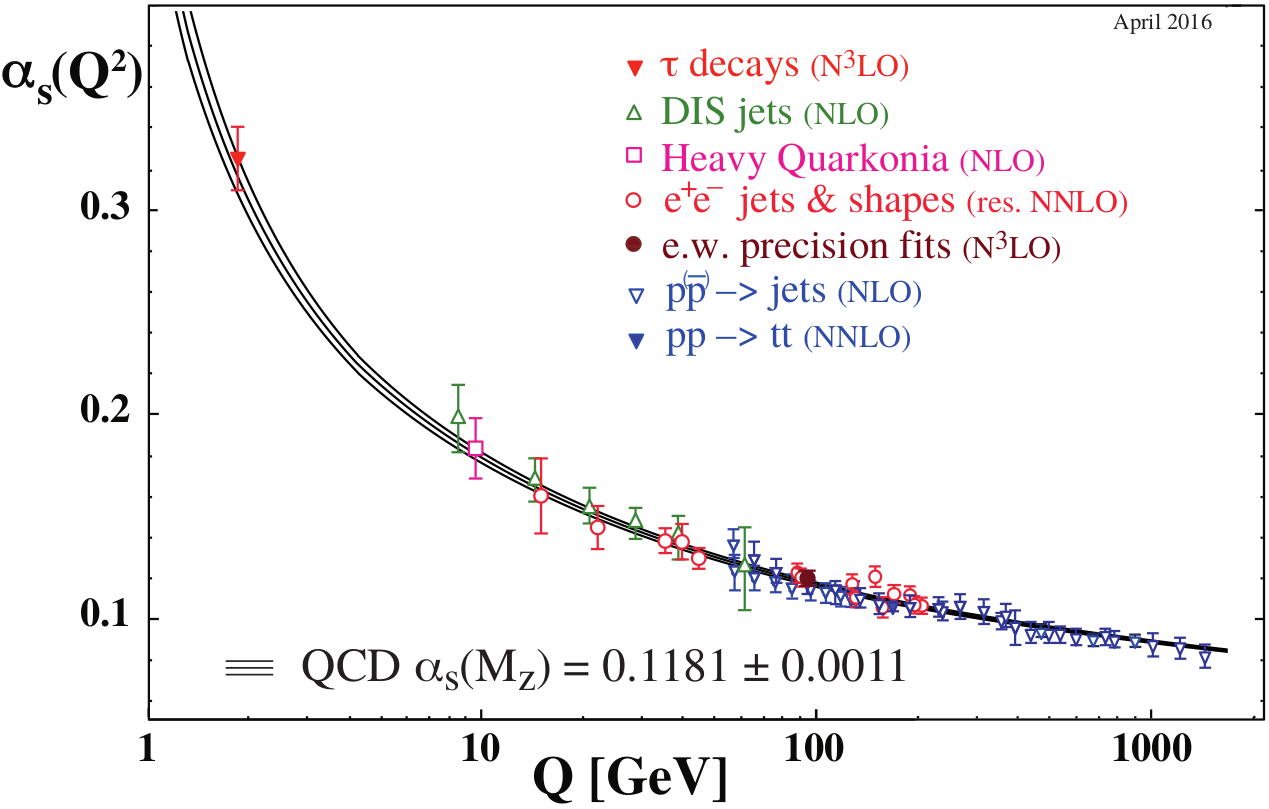
\includegraphics[width=8cm]{\PhDthesisdir/plots_and_images/from_PDG_booklet_2020/QCD_value_fct_Q.tex}
\caption[Mesure de $\alpha_s$ en fonction de l'échelle d'énergie.]{Mesures de $\alpha_s$ en fonction de l'échelle d'énergie $k$ (points) et prédiction théorique (courbe)~\cite{PDG_booklet_2020}. Le degré des calculs perturbatifs de QCD utilisés pour extraire $\alpha_s$ est indiqué entre parenthèses (NLO: \emph{next-to-leading order}, \ie\ jusqu'à l'ordre suivant le premier degré non nul; NNLO: un ordre de plus que NLO; etc.).}
\label{fig-alpha_s_fct_energy}
\end{figure}
\par Aux basses énergies, $\alpha_s$ diverge.
Ainsi, séparer et isoler des particules colorées mène à une énergie potentielle de couleur suffisamment grande pour créer des paires quark-antiquark. Lorsqu'un quark est issu d'une collision en physique des particules, ce processus se réalise et produit un ensemble collimé de particules, un jet.
\par De plus, à cause de la valeur élevée de $\alpha_s$ aux basses énergies, il n'est pas possible de réaliser des calculs perturbatifs usuels en théorie quantique des champs.
D'autres techniques sont toutefois utilisées, comme la méthode de QCD sur réseau. Son principe est de discrétiser l'espace-temps en un réseau de points. Bien que cette méthode requière d'importantes capacités de calcul et beaucoup de temps, elle permet d'obtenir avec succès les masses des hadrons comme cela se voit sur la figure~\ref{fig-lattice_QCD_masses} pour les hadrons légers.
\begin{figure}[h]
\centering
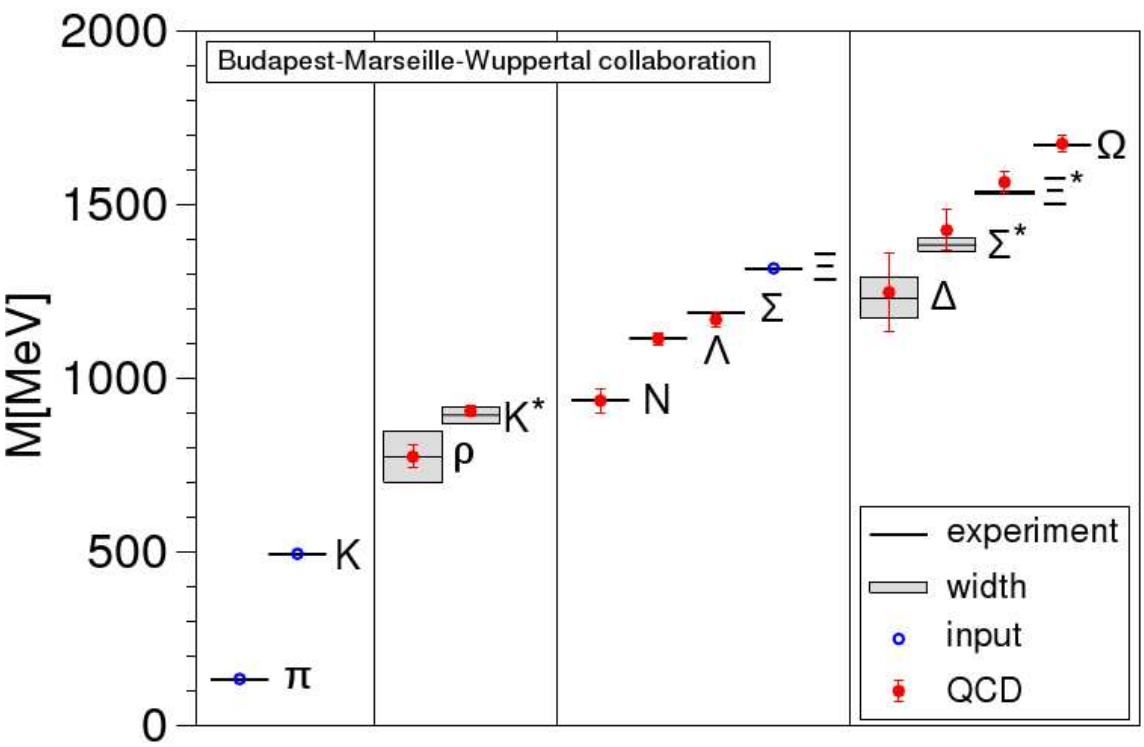
\includegraphics[width=.5\textwidth]{\PhDthesisdir/plots_and_images/from_ab_initio_hadron_masses/light_hadrons_masses.png}
\caption[Spectre de masse des hadrons légers.]{Spectre de masse des hadrons légers~\cite{ab_initio_hadron_masses}. Les lignes horizontales ainsi que les zones grisées sont les valeurs expérimentales et les largeurs de désintégration. Les résultats obtenus en utilisant des calculs de QCD sur réseau sont représentés par des cercles, avec les erreurs associées. Seules les masses des hadrons \pion, \Kaon\ et \Xibaryon\ ne présentent pas de barres d'erreurs, celles-ci sont utilisées pour fixer les paramètres libres du modèle.}
\label{fig-lattice_QCD_masses}
\end{figure}
\par Les valeurs de $\alpha_s$ à deux échelles d'énergie $k$ et $\mu$ sont reliées par la relation
\begin{equation}
\alpha_s(k) = \frac{\alpha_s(\mu)}{1+ \frac{11n_c-2n_f}{12\pi} \alpha_s(\mu)\ln(\frac{k^2}{\mu^2})}
\end{equation}
avec $n_c$ le nombre de couleurs et $n_f$ le nombre de saveurs de quarks, \ie\ $n_c=3$ et $n_f=6$~\cite{salam2010elements}.
Cette relation peut ainsi se réécrire, en prenant $\mu=\Lambda_\text{QCD}$ l'échelle d'énergie à laquelle $\alpha_s$ diverge,
\begin{equation}
\alpha_s (k) =
\frac{6\pi}{21 \ln(\frac{k}{\Lambda_\text{QCD}})}
\msep
\Lambda_\text{QCD} = 218\pm\SI{24}{\MeV}
\mend
\end{equation}
Il ressort que $\alpha_s$ décroît lorsque l'échelle d'énergie augmente.
Cette diminution de $\alpha_s$ aux hautes énergies est la \og liberté asymptotique \fg~\cite{QCD_asymptotic_freedom_1,QCD_asymptotic_freedom_2}, régime dans lequel les particules colorées ne sont plus confinées et peuvent se propager comme des particules libres. Au LHC, les énergies de collision permettent d'atteindre ce régime.
%the coupling decreases logarithmically, a phenomenon known as asymptotic freedom (the discovery of which was awarded with the Nobel Prize in Physics in 2004).

